\documentclass[twoside]{book}

% Packages required by doxygen
\usepackage{fixltx2e}
\usepackage{calc}
\usepackage{doxygen}
\usepackage[export]{adjustbox} % also loads graphicx
\usepackage{graphicx}
\usepackage[utf8]{inputenc}
\usepackage{makeidx}
\usepackage{multicol}
\usepackage{multirow}
\PassOptionsToPackage{warn}{textcomp}
\usepackage{textcomp}
\usepackage[nointegrals]{wasysym}
\usepackage[table]{xcolor}

% Font selection
\usepackage[T1]{fontenc}
\usepackage[scaled=.90]{helvet}
\usepackage{courier}
\usepackage{amssymb}
\usepackage{sectsty}
\renewcommand{\familydefault}{\sfdefault}
\allsectionsfont{%
  \fontseries{bc}\selectfont%
  \color{darkgray}%
}
\renewcommand{\DoxyLabelFont}{%
  \fontseries{bc}\selectfont%
  \color{darkgray}%
}
\newcommand{\+}{\discretionary{\mbox{\scriptsize$\hookleftarrow$}}{}{}}

% Page & text layout
\usepackage{geometry}
\geometry{%
  a4paper,%
  top=2.5cm,%
  bottom=2.5cm,%
  left=2.5cm,%
  right=2.5cm%
}
\tolerance=750
\hfuzz=15pt
\hbadness=750
\setlength{\emergencystretch}{15pt}
\setlength{\parindent}{0cm}
\setlength{\parskip}{3ex plus 2ex minus 2ex}
\makeatletter
\renewcommand{\paragraph}{%
  \@startsection{paragraph}{4}{0ex}{-1.0ex}{1.0ex}{%
    \normalfont\normalsize\bfseries\SS@parafont%
  }%
}
\renewcommand{\subparagraph}{%
  \@startsection{subparagraph}{5}{0ex}{-1.0ex}{1.0ex}{%
    \normalfont\normalsize\bfseries\SS@subparafont%
  }%
}
\makeatother

% Headers & footers
\usepackage{fancyhdr}
\pagestyle{fancyplain}
\fancyhead[LE]{\fancyplain{}{\bfseries\thepage}}
\fancyhead[CE]{\fancyplain{}{}}
\fancyhead[RE]{\fancyplain{}{\bfseries\leftmark}}
\fancyhead[LO]{\fancyplain{}{\bfseries\rightmark}}
\fancyhead[CO]{\fancyplain{}{}}
\fancyhead[RO]{\fancyplain{}{\bfseries\thepage}}
\fancyfoot[LE]{\fancyplain{}{}}
\fancyfoot[CE]{\fancyplain{}{}}
\fancyfoot[RE]{\fancyplain{}{\bfseries\scriptsize Generated by Doxygen }}
\fancyfoot[LO]{\fancyplain{}{\bfseries\scriptsize Generated by Doxygen }}
\fancyfoot[CO]{\fancyplain{}{}}
\fancyfoot[RO]{\fancyplain{}{}}
\renewcommand{\footrulewidth}{0.4pt}
\renewcommand{\chaptermark}[1]{%
  \markboth{#1}{}%
}
\renewcommand{\sectionmark}[1]{%
  \markright{\thesection\ #1}%
}

% Indices & bibliography
\usepackage{natbib}
\usepackage[titles]{tocloft}
\setcounter{tocdepth}{3}
\setcounter{secnumdepth}{5}
\makeindex

% Hyperlinks (required, but should be loaded last)
\usepackage{ifpdf}
\ifpdf
  \usepackage[pdftex,pagebackref=true]{hyperref}
\else
  \usepackage[ps2pdf,pagebackref=true]{hyperref}
\fi
\hypersetup{%
  colorlinks=true,%
  linkcolor=blue,%
  citecolor=blue,%
  unicode%
}

% Custom commands
\newcommand{\clearemptydoublepage}{%
  \newpage{\pagestyle{empty}\cleardoublepage}%
}

\usepackage{caption}
\captionsetup{labelsep=space,justification=centering,font={bf},singlelinecheck=off,skip=4pt,position=top}

%===== C O N T E N T S =====

\begin{document}

% Titlepage & ToC
\hypersetup{pageanchor=false,
             bookmarksnumbered=true,
             pdfencoding=unicode
            }
\pagenumbering{alph}
\begin{titlepage}
\vspace*{7cm}
\begin{center}%
{\Large Python M\+C\+RT }\\
\vspace*{1cm}
{\large Generated by Doxygen 1.8.13}\\
\end{center}
\end{titlepage}
\clearemptydoublepage
\pagenumbering{roman}
\tableofcontents
\clearemptydoublepage
\pagenumbering{arabic}
\hypersetup{pageanchor=true}

%--- Begin generated contents ---
\chapter{Python}
\label{index}\hypertarget{index}{}Python is a (confusingly named) Monte Carlo radiative transfer code which uses the Sobolev approximation. It has been developed by Knox Long, Christian Knigge, Stuart Sim, Nick Higginbottom, James Matthews and Sam Mangham. The code has been used for a variety of research projects invovling the winds of cataclysmic variables, of young stellar objects, and of A\+GN.

The code is under active development, but we are looking for beta users to test the code, and potentially use it for their own research. If you are interested in using Python please email the collaboration at agn-\/winds\mbox{[}at\mbox{]}googlegroups\mbox{[}dot\mbox{]}com or contact Knox Long via long\mbox{[}at\mbox{]}stsci\mbox{[}dot\mbox{]}edu.

Documentation of input parameters is hosted on \href{http://agnwinds.readthedocs.io/en/dev/}{\tt Read\+The\+Docs}.

\subsection*{Travis Build Status}

\href{https://travis-ci.org/agnwinds/python}{\tt }

\subsection*{Installation}

Python and the various routines associated are set up in a self-\/contained directory structure. The basic directory structure and the data files that one needs to run Python need to be retrieved and compiled.

If you want to obtain a stable (!) release, go to the \href{https://github.com/agnwinds/python/releases}{\tt Releases} page.

If you want to download the latest dev version, you can zip up the git repository by clicking on the zip icon to the right of the Git\+Hub page. Aternatively, you can clone the repository using \begin{DoxyVerb}$ git clone https://github.com/agnwinds/python.git 
\end{DoxyVerb}


If you anticipate contributing to development we suggest Forking the repository and submitting pull requests with any proposed changes.

Once you have the files, you need to cd to the new directory and set your environment variables \begin{DoxyVerb}$ export PYTHON = /path/to/python/
$ cd $PYTHON 
$ ./configure
$ make install
$ make clean
\end{DoxyVerb}


note that export syntax is for bash-\/ for csh use \begin{DoxyVerb}$ setenv PYTHON /path/to/python/
\end{DoxyVerb}


Atomic data is stored in our \href{https://github.com/agnwinds/data}{\tt data repository} with it\textquotesingle{}s own releases page. one should unzip these files and place them in a \$\+P\+Y\+T\+H\+ON/data folder.

A development user may want to work on atomic data as part of their work, and pull in changes as they are made, in which case we recommend cloning the data repository\+: \begin{DoxyVerb}$ cd $PYTHON; git clone https://github.com/agnwinds/data data
\end{DoxyVerb}


\subsection*{Running python}

To run python you need to add the following to your \$\+P\+A\+TH variable\+: \begin{DoxyVerb}$PYTHON/bin
\end{DoxyVerb}


You can then setup your symbolic links by running \begin{DoxyVerb}$ Setup_Py_Dir
\end{DoxyVerb}


and run the code by typing, e.\+g. \begin{DoxyVerb}$ py root.pf
\end{DoxyVerb}


Please see the \href{https://github.com/agnwinds/python/wiki/Installing-and-Running-Python}{\tt wiki} and docs folder for how to use the code.

Any comments, email \href{mailto:jm8g08@soton.ac.uk}{\tt jm8g08@soton.\+ac.\+uk} or \href{mailto:long@stsci.edu}{\tt long@stsci.\+edu}. 
\chapter{Bug List}
\label{bug}
\Hypertarget{bug}

\begin{DoxyRefList}
\item[\label{bug__bug000011}%
\Hypertarget{bug__bug000011}%
Global \hyperlink{templates_8h_acbbafed45b10980bb86fe7950daa0604}{adiabatic\+\_\+cooling} (Wind\+Ptr one, double t)]The statements here about not calling this routine are odd. There is no reason that the routine cannot be called any time since it does not populate cool\+\_\+adiabatic. And what really shold happen if we do not want to use cool\+\_\+adiabatic is that we should check when we want to calculate the total cooling that it is not done. 
\item[\label{bug__bug000003}%
\Hypertarget{bug__bug000003}%
Global \hyperlink{templates_8h_a3513a64162c15d3d3d101c3d5ea2367f}{bands\+\_\+init} (int imode, struct xbands $\ast$band)]At some point some of the banding needs to be tested systematically. We have tended to find a setup that we like and just use it. 
\item[\label{bug__bug000045}%
\Hypertarget{bug__bug000045}%
Global \hyperlink{templates_8h_afb47deaf80a8f3a6f07ab91d843d960e}{bl\+\_\+init} (double lum\+\_\+bl, double t\+\_\+bl, double freqmin, double freqmax, int ioniz\+\_\+or\+\_\+final, double $\ast$f)]At present bl\+\_\+init assumes a BB regardless of the spectrum. This is not really correct, and is different for what is done in initializing the star 
\item[\label{bug__bug000007}%
\Hypertarget{bug__bug000007}%
Global \hyperlink{templates_8h_a30c0717640ef307cbe5489ec9ef911f5}{calc\+\_\+cdf\+\_\+gradient} (Cdf\+Ptr cdf)]X\+XX N\+SH -\/ the way that the ends are dealt with is not great -\/ we should really try to come up with an extrapolation rather than just fill in the same gradients for the second and penultimate cells into the first and last cells. 
\item[\label{bug__bug000006}%
\Hypertarget{bug__bug000006}%
File \hyperlink{cdf_8c}{cdf.c} ]For reasons, which are currently unclear there are differences in the number of points maintained in the cdfs for different generation methods. 
\item[\label{bug__bug000032}%
\Hypertarget{bug__bug000032}%
Global \hyperlink{templates_8h_a834b9001d849a521f4dbf7a0dcb0d012}{check\+\_\+convergence} (void)]It would make sense to write this information to a separate file so that plots of the rate of convergence could be easily made. 
\item[\label{bug__bug000032}%
\Hypertarget{bug__bug000032}%
Global \hyperlink{templates_8h_a834b9001d849a521f4dbf7a0dcb0d012}{check\+\_\+convergence} (void)]It would make sense to write this information to a separate file so that plots of the rate of convergence could be easily made. 
\item[\label{bug__bug000004}%
\Hypertarget{bug__bug000004}%
Global \hyperlink{templates_8h_a11871d7df7f3167db92bef8c8ef98926}{check\+\_\+fmax} (double fmin, double fmax, double temp)]This routine calls several variables that it does not use. It is also unclear that it is needed. 
\item[\label{bug__bug000030}%
\Hypertarget{bug__bug000030}%
Global \hyperlink{templates_8h_afa8b5c03286c90c5365b874967e81b33}{check\+\_\+xsections} (void)]A careful look at this routine is warranted as get\+\_\+atomic\+\_\+data has changed over the years. 
\item[\label{bug__bug000030}%
\Hypertarget{bug__bug000030}%
Global \hyperlink{templates_8h_afa8b5c03286c90c5365b874967e81b33}{check\+\_\+xsections} (void)]A careful look at this routine is warranted as get\+\_\+atomic\+\_\+data has changed over the years. 
\item[\label{bug__bug000009}%
\Hypertarget{bug__bug000009}%
Global \hyperlink{templates_8h_abf7699b950ec2ef55a4e0087d82d0ab3}{cooling} (Plasma\+Ptr xxxplasma, double t)]There appear to be redundant calls here to xtotal\+\_\+emission (which include calls to total\+\_\+fb, and to total\+\_\+fb in this routine. This makes it difficult to understand whether something is being counted twice. 
\item[\label{bug__bug000012}%
\Hypertarget{bug__bug000012}%
Global \hyperlink{corona_8c_a547bb990f8958165c0c4382393910d37}{corona\+\_\+rho} (ndom, x)]This and the other routines that describe a coronal model do not handle the case of the vertically extended disk 
\item[\label{bug__bug000013}%
\Hypertarget{bug__bug000013}%
File \hyperlink{cylind__var_8c}{cylind\+\_\+var.c} ]These routines are currently broken. See issue \#159  
\item[\label{bug__bug000015}%
\Hypertarget{bug__bug000015}%
Global \hyperlink{templates_8h_a13144d35b1d57cfa570b6e59d225f474}{cylind\+\_\+volumes} (int ndom, Wind\+Ptr w)]This routine has unresolved X\+XX questions that need to be resolved 
\item[\label{bug__bug000014}%
\Hypertarget{bug__bug000014}%
Global \hyperlink{cylind__var_8c_a3185dc024d7c8bf77fe0be0dc128a272}{cylvar\+\_\+coord\+\_\+fraction} (int ndom, int ichoice, x, ii, frac, int $\ast$nelem)]This routine does not look correct. It does not make any allowance for differences in the z heights of the cells as a function of rho. 
\item[\label{bug__bug000043}%
\Hypertarget{bug__bug000043}%
Global \hyperlink{templates_8h_aa943bd857500a1f2937d8b97d84ff633}{define\+\_\+phot} (Phot\+Ptr p, double f1, double f2, long nphot\+\_\+tot, int ioniz\+\_\+or\+\_\+final, int iwind, int freq\+\_\+sampling)]Is this correct, have subcycles been removed. 
\item[\label{bug__bug000016}%
\Hypertarget{bug__bug000016}%
File \hyperlink{density_8c}{density.c} ]It is not clear why this is a separate file in python. Consider incoprating into another file  
\item[\label{bug__bug000042}%
\Hypertarget{bug__bug000042}%
Global \hyperlink{templates_8h_a8bc3604c533b18b872bb155bfd444bb5}{ds\+\_\+to\+\_\+wind} (Phot\+Ptr pp, int $\ast$ndom\+\_\+current)]1802 -\/ksl -\/ At present this routine for imported models this routine only deals with cylindrical models. Additionally for imported models we skip all of the of the wind\+\_\+cones. This is inefficient, and needs to be corrected for rtheta and spherical models which can easily be handled using wind cones. 
\item[\label{bug__bug000024}%
\Hypertarget{bug__bug000024}%
Global \hyperlink{templates_8h_a280fcbb3dddfaf58a73b2a8d6fd61c76}{extract} (Wind\+Ptr w, Phot\+Ptr p, int itype)]This routine as well as extract\+\_\+one have options for tracking the photon history. The routines are in \hyperlink{diag_8c}{diag.\+c} It is not clear that they have been used in a long time and so it may be worthwhile to remove them. Furthermore, we have established a new mechanism save\+\_\+phot for essentially this same task. This really should be consolidated. 

This is also commented in the text, but there is a rather bizarre separation for where the photon frequency is updated and where the weight is update. The former is done in extract, while the latter is done in extract\+\_\+one. This is not an error precisely but makes the code more confusing than it needs to be. 
\item[\label{bug__bug000023}%
\Hypertarget{bug__bug000023}%
Global \hyperlink{templates_8h_ade7eab896d4188a5b8a4ed6845d33150}{ff} (Wind\+Ptr one, double t\+\_\+e, double freq)]f\+\_\+nu is set to 0 for t\+\_\+e less than 100K. It\textquotesingle{}s not clear that this limit is applied to other functions anymore. Was this missed? Not also that the code having to do with the gaunt factor is duplicated from another routine. Should a gaunt\+\_\+ff routine be created for both? 
\item[\label{bug__bug000053}%
\Hypertarget{bug__bug000053}%
Global \hyperlink{templates_8h_ad350a11e70a4518fb86b842942575e26}{fix\+\_\+concentrations} (Plasma\+Ptr xplasma, int mode)]It is not obvious that this is really what we want. This routine was written when we only were concerned about scattering and does not really take into account emission (for which one needs n\+\_\+e. One possiblity is to calculated ion abundances for H and He properly, in which case we would need the mode variable. 
\item[\label{bug__bug000026}%
\Hypertarget{bug__bug000026}%
Global \hyperlink{get__atomicdata_8c_ae8afa865c507915363062a5abd9c32b7}{get\+\_\+atomic\+\_\+data} (masterfile)]Exactly what is meant by L\+TE here needs clarification.

Needs description -\/ this is a type of data that is no longer used 

This needs a description -\/ it is very old -\/ CK\textquotesingle{}s ground state recombination tables used to compute the zeta term.  
\item[\label{bug__bug000058}%
\Hypertarget{bug__bug000058}%
Global \hyperlink{templates_8h_a897e0ae97c32a481075df9fc45f6e745}{get\+\_\+bl\+\_\+and\+\_\+agn\+\_\+params} (double lstar)]Our long term goal is to make our inputs for radiation sources more generic, but there is still more work to do on this routine. The problems are really to first define what we want. Implementation should be straighforwad if we can figure out what we want. A first step might be to break this into two routines, one for a BL and one for an A\+GN. Note that the A\+GN also is used for a BH binary. This routine was clipped out of python at one pooint so it is not surprising it does not make logical sense to have grouped these itimes together 
\item[\label{bug__bug000018}%
\Hypertarget{bug__bug000018}%
Global \hyperlink{templates_8h_a4ba7a23129d489314ba51c999d18e321}{get\+\_\+extra\+\_\+diagnostics} (void)]This routine should be combined with get\+\_\+standard\+\_\+care\+\_\+factors 
\item[\label{bug__bug000018}%
\Hypertarget{bug__bug000018}%
Global \hyperlink{templates_8h_a4ba7a23129d489314ba51c999d18e321}{get\+\_\+extra\+\_\+diagnostics} (void)]This routine should be combined with get\+\_\+standard\+\_\+care\+\_\+factors 
\item[\label{bug__bug000034}%
\Hypertarget{bug__bug000034}%
Global \hyperlink{templates_8h_abc35742eeeb50cc9cda997c3de567f20}{get\+\_\+knigge\+\_\+wind\+\_\+params} (int ndom)]There may weel be errors associated with a vertically extended disk that need tobe addressed 
\item[\label{bug__bug000017}%
\Hypertarget{bug__bug000017}%
Global \hyperlink{templates_8h_a3c32de99bd46282a95c0de7c8f7e890f}{get\+\_\+standard\+\_\+care\+\_\+factors} (void)]It is not obvious that much recent thought has been given to the choices that are here. The fractional distance that a photon travel is intended to make sure the velocity along the line of sight can be approximated linearly. If a photon travels too far in an azimuthal direction the sense of the velocity can change and this prevensts this 
\item[\label{bug__bug000017}%
\Hypertarget{bug__bug000017}%
Global \hyperlink{templates_8h_a3c32de99bd46282a95c0de7c8f7e890f}{get\+\_\+standard\+\_\+care\+\_\+factors} (void)]It is not obvious that much recent thought has been given to the choices that are here. The fractional distance that a photon travel is intended to make sure the velocity along the line of sight can be approximated linearly. If a photon travels too far in an azimuthal direction the sense of the velocity can change and this prevensts this 
\item[\label{bug__bug000057}%
\Hypertarget{bug__bug000057}%
Global \hyperlink{templates_8h_a5e18aeda5d11190333c93b952b562b04}{get\+\_\+stellar\+\_\+params} (void)]This routine is not completely self consistent, in the sense that for an A\+GN we cannot estimate a luminosity. This reflects the fact that we have not completely setlled on how to homogenize inputs for diffent system types. It\textquotesingle{}s not clear that we need to retun anything. 
\item[\label{bug__bug000057}%
\Hypertarget{bug__bug000057}%
Global \hyperlink{templates_8h_a5e18aeda5d11190333c93b952b562b04}{get\+\_\+stellar\+\_\+params} (void)]This routine is not completely self consistent, in the sense that for an A\+GN we cannot estimate a luminosity. This reflects the fact that we have not completely setlled on how to homogenize inputs for diffent system types. It\textquotesingle{}s not clear that we need to retun anything. 
\item[\label{bug__bug000060}%
\Hypertarget{bug__bug000060}%
Global \hyperlink{templates_8h_a40edef16d314acc2a892cd8b8a5f0eec}{get\+\_\+stellar\+\_\+wind\+\_\+params} (int ndom)]There was an old note here indicating that the ksl was unsure(04j) whether as if the code as written really implements the possibility of a wind that starts at a radius larger than the star. This should be checked 
\item[\label{bug__bug000031}%
\Hypertarget{bug__bug000031}%
File \hyperlink{homologous_8c}{homologous.c} ]X\+X\+XX ksl 1802 -\/ The maximum radius of the wind here seems to be defined externally and it is not clear that this is what one wants in a situation with multiple domains Conisder adding an maximu radius as an imput variable. Note that this may have been fixed  
\item[\label{bug__bug000029}%
\Hypertarget{bug__bug000029}%
Global \hyperlink{get__atomicdata_8c_a8b5d80d6f35b55e30551b5ae6b5cc269}{indexx} (int n, arrin, indx)]Should probably replaces this with the equivalent gsl routine 
\item[\label{bug__bug000019}%
\Hypertarget{bug__bug000019}%
Global \hyperlink{templates_8h_acbb582e8c0def41044e2d4d8aac0c752}{init\+\_\+extra\+\_\+diagnostics} (void)]Ultimately we would like to write the extra diagnositcs to a single file 
\item[\label{bug__bug000019}%
\Hypertarget{bug__bug000019}%
Global \hyperlink{templates_8h_acbb582e8c0def41044e2d4d8aac0c752}{init\+\_\+extra\+\_\+diagnostics} (void)]Ultimately we would like to write the extra diagnositcs to a single file 
\item[\label{bug__bug000054}%
\Hypertarget{bug__bug000054}%
Global \hyperlink{templates_8h_a555f188199cb3346b32e289e64c9d980}{init\+\_\+geo} (void)]Currently init\+\_\+geo is set up for C\+Vs and Stars and not A\+GN. We now read in the system type as the first variable. The intent was to allow one to use the system type to particularize how geo (aqnd other variables) were intialized. But this has yet to be carreid out. 
\item[\label{bug__bug000054}%
\Hypertarget{bug__bug000054}%
Global \hyperlink{templates_8h_a555f188199cb3346b32e289e64c9d980}{init\+\_\+geo} (void)]Currently init\+\_\+geo is set up for C\+Vs and Stars and not A\+GN. We now read in the system type as the first variable. The intent was to allow one to use the system type to particularize how geo (aqnd other variables) were intialized. But this has yet to be carreid out. 
\item[\label{bug__bug000056}%
\Hypertarget{bug__bug000056}%
Global \hyperlink{templates_8h_a3995f2a6ba379027804653e28e4feac1}{init\+\_\+log\+\_\+and\+\_\+windsave} (int restart\+\_\+stat)]This routine was refactored out of \hyperlink{python_8c}{python.\+c} in an attempt to make that routine simpler, but it is not obvious that what done here actually makes sense. For example, although the routine checks if the windsave file exists, and sets restart\+\_\+stat to 0 if it does not. This information is not transmitted back to any other portion of the program. 
\item[\label{bug__bug000035}%
\Hypertarget{bug__bug000035}%
Global \hyperlink{templates_8h_a2ba8dcf484d3688f9687d48dd865dc0d}{levels} (Plasma\+Ptr xplasma, int mode)]Some rethinking of the whole level density approach needs to be done. It\textquotesingle{}s not clear how these functions are being used and what difference if any that they make.  
\item[\label{bug__bug000047}%
\Hypertarget{bug__bug000047}%
Global \hyperlink{templates_8h_a687aa0dcc49f512e562c1e0afddc0263}{mean\+\_\+intensity} (Plasma\+Ptr xplasma, double freq, int mode)]The routine refers to a mode 5, which does not appear to exist, or at least it is not one that is included in \hyperlink{python_8h}{python.\+h} Note also that the logic of this appears overcomplicated, reflecting the evolution of banding, and various ionization modes being added without looking at trying to make this simpler. 
\item[\label{bug__bug000064}%
\Hypertarget{bug__bug000064}%
Global \hyperlink{wind2d_8c_ac98ab21bbcfcfc326f0b16fabd5587c0}{N\+S\+T\+E\+PS} ]This routine has errors. It is only correct if there is a single domain. In particular rho(w,x) gives the correct answer for rho regardless of domains, but nodom is set to 0 for vind(ndom,\&p,v). This should be fixed. 
\item[\label{bug__bug000008}%
\Hypertarget{bug__bug000008}%
Global \hyperlink{templates_8h_aca0d5b8835f560393ae64306e8f24ce3}{one\+\_\+continuum} (int spectype, double t, double g, double freqmin, double freqmax)]The model structure is general in the sense that it was intended for situation with any number of variables. However what is written here is specific to the case of two variables. This is a problem, as we have found in trying to use this in other situations. A more general routine is needed. The first step in doing this is to replace much of the code here with a call to the routine model (spectype, par) in models.\+c 
\item[\label{bug__bug000049}%
\Hypertarget{bug__bug000049}%
Global \hyperlink{templates_8h_a1e3f4af5624039f9a4937939331b5219}{one\+\_\+fb} (Wind\+Ptr one, double f1, double f2)]This routine contains questions from Stuart in May 04 that have never been addressed. Furthemore, the routine has a parameter delta which is used to decide whether one is close enough in temperature to a previously generated D\+CF. This is set to 500, which is probably OK if the temperatures are high, but in appropriate if T is of order 1000 K. 
\item[\label{bug__bug000033}%
\Hypertarget{bug__bug000033}%
Global \hyperlink{templates_8h_a0c0fa3305df1f5c000e0ed0a26d413d8}{one\+\_\+shot} (Plasma\+Ptr xplasma, int mode)]There are some numbered switches included here. This is because these values are not allowed anymore. But this needs to be cleaned up. Deactivated modes should be captured when the parameters are read in, not at this point. An else statement should provide a sufficent check for any unknown mode. 
\item[\label{bug__bug000038}%
\Hypertarget{bug__bug000038}%
File \hyperlink{partition_8c}{partition.c} ]It seems likely that this file and \hyperlink{levels_8c}{levels.\+c} should be combined into a single file. There are very comments (by nsh) about eliminating some of the modes that need investigation as well.  
\item[\label{bug__bug000039}%
\Hypertarget{bug__bug000039}%
Global \hyperlink{templates_8h_a2de3c1f3e0adc389cfda580a1003a688}{partition\+\_\+functions\+\_\+2} (Plasma\+Ptr xplasma, int xnion, double temp, double weight)]According to the historical notes, there is no need for the weight term in the calculation since this is only called when we are making the assumption that we are in L\+TE for the saha equation. 
\item[\label{bug__bug000040}%
\Hypertarget{bug__bug000040}%
Global \hyperlink{templates_8h_a56bcc4eb80e38e626fe58bb5c989eafd}{phot\+\_\+hist} (Phot\+Ptr p, int iswitch)]It is not obvious that this routine is needed as we now have another mechanism to write photons out to a file. In any event, this should be moved to some other place in the code. 
\item[\label{bug__bug000022}%
\Hypertarget{bug__bug000022}%
Global \hyperlink{templates_8h_a5b9038968dd801ac73806fcc16fc1f0c}{photo\+\_\+gen\+\_\+wind} (Phot\+Ptr p, double weight, double freqmin, double freqmax, int photstart, int nphot)]This is another example where the iteration might be made over plasma cells instead of looking for wind cells with positive volume  
\item[\label{bug__bug000046}%
\Hypertarget{bug__bug000046}%
Global \hyperlink{templates_8h_a663f46d36d6962c7993e4c002442c23b}{photon\+\_\+checks} (Phot\+Ptr p, double freqmin, double freqmax, char $\ast$comment)]The routine also a few numbers that summarize some aspects of the the distribution. Some of these have to do with the Ferland definition of IP, which we are discussing deleting 
\item[\label{bug__bug000044}%
\Hypertarget{bug__bug000044}%
Global \hyperlink{templates_8h_addfbba966a4d69bdc71b771e0d7f3cdf}{populate\+\_\+bands} (double f1, double f2, int ioniz\+\_\+or\+\_\+final, int iwind, struct xbands $\ast$band)]f1 and f2 do not appear to be used and should be removed from the call. 
\item[\label{bug__bug000020}%
\Hypertarget{bug__bug000020}%
Global \hyperlink{templates_8h_ada5d5c91372291204ba0255184ce1f87}{read\+\_\+non\+\_\+standard\+\_\+disk\+\_\+profile} (char $\ast$tprofile)]This routine which was written for the Y\+SO study needs to be made less Y\+SO centric. It should also be retested. 
\item[\label{bug__bug000051}%
\Hypertarget{bug__bug000051}%
Global \hyperlink{templates_8h_adc18086c9912f51dae0f13aef98278de}{reposition} (Phot\+Ptr p)]This seems like an error. We have calculated cell specific values of dfudge, but this routine used the global D\+F\+U\+D\+GE to move the photon though a cell wall. 
\item[\label{bug__bug000050}%
\Hypertarget{bug__bug000050}%
File \hyperlink{reposition_8c}{reposition.c} ]This is too short a routine to be in a separate file. It should be incorporated into trans\+\_\+phot or extract which conatin the calling routines.  
\item[\label{bug__bug000001}%
\Hypertarget{bug__bug000001}%
Global \hyperlink{templates_8h_a76f3cece46c92129a1e138a02aac87ca}{reweightwind} (Phot\+Ptr p)]180414 -\/ ksl -\/ It is not obvious that using D\+F\+U\+D\+GE as the way to choose whether to recalculate the cdf for scatter is correct. One would obtain the wrong answer if the photon moved a small distance and hit a different resonance. 

This is a note related to an X\+XX comoment which read as follows\+: Factor of 2 needed because the interval is from -\/1 to 1 X\+XX It\textquotesingle{}s definitely needed to make a uniform distribution work but is this reason really right 
\item[\label{bug__bug000052}%
\Hypertarget{bug__bug000052}%
File \hyperlink{run_8c}{run.c} ]The name of this file is not really acurate. The routines here do drive the major portions of the calculation but they ar still run from \hyperlink{python_8c}{python.\+c}. It might be better to move even more of the running of the code to here. Alternatively, one might make \hyperlink{python_8c}{python.\+c} simpler, so that developers could see the structure better, but moving the input section into it\textquotesingle{}s own file. 
\item[\label{bug__bug000037}%
\Hypertarget{bug__bug000037}%
Global \hyperlink{templates_8h_a4a12de5120dbfd2f67d3ac56645cb4e6}{scattering\+\_\+fraction} (struct lines $\ast$line\+\_\+ptr, Plasma\+Ptr xplasma)]The modes used by scattering fraction are hardwired, which is not our standard approach. Note however there is a lot about the line\+\_\+mode which is quite complicated, not the least of which being that there is a related variable scatter\+\_\+mode 
\item[\label{bug__bug000055}%
\Hypertarget{bug__bug000055}%
Global \hyperlink{templates_8h_ab0e6804f11862cb19cf6ac6976480c3f}{setup\+\_\+dfudge} (void)]This routine does not really belong in this file. It should be moved.  
\item[\label{bug__bug000055}%
\Hypertarget{bug__bug000055}%
Global \hyperlink{templates_8h_ab0e6804f11862cb19cf6ac6976480c3f}{setup\+\_\+dfudge} (void)]This routine does not really belong in this file. It should be moved.  
\item[\label{bug__bug000059}%
\Hypertarget{bug__bug000059}%
Global \hyperlink{templates_8h_a3e05df283bba500d0e7a307679b291d6}{spectrum\+\_\+create} (Phot\+Ptr p, double f1, double f2, int nangle, int select\+\_\+extract)]To create spectra in the live or die option which are selected on the number of scatters individual photons undergo, there are some additional changes required to this routine. These changes should parallel those now in extract under the normal option. 97aug29 
\item[\label{bug__bug000048}%
\Hypertarget{bug__bug000048}%
Global \hyperlink{templates_8h_a9d0d69b33092d06a7174d71c3082d2a6}{total\+\_\+fb} (Wind\+Ptr one, double t, double f1, double f2, int fb\+\_\+choice, int mode)]What is preventing us from calculating a dielectronic emission rate? 
\item[\label{bug__bug000036}%
\Hypertarget{bug__bug000036}%
Global \hyperlink{templates_8h_a0abc40a64ed911b152833da9a675d1b4}{total\+\_\+line\+\_\+emission} (Wind\+Ptr one, double f1, double f2)]It is not exactly clear why two routines total\+\_\+line\+\_\+emission and lum\+\_\+lines is needed, as lum\+\_\+lines appears to be called only from total\+\_\+line\+\_\+emission. ksl -\/ 180509 
\item[\label{bug__bug000041}%
\Hypertarget{bug__bug000041}%
Global \hyperlink{templates_8h_aa1ffd17034054d51819328d892fc57e8}{translate\+\_\+in\+\_\+space} (Phot\+Ptr pp)]There are questions in the comments about why an additonal check is needed as to whther the photon as hit the star. It seems superfluous so someone should check whether this addtional check can be removed. 
\item[\label{bug__bug000062}%
\Hypertarget{bug__bug000062}%
Global \hyperlink{variable__temperature_8c_a72d9769510683e30aeef87c2a255ebe4}{variable\+\_\+temperature} (Plasma\+Ptr xplasma, int mode)]There are various questions associated with this routine about whether what is being done associated with partition funcitons is correct. 
\item[\label{bug__bug000063}%
\Hypertarget{bug__bug000063}%
Global \hyperlink{wind2d_8c_a8fe8eb8bacb888783ada9dd32b523e1a}{wind\+\_\+div\+\_\+err} ]This routine mixes wmain (which is passed externally) and w which is passed by calling it. While this does not generate an error it should be cleaned up, proably to use only wmain 
\item[\label{bug__bug000021}%
\Hypertarget{bug__bug000021}%
Global \hyperlink{templates_8h_ae1d27b840ad2ff21462921fc2aab975c}{wind\+\_\+luminosity} (double f1, double f2)]The do loop might be simpler if made over the plasma cells instead of the wind, but one should be careful of the dummy cell 
\item[\label{bug__bug000065}%
\Hypertarget{bug__bug000065}%
Global \hyperlink{windsave_8c_a1bf368d85f72b220cc4cba091a5e0702}{wind\+\_\+read} (filename)]This routine calls wind\+\_\+complete, but it is not entirely clear why, as the values calculated there are already in the domain structure, so this seems redundant. However there is an issue \#41 which has to do with reading in windcones that affects this.  
\item[\label{bug__bug000061}%
\Hypertarget{bug__bug000061}%
Global \hyperlink{util_8c_ad2938cb78e3414274491d2d778843db3}{wind\+\_\+x\+\_\+to\+\_\+n} (double x\mbox{[}\mbox{]}, int $\ast$n)]There are no checks for whether x is within the wind. This seems very dangerous. 
\item[\label{bug__bug000005}%
\Hypertarget{bug__bug000005}%
Global \hyperlink{bilinear_8c_af582498786ae60301965c85d405d7cde}{xquadratic} (double a, double b, double c, r)]xquadratic looks line for line identical to another routine quadratic which can be found in \hyperlink{phot__util_8c}{phot\+\_\+util.\+c}. Both versions of the code seem to be called. One of them should be removed. 
\item[\label{bug__bug000010}%
\Hypertarget{bug__bug000010}%
Global \hyperlink{templates_8h_af3162ce29644bbfd1d6ef9060d972643}{xtotal\+\_\+emission} (Wind\+Ptr one, double f1, double f2)]The call to this routine was changed when Plasma\+Ptrs were introduced, but it appears that the various routines that were called were not changed. This needs to be fixed for consistency
\end{DoxyRefList}
\chapter{Data Structure Index}
\section{Data Structures}
Here are the data structures with brief descriptions\+:\begin{DoxyCompactList}
\item\contentsline{section}{\hyperlink{structadvanced__modes}{advanced\+\_\+modes} }{\pageref{structadvanced__modes}}{}
\item\contentsline{section}{\hyperlink{structbadnell__gs__rr}{badnell\+\_\+gs\+\_\+rr} }{\pageref{structbadnell__gs__rr}}{}
\item\contentsline{section}{\hyperlink{structbasis}{basis} }{\pageref{structbasis}}{}
\item\contentsline{section}{\hyperlink{structblmodel}{blmodel} }{\pageref{structblmodel}}{}
\item\contentsline{section}{\hyperlink{struct_cdf}{Cdf} }{\pageref{struct_cdf}}{}
\item\contentsline{section}{\hyperlink{structcoll__stren}{coll\+\_\+stren} }{\pageref{structcoll__stren}}{}
\item\contentsline{section}{\hyperlink{structcollision__strength}{collision\+\_\+strength} }{\pageref{structcollision__strength}}{}
\item\contentsline{section}{\hyperlink{structcone}{cone} }{\pageref{structcone}}{}
\item\contentsline{section}{\hyperlink{structconfigurations}{configurations} }{\pageref{structconfigurations}}{}
\item\contentsline{section}{\hyperlink{structdere__di__rate}{dere\+\_\+di\+\_\+rate} }{\pageref{structdere__di__rate}}{}
\item\contentsline{section}{\hyperlink{structdielectronic__recombination}{dielectronic\+\_\+recombination} }{\pageref{structdielectronic__recombination}}{}
\item\contentsline{section}{\hyperlink{structdomain}{domain} }{\pageref{structdomain}}{}
\item\contentsline{section}{\hyperlink{structelements}{elements} }{\pageref{structelements}}{}
\item\contentsline{section}{\hyperlink{structemiss__range}{emiss\+\_\+range} }{\pageref{structemiss__range}}{}
\item\contentsline{section}{\hyperlink{structerror__log}{error\+\_\+log} }{\pageref{structerror__log}}{}
\item\contentsline{section}{\hyperlink{structfbstruc}{fbstruc} }{\pageref{structfbstruc}}{}
\item\contentsline{section}{\hyperlink{structfilenames}{filenames} }{\pageref{structfilenames}}{}
\item\contentsline{section}{\hyperlink{structforce__con}{force\+\_\+con} }{\pageref{structforce__con}}{}
\item\contentsline{section}{\hyperlink{structgaunt__total}{gaunt\+\_\+total} }{\pageref{structgaunt__total}}{}
\item\contentsline{section}{\hyperlink{structgeometry}{geometry} }{\pageref{structgeometry}}{}
\item\contentsline{section}{\hyperlink{structground__fracs}{ground\+\_\+fracs} }{\pageref{structground__fracs}}{}
\item\contentsline{section}{\hyperlink{structinner__elec__yield}{inner\+\_\+elec\+\_\+yield} }{\pageref{structinner__elec__yield}}{}
\item\contentsline{section}{\hyperlink{structinner__fluor__yield}{inner\+\_\+fluor\+\_\+yield} }{\pageref{structinner__fluor__yield}}{}
\item\contentsline{section}{\hyperlink{structinnershell}{innershell} }{\pageref{structinnershell}}{}
\item\contentsline{section}{\hyperlink{structions}{ions} }{\pageref{structions}}{}
\item\contentsline{section}{\hyperlink{structlines}{lines} }{\pageref{structlines}}{}
\item\contentsline{section}{\hyperlink{structmacro}{macro} }{\pageref{structmacro}}{}
\item\contentsline{section}{\hyperlink{struct_model}{Model} }{\pageref{struct_model}}{}
\item\contentsline{section}{\hyperlink{struct_mod_sum}{Mod\+Sum} }{\pageref{struct_mod_sum}}{}
\item\contentsline{section}{\hyperlink{structphoton}{photon} }{\pageref{structphoton}}{}
\item\contentsline{section}{\hyperlink{structphoton__store}{photon\+\_\+store} }{\pageref{structphoton__store}}{}
\item\contentsline{section}{\hyperlink{structplane}{plane} }{\pageref{structplane}}{}
\item\contentsline{section}{\hyperlink{structplasma}{plasma} }{\pageref{structplasma}}{}
\item\contentsline{section}{\hyperlink{structrdpar}{rdpar} }{\pageref{structrdpar}}{}
\item\contentsline{section}{\hyperlink{structrdpar__raw}{rdpar\+\_\+raw} }{\pageref{structrdpar__raw}}{}
\item\contentsline{section}{\hyperlink{structspectrum}{spectrum} }{\pageref{structspectrum}}{}
\item\contentsline{section}{\hyperlink{structtopbase__phot}{topbase\+\_\+phot} }{\pageref{structtopbase__phot}}{}
\item\contentsline{section}{\hyperlink{structtotal__rr}{total\+\_\+rr} }{\pageref{structtotal__rr}}{}
\item\contentsline{section}{\hyperlink{structwind}{wind} }{\pageref{structwind}}{}
\item\contentsline{section}{\hyperlink{structwind__paths}{wind\+\_\+paths} }{\pageref{structwind__paths}}{}
\item\contentsline{section}{\hyperlink{structxbands}{xbands} }{\pageref{structxbands}}{}
\item\contentsline{section}{\hyperlink{structxdisk}{xdisk} }{\pageref{structxdisk}}{}
\end{DoxyCompactList}

\chapter{File Index}
\section{File List}
Here is a list of all files with brief descriptions\+:\begin{DoxyCompactList}
\item\contentsline{section}{/\+Users/mhewitt/python/source/\hyperlink{agn_8c}{agn.\+c} \\*Subroutines relating to power law radiation sources }{\pageref{agn_8c}}{}
\item\contentsline{section}{/\+Users/mhewitt/python/source/\hyperlink{anisowind_8c}{anisowind.\+c} \\*Routines to implement anisotropic scattering in the wind }{\pageref{anisowind_8c}}{}
\item\contentsline{section}{/\+Users/mhewitt/python/source/\hyperlink{atomic_8c}{atomic.\+c} \\*Routines to calculate rates and x-\/sections making use of the atomic data }{\pageref{atomic_8c}}{}
\item\contentsline{section}{/\+Users/mhewitt/python/source/\hyperlink{atomic_8h}{atomic.\+h} }{\pageref{atomic_8h}}{}
\item\contentsline{section}{/\+Users/mhewitt/python/source/\hyperlink{balance__templates_8h}{balance\+\_\+templates.\+h} }{\pageref{balance__templates_8h}}{}
\item\contentsline{section}{/\+Users/mhewitt/python/source/\hyperlink{bands_8c}{bands.\+c} \\*Setup the frequency bands used for stratified sampling and for recording spectra in wind cells }{\pageref{bands_8c}}{}
\item\contentsline{section}{/\+Users/mhewitt/python/source/\hyperlink{bb_8c}{bb.\+c} \\*Routines concerning the generation of photons from blackbodies }{\pageref{bb_8c}}{}
\item\contentsline{section}{/\+Users/mhewitt/python/source/\hyperlink{bilinear_8c}{bilinear.\+c} \\*As the name indicates the routines solve for the fractional position of a 2d vector in a 2d cell with 4 corners }{\pageref{bilinear_8c}}{}
\item\contentsline{section}{/\+Users/mhewitt/python/source/\hyperlink{brem_8c}{brem.\+c} \\*Functions to allow a Bremstrahlung type input spectrum }{\pageref{brem_8c}}{}
\item\contentsline{section}{/\+Users/mhewitt/python/source/\hyperlink{cdf_8c}{cdf.\+c} \\*Routines to create a cumulatimve distribution (C\+DF) from a function or array, and then to sample that cdf in a fleximble manner }{\pageref{cdf_8c}}{}
\item\contentsline{section}{/\+Users/mhewitt/python/source/\hyperlink{compton_8c}{compton.\+c} }{\pageref{compton_8c}}{}
\item\contentsline{section}{/\+Users/mhewitt/python/source/\hyperlink{continuum_8c}{continuum.\+c} \\*Rotines related speciically to generating MC spectra for stellar atmospheres like grids of spectra }{\pageref{continuum_8c}}{}
\item\contentsline{section}{/\+Users/mhewitt/python/source/\hyperlink{cooling_8c}{cooling.\+c} \\*File containg all (most) cooling mechanisms }{\pageref{cooling_8c}}{}
\item\contentsline{section}{/\+Users/mhewitt/python/source/\hyperlink{corona_8c}{corona.\+c} \\*Routines specific to setting up disk corona defined as a region that rotates witht he underlying disk and has an expoential density distribution }{\pageref{corona_8c}}{}
\item\contentsline{section}{/\+Users/mhewitt/python/source/\hyperlink{cylind__var_8c}{cylind\+\_\+var.\+c} \\*Generic routines for handling a modified version of cylindrical coordinate systems to better model vertically extened disks }{\pageref{cylind__var_8c}}{}
\item\contentsline{section}{/\+Users/mhewitt/python/source/\hyperlink{cylindrical_8c}{cylindrical.\+c} \\*Generic routines for handling cylindrical coordinate systems }{\pageref{cylindrical_8c}}{}
\item\contentsline{section}{/\+Users/mhewitt/python/source/\hyperlink{density_8c}{density.\+c} \\*Contains a rroutine to find the density of an ion at a position designamted by a Pothon pointner }{\pageref{density_8c}}{}
\item\contentsline{section}{/\+Users/mhewitt/python/source/\hyperlink{diag_8c}{diag.\+c} \\*Consolidates an approach to providing extra diagnositcs for debugging python, Some of the diagnostics allow one to change defaults in python while others allow traking of and contains initialization routines that control which diagnosics are a }{\pageref{diag_8c}}{}
\item\contentsline{section}{/\+Users/mhewitt/python/source/\hyperlink{dielectronic_8c}{dielectronic.\+c} \\*??? }{\pageref{dielectronic_8c}}{}
\item\contentsline{section}{/\+Users/mhewitt/python/source/\hyperlink{direct__ion_8c}{direct\+\_\+ion.\+c} \\*Direct\+\_\+ion contains the routines relating to direct (collisional) ionization and threebody recombination }{\pageref{direct__ion_8c}}{}
\item\contentsline{section}{/\+Users/mhewitt/python/source/\hyperlink{disk_8c}{disk.\+c} \\*Various routines related setting up the disk and calculating when a photon encounters the disk surface }{\pageref{disk_8c}}{}
\item\contentsline{section}{/\+Users/mhewitt/python/source/\hyperlink{emission_8c}{emission.\+c} \\*Subroutines having to do with radiation from the wind, including those that generate photons for the wind }{\pageref{emission_8c}}{}
\item\contentsline{section}{/\+Users/mhewitt/python/source/\hyperlink{estimators_8c}{estimators.\+c} \\*Routines for dealing with macro-\/atom and simple-\/atom Monte Carlo estimators. Consult sections 3.\+3 and 3.\+4 of Matthews Phd Thesis\+:  }{\pageref{estimators_8c}}{}
\item\contentsline{section}{/\+Users/mhewitt/python/source/\hyperlink{extract_8c}{extract.\+c} \\*Maing routines for extracting photons during the spectral generation phase }{\pageref{extract_8c}}{}
\item\contentsline{section}{/\+Users/mhewitt/python/source/\hyperlink{foo_8h}{foo.\+h} }{\pageref{foo_8h}}{}
\item\contentsline{section}{/\+Users/mhewitt/python/source/\hyperlink{get__atomicdata_8c}{get\+\_\+atomicdata.\+c} \\*Read in all of the atomic data for use with Python }{\pageref{get__atomicdata_8c}}{}
\item\contentsline{section}{/\+Users/mhewitt/python/source/\hyperlink{get__models_8c}{get\+\_\+models.\+c} \\*The routines here provide a way to read grids of models and then to interpolate between them }{\pageref{get__models_8c}}{}
\item\contentsline{section}{/\+Users/mhewitt/python/source/\hyperlink{gradv_8c}{gradv.\+c} \\*Routines related to calculating velocity gradients }{\pageref{gradv_8c}}{}
\item\contentsline{section}{/\+Users/mhewitt/python/source/\hyperlink{gridwind_8c}{gridwind.\+c} \\*This file contains routines for allocating space for most of the structures needed by Python. These include Wind and Plasma structures, and if using macro atoms, the various structures rwquired for this. The file also contains a routine that maps grid cells in the wind to those in the Plasma structure, and vice versa }{\pageref{gridwind_8c}}{}
\item\contentsline{section}{/\+Users/mhewitt/python/source/\hyperlink{homologous_8c}{homologous.\+c} \\*Routines describing a homologous flow in Python }{\pageref{homologous_8c}}{}
\item\contentsline{section}{/\+Users/mhewitt/python/source/\hyperlink{hydro__import_8c}{hydro\+\_\+import.\+c} \\*Routines to import hydro-\/dynamic snapshots }{\pageref{hydro__import_8c}}{}
\item\contentsline{section}{/\+Users/mhewitt/python/source/\hyperlink{import_8c}{import.\+c} \\*General purpose routines reading in model grids }{\pageref{import_8c}}{}
\item\contentsline{section}{/\+Users/mhewitt/python/source/\hyperlink{import__cylindrical_8c}{import\+\_\+cylindrical.\+c} \\*Routines to read in an arbitrary wind model in cylindrical coordinates }{\pageref{import__cylindrical_8c}}{}
\item\contentsline{section}{/\+Users/mhewitt/python/source/\hyperlink{import__rtheta_8c}{import\+\_\+rtheta.\+c} \\*These are general routines to read in a model that is in polar or rtheta coordinates grids \paragraph*{Notes}

There a various possibilities for how the velocities could be entered. One possibility which is the way the zeus\+\_\+python models work is for the velocity to be given in spherical polar coordinates }{\pageref{import__rtheta_8c}}{}
\item\contentsline{section}{/\+Users/mhewitt/python/source/\hyperlink{import__spherical_8c}{import\+\_\+spherical.\+c} \\*General purpose routines for reading in an arbitray wind model in spherical coordinates }{\pageref{import__spherical_8c}}{}
\item\contentsline{section}{/\+Users/mhewitt/python/source/\hyperlink{ionization_8c}{ionization.\+c} \\*Routines used to calculate and update ion densities }{\pageref{ionization_8c}}{}
\item\contentsline{section}{/\+Users/mhewitt/python/source/\hyperlink{knigge_8c}{knigge.\+c} \\*Routines needed to define a K\+WD wind }{\pageref{knigge_8c}}{}
\item\contentsline{section}{/\+Users/mhewitt/python/source/\hyperlink{levels_8c}{levels.\+c} \\*This file contains a routine to calculate level populations in ions for L\+TE and related assumptions }{\pageref{levels_8c}}{}
\item\contentsline{section}{/\+Users/mhewitt/python/source/\hyperlink{lines_8c}{lines.\+c} \\*Subroutines assocaited with with resonance line radiation }{\pageref{lines_8c}}{}
\item\contentsline{section}{/\+Users/mhewitt/python/source/\hyperlink{log_8h}{log.\+h} }{\pageref{log_8h}}{}
\item\contentsline{section}{/\+Users/mhewitt/python/source/\hyperlink{macro__gov_8c}{macro\+\_\+gov.\+c} \\*File which contains the functions which govern macro-\/atoms and obtain their level populations. The actual functions which do the jumps inside an activated macro-\/atom are in \hyperlink{matom_8c}{matom.\+c}. This is partly done to prevent overly long files (J\+M1504) }{\pageref{macro__gov_8c}}{}
\item\contentsline{section}{/\+Users/mhewitt/python/source/\hyperlink{matom_8c}{matom.\+c} \\*Macro-\/atom functions }{\pageref{matom_8c}}{}
\item\contentsline{section}{/\+Users/mhewitt/python/source/\hyperlink{matom__diag_8c}{matom\+\_\+diag.\+c} \\*Diagnostic macro-\/atom printouts }{\pageref{matom__diag_8c}}{}
\item\contentsline{section}{/\+Users/mhewitt/python/source/\hyperlink{matrix__ion_8c}{matrix\+\_\+ion.\+c} \\*Contains routines which compute the ionization state using a matrix inversion technique }{\pageref{matrix__ion_8c}}{}
\item\contentsline{section}{/\+Users/mhewitt/python/source/\hyperlink{models_8h}{models.\+h} }{\pageref{models_8h}}{}
\item\contentsline{section}{/\+Users/mhewitt/python/source/\hyperlink{my__linalg_8h}{my\+\_\+linalg.\+h} }{\pageref{my__linalg_8h}}{}
\item\contentsline{section}{/\+Users/mhewitt/python/source/\hyperlink{para__update_8c}{para\+\_\+update.\+c} \\*Routines for communicating MC estimators and spectra between M\+PI threads }{\pageref{para__update_8c}}{}
\item\contentsline{section}{/\+Users/mhewitt/python/source/\hyperlink{parse_8c}{parse.\+c} \\*Routines associated with parsing the command line }{\pageref{parse_8c}}{}
\item\contentsline{section}{/\+Users/mhewitt/python/source/\hyperlink{partition_8c}{partition.\+c} \\*This file includes calculations of partition functions for ions in plasma cells under a number of assumptions }{\pageref{partition_8c}}{}
\item\contentsline{section}{/\+Users/mhewitt/python/source/\hyperlink{paths_8c}{paths.\+c} \\*Photon pathing functions }{\pageref{paths_8c}}{}
\item\contentsline{section}{/\+Users/mhewitt/python/source/\hyperlink{phot__util_8c}{phot\+\_\+util.\+c} \\*This file contains utilities which can be used to work with photon structues. It also contains routines to calculate the distances to intersections of spheres and cones. The routines included here should not be tightly tied to a particular wind model. The one exception at present is ds\+\_\+to\+\_\+cone which calculates the distance to a bifurcated cone }{\pageref{phot__util_8c}}{}
\item\contentsline{section}{/\+Users/mhewitt/python/source/\hyperlink{photo__gen__matom_8c}{photo\+\_\+gen\+\_\+matom.\+c} \\*Functions for calculating emissivities and generating photons from macro-\/atoms and k-\/packets. during the spectral cycles. The actual functions which do the jumps inside an activated macro-\/atom are in \hyperlink{matom_8c}{matom.\+c}. This is partly done to prevent overly long files (J\+M1504) }{\pageref{photo__gen__matom_8c}}{}
\item\contentsline{section}{/\+Users/mhewitt/python/source/\hyperlink{photon2d_8c}{photon2d.\+c} \\*This file contains the routines which translate photons, both inside and outside of the domains }{\pageref{photon2d_8c}}{}
\item\contentsline{section}{/\+Users/mhewitt/python/source/\hyperlink{photon__gen_8c}{photon\+\_\+gen.\+c} \\*Primary routines for creating photons for use in the radiative transfer calculation }{\pageref{photon__gen_8c}}{}
\item\contentsline{section}{/\+Users/mhewitt/python/source/\hyperlink{pi__rates_8c}{pi\+\_\+rates.\+c} \\*Routines associated with calculating photionization rates }{\pageref{pi__rates_8c}}{}
\item\contentsline{section}{/\+Users/mhewitt/python/source/\hyperlink{poltest_8c}{poltest.\+c} }{\pageref{poltest_8c}}{}
\item\contentsline{section}{/\+Users/mhewitt/python/source/\hyperlink{py__wind_8c}{py\+\_\+wind.\+c} \\*Py\+\_\+wind is a program which can be used to display various parameters of a wind as calculated by python. This is the main routine }{\pageref{py__wind_8c}}{}
\item\contentsline{section}{/\+Users/mhewitt/python/source/\hyperlink{py__wind__ion_8c}{py\+\_\+wind\+\_\+ion.\+c} \\*This file contains various subroutines of py\+\_\+wind. It is not part of python! }{\pageref{py__wind__ion_8c}}{}
\item\contentsline{section}{/\+Users/mhewitt/python/source/\hyperlink{py__wind__macro_8c}{py\+\_\+wind\+\_\+macro.\+c} \\*Py\+\_\+wind is a program which can be used to display various parameters of a wind as calculated by python. This file contains subroutines intended to display information about macro atoms used }{\pageref{py__wind__macro_8c}}{}
\item\contentsline{section}{/\+Users/mhewitt/python/source/\hyperlink{py__wind__sub_8c}{py\+\_\+wind\+\_\+sub.\+c} }{\pageref{py__wind__sub_8c}}{}
\item\contentsline{section}{/\+Users/mhewitt/python/source/\hyperlink{py__wind__write_8c}{py\+\_\+wind\+\_\+write.\+c} \\*These are subroutines used by py\+\_\+wind to write ascii files of various variables for use with smongo or normal display software }{\pageref{py__wind__write_8c}}{}
\item\contentsline{section}{/\+Users/mhewitt/python/source/\hyperlink{python_8c}{python.\+c} \\*This file contains main and various related routines that are central to the operation of Python }{\pageref{python_8c}}{}
\item\contentsline{section}{/\+Users/mhewitt/python/source/\hyperlink{python_8h}{python.\+h} }{\pageref{python_8h}}{}
\item\contentsline{section}{/\+Users/mhewitt/python/source/\hyperlink{radiation_8c}{radiation.\+c} \\*Routines to update radiation field parameters and to calculate various opacities (free-\/free, bound-\/free, etc }{\pageref{radiation_8c}}{}
\item\contentsline{section}{/\+Users/mhewitt/python/source/\hyperlink{random_8c}{random.\+c} \\*Various general purpose rouines for generating random numbers including varous routines for generating randomly oriented vectors }{\pageref{random_8c}}{}
\item\contentsline{section}{/\+Users/mhewitt/python/source/\hyperlink{rdpar_8c}{rdpar.\+c} \\*A general purpose interface for obtaining input data from the command line and/or from a file }{\pageref{rdpar_8c}}{}
\item\contentsline{section}{/\+Users/mhewitt/python/source/\hyperlink{recipes_8c}{recipes.\+c} \\*These are collection of Numberical Recipes routines used in Python }{\pageref{recipes_8c}}{}
\item\contentsline{section}{/\+Users/mhewitt/python/source/\hyperlink{recipes_8h}{recipes.\+h} }{\pageref{recipes_8h}}{}
\item\contentsline{section}{/\+Users/mhewitt/python/source/\hyperlink{recomb_8c}{recomb.\+c} \\*The routines in this file all have to do with photoionization and/or recombination rates and emissivities }{\pageref{recomb_8c}}{}
\item\contentsline{section}{/\+Users/mhewitt/python/source/\hyperlink{reposition_8c}{reposition.\+c} \\*Reposition a photon so it goes across a cell boundary }{\pageref{reposition_8c}}{}
\item\contentsline{section}{/\+Users/mhewitt/python/source/\hyperlink{resonate_8c}{resonate.\+c} \\*These routines have to do with calculating where resonances are and how strong they are }{\pageref{resonate_8c}}{}
\item\contentsline{section}{/\+Users/mhewitt/python/source/\hyperlink{reverb_8c}{reverb.\+c} \\*Reverberation mapping functions }{\pageref{reverb_8c}}{}
\item\contentsline{section}{/\+Users/mhewitt/python/source/\hyperlink{roche_8c}{roche.\+c} \\*These routines are used to describe the Roche geometry and are intended to allow one to calculate whether a photon intersects the surface of the star }{\pageref{roche_8c}}{}
\item\contentsline{section}{/\+Users/mhewitt/python/source/\hyperlink{rtheta_8c}{rtheta.\+c} \\*Generic routines for use with an azimuthally-\/symmetric rtheta coordinate system }{\pageref{rtheta_8c}}{}
\item\contentsline{section}{/\+Users/mhewitt/python/source/\hyperlink{run_8c}{run.\+c} \\*Driving routines to carry out calculation of the ionization of the plasma and also to extract detailed spectra after the inputs have been collected }{\pageref{run_8c}}{}
\item\contentsline{section}{/\+Users/mhewitt/python/source/\hyperlink{saha_8c}{saha.\+c} \\*Routines to (re)calculate the ion densities }{\pageref{saha_8c}}{}
\item\contentsline{section}{/\+Users/mhewitt/python/source/\hyperlink{setup_8c}{setup.\+c} \\*Various intialization routines, including a number that read values from the parameter files }{\pageref{setup_8c}}{}
\item\contentsline{section}{/\+Users/mhewitt/python/source/\hyperlink{setup__disk_8c}{setup\+\_\+disk.\+c} \\*Read parameters that define a disk }{\pageref{setup__disk_8c}}{}
\item\contentsline{section}{/\+Users/mhewitt/python/source/\hyperlink{setup__domains_8c}{setup\+\_\+domains.\+c} \\*Get the parameters needed to describe winds }{\pageref{setup__domains_8c}}{}
\item\contentsline{section}{/\+Users/mhewitt/python/source/\hyperlink{setup__files_8c}{setup\+\_\+files.\+c} \\*A series of routines mostly associated with opening files needed by Python }{\pageref{setup__files_8c}}{}
\item\contentsline{section}{/\+Users/mhewitt/python/source/\hyperlink{setup__reverb_8c}{setup\+\_\+reverb.\+c} \\*Routines for reading in the settings for reverb }{\pageref{setup__reverb_8c}}{}
\item\contentsline{section}{/\+Users/mhewitt/python/source/\hyperlink{setup__star__bh_8c}{setup\+\_\+star\+\_\+bh.\+c} \\*Files that get input parameters for a star and for an agn and $\ast$ boundray layer }{\pageref{setup__star__bh_8c}}{}
\item\contentsline{section}{/\+Users/mhewitt/python/source/\hyperlink{shell__wind_8c}{shell\+\_\+wind.\+c} \\*Routines needed for a single shell wind model }{\pageref{shell__wind_8c}}{}
\item\contentsline{section}{/\+Users/mhewitt/python/source/\hyperlink{signal_8c}{signal.\+c} \\*Routines indicating how many ionization or spectal generation cycles have been completed in in a file named root.\+sig where root is the rootname of the .pf file and which stop the program if one has set a maximum execution time and this has been exceeded }{\pageref{signal_8c}}{}
\item\contentsline{section}{/\+Users/mhewitt/python/source/\hyperlink{spectra_8c}{spectra.\+c} \\*The subroutines in this file handle allocating, incrementing, and writing out the spectrum arrays for Python }{\pageref{spectra_8c}}{}
\item\contentsline{section}{/\+Users/mhewitt/python/source/\hyperlink{spectral__estimators_8c}{spectral\+\_\+estimators.\+c} \\*The routines in this file are all associated with the process of modelling the spectrum in a cell }{\pageref{spectral__estimators_8c}}{}
\item\contentsline{section}{/\+Users/mhewitt/python/source/\hyperlink{spherical_8c}{spherical.\+c} \\*These are generic routines for setting up 1d spherical coordinate system, as well as a special case of this the so-\/called shell-\/wind model }{\pageref{spherical_8c}}{}
\item\contentsline{section}{/\+Users/mhewitt/python/source/\hyperlink{stellar__wind_8c}{stellar\+\_\+wind.\+c} \\*Routines needed to define a spherical wind with a Castor and Larmors velocity law }{\pageref{stellar__wind_8c}}{}
\item\contentsline{section}{/\+Users/mhewitt/python/source/\hyperlink{sv_8c}{sv.\+c} \\*The collection of routines needed to define a Shlossman-\/\+Vitello wind }{\pageref{sv_8c}}{}
\item\contentsline{section}{/\+Users/mhewitt/python/source/\hyperlink{synonyms_8c}{synonyms.\+c} \\*Translate the keywords used in previous versions of Python to the current keywords }{\pageref{synonyms_8c}}{}
\item\contentsline{section}{/\+Users/mhewitt/python/source/\hyperlink{templates_8h}{templates.\+h} }{\pageref{templates_8h}}{}
\item\contentsline{section}{/\+Users/mhewitt/python/source/\hyperlink{time_8c}{time.\+c} \\*A few simple routines relating to estimate wallclock time for the program to run and to get the current date an time }{\pageref{time_8c}}{}
\item\contentsline{section}{/\+Users/mhewitt/python/source/\hyperlink{trans__phot_8c}{trans\+\_\+phot.\+c} \\*This file contains high level routines which carry out the propagation of photons through the wind/wind domains both for ionization and spectrum (extract) cycles }{\pageref{trans__phot_8c}}{}
\item\contentsline{section}{/\+Users/mhewitt/python/source/\hyperlink{util_8c}{util.\+c} \\*These are very simple utilities within Python that do not fall into a larger catergory like those in vector }{\pageref{util_8c}}{}
\item\contentsline{section}{/\+Users/mhewitt/python/source/\hyperlink{variable__temperature_8c}{variable\+\_\+temperature.\+c} \\*This file was created to contain all of the routines associated with calculating ionization using the so-\/called pair-\/wise dilute bb and pairwise power law models. Collectively these are sometimes referred to as variable temperature models. Both involve attempt to calculate ionic abundances using a temperature fixed for each pair of ions to make the uncorrected abundance ratio roughly equal to 1. There are then correction factors applied, either based upon a piece\+\_\+wise power law model of the true radiation field, or as a dilute blackbody }{\pageref{variable__temperature_8c}}{}
\item\contentsline{section}{/\+Users/mhewitt/python/source/\hyperlink{version_8h}{version.\+h} }{\pageref{version_8h}}{}
\item\contentsline{section}{/\+Users/mhewitt/python/source/\hyperlink{vvector_8c}{vvector.\+c} \\*A series of subroutines designed to carry out common 3 vector operations }{\pageref{vvector_8c}}{}
\item\contentsline{section}{/\+Users/mhewitt/python/source/\hyperlink{wind_8c}{wind.\+c} \\*Except for where\+\_\+in\+\_\+wind, these are convenience routines which make it easier to incorporate wind models into Python }{\pageref{wind_8c}}{}
\item\contentsline{section}{/\+Users/mhewitt/python/source/\hyperlink{wind2d_8c}{wind2d.\+c} \\*Routines that are used to define the wind initially }{\pageref{wind2d_8c}}{}
\item\contentsline{section}{/\+Users/mhewitt/python/source/\hyperlink{wind__sum_8c}{wind\+\_\+sum.\+c} \\*Just prints a subset of quantities to the screen }{\pageref{wind__sum_8c}}{}
\item\contentsline{section}{/\+Users/mhewitt/python/source/\hyperlink{wind__updates2d_8c}{wind\+\_\+updates2d.\+c} \\*This file contains the main routines for updating and then reinitializing the wind after an ionization cycle }{\pageref{wind__updates2d_8c}}{}
\item\contentsline{section}{/\+Users/mhewitt/python/source/\hyperlink{windsave_8c}{windsave.\+c} \\*Routines to save and read in the structues the constitute a model and and spectra which have been genrerated }{\pageref{windsave_8c}}{}
\item\contentsline{section}{/\+Users/mhewitt/python/source/\hyperlink{windsave2table_8c}{windsave2table.\+c} \\*A standalone routine for writing a standard set of data from a windsavefile to ascii tables all readable with as astropy.\+io.\+ascii }{\pageref{windsave2table_8c}}{}
\item\contentsline{section}{/\+Users/mhewitt/python/source/\hyperlink{windsave2table__sub_8c}{windsave2table\+\_\+sub.\+c} \\*Subroutines for windsave2table }{\pageref{windsave2table__sub_8c}}{}
\item\contentsline{section}{/\+Users/mhewitt/python/source/\hyperlink{xlog_8c}{xlog.\+c} \\*These are a series of routines designed to store comments and errors in a diagnostic file or files. The routines also provide a mechanism for tracking the numbers of erorrs of each type }{\pageref{xlog_8c}}{}
\item\contentsline{section}{/\+Users/mhewitt/python/source/\hyperlink{yso_8c}{yso.\+c} \\*Simulate a young stellar object }{\pageref{yso_8c}}{}
\item\contentsline{section}{/\+Users/mhewitt/python/source/\hyperlink{zeta_8c}{zeta.\+c} \\*The routines in this file are to do with computing the correction to the Saha equation for a modified on the spot approach to ionization }{\pageref{zeta_8c}}{}
\end{DoxyCompactList}

\chapter{Data Structure Documentation}
\hypertarget{structadvanced__modes}{}\section{advanced\+\_\+modes Struct Reference}
\label{structadvanced__modes}\index{advanced\+\_\+modes@{advanced\+\_\+modes}}


{\ttfamily \#include $<$python.\+h$>$}

\subsection*{Data Fields}
\begin{DoxyCompactItemize}
\item 
int \hyperlink{structadvanced__modes_af01ce2e0a78e9f6f5bf1ef516626996f}{iadvanced}
\item 
int \hyperlink{structadvanced__modes_af1e206518e9a1375ec7eaf46987027a3}{extra\+\_\+diagnostics}
\item 
int \hyperlink{structadvanced__modes_a1322d2fb212a058161983a48ef285fab}{save\+\_\+cell\+\_\+stats}
\item 
int \hyperlink{structadvanced__modes_aec6e4133d1409070e2add4ec7f619168}{keep\+\_\+ioncycle\+\_\+windsaves}
\item 
int \hyperlink{structadvanced__modes_aaf94bf2761fb596aefe7d1e9b6fb20dc}{make\+\_\+tables}
\item 
int \hyperlink{structadvanced__modes_af518e12ae42b1bdfb7de2660adb40750}{track\+\_\+resonant\+\_\+scatters}
\item 
int \hyperlink{structadvanced__modes_a41c707d32842f1fac96e4dbe16d60c48}{save\+\_\+photons}
\item 
int \hyperlink{structadvanced__modes_a5d9283715561297f40d4ece6e7cd4c4f}{save\+\_\+extract\+\_\+photons}
\item 
int \hyperlink{structadvanced__modes_af1940e04af66a0c74cc4bde338236b54}{adjust\+\_\+grid}
\item 
int \hyperlink{structadvanced__modes_a1b1488c202da4f2131eb2800e10ed2a1}{diag\+\_\+on\+\_\+off}
\item 
int \hyperlink{structadvanced__modes_a2a2099f7722b2b148e53d0d6aca63f26}{use\+\_\+debug}
\item 
int \hyperlink{structadvanced__modes_a5c4b03b07f56d7085f202d23a7925ed1}{print\+\_\+dvds\+\_\+info}
\item 
int \hyperlink{structadvanced__modes_a067fe29b52bdeb7a6f9efa1019e418f1}{keep\+\_\+photoabs}
\item 
int \hyperlink{structadvanced__modes_a77fab35698c16498dee21a41813c9811}{quit\+\_\+after\+\_\+inputs}
\item 
int \hyperlink{structadvanced__modes_aad0ff1589062988053354087930055bb}{fixed\+\_\+temp}
\item 
int \hyperlink{structadvanced__modes_a9a1d48d878cdb6a4ef9c0f08f3f42f12}{zeus\+\_\+connect}
\item 
int \hyperlink{structadvanced__modes_a4da5e005fe696de0f87e747fa7fb302c}{rand\+\_\+seed\+\_\+usetime}
\end{DoxyCompactItemize}


\subsection{Detailed Description}


Definition at line 1340 of file python.\+h.



\subsection{Field Documentation}
\mbox{\Hypertarget{structadvanced__modes_af1940e04af66a0c74cc4bde338236b54}\label{structadvanced__modes_af1940e04af66a0c74cc4bde338236b54}} 
\index{advanced\+\_\+modes@{advanced\+\_\+modes}!adjust\+\_\+grid@{adjust\+\_\+grid}}
\index{adjust\+\_\+grid@{adjust\+\_\+grid}!advanced\+\_\+modes@{advanced\+\_\+modes}}
\subsubsection{\texorpdfstring{adjust\+\_\+grid}{adjust\_grid}}
{\footnotesize\ttfamily int advanced\+\_\+modes\+::adjust\+\_\+grid}



Definition at line 1351 of file python.\+h.

\mbox{\Hypertarget{structadvanced__modes_a1b1488c202da4f2131eb2800e10ed2a1}\label{structadvanced__modes_a1b1488c202da4f2131eb2800e10ed2a1}} 
\index{advanced\+\_\+modes@{advanced\+\_\+modes}!diag\+\_\+on\+\_\+off@{diag\+\_\+on\+\_\+off}}
\index{diag\+\_\+on\+\_\+off@{diag\+\_\+on\+\_\+off}!advanced\+\_\+modes@{advanced\+\_\+modes}}
\subsubsection{\texorpdfstring{diag\+\_\+on\+\_\+off}{diag\_on\_off}}
{\footnotesize\ttfamily int advanced\+\_\+modes\+::diag\+\_\+on\+\_\+off}



Definition at line 1352 of file python.\+h.

\mbox{\Hypertarget{structadvanced__modes_af1e206518e9a1375ec7eaf46987027a3}\label{structadvanced__modes_af1e206518e9a1375ec7eaf46987027a3}} 
\index{advanced\+\_\+modes@{advanced\+\_\+modes}!extra\+\_\+diagnostics@{extra\+\_\+diagnostics}}
\index{extra\+\_\+diagnostics@{extra\+\_\+diagnostics}!advanced\+\_\+modes@{advanced\+\_\+modes}}
\subsubsection{\texorpdfstring{extra\+\_\+diagnostics}{extra\_diagnostics}}
{\footnotesize\ttfamily int advanced\+\_\+modes\+::extra\+\_\+diagnostics}



Definition at line 1344 of file python.\+h.

\mbox{\Hypertarget{structadvanced__modes_aad0ff1589062988053354087930055bb}\label{structadvanced__modes_aad0ff1589062988053354087930055bb}} 
\index{advanced\+\_\+modes@{advanced\+\_\+modes}!fixed\+\_\+temp@{fixed\+\_\+temp}}
\index{fixed\+\_\+temp@{fixed\+\_\+temp}!advanced\+\_\+modes@{advanced\+\_\+modes}}
\subsubsection{\texorpdfstring{fixed\+\_\+temp}{fixed\_temp}}
{\footnotesize\ttfamily int advanced\+\_\+modes\+::fixed\+\_\+temp}



Definition at line 1357 of file python.\+h.

\mbox{\Hypertarget{structadvanced__modes_af01ce2e0a78e9f6f5bf1ef516626996f}\label{structadvanced__modes_af01ce2e0a78e9f6f5bf1ef516626996f}} 
\index{advanced\+\_\+modes@{advanced\+\_\+modes}!iadvanced@{iadvanced}}
\index{iadvanced@{iadvanced}!advanced\+\_\+modes@{advanced\+\_\+modes}}
\subsubsection{\texorpdfstring{iadvanced}{iadvanced}}
{\footnotesize\ttfamily int advanced\+\_\+modes\+::iadvanced}



Definition at line 1343 of file python.\+h.

\mbox{\Hypertarget{structadvanced__modes_aec6e4133d1409070e2add4ec7f619168}\label{structadvanced__modes_aec6e4133d1409070e2add4ec7f619168}} 
\index{advanced\+\_\+modes@{advanced\+\_\+modes}!keep\+\_\+ioncycle\+\_\+windsaves@{keep\+\_\+ioncycle\+\_\+windsaves}}
\index{keep\+\_\+ioncycle\+\_\+windsaves@{keep\+\_\+ioncycle\+\_\+windsaves}!advanced\+\_\+modes@{advanced\+\_\+modes}}
\subsubsection{\texorpdfstring{keep\+\_\+ioncycle\+\_\+windsaves}{keep\_ioncycle\_windsaves}}
{\footnotesize\ttfamily int advanced\+\_\+modes\+::keep\+\_\+ioncycle\+\_\+windsaves}



Definition at line 1346 of file python.\+h.

\mbox{\Hypertarget{structadvanced__modes_a067fe29b52bdeb7a6f9efa1019e418f1}\label{structadvanced__modes_a067fe29b52bdeb7a6f9efa1019e418f1}} 
\index{advanced\+\_\+modes@{advanced\+\_\+modes}!keep\+\_\+photoabs@{keep\+\_\+photoabs}}
\index{keep\+\_\+photoabs@{keep\+\_\+photoabs}!advanced\+\_\+modes@{advanced\+\_\+modes}}
\subsubsection{\texorpdfstring{keep\+\_\+photoabs}{keep\_photoabs}}
{\footnotesize\ttfamily int advanced\+\_\+modes\+::keep\+\_\+photoabs}



Definition at line 1355 of file python.\+h.

\mbox{\Hypertarget{structadvanced__modes_aaf94bf2761fb596aefe7d1e9b6fb20dc}\label{structadvanced__modes_aaf94bf2761fb596aefe7d1e9b6fb20dc}} 
\index{advanced\+\_\+modes@{advanced\+\_\+modes}!make\+\_\+tables@{make\+\_\+tables}}
\index{make\+\_\+tables@{make\+\_\+tables}!advanced\+\_\+modes@{advanced\+\_\+modes}}
\subsubsection{\texorpdfstring{make\+\_\+tables}{make\_tables}}
{\footnotesize\ttfamily int advanced\+\_\+modes\+::make\+\_\+tables}



Definition at line 1347 of file python.\+h.

\mbox{\Hypertarget{structadvanced__modes_a5c4b03b07f56d7085f202d23a7925ed1}\label{structadvanced__modes_a5c4b03b07f56d7085f202d23a7925ed1}} 
\index{advanced\+\_\+modes@{advanced\+\_\+modes}!print\+\_\+dvds\+\_\+info@{print\+\_\+dvds\+\_\+info}}
\index{print\+\_\+dvds\+\_\+info@{print\+\_\+dvds\+\_\+info}!advanced\+\_\+modes@{advanced\+\_\+modes}}
\subsubsection{\texorpdfstring{print\+\_\+dvds\+\_\+info}{print\_dvds\_info}}
{\footnotesize\ttfamily int advanced\+\_\+modes\+::print\+\_\+dvds\+\_\+info}



Definition at line 1354 of file python.\+h.

\mbox{\Hypertarget{structadvanced__modes_a77fab35698c16498dee21a41813c9811}\label{structadvanced__modes_a77fab35698c16498dee21a41813c9811}} 
\index{advanced\+\_\+modes@{advanced\+\_\+modes}!quit\+\_\+after\+\_\+inputs@{quit\+\_\+after\+\_\+inputs}}
\index{quit\+\_\+after\+\_\+inputs@{quit\+\_\+after\+\_\+inputs}!advanced\+\_\+modes@{advanced\+\_\+modes}}
\subsubsection{\texorpdfstring{quit\+\_\+after\+\_\+inputs}{quit\_after\_inputs}}
{\footnotesize\ttfamily int advanced\+\_\+modes\+::quit\+\_\+after\+\_\+inputs}



Definition at line 1356 of file python.\+h.

\mbox{\Hypertarget{structadvanced__modes_a4da5e005fe696de0f87e747fa7fb302c}\label{structadvanced__modes_a4da5e005fe696de0f87e747fa7fb302c}} 
\index{advanced\+\_\+modes@{advanced\+\_\+modes}!rand\+\_\+seed\+\_\+usetime@{rand\+\_\+seed\+\_\+usetime}}
\index{rand\+\_\+seed\+\_\+usetime@{rand\+\_\+seed\+\_\+usetime}!advanced\+\_\+modes@{advanced\+\_\+modes}}
\subsubsection{\texorpdfstring{rand\+\_\+seed\+\_\+usetime}{rand\_seed\_usetime}}
{\footnotesize\ttfamily int advanced\+\_\+modes\+::rand\+\_\+seed\+\_\+usetime}



Definition at line 1359 of file python.\+h.

\mbox{\Hypertarget{structadvanced__modes_a1322d2fb212a058161983a48ef285fab}\label{structadvanced__modes_a1322d2fb212a058161983a48ef285fab}} 
\index{advanced\+\_\+modes@{advanced\+\_\+modes}!save\+\_\+cell\+\_\+stats@{save\+\_\+cell\+\_\+stats}}
\index{save\+\_\+cell\+\_\+stats@{save\+\_\+cell\+\_\+stats}!advanced\+\_\+modes@{advanced\+\_\+modes}}
\subsubsection{\texorpdfstring{save\+\_\+cell\+\_\+stats}{save\_cell\_stats}}
{\footnotesize\ttfamily int advanced\+\_\+modes\+::save\+\_\+cell\+\_\+stats}



Definition at line 1345 of file python.\+h.

\mbox{\Hypertarget{structadvanced__modes_a5d9283715561297f40d4ece6e7cd4c4f}\label{structadvanced__modes_a5d9283715561297f40d4ece6e7cd4c4f}} 
\index{advanced\+\_\+modes@{advanced\+\_\+modes}!save\+\_\+extract\+\_\+photons@{save\+\_\+extract\+\_\+photons}}
\index{save\+\_\+extract\+\_\+photons@{save\+\_\+extract\+\_\+photons}!advanced\+\_\+modes@{advanced\+\_\+modes}}
\subsubsection{\texorpdfstring{save\+\_\+extract\+\_\+photons}{save\_extract\_photons}}
{\footnotesize\ttfamily int advanced\+\_\+modes\+::save\+\_\+extract\+\_\+photons}



Definition at line 1350 of file python.\+h.

\mbox{\Hypertarget{structadvanced__modes_a41c707d32842f1fac96e4dbe16d60c48}\label{structadvanced__modes_a41c707d32842f1fac96e4dbe16d60c48}} 
\index{advanced\+\_\+modes@{advanced\+\_\+modes}!save\+\_\+photons@{save\+\_\+photons}}
\index{save\+\_\+photons@{save\+\_\+photons}!advanced\+\_\+modes@{advanced\+\_\+modes}}
\subsubsection{\texorpdfstring{save\+\_\+photons}{save\_photons}}
{\footnotesize\ttfamily int advanced\+\_\+modes\+::save\+\_\+photons}



Definition at line 1349 of file python.\+h.

\mbox{\Hypertarget{structadvanced__modes_af518e12ae42b1bdfb7de2660adb40750}\label{structadvanced__modes_af518e12ae42b1bdfb7de2660adb40750}} 
\index{advanced\+\_\+modes@{advanced\+\_\+modes}!track\+\_\+resonant\+\_\+scatters@{track\+\_\+resonant\+\_\+scatters}}
\index{track\+\_\+resonant\+\_\+scatters@{track\+\_\+resonant\+\_\+scatters}!advanced\+\_\+modes@{advanced\+\_\+modes}}
\subsubsection{\texorpdfstring{track\+\_\+resonant\+\_\+scatters}{track\_resonant\_scatters}}
{\footnotesize\ttfamily int advanced\+\_\+modes\+::track\+\_\+resonant\+\_\+scatters}



Definition at line 1348 of file python.\+h.

\mbox{\Hypertarget{structadvanced__modes_a2a2099f7722b2b148e53d0d6aca63f26}\label{structadvanced__modes_a2a2099f7722b2b148e53d0d6aca63f26}} 
\index{advanced\+\_\+modes@{advanced\+\_\+modes}!use\+\_\+debug@{use\+\_\+debug}}
\index{use\+\_\+debug@{use\+\_\+debug}!advanced\+\_\+modes@{advanced\+\_\+modes}}
\subsubsection{\texorpdfstring{use\+\_\+debug}{use\_debug}}
{\footnotesize\ttfamily int advanced\+\_\+modes\+::use\+\_\+debug}



Definition at line 1353 of file python.\+h.

\mbox{\Hypertarget{structadvanced__modes_a9a1d48d878cdb6a4ef9c0f08f3f42f12}\label{structadvanced__modes_a9a1d48d878cdb6a4ef9c0f08f3f42f12}} 
\index{advanced\+\_\+modes@{advanced\+\_\+modes}!zeus\+\_\+connect@{zeus\+\_\+connect}}
\index{zeus\+\_\+connect@{zeus\+\_\+connect}!advanced\+\_\+modes@{advanced\+\_\+modes}}
\subsubsection{\texorpdfstring{zeus\+\_\+connect}{zeus\_connect}}
{\footnotesize\ttfamily int advanced\+\_\+modes\+::zeus\+\_\+connect}



Definition at line 1358 of file python.\+h.



The documentation for this struct was generated from the following file\+:\begin{DoxyCompactItemize}
\item 
/\+Users/mhewitt/python/source/\hyperlink{python_8h}{python.\+h}\end{DoxyCompactItemize}

\hypertarget{structbadnell__gs__rr}{}\section{badnell\+\_\+gs\+\_\+rr Struct Reference}
\label{structbadnell__gs__rr}\index{badnell\+\_\+gs\+\_\+rr@{badnell\+\_\+gs\+\_\+rr}}


{\ttfamily \#include $<$atomic.\+h$>$}

\subsection*{Data Fields}
\begin{DoxyCompactItemize}
\item 
int \hyperlink{structbadnell__gs__rr_af0ab2f7038b9d6c7e70b6f14a36ddbc4}{nion}
\item 
double \hyperlink{structbadnell__gs__rr_ab70f04c8e30cdc551ddc713bc7a42a6c}{temps} \mbox{[}\hyperlink{atomic_8h_acc4d45a47ab17c4546897672a8478d52}{B\+A\+D\+\_\+\+G\+S\+\_\+\+R\+R\+\_\+\+P\+A\+R\+A\+MS}\mbox{]}
\item 
double \hyperlink{structbadnell__gs__rr_aa1c08814c3f5d44f7bf82291a708a138}{rates} \mbox{[}\hyperlink{atomic_8h_acc4d45a47ab17c4546897672a8478d52}{B\+A\+D\+\_\+\+G\+S\+\_\+\+R\+R\+\_\+\+P\+A\+R\+A\+MS}\mbox{]}
\end{DoxyCompactItemize}


\subsection{Detailed Description}


Definition at line 515 of file atomic.\+h.



\subsection{Field Documentation}
\mbox{\Hypertarget{structbadnell__gs__rr_af0ab2f7038b9d6c7e70b6f14a36ddbc4}\label{structbadnell__gs__rr_af0ab2f7038b9d6c7e70b6f14a36ddbc4}} 
\index{badnell\+\_\+gs\+\_\+rr@{badnell\+\_\+gs\+\_\+rr}!nion@{nion}}
\index{nion@{nion}!badnell\+\_\+gs\+\_\+rr@{badnell\+\_\+gs\+\_\+rr}}
\subsubsection{\texorpdfstring{nion}{nion}}
{\footnotesize\ttfamily int badnell\+\_\+gs\+\_\+rr\+::nion}



Definition at line 517 of file atomic.\+h.

\mbox{\Hypertarget{structbadnell__gs__rr_aa1c08814c3f5d44f7bf82291a708a138}\label{structbadnell__gs__rr_aa1c08814c3f5d44f7bf82291a708a138}} 
\index{badnell\+\_\+gs\+\_\+rr@{badnell\+\_\+gs\+\_\+rr}!rates@{rates}}
\index{rates@{rates}!badnell\+\_\+gs\+\_\+rr@{badnell\+\_\+gs\+\_\+rr}}
\subsubsection{\texorpdfstring{rates}{rates}}
{\footnotesize\ttfamily double badnell\+\_\+gs\+\_\+rr\+::rates\mbox{[}\hyperlink{atomic_8h_acc4d45a47ab17c4546897672a8478d52}{B\+A\+D\+\_\+\+G\+S\+\_\+\+R\+R\+\_\+\+P\+A\+R\+A\+MS}\mbox{]}}



Definition at line 519 of file atomic.\+h.

\mbox{\Hypertarget{structbadnell__gs__rr_ab70f04c8e30cdc551ddc713bc7a42a6c}\label{structbadnell__gs__rr_ab70f04c8e30cdc551ddc713bc7a42a6c}} 
\index{badnell\+\_\+gs\+\_\+rr@{badnell\+\_\+gs\+\_\+rr}!temps@{temps}}
\index{temps@{temps}!badnell\+\_\+gs\+\_\+rr@{badnell\+\_\+gs\+\_\+rr}}
\subsubsection{\texorpdfstring{temps}{temps}}
{\footnotesize\ttfamily double badnell\+\_\+gs\+\_\+rr\+::temps\mbox{[}\hyperlink{atomic_8h_acc4d45a47ab17c4546897672a8478d52}{B\+A\+D\+\_\+\+G\+S\+\_\+\+R\+R\+\_\+\+P\+A\+R\+A\+MS}\mbox{]}}



Definition at line 518 of file atomic.\+h.



The documentation for this struct was generated from the following file\+:\begin{DoxyCompactItemize}
\item 
/\+Users/mhewitt/python/source/\hyperlink{atomic_8h}{atomic.\+h}\end{DoxyCompactItemize}

\hypertarget{structbasis}{}\section{basis Struct Reference}
\label{structbasis}\index{basis@{basis}}


{\ttfamily \#include $<$python.\+h$>$}

\subsection*{Data Fields}
\begin{DoxyCompactItemize}
\item 
double \hyperlink{structbasis_a2180e7f1bc7f3287b1841f9d6452d225}{a} \mbox{[}3\mbox{]}\mbox{[}3\mbox{]}
\end{DoxyCompactItemize}


\subsection{Detailed Description}


Definition at line 1106 of file python.\+h.



\subsection{Field Documentation}
\mbox{\Hypertarget{structbasis_a2180e7f1bc7f3287b1841f9d6452d225}\label{structbasis_a2180e7f1bc7f3287b1841f9d6452d225}} 
\index{basis@{basis}!a@{a}}
\index{a@{a}!basis@{basis}}
\subsubsection{\texorpdfstring{a}{a}}
{\footnotesize\ttfamily double basis\+::a\mbox{[}3\mbox{]}\mbox{[}3\mbox{]}}



Definition at line 1108 of file python.\+h.



The documentation for this struct was generated from the following file\+:\begin{DoxyCompactItemize}
\item 
/\+Users/mhewitt/python/source/\hyperlink{python_8h}{python.\+h}\end{DoxyCompactItemize}

\hypertarget{structblmodel}{}\section{blmodel Struct Reference}
\label{structblmodel}\index{blmodel@{blmodel}}


{\ttfamily \#include $<$python.\+h$>$}

\subsection*{Data Fields}
\begin{DoxyCompactItemize}
\item 
int \hyperlink{structblmodel_a67333da842bbda7495398e419940a5e3}{n\+\_\+blpts}
\item 
float \hyperlink{structblmodel_a3c3ff50710bb28bb464afe8b1e436b0b}{r} \mbox{[}\hyperlink{python_8h_ac7030ca4044704dd2a36d30676b75ffe}{N\+B\+L\+M\+O\+D\+EL}\mbox{]}
\item 
float \hyperlink{structblmodel_a58ed9c6aa9cdfa7a4d9b2346d5186ac2}{t} \mbox{[}\hyperlink{python_8h_ac7030ca4044704dd2a36d30676b75ffe}{N\+B\+L\+M\+O\+D\+EL}\mbox{]}
\end{DoxyCompactItemize}


\subsection{Detailed Description}


Definition at line 625 of file python.\+h.



\subsection{Field Documentation}
\mbox{\Hypertarget{structblmodel_a67333da842bbda7495398e419940a5e3}\label{structblmodel_a67333da842bbda7495398e419940a5e3}} 
\index{blmodel@{blmodel}!n\+\_\+blpts@{n\+\_\+blpts}}
\index{n\+\_\+blpts@{n\+\_\+blpts}!blmodel@{blmodel}}
\subsubsection{\texorpdfstring{n\+\_\+blpts}{n\_blpts}}
{\footnotesize\ttfamily int blmodel\+::n\+\_\+blpts}



Definition at line 627 of file python.\+h.

\mbox{\Hypertarget{structblmodel_a3c3ff50710bb28bb464afe8b1e436b0b}\label{structblmodel_a3c3ff50710bb28bb464afe8b1e436b0b}} 
\index{blmodel@{blmodel}!r@{r}}
\index{r@{r}!blmodel@{blmodel}}
\subsubsection{\texorpdfstring{r}{r}}
{\footnotesize\ttfamily float blmodel\+::r\mbox{[}\hyperlink{python_8h_ac7030ca4044704dd2a36d30676b75ffe}{N\+B\+L\+M\+O\+D\+EL}\mbox{]}}



Definition at line 628 of file python.\+h.

\mbox{\Hypertarget{structblmodel_a58ed9c6aa9cdfa7a4d9b2346d5186ac2}\label{structblmodel_a58ed9c6aa9cdfa7a4d9b2346d5186ac2}} 
\index{blmodel@{blmodel}!t@{t}}
\index{t@{t}!blmodel@{blmodel}}
\subsubsection{\texorpdfstring{t}{t}}
{\footnotesize\ttfamily float blmodel\+::t\mbox{[}\hyperlink{python_8h_ac7030ca4044704dd2a36d30676b75ffe}{N\+B\+L\+M\+O\+D\+EL}\mbox{]}}



Definition at line 629 of file python.\+h.



The documentation for this struct was generated from the following file\+:\begin{DoxyCompactItemize}
\item 
/\+Users/mhewitt/python/source/\hyperlink{python_8h}{python.\+h}\end{DoxyCompactItemize}

\hypertarget{struct_cdf}{}\section{Cdf Struct Reference}
\label{struct_cdf}\index{Cdf@{Cdf}}


{\ttfamily \#include $<$python.\+h$>$}

\subsection*{Data Fields}
\begin{DoxyCompactItemize}
\item 
double \hyperlink{struct_cdf_a34302814d1d7d8176fda7a32bf3e6cd1}{x} \mbox{[}\hyperlink{python_8h_a8fcad90a1005b8d2b876efbafa401305}{N\+C\+DF}\mbox{]}
\item 
double \hyperlink{struct_cdf_aa9657822ac7705998c85468c970f1cd7}{y} \mbox{[}\hyperlink{python_8h_a8fcad90a1005b8d2b876efbafa401305}{N\+C\+DF}\mbox{]}
\item 
double \hyperlink{struct_cdf_abdb96d8c6e4f8761f49d769c5251ee35}{d} \mbox{[}\hyperlink{python_8h_a8fcad90a1005b8d2b876efbafa401305}{N\+C\+DF}\mbox{]}
\item 
double \hyperlink{struct_cdf_a3617b232fd381fb21e716c7885b3478a}{limit1}
\item 
double \hyperlink{struct_cdf_abfa2f57780de00749a6a2fc6b2a55aac}{limit2}
\item 
double \hyperlink{struct_cdf_abc6326171a363a5a3a5d6a82009a7194}{x1}
\item 
double \hyperlink{struct_cdf_a1e4ac80d3ed6cfe9da3a64b2aac5752a}{x2}
\item 
double \hyperlink{struct_cdf_a336a610024fec24a921042fb7464dfe9}{norm}
\item 
int \hyperlink{struct_cdf_abc8ea82846fbd30f238131312b3824d0}{ncdf}
\end{DoxyCompactItemize}


\subsection{Detailed Description}


Definition at line 1203 of file python.\+h.



\subsection{Field Documentation}
\mbox{\Hypertarget{struct_cdf_abdb96d8c6e4f8761f49d769c5251ee35}\label{struct_cdf_abdb96d8c6e4f8761f49d769c5251ee35}} 
\index{Cdf@{Cdf}!d@{d}}
\index{d@{d}!Cdf@{Cdf}}
\subsubsection{\texorpdfstring{d}{d}}
{\footnotesize\ttfamily double Cdf\+::d\mbox{[}\hyperlink{python_8h_a8fcad90a1005b8d2b876efbafa401305}{N\+C\+DF}\mbox{]}}



Definition at line 1207 of file python.\+h.

\mbox{\Hypertarget{struct_cdf_a3617b232fd381fb21e716c7885b3478a}\label{struct_cdf_a3617b232fd381fb21e716c7885b3478a}} 
\index{Cdf@{Cdf}!limit1@{limit1}}
\index{limit1@{limit1}!Cdf@{Cdf}}
\subsubsection{\texorpdfstring{limit1}{limit1}}
{\footnotesize\ttfamily double Cdf\+::limit1}



Definition at line 1208 of file python.\+h.

\mbox{\Hypertarget{struct_cdf_abfa2f57780de00749a6a2fc6b2a55aac}\label{struct_cdf_abfa2f57780de00749a6a2fc6b2a55aac}} 
\index{Cdf@{Cdf}!limit2@{limit2}}
\index{limit2@{limit2}!Cdf@{Cdf}}
\subsubsection{\texorpdfstring{limit2}{limit2}}
{\footnotesize\ttfamily double Cdf\+::limit2}



Definition at line 1208 of file python.\+h.

\mbox{\Hypertarget{struct_cdf_abc8ea82846fbd30f238131312b3824d0}\label{struct_cdf_abc8ea82846fbd30f238131312b3824d0}} 
\index{Cdf@{Cdf}!ncdf@{ncdf}}
\index{ncdf@{ncdf}!Cdf@{Cdf}}
\subsubsection{\texorpdfstring{ncdf}{ncdf}}
{\footnotesize\ttfamily int Cdf\+::ncdf}



Definition at line 1212 of file python.\+h.

\mbox{\Hypertarget{struct_cdf_a336a610024fec24a921042fb7464dfe9}\label{struct_cdf_a336a610024fec24a921042fb7464dfe9}} 
\index{Cdf@{Cdf}!norm@{norm}}
\index{norm@{norm}!Cdf@{Cdf}}
\subsubsection{\texorpdfstring{norm}{norm}}
{\footnotesize\ttfamily double Cdf\+::norm}



Definition at line 1211 of file python.\+h.

\mbox{\Hypertarget{struct_cdf_a34302814d1d7d8176fda7a32bf3e6cd1}\label{struct_cdf_a34302814d1d7d8176fda7a32bf3e6cd1}} 
\index{Cdf@{Cdf}!x@{x}}
\index{x@{x}!Cdf@{Cdf}}
\subsubsection{\texorpdfstring{x}{x}}
{\footnotesize\ttfamily double Cdf\+::x\mbox{[}\hyperlink{python_8h_a8fcad90a1005b8d2b876efbafa401305}{N\+C\+DF}\mbox{]}}



Definition at line 1205 of file python.\+h.

\mbox{\Hypertarget{struct_cdf_abc6326171a363a5a3a5d6a82009a7194}\label{struct_cdf_abc6326171a363a5a3a5d6a82009a7194}} 
\index{Cdf@{Cdf}!x1@{x1}}
\index{x1@{x1}!Cdf@{Cdf}}
\subsubsection{\texorpdfstring{x1}{x1}}
{\footnotesize\ttfamily double Cdf\+::x1}



Definition at line 1210 of file python.\+h.

\mbox{\Hypertarget{struct_cdf_a1e4ac80d3ed6cfe9da3a64b2aac5752a}\label{struct_cdf_a1e4ac80d3ed6cfe9da3a64b2aac5752a}} 
\index{Cdf@{Cdf}!x2@{x2}}
\index{x2@{x2}!Cdf@{Cdf}}
\subsubsection{\texorpdfstring{x2}{x2}}
{\footnotesize\ttfamily double Cdf\+::x2}



Definition at line 1210 of file python.\+h.

\mbox{\Hypertarget{struct_cdf_aa9657822ac7705998c85468c970f1cd7}\label{struct_cdf_aa9657822ac7705998c85468c970f1cd7}} 
\index{Cdf@{Cdf}!y@{y}}
\index{y@{y}!Cdf@{Cdf}}
\subsubsection{\texorpdfstring{y}{y}}
{\footnotesize\ttfamily double Cdf\+::y\mbox{[}\hyperlink{python_8h_a8fcad90a1005b8d2b876efbafa401305}{N\+C\+DF}\mbox{]}}



Definition at line 1206 of file python.\+h.



The documentation for this struct was generated from the following file\+:\begin{DoxyCompactItemize}
\item 
/\+Users/mhewitt/python/source/\hyperlink{python_8h}{python.\+h}\end{DoxyCompactItemize}

\hypertarget{structcoll__stren}{}\section{coll\+\_\+stren Struct Reference}
\label{structcoll__stren}\index{coll\+\_\+stren@{coll\+\_\+stren}}


{\ttfamily \#include $<$atomic.\+h$>$}

\subsection*{Data Fields}
\begin{DoxyCompactItemize}
\item 
int \hyperlink{structcoll__stren_a76775015376d278c2a22ba83cf58194a}{n}
\item 
int \hyperlink{structcoll__stren_a600da2dea449533e3d679bbd4deb5077}{lower}
\item 
int \hyperlink{structcoll__stren_a1a42740229c63647a0a0f2de0cc6ce9f}{upper}
\item 
double \hyperlink{structcoll__stren_a3d6d8ea6c2c8bfd55054bb5bca006b31}{energy}
\item 
double \hyperlink{structcoll__stren_afe2a6a375c336ec313cb748b838f792d}{gf}
\item 
double \hyperlink{structcoll__stren_a2d688f54546dfa04f6c9ac604f51c62d}{hi\+\_\+t\+\_\+lim}
\item 
double \hyperlink{structcoll__stren_a14153044993278f90042d070dc5ca206}{n\+\_\+points}
\item 
int \hyperlink{structcoll__stren_a292d3309ec1d6c9ae5f7afb2c401b162}{type}
\item 
float \hyperlink{structcoll__stren_a474f82a225f6408e53d005bcbb9e5099}{scaling\+\_\+param}
\item 
double \hyperlink{structcoll__stren_a867b1b9d0c751b4db6cd00b7ace4c6cd}{sct} \mbox{[}\hyperlink{atomic_8h_a83f9db7d66ceb630d0e4427329ae7d16}{N\+\_\+\+C\+O\+L\+L\+\_\+\+S\+T\+R\+E\+N\+\_\+\+P\+TS}\mbox{]}
\item 
double \hyperlink{structcoll__stren_af52c6023237c8ab4daff6f682ef01553}{scups} \mbox{[}\hyperlink{atomic_8h_a83f9db7d66ceb630d0e4427329ae7d16}{N\+\_\+\+C\+O\+L\+L\+\_\+\+S\+T\+R\+E\+N\+\_\+\+P\+TS}\mbox{]}
\end{DoxyCompactItemize}


\subsection{Detailed Description}


Definition at line 273 of file atomic.\+h.



\subsection{Field Documentation}
\mbox{\Hypertarget{structcoll__stren_a3d6d8ea6c2c8bfd55054bb5bca006b31}\label{structcoll__stren_a3d6d8ea6c2c8bfd55054bb5bca006b31}} 
\index{coll\+\_\+stren@{coll\+\_\+stren}!energy@{energy}}
\index{energy@{energy}!coll\+\_\+stren@{coll\+\_\+stren}}
\subsubsection{\texorpdfstring{energy}{energy}}
{\footnotesize\ttfamily double coll\+\_\+stren\+::energy}



Definition at line 278 of file atomic.\+h.

\mbox{\Hypertarget{structcoll__stren_afe2a6a375c336ec313cb748b838f792d}\label{structcoll__stren_afe2a6a375c336ec313cb748b838f792d}} 
\index{coll\+\_\+stren@{coll\+\_\+stren}!gf@{gf}}
\index{gf@{gf}!coll\+\_\+stren@{coll\+\_\+stren}}
\subsubsection{\texorpdfstring{gf}{gf}}
{\footnotesize\ttfamily double coll\+\_\+stren\+::gf}



Definition at line 279 of file atomic.\+h.

\mbox{\Hypertarget{structcoll__stren_a2d688f54546dfa04f6c9ac604f51c62d}\label{structcoll__stren_a2d688f54546dfa04f6c9ac604f51c62d}} 
\index{coll\+\_\+stren@{coll\+\_\+stren}!hi\+\_\+t\+\_\+lim@{hi\+\_\+t\+\_\+lim}}
\index{hi\+\_\+t\+\_\+lim@{hi\+\_\+t\+\_\+lim}!coll\+\_\+stren@{coll\+\_\+stren}}
\subsubsection{\texorpdfstring{hi\+\_\+t\+\_\+lim}{hi\_t\_lim}}
{\footnotesize\ttfamily double coll\+\_\+stren\+::hi\+\_\+t\+\_\+lim}



Definition at line 280 of file atomic.\+h.

\mbox{\Hypertarget{structcoll__stren_a600da2dea449533e3d679bbd4deb5077}\label{structcoll__stren_a600da2dea449533e3d679bbd4deb5077}} 
\index{coll\+\_\+stren@{coll\+\_\+stren}!lower@{lower}}
\index{lower@{lower}!coll\+\_\+stren@{coll\+\_\+stren}}
\subsubsection{\texorpdfstring{lower}{lower}}
{\footnotesize\ttfamily int coll\+\_\+stren\+::lower}



Definition at line 276 of file atomic.\+h.

\mbox{\Hypertarget{structcoll__stren_a76775015376d278c2a22ba83cf58194a}\label{structcoll__stren_a76775015376d278c2a22ba83cf58194a}} 
\index{coll\+\_\+stren@{coll\+\_\+stren}!n@{n}}
\index{n@{n}!coll\+\_\+stren@{coll\+\_\+stren}}
\subsubsection{\texorpdfstring{n}{n}}
{\footnotesize\ttfamily int coll\+\_\+stren\+::n}



Definition at line 275 of file atomic.\+h.

\mbox{\Hypertarget{structcoll__stren_a14153044993278f90042d070dc5ca206}\label{structcoll__stren_a14153044993278f90042d070dc5ca206}} 
\index{coll\+\_\+stren@{coll\+\_\+stren}!n\+\_\+points@{n\+\_\+points}}
\index{n\+\_\+points@{n\+\_\+points}!coll\+\_\+stren@{coll\+\_\+stren}}
\subsubsection{\texorpdfstring{n\+\_\+points}{n\_points}}
{\footnotesize\ttfamily double coll\+\_\+stren\+::n\+\_\+points}



Definition at line 281 of file atomic.\+h.

\mbox{\Hypertarget{structcoll__stren_a474f82a225f6408e53d005bcbb9e5099}\label{structcoll__stren_a474f82a225f6408e53d005bcbb9e5099}} 
\index{coll\+\_\+stren@{coll\+\_\+stren}!scaling\+\_\+param@{scaling\+\_\+param}}
\index{scaling\+\_\+param@{scaling\+\_\+param}!coll\+\_\+stren@{coll\+\_\+stren}}
\subsubsection{\texorpdfstring{scaling\+\_\+param}{scaling\_param}}
{\footnotesize\ttfamily float coll\+\_\+stren\+::scaling\+\_\+param}



Definition at line 283 of file atomic.\+h.

\mbox{\Hypertarget{structcoll__stren_a867b1b9d0c751b4db6cd00b7ace4c6cd}\label{structcoll__stren_a867b1b9d0c751b4db6cd00b7ace4c6cd}} 
\index{coll\+\_\+stren@{coll\+\_\+stren}!sct@{sct}}
\index{sct@{sct}!coll\+\_\+stren@{coll\+\_\+stren}}
\subsubsection{\texorpdfstring{sct}{sct}}
{\footnotesize\ttfamily double coll\+\_\+stren\+::sct\mbox{[}\hyperlink{atomic_8h_a83f9db7d66ceb630d0e4427329ae7d16}{N\+\_\+\+C\+O\+L\+L\+\_\+\+S\+T\+R\+E\+N\+\_\+\+P\+TS}\mbox{]}}



Definition at line 284 of file atomic.\+h.

\mbox{\Hypertarget{structcoll__stren_af52c6023237c8ab4daff6f682ef01553}\label{structcoll__stren_af52c6023237c8ab4daff6f682ef01553}} 
\index{coll\+\_\+stren@{coll\+\_\+stren}!scups@{scups}}
\index{scups@{scups}!coll\+\_\+stren@{coll\+\_\+stren}}
\subsubsection{\texorpdfstring{scups}{scups}}
{\footnotesize\ttfamily double coll\+\_\+stren\+::scups\mbox{[}\hyperlink{atomic_8h_a83f9db7d66ceb630d0e4427329ae7d16}{N\+\_\+\+C\+O\+L\+L\+\_\+\+S\+T\+R\+E\+N\+\_\+\+P\+TS}\mbox{]}}



Definition at line 285 of file atomic.\+h.

\mbox{\Hypertarget{structcoll__stren_a292d3309ec1d6c9ae5f7afb2c401b162}\label{structcoll__stren_a292d3309ec1d6c9ae5f7afb2c401b162}} 
\index{coll\+\_\+stren@{coll\+\_\+stren}!type@{type}}
\index{type@{type}!coll\+\_\+stren@{coll\+\_\+stren}}
\subsubsection{\texorpdfstring{type}{type}}
{\footnotesize\ttfamily int coll\+\_\+stren\+::type}



Definition at line 282 of file atomic.\+h.

\mbox{\Hypertarget{structcoll__stren_a1a42740229c63647a0a0f2de0cc6ce9f}\label{structcoll__stren_a1a42740229c63647a0a0f2de0cc6ce9f}} 
\index{coll\+\_\+stren@{coll\+\_\+stren}!upper@{upper}}
\index{upper@{upper}!coll\+\_\+stren@{coll\+\_\+stren}}
\subsubsection{\texorpdfstring{upper}{upper}}
{\footnotesize\ttfamily int coll\+\_\+stren\+::upper}



Definition at line 277 of file atomic.\+h.



The documentation for this struct was generated from the following file\+:\begin{DoxyCompactItemize}
\item 
/\+Users/mhewitt/python/source/\hyperlink{atomic_8h}{atomic.\+h}\end{DoxyCompactItemize}

\hypertarget{structcollision__strength}{}\section{collision\+\_\+strength Struct Reference}
\label{structcollision__strength}\index{collision\+\_\+strength@{collision\+\_\+strength}}


{\ttfamily \#include $<$atomic.\+h$>$}

\subsection*{Data Fields}
\begin{DoxyCompactItemize}
\item 
int \hyperlink{structcollision__strength_a276f39780fe1b59cfabdad1478f97d15}{nion}
\item 
int \hyperlink{structcollision__strength_a9e774ea07c59180517b50bd71d6f3ae5}{z}
\item 
int \hyperlink{structcollision__strength_a9564f356ad5a4e8a2e0fee30b86b41c5}{istate}
\item 
double \hyperlink{structcollision__strength_a11b6d031e6f9a28c27111b88289c976e}{freq}
\item 
double \hyperlink{structcollision__strength_a6565832a5f3bcc11813bc00b4d56cb92}{ex}
\item 
double \hyperlink{structcollision__strength_ae90c9d536103a9c1ff274e3a8a0a28e7}{alpha}
\item 
double \hyperlink{structcollision__strength_abbf3c9454ff673d7cfd0435f538bb8d4}{beta}
\item 
double \hyperlink{structcollision__strength_a633b1f376dca9e2257be4f5d08eeb120}{tm}
\item 
double \hyperlink{structcollision__strength_a1afcaf258e446239881522da13b0903f}{pow}
\end{DoxyCompactItemize}


\subsection{Detailed Description}


Definition at line 441 of file atomic.\+h.



\subsection{Field Documentation}
\mbox{\Hypertarget{structcollision__strength_ae90c9d536103a9c1ff274e3a8a0a28e7}\label{structcollision__strength_ae90c9d536103a9c1ff274e3a8a0a28e7}} 
\index{collision\+\_\+strength@{collision\+\_\+strength}!alpha@{alpha}}
\index{alpha@{alpha}!collision\+\_\+strength@{collision\+\_\+strength}}
\subsubsection{\texorpdfstring{alpha}{alpha}}
{\footnotesize\ttfamily double collision\+\_\+strength\+::alpha}



Definition at line 447 of file atomic.\+h.

\mbox{\Hypertarget{structcollision__strength_abbf3c9454ff673d7cfd0435f538bb8d4}\label{structcollision__strength_abbf3c9454ff673d7cfd0435f538bb8d4}} 
\index{collision\+\_\+strength@{collision\+\_\+strength}!beta@{beta}}
\index{beta@{beta}!collision\+\_\+strength@{collision\+\_\+strength}}
\subsubsection{\texorpdfstring{beta}{beta}}
{\footnotesize\ttfamily double collision\+\_\+strength\+::beta}



Definition at line 448 of file atomic.\+h.

\mbox{\Hypertarget{structcollision__strength_a6565832a5f3bcc11813bc00b4d56cb92}\label{structcollision__strength_a6565832a5f3bcc11813bc00b4d56cb92}} 
\index{collision\+\_\+strength@{collision\+\_\+strength}!ex@{ex}}
\index{ex@{ex}!collision\+\_\+strength@{collision\+\_\+strength}}
\subsubsection{\texorpdfstring{ex}{ex}}
{\footnotesize\ttfamily double collision\+\_\+strength\+::ex}



Definition at line 446 of file atomic.\+h.

\mbox{\Hypertarget{structcollision__strength_a11b6d031e6f9a28c27111b88289c976e}\label{structcollision__strength_a11b6d031e6f9a28c27111b88289c976e}} 
\index{collision\+\_\+strength@{collision\+\_\+strength}!freq@{freq}}
\index{freq@{freq}!collision\+\_\+strength@{collision\+\_\+strength}}
\subsubsection{\texorpdfstring{freq}{freq}}
{\footnotesize\ttfamily double collision\+\_\+strength\+::freq}



Definition at line 445 of file atomic.\+h.

\mbox{\Hypertarget{structcollision__strength_a9564f356ad5a4e8a2e0fee30b86b41c5}\label{structcollision__strength_a9564f356ad5a4e8a2e0fee30b86b41c5}} 
\index{collision\+\_\+strength@{collision\+\_\+strength}!istate@{istate}}
\index{istate@{istate}!collision\+\_\+strength@{collision\+\_\+strength}}
\subsubsection{\texorpdfstring{istate}{istate}}
{\footnotesize\ttfamily int collision\+\_\+strength\+::istate}



Definition at line 444 of file atomic.\+h.

\mbox{\Hypertarget{structcollision__strength_a276f39780fe1b59cfabdad1478f97d15}\label{structcollision__strength_a276f39780fe1b59cfabdad1478f97d15}} 
\index{collision\+\_\+strength@{collision\+\_\+strength}!nion@{nion}}
\index{nion@{nion}!collision\+\_\+strength@{collision\+\_\+strength}}
\subsubsection{\texorpdfstring{nion}{nion}}
{\footnotesize\ttfamily int collision\+\_\+strength\+::nion}



Definition at line 443 of file atomic.\+h.

\mbox{\Hypertarget{structcollision__strength_a1afcaf258e446239881522da13b0903f}\label{structcollision__strength_a1afcaf258e446239881522da13b0903f}} 
\index{collision\+\_\+strength@{collision\+\_\+strength}!pow@{pow}}
\index{pow@{pow}!collision\+\_\+strength@{collision\+\_\+strength}}
\subsubsection{\texorpdfstring{pow}{pow}}
{\footnotesize\ttfamily double collision\+\_\+strength\+::pow}



Definition at line 450 of file atomic.\+h.

\mbox{\Hypertarget{structcollision__strength_a633b1f376dca9e2257be4f5d08eeb120}\label{structcollision__strength_a633b1f376dca9e2257be4f5d08eeb120}} 
\index{collision\+\_\+strength@{collision\+\_\+strength}!tm@{tm}}
\index{tm@{tm}!collision\+\_\+strength@{collision\+\_\+strength}}
\subsubsection{\texorpdfstring{tm}{tm}}
{\footnotesize\ttfamily double collision\+\_\+strength\+::tm}



Definition at line 449 of file atomic.\+h.

\mbox{\Hypertarget{structcollision__strength_a9e774ea07c59180517b50bd71d6f3ae5}\label{structcollision__strength_a9e774ea07c59180517b50bd71d6f3ae5}} 
\index{collision\+\_\+strength@{collision\+\_\+strength}!z@{z}}
\index{z@{z}!collision\+\_\+strength@{collision\+\_\+strength}}
\subsubsection{\texorpdfstring{z}{z}}
{\footnotesize\ttfamily int collision\+\_\+strength\+::z}



Definition at line 444 of file atomic.\+h.



The documentation for this struct was generated from the following file\+:\begin{DoxyCompactItemize}
\item 
/\+Users/mhewitt/python/source/\hyperlink{atomic_8h}{atomic.\+h}\end{DoxyCompactItemize}

\hypertarget{structcone}{}\section{cone Struct Reference}
\label{structcone}\index{cone@{cone}}


{\ttfamily \#include $<$python.\+h$>$}

\subsection*{Data Fields}
\begin{DoxyCompactItemize}
\item 
double \hyperlink{structcone_ac8738a797e92edcc7176b261d9314537}{z}
\item 
double \hyperlink{structcone_a7b46c04ac9e52b4f1ffe0dd589a0e102}{dzdr}
\end{DoxyCompactItemize}


\subsection{Detailed Description}


Definition at line 188 of file python.\+h.



\subsection{Field Documentation}
\mbox{\Hypertarget{structcone_a7b46c04ac9e52b4f1ffe0dd589a0e102}\label{structcone_a7b46c04ac9e52b4f1ffe0dd589a0e102}} 
\index{cone@{cone}!dzdr@{dzdr}}
\index{dzdr@{dzdr}!cone@{cone}}
\subsubsection{\texorpdfstring{dzdr}{dzdr}}
{\footnotesize\ttfamily double cone\+::dzdr}



Definition at line 191 of file python.\+h.

\mbox{\Hypertarget{structcone_ac8738a797e92edcc7176b261d9314537}\label{structcone_ac8738a797e92edcc7176b261d9314537}} 
\index{cone@{cone}!z@{z}}
\index{z@{z}!cone@{cone}}
\subsubsection{\texorpdfstring{z}{z}}
{\footnotesize\ttfamily double cone\+::z}



Definition at line 190 of file python.\+h.



The documentation for this struct was generated from the following file\+:\begin{DoxyCompactItemize}
\item 
/\+Users/mhewitt/python/source/\hyperlink{python_8h}{python.\+h}\end{DoxyCompactItemize}

\hypertarget{structconfigurations}{}\section{configurations Struct Reference}
\label{structconfigurations}\index{configurations@{configurations}}


{\ttfamily \#include $<$atomic.\+h$>$}

\subsection*{Data Fields}
\begin{DoxyCompactItemize}
\item 
int \hyperlink{structconfigurations_ae97a36c9d803a4a888b73f5c9d589889}{z}
\item 
int \hyperlink{structconfigurations_a03fea0f1f2b5829f8af02ef8fcb74396}{istate}
\item 
int \hyperlink{structconfigurations_a71c012478e0a6589d2ebca2f50d977d6}{nion}
\item 
int \hyperlink{structconfigurations_a61b972e882a25cc3fb22de0cdb797103}{nden}
\item 
int \hyperlink{structconfigurations_ab682115e8a37d6e26f14720187498611}{isp}
\item 
int \hyperlink{structconfigurations_a5282ad8d6e8d97c88fd8b18ecfe10125}{ilv}
\item 
int \hyperlink{structconfigurations_a0555a72dd4b9ae3b7eb1d2811e3a687a}{macro\+\_\+info}
\item 
int \hyperlink{structconfigurations_a9e1d8406fcb5d8d371e61e11750653a7}{n\+\_\+bbu\+\_\+jump}
\item 
int \hyperlink{structconfigurations_ade544b4d373e9e586f689a19330037ec}{n\+\_\+bbd\+\_\+jump}
\item 
int \hyperlink{structconfigurations_aeab07933f8fe82391d5c8f3e4113d1bd}{n\+\_\+bfu\+\_\+jump}
\item 
int \hyperlink{structconfigurations_acfee0b128e4e7c2a4e6aea0687a233d9}{n\+\_\+bfd\+\_\+jump}
\item 
double \hyperlink{structconfigurations_a568aa359240b411f0774506fb0857f7c}{g}
\item 
double \hyperlink{structconfigurations_aac0f28472beb93aeef475bc21e5f0a23}{q\+\_\+num}
\item 
double \hyperlink{structconfigurations_a7759058c9db6702f3e3cefa8c2506110}{ex}
\item 
double \hyperlink{structconfigurations_abf1125a802f1740cae3bf0ed4b553601}{rad\+\_\+rate}
\item 
int \hyperlink{structconfigurations_adbe6f0e8f48ab2ac418543cd5bbb5d12}{bbu\+\_\+jump} \mbox{[}\hyperlink{atomic_8h_a27e1e039bca1d64c21caa972e1111c09}{N\+B\+B\+J\+U\+M\+PS}\mbox{]}
\item 
int \hyperlink{structconfigurations_a4d26c780eab93bd42aeefef3ddc9fcda}{bbd\+\_\+jump} \mbox{[}\hyperlink{atomic_8h_a27e1e039bca1d64c21caa972e1111c09}{N\+B\+B\+J\+U\+M\+PS}\mbox{]}
\item 
int \hyperlink{structconfigurations_ad7ff676cefd02052bf9ec5a92f37db98}{bfu\+\_\+jump} \mbox{[}\hyperlink{atomic_8h_a0829916f98c17313ddf806ae4a16355e}{N\+B\+F\+J\+U\+M\+PS}\mbox{]}
\item 
int \hyperlink{structconfigurations_a20d66fef678daa8ef52c0b933546e16a}{bfd\+\_\+jump} \mbox{[}\hyperlink{atomic_8h_a0829916f98c17313ddf806ae4a16355e}{N\+B\+F\+J\+U\+M\+PS}\mbox{]}
\item 
int \hyperlink{structconfigurations_a006c163c0458412401d44aca2d8b228d}{bbu\+\_\+indx\+\_\+first}
\item 
int \hyperlink{structconfigurations_a8942d3fe089878881187ced90e2ccc5e}{bfu\+\_\+indx\+\_\+first}
\item 
int \hyperlink{structconfigurations_abc158a8d23c5630e6eedf3a1866af30c}{bfd\+\_\+indx\+\_\+first}
\end{DoxyCompactItemize}


\subsection{Detailed Description}


Definition at line 183 of file atomic.\+h.



\subsection{Field Documentation}
\mbox{\Hypertarget{structconfigurations_a4d26c780eab93bd42aeefef3ddc9fcda}\label{structconfigurations_a4d26c780eab93bd42aeefef3ddc9fcda}} 
\index{configurations@{configurations}!bbd\+\_\+jump@{bbd\+\_\+jump}}
\index{bbd\+\_\+jump@{bbd\+\_\+jump}!configurations@{configurations}}
\subsubsection{\texorpdfstring{bbd\+\_\+jump}{bbd\_jump}}
{\footnotesize\ttfamily int configurations\+::bbd\+\_\+jump\mbox{[}\hyperlink{atomic_8h_a27e1e039bca1d64c21caa972e1111c09}{N\+B\+B\+J\+U\+M\+PS}\mbox{]}}



Definition at line 204 of file atomic.\+h.

\mbox{\Hypertarget{structconfigurations_a006c163c0458412401d44aca2d8b228d}\label{structconfigurations_a006c163c0458412401d44aca2d8b228d}} 
\index{configurations@{configurations}!bbu\+\_\+indx\+\_\+first@{bbu\+\_\+indx\+\_\+first}}
\index{bbu\+\_\+indx\+\_\+first@{bbu\+\_\+indx\+\_\+first}!configurations@{configurations}}
\subsubsection{\texorpdfstring{bbu\+\_\+indx\+\_\+first}{bbu\_indx\_first}}
{\footnotesize\ttfamily int configurations\+::bbu\+\_\+indx\+\_\+first}



Definition at line 207 of file atomic.\+h.

\mbox{\Hypertarget{structconfigurations_adbe6f0e8f48ab2ac418543cd5bbb5d12}\label{structconfigurations_adbe6f0e8f48ab2ac418543cd5bbb5d12}} 
\index{configurations@{configurations}!bbu\+\_\+jump@{bbu\+\_\+jump}}
\index{bbu\+\_\+jump@{bbu\+\_\+jump}!configurations@{configurations}}
\subsubsection{\texorpdfstring{bbu\+\_\+jump}{bbu\_jump}}
{\footnotesize\ttfamily int configurations\+::bbu\+\_\+jump\mbox{[}\hyperlink{atomic_8h_a27e1e039bca1d64c21caa972e1111c09}{N\+B\+B\+J\+U\+M\+PS}\mbox{]}}



Definition at line 203 of file atomic.\+h.

\mbox{\Hypertarget{structconfigurations_abc158a8d23c5630e6eedf3a1866af30c}\label{structconfigurations_abc158a8d23c5630e6eedf3a1866af30c}} 
\index{configurations@{configurations}!bfd\+\_\+indx\+\_\+first@{bfd\+\_\+indx\+\_\+first}}
\index{bfd\+\_\+indx\+\_\+first@{bfd\+\_\+indx\+\_\+first}!configurations@{configurations}}
\subsubsection{\texorpdfstring{bfd\+\_\+indx\+\_\+first}{bfd\_indx\_first}}
{\footnotesize\ttfamily int configurations\+::bfd\+\_\+indx\+\_\+first}



Definition at line 209 of file atomic.\+h.

\mbox{\Hypertarget{structconfigurations_a20d66fef678daa8ef52c0b933546e16a}\label{structconfigurations_a20d66fef678daa8ef52c0b933546e16a}} 
\index{configurations@{configurations}!bfd\+\_\+jump@{bfd\+\_\+jump}}
\index{bfd\+\_\+jump@{bfd\+\_\+jump}!configurations@{configurations}}
\subsubsection{\texorpdfstring{bfd\+\_\+jump}{bfd\_jump}}
{\footnotesize\ttfamily int configurations\+::bfd\+\_\+jump\mbox{[}\hyperlink{atomic_8h_a0829916f98c17313ddf806ae4a16355e}{N\+B\+F\+J\+U\+M\+PS}\mbox{]}}



Definition at line 206 of file atomic.\+h.

\mbox{\Hypertarget{structconfigurations_a8942d3fe089878881187ced90e2ccc5e}\label{structconfigurations_a8942d3fe089878881187ced90e2ccc5e}} 
\index{configurations@{configurations}!bfu\+\_\+indx\+\_\+first@{bfu\+\_\+indx\+\_\+first}}
\index{bfu\+\_\+indx\+\_\+first@{bfu\+\_\+indx\+\_\+first}!configurations@{configurations}}
\subsubsection{\texorpdfstring{bfu\+\_\+indx\+\_\+first}{bfu\_indx\_first}}
{\footnotesize\ttfamily int configurations\+::bfu\+\_\+indx\+\_\+first}



Definition at line 208 of file atomic.\+h.

\mbox{\Hypertarget{structconfigurations_ad7ff676cefd02052bf9ec5a92f37db98}\label{structconfigurations_ad7ff676cefd02052bf9ec5a92f37db98}} 
\index{configurations@{configurations}!bfu\+\_\+jump@{bfu\+\_\+jump}}
\index{bfu\+\_\+jump@{bfu\+\_\+jump}!configurations@{configurations}}
\subsubsection{\texorpdfstring{bfu\+\_\+jump}{bfu\_jump}}
{\footnotesize\ttfamily int configurations\+::bfu\+\_\+jump\mbox{[}\hyperlink{atomic_8h_a0829916f98c17313ddf806ae4a16355e}{N\+B\+F\+J\+U\+M\+PS}\mbox{]}}



Definition at line 205 of file atomic.\+h.

\mbox{\Hypertarget{structconfigurations_a7759058c9db6702f3e3cefa8c2506110}\label{structconfigurations_a7759058c9db6702f3e3cefa8c2506110}} 
\index{configurations@{configurations}!ex@{ex}}
\index{ex@{ex}!configurations@{configurations}}
\subsubsection{\texorpdfstring{ex}{ex}}
{\footnotesize\ttfamily double configurations\+::ex}



Definition at line 201 of file atomic.\+h.

\mbox{\Hypertarget{structconfigurations_a568aa359240b411f0774506fb0857f7c}\label{structconfigurations_a568aa359240b411f0774506fb0857f7c}} 
\index{configurations@{configurations}!g@{g}}
\index{g@{g}!configurations@{configurations}}
\subsubsection{\texorpdfstring{g}{g}}
{\footnotesize\ttfamily double configurations\+::g}



Definition at line 199 of file atomic.\+h.

\mbox{\Hypertarget{structconfigurations_a5282ad8d6e8d97c88fd8b18ecfe10125}\label{structconfigurations_a5282ad8d6e8d97c88fd8b18ecfe10125}} 
\index{configurations@{configurations}!ilv@{ilv}}
\index{ilv@{ilv}!configurations@{configurations}}
\subsubsection{\texorpdfstring{ilv}{ilv}}
{\footnotesize\ttfamily int configurations\+::ilv}



Definition at line 190 of file atomic.\+h.

\mbox{\Hypertarget{structconfigurations_ab682115e8a37d6e26f14720187498611}\label{structconfigurations_ab682115e8a37d6e26f14720187498611}} 
\index{configurations@{configurations}!isp@{isp}}
\index{isp@{isp}!configurations@{configurations}}
\subsubsection{\texorpdfstring{isp}{isp}}
{\footnotesize\ttfamily int configurations\+::isp}



Definition at line 189 of file atomic.\+h.

\mbox{\Hypertarget{structconfigurations_a03fea0f1f2b5829f8af02ef8fcb74396}\label{structconfigurations_a03fea0f1f2b5829f8af02ef8fcb74396}} 
\index{configurations@{configurations}!istate@{istate}}
\index{istate@{istate}!configurations@{configurations}}
\subsubsection{\texorpdfstring{istate}{istate}}
{\footnotesize\ttfamily int configurations\+::istate}



Definition at line 186 of file atomic.\+h.

\mbox{\Hypertarget{structconfigurations_a0555a72dd4b9ae3b7eb1d2811e3a687a}\label{structconfigurations_a0555a72dd4b9ae3b7eb1d2811e3a687a}} 
\index{configurations@{configurations}!macro\+\_\+info@{macro\+\_\+info}}
\index{macro\+\_\+info@{macro\+\_\+info}!configurations@{configurations}}
\subsubsection{\texorpdfstring{macro\+\_\+info}{macro\_info}}
{\footnotesize\ttfamily int configurations\+::macro\+\_\+info}



Definition at line 191 of file atomic.\+h.

\mbox{\Hypertarget{structconfigurations_ade544b4d373e9e586f689a19330037ec}\label{structconfigurations_ade544b4d373e9e586f689a19330037ec}} 
\index{configurations@{configurations}!n\+\_\+bbd\+\_\+jump@{n\+\_\+bbd\+\_\+jump}}
\index{n\+\_\+bbd\+\_\+jump@{n\+\_\+bbd\+\_\+jump}!configurations@{configurations}}
\subsubsection{\texorpdfstring{n\+\_\+bbd\+\_\+jump}{n\_bbd\_jump}}
{\footnotesize\ttfamily int configurations\+::n\+\_\+bbd\+\_\+jump}



Definition at line 197 of file atomic.\+h.

\mbox{\Hypertarget{structconfigurations_a9e1d8406fcb5d8d371e61e11750653a7}\label{structconfigurations_a9e1d8406fcb5d8d371e61e11750653a7}} 
\index{configurations@{configurations}!n\+\_\+bbu\+\_\+jump@{n\+\_\+bbu\+\_\+jump}}
\index{n\+\_\+bbu\+\_\+jump@{n\+\_\+bbu\+\_\+jump}!configurations@{configurations}}
\subsubsection{\texorpdfstring{n\+\_\+bbu\+\_\+jump}{n\_bbu\_jump}}
{\footnotesize\ttfamily int configurations\+::n\+\_\+bbu\+\_\+jump}



Definition at line 197 of file atomic.\+h.

\mbox{\Hypertarget{structconfigurations_acfee0b128e4e7c2a4e6aea0687a233d9}\label{structconfigurations_acfee0b128e4e7c2a4e6aea0687a233d9}} 
\index{configurations@{configurations}!n\+\_\+bfd\+\_\+jump@{n\+\_\+bfd\+\_\+jump}}
\index{n\+\_\+bfd\+\_\+jump@{n\+\_\+bfd\+\_\+jump}!configurations@{configurations}}
\subsubsection{\texorpdfstring{n\+\_\+bfd\+\_\+jump}{n\_bfd\_jump}}
{\footnotesize\ttfamily int configurations\+::n\+\_\+bfd\+\_\+jump}



Definition at line 198 of file atomic.\+h.

\mbox{\Hypertarget{structconfigurations_aeab07933f8fe82391d5c8f3e4113d1bd}\label{structconfigurations_aeab07933f8fe82391d5c8f3e4113d1bd}} 
\index{configurations@{configurations}!n\+\_\+bfu\+\_\+jump@{n\+\_\+bfu\+\_\+jump}}
\index{n\+\_\+bfu\+\_\+jump@{n\+\_\+bfu\+\_\+jump}!configurations@{configurations}}
\subsubsection{\texorpdfstring{n\+\_\+bfu\+\_\+jump}{n\_bfu\_jump}}
{\footnotesize\ttfamily int configurations\+::n\+\_\+bfu\+\_\+jump}



Definition at line 198 of file atomic.\+h.

\mbox{\Hypertarget{structconfigurations_a61b972e882a25cc3fb22de0cdb797103}\label{structconfigurations_a61b972e882a25cc3fb22de0cdb797103}} 
\index{configurations@{configurations}!nden@{nden}}
\index{nden@{nden}!configurations@{configurations}}
\subsubsection{\texorpdfstring{nden}{nden}}
{\footnotesize\ttfamily int configurations\+::nden}



Definition at line 188 of file atomic.\+h.

\mbox{\Hypertarget{structconfigurations_a71c012478e0a6589d2ebca2f50d977d6}\label{structconfigurations_a71c012478e0a6589d2ebca2f50d977d6}} 
\index{configurations@{configurations}!nion@{nion}}
\index{nion@{nion}!configurations@{configurations}}
\subsubsection{\texorpdfstring{nion}{nion}}
{\footnotesize\ttfamily int configurations\+::nion}



Definition at line 187 of file atomic.\+h.

\mbox{\Hypertarget{structconfigurations_aac0f28472beb93aeef475bc21e5f0a23}\label{structconfigurations_aac0f28472beb93aeef475bc21e5f0a23}} 
\index{configurations@{configurations}!q\+\_\+num@{q\+\_\+num}}
\index{q\+\_\+num@{q\+\_\+num}!configurations@{configurations}}
\subsubsection{\texorpdfstring{q\+\_\+num}{q\_num}}
{\footnotesize\ttfamily double configurations\+::q\+\_\+num}



Definition at line 200 of file atomic.\+h.

\mbox{\Hypertarget{structconfigurations_abf1125a802f1740cae3bf0ed4b553601}\label{structconfigurations_abf1125a802f1740cae3bf0ed4b553601}} 
\index{configurations@{configurations}!rad\+\_\+rate@{rad\+\_\+rate}}
\index{rad\+\_\+rate@{rad\+\_\+rate}!configurations@{configurations}}
\subsubsection{\texorpdfstring{rad\+\_\+rate}{rad\_rate}}
{\footnotesize\ttfamily double configurations\+::rad\+\_\+rate}



Definition at line 202 of file atomic.\+h.

\mbox{\Hypertarget{structconfigurations_ae97a36c9d803a4a888b73f5c9d589889}\label{structconfigurations_ae97a36c9d803a4a888b73f5c9d589889}} 
\index{configurations@{configurations}!z@{z}}
\index{z@{z}!configurations@{configurations}}
\subsubsection{\texorpdfstring{z}{z}}
{\footnotesize\ttfamily int configurations\+::z}



Definition at line 185 of file atomic.\+h.



The documentation for this struct was generated from the following file\+:\begin{DoxyCompactItemize}
\item 
/\+Users/mhewitt/python/source/\hyperlink{atomic_8h}{atomic.\+h}\end{DoxyCompactItemize}

\hypertarget{structdere__di__rate}{}\section{dere\+\_\+di\+\_\+rate Struct Reference}
\label{structdere__di__rate}\index{dere\+\_\+di\+\_\+rate@{dere\+\_\+di\+\_\+rate}}


{\ttfamily \#include $<$atomic.\+h$>$}

\subsection*{Data Fields}
\begin{DoxyCompactItemize}
\item 
int \hyperlink{structdere__di__rate_ad3fcb19ca4d3aa30ac03534b6ab383f6}{nion}
\item 
int \hyperlink{structdere__di__rate_a6cf66a009bc483a7058ada0976ec1b0b}{nspline}
\item 
double \hyperlink{structdere__di__rate_a3018944b5c151094bad854661eb7aa31}{temps} \mbox{[}\hyperlink{atomic_8h_aefebf0841dbe3a3fded75a69142f8fa2}{D\+E\+R\+E\+\_\+\+D\+I\+\_\+\+P\+A\+R\+A\+MS}\mbox{]}
\item 
double \hyperlink{structdere__di__rate_a50668066ca7379e573d226ccbf0ddf8b}{rates} \mbox{[}\hyperlink{atomic_8h_aefebf0841dbe3a3fded75a69142f8fa2}{D\+E\+R\+E\+\_\+\+D\+I\+\_\+\+P\+A\+R\+A\+MS}\mbox{]}
\item 
double \hyperlink{structdere__di__rate_a356c84714c48be9df082926edf7c4dc9}{xi}
\item 
double \hyperlink{structdere__di__rate_af384996329ba16e93b03f92606756075}{min\+\_\+temp}
\end{DoxyCompactItemize}


\subsection{Detailed Description}


Definition at line 527 of file atomic.\+h.



\subsection{Field Documentation}
\mbox{\Hypertarget{structdere__di__rate_af384996329ba16e93b03f92606756075}\label{structdere__di__rate_af384996329ba16e93b03f92606756075}} 
\index{dere\+\_\+di\+\_\+rate@{dere\+\_\+di\+\_\+rate}!min\+\_\+temp@{min\+\_\+temp}}
\index{min\+\_\+temp@{min\+\_\+temp}!dere\+\_\+di\+\_\+rate@{dere\+\_\+di\+\_\+rate}}
\subsubsection{\texorpdfstring{min\+\_\+temp}{min\_temp}}
{\footnotesize\ttfamily double dere\+\_\+di\+\_\+rate\+::min\+\_\+temp}



Definition at line 534 of file atomic.\+h.

\mbox{\Hypertarget{structdere__di__rate_ad3fcb19ca4d3aa30ac03534b6ab383f6}\label{structdere__di__rate_ad3fcb19ca4d3aa30ac03534b6ab383f6}} 
\index{dere\+\_\+di\+\_\+rate@{dere\+\_\+di\+\_\+rate}!nion@{nion}}
\index{nion@{nion}!dere\+\_\+di\+\_\+rate@{dere\+\_\+di\+\_\+rate}}
\subsubsection{\texorpdfstring{nion}{nion}}
{\footnotesize\ttfamily int dere\+\_\+di\+\_\+rate\+::nion}



Definition at line 529 of file atomic.\+h.

\mbox{\Hypertarget{structdere__di__rate_a6cf66a009bc483a7058ada0976ec1b0b}\label{structdere__di__rate_a6cf66a009bc483a7058ada0976ec1b0b}} 
\index{dere\+\_\+di\+\_\+rate@{dere\+\_\+di\+\_\+rate}!nspline@{nspline}}
\index{nspline@{nspline}!dere\+\_\+di\+\_\+rate@{dere\+\_\+di\+\_\+rate}}
\subsubsection{\texorpdfstring{nspline}{nspline}}
{\footnotesize\ttfamily int dere\+\_\+di\+\_\+rate\+::nspline}



Definition at line 530 of file atomic.\+h.

\mbox{\Hypertarget{structdere__di__rate_a50668066ca7379e573d226ccbf0ddf8b}\label{structdere__di__rate_a50668066ca7379e573d226ccbf0ddf8b}} 
\index{dere\+\_\+di\+\_\+rate@{dere\+\_\+di\+\_\+rate}!rates@{rates}}
\index{rates@{rates}!dere\+\_\+di\+\_\+rate@{dere\+\_\+di\+\_\+rate}}
\subsubsection{\texorpdfstring{rates}{rates}}
{\footnotesize\ttfamily double dere\+\_\+di\+\_\+rate\+::rates\mbox{[}\hyperlink{atomic_8h_aefebf0841dbe3a3fded75a69142f8fa2}{D\+E\+R\+E\+\_\+\+D\+I\+\_\+\+P\+A\+R\+A\+MS}\mbox{]}}



Definition at line 532 of file atomic.\+h.

\mbox{\Hypertarget{structdere__di__rate_a3018944b5c151094bad854661eb7aa31}\label{structdere__di__rate_a3018944b5c151094bad854661eb7aa31}} 
\index{dere\+\_\+di\+\_\+rate@{dere\+\_\+di\+\_\+rate}!temps@{temps}}
\index{temps@{temps}!dere\+\_\+di\+\_\+rate@{dere\+\_\+di\+\_\+rate}}
\subsubsection{\texorpdfstring{temps}{temps}}
{\footnotesize\ttfamily double dere\+\_\+di\+\_\+rate\+::temps\mbox{[}\hyperlink{atomic_8h_aefebf0841dbe3a3fded75a69142f8fa2}{D\+E\+R\+E\+\_\+\+D\+I\+\_\+\+P\+A\+R\+A\+MS}\mbox{]}}



Definition at line 531 of file atomic.\+h.

\mbox{\Hypertarget{structdere__di__rate_a356c84714c48be9df082926edf7c4dc9}\label{structdere__di__rate_a356c84714c48be9df082926edf7c4dc9}} 
\index{dere\+\_\+di\+\_\+rate@{dere\+\_\+di\+\_\+rate}!xi@{xi}}
\index{xi@{xi}!dere\+\_\+di\+\_\+rate@{dere\+\_\+di\+\_\+rate}}
\subsubsection{\texorpdfstring{xi}{xi}}
{\footnotesize\ttfamily double dere\+\_\+di\+\_\+rate\+::xi}



Definition at line 533 of file atomic.\+h.



The documentation for this struct was generated from the following file\+:\begin{DoxyCompactItemize}
\item 
/\+Users/mhewitt/python/source/\hyperlink{atomic_8h}{atomic.\+h}\end{DoxyCompactItemize}

\hypertarget{structdielectronic__recombination}{}\section{dielectronic\+\_\+recombination Struct Reference}
\label{structdielectronic__recombination}\index{dielectronic\+\_\+recombination@{dielectronic\+\_\+recombination}}


{\ttfamily \#include $<$atomic.\+h$>$}

\subsection*{Data Fields}
\begin{DoxyCompactItemize}
\item 
int \hyperlink{structdielectronic__recombination_a351ef41ceb8062b2f1baaa62be666b82}{nion}
\item 
int \hyperlink{structdielectronic__recombination_a9185ca489b0c4a12f099d92398579b4a}{nparam}
\item 
double \hyperlink{structdielectronic__recombination_a929bac0d536254e573f1d38ebe4ad437}{c} \mbox{[}\hyperlink{atomic_8h_ab598970a8cc3becf4b00fc98946de0c0}{M\+A\+X\+\_\+\+D\+R\+\_\+\+P\+A\+R\+A\+MS}\mbox{]}
\item 
double \hyperlink{structdielectronic__recombination_a15a2ea0615396d1fbba21185c7141cda}{e} \mbox{[}\hyperlink{atomic_8h_ab598970a8cc3becf4b00fc98946de0c0}{M\+A\+X\+\_\+\+D\+R\+\_\+\+P\+A\+R\+A\+MS}\mbox{]}
\item 
double \hyperlink{structdielectronic__recombination_a5dfa371f0eee66a4816ad6b1b3768153}{shull} \mbox{[}4\mbox{]}
\item 
int \hyperlink{structdielectronic__recombination_a69ec8ee001dbdce4ffdd7a17a6ae8720}{type}
\end{DoxyCompactItemize}


\subsection{Detailed Description}


Definition at line 482 of file atomic.\+h.



\subsection{Field Documentation}
\mbox{\Hypertarget{structdielectronic__recombination_a929bac0d536254e573f1d38ebe4ad437}\label{structdielectronic__recombination_a929bac0d536254e573f1d38ebe4ad437}} 
\index{dielectronic\+\_\+recombination@{dielectronic\+\_\+recombination}!c@{c}}
\index{c@{c}!dielectronic\+\_\+recombination@{dielectronic\+\_\+recombination}}
\subsubsection{\texorpdfstring{c}{c}}
{\footnotesize\ttfamily double dielectronic\+\_\+recombination\+::c\mbox{[}\hyperlink{atomic_8h_ab598970a8cc3becf4b00fc98946de0c0}{M\+A\+X\+\_\+\+D\+R\+\_\+\+P\+A\+R\+A\+MS}\mbox{]}}



Definition at line 486 of file atomic.\+h.

\mbox{\Hypertarget{structdielectronic__recombination_a15a2ea0615396d1fbba21185c7141cda}\label{structdielectronic__recombination_a15a2ea0615396d1fbba21185c7141cda}} 
\index{dielectronic\+\_\+recombination@{dielectronic\+\_\+recombination}!e@{e}}
\index{e@{e}!dielectronic\+\_\+recombination@{dielectronic\+\_\+recombination}}
\subsubsection{\texorpdfstring{e}{e}}
{\footnotesize\ttfamily double dielectronic\+\_\+recombination\+::e\mbox{[}\hyperlink{atomic_8h_ab598970a8cc3becf4b00fc98946de0c0}{M\+A\+X\+\_\+\+D\+R\+\_\+\+P\+A\+R\+A\+MS}\mbox{]}}



Definition at line 487 of file atomic.\+h.

\mbox{\Hypertarget{structdielectronic__recombination_a351ef41ceb8062b2f1baaa62be666b82}\label{structdielectronic__recombination_a351ef41ceb8062b2f1baaa62be666b82}} 
\index{dielectronic\+\_\+recombination@{dielectronic\+\_\+recombination}!nion@{nion}}
\index{nion@{nion}!dielectronic\+\_\+recombination@{dielectronic\+\_\+recombination}}
\subsubsection{\texorpdfstring{nion}{nion}}
{\footnotesize\ttfamily int dielectronic\+\_\+recombination\+::nion}



Definition at line 484 of file atomic.\+h.

\mbox{\Hypertarget{structdielectronic__recombination_a9185ca489b0c4a12f099d92398579b4a}\label{structdielectronic__recombination_a9185ca489b0c4a12f099d92398579b4a}} 
\index{dielectronic\+\_\+recombination@{dielectronic\+\_\+recombination}!nparam@{nparam}}
\index{nparam@{nparam}!dielectronic\+\_\+recombination@{dielectronic\+\_\+recombination}}
\subsubsection{\texorpdfstring{nparam}{nparam}}
{\footnotesize\ttfamily int dielectronic\+\_\+recombination\+::nparam}



Definition at line 485 of file atomic.\+h.

\mbox{\Hypertarget{structdielectronic__recombination_a5dfa371f0eee66a4816ad6b1b3768153}\label{structdielectronic__recombination_a5dfa371f0eee66a4816ad6b1b3768153}} 
\index{dielectronic\+\_\+recombination@{dielectronic\+\_\+recombination}!shull@{shull}}
\index{shull@{shull}!dielectronic\+\_\+recombination@{dielectronic\+\_\+recombination}}
\subsubsection{\texorpdfstring{shull}{shull}}
{\footnotesize\ttfamily double dielectronic\+\_\+recombination\+::shull\mbox{[}4\mbox{]}}



Definition at line 488 of file atomic.\+h.

\mbox{\Hypertarget{structdielectronic__recombination_a69ec8ee001dbdce4ffdd7a17a6ae8720}\label{structdielectronic__recombination_a69ec8ee001dbdce4ffdd7a17a6ae8720}} 
\index{dielectronic\+\_\+recombination@{dielectronic\+\_\+recombination}!type@{type}}
\index{type@{type}!dielectronic\+\_\+recombination@{dielectronic\+\_\+recombination}}
\subsubsection{\texorpdfstring{type}{type}}
{\footnotesize\ttfamily int dielectronic\+\_\+recombination\+::type}



Definition at line 489 of file atomic.\+h.



The documentation for this struct was generated from the following file\+:\begin{DoxyCompactItemize}
\item 
/\+Users/mhewitt/python/source/\hyperlink{atomic_8h}{atomic.\+h}\end{DoxyCompactItemize}

\hypertarget{structdomain}{}\section{domain Struct Reference}
\label{structdomain}\index{domain@{domain}}


{\ttfamily \#include $<$python.\+h$>$}



Collaboration diagram for domain\+:
\nopagebreak
\begin{figure}[H]
\begin{center}
\leavevmode
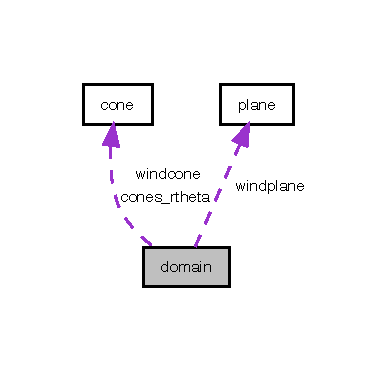
\includegraphics[width=187pt]{structdomain__coll__graph}
\end{center}
\end{figure}
\subsection*{Data Fields}
\begin{DoxyCompactItemize}
\item 
char \hyperlink{structdomain_a0956e1c9c45266a6512b1571427711f6}{name} \mbox{[}\hyperlink{xlog_8c_a10e8c7b8458375c3dbfbb4010a2aba8c}{L\+I\+N\+E\+L\+E\+N\+G\+TH}\mbox{]}
\item 
int \hyperlink{structdomain_a620d21c9cc0dfcb8ed1d9bbb07314daf}{wind\+\_\+type}
\item 
int \hyperlink{structdomain_ac90e4779abcabc0170d2bfc30a8e1323}{ndim}
\item 
int \hyperlink{structdomain_aa557b63d514dffedaf76a635579b3294}{mdim}
\item 
int \hyperlink{structdomain_a7d98eb17a804f4bc727325545272e3da}{ndim2}
\item 
int \hyperlink{structdomain_aeddcae5f993efc8142ee84f461cfcda1}{nstart}
\item 
int \hyperlink{structdomain_ab3733bfe4bcdd87edd4f59da33e85d46}{nstop}
\item 
enum \hyperlink{python_8h_a0a67e9069ac2a2910ddc33cb34df0566}{coord\+\_\+type\+\_\+enum} \hyperlink{structdomain_acbaa6a69b41c9e7c924b668baa65bad3}{coord\+\_\+type}
\item 
int \hyperlink{structdomain_a8e5c1206fd8d19c47be7b5154b5217b9}{log\+\_\+linear}
\item 
double \hyperlink{structdomain_a9877c9ee2824450fd9107f8b93b4f267}{xlog\+\_\+scale}
\item 
double \hyperlink{structdomain_a8fd2202427974acf456e95506e2dce8e}{zlog\+\_\+scale}
\item 
struct \hyperlink{structcone}{cone} \hyperlink{structdomain_a0e5379ee2681d481ee329735231ced7a}{windcone} \mbox{[}2\mbox{]}
\item 
struct \hyperlink{structplane}{plane} \hyperlink{structdomain_ad59a0e0fc4c056c9b75ff1d1c3a0f06c}{windplane} \mbox{[}2\mbox{]}
\item 
double \hyperlink{structdomain_aa1a157a923d525e54bce851e96f8a19c}{rho\+\_\+min}
\item 
double \hyperlink{structdomain_a073d3b0cd25c68e5c3d4ea22705fd1e0}{rho\+\_\+max}
\item 
double \hyperlink{structdomain_a69ec5690bab03b53d2f061173c6bd6c6}{wind\+\_\+x} \mbox{[}\hyperlink{python_8h_a80cccc8d22c78d3095c60ab2aedeb2a5}{N\+D\+I\+M\+\_\+\+M\+AX}\mbox{]}
\item 
double \hyperlink{structdomain_ac3bb48ac4731bd28193e92d66aa9868f}{wind\+\_\+z} \mbox{[}\hyperlink{python_8h_a80cccc8d22c78d3095c60ab2aedeb2a5}{N\+D\+I\+M\+\_\+\+M\+AX}\mbox{]}
\item 
double \hyperlink{structdomain_a6b7011ab95d96a802a079bca85943ca0}{wind\+\_\+midx} \mbox{[}\hyperlink{python_8h_a80cccc8d22c78d3095c60ab2aedeb2a5}{N\+D\+I\+M\+\_\+\+M\+AX}\mbox{]}
\item 
double \hyperlink{structdomain_a90e3e71591ed0419563a4a80008a84bb}{wind\+\_\+midz} \mbox{[}\hyperlink{python_8h_a80cccc8d22c78d3095c60ab2aedeb2a5}{N\+D\+I\+M\+\_\+\+M\+AX}\mbox{]}
\item 
\hyperlink{python_8h_a24207bf0bce7d09eb68cd114e725996d}{Cone\+Ptr} \hyperlink{structdomain_a9691a01ac9495ef917b1537b00110210}{cones\+\_\+rtheta}
\item 
double \hyperlink{structdomain_a810ac3d68f86ad671b5500152cd83be2}{wind\+\_\+z\+\_\+var} \mbox{[}\hyperlink{python_8h_a80cccc8d22c78d3095c60ab2aedeb2a5}{N\+D\+I\+M\+\_\+\+M\+AX}\mbox{]}\mbox{[}\hyperlink{python_8h_a80cccc8d22c78d3095c60ab2aedeb2a5}{N\+D\+I\+M\+\_\+\+M\+AX}\mbox{]}
\item 
double \hyperlink{structdomain_a5d14eb35cccb6c7d3d7078901dc78b95}{wind\+\_\+midz\+\_\+var} \mbox{[}\hyperlink{python_8h_a80cccc8d22c78d3095c60ab2aedeb2a5}{N\+D\+I\+M\+\_\+\+M\+AX}\mbox{]}\mbox{[}\hyperlink{python_8h_a80cccc8d22c78d3095c60ab2aedeb2a5}{N\+D\+I\+M\+\_\+\+M\+AX}\mbox{]}
\item 
double \hyperlink{structdomain_a18728816b23e527c44c331b611a726f4}{wind\+\_\+mdot}
\item 
double \hyperlink{structdomain_a970f4797bdf26152c846b84b31ae5aad}{stellar\+\_\+wind\+\_\+mdot}
\item 
double \hyperlink{structdomain_ae007f791a45e90db42de91c27654ed09}{rmin}
\item 
double \hyperlink{structdomain_ac9d475ec0bfd21ae12dae1b6c05d030d}{rmax}
\item 
double \hyperlink{structdomain_ab879cd1aeb9b7e657b17a12ea2020a1a}{zmin}
\item 
double \hyperlink{structdomain_a411d6f66a03156ee0a5870688d0a9719}{zmax}
\item 
double \hyperlink{structdomain_a88c4870706becdf39db62514c4dfbad6}{wind\+\_\+rho\+\_\+min}
\item 
double \hyperlink{structdomain_af420dea37ea0710d902daa217261d142}{wind\+\_\+rho\+\_\+max}
\item 
double \hyperlink{structdomain_a30a24da6d674f0b4383730b201d206a7}{wind\+\_\+thetamin}
\item 
double \hyperlink{structdomain_a8b495b7bb1917b887fde8948a209783e}{wind\+\_\+thetamax}
\item 
double \hyperlink{structdomain_a424d4ae859ddf9dc456d1f91e4ffe86d}{mdot\+\_\+norm}
\item 
double \hyperlink{structdomain_a813f3ba19f355859ca42acb3c2292d24}{sv\+\_\+lambda}
\item 
double \hyperlink{structdomain_a4e786a4656d477a90d054c260ab3302d}{sv\+\_\+rmin}
\item 
double \hyperlink{structdomain_af5497596d6f246fae7c5c15458b2a03d}{sv\+\_\+rmax}
\item 
double \hyperlink{structdomain_a2306719a5ca44d8a9583068bc2364779}{sv\+\_\+thetamin}
\item 
double \hyperlink{structdomain_a20e1097ea83aafde4917c3ec41c800b0}{sv\+\_\+thetamax}
\item 
double \hyperlink{structdomain_ab5195a9a179b03ca126f2f0f5beef95a}{sv\+\_\+gamma}
\item 
double \hyperlink{structdomain_ad63ff34e9cf3ccee5dcb2d421f20c451}{sv\+\_\+v\+\_\+zero}
\item 
double \hyperlink{structdomain_a7467c5be7712498d0a673c485074e918}{sv\+\_\+r\+\_\+scale}
\item 
double \hyperlink{structdomain_aba459d2b7c4baf62a69ef13fdb39efde}{sv\+\_\+alpha}
\item 
double \hyperlink{structdomain_aae554cbed4fcece39952775d283b9dac}{sv\+\_\+v\+\_\+infinity}
\item 
double \hyperlink{structdomain_a545d794eb6978b47b263f8cd5ebd851b}{kn\+\_\+dratio}
\item 
double \hyperlink{structdomain_ada92cbd729106e55d48e8a6ae5b8c7c2}{kn\+\_\+lambda}
\item 
double \hyperlink{structdomain_a62fd3473a4d70f61e2db3c7d5e457db0}{kn\+\_\+r\+\_\+scale}
\item 
double \hyperlink{structdomain_a3b98872ee3fe1e81d1ebcc0e58b9493b}{kn\+\_\+alpha}
\item 
double \hyperlink{structdomain_aa7f0bbf95881b4cc4090150669bbf806}{kn\+\_\+v\+\_\+infinity}
\item 
double \hyperlink{structdomain_adb9f726942f3f24572729b1ff144b8c2}{kn\+\_\+v\+\_\+zero}
\item 
double \hyperlink{structdomain_aca5df98ed2e93c7629b0cf879392b6a6}{cl\+\_\+v\+\_\+zero}
\item 
double \hyperlink{structdomain_a0ceccfeb97784817b47ad77d6b926840}{cl\+\_\+v\+\_\+infinity}
\item 
double \hyperlink{structdomain_aead88414587817be3ccded2029cb3403}{cl\+\_\+beta}
\item 
double \hyperlink{structdomain_a32773e9268a422a59d6b7b9118d9e966}{cl\+\_\+rmin}
\item 
double \hyperlink{structdomain_a1aef3bdb197bf825b092b7c5e295ae0b}{cl\+\_\+rmax}
\item 
double \hyperlink{structdomain_a7f85fa84808d259d99df40cea538974b}{shell\+\_\+vmin}
\item 
double \hyperlink{structdomain_afe245787b302fa68acbaad6338a652f3}{shell\+\_\+vmax}
\item 
double \hyperlink{structdomain_a678c4aca9df82bcd2bdbba9a111e2683}{shell\+\_\+beta}
\item 
double \hyperlink{structdomain_abb11bd3034be69e7a6bb8673b2bf4f3b}{shell\+\_\+rmin}
\item 
double \hyperlink{structdomain_aaba4c028c0288f52e5b717abc3a8f5ec}{shell\+\_\+rmax}
\item 
double \hyperlink{structdomain_a56d32554e5192c52ea78672263130f67}{corona\+\_\+rmin}
\item 
double \hyperlink{structdomain_af45b1eba31feb6529fb11df5648e3bea}{corona\+\_\+rmax}
\item 
double \hyperlink{structdomain_aa07f5672067b05bf3608b27afe02b747}{corona\+\_\+zmax}
\item 
double \hyperlink{structdomain_a921857c057550470b8a5251e40470660}{corona\+\_\+base\+\_\+density}
\item 
double \hyperlink{structdomain_a59d1c3670b702d3804208dbd1926ad0e}{corona\+\_\+scale\+\_\+height}
\item 
double \hyperlink{structdomain_aa14bbb5f5941acc2a96db927c586f64e}{corona\+\_\+vel\+\_\+frac}
\item 
double \hyperlink{structdomain_af919432b7fbe13685cae0fcbc98f4e8f}{fill}
\end{DoxyCompactItemize}


\subsection{Detailed Description}


Definition at line 200 of file python.\+h.



\subsection{Field Documentation}
\mbox{\Hypertarget{structdomain_aead88414587817be3ccded2029cb3403}\label{structdomain_aead88414587817be3ccded2029cb3403}} 
\index{domain@{domain}!cl\+\_\+beta@{cl\+\_\+beta}}
\index{cl\+\_\+beta@{cl\+\_\+beta}!domain@{domain}}
\subsubsection{\texorpdfstring{cl\+\_\+beta}{cl\_beta}}
{\footnotesize\ttfamily double domain\+::cl\+\_\+beta}



Definition at line 256 of file python.\+h.

\mbox{\Hypertarget{structdomain_a1aef3bdb197bf825b092b7c5e295ae0b}\label{structdomain_a1aef3bdb197bf825b092b7c5e295ae0b}} 
\index{domain@{domain}!cl\+\_\+rmax@{cl\+\_\+rmax}}
\index{cl\+\_\+rmax@{cl\+\_\+rmax}!domain@{domain}}
\subsubsection{\texorpdfstring{cl\+\_\+rmax}{cl\_rmax}}
{\footnotesize\ttfamily double domain\+::cl\+\_\+rmax}



Definition at line 257 of file python.\+h.

\mbox{\Hypertarget{structdomain_a32773e9268a422a59d6b7b9118d9e966}\label{structdomain_a32773e9268a422a59d6b7b9118d9e966}} 
\index{domain@{domain}!cl\+\_\+rmin@{cl\+\_\+rmin}}
\index{cl\+\_\+rmin@{cl\+\_\+rmin}!domain@{domain}}
\subsubsection{\texorpdfstring{cl\+\_\+rmin}{cl\_rmin}}
{\footnotesize\ttfamily double domain\+::cl\+\_\+rmin}



Definition at line 257 of file python.\+h.

\mbox{\Hypertarget{structdomain_a0ceccfeb97784817b47ad77d6b926840}\label{structdomain_a0ceccfeb97784817b47ad77d6b926840}} 
\index{domain@{domain}!cl\+\_\+v\+\_\+infinity@{cl\+\_\+v\+\_\+infinity}}
\index{cl\+\_\+v\+\_\+infinity@{cl\+\_\+v\+\_\+infinity}!domain@{domain}}
\subsubsection{\texorpdfstring{cl\+\_\+v\+\_\+infinity}{cl\_v\_infinity}}
{\footnotesize\ttfamily double domain\+::cl\+\_\+v\+\_\+infinity}



Definition at line 256 of file python.\+h.

\mbox{\Hypertarget{structdomain_aca5df98ed2e93c7629b0cf879392b6a6}\label{structdomain_aca5df98ed2e93c7629b0cf879392b6a6}} 
\index{domain@{domain}!cl\+\_\+v\+\_\+zero@{cl\+\_\+v\+\_\+zero}}
\index{cl\+\_\+v\+\_\+zero@{cl\+\_\+v\+\_\+zero}!domain@{domain}}
\subsubsection{\texorpdfstring{cl\+\_\+v\+\_\+zero}{cl\_v\_zero}}
{\footnotesize\ttfamily double domain\+::cl\+\_\+v\+\_\+zero}



Definition at line 256 of file python.\+h.

\mbox{\Hypertarget{structdomain_a9691a01ac9495ef917b1537b00110210}\label{structdomain_a9691a01ac9495ef917b1537b00110210}} 
\index{domain@{domain}!cones\+\_\+rtheta@{cones\+\_\+rtheta}}
\index{cones\+\_\+rtheta@{cones\+\_\+rtheta}!domain@{domain}}
\subsubsection{\texorpdfstring{cones\+\_\+rtheta}{cones\_rtheta}}
{\footnotesize\ttfamily \hyperlink{python_8h_a24207bf0bce7d09eb68cd114e725996d}{Cone\+Ptr} domain\+::cones\+\_\+rtheta}



Definition at line 219 of file python.\+h.

\mbox{\Hypertarget{structdomain_acbaa6a69b41c9e7c924b668baa65bad3}\label{structdomain_acbaa6a69b41c9e7c924b668baa65bad3}} 
\index{domain@{domain}!coord\+\_\+type@{coord\+\_\+type}}
\index{coord\+\_\+type@{coord\+\_\+type}!domain@{domain}}
\subsubsection{\texorpdfstring{coord\+\_\+type}{coord\_type}}
{\footnotesize\ttfamily enum \hyperlink{python_8h_a0a67e9069ac2a2910ddc33cb34df0566}{coord\+\_\+type\+\_\+enum} domain\+::coord\+\_\+type}



Definition at line 206 of file python.\+h.

\mbox{\Hypertarget{structdomain_a921857c057550470b8a5251e40470660}\label{structdomain_a921857c057550470b8a5251e40470660}} 
\index{domain@{domain}!corona\+\_\+base\+\_\+density@{corona\+\_\+base\+\_\+density}}
\index{corona\+\_\+base\+\_\+density@{corona\+\_\+base\+\_\+density}!domain@{domain}}
\subsubsection{\texorpdfstring{corona\+\_\+base\+\_\+density}{corona\_base\_density}}
{\footnotesize\ttfamily double domain\+::corona\+\_\+base\+\_\+density}



Definition at line 266 of file python.\+h.

\mbox{\Hypertarget{structdomain_af45b1eba31feb6529fb11df5648e3bea}\label{structdomain_af45b1eba31feb6529fb11df5648e3bea}} 
\index{domain@{domain}!corona\+\_\+rmax@{corona\+\_\+rmax}}
\index{corona\+\_\+rmax@{corona\+\_\+rmax}!domain@{domain}}
\subsubsection{\texorpdfstring{corona\+\_\+rmax}{corona\_rmax}}
{\footnotesize\ttfamily double domain\+::corona\+\_\+rmax}



Definition at line 264 of file python.\+h.

\mbox{\Hypertarget{structdomain_a56d32554e5192c52ea78672263130f67}\label{structdomain_a56d32554e5192c52ea78672263130f67}} 
\index{domain@{domain}!corona\+\_\+rmin@{corona\+\_\+rmin}}
\index{corona\+\_\+rmin@{corona\+\_\+rmin}!domain@{domain}}
\subsubsection{\texorpdfstring{corona\+\_\+rmin}{corona\_rmin}}
{\footnotesize\ttfamily double domain\+::corona\+\_\+rmin}



Definition at line 264 of file python.\+h.

\mbox{\Hypertarget{structdomain_a59d1c3670b702d3804208dbd1926ad0e}\label{structdomain_a59d1c3670b702d3804208dbd1926ad0e}} 
\index{domain@{domain}!corona\+\_\+scale\+\_\+height@{corona\+\_\+scale\+\_\+height}}
\index{corona\+\_\+scale\+\_\+height@{corona\+\_\+scale\+\_\+height}!domain@{domain}}
\subsubsection{\texorpdfstring{corona\+\_\+scale\+\_\+height}{corona\_scale\_height}}
{\footnotesize\ttfamily double domain\+::corona\+\_\+scale\+\_\+height}



Definition at line 266 of file python.\+h.

\mbox{\Hypertarget{structdomain_aa14bbb5f5941acc2a96db927c586f64e}\label{structdomain_aa14bbb5f5941acc2a96db927c586f64e}} 
\index{domain@{domain}!corona\+\_\+vel\+\_\+frac@{corona\+\_\+vel\+\_\+frac}}
\index{corona\+\_\+vel\+\_\+frac@{corona\+\_\+vel\+\_\+frac}!domain@{domain}}
\subsubsection{\texorpdfstring{corona\+\_\+vel\+\_\+frac}{corona\_vel\_frac}}
{\footnotesize\ttfamily double domain\+::corona\+\_\+vel\+\_\+frac}



Definition at line 267 of file python.\+h.

\mbox{\Hypertarget{structdomain_aa07f5672067b05bf3608b27afe02b747}\label{structdomain_aa07f5672067b05bf3608b27afe02b747}} 
\index{domain@{domain}!corona\+\_\+zmax@{corona\+\_\+zmax}}
\index{corona\+\_\+zmax@{corona\+\_\+zmax}!domain@{domain}}
\subsubsection{\texorpdfstring{corona\+\_\+zmax}{corona\_zmax}}
{\footnotesize\ttfamily double domain\+::corona\+\_\+zmax}



Definition at line 265 of file python.\+h.

\mbox{\Hypertarget{structdomain_af919432b7fbe13685cae0fcbc98f4e8f}\label{structdomain_af919432b7fbe13685cae0fcbc98f4e8f}} 
\index{domain@{domain}!fill@{fill}}
\index{fill@{fill}!domain@{domain}}
\subsubsection{\texorpdfstring{fill}{fill}}
{\footnotesize\ttfamily double domain\+::fill}



Definition at line 271 of file python.\+h.

\mbox{\Hypertarget{structdomain_a3b98872ee3fe1e81d1ebcc0e58b9493b}\label{structdomain_a3b98872ee3fe1e81d1ebcc0e58b9493b}} 
\index{domain@{domain}!kn\+\_\+alpha@{kn\+\_\+alpha}}
\index{kn\+\_\+alpha@{kn\+\_\+alpha}!domain@{domain}}
\subsubsection{\texorpdfstring{kn\+\_\+alpha}{kn\_alpha}}
{\footnotesize\ttfamily double domain\+::kn\+\_\+alpha}



Definition at line 251 of file python.\+h.

\mbox{\Hypertarget{structdomain_a545d794eb6978b47b263f8cd5ebd851b}\label{structdomain_a545d794eb6978b47b263f8cd5ebd851b}} 
\index{domain@{domain}!kn\+\_\+dratio@{kn\+\_\+dratio}}
\index{kn\+\_\+dratio@{kn\+\_\+dratio}!domain@{domain}}
\subsubsection{\texorpdfstring{kn\+\_\+dratio}{kn\_dratio}}
{\footnotesize\ttfamily double domain\+::kn\+\_\+dratio}



Definition at line 249 of file python.\+h.

\mbox{\Hypertarget{structdomain_ada92cbd729106e55d48e8a6ae5b8c7c2}\label{structdomain_ada92cbd729106e55d48e8a6ae5b8c7c2}} 
\index{domain@{domain}!kn\+\_\+lambda@{kn\+\_\+lambda}}
\index{kn\+\_\+lambda@{kn\+\_\+lambda}!domain@{domain}}
\subsubsection{\texorpdfstring{kn\+\_\+lambda}{kn\_lambda}}
{\footnotesize\ttfamily double domain\+::kn\+\_\+lambda}



Definition at line 250 of file python.\+h.

\mbox{\Hypertarget{structdomain_a62fd3473a4d70f61e2db3c7d5e457db0}\label{structdomain_a62fd3473a4d70f61e2db3c7d5e457db0}} 
\index{domain@{domain}!kn\+\_\+r\+\_\+scale@{kn\+\_\+r\+\_\+scale}}
\index{kn\+\_\+r\+\_\+scale@{kn\+\_\+r\+\_\+scale}!domain@{domain}}
\subsubsection{\texorpdfstring{kn\+\_\+r\+\_\+scale}{kn\_r\_scale}}
{\footnotesize\ttfamily double domain\+::kn\+\_\+r\+\_\+scale}



Definition at line 251 of file python.\+h.

\mbox{\Hypertarget{structdomain_aa7f0bbf95881b4cc4090150669bbf806}\label{structdomain_aa7f0bbf95881b4cc4090150669bbf806}} 
\index{domain@{domain}!kn\+\_\+v\+\_\+infinity@{kn\+\_\+v\+\_\+infinity}}
\index{kn\+\_\+v\+\_\+infinity@{kn\+\_\+v\+\_\+infinity}!domain@{domain}}
\subsubsection{\texorpdfstring{kn\+\_\+v\+\_\+infinity}{kn\_v\_infinity}}
{\footnotesize\ttfamily double domain\+::kn\+\_\+v\+\_\+infinity}



Definition at line 252 of file python.\+h.

\mbox{\Hypertarget{structdomain_adb9f726942f3f24572729b1ff144b8c2}\label{structdomain_adb9f726942f3f24572729b1ff144b8c2}} 
\index{domain@{domain}!kn\+\_\+v\+\_\+zero@{kn\+\_\+v\+\_\+zero}}
\index{kn\+\_\+v\+\_\+zero@{kn\+\_\+v\+\_\+zero}!domain@{domain}}
\subsubsection{\texorpdfstring{kn\+\_\+v\+\_\+zero}{kn\_v\_zero}}
{\footnotesize\ttfamily double domain\+::kn\+\_\+v\+\_\+zero}



Definition at line 253 of file python.\+h.

\mbox{\Hypertarget{structdomain_a8e5c1206fd8d19c47be7b5154b5217b9}\label{structdomain_a8e5c1206fd8d19c47be7b5154b5217b9}} 
\index{domain@{domain}!log\+\_\+linear@{log\+\_\+linear}}
\index{log\+\_\+linear@{log\+\_\+linear}!domain@{domain}}
\subsubsection{\texorpdfstring{log\+\_\+linear}{log\_linear}}
{\footnotesize\ttfamily int domain\+::log\+\_\+linear}



Definition at line 207 of file python.\+h.

\mbox{\Hypertarget{structdomain_aa557b63d514dffedaf76a635579b3294}\label{structdomain_aa557b63d514dffedaf76a635579b3294}} 
\index{domain@{domain}!mdim@{mdim}}
\index{mdim@{mdim}!domain@{domain}}
\subsubsection{\texorpdfstring{mdim}{mdim}}
{\footnotesize\ttfamily int domain\+::mdim}



Definition at line 204 of file python.\+h.

\mbox{\Hypertarget{structdomain_a424d4ae859ddf9dc456d1f91e4ffe86d}\label{structdomain_a424d4ae859ddf9dc456d1f91e4ffe86d}} 
\index{domain@{domain}!mdot\+\_\+norm@{mdot\+\_\+norm}}
\index{mdot\+\_\+norm@{mdot\+\_\+norm}!domain@{domain}}
\subsubsection{\texorpdfstring{mdot\+\_\+norm}{mdot\_norm}}
{\footnotesize\ttfamily double domain\+::mdot\+\_\+norm}



Definition at line 236 of file python.\+h.

\mbox{\Hypertarget{structdomain_a0956e1c9c45266a6512b1571427711f6}\label{structdomain_a0956e1c9c45266a6512b1571427711f6}} 
\index{domain@{domain}!name@{name}}
\index{name@{name}!domain@{domain}}
\subsubsection{\texorpdfstring{name}{name}}
{\footnotesize\ttfamily char domain\+::name\mbox{[}\hyperlink{xlog_8c_a10e8c7b8458375c3dbfbb4010a2aba8c}{L\+I\+N\+E\+L\+E\+N\+G\+TH}\mbox{]}}



Definition at line 202 of file python.\+h.

\mbox{\Hypertarget{structdomain_ac90e4779abcabc0170d2bfc30a8e1323}\label{structdomain_ac90e4779abcabc0170d2bfc30a8e1323}} 
\index{domain@{domain}!ndim@{ndim}}
\index{ndim@{ndim}!domain@{domain}}
\subsubsection{\texorpdfstring{ndim}{ndim}}
{\footnotesize\ttfamily int domain\+::ndim}



Definition at line 204 of file python.\+h.

\mbox{\Hypertarget{structdomain_a7d98eb17a804f4bc727325545272e3da}\label{structdomain_a7d98eb17a804f4bc727325545272e3da}} 
\index{domain@{domain}!ndim2@{ndim2}}
\index{ndim2@{ndim2}!domain@{domain}}
\subsubsection{\texorpdfstring{ndim2}{ndim2}}
{\footnotesize\ttfamily int domain\+::ndim2}



Definition at line 204 of file python.\+h.

\mbox{\Hypertarget{structdomain_aeddcae5f993efc8142ee84f461cfcda1}\label{structdomain_aeddcae5f993efc8142ee84f461cfcda1}} 
\index{domain@{domain}!nstart@{nstart}}
\index{nstart@{nstart}!domain@{domain}}
\subsubsection{\texorpdfstring{nstart}{nstart}}
{\footnotesize\ttfamily int domain\+::nstart}



Definition at line 205 of file python.\+h.

\mbox{\Hypertarget{structdomain_ab3733bfe4bcdd87edd4f59da33e85d46}\label{structdomain_ab3733bfe4bcdd87edd4f59da33e85d46}} 
\index{domain@{domain}!nstop@{nstop}}
\index{nstop@{nstop}!domain@{domain}}
\subsubsection{\texorpdfstring{nstop}{nstop}}
{\footnotesize\ttfamily int domain\+::nstop}



Definition at line 205 of file python.\+h.

\mbox{\Hypertarget{structdomain_a073d3b0cd25c68e5c3d4ea22705fd1e0}\label{structdomain_a073d3b0cd25c68e5c3d4ea22705fd1e0}} 
\index{domain@{domain}!rho\+\_\+max@{rho\+\_\+max}}
\index{rho\+\_\+max@{rho\+\_\+max}!domain@{domain}}
\subsubsection{\texorpdfstring{rho\+\_\+max}{rho\_max}}
{\footnotesize\ttfamily double domain\+::rho\+\_\+max}



Definition at line 214 of file python.\+h.

\mbox{\Hypertarget{structdomain_aa1a157a923d525e54bce851e96f8a19c}\label{structdomain_aa1a157a923d525e54bce851e96f8a19c}} 
\index{domain@{domain}!rho\+\_\+min@{rho\+\_\+min}}
\index{rho\+\_\+min@{rho\+\_\+min}!domain@{domain}}
\subsubsection{\texorpdfstring{rho\+\_\+min}{rho\_min}}
{\footnotesize\ttfamily double domain\+::rho\+\_\+min}



Definition at line 214 of file python.\+h.

\mbox{\Hypertarget{structdomain_ac9d475ec0bfd21ae12dae1b6c05d030d}\label{structdomain_ac9d475ec0bfd21ae12dae1b6c05d030d}} 
\index{domain@{domain}!rmax@{rmax}}
\index{rmax@{rmax}!domain@{domain}}
\subsubsection{\texorpdfstring{rmax}{rmax}}
{\footnotesize\ttfamily double domain\+::rmax}



Definition at line 232 of file python.\+h.

\mbox{\Hypertarget{structdomain_ae007f791a45e90db42de91c27654ed09}\label{structdomain_ae007f791a45e90db42de91c27654ed09}} 
\index{domain@{domain}!rmin@{rmin}}
\index{rmin@{rmin}!domain@{domain}}
\subsubsection{\texorpdfstring{rmin}{rmin}}
{\footnotesize\ttfamily double domain\+::rmin}



Definition at line 232 of file python.\+h.

\mbox{\Hypertarget{structdomain_a678c4aca9df82bcd2bdbba9a111e2683}\label{structdomain_a678c4aca9df82bcd2bdbba9a111e2683}} 
\index{domain@{domain}!shell\+\_\+beta@{shell\+\_\+beta}}
\index{shell\+\_\+beta@{shell\+\_\+beta}!domain@{domain}}
\subsubsection{\texorpdfstring{shell\+\_\+beta}{shell\_beta}}
{\footnotesize\ttfamily double domain\+::shell\+\_\+beta}



Definition at line 260 of file python.\+h.

\mbox{\Hypertarget{structdomain_aaba4c028c0288f52e5b717abc3a8f5ec}\label{structdomain_aaba4c028c0288f52e5b717abc3a8f5ec}} 
\index{domain@{domain}!shell\+\_\+rmax@{shell\+\_\+rmax}}
\index{shell\+\_\+rmax@{shell\+\_\+rmax}!domain@{domain}}
\subsubsection{\texorpdfstring{shell\+\_\+rmax}{shell\_rmax}}
{\footnotesize\ttfamily double domain\+::shell\+\_\+rmax}



Definition at line 261 of file python.\+h.

\mbox{\Hypertarget{structdomain_abb11bd3034be69e7a6bb8673b2bf4f3b}\label{structdomain_abb11bd3034be69e7a6bb8673b2bf4f3b}} 
\index{domain@{domain}!shell\+\_\+rmin@{shell\+\_\+rmin}}
\index{shell\+\_\+rmin@{shell\+\_\+rmin}!domain@{domain}}
\subsubsection{\texorpdfstring{shell\+\_\+rmin}{shell\_rmin}}
{\footnotesize\ttfamily double domain\+::shell\+\_\+rmin}



Definition at line 261 of file python.\+h.

\mbox{\Hypertarget{structdomain_afe245787b302fa68acbaad6338a652f3}\label{structdomain_afe245787b302fa68acbaad6338a652f3}} 
\index{domain@{domain}!shell\+\_\+vmax@{shell\+\_\+vmax}}
\index{shell\+\_\+vmax@{shell\+\_\+vmax}!domain@{domain}}
\subsubsection{\texorpdfstring{shell\+\_\+vmax}{shell\_vmax}}
{\footnotesize\ttfamily double domain\+::shell\+\_\+vmax}



Definition at line 260 of file python.\+h.

\mbox{\Hypertarget{structdomain_a7f85fa84808d259d99df40cea538974b}\label{structdomain_a7f85fa84808d259d99df40cea538974b}} 
\index{domain@{domain}!shell\+\_\+vmin@{shell\+\_\+vmin}}
\index{shell\+\_\+vmin@{shell\+\_\+vmin}!domain@{domain}}
\subsubsection{\texorpdfstring{shell\+\_\+vmin}{shell\_vmin}}
{\footnotesize\ttfamily double domain\+::shell\+\_\+vmin}



Definition at line 260 of file python.\+h.

\mbox{\Hypertarget{structdomain_a970f4797bdf26152c846b84b31ae5aad}\label{structdomain_a970f4797bdf26152c846b84b31ae5aad}} 
\index{domain@{domain}!stellar\+\_\+wind\+\_\+mdot@{stellar\+\_\+wind\+\_\+mdot}}
\index{stellar\+\_\+wind\+\_\+mdot@{stellar\+\_\+wind\+\_\+mdot}!domain@{domain}}
\subsubsection{\texorpdfstring{stellar\+\_\+wind\+\_\+mdot}{stellar\_wind\_mdot}}
{\footnotesize\ttfamily double domain\+::stellar\+\_\+wind\+\_\+mdot}



Definition at line 231 of file python.\+h.

\mbox{\Hypertarget{structdomain_aba459d2b7c4baf62a69ef13fdb39efde}\label{structdomain_aba459d2b7c4baf62a69ef13fdb39efde}} 
\index{domain@{domain}!sv\+\_\+alpha@{sv\+\_\+alpha}}
\index{sv\+\_\+alpha@{sv\+\_\+alpha}!domain@{domain}}
\subsubsection{\texorpdfstring{sv\+\_\+alpha}{sv\_alpha}}
{\footnotesize\ttfamily double domain\+::sv\+\_\+alpha}



Definition at line 244 of file python.\+h.

\mbox{\Hypertarget{structdomain_ab5195a9a179b03ca126f2f0f5beef95a}\label{structdomain_ab5195a9a179b03ca126f2f0f5beef95a}} 
\index{domain@{domain}!sv\+\_\+gamma@{sv\+\_\+gamma}}
\index{sv\+\_\+gamma@{sv\+\_\+gamma}!domain@{domain}}
\subsubsection{\texorpdfstring{sv\+\_\+gamma}{sv\_gamma}}
{\footnotesize\ttfamily double domain\+::sv\+\_\+gamma}



Definition at line 242 of file python.\+h.

\mbox{\Hypertarget{structdomain_a813f3ba19f355859ca42acb3c2292d24}\label{structdomain_a813f3ba19f355859ca42acb3c2292d24}} 
\index{domain@{domain}!sv\+\_\+lambda@{sv\+\_\+lambda}}
\index{sv\+\_\+lambda@{sv\+\_\+lambda}!domain@{domain}}
\subsubsection{\texorpdfstring{sv\+\_\+lambda}{sv\_lambda}}
{\footnotesize\ttfamily double domain\+::sv\+\_\+lambda}



Definition at line 241 of file python.\+h.

\mbox{\Hypertarget{structdomain_a7467c5be7712498d0a673c485074e918}\label{structdomain_a7467c5be7712498d0a673c485074e918}} 
\index{domain@{domain}!sv\+\_\+r\+\_\+scale@{sv\+\_\+r\+\_\+scale}}
\index{sv\+\_\+r\+\_\+scale@{sv\+\_\+r\+\_\+scale}!domain@{domain}}
\subsubsection{\texorpdfstring{sv\+\_\+r\+\_\+scale}{sv\_r\_scale}}
{\footnotesize\ttfamily double domain\+::sv\+\_\+r\+\_\+scale}



Definition at line 244 of file python.\+h.

\mbox{\Hypertarget{structdomain_af5497596d6f246fae7c5c15458b2a03d}\label{structdomain_af5497596d6f246fae7c5c15458b2a03d}} 
\index{domain@{domain}!sv\+\_\+rmax@{sv\+\_\+rmax}}
\index{sv\+\_\+rmax@{sv\+\_\+rmax}!domain@{domain}}
\subsubsection{\texorpdfstring{sv\+\_\+rmax}{sv\_rmax}}
{\footnotesize\ttfamily double domain\+::sv\+\_\+rmax}



Definition at line 242 of file python.\+h.

\mbox{\Hypertarget{structdomain_a4e786a4656d477a90d054c260ab3302d}\label{structdomain_a4e786a4656d477a90d054c260ab3302d}} 
\index{domain@{domain}!sv\+\_\+rmin@{sv\+\_\+rmin}}
\index{sv\+\_\+rmin@{sv\+\_\+rmin}!domain@{domain}}
\subsubsection{\texorpdfstring{sv\+\_\+rmin}{sv\_rmin}}
{\footnotesize\ttfamily double domain\+::sv\+\_\+rmin}



Definition at line 242 of file python.\+h.

\mbox{\Hypertarget{structdomain_a20e1097ea83aafde4917c3ec41c800b0}\label{structdomain_a20e1097ea83aafde4917c3ec41c800b0}} 
\index{domain@{domain}!sv\+\_\+thetamax@{sv\+\_\+thetamax}}
\index{sv\+\_\+thetamax@{sv\+\_\+thetamax}!domain@{domain}}
\subsubsection{\texorpdfstring{sv\+\_\+thetamax}{sv\_thetamax}}
{\footnotesize\ttfamily double domain\+::sv\+\_\+thetamax}



Definition at line 242 of file python.\+h.

\mbox{\Hypertarget{structdomain_a2306719a5ca44d8a9583068bc2364779}\label{structdomain_a2306719a5ca44d8a9583068bc2364779}} 
\index{domain@{domain}!sv\+\_\+thetamin@{sv\+\_\+thetamin}}
\index{sv\+\_\+thetamin@{sv\+\_\+thetamin}!domain@{domain}}
\subsubsection{\texorpdfstring{sv\+\_\+thetamin}{sv\_thetamin}}
{\footnotesize\ttfamily double domain\+::sv\+\_\+thetamin}



Definition at line 242 of file python.\+h.

\mbox{\Hypertarget{structdomain_aae554cbed4fcece39952775d283b9dac}\label{structdomain_aae554cbed4fcece39952775d283b9dac}} 
\index{domain@{domain}!sv\+\_\+v\+\_\+infinity@{sv\+\_\+v\+\_\+infinity}}
\index{sv\+\_\+v\+\_\+infinity@{sv\+\_\+v\+\_\+infinity}!domain@{domain}}
\subsubsection{\texorpdfstring{sv\+\_\+v\+\_\+infinity}{sv\_v\_infinity}}
{\footnotesize\ttfamily double domain\+::sv\+\_\+v\+\_\+infinity}



Definition at line 245 of file python.\+h.

\mbox{\Hypertarget{structdomain_ad63ff34e9cf3ccee5dcb2d421f20c451}\label{structdomain_ad63ff34e9cf3ccee5dcb2d421f20c451}} 
\index{domain@{domain}!sv\+\_\+v\+\_\+zero@{sv\+\_\+v\+\_\+zero}}
\index{sv\+\_\+v\+\_\+zero@{sv\+\_\+v\+\_\+zero}!domain@{domain}}
\subsubsection{\texorpdfstring{sv\+\_\+v\+\_\+zero}{sv\_v\_zero}}
{\footnotesize\ttfamily double domain\+::sv\+\_\+v\+\_\+zero}



Definition at line 243 of file python.\+h.

\mbox{\Hypertarget{structdomain_a18728816b23e527c44c331b611a726f4}\label{structdomain_a18728816b23e527c44c331b611a726f4}} 
\index{domain@{domain}!wind\+\_\+mdot@{wind\+\_\+mdot}}
\index{wind\+\_\+mdot@{wind\+\_\+mdot}!domain@{domain}}
\subsubsection{\texorpdfstring{wind\+\_\+mdot}{wind\_mdot}}
{\footnotesize\ttfamily double domain\+::wind\+\_\+mdot}



Definition at line 231 of file python.\+h.

\mbox{\Hypertarget{structdomain_a6b7011ab95d96a802a079bca85943ca0}\label{structdomain_a6b7011ab95d96a802a079bca85943ca0}} 
\index{domain@{domain}!wind\+\_\+midx@{wind\+\_\+midx}}
\index{wind\+\_\+midx@{wind\+\_\+midx}!domain@{domain}}
\subsubsection{\texorpdfstring{wind\+\_\+midx}{wind\_midx}}
{\footnotesize\ttfamily double domain\+::wind\+\_\+midx\mbox{[}\hyperlink{python_8h_a80cccc8d22c78d3095c60ab2aedeb2a5}{N\+D\+I\+M\+\_\+\+M\+AX}\mbox{]}}



Definition at line 217 of file python.\+h.

\mbox{\Hypertarget{structdomain_a90e3e71591ed0419563a4a80008a84bb}\label{structdomain_a90e3e71591ed0419563a4a80008a84bb}} 
\index{domain@{domain}!wind\+\_\+midz@{wind\+\_\+midz}}
\index{wind\+\_\+midz@{wind\+\_\+midz}!domain@{domain}}
\subsubsection{\texorpdfstring{wind\+\_\+midz}{wind\_midz}}
{\footnotesize\ttfamily double domain\+::wind\+\_\+midz\mbox{[}\hyperlink{python_8h_a80cccc8d22c78d3095c60ab2aedeb2a5}{N\+D\+I\+M\+\_\+\+M\+AX}\mbox{]}}



Definition at line 217 of file python.\+h.

\mbox{\Hypertarget{structdomain_a5d14eb35cccb6c7d3d7078901dc78b95}\label{structdomain_a5d14eb35cccb6c7d3d7078901dc78b95}} 
\index{domain@{domain}!wind\+\_\+midz\+\_\+var@{wind\+\_\+midz\+\_\+var}}
\index{wind\+\_\+midz\+\_\+var@{wind\+\_\+midz\+\_\+var}!domain@{domain}}
\subsubsection{\texorpdfstring{wind\+\_\+midz\+\_\+var}{wind\_midz\_var}}
{\footnotesize\ttfamily double domain\+::wind\+\_\+midz\+\_\+var\mbox{[}\hyperlink{python_8h_a80cccc8d22c78d3095c60ab2aedeb2a5}{N\+D\+I\+M\+\_\+\+M\+AX}\mbox{]}\mbox{[}\hyperlink{python_8h_a80cccc8d22c78d3095c60ab2aedeb2a5}{N\+D\+I\+M\+\_\+\+M\+AX}\mbox{]}}



Definition at line 225 of file python.\+h.

\mbox{\Hypertarget{structdomain_af420dea37ea0710d902daa217261d142}\label{structdomain_af420dea37ea0710d902daa217261d142}} 
\index{domain@{domain}!wind\+\_\+rho\+\_\+max@{wind\+\_\+rho\+\_\+max}}
\index{wind\+\_\+rho\+\_\+max@{wind\+\_\+rho\+\_\+max}!domain@{domain}}
\subsubsection{\texorpdfstring{wind\+\_\+rho\+\_\+max}{wind\_rho\_max}}
{\footnotesize\ttfamily double domain\+::wind\+\_\+rho\+\_\+max}



Definition at line 234 of file python.\+h.

\mbox{\Hypertarget{structdomain_a88c4870706becdf39db62514c4dfbad6}\label{structdomain_a88c4870706becdf39db62514c4dfbad6}} 
\index{domain@{domain}!wind\+\_\+rho\+\_\+min@{wind\+\_\+rho\+\_\+min}}
\index{wind\+\_\+rho\+\_\+min@{wind\+\_\+rho\+\_\+min}!domain@{domain}}
\subsubsection{\texorpdfstring{wind\+\_\+rho\+\_\+min}{wind\_rho\_min}}
{\footnotesize\ttfamily double domain\+::wind\+\_\+rho\+\_\+min}



Definition at line 234 of file python.\+h.

\mbox{\Hypertarget{structdomain_a8b495b7bb1917b887fde8948a209783e}\label{structdomain_a8b495b7bb1917b887fde8948a209783e}} 
\index{domain@{domain}!wind\+\_\+thetamax@{wind\+\_\+thetamax}}
\index{wind\+\_\+thetamax@{wind\+\_\+thetamax}!domain@{domain}}
\subsubsection{\texorpdfstring{wind\+\_\+thetamax}{wind\_thetamax}}
{\footnotesize\ttfamily double domain\+::wind\+\_\+thetamax}



Definition at line 235 of file python.\+h.

\mbox{\Hypertarget{structdomain_a30a24da6d674f0b4383730b201d206a7}\label{structdomain_a30a24da6d674f0b4383730b201d206a7}} 
\index{domain@{domain}!wind\+\_\+thetamin@{wind\+\_\+thetamin}}
\index{wind\+\_\+thetamin@{wind\+\_\+thetamin}!domain@{domain}}
\subsubsection{\texorpdfstring{wind\+\_\+thetamin}{wind\_thetamin}}
{\footnotesize\ttfamily double domain\+::wind\+\_\+thetamin}



Definition at line 235 of file python.\+h.

\mbox{\Hypertarget{structdomain_a620d21c9cc0dfcb8ed1d9bbb07314daf}\label{structdomain_a620d21c9cc0dfcb8ed1d9bbb07314daf}} 
\index{domain@{domain}!wind\+\_\+type@{wind\+\_\+type}}
\index{wind\+\_\+type@{wind\+\_\+type}!domain@{domain}}
\subsubsection{\texorpdfstring{wind\+\_\+type}{wind\_type}}
{\footnotesize\ttfamily int domain\+::wind\+\_\+type}



Definition at line 203 of file python.\+h.

\mbox{\Hypertarget{structdomain_a69ec5690bab03b53d2f061173c6bd6c6}\label{structdomain_a69ec5690bab03b53d2f061173c6bd6c6}} 
\index{domain@{domain}!wind\+\_\+x@{wind\+\_\+x}}
\index{wind\+\_\+x@{wind\+\_\+x}!domain@{domain}}
\subsubsection{\texorpdfstring{wind\+\_\+x}{wind\_x}}
{\footnotesize\ttfamily double domain\+::wind\+\_\+x\mbox{[}\hyperlink{python_8h_a80cccc8d22c78d3095c60ab2aedeb2a5}{N\+D\+I\+M\+\_\+\+M\+AX}\mbox{]}}



Definition at line 216 of file python.\+h.

\mbox{\Hypertarget{structdomain_ac3bb48ac4731bd28193e92d66aa9868f}\label{structdomain_ac3bb48ac4731bd28193e92d66aa9868f}} 
\index{domain@{domain}!wind\+\_\+z@{wind\+\_\+z}}
\index{wind\+\_\+z@{wind\+\_\+z}!domain@{domain}}
\subsubsection{\texorpdfstring{wind\+\_\+z}{wind\_z}}
{\footnotesize\ttfamily double domain\+::wind\+\_\+z\mbox{[}\hyperlink{python_8h_a80cccc8d22c78d3095c60ab2aedeb2a5}{N\+D\+I\+M\+\_\+\+M\+AX}\mbox{]}}



Definition at line 216 of file python.\+h.

\mbox{\Hypertarget{structdomain_a810ac3d68f86ad671b5500152cd83be2}\label{structdomain_a810ac3d68f86ad671b5500152cd83be2}} 
\index{domain@{domain}!wind\+\_\+z\+\_\+var@{wind\+\_\+z\+\_\+var}}
\index{wind\+\_\+z\+\_\+var@{wind\+\_\+z\+\_\+var}!domain@{domain}}
\subsubsection{\texorpdfstring{wind\+\_\+z\+\_\+var}{wind\_z\_var}}
{\footnotesize\ttfamily double domain\+::wind\+\_\+z\+\_\+var\mbox{[}\hyperlink{python_8h_a80cccc8d22c78d3095c60ab2aedeb2a5}{N\+D\+I\+M\+\_\+\+M\+AX}\mbox{]}\mbox{[}\hyperlink{python_8h_a80cccc8d22c78d3095c60ab2aedeb2a5}{N\+D\+I\+M\+\_\+\+M\+AX}\mbox{]}}



Definition at line 224 of file python.\+h.

\mbox{\Hypertarget{structdomain_a0e5379ee2681d481ee329735231ced7a}\label{structdomain_a0e5379ee2681d481ee329735231ced7a}} 
\index{domain@{domain}!windcone@{windcone}}
\index{windcone@{windcone}!domain@{domain}}
\subsubsection{\texorpdfstring{windcone}{windcone}}
{\footnotesize\ttfamily struct \hyperlink{structcone}{cone} domain\+::windcone\mbox{[}2\mbox{]}}



Definition at line 212 of file python.\+h.

\mbox{\Hypertarget{structdomain_ad59a0e0fc4c056c9b75ff1d1c3a0f06c}\label{structdomain_ad59a0e0fc4c056c9b75ff1d1c3a0f06c}} 
\index{domain@{domain}!windplane@{windplane}}
\index{windplane@{windplane}!domain@{domain}}
\subsubsection{\texorpdfstring{windplane}{windplane}}
{\footnotesize\ttfamily struct \hyperlink{structplane}{plane} domain\+::windplane\mbox{[}2\mbox{]}}



Definition at line 213 of file python.\+h.

\mbox{\Hypertarget{structdomain_a9877c9ee2824450fd9107f8b93b4f267}\label{structdomain_a9877c9ee2824450fd9107f8b93b4f267}} 
\index{domain@{domain}!xlog\+\_\+scale@{xlog\+\_\+scale}}
\index{xlog\+\_\+scale@{xlog\+\_\+scale}!domain@{domain}}
\subsubsection{\texorpdfstring{xlog\+\_\+scale}{xlog\_scale}}
{\footnotesize\ttfamily double domain\+::xlog\+\_\+scale}



Definition at line 208 of file python.\+h.

\mbox{\Hypertarget{structdomain_a8fd2202427974acf456e95506e2dce8e}\label{structdomain_a8fd2202427974acf456e95506e2dce8e}} 
\index{domain@{domain}!zlog\+\_\+scale@{zlog\+\_\+scale}}
\index{zlog\+\_\+scale@{zlog\+\_\+scale}!domain@{domain}}
\subsubsection{\texorpdfstring{zlog\+\_\+scale}{zlog\_scale}}
{\footnotesize\ttfamily double domain\+::zlog\+\_\+scale}



Definition at line 208 of file python.\+h.

\mbox{\Hypertarget{structdomain_a411d6f66a03156ee0a5870688d0a9719}\label{structdomain_a411d6f66a03156ee0a5870688d0a9719}} 
\index{domain@{domain}!zmax@{zmax}}
\index{zmax@{zmax}!domain@{domain}}
\subsubsection{\texorpdfstring{zmax}{zmax}}
{\footnotesize\ttfamily double domain\+::zmax}



Definition at line 233 of file python.\+h.

\mbox{\Hypertarget{structdomain_ab879cd1aeb9b7e657b17a12ea2020a1a}\label{structdomain_ab879cd1aeb9b7e657b17a12ea2020a1a}} 
\index{domain@{domain}!zmin@{zmin}}
\index{zmin@{zmin}!domain@{domain}}
\subsubsection{\texorpdfstring{zmin}{zmin}}
{\footnotesize\ttfamily double domain\+::zmin}



Definition at line 233 of file python.\+h.



The documentation for this struct was generated from the following file\+:\begin{DoxyCompactItemize}
\item 
/\+Users/mhewitt/python/source/\hyperlink{python_8h}{python.\+h}\end{DoxyCompactItemize}

\hypertarget{structelements}{}\section{elements Struct Reference}
\label{structelements}\index{elements@{elements}}


{\ttfamily \#include $<$atomic.\+h$>$}

\subsection*{Data Fields}
\begin{DoxyCompactItemize}
\item 
char \hyperlink{structelements_ac6a5e682babab0bc79f63d6395f3837e}{name} \mbox{[}20\mbox{]}
\item 
int \hyperlink{structelements_aae9cca99fda4810bda33b861f9fbd70b}{z}
\item 
int \hyperlink{structelements_a309aeae50d0264cd963f1a1815ce604e}{firstion}
\item 
int \hyperlink{structelements_a90866d4e99cc142553839ad5e8f13dbc}{nions}
\item 
double \hyperlink{structelements_a72235377dd9fdab9cc49404b11a294c3}{abun}
\end{DoxyCompactItemize}


\subsection{Detailed Description}


Definition at line 83 of file atomic.\+h.



\subsection{Field Documentation}
\mbox{\Hypertarget{structelements_a72235377dd9fdab9cc49404b11a294c3}\label{structelements_a72235377dd9fdab9cc49404b11a294c3}} 
\index{elements@{elements}!abun@{abun}}
\index{abun@{abun}!elements@{elements}}
\subsubsection{\texorpdfstring{abun}{abun}}
{\footnotesize\ttfamily double elements\+::abun}



Definition at line 90 of file atomic.\+h.

\mbox{\Hypertarget{structelements_a309aeae50d0264cd963f1a1815ce604e}\label{structelements_a309aeae50d0264cd963f1a1815ce604e}} 
\index{elements@{elements}!firstion@{firstion}}
\index{firstion@{firstion}!elements@{elements}}
\subsubsection{\texorpdfstring{firstion}{firstion}}
{\footnotesize\ttfamily int elements\+::firstion}



Definition at line 88 of file atomic.\+h.

\mbox{\Hypertarget{structelements_ac6a5e682babab0bc79f63d6395f3837e}\label{structelements_ac6a5e682babab0bc79f63d6395f3837e}} 
\index{elements@{elements}!name@{name}}
\index{name@{name}!elements@{elements}}
\subsubsection{\texorpdfstring{name}{name}}
{\footnotesize\ttfamily char elements\+::name\mbox{[}20\mbox{]}}



Definition at line 86 of file atomic.\+h.

\mbox{\Hypertarget{structelements_a90866d4e99cc142553839ad5e8f13dbc}\label{structelements_a90866d4e99cc142553839ad5e8f13dbc}} 
\index{elements@{elements}!nions@{nions}}
\index{nions@{nions}!elements@{elements}}
\subsubsection{\texorpdfstring{nions}{nions}}
{\footnotesize\ttfamily int elements\+::nions}



Definition at line 89 of file atomic.\+h.

\mbox{\Hypertarget{structelements_aae9cca99fda4810bda33b861f9fbd70b}\label{structelements_aae9cca99fda4810bda33b861f9fbd70b}} 
\index{elements@{elements}!z@{z}}
\index{z@{z}!elements@{elements}}
\subsubsection{\texorpdfstring{z}{z}}
{\footnotesize\ttfamily int elements\+::z}



Definition at line 87 of file atomic.\+h.



The documentation for this struct was generated from the following file\+:\begin{DoxyCompactItemize}
\item 
/\+Users/mhewitt/python/source/\hyperlink{atomic_8h}{atomic.\+h}\end{DoxyCompactItemize}

\hypertarget{structemiss__range}{}\section{emiss\+\_\+range Struct Reference}
\label{structemiss__range}\index{emiss\+\_\+range@{emiss\+\_\+range}}


{\ttfamily \#include $<$python.\+h$>$}

\subsection*{Data Fields}
\begin{DoxyCompactItemize}
\item 
double \hyperlink{structemiss__range_ae32bcc0c5aa7a7f15c63cee741f1f2b0}{fmin}
\item 
double \hyperlink{structemiss__range_ac6c5df2b3f9dd4eb3bc729feac39ae2d}{fmax}
\end{DoxyCompactItemize}


\subsection{Detailed Description}


Definition at line 1308 of file python.\+h.



\subsection{Field Documentation}
\mbox{\Hypertarget{structemiss__range_ac6c5df2b3f9dd4eb3bc729feac39ae2d}\label{structemiss__range_ac6c5df2b3f9dd4eb3bc729feac39ae2d}} 
\index{emiss\+\_\+range@{emiss\+\_\+range}!fmax@{fmax}}
\index{fmax@{fmax}!emiss\+\_\+range@{emiss\+\_\+range}}
\subsubsection{\texorpdfstring{fmax}{fmax}}
{\footnotesize\ttfamily double emiss\+\_\+range\+::fmax}



Definition at line 1310 of file python.\+h.

\mbox{\Hypertarget{structemiss__range_ae32bcc0c5aa7a7f15c63cee741f1f2b0}\label{structemiss__range_ae32bcc0c5aa7a7f15c63cee741f1f2b0}} 
\index{emiss\+\_\+range@{emiss\+\_\+range}!fmin@{fmin}}
\index{fmin@{fmin}!emiss\+\_\+range@{emiss\+\_\+range}}
\subsubsection{\texorpdfstring{fmin}{fmin}}
{\footnotesize\ttfamily double emiss\+\_\+range\+::fmin}



Definition at line 1310 of file python.\+h.



The documentation for this struct was generated from the following file\+:\begin{DoxyCompactItemize}
\item 
/\+Users/mhewitt/python/source/\hyperlink{python_8h}{python.\+h}\end{DoxyCompactItemize}

\hypertarget{structerror__log}{}\section{error\+\_\+log Struct Reference}
\label{structerror__log}\index{error\+\_\+log@{error\+\_\+log}}
\subsection*{Data Fields}
\begin{DoxyCompactItemize}
\item 
char \hyperlink{structerror__log_a16d5c133b827ebef42abc2fee9bbefb2}{description} \mbox{[}\hyperlink{xlog_8c_a10e8c7b8458375c3dbfbb4010a2aba8c}{L\+I\+N\+E\+L\+E\+N\+G\+TH}\mbox{]}
\item 
int \hyperlink{structerror__log_ac532eb6ea57c79987ee08e0081582d4e}{n}
\end{DoxyCompactItemize}


\subsection{Detailed Description}


Definition at line 104 of file xlog.\+c.



\subsection{Field Documentation}
\mbox{\Hypertarget{structerror__log_a16d5c133b827ebef42abc2fee9bbefb2}\label{structerror__log_a16d5c133b827ebef42abc2fee9bbefb2}} 
\index{error\+\_\+log@{error\+\_\+log}!description@{description}}
\index{description@{description}!error\+\_\+log@{error\+\_\+log}}
\subsubsection{\texorpdfstring{description}{description}}
{\footnotesize\ttfamily char error\+\_\+log\+::description\mbox{[}\hyperlink{xlog_8c_a10e8c7b8458375c3dbfbb4010a2aba8c}{L\+I\+N\+E\+L\+E\+N\+G\+TH}\mbox{]}}



Definition at line 106 of file xlog.\+c.

\mbox{\Hypertarget{structerror__log_ac532eb6ea57c79987ee08e0081582d4e}\label{structerror__log_ac532eb6ea57c79987ee08e0081582d4e}} 
\index{error\+\_\+log@{error\+\_\+log}!n@{n}}
\index{n@{n}!error\+\_\+log@{error\+\_\+log}}
\subsubsection{\texorpdfstring{n}{n}}
{\footnotesize\ttfamily int error\+\_\+log\+::n}



Definition at line 107 of file xlog.\+c.



The documentation for this struct was generated from the following file\+:\begin{DoxyCompactItemize}
\item 
/\+Users/mhewitt/python/source/\hyperlink{xlog_8c}{xlog.\+c}\end{DoxyCompactItemize}

\hypertarget{structfbstruc}{}\section{fbstruc Struct Reference}
\label{structfbstruc}\index{fbstruc@{fbstruc}}


{\ttfamily \#include $<$python.\+h$>$}

\subsection*{Data Fields}
\begin{DoxyCompactItemize}
\item 
double \hyperlink{structfbstruc_a00049c608d6d413ff278c4ad85c2dfdd}{f1}
\item 
double \hyperlink{structfbstruc_abbce27eacdec4c677886d24a20aac51c}{f2}
\item 
double \hyperlink{structfbstruc_ae84f43ceb4d2e546af5cff8ffefa903d}{cool} \mbox{[}\hyperlink{atomic_8h_ac6a37b9ae25d11bf2521d8ee85c46d79}{N\+I\+O\+NS}\mbox{]}\mbox{[}\hyperlink{python_8h_aed80336ab0bdf84ca8d3c4c333430a7b}{N\+T\+E\+M\+PS}\mbox{]}
\item 
double \hyperlink{structfbstruc_a9821ceb0012fdc62fd355f8e4c51a437}{lum} \mbox{[}\hyperlink{atomic_8h_ac6a37b9ae25d11bf2521d8ee85c46d79}{N\+I\+O\+NS}\mbox{]}\mbox{[}\hyperlink{python_8h_aed80336ab0bdf84ca8d3c4c333430a7b}{N\+T\+E\+M\+PS}\mbox{]}
\item 
double \hyperlink{structfbstruc_acb616be77cf6fed83e53426144683bd5}{cool\+\_\+inner} \mbox{[}\hyperlink{atomic_8h_ac6a37b9ae25d11bf2521d8ee85c46d79}{N\+I\+O\+NS}\mbox{]}\mbox{[}\hyperlink{python_8h_aed80336ab0bdf84ca8d3c4c333430a7b}{N\+T\+E\+M\+PS}\mbox{]}
\end{DoxyCompactItemize}


\subsection{Detailed Description}


Definition at line 1288 of file python.\+h.



\subsection{Field Documentation}
\mbox{\Hypertarget{structfbstruc_ae84f43ceb4d2e546af5cff8ffefa903d}\label{structfbstruc_ae84f43ceb4d2e546af5cff8ffefa903d}} 
\index{fbstruc@{fbstruc}!cool@{cool}}
\index{cool@{cool}!fbstruc@{fbstruc}}
\subsubsection{\texorpdfstring{cool}{cool}}
{\footnotesize\ttfamily double fbstruc\+::cool\mbox{[}\hyperlink{atomic_8h_ac6a37b9ae25d11bf2521d8ee85c46d79}{N\+I\+O\+NS}\mbox{]}\mbox{[}\hyperlink{python_8h_aed80336ab0bdf84ca8d3c4c333430a7b}{N\+T\+E\+M\+PS}\mbox{]}}



Definition at line 1291 of file python.\+h.

\mbox{\Hypertarget{structfbstruc_acb616be77cf6fed83e53426144683bd5}\label{structfbstruc_acb616be77cf6fed83e53426144683bd5}} 
\index{fbstruc@{fbstruc}!cool\+\_\+inner@{cool\+\_\+inner}}
\index{cool\+\_\+inner@{cool\+\_\+inner}!fbstruc@{fbstruc}}
\subsubsection{\texorpdfstring{cool\+\_\+inner}{cool\_inner}}
{\footnotesize\ttfamily double fbstruc\+::cool\+\_\+inner\mbox{[}\hyperlink{atomic_8h_ac6a37b9ae25d11bf2521d8ee85c46d79}{N\+I\+O\+NS}\mbox{]}\mbox{[}\hyperlink{python_8h_aed80336ab0bdf84ca8d3c4c333430a7b}{N\+T\+E\+M\+PS}\mbox{]}}



Definition at line 1293 of file python.\+h.

\mbox{\Hypertarget{structfbstruc_a00049c608d6d413ff278c4ad85c2dfdd}\label{structfbstruc_a00049c608d6d413ff278c4ad85c2dfdd}} 
\index{fbstruc@{fbstruc}!f1@{f1}}
\index{f1@{f1}!fbstruc@{fbstruc}}
\subsubsection{\texorpdfstring{f1}{f1}}
{\footnotesize\ttfamily double fbstruc\+::f1}



Definition at line 1290 of file python.\+h.

\mbox{\Hypertarget{structfbstruc_abbce27eacdec4c677886d24a20aac51c}\label{structfbstruc_abbce27eacdec4c677886d24a20aac51c}} 
\index{fbstruc@{fbstruc}!f2@{f2}}
\index{f2@{f2}!fbstruc@{fbstruc}}
\subsubsection{\texorpdfstring{f2}{f2}}
{\footnotesize\ttfamily double fbstruc\+::f2}



Definition at line 1290 of file python.\+h.

\mbox{\Hypertarget{structfbstruc_a9821ceb0012fdc62fd355f8e4c51a437}\label{structfbstruc_a9821ceb0012fdc62fd355f8e4c51a437}} 
\index{fbstruc@{fbstruc}!lum@{lum}}
\index{lum@{lum}!fbstruc@{fbstruc}}
\subsubsection{\texorpdfstring{lum}{lum}}
{\footnotesize\ttfamily double fbstruc\+::lum\mbox{[}\hyperlink{atomic_8h_ac6a37b9ae25d11bf2521d8ee85c46d79}{N\+I\+O\+NS}\mbox{]}\mbox{[}\hyperlink{python_8h_aed80336ab0bdf84ca8d3c4c333430a7b}{N\+T\+E\+M\+PS}\mbox{]}}



Definition at line 1292 of file python.\+h.



The documentation for this struct was generated from the following file\+:\begin{DoxyCompactItemize}
\item 
/\+Users/mhewitt/python/source/\hyperlink{python_8h}{python.\+h}\end{DoxyCompactItemize}

\hypertarget{structfilenames}{}\section{filenames Struct Reference}
\label{structfilenames}\index{filenames@{filenames}}


{\ttfamily \#include $<$python.\+h$>$}

\subsection*{Data Fields}
\begin{DoxyCompactItemize}
\item 
char \hyperlink{structfilenames_a8c053bab321640d4f0f5b75110980c89}{root} \mbox{[}\hyperlink{xlog_8c_a10e8c7b8458375c3dbfbb4010a2aba8c}{L\+I\+N\+E\+L\+E\+N\+G\+TH}\mbox{]}
\item 
char \hyperlink{structfilenames_a316c909bfa7dc0d7740d84f9d33d6418}{windsave} \mbox{[}\hyperlink{xlog_8c_a10e8c7b8458375c3dbfbb4010a2aba8c}{L\+I\+N\+E\+L\+E\+N\+G\+TH}\mbox{]}
\item 
char \hyperlink{structfilenames_ad7f42e4035f3ba3be6bbf16d00b7ba35}{old\+\_\+windsave} \mbox{[}\hyperlink{xlog_8c_a10e8c7b8458375c3dbfbb4010a2aba8c}{L\+I\+N\+E\+L\+E\+N\+G\+TH}\mbox{]}
\item 
char \hyperlink{structfilenames_a12010879e17a410582c95418e70fb8f4}{specsave} \mbox{[}\hyperlink{xlog_8c_a10e8c7b8458375c3dbfbb4010a2aba8c}{L\+I\+N\+E\+L\+E\+N\+G\+TH}\mbox{]}
\item 
char \hyperlink{structfilenames_a21f31ce0b0f82a7f5cf0d456088515fe}{diag} \mbox{[}\hyperlink{xlog_8c_a10e8c7b8458375c3dbfbb4010a2aba8c}{L\+I\+N\+E\+L\+E\+N\+G\+TH}\mbox{]}
\item 
char \hyperlink{structfilenames_a7bb82526145f9ba7f331da3cb3874280}{diagfolder} \mbox{[}\hyperlink{xlog_8c_a10e8c7b8458375c3dbfbb4010a2aba8c}{L\+I\+N\+E\+L\+E\+N\+G\+TH}\mbox{]}
\item 
char \hyperlink{structfilenames_ad69a4b6cb667c701b42275495c4cd002}{input} \mbox{[}\hyperlink{xlog_8c_a10e8c7b8458375c3dbfbb4010a2aba8c}{L\+I\+N\+E\+L\+E\+N\+G\+TH}\mbox{]}
\item 
char \hyperlink{structfilenames_a78ff170f6723c4497848c471d5faf579}{new\+\_\+pf} \mbox{[}\hyperlink{xlog_8c_a10e8c7b8458375c3dbfbb4010a2aba8c}{L\+I\+N\+E\+L\+E\+N\+G\+TH}\mbox{]}
\item 
char \hyperlink{structfilenames_aa5f57d0dd0cd0bb983889cff1a2de34c}{wspec} \mbox{[}\hyperlink{xlog_8c_a10e8c7b8458375c3dbfbb4010a2aba8c}{L\+I\+N\+E\+L\+E\+N\+G\+TH}\mbox{]}
\item 
char \hyperlink{structfilenames_a79368c322d08dbd2e3fa460d364ed3a0}{lwspec} \mbox{[}\hyperlink{xlog_8c_a10e8c7b8458375c3dbfbb4010a2aba8c}{L\+I\+N\+E\+L\+E\+N\+G\+TH}\mbox{]}
\item 
char \hyperlink{structfilenames_a06c80950019150200d964f62ff9417f1}{wspec\+\_\+wind} \mbox{[}\hyperlink{xlog_8c_a10e8c7b8458375c3dbfbb4010a2aba8c}{L\+I\+N\+E\+L\+E\+N\+G\+TH}\mbox{]}
\item 
char \hyperlink{structfilenames_a87e29f1b92b3d9f5be4928380029aaed}{lwspec\+\_\+wind} \mbox{[}\hyperlink{xlog_8c_a10e8c7b8458375c3dbfbb4010a2aba8c}{L\+I\+N\+E\+L\+E\+N\+G\+TH}\mbox{]}
\item 
char \hyperlink{structfilenames_a1532ac6d7bebce60d86774d552e0c078}{spec} \mbox{[}\hyperlink{xlog_8c_a10e8c7b8458375c3dbfbb4010a2aba8c}{L\+I\+N\+E\+L\+E\+N\+G\+TH}\mbox{]}
\item 
char \hyperlink{structfilenames_abe876554c7cdd821a6365745cc23079b}{lspec} \mbox{[}\hyperlink{xlog_8c_a10e8c7b8458375c3dbfbb4010a2aba8c}{L\+I\+N\+E\+L\+E\+N\+G\+TH}\mbox{]}
\item 
char \hyperlink{structfilenames_a4e7d0693cd2c2a7359a840d8649a75c1}{spec\+\_\+wind} \mbox{[}\hyperlink{xlog_8c_a10e8c7b8458375c3dbfbb4010a2aba8c}{L\+I\+N\+E\+L\+E\+N\+G\+TH}\mbox{]}
\item 
char \hyperlink{structfilenames_ae7434018e963fbee3799a61f17025e01}{lspec\+\_\+wind} \mbox{[}\hyperlink{xlog_8c_a10e8c7b8458375c3dbfbb4010a2aba8c}{L\+I\+N\+E\+L\+E\+N\+G\+TH}\mbox{]}
\item 
char \hyperlink{structfilenames_a5bf5e6c9f50e525d5df91800b2c1becc}{disk} \mbox{[}\hyperlink{xlog_8c_a10e8c7b8458375c3dbfbb4010a2aba8c}{L\+I\+N\+E\+L\+E\+N\+G\+TH}\mbox{]}
\item 
char \hyperlink{structfilenames_ab591635bb4619345b1367b36cdd2cce6}{tprofile} \mbox{[}\hyperlink{xlog_8c_a10e8c7b8458375c3dbfbb4010a2aba8c}{L\+I\+N\+E\+L\+E\+N\+G\+TH}\mbox{]}
\item 
char \hyperlink{structfilenames_aebb92f2514d1dbb4fce18c2d30871c67}{phot} \mbox{[}\hyperlink{xlog_8c_a10e8c7b8458375c3dbfbb4010a2aba8c}{L\+I\+N\+E\+L\+E\+N\+G\+TH}\mbox{]}
\item 
char \hyperlink{structfilenames_a647feff8c9ae68afbf7fda1112da79de}{windrad} \mbox{[}\hyperlink{xlog_8c_a10e8c7b8458375c3dbfbb4010a2aba8c}{L\+I\+N\+E\+L\+E\+N\+G\+TH}\mbox{]}
\end{DoxyCompactItemize}


\subsection{Detailed Description}


Definition at line 1369 of file python.\+h.



\subsection{Field Documentation}
\mbox{\Hypertarget{structfilenames_a21f31ce0b0f82a7f5cf0d456088515fe}\label{structfilenames_a21f31ce0b0f82a7f5cf0d456088515fe}} 
\index{filenames@{filenames}!diag@{diag}}
\index{diag@{diag}!filenames@{filenames}}
\subsubsection{\texorpdfstring{diag}{diag}}
{\footnotesize\ttfamily char filenames\+::diag\mbox{[}\hyperlink{xlog_8c_a10e8c7b8458375c3dbfbb4010a2aba8c}{L\+I\+N\+E\+L\+E\+N\+G\+TH}\mbox{]}}



Definition at line 1375 of file python.\+h.

\mbox{\Hypertarget{structfilenames_a7bb82526145f9ba7f331da3cb3874280}\label{structfilenames_a7bb82526145f9ba7f331da3cb3874280}} 
\index{filenames@{filenames}!diagfolder@{diagfolder}}
\index{diagfolder@{diagfolder}!filenames@{filenames}}
\subsubsection{\texorpdfstring{diagfolder}{diagfolder}}
{\footnotesize\ttfamily char filenames\+::diagfolder\mbox{[}\hyperlink{xlog_8c_a10e8c7b8458375c3dbfbb4010a2aba8c}{L\+I\+N\+E\+L\+E\+N\+G\+TH}\mbox{]}}



Definition at line 1376 of file python.\+h.

\mbox{\Hypertarget{structfilenames_a5bf5e6c9f50e525d5df91800b2c1becc}\label{structfilenames_a5bf5e6c9f50e525d5df91800b2c1becc}} 
\index{filenames@{filenames}!disk@{disk}}
\index{disk@{disk}!filenames@{filenames}}
\subsubsection{\texorpdfstring{disk}{disk}}
{\footnotesize\ttfamily char filenames\+::disk\mbox{[}\hyperlink{xlog_8c_a10e8c7b8458375c3dbfbb4010a2aba8c}{L\+I\+N\+E\+L\+E\+N\+G\+TH}\mbox{]}}



Definition at line 1387 of file python.\+h.

\mbox{\Hypertarget{structfilenames_ad69a4b6cb667c701b42275495c4cd002}\label{structfilenames_ad69a4b6cb667c701b42275495c4cd002}} 
\index{filenames@{filenames}!input@{input}}
\index{input@{input}!filenames@{filenames}}
\subsubsection{\texorpdfstring{input}{input}}
{\footnotesize\ttfamily char filenames\+::input\mbox{[}\hyperlink{xlog_8c_a10e8c7b8458375c3dbfbb4010a2aba8c}{L\+I\+N\+E\+L\+E\+N\+G\+TH}\mbox{]}}



Definition at line 1377 of file python.\+h.

\mbox{\Hypertarget{structfilenames_abe876554c7cdd821a6365745cc23079b}\label{structfilenames_abe876554c7cdd821a6365745cc23079b}} 
\index{filenames@{filenames}!lspec@{lspec}}
\index{lspec@{lspec}!filenames@{filenames}}
\subsubsection{\texorpdfstring{lspec}{lspec}}
{\footnotesize\ttfamily char filenames\+::lspec\mbox{[}\hyperlink{xlog_8c_a10e8c7b8458375c3dbfbb4010a2aba8c}{L\+I\+N\+E\+L\+E\+N\+G\+TH}\mbox{]}}



Definition at line 1384 of file python.\+h.

\mbox{\Hypertarget{structfilenames_ae7434018e963fbee3799a61f17025e01}\label{structfilenames_ae7434018e963fbee3799a61f17025e01}} 
\index{filenames@{filenames}!lspec\+\_\+wind@{lspec\+\_\+wind}}
\index{lspec\+\_\+wind@{lspec\+\_\+wind}!filenames@{filenames}}
\subsubsection{\texorpdfstring{lspec\+\_\+wind}{lspec\_wind}}
{\footnotesize\ttfamily char filenames\+::lspec\+\_\+wind\mbox{[}\hyperlink{xlog_8c_a10e8c7b8458375c3dbfbb4010a2aba8c}{L\+I\+N\+E\+L\+E\+N\+G\+TH}\mbox{]}}



Definition at line 1386 of file python.\+h.

\mbox{\Hypertarget{structfilenames_a79368c322d08dbd2e3fa460d364ed3a0}\label{structfilenames_a79368c322d08dbd2e3fa460d364ed3a0}} 
\index{filenames@{filenames}!lwspec@{lwspec}}
\index{lwspec@{lwspec}!filenames@{filenames}}
\subsubsection{\texorpdfstring{lwspec}{lwspec}}
{\footnotesize\ttfamily char filenames\+::lwspec\mbox{[}\hyperlink{xlog_8c_a10e8c7b8458375c3dbfbb4010a2aba8c}{L\+I\+N\+E\+L\+E\+N\+G\+TH}\mbox{]}}



Definition at line 1380 of file python.\+h.

\mbox{\Hypertarget{structfilenames_a87e29f1b92b3d9f5be4928380029aaed}\label{structfilenames_a87e29f1b92b3d9f5be4928380029aaed}} 
\index{filenames@{filenames}!lwspec\+\_\+wind@{lwspec\+\_\+wind}}
\index{lwspec\+\_\+wind@{lwspec\+\_\+wind}!filenames@{filenames}}
\subsubsection{\texorpdfstring{lwspec\+\_\+wind}{lwspec\_wind}}
{\footnotesize\ttfamily char filenames\+::lwspec\+\_\+wind\mbox{[}\hyperlink{xlog_8c_a10e8c7b8458375c3dbfbb4010a2aba8c}{L\+I\+N\+E\+L\+E\+N\+G\+TH}\mbox{]}}



Definition at line 1382 of file python.\+h.

\mbox{\Hypertarget{structfilenames_a78ff170f6723c4497848c471d5faf579}\label{structfilenames_a78ff170f6723c4497848c471d5faf579}} 
\index{filenames@{filenames}!new\+\_\+pf@{new\+\_\+pf}}
\index{new\+\_\+pf@{new\+\_\+pf}!filenames@{filenames}}
\subsubsection{\texorpdfstring{new\+\_\+pf}{new\_pf}}
{\footnotesize\ttfamily char filenames\+::new\+\_\+pf\mbox{[}\hyperlink{xlog_8c_a10e8c7b8458375c3dbfbb4010a2aba8c}{L\+I\+N\+E\+L\+E\+N\+G\+TH}\mbox{]}}



Definition at line 1378 of file python.\+h.

\mbox{\Hypertarget{structfilenames_ad7f42e4035f3ba3be6bbf16d00b7ba35}\label{structfilenames_ad7f42e4035f3ba3be6bbf16d00b7ba35}} 
\index{filenames@{filenames}!old\+\_\+windsave@{old\+\_\+windsave}}
\index{old\+\_\+windsave@{old\+\_\+windsave}!filenames@{filenames}}
\subsubsection{\texorpdfstring{old\+\_\+windsave}{old\_windsave}}
{\footnotesize\ttfamily char filenames\+::old\+\_\+windsave\mbox{[}\hyperlink{xlog_8c_a10e8c7b8458375c3dbfbb4010a2aba8c}{L\+I\+N\+E\+L\+E\+N\+G\+TH}\mbox{]}}



Definition at line 1373 of file python.\+h.

\mbox{\Hypertarget{structfilenames_aebb92f2514d1dbb4fce18c2d30871c67}\label{structfilenames_aebb92f2514d1dbb4fce18c2d30871c67}} 
\index{filenames@{filenames}!phot@{phot}}
\index{phot@{phot}!filenames@{filenames}}
\subsubsection{\texorpdfstring{phot}{phot}}
{\footnotesize\ttfamily char filenames\+::phot\mbox{[}\hyperlink{xlog_8c_a10e8c7b8458375c3dbfbb4010a2aba8c}{L\+I\+N\+E\+L\+E\+N\+G\+TH}\mbox{]}}



Definition at line 1389 of file python.\+h.

\mbox{\Hypertarget{structfilenames_a8c053bab321640d4f0f5b75110980c89}\label{structfilenames_a8c053bab321640d4f0f5b75110980c89}} 
\index{filenames@{filenames}!root@{root}}
\index{root@{root}!filenames@{filenames}}
\subsubsection{\texorpdfstring{root}{root}}
{\footnotesize\ttfamily char filenames\+::root\mbox{[}\hyperlink{xlog_8c_a10e8c7b8458375c3dbfbb4010a2aba8c}{L\+I\+N\+E\+L\+E\+N\+G\+TH}\mbox{]}}



Definition at line 1371 of file python.\+h.

\mbox{\Hypertarget{structfilenames_a1532ac6d7bebce60d86774d552e0c078}\label{structfilenames_a1532ac6d7bebce60d86774d552e0c078}} 
\index{filenames@{filenames}!spec@{spec}}
\index{spec@{spec}!filenames@{filenames}}
\subsubsection{\texorpdfstring{spec}{spec}}
{\footnotesize\ttfamily char filenames\+::spec\mbox{[}\hyperlink{xlog_8c_a10e8c7b8458375c3dbfbb4010a2aba8c}{L\+I\+N\+E\+L\+E\+N\+G\+TH}\mbox{]}}



Definition at line 1383 of file python.\+h.

\mbox{\Hypertarget{structfilenames_a4e7d0693cd2c2a7359a840d8649a75c1}\label{structfilenames_a4e7d0693cd2c2a7359a840d8649a75c1}} 
\index{filenames@{filenames}!spec\+\_\+wind@{spec\+\_\+wind}}
\index{spec\+\_\+wind@{spec\+\_\+wind}!filenames@{filenames}}
\subsubsection{\texorpdfstring{spec\+\_\+wind}{spec\_wind}}
{\footnotesize\ttfamily char filenames\+::spec\+\_\+wind\mbox{[}\hyperlink{xlog_8c_a10e8c7b8458375c3dbfbb4010a2aba8c}{L\+I\+N\+E\+L\+E\+N\+G\+TH}\mbox{]}}



Definition at line 1385 of file python.\+h.

\mbox{\Hypertarget{structfilenames_a12010879e17a410582c95418e70fb8f4}\label{structfilenames_a12010879e17a410582c95418e70fb8f4}} 
\index{filenames@{filenames}!specsave@{specsave}}
\index{specsave@{specsave}!filenames@{filenames}}
\subsubsection{\texorpdfstring{specsave}{specsave}}
{\footnotesize\ttfamily char filenames\+::specsave\mbox{[}\hyperlink{xlog_8c_a10e8c7b8458375c3dbfbb4010a2aba8c}{L\+I\+N\+E\+L\+E\+N\+G\+TH}\mbox{]}}



Definition at line 1374 of file python.\+h.

\mbox{\Hypertarget{structfilenames_ab591635bb4619345b1367b36cdd2cce6}\label{structfilenames_ab591635bb4619345b1367b36cdd2cce6}} 
\index{filenames@{filenames}!tprofile@{tprofile}}
\index{tprofile@{tprofile}!filenames@{filenames}}
\subsubsection{\texorpdfstring{tprofile}{tprofile}}
{\footnotesize\ttfamily char filenames\+::tprofile\mbox{[}\hyperlink{xlog_8c_a10e8c7b8458375c3dbfbb4010a2aba8c}{L\+I\+N\+E\+L\+E\+N\+G\+TH}\mbox{]}}



Definition at line 1388 of file python.\+h.

\mbox{\Hypertarget{structfilenames_a647feff8c9ae68afbf7fda1112da79de}\label{structfilenames_a647feff8c9ae68afbf7fda1112da79de}} 
\index{filenames@{filenames}!windrad@{windrad}}
\index{windrad@{windrad}!filenames@{filenames}}
\subsubsection{\texorpdfstring{windrad}{windrad}}
{\footnotesize\ttfamily char filenames\+::windrad\mbox{[}\hyperlink{xlog_8c_a10e8c7b8458375c3dbfbb4010a2aba8c}{L\+I\+N\+E\+L\+E\+N\+G\+TH}\mbox{]}}



Definition at line 1390 of file python.\+h.

\mbox{\Hypertarget{structfilenames_a316c909bfa7dc0d7740d84f9d33d6418}\label{structfilenames_a316c909bfa7dc0d7740d84f9d33d6418}} 
\index{filenames@{filenames}!windsave@{windsave}}
\index{windsave@{windsave}!filenames@{filenames}}
\subsubsection{\texorpdfstring{windsave}{windsave}}
{\footnotesize\ttfamily char filenames\+::windsave\mbox{[}\hyperlink{xlog_8c_a10e8c7b8458375c3dbfbb4010a2aba8c}{L\+I\+N\+E\+L\+E\+N\+G\+TH}\mbox{]}}



Definition at line 1372 of file python.\+h.

\mbox{\Hypertarget{structfilenames_aa5f57d0dd0cd0bb983889cff1a2de34c}\label{structfilenames_aa5f57d0dd0cd0bb983889cff1a2de34c}} 
\index{filenames@{filenames}!wspec@{wspec}}
\index{wspec@{wspec}!filenames@{filenames}}
\subsubsection{\texorpdfstring{wspec}{wspec}}
{\footnotesize\ttfamily char filenames\+::wspec\mbox{[}\hyperlink{xlog_8c_a10e8c7b8458375c3dbfbb4010a2aba8c}{L\+I\+N\+E\+L\+E\+N\+G\+TH}\mbox{]}}



Definition at line 1379 of file python.\+h.

\mbox{\Hypertarget{structfilenames_a06c80950019150200d964f62ff9417f1}\label{structfilenames_a06c80950019150200d964f62ff9417f1}} 
\index{filenames@{filenames}!wspec\+\_\+wind@{wspec\+\_\+wind}}
\index{wspec\+\_\+wind@{wspec\+\_\+wind}!filenames@{filenames}}
\subsubsection{\texorpdfstring{wspec\+\_\+wind}{wspec\_wind}}
{\footnotesize\ttfamily char filenames\+::wspec\+\_\+wind\mbox{[}\hyperlink{xlog_8c_a10e8c7b8458375c3dbfbb4010a2aba8c}{L\+I\+N\+E\+L\+E\+N\+G\+TH}\mbox{]}}



Definition at line 1381 of file python.\+h.



The documentation for this struct was generated from the following file\+:\begin{DoxyCompactItemize}
\item 
/\+Users/mhewitt/python/source/\hyperlink{python_8h}{python.\+h}\end{DoxyCompactItemize}

\hypertarget{structforce__con}{}\section{force\+\_\+con Struct Reference}
\label{structforce__con}\index{force\+\_\+con@{force\+\_\+con}}
\subsection*{Data Fields}
\begin{DoxyCompactItemize}
\item 
int \hyperlink{structforce__con_a09f9e42431e42838f1664ad6b2a186a9}{z}
\item 
int \hyperlink{structforce__con_a11f5731d686a095c0336e6f90c396d6c}{istate}
\item 
float \hyperlink{structforce__con_a6fa826ae547d6821bf83dc84ca6a0494}{frac}
\end{DoxyCompactItemize}


\subsection{Detailed Description}


Definition at line 755 of file saha.\+c.



\subsection{Field Documentation}
\mbox{\Hypertarget{structforce__con_a6fa826ae547d6821bf83dc84ca6a0494}\label{structforce__con_a6fa826ae547d6821bf83dc84ca6a0494}} 
\index{force\+\_\+con@{force\+\_\+con}!frac@{frac}}
\index{frac@{frac}!force\+\_\+con@{force\+\_\+con}}
\subsubsection{\texorpdfstring{frac}{frac}}
{\footnotesize\ttfamily float force\+\_\+con\+::frac}



Definition at line 758 of file saha.\+c.

\mbox{\Hypertarget{structforce__con_a11f5731d686a095c0336e6f90c396d6c}\label{structforce__con_a11f5731d686a095c0336e6f90c396d6c}} 
\index{force\+\_\+con@{force\+\_\+con}!istate@{istate}}
\index{istate@{istate}!force\+\_\+con@{force\+\_\+con}}
\subsubsection{\texorpdfstring{istate}{istate}}
{\footnotesize\ttfamily int force\+\_\+con\+::istate}



Definition at line 757 of file saha.\+c.

\mbox{\Hypertarget{structforce__con_a09f9e42431e42838f1664ad6b2a186a9}\label{structforce__con_a09f9e42431e42838f1664ad6b2a186a9}} 
\index{force\+\_\+con@{force\+\_\+con}!z@{z}}
\index{z@{z}!force\+\_\+con@{force\+\_\+con}}
\subsubsection{\texorpdfstring{z}{z}}
{\footnotesize\ttfamily int force\+\_\+con\+::z}



Definition at line 757 of file saha.\+c.



The documentation for this struct was generated from the following file\+:\begin{DoxyCompactItemize}
\item 
/\+Users/mhewitt/python/source/\hyperlink{saha_8c}{saha.\+c}\end{DoxyCompactItemize}

\hypertarget{structgaunt__total}{}\section{gaunt\+\_\+total Struct Reference}
\label{structgaunt__total}\index{gaunt\+\_\+total@{gaunt\+\_\+total}}


{\ttfamily \#include $<$atomic.\+h$>$}

\subsection*{Data Fields}
\begin{DoxyCompactItemize}
\item 
float \hyperlink{structgaunt__total_afab87d92003ffff52de20562aa3a5ecc}{log\+\_\+gsqrd}
\item 
float \hyperlink{structgaunt__total_a261bd3685d1f4a57e169c57ada13ef94}{gff}
\item 
float \hyperlink{structgaunt__total_a4274528ef519b394457a079752e7eacf}{s1}
\item 
float \hyperlink{structgaunt__total_aeb82d15d5958653015fb73bbde7f4a5d}{s2}
\item 
float \hyperlink{structgaunt__total_acfc24e1b011a5c27e689f0b285e39ff1}{s3}
\end{DoxyCompactItemize}


\subsection{Detailed Description}


Definition at line 546 of file atomic.\+h.



\subsection{Field Documentation}
\mbox{\Hypertarget{structgaunt__total_a261bd3685d1f4a57e169c57ada13ef94}\label{structgaunt__total_a261bd3685d1f4a57e169c57ada13ef94}} 
\index{gaunt\+\_\+total@{gaunt\+\_\+total}!gff@{gff}}
\index{gff@{gff}!gaunt\+\_\+total@{gaunt\+\_\+total}}
\subsubsection{\texorpdfstring{gff}{gff}}
{\footnotesize\ttfamily float gaunt\+\_\+total\+::gff}



Definition at line 549 of file atomic.\+h.

\mbox{\Hypertarget{structgaunt__total_afab87d92003ffff52de20562aa3a5ecc}\label{structgaunt__total_afab87d92003ffff52de20562aa3a5ecc}} 
\index{gaunt\+\_\+total@{gaunt\+\_\+total}!log\+\_\+gsqrd@{log\+\_\+gsqrd}}
\index{log\+\_\+gsqrd@{log\+\_\+gsqrd}!gaunt\+\_\+total@{gaunt\+\_\+total}}
\subsubsection{\texorpdfstring{log\+\_\+gsqrd}{log\_gsqrd}}
{\footnotesize\ttfamily float gaunt\+\_\+total\+::log\+\_\+gsqrd}



Definition at line 548 of file atomic.\+h.

\mbox{\Hypertarget{structgaunt__total_a4274528ef519b394457a079752e7eacf}\label{structgaunt__total_a4274528ef519b394457a079752e7eacf}} 
\index{gaunt\+\_\+total@{gaunt\+\_\+total}!s1@{s1}}
\index{s1@{s1}!gaunt\+\_\+total@{gaunt\+\_\+total}}
\subsubsection{\texorpdfstring{s1}{s1}}
{\footnotesize\ttfamily float gaunt\+\_\+total\+::s1}



Definition at line 550 of file atomic.\+h.

\mbox{\Hypertarget{structgaunt__total_aeb82d15d5958653015fb73bbde7f4a5d}\label{structgaunt__total_aeb82d15d5958653015fb73bbde7f4a5d}} 
\index{gaunt\+\_\+total@{gaunt\+\_\+total}!s2@{s2}}
\index{s2@{s2}!gaunt\+\_\+total@{gaunt\+\_\+total}}
\subsubsection{\texorpdfstring{s2}{s2}}
{\footnotesize\ttfamily float gaunt\+\_\+total\+::s2}



Definition at line 550 of file atomic.\+h.

\mbox{\Hypertarget{structgaunt__total_acfc24e1b011a5c27e689f0b285e39ff1}\label{structgaunt__total_acfc24e1b011a5c27e689f0b285e39ff1}} 
\index{gaunt\+\_\+total@{gaunt\+\_\+total}!s3@{s3}}
\index{s3@{s3}!gaunt\+\_\+total@{gaunt\+\_\+total}}
\subsubsection{\texorpdfstring{s3}{s3}}
{\footnotesize\ttfamily float gaunt\+\_\+total\+::s3}



Definition at line 550 of file atomic.\+h.



The documentation for this struct was generated from the following file\+:\begin{DoxyCompactItemize}
\item 
/\+Users/mhewitt/python/source/\hyperlink{atomic_8h}{atomic.\+h}\end{DoxyCompactItemize}

\hypertarget{structgeometry}{}\section{geometry Struct Reference}
\label{structgeometry}\index{geometry@{geometry}}


{\ttfamily \#include $<$python.\+h$>$}

\subsection*{Public Types}
\begin{DoxyCompactItemize}
\item 
enum \hyperlink{structgeometry_a38a806db00f0535995ab885e461ea7e5}{reverb\+\_\+disk\+\_\+enum} \{ \hyperlink{structgeometry_a38a806db00f0535995ab885e461ea7e5aedc73a6ea0d70a25499774fb1e0f75d9}{R\+E\+V\+\_\+\+D\+I\+S\+K\+\_\+\+C\+O\+R\+R\+E\+L\+A\+T\+ED} = 0, 
\hyperlink{structgeometry_a38a806db00f0535995ab885e461ea7e5a40aaacff12c205d81f7b1e3c80300481}{R\+E\+V\+\_\+\+D\+I\+S\+K\+\_\+\+U\+N\+C\+O\+R\+R\+E\+L\+A\+T\+ED} = 1, 
\hyperlink{structgeometry_a38a806db00f0535995ab885e461ea7e5ae38bc55e72b03dc4626646f1841b4bff}{R\+E\+V\+\_\+\+D\+I\+S\+K\+\_\+\+I\+G\+N\+O\+RE} = 3
 \}
\item 
enum \hyperlink{structgeometry_aa560b242e44807dcdc99ef50ac44edf0}{reverb\+\_\+enum} \{ \hyperlink{structgeometry_aa560b242e44807dcdc99ef50ac44edf0ab06fb87076fe5d62b566bc03d1bec93d}{R\+E\+V\+\_\+\+N\+O\+NE} = 0, 
\hyperlink{structgeometry_aa560b242e44807dcdc99ef50ac44edf0ac780278d26128e91edb49a73e68a2303}{R\+E\+V\+\_\+\+P\+H\+O\+T\+ON} = 1, 
\hyperlink{structgeometry_aa560b242e44807dcdc99ef50ac44edf0a59d69621f25125085ecf5e3e6fd10099}{R\+E\+V\+\_\+\+W\+I\+ND} = 2, 
\hyperlink{structgeometry_aa560b242e44807dcdc99ef50ac44edf0a9170cfe8909aecca1d330c51c67c56ce}{R\+E\+V\+\_\+\+M\+A\+T\+OM} = 3
 \}
\item 
enum \hyperlink{structgeometry_a335f65b5ed9d32c11f5ecd108969dae2}{reverb\+\_\+vis\+\_\+enum} \{ \hyperlink{structgeometry_a335f65b5ed9d32c11f5ecd108969dae2a6ef37c2dc00705e084f27b7d02f267e1}{R\+E\+V\+\_\+\+V\+I\+S\+\_\+\+N\+O\+NE} = 0, 
\hyperlink{structgeometry_a335f65b5ed9d32c11f5ecd108969dae2a808397d708324d744e287123d458daa6}{R\+E\+V\+\_\+\+V\+I\+S\+\_\+\+V\+TK} = 1, 
\hyperlink{structgeometry_a335f65b5ed9d32c11f5ecd108969dae2a05290635f1a257412567b03d6042c8ff}{R\+E\+V\+\_\+\+V\+I\+S\+\_\+\+D\+U\+MP} = 2, 
\hyperlink{structgeometry_a335f65b5ed9d32c11f5ecd108969dae2adceacdc753f8234644e62cdfedc44f4a}{R\+E\+V\+\_\+\+V\+I\+S\+\_\+\+B\+O\+TH} = 3
 \}
\end{DoxyCompactItemize}
\subsection*{Data Fields}
\begin{DoxyCompactItemize}
\item 
int \hyperlink{structgeometry_aa1d0031436952c2a2fdc2506c137b3d8}{system\+\_\+type}
\item 
int \hyperlink{structgeometry_a39a1864fe337a607110ca812817ce4f4}{binary}
\item 
int \hyperlink{structgeometry_a781ad48d18a8d675b84414f1ba7a352d}{ndomain}
\item 
int \hyperlink{structgeometry_a6f369fbf8e117ef039235b7f20d04e32}{ndim2}
\item 
int \hyperlink{structgeometry_a05ad401e559d8befe32c134cb5af4efa}{nplasma}
\item 
int \hyperlink{structgeometry_af6c5aca7a11b72347a7b12e8f50cc854}{nmacro}
\item 
int \hyperlink{structgeometry_ad5f13d453a358b8d069e20497b7edf9d}{wind\+\_\+domain\+\_\+number}
\item 
int \hyperlink{structgeometry_a9e4e74de249210566125f8254f468184}{hydro\+\_\+domain\+\_\+number}
\item 
int \hyperlink{structgeometry_ab344978ef2535435535587ec5d5a3d6e}{wcycle}
\item 
int \hyperlink{structgeometry_a5c5643e70e2f927fac6f1ff6e9ecb489}{pcycle}
\item 
int \hyperlink{structgeometry_aa741269f119248a897fc45d181117656}{wcycles}
\item 
int \hyperlink{structgeometry_af1df42c04bb7980f13bbb390f7fbb222}{pcycles}
\item 
int \hyperlink{structgeometry_a15530f8a501f4fad4572e8e751707af9}{nangles}
\item 
double \hyperlink{structgeometry_a47aa76b952a45aeef55a33feb4c2b531}{angle} \mbox{[}\hyperlink{python_8h_ade1df1cb82ae4ef9a5c0cddb37d9a73b}{N\+S\+P\+EC}\mbox{]}
\item 
double \hyperlink{structgeometry_afbde871884638b579979cc55b7e7871d}{phase} \mbox{[}\hyperlink{python_8h_ade1df1cb82ae4ef9a5c0cddb37d9a73b}{N\+S\+P\+EC}\mbox{]}
\item 
int \hyperlink{structgeometry_aaede16ca055dbc6f8297e4ed58c4082d}{scat\+\_\+select} \mbox{[}\hyperlink{python_8h_ade1df1cb82ae4ef9a5c0cddb37d9a73b}{N\+S\+P\+EC}\mbox{]}
\item 
int \hyperlink{structgeometry_a7ec4db1a56c0b84abac1c2d5411e05b0}{top\+\_\+bot\+\_\+select} \mbox{[}\hyperlink{python_8h_ade1df1cb82ae4ef9a5c0cddb37d9a73b}{N\+S\+P\+EC}\mbox{]}
\item 
double \hyperlink{structgeometry_ad91f1041aaf45a72a4d2c67de476848f}{rho\+\_\+select} \mbox{[}\hyperlink{python_8h_ade1df1cb82ae4ef9a5c0cddb37d9a73b}{N\+S\+P\+EC}\mbox{]}
\item 
double \hyperlink{structgeometry_aea2042fe2011ace4827d2b0e0792168d}{z\+\_\+select} \mbox{[}\hyperlink{python_8h_ade1df1cb82ae4ef9a5c0cddb37d9a73b}{N\+S\+P\+EC}\mbox{]}
\item 
double \hyperlink{structgeometry_a8c012380cab384d943962d3c36bdab4f}{az\+\_\+select} \mbox{[}\hyperlink{python_8h_ade1df1cb82ae4ef9a5c0cddb37d9a73b}{N\+S\+P\+EC}\mbox{]}
\item 
double \hyperlink{structgeometry_adf45001b1836a0566cf25d9151b0906d}{r\+\_\+select} \mbox{[}\hyperlink{python_8h_ade1df1cb82ae4ef9a5c0cddb37d9a73b}{N\+S\+P\+EC}\mbox{]}
\item 
double \hyperlink{structgeometry_abc10c324e776f2bf8c809096402ecb75}{swavemin}
\item 
double \hyperlink{structgeometry_a140530983e750dba228f9cd27d12000f}{swavemax}
\item 
int \hyperlink{structgeometry_ab8605990f1d7f0862abaf18f1c701045}{select\+\_\+extract}
\item 
int \hyperlink{structgeometry_a384632d687a144af30856d0c8d96f01c}{select\+\_\+spectype}
\item 
double \hyperlink{structgeometry_a85ec3f4bef73b748bc3f0e3f828a821f}{rmin}
\item 
double \hyperlink{structgeometry_a7e0e317f07c82f819badcb1cfc4fc478}{rmax}
\item 
double \hyperlink{structgeometry_a3cc932b452e5ef95290b078dc39f0c50}{rmax\+\_\+sq}
\item 
double \hyperlink{structgeometry_a0a526c9353a39b2f27f1edfdcb808384}{mstar}
\item 
double \hyperlink{structgeometry_a7384383e4129a0341c5a1a27a68d7947}{rstar}
\item 
double \hyperlink{structgeometry_a13ebfaefe1ef2d771f3f0a2277d74617}{rstar\+\_\+sq}
\item 
double \hyperlink{structgeometry_a616dab8404be7333cecb406cd354d906}{tstar}
\item 
double \hyperlink{structgeometry_a798697d796c9644b8785ba1e96337331}{gstar}
\item 
double \hyperlink{structgeometry_aa2d4d03230671a423ed0d287bc6c936d}{tstar\+\_\+init}
\item 
double \hyperlink{structgeometry_af3918bcc7ecbc5ca9a62a987a8871300}{lum\+\_\+star\+\_\+init}
\item 
double \hyperlink{structgeometry_a908bbfb132cc0e0fdcd5253dd75234ec}{lum\+\_\+star\+\_\+back}
\item 
double \hyperlink{structgeometry_abb5c7c693f6694c7060addeefc8bc9b8}{twind\+\_\+init}
\item 
double \hyperlink{structgeometry_a54d0a2d5699ed4af1353429a7ec652bb}{tmax}
\item 
int \hyperlink{structgeometry_a17efc849b549c82a01393a50b62315a6}{disk\+\_\+type}
\item 
int \hyperlink{structgeometry_afeadd0bdaa479e2dbc672f7e788080ca}{absorb\+\_\+reflect}
\item 
int \hyperlink{structgeometry_a6303d18fc24435a8be2822e1a98b8747}{disk\+\_\+tprofile}
\item 
double \hyperlink{structgeometry_a45dca7da50031053e3afe2da3bd5aac7}{disk\+\_\+mdot}
\item 
double \hyperlink{structgeometry_a71b7a3a06fb5c18efba2b2642cb8e060}{diskrad}
\item 
double \hyperlink{structgeometry_a88a16d3b999dd6b48db5d132df36b704}{diskrad\+\_\+sq}
\item 
double \hyperlink{structgeometry_abbd420cc3feb4b5e2e50acd27178359a}{disk\+\_\+z0}
\item 
double \hyperlink{structgeometry_a4339ab178af4a987c9f4199d4a543b03}{disk\+\_\+z1}
\item 
double \hyperlink{structgeometry_ae2d821a0a7e482f0c5486a7111531ce5}{lum\+\_\+disk\+\_\+init}
\item 
double \hyperlink{structgeometry_a143da65a7b611a98673b356de0c4509c}{lum\+\_\+disk\+\_\+back}
\item 
int \hyperlink{structgeometry_af65bb6689e1945e975f6787825d2c5b8}{run\+\_\+type}
\item 
int \hyperlink{structgeometry_afa33aaacf8e2a7956bcea9c4e2257f9b}{star\+\_\+radiation}
\item 
int \hyperlink{structgeometry_a3c382f0f9c6d402381b6faeb5b4f216f}{disk\+\_\+radiation}
\item 
int \hyperlink{structgeometry_a25933883c250dfbd51df9f1df808c6d9}{bl\+\_\+radiation}
\item 
int \hyperlink{structgeometry_aff6d34b209264b154fa7bd36266f70de}{wind\+\_\+radiation}
\item 
int \hyperlink{structgeometry_a0be43d0c0f6fd83ef56702359de54512}{agn\+\_\+radiation}
\item 
int \hyperlink{structgeometry_a4721cb9a8471c99730ffc41b7ffde166}{search\+\_\+light\+\_\+radiation}
\item 
int \hyperlink{structgeometry_a4b97dc16b54fd49d53a06ff8896596a6}{matom\+\_\+radiation}
\item 
int \hyperlink{structgeometry_a98d8096a2c1b3144efd5899f25402f7d}{ioniz\+\_\+mode}
\item 
int \hyperlink{structgeometry_a6735e2a8fa651fb48d5ef05a0fda8bde}{macro\+\_\+ioniz\+\_\+mode}
\item 
int \hyperlink{structgeometry_a1cdd3c658ff714b9504c7ada69ae1f0d}{ioniz\+\_\+or\+\_\+extract}
\item 
int \hyperlink{structgeometry_ac453ab1a6ed3b90674cd6552c0185bff}{macro\+\_\+simple}
\item 
int \hyperlink{structgeometry_ae14099bb9c9edf24ac997cf8f30c7aaf}{partition\+\_\+mode}
\item 
int \hyperlink{structgeometry_a723a95d320445157000eca0048dde821}{line\+\_\+mode}
\item 
int \hyperlink{structgeometry_a7bb30712978aacfba1b0fe69c33d22bc}{scatter\+\_\+mode}
\item 
int \hyperlink{structgeometry_a27207d7b4e1bef1c57a659354ff5cee9}{rt\+\_\+mode}
\item 
int \hyperlink{structgeometry_ae7fb58fc78cd9fa02941f1996777efeb}{nxfreq}
\item 
double \hyperlink{structgeometry_aaf647ea9c7e3521a4063a0966cbe35e7}{xfreq} \mbox{[}\hyperlink{python_8h_ac640b7fc429348ef2f6781704d3c5163}{N\+X\+B\+A\+N\+DS}+1\mbox{]}
\item 
int \hyperlink{structgeometry_a8213a23b93a44b9b491ac7257a395cc4}{star\+\_\+ion\+\_\+spectype}
\item 
int \hyperlink{structgeometry_a38ee7d8d2a6a863cd437dcafc58ebc10}{star\+\_\+spectype}
\item 
int \hyperlink{structgeometry_a26dae1a21b09843524328ec2dd1d2467}{disk\+\_\+ion\+\_\+spectype}
\item 
int \hyperlink{structgeometry_a03d95e2ef842e21fb07e2076ab560c98}{disk\+\_\+spectype}
\item 
int \hyperlink{structgeometry_a426a5fb9dc534d2694f69876813018cf}{bl\+\_\+ion\+\_\+spectype}
\item 
int \hyperlink{structgeometry_ad8186bf06722e4d1fda29b9162374596}{bl\+\_\+spectype}
\item 
int \hyperlink{structgeometry_a1a4a8d26f1fd2a1ea7973d62d7abfc8d}{agn\+\_\+ion\+\_\+spectype}
\item 
int \hyperlink{structgeometry_af4e6a2e8c84eebc16bd93c17899c124f}{agn\+\_\+spectype}
\item 
int \hyperlink{structgeometry_a436c47c4ad0c971b33e41cd1448ba572}{search\+\_\+light\+\_\+ion\+\_\+spectype}
\item 
int \hyperlink{structgeometry_ad81a455ae43e24f269b3ca7b989c84e9}{search\+\_\+light\+\_\+spectype}
\item 
char \hyperlink{structgeometry_a0fa9b4b736998442e6971b5ed75f102d}{model\+\_\+list} \mbox{[}\hyperlink{python_8h_a060fae9f08d64907d8eb54a79e2defa8}{N\+C\+O\+M\+PS}\mbox{]}\mbox{[}\hyperlink{xlog_8c_a10e8c7b8458375c3dbfbb4010a2aba8c}{L\+I\+N\+E\+L\+E\+N\+G\+TH}\mbox{]}
\item 
double \hyperlink{structgeometry_a68afc43b64c264eab0386bb00e931ad6}{mdot\+\_\+norm}
\item 
int \hyperlink{structgeometry_a4f5794e0b4b6ed3e93a1cbd284132a17}{adiabatic}
\item 
int \hyperlink{structgeometry_a2aa7780d01076f9c70aef2ea263276f9}{auger\+\_\+ionization}
\item 
double \hyperlink{structgeometry_a75aa5a138eaaeb26abdf52bd03dc096a}{pl\+\_\+vol}
\item 
double \hyperlink{structgeometry_a6d53080754f74d86d5677a6bef475cfb}{pl\+\_\+vmax}
\item 
double \hyperlink{structgeometry_ab2863864290d21c314d4b9000e8cb3c1}{pl\+\_\+t\+\_\+r}
\item 
double \hyperlink{structgeometry_abeaa6daddc4cf0043c51162b4012b4c4}{pl\+\_\+t\+\_\+e}
\item 
double \hyperlink{structgeometry_aa6b11137b5640890d422ec8295f3db28}{pl\+\_\+w}
\item 
double \hyperlink{structgeometry_ad3248dbaffd722b3eeaf3431dbd49ec7}{pl\+\_\+nh}
\item 
double \hyperlink{structgeometry_a0da2350b57744503e3459adb9e511366}{lum\+\_\+tot}
\item 
double \hyperlink{structgeometry_acb8d45c71d7042bd1af56bafe158a10a}{lum\+\_\+star}
\item 
double \hyperlink{structgeometry_aaf19a215b47f87b86755371bf9e1f6ce}{lum\+\_\+disk}
\item 
double \hyperlink{structgeometry_aa2ea17f8b23e8e3785c3685c9261a8bf}{lum\+\_\+bl}
\item 
double \hyperlink{structgeometry_a12cbfe61b17a74b174a5c7eb8d9dc633}{lum\+\_\+wind}
\item 
double \hyperlink{structgeometry_afc49d7aa9f0e9c5792dc2ba38a66a0ab}{lum\+\_\+agn}
\item 
int \hyperlink{structgeometry_a042bb87d1eecaa02b96251a50ce27c5a}{pl\+\_\+geometry}
\item 
double \hyperlink{structgeometry_a84953aedf654c1f29c00429e166a6629}{lamp\+\_\+post\+\_\+height}
\item 
double \hyperlink{structgeometry_a91f0c12397ed5ef235952fb13c4dad08}{agn\+\_\+cltab\+\_\+low}
\item 
double \hyperlink{structgeometry_a7a9663a6283f351e1dd37652b15e49c4}{agn\+\_\+cltab\+\_\+hi}
\item 
double \hyperlink{structgeometry_a3621385f864e371369e43e96b0ea88f4}{agn\+\_\+cltab\+\_\+low\+\_\+alpha}
\item 
double \hyperlink{structgeometry_a8073880af6d7448484b9d255980b96c1}{agn\+\_\+cltab\+\_\+hi\+\_\+alpha}
\item 
double \hyperlink{structgeometry_ac1f5d7e27d5cddc6c531e1b1e8e235ef}{lum\+\_\+ff}
\item 
double \hyperlink{structgeometry_a0ac777645064d9406dba3e396f533e49}{lum\+\_\+rr}
\item 
double \hyperlink{structgeometry_a18e62e654ed4ff9814d48494cba520de}{lum\+\_\+lines}
\item 
double \hyperlink{structgeometry_ace50a76a1673ac116e8a4f8021da250d}{cool\+\_\+rr}
\item 
double \hyperlink{structgeometry_ac01c81c77767f085d2b7b6c15196d512}{cool\+\_\+comp}
\item 
double \hyperlink{structgeometry_a490f2f429fa56a02a488924e669df079}{cool\+\_\+di}
\item 
double \hyperlink{structgeometry_a034193beb526716a679e7d7b54cf975b}{cool\+\_\+dr}
\item 
double \hyperlink{structgeometry_af35206adaff2df187ea036302db44248}{cool\+\_\+adiabatic}
\item 
double \hyperlink{structgeometry_a5da14a1eb85f3dca6863b6acb86bef12}{heat\+\_\+adiabatic}
\item 
double \hyperlink{structgeometry_ad5447868ade5623c1e82f43d3e023927}{f\+\_\+tot}
\item 
double \hyperlink{structgeometry_a33bc4357b9b25da6846e2580389ccae9}{f\+\_\+star}
\item 
double \hyperlink{structgeometry_a680f63b1b2306f462005771b7328c31d}{f\+\_\+disk}
\item 
double \hyperlink{structgeometry_ae7f71e5cf3066453c7a1aab90d32872c}{f\+\_\+bl}
\item 
double \hyperlink{structgeometry_aef1dd41638758c1e64895dbb2dfabb8e}{f\+\_\+agn}
\item 
double \hyperlink{structgeometry_a6d7e46da2dc9c222ac08c60d416dcd63}{f\+\_\+wind}
\item 
double \hyperlink{structgeometry_acb6781f4d383d99af45505d46f4084de}{lum\+\_\+ff\+\_\+ioniz}
\item 
double \hyperlink{structgeometry_abde7c45d81870a67bd2ac1126a528228}{lum\+\_\+rr\+\_\+ioniz}
\item 
double \hyperlink{structgeometry_a86b41ec449fc7d2f4ad5532de701481d}{lum\+\_\+lines\+\_\+ioniz}
\item 
double \hyperlink{structgeometry_ab5427d941546abbd887844d9d8c454b8}{cool\+\_\+rr\+\_\+ioniz}
\item 
double \hyperlink{structgeometry_a6421e78e4c1922edc8d8db92f4f58bf8}{cool\+\_\+comp\+\_\+ioniz}
\item 
double \hyperlink{structgeometry_a03ad5494da00808b0c30accc3ae14985}{cool\+\_\+di\+\_\+ioniz}
\item 
double \hyperlink{structgeometry_af38b024cd6a58bb82576d5766f08b554}{cool\+\_\+dr\+\_\+ioniz}
\item 
double \hyperlink{structgeometry_a2f26439a939e5204b627b2f254d64611}{cool\+\_\+adiabatic\+\_\+ioniz}
\item 
double \hyperlink{structgeometry_a55e4a3bbbfd77b3c28361c304fbf3f9c}{lum\+\_\+wind\+\_\+ioniz}
\item 
double \hyperlink{structgeometry_a2d755a63918d9ad1b454fadb61704ea8}{lum\+\_\+star\+\_\+ioniz}
\item 
double \hyperlink{structgeometry_a582d41699eec31287462c428fdddc794}{lum\+\_\+disk\+\_\+ioniz}
\item 
double \hyperlink{structgeometry_a1fb10589781d4853f13cebc8a3731de7}{lum\+\_\+bl\+\_\+ioniz}
\item 
double \hyperlink{structgeometry_a92919e08f4d71df33037c81013754c9d}{lum\+\_\+tot\+\_\+ioniz}
\item 
double \hyperlink{structgeometry_a9f2f7de2ab84764858a2bead77fd25f0}{f\+\_\+matom}
\item 
double \hyperlink{structgeometry_aee1ef1073728c7cec8e60640e26270ca}{f\+\_\+kpkt}
\item 
double \hyperlink{structgeometry_abf9100db4cbb5d3a0d8b540819d947df}{m\+\_\+sec}
\item 
double \hyperlink{structgeometry_a9add8f7045344c49daa6d2a8495152de}{q}
\item 
double \hyperlink{structgeometry_aeb6c26a04eb2ee8d029e2e151b42aada}{period}
\item 
double \hyperlink{structgeometry_aaf5703318225593b46f69b920d3637e7}{a}
\item 
double \hyperlink{structgeometry_a2cd7512df6007465f1cde5f43c8e0046}{l1}
\item 
double \hyperlink{structgeometry_a035ef7689d6002d513ed566a916359e2}{l2}
\item 
double \hyperlink{structgeometry_a7e45dbb08be20ce886cf47b04efd9a5f}{phi}
\item 
double \hyperlink{structgeometry_a793323d09b89fa535b821aee15494ca7}{l1\+\_\+from\+\_\+m2}
\item 
double \hyperlink{structgeometry_ada763dad8c3dca01e2e3cce4a110edb3}{r2\+\_\+far}
\item 
double \hyperlink{structgeometry_aa7a96429e84925ee52947efe9d8001ff}{r2\+\_\+width}
\item 
double \hyperlink{structgeometry_a1f8e0859717e5e41ed53be2e222b9e2b}{t\+\_\+bl}
\item 
double \hyperlink{structgeometry_a596bf1a85fcdd4da0e5308e59eda2a9a}{weight}
\item 
double \hyperlink{structgeometry_a0bb19361a7cb6ed6c4e623f73cdb8808}{brem\+\_\+temp}
\item 
double \hyperlink{structgeometry_a6901e7b9c417ec287885d4affc9e9c0f}{brem\+\_\+alpha}
\item 
double \hyperlink{structgeometry_a1b4000013a0814d5447eb7a3255a1fc5}{pl\+\_\+low\+\_\+cutoff}
\item 
double \hyperlink{structgeometry_a9a16f5c129fc954fd15b38e3cab8e12d}{alpha\+\_\+agn}
\item 
double \hyperlink{structgeometry_a944d56aa7928d99d6e86d355e90e4c3e}{const\+\_\+agn}
\item 
double \hyperlink{structgeometry_a042635649c58a769648e703a1d0c66fa}{r\+\_\+agn}
\item 
double \hyperlink{structgeometry_a5ec73dc859dc34e269b1ade3bff4e81d}{d\+\_\+agn}
\item 
double \hyperlink{structgeometry_abe1f88e34b47518ef744a2345c518f5a}{n\+\_\+ioniz}
\item 
double \hyperlink{structgeometry_a2691579d747650ade154f06e3db69198}{cool\+\_\+tot\+\_\+ioniz}
\item 
char \hyperlink{structgeometry_a6326be36064b6d068e89fc266ddf0f8f}{atomic\+\_\+filename} \mbox{[}132\mbox{]}
\item 
char \hyperlink{structgeometry_a8deac7ae205e9b683dd457b1ebfb5983}{fixed\+\_\+con\+\_\+file} \mbox{[}132\mbox{]}
\item 
int \hyperlink{structgeometry_ae323a0d7e74050d8230c11c22f9e1981}{nres\+\_\+halpha}
\item 
double \hyperlink{structgeometry_a14e36d7ed328d1a6439a8215fa0944a6}{fraction\+\_\+converged}
\item 
double \hyperlink{structgeometry_a38b14c19caa8036cfef9998e80835a57}{reverb\+\_\+fraction\+\_\+converged}
\item 
int \hyperlink{structgeometry_a18f12c75b10603ccb3083536f26cc7a3}{reverb\+\_\+filter\+\_\+lines}
\item 
int $\ast$ \hyperlink{structgeometry_ab6ec9d315491d03aa734835e215aa1ce}{reverb\+\_\+filter\+\_\+line}
\item 
enum \hyperlink{structgeometry_a38a806db00f0535995ab885e461ea7e5}{geometry\+::reverb\+\_\+disk\+\_\+enum} \hyperlink{structgeometry_a2de08061bf054bb010d4e8eaf0403cc9}{reverb\+\_\+disk}
\item 
enum \hyperlink{structgeometry_aa560b242e44807dcdc99ef50ac44edf0}{geometry\+::reverb\+\_\+enum} \hyperlink{structgeometry_a853e273c5a2a6630c2c1c609db0f47a1}{reverb}
\item 
enum \hyperlink{structgeometry_a335f65b5ed9d32c11f5ecd108969dae2}{geometry\+::reverb\+\_\+vis\+\_\+enum} \hyperlink{structgeometry_ad4786d21c40cfe12de994e26895343ad}{reverb\+\_\+vis}
\item 
int \hyperlink{structgeometry_a2cc86681d871e4f85cdf454702748d8c}{reverb\+\_\+wind\+\_\+cycles}
\item 
int \hyperlink{structgeometry_a1d77d068ab2cd8167969ac1058d67b20}{reverb\+\_\+path\+\_\+bins}
\item 
int \hyperlink{structgeometry_aaf5e245df2285bc1ac8295e8f4495aec}{reverb\+\_\+angle\+\_\+bins}
\item 
int \hyperlink{structgeometry_a290e75b63c9e9f1e12d015eef8963058}{reverb\+\_\+dump\+\_\+cells}
\item 
double $\ast$ \hyperlink{structgeometry_a5ab011bdec87ce7b539d1b2ae35cd60e}{reverb\+\_\+dump\+\_\+cell\+\_\+x}
\item 
double $\ast$ \hyperlink{structgeometry_ac3fefd57486f43e08714f9a12c4be63a}{reverb\+\_\+dump\+\_\+cell\+\_\+z}
\item 
int $\ast$ \hyperlink{structgeometry_ada4a723e1738833f0f50ad4a8de7e426}{reverb\+\_\+dump\+\_\+cell}
\item 
int \hyperlink{structgeometry_aa9806a8b1577355dc4c5b1e6e6ec00d4}{reverb\+\_\+lines}
\item 
int $\ast$ \hyperlink{structgeometry_a4cdefc5ea0664d2351f9242d6dc58418}{reverb\+\_\+line}
\item 
int \hyperlink{structgeometry_aa78a12aa790f9ced5186cb492e117374}{spec\+\_\+mod}
\end{DoxyCompactItemize}


\subsection{Detailed Description}


Definition at line 307 of file python.\+h.



\subsection{Member Enumeration Documentation}
\mbox{\Hypertarget{structgeometry_a38a806db00f0535995ab885e461ea7e5}\label{structgeometry_a38a806db00f0535995ab885e461ea7e5}} 
\index{geometry@{geometry}!reverb\+\_\+disk\+\_\+enum@{reverb\+\_\+disk\+\_\+enum}}
\index{reverb\+\_\+disk\+\_\+enum@{reverb\+\_\+disk\+\_\+enum}!geometry@{geometry}}
\subsubsection{\texorpdfstring{reverb\+\_\+disk\+\_\+enum}{reverb\_disk\_enum}}
{\footnotesize\ttfamily enum \hyperlink{structgeometry_a38a806db00f0535995ab885e461ea7e5}{geometry\+::reverb\+\_\+disk\+\_\+enum}}

\begin{DoxyEnumFields}{Enumerator}
\raisebox{\heightof{T}}[0pt][0pt]{\index{R\+E\+V\+\_\+\+D\+I\+S\+K\+\_\+\+C\+O\+R\+R\+E\+L\+A\+T\+ED@{R\+E\+V\+\_\+\+D\+I\+S\+K\+\_\+\+C\+O\+R\+R\+E\+L\+A\+T\+ED}!geometry@{geometry}}\index{geometry@{geometry}!R\+E\+V\+\_\+\+D\+I\+S\+K\+\_\+\+C\+O\+R\+R\+E\+L\+A\+T\+ED@{R\+E\+V\+\_\+\+D\+I\+S\+K\+\_\+\+C\+O\+R\+R\+E\+L\+A\+T\+ED}}}\mbox{\Hypertarget{structgeometry_a38a806db00f0535995ab885e461ea7e5aedc73a6ea0d70a25499774fb1e0f75d9}\label{structgeometry_a38a806db00f0535995ab885e461ea7e5aedc73a6ea0d70a25499774fb1e0f75d9}} 
R\+E\+V\+\_\+\+D\+I\+S\+K\+\_\+\+C\+O\+R\+R\+E\+L\+A\+T\+ED&\\
\hline

\raisebox{\heightof{T}}[0pt][0pt]{\index{R\+E\+V\+\_\+\+D\+I\+S\+K\+\_\+\+U\+N\+C\+O\+R\+R\+E\+L\+A\+T\+ED@{R\+E\+V\+\_\+\+D\+I\+S\+K\+\_\+\+U\+N\+C\+O\+R\+R\+E\+L\+A\+T\+ED}!geometry@{geometry}}\index{geometry@{geometry}!R\+E\+V\+\_\+\+D\+I\+S\+K\+\_\+\+U\+N\+C\+O\+R\+R\+E\+L\+A\+T\+ED@{R\+E\+V\+\_\+\+D\+I\+S\+K\+\_\+\+U\+N\+C\+O\+R\+R\+E\+L\+A\+T\+ED}}}\mbox{\Hypertarget{structgeometry_a38a806db00f0535995ab885e461ea7e5a40aaacff12c205d81f7b1e3c80300481}\label{structgeometry_a38a806db00f0535995ab885e461ea7e5a40aaacff12c205d81f7b1e3c80300481}} 
R\+E\+V\+\_\+\+D\+I\+S\+K\+\_\+\+U\+N\+C\+O\+R\+R\+E\+L\+A\+T\+ED&\\
\hline

\raisebox{\heightof{T}}[0pt][0pt]{\index{R\+E\+V\+\_\+\+D\+I\+S\+K\+\_\+\+I\+G\+N\+O\+RE@{R\+E\+V\+\_\+\+D\+I\+S\+K\+\_\+\+I\+G\+N\+O\+RE}!geometry@{geometry}}\index{geometry@{geometry}!R\+E\+V\+\_\+\+D\+I\+S\+K\+\_\+\+I\+G\+N\+O\+RE@{R\+E\+V\+\_\+\+D\+I\+S\+K\+\_\+\+I\+G\+N\+O\+RE}}}\mbox{\Hypertarget{structgeometry_a38a806db00f0535995ab885e461ea7e5ae38bc55e72b03dc4626646f1841b4bff}\label{structgeometry_a38a806db00f0535995ab885e461ea7e5ae38bc55e72b03dc4626646f1841b4bff}} 
R\+E\+V\+\_\+\+D\+I\+S\+K\+\_\+\+I\+G\+N\+O\+RE&\\
\hline

\end{DoxyEnumFields}


Definition at line 581 of file python.\+h.

\mbox{\Hypertarget{structgeometry_aa560b242e44807dcdc99ef50ac44edf0}\label{structgeometry_aa560b242e44807dcdc99ef50ac44edf0}} 
\index{geometry@{geometry}!reverb\+\_\+enum@{reverb\+\_\+enum}}
\index{reverb\+\_\+enum@{reverb\+\_\+enum}!geometry@{geometry}}
\subsubsection{\texorpdfstring{reverb\+\_\+enum}{reverb\_enum}}
{\footnotesize\ttfamily enum \hyperlink{structgeometry_aa560b242e44807dcdc99ef50ac44edf0}{geometry\+::reverb\+\_\+enum}}

\begin{DoxyEnumFields}{Enumerator}
\raisebox{\heightof{T}}[0pt][0pt]{\index{R\+E\+V\+\_\+\+N\+O\+NE@{R\+E\+V\+\_\+\+N\+O\+NE}!geometry@{geometry}}\index{geometry@{geometry}!R\+E\+V\+\_\+\+N\+O\+NE@{R\+E\+V\+\_\+\+N\+O\+NE}}}\mbox{\Hypertarget{structgeometry_aa560b242e44807dcdc99ef50ac44edf0ab06fb87076fe5d62b566bc03d1bec93d}\label{structgeometry_aa560b242e44807dcdc99ef50ac44edf0ab06fb87076fe5d62b566bc03d1bec93d}} 
R\+E\+V\+\_\+\+N\+O\+NE&\\
\hline

\raisebox{\heightof{T}}[0pt][0pt]{\index{R\+E\+V\+\_\+\+P\+H\+O\+T\+ON@{R\+E\+V\+\_\+\+P\+H\+O\+T\+ON}!geometry@{geometry}}\index{geometry@{geometry}!R\+E\+V\+\_\+\+P\+H\+O\+T\+ON@{R\+E\+V\+\_\+\+P\+H\+O\+T\+ON}}}\mbox{\Hypertarget{structgeometry_aa560b242e44807dcdc99ef50ac44edf0ac780278d26128e91edb49a73e68a2303}\label{structgeometry_aa560b242e44807dcdc99ef50ac44edf0ac780278d26128e91edb49a73e68a2303}} 
R\+E\+V\+\_\+\+P\+H\+O\+T\+ON&\\
\hline

\raisebox{\heightof{T}}[0pt][0pt]{\index{R\+E\+V\+\_\+\+W\+I\+ND@{R\+E\+V\+\_\+\+W\+I\+ND}!geometry@{geometry}}\index{geometry@{geometry}!R\+E\+V\+\_\+\+W\+I\+ND@{R\+E\+V\+\_\+\+W\+I\+ND}}}\mbox{\Hypertarget{structgeometry_aa560b242e44807dcdc99ef50ac44edf0a59d69621f25125085ecf5e3e6fd10099}\label{structgeometry_aa560b242e44807dcdc99ef50ac44edf0a59d69621f25125085ecf5e3e6fd10099}} 
R\+E\+V\+\_\+\+W\+I\+ND&\\
\hline

\raisebox{\heightof{T}}[0pt][0pt]{\index{R\+E\+V\+\_\+\+M\+A\+T\+OM@{R\+E\+V\+\_\+\+M\+A\+T\+OM}!geometry@{geometry}}\index{geometry@{geometry}!R\+E\+V\+\_\+\+M\+A\+T\+OM@{R\+E\+V\+\_\+\+M\+A\+T\+OM}}}\mbox{\Hypertarget{structgeometry_aa560b242e44807dcdc99ef50ac44edf0a9170cfe8909aecca1d330c51c67c56ce}\label{structgeometry_aa560b242e44807dcdc99ef50ac44edf0a9170cfe8909aecca1d330c51c67c56ce}} 
R\+E\+V\+\_\+\+M\+A\+T\+OM&\\
\hline

\end{DoxyEnumFields}


Definition at line 583 of file python.\+h.

\mbox{\Hypertarget{structgeometry_a335f65b5ed9d32c11f5ecd108969dae2}\label{structgeometry_a335f65b5ed9d32c11f5ecd108969dae2}} 
\index{geometry@{geometry}!reverb\+\_\+vis\+\_\+enum@{reverb\+\_\+vis\+\_\+enum}}
\index{reverb\+\_\+vis\+\_\+enum@{reverb\+\_\+vis\+\_\+enum}!geometry@{geometry}}
\subsubsection{\texorpdfstring{reverb\+\_\+vis\+\_\+enum}{reverb\_vis\_enum}}
{\footnotesize\ttfamily enum \hyperlink{structgeometry_a335f65b5ed9d32c11f5ecd108969dae2}{geometry\+::reverb\+\_\+vis\+\_\+enum}}

\begin{DoxyEnumFields}{Enumerator}
\raisebox{\heightof{T}}[0pt][0pt]{\index{R\+E\+V\+\_\+\+V\+I\+S\+\_\+\+N\+O\+NE@{R\+E\+V\+\_\+\+V\+I\+S\+\_\+\+N\+O\+NE}!geometry@{geometry}}\index{geometry@{geometry}!R\+E\+V\+\_\+\+V\+I\+S\+\_\+\+N\+O\+NE@{R\+E\+V\+\_\+\+V\+I\+S\+\_\+\+N\+O\+NE}}}\mbox{\Hypertarget{structgeometry_a335f65b5ed9d32c11f5ecd108969dae2a6ef37c2dc00705e084f27b7d02f267e1}\label{structgeometry_a335f65b5ed9d32c11f5ecd108969dae2a6ef37c2dc00705e084f27b7d02f267e1}} 
R\+E\+V\+\_\+\+V\+I\+S\+\_\+\+N\+O\+NE&\\
\hline

\raisebox{\heightof{T}}[0pt][0pt]{\index{R\+E\+V\+\_\+\+V\+I\+S\+\_\+\+V\+TK@{R\+E\+V\+\_\+\+V\+I\+S\+\_\+\+V\+TK}!geometry@{geometry}}\index{geometry@{geometry}!R\+E\+V\+\_\+\+V\+I\+S\+\_\+\+V\+TK@{R\+E\+V\+\_\+\+V\+I\+S\+\_\+\+V\+TK}}}\mbox{\Hypertarget{structgeometry_a335f65b5ed9d32c11f5ecd108969dae2a808397d708324d744e287123d458daa6}\label{structgeometry_a335f65b5ed9d32c11f5ecd108969dae2a808397d708324d744e287123d458daa6}} 
R\+E\+V\+\_\+\+V\+I\+S\+\_\+\+V\+TK&\\
\hline

\raisebox{\heightof{T}}[0pt][0pt]{\index{R\+E\+V\+\_\+\+V\+I\+S\+\_\+\+D\+U\+MP@{R\+E\+V\+\_\+\+V\+I\+S\+\_\+\+D\+U\+MP}!geometry@{geometry}}\index{geometry@{geometry}!R\+E\+V\+\_\+\+V\+I\+S\+\_\+\+D\+U\+MP@{R\+E\+V\+\_\+\+V\+I\+S\+\_\+\+D\+U\+MP}}}\mbox{\Hypertarget{structgeometry_a335f65b5ed9d32c11f5ecd108969dae2a05290635f1a257412567b03d6042c8ff}\label{structgeometry_a335f65b5ed9d32c11f5ecd108969dae2a05290635f1a257412567b03d6042c8ff}} 
R\+E\+V\+\_\+\+V\+I\+S\+\_\+\+D\+U\+MP&\\
\hline

\raisebox{\heightof{T}}[0pt][0pt]{\index{R\+E\+V\+\_\+\+V\+I\+S\+\_\+\+B\+O\+TH@{R\+E\+V\+\_\+\+V\+I\+S\+\_\+\+B\+O\+TH}!geometry@{geometry}}\index{geometry@{geometry}!R\+E\+V\+\_\+\+V\+I\+S\+\_\+\+B\+O\+TH@{R\+E\+V\+\_\+\+V\+I\+S\+\_\+\+B\+O\+TH}}}\mbox{\Hypertarget{structgeometry_a335f65b5ed9d32c11f5ecd108969dae2adceacdc753f8234644e62cdfedc44f4a}\label{structgeometry_a335f65b5ed9d32c11f5ecd108969dae2adceacdc753f8234644e62cdfedc44f4a}} 
R\+E\+V\+\_\+\+V\+I\+S\+\_\+\+B\+O\+TH&\\
\hline

\end{DoxyEnumFields}


Definition at line 585 of file python.\+h.



\subsection{Field Documentation}
\mbox{\Hypertarget{structgeometry_aaf5703318225593b46f69b920d3637e7}\label{structgeometry_aaf5703318225593b46f69b920d3637e7}} 
\index{geometry@{geometry}!a@{a}}
\index{a@{a}!geometry@{geometry}}
\subsubsection{\texorpdfstring{a}{a}}
{\footnotesize\ttfamily double geometry\+::a}



Definition at line 545 of file python.\+h.

\mbox{\Hypertarget{structgeometry_afeadd0bdaa479e2dbc672f7e788080ca}\label{structgeometry_afeadd0bdaa479e2dbc672f7e788080ca}} 
\index{geometry@{geometry}!absorb\+\_\+reflect@{absorb\+\_\+reflect}}
\index{absorb\+\_\+reflect@{absorb\+\_\+reflect}!geometry@{geometry}}
\subsubsection{\texorpdfstring{absorb\+\_\+reflect}{absorb\_reflect}}
{\footnotesize\ttfamily int geometry\+::absorb\+\_\+reflect}



Definition at line 384 of file python.\+h.

\mbox{\Hypertarget{structgeometry_a4f5794e0b4b6ed3e93a1cbd284132a17}\label{structgeometry_a4f5794e0b4b6ed3e93a1cbd284132a17}} 
\index{geometry@{geometry}!adiabatic@{adiabatic}}
\index{adiabatic@{adiabatic}!geometry@{geometry}}
\subsubsection{\texorpdfstring{adiabatic}{adiabatic}}
{\footnotesize\ttfamily int geometry\+::adiabatic}



Definition at line 493 of file python.\+h.

\mbox{\Hypertarget{structgeometry_a7a9663a6283f351e1dd37652b15e49c4}\label{structgeometry_a7a9663a6283f351e1dd37652b15e49c4}} 
\index{geometry@{geometry}!agn\+\_\+cltab\+\_\+hi@{agn\+\_\+cltab\+\_\+hi}}
\index{agn\+\_\+cltab\+\_\+hi@{agn\+\_\+cltab\+\_\+hi}!geometry@{geometry}}
\subsubsection{\texorpdfstring{agn\+\_\+cltab\+\_\+hi}{agn\_cltab\_hi}}
{\footnotesize\ttfamily double geometry\+::agn\+\_\+cltab\+\_\+hi}



Definition at line 514 of file python.\+h.

\mbox{\Hypertarget{structgeometry_a8073880af6d7448484b9d255980b96c1}\label{structgeometry_a8073880af6d7448484b9d255980b96c1}} 
\index{geometry@{geometry}!agn\+\_\+cltab\+\_\+hi\+\_\+alpha@{agn\+\_\+cltab\+\_\+hi\+\_\+alpha}}
\index{agn\+\_\+cltab\+\_\+hi\+\_\+alpha@{agn\+\_\+cltab\+\_\+hi\+\_\+alpha}!geometry@{geometry}}
\subsubsection{\texorpdfstring{agn\+\_\+cltab\+\_\+hi\+\_\+alpha}{agn\_cltab\_hi\_alpha}}
{\footnotesize\ttfamily double geometry\+::agn\+\_\+cltab\+\_\+hi\+\_\+alpha}



Definition at line 516 of file python.\+h.

\mbox{\Hypertarget{structgeometry_a91f0c12397ed5ef235952fb13c4dad08}\label{structgeometry_a91f0c12397ed5ef235952fb13c4dad08}} 
\index{geometry@{geometry}!agn\+\_\+cltab\+\_\+low@{agn\+\_\+cltab\+\_\+low}}
\index{agn\+\_\+cltab\+\_\+low@{agn\+\_\+cltab\+\_\+low}!geometry@{geometry}}
\subsubsection{\texorpdfstring{agn\+\_\+cltab\+\_\+low}{agn\_cltab\_low}}
{\footnotesize\ttfamily double geometry\+::agn\+\_\+cltab\+\_\+low}



Definition at line 513 of file python.\+h.

\mbox{\Hypertarget{structgeometry_a3621385f864e371369e43e96b0ea88f4}\label{structgeometry_a3621385f864e371369e43e96b0ea88f4}} 
\index{geometry@{geometry}!agn\+\_\+cltab\+\_\+low\+\_\+alpha@{agn\+\_\+cltab\+\_\+low\+\_\+alpha}}
\index{agn\+\_\+cltab\+\_\+low\+\_\+alpha@{agn\+\_\+cltab\+\_\+low\+\_\+alpha}!geometry@{geometry}}
\subsubsection{\texorpdfstring{agn\+\_\+cltab\+\_\+low\+\_\+alpha}{agn\_cltab\_low\_alpha}}
{\footnotesize\ttfamily double geometry\+::agn\+\_\+cltab\+\_\+low\+\_\+alpha}



Definition at line 515 of file python.\+h.

\mbox{\Hypertarget{structgeometry_a1a4a8d26f1fd2a1ea7973d62d7abfc8d}\label{structgeometry_a1a4a8d26f1fd2a1ea7973d62d7abfc8d}} 
\index{geometry@{geometry}!agn\+\_\+ion\+\_\+spectype@{agn\+\_\+ion\+\_\+spectype}}
\index{agn\+\_\+ion\+\_\+spectype@{agn\+\_\+ion\+\_\+spectype}!geometry@{geometry}}
\subsubsection{\texorpdfstring{agn\+\_\+ion\+\_\+spectype}{agn\_ion\_spectype}}
{\footnotesize\ttfamily int geometry\+::agn\+\_\+ion\+\_\+spectype}



Definition at line 487 of file python.\+h.

\mbox{\Hypertarget{structgeometry_a0be43d0c0f6fd83ef56702359de54512}\label{structgeometry_a0be43d0c0f6fd83ef56702359de54512}} 
\index{geometry@{geometry}!agn\+\_\+radiation@{agn\+\_\+radiation}}
\index{agn\+\_\+radiation@{agn\+\_\+radiation}!geometry@{geometry}}
\subsubsection{\texorpdfstring{agn\+\_\+radiation}{agn\_radiation}}
{\footnotesize\ttfamily int geometry\+::agn\+\_\+radiation}



Definition at line 401 of file python.\+h.

\mbox{\Hypertarget{structgeometry_af4e6a2e8c84eebc16bd93c17899c124f}\label{structgeometry_af4e6a2e8c84eebc16bd93c17899c124f}} 
\index{geometry@{geometry}!agn\+\_\+spectype@{agn\+\_\+spectype}}
\index{agn\+\_\+spectype@{agn\+\_\+spectype}!geometry@{geometry}}
\subsubsection{\texorpdfstring{agn\+\_\+spectype}{agn\_spectype}}
{\footnotesize\ttfamily int geometry\+::agn\+\_\+spectype}



Definition at line 487 of file python.\+h.

\mbox{\Hypertarget{structgeometry_a9a16f5c129fc954fd15b38e3cab8e12d}\label{structgeometry_a9a16f5c129fc954fd15b38e3cab8e12d}} 
\index{geometry@{geometry}!alpha\+\_\+agn@{alpha\+\_\+agn}}
\index{alpha\+\_\+agn@{alpha\+\_\+agn}!geometry@{geometry}}
\subsubsection{\texorpdfstring{alpha\+\_\+agn}{alpha\_agn}}
{\footnotesize\ttfamily double geometry\+::alpha\+\_\+agn}



Definition at line 558 of file python.\+h.

\mbox{\Hypertarget{structgeometry_a47aa76b952a45aeef55a33feb4c2b531}\label{structgeometry_a47aa76b952a45aeef55a33feb4c2b531}} 
\index{geometry@{geometry}!angle@{angle}}
\index{angle@{angle}!geometry@{geometry}}
\subsubsection{\texorpdfstring{angle}{angle}}
{\footnotesize\ttfamily double geometry\+::angle\mbox{[}\hyperlink{python_8h_ade1df1cb82ae4ef9a5c0cddb37d9a73b}{N\+S\+P\+EC}\mbox{]}}



Definition at line 345 of file python.\+h.

\mbox{\Hypertarget{structgeometry_a6326be36064b6d068e89fc266ddf0f8f}\label{structgeometry_a6326be36064b6d068e89fc266ddf0f8f}} 
\index{geometry@{geometry}!atomic\+\_\+filename@{atomic\+\_\+filename}}
\index{atomic\+\_\+filename@{atomic\+\_\+filename}!geometry@{geometry}}
\subsubsection{\texorpdfstring{atomic\+\_\+filename}{atomic\_filename}}
{\footnotesize\ttfamily char geometry\+::atomic\+\_\+filename\mbox{[}132\mbox{]}}



Definition at line 571 of file python.\+h.

\mbox{\Hypertarget{structgeometry_a2aa7780d01076f9c70aef2ea263276f9}\label{structgeometry_a2aa7780d01076f9c70aef2ea263276f9}} 
\index{geometry@{geometry}!auger\+\_\+ionization@{auger\+\_\+ionization}}
\index{auger\+\_\+ionization@{auger\+\_\+ionization}!geometry@{geometry}}
\subsubsection{\texorpdfstring{auger\+\_\+ionization}{auger\_ionization}}
{\footnotesize\ttfamily int geometry\+::auger\+\_\+ionization}



Definition at line 496 of file python.\+h.

\mbox{\Hypertarget{structgeometry_a8c012380cab384d943962d3c36bdab4f}\label{structgeometry_a8c012380cab384d943962d3c36bdab4f}} 
\index{geometry@{geometry}!az\+\_\+select@{az\+\_\+select}}
\index{az\+\_\+select@{az\+\_\+select}!geometry@{geometry}}
\subsubsection{\texorpdfstring{az\+\_\+select}{az\_select}}
{\footnotesize\ttfamily double geometry\+::az\+\_\+select\mbox{[}\hyperlink{python_8h_ade1df1cb82ae4ef9a5c0cddb37d9a73b}{N\+S\+P\+EC}\mbox{]}}



Definition at line 347 of file python.\+h.

\mbox{\Hypertarget{structgeometry_a39a1864fe337a607110ca812817ce4f4}\label{structgeometry_a39a1864fe337a607110ca812817ce4f4}} 
\index{geometry@{geometry}!binary@{binary}}
\index{binary@{binary}!geometry@{geometry}}
\subsubsection{\texorpdfstring{binary}{binary}}
{\footnotesize\ttfamily int geometry\+::binary}



Definition at line 310 of file python.\+h.

\mbox{\Hypertarget{structgeometry_a426a5fb9dc534d2694f69876813018cf}\label{structgeometry_a426a5fb9dc534d2694f69876813018cf}} 
\index{geometry@{geometry}!bl\+\_\+ion\+\_\+spectype@{bl\+\_\+ion\+\_\+spectype}}
\index{bl\+\_\+ion\+\_\+spectype@{bl\+\_\+ion\+\_\+spectype}!geometry@{geometry}}
\subsubsection{\texorpdfstring{bl\+\_\+ion\+\_\+spectype}{bl\_ion\_spectype}}
{\footnotesize\ttfamily int geometry\+::bl\+\_\+ion\+\_\+spectype}



Definition at line 486 of file python.\+h.

\mbox{\Hypertarget{structgeometry_a25933883c250dfbd51df9f1df808c6d9}\label{structgeometry_a25933883c250dfbd51df9f1df808c6d9}} 
\index{geometry@{geometry}!bl\+\_\+radiation@{bl\+\_\+radiation}}
\index{bl\+\_\+radiation@{bl\+\_\+radiation}!geometry@{geometry}}
\subsubsection{\texorpdfstring{bl\+\_\+radiation}{bl\_radiation}}
{\footnotesize\ttfamily int geometry\+::bl\+\_\+radiation}



Definition at line 401 of file python.\+h.

\mbox{\Hypertarget{structgeometry_ad8186bf06722e4d1fda29b9162374596}\label{structgeometry_ad8186bf06722e4d1fda29b9162374596}} 
\index{geometry@{geometry}!bl\+\_\+spectype@{bl\+\_\+spectype}}
\index{bl\+\_\+spectype@{bl\+\_\+spectype}!geometry@{geometry}}
\subsubsection{\texorpdfstring{bl\+\_\+spectype}{bl\_spectype}}
{\footnotesize\ttfamily int geometry\+::bl\+\_\+spectype}



Definition at line 486 of file python.\+h.

\mbox{\Hypertarget{structgeometry_a6901e7b9c417ec287885d4affc9e9c0f}\label{structgeometry_a6901e7b9c417ec287885d4affc9e9c0f}} 
\index{geometry@{geometry}!brem\+\_\+alpha@{brem\+\_\+alpha}}
\index{brem\+\_\+alpha@{brem\+\_\+alpha}!geometry@{geometry}}
\subsubsection{\texorpdfstring{brem\+\_\+alpha}{brem\_alpha}}
{\footnotesize\ttfamily double geometry\+::brem\+\_\+alpha}



Definition at line 554 of file python.\+h.

\mbox{\Hypertarget{structgeometry_a0bb19361a7cb6ed6c4e623f73cdb8808}\label{structgeometry_a0bb19361a7cb6ed6c4e623f73cdb8808}} 
\index{geometry@{geometry}!brem\+\_\+temp@{brem\+\_\+temp}}
\index{brem\+\_\+temp@{brem\+\_\+temp}!geometry@{geometry}}
\subsubsection{\texorpdfstring{brem\+\_\+temp}{brem\_temp}}
{\footnotesize\ttfamily double geometry\+::brem\+\_\+temp}



Definition at line 553 of file python.\+h.

\mbox{\Hypertarget{structgeometry_a944d56aa7928d99d6e86d355e90e4c3e}\label{structgeometry_a944d56aa7928d99d6e86d355e90e4c3e}} 
\index{geometry@{geometry}!const\+\_\+agn@{const\+\_\+agn}}
\index{const\+\_\+agn@{const\+\_\+agn}!geometry@{geometry}}
\subsubsection{\texorpdfstring{const\+\_\+agn}{const\_agn}}
{\footnotesize\ttfamily double geometry\+::const\+\_\+agn}



Definition at line 561 of file python.\+h.

\mbox{\Hypertarget{structgeometry_af35206adaff2df187ea036302db44248}\label{structgeometry_af35206adaff2df187ea036302db44248}} 
\index{geometry@{geometry}!cool\+\_\+adiabatic@{cool\+\_\+adiabatic}}
\index{cool\+\_\+adiabatic@{cool\+\_\+adiabatic}!geometry@{geometry}}
\subsubsection{\texorpdfstring{cool\+\_\+adiabatic}{cool\_adiabatic}}
{\footnotesize\ttfamily double geometry\+::cool\+\_\+adiabatic}



Definition at line 524 of file python.\+h.

\mbox{\Hypertarget{structgeometry_a2f26439a939e5204b627b2f254d64611}\label{structgeometry_a2f26439a939e5204b627b2f254d64611}} 
\index{geometry@{geometry}!cool\+\_\+adiabatic\+\_\+ioniz@{cool\+\_\+adiabatic\+\_\+ioniz}}
\index{cool\+\_\+adiabatic\+\_\+ioniz@{cool\+\_\+adiabatic\+\_\+ioniz}!geometry@{geometry}}
\subsubsection{\texorpdfstring{cool\+\_\+adiabatic\+\_\+ioniz}{cool\_adiabatic\_ioniz}}
{\footnotesize\ttfamily double geometry\+::cool\+\_\+adiabatic\+\_\+ioniz}



Definition at line 536 of file python.\+h.

\mbox{\Hypertarget{structgeometry_ac01c81c77767f085d2b7b6c15196d512}\label{structgeometry_ac01c81c77767f085d2b7b6c15196d512}} 
\index{geometry@{geometry}!cool\+\_\+comp@{cool\+\_\+comp}}
\index{cool\+\_\+comp@{cool\+\_\+comp}!geometry@{geometry}}
\subsubsection{\texorpdfstring{cool\+\_\+comp}{cool\_comp}}
{\footnotesize\ttfamily double geometry\+::cool\+\_\+comp}



Definition at line 521 of file python.\+h.

\mbox{\Hypertarget{structgeometry_a6421e78e4c1922edc8d8db92f4f58bf8}\label{structgeometry_a6421e78e4c1922edc8d8db92f4f58bf8}} 
\index{geometry@{geometry}!cool\+\_\+comp\+\_\+ioniz@{cool\+\_\+comp\+\_\+ioniz}}
\index{cool\+\_\+comp\+\_\+ioniz@{cool\+\_\+comp\+\_\+ioniz}!geometry@{geometry}}
\subsubsection{\texorpdfstring{cool\+\_\+comp\+\_\+ioniz}{cool\_comp\_ioniz}}
{\footnotesize\ttfamily double geometry\+::cool\+\_\+comp\+\_\+ioniz}



Definition at line 533 of file python.\+h.

\mbox{\Hypertarget{structgeometry_a490f2f429fa56a02a488924e669df079}\label{structgeometry_a490f2f429fa56a02a488924e669df079}} 
\index{geometry@{geometry}!cool\+\_\+di@{cool\+\_\+di}}
\index{cool\+\_\+di@{cool\+\_\+di}!geometry@{geometry}}
\subsubsection{\texorpdfstring{cool\+\_\+di}{cool\_di}}
{\footnotesize\ttfamily double geometry\+::cool\+\_\+di}



Definition at line 522 of file python.\+h.

\mbox{\Hypertarget{structgeometry_a03ad5494da00808b0c30accc3ae14985}\label{structgeometry_a03ad5494da00808b0c30accc3ae14985}} 
\index{geometry@{geometry}!cool\+\_\+di\+\_\+ioniz@{cool\+\_\+di\+\_\+ioniz}}
\index{cool\+\_\+di\+\_\+ioniz@{cool\+\_\+di\+\_\+ioniz}!geometry@{geometry}}
\subsubsection{\texorpdfstring{cool\+\_\+di\+\_\+ioniz}{cool\_di\_ioniz}}
{\footnotesize\ttfamily double geometry\+::cool\+\_\+di\+\_\+ioniz}



Definition at line 534 of file python.\+h.

\mbox{\Hypertarget{structgeometry_a034193beb526716a679e7d7b54cf975b}\label{structgeometry_a034193beb526716a679e7d7b54cf975b}} 
\index{geometry@{geometry}!cool\+\_\+dr@{cool\+\_\+dr}}
\index{cool\+\_\+dr@{cool\+\_\+dr}!geometry@{geometry}}
\subsubsection{\texorpdfstring{cool\+\_\+dr}{cool\_dr}}
{\footnotesize\ttfamily double geometry\+::cool\+\_\+dr}



Definition at line 523 of file python.\+h.

\mbox{\Hypertarget{structgeometry_af38b024cd6a58bb82576d5766f08b554}\label{structgeometry_af38b024cd6a58bb82576d5766f08b554}} 
\index{geometry@{geometry}!cool\+\_\+dr\+\_\+ioniz@{cool\+\_\+dr\+\_\+ioniz}}
\index{cool\+\_\+dr\+\_\+ioniz@{cool\+\_\+dr\+\_\+ioniz}!geometry@{geometry}}
\subsubsection{\texorpdfstring{cool\+\_\+dr\+\_\+ioniz}{cool\_dr\_ioniz}}
{\footnotesize\ttfamily double geometry\+::cool\+\_\+dr\+\_\+ioniz}



Definition at line 535 of file python.\+h.

\mbox{\Hypertarget{structgeometry_ace50a76a1673ac116e8a4f8021da250d}\label{structgeometry_ace50a76a1673ac116e8a4f8021da250d}} 
\index{geometry@{geometry}!cool\+\_\+rr@{cool\+\_\+rr}}
\index{cool\+\_\+rr@{cool\+\_\+rr}!geometry@{geometry}}
\subsubsection{\texorpdfstring{cool\+\_\+rr}{cool\_rr}}
{\footnotesize\ttfamily double geometry\+::cool\+\_\+rr}



Definition at line 520 of file python.\+h.

\mbox{\Hypertarget{structgeometry_ab5427d941546abbd887844d9d8c454b8}\label{structgeometry_ab5427d941546abbd887844d9d8c454b8}} 
\index{geometry@{geometry}!cool\+\_\+rr\+\_\+ioniz@{cool\+\_\+rr\+\_\+ioniz}}
\index{cool\+\_\+rr\+\_\+ioniz@{cool\+\_\+rr\+\_\+ioniz}!geometry@{geometry}}
\subsubsection{\texorpdfstring{cool\+\_\+rr\+\_\+ioniz}{cool\_rr\_ioniz}}
{\footnotesize\ttfamily double geometry\+::cool\+\_\+rr\+\_\+ioniz}



Definition at line 532 of file python.\+h.

\mbox{\Hypertarget{structgeometry_a2691579d747650ade154f06e3db69198}\label{structgeometry_a2691579d747650ade154f06e3db69198}} 
\index{geometry@{geometry}!cool\+\_\+tot\+\_\+ioniz@{cool\+\_\+tot\+\_\+ioniz}}
\index{cool\+\_\+tot\+\_\+ioniz@{cool\+\_\+tot\+\_\+ioniz}!geometry@{geometry}}
\subsubsection{\texorpdfstring{cool\+\_\+tot\+\_\+ioniz}{cool\_tot\_ioniz}}
{\footnotesize\ttfamily double geometry\+::cool\+\_\+tot\+\_\+ioniz}



Definition at line 568 of file python.\+h.

\mbox{\Hypertarget{structgeometry_a5ec73dc859dc34e269b1ade3bff4e81d}\label{structgeometry_a5ec73dc859dc34e269b1ade3bff4e81d}} 
\index{geometry@{geometry}!d\+\_\+agn@{d\+\_\+agn}}
\index{d\+\_\+agn@{d\+\_\+agn}!geometry@{geometry}}
\subsubsection{\texorpdfstring{d\+\_\+agn}{d\_agn}}
{\footnotesize\ttfamily double geometry\+::d\+\_\+agn}



Definition at line 563 of file python.\+h.

\mbox{\Hypertarget{structgeometry_a26dae1a21b09843524328ec2dd1d2467}\label{structgeometry_a26dae1a21b09843524328ec2dd1d2467}} 
\index{geometry@{geometry}!disk\+\_\+ion\+\_\+spectype@{disk\+\_\+ion\+\_\+spectype}}
\index{disk\+\_\+ion\+\_\+spectype@{disk\+\_\+ion\+\_\+spectype}!geometry@{geometry}}
\subsubsection{\texorpdfstring{disk\+\_\+ion\+\_\+spectype}{disk\_ion\_spectype}}
{\footnotesize\ttfamily int geometry\+::disk\+\_\+ion\+\_\+spectype}



Definition at line 485 of file python.\+h.

\mbox{\Hypertarget{structgeometry_a45dca7da50031053e3afe2da3bd5aac7}\label{structgeometry_a45dca7da50031053e3afe2da3bd5aac7}} 
\index{geometry@{geometry}!disk\+\_\+mdot@{disk\+\_\+mdot}}
\index{disk\+\_\+mdot@{disk\+\_\+mdot}!geometry@{geometry}}
\subsubsection{\texorpdfstring{disk\+\_\+mdot}{disk\_mdot}}
{\footnotesize\ttfamily double geometry\+::disk\+\_\+mdot}



Definition at line 392 of file python.\+h.

\mbox{\Hypertarget{structgeometry_a3c382f0f9c6d402381b6faeb5b4f216f}\label{structgeometry_a3c382f0f9c6d402381b6faeb5b4f216f}} 
\index{geometry@{geometry}!disk\+\_\+radiation@{disk\+\_\+radiation}}
\index{disk\+\_\+radiation@{disk\+\_\+radiation}!geometry@{geometry}}
\subsubsection{\texorpdfstring{disk\+\_\+radiation}{disk\_radiation}}
{\footnotesize\ttfamily int geometry\+::disk\+\_\+radiation}



Definition at line 400 of file python.\+h.

\mbox{\Hypertarget{structgeometry_a03d95e2ef842e21fb07e2076ab560c98}\label{structgeometry_a03d95e2ef842e21fb07e2076ab560c98}} 
\index{geometry@{geometry}!disk\+\_\+spectype@{disk\+\_\+spectype}}
\index{disk\+\_\+spectype@{disk\+\_\+spectype}!geometry@{geometry}}
\subsubsection{\texorpdfstring{disk\+\_\+spectype}{disk\_spectype}}
{\footnotesize\ttfamily int geometry\+::disk\+\_\+spectype}



Definition at line 485 of file python.\+h.

\mbox{\Hypertarget{structgeometry_a6303d18fc24435a8be2822e1a98b8747}\label{structgeometry_a6303d18fc24435a8be2822e1a98b8747}} 
\index{geometry@{geometry}!disk\+\_\+tprofile@{disk\+\_\+tprofile}}
\index{disk\+\_\+tprofile@{disk\+\_\+tprofile}!geometry@{geometry}}
\subsubsection{\texorpdfstring{disk\+\_\+tprofile}{disk\_tprofile}}
{\footnotesize\ttfamily int geometry\+::disk\+\_\+tprofile}



Definition at line 390 of file python.\+h.

\mbox{\Hypertarget{structgeometry_a17efc849b549c82a01393a50b62315a6}\label{structgeometry_a17efc849b549c82a01393a50b62315a6}} 
\index{geometry@{geometry}!disk\+\_\+type@{disk\+\_\+type}}
\index{disk\+\_\+type@{disk\+\_\+type}!geometry@{geometry}}
\subsubsection{\texorpdfstring{disk\+\_\+type}{disk\_type}}
{\footnotesize\ttfamily int geometry\+::disk\+\_\+type}



Definition at line 375 of file python.\+h.

\mbox{\Hypertarget{structgeometry_abbd420cc3feb4b5e2e50acd27178359a}\label{structgeometry_abbd420cc3feb4b5e2e50acd27178359a}} 
\index{geometry@{geometry}!disk\+\_\+z0@{disk\+\_\+z0}}
\index{disk\+\_\+z0@{disk\+\_\+z0}!geometry@{geometry}}
\subsubsection{\texorpdfstring{disk\+\_\+z0}{disk\_z0}}
{\footnotesize\ttfamily double geometry\+::disk\+\_\+z0}



Definition at line 394 of file python.\+h.

\mbox{\Hypertarget{structgeometry_a4339ab178af4a987c9f4199d4a543b03}\label{structgeometry_a4339ab178af4a987c9f4199d4a543b03}} 
\index{geometry@{geometry}!disk\+\_\+z1@{disk\+\_\+z1}}
\index{disk\+\_\+z1@{disk\+\_\+z1}!geometry@{geometry}}
\subsubsection{\texorpdfstring{disk\+\_\+z1}{disk\_z1}}
{\footnotesize\ttfamily double geometry\+::disk\+\_\+z1}



Definition at line 394 of file python.\+h.

\mbox{\Hypertarget{structgeometry_a71b7a3a06fb5c18efba2b2642cb8e060}\label{structgeometry_a71b7a3a06fb5c18efba2b2642cb8e060}} 
\index{geometry@{geometry}!diskrad@{diskrad}}
\index{diskrad@{diskrad}!geometry@{geometry}}
\subsubsection{\texorpdfstring{diskrad}{diskrad}}
{\footnotesize\ttfamily double geometry\+::diskrad}



Definition at line 393 of file python.\+h.

\mbox{\Hypertarget{structgeometry_a88a16d3b999dd6b48db5d132df36b704}\label{structgeometry_a88a16d3b999dd6b48db5d132df36b704}} 
\index{geometry@{geometry}!diskrad\+\_\+sq@{diskrad\+\_\+sq}}
\index{diskrad\+\_\+sq@{diskrad\+\_\+sq}!geometry@{geometry}}
\subsubsection{\texorpdfstring{diskrad\+\_\+sq}{diskrad\_sq}}
{\footnotesize\ttfamily double geometry\+::diskrad\+\_\+sq}



Definition at line 393 of file python.\+h.

\mbox{\Hypertarget{structgeometry_aef1dd41638758c1e64895dbb2dfabb8e}\label{structgeometry_aef1dd41638758c1e64895dbb2dfabb8e}} 
\index{geometry@{geometry}!f\+\_\+agn@{f\+\_\+agn}}
\index{f\+\_\+agn@{f\+\_\+agn}!geometry@{geometry}}
\subsubsection{\texorpdfstring{f\+\_\+agn}{f\_agn}}
{\footnotesize\ttfamily double geometry\+::f\+\_\+agn}



Definition at line 526 of file python.\+h.

\mbox{\Hypertarget{structgeometry_ae7f71e5cf3066453c7a1aab90d32872c}\label{structgeometry_ae7f71e5cf3066453c7a1aab90d32872c}} 
\index{geometry@{geometry}!f\+\_\+bl@{f\+\_\+bl}}
\index{f\+\_\+bl@{f\+\_\+bl}!geometry@{geometry}}
\subsubsection{\texorpdfstring{f\+\_\+bl}{f\_bl}}
{\footnotesize\ttfamily double geometry\+::f\+\_\+bl}



Definition at line 526 of file python.\+h.

\mbox{\Hypertarget{structgeometry_a680f63b1b2306f462005771b7328c31d}\label{structgeometry_a680f63b1b2306f462005771b7328c31d}} 
\index{geometry@{geometry}!f\+\_\+disk@{f\+\_\+disk}}
\index{f\+\_\+disk@{f\+\_\+disk}!geometry@{geometry}}
\subsubsection{\texorpdfstring{f\+\_\+disk}{f\_disk}}
{\footnotesize\ttfamily double geometry\+::f\+\_\+disk}



Definition at line 526 of file python.\+h.

\mbox{\Hypertarget{structgeometry_aee1ef1073728c7cec8e60640e26270ca}\label{structgeometry_aee1ef1073728c7cec8e60640e26270ca}} 
\index{geometry@{geometry}!f\+\_\+kpkt@{f\+\_\+kpkt}}
\index{f\+\_\+kpkt@{f\+\_\+kpkt}!geometry@{geometry}}
\subsubsection{\texorpdfstring{f\+\_\+kpkt}{f\_kpkt}}
{\footnotesize\ttfamily double geometry\+::f\+\_\+kpkt}



Definition at line 539 of file python.\+h.

\mbox{\Hypertarget{structgeometry_a9f2f7de2ab84764858a2bead77fd25f0}\label{structgeometry_a9f2f7de2ab84764858a2bead77fd25f0}} 
\index{geometry@{geometry}!f\+\_\+matom@{f\+\_\+matom}}
\index{f\+\_\+matom@{f\+\_\+matom}!geometry@{geometry}}
\subsubsection{\texorpdfstring{f\+\_\+matom}{f\_matom}}
{\footnotesize\ttfamily double geometry\+::f\+\_\+matom}



Definition at line 539 of file python.\+h.

\mbox{\Hypertarget{structgeometry_a33bc4357b9b25da6846e2580389ccae9}\label{structgeometry_a33bc4357b9b25da6846e2580389ccae9}} 
\index{geometry@{geometry}!f\+\_\+star@{f\+\_\+star}}
\index{f\+\_\+star@{f\+\_\+star}!geometry@{geometry}}
\subsubsection{\texorpdfstring{f\+\_\+star}{f\_star}}
{\footnotesize\ttfamily double geometry\+::f\+\_\+star}



Definition at line 526 of file python.\+h.

\mbox{\Hypertarget{structgeometry_ad5447868ade5623c1e82f43d3e023927}\label{structgeometry_ad5447868ade5623c1e82f43d3e023927}} 
\index{geometry@{geometry}!f\+\_\+tot@{f\+\_\+tot}}
\index{f\+\_\+tot@{f\+\_\+tot}!geometry@{geometry}}
\subsubsection{\texorpdfstring{f\+\_\+tot}{f\_tot}}
{\footnotesize\ttfamily double geometry\+::f\+\_\+tot}



Definition at line 526 of file python.\+h.

\mbox{\Hypertarget{structgeometry_a6d7e46da2dc9c222ac08c60d416dcd63}\label{structgeometry_a6d7e46da2dc9c222ac08c60d416dcd63}} 
\index{geometry@{geometry}!f\+\_\+wind@{f\+\_\+wind}}
\index{f\+\_\+wind@{f\+\_\+wind}!geometry@{geometry}}
\subsubsection{\texorpdfstring{f\+\_\+wind}{f\_wind}}
{\footnotesize\ttfamily double geometry\+::f\+\_\+wind}



Definition at line 526 of file python.\+h.

\mbox{\Hypertarget{structgeometry_a8deac7ae205e9b683dd457b1ebfb5983}\label{structgeometry_a8deac7ae205e9b683dd457b1ebfb5983}} 
\index{geometry@{geometry}!fixed\+\_\+con\+\_\+file@{fixed\+\_\+con\+\_\+file}}
\index{fixed\+\_\+con\+\_\+file@{fixed\+\_\+con\+\_\+file}!geometry@{geometry}}
\subsubsection{\texorpdfstring{fixed\+\_\+con\+\_\+file}{fixed\_con\_file}}
{\footnotesize\ttfamily char geometry\+::fixed\+\_\+con\+\_\+file\mbox{[}132\mbox{]}}



Definition at line 572 of file python.\+h.

\mbox{\Hypertarget{structgeometry_a14e36d7ed328d1a6439a8215fa0944a6}\label{structgeometry_a14e36d7ed328d1a6439a8215fa0944a6}} 
\index{geometry@{geometry}!fraction\+\_\+converged@{fraction\+\_\+converged}}
\index{fraction\+\_\+converged@{fraction\+\_\+converged}!geometry@{geometry}}
\subsubsection{\texorpdfstring{fraction\+\_\+converged}{fraction\_converged}}
{\footnotesize\ttfamily double geometry\+::fraction\+\_\+converged}



Definition at line 579 of file python.\+h.

\mbox{\Hypertarget{structgeometry_a798697d796c9644b8785ba1e96337331}\label{structgeometry_a798697d796c9644b8785ba1e96337331}} 
\index{geometry@{geometry}!gstar@{gstar}}
\index{gstar@{gstar}!geometry@{geometry}}
\subsubsection{\texorpdfstring{gstar}{gstar}}
{\footnotesize\ttfamily double geometry\+::gstar}



Definition at line 362 of file python.\+h.

\mbox{\Hypertarget{structgeometry_a5da14a1eb85f3dca6863b6acb86bef12}\label{structgeometry_a5da14a1eb85f3dca6863b6acb86bef12}} 
\index{geometry@{geometry}!heat\+\_\+adiabatic@{heat\+\_\+adiabatic}}
\index{heat\+\_\+adiabatic@{heat\+\_\+adiabatic}!geometry@{geometry}}
\subsubsection{\texorpdfstring{heat\+\_\+adiabatic}{heat\_adiabatic}}
{\footnotesize\ttfamily double geometry\+::heat\+\_\+adiabatic}



Definition at line 525 of file python.\+h.

\mbox{\Hypertarget{structgeometry_a9e4e74de249210566125f8254f468184}\label{structgeometry_a9e4e74de249210566125f8254f468184}} 
\index{geometry@{geometry}!hydro\+\_\+domain\+\_\+number@{hydro\+\_\+domain\+\_\+number}}
\index{hydro\+\_\+domain\+\_\+number@{hydro\+\_\+domain\+\_\+number}!geometry@{geometry}}
\subsubsection{\texorpdfstring{hydro\+\_\+domain\+\_\+number}{hydro\_domain\_number}}
{\footnotesize\ttfamily int geometry\+::hydro\+\_\+domain\+\_\+number}



Definition at line 330 of file python.\+h.

\mbox{\Hypertarget{structgeometry_a98d8096a2c1b3144efd5899f25402f7d}\label{structgeometry_a98d8096a2c1b3144efd5899f25402f7d}} 
\index{geometry@{geometry}!ioniz\+\_\+mode@{ioniz\+\_\+mode}}
\index{ioniz\+\_\+mode@{ioniz\+\_\+mode}!geometry@{geometry}}
\subsubsection{\texorpdfstring{ioniz\+\_\+mode}{ioniz\_mode}}
{\footnotesize\ttfamily int geometry\+::ioniz\+\_\+mode}



Definition at line 406 of file python.\+h.

\mbox{\Hypertarget{structgeometry_a1cdd3c658ff714b9504c7ada69ae1f0d}\label{structgeometry_a1cdd3c658ff714b9504c7ada69ae1f0d}} 
\index{geometry@{geometry}!ioniz\+\_\+or\+\_\+extract@{ioniz\+\_\+or\+\_\+extract}}
\index{ioniz\+\_\+or\+\_\+extract@{ioniz\+\_\+or\+\_\+extract}!geometry@{geometry}}
\subsubsection{\texorpdfstring{ioniz\+\_\+or\+\_\+extract}{ioniz\_or\_extract}}
{\footnotesize\ttfamily int geometry\+::ioniz\+\_\+or\+\_\+extract}



Definition at line 419 of file python.\+h.

\mbox{\Hypertarget{structgeometry_a2cd7512df6007465f1cde5f43c8e0046}\label{structgeometry_a2cd7512df6007465f1cde5f43c8e0046}} 
\index{geometry@{geometry}!l1@{l1}}
\index{l1@{l1}!geometry@{geometry}}
\subsubsection{\texorpdfstring{l1}{l1}}
{\footnotesize\ttfamily double geometry\+::l1}



Definition at line 545 of file python.\+h.

\mbox{\Hypertarget{structgeometry_a793323d09b89fa535b821aee15494ca7}\label{structgeometry_a793323d09b89fa535b821aee15494ca7}} 
\index{geometry@{geometry}!l1\+\_\+from\+\_\+m2@{l1\+\_\+from\+\_\+m2}}
\index{l1\+\_\+from\+\_\+m2@{l1\+\_\+from\+\_\+m2}!geometry@{geometry}}
\subsubsection{\texorpdfstring{l1\+\_\+from\+\_\+m2}{l1\_from\_m2}}
{\footnotesize\ttfamily double geometry\+::l1\+\_\+from\+\_\+m2}



Definition at line 546 of file python.\+h.

\mbox{\Hypertarget{structgeometry_a035ef7689d6002d513ed566a916359e2}\label{structgeometry_a035ef7689d6002d513ed566a916359e2}} 
\index{geometry@{geometry}!l2@{l2}}
\index{l2@{l2}!geometry@{geometry}}
\subsubsection{\texorpdfstring{l2}{l2}}
{\footnotesize\ttfamily double geometry\+::l2}



Definition at line 545 of file python.\+h.

\mbox{\Hypertarget{structgeometry_a84953aedf654c1f29c00429e166a6629}\label{structgeometry_a84953aedf654c1f29c00429e166a6629}} 
\index{geometry@{geometry}!lamp\+\_\+post\+\_\+height@{lamp\+\_\+post\+\_\+height}}
\index{lamp\+\_\+post\+\_\+height@{lamp\+\_\+post\+\_\+height}!geometry@{geometry}}
\subsubsection{\texorpdfstring{lamp\+\_\+post\+\_\+height}{lamp\_post\_height}}
{\footnotesize\ttfamily double geometry\+::lamp\+\_\+post\+\_\+height}



Definition at line 510 of file python.\+h.

\mbox{\Hypertarget{structgeometry_a723a95d320445157000eca0048dde821}\label{structgeometry_a723a95d320445157000eca0048dde821}} 
\index{geometry@{geometry}!line\+\_\+mode@{line\+\_\+mode}}
\index{line\+\_\+mode@{line\+\_\+mode}!geometry@{geometry}}
\subsubsection{\texorpdfstring{line\+\_\+mode}{line\_mode}}
{\footnotesize\ttfamily int geometry\+::line\+\_\+mode}



Definition at line 431 of file python.\+h.

\mbox{\Hypertarget{structgeometry_afc49d7aa9f0e9c5792dc2ba38a66a0ab}\label{structgeometry_afc49d7aa9f0e9c5792dc2ba38a66a0ab}} 
\index{geometry@{geometry}!lum\+\_\+agn@{lum\+\_\+agn}}
\index{lum\+\_\+agn@{lum\+\_\+agn}!geometry@{geometry}}
\subsubsection{\texorpdfstring{lum\+\_\+agn}{lum\_agn}}
{\footnotesize\ttfamily double geometry\+::lum\+\_\+agn}



Definition at line 506 of file python.\+h.

\mbox{\Hypertarget{structgeometry_aa2ea17f8b23e8e3785c3685c9261a8bf}\label{structgeometry_aa2ea17f8b23e8e3785c3685c9261a8bf}} 
\index{geometry@{geometry}!lum\+\_\+bl@{lum\+\_\+bl}}
\index{lum\+\_\+bl@{lum\+\_\+bl}!geometry@{geometry}}
\subsubsection{\texorpdfstring{lum\+\_\+bl}{lum\_bl}}
{\footnotesize\ttfamily double geometry\+::lum\+\_\+bl}



Definition at line 504 of file python.\+h.

\mbox{\Hypertarget{structgeometry_a1fb10589781d4853f13cebc8a3731de7}\label{structgeometry_a1fb10589781d4853f13cebc8a3731de7}} 
\index{geometry@{geometry}!lum\+\_\+bl\+\_\+ioniz@{lum\+\_\+bl\+\_\+ioniz}}
\index{lum\+\_\+bl\+\_\+ioniz@{lum\+\_\+bl\+\_\+ioniz}!geometry@{geometry}}
\subsubsection{\texorpdfstring{lum\+\_\+bl\+\_\+ioniz}{lum\_bl\_ioniz}}
{\footnotesize\ttfamily double geometry\+::lum\+\_\+bl\+\_\+ioniz}



Definition at line 537 of file python.\+h.

\mbox{\Hypertarget{structgeometry_aaf19a215b47f87b86755371bf9e1f6ce}\label{structgeometry_aaf19a215b47f87b86755371bf9e1f6ce}} 
\index{geometry@{geometry}!lum\+\_\+disk@{lum\+\_\+disk}}
\index{lum\+\_\+disk@{lum\+\_\+disk}!geometry@{geometry}}
\subsubsection{\texorpdfstring{lum\+\_\+disk}{lum\_disk}}
{\footnotesize\ttfamily double geometry\+::lum\+\_\+disk}



Definition at line 504 of file python.\+h.

\mbox{\Hypertarget{structgeometry_a143da65a7b611a98673b356de0c4509c}\label{structgeometry_a143da65a7b611a98673b356de0c4509c}} 
\index{geometry@{geometry}!lum\+\_\+disk\+\_\+back@{lum\+\_\+disk\+\_\+back}}
\index{lum\+\_\+disk\+\_\+back@{lum\+\_\+disk\+\_\+back}!geometry@{geometry}}
\subsubsection{\texorpdfstring{lum\+\_\+disk\+\_\+back}{lum\_disk\_back}}
{\footnotesize\ttfamily double geometry\+::lum\+\_\+disk\+\_\+back}



Definition at line 395 of file python.\+h.

\mbox{\Hypertarget{structgeometry_ae2d821a0a7e482f0c5486a7111531ce5}\label{structgeometry_ae2d821a0a7e482f0c5486a7111531ce5}} 
\index{geometry@{geometry}!lum\+\_\+disk\+\_\+init@{lum\+\_\+disk\+\_\+init}}
\index{lum\+\_\+disk\+\_\+init@{lum\+\_\+disk\+\_\+init}!geometry@{geometry}}
\subsubsection{\texorpdfstring{lum\+\_\+disk\+\_\+init}{lum\_disk\_init}}
{\footnotesize\ttfamily double geometry\+::lum\+\_\+disk\+\_\+init}



Definition at line 395 of file python.\+h.

\mbox{\Hypertarget{structgeometry_a582d41699eec31287462c428fdddc794}\label{structgeometry_a582d41699eec31287462c428fdddc794}} 
\index{geometry@{geometry}!lum\+\_\+disk\+\_\+ioniz@{lum\+\_\+disk\+\_\+ioniz}}
\index{lum\+\_\+disk\+\_\+ioniz@{lum\+\_\+disk\+\_\+ioniz}!geometry@{geometry}}
\subsubsection{\texorpdfstring{lum\+\_\+disk\+\_\+ioniz}{lum\_disk\_ioniz}}
{\footnotesize\ttfamily double geometry\+::lum\+\_\+disk\+\_\+ioniz}



Definition at line 537 of file python.\+h.

\mbox{\Hypertarget{structgeometry_ac1f5d7e27d5cddc6c531e1b1e8e235ef}\label{structgeometry_ac1f5d7e27d5cddc6c531e1b1e8e235ef}} 
\index{geometry@{geometry}!lum\+\_\+ff@{lum\+\_\+ff}}
\index{lum\+\_\+ff@{lum\+\_\+ff}!geometry@{geometry}}
\subsubsection{\texorpdfstring{lum\+\_\+ff}{lum\_ff}}
{\footnotesize\ttfamily double geometry\+::lum\+\_\+ff}



Definition at line 519 of file python.\+h.

\mbox{\Hypertarget{structgeometry_acb6781f4d383d99af45505d46f4084de}\label{structgeometry_acb6781f4d383d99af45505d46f4084de}} 
\index{geometry@{geometry}!lum\+\_\+ff\+\_\+ioniz@{lum\+\_\+ff\+\_\+ioniz}}
\index{lum\+\_\+ff\+\_\+ioniz@{lum\+\_\+ff\+\_\+ioniz}!geometry@{geometry}}
\subsubsection{\texorpdfstring{lum\+\_\+ff\+\_\+ioniz}{lum\_ff\_ioniz}}
{\footnotesize\ttfamily double geometry\+::lum\+\_\+ff\+\_\+ioniz}



Definition at line 531 of file python.\+h.

\mbox{\Hypertarget{structgeometry_a18e62e654ed4ff9814d48494cba520de}\label{structgeometry_a18e62e654ed4ff9814d48494cba520de}} 
\index{geometry@{geometry}!lum\+\_\+lines@{lum\+\_\+lines}}
\index{lum\+\_\+lines@{lum\+\_\+lines}!geometry@{geometry}}
\subsubsection{\texorpdfstring{lum\+\_\+lines}{lum\_lines}}
{\footnotesize\ttfamily double geometry\+::lum\+\_\+lines}



Definition at line 519 of file python.\+h.

\mbox{\Hypertarget{structgeometry_a86b41ec449fc7d2f4ad5532de701481d}\label{structgeometry_a86b41ec449fc7d2f4ad5532de701481d}} 
\index{geometry@{geometry}!lum\+\_\+lines\+\_\+ioniz@{lum\+\_\+lines\+\_\+ioniz}}
\index{lum\+\_\+lines\+\_\+ioniz@{lum\+\_\+lines\+\_\+ioniz}!geometry@{geometry}}
\subsubsection{\texorpdfstring{lum\+\_\+lines\+\_\+ioniz}{lum\_lines\_ioniz}}
{\footnotesize\ttfamily double geometry\+::lum\+\_\+lines\+\_\+ioniz}



Definition at line 531 of file python.\+h.

\mbox{\Hypertarget{structgeometry_a0ac777645064d9406dba3e396f533e49}\label{structgeometry_a0ac777645064d9406dba3e396f533e49}} 
\index{geometry@{geometry}!lum\+\_\+rr@{lum\+\_\+rr}}
\index{lum\+\_\+rr@{lum\+\_\+rr}!geometry@{geometry}}
\subsubsection{\texorpdfstring{lum\+\_\+rr}{lum\_rr}}
{\footnotesize\ttfamily double geometry\+::lum\+\_\+rr}



Definition at line 519 of file python.\+h.

\mbox{\Hypertarget{structgeometry_abde7c45d81870a67bd2ac1126a528228}\label{structgeometry_abde7c45d81870a67bd2ac1126a528228}} 
\index{geometry@{geometry}!lum\+\_\+rr\+\_\+ioniz@{lum\+\_\+rr\+\_\+ioniz}}
\index{lum\+\_\+rr\+\_\+ioniz@{lum\+\_\+rr\+\_\+ioniz}!geometry@{geometry}}
\subsubsection{\texorpdfstring{lum\+\_\+rr\+\_\+ioniz}{lum\_rr\_ioniz}}
{\footnotesize\ttfamily double geometry\+::lum\+\_\+rr\+\_\+ioniz}



Definition at line 531 of file python.\+h.

\mbox{\Hypertarget{structgeometry_acb8d45c71d7042bd1af56bafe158a10a}\label{structgeometry_acb8d45c71d7042bd1af56bafe158a10a}} 
\index{geometry@{geometry}!lum\+\_\+star@{lum\+\_\+star}}
\index{lum\+\_\+star@{lum\+\_\+star}!geometry@{geometry}}
\subsubsection{\texorpdfstring{lum\+\_\+star}{lum\_star}}
{\footnotesize\ttfamily double geometry\+::lum\+\_\+star}



Definition at line 504 of file python.\+h.

\mbox{\Hypertarget{structgeometry_a908bbfb132cc0e0fdcd5253dd75234ec}\label{structgeometry_a908bbfb132cc0e0fdcd5253dd75234ec}} 
\index{geometry@{geometry}!lum\+\_\+star\+\_\+back@{lum\+\_\+star\+\_\+back}}
\index{lum\+\_\+star\+\_\+back@{lum\+\_\+star\+\_\+back}!geometry@{geometry}}
\subsubsection{\texorpdfstring{lum\+\_\+star\+\_\+back}{lum\_star\_back}}
{\footnotesize\ttfamily double geometry\+::lum\+\_\+star\+\_\+back}



Definition at line 364 of file python.\+h.

\mbox{\Hypertarget{structgeometry_af3918bcc7ecbc5ca9a62a987a8871300}\label{structgeometry_af3918bcc7ecbc5ca9a62a987a8871300}} 
\index{geometry@{geometry}!lum\+\_\+star\+\_\+init@{lum\+\_\+star\+\_\+init}}
\index{lum\+\_\+star\+\_\+init@{lum\+\_\+star\+\_\+init}!geometry@{geometry}}
\subsubsection{\texorpdfstring{lum\+\_\+star\+\_\+init}{lum\_star\_init}}
{\footnotesize\ttfamily double geometry\+::lum\+\_\+star\+\_\+init}



Definition at line 364 of file python.\+h.

\mbox{\Hypertarget{structgeometry_a2d755a63918d9ad1b454fadb61704ea8}\label{structgeometry_a2d755a63918d9ad1b454fadb61704ea8}} 
\index{geometry@{geometry}!lum\+\_\+star\+\_\+ioniz@{lum\+\_\+star\+\_\+ioniz}}
\index{lum\+\_\+star\+\_\+ioniz@{lum\+\_\+star\+\_\+ioniz}!geometry@{geometry}}
\subsubsection{\texorpdfstring{lum\+\_\+star\+\_\+ioniz}{lum\_star\_ioniz}}
{\footnotesize\ttfamily double geometry\+::lum\+\_\+star\+\_\+ioniz}



Definition at line 537 of file python.\+h.

\mbox{\Hypertarget{structgeometry_a0da2350b57744503e3459adb9e511366}\label{structgeometry_a0da2350b57744503e3459adb9e511366}} 
\index{geometry@{geometry}!lum\+\_\+tot@{lum\+\_\+tot}}
\index{lum\+\_\+tot@{lum\+\_\+tot}!geometry@{geometry}}
\subsubsection{\texorpdfstring{lum\+\_\+tot}{lum\_tot}}
{\footnotesize\ttfamily double geometry\+::lum\+\_\+tot}



Definition at line 504 of file python.\+h.

\mbox{\Hypertarget{structgeometry_a92919e08f4d71df33037c81013754c9d}\label{structgeometry_a92919e08f4d71df33037c81013754c9d}} 
\index{geometry@{geometry}!lum\+\_\+tot\+\_\+ioniz@{lum\+\_\+tot\+\_\+ioniz}}
\index{lum\+\_\+tot\+\_\+ioniz@{lum\+\_\+tot\+\_\+ioniz}!geometry@{geometry}}
\subsubsection{\texorpdfstring{lum\+\_\+tot\+\_\+ioniz}{lum\_tot\_ioniz}}
{\footnotesize\ttfamily double geometry\+::lum\+\_\+tot\+\_\+ioniz}



Definition at line 537 of file python.\+h.

\mbox{\Hypertarget{structgeometry_a12cbfe61b17a74b174a5c7eb8d9dc633}\label{structgeometry_a12cbfe61b17a74b174a5c7eb8d9dc633}} 
\index{geometry@{geometry}!lum\+\_\+wind@{lum\+\_\+wind}}
\index{lum\+\_\+wind@{lum\+\_\+wind}!geometry@{geometry}}
\subsubsection{\texorpdfstring{lum\+\_\+wind}{lum\_wind}}
{\footnotesize\ttfamily double geometry\+::lum\+\_\+wind}



Definition at line 504 of file python.\+h.

\mbox{\Hypertarget{structgeometry_a55e4a3bbbfd77b3c28361c304fbf3f9c}\label{structgeometry_a55e4a3bbbfd77b3c28361c304fbf3f9c}} 
\index{geometry@{geometry}!lum\+\_\+wind\+\_\+ioniz@{lum\+\_\+wind\+\_\+ioniz}}
\index{lum\+\_\+wind\+\_\+ioniz@{lum\+\_\+wind\+\_\+ioniz}!geometry@{geometry}}
\subsubsection{\texorpdfstring{lum\+\_\+wind\+\_\+ioniz}{lum\_wind\_ioniz}}
{\footnotesize\ttfamily double geometry\+::lum\+\_\+wind\+\_\+ioniz}



Definition at line 537 of file python.\+h.

\mbox{\Hypertarget{structgeometry_abf9100db4cbb5d3a0d8b540819d947df}\label{structgeometry_abf9100db4cbb5d3a0d8b540819d947df}} 
\index{geometry@{geometry}!m\+\_\+sec@{m\+\_\+sec}}
\index{m\+\_\+sec@{m\+\_\+sec}!geometry@{geometry}}
\subsubsection{\texorpdfstring{m\+\_\+sec}{m\_sec}}
{\footnotesize\ttfamily double geometry\+::m\+\_\+sec}



Definition at line 543 of file python.\+h.

\mbox{\Hypertarget{structgeometry_a6735e2a8fa651fb48d5ef05a0fda8bde}\label{structgeometry_a6735e2a8fa651fb48d5ef05a0fda8bde}} 
\index{geometry@{geometry}!macro\+\_\+ioniz\+\_\+mode@{macro\+\_\+ioniz\+\_\+mode}}
\index{macro\+\_\+ioniz\+\_\+mode@{macro\+\_\+ioniz\+\_\+mode}!geometry@{geometry}}
\subsubsection{\texorpdfstring{macro\+\_\+ioniz\+\_\+mode}{macro\_ioniz\_mode}}
{\footnotesize\ttfamily int geometry\+::macro\+\_\+ioniz\+\_\+mode}



Definition at line 413 of file python.\+h.

\mbox{\Hypertarget{structgeometry_ac453ab1a6ed3b90674cd6552c0185bff}\label{structgeometry_ac453ab1a6ed3b90674cd6552c0185bff}} 
\index{geometry@{geometry}!macro\+\_\+simple@{macro\+\_\+simple}}
\index{macro\+\_\+simple@{macro\+\_\+simple}!geometry@{geometry}}
\subsubsection{\texorpdfstring{macro\+\_\+simple}{macro\_simple}}
{\footnotesize\ttfamily int geometry\+::macro\+\_\+simple}



Definition at line 424 of file python.\+h.

\mbox{\Hypertarget{structgeometry_a4b97dc16b54fd49d53a06ff8896596a6}\label{structgeometry_a4b97dc16b54fd49d53a06ff8896596a6}} 
\index{geometry@{geometry}!matom\+\_\+radiation@{matom\+\_\+radiation}}
\index{matom\+\_\+radiation@{matom\+\_\+radiation}!geometry@{geometry}}
\subsubsection{\texorpdfstring{matom\+\_\+radiation}{matom\_radiation}}
{\footnotesize\ttfamily int geometry\+::matom\+\_\+radiation}



Definition at line 403 of file python.\+h.

\mbox{\Hypertarget{structgeometry_a68afc43b64c264eab0386bb00e931ad6}\label{structgeometry_a68afc43b64c264eab0386bb00e931ad6}} 
\index{geometry@{geometry}!mdot\+\_\+norm@{mdot\+\_\+norm}}
\index{mdot\+\_\+norm@{mdot\+\_\+norm}!geometry@{geometry}}
\subsubsection{\texorpdfstring{mdot\+\_\+norm}{mdot\_norm}}
{\footnotesize\ttfamily double geometry\+::mdot\+\_\+norm}



Definition at line 492 of file python.\+h.

\mbox{\Hypertarget{structgeometry_a0fa9b4b736998442e6971b5ed75f102d}\label{structgeometry_a0fa9b4b736998442e6971b5ed75f102d}} 
\index{geometry@{geometry}!model\+\_\+list@{model\+\_\+list}}
\index{model\+\_\+list@{model\+\_\+list}!geometry@{geometry}}
\subsubsection{\texorpdfstring{model\+\_\+list}{model\_list}}
{\footnotesize\ttfamily char geometry\+::model\+\_\+list\mbox{[}\hyperlink{python_8h_a060fae9f08d64907d8eb54a79e2defa8}{N\+C\+O\+M\+PS}\mbox{]}\mbox{[}\hyperlink{xlog_8c_a10e8c7b8458375c3dbfbb4010a2aba8c}{L\+I\+N\+E\+L\+E\+N\+G\+TH}\mbox{]}}



Definition at line 490 of file python.\+h.

\mbox{\Hypertarget{structgeometry_a0a526c9353a39b2f27f1edfdcb808384}\label{structgeometry_a0a526c9353a39b2f27f1edfdcb808384}} 
\index{geometry@{geometry}!mstar@{mstar}}
\index{mstar@{mstar}!geometry@{geometry}}
\subsubsection{\texorpdfstring{mstar}{mstar}}
{\footnotesize\ttfamily double geometry\+::mstar}



Definition at line 362 of file python.\+h.

\mbox{\Hypertarget{structgeometry_abe1f88e34b47518ef744a2345c518f5a}\label{structgeometry_abe1f88e34b47518ef744a2345c518f5a}} 
\index{geometry@{geometry}!n\+\_\+ioniz@{n\+\_\+ioniz}}
\index{n\+\_\+ioniz@{n\+\_\+ioniz}!geometry@{geometry}}
\subsubsection{\texorpdfstring{n\+\_\+ioniz}{n\_ioniz}}
{\footnotesize\ttfamily double geometry\+::n\+\_\+ioniz}



Definition at line 568 of file python.\+h.

\mbox{\Hypertarget{structgeometry_a15530f8a501f4fad4572e8e751707af9}\label{structgeometry_a15530f8a501f4fad4572e8e751707af9}} 
\index{geometry@{geometry}!nangles@{nangles}}
\index{nangles@{nangles}!geometry@{geometry}}
\subsubsection{\texorpdfstring{nangles}{nangles}}
{\footnotesize\ttfamily int geometry\+::nangles}



Definition at line 344 of file python.\+h.

\mbox{\Hypertarget{structgeometry_a6f369fbf8e117ef039235b7f20d04e32}\label{structgeometry_a6f369fbf8e117ef039235b7f20d04e32}} 
\index{geometry@{geometry}!ndim2@{ndim2}}
\index{ndim2@{ndim2}!geometry@{geometry}}
\subsubsection{\texorpdfstring{ndim2}{ndim2}}
{\footnotesize\ttfamily int geometry\+::ndim2}



Definition at line 313 of file python.\+h.

\mbox{\Hypertarget{structgeometry_a781ad48d18a8d675b84414f1ba7a352d}\label{structgeometry_a781ad48d18a8d675b84414f1ba7a352d}} 
\index{geometry@{geometry}!ndomain@{ndomain}}
\index{ndomain@{ndomain}!geometry@{geometry}}
\subsubsection{\texorpdfstring{ndomain}{ndomain}}
{\footnotesize\ttfamily int geometry\+::ndomain}



Definition at line 312 of file python.\+h.

\mbox{\Hypertarget{structgeometry_af6c5aca7a11b72347a7b12e8f50cc854}\label{structgeometry_af6c5aca7a11b72347a7b12e8f50cc854}} 
\index{geometry@{geometry}!nmacro@{nmacro}}
\index{nmacro@{nmacro}!geometry@{geometry}}
\subsubsection{\texorpdfstring{nmacro}{nmacro}}
{\footnotesize\ttfamily int geometry\+::nmacro}



Definition at line 314 of file python.\+h.

\mbox{\Hypertarget{structgeometry_a05ad401e559d8befe32c134cb5af4efa}\label{structgeometry_a05ad401e559d8befe32c134cb5af4efa}} 
\index{geometry@{geometry}!nplasma@{nplasma}}
\index{nplasma@{nplasma}!geometry@{geometry}}
\subsubsection{\texorpdfstring{nplasma}{nplasma}}
{\footnotesize\ttfamily int geometry\+::nplasma}



Definition at line 314 of file python.\+h.

\mbox{\Hypertarget{structgeometry_ae323a0d7e74050d8230c11c22f9e1981}\label{structgeometry_ae323a0d7e74050d8230c11c22f9e1981}} 
\index{geometry@{geometry}!nres\+\_\+halpha@{nres\+\_\+halpha}}
\index{nres\+\_\+halpha@{nres\+\_\+halpha}!geometry@{geometry}}
\subsubsection{\texorpdfstring{nres\+\_\+halpha}{nres\_halpha}}
{\footnotesize\ttfamily int geometry\+::nres\+\_\+halpha}



Definition at line 575 of file python.\+h.

\mbox{\Hypertarget{structgeometry_ae7fb58fc78cd9fa02941f1996777efeb}\label{structgeometry_ae7fb58fc78cd9fa02941f1996777efeb}} 
\index{geometry@{geometry}!nxfreq@{nxfreq}}
\index{nxfreq@{nxfreq}!geometry@{geometry}}
\subsubsection{\texorpdfstring{nxfreq}{nxfreq}}
{\footnotesize\ttfamily int geometry\+::nxfreq}



Definition at line 475 of file python.\+h.

\mbox{\Hypertarget{structgeometry_ae14099bb9c9edf24ac997cf8f30c7aaf}\label{structgeometry_ae14099bb9c9edf24ac997cf8f30c7aaf}} 
\index{geometry@{geometry}!partition\+\_\+mode@{partition\+\_\+mode}}
\index{partition\+\_\+mode@{partition\+\_\+mode}!geometry@{geometry}}
\subsubsection{\texorpdfstring{partition\+\_\+mode}{partition\_mode}}
{\footnotesize\ttfamily int geometry\+::partition\+\_\+mode}



Definition at line 429 of file python.\+h.

\mbox{\Hypertarget{structgeometry_a5c5643e70e2f927fac6f1ff6e9ecb489}\label{structgeometry_a5c5643e70e2f927fac6f1ff6e9ecb489}} 
\index{geometry@{geometry}!pcycle@{pcycle}}
\index{pcycle@{pcycle}!geometry@{geometry}}
\subsubsection{\texorpdfstring{pcycle}{pcycle}}
{\footnotesize\ttfamily int geometry\+::pcycle}



Definition at line 336 of file python.\+h.

\mbox{\Hypertarget{structgeometry_af1df42c04bb7980f13bbb390f7fbb222}\label{structgeometry_af1df42c04bb7980f13bbb390f7fbb222}} 
\index{geometry@{geometry}!pcycles@{pcycles}}
\index{pcycles@{pcycles}!geometry@{geometry}}
\subsubsection{\texorpdfstring{pcycles}{pcycles}}
{\footnotesize\ttfamily int geometry\+::pcycles}



Definition at line 337 of file python.\+h.

\mbox{\Hypertarget{structgeometry_aeb6c26a04eb2ee8d029e2e151b42aada}\label{structgeometry_aeb6c26a04eb2ee8d029e2e151b42aada}} 
\index{geometry@{geometry}!period@{period}}
\index{period@{period}!geometry@{geometry}}
\subsubsection{\texorpdfstring{period}{period}}
{\footnotesize\ttfamily double geometry\+::period}



Definition at line 544 of file python.\+h.

\mbox{\Hypertarget{structgeometry_afbde871884638b579979cc55b7e7871d}\label{structgeometry_afbde871884638b579979cc55b7e7871d}} 
\index{geometry@{geometry}!phase@{phase}}
\index{phase@{phase}!geometry@{geometry}}
\subsubsection{\texorpdfstring{phase}{phase}}
{\footnotesize\ttfamily double geometry\+::phase\mbox{[}\hyperlink{python_8h_ade1df1cb82ae4ef9a5c0cddb37d9a73b}{N\+S\+P\+EC}\mbox{]}}



Definition at line 345 of file python.\+h.

\mbox{\Hypertarget{structgeometry_a7e45dbb08be20ce886cf47b04efd9a5f}\label{structgeometry_a7e45dbb08be20ce886cf47b04efd9a5f}} 
\index{geometry@{geometry}!phi@{phi}}
\index{phi@{phi}!geometry@{geometry}}
\subsubsection{\texorpdfstring{phi}{phi}}
{\footnotesize\ttfamily double geometry\+::phi}



Definition at line 545 of file python.\+h.

\mbox{\Hypertarget{structgeometry_a042bb87d1eecaa02b96251a50ce27c5a}\label{structgeometry_a042bb87d1eecaa02b96251a50ce27c5a}} 
\index{geometry@{geometry}!pl\+\_\+geometry@{pl\+\_\+geometry}}
\index{pl\+\_\+geometry@{pl\+\_\+geometry}!geometry@{geometry}}
\subsubsection{\texorpdfstring{pl\+\_\+geometry}{pl\_geometry}}
{\footnotesize\ttfamily int geometry\+::pl\+\_\+geometry}



Definition at line 507 of file python.\+h.

\mbox{\Hypertarget{structgeometry_a1b4000013a0814d5447eb7a3255a1fc5}\label{structgeometry_a1b4000013a0814d5447eb7a3255a1fc5}} 
\index{geometry@{geometry}!pl\+\_\+low\+\_\+cutoff@{pl\+\_\+low\+\_\+cutoff}}
\index{pl\+\_\+low\+\_\+cutoff@{pl\+\_\+low\+\_\+cutoff}!geometry@{geometry}}
\subsubsection{\texorpdfstring{pl\+\_\+low\+\_\+cutoff}{pl\_low\_cutoff}}
{\footnotesize\ttfamily double geometry\+::pl\+\_\+low\+\_\+cutoff}



Definition at line 556 of file python.\+h.

\mbox{\Hypertarget{structgeometry_ad3248dbaffd722b3eeaf3431dbd49ec7}\label{structgeometry_ad3248dbaffd722b3eeaf3431dbd49ec7}} 
\index{geometry@{geometry}!pl\+\_\+nh@{pl\+\_\+nh}}
\index{pl\+\_\+nh@{pl\+\_\+nh}!geometry@{geometry}}
\subsubsection{\texorpdfstring{pl\+\_\+nh}{pl\_nh}}
{\footnotesize\ttfamily double geometry\+::pl\+\_\+nh}



Definition at line 502 of file python.\+h.

\mbox{\Hypertarget{structgeometry_abeaa6daddc4cf0043c51162b4012b4c4}\label{structgeometry_abeaa6daddc4cf0043c51162b4012b4c4}} 
\index{geometry@{geometry}!pl\+\_\+t\+\_\+e@{pl\+\_\+t\+\_\+e}}
\index{pl\+\_\+t\+\_\+e@{pl\+\_\+t\+\_\+e}!geometry@{geometry}}
\subsubsection{\texorpdfstring{pl\+\_\+t\+\_\+e}{pl\_t\_e}}
{\footnotesize\ttfamily double geometry\+::pl\+\_\+t\+\_\+e}



Definition at line 501 of file python.\+h.

\mbox{\Hypertarget{structgeometry_ab2863864290d21c314d4b9000e8cb3c1}\label{structgeometry_ab2863864290d21c314d4b9000e8cb3c1}} 
\index{geometry@{geometry}!pl\+\_\+t\+\_\+r@{pl\+\_\+t\+\_\+r}}
\index{pl\+\_\+t\+\_\+r@{pl\+\_\+t\+\_\+r}!geometry@{geometry}}
\subsubsection{\texorpdfstring{pl\+\_\+t\+\_\+r}{pl\_t\_r}}
{\footnotesize\ttfamily double geometry\+::pl\+\_\+t\+\_\+r}



Definition at line 501 of file python.\+h.

\mbox{\Hypertarget{structgeometry_a6d53080754f74d86d5677a6bef475cfb}\label{structgeometry_a6d53080754f74d86d5677a6bef475cfb}} 
\index{geometry@{geometry}!pl\+\_\+vmax@{pl\+\_\+vmax}}
\index{pl\+\_\+vmax@{pl\+\_\+vmax}!geometry@{geometry}}
\subsubsection{\texorpdfstring{pl\+\_\+vmax}{pl\_vmax}}
{\footnotesize\ttfamily double geometry\+::pl\+\_\+vmax}



Definition at line 500 of file python.\+h.

\mbox{\Hypertarget{structgeometry_a75aa5a138eaaeb26abdf52bd03dc096a}\label{structgeometry_a75aa5a138eaaeb26abdf52bd03dc096a}} 
\index{geometry@{geometry}!pl\+\_\+vol@{pl\+\_\+vol}}
\index{pl\+\_\+vol@{pl\+\_\+vol}!geometry@{geometry}}
\subsubsection{\texorpdfstring{pl\+\_\+vol}{pl\_vol}}
{\footnotesize\ttfamily double geometry\+::pl\+\_\+vol}



Definition at line 500 of file python.\+h.

\mbox{\Hypertarget{structgeometry_aa6b11137b5640890d422ec8295f3db28}\label{structgeometry_aa6b11137b5640890d422ec8295f3db28}} 
\index{geometry@{geometry}!pl\+\_\+w@{pl\+\_\+w}}
\index{pl\+\_\+w@{pl\+\_\+w}!geometry@{geometry}}
\subsubsection{\texorpdfstring{pl\+\_\+w}{pl\_w}}
{\footnotesize\ttfamily double geometry\+::pl\+\_\+w}



Definition at line 501 of file python.\+h.

\mbox{\Hypertarget{structgeometry_a9add8f7045344c49daa6d2a8495152de}\label{structgeometry_a9add8f7045344c49daa6d2a8495152de}} 
\index{geometry@{geometry}!q@{q}}
\index{q@{q}!geometry@{geometry}}
\subsubsection{\texorpdfstring{q}{q}}
{\footnotesize\ttfamily double geometry\+::q}



Definition at line 543 of file python.\+h.

\mbox{\Hypertarget{structgeometry_ada763dad8c3dca01e2e3cce4a110edb3}\label{structgeometry_ada763dad8c3dca01e2e3cce4a110edb3}} 
\index{geometry@{geometry}!r2\+\_\+far@{r2\+\_\+far}}
\index{r2\+\_\+far@{r2\+\_\+far}!geometry@{geometry}}
\subsubsection{\texorpdfstring{r2\+\_\+far}{r2\_far}}
{\footnotesize\ttfamily double geometry\+::r2\+\_\+far}



Definition at line 546 of file python.\+h.

\mbox{\Hypertarget{structgeometry_aa7a96429e84925ee52947efe9d8001ff}\label{structgeometry_aa7a96429e84925ee52947efe9d8001ff}} 
\index{geometry@{geometry}!r2\+\_\+width@{r2\+\_\+width}}
\index{r2\+\_\+width@{r2\+\_\+width}!geometry@{geometry}}
\subsubsection{\texorpdfstring{r2\+\_\+width}{r2\_width}}
{\footnotesize\ttfamily double geometry\+::r2\+\_\+width}



Definition at line 547 of file python.\+h.

\mbox{\Hypertarget{structgeometry_a042635649c58a769648e703a1d0c66fa}\label{structgeometry_a042635649c58a769648e703a1d0c66fa}} 
\index{geometry@{geometry}!r\+\_\+agn@{r\+\_\+agn}}
\index{r\+\_\+agn@{r\+\_\+agn}!geometry@{geometry}}
\subsubsection{\texorpdfstring{r\+\_\+agn}{r\_agn}}
{\footnotesize\ttfamily double geometry\+::r\+\_\+agn}



Definition at line 562 of file python.\+h.

\mbox{\Hypertarget{structgeometry_adf45001b1836a0566cf25d9151b0906d}\label{structgeometry_adf45001b1836a0566cf25d9151b0906d}} 
\index{geometry@{geometry}!r\+\_\+select@{r\+\_\+select}}
\index{r\+\_\+select@{r\+\_\+select}!geometry@{geometry}}
\subsubsection{\texorpdfstring{r\+\_\+select}{r\_select}}
{\footnotesize\ttfamily double geometry\+::r\+\_\+select\mbox{[}\hyperlink{python_8h_ade1df1cb82ae4ef9a5c0cddb37d9a73b}{N\+S\+P\+EC}\mbox{]}}



Definition at line 347 of file python.\+h.

\mbox{\Hypertarget{structgeometry_a853e273c5a2a6630c2c1c609db0f47a1}\label{structgeometry_a853e273c5a2a6630c2c1c609db0f47a1}} 
\index{geometry@{geometry}!reverb@{reverb}}
\index{reverb@{reverb}!geometry@{geometry}}
\subsubsection{\texorpdfstring{reverb}{reverb}}
{\footnotesize\ttfamily enum \hyperlink{structgeometry_aa560b242e44807dcdc99ef50ac44edf0}{geometry\+::reverb\+\_\+enum}  geometry\+::reverb}

\mbox{\Hypertarget{structgeometry_aaf5e245df2285bc1ac8295e8f4495aec}\label{structgeometry_aaf5e245df2285bc1ac8295e8f4495aec}} 
\index{geometry@{geometry}!reverb\+\_\+angle\+\_\+bins@{reverb\+\_\+angle\+\_\+bins}}
\index{reverb\+\_\+angle\+\_\+bins@{reverb\+\_\+angle\+\_\+bins}!geometry@{geometry}}
\subsubsection{\texorpdfstring{reverb\+\_\+angle\+\_\+bins}{reverb\_angle\_bins}}
{\footnotesize\ttfamily int geometry\+::reverb\+\_\+angle\+\_\+bins}



Definition at line 588 of file python.\+h.

\mbox{\Hypertarget{structgeometry_a2de08061bf054bb010d4e8eaf0403cc9}\label{structgeometry_a2de08061bf054bb010d4e8eaf0403cc9}} 
\index{geometry@{geometry}!reverb\+\_\+disk@{reverb\+\_\+disk}}
\index{reverb\+\_\+disk@{reverb\+\_\+disk}!geometry@{geometry}}
\subsubsection{\texorpdfstring{reverb\+\_\+disk}{reverb\_disk}}
{\footnotesize\ttfamily enum \hyperlink{structgeometry_a38a806db00f0535995ab885e461ea7e5}{geometry\+::reverb\+\_\+disk\+\_\+enum}  geometry\+::reverb\+\_\+disk}

\mbox{\Hypertarget{structgeometry_ada4a723e1738833f0f50ad4a8de7e426}\label{structgeometry_ada4a723e1738833f0f50ad4a8de7e426}} 
\index{geometry@{geometry}!reverb\+\_\+dump\+\_\+cell@{reverb\+\_\+dump\+\_\+cell}}
\index{reverb\+\_\+dump\+\_\+cell@{reverb\+\_\+dump\+\_\+cell}!geometry@{geometry}}
\subsubsection{\texorpdfstring{reverb\+\_\+dump\+\_\+cell}{reverb\_dump\_cell}}
{\footnotesize\ttfamily int$\ast$ geometry\+::reverb\+\_\+dump\+\_\+cell}



Definition at line 591 of file python.\+h.

\mbox{\Hypertarget{structgeometry_a5ab011bdec87ce7b539d1b2ae35cd60e}\label{structgeometry_a5ab011bdec87ce7b539d1b2ae35cd60e}} 
\index{geometry@{geometry}!reverb\+\_\+dump\+\_\+cell\+\_\+x@{reverb\+\_\+dump\+\_\+cell\+\_\+x}}
\index{reverb\+\_\+dump\+\_\+cell\+\_\+x@{reverb\+\_\+dump\+\_\+cell\+\_\+x}!geometry@{geometry}}
\subsubsection{\texorpdfstring{reverb\+\_\+dump\+\_\+cell\+\_\+x}{reverb\_dump\_cell\_x}}
{\footnotesize\ttfamily double$\ast$ geometry\+::reverb\+\_\+dump\+\_\+cell\+\_\+x}



Definition at line 590 of file python.\+h.

\mbox{\Hypertarget{structgeometry_ac3fefd57486f43e08714f9a12c4be63a}\label{structgeometry_ac3fefd57486f43e08714f9a12c4be63a}} 
\index{geometry@{geometry}!reverb\+\_\+dump\+\_\+cell\+\_\+z@{reverb\+\_\+dump\+\_\+cell\+\_\+z}}
\index{reverb\+\_\+dump\+\_\+cell\+\_\+z@{reverb\+\_\+dump\+\_\+cell\+\_\+z}!geometry@{geometry}}
\subsubsection{\texorpdfstring{reverb\+\_\+dump\+\_\+cell\+\_\+z}{reverb\_dump\_cell\_z}}
{\footnotesize\ttfamily double $\ast$ geometry\+::reverb\+\_\+dump\+\_\+cell\+\_\+z}



Definition at line 590 of file python.\+h.

\mbox{\Hypertarget{structgeometry_a290e75b63c9e9f1e12d015eef8963058}\label{structgeometry_a290e75b63c9e9f1e12d015eef8963058}} 
\index{geometry@{geometry}!reverb\+\_\+dump\+\_\+cells@{reverb\+\_\+dump\+\_\+cells}}
\index{reverb\+\_\+dump\+\_\+cells@{reverb\+\_\+dump\+\_\+cells}!geometry@{geometry}}
\subsubsection{\texorpdfstring{reverb\+\_\+dump\+\_\+cells}{reverb\_dump\_cells}}
{\footnotesize\ttfamily int geometry\+::reverb\+\_\+dump\+\_\+cells}



Definition at line 589 of file python.\+h.

\mbox{\Hypertarget{structgeometry_ab6ec9d315491d03aa734835e215aa1ce}\label{structgeometry_ab6ec9d315491d03aa734835e215aa1ce}} 
\index{geometry@{geometry}!reverb\+\_\+filter\+\_\+line@{reverb\+\_\+filter\+\_\+line}}
\index{reverb\+\_\+filter\+\_\+line@{reverb\+\_\+filter\+\_\+line}!geometry@{geometry}}
\subsubsection{\texorpdfstring{reverb\+\_\+filter\+\_\+line}{reverb\_filter\_line}}
{\footnotesize\ttfamily int $\ast$ geometry\+::reverb\+\_\+filter\+\_\+line}



Definition at line 580 of file python.\+h.

\mbox{\Hypertarget{structgeometry_a18f12c75b10603ccb3083536f26cc7a3}\label{structgeometry_a18f12c75b10603ccb3083536f26cc7a3}} 
\index{geometry@{geometry}!reverb\+\_\+filter\+\_\+lines@{reverb\+\_\+filter\+\_\+lines}}
\index{reverb\+\_\+filter\+\_\+lines@{reverb\+\_\+filter\+\_\+lines}!geometry@{geometry}}
\subsubsection{\texorpdfstring{reverb\+\_\+filter\+\_\+lines}{reverb\_filter\_lines}}
{\footnotesize\ttfamily int geometry\+::reverb\+\_\+filter\+\_\+lines}



Definition at line 580 of file python.\+h.

\mbox{\Hypertarget{structgeometry_a38b14c19caa8036cfef9998e80835a57}\label{structgeometry_a38b14c19caa8036cfef9998e80835a57}} 
\index{geometry@{geometry}!reverb\+\_\+fraction\+\_\+converged@{reverb\+\_\+fraction\+\_\+converged}}
\index{reverb\+\_\+fraction\+\_\+converged@{reverb\+\_\+fraction\+\_\+converged}!geometry@{geometry}}
\subsubsection{\texorpdfstring{reverb\+\_\+fraction\+\_\+converged}{reverb\_fraction\_converged}}
{\footnotesize\ttfamily double geometry\+::reverb\+\_\+fraction\+\_\+converged}



Definition at line 579 of file python.\+h.

\mbox{\Hypertarget{structgeometry_a4cdefc5ea0664d2351f9242d6dc58418}\label{structgeometry_a4cdefc5ea0664d2351f9242d6dc58418}} 
\index{geometry@{geometry}!reverb\+\_\+line@{reverb\+\_\+line}}
\index{reverb\+\_\+line@{reverb\+\_\+line}!geometry@{geometry}}
\subsubsection{\texorpdfstring{reverb\+\_\+line}{reverb\_line}}
{\footnotesize\ttfamily int $\ast$ geometry\+::reverb\+\_\+line}



Definition at line 592 of file python.\+h.

\mbox{\Hypertarget{structgeometry_aa9806a8b1577355dc4c5b1e6e6ec00d4}\label{structgeometry_aa9806a8b1577355dc4c5b1e6e6ec00d4}} 
\index{geometry@{geometry}!reverb\+\_\+lines@{reverb\+\_\+lines}}
\index{reverb\+\_\+lines@{reverb\+\_\+lines}!geometry@{geometry}}
\subsubsection{\texorpdfstring{reverb\+\_\+lines}{reverb\_lines}}
{\footnotesize\ttfamily int geometry\+::reverb\+\_\+lines}



Definition at line 592 of file python.\+h.

\mbox{\Hypertarget{structgeometry_a1d77d068ab2cd8167969ac1058d67b20}\label{structgeometry_a1d77d068ab2cd8167969ac1058d67b20}} 
\index{geometry@{geometry}!reverb\+\_\+path\+\_\+bins@{reverb\+\_\+path\+\_\+bins}}
\index{reverb\+\_\+path\+\_\+bins@{reverb\+\_\+path\+\_\+bins}!geometry@{geometry}}
\subsubsection{\texorpdfstring{reverb\+\_\+path\+\_\+bins}{reverb\_path\_bins}}
{\footnotesize\ttfamily int geometry\+::reverb\+\_\+path\+\_\+bins}



Definition at line 588 of file python.\+h.

\mbox{\Hypertarget{structgeometry_ad4786d21c40cfe12de994e26895343ad}\label{structgeometry_ad4786d21c40cfe12de994e26895343ad}} 
\index{geometry@{geometry}!reverb\+\_\+vis@{reverb\+\_\+vis}}
\index{reverb\+\_\+vis@{reverb\+\_\+vis}!geometry@{geometry}}
\subsubsection{\texorpdfstring{reverb\+\_\+vis}{reverb\_vis}}
{\footnotesize\ttfamily enum \hyperlink{structgeometry_a335f65b5ed9d32c11f5ecd108969dae2}{geometry\+::reverb\+\_\+vis\+\_\+enum}  geometry\+::reverb\+\_\+vis}

\mbox{\Hypertarget{structgeometry_a2cc86681d871e4f85cdf454702748d8c}\label{structgeometry_a2cc86681d871e4f85cdf454702748d8c}} 
\index{geometry@{geometry}!reverb\+\_\+wind\+\_\+cycles@{reverb\+\_\+wind\+\_\+cycles}}
\index{reverb\+\_\+wind\+\_\+cycles@{reverb\+\_\+wind\+\_\+cycles}!geometry@{geometry}}
\subsubsection{\texorpdfstring{reverb\+\_\+wind\+\_\+cycles}{reverb\_wind\_cycles}}
{\footnotesize\ttfamily int geometry\+::reverb\+\_\+wind\+\_\+cycles}



Definition at line 587 of file python.\+h.

\mbox{\Hypertarget{structgeometry_ad91f1041aaf45a72a4d2c67de476848f}\label{structgeometry_ad91f1041aaf45a72a4d2c67de476848f}} 
\index{geometry@{geometry}!rho\+\_\+select@{rho\+\_\+select}}
\index{rho\+\_\+select@{rho\+\_\+select}!geometry@{geometry}}
\subsubsection{\texorpdfstring{rho\+\_\+select}{rho\_select}}
{\footnotesize\ttfamily double geometry\+::rho\+\_\+select\mbox{[}\hyperlink{python_8h_ade1df1cb82ae4ef9a5c0cddb37d9a73b}{N\+S\+P\+EC}\mbox{]}}



Definition at line 347 of file python.\+h.

\mbox{\Hypertarget{structgeometry_a7e0e317f07c82f819badcb1cfc4fc478}\label{structgeometry_a7e0e317f07c82f819badcb1cfc4fc478}} 
\index{geometry@{geometry}!rmax@{rmax}}
\index{rmax@{rmax}!geometry@{geometry}}
\subsubsection{\texorpdfstring{rmax}{rmax}}
{\footnotesize\ttfamily double geometry\+::rmax}



Definition at line 357 of file python.\+h.

\mbox{\Hypertarget{structgeometry_a3cc932b452e5ef95290b078dc39f0c50}\label{structgeometry_a3cc932b452e5ef95290b078dc39f0c50}} 
\index{geometry@{geometry}!rmax\+\_\+sq@{rmax\+\_\+sq}}
\index{rmax\+\_\+sq@{rmax\+\_\+sq}!geometry@{geometry}}
\subsubsection{\texorpdfstring{rmax\+\_\+sq}{rmax\_sq}}
{\footnotesize\ttfamily double geometry\+::rmax\+\_\+sq}



Definition at line 357 of file python.\+h.

\mbox{\Hypertarget{structgeometry_a85ec3f4bef73b748bc3f0e3f828a821f}\label{structgeometry_a85ec3f4bef73b748bc3f0e3f828a821f}} 
\index{geometry@{geometry}!rmin@{rmin}}
\index{rmin@{rmin}!geometry@{geometry}}
\subsubsection{\texorpdfstring{rmin}{rmin}}
{\footnotesize\ttfamily double geometry\+::rmin}



Definition at line 357 of file python.\+h.

\mbox{\Hypertarget{structgeometry_a7384383e4129a0341c5a1a27a68d7947}\label{structgeometry_a7384383e4129a0341c5a1a27a68d7947}} 
\index{geometry@{geometry}!rstar@{rstar}}
\index{rstar@{rstar}!geometry@{geometry}}
\subsubsection{\texorpdfstring{rstar}{rstar}}
{\footnotesize\ttfamily double geometry\+::rstar}



Definition at line 362 of file python.\+h.

\mbox{\Hypertarget{structgeometry_a13ebfaefe1ef2d771f3f0a2277d74617}\label{structgeometry_a13ebfaefe1ef2d771f3f0a2277d74617}} 
\index{geometry@{geometry}!rstar\+\_\+sq@{rstar\+\_\+sq}}
\index{rstar\+\_\+sq@{rstar\+\_\+sq}!geometry@{geometry}}
\subsubsection{\texorpdfstring{rstar\+\_\+sq}{rstar\_sq}}
{\footnotesize\ttfamily double geometry\+::rstar\+\_\+sq}



Definition at line 362 of file python.\+h.

\mbox{\Hypertarget{structgeometry_a27207d7b4e1bef1c57a659354ff5cee9}\label{structgeometry_a27207d7b4e1bef1c57a659354ff5cee9}} 
\index{geometry@{geometry}!rt\+\_\+mode@{rt\+\_\+mode}}
\index{rt\+\_\+mode@{rt\+\_\+mode}!geometry@{geometry}}
\subsubsection{\texorpdfstring{rt\+\_\+mode}{rt\_mode}}
{\footnotesize\ttfamily int geometry\+::rt\+\_\+mode}



Definition at line 458 of file python.\+h.

\mbox{\Hypertarget{structgeometry_af65bb6689e1945e975f6787825d2c5b8}\label{structgeometry_af65bb6689e1945e975f6787825d2c5b8}} 
\index{geometry@{geometry}!run\+\_\+type@{run\+\_\+type}}
\index{run\+\_\+type@{run\+\_\+type}!geometry@{geometry}}
\subsubsection{\texorpdfstring{run\+\_\+type}{run\_type}}
{\footnotesize\ttfamily int geometry\+::run\+\_\+type}



Definition at line 396 of file python.\+h.

\mbox{\Hypertarget{structgeometry_aaede16ca055dbc6f8297e4ed58c4082d}\label{structgeometry_aaede16ca055dbc6f8297e4ed58c4082d}} 
\index{geometry@{geometry}!scat\+\_\+select@{scat\+\_\+select}}
\index{scat\+\_\+select@{scat\+\_\+select}!geometry@{geometry}}
\subsubsection{\texorpdfstring{scat\+\_\+select}{scat\_select}}
{\footnotesize\ttfamily int geometry\+::scat\+\_\+select\mbox{[}\hyperlink{python_8h_ade1df1cb82ae4ef9a5c0cddb37d9a73b}{N\+S\+P\+EC}\mbox{]}}



Definition at line 346 of file python.\+h.

\mbox{\Hypertarget{structgeometry_a7bb30712978aacfba1b0fe69c33d22bc}\label{structgeometry_a7bb30712978aacfba1b0fe69c33d22bc}} 
\index{geometry@{geometry}!scatter\+\_\+mode@{scatter\+\_\+mode}}
\index{scatter\+\_\+mode@{scatter\+\_\+mode}!geometry@{geometry}}
\subsubsection{\texorpdfstring{scatter\+\_\+mode}{scatter\_mode}}
{\footnotesize\ttfamily int geometry\+::scatter\+\_\+mode}



Definition at line 449 of file python.\+h.

\mbox{\Hypertarget{structgeometry_a436c47c4ad0c971b33e41cd1448ba572}\label{structgeometry_a436c47c4ad0c971b33e41cd1448ba572}} 
\index{geometry@{geometry}!search\+\_\+light\+\_\+ion\+\_\+spectype@{search\+\_\+light\+\_\+ion\+\_\+spectype}}
\index{search\+\_\+light\+\_\+ion\+\_\+spectype@{search\+\_\+light\+\_\+ion\+\_\+spectype}!geometry@{geometry}}
\subsubsection{\texorpdfstring{search\+\_\+light\+\_\+ion\+\_\+spectype}{search\_light\_ion\_spectype}}
{\footnotesize\ttfamily int geometry\+::search\+\_\+light\+\_\+ion\+\_\+spectype}



Definition at line 488 of file python.\+h.

\mbox{\Hypertarget{structgeometry_a4721cb9a8471c99730ffc41b7ffde166}\label{structgeometry_a4721cb9a8471c99730ffc41b7ffde166}} 
\index{geometry@{geometry}!search\+\_\+light\+\_\+radiation@{search\+\_\+light\+\_\+radiation}}
\index{search\+\_\+light\+\_\+radiation@{search\+\_\+light\+\_\+radiation}!geometry@{geometry}}
\subsubsection{\texorpdfstring{search\+\_\+light\+\_\+radiation}{search\_light\_radiation}}
{\footnotesize\ttfamily int geometry\+::search\+\_\+light\+\_\+radiation}



Definition at line 402 of file python.\+h.

\mbox{\Hypertarget{structgeometry_ad81a455ae43e24f269b3ca7b989c84e9}\label{structgeometry_ad81a455ae43e24f269b3ca7b989c84e9}} 
\index{geometry@{geometry}!search\+\_\+light\+\_\+spectype@{search\+\_\+light\+\_\+spectype}}
\index{search\+\_\+light\+\_\+spectype@{search\+\_\+light\+\_\+spectype}!geometry@{geometry}}
\subsubsection{\texorpdfstring{search\+\_\+light\+\_\+spectype}{search\_light\_spectype}}
{\footnotesize\ttfamily int geometry\+::search\+\_\+light\+\_\+spectype}



Definition at line 488 of file python.\+h.

\mbox{\Hypertarget{structgeometry_ab8605990f1d7f0862abaf18f1c701045}\label{structgeometry_ab8605990f1d7f0862abaf18f1c701045}} 
\index{geometry@{geometry}!select\+\_\+extract@{select\+\_\+extract}}
\index{select\+\_\+extract@{select\+\_\+extract}!geometry@{geometry}}
\subsubsection{\texorpdfstring{select\+\_\+extract}{select\_extract}}
{\footnotesize\ttfamily int geometry\+::select\+\_\+extract}



Definition at line 349 of file python.\+h.

\mbox{\Hypertarget{structgeometry_a384632d687a144af30856d0c8d96f01c}\label{structgeometry_a384632d687a144af30856d0c8d96f01c}} 
\index{geometry@{geometry}!select\+\_\+spectype@{select\+\_\+spectype}}
\index{select\+\_\+spectype@{select\+\_\+spectype}!geometry@{geometry}}
\subsubsection{\texorpdfstring{select\+\_\+spectype}{select\_spectype}}
{\footnotesize\ttfamily int geometry\+::select\+\_\+spectype}



Definition at line 349 of file python.\+h.

\mbox{\Hypertarget{structgeometry_aa78a12aa790f9ced5186cb492e117374}\label{structgeometry_aa78a12aa790f9ced5186cb492e117374}} 
\index{geometry@{geometry}!spec\+\_\+mod@{spec\+\_\+mod}}
\index{spec\+\_\+mod@{spec\+\_\+mod}!geometry@{geometry}}
\subsubsection{\texorpdfstring{spec\+\_\+mod}{spec\_mod}}
{\footnotesize\ttfamily int geometry\+::spec\+\_\+mod}



Definition at line 594 of file python.\+h.

\mbox{\Hypertarget{structgeometry_a8213a23b93a44b9b491ac7257a395cc4}\label{structgeometry_a8213a23b93a44b9b491ac7257a395cc4}} 
\index{geometry@{geometry}!star\+\_\+ion\+\_\+spectype@{star\+\_\+ion\+\_\+spectype}}
\index{star\+\_\+ion\+\_\+spectype@{star\+\_\+ion\+\_\+spectype}!geometry@{geometry}}
\subsubsection{\texorpdfstring{star\+\_\+ion\+\_\+spectype}{star\_ion\_spectype}}
{\footnotesize\ttfamily int geometry\+::star\+\_\+ion\+\_\+spectype}



Definition at line 483 of file python.\+h.

\mbox{\Hypertarget{structgeometry_afa33aaacf8e2a7956bcea9c4e2257f9b}\label{structgeometry_afa33aaacf8e2a7956bcea9c4e2257f9b}} 
\index{geometry@{geometry}!star\+\_\+radiation@{star\+\_\+radiation}}
\index{star\+\_\+radiation@{star\+\_\+radiation}!geometry@{geometry}}
\subsubsection{\texorpdfstring{star\+\_\+radiation}{star\_radiation}}
{\footnotesize\ttfamily int geometry\+::star\+\_\+radiation}



Definition at line 400 of file python.\+h.

\mbox{\Hypertarget{structgeometry_a38ee7d8d2a6a863cd437dcafc58ebc10}\label{structgeometry_a38ee7d8d2a6a863cd437dcafc58ebc10}} 
\index{geometry@{geometry}!star\+\_\+spectype@{star\+\_\+spectype}}
\index{star\+\_\+spectype@{star\+\_\+spectype}!geometry@{geometry}}
\subsubsection{\texorpdfstring{star\+\_\+spectype}{star\_spectype}}
{\footnotesize\ttfamily int geometry\+::star\+\_\+spectype}



Definition at line 483 of file python.\+h.

\mbox{\Hypertarget{structgeometry_a140530983e750dba228f9cd27d12000f}\label{structgeometry_a140530983e750dba228f9cd27d12000f}} 
\index{geometry@{geometry}!swavemax@{swavemax}}
\index{swavemax@{swavemax}!geometry@{geometry}}
\subsubsection{\texorpdfstring{swavemax}{swavemax}}
{\footnotesize\ttfamily double geometry\+::swavemax}



Definition at line 348 of file python.\+h.

\mbox{\Hypertarget{structgeometry_abc10c324e776f2bf8c809096402ecb75}\label{structgeometry_abc10c324e776f2bf8c809096402ecb75}} 
\index{geometry@{geometry}!swavemin@{swavemin}}
\index{swavemin@{swavemin}!geometry@{geometry}}
\subsubsection{\texorpdfstring{swavemin}{swavemin}}
{\footnotesize\ttfamily double geometry\+::swavemin}



Definition at line 348 of file python.\+h.

\mbox{\Hypertarget{structgeometry_aa1d0031436952c2a2fdc2506c137b3d8}\label{structgeometry_aa1d0031436952c2a2fdc2506c137b3d8}} 
\index{geometry@{geometry}!system\+\_\+type@{system\+\_\+type}}
\index{system\+\_\+type@{system\+\_\+type}!geometry@{geometry}}
\subsubsection{\texorpdfstring{system\+\_\+type}{system\_type}}
{\footnotesize\ttfamily int geometry\+::system\+\_\+type}



Definition at line 309 of file python.\+h.

\mbox{\Hypertarget{structgeometry_a1f8e0859717e5e41ed53be2e222b9e2b}\label{structgeometry_a1f8e0859717e5e41ed53be2e222b9e2b}} 
\index{geometry@{geometry}!t\+\_\+bl@{t\+\_\+bl}}
\index{t\+\_\+bl@{t\+\_\+bl}!geometry@{geometry}}
\subsubsection{\texorpdfstring{t\+\_\+bl}{t\_bl}}
{\footnotesize\ttfamily double geometry\+::t\+\_\+bl}



Definition at line 549 of file python.\+h.

\mbox{\Hypertarget{structgeometry_a54d0a2d5699ed4af1353429a7ec652bb}\label{structgeometry_a54d0a2d5699ed4af1353429a7ec652bb}} 
\index{geometry@{geometry}!tmax@{tmax}}
\index{tmax@{tmax}!geometry@{geometry}}
\subsubsection{\texorpdfstring{tmax}{tmax}}
{\footnotesize\ttfamily double geometry\+::tmax}



Definition at line 367 of file python.\+h.

\mbox{\Hypertarget{structgeometry_a7ec4db1a56c0b84abac1c2d5411e05b0}\label{structgeometry_a7ec4db1a56c0b84abac1c2d5411e05b0}} 
\index{geometry@{geometry}!top\+\_\+bot\+\_\+select@{top\+\_\+bot\+\_\+select}}
\index{top\+\_\+bot\+\_\+select@{top\+\_\+bot\+\_\+select}!geometry@{geometry}}
\subsubsection{\texorpdfstring{top\+\_\+bot\+\_\+select}{top\_bot\_select}}
{\footnotesize\ttfamily int geometry\+::top\+\_\+bot\+\_\+select\mbox{[}\hyperlink{python_8h_ade1df1cb82ae4ef9a5c0cddb37d9a73b}{N\+S\+P\+EC}\mbox{]}}



Definition at line 346 of file python.\+h.

\mbox{\Hypertarget{structgeometry_a616dab8404be7333cecb406cd354d906}\label{structgeometry_a616dab8404be7333cecb406cd354d906}} 
\index{geometry@{geometry}!tstar@{tstar}}
\index{tstar@{tstar}!geometry@{geometry}}
\subsubsection{\texorpdfstring{tstar}{tstar}}
{\footnotesize\ttfamily double geometry\+::tstar}



Definition at line 362 of file python.\+h.

\mbox{\Hypertarget{structgeometry_aa2d4d03230671a423ed0d287bc6c936d}\label{structgeometry_aa2d4d03230671a423ed0d287bc6c936d}} 
\index{geometry@{geometry}!tstar\+\_\+init@{tstar\+\_\+init}}
\index{tstar\+\_\+init@{tstar\+\_\+init}!geometry@{geometry}}
\subsubsection{\texorpdfstring{tstar\+\_\+init}{tstar\_init}}
{\footnotesize\ttfamily double geometry\+::tstar\+\_\+init}



Definition at line 363 of file python.\+h.

\mbox{\Hypertarget{structgeometry_abb5c7c693f6694c7060addeefc8bc9b8}\label{structgeometry_abb5c7c693f6694c7060addeefc8bc9b8}} 
\index{geometry@{geometry}!twind\+\_\+init@{twind\+\_\+init}}
\index{twind\+\_\+init@{twind\+\_\+init}!geometry@{geometry}}
\subsubsection{\texorpdfstring{twind\+\_\+init}{twind\_init}}
{\footnotesize\ttfamily double geometry\+::twind\+\_\+init}



Definition at line 366 of file python.\+h.

\mbox{\Hypertarget{structgeometry_ab344978ef2535435535587ec5d5a3d6e}\label{structgeometry_ab344978ef2535435535587ec5d5a3d6e}} 
\index{geometry@{geometry}!wcycle@{wcycle}}
\index{wcycle@{wcycle}!geometry@{geometry}}
\subsubsection{\texorpdfstring{wcycle}{wcycle}}
{\footnotesize\ttfamily int geometry\+::wcycle}



Definition at line 336 of file python.\+h.

\mbox{\Hypertarget{structgeometry_aa741269f119248a897fc45d181117656}\label{structgeometry_aa741269f119248a897fc45d181117656}} 
\index{geometry@{geometry}!wcycles@{wcycles}}
\index{wcycles@{wcycles}!geometry@{geometry}}
\subsubsection{\texorpdfstring{wcycles}{wcycles}}
{\footnotesize\ttfamily int geometry\+::wcycles}



Definition at line 337 of file python.\+h.

\mbox{\Hypertarget{structgeometry_a596bf1a85fcdd4da0e5308e59eda2a9a}\label{structgeometry_a596bf1a85fcdd4da0e5308e59eda2a9a}} 
\index{geometry@{geometry}!weight@{weight}}
\index{weight@{weight}!geometry@{geometry}}
\subsubsection{\texorpdfstring{weight}{weight}}
{\footnotesize\ttfamily double geometry\+::weight}



Definition at line 550 of file python.\+h.

\mbox{\Hypertarget{structgeometry_ad5f13d453a358b8d069e20497b7edf9d}\label{structgeometry_ad5f13d453a358b8d069e20497b7edf9d}} 
\index{geometry@{geometry}!wind\+\_\+domain\+\_\+number@{wind\+\_\+domain\+\_\+number}}
\index{wind\+\_\+domain\+\_\+number@{wind\+\_\+domain\+\_\+number}!geometry@{geometry}}
\subsubsection{\texorpdfstring{wind\+\_\+domain\+\_\+number}{wind\_domain\_number}}
{\footnotesize\ttfamily int geometry\+::wind\+\_\+domain\+\_\+number}



Definition at line 322 of file python.\+h.

\mbox{\Hypertarget{structgeometry_aff6d34b209264b154fa7bd36266f70de}\label{structgeometry_aff6d34b209264b154fa7bd36266f70de}} 
\index{geometry@{geometry}!wind\+\_\+radiation@{wind\+\_\+radiation}}
\index{wind\+\_\+radiation@{wind\+\_\+radiation}!geometry@{geometry}}
\subsubsection{\texorpdfstring{wind\+\_\+radiation}{wind\_radiation}}
{\footnotesize\ttfamily int geometry\+::wind\+\_\+radiation}



Definition at line 401 of file python.\+h.

\mbox{\Hypertarget{structgeometry_aaf647ea9c7e3521a4063a0966cbe35e7}\label{structgeometry_aaf647ea9c7e3521a4063a0966cbe35e7}} 
\index{geometry@{geometry}!xfreq@{xfreq}}
\index{xfreq@{xfreq}!geometry@{geometry}}
\subsubsection{\texorpdfstring{xfreq}{xfreq}}
{\footnotesize\ttfamily double geometry\+::xfreq\mbox{[}\hyperlink{python_8h_ac640b7fc429348ef2f6781704d3c5163}{N\+X\+B\+A\+N\+DS}+1\mbox{]}}



Definition at line 476 of file python.\+h.

\mbox{\Hypertarget{structgeometry_aea2042fe2011ace4827d2b0e0792168d}\label{structgeometry_aea2042fe2011ace4827d2b0e0792168d}} 
\index{geometry@{geometry}!z\+\_\+select@{z\+\_\+select}}
\index{z\+\_\+select@{z\+\_\+select}!geometry@{geometry}}
\subsubsection{\texorpdfstring{z\+\_\+select}{z\_select}}
{\footnotesize\ttfamily double geometry\+::z\+\_\+select\mbox{[}\hyperlink{python_8h_ade1df1cb82ae4ef9a5c0cddb37d9a73b}{N\+S\+P\+EC}\mbox{]}}



Definition at line 347 of file python.\+h.



The documentation for this struct was generated from the following file\+:\begin{DoxyCompactItemize}
\item 
/\+Users/mhewitt/python/source/\hyperlink{python_8h}{python.\+h}\end{DoxyCompactItemize}

\hypertarget{structground__fracs}{}\section{ground\+\_\+fracs Struct Reference}
\label{structground__fracs}\index{ground\+\_\+fracs@{ground\+\_\+fracs}}


{\ttfamily \#include $<$atomic.\+h$>$}

\subsection*{Data Fields}
\begin{DoxyCompactItemize}
\item 
int \hyperlink{structground__fracs_ae8df1c2f77e5817ae6e30708517be5ab}{z}
\item 
int \hyperlink{structground__fracs_a1dcdae086f4bb5a97a3d0560caaa51b6}{istate}
\item 
double \hyperlink{structground__fracs_a361efb237032c0850a08170da7e271a5}{frac} \mbox{[}20\mbox{]}
\end{DoxyCompactItemize}


\subsection{Detailed Description}


Definition at line 424 of file atomic.\+h.



\subsection{Field Documentation}
\mbox{\Hypertarget{structground__fracs_a361efb237032c0850a08170da7e271a5}\label{structground__fracs_a361efb237032c0850a08170da7e271a5}} 
\index{ground\+\_\+fracs@{ground\+\_\+fracs}!frac@{frac}}
\index{frac@{frac}!ground\+\_\+fracs@{ground\+\_\+fracs}}
\subsubsection{\texorpdfstring{frac}{frac}}
{\footnotesize\ttfamily double ground\+\_\+fracs\+::frac\mbox{[}20\mbox{]}}



Definition at line 427 of file atomic.\+h.

\mbox{\Hypertarget{structground__fracs_a1dcdae086f4bb5a97a3d0560caaa51b6}\label{structground__fracs_a1dcdae086f4bb5a97a3d0560caaa51b6}} 
\index{ground\+\_\+fracs@{ground\+\_\+fracs}!istate@{istate}}
\index{istate@{istate}!ground\+\_\+fracs@{ground\+\_\+fracs}}
\subsubsection{\texorpdfstring{istate}{istate}}
{\footnotesize\ttfamily int ground\+\_\+fracs\+::istate}



Definition at line 426 of file atomic.\+h.

\mbox{\Hypertarget{structground__fracs_ae8df1c2f77e5817ae6e30708517be5ab}\label{structground__fracs_ae8df1c2f77e5817ae6e30708517be5ab}} 
\index{ground\+\_\+fracs@{ground\+\_\+fracs}!z@{z}}
\index{z@{z}!ground\+\_\+fracs@{ground\+\_\+fracs}}
\subsubsection{\texorpdfstring{z}{z}}
{\footnotesize\ttfamily int ground\+\_\+fracs\+::z}



Definition at line 426 of file atomic.\+h.



The documentation for this struct was generated from the following file\+:\begin{DoxyCompactItemize}
\item 
/\+Users/mhewitt/python/source/\hyperlink{atomic_8h}{atomic.\+h}\end{DoxyCompactItemize}

\hypertarget{structinner__elec__yield}{}\section{inner\+\_\+elec\+\_\+yield Struct Reference}
\label{structinner__elec__yield}\index{inner\+\_\+elec\+\_\+yield@{inner\+\_\+elec\+\_\+yield}}


{\ttfamily \#include $<$atomic.\+h$>$}

\subsection*{Data Fields}
\begin{DoxyCompactItemize}
\item 
int \hyperlink{structinner__elec__yield_ab2beeab8a3db4cbef0ff6c93a699743b}{nion}
\item 
int \hyperlink{structinner__elec__yield_a0e6a483b5c4f512c7569c1b88b186d59}{z}
\item 
int \hyperlink{structinner__elec__yield_a61f5359ceb8e8e5c0a5e2f75b8f19cf3}{istate}
\item 
int \hyperlink{structinner__elec__yield_aabc012a08393c7e3cac5b82314dce446}{n}
\item 
int \hyperlink{structinner__elec__yield_ae91eb333576f62f1dcbfe9d4743da47c}{l}
\item 
double \hyperlink{structinner__elec__yield_af672262c13778c895c5aa2d0453a843a}{prob} \mbox{[}10\mbox{]}
\item 
double \hyperlink{structinner__elec__yield_a92b11e501d7ead3316b2ec82a10b53c8}{I}
\item 
double \hyperlink{structinner__elec__yield_acab6deb93520ea41510fda43d9486d8c}{Ea}
\end{DoxyCompactItemize}


\subsection{Detailed Description}


Definition at line 395 of file atomic.\+h.



\subsection{Field Documentation}
\mbox{\Hypertarget{structinner__elec__yield_acab6deb93520ea41510fda43d9486d8c}\label{structinner__elec__yield_acab6deb93520ea41510fda43d9486d8c}} 
\index{inner\+\_\+elec\+\_\+yield@{inner\+\_\+elec\+\_\+yield}!Ea@{Ea}}
\index{Ea@{Ea}!inner\+\_\+elec\+\_\+yield@{inner\+\_\+elec\+\_\+yield}}
\subsubsection{\texorpdfstring{Ea}{Ea}}
{\footnotesize\ttfamily double inner\+\_\+elec\+\_\+yield\+::\+Ea}



Definition at line 402 of file atomic.\+h.

\mbox{\Hypertarget{structinner__elec__yield_a92b11e501d7ead3316b2ec82a10b53c8}\label{structinner__elec__yield_a92b11e501d7ead3316b2ec82a10b53c8}} 
\index{inner\+\_\+elec\+\_\+yield@{inner\+\_\+elec\+\_\+yield}!I@{I}}
\index{I@{I}!inner\+\_\+elec\+\_\+yield@{inner\+\_\+elec\+\_\+yield}}
\subsubsection{\texorpdfstring{I}{I}}
{\footnotesize\ttfamily double inner\+\_\+elec\+\_\+yield\+::I}



Definition at line 401 of file atomic.\+h.

\mbox{\Hypertarget{structinner__elec__yield_a61f5359ceb8e8e5c0a5e2f75b8f19cf3}\label{structinner__elec__yield_a61f5359ceb8e8e5c0a5e2f75b8f19cf3}} 
\index{inner\+\_\+elec\+\_\+yield@{inner\+\_\+elec\+\_\+yield}!istate@{istate}}
\index{istate@{istate}!inner\+\_\+elec\+\_\+yield@{inner\+\_\+elec\+\_\+yield}}
\subsubsection{\texorpdfstring{istate}{istate}}
{\footnotesize\ttfamily int inner\+\_\+elec\+\_\+yield\+::istate}



Definition at line 398 of file atomic.\+h.

\mbox{\Hypertarget{structinner__elec__yield_ae91eb333576f62f1dcbfe9d4743da47c}\label{structinner__elec__yield_ae91eb333576f62f1dcbfe9d4743da47c}} 
\index{inner\+\_\+elec\+\_\+yield@{inner\+\_\+elec\+\_\+yield}!l@{l}}
\index{l@{l}!inner\+\_\+elec\+\_\+yield@{inner\+\_\+elec\+\_\+yield}}
\subsubsection{\texorpdfstring{l}{l}}
{\footnotesize\ttfamily int inner\+\_\+elec\+\_\+yield\+::l}



Definition at line 399 of file atomic.\+h.

\mbox{\Hypertarget{structinner__elec__yield_aabc012a08393c7e3cac5b82314dce446}\label{structinner__elec__yield_aabc012a08393c7e3cac5b82314dce446}} 
\index{inner\+\_\+elec\+\_\+yield@{inner\+\_\+elec\+\_\+yield}!n@{n}}
\index{n@{n}!inner\+\_\+elec\+\_\+yield@{inner\+\_\+elec\+\_\+yield}}
\subsubsection{\texorpdfstring{n}{n}}
{\footnotesize\ttfamily int inner\+\_\+elec\+\_\+yield\+::n}



Definition at line 399 of file atomic.\+h.

\mbox{\Hypertarget{structinner__elec__yield_ab2beeab8a3db4cbef0ff6c93a699743b}\label{structinner__elec__yield_ab2beeab8a3db4cbef0ff6c93a699743b}} 
\index{inner\+\_\+elec\+\_\+yield@{inner\+\_\+elec\+\_\+yield}!nion@{nion}}
\index{nion@{nion}!inner\+\_\+elec\+\_\+yield@{inner\+\_\+elec\+\_\+yield}}
\subsubsection{\texorpdfstring{nion}{nion}}
{\footnotesize\ttfamily int inner\+\_\+elec\+\_\+yield\+::nion}



Definition at line 397 of file atomic.\+h.

\mbox{\Hypertarget{structinner__elec__yield_af672262c13778c895c5aa2d0453a843a}\label{structinner__elec__yield_af672262c13778c895c5aa2d0453a843a}} 
\index{inner\+\_\+elec\+\_\+yield@{inner\+\_\+elec\+\_\+yield}!prob@{prob}}
\index{prob@{prob}!inner\+\_\+elec\+\_\+yield@{inner\+\_\+elec\+\_\+yield}}
\subsubsection{\texorpdfstring{prob}{prob}}
{\footnotesize\ttfamily double inner\+\_\+elec\+\_\+yield\+::prob\mbox{[}10\mbox{]}}



Definition at line 400 of file atomic.\+h.

\mbox{\Hypertarget{structinner__elec__yield_a0e6a483b5c4f512c7569c1b88b186d59}\label{structinner__elec__yield_a0e6a483b5c4f512c7569c1b88b186d59}} 
\index{inner\+\_\+elec\+\_\+yield@{inner\+\_\+elec\+\_\+yield}!z@{z}}
\index{z@{z}!inner\+\_\+elec\+\_\+yield@{inner\+\_\+elec\+\_\+yield}}
\subsubsection{\texorpdfstring{z}{z}}
{\footnotesize\ttfamily int inner\+\_\+elec\+\_\+yield\+::z}



Definition at line 398 of file atomic.\+h.



The documentation for this struct was generated from the following file\+:\begin{DoxyCompactItemize}
\item 
/\+Users/mhewitt/python/source/\hyperlink{atomic_8h}{atomic.\+h}\end{DoxyCompactItemize}

\hypertarget{structinner__fluor__yield}{}\section{inner\+\_\+fluor\+\_\+yield Struct Reference}
\label{structinner__fluor__yield}\index{inner\+\_\+fluor\+\_\+yield@{inner\+\_\+fluor\+\_\+yield}}


{\ttfamily \#include $<$atomic.\+h$>$}

\subsection*{Data Fields}
\begin{DoxyCompactItemize}
\item 
int \hyperlink{structinner__fluor__yield_a45f9a62a5b21a4684a385d0652a3c0f6}{nion}
\item 
int \hyperlink{structinner__fluor__yield_a59d9eee82a286e387081c5e508114136}{z}
\item 
int \hyperlink{structinner__fluor__yield_a7325c8e87d6bb7bcca9440ded77a28e4}{istate}
\item 
int \hyperlink{structinner__fluor__yield_a64ede07da38d3947ea0a054692747ee0}{n}
\item 
int \hyperlink{structinner__fluor__yield_aaa4ed7b58ea52b19cf4cd6248f51c4e3}{l}
\item 
double \hyperlink{structinner__fluor__yield_a22d6caee9c3f9d0bab83344045af4c69}{freq}
\item 
double \hyperlink{structinner__fluor__yield_a0a0200c0d76196864d6288477fe71508}{yield}
\end{DoxyCompactItemize}


\subsection{Detailed Description}


Definition at line 408 of file atomic.\+h.



\subsection{Field Documentation}
\mbox{\Hypertarget{structinner__fluor__yield_a22d6caee9c3f9d0bab83344045af4c69}\label{structinner__fluor__yield_a22d6caee9c3f9d0bab83344045af4c69}} 
\index{inner\+\_\+fluor\+\_\+yield@{inner\+\_\+fluor\+\_\+yield}!freq@{freq}}
\index{freq@{freq}!inner\+\_\+fluor\+\_\+yield@{inner\+\_\+fluor\+\_\+yield}}
\subsubsection{\texorpdfstring{freq}{freq}}
{\footnotesize\ttfamily double inner\+\_\+fluor\+\_\+yield\+::freq}



Definition at line 413 of file atomic.\+h.

\mbox{\Hypertarget{structinner__fluor__yield_a7325c8e87d6bb7bcca9440ded77a28e4}\label{structinner__fluor__yield_a7325c8e87d6bb7bcca9440ded77a28e4}} 
\index{inner\+\_\+fluor\+\_\+yield@{inner\+\_\+fluor\+\_\+yield}!istate@{istate}}
\index{istate@{istate}!inner\+\_\+fluor\+\_\+yield@{inner\+\_\+fluor\+\_\+yield}}
\subsubsection{\texorpdfstring{istate}{istate}}
{\footnotesize\ttfamily int inner\+\_\+fluor\+\_\+yield\+::istate}



Definition at line 411 of file atomic.\+h.

\mbox{\Hypertarget{structinner__fluor__yield_aaa4ed7b58ea52b19cf4cd6248f51c4e3}\label{structinner__fluor__yield_aaa4ed7b58ea52b19cf4cd6248f51c4e3}} 
\index{inner\+\_\+fluor\+\_\+yield@{inner\+\_\+fluor\+\_\+yield}!l@{l}}
\index{l@{l}!inner\+\_\+fluor\+\_\+yield@{inner\+\_\+fluor\+\_\+yield}}
\subsubsection{\texorpdfstring{l}{l}}
{\footnotesize\ttfamily int inner\+\_\+fluor\+\_\+yield\+::l}



Definition at line 412 of file atomic.\+h.

\mbox{\Hypertarget{structinner__fluor__yield_a64ede07da38d3947ea0a054692747ee0}\label{structinner__fluor__yield_a64ede07da38d3947ea0a054692747ee0}} 
\index{inner\+\_\+fluor\+\_\+yield@{inner\+\_\+fluor\+\_\+yield}!n@{n}}
\index{n@{n}!inner\+\_\+fluor\+\_\+yield@{inner\+\_\+fluor\+\_\+yield}}
\subsubsection{\texorpdfstring{n}{n}}
{\footnotesize\ttfamily int inner\+\_\+fluor\+\_\+yield\+::n}



Definition at line 412 of file atomic.\+h.

\mbox{\Hypertarget{structinner__fluor__yield_a45f9a62a5b21a4684a385d0652a3c0f6}\label{structinner__fluor__yield_a45f9a62a5b21a4684a385d0652a3c0f6}} 
\index{inner\+\_\+fluor\+\_\+yield@{inner\+\_\+fluor\+\_\+yield}!nion@{nion}}
\index{nion@{nion}!inner\+\_\+fluor\+\_\+yield@{inner\+\_\+fluor\+\_\+yield}}
\subsubsection{\texorpdfstring{nion}{nion}}
{\footnotesize\ttfamily int inner\+\_\+fluor\+\_\+yield\+::nion}



Definition at line 410 of file atomic.\+h.

\mbox{\Hypertarget{structinner__fluor__yield_a0a0200c0d76196864d6288477fe71508}\label{structinner__fluor__yield_a0a0200c0d76196864d6288477fe71508}} 
\index{inner\+\_\+fluor\+\_\+yield@{inner\+\_\+fluor\+\_\+yield}!yield@{yield}}
\index{yield@{yield}!inner\+\_\+fluor\+\_\+yield@{inner\+\_\+fluor\+\_\+yield}}
\subsubsection{\texorpdfstring{yield}{yield}}
{\footnotesize\ttfamily double inner\+\_\+fluor\+\_\+yield\+::yield}



Definition at line 414 of file atomic.\+h.

\mbox{\Hypertarget{structinner__fluor__yield_a59d9eee82a286e387081c5e508114136}\label{structinner__fluor__yield_a59d9eee82a286e387081c5e508114136}} 
\index{inner\+\_\+fluor\+\_\+yield@{inner\+\_\+fluor\+\_\+yield}!z@{z}}
\index{z@{z}!inner\+\_\+fluor\+\_\+yield@{inner\+\_\+fluor\+\_\+yield}}
\subsubsection{\texorpdfstring{z}{z}}
{\footnotesize\ttfamily int inner\+\_\+fluor\+\_\+yield\+::z}



Definition at line 411 of file atomic.\+h.



The documentation for this struct was generated from the following file\+:\begin{DoxyCompactItemize}
\item 
/\+Users/mhewitt/python/source/\hyperlink{atomic_8h}{atomic.\+h}\end{DoxyCompactItemize}

\hypertarget{structinnershell}{}\section{innershell Struct Reference}
\label{structinnershell}\index{innershell@{innershell}}


{\ttfamily \#include $<$atomic.\+h$>$}

\subsection*{Data Fields}
\begin{DoxyCompactItemize}
\item 
int \hyperlink{structinnershell_a9370572876071e35ac4fda3f7df21db8}{nion}
\item 
int \hyperlink{structinnershell_a2e3b6defa68f40ea8c3c38b68cb0c8cb}{nion\+\_\+target}
\item 
int \hyperlink{structinnershell_ab683790cd59d9da8c2c8e2d1dcb2a970}{z}
\item 
int \hyperlink{structinnershell_a13aff941c3a029b012f90e0a377c939c}{istate}
\item 
int \hyperlink{structinnershell_a2ea1f581a77ccb06023b035e150b602d}{n}
\item 
int \hyperlink{structinnershell_a17cd64eb9054ee44728107617f5e928c}{l}
\item 
double \hyperlink{structinnershell_ae824e960b3de652b9906b282f4ea2400}{freq\+\_\+t}
\item 
double \hyperlink{structinnershell_a2383238b23b454ec2ea9e020e3e1953c}{Sigma}
\item 
double \hyperlink{structinnershell_a0c982a600d5d6718ac24af993e4a92c1}{ya}
\item 
double \hyperlink{structinnershell_aa735df41855456a9a6b77908498e02e3}{P}
\item 
double \hyperlink{structinnershell_a7e0080ec032ea977538a4b0c0d0ec86f}{yw}
\item 
double \hyperlink{structinnershell_a3fbae0913c0bfeebe3061f5973959b5e}{E\+\_\+0}
\item 
double \hyperlink{structinnershell_a1c9a25bdebb548e8296186d395d46189}{yield}
\item 
double \hyperlink{structinnershell_a1a23a3a1072fe0728beeb00e6cb6af53}{arad}
\item 
double \hyperlink{structinnershell_aabedc3071b0ed17c9155d4ad7709eae5}{etarad}
\item 
double \hyperlink{structinnershell_a0fb51c1d8fc61cc8d13f06f7b4a7a5c9}{adi}
\item 
double \hyperlink{structinnershell_a7242c2f0a726557fc183513409719403}{bdi}
\item 
double \hyperlink{structinnershell_a6fe68b83024856ade7819bffe0edb3cd}{t0di}
\item 
double \hyperlink{structinnershell_a3da0028ce140404740e561671bc889cb}{t1di}
\end{DoxyCompactItemize}


\subsection{Detailed Description}


Definition at line 371 of file atomic.\+h.



\subsection{Field Documentation}
\mbox{\Hypertarget{structinnershell_a0fb51c1d8fc61cc8d13f06f7b4a7a5c9}\label{structinnershell_a0fb51c1d8fc61cc8d13f06f7b4a7a5c9}} 
\index{innershell@{innershell}!adi@{adi}}
\index{adi@{adi}!innershell@{innershell}}
\subsubsection{\texorpdfstring{adi}{adi}}
{\footnotesize\ttfamily double innershell\+::adi}



Definition at line 386 of file atomic.\+h.

\mbox{\Hypertarget{structinnershell_a1a23a3a1072fe0728beeb00e6cb6af53}\label{structinnershell_a1a23a3a1072fe0728beeb00e6cb6af53}} 
\index{innershell@{innershell}!arad@{arad}}
\index{arad@{arad}!innershell@{innershell}}
\subsubsection{\texorpdfstring{arad}{arad}}
{\footnotesize\ttfamily double innershell\+::arad}



Definition at line 384 of file atomic.\+h.

\mbox{\Hypertarget{structinnershell_a7242c2f0a726557fc183513409719403}\label{structinnershell_a7242c2f0a726557fc183513409719403}} 
\index{innershell@{innershell}!bdi@{bdi}}
\index{bdi@{bdi}!innershell@{innershell}}
\subsubsection{\texorpdfstring{bdi}{bdi}}
{\footnotesize\ttfamily double innershell\+::bdi}



Definition at line 386 of file atomic.\+h.

\mbox{\Hypertarget{structinnershell_a3fbae0913c0bfeebe3061f5973959b5e}\label{structinnershell_a3fbae0913c0bfeebe3061f5973959b5e}} 
\index{innershell@{innershell}!E\+\_\+0@{E\+\_\+0}}
\index{E\+\_\+0@{E\+\_\+0}!innershell@{innershell}}
\subsubsection{\texorpdfstring{E\+\_\+0}{E\_0}}
{\footnotesize\ttfamily double innershell\+::\+E\+\_\+0}



Definition at line 381 of file atomic.\+h.

\mbox{\Hypertarget{structinnershell_aabedc3071b0ed17c9155d4ad7709eae5}\label{structinnershell_aabedc3071b0ed17c9155d4ad7709eae5}} 
\index{innershell@{innershell}!etarad@{etarad}}
\index{etarad@{etarad}!innershell@{innershell}}
\subsubsection{\texorpdfstring{etarad}{etarad}}
{\footnotesize\ttfamily double innershell\+::etarad}



Definition at line 385 of file atomic.\+h.

\mbox{\Hypertarget{structinnershell_ae824e960b3de652b9906b282f4ea2400}\label{structinnershell_ae824e960b3de652b9906b282f4ea2400}} 
\index{innershell@{innershell}!freq\+\_\+t@{freq\+\_\+t}}
\index{freq\+\_\+t@{freq\+\_\+t}!innershell@{innershell}}
\subsubsection{\texorpdfstring{freq\+\_\+t}{freq\_t}}
{\footnotesize\ttfamily double innershell\+::freq\+\_\+t}



Definition at line 379 of file atomic.\+h.

\mbox{\Hypertarget{structinnershell_a13aff941c3a029b012f90e0a377c939c}\label{structinnershell_a13aff941c3a029b012f90e0a377c939c}} 
\index{innershell@{innershell}!istate@{istate}}
\index{istate@{istate}!innershell@{innershell}}
\subsubsection{\texorpdfstring{istate}{istate}}
{\footnotesize\ttfamily int innershell\+::istate}



Definition at line 377 of file atomic.\+h.

\mbox{\Hypertarget{structinnershell_a17cd64eb9054ee44728107617f5e928c}\label{structinnershell_a17cd64eb9054ee44728107617f5e928c}} 
\index{innershell@{innershell}!l@{l}}
\index{l@{l}!innershell@{innershell}}
\subsubsection{\texorpdfstring{l}{l}}
{\footnotesize\ttfamily int innershell\+::l}



Definition at line 378 of file atomic.\+h.

\mbox{\Hypertarget{structinnershell_a2ea1f581a77ccb06023b035e150b602d}\label{structinnershell_a2ea1f581a77ccb06023b035e150b602d}} 
\index{innershell@{innershell}!n@{n}}
\index{n@{n}!innershell@{innershell}}
\subsubsection{\texorpdfstring{n}{n}}
{\footnotesize\ttfamily int innershell\+::n}



Definition at line 378 of file atomic.\+h.

\mbox{\Hypertarget{structinnershell_a9370572876071e35ac4fda3f7df21db8}\label{structinnershell_a9370572876071e35ac4fda3f7df21db8}} 
\index{innershell@{innershell}!nion@{nion}}
\index{nion@{nion}!innershell@{innershell}}
\subsubsection{\texorpdfstring{nion}{nion}}
{\footnotesize\ttfamily int innershell\+::nion}



Definition at line 373 of file atomic.\+h.

\mbox{\Hypertarget{structinnershell_a2e3b6defa68f40ea8c3c38b68cb0c8cb}\label{structinnershell_a2e3b6defa68f40ea8c3c38b68cb0c8cb}} 
\index{innershell@{innershell}!nion\+\_\+target@{nion\+\_\+target}}
\index{nion\+\_\+target@{nion\+\_\+target}!innershell@{innershell}}
\subsubsection{\texorpdfstring{nion\+\_\+target}{nion\_target}}
{\footnotesize\ttfamily int innershell\+::nion\+\_\+target}



Definition at line 375 of file atomic.\+h.

\mbox{\Hypertarget{structinnershell_aa735df41855456a9a6b77908498e02e3}\label{structinnershell_aa735df41855456a9a6b77908498e02e3}} 
\index{innershell@{innershell}!P@{P}}
\index{P@{P}!innershell@{innershell}}
\subsubsection{\texorpdfstring{P}{P}}
{\footnotesize\ttfamily double innershell\+::P}



Definition at line 381 of file atomic.\+h.

\mbox{\Hypertarget{structinnershell_a2383238b23b454ec2ea9e020e3e1953c}\label{structinnershell_a2383238b23b454ec2ea9e020e3e1953c}} 
\index{innershell@{innershell}!Sigma@{Sigma}}
\index{Sigma@{Sigma}!innershell@{innershell}}
\subsubsection{\texorpdfstring{Sigma}{Sigma}}
{\footnotesize\ttfamily double innershell\+::\+Sigma}



Definition at line 380 of file atomic.\+h.

\mbox{\Hypertarget{structinnershell_a6fe68b83024856ade7819bffe0edb3cd}\label{structinnershell_a6fe68b83024856ade7819bffe0edb3cd}} 
\index{innershell@{innershell}!t0di@{t0di}}
\index{t0di@{t0di}!innershell@{innershell}}
\subsubsection{\texorpdfstring{t0di}{t0di}}
{\footnotesize\ttfamily double innershell\+::t0di}



Definition at line 386 of file atomic.\+h.

\mbox{\Hypertarget{structinnershell_a3da0028ce140404740e561671bc889cb}\label{structinnershell_a3da0028ce140404740e561671bc889cb}} 
\index{innershell@{innershell}!t1di@{t1di}}
\index{t1di@{t1di}!innershell@{innershell}}
\subsubsection{\texorpdfstring{t1di}{t1di}}
{\footnotesize\ttfamily double innershell\+::t1di}



Definition at line 386 of file atomic.\+h.

\mbox{\Hypertarget{structinnershell_a0c982a600d5d6718ac24af993e4a92c1}\label{structinnershell_a0c982a600d5d6718ac24af993e4a92c1}} 
\index{innershell@{innershell}!ya@{ya}}
\index{ya@{ya}!innershell@{innershell}}
\subsubsection{\texorpdfstring{ya}{ya}}
{\footnotesize\ttfamily double innershell\+::ya}



Definition at line 381 of file atomic.\+h.

\mbox{\Hypertarget{structinnershell_a1c9a25bdebb548e8296186d395d46189}\label{structinnershell_a1c9a25bdebb548e8296186d395d46189}} 
\index{innershell@{innershell}!yield@{yield}}
\index{yield@{yield}!innershell@{innershell}}
\subsubsection{\texorpdfstring{yield}{yield}}
{\footnotesize\ttfamily double innershell\+::yield}



Definition at line 382 of file atomic.\+h.

\mbox{\Hypertarget{structinnershell_a7e0080ec032ea977538a4b0c0d0ec86f}\label{structinnershell_a7e0080ec032ea977538a4b0c0d0ec86f}} 
\index{innershell@{innershell}!yw@{yw}}
\index{yw@{yw}!innershell@{innershell}}
\subsubsection{\texorpdfstring{yw}{yw}}
{\footnotesize\ttfamily double innershell\+::yw}



Definition at line 381 of file atomic.\+h.

\mbox{\Hypertarget{structinnershell_ab683790cd59d9da8c2c8e2d1dcb2a970}\label{structinnershell_ab683790cd59d9da8c2c8e2d1dcb2a970}} 
\index{innershell@{innershell}!z@{z}}
\index{z@{z}!innershell@{innershell}}
\subsubsection{\texorpdfstring{z}{z}}
{\footnotesize\ttfamily int innershell\+::z}



Definition at line 377 of file atomic.\+h.



The documentation for this struct was generated from the following file\+:\begin{DoxyCompactItemize}
\item 
/\+Users/mhewitt/python/source/\hyperlink{atomic_8h}{atomic.\+h}\end{DoxyCompactItemize}

\hypertarget{structions}{}\section{ions Struct Reference}
\label{structions}\index{ions@{ions}}


{\ttfamily \#include $<$atomic.\+h$>$}

\subsection*{Data Fields}
\begin{DoxyCompactItemize}
\item 
int \hyperlink{structions_a7921d204910e66ef597652fd718a6e30}{z}
\item 
int \hyperlink{structions_a6c53ccb844643958ab083272b4378be3}{istate}
\item 
double \hyperlink{structions_afa8f00012fd4fa84dc26b9c74059aee9}{ip}
\item 
double \hyperlink{structions_a57bcd07f6852176e85629314a1e8a057}{g}
\item 
int \hyperlink{structions_ae19d58cf3058c3b595159e14a5b6ecc3}{nmax}
\item 
int \hyperlink{structions_ad1a3502b3bb9e66a5f6c26271b2d4785}{n\+\_\+lte\+\_\+max}
\item 
int \hyperlink{structions_a587f7b3375cf15bf273583f42be7816b}{firstlevel}
\item 
int \hyperlink{structions_ae5bd51a01c8a5b1b68f89a3b3b545510}{nlevels}
\item 
int \hyperlink{structions_a83472c99234de6ca9d530d69b71e3d04}{first\+\_\+nlte\+\_\+level}
\item 
int \hyperlink{structions_ae85a5d5e56e8f31e011e3a03baa2ef32}{first\+\_\+levden}
\item 
int \hyperlink{structions_ad10a7e7016ca466bb48a388847845b8e}{nlte}
\item 
int \hyperlink{structions_ab41b47c0eb38c886ea1ba28b864f6e5c}{phot\+\_\+info}
\item 
int \hyperlink{structions_a298717adc28d36241709fa5d1ecabed3}{macro\+\_\+info}
\item 
int \hyperlink{structions_adb21dc2f3509a844567181c918719eaa}{ntop\+\_\+first}
\item 
int \hyperlink{structions_a7a20d53750d8e98067c466d385ff6c49}{ntop\+\_\+ground}
\item 
int \hyperlink{structions_ae8e97395b91ddca6262ef7246b514b73}{ntop}
\item 
int \hyperlink{structions_a2eaa82b1ac409b1606fffb05e1a02e8a}{nxphot}
\item 
int \hyperlink{structions_a3898cfc092b91dab9a1586d50d6cf79c}{lev\+\_\+type}
\item 
int \hyperlink{structions_a62b2e0f93927161db3de868009d93d54}{drflag}
\item 
int \hyperlink{structions_a0fcf00a6c9d8d657dab3a74cdba9b32f}{nxdrecomb}
\item 
int \hyperlink{structions_a73b46d8ed6dd94e4d7cb4e45dada08d2}{total\+\_\+rrflag}
\item 
int \hyperlink{structions_a40ae093784ce3b98625c98cf3e75540c}{nxtotalrr}
\item 
int \hyperlink{structions_a64b486ba3811122938b85c5844cdb347}{bad\+\_\+gs\+\_\+rr\+\_\+t\+\_\+flag}
\item 
int \hyperlink{structions_ad2f21cfb8e5b55262cdede997b0d0d64}{bad\+\_\+gs\+\_\+rr\+\_\+r\+\_\+flag}
\item 
int \hyperlink{structions_ae31f2cb1312fef28e47a663fee995f39}{nxbadgsrr}
\item 
int \hyperlink{structions_a20a27292c31febcf63bf3e2f02f18dc3}{dere\+\_\+di\+\_\+flag}
\item 
int \hyperlink{structions_a21e7ca2eb457bdcd6e30c8f184f56bc4}{nxderedi}
\item 
int \hyperlink{structions_a2feb335d9e75a0effd5d2af9d83d6e72}{nxinner} \mbox{[}\hyperlink{atomic_8h_a075fa3e554e15e462b864cd9b40538f3}{N\+\_\+\+I\+N\+N\+ER}\mbox{]}
\item 
int \hyperlink{structions_ab0083547f8a577ed8c0edc66564827c8}{n\+\_\+inner}
\end{DoxyCompactItemize}


\subsection{Detailed Description}


Definition at line 103 of file atomic.\+h.



\subsection{Field Documentation}
\mbox{\Hypertarget{structions_ad2f21cfb8e5b55262cdede997b0d0d64}\label{structions_ad2f21cfb8e5b55262cdede997b0d0d64}} 
\index{ions@{ions}!bad\+\_\+gs\+\_\+rr\+\_\+r\+\_\+flag@{bad\+\_\+gs\+\_\+rr\+\_\+r\+\_\+flag}}
\index{bad\+\_\+gs\+\_\+rr\+\_\+r\+\_\+flag@{bad\+\_\+gs\+\_\+rr\+\_\+r\+\_\+flag}!ions@{ions}}
\subsubsection{\texorpdfstring{bad\+\_\+gs\+\_\+rr\+\_\+r\+\_\+flag}{bad\_gs\_rr\_r\_flag}}
{\footnotesize\ttfamily int ions\+::bad\+\_\+gs\+\_\+rr\+\_\+r\+\_\+flag}



Definition at line 161 of file atomic.\+h.

\mbox{\Hypertarget{structions_a64b486ba3811122938b85c5844cdb347}\label{structions_a64b486ba3811122938b85c5844cdb347}} 
\index{ions@{ions}!bad\+\_\+gs\+\_\+rr\+\_\+t\+\_\+flag@{bad\+\_\+gs\+\_\+rr\+\_\+t\+\_\+flag}}
\index{bad\+\_\+gs\+\_\+rr\+\_\+t\+\_\+flag@{bad\+\_\+gs\+\_\+rr\+\_\+t\+\_\+flag}!ions@{ions}}
\subsubsection{\texorpdfstring{bad\+\_\+gs\+\_\+rr\+\_\+t\+\_\+flag}{bad\_gs\_rr\_t\_flag}}
{\footnotesize\ttfamily int ions\+::bad\+\_\+gs\+\_\+rr\+\_\+t\+\_\+flag}



Definition at line 159 of file atomic.\+h.

\mbox{\Hypertarget{structions_a20a27292c31febcf63bf3e2f02f18dc3}\label{structions_a20a27292c31febcf63bf3e2f02f18dc3}} 
\index{ions@{ions}!dere\+\_\+di\+\_\+flag@{dere\+\_\+di\+\_\+flag}}
\index{dere\+\_\+di\+\_\+flag@{dere\+\_\+di\+\_\+flag}!ions@{ions}}
\subsubsection{\texorpdfstring{dere\+\_\+di\+\_\+flag}{dere\_di\_flag}}
{\footnotesize\ttfamily int ions\+::dere\+\_\+di\+\_\+flag}



Definition at line 166 of file atomic.\+h.

\mbox{\Hypertarget{structions_a62b2e0f93927161db3de868009d93d54}\label{structions_a62b2e0f93927161db3de868009d93d54}} 
\index{ions@{ions}!drflag@{drflag}}
\index{drflag@{drflag}!ions@{ions}}
\subsubsection{\texorpdfstring{drflag}{drflag}}
{\footnotesize\ttfamily int ions\+::drflag}



Definition at line 149 of file atomic.\+h.

\mbox{\Hypertarget{structions_ae85a5d5e56e8f31e011e3a03baa2ef32}\label{structions_ae85a5d5e56e8f31e011e3a03baa2ef32}} 
\index{ions@{ions}!first\+\_\+levden@{first\+\_\+levden}}
\index{first\+\_\+levden@{first\+\_\+levden}!ions@{ions}}
\subsubsection{\texorpdfstring{first\+\_\+levden}{first\_levden}}
{\footnotesize\ttfamily int ions\+::first\+\_\+levden}



Definition at line 120 of file atomic.\+h.

\mbox{\Hypertarget{structions_a83472c99234de6ca9d530d69b71e3d04}\label{structions_a83472c99234de6ca9d530d69b71e3d04}} 
\index{ions@{ions}!first\+\_\+nlte\+\_\+level@{first\+\_\+nlte\+\_\+level}}
\index{first\+\_\+nlte\+\_\+level@{first\+\_\+nlte\+\_\+level}!ions@{ions}}
\subsubsection{\texorpdfstring{first\+\_\+nlte\+\_\+level}{first\_nlte\_level}}
{\footnotesize\ttfamily int ions\+::first\+\_\+nlte\+\_\+level}



Definition at line 118 of file atomic.\+h.

\mbox{\Hypertarget{structions_a587f7b3375cf15bf273583f42be7816b}\label{structions_a587f7b3375cf15bf273583f42be7816b}} 
\index{ions@{ions}!firstlevel@{firstlevel}}
\index{firstlevel@{firstlevel}!ions@{ions}}
\subsubsection{\texorpdfstring{firstlevel}{firstlevel}}
{\footnotesize\ttfamily int ions\+::firstlevel}



Definition at line 114 of file atomic.\+h.

\mbox{\Hypertarget{structions_a57bcd07f6852176e85629314a1e8a057}\label{structions_a57bcd07f6852176e85629314a1e8a057}} 
\index{ions@{ions}!g@{g}}
\index{g@{g}!ions@{ions}}
\subsubsection{\texorpdfstring{g}{g}}
{\footnotesize\ttfamily double ions\+::g}



Definition at line 108 of file atomic.\+h.

\mbox{\Hypertarget{structions_afa8f00012fd4fa84dc26b9c74059aee9}\label{structions_afa8f00012fd4fa84dc26b9c74059aee9}} 
\index{ions@{ions}!ip@{ip}}
\index{ip@{ip}!ions@{ions}}
\subsubsection{\texorpdfstring{ip}{ip}}
{\footnotesize\ttfamily double ions\+::ip}



Definition at line 107 of file atomic.\+h.

\mbox{\Hypertarget{structions_a6c53ccb844643958ab083272b4378be3}\label{structions_a6c53ccb844643958ab083272b4378be3}} 
\index{ions@{ions}!istate@{istate}}
\index{istate@{istate}!ions@{ions}}
\subsubsection{\texorpdfstring{istate}{istate}}
{\footnotesize\ttfamily int ions\+::istate}



Definition at line 106 of file atomic.\+h.

\mbox{\Hypertarget{structions_a3898cfc092b91dab9a1586d50d6cf79c}\label{structions_a3898cfc092b91dab9a1586d50d6cf79c}} 
\index{ions@{ions}!lev\+\_\+type@{lev\+\_\+type}}
\index{lev\+\_\+type@{lev\+\_\+type}!ions@{ions}}
\subsubsection{\texorpdfstring{lev\+\_\+type}{lev\_type}}
{\footnotesize\ttfamily int ions\+::lev\+\_\+type}



Definition at line 140 of file atomic.\+h.

\mbox{\Hypertarget{structions_a298717adc28d36241709fa5d1ecabed3}\label{structions_a298717adc28d36241709fa5d1ecabed3}} 
\index{ions@{ions}!macro\+\_\+info@{macro\+\_\+info}}
\index{macro\+\_\+info@{macro\+\_\+info}!ions@{ions}}
\subsubsection{\texorpdfstring{macro\+\_\+info}{macro\_info}}
{\footnotesize\ttfamily int ions\+::macro\+\_\+info}



Definition at line 129 of file atomic.\+h.

\mbox{\Hypertarget{structions_ab0083547f8a577ed8c0edc66564827c8}\label{structions_ab0083547f8a577ed8c0edc66564827c8}} 
\index{ions@{ions}!n\+\_\+inner@{n\+\_\+inner}}
\index{n\+\_\+inner@{n\+\_\+inner}!ions@{ions}}
\subsubsection{\texorpdfstring{n\+\_\+inner}{n\_inner}}
{\footnotesize\ttfamily int ions\+::n\+\_\+inner}



Definition at line 169 of file atomic.\+h.

\mbox{\Hypertarget{structions_ad1a3502b3bb9e66a5f6c26271b2d4785}\label{structions_ad1a3502b3bb9e66a5f6c26271b2d4785}} 
\index{ions@{ions}!n\+\_\+lte\+\_\+max@{n\+\_\+lte\+\_\+max}}
\index{n\+\_\+lte\+\_\+max@{n\+\_\+lte\+\_\+max}!ions@{ions}}
\subsubsection{\texorpdfstring{n\+\_\+lte\+\_\+max}{n\_lte\_max}}
{\footnotesize\ttfamily int ions\+::n\+\_\+lte\+\_\+max}



Definition at line 112 of file atomic.\+h.

\mbox{\Hypertarget{structions_ae5bd51a01c8a5b1b68f89a3b3b545510}\label{structions_ae5bd51a01c8a5b1b68f89a3b3b545510}} 
\index{ions@{ions}!nlevels@{nlevels}}
\index{nlevels@{nlevels}!ions@{ions}}
\subsubsection{\texorpdfstring{nlevels}{nlevels}}
{\footnotesize\ttfamily int ions\+::nlevels}



Definition at line 115 of file atomic.\+h.

\mbox{\Hypertarget{structions_ad10a7e7016ca466bb48a388847845b8e}\label{structions_ad10a7e7016ca466bb48a388847845b8e}} 
\index{ions@{ions}!nlte@{nlte}}
\index{nlte@{nlte}!ions@{ions}}
\subsubsection{\texorpdfstring{nlte}{nlte}}
{\footnotesize\ttfamily int ions\+::nlte}



Definition at line 122 of file atomic.\+h.

\mbox{\Hypertarget{structions_ae19d58cf3058c3b595159e14a5b6ecc3}\label{structions_ae19d58cf3058c3b595159e14a5b6ecc3}} 
\index{ions@{ions}!nmax@{nmax}}
\index{nmax@{nmax}!ions@{ions}}
\subsubsection{\texorpdfstring{nmax}{nmax}}
{\footnotesize\ttfamily int ions\+::nmax}



Definition at line 110 of file atomic.\+h.

\mbox{\Hypertarget{structions_ae8e97395b91ddca6262ef7246b514b73}\label{structions_ae8e97395b91ddca6262ef7246b514b73}} 
\index{ions@{ions}!ntop@{ntop}}
\index{ntop@{ntop}!ions@{ions}}
\subsubsection{\texorpdfstring{ntop}{ntop}}
{\footnotesize\ttfamily int ions\+::ntop}



Definition at line 137 of file atomic.\+h.

\mbox{\Hypertarget{structions_adb21dc2f3509a844567181c918719eaa}\label{structions_adb21dc2f3509a844567181c918719eaa}} 
\index{ions@{ions}!ntop\+\_\+first@{ntop\+\_\+first}}
\index{ntop\+\_\+first@{ntop\+\_\+first}!ions@{ions}}
\subsubsection{\texorpdfstring{ntop\+\_\+first}{ntop\_first}}
{\footnotesize\ttfamily int ions\+::ntop\+\_\+first}



Definition at line 135 of file atomic.\+h.

\mbox{\Hypertarget{structions_a7a20d53750d8e98067c466d385ff6c49}\label{structions_a7a20d53750d8e98067c466d385ff6c49}} 
\index{ions@{ions}!ntop\+\_\+ground@{ntop\+\_\+ground}}
\index{ntop\+\_\+ground@{ntop\+\_\+ground}!ions@{ions}}
\subsubsection{\texorpdfstring{ntop\+\_\+ground}{ntop\_ground}}
{\footnotesize\ttfamily int ions\+::ntop\+\_\+ground}



Definition at line 136 of file atomic.\+h.

\mbox{\Hypertarget{structions_ae31f2cb1312fef28e47a663fee995f39}\label{structions_ae31f2cb1312fef28e47a663fee995f39}} 
\index{ions@{ions}!nxbadgsrr@{nxbadgsrr}}
\index{nxbadgsrr@{nxbadgsrr}!ions@{ions}}
\subsubsection{\texorpdfstring{nxbadgsrr}{nxbadgsrr}}
{\footnotesize\ttfamily int ions\+::nxbadgsrr}



Definition at line 163 of file atomic.\+h.

\mbox{\Hypertarget{structions_a21e7ca2eb457bdcd6e30c8f184f56bc4}\label{structions_a21e7ca2eb457bdcd6e30c8f184f56bc4}} 
\index{ions@{ions}!nxderedi@{nxderedi}}
\index{nxderedi@{nxderedi}!ions@{ions}}
\subsubsection{\texorpdfstring{nxderedi}{nxderedi}}
{\footnotesize\ttfamily int ions\+::nxderedi}



Definition at line 167 of file atomic.\+h.

\mbox{\Hypertarget{structions_a0fcf00a6c9d8d657dab3a74cdba9b32f}\label{structions_a0fcf00a6c9d8d657dab3a74cdba9b32f}} 
\index{ions@{ions}!nxdrecomb@{nxdrecomb}}
\index{nxdrecomb@{nxdrecomb}!ions@{ions}}
\subsubsection{\texorpdfstring{nxdrecomb}{nxdrecomb}}
{\footnotesize\ttfamily int ions\+::nxdrecomb}



Definition at line 152 of file atomic.\+h.

\mbox{\Hypertarget{structions_a2feb335d9e75a0effd5d2af9d83d6e72}\label{structions_a2feb335d9e75a0effd5d2af9d83d6e72}} 
\index{ions@{ions}!nxinner@{nxinner}}
\index{nxinner@{nxinner}!ions@{ions}}
\subsubsection{\texorpdfstring{nxinner}{nxinner}}
{\footnotesize\ttfamily int ions\+::nxinner\mbox{[}\hyperlink{atomic_8h_a075fa3e554e15e462b864cd9b40538f3}{N\+\_\+\+I\+N\+N\+ER}\mbox{]}}



Definition at line 168 of file atomic.\+h.

\mbox{\Hypertarget{structions_a2eaa82b1ac409b1606fffb05e1a02e8a}\label{structions_a2eaa82b1ac409b1606fffb05e1a02e8a}} 
\index{ions@{ions}!nxphot@{nxphot}}
\index{nxphot@{nxphot}!ions@{ions}}
\subsubsection{\texorpdfstring{nxphot}{nxphot}}
{\footnotesize\ttfamily int ions\+::nxphot}



Definition at line 138 of file atomic.\+h.

\mbox{\Hypertarget{structions_a40ae093784ce3b98625c98cf3e75540c}\label{structions_a40ae093784ce3b98625c98cf3e75540c}} 
\index{ions@{ions}!nxtotalrr@{nxtotalrr}}
\index{nxtotalrr@{nxtotalrr}!ions@{ions}}
\subsubsection{\texorpdfstring{nxtotalrr}{nxtotalrr}}
{\footnotesize\ttfamily int ions\+::nxtotalrr}



Definition at line 156 of file atomic.\+h.

\mbox{\Hypertarget{structions_ab41b47c0eb38c886ea1ba28b864f6e5c}\label{structions_ab41b47c0eb38c886ea1ba28b864f6e5c}} 
\index{ions@{ions}!phot\+\_\+info@{phot\+\_\+info}}
\index{phot\+\_\+info@{phot\+\_\+info}!ions@{ions}}
\subsubsection{\texorpdfstring{phot\+\_\+info}{phot\_info}}
{\footnotesize\ttfamily int ions\+::phot\+\_\+info}



Definition at line 123 of file atomic.\+h.

\mbox{\Hypertarget{structions_a73b46d8ed6dd94e4d7cb4e45dada08d2}\label{structions_a73b46d8ed6dd94e4d7cb4e45dada08d2}} 
\index{ions@{ions}!total\+\_\+rrflag@{total\+\_\+rrflag}}
\index{total\+\_\+rrflag@{total\+\_\+rrflag}!ions@{ions}}
\subsubsection{\texorpdfstring{total\+\_\+rrflag}{total\_rrflag}}
{\footnotesize\ttfamily int ions\+::total\+\_\+rrflag}



Definition at line 154 of file atomic.\+h.

\mbox{\Hypertarget{structions_a7921d204910e66ef597652fd718a6e30}\label{structions_a7921d204910e66ef597652fd718a6e30}} 
\index{ions@{ions}!z@{z}}
\index{z@{z}!ions@{ions}}
\subsubsection{\texorpdfstring{z}{z}}
{\footnotesize\ttfamily int ions\+::z}



Definition at line 105 of file atomic.\+h.



The documentation for this struct was generated from the following file\+:\begin{DoxyCompactItemize}
\item 
/\+Users/mhewitt/python/source/\hyperlink{atomic_8h}{atomic.\+h}\end{DoxyCompactItemize}

\hypertarget{structlines}{}\section{lines Struct Reference}
\label{structlines}\index{lines@{lines}}


{\ttfamily \#include $<$atomic.\+h$>$}

\subsection*{Data Fields}
\begin{DoxyCompactItemize}
\item 
int \hyperlink{structlines_a041ae338e41bad14998557cbd42443fc}{nion}
\item 
int \hyperlink{structlines_aef3b1049087e120d1cc1436ac78c62f6}{z}
\item 
int \hyperlink{structlines_a5c97542291f487068cbb200bd31b210e}{istate}
\item 
double \hyperlink{structlines_a5165d0546a6f5fa57612a4476d2b5ab9}{gl}
\item 
double \hyperlink{structlines_a0e2eb51cd04b7d4bbc112e63d1744a9f}{gu}
\item 
int \hyperlink{structlines_aa570454ab15c3c7d4324b54a254daf05}{nconfigl}
\item 
int \hyperlink{structlines_a96fff3bddbfd451e708fe60b9b495784}{nconfigu}
\item 
int \hyperlink{structlines_a9155121a84e08bc8bbc58e6b9f50d75b}{levl}
\item 
int \hyperlink{structlines_a035daaa803e672f4242120f04f91eb46}{levu}
\item 
int \hyperlink{structlines_a8bf1b13f22b24fc4fb517bb28dd775b8}{macro\+\_\+info}
\item 
double \hyperlink{structlines_a4d74840df54d02617c21c66b2498a81c}{freq}
\item 
double \hyperlink{structlines_adda9b685ebb8bc0dd55faea92c24f3ca}{f}
\item 
double \hyperlink{structlines_ae043cb5d7f06d4fc481c15c5a2273257}{el}
\item 
double \hyperlink{structlines_acd7e99d636aefd7eb8868398ab09b8a9}{eu}
\item 
double \hyperlink{structlines_a3a0d7a9e793ec94dea8247160927062d}{pow}
\item 
int \hyperlink{structlines_a21eb2458dc558a817e715ca184cf8bb5}{where\+\_\+in\+\_\+list}
\item 
int \hyperlink{structlines_aedc43927b63718153801e7fbe95773d5}{down\+\_\+index}
\item 
int \hyperlink{structlines_aba84d0d3fbc46d274bba8235e5758806}{up\+\_\+index}
\item 
int \hyperlink{structlines_ae559930552d0a0d053b3e51262ac7984}{coll\+\_\+index}
\end{DoxyCompactItemize}


\subsection{Detailed Description}


Definition at line 222 of file atomic.\+h.



\subsection{Field Documentation}
\mbox{\Hypertarget{structlines_ae559930552d0a0d053b3e51262ac7984}\label{structlines_ae559930552d0a0d053b3e51262ac7984}} 
\index{lines@{lines}!coll\+\_\+index@{coll\+\_\+index}}
\index{coll\+\_\+index@{coll\+\_\+index}!lines@{lines}}
\subsubsection{\texorpdfstring{coll\+\_\+index}{coll\_index}}
{\footnotesize\ttfamily int lines\+::coll\+\_\+index}



Definition at line 247 of file atomic.\+h.

\mbox{\Hypertarget{structlines_aedc43927b63718153801e7fbe95773d5}\label{structlines_aedc43927b63718153801e7fbe95773d5}} 
\index{lines@{lines}!down\+\_\+index@{down\+\_\+index}}
\index{down\+\_\+index@{down\+\_\+index}!lines@{lines}}
\subsubsection{\texorpdfstring{down\+\_\+index}{down\_index}}
{\footnotesize\ttfamily int lines\+::down\+\_\+index}



Definition at line 242 of file atomic.\+h.

\mbox{\Hypertarget{structlines_ae043cb5d7f06d4fc481c15c5a2273257}\label{structlines_ae043cb5d7f06d4fc481c15c5a2273257}} 
\index{lines@{lines}!el@{el}}
\index{el@{el}!lines@{lines}}
\subsubsection{\texorpdfstring{el}{el}}
{\footnotesize\ttfamily double lines\+::el}



Definition at line 238 of file atomic.\+h.

\mbox{\Hypertarget{structlines_acd7e99d636aefd7eb8868398ab09b8a9}\label{structlines_acd7e99d636aefd7eb8868398ab09b8a9}} 
\index{lines@{lines}!eu@{eu}}
\index{eu@{eu}!lines@{lines}}
\subsubsection{\texorpdfstring{eu}{eu}}
{\footnotesize\ttfamily double lines\+::eu}



Definition at line 238 of file atomic.\+h.

\mbox{\Hypertarget{structlines_adda9b685ebb8bc0dd55faea92c24f3ca}\label{structlines_adda9b685ebb8bc0dd55faea92c24f3ca}} 
\index{lines@{lines}!f@{f}}
\index{f@{f}!lines@{lines}}
\subsubsection{\texorpdfstring{f}{f}}
{\footnotesize\ttfamily double lines\+::f}



Definition at line 236 of file atomic.\+h.

\mbox{\Hypertarget{structlines_a4d74840df54d02617c21c66b2498a81c}\label{structlines_a4d74840df54d02617c21c66b2498a81c}} 
\index{lines@{lines}!freq@{freq}}
\index{freq@{freq}!lines@{lines}}
\subsubsection{\texorpdfstring{freq}{freq}}
{\footnotesize\ttfamily double lines\+::freq}



Definition at line 235 of file atomic.\+h.

\mbox{\Hypertarget{structlines_a5165d0546a6f5fa57612a4476d2b5ab9}\label{structlines_a5165d0546a6f5fa57612a4476d2b5ab9}} 
\index{lines@{lines}!gl@{gl}}
\index{gl@{gl}!lines@{lines}}
\subsubsection{\texorpdfstring{gl}{gl}}
{\footnotesize\ttfamily double lines\+::gl}



Definition at line 226 of file atomic.\+h.

\mbox{\Hypertarget{structlines_a0e2eb51cd04b7d4bbc112e63d1744a9f}\label{structlines_a0e2eb51cd04b7d4bbc112e63d1744a9f}} 
\index{lines@{lines}!gu@{gu}}
\index{gu@{gu}!lines@{lines}}
\subsubsection{\texorpdfstring{gu}{gu}}
{\footnotesize\ttfamily double lines\+::gu}



Definition at line 226 of file atomic.\+h.

\mbox{\Hypertarget{structlines_a5c97542291f487068cbb200bd31b210e}\label{structlines_a5c97542291f487068cbb200bd31b210e}} 
\index{lines@{lines}!istate@{istate}}
\index{istate@{istate}!lines@{lines}}
\subsubsection{\texorpdfstring{istate}{istate}}
{\footnotesize\ttfamily int lines\+::istate}



Definition at line 225 of file atomic.\+h.

\mbox{\Hypertarget{structlines_a9155121a84e08bc8bbc58e6b9f50d75b}\label{structlines_a9155121a84e08bc8bbc58e6b9f50d75b}} 
\index{lines@{lines}!levl@{levl}}
\index{levl@{levl}!lines@{lines}}
\subsubsection{\texorpdfstring{levl}{levl}}
{\footnotesize\ttfamily int lines\+::levl}



Definition at line 228 of file atomic.\+h.

\mbox{\Hypertarget{structlines_a035daaa803e672f4242120f04f91eb46}\label{structlines_a035daaa803e672f4242120f04f91eb46}} 
\index{lines@{lines}!levu@{levu}}
\index{levu@{levu}!lines@{lines}}
\subsubsection{\texorpdfstring{levu}{levu}}
{\footnotesize\ttfamily int lines\+::levu}



Definition at line 228 of file atomic.\+h.

\mbox{\Hypertarget{structlines_a8bf1b13f22b24fc4fb517bb28dd775b8}\label{structlines_a8bf1b13f22b24fc4fb517bb28dd775b8}} 
\index{lines@{lines}!macro\+\_\+info@{macro\+\_\+info}}
\index{macro\+\_\+info@{macro\+\_\+info}!lines@{lines}}
\subsubsection{\texorpdfstring{macro\+\_\+info}{macro\_info}}
{\footnotesize\ttfamily int lines\+::macro\+\_\+info}



Definition at line 229 of file atomic.\+h.

\mbox{\Hypertarget{structlines_aa570454ab15c3c7d4324b54a254daf05}\label{structlines_aa570454ab15c3c7d4324b54a254daf05}} 
\index{lines@{lines}!nconfigl@{nconfigl}}
\index{nconfigl@{nconfigl}!lines@{lines}}
\subsubsection{\texorpdfstring{nconfigl}{nconfigl}}
{\footnotesize\ttfamily int lines\+::nconfigl}



Definition at line 227 of file atomic.\+h.

\mbox{\Hypertarget{structlines_a96fff3bddbfd451e708fe60b9b495784}\label{structlines_a96fff3bddbfd451e708fe60b9b495784}} 
\index{lines@{lines}!nconfigu@{nconfigu}}
\index{nconfigu@{nconfigu}!lines@{lines}}
\subsubsection{\texorpdfstring{nconfigu}{nconfigu}}
{\footnotesize\ttfamily int lines\+::nconfigu}



Definition at line 227 of file atomic.\+h.

\mbox{\Hypertarget{structlines_a041ae338e41bad14998557cbd42443fc}\label{structlines_a041ae338e41bad14998557cbd42443fc}} 
\index{lines@{lines}!nion@{nion}}
\index{nion@{nion}!lines@{lines}}
\subsubsection{\texorpdfstring{nion}{nion}}
{\footnotesize\ttfamily int lines\+::nion}



Definition at line 224 of file atomic.\+h.

\mbox{\Hypertarget{structlines_a3a0d7a9e793ec94dea8247160927062d}\label{structlines_a3a0d7a9e793ec94dea8247160927062d}} 
\index{lines@{lines}!pow@{pow}}
\index{pow@{pow}!lines@{lines}}
\subsubsection{\texorpdfstring{pow}{pow}}
{\footnotesize\ttfamily double lines\+::pow}



Definition at line 239 of file atomic.\+h.

\mbox{\Hypertarget{structlines_aba84d0d3fbc46d274bba8235e5758806}\label{structlines_aba84d0d3fbc46d274bba8235e5758806}} 
\index{lines@{lines}!up\+\_\+index@{up\+\_\+index}}
\index{up\+\_\+index@{up\+\_\+index}!lines@{lines}}
\subsubsection{\texorpdfstring{up\+\_\+index}{up\_index}}
{\footnotesize\ttfamily int lines\+::up\+\_\+index}



Definition at line 246 of file atomic.\+h.

\mbox{\Hypertarget{structlines_a21eb2458dc558a817e715ca184cf8bb5}\label{structlines_a21eb2458dc558a817e715ca184cf8bb5}} 
\index{lines@{lines}!where\+\_\+in\+\_\+list@{where\+\_\+in\+\_\+list}}
\index{where\+\_\+in\+\_\+list@{where\+\_\+in\+\_\+list}!lines@{lines}}
\subsubsection{\texorpdfstring{where\+\_\+in\+\_\+list}{where\_in\_list}}
{\footnotesize\ttfamily int lines\+::where\+\_\+in\+\_\+list}



Definition at line 240 of file atomic.\+h.

\mbox{\Hypertarget{structlines_aef3b1049087e120d1cc1436ac78c62f6}\label{structlines_aef3b1049087e120d1cc1436ac78c62f6}} 
\index{lines@{lines}!z@{z}}
\index{z@{z}!lines@{lines}}
\subsubsection{\texorpdfstring{z}{z}}
{\footnotesize\ttfamily int lines\+::z}



Definition at line 225 of file atomic.\+h.



The documentation for this struct was generated from the following file\+:\begin{DoxyCompactItemize}
\item 
/\+Users/mhewitt/python/source/\hyperlink{atomic_8h}{atomic.\+h}\end{DoxyCompactItemize}

\hypertarget{structmacro}{}\section{macro Struct Reference}
\label{structmacro}\index{macro@{macro}}


{\ttfamily \#include $<$python.\+h$>$}

\subsection*{Data Fields}
\begin{DoxyCompactItemize}
\item 
double $\ast$ \hyperlink{structmacro_ae726f77ad64bda6f946406ee648bfeb7}{jbar}
\item 
double $\ast$ \hyperlink{structmacro_a517e7721172c08c80b4f8a1b20274385}{jbar\+\_\+old}
\item 
double $\ast$ \hyperlink{structmacro_acc6db9c38b22c6e664567d2a46b9b3aa}{gamma}
\item 
double $\ast$ \hyperlink{structmacro_ae6d7a0a034aa6e4b67b5a379fc599b4d}{gamma\+\_\+old}
\item 
double $\ast$ \hyperlink{structmacro_a594afc421f440fb2cab4b3a8ef59f582}{gamma\+\_\+e}
\item 
double $\ast$ \hyperlink{structmacro_a748f4ad8b68b49d60c73644b4882ab70}{gamma\+\_\+e\+\_\+old}
\item 
double $\ast$ \hyperlink{structmacro_a0e9447fef9f2b3b67cf7ca5a8d8dc4e9}{alpha\+\_\+st}
\item 
double $\ast$ \hyperlink{structmacro_adc584bf7d87a213e34b03a3631078c4d}{alpha\+\_\+st\+\_\+old}
\item 
double $\ast$ \hyperlink{structmacro_ae3484a034eeddcfd15b61073421412ab}{alpha\+\_\+st\+\_\+e}
\item 
double $\ast$ \hyperlink{structmacro_aaeec36e5a5ced5d7d0e8e4619e8f7cb7}{alpha\+\_\+st\+\_\+e\+\_\+old}
\item 
double $\ast$ \hyperlink{structmacro_aa33a4e57be212a9a8f49edf6660350cb}{recomb\+\_\+sp}
\item 
double $\ast$ \hyperlink{structmacro_a13217cd83bb2aff404860f1eea75d18e}{recomb\+\_\+sp\+\_\+e}
\item 
double $\ast$ \hyperlink{structmacro_af1f77da4f0d619ccdf0721133c93a5e8}{matom\+\_\+emiss}
\item 
double $\ast$ \hyperlink{structmacro_a5a30021fa093059f407675bfde840b34}{matom\+\_\+abs}
\item 
int \hyperlink{structmacro_a22a281cdcc628db94cb49e1596802c2f}{kpkt\+\_\+rates\+\_\+known}
\item 
double $\ast$ \hyperlink{structmacro_a28a025132e5524e22892ce363a37988c}{cooling\+\_\+bf}
\item 
double $\ast$ \hyperlink{structmacro_a949003584c6b25a51657f2eb341abee4}{cooling\+\_\+bf\+\_\+col}
\item 
double $\ast$ \hyperlink{structmacro_a344b8e9e0f658f06e2397bd4880caf58}{cooling\+\_\+bb}
\item 
double \hyperlink{structmacro_aa7af4ae4af78ef3c646d7e776275b584}{cooling\+\_\+normalisation}
\item 
double \hyperlink{structmacro_a85eac8200ef941e212d8c6b8d0bbf8cf}{cooling\+\_\+bbtot}
\item 
double \hyperlink{structmacro_ab0671cf0f286d0fc484da2b0894df5bf}{cooling\+\_\+bftot}
\item 
double \hyperlink{structmacro_a6980807d807f7e9e1a49c195e09ce70a}{cooling\+\_\+bf\+\_\+coltot}
\item 
double \hyperlink{structmacro_a8427be6ddfa589b733a30ab12e26daf0}{cooling\+\_\+ff}
\item 
double \hyperlink{structmacro_a8e77cd87d57475d0c53aab45ad0e78cf}{cooling\+\_\+adiabatic}
\end{DoxyCompactItemize}


\subsection{Detailed Description}


Definition at line 923 of file python.\+h.



\subsection{Field Documentation}
\mbox{\Hypertarget{structmacro_a0e9447fef9f2b3b67cf7ca5a8d8dc4e9}\label{structmacro_a0e9447fef9f2b3b67cf7ca5a8d8dc4e9}} 
\index{macro@{macro}!alpha\+\_\+st@{alpha\+\_\+st}}
\index{alpha\+\_\+st@{alpha\+\_\+st}!macro@{macro}}
\subsubsection{\texorpdfstring{alpha\+\_\+st}{alpha\_st}}
{\footnotesize\ttfamily double$\ast$ macro\+::alpha\+\_\+st}



Definition at line 945 of file python.\+h.

\mbox{\Hypertarget{structmacro_ae3484a034eeddcfd15b61073421412ab}\label{structmacro_ae3484a034eeddcfd15b61073421412ab}} 
\index{macro@{macro}!alpha\+\_\+st\+\_\+e@{alpha\+\_\+st\+\_\+e}}
\index{alpha\+\_\+st\+\_\+e@{alpha\+\_\+st\+\_\+e}!macro@{macro}}
\subsubsection{\texorpdfstring{alpha\+\_\+st\+\_\+e}{alpha\_st\_e}}
{\footnotesize\ttfamily double$\ast$ macro\+::alpha\+\_\+st\+\_\+e}



Definition at line 950 of file python.\+h.

\mbox{\Hypertarget{structmacro_aaeec36e5a5ced5d7d0e8e4619e8f7cb7}\label{structmacro_aaeec36e5a5ced5d7d0e8e4619e8f7cb7}} 
\index{macro@{macro}!alpha\+\_\+st\+\_\+e\+\_\+old@{alpha\+\_\+st\+\_\+e\+\_\+old}}
\index{alpha\+\_\+st\+\_\+e\+\_\+old@{alpha\+\_\+st\+\_\+e\+\_\+old}!macro@{macro}}
\subsubsection{\texorpdfstring{alpha\+\_\+st\+\_\+e\+\_\+old}{alpha\_st\_e\_old}}
{\footnotesize\ttfamily double$\ast$ macro\+::alpha\+\_\+st\+\_\+e\+\_\+old}



Definition at line 953 of file python.\+h.

\mbox{\Hypertarget{structmacro_adc584bf7d87a213e34b03a3631078c4d}\label{structmacro_adc584bf7d87a213e34b03a3631078c4d}} 
\index{macro@{macro}!alpha\+\_\+st\+\_\+old@{alpha\+\_\+st\+\_\+old}}
\index{alpha\+\_\+st\+\_\+old@{alpha\+\_\+st\+\_\+old}!macro@{macro}}
\subsubsection{\texorpdfstring{alpha\+\_\+st\+\_\+old}{alpha\_st\_old}}
{\footnotesize\ttfamily double$\ast$ macro\+::alpha\+\_\+st\+\_\+old}



Definition at line 948 of file python.\+h.

\mbox{\Hypertarget{structmacro_a8e77cd87d57475d0c53aab45ad0e78cf}\label{structmacro_a8e77cd87d57475d0c53aab45ad0e78cf}} 
\index{macro@{macro}!cooling\+\_\+adiabatic@{cooling\+\_\+adiabatic}}
\index{cooling\+\_\+adiabatic@{cooling\+\_\+adiabatic}!macro@{macro}}
\subsubsection{\texorpdfstring{cooling\+\_\+adiabatic}{cooling\_adiabatic}}
{\footnotesize\ttfamily double macro\+::cooling\+\_\+adiabatic}



Definition at line 981 of file python.\+h.

\mbox{\Hypertarget{structmacro_a344b8e9e0f658f06e2397bd4880caf58}\label{structmacro_a344b8e9e0f658f06e2397bd4880caf58}} 
\index{macro@{macro}!cooling\+\_\+bb@{cooling\+\_\+bb}}
\index{cooling\+\_\+bb@{cooling\+\_\+bb}!macro@{macro}}
\subsubsection{\texorpdfstring{cooling\+\_\+bb}{cooling\_bb}}
{\footnotesize\ttfamily double$\ast$ macro\+::cooling\+\_\+bb}



Definition at line 974 of file python.\+h.

\mbox{\Hypertarget{structmacro_a85eac8200ef941e212d8c6b8d0bbf8cf}\label{structmacro_a85eac8200ef941e212d8c6b8d0bbf8cf}} 
\index{macro@{macro}!cooling\+\_\+bbtot@{cooling\+\_\+bbtot}}
\index{cooling\+\_\+bbtot@{cooling\+\_\+bbtot}!macro@{macro}}
\subsubsection{\texorpdfstring{cooling\+\_\+bbtot}{cooling\_bbtot}}
{\footnotesize\ttfamily double macro\+::cooling\+\_\+bbtot}



Definition at line 979 of file python.\+h.

\mbox{\Hypertarget{structmacro_a28a025132e5524e22892ce363a37988c}\label{structmacro_a28a025132e5524e22892ce363a37988c}} 
\index{macro@{macro}!cooling\+\_\+bf@{cooling\+\_\+bf}}
\index{cooling\+\_\+bf@{cooling\+\_\+bf}!macro@{macro}}
\subsubsection{\texorpdfstring{cooling\+\_\+bf}{cooling\_bf}}
{\footnotesize\ttfamily double$\ast$ macro\+::cooling\+\_\+bf}



Definition at line 972 of file python.\+h.

\mbox{\Hypertarget{structmacro_a949003584c6b25a51657f2eb341abee4}\label{structmacro_a949003584c6b25a51657f2eb341abee4}} 
\index{macro@{macro}!cooling\+\_\+bf\+\_\+col@{cooling\+\_\+bf\+\_\+col}}
\index{cooling\+\_\+bf\+\_\+col@{cooling\+\_\+bf\+\_\+col}!macro@{macro}}
\subsubsection{\texorpdfstring{cooling\+\_\+bf\+\_\+col}{cooling\_bf\_col}}
{\footnotesize\ttfamily double$\ast$ macro\+::cooling\+\_\+bf\+\_\+col}



Definition at line 973 of file python.\+h.

\mbox{\Hypertarget{structmacro_a6980807d807f7e9e1a49c195e09ce70a}\label{structmacro_a6980807d807f7e9e1a49c195e09ce70a}} 
\index{macro@{macro}!cooling\+\_\+bf\+\_\+coltot@{cooling\+\_\+bf\+\_\+coltot}}
\index{cooling\+\_\+bf\+\_\+coltot@{cooling\+\_\+bf\+\_\+coltot}!macro@{macro}}
\subsubsection{\texorpdfstring{cooling\+\_\+bf\+\_\+coltot}{cooling\_bf\_coltot}}
{\footnotesize\ttfamily double macro\+::cooling\+\_\+bf\+\_\+coltot}



Definition at line 979 of file python.\+h.

\mbox{\Hypertarget{structmacro_ab0671cf0f286d0fc484da2b0894df5bf}\label{structmacro_ab0671cf0f286d0fc484da2b0894df5bf}} 
\index{macro@{macro}!cooling\+\_\+bftot@{cooling\+\_\+bftot}}
\index{cooling\+\_\+bftot@{cooling\+\_\+bftot}!macro@{macro}}
\subsubsection{\texorpdfstring{cooling\+\_\+bftot}{cooling\_bftot}}
{\footnotesize\ttfamily double macro\+::cooling\+\_\+bftot}



Definition at line 979 of file python.\+h.

\mbox{\Hypertarget{structmacro_a8427be6ddfa589b733a30ab12e26daf0}\label{structmacro_a8427be6ddfa589b733a30ab12e26daf0}} 
\index{macro@{macro}!cooling\+\_\+ff@{cooling\+\_\+ff}}
\index{cooling\+\_\+ff@{cooling\+\_\+ff}!macro@{macro}}
\subsubsection{\texorpdfstring{cooling\+\_\+ff}{cooling\_ff}}
{\footnotesize\ttfamily double macro\+::cooling\+\_\+ff}



Definition at line 980 of file python.\+h.

\mbox{\Hypertarget{structmacro_aa7af4ae4af78ef3c646d7e776275b584}\label{structmacro_aa7af4ae4af78ef3c646d7e776275b584}} 
\index{macro@{macro}!cooling\+\_\+normalisation@{cooling\+\_\+normalisation}}
\index{cooling\+\_\+normalisation@{cooling\+\_\+normalisation}!macro@{macro}}
\subsubsection{\texorpdfstring{cooling\+\_\+normalisation}{cooling\_normalisation}}
{\footnotesize\ttfamily double macro\+::cooling\+\_\+normalisation}



Definition at line 978 of file python.\+h.

\mbox{\Hypertarget{structmacro_acc6db9c38b22c6e664567d2a46b9b3aa}\label{structmacro_acc6db9c38b22c6e664567d2a46b9b3aa}} 
\index{macro@{macro}!gamma@{gamma}}
\index{gamma@{gamma}!macro@{macro}}
\subsubsection{\texorpdfstring{gamma}{gamma}}
{\footnotesize\ttfamily double$\ast$ macro\+::gamma}



Definition at line 933 of file python.\+h.

\mbox{\Hypertarget{structmacro_a594afc421f440fb2cab4b3a8ef59f582}\label{structmacro_a594afc421f440fb2cab4b3a8ef59f582}} 
\index{macro@{macro}!gamma\+\_\+e@{gamma\+\_\+e}}
\index{gamma\+\_\+e@{gamma\+\_\+e}!macro@{macro}}
\subsubsection{\texorpdfstring{gamma\+\_\+e}{gamma\_e}}
{\footnotesize\ttfamily double$\ast$ macro\+::gamma\+\_\+e}



Definition at line 939 of file python.\+h.

\mbox{\Hypertarget{structmacro_a748f4ad8b68b49d60c73644b4882ab70}\label{structmacro_a748f4ad8b68b49d60c73644b4882ab70}} 
\index{macro@{macro}!gamma\+\_\+e\+\_\+old@{gamma\+\_\+e\+\_\+old}}
\index{gamma\+\_\+e\+\_\+old@{gamma\+\_\+e\+\_\+old}!macro@{macro}}
\subsubsection{\texorpdfstring{gamma\+\_\+e\+\_\+old}{gamma\_e\_old}}
{\footnotesize\ttfamily double$\ast$ macro\+::gamma\+\_\+e\+\_\+old}



Definition at line 943 of file python.\+h.

\mbox{\Hypertarget{structmacro_ae6d7a0a034aa6e4b67b5a379fc599b4d}\label{structmacro_ae6d7a0a034aa6e4b67b5a379fc599b4d}} 
\index{macro@{macro}!gamma\+\_\+old@{gamma\+\_\+old}}
\index{gamma\+\_\+old@{gamma\+\_\+old}!macro@{macro}}
\subsubsection{\texorpdfstring{gamma\+\_\+old}{gamma\_old}}
{\footnotesize\ttfamily double$\ast$ macro\+::gamma\+\_\+old}



Definition at line 937 of file python.\+h.

\mbox{\Hypertarget{structmacro_ae726f77ad64bda6f946406ee648bfeb7}\label{structmacro_ae726f77ad64bda6f946406ee648bfeb7}} 
\index{macro@{macro}!jbar@{jbar}}
\index{jbar@{jbar}!macro@{macro}}
\subsubsection{\texorpdfstring{jbar}{jbar}}
{\footnotesize\ttfamily double$\ast$ macro\+::jbar}



Definition at line 925 of file python.\+h.

\mbox{\Hypertarget{structmacro_a517e7721172c08c80b4f8a1b20274385}\label{structmacro_a517e7721172c08c80b4f8a1b20274385}} 
\index{macro@{macro}!jbar\+\_\+old@{jbar\+\_\+old}}
\index{jbar\+\_\+old@{jbar\+\_\+old}!macro@{macro}}
\subsubsection{\texorpdfstring{jbar\+\_\+old}{jbar\_old}}
{\footnotesize\ttfamily double$\ast$ macro\+::jbar\+\_\+old}



Definition at line 931 of file python.\+h.

\mbox{\Hypertarget{structmacro_a22a281cdcc628db94cb49e1596802c2f}\label{structmacro_a22a281cdcc628db94cb49e1596802c2f}} 
\index{macro@{macro}!kpkt\+\_\+rates\+\_\+known@{kpkt\+\_\+rates\+\_\+known}}
\index{kpkt\+\_\+rates\+\_\+known@{kpkt\+\_\+rates\+\_\+known}!macro@{macro}}
\subsubsection{\texorpdfstring{kpkt\+\_\+rates\+\_\+known}{kpkt\_rates\_known}}
{\footnotesize\ttfamily int macro\+::kpkt\+\_\+rates\+\_\+known}



Definition at line 970 of file python.\+h.

\mbox{\Hypertarget{structmacro_a5a30021fa093059f407675bfde840b34}\label{structmacro_a5a30021fa093059f407675bfde840b34}} 
\index{macro@{macro}!matom\+\_\+abs@{matom\+\_\+abs}}
\index{matom\+\_\+abs@{matom\+\_\+abs}!macro@{macro}}
\subsubsection{\texorpdfstring{matom\+\_\+abs}{matom\_abs}}
{\footnotesize\ttfamily double$\ast$ macro\+::matom\+\_\+abs}



Definition at line 965 of file python.\+h.

\mbox{\Hypertarget{structmacro_af1f77da4f0d619ccdf0721133c93a5e8}\label{structmacro_af1f77da4f0d619ccdf0721133c93a5e8}} 
\index{macro@{macro}!matom\+\_\+emiss@{matom\+\_\+emiss}}
\index{matom\+\_\+emiss@{matom\+\_\+emiss}!macro@{macro}}
\subsubsection{\texorpdfstring{matom\+\_\+emiss}{matom\_emiss}}
{\footnotesize\ttfamily double$\ast$ macro\+::matom\+\_\+emiss}



Definition at line 961 of file python.\+h.

\mbox{\Hypertarget{structmacro_aa33a4e57be212a9a8f49edf6660350cb}\label{structmacro_aa33a4e57be212a9a8f49edf6660350cb}} 
\index{macro@{macro}!recomb\+\_\+sp@{recomb\+\_\+sp}}
\index{recomb\+\_\+sp@{recomb\+\_\+sp}!macro@{macro}}
\subsubsection{\texorpdfstring{recomb\+\_\+sp}{recomb\_sp}}
{\footnotesize\ttfamily double$\ast$ macro\+::recomb\+\_\+sp}



Definition at line 955 of file python.\+h.

\mbox{\Hypertarget{structmacro_a13217cd83bb2aff404860f1eea75d18e}\label{structmacro_a13217cd83bb2aff404860f1eea75d18e}} 
\index{macro@{macro}!recomb\+\_\+sp\+\_\+e@{recomb\+\_\+sp\+\_\+e}}
\index{recomb\+\_\+sp\+\_\+e@{recomb\+\_\+sp\+\_\+e}!macro@{macro}}
\subsubsection{\texorpdfstring{recomb\+\_\+sp\+\_\+e}{recomb\_sp\_e}}
{\footnotesize\ttfamily double$\ast$ macro\+::recomb\+\_\+sp\+\_\+e}



Definition at line 958 of file python.\+h.



The documentation for this struct was generated from the following file\+:\begin{DoxyCompactItemize}
\item 
/\+Users/mhewitt/python/source/\hyperlink{python_8h}{python.\+h}\end{DoxyCompactItemize}

\hypertarget{struct_model}{}\section{Model Struct Reference}
\label{struct_model}\index{Model@{Model}}


{\ttfamily \#include $<$models.\+h$>$}

\subsection*{Data Fields}
\begin{DoxyCompactItemize}
\item 
char \hyperlink{struct_model_ae1a912821e971507d741235b3ed9a53b}{name} \mbox{[}\hyperlink{wind__updates2d_8c_a764eaf37b6117ac7a17b1c049c1d2d16}{L\+I\+N\+E\+L\+EN}\mbox{]}
\item 
double \hyperlink{struct_model_a4965d57176e865b9327da14bdc2fe1d4}{par} \mbox{[}\hyperlink{models_8h_a4a80e098a43386a893ebc656b14e636c}{N\+P\+A\+RS}\mbox{]}
\item 
double \hyperlink{struct_model_aaba6c185c8096c923ffdbb3dcfdc3864}{w} \mbox{[}\hyperlink{models_8h_a95cbba9bb03693d847a93cffbbf015e4}{N\+W\+A\+V\+ES}\mbox{]}
\item 
double \hyperlink{struct_model_a2fb891a6efa823f3a909dbd5ebb57af1}{f} \mbox{[}\hyperlink{models_8h_a95cbba9bb03693d847a93cffbbf015e4}{N\+W\+A\+V\+ES}\mbox{]}
\item 
int \hyperlink{struct_model_a1342a65367462309cd78b4e8501676d5}{nwaves}
\end{DoxyCompactItemize}


\subsection{Detailed Description}


Definition at line 33 of file models.\+h.



\subsection{Field Documentation}
\mbox{\Hypertarget{struct_model_a2fb891a6efa823f3a909dbd5ebb57af1}\label{struct_model_a2fb891a6efa823f3a909dbd5ebb57af1}} 
\index{Model@{Model}!f@{f}}
\index{f@{f}!Model@{Model}}
\subsubsection{\texorpdfstring{f}{f}}
{\footnotesize\ttfamily double Model\+::f\mbox{[}\hyperlink{models_8h_a95cbba9bb03693d847a93cffbbf015e4}{N\+W\+A\+V\+ES}\mbox{]}}



Definition at line 38 of file models.\+h.

\mbox{\Hypertarget{struct_model_ae1a912821e971507d741235b3ed9a53b}\label{struct_model_ae1a912821e971507d741235b3ed9a53b}} 
\index{Model@{Model}!name@{name}}
\index{name@{name}!Model@{Model}}
\subsubsection{\texorpdfstring{name}{name}}
{\footnotesize\ttfamily char Model\+::name\mbox{[}\hyperlink{wind__updates2d_8c_a764eaf37b6117ac7a17b1c049c1d2d16}{L\+I\+N\+E\+L\+EN}\mbox{]}}



Definition at line 35 of file models.\+h.

\mbox{\Hypertarget{struct_model_a1342a65367462309cd78b4e8501676d5}\label{struct_model_a1342a65367462309cd78b4e8501676d5}} 
\index{Model@{Model}!nwaves@{nwaves}}
\index{nwaves@{nwaves}!Model@{Model}}
\subsubsection{\texorpdfstring{nwaves}{nwaves}}
{\footnotesize\ttfamily int Model\+::nwaves}



Definition at line 39 of file models.\+h.

\mbox{\Hypertarget{struct_model_a4965d57176e865b9327da14bdc2fe1d4}\label{struct_model_a4965d57176e865b9327da14bdc2fe1d4}} 
\index{Model@{Model}!par@{par}}
\index{par@{par}!Model@{Model}}
\subsubsection{\texorpdfstring{par}{par}}
{\footnotesize\ttfamily double Model\+::par\mbox{[}\hyperlink{models_8h_a4a80e098a43386a893ebc656b14e636c}{N\+P\+A\+RS}\mbox{]}}



Definition at line 36 of file models.\+h.

\mbox{\Hypertarget{struct_model_aaba6c185c8096c923ffdbb3dcfdc3864}\label{struct_model_aaba6c185c8096c923ffdbb3dcfdc3864}} 
\index{Model@{Model}!w@{w}}
\index{w@{w}!Model@{Model}}
\subsubsection{\texorpdfstring{w}{w}}
{\footnotesize\ttfamily double Model\+::w\mbox{[}\hyperlink{models_8h_a95cbba9bb03693d847a93cffbbf015e4}{N\+W\+A\+V\+ES}\mbox{]}}



Definition at line 37 of file models.\+h.



The documentation for this struct was generated from the following file\+:\begin{DoxyCompactItemize}
\item 
/\+Users/mhewitt/python/source/\hyperlink{models_8h}{models.\+h}\end{DoxyCompactItemize}

\hypertarget{struct_mod_sum}{}\section{Mod\+Sum Struct Reference}
\label{struct_mod_sum}\index{Mod\+Sum@{Mod\+Sum}}


{\ttfamily \#include $<$models.\+h$>$}



Collaboration diagram for Mod\+Sum\+:
\nopagebreak
\begin{figure}[H]
\begin{center}
\leavevmode
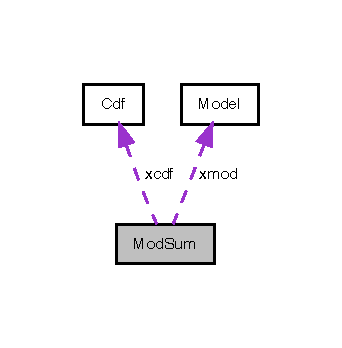
\includegraphics[width=164pt]{struct_mod_sum__coll__graph}
\end{center}
\end{figure}
\subsection*{Data Fields}
\begin{DoxyCompactItemize}
\item 
char \hyperlink{struct_mod_sum_a360933be5b04ace92a3d9d723a889fda}{name} \mbox{[}\hyperlink{wind__updates2d_8c_a764eaf37b6117ac7a17b1c049c1d2d16}{L\+I\+N\+E\+L\+EN}\mbox{]}
\item 
int \hyperlink{struct_mod_sum_acdae6177bed0c926e9e494fca75dd1be}{npars}
\item 
int \hyperlink{struct_mod_sum_aa4f5d4bf3e99f8ebacb170f7ac660d39}{nmods}
\item 
int \hyperlink{struct_mod_sum_a41fef05c528b70fa8216c4ac3c8c8238}{modstart}
\item 
int \hyperlink{struct_mod_sum_a5d33cc5bdf1c37261fd3894363fd3559}{modstop}
\item 
double \hyperlink{struct_mod_sum_a37362f221d9d907352d0316899cd166a}{min} \mbox{[}\hyperlink{models_8h_a4a80e098a43386a893ebc656b14e636c}{N\+P\+A\+RS}\mbox{]}
\item 
double \hyperlink{struct_mod_sum_ad2afe982f87b1ca3aa688dde9c015ec2}{max} \mbox{[}\hyperlink{models_8h_a4a80e098a43386a893ebc656b14e636c}{N\+P\+A\+RS}\mbox{]}
\item 
int \hyperlink{struct_mod_sum_a5a51b3b8e646913e986e827121ec0ceb}{nwaves}
\item 
struct \hyperlink{struct_model}{Model} \hyperlink{struct_mod_sum_a64d79a8a3733c76b1f8f1d81213e974e}{xmod}
\item 
struct \hyperlink{struct_cdf}{Cdf} \hyperlink{struct_mod_sum_ac90994fb16680639054d38eda5c411f0}{xcdf}
\end{DoxyCompactItemize}


\subsection{Detailed Description}


Definition at line 46 of file models.\+h.



\subsection{Field Documentation}
\mbox{\Hypertarget{struct_mod_sum_ad2afe982f87b1ca3aa688dde9c015ec2}\label{struct_mod_sum_ad2afe982f87b1ca3aa688dde9c015ec2}} 
\index{Mod\+Sum@{Mod\+Sum}!max@{max}}
\index{max@{max}!Mod\+Sum@{Mod\+Sum}}
\subsubsection{\texorpdfstring{max}{max}}
{\footnotesize\ttfamily double Mod\+Sum\+::max\mbox{[}\hyperlink{models_8h_a4a80e098a43386a893ebc656b14e636c}{N\+P\+A\+RS}\mbox{]}}



Definition at line 52 of file models.\+h.

\mbox{\Hypertarget{struct_mod_sum_a37362f221d9d907352d0316899cd166a}\label{struct_mod_sum_a37362f221d9d907352d0316899cd166a}} 
\index{Mod\+Sum@{Mod\+Sum}!min@{min}}
\index{min@{min}!Mod\+Sum@{Mod\+Sum}}
\subsubsection{\texorpdfstring{min}{min}}
{\footnotesize\ttfamily double Mod\+Sum\+::min\mbox{[}\hyperlink{models_8h_a4a80e098a43386a893ebc656b14e636c}{N\+P\+A\+RS}\mbox{]}}



Definition at line 51 of file models.\+h.

\mbox{\Hypertarget{struct_mod_sum_a41fef05c528b70fa8216c4ac3c8c8238}\label{struct_mod_sum_a41fef05c528b70fa8216c4ac3c8c8238}} 
\index{Mod\+Sum@{Mod\+Sum}!modstart@{modstart}}
\index{modstart@{modstart}!Mod\+Sum@{Mod\+Sum}}
\subsubsection{\texorpdfstring{modstart}{modstart}}
{\footnotesize\ttfamily int Mod\+Sum\+::modstart}



Definition at line 50 of file models.\+h.

\mbox{\Hypertarget{struct_mod_sum_a5d33cc5bdf1c37261fd3894363fd3559}\label{struct_mod_sum_a5d33cc5bdf1c37261fd3894363fd3559}} 
\index{Mod\+Sum@{Mod\+Sum}!modstop@{modstop}}
\index{modstop@{modstop}!Mod\+Sum@{Mod\+Sum}}
\subsubsection{\texorpdfstring{modstop}{modstop}}
{\footnotesize\ttfamily int Mod\+Sum\+::modstop}



Definition at line 50 of file models.\+h.

\mbox{\Hypertarget{struct_mod_sum_a360933be5b04ace92a3d9d723a889fda}\label{struct_mod_sum_a360933be5b04ace92a3d9d723a889fda}} 
\index{Mod\+Sum@{Mod\+Sum}!name@{name}}
\index{name@{name}!Mod\+Sum@{Mod\+Sum}}
\subsubsection{\texorpdfstring{name}{name}}
{\footnotesize\ttfamily char Mod\+Sum\+::name\mbox{[}\hyperlink{wind__updates2d_8c_a764eaf37b6117ac7a17b1c049c1d2d16}{L\+I\+N\+E\+L\+EN}\mbox{]}}



Definition at line 48 of file models.\+h.

\mbox{\Hypertarget{struct_mod_sum_aa4f5d4bf3e99f8ebacb170f7ac660d39}\label{struct_mod_sum_aa4f5d4bf3e99f8ebacb170f7ac660d39}} 
\index{Mod\+Sum@{Mod\+Sum}!nmods@{nmods}}
\index{nmods@{nmods}!Mod\+Sum@{Mod\+Sum}}
\subsubsection{\texorpdfstring{nmods}{nmods}}
{\footnotesize\ttfamily int Mod\+Sum\+::nmods}



Definition at line 50 of file models.\+h.

\mbox{\Hypertarget{struct_mod_sum_acdae6177bed0c926e9e494fca75dd1be}\label{struct_mod_sum_acdae6177bed0c926e9e494fca75dd1be}} 
\index{Mod\+Sum@{Mod\+Sum}!npars@{npars}}
\index{npars@{npars}!Mod\+Sum@{Mod\+Sum}}
\subsubsection{\texorpdfstring{npars}{npars}}
{\footnotesize\ttfamily int Mod\+Sum\+::npars}



Definition at line 49 of file models.\+h.

\mbox{\Hypertarget{struct_mod_sum_a5a51b3b8e646913e986e827121ec0ceb}\label{struct_mod_sum_a5a51b3b8e646913e986e827121ec0ceb}} 
\index{Mod\+Sum@{Mod\+Sum}!nwaves@{nwaves}}
\index{nwaves@{nwaves}!Mod\+Sum@{Mod\+Sum}}
\subsubsection{\texorpdfstring{nwaves}{nwaves}}
{\footnotesize\ttfamily int Mod\+Sum\+::nwaves}



Definition at line 53 of file models.\+h.

\mbox{\Hypertarget{struct_mod_sum_ac90994fb16680639054d38eda5c411f0}\label{struct_mod_sum_ac90994fb16680639054d38eda5c411f0}} 
\index{Mod\+Sum@{Mod\+Sum}!xcdf@{xcdf}}
\index{xcdf@{xcdf}!Mod\+Sum@{Mod\+Sum}}
\subsubsection{\texorpdfstring{xcdf}{xcdf}}
{\footnotesize\ttfamily struct \hyperlink{struct_cdf}{Cdf} Mod\+Sum\+::xcdf}



Definition at line 55 of file models.\+h.

\mbox{\Hypertarget{struct_mod_sum_a64d79a8a3733c76b1f8f1d81213e974e}\label{struct_mod_sum_a64d79a8a3733c76b1f8f1d81213e974e}} 
\index{Mod\+Sum@{Mod\+Sum}!xmod@{xmod}}
\index{xmod@{xmod}!Mod\+Sum@{Mod\+Sum}}
\subsubsection{\texorpdfstring{xmod}{xmod}}
{\footnotesize\ttfamily struct \hyperlink{struct_model}{Model} Mod\+Sum\+::xmod}



Definition at line 54 of file models.\+h.



The documentation for this struct was generated from the following file\+:\begin{DoxyCompactItemize}
\item 
/\+Users/mhewitt/python/source/\hyperlink{models_8h}{models.\+h}\end{DoxyCompactItemize}

\hypertarget{structphoton}{}\section{photon Struct Reference}
\label{structphoton}\index{photon@{photon}}


{\ttfamily \#include $<$python.\+h$>$}

\subsection*{Public Types}
\begin{DoxyCompactItemize}
\item 
enum \hyperlink{structphoton_ae56bb7ca587dc91f44d8c72a6a571f45}{istat\+\_\+enum} \{ \newline
\hyperlink{structphoton_ae56bb7ca587dc91f44d8c72a6a571f45ad4bbb33a18f68d8fa99598e3a44291f3}{P\+\_\+\+I\+N\+W\+I\+ND} = 0, 
\hyperlink{structphoton_ae56bb7ca587dc91f44d8c72a6a571f45a7049b3f8546fe852a17c790e4be43d56}{P\+\_\+\+S\+C\+AT} = 1, 
\hyperlink{structphoton_ae56bb7ca587dc91f44d8c72a6a571f45aa37b54e0d964345f5fd2d98c848392a8}{P\+\_\+\+E\+S\+C\+A\+PE} = 2, 
\hyperlink{structphoton_ae56bb7ca587dc91f44d8c72a6a571f45a90e4bec9cba520e77e42500720711ced}{P\+\_\+\+H\+I\+T\+\_\+\+S\+T\+AR} = 3, 
\newline
\hyperlink{structphoton_ae56bb7ca587dc91f44d8c72a6a571f45ae7e9ea08f4cac79726f53b851183bcec}{P\+\_\+\+T\+O\+O\+\_\+\+M\+A\+N\+Y\+\_\+\+S\+C\+A\+T\+T\+E\+RS} = 4, 
\hyperlink{structphoton_ae56bb7ca587dc91f44d8c72a6a571f45a69b2139cb91cad8e6cf691c625107f12}{P\+\_\+\+E\+R\+R\+OR} = 5, 
\hyperlink{structphoton_ae56bb7ca587dc91f44d8c72a6a571f45a5d14e67c864da8c98dbd5f8762ca4661}{P\+\_\+\+A\+B\+S\+O\+RB} = 6, 
\hyperlink{structphoton_ae56bb7ca587dc91f44d8c72a6a571f45a78ed840f7a8abfe5d0386e8791661b34}{P\+\_\+\+H\+I\+T\+\_\+\+D\+I\+SK} = 7, 
\newline
\hyperlink{structphoton_ae56bb7ca587dc91f44d8c72a6a571f45af734acb396a428a91be434cc3b53d1ea}{P\+\_\+\+S\+EC} = 8, 
\hyperlink{structphoton_ae56bb7ca587dc91f44d8c72a6a571f45a05b54609857135f4ec62f8c4d91fa8aa}{P\+\_\+\+A\+D\+I\+A\+B\+A\+T\+IC} = 9
 \}
\item 
enum \hyperlink{structphoton_a6e3512103ffd5c0d6004cd432cdc4c3a}{origin\+\_\+enum} \{ \newline
\hyperlink{structphoton_a6e3512103ffd5c0d6004cd432cdc4c3aaec49d91fbf56d1c37fc817e32eb5a684}{P\+T\+Y\+P\+E\+\_\+\+S\+T\+AR} = 0, 
\hyperlink{structphoton_a6e3512103ffd5c0d6004cd432cdc4c3aa400842dd57553879d686ef17157f9c27}{P\+T\+Y\+P\+E\+\_\+\+BL} = 1, 
\hyperlink{structphoton_a6e3512103ffd5c0d6004cd432cdc4c3aa7250e5b6c1e689f3e9e34b67368b5f10}{P\+T\+Y\+P\+E\+\_\+\+D\+I\+SK} = 2, 
\hyperlink{structphoton_a6e3512103ffd5c0d6004cd432cdc4c3aa71d2b892c08b3e60c0b2264fde984204}{P\+T\+Y\+P\+E\+\_\+\+W\+I\+ND} = 3, 
\newline
\hyperlink{structphoton_a6e3512103ffd5c0d6004cd432cdc4c3aa0499be80307da40a7b69f55e697d406b}{P\+T\+Y\+P\+E\+\_\+\+A\+GN} = 4, 
\hyperlink{structphoton_a6e3512103ffd5c0d6004cd432cdc4c3aa54cdb79f93bf98c218b864906017e8df}{P\+T\+Y\+P\+E\+\_\+\+S\+T\+A\+R\+\_\+\+M\+A\+T\+OM} = 10, 
\hyperlink{structphoton_a6e3512103ffd5c0d6004cd432cdc4c3aa9502bfc60b489089ec7ade2dd1034d20}{P\+T\+Y\+P\+E\+\_\+\+B\+L\+\_\+\+M\+A\+T\+OM} = 11, 
\hyperlink{structphoton_a6e3512103ffd5c0d6004cd432cdc4c3aa3e77d18b4b6e1c2f3b7aff87eccad008}{P\+T\+Y\+P\+E\+\_\+\+D\+I\+S\+K\+\_\+\+M\+A\+T\+OM} = 12, 
\newline
\hyperlink{structphoton_a6e3512103ffd5c0d6004cd432cdc4c3aa5745c7f0985bc91f63ffe52dc3591601}{P\+T\+Y\+P\+E\+\_\+\+W\+I\+N\+D\+\_\+\+M\+A\+T\+OM} = 13, 
\hyperlink{structphoton_a6e3512103ffd5c0d6004cd432cdc4c3aa32c58ab316da341e21e71e10593a4b17}{P\+T\+Y\+P\+E\+\_\+\+A\+G\+N\+\_\+\+M\+A\+T\+OM} = 14
 \}
\end{DoxyCompactItemize}
\subsection*{Data Fields}
\begin{DoxyCompactItemize}
\item 
double \hyperlink{structphoton_a279232990e041c1535ce72fdd34c359d}{x} \mbox{[}3\mbox{]}
\item 
double \hyperlink{structphoton_a1166dfb4c725aac37dafe72bcf1aec2b}{lmn} \mbox{[}3\mbox{]}
\item 
double \hyperlink{structphoton_a98c6d400814a43aeda7d7fd1ed2d7dc6}{freq}
\item 
double \hyperlink{structphoton_a9ee01f91734c2f53894f62d76c2eafa8}{freq\+\_\+orig}
\item 
double \hyperlink{structphoton_a5fa87a07a9ceef33dd79aa5cdd7856cb}{w}
\item 
double \hyperlink{structphoton_a08790ef51ec6cc5d192173396080c9d9}{w\+\_\+orig}
\item 
double \hyperlink{structphoton_ae42fbabbb99b92586f81ee793288ff35}{tau}
\item 
enum \hyperlink{structphoton_ae56bb7ca587dc91f44d8c72a6a571f45}{photon\+::istat\+\_\+enum} \hyperlink{structphoton_adf0be64e948d68d787555681d15e13e2}{istat}
\item 
int \hyperlink{structphoton_af295c65faf17c8e83c2547a95509e665}{nscat}
\item 
int \hyperlink{structphoton_ad91ab6667b2f4635925deb64ea7841bd}{nres}
\item 
int \hyperlink{structphoton_a31ff1fe2cb5835980637f0cf4ab61ffc}{nnscat}
\item 
int \hyperlink{structphoton_a96a247f2621b88fe5313dbfdeca7d37f}{nrscat}
\item 
int \hyperlink{structphoton_a2aa9d1ea7afffe4f370b28b0a21d6c79}{grid}
\item 
enum \hyperlink{structphoton_a6e3512103ffd5c0d6004cd432cdc4c3a}{photon\+::origin\+\_\+enum} \hyperlink{structphoton_a201206174a8fa79b29526a68e20704cf}{origin}
\item 
enum \hyperlink{structphoton_a6e3512103ffd5c0d6004cd432cdc4c3a}{photon\+::origin\+\_\+enum} \hyperlink{structphoton_a1b0fcf48345bbe1f6bc480294b054850}{origin\+\_\+orig}
\item 
int \hyperlink{structphoton_ac6a38267c9cc04060e249c1cbaad3d9a}{np}
\item 
double \hyperlink{structphoton_a3029350c63c7c27314adca143458c4ed}{path}
\end{DoxyCompactItemize}


\subsection{Detailed Description}


Definition at line 1034 of file python.\+h.



\subsection{Member Enumeration Documentation}
\mbox{\Hypertarget{structphoton_ae56bb7ca587dc91f44d8c72a6a571f45}\label{structphoton_ae56bb7ca587dc91f44d8c72a6a571f45}} 
\index{photon@{photon}!istat\+\_\+enum@{istat\+\_\+enum}}
\index{istat\+\_\+enum@{istat\+\_\+enum}!photon@{photon}}
\subsubsection{\texorpdfstring{istat\+\_\+enum}{istat\_enum}}
{\footnotesize\ttfamily enum \hyperlink{structphoton_ae56bb7ca587dc91f44d8c72a6a571f45}{photon\+::istat\+\_\+enum}}

\begin{DoxyEnumFields}{Enumerator}
\raisebox{\heightof{T}}[0pt][0pt]{\index{P\+\_\+\+I\+N\+W\+I\+ND@{P\+\_\+\+I\+N\+W\+I\+ND}!photon@{photon}}\index{photon@{photon}!P\+\_\+\+I\+N\+W\+I\+ND@{P\+\_\+\+I\+N\+W\+I\+ND}}}\mbox{\Hypertarget{structphoton_ae56bb7ca587dc91f44d8c72a6a571f45ad4bbb33a18f68d8fa99598e3a44291f3}\label{structphoton_ae56bb7ca587dc91f44d8c72a6a571f45ad4bbb33a18f68d8fa99598e3a44291f3}} 
P\+\_\+\+I\+N\+W\+I\+ND&\\
\hline

\raisebox{\heightof{T}}[0pt][0pt]{\index{P\+\_\+\+S\+C\+AT@{P\+\_\+\+S\+C\+AT}!photon@{photon}}\index{photon@{photon}!P\+\_\+\+S\+C\+AT@{P\+\_\+\+S\+C\+AT}}}\mbox{\Hypertarget{structphoton_ae56bb7ca587dc91f44d8c72a6a571f45a7049b3f8546fe852a17c790e4be43d56}\label{structphoton_ae56bb7ca587dc91f44d8c72a6a571f45a7049b3f8546fe852a17c790e4be43d56}} 
P\+\_\+\+S\+C\+AT&\\
\hline

\raisebox{\heightof{T}}[0pt][0pt]{\index{P\+\_\+\+E\+S\+C\+A\+PE@{P\+\_\+\+E\+S\+C\+A\+PE}!photon@{photon}}\index{photon@{photon}!P\+\_\+\+E\+S\+C\+A\+PE@{P\+\_\+\+E\+S\+C\+A\+PE}}}\mbox{\Hypertarget{structphoton_ae56bb7ca587dc91f44d8c72a6a571f45aa37b54e0d964345f5fd2d98c848392a8}\label{structphoton_ae56bb7ca587dc91f44d8c72a6a571f45aa37b54e0d964345f5fd2d98c848392a8}} 
P\+\_\+\+E\+S\+C\+A\+PE&\\
\hline

\raisebox{\heightof{T}}[0pt][0pt]{\index{P\+\_\+\+H\+I\+T\+\_\+\+S\+T\+AR@{P\+\_\+\+H\+I\+T\+\_\+\+S\+T\+AR}!photon@{photon}}\index{photon@{photon}!P\+\_\+\+H\+I\+T\+\_\+\+S\+T\+AR@{P\+\_\+\+H\+I\+T\+\_\+\+S\+T\+AR}}}\mbox{\Hypertarget{structphoton_ae56bb7ca587dc91f44d8c72a6a571f45a90e4bec9cba520e77e42500720711ced}\label{structphoton_ae56bb7ca587dc91f44d8c72a6a571f45a90e4bec9cba520e77e42500720711ced}} 
P\+\_\+\+H\+I\+T\+\_\+\+S\+T\+AR&\\
\hline

\raisebox{\heightof{T}}[0pt][0pt]{\index{P\+\_\+\+T\+O\+O\+\_\+\+M\+A\+N\+Y\+\_\+\+S\+C\+A\+T\+T\+E\+RS@{P\+\_\+\+T\+O\+O\+\_\+\+M\+A\+N\+Y\+\_\+\+S\+C\+A\+T\+T\+E\+RS}!photon@{photon}}\index{photon@{photon}!P\+\_\+\+T\+O\+O\+\_\+\+M\+A\+N\+Y\+\_\+\+S\+C\+A\+T\+T\+E\+RS@{P\+\_\+\+T\+O\+O\+\_\+\+M\+A\+N\+Y\+\_\+\+S\+C\+A\+T\+T\+E\+RS}}}\mbox{\Hypertarget{structphoton_ae56bb7ca587dc91f44d8c72a6a571f45ae7e9ea08f4cac79726f53b851183bcec}\label{structphoton_ae56bb7ca587dc91f44d8c72a6a571f45ae7e9ea08f4cac79726f53b851183bcec}} 
P\+\_\+\+T\+O\+O\+\_\+\+M\+A\+N\+Y\+\_\+\+S\+C\+A\+T\+T\+E\+RS&\\
\hline

\raisebox{\heightof{T}}[0pt][0pt]{\index{P\+\_\+\+E\+R\+R\+OR@{P\+\_\+\+E\+R\+R\+OR}!photon@{photon}}\index{photon@{photon}!P\+\_\+\+E\+R\+R\+OR@{P\+\_\+\+E\+R\+R\+OR}}}\mbox{\Hypertarget{structphoton_ae56bb7ca587dc91f44d8c72a6a571f45a69b2139cb91cad8e6cf691c625107f12}\label{structphoton_ae56bb7ca587dc91f44d8c72a6a571f45a69b2139cb91cad8e6cf691c625107f12}} 
P\+\_\+\+E\+R\+R\+OR&\\
\hline

\raisebox{\heightof{T}}[0pt][0pt]{\index{P\+\_\+\+A\+B\+S\+O\+RB@{P\+\_\+\+A\+B\+S\+O\+RB}!photon@{photon}}\index{photon@{photon}!P\+\_\+\+A\+B\+S\+O\+RB@{P\+\_\+\+A\+B\+S\+O\+RB}}}\mbox{\Hypertarget{structphoton_ae56bb7ca587dc91f44d8c72a6a571f45a5d14e67c864da8c98dbd5f8762ca4661}\label{structphoton_ae56bb7ca587dc91f44d8c72a6a571f45a5d14e67c864da8c98dbd5f8762ca4661}} 
P\+\_\+\+A\+B\+S\+O\+RB&\\
\hline

\raisebox{\heightof{T}}[0pt][0pt]{\index{P\+\_\+\+H\+I\+T\+\_\+\+D\+I\+SK@{P\+\_\+\+H\+I\+T\+\_\+\+D\+I\+SK}!photon@{photon}}\index{photon@{photon}!P\+\_\+\+H\+I\+T\+\_\+\+D\+I\+SK@{P\+\_\+\+H\+I\+T\+\_\+\+D\+I\+SK}}}\mbox{\Hypertarget{structphoton_ae56bb7ca587dc91f44d8c72a6a571f45a78ed840f7a8abfe5d0386e8791661b34}\label{structphoton_ae56bb7ca587dc91f44d8c72a6a571f45a78ed840f7a8abfe5d0386e8791661b34}} 
P\+\_\+\+H\+I\+T\+\_\+\+D\+I\+SK&\\
\hline

\raisebox{\heightof{T}}[0pt][0pt]{\index{P\+\_\+\+S\+EC@{P\+\_\+\+S\+EC}!photon@{photon}}\index{photon@{photon}!P\+\_\+\+S\+EC@{P\+\_\+\+S\+EC}}}\mbox{\Hypertarget{structphoton_ae56bb7ca587dc91f44d8c72a6a571f45af734acb396a428a91be434cc3b53d1ea}\label{structphoton_ae56bb7ca587dc91f44d8c72a6a571f45af734acb396a428a91be434cc3b53d1ea}} 
P\+\_\+\+S\+EC&\\
\hline

\raisebox{\heightof{T}}[0pt][0pt]{\index{P\+\_\+\+A\+D\+I\+A\+B\+A\+T\+IC@{P\+\_\+\+A\+D\+I\+A\+B\+A\+T\+IC}!photon@{photon}}\index{photon@{photon}!P\+\_\+\+A\+D\+I\+A\+B\+A\+T\+IC@{P\+\_\+\+A\+D\+I\+A\+B\+A\+T\+IC}}}\mbox{\Hypertarget{structphoton_ae56bb7ca587dc91f44d8c72a6a571f45a05b54609857135f4ec62f8c4d91fa8aa}\label{structphoton_ae56bb7ca587dc91f44d8c72a6a571f45a05b54609857135f4ec62f8c4d91fa8aa}} 
P\+\_\+\+A\+D\+I\+A\+B\+A\+T\+IC&\\
\hline

\end{DoxyEnumFields}


Definition at line 1041 of file python.\+h.

\mbox{\Hypertarget{structphoton_a6e3512103ffd5c0d6004cd432cdc4c3a}\label{structphoton_a6e3512103ffd5c0d6004cd432cdc4c3a}} 
\index{photon@{photon}!origin\+\_\+enum@{origin\+\_\+enum}}
\index{origin\+\_\+enum@{origin\+\_\+enum}!photon@{photon}}
\subsubsection{\texorpdfstring{origin\+\_\+enum}{origin\_enum}}
{\footnotesize\ttfamily enum \hyperlink{structphoton_a6e3512103ffd5c0d6004cd432cdc4c3a}{photon\+::origin\+\_\+enum}}

\begin{DoxyEnumFields}{Enumerator}
\raisebox{\heightof{T}}[0pt][0pt]{\index{P\+T\+Y\+P\+E\+\_\+\+S\+T\+AR@{P\+T\+Y\+P\+E\+\_\+\+S\+T\+AR}!photon@{photon}}\index{photon@{photon}!P\+T\+Y\+P\+E\+\_\+\+S\+T\+AR@{P\+T\+Y\+P\+E\+\_\+\+S\+T\+AR}}}\mbox{\Hypertarget{structphoton_a6e3512103ffd5c0d6004cd432cdc4c3aaec49d91fbf56d1c37fc817e32eb5a684}\label{structphoton_a6e3512103ffd5c0d6004cd432cdc4c3aaec49d91fbf56d1c37fc817e32eb5a684}} 
P\+T\+Y\+P\+E\+\_\+\+S\+T\+AR&\\
\hline

\raisebox{\heightof{T}}[0pt][0pt]{\index{P\+T\+Y\+P\+E\+\_\+\+BL@{P\+T\+Y\+P\+E\+\_\+\+BL}!photon@{photon}}\index{photon@{photon}!P\+T\+Y\+P\+E\+\_\+\+BL@{P\+T\+Y\+P\+E\+\_\+\+BL}}}\mbox{\Hypertarget{structphoton_a6e3512103ffd5c0d6004cd432cdc4c3aa400842dd57553879d686ef17157f9c27}\label{structphoton_a6e3512103ffd5c0d6004cd432cdc4c3aa400842dd57553879d686ef17157f9c27}} 
P\+T\+Y\+P\+E\+\_\+\+BL&\\
\hline

\raisebox{\heightof{T}}[0pt][0pt]{\index{P\+T\+Y\+P\+E\+\_\+\+D\+I\+SK@{P\+T\+Y\+P\+E\+\_\+\+D\+I\+SK}!photon@{photon}}\index{photon@{photon}!P\+T\+Y\+P\+E\+\_\+\+D\+I\+SK@{P\+T\+Y\+P\+E\+\_\+\+D\+I\+SK}}}\mbox{\Hypertarget{structphoton_a6e3512103ffd5c0d6004cd432cdc4c3aa7250e5b6c1e689f3e9e34b67368b5f10}\label{structphoton_a6e3512103ffd5c0d6004cd432cdc4c3aa7250e5b6c1e689f3e9e34b67368b5f10}} 
P\+T\+Y\+P\+E\+\_\+\+D\+I\+SK&\\
\hline

\raisebox{\heightof{T}}[0pt][0pt]{\index{P\+T\+Y\+P\+E\+\_\+\+W\+I\+ND@{P\+T\+Y\+P\+E\+\_\+\+W\+I\+ND}!photon@{photon}}\index{photon@{photon}!P\+T\+Y\+P\+E\+\_\+\+W\+I\+ND@{P\+T\+Y\+P\+E\+\_\+\+W\+I\+ND}}}\mbox{\Hypertarget{structphoton_a6e3512103ffd5c0d6004cd432cdc4c3aa71d2b892c08b3e60c0b2264fde984204}\label{structphoton_a6e3512103ffd5c0d6004cd432cdc4c3aa71d2b892c08b3e60c0b2264fde984204}} 
P\+T\+Y\+P\+E\+\_\+\+W\+I\+ND&\\
\hline

\raisebox{\heightof{T}}[0pt][0pt]{\index{P\+T\+Y\+P\+E\+\_\+\+A\+GN@{P\+T\+Y\+P\+E\+\_\+\+A\+GN}!photon@{photon}}\index{photon@{photon}!P\+T\+Y\+P\+E\+\_\+\+A\+GN@{P\+T\+Y\+P\+E\+\_\+\+A\+GN}}}\mbox{\Hypertarget{structphoton_a6e3512103ffd5c0d6004cd432cdc4c3aa0499be80307da40a7b69f55e697d406b}\label{structphoton_a6e3512103ffd5c0d6004cd432cdc4c3aa0499be80307da40a7b69f55e697d406b}} 
P\+T\+Y\+P\+E\+\_\+\+A\+GN&\\
\hline

\raisebox{\heightof{T}}[0pt][0pt]{\index{P\+T\+Y\+P\+E\+\_\+\+S\+T\+A\+R\+\_\+\+M\+A\+T\+OM@{P\+T\+Y\+P\+E\+\_\+\+S\+T\+A\+R\+\_\+\+M\+A\+T\+OM}!photon@{photon}}\index{photon@{photon}!P\+T\+Y\+P\+E\+\_\+\+S\+T\+A\+R\+\_\+\+M\+A\+T\+OM@{P\+T\+Y\+P\+E\+\_\+\+S\+T\+A\+R\+\_\+\+M\+A\+T\+OM}}}\mbox{\Hypertarget{structphoton_a6e3512103ffd5c0d6004cd432cdc4c3aa54cdb79f93bf98c218b864906017e8df}\label{structphoton_a6e3512103ffd5c0d6004cd432cdc4c3aa54cdb79f93bf98c218b864906017e8df}} 
P\+T\+Y\+P\+E\+\_\+\+S\+T\+A\+R\+\_\+\+M\+A\+T\+OM&\\
\hline

\raisebox{\heightof{T}}[0pt][0pt]{\index{P\+T\+Y\+P\+E\+\_\+\+B\+L\+\_\+\+M\+A\+T\+OM@{P\+T\+Y\+P\+E\+\_\+\+B\+L\+\_\+\+M\+A\+T\+OM}!photon@{photon}}\index{photon@{photon}!P\+T\+Y\+P\+E\+\_\+\+B\+L\+\_\+\+M\+A\+T\+OM@{P\+T\+Y\+P\+E\+\_\+\+B\+L\+\_\+\+M\+A\+T\+OM}}}\mbox{\Hypertarget{structphoton_a6e3512103ffd5c0d6004cd432cdc4c3aa9502bfc60b489089ec7ade2dd1034d20}\label{structphoton_a6e3512103ffd5c0d6004cd432cdc4c3aa9502bfc60b489089ec7ade2dd1034d20}} 
P\+T\+Y\+P\+E\+\_\+\+B\+L\+\_\+\+M\+A\+T\+OM&\\
\hline

\raisebox{\heightof{T}}[0pt][0pt]{\index{P\+T\+Y\+P\+E\+\_\+\+D\+I\+S\+K\+\_\+\+M\+A\+T\+OM@{P\+T\+Y\+P\+E\+\_\+\+D\+I\+S\+K\+\_\+\+M\+A\+T\+OM}!photon@{photon}}\index{photon@{photon}!P\+T\+Y\+P\+E\+\_\+\+D\+I\+S\+K\+\_\+\+M\+A\+T\+OM@{P\+T\+Y\+P\+E\+\_\+\+D\+I\+S\+K\+\_\+\+M\+A\+T\+OM}}}\mbox{\Hypertarget{structphoton_a6e3512103ffd5c0d6004cd432cdc4c3aa3e77d18b4b6e1c2f3b7aff87eccad008}\label{structphoton_a6e3512103ffd5c0d6004cd432cdc4c3aa3e77d18b4b6e1c2f3b7aff87eccad008}} 
P\+T\+Y\+P\+E\+\_\+\+D\+I\+S\+K\+\_\+\+M\+A\+T\+OM&\\
\hline

\raisebox{\heightof{T}}[0pt][0pt]{\index{P\+T\+Y\+P\+E\+\_\+\+W\+I\+N\+D\+\_\+\+M\+A\+T\+OM@{P\+T\+Y\+P\+E\+\_\+\+W\+I\+N\+D\+\_\+\+M\+A\+T\+OM}!photon@{photon}}\index{photon@{photon}!P\+T\+Y\+P\+E\+\_\+\+W\+I\+N\+D\+\_\+\+M\+A\+T\+OM@{P\+T\+Y\+P\+E\+\_\+\+W\+I\+N\+D\+\_\+\+M\+A\+T\+OM}}}\mbox{\Hypertarget{structphoton_a6e3512103ffd5c0d6004cd432cdc4c3aa5745c7f0985bc91f63ffe52dc3591601}\label{structphoton_a6e3512103ffd5c0d6004cd432cdc4c3aa5745c7f0985bc91f63ffe52dc3591601}} 
P\+T\+Y\+P\+E\+\_\+\+W\+I\+N\+D\+\_\+\+M\+A\+T\+OM&\\
\hline

\raisebox{\heightof{T}}[0pt][0pt]{\index{P\+T\+Y\+P\+E\+\_\+\+A\+G\+N\+\_\+\+M\+A\+T\+OM@{P\+T\+Y\+P\+E\+\_\+\+A\+G\+N\+\_\+\+M\+A\+T\+OM}!photon@{photon}}\index{photon@{photon}!P\+T\+Y\+P\+E\+\_\+\+A\+G\+N\+\_\+\+M\+A\+T\+OM@{P\+T\+Y\+P\+E\+\_\+\+A\+G\+N\+\_\+\+M\+A\+T\+OM}}}\mbox{\Hypertarget{structphoton_a6e3512103ffd5c0d6004cd432cdc4c3aa32c58ab316da341e21e71e10593a4b17}\label{structphoton_a6e3512103ffd5c0d6004cd432cdc4c3aa32c58ab316da341e21e71e10593a4b17}} 
P\+T\+Y\+P\+E\+\_\+\+A\+G\+N\+\_\+\+M\+A\+T\+OM&\\
\hline

\end{DoxyEnumFields}


Definition at line 1067 of file python.\+h.



\subsection{Field Documentation}
\mbox{\Hypertarget{structphoton_a98c6d400814a43aeda7d7fd1ed2d7dc6}\label{structphoton_a98c6d400814a43aeda7d7fd1ed2d7dc6}} 
\index{photon@{photon}!freq@{freq}}
\index{freq@{freq}!photon@{photon}}
\subsubsection{\texorpdfstring{freq}{freq}}
{\footnotesize\ttfamily double photon\+::freq}



Definition at line 1038 of file python.\+h.

\mbox{\Hypertarget{structphoton_a9ee01f91734c2f53894f62d76c2eafa8}\label{structphoton_a9ee01f91734c2f53894f62d76c2eafa8}} 
\index{photon@{photon}!freq\+\_\+orig@{freq\+\_\+orig}}
\index{freq\+\_\+orig@{freq\+\_\+orig}!photon@{photon}}
\subsubsection{\texorpdfstring{freq\+\_\+orig}{freq\_orig}}
{\footnotesize\ttfamily double photon\+::freq\+\_\+orig}



Definition at line 1038 of file python.\+h.

\mbox{\Hypertarget{structphoton_a2aa9d1ea7afffe4f370b28b0a21d6c79}\label{structphoton_a2aa9d1ea7afffe4f370b28b0a21d6c79}} 
\index{photon@{photon}!grid@{grid}}
\index{grid@{grid}!photon@{photon}}
\subsubsection{\texorpdfstring{grid}{grid}}
{\footnotesize\ttfamily int photon\+::grid}



Definition at line 1062 of file python.\+h.

\mbox{\Hypertarget{structphoton_adf0be64e948d68d787555681d15e13e2}\label{structphoton_adf0be64e948d68d787555681d15e13e2}} 
\index{photon@{photon}!istat@{istat}}
\index{istat@{istat}!photon@{photon}}
\subsubsection{\texorpdfstring{istat}{istat}}
{\footnotesize\ttfamily enum \hyperlink{structphoton_ae56bb7ca587dc91f44d8c72a6a571f45}{photon\+::istat\+\_\+enum}  photon\+::istat}

\mbox{\Hypertarget{structphoton_a1166dfb4c725aac37dafe72bcf1aec2b}\label{structphoton_a1166dfb4c725aac37dafe72bcf1aec2b}} 
\index{photon@{photon}!lmn@{lmn}}
\index{lmn@{lmn}!photon@{photon}}
\subsubsection{\texorpdfstring{lmn}{lmn}}
{\footnotesize\ttfamily double photon\+::lmn\mbox{[}3\mbox{]}}



Definition at line 1037 of file python.\+h.

\mbox{\Hypertarget{structphoton_a31ff1fe2cb5835980637f0cf4ab61ffc}\label{structphoton_a31ff1fe2cb5835980637f0cf4ab61ffc}} 
\index{photon@{photon}!nnscat@{nnscat}}
\index{nnscat@{nnscat}!photon@{photon}}
\subsubsection{\texorpdfstring{nnscat}{nnscat}}
{\footnotesize\ttfamily int photon\+::nnscat}



Definition at line 1057 of file python.\+h.

\mbox{\Hypertarget{structphoton_ac6a38267c9cc04060e249c1cbaad3d9a}\label{structphoton_ac6a38267c9cc04060e249c1cbaad3d9a}} 
\index{photon@{photon}!np@{np}}
\index{np@{np}!photon@{photon}}
\subsubsection{\texorpdfstring{np}{np}}
{\footnotesize\ttfamily int photon\+::np}



Definition at line 1082 of file python.\+h.

\mbox{\Hypertarget{structphoton_ad91ab6667b2f4635925deb64ea7841bd}\label{structphoton_ad91ab6667b2f4635925deb64ea7841bd}} 
\index{photon@{photon}!nres@{nres}}
\index{nres@{nres}!photon@{photon}}
\subsubsection{\texorpdfstring{nres}{nres}}
{\footnotesize\ttfamily int photon\+::nres}



Definition at line 1056 of file python.\+h.

\mbox{\Hypertarget{structphoton_a96a247f2621b88fe5313dbfdeca7d37f}\label{structphoton_a96a247f2621b88fe5313dbfdeca7d37f}} 
\index{photon@{photon}!nrscat@{nrscat}}
\index{nrscat@{nrscat}!photon@{photon}}
\subsubsection{\texorpdfstring{nrscat}{nrscat}}
{\footnotesize\ttfamily int photon\+::nrscat}



Definition at line 1061 of file python.\+h.

\mbox{\Hypertarget{structphoton_af295c65faf17c8e83c2547a95509e665}\label{structphoton_af295c65faf17c8e83c2547a95509e665}} 
\index{photon@{photon}!nscat@{nscat}}
\index{nscat@{nscat}!photon@{photon}}
\subsubsection{\texorpdfstring{nscat}{nscat}}
{\footnotesize\ttfamily int photon\+::nscat}



Definition at line 1055 of file python.\+h.

\mbox{\Hypertarget{structphoton_a201206174a8fa79b29526a68e20704cf}\label{structphoton_a201206174a8fa79b29526a68e20704cf}} 
\index{photon@{photon}!origin@{origin}}
\index{origin@{origin}!photon@{photon}}
\subsubsection{\texorpdfstring{origin}{origin}}
{\footnotesize\ttfamily enum \hyperlink{structphoton_a6e3512103ffd5c0d6004cd432cdc4c3a}{photon\+::origin\+\_\+enum}  photon\+::origin}

\mbox{\Hypertarget{structphoton_a1b0fcf48345bbe1f6bc480294b054850}\label{structphoton_a1b0fcf48345bbe1f6bc480294b054850}} 
\index{photon@{photon}!origin\+\_\+orig@{origin\+\_\+orig}}
\index{origin\+\_\+orig@{origin\+\_\+orig}!photon@{photon}}
\subsubsection{\texorpdfstring{origin\+\_\+orig}{origin\_orig}}
{\footnotesize\ttfamily enum \hyperlink{structphoton_a6e3512103ffd5c0d6004cd432cdc4c3a}{photon\+::origin\+\_\+enum}  photon\+::origin\+\_\+orig}

\mbox{\Hypertarget{structphoton_a3029350c63c7c27314adca143458c4ed}\label{structphoton_a3029350c63c7c27314adca143458c4ed}} 
\index{photon@{photon}!path@{path}}
\index{path@{path}!photon@{photon}}
\subsubsection{\texorpdfstring{path}{path}}
{\footnotesize\ttfamily double photon\+::path}



Definition at line 1084 of file python.\+h.

\mbox{\Hypertarget{structphoton_ae42fbabbb99b92586f81ee793288ff35}\label{structphoton_ae42fbabbb99b92586f81ee793288ff35}} 
\index{photon@{photon}!tau@{tau}}
\index{tau@{tau}!photon@{photon}}
\subsubsection{\texorpdfstring{tau}{tau}}
{\footnotesize\ttfamily double photon\+::tau}



Definition at line 1040 of file python.\+h.

\mbox{\Hypertarget{structphoton_a5fa87a07a9ceef33dd79aa5cdd7856cb}\label{structphoton_a5fa87a07a9ceef33dd79aa5cdd7856cb}} 
\index{photon@{photon}!w@{w}}
\index{w@{w}!photon@{photon}}
\subsubsection{\texorpdfstring{w}{w}}
{\footnotesize\ttfamily double photon\+::w}



Definition at line 1039 of file python.\+h.

\mbox{\Hypertarget{structphoton_a08790ef51ec6cc5d192173396080c9d9}\label{structphoton_a08790ef51ec6cc5d192173396080c9d9}} 
\index{photon@{photon}!w\+\_\+orig@{w\+\_\+orig}}
\index{w\+\_\+orig@{w\+\_\+orig}!photon@{photon}}
\subsubsection{\texorpdfstring{w\+\_\+orig}{w\_orig}}
{\footnotesize\ttfamily double photon\+::w\+\_\+orig}



Definition at line 1039 of file python.\+h.

\mbox{\Hypertarget{structphoton_a279232990e041c1535ce72fdd34c359d}\label{structphoton_a279232990e041c1535ce72fdd34c359d}} 
\index{photon@{photon}!x@{x}}
\index{x@{x}!photon@{photon}}
\subsubsection{\texorpdfstring{x}{x}}
{\footnotesize\ttfamily double photon\+::x\mbox{[}3\mbox{]}}



Definition at line 1036 of file python.\+h.



The documentation for this struct was generated from the following file\+:\begin{DoxyCompactItemize}
\item 
/\+Users/mhewitt/python/source/\hyperlink{python_8h}{python.\+h}\end{DoxyCompactItemize}

\hypertarget{structphoton__store}{}\section{photon\+\_\+store Struct Reference}
\label{structphoton__store}\index{photon\+\_\+store@{photon\+\_\+store}}


{\ttfamily \#include $<$python.\+h$>$}

\subsection*{Data Fields}
\begin{DoxyCompactItemize}
\item 
int \hyperlink{structphoton__store_a2c21d7cedb5d14f39c75773d8c27cfb9}{n}
\item 
double \hyperlink{structphoton__store_a1f66c34e20651382abba394331cee838}{t}
\item 
double \hyperlink{structphoton__store_a848640b4e4ac5d652a0d7c2b888ad629}{f1}
\item 
double \hyperlink{structphoton__store_a64630dd43adca15e1b6a11eaf32130d7}{f2}
\item 
double \hyperlink{structphoton__store_a0ca5ae358e1d455b4ff924a1a4be00fc}{freq} \mbox{[}\hyperlink{python_8h_a0ce783ce6592faa3e2f8900e2a72846a}{N\+S\+T\+O\+RE}\mbox{]}
\end{DoxyCompactItemize}


\subsection{Detailed Description}


Definition at line 912 of file python.\+h.



\subsection{Field Documentation}
\mbox{\Hypertarget{structphoton__store_a848640b4e4ac5d652a0d7c2b888ad629}\label{structphoton__store_a848640b4e4ac5d652a0d7c2b888ad629}} 
\index{photon\+\_\+store@{photon\+\_\+store}!f1@{f1}}
\index{f1@{f1}!photon\+\_\+store@{photon\+\_\+store}}
\subsubsection{\texorpdfstring{f1}{f1}}
{\footnotesize\ttfamily double photon\+\_\+store\+::f1}



Definition at line 915 of file python.\+h.

\mbox{\Hypertarget{structphoton__store_a64630dd43adca15e1b6a11eaf32130d7}\label{structphoton__store_a64630dd43adca15e1b6a11eaf32130d7}} 
\index{photon\+\_\+store@{photon\+\_\+store}!f2@{f2}}
\index{f2@{f2}!photon\+\_\+store@{photon\+\_\+store}}
\subsubsection{\texorpdfstring{f2}{f2}}
{\footnotesize\ttfamily double photon\+\_\+store\+::f2}



Definition at line 915 of file python.\+h.

\mbox{\Hypertarget{structphoton__store_a0ca5ae358e1d455b4ff924a1a4be00fc}\label{structphoton__store_a0ca5ae358e1d455b4ff924a1a4be00fc}} 
\index{photon\+\_\+store@{photon\+\_\+store}!freq@{freq}}
\index{freq@{freq}!photon\+\_\+store@{photon\+\_\+store}}
\subsubsection{\texorpdfstring{freq}{freq}}
{\footnotesize\ttfamily double photon\+\_\+store\+::freq\mbox{[}\hyperlink{python_8h_a0ce783ce6592faa3e2f8900e2a72846a}{N\+S\+T\+O\+RE}\mbox{]}}



Definition at line 915 of file python.\+h.

\mbox{\Hypertarget{structphoton__store_a2c21d7cedb5d14f39c75773d8c27cfb9}\label{structphoton__store_a2c21d7cedb5d14f39c75773d8c27cfb9}} 
\index{photon\+\_\+store@{photon\+\_\+store}!n@{n}}
\index{n@{n}!photon\+\_\+store@{photon\+\_\+store}}
\subsubsection{\texorpdfstring{n}{n}}
{\footnotesize\ttfamily int photon\+\_\+store\+::n}



Definition at line 914 of file python.\+h.

\mbox{\Hypertarget{structphoton__store_a1f66c34e20651382abba394331cee838}\label{structphoton__store_a1f66c34e20651382abba394331cee838}} 
\index{photon\+\_\+store@{photon\+\_\+store}!t@{t}}
\index{t@{t}!photon\+\_\+store@{photon\+\_\+store}}
\subsubsection{\texorpdfstring{t}{t}}
{\footnotesize\ttfamily double photon\+\_\+store\+::t}



Definition at line 915 of file python.\+h.



The documentation for this struct was generated from the following file\+:\begin{DoxyCompactItemize}
\item 
/\+Users/mhewitt/python/source/\hyperlink{python_8h}{python.\+h}\end{DoxyCompactItemize}

\hypertarget{structplane}{}\section{plane Struct Reference}
\label{structplane}\index{plane@{plane}}


{\ttfamily \#include $<$python.\+h$>$}

\subsection*{Data Fields}
\begin{DoxyCompactItemize}
\item 
double \hyperlink{structplane_a3e0a915298ae7b9f7dbde607ebf5e5fa}{x} \mbox{[}3\mbox{]}
\item 
double \hyperlink{structplane_aecafa59e4a24ae66f9dd66e6ce87be4b}{lmn} \mbox{[}3\mbox{]}
\end{DoxyCompactItemize}


\subsection{Detailed Description}


Definition at line 168 of file python.\+h.



\subsection{Field Documentation}
\mbox{\Hypertarget{structplane_aecafa59e4a24ae66f9dd66e6ce87be4b}\label{structplane_aecafa59e4a24ae66f9dd66e6ce87be4b}} 
\index{plane@{plane}!lmn@{lmn}}
\index{lmn@{lmn}!plane@{plane}}
\subsubsection{\texorpdfstring{lmn}{lmn}}
{\footnotesize\ttfamily double plane\+::lmn\mbox{[}3\mbox{]}}



Definition at line 171 of file python.\+h.

\mbox{\Hypertarget{structplane_a3e0a915298ae7b9f7dbde607ebf5e5fa}\label{structplane_a3e0a915298ae7b9f7dbde607ebf5e5fa}} 
\index{plane@{plane}!x@{x}}
\index{x@{x}!plane@{plane}}
\subsubsection{\texorpdfstring{x}{x}}
{\footnotesize\ttfamily double plane\+::x\mbox{[}3\mbox{]}}



Definition at line 170 of file python.\+h.



The documentation for this struct was generated from the following file\+:\begin{DoxyCompactItemize}
\item 
/\+Users/mhewitt/python/source/\hyperlink{python_8h}{python.\+h}\end{DoxyCompactItemize}

\hypertarget{structplasma}{}\section{plasma Struct Reference}
\label{structplasma}\index{plasma@{plasma}}


{\ttfamily \#include $<$python.\+h$>$}

\subsection*{Public Types}
\begin{DoxyCompactItemize}
\item 
enum \hyperlink{structplasma_a51fdb6f34dda1cdb03a9aebfee249706}{spec\+\_\+mod\+\_\+type\+\_\+enum} \{ \hyperlink{structplasma_a51fdb6f34dda1cdb03a9aebfee249706a7fcd3827aae177b27b0c2c4e8a4f642f}{S\+P\+E\+C\+\_\+\+M\+O\+D\+\_\+\+PL} = 1, 
\hyperlink{structplasma_a51fdb6f34dda1cdb03a9aebfee249706ac64efa71b6e422eb9a8f65c1648f30d2}{S\+P\+E\+C\+\_\+\+M\+O\+D\+\_\+\+E\+XP} = 2, 
\hyperlink{structplasma_a51fdb6f34dda1cdb03a9aebfee249706a81d4d46ab996ec4e90354768d40983f0}{S\+P\+E\+C\+\_\+\+M\+O\+D\+\_\+\+F\+A\+IL} = -\/1
 \}
\end{DoxyCompactItemize}
\subsection*{Data Fields}
\begin{DoxyCompactItemize}
\item 
int \hyperlink{structplasma_a56c7e960c18e2fc47a147877bc9e5fe8}{nwind}
\item 
int \hyperlink{structplasma_a8220b5d466addc895b973f092d9b7b15}{nplasma}
\item 
double \hyperlink{structplasma_ac1d38c3e4cc4ef2a1e4d83d7f8b71d22}{ne}
\item 
double \hyperlink{structplasma_aeffd93110218aa8876f074488b026390}{rho}
\item 
double \hyperlink{structplasma_a469869b2b7b2a822716ac5a3ba58412a}{vol}
\item 
double $\ast$ \hyperlink{structplasma_a711ac1ddc0f32849edd96d937ff70761}{density}
\item 
double $\ast$ \hyperlink{structplasma_a76771b8118b11b955ccf91b6208b42f4}{partition}
\item 
double $\ast$ \hyperlink{structplasma_a4fb98583700310c3abbf6fa266c755c0}{levden}
\item 
double $\ast$ \hyperlink{structplasma_a2b0e1368d0adfd432627a2ceedebb704}{P\+Wdenom}
\item 
double $\ast$ \hyperlink{structplasma_a2651f0307bf16fc9febad1be3c7bbfd0}{P\+Wdtemp}
\item 
double $\ast$ \hyperlink{structplasma_a4d5152400f3815e3097ef30ff27aec5c}{P\+Wnumer}
\item 
double $\ast$ \hyperlink{structplasma_a712f96fb8bc5b68b5b51024043614e53}{P\+Wntemp}
\item 
double \hyperlink{structplasma_ad9ee8e24644a60e13bcf910a223c129b}{kappa\+\_\+ff\+\_\+factor}
\item 
double $\ast$ \hyperlink{structplasma_ae4b9e1c0afc70066b36d896e8122513b}{recomb\+\_\+simple}
\item 
double \hyperlink{structplasma_a3a7cb2d0cfcfe01e21e43f7e4fe4e9a8}{kpkt\+\_\+emiss}
\item 
double \hyperlink{structplasma_aa9ee2846f568c0a0de1f7848ff747301}{kpkt\+\_\+abs}
\item 
int $\ast$ \hyperlink{structplasma_a031771037948baffc308ebe398140f4e}{kbf\+\_\+use}
\item 
int \hyperlink{structplasma_a5771e457f1bb0258f23f9aa3b97febeb}{kbf\+\_\+nuse}
\item 
double \hyperlink{structplasma_a432a1f85db9000aac743588736fb6048}{t\+\_\+r}
\item 
double \hyperlink{structplasma_af2b47aa340055b4dfc21f592a98f9792}{t\+\_\+r\+\_\+old}
\item 
double \hyperlink{structplasma_a9b217285a754e1533f95d92972b6afd6}{t\+\_\+e}
\item 
double \hyperlink{structplasma_aefa8d272f5a54cae990359cccd67075d}{t\+\_\+e\+\_\+old}
\item 
double \hyperlink{structplasma_a174c204665ec6522d9c1dad57408b577}{dt\+\_\+e}
\item 
double \hyperlink{structplasma_a438272ea5c79f26453f113fe023e9c99}{dt\+\_\+e\+\_\+old}
\item 
double \hyperlink{structplasma_a2ed3e67409c1f55ca66cb0cbfbc39ac2}{heat\+\_\+tot}
\item 
double \hyperlink{structplasma_a1cb334619d10653be16138483cf13a8a}{heat\+\_\+tot\+\_\+old}
\item 
double \hyperlink{structplasma_a671e4d660694e4fef07580536f729bfb}{abs\+\_\+tot}
\item 
double \hyperlink{structplasma_ab2b017d6fa0e646a4a1d880d49914ef2}{heat\+\_\+lines}
\item 
double \hyperlink{structplasma_aadd0d71f61d6ed95a48af999a14784e0}{heat\+\_\+ff}
\item 
double \hyperlink{structplasma_ac6e1f1f8827b1bc1a68a437e1e58b001}{heat\+\_\+comp}
\item 
double \hyperlink{structplasma_af28aff5f32398a703d1423c56a4599c2}{heat\+\_\+ind\+\_\+comp}
\item 
double \hyperlink{structplasma_a819b893417ac6c5e2e572dec2f361ac5}{heat\+\_\+lines\+\_\+macro}
\item 
double \hyperlink{structplasma_ad926ff3d325d177b1d767e2a929b6899}{heat\+\_\+photo\+\_\+macro}
\item 
double \hyperlink{structplasma_a2878212449ef25989225a975f81679fd}{heat\+\_\+photo}
\item 
double \hyperlink{structplasma_a5748c6ee35ca4d9458a8bf20d1930b55}{heat\+\_\+z}
\item 
double \hyperlink{structplasma_a878263d85482a81865eb7619b3b2a20e}{heat\+\_\+auger}
\item 
double \hyperlink{structplasma_ab5ee24fc4d7c3533aafdde5591bdc0c4}{abs\+\_\+photo}
\item 
double \hyperlink{structplasma_aa3d84ccfae03d00a3c23d4096e35d942}{abs\+\_\+auger}
\item 
double \hyperlink{structplasma_adbf9689b61e3df7611084d858b3115c0}{w}
\item 
int \hyperlink{structplasma_aa22c8b26e65db4f93a14fa183d7e09e6}{ntot}
\item 
int \hyperlink{structplasma_a2e85980821d61738e7b5b6455604066b}{ntot\+\_\+star}
\item 
int \hyperlink{structplasma_aec5dcc811c48f5b8f8d195accbdb7813}{ntot\+\_\+bl}
\item 
int \hyperlink{structplasma_a0c76211532161bfdd92ccde2b4aacffd}{ntot\+\_\+disk}
\item 
int \hyperlink{structplasma_a94bce860bda9cee5964584ca552b256a}{ntot\+\_\+wind}
\item 
int \hyperlink{structplasma_aacb5d70931f73523be11b5bb9bb051a6}{ntot\+\_\+agn}
\item 
int \hyperlink{structplasma_ad9c354375042457b537f41282f6d7538}{nscat\+\_\+es}
\item 
int \hyperlink{structplasma_aa13320251f70b79c8794a90cf70fe003}{nscat\+\_\+res}
\item 
double \hyperlink{structplasma_a50251baa932d22c94584c04ce0398a36}{mean\+\_\+ds}
\item 
int \hyperlink{structplasma_a579b07a98a0b0692e5e6e2465c2ab425}{n\+\_\+ds}
\item 
int \hyperlink{structplasma_ab2eba1f8343e4767fd32dc914fb95397}{nrad}
\item 
int \hyperlink{structplasma_ada72c65c218f315e543710ce8808e225}{nioniz}
\item 
double $\ast$ \hyperlink{structplasma_ad5797671f1fe6d9e2a638df668ea51df}{ioniz}
\item 
double $\ast$ \hyperlink{structplasma_abfec36000559630caf4ec85917950a1e}{recomb}
\item 
double $\ast$ \hyperlink{structplasma_ae60f001b2bf22f33edb3e818e55f6807}{inner\+\_\+recomb}
\item 
int $\ast$ \hyperlink{structplasma_ada2361ccbc0c5103f58d097af8b5dfe7}{scatters}
\item 
double $\ast$ \hyperlink{structplasma_aba12a0eea107e923bad5f26cb012e72a}{xscatters}
\item 
double $\ast$ \hyperlink{structplasma_a1cff49185ad30a6734089a2d2c949fbc}{heat\+\_\+ion}
\item 
double $\ast$ \hyperlink{structplasma_a0d74b5ee435184a0bf1f2dbdecc16a2d}{cool\+\_\+rr\+\_\+ion}
\item 
double $\ast$ \hyperlink{structplasma_a82db22eb07618b0844344790fc875166}{lum\+\_\+rr\+\_\+ion}
\item 
double $\ast$ \hyperlink{structplasma_ad69c6b875d8b97df4e10569a06085107}{cool\+\_\+dr\+\_\+ion}
\item 
double \hyperlink{structplasma_a81aa2849c8ad883b8b23ca7a5e7b7c2f}{j}
\item 
double \hyperlink{structplasma_a9ef4bb2909c072cb6155880d3114c95f}{ave\+\_\+freq}
\item 
double \hyperlink{structplasma_abded068048bfaf274478a65b26388ed5}{xj} \mbox{[}\hyperlink{python_8h_ac640b7fc429348ef2f6781704d3c5163}{N\+X\+B\+A\+N\+DS}\mbox{]}
\item 
double \hyperlink{structplasma_ae72cc720bc175444504be8f75d02e4c4}{xave\+\_\+freq} \mbox{[}\hyperlink{python_8h_ac640b7fc429348ef2f6781704d3c5163}{N\+X\+B\+A\+N\+DS}\mbox{]}
\item 
double \hyperlink{structplasma_ac4d25da8ffad12c810a2be5baf12c9a0}{fmin} \mbox{[}\hyperlink{python_8h_ac640b7fc429348ef2f6781704d3c5163}{N\+X\+B\+A\+N\+DS}\mbox{]}
\item 
double \hyperlink{structplasma_a21e7b17fa73a2521fe95247ac0d52d36}{fmax} \mbox{[}\hyperlink{python_8h_ac640b7fc429348ef2f6781704d3c5163}{N\+X\+B\+A\+N\+DS}\mbox{]}
\item 
double \hyperlink{structplasma_a79f84fac2bd8b8ee286bf33092531f18}{fmin\+\_\+mod} \mbox{[}\hyperlink{python_8h_ac640b7fc429348ef2f6781704d3c5163}{N\+X\+B\+A\+N\+DS}\mbox{]}
\item 
double \hyperlink{structplasma_ab5b2a9cf34eb1359961d6783a81ea266}{fmax\+\_\+mod} \mbox{[}\hyperlink{python_8h_ac640b7fc429348ef2f6781704d3c5163}{N\+X\+B\+A\+N\+DS}\mbox{]}
\item 
double \hyperlink{structplasma_a3a6771031add8ed4970ea0a051ae3751}{j\+\_\+direct}
\item 
double \hyperlink{structplasma_ab48f9178fc1c8be99c96d9a33d19f2a9}{j\+\_\+scatt}
\item 
double \hyperlink{structplasma_acf74d2b82ce1f94cd72b38b432f68774}{ip\+\_\+direct}
\item 
double \hyperlink{structplasma_ac2985029f1cc2e4bd9a511c7c4ff5db9}{ip\+\_\+scatt}
\item 
double \hyperlink{structplasma_af6eca6f64a123edc0389b42ace886569}{xsd\+\_\+freq} \mbox{[}\hyperlink{python_8h_ac640b7fc429348ef2f6781704d3c5163}{N\+X\+B\+A\+N\+DS}\mbox{]}
\item 
int \hyperlink{structplasma_a8f5a30977d126bd3ec95bb175056e9c2}{nxtot} \mbox{[}\hyperlink{python_8h_ac640b7fc429348ef2f6781704d3c5163}{N\+X\+B\+A\+N\+DS}\mbox{]}
\item 
double \hyperlink{structplasma_ac6f1afeb2ed92f59b12ca628a4e75eff}{max\+\_\+freq}
\item 
double \hyperlink{structplasma_a5f4abbbb9eab15f11e28ab7f26421482}{cool\+\_\+tot}
\item 
double \hyperlink{structplasma_a2c31ecbd91d20cf9f4112db1d6150764}{lum\+\_\+lines}
\item 
double \hyperlink{structplasma_ae9f6828f63719a3dc2f172573293c4a1}{lum\+\_\+ff}
\item 
double \hyperlink{structplasma_acf37090e0b83fe81d058f21229a90018}{cool\+\_\+adiabatic}
\item 
double \hyperlink{structplasma_a7c1a796efafeae5c9aacfbea4e6a79c3}{lum\+\_\+rr}
\item 
double \hyperlink{structplasma_abdee1a55696e7928736435858f69d51f}{lum\+\_\+rr\+\_\+metals}
\item 
double \hyperlink{structplasma_a0af59963361b8b69b3f29c31a303b7c6}{cool\+\_\+comp}
\item 
double \hyperlink{structplasma_a5505637faee8b3d92778c1948e8b0e35}{cool\+\_\+di}
\item 
double \hyperlink{structplasma_a2e449de44ae3c3c3b7fec875b2e55e72}{cool\+\_\+dr}
\item 
double \hyperlink{structplasma_a7bafaea3d058631613ebd1c8a8b8eacc}{cool\+\_\+rr}
\item 
double \hyperlink{structplasma_a59f1e6f2bf27227a52d45f5c5bff07f6}{cool\+\_\+rr\+\_\+metals}
\item 
double \hyperlink{structplasma_a9e5f8826f902ac5154fc3c4c67f404e1}{lum\+\_\+tot}
\item 
double \hyperlink{structplasma_ae0685b14cba52ec98d560c7981e765bf}{lum\+\_\+tot\+\_\+old}
\item 
double \hyperlink{structplasma_ae0379496a0c22546580980cccfabf0c2}{cool\+\_\+tot\+\_\+ioniz}
\item 
double \hyperlink{structplasma_ae8458741703e0a2a71f1b425600b1694}{lum\+\_\+lines\+\_\+ioniz}
\item 
double \hyperlink{structplasma_ab206d43d8bc66c44371da287b69fd5da}{lum\+\_\+ff\+\_\+ioniz}
\item 
double \hyperlink{structplasma_a7030de50e435921b13630ea339eb13e9}{cool\+\_\+adiabatic\+\_\+ioniz}
\item 
double \hyperlink{structplasma_acc048dd6ede76041e2a872cdca2ebb8f}{lum\+\_\+rr\+\_\+ioniz}
\item 
double \hyperlink{structplasma_a90c93c3a8fb77ca113fa5837491fe967}{cool\+\_\+comp\+\_\+ioniz}
\item 
double \hyperlink{structplasma_ae7cfeaf05f9b888e57e0dd66b1d393bc}{cool\+\_\+di\+\_\+ioniz}
\item 
double \hyperlink{structplasma_a5a044a5991244d771cf0937a322bff4f}{cool\+\_\+dr\+\_\+ioniz}
\item 
double \hyperlink{structplasma_a247ec26b8304ce5ef0f0489a9a4b6332}{cool\+\_\+rr\+\_\+ioniz}
\item 
double \hyperlink{structplasma_a1ded6465a492ddef36a6ef7a555359ec}{cool\+\_\+rr\+\_\+metals\+\_\+ioniz}
\item 
double \hyperlink{structplasma_af27d3aeeb9b6c87198ebe89c7990ff48}{lum\+\_\+tot\+\_\+ioniz}
\item 
double \hyperlink{structplasma_a57a290ba7730852666e194dcd1d594e6}{comp\+\_\+nujnu}
\item 
double \hyperlink{structplasma_a3447796c585931795cefa93400544b15}{dmo\+\_\+dt} \mbox{[}3\mbox{]}
\item 
double \hyperlink{structplasma_abd08d926f7b31dc9ddfaf5bc0c02de8f}{gain}
\item 
double \hyperlink{structplasma_a41bc8bd1fad69fdfe93c152eefdd4933}{converge\+\_\+t\+\_\+r}
\item 
double \hyperlink{structplasma_a7dc5aebabe90a8a5fa17ed2585de401c}{converge\+\_\+t\+\_\+e}
\item 
double \hyperlink{structplasma_ac74499cb432f536f838a1f4e4eccf5bc}{converge\+\_\+hc}
\item 
int \hyperlink{structplasma_a0a97b073aaa0261c8cd76c5ddb0e680a}{trcheck}
\item 
int \hyperlink{structplasma_ae1ff443abf16813160cb9756d33f81d9}{techeck}
\item 
int \hyperlink{structplasma_a4211e8aceb5ea7e09f9a359b99faa859}{hccheck}
\item 
int \hyperlink{structplasma_a59f5cb4220fd78cea7972db755f58291}{converge\+\_\+whole}
\item 
int \hyperlink{structplasma_a89b513b0ebeb3ecad39803fc04e2dc6c}{converging}
\item 
enum \hyperlink{structplasma_a51fdb6f34dda1cdb03a9aebfee249706}{plasma\+::spec\+\_\+mod\+\_\+type\+\_\+enum} \hyperlink{structplasma_a110b6efdc5fa932c21dc021047b35eea}{spec\+\_\+mod\+\_\+type} \mbox{[}\hyperlink{python_8h_ac640b7fc429348ef2f6781704d3c5163}{N\+X\+B\+A\+N\+DS}\mbox{]}
\item 
double \hyperlink{structplasma_a0dbad3f32ea372492eb73eda0f123899}{pl\+\_\+alpha} \mbox{[}\hyperlink{python_8h_ac640b7fc429348ef2f6781704d3c5163}{N\+X\+B\+A\+N\+DS}\mbox{]}
\item 
double \hyperlink{structplasma_aae85efc36fb767cfec53df4cd3327fe8}{pl\+\_\+log\+\_\+w} \mbox{[}\hyperlink{python_8h_ac640b7fc429348ef2f6781704d3c5163}{N\+X\+B\+A\+N\+DS}\mbox{]}
\item 
double \hyperlink{structplasma_a30222105e41ccde304250f41d25b5ad7}{exp\+\_\+temp} \mbox{[}\hyperlink{python_8h_ac640b7fc429348ef2f6781704d3c5163}{N\+X\+B\+A\+N\+DS}\mbox{]}
\item 
double \hyperlink{structplasma_a9b46e8bed0dfadca5cf9966301ecec6d}{exp\+\_\+w} \mbox{[}\hyperlink{python_8h_ac640b7fc429348ef2f6781704d3c5163}{N\+X\+B\+A\+N\+DS}\mbox{]}
\item 
double \hyperlink{structplasma_a1ac56fc73e1242bfa9cbb9bfa04e6d38}{ip}
\item 
double \hyperlink{structplasma_af8986403a916d5a9f4330ae70aa5e798}{xi}
\end{DoxyCompactItemize}


\subsection{Detailed Description}


Definition at line 737 of file python.\+h.



\subsection{Member Enumeration Documentation}
\mbox{\Hypertarget{structplasma_a51fdb6f34dda1cdb03a9aebfee249706}\label{structplasma_a51fdb6f34dda1cdb03a9aebfee249706}} 
\index{plasma@{plasma}!spec\+\_\+mod\+\_\+type\+\_\+enum@{spec\+\_\+mod\+\_\+type\+\_\+enum}}
\index{spec\+\_\+mod\+\_\+type\+\_\+enum@{spec\+\_\+mod\+\_\+type\+\_\+enum}!plasma@{plasma}}
\subsubsection{\texorpdfstring{spec\+\_\+mod\+\_\+type\+\_\+enum}{spec\_mod\_type\_enum}}
{\footnotesize\ttfamily enum \hyperlink{structplasma_a51fdb6f34dda1cdb03a9aebfee249706}{plasma\+::spec\+\_\+mod\+\_\+type\+\_\+enum}}

\begin{DoxyEnumFields}{Enumerator}
\raisebox{\heightof{T}}[0pt][0pt]{\index{S\+P\+E\+C\+\_\+\+M\+O\+D\+\_\+\+PL@{S\+P\+E\+C\+\_\+\+M\+O\+D\+\_\+\+PL}!plasma@{plasma}}\index{plasma@{plasma}!S\+P\+E\+C\+\_\+\+M\+O\+D\+\_\+\+PL@{S\+P\+E\+C\+\_\+\+M\+O\+D\+\_\+\+PL}}}\mbox{\Hypertarget{structplasma_a51fdb6f34dda1cdb03a9aebfee249706a7fcd3827aae177b27b0c2c4e8a4f642f}\label{structplasma_a51fdb6f34dda1cdb03a9aebfee249706a7fcd3827aae177b27b0c2c4e8a4f642f}} 
S\+P\+E\+C\+\_\+\+M\+O\+D\+\_\+\+PL&\\
\hline

\raisebox{\heightof{T}}[0pt][0pt]{\index{S\+P\+E\+C\+\_\+\+M\+O\+D\+\_\+\+E\+XP@{S\+P\+E\+C\+\_\+\+M\+O\+D\+\_\+\+E\+XP}!plasma@{plasma}}\index{plasma@{plasma}!S\+P\+E\+C\+\_\+\+M\+O\+D\+\_\+\+E\+XP@{S\+P\+E\+C\+\_\+\+M\+O\+D\+\_\+\+E\+XP}}}\mbox{\Hypertarget{structplasma_a51fdb6f34dda1cdb03a9aebfee249706ac64efa71b6e422eb9a8f65c1648f30d2}\label{structplasma_a51fdb6f34dda1cdb03a9aebfee249706ac64efa71b6e422eb9a8f65c1648f30d2}} 
S\+P\+E\+C\+\_\+\+M\+O\+D\+\_\+\+E\+XP&\\
\hline

\raisebox{\heightof{T}}[0pt][0pt]{\index{S\+P\+E\+C\+\_\+\+M\+O\+D\+\_\+\+F\+A\+IL@{S\+P\+E\+C\+\_\+\+M\+O\+D\+\_\+\+F\+A\+IL}!plasma@{plasma}}\index{plasma@{plasma}!S\+P\+E\+C\+\_\+\+M\+O\+D\+\_\+\+F\+A\+IL@{S\+P\+E\+C\+\_\+\+M\+O\+D\+\_\+\+F\+A\+IL}}}\mbox{\Hypertarget{structplasma_a51fdb6f34dda1cdb03a9aebfee249706a81d4d46ab996ec4e90354768d40983f0}\label{structplasma_a51fdb6f34dda1cdb03a9aebfee249706a81d4d46ab996ec4e90354768d40983f0}} 
S\+P\+E\+C\+\_\+\+M\+O\+D\+\_\+\+F\+A\+IL&\\
\hline

\end{DoxyEnumFields}


Definition at line 885 of file python.\+h.



\subsection{Field Documentation}
\mbox{\Hypertarget{structplasma_aa3d84ccfae03d00a3c23d4096e35d942}\label{structplasma_aa3d84ccfae03d00a3c23d4096e35d942}} 
\index{plasma@{plasma}!abs\+\_\+auger@{abs\+\_\+auger}}
\index{abs\+\_\+auger@{abs\+\_\+auger}!plasma@{plasma}}
\subsubsection{\texorpdfstring{abs\+\_\+auger}{abs\_auger}}
{\footnotesize\ttfamily double plasma\+::abs\+\_\+auger}



Definition at line 790 of file python.\+h.

\mbox{\Hypertarget{structplasma_ab5ee24fc4d7c3533aafdde5591bdc0c4}\label{structplasma_ab5ee24fc4d7c3533aafdde5591bdc0c4}} 
\index{plasma@{plasma}!abs\+\_\+photo@{abs\+\_\+photo}}
\index{abs\+\_\+photo@{abs\+\_\+photo}!plasma@{plasma}}
\subsubsection{\texorpdfstring{abs\+\_\+photo}{abs\_photo}}
{\footnotesize\ttfamily double plasma\+::abs\+\_\+photo}



Definition at line 790 of file python.\+h.

\mbox{\Hypertarget{structplasma_a671e4d660694e4fef07580536f729bfb}\label{structplasma_a671e4d660694e4fef07580536f729bfb}} 
\index{plasma@{plasma}!abs\+\_\+tot@{abs\+\_\+tot}}
\index{abs\+\_\+tot@{abs\+\_\+tot}!plasma@{plasma}}
\subsubsection{\texorpdfstring{abs\+\_\+tot}{abs\_tot}}
{\footnotesize\ttfamily double plasma\+::abs\+\_\+tot}



Definition at line 782 of file python.\+h.

\mbox{\Hypertarget{structplasma_a9ef4bb2909c072cb6155880d3114c95f}\label{structplasma_a9ef4bb2909c072cb6155880d3114c95f}} 
\index{plasma@{plasma}!ave\+\_\+freq@{ave\+\_\+freq}}
\index{ave\+\_\+freq@{ave\+\_\+freq}!plasma@{plasma}}
\subsubsection{\texorpdfstring{ave\+\_\+freq}{ave\_freq}}
{\footnotesize\ttfamily double plasma\+::ave\+\_\+freq}



Definition at line 825 of file python.\+h.

\mbox{\Hypertarget{structplasma_a57a290ba7730852666e194dcd1d594e6}\label{structplasma_a57a290ba7730852666e194dcd1d594e6}} 
\index{plasma@{plasma}!comp\+\_\+nujnu@{comp\+\_\+nujnu}}
\index{comp\+\_\+nujnu@{comp\+\_\+nujnu}!plasma@{plasma}}
\subsubsection{\texorpdfstring{comp\+\_\+nujnu}{comp\_nujnu}}
{\footnotesize\ttfamily double plasma\+::comp\+\_\+nujnu}



Definition at line 862 of file python.\+h.

\mbox{\Hypertarget{structplasma_ac74499cb432f536f838a1f4e4eccf5bc}\label{structplasma_ac74499cb432f536f838a1f4e4eccf5bc}} 
\index{plasma@{plasma}!converge\+\_\+hc@{converge\+\_\+hc}}
\index{converge\+\_\+hc@{converge\+\_\+hc}!plasma@{plasma}}
\subsubsection{\texorpdfstring{converge\+\_\+hc}{converge\_hc}}
{\footnotesize\ttfamily double plasma\+::converge\+\_\+hc}



Definition at line 869 of file python.\+h.

\mbox{\Hypertarget{structplasma_a7dc5aebabe90a8a5fa17ed2585de401c}\label{structplasma_a7dc5aebabe90a8a5fa17ed2585de401c}} 
\index{plasma@{plasma}!converge\+\_\+t\+\_\+e@{converge\+\_\+t\+\_\+e}}
\index{converge\+\_\+t\+\_\+e@{converge\+\_\+t\+\_\+e}!plasma@{plasma}}
\subsubsection{\texorpdfstring{converge\+\_\+t\+\_\+e}{converge\_t\_e}}
{\footnotesize\ttfamily double plasma\+::converge\+\_\+t\+\_\+e}



Definition at line 869 of file python.\+h.

\mbox{\Hypertarget{structplasma_a41bc8bd1fad69fdfe93c152eefdd4933}\label{structplasma_a41bc8bd1fad69fdfe93c152eefdd4933}} 
\index{plasma@{plasma}!converge\+\_\+t\+\_\+r@{converge\+\_\+t\+\_\+r}}
\index{converge\+\_\+t\+\_\+r@{converge\+\_\+t\+\_\+r}!plasma@{plasma}}
\subsubsection{\texorpdfstring{converge\+\_\+t\+\_\+r}{converge\_t\_r}}
{\footnotesize\ttfamily double plasma\+::converge\+\_\+t\+\_\+r}



Definition at line 869 of file python.\+h.

\mbox{\Hypertarget{structplasma_a59f5cb4220fd78cea7972db755f58291}\label{structplasma_a59f5cb4220fd78cea7972db755f58291}} 
\index{plasma@{plasma}!converge\+\_\+whole@{converge\+\_\+whole}}
\index{converge\+\_\+whole@{converge\+\_\+whole}!plasma@{plasma}}
\subsubsection{\texorpdfstring{converge\+\_\+whole}{converge\_whole}}
{\footnotesize\ttfamily int plasma\+::converge\+\_\+whole}



Definition at line 876 of file python.\+h.

\mbox{\Hypertarget{structplasma_a89b513b0ebeb3ecad39803fc04e2dc6c}\label{structplasma_a89b513b0ebeb3ecad39803fc04e2dc6c}} 
\index{plasma@{plasma}!converging@{converging}}
\index{converging@{converging}!plasma@{plasma}}
\subsubsection{\texorpdfstring{converging}{converging}}
{\footnotesize\ttfamily int plasma\+::converging}



Definition at line 876 of file python.\+h.

\mbox{\Hypertarget{structplasma_acf37090e0b83fe81d058f21229a90018}\label{structplasma_acf37090e0b83fe81d058f21229a90018}} 
\index{plasma@{plasma}!cool\+\_\+adiabatic@{cool\+\_\+adiabatic}}
\index{cool\+\_\+adiabatic@{cool\+\_\+adiabatic}!plasma@{plasma}}
\subsubsection{\texorpdfstring{cool\+\_\+adiabatic}{cool\_adiabatic}}
{\footnotesize\ttfamily double plasma\+::cool\+\_\+adiabatic}



Definition at line 843 of file python.\+h.

\mbox{\Hypertarget{structplasma_a7030de50e435921b13630ea339eb13e9}\label{structplasma_a7030de50e435921b13630ea339eb13e9}} 
\index{plasma@{plasma}!cool\+\_\+adiabatic\+\_\+ioniz@{cool\+\_\+adiabatic\+\_\+ioniz}}
\index{cool\+\_\+adiabatic\+\_\+ioniz@{cool\+\_\+adiabatic\+\_\+ioniz}!plasma@{plasma}}
\subsubsection{\texorpdfstring{cool\+\_\+adiabatic\+\_\+ioniz}{cool\_adiabatic\_ioniz}}
{\footnotesize\ttfamily double plasma\+::cool\+\_\+adiabatic\+\_\+ioniz}



Definition at line 853 of file python.\+h.

\mbox{\Hypertarget{structplasma_a0af59963361b8b69b3f29c31a303b7c6}\label{structplasma_a0af59963361b8b69b3f29c31a303b7c6}} 
\index{plasma@{plasma}!cool\+\_\+comp@{cool\+\_\+comp}}
\index{cool\+\_\+comp@{cool\+\_\+comp}!plasma@{plasma}}
\subsubsection{\texorpdfstring{cool\+\_\+comp}{cool\_comp}}
{\footnotesize\ttfamily double plasma\+::cool\+\_\+comp}



Definition at line 845 of file python.\+h.

\mbox{\Hypertarget{structplasma_a90c93c3a8fb77ca113fa5837491fe967}\label{structplasma_a90c93c3a8fb77ca113fa5837491fe967}} 
\index{plasma@{plasma}!cool\+\_\+comp\+\_\+ioniz@{cool\+\_\+comp\+\_\+ioniz}}
\index{cool\+\_\+comp\+\_\+ioniz@{cool\+\_\+comp\+\_\+ioniz}!plasma@{plasma}}
\subsubsection{\texorpdfstring{cool\+\_\+comp\+\_\+ioniz}{cool\_comp\_ioniz}}
{\footnotesize\ttfamily double plasma\+::cool\+\_\+comp\+\_\+ioniz}



Definition at line 855 of file python.\+h.

\mbox{\Hypertarget{structplasma_a5505637faee8b3d92778c1948e8b0e35}\label{structplasma_a5505637faee8b3d92778c1948e8b0e35}} 
\index{plasma@{plasma}!cool\+\_\+di@{cool\+\_\+di}}
\index{cool\+\_\+di@{cool\+\_\+di}!plasma@{plasma}}
\subsubsection{\texorpdfstring{cool\+\_\+di}{cool\_di}}
{\footnotesize\ttfamily double plasma\+::cool\+\_\+di}



Definition at line 846 of file python.\+h.

\mbox{\Hypertarget{structplasma_ae7cfeaf05f9b888e57e0dd66b1d393bc}\label{structplasma_ae7cfeaf05f9b888e57e0dd66b1d393bc}} 
\index{plasma@{plasma}!cool\+\_\+di\+\_\+ioniz@{cool\+\_\+di\+\_\+ioniz}}
\index{cool\+\_\+di\+\_\+ioniz@{cool\+\_\+di\+\_\+ioniz}!plasma@{plasma}}
\subsubsection{\texorpdfstring{cool\+\_\+di\+\_\+ioniz}{cool\_di\_ioniz}}
{\footnotesize\ttfamily double plasma\+::cool\+\_\+di\+\_\+ioniz}



Definition at line 856 of file python.\+h.

\mbox{\Hypertarget{structplasma_a2e449de44ae3c3c3b7fec875b2e55e72}\label{structplasma_a2e449de44ae3c3c3b7fec875b2e55e72}} 
\index{plasma@{plasma}!cool\+\_\+dr@{cool\+\_\+dr}}
\index{cool\+\_\+dr@{cool\+\_\+dr}!plasma@{plasma}}
\subsubsection{\texorpdfstring{cool\+\_\+dr}{cool\_dr}}
{\footnotesize\ttfamily double plasma\+::cool\+\_\+dr}



Definition at line 847 of file python.\+h.

\mbox{\Hypertarget{structplasma_ad69c6b875d8b97df4e10569a06085107}\label{structplasma_ad69c6b875d8b97df4e10569a06085107}} 
\index{plasma@{plasma}!cool\+\_\+dr\+\_\+ion@{cool\+\_\+dr\+\_\+ion}}
\index{cool\+\_\+dr\+\_\+ion@{cool\+\_\+dr\+\_\+ion}!plasma@{plasma}}
\subsubsection{\texorpdfstring{cool\+\_\+dr\+\_\+ion}{cool\_dr\_ion}}
{\footnotesize\ttfamily double$\ast$ plasma\+::cool\+\_\+dr\+\_\+ion}



Definition at line 824 of file python.\+h.

\mbox{\Hypertarget{structplasma_a5a044a5991244d771cf0937a322bff4f}\label{structplasma_a5a044a5991244d771cf0937a322bff4f}} 
\index{plasma@{plasma}!cool\+\_\+dr\+\_\+ioniz@{cool\+\_\+dr\+\_\+ioniz}}
\index{cool\+\_\+dr\+\_\+ioniz@{cool\+\_\+dr\+\_\+ioniz}!plasma@{plasma}}
\subsubsection{\texorpdfstring{cool\+\_\+dr\+\_\+ioniz}{cool\_dr\_ioniz}}
{\footnotesize\ttfamily double plasma\+::cool\+\_\+dr\+\_\+ioniz}



Definition at line 857 of file python.\+h.

\mbox{\Hypertarget{structplasma_a7bafaea3d058631613ebd1c8a8b8eacc}\label{structplasma_a7bafaea3d058631613ebd1c8a8b8eacc}} 
\index{plasma@{plasma}!cool\+\_\+rr@{cool\+\_\+rr}}
\index{cool\+\_\+rr@{cool\+\_\+rr}!plasma@{plasma}}
\subsubsection{\texorpdfstring{cool\+\_\+rr}{cool\_rr}}
{\footnotesize\ttfamily double plasma\+::cool\+\_\+rr}



Definition at line 848 of file python.\+h.

\mbox{\Hypertarget{structplasma_a0d74b5ee435184a0bf1f2dbdecc16a2d}\label{structplasma_a0d74b5ee435184a0bf1f2dbdecc16a2d}} 
\index{plasma@{plasma}!cool\+\_\+rr\+\_\+ion@{cool\+\_\+rr\+\_\+ion}}
\index{cool\+\_\+rr\+\_\+ion@{cool\+\_\+rr\+\_\+ion}!plasma@{plasma}}
\subsubsection{\texorpdfstring{cool\+\_\+rr\+\_\+ion}{cool\_rr\_ion}}
{\footnotesize\ttfamily double$\ast$ plasma\+::cool\+\_\+rr\+\_\+ion}



Definition at line 819 of file python.\+h.

\mbox{\Hypertarget{structplasma_a247ec26b8304ce5ef0f0489a9a4b6332}\label{structplasma_a247ec26b8304ce5ef0f0489a9a4b6332}} 
\index{plasma@{plasma}!cool\+\_\+rr\+\_\+ioniz@{cool\+\_\+rr\+\_\+ioniz}}
\index{cool\+\_\+rr\+\_\+ioniz@{cool\+\_\+rr\+\_\+ioniz}!plasma@{plasma}}
\subsubsection{\texorpdfstring{cool\+\_\+rr\+\_\+ioniz}{cool\_rr\_ioniz}}
{\footnotesize\ttfamily double plasma\+::cool\+\_\+rr\+\_\+ioniz}



Definition at line 858 of file python.\+h.

\mbox{\Hypertarget{structplasma_a59f1e6f2bf27227a52d45f5c5bff07f6}\label{structplasma_a59f1e6f2bf27227a52d45f5c5bff07f6}} 
\index{plasma@{plasma}!cool\+\_\+rr\+\_\+metals@{cool\+\_\+rr\+\_\+metals}}
\index{cool\+\_\+rr\+\_\+metals@{cool\+\_\+rr\+\_\+metals}!plasma@{plasma}}
\subsubsection{\texorpdfstring{cool\+\_\+rr\+\_\+metals}{cool\_rr\_metals}}
{\footnotesize\ttfamily double plasma\+::cool\+\_\+rr\+\_\+metals}



Definition at line 848 of file python.\+h.

\mbox{\Hypertarget{structplasma_a1ded6465a492ddef36a6ef7a555359ec}\label{structplasma_a1ded6465a492ddef36a6ef7a555359ec}} 
\index{plasma@{plasma}!cool\+\_\+rr\+\_\+metals\+\_\+ioniz@{cool\+\_\+rr\+\_\+metals\+\_\+ioniz}}
\index{cool\+\_\+rr\+\_\+metals\+\_\+ioniz@{cool\+\_\+rr\+\_\+metals\+\_\+ioniz}!plasma@{plasma}}
\subsubsection{\texorpdfstring{cool\+\_\+rr\+\_\+metals\+\_\+ioniz}{cool\_rr\_metals\_ioniz}}
{\footnotesize\ttfamily double plasma\+::cool\+\_\+rr\+\_\+metals\+\_\+ioniz}



Definition at line 858 of file python.\+h.

\mbox{\Hypertarget{structplasma_a5f4abbbb9eab15f11e28ab7f26421482}\label{structplasma_a5f4abbbb9eab15f11e28ab7f26421482}} 
\index{plasma@{plasma}!cool\+\_\+tot@{cool\+\_\+tot}}
\index{cool\+\_\+tot@{cool\+\_\+tot}!plasma@{plasma}}
\subsubsection{\texorpdfstring{cool\+\_\+tot}{cool\_tot}}
{\footnotesize\ttfamily double plasma\+::cool\+\_\+tot}



Definition at line 840 of file python.\+h.

\mbox{\Hypertarget{structplasma_ae0379496a0c22546580980cccfabf0c2}\label{structplasma_ae0379496a0c22546580980cccfabf0c2}} 
\index{plasma@{plasma}!cool\+\_\+tot\+\_\+ioniz@{cool\+\_\+tot\+\_\+ioniz}}
\index{cool\+\_\+tot\+\_\+ioniz@{cool\+\_\+tot\+\_\+ioniz}!plasma@{plasma}}
\subsubsection{\texorpdfstring{cool\+\_\+tot\+\_\+ioniz}{cool\_tot\_ioniz}}
{\footnotesize\ttfamily double plasma\+::cool\+\_\+tot\+\_\+ioniz}



Definition at line 852 of file python.\+h.

\mbox{\Hypertarget{structplasma_a711ac1ddc0f32849edd96d937ff70761}\label{structplasma_a711ac1ddc0f32849edd96d937ff70761}} 
\index{plasma@{plasma}!density@{density}}
\index{density@{density}!plasma@{plasma}}
\subsubsection{\texorpdfstring{density}{density}}
{\footnotesize\ttfamily double$\ast$ plasma\+::density}



Definition at line 745 of file python.\+h.

\mbox{\Hypertarget{structplasma_a3447796c585931795cefa93400544b15}\label{structplasma_a3447796c585931795cefa93400544b15}} 
\index{plasma@{plasma}!dmo\+\_\+dt@{dmo\+\_\+dt}}
\index{dmo\+\_\+dt@{dmo\+\_\+dt}!plasma@{plasma}}
\subsubsection{\texorpdfstring{dmo\+\_\+dt}{dmo\_dt}}
{\footnotesize\ttfamily double plasma\+::dmo\+\_\+dt\mbox{[}3\mbox{]}}



Definition at line 864 of file python.\+h.

\mbox{\Hypertarget{structplasma_a174c204665ec6522d9c1dad57408b577}\label{structplasma_a174c204665ec6522d9c1dad57408b577}} 
\index{plasma@{plasma}!dt\+\_\+e@{dt\+\_\+e}}
\index{dt\+\_\+e@{dt\+\_\+e}!plasma@{plasma}}
\subsubsection{\texorpdfstring{dt\+\_\+e}{dt\_e}}
{\footnotesize\ttfamily double plasma\+::dt\+\_\+e}



Definition at line 780 of file python.\+h.

\mbox{\Hypertarget{structplasma_a438272ea5c79f26453f113fe023e9c99}\label{structplasma_a438272ea5c79f26453f113fe023e9c99}} 
\index{plasma@{plasma}!dt\+\_\+e\+\_\+old@{dt\+\_\+e\+\_\+old}}
\index{dt\+\_\+e\+\_\+old@{dt\+\_\+e\+\_\+old}!plasma@{plasma}}
\subsubsection{\texorpdfstring{dt\+\_\+e\+\_\+old}{dt\_e\_old}}
{\footnotesize\ttfamily double plasma\+::dt\+\_\+e\+\_\+old}



Definition at line 780 of file python.\+h.

\mbox{\Hypertarget{structplasma_a30222105e41ccde304250f41d25b5ad7}\label{structplasma_a30222105e41ccde304250f41d25b5ad7}} 
\index{plasma@{plasma}!exp\+\_\+temp@{exp\+\_\+temp}}
\index{exp\+\_\+temp@{exp\+\_\+temp}!plasma@{plasma}}
\subsubsection{\texorpdfstring{exp\+\_\+temp}{exp\_temp}}
{\footnotesize\ttfamily double plasma\+::exp\+\_\+temp\mbox{[}\hyperlink{python_8h_ac640b7fc429348ef2f6781704d3c5163}{N\+X\+B\+A\+N\+DS}\mbox{]}}



Definition at line 896 of file python.\+h.

\mbox{\Hypertarget{structplasma_a9b46e8bed0dfadca5cf9966301ecec6d}\label{structplasma_a9b46e8bed0dfadca5cf9966301ecec6d}} 
\index{plasma@{plasma}!exp\+\_\+w@{exp\+\_\+w}}
\index{exp\+\_\+w@{exp\+\_\+w}!plasma@{plasma}}
\subsubsection{\texorpdfstring{exp\+\_\+w}{exp\_w}}
{\footnotesize\ttfamily double plasma\+::exp\+\_\+w\mbox{[}\hyperlink{python_8h_ac640b7fc429348ef2f6781704d3c5163}{N\+X\+B\+A\+N\+DS}\mbox{]}}



Definition at line 897 of file python.\+h.

\mbox{\Hypertarget{structplasma_a21e7b17fa73a2521fe95247ac0d52d36}\label{structplasma_a21e7b17fa73a2521fe95247ac0d52d36}} 
\index{plasma@{plasma}!fmax@{fmax}}
\index{fmax@{fmax}!plasma@{plasma}}
\subsubsection{\texorpdfstring{fmax}{fmax}}
{\footnotesize\ttfamily double plasma\+::fmax\mbox{[}\hyperlink{python_8h_ac640b7fc429348ef2f6781704d3c5163}{N\+X\+B\+A\+N\+DS}\mbox{]}}



Definition at line 829 of file python.\+h.

\mbox{\Hypertarget{structplasma_ab5b2a9cf34eb1359961d6783a81ea266}\label{structplasma_ab5b2a9cf34eb1359961d6783a81ea266}} 
\index{plasma@{plasma}!fmax\+\_\+mod@{fmax\+\_\+mod}}
\index{fmax\+\_\+mod@{fmax\+\_\+mod}!plasma@{plasma}}
\subsubsection{\texorpdfstring{fmax\+\_\+mod}{fmax\_mod}}
{\footnotesize\ttfamily double plasma\+::fmax\+\_\+mod\mbox{[}\hyperlink{python_8h_ac640b7fc429348ef2f6781704d3c5163}{N\+X\+B\+A\+N\+DS}\mbox{]}}



Definition at line 831 of file python.\+h.

\mbox{\Hypertarget{structplasma_ac4d25da8ffad12c810a2be5baf12c9a0}\label{structplasma_ac4d25da8ffad12c810a2be5baf12c9a0}} 
\index{plasma@{plasma}!fmin@{fmin}}
\index{fmin@{fmin}!plasma@{plasma}}
\subsubsection{\texorpdfstring{fmin}{fmin}}
{\footnotesize\ttfamily double plasma\+::fmin\mbox{[}\hyperlink{python_8h_ac640b7fc429348ef2f6781704d3c5163}{N\+X\+B\+A\+N\+DS}\mbox{]}}



Definition at line 828 of file python.\+h.

\mbox{\Hypertarget{structplasma_a79f84fac2bd8b8ee286bf33092531f18}\label{structplasma_a79f84fac2bd8b8ee286bf33092531f18}} 
\index{plasma@{plasma}!fmin\+\_\+mod@{fmin\+\_\+mod}}
\index{fmin\+\_\+mod@{fmin\+\_\+mod}!plasma@{plasma}}
\subsubsection{\texorpdfstring{fmin\+\_\+mod}{fmin\_mod}}
{\footnotesize\ttfamily double plasma\+::fmin\+\_\+mod\mbox{[}\hyperlink{python_8h_ac640b7fc429348ef2f6781704d3c5163}{N\+X\+B\+A\+N\+DS}\mbox{]}}



Definition at line 830 of file python.\+h.

\mbox{\Hypertarget{structplasma_abd08d926f7b31dc9ddfaf5bc0c02de8f}\label{structplasma_abd08d926f7b31dc9ddfaf5bc0c02de8f}} 
\index{plasma@{plasma}!gain@{gain}}
\index{gain@{gain}!plasma@{plasma}}
\subsubsection{\texorpdfstring{gain}{gain}}
{\footnotesize\ttfamily double plasma\+::gain}



Definition at line 868 of file python.\+h.

\mbox{\Hypertarget{structplasma_a4211e8aceb5ea7e09f9a359b99faa859}\label{structplasma_a4211e8aceb5ea7e09f9a359b99faa859}} 
\index{plasma@{plasma}!hccheck@{hccheck}}
\index{hccheck@{hccheck}!plasma@{plasma}}
\subsubsection{\texorpdfstring{hccheck}{hccheck}}
{\footnotesize\ttfamily int plasma\+::hccheck}



Definition at line 872 of file python.\+h.

\mbox{\Hypertarget{structplasma_a878263d85482a81865eb7619b3b2a20e}\label{structplasma_a878263d85482a81865eb7619b3b2a20e}} 
\index{plasma@{plasma}!heat\+\_\+auger@{heat\+\_\+auger}}
\index{heat\+\_\+auger@{heat\+\_\+auger}!plasma@{plasma}}
\subsubsection{\texorpdfstring{heat\+\_\+auger}{heat\_auger}}
{\footnotesize\ttfamily double plasma\+::heat\+\_\+auger}



Definition at line 789 of file python.\+h.

\mbox{\Hypertarget{structplasma_ac6e1f1f8827b1bc1a68a437e1e58b001}\label{structplasma_ac6e1f1f8827b1bc1a68a437e1e58b001}} 
\index{plasma@{plasma}!heat\+\_\+comp@{heat\+\_\+comp}}
\index{heat\+\_\+comp@{heat\+\_\+comp}!plasma@{plasma}}
\subsubsection{\texorpdfstring{heat\+\_\+comp}{heat\_comp}}
{\footnotesize\ttfamily double plasma\+::heat\+\_\+comp}



Definition at line 784 of file python.\+h.

\mbox{\Hypertarget{structplasma_aadd0d71f61d6ed95a48af999a14784e0}\label{structplasma_aadd0d71f61d6ed95a48af999a14784e0}} 
\index{plasma@{plasma}!heat\+\_\+ff@{heat\+\_\+ff}}
\index{heat\+\_\+ff@{heat\+\_\+ff}!plasma@{plasma}}
\subsubsection{\texorpdfstring{heat\+\_\+ff}{heat\_ff}}
{\footnotesize\ttfamily double plasma\+::heat\+\_\+ff}



Definition at line 783 of file python.\+h.

\mbox{\Hypertarget{structplasma_af28aff5f32398a703d1423c56a4599c2}\label{structplasma_af28aff5f32398a703d1423c56a4599c2}} 
\index{plasma@{plasma}!heat\+\_\+ind\+\_\+comp@{heat\+\_\+ind\+\_\+comp}}
\index{heat\+\_\+ind\+\_\+comp@{heat\+\_\+ind\+\_\+comp}!plasma@{plasma}}
\subsubsection{\texorpdfstring{heat\+\_\+ind\+\_\+comp}{heat\_ind\_comp}}
{\footnotesize\ttfamily double plasma\+::heat\+\_\+ind\+\_\+comp}



Definition at line 785 of file python.\+h.

\mbox{\Hypertarget{structplasma_a1cff49185ad30a6734089a2d2c949fbc}\label{structplasma_a1cff49185ad30a6734089a2d2c949fbc}} 
\index{plasma@{plasma}!heat\+\_\+ion@{heat\+\_\+ion}}
\index{heat\+\_\+ion@{heat\+\_\+ion}!plasma@{plasma}}
\subsubsection{\texorpdfstring{heat\+\_\+ion}{heat\_ion}}
{\footnotesize\ttfamily double$\ast$ plasma\+::heat\+\_\+ion}



Definition at line 817 of file python.\+h.

\mbox{\Hypertarget{structplasma_ab2b017d6fa0e646a4a1d880d49914ef2}\label{structplasma_ab2b017d6fa0e646a4a1d880d49914ef2}} 
\index{plasma@{plasma}!heat\+\_\+lines@{heat\+\_\+lines}}
\index{heat\+\_\+lines@{heat\+\_\+lines}!plasma@{plasma}}
\subsubsection{\texorpdfstring{heat\+\_\+lines}{heat\_lines}}
{\footnotesize\ttfamily double plasma\+::heat\+\_\+lines}



Definition at line 783 of file python.\+h.

\mbox{\Hypertarget{structplasma_a819b893417ac6c5e2e572dec2f361ac5}\label{structplasma_a819b893417ac6c5e2e572dec2f361ac5}} 
\index{plasma@{plasma}!heat\+\_\+lines\+\_\+macro@{heat\+\_\+lines\+\_\+macro}}
\index{heat\+\_\+lines\+\_\+macro@{heat\+\_\+lines\+\_\+macro}!plasma@{plasma}}
\subsubsection{\texorpdfstring{heat\+\_\+lines\+\_\+macro}{heat\_lines\_macro}}
{\footnotesize\ttfamily double plasma\+::heat\+\_\+lines\+\_\+macro}



Definition at line 786 of file python.\+h.

\mbox{\Hypertarget{structplasma_a2878212449ef25989225a975f81679fd}\label{structplasma_a2878212449ef25989225a975f81679fd}} 
\index{plasma@{plasma}!heat\+\_\+photo@{heat\+\_\+photo}}
\index{heat\+\_\+photo@{heat\+\_\+photo}!plasma@{plasma}}
\subsubsection{\texorpdfstring{heat\+\_\+photo}{heat\_photo}}
{\footnotesize\ttfamily double plasma\+::heat\+\_\+photo}



Definition at line 788 of file python.\+h.

\mbox{\Hypertarget{structplasma_ad926ff3d325d177b1d767e2a929b6899}\label{structplasma_ad926ff3d325d177b1d767e2a929b6899}} 
\index{plasma@{plasma}!heat\+\_\+photo\+\_\+macro@{heat\+\_\+photo\+\_\+macro}}
\index{heat\+\_\+photo\+\_\+macro@{heat\+\_\+photo\+\_\+macro}!plasma@{plasma}}
\subsubsection{\texorpdfstring{heat\+\_\+photo\+\_\+macro}{heat\_photo\_macro}}
{\footnotesize\ttfamily double plasma\+::heat\+\_\+photo\+\_\+macro}



Definition at line 786 of file python.\+h.

\mbox{\Hypertarget{structplasma_a2ed3e67409c1f55ca66cb0cbfbc39ac2}\label{structplasma_a2ed3e67409c1f55ca66cb0cbfbc39ac2}} 
\index{plasma@{plasma}!heat\+\_\+tot@{heat\+\_\+tot}}
\index{heat\+\_\+tot@{heat\+\_\+tot}!plasma@{plasma}}
\subsubsection{\texorpdfstring{heat\+\_\+tot}{heat\_tot}}
{\footnotesize\ttfamily double plasma\+::heat\+\_\+tot}



Definition at line 781 of file python.\+h.

\mbox{\Hypertarget{structplasma_a1cb334619d10653be16138483cf13a8a}\label{structplasma_a1cb334619d10653be16138483cf13a8a}} 
\index{plasma@{plasma}!heat\+\_\+tot\+\_\+old@{heat\+\_\+tot\+\_\+old}}
\index{heat\+\_\+tot\+\_\+old@{heat\+\_\+tot\+\_\+old}!plasma@{plasma}}
\subsubsection{\texorpdfstring{heat\+\_\+tot\+\_\+old}{heat\_tot\_old}}
{\footnotesize\ttfamily double plasma\+::heat\+\_\+tot\+\_\+old}



Definition at line 781 of file python.\+h.

\mbox{\Hypertarget{structplasma_a5748c6ee35ca4d9458a8bf20d1930b55}\label{structplasma_a5748c6ee35ca4d9458a8bf20d1930b55}} 
\index{plasma@{plasma}!heat\+\_\+z@{heat\+\_\+z}}
\index{heat\+\_\+z@{heat\+\_\+z}!plasma@{plasma}}
\subsubsection{\texorpdfstring{heat\+\_\+z}{heat\_z}}
{\footnotesize\ttfamily double plasma\+::heat\+\_\+z}



Definition at line 788 of file python.\+h.

\mbox{\Hypertarget{structplasma_ae60f001b2bf22f33edb3e818e55f6807}\label{structplasma_ae60f001b2bf22f33edb3e818e55f6807}} 
\index{plasma@{plasma}!inner\+\_\+recomb@{inner\+\_\+recomb}}
\index{inner\+\_\+recomb@{inner\+\_\+recomb}!plasma@{plasma}}
\subsubsection{\texorpdfstring{inner\+\_\+recomb}{inner\_recomb}}
{\footnotesize\ttfamily double$\ast$ plasma\+::inner\+\_\+recomb}



Definition at line 814 of file python.\+h.

\mbox{\Hypertarget{structplasma_ad5797671f1fe6d9e2a638df668ea51df}\label{structplasma_ad5797671f1fe6d9e2a638df668ea51df}} 
\index{plasma@{plasma}!ioniz@{ioniz}}
\index{ioniz@{ioniz}!plasma@{plasma}}
\subsubsection{\texorpdfstring{ioniz}{ioniz}}
{\footnotesize\ttfamily double$\ast$ plasma\+::ioniz}



Definition at line 811 of file python.\+h.

\mbox{\Hypertarget{structplasma_a1ac56fc73e1242bfa9cbb9bfa04e6d38}\label{structplasma_a1ac56fc73e1242bfa9cbb9bfa04e6d38}} 
\index{plasma@{plasma}!ip@{ip}}
\index{ip@{ip}!plasma@{plasma}}
\subsubsection{\texorpdfstring{ip}{ip}}
{\footnotesize\ttfamily double plasma\+::ip}



Definition at line 900 of file python.\+h.

\mbox{\Hypertarget{structplasma_acf74d2b82ce1f94cd72b38b432f68774}\label{structplasma_acf74d2b82ce1f94cd72b38b432f68774}} 
\index{plasma@{plasma}!ip\+\_\+direct@{ip\+\_\+direct}}
\index{ip\+\_\+direct@{ip\+\_\+direct}!plasma@{plasma}}
\subsubsection{\texorpdfstring{ip\+\_\+direct}{ip\_direct}}
{\footnotesize\ttfamily double plasma\+::ip\+\_\+direct}



Definition at line 836 of file python.\+h.

\mbox{\Hypertarget{structplasma_ac2985029f1cc2e4bd9a511c7c4ff5db9}\label{structplasma_ac2985029f1cc2e4bd9a511c7c4ff5db9}} 
\index{plasma@{plasma}!ip\+\_\+scatt@{ip\+\_\+scatt}}
\index{ip\+\_\+scatt@{ip\+\_\+scatt}!plasma@{plasma}}
\subsubsection{\texorpdfstring{ip\+\_\+scatt}{ip\_scatt}}
{\footnotesize\ttfamily double plasma\+::ip\+\_\+scatt}



Definition at line 836 of file python.\+h.

\mbox{\Hypertarget{structplasma_a81aa2849c8ad883b8b23ca7a5e7b7c2f}\label{structplasma_a81aa2849c8ad883b8b23ca7a5e7b7c2f}} 
\index{plasma@{plasma}!j@{j}}
\index{j@{j}!plasma@{plasma}}
\subsubsection{\texorpdfstring{j}{j}}
{\footnotesize\ttfamily double plasma\+::j}



Definition at line 825 of file python.\+h.

\mbox{\Hypertarget{structplasma_a3a6771031add8ed4970ea0a051ae3751}\label{structplasma_a3a6771031add8ed4970ea0a051ae3751}} 
\index{plasma@{plasma}!j\+\_\+direct@{j\+\_\+direct}}
\index{j\+\_\+direct@{j\+\_\+direct}!plasma@{plasma}}
\subsubsection{\texorpdfstring{j\+\_\+direct}{j\_direct}}
{\footnotesize\ttfamily double plasma\+::j\+\_\+direct}



Definition at line 835 of file python.\+h.

\mbox{\Hypertarget{structplasma_ab48f9178fc1c8be99c96d9a33d19f2a9}\label{structplasma_ab48f9178fc1c8be99c96d9a33d19f2a9}} 
\index{plasma@{plasma}!j\+\_\+scatt@{j\+\_\+scatt}}
\index{j\+\_\+scatt@{j\+\_\+scatt}!plasma@{plasma}}
\subsubsection{\texorpdfstring{j\+\_\+scatt}{j\_scatt}}
{\footnotesize\ttfamily double plasma\+::j\+\_\+scatt}



Definition at line 835 of file python.\+h.

\mbox{\Hypertarget{structplasma_ad9ee8e24644a60e13bcf910a223c129b}\label{structplasma_ad9ee8e24644a60e13bcf910a223c129b}} 
\index{plasma@{plasma}!kappa\+\_\+ff\+\_\+factor@{kappa\+\_\+ff\+\_\+factor}}
\index{kappa\+\_\+ff\+\_\+factor@{kappa\+\_\+ff\+\_\+factor}!plasma@{plasma}}
\subsubsection{\texorpdfstring{kappa\+\_\+ff\+\_\+factor}{kappa\_ff\_factor}}
{\footnotesize\ttfamily double plasma\+::kappa\+\_\+ff\+\_\+factor}



Definition at line 761 of file python.\+h.

\mbox{\Hypertarget{structplasma_a5771e457f1bb0258f23f9aa3b97febeb}\label{structplasma_a5771e457f1bb0258f23f9aa3b97febeb}} 
\index{plasma@{plasma}!kbf\+\_\+nuse@{kbf\+\_\+nuse}}
\index{kbf\+\_\+nuse@{kbf\+\_\+nuse}!plasma@{plasma}}
\subsubsection{\texorpdfstring{kbf\+\_\+nuse}{kbf\_nuse}}
{\footnotesize\ttfamily int plasma\+::kbf\+\_\+nuse}



Definition at line 773 of file python.\+h.

\mbox{\Hypertarget{structplasma_a031771037948baffc308ebe398140f4e}\label{structplasma_a031771037948baffc308ebe398140f4e}} 
\index{plasma@{plasma}!kbf\+\_\+use@{kbf\+\_\+use}}
\index{kbf\+\_\+use@{kbf\+\_\+use}!plasma@{plasma}}
\subsubsection{\texorpdfstring{kbf\+\_\+use}{kbf\_use}}
{\footnotesize\ttfamily int$\ast$ plasma\+::kbf\+\_\+use}



Definition at line 772 of file python.\+h.

\mbox{\Hypertarget{structplasma_aa9ee2846f568c0a0de1f7848ff747301}\label{structplasma_aa9ee2846f568c0a0de1f7848ff747301}} 
\index{plasma@{plasma}!kpkt\+\_\+abs@{kpkt\+\_\+abs}}
\index{kpkt\+\_\+abs@{kpkt\+\_\+abs}!plasma@{plasma}}
\subsubsection{\texorpdfstring{kpkt\+\_\+abs}{kpkt\_abs}}
{\footnotesize\ttfamily double plasma\+::kpkt\+\_\+abs}



Definition at line 770 of file python.\+h.

\mbox{\Hypertarget{structplasma_a3a7cb2d0cfcfe01e21e43f7e4fe4e9a8}\label{structplasma_a3a7cb2d0cfcfe01e21e43f7e4fe4e9a8}} 
\index{plasma@{plasma}!kpkt\+\_\+emiss@{kpkt\+\_\+emiss}}
\index{kpkt\+\_\+emiss@{kpkt\+\_\+emiss}!plasma@{plasma}}
\subsubsection{\texorpdfstring{kpkt\+\_\+emiss}{kpkt\_emiss}}
{\footnotesize\ttfamily double plasma\+::kpkt\+\_\+emiss}



Definition at line 767 of file python.\+h.

\mbox{\Hypertarget{structplasma_a4fb98583700310c3abbf6fa266c755c0}\label{structplasma_a4fb98583700310c3abbf6fa266c755c0}} 
\index{plasma@{plasma}!levden@{levden}}
\index{levden@{levden}!plasma@{plasma}}
\subsubsection{\texorpdfstring{levden}{levden}}
{\footnotesize\ttfamily double$\ast$ plasma\+::levden}



Definition at line 748 of file python.\+h.

\mbox{\Hypertarget{structplasma_ae9f6828f63719a3dc2f172573293c4a1}\label{structplasma_ae9f6828f63719a3dc2f172573293c4a1}} 
\index{plasma@{plasma}!lum\+\_\+ff@{lum\+\_\+ff}}
\index{lum\+\_\+ff@{lum\+\_\+ff}!plasma@{plasma}}
\subsubsection{\texorpdfstring{lum\+\_\+ff}{lum\_ff}}
{\footnotesize\ttfamily double plasma\+::lum\+\_\+ff}



Definition at line 843 of file python.\+h.

\mbox{\Hypertarget{structplasma_ab206d43d8bc66c44371da287b69fd5da}\label{structplasma_ab206d43d8bc66c44371da287b69fd5da}} 
\index{plasma@{plasma}!lum\+\_\+ff\+\_\+ioniz@{lum\+\_\+ff\+\_\+ioniz}}
\index{lum\+\_\+ff\+\_\+ioniz@{lum\+\_\+ff\+\_\+ioniz}!plasma@{plasma}}
\subsubsection{\texorpdfstring{lum\+\_\+ff\+\_\+ioniz}{lum\_ff\_ioniz}}
{\footnotesize\ttfamily double plasma\+::lum\+\_\+ff\+\_\+ioniz}



Definition at line 853 of file python.\+h.

\mbox{\Hypertarget{structplasma_a2c31ecbd91d20cf9f4112db1d6150764}\label{structplasma_a2c31ecbd91d20cf9f4112db1d6150764}} 
\index{plasma@{plasma}!lum\+\_\+lines@{lum\+\_\+lines}}
\index{lum\+\_\+lines@{lum\+\_\+lines}!plasma@{plasma}}
\subsubsection{\texorpdfstring{lum\+\_\+lines}{lum\_lines}}
{\footnotesize\ttfamily double plasma\+::lum\+\_\+lines}



Definition at line 843 of file python.\+h.

\mbox{\Hypertarget{structplasma_ae8458741703e0a2a71f1b425600b1694}\label{structplasma_ae8458741703e0a2a71f1b425600b1694}} 
\index{plasma@{plasma}!lum\+\_\+lines\+\_\+ioniz@{lum\+\_\+lines\+\_\+ioniz}}
\index{lum\+\_\+lines\+\_\+ioniz@{lum\+\_\+lines\+\_\+ioniz}!plasma@{plasma}}
\subsubsection{\texorpdfstring{lum\+\_\+lines\+\_\+ioniz}{lum\_lines\_ioniz}}
{\footnotesize\ttfamily double plasma\+::lum\+\_\+lines\+\_\+ioniz}



Definition at line 853 of file python.\+h.

\mbox{\Hypertarget{structplasma_a7c1a796efafeae5c9aacfbea4e6a79c3}\label{structplasma_a7c1a796efafeae5c9aacfbea4e6a79c3}} 
\index{plasma@{plasma}!lum\+\_\+rr@{lum\+\_\+rr}}
\index{lum\+\_\+rr@{lum\+\_\+rr}!plasma@{plasma}}
\subsubsection{\texorpdfstring{lum\+\_\+rr}{lum\_rr}}
{\footnotesize\ttfamily double plasma\+::lum\+\_\+rr}



Definition at line 844 of file python.\+h.

\mbox{\Hypertarget{structplasma_a82db22eb07618b0844344790fc875166}\label{structplasma_a82db22eb07618b0844344790fc875166}} 
\index{plasma@{plasma}!lum\+\_\+rr\+\_\+ion@{lum\+\_\+rr\+\_\+ion}}
\index{lum\+\_\+rr\+\_\+ion@{lum\+\_\+rr\+\_\+ion}!plasma@{plasma}}
\subsubsection{\texorpdfstring{lum\+\_\+rr\+\_\+ion}{lum\_rr\_ion}}
{\footnotesize\ttfamily double$\ast$ plasma\+::lum\+\_\+rr\+\_\+ion}



Definition at line 821 of file python.\+h.

\mbox{\Hypertarget{structplasma_acc048dd6ede76041e2a872cdca2ebb8f}\label{structplasma_acc048dd6ede76041e2a872cdca2ebb8f}} 
\index{plasma@{plasma}!lum\+\_\+rr\+\_\+ioniz@{lum\+\_\+rr\+\_\+ioniz}}
\index{lum\+\_\+rr\+\_\+ioniz@{lum\+\_\+rr\+\_\+ioniz}!plasma@{plasma}}
\subsubsection{\texorpdfstring{lum\+\_\+rr\+\_\+ioniz}{lum\_rr\_ioniz}}
{\footnotesize\ttfamily double plasma\+::lum\+\_\+rr\+\_\+ioniz}



Definition at line 854 of file python.\+h.

\mbox{\Hypertarget{structplasma_abdee1a55696e7928736435858f69d51f}\label{structplasma_abdee1a55696e7928736435858f69d51f}} 
\index{plasma@{plasma}!lum\+\_\+rr\+\_\+metals@{lum\+\_\+rr\+\_\+metals}}
\index{lum\+\_\+rr\+\_\+metals@{lum\+\_\+rr\+\_\+metals}!plasma@{plasma}}
\subsubsection{\texorpdfstring{lum\+\_\+rr\+\_\+metals}{lum\_rr\_metals}}
{\footnotesize\ttfamily double plasma\+::lum\+\_\+rr\+\_\+metals}



Definition at line 844 of file python.\+h.

\mbox{\Hypertarget{structplasma_a9e5f8826f902ac5154fc3c4c67f404e1}\label{structplasma_a9e5f8826f902ac5154fc3c4c67f404e1}} 
\index{plasma@{plasma}!lum\+\_\+tot@{lum\+\_\+tot}}
\index{lum\+\_\+tot@{lum\+\_\+tot}!plasma@{plasma}}
\subsubsection{\texorpdfstring{lum\+\_\+tot}{lum\_tot}}
{\footnotesize\ttfamily double plasma\+::lum\+\_\+tot}



Definition at line 849 of file python.\+h.

\mbox{\Hypertarget{structplasma_af27d3aeeb9b6c87198ebe89c7990ff48}\label{structplasma_af27d3aeeb9b6c87198ebe89c7990ff48}} 
\index{plasma@{plasma}!lum\+\_\+tot\+\_\+ioniz@{lum\+\_\+tot\+\_\+ioniz}}
\index{lum\+\_\+tot\+\_\+ioniz@{lum\+\_\+tot\+\_\+ioniz}!plasma@{plasma}}
\subsubsection{\texorpdfstring{lum\+\_\+tot\+\_\+ioniz}{lum\_tot\_ioniz}}
{\footnotesize\ttfamily double plasma\+::lum\+\_\+tot\+\_\+ioniz}



Definition at line 859 of file python.\+h.

\mbox{\Hypertarget{structplasma_ae0685b14cba52ec98d560c7981e765bf}\label{structplasma_ae0685b14cba52ec98d560c7981e765bf}} 
\index{plasma@{plasma}!lum\+\_\+tot\+\_\+old@{lum\+\_\+tot\+\_\+old}}
\index{lum\+\_\+tot\+\_\+old@{lum\+\_\+tot\+\_\+old}!plasma@{plasma}}
\subsubsection{\texorpdfstring{lum\+\_\+tot\+\_\+old}{lum\_tot\_old}}
{\footnotesize\ttfamily double plasma\+::lum\+\_\+tot\+\_\+old}



Definition at line 849 of file python.\+h.

\mbox{\Hypertarget{structplasma_ac6f1afeb2ed92f59b12ca628a4e75eff}\label{structplasma_ac6f1afeb2ed92f59b12ca628a4e75eff}} 
\index{plasma@{plasma}!max\+\_\+freq@{max\+\_\+freq}}
\index{max\+\_\+freq@{max\+\_\+freq}!plasma@{plasma}}
\subsubsection{\texorpdfstring{max\+\_\+freq}{max\_freq}}
{\footnotesize\ttfamily double plasma\+::max\+\_\+freq}



Definition at line 839 of file python.\+h.

\mbox{\Hypertarget{structplasma_a50251baa932d22c94584c04ce0398a36}\label{structplasma_a50251baa932d22c94584c04ce0398a36}} 
\index{plasma@{plasma}!mean\+\_\+ds@{mean\+\_\+ds}}
\index{mean\+\_\+ds@{mean\+\_\+ds}!plasma@{plasma}}
\subsubsection{\texorpdfstring{mean\+\_\+ds}{mean\_ds}}
{\footnotesize\ttfamily double plasma\+::mean\+\_\+ds}



Definition at line 807 of file python.\+h.

\mbox{\Hypertarget{structplasma_a579b07a98a0b0692e5e6e2465c2ab425}\label{structplasma_a579b07a98a0b0692e5e6e2465c2ab425}} 
\index{plasma@{plasma}!n\+\_\+ds@{n\+\_\+ds}}
\index{n\+\_\+ds@{n\+\_\+ds}!plasma@{plasma}}
\subsubsection{\texorpdfstring{n\+\_\+ds}{n\_ds}}
{\footnotesize\ttfamily int plasma\+::n\+\_\+ds}



Definition at line 808 of file python.\+h.

\mbox{\Hypertarget{structplasma_ac1d38c3e4cc4ef2a1e4d83d7f8b71d22}\label{structplasma_ac1d38c3e4cc4ef2a1e4d83d7f8b71d22}} 
\index{plasma@{plasma}!ne@{ne}}
\index{ne@{ne}!plasma@{plasma}}
\subsubsection{\texorpdfstring{ne}{ne}}
{\footnotesize\ttfamily double plasma\+::ne}



Definition at line 741 of file python.\+h.

\mbox{\Hypertarget{structplasma_ada72c65c218f315e543710ce8808e225}\label{structplasma_ada72c65c218f315e543710ce8808e225}} 
\index{plasma@{plasma}!nioniz@{nioniz}}
\index{nioniz@{nioniz}!plasma@{plasma}}
\subsubsection{\texorpdfstring{nioniz}{nioniz}}
{\footnotesize\ttfamily int plasma\+::nioniz}



Definition at line 810 of file python.\+h.

\mbox{\Hypertarget{structplasma_a8220b5d466addc895b973f092d9b7b15}\label{structplasma_a8220b5d466addc895b973f092d9b7b15}} 
\index{plasma@{plasma}!nplasma@{nplasma}}
\index{nplasma@{nplasma}!plasma@{plasma}}
\subsubsection{\texorpdfstring{nplasma}{nplasma}}
{\footnotesize\ttfamily int plasma\+::nplasma}



Definition at line 740 of file python.\+h.

\mbox{\Hypertarget{structplasma_ab2eba1f8343e4767fd32dc914fb95397}\label{structplasma_ab2eba1f8343e4767fd32dc914fb95397}} 
\index{plasma@{plasma}!nrad@{nrad}}
\index{nrad@{nrad}!plasma@{plasma}}
\subsubsection{\texorpdfstring{nrad}{nrad}}
{\footnotesize\ttfamily int plasma\+::nrad}



Definition at line 809 of file python.\+h.

\mbox{\Hypertarget{structplasma_ad9c354375042457b537f41282f6d7538}\label{structplasma_ad9c354375042457b537f41282f6d7538}} 
\index{plasma@{plasma}!nscat\+\_\+es@{nscat\+\_\+es}}
\index{nscat\+\_\+es@{nscat\+\_\+es}!plasma@{plasma}}
\subsubsection{\texorpdfstring{nscat\+\_\+es}{nscat\_es}}
{\footnotesize\ttfamily int plasma\+::nscat\+\_\+es}



Definition at line 804 of file python.\+h.

\mbox{\Hypertarget{structplasma_aa13320251f70b79c8794a90cf70fe003}\label{structplasma_aa13320251f70b79c8794a90cf70fe003}} 
\index{plasma@{plasma}!nscat\+\_\+res@{nscat\+\_\+res}}
\index{nscat\+\_\+res@{nscat\+\_\+res}!plasma@{plasma}}
\subsubsection{\texorpdfstring{nscat\+\_\+res}{nscat\_res}}
{\footnotesize\ttfamily int plasma\+::nscat\+\_\+res}



Definition at line 805 of file python.\+h.

\mbox{\Hypertarget{structplasma_aa22c8b26e65db4f93a14fa183d7e09e6}\label{structplasma_aa22c8b26e65db4f93a14fa183d7e09e6}} 
\index{plasma@{plasma}!ntot@{ntot}}
\index{ntot@{ntot}!plasma@{plasma}}
\subsubsection{\texorpdfstring{ntot}{ntot}}
{\footnotesize\ttfamily int plasma\+::ntot}



Definition at line 793 of file python.\+h.

\mbox{\Hypertarget{structplasma_aacb5d70931f73523be11b5bb9bb051a6}\label{structplasma_aacb5d70931f73523be11b5bb9bb051a6}} 
\index{plasma@{plasma}!ntot\+\_\+agn@{ntot\+\_\+agn}}
\index{ntot\+\_\+agn@{ntot\+\_\+agn}!plasma@{plasma}}
\subsubsection{\texorpdfstring{ntot\+\_\+agn}{ntot\_agn}}
{\footnotesize\ttfamily int plasma\+::ntot\+\_\+agn}



Definition at line 801 of file python.\+h.

\mbox{\Hypertarget{structplasma_aec5dcc811c48f5b8f8d195accbdb7813}\label{structplasma_aec5dcc811c48f5b8f8d195accbdb7813}} 
\index{plasma@{plasma}!ntot\+\_\+bl@{ntot\+\_\+bl}}
\index{ntot\+\_\+bl@{ntot\+\_\+bl}!plasma@{plasma}}
\subsubsection{\texorpdfstring{ntot\+\_\+bl}{ntot\_bl}}
{\footnotesize\ttfamily int plasma\+::ntot\+\_\+bl}



Definition at line 798 of file python.\+h.

\mbox{\Hypertarget{structplasma_a0c76211532161bfdd92ccde2b4aacffd}\label{structplasma_a0c76211532161bfdd92ccde2b4aacffd}} 
\index{plasma@{plasma}!ntot\+\_\+disk@{ntot\+\_\+disk}}
\index{ntot\+\_\+disk@{ntot\+\_\+disk}!plasma@{plasma}}
\subsubsection{\texorpdfstring{ntot\+\_\+disk}{ntot\_disk}}
{\footnotesize\ttfamily int plasma\+::ntot\+\_\+disk}



Definition at line 799 of file python.\+h.

\mbox{\Hypertarget{structplasma_a2e85980821d61738e7b5b6455604066b}\label{structplasma_a2e85980821d61738e7b5b6455604066b}} 
\index{plasma@{plasma}!ntot\+\_\+star@{ntot\+\_\+star}}
\index{ntot\+\_\+star@{ntot\+\_\+star}!plasma@{plasma}}
\subsubsection{\texorpdfstring{ntot\+\_\+star}{ntot\_star}}
{\footnotesize\ttfamily int plasma\+::ntot\+\_\+star}



Definition at line 797 of file python.\+h.

\mbox{\Hypertarget{structplasma_a94bce860bda9cee5964584ca552b256a}\label{structplasma_a94bce860bda9cee5964584ca552b256a}} 
\index{plasma@{plasma}!ntot\+\_\+wind@{ntot\+\_\+wind}}
\index{ntot\+\_\+wind@{ntot\+\_\+wind}!plasma@{plasma}}
\subsubsection{\texorpdfstring{ntot\+\_\+wind}{ntot\_wind}}
{\footnotesize\ttfamily int plasma\+::ntot\+\_\+wind}



Definition at line 800 of file python.\+h.

\mbox{\Hypertarget{structplasma_a56c7e960c18e2fc47a147877bc9e5fe8}\label{structplasma_a56c7e960c18e2fc47a147877bc9e5fe8}} 
\index{plasma@{plasma}!nwind@{nwind}}
\index{nwind@{nwind}!plasma@{plasma}}
\subsubsection{\texorpdfstring{nwind}{nwind}}
{\footnotesize\ttfamily int plasma\+::nwind}



Definition at line 739 of file python.\+h.

\mbox{\Hypertarget{structplasma_a8f5a30977d126bd3ec95bb175056e9c2}\label{structplasma_a8f5a30977d126bd3ec95bb175056e9c2}} 
\index{plasma@{plasma}!nxtot@{nxtot}}
\index{nxtot@{nxtot}!plasma@{plasma}}
\subsubsection{\texorpdfstring{nxtot}{nxtot}}
{\footnotesize\ttfamily int plasma\+::nxtot\mbox{[}\hyperlink{python_8h_ac640b7fc429348ef2f6781704d3c5163}{N\+X\+B\+A\+N\+DS}\mbox{]}}



Definition at line 838 of file python.\+h.

\mbox{\Hypertarget{structplasma_a76771b8118b11b955ccf91b6208b42f4}\label{structplasma_a76771b8118b11b955ccf91b6208b42f4}} 
\index{plasma@{plasma}!partition@{partition}}
\index{partition@{partition}!plasma@{plasma}}
\subsubsection{\texorpdfstring{partition}{partition}}
{\footnotesize\ttfamily double$\ast$ plasma\+::partition}



Definition at line 747 of file python.\+h.

\mbox{\Hypertarget{structplasma_a0dbad3f32ea372492eb73eda0f123899}\label{structplasma_a0dbad3f32ea372492eb73eda0f123899}} 
\index{plasma@{plasma}!pl\+\_\+alpha@{pl\+\_\+alpha}}
\index{pl\+\_\+alpha@{pl\+\_\+alpha}!plasma@{plasma}}
\subsubsection{\texorpdfstring{pl\+\_\+alpha}{pl\_alpha}}
{\footnotesize\ttfamily double plasma\+::pl\+\_\+alpha\mbox{[}\hyperlink{python_8h_ac640b7fc429348ef2f6781704d3c5163}{N\+X\+B\+A\+N\+DS}\mbox{]}}



Definition at line 892 of file python.\+h.

\mbox{\Hypertarget{structplasma_aae85efc36fb767cfec53df4cd3327fe8}\label{structplasma_aae85efc36fb767cfec53df4cd3327fe8}} 
\index{plasma@{plasma}!pl\+\_\+log\+\_\+w@{pl\+\_\+log\+\_\+w}}
\index{pl\+\_\+log\+\_\+w@{pl\+\_\+log\+\_\+w}!plasma@{plasma}}
\subsubsection{\texorpdfstring{pl\+\_\+log\+\_\+w}{pl\_log\_w}}
{\footnotesize\ttfamily double plasma\+::pl\+\_\+log\+\_\+w\mbox{[}\hyperlink{python_8h_ac640b7fc429348ef2f6781704d3c5163}{N\+X\+B\+A\+N\+DS}\mbox{]}}



Definition at line 893 of file python.\+h.

\mbox{\Hypertarget{structplasma_a2b0e1368d0adfd432627a2ceedebb704}\label{structplasma_a2b0e1368d0adfd432627a2ceedebb704}} 
\index{plasma@{plasma}!P\+Wdenom@{P\+Wdenom}}
\index{P\+Wdenom@{P\+Wdenom}!plasma@{plasma}}
\subsubsection{\texorpdfstring{P\+Wdenom}{PWdenom}}
{\footnotesize\ttfamily double$\ast$ plasma\+::\+P\+Wdenom}



Definition at line 750 of file python.\+h.

\mbox{\Hypertarget{structplasma_a2651f0307bf16fc9febad1be3c7bbfd0}\label{structplasma_a2651f0307bf16fc9febad1be3c7bbfd0}} 
\index{plasma@{plasma}!P\+Wdtemp@{P\+Wdtemp}}
\index{P\+Wdtemp@{P\+Wdtemp}!plasma@{plasma}}
\subsubsection{\texorpdfstring{P\+Wdtemp}{PWdtemp}}
{\footnotesize\ttfamily double$\ast$ plasma\+::\+P\+Wdtemp}



Definition at line 754 of file python.\+h.

\mbox{\Hypertarget{structplasma_a712f96fb8bc5b68b5b51024043614e53}\label{structplasma_a712f96fb8bc5b68b5b51024043614e53}} 
\index{plasma@{plasma}!P\+Wntemp@{P\+Wntemp}}
\index{P\+Wntemp@{P\+Wntemp}!plasma@{plasma}}
\subsubsection{\texorpdfstring{P\+Wntemp}{PWntemp}}
{\footnotesize\ttfamily double$\ast$ plasma\+::\+P\+Wntemp}



Definition at line 758 of file python.\+h.

\mbox{\Hypertarget{structplasma_a4d5152400f3815e3097ef30ff27aec5c}\label{structplasma_a4d5152400f3815e3097ef30ff27aec5c}} 
\index{plasma@{plasma}!P\+Wnumer@{P\+Wnumer}}
\index{P\+Wnumer@{P\+Wnumer}!plasma@{plasma}}
\subsubsection{\texorpdfstring{P\+Wnumer}{PWnumer}}
{\footnotesize\ttfamily double$\ast$ plasma\+::\+P\+Wnumer}



Definition at line 755 of file python.\+h.

\mbox{\Hypertarget{structplasma_abfec36000559630caf4ec85917950a1e}\label{structplasma_abfec36000559630caf4ec85917950a1e}} 
\index{plasma@{plasma}!recomb@{recomb}}
\index{recomb@{recomb}!plasma@{plasma}}
\subsubsection{\texorpdfstring{recomb}{recomb}}
{\footnotesize\ttfamily double $\ast$ plasma\+::recomb}



Definition at line 811 of file python.\+h.

\mbox{\Hypertarget{structplasma_ae4b9e1c0afc70066b36d896e8122513b}\label{structplasma_ae4b9e1c0afc70066b36d896e8122513b}} 
\index{plasma@{plasma}!recomb\+\_\+simple@{recomb\+\_\+simple}}
\index{recomb\+\_\+simple@{recomb\+\_\+simple}!plasma@{plasma}}
\subsubsection{\texorpdfstring{recomb\+\_\+simple}{recomb\_simple}}
{\footnotesize\ttfamily double$\ast$ plasma\+::recomb\+\_\+simple}



Definition at line 764 of file python.\+h.

\mbox{\Hypertarget{structplasma_aeffd93110218aa8876f074488b026390}\label{structplasma_aeffd93110218aa8876f074488b026390}} 
\index{plasma@{plasma}!rho@{rho}}
\index{rho@{rho}!plasma@{plasma}}
\subsubsection{\texorpdfstring{rho}{rho}}
{\footnotesize\ttfamily double plasma\+::rho}



Definition at line 742 of file python.\+h.

\mbox{\Hypertarget{structplasma_ada2361ccbc0c5103f58d097af8b5dfe7}\label{structplasma_ada2361ccbc0c5103f58d097af8b5dfe7}} 
\index{plasma@{plasma}!scatters@{scatters}}
\index{scatters@{scatters}!plasma@{plasma}}
\subsubsection{\texorpdfstring{scatters}{scatters}}
{\footnotesize\ttfamily int$\ast$ plasma\+::scatters}



Definition at line 815 of file python.\+h.

\mbox{\Hypertarget{structplasma_a110b6efdc5fa932c21dc021047b35eea}\label{structplasma_a110b6efdc5fa932c21dc021047b35eea}} 
\index{plasma@{plasma}!spec\+\_\+mod\+\_\+type@{spec\+\_\+mod\+\_\+type}}
\index{spec\+\_\+mod\+\_\+type@{spec\+\_\+mod\+\_\+type}!plasma@{plasma}}
\subsubsection{\texorpdfstring{spec\+\_\+mod\+\_\+type}{spec\_mod\_type}}
{\footnotesize\ttfamily enum \hyperlink{structplasma_a51fdb6f34dda1cdb03a9aebfee249706}{plasma\+::spec\+\_\+mod\+\_\+type\+\_\+enum}  plasma\+::spec\+\_\+mod\+\_\+type\mbox{[}\hyperlink{python_8h_ac640b7fc429348ef2f6781704d3c5163}{N\+X\+B\+A\+N\+DS}\mbox{]}}

\mbox{\Hypertarget{structplasma_a9b217285a754e1533f95d92972b6afd6}\label{structplasma_a9b217285a754e1533f95d92972b6afd6}} 
\index{plasma@{plasma}!t\+\_\+e@{t\+\_\+e}}
\index{t\+\_\+e@{t\+\_\+e}!plasma@{plasma}}
\subsubsection{\texorpdfstring{t\+\_\+e}{t\_e}}
{\footnotesize\ttfamily double plasma\+::t\+\_\+e}



Definition at line 779 of file python.\+h.

\mbox{\Hypertarget{structplasma_aefa8d272f5a54cae990359cccd67075d}\label{structplasma_aefa8d272f5a54cae990359cccd67075d}} 
\index{plasma@{plasma}!t\+\_\+e\+\_\+old@{t\+\_\+e\+\_\+old}}
\index{t\+\_\+e\+\_\+old@{t\+\_\+e\+\_\+old}!plasma@{plasma}}
\subsubsection{\texorpdfstring{t\+\_\+e\+\_\+old}{t\_e\_old}}
{\footnotesize\ttfamily double plasma\+::t\+\_\+e\+\_\+old}



Definition at line 779 of file python.\+h.

\mbox{\Hypertarget{structplasma_a432a1f85db9000aac743588736fb6048}\label{structplasma_a432a1f85db9000aac743588736fb6048}} 
\index{plasma@{plasma}!t\+\_\+r@{t\+\_\+r}}
\index{t\+\_\+r@{t\+\_\+r}!plasma@{plasma}}
\subsubsection{\texorpdfstring{t\+\_\+r}{t\_r}}
{\footnotesize\ttfamily double plasma\+::t\+\_\+r}



Definition at line 778 of file python.\+h.

\mbox{\Hypertarget{structplasma_af2b47aa340055b4dfc21f592a98f9792}\label{structplasma_af2b47aa340055b4dfc21f592a98f9792}} 
\index{plasma@{plasma}!t\+\_\+r\+\_\+old@{t\+\_\+r\+\_\+old}}
\index{t\+\_\+r\+\_\+old@{t\+\_\+r\+\_\+old}!plasma@{plasma}}
\subsubsection{\texorpdfstring{t\+\_\+r\+\_\+old}{t\_r\_old}}
{\footnotesize\ttfamily double plasma\+::t\+\_\+r\+\_\+old}



Definition at line 778 of file python.\+h.

\mbox{\Hypertarget{structplasma_ae1ff443abf16813160cb9756d33f81d9}\label{structplasma_ae1ff443abf16813160cb9756d33f81d9}} 
\index{plasma@{plasma}!techeck@{techeck}}
\index{techeck@{techeck}!plasma@{plasma}}
\subsubsection{\texorpdfstring{techeck}{techeck}}
{\footnotesize\ttfamily int plasma\+::techeck}



Definition at line 872 of file python.\+h.

\mbox{\Hypertarget{structplasma_a0a97b073aaa0261c8cd76c5ddb0e680a}\label{structplasma_a0a97b073aaa0261c8cd76c5ddb0e680a}} 
\index{plasma@{plasma}!trcheck@{trcheck}}
\index{trcheck@{trcheck}!plasma@{plasma}}
\subsubsection{\texorpdfstring{trcheck}{trcheck}}
{\footnotesize\ttfamily int plasma\+::trcheck}



Definition at line 872 of file python.\+h.

\mbox{\Hypertarget{structplasma_a469869b2b7b2a822716ac5a3ba58412a}\label{structplasma_a469869b2b7b2a822716ac5a3ba58412a}} 
\index{plasma@{plasma}!vol@{vol}}
\index{vol@{vol}!plasma@{plasma}}
\subsubsection{\texorpdfstring{vol}{vol}}
{\footnotesize\ttfamily double plasma\+::vol}



Definition at line 743 of file python.\+h.

\mbox{\Hypertarget{structplasma_adbf9689b61e3df7611084d858b3115c0}\label{structplasma_adbf9689b61e3df7611084d858b3115c0}} 
\index{plasma@{plasma}!w@{w}}
\index{w@{w}!plasma@{plasma}}
\subsubsection{\texorpdfstring{w}{w}}
{\footnotesize\ttfamily double plasma\+::w}



Definition at line 791 of file python.\+h.

\mbox{\Hypertarget{structplasma_ae72cc720bc175444504be8f75d02e4c4}\label{structplasma_ae72cc720bc175444504be8f75d02e4c4}} 
\index{plasma@{plasma}!xave\+\_\+freq@{xave\+\_\+freq}}
\index{xave\+\_\+freq@{xave\+\_\+freq}!plasma@{plasma}}
\subsubsection{\texorpdfstring{xave\+\_\+freq}{xave\_freq}}
{\footnotesize\ttfamily double plasma\+::xave\+\_\+freq\mbox{[}\hyperlink{python_8h_ac640b7fc429348ef2f6781704d3c5163}{N\+X\+B\+A\+N\+DS}\mbox{]}}



Definition at line 827 of file python.\+h.

\mbox{\Hypertarget{structplasma_af8986403a916d5a9f4330ae70aa5e798}\label{structplasma_af8986403a916d5a9f4330ae70aa5e798}} 
\index{plasma@{plasma}!xi@{xi}}
\index{xi@{xi}!plasma@{plasma}}
\subsubsection{\texorpdfstring{xi}{xi}}
{\footnotesize\ttfamily double plasma\+::xi}



Definition at line 901 of file python.\+h.

\mbox{\Hypertarget{structplasma_abded068048bfaf274478a65b26388ed5}\label{structplasma_abded068048bfaf274478a65b26388ed5}} 
\index{plasma@{plasma}!xj@{xj}}
\index{xj@{xj}!plasma@{plasma}}
\subsubsection{\texorpdfstring{xj}{xj}}
{\footnotesize\ttfamily double plasma\+::xj\mbox{[}\hyperlink{python_8h_ac640b7fc429348ef2f6781704d3c5163}{N\+X\+B\+A\+N\+DS}\mbox{]}}



Definition at line 827 of file python.\+h.

\mbox{\Hypertarget{structplasma_aba12a0eea107e923bad5f26cb012e72a}\label{structplasma_aba12a0eea107e923bad5f26cb012e72a}} 
\index{plasma@{plasma}!xscatters@{xscatters}}
\index{xscatters@{xscatters}!plasma@{plasma}}
\subsubsection{\texorpdfstring{xscatters}{xscatters}}
{\footnotesize\ttfamily double$\ast$ plasma\+::xscatters}



Definition at line 816 of file python.\+h.

\mbox{\Hypertarget{structplasma_af6eca6f64a123edc0389b42ace886569}\label{structplasma_af6eca6f64a123edc0389b42ace886569}} 
\index{plasma@{plasma}!xsd\+\_\+freq@{xsd\+\_\+freq}}
\index{xsd\+\_\+freq@{xsd\+\_\+freq}!plasma@{plasma}}
\subsubsection{\texorpdfstring{xsd\+\_\+freq}{xsd\_freq}}
{\footnotesize\ttfamily double plasma\+::xsd\+\_\+freq\mbox{[}\hyperlink{python_8h_ac640b7fc429348ef2f6781704d3c5163}{N\+X\+B\+A\+N\+DS}\mbox{]}}



Definition at line 837 of file python.\+h.



The documentation for this struct was generated from the following file\+:\begin{DoxyCompactItemize}
\item 
/\+Users/mhewitt/python/source/\hyperlink{python_8h}{python.\+h}\end{DoxyCompactItemize}

\hypertarget{structrdpar}{}\section{rdpar Struct Reference}
\label{structrdpar}\index{rdpar@{rdpar}}
\subsection*{Data Fields}
\begin{DoxyCompactItemize}
\item 
char \hyperlink{structrdpar_a50ea10aefeecc80ce3165df9cc9f8e35}{name} \mbox{[}\hyperlink{wind__updates2d_8c_a764eaf37b6117ac7a17b1c049c1d2d16}{L\+I\+N\+E\+L\+EN}\mbox{]}
\item 
char \hyperlink{structrdpar_a818582b82a87ae2f22b441e7990b0a64}{value} \mbox{[}\hyperlink{wind__updates2d_8c_a764eaf37b6117ac7a17b1c049c1d2d16}{L\+I\+N\+E\+L\+EN}\mbox{]}
\end{DoxyCompactItemize}


\subsection{Detailed Description}


Definition at line 169 of file rdpar.\+c.



\subsection{Field Documentation}
\mbox{\Hypertarget{structrdpar_a50ea10aefeecc80ce3165df9cc9f8e35}\label{structrdpar_a50ea10aefeecc80ce3165df9cc9f8e35}} 
\index{rdpar@{rdpar}!name@{name}}
\index{name@{name}!rdpar@{rdpar}}
\subsubsection{\texorpdfstring{name}{name}}
{\footnotesize\ttfamily char rdpar\+::name\mbox{[}\hyperlink{wind__updates2d_8c_a764eaf37b6117ac7a17b1c049c1d2d16}{L\+I\+N\+E\+L\+EN}\mbox{]}}



Definition at line 171 of file rdpar.\+c.

\mbox{\Hypertarget{structrdpar_a818582b82a87ae2f22b441e7990b0a64}\label{structrdpar_a818582b82a87ae2f22b441e7990b0a64}} 
\index{rdpar@{rdpar}!value@{value}}
\index{value@{value}!rdpar@{rdpar}}
\subsubsection{\texorpdfstring{value}{value}}
{\footnotesize\ttfamily char rdpar\+::value\mbox{[}\hyperlink{wind__updates2d_8c_a764eaf37b6117ac7a17b1c049c1d2d16}{L\+I\+N\+E\+L\+EN}\mbox{]}}



Definition at line 172 of file rdpar.\+c.



The documentation for this struct was generated from the following file\+:\begin{DoxyCompactItemize}
\item 
/\+Users/mhewitt/python/source/\hyperlink{rdpar_8c}{rdpar.\+c}\end{DoxyCompactItemize}

\hypertarget{structrdpar__raw}{}\section{rdpar\+\_\+raw Struct Reference}
\label{structrdpar__raw}\index{rdpar\+\_\+raw@{rdpar\+\_\+raw}}
\subsection*{Data Fields}
\begin{DoxyCompactItemize}
\item 
char \hyperlink{structrdpar__raw_a171237e0235e5b779e0866c42a220244}{line} \mbox{[}\hyperlink{wind__updates2d_8c_a764eaf37b6117ac7a17b1c049c1d2d16}{L\+I\+N\+E\+L\+EN}\mbox{]}
\item 
int \hyperlink{structrdpar__raw_af78ba9f399fc4748a5185a30162c5a22}{icheck}
\end{DoxyCompactItemize}


\subsection{Detailed Description}


Definition at line 183 of file rdpar.\+c.



\subsection{Field Documentation}
\mbox{\Hypertarget{structrdpar__raw_af78ba9f399fc4748a5185a30162c5a22}\label{structrdpar__raw_af78ba9f399fc4748a5185a30162c5a22}} 
\index{rdpar\+\_\+raw@{rdpar\+\_\+raw}!icheck@{icheck}}
\index{icheck@{icheck}!rdpar\+\_\+raw@{rdpar\+\_\+raw}}
\subsubsection{\texorpdfstring{icheck}{icheck}}
{\footnotesize\ttfamily int rdpar\+\_\+raw\+::icheck}



Definition at line 186 of file rdpar.\+c.

\mbox{\Hypertarget{structrdpar__raw_a171237e0235e5b779e0866c42a220244}\label{structrdpar__raw_a171237e0235e5b779e0866c42a220244}} 
\index{rdpar\+\_\+raw@{rdpar\+\_\+raw}!line@{line}}
\index{line@{line}!rdpar\+\_\+raw@{rdpar\+\_\+raw}}
\subsubsection{\texorpdfstring{line}{line}}
{\footnotesize\ttfamily char rdpar\+\_\+raw\+::line\mbox{[}\hyperlink{wind__updates2d_8c_a764eaf37b6117ac7a17b1c049c1d2d16}{L\+I\+N\+E\+L\+EN}\mbox{]}}



Definition at line 185 of file rdpar.\+c.



The documentation for this struct was generated from the following file\+:\begin{DoxyCompactItemize}
\item 
/\+Users/mhewitt/python/source/\hyperlink{rdpar_8c}{rdpar.\+c}\end{DoxyCompactItemize}

\hypertarget{structspectrum}{}\section{spectrum Struct Reference}
\label{structspectrum}\index{spectrum@{spectrum}}


{\ttfamily \#include $<$python.\+h$>$}

\subsection*{Data Fields}
\begin{DoxyCompactItemize}
\item 
char \hyperlink{structspectrum_a86749b492b0d4a2ab83c696c316e0fbc}{name} \mbox{[}40\mbox{]}
\item 
float \hyperlink{structspectrum_a70a161ec46644eea82821d77c20b13ca}{freqmin}
\item 
float \hyperlink{structspectrum_a1e3c6efa1f0d8438e84990b4e69db44e}{freqmax}
\item 
float \hyperlink{structspectrum_a1f6c195a4ff585124412ee2718243318}{dfreq}
\item 
float \hyperlink{structspectrum_a91db2b868acbdb5b3a88a182a754fe70}{lfreqmin}
\item 
float \hyperlink{structspectrum_ae5ca7c962612856ca7e5824f23df3ab3}{lfreqmax}
\item 
float \hyperlink{structspectrum_a4173b2f5a467bc28d72c7c8e4c321ca5}{ldfreq}
\item 
double \hyperlink{structspectrum_a7d970163bfe6485893b90bb22d85e25c}{lmn} \mbox{[}3\mbox{]}
\item 
double \hyperlink{structspectrum_a6f16d3fe14229087bf7a285bacce0b00}{mmax}
\item 
double \hyperlink{structspectrum_a2a1a99f9ec3161cc5ffc300b7350c5a6}{mmin}
\item 
double \hyperlink{structspectrum_ad91af7b07731d63817326975b3e883d7}{renorm}
\item 
int \hyperlink{structspectrum_ac9328e98ffae503d8f0ce5ba8379a016}{nphot} \mbox{[}\hyperlink{python_8h_a4a9a1642d81917a657708ea18c9c075c}{N\+S\+T\+AT}\mbox{]}
\item 
int \hyperlink{structspectrum_a04d2a8c73e62086593a49f14eedac9b2}{nscat}
\item 
int \hyperlink{structspectrum_aa17c0e97d29cc7645d590f61487f503e}{top\+\_\+bot}
\item 
double \hyperlink{structspectrum_abd9f0618b17be2f3f1795059e0adf9e0}{x} \mbox{[}3\mbox{]}
\item 
double \hyperlink{structspectrum_a9903de0f564e82023d6c000c1cc6c208}{r}
\item 
double \hyperlink{structspectrum_a4df84a7e42b079c620667d1bd4c4b84f}{f} \mbox{[}\hyperlink{python_8h_a466538c019bc48c22053d7807c5ac843}{N\+W\+A\+VE}\mbox{]}
\item 
double \hyperlink{structspectrum_ae4378fec92cbe74ba06f0d5af8baf787}{lf} \mbox{[}\hyperlink{python_8h_a466538c019bc48c22053d7807c5ac843}{N\+W\+A\+VE}\mbox{]}
\item 
double \hyperlink{structspectrum_ad6b162a83a1e4fa4c5a8719bb50a91f5}{lfreq} \mbox{[}\hyperlink{python_8h_a466538c019bc48c22053d7807c5ac843}{N\+W\+A\+VE}\mbox{]}
\item 
double \hyperlink{structspectrum_a460853aa5df0174e31b6a406b251a4ec}{f\+\_\+wind} \mbox{[}\hyperlink{python_8h_a466538c019bc48c22053d7807c5ac843}{N\+W\+A\+VE}\mbox{]}
\item 
double \hyperlink{structspectrum_a43fdc92d4278b80d96cbe2ee62f10566}{lf\+\_\+wind} \mbox{[}\hyperlink{python_8h_a466538c019bc48c22053d7807c5ac843}{N\+W\+A\+VE}\mbox{]}
\end{DoxyCompactItemize}


\subsection{Detailed Description}


Definition at line 1140 of file python.\+h.



\subsection{Field Documentation}
\mbox{\Hypertarget{structspectrum_a1f6c195a4ff585124412ee2718243318}\label{structspectrum_a1f6c195a4ff585124412ee2718243318}} 
\index{spectrum@{spectrum}!dfreq@{dfreq}}
\index{dfreq@{dfreq}!spectrum@{spectrum}}
\subsubsection{\texorpdfstring{dfreq}{dfreq}}
{\footnotesize\ttfamily float spectrum\+::dfreq}



Definition at line 1143 of file python.\+h.

\mbox{\Hypertarget{structspectrum_a4df84a7e42b079c620667d1bd4c4b84f}\label{structspectrum_a4df84a7e42b079c620667d1bd4c4b84f}} 
\index{spectrum@{spectrum}!f@{f}}
\index{f@{f}!spectrum@{spectrum}}
\subsubsection{\texorpdfstring{f}{f}}
{\footnotesize\ttfamily double spectrum\+::f\mbox{[}\hyperlink{python_8h_a466538c019bc48c22053d7807c5ac843}{N\+W\+A\+VE}\mbox{]}}



Definition at line 1164 of file python.\+h.

\mbox{\Hypertarget{structspectrum_a460853aa5df0174e31b6a406b251a4ec}\label{structspectrum_a460853aa5df0174e31b6a406b251a4ec}} 
\index{spectrum@{spectrum}!f\+\_\+wind@{f\+\_\+wind}}
\index{f\+\_\+wind@{f\+\_\+wind}!spectrum@{spectrum}}
\subsubsection{\texorpdfstring{f\+\_\+wind}{f\_wind}}
{\footnotesize\ttfamily double spectrum\+::f\+\_\+wind\mbox{[}\hyperlink{python_8h_a466538c019bc48c22053d7807c5ac843}{N\+W\+A\+VE}\mbox{]}}



Definition at line 1168 of file python.\+h.

\mbox{\Hypertarget{structspectrum_a1e3c6efa1f0d8438e84990b4e69db44e}\label{structspectrum_a1e3c6efa1f0d8438e84990b4e69db44e}} 
\index{spectrum@{spectrum}!freqmax@{freqmax}}
\index{freqmax@{freqmax}!spectrum@{spectrum}}
\subsubsection{\texorpdfstring{freqmax}{freqmax}}
{\footnotesize\ttfamily float spectrum\+::freqmax}



Definition at line 1143 of file python.\+h.

\mbox{\Hypertarget{structspectrum_a70a161ec46644eea82821d77c20b13ca}\label{structspectrum_a70a161ec46644eea82821d77c20b13ca}} 
\index{spectrum@{spectrum}!freqmin@{freqmin}}
\index{freqmin@{freqmin}!spectrum@{spectrum}}
\subsubsection{\texorpdfstring{freqmin}{freqmin}}
{\footnotesize\ttfamily float spectrum\+::freqmin}



Definition at line 1143 of file python.\+h.

\mbox{\Hypertarget{structspectrum_a4173b2f5a467bc28d72c7c8e4c321ca5}\label{structspectrum_a4173b2f5a467bc28d72c7c8e4c321ca5}} 
\index{spectrum@{spectrum}!ldfreq@{ldfreq}}
\index{ldfreq@{ldfreq}!spectrum@{spectrum}}
\subsubsection{\texorpdfstring{ldfreq}{ldfreq}}
{\footnotesize\ttfamily float spectrum\+::ldfreq}



Definition at line 1144 of file python.\+h.

\mbox{\Hypertarget{structspectrum_ae4378fec92cbe74ba06f0d5af8baf787}\label{structspectrum_ae4378fec92cbe74ba06f0d5af8baf787}} 
\index{spectrum@{spectrum}!lf@{lf}}
\index{lf@{lf}!spectrum@{spectrum}}
\subsubsection{\texorpdfstring{lf}{lf}}
{\footnotesize\ttfamily double spectrum\+::lf\mbox{[}\hyperlink{python_8h_a466538c019bc48c22053d7807c5ac843}{N\+W\+A\+VE}\mbox{]}}



Definition at line 1165 of file python.\+h.

\mbox{\Hypertarget{structspectrum_a43fdc92d4278b80d96cbe2ee62f10566}\label{structspectrum_a43fdc92d4278b80d96cbe2ee62f10566}} 
\index{spectrum@{spectrum}!lf\+\_\+wind@{lf\+\_\+wind}}
\index{lf\+\_\+wind@{lf\+\_\+wind}!spectrum@{spectrum}}
\subsubsection{\texorpdfstring{lf\+\_\+wind}{lf\_wind}}
{\footnotesize\ttfamily double spectrum\+::lf\+\_\+wind\mbox{[}\hyperlink{python_8h_a466538c019bc48c22053d7807c5ac843}{N\+W\+A\+VE}\mbox{]}}



Definition at line 1170 of file python.\+h.

\mbox{\Hypertarget{structspectrum_ad6b162a83a1e4fa4c5a8719bb50a91f5}\label{structspectrum_ad6b162a83a1e4fa4c5a8719bb50a91f5}} 
\index{spectrum@{spectrum}!lfreq@{lfreq}}
\index{lfreq@{lfreq}!spectrum@{spectrum}}
\subsubsection{\texorpdfstring{lfreq}{lfreq}}
{\footnotesize\ttfamily double spectrum\+::lfreq\mbox{[}\hyperlink{python_8h_a466538c019bc48c22053d7807c5ac843}{N\+W\+A\+VE}\mbox{]}}



Definition at line 1166 of file python.\+h.

\mbox{\Hypertarget{structspectrum_ae5ca7c962612856ca7e5824f23df3ab3}\label{structspectrum_ae5ca7c962612856ca7e5824f23df3ab3}} 
\index{spectrum@{spectrum}!lfreqmax@{lfreqmax}}
\index{lfreqmax@{lfreqmax}!spectrum@{spectrum}}
\subsubsection{\texorpdfstring{lfreqmax}{lfreqmax}}
{\footnotesize\ttfamily float spectrum\+::lfreqmax}



Definition at line 1144 of file python.\+h.

\mbox{\Hypertarget{structspectrum_a91db2b868acbdb5b3a88a182a754fe70}\label{structspectrum_a91db2b868acbdb5b3a88a182a754fe70}} 
\index{spectrum@{spectrum}!lfreqmin@{lfreqmin}}
\index{lfreqmin@{lfreqmin}!spectrum@{spectrum}}
\subsubsection{\texorpdfstring{lfreqmin}{lfreqmin}}
{\footnotesize\ttfamily float spectrum\+::lfreqmin}



Definition at line 1144 of file python.\+h.

\mbox{\Hypertarget{structspectrum_a7d970163bfe6485893b90bb22d85e25c}\label{structspectrum_a7d970163bfe6485893b90bb22d85e25c}} 
\index{spectrum@{spectrum}!lmn@{lmn}}
\index{lmn@{lmn}!spectrum@{spectrum}}
\subsubsection{\texorpdfstring{lmn}{lmn}}
{\footnotesize\ttfamily double spectrum\+::lmn\mbox{[}3\mbox{]}}



Definition at line 1145 of file python.\+h.

\mbox{\Hypertarget{structspectrum_a6f16d3fe14229087bf7a285bacce0b00}\label{structspectrum_a6f16d3fe14229087bf7a285bacce0b00}} 
\index{spectrum@{spectrum}!mmax@{mmax}}
\index{mmax@{mmax}!spectrum@{spectrum}}
\subsubsection{\texorpdfstring{mmax}{mmax}}
{\footnotesize\ttfamily double spectrum\+::mmax}



Definition at line 1146 of file python.\+h.

\mbox{\Hypertarget{structspectrum_a2a1a99f9ec3161cc5ffc300b7350c5a6}\label{structspectrum_a2a1a99f9ec3161cc5ffc300b7350c5a6}} 
\index{spectrum@{spectrum}!mmin@{mmin}}
\index{mmin@{mmin}!spectrum@{spectrum}}
\subsubsection{\texorpdfstring{mmin}{mmin}}
{\footnotesize\ttfamily double spectrum\+::mmin}



Definition at line 1146 of file python.\+h.

\mbox{\Hypertarget{structspectrum_a86749b492b0d4a2ab83c696c316e0fbc}\label{structspectrum_a86749b492b0d4a2ab83c696c316e0fbc}} 
\index{spectrum@{spectrum}!name@{name}}
\index{name@{name}!spectrum@{spectrum}}
\subsubsection{\texorpdfstring{name}{name}}
{\footnotesize\ttfamily char spectrum\+::name\mbox{[}40\mbox{]}}



Definition at line 1142 of file python.\+h.

\mbox{\Hypertarget{structspectrum_ac9328e98ffae503d8f0ce5ba8379a016}\label{structspectrum_ac9328e98ffae503d8f0ce5ba8379a016}} 
\index{spectrum@{spectrum}!nphot@{nphot}}
\index{nphot@{nphot}!spectrum@{spectrum}}
\subsubsection{\texorpdfstring{nphot}{nphot}}
{\footnotesize\ttfamily int spectrum\+::nphot\mbox{[}\hyperlink{python_8h_a4a9a1642d81917a657708ea18c9c075c}{N\+S\+T\+AT}\mbox{]}}



Definition at line 1152 of file python.\+h.

\mbox{\Hypertarget{structspectrum_a04d2a8c73e62086593a49f14eedac9b2}\label{structspectrum_a04d2a8c73e62086593a49f14eedac9b2}} 
\index{spectrum@{spectrum}!nscat@{nscat}}
\index{nscat@{nscat}!spectrum@{spectrum}}
\subsubsection{\texorpdfstring{nscat}{nscat}}
{\footnotesize\ttfamily int spectrum\+::nscat}



Definition at line 1154 of file python.\+h.

\mbox{\Hypertarget{structspectrum_a9903de0f564e82023d6c000c1cc6c208}\label{structspectrum_a9903de0f564e82023d6c000c1cc6c208}} 
\index{spectrum@{spectrum}!r@{r}}
\index{r@{r}!spectrum@{spectrum}}
\subsubsection{\texorpdfstring{r}{r}}
{\footnotesize\ttfamily double spectrum\+::r}



Definition at line 1161 of file python.\+h.

\mbox{\Hypertarget{structspectrum_ad91af7b07731d63817326975b3e883d7}\label{structspectrum_ad91af7b07731d63817326975b3e883d7}} 
\index{spectrum@{spectrum}!renorm@{renorm}}
\index{renorm@{renorm}!spectrum@{spectrum}}
\subsubsection{\texorpdfstring{renorm}{renorm}}
{\footnotesize\ttfamily double spectrum\+::renorm}



Definition at line 1150 of file python.\+h.

\mbox{\Hypertarget{structspectrum_aa17c0e97d29cc7645d590f61487f503e}\label{structspectrum_aa17c0e97d29cc7645d590f61487f503e}} 
\index{spectrum@{spectrum}!top\+\_\+bot@{top\+\_\+bot}}
\index{top\+\_\+bot@{top\+\_\+bot}!spectrum@{spectrum}}
\subsubsection{\texorpdfstring{top\+\_\+bot}{top\_bot}}
{\footnotesize\ttfamily int spectrum\+::top\+\_\+bot}



Definition at line 1158 of file python.\+h.

\mbox{\Hypertarget{structspectrum_abd9f0618b17be2f3f1795059e0adf9e0}\label{structspectrum_abd9f0618b17be2f3f1795059e0adf9e0}} 
\index{spectrum@{spectrum}!x@{x}}
\index{x@{x}!spectrum@{spectrum}}
\subsubsection{\texorpdfstring{x}{x}}
{\footnotesize\ttfamily double spectrum\+::x\mbox{[}3\mbox{]}}



Definition at line 1161 of file python.\+h.



The documentation for this struct was generated from the following file\+:\begin{DoxyCompactItemize}
\item 
/\+Users/mhewitt/python/source/\hyperlink{python_8h}{python.\+h}\end{DoxyCompactItemize}

\hypertarget{structtopbase__phot}{}\section{topbase\+\_\+phot Struct Reference}
\label{structtopbase__phot}\index{topbase\+\_\+phot@{topbase\+\_\+phot}}


{\ttfamily \#include $<$atomic.\+h$>$}

\subsection*{Data Fields}
\begin{DoxyCompactItemize}
\item 
int \hyperlink{structtopbase__phot_ae51ac7fd7f3c120cf7eb188b207b824f}{nlev}
\item 
int \hyperlink{structtopbase__phot_aa07be8946fb5a7bb165ee7f3e90aeb7c}{uplev}
\item 
int \hyperlink{structtopbase__phot_a9d54441dd7c9a93f9a937975b77c04cc}{nion}
\item 
int \hyperlink{structtopbase__phot_a2c145af1ccb60672e5c8c2925961ea2f}{z}
\item 
int \hyperlink{structtopbase__phot_a6fcc6201c5227485532cd3283bc596c5}{istate}
\item 
int \hyperlink{structtopbase__phot_a6be4533b59ab67c16fa1f5d3a31869e8}{np}
\item 
int \hyperlink{structtopbase__phot_a90291444d813ae17dc857a699e4b11df}{n}
\item 
int \hyperlink{structtopbase__phot_a1decc23405c8dc2f0b6e29a9c98a70e3}{l}
\item 
int \hyperlink{structtopbase__phot_a337e4f47bd00554925de1187d5bba74d}{nlast}
\item 
int \hyperlink{structtopbase__phot_a7fbc346de57038e8edb8144631a47b28}{n\+\_\+elec\+\_\+yield}
\item 
int \hyperlink{structtopbase__phot_a05b20143abfd928b47a06ec7c84ad6ce}{n\+\_\+fluor\+\_\+yield}
\item 
int \hyperlink{structtopbase__phot_a0552ae390dbc87aa64fdd05d32227006}{macro\+\_\+info}
\item 
int \hyperlink{structtopbase__phot_ae229323c0d16d0a56d3cbedd5700190f}{down\+\_\+index}
\item 
int \hyperlink{structtopbase__phot_a03ee0f1b94d68ffefae466494aa91a83}{up\+\_\+index}
\item 
int \hyperlink{structtopbase__phot_a01a398b80c1488717ec6461de77dbd7d}{use}
\item 
double \hyperlink{structtopbase__phot_a18d8d6eeb8df6e8ad2f89550c6b86310}{freq} \mbox{[}\hyperlink{atomic_8h_a9012fd4c06f8e07e4288a6c441c44b63}{N\+C\+R\+O\+SS}\mbox{]}
\item 
double \hyperlink{structtopbase__phot_aa15794821f59dce49173ad06ae48c1df}{x} \mbox{[}\hyperlink{atomic_8h_a9012fd4c06f8e07e4288a6c441c44b63}{N\+C\+R\+O\+SS}\mbox{]}
\item 
double \hyperlink{structtopbase__phot_acb68a1799ed2de5740faab1907342c6c}{f}
\item 
double \hyperlink{structtopbase__phot_a82bf586bf86985df9b899c0141790bd4}{sigma}
\end{DoxyCompactItemize}


\subsection{Detailed Description}


Definition at line 329 of file atomic.\+h.



\subsection{Field Documentation}
\mbox{\Hypertarget{structtopbase__phot_ae229323c0d16d0a56d3cbedd5700190f}\label{structtopbase__phot_ae229323c0d16d0a56d3cbedd5700190f}} 
\index{topbase\+\_\+phot@{topbase\+\_\+phot}!down\+\_\+index@{down\+\_\+index}}
\index{down\+\_\+index@{down\+\_\+index}!topbase\+\_\+phot@{topbase\+\_\+phot}}
\subsubsection{\texorpdfstring{down\+\_\+index}{down\_index}}
{\footnotesize\ttfamily int topbase\+\_\+phot\+::down\+\_\+index}



Definition at line 350 of file atomic.\+h.

\mbox{\Hypertarget{structtopbase__phot_acb68a1799ed2de5740faab1907342c6c}\label{structtopbase__phot_acb68a1799ed2de5740faab1907342c6c}} 
\index{topbase\+\_\+phot@{topbase\+\_\+phot}!f@{f}}
\index{f@{f}!topbase\+\_\+phot@{topbase\+\_\+phot}}
\subsubsection{\texorpdfstring{f}{f}}
{\footnotesize\ttfamily double topbase\+\_\+phot\+::f}



Definition at line 357 of file atomic.\+h.

\mbox{\Hypertarget{structtopbase__phot_a18d8d6eeb8df6e8ad2f89550c6b86310}\label{structtopbase__phot_a18d8d6eeb8df6e8ad2f89550c6b86310}} 
\index{topbase\+\_\+phot@{topbase\+\_\+phot}!freq@{freq}}
\index{freq@{freq}!topbase\+\_\+phot@{topbase\+\_\+phot}}
\subsubsection{\texorpdfstring{freq}{freq}}
{\footnotesize\ttfamily double topbase\+\_\+phot\+::freq\mbox{[}\hyperlink{atomic_8h_a9012fd4c06f8e07e4288a6c441c44b63}{N\+C\+R\+O\+SS}\mbox{]}}



Definition at line 356 of file atomic.\+h.

\mbox{\Hypertarget{structtopbase__phot_a6fcc6201c5227485532cd3283bc596c5}\label{structtopbase__phot_a6fcc6201c5227485532cd3283bc596c5}} 
\index{topbase\+\_\+phot@{topbase\+\_\+phot}!istate@{istate}}
\index{istate@{istate}!topbase\+\_\+phot@{topbase\+\_\+phot}}
\subsubsection{\texorpdfstring{istate}{istate}}
{\footnotesize\ttfamily int topbase\+\_\+phot\+::istate}



Definition at line 335 of file atomic.\+h.

\mbox{\Hypertarget{structtopbase__phot_a1decc23405c8dc2f0b6e29a9c98a70e3}\label{structtopbase__phot_a1decc23405c8dc2f0b6e29a9c98a70e3}} 
\index{topbase\+\_\+phot@{topbase\+\_\+phot}!l@{l}}
\index{l@{l}!topbase\+\_\+phot@{topbase\+\_\+phot}}
\subsubsection{\texorpdfstring{l}{l}}
{\footnotesize\ttfamily int topbase\+\_\+phot\+::l}



Definition at line 337 of file atomic.\+h.

\mbox{\Hypertarget{structtopbase__phot_a0552ae390dbc87aa64fdd05d32227006}\label{structtopbase__phot_a0552ae390dbc87aa64fdd05d32227006}} 
\index{topbase\+\_\+phot@{topbase\+\_\+phot}!macro\+\_\+info@{macro\+\_\+info}}
\index{macro\+\_\+info@{macro\+\_\+info}!topbase\+\_\+phot@{topbase\+\_\+phot}}
\subsubsection{\texorpdfstring{macro\+\_\+info}{macro\_info}}
{\footnotesize\ttfamily int topbase\+\_\+phot\+::macro\+\_\+info}



Definition at line 344 of file atomic.\+h.

\mbox{\Hypertarget{structtopbase__phot_a90291444d813ae17dc857a699e4b11df}\label{structtopbase__phot_a90291444d813ae17dc857a699e4b11df}} 
\index{topbase\+\_\+phot@{topbase\+\_\+phot}!n@{n}}
\index{n@{n}!topbase\+\_\+phot@{topbase\+\_\+phot}}
\subsubsection{\texorpdfstring{n}{n}}
{\footnotesize\ttfamily int topbase\+\_\+phot\+::n}



Definition at line 337 of file atomic.\+h.

\mbox{\Hypertarget{structtopbase__phot_a7fbc346de57038e8edb8144631a47b28}\label{structtopbase__phot_a7fbc346de57038e8edb8144631a47b28}} 
\index{topbase\+\_\+phot@{topbase\+\_\+phot}!n\+\_\+elec\+\_\+yield@{n\+\_\+elec\+\_\+yield}}
\index{n\+\_\+elec\+\_\+yield@{n\+\_\+elec\+\_\+yield}!topbase\+\_\+phot@{topbase\+\_\+phot}}
\subsubsection{\texorpdfstring{n\+\_\+elec\+\_\+yield}{n\_elec\_yield}}
{\footnotesize\ttfamily int topbase\+\_\+phot\+::n\+\_\+elec\+\_\+yield}



Definition at line 342 of file atomic.\+h.

\mbox{\Hypertarget{structtopbase__phot_a05b20143abfd928b47a06ec7c84ad6ce}\label{structtopbase__phot_a05b20143abfd928b47a06ec7c84ad6ce}} 
\index{topbase\+\_\+phot@{topbase\+\_\+phot}!n\+\_\+fluor\+\_\+yield@{n\+\_\+fluor\+\_\+yield}}
\index{n\+\_\+fluor\+\_\+yield@{n\+\_\+fluor\+\_\+yield}!topbase\+\_\+phot@{topbase\+\_\+phot}}
\subsubsection{\texorpdfstring{n\+\_\+fluor\+\_\+yield}{n\_fluor\_yield}}
{\footnotesize\ttfamily int topbase\+\_\+phot\+::n\+\_\+fluor\+\_\+yield}



Definition at line 343 of file atomic.\+h.

\mbox{\Hypertarget{structtopbase__phot_a9d54441dd7c9a93f9a937975b77c04cc}\label{structtopbase__phot_a9d54441dd7c9a93f9a937975b77c04cc}} 
\index{topbase\+\_\+phot@{topbase\+\_\+phot}!nion@{nion}}
\index{nion@{nion}!topbase\+\_\+phot@{topbase\+\_\+phot}}
\subsubsection{\texorpdfstring{nion}{nion}}
{\footnotesize\ttfamily int topbase\+\_\+phot\+::nion}



Definition at line 334 of file atomic.\+h.

\mbox{\Hypertarget{structtopbase__phot_a337e4f47bd00554925de1187d5bba74d}\label{structtopbase__phot_a337e4f47bd00554925de1187d5bba74d}} 
\index{topbase\+\_\+phot@{topbase\+\_\+phot}!nlast@{nlast}}
\index{nlast@{nlast}!topbase\+\_\+phot@{topbase\+\_\+phot}}
\subsubsection{\texorpdfstring{nlast}{nlast}}
{\footnotesize\ttfamily int topbase\+\_\+phot\+::nlast}



Definition at line 338 of file atomic.\+h.

\mbox{\Hypertarget{structtopbase__phot_ae51ac7fd7f3c120cf7eb188b207b824f}\label{structtopbase__phot_ae51ac7fd7f3c120cf7eb188b207b824f}} 
\index{topbase\+\_\+phot@{topbase\+\_\+phot}!nlev@{nlev}}
\index{nlev@{nlev}!topbase\+\_\+phot@{topbase\+\_\+phot}}
\subsubsection{\texorpdfstring{nlev}{nlev}}
{\footnotesize\ttfamily int topbase\+\_\+phot\+::nlev}



Definition at line 332 of file atomic.\+h.

\mbox{\Hypertarget{structtopbase__phot_a6be4533b59ab67c16fa1f5d3a31869e8}\label{structtopbase__phot_a6be4533b59ab67c16fa1f5d3a31869e8}} 
\index{topbase\+\_\+phot@{topbase\+\_\+phot}!np@{np}}
\index{np@{np}!topbase\+\_\+phot@{topbase\+\_\+phot}}
\subsubsection{\texorpdfstring{np}{np}}
{\footnotesize\ttfamily int topbase\+\_\+phot\+::np}



Definition at line 336 of file atomic.\+h.

\mbox{\Hypertarget{structtopbase__phot_a82bf586bf86985df9b899c0141790bd4}\label{structtopbase__phot_a82bf586bf86985df9b899c0141790bd4}} 
\index{topbase\+\_\+phot@{topbase\+\_\+phot}!sigma@{sigma}}
\index{sigma@{sigma}!topbase\+\_\+phot@{topbase\+\_\+phot}}
\subsubsection{\texorpdfstring{sigma}{sigma}}
{\footnotesize\ttfamily double topbase\+\_\+phot\+::sigma}



Definition at line 357 of file atomic.\+h.

\mbox{\Hypertarget{structtopbase__phot_a03ee0f1b94d68ffefae466494aa91a83}\label{structtopbase__phot_a03ee0f1b94d68ffefae466494aa91a83}} 
\index{topbase\+\_\+phot@{topbase\+\_\+phot}!up\+\_\+index@{up\+\_\+index}}
\index{up\+\_\+index@{up\+\_\+index}!topbase\+\_\+phot@{topbase\+\_\+phot}}
\subsubsection{\texorpdfstring{up\+\_\+index}{up\_index}}
{\footnotesize\ttfamily int topbase\+\_\+phot\+::up\+\_\+index}



Definition at line 354 of file atomic.\+h.

\mbox{\Hypertarget{structtopbase__phot_aa07be8946fb5a7bb165ee7f3e90aeb7c}\label{structtopbase__phot_aa07be8946fb5a7bb165ee7f3e90aeb7c}} 
\index{topbase\+\_\+phot@{topbase\+\_\+phot}!uplev@{uplev}}
\index{uplev@{uplev}!topbase\+\_\+phot@{topbase\+\_\+phot}}
\subsubsection{\texorpdfstring{uplev}{uplev}}
{\footnotesize\ttfamily int topbase\+\_\+phot\+::uplev}



Definition at line 333 of file atomic.\+h.

\mbox{\Hypertarget{structtopbase__phot_a01a398b80c1488717ec6461de77dbd7d}\label{structtopbase__phot_a01a398b80c1488717ec6461de77dbd7d}} 
\index{topbase\+\_\+phot@{topbase\+\_\+phot}!use@{use}}
\index{use@{use}!topbase\+\_\+phot@{topbase\+\_\+phot}}
\subsubsection{\texorpdfstring{use}{use}}
{\footnotesize\ttfamily int topbase\+\_\+phot\+::use}



Definition at line 355 of file atomic.\+h.

\mbox{\Hypertarget{structtopbase__phot_aa15794821f59dce49173ad06ae48c1df}\label{structtopbase__phot_aa15794821f59dce49173ad06ae48c1df}} 
\index{topbase\+\_\+phot@{topbase\+\_\+phot}!x@{x}}
\index{x@{x}!topbase\+\_\+phot@{topbase\+\_\+phot}}
\subsubsection{\texorpdfstring{x}{x}}
{\footnotesize\ttfamily double topbase\+\_\+phot\+::x\mbox{[}\hyperlink{atomic_8h_a9012fd4c06f8e07e4288a6c441c44b63}{N\+C\+R\+O\+SS}\mbox{]}}



Definition at line 356 of file atomic.\+h.

\mbox{\Hypertarget{structtopbase__phot_a2c145af1ccb60672e5c8c2925961ea2f}\label{structtopbase__phot_a2c145af1ccb60672e5c8c2925961ea2f}} 
\index{topbase\+\_\+phot@{topbase\+\_\+phot}!z@{z}}
\index{z@{z}!topbase\+\_\+phot@{topbase\+\_\+phot}}
\subsubsection{\texorpdfstring{z}{z}}
{\footnotesize\ttfamily int topbase\+\_\+phot\+::z}



Definition at line 335 of file atomic.\+h.



The documentation for this struct was generated from the following file\+:\begin{DoxyCompactItemize}
\item 
/\+Users/mhewitt/python/source/\hyperlink{atomic_8h}{atomic.\+h}\end{DoxyCompactItemize}

\hypertarget{structtotal__rr}{}\section{total\+\_\+rr Struct Reference}
\label{structtotal__rr}\index{total\+\_\+rr@{total\+\_\+rr}}


{\ttfamily \#include $<$atomic.\+h$>$}

\subsection*{Data Fields}
\begin{DoxyCompactItemize}
\item 
int \hyperlink{structtotal__rr_aa265b5651ab06ea43b7c227aa5c5e250}{nion}
\item 
double \hyperlink{structtotal__rr_a40e1e751bcd668ba0545af9c2f4da256}{params} \mbox{[}\hyperlink{atomic_8h_ae16cfc189f4a79641132b7f359cafbef}{T\+\_\+\+R\+R\+\_\+\+P\+A\+R\+A\+MS}\mbox{]}
\item 
int \hyperlink{structtotal__rr_af555b9f91044fdf1bf9c0203c2408d0e}{type}
\end{DoxyCompactItemize}


\subsection{Detailed Description}


Definition at line 502 of file atomic.\+h.



\subsection{Field Documentation}
\mbox{\Hypertarget{structtotal__rr_aa265b5651ab06ea43b7c227aa5c5e250}\label{structtotal__rr_aa265b5651ab06ea43b7c227aa5c5e250}} 
\index{total\+\_\+rr@{total\+\_\+rr}!nion@{nion}}
\index{nion@{nion}!total\+\_\+rr@{total\+\_\+rr}}
\subsubsection{\texorpdfstring{nion}{nion}}
{\footnotesize\ttfamily int total\+\_\+rr\+::nion}



Definition at line 504 of file atomic.\+h.

\mbox{\Hypertarget{structtotal__rr_a40e1e751bcd668ba0545af9c2f4da256}\label{structtotal__rr_a40e1e751bcd668ba0545af9c2f4da256}} 
\index{total\+\_\+rr@{total\+\_\+rr}!params@{params}}
\index{params@{params}!total\+\_\+rr@{total\+\_\+rr}}
\subsubsection{\texorpdfstring{params}{params}}
{\footnotesize\ttfamily double total\+\_\+rr\+::params\mbox{[}\hyperlink{atomic_8h_ae16cfc189f4a79641132b7f359cafbef}{T\+\_\+\+R\+R\+\_\+\+P\+A\+R\+A\+MS}\mbox{]}}



Definition at line 505 of file atomic.\+h.

\mbox{\Hypertarget{structtotal__rr_af555b9f91044fdf1bf9c0203c2408d0e}\label{structtotal__rr_af555b9f91044fdf1bf9c0203c2408d0e}} 
\index{total\+\_\+rr@{total\+\_\+rr}!type@{type}}
\index{type@{type}!total\+\_\+rr@{total\+\_\+rr}}
\subsubsection{\texorpdfstring{type}{type}}
{\footnotesize\ttfamily int total\+\_\+rr\+::type}



Definition at line 508 of file atomic.\+h.



The documentation for this struct was generated from the following file\+:\begin{DoxyCompactItemize}
\item 
/\+Users/mhewitt/python/source/\hyperlink{atomic_8h}{atomic.\+h}\end{DoxyCompactItemize}

\hypertarget{structwind}{}\section{wind Struct Reference}
\label{structwind}\index{wind@{wind}}


{\ttfamily \#include $<$python.\+h$>$}



Collaboration diagram for wind\+:
\nopagebreak
\begin{figure}[H]
\begin{center}
\leavevmode
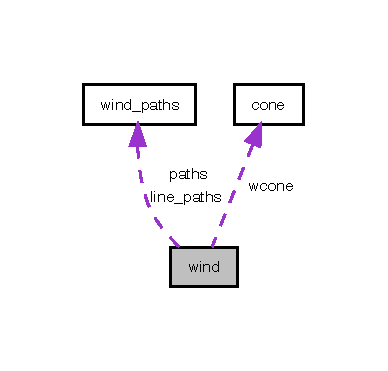
\includegraphics[width=186pt]{structwind__coll__graph}
\end{center}
\end{figure}
\subsection*{Public Types}
\begin{DoxyCompactItemize}
\item 
enum \hyperlink{structwind_a0cb1b3175908a106ae86ce77d5d2a8a4}{inwind\+\_\+enum} \{ \newline
\hyperlink{structwind_a0cb1b3175908a106ae86ce77d5d2a8a4adff4f483f25869269ceb015460e67efa}{W\+\_\+\+I\+N\+\_\+\+D\+I\+SK} = -\/5, 
\hyperlink{structwind_a0cb1b3175908a106ae86ce77d5d2a8a4a3561a8850a0741aa1587b088f9a9c79e}{W\+\_\+\+I\+G\+N\+O\+RE} = -\/2, 
\hyperlink{structwind_a0cb1b3175908a106ae86ce77d5d2a8a4a41a5f993290a4f10c2fa91e19c83d666}{W\+\_\+\+N\+O\+T\+\_\+\+I\+N\+W\+I\+ND} = -\/1, 
\hyperlink{structwind_a0cb1b3175908a106ae86ce77d5d2a8a4a370a5c4e682d17730e1d4e6765ba9d24}{W\+\_\+\+A\+L\+L\+\_\+\+I\+N\+W\+I\+ND} = 0, 
\newline
\hyperlink{structwind_a0cb1b3175908a106ae86ce77d5d2a8a4a6b32df2f7211ffd13ad86080608a48fc}{W\+\_\+\+P\+A\+R\+T\+\_\+\+I\+N\+W\+I\+ND} = 1, 
\hyperlink{structwind_a0cb1b3175908a106ae86ce77d5d2a8a4a26eb6750b38353d7bb17eee540b0cd25}{W\+\_\+\+N\+O\+T\+\_\+\+A\+S\+S\+I\+G\+N\+ED} = -\/999
 \}
\end{DoxyCompactItemize}
\subsection*{Data Fields}
\begin{DoxyCompactItemize}
\item 
int \hyperlink{structwind_aaa7f27e1a93690e4c37878a93c40db22}{ndom}
\item 
int \hyperlink{structwind_aa879b7be5a0f232f2fde3a95e85824b6}{nwind}
\item 
int \hyperlink{structwind_ae01b6d799a4f0a60142703606c9fea3c}{nplasma}
\item 
double \hyperlink{structwind_aa79ef3a918f25e67318af1200ea49bd7}{x} \mbox{[}3\mbox{]}
\item 
double \hyperlink{structwind_a289fcd4f4c7e344d112785545192cffe}{xcen} \mbox{[}3\mbox{]}
\item 
double \hyperlink{structwind_a68090533c7fa4c2bc4f1272a71012b5c}{r}
\item 
double \hyperlink{structwind_a94d793823c987a311e4abcd1f2c4aad0}{rcen}
\item 
double \hyperlink{structwind_ab555fb67dfd86ffa4710da52b5edd39d}{theta}
\item 
double \hyperlink{structwind_a876ccd0541a3488e8faa62f1a9edc080}{thetacen}
\item 
double \hyperlink{structwind_ab2fe12e1a8862dae8bf49dca7b44cee7}{dtheta}
\item 
double \hyperlink{structwind_aecd2315036110808fa470bffbf36e6a8}{dr}
\item 
struct \hyperlink{structcone}{cone} \hyperlink{structwind_a4d0d6b2e0e7f6d8500f66efdb639f233}{wcone}
\item 
double \hyperlink{structwind_a9e2fcac3826b36b7a4eed3eb74f45ede}{v} \mbox{[}3\mbox{]}
\item 
double \hyperlink{structwind_a7f9f96a08008c3354c3f681b3d9c672e}{v\+\_\+grad} \mbox{[}3\mbox{]}\mbox{[}3\mbox{]}
\item 
double \hyperlink{structwind_a25a5b831a64c649f280da38e9b8821d9}{div\+\_\+v}
\item 
double \hyperlink{structwind_a4d9c9c37e5ea6f91b06918e723217fed}{dvds\+\_\+ave}
\item 
double \hyperlink{structwind_aa03474c00bb0ac035bd883ef18c4edac}{dvds\+\_\+max}
\item 
double \hyperlink{structwind_a021e9cbe88f7b0840038d3943f8818d2}{lmn} \mbox{[}3\mbox{]}
\item 
double \hyperlink{structwind_a86864abe3bc4d97d1b4c305f085c6c55}{vol}
\item 
double \hyperlink{structwind_a9e48704d3e2881e8cd2fef227c0ba8cd}{dfudge}
\item 
enum \hyperlink{structwind_a0cb1b3175908a106ae86ce77d5d2a8a4}{wind\+::inwind\+\_\+enum} \hyperlink{structwind_a7f4f2ec3bc9cea1d4dec351b026b9a73}{inwind}
\item 
\hyperlink{python_8h_af5cbc81f9fbd8ac7596e3a989073df45}{Wind\+\_\+\+Paths\+\_\+\+Ptr} \hyperlink{structwind_a35413d90b5539e3c14b74a7e0fb7dbac}{paths}
\item 
\hyperlink{python_8h_af5cbc81f9fbd8ac7596e3a989073df45}{Wind\+\_\+\+Paths\+\_\+\+Ptr} $\ast$ \hyperlink{structwind_a131a30d1943ba6394b7d74328d9374b7}{line\+\_\+paths}
\end{DoxyCompactItemize}


\subsection{Detailed Description}


Definition at line 692 of file python.\+h.



\subsection{Member Enumeration Documentation}
\mbox{\Hypertarget{structwind_a0cb1b3175908a106ae86ce77d5d2a8a4}\label{structwind_a0cb1b3175908a106ae86ce77d5d2a8a4}} 
\index{wind@{wind}!inwind\+\_\+enum@{inwind\+\_\+enum}}
\index{inwind\+\_\+enum@{inwind\+\_\+enum}!wind@{wind}}
\subsubsection{\texorpdfstring{inwind\+\_\+enum}{inwind\_enum}}
{\footnotesize\ttfamily enum \hyperlink{structwind_a0cb1b3175908a106ae86ce77d5d2a8a4}{wind\+::inwind\+\_\+enum}}

\begin{DoxyEnumFields}{Enumerator}
\raisebox{\heightof{T}}[0pt][0pt]{\index{W\+\_\+\+I\+N\+\_\+\+D\+I\+SK@{W\+\_\+\+I\+N\+\_\+\+D\+I\+SK}!wind@{wind}}\index{wind@{wind}!W\+\_\+\+I\+N\+\_\+\+D\+I\+SK@{W\+\_\+\+I\+N\+\_\+\+D\+I\+SK}}}\mbox{\Hypertarget{structwind_a0cb1b3175908a106ae86ce77d5d2a8a4adff4f483f25869269ceb015460e67efa}\label{structwind_a0cb1b3175908a106ae86ce77d5d2a8a4adff4f483f25869269ceb015460e67efa}} 
W\+\_\+\+I\+N\+\_\+\+D\+I\+SK&\\
\hline

\raisebox{\heightof{T}}[0pt][0pt]{\index{W\+\_\+\+I\+G\+N\+O\+RE@{W\+\_\+\+I\+G\+N\+O\+RE}!wind@{wind}}\index{wind@{wind}!W\+\_\+\+I\+G\+N\+O\+RE@{W\+\_\+\+I\+G\+N\+O\+RE}}}\mbox{\Hypertarget{structwind_a0cb1b3175908a106ae86ce77d5d2a8a4a3561a8850a0741aa1587b088f9a9c79e}\label{structwind_a0cb1b3175908a106ae86ce77d5d2a8a4a3561a8850a0741aa1587b088f9a9c79e}} 
W\+\_\+\+I\+G\+N\+O\+RE&\\
\hline

\raisebox{\heightof{T}}[0pt][0pt]{\index{W\+\_\+\+N\+O\+T\+\_\+\+I\+N\+W\+I\+ND@{W\+\_\+\+N\+O\+T\+\_\+\+I\+N\+W\+I\+ND}!wind@{wind}}\index{wind@{wind}!W\+\_\+\+N\+O\+T\+\_\+\+I\+N\+W\+I\+ND@{W\+\_\+\+N\+O\+T\+\_\+\+I\+N\+W\+I\+ND}}}\mbox{\Hypertarget{structwind_a0cb1b3175908a106ae86ce77d5d2a8a4a41a5f993290a4f10c2fa91e19c83d666}\label{structwind_a0cb1b3175908a106ae86ce77d5d2a8a4a41a5f993290a4f10c2fa91e19c83d666}} 
W\+\_\+\+N\+O\+T\+\_\+\+I\+N\+W\+I\+ND&\\
\hline

\raisebox{\heightof{T}}[0pt][0pt]{\index{W\+\_\+\+A\+L\+L\+\_\+\+I\+N\+W\+I\+ND@{W\+\_\+\+A\+L\+L\+\_\+\+I\+N\+W\+I\+ND}!wind@{wind}}\index{wind@{wind}!W\+\_\+\+A\+L\+L\+\_\+\+I\+N\+W\+I\+ND@{W\+\_\+\+A\+L\+L\+\_\+\+I\+N\+W\+I\+ND}}}\mbox{\Hypertarget{structwind_a0cb1b3175908a106ae86ce77d5d2a8a4a370a5c4e682d17730e1d4e6765ba9d24}\label{structwind_a0cb1b3175908a106ae86ce77d5d2a8a4a370a5c4e682d17730e1d4e6765ba9d24}} 
W\+\_\+\+A\+L\+L\+\_\+\+I\+N\+W\+I\+ND&\\
\hline

\raisebox{\heightof{T}}[0pt][0pt]{\index{W\+\_\+\+P\+A\+R\+T\+\_\+\+I\+N\+W\+I\+ND@{W\+\_\+\+P\+A\+R\+T\+\_\+\+I\+N\+W\+I\+ND}!wind@{wind}}\index{wind@{wind}!W\+\_\+\+P\+A\+R\+T\+\_\+\+I\+N\+W\+I\+ND@{W\+\_\+\+P\+A\+R\+T\+\_\+\+I\+N\+W\+I\+ND}}}\mbox{\Hypertarget{structwind_a0cb1b3175908a106ae86ce77d5d2a8a4a6b32df2f7211ffd13ad86080608a48fc}\label{structwind_a0cb1b3175908a106ae86ce77d5d2a8a4a6b32df2f7211ffd13ad86080608a48fc}} 
W\+\_\+\+P\+A\+R\+T\+\_\+\+I\+N\+W\+I\+ND&\\
\hline

\raisebox{\heightof{T}}[0pt][0pt]{\index{W\+\_\+\+N\+O\+T\+\_\+\+A\+S\+S\+I\+G\+N\+ED@{W\+\_\+\+N\+O\+T\+\_\+\+A\+S\+S\+I\+G\+N\+ED}!wind@{wind}}\index{wind@{wind}!W\+\_\+\+N\+O\+T\+\_\+\+A\+S\+S\+I\+G\+N\+ED@{W\+\_\+\+N\+O\+T\+\_\+\+A\+S\+S\+I\+G\+N\+ED}}}\mbox{\Hypertarget{structwind_a0cb1b3175908a106ae86ce77d5d2a8a4a26eb6750b38353d7bb17eee540b0cd25}\label{structwind_a0cb1b3175908a106ae86ce77d5d2a8a4a26eb6750b38353d7bb17eee540b0cd25}} 
W\+\_\+\+N\+O\+T\+\_\+\+A\+S\+S\+I\+G\+N\+ED&\\
\hline

\end{DoxyEnumFields}


Definition at line 716 of file python.\+h.



\subsection{Field Documentation}
\mbox{\Hypertarget{structwind_a9e48704d3e2881e8cd2fef227c0ba8cd}\label{structwind_a9e48704d3e2881e8cd2fef227c0ba8cd}} 
\index{wind@{wind}!dfudge@{dfudge}}
\index{dfudge@{dfudge}!wind@{wind}}
\subsubsection{\texorpdfstring{dfudge}{dfudge}}
{\footnotesize\ttfamily double wind\+::dfudge}



Definition at line 714 of file python.\+h.

\mbox{\Hypertarget{structwind_a25a5b831a64c649f280da38e9b8821d9}\label{structwind_a25a5b831a64c649f280da38e9b8821d9}} 
\index{wind@{wind}!div\+\_\+v@{div\+\_\+v}}
\index{div\+\_\+v@{div\+\_\+v}!wind@{wind}}
\subsubsection{\texorpdfstring{div\+\_\+v}{div\_v}}
{\footnotesize\ttfamily double wind\+::div\+\_\+v}



Definition at line 708 of file python.\+h.

\mbox{\Hypertarget{structwind_aecd2315036110808fa470bffbf36e6a8}\label{structwind_aecd2315036110808fa470bffbf36e6a8}} 
\index{wind@{wind}!dr@{dr}}
\index{dr@{dr}!wind@{wind}}
\subsubsection{\texorpdfstring{dr}{dr}}
{\footnotesize\ttfamily double wind\+::dr}



Definition at line 702 of file python.\+h.

\mbox{\Hypertarget{structwind_ab2fe12e1a8862dae8bf49dca7b44cee7}\label{structwind_ab2fe12e1a8862dae8bf49dca7b44cee7}} 
\index{wind@{wind}!dtheta@{dtheta}}
\index{dtheta@{dtheta}!wind@{wind}}
\subsubsection{\texorpdfstring{dtheta}{dtheta}}
{\footnotesize\ttfamily double wind\+::dtheta}



Definition at line 702 of file python.\+h.

\mbox{\Hypertarget{structwind_a4d9c9c37e5ea6f91b06918e723217fed}\label{structwind_a4d9c9c37e5ea6f91b06918e723217fed}} 
\index{wind@{wind}!dvds\+\_\+ave@{dvds\+\_\+ave}}
\index{dvds\+\_\+ave@{dvds\+\_\+ave}!wind@{wind}}
\subsubsection{\texorpdfstring{dvds\+\_\+ave}{dvds\_ave}}
{\footnotesize\ttfamily double wind\+::dvds\+\_\+ave}



Definition at line 709 of file python.\+h.

\mbox{\Hypertarget{structwind_aa03474c00bb0ac035bd883ef18c4edac}\label{structwind_aa03474c00bb0ac035bd883ef18c4edac}} 
\index{wind@{wind}!dvds\+\_\+max@{dvds\+\_\+max}}
\index{dvds\+\_\+max@{dvds\+\_\+max}!wind@{wind}}
\subsubsection{\texorpdfstring{dvds\+\_\+max}{dvds\_max}}
{\footnotesize\ttfamily double wind\+::dvds\+\_\+max}



Definition at line 710 of file python.\+h.

\mbox{\Hypertarget{structwind_a7f4f2ec3bc9cea1d4dec351b026b9a73}\label{structwind_a7f4f2ec3bc9cea1d4dec351b026b9a73}} 
\index{wind@{wind}!inwind@{inwind}}
\index{inwind@{inwind}!wind@{wind}}
\subsubsection{\texorpdfstring{inwind}{inwind}}
{\footnotesize\ttfamily enum \hyperlink{structwind_a0cb1b3175908a106ae86ce77d5d2a8a4}{wind\+::inwind\+\_\+enum}  wind\+::inwind}

\mbox{\Hypertarget{structwind_a131a30d1943ba6394b7d74328d9374b7}\label{structwind_a131a30d1943ba6394b7d74328d9374b7}} 
\index{wind@{wind}!line\+\_\+paths@{line\+\_\+paths}}
\index{line\+\_\+paths@{line\+\_\+paths}!wind@{wind}}
\subsubsection{\texorpdfstring{line\+\_\+paths}{line\_paths}}
{\footnotesize\ttfamily \hyperlink{python_8h_af5cbc81f9fbd8ac7596e3a989073df45}{Wind\+\_\+\+Paths\+\_\+\+Ptr} $\ast$ wind\+::line\+\_\+paths}



Definition at line 720 of file python.\+h.

\mbox{\Hypertarget{structwind_a021e9cbe88f7b0840038d3943f8818d2}\label{structwind_a021e9cbe88f7b0840038d3943f8818d2}} 
\index{wind@{wind}!lmn@{lmn}}
\index{lmn@{lmn}!wind@{wind}}
\subsubsection{\texorpdfstring{lmn}{lmn}}
{\footnotesize\ttfamily double wind\+::lmn\mbox{[}3\mbox{]}}



Definition at line 710 of file python.\+h.

\mbox{\Hypertarget{structwind_aaa7f27e1a93690e4c37878a93c40db22}\label{structwind_aaa7f27e1a93690e4c37878a93c40db22}} 
\index{wind@{wind}!ndom@{ndom}}
\index{ndom@{ndom}!wind@{wind}}
\subsubsection{\texorpdfstring{ndom}{ndom}}
{\footnotesize\ttfamily int wind\+::ndom}



Definition at line 694 of file python.\+h.

\mbox{\Hypertarget{structwind_ae01b6d799a4f0a60142703606c9fea3c}\label{structwind_ae01b6d799a4f0a60142703606c9fea3c}} 
\index{wind@{wind}!nplasma@{nplasma}}
\index{nplasma@{nplasma}!wind@{wind}}
\subsubsection{\texorpdfstring{nplasma}{nplasma}}
{\footnotesize\ttfamily int wind\+::nplasma}



Definition at line 696 of file python.\+h.

\mbox{\Hypertarget{structwind_aa879b7be5a0f232f2fde3a95e85824b6}\label{structwind_aa879b7be5a0f232f2fde3a95e85824b6}} 
\index{wind@{wind}!nwind@{nwind}}
\index{nwind@{nwind}!wind@{wind}}
\subsubsection{\texorpdfstring{nwind}{nwind}}
{\footnotesize\ttfamily int wind\+::nwind}



Definition at line 695 of file python.\+h.

\mbox{\Hypertarget{structwind_a35413d90b5539e3c14b74a7e0fb7dbac}\label{structwind_a35413d90b5539e3c14b74a7e0fb7dbac}} 
\index{wind@{wind}!paths@{paths}}
\index{paths@{paths}!wind@{wind}}
\subsubsection{\texorpdfstring{paths}{paths}}
{\footnotesize\ttfamily \hyperlink{python_8h_af5cbc81f9fbd8ac7596e3a989073df45}{Wind\+\_\+\+Paths\+\_\+\+Ptr} wind\+::paths}



Definition at line 720 of file python.\+h.

\mbox{\Hypertarget{structwind_a68090533c7fa4c2bc4f1272a71012b5c}\label{structwind_a68090533c7fa4c2bc4f1272a71012b5c}} 
\index{wind@{wind}!r@{r}}
\index{r@{r}!wind@{wind}}
\subsubsection{\texorpdfstring{r}{r}}
{\footnotesize\ttfamily double wind\+::r}



Definition at line 699 of file python.\+h.

\mbox{\Hypertarget{structwind_a94d793823c987a311e4abcd1f2c4aad0}\label{structwind_a94d793823c987a311e4abcd1f2c4aad0}} 
\index{wind@{wind}!rcen@{rcen}}
\index{rcen@{rcen}!wind@{wind}}
\subsubsection{\texorpdfstring{rcen}{rcen}}
{\footnotesize\ttfamily double wind\+::rcen}



Definition at line 699 of file python.\+h.

\mbox{\Hypertarget{structwind_ab555fb67dfd86ffa4710da52b5edd39d}\label{structwind_ab555fb67dfd86ffa4710da52b5edd39d}} 
\index{wind@{wind}!theta@{theta}}
\index{theta@{theta}!wind@{wind}}
\subsubsection{\texorpdfstring{theta}{theta}}
{\footnotesize\ttfamily double wind\+::theta}



Definition at line 701 of file python.\+h.

\mbox{\Hypertarget{structwind_a876ccd0541a3488e8faa62f1a9edc080}\label{structwind_a876ccd0541a3488e8faa62f1a9edc080}} 
\index{wind@{wind}!thetacen@{thetacen}}
\index{thetacen@{thetacen}!wind@{wind}}
\subsubsection{\texorpdfstring{thetacen}{thetacen}}
{\footnotesize\ttfamily double wind\+::thetacen}



Definition at line 701 of file python.\+h.

\mbox{\Hypertarget{structwind_a9e2fcac3826b36b7a4eed3eb74f45ede}\label{structwind_a9e2fcac3826b36b7a4eed3eb74f45ede}} 
\index{wind@{wind}!v@{v}}
\index{v@{v}!wind@{wind}}
\subsubsection{\texorpdfstring{v}{v}}
{\footnotesize\ttfamily double wind\+::v\mbox{[}3\mbox{]}}



Definition at line 705 of file python.\+h.

\mbox{\Hypertarget{structwind_a7f9f96a08008c3354c3f681b3d9c672e}\label{structwind_a7f9f96a08008c3354c3f681b3d9c672e}} 
\index{wind@{wind}!v\+\_\+grad@{v\+\_\+grad}}
\index{v\+\_\+grad@{v\+\_\+grad}!wind@{wind}}
\subsubsection{\texorpdfstring{v\+\_\+grad}{v\_grad}}
{\footnotesize\ttfamily double wind\+::v\+\_\+grad\mbox{[}3\mbox{]}\mbox{[}3\mbox{]}}



Definition at line 707 of file python.\+h.

\mbox{\Hypertarget{structwind_a86864abe3bc4d97d1b4c305f085c6c55}\label{structwind_a86864abe3bc4d97d1b4c305f085c6c55}} 
\index{wind@{wind}!vol@{vol}}
\index{vol@{vol}!wind@{wind}}
\subsubsection{\texorpdfstring{vol}{vol}}
{\footnotesize\ttfamily double wind\+::vol}



Definition at line 711 of file python.\+h.

\mbox{\Hypertarget{structwind_a4d0d6b2e0e7f6d8500f66efdb639f233}\label{structwind_a4d0d6b2e0e7f6d8500f66efdb639f233}} 
\index{wind@{wind}!wcone@{wcone}}
\index{wcone@{wcone}!wind@{wind}}
\subsubsection{\texorpdfstring{wcone}{wcone}}
{\footnotesize\ttfamily struct \hyperlink{structcone}{cone} wind\+::wcone}



Definition at line 703 of file python.\+h.

\mbox{\Hypertarget{structwind_aa79ef3a918f25e67318af1200ea49bd7}\label{structwind_aa79ef3a918f25e67318af1200ea49bd7}} 
\index{wind@{wind}!x@{x}}
\index{x@{x}!wind@{wind}}
\subsubsection{\texorpdfstring{x}{x}}
{\footnotesize\ttfamily double wind\+::x\mbox{[}3\mbox{]}}



Definition at line 697 of file python.\+h.

\mbox{\Hypertarget{structwind_a289fcd4f4c7e344d112785545192cffe}\label{structwind_a289fcd4f4c7e344d112785545192cffe}} 
\index{wind@{wind}!xcen@{xcen}}
\index{xcen@{xcen}!wind@{wind}}
\subsubsection{\texorpdfstring{xcen}{xcen}}
{\footnotesize\ttfamily double wind\+::xcen\mbox{[}3\mbox{]}}



Definition at line 698 of file python.\+h.



The documentation for this struct was generated from the following file\+:\begin{DoxyCompactItemize}
\item 
/\+Users/mhewitt/python/source/\hyperlink{python_8h}{python.\+h}\end{DoxyCompactItemize}

\hypertarget{structwind__paths}{}\section{wind\+\_\+paths Struct Reference}
\label{structwind__paths}\index{wind\+\_\+paths@{wind\+\_\+paths}}


{\ttfamily \#include $<$python.\+h$>$}

\subsection*{Data Fields}
\begin{DoxyCompactItemize}
\item 
double $\ast$ \hyperlink{structwind__paths_a1370c8bf3ce0046cf5df146163242ca7}{ad\+\_\+path\+\_\+flux}
\item 
double $\ast$ \hyperlink{structwind__paths_a0a5d8e1d1f2c6ac1ef12546861a42944}{ad\+\_\+path\+\_\+flux\+\_\+disk}
\item 
double $\ast$ \hyperlink{structwind__paths_a4febc3700f5712b104b005e27921fbb9}{ad\+\_\+path\+\_\+flux\+\_\+wind}
\item 
double $\ast$ \hyperlink{structwind__paths_abf38c990c4bd01de98ed20efc146b668}{ad\+\_\+path\+\_\+flux\+\_\+cent}
\item 
int $\ast$ \hyperlink{structwind__paths_ad9480733a091275ed02feb9937319984}{ai\+\_\+path\+\_\+num}
\item 
int $\ast$ \hyperlink{structwind__paths_ae982a83bc3af8b04244b0381768cb7a5}{ai\+\_\+path\+\_\+num\+\_\+disk}
\item 
int $\ast$ \hyperlink{structwind__paths_affbbb54b31990833657a147d163bb4c3}{ai\+\_\+path\+\_\+num\+\_\+wind}
\item 
int $\ast$ \hyperlink{structwind__paths_af48b5567dbea692d3db304ca81b99ee3}{ai\+\_\+path\+\_\+num\+\_\+cent}
\item 
double \hyperlink{structwind__paths_a88bf2b63a99884a3541f0f33dd931668}{d\+\_\+flux}
\item 
double \hyperlink{structwind__paths_ab64de9566a8772c7072cd638373ca585}{d\+\_\+path}
\item 
int \hyperlink{structwind__paths_adbd726e6d16ac18e5293af5aab92be0e}{i\+\_\+num}
\end{DoxyCompactItemize}


\subsection{Detailed Description}


Definition at line 642 of file python.\+h.



\subsection{Field Documentation}
\mbox{\Hypertarget{structwind__paths_a1370c8bf3ce0046cf5df146163242ca7}\label{structwind__paths_a1370c8bf3ce0046cf5df146163242ca7}} 
\index{wind\+\_\+paths@{wind\+\_\+paths}!ad\+\_\+path\+\_\+flux@{ad\+\_\+path\+\_\+flux}}
\index{ad\+\_\+path\+\_\+flux@{ad\+\_\+path\+\_\+flux}!wind\+\_\+paths@{wind\+\_\+paths}}
\subsubsection{\texorpdfstring{ad\+\_\+path\+\_\+flux}{ad\_path\_flux}}
{\footnotesize\ttfamily double$\ast$ wind\+\_\+paths\+::ad\+\_\+path\+\_\+flux}



Definition at line 644 of file python.\+h.

\mbox{\Hypertarget{structwind__paths_abf38c990c4bd01de98ed20efc146b668}\label{structwind__paths_abf38c990c4bd01de98ed20efc146b668}} 
\index{wind\+\_\+paths@{wind\+\_\+paths}!ad\+\_\+path\+\_\+flux\+\_\+cent@{ad\+\_\+path\+\_\+flux\+\_\+cent}}
\index{ad\+\_\+path\+\_\+flux\+\_\+cent@{ad\+\_\+path\+\_\+flux\+\_\+cent}!wind\+\_\+paths@{wind\+\_\+paths}}
\subsubsection{\texorpdfstring{ad\+\_\+path\+\_\+flux\+\_\+cent}{ad\_path\_flux\_cent}}
{\footnotesize\ttfamily double$\ast$ wind\+\_\+paths\+::ad\+\_\+path\+\_\+flux\+\_\+cent}



Definition at line 647 of file python.\+h.

\mbox{\Hypertarget{structwind__paths_a0a5d8e1d1f2c6ac1ef12546861a42944}\label{structwind__paths_a0a5d8e1d1f2c6ac1ef12546861a42944}} 
\index{wind\+\_\+paths@{wind\+\_\+paths}!ad\+\_\+path\+\_\+flux\+\_\+disk@{ad\+\_\+path\+\_\+flux\+\_\+disk}}
\index{ad\+\_\+path\+\_\+flux\+\_\+disk@{ad\+\_\+path\+\_\+flux\+\_\+disk}!wind\+\_\+paths@{wind\+\_\+paths}}
\subsubsection{\texorpdfstring{ad\+\_\+path\+\_\+flux\+\_\+disk}{ad\_path\_flux\_disk}}
{\footnotesize\ttfamily double$\ast$ wind\+\_\+paths\+::ad\+\_\+path\+\_\+flux\+\_\+disk}



Definition at line 645 of file python.\+h.

\mbox{\Hypertarget{structwind__paths_a4febc3700f5712b104b005e27921fbb9}\label{structwind__paths_a4febc3700f5712b104b005e27921fbb9}} 
\index{wind\+\_\+paths@{wind\+\_\+paths}!ad\+\_\+path\+\_\+flux\+\_\+wind@{ad\+\_\+path\+\_\+flux\+\_\+wind}}
\index{ad\+\_\+path\+\_\+flux\+\_\+wind@{ad\+\_\+path\+\_\+flux\+\_\+wind}!wind\+\_\+paths@{wind\+\_\+paths}}
\subsubsection{\texorpdfstring{ad\+\_\+path\+\_\+flux\+\_\+wind}{ad\_path\_flux\_wind}}
{\footnotesize\ttfamily double$\ast$ wind\+\_\+paths\+::ad\+\_\+path\+\_\+flux\+\_\+wind}



Definition at line 646 of file python.\+h.

\mbox{\Hypertarget{structwind__paths_ad9480733a091275ed02feb9937319984}\label{structwind__paths_ad9480733a091275ed02feb9937319984}} 
\index{wind\+\_\+paths@{wind\+\_\+paths}!ai\+\_\+path\+\_\+num@{ai\+\_\+path\+\_\+num}}
\index{ai\+\_\+path\+\_\+num@{ai\+\_\+path\+\_\+num}!wind\+\_\+paths@{wind\+\_\+paths}}
\subsubsection{\texorpdfstring{ai\+\_\+path\+\_\+num}{ai\_path\_num}}
{\footnotesize\ttfamily int$\ast$ wind\+\_\+paths\+::ai\+\_\+path\+\_\+num}



Definition at line 648 of file python.\+h.

\mbox{\Hypertarget{structwind__paths_af48b5567dbea692d3db304ca81b99ee3}\label{structwind__paths_af48b5567dbea692d3db304ca81b99ee3}} 
\index{wind\+\_\+paths@{wind\+\_\+paths}!ai\+\_\+path\+\_\+num\+\_\+cent@{ai\+\_\+path\+\_\+num\+\_\+cent}}
\index{ai\+\_\+path\+\_\+num\+\_\+cent@{ai\+\_\+path\+\_\+num\+\_\+cent}!wind\+\_\+paths@{wind\+\_\+paths}}
\subsubsection{\texorpdfstring{ai\+\_\+path\+\_\+num\+\_\+cent}{ai\_path\_num\_cent}}
{\footnotesize\ttfamily int$\ast$ wind\+\_\+paths\+::ai\+\_\+path\+\_\+num\+\_\+cent}



Definition at line 651 of file python.\+h.

\mbox{\Hypertarget{structwind__paths_ae982a83bc3af8b04244b0381768cb7a5}\label{structwind__paths_ae982a83bc3af8b04244b0381768cb7a5}} 
\index{wind\+\_\+paths@{wind\+\_\+paths}!ai\+\_\+path\+\_\+num\+\_\+disk@{ai\+\_\+path\+\_\+num\+\_\+disk}}
\index{ai\+\_\+path\+\_\+num\+\_\+disk@{ai\+\_\+path\+\_\+num\+\_\+disk}!wind\+\_\+paths@{wind\+\_\+paths}}
\subsubsection{\texorpdfstring{ai\+\_\+path\+\_\+num\+\_\+disk}{ai\_path\_num\_disk}}
{\footnotesize\ttfamily int$\ast$ wind\+\_\+paths\+::ai\+\_\+path\+\_\+num\+\_\+disk}



Definition at line 649 of file python.\+h.

\mbox{\Hypertarget{structwind__paths_affbbb54b31990833657a147d163bb4c3}\label{structwind__paths_affbbb54b31990833657a147d163bb4c3}} 
\index{wind\+\_\+paths@{wind\+\_\+paths}!ai\+\_\+path\+\_\+num\+\_\+wind@{ai\+\_\+path\+\_\+num\+\_\+wind}}
\index{ai\+\_\+path\+\_\+num\+\_\+wind@{ai\+\_\+path\+\_\+num\+\_\+wind}!wind\+\_\+paths@{wind\+\_\+paths}}
\subsubsection{\texorpdfstring{ai\+\_\+path\+\_\+num\+\_\+wind}{ai\_path\_num\_wind}}
{\footnotesize\ttfamily int$\ast$ wind\+\_\+paths\+::ai\+\_\+path\+\_\+num\+\_\+wind}



Definition at line 650 of file python.\+h.

\mbox{\Hypertarget{structwind__paths_a88bf2b63a99884a3541f0f33dd931668}\label{structwind__paths_a88bf2b63a99884a3541f0f33dd931668}} 
\index{wind\+\_\+paths@{wind\+\_\+paths}!d\+\_\+flux@{d\+\_\+flux}}
\index{d\+\_\+flux@{d\+\_\+flux}!wind\+\_\+paths@{wind\+\_\+paths}}
\subsubsection{\texorpdfstring{d\+\_\+flux}{d\_flux}}
{\footnotesize\ttfamily double wind\+\_\+paths\+::d\+\_\+flux}



Definition at line 652 of file python.\+h.

\mbox{\Hypertarget{structwind__paths_ab64de9566a8772c7072cd638373ca585}\label{structwind__paths_ab64de9566a8772c7072cd638373ca585}} 
\index{wind\+\_\+paths@{wind\+\_\+paths}!d\+\_\+path@{d\+\_\+path}}
\index{d\+\_\+path@{d\+\_\+path}!wind\+\_\+paths@{wind\+\_\+paths}}
\subsubsection{\texorpdfstring{d\+\_\+path}{d\_path}}
{\footnotesize\ttfamily double wind\+\_\+paths\+::d\+\_\+path}



Definition at line 652 of file python.\+h.

\mbox{\Hypertarget{structwind__paths_adbd726e6d16ac18e5293af5aab92be0e}\label{structwind__paths_adbd726e6d16ac18e5293af5aab92be0e}} 
\index{wind\+\_\+paths@{wind\+\_\+paths}!i\+\_\+num@{i\+\_\+num}}
\index{i\+\_\+num@{i\+\_\+num}!wind\+\_\+paths@{wind\+\_\+paths}}
\subsubsection{\texorpdfstring{i\+\_\+num}{i\_num}}
{\footnotesize\ttfamily int wind\+\_\+paths\+::i\+\_\+num}



Definition at line 653 of file python.\+h.



The documentation for this struct was generated from the following file\+:\begin{DoxyCompactItemize}
\item 
/\+Users/mhewitt/python/source/\hyperlink{python_8h}{python.\+h}\end{DoxyCompactItemize}

\hypertarget{structxbands}{}\section{xbands Struct Reference}
\label{structxbands}\index{xbands@{xbands}}


{\ttfamily \#include $<$python.\+h$>$}

\subsection*{Data Fields}
\begin{DoxyCompactItemize}
\item 
double \hyperlink{structxbands_a4822266ca02ed8a4b214e5efcd79256c}{f1} \mbox{[}\hyperlink{python_8h_a46ee023ac3f5d103e533843238d2e52a}{N\+B\+A\+N\+DS}\mbox{]}
\item 
double \hyperlink{structxbands_af398da6fd226bb4257ad64ac9704098a}{f2} \mbox{[}\hyperlink{python_8h_a46ee023ac3f5d103e533843238d2e52a}{N\+B\+A\+N\+DS}\mbox{]}
\item 
double \hyperlink{structxbands_a5fd1368571f38469e4b8f5ad19586279}{alpha} \mbox{[}\hyperlink{python_8h_a46ee023ac3f5d103e533843238d2e52a}{N\+B\+A\+N\+DS}\mbox{]}
\item 
double \hyperlink{structxbands_a162fb1999189dffd52bcd6d090792481}{pl\+\_\+const} \mbox{[}\hyperlink{python_8h_a46ee023ac3f5d103e533843238d2e52a}{N\+B\+A\+N\+DS}\mbox{]}
\item 
double \hyperlink{structxbands_a5a7f85ceee248b2268f8a37b6330fa57}{min\+\_\+fraction} \mbox{[}\hyperlink{python_8h_a46ee023ac3f5d103e533843238d2e52a}{N\+B\+A\+N\+DS}\mbox{]}
\item 
double \hyperlink{structxbands_a7fa4d027ede2f3658d73225c6292089c}{nat\+\_\+fraction} \mbox{[}\hyperlink{python_8h_a46ee023ac3f5d103e533843238d2e52a}{N\+B\+A\+N\+DS}\mbox{]}
\item 
double \hyperlink{structxbands_a0f946786fa05575c9da9d60699c45202}{used\+\_\+fraction} \mbox{[}\hyperlink{python_8h_a46ee023ac3f5d103e533843238d2e52a}{N\+B\+A\+N\+DS}\mbox{]}
\item 
double \hyperlink{structxbands_aaaed5eb418e48908a4e2c8f4dc0a42c3}{flux} \mbox{[}\hyperlink{python_8h_a46ee023ac3f5d103e533843238d2e52a}{N\+B\+A\+N\+DS}\mbox{]}
\item 
double \hyperlink{structxbands_abab6361efd17b70504fb67164711687a}{weight} \mbox{[}\hyperlink{python_8h_a46ee023ac3f5d103e533843238d2e52a}{N\+B\+A\+N\+DS}\mbox{]}
\item 
int \hyperlink{structxbands_acc3e184739961350ec8f40f7ecd5908a}{nphot} \mbox{[}\hyperlink{python_8h_a46ee023ac3f5d103e533843238d2e52a}{N\+B\+A\+N\+DS}\mbox{]}
\item 
int \hyperlink{structxbands_aad6fe819267976ae85b61e65e0b70f75}{nbands}
\end{DoxyCompactItemize}


\subsection{Detailed Description}


Definition at line 1262 of file python.\+h.



\subsection{Field Documentation}
\mbox{\Hypertarget{structxbands_a5fd1368571f38469e4b8f5ad19586279}\label{structxbands_a5fd1368571f38469e4b8f5ad19586279}} 
\index{xbands@{xbands}!alpha@{alpha}}
\index{alpha@{alpha}!xbands@{xbands}}
\subsubsection{\texorpdfstring{alpha}{alpha}}
{\footnotesize\ttfamily double xbands\+::alpha\mbox{[}\hyperlink{python_8h_a46ee023ac3f5d103e533843238d2e52a}{N\+B\+A\+N\+DS}\mbox{]}}



Definition at line 1265 of file python.\+h.

\mbox{\Hypertarget{structxbands_a4822266ca02ed8a4b214e5efcd79256c}\label{structxbands_a4822266ca02ed8a4b214e5efcd79256c}} 
\index{xbands@{xbands}!f1@{f1}}
\index{f1@{f1}!xbands@{xbands}}
\subsubsection{\texorpdfstring{f1}{f1}}
{\footnotesize\ttfamily double xbands\+::f1\mbox{[}\hyperlink{python_8h_a46ee023ac3f5d103e533843238d2e52a}{N\+B\+A\+N\+DS}\mbox{]}}



Definition at line 1264 of file python.\+h.

\mbox{\Hypertarget{structxbands_af398da6fd226bb4257ad64ac9704098a}\label{structxbands_af398da6fd226bb4257ad64ac9704098a}} 
\index{xbands@{xbands}!f2@{f2}}
\index{f2@{f2}!xbands@{xbands}}
\subsubsection{\texorpdfstring{f2}{f2}}
{\footnotesize\ttfamily double xbands\+::f2\mbox{[}\hyperlink{python_8h_a46ee023ac3f5d103e533843238d2e52a}{N\+B\+A\+N\+DS}\mbox{]}}



Definition at line 1264 of file python.\+h.

\mbox{\Hypertarget{structxbands_aaaed5eb418e48908a4e2c8f4dc0a42c3}\label{structxbands_aaaed5eb418e48908a4e2c8f4dc0a42c3}} 
\index{xbands@{xbands}!flux@{flux}}
\index{flux@{flux}!xbands@{xbands}}
\subsubsection{\texorpdfstring{flux}{flux}}
{\footnotesize\ttfamily double xbands\+::flux\mbox{[}\hyperlink{python_8h_a46ee023ac3f5d103e533843238d2e52a}{N\+B\+A\+N\+DS}\mbox{]}}



Definition at line 1270 of file python.\+h.

\mbox{\Hypertarget{structxbands_a5a7f85ceee248b2268f8a37b6330fa57}\label{structxbands_a5a7f85ceee248b2268f8a37b6330fa57}} 
\index{xbands@{xbands}!min\+\_\+fraction@{min\+\_\+fraction}}
\index{min\+\_\+fraction@{min\+\_\+fraction}!xbands@{xbands}}
\subsubsection{\texorpdfstring{min\+\_\+fraction}{min\_fraction}}
{\footnotesize\ttfamily double xbands\+::min\+\_\+fraction\mbox{[}\hyperlink{python_8h_a46ee023ac3f5d103e533843238d2e52a}{N\+B\+A\+N\+DS}\mbox{]}}



Definition at line 1267 of file python.\+h.

\mbox{\Hypertarget{structxbands_a7fa4d027ede2f3658d73225c6292089c}\label{structxbands_a7fa4d027ede2f3658d73225c6292089c}} 
\index{xbands@{xbands}!nat\+\_\+fraction@{nat\+\_\+fraction}}
\index{nat\+\_\+fraction@{nat\+\_\+fraction}!xbands@{xbands}}
\subsubsection{\texorpdfstring{nat\+\_\+fraction}{nat\_fraction}}
{\footnotesize\ttfamily double xbands\+::nat\+\_\+fraction\mbox{[}\hyperlink{python_8h_a46ee023ac3f5d103e533843238d2e52a}{N\+B\+A\+N\+DS}\mbox{]}}



Definition at line 1268 of file python.\+h.

\mbox{\Hypertarget{structxbands_aad6fe819267976ae85b61e65e0b70f75}\label{structxbands_aad6fe819267976ae85b61e65e0b70f75}} 
\index{xbands@{xbands}!nbands@{nbands}}
\index{nbands@{nbands}!xbands@{xbands}}
\subsubsection{\texorpdfstring{nbands}{nbands}}
{\footnotesize\ttfamily int xbands\+::nbands}



Definition at line 1273 of file python.\+h.

\mbox{\Hypertarget{structxbands_acc3e184739961350ec8f40f7ecd5908a}\label{structxbands_acc3e184739961350ec8f40f7ecd5908a}} 
\index{xbands@{xbands}!nphot@{nphot}}
\index{nphot@{nphot}!xbands@{xbands}}
\subsubsection{\texorpdfstring{nphot}{nphot}}
{\footnotesize\ttfamily int xbands\+::nphot\mbox{[}\hyperlink{python_8h_a46ee023ac3f5d103e533843238d2e52a}{N\+B\+A\+N\+DS}\mbox{]}}



Definition at line 1272 of file python.\+h.

\mbox{\Hypertarget{structxbands_a162fb1999189dffd52bcd6d090792481}\label{structxbands_a162fb1999189dffd52bcd6d090792481}} 
\index{xbands@{xbands}!pl\+\_\+const@{pl\+\_\+const}}
\index{pl\+\_\+const@{pl\+\_\+const}!xbands@{xbands}}
\subsubsection{\texorpdfstring{pl\+\_\+const}{pl\_const}}
{\footnotesize\ttfamily double xbands\+::pl\+\_\+const\mbox{[}\hyperlink{python_8h_a46ee023ac3f5d103e533843238d2e52a}{N\+B\+A\+N\+DS}\mbox{]}}



Definition at line 1266 of file python.\+h.

\mbox{\Hypertarget{structxbands_a0f946786fa05575c9da9d60699c45202}\label{structxbands_a0f946786fa05575c9da9d60699c45202}} 
\index{xbands@{xbands}!used\+\_\+fraction@{used\+\_\+fraction}}
\index{used\+\_\+fraction@{used\+\_\+fraction}!xbands@{xbands}}
\subsubsection{\texorpdfstring{used\+\_\+fraction}{used\_fraction}}
{\footnotesize\ttfamily double xbands\+::used\+\_\+fraction\mbox{[}\hyperlink{python_8h_a46ee023ac3f5d103e533843238d2e52a}{N\+B\+A\+N\+DS}\mbox{]}}



Definition at line 1269 of file python.\+h.

\mbox{\Hypertarget{structxbands_abab6361efd17b70504fb67164711687a}\label{structxbands_abab6361efd17b70504fb67164711687a}} 
\index{xbands@{xbands}!weight@{weight}}
\index{weight@{weight}!xbands@{xbands}}
\subsubsection{\texorpdfstring{weight}{weight}}
{\footnotesize\ttfamily double xbands\+::weight\mbox{[}\hyperlink{python_8h_a46ee023ac3f5d103e533843238d2e52a}{N\+B\+A\+N\+DS}\mbox{]}}



Definition at line 1271 of file python.\+h.



The documentation for this struct was generated from the following file\+:\begin{DoxyCompactItemize}
\item 
/\+Users/mhewitt/python/source/\hyperlink{python_8h}{python.\+h}\end{DoxyCompactItemize}

\hypertarget{structxdisk}{}\section{xdisk Struct Reference}
\label{structxdisk}\index{xdisk@{xdisk}}


{\ttfamily \#include $<$python.\+h$>$}

\subsection*{Data Fields}
\begin{DoxyCompactItemize}
\item 
double \hyperlink{structxdisk_a4ca6d46d2d2873fbd971da347b14b073}{r} \mbox{[}\hyperlink{python_8h_af8b02d1bed15b59f7062901b55c4d123}{N\+R\+I\+N\+GS}\mbox{]}
\item 
double \hyperlink{structxdisk_a88f7151e3a7f53de1fb9766c0d41b382}{t} \mbox{[}\hyperlink{python_8h_af8b02d1bed15b59f7062901b55c4d123}{N\+R\+I\+N\+GS}\mbox{]}
\item 
double \hyperlink{structxdisk_aab482a2209b216c79d450ff3adf103f3}{g} \mbox{[}\hyperlink{python_8h_af8b02d1bed15b59f7062901b55c4d123}{N\+R\+I\+N\+GS}\mbox{]}
\item 
double \hyperlink{structxdisk_a3a23c417cee1fe61baf6a6af9dc84b2a}{v} \mbox{[}\hyperlink{python_8h_af8b02d1bed15b59f7062901b55c4d123}{N\+R\+I\+N\+GS}\mbox{]}
\item 
double \hyperlink{structxdisk_a34624d7a4f7db389afb745110b43a82c}{heat} \mbox{[}\hyperlink{python_8h_af8b02d1bed15b59f7062901b55c4d123}{N\+R\+I\+N\+GS}\mbox{]}
\item 
double \hyperlink{structxdisk_aba52b04695b1df389f04944f8a8d69cf}{ave\+\_\+freq} \mbox{[}\hyperlink{python_8h_af8b02d1bed15b59f7062901b55c4d123}{N\+R\+I\+N\+GS}\mbox{]}
\item 
double \hyperlink{structxdisk_a0cfeacb568d69b8a9ae73c33c0f7419c}{w} \mbox{[}\hyperlink{python_8h_af8b02d1bed15b59f7062901b55c4d123}{N\+R\+I\+N\+GS}\mbox{]}
\item 
double \hyperlink{structxdisk_a9c645ab31a3dbdd61812c27e510a5437}{t\+\_\+hit} \mbox{[}\hyperlink{python_8h_af8b02d1bed15b59f7062901b55c4d123}{N\+R\+I\+N\+GS}\mbox{]}
\item 
int \hyperlink{structxdisk_a5812ceecd51e235f48eccda5b854f8e8}{nphot} \mbox{[}\hyperlink{python_8h_af8b02d1bed15b59f7062901b55c4d123}{N\+R\+I\+N\+GS}\mbox{]}
\item 
int \hyperlink{structxdisk_a85fc4d26f2ff6970c94cb6ac75d3b8cb}{nhit} \mbox{[}\hyperlink{python_8h_af8b02d1bed15b59f7062901b55c4d123}{N\+R\+I\+N\+GS}\mbox{]}
\end{DoxyCompactItemize}


\subsection{Detailed Description}


Definition at line 605 of file python.\+h.



\subsection{Field Documentation}
\mbox{\Hypertarget{structxdisk_aba52b04695b1df389f04944f8a8d69cf}\label{structxdisk_aba52b04695b1df389f04944f8a8d69cf}} 
\index{xdisk@{xdisk}!ave\+\_\+freq@{ave\+\_\+freq}}
\index{ave\+\_\+freq@{ave\+\_\+freq}!xdisk@{xdisk}}
\subsubsection{\texorpdfstring{ave\+\_\+freq}{ave\_freq}}
{\footnotesize\ttfamily double xdisk\+::ave\+\_\+freq\mbox{[}\hyperlink{python_8h_af8b02d1bed15b59f7062901b55c4d123}{N\+R\+I\+N\+GS}\mbox{]}}



Definition at line 612 of file python.\+h.

\mbox{\Hypertarget{structxdisk_aab482a2209b216c79d450ff3adf103f3}\label{structxdisk_aab482a2209b216c79d450ff3adf103f3}} 
\index{xdisk@{xdisk}!g@{g}}
\index{g@{g}!xdisk@{xdisk}}
\subsubsection{\texorpdfstring{g}{g}}
{\footnotesize\ttfamily double xdisk\+::g\mbox{[}\hyperlink{python_8h_af8b02d1bed15b59f7062901b55c4d123}{N\+R\+I\+N\+GS}\mbox{]}}



Definition at line 609 of file python.\+h.

\mbox{\Hypertarget{structxdisk_a34624d7a4f7db389afb745110b43a82c}\label{structxdisk_a34624d7a4f7db389afb745110b43a82c}} 
\index{xdisk@{xdisk}!heat@{heat}}
\index{heat@{heat}!xdisk@{xdisk}}
\subsubsection{\texorpdfstring{heat}{heat}}
{\footnotesize\ttfamily double xdisk\+::heat\mbox{[}\hyperlink{python_8h_af8b02d1bed15b59f7062901b55c4d123}{N\+R\+I\+N\+GS}\mbox{]}}



Definition at line 611 of file python.\+h.

\mbox{\Hypertarget{structxdisk_a85fc4d26f2ff6970c94cb6ac75d3b8cb}\label{structxdisk_a85fc4d26f2ff6970c94cb6ac75d3b8cb}} 
\index{xdisk@{xdisk}!nhit@{nhit}}
\index{nhit@{nhit}!xdisk@{xdisk}}
\subsubsection{\texorpdfstring{nhit}{nhit}}
{\footnotesize\ttfamily int xdisk\+::nhit\mbox{[}\hyperlink{python_8h_af8b02d1bed15b59f7062901b55c4d123}{N\+R\+I\+N\+GS}\mbox{]}}



Definition at line 616 of file python.\+h.

\mbox{\Hypertarget{structxdisk_a5812ceecd51e235f48eccda5b854f8e8}\label{structxdisk_a5812ceecd51e235f48eccda5b854f8e8}} 
\index{xdisk@{xdisk}!nphot@{nphot}}
\index{nphot@{nphot}!xdisk@{xdisk}}
\subsubsection{\texorpdfstring{nphot}{nphot}}
{\footnotesize\ttfamily int xdisk\+::nphot\mbox{[}\hyperlink{python_8h_af8b02d1bed15b59f7062901b55c4d123}{N\+R\+I\+N\+GS}\mbox{]}}



Definition at line 615 of file python.\+h.

\mbox{\Hypertarget{structxdisk_a4ca6d46d2d2873fbd971da347b14b073}\label{structxdisk_a4ca6d46d2d2873fbd971da347b14b073}} 
\index{xdisk@{xdisk}!r@{r}}
\index{r@{r}!xdisk@{xdisk}}
\subsubsection{\texorpdfstring{r}{r}}
{\footnotesize\ttfamily double xdisk\+::r\mbox{[}\hyperlink{python_8h_af8b02d1bed15b59f7062901b55c4d123}{N\+R\+I\+N\+GS}\mbox{]}}



Definition at line 607 of file python.\+h.

\mbox{\Hypertarget{structxdisk_a88f7151e3a7f53de1fb9766c0d41b382}\label{structxdisk_a88f7151e3a7f53de1fb9766c0d41b382}} 
\index{xdisk@{xdisk}!t@{t}}
\index{t@{t}!xdisk@{xdisk}}
\subsubsection{\texorpdfstring{t}{t}}
{\footnotesize\ttfamily double xdisk\+::t\mbox{[}\hyperlink{python_8h_af8b02d1bed15b59f7062901b55c4d123}{N\+R\+I\+N\+GS}\mbox{]}}



Definition at line 608 of file python.\+h.

\mbox{\Hypertarget{structxdisk_a9c645ab31a3dbdd61812c27e510a5437}\label{structxdisk_a9c645ab31a3dbdd61812c27e510a5437}} 
\index{xdisk@{xdisk}!t\+\_\+hit@{t\+\_\+hit}}
\index{t\+\_\+hit@{t\+\_\+hit}!xdisk@{xdisk}}
\subsubsection{\texorpdfstring{t\+\_\+hit}{t\_hit}}
{\footnotesize\ttfamily double xdisk\+::t\+\_\+hit\mbox{[}\hyperlink{python_8h_af8b02d1bed15b59f7062901b55c4d123}{N\+R\+I\+N\+GS}\mbox{]}}



Definition at line 614 of file python.\+h.

\mbox{\Hypertarget{structxdisk_a3a23c417cee1fe61baf6a6af9dc84b2a}\label{structxdisk_a3a23c417cee1fe61baf6a6af9dc84b2a}} 
\index{xdisk@{xdisk}!v@{v}}
\index{v@{v}!xdisk@{xdisk}}
\subsubsection{\texorpdfstring{v}{v}}
{\footnotesize\ttfamily double xdisk\+::v\mbox{[}\hyperlink{python_8h_af8b02d1bed15b59f7062901b55c4d123}{N\+R\+I\+N\+GS}\mbox{]}}



Definition at line 610 of file python.\+h.

\mbox{\Hypertarget{structxdisk_a0cfeacb568d69b8a9ae73c33c0f7419c}\label{structxdisk_a0cfeacb568d69b8a9ae73c33c0f7419c}} 
\index{xdisk@{xdisk}!w@{w}}
\index{w@{w}!xdisk@{xdisk}}
\subsubsection{\texorpdfstring{w}{w}}
{\footnotesize\ttfamily double xdisk\+::w\mbox{[}\hyperlink{python_8h_af8b02d1bed15b59f7062901b55c4d123}{N\+R\+I\+N\+GS}\mbox{]}}



Definition at line 613 of file python.\+h.



The documentation for this struct was generated from the following file\+:\begin{DoxyCompactItemize}
\item 
/\+Users/mhewitt/python/source/\hyperlink{python_8h}{python.\+h}\end{DoxyCompactItemize}

\chapter{File Documentation}
\hypertarget{_r_e_a_d_m_e_8md}{}\section{/\+Users/mhewitt/python/\+R\+E\+A\+D\+ME.md File Reference}
\label{_r_e_a_d_m_e_8md}\index{/\+Users/mhewitt/python/\+R\+E\+A\+D\+M\+E.\+md@{/\+Users/mhewitt/python/\+R\+E\+A\+D\+M\+E.\+md}}

\hypertarget{agn_8c}{}\section{/\+Users/mhewitt/python/source/agn.c File Reference}
\label{agn_8c}\index{/\+Users/mhewitt/python/source/agn.\+c@{/\+Users/mhewitt/python/source/agn.\+c}}


Subroutines relating to power law radiation sources.  


{\ttfamily \#include $<$stdio.\+h$>$}\newline
{\ttfamily \#include $<$strings.\+h$>$}\newline
{\ttfamily \#include $<$math.\+h$>$}\newline
{\ttfamily \#include $<$string.\+h$>$}\newline
{\ttfamily \#include $<$stdlib.\+h$>$}\newline
{\ttfamily \#include \char`\"{}atomic.\+h\char`\"{}}\newline
{\ttfamily \#include \char`\"{}python.\+h\char`\"{}}\newline
{\ttfamily \#include \char`\"{}log.\+h\char`\"{}}\newline
Include dependency graph for agn.\+c\+:
\nopagebreak
\begin{figure}[H]
\begin{center}
\leavevmode
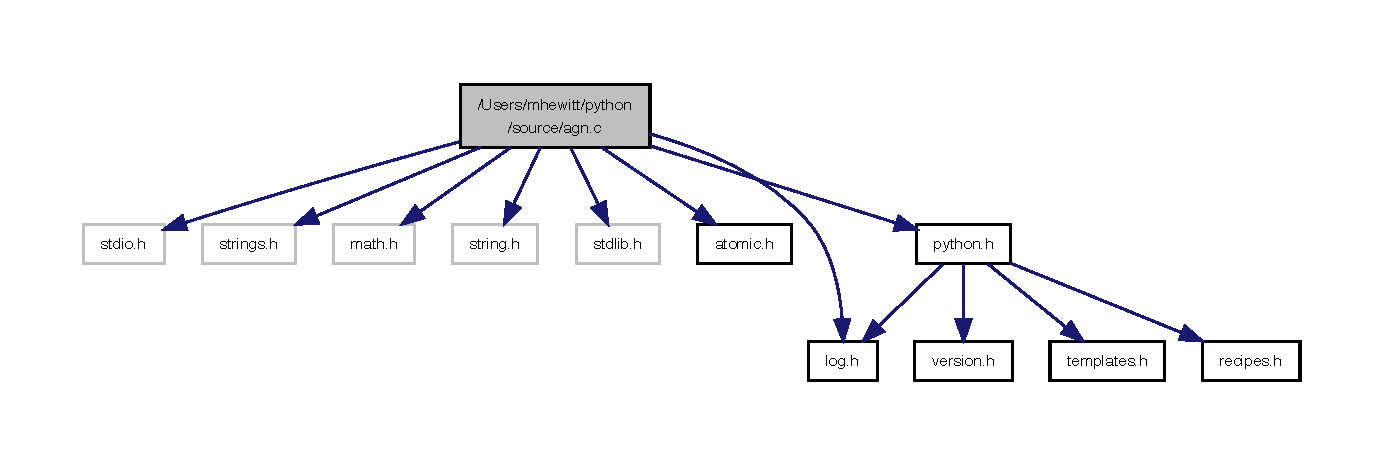
\includegraphics[width=350pt]{agn_8c__incl}
\end{center}
\end{figure}
\subsection*{Macros}
\begin{DoxyCompactItemize}
\item 
\#define \hyperlink{agn_8c_aea0982182724515da5e5a4b2c82a02d2}{X\+F\+R\+E\+Q\+M\+IN}~4.\+84e17
\item 
\#define \hyperlink{agn_8c_a9e305088b07ea013ede73eab99af9fd8}{X\+F\+R\+E\+Q\+M\+AX}~2.\+42e18
\end{DoxyCompactItemize}
\subsection*{Functions}
\begin{DoxyCompactItemize}
\item 
double \hyperlink{agn_8c_ab6c8e4e9577a9edb71a9a5900d43964c}{agn\+\_\+init} (double \hyperlink{import__spherical_8c_a83175ac8fd9d924ff2bce40c99e88870}{r}, double lum, double \hyperlink{templates_8h_a89a27f4f3a5c836df75585774ba7a643}{alpha}, double freqmin, double freqmax, int ioniz\+\_\+or\+\_\+final, double $\ast$f)
\begin{DoxyCompactList}\small\item\em Calculates the total luminosity of an A\+GN type source. \end{DoxyCompactList}\item 
double \hyperlink{agn_8c_ab172924888b8579c4acdd737732edce1}{emittance\+\_\+pow} (double freqmin, double freqmax, double \hyperlink{templates_8h_a89a27f4f3a5c836df75585774ba7a643}{alpha})
\begin{DoxyCompactList}\small\item\em The luminosity of a power law over a frerquency range. \end{DoxyCompactList}\item 
double \hyperlink{agn_8c_a9bd7eb064b17d9b352e044d5e417a649}{emittance\+\_\+bpow} (double freqmin, double freqmax, double lum, double \hyperlink{templates_8h_a89a27f4f3a5c836df75585774ba7a643}{alpha})
\begin{DoxyCompactList}\small\item\em Works out the luminosity of a broken power law. \end{DoxyCompactList}\item 
int \hyperlink{agn_8c_a82dbda6e94577f3ecd6e55c085f2aa10}{photo\+\_\+gen\+\_\+agn} (\hyperlink{python_8h_ad2424d53ebcf811656882a87e11b440c}{Phot\+Ptr} p, double \hyperlink{import__spherical_8c_a83175ac8fd9d924ff2bce40c99e88870}{r}, double \hyperlink{templates_8h_a89a27f4f3a5c836df75585774ba7a643}{alpha}, double weight, double f1, double f2, int spectype, int istart, int nphot)
\begin{DoxyCompactList}\small\item\em Generate a photon from an A\+GN object. \end{DoxyCompactList}\end{DoxyCompactItemize}


\subsection{Detailed Description}
Subroutines relating to power law radiation sources. 

\begin{DoxyAuthor}{Author}
nsh 
\end{DoxyAuthor}
\begin{DoxyDate}{Date}
2011
\end{DoxyDate}
The subroutines and functions in this file are to do with power law S\+E\+Ds, which are mainly used for A\+GN, hence the name of the file. 

\subsection{Macro Definition Documentation}
\mbox{\Hypertarget{agn_8c_a9e305088b07ea013ede73eab99af9fd8}\label{agn_8c_a9e305088b07ea013ede73eab99af9fd8}} 
\index{agn.\+c@{agn.\+c}!X\+F\+R\+E\+Q\+M\+AX@{X\+F\+R\+E\+Q\+M\+AX}}
\index{X\+F\+R\+E\+Q\+M\+AX@{X\+F\+R\+E\+Q\+M\+AX}!agn.\+c@{agn.\+c}}
\subsubsection{\texorpdfstring{X\+F\+R\+E\+Q\+M\+AX}{XFREQMAX}}
{\footnotesize\ttfamily \#define X\+F\+R\+E\+Q\+M\+AX~2.\+42e18}

\mbox{\Hypertarget{agn_8c_aea0982182724515da5e5a4b2c82a02d2}\label{agn_8c_aea0982182724515da5e5a4b2c82a02d2}} 
\index{agn.\+c@{agn.\+c}!X\+F\+R\+E\+Q\+M\+IN@{X\+F\+R\+E\+Q\+M\+IN}}
\index{X\+F\+R\+E\+Q\+M\+IN@{X\+F\+R\+E\+Q\+M\+IN}!agn.\+c@{agn.\+c}}
\subsubsection{\texorpdfstring{X\+F\+R\+E\+Q\+M\+IN}{XFREQMIN}}
{\footnotesize\ttfamily \#define X\+F\+R\+E\+Q\+M\+IN~4.\+84e17}



\subsection{Function Documentation}
\mbox{\Hypertarget{agn_8c_ab6c8e4e9577a9edb71a9a5900d43964c}\label{agn_8c_ab6c8e4e9577a9edb71a9a5900d43964c}} 
\index{agn.\+c@{agn.\+c}!agn\+\_\+init@{agn\+\_\+init}}
\index{agn\+\_\+init@{agn\+\_\+init}!agn.\+c@{agn.\+c}}
\subsubsection{\texorpdfstring{agn\+\_\+init()}{agn\_init()}}
{\footnotesize\ttfamily double agn\+\_\+init (\begin{DoxyParamCaption}\item[{double}]{r,  }\item[{double}]{lum,  }\item[{double}]{alpha,  }\item[{double}]{freqmin,  }\item[{double}]{freqmax,  }\item[{int}]{ioniz\+\_\+or\+\_\+final,  }\item[{double $\ast$}]{f }\end{DoxyParamCaption})}



Calculates the total luminosity of an A\+GN type source. 


\begin{DoxyParams}[1]{Parameters}
\mbox{\tt in}  & {\em double} & r radius of emitting object \\
\hline
\mbox{\tt in}  & {\em double} & lum the luminosity of the A\+GN (2-\/10keV) -\/ X\+XX I\textquotesingle{}m not sure this is used apart from \\
\hline
\mbox{\tt in}  & {\em double} & alpha the spectral index of the PL source -\/ also sometimes used for a temperature if a BB source is required \\
\hline
\mbox{\tt in}  & {\em double} & freqmin minimum frequency to integrate over \\
\hline
\mbox{\tt in}  & {\em double} & freqmax maximum frequency \\
\hline
\mbox{\tt in}  & {\em int} & ioniz\+\_\+or\+\_\+final flag to say if we are in the ionization cycles or spectral cycle \\
\hline
\mbox{\tt out}  & {\em double} & f the returned luminosity \\
\hline
\end{DoxyParams}
\begin{DoxyReturn}{Returns}
f -\/ the luminosity -\/ seems to be returned as well as set implicitly.
\end{DoxyReturn}
This routine is used when one is working out how many photons will be made from each of several sources. This computes the total luminosity of a source of radius r, with spectral index alpha between band boundaries given by freqmin and freqmax

\paragraph*{Notes}

There seem to be some inconsistencies here -\/ lum (the 2-\/10keV luminosity of the PL source) is supplied but it doesnt seem to be used apart from in the emittance\+\_\+continuum which is nonsense -\/ this requires a temperature and a local gravity Another inconsistency is that the bremstrahlung code uses values for T and alpha that are stored in the geo structure, whilst the power law uses data supplied in the code. 

Definition at line 54 of file agn.\+c.

Here is the call graph for this function\+:
\nopagebreak
\begin{figure}[H]
\begin{center}
\leavevmode
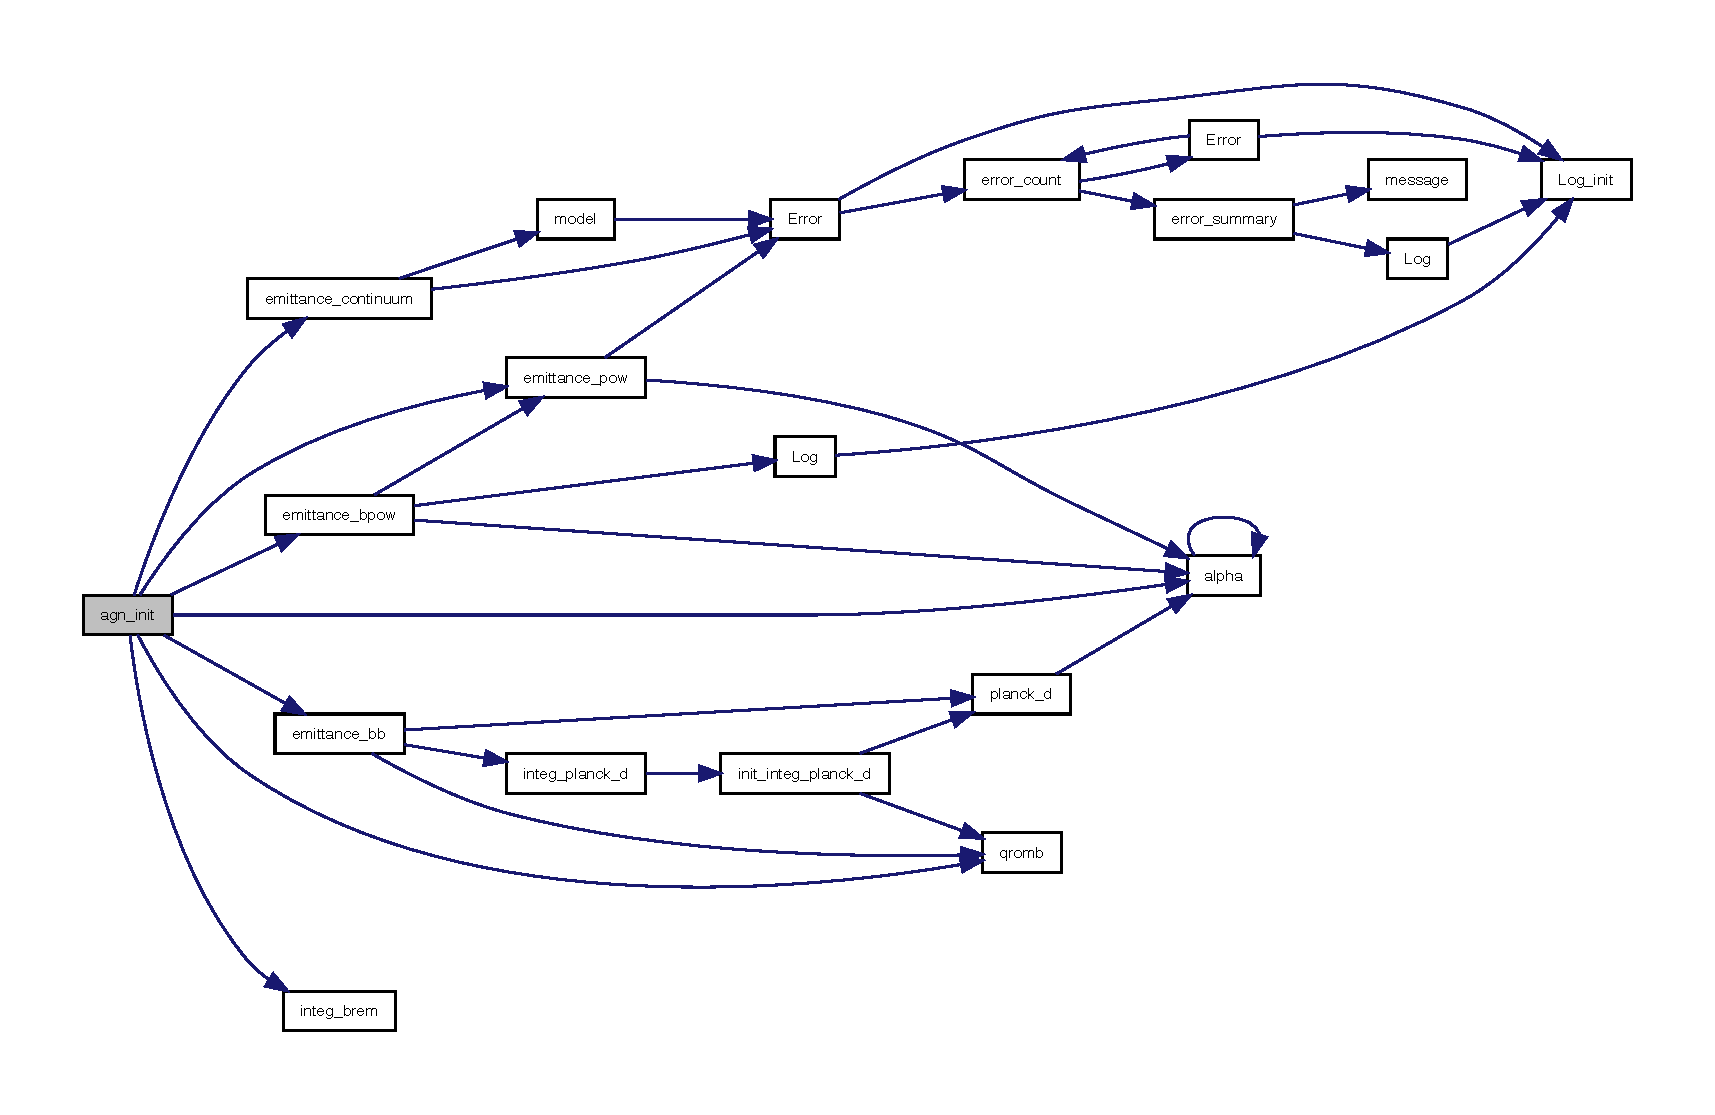
\includegraphics[width=350pt]{agn_8c_ab6c8e4e9577a9edb71a9a5900d43964c_cgraph}
\end{center}
\end{figure}
Here is the caller graph for this function\+:
\nopagebreak
\begin{figure}[H]
\begin{center}
\leavevmode
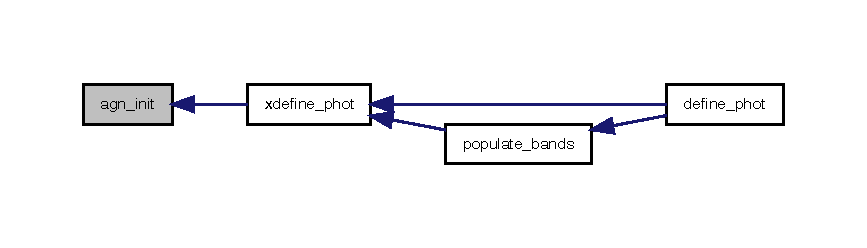
\includegraphics[width=350pt]{agn_8c_ab6c8e4e9577a9edb71a9a5900d43964c_icgraph}
\end{center}
\end{figure}
\mbox{\Hypertarget{agn_8c_a9bd7eb064b17d9b352e044d5e417a649}\label{agn_8c_a9bd7eb064b17d9b352e044d5e417a649}} 
\index{agn.\+c@{agn.\+c}!emittance\+\_\+bpow@{emittance\+\_\+bpow}}
\index{emittance\+\_\+bpow@{emittance\+\_\+bpow}!agn.\+c@{agn.\+c}}
\subsubsection{\texorpdfstring{emittance\+\_\+bpow()}{emittance\_bpow()}}
{\footnotesize\ttfamily double emittance\+\_\+bpow (\begin{DoxyParamCaption}\item[{double}]{freqmin,  }\item[{double}]{freqmax,  }\item[{double}]{lum,  }\item[{double}]{alpha }\end{DoxyParamCaption})}



Works out the luminosity of a broken power law. 


\begin{DoxyParams}[1]{Parameters}
\mbox{\tt in,out}  & {\em double} & freqmin min frequency that we are generating photons over \\
\hline
\mbox{\tt in,out}  & {\em double} & freqmax max frequency that we are generating photons over \\
\hline
\mbox{\tt in,out}  & {\em double} & lum 2-\/10kev luminosity \\
\hline
\mbox{\tt in,out}  & {\em double} & alpha is the 2-\/10kev slope. \\
\hline
\end{DoxyParams}
\begin{DoxyReturn}{Returns}
emit The luminosity of the whole power law.
\end{DoxyReturn}
computes the emittance of a broken power law coded to try to replicate the cloudy table type power law. There are three sections -\/ a central bit, which should cover the 2-\/10kev portion of the spectrum, a low frequency tail and a high frequency tail .

\paragraph*{Notes}

??? N\+O\+T\+ES ??? 

Definition at line 219 of file agn.\+c.

Here is the call graph for this function\+:
\nopagebreak
\begin{figure}[H]
\begin{center}
\leavevmode
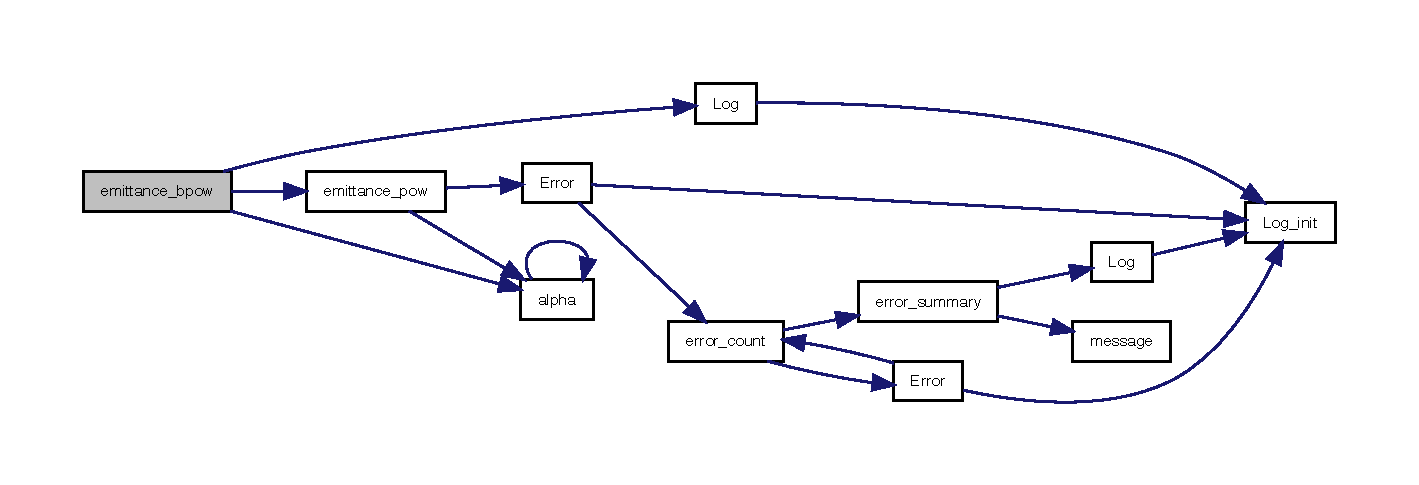
\includegraphics[width=350pt]{agn_8c_a9bd7eb064b17d9b352e044d5e417a649_cgraph}
\end{center}
\end{figure}
Here is the caller graph for this function\+:
\nopagebreak
\begin{figure}[H]
\begin{center}
\leavevmode
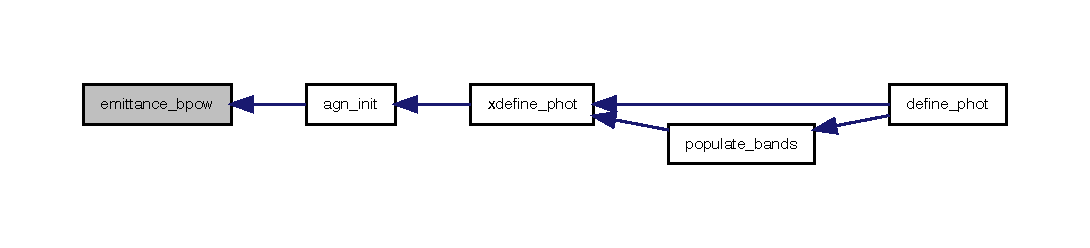
\includegraphics[width=350pt]{agn_8c_a9bd7eb064b17d9b352e044d5e417a649_icgraph}
\end{center}
\end{figure}
\mbox{\Hypertarget{agn_8c_ab172924888b8579c4acdd737732edce1}\label{agn_8c_ab172924888b8579c4acdd737732edce1}} 
\index{agn.\+c@{agn.\+c}!emittance\+\_\+pow@{emittance\+\_\+pow}}
\index{emittance\+\_\+pow@{emittance\+\_\+pow}!agn.\+c@{agn.\+c}}
\subsubsection{\texorpdfstring{emittance\+\_\+pow()}{emittance\_pow()}}
{\footnotesize\ttfamily double emittance\+\_\+pow (\begin{DoxyParamCaption}\item[{double}]{freqmin,  }\item[{double}]{freqmax,  }\item[{double}]{alpha }\end{DoxyParamCaption})}



The luminosity of a power law over a frerquency range. 


\begin{DoxyParams}[1]{Parameters}
\mbox{\tt in}  & {\em double} & freqmin lower frequency bound \\
\hline
\mbox{\tt in}  & {\em double} & freqmax upper frequency bound \\
\hline
\mbox{\tt in}  & {\em double} & alpha spectral index \\
\hline
\end{DoxyParams}
\begin{DoxyReturn}{Returns}
double emit the luminosoty
\end{DoxyReturn}
A Simple routine which just integrates a power law between two limits. There is a little bit of code that deals with the case where an advanced mode is used that cuts off the low frequency tail -\/ and a bit of clever work to check for the pathalogical case of alpha=-\/1 where one cannot symbolically integrate.

\paragraph*{Notes}

Definition at line 131 of file agn.\+c.

Here is the call graph for this function\+:
\nopagebreak
\begin{figure}[H]
\begin{center}
\leavevmode
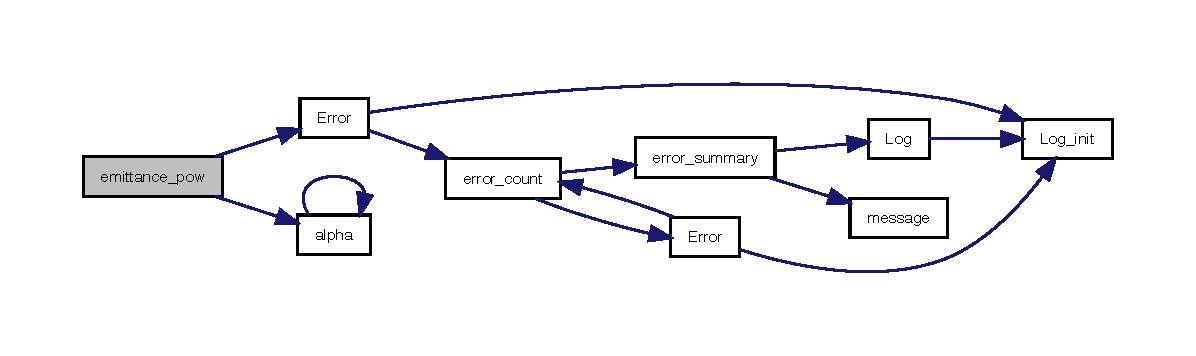
\includegraphics[width=350pt]{agn_8c_ab172924888b8579c4acdd737732edce1_cgraph}
\end{center}
\end{figure}
Here is the caller graph for this function\+:
\nopagebreak
\begin{figure}[H]
\begin{center}
\leavevmode
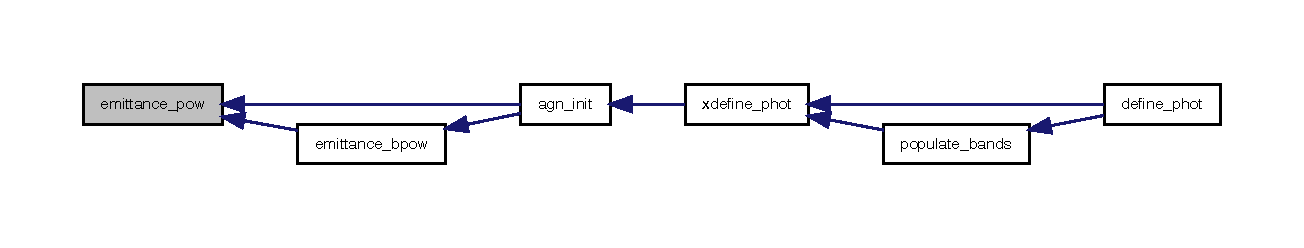
\includegraphics[width=350pt]{agn_8c_ab172924888b8579c4acdd737732edce1_icgraph}
\end{center}
\end{figure}
\mbox{\Hypertarget{agn_8c_a82dbda6e94577f3ecd6e55c085f2aa10}\label{agn_8c_a82dbda6e94577f3ecd6e55c085f2aa10}} 
\index{agn.\+c@{agn.\+c}!photo\+\_\+gen\+\_\+agn@{photo\+\_\+gen\+\_\+agn}}
\index{photo\+\_\+gen\+\_\+agn@{photo\+\_\+gen\+\_\+agn}!agn.\+c@{agn.\+c}}
\subsubsection{\texorpdfstring{photo\+\_\+gen\+\_\+agn()}{photo\_gen\_agn()}}
{\footnotesize\ttfamily int photo\+\_\+gen\+\_\+agn (\begin{DoxyParamCaption}\item[{\hyperlink{python_8h_ad2424d53ebcf811656882a87e11b440c}{Phot\+Ptr}}]{p,  }\item[{double}]{r,  }\item[{double}]{alpha,  }\item[{double}]{weight,  }\item[{double}]{f1,  }\item[{double}]{f2,  }\item[{int}]{spectype,  }\item[{int}]{istart,  }\item[{int}]{nphot }\end{DoxyParamCaption})}



Generate a photon from an A\+GN object. 


\begin{DoxyParams}[1]{Parameters}
\mbox{\tt in,out}  & {\em Phot\+Ptr} & p pointer to the photon array \\
\hline
\mbox{\tt in,out}  & {\em double} & r radius of the central source \\
\hline
\mbox{\tt in,out}  & {\em double} & alpha spectral index of the PL sourece -\/ also used to communicate temperature if a BB or model is used. \\
\hline
\mbox{\tt in,out}  & {\em double} & weight the weight of each photon to be made \\
\hline
\mbox{\tt in,out}  & {\em double} & f1 lower frequency bound \\
\hline
\mbox{\tt in,out}  & {\em double} & f2 upper frequency nound \\
\hline
\mbox{\tt in,out}  & {\em int} & spectype the type of S\+ED \\
\hline
\mbox{\tt in,out}  & {\em int} & istart the number of the first photon to be made -\/ index into the p array \\
\hline
\mbox{\tt in,out}  & {\em int} & nphot the number of photons to be made \\
\hline
\end{DoxyParams}
\begin{DoxyReturn}{Returns}
0 (if successful or unscuccessful)
\end{DoxyReturn}
This subroutine produces photons from an A\+GN type source. There are a range of different S\+E\+Ds that can be used, these are communicated by the spectype and different choices cause different surbroutines to be called. The only {\itshape real} work done here is to compute the strarting location and direction of the photons.

\paragraph*{Notes}

Definition at line 374 of file agn.\+c.

Here is the call graph for this function\+:
\nopagebreak
\begin{figure}[H]
\begin{center}
\leavevmode
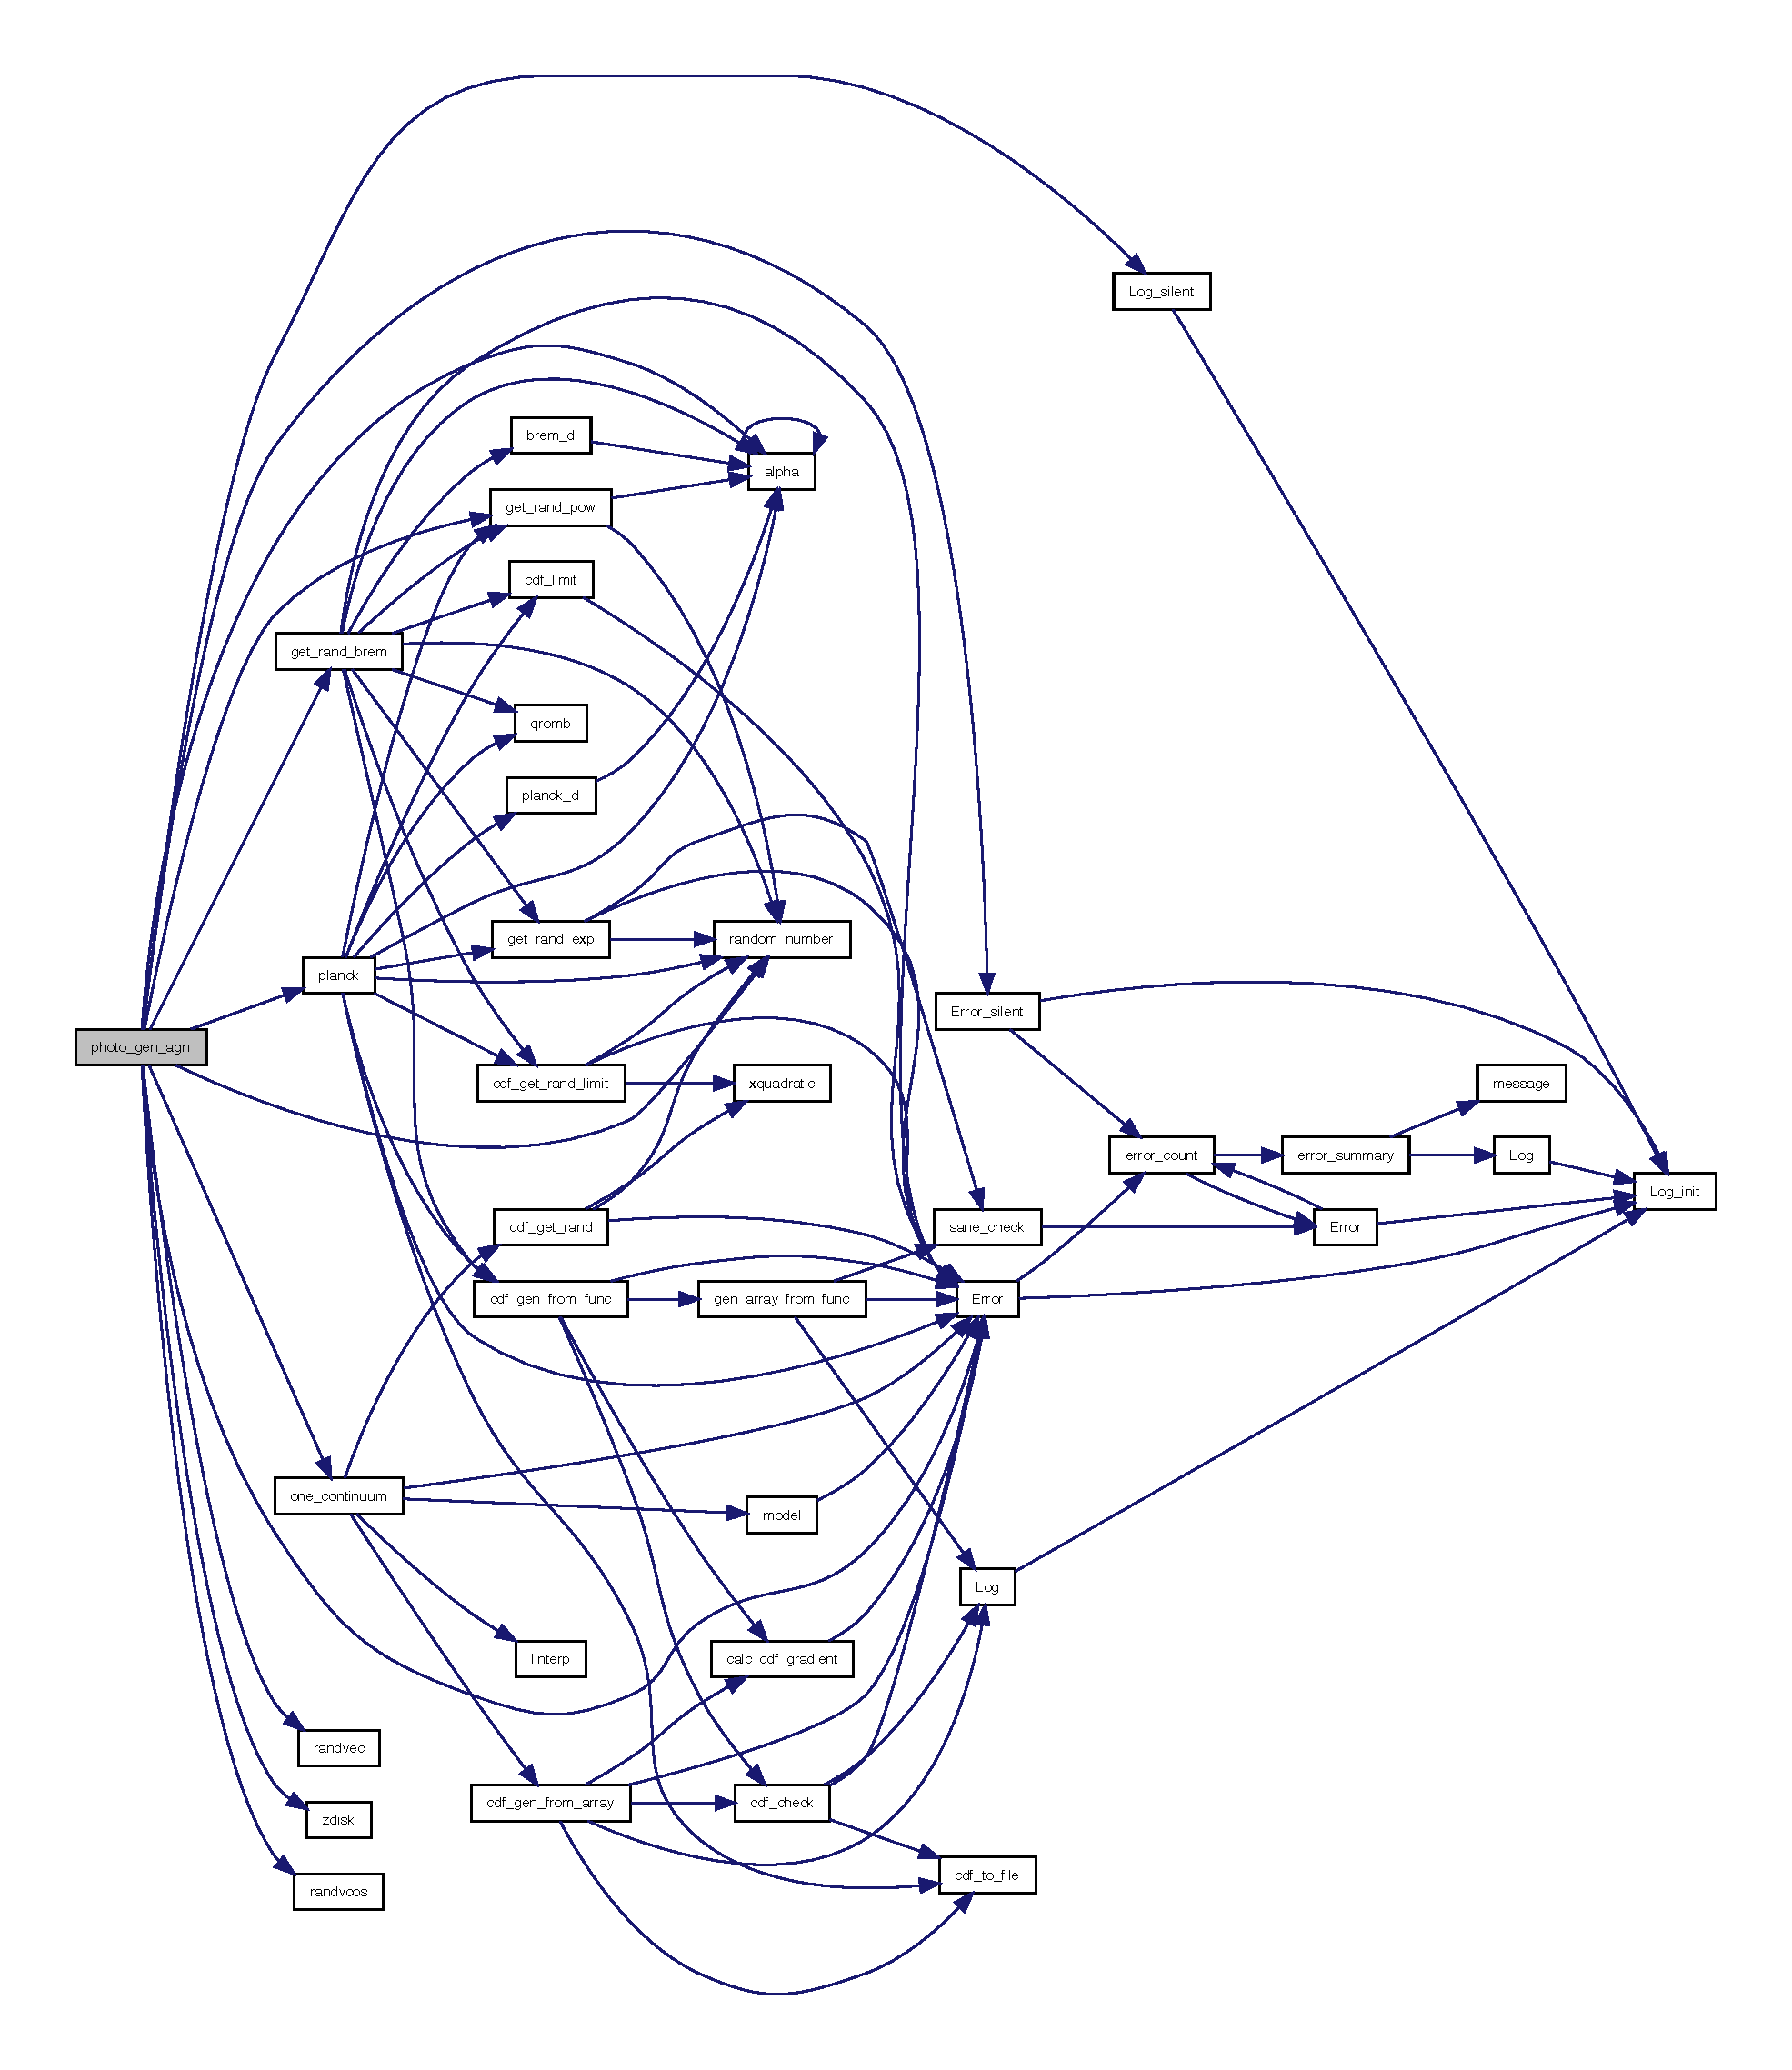
\includegraphics[width=350pt]{agn_8c_a82dbda6e94577f3ecd6e55c085f2aa10_cgraph}
\end{center}
\end{figure}
Here is the caller graph for this function\+:
\nopagebreak
\begin{figure}[H]
\begin{center}
\leavevmode
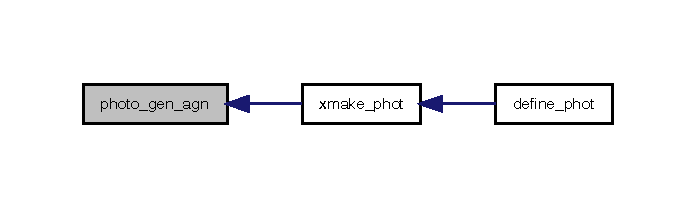
\includegraphics[width=334pt]{agn_8c_a82dbda6e94577f3ecd6e55c085f2aa10_icgraph}
\end{center}
\end{figure}

\hypertarget{anisowind_8c}{}\section{/\+Users/mhewitt/python/source/anisowind.c File Reference}
\label{anisowind_8c}\index{/\+Users/mhewitt/python/source/anisowind.\+c@{/\+Users/mhewitt/python/source/anisowind.\+c}}


Routines to implement anisotropic scattering in the wind.  


{\ttfamily \#include $<$stdio.\+h$>$}\newline
{\ttfamily \#include $<$stdlib.\+h$>$}\newline
{\ttfamily \#include $<$math.\+h$>$}\newline
{\ttfamily \#include \char`\"{}atomic.\+h\char`\"{}}\newline
{\ttfamily \#include \char`\"{}python.\+h\char`\"{}}\newline
Include dependency graph for anisowind.\+c\+:
\nopagebreak
\begin{figure}[H]
\begin{center}
\leavevmode
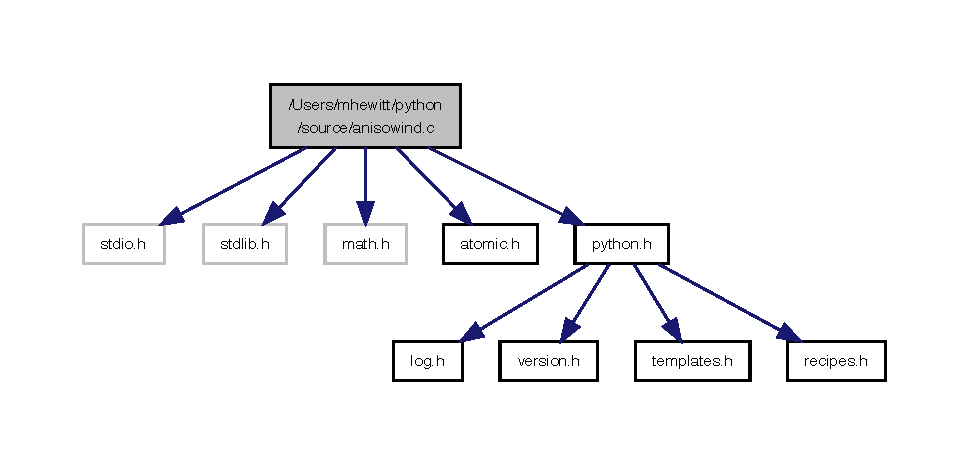
\includegraphics[width=350pt]{anisowind_8c__incl}
\end{center}
\end{figure}
\subsection*{Macros}
\begin{DoxyCompactItemize}
\item 
\#define \hyperlink{anisowind_8c_a30e700ca1832f578d922cf82e7a7833a}{T\+A\+U\+\_\+\+T\+OP}
\item 
\#define \hyperlink{anisowind_8c_a32d322486dd5c75bc90a3e069795ca48}{T\+A\+U\+\_\+\+B\+OT}~0.\+01
\item 
\#define \hyperlink{anisowind_8c_a345cd57c7488cd806c3985578255bc5b}{V\+R\+A\+N\+D\+W\+I\+N\+D\+\_\+\+F\+L\+O\+OR}~1e-\/5
\item 
\#define \hyperlink{anisowind_8c_ada627bd85738018041d77e7148607d90}{V\+R\+A\+N\+D\+W\+I\+N\+D\+\_\+\+T\+AU}~11.\+51
\item 
\#define \hyperlink{anisowind_8c_a52124d035a50390906fac4141e93a958}{R\+E\+W\+E\+I\+G\+H\+T\+W\+I\+N\+D\+\_\+\+T\+A\+U\+\_\+\+M\+AX}~100.
\item 
\#define \hyperlink{anisowind_8c_a536ffe4a24745665335aef1c4684090e}{L\+O\+G\+T\+A\+U\+M\+IN}~-\/2.
\item 
\#define \hyperlink{anisowind_8c_a2744c207c1c56b9104d6892a5404d2ca}{L\+O\+G\+T\+A\+U\+M\+AX}~1.
\end{DoxyCompactItemize}
\subsection*{Functions}
\begin{DoxyCompactItemize}
\item 
int \hyperlink{anisowind_8c_aa02bd1c515967ac3e1214843158df2f4}{randwind} (\hyperlink{python_8h_ad2424d53ebcf811656882a87e11b440c}{Phot\+Ptr} p, lmn, \hyperlink{disk_8c_afaba31659717b807b58fa7b80c4847a1}{north})
\begin{DoxyCompactList}\small\item\em calculate a new direction for the photon which is being scattered in the wind in the S\+C\+A\+T\+T\+E\+R\+\_\+\+M\+O\+D\+E\+\_\+\+A\+N\+I\+S\+O\+T\+R\+O\+P\+IC scattering mode. \end{DoxyCompactList}\item 
double \hyperlink{anisowind_8c_af170ad39af01fbe3b232230692c2aa5e}{vrandwind} (double \hyperlink{import__cylindrical_8c_a099bc7b5a9501685180c163c1ffb67d0}{x})
\begin{DoxyCompactList}\small\item\em the function that is used to generate the cdf for anisotropic scattering. \end{DoxyCompactList}\item 
double \hyperlink{anisowind_8c_a76f3cece46c92129a1e138a02aac87ca}{reweightwind} (\hyperlink{python_8h_ad2424d53ebcf811656882a87e11b440c}{Phot\+Ptr} p)
\begin{DoxyCompactList}\small\item\em calculates the weight of a photon in the wind that is forced to scatter along a specific line of sight. \end{DoxyCompactList}\item 
int \hyperlink{anisowind_8c_a62480c3fe99eaa0284c85a48b1e8427d}{make\+\_\+cdf\+\_\+randwind} (double tau)
\item 
int \hyperlink{anisowind_8c_a5cc282e1f3d56ce0f29cb080bc225408}{randwind\+\_\+thermal\+\_\+trapping} (\hyperlink{python_8h_ad2424d53ebcf811656882a87e11b440c}{Phot\+Ptr} p, int $\ast$nnscat)
\begin{DoxyCompactList}\small\item\em is the routine which chooses a new anisotropic direction in geo.\+scatter\+\_\+mode = S\+C\+A\+T\+T\+E\+R\+\_\+\+M\+O\+D\+E\+\_\+\+T\+H\+E\+R\+M\+AL \end{DoxyCompactList}\end{DoxyCompactItemize}
\subsection*{Variables}
\begin{DoxyCompactItemize}
\item 
struct \hyperlink{struct_cdf}{Cdf} \hyperlink{anisowind_8c_ab3e97ac75b82f9c4ced9218e78eb2fa4}{cdf\+\_\+randwind\+\_\+store} \mbox{[}100\mbox{]}
\item 
\hyperlink{python_8h_a14b633e617b31ead523c75ce80cc56e1}{Cdf\+Ptr} \hyperlink{anisowind_8c_a7d5d3c2b11592abf6eb482a145e10d50}{cdf\+\_\+randwind}
\item 
struct \hyperlink{structphoton}{photon} \hyperlink{anisowind_8c_a9f5059b178ab31b23b014793eb4854b0}{phot\+\_\+randwind}
\item 
double \hyperlink{anisowind_8c_acabc03109a812245488027702104978c}{tau\+\_\+randwind} = -\/1000.
\item 
int \hyperlink{anisowind_8c_a0ae08e53a25f8ac625b0c2f872056d2d}{reweightwind\+\_\+init} = 1
\item 
double \hyperlink{anisowind_8c_addb96381a70d5bbbd4d70c8b469529d3}{reweightwind\+\_\+zmax}
\item 
int \hyperlink{anisowind_8c_a872ce5174f328e50a8381894469b3790}{init\+\_\+make\+\_\+cdf\+\_\+randwind} = 1
\begin{DoxyCompactList}\small\item\em Generate the cumulative distribution functions needed for selecting a direction for a scattered photon, and then select the cdf needed ro a particulat tau. \end{DoxyCompactList}\item 
int \hyperlink{anisowind_8c_a656c37768c70e0b91e3f5028654f79ec}{make\+\_\+cdf\+\_\+randwind\+\_\+njumps}
\item 
double \hyperlink{anisowind_8c_a6f923c8cdf71897592f32606c6d8fd0e}{make\+\_\+cdf\+\_\+randwind\+\_\+jumps} \mbox{[}180\mbox{]}
\item 
double \hyperlink{anisowind_8c_af5db99077c04b8cf610205694640ddeb}{cdf\+\_\+randwind\+\_\+dlogtau}
\end{DoxyCompactItemize}


\subsection{Detailed Description}
Routines to implement anisotropic scattering in the wind. 

\begin{DoxyAuthor}{Author}
ksl 
\end{DoxyAuthor}
\begin{DoxyDate}{Date}
March, 2018
\end{DoxyDate}
Python supports several ways to determine a new photon direction when a photon scatters in thie wind. These include


\begin{DoxyItemize}
\item S\+C\+A\+T\+T\+E\+R\+\_\+\+M\+O\+D\+E\+\_\+\+I\+S\+O\+T\+R\+O\+P\+IC -\/isotropic scattering (randvec),
\item S\+C\+A\+T\+T\+E\+R\+\_\+\+M\+O\+D\+E\+\_\+\+A\+N\+I\+S\+O\+T\+R\+O\+P\+IC -\/ anisotropic scattering (randwind) and
\item S\+C\+A\+T\+T\+E\+R\+\_\+\+M\+O\+D\+E\+\_\+\+T\+H\+E\+R\+M\+AL -\/ thermally-\/broadened anisotropic scattering (randwind\+\_\+thermal\+\_\+trapping). 
\end{DoxyItemize}

\subsection{Macro Definition Documentation}
\mbox{\Hypertarget{anisowind_8c_a2744c207c1c56b9104d6892a5404d2ca}\label{anisowind_8c_a2744c207c1c56b9104d6892a5404d2ca}} 
\index{anisowind.\+c@{anisowind.\+c}!L\+O\+G\+T\+A\+U\+M\+AX@{L\+O\+G\+T\+A\+U\+M\+AX}}
\index{L\+O\+G\+T\+A\+U\+M\+AX@{L\+O\+G\+T\+A\+U\+M\+AX}!anisowind.\+c@{anisowind.\+c}}
\subsubsection{\texorpdfstring{L\+O\+G\+T\+A\+U\+M\+AX}{LOGTAUMAX}}
{\footnotesize\ttfamily \#define L\+O\+G\+T\+A\+U\+M\+AX~1.}



Definition at line 484 of file anisowind.\+c.

\mbox{\Hypertarget{anisowind_8c_a536ffe4a24745665335aef1c4684090e}\label{anisowind_8c_a536ffe4a24745665335aef1c4684090e}} 
\index{anisowind.\+c@{anisowind.\+c}!L\+O\+G\+T\+A\+U\+M\+IN@{L\+O\+G\+T\+A\+U\+M\+IN}}
\index{L\+O\+G\+T\+A\+U\+M\+IN@{L\+O\+G\+T\+A\+U\+M\+IN}!anisowind.\+c@{anisowind.\+c}}
\subsubsection{\texorpdfstring{L\+O\+G\+T\+A\+U\+M\+IN}{LOGTAUMIN}}
{\footnotesize\ttfamily \#define L\+O\+G\+T\+A\+U\+M\+IN~-\/2.}



Definition at line 483 of file anisowind.\+c.

\mbox{\Hypertarget{anisowind_8c_a52124d035a50390906fac4141e93a958}\label{anisowind_8c_a52124d035a50390906fac4141e93a958}} 
\index{anisowind.\+c@{anisowind.\+c}!R\+E\+W\+E\+I\+G\+H\+T\+W\+I\+N\+D\+\_\+\+T\+A\+U\+\_\+\+M\+AX@{R\+E\+W\+E\+I\+G\+H\+T\+W\+I\+N\+D\+\_\+\+T\+A\+U\+\_\+\+M\+AX}}
\index{R\+E\+W\+E\+I\+G\+H\+T\+W\+I\+N\+D\+\_\+\+T\+A\+U\+\_\+\+M\+AX@{R\+E\+W\+E\+I\+G\+H\+T\+W\+I\+N\+D\+\_\+\+T\+A\+U\+\_\+\+M\+AX}!anisowind.\+c@{anisowind.\+c}}
\subsubsection{\texorpdfstring{R\+E\+W\+E\+I\+G\+H\+T\+W\+I\+N\+D\+\_\+\+T\+A\+U\+\_\+\+M\+AX}{REWEIGHTWIND\_TAU\_MAX}}
{\footnotesize\ttfamily \#define R\+E\+W\+E\+I\+G\+H\+T\+W\+I\+N\+D\+\_\+\+T\+A\+U\+\_\+\+M\+AX~100.}



Definition at line 321 of file anisowind.\+c.

\mbox{\Hypertarget{anisowind_8c_a32d322486dd5c75bc90a3e069795ca48}\label{anisowind_8c_a32d322486dd5c75bc90a3e069795ca48}} 
\index{anisowind.\+c@{anisowind.\+c}!T\+A\+U\+\_\+\+B\+OT@{T\+A\+U\+\_\+\+B\+OT}}
\index{T\+A\+U\+\_\+\+B\+OT@{T\+A\+U\+\_\+\+B\+OT}!anisowind.\+c@{anisowind.\+c}}
\subsubsection{\texorpdfstring{T\+A\+U\+\_\+\+B\+OT}{TAU\_BOT}}
{\footnotesize\ttfamily \#define T\+A\+U\+\_\+\+B\+OT~0.\+01}



Definition at line 92 of file anisowind.\+c.

\mbox{\Hypertarget{anisowind_8c_a30e700ca1832f578d922cf82e7a7833a}\label{anisowind_8c_a30e700ca1832f578d922cf82e7a7833a}} 
\index{anisowind.\+c@{anisowind.\+c}!T\+A\+U\+\_\+\+T\+OP@{T\+A\+U\+\_\+\+T\+OP}}
\index{T\+A\+U\+\_\+\+T\+OP@{T\+A\+U\+\_\+\+T\+OP}!anisowind.\+c@{anisowind.\+c}}
\subsubsection{\texorpdfstring{T\+A\+U\+\_\+\+T\+OP}{TAU\_TOP}}
{\footnotesize\ttfamily \#define T\+A\+U\+\_\+\+T\+OP}

{\bfseries Value\+:}
\begin{DoxyCode}
10.0         \textcolor{comment}{/* tau above which we assume the angular distribution function}
\textcolor{comment}{                                   no longer changes significantly, e.g above which the surface behaves}
\textcolor{comment}{                                   like a solid surface */}
\end{DoxyCode}


Definition at line 89 of file anisowind.\+c.

\mbox{\Hypertarget{anisowind_8c_a345cd57c7488cd806c3985578255bc5b}\label{anisowind_8c_a345cd57c7488cd806c3985578255bc5b}} 
\index{anisowind.\+c@{anisowind.\+c}!V\+R\+A\+N\+D\+W\+I\+N\+D\+\_\+\+F\+L\+O\+OR@{V\+R\+A\+N\+D\+W\+I\+N\+D\+\_\+\+F\+L\+O\+OR}}
\index{V\+R\+A\+N\+D\+W\+I\+N\+D\+\_\+\+F\+L\+O\+OR@{V\+R\+A\+N\+D\+W\+I\+N\+D\+\_\+\+F\+L\+O\+OR}!anisowind.\+c@{anisowind.\+c}}
\subsubsection{\texorpdfstring{V\+R\+A\+N\+D\+W\+I\+N\+D\+\_\+\+F\+L\+O\+OR}{VRANDWIND\_FLOOR}}
{\footnotesize\ttfamily \#define V\+R\+A\+N\+D\+W\+I\+N\+D\+\_\+\+F\+L\+O\+OR~1e-\/5}



Definition at line 253 of file anisowind.\+c.

\mbox{\Hypertarget{anisowind_8c_ada627bd85738018041d77e7148607d90}\label{anisowind_8c_ada627bd85738018041d77e7148607d90}} 
\index{anisowind.\+c@{anisowind.\+c}!V\+R\+A\+N\+D\+W\+I\+N\+D\+\_\+\+T\+AU@{V\+R\+A\+N\+D\+W\+I\+N\+D\+\_\+\+T\+AU}}
\index{V\+R\+A\+N\+D\+W\+I\+N\+D\+\_\+\+T\+AU@{V\+R\+A\+N\+D\+W\+I\+N\+D\+\_\+\+T\+AU}!anisowind.\+c@{anisowind.\+c}}
\subsubsection{\texorpdfstring{V\+R\+A\+N\+D\+W\+I\+N\+D\+\_\+\+T\+AU}{VRANDWIND\_TAU}}
{\footnotesize\ttfamily \#define V\+R\+A\+N\+D\+W\+I\+N\+D\+\_\+\+T\+AU~11.\+51}



Definition at line 254 of file anisowind.\+c.



\subsection{Function Documentation}
\mbox{\Hypertarget{anisowind_8c_a62480c3fe99eaa0284c85a48b1e8427d}\label{anisowind_8c_a62480c3fe99eaa0284c85a48b1e8427d}} 
\index{anisowind.\+c@{anisowind.\+c}!make\+\_\+cdf\+\_\+randwind@{make\+\_\+cdf\+\_\+randwind}}
\index{make\+\_\+cdf\+\_\+randwind@{make\+\_\+cdf\+\_\+randwind}!anisowind.\+c@{anisowind.\+c}}
\subsubsection{\texorpdfstring{make\+\_\+cdf\+\_\+randwind()}{make\_cdf\_randwind()}}
{\footnotesize\ttfamily int make\+\_\+cdf\+\_\+randwind (\begin{DoxyParamCaption}\item[{double}]{tau }\end{DoxyParamCaption})}



Definition at line 489 of file anisowind.\+c.

Here is the call graph for this function\+:
\nopagebreak
\begin{figure}[H]
\begin{center}
\leavevmode
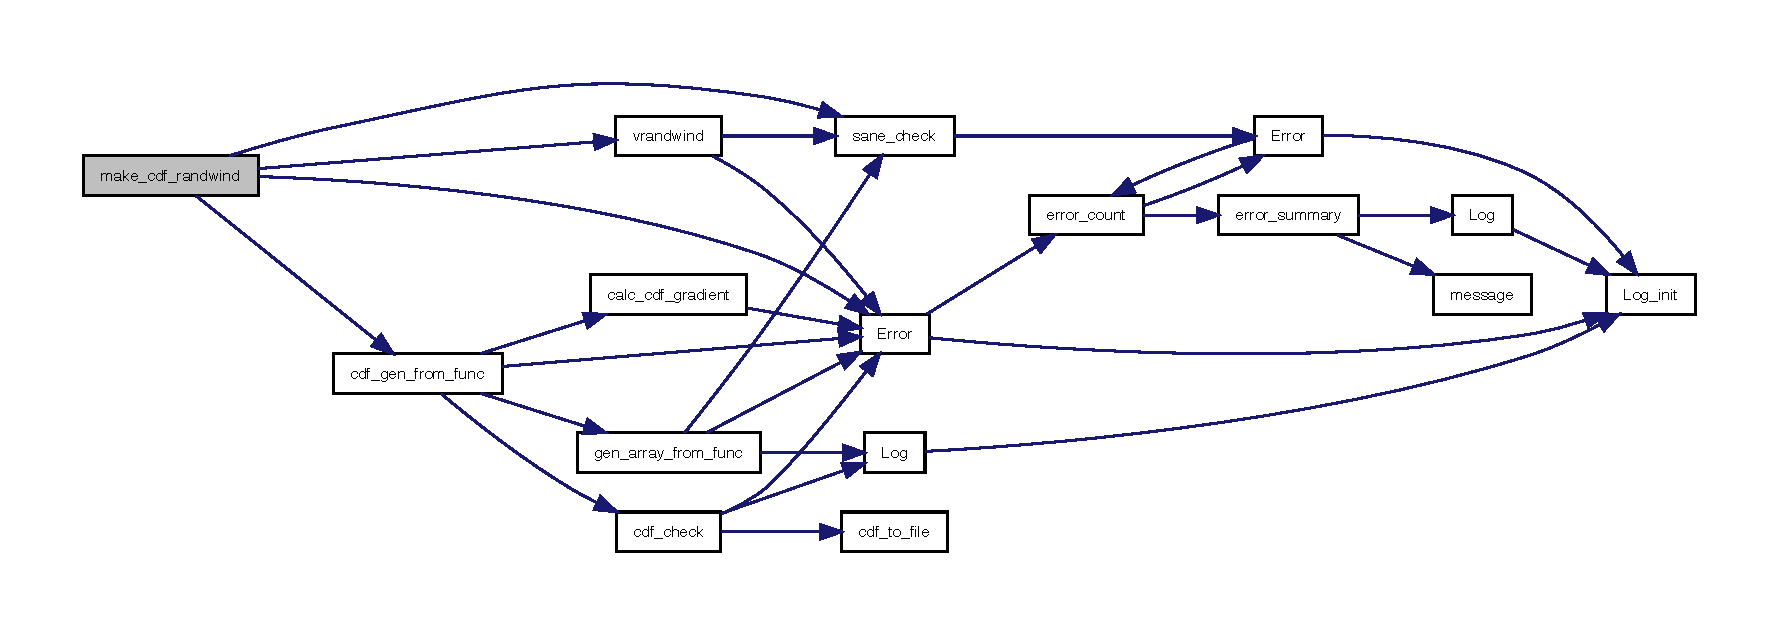
\includegraphics[width=350pt]{anisowind_8c_a62480c3fe99eaa0284c85a48b1e8427d_cgraph}
\end{center}
\end{figure}
Here is the caller graph for this function\+:
\nopagebreak
\begin{figure}[H]
\begin{center}
\leavevmode
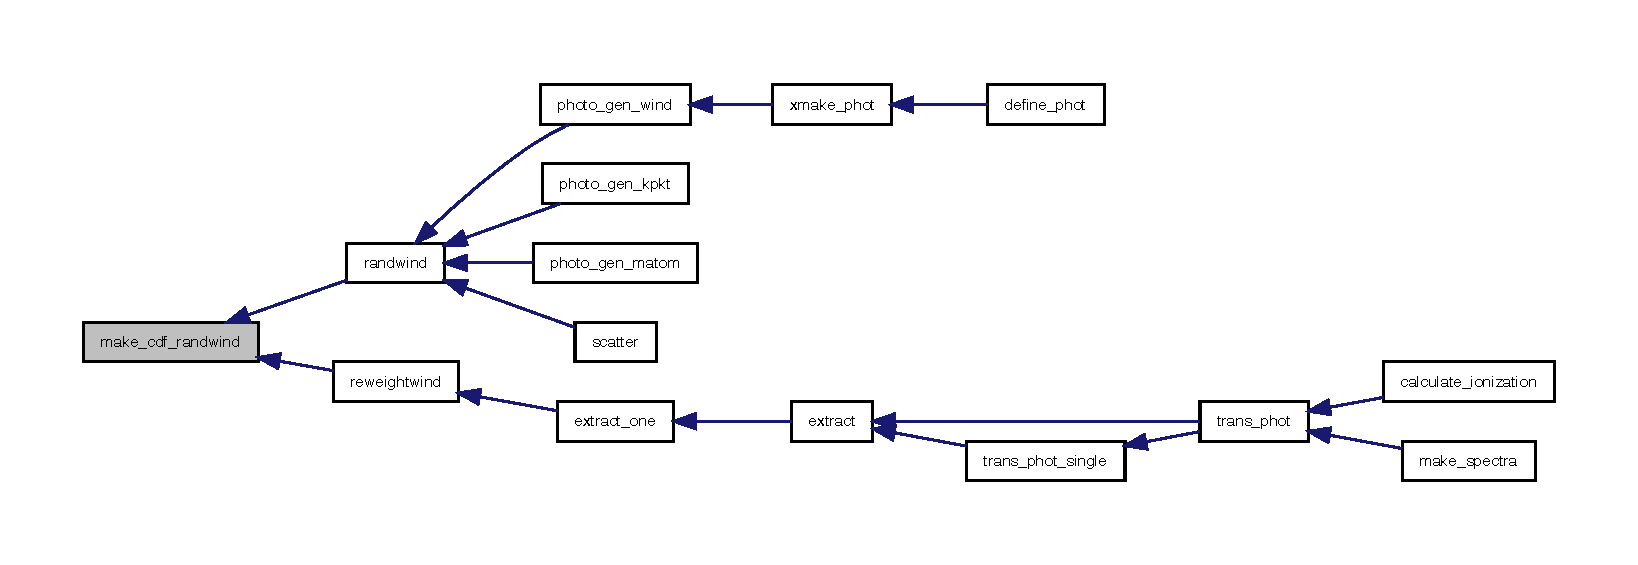
\includegraphics[width=350pt]{anisowind_8c_a62480c3fe99eaa0284c85a48b1e8427d_icgraph}
\end{center}
\end{figure}
\mbox{\Hypertarget{anisowind_8c_aa02bd1c515967ac3e1214843158df2f4}\label{anisowind_8c_aa02bd1c515967ac3e1214843158df2f4}} 
\index{anisowind.\+c@{anisowind.\+c}!randwind@{randwind}}
\index{randwind@{randwind}!anisowind.\+c@{anisowind.\+c}}
\subsubsection{\texorpdfstring{randwind()}{randwind()}}
{\footnotesize\ttfamily int randwind (\begin{DoxyParamCaption}\item[{\hyperlink{python_8h_ad2424d53ebcf811656882a87e11b440c}{Phot\+Ptr}}]{p,  }\item[{lmn}]{,  }\item[{\hyperlink{disk_8c_afaba31659717b807b58fa7b80c4847a1}{north}}]{ }\end{DoxyParamCaption})}



calculate a new direction for the photon which is being scattered in the wind in the S\+C\+A\+T\+T\+E\+R\+\_\+\+M\+O\+D\+E\+\_\+\+A\+N\+I\+S\+O\+T\+R\+O\+P\+IC scattering mode. 


\begin{DoxyParams}[1]{Parameters}
\mbox{\tt in}  & {\em Phot\+Ptr} & p The photon (at the position it is scattering, and the resonance causing the scatter indicated) \\
\hline
\mbox{\tt out}  & {\em double} & lmn\mbox{[}3\mbox{]} The new photon direction \\
\hline
\mbox{\tt in}  & {\em double} & north\mbox{[}3\mbox{]} the direction of maximum velocity gradient in the wind cell where the photon is located \\
\hline
\end{DoxyParams}
\begin{DoxyReturn}{Returns}
Normally returns 0, -\/1 if nres for the photon is not positive (which would indicate this was not a resonance scatter)
\end{DoxyReturn}
This routine is called whenever one wants to generate a new direction in the S\+C\+A\+T\+T\+E\+R\+\_\+\+M\+O\+D\+E\+\_\+\+A\+N\+I\+S\+O\+T\+R\+O\+P\+IC scattering mode.

Given the photon position and the resonance, the routine $\ast$ first calcuates the optical depth in the direction of the maximum dv\+\_\+ds for that cell.

The routine then calls, make\+\_\+cdf\+\_\+randwind to create a comulative distribution function for scattering of as a function of the angle from the direction of minimum optical depth.

Using this cdf, it randomly selects a direction for the photon.

These calculations are all carried out as if the photon were in the x-\/z plane, because that is where the velocity gradient is defined. As a result one then has to trasform the new photon direction back to the location of the photon

\paragraph*{Notes}

To use a different prescription the only thing that should have to be modified is vrandwind.

It might have been more logical to have transformed the direction of the maximum velcocity gradient to the position of the photon. 

Definition at line 146 of file anisowind.\+c.

Here is the call graph for this function\+:
\nopagebreak
\begin{figure}[H]
\begin{center}
\leavevmode
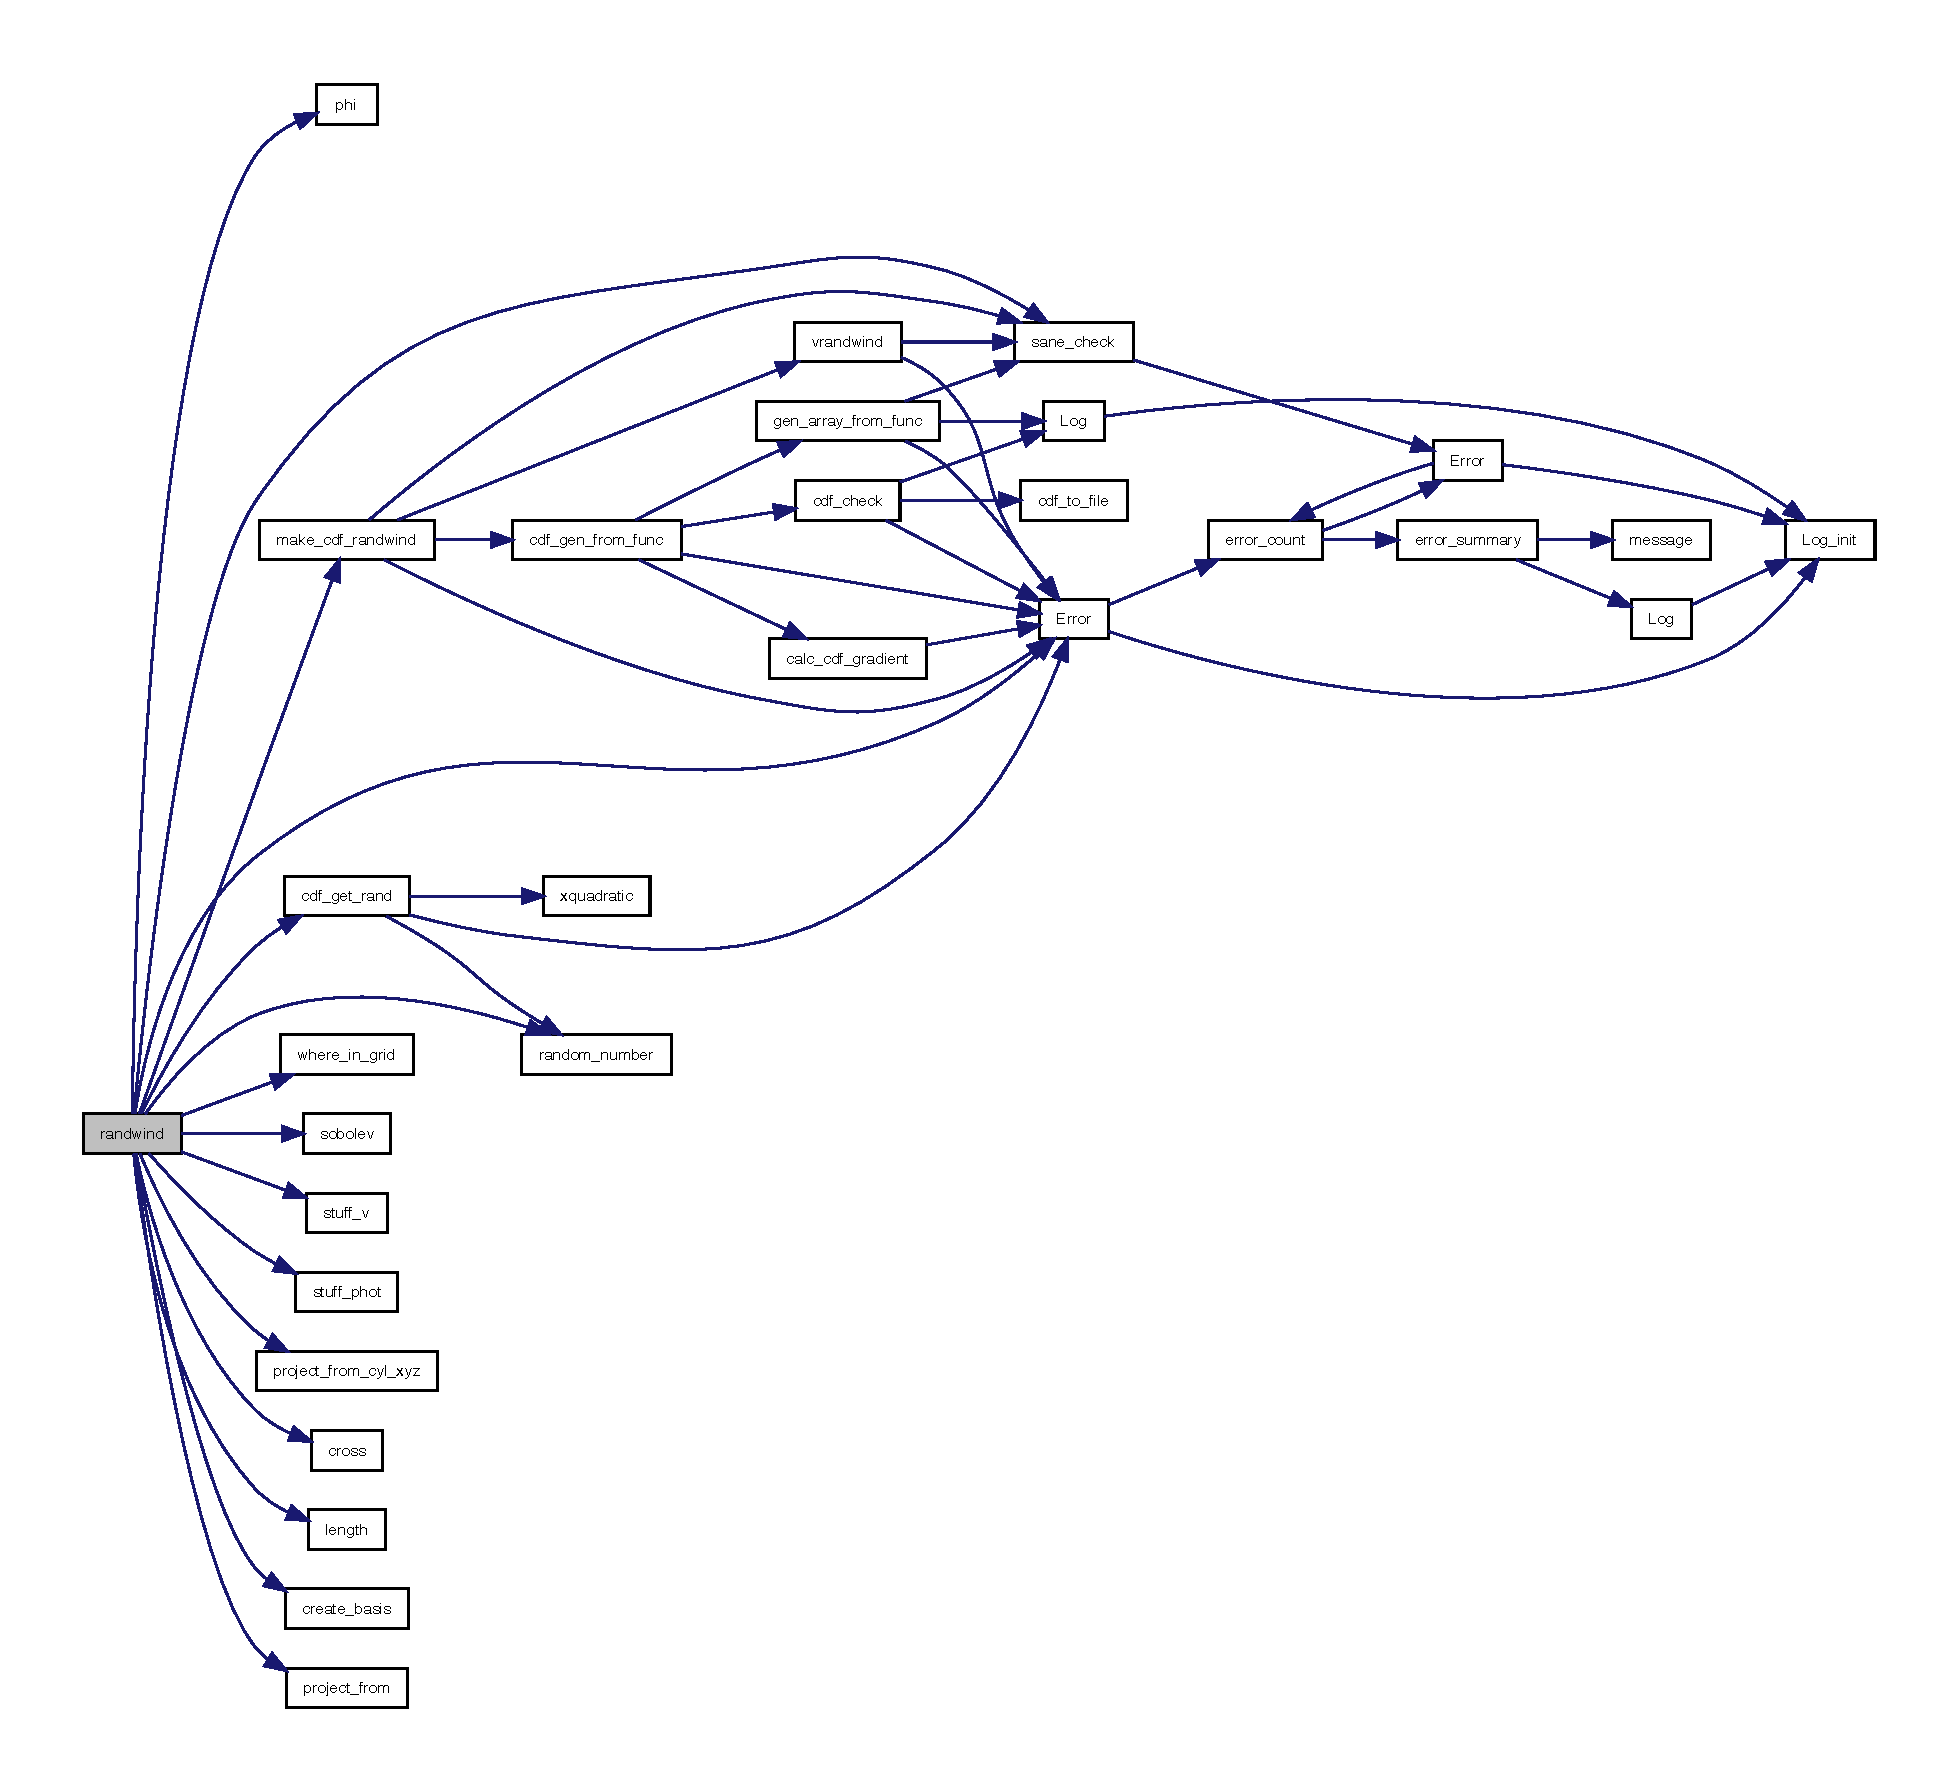
\includegraphics[width=350pt]{anisowind_8c_aa02bd1c515967ac3e1214843158df2f4_cgraph}
\end{center}
\end{figure}
Here is the caller graph for this function\+:
\nopagebreak
\begin{figure}[H]
\begin{center}
\leavevmode
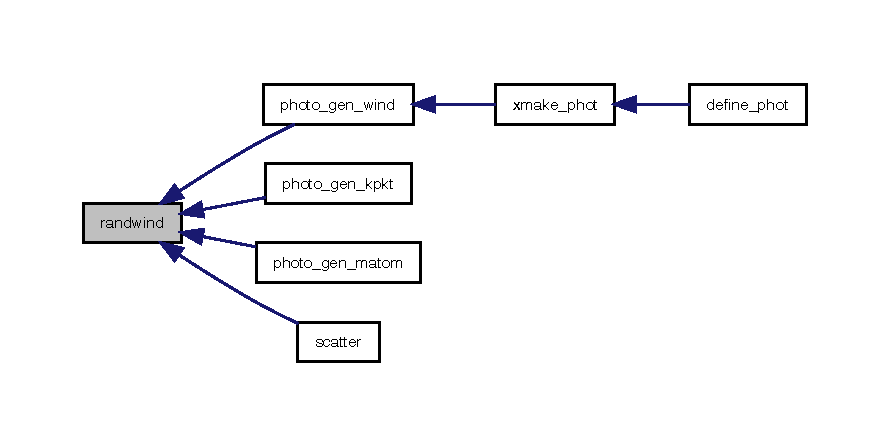
\includegraphics[width=350pt]{anisowind_8c_aa02bd1c515967ac3e1214843158df2f4_icgraph}
\end{center}
\end{figure}
\mbox{\Hypertarget{anisowind_8c_a5cc282e1f3d56ce0f29cb080bc225408}\label{anisowind_8c_a5cc282e1f3d56ce0f29cb080bc225408}} 
\index{anisowind.\+c@{anisowind.\+c}!randwind\+\_\+thermal\+\_\+trapping@{randwind\+\_\+thermal\+\_\+trapping}}
\index{randwind\+\_\+thermal\+\_\+trapping@{randwind\+\_\+thermal\+\_\+trapping}!anisowind.\+c@{anisowind.\+c}}
\subsubsection{\texorpdfstring{randwind\+\_\+thermal\+\_\+trapping()}{randwind\_thermal\_trapping()}}
{\footnotesize\ttfamily int randwind\+\_\+thermal\+\_\+trapping (\begin{DoxyParamCaption}\item[{\hyperlink{python_8h_ad2424d53ebcf811656882a87e11b440c}{Phot\+Ptr}}]{p,  }\item[{int $\ast$}]{nnscat }\end{DoxyParamCaption})}



is the routine which chooses a new anisotropic direction in geo.\+scatter\+\_\+mode = S\+C\+A\+T\+T\+E\+R\+\_\+\+M\+O\+D\+E\+\_\+\+T\+H\+E\+R\+M\+AL 


\begin{DoxyParams}[1]{Parameters}
\mbox{\tt in,out}  & {\em Phot\+Ptr} & p The photon being scattered \\
\hline
\mbox{\tt out}  & {\em int} & $\ast$ nnscat The number of times the phton scattered internally before escaping the local scattering region\\
\hline
\end{DoxyParams}
\begin{DoxyReturn}{Returns}
0 for success. Also modifies the photon ptr p to reflect new direction (p-\/$>$lmn), and nnscat, which should be copied to the phoiton structure after calling this routine.
\end{DoxyReturn}
This routine uses a rejection method to choose a direction so that the probability distribution of directions generated reflects the probability of escape along each direction in accordance with the sobolev optical depth.

\paragraph*{Notes}

The resonance that caused the scatter must be stored in the photon bundle.

The name of the routine is something of a misnomer. Pure sobolev optical depths are used. The temperature in the cell does not come into the calculation.

Unlike randwind, this routine does not explicitly need to to make a transformation from the xz plane to the location of the photon. This is because dvds is calculated directly using dwind\+\_\+ds 

Definition at line 612 of file anisowind.\+c.

Here is the call graph for this function\+:
\nopagebreak
\begin{figure}[H]
\begin{center}
\leavevmode
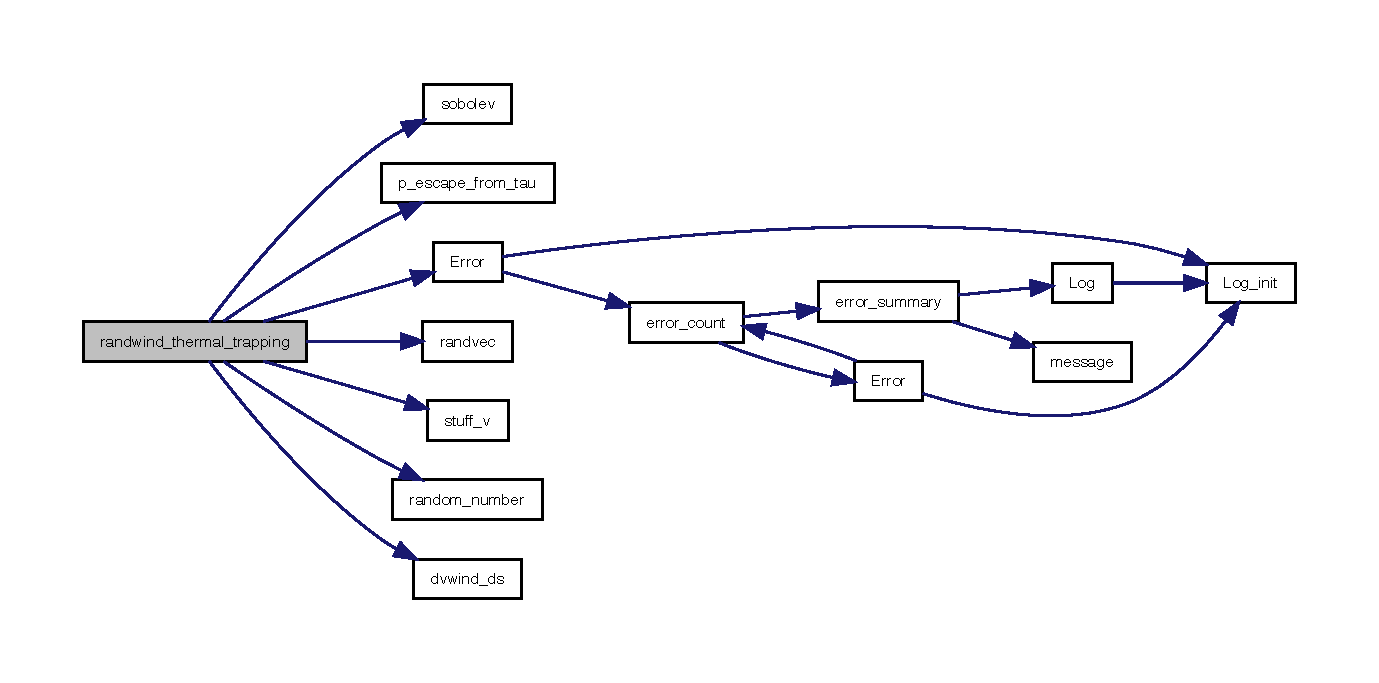
\includegraphics[width=350pt]{anisowind_8c_a5cc282e1f3d56ce0f29cb080bc225408_cgraph}
\end{center}
\end{figure}
Here is the caller graph for this function\+:
\nopagebreak
\begin{figure}[H]
\begin{center}
\leavevmode
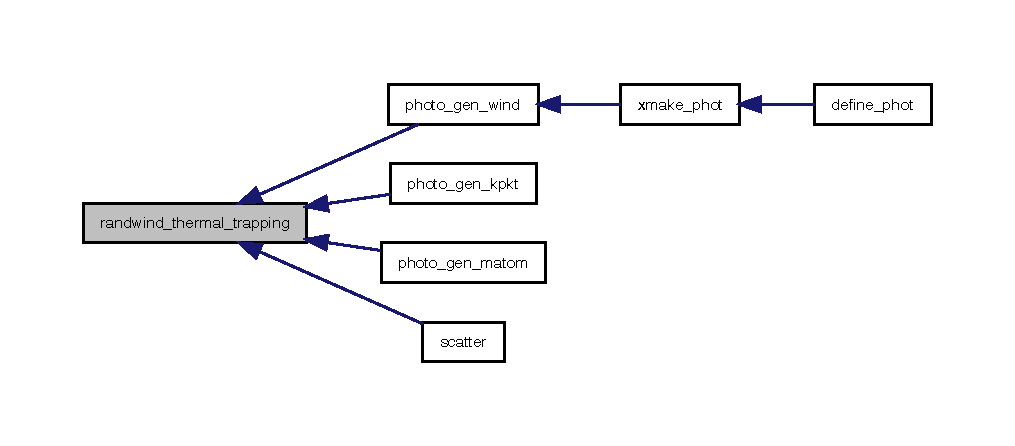
\includegraphics[width=350pt]{anisowind_8c_a5cc282e1f3d56ce0f29cb080bc225408_icgraph}
\end{center}
\end{figure}
\mbox{\Hypertarget{anisowind_8c_a76f3cece46c92129a1e138a02aac87ca}\label{anisowind_8c_a76f3cece46c92129a1e138a02aac87ca}} 
\index{anisowind.\+c@{anisowind.\+c}!reweightwind@{reweightwind}}
\index{reweightwind@{reweightwind}!anisowind.\+c@{anisowind.\+c}}
\subsubsection{\texorpdfstring{reweightwind()}{reweightwind()}}
{\footnotesize\ttfamily double reweightwind (\begin{DoxyParamCaption}\item[{\hyperlink{python_8h_ad2424d53ebcf811656882a87e11b440c}{Phot\+Ptr}}]{p }\end{DoxyParamCaption})}



calculates the weight of a photon in the wind that is forced to scatter along a specific line of sight. 


\begin{DoxyParams}[1]{Parameters}
\mbox{\tt in,out}  & {\em Phot\+Ptr} & p The photon being scattered \\
\hline
\end{DoxyParams}
\begin{DoxyReturn}{Returns}
The number corresponding to the reweighting is returned. The revised weight is also stored in p
\end{DoxyReturn}
p must contain the position and N\+EW direction for the photon being scattered. In general, p must also be up to date w. r. t. the number of the resonance that generated the photon.

\paragraph*{Notes}

This routine is called when extracting photons along a specific line of sight.

wmain.\+dv\+\_\+ds, and wmain.\+lmn are maximum value of dvds, and the direction in a cell (that is in the positive xz plane) \begin{DoxyRefDesc}{Bug}
\item[\hyperlink{bug__bug000001}{Bug}]180414 -\/ ksl -\/ It is not obvious that using D\+F\+U\+D\+GE as the way to choose whether to recalculate the cdf for scatter is correct. One would obtain the wrong answer if the photon moved a small distance and hit a different resonance. \end{DoxyRefDesc}


\begin{DoxyRefDesc}{Bug}
\item[\hyperlink{bug__bug000002}{Bug}]This is a note related to an X\+XX comoment which read as follows\+: Factor of 2 needed because the interval is from -\/1 to 1 X\+XX It\textquotesingle{}s definitely needed to make a uniform distribution work but is this reason really right\end{DoxyRefDesc}


180415 -\/ ksl -\/ My investigation of this indicates that the cdf was generated from -\/1 to 1, and futhermore that cdf\+\_\+gen\+\_\+from\+\_\+function which is used to create the cdf always sets the norm to 1. So it is not clear to me why this is the reweghting. It is also nto clear to me why the reweighting to be less than a factor of 2, which is what if stateement requries. Basically, I do not understand what is going on here at all.

Definition at line 353 of file anisowind.\+c.

Here is the call graph for this function\+:
\nopagebreak
\begin{figure}[H]
\begin{center}
\leavevmode
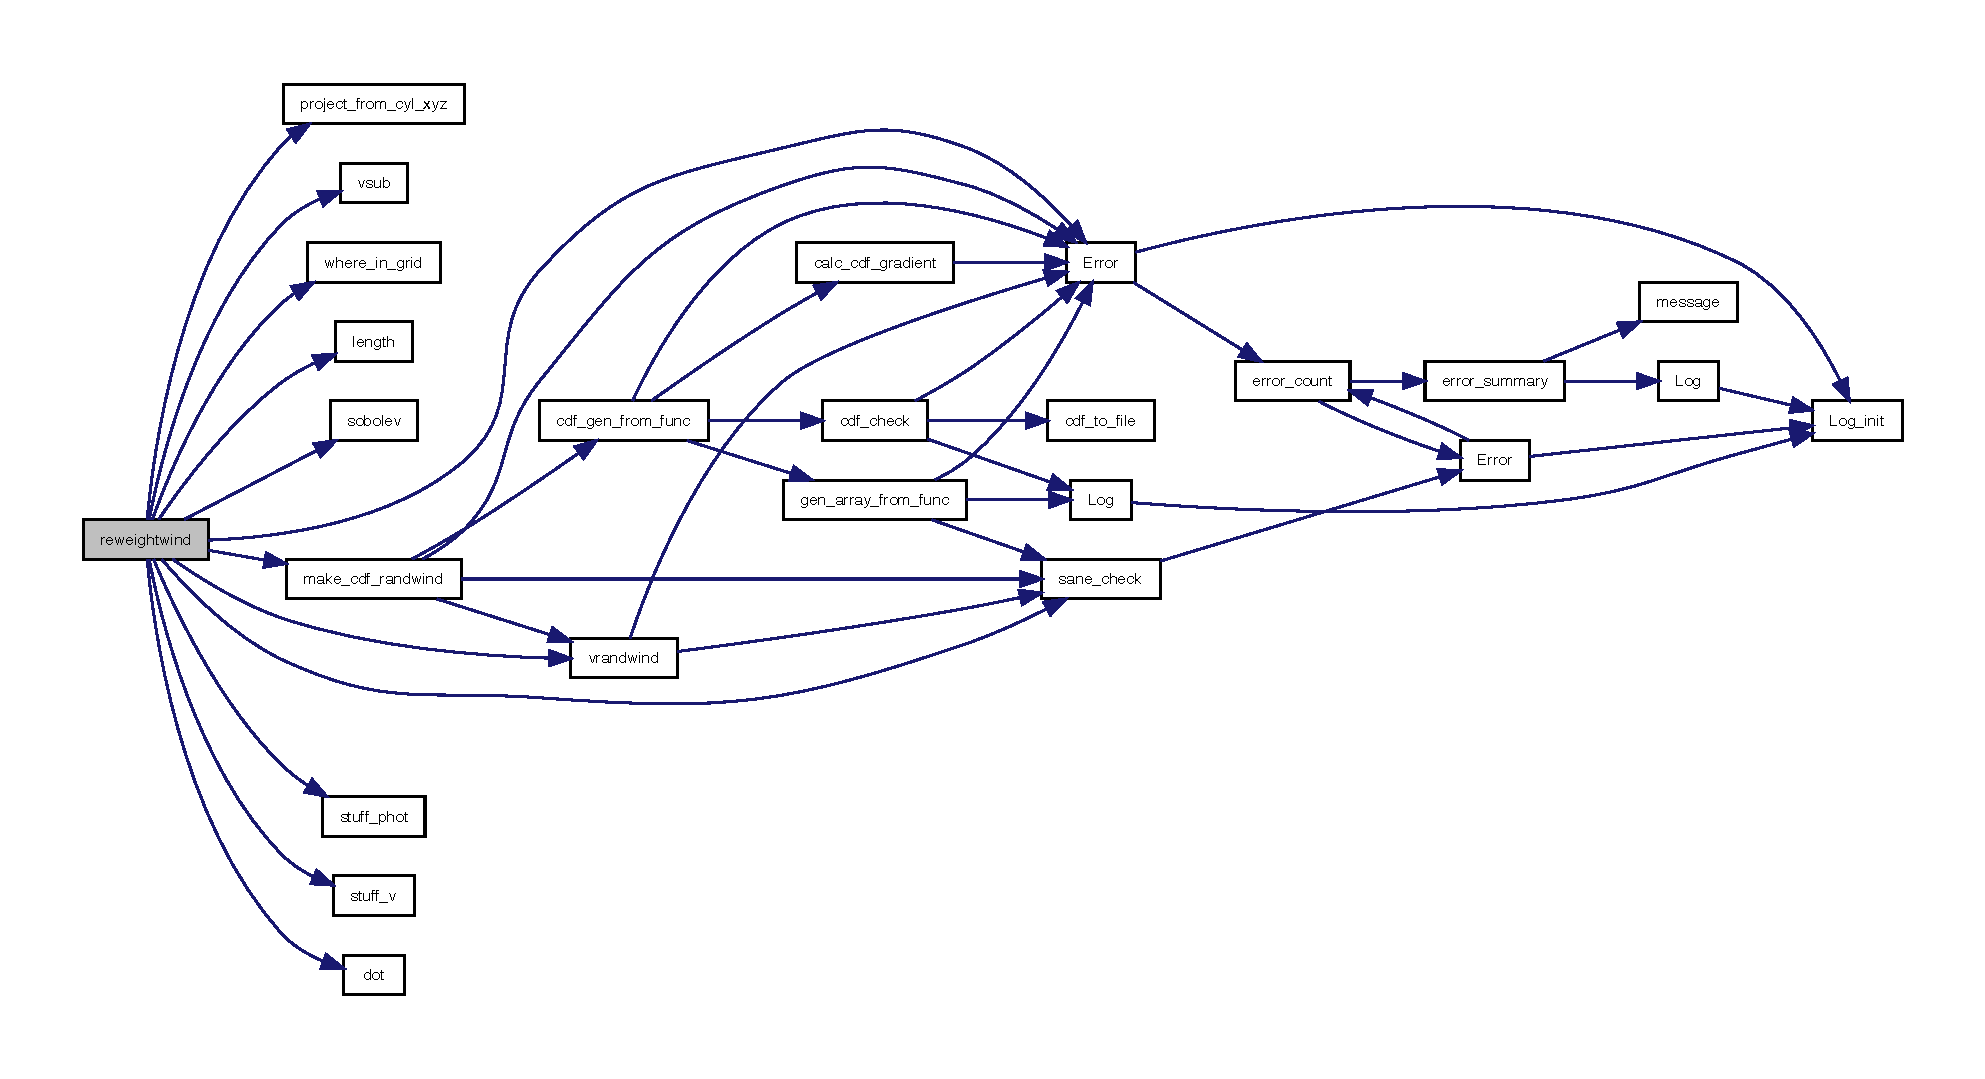
\includegraphics[width=350pt]{anisowind_8c_a76f3cece46c92129a1e138a02aac87ca_cgraph}
\end{center}
\end{figure}
Here is the caller graph for this function\+:
\nopagebreak
\begin{figure}[H]
\begin{center}
\leavevmode
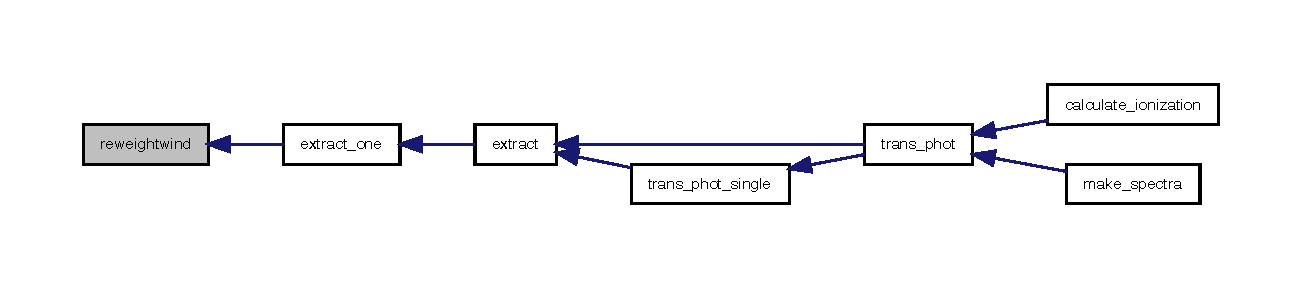
\includegraphics[width=350pt]{anisowind_8c_a76f3cece46c92129a1e138a02aac87ca_icgraph}
\end{center}
\end{figure}
\mbox{\Hypertarget{anisowind_8c_af170ad39af01fbe3b232230692c2aa5e}\label{anisowind_8c_af170ad39af01fbe3b232230692c2aa5e}} 
\index{anisowind.\+c@{anisowind.\+c}!vrandwind@{vrandwind}}
\index{vrandwind@{vrandwind}!anisowind.\+c@{anisowind.\+c}}
\subsubsection{\texorpdfstring{vrandwind()}{vrandwind()}}
{\footnotesize\ttfamily double vrandwind (\begin{DoxyParamCaption}\item[{double}]{x }\end{DoxyParamCaption})}



the function that is used to generate the cdf for anisotropic scattering. 


\begin{DoxyParams}[1]{Parameters}
\mbox{\tt out}  & {\em double} & x The direction cosine with respect to the direction of tau\+\_\+min\\
\hline
\end{DoxyParams}
\begin{DoxyReturn}{Returns}
A number proportional to the probability that a photon will scatter in a direction with a particular direction cosine
\end{DoxyReturn}
The routine calculates a function that is proportional to the probability density. d\+P/dcos(theta) for the photon.

\paragraph*{Notes}

This routine is used by cdf\+\_\+gen\+\_\+from\+\_\+func (via make\+\_\+cdf\+\_\+randwind, when that routine is called from randwind) 

Definition at line 279 of file anisowind.\+c.

Here is the call graph for this function\+:
\nopagebreak
\begin{figure}[H]
\begin{center}
\leavevmode
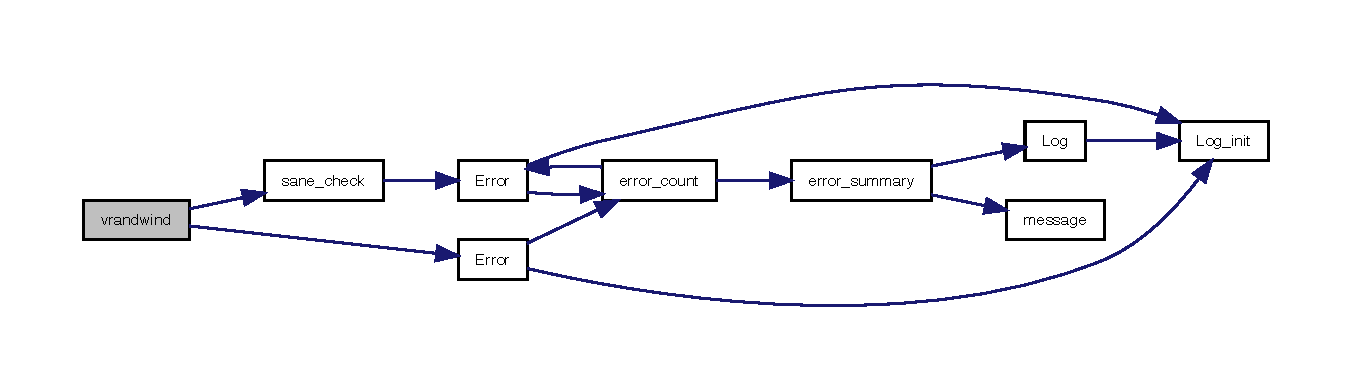
\includegraphics[width=350pt]{anisowind_8c_af170ad39af01fbe3b232230692c2aa5e_cgraph}
\end{center}
\end{figure}
Here is the caller graph for this function\+:
\nopagebreak
\begin{figure}[H]
\begin{center}
\leavevmode
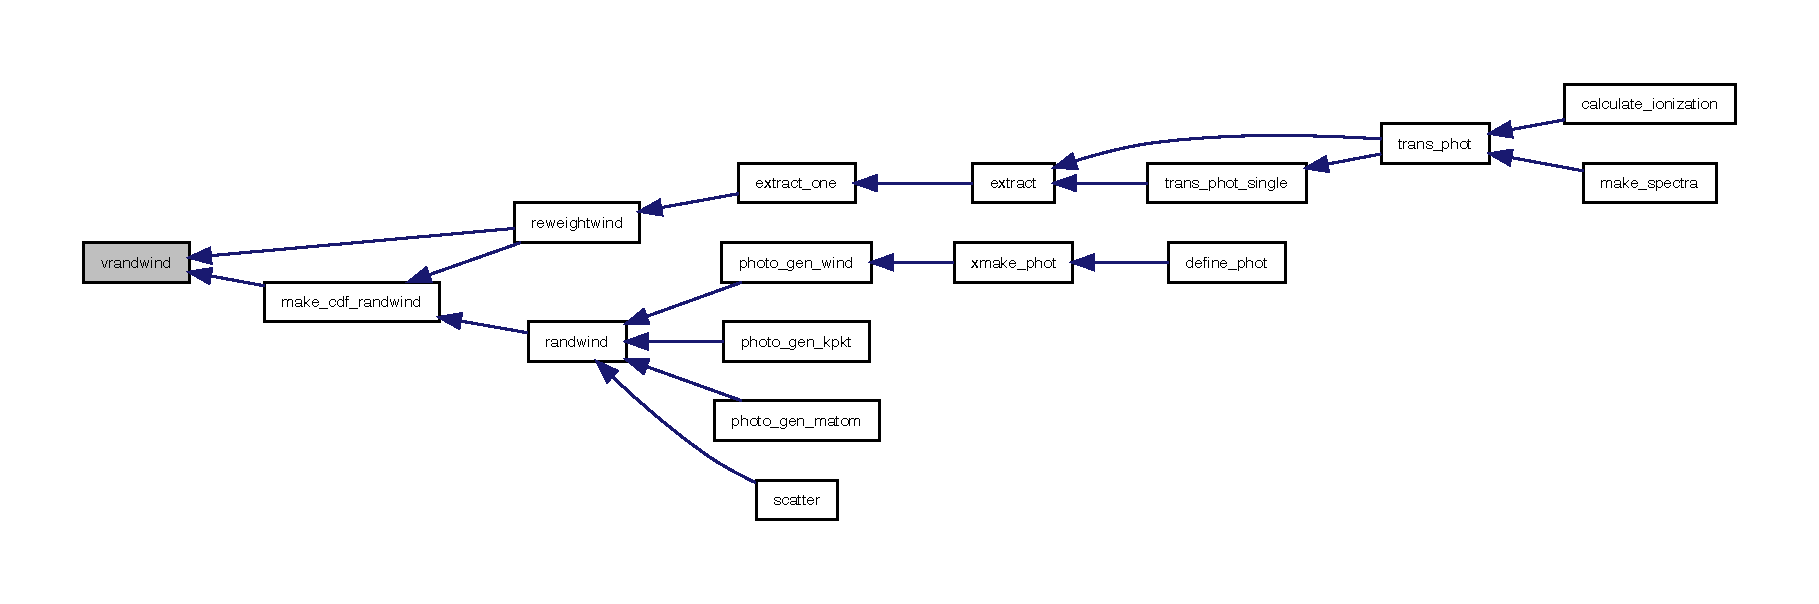
\includegraphics[width=350pt]{anisowind_8c_af170ad39af01fbe3b232230692c2aa5e_icgraph}
\end{center}
\end{figure}


\subsection{Variable Documentation}
\mbox{\Hypertarget{anisowind_8c_a7d5d3c2b11592abf6eb482a145e10d50}\label{anisowind_8c_a7d5d3c2b11592abf6eb482a145e10d50}} 
\index{anisowind.\+c@{anisowind.\+c}!cdf\+\_\+randwind@{cdf\+\_\+randwind}}
\index{cdf\+\_\+randwind@{cdf\+\_\+randwind}!anisowind.\+c@{anisowind.\+c}}
\subsubsection{\texorpdfstring{cdf\+\_\+randwind}{cdf\_randwind}}
{\footnotesize\ttfamily \hyperlink{python_8h_a14b633e617b31ead523c75ce80cc56e1}{Cdf\+Ptr} cdf\+\_\+randwind}



Definition at line 32 of file anisowind.\+c.

\mbox{\Hypertarget{anisowind_8c_af5db99077c04b8cf610205694640ddeb}\label{anisowind_8c_af5db99077c04b8cf610205694640ddeb}} 
\index{anisowind.\+c@{anisowind.\+c}!cdf\+\_\+randwind\+\_\+dlogtau@{cdf\+\_\+randwind\+\_\+dlogtau}}
\index{cdf\+\_\+randwind\+\_\+dlogtau@{cdf\+\_\+randwind\+\_\+dlogtau}!anisowind.\+c@{anisowind.\+c}}
\subsubsection{\texorpdfstring{cdf\+\_\+randwind\+\_\+dlogtau}{cdf\_randwind\_dlogtau}}
{\footnotesize\ttfamily double cdf\+\_\+randwind\+\_\+dlogtau}



Definition at line 485 of file anisowind.\+c.

\mbox{\Hypertarget{anisowind_8c_ab3e97ac75b82f9c4ced9218e78eb2fa4}\label{anisowind_8c_ab3e97ac75b82f9c4ced9218e78eb2fa4}} 
\index{anisowind.\+c@{anisowind.\+c}!cdf\+\_\+randwind\+\_\+store@{cdf\+\_\+randwind\+\_\+store}}
\index{cdf\+\_\+randwind\+\_\+store@{cdf\+\_\+randwind\+\_\+store}!anisowind.\+c@{anisowind.\+c}}
\subsubsection{\texorpdfstring{cdf\+\_\+randwind\+\_\+store}{cdf\_randwind\_store}}
{\footnotesize\ttfamily struct \hyperlink{struct_cdf}{Cdf} cdf\+\_\+randwind\+\_\+store\mbox{[}100\mbox{]}}



Definition at line 31 of file anisowind.\+c.

\mbox{\Hypertarget{anisowind_8c_a872ce5174f328e50a8381894469b3790}\label{anisowind_8c_a872ce5174f328e50a8381894469b3790}} 
\index{anisowind.\+c@{anisowind.\+c}!init\+\_\+make\+\_\+cdf\+\_\+randwind@{init\+\_\+make\+\_\+cdf\+\_\+randwind}}
\index{init\+\_\+make\+\_\+cdf\+\_\+randwind@{init\+\_\+make\+\_\+cdf\+\_\+randwind}!anisowind.\+c@{anisowind.\+c}}
\subsubsection{\texorpdfstring{init\+\_\+make\+\_\+cdf\+\_\+randwind}{init\_make\_cdf\_randwind}}
{\footnotesize\ttfamily int init\+\_\+make\+\_\+cdf\+\_\+randwind = 1}



Generate the cumulative distribution functions needed for selecting a direction for a scattered photon, and then select the cdf needed ro a particulat tau. 


\begin{DoxyParams}[1]{Parameters}
\mbox{\tt in}  & {\em double} & tau The optical depth in the direction of the maximum velocity gradient associated with the scattering event\\
\hline
\end{DoxyParams}
\begin{DoxyReturn}{Returns}
Always returns 0
\end{DoxyReturn}
The first time this routine is entered it generates a set of cdfs correspoding to various values of tau which are logrithmically spaced between 0.\+01 and 10. These cddfs are stored in an array of cdf structures

It then selects the closest cdf and sets cdf\+\_\+rand\+\_\+wind to point to this particular cdf

On subsequent calls, the routine merely chooses which cdf is most appropriate for a given tau

\paragraph*{Notes}

The probability densities are calculated in vrandwind

The basic idea of this routine is to calculate a series of cdfs the first time the routine is called that are spaced in a sensible fashion so that one does not have to regenerate the cdfs everytime one wants to calulate the probability a photon will be scattered in certain direction.

On subsequent calls the routine simply chooses which of the cdfs to use by setting cdf\+\_\+randwind to one of the precalculate cdfs. 

Definition at line 480 of file anisowind.\+c.

\mbox{\Hypertarget{anisowind_8c_a6f923c8cdf71897592f32606c6d8fd0e}\label{anisowind_8c_a6f923c8cdf71897592f32606c6d8fd0e}} 
\index{anisowind.\+c@{anisowind.\+c}!make\+\_\+cdf\+\_\+randwind\+\_\+jumps@{make\+\_\+cdf\+\_\+randwind\+\_\+jumps}}
\index{make\+\_\+cdf\+\_\+randwind\+\_\+jumps@{make\+\_\+cdf\+\_\+randwind\+\_\+jumps}!anisowind.\+c@{anisowind.\+c}}
\subsubsection{\texorpdfstring{make\+\_\+cdf\+\_\+randwind\+\_\+jumps}{make\_cdf\_randwind\_jumps}}
{\footnotesize\ttfamily double make\+\_\+cdf\+\_\+randwind\+\_\+jumps\mbox{[}180\mbox{]}}



Definition at line 482 of file anisowind.\+c.

\mbox{\Hypertarget{anisowind_8c_a656c37768c70e0b91e3f5028654f79ec}\label{anisowind_8c_a656c37768c70e0b91e3f5028654f79ec}} 
\index{anisowind.\+c@{anisowind.\+c}!make\+\_\+cdf\+\_\+randwind\+\_\+njumps@{make\+\_\+cdf\+\_\+randwind\+\_\+njumps}}
\index{make\+\_\+cdf\+\_\+randwind\+\_\+njumps@{make\+\_\+cdf\+\_\+randwind\+\_\+njumps}!anisowind.\+c@{anisowind.\+c}}
\subsubsection{\texorpdfstring{make\+\_\+cdf\+\_\+randwind\+\_\+njumps}{make\_cdf\_randwind\_njumps}}
{\footnotesize\ttfamily int make\+\_\+cdf\+\_\+randwind\+\_\+njumps}



Definition at line 481 of file anisowind.\+c.

\mbox{\Hypertarget{anisowind_8c_a9f5059b178ab31b23b014793eb4854b0}\label{anisowind_8c_a9f5059b178ab31b23b014793eb4854b0}} 
\index{anisowind.\+c@{anisowind.\+c}!phot\+\_\+randwind@{phot\+\_\+randwind}}
\index{phot\+\_\+randwind@{phot\+\_\+randwind}!anisowind.\+c@{anisowind.\+c}}
\subsubsection{\texorpdfstring{phot\+\_\+randwind}{phot\_randwind}}
{\footnotesize\ttfamily struct \hyperlink{structphoton}{photon} phot\+\_\+randwind}



Definition at line 33 of file anisowind.\+c.

\mbox{\Hypertarget{anisowind_8c_a0ae08e53a25f8ac625b0c2f872056d2d}\label{anisowind_8c_a0ae08e53a25f8ac625b0c2f872056d2d}} 
\index{anisowind.\+c@{anisowind.\+c}!reweightwind\+\_\+init@{reweightwind\+\_\+init}}
\index{reweightwind\+\_\+init@{reweightwind\+\_\+init}!anisowind.\+c@{anisowind.\+c}}
\subsubsection{\texorpdfstring{reweightwind\+\_\+init}{reweightwind\_init}}
{\footnotesize\ttfamily int reweightwind\+\_\+init = 1}



Definition at line 322 of file anisowind.\+c.

\mbox{\Hypertarget{anisowind_8c_addb96381a70d5bbbd4d70c8b469529d3}\label{anisowind_8c_addb96381a70d5bbbd4d70c8b469529d3}} 
\index{anisowind.\+c@{anisowind.\+c}!reweightwind\+\_\+zmax@{reweightwind\+\_\+zmax}}
\index{reweightwind\+\_\+zmax@{reweightwind\+\_\+zmax}!anisowind.\+c@{anisowind.\+c}}
\subsubsection{\texorpdfstring{reweightwind\+\_\+zmax}{reweightwind\_zmax}}
{\footnotesize\ttfamily double reweightwind\+\_\+zmax}



Definition at line 323 of file anisowind.\+c.

\mbox{\Hypertarget{anisowind_8c_acabc03109a812245488027702104978c}\label{anisowind_8c_acabc03109a812245488027702104978c}} 
\index{anisowind.\+c@{anisowind.\+c}!tau\+\_\+randwind@{tau\+\_\+randwind}}
\index{tau\+\_\+randwind@{tau\+\_\+randwind}!anisowind.\+c@{anisowind.\+c}}
\subsubsection{\texorpdfstring{tau\+\_\+randwind}{tau\_randwind}}
{\footnotesize\ttfamily double tau\+\_\+randwind = -\/1000.}



Definition at line 95 of file anisowind.\+c.


\hypertarget{atomic_8c}{}\section{/\+Users/mhewitt/python/source/atomic.c File Reference}
\label{atomic_8c}\index{/\+Users/mhewitt/python/source/atomic.\+c@{/\+Users/mhewitt/python/source/atomic.\+c}}


Routines to calculate rates and x-\/sections making use of the atomic data.  


{\ttfamily \#include $<$stdio.\+h$>$}\newline
{\ttfamily \#include $<$stdlib.\+h$>$}\newline
{\ttfamily \#include $<$math.\+h$>$}\newline
{\ttfamily \#include \char`\"{}atomic.\+h\char`\"{}}\newline
Include dependency graph for atomic.\+c\+:
\nopagebreak
\begin{figure}[H]
\begin{center}
\leavevmode
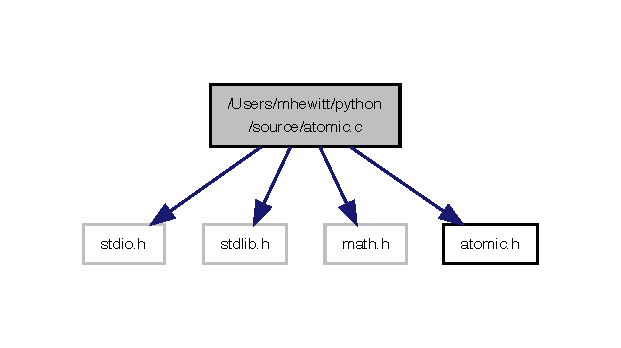
\includegraphics[width=298pt]{atomic_8c__incl}
\end{center}
\end{figure}
\subsection*{Macros}
\begin{DoxyCompactItemize}
\item 
\#define \hyperlink{atomic_8c_a93922e2464a391c7af05ae2b297acb2e}{A21\+\_\+\+C\+O\+N\+S\+T\+A\+NT}~7.\+429297e-\/22
\end{DoxyCompactItemize}
\subsection*{Functions}
\begin{DoxyCompactItemize}
\item 
double \hyperlink{atomic_8c_a107b53af4265eb649a0e2a483dc613da}{sigma\+\_\+phot} (struct photoionization $\ast$x\+\_\+ptr, double freq)
\begin{DoxyCompactList}\small\item\em double (x\+\_\+ptr,freq) calculates the photionization crossection due to the transition associated with x\+\_\+ptr at frequency freq \end{DoxyCompactList}\item 
double \hyperlink{atomic_8c_a8c589bd3089b7851e8da407ad1ce44a5}{a21} (struct \hyperlink{structlines}{lines} $\ast$line\+\_\+ptr)
\begin{DoxyCompactList}\small\item\em Calculate the Einstein A coefficient for a transition. \end{DoxyCompactList}\end{DoxyCompactItemize}
\subsection*{Variables}
\begin{DoxyCompactItemize}
\item 
struct \hyperlink{structlines}{lines} $\ast$ \hyperlink{atomic_8c_aa093894302d206f4938c3f97cd1df9ec}{a21\+\_\+line\+\_\+ptr}
\item 
double \hyperlink{atomic_8c_a90d9ee6e6ecbbb225f4fe1eaebaf9d10}{a21\+\_\+a}
\end{DoxyCompactItemize}


\subsection{Detailed Description}
Routines to calculate rates and x-\/sections making use of the atomic data. 

\begin{DoxyAuthor}{Author}
ksl 
\end{DoxyAuthor}
\begin{DoxyDate}{Date}
March, 2018
\end{DoxyDate}
\paragraph*{Notes}

These routines are intended to be Python-\/independent so that the can be used with other programs. As a result \hyperlink{python_8h}{python.\+h} should not be included.

Note that other routines should be added here to make the atomic data routines more indepenent of Python. 

\subsection{Macro Definition Documentation}
\mbox{\Hypertarget{atomic_8c_a93922e2464a391c7af05ae2b297acb2e}\label{atomic_8c_a93922e2464a391c7af05ae2b297acb2e}} 
\index{atomic.\+c@{atomic.\+c}!A21\+\_\+\+C\+O\+N\+S\+T\+A\+NT@{A21\+\_\+\+C\+O\+N\+S\+T\+A\+NT}}
\index{A21\+\_\+\+C\+O\+N\+S\+T\+A\+NT@{A21\+\_\+\+C\+O\+N\+S\+T\+A\+NT}!atomic.\+c@{atomic.\+c}}
\subsubsection{\texorpdfstring{A21\+\_\+\+C\+O\+N\+S\+T\+A\+NT}{A21\_CONSTANT}}
{\footnotesize\ttfamily \#define A21\+\_\+\+C\+O\+N\+S\+T\+A\+NT~7.\+429297e-\/22}



Definition at line 82 of file atomic.\+c.



\subsection{Function Documentation}
\mbox{\Hypertarget{atomic_8c_a8c589bd3089b7851e8da407ad1ce44a5}\label{atomic_8c_a8c589bd3089b7851e8da407ad1ce44a5}} 
\index{atomic.\+c@{atomic.\+c}!a21@{a21}}
\index{a21@{a21}!atomic.\+c@{atomic.\+c}}
\subsubsection{\texorpdfstring{a21()}{a21()}}
{\footnotesize\ttfamily double a21 (\begin{DoxyParamCaption}\item[{struct \hyperlink{structlines}{lines} $\ast$}]{line\+\_\+ptr }\end{DoxyParamCaption})}



Calculate the Einstein A coefficient for a transition. 


\begin{DoxyParams}[1]{Parameters}
\mbox{\tt in,out}  & {\em struct} & lines $\ast$ line\+\_\+ptr Ptr containing data describing the line \\
\hline
\end{DoxyParams}
\begin{DoxyReturn}{Returns}
The Einsten (a21) value
\end{DoxyReturn}
\paragraph*{Notes}

The routine checks whether we are asking for the same a21 as previously, and if so returns it without redoing the calculation. 

Definition at line 103 of file atomic.\+c.

Here is the caller graph for this function\+:
\nopagebreak
\begin{figure}[H]
\begin{center}
\leavevmode
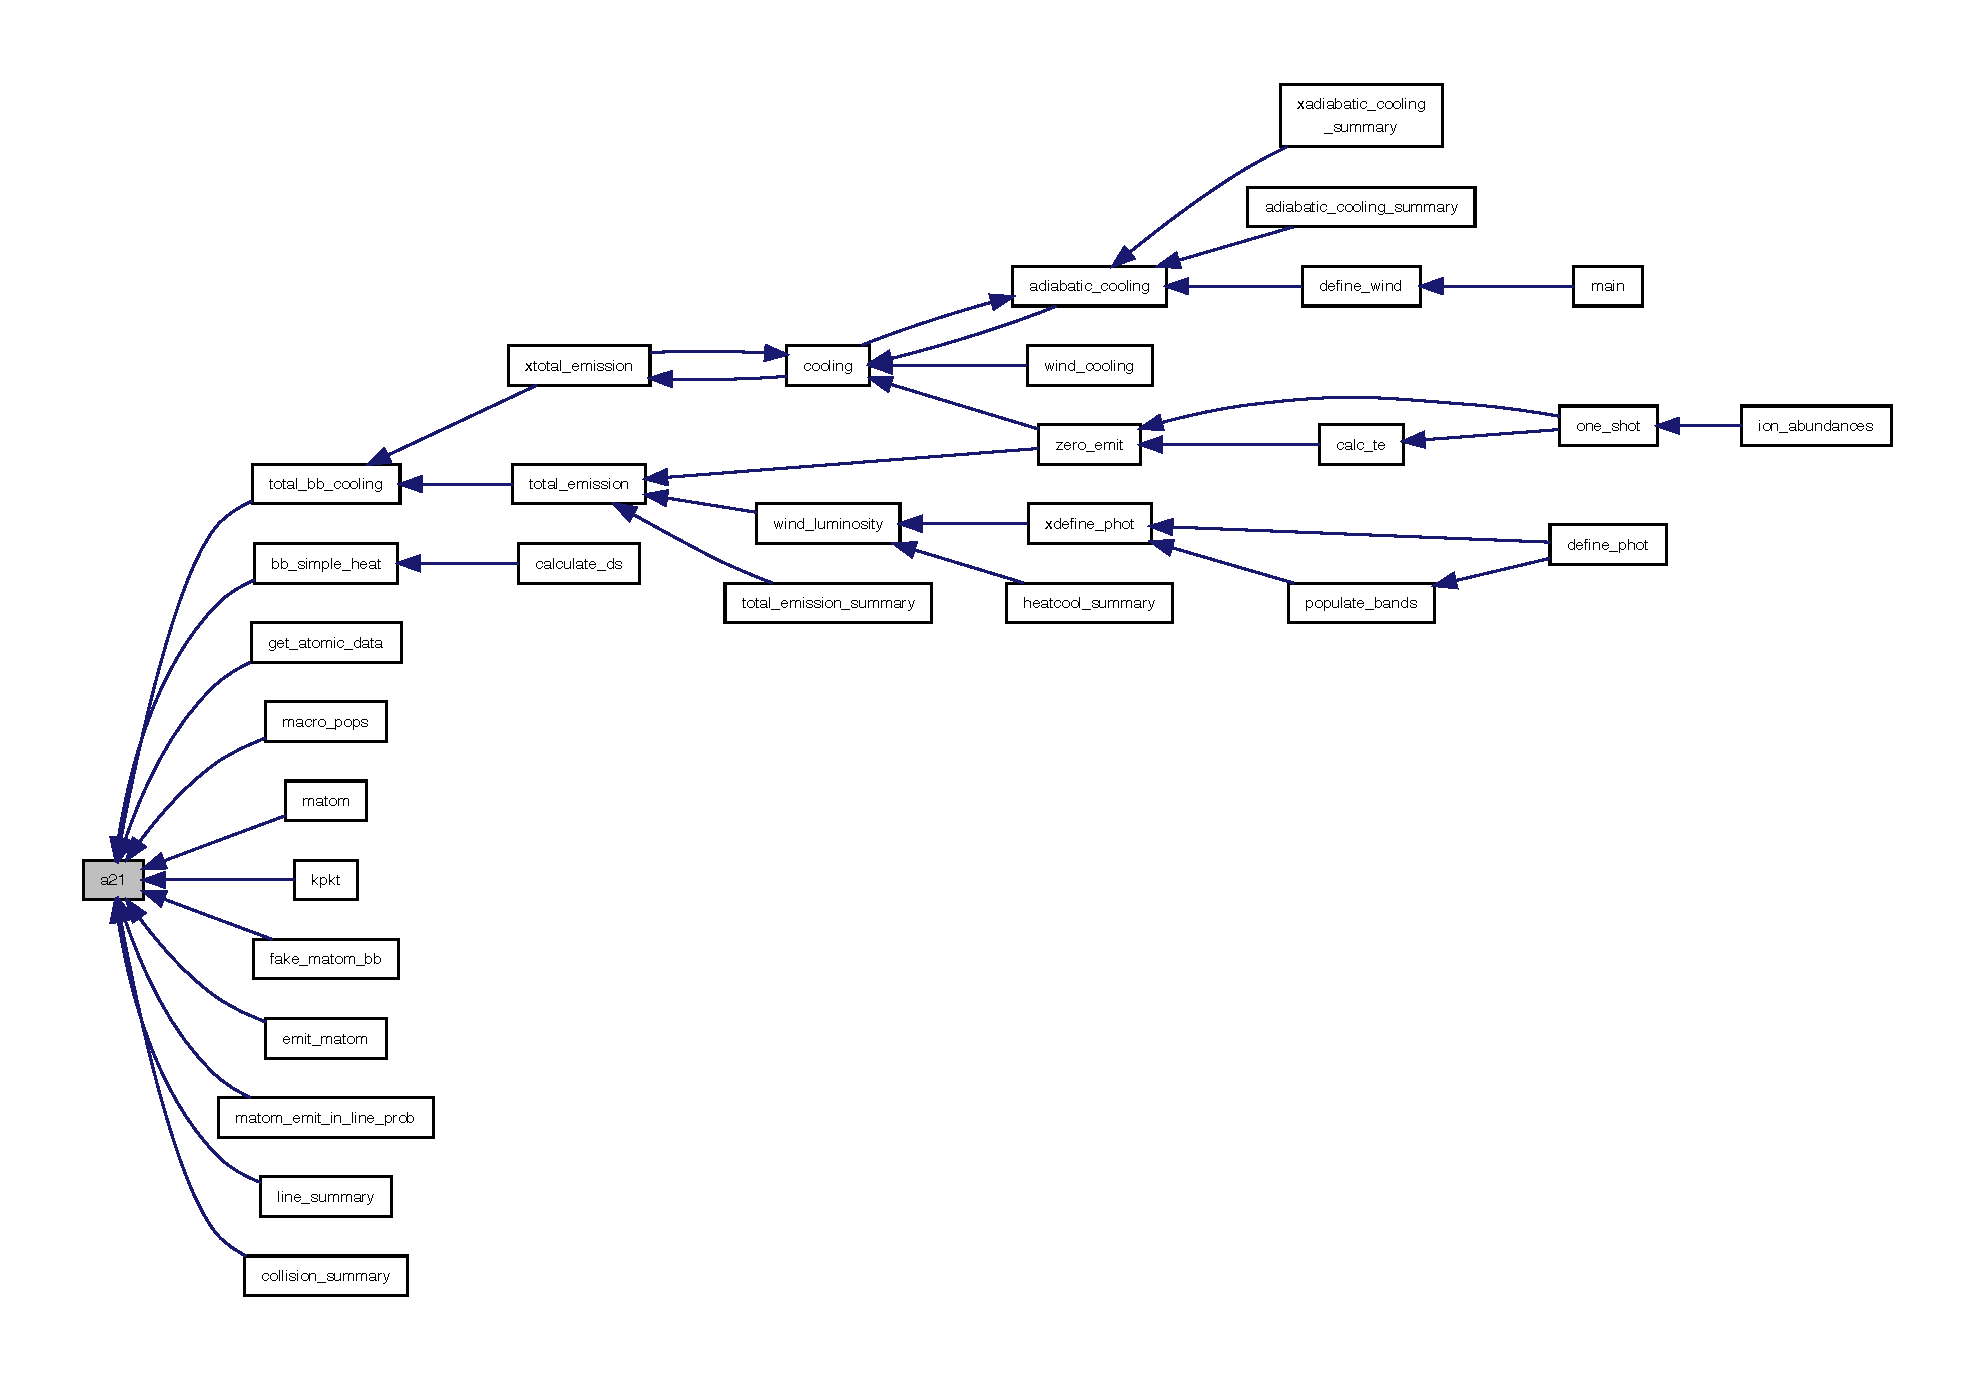
\includegraphics[width=350pt]{atomic_8c_a8c589bd3089b7851e8da407ad1ce44a5_icgraph}
\end{center}
\end{figure}
\mbox{\Hypertarget{atomic_8c_a107b53af4265eb649a0e2a483dc613da}\label{atomic_8c_a107b53af4265eb649a0e2a483dc613da}} 
\index{atomic.\+c@{atomic.\+c}!sigma\+\_\+phot@{sigma\+\_\+phot}}
\index{sigma\+\_\+phot@{sigma\+\_\+phot}!atomic.\+c@{atomic.\+c}}
\subsubsection{\texorpdfstring{sigma\+\_\+phot()}{sigma\_phot()}}
{\footnotesize\ttfamily double sigma\+\_\+phot (\begin{DoxyParamCaption}\item[{struct photoionization $\ast$}]{x\+\_\+ptr,  }\item[{double}]{freq }\end{DoxyParamCaption})}



double (x\+\_\+ptr,freq) calculates the photionization crossection due to the transition associated with x\+\_\+ptr at frequency freq 


\begin{DoxyParams}[1]{Parameters}
\mbox{\tt in,out}  & {\em struct} & photoionization $\ast$ x\+\_\+ptr structure containing the x-\/section information \\
\hline
\mbox{\tt in,out}  & {\em double} & freq frequency at which the x-\/section should be calculated \\
\hline
\end{DoxyParams}
\begin{DoxyReturn}{Returns}
xsection for this ion at the given frequency
\end{DoxyReturn}
sigma\+\_\+phot uses Verner et al.\textquotesingle{}s interpolation formulae for the photoionization crossection to calculate the bound free (or photoionization) optical depth.

\paragraph*{Notes}

The data must have been into the photoionization structures xphot with get\+\_\+atomic\+\_\+data 

Definition at line 49 of file atomic.\+c.

Here is the caller graph for this function\+:
\nopagebreak
\begin{figure}[H]
\begin{center}
\leavevmode
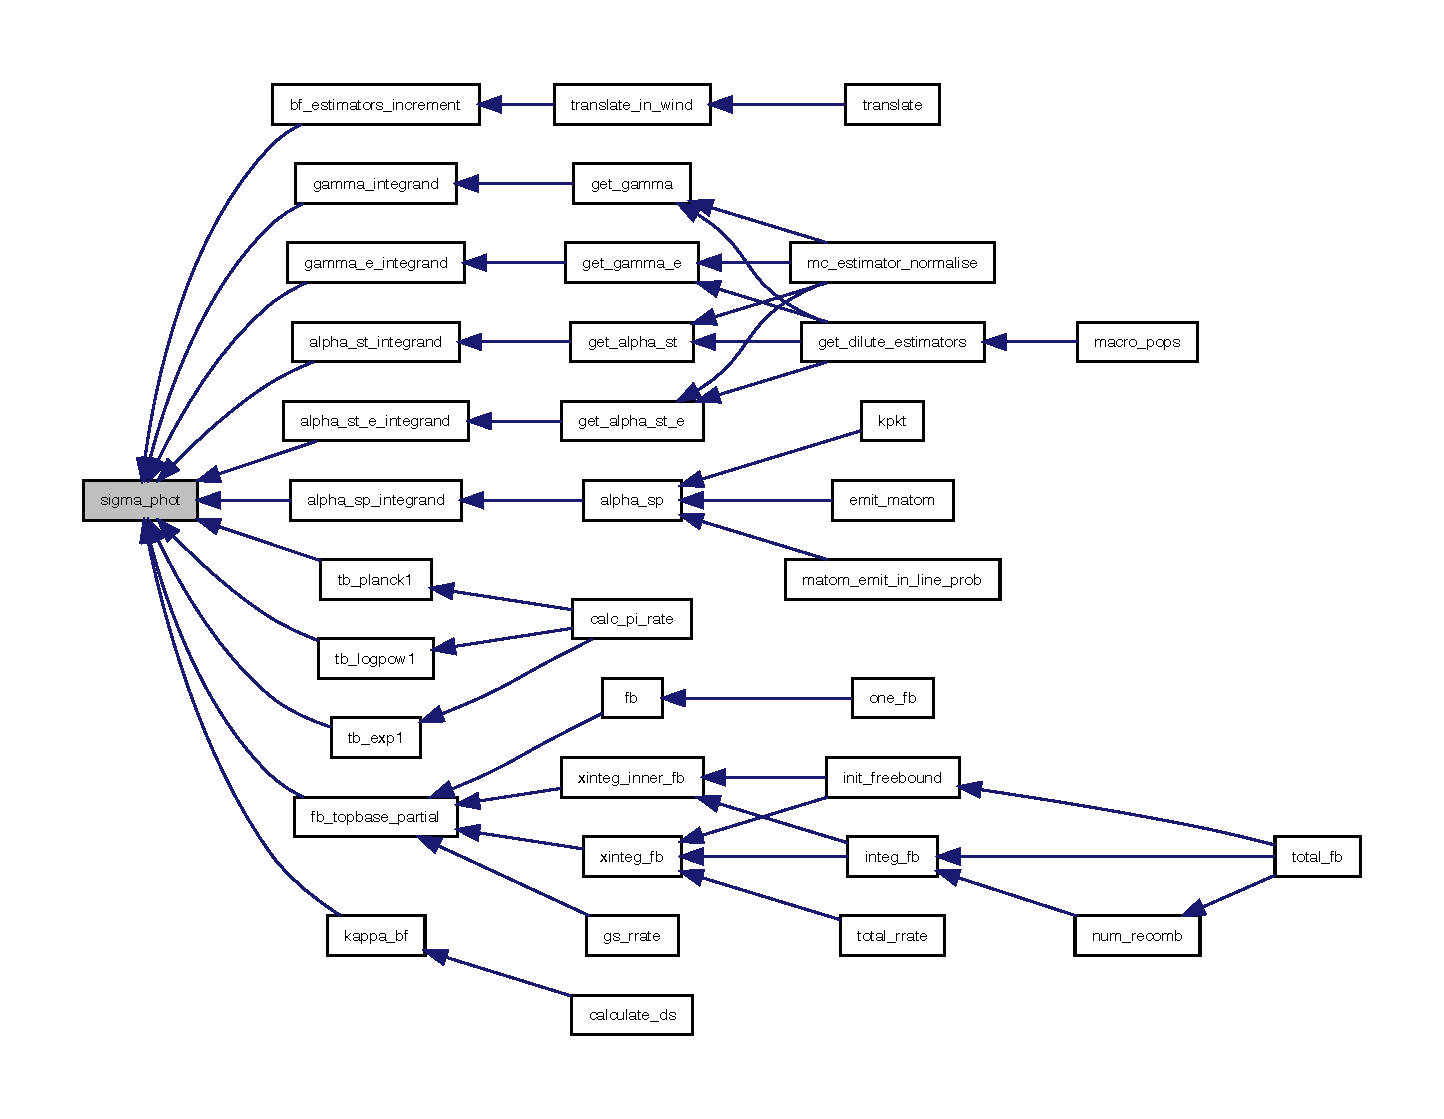
\includegraphics[width=350pt]{atomic_8c_a107b53af4265eb649a0e2a483dc613da_icgraph}
\end{center}
\end{figure}


\subsection{Variable Documentation}
\mbox{\Hypertarget{atomic_8c_a90d9ee6e6ecbbb225f4fe1eaebaf9d10}\label{atomic_8c_a90d9ee6e6ecbbb225f4fe1eaebaf9d10}} 
\index{atomic.\+c@{atomic.\+c}!a21\+\_\+a@{a21\+\_\+a}}
\index{a21\+\_\+a@{a21\+\_\+a}!atomic.\+c@{atomic.\+c}}
\subsubsection{\texorpdfstring{a21\+\_\+a}{a21\_a}}
{\footnotesize\ttfamily double a21\+\_\+a}



Definition at line 85 of file atomic.\+c.

\mbox{\Hypertarget{atomic_8c_aa093894302d206f4938c3f97cd1df9ec}\label{atomic_8c_aa093894302d206f4938c3f97cd1df9ec}} 
\index{atomic.\+c@{atomic.\+c}!a21\+\_\+line\+\_\+ptr@{a21\+\_\+line\+\_\+ptr}}
\index{a21\+\_\+line\+\_\+ptr@{a21\+\_\+line\+\_\+ptr}!atomic.\+c@{atomic.\+c}}
\subsubsection{\texorpdfstring{a21\+\_\+line\+\_\+ptr}{a21\_line\_ptr}}
{\footnotesize\ttfamily struct \hyperlink{structlines}{lines}$\ast$ a21\+\_\+line\+\_\+ptr}



Definition at line 84 of file atomic.\+c.


\hypertarget{atomic_8h}{}\section{/\+Users/mhewitt/python/source/atomic.h File Reference}
\label{atomic_8h}\index{/\+Users/mhewitt/python/source/atomic.\+h@{/\+Users/mhewitt/python/source/atomic.\+h}}
This graph shows which files directly or indirectly include this file\+:
\nopagebreak
\begin{figure}[H]
\begin{center}
\leavevmode

\includegraphics[width=350pt]{atomic_8h__dep__incl}
\end{center}
\end{figure}
\subsection*{Data Structures}
\begin{DoxyCompactItemize}
\item 
struct \hyperlink{structelements}{elements}
\item 
struct \hyperlink{structions}{ions}
\item 
struct \hyperlink{structconfigurations}{configurations}
\item 
struct \hyperlink{structlines}{lines}
\item 
struct \hyperlink{structcoll__stren}{coll\+\_\+stren}
\item 
struct \hyperlink{structtopbase__phot}{topbase\+\_\+phot}
\item 
struct \hyperlink{structinnershell}{innershell}
\item 
struct \hyperlink{structinner__elec__yield}{inner\+\_\+elec\+\_\+yield}
\item 
struct \hyperlink{structinner__fluor__yield}{inner\+\_\+fluor\+\_\+yield}
\item 
struct \hyperlink{structground__fracs}{ground\+\_\+fracs}
\item 
struct \hyperlink{structcollision__strength}{collision\+\_\+strength}
\item 
struct \hyperlink{structdielectronic__recombination}{dielectronic\+\_\+recombination}
\item 
struct \hyperlink{structtotal__rr}{total\+\_\+rr}
\item 
struct \hyperlink{structbadnell__gs__rr}{badnell\+\_\+gs\+\_\+rr}
\item 
struct \hyperlink{structdere__di__rate}{dere\+\_\+di\+\_\+rate}
\item 
struct \hyperlink{structgaunt__total}{gaunt\+\_\+total}
\end{DoxyCompactItemize}
\subsection*{Macros}
\begin{DoxyCompactItemize}
\item 
\#define \hyperlink{atomic_8h_a460aec6ec8d0aa18aafad0e83a03971f}{M\+A\+X\+R\+A\+ND}~2147486748.
\item 
\#define \hyperlink{atomic_8h_ad8512644399ac6ec00af8f727bb4fac6}{V\+E\+R\+Y\+\_\+\+B\+IG}~1e50
\item 
\#define \hyperlink{atomic_8h_aa8cecfc5c5c054d2875c03e77b7be15d}{T\+R\+UE}~1
\item 
\#define \hyperlink{atomic_8h_aa93f0eb578d23995850d61f7d61c55c1}{F\+A\+L\+SE}~0
\item 
\#define \hyperlink{atomic_8h_abec92cc72a096640b821b8cd56a02495}{H}~6.\+6262e-\/27
\item 
\#define \hyperlink{atomic_8h_a29939a749d943e3eba661f4f0302ef72}{HC}~1.\+98587e-\/16
\item 
\#define \hyperlink{atomic_8h_a3a1abcee874b9a925a5e62f58827fb0f}{H\+EV}~4.\+13620e-\/15     /$\ast$ Planck\textquotesingle{}s constant in e\+V $\ast$/
\item 
\#define \hyperlink{atomic_8h_a9703d073a2b8a710e9eebef1b2e1e31d}{H\+R\+YD}~3.\+04005e-\/16     /$\ast$ N\+S\+H 1204 Planck\textquotesingle{}s constant in Rydberg $\ast$/
\item 
\#define \hyperlink{atomic_8h_ac4cf4b2ab929bd23951a8676eeac086b}{C}~2.\+997925e10
\item 
\#define \hyperlink{atomic_8h_aed9ea78689ecce0b7264c02c7f8a9a54}{G}~6.\+670e-\/8
\item 
\#define \hyperlink{atomic_8h_aa1487dae81baa2e0a5643e7b571633a0}{B\+O\+L\+T\+Z\+M\+A\+NN}~1.\+38062e-\/16
\item 
\#define \hyperlink{atomic_8h_a0f43a239ef11bcdb4b2b340bb19798bb}{W\+I\+EN}~5.\+879e10        /$\ast$ N\+S\+H 1208 Wien Disp Const in frequency units $\ast$/
\item 
\#define \hyperlink{atomic_8h_a97148aa86d99b11c881e5f32845861d4}{H\+\_\+\+O\+V\+E\+R\+\_\+K}~4.\+799437e-\/11
\item 
\#define \hyperlink{atomic_8h_ad4e561a62bce83b8233ceb954b7c8988}{S\+T\+E\+F\+A\+N\+\_\+\+B\+O\+L\+T\+Z\+M\+A\+NN}~5.\+6696e-\/5
\item 
\#define \hyperlink{atomic_8h_a8bc97ad38b30a4ad622f7ebba5654485}{T\+H\+O\+M\+P\+S\+ON}~0.\+66524e-\/24
\item 
\#define \hyperlink{atomic_8h_a598a3330b3c21701223ee0ca14316eca}{PI}~3.\+1415927
\item 
\#define \hyperlink{atomic_8h_a488e623fe45466f0698d085bae5acca6}{M\+E\+L\+EC}~9.\+10956e-\/28
\item 
\#define \hyperlink{atomic_8h_a07484107e6d9fdf38b53edf631d6511d}{E}~4.\+8035e-\/10      /$\ast$ Electric charge in esu $\ast$/
\item 
\#define \hyperlink{atomic_8h_a8592a4c6a82900de74ba738c807293f0}{M\+P\+R\+OT}~1.\+672661e-\/24
\item 
\#define \hyperlink{atomic_8h_a89c8aa36f3eb46214691eb872b78a8c5}{M\+S\+OL}~1.\+989e33
\item 
\#define \hyperlink{atomic_8h_a600721f0222b857dc8a3ae59e5077347}{PC}~3.\+08e18
\item 
\#define \hyperlink{atomic_8h_a359cbb0621291f940e30390952c71c6c}{YR}~3.\+1556925e7
\item 
\#define \hyperlink{atomic_8h_af9bf78abab42c504a70b89bdb48eee95}{P\+I\+\_\+\+E2\+\_\+\+O\+V\+E\+R\+\_\+\+MC}~0.\+02655103      /$\ast$ Classical \hyperlink{vvector_8c_a618e8a49ea991b2fef57708b044b087f}{cross}-\/section $\ast$/
\item 
\#define \hyperlink{atomic_8h_ac0e6885d23e0ab0cc09cbabc7c30b870}{P\+I\+\_\+\+E2\+\_\+\+O\+V\+E\+R\+\_\+M}~7.\+96e8
\item 
\#define \hyperlink{atomic_8h_af5abd28c44c29b7397c84f1fec4b1d84}{A\+L\+P\+HA}~7.\+297351e-\/3     /$\ast$ Fine structure constant $\ast$/
\item 
\#define \hyperlink{atomic_8h_a1afdac6e3583ab3f180eeffa5558196d}{B\+O\+HR}~0.\+529175e-\/8     /$\ast$ Bohr radius $\ast$/
\item 
\#define \hyperlink{atomic_8h_a876ce77f3c672c7162658151e648389e}{CR}~3.\+288051e15     /$\ast$\+Rydberg frequency for H != Ryd freq for infinite mass $\ast$/
\item 
\#define \hyperlink{atomic_8h_a11a2bfccb8dc98a9c504c91cc2029ab3}{A\+N\+G\+S\+T\+R\+OM}~1.e-\/8   /$\ast$Definition of an Angstrom in units of this code, e.\+g. cm $\ast$/
\item 
\#define \hyperlink{atomic_8h_a8d1f46ca8e683183108b79544a31b38c}{E\+V2\+E\+R\+GS}~1.\+602192e-\/12
\item 
\#define \hyperlink{atomic_8h_a090430b65ca8e2355a86e3883133638a}{R\+A\+D\+I\+AN}~57.\+29577951308232
\item 
\#define \hyperlink{atomic_8h_a0a655eeb3f71e3bf8ab661fd2928c623}{R\+Y\+D2\+E\+R\+GS}~2.\+1798741e-\/11   /$\ast$ Rydberg in units of ergs $\ast$/
\item 
\#define \hyperlink{atomic_8h_a88f63843b8bf241b582271e3c0542d46}{D\+E\+N\+S\+I\+T\+Y\+\_\+\+M\+IN}~1.e-\/20
\item 
\#define \hyperlink{atomic_8h_ab01bd87833ae0d633951567b01d261d9}{N\+E\+L\+E\+M\+E\+N\+TS}~50      /$\ast$ Maximum number of \hyperlink{structelements}{elements} to consider $\ast$/
\item 
\#define \hyperlink{atomic_8h_ac6a37b9ae25d11bf2521d8ee85c46d79}{N\+I\+O\+NS}~500     /$\ast$ Maximum number of \hyperlink{structions}{ions} to consider $\ast$/
\item 
\#define \hyperlink{atomic_8h_a9acf4287226016eea5e934e8bd6d624b}{N\+L\+E\+V\+E\+LS}~12000   /$\ast$ Maximum number of \hyperlink{templates_8h_a2ba8dcf484d3688f9687d48dd865dc0d}{levels} for all \hyperlink{structelements}{elements} and \hyperlink{structions}{ions} $\ast$/
\item 
\#define \hyperlink{atomic_8h_a5b109be661ffec485a1ae6ac6d4d8fca}{N\+L\+T\+E\+\_\+\+L\+E\+V\+E\+LS}~12000    /$\ast$ Maximum number of \hyperlink{templates_8h_a2ba8dcf484d3688f9687d48dd865dc0d}{levels} to treat explicitly $\ast$/
\item 
\#define \hyperlink{atomic_8h_af618fc4a6769a63822cf1f4be873ce23}{N\+L\+E\+V\+E\+L\+S\+\_\+\+M\+A\+C\+RO}~200     /$\ast$ Maximum number of \hyperlink{structmacro}{macro} atom levels. (SS, June 04) $\ast$/
\item 
\#define \hyperlink{atomic_8h_a59990369239024c94cbe22080c9d29c3}{N\+L\+I\+N\+ES}~200000  /$\ast$ Maximum number of \hyperlink{structlines}{lines} to be read $\ast$/
\item 
\#define \hyperlink{atomic_8h_a075fa3e554e15e462b864cd9b40538f3}{N\+\_\+\+I\+N\+N\+ER}~10          /$\ast$Maximum number of inner shell ionization \hyperlink{vvector_8c_a618e8a49ea991b2fef57708b044b087f}{cross} sections per \hyperlink{atomic_8h_ae721a9114e3cf54f9bcc3dab31072273}{ion} $\ast$/
\item 
\#define \hyperlink{atomic_8h_a27e1e039bca1d64c21caa972e1111c09}{N\+B\+B\+J\+U\+M\+PS}~100    /$\ast$ Maximum number of Macro Atom bound-\/bound jumps from any one configuration (SS) $\ast$/
\item 
\#define \hyperlink{atomic_8h_a0829916f98c17313ddf806ae4a16355e}{N\+B\+F\+J\+U\+M\+PS}~100    /$\ast$ Maximum number of Macro Atom Bound-\/free jumps from any one configuration (SS) $\ast$/
\item 
\#define \hyperlink{atomic_8h_ad09b144c636440e4812c09171a7d7722}{M\+A\+X\+J\+U\+M\+PS}
\item 
\#define \hyperlink{atomic_8h_a14b6b173ed4360285ced591a163905f2}{N\+A\+U\+G\+ER}~2                /$\ast$Maximum number of \char`\"{}auger\char`\"{} processes $\ast$/
\item 
\#define \hyperlink{atomic_8h_a83f9db7d66ceb630d0e4427329ae7d16}{N\+\_\+\+C\+O\+L\+L\+\_\+\+S\+T\+R\+E\+N\+\_\+\+P\+TS}~20
\item 
\#define \hyperlink{atomic_8h_a9012fd4c06f8e07e4288a6c441c44b63}{N\+C\+R\+O\+SS}~1500
\item 
\#define \hyperlink{atomic_8h_a201f19a044a0ffd22379e5810af57149}{N\+T\+O\+P\+\_\+\+P\+H\+OT}~400           /$\ast$ Maximum number of photoionisation processes. (SS) $\ast$/
\item 
\#define \hyperlink{atomic_8h_ab535e9b55f95fe323a40f2762b278855}{N\+T\+R\+A\+NS}~200
\item 
\#define \hyperlink{atomic_8h_ab598970a8cc3becf4b00fc98946de0c0}{M\+A\+X\+\_\+\+D\+R\+\_\+\+P\+A\+R\+A\+MS}~9
\item 
\#define \hyperlink{atomic_8h_a4a4649998a06db0814ceffd8fd0a77f5}{D\+R\+T\+Y\+P\+E\+\_\+\+B\+A\+D\+N\+E\+LL}~0
\item 
\#define \hyperlink{atomic_8h_a4ce5694d3fcf3944f8ab063cedea0737}{D\+R\+T\+Y\+P\+E\+\_\+\+S\+H\+U\+LL}~1
\item 
\#define \hyperlink{atomic_8h_ae16cfc189f4a79641132b7f359cafbef}{T\+\_\+\+R\+R\+\_\+\+P\+A\+R\+A\+MS}~6
\item 
\#define \hyperlink{atomic_8h_a476dee9093625f617a929e52a7642e8b}{R\+R\+T\+Y\+P\+E\+\_\+\+B\+A\+D\+N\+E\+LL}~0
\item 
\#define \hyperlink{atomic_8h_a4aa994f7e80fb3150a1e5d2f2a75e6a4}{R\+R\+T\+Y\+P\+E\+\_\+\+S\+H\+U\+LL}~1
\item 
\#define \hyperlink{atomic_8h_acc4d45a47ab17c4546897672a8478d52}{B\+A\+D\+\_\+\+G\+S\+\_\+\+R\+R\+\_\+\+P\+A\+R\+A\+MS}~19
\item 
\#define \hyperlink{atomic_8h_aefebf0841dbe3a3fded75a69142f8fa2}{D\+E\+R\+E\+\_\+\+D\+I\+\_\+\+P\+A\+R\+A\+MS}~20
\item 
\#define \hyperlink{atomic_8h_a60d33a1fa9668f07c7df281a8550de5b}{M\+A\+X\+\_\+\+G\+A\+U\+N\+T\+\_\+\+N\+\_\+\+G\+S\+Q\+RD}~100
\end{DoxyCompactItemize}
\subsection*{Typedefs}
\begin{DoxyCompactItemize}
\item 
typedef struct \hyperlink{structelements}{elements} \hyperlink{atomic_8h_ae9dd27313555eaf156b413bd3aafd258}{ele\+\_\+dummy}
\item 
typedef struct \hyperlink{structelements}{elements} $\ast$ \hyperlink{atomic_8h_ad82cb184d026950d3db4d1b3157bb15c}{Elem\+Ptr}
\item 
typedef struct \hyperlink{structions}{ions} \hyperlink{atomic_8h_a1d16036e2d4e2c6b052e9698c46df7d4}{ion\+\_\+dummy}
\item 
typedef struct \hyperlink{structions}{ions} $\ast$ \hyperlink{atomic_8h_aec3c11d06799ff0834cf5693f96325a8}{Ion\+Ptr}
\item 
typedef struct \hyperlink{structconfigurations}{configurations} \hyperlink{atomic_8h_abcd98984077f169364dabe578f1968a0}{config\+\_\+dummy}
\item 
typedef struct \hyperlink{structconfigurations}{configurations} $\ast$ \hyperlink{atomic_8h_ac216d702ee123a53f6bdfd2f1a26d522}{Config\+Ptr}
\item 
typedef struct \hyperlink{structlines}{lines} \hyperlink{atomic_8h_a0b0c1091378339f3072ecbdabaab8a07}{line\+\_\+dummy}
\item 
typedef struct \hyperlink{structlines}{lines} $\ast$ \hyperlink{atomic_8h_afee10aaf608d4a4994cc46eba0a232f6}{Line\+Ptr}
\item 
typedef struct \hyperlink{structcoll__stren}{coll\+\_\+stren} \hyperlink{atomic_8h_a2a160b731b43350a3366032df33eb84a}{Coll\+\_\+stren}
\item 
typedef struct \hyperlink{structcoll__stren}{coll\+\_\+stren} $\ast$ \hyperlink{atomic_8h_aee63468bf24f729219a73aa1cba6fe37}{Coll\+\_\+strenptr}
\item 
typedef struct \hyperlink{structtopbase__phot}{topbase\+\_\+phot} \hyperlink{atomic_8h_ad543511767ff4cf34b4b44dc9c236a93}{Topbase\+\_\+phot}
\item 
typedef struct \hyperlink{structtopbase__phot}{topbase\+\_\+phot} $\ast$ \hyperlink{atomic_8h_acd5b375b2b588e9e1350ab584a71e49e}{Top\+Phot\+Ptr}
\item 
typedef struct \hyperlink{structinnershell}{innershell} \hyperlink{atomic_8h_ab68838504bcf89ac1c1082585e9b88de}{Innershell}
\item 
typedef struct \hyperlink{structinnershell}{innershell} $\ast$ \hyperlink{atomic_8h_ac65e71c8fece8ef60f73faba9312c004}{Innershell\+Ptr}
\item 
typedef struct \hyperlink{structinner__elec__yield}{inner\+\_\+elec\+\_\+yield} \hyperlink{atomic_8h_a3da2e14b2d9aec60ff546db3666bd650}{Inner\+\_\+elec\+\_\+yield}
\item 
typedef struct \hyperlink{structinner__elec__yield}{inner\+\_\+elec\+\_\+yield} \hyperlink{atomic_8h_aece579592add6e30d607c15a1dbe32b6}{Inner\+\_\+elec\+\_\+yield\+Ptr}
\item 
typedef struct \hyperlink{structinner__fluor__yield}{inner\+\_\+fluor\+\_\+yield} \hyperlink{atomic_8h_a9f25fed5f8b605350c185938209a87eb}{Inner\+\_\+fluor\+\_\+yield}
\item 
typedef struct \hyperlink{structinner__fluor__yield}{inner\+\_\+fluor\+\_\+yield} \hyperlink{atomic_8h_a53928c384ca2323982d2f5f30512a5c6}{Inner\+\_\+fluor\+\_\+yield\+Ptr}
\item 
typedef struct \hyperlink{structdielectronic__recombination}{dielectronic\+\_\+recombination} \hyperlink{atomic_8h_ac3c0585edd39c80a9d986dd927b60699}{Drecomb}
\item 
typedef struct \hyperlink{structdielectronic__recombination}{dielectronic\+\_\+recombination} $\ast$ \hyperlink{atomic_8h_a1dd7809ea25ffdd4145915d7b3cfe0d3}{Drecombptr}
\item 
typedef struct \hyperlink{structtotal__rr}{total\+\_\+rr} \hyperlink{atomic_8h_a134760e6a3295151849e5771eab38e4c}{Total\+\_\+rr}
\item 
typedef struct \hyperlink{structtotal__rr}{total\+\_\+rr} $\ast$ \hyperlink{atomic_8h_a7a5c9277c8962be2ef2b6e31564cf793}{total\+\_\+rrptr}
\item 
typedef struct \hyperlink{structbadnell__gs__rr}{badnell\+\_\+gs\+\_\+rr} \hyperlink{atomic_8h_aa6e85b380bdd3cf3030612a130d11476}{Bad\+\_\+gs\+\_\+rr}
\item 
typedef struct \hyperlink{structbadnell__gs__rr}{badnell\+\_\+gs\+\_\+rr} $\ast$ \hyperlink{atomic_8h_a75cffa1701738d8e3c3b227db71edbd7}{Bad\+\_\+gs\+\_\+rrptr}
\item 
typedef struct \hyperlink{structdere__di__rate}{dere\+\_\+di\+\_\+rate} \hyperlink{atomic_8h_a209ee724deb6a9044c901a180b35b851}{Dere\+\_\+di\+\_\+rate}
\item 
typedef struct \hyperlink{structdere__di__rate}{dere\+\_\+di\+\_\+rate} $\ast$ \hyperlink{atomic_8h_aad53f9c46a9f53b57ece88fe2259d9ac}{Dere\+\_\+di\+\_\+rateptr}
\item 
typedef struct \hyperlink{structgaunt__total}{gaunt\+\_\+total} \hyperlink{atomic_8h_a4bc3fa0354767e901f85854df2041c82}{Gaunt\+\_\+total}
\item 
typedef struct \hyperlink{structgaunt__total}{gaunt\+\_\+total} $\ast$ \hyperlink{atomic_8h_aa31730fa1b89b02a63130d2740e5cf78}{Gaunt\+\_\+totalptr}
\end{DoxyCompactItemize}
\subsection*{Variables}
\begin{DoxyCompactItemize}
\item 
int \hyperlink{atomic_8h_a23ae6a00bed19d2ad34d439636e797da}{nelements}
\item 
int \hyperlink{atomic_8h_a69a2ae3d514b40bbc28d389b2cebe4dd}{nions}
\item 
int \hyperlink{atomic_8h_a020dd33db02b12236fe2587e22878fdc}{nlevels}
\item 
int \hyperlink{atomic_8h_a28554dc87ad01f4e71464455b2a3f31d}{nlte\+\_\+levels}
\item 
int \hyperlink{atomic_8h_a258a69e883c6cbadd396857a37d8d85b}{nlevels\+\_\+macro}
\item 
int \hyperlink{atomic_8h_af69ee38d2c862dbc6769fa27c5320b96}{nlines}
\item 
int \hyperlink{atomic_8h_ae6e1e8c9ee635461a4e5a2a0aecb1974}{nlines\+\_\+macro}
\item 
int \hyperlink{atomic_8h_aac65679c70a8202e2cffb6d31973c0bf}{n\+\_\+inner\+\_\+tot}
\item 
int \hyperlink{atomic_8h_ad1df9fa20224792105631dd3ab3c1550}{nauger}
\item 
\hyperlink{atomic_8h_ad82cb184d026950d3db4d1b3157bb15c}{Elem\+Ptr} \hyperlink{atomic_8h_a5696fba91c25a0a9593747ac3ca6ebf1}{ele}
\item 
double \hyperlink{atomic_8h_a9dc9286373de87e475724fbd5e8c0435}{rho2nh}
\item 
\hyperlink{atomic_8h_aec3c11d06799ff0834cf5693f96325a8}{Ion\+Ptr} \hyperlink{atomic_8h_ae721a9114e3cf54f9bcc3dab31072273}{ion}
\item 
\hyperlink{atomic_8h_ac216d702ee123a53f6bdfd2f1a26d522}{Config\+Ptr} \hyperlink{atomic_8h_a684683fca9c02a1eb50bd3125efdaa2c}{config}
\item 
\hyperlink{atomic_8h_afee10aaf608d4a4994cc46eba0a232f6}{Line\+Ptr} \hyperlink{atomic_8h_a1df743c9da06da92232eff98af40239a}{line}
\item 
\hyperlink{atomic_8h_afee10aaf608d4a4994cc46eba0a232f6}{Line\+Ptr} \hyperlink{atomic_8h_a8c1d70d2c39e64a6cc16b6132d86c044}{lin\+\_\+ptr} \mbox{[}\hyperlink{atomic_8h_a59990369239024c94cbe22080c9d29c3}{N\+L\+I\+N\+ES}\mbox{]}
\item 
struct \hyperlink{structlines}{lines} \hyperlink{atomic_8h_adab2db9c1b71c19f88f08d4130fd335d}{fast\+\_\+line}
\item 
int \hyperlink{atomic_8h_aa892e30c3327e1a441f2413345ec3576}{nline\+\_\+min}
\item 
int \hyperlink{atomic_8h_a14fcb6a202d61ea06668870d98b98f44}{nline\+\_\+max}
\item 
int \hyperlink{atomic_8h_a831d027d86651be1443c4ab6550e3c8d}{nline\+\_\+delt}
\item 
int \hyperlink{atomic_8h_a6f8c6255740306769280a4e0b1b9ead9}{n\+\_\+coll\+\_\+stren}
\item 
\hyperlink{atomic_8h_a2a160b731b43350a3366032df33eb84a}{Coll\+\_\+stren} \hyperlink{atomic_8h_ae062ca57ec2b79e3c206d108bfaa63cd}{coll\+\_\+stren} \mbox{[}\hyperlink{atomic_8h_a59990369239024c94cbe22080c9d29c3}{N\+L\+I\+N\+ES}\mbox{]}
\item 
int \hyperlink{atomic_8h_a78a87cfab5967f720d9dc66198f3a6ee}{nxphot}
\item 
double \hyperlink{atomic_8h_a5272805b6c884dea2e3bbd394abbc4b5}{phot\+\_\+freq\+\_\+min}
\item 
double \hyperlink{atomic_8h_a1a3e597290c771984d4ac059d4e36b42}{inner\+\_\+freq\+\_\+min}
\item 
int \hyperlink{atomic_8h_a127eafbd8b58ca000d85e777f7a58027}{ntop\+\_\+phot}
\item 
int \hyperlink{atomic_8h_a15a303809550342a407548de2ef7c245}{nphot\+\_\+total}
\item 
\hyperlink{atomic_8h_ad543511767ff4cf34b4b44dc9c236a93}{Topbase\+\_\+phot} \hyperlink{atomic_8h_aed5961eebbc0ca048e57fe2ad4cdfab8}{phot\+\_\+top} \mbox{[}\hyperlink{atomic_8h_a9acf4287226016eea5e934e8bd6d624b}{N\+L\+E\+V\+E\+LS}\mbox{]}
\item 
\hyperlink{atomic_8h_acd5b375b2b588e9e1350ab584a71e49e}{Top\+Phot\+Ptr} \hyperlink{atomic_8h_aabd096ad8ceff3a896281b594e9c3630}{phot\+\_\+top\+\_\+ptr} \mbox{[}\hyperlink{atomic_8h_a9acf4287226016eea5e934e8bd6d624b}{N\+L\+E\+V\+E\+LS}\mbox{]}
\item 
\hyperlink{atomic_8h_ad543511767ff4cf34b4b44dc9c236a93}{Topbase\+\_\+phot} \hyperlink{atomic_8h_a47ea1e39c50cca984dc458519e66c4b3}{inner\+\_\+cross} \mbox{[}\hyperlink{atomic_8h_a075fa3e554e15e462b864cd9b40538f3}{N\+\_\+\+I\+N\+N\+ER} $\ast$\hyperlink{atomic_8h_ac6a37b9ae25d11bf2521d8ee85c46d79}{N\+I\+O\+NS}\mbox{]}
\item 
\hyperlink{atomic_8h_acd5b375b2b588e9e1350ab584a71e49e}{Top\+Phot\+Ptr} \hyperlink{atomic_8h_aa4a6dc49d9f7f9ce03f5aa48bcf88a5a}{inner\+\_\+cross\+\_\+ptr} \mbox{[}\hyperlink{atomic_8h_a075fa3e554e15e462b864cd9b40538f3}{N\+\_\+\+I\+N\+N\+ER} $\ast$\hyperlink{atomic_8h_ac6a37b9ae25d11bf2521d8ee85c46d79}{N\+I\+O\+NS}\mbox{]}
\item 
\hyperlink{atomic_8h_ab68838504bcf89ac1c1082585e9b88de}{Innershell} \hyperlink{atomic_8h_a48f164438740e5b57cdfa81d9a90a1eb}{augerion} \mbox{[}\hyperlink{atomic_8h_a14b6b173ed4360285ced591a163905f2}{N\+A\+U\+G\+ER}\mbox{]}
\item 
\hyperlink{atomic_8h_a3da2e14b2d9aec60ff546db3666bd650}{Inner\+\_\+elec\+\_\+yield} \hyperlink{atomic_8h_a4270e324bcdffe893bc2fee89e8ab77c}{inner\+\_\+elec\+\_\+yield} \mbox{[}\hyperlink{atomic_8h_a075fa3e554e15e462b864cd9b40538f3}{N\+\_\+\+I\+N\+N\+ER} $\ast$\hyperlink{atomic_8h_ac6a37b9ae25d11bf2521d8ee85c46d79}{N\+I\+O\+NS}\mbox{]}
\item 
\hyperlink{atomic_8h_a9f25fed5f8b605350c185938209a87eb}{Inner\+\_\+fluor\+\_\+yield} \hyperlink{atomic_8h_aceb81950ef15d8258f5e498c6493bab5}{inner\+\_\+fluor\+\_\+yield} \mbox{[}\hyperlink{atomic_8h_a075fa3e554e15e462b864cd9b40538f3}{N\+\_\+\+I\+N\+N\+ER} $\ast$\hyperlink{atomic_8h_ac6a37b9ae25d11bf2521d8ee85c46d79}{N\+I\+O\+NS}\mbox{]}
\item 
struct \hyperlink{structground__fracs}{ground\+\_\+fracs} \hyperlink{atomic_8h_a0225a628ef34723f12de8e838b0e488d}{ground\+\_\+frac} \mbox{[}\hyperlink{atomic_8h_ac6a37b9ae25d11bf2521d8ee85c46d79}{N\+I\+O\+NS}\mbox{]}
\item 
int \hyperlink{atomic_8h_aba316e0035c8d1b3a7f408a35c8757fa}{nxcol}
\item 
struct \hyperlink{structcollision__strength}{collision\+\_\+strength} \hyperlink{atomic_8h_aac5f5073205801b13c244ce663d17c95}{xcol} \mbox{[}\hyperlink{atomic_8h_ab535e9b55f95fe323a40f2762b278855}{N\+T\+R\+A\+NS}\mbox{]}
\item 
struct \hyperlink{structcollision__strength}{collision\+\_\+strength} $\ast$ \hyperlink{atomic_8h_a7ac38020751e1f13757fbdf2d5056bb9}{xcol\+\_\+ptr} \mbox{[}\hyperlink{atomic_8h_ab535e9b55f95fe323a40f2762b278855}{N\+T\+R\+A\+NS}\mbox{]}
\item 
int \hyperlink{atomic_8h_a132f41b8438b6b5f795cf33361f3fd35}{nxcol\+\_\+min}
\item 
int \hyperlink{atomic_8h_ae476f8a6fe81437e83616cf08c69381e}{nxcol\+\_\+max}
\item 
int \hyperlink{atomic_8h_a555283aa236da4d0517cc0cc5b226c9e}{nxcol\+\_\+delt}
\item 
int \hyperlink{atomic_8h_a90f0a358a8181810a407e6f6f7303ed4}{ndrecomb}
\item 
\hyperlink{atomic_8h_ac3c0585edd39c80a9d986dd927b60699}{Drecomb} \hyperlink{atomic_8h_a827cdb416d9008b9cb7c8372539e8d32}{drecomb} \mbox{[}\hyperlink{atomic_8h_ac6a37b9ae25d11bf2521d8ee85c46d79}{N\+I\+O\+NS}\mbox{]}
\item 
double \hyperlink{atomic_8h_adbeeb8145fe1b0a6b0c768f0bb9a7ed9}{dr\+\_\+coeffs} \mbox{[}\hyperlink{atomic_8h_ac6a37b9ae25d11bf2521d8ee85c46d79}{N\+I\+O\+NS}\mbox{]}
\item 
int \hyperlink{atomic_8h_a5a7d01550773d0bdd7772297c660cd3f}{n\+\_\+total\+\_\+rr}
\item 
\hyperlink{atomic_8h_a134760e6a3295151849e5771eab38e4c}{Total\+\_\+rr} \hyperlink{atomic_8h_adb5f68ae68011845e25e04a82ccc4b31}{total\+\_\+rr} \mbox{[}\hyperlink{atomic_8h_ac6a37b9ae25d11bf2521d8ee85c46d79}{N\+I\+O\+NS}\mbox{]}
\item 
int \hyperlink{atomic_8h_a357beef399ebee514ef9918009b6fcec}{n\+\_\+bad\+\_\+gs\+\_\+rr}
\item 
\hyperlink{atomic_8h_aa6e85b380bdd3cf3030612a130d11476}{Bad\+\_\+gs\+\_\+rr} \hyperlink{atomic_8h_ae3aa6b8de63d35927ce1c7a83b0ed2d7}{bad\+\_\+gs\+\_\+rr} \mbox{[}\hyperlink{atomic_8h_ac6a37b9ae25d11bf2521d8ee85c46d79}{N\+I\+O\+NS}\mbox{]}
\item 
int \hyperlink{atomic_8h_acd8513c817999e2937ee6e8b92a737a3}{n\+\_\+dere\+\_\+di\+\_\+rate}
\item 
\hyperlink{atomic_8h_a209ee724deb6a9044c901a180b35b851}{Dere\+\_\+di\+\_\+rate} \hyperlink{atomic_8h_ad82dd2a20c571138ec7a4c99e0e72599}{dere\+\_\+di\+\_\+rate} \mbox{[}\hyperlink{atomic_8h_ac6a37b9ae25d11bf2521d8ee85c46d79}{N\+I\+O\+NS}\mbox{]}
\item 
double \hyperlink{atomic_8h_a7044f1f3575bb7997920c6d2924ddb36}{di\+\_\+coeffs} \mbox{[}\hyperlink{atomic_8h_ac6a37b9ae25d11bf2521d8ee85c46d79}{N\+I\+O\+NS}\mbox{]}
\item 
double \hyperlink{atomic_8h_a24435192d35d0765e227b53970935db6}{qrecomb\+\_\+coeffs} \mbox{[}\hyperlink{atomic_8h_ac6a37b9ae25d11bf2521d8ee85c46d79}{N\+I\+O\+NS}\mbox{]}
\item 
int \hyperlink{atomic_8h_ad32fe0ae6262048b1c776344ba5f1462}{gaunt\+\_\+n\+\_\+gsqrd}
\item 
\hyperlink{atomic_8h_a4bc3fa0354767e901f85854df2041c82}{Gaunt\+\_\+total} \hyperlink{atomic_8h_a6f892d2d23dc529bccc0b421a96bef9f}{gaunt\+\_\+total} \mbox{[}\hyperlink{atomic_8h_a60d33a1fa9668f07c7df281a8550de5b}{M\+A\+X\+\_\+\+G\+A\+U\+N\+T\+\_\+\+N\+\_\+\+G\+S\+Q\+RD}\mbox{]}
\item 
int \hyperlink{atomic_8h_a5dd02e134f11b92796b8bcf59b8c6c46}{write\+\_\+atomicdata}
\end{DoxyCompactItemize}


\subsection{Macro Definition Documentation}
\mbox{\Hypertarget{atomic_8h_af5abd28c44c29b7397c84f1fec4b1d84}\label{atomic_8h_af5abd28c44c29b7397c84f1fec4b1d84}} 
\index{atomic.\+h@{atomic.\+h}!A\+L\+P\+HA@{A\+L\+P\+HA}}
\index{A\+L\+P\+HA@{A\+L\+P\+HA}!atomic.\+h@{atomic.\+h}}
\subsubsection{\texorpdfstring{A\+L\+P\+HA}{ALPHA}}
{\footnotesize\ttfamily \#define A\+L\+P\+HA~7.\+297351e-\/3     /$\ast$ Fine structure constant $\ast$/}



Definition at line 27 of file atomic.\+h.

\mbox{\Hypertarget{atomic_8h_a11a2bfccb8dc98a9c504c91cc2029ab3}\label{atomic_8h_a11a2bfccb8dc98a9c504c91cc2029ab3}} 
\index{atomic.\+h@{atomic.\+h}!A\+N\+G\+S\+T\+R\+OM@{A\+N\+G\+S\+T\+R\+OM}}
\index{A\+N\+G\+S\+T\+R\+OM@{A\+N\+G\+S\+T\+R\+OM}!atomic.\+h@{atomic.\+h}}
\subsubsection{\texorpdfstring{A\+N\+G\+S\+T\+R\+OM}{ANGSTROM}}
{\footnotesize\ttfamily \#define A\+N\+G\+S\+T\+R\+OM~1.e-\/8   /$\ast$Definition of an Angstrom in units of this code, e.\+g. cm $\ast$/}



Definition at line 30 of file atomic.\+h.

\mbox{\Hypertarget{atomic_8h_acc4d45a47ab17c4546897672a8478d52}\label{atomic_8h_acc4d45a47ab17c4546897672a8478d52}} 
\index{atomic.\+h@{atomic.\+h}!B\+A\+D\+\_\+\+G\+S\+\_\+\+R\+R\+\_\+\+P\+A\+R\+A\+MS@{B\+A\+D\+\_\+\+G\+S\+\_\+\+R\+R\+\_\+\+P\+A\+R\+A\+MS}}
\index{B\+A\+D\+\_\+\+G\+S\+\_\+\+R\+R\+\_\+\+P\+A\+R\+A\+MS@{B\+A\+D\+\_\+\+G\+S\+\_\+\+R\+R\+\_\+\+P\+A\+R\+A\+MS}!atomic.\+h@{atomic.\+h}}
\subsubsection{\texorpdfstring{B\+A\+D\+\_\+\+G\+S\+\_\+\+R\+R\+\_\+\+P\+A\+R\+A\+MS}{BAD\_GS\_RR\_PARAMS}}
{\footnotesize\ttfamily \#define B\+A\+D\+\_\+\+G\+S\+\_\+\+R\+R\+\_\+\+P\+A\+R\+A\+MS~19}



Definition at line 513 of file atomic.\+h.

\mbox{\Hypertarget{atomic_8h_a1afdac6e3583ab3f180eeffa5558196d}\label{atomic_8h_a1afdac6e3583ab3f180eeffa5558196d}} 
\index{atomic.\+h@{atomic.\+h}!B\+O\+HR@{B\+O\+HR}}
\index{B\+O\+HR@{B\+O\+HR}!atomic.\+h@{atomic.\+h}}
\subsubsection{\texorpdfstring{B\+O\+HR}{BOHR}}
{\footnotesize\ttfamily \#define B\+O\+HR~0.\+529175e-\/8     /$\ast$ Bohr radius $\ast$/}



Definition at line 28 of file atomic.\+h.

\mbox{\Hypertarget{atomic_8h_aa1487dae81baa2e0a5643e7b571633a0}\label{atomic_8h_aa1487dae81baa2e0a5643e7b571633a0}} 
\index{atomic.\+h@{atomic.\+h}!B\+O\+L\+T\+Z\+M\+A\+NN@{B\+O\+L\+T\+Z\+M\+A\+NN}}
\index{B\+O\+L\+T\+Z\+M\+A\+NN@{B\+O\+L\+T\+Z\+M\+A\+NN}!atomic.\+h@{atomic.\+h}}
\subsubsection{\texorpdfstring{B\+O\+L\+T\+Z\+M\+A\+NN}{BOLTZMANN}}
{\footnotesize\ttfamily \#define B\+O\+L\+T\+Z\+M\+A\+NN~1.\+38062e-\/16}



Definition at line 13 of file atomic.\+h.

\mbox{\Hypertarget{atomic_8h_ac4cf4b2ab929bd23951a8676eeac086b}\label{atomic_8h_ac4cf4b2ab929bd23951a8676eeac086b}} 
\index{atomic.\+h@{atomic.\+h}!C@{C}}
\index{C@{C}!atomic.\+h@{atomic.\+h}}
\subsubsection{\texorpdfstring{C}{C}}
{\footnotesize\ttfamily \#define C~2.\+997925e10}



Definition at line 11 of file atomic.\+h.

\mbox{\Hypertarget{atomic_8h_a876ce77f3c672c7162658151e648389e}\label{atomic_8h_a876ce77f3c672c7162658151e648389e}} 
\index{atomic.\+h@{atomic.\+h}!CR@{CR}}
\index{CR@{CR}!atomic.\+h@{atomic.\+h}}
\subsubsection{\texorpdfstring{CR}{CR}}
{\footnotesize\ttfamily \#define CR~3.\+288051e15     /$\ast$\+Rydberg frequency for H != Ryd freq for infinite mass $\ast$/}



Definition at line 29 of file atomic.\+h.

\mbox{\Hypertarget{atomic_8h_a88f63843b8bf241b582271e3c0542d46}\label{atomic_8h_a88f63843b8bf241b582271e3c0542d46}} 
\index{atomic.\+h@{atomic.\+h}!D\+E\+N\+S\+I\+T\+Y\+\_\+\+M\+IN@{D\+E\+N\+S\+I\+T\+Y\+\_\+\+M\+IN}}
\index{D\+E\+N\+S\+I\+T\+Y\+\_\+\+M\+IN@{D\+E\+N\+S\+I\+T\+Y\+\_\+\+M\+IN}!atomic.\+h@{atomic.\+h}}
\subsubsection{\texorpdfstring{D\+E\+N\+S\+I\+T\+Y\+\_\+\+M\+IN}{DENSITY\_MIN}}
{\footnotesize\ttfamily \#define D\+E\+N\+S\+I\+T\+Y\+\_\+\+M\+IN~1.e-\/20}



Definition at line 38 of file atomic.\+h.

\mbox{\Hypertarget{atomic_8h_aefebf0841dbe3a3fded75a69142f8fa2}\label{atomic_8h_aefebf0841dbe3a3fded75a69142f8fa2}} 
\index{atomic.\+h@{atomic.\+h}!D\+E\+R\+E\+\_\+\+D\+I\+\_\+\+P\+A\+R\+A\+MS@{D\+E\+R\+E\+\_\+\+D\+I\+\_\+\+P\+A\+R\+A\+MS}}
\index{D\+E\+R\+E\+\_\+\+D\+I\+\_\+\+P\+A\+R\+A\+MS@{D\+E\+R\+E\+\_\+\+D\+I\+\_\+\+P\+A\+R\+A\+MS}!atomic.\+h@{atomic.\+h}}
\subsubsection{\texorpdfstring{D\+E\+R\+E\+\_\+\+D\+I\+\_\+\+P\+A\+R\+A\+MS}{DERE\_DI\_PARAMS}}
{\footnotesize\ttfamily \#define D\+E\+R\+E\+\_\+\+D\+I\+\_\+\+P\+A\+R\+A\+MS~20}



Definition at line 525 of file atomic.\+h.

\mbox{\Hypertarget{atomic_8h_a4a4649998a06db0814ceffd8fd0a77f5}\label{atomic_8h_a4a4649998a06db0814ceffd8fd0a77f5}} 
\index{atomic.\+h@{atomic.\+h}!D\+R\+T\+Y\+P\+E\+\_\+\+B\+A\+D\+N\+E\+LL@{D\+R\+T\+Y\+P\+E\+\_\+\+B\+A\+D\+N\+E\+LL}}
\index{D\+R\+T\+Y\+P\+E\+\_\+\+B\+A\+D\+N\+E\+LL@{D\+R\+T\+Y\+P\+E\+\_\+\+B\+A\+D\+N\+E\+LL}!atomic.\+h@{atomic.\+h}}
\subsubsection{\texorpdfstring{D\+R\+T\+Y\+P\+E\+\_\+\+B\+A\+D\+N\+E\+LL}{DRTYPE\_BADNELL}}
{\footnotesize\ttfamily \#define D\+R\+T\+Y\+P\+E\+\_\+\+B\+A\+D\+N\+E\+LL~0}



Definition at line 478 of file atomic.\+h.

\mbox{\Hypertarget{atomic_8h_a4ce5694d3fcf3944f8ab063cedea0737}\label{atomic_8h_a4ce5694d3fcf3944f8ab063cedea0737}} 
\index{atomic.\+h@{atomic.\+h}!D\+R\+T\+Y\+P\+E\+\_\+\+S\+H\+U\+LL@{D\+R\+T\+Y\+P\+E\+\_\+\+S\+H\+U\+LL}}
\index{D\+R\+T\+Y\+P\+E\+\_\+\+S\+H\+U\+LL@{D\+R\+T\+Y\+P\+E\+\_\+\+S\+H\+U\+LL}!atomic.\+h@{atomic.\+h}}
\subsubsection{\texorpdfstring{D\+R\+T\+Y\+P\+E\+\_\+\+S\+H\+U\+LL}{DRTYPE\_SHULL}}
{\footnotesize\ttfamily \#define D\+R\+T\+Y\+P\+E\+\_\+\+S\+H\+U\+LL~1}



Definition at line 479 of file atomic.\+h.

\mbox{\Hypertarget{atomic_8h_a07484107e6d9fdf38b53edf631d6511d}\label{atomic_8h_a07484107e6d9fdf38b53edf631d6511d}} 
\index{atomic.\+h@{atomic.\+h}!E@{E}}
\index{E@{E}!atomic.\+h@{atomic.\+h}}
\subsubsection{\texorpdfstring{E}{E}}
{\footnotesize\ttfamily \#define E~4.\+8035e-\/10      /$\ast$ Electric charge in esu $\ast$/}



Definition at line 20 of file atomic.\+h.

\mbox{\Hypertarget{atomic_8h_a8d1f46ca8e683183108b79544a31b38c}\label{atomic_8h_a8d1f46ca8e683183108b79544a31b38c}} 
\index{atomic.\+h@{atomic.\+h}!E\+V2\+E\+R\+GS@{E\+V2\+E\+R\+GS}}
\index{E\+V2\+E\+R\+GS@{E\+V2\+E\+R\+GS}!atomic.\+h@{atomic.\+h}}
\subsubsection{\texorpdfstring{E\+V2\+E\+R\+GS}{EV2ERGS}}
{\footnotesize\ttfamily \#define E\+V2\+E\+R\+GS~1.\+602192e-\/12}



Definition at line 32 of file atomic.\+h.

\mbox{\Hypertarget{atomic_8h_aa93f0eb578d23995850d61f7d61c55c1}\label{atomic_8h_aa93f0eb578d23995850d61f7d61c55c1}} 
\index{atomic.\+h@{atomic.\+h}!F\+A\+L\+SE@{F\+A\+L\+SE}}
\index{F\+A\+L\+SE@{F\+A\+L\+SE}!atomic.\+h@{atomic.\+h}}
\subsubsection{\texorpdfstring{F\+A\+L\+SE}{FALSE}}
{\footnotesize\ttfamily \#define F\+A\+L\+SE~0}



Definition at line 5 of file atomic.\+h.

\mbox{\Hypertarget{atomic_8h_aed9ea78689ecce0b7264c02c7f8a9a54}\label{atomic_8h_aed9ea78689ecce0b7264c02c7f8a9a54}} 
\index{atomic.\+h@{atomic.\+h}!G@{G}}
\index{G@{G}!atomic.\+h@{atomic.\+h}}
\subsubsection{\texorpdfstring{G}{G}}
{\footnotesize\ttfamily \#define G~6.\+670e-\/8}



Definition at line 12 of file atomic.\+h.

\mbox{\Hypertarget{atomic_8h_abec92cc72a096640b821b8cd56a02495}\label{atomic_8h_abec92cc72a096640b821b8cd56a02495}} 
\index{atomic.\+h@{atomic.\+h}!H@{H}}
\index{H@{H}!atomic.\+h@{atomic.\+h}}
\subsubsection{\texorpdfstring{H}{H}}
{\footnotesize\ttfamily \#define H~6.\+6262e-\/27}



Definition at line 7 of file atomic.\+h.

\mbox{\Hypertarget{atomic_8h_a97148aa86d99b11c881e5f32845861d4}\label{atomic_8h_a97148aa86d99b11c881e5f32845861d4}} 
\index{atomic.\+h@{atomic.\+h}!H\+\_\+\+O\+V\+E\+R\+\_\+K@{H\+\_\+\+O\+V\+E\+R\+\_\+K}}
\index{H\+\_\+\+O\+V\+E\+R\+\_\+K@{H\+\_\+\+O\+V\+E\+R\+\_\+K}!atomic.\+h@{atomic.\+h}}
\subsubsection{\texorpdfstring{H\+\_\+\+O\+V\+E\+R\+\_\+K}{H\_OVER\_K}}
{\footnotesize\ttfamily \#define H\+\_\+\+O\+V\+E\+R\+\_\+K~4.\+799437e-\/11}



Definition at line 15 of file atomic.\+h.

\mbox{\Hypertarget{atomic_8h_a29939a749d943e3eba661f4f0302ef72}\label{atomic_8h_a29939a749d943e3eba661f4f0302ef72}} 
\index{atomic.\+h@{atomic.\+h}!HC@{HC}}
\index{HC@{HC}!atomic.\+h@{atomic.\+h}}
\subsubsection{\texorpdfstring{HC}{HC}}
{\footnotesize\ttfamily \#define HC~1.\+98587e-\/16}



Definition at line 8 of file atomic.\+h.

\mbox{\Hypertarget{atomic_8h_a3a1abcee874b9a925a5e62f58827fb0f}\label{atomic_8h_a3a1abcee874b9a925a5e62f58827fb0f}} 
\index{atomic.\+h@{atomic.\+h}!H\+EV@{H\+EV}}
\index{H\+EV@{H\+EV}!atomic.\+h@{atomic.\+h}}
\subsubsection{\texorpdfstring{H\+EV}{HEV}}
{\footnotesize\ttfamily \#define H\+EV~4.\+13620e-\/15     /$\ast$ Planck\textquotesingle{}s constant in e\+V $\ast$/}



Definition at line 9 of file atomic.\+h.

\mbox{\Hypertarget{atomic_8h_a9703d073a2b8a710e9eebef1b2e1e31d}\label{atomic_8h_a9703d073a2b8a710e9eebef1b2e1e31d}} 
\index{atomic.\+h@{atomic.\+h}!H\+R\+YD@{H\+R\+YD}}
\index{H\+R\+YD@{H\+R\+YD}!atomic.\+h@{atomic.\+h}}
\subsubsection{\texorpdfstring{H\+R\+YD}{HRYD}}
{\footnotesize\ttfamily \#define H\+R\+YD~3.\+04005e-\/16     /$\ast$ N\+S\+H 1204 Planck\textquotesingle{}s constant in Rydberg $\ast$/}



Definition at line 10 of file atomic.\+h.

\mbox{\Hypertarget{atomic_8h_ab598970a8cc3becf4b00fc98946de0c0}\label{atomic_8h_ab598970a8cc3becf4b00fc98946de0c0}} 
\index{atomic.\+h@{atomic.\+h}!M\+A\+X\+\_\+\+D\+R\+\_\+\+P\+A\+R\+A\+MS@{M\+A\+X\+\_\+\+D\+R\+\_\+\+P\+A\+R\+A\+MS}}
\index{M\+A\+X\+\_\+\+D\+R\+\_\+\+P\+A\+R\+A\+MS@{M\+A\+X\+\_\+\+D\+R\+\_\+\+P\+A\+R\+A\+MS}!atomic.\+h@{atomic.\+h}}
\subsubsection{\texorpdfstring{M\+A\+X\+\_\+\+D\+R\+\_\+\+P\+A\+R\+A\+MS}{MAX\_DR\_PARAMS}}
{\footnotesize\ttfamily \#define M\+A\+X\+\_\+\+D\+R\+\_\+\+P\+A\+R\+A\+MS~9}



Definition at line 477 of file atomic.\+h.

\mbox{\Hypertarget{atomic_8h_a60d33a1fa9668f07c7df281a8550de5b}\label{atomic_8h_a60d33a1fa9668f07c7df281a8550de5b}} 
\index{atomic.\+h@{atomic.\+h}!M\+A\+X\+\_\+\+G\+A\+U\+N\+T\+\_\+\+N\+\_\+\+G\+S\+Q\+RD@{M\+A\+X\+\_\+\+G\+A\+U\+N\+T\+\_\+\+N\+\_\+\+G\+S\+Q\+RD}}
\index{M\+A\+X\+\_\+\+G\+A\+U\+N\+T\+\_\+\+N\+\_\+\+G\+S\+Q\+RD@{M\+A\+X\+\_\+\+G\+A\+U\+N\+T\+\_\+\+N\+\_\+\+G\+S\+Q\+RD}!atomic.\+h@{atomic.\+h}}
\subsubsection{\texorpdfstring{M\+A\+X\+\_\+\+G\+A\+U\+N\+T\+\_\+\+N\+\_\+\+G\+S\+Q\+RD}{MAX\_GAUNT\_N\_GSQRD}}
{\footnotesize\ttfamily \#define M\+A\+X\+\_\+\+G\+A\+U\+N\+T\+\_\+\+N\+\_\+\+G\+S\+Q\+RD~100}



Definition at line 542 of file atomic.\+h.

\mbox{\Hypertarget{atomic_8h_ad09b144c636440e4812c09171a7d7722}\label{atomic_8h_ad09b144c636440e4812c09171a7d7722}} 
\index{atomic.\+h@{atomic.\+h}!M\+A\+X\+J\+U\+M\+PS@{M\+A\+X\+J\+U\+M\+PS}}
\index{M\+A\+X\+J\+U\+M\+PS@{M\+A\+X\+J\+U\+M\+PS}!atomic.\+h@{atomic.\+h}}
\subsubsection{\texorpdfstring{M\+A\+X\+J\+U\+M\+PS}{MAXJUMPS}}
{\footnotesize\ttfamily \#define M\+A\+X\+J\+U\+M\+PS}

{\bfseries Value\+:}
\begin{DoxyCode}
1000000       \textcolor{comment}{/* The maximum number of Macro Atom jumps before emission (if this is exceeded}
\textcolor{comment}{                                           it gives up (SS) */}
\end{DoxyCode}


Definition at line 76 of file atomic.\+h.

\mbox{\Hypertarget{atomic_8h_a460aec6ec8d0aa18aafad0e83a03971f}\label{atomic_8h_a460aec6ec8d0aa18aafad0e83a03971f}} 
\index{atomic.\+h@{atomic.\+h}!M\+A\+X\+R\+A\+ND@{M\+A\+X\+R\+A\+ND}}
\index{M\+A\+X\+R\+A\+ND@{M\+A\+X\+R\+A\+ND}!atomic.\+h@{atomic.\+h}}
\subsubsection{\texorpdfstring{M\+A\+X\+R\+A\+ND}{MAXRAND}}
{\footnotesize\ttfamily \#define M\+A\+X\+R\+A\+ND~2147486748.}



Definition at line 2 of file atomic.\+h.

\mbox{\Hypertarget{atomic_8h_a488e623fe45466f0698d085bae5acca6}\label{atomic_8h_a488e623fe45466f0698d085bae5acca6}} 
\index{atomic.\+h@{atomic.\+h}!M\+E\+L\+EC@{M\+E\+L\+EC}}
\index{M\+E\+L\+EC@{M\+E\+L\+EC}!atomic.\+h@{atomic.\+h}}
\subsubsection{\texorpdfstring{M\+E\+L\+EC}{MELEC}}
{\footnotesize\ttfamily \#define M\+E\+L\+EC~9.\+10956e-\/28}



Definition at line 19 of file atomic.\+h.

\mbox{\Hypertarget{atomic_8h_a8592a4c6a82900de74ba738c807293f0}\label{atomic_8h_a8592a4c6a82900de74ba738c807293f0}} 
\index{atomic.\+h@{atomic.\+h}!M\+P\+R\+OT@{M\+P\+R\+OT}}
\index{M\+P\+R\+OT@{M\+P\+R\+OT}!atomic.\+h@{atomic.\+h}}
\subsubsection{\texorpdfstring{M\+P\+R\+OT}{MPROT}}
{\footnotesize\ttfamily \#define M\+P\+R\+OT~1.\+672661e-\/24}



Definition at line 21 of file atomic.\+h.

\mbox{\Hypertarget{atomic_8h_a89c8aa36f3eb46214691eb872b78a8c5}\label{atomic_8h_a89c8aa36f3eb46214691eb872b78a8c5}} 
\index{atomic.\+h@{atomic.\+h}!M\+S\+OL@{M\+S\+OL}}
\index{M\+S\+OL@{M\+S\+OL}!atomic.\+h@{atomic.\+h}}
\subsubsection{\texorpdfstring{M\+S\+OL}{MSOL}}
{\footnotesize\ttfamily \#define M\+S\+OL~1.\+989e33}



Definition at line 22 of file atomic.\+h.

\mbox{\Hypertarget{atomic_8h_a83f9db7d66ceb630d0e4427329ae7d16}\label{atomic_8h_a83f9db7d66ceb630d0e4427329ae7d16}} 
\index{atomic.\+h@{atomic.\+h}!N\+\_\+\+C\+O\+L\+L\+\_\+\+S\+T\+R\+E\+N\+\_\+\+P\+TS@{N\+\_\+\+C\+O\+L\+L\+\_\+\+S\+T\+R\+E\+N\+\_\+\+P\+TS}}
\index{N\+\_\+\+C\+O\+L\+L\+\_\+\+S\+T\+R\+E\+N\+\_\+\+P\+TS@{N\+\_\+\+C\+O\+L\+L\+\_\+\+S\+T\+R\+E\+N\+\_\+\+P\+TS}!atomic.\+h@{atomic.\+h}}
\subsubsection{\texorpdfstring{N\+\_\+\+C\+O\+L\+L\+\_\+\+S\+T\+R\+E\+N\+\_\+\+P\+TS}{N\_COLL\_STREN\_PTS}}
{\footnotesize\ttfamily \#define N\+\_\+\+C\+O\+L\+L\+\_\+\+S\+T\+R\+E\+N\+\_\+\+P\+TS~20}



Definition at line 270 of file atomic.\+h.

\mbox{\Hypertarget{atomic_8h_a075fa3e554e15e462b864cd9b40538f3}\label{atomic_8h_a075fa3e554e15e462b864cd9b40538f3}} 
\index{atomic.\+h@{atomic.\+h}!N\+\_\+\+I\+N\+N\+ER@{N\+\_\+\+I\+N\+N\+ER}}
\index{N\+\_\+\+I\+N\+N\+ER@{N\+\_\+\+I\+N\+N\+ER}!atomic.\+h@{atomic.\+h}}
\subsubsection{\texorpdfstring{N\+\_\+\+I\+N\+N\+ER}{N\_INNER}}
{\footnotesize\ttfamily \#define N\+\_\+\+I\+N\+N\+ER~10          /$\ast$Maximum number of inner shell ionization \hyperlink{vvector_8c_a618e8a49ea991b2fef57708b044b087f}{cross} sections per \hyperlink{atomic_8h_ae721a9114e3cf54f9bcc3dab31072273}{ion} $\ast$/}



Definition at line 68 of file atomic.\+h.

\mbox{\Hypertarget{atomic_8h_a14b6b173ed4360285ced591a163905f2}\label{atomic_8h_a14b6b173ed4360285ced591a163905f2}} 
\index{atomic.\+h@{atomic.\+h}!N\+A\+U\+G\+ER@{N\+A\+U\+G\+ER}}
\index{N\+A\+U\+G\+ER@{N\+A\+U\+G\+ER}!atomic.\+h@{atomic.\+h}}
\subsubsection{\texorpdfstring{N\+A\+U\+G\+ER}{NAUGER}}
{\footnotesize\ttfamily \#define N\+A\+U\+G\+ER~2                /$\ast$Maximum number of \char`\"{}auger\char`\"{} processes $\ast$/}



Definition at line 78 of file atomic.\+h.

\mbox{\Hypertarget{atomic_8h_a27e1e039bca1d64c21caa972e1111c09}\label{atomic_8h_a27e1e039bca1d64c21caa972e1111c09}} 
\index{atomic.\+h@{atomic.\+h}!N\+B\+B\+J\+U\+M\+PS@{N\+B\+B\+J\+U\+M\+PS}}
\index{N\+B\+B\+J\+U\+M\+PS@{N\+B\+B\+J\+U\+M\+PS}!atomic.\+h@{atomic.\+h}}
\subsubsection{\texorpdfstring{N\+B\+B\+J\+U\+M\+PS}{NBBJUMPS}}
{\footnotesize\ttfamily \#define N\+B\+B\+J\+U\+M\+PS~100    /$\ast$ Maximum number of Macro Atom bound-\/bound jumps from any one configuration (SS) $\ast$/}



Definition at line 72 of file atomic.\+h.

\mbox{\Hypertarget{atomic_8h_a0829916f98c17313ddf806ae4a16355e}\label{atomic_8h_a0829916f98c17313ddf806ae4a16355e}} 
\index{atomic.\+h@{atomic.\+h}!N\+B\+F\+J\+U\+M\+PS@{N\+B\+F\+J\+U\+M\+PS}}
\index{N\+B\+F\+J\+U\+M\+PS@{N\+B\+F\+J\+U\+M\+PS}!atomic.\+h@{atomic.\+h}}
\subsubsection{\texorpdfstring{N\+B\+F\+J\+U\+M\+PS}{NBFJUMPS}}
{\footnotesize\ttfamily \#define N\+B\+F\+J\+U\+M\+PS~100    /$\ast$ Maximum number of Macro Atom Bound-\/free jumps from any one configuration (SS) $\ast$/}



Definition at line 74 of file atomic.\+h.

\mbox{\Hypertarget{atomic_8h_a9012fd4c06f8e07e4288a6c441c44b63}\label{atomic_8h_a9012fd4c06f8e07e4288a6c441c44b63}} 
\index{atomic.\+h@{atomic.\+h}!N\+C\+R\+O\+SS@{N\+C\+R\+O\+SS}}
\index{N\+C\+R\+O\+SS@{N\+C\+R\+O\+SS}!atomic.\+h@{atomic.\+h}}
\subsubsection{\texorpdfstring{N\+C\+R\+O\+SS}{NCROSS}}
{\footnotesize\ttfamily \#define N\+C\+R\+O\+SS~1500}



Definition at line 324 of file atomic.\+h.

\mbox{\Hypertarget{atomic_8h_ab01bd87833ae0d633951567b01d261d9}\label{atomic_8h_ab01bd87833ae0d633951567b01d261d9}} 
\index{atomic.\+h@{atomic.\+h}!N\+E\+L\+E\+M\+E\+N\+TS@{N\+E\+L\+E\+M\+E\+N\+TS}}
\index{N\+E\+L\+E\+M\+E\+N\+TS@{N\+E\+L\+E\+M\+E\+N\+TS}!atomic.\+h@{atomic.\+h}}
\subsubsection{\texorpdfstring{N\+E\+L\+E\+M\+E\+N\+TS}{NELEMENTS}}
{\footnotesize\ttfamily \#define N\+E\+L\+E\+M\+E\+N\+TS~50      /$\ast$ Maximum number of \hyperlink{structelements}{elements} to consider $\ast$/}



Definition at line 54 of file atomic.\+h.

\mbox{\Hypertarget{atomic_8h_ac6a37b9ae25d11bf2521d8ee85c46d79}\label{atomic_8h_ac6a37b9ae25d11bf2521d8ee85c46d79}} 
\index{atomic.\+h@{atomic.\+h}!N\+I\+O\+NS@{N\+I\+O\+NS}}
\index{N\+I\+O\+NS@{N\+I\+O\+NS}!atomic.\+h@{atomic.\+h}}
\subsubsection{\texorpdfstring{N\+I\+O\+NS}{NIONS}}
{\footnotesize\ttfamily \#define N\+I\+O\+NS~500     /$\ast$ Maximum number of \hyperlink{structions}{ions} to consider $\ast$/}



Definition at line 56 of file atomic.\+h.

\mbox{\Hypertarget{atomic_8h_a9acf4287226016eea5e934e8bd6d624b}\label{atomic_8h_a9acf4287226016eea5e934e8bd6d624b}} 
\index{atomic.\+h@{atomic.\+h}!N\+L\+E\+V\+E\+LS@{N\+L\+E\+V\+E\+LS}}
\index{N\+L\+E\+V\+E\+LS@{N\+L\+E\+V\+E\+LS}!atomic.\+h@{atomic.\+h}}
\subsubsection{\texorpdfstring{N\+L\+E\+V\+E\+LS}{NLEVELS}}
{\footnotesize\ttfamily \#define N\+L\+E\+V\+E\+LS~12000   /$\ast$ Maximum number of \hyperlink{templates_8h_a2ba8dcf484d3688f9687d48dd865dc0d}{levels} for all \hyperlink{structelements}{elements} and \hyperlink{structions}{ions} $\ast$/}



Definition at line 58 of file atomic.\+h.

\mbox{\Hypertarget{atomic_8h_af618fc4a6769a63822cf1f4be873ce23}\label{atomic_8h_af618fc4a6769a63822cf1f4be873ce23}} 
\index{atomic.\+h@{atomic.\+h}!N\+L\+E\+V\+E\+L\+S\+\_\+\+M\+A\+C\+RO@{N\+L\+E\+V\+E\+L\+S\+\_\+\+M\+A\+C\+RO}}
\index{N\+L\+E\+V\+E\+L\+S\+\_\+\+M\+A\+C\+RO@{N\+L\+E\+V\+E\+L\+S\+\_\+\+M\+A\+C\+RO}!atomic.\+h@{atomic.\+h}}
\subsubsection{\texorpdfstring{N\+L\+E\+V\+E\+L\+S\+\_\+\+M\+A\+C\+RO}{NLEVELS\_MACRO}}
{\footnotesize\ttfamily \#define N\+L\+E\+V\+E\+L\+S\+\_\+\+M\+A\+C\+RO~200     /$\ast$ Maximum number of \hyperlink{structmacro}{macro} atom levels. (SS, June 04) $\ast$/}



Definition at line 62 of file atomic.\+h.

\mbox{\Hypertarget{atomic_8h_a59990369239024c94cbe22080c9d29c3}\label{atomic_8h_a59990369239024c94cbe22080c9d29c3}} 
\index{atomic.\+h@{atomic.\+h}!N\+L\+I\+N\+ES@{N\+L\+I\+N\+ES}}
\index{N\+L\+I\+N\+ES@{N\+L\+I\+N\+ES}!atomic.\+h@{atomic.\+h}}
\subsubsection{\texorpdfstring{N\+L\+I\+N\+ES}{NLINES}}
{\footnotesize\ttfamily \#define N\+L\+I\+N\+ES~200000  /$\ast$ Maximum number of \hyperlink{structlines}{lines} to be read $\ast$/}



Definition at line 64 of file atomic.\+h.

\mbox{\Hypertarget{atomic_8h_a5b109be661ffec485a1ae6ac6d4d8fca}\label{atomic_8h_a5b109be661ffec485a1ae6ac6d4d8fca}} 
\index{atomic.\+h@{atomic.\+h}!N\+L\+T\+E\+\_\+\+L\+E\+V\+E\+LS@{N\+L\+T\+E\+\_\+\+L\+E\+V\+E\+LS}}
\index{N\+L\+T\+E\+\_\+\+L\+E\+V\+E\+LS@{N\+L\+T\+E\+\_\+\+L\+E\+V\+E\+LS}!atomic.\+h@{atomic.\+h}}
\subsubsection{\texorpdfstring{N\+L\+T\+E\+\_\+\+L\+E\+V\+E\+LS}{NLTE\_LEVELS}}
{\footnotesize\ttfamily \#define N\+L\+T\+E\+\_\+\+L\+E\+V\+E\+LS~12000    /$\ast$ Maximum number of \hyperlink{templates_8h_a2ba8dcf484d3688f9687d48dd865dc0d}{levels} to treat explicitly $\ast$/}



Definition at line 60 of file atomic.\+h.

\mbox{\Hypertarget{atomic_8h_a201f19a044a0ffd22379e5810af57149}\label{atomic_8h_a201f19a044a0ffd22379e5810af57149}} 
\index{atomic.\+h@{atomic.\+h}!N\+T\+O\+P\+\_\+\+P\+H\+OT@{N\+T\+O\+P\+\_\+\+P\+H\+OT}}
\index{N\+T\+O\+P\+\_\+\+P\+H\+OT@{N\+T\+O\+P\+\_\+\+P\+H\+OT}!atomic.\+h@{atomic.\+h}}
\subsubsection{\texorpdfstring{N\+T\+O\+P\+\_\+\+P\+H\+OT}{NTOP\_PHOT}}
{\footnotesize\ttfamily \#define N\+T\+O\+P\+\_\+\+P\+H\+OT~400           /$\ast$ Maximum number of photoionisation processes. (SS) $\ast$/}



Definition at line 325 of file atomic.\+h.

\mbox{\Hypertarget{atomic_8h_ab535e9b55f95fe323a40f2762b278855}\label{atomic_8h_ab535e9b55f95fe323a40f2762b278855}} 
\index{atomic.\+h@{atomic.\+h}!N\+T\+R\+A\+NS@{N\+T\+R\+A\+NS}}
\index{N\+T\+R\+A\+NS@{N\+T\+R\+A\+NS}!atomic.\+h@{atomic.\+h}}
\subsubsection{\texorpdfstring{N\+T\+R\+A\+NS}{NTRANS}}
{\footnotesize\ttfamily \#define N\+T\+R\+A\+NS~200}



Definition at line 439 of file atomic.\+h.

\mbox{\Hypertarget{atomic_8h_a600721f0222b857dc8a3ae59e5077347}\label{atomic_8h_a600721f0222b857dc8a3ae59e5077347}} 
\index{atomic.\+h@{atomic.\+h}!PC@{PC}}
\index{PC@{PC}!atomic.\+h@{atomic.\+h}}
\subsubsection{\texorpdfstring{PC}{PC}}
{\footnotesize\ttfamily \#define PC~3.\+08e18}



Definition at line 23 of file atomic.\+h.

\mbox{\Hypertarget{atomic_8h_a598a3330b3c21701223ee0ca14316eca}\label{atomic_8h_a598a3330b3c21701223ee0ca14316eca}} 
\index{atomic.\+h@{atomic.\+h}!PI@{PI}}
\index{PI@{PI}!atomic.\+h@{atomic.\+h}}
\subsubsection{\texorpdfstring{PI}{PI}}
{\footnotesize\ttfamily \#define PI~3.\+1415927}



Definition at line 18 of file atomic.\+h.

\mbox{\Hypertarget{atomic_8h_ac0e6885d23e0ab0cc09cbabc7c30b870}\label{atomic_8h_ac0e6885d23e0ab0cc09cbabc7c30b870}} 
\index{atomic.\+h@{atomic.\+h}!P\+I\+\_\+\+E2\+\_\+\+O\+V\+E\+R\+\_\+M@{P\+I\+\_\+\+E2\+\_\+\+O\+V\+E\+R\+\_\+M}}
\index{P\+I\+\_\+\+E2\+\_\+\+O\+V\+E\+R\+\_\+M@{P\+I\+\_\+\+E2\+\_\+\+O\+V\+E\+R\+\_\+M}!atomic.\+h@{atomic.\+h}}
\subsubsection{\texorpdfstring{P\+I\+\_\+\+E2\+\_\+\+O\+V\+E\+R\+\_\+M}{PI\_E2\_OVER\_M}}
{\footnotesize\ttfamily \#define P\+I\+\_\+\+E2\+\_\+\+O\+V\+E\+R\+\_\+M~7.\+96e8}



Definition at line 26 of file atomic.\+h.

\mbox{\Hypertarget{atomic_8h_af9bf78abab42c504a70b89bdb48eee95}\label{atomic_8h_af9bf78abab42c504a70b89bdb48eee95}} 
\index{atomic.\+h@{atomic.\+h}!P\+I\+\_\+\+E2\+\_\+\+O\+V\+E\+R\+\_\+\+MC@{P\+I\+\_\+\+E2\+\_\+\+O\+V\+E\+R\+\_\+\+MC}}
\index{P\+I\+\_\+\+E2\+\_\+\+O\+V\+E\+R\+\_\+\+MC@{P\+I\+\_\+\+E2\+\_\+\+O\+V\+E\+R\+\_\+\+MC}!atomic.\+h@{atomic.\+h}}
\subsubsection{\texorpdfstring{P\+I\+\_\+\+E2\+\_\+\+O\+V\+E\+R\+\_\+\+MC}{PI\_E2\_OVER\_MC}}
{\footnotesize\ttfamily \#define P\+I\+\_\+\+E2\+\_\+\+O\+V\+E\+R\+\_\+\+MC~0.\+02655103      /$\ast$ Classical \hyperlink{vvector_8c_a618e8a49ea991b2fef57708b044b087f}{cross}-\/section $\ast$/}



Definition at line 25 of file atomic.\+h.

\mbox{\Hypertarget{atomic_8h_a090430b65ca8e2355a86e3883133638a}\label{atomic_8h_a090430b65ca8e2355a86e3883133638a}} 
\index{atomic.\+h@{atomic.\+h}!R\+A\+D\+I\+AN@{R\+A\+D\+I\+AN}}
\index{R\+A\+D\+I\+AN@{R\+A\+D\+I\+AN}!atomic.\+h@{atomic.\+h}}
\subsubsection{\texorpdfstring{R\+A\+D\+I\+AN}{RADIAN}}
{\footnotesize\ttfamily \#define R\+A\+D\+I\+AN~57.\+29577951308232}



Definition at line 33 of file atomic.\+h.

\mbox{\Hypertarget{atomic_8h_a476dee9093625f617a929e52a7642e8b}\label{atomic_8h_a476dee9093625f617a929e52a7642e8b}} 
\index{atomic.\+h@{atomic.\+h}!R\+R\+T\+Y\+P\+E\+\_\+\+B\+A\+D\+N\+E\+LL@{R\+R\+T\+Y\+P\+E\+\_\+\+B\+A\+D\+N\+E\+LL}}
\index{R\+R\+T\+Y\+P\+E\+\_\+\+B\+A\+D\+N\+E\+LL@{R\+R\+T\+Y\+P\+E\+\_\+\+B\+A\+D\+N\+E\+LL}!atomic.\+h@{atomic.\+h}}
\subsubsection{\texorpdfstring{R\+R\+T\+Y\+P\+E\+\_\+\+B\+A\+D\+N\+E\+LL}{RRTYPE\_BADNELL}}
{\footnotesize\ttfamily \#define R\+R\+T\+Y\+P\+E\+\_\+\+B\+A\+D\+N\+E\+LL~0}



Definition at line 499 of file atomic.\+h.

\mbox{\Hypertarget{atomic_8h_a4aa994f7e80fb3150a1e5d2f2a75e6a4}\label{atomic_8h_a4aa994f7e80fb3150a1e5d2f2a75e6a4}} 
\index{atomic.\+h@{atomic.\+h}!R\+R\+T\+Y\+P\+E\+\_\+\+S\+H\+U\+LL@{R\+R\+T\+Y\+P\+E\+\_\+\+S\+H\+U\+LL}}
\index{R\+R\+T\+Y\+P\+E\+\_\+\+S\+H\+U\+LL@{R\+R\+T\+Y\+P\+E\+\_\+\+S\+H\+U\+LL}!atomic.\+h@{atomic.\+h}}
\subsubsection{\texorpdfstring{R\+R\+T\+Y\+P\+E\+\_\+\+S\+H\+U\+LL}{RRTYPE\_SHULL}}
{\footnotesize\ttfamily \#define R\+R\+T\+Y\+P\+E\+\_\+\+S\+H\+U\+LL~1}



Definition at line 500 of file atomic.\+h.

\mbox{\Hypertarget{atomic_8h_a0a655eeb3f71e3bf8ab661fd2928c623}\label{atomic_8h_a0a655eeb3f71e3bf8ab661fd2928c623}} 
\index{atomic.\+h@{atomic.\+h}!R\+Y\+D2\+E\+R\+GS@{R\+Y\+D2\+E\+R\+GS}}
\index{R\+Y\+D2\+E\+R\+GS@{R\+Y\+D2\+E\+R\+GS}!atomic.\+h@{atomic.\+h}}
\subsubsection{\texorpdfstring{R\+Y\+D2\+E\+R\+GS}{RYD2ERGS}}
{\footnotesize\ttfamily \#define R\+Y\+D2\+E\+R\+GS~2.\+1798741e-\/11   /$\ast$ Rydberg in units of ergs $\ast$/}



Definition at line 34 of file atomic.\+h.

\mbox{\Hypertarget{atomic_8h_ad4e561a62bce83b8233ceb954b7c8988}\label{atomic_8h_ad4e561a62bce83b8233ceb954b7c8988}} 
\index{atomic.\+h@{atomic.\+h}!S\+T\+E\+F\+A\+N\+\_\+\+B\+O\+L\+T\+Z\+M\+A\+NN@{S\+T\+E\+F\+A\+N\+\_\+\+B\+O\+L\+T\+Z\+M\+A\+NN}}
\index{S\+T\+E\+F\+A\+N\+\_\+\+B\+O\+L\+T\+Z\+M\+A\+NN@{S\+T\+E\+F\+A\+N\+\_\+\+B\+O\+L\+T\+Z\+M\+A\+NN}!atomic.\+h@{atomic.\+h}}
\subsubsection{\texorpdfstring{S\+T\+E\+F\+A\+N\+\_\+\+B\+O\+L\+T\+Z\+M\+A\+NN}{STEFAN\_BOLTZMANN}}
{\footnotesize\ttfamily \#define S\+T\+E\+F\+A\+N\+\_\+\+B\+O\+L\+T\+Z\+M\+A\+NN~5.\+6696e-\/5}



Definition at line 16 of file atomic.\+h.

\mbox{\Hypertarget{atomic_8h_ae16cfc189f4a79641132b7f359cafbef}\label{atomic_8h_ae16cfc189f4a79641132b7f359cafbef}} 
\index{atomic.\+h@{atomic.\+h}!T\+\_\+\+R\+R\+\_\+\+P\+A\+R\+A\+MS@{T\+\_\+\+R\+R\+\_\+\+P\+A\+R\+A\+MS}}
\index{T\+\_\+\+R\+R\+\_\+\+P\+A\+R\+A\+MS@{T\+\_\+\+R\+R\+\_\+\+P\+A\+R\+A\+MS}!atomic.\+h@{atomic.\+h}}
\subsubsection{\texorpdfstring{T\+\_\+\+R\+R\+\_\+\+P\+A\+R\+A\+MS}{T\_RR\_PARAMS}}
{\footnotesize\ttfamily \#define T\+\_\+\+R\+R\+\_\+\+P\+A\+R\+A\+MS~6}



Definition at line 498 of file atomic.\+h.

\mbox{\Hypertarget{atomic_8h_a8bc97ad38b30a4ad622f7ebba5654485}\label{atomic_8h_a8bc97ad38b30a4ad622f7ebba5654485}} 
\index{atomic.\+h@{atomic.\+h}!T\+H\+O\+M\+P\+S\+ON@{T\+H\+O\+M\+P\+S\+ON}}
\index{T\+H\+O\+M\+P\+S\+ON@{T\+H\+O\+M\+P\+S\+ON}!atomic.\+h@{atomic.\+h}}
\subsubsection{\texorpdfstring{T\+H\+O\+M\+P\+S\+ON}{THOMPSON}}
{\footnotesize\ttfamily \#define T\+H\+O\+M\+P\+S\+ON~0.\+66524e-\/24}



Definition at line 17 of file atomic.\+h.

\mbox{\Hypertarget{atomic_8h_aa8cecfc5c5c054d2875c03e77b7be15d}\label{atomic_8h_aa8cecfc5c5c054d2875c03e77b7be15d}} 
\index{atomic.\+h@{atomic.\+h}!T\+R\+UE@{T\+R\+UE}}
\index{T\+R\+UE@{T\+R\+UE}!atomic.\+h@{atomic.\+h}}
\subsubsection{\texorpdfstring{T\+R\+UE}{TRUE}}
{\footnotesize\ttfamily \#define T\+R\+UE~1}



Definition at line 4 of file atomic.\+h.

\mbox{\Hypertarget{atomic_8h_ad8512644399ac6ec00af8f727bb4fac6}\label{atomic_8h_ad8512644399ac6ec00af8f727bb4fac6}} 
\index{atomic.\+h@{atomic.\+h}!V\+E\+R\+Y\+\_\+\+B\+IG@{V\+E\+R\+Y\+\_\+\+B\+IG}}
\index{V\+E\+R\+Y\+\_\+\+B\+IG@{V\+E\+R\+Y\+\_\+\+B\+IG}!atomic.\+h@{atomic.\+h}}
\subsubsection{\texorpdfstring{V\+E\+R\+Y\+\_\+\+B\+IG}{VERY\_BIG}}
{\footnotesize\ttfamily \#define V\+E\+R\+Y\+\_\+\+B\+IG~1e50}



Definition at line 3 of file atomic.\+h.

\mbox{\Hypertarget{atomic_8h_a0f43a239ef11bcdb4b2b340bb19798bb}\label{atomic_8h_a0f43a239ef11bcdb4b2b340bb19798bb}} 
\index{atomic.\+h@{atomic.\+h}!W\+I\+EN@{W\+I\+EN}}
\index{W\+I\+EN@{W\+I\+EN}!atomic.\+h@{atomic.\+h}}
\subsubsection{\texorpdfstring{W\+I\+EN}{WIEN}}
{\footnotesize\ttfamily \#define W\+I\+EN~5.\+879e10        /$\ast$ N\+S\+H 1208 Wien Disp Const in frequency units $\ast$/}



Definition at line 14 of file atomic.\+h.

\mbox{\Hypertarget{atomic_8h_a359cbb0621291f940e30390952c71c6c}\label{atomic_8h_a359cbb0621291f940e30390952c71c6c}} 
\index{atomic.\+h@{atomic.\+h}!YR@{YR}}
\index{YR@{YR}!atomic.\+h@{atomic.\+h}}
\subsubsection{\texorpdfstring{YR}{YR}}
{\footnotesize\ttfamily \#define YR~3.\+1556925e7}



Definition at line 24 of file atomic.\+h.



\subsection{Typedef Documentation}
\mbox{\Hypertarget{atomic_8h_aa6e85b380bdd3cf3030612a130d11476}\label{atomic_8h_aa6e85b380bdd3cf3030612a130d11476}} 
\index{atomic.\+h@{atomic.\+h}!Bad\+\_\+gs\+\_\+rr@{Bad\+\_\+gs\+\_\+rr}}
\index{Bad\+\_\+gs\+\_\+rr@{Bad\+\_\+gs\+\_\+rr}!atomic.\+h@{atomic.\+h}}
\subsubsection{\texorpdfstring{Bad\+\_\+gs\+\_\+rr}{Bad\_gs\_rr}}
{\footnotesize\ttfamily typedef struct \hyperlink{structbadnell__gs__rr}{badnell\+\_\+gs\+\_\+rr}  \hyperlink{atomic_8h_aa6e85b380bdd3cf3030612a130d11476}{Bad\+\_\+gs\+\_\+rr}}

\mbox{\Hypertarget{atomic_8h_a75cffa1701738d8e3c3b227db71edbd7}\label{atomic_8h_a75cffa1701738d8e3c3b227db71edbd7}} 
\index{atomic.\+h@{atomic.\+h}!Bad\+\_\+gs\+\_\+rrptr@{Bad\+\_\+gs\+\_\+rrptr}}
\index{Bad\+\_\+gs\+\_\+rrptr@{Bad\+\_\+gs\+\_\+rrptr}!atomic.\+h@{atomic.\+h}}
\subsubsection{\texorpdfstring{Bad\+\_\+gs\+\_\+rrptr}{Bad\_gs\_rrptr}}
{\footnotesize\ttfamily typedef struct \hyperlink{structbadnell__gs__rr}{badnell\+\_\+gs\+\_\+rr} $\ast$ \hyperlink{atomic_8h_a75cffa1701738d8e3c3b227db71edbd7}{Bad\+\_\+gs\+\_\+rrptr}}

\mbox{\Hypertarget{atomic_8h_a2a160b731b43350a3366032df33eb84a}\label{atomic_8h_a2a160b731b43350a3366032df33eb84a}} 
\index{atomic.\+h@{atomic.\+h}!Coll\+\_\+stren@{Coll\+\_\+stren}}
\index{Coll\+\_\+stren@{Coll\+\_\+stren}!atomic.\+h@{atomic.\+h}}
\subsubsection{\texorpdfstring{Coll\+\_\+stren}{Coll\_stren}}
{\footnotesize\ttfamily typedef struct \hyperlink{structcoll__stren}{coll\+\_\+stren}  \hyperlink{atomic_8h_a2a160b731b43350a3366032df33eb84a}{Coll\+\_\+stren}}

\mbox{\Hypertarget{atomic_8h_aee63468bf24f729219a73aa1cba6fe37}\label{atomic_8h_aee63468bf24f729219a73aa1cba6fe37}} 
\index{atomic.\+h@{atomic.\+h}!Coll\+\_\+strenptr@{Coll\+\_\+strenptr}}
\index{Coll\+\_\+strenptr@{Coll\+\_\+strenptr}!atomic.\+h@{atomic.\+h}}
\subsubsection{\texorpdfstring{Coll\+\_\+strenptr}{Coll\_strenptr}}
{\footnotesize\ttfamily typedef struct \hyperlink{structcoll__stren}{coll\+\_\+stren} $\ast$ \hyperlink{atomic_8h_aee63468bf24f729219a73aa1cba6fe37}{Coll\+\_\+strenptr}}

\mbox{\Hypertarget{atomic_8h_abcd98984077f169364dabe578f1968a0}\label{atomic_8h_abcd98984077f169364dabe578f1968a0}} 
\index{atomic.\+h@{atomic.\+h}!config\+\_\+dummy@{config\+\_\+dummy}}
\index{config\+\_\+dummy@{config\+\_\+dummy}!atomic.\+h@{atomic.\+h}}
\subsubsection{\texorpdfstring{config\+\_\+dummy}{config\_dummy}}
{\footnotesize\ttfamily typedef struct \hyperlink{structconfigurations}{configurations}
 \hyperlink{atomic_8h_abcd98984077f169364dabe578f1968a0}{config\+\_\+dummy}}

\mbox{\Hypertarget{atomic_8h_ac216d702ee123a53f6bdfd2f1a26d522}\label{atomic_8h_ac216d702ee123a53f6bdfd2f1a26d522}} 
\index{atomic.\+h@{atomic.\+h}!Config\+Ptr@{Config\+Ptr}}
\index{Config\+Ptr@{Config\+Ptr}!atomic.\+h@{atomic.\+h}}
\subsubsection{\texorpdfstring{Config\+Ptr}{ConfigPtr}}
{\footnotesize\ttfamily typedef struct \hyperlink{structconfigurations}{configurations} $\ast$ \hyperlink{atomic_8h_ac216d702ee123a53f6bdfd2f1a26d522}{Config\+Ptr}}

\mbox{\Hypertarget{atomic_8h_a209ee724deb6a9044c901a180b35b851}\label{atomic_8h_a209ee724deb6a9044c901a180b35b851}} 
\index{atomic.\+h@{atomic.\+h}!Dere\+\_\+di\+\_\+rate@{Dere\+\_\+di\+\_\+rate}}
\index{Dere\+\_\+di\+\_\+rate@{Dere\+\_\+di\+\_\+rate}!atomic.\+h@{atomic.\+h}}
\subsubsection{\texorpdfstring{Dere\+\_\+di\+\_\+rate}{Dere\_di\_rate}}
{\footnotesize\ttfamily typedef struct \hyperlink{structdere__di__rate}{dere\+\_\+di\+\_\+rate}  \hyperlink{atomic_8h_a209ee724deb6a9044c901a180b35b851}{Dere\+\_\+di\+\_\+rate}}

\mbox{\Hypertarget{atomic_8h_aad53f9c46a9f53b57ece88fe2259d9ac}\label{atomic_8h_aad53f9c46a9f53b57ece88fe2259d9ac}} 
\index{atomic.\+h@{atomic.\+h}!Dere\+\_\+di\+\_\+rateptr@{Dere\+\_\+di\+\_\+rateptr}}
\index{Dere\+\_\+di\+\_\+rateptr@{Dere\+\_\+di\+\_\+rateptr}!atomic.\+h@{atomic.\+h}}
\subsubsection{\texorpdfstring{Dere\+\_\+di\+\_\+rateptr}{Dere\_di\_rateptr}}
{\footnotesize\ttfamily typedef struct \hyperlink{structdere__di__rate}{dere\+\_\+di\+\_\+rate} $\ast$ \hyperlink{atomic_8h_aad53f9c46a9f53b57ece88fe2259d9ac}{Dere\+\_\+di\+\_\+rateptr}}

\mbox{\Hypertarget{atomic_8h_ac3c0585edd39c80a9d986dd927b60699}\label{atomic_8h_ac3c0585edd39c80a9d986dd927b60699}} 
\index{atomic.\+h@{atomic.\+h}!Drecomb@{Drecomb}}
\index{Drecomb@{Drecomb}!atomic.\+h@{atomic.\+h}}
\subsubsection{\texorpdfstring{Drecomb}{Drecomb}}
{\footnotesize\ttfamily typedef struct \hyperlink{structdielectronic__recombination}{dielectronic\+\_\+recombination}  \hyperlink{atomic_8h_ac3c0585edd39c80a9d986dd927b60699}{Drecomb}}

\mbox{\Hypertarget{atomic_8h_a1dd7809ea25ffdd4145915d7b3cfe0d3}\label{atomic_8h_a1dd7809ea25ffdd4145915d7b3cfe0d3}} 
\index{atomic.\+h@{atomic.\+h}!Drecombptr@{Drecombptr}}
\index{Drecombptr@{Drecombptr}!atomic.\+h@{atomic.\+h}}
\subsubsection{\texorpdfstring{Drecombptr}{Drecombptr}}
{\footnotesize\ttfamily typedef struct \hyperlink{structdielectronic__recombination}{dielectronic\+\_\+recombination} $\ast$ \hyperlink{atomic_8h_a1dd7809ea25ffdd4145915d7b3cfe0d3}{Drecombptr}}

\mbox{\Hypertarget{atomic_8h_ae9dd27313555eaf156b413bd3aafd258}\label{atomic_8h_ae9dd27313555eaf156b413bd3aafd258}} 
\index{atomic.\+h@{atomic.\+h}!ele\+\_\+dummy@{ele\+\_\+dummy}}
\index{ele\+\_\+dummy@{ele\+\_\+dummy}!atomic.\+h@{atomic.\+h}}
\subsubsection{\texorpdfstring{ele\+\_\+dummy}{ele\_dummy}}
{\footnotesize\ttfamily typedef struct \hyperlink{structelements}{elements}
 \hyperlink{atomic_8h_ae9dd27313555eaf156b413bd3aafd258}{ele\+\_\+dummy}}

\mbox{\Hypertarget{atomic_8h_ad82cb184d026950d3db4d1b3157bb15c}\label{atomic_8h_ad82cb184d026950d3db4d1b3157bb15c}} 
\index{atomic.\+h@{atomic.\+h}!Elem\+Ptr@{Elem\+Ptr}}
\index{Elem\+Ptr@{Elem\+Ptr}!atomic.\+h@{atomic.\+h}}
\subsubsection{\texorpdfstring{Elem\+Ptr}{ElemPtr}}
{\footnotesize\ttfamily typedef struct \hyperlink{structelements}{elements} $\ast$ \hyperlink{atomic_8h_ad82cb184d026950d3db4d1b3157bb15c}{Elem\+Ptr}}

\mbox{\Hypertarget{atomic_8h_a4bc3fa0354767e901f85854df2041c82}\label{atomic_8h_a4bc3fa0354767e901f85854df2041c82}} 
\index{atomic.\+h@{atomic.\+h}!Gaunt\+\_\+total@{Gaunt\+\_\+total}}
\index{Gaunt\+\_\+total@{Gaunt\+\_\+total}!atomic.\+h@{atomic.\+h}}
\subsubsection{\texorpdfstring{Gaunt\+\_\+total}{Gaunt\_total}}
{\footnotesize\ttfamily typedef struct \hyperlink{structgaunt__total}{gaunt\+\_\+total}  \hyperlink{atomic_8h_a4bc3fa0354767e901f85854df2041c82}{Gaunt\+\_\+total}}

\mbox{\Hypertarget{atomic_8h_aa31730fa1b89b02a63130d2740e5cf78}\label{atomic_8h_aa31730fa1b89b02a63130d2740e5cf78}} 
\index{atomic.\+h@{atomic.\+h}!Gaunt\+\_\+totalptr@{Gaunt\+\_\+totalptr}}
\index{Gaunt\+\_\+totalptr@{Gaunt\+\_\+totalptr}!atomic.\+h@{atomic.\+h}}
\subsubsection{\texorpdfstring{Gaunt\+\_\+totalptr}{Gaunt\_totalptr}}
{\footnotesize\ttfamily typedef struct \hyperlink{structgaunt__total}{gaunt\+\_\+total} $\ast$ \hyperlink{atomic_8h_aa31730fa1b89b02a63130d2740e5cf78}{Gaunt\+\_\+totalptr}}

\mbox{\Hypertarget{atomic_8h_a3da2e14b2d9aec60ff546db3666bd650}\label{atomic_8h_a3da2e14b2d9aec60ff546db3666bd650}} 
\index{atomic.\+h@{atomic.\+h}!Inner\+\_\+elec\+\_\+yield@{Inner\+\_\+elec\+\_\+yield}}
\index{Inner\+\_\+elec\+\_\+yield@{Inner\+\_\+elec\+\_\+yield}!atomic.\+h@{atomic.\+h}}
\subsubsection{\texorpdfstring{Inner\+\_\+elec\+\_\+yield}{Inner\_elec\_yield}}
{\footnotesize\ttfamily typedef struct \hyperlink{structinner__elec__yield}{inner\+\_\+elec\+\_\+yield}  \hyperlink{atomic_8h_a3da2e14b2d9aec60ff546db3666bd650}{Inner\+\_\+elec\+\_\+yield}}

\mbox{\Hypertarget{atomic_8h_aece579592add6e30d607c15a1dbe32b6}\label{atomic_8h_aece579592add6e30d607c15a1dbe32b6}} 
\index{atomic.\+h@{atomic.\+h}!Inner\+\_\+elec\+\_\+yield\+Ptr@{Inner\+\_\+elec\+\_\+yield\+Ptr}}
\index{Inner\+\_\+elec\+\_\+yield\+Ptr@{Inner\+\_\+elec\+\_\+yield\+Ptr}!atomic.\+h@{atomic.\+h}}
\subsubsection{\texorpdfstring{Inner\+\_\+elec\+\_\+yield\+Ptr}{Inner\_elec\_yieldPtr}}
{\footnotesize\ttfamily typedef struct \hyperlink{structinner__elec__yield}{inner\+\_\+elec\+\_\+yield}  \hyperlink{atomic_8h_aece579592add6e30d607c15a1dbe32b6}{Inner\+\_\+elec\+\_\+yield\+Ptr}}

\mbox{\Hypertarget{atomic_8h_a9f25fed5f8b605350c185938209a87eb}\label{atomic_8h_a9f25fed5f8b605350c185938209a87eb}} 
\index{atomic.\+h@{atomic.\+h}!Inner\+\_\+fluor\+\_\+yield@{Inner\+\_\+fluor\+\_\+yield}}
\index{Inner\+\_\+fluor\+\_\+yield@{Inner\+\_\+fluor\+\_\+yield}!atomic.\+h@{atomic.\+h}}
\subsubsection{\texorpdfstring{Inner\+\_\+fluor\+\_\+yield}{Inner\_fluor\_yield}}
{\footnotesize\ttfamily typedef struct \hyperlink{structinner__fluor__yield}{inner\+\_\+fluor\+\_\+yield}  \hyperlink{atomic_8h_a9f25fed5f8b605350c185938209a87eb}{Inner\+\_\+fluor\+\_\+yield}}

\mbox{\Hypertarget{atomic_8h_a53928c384ca2323982d2f5f30512a5c6}\label{atomic_8h_a53928c384ca2323982d2f5f30512a5c6}} 
\index{atomic.\+h@{atomic.\+h}!Inner\+\_\+fluor\+\_\+yield\+Ptr@{Inner\+\_\+fluor\+\_\+yield\+Ptr}}
\index{Inner\+\_\+fluor\+\_\+yield\+Ptr@{Inner\+\_\+fluor\+\_\+yield\+Ptr}!atomic.\+h@{atomic.\+h}}
\subsubsection{\texorpdfstring{Inner\+\_\+fluor\+\_\+yield\+Ptr}{Inner\_fluor\_yieldPtr}}
{\footnotesize\ttfamily typedef struct \hyperlink{structinner__fluor__yield}{inner\+\_\+fluor\+\_\+yield}  \hyperlink{atomic_8h_a53928c384ca2323982d2f5f30512a5c6}{Inner\+\_\+fluor\+\_\+yield\+Ptr}}

\mbox{\Hypertarget{atomic_8h_ab68838504bcf89ac1c1082585e9b88de}\label{atomic_8h_ab68838504bcf89ac1c1082585e9b88de}} 
\index{atomic.\+h@{atomic.\+h}!Innershell@{Innershell}}
\index{Innershell@{Innershell}!atomic.\+h@{atomic.\+h}}
\subsubsection{\texorpdfstring{Innershell}{Innershell}}
{\footnotesize\ttfamily typedef struct \hyperlink{structinnershell}{innershell}  \hyperlink{atomic_8h_ab68838504bcf89ac1c1082585e9b88de}{Innershell}}

\mbox{\Hypertarget{atomic_8h_ac65e71c8fece8ef60f73faba9312c004}\label{atomic_8h_ac65e71c8fece8ef60f73faba9312c004}} 
\index{atomic.\+h@{atomic.\+h}!Innershell\+Ptr@{Innershell\+Ptr}}
\index{Innershell\+Ptr@{Innershell\+Ptr}!atomic.\+h@{atomic.\+h}}
\subsubsection{\texorpdfstring{Innershell\+Ptr}{InnershellPtr}}
{\footnotesize\ttfamily typedef struct \hyperlink{structinnershell}{innershell} $\ast$ \hyperlink{atomic_8h_ac65e71c8fece8ef60f73faba9312c004}{Innershell\+Ptr}}

\mbox{\Hypertarget{atomic_8h_a1d16036e2d4e2c6b052e9698c46df7d4}\label{atomic_8h_a1d16036e2d4e2c6b052e9698c46df7d4}} 
\index{atomic.\+h@{atomic.\+h}!ion\+\_\+dummy@{ion\+\_\+dummy}}
\index{ion\+\_\+dummy@{ion\+\_\+dummy}!atomic.\+h@{atomic.\+h}}
\subsubsection{\texorpdfstring{ion\+\_\+dummy}{ion\_dummy}}
{\footnotesize\ttfamily typedef struct \hyperlink{structions}{ions}
 \hyperlink{atomic_8h_a1d16036e2d4e2c6b052e9698c46df7d4}{ion\+\_\+dummy}}

\mbox{\Hypertarget{atomic_8h_aec3c11d06799ff0834cf5693f96325a8}\label{atomic_8h_aec3c11d06799ff0834cf5693f96325a8}} 
\index{atomic.\+h@{atomic.\+h}!Ion\+Ptr@{Ion\+Ptr}}
\index{Ion\+Ptr@{Ion\+Ptr}!atomic.\+h@{atomic.\+h}}
\subsubsection{\texorpdfstring{Ion\+Ptr}{IonPtr}}
{\footnotesize\ttfamily typedef struct \hyperlink{structions}{ions} $\ast$ \hyperlink{atomic_8h_aec3c11d06799ff0834cf5693f96325a8}{Ion\+Ptr}}

\mbox{\Hypertarget{atomic_8h_a0b0c1091378339f3072ecbdabaab8a07}\label{atomic_8h_a0b0c1091378339f3072ecbdabaab8a07}} 
\index{atomic.\+h@{atomic.\+h}!line\+\_\+dummy@{line\+\_\+dummy}}
\index{line\+\_\+dummy@{line\+\_\+dummy}!atomic.\+h@{atomic.\+h}}
\subsubsection{\texorpdfstring{line\+\_\+dummy}{line\_dummy}}
{\footnotesize\ttfamily typedef struct \hyperlink{structlines}{lines}
 \hyperlink{atomic_8h_a0b0c1091378339f3072ecbdabaab8a07}{line\+\_\+dummy}}

\mbox{\Hypertarget{atomic_8h_afee10aaf608d4a4994cc46eba0a232f6}\label{atomic_8h_afee10aaf608d4a4994cc46eba0a232f6}} 
\index{atomic.\+h@{atomic.\+h}!Line\+Ptr@{Line\+Ptr}}
\index{Line\+Ptr@{Line\+Ptr}!atomic.\+h@{atomic.\+h}}
\subsubsection{\texorpdfstring{Line\+Ptr}{LinePtr}}
{\footnotesize\ttfamily typedef struct \hyperlink{structlines}{lines} $\ast$ \hyperlink{atomic_8h_afee10aaf608d4a4994cc46eba0a232f6}{Line\+Ptr}}

\mbox{\Hypertarget{atomic_8h_ad543511767ff4cf34b4b44dc9c236a93}\label{atomic_8h_ad543511767ff4cf34b4b44dc9c236a93}} 
\index{atomic.\+h@{atomic.\+h}!Topbase\+\_\+phot@{Topbase\+\_\+phot}}
\index{Topbase\+\_\+phot@{Topbase\+\_\+phot}!atomic.\+h@{atomic.\+h}}
\subsubsection{\texorpdfstring{Topbase\+\_\+phot}{Topbase\_phot}}
{\footnotesize\ttfamily typedef struct \hyperlink{structtopbase__phot}{topbase\+\_\+phot}  \hyperlink{atomic_8h_ad543511767ff4cf34b4b44dc9c236a93}{Topbase\+\_\+phot}}

\mbox{\Hypertarget{atomic_8h_acd5b375b2b588e9e1350ab584a71e49e}\label{atomic_8h_acd5b375b2b588e9e1350ab584a71e49e}} 
\index{atomic.\+h@{atomic.\+h}!Top\+Phot\+Ptr@{Top\+Phot\+Ptr}}
\index{Top\+Phot\+Ptr@{Top\+Phot\+Ptr}!atomic.\+h@{atomic.\+h}}
\subsubsection{\texorpdfstring{Top\+Phot\+Ptr}{TopPhotPtr}}
{\footnotesize\ttfamily typedef struct \hyperlink{structtopbase__phot}{topbase\+\_\+phot} $\ast$ \hyperlink{atomic_8h_acd5b375b2b588e9e1350ab584a71e49e}{Top\+Phot\+Ptr}}

\mbox{\Hypertarget{atomic_8h_a134760e6a3295151849e5771eab38e4c}\label{atomic_8h_a134760e6a3295151849e5771eab38e4c}} 
\index{atomic.\+h@{atomic.\+h}!Total\+\_\+rr@{Total\+\_\+rr}}
\index{Total\+\_\+rr@{Total\+\_\+rr}!atomic.\+h@{atomic.\+h}}
\subsubsection{\texorpdfstring{Total\+\_\+rr}{Total\_rr}}
{\footnotesize\ttfamily typedef struct \hyperlink{structtotal__rr}{total\+\_\+rr}  \hyperlink{atomic_8h_a134760e6a3295151849e5771eab38e4c}{Total\+\_\+rr}}

\mbox{\Hypertarget{atomic_8h_a7a5c9277c8962be2ef2b6e31564cf793}\label{atomic_8h_a7a5c9277c8962be2ef2b6e31564cf793}} 
\index{atomic.\+h@{atomic.\+h}!total\+\_\+rrptr@{total\+\_\+rrptr}}
\index{total\+\_\+rrptr@{total\+\_\+rrptr}!atomic.\+h@{atomic.\+h}}
\subsubsection{\texorpdfstring{total\+\_\+rrptr}{total\_rrptr}}
{\footnotesize\ttfamily typedef struct \hyperlink{structtotal__rr}{total\+\_\+rr} $\ast$ \hyperlink{atomic_8h_a7a5c9277c8962be2ef2b6e31564cf793}{total\+\_\+rrptr}}



\subsection{Variable Documentation}
\mbox{\Hypertarget{atomic_8h_a48f164438740e5b57cdfa81d9a90a1eb}\label{atomic_8h_a48f164438740e5b57cdfa81d9a90a1eb}} 
\index{atomic.\+h@{atomic.\+h}!augerion@{augerion}}
\index{augerion@{augerion}!atomic.\+h@{atomic.\+h}}
\subsubsection{\texorpdfstring{augerion}{augerion}}
{\footnotesize\ttfamily \hyperlink{atomic_8h_ab68838504bcf89ac1c1082585e9b88de}{Innershell} augerion\mbox{[}\hyperlink{atomic_8h_a14b6b173ed4360285ced591a163905f2}{N\+A\+U\+G\+ER}\mbox{]}}



Definition at line 391 of file atomic.\+h.

\mbox{\Hypertarget{atomic_8h_ae3aa6b8de63d35927ce1c7a83b0ed2d7}\label{atomic_8h_ae3aa6b8de63d35927ce1c7a83b0ed2d7}} 
\index{atomic.\+h@{atomic.\+h}!bad\+\_\+gs\+\_\+rr@{bad\+\_\+gs\+\_\+rr}}
\index{bad\+\_\+gs\+\_\+rr@{bad\+\_\+gs\+\_\+rr}!atomic.\+h@{atomic.\+h}}
\subsubsection{\texorpdfstring{bad\+\_\+gs\+\_\+rr}{bad\_gs\_rr}}
{\footnotesize\ttfamily \hyperlink{atomic_8h_aa6e85b380bdd3cf3030612a130d11476}{Bad\+\_\+gs\+\_\+rr} bad\+\_\+gs\+\_\+rr\mbox{[}\hyperlink{atomic_8h_ac6a37b9ae25d11bf2521d8ee85c46d79}{N\+I\+O\+NS}\mbox{]}}



Definition at line 522 of file atomic.\+h.

\mbox{\Hypertarget{atomic_8h_ae062ca57ec2b79e3c206d108bfaa63cd}\label{atomic_8h_ae062ca57ec2b79e3c206d108bfaa63cd}} 
\index{atomic.\+h@{atomic.\+h}!coll\+\_\+stren@{coll\+\_\+stren}}
\index{coll\+\_\+stren@{coll\+\_\+stren}!atomic.\+h@{atomic.\+h}}
\subsubsection{\texorpdfstring{coll\+\_\+stren}{coll\_stren}}
{\footnotesize\ttfamily \hyperlink{atomic_8h_a2a160b731b43350a3366032df33eb84a}{Coll\+\_\+stren} \hyperlink{structcoll__stren}{coll\+\_\+stren}\mbox{[}\hyperlink{atomic_8h_a59990369239024c94cbe22080c9d29c3}{N\+L\+I\+N\+ES}\mbox{]}}



Definition at line 288 of file atomic.\+h.

\mbox{\Hypertarget{atomic_8h_a684683fca9c02a1eb50bd3125efdaa2c}\label{atomic_8h_a684683fca9c02a1eb50bd3125efdaa2c}} 
\index{atomic.\+h@{atomic.\+h}!config@{config}}
\index{config@{config}!atomic.\+h@{atomic.\+h}}
\subsubsection{\texorpdfstring{config}{config}}
{\footnotesize\ttfamily \hyperlink{atomic_8h_ac216d702ee123a53f6bdfd2f1a26d522}{Config\+Ptr} config}



Definition at line 214 of file atomic.\+h.

\mbox{\Hypertarget{atomic_8h_ad82dd2a20c571138ec7a4c99e0e72599}\label{atomic_8h_ad82dd2a20c571138ec7a4c99e0e72599}} 
\index{atomic.\+h@{atomic.\+h}!dere\+\_\+di\+\_\+rate@{dere\+\_\+di\+\_\+rate}}
\index{dere\+\_\+di\+\_\+rate@{dere\+\_\+di\+\_\+rate}!atomic.\+h@{atomic.\+h}}
\subsubsection{\texorpdfstring{dere\+\_\+di\+\_\+rate}{dere\_di\_rate}}
{\footnotesize\ttfamily \hyperlink{atomic_8h_a209ee724deb6a9044c901a180b35b851}{Dere\+\_\+di\+\_\+rate} \hyperlink{structdere__di__rate}{dere\+\_\+di\+\_\+rate}\mbox{[}\hyperlink{atomic_8h_ac6a37b9ae25d11bf2521d8ee85c46d79}{N\+I\+O\+NS}\mbox{]}}



Definition at line 537 of file atomic.\+h.

\mbox{\Hypertarget{atomic_8h_a7044f1f3575bb7997920c6d2924ddb36}\label{atomic_8h_a7044f1f3575bb7997920c6d2924ddb36}} 
\index{atomic.\+h@{atomic.\+h}!di\+\_\+coeffs@{di\+\_\+coeffs}}
\index{di\+\_\+coeffs@{di\+\_\+coeffs}!atomic.\+h@{atomic.\+h}}
\subsubsection{\texorpdfstring{di\+\_\+coeffs}{di\_coeffs}}
{\footnotesize\ttfamily double di\+\_\+coeffs\mbox{[}\hyperlink{atomic_8h_ac6a37b9ae25d11bf2521d8ee85c46d79}{N\+I\+O\+NS}\mbox{]}}



Definition at line 539 of file atomic.\+h.

\mbox{\Hypertarget{atomic_8h_adbeeb8145fe1b0a6b0c768f0bb9a7ed9}\label{atomic_8h_adbeeb8145fe1b0a6b0c768f0bb9a7ed9}} 
\index{atomic.\+h@{atomic.\+h}!dr\+\_\+coeffs@{dr\+\_\+coeffs}}
\index{dr\+\_\+coeffs@{dr\+\_\+coeffs}!atomic.\+h@{atomic.\+h}}
\subsubsection{\texorpdfstring{dr\+\_\+coeffs}{dr\_coeffs}}
{\footnotesize\ttfamily double dr\+\_\+coeffs\mbox{[}\hyperlink{atomic_8h_ac6a37b9ae25d11bf2521d8ee85c46d79}{N\+I\+O\+NS}\mbox{]}}



Definition at line 495 of file atomic.\+h.

\mbox{\Hypertarget{atomic_8h_a827cdb416d9008b9cb7c8372539e8d32}\label{atomic_8h_a827cdb416d9008b9cb7c8372539e8d32}} 
\index{atomic.\+h@{atomic.\+h}!drecomb@{drecomb}}
\index{drecomb@{drecomb}!atomic.\+h@{atomic.\+h}}
\subsubsection{\texorpdfstring{drecomb}{drecomb}}
{\footnotesize\ttfamily \hyperlink{atomic_8h_ac3c0585edd39c80a9d986dd927b60699}{Drecomb} drecomb\mbox{[}\hyperlink{atomic_8h_ac6a37b9ae25d11bf2521d8ee85c46d79}{N\+I\+O\+NS}\mbox{]}}



Definition at line 493 of file atomic.\+h.

\mbox{\Hypertarget{atomic_8h_a5696fba91c25a0a9593747ac3ca6ebf1}\label{atomic_8h_a5696fba91c25a0a9593747ac3ca6ebf1}} 
\index{atomic.\+h@{atomic.\+h}!ele@{ele}}
\index{ele@{ele}!atomic.\+h@{atomic.\+h}}
\subsubsection{\texorpdfstring{ele}{ele}}
{\footnotesize\ttfamily \hyperlink{atomic_8h_ad82cb184d026950d3db4d1b3157bb15c}{Elem\+Ptr} ele}



Definition at line 94 of file atomic.\+h.

\mbox{\Hypertarget{atomic_8h_adab2db9c1b71c19f88f08d4130fd335d}\label{atomic_8h_adab2db9c1b71c19f88f08d4130fd335d}} 
\index{atomic.\+h@{atomic.\+h}!fast\+\_\+line@{fast\+\_\+line}}
\index{fast\+\_\+line@{fast\+\_\+line}!atomic.\+h@{atomic.\+h}}
\subsubsection{\texorpdfstring{fast\+\_\+line}{fast\_line}}
{\footnotesize\ttfamily struct \hyperlink{structlines}{lines} fast\+\_\+line}



Definition at line 257 of file atomic.\+h.

\mbox{\Hypertarget{atomic_8h_ad32fe0ae6262048b1c776344ba5f1462}\label{atomic_8h_ad32fe0ae6262048b1c776344ba5f1462}} 
\index{atomic.\+h@{atomic.\+h}!gaunt\+\_\+n\+\_\+gsqrd@{gaunt\+\_\+n\+\_\+gsqrd}}
\index{gaunt\+\_\+n\+\_\+gsqrd@{gaunt\+\_\+n\+\_\+gsqrd}!atomic.\+h@{atomic.\+h}}
\subsubsection{\texorpdfstring{gaunt\+\_\+n\+\_\+gsqrd}{gaunt\_n\_gsqrd}}
{\footnotesize\ttfamily int gaunt\+\_\+n\+\_\+gsqrd}



Definition at line 544 of file atomic.\+h.

\mbox{\Hypertarget{atomic_8h_a6f892d2d23dc529bccc0b421a96bef9f}\label{atomic_8h_a6f892d2d23dc529bccc0b421a96bef9f}} 
\index{atomic.\+h@{atomic.\+h}!gaunt\+\_\+total@{gaunt\+\_\+total}}
\index{gaunt\+\_\+total@{gaunt\+\_\+total}!atomic.\+h@{atomic.\+h}}
\subsubsection{\texorpdfstring{gaunt\+\_\+total}{gaunt\_total}}
{\footnotesize\ttfamily \hyperlink{atomic_8h_a4bc3fa0354767e901f85854df2041c82}{Gaunt\+\_\+total} \hyperlink{structgaunt__total}{gaunt\+\_\+total}\mbox{[}\hyperlink{atomic_8h_a60d33a1fa9668f07c7df281a8550de5b}{M\+A\+X\+\_\+\+G\+A\+U\+N\+T\+\_\+\+N\+\_\+\+G\+S\+Q\+RD}\mbox{]}}



Definition at line 553 of file atomic.\+h.

\mbox{\Hypertarget{atomic_8h_a0225a628ef34723f12de8e838b0e488d}\label{atomic_8h_a0225a628ef34723f12de8e838b0e488d}} 
\index{atomic.\+h@{atomic.\+h}!ground\+\_\+frac@{ground\+\_\+frac}}
\index{ground\+\_\+frac@{ground\+\_\+frac}!atomic.\+h@{atomic.\+h}}
\subsubsection{\texorpdfstring{ground\+\_\+frac}{ground\_frac}}
{\footnotesize\ttfamily struct \hyperlink{structground__fracs}{ground\+\_\+fracs}
 ground\+\_\+frac\mbox{[}\hyperlink{atomic_8h_ac6a37b9ae25d11bf2521d8ee85c46d79}{N\+I\+O\+NS}\mbox{]}}

\mbox{\Hypertarget{atomic_8h_a47ea1e39c50cca984dc458519e66c4b3}\label{atomic_8h_a47ea1e39c50cca984dc458519e66c4b3}} 
\index{atomic.\+h@{atomic.\+h}!inner\+\_\+cross@{inner\+\_\+cross}}
\index{inner\+\_\+cross@{inner\+\_\+cross}!atomic.\+h@{atomic.\+h}}
\subsubsection{\texorpdfstring{inner\+\_\+cross}{inner\_cross}}
{\footnotesize\ttfamily \hyperlink{atomic_8h_ad543511767ff4cf34b4b44dc9c236a93}{Topbase\+\_\+phot} inner\+\_\+cross\mbox{[}\hyperlink{atomic_8h_a075fa3e554e15e462b864cd9b40538f3}{N\+\_\+\+I\+N\+N\+ER} $\ast$\hyperlink{atomic_8h_ac6a37b9ae25d11bf2521d8ee85c46d79}{N\+I\+O\+NS}\mbox{]}}



Definition at line 362 of file atomic.\+h.

\mbox{\Hypertarget{atomic_8h_aa4a6dc49d9f7f9ce03f5aa48bcf88a5a}\label{atomic_8h_aa4a6dc49d9f7f9ce03f5aa48bcf88a5a}} 
\index{atomic.\+h@{atomic.\+h}!inner\+\_\+cross\+\_\+ptr@{inner\+\_\+cross\+\_\+ptr}}
\index{inner\+\_\+cross\+\_\+ptr@{inner\+\_\+cross\+\_\+ptr}!atomic.\+h@{atomic.\+h}}
\subsubsection{\texorpdfstring{inner\+\_\+cross\+\_\+ptr}{inner\_cross\_ptr}}
{\footnotesize\ttfamily \hyperlink{atomic_8h_acd5b375b2b588e9e1350ab584a71e49e}{Top\+Phot\+Ptr} inner\+\_\+cross\+\_\+ptr\mbox{[}\hyperlink{atomic_8h_a075fa3e554e15e462b864cd9b40538f3}{N\+\_\+\+I\+N\+N\+ER} $\ast$\hyperlink{atomic_8h_ac6a37b9ae25d11bf2521d8ee85c46d79}{N\+I\+O\+NS}\mbox{]}}



Definition at line 363 of file atomic.\+h.

\mbox{\Hypertarget{atomic_8h_a4270e324bcdffe893bc2fee89e8ab77c}\label{atomic_8h_a4270e324bcdffe893bc2fee89e8ab77c}} 
\index{atomic.\+h@{atomic.\+h}!inner\+\_\+elec\+\_\+yield@{inner\+\_\+elec\+\_\+yield}}
\index{inner\+\_\+elec\+\_\+yield@{inner\+\_\+elec\+\_\+yield}!atomic.\+h@{atomic.\+h}}
\subsubsection{\texorpdfstring{inner\+\_\+elec\+\_\+yield}{inner\_elec\_yield}}
{\footnotesize\ttfamily \hyperlink{atomic_8h_a3da2e14b2d9aec60ff546db3666bd650}{Inner\+\_\+elec\+\_\+yield} \hyperlink{structinner__elec__yield}{inner\+\_\+elec\+\_\+yield}\mbox{[}\hyperlink{atomic_8h_a075fa3e554e15e462b864cd9b40538f3}{N\+\_\+\+I\+N\+N\+ER} $\ast$\hyperlink{atomic_8h_ac6a37b9ae25d11bf2521d8ee85c46d79}{N\+I\+O\+NS}\mbox{]}}



Definition at line 405 of file atomic.\+h.

\mbox{\Hypertarget{atomic_8h_aceb81950ef15d8258f5e498c6493bab5}\label{atomic_8h_aceb81950ef15d8258f5e498c6493bab5}} 
\index{atomic.\+h@{atomic.\+h}!inner\+\_\+fluor\+\_\+yield@{inner\+\_\+fluor\+\_\+yield}}
\index{inner\+\_\+fluor\+\_\+yield@{inner\+\_\+fluor\+\_\+yield}!atomic.\+h@{atomic.\+h}}
\subsubsection{\texorpdfstring{inner\+\_\+fluor\+\_\+yield}{inner\_fluor\_yield}}
{\footnotesize\ttfamily \hyperlink{atomic_8h_a9f25fed5f8b605350c185938209a87eb}{Inner\+\_\+fluor\+\_\+yield} \hyperlink{structinner__fluor__yield}{inner\+\_\+fluor\+\_\+yield}\mbox{[}\hyperlink{atomic_8h_a075fa3e554e15e462b864cd9b40538f3}{N\+\_\+\+I\+N\+N\+ER} $\ast$\hyperlink{atomic_8h_ac6a37b9ae25d11bf2521d8ee85c46d79}{N\+I\+O\+NS}\mbox{]}}



Definition at line 417 of file atomic.\+h.

\mbox{\Hypertarget{atomic_8h_a1a3e597290c771984d4ac059d4e36b42}\label{atomic_8h_a1a3e597290c771984d4ac059d4e36b42}} 
\index{atomic.\+h@{atomic.\+h}!inner\+\_\+freq\+\_\+min@{inner\+\_\+freq\+\_\+min}}
\index{inner\+\_\+freq\+\_\+min@{inner\+\_\+freq\+\_\+min}!atomic.\+h@{atomic.\+h}}
\subsubsection{\texorpdfstring{inner\+\_\+freq\+\_\+min}{inner\_freq\_min}}
{\footnotesize\ttfamily double inner\+\_\+freq\+\_\+min}



Definition at line 322 of file atomic.\+h.

\mbox{\Hypertarget{atomic_8h_ae721a9114e3cf54f9bcc3dab31072273}\label{atomic_8h_ae721a9114e3cf54f9bcc3dab31072273}} 
\index{atomic.\+h@{atomic.\+h}!ion@{ion}}
\index{ion@{ion}!atomic.\+h@{atomic.\+h}}
\subsubsection{\texorpdfstring{ion}{ion}}
{\footnotesize\ttfamily \hyperlink{atomic_8h_aec3c11d06799ff0834cf5693f96325a8}{Ion\+Ptr} ion}



Definition at line 174 of file atomic.\+h.

\mbox{\Hypertarget{atomic_8h_a8c1d70d2c39e64a6cc16b6132d86c044}\label{atomic_8h_a8c1d70d2c39e64a6cc16b6132d86c044}} 
\index{atomic.\+h@{atomic.\+h}!lin\+\_\+ptr@{lin\+\_\+ptr}}
\index{lin\+\_\+ptr@{lin\+\_\+ptr}!atomic.\+h@{atomic.\+h}}
\subsubsection{\texorpdfstring{lin\+\_\+ptr}{lin\_ptr}}
{\footnotesize\ttfamily \hyperlink{atomic_8h_afee10aaf608d4a4994cc46eba0a232f6}{Line\+Ptr} lin\+\_\+ptr\mbox{[}\hyperlink{atomic_8h_a59990369239024c94cbe22080c9d29c3}{N\+L\+I\+N\+ES}\mbox{]}}



Definition at line 253 of file atomic.\+h.

\mbox{\Hypertarget{atomic_8h_a1df743c9da06da92232eff98af40239a}\label{atomic_8h_a1df743c9da06da92232eff98af40239a}} 
\index{atomic.\+h@{atomic.\+h}!line@{line}}
\index{line@{line}!atomic.\+h@{atomic.\+h}}
\subsubsection{\texorpdfstring{line}{line}}
{\footnotesize\ttfamily \hyperlink{atomic_8h_afee10aaf608d4a4994cc46eba0a232f6}{Line\+Ptr} line}



Definition at line 253 of file atomic.\+h.

\mbox{\Hypertarget{atomic_8h_a357beef399ebee514ef9918009b6fcec}\label{atomic_8h_a357beef399ebee514ef9918009b6fcec}} 
\index{atomic.\+h@{atomic.\+h}!n\+\_\+bad\+\_\+gs\+\_\+rr@{n\+\_\+bad\+\_\+gs\+\_\+rr}}
\index{n\+\_\+bad\+\_\+gs\+\_\+rr@{n\+\_\+bad\+\_\+gs\+\_\+rr}!atomic.\+h@{atomic.\+h}}
\subsubsection{\texorpdfstring{n\+\_\+bad\+\_\+gs\+\_\+rr}{n\_bad\_gs\_rr}}
{\footnotesize\ttfamily int n\+\_\+bad\+\_\+gs\+\_\+rr}



Definition at line 514 of file atomic.\+h.

\mbox{\Hypertarget{atomic_8h_a6f8c6255740306769280a4e0b1b9ead9}\label{atomic_8h_a6f8c6255740306769280a4e0b1b9ead9}} 
\index{atomic.\+h@{atomic.\+h}!n\+\_\+coll\+\_\+stren@{n\+\_\+coll\+\_\+stren}}
\index{n\+\_\+coll\+\_\+stren@{n\+\_\+coll\+\_\+stren}!atomic.\+h@{atomic.\+h}}
\subsubsection{\texorpdfstring{n\+\_\+coll\+\_\+stren}{n\_coll\_stren}}
{\footnotesize\ttfamily int n\+\_\+coll\+\_\+stren}



Definition at line 271 of file atomic.\+h.

\mbox{\Hypertarget{atomic_8h_acd8513c817999e2937ee6e8b92a737a3}\label{atomic_8h_acd8513c817999e2937ee6e8b92a737a3}} 
\index{atomic.\+h@{atomic.\+h}!n\+\_\+dere\+\_\+di\+\_\+rate@{n\+\_\+dere\+\_\+di\+\_\+rate}}
\index{n\+\_\+dere\+\_\+di\+\_\+rate@{n\+\_\+dere\+\_\+di\+\_\+rate}!atomic.\+h@{atomic.\+h}}
\subsubsection{\texorpdfstring{n\+\_\+dere\+\_\+di\+\_\+rate}{n\_dere\_di\_rate}}
{\footnotesize\ttfamily int n\+\_\+dere\+\_\+di\+\_\+rate}



Definition at line 526 of file atomic.\+h.

\mbox{\Hypertarget{atomic_8h_aac65679c70a8202e2cffb6d31973c0bf}\label{atomic_8h_aac65679c70a8202e2cffb6d31973c0bf}} 
\index{atomic.\+h@{atomic.\+h}!n\+\_\+inner\+\_\+tot@{n\+\_\+inner\+\_\+tot}}
\index{n\+\_\+inner\+\_\+tot@{n\+\_\+inner\+\_\+tot}!atomic.\+h@{atomic.\+h}}
\subsubsection{\texorpdfstring{n\+\_\+inner\+\_\+tot}{n\_inner\_tot}}
{\footnotesize\ttfamily int n\+\_\+inner\+\_\+tot}



Definition at line 69 of file atomic.\+h.

\mbox{\Hypertarget{atomic_8h_a5a7d01550773d0bdd7772297c660cd3f}\label{atomic_8h_a5a7d01550773d0bdd7772297c660cd3f}} 
\index{atomic.\+h@{atomic.\+h}!n\+\_\+total\+\_\+rr@{n\+\_\+total\+\_\+rr}}
\index{n\+\_\+total\+\_\+rr@{n\+\_\+total\+\_\+rr}!atomic.\+h@{atomic.\+h}}
\subsubsection{\texorpdfstring{n\+\_\+total\+\_\+rr}{n\_total\_rr}}
{\footnotesize\ttfamily int n\+\_\+total\+\_\+rr}



Definition at line 501 of file atomic.\+h.

\mbox{\Hypertarget{atomic_8h_ad1df9fa20224792105631dd3ab3c1550}\label{atomic_8h_ad1df9fa20224792105631dd3ab3c1550}} 
\index{atomic.\+h@{atomic.\+h}!nauger@{nauger}}
\index{nauger@{nauger}!atomic.\+h@{atomic.\+h}}
\subsubsection{\texorpdfstring{nauger}{nauger}}
{\footnotesize\ttfamily int nauger}



Definition at line 79 of file atomic.\+h.

\mbox{\Hypertarget{atomic_8h_a90f0a358a8181810a407e6f6f7303ed4}\label{atomic_8h_a90f0a358a8181810a407e6f6f7303ed4}} 
\index{atomic.\+h@{atomic.\+h}!ndrecomb@{ndrecomb}}
\index{ndrecomb@{ndrecomb}!atomic.\+h@{atomic.\+h}}
\subsubsection{\texorpdfstring{ndrecomb}{ndrecomb}}
{\footnotesize\ttfamily int ndrecomb}



Definition at line 480 of file atomic.\+h.

\mbox{\Hypertarget{atomic_8h_a23ae6a00bed19d2ad34d439636e797da}\label{atomic_8h_a23ae6a00bed19d2ad34d439636e797da}} 
\index{atomic.\+h@{atomic.\+h}!nelements@{nelements}}
\index{nelements@{nelements}!atomic.\+h@{atomic.\+h}}
\subsubsection{\texorpdfstring{nelements}{nelements}}
{\footnotesize\ttfamily int nelements}



Definition at line 55 of file atomic.\+h.

\mbox{\Hypertarget{atomic_8h_a69a2ae3d514b40bbc28d389b2cebe4dd}\label{atomic_8h_a69a2ae3d514b40bbc28d389b2cebe4dd}} 
\index{atomic.\+h@{atomic.\+h}!nions@{nions}}
\index{nions@{nions}!atomic.\+h@{atomic.\+h}}
\subsubsection{\texorpdfstring{nions}{nions}}
{\footnotesize\ttfamily int nions}



Definition at line 57 of file atomic.\+h.

\mbox{\Hypertarget{atomic_8h_a020dd33db02b12236fe2587e22878fdc}\label{atomic_8h_a020dd33db02b12236fe2587e22878fdc}} 
\index{atomic.\+h@{atomic.\+h}!nlevels@{nlevels}}
\index{nlevels@{nlevels}!atomic.\+h@{atomic.\+h}}
\subsubsection{\texorpdfstring{nlevels}{nlevels}}
{\footnotesize\ttfamily int nlevels}



Definition at line 59 of file atomic.\+h.

\mbox{\Hypertarget{atomic_8h_a258a69e883c6cbadd396857a37d8d85b}\label{atomic_8h_a258a69e883c6cbadd396857a37d8d85b}} 
\index{atomic.\+h@{atomic.\+h}!nlevels\+\_\+macro@{nlevels\+\_\+macro}}
\index{nlevels\+\_\+macro@{nlevels\+\_\+macro}!atomic.\+h@{atomic.\+h}}
\subsubsection{\texorpdfstring{nlevels\+\_\+macro}{nlevels\_macro}}
{\footnotesize\ttfamily int nlevels\+\_\+macro}



Definition at line 63 of file atomic.\+h.

\mbox{\Hypertarget{atomic_8h_a831d027d86651be1443c4ab6550e3c8d}\label{atomic_8h_a831d027d86651be1443c4ab6550e3c8d}} 
\index{atomic.\+h@{atomic.\+h}!nline\+\_\+delt@{nline\+\_\+delt}}
\index{nline\+\_\+delt@{nline\+\_\+delt}!atomic.\+h@{atomic.\+h}}
\subsubsection{\texorpdfstring{nline\+\_\+delt}{nline\_delt}}
{\footnotesize\ttfamily int nline\+\_\+delt}



Definition at line 259 of file atomic.\+h.

\mbox{\Hypertarget{atomic_8h_a14fcb6a202d61ea06668870d98b98f44}\label{atomic_8h_a14fcb6a202d61ea06668870d98b98f44}} 
\index{atomic.\+h@{atomic.\+h}!nline\+\_\+max@{nline\+\_\+max}}
\index{nline\+\_\+max@{nline\+\_\+max}!atomic.\+h@{atomic.\+h}}
\subsubsection{\texorpdfstring{nline\+\_\+max}{nline\_max}}
{\footnotesize\ttfamily int nline\+\_\+max}



Definition at line 259 of file atomic.\+h.

\mbox{\Hypertarget{atomic_8h_aa892e30c3327e1a441f2413345ec3576}\label{atomic_8h_aa892e30c3327e1a441f2413345ec3576}} 
\index{atomic.\+h@{atomic.\+h}!nline\+\_\+min@{nline\+\_\+min}}
\index{nline\+\_\+min@{nline\+\_\+min}!atomic.\+h@{atomic.\+h}}
\subsubsection{\texorpdfstring{nline\+\_\+min}{nline\_min}}
{\footnotesize\ttfamily int nline\+\_\+min}



Definition at line 259 of file atomic.\+h.

\mbox{\Hypertarget{atomic_8h_af69ee38d2c862dbc6769fa27c5320b96}\label{atomic_8h_af69ee38d2c862dbc6769fa27c5320b96}} 
\index{atomic.\+h@{atomic.\+h}!nlines@{nlines}}
\index{nlines@{nlines}!atomic.\+h@{atomic.\+h}}
\subsubsection{\texorpdfstring{nlines}{nlines}}
{\footnotesize\ttfamily int nlines}



Definition at line 65 of file atomic.\+h.

\mbox{\Hypertarget{atomic_8h_ae6e1e8c9ee635461a4e5a2a0aecb1974}\label{atomic_8h_ae6e1e8c9ee635461a4e5a2a0aecb1974}} 
\index{atomic.\+h@{atomic.\+h}!nlines\+\_\+macro@{nlines\+\_\+macro}}
\index{nlines\+\_\+macro@{nlines\+\_\+macro}!atomic.\+h@{atomic.\+h}}
\subsubsection{\texorpdfstring{nlines\+\_\+macro}{nlines\_macro}}
{\footnotesize\ttfamily int nlines\+\_\+macro}



Definition at line 66 of file atomic.\+h.

\mbox{\Hypertarget{atomic_8h_a28554dc87ad01f4e71464455b2a3f31d}\label{atomic_8h_a28554dc87ad01f4e71464455b2a3f31d}} 
\index{atomic.\+h@{atomic.\+h}!nlte\+\_\+levels@{nlte\+\_\+levels}}
\index{nlte\+\_\+levels@{nlte\+\_\+levels}!atomic.\+h@{atomic.\+h}}
\subsubsection{\texorpdfstring{nlte\+\_\+levels}{nlte\_levels}}
{\footnotesize\ttfamily int nlte\+\_\+levels}



Definition at line 61 of file atomic.\+h.

\mbox{\Hypertarget{atomic_8h_a15a303809550342a407548de2ef7c245}\label{atomic_8h_a15a303809550342a407548de2ef7c245}} 
\index{atomic.\+h@{atomic.\+h}!nphot\+\_\+total@{nphot\+\_\+total}}
\index{nphot\+\_\+total@{nphot\+\_\+total}!atomic.\+h@{atomic.\+h}}
\subsubsection{\texorpdfstring{nphot\+\_\+total}{nphot\_total}}
{\footnotesize\ttfamily int nphot\+\_\+total}



Definition at line 327 of file atomic.\+h.

\mbox{\Hypertarget{atomic_8h_a127eafbd8b58ca000d85e777f7a58027}\label{atomic_8h_a127eafbd8b58ca000d85e777f7a58027}} 
\index{atomic.\+h@{atomic.\+h}!ntop\+\_\+phot@{ntop\+\_\+phot}}
\index{ntop\+\_\+phot@{ntop\+\_\+phot}!atomic.\+h@{atomic.\+h}}
\subsubsection{\texorpdfstring{ntop\+\_\+phot}{ntop\_phot}}
{\footnotesize\ttfamily int ntop\+\_\+phot}



Definition at line 326 of file atomic.\+h.

\mbox{\Hypertarget{atomic_8h_aba316e0035c8d1b3a7f408a35c8757fa}\label{atomic_8h_aba316e0035c8d1b3a7f408a35c8757fa}} 
\index{atomic.\+h@{atomic.\+h}!nxcol@{nxcol}}
\index{nxcol@{nxcol}!atomic.\+h@{atomic.\+h}}
\subsubsection{\texorpdfstring{nxcol}{nxcol}}
{\footnotesize\ttfamily int nxcol}



Definition at line 440 of file atomic.\+h.

\mbox{\Hypertarget{atomic_8h_a555283aa236da4d0517cc0cc5b226c9e}\label{atomic_8h_a555283aa236da4d0517cc0cc5b226c9e}} 
\index{atomic.\+h@{atomic.\+h}!nxcol\+\_\+delt@{nxcol\+\_\+delt}}
\index{nxcol\+\_\+delt@{nxcol\+\_\+delt}!atomic.\+h@{atomic.\+h}}
\subsubsection{\texorpdfstring{nxcol\+\_\+delt}{nxcol\_delt}}
{\footnotesize\ttfamily int nxcol\+\_\+delt}



Definition at line 455 of file atomic.\+h.

\mbox{\Hypertarget{atomic_8h_ae476f8a6fe81437e83616cf08c69381e}\label{atomic_8h_ae476f8a6fe81437e83616cf08c69381e}} 
\index{atomic.\+h@{atomic.\+h}!nxcol\+\_\+max@{nxcol\+\_\+max}}
\index{nxcol\+\_\+max@{nxcol\+\_\+max}!atomic.\+h@{atomic.\+h}}
\subsubsection{\texorpdfstring{nxcol\+\_\+max}{nxcol\_max}}
{\footnotesize\ttfamily int nxcol\+\_\+max}



Definition at line 455 of file atomic.\+h.

\mbox{\Hypertarget{atomic_8h_a132f41b8438b6b5f795cf33361f3fd35}\label{atomic_8h_a132f41b8438b6b5f795cf33361f3fd35}} 
\index{atomic.\+h@{atomic.\+h}!nxcol\+\_\+min@{nxcol\+\_\+min}}
\index{nxcol\+\_\+min@{nxcol\+\_\+min}!atomic.\+h@{atomic.\+h}}
\subsubsection{\texorpdfstring{nxcol\+\_\+min}{nxcol\_min}}
{\footnotesize\ttfamily int nxcol\+\_\+min}



Definition at line 455 of file atomic.\+h.

\mbox{\Hypertarget{atomic_8h_a78a87cfab5967f720d9dc66198f3a6ee}\label{atomic_8h_a78a87cfab5967f720d9dc66198f3a6ee}} 
\index{atomic.\+h@{atomic.\+h}!nxphot@{nxphot}}
\index{nxphot@{nxphot}!atomic.\+h@{atomic.\+h}}
\subsubsection{\texorpdfstring{nxphot}{nxphot}}
{\footnotesize\ttfamily int nxphot}



Definition at line 320 of file atomic.\+h.

\mbox{\Hypertarget{atomic_8h_a5272805b6c884dea2e3bbd394abbc4b5}\label{atomic_8h_a5272805b6c884dea2e3bbd394abbc4b5}} 
\index{atomic.\+h@{atomic.\+h}!phot\+\_\+freq\+\_\+min@{phot\+\_\+freq\+\_\+min}}
\index{phot\+\_\+freq\+\_\+min@{phot\+\_\+freq\+\_\+min}!atomic.\+h@{atomic.\+h}}
\subsubsection{\texorpdfstring{phot\+\_\+freq\+\_\+min}{phot\_freq\_min}}
{\footnotesize\ttfamily double phot\+\_\+freq\+\_\+min}



Definition at line 321 of file atomic.\+h.

\mbox{\Hypertarget{atomic_8h_aed5961eebbc0ca048e57fe2ad4cdfab8}\label{atomic_8h_aed5961eebbc0ca048e57fe2ad4cdfab8}} 
\index{atomic.\+h@{atomic.\+h}!phot\+\_\+top@{phot\+\_\+top}}
\index{phot\+\_\+top@{phot\+\_\+top}!atomic.\+h@{atomic.\+h}}
\subsubsection{\texorpdfstring{phot\+\_\+top}{phot\_top}}
{\footnotesize\ttfamily \hyperlink{atomic_8h_ad543511767ff4cf34b4b44dc9c236a93}{Topbase\+\_\+phot} phot\+\_\+top\mbox{[}\hyperlink{atomic_8h_a9acf4287226016eea5e934e8bd6d624b}{N\+L\+E\+V\+E\+LS}\mbox{]}}



Definition at line 360 of file atomic.\+h.

\mbox{\Hypertarget{atomic_8h_aabd096ad8ceff3a896281b594e9c3630}\label{atomic_8h_aabd096ad8ceff3a896281b594e9c3630}} 
\index{atomic.\+h@{atomic.\+h}!phot\+\_\+top\+\_\+ptr@{phot\+\_\+top\+\_\+ptr}}
\index{phot\+\_\+top\+\_\+ptr@{phot\+\_\+top\+\_\+ptr}!atomic.\+h@{atomic.\+h}}
\subsubsection{\texorpdfstring{phot\+\_\+top\+\_\+ptr}{phot\_top\_ptr}}
{\footnotesize\ttfamily \hyperlink{atomic_8h_acd5b375b2b588e9e1350ab584a71e49e}{Top\+Phot\+Ptr} phot\+\_\+top\+\_\+ptr\mbox{[}\hyperlink{atomic_8h_a9acf4287226016eea5e934e8bd6d624b}{N\+L\+E\+V\+E\+LS}\mbox{]}}



Definition at line 361 of file atomic.\+h.

\mbox{\Hypertarget{atomic_8h_a24435192d35d0765e227b53970935db6}\label{atomic_8h_a24435192d35d0765e227b53970935db6}} 
\index{atomic.\+h@{atomic.\+h}!qrecomb\+\_\+coeffs@{qrecomb\+\_\+coeffs}}
\index{qrecomb\+\_\+coeffs@{qrecomb\+\_\+coeffs}!atomic.\+h@{atomic.\+h}}
\subsubsection{\texorpdfstring{qrecomb\+\_\+coeffs}{qrecomb\_coeffs}}
{\footnotesize\ttfamily double qrecomb\+\_\+coeffs\mbox{[}\hyperlink{atomic_8h_ac6a37b9ae25d11bf2521d8ee85c46d79}{N\+I\+O\+NS}\mbox{]}}



Definition at line 540 of file atomic.\+h.

\mbox{\Hypertarget{atomic_8h_a9dc9286373de87e475724fbd5e8c0435}\label{atomic_8h_a9dc9286373de87e475724fbd5e8c0435}} 
\index{atomic.\+h@{atomic.\+h}!rho2nh@{rho2nh}}
\index{rho2nh@{rho2nh}!atomic.\+h@{atomic.\+h}}
\subsubsection{\texorpdfstring{rho2nh}{rho2nh}}
{\footnotesize\ttfamily double rho2nh}



Definition at line 96 of file atomic.\+h.

\mbox{\Hypertarget{atomic_8h_adb5f68ae68011845e25e04a82ccc4b31}\label{atomic_8h_adb5f68ae68011845e25e04a82ccc4b31}} 
\index{atomic.\+h@{atomic.\+h}!total\+\_\+rr@{total\+\_\+rr}}
\index{total\+\_\+rr@{total\+\_\+rr}!atomic.\+h@{atomic.\+h}}
\subsubsection{\texorpdfstring{total\+\_\+rr}{total\_rr}}
{\footnotesize\ttfamily \hyperlink{atomic_8h_a134760e6a3295151849e5771eab38e4c}{Total\+\_\+rr} \hyperlink{structtotal__rr}{total\+\_\+rr}\mbox{[}\hyperlink{atomic_8h_ac6a37b9ae25d11bf2521d8ee85c46d79}{N\+I\+O\+NS}\mbox{]}}



Definition at line 511 of file atomic.\+h.

\mbox{\Hypertarget{atomic_8h_a5dd02e134f11b92796b8bcf59b8c6c46}\label{atomic_8h_a5dd02e134f11b92796b8bcf59b8c6c46}} 
\index{atomic.\+h@{atomic.\+h}!write\+\_\+atomicdata@{write\+\_\+atomicdata}}
\index{write\+\_\+atomicdata@{write\+\_\+atomicdata}!atomic.\+h@{atomic.\+h}}
\subsubsection{\texorpdfstring{write\+\_\+atomicdata}{write\_atomicdata}}
{\footnotesize\ttfamily int write\+\_\+atomicdata}



Definition at line 557 of file atomic.\+h.

\mbox{\Hypertarget{atomic_8h_aac5f5073205801b13c244ce663d17c95}\label{atomic_8h_aac5f5073205801b13c244ce663d17c95}} 
\index{atomic.\+h@{atomic.\+h}!xcol@{xcol}}
\index{xcol@{xcol}!atomic.\+h@{atomic.\+h}}
\subsubsection{\texorpdfstring{xcol}{xcol}}
{\footnotesize\ttfamily struct \hyperlink{structcollision__strength}{collision\+\_\+strength}
 xcol\mbox{[}\hyperlink{atomic_8h_ab535e9b55f95fe323a40f2762b278855}{N\+T\+R\+A\+NS}\mbox{]}}

\mbox{\Hypertarget{atomic_8h_a7ac38020751e1f13757fbdf2d5056bb9}\label{atomic_8h_a7ac38020751e1f13757fbdf2d5056bb9}} 
\index{atomic.\+h@{atomic.\+h}!xcol\+\_\+ptr@{xcol\+\_\+ptr}}
\index{xcol\+\_\+ptr@{xcol\+\_\+ptr}!atomic.\+h@{atomic.\+h}}
\subsubsection{\texorpdfstring{xcol\+\_\+ptr}{xcol\_ptr}}
{\footnotesize\ttfamily struct \hyperlink{structcollision__strength}{collision\+\_\+strength} $\ast$ xcol\+\_\+ptr\mbox{[}\hyperlink{atomic_8h_ab535e9b55f95fe323a40f2762b278855}{N\+T\+R\+A\+NS}\mbox{]}}


\hypertarget{balance__templates_8h}{}\section{/\+Users/mhewitt/python/source/balance\+\_\+templates.h File Reference}
\label{balance__templates_8h}\index{/\+Users/mhewitt/python/source/balance\+\_\+templates.\+h@{/\+Users/mhewitt/python/source/balance\+\_\+templates.\+h}}
\subsection*{Functions}
\begin{DoxyCompactItemize}
\item 
int \hyperlink{balance__templates_8h_aaea56e4177bd14c0ad6d55c81d2504fe}{absolute\+\_\+saha} (\hyperlink{python_8h_a13ce7664e071685e1c3eaac3c32d7c8d}{Plasma\+Ptr} www, \hyperlink{python_8h_ad2424d53ebcf811656882a87e11b440c}{Phot\+Ptr} p, double nh, double t\+\_\+r, double t\+\_\+e, double weight, int freq\+\_\+sampling)
\item 
double \hyperlink{balance__templates_8h_aab782f10945f43b64502aa2670ed55b7}{absolute\+\_\+total\+\_\+emission} (\hyperlink{python_8h_ad957272e4ddecfb558775b2aeddf2ac4}{Wind\+Ptr} one, double t\+\_\+e, double f1, double f2)
\item 
double \hyperlink{balance__templates_8h_acaacc7878589d1387a33ace5eed06b59}{absolute\+\_\+total\+\_\+line\+\_\+emission} (\hyperlink{python_8h_a13ce7664e071685e1c3eaac3c32d7c8d}{Plasma\+Ptr} ww, double t\+\_\+e, double f1, double f2)
\item 
double \hyperlink{balance__templates_8h_adf94ba064c06da9ef29d91b1ce2eb8f2}{absolute\+\_\+line\+\_\+heating} (\hyperlink{python_8h_a13ce7664e071685e1c3eaac3c32d7c8d}{Plasma\+Ptr} w, \hyperlink{python_8h_ad2424d53ebcf811656882a87e11b440c}{Phot\+Ptr} p, double ds)
\item 
double \hyperlink{balance__templates_8h_a7b5184477c806f535b3e59232205158e}{absolute\+\_\+line\+\_\+nsigma} (struct \hyperlink{structlines}{lines} $\ast$line\+\_\+ptr, \hyperlink{python_8h_a13ce7664e071685e1c3eaac3c32d7c8d}{Plasma\+Ptr} w)
\item 
double \hyperlink{balance__templates_8h_afabb511243ff444fcd3b968d96650181}{absolute\+\_\+two\+\_\+level\+\_\+atom} (struct \hyperlink{structlines}{lines} $\ast$line\+\_\+ptr, \hyperlink{python_8h_a13ce7664e071685e1c3eaac3c32d7c8d}{Plasma\+Ptr} www, double $\ast$d1, double $\ast$d2)
\item 
double \hyperlink{balance__templates_8h_a8bf694158a4386b3c360a3ba7518fd45}{fb\+\_\+cooling} (double t\+\_\+e, double f1, double f2, double $\ast$fb\+\_\+h, double $\ast$fb\+\_\+he1, double $\ast$fb\+\_\+he2)
\item 
double \hyperlink{balance__templates_8h_aec7b0f63aeb85f00e64bc2e4ccc29033}{fb\+\_\+cooling\+\_\+d} (double f)
\item 
int \hyperlink{balance__templates_8h_a2cdbde0efa1209e5e416c10c54ed7e8d}{xbb} (\hyperlink{python_8h_ad2424d53ebcf811656882a87e11b440c}{Phot\+Ptr} p, double \hyperlink{import__spherical_8c_afc1637b8a38578a1c95ed9f689476775}{t}, double weight, double f1, double f2, int freq\+\_\+sampling)
\item 
int \hyperlink{balance__templates_8h_a571b75143e5686426dbc0d5ef4bf58a3}{xmake\+\_\+bb} (\hyperlink{python_8h_ad2424d53ebcf811656882a87e11b440c}{Phot\+Ptr} p, double t\+\_\+r, double freqmin, double freqmax, double weight, int iphot\+\_\+start, int nphot)
\item 
int \hyperlink{balance__templates_8h_a0ddf1224851353fc92bfbff6f499fa97}{main} (int argc, char $\ast$argv\mbox{[}$\,$\mbox{]})
\item 
int \hyperlink{balance__templates_8h_aa362e9608342d17798849cf026e41a5e}{multicycle} (\hyperlink{python_8h_a13ce7664e071685e1c3eaac3c32d7c8d}{Plasma\+Ptr} www, \hyperlink{python_8h_ad2424d53ebcf811656882a87e11b440c}{Phot\+Ptr} p, int mode, int freq\+\_\+sampling, int radmode)
\item 
int \hyperlink{balance__templates_8h_a16695e51479862629c3204586710a9da}{print\+\_\+levels} (\hyperlink{python_8h_a13ce7664e071685e1c3eaac3c32d7c8d}{Plasma\+Ptr} w)
\item 
int \hyperlink{balance__templates_8h_a5831d70a8e5c02008db6aa5f49cc9ea5}{multi\+\_\+concen} (\hyperlink{python_8h_a13ce7664e071685e1c3eaac3c32d7c8d}{Plasma\+Ptr} www)
\item 
int \hyperlink{balance__templates_8h_a8c6c750e78c6ac8947df45545e328f79}{check\+\_\+field} (\hyperlink{python_8h_a13ce7664e071685e1c3eaac3c32d7c8d}{Plasma\+Ptr} one)
\item 
int \hyperlink{balance__templates_8h_a6e2a1d42f6b6711b81d28868b9e834f9}{do\+\_\+detail} (\hyperlink{python_8h_a13ce7664e071685e1c3eaac3c32d7c8d}{Plasma\+Ptr} one)
\item 
int \hyperlink{balance__templates_8h_a33a5fe351d8c1dcf015fc2cf00b9da5c}{summary} (\hyperlink{python_8h_a13ce7664e071685e1c3eaac3c32d7c8d}{Plasma\+Ptr} one)
\item 
double \hyperlink{balance__templates_8h_a4c2ef9cf62764a5a4da8758813c79e0d}{line\+\_\+heating} (\hyperlink{python_8h_a13ce7664e071685e1c3eaac3c32d7c8d}{Plasma\+Ptr} w, \hyperlink{python_8h_ad2424d53ebcf811656882a87e11b440c}{Phot\+Ptr} p, double ds)
\item 
double \hyperlink{balance__templates_8h_a9da84c571671cfa8523ab5d3aed6c6e5}{sobolev\+\_\+line\+\_\+heating} (\hyperlink{python_8h_a13ce7664e071685e1c3eaac3c32d7c8d}{Plasma\+Ptr} w, \hyperlink{python_8h_ad2424d53ebcf811656882a87e11b440c}{Phot\+Ptr} p, double ds)
\item 
int \hyperlink{balance__templates_8h_ab34d13ef098af692d1a406016724580a}{xsaha} (\hyperlink{python_8h_ad957272e4ddecfb558775b2aeddf2ac4}{Wind\+Ptr} one, \hyperlink{python_8h_ad2424d53ebcf811656882a87e11b440c}{Phot\+Ptr} p, double nh, double t\+\_\+r, double t\+\_\+e, double weight, int ioniz\+\_\+mode, int freq\+\_\+sampling)
\item 
int \hyperlink{balance__templates_8h_a1b84aa5f9c633207462d3907cb95ea0d}{cycle} (\hyperlink{python_8h_a13ce7664e071685e1c3eaac3c32d7c8d}{Plasma\+Ptr} \hyperlink{compton_8c_ad65f0d74fe764d3ecae5ec1a89d63f08}{xplasma}, \hyperlink{python_8h_ad2424d53ebcf811656882a87e11b440c}{Phot\+Ptr} p, double nh, double t\+\_\+r, double t\+\_\+e, double weight, int mode, int freq\+\_\+sampling, int radmode)
\item 
int \hyperlink{balance__templates_8h_ab262a3874348edde02451c9375f959d4}{dumb\+\_\+step} (\hyperlink{python_8h_ad957272e4ddecfb558775b2aeddf2ac4}{Wind\+Ptr} one, double $\ast$te)
\item 
int \hyperlink{balance__templates_8h_af5c48ea866d13aa6edd542c4dc6b1f90}{find\+\_\+te} (\hyperlink{python_8h_ad957272e4ddecfb558775b2aeddf2ac4}{Wind\+Ptr} one)
\item 
int \hyperlink{balance__templates_8h_ae77272897af1eb8f6ebd0f7cfe2932e8}{translate} (\hyperlink{python_8h_ad957272e4ddecfb558775b2aeddf2ac4}{Wind\+Ptr} w, \hyperlink{python_8h_ad2424d53ebcf811656882a87e11b440c}{Phot\+Ptr} pp, double tau\+\_\+scat, double $\ast$tau, int $\ast$\hyperlink{python_8h_ac1f90b11b79f8d2c9a25f12643063ee7}{nres})
\begin{DoxyCompactList}\small\item\em a steering routine that either calls \+\_\+in\+\_\+space or \+\_\+in\+\_\+wind depending upon the current location of the photon. \end{DoxyCompactList}\item 
int \hyperlink{balance__templates_8h_aa1ffd17034054d51819328d892fc57e8}{translate\+\_\+in\+\_\+space} (\hyperlink{python_8h_ad2424d53ebcf811656882a87e11b440c}{Phot\+Ptr} pp)
\begin{DoxyCompactList}\small\item\em translates the photon from its current position to the edge of the wind. \end{DoxyCompactList}\item 
double \hyperlink{balance__templates_8h_a3c809c8bf25573271a29ddb1d925d090}{ds\+\_\+to\+\_\+wind} (\hyperlink{python_8h_ad2424d53ebcf811656882a87e11b440c}{Phot\+Ptr} pp)
\item 
int \hyperlink{balance__templates_8h_a0118547dede9b08b5ac6609b4313e3e8}{translate\+\_\+in\+\_\+wind} (\hyperlink{python_8h_ad957272e4ddecfb558775b2aeddf2ac4}{Wind\+Ptr} w, \hyperlink{python_8h_ad2424d53ebcf811656882a87e11b440c}{Phot\+Ptr} p, double tau\+\_\+scat, double $\ast$tau, int $\ast$\hyperlink{python_8h_ac1f90b11b79f8d2c9a25f12643063ee7}{nres})
\begin{DoxyCompactList}\small\item\em translates the photon within a single cell in the wind. \end{DoxyCompactList}\item 
int \hyperlink{balance__templates_8h_a56740476af61734dee90b4090f004971}{walls} (\hyperlink{python_8h_ad2424d53ebcf811656882a87e11b440c}{Phot\+Ptr} p, \hyperlink{python_8h_ad2424d53ebcf811656882a87e11b440c}{Phot\+Ptr} pold)
\item 
int \hyperlink{balance__templates_8h_a620388e1c4a8e38f192c5a0ce42af389}{trans\+\_\+phot} (\hyperlink{python_8h_ad957272e4ddecfb558775b2aeddf2ac4}{Wind\+Ptr} w, \hyperlink{python_8h_ad2424d53ebcf811656882a87e11b440c}{Phot\+Ptr} p, int iextract)
\begin{DoxyCompactList}\small\item\em int (w,p,iextract) oversees the propagation of a \char`\"{}flight\char`\"{} of photons \end{DoxyCompactList}\item 
int \hyperlink{balance__templates_8h_aaa16d99441c764597ca593780e74f134}{pl\+\_\+wind\+\_\+define} (\hyperlink{python_8h_ad957272e4ddecfb558775b2aeddf2ac4}{Wind\+Ptr} w)
\item 
double \hyperlink{balance__templates_8h_a6f6a9a8730c8d1fa98e71a19b4121061}{pl\+\_\+rho} (double \hyperlink{import__cylindrical_8c_a099bc7b5a9501685180c163c1ffb67d0}{x}\mbox{[}$\,$\mbox{]})
\item 
double \hyperlink{balance__templates_8h_a0f7abdb5c54e097dce91c47669672ca7}{pl\+\_\+velocity} (double \hyperlink{import__cylindrical_8c_a099bc7b5a9501685180c163c1ffb67d0}{x}\mbox{[}$\,$\mbox{]}, double \hyperlink{import__spherical_8c_ac2915aad3a05ff2328a7ad7fa6d37e86}{v}\mbox{[}$\,$\mbox{]})
\item 
int \hyperlink{balance__templates_8h_a3b78924c6f60b99b920be396592d3dfe}{define\+\_\+wind\+\_\+grid} (\hyperlink{python_8h_ad957272e4ddecfb558775b2aeddf2ac4}{Wind\+Ptr} w, double xmin, double xmax, double zmin, double zmax)
\item 
int \hyperlink{balance__templates_8h_a737bba69d6237e8d171f633c2c6d4cbf}{pl\+\_\+copy\+\_\+conditions} (\hyperlink{python_8h_a13ce7664e071685e1c3eaac3c32d7c8d}{Plasma\+Ptr} win, \hyperlink{python_8h_a13ce7664e071685e1c3eaac3c32d7c8d}{Plasma\+Ptr} wout)
\item 
int \hyperlink{balance__templates_8h_a37c9b91e3450874eb15cef76079f344d}{partition\+\_\+functions} (\hyperlink{python_8h_a13ce7664e071685e1c3eaac3c32d7c8d}{Plasma\+Ptr} \hyperlink{compton_8c_ad65f0d74fe764d3ecae5ec1a89d63f08}{xplasma}, int mode)
\begin{DoxyCompactList}\small\item\em calculates the partition functions for a single cell in the grid (and then calls a routine that calculates the level populations \end{DoxyCompactList}\item 
double \hyperlink{balance__templates_8h_ab6c8e4e9577a9edb71a9a5900d43964c}{agn\+\_\+init} (double \hyperlink{import__spherical_8c_a83175ac8fd9d924ff2bce40c99e88870}{r}, double lum, double \hyperlink{templates_8h_a89a27f4f3a5c836df75585774ba7a643}{alpha}, double freqmin, double freqmax, int ioniz\+\_\+or\+\_\+final, double $\ast$f)
\begin{DoxyCompactList}\small\item\em Calculates the total luminosity of an A\+GN type source. \end{DoxyCompactList}\item 
double \hyperlink{balance__templates_8h_a647aa352bc1435e0ef14ca7901009cf6}{emittance\+\_\+pow} (double freqmin, double freqmax, double lum, double \hyperlink{templates_8h_a89a27f4f3a5c836df75585774ba7a643}{alpha})
\item 
int \hyperlink{balance__templates_8h_a82dbda6e94577f3ecd6e55c085f2aa10}{photo\+\_\+gen\+\_\+agn} (\hyperlink{python_8h_ad2424d53ebcf811656882a87e11b440c}{Phot\+Ptr} p, double \hyperlink{import__spherical_8c_a83175ac8fd9d924ff2bce40c99e88870}{r}, double \hyperlink{templates_8h_a89a27f4f3a5c836df75585774ba7a643}{alpha}, double weight, double f1, double f2, int spectype, int istart, int nphot)
\begin{DoxyCompactList}\small\item\em Generate a photon from an A\+GN object. \end{DoxyCompactList}\item 
int \hyperlink{balance__templates_8h_a371914de0935dbdb2eec59da595cd6d4}{sim\+\_\+driver} (\hyperlink{python_8h_a13ce7664e071685e1c3eaac3c32d7c8d}{Plasma\+Ptr} \hyperlink{compton_8c_ad65f0d74fe764d3ecae5ec1a89d63f08}{xplasma})
\item 
int \hyperlink{balance__templates_8h_ad9ef6b5303be6721d0d71fef2128ce15}{sim\+\_\+pl} (double nh, double t\+\_\+r, double t\+\_\+e, double www, int nelem, double ne, double density\mbox{[}$\,$\mbox{]}, double xne, double newden\mbox{[}$\,$\mbox{]}, double f1, double f2)
\item 
double \hyperlink{balance__templates_8h_af8cca9ec56b5097105e209de88fbf427}{xinteg\+\_\+sim} (double \hyperlink{import__spherical_8c_afc1637b8a38578a1c95ed9f689476775}{t}, double f1, double f2, int nion, double max\+\_\+ratio, double current\+\_\+ratio)
\item 
double \hyperlink{balance__templates_8h_a62b387a13364f82a9dd357b7866f9543}{tb\+\_\+planck} (double freq)
\item 
double \hyperlink{balance__templates_8h_a3f7b1bb2489cf3bc02bb0b28c20ebef7}{verner\+\_\+planck} (double freq)
\item 
double \hyperlink{balance__templates_8h_adad31bd88f4f7c762a1c4efa8c964941}{tb\+\_\+pow} (double freq)
\item 
double \hyperlink{balance__templates_8h_a1e88d24ba05d7a5dd5c1f6099e67766d}{verner\+\_\+pow} (double freq)
\item 
double \hyperlink{balance__templates_8h_a2a54f2e08391e50dbbfd7fe91d103c4b}{sim\+\_\+alphasolve} (double ratans, double numin, double numax)
\item 
double \hyperlink{balance__templates_8h_a312eb82e3c0f3b9a56c3eba044981bb9}{sim\+\_\+w} (double en1, double \hyperlink{import__spherical_8c_ac2915aad3a05ff2328a7ad7fa6d37e86}{v}, double dt, double \hyperlink{templates_8h_a89a27f4f3a5c836df75585774ba7a643}{alpha}, double numin, double numax)
\end{DoxyCompactItemize}


\subsection{Function Documentation}
\mbox{\Hypertarget{balance__templates_8h_adf94ba064c06da9ef29d91b1ce2eb8f2}\label{balance__templates_8h_adf94ba064c06da9ef29d91b1ce2eb8f2}} 
\index{balance\+\_\+templates.\+h@{balance\+\_\+templates.\+h}!absolute\+\_\+line\+\_\+heating@{absolute\+\_\+line\+\_\+heating}}
\index{absolute\+\_\+line\+\_\+heating@{absolute\+\_\+line\+\_\+heating}!balance\+\_\+templates.\+h@{balance\+\_\+templates.\+h}}
\subsubsection{\texorpdfstring{absolute\+\_\+line\+\_\+heating()}{absolute\_line\_heating()}}
{\footnotesize\ttfamily double absolute\+\_\+line\+\_\+heating (\begin{DoxyParamCaption}\item[{\hyperlink{python_8h_a13ce7664e071685e1c3eaac3c32d7c8d}{Plasma\+Ptr}}]{w,  }\item[{\hyperlink{python_8h_ad2424d53ebcf811656882a87e11b440c}{Phot\+Ptr}}]{p,  }\item[{double}]{ds }\end{DoxyParamCaption})}

\mbox{\Hypertarget{balance__templates_8h_a7b5184477c806f535b3e59232205158e}\label{balance__templates_8h_a7b5184477c806f535b3e59232205158e}} 
\index{balance\+\_\+templates.\+h@{balance\+\_\+templates.\+h}!absolute\+\_\+line\+\_\+nsigma@{absolute\+\_\+line\+\_\+nsigma}}
\index{absolute\+\_\+line\+\_\+nsigma@{absolute\+\_\+line\+\_\+nsigma}!balance\+\_\+templates.\+h@{balance\+\_\+templates.\+h}}
\subsubsection{\texorpdfstring{absolute\+\_\+line\+\_\+nsigma()}{absolute\_line\_nsigma()}}
{\footnotesize\ttfamily double absolute\+\_\+line\+\_\+nsigma (\begin{DoxyParamCaption}\item[{struct \hyperlink{structlines}{lines} $\ast$}]{line\+\_\+ptr,  }\item[{\hyperlink{python_8h_a13ce7664e071685e1c3eaac3c32d7c8d}{Plasma\+Ptr}}]{w }\end{DoxyParamCaption})}

\mbox{\Hypertarget{balance__templates_8h_aaea56e4177bd14c0ad6d55c81d2504fe}\label{balance__templates_8h_aaea56e4177bd14c0ad6d55c81d2504fe}} 
\index{balance\+\_\+templates.\+h@{balance\+\_\+templates.\+h}!absolute\+\_\+saha@{absolute\+\_\+saha}}
\index{absolute\+\_\+saha@{absolute\+\_\+saha}!balance\+\_\+templates.\+h@{balance\+\_\+templates.\+h}}
\subsubsection{\texorpdfstring{absolute\+\_\+saha()}{absolute\_saha()}}
{\footnotesize\ttfamily int absolute\+\_\+saha (\begin{DoxyParamCaption}\item[{\hyperlink{python_8h_a13ce7664e071685e1c3eaac3c32d7c8d}{Plasma\+Ptr}}]{www,  }\item[{\hyperlink{python_8h_ad2424d53ebcf811656882a87e11b440c}{Phot\+Ptr}}]{p,  }\item[{double}]{nh,  }\item[{double}]{t\+\_\+r,  }\item[{double}]{t\+\_\+e,  }\item[{double}]{weight,  }\item[{int}]{freq\+\_\+sampling }\end{DoxyParamCaption})}

\mbox{\Hypertarget{balance__templates_8h_aab782f10945f43b64502aa2670ed55b7}\label{balance__templates_8h_aab782f10945f43b64502aa2670ed55b7}} 
\index{balance\+\_\+templates.\+h@{balance\+\_\+templates.\+h}!absolute\+\_\+total\+\_\+emission@{absolute\+\_\+total\+\_\+emission}}
\index{absolute\+\_\+total\+\_\+emission@{absolute\+\_\+total\+\_\+emission}!balance\+\_\+templates.\+h@{balance\+\_\+templates.\+h}}
\subsubsection{\texorpdfstring{absolute\+\_\+total\+\_\+emission()}{absolute\_total\_emission()}}
{\footnotesize\ttfamily double absolute\+\_\+total\+\_\+emission (\begin{DoxyParamCaption}\item[{\hyperlink{python_8h_ad957272e4ddecfb558775b2aeddf2ac4}{Wind\+Ptr}}]{one,  }\item[{double}]{t\+\_\+e,  }\item[{double}]{f1,  }\item[{double}]{f2 }\end{DoxyParamCaption})}

\mbox{\Hypertarget{balance__templates_8h_acaacc7878589d1387a33ace5eed06b59}\label{balance__templates_8h_acaacc7878589d1387a33ace5eed06b59}} 
\index{balance\+\_\+templates.\+h@{balance\+\_\+templates.\+h}!absolute\+\_\+total\+\_\+line\+\_\+emission@{absolute\+\_\+total\+\_\+line\+\_\+emission}}
\index{absolute\+\_\+total\+\_\+line\+\_\+emission@{absolute\+\_\+total\+\_\+line\+\_\+emission}!balance\+\_\+templates.\+h@{balance\+\_\+templates.\+h}}
\subsubsection{\texorpdfstring{absolute\+\_\+total\+\_\+line\+\_\+emission()}{absolute\_total\_line\_emission()}}
{\footnotesize\ttfamily double absolute\+\_\+total\+\_\+line\+\_\+emission (\begin{DoxyParamCaption}\item[{\hyperlink{python_8h_a13ce7664e071685e1c3eaac3c32d7c8d}{Plasma\+Ptr}}]{ww,  }\item[{double}]{t\+\_\+e,  }\item[{double}]{f1,  }\item[{double}]{f2 }\end{DoxyParamCaption})}

\mbox{\Hypertarget{balance__templates_8h_afabb511243ff444fcd3b968d96650181}\label{balance__templates_8h_afabb511243ff444fcd3b968d96650181}} 
\index{balance\+\_\+templates.\+h@{balance\+\_\+templates.\+h}!absolute\+\_\+two\+\_\+level\+\_\+atom@{absolute\+\_\+two\+\_\+level\+\_\+atom}}
\index{absolute\+\_\+two\+\_\+level\+\_\+atom@{absolute\+\_\+two\+\_\+level\+\_\+atom}!balance\+\_\+templates.\+h@{balance\+\_\+templates.\+h}}
\subsubsection{\texorpdfstring{absolute\+\_\+two\+\_\+level\+\_\+atom()}{absolute\_two\_level\_atom()}}
{\footnotesize\ttfamily double absolute\+\_\+two\+\_\+level\+\_\+atom (\begin{DoxyParamCaption}\item[{struct \hyperlink{structlines}{lines} $\ast$}]{line\+\_\+ptr,  }\item[{\hyperlink{python_8h_a13ce7664e071685e1c3eaac3c32d7c8d}{Plasma\+Ptr}}]{www,  }\item[{double $\ast$}]{d1,  }\item[{double $\ast$}]{d2 }\end{DoxyParamCaption})}

\mbox{\Hypertarget{balance__templates_8h_ab6c8e4e9577a9edb71a9a5900d43964c}\label{balance__templates_8h_ab6c8e4e9577a9edb71a9a5900d43964c}} 
\index{balance\+\_\+templates.\+h@{balance\+\_\+templates.\+h}!agn\+\_\+init@{agn\+\_\+init}}
\index{agn\+\_\+init@{agn\+\_\+init}!balance\+\_\+templates.\+h@{balance\+\_\+templates.\+h}}
\subsubsection{\texorpdfstring{agn\+\_\+init()}{agn\_init()}}
{\footnotesize\ttfamily double agn\+\_\+init (\begin{DoxyParamCaption}\item[{double}]{r,  }\item[{double}]{lum,  }\item[{double}]{alpha,  }\item[{double}]{freqmin,  }\item[{double}]{freqmax,  }\item[{int}]{ioniz\+\_\+or\+\_\+final,  }\item[{double $\ast$}]{f }\end{DoxyParamCaption})}



Calculates the total luminosity of an A\+GN type source. 


\begin{DoxyParams}[1]{Parameters}
\mbox{\tt in}  & {\em double} & r radius of emitting object \\
\hline
\mbox{\tt in}  & {\em double} & lum the luminosity of the A\+GN (2-\/10keV) -\/ X\+XX I\textquotesingle{}m not sure this is used apart from \\
\hline
\mbox{\tt in}  & {\em double} & alpha the spectral index of the PL source -\/ also sometimes used for a temperature if a BB source is required \\
\hline
\mbox{\tt in}  & {\em double} & freqmin minimum frequency to integrate over \\
\hline
\mbox{\tt in}  & {\em double} & freqmax maximum frequency \\
\hline
\mbox{\tt in}  & {\em int} & ioniz\+\_\+or\+\_\+final flag to say if we are in the ionization cycles or spectral cycle \\
\hline
\mbox{\tt out}  & {\em double} & f the returned luminosity \\
\hline
\end{DoxyParams}
\begin{DoxyReturn}{Returns}
f -\/ the luminosity -\/ seems to be returned as well as set implicitly.
\end{DoxyReturn}
This routine is used when one is working out how many photons will be made from each of several sources. This computes the total luminosity of a source of radius r, with spectral index alpha between band boundaries given by freqmin and freqmax

\paragraph*{Notes}

There seem to be some inconsistencies here -\/ lum (the 2-\/10keV luminosity of the PL source) is supplied but it doesnt seem to be used apart from in the emittance\+\_\+continuum which is nonsense -\/ this requires a temperature and a local gravity Another inconsistency is that the bremstrahlung code uses values for T and alpha that are stored in the geo structure, whilst the power law uses data supplied in the code. 

Definition at line 54 of file agn.\+c.

\mbox{\Hypertarget{balance__templates_8h_a8c6c750e78c6ac8947df45545e328f79}\label{balance__templates_8h_a8c6c750e78c6ac8947df45545e328f79}} 
\index{balance\+\_\+templates.\+h@{balance\+\_\+templates.\+h}!check\+\_\+field@{check\+\_\+field}}
\index{check\+\_\+field@{check\+\_\+field}!balance\+\_\+templates.\+h@{balance\+\_\+templates.\+h}}
\subsubsection{\texorpdfstring{check\+\_\+field()}{check\_field()}}
{\footnotesize\ttfamily int check\+\_\+field (\begin{DoxyParamCaption}\item[{\hyperlink{python_8h_a13ce7664e071685e1c3eaac3c32d7c8d}{Plasma\+Ptr}}]{one }\end{DoxyParamCaption})}

\mbox{\Hypertarget{balance__templates_8h_a1b84aa5f9c633207462d3907cb95ea0d}\label{balance__templates_8h_a1b84aa5f9c633207462d3907cb95ea0d}} 
\index{balance\+\_\+templates.\+h@{balance\+\_\+templates.\+h}!cycle@{cycle}}
\index{cycle@{cycle}!balance\+\_\+templates.\+h@{balance\+\_\+templates.\+h}}
\subsubsection{\texorpdfstring{cycle()}{cycle()}}
{\footnotesize\ttfamily int cycle (\begin{DoxyParamCaption}\item[{\hyperlink{python_8h_a13ce7664e071685e1c3eaac3c32d7c8d}{Plasma\+Ptr}}]{xplasma,  }\item[{\hyperlink{python_8h_ad2424d53ebcf811656882a87e11b440c}{Phot\+Ptr}}]{p,  }\item[{double}]{nh,  }\item[{double}]{t\+\_\+r,  }\item[{double}]{t\+\_\+e,  }\item[{double}]{weight,  }\item[{int}]{mode,  }\item[{int}]{freq\+\_\+sampling,  }\item[{int}]{radmode }\end{DoxyParamCaption})}

\mbox{\Hypertarget{balance__templates_8h_a3b78924c6f60b99b920be396592d3dfe}\label{balance__templates_8h_a3b78924c6f60b99b920be396592d3dfe}} 
\index{balance\+\_\+templates.\+h@{balance\+\_\+templates.\+h}!define\+\_\+wind\+\_\+grid@{define\+\_\+wind\+\_\+grid}}
\index{define\+\_\+wind\+\_\+grid@{define\+\_\+wind\+\_\+grid}!balance\+\_\+templates.\+h@{balance\+\_\+templates.\+h}}
\subsubsection{\texorpdfstring{define\+\_\+wind\+\_\+grid()}{define\_wind\_grid()}}
{\footnotesize\ttfamily int define\+\_\+wind\+\_\+grid (\begin{DoxyParamCaption}\item[{\hyperlink{python_8h_ad957272e4ddecfb558775b2aeddf2ac4}{Wind\+Ptr}}]{w,  }\item[{double}]{xmin,  }\item[{double}]{xmax,  }\item[{double}]{zmin,  }\item[{double}]{zmax }\end{DoxyParamCaption})}

\mbox{\Hypertarget{balance__templates_8h_a6e2a1d42f6b6711b81d28868b9e834f9}\label{balance__templates_8h_a6e2a1d42f6b6711b81d28868b9e834f9}} 
\index{balance\+\_\+templates.\+h@{balance\+\_\+templates.\+h}!do\+\_\+detail@{do\+\_\+detail}}
\index{do\+\_\+detail@{do\+\_\+detail}!balance\+\_\+templates.\+h@{balance\+\_\+templates.\+h}}
\subsubsection{\texorpdfstring{do\+\_\+detail()}{do\_detail()}}
{\footnotesize\ttfamily int do\+\_\+detail (\begin{DoxyParamCaption}\item[{\hyperlink{python_8h_a13ce7664e071685e1c3eaac3c32d7c8d}{Plasma\+Ptr}}]{one }\end{DoxyParamCaption})}

\mbox{\Hypertarget{balance__templates_8h_a3c809c8bf25573271a29ddb1d925d090}\label{balance__templates_8h_a3c809c8bf25573271a29ddb1d925d090}} 
\index{balance\+\_\+templates.\+h@{balance\+\_\+templates.\+h}!ds\+\_\+to\+\_\+wind@{ds\+\_\+to\+\_\+wind}}
\index{ds\+\_\+to\+\_\+wind@{ds\+\_\+to\+\_\+wind}!balance\+\_\+templates.\+h@{balance\+\_\+templates.\+h}}
\subsubsection{\texorpdfstring{ds\+\_\+to\+\_\+wind()}{ds\_to\_wind()}}
{\footnotesize\ttfamily double ds\+\_\+to\+\_\+wind (\begin{DoxyParamCaption}\item[{\hyperlink{python_8h_ad2424d53ebcf811656882a87e11b440c}{Phot\+Ptr}}]{pp }\end{DoxyParamCaption})}

\mbox{\Hypertarget{balance__templates_8h_ab262a3874348edde02451c9375f959d4}\label{balance__templates_8h_ab262a3874348edde02451c9375f959d4}} 
\index{balance\+\_\+templates.\+h@{balance\+\_\+templates.\+h}!dumb\+\_\+step@{dumb\+\_\+step}}
\index{dumb\+\_\+step@{dumb\+\_\+step}!balance\+\_\+templates.\+h@{balance\+\_\+templates.\+h}}
\subsubsection{\texorpdfstring{dumb\+\_\+step()}{dumb\_step()}}
{\footnotesize\ttfamily int dumb\+\_\+step (\begin{DoxyParamCaption}\item[{\hyperlink{python_8h_ad957272e4ddecfb558775b2aeddf2ac4}{Wind\+Ptr}}]{one,  }\item[{double $\ast$}]{te }\end{DoxyParamCaption})}

\mbox{\Hypertarget{balance__templates_8h_a647aa352bc1435e0ef14ca7901009cf6}\label{balance__templates_8h_a647aa352bc1435e0ef14ca7901009cf6}} 
\index{balance\+\_\+templates.\+h@{balance\+\_\+templates.\+h}!emittance\+\_\+pow@{emittance\+\_\+pow}}
\index{emittance\+\_\+pow@{emittance\+\_\+pow}!balance\+\_\+templates.\+h@{balance\+\_\+templates.\+h}}
\subsubsection{\texorpdfstring{emittance\+\_\+pow()}{emittance\_pow()}}
{\footnotesize\ttfamily double emittance\+\_\+pow (\begin{DoxyParamCaption}\item[{double}]{freqmin,  }\item[{double}]{freqmax,  }\item[{double}]{lum,  }\item[{double}]{alpha }\end{DoxyParamCaption})}

\mbox{\Hypertarget{balance__templates_8h_a8bf694158a4386b3c360a3ba7518fd45}\label{balance__templates_8h_a8bf694158a4386b3c360a3ba7518fd45}} 
\index{balance\+\_\+templates.\+h@{balance\+\_\+templates.\+h}!fb\+\_\+cooling@{fb\+\_\+cooling}}
\index{fb\+\_\+cooling@{fb\+\_\+cooling}!balance\+\_\+templates.\+h@{balance\+\_\+templates.\+h}}
\subsubsection{\texorpdfstring{fb\+\_\+cooling()}{fb\_cooling()}}
{\footnotesize\ttfamily double fb\+\_\+cooling (\begin{DoxyParamCaption}\item[{double}]{t\+\_\+e,  }\item[{double}]{f1,  }\item[{double}]{f2,  }\item[{double $\ast$}]{fb\+\_\+h,  }\item[{double $\ast$}]{fb\+\_\+he1,  }\item[{double $\ast$}]{fb\+\_\+he2 }\end{DoxyParamCaption})}

\mbox{\Hypertarget{balance__templates_8h_aec7b0f63aeb85f00e64bc2e4ccc29033}\label{balance__templates_8h_aec7b0f63aeb85f00e64bc2e4ccc29033}} 
\index{balance\+\_\+templates.\+h@{balance\+\_\+templates.\+h}!fb\+\_\+cooling\+\_\+d@{fb\+\_\+cooling\+\_\+d}}
\index{fb\+\_\+cooling\+\_\+d@{fb\+\_\+cooling\+\_\+d}!balance\+\_\+templates.\+h@{balance\+\_\+templates.\+h}}
\subsubsection{\texorpdfstring{fb\+\_\+cooling\+\_\+d()}{fb\_cooling\_d()}}
{\footnotesize\ttfamily double fb\+\_\+cooling\+\_\+d (\begin{DoxyParamCaption}\item[{double}]{f }\end{DoxyParamCaption})}

\mbox{\Hypertarget{balance__templates_8h_af5c48ea866d13aa6edd542c4dc6b1f90}\label{balance__templates_8h_af5c48ea866d13aa6edd542c4dc6b1f90}} 
\index{balance\+\_\+templates.\+h@{balance\+\_\+templates.\+h}!find\+\_\+te@{find\+\_\+te}}
\index{find\+\_\+te@{find\+\_\+te}!balance\+\_\+templates.\+h@{balance\+\_\+templates.\+h}}
\subsubsection{\texorpdfstring{find\+\_\+te()}{find\_te()}}
{\footnotesize\ttfamily int find\+\_\+te (\begin{DoxyParamCaption}\item[{\hyperlink{python_8h_ad957272e4ddecfb558775b2aeddf2ac4}{Wind\+Ptr}}]{one }\end{DoxyParamCaption})}

\mbox{\Hypertarget{balance__templates_8h_a4c2ef9cf62764a5a4da8758813c79e0d}\label{balance__templates_8h_a4c2ef9cf62764a5a4da8758813c79e0d}} 
\index{balance\+\_\+templates.\+h@{balance\+\_\+templates.\+h}!line\+\_\+heating@{line\+\_\+heating}}
\index{line\+\_\+heating@{line\+\_\+heating}!balance\+\_\+templates.\+h@{balance\+\_\+templates.\+h}}
\subsubsection{\texorpdfstring{line\+\_\+heating()}{line\_heating()}}
{\footnotesize\ttfamily double line\+\_\+heating (\begin{DoxyParamCaption}\item[{\hyperlink{python_8h_a13ce7664e071685e1c3eaac3c32d7c8d}{Plasma\+Ptr}}]{w,  }\item[{\hyperlink{python_8h_ad2424d53ebcf811656882a87e11b440c}{Phot\+Ptr}}]{p,  }\item[{double}]{ds }\end{DoxyParamCaption})}

\mbox{\Hypertarget{balance__templates_8h_a0ddf1224851353fc92bfbff6f499fa97}\label{balance__templates_8h_a0ddf1224851353fc92bfbff6f499fa97}} 
\index{balance\+\_\+templates.\+h@{balance\+\_\+templates.\+h}!main@{main}}
\index{main@{main}!balance\+\_\+templates.\+h@{balance\+\_\+templates.\+h}}
\subsubsection{\texorpdfstring{main()}{main()}}
{\footnotesize\ttfamily int main (\begin{DoxyParamCaption}\item[{int}]{argc,  }\item[{char $\ast$}]{argv\mbox{[}$\,$\mbox{]} }\end{DoxyParamCaption})}

\mbox{\Hypertarget{balance__templates_8h_a5831d70a8e5c02008db6aa5f49cc9ea5}\label{balance__templates_8h_a5831d70a8e5c02008db6aa5f49cc9ea5}} 
\index{balance\+\_\+templates.\+h@{balance\+\_\+templates.\+h}!multi\+\_\+concen@{multi\+\_\+concen}}
\index{multi\+\_\+concen@{multi\+\_\+concen}!balance\+\_\+templates.\+h@{balance\+\_\+templates.\+h}}
\subsubsection{\texorpdfstring{multi\+\_\+concen()}{multi\_concen()}}
{\footnotesize\ttfamily int multi\+\_\+concen (\begin{DoxyParamCaption}\item[{\hyperlink{python_8h_a13ce7664e071685e1c3eaac3c32d7c8d}{Plasma\+Ptr}}]{www }\end{DoxyParamCaption})}

\mbox{\Hypertarget{balance__templates_8h_aa362e9608342d17798849cf026e41a5e}\label{balance__templates_8h_aa362e9608342d17798849cf026e41a5e}} 
\index{balance\+\_\+templates.\+h@{balance\+\_\+templates.\+h}!multicycle@{multicycle}}
\index{multicycle@{multicycle}!balance\+\_\+templates.\+h@{balance\+\_\+templates.\+h}}
\subsubsection{\texorpdfstring{multicycle()}{multicycle()}}
{\footnotesize\ttfamily int multicycle (\begin{DoxyParamCaption}\item[{\hyperlink{python_8h_a13ce7664e071685e1c3eaac3c32d7c8d}{Plasma\+Ptr}}]{www,  }\item[{\hyperlink{python_8h_ad2424d53ebcf811656882a87e11b440c}{Phot\+Ptr}}]{p,  }\item[{int}]{mode,  }\item[{int}]{freq\+\_\+sampling,  }\item[{int}]{radmode }\end{DoxyParamCaption})}

\mbox{\Hypertarget{balance__templates_8h_a37c9b91e3450874eb15cef76079f344d}\label{balance__templates_8h_a37c9b91e3450874eb15cef76079f344d}} 
\index{balance\+\_\+templates.\+h@{balance\+\_\+templates.\+h}!partition\+\_\+functions@{partition\+\_\+functions}}
\index{partition\+\_\+functions@{partition\+\_\+functions}!balance\+\_\+templates.\+h@{balance\+\_\+templates.\+h}}
\subsubsection{\texorpdfstring{partition\+\_\+functions()}{partition\_functions()}}
{\footnotesize\ttfamily int partition\+\_\+functions (\begin{DoxyParamCaption}\item[{\hyperlink{python_8h_a13ce7664e071685e1c3eaac3c32d7c8d}{Plasma\+Ptr}}]{xplasma,  }\item[{int}]{mode }\end{DoxyParamCaption})}



calculates the partition functions for a single cell in the grid (and then calls a routine that calculates the level populations 


\begin{DoxyParams}[1]{Parameters}
\mbox{\tt in}  & {\em Plasma\+Ptr} & xplasma A plasma cell in the wind \\
\hline
\mbox{\tt in}  & {\em int} & mode An integer which determines the way in which the partition funciton will be calculated \\
\hline
\end{DoxyParams}
\begin{DoxyReturn}{Returns}
Always returns 0
\end{DoxyReturn}
The possibilites are\+:
\begin{DoxyItemize}
\item N\+E\+B\+U\+L\+A\+R\+M\+O\+D\+E\+\_\+\+TR 0 L\+TE using t\+\_\+r
\item N\+E\+B\+U\+L\+A\+R\+M\+O\+D\+E\+\_\+\+TE 1 L\+TE using t\+\_\+e
\item N\+E\+B\+U\+L\+A\+R\+M\+O\+D\+E\+\_\+\+M\+L93 2 M\+L93 using a nebular approximation correction to L\+TE
\item N\+E\+B\+U\+L\+A\+R\+M\+O\+D\+E\+\_\+\+N\+L\+T\+E\+\_\+\+S\+IM 3 // Non\+\_\+\+L\+TE with SS modification (Probably could be removed)
\item N\+E\+B\+U\+L\+A\+R\+M\+O\+D\+E\+\_\+\+L\+T\+E\+\_\+\+G\+R\+O\+U\+ND 4 // A mode which forces all levels to the GS -\/ this is used when we are modelling J\+\_\+nu.
\end{DoxyItemize}

\paragraph*{Notes}

0800802 -\/ This is a rewritten version of two routines, do\+\_\+partitions and partition. It is still true that levels is almost identical to some of the code here and therefore it is unclear why it is needed. levels is always called from partition\+\_\+functions 

Definition at line 109 of file partition.\+c.

Here is the caller graph for this function\+:
\nopagebreak
\begin{figure}[H]
\begin{center}
\leavevmode
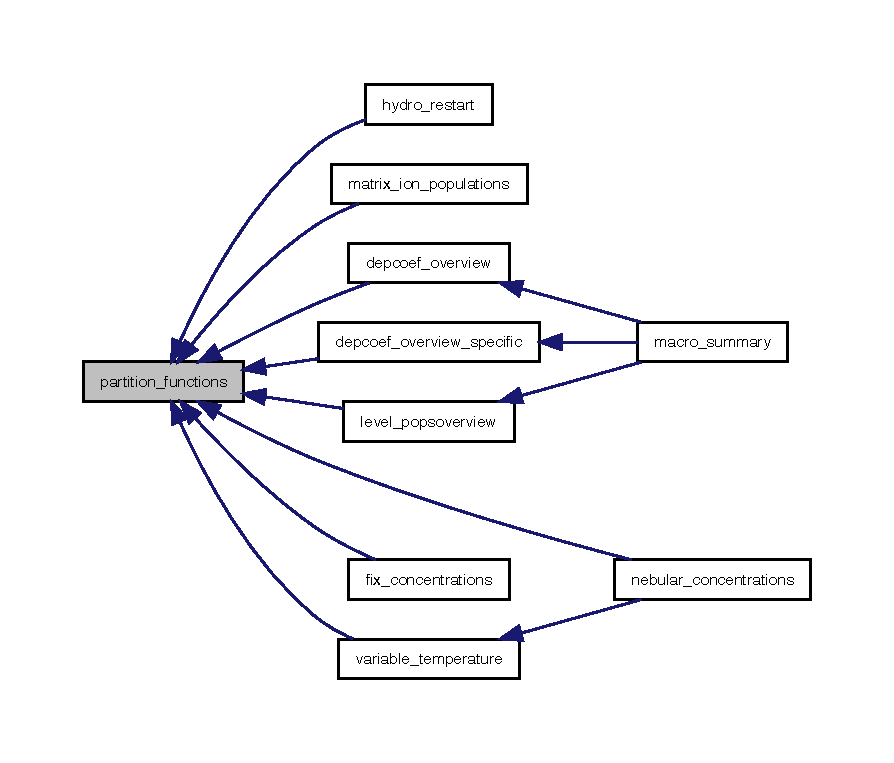
\includegraphics[width=350pt]{balance__templates_8h_a37c9b91e3450874eb15cef76079f344d_icgraph}
\end{center}
\end{figure}
\mbox{\Hypertarget{balance__templates_8h_a82dbda6e94577f3ecd6e55c085f2aa10}\label{balance__templates_8h_a82dbda6e94577f3ecd6e55c085f2aa10}} 
\index{balance\+\_\+templates.\+h@{balance\+\_\+templates.\+h}!photo\+\_\+gen\+\_\+agn@{photo\+\_\+gen\+\_\+agn}}
\index{photo\+\_\+gen\+\_\+agn@{photo\+\_\+gen\+\_\+agn}!balance\+\_\+templates.\+h@{balance\+\_\+templates.\+h}}
\subsubsection{\texorpdfstring{photo\+\_\+gen\+\_\+agn()}{photo\_gen\_agn()}}
{\footnotesize\ttfamily int photo\+\_\+gen\+\_\+agn (\begin{DoxyParamCaption}\item[{\hyperlink{python_8h_ad2424d53ebcf811656882a87e11b440c}{Phot\+Ptr}}]{p,  }\item[{double}]{r,  }\item[{double}]{alpha,  }\item[{double}]{weight,  }\item[{double}]{f1,  }\item[{double}]{f2,  }\item[{int}]{spectype,  }\item[{int}]{istart,  }\item[{int}]{nphot }\end{DoxyParamCaption})}



Generate a photon from an A\+GN object. 


\begin{DoxyParams}[1]{Parameters}
\mbox{\tt in,out}  & {\em Phot\+Ptr} & p pointer to the photon array \\
\hline
\mbox{\tt in,out}  & {\em double} & r radius of the central source \\
\hline
\mbox{\tt in,out}  & {\em double} & alpha spectral index of the PL sourece -\/ also used to communicate temperature if a BB or model is used. \\
\hline
\mbox{\tt in,out}  & {\em double} & weight the weight of each photon to be made \\
\hline
\mbox{\tt in,out}  & {\em double} & f1 lower frequency bound \\
\hline
\mbox{\tt in,out}  & {\em double} & f2 upper frequency nound \\
\hline
\mbox{\tt in,out}  & {\em int} & spectype the type of S\+ED \\
\hline
\mbox{\tt in,out}  & {\em int} & istart the number of the first photon to be made -\/ index into the p array \\
\hline
\mbox{\tt in,out}  & {\em int} & nphot the number of photons to be made \\
\hline
\end{DoxyParams}
\begin{DoxyReturn}{Returns}
0 (if successful or unscuccessful)
\end{DoxyReturn}
This subroutine produces photons from an A\+GN type source. There are a range of different S\+E\+Ds that can be used, these are communicated by the spectype and different choices cause different surbroutines to be called. The only {\itshape real} work done here is to compute the strarting location and direction of the photons.

\paragraph*{Notes}

Definition at line 374 of file agn.\+c.

\mbox{\Hypertarget{balance__templates_8h_a737bba69d6237e8d171f633c2c6d4cbf}\label{balance__templates_8h_a737bba69d6237e8d171f633c2c6d4cbf}} 
\index{balance\+\_\+templates.\+h@{balance\+\_\+templates.\+h}!pl\+\_\+copy\+\_\+conditions@{pl\+\_\+copy\+\_\+conditions}}
\index{pl\+\_\+copy\+\_\+conditions@{pl\+\_\+copy\+\_\+conditions}!balance\+\_\+templates.\+h@{balance\+\_\+templates.\+h}}
\subsubsection{\texorpdfstring{pl\+\_\+copy\+\_\+conditions()}{pl\_copy\_conditions()}}
{\footnotesize\ttfamily int pl\+\_\+copy\+\_\+conditions (\begin{DoxyParamCaption}\item[{\hyperlink{python_8h_a13ce7664e071685e1c3eaac3c32d7c8d}{Plasma\+Ptr}}]{win,  }\item[{\hyperlink{python_8h_a13ce7664e071685e1c3eaac3c32d7c8d}{Plasma\+Ptr}}]{wout }\end{DoxyParamCaption})}

\mbox{\Hypertarget{balance__templates_8h_a6f6a9a8730c8d1fa98e71a19b4121061}\label{balance__templates_8h_a6f6a9a8730c8d1fa98e71a19b4121061}} 
\index{balance\+\_\+templates.\+h@{balance\+\_\+templates.\+h}!pl\+\_\+rho@{pl\+\_\+rho}}
\index{pl\+\_\+rho@{pl\+\_\+rho}!balance\+\_\+templates.\+h@{balance\+\_\+templates.\+h}}
\subsubsection{\texorpdfstring{pl\+\_\+rho()}{pl\_rho()}}
{\footnotesize\ttfamily double pl\+\_\+rho (\begin{DoxyParamCaption}\item[{double}]{x\mbox{[}$\,$\mbox{]} }\end{DoxyParamCaption})}

\mbox{\Hypertarget{balance__templates_8h_a0f7abdb5c54e097dce91c47669672ca7}\label{balance__templates_8h_a0f7abdb5c54e097dce91c47669672ca7}} 
\index{balance\+\_\+templates.\+h@{balance\+\_\+templates.\+h}!pl\+\_\+velocity@{pl\+\_\+velocity}}
\index{pl\+\_\+velocity@{pl\+\_\+velocity}!balance\+\_\+templates.\+h@{balance\+\_\+templates.\+h}}
\subsubsection{\texorpdfstring{pl\+\_\+velocity()}{pl\_velocity()}}
{\footnotesize\ttfamily double pl\+\_\+velocity (\begin{DoxyParamCaption}\item[{double}]{x\mbox{[}$\,$\mbox{]},  }\item[{double}]{v\mbox{[}$\,$\mbox{]} }\end{DoxyParamCaption})}

\mbox{\Hypertarget{balance__templates_8h_aaa16d99441c764597ca593780e74f134}\label{balance__templates_8h_aaa16d99441c764597ca593780e74f134}} 
\index{balance\+\_\+templates.\+h@{balance\+\_\+templates.\+h}!pl\+\_\+wind\+\_\+define@{pl\+\_\+wind\+\_\+define}}
\index{pl\+\_\+wind\+\_\+define@{pl\+\_\+wind\+\_\+define}!balance\+\_\+templates.\+h@{balance\+\_\+templates.\+h}}
\subsubsection{\texorpdfstring{pl\+\_\+wind\+\_\+define()}{pl\_wind\_define()}}
{\footnotesize\ttfamily int pl\+\_\+wind\+\_\+define (\begin{DoxyParamCaption}\item[{\hyperlink{python_8h_ad957272e4ddecfb558775b2aeddf2ac4}{Wind\+Ptr}}]{w }\end{DoxyParamCaption})}

\mbox{\Hypertarget{balance__templates_8h_a16695e51479862629c3204586710a9da}\label{balance__templates_8h_a16695e51479862629c3204586710a9da}} 
\index{balance\+\_\+templates.\+h@{balance\+\_\+templates.\+h}!print\+\_\+levels@{print\+\_\+levels}}
\index{print\+\_\+levels@{print\+\_\+levels}!balance\+\_\+templates.\+h@{balance\+\_\+templates.\+h}}
\subsubsection{\texorpdfstring{print\+\_\+levels()}{print\_levels()}}
{\footnotesize\ttfamily int print\+\_\+levels (\begin{DoxyParamCaption}\item[{\hyperlink{python_8h_a13ce7664e071685e1c3eaac3c32d7c8d}{Plasma\+Ptr}}]{w }\end{DoxyParamCaption})}

\mbox{\Hypertarget{balance__templates_8h_a2a54f2e08391e50dbbfd7fe91d103c4b}\label{balance__templates_8h_a2a54f2e08391e50dbbfd7fe91d103c4b}} 
\index{balance\+\_\+templates.\+h@{balance\+\_\+templates.\+h}!sim\+\_\+alphasolve@{sim\+\_\+alphasolve}}
\index{sim\+\_\+alphasolve@{sim\+\_\+alphasolve}!balance\+\_\+templates.\+h@{balance\+\_\+templates.\+h}}
\subsubsection{\texorpdfstring{sim\+\_\+alphasolve()}{sim\_alphasolve()}}
{\footnotesize\ttfamily double sim\+\_\+alphasolve (\begin{DoxyParamCaption}\item[{double}]{ratans,  }\item[{double}]{numin,  }\item[{double}]{numax }\end{DoxyParamCaption})}

\mbox{\Hypertarget{balance__templates_8h_a371914de0935dbdb2eec59da595cd6d4}\label{balance__templates_8h_a371914de0935dbdb2eec59da595cd6d4}} 
\index{balance\+\_\+templates.\+h@{balance\+\_\+templates.\+h}!sim\+\_\+driver@{sim\+\_\+driver}}
\index{sim\+\_\+driver@{sim\+\_\+driver}!balance\+\_\+templates.\+h@{balance\+\_\+templates.\+h}}
\subsubsection{\texorpdfstring{sim\+\_\+driver()}{sim\_driver()}}
{\footnotesize\ttfamily int sim\+\_\+driver (\begin{DoxyParamCaption}\item[{\hyperlink{python_8h_a13ce7664e071685e1c3eaac3c32d7c8d}{Plasma\+Ptr}}]{xplasma }\end{DoxyParamCaption})}

\mbox{\Hypertarget{balance__templates_8h_ad9ef6b5303be6721d0d71fef2128ce15}\label{balance__templates_8h_ad9ef6b5303be6721d0d71fef2128ce15}} 
\index{balance\+\_\+templates.\+h@{balance\+\_\+templates.\+h}!sim\+\_\+pl@{sim\+\_\+pl}}
\index{sim\+\_\+pl@{sim\+\_\+pl}!balance\+\_\+templates.\+h@{balance\+\_\+templates.\+h}}
\subsubsection{\texorpdfstring{sim\+\_\+pl()}{sim\_pl()}}
{\footnotesize\ttfamily int sim\+\_\+pl (\begin{DoxyParamCaption}\item[{double}]{nh,  }\item[{double}]{t\+\_\+r,  }\item[{double}]{t\+\_\+e,  }\item[{double}]{www,  }\item[{int}]{nelem,  }\item[{double}]{ne,  }\item[{double}]{density\mbox{[}$\,$\mbox{]},  }\item[{double}]{xne,  }\item[{double}]{newden\mbox{[}$\,$\mbox{]},  }\item[{double}]{f1,  }\item[{double}]{f2 }\end{DoxyParamCaption})}

\mbox{\Hypertarget{balance__templates_8h_a312eb82e3c0f3b9a56c3eba044981bb9}\label{balance__templates_8h_a312eb82e3c0f3b9a56c3eba044981bb9}} 
\index{balance\+\_\+templates.\+h@{balance\+\_\+templates.\+h}!sim\+\_\+w@{sim\+\_\+w}}
\index{sim\+\_\+w@{sim\+\_\+w}!balance\+\_\+templates.\+h@{balance\+\_\+templates.\+h}}
\subsubsection{\texorpdfstring{sim\+\_\+w()}{sim\_w()}}
{\footnotesize\ttfamily double sim\+\_\+w (\begin{DoxyParamCaption}\item[{double}]{en1,  }\item[{double}]{v,  }\item[{double}]{dt,  }\item[{double}]{alpha,  }\item[{double}]{numin,  }\item[{double}]{numax }\end{DoxyParamCaption})}

\mbox{\Hypertarget{balance__templates_8h_a9da84c571671cfa8523ab5d3aed6c6e5}\label{balance__templates_8h_a9da84c571671cfa8523ab5d3aed6c6e5}} 
\index{balance\+\_\+templates.\+h@{balance\+\_\+templates.\+h}!sobolev\+\_\+line\+\_\+heating@{sobolev\+\_\+line\+\_\+heating}}
\index{sobolev\+\_\+line\+\_\+heating@{sobolev\+\_\+line\+\_\+heating}!balance\+\_\+templates.\+h@{balance\+\_\+templates.\+h}}
\subsubsection{\texorpdfstring{sobolev\+\_\+line\+\_\+heating()}{sobolev\_line\_heating()}}
{\footnotesize\ttfamily double sobolev\+\_\+line\+\_\+heating (\begin{DoxyParamCaption}\item[{\hyperlink{python_8h_a13ce7664e071685e1c3eaac3c32d7c8d}{Plasma\+Ptr}}]{w,  }\item[{\hyperlink{python_8h_ad2424d53ebcf811656882a87e11b440c}{Phot\+Ptr}}]{p,  }\item[{double}]{ds }\end{DoxyParamCaption})}

\mbox{\Hypertarget{balance__templates_8h_a33a5fe351d8c1dcf015fc2cf00b9da5c}\label{balance__templates_8h_a33a5fe351d8c1dcf015fc2cf00b9da5c}} 
\index{balance\+\_\+templates.\+h@{balance\+\_\+templates.\+h}!summary@{summary}}
\index{summary@{summary}!balance\+\_\+templates.\+h@{balance\+\_\+templates.\+h}}
\subsubsection{\texorpdfstring{summary()}{summary()}}
{\footnotesize\ttfamily int summary (\begin{DoxyParamCaption}\item[{\hyperlink{python_8h_a13ce7664e071685e1c3eaac3c32d7c8d}{Plasma\+Ptr}}]{one }\end{DoxyParamCaption})}

\mbox{\Hypertarget{balance__templates_8h_a62b387a13364f82a9dd357b7866f9543}\label{balance__templates_8h_a62b387a13364f82a9dd357b7866f9543}} 
\index{balance\+\_\+templates.\+h@{balance\+\_\+templates.\+h}!tb\+\_\+planck@{tb\+\_\+planck}}
\index{tb\+\_\+planck@{tb\+\_\+planck}!balance\+\_\+templates.\+h@{balance\+\_\+templates.\+h}}
\subsubsection{\texorpdfstring{tb\+\_\+planck()}{tb\_planck()}}
{\footnotesize\ttfamily double tb\+\_\+planck (\begin{DoxyParamCaption}\item[{double}]{freq }\end{DoxyParamCaption})}

\mbox{\Hypertarget{balance__templates_8h_adad31bd88f4f7c762a1c4efa8c964941}\label{balance__templates_8h_adad31bd88f4f7c762a1c4efa8c964941}} 
\index{balance\+\_\+templates.\+h@{balance\+\_\+templates.\+h}!tb\+\_\+pow@{tb\+\_\+pow}}
\index{tb\+\_\+pow@{tb\+\_\+pow}!balance\+\_\+templates.\+h@{balance\+\_\+templates.\+h}}
\subsubsection{\texorpdfstring{tb\+\_\+pow()}{tb\_pow()}}
{\footnotesize\ttfamily double tb\+\_\+pow (\begin{DoxyParamCaption}\item[{double}]{freq }\end{DoxyParamCaption})}

\mbox{\Hypertarget{balance__templates_8h_a620388e1c4a8e38f192c5a0ce42af389}\label{balance__templates_8h_a620388e1c4a8e38f192c5a0ce42af389}} 
\index{balance\+\_\+templates.\+h@{balance\+\_\+templates.\+h}!trans\+\_\+phot@{trans\+\_\+phot}}
\index{trans\+\_\+phot@{trans\+\_\+phot}!balance\+\_\+templates.\+h@{balance\+\_\+templates.\+h}}
\subsubsection{\texorpdfstring{trans\+\_\+phot()}{trans\_phot()}}
{\footnotesize\ttfamily int trans\+\_\+phot (\begin{DoxyParamCaption}\item[{\hyperlink{python_8h_ad957272e4ddecfb558775b2aeddf2ac4}{Wind\+Ptr}}]{w,  }\item[{\hyperlink{python_8h_ad2424d53ebcf811656882a87e11b440c}{Phot\+Ptr}}]{p,  }\item[{int}]{iextract }\end{DoxyParamCaption})}



int (w,p,iextract) oversees the propagation of a \char`\"{}flight\char`\"{} of photons 


\begin{DoxyParams}[1]{Parameters}
\mbox{\tt in}  & {\em Wind\+Ptr} & w The entire wind domain \\
\hline
\mbox{\tt in,out}  & {\em Phot\+Ptr} & p A pointer to a \char`\"{}fligh\char`\"{} of photons \\
\hline
\mbox{\tt in}  & {\em int} & iextract An integer controlling whether we are to process the flight in the live or die option (0) or whether we also need to extract photons in specific directions (which is usually the case in constructing spectra \\
\hline
\end{DoxyParams}
\begin{DoxyReturn}{Returns}
Normally returns 0
\end{DoxyReturn}
This routine oversees the propagation of individual photons. The main loop covers an entire \char`\"{}flight\char`\"{} of photons. The routine generates the random optical depth a photon can travel before scattering and monitors the progress of the photon through the grid.

The real physics is done elsewhere, in lower level routines.

\paragraph*{Notes}

At the end of the routine the position for each of the photons in p is the last point where the photon was in the wind, $\ast$ not the outer boundary of the radiative transfer 

Definition at line 85 of file trans\+\_\+phot.\+c.

Here is the caller graph for this function\+:
\nopagebreak
\begin{figure}[H]
\begin{center}
\leavevmode
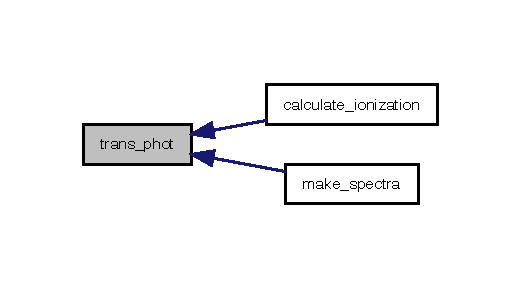
\includegraphics[width=250pt]{balance__templates_8h_a620388e1c4a8e38f192c5a0ce42af389_icgraph}
\end{center}
\end{figure}
\mbox{\Hypertarget{balance__templates_8h_ae77272897af1eb8f6ebd0f7cfe2932e8}\label{balance__templates_8h_ae77272897af1eb8f6ebd0f7cfe2932e8}} 
\index{balance\+\_\+templates.\+h@{balance\+\_\+templates.\+h}!translate@{translate}}
\index{translate@{translate}!balance\+\_\+templates.\+h@{balance\+\_\+templates.\+h}}
\subsubsection{\texorpdfstring{translate()}{translate()}}
{\footnotesize\ttfamily int translate (\begin{DoxyParamCaption}\item[{\hyperlink{python_8h_ad957272e4ddecfb558775b2aeddf2ac4}{Wind\+Ptr}}]{w,  }\item[{\hyperlink{python_8h_ad2424d53ebcf811656882a87e11b440c}{Phot\+Ptr}}]{pp,  }\item[{double}]{tau\+\_\+scat,  }\item[{double $\ast$}]{tau,  }\item[{int $\ast$}]{nres }\end{DoxyParamCaption})}



a steering routine that either calls \+\_\+in\+\_\+space or \+\_\+in\+\_\+wind depending upon the current location of the photon. 


\begin{DoxyParams}[1]{Parameters}
\mbox{\tt in}  & {\em Wind\+Ptr} & w A pointer to the wind \\
\hline
\mbox{\tt in,out}  & {\em Phot\+Ptr} & pp A photon \\
\hline
\mbox{\tt in}  & {\em double} & tau\+\_\+scat the depth at which the photon should scatter \\
\hline
\mbox{\tt out}  & {\em double} & $\ast$ tau The optical depth associated with a resonanant scatter when this is the reason the photon has stopped \\
\hline
\mbox{\tt in,out}  & {\em int} & $\ast$ nres The number of the resonance if the photon stopped. due to reaching the scattering optical depth \\
\hline
\end{DoxyParams}
\begin{DoxyReturn}{Returns}
A status that states what caused the photon to stp as it did
\end{DoxyReturn}
The routine takes the current position of the photon and determines where it is. Depending on this it calls either translate\+\_\+in\+\_\+space or translate\+\_\+in\+\_\+wind

On exit, the position of the photon will have been updated.

\paragraph*{Notes}

Translate controls the flow of the photon through one grid cell. In Python, there are additional possibilities since there are wind free regions.

The routine first calls where\+\_\+in\+\_\+wind which returns the correct domain for a given position, or domain 0 if the position is not in the wind of a domain. The photon structure does not have the domain number directly encoded, but it can be obtained from the grid number, which where in\+\_\+grid updates

This construction is used so that the calling routines for translate (trans\+\_\+phot and extract) can be the same in the 1 and 2d versions. 

Definition at line 79 of file photon2d.\+c.

Here is the caller graph for this function\+:
\nopagebreak
\begin{figure}[H]
\begin{center}
\leavevmode
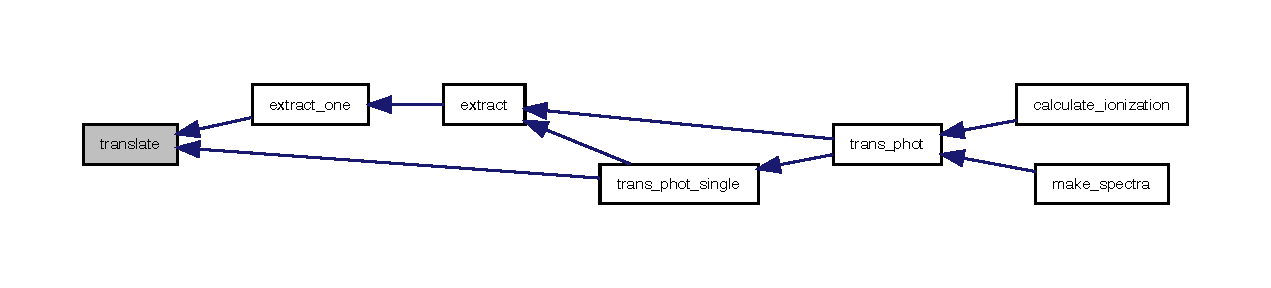
\includegraphics[width=350pt]{balance__templates_8h_ae77272897af1eb8f6ebd0f7cfe2932e8_icgraph}
\end{center}
\end{figure}
\mbox{\Hypertarget{balance__templates_8h_aa1ffd17034054d51819328d892fc57e8}\label{balance__templates_8h_aa1ffd17034054d51819328d892fc57e8}} 
\index{balance\+\_\+templates.\+h@{balance\+\_\+templates.\+h}!translate\+\_\+in\+\_\+space@{translate\+\_\+in\+\_\+space}}
\index{translate\+\_\+in\+\_\+space@{translate\+\_\+in\+\_\+space}!balance\+\_\+templates.\+h@{balance\+\_\+templates.\+h}}
\subsubsection{\texorpdfstring{translate\+\_\+in\+\_\+space()}{translate\_in\_space()}}
{\footnotesize\ttfamily int translate\+\_\+in\+\_\+space (\begin{DoxyParamCaption}\item[{\hyperlink{python_8h_ad2424d53ebcf811656882a87e11b440c}{Phot\+Ptr}}]{pp }\end{DoxyParamCaption})}



translates the photon from its current position to the edge of the wind. 


\begin{DoxyParams}[1]{Parameters}
\mbox{\tt in,out}  & {\em Phot\+Ptr} & pp A photon \\
\hline
\end{DoxyParams}
\begin{DoxyReturn}{Returns}
A status flag indication why the photon stopped
\end{DoxyReturn}
The routine translate the photon (which is assumed to be in the wind, but not in an active wind cell) to the closest boundary.

The photon position is updated in the process.

\paragraph*{Notes}

\begin{DoxyRefDesc}{Bug}
\item[\hyperlink{bug__bug000041}{Bug}]There are questions in the comments about why an additonal check is needed as to whther the photon as hit the star. It seems superfluous so someone should check whether this addtional check can be removed.\end{DoxyRefDesc}


Definition at line 144 of file photon2d.\+c.

\mbox{\Hypertarget{balance__templates_8h_a0118547dede9b08b5ac6609b4313e3e8}\label{balance__templates_8h_a0118547dede9b08b5ac6609b4313e3e8}} 
\index{balance\+\_\+templates.\+h@{balance\+\_\+templates.\+h}!translate\+\_\+in\+\_\+wind@{translate\+\_\+in\+\_\+wind}}
\index{translate\+\_\+in\+\_\+wind@{translate\+\_\+in\+\_\+wind}!balance\+\_\+templates.\+h@{balance\+\_\+templates.\+h}}
\subsubsection{\texorpdfstring{translate\+\_\+in\+\_\+wind()}{translate\_in\_wind()}}
{\footnotesize\ttfamily int translate\+\_\+in\+\_\+wind (\begin{DoxyParamCaption}\item[{\hyperlink{python_8h_ad957272e4ddecfb558775b2aeddf2ac4}{Wind\+Ptr}}]{w,  }\item[{\hyperlink{python_8h_ad2424d53ebcf811656882a87e11b440c}{Phot\+Ptr}}]{p,  }\item[{double}]{tau\+\_\+scat,  }\item[{double $\ast$}]{tau,  }\item[{int $\ast$}]{nres }\end{DoxyParamCaption})}



translates the photon within a single cell in the wind. 


\begin{DoxyParams}[1]{Parameters}
\mbox{\tt in}  & {\em Wind\+Ptr} & w The entire wind \\
\hline
\mbox{\tt in,out}  & {\em Phot\+Ptr} & p A photon \\
\hline
\mbox{\tt in}  & {\em double} & tau\+\_\+scat The depth at which the photon will scatter \\
\hline
\mbox{\tt out}  & {\em double} & $\ast$ tau The tau of a resonance \\
\hline
\mbox{\tt out}  & {\em int} & $\ast$ nres The resonaance which caused the photon to stop \\
\hline
\end{DoxyParams}
\begin{DoxyReturn}{Returns}
A status indicated whether the photon has stopped for a scattering even of for some other teason
\end{DoxyReturn}
It calculates and updates the final position of the photon p, the optical depth tau after having translated the photon, and, if the photon is scattered, the number of the resonance responsible for scattering (or absorbing) the photon bundle.

These last two quantities are calculated in ds\+\_\+calculate and simply passed back.

translate\+\_\+in\+\_\+wind returns that status directly to the calling routine.

\paragraph*{Notes}

In addition to moving the photon, the routine also updates some values having to do with the radiation filed both in and out of macro atom mode. 

Definition at line 543 of file photon2d.\+c.

\mbox{\Hypertarget{balance__templates_8h_a3f7b1bb2489cf3bc02bb0b28c20ebef7}\label{balance__templates_8h_a3f7b1bb2489cf3bc02bb0b28c20ebef7}} 
\index{balance\+\_\+templates.\+h@{balance\+\_\+templates.\+h}!verner\+\_\+planck@{verner\+\_\+planck}}
\index{verner\+\_\+planck@{verner\+\_\+planck}!balance\+\_\+templates.\+h@{balance\+\_\+templates.\+h}}
\subsubsection{\texorpdfstring{verner\+\_\+planck()}{verner\_planck()}}
{\footnotesize\ttfamily double verner\+\_\+planck (\begin{DoxyParamCaption}\item[{double}]{freq }\end{DoxyParamCaption})}

\mbox{\Hypertarget{balance__templates_8h_a1e88d24ba05d7a5dd5c1f6099e67766d}\label{balance__templates_8h_a1e88d24ba05d7a5dd5c1f6099e67766d}} 
\index{balance\+\_\+templates.\+h@{balance\+\_\+templates.\+h}!verner\+\_\+pow@{verner\+\_\+pow}}
\index{verner\+\_\+pow@{verner\+\_\+pow}!balance\+\_\+templates.\+h@{balance\+\_\+templates.\+h}}
\subsubsection{\texorpdfstring{verner\+\_\+pow()}{verner\_pow()}}
{\footnotesize\ttfamily double verner\+\_\+pow (\begin{DoxyParamCaption}\item[{double}]{freq }\end{DoxyParamCaption})}

\mbox{\Hypertarget{balance__templates_8h_a56740476af61734dee90b4090f004971}\label{balance__templates_8h_a56740476af61734dee90b4090f004971}} 
\index{balance\+\_\+templates.\+h@{balance\+\_\+templates.\+h}!walls@{walls}}
\index{walls@{walls}!balance\+\_\+templates.\+h@{balance\+\_\+templates.\+h}}
\subsubsection{\texorpdfstring{walls()}{walls()}}
{\footnotesize\ttfamily int walls (\begin{DoxyParamCaption}\item[{\hyperlink{python_8h_ad2424d53ebcf811656882a87e11b440c}{Phot\+Ptr}}]{p,  }\item[{\hyperlink{python_8h_ad2424d53ebcf811656882a87e11b440c}{Phot\+Ptr}}]{pold }\end{DoxyParamCaption})}

Here is the caller graph for this function\+:
\nopagebreak
\begin{figure}[H]
\begin{center}
\leavevmode
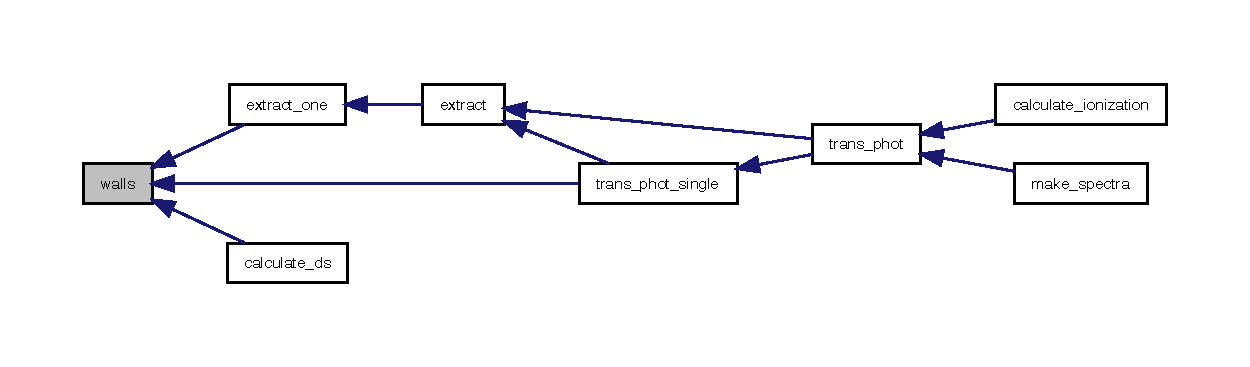
\includegraphics[width=350pt]{balance__templates_8h_a56740476af61734dee90b4090f004971_icgraph}
\end{center}
\end{figure}
\mbox{\Hypertarget{balance__templates_8h_a2cdbde0efa1209e5e416c10c54ed7e8d}\label{balance__templates_8h_a2cdbde0efa1209e5e416c10c54ed7e8d}} 
\index{balance\+\_\+templates.\+h@{balance\+\_\+templates.\+h}!xbb@{xbb}}
\index{xbb@{xbb}!balance\+\_\+templates.\+h@{balance\+\_\+templates.\+h}}
\subsubsection{\texorpdfstring{xbb()}{xbb()}}
{\footnotesize\ttfamily int xbb (\begin{DoxyParamCaption}\item[{\hyperlink{python_8h_ad2424d53ebcf811656882a87e11b440c}{Phot\+Ptr}}]{p,  }\item[{double}]{t,  }\item[{double}]{weight,  }\item[{double}]{f1,  }\item[{double}]{f2,  }\item[{int}]{freq\+\_\+sampling }\end{DoxyParamCaption})}

\mbox{\Hypertarget{balance__templates_8h_af8cca9ec56b5097105e209de88fbf427}\label{balance__templates_8h_af8cca9ec56b5097105e209de88fbf427}} 
\index{balance\+\_\+templates.\+h@{balance\+\_\+templates.\+h}!xinteg\+\_\+sim@{xinteg\+\_\+sim}}
\index{xinteg\+\_\+sim@{xinteg\+\_\+sim}!balance\+\_\+templates.\+h@{balance\+\_\+templates.\+h}}
\subsubsection{\texorpdfstring{xinteg\+\_\+sim()}{xinteg\_sim()}}
{\footnotesize\ttfamily double xinteg\+\_\+sim (\begin{DoxyParamCaption}\item[{double}]{t,  }\item[{double}]{f1,  }\item[{double}]{f2,  }\item[{int}]{nion,  }\item[{double}]{max\+\_\+ratio,  }\item[{double}]{current\+\_\+ratio }\end{DoxyParamCaption})}

\mbox{\Hypertarget{balance__templates_8h_a571b75143e5686426dbc0d5ef4bf58a3}\label{balance__templates_8h_a571b75143e5686426dbc0d5ef4bf58a3}} 
\index{balance\+\_\+templates.\+h@{balance\+\_\+templates.\+h}!xmake\+\_\+bb@{xmake\+\_\+bb}}
\index{xmake\+\_\+bb@{xmake\+\_\+bb}!balance\+\_\+templates.\+h@{balance\+\_\+templates.\+h}}
\subsubsection{\texorpdfstring{xmake\+\_\+bb()}{xmake\_bb()}}
{\footnotesize\ttfamily int xmake\+\_\+bb (\begin{DoxyParamCaption}\item[{\hyperlink{python_8h_ad2424d53ebcf811656882a87e11b440c}{Phot\+Ptr}}]{p,  }\item[{double}]{t\+\_\+r,  }\item[{double}]{freqmin,  }\item[{double}]{freqmax,  }\item[{double}]{weight,  }\item[{int}]{iphot\+\_\+start,  }\item[{int}]{nphot }\end{DoxyParamCaption})}

\mbox{\Hypertarget{balance__templates_8h_ab34d13ef098af692d1a406016724580a}\label{balance__templates_8h_ab34d13ef098af692d1a406016724580a}} 
\index{balance\+\_\+templates.\+h@{balance\+\_\+templates.\+h}!xsaha@{xsaha}}
\index{xsaha@{xsaha}!balance\+\_\+templates.\+h@{balance\+\_\+templates.\+h}}
\subsubsection{\texorpdfstring{xsaha()}{xsaha()}}
{\footnotesize\ttfamily int xsaha (\begin{DoxyParamCaption}\item[{\hyperlink{python_8h_ad957272e4ddecfb558775b2aeddf2ac4}{Wind\+Ptr}}]{one,  }\item[{\hyperlink{python_8h_ad2424d53ebcf811656882a87e11b440c}{Phot\+Ptr}}]{p,  }\item[{double}]{nh,  }\item[{double}]{t\+\_\+r,  }\item[{double}]{t\+\_\+e,  }\item[{double}]{weight,  }\item[{int}]{ioniz\+\_\+mode,  }\item[{int}]{freq\+\_\+sampling }\end{DoxyParamCaption})}

Here is the caller graph for this function\+:
\nopagebreak
\begin{figure}[H]
\begin{center}
\leavevmode
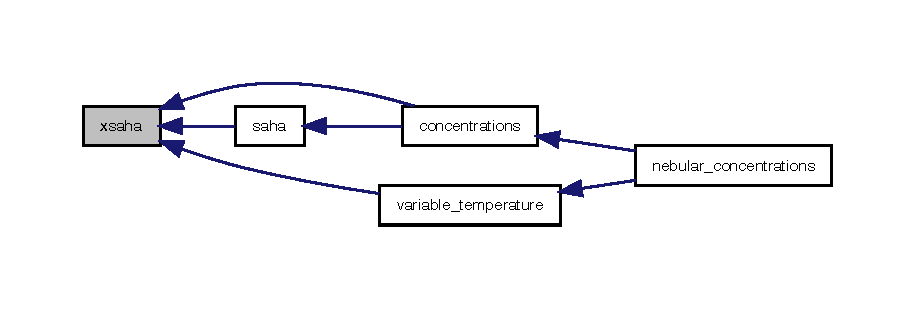
\includegraphics[width=350pt]{balance__templates_8h_ab34d13ef098af692d1a406016724580a_icgraph}
\end{center}
\end{figure}

\hypertarget{bands_8c}{}\section{/\+Users/mhewitt/python/source/bands.c File Reference}
\label{bands_8c}\index{/\+Users/mhewitt/python/source/bands.\+c@{/\+Users/mhewitt/python/source/bands.\+c}}


Setup the frequency bands used for stratified sampling and for recording spectra in wind cells.  


{\ttfamily \#include $<$stdio.\+h$>$}\newline
{\ttfamily \#include $<$stdlib.\+h$>$}\newline
{\ttfamily \#include $<$math.\+h$>$}\newline
{\ttfamily \#include \char`\"{}atomic.\+h\char`\"{}}\newline
{\ttfamily \#include \char`\"{}python.\+h\char`\"{}}\newline
Include dependency graph for bands.\+c\+:
\nopagebreak
\begin{figure}[H]
\begin{center}
\leavevmode
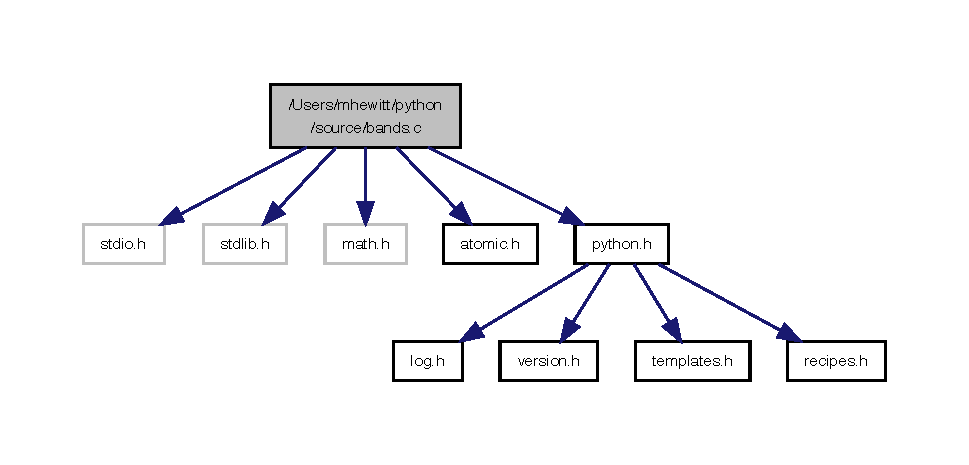
\includegraphics[width=350pt]{bands_8c__incl}
\end{center}
\end{figure}
\subsection*{Functions}
\begin{DoxyCompactItemize}
\item 
int \hyperlink{bands_8c_a3513a64162c15d3d3d101c3d5ea2367f}{bands\+\_\+init} (int imode, struct \hyperlink{structxbands}{xbands} $\ast$band)
\begin{DoxyCompactList}\small\item\em This is the routine that initializes the bands. \end{DoxyCompactList}\item 
int \hyperlink{bands_8c_a900ff3bb7a80569abf42be1e2b00fd36}{freqs\+\_\+init} (double freqmin, double freqmax)
\begin{DoxyCompactList}\small\item\em This is the routine where the frequency boundaries for course spectra are established. \end{DoxyCompactList}\end{DoxyCompactItemize}


\subsection{Detailed Description}
Setup the frequency bands used for stratified sampling and for recording spectra in wind cells. 

\begin{DoxyAuthor}{Author}
ksl 
\end{DoxyAuthor}
\begin{DoxyDate}{Date}
March , 2018
\end{DoxyDate}
The subroutines here deal with two related issues, how to choose how many photons or photon bundles to create in various wavelength ranges, and how to record the spectrum that pass through individual cells.

Photons, or photon bundles, in Python are created with certain frequency and carry a certain amount of energy. Without any kind of stratified sampling all of the photons would be createed with the same energy content and frequencies which sample the spectrum in equal energy entervals. The sum of energies of all of the photons bundles originating in, for example, a stellar photosphere would eqaul that of the luminostiy of the star.

Normally, however, Python uses a form of stratified sampling to assure we have photons in various energy bands. This is important, especially for calculating ionization rates since one needs enough photons above ionization edges to estimate the rate accurately. In banding, one choses a number of photons in a given frequency range and changes the energy of the photon bundle so that the proper normalization is obtained.

Once one has decided how many photons in what wave bands to generate one also needs to capture a crude spectrum in each cell of the grid at least for many of the ionization modes we use. The resolution needs to be good enough to allow for various important ionization edges, but not so fine that one cannot characterize the slope of the spectrum in each interval.

The routines init\+\_\+bands in this file sets up the bands to for creating photons based on various user inputs; it then calls freqs\+\_\+init that sets up the frequency boundaries for recoding the spectra. 

\subsection{Function Documentation}
\mbox{\Hypertarget{bands_8c_a3513a64162c15d3d3d101c3d5ea2367f}\label{bands_8c_a3513a64162c15d3d3d101c3d5ea2367f}} 
\index{bands.\+c@{bands.\+c}!bands\+\_\+init@{bands\+\_\+init}}
\index{bands\+\_\+init@{bands\+\_\+init}!bands.\+c@{bands.\+c}}
\subsubsection{\texorpdfstring{bands\+\_\+init()}{bands\_init()}}
{\footnotesize\ttfamily int bands\+\_\+init (\begin{DoxyParamCaption}\item[{int}]{imode,  }\item[{struct \hyperlink{structxbands}{xbands} $\ast$}]{band }\end{DoxyParamCaption})}



This is the routine that initializes the bands. 

Python uses a form of stratified sampling in an attempt to assure that there are photon bundles at (high, generally) frequencies

This is the routine that initializes the bands. There are a number of possiblilities for setting up the bands


\begin{DoxyParams}[1]{Parameters}
\mbox{\tt in}  & {\em int} & imode A switch used for determining how the bands are to be populated \\
\hline
\mbox{\tt out}  & {\em struct} & xbands $\ast$ band The structure that is populated with the band information \\
\hline
\end{DoxyParams}
\begin{DoxyReturn}{Returns}
The routine itself simply returns 0 on success
\end{DoxyReturn}
The outputs are passed to other routines through the pointer to xbands.

The currently allow modes are $\ast$0 Use temperature to define a single band $\ast$1 Use f1 and f2 to define a single band $\ast$2 Use t,f1 and f2, and hardwired bands to define multiple bands which have been tuned to be relevent to C\+Vs and other systems where a hot disk (T\+\_\+eff of about 100,000 K is assumed
\begin{DoxyItemize}
\item 3 Bands tuned for yso
\item 4 Query the user to specify an arbitrary set of bands
\item 5 Hardwired very wide bands for testing $\ast$6 Bands set up by nsh to test cloudy $\ast$7 Bands hardwired for A\+GN paper1 by nsh $\ast$8 Define bands in logarithmic intervals
\end{DoxyItemize}

\paragraph*{Notes}

10nov -\/ ksl -\/ X\+XX Some of the choices have checks to see whether the bands that are being set up lie within f1 and f2. Others do not. This seems like an error.

\begin{DoxyRefDesc}{Bug}
\item[\hyperlink{bug__bug000003}{Bug}]At some point some of the banding needs to be tested systematically. We have tended to find a setup that we like and just use it.\end{DoxyRefDesc}


Definition at line 123 of file bands.\+c.

Here is the call graph for this function\+:
\nopagebreak
\begin{figure}[H]
\begin{center}
\leavevmode
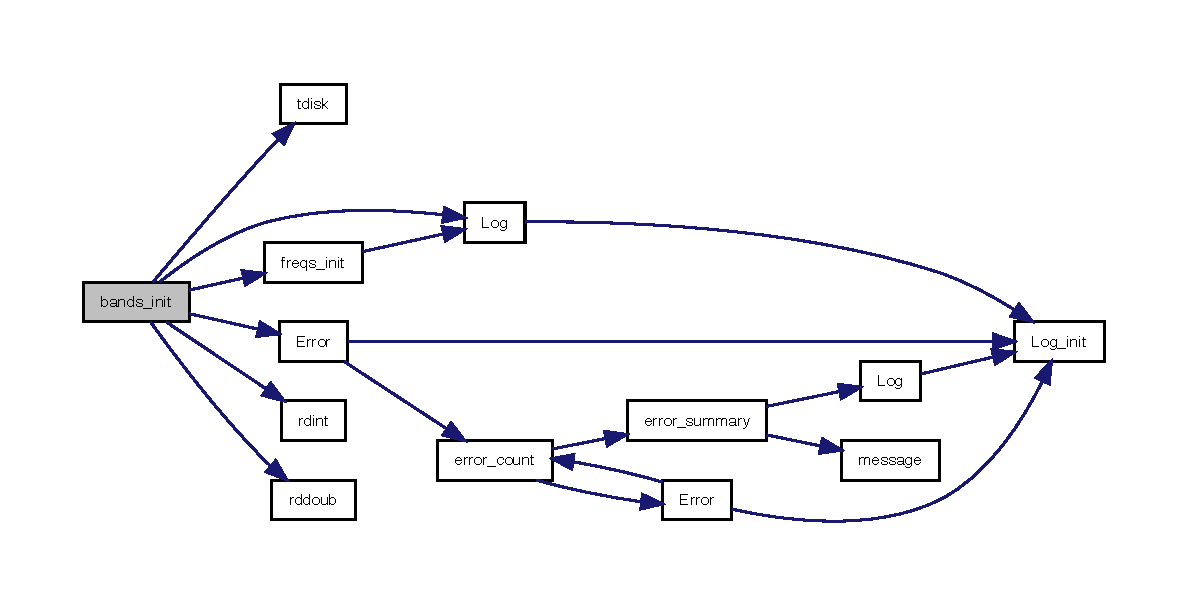
\includegraphics[width=350pt]{bands_8c_a3513a64162c15d3d3d101c3d5ea2367f_cgraph}
\end{center}
\end{figure}
Here is the caller graph for this function\+:
\nopagebreak
\begin{figure}[H]
\begin{center}
\leavevmode
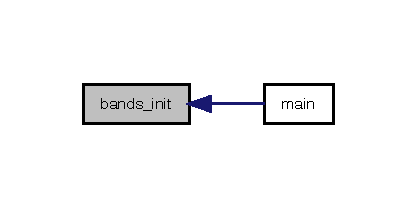
\includegraphics[width=200pt]{bands_8c_a3513a64162c15d3d3d101c3d5ea2367f_icgraph}
\end{center}
\end{figure}
\mbox{\Hypertarget{bands_8c_a900ff3bb7a80569abf42be1e2b00fd36}\label{bands_8c_a900ff3bb7a80569abf42be1e2b00fd36}} 
\index{bands.\+c@{bands.\+c}!freqs\+\_\+init@{freqs\+\_\+init}}
\index{freqs\+\_\+init@{freqs\+\_\+init}!bands.\+c@{bands.\+c}}
\subsubsection{\texorpdfstring{freqs\+\_\+init()}{freqs\_init()}}
{\footnotesize\ttfamily int freqs\+\_\+init (\begin{DoxyParamCaption}\item[{double}]{freqmin,  }\item[{double}]{freqmax }\end{DoxyParamCaption})}



This is the routine where the frequency boundaries for course spectra are established. 


\begin{DoxyParams}[1]{Parameters}
\mbox{\tt in,out}  & {\em double} & freqmin The minimum frequency \\
\hline
\mbox{\tt in,out}  & {\em double} & freqmax The maximum frequency \\
\hline
\end{DoxyParams}
\begin{DoxyReturn}{Returns}
Always returns 0
\end{DoxyReturn}
In addition to setting bands which define the photons that are generated one must define bands that approximated the spectra in a cell. One cannot store all of the photons and their weights. This routine creates boundaries for storring the spectra.

\paragraph*{Notes}

At present everything is hardwired. Two typs of banding are carred out, one for A\+G\+N/\+X-\/ray bianries, and one for stellar systems

freqmin and freqmax are used inorder to limit the total range of the spectral bands.

The results are stored in geo.\+xfreq 

Definition at line 608 of file bands.\+c.

Here is the call graph for this function\+:
\nopagebreak
\begin{figure}[H]
\begin{center}
\leavevmode
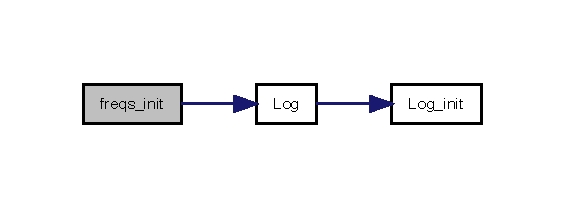
\includegraphics[width=271pt]{bands_8c_a900ff3bb7a80569abf42be1e2b00fd36_cgraph}
\end{center}
\end{figure}
Here is the caller graph for this function\+:
\nopagebreak
\begin{figure}[H]
\begin{center}
\leavevmode
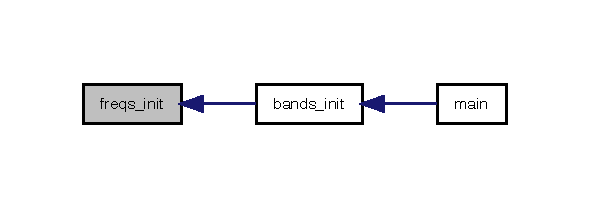
\includegraphics[width=283pt]{bands_8c_a900ff3bb7a80569abf42be1e2b00fd36_icgraph}
\end{center}
\end{figure}

\hypertarget{bb_8c}{}\section{/\+Users/mhewitt/python/source/bb.c File Reference}
\label{bb_8c}\index{/\+Users/mhewitt/python/source/bb.\+c@{/\+Users/mhewitt/python/source/bb.\+c}}


Routines concerning the generation of photons from blackbodies.  


{\ttfamily \#include $<$stdio.\+h$>$}\newline
{\ttfamily \#include $<$stdlib.\+h$>$}\newline
{\ttfamily \#include $<$math.\+h$>$}\newline
{\ttfamily \#include \char`\"{}atomic.\+h\char`\"{}}\newline
{\ttfamily \#include \char`\"{}python.\+h\char`\"{}}\newline
{\ttfamily \#include $<$gsl/gsl\+\_\+rng.\+h$>$}\newline
{\ttfamily \#include $<$gsl/gsl\+\_\+randist.\+h$>$}\newline
Include dependency graph for bb.\+c\+:
\nopagebreak
\begin{figure}[H]
\begin{center}
\leavevmode
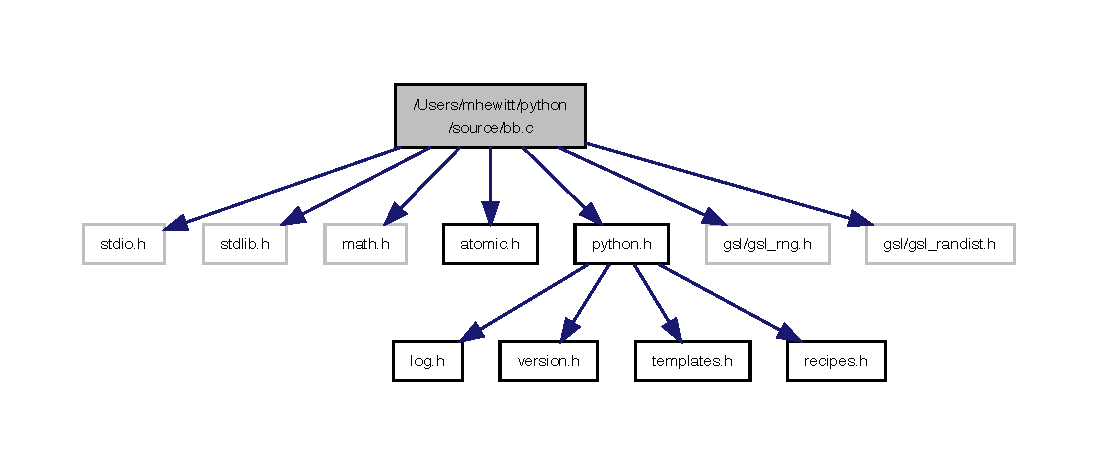
\includegraphics[width=350pt]{bb_8c__incl}
\end{center}
\end{figure}
\subsection*{Macros}
\begin{DoxyCompactItemize}
\item 
\#define \hyperlink{bb_8c_a4f42ae5d5509b18cabce35777d92f62f}{A\+L\+P\+H\+A\+M\+IN}~0.\+4
\item 
\#define \hyperlink{bb_8c_ac1547dd7dacf3a4dc5d56c8e6ff960a6}{A\+L\+P\+H\+A\+M\+AX}~30.
\item 
\#define \hyperlink{bb_8c_ab72cc0331127fe2719296673f28b440b}{A\+L\+P\+H\+A\+B\+IG}~100.
\item 
\#define \hyperlink{bb_8c_a3c01ddae06770065b909d38445f03bd8}{N\+J\+U\+M\+PS}~30
\item 
\#define \hyperlink{bb_8c_a5de5d183f9a6a8d53316f743e1ca6dc2}{N\+M\+AX}~1000
\item 
\#define \hyperlink{bb_8c_a002b2f4894492820fe708b1b7e7c5e70}{E\+P\+S\+I\+L\+ON}~1.e-\/6
\end{DoxyCompactItemize}
\subsection*{Functions}
\begin{DoxyCompactItemize}
\item 
double \hyperlink{bb_8c_a5f832b1ef434fdb41eaa62feb7edd710}{planck} (double \hyperlink{import__spherical_8c_afc1637b8a38578a1c95ed9f689476775}{t}, double freqmin, double freqmax)
\begin{DoxyCompactList}\small\item\em returns the frequency for a photon which follows a Placnk distribution within defined frequncy limits \end{DoxyCompactList}\item 
double \hyperlink{bb_8c_a6bae7f74815dfcf783a7dafade8faeca}{get\+\_\+rand\+\_\+pow} (double \hyperlink{compton_8c_ac75b803b570527306e1e744bfb7a604f}{x1}, double x2, double \hyperlink{templates_8h_a89a27f4f3a5c836df75585774ba7a643}{alpha})
\begin{DoxyCompactList}\small\item\em obtains a random number between x1 and x2 for a power law densiity distribution with index alpha \end{DoxyCompactList}\item 
double \hyperlink{bb_8c_af2d9c9e4094a425824f269ef22163048}{get\+\_\+rand\+\_\+exp} (double alpha\+\_\+min, double alpha\+\_\+max)
\begin{DoxyCompactList}\small\item\em obtain a random number between alpha\+\_\+min and alpha\+\_\+max from an distribution of the form e$\ast$$\ast$-\/alpha \end{DoxyCompactList}\item 
double \hyperlink{bb_8c_af5c48487242ab8760a1893e385d3e11b}{integ\+\_\+planck\+\_\+d} (double \hyperlink{bb_8c_a35106e779db1ad64f0de4eec449ec129}{alphamin}, double \hyperlink{bb_8c_af21e1955cd413e7edbe9c2a4fe822282}{alphamax})
\begin{DoxyCompactList}\small\item\em Obtains the integral of the dimensionless blackbody function between alphamin and alphamax. \end{DoxyCompactList}\item 
int \hyperlink{bb_8c_aa67b840e2ff05fc474799c42178b392e}{init\+\_\+integ\+\_\+planck\+\_\+d} ()
\begin{DoxyCompactList}\small\item\em calulates integrals of the dimensionless bb function from 0 to alpha and the stores the reusults in an array used by integ\+\_\+plank\+\_\+d \end{DoxyCompactList}\item 
double \hyperlink{bb_8c_ad6196c3c4ec0bdeda06aa797af259d81}{planck\+\_\+d} (double \hyperlink{templates_8h_a89a27f4f3a5c836df75585774ba7a643}{alpha})
\begin{DoxyCompactList}\small\item\em The value of the dimensioless BB function at alpha. \end{DoxyCompactList}\item 
double \hyperlink{bb_8c_a337db7e010442d30f7c4b45f3e41fa5c}{emittance\+\_\+bb} (double freqmin, double freqmax, double \hyperlink{import__spherical_8c_afc1637b8a38578a1c95ed9f689476775}{t})
\begin{DoxyCompactList}\small\item\em Calculate the emittance of a bb between freqmin and freqmax. \end{DoxyCompactList}\item 
double \hyperlink{bb_8c_a11871d7df7f3167db92bef8c8ef98926}{check\+\_\+fmax} (double fmin, double fmax, double temp)
\begin{DoxyCompactList}\small\item\em decides whether a maximum frequency requested for an integral is sensible. If it is too far off the end of the planck function, qromb will malfunction. We just have to set it to a frequency where the BB function is tiny, say where hnu/kT =100. \end{DoxyCompactList}\end{DoxyCompactItemize}
\subsection*{Variables}
\begin{DoxyCompactItemize}
\item 
int \hyperlink{bb_8c_a0d6e712e70e9d8d896e421421e5232a9}{ninit\+\_\+planck} = 0
\item 
double \hyperlink{bb_8c_ad5ae362a91b7c239184d49913e1701b1}{old\+\_\+t} = 0
\item 
double \hyperlink{bb_8c_a65f885c797f8031956517c69adcd0345}{old\+\_\+freqmin} = 0
\item 
double \hyperlink{bb_8c_a8dc32bfb2583414f49194409ba81c27c}{old\+\_\+freqmax} = 0
\item 
double \hyperlink{bb_8c_a35106e779db1ad64f0de4eec449ec129}{alphamin}
\item 
double \hyperlink{bb_8c_af21e1955cd413e7edbe9c2a4fe822282}{alphamax}
\item 
double \hyperlink{bb_8c_acddeb64d75504658a4a6e7aec61d3721}{cdf\+\_\+bb\+\_\+lo}
\item 
double \hyperlink{bb_8c_a4e1ff6ebea38be2c5723ae40379acb30}{cdf\+\_\+bb\+\_\+hi}
\item 
double \hyperlink{bb_8c_a30d9e580767e41f7671f036b54167316}{cdf\+\_\+bb\+\_\+tot}
\item 
double \hyperlink{bb_8c_ac3a0662170e08c6bbd081b1ae368c650}{cdf\+\_\+bb\+\_\+ylo}
\item 
double \hyperlink{bb_8c_a9a8f24be43c8ae7bc5328821d705fd38}{cdf\+\_\+bb\+\_\+yhi}
\item 
double \hyperlink{bb_8c_a5e666b72cd5ad44a523f8cef4c6e5f06}{lo\+\_\+freq\+\_\+alphamin}
\item 
double \hyperlink{bb_8c_a8cb2580284665f530fa828efeb72c8e2}{lo\+\_\+freq\+\_\+alphamax}
\item 
double \hyperlink{bb_8c_a481fe97a41ed0e1a21ef0f1e0952e2a2}{hi\+\_\+freq\+\_\+alphamin}
\item 
double \hyperlink{bb_8c_acf13e2e3c9727b3d93ed1e53ea81ab96}{hi\+\_\+freq\+\_\+alphamax}
\item 
double \hyperlink{bb_8c_a3308b12af5085b72eed7ec3169a707b4}{bb\+\_\+set} \mbox{[}$\,$\mbox{]}
\item 
int \hyperlink{bb_8c_a13f5d4ca91896d41ac5d4b8479198552}{error\+\_\+bb\+\_\+hi} = 0
\item 
int \hyperlink{bb_8c_a31dc4842298d34d3091c916f27f2f4aa}{error\+\_\+bb\+\_\+lo} = 0
\item 
double \hyperlink{bb_8c_a29644660e3c6b64c4f2dd0286c5c0268}{integ\+\_\+planck} \mbox{[}\hyperlink{bb_8c_a5de5d183f9a6a8d53316f743e1ca6dc2}{N\+M\+AX}+1\mbox{]}
\begin{DoxyCompactList}\small\item\em The dimensionless planck function integrated from A\+L\+P\+H\+A\+M\+IN to a range of values of alpha. \end{DoxyCompactList}\item 
int \hyperlink{bb_8c_a2cba79df974368a69fa87d2cab474c35}{i\+\_\+integ\+\_\+planck\+\_\+d} = 0
\begin{DoxyCompactList}\small\item\em A flag to say whether we have initialised integ\+\_\+planck. \end{DoxyCompactList}\end{DoxyCompactItemize}


\subsection{Detailed Description}
Routines concerning the generation of photons from blackbodies. 

\begin{DoxyAuthor}{Author}
ksl 
\end{DoxyAuthor}
\begin{DoxyDate}{Date}
March, 2018
\end{DoxyDate}
\paragraph*{Notes}

The two main routines are emittance\+\_\+bb or planck. The rest of the routines are helper routines that should not normally be called directly.

The first call to either of these routines (surely emittance\+\_\+bb) results in a call to integ\+\_\+planck\+\_\+d, which in turn calls integ\+\_\+planck\+\_\+init. This initialization routine in turn populates the array integ\+\_\+planck , which contains the integral of the bb function in an array. bb\+\_\+emittance continues to access the array integ\+\_\+plank through integ\+\_\+planck\+\_\+d every future time is is called.

planck does the same thing albeit more indirectly. It sets up a cdf each time new frequency limits are placed on it. planck therefore really uses the cdf.

Both emittence\+\_\+bb and planck accept inputs in physical units, frequencies and temperatures. Internally howeve the routines convert physical to dimensionless units. 

\subsection{Macro Definition Documentation}
\mbox{\Hypertarget{bb_8c_ab72cc0331127fe2719296673f28b440b}\label{bb_8c_ab72cc0331127fe2719296673f28b440b}} 
\index{bb.\+c@{bb.\+c}!A\+L\+P\+H\+A\+B\+IG@{A\+L\+P\+H\+A\+B\+IG}}
\index{A\+L\+P\+H\+A\+B\+IG@{A\+L\+P\+H\+A\+B\+IG}!bb.\+c@{bb.\+c}}
\subsubsection{\texorpdfstring{A\+L\+P\+H\+A\+B\+IG}{ALPHABIG}}
{\footnotesize\ttfamily \#define A\+L\+P\+H\+A\+B\+IG~100.}



Definition at line 40 of file bb.\+c.

\mbox{\Hypertarget{bb_8c_ac1547dd7dacf3a4dc5d56c8e6ff960a6}\label{bb_8c_ac1547dd7dacf3a4dc5d56c8e6ff960a6}} 
\index{bb.\+c@{bb.\+c}!A\+L\+P\+H\+A\+M\+AX@{A\+L\+P\+H\+A\+M\+AX}}
\index{A\+L\+P\+H\+A\+M\+AX@{A\+L\+P\+H\+A\+M\+AX}!bb.\+c@{bb.\+c}}
\subsubsection{\texorpdfstring{A\+L\+P\+H\+A\+M\+AX}{ALPHAMAX}}
{\footnotesize\ttfamily \#define A\+L\+P\+H\+A\+M\+AX~30.}



Definition at line 39 of file bb.\+c.

\mbox{\Hypertarget{bb_8c_a4f42ae5d5509b18cabce35777d92f62f}\label{bb_8c_a4f42ae5d5509b18cabce35777d92f62f}} 
\index{bb.\+c@{bb.\+c}!A\+L\+P\+H\+A\+M\+IN@{A\+L\+P\+H\+A\+M\+IN}}
\index{A\+L\+P\+H\+A\+M\+IN@{A\+L\+P\+H\+A\+M\+IN}!bb.\+c@{bb.\+c}}
\subsubsection{\texorpdfstring{A\+L\+P\+H\+A\+M\+IN}{ALPHAMIN}}
{\footnotesize\ttfamily \#define A\+L\+P\+H\+A\+M\+IN~0.\+4}



Definition at line 38 of file bb.\+c.

\mbox{\Hypertarget{bb_8c_a002b2f4894492820fe708b1b7e7c5e70}\label{bb_8c_a002b2f4894492820fe708b1b7e7c5e70}} 
\index{bb.\+c@{bb.\+c}!E\+P\+S\+I\+L\+ON@{E\+P\+S\+I\+L\+ON}}
\index{E\+P\+S\+I\+L\+ON@{E\+P\+S\+I\+L\+ON}!bb.\+c@{bb.\+c}}
\subsubsection{\texorpdfstring{E\+P\+S\+I\+L\+ON}{EPSILON}}
{\footnotesize\ttfamily \#define E\+P\+S\+I\+L\+ON~1.e-\/6}



Definition at line 511 of file bb.\+c.

\mbox{\Hypertarget{bb_8c_a3c01ddae06770065b909d38445f03bd8}\label{bb_8c_a3c01ddae06770065b909d38445f03bd8}} 
\index{bb.\+c@{bb.\+c}!N\+J\+U\+M\+PS@{N\+J\+U\+M\+PS}}
\index{N\+J\+U\+M\+PS@{N\+J\+U\+M\+PS}!bb.\+c@{bb.\+c}}
\subsubsection{\texorpdfstring{N\+J\+U\+M\+PS}{NJUMPS}}
{\footnotesize\ttfamily \#define N\+J\+U\+M\+PS~30}



Definition at line 41 of file bb.\+c.

\mbox{\Hypertarget{bb_8c_a5de5d183f9a6a8d53316f743e1ca6dc2}\label{bb_8c_a5de5d183f9a6a8d53316f743e1ca6dc2}} 
\index{bb.\+c@{bb.\+c}!N\+M\+AX@{N\+M\+AX}}
\index{N\+M\+AX@{N\+M\+AX}!bb.\+c@{bb.\+c}}
\subsubsection{\texorpdfstring{N\+M\+AX}{NMAX}}
{\footnotesize\ttfamily \#define N\+M\+AX~1000}



Definition at line 42 of file bb.\+c.



\subsection{Function Documentation}
\mbox{\Hypertarget{bb_8c_a11871d7df7f3167db92bef8c8ef98926}\label{bb_8c_a11871d7df7f3167db92bef8c8ef98926}} 
\index{bb.\+c@{bb.\+c}!check\+\_\+fmax@{check\+\_\+fmax}}
\index{check\+\_\+fmax@{check\+\_\+fmax}!bb.\+c@{bb.\+c}}
\subsubsection{\texorpdfstring{check\+\_\+fmax()}{check\_fmax()}}
{\footnotesize\ttfamily double check\+\_\+fmax (\begin{DoxyParamCaption}\item[{double}]{fmin,  }\item[{double}]{fmax,  }\item[{double}]{temp }\end{DoxyParamCaption})}



decides whether a maximum frequency requested for an integral is sensible. If it is too far off the end of the planck function, qromb will malfunction. We just have to set it to a frequency where the BB function is tiny, say where hnu/kT =100. 


\begin{DoxyParams}[1]{Parameters}
\mbox{\tt in}  & {\em double} & fmin The minimum frequency (N\+OT U\+S\+ED) \\
\hline
\mbox{\tt in}  & {\em double} & fmax The maximum frequency (N\+OT U\+S\+ED) \\
\hline
\mbox{\tt in}  & {\em double} & temp The temperature \\
\hline
\end{DoxyParams}
\begin{DoxyReturn}{Returns}
A frequency which is the maximum value for which one should try to evaluate the BB function
\end{DoxyReturn}
We use alphabig to define the place in the BB spectrum where we want to give up

\paragraph*{Notes}

This is a little helper routine written by N\+SH in August 2012. We were having lots of problems with trying to integrate cross sections x a plack function at temperatures where there is no flux at fmax. This little routine just checks if fmax is going to be more than 100xt/(h/k) which will return tiny numbers for planck, and make qromb return nonsense.

The routine is called from py\+\_\+rates

\begin{DoxyRefDesc}{Bug}
\item[\hyperlink{bug__bug000004}{Bug}]This routine calls several variables that it does not use. It is also unclear that it is needed.\end{DoxyRefDesc}


Definition at line 632 of file bb.\+c.

Here is the caller graph for this function\+:
\nopagebreak
\begin{figure}[H]
\begin{center}
\leavevmode
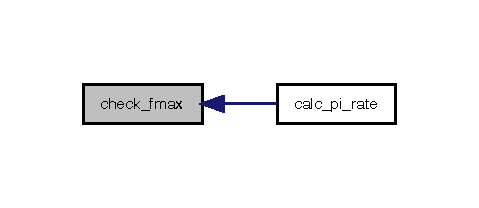
\includegraphics[width=230pt]{bb_8c_a11871d7df7f3167db92bef8c8ef98926_icgraph}
\end{center}
\end{figure}
\mbox{\Hypertarget{bb_8c_a337db7e010442d30f7c4b45f3e41fa5c}\label{bb_8c_a337db7e010442d30f7c4b45f3e41fa5c}} 
\index{bb.\+c@{bb.\+c}!emittance\+\_\+bb@{emittance\+\_\+bb}}
\index{emittance\+\_\+bb@{emittance\+\_\+bb}!bb.\+c@{bb.\+c}}
\subsubsection{\texorpdfstring{emittance\+\_\+bb()}{emittance\_bb()}}
{\footnotesize\ttfamily double emittance\+\_\+bb (\begin{DoxyParamCaption}\item[{double}]{freqmin,  }\item[{double}]{freqmax,  }\item[{double}]{t }\end{DoxyParamCaption})}



Calculate the emittance of a bb between freqmin and freqmax. 


\begin{DoxyParams}[1]{Parameters}
\mbox{\tt in}  & {\em double} & freqmin The minimum frequency \\
\hline
\mbox{\tt in}  & {\em double} & freqmax The maximum frequency \\
\hline
\mbox{\tt in}  & {\em double} & t ??? \\
\hline
\end{DoxyParams}
\begin{DoxyReturn}{Returns}
??? R\+E\+T\+U\+R\+NS ???
\end{DoxyReturn}
\paragraph*{Notes}

This should integrate to sigma if freqmin and freqmax go effeictively from 0 to infinity 

Definition at line 564 of file bb.\+c.

Here is the call graph for this function\+:
\nopagebreak
\begin{figure}[H]
\begin{center}
\leavevmode
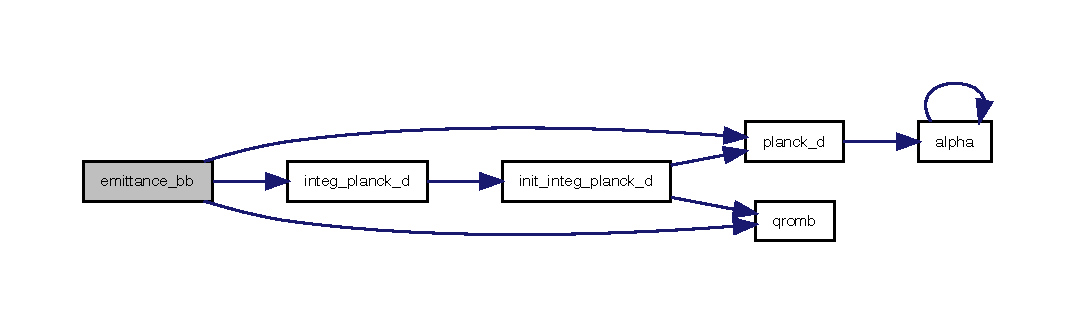
\includegraphics[width=350pt]{bb_8c_a337db7e010442d30f7c4b45f3e41fa5c_cgraph}
\end{center}
\end{figure}
Here is the caller graph for this function\+:
\nopagebreak
\begin{figure}[H]
\begin{center}
\leavevmode
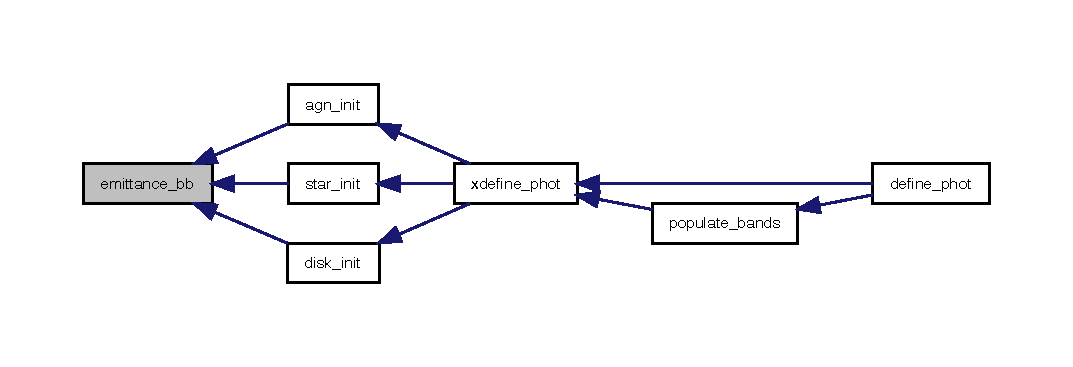
\includegraphics[width=350pt]{bb_8c_a337db7e010442d30f7c4b45f3e41fa5c_icgraph}
\end{center}
\end{figure}
\mbox{\Hypertarget{bb_8c_af2d9c9e4094a425824f269ef22163048}\label{bb_8c_af2d9c9e4094a425824f269ef22163048}} 
\index{bb.\+c@{bb.\+c}!get\+\_\+rand\+\_\+exp@{get\+\_\+rand\+\_\+exp}}
\index{get\+\_\+rand\+\_\+exp@{get\+\_\+rand\+\_\+exp}!bb.\+c@{bb.\+c}}
\subsubsection{\texorpdfstring{get\+\_\+rand\+\_\+exp()}{get\_rand\_exp()}}
{\footnotesize\ttfamily double get\+\_\+rand\+\_\+exp (\begin{DoxyParamCaption}\item[{double}]{alpha\+\_\+min,  }\item[{double}]{alpha\+\_\+max }\end{DoxyParamCaption})}



obtain a random number between alpha\+\_\+min and alpha\+\_\+max from an distribution of the form e$\ast$$\ast$-\/alpha 


\begin{DoxyParams}[1]{Parameters}
\mbox{\tt in}  & {\em double} & alpha\+\_\+min The lower limit for the random number \\
\hline
\mbox{\tt in}  & {\em double} & alpha\+\_\+max The upper limit for the random number \\
\hline
\end{DoxyParams}
\begin{DoxyReturn}{Returns}
A double precision random number
\end{DoxyReturn}
\paragraph*{Notes}

The cdf for an exponential distribution can be easily shown to be given by solving this equation for alpha

r$\ast$(exp(-\/alpha\+\_\+min)-\/exp(-\/alpha\+\_\+max))=(exp(-\/alpha\+\_\+min)-\/exp(alpha))

but you can recast this and solve for delta\+\_\+alpha

exp(-\/delta\+\_\+alpha)=(1-\/R)+\+R$\ast$exp(-\/(alpha\+\_\+max-\/alpha\+\_\+min))

This has the advantage that it depends only on the difference of alpha\+\_\+max and alpha\+\_\+min and not their actual values, and as long as the exp of a very large number turns out to be zero and not not a number, it shuld not generate N\+A\+Ns 

Definition at line 327 of file bb.\+c.

Here is the call graph for this function\+:
\nopagebreak
\begin{figure}[H]
\begin{center}
\leavevmode
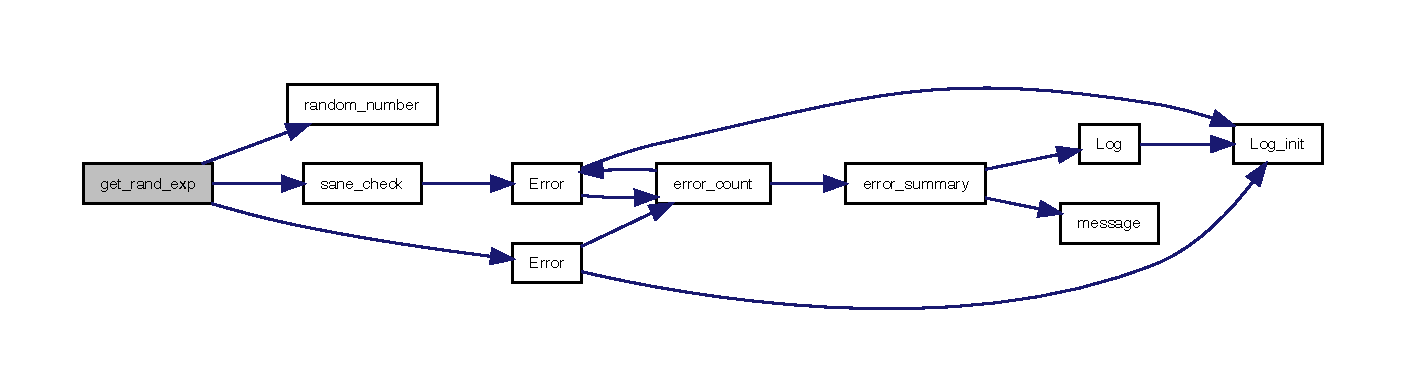
\includegraphics[width=350pt]{bb_8c_af2d9c9e4094a425824f269ef22163048_cgraph}
\end{center}
\end{figure}
Here is the caller graph for this function\+:
\nopagebreak
\begin{figure}[H]
\begin{center}
\leavevmode
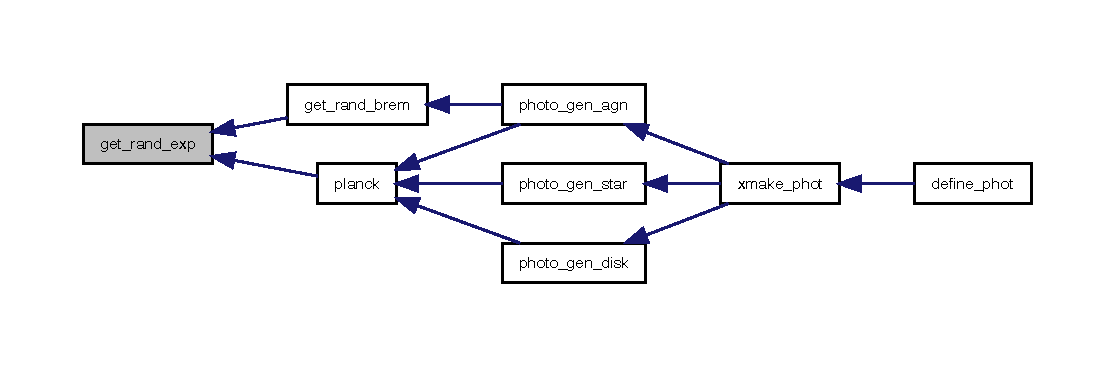
\includegraphics[width=350pt]{bb_8c_af2d9c9e4094a425824f269ef22163048_icgraph}
\end{center}
\end{figure}
\mbox{\Hypertarget{bb_8c_a6bae7f74815dfcf783a7dafade8faeca}\label{bb_8c_a6bae7f74815dfcf783a7dafade8faeca}} 
\index{bb.\+c@{bb.\+c}!get\+\_\+rand\+\_\+pow@{get\+\_\+rand\+\_\+pow}}
\index{get\+\_\+rand\+\_\+pow@{get\+\_\+rand\+\_\+pow}!bb.\+c@{bb.\+c}}
\subsubsection{\texorpdfstring{get\+\_\+rand\+\_\+pow()}{get\_rand\_pow()}}
{\footnotesize\ttfamily double get\+\_\+rand\+\_\+pow (\begin{DoxyParamCaption}\item[{double}]{x1,  }\item[{double}]{x2,  }\item[{double}]{alpha }\end{DoxyParamCaption})}



obtains a random number between x1 and x2 for a power law densiity distribution with index alpha 


\begin{DoxyParams}[1]{Parameters}
\mbox{\tt in,out}  & {\em double} & x1 the minimum allowed value to return \\
\hline
\mbox{\tt in,out}  & {\em double} & x2 the maximum allowed value to return \\
\hline
\mbox{\tt in,out}  & {\em double} & alpha the index of the power law \\
\hline
\end{DoxyParams}
\begin{DoxyReturn}{Returns}
A single value taken from a power law distribution
\end{DoxyReturn}
\paragraph*{Notes}

It is straight fowrward to integrate a power law in closed form and given this it one can easily find the value of the upper limit to the definite integral that is a given fraction of the total interval

The case with alpha==1 is a special case, but this is also easy to integrate. 

Definition at line 267 of file bb.\+c.

Here is the call graph for this function\+:
\nopagebreak
\begin{figure}[H]
\begin{center}
\leavevmode
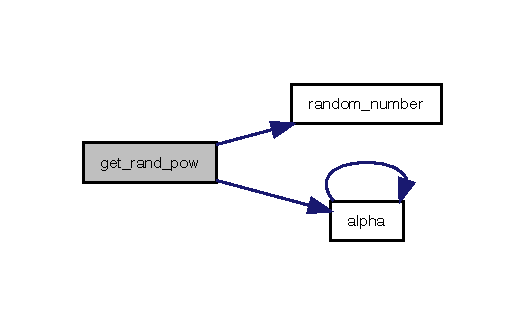
\includegraphics[width=252pt]{bb_8c_a6bae7f74815dfcf783a7dafade8faeca_cgraph}
\end{center}
\end{figure}
Here is the caller graph for this function\+:
\nopagebreak
\begin{figure}[H]
\begin{center}
\leavevmode
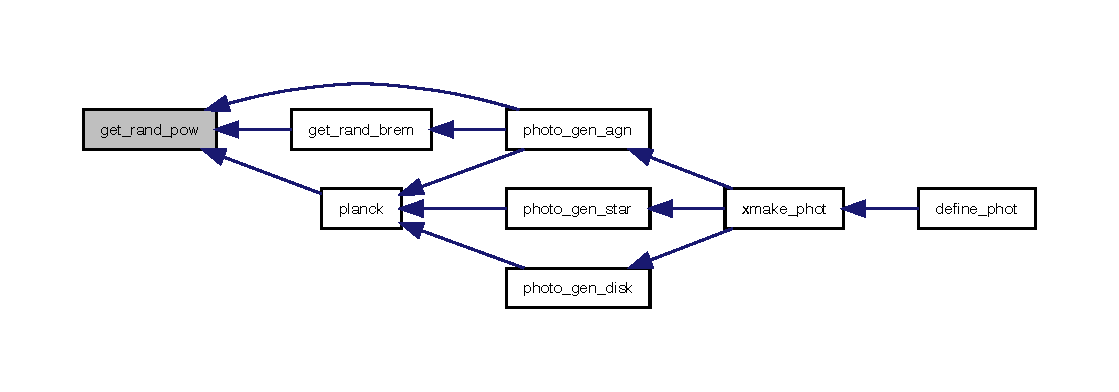
\includegraphics[width=350pt]{bb_8c_a6bae7f74815dfcf783a7dafade8faeca_icgraph}
\end{center}
\end{figure}
\mbox{\Hypertarget{bb_8c_aa67b840e2ff05fc474799c42178b392e}\label{bb_8c_aa67b840e2ff05fc474799c42178b392e}} 
\index{bb.\+c@{bb.\+c}!init\+\_\+integ\+\_\+planck\+\_\+d@{init\+\_\+integ\+\_\+planck\+\_\+d}}
\index{init\+\_\+integ\+\_\+planck\+\_\+d@{init\+\_\+integ\+\_\+planck\+\_\+d}!bb.\+c@{bb.\+c}}
\subsubsection{\texorpdfstring{init\+\_\+integ\+\_\+planck\+\_\+d()}{init\_integ\_planck\_d()}}
{\footnotesize\ttfamily int init\+\_\+integ\+\_\+planck\+\_\+d (\begin{DoxyParamCaption}\item[{void}]{ }\end{DoxyParamCaption})}



calulates integrals of the dimensionless bb function from 0 to alpha and the stores the reusults in an array used by integ\+\_\+plank\+\_\+d 

\begin{DoxyReturn}{Returns}
Always returns 0
\end{DoxyReturn}
This is a helper routine which is only called once from integ\+\_\+planck in order to initialize the array integ\+\_\+planck.

It calculates the integral of the dimensionless bb function between 0 and alpha for a series of alpha values values between A\+L\+P\+H\+A\+M\+IN and A\+L\+P\+H\+A\+M\+AX.

\paragraph*{Notes}

A\+L\+P\+H\+A\+M\+IN and A\+L\+P\+H\+A\+M\+AX are hardcoded which are hardcorded.

The actual integration is done with the numerical recipes routine \char`\"{}qromb\char`\"{} 

Definition at line 495 of file bb.\+c.

Here is the call graph for this function\+:
\nopagebreak
\begin{figure}[H]
\begin{center}
\leavevmode
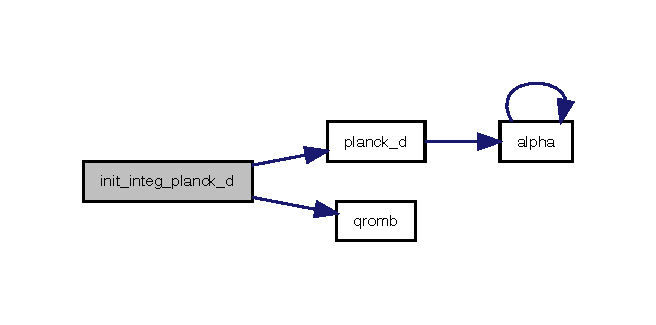
\includegraphics[width=315pt]{bb_8c_aa67b840e2ff05fc474799c42178b392e_cgraph}
\end{center}
\end{figure}
Here is the caller graph for this function\+:
\nopagebreak
\begin{figure}[H]
\begin{center}
\leavevmode
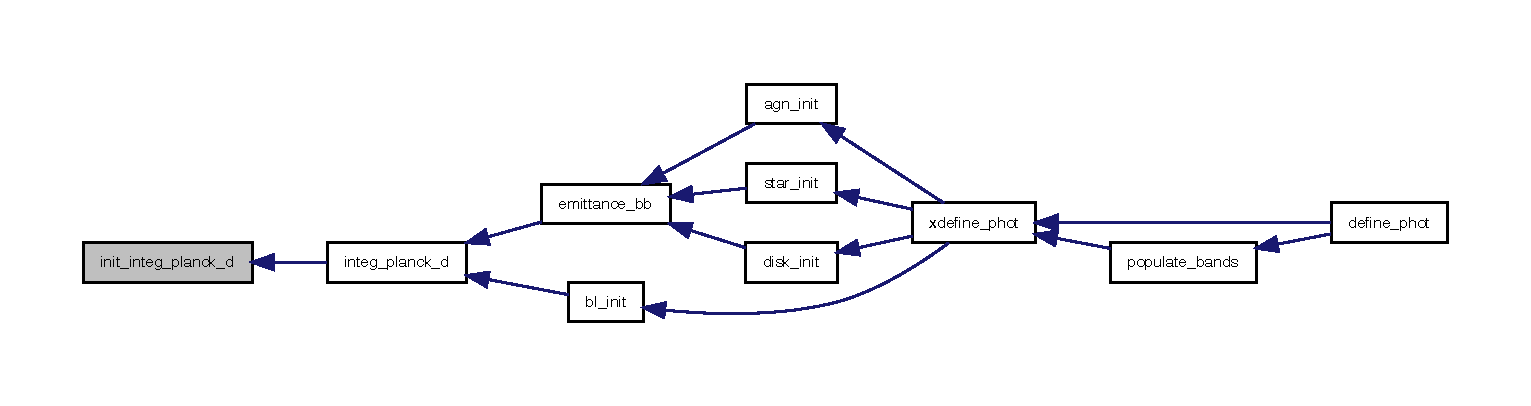
\includegraphics[width=350pt]{bb_8c_aa67b840e2ff05fc474799c42178b392e_icgraph}
\end{center}
\end{figure}
\mbox{\Hypertarget{bb_8c_af5c48487242ab8760a1893e385d3e11b}\label{bb_8c_af5c48487242ab8760a1893e385d3e11b}} 
\index{bb.\+c@{bb.\+c}!integ\+\_\+planck\+\_\+d@{integ\+\_\+planck\+\_\+d}}
\index{integ\+\_\+planck\+\_\+d@{integ\+\_\+planck\+\_\+d}!bb.\+c@{bb.\+c}}
\subsubsection{\texorpdfstring{integ\+\_\+planck\+\_\+d()}{integ\_planck\_d()}}
{\footnotesize\ttfamily double integ\+\_\+planck\+\_\+d (\begin{DoxyParamCaption}\item[{double}]{alphamin,  }\item[{double}]{alphamax }\end{DoxyParamCaption})}



Obtains the integral of the dimensionless blackbody function between alphamin and alphamax. 


\begin{DoxyParams}[1]{Parameters}
\mbox{\tt in}  & {\em double} & alphamin The minimum value of alpha (h nu/ kT) considered \\
\hline
\mbox{\tt in}  & {\em double} & alphamax The maximum value of alpha to be considered \\
\hline
\end{DoxyParams}
\begin{DoxyReturn}{Returns}
The value of the integral
\end{DoxyReturn}
To save computing time, the routine actually accesses an array that contains the the integral of the bb function from 0 to alpha for a number of values of alpha. By differencing (and intepolating) this array for the element corrsponding to alphamax and alphamin, the routine returns the integral between alphamax and alphamin

\paragraph*{Notes}

The first time the function is called the integ\+\_\+planck\mbox{[}\mbox{]} is filled.

integ\+\_\+plank\mbox{[}n\mbox{]} contains the integral of the dimensionless planck function from A\+L\+P\+H\+A\+M\+IN to A\+L\+P\+H\+A\+M\+AX. Therefore if one wants to obtain the integral of the dimensionless bb function, one simply interpolates this array. 

Definition at line 391 of file bb.\+c.

Here is the call graph for this function\+:
\nopagebreak
\begin{figure}[H]
\begin{center}
\leavevmode
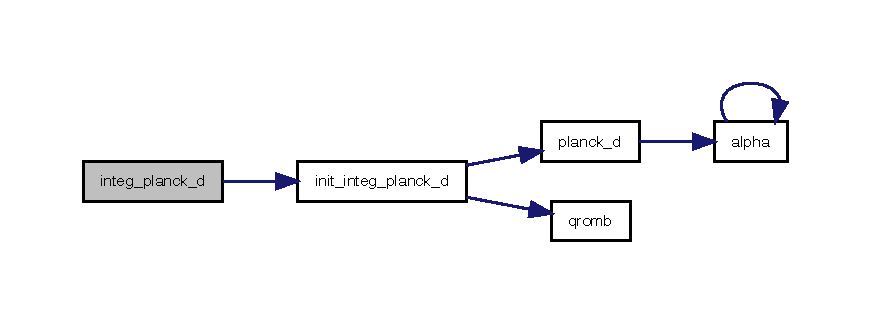
\includegraphics[width=350pt]{bb_8c_af5c48487242ab8760a1893e385d3e11b_cgraph}
\end{center}
\end{figure}
Here is the caller graph for this function\+:
\nopagebreak
\begin{figure}[H]
\begin{center}
\leavevmode
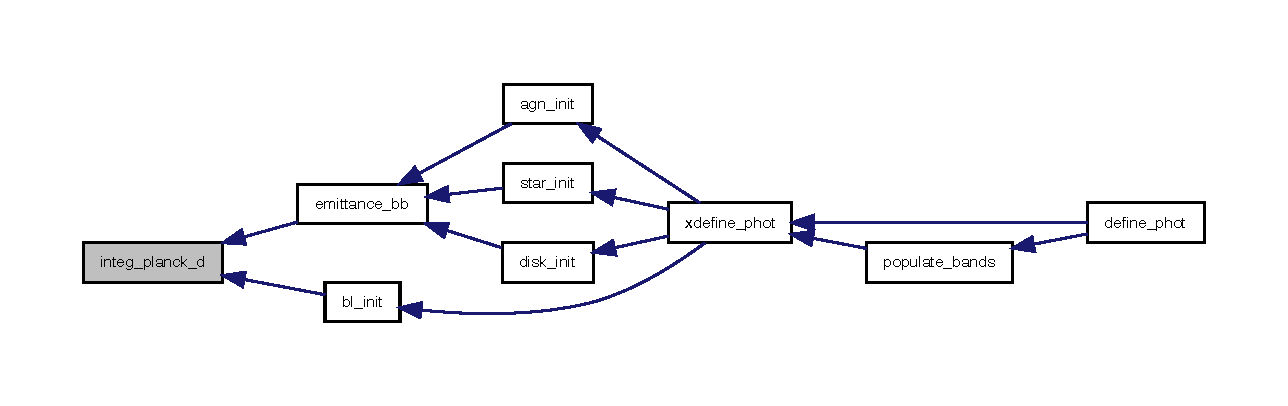
\includegraphics[width=350pt]{bb_8c_af5c48487242ab8760a1893e385d3e11b_icgraph}
\end{center}
\end{figure}
\mbox{\Hypertarget{bb_8c_a5f832b1ef434fdb41eaa62feb7edd710}\label{bb_8c_a5f832b1ef434fdb41eaa62feb7edd710}} 
\index{bb.\+c@{bb.\+c}!planck@{planck}}
\index{planck@{planck}!bb.\+c@{bb.\+c}}
\subsubsection{\texorpdfstring{planck()}{planck()}}
{\footnotesize\ttfamily double planck (\begin{DoxyParamCaption}\item[{double}]{t,  }\item[{double}]{freqmin,  }\item[{double}]{freqmax }\end{DoxyParamCaption})}



returns the frequency for a photon which follows a Placnk distribution within defined frequncy limits 


\begin{DoxyParams}[1]{Parameters}
\mbox{\tt in}  & {\em double} & t The temperature of the bb \\
\hline
\mbox{\tt in}  & {\em double} & freqmin The minimum frequency for the photon \\
\hline
\mbox{\tt in}  & {\em double} & freqmax The maximum frequency for the photon \\
\hline
\end{DoxyParams}
\begin{DoxyReturn}{Returns}
The frequency drawn randomly from a BB function with temperature T
\end{DoxyReturn}
The frequency is pseudo random in the following limited sense. The photons are returned are weighted so that the energy distribution of a function is approximately reproduced. Within an energy bin the photon frequency is uniform.

\paragraph*{Notes}

The first time one enters the program, a cdf for a diminensionless BB function is createda. The cdf is created for values between A\+L\+P\+H\+A\+M\+IN and A\+L\+P\+H\+A\+M\+AX where A\+L\+P\+HA=h nu/kT. The number of points in the cdf is determined by N\+M\+AX

On subseqent entries, when the temperature or frequency limits are changed, we use standard routines to limit what portion of the dimensionless cdf to use.

If the freuency range and temperature for a photon falls outside of A\+L\+P\+H\+A\+M\+IN and A\+L\+P\+H\+A\+M\+AX special routines are used to sample the distribution there. so that the spectrum falls off as a power law at low frequencies and an exponential at high frequencies. 

Definition at line 109 of file bb.\+c.

Here is the call graph for this function\+:
\nopagebreak
\begin{figure}[H]
\begin{center}
\leavevmode
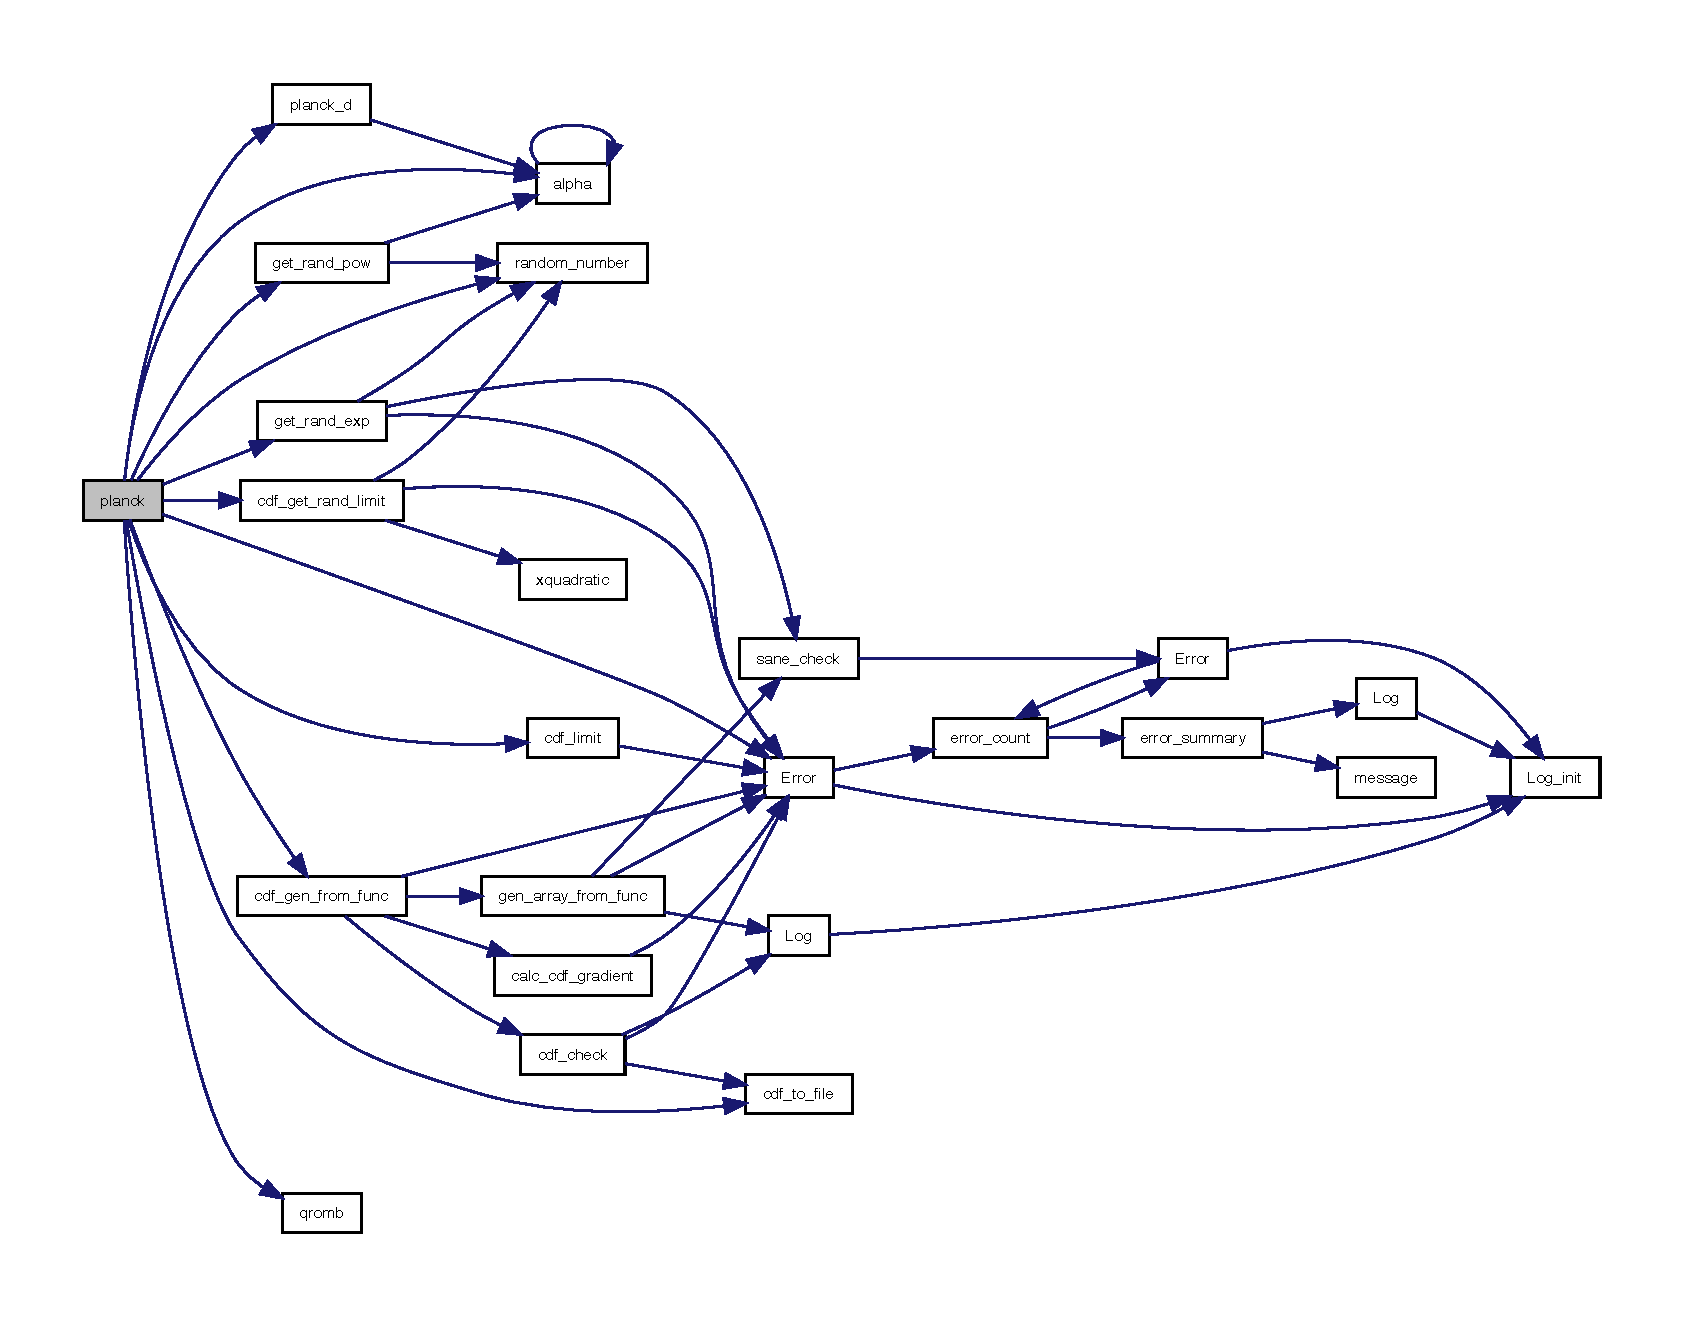
\includegraphics[width=350pt]{bb_8c_a5f832b1ef434fdb41eaa62feb7edd710_cgraph}
\end{center}
\end{figure}
Here is the caller graph for this function\+:
\nopagebreak
\begin{figure}[H]
\begin{center}
\leavevmode
\includegraphics[width=350pt]{bb_8c_a5f832b1ef434fdb41eaa62feb7edd710_icgraph}
\end{center}
\end{figure}
\mbox{\Hypertarget{bb_8c_ad6196c3c4ec0bdeda06aa797af259d81}\label{bb_8c_ad6196c3c4ec0bdeda06aa797af259d81}} 
\index{bb.\+c@{bb.\+c}!planck\+\_\+d@{planck\+\_\+d}}
\index{planck\+\_\+d@{planck\+\_\+d}!bb.\+c@{bb.\+c}}
\subsubsection{\texorpdfstring{planck\+\_\+d()}{planck\_d()}}
{\footnotesize\ttfamily double planck\+\_\+d (\begin{DoxyParamCaption}\item[{double}]{alpha }\end{DoxyParamCaption})}



The value of the dimensioless BB function at alpha. 


\begin{DoxyParams}[1]{Parameters}
\mbox{\tt in}  & {\em double} & alpha \\
\hline
\end{DoxyParams}
\begin{DoxyReturn}{Returns}
The value of the dimensionless BB function at x
\end{DoxyReturn}
The BB emittence is given by

F\+\_\+nu= 2$\ast$\+P\+I$\ast$ (k\+T/h$\ast$$\ast$3)$\ast$planck\+\_\+d(h$\ast$freq/ k T)

alpha is simply h nu/kT

\paragraph*{Notes}

Definition at line 534 of file bb.\+c.

Here is the call graph for this function\+:
\nopagebreak
\begin{figure}[H]
\begin{center}
\leavevmode
\includegraphics[width=198pt]{bb_8c_ad6196c3c4ec0bdeda06aa797af259d81_cgraph}
\end{center}
\end{figure}
Here is the caller graph for this function\+:
\nopagebreak
\begin{figure}[H]
\begin{center}
\leavevmode
\includegraphics[width=350pt]{bb_8c_ad6196c3c4ec0bdeda06aa797af259d81_icgraph}
\end{center}
\end{figure}


\subsection{Variable Documentation}
\mbox{\Hypertarget{bb_8c_af21e1955cd413e7edbe9c2a4fe822282}\label{bb_8c_af21e1955cd413e7edbe9c2a4fe822282}} 
\index{bb.\+c@{bb.\+c}!alphamax@{alphamax}}
\index{alphamax@{alphamax}!bb.\+c@{bb.\+c}}
\subsubsection{\texorpdfstring{alphamax}{alphamax}}
{\footnotesize\ttfamily double alphamax}



Definition at line 49 of file bb.\+c.

\mbox{\Hypertarget{bb_8c_a35106e779db1ad64f0de4eec449ec129}\label{bb_8c_a35106e779db1ad64f0de4eec449ec129}} 
\index{bb.\+c@{bb.\+c}!alphamin@{alphamin}}
\index{alphamin@{alphamin}!bb.\+c@{bb.\+c}}
\subsubsection{\texorpdfstring{alphamin}{alphamin}}
{\footnotesize\ttfamily double alphamin}



Definition at line 49 of file bb.\+c.

\mbox{\Hypertarget{bb_8c_a3308b12af5085b72eed7ec3169a707b4}\label{bb_8c_a3308b12af5085b72eed7ec3169a707b4}} 
\index{bb.\+c@{bb.\+c}!bb\+\_\+set@{bb\+\_\+set}}
\index{bb\+\_\+set@{bb\+\_\+set}!bb.\+c@{bb.\+c}}
\subsubsection{\texorpdfstring{bb\+\_\+set}{bb\_set}}
{\footnotesize\ttfamily double bb\+\_\+set\mbox{[}$\,$\mbox{]}}

{\bfseries Initial value\+:}
\begin{DoxyCode}
= \{

  10.0, 11.0, 12.0, 13.0, 14.0, 15.0, 16.0, 17.0, 18.0,
  19., 20., 21., 22., 23., 24., 25., 26., 27., 28., 29.
\}
\end{DoxyCode}
Array that cdf\+\_\+gen\+\_\+from\+\_\+func uses to establish the specific points in the cdf of the dimensionless bb function.

These are what we call \textquotesingle{}jumps\textquotesingle{} and are used by cdf\+\_\+gen\+\_\+from\+\_\+func to ensure important parts of the C\+DF have points 

Definition at line 62 of file bb.\+c.

\mbox{\Hypertarget{bb_8c_a4e1ff6ebea38be2c5723ae40379acb30}\label{bb_8c_a4e1ff6ebea38be2c5723ae40379acb30}} 
\index{bb.\+c@{bb.\+c}!cdf\+\_\+bb\+\_\+hi@{cdf\+\_\+bb\+\_\+hi}}
\index{cdf\+\_\+bb\+\_\+hi@{cdf\+\_\+bb\+\_\+hi}!bb.\+c@{bb.\+c}}
\subsubsection{\texorpdfstring{cdf\+\_\+bb\+\_\+hi}{cdf\_bb\_hi}}
{\footnotesize\ttfamily double cdf\+\_\+bb\+\_\+hi}



Definition at line 50 of file bb.\+c.

\mbox{\Hypertarget{bb_8c_acddeb64d75504658a4a6e7aec61d3721}\label{bb_8c_acddeb64d75504658a4a6e7aec61d3721}} 
\index{bb.\+c@{bb.\+c}!cdf\+\_\+bb\+\_\+lo@{cdf\+\_\+bb\+\_\+lo}}
\index{cdf\+\_\+bb\+\_\+lo@{cdf\+\_\+bb\+\_\+lo}!bb.\+c@{bb.\+c}}
\subsubsection{\texorpdfstring{cdf\+\_\+bb\+\_\+lo}{cdf\_bb\_lo}}
{\footnotesize\ttfamily double cdf\+\_\+bb\+\_\+lo}



Definition at line 50 of file bb.\+c.

\mbox{\Hypertarget{bb_8c_a30d9e580767e41f7671f036b54167316}\label{bb_8c_a30d9e580767e41f7671f036b54167316}} 
\index{bb.\+c@{bb.\+c}!cdf\+\_\+bb\+\_\+tot@{cdf\+\_\+bb\+\_\+tot}}
\index{cdf\+\_\+bb\+\_\+tot@{cdf\+\_\+bb\+\_\+tot}!bb.\+c@{bb.\+c}}
\subsubsection{\texorpdfstring{cdf\+\_\+bb\+\_\+tot}{cdf\_bb\_tot}}
{\footnotesize\ttfamily double cdf\+\_\+bb\+\_\+tot}



Definition at line 50 of file bb.\+c.

\mbox{\Hypertarget{bb_8c_a9a8f24be43c8ae7bc5328821d705fd38}\label{bb_8c_a9a8f24be43c8ae7bc5328821d705fd38}} 
\index{bb.\+c@{bb.\+c}!cdf\+\_\+bb\+\_\+yhi@{cdf\+\_\+bb\+\_\+yhi}}
\index{cdf\+\_\+bb\+\_\+yhi@{cdf\+\_\+bb\+\_\+yhi}!bb.\+c@{bb.\+c}}
\subsubsection{\texorpdfstring{cdf\+\_\+bb\+\_\+yhi}{cdf\_bb\_yhi}}
{\footnotesize\ttfamily double cdf\+\_\+bb\+\_\+yhi}



Definition at line 51 of file bb.\+c.

\mbox{\Hypertarget{bb_8c_ac3a0662170e08c6bbd081b1ae368c650}\label{bb_8c_ac3a0662170e08c6bbd081b1ae368c650}} 
\index{bb.\+c@{bb.\+c}!cdf\+\_\+bb\+\_\+ylo@{cdf\+\_\+bb\+\_\+ylo}}
\index{cdf\+\_\+bb\+\_\+ylo@{cdf\+\_\+bb\+\_\+ylo}!bb.\+c@{bb.\+c}}
\subsubsection{\texorpdfstring{cdf\+\_\+bb\+\_\+ylo}{cdf\_bb\_ylo}}
{\footnotesize\ttfamily double cdf\+\_\+bb\+\_\+ylo}



Definition at line 51 of file bb.\+c.

\mbox{\Hypertarget{bb_8c_a13f5d4ca91896d41ac5d4b8479198552}\label{bb_8c_a13f5d4ca91896d41ac5d4b8479198552}} 
\index{bb.\+c@{bb.\+c}!error\+\_\+bb\+\_\+hi@{error\+\_\+bb\+\_\+hi}}
\index{error\+\_\+bb\+\_\+hi@{error\+\_\+bb\+\_\+hi}!bb.\+c@{bb.\+c}}
\subsubsection{\texorpdfstring{error\+\_\+bb\+\_\+hi}{error\_bb\_hi}}
{\footnotesize\ttfamily int error\+\_\+bb\+\_\+hi = 0}



Definition at line 69 of file bb.\+c.

\mbox{\Hypertarget{bb_8c_a31dc4842298d34d3091c916f27f2f4aa}\label{bb_8c_a31dc4842298d34d3091c916f27f2f4aa}} 
\index{bb.\+c@{bb.\+c}!error\+\_\+bb\+\_\+lo@{error\+\_\+bb\+\_\+lo}}
\index{error\+\_\+bb\+\_\+lo@{error\+\_\+bb\+\_\+lo}!bb.\+c@{bb.\+c}}
\subsubsection{\texorpdfstring{error\+\_\+bb\+\_\+lo}{error\_bb\_lo}}
{\footnotesize\ttfamily int error\+\_\+bb\+\_\+lo = 0}



Definition at line 70 of file bb.\+c.

\mbox{\Hypertarget{bb_8c_acf13e2e3c9727b3d93ed1e53ea81ab96}\label{bb_8c_acf13e2e3c9727b3d93ed1e53ea81ab96}} 
\index{bb.\+c@{bb.\+c}!hi\+\_\+freq\+\_\+alphamax@{hi\+\_\+freq\+\_\+alphamax}}
\index{hi\+\_\+freq\+\_\+alphamax@{hi\+\_\+freq\+\_\+alphamax}!bb.\+c@{bb.\+c}}
\subsubsection{\texorpdfstring{hi\+\_\+freq\+\_\+alphamax}{hi\_freq\_alphamax}}
{\footnotesize\ttfamily double hi\+\_\+freq\+\_\+alphamax}



Definition at line 52 of file bb.\+c.

\mbox{\Hypertarget{bb_8c_a481fe97a41ed0e1a21ef0f1e0952e2a2}\label{bb_8c_a481fe97a41ed0e1a21ef0f1e0952e2a2}} 
\index{bb.\+c@{bb.\+c}!hi\+\_\+freq\+\_\+alphamin@{hi\+\_\+freq\+\_\+alphamin}}
\index{hi\+\_\+freq\+\_\+alphamin@{hi\+\_\+freq\+\_\+alphamin}!bb.\+c@{bb.\+c}}
\subsubsection{\texorpdfstring{hi\+\_\+freq\+\_\+alphamin}{hi\_freq\_alphamin}}
{\footnotesize\ttfamily double hi\+\_\+freq\+\_\+alphamin}



Definition at line 52 of file bb.\+c.

\mbox{\Hypertarget{bb_8c_a2cba79df974368a69fa87d2cab474c35}\label{bb_8c_a2cba79df974368a69fa87d2cab474c35}} 
\index{bb.\+c@{bb.\+c}!i\+\_\+integ\+\_\+planck\+\_\+d@{i\+\_\+integ\+\_\+planck\+\_\+d}}
\index{i\+\_\+integ\+\_\+planck\+\_\+d@{i\+\_\+integ\+\_\+planck\+\_\+d}!bb.\+c@{bb.\+c}}
\subsubsection{\texorpdfstring{i\+\_\+integ\+\_\+planck\+\_\+d}{i\_integ\_planck\_d}}
{\footnotesize\ttfamily int i\+\_\+integ\+\_\+planck\+\_\+d = 0}



A flag to say whether we have initialised integ\+\_\+planck. 



Definition at line 357 of file bb.\+c.

\mbox{\Hypertarget{bb_8c_a29644660e3c6b64c4f2dd0286c5c0268}\label{bb_8c_a29644660e3c6b64c4f2dd0286c5c0268}} 
\index{bb.\+c@{bb.\+c}!integ\+\_\+planck@{integ\+\_\+planck}}
\index{integ\+\_\+planck@{integ\+\_\+planck}!bb.\+c@{bb.\+c}}
\subsubsection{\texorpdfstring{integ\+\_\+planck}{integ\_planck}}
{\footnotesize\ttfamily double integ\+\_\+planck\mbox{[}\hyperlink{bb_8c_a5de5d183f9a6a8d53316f743e1ca6dc2}{N\+M\+AX}+1\mbox{]}}



The dimensionless planck function integrated from A\+L\+P\+H\+A\+M\+IN to a range of values of alpha. 



Definition at line 354 of file bb.\+c.

\mbox{\Hypertarget{bb_8c_a8cb2580284665f530fa828efeb72c8e2}\label{bb_8c_a8cb2580284665f530fa828efeb72c8e2}} 
\index{bb.\+c@{bb.\+c}!lo\+\_\+freq\+\_\+alphamax@{lo\+\_\+freq\+\_\+alphamax}}
\index{lo\+\_\+freq\+\_\+alphamax@{lo\+\_\+freq\+\_\+alphamax}!bb.\+c@{bb.\+c}}
\subsubsection{\texorpdfstring{lo\+\_\+freq\+\_\+alphamax}{lo\_freq\_alphamax}}
{\footnotesize\ttfamily double lo\+\_\+freq\+\_\+alphamax}



Definition at line 52 of file bb.\+c.

\mbox{\Hypertarget{bb_8c_a5e666b72cd5ad44a523f8cef4c6e5f06}\label{bb_8c_a5e666b72cd5ad44a523f8cef4c6e5f06}} 
\index{bb.\+c@{bb.\+c}!lo\+\_\+freq\+\_\+alphamin@{lo\+\_\+freq\+\_\+alphamin}}
\index{lo\+\_\+freq\+\_\+alphamin@{lo\+\_\+freq\+\_\+alphamin}!bb.\+c@{bb.\+c}}
\subsubsection{\texorpdfstring{lo\+\_\+freq\+\_\+alphamin}{lo\_freq\_alphamin}}
{\footnotesize\ttfamily double lo\+\_\+freq\+\_\+alphamin}



Definition at line 52 of file bb.\+c.

\mbox{\Hypertarget{bb_8c_a0d6e712e70e9d8d896e421421e5232a9}\label{bb_8c_a0d6e712e70e9d8d896e421421e5232a9}} 
\index{bb.\+c@{bb.\+c}!ninit\+\_\+planck@{ninit\+\_\+planck}}
\index{ninit\+\_\+planck@{ninit\+\_\+planck}!bb.\+c@{bb.\+c}}
\subsubsection{\texorpdfstring{ninit\+\_\+planck}{ninit\_planck}}
{\footnotesize\ttfamily int ninit\+\_\+planck = 0}



Definition at line 44 of file bb.\+c.

\mbox{\Hypertarget{bb_8c_a8dc32bfb2583414f49194409ba81c27c}\label{bb_8c_a8dc32bfb2583414f49194409ba81c27c}} 
\index{bb.\+c@{bb.\+c}!old\+\_\+freqmax@{old\+\_\+freqmax}}
\index{old\+\_\+freqmax@{old\+\_\+freqmax}!bb.\+c@{bb.\+c}}
\subsubsection{\texorpdfstring{old\+\_\+freqmax}{old\_freqmax}}
{\footnotesize\ttfamily double old\+\_\+freqmax = 0}



Definition at line 48 of file bb.\+c.

\mbox{\Hypertarget{bb_8c_a65f885c797f8031956517c69adcd0345}\label{bb_8c_a65f885c797f8031956517c69adcd0345}} 
\index{bb.\+c@{bb.\+c}!old\+\_\+freqmin@{old\+\_\+freqmin}}
\index{old\+\_\+freqmin@{old\+\_\+freqmin}!bb.\+c@{bb.\+c}}
\subsubsection{\texorpdfstring{old\+\_\+freqmin}{old\_freqmin}}
{\footnotesize\ttfamily double old\+\_\+freqmin = 0}



Definition at line 47 of file bb.\+c.

\mbox{\Hypertarget{bb_8c_ad5ae362a91b7c239184d49913e1701b1}\label{bb_8c_ad5ae362a91b7c239184d49913e1701b1}} 
\index{bb.\+c@{bb.\+c}!old\+\_\+t@{old\+\_\+t}}
\index{old\+\_\+t@{old\+\_\+t}!bb.\+c@{bb.\+c}}
\subsubsection{\texorpdfstring{old\+\_\+t}{old\_t}}
{\footnotesize\ttfamily double old\+\_\+t = 0}



Definition at line 46 of file bb.\+c.


\hypertarget{bilinear_8c}{}\section{/\+Users/mhewitt/python/source/bilinear.c File Reference}
\label{bilinear_8c}\index{/\+Users/mhewitt/python/source/bilinear.\+c@{/\+Users/mhewitt/python/source/bilinear.\+c}}


As the name indicates the routines solve for the fractional position of a 2d vector in a 2d cell with 4 corners.  


{\ttfamily \#include $<$stdio.\+h$>$}\newline
{\ttfamily \#include $<$strings.\+h$>$}\newline
{\ttfamily \#include $<$math.\+h$>$}\newline
{\ttfamily \#include $<$string.\+h$>$}\newline
{\ttfamily \#include $<$stdlib.\+h$>$}\newline
{\ttfamily \#include \char`\"{}log.\+h\char`\"{}}\newline
Include dependency graph for bilinear.\+c\+:
\nopagebreak
\begin{figure}[H]
\begin{center}
\leavevmode
\includegraphics[width=350pt]{bilinear_8c__incl}
\end{center}
\end{figure}
\subsection*{Functions}
\begin{DoxyCompactItemize}
\item 
int \hyperlink{bilinear_8c_a0d7059db01a063789ca5b78386eb2889}{bilin} (\hyperlink{import__cylindrical_8c_a099bc7b5a9501685180c163c1ffb67d0}{x}, x00, x01, x10, x11, double $\ast$f, double $\ast$g)
\begin{DoxyCompactList}\small\item\em calculates the fractional position in the coordinate grid of a 2d vector x. \end{DoxyCompactList}\item 
int \hyperlink{bilinear_8c_af582498786ae60301965c85d405d7cde}{xquadratic} (double a, double b, double c, \hyperlink{import__spherical_8c_a83175ac8fd9d924ff2bce40c99e88870}{r})
\begin{DoxyCompactList}\small\item\em solves a quadratic of the form 0=ax$\ast$$\ast$2+bx+c \end{DoxyCompactList}\end{DoxyCompactItemize}


\subsection{Detailed Description}
As the name indicates the routines solve for the fractional position of a 2d vector in a 2d cell with 4 corners. 

\begin{DoxyAuthor}{Author}
ksl 
\end{DoxyAuthor}
\begin{DoxyDate}{Date}
January, 2018
\end{DoxyDate}
There is also a quadratic equation solver 

\subsection{Function Documentation}
\mbox{\Hypertarget{bilinear_8c_a0d7059db01a063789ca5b78386eb2889}\label{bilinear_8c_a0d7059db01a063789ca5b78386eb2889}} 
\index{bilinear.\+c@{bilinear.\+c}!bilin@{bilin}}
\index{bilin@{bilin}!bilinear.\+c@{bilinear.\+c}}
\subsubsection{\texorpdfstring{bilin()}{bilin()}}
{\footnotesize\ttfamily int bilin (\begin{DoxyParamCaption}\item[{\hyperlink{import__cylindrical_8c_a099bc7b5a9501685180c163c1ffb67d0}{x}}]{,  }\item[{x00}]{,  }\item[{x01}]{,  }\item[{x10}]{,  }\item[{x11}]{,  }\item[{double $\ast$}]{f,  }\item[{double $\ast$}]{g }\end{DoxyParamCaption})}



calculates the fractional position in the coordinate grid of a 2d vector x. 


\begin{DoxyParams}[1]{Parameters}
\mbox{\tt in}  & {\em double} & x\mbox{[}\mbox{]} The 2d position within the cell \\
\hline
\mbox{\tt in}  & {\em double} & x00\mbox{[}\mbox{]} The 2d position of the lower-\/left edge of cell \\
\hline
\mbox{\tt in}  & {\em double} & x01\mbox{[}\mbox{]} The 2d position of the upper-\/left edge of the cell \\
\hline
\mbox{\tt in}  & {\em double} & x10\mbox{[}\mbox{]} The 2d position of the lower-\/right edge of the cell \\
\hline
\mbox{\tt in}  & {\em double} & x11\mbox{[}\mbox{]} The 2d position of the upper-\/right edge of the cell \\
\hline
\mbox{\tt out}  & {\em double} & $\ast$ f The fractional position in the \char`\"{}x\char`\"{} direction \\
\hline
\mbox{\tt out}  & {\em double} & $\ast$ g The fractional postion in the \char`\"{}z\char`\"{} direction \\
\hline
\end{DoxyParams}
\begin{DoxyReturn}{Returns}
The routine itself returns 0 if the postion is inside the cell, and -\/1 otherwise.
\end{DoxyReturn}
The input 2d input vectors are assumed to have the relationship shown in real space, that is x00 and x01 are more or less along the z axis, while x00 and x10 are more or less along the +x acis


\begin{DoxyItemize}
\item x01 ....... x11
\item . .
\item . .
\item x00 ....... x10
\end{DoxyItemize}

\paragraph*{Notes}

Basically

X= (1-\/g) \mbox{[} (1-\/f) X00 + f X10 \mbox{]} $\ast$ g \mbox{[} (1-\/f)$\ast$\+X01+ f$\ast$ X11 \mbox{]}

where the capitalized values of X,etc denote vectors, and f and g are the fractional weightings.

X = (1-\/g) A + g B

It is easy to solve for g in terms of f

g = (X-\/A)/(B-\/A)

where A = \mbox{[} (1-\/f) X00 + f X10 \mbox{]} and B = \mbox{[} (1-\/f)$\ast$\+X01+ f$\ast$ X11 \mbox{]}

But this gives you two expressions for g depending on whether you consider the 0 or 1 component of the vector, and therefore you can solve for f. More specifically,

g= \mbox{[}(X-\/\+X\+OO) + f (X\+O\+O-\/\+X10)\mbox{]} / \mbox{[}(X01-\/\+X10)+f (X11+\+X00-\/\+X01-\/\+X10)\mbox{]}

or

g = (Q + f R) / (S+f T)

where Q, R, S, and T are defined from the equation above.

So expanding in terms of the component veciots what we have is

(Q\mbox{[}0\mbox{]}+f R\mbox{[}0\mbox{]}) (S\mbox{[}2\mbox{]}+f T\mbox{[}2\mbox{]}) = (Q\mbox{[}2\mbox{]}+f R\mbox{[}2\mbox{]}) (S\mbox{[}0\mbox{]}+f T\mbox{[}0\mbox{]})

which can now be put in the form of a xquadratic

a f$\ast$$\ast$2 + b f +c = 0

where


\begin{DoxyItemize}
\item a = r\mbox{[}0\mbox{]}$\ast$t\mbox{[}2\mbox{]} -\/ r\mbox{[}2\mbox{]}$\ast$t\mbox{[}0\mbox{]}
\item b= r\mbox{[}0\mbox{]}$\ast$s\mbox{[}2\mbox{]} + q\mbox{[}0\mbox{]}$\ast$t\mbox{[}2\mbox{]} -\/ ( r\mbox{[}2\mbox{]}$\ast$s\mbox{[}0\mbox{]} + q\mbox{[}2\mbox{]}$\ast$t\mbox{[}0\mbox{]} )
\item c = q\mbox{[}0\mbox{]}$\ast$s\mbox{[}2\mbox{]} -\/ q\mbox{[}2\mbox{]}$\ast$s\mbox{[}0\mbox{]}
\end{DoxyItemize}

A problem with this approach is that does not work in the case where the coordinates are the x axis positions of X01 and X01 are the same and the X10 and X11 are the same. This is because the denominator becomes 0 in the equation for g. This particular case is important because it is the case we are trying to solve for.

In this case we need to solve for f by itself. Similarly there is a degnereate case when (x00\mbox{[}2\mbox{]} == x10\mbox{[}2\mbox{]} \&\& x01\mbox{[}2\mbox{]} == x11\mbox{[}2\mbox{]}) 

Definition at line 109 of file bilinear.\+c.

Here is the call graph for this function\+:
\nopagebreak
\begin{figure}[H]
\begin{center}
\leavevmode
\includegraphics[width=350pt]{bilinear_8c_a0d7059db01a063789ca5b78386eb2889_cgraph}
\end{center}
\end{figure}
Here is the caller graph for this function\+:
\nopagebreak
\begin{figure}[H]
\begin{center}
\leavevmode
\includegraphics[width=350pt]{bilinear_8c_a0d7059db01a063789ca5b78386eb2889_icgraph}
\end{center}
\end{figure}
\mbox{\Hypertarget{bilinear_8c_af582498786ae60301965c85d405d7cde}\label{bilinear_8c_af582498786ae60301965c85d405d7cde}} 
\index{bilinear.\+c@{bilinear.\+c}!xquadratic@{xquadratic}}
\index{xquadratic@{xquadratic}!bilinear.\+c@{bilinear.\+c}}
\subsubsection{\texorpdfstring{xquadratic()}{xquadratic()}}
{\footnotesize\ttfamily int xquadratic (\begin{DoxyParamCaption}\item[{double}]{a,  }\item[{double}]{b,  }\item[{double}]{c,  }\item[{\hyperlink{import__spherical_8c_a83175ac8fd9d924ff2bce40c99e88870}{r}}]{ }\end{DoxyParamCaption})}



solves a quadratic of the form 0=ax$\ast$$\ast$2+bx+c 


\begin{DoxyParams}[1]{Parameters}
\mbox{\tt in,out}  & {\em double} & a \\
\hline
\mbox{\tt in,out}  & {\em double} & b \\
\hline
\mbox{\tt in,out}  & {\em double} & c \\
\hline
\mbox{\tt in,out}  & {\em double} & r\mbox{[}\mbox{]} roots of the quadratic equation \\
\hline
\end{DoxyParams}
\begin{DoxyReturn}{Returns}

\begin{DoxyItemize}
\item -\/1 -\/$>$ both roots are imaginary
\item -\/2 -\/$>$ both roots are negative or 0
\item 0 -\/$>$ the first root is the smallest positive root
\item 1 -\/$>$ the second root is the smallest positive root
\end{DoxyItemize}
\end{DoxyReturn}
This solves a simple xquadratic (or if a is zero linear equation). The return is set up to make it easy to identify the smallest positive root if one exists. The routine returns a negative number if both roots are negative or imaginary.

\paragraph*{Notes}

\begin{DoxyRefDesc}{Bug}
\item[\hyperlink{bug__bug000005}{Bug}]xquadratic looks line for line identical to another routine quadratic which can be found in \hyperlink{phot__util_8c}{phot\+\_\+util.\+c}. Both versions of the code seem to be called. One of them should be removed.\end{DoxyRefDesc}


Definition at line 240 of file bilinear.\+c.

Here is the caller graph for this function\+:
\nopagebreak
\begin{figure}[H]
\begin{center}
\leavevmode
\includegraphics[width=350pt]{bilinear_8c_af582498786ae60301965c85d405d7cde_icgraph}
\end{center}
\end{figure}

\hypertarget{brem_8c}{}\section{/\+Users/mhewitt/python/source/brem.c File Reference}
\label{brem_8c}\index{/\+Users/mhewitt/python/source/brem.\+c@{/\+Users/mhewitt/python/source/brem.\+c}}


Functions to allow a Bremstrahlung type input spectrum.  


{\ttfamily \#include $<$stdio.\+h$>$}\newline
{\ttfamily \#include $<$strings.\+h$>$}\newline
{\ttfamily \#include $<$math.\+h$>$}\newline
{\ttfamily \#include $<$string.\+h$>$}\newline
{\ttfamily \#include $<$stdlib.\+h$>$}\newline
{\ttfamily \#include \char`\"{}atomic.\+h\char`\"{}}\newline
{\ttfamily \#include \char`\"{}python.\+h\char`\"{}}\newline
{\ttfamily \#include \char`\"{}log.\+h\char`\"{}}\newline
Include dependency graph for brem.\+c\+:
\nopagebreak
\begin{figure}[H]
\begin{center}
\leavevmode
\includegraphics[width=350pt]{brem_8c__incl}
\end{center}
\end{figure}
\subsection*{Macros}
\begin{DoxyCompactItemize}
\item 
\#define \hyperlink{brem_8c_aaf03eb5a4a40392ff9b892717fe4a8e1}{B\+R\+E\+M\+\_\+\+A\+L\+P\+H\+A\+M\+IN}~0.\+01
\item 
\#define \hyperlink{brem_8c_abaa88071d632320b5d9f3e297a5fc0d0}{B\+R\+E\+M\+\_\+\+A\+L\+P\+H\+A\+M\+AX}~2.
\item 
\#define \hyperlink{brem_8c_afe345a36af26b51d9ff30d5ac4983ff2}{B\+R\+E\+M\+\_\+\+A\+L\+P\+H\+A\+B\+IG}~100.
\end{DoxyCompactItemize}
\subsection*{Functions}
\begin{DoxyCompactItemize}
\item 
double \hyperlink{brem_8c_aaf2a9843cc170d6b01b75a1704f8c4fb}{integ\+\_\+brem} (double freq)
\begin{DoxyCompactList}\small\item\em The integrand used in qromb to compute the luminosity of a bremstrahlung source. \end{DoxyCompactList}\item 
double \hyperlink{brem_8c_ab308d8424a5b2ab066577630b7150e7b}{brem\+\_\+d} (double \hyperlink{templates_8h_a89a27f4f3a5c836df75585774ba7a643}{alpha})
\begin{DoxyCompactList}\small\item\em The integrand for integrating a dimensionless bremstrahlung spectrum. \end{DoxyCompactList}\item 
double \hyperlink{brem_8c_aea33eee38cf4a6c25978443404ddaf2c}{get\+\_\+rand\+\_\+brem} (double freqmin, double freqmax)
\begin{DoxyCompactList}\small\item\em Obtain a random frequency photon from a bremstrahlung spectrum. \end{DoxyCompactList}\end{DoxyCompactItemize}
\subsection*{Variables}
\begin{DoxyCompactItemize}
\item 
int \hyperlink{brem_8c_af4418ce3b3787f7636a773b3875b69ad}{ninit\+\_\+brem} = 0
\item 
double \hyperlink{brem_8c_a040e5301c94c0e3cd6b90062a656b020}{old\+\_\+brem\+\_\+t} = 0
\item 
double \hyperlink{brem_8c_a8a44fad2c1144d158ce6fcf7d8ded81b}{old\+\_\+brem\+\_\+freqmin} = 0
\item 
double \hyperlink{brem_8c_a96f9c5cc4caa7a8bd7b6eb3232b23bee}{old\+\_\+brem\+\_\+freqmax} = 0
\item 
double \hyperlink{brem_8c_a0dc8dc103eb9064b0730233fb6f6f7d2}{brem\+\_\+alphamin}
\item 
double \hyperlink{brem_8c_af25d2a0479f65884c3c68fb8dc08dc0f}{brem\+\_\+alphamax}
\item 
double \hyperlink{brem_8c_a5cbb1962fd13b47dd17e5b1772b5643e}{cdf\+\_\+brem\+\_\+lo}
\item 
double \hyperlink{brem_8c_a09e5a2895a123c9691288465ad42c888}{cdf\+\_\+brem\+\_\+hi}
\item 
double \hyperlink{brem_8c_a266a87733f46582da31826818bd39a60}{cdf\+\_\+brem\+\_\+tot}
\item 
double \hyperlink{brem_8c_a0b8a4f2029ce2228e216a2914ffcf205}{cdf\+\_\+brem\+\_\+ylo}
\item 
double \hyperlink{brem_8c_a780df85df1c79ad2ccf33a2a40c69a90}{cdf\+\_\+brem\+\_\+yhi}
\item 
double \hyperlink{brem_8c_a6680e57c414fd174a5bae6b9b8cf009f}{brem\+\_\+lo\+\_\+freq\+\_\+alphamin}
\item 
double \hyperlink{brem_8c_a1a71d41cd43ca89a8f468323a9a8fa02}{brem\+\_\+lo\+\_\+freq\+\_\+alphamax}
\item 
double \hyperlink{brem_8c_a6e8eb2335367020db563d870968697b7}{brem\+\_\+hi\+\_\+freq\+\_\+alphamin}
\item 
double \hyperlink{brem_8c_a54cc519a459817b9d667a366b9f89220}{brem\+\_\+hi\+\_\+freq\+\_\+alphamax}
\item 
double \hyperlink{brem_8c_a8277b937c29573d33ef68e3d119001ed}{brem\+\_\+set} \mbox{[}$\,$\mbox{]}
\end{DoxyCompactItemize}


\subsection{Detailed Description}
Functions to allow a Bremstrahlung type input spectrum. 

\begin{DoxyAuthor}{Author}
nsh 
\end{DoxyAuthor}
\begin{DoxyDate}{Date}
October, 2015
\end{DoxyDate}
This was added as part of the Rad-\/hydro effort and is itended to allow a spectrum to match the assumed spectrum in the Blondin heating and cooling rates. Note that this spectrum is very similar in some ways to a blackbody spectrum -\/ essentially a power law turning into a high frequency exponential dropoff and so there is a great deal of similarity with routines in \hyperlink{bb_8c}{bb.\+c} There is scope here for simplification. 

\subsection{Macro Definition Documentation}
\mbox{\Hypertarget{brem_8c_afe345a36af26b51d9ff30d5ac4983ff2}\label{brem_8c_afe345a36af26b51d9ff30d5ac4983ff2}} 
\index{brem.\+c@{brem.\+c}!B\+R\+E\+M\+\_\+\+A\+L\+P\+H\+A\+B\+IG@{B\+R\+E\+M\+\_\+\+A\+L\+P\+H\+A\+B\+IG}}
\index{B\+R\+E\+M\+\_\+\+A\+L\+P\+H\+A\+B\+IG@{B\+R\+E\+M\+\_\+\+A\+L\+P\+H\+A\+B\+IG}!brem.\+c@{brem.\+c}}
\subsubsection{\texorpdfstring{B\+R\+E\+M\+\_\+\+A\+L\+P\+H\+A\+B\+IG}{BREM\_ALPHABIG}}
{\footnotesize\ttfamily \#define B\+R\+E\+M\+\_\+\+A\+L\+P\+H\+A\+B\+IG~100.}



Definition at line 92 of file brem.\+c.

\mbox{\Hypertarget{brem_8c_abaa88071d632320b5d9f3e297a5fc0d0}\label{brem_8c_abaa88071d632320b5d9f3e297a5fc0d0}} 
\index{brem.\+c@{brem.\+c}!B\+R\+E\+M\+\_\+\+A\+L\+P\+H\+A\+M\+AX@{B\+R\+E\+M\+\_\+\+A\+L\+P\+H\+A\+M\+AX}}
\index{B\+R\+E\+M\+\_\+\+A\+L\+P\+H\+A\+M\+AX@{B\+R\+E\+M\+\_\+\+A\+L\+P\+H\+A\+M\+AX}!brem.\+c@{brem.\+c}}
\subsubsection{\texorpdfstring{B\+R\+E\+M\+\_\+\+A\+L\+P\+H\+A\+M\+AX}{BREM\_ALPHAMAX}}
{\footnotesize\ttfamily \#define B\+R\+E\+M\+\_\+\+A\+L\+P\+H\+A\+M\+AX~2.}



Definition at line 91 of file brem.\+c.

\mbox{\Hypertarget{brem_8c_aaf03eb5a4a40392ff9b892717fe4a8e1}\label{brem_8c_aaf03eb5a4a40392ff9b892717fe4a8e1}} 
\index{brem.\+c@{brem.\+c}!B\+R\+E\+M\+\_\+\+A\+L\+P\+H\+A\+M\+IN@{B\+R\+E\+M\+\_\+\+A\+L\+P\+H\+A\+M\+IN}}
\index{B\+R\+E\+M\+\_\+\+A\+L\+P\+H\+A\+M\+IN@{B\+R\+E\+M\+\_\+\+A\+L\+P\+H\+A\+M\+IN}!brem.\+c@{brem.\+c}}
\subsubsection{\texorpdfstring{B\+R\+E\+M\+\_\+\+A\+L\+P\+H\+A\+M\+IN}{BREM\_ALPHAMIN}}
{\footnotesize\ttfamily \#define B\+R\+E\+M\+\_\+\+A\+L\+P\+H\+A\+M\+IN~0.\+01}



Definition at line 90 of file brem.\+c.



\subsection{Function Documentation}
\mbox{\Hypertarget{brem_8c_ab308d8424a5b2ab066577630b7150e7b}\label{brem_8c_ab308d8424a5b2ab066577630b7150e7b}} 
\index{brem.\+c@{brem.\+c}!brem\+\_\+d@{brem\+\_\+d}}
\index{brem\+\_\+d@{brem\+\_\+d}!brem.\+c@{brem.\+c}}
\subsubsection{\texorpdfstring{brem\+\_\+d()}{brem\_d()}}
{\footnotesize\ttfamily double brem\+\_\+d (\begin{DoxyParamCaption}\item[{double}]{alpha }\end{DoxyParamCaption})}



The integrand for integrating a dimensionless bremstrahlung spectrum. 


\begin{DoxyParams}[1]{Parameters}
\mbox{\tt in}  & {\em double} & alpha h$\ast$freq/k\+\_\+b/T -\/ \\
\hline
\end{DoxyParams}
\begin{DoxyReturn}{Returns}
luminosity of bremstrahlung function at alpha
\end{DoxyReturn}
This produces a dimensinless bremstrahlung spectrum so that one can break fast changing parts of the spectrum (i.\+e. the exponential drop off) into chunks to ensure we get a properly defnined spectrum of randomly generated photons.

\paragraph*{Notes}

10/15 -\/ Written by N\+SH 

Definition at line 75 of file brem.\+c.

Here is the call graph for this function\+:
\nopagebreak
\begin{figure}[H]
\begin{center}
\leavevmode
\includegraphics[width=193pt]{brem_8c_ab308d8424a5b2ab066577630b7150e7b_cgraph}
\end{center}
\end{figure}
Here is the caller graph for this function\+:
\nopagebreak
\begin{figure}[H]
\begin{center}
\leavevmode
\includegraphics[width=350pt]{brem_8c_ab308d8424a5b2ab066577630b7150e7b_icgraph}
\end{center}
\end{figure}
\mbox{\Hypertarget{brem_8c_aea33eee38cf4a6c25978443404ddaf2c}\label{brem_8c_aea33eee38cf4a6c25978443404ddaf2c}} 
\index{brem.\+c@{brem.\+c}!get\+\_\+rand\+\_\+brem@{get\+\_\+rand\+\_\+brem}}
\index{get\+\_\+rand\+\_\+brem@{get\+\_\+rand\+\_\+brem}!brem.\+c@{brem.\+c}}
\subsubsection{\texorpdfstring{get\+\_\+rand\+\_\+brem()}{get\_rand\_brem()}}
{\footnotesize\ttfamily double get\+\_\+rand\+\_\+brem (\begin{DoxyParamCaption}\item[{double}]{freqmin,  }\item[{double}]{freqmax }\end{DoxyParamCaption})}



Obtain a random frequency photon from a bremstrahlung spectrum. 


\begin{DoxyParams}[1]{Parameters}
\mbox{\tt in}  & {\em double} & freqmin Minimum frequency to be generated \\
\hline
\mbox{\tt in}  & {\em double} & freqmax Maximum frequency to be generated \\
\hline
\end{DoxyParams}
\begin{DoxyReturn}{Returns}
A random photon frequency between freqmin andf freqmax
\end{DoxyReturn}
This subroutine is used solely to generate random photon frequencies from a bremstrahlung type spectrum. The temperature of the spectrum (defining the high frequency exponential dropoff exp(-\/hnu/kT)) and the spectrasl index of the low frequency part of the spectrum are defined in the geo structure. This code is heavily based upon planck and shares a great deal of code with it. There is a clear possibility of generalising the code to make some kind of generalised power law plus exponential dropoff spectrum.

\paragraph*{Notes}

10/15 -\/ Written by N\+SH 

Definition at line 153 of file brem.\+c.

Here is the call graph for this function\+:
\nopagebreak
\begin{figure}[H]
\begin{center}
\leavevmode
\includegraphics[width=350pt]{brem_8c_aea33eee38cf4a6c25978443404ddaf2c_cgraph}
\end{center}
\end{figure}
Here is the caller graph for this function\+:
\nopagebreak
\begin{figure}[H]
\begin{center}
\leavevmode
\includegraphics[width=350pt]{brem_8c_aea33eee38cf4a6c25978443404ddaf2c_icgraph}
\end{center}
\end{figure}
\mbox{\Hypertarget{brem_8c_aaf2a9843cc170d6b01b75a1704f8c4fb}\label{brem_8c_aaf2a9843cc170d6b01b75a1704f8c4fb}} 
\index{brem.\+c@{brem.\+c}!integ\+\_\+brem@{integ\+\_\+brem}}
\index{integ\+\_\+brem@{integ\+\_\+brem}!brem.\+c@{brem.\+c}}
\subsubsection{\texorpdfstring{integ\+\_\+brem()}{integ\_brem()}}
{\footnotesize\ttfamily double integ\+\_\+brem (\begin{DoxyParamCaption}\item[{double}]{freq }\end{DoxyParamCaption})}



The integrand used in qromb to compute the luminosity of a bremstrahlung source. 


\begin{DoxyParams}[1]{Parameters}
\mbox{\tt in}  & {\em double} & freq The frequency at which to compute the bremstrahlung luminosity \\
\hline
\end{DoxyParams}
\begin{DoxyReturn}{Returns}
The luminosity at frwquency freq
\end{DoxyReturn}
Since geo.\+const\+\_\+agn is a luminosity, this function returns a luminosity with units ergs/s

\paragraph*{Notes}

10/15 -\/ Written by N\+SH 

Definition at line 46 of file brem.\+c.

Here is the caller graph for this function\+:
\nopagebreak
\begin{figure}[H]
\begin{center}
\leavevmode
\includegraphics[width=350pt]{brem_8c_aaf2a9843cc170d6b01b75a1704f8c4fb_icgraph}
\end{center}
\end{figure}


\subsection{Variable Documentation}
\mbox{\Hypertarget{brem_8c_af25d2a0479f65884c3c68fb8dc08dc0f}\label{brem_8c_af25d2a0479f65884c3c68fb8dc08dc0f}} 
\index{brem.\+c@{brem.\+c}!brem\+\_\+alphamax@{brem\+\_\+alphamax}}
\index{brem\+\_\+alphamax@{brem\+\_\+alphamax}!brem.\+c@{brem.\+c}}
\subsubsection{\texorpdfstring{brem\+\_\+alphamax}{brem\_alphamax}}
{\footnotesize\ttfamily double brem\+\_\+alphamax}



Definition at line 110 of file brem.\+c.

\mbox{\Hypertarget{brem_8c_a0dc8dc103eb9064b0730233fb6f6f7d2}\label{brem_8c_a0dc8dc103eb9064b0730233fb6f6f7d2}} 
\index{brem.\+c@{brem.\+c}!brem\+\_\+alphamin@{brem\+\_\+alphamin}}
\index{brem\+\_\+alphamin@{brem\+\_\+alphamin}!brem.\+c@{brem.\+c}}
\subsubsection{\texorpdfstring{brem\+\_\+alphamin}{brem\_alphamin}}
{\footnotesize\ttfamily double brem\+\_\+alphamin}



Definition at line 110 of file brem.\+c.

\mbox{\Hypertarget{brem_8c_a54cc519a459817b9d667a366b9f89220}\label{brem_8c_a54cc519a459817b9d667a366b9f89220}} 
\index{brem.\+c@{brem.\+c}!brem\+\_\+hi\+\_\+freq\+\_\+alphamax@{brem\+\_\+hi\+\_\+freq\+\_\+alphamax}}
\index{brem\+\_\+hi\+\_\+freq\+\_\+alphamax@{brem\+\_\+hi\+\_\+freq\+\_\+alphamax}!brem.\+c@{brem.\+c}}
\subsubsection{\texorpdfstring{brem\+\_\+hi\+\_\+freq\+\_\+alphamax}{brem\_hi\_freq\_alphamax}}
{\footnotesize\ttfamily double brem\+\_\+hi\+\_\+freq\+\_\+alphamax}



Definition at line 113 of file brem.\+c.

\mbox{\Hypertarget{brem_8c_a6e8eb2335367020db563d870968697b7}\label{brem_8c_a6e8eb2335367020db563d870968697b7}} 
\index{brem.\+c@{brem.\+c}!brem\+\_\+hi\+\_\+freq\+\_\+alphamin@{brem\+\_\+hi\+\_\+freq\+\_\+alphamin}}
\index{brem\+\_\+hi\+\_\+freq\+\_\+alphamin@{brem\+\_\+hi\+\_\+freq\+\_\+alphamin}!brem.\+c@{brem.\+c}}
\subsubsection{\texorpdfstring{brem\+\_\+hi\+\_\+freq\+\_\+alphamin}{brem\_hi\_freq\_alphamin}}
{\footnotesize\ttfamily double brem\+\_\+hi\+\_\+freq\+\_\+alphamin}



Definition at line 113 of file brem.\+c.

\mbox{\Hypertarget{brem_8c_a1a71d41cd43ca89a8f468323a9a8fa02}\label{brem_8c_a1a71d41cd43ca89a8f468323a9a8fa02}} 
\index{brem.\+c@{brem.\+c}!brem\+\_\+lo\+\_\+freq\+\_\+alphamax@{brem\+\_\+lo\+\_\+freq\+\_\+alphamax}}
\index{brem\+\_\+lo\+\_\+freq\+\_\+alphamax@{brem\+\_\+lo\+\_\+freq\+\_\+alphamax}!brem.\+c@{brem.\+c}}
\subsubsection{\texorpdfstring{brem\+\_\+lo\+\_\+freq\+\_\+alphamax}{brem\_lo\_freq\_alphamax}}
{\footnotesize\ttfamily double brem\+\_\+lo\+\_\+freq\+\_\+alphamax}



Definition at line 113 of file brem.\+c.

\mbox{\Hypertarget{brem_8c_a6680e57c414fd174a5bae6b9b8cf009f}\label{brem_8c_a6680e57c414fd174a5bae6b9b8cf009f}} 
\index{brem.\+c@{brem.\+c}!brem\+\_\+lo\+\_\+freq\+\_\+alphamin@{brem\+\_\+lo\+\_\+freq\+\_\+alphamin}}
\index{brem\+\_\+lo\+\_\+freq\+\_\+alphamin@{brem\+\_\+lo\+\_\+freq\+\_\+alphamin}!brem.\+c@{brem.\+c}}
\subsubsection{\texorpdfstring{brem\+\_\+lo\+\_\+freq\+\_\+alphamin}{brem\_lo\_freq\_alphamin}}
{\footnotesize\ttfamily double brem\+\_\+lo\+\_\+freq\+\_\+alphamin}



Definition at line 113 of file brem.\+c.

\mbox{\Hypertarget{brem_8c_a8277b937c29573d33ef68e3d119001ed}\label{brem_8c_a8277b937c29573d33ef68e3d119001ed}} 
\index{brem.\+c@{brem.\+c}!brem\+\_\+set@{brem\+\_\+set}}
\index{brem\+\_\+set@{brem\+\_\+set}!brem.\+c@{brem.\+c}}
\subsubsection{\texorpdfstring{brem\+\_\+set}{brem\_set}}
{\footnotesize\ttfamily double brem\+\_\+set\mbox{[}$\,$\mbox{]}}

{\bfseries Initial value\+:}
\begin{DoxyCode}
= \{
  0.05, 0.1, 0.15, 0.20, 0.25, 0.30, 0.35, 0.40, 0.45,
  0.9, 1.9
\}
\end{DoxyCode}
brem\+\_\+set is the array that cdf\+\_\+gen\+\_\+from\+\_\+func uses to esablish the specific points in the cdf of the dimensionless bremstrahlung function. The intention is get a smoooth spectrum. These used to be called \textquotesingle{}jumps\textquotesingle{} 

Definition at line 120 of file brem.\+c.

\mbox{\Hypertarget{brem_8c_a09e5a2895a123c9691288465ad42c888}\label{brem_8c_a09e5a2895a123c9691288465ad42c888}} 
\index{brem.\+c@{brem.\+c}!cdf\+\_\+brem\+\_\+hi@{cdf\+\_\+brem\+\_\+hi}}
\index{cdf\+\_\+brem\+\_\+hi@{cdf\+\_\+brem\+\_\+hi}!brem.\+c@{brem.\+c}}
\subsubsection{\texorpdfstring{cdf\+\_\+brem\+\_\+hi}{cdf\_brem\_hi}}
{\footnotesize\ttfamily double cdf\+\_\+brem\+\_\+hi}



Definition at line 111 of file brem.\+c.

\mbox{\Hypertarget{brem_8c_a5cbb1962fd13b47dd17e5b1772b5643e}\label{brem_8c_a5cbb1962fd13b47dd17e5b1772b5643e}} 
\index{brem.\+c@{brem.\+c}!cdf\+\_\+brem\+\_\+lo@{cdf\+\_\+brem\+\_\+lo}}
\index{cdf\+\_\+brem\+\_\+lo@{cdf\+\_\+brem\+\_\+lo}!brem.\+c@{brem.\+c}}
\subsubsection{\texorpdfstring{cdf\+\_\+brem\+\_\+lo}{cdf\_brem\_lo}}
{\footnotesize\ttfamily double cdf\+\_\+brem\+\_\+lo}



Definition at line 111 of file brem.\+c.

\mbox{\Hypertarget{brem_8c_a266a87733f46582da31826818bd39a60}\label{brem_8c_a266a87733f46582da31826818bd39a60}} 
\index{brem.\+c@{brem.\+c}!cdf\+\_\+brem\+\_\+tot@{cdf\+\_\+brem\+\_\+tot}}
\index{cdf\+\_\+brem\+\_\+tot@{cdf\+\_\+brem\+\_\+tot}!brem.\+c@{brem.\+c}}
\subsubsection{\texorpdfstring{cdf\+\_\+brem\+\_\+tot}{cdf\_brem\_tot}}
{\footnotesize\ttfamily double cdf\+\_\+brem\+\_\+tot}



Definition at line 111 of file brem.\+c.

\mbox{\Hypertarget{brem_8c_a780df85df1c79ad2ccf33a2a40c69a90}\label{brem_8c_a780df85df1c79ad2ccf33a2a40c69a90}} 
\index{brem.\+c@{brem.\+c}!cdf\+\_\+brem\+\_\+yhi@{cdf\+\_\+brem\+\_\+yhi}}
\index{cdf\+\_\+brem\+\_\+yhi@{cdf\+\_\+brem\+\_\+yhi}!brem.\+c@{brem.\+c}}
\subsubsection{\texorpdfstring{cdf\+\_\+brem\+\_\+yhi}{cdf\_brem\_yhi}}
{\footnotesize\ttfamily double cdf\+\_\+brem\+\_\+yhi}



Definition at line 112 of file brem.\+c.

\mbox{\Hypertarget{brem_8c_a0b8a4f2029ce2228e216a2914ffcf205}\label{brem_8c_a0b8a4f2029ce2228e216a2914ffcf205}} 
\index{brem.\+c@{brem.\+c}!cdf\+\_\+brem\+\_\+ylo@{cdf\+\_\+brem\+\_\+ylo}}
\index{cdf\+\_\+brem\+\_\+ylo@{cdf\+\_\+brem\+\_\+ylo}!brem.\+c@{brem.\+c}}
\subsubsection{\texorpdfstring{cdf\+\_\+brem\+\_\+ylo}{cdf\_brem\_ylo}}
{\footnotesize\ttfamily double cdf\+\_\+brem\+\_\+ylo}



Definition at line 112 of file brem.\+c.

\mbox{\Hypertarget{brem_8c_af4418ce3b3787f7636a773b3875b69ad}\label{brem_8c_af4418ce3b3787f7636a773b3875b69ad}} 
\index{brem.\+c@{brem.\+c}!ninit\+\_\+brem@{ninit\+\_\+brem}}
\index{ninit\+\_\+brem@{ninit\+\_\+brem}!brem.\+c@{brem.\+c}}
\subsubsection{\texorpdfstring{ninit\+\_\+brem}{ninit\_brem}}
{\footnotesize\ttfamily int ninit\+\_\+brem = 0}



Definition at line 101 of file brem.\+c.

\mbox{\Hypertarget{brem_8c_a96f9c5cc4caa7a8bd7b6eb3232b23bee}\label{brem_8c_a96f9c5cc4caa7a8bd7b6eb3232b23bee}} 
\index{brem.\+c@{brem.\+c}!old\+\_\+brem\+\_\+freqmax@{old\+\_\+brem\+\_\+freqmax}}
\index{old\+\_\+brem\+\_\+freqmax@{old\+\_\+brem\+\_\+freqmax}!brem.\+c@{brem.\+c}}
\subsubsection{\texorpdfstring{old\+\_\+brem\+\_\+freqmax}{old\_brem\_freqmax}}
{\footnotesize\ttfamily double old\+\_\+brem\+\_\+freqmax = 0}



Definition at line 104 of file brem.\+c.

\mbox{\Hypertarget{brem_8c_a8a44fad2c1144d158ce6fcf7d8ded81b}\label{brem_8c_a8a44fad2c1144d158ce6fcf7d8ded81b}} 
\index{brem.\+c@{brem.\+c}!old\+\_\+brem\+\_\+freqmin@{old\+\_\+brem\+\_\+freqmin}}
\index{old\+\_\+brem\+\_\+freqmin@{old\+\_\+brem\+\_\+freqmin}!brem.\+c@{brem.\+c}}
\subsubsection{\texorpdfstring{old\+\_\+brem\+\_\+freqmin}{old\_brem\_freqmin}}
{\footnotesize\ttfamily double old\+\_\+brem\+\_\+freqmin = 0}



Definition at line 103 of file brem.\+c.

\mbox{\Hypertarget{brem_8c_a040e5301c94c0e3cd6b90062a656b020}\label{brem_8c_a040e5301c94c0e3cd6b90062a656b020}} 
\index{brem.\+c@{brem.\+c}!old\+\_\+brem\+\_\+t@{old\+\_\+brem\+\_\+t}}
\index{old\+\_\+brem\+\_\+t@{old\+\_\+brem\+\_\+t}!brem.\+c@{brem.\+c}}
\subsubsection{\texorpdfstring{old\+\_\+brem\+\_\+t}{old\_brem\_t}}
{\footnotesize\ttfamily double old\+\_\+brem\+\_\+t = 0}



Definition at line 102 of file brem.\+c.


\hypertarget{cdf_8c}{}\section{/\+Users/mhewitt/python/source/cdf.c File Reference}
\label{cdf_8c}\index{/\+Users/mhewitt/python/source/cdf.\+c@{/\+Users/mhewitt/python/source/cdf.\+c}}


Routines to create a cumulatimve distribution (C\+DF) from a function or array, and then to sample that cdf in a fleximble manner.  


{\ttfamily \#include $<$stdio.\+h$>$}\newline
{\ttfamily \#include $<$stdlib.\+h$>$}\newline
{\ttfamily \#include \char`\"{}atomic.\+h\char`\"{}}\newline
{\ttfamily \#include \char`\"{}python.\+h\char`\"{}}\newline
{\ttfamily \#include \char`\"{}models.\+h\char`\"{}}\newline
{\ttfamily \#include $<$gsl/gsl\+\_\+sort.\+h$>$}\newline
{\ttfamily \#include $<$gsl/gsl\+\_\+interp.\+h$>$}\newline
{\ttfamily \#include $<$gsl/gsl\+\_\+rng.\+h$>$}\newline
{\ttfamily \#include $<$gsl/gsl\+\_\+randist.\+h$>$}\newline
Include dependency graph for cdf.\+c\+:
\nopagebreak
\begin{figure}[H]
\begin{center}
\leavevmode
\includegraphics[width=350pt]{cdf_8c__incl}
\end{center}
\end{figure}
\subsection*{Macros}
\begin{DoxyCompactItemize}
\item 
\#define \hyperlink{cdf_8c_a0eb2d38b53bd0577b2f9a302702a765c}{P\+D\+F\+S\+T\+E\+PS}~10000
\begin{DoxyCompactList}\small\item\em This is the initial value of P\+D\+F\+S\+T\+E\+PS. \end{DoxyCompactList}\item 
\#define \hyperlink{cdf_8c_a0100482896d5d68afe86c8bb601ddba6}{P\+D\+F\+\_\+\+A\+R\+R\+AY}~28000
\end{DoxyCompactItemize}
\subsection*{Functions}
\begin{DoxyCompactItemize}
\item 
int \hyperlink{cdf_8c_a759a0a027603baae4d61eed58031a71b}{cdf\+\_\+gen\+\_\+from\+\_\+func} (\hyperlink{python_8h_a14b633e617b31ead523c75ce80cc56e1}{Cdf\+Ptr} cdf, double($\ast$)(double) func, double xmin, double xmax, int njumps, \hyperlink{continuum_8c_a47bb97973150c998d469697784328f6e}{jump})
\begin{DoxyCompactList}\small\item\em Generate a cumulative distrubution function (cdf) from a function. \end{DoxyCompactList}\item 
double \hyperlink{cdf_8c_a55ee1475eba79ff70c6b97c836df25c7}{gen\+\_\+array\+\_\+from\+\_\+func} (double($\ast$)(double) func, double xmin, double xmax, int pdfsteps)
\begin{DoxyCompactList}\small\item\em generates a cdf from a function \end{DoxyCompactList}\item 
int \hyperlink{cdf_8c_a6add58a19448dc0dde8f4bc4bbc46cc8}{cdf\+\_\+gen\+\_\+from\+\_\+array} (\hyperlink{python_8h_a14b633e617b31ead523c75ce80cc56e1}{Cdf\+Ptr} cdf, \hyperlink{import__cylindrical_8c_a099bc7b5a9501685180c163c1ffb67d0}{x}, y, int n\+\_\+xy, double xmin, double xmax)
\begin{DoxyCompactList}\small\item\em Generate a cumulative distribution function (cdf) from an array of values. \end{DoxyCompactList}\item 
double \hyperlink{cdf_8c_a6cd473cda634a93562f9162b5c0c5f06}{cdf\+\_\+get\+\_\+rand} (\hyperlink{python_8h_a14b633e617b31ead523c75ce80cc56e1}{Cdf\+Ptr} cdf)
\begin{DoxyCompactList}\small\item\em Generate a single sample from a cdf. \end{DoxyCompactList}\item 
int \hyperlink{cdf_8c_aecb77ca29971f4b21ea483ab1672e652}{cdf\+\_\+limit} (\hyperlink{python_8h_a14b633e617b31ead523c75ce80cc56e1}{Cdf\+Ptr} cdf, double xmin, double xmax)
\begin{DoxyCompactList}\small\item\em sets limit1 and limit2 so that one can generate distributions from a limited range within a previously created cdf. \end{DoxyCompactList}\item 
double \hyperlink{cdf_8c_ab79e837935267ae9f6061620404f000e}{cdf\+\_\+get\+\_\+rand\+\_\+limit} (\hyperlink{python_8h_a14b633e617b31ead523c75ce80cc56e1}{Cdf\+Ptr} cdf)
\begin{DoxyCompactList}\small\item\em get a random number for a cdf inside limits set by cdf\+\_\+limit. \end{DoxyCompactList}\item 
int \hyperlink{cdf_8c_a31e0e0d8ba68a00590abef9754c8ea6b}{cdf\+\_\+to\+\_\+file} (\hyperlink{python_8h_a14b633e617b31ead523c75ce80cc56e1}{Cdf\+Ptr} cdf, filename)
\begin{DoxyCompactList}\small\item\em Write the full structure of the cumulattive distribution function to a file. \end{DoxyCompactList}\item 
int \hyperlink{cdf_8c_ac8e83990b5cf236827414abe43bee911}{cdf\+\_\+check} (\hyperlink{python_8h_a14b633e617b31ead523c75ce80cc56e1}{Cdf\+Ptr} cdf)
\begin{DoxyCompactList}\small\item\em a simple routine to check some basics of the cumulative distribution function. \end{DoxyCompactList}\item 
int \hyperlink{cdf_8c_a30c0717640ef307cbe5489ec9ef911f5}{calc\+\_\+cdf\+\_\+gradient} (\hyperlink{python_8h_a14b633e617b31ead523c75ce80cc56e1}{Cdf\+Ptr} cdf)
\begin{DoxyCompactList}\small\item\em Calculate gradients for a cdf to be used to better approzimte a cdf calculated at tivn points. \end{DoxyCompactList}\item 
int \hyperlink{cdf_8c_a55984373c219b38477d5dafb44c2e336}{cdf\+\_\+array\+\_\+fixup} (double $\ast$\hyperlink{import__cylindrical_8c_a099bc7b5a9501685180c163c1ffb67d0}{x}, double $\ast$y, int n\+\_\+xy)
\begin{DoxyCompactList}\small\item\em Given two paralel arrays, x and y, this routine reorders the array in ascending order of x. \end{DoxyCompactList}\end{DoxyCompactItemize}
\subsection*{Variables}
\begin{DoxyCompactItemize}
\item 
int \hyperlink{cdf_8c_a343a93e72865e903cfe3ce0f69361db5}{pdf\+\_\+steps\+\_\+current}
\begin{DoxyCompactList}\small\item\em This is the value of pdfsteps at this point in time. \end{DoxyCompactList}\item 
int \hyperlink{cdf_8c_a474b5aa096196458745709eb60b2ad20}{init\+\_\+pdf} = 0
\begin{DoxyCompactList}\small\item\em Flag to say whether structures to hold a cdf have been initialised. \end{DoxyCompactList}\item 
double $\ast$ \hyperlink{cdf_8c_a8977edf5d3fd4c68f5627235db8ca564}{pdf\+\_\+array}
\begin{DoxyCompactList}\small\item\em Pointer to pdf\+\_\+array -\/ made external because it is used in varous routines. \end{DoxyCompactList}\item 
double \hyperlink{cdf_8c_a8fde0c6951fb53dc1672b1d6e14efe6f}{pdf\+\_\+x} \mbox{[}\hyperlink{cdf_8c_a0100482896d5d68afe86c8bb601ddba6}{P\+D\+F\+\_\+\+A\+R\+R\+AY}\mbox{]}
\item 
double \hyperlink{cdf_8c_a1bd5f32c7826172a1eb9ea2f2ad45ce7}{pdf\+\_\+y} \mbox{[}\hyperlink{cdf_8c_a0100482896d5d68afe86c8bb601ddba6}{P\+D\+F\+\_\+\+A\+R\+R\+AY}\mbox{]}
\item 
double \hyperlink{cdf_8c_a48989ccc668bffbc0f0fc84526341d53}{pdf\+\_\+z} \mbox{[}\hyperlink{cdf_8c_a0100482896d5d68afe86c8bb601ddba6}{P\+D\+F\+\_\+\+A\+R\+R\+AY}\mbox{]}
\item 
int \hyperlink{cdf_8c_a7a99ffa2f02388ef6442afddfdef0c31}{pdf\+\_\+n}
\end{DoxyCompactItemize}


\subsection{Detailed Description}
Routines to create a cumulatimve distribution (C\+DF) from a function or array, and then to sample that cdf in a fleximble manner. 

\begin{DoxyAuthor}{Author}
ksl,nsh 
\end{DoxyAuthor}
\begin{DoxyDate}{Date}
March, 2018
\end{DoxyDate}
C\+D\+Fs can be generated either from a function using cdf\+\_\+gen\+\_\+from\+\_\+func or from an array using cdf gen\+\_\+from\+\_\+array. The function or the array that is input are used as the proability densities for the cdfs. The cdfs are stored in a \hyperlink{struct_cdf}{Cdf} structure (See \hyperlink{python_8h}{python.\+h})

The procedure is either to call cdf\+\_\+gen\+\_\+from\+\_\+func if you have a function whose probability distribution you want (as might be the case if you were generating bremsstrahlung photons and you knew the formula) or cdf\+\_\+gen\+\_\+from\+\_\+array (as might be the case if you were trying to generate Monte Carlo spectra from precalculated Kurucz models).

Once the cdfs are generated one can sample the full distribution distritution function with cdf\+\_\+get\+\_\+rand, or one can sample a part of the distribution by setting the part that one wants with cdf\+\_\+limit and then sampling the distribution with cdf\+\_\+get\+\_\+rand\+\_\+limit

There are a number of helper functions that are internal to the generation of the cdfs, and verification that the cdfs are readonable.

\paragraph*{Notes}

In generating the C\+D\+Fs, one must be careful of places where the pdf is discontinuous, or more generally changing in a way that will not be well represented via linear interpolations. When generating a C\+DF from a function it is possible to specify positions where one wishes to have points, e.\+g on either side of a discontinuity. When generating a C\+DF from a function, the discontinuities should be well sampled in the array that is provided.

\begin{DoxyRefDesc}{Bug}
\item[\hyperlink{bug__bug000006}{Bug}]For reasons, which are currently unclear there are differences in the number of points maintained in the cdfs for different generation methods.\end{DoxyRefDesc}


\subsection{Macro Definition Documentation}
\mbox{\Hypertarget{cdf_8c_a0100482896d5d68afe86c8bb601ddba6}\label{cdf_8c_a0100482896d5d68afe86c8bb601ddba6}} 
\index{cdf.\+c@{cdf.\+c}!P\+D\+F\+\_\+\+A\+R\+R\+AY@{P\+D\+F\+\_\+\+A\+R\+R\+AY}}
\index{P\+D\+F\+\_\+\+A\+R\+R\+AY@{P\+D\+F\+\_\+\+A\+R\+R\+AY}!cdf.\+c@{cdf.\+c}}
\subsubsection{\texorpdfstring{P\+D\+F\+\_\+\+A\+R\+R\+AY}{PDF\_ARRAY}}
{\footnotesize\ttfamily \#define P\+D\+F\+\_\+\+A\+R\+R\+AY~28000}



Definition at line 366 of file cdf.\+c.

\mbox{\Hypertarget{cdf_8c_a0eb2d38b53bd0577b2f9a302702a765c}\label{cdf_8c_a0eb2d38b53bd0577b2f9a302702a765c}} 
\index{cdf.\+c@{cdf.\+c}!P\+D\+F\+S\+T\+E\+PS@{P\+D\+F\+S\+T\+E\+PS}}
\index{P\+D\+F\+S\+T\+E\+PS@{P\+D\+F\+S\+T\+E\+PS}!cdf.\+c@{cdf.\+c}}
\subsubsection{\texorpdfstring{P\+D\+F\+S\+T\+E\+PS}{PDFSTEPS}}
{\footnotesize\ttfamily \#define P\+D\+F\+S\+T\+E\+PS~10000}



This is the initial value of P\+D\+F\+S\+T\+E\+PS. 



Definition at line 53 of file cdf.\+c.



\subsection{Function Documentation}
\mbox{\Hypertarget{cdf_8c_a30c0717640ef307cbe5489ec9ef911f5}\label{cdf_8c_a30c0717640ef307cbe5489ec9ef911f5}} 
\index{cdf.\+c@{cdf.\+c}!calc\+\_\+cdf\+\_\+gradient@{calc\+\_\+cdf\+\_\+gradient}}
\index{calc\+\_\+cdf\+\_\+gradient@{calc\+\_\+cdf\+\_\+gradient}!cdf.\+c@{cdf.\+c}}
\subsubsection{\texorpdfstring{calc\+\_\+cdf\+\_\+gradient()}{calc\_cdf\_gradient()}}
{\footnotesize\ttfamily int calc\+\_\+cdf\+\_\+gradient (\begin{DoxyParamCaption}\item[{\hyperlink{python_8h_a14b633e617b31ead523c75ce80cc56e1}{Cdf\+Ptr}}]{cdf }\end{DoxyParamCaption})}



Calculate gradients for a cdf to be used to better approzimte a cdf calculated at tivn points. 


\begin{DoxyParams}[1]{Parameters}
\mbox{\tt in}  & {\em Cdf\+Ptr} & cdf A ptr to a cdf structure \\
\hline
\end{DoxyParams}
\begin{DoxyReturn}{Returns}
Normally returns 0; a positive return indicates a problem
\end{DoxyReturn}
Calculate the gradient of a cdf at each point in the cdf array in oder to allow one to calculate a first order correction to a uniform distibution between the points where the gradient has been calculated.

\paragraph*{Notes}

The gradients are calculated by differencing the cdf. Thus this routine should work both for cdf\textquotesingle{}s calculated from functions and from arrays

\begin{DoxyRefDesc}{Bug}
\item[\hyperlink{bug__bug000007}{Bug}]X\+XX N\+SH -\/ the way that the ends are dealt with is not great -\/ we should really try to come up with an extrapolation rather than just fill in the same gradients for the second and penultimate cells into the first and last cells.\end{DoxyRefDesc}


Definition at line 1038 of file cdf.\+c.

Here is the call graph for this function\+:
\nopagebreak
\begin{figure}[H]
\begin{center}
\leavevmode
\includegraphics[width=350pt]{cdf_8c_a30c0717640ef307cbe5489ec9ef911f5_cgraph}
\end{center}
\end{figure}
Here is the caller graph for this function\+:
\nopagebreak
\begin{figure}[H]
\begin{center}
\leavevmode
\includegraphics[width=350pt]{cdf_8c_a30c0717640ef307cbe5489ec9ef911f5_icgraph}
\end{center}
\end{figure}
\mbox{\Hypertarget{cdf_8c_a55984373c219b38477d5dafb44c2e336}\label{cdf_8c_a55984373c219b38477d5dafb44c2e336}} 
\index{cdf.\+c@{cdf.\+c}!cdf\+\_\+array\+\_\+fixup@{cdf\+\_\+array\+\_\+fixup}}
\index{cdf\+\_\+array\+\_\+fixup@{cdf\+\_\+array\+\_\+fixup}!cdf.\+c@{cdf.\+c}}
\subsubsection{\texorpdfstring{cdf\+\_\+array\+\_\+fixup()}{cdf\_array\_fixup()}}
{\footnotesize\ttfamily int cdf\+\_\+array\+\_\+fixup (\begin{DoxyParamCaption}\item[{double $\ast$}]{x,  }\item[{double $\ast$}]{y,  }\item[{int}]{n\+\_\+xy }\end{DoxyParamCaption})}



Given two paralel arrays, x and y, this routine reorders the array in ascending order of x. 


\begin{DoxyParams}[1]{Parameters}
\mbox{\tt in,out}  & {\em double} & $\ast$ x The array that is sorted \\
\hline
\mbox{\tt in,out}  & {\em double} & $\ast$ y The parallel array that is sorted in order of x \\
\hline
\mbox{\tt in,out}  & {\em int} & n\+\_\+xy The length of the two arrays \\
\hline
\end{DoxyParams}
\begin{DoxyReturn}{Returns}
The length of the input array
\end{DoxyReturn}
This routine is a routine that is intended to fix a potential problem with an input pdf, which one is intending to convert into a cdf. The cdf genearion routines assume that an input routine is in ascending order of the x variable, often a freqency. The y variable is usually an unnormalized pdf. This routine checks that the x variables is indeed in ascending order and if not reorders the two arrays.

\paragraph*{Notes}

The routine makes an assumption about what one wants if the x array contains two x values that are identical. It assumes one wants to the value with the lower corresponding pdf value to be first in the output arrays (as is genearlly the case whn one has a sharp jump for a photoionization x-\/section. This will generate a at the upper edge of a square wave. 

Definition at line 1114 of file cdf.\+c.

\mbox{\Hypertarget{cdf_8c_ac8e83990b5cf236827414abe43bee911}\label{cdf_8c_ac8e83990b5cf236827414abe43bee911}} 
\index{cdf.\+c@{cdf.\+c}!cdf\+\_\+check@{cdf\+\_\+check}}
\index{cdf\+\_\+check@{cdf\+\_\+check}!cdf.\+c@{cdf.\+c}}
\subsubsection{\texorpdfstring{cdf\+\_\+check()}{cdf\_check()}}
{\footnotesize\ttfamily int cdf\+\_\+check (\begin{DoxyParamCaption}\item[{\hyperlink{python_8h_a14b633e617b31ead523c75ce80cc56e1}{Cdf\+Ptr}}]{cdf }\end{DoxyParamCaption})}



a simple routine to check some basics of the cumulative distribution function. 


\begin{DoxyParams}[1]{Parameters}
\mbox{\tt in,out}  & {\em Cdf\+Ptr} & cdf A ptr to a cdf structure \\
\hline
\end{DoxyParams}
\begin{DoxyReturn}{Returns}
0 if eveything is OK, a positive number otherwise
\end{DoxyReturn}
This is a diagnostic designed to see whether a cdf is reasonable

\paragraph*{Notes}

Definition at line 916 of file cdf.\+c.

Here is the call graph for this function\+:
\nopagebreak
\begin{figure}[H]
\begin{center}
\leavevmode
\includegraphics[width=350pt]{cdf_8c_ac8e83990b5cf236827414abe43bee911_cgraph}
\end{center}
\end{figure}
Here is the caller graph for this function\+:
\nopagebreak
\begin{figure}[H]
\begin{center}
\leavevmode
\includegraphics[width=350pt]{cdf_8c_ac8e83990b5cf236827414abe43bee911_icgraph}
\end{center}
\end{figure}
\mbox{\Hypertarget{cdf_8c_a6add58a19448dc0dde8f4bc4bbc46cc8}\label{cdf_8c_a6add58a19448dc0dde8f4bc4bbc46cc8}} 
\index{cdf.\+c@{cdf.\+c}!cdf\+\_\+gen\+\_\+from\+\_\+array@{cdf\+\_\+gen\+\_\+from\+\_\+array}}
\index{cdf\+\_\+gen\+\_\+from\+\_\+array@{cdf\+\_\+gen\+\_\+from\+\_\+array}!cdf.\+c@{cdf.\+c}}
\subsubsection{\texorpdfstring{cdf\+\_\+gen\+\_\+from\+\_\+array()}{cdf\_gen\_from\_array()}}
{\footnotesize\ttfamily int cdf\+\_\+gen\+\_\+from\+\_\+array (\begin{DoxyParamCaption}\item[{\hyperlink{python_8h_a14b633e617b31ead523c75ce80cc56e1}{Cdf\+Ptr}}]{cdf,  }\item[{\hyperlink{import__cylindrical_8c_a099bc7b5a9501685180c163c1ffb67d0}{x}}]{,  }\item[{y}]{,  }\item[{int}]{n\+\_\+xy,  }\item[{double}]{xmin,  }\item[{double}]{xmax }\end{DoxyParamCaption})}



Generate a cumulative distribution function (cdf) from an array of values. 


\begin{DoxyParams}[1]{Parameters}
\mbox{\tt in}  & {\em cdf} & Pointer to the cdf that will be populated here \\
\hline
\mbox{\tt in}  & {\em x} & Locations of points in supplied data -\/ usually wavelength or freuency \\
\hline
\mbox{\tt in}  & {\em y} & Data -\/ e.\+g. cross section or emissivity \\
\hline
\mbox{\tt in}  & {\em n\+\_\+xy} & Number of data points \\
\hline
\mbox{\tt in}  & {\em xmin} & Lower limit to required cdf \\
\hline
\mbox{\tt in}  & {\em xmin} & Upper limit to required cdf \\
\hline
\end{DoxyParams}
\begin{DoxyReturn}{Returns}
echeck the reutrn value from cdf\+\_\+check
\end{DoxyReturn}
Takes two arrays of some values of a function y at locations x and turns it into a cumlative density function to allow random values to be obtained from the function. There is no resampling.

\paragraph*{Notes}

cdf\+\_\+gen\+\_\+from\+\_\+array does not have the concept of jumps. All of this needs to be taken care of by the routine that generates the array.

In constructing the cdf the routine collapses regions of the pdf that have zero probability of occuring 

Definition at line 403 of file cdf.\+c.

Here is the call graph for this function\+:
\nopagebreak
\begin{figure}[H]
\begin{center}
\leavevmode
\includegraphics[width=350pt]{cdf_8c_a6add58a19448dc0dde8f4bc4bbc46cc8_cgraph}
\end{center}
\end{figure}
Here is the caller graph for this function\+:
\nopagebreak
\begin{figure}[H]
\begin{center}
\leavevmode
\includegraphics[width=350pt]{cdf_8c_a6add58a19448dc0dde8f4bc4bbc46cc8_icgraph}
\end{center}
\end{figure}
\mbox{\Hypertarget{cdf_8c_a759a0a027603baae4d61eed58031a71b}\label{cdf_8c_a759a0a027603baae4d61eed58031a71b}} 
\index{cdf.\+c@{cdf.\+c}!cdf\+\_\+gen\+\_\+from\+\_\+func@{cdf\+\_\+gen\+\_\+from\+\_\+func}}
\index{cdf\+\_\+gen\+\_\+from\+\_\+func@{cdf\+\_\+gen\+\_\+from\+\_\+func}!cdf.\+c@{cdf.\+c}}
\subsubsection{\texorpdfstring{cdf\+\_\+gen\+\_\+from\+\_\+func()}{cdf\_gen\_from\_func()}}
{\footnotesize\ttfamily int cdf\+\_\+gen\+\_\+from\+\_\+func (\begin{DoxyParamCaption}\item[{\hyperlink{python_8h_a14b633e617b31ead523c75ce80cc56e1}{Cdf\+Ptr}}]{cdf,  }\item[{double ($\ast$) (double)}]{func,  }\item[{double}]{xmin,  }\item[{double}]{xmax,  }\item[{int}]{njumps,  }\item[{\hyperlink{continuum_8c_a47bb97973150c998d469697784328f6e}{jump}}]{ }\end{DoxyParamCaption})}



Generate a cumulative distrubution function (cdf) from a function. 


\begin{DoxyParams}[1]{Parameters}
\mbox{\tt in,out}  & {\em Cdf\+Ptr} & cdf A ptr to a cdf structure \\
\hline
\mbox{\tt in}  & {\em double} & $\ast$func The probablility density function to be integrated to create the pdf \\
\hline
\mbox{\tt in}  & {\em double} & xmin,xmax The range over which the function is to be integrated \\
\hline
\mbox{\tt in}  & {\em int} & njumps The number of points at which we want to force a break in the cdf \\
\hline
\mbox{\tt in}  & {\em double} & jump an array of points in the x-\/corrdinates at which we want to force points \\
\hline
\end{DoxyParams}
\begin{DoxyReturn}{Returns}
0 on successful completion,
\end{DoxyReturn}
This routine allows one to generate a C\+DF from a function. It is used to make photons from blackbody and bremstrahlung sources and also to sample things like cosine functions for directions of generated photons.

\paragraph*{Notes}

The jumps are used to force points in the C\+DF at certain values of X. 

Definition at line 90 of file cdf.\+c.

Here is the call graph for this function\+:
\nopagebreak
\begin{figure}[H]
\begin{center}
\leavevmode
\includegraphics[width=350pt]{cdf_8c_a759a0a027603baae4d61eed58031a71b_cgraph}
\end{center}
\end{figure}
Here is the caller graph for this function\+:
\nopagebreak
\begin{figure}[H]
\begin{center}
\leavevmode
\includegraphics[width=350pt]{cdf_8c_a759a0a027603baae4d61eed58031a71b_icgraph}
\end{center}
\end{figure}
\mbox{\Hypertarget{cdf_8c_a6cd473cda634a93562f9162b5c0c5f06}\label{cdf_8c_a6cd473cda634a93562f9162b5c0c5f06}} 
\index{cdf.\+c@{cdf.\+c}!cdf\+\_\+get\+\_\+rand@{cdf\+\_\+get\+\_\+rand}}
\index{cdf\+\_\+get\+\_\+rand@{cdf\+\_\+get\+\_\+rand}!cdf.\+c@{cdf.\+c}}
\subsubsection{\texorpdfstring{cdf\+\_\+get\+\_\+rand()}{cdf\_get\_rand()}}
{\footnotesize\ttfamily double cdf\+\_\+get\+\_\+rand (\begin{DoxyParamCaption}\item[{\hyperlink{python_8h_a14b633e617b31ead523c75ce80cc56e1}{Cdf\+Ptr}}]{cdf }\end{DoxyParamCaption})}



Generate a single sample from a cdf. 


\begin{DoxyParams}[1]{Parameters}
\mbox{\tt in}  & {\em Cdf\+Ptr} & cdf a structure which contains the cumulative distribution function. \\
\hline
\end{DoxyParams}
\begin{DoxyReturn}{Returns}
x a random value fronm the cdf between xmin and xmax
\end{DoxyReturn}
\paragraph*{Notes}

Definition at line 652 of file cdf.\+c.

Here is the call graph for this function\+:
\nopagebreak
\begin{figure}[H]
\begin{center}
\leavevmode
\includegraphics[width=350pt]{cdf_8c_a6cd473cda634a93562f9162b5c0c5f06_cgraph}
\end{center}
\end{figure}
Here is the caller graph for this function\+:
\nopagebreak
\begin{figure}[H]
\begin{center}
\leavevmode
\includegraphics[width=350pt]{cdf_8c_a6cd473cda634a93562f9162b5c0c5f06_icgraph}
\end{center}
\end{figure}
\mbox{\Hypertarget{cdf_8c_ab79e837935267ae9f6061620404f000e}\label{cdf_8c_ab79e837935267ae9f6061620404f000e}} 
\index{cdf.\+c@{cdf.\+c}!cdf\+\_\+get\+\_\+rand\+\_\+limit@{cdf\+\_\+get\+\_\+rand\+\_\+limit}}
\index{cdf\+\_\+get\+\_\+rand\+\_\+limit@{cdf\+\_\+get\+\_\+rand\+\_\+limit}!cdf.\+c@{cdf.\+c}}
\subsubsection{\texorpdfstring{cdf\+\_\+get\+\_\+rand\+\_\+limit()}{cdf\_get\_rand\_limit()}}
{\footnotesize\ttfamily double cdf\+\_\+get\+\_\+rand\+\_\+limit (\begin{DoxyParamCaption}\item[{\hyperlink{python_8h_a14b633e617b31ead523c75ce80cc56e1}{Cdf\+Ptr}}]{cdf }\end{DoxyParamCaption})}



get a random number for a cdf inside limits set by cdf\+\_\+limit. 


\begin{DoxyParams}[1]{Parameters}
\mbox{\tt in,out}  & {\em Cdf\+Ptr} & cdf A ptr to a cdf structure \\
\hline
\end{DoxyParams}
\begin{DoxyReturn}{Returns}
A random number drawn from the \hyperlink{struct_cdf}{Cdf}, but within inside limits which have been set previously
\end{DoxyReturn}
The basic idea here is that we have created a cdf that covers a broad range of, for example, frequncy space. At this point we want photons that only cover some portion of the broad range. Instead of creating a new cdf that just covers a desired frequency space, we only sample a portion of the broad range as defined by cdf\+\_\+limit (for this particular cdf)

\paragraph*{Notes}

Definition at line 818 of file cdf.\+c.

Here is the call graph for this function\+:
\nopagebreak
\begin{figure}[H]
\begin{center}
\leavevmode
\includegraphics[width=350pt]{cdf_8c_ab79e837935267ae9f6061620404f000e_cgraph}
\end{center}
\end{figure}
Here is the caller graph for this function\+:
\nopagebreak
\begin{figure}[H]
\begin{center}
\leavevmode
\includegraphics[width=350pt]{cdf_8c_ab79e837935267ae9f6061620404f000e_icgraph}
\end{center}
\end{figure}
\mbox{\Hypertarget{cdf_8c_aecb77ca29971f4b21ea483ab1672e652}\label{cdf_8c_aecb77ca29971f4b21ea483ab1672e652}} 
\index{cdf.\+c@{cdf.\+c}!cdf\+\_\+limit@{cdf\+\_\+limit}}
\index{cdf\+\_\+limit@{cdf\+\_\+limit}!cdf.\+c@{cdf.\+c}}
\subsubsection{\texorpdfstring{cdf\+\_\+limit()}{cdf\_limit()}}
{\footnotesize\ttfamily int cdf\+\_\+limit (\begin{DoxyParamCaption}\item[{\hyperlink{python_8h_a14b633e617b31ead523c75ce80cc56e1}{Cdf\+Ptr}}]{cdf,  }\item[{double}]{xmin,  }\item[{double}]{xmax }\end{DoxyParamCaption})}



sets limit1 and limit2 so that one can generate distributions from a limited range within a previously created cdf. 


\begin{DoxyParams}[1]{Parameters}
\mbox{\tt in}  & {\em Cdf\+Ptr} & cdf A ptr to a cdf structure \\
\hline
\mbox{\tt in}  & {\em double} & xmin The minimum value to return \\
\hline
\mbox{\tt in}  & {\em double} & xmax The maximum value to return \\
\hline
\end{DoxyParams}
\begin{DoxyReturn}{Returns}
Always returns 0
\end{DoxyReturn}
We have defined the cdf in such a way that one can generate a random number 0 and 1, find the place in the y array that corresponds to this and map back onto the x values (which is what is returned. We now want to limit the range of the returned x values, but we need to know in terms of the original array where these values are and the generate a random number between some minimum ($>$0) and maximum ($<$1) whichi will allow one to find the x that corresponds. The point of this routine is to find that minimum and maximum value. Having done this one can call cdf\+\_\+get\+\_\+rand\+\_\+limit

\paragraph*{Notes}

Sometimes it is expensive computationally to recalculate the distribution function every time you change the limits. An example of this is the distribution function for a bb where the distribution function is quite smooth (and can be represented in a dimensionless manner) but calculating the function and the distribution function can be expensive. This routine together with cdf\+\_\+gen\+\_\+rand\+\_\+limit allow one to sample a part of a cdf. Note that cdf\+\_\+gen-\/from\+\_\+func or cdf\+\_\+gen\+\_\+from\+\_\+array should have been called previously!

xmin and xmax will cause cdf\mbox{[}\mbox{]}.limit1 and cdf\mbox{[}\mbox{]}.limit2 to be set in such a way that when you call pdf\+\_\+get\+\_\+rand\+\_\+limit the distribution will be sampled only between xmin and xmax.

If these routine is called improperly, e.\+g if xmin and xmax lie outside of the original value of xmin and xmax then the distribution will not extend this far, and the progrem will exit. 

Definition at line 735 of file cdf.\+c.

Here is the call graph for this function\+:
\nopagebreak
\begin{figure}[H]
\begin{center}
\leavevmode
\includegraphics[width=350pt]{cdf_8c_aecb77ca29971f4b21ea483ab1672e652_cgraph}
\end{center}
\end{figure}
Here is the caller graph for this function\+:
\nopagebreak
\begin{figure}[H]
\begin{center}
\leavevmode
\includegraphics[width=350pt]{cdf_8c_aecb77ca29971f4b21ea483ab1672e652_icgraph}
\end{center}
\end{figure}
\mbox{\Hypertarget{cdf_8c_a31e0e0d8ba68a00590abef9754c8ea6b}\label{cdf_8c_a31e0e0d8ba68a00590abef9754c8ea6b}} 
\index{cdf.\+c@{cdf.\+c}!cdf\+\_\+to\+\_\+file@{cdf\+\_\+to\+\_\+file}}
\index{cdf\+\_\+to\+\_\+file@{cdf\+\_\+to\+\_\+file}!cdf.\+c@{cdf.\+c}}
\subsubsection{\texorpdfstring{cdf\+\_\+to\+\_\+file()}{cdf\_to\_file()}}
{\footnotesize\ttfamily int cdf\+\_\+to\+\_\+file (\begin{DoxyParamCaption}\item[{\hyperlink{python_8h_a14b633e617b31ead523c75ce80cc56e1}{Cdf\+Ptr}}]{cdf,  }\item[{filename}]{ }\end{DoxyParamCaption})}



Write the full structure of the cumulattive distribution function to a file. 


\begin{DoxyParams}[1]{Parameters}
\mbox{\tt in}  & {\em Cdf\+Ptr} & cdf A ptr to a cdf structure \\
\hline
\mbox{\tt in}  & {\em char} & filename\mbox{[}\mbox{]} The name of the file to which the cdf should be written \\
\hline
\end{DoxyParams}
\begin{DoxyReturn}{Returns}
Always returns 0
\end{DoxyReturn}
This is a diagnostic routine

\paragraph*{Notes}

Definition at line 877 of file cdf.\+c.

Here is the caller graph for this function\+:
\nopagebreak
\begin{figure}[H]
\begin{center}
\leavevmode
\includegraphics[width=350pt]{cdf_8c_a31e0e0d8ba68a00590abef9754c8ea6b_icgraph}
\end{center}
\end{figure}
\mbox{\Hypertarget{cdf_8c_a55ee1475eba79ff70c6b97c836df25c7}\label{cdf_8c_a55ee1475eba79ff70c6b97c836df25c7}} 
\index{cdf.\+c@{cdf.\+c}!gen\+\_\+array\+\_\+from\+\_\+func@{gen\+\_\+array\+\_\+from\+\_\+func}}
\index{gen\+\_\+array\+\_\+from\+\_\+func@{gen\+\_\+array\+\_\+from\+\_\+func}!cdf.\+c@{cdf.\+c}}
\subsubsection{\texorpdfstring{gen\+\_\+array\+\_\+from\+\_\+func()}{gen\_array\_from\_func()}}
{\footnotesize\ttfamily double gen\+\_\+array\+\_\+from\+\_\+func (\begin{DoxyParamCaption}\item[{double ($\ast$) (double)}]{func,  }\item[{double}]{xmin,  }\item[{double}]{xmax,  }\item[{int}]{pdfsteps }\end{DoxyParamCaption})}



generates a cdf from a function 


\begin{DoxyParams}[1]{Parameters}
\mbox{\tt in}  & {\em double} & $\ast$func The probablility density function to be integrated to create the pdf \\
\hline
\mbox{\tt in}  & {\em double} & xmin,xmax; The range over which the function is to be integrated \\
\hline
\mbox{\tt in}  & {\em int} & pdfsteps; number of steps that are calculated \\
\hline
\end{DoxyParams}
\begin{DoxyReturn}{Returns}
delta -\/ the largest change in the cdf between any two points in the grid.
\end{DoxyReturn}
This is a routine which is called by cdf\+\_\+gen\+\_\+from\+\_\+func which simply calculates the cumulative distribution of the function in equally spaced steps between xmin and xmax. The C\+DF is properly normalized.

\paragraph*{Notes}

10oct -\/ ksl -\/\+This is rather brute force. An alternative would have been to have increased the density of points only in the region where it was needed. This could be done by looking at the regions where the sampling was poor in the initial calculation and addeding new points in in a new calculations. But this would require one to pass both the values of the C\+DF and the positions where the values were taken. This would be not be hard but would require more extensive modifications to pdf\+\_\+gen\+\_\+from func than currently. 

Definition at line 270 of file cdf.\+c.

Here is the call graph for this function\+:
\nopagebreak
\begin{figure}[H]
\begin{center}
\leavevmode
\includegraphics[width=350pt]{cdf_8c_a55ee1475eba79ff70c6b97c836df25c7_cgraph}
\end{center}
\end{figure}
Here is the caller graph for this function\+:
\nopagebreak
\begin{figure}[H]
\begin{center}
\leavevmode
\includegraphics[width=350pt]{cdf_8c_a55ee1475eba79ff70c6b97c836df25c7_icgraph}
\end{center}
\end{figure}


\subsection{Variable Documentation}
\mbox{\Hypertarget{cdf_8c_a474b5aa096196458745709eb60b2ad20}\label{cdf_8c_a474b5aa096196458745709eb60b2ad20}} 
\index{cdf.\+c@{cdf.\+c}!init\+\_\+pdf@{init\+\_\+pdf}}
\index{init\+\_\+pdf@{init\+\_\+pdf}!cdf.\+c@{cdf.\+c}}
\subsubsection{\texorpdfstring{init\+\_\+pdf}{init\_pdf}}
{\footnotesize\ttfamily int init\+\_\+pdf = 0}



Flag to say whether structures to hold a cdf have been initialised. 



Definition at line 59 of file cdf.\+c.

\mbox{\Hypertarget{cdf_8c_a8977edf5d3fd4c68f5627235db8ca564}\label{cdf_8c_a8977edf5d3fd4c68f5627235db8ca564}} 
\index{cdf.\+c@{cdf.\+c}!pdf\+\_\+array@{pdf\+\_\+array}}
\index{pdf\+\_\+array@{pdf\+\_\+array}!cdf.\+c@{cdf.\+c}}
\subsubsection{\texorpdfstring{pdf\+\_\+array}{pdf\_array}}
{\footnotesize\ttfamily double$\ast$ pdf\+\_\+array}



Pointer to pdf\+\_\+array -\/ made external because it is used in varous routines. 



Definition at line 62 of file cdf.\+c.

\mbox{\Hypertarget{cdf_8c_a7a99ffa2f02388ef6442afddfdef0c31}\label{cdf_8c_a7a99ffa2f02388ef6442afddfdef0c31}} 
\index{cdf.\+c@{cdf.\+c}!pdf\+\_\+n@{pdf\+\_\+n}}
\index{pdf\+\_\+n@{pdf\+\_\+n}!cdf.\+c@{cdf.\+c}}
\subsubsection{\texorpdfstring{pdf\+\_\+n}{pdf\_n}}
{\footnotesize\ttfamily int pdf\+\_\+n}



Definition at line 369 of file cdf.\+c.

\mbox{\Hypertarget{cdf_8c_a343a93e72865e903cfe3ce0f69361db5}\label{cdf_8c_a343a93e72865e903cfe3ce0f69361db5}} 
\index{cdf.\+c@{cdf.\+c}!pdf\+\_\+steps\+\_\+current@{pdf\+\_\+steps\+\_\+current}}
\index{pdf\+\_\+steps\+\_\+current@{pdf\+\_\+steps\+\_\+current}!cdf.\+c@{cdf.\+c}}
\subsubsection{\texorpdfstring{pdf\+\_\+steps\+\_\+current}{pdf\_steps\_current}}
{\footnotesize\ttfamily int pdf\+\_\+steps\+\_\+current}



This is the value of pdfsteps at this point in time. 



Definition at line 56 of file cdf.\+c.

\mbox{\Hypertarget{cdf_8c_a8fde0c6951fb53dc1672b1d6e14efe6f}\label{cdf_8c_a8fde0c6951fb53dc1672b1d6e14efe6f}} 
\index{cdf.\+c@{cdf.\+c}!pdf\+\_\+x@{pdf\+\_\+x}}
\index{pdf\+\_\+x@{pdf\+\_\+x}!cdf.\+c@{cdf.\+c}}
\subsubsection{\texorpdfstring{pdf\+\_\+x}{pdf\_x}}
{\footnotesize\ttfamily double pdf\+\_\+x\mbox{[}\hyperlink{cdf_8c_a0100482896d5d68afe86c8bb601ddba6}{P\+D\+F\+\_\+\+A\+R\+R\+AY}\mbox{]}}



Definition at line 368 of file cdf.\+c.

\mbox{\Hypertarget{cdf_8c_a1bd5f32c7826172a1eb9ea2f2ad45ce7}\label{cdf_8c_a1bd5f32c7826172a1eb9ea2f2ad45ce7}} 
\index{cdf.\+c@{cdf.\+c}!pdf\+\_\+y@{pdf\+\_\+y}}
\index{pdf\+\_\+y@{pdf\+\_\+y}!cdf.\+c@{cdf.\+c}}
\subsubsection{\texorpdfstring{pdf\+\_\+y}{pdf\_y}}
{\footnotesize\ttfamily double pdf\+\_\+y\mbox{[}\hyperlink{cdf_8c_a0100482896d5d68afe86c8bb601ddba6}{P\+D\+F\+\_\+\+A\+R\+R\+AY}\mbox{]}}



Definition at line 368 of file cdf.\+c.

\mbox{\Hypertarget{cdf_8c_a48989ccc668bffbc0f0fc84526341d53}\label{cdf_8c_a48989ccc668bffbc0f0fc84526341d53}} 
\index{cdf.\+c@{cdf.\+c}!pdf\+\_\+z@{pdf\+\_\+z}}
\index{pdf\+\_\+z@{pdf\+\_\+z}!cdf.\+c@{cdf.\+c}}
\subsubsection{\texorpdfstring{pdf\+\_\+z}{pdf\_z}}
{\footnotesize\ttfamily double pdf\+\_\+z\mbox{[}\hyperlink{cdf_8c_a0100482896d5d68afe86c8bb601ddba6}{P\+D\+F\+\_\+\+A\+R\+R\+AY}\mbox{]}}



Definition at line 368 of file cdf.\+c.


\hypertarget{compton_8c}{}\section{/\+Users/mhewitt/python/source/compton.c File Reference}
\label{compton_8c}\index{/\+Users/mhewitt/python/source/compton.\+c@{/\+Users/mhewitt/python/source/compton.\+c}}
{\ttfamily \#include $<$stdio.\+h$>$}\newline
{\ttfamily \#include $<$math.\+h$>$}\newline
{\ttfamily \#include $<$stdlib.\+h$>$}\newline
{\ttfamily \#include \char`\"{}atomic.\+h\char`\"{}}\newline
{\ttfamily \#include \char`\"{}python.\+h\char`\"{}}\newline
Include dependency graph for compton.\+c\+:
\nopagebreak
\begin{figure}[H]
\begin{center}
\leavevmode
\includegraphics[width=350pt]{compton_8c__incl}
\end{center}
\end{figure}
\subsection*{Functions}
\begin{DoxyCompactItemize}
\item 
double \hyperlink{compton_8c_a058633208c21e33eb49a33bd82c6327d}{kappa\+\_\+comp} (\hyperlink{python_8h_a13ce7664e071685e1c3eaac3c32d7c8d}{Plasma\+Ptr} \hyperlink{compton_8c_ad65f0d74fe764d3ecae5ec1a89d63f08}{xplasma}, double freq)
\begin{DoxyCompactList}\small\item\em Pointer to current plasma cell. \end{DoxyCompactList}\item 
double \hyperlink{compton_8c_a3ce17d1882989bac342f4bc4d1e0a7b6}{kappa\+\_\+ind\+\_\+comp} (\hyperlink{python_8h_a13ce7664e071685e1c3eaac3c32d7c8d}{Plasma\+Ptr} \hyperlink{compton_8c_ad65f0d74fe764d3ecae5ec1a89d63f08}{xplasma}, double freq)
\begin{DoxyCompactList}\small\item\em Computes the effective opacity in the cell due to {\itshape induced} compton heating. \end{DoxyCompactList}\item 
double \hyperlink{compton_8c_a560f4bd0619fdb29b85891d46ce63a48}{total\+\_\+comp} (\hyperlink{python_8h_ad957272e4ddecfb558775b2aeddf2ac4}{Wind\+Ptr} one, double t\+\_\+e)
\begin{DoxyCompactList}\small\item\em computes the cooling in the cell due to inverse compton scattering. \end{DoxyCompactList}\item 
double \hyperlink{compton_8c_a28be66a0a760ceb7b8394a5a8e7526af}{klein\+\_\+nishina} (double nu)
\begin{DoxyCompactList}\small\item\em computes the Klein Nishina cross section for a photon of frequency nu. \end{DoxyCompactList}\item 
int \hyperlink{compton_8c_a9300319cf99a4a66db3876befda54050}{compton\+\_\+dir} (\hyperlink{python_8h_ad2424d53ebcf811656882a87e11b440c}{Phot\+Ptr} p, \hyperlink{python_8h_a13ce7664e071685e1c3eaac3c32d7c8d}{Plasma\+Ptr} \hyperlink{compton_8c_ad65f0d74fe764d3ecae5ec1a89d63f08}{xplasma})
\begin{DoxyCompactList}\small\item\em computes a random direction for a photon undergoing compton scattering. \end{DoxyCompactList}\item 
double \hyperlink{compton_8c_a9891de810e686fa36209796ff1704fa3}{compton\+\_\+func} (double f)
\begin{DoxyCompactList}\small\item\em Function used to find the fractional energy change for a given cross-\/section in the compton scattering limit. \end{DoxyCompactList}\item 
double \hyperlink{compton_8c_add111df2de1b0fadab91816f33ee5266}{sigma\+\_\+compton\+\_\+partial} (double f, double \hyperlink{import__cylindrical_8c_a099bc7b5a9501685180c163c1ffb67d0}{x})
\begin{DoxyCompactList}\small\item\em is the Klein Nishina cross section as a function of the fractional energy change \end{DoxyCompactList}\item 
double \hyperlink{compton_8c_a89a27f4f3a5c836df75585774ba7a643}{alpha} (double nu)
\begin{DoxyCompactList}\small\item\em The \textquotesingle{}heating\textquotesingle{} cross section correction to Thompson. \end{DoxyCompactList}\item 
double \hyperlink{compton_8c_a5bffcc1725b11f5b35c37b406aaec263}{beta} (double nu)
\begin{DoxyCompactList}\small\item\em The \textquotesingle{}cooling\textquotesingle{} cross section correction to Thompson. \end{DoxyCompactList}\item 
double \hyperlink{compton_8c_a2f793ca07e9f7ec0220090b8f6b73634}{comp\+\_\+cool\+\_\+integrand} (double nu)
\begin{DoxyCompactList}\small\item\em The integrand in the integral to obtain the total cooling rate due to inverse compton scattering. \end{DoxyCompactList}\end{DoxyCompactItemize}
\subsection*{Variables}
\begin{DoxyCompactItemize}
\item 
\hyperlink{python_8h_a13ce7664e071685e1c3eaac3c32d7c8d}{Plasma\+Ptr} \hyperlink{compton_8c_ad65f0d74fe764d3ecae5ec1a89d63f08}{xplasma}
\item 
double \hyperlink{compton_8c_a1f82287c66f68d9fd6443c3c2d20cc2f}{sigma\+\_\+rand}
\item 
double \hyperlink{compton_8c_a13ac4700886a0380aa7d6a568a839c96}{sigma\+\_\+max}
\item 
double \hyperlink{compton_8c_ac75b803b570527306e1e744bfb7a604f}{x1}
\end{DoxyCompactItemize}


\subsection{Function Documentation}
\mbox{\Hypertarget{compton_8c_a89a27f4f3a5c836df75585774ba7a643}\label{compton_8c_a89a27f4f3a5c836df75585774ba7a643}} 
\index{compton.\+c@{compton.\+c}!alpha@{alpha}}
\index{alpha@{alpha}!compton.\+c@{compton.\+c}}
\subsubsection{\texorpdfstring{alpha()}{alpha()}}
{\footnotesize\ttfamily double alpha (\begin{DoxyParamCaption}\item[{double}]{nu }\end{DoxyParamCaption})}



The \textquotesingle{}heating\textquotesingle{} cross section correction to Thompson. 


\begin{DoxyParams}[1]{Parameters}
\mbox{\tt in}  & {\em double} & nu -\/ frequency \\
\hline
\end{DoxyParams}
\begin{DoxyReturn}{Returns}
alpha-\/ the effective heating cross section relative to sigma\+\_\+T
\end{DoxyReturn}
We calculate compton heating due to photons passing through a parcel of gas using an opacity. In order to work out the opacity, we need the cross section that the electrons present to the photons, and in order to take proper account of the energy transfer during a scatter we use a \textquotesingle{}heating crosss ection\textquotesingle{}. This is equal to \textquotesingle{}alpha\textquotesingle{} times the Thompson cross section -\/ we calculate alpha here.

\paragraph*{Notes}

The fit used here is given in Hazy 3, eq 6.\+6 

Definition at line 437 of file compton.\+c.

Here is the call graph for this function\+:
\nopagebreak
\begin{figure}[H]
\begin{center}
\leavevmode
\includegraphics[width=115pt]{compton_8c_a89a27f4f3a5c836df75585774ba7a643_cgraph}
\end{center}
\end{figure}
Here is the caller graph for this function\+:
\nopagebreak
\begin{figure}[H]
\begin{center}
\leavevmode
\includegraphics[width=350pt]{compton_8c_a89a27f4f3a5c836df75585774ba7a643_icgraph}
\end{center}
\end{figure}
\mbox{\Hypertarget{compton_8c_a5bffcc1725b11f5b35c37b406aaec263}\label{compton_8c_a5bffcc1725b11f5b35c37b406aaec263}} 
\index{compton.\+c@{compton.\+c}!beta@{beta}}
\index{beta@{beta}!compton.\+c@{compton.\+c}}
\subsubsection{\texorpdfstring{beta()}{beta()}}
{\footnotesize\ttfamily double beta (\begin{DoxyParamCaption}\item[{double}]{nu }\end{DoxyParamCaption})}



The \textquotesingle{}cooling\textquotesingle{} cross section correction to Thompson. 


\begin{DoxyParams}[1]{Parameters}
\mbox{\tt in}  & {\em double} & nu -\/ frequency \\
\hline
\end{DoxyParams}
\begin{DoxyReturn}{Returns}
beta -\/ the effective cooling cross section relative to sigma\+\_\+T
\end{DoxyReturn}
The inverse compton cooling rate in a cell is computed by ingegrating the mean intensity in that cell by the frequency dependant cross section. In order to take account of the energy transfer in an interaction, the cross section must be the effective cooling cross section (not just the Klein Nishina cross section)

\paragraph*{Notes}

The fit used here is given in Hazy 3, eq 6.\+6 

Definition at line 469 of file compton.\+c.

Here is the call graph for this function\+:
\nopagebreak
\begin{figure}[H]
\begin{center}
\leavevmode
\includegraphics[width=182pt]{compton_8c_a5bffcc1725b11f5b35c37b406aaec263_cgraph}
\end{center}
\end{figure}
Here is the caller graph for this function\+:
\nopagebreak
\begin{figure}[H]
\begin{center}
\leavevmode
\includegraphics[width=350pt]{compton_8c_a5bffcc1725b11f5b35c37b406aaec263_icgraph}
\end{center}
\end{figure}
\mbox{\Hypertarget{compton_8c_a2f793ca07e9f7ec0220090b8f6b73634}\label{compton_8c_a2f793ca07e9f7ec0220090b8f6b73634}} 
\index{compton.\+c@{compton.\+c}!comp\+\_\+cool\+\_\+integrand@{comp\+\_\+cool\+\_\+integrand}}
\index{comp\+\_\+cool\+\_\+integrand@{comp\+\_\+cool\+\_\+integrand}!compton.\+c@{compton.\+c}}
\subsubsection{\texorpdfstring{comp\+\_\+cool\+\_\+integrand()}{comp\_cool\_integrand()}}
{\footnotesize\ttfamily double comp\+\_\+cool\+\_\+integrand (\begin{DoxyParamCaption}\item[{double}]{nu }\end{DoxyParamCaption})}



The integrand in the integral to obtain the total cooling rate due to inverse compton scattering. 


\begin{DoxyParams}[1]{Parameters}
\mbox{\tt in}  & {\em double} & nu -\/ frequency \\
\hline
\end{DoxyParams}
\begin{DoxyReturn}{Returns}
frequwncy dependant cross section multiplied by the mean intensity at frequency nu
\end{DoxyReturn}
This is is the integrand sigma x J\+\_\+nu that is integrated to obtain the compton cooling rate in a cell. The sigma in question is the effective energy exchange cross section, which for coolnig is /alpha/beta/sigma\+\_\+T. These alpha and beta terms are computed in ther subroutines, but here we only need to use , because the  term is taken account of when we compute J\+\_\+nu during the photon transport phase of the code. If we are calling this function, we know we have a model so there is no need to protect against the problem of not having a model

\paragraph*{Notes}

See Hazy 3 eq 6.\+6 for more details of this approach 

Definition at line 508 of file compton.\+c.

Here is the call graph for this function\+:
\nopagebreak
\begin{figure}[H]
\begin{center}
\leavevmode
\includegraphics[width=342pt]{compton_8c_a2f793ca07e9f7ec0220090b8f6b73634_cgraph}
\end{center}
\end{figure}
Here is the caller graph for this function\+:
\nopagebreak
\begin{figure}[H]
\begin{center}
\leavevmode
\includegraphics[width=350pt]{compton_8c_a2f793ca07e9f7ec0220090b8f6b73634_icgraph}
\end{center}
\end{figure}
\mbox{\Hypertarget{compton_8c_a9300319cf99a4a66db3876befda54050}\label{compton_8c_a9300319cf99a4a66db3876befda54050}} 
\index{compton.\+c@{compton.\+c}!compton\+\_\+dir@{compton\+\_\+dir}}
\index{compton\+\_\+dir@{compton\+\_\+dir}!compton.\+c@{compton.\+c}}
\subsubsection{\texorpdfstring{compton\+\_\+dir()}{compton\_dir()}}
{\footnotesize\ttfamily int compton\+\_\+dir (\begin{DoxyParamCaption}\item[{\hyperlink{python_8h_ad2424d53ebcf811656882a87e11b440c}{Phot\+Ptr}}]{p,  }\item[{\hyperlink{python_8h_a13ce7664e071685e1c3eaac3c32d7c8d}{Plasma\+Ptr}}]{xplasma }\end{DoxyParamCaption})}



computes a random direction for a photon undergoing compton scattering. 


\begin{DoxyParams}[1]{Parameters}
\mbox{\tt in}  & {\em Phot\+Ptr} & p -\/ the photon currently being scattered \\
\hline
\mbox{\tt in}  & {\em Plasma\+Ptr} & xplasma -\/ the cell in which the scattering is taking place \\
\hline
\end{DoxyParams}
\begin{DoxyReturn}{Returns}
0 if successful -\/ the new direction is returned as part of the photon structure
\end{DoxyReturn}
This routine computes a new direction (and energy change) for a photon undergoing compton scattering. If the freqiuency is low with respect to the electron rest mass then it is totaslly elastic, isotropic Thompson scattering.

\paragraph*{Notes}

E\+Verything is calculated in the rest frame of the electron. In this frame, the photon energy change is E/E\textquotesingle{}=1+(hnu/mc$^\wedge$2)(1+cos) where  is the angle thruogh which the photon is deflected. This is a maximum for =180 -\/ E/E\textquotesingle{}=1+2hnumc$^\wedge$2 and minimum for =0 -\/ E/E\textquotesingle{}=1 We compute everything by first drawing a random cross section that our photon packet will see. This cross section represents an energy change and hence a direction. The distribnution of angles is taken care of by using a differential cross section vs energy change function. So we work out what energy change and hence direction is implied by our random cross section. 

Definition at line 289 of file compton.\+c.

Here is the call graph for this function\+:
\nopagebreak
\begin{figure}[H]
\begin{center}
\leavevmode
\includegraphics[width=350pt]{compton_8c_a9300319cf99a4a66db3876befda54050_cgraph}
\end{center}
\end{figure}
Here is the caller graph for this function\+:
\nopagebreak
\begin{figure}[H]
\begin{center}
\leavevmode
\includegraphics[width=213pt]{compton_8c_a9300319cf99a4a66db3876befda54050_icgraph}
\end{center}
\end{figure}
\mbox{\Hypertarget{compton_8c_a9891de810e686fa36209796ff1704fa3}\label{compton_8c_a9891de810e686fa36209796ff1704fa3}} 
\index{compton.\+c@{compton.\+c}!compton\+\_\+func@{compton\+\_\+func}}
\index{compton\+\_\+func@{compton\+\_\+func}!compton.\+c@{compton.\+c}}
\subsubsection{\texorpdfstring{compton\+\_\+func()}{compton\_func()}}
{\footnotesize\ttfamily double compton\+\_\+func (\begin{DoxyParamCaption}\item[{double}]{f }\end{DoxyParamCaption})}



Function used to find the fractional energy change for a given cross-\/section in the compton scattering limit. 


\begin{DoxyParams}{Parameters}
{\em \mbox{[}in} & out\mbox{]} double f The fractional energy change of a photon undergoing scattering \\
\hline
\end{DoxyParams}
\begin{DoxyReturn}{Returns}
the difference between sigma(f) and the randomised cross section we are searching for
\end{DoxyReturn}
This function calculates the difference between the KN cross section for a given fractional energy loss f/x1 and the randomly generated cross section for our current interaction. A zero finding function is used to work out where this function is equal to zero -\/ we need to do this because we cannot invert the function sigma\+\_\+compton\+\_\+partial.

\paragraph*{Notes}

Since this function is called by zbrent, many of the variables have to be communicated externally. These are x1, the ratio of incoming photon energy to electron rest mass, sigma\+\_\+max, the KN cross section for the maximum possible energy loss sigma\+\_\+rand -\/ a randomised number between 0 and 1 representing the normalised cross section we want to find 

Definition at line 373 of file compton.\+c.

Here is the call graph for this function\+:
\nopagebreak
\begin{figure}[H]
\begin{center}
\leavevmode
\includegraphics[width=274pt]{compton_8c_a9891de810e686fa36209796ff1704fa3_cgraph}
\end{center}
\end{figure}
Here is the caller graph for this function\+:
\nopagebreak
\begin{figure}[H]
\begin{center}
\leavevmode
\includegraphics[width=313pt]{compton_8c_a9891de810e686fa36209796ff1704fa3_icgraph}
\end{center}
\end{figure}
\mbox{\Hypertarget{compton_8c_a058633208c21e33eb49a33bd82c6327d}\label{compton_8c_a058633208c21e33eb49a33bd82c6327d}} 
\index{compton.\+c@{compton.\+c}!kappa\+\_\+comp@{kappa\+\_\+comp}}
\index{kappa\+\_\+comp@{kappa\+\_\+comp}!compton.\+c@{compton.\+c}}
\subsubsection{\texorpdfstring{kappa\+\_\+comp()}{kappa\_comp()}}
{\footnotesize\ttfamily double kappa\+\_\+comp (\begin{DoxyParamCaption}\item[{\hyperlink{python_8h_a13ce7664e071685e1c3eaac3c32d7c8d}{Plasma\+Ptr}}]{xplasma,  }\item[{double}]{freq }\end{DoxyParamCaption})}



Pointer to current plasma cell. 

computes the effective compton opacity in the cell.


\begin{DoxyParams}[1]{Parameters}
\mbox{\tt in}  & {\em Plasma\+Ptr} & xplasma -\/ pointer to the current plasma cell \\
\hline
\mbox{\tt in}  & {\em double} & freq -\/ the frequency of the current photon packet being tracked \\
\hline
\end{DoxyParams}
\begin{DoxyReturn}{Returns}
kappa -\/ the compton opacity for the cell.
\end{DoxyReturn}
This routine works out the opacity of a cell to compton (Thompson) scattering. It is designed to give the correct {\itshape heating} effect when high frequency photons undergo Compton scattering. We use a fitted cross section given in Hazy 3 to calculate the frequency depedant cross section. This cross section takes account of the energy exchange, i.\+e. not only the cross section is freqneucy dependant, but so is the mean energy transfer.-\/ just using the Klein-\/\+Nishina cross section will give the wrong results in terms of actual heating effect of these interactions.

\paragraph*{Notes}

This implements the equation kappa=(sigma\+T\+\_\+h$\ast$ne$\ast$freq)/(me$\ast$c$^\wedge$2) Initally it is called by radiation 

Definition at line 46 of file compton.\+c.

Here is the call graph for this function\+:
\nopagebreak
\begin{figure}[H]
\begin{center}
\leavevmode
\includegraphics[width=210pt]{compton_8c_a058633208c21e33eb49a33bd82c6327d_cgraph}
\end{center}
\end{figure}
Here is the caller graph for this function\+:
\nopagebreak
\begin{figure}[H]
\begin{center}
\leavevmode
\includegraphics[width=350pt]{compton_8c_a058633208c21e33eb49a33bd82c6327d_icgraph}
\end{center}
\end{figure}
\mbox{\Hypertarget{compton_8c_a3ce17d1882989bac342f4bc4d1e0a7b6}\label{compton_8c_a3ce17d1882989bac342f4bc4d1e0a7b6}} 
\index{compton.\+c@{compton.\+c}!kappa\+\_\+ind\+\_\+comp@{kappa\+\_\+ind\+\_\+comp}}
\index{kappa\+\_\+ind\+\_\+comp@{kappa\+\_\+ind\+\_\+comp}!compton.\+c@{compton.\+c}}
\subsubsection{\texorpdfstring{kappa\+\_\+ind\+\_\+comp()}{kappa\_ind\_comp()}}
{\footnotesize\ttfamily double kappa\+\_\+ind\+\_\+comp (\begin{DoxyParamCaption}\item[{\hyperlink{python_8h_a13ce7664e071685e1c3eaac3c32d7c8d}{Plasma\+Ptr}}]{xplasma,  }\item[{double}]{freq }\end{DoxyParamCaption})}



Computes the effective opacity in the cell due to {\itshape induced} compton heating. 


\begin{DoxyParams}[1]{Parameters}
\mbox{\tt in}  & {\em Plasma\+Ptr} & xplasma -\/ pointer to the current plasma cell \\
\hline
\mbox{\tt in}  & {\em double} & freq -\/ the frequency of the current photon packet being tracked \\
\hline
\end{DoxyParams}
\begin{DoxyReturn}{Returns}
kappa -\/ the inducd compton opacity for the cell.
\end{DoxyReturn}
This routine implements a rather unusual situation, where the mean intensity in a cell exceeds the blackbody value and we get induced compton heating.

\paragraph*{Notes}

This implements the induced compton term in equation 6.\+5 in Hazy vol 3 -\/ this is the last term in the equation. It will rarely if ever occur in a real model, but was included to give better agreement with cloudy over a wide range of ionization parameters. 

Definition at line 89 of file compton.\+c.

Here is the call graph for this function\+:
\nopagebreak
\begin{figure}[H]
\begin{center}
\leavevmode
\includegraphics[width=350pt]{compton_8c_a3ce17d1882989bac342f4bc4d1e0a7b6_cgraph}
\end{center}
\end{figure}
Here is the caller graph for this function\+:
\nopagebreak
\begin{figure}[H]
\begin{center}
\leavevmode
\includegraphics[width=350pt]{compton_8c_a3ce17d1882989bac342f4bc4d1e0a7b6_icgraph}
\end{center}
\end{figure}
\mbox{\Hypertarget{compton_8c_a28be66a0a760ceb7b8394a5a8e7526af}\label{compton_8c_a28be66a0a760ceb7b8394a5a8e7526af}} 
\index{compton.\+c@{compton.\+c}!klein\+\_\+nishina@{klein\+\_\+nishina}}
\index{klein\+\_\+nishina@{klein\+\_\+nishina}!compton.\+c@{compton.\+c}}
\subsubsection{\texorpdfstring{klein\+\_\+nishina()}{klein\_nishina()}}
{\footnotesize\ttfamily double klein\+\_\+nishina (\begin{DoxyParamCaption}\item[{double}]{nu }\end{DoxyParamCaption})}



computes the Klein Nishina cross section for a photon of frequency nu. 


\begin{DoxyParams}[1]{Parameters}
\mbox{\tt in}  & {\em double} & nu -\/ photon frequency \\
\hline
\end{DoxyParams}
\begin{DoxyReturn}{Returns}
the KN cross section.
\end{DoxyReturn}
This routine is used to compute the frequency dependant cross section of a photon to electron scattering. For a frequency of less than 1e18\+Hz this is just the Thompson scattering cross section. It is currently only used to compute the chance of a photon interacting in this way. The actual eneergy loss when an interaction occurs requires a cross section that takes account of energy balance (provided by the alpha function.)

\paragraph*{Notes}

This implements equation 7.\+5 in Rybicki and Lightman 

Definition at line 230 of file compton.\+c.

Here is the caller graph for this function\+:
\nopagebreak
\begin{figure}[H]
\begin{center}
\leavevmode
\includegraphics[width=234pt]{compton_8c_a28be66a0a760ceb7b8394a5a8e7526af_icgraph}
\end{center}
\end{figure}
\mbox{\Hypertarget{compton_8c_add111df2de1b0fadab91816f33ee5266}\label{compton_8c_add111df2de1b0fadab91816f33ee5266}} 
\index{compton.\+c@{compton.\+c}!sigma\+\_\+compton\+\_\+partial@{sigma\+\_\+compton\+\_\+partial}}
\index{sigma\+\_\+compton\+\_\+partial@{sigma\+\_\+compton\+\_\+partial}!compton.\+c@{compton.\+c}}
\subsubsection{\texorpdfstring{sigma\+\_\+compton\+\_\+partial()}{sigma\_compton\_partial()}}
{\footnotesize\ttfamily double sigma\+\_\+compton\+\_\+partial (\begin{DoxyParamCaption}\item[{double}]{f,  }\item[{double}]{x }\end{DoxyParamCaption})}



is the Klein Nishina cross section as a function of the fractional energy change 


\begin{DoxyParams}[1]{Parameters}
\mbox{\tt in}  & {\em double} & f -\/ the fractional energy change \\
\hline
\mbox{\tt in}  & {\em double} & x the energy of the incoming photon divided by the rest mass energy of an electron \\
\hline
\end{DoxyParams}
\begin{DoxyReturn}{Returns}
the cross section for the scattering angle that gives this fractional energy change.
\end{DoxyReturn}
This is a functiuon which returns the Klein-\/\+Nishina cross section implied by a supplied fractional energy change for an incoming photon.

\paragraph*{Notes}

Stuart Sim supplied this formula, but coundn\textquotesingle{}t recall where he had found it, although he had rederived it and thinks it is correct! 

Definition at line 400 of file compton.\+c.

Here is the caller graph for this function\+:
\nopagebreak
\begin{figure}[H]
\begin{center}
\leavevmode
\includegraphics[width=350pt]{compton_8c_add111df2de1b0fadab91816f33ee5266_icgraph}
\end{center}
\end{figure}
\mbox{\Hypertarget{compton_8c_a560f4bd0619fdb29b85891d46ce63a48}\label{compton_8c_a560f4bd0619fdb29b85891d46ce63a48}} 
\index{compton.\+c@{compton.\+c}!total\+\_\+comp@{total\+\_\+comp}}
\index{total\+\_\+comp@{total\+\_\+comp}!compton.\+c@{compton.\+c}}
\subsubsection{\texorpdfstring{total\+\_\+comp()}{total\_comp()}}
{\footnotesize\ttfamily double total\+\_\+comp (\begin{DoxyParamCaption}\item[{\hyperlink{python_8h_ad957272e4ddecfb558775b2aeddf2ac4}{Wind\+Ptr}}]{one,  }\item[{double}]{t\+\_\+e }\end{DoxyParamCaption})}



computes the cooling in the cell due to inverse compton scattering. 


\begin{DoxyParams}[1]{Parameters}
\mbox{\tt in}  & {\em Wind\+Ptr} & one -\/ pointer to the current wind cell \\
\hline
\mbox{\tt in}  & {\em double} & t\+\_\+e -\/ electron temperature that we need the cooling rate for \\
\hline
\end{DoxyParams}
\begin{DoxyReturn}{Returns}
the compton luminosity for the cell.
\end{DoxyReturn}
This routine computes the temperature dependant compton cooling rate in ergs/second. It is mainly called as part of the search for a new temperature balancing heating and cooling rates after an ionization cycle.

\paragraph*{Notes}

Compton cooling or \textquotesingle{}inverse compton scattering\textquotesingle{} is the process of energy transfer from hot electrons to \textquotesingle{}cool\textquotesingle{} phortons, that is when 4kT $>$ hnu. For each interaction, the fractional energy loss from the electrons is given by \{\} e\}\{e\} = 4k\+\_\+\+B\+T/mc$^\wedge$2. Where we have a model for the mean intensity of radiation in a cell, we are able to compute the cooling rate by doing an integration over the mean intensity multiplied by the frequency dependant cooling cross section. which looks like C=4k\+\_\+\+B\+T/mc$^\wedge$2 $\ast$ 4/pi \{ $\ast$ beta $\ast$ J\+\_\+\{\} d\}. Beta is the effective cooling cross section from fits in Hazy 3. If we are in the low frequency limit, we dont need to integrate, because the cooling cross section is not frequency depedant in the Thompson limit so we can just multiply by the band limited mean intensity. Simiularly, if we dont have a model -\/ we just do the best we can which is to multiply by the total integrated mean indensity times the Thormpson cross section. 

Definition at line 161 of file compton.\+c.

Here is the call graph for this function\+:
\nopagebreak
\begin{figure}[H]
\begin{center}
\leavevmode
\includegraphics[width=350pt]{compton_8c_a560f4bd0619fdb29b85891d46ce63a48_cgraph}
\end{center}
\end{figure}
Here is the caller graph for this function\+:
\nopagebreak
\begin{figure}[H]
\begin{center}
\leavevmode
\includegraphics[width=350pt]{compton_8c_a560f4bd0619fdb29b85891d46ce63a48_icgraph}
\end{center}
\end{figure}


\subsection{Variable Documentation}
\mbox{\Hypertarget{compton_8c_a13ac4700886a0380aa7d6a568a839c96}\label{compton_8c_a13ac4700886a0380aa7d6a568a839c96}} 
\index{compton.\+c@{compton.\+c}!sigma\+\_\+max@{sigma\+\_\+max}}
\index{sigma\+\_\+max@{sigma\+\_\+max}!compton.\+c@{compton.\+c}}
\subsubsection{\texorpdfstring{sigma\+\_\+max}{sigma\_max}}
{\footnotesize\ttfamily double sigma\+\_\+max}



Definition at line 258 of file compton.\+c.

\mbox{\Hypertarget{compton_8c_a1f82287c66f68d9fd6443c3c2d20cc2f}\label{compton_8c_a1f82287c66f68d9fd6443c3c2d20cc2f}} 
\index{compton.\+c@{compton.\+c}!sigma\+\_\+rand@{sigma\+\_\+rand}}
\index{sigma\+\_\+rand@{sigma\+\_\+rand}!compton.\+c@{compton.\+c}}
\subsubsection{\texorpdfstring{sigma\+\_\+rand}{sigma\_rand}}
{\footnotesize\ttfamily double sigma\+\_\+rand}



Definition at line 257 of file compton.\+c.

\mbox{\Hypertarget{compton_8c_ac75b803b570527306e1e744bfb7a604f}\label{compton_8c_ac75b803b570527306e1e744bfb7a604f}} 
\index{compton.\+c@{compton.\+c}!x1@{x1}}
\index{x1@{x1}!compton.\+c@{compton.\+c}}
\subsubsection{\texorpdfstring{x1}{x1}}
{\footnotesize\ttfamily double x1}



Definition at line 259 of file compton.\+c.

\mbox{\Hypertarget{compton_8c_ad65f0d74fe764d3ecae5ec1a89d63f08}\label{compton_8c_ad65f0d74fe764d3ecae5ec1a89d63f08}} 
\index{compton.\+c@{compton.\+c}!xplasma@{xplasma}}
\index{xplasma@{xplasma}!compton.\+c@{compton.\+c}}
\subsubsection{\texorpdfstring{xplasma}{xplasma}}
{\footnotesize\ttfamily \hyperlink{python_8h_a13ce7664e071685e1c3eaac3c32d7c8d}{Plasma\+Ptr} xplasma}



Definition at line 19 of file compton.\+c.


\hypertarget{continuum_8c}{}\section{/\+Users/mhewitt/python/source/continuum.c File Reference}
\label{continuum_8c}\index{/\+Users/mhewitt/python/source/continuum.\+c@{/\+Users/mhewitt/python/source/continuum.\+c}}


Rotines related speciically to generating MC spectra for stellar atmospheres like grids of spectra.  


{\ttfamily \#include $<$stdio.\+h$>$}\newline
{\ttfamily \#include $<$stdlib.\+h$>$}\newline
{\ttfamily \#include $<$string.\+h$>$}\newline
{\ttfamily \#include \char`\"{}atomic.\+h\char`\"{}}\newline
{\ttfamily \#include \char`\"{}python.\+h\char`\"{}}\newline
{\ttfamily \#include \char`\"{}models.\+h\char`\"{}}\newline
Include dependency graph for continuum.\+c\+:
\nopagebreak
\begin{figure}[H]
\begin{center}
\leavevmode
\includegraphics[width=350pt]{continuum_8c__incl}
\end{center}
\end{figure}
\subsection*{Functions}
\begin{DoxyCompactItemize}
\item 
double \hyperlink{continuum_8c_aca0d5b8835f560393ae64306e8f24ce3}{one\+\_\+continuum} (int spectype, double \hyperlink{import__spherical_8c_afc1637b8a38578a1c95ed9f689476775}{t}, double g, double freqmin, double freqmax)
\begin{DoxyCompactList}\small\item\em get a photon frequency from a grid of stored spectra from a continuum grid \end{DoxyCompactList}\item 
double \hyperlink{continuum_8c_a9d1648c5fc65c0c98f2cdf51dfaee558}{emittance\+\_\+continuum} (int spectype, double freqmin, double freqmax, double \hyperlink{import__spherical_8c_afc1637b8a38578a1c95ed9f689476775}{t}, double g)
\begin{DoxyCompactList}\small\item\em get the surface flux for Hubeny/\+Kurucz like stellar models \end{DoxyCompactList}\end{DoxyCompactItemize}
\subsection*{Variables}
\begin{DoxyCompactItemize}
\item 
double \hyperlink{continuum_8c_ad5ae362a91b7c239184d49913e1701b1}{old\+\_\+t}
\item 
double \hyperlink{continuum_8c_aca4b7b10c4b84e3f30245927b6411d0b}{old\+\_\+g}
\item 
double \hyperlink{continuum_8c_a65f885c797f8031956517c69adcd0345}{old\+\_\+freqmin}
\item 
double \hyperlink{continuum_8c_a8dc32bfb2583414f49194409ba81c27c}{old\+\_\+freqmax}
\item 
double \hyperlink{continuum_8c_a47bb97973150c998d469697784328f6e}{jump} \mbox{[}$\,$\mbox{]} = \{ 913.\+8 \}
\end{DoxyCompactItemize}


\subsection{Detailed Description}
Rotines related speciically to generating MC spectra for stellar atmospheres like grids of spectra. 

\begin{DoxyAuthor}{Author}
ksl 
\end{DoxyAuthor}
\begin{DoxyDate}{Date}
May, 2018 
\end{DoxyDate}


\subsection{Function Documentation}
\mbox{\Hypertarget{continuum_8c_a9d1648c5fc65c0c98f2cdf51dfaee558}\label{continuum_8c_a9d1648c5fc65c0c98f2cdf51dfaee558}} 
\index{continuum.\+c@{continuum.\+c}!emittance\+\_\+continuum@{emittance\+\_\+continuum}}
\index{emittance\+\_\+continuum@{emittance\+\_\+continuum}!continuum.\+c@{continuum.\+c}}
\subsubsection{\texorpdfstring{emittance\+\_\+continuum()}{emittance\_continuum()}}
{\footnotesize\ttfamily double emittance\+\_\+continuum (\begin{DoxyParamCaption}\item[{int}]{spectype,  }\item[{double}]{freqmin,  }\item[{double}]{freqmax,  }\item[{double}]{t,  }\item[{double}]{g }\end{DoxyParamCaption})}



get the surface flux for Hubeny/\+Kurucz like stellar models 


\begin{DoxyParams}[1]{Parameters}
\mbox{\tt in}  & {\em int} & spectype an integer identifying the set of models to use \\
\hline
\mbox{\tt in}  & {\em double} & freqmin The mimimum frequency \\
\hline
 & {\em \mbox{[}int\mbox{]}} & double freqmax The maximum frequency \\
\hline
\mbox{\tt in}  & {\em double} & t A temperature \\
\hline
\mbox{\tt in}  & {\em double} & g A gravity \\
\hline
\end{DoxyParams}
\begin{DoxyReturn}{Returns}
The surface flux for a star-\/like spectrum read from a grid
\end{DoxyReturn}
The routine gets the band-\/limited flux per unit area for Hubeny or Kurucz models which are both in units of the Eddingting flux (H)

\paragraph*{Notes}

As indicated this is not a general purpose routine. Not all spectral models for stars are calculated in terms of the Eddington flux. The factor of 4 pi is the conversion from Eddington flux to phhysical flux

For an explanation see Hubeny \& Mihalas -\/ Theory of Stellar Atmospheres, equation 3.\+70 (or Mihalas, Stellar Atmospheres 2nd ed, eq (1-\/27).

Note that the observed flux at a distance is given by

f/H = 4pi $\ast$ R$\ast$$\ast$2/d$\ast$$\ast$2

and

L=f$\ast$4pi$\ast$\+R$\ast$$\ast$2 = 16 pi$\ast$$\ast$2 R$\ast$$\ast$2 H 

Definition at line 259 of file continuum.\+c.

Here is the call graph for this function\+:
\nopagebreak
\begin{figure}[H]
\begin{center}
\leavevmode
\includegraphics[width=350pt]{continuum_8c_a9d1648c5fc65c0c98f2cdf51dfaee558_cgraph}
\end{center}
\end{figure}
Here is the caller graph for this function\+:
\nopagebreak
\begin{figure}[H]
\begin{center}
\leavevmode
\includegraphics[width=350pt]{continuum_8c_a9d1648c5fc65c0c98f2cdf51dfaee558_icgraph}
\end{center}
\end{figure}
\mbox{\Hypertarget{continuum_8c_aca0d5b8835f560393ae64306e8f24ce3}\label{continuum_8c_aca0d5b8835f560393ae64306e8f24ce3}} 
\index{continuum.\+c@{continuum.\+c}!one\+\_\+continuum@{one\+\_\+continuum}}
\index{one\+\_\+continuum@{one\+\_\+continuum}!continuum.\+c@{continuum.\+c}}
\subsubsection{\texorpdfstring{one\+\_\+continuum()}{one\_continuum()}}
{\footnotesize\ttfamily double one\+\_\+continuum (\begin{DoxyParamCaption}\item[{int}]{spectype,  }\item[{double}]{t,  }\item[{double}]{g,  }\item[{double}]{freqmin,  }\item[{double}]{freqmax }\end{DoxyParamCaption})}



get a photon frequency from a grid of stored spectra from a continuum grid 


\begin{DoxyParams}[1]{Parameters}
\mbox{\tt in}  & {\em int} & spectype An index to the continum grid which one want got obtaining a photon \\
\hline
\mbox{\tt in}  & {\em double} & t The associated temperature (or first variable) defining the grid \\
\hline
\mbox{\tt in}  & {\em double} & g The associted gravity (or second variable) \\
\hline
\mbox{\tt in}  & {\em double} & freqmin The minimum frequency desiered for a photon \\
\hline
\mbox{\tt in}  & {\em double} & freqmax The maximum frequecny for a photon \\
\hline
\end{DoxyParams}
\begin{DoxyReturn}{Returns}
A frequency for a photon
\end{DoxyReturn}
This is a routine that is used to select a function from a grid of spectra stored in the model structure. For the purpose of this routine, the model grid is assumed to be based on two variables t (temperature) and gravity (g). This reflects the fact that most of the grids used in Python to date (e.\+g Kurucz models) are these kinds of grids. The routine linearly interpolates on these to variables to produce a spectrum at the desired t and g. It then creates a coumulative distribution of the portion of the spectrum bewtween fmin and fmax and then uses a random number to obtain a frequncy for a single program.

The routine should already work for any grid.

\paragraph*{Notes}

\begin{DoxyRefDesc}{Bug}
\item[\hyperlink{bug__bug000008}{Bug}]The model structure is general in the sense that it was intended for situation with any number of variables. However what is written here is specific to the case of two variables. This is a problem, as we have found in trying to use this in other situations. A more general routine is needed. The first step in doing this is to replace much of the code here with a call to the routine model (spectype, par) in models.\+c\end{DoxyRefDesc}


Definition at line 108 of file continuum.\+c.

Here is the call graph for this function\+:
\nopagebreak
\begin{figure}[H]
\begin{center}
\leavevmode
\includegraphics[width=350pt]{continuum_8c_aca0d5b8835f560393ae64306e8f24ce3_cgraph}
\end{center}
\end{figure}
Here is the caller graph for this function\+:
\nopagebreak
\begin{figure}[H]
\begin{center}
\leavevmode
\includegraphics[width=350pt]{continuum_8c_aca0d5b8835f560393ae64306e8f24ce3_icgraph}
\end{center}
\end{figure}


\subsection{Variable Documentation}
\mbox{\Hypertarget{continuum_8c_a47bb97973150c998d469697784328f6e}\label{continuum_8c_a47bb97973150c998d469697784328f6e}} 
\index{continuum.\+c@{continuum.\+c}!jump@{jump}}
\index{jump@{jump}!continuum.\+c@{continuum.\+c}}
\subsubsection{\texorpdfstring{jump}{jump}}
{\footnotesize\ttfamily double jump\mbox{[}$\,$\mbox{]} = \{ 913.\+8 \}}



Definition at line 66 of file continuum.\+c.

\mbox{\Hypertarget{continuum_8c_a8dc32bfb2583414f49194409ba81c27c}\label{continuum_8c_a8dc32bfb2583414f49194409ba81c27c}} 
\index{continuum.\+c@{continuum.\+c}!old\+\_\+freqmax@{old\+\_\+freqmax}}
\index{old\+\_\+freqmax@{old\+\_\+freqmax}!continuum.\+c@{continuum.\+c}}
\subsubsection{\texorpdfstring{old\+\_\+freqmax}{old\_freqmax}}
{\footnotesize\ttfamily double old\+\_\+freqmax}



Definition at line 65 of file continuum.\+c.

\mbox{\Hypertarget{continuum_8c_a65f885c797f8031956517c69adcd0345}\label{continuum_8c_a65f885c797f8031956517c69adcd0345}} 
\index{continuum.\+c@{continuum.\+c}!old\+\_\+freqmin@{old\+\_\+freqmin}}
\index{old\+\_\+freqmin@{old\+\_\+freqmin}!continuum.\+c@{continuum.\+c}}
\subsubsection{\texorpdfstring{old\+\_\+freqmin}{old\_freqmin}}
{\footnotesize\ttfamily double old\+\_\+freqmin}



Definition at line 65 of file continuum.\+c.

\mbox{\Hypertarget{continuum_8c_aca4b7b10c4b84e3f30245927b6411d0b}\label{continuum_8c_aca4b7b10c4b84e3f30245927b6411d0b}} 
\index{continuum.\+c@{continuum.\+c}!old\+\_\+g@{old\+\_\+g}}
\index{old\+\_\+g@{old\+\_\+g}!continuum.\+c@{continuum.\+c}}
\subsubsection{\texorpdfstring{old\+\_\+g}{old\_g}}
{\footnotesize\ttfamily double old\+\_\+g}



Definition at line 65 of file continuum.\+c.

\mbox{\Hypertarget{continuum_8c_ad5ae362a91b7c239184d49913e1701b1}\label{continuum_8c_ad5ae362a91b7c239184d49913e1701b1}} 
\index{continuum.\+c@{continuum.\+c}!old\+\_\+t@{old\+\_\+t}}
\index{old\+\_\+t@{old\+\_\+t}!continuum.\+c@{continuum.\+c}}
\subsubsection{\texorpdfstring{old\+\_\+t}{old\_t}}
{\footnotesize\ttfamily double old\+\_\+t}



Definition at line 65 of file continuum.\+c.


\hypertarget{cooling_8c}{}\section{/\+Users/mhewitt/python/source/cooling.c File Reference}
\label{cooling_8c}\index{/\+Users/mhewitt/python/source/cooling.\+c@{/\+Users/mhewitt/python/source/cooling.\+c}}


File containg all (most) cooling mechanisms.  


{\ttfamily \#include $<$stdio.\+h$>$}\newline
{\ttfamily \#include $<$stdlib.\+h$>$}\newline
{\ttfamily \#include $<$math.\+h$>$}\newline
{\ttfamily \#include \char`\"{}atomic.\+h\char`\"{}}\newline
{\ttfamily \#include \char`\"{}python.\+h\char`\"{}}\newline
Include dependency graph for cooling.\+c\+:
\nopagebreak
\begin{figure}[H]
\begin{center}
\leavevmode
\includegraphics[width=350pt]{cooling_8c__incl}
\end{center}
\end{figure}
\subsection*{Functions}
\begin{DoxyCompactItemize}
\item 
double \hyperlink{cooling_8c_abf7699b950ec2ef55a4e0087d82d0ab3}{cooling} (\hyperlink{python_8h_a13ce7664e071685e1c3eaac3c32d7c8d}{Plasma\+Ptr} \hyperlink{ionization_8c_a4894abff5157e9a38f8dd34d0d0c2b4a}{xxxplasma}, double \hyperlink{import__spherical_8c_afc1637b8a38578a1c95ed9f689476775}{t})
\begin{DoxyCompactList}\small\item\em calculate the total cooling of a cell at a temperature t \end{DoxyCompactList}\item 
double \hyperlink{cooling_8c_af3162ce29644bbfd1d6ef9060d972643}{xtotal\+\_\+emission} (\hyperlink{python_8h_ad957272e4ddecfb558775b2aeddf2ac4}{Wind\+Ptr} one, double f1, double f2)
\begin{DoxyCompactList}\small\item\em calculate the cooling of a single cell due to free free, bound -\/ boound and recombination processes. \end{DoxyCompactList}\item 
double \hyperlink{cooling_8c_acbbafed45b10980bb86fe7950daa0604}{adiabatic\+\_\+cooling} (\hyperlink{python_8h_ad957272e4ddecfb558775b2aeddf2ac4}{Wind\+Ptr} one, double \hyperlink{import__spherical_8c_afc1637b8a38578a1c95ed9f689476775}{t})
\begin{DoxyCompactList}\small\item\em determines the amount of adiabatic cooling in a cell, in units of luminosity. \end{DoxyCompactList}\item 
double \hyperlink{cooling_8c_a2a31b4c75dc8f482609abe7b1618a97b}{wind\+\_\+cooling} (double f1, double f2)
\begin{DoxyCompactList}\small\item\em calculate the cooling rate of the entire wind between freqencies f1 and f2 (including non-\/radiative processes \end{DoxyCompactList}\end{DoxyCompactItemize}


\subsection{Detailed Description}
File containg all (most) cooling mechanisms. 

\begin{DoxyAuthor}{Author}
ksl 
\end{DoxyAuthor}
\begin{DoxyDate}{Date}
May, 2018 
\end{DoxyDate}


\subsection{Function Documentation}
\mbox{\Hypertarget{cooling_8c_acbbafed45b10980bb86fe7950daa0604}\label{cooling_8c_acbbafed45b10980bb86fe7950daa0604}} 
\index{cooling.\+c@{cooling.\+c}!adiabatic\+\_\+cooling@{adiabatic\+\_\+cooling}}
\index{adiabatic\+\_\+cooling@{adiabatic\+\_\+cooling}!cooling.\+c@{cooling.\+c}}
\subsubsection{\texorpdfstring{adiabatic\+\_\+cooling()}{adiabatic\_cooling()}}
{\footnotesize\ttfamily double adiabatic\+\_\+cooling (\begin{DoxyParamCaption}\item[{\hyperlink{python_8h_ad957272e4ddecfb558775b2aeddf2ac4}{Wind\+Ptr}}]{one,  }\item[{double}]{t }\end{DoxyParamCaption})}



determines the amount of adiabatic cooling in a cell, in units of luminosity. 


\begin{DoxyParams}[1]{Parameters}
\mbox{\tt in}  & {\em Wind\+Ptr} & one pointer to wind cell \\
\hline
\mbox{\tt in}  & {\em double} & t electron temperature \\
\hline
\end{DoxyParams}
\begin{DoxyReturn}{Returns}
The adiabiatic cooling (or heating) of a cell
\end{DoxyReturn}
Adiabatic cooling is the amount of PdV work done by a fluid element, per unit time dt. Thus it is equal to P d\+V/dt. d\+V/dt is given by $\ast$ the volume $\ast$ div v. As is evident from this what we call adiabatic cooling can heat the wind if div v is negative.

\paragraph*{Notes}

In calculating the adiabatic cooling we include the pressure from all particles. Adiabatic coolling due to the radiation pressure is not considered.

The routine does not populate xplasma-\/$>$cool\+\_\+adiabatic.

Note also that this function should only be called if geo.\+adiabatic == 1, in which case it populates xplasma-\/$>$cool\+\_\+adiabatic. This is used in heating and cooling balance. We also use it as a potential destruction choice for kpkts in which case the kpkt is thrown away by setting its istat to P\+\_\+\+A\+D\+I\+A\+B\+A\+T\+IC.

\begin{DoxyRefDesc}{Bug}
\item[\hyperlink{bug__bug000011}{Bug}]The statements here about not calling this routine are odd. There is no reason that the routine cannot be called any time since it does not populate cool\+\_\+adiabatic. And what really shold happen if we do not want to use cool\+\_\+adiabatic is that we should check when we want to calculate the total cooling that it is not done.\end{DoxyRefDesc}


Definition at line 270 of file cooling.\+c.

Here is the call graph for this function\+:
\nopagebreak
\begin{figure}[H]
\begin{center}
\leavevmode
\includegraphics[width=350pt]{cooling_8c_acbbafed45b10980bb86fe7950daa0604_cgraph}
\end{center}
\end{figure}
Here is the caller graph for this function\+:
\nopagebreak
\begin{figure}[H]
\begin{center}
\leavevmode
\includegraphics[width=350pt]{cooling_8c_acbbafed45b10980bb86fe7950daa0604_icgraph}
\end{center}
\end{figure}
\mbox{\Hypertarget{cooling_8c_abf7699b950ec2ef55a4e0087d82d0ab3}\label{cooling_8c_abf7699b950ec2ef55a4e0087d82d0ab3}} 
\index{cooling.\+c@{cooling.\+c}!cooling@{cooling}}
\index{cooling@{cooling}!cooling.\+c@{cooling.\+c}}
\subsubsection{\texorpdfstring{cooling()}{cooling()}}
{\footnotesize\ttfamily double cooling (\begin{DoxyParamCaption}\item[{\hyperlink{python_8h_a13ce7664e071685e1c3eaac3c32d7c8d}{Plasma\+Ptr}}]{xxxplasma,  }\item[{double}]{t }\end{DoxyParamCaption})}



calculate the total cooling of a cell at a temperature t 


\begin{DoxyParams}[1]{Parameters}
\mbox{\tt in,out}  & {\em Plasma\+Ptr} & xxxplasma A cell in the wind \\
\hline
\mbox{\tt in}  & {\em double} & t The temperature where cooling is calculated \\
\hline
\end{DoxyParams}
\begin{DoxyReturn}{Returns}
The total amount of cooling in a plasma cell,
\end{DoxyReturn}
The routine calculates cooling of a wind cell, storing the results of various different processes in various parameters of the plasma cell.

\paragraph*{Notes}

\begin{DoxyRefDesc}{Bug}
\item[\hyperlink{bug__bug000009}{Bug}]There appear to be redundant calls here to xtotal\+\_\+emission (which include calls to total\+\_\+fb, and to total\+\_\+fb in this routine. This makes it difficult to understand whether something is being counted twice.\end{DoxyRefDesc}


Definition at line 43 of file cooling.\+c.

Here is the call graph for this function\+:
\nopagebreak
\begin{figure}[H]
\begin{center}
\leavevmode
\includegraphics[width=350pt]{cooling_8c_abf7699b950ec2ef55a4e0087d82d0ab3_cgraph}
\end{center}
\end{figure}
Here is the caller graph for this function\+:
\nopagebreak
\begin{figure}[H]
\begin{center}
\leavevmode
\includegraphics[width=350pt]{cooling_8c_abf7699b950ec2ef55a4e0087d82d0ab3_icgraph}
\end{center}
\end{figure}
\mbox{\Hypertarget{cooling_8c_a2a31b4c75dc8f482609abe7b1618a97b}\label{cooling_8c_a2a31b4c75dc8f482609abe7b1618a97b}} 
\index{cooling.\+c@{cooling.\+c}!wind\+\_\+cooling@{wind\+\_\+cooling}}
\index{wind\+\_\+cooling@{wind\+\_\+cooling}!cooling.\+c@{cooling.\+c}}
\subsubsection{\texorpdfstring{wind\+\_\+cooling()}{wind\_cooling()}}
{\footnotesize\ttfamily double wind\+\_\+cooling (\begin{DoxyParamCaption}\item[{double}]{f1,  }\item[{double}]{f2 }\end{DoxyParamCaption})}



calculate the cooling rate of the entire wind between freqencies f1 and f2 (including non-\/radiative processes 


\begin{DoxyParams}[1]{Parameters}
\mbox{\tt in}  & {\em double} & f1 The minimum frequency \\
\hline
\mbox{\tt in}  & {\em double} & f2 The maximum frequency \\
\hline
\end{DoxyParams}
\begin{DoxyReturn}{Returns}
The total cooling rate of the wind
\end{DoxyReturn}
Various parameters in geo having to do with the total cooling for the various properties are also populated.

This routine cycles through all of the wind cells and calculates the cooling rate in each cell.

\paragraph*{Notes}

This is not the same as the luminosty of the wind, because it includes non-\/radiative processes, such as adiabatic and Compton cooling.

Non-\/radiative process include adiabatic cooling, Compton cooling, dielectronic recombination, direct ionization

Adiabatic cooling is summed separately for cells where the adiabatic cooling is positive (tends to cool the wind) and negative (tends to heat the wind.. 

Definition at line 329 of file cooling.\+c.

Here is the call graph for this function\+:
\nopagebreak
\begin{figure}[H]
\begin{center}
\leavevmode
\includegraphics[width=350pt]{cooling_8c_a2a31b4c75dc8f482609abe7b1618a97b_cgraph}
\end{center}
\end{figure}
\mbox{\Hypertarget{cooling_8c_af3162ce29644bbfd1d6ef9060d972643}\label{cooling_8c_af3162ce29644bbfd1d6ef9060d972643}} 
\index{cooling.\+c@{cooling.\+c}!xtotal\+\_\+emission@{xtotal\+\_\+emission}}
\index{xtotal\+\_\+emission@{xtotal\+\_\+emission}!cooling.\+c@{cooling.\+c}}
\subsubsection{\texorpdfstring{xtotal\+\_\+emission()}{xtotal\_emission()}}
{\footnotesize\ttfamily double xtotal\+\_\+emission (\begin{DoxyParamCaption}\item[{\hyperlink{python_8h_ad957272e4ddecfb558775b2aeddf2ac4}{Wind\+Ptr}}]{one,  }\item[{double}]{f1,  }\item[{double}]{f2 }\end{DoxyParamCaption})}



calculate the cooling of a single cell due to free free, bound -\/ boound and recombination processes. 


\begin{DoxyParams}[1]{Parameters}
 & {\em \mbox{[}in} & out\mbox{]} Wind\+Ptr one A singel wind cell \\
\hline
\mbox{\tt in}  & {\em double} & f1 The minimum frequecny \\
\hline
\mbox{\tt in}  & {\em double} & f2 The maximum frequecny \\
\hline
\end{DoxyParams}
\begin{DoxyReturn}{Returns}
The cooling rate
\end{DoxyReturn}
xtotal\+\_\+emission gives the total enery loss due to photons. It does not include other coooling sources, e. g. adiabatic expansion.

\paragraph*{Notes}

It returns the total cooling, but also stores the luminosity due to various types of emssion, e.\+g ff and lines into the Plasms cells. The fb cooling calculated here is {\itshape not} equal to the fb lumniosity and so this value is stored in cool\+\_\+rr.

\begin{DoxyRefDesc}{Bug}
\item[\hyperlink{bug__bug000010}{Bug}]The call to this routine was changed when Plasma\+Ptrs were introduced, but it appears that the various routines that were called were not changed. This needs to be fixed for consistency\end{DoxyRefDesc}


Definition at line 162 of file cooling.\+c.

Here is the call graph for this function\+:
\nopagebreak
\begin{figure}[H]
\begin{center}
\leavevmode
\includegraphics[width=350pt]{cooling_8c_af3162ce29644bbfd1d6ef9060d972643_cgraph}
\end{center}
\end{figure}
Here is the caller graph for this function\+:
\nopagebreak
\begin{figure}[H]
\begin{center}
\leavevmode
\includegraphics[width=350pt]{cooling_8c_af3162ce29644bbfd1d6ef9060d972643_icgraph}
\end{center}
\end{figure}

\hypertarget{corona_8c}{}\section{/\+Users/mhewitt/python/source/corona.c File Reference}
\label{corona_8c}\index{/\+Users/mhewitt/python/source/corona.\+c@{/\+Users/mhewitt/python/source/corona.\+c}}


Routines specific to setting up disk corona defined as a region that rotates witht he underlying disk and has an expoential density distribution.  


{\ttfamily \#include $<$stdio.\+h$>$}\newline
{\ttfamily \#include $<$stdlib.\+h$>$}\newline
{\ttfamily \#include $<$math.\+h$>$}\newline
{\ttfamily \#include \char`\"{}atomic.\+h\char`\"{}}\newline
{\ttfamily \#include \char`\"{}python.\+h\char`\"{}}\newline
Include dependency graph for corona.\+c\+:
\nopagebreak
\begin{figure}[H]
\begin{center}
\leavevmode
\includegraphics[width=350pt]{corona_8c__incl}
\end{center}
\end{figure}
\subsection*{Functions}
\begin{DoxyCompactItemize}
\item 
int \hyperlink{corona_8c_a8c496a3a0937fb3646cbe552d20e7720}{get\+\_\+corona\+\_\+params} (int ndom)
\begin{DoxyCompactList}\small\item\em gets input data which is necessary to describe a corona above the surface of the disk. \end{DoxyCompactList}\item 
double \hyperlink{corona_8c_aecbe7916dace9e1253a7900f3ebecd80}{corona\+\_\+velocity} (int ndom, \hyperlink{import__cylindrical_8c_a099bc7b5a9501685180c163c1ffb67d0}{x}, \hyperlink{import__spherical_8c_ac2915aad3a05ff2328a7ad7fa6d37e86}{v})
\begin{DoxyCompactList}\small\item\em double (x,v) calulates the v the wind at a position r x \end{DoxyCompactList}\item 
double \hyperlink{corona_8c_a547bb990f8958165c0c4382393910d37}{corona\+\_\+rho} (ndom, \hyperlink{import__cylindrical_8c_a099bc7b5a9501685180c163c1ffb67d0}{x})
\begin{DoxyCompactList}\small\item\em double (x) calculates the density of a corona at a position x \end{DoxyCompactList}\end{DoxyCompactItemize}


\subsection{Detailed Description}
Routines specific to setting up disk corona defined as a region that rotates witht he underlying disk and has an expoential density distribution. 

\begin{DoxyAuthor}{Author}
ksl 
\end{DoxyAuthor}
\begin{DoxyDate}{Date}
May, 2018 
\end{DoxyDate}


\subsection{Function Documentation}
\mbox{\Hypertarget{corona_8c_a547bb990f8958165c0c4382393910d37}\label{corona_8c_a547bb990f8958165c0c4382393910d37}} 
\index{corona.\+c@{corona.\+c}!corona\+\_\+rho@{corona\+\_\+rho}}
\index{corona\+\_\+rho@{corona\+\_\+rho}!corona.\+c@{corona.\+c}}
\subsubsection{\texorpdfstring{corona\+\_\+rho()}{corona\_rho()}}
{\footnotesize\ttfamily double corona\+\_\+rho (\begin{DoxyParamCaption}\item[{ndom}]{,  }\item[{\hyperlink{import__cylindrical_8c_a099bc7b5a9501685180c163c1ffb67d0}{x}}]{ }\end{DoxyParamCaption})}



double (x) calculates the density of a corona at a position x 


\begin{DoxyParams}[1]{Parameters}
\mbox{\tt in}  & {\em int} & ndom The domain where the corona is described \\
\hline
\mbox{\tt in}  & {\em double} & x\mbox{[}\mbox{]} the position at which one desires the denisty \\
\hline
\end{DoxyParams}
\begin{DoxyReturn}{Returns}
The density at x is returned in gram/cm$\ast$$\ast$3
\end{DoxyReturn}
The function is simply and exponential distribution with a constant scale height

\paragraph*{Notes}

The routine does not check whether the x is within the region described by the corona

\begin{DoxyRefDesc}{Bug}
\item[\hyperlink{bug__bug000012}{Bug}]This and the other routines that describe a coronal model do not handle the case of the vertically extended disk\end{DoxyRefDesc}


Definition at line 216 of file corona.\+c.

Here is the call graph for this function\+:
\nopagebreak
\begin{figure}[H]
\begin{center}
\leavevmode
\includegraphics[width=350pt]{corona_8c_a547bb990f8958165c0c4382393910d37_cgraph}
\end{center}
\end{figure}
Here is the caller graph for this function\+:
\nopagebreak
\begin{figure}[H]
\begin{center}
\leavevmode
\includegraphics[width=222pt]{corona_8c_a547bb990f8958165c0c4382393910d37_icgraph}
\end{center}
\end{figure}
\mbox{\Hypertarget{corona_8c_aecbe7916dace9e1253a7900f3ebecd80}\label{corona_8c_aecbe7916dace9e1253a7900f3ebecd80}} 
\index{corona.\+c@{corona.\+c}!corona\+\_\+velocity@{corona\+\_\+velocity}}
\index{corona\+\_\+velocity@{corona\+\_\+velocity}!corona.\+c@{corona.\+c}}
\subsubsection{\texorpdfstring{corona\+\_\+velocity()}{corona\_velocity()}}
{\footnotesize\ttfamily double corona\+\_\+velocity (\begin{DoxyParamCaption}\item[{int}]{ndom,  }\item[{\hyperlink{import__cylindrical_8c_a099bc7b5a9501685180c163c1ffb67d0}{x}}]{,  }\item[{\hyperlink{import__spherical_8c_ac2915aad3a05ff2328a7ad7fa6d37e86}{v}}]{ }\end{DoxyParamCaption})}



double (x,v) calulates the v the wind at a position r x 


\begin{DoxyParams}[1]{Parameters}
\mbox{\tt in}  & {\em int} & ndom The domain number in which the corona is descibed \\
\hline
\mbox{\tt in}  & {\em double} & x\mbox{[}\mbox{]} the position where for the which one desires the velocity \\
\hline
\mbox{\tt out}  & {\em double} & v\mbox{[}\mbox{]} The calculated velocity in cartesian coordineates \\
\hline
\end{DoxyParams}
\begin{DoxyReturn}{Returns}
double v\mbox{[}\mbox{]} The amplitude of the velocity is returned
\end{DoxyReturn}
Given a position, the azimuthal (v\+\_\+phi) velocity is set to the velocity of the underlying disk. The outward (v\+\_\+rho) velocity is set to a fraction of the disk velocity as specifed by corona\+\_\+vel\+\_\+frac

\paragraph*{Notes}

The routine is valid even if x is not in the xz plane. 

Definition at line 160 of file corona.\+c.

Here is the call graph for this function\+:
\nopagebreak
\begin{figure}[H]
\begin{center}
\leavevmode
\includegraphics[width=272pt]{corona_8c_aecbe7916dace9e1253a7900f3ebecd80_cgraph}
\end{center}
\end{figure}
Here is the caller graph for this function\+:
\nopagebreak
\begin{figure}[H]
\begin{center}
\leavevmode
\includegraphics[width=347pt]{corona_8c_aecbe7916dace9e1253a7900f3ebecd80_icgraph}
\end{center}
\end{figure}
\mbox{\Hypertarget{corona_8c_a8c496a3a0937fb3646cbe552d20e7720}\label{corona_8c_a8c496a3a0937fb3646cbe552d20e7720}} 
\index{corona.\+c@{corona.\+c}!get\+\_\+corona\+\_\+params@{get\+\_\+corona\+\_\+params}}
\index{get\+\_\+corona\+\_\+params@{get\+\_\+corona\+\_\+params}!corona.\+c@{corona.\+c}}
\subsubsection{\texorpdfstring{get\+\_\+corona\+\_\+params()}{get\_corona\_params()}}
{\footnotesize\ttfamily int get\+\_\+corona\+\_\+params (\begin{DoxyParamCaption}\item[{int}]{ndom }\end{DoxyParamCaption})}



gets input data which is necessary to describe a corona above the surface of the disk. 


\begin{DoxyParams}[1]{Parameters}
\mbox{\tt in}  & {\em int} & ndom The domain number for the corona \\
\hline
\end{DoxyParams}
\begin{DoxyReturn}{Returns}
Always returns 0
\end{DoxyReturn}
The routine initializes variables that are needed to define a corona (to values that are appropriate for a WD system) and then queries the .pf or the user for the same variables, which are then stored in one of the Domain elements

The corona is assumed to exist between rmin and rmax, and between 0 and zmax. Within this region it has a density specified by the density at the base and an exponential scale height.

Azimuthally the velocity will be set to the velocity of the disk, but one can give it a outward velocity which is specifed as a fraction of the azimuthal velocity

\paragraph*{Notes}

The parameters obtained here are only used in the routines in \hyperlink{corona_8c}{corona.\+c} Initially, we define it as a gaussian ring with and exponetial density distribution.

The terminology here is a bit confusing because rmin and rmax as read in to the routine refer actually to the cylindrical rho, which is easy to get confused with other parameters like zdom\mbox{[}ndom\mbox{]}.rmax which really are radii for the central source. 

Definition at line 57 of file corona.\+c.

Here is the call graph for this function\+:
\nopagebreak
\begin{figure}[H]
\begin{center}
\leavevmode
\includegraphics[width=350pt]{corona_8c_a8c496a3a0937fb3646cbe552d20e7720_cgraph}
\end{center}
\end{figure}
Here is the caller graph for this function\+:
\nopagebreak
\begin{figure}[H]
\begin{center}
\leavevmode
\includegraphics[width=275pt]{corona_8c_a8c496a3a0937fb3646cbe552d20e7720_icgraph}
\end{center}
\end{figure}

\hypertarget{cylind__var_8c}{}\section{/\+Users/mhewitt/python/source/cylind\+\_\+var.c File Reference}
\label{cylind__var_8c}\index{/\+Users/mhewitt/python/source/cylind\+\_\+var.\+c@{/\+Users/mhewitt/python/source/cylind\+\_\+var.\+c}}


Generic routines for handling a modified version of cylindrical coordinate systems to better model vertically extened disks.  


{\ttfamily \#include $<$stdio.\+h$>$}\newline
{\ttfamily \#include $<$stdlib.\+h$>$}\newline
{\ttfamily \#include $<$math.\+h$>$}\newline
{\ttfamily \#include \char`\"{}atomic.\+h\char`\"{}}\newline
{\ttfamily \#include \char`\"{}python.\+h\char`\"{}}\newline
Include dependency graph for cylind\+\_\+var.\+c\+:
\nopagebreak
\begin{figure}[H]
\begin{center}
\leavevmode
\includegraphics[width=350pt]{cylind__var_8c__incl}
\end{center}
\end{figure}
\subsection*{Macros}
\begin{DoxyCompactItemize}
\item 
\#define \hyperlink{cylind__var_8c_a95d55ebfa2f2f1bd14867ad6a6cc9bfb}{R\+E\+S\+O\+L\+U\+T\+I\+ON}~1000
\end{DoxyCompactItemize}
\subsection*{Functions}
\begin{DoxyCompactItemize}
\item 
double \hyperlink{cylind__var_8c_a52b5367a4a1a8d1bbe9446a5571a81fd}{cylvar\+\_\+ds\+\_\+in\+\_\+cell} (int ndom, \hyperlink{python_8h_ad2424d53ebcf811656882a87e11b440c}{Phot\+Ptr} p)
\begin{DoxyCompactList}\small\item\em cylin\+\_\+ds\+\_\+in\+\_\+cell calculates the distance to the far boundary of the cell in which the photon bundle resides. \end{DoxyCompactList}\item 
int \hyperlink{cylind__var_8c_a95a5dd7b17dd91fc7d21b44ee290d256}{cylvar\+\_\+make\+\_\+grid} (\hyperlink{python_8h_ad957272e4ddecfb558775b2aeddf2ac4}{Wind\+Ptr} w, int ndom)
\begin{DoxyCompactList}\small\item\em defines the cells in a cylindrical grid when the disk is vertically extended. \end{DoxyCompactList}\item 
int \hyperlink{cylind__var_8c_a99c605bb65f5950301b4adf1ff09eb8d}{cylvar\+\_\+wind\+\_\+complete} (int ndom, \hyperlink{python_8h_ad957272e4ddecfb558775b2aeddf2ac4}{Wind\+Ptr} w)
\begin{DoxyCompactList}\small\item\em Completes the definition of some of the positonal variables in the wind, and creates some subidiary arrays. \end{DoxyCompactList}\item 
int \hyperlink{cylind__var_8c_a95334daf522cc6a4ac43e85e759f4a31}{cylvar\+\_\+volumes} (int ndom, \hyperlink{python_8h_ad957272e4ddecfb558775b2aeddf2ac4}{Wind\+Ptr} w)
\begin{DoxyCompactList}\small\item\em w) calculates the wind volume of a cylindrical cell allowing for the fact that some cells \end{DoxyCompactList}\item 
int \hyperlink{cylind__var_8c_a32c03e10ad1712cb98a72b444cca5499}{cylvar\+\_\+where\+\_\+in\+\_\+grid} (int ndom, \hyperlink{import__cylindrical_8c_a099bc7b5a9501685180c163c1ffb67d0}{x}, int ichoice, double $\ast$fx, double $\ast$fz)
\begin{DoxyCompactList}\small\item\em locates the grid position of the vector, when one is using modified cylindrical coordinates, with the z heights varying. \end{DoxyCompactList}\item 
int \hyperlink{cylind__var_8c_a352d864e752cc2b9041a5e2ad1e5ffff}{cylvar\+\_\+get\+\_\+random\+\_\+location} (int n, \hyperlink{import__cylindrical_8c_a099bc7b5a9501685180c163c1ffb67d0}{x})
\begin{DoxyCompactList}\small\item\em Generate a position at a random location within a specific cell of a domain with modified-\/cylindrical coordinates. \end{DoxyCompactList}\item 
int \hyperlink{cylind__var_8c_a2ec3f5fd8390071adf98cdaee7afb064}{cylvar\+\_\+extend\+\_\+density} (int ndom, \hyperlink{python_8h_ad957272e4ddecfb558775b2aeddf2ac4}{Wind\+Ptr} w)
\begin{DoxyCompactList}\small\item\em extends the density to regions just outside the wind regiions so that extrapolations of density can be made there \end{DoxyCompactList}\item 
int \hyperlink{cylind__var_8c_a3185dc024d7c8bf77fe0be0dc128a272}{cylvar\+\_\+coord\+\_\+fraction} (int ndom, int ichoice, \hyperlink{import__cylindrical_8c_a099bc7b5a9501685180c163c1ffb67d0}{x}, ii, frac, int $\ast$nelem)
\begin{DoxyCompactList}\small\item\em calculate the fractional position of a position in the 2d grid in a coordinate for modified cylindrical coordiantes \end{DoxyCompactList}\end{DoxyCompactItemize}
\subsection*{Variables}
\begin{DoxyCompactItemize}
\item 
int \hyperlink{cylind__var_8c_ab41f5035a2b40b29c69e962c28b73471}{cylvar\+\_\+n\+\_\+approx}
\item 
int \hyperlink{cylind__var_8c_a5785a52970e5d224302940b772cb9e60}{ierr\+\_\+cylvar\+\_\+where\+\_\+in\+\_\+grid} = 0
\end{DoxyCompactItemize}


\subsection{Detailed Description}
Generic routines for handling a modified version of cylindrical coordinate systems to better model vertically extened disks. 

\begin{DoxyAuthor}{Author}
ksl 
\end{DoxyAuthor}
\begin{DoxyDate}{Date}
May, 2018
\end{DoxyDate}
The overall idea for a vertically extended disk is as follows\+:

We will create a cylindicral coordinate system in which the rho coordinates are established just as for a cylindrical system. Howver, the boundaries of the cell in the z direction will vary with radius from the star. The vertices of the cells will be defined so that they have fixed offsets from the disk surface. The \char`\"{}top\char`\"{} and \char`\"{}bottom\char`\"{} edges are not parallel to the xy plane, but mimic the disk surface.

Ultimately the disk surface will be defined so that it matches the edges of cells when a photon is in the wind. Outise id will be defined by zdisk as previously.

\begin{DoxyRefDesc}{Bug}
\item[\hyperlink{bug__bug000013}{Bug}]These routines are currently broken. See issue \#159 \end{DoxyRefDesc}


\subsection{Macro Definition Documentation}
\mbox{\Hypertarget{cylind__var_8c_a95d55ebfa2f2f1bd14867ad6a6cc9bfb}\label{cylind__var_8c_a95d55ebfa2f2f1bd14867ad6a6cc9bfb}} 
\index{cylind\+\_\+var.\+c@{cylind\+\_\+var.\+c}!R\+E\+S\+O\+L\+U\+T\+I\+ON@{R\+E\+S\+O\+L\+U\+T\+I\+ON}}
\index{R\+E\+S\+O\+L\+U\+T\+I\+ON@{R\+E\+S\+O\+L\+U\+T\+I\+ON}!cylind\+\_\+var.\+c@{cylind\+\_\+var.\+c}}
\subsubsection{\texorpdfstring{R\+E\+S\+O\+L\+U\+T\+I\+ON}{RESOLUTION}}
{\footnotesize\ttfamily \#define R\+E\+S\+O\+L\+U\+T\+I\+ON~1000}



Definition at line 482 of file cylind\+\_\+var.\+c.



\subsection{Function Documentation}
\mbox{\Hypertarget{cylind__var_8c_a3185dc024d7c8bf77fe0be0dc128a272}\label{cylind__var_8c_a3185dc024d7c8bf77fe0be0dc128a272}} 
\index{cylind\+\_\+var.\+c@{cylind\+\_\+var.\+c}!cylvar\+\_\+coord\+\_\+fraction@{cylvar\+\_\+coord\+\_\+fraction}}
\index{cylvar\+\_\+coord\+\_\+fraction@{cylvar\+\_\+coord\+\_\+fraction}!cylind\+\_\+var.\+c@{cylind\+\_\+var.\+c}}
\subsubsection{\texorpdfstring{cylvar\+\_\+coord\+\_\+fraction()}{cylvar\_coord\_fraction()}}
{\footnotesize\ttfamily int cylvar\+\_\+coord\+\_\+fraction (\begin{DoxyParamCaption}\item[{int}]{ndom,  }\item[{int}]{ichoice,  }\item[{\hyperlink{import__cylindrical_8c_a099bc7b5a9501685180c163c1ffb67d0}{x}}]{,  }\item[{ii}]{,  }\item[{frac}]{,  }\item[{int $\ast$}]{nelem }\end{DoxyParamCaption})}



calculate the fractional position of a position in the 2d grid in a coordinate for modified cylindrical coordiantes 


\begin{DoxyParams}[1]{Parameters}
\mbox{\tt in}  & {\em int} & ndom The domain number \\
\hline
\mbox{\tt in}  & {\em int} & ichoice if 0, interpolate on veritices; if 1 interpolate on the centers of the cells. \\
\hline
\mbox{\tt in}  & {\em double} & x\mbox{[}\mbox{]} A position \\
\hline
\mbox{\tt out}  & {\em int} & ii\mbox{[}\mbox{]} The cell numbers bounding the positions \\
\hline
\mbox{\tt out}  & {\em double} & frac\mbox{[}\mbox{]} the array that contains the fractional contribution of the corresponding element \\
\hline
\mbox{\tt out}  & {\em int} & $\ast$ nelem The number of cells involved in interpolation \\
\hline
\end{DoxyParams}
\begin{DoxyReturn}{Returns}
Always returns 1
\end{DoxyReturn}
ii\mbox{[}\mbox{]} --$>$ an array that contains the 1-\/d element numbers that must be summed nelem --$>$ the number of elements that must be summed, nominally 2 for a spherical grid and 4 for a two dimensional grid. (For a 3 d grid it would be 6, but we have not implemented this.

\paragraph*{Notes}

There are numerous times when one wants the value of an interpoalted variable in the wind. There is no easy way to interpolate the variable easily. What this routine does is calculate the fractional contributions of elements in the array to that position. Then one must sum up the actual variable else where

If positions are outside the grid, coord\+\_\+fraction attempts to give you the value at the edge of teh grid.

It\textquotesingle{}s possible that coord\+\_\+fraction could be used to interpolate beyond the edge of the grid where a variable is defined, although this is not done at present!

\begin{DoxyRefDesc}{Bug}
\item[\hyperlink{bug__bug000014}{Bug}]This routine does not look correct. It does not make any allowance for differences in the z heights of the cells as a function of rho.\end{DoxyRefDesc}


Definition at line 1217 of file cylind\+\_\+var.\+c.

Here is the call graph for this function\+:
\nopagebreak
\begin{figure}[H]
\begin{center}
\leavevmode
\includegraphics[width=350pt]{cylind__var_8c_a3185dc024d7c8bf77fe0be0dc128a272_cgraph}
\end{center}
\end{figure}
Here is the caller graph for this function\+:
\nopagebreak
\begin{figure}[H]
\begin{center}
\leavevmode
\includegraphics[width=268pt]{cylind__var_8c_a3185dc024d7c8bf77fe0be0dc128a272_icgraph}
\end{center}
\end{figure}
\mbox{\Hypertarget{cylind__var_8c_a52b5367a4a1a8d1bbe9446a5571a81fd}\label{cylind__var_8c_a52b5367a4a1a8d1bbe9446a5571a81fd}} 
\index{cylind\+\_\+var.\+c@{cylind\+\_\+var.\+c}!cylvar\+\_\+ds\+\_\+in\+\_\+cell@{cylvar\+\_\+ds\+\_\+in\+\_\+cell}}
\index{cylvar\+\_\+ds\+\_\+in\+\_\+cell@{cylvar\+\_\+ds\+\_\+in\+\_\+cell}!cylind\+\_\+var.\+c@{cylind\+\_\+var.\+c}}
\subsubsection{\texorpdfstring{cylvar\+\_\+ds\+\_\+in\+\_\+cell()}{cylvar\_ds\_in\_cell()}}
{\footnotesize\ttfamily double cylvar\+\_\+ds\+\_\+in\+\_\+cell (\begin{DoxyParamCaption}\item[{int}]{ndom,  }\item[{\hyperlink{python_8h_ad2424d53ebcf811656882a87e11b440c}{Phot\+Ptr}}]{p }\end{DoxyParamCaption})}



cylin\+\_\+ds\+\_\+in\+\_\+cell calculates the distance to the far boundary of the cell in which the photon bundle resides. 


\begin{DoxyParams}[1]{Parameters}
\mbox{\tt in}  & {\em int} & ndom The number of the domain of interest \\
\hline
\mbox{\tt in}  & {\em Phot\+Ptr} & p Photon pointer \\
\hline
\end{DoxyParams}
\begin{DoxyReturn}{Returns}
Distance to the far boundary of the cell in which the photon currently resides.
\end{DoxyReturn}
Negative numbers (and zero) should be regarded as errors.

This routine solves the quadratic equations that allow one to determine the distance a photon can travel within a cell before hitting the edge of the cell.

\paragraph*{Notes}

This differs from the cylindrical case in searching for the a boundaries of the cell 

Definition at line 96 of file cylind\+\_\+var.\+c.

Here is the call graph for this function\+:
\nopagebreak
\begin{figure}[H]
\begin{center}
\leavevmode
\includegraphics[width=350pt]{cylind__var_8c_a52b5367a4a1a8d1bbe9446a5571a81fd_cgraph}
\end{center}
\end{figure}
Here is the caller graph for this function\+:
\nopagebreak
\begin{figure}[H]
\begin{center}
\leavevmode
\includegraphics[width=350pt]{cylind__var_8c_a52b5367a4a1a8d1bbe9446a5571a81fd_icgraph}
\end{center}
\end{figure}
\mbox{\Hypertarget{cylind__var_8c_a2ec3f5fd8390071adf98cdaee7afb064}\label{cylind__var_8c_a2ec3f5fd8390071adf98cdaee7afb064}} 
\index{cylind\+\_\+var.\+c@{cylind\+\_\+var.\+c}!cylvar\+\_\+extend\+\_\+density@{cylvar\+\_\+extend\+\_\+density}}
\index{cylvar\+\_\+extend\+\_\+density@{cylvar\+\_\+extend\+\_\+density}!cylind\+\_\+var.\+c@{cylind\+\_\+var.\+c}}
\subsubsection{\texorpdfstring{cylvar\+\_\+extend\+\_\+density()}{cylvar\_extend\_density()}}
{\footnotesize\ttfamily int cylvar\+\_\+extend\+\_\+density (\begin{DoxyParamCaption}\item[{int}]{ndom,  }\item[{\hyperlink{python_8h_ad957272e4ddecfb558775b2aeddf2ac4}{Wind\+Ptr}}]{w }\end{DoxyParamCaption})}



extends the density to regions just outside the wind regiions so that extrapolations of density can be made there 


\begin{DoxyParams}[1]{Parameters}
\mbox{\tt in}  & {\em int} & ndom The domain of interest \\
\hline
\mbox{\tt in}  & {\em Wind\+Ptr} & w The entire wind \\
\hline
\end{DoxyParams}
\begin{DoxyReturn}{Returns}
Always returns 0
\end{DoxyReturn}
The densities are stored in the approapriate Plasma cells (rather than in the Wind)

We need to updated the densities immediately outside the wind so that the density interpolation in resonate will work. In this case all we have done is to copy the densities from the cell which is just in the wind (as one goes outward) to the cell that is just inside (or outside) the wind.

In cylindrical coordinates, the fast dimension is z; grid positions increase up in z, and then out in r. In spperical polar coordinates, the fast dimension is theta; the grid increases in theta (measured) from the z axis), and then in r.

\paragraph*{Notes}

Instead of copying every thing is accomplished using pointers. 

Definition at line 1040 of file cylind\+\_\+var.\+c.

Here is the call graph for this function\+:
\nopagebreak
\begin{figure}[H]
\begin{center}
\leavevmode
\includegraphics[width=265pt]{cylind__var_8c_a2ec3f5fd8390071adf98cdaee7afb064_cgraph}
\end{center}
\end{figure}
\mbox{\Hypertarget{cylind__var_8c_a352d864e752cc2b9041a5e2ad1e5ffff}\label{cylind__var_8c_a352d864e752cc2b9041a5e2ad1e5ffff}} 
\index{cylind\+\_\+var.\+c@{cylind\+\_\+var.\+c}!cylvar\+\_\+get\+\_\+random\+\_\+location@{cylvar\+\_\+get\+\_\+random\+\_\+location}}
\index{cylvar\+\_\+get\+\_\+random\+\_\+location@{cylvar\+\_\+get\+\_\+random\+\_\+location}!cylind\+\_\+var.\+c@{cylind\+\_\+var.\+c}}
\subsubsection{\texorpdfstring{cylvar\+\_\+get\+\_\+random\+\_\+location()}{cylvar\_get\_random\_location()}}
{\footnotesize\ttfamily int cylvar\+\_\+get\+\_\+random\+\_\+location (\begin{DoxyParamCaption}\item[{int}]{n,  }\item[{\hyperlink{import__cylindrical_8c_a099bc7b5a9501685180c163c1ffb67d0}{x}}]{ }\end{DoxyParamCaption})}



Generate a position at a random location within a specific cell of a domain with modified-\/cylindrical coordinates. 


\begin{DoxyParams}[1]{Parameters}
\mbox{\tt in}  & {\em int} & n Cell in wmain in which random position is to be generated \\
\hline
\mbox{\tt out}  & {\em double} & x\mbox{[}\mbox{]} The position \\
\hline
\end{DoxyParams}
\begin{DoxyReturn}{Returns}
A status flag indicating whether the position is or is not in the wind.
\end{DoxyReturn}
The routine generates a position somewhere in the (wind portion of the) volumme defined by a cell.

\paragraph*{Notes}

The encapsulation steps should probably put into a separate routine since this is used several times 

Definition at line 892 of file cylind\+\_\+var.\+c.

Here is the call graph for this function\+:
\nopagebreak
\begin{figure}[H]
\begin{center}
\leavevmode
\includegraphics[width=298pt]{cylind__var_8c_a352d864e752cc2b9041a5e2ad1e5ffff_cgraph}
\end{center}
\end{figure}
Here is the caller graph for this function\+:
\nopagebreak
\begin{figure}[H]
\begin{center}
\leavevmode
\includegraphics[width=313pt]{cylind__var_8c_a352d864e752cc2b9041a5e2ad1e5ffff_icgraph}
\end{center}
\end{figure}
\mbox{\Hypertarget{cylind__var_8c_a95a5dd7b17dd91fc7d21b44ee290d256}\label{cylind__var_8c_a95a5dd7b17dd91fc7d21b44ee290d256}} 
\index{cylind\+\_\+var.\+c@{cylind\+\_\+var.\+c}!cylvar\+\_\+make\+\_\+grid@{cylvar\+\_\+make\+\_\+grid}}
\index{cylvar\+\_\+make\+\_\+grid@{cylvar\+\_\+make\+\_\+grid}!cylind\+\_\+var.\+c@{cylind\+\_\+var.\+c}}
\subsubsection{\texorpdfstring{cylvar\+\_\+make\+\_\+grid()}{cylvar\_make\_grid()}}
{\footnotesize\ttfamily int cylvar\+\_\+make\+\_\+grid (\begin{DoxyParamCaption}\item[{\hyperlink{python_8h_ad957272e4ddecfb558775b2aeddf2ac4}{Wind\+Ptr}}]{w,  }\item[{int}]{ndom }\end{DoxyParamCaption})}



defines the cells in a cylindrical grid when the disk is vertically extended. 


\begin{DoxyParams}{Parameters}
{\em \mbox{[}in} & out\mbox{]} Wind\+Ptr w The structure which defines the wind in Python \\
\hline
{\em \mbox{[}in} & out\mbox{]} int ndom The domain number of interest \\
\hline
\end{DoxyParams}
\begin{DoxyReturn}{Returns}
Always returns 0
\end{DoxyReturn}
The cylvar coordinate system basically adds and offset determined by zdisk(r) to each z position in the grid. Beyond geo.\+diskrad the coordinate system stays fixed in the z direction (on the assumption that the forumula for the disk is not valid there.)

The coordinate system is adjusted so the last element in the veritical direction of the grid is always the same.

\paragraph*{Notes}

??? N\+O\+T\+ES ??? 

Definition at line 220 of file cylind\+\_\+var.\+c.

Here is the call graph for this function\+:
\nopagebreak
\begin{figure}[H]
\begin{center}
\leavevmode
\includegraphics[width=249pt]{cylind__var_8c_a95a5dd7b17dd91fc7d21b44ee290d256_cgraph}
\end{center}
\end{figure}
Here is the caller graph for this function\+:
\nopagebreak
\begin{figure}[H]
\begin{center}
\leavevmode
\includegraphics[width=317pt]{cylind__var_8c_a95a5dd7b17dd91fc7d21b44ee290d256_icgraph}
\end{center}
\end{figure}
\mbox{\Hypertarget{cylind__var_8c_a95334daf522cc6a4ac43e85e759f4a31}\label{cylind__var_8c_a95334daf522cc6a4ac43e85e759f4a31}} 
\index{cylind\+\_\+var.\+c@{cylind\+\_\+var.\+c}!cylvar\+\_\+volumes@{cylvar\+\_\+volumes}}
\index{cylvar\+\_\+volumes@{cylvar\+\_\+volumes}!cylind\+\_\+var.\+c@{cylind\+\_\+var.\+c}}
\subsubsection{\texorpdfstring{cylvar\+\_\+volumes()}{cylvar\_volumes()}}
{\footnotesize\ttfamily int cylvar\+\_\+volumes (\begin{DoxyParamCaption}\item[{int}]{ndom,  }\item[{\hyperlink{python_8h_ad957272e4ddecfb558775b2aeddf2ac4}{Wind\+Ptr}}]{w }\end{DoxyParamCaption})}



w) calculates the wind volume of a cylindrical cell allowing for the fact that some cells 


\begin{DoxyParams}[1]{Parameters}
\mbox{\tt in}  & {\em int} & ndom the domain poiinter \\
\hline
\mbox{\tt in,out}  & {\em Wind\+Ptr} & w the entire wind \\
\hline
\end{DoxyParams}
\begin{DoxyReturn}{Returns}
Always returns 0
\end{DoxyReturn}
This is a brute\+\_\+force integration of the volume. The technique is completely general. It does not depend on the shape of the cell, and could be used for most of the coodinate systems.

\paragraph*{Notes}

Where\+\_\+in grid does not tell you whether the photon is in the wind or not. 

Definition at line 506 of file cylind\+\_\+var.\+c.

Here is the call graph for this function\+:
\nopagebreak
\begin{figure}[H]
\begin{center}
\leavevmode
\includegraphics[width=350pt]{cylind__var_8c_a95334daf522cc6a4ac43e85e759f4a31_cgraph}
\end{center}
\end{figure}
Here is the caller graph for this function\+:
\nopagebreak
\begin{figure}[H]
\begin{center}
\leavevmode
\includegraphics[width=310pt]{cylind__var_8c_a95334daf522cc6a4ac43e85e759f4a31_icgraph}
\end{center}
\end{figure}
\mbox{\Hypertarget{cylind__var_8c_a32c03e10ad1712cb98a72b444cca5499}\label{cylind__var_8c_a32c03e10ad1712cb98a72b444cca5499}} 
\index{cylind\+\_\+var.\+c@{cylind\+\_\+var.\+c}!cylvar\+\_\+where\+\_\+in\+\_\+grid@{cylvar\+\_\+where\+\_\+in\+\_\+grid}}
\index{cylvar\+\_\+where\+\_\+in\+\_\+grid@{cylvar\+\_\+where\+\_\+in\+\_\+grid}!cylind\+\_\+var.\+c@{cylind\+\_\+var.\+c}}
\subsubsection{\texorpdfstring{cylvar\+\_\+where\+\_\+in\+\_\+grid()}{cylvar\_where\_in\_grid()}}
{\footnotesize\ttfamily int cylvar\+\_\+where\+\_\+in\+\_\+grid (\begin{DoxyParamCaption}\item[{int}]{ndom,  }\item[{\hyperlink{import__cylindrical_8c_a099bc7b5a9501685180c163c1ffb67d0}{x}}]{,  }\item[{int}]{ichoice,  }\item[{double $\ast$}]{fx,  }\item[{double $\ast$}]{fz }\end{DoxyParamCaption})}



locates the grid position of the vector, when one is using modified cylindrical coordinates, with the z heights varying. 


\begin{DoxyParams}[1]{Parameters}
\mbox{\tt in}  & {\em int} & ndom The domain number \\
\hline
\mbox{\tt in}  & {\em double} & x\mbox{[}\mbox{]} A position \\
\hline
\mbox{\tt in}  & {\em int} & ichoice 0 locates the grid cell using the normal cell boundaries, whereas a non-\/zero value will use the midpoints of the cells to calculate fractions \\
\hline
 & {\em \mbox{[}in} & out\mbox{]} double $\ast$ fx The fractional distance in the rho direction of the position in the cel \\
\hline
 & {\em \mbox{[}in} & out\mbox{]} double $\ast$ fz The fractional distance in the z direction of the position in the cel \\
\hline
\end{DoxyParams}
\begin{DoxyReturn}{Returns}
where\+\_\+in\+\_\+grid normally returns the cell number associated with a position.
\end{DoxyReturn}
If the position is in the grid this will be a positive integer $<$ The number of cells int he domain
\begin{DoxyItemize}
\item x is inside the grid -\/1
\item x is outside the grid -\/2
\end{DoxyItemize}

cylvar\+\_\+where\+\_\+in\+\_\+grid returns the grid cell, and (because it has to be calculated) the fractional position).

\paragraph*{Notes}

Where\+\_\+in grid does not tell you whether the x is in the wind or not.

What one means by inside or outside the grid may well be different for different coordinate systems.

The basic approach is to calculate the rho position which should tell you which \char`\"{}column\char`\"{} of the wind you are in, and then to calculate the specific cell in the column. 

Definition at line 712 of file cylind\+\_\+var.\+c.

Here is the call graph for this function\+:
\nopagebreak
\begin{figure}[H]
\begin{center}
\leavevmode
\includegraphics[width=350pt]{cylind__var_8c_a32c03e10ad1712cb98a72b444cca5499_cgraph}
\end{center}
\end{figure}
Here is the caller graph for this function\+:
\nopagebreak
\begin{figure}[H]
\begin{center}
\leavevmode
\includegraphics[width=350pt]{cylind__var_8c_a32c03e10ad1712cb98a72b444cca5499_icgraph}
\end{center}
\end{figure}
\mbox{\Hypertarget{cylind__var_8c_a99c605bb65f5950301b4adf1ff09eb8d}\label{cylind__var_8c_a99c605bb65f5950301b4adf1ff09eb8d}} 
\index{cylind\+\_\+var.\+c@{cylind\+\_\+var.\+c}!cylvar\+\_\+wind\+\_\+complete@{cylvar\+\_\+wind\+\_\+complete}}
\index{cylvar\+\_\+wind\+\_\+complete@{cylvar\+\_\+wind\+\_\+complete}!cylind\+\_\+var.\+c@{cylind\+\_\+var.\+c}}
\subsubsection{\texorpdfstring{cylvar\+\_\+wind\+\_\+complete()}{cylvar\_wind\_complete()}}
{\footnotesize\ttfamily int cylvar\+\_\+wind\+\_\+complete (\begin{DoxyParamCaption}\item[{int}]{ndom,  }\item[{\hyperlink{python_8h_ad957272e4ddecfb558775b2aeddf2ac4}{Wind\+Ptr}}]{w }\end{DoxyParamCaption})}



Completes the definition of some of the positonal variables in the wind, and creates some subidiary arrays. 


\begin{DoxyParams}[1]{Parameters}
\mbox{\tt in}  & {\em int} & ndom The domain number of interest \\
\hline
\mbox{\tt in}  & {\em Wind\+Ptr} & w The structure which defines the wind in Python \\
\hline
\end{DoxyParams}
\begin{DoxyReturn}{Returns}
Always returns 0
\end{DoxyReturn}
This routine defines the windcone structures for this coordinate system and creates some arrays that are intended to aide in determining what cell one is in. The routine is specific to cylvar coordinate system.

\paragraph*{Notes}

In principle, one would like to fix problem that the cones are only defined out to M\+D\+I\+M-\/1 and N\+D\+I\+M-\/1, as this has the potential of wasting space. However, volumes have the same problem 

Definition at line 388 of file cylind\+\_\+var.\+c.

Here is the call graph for this function\+:
\nopagebreak
\begin{figure}[H]
\begin{center}
\leavevmode
\includegraphics[width=350pt]{cylind__var_8c_a99c605bb65f5950301b4adf1ff09eb8d_cgraph}
\end{center}
\end{figure}
Here is the caller graph for this function\+:
\nopagebreak
\begin{figure}[H]
\begin{center}
\leavevmode
\includegraphics[width=350pt]{cylind__var_8c_a99c605bb65f5950301b4adf1ff09eb8d_icgraph}
\end{center}
\end{figure}


\subsection{Variable Documentation}
\mbox{\Hypertarget{cylind__var_8c_ab41f5035a2b40b29c69e962c28b73471}\label{cylind__var_8c_ab41f5035a2b40b29c69e962c28b73471}} 
\index{cylind\+\_\+var.\+c@{cylind\+\_\+var.\+c}!cylvar\+\_\+n\+\_\+approx@{cylvar\+\_\+n\+\_\+approx}}
\index{cylvar\+\_\+n\+\_\+approx@{cylvar\+\_\+n\+\_\+approx}!cylind\+\_\+var.\+c@{cylind\+\_\+var.\+c}}
\subsubsection{\texorpdfstring{cylvar\+\_\+n\+\_\+approx}{cylvar\_n\_approx}}
{\footnotesize\ttfamily int cylvar\+\_\+n\+\_\+approx}



Definition at line 670 of file cylind\+\_\+var.\+c.

\mbox{\Hypertarget{cylind__var_8c_a5785a52970e5d224302940b772cb9e60}\label{cylind__var_8c_a5785a52970e5d224302940b772cb9e60}} 
\index{cylind\+\_\+var.\+c@{cylind\+\_\+var.\+c}!ierr\+\_\+cylvar\+\_\+where\+\_\+in\+\_\+grid@{ierr\+\_\+cylvar\+\_\+where\+\_\+in\+\_\+grid}}
\index{ierr\+\_\+cylvar\+\_\+where\+\_\+in\+\_\+grid@{ierr\+\_\+cylvar\+\_\+where\+\_\+in\+\_\+grid}!cylind\+\_\+var.\+c@{cylind\+\_\+var.\+c}}
\subsubsection{\texorpdfstring{ierr\+\_\+cylvar\+\_\+where\+\_\+in\+\_\+grid}{ierr\_cylvar\_where\_in\_grid}}
{\footnotesize\ttfamily int ierr\+\_\+cylvar\+\_\+where\+\_\+in\+\_\+grid = 0}



Definition at line 671 of file cylind\+\_\+var.\+c.


\hypertarget{cylindrical_8c}{}\section{/\+Users/mhewitt/python/source/cylindrical.c File Reference}
\label{cylindrical_8c}\index{/\+Users/mhewitt/python/source/cylindrical.\+c@{/\+Users/mhewitt/python/source/cylindrical.\+c}}


Generic routines for handling cylindrical coordinate systems.  


{\ttfamily \#include $<$stdio.\+h$>$}\newline
{\ttfamily \#include $<$stdlib.\+h$>$}\newline
{\ttfamily \#include $<$math.\+h$>$}\newline
{\ttfamily \#include \char`\"{}atomic.\+h\char`\"{}}\newline
{\ttfamily \#include \char`\"{}python.\+h\char`\"{}}\newline
Include dependency graph for cylindrical.\+c\+:
\nopagebreak
\begin{figure}[H]
\begin{center}
\leavevmode
\includegraphics[width=350pt]{cylindrical_8c__incl}
\end{center}
\end{figure}
\subsection*{Macros}
\begin{DoxyCompactItemize}
\item 
\#define \hyperlink{cylindrical_8c_a95d55ebfa2f2f1bd14867ad6a6cc9bfb}{R\+E\+S\+O\+L\+U\+T\+I\+ON}~1000
\end{DoxyCompactItemize}
\subsection*{Functions}
\begin{DoxyCompactItemize}
\item 
double \hyperlink{cylindrical_8c_a924a75177a13600d1838067dccd80aa0}{cylind\+\_\+ds\+\_\+in\+\_\+cell} (int ndom, \hyperlink{python_8h_ad2424d53ebcf811656882a87e11b440c}{Phot\+Ptr} p)
\begin{DoxyCompactList}\small\item\em calculate the distance to the far boundary of the cell in which the photon bundle when dealing with a cylindrical domain \end{DoxyCompactList}\item 
int \hyperlink{cylindrical_8c_a56507e563e08709e70d77a7ccd538ee3}{cylind\+\_\+make\+\_\+grid} (int ndom, \hyperlink{python_8h_ad957272e4ddecfb558775b2aeddf2ac4}{Wind\+Ptr} w)
\begin{DoxyCompactList}\small\item\em defines the cells in a cylindrical grid \end{DoxyCompactList}\item 
int \hyperlink{cylindrical_8c_a8bdfd0f93f3588b82c331dc1b1c38b97}{cylind\+\_\+wind\+\_\+complete} (int ndom, \hyperlink{python_8h_ad957272e4ddecfb558775b2aeddf2ac4}{Wind\+Ptr} w)
\begin{DoxyCompactList}\small\item\em Create arrays that are used for interpolating quantities, such as density and velocity. \end{DoxyCompactList}\item 
int \hyperlink{cylindrical_8c_a13144d35b1d57cfa570b6e59d225f474}{cylind\+\_\+volumes} (int ndom, \hyperlink{python_8h_ad957272e4ddecfb558775b2aeddf2ac4}{Wind\+Ptr} w)
\begin{DoxyCompactList}\small\item\em Calculates the wind volume for cells in a cylindrical domain allowing for the fact that some cells are not necessarily entirely in the wind. \end{DoxyCompactList}\item 
int \hyperlink{cylindrical_8c_a88a4510bced469b493b0a16a8b2308ba}{cylind\+\_\+where\+\_\+in\+\_\+grid} (int ndom, \hyperlink{import__cylindrical_8c_a099bc7b5a9501685180c163c1ffb67d0}{x})
\begin{DoxyCompactList}\small\item\em locates the grid position of the vector, when one is using cylindrical coordinates. \end{DoxyCompactList}\item 
int \hyperlink{cylindrical_8c_ab19f6786630fce8ae46bbd702d80d59b}{cylind\+\_\+get\+\_\+random\+\_\+location} (int n, \hyperlink{import__cylindrical_8c_a099bc7b5a9501685180c163c1ffb67d0}{x})
\begin{DoxyCompactList}\small\item\em Generate a position at a random location within a specific cell of a domain with cylindrical coordinates. \end{DoxyCompactList}\item 
int \hyperlink{cylindrical_8c_ac1669c1045ab41daf35de34f56dd9737}{cylind\+\_\+extend\+\_\+density} (ndom, \hyperlink{python_8h_ad957272e4ddecfb558775b2aeddf2ac4}{Wind\+Ptr} w)
\begin{DoxyCompactList}\small\item\em extends the density to regions just outside the wind regiions so that extrapolations of density can be made there \end{DoxyCompactList}\item 
int \hyperlink{cylindrical_8c_aa06d3901560706877fe1b434a657e3d1}{cylind\+\_\+is\+\_\+cell\+\_\+in\+\_\+wind} (int n)
\begin{DoxyCompactList}\small\item\em Check whether this cell is in the wind or not. \end{DoxyCompactList}\end{DoxyCompactItemize}


\subsection{Detailed Description}
Generic routines for handling cylindrical coordinate systems. 

\begin{DoxyAuthor}{Author}
ksl 
\end{DoxyAuthor}
\begin{DoxyDate}{Date}
March, 2018 
\end{DoxyDate}


\subsection{Macro Definition Documentation}
\mbox{\Hypertarget{cylindrical_8c_a95d55ebfa2f2f1bd14867ad6a6cc9bfb}\label{cylindrical_8c_a95d55ebfa2f2f1bd14867ad6a6cc9bfb}} 
\index{cylindrical.\+c@{cylindrical.\+c}!R\+E\+S\+O\+L\+U\+T\+I\+ON@{R\+E\+S\+O\+L\+U\+T\+I\+ON}}
\index{R\+E\+S\+O\+L\+U\+T\+I\+ON@{R\+E\+S\+O\+L\+U\+T\+I\+ON}!cylindrical.\+c@{cylindrical.\+c}}
\subsubsection{\texorpdfstring{R\+E\+S\+O\+L\+U\+T\+I\+ON}{RESOLUTION}}
{\footnotesize\ttfamily \#define R\+E\+S\+O\+L\+U\+T\+I\+ON~1000}



Definition at line 337 of file cylindrical.\+c.



\subsection{Function Documentation}
\mbox{\Hypertarget{cylindrical_8c_a924a75177a13600d1838067dccd80aa0}\label{cylindrical_8c_a924a75177a13600d1838067dccd80aa0}} 
\index{cylindrical.\+c@{cylindrical.\+c}!cylind\+\_\+ds\+\_\+in\+\_\+cell@{cylind\+\_\+ds\+\_\+in\+\_\+cell}}
\index{cylind\+\_\+ds\+\_\+in\+\_\+cell@{cylind\+\_\+ds\+\_\+in\+\_\+cell}!cylindrical.\+c@{cylindrical.\+c}}
\subsubsection{\texorpdfstring{cylind\+\_\+ds\+\_\+in\+\_\+cell()}{cylind\_ds\_in\_cell()}}
{\footnotesize\ttfamily double cylind\+\_\+ds\+\_\+in\+\_\+cell (\begin{DoxyParamCaption}\item[{int}]{ndom,  }\item[{\hyperlink{python_8h_ad2424d53ebcf811656882a87e11b440c}{Phot\+Ptr}}]{p }\end{DoxyParamCaption})}



calculate the distance to the far boundary of the cell in which the photon bundle when dealing with a cylindrical domain 


\begin{DoxyParams}[1]{Parameters}
\mbox{\tt in}  & {\em ndom} & The number of the domain of interest \\
\hline
\mbox{\tt in}  & {\em p} & Photon pointer \\
\hline
\end{DoxyParams}
\begin{DoxyReturn}{Returns}
distance to the far boundary of the cell
\end{DoxyReturn}
Negative numbers (and zero) should be regarded as errors.

This routine solves the quadratic equations that allow one to determine the distance a photon can travel within a cylindrical cell before hitting the edge of the cell.

\paragraph*{Notes}

The distance if the smallest positive root of the quadratic equation. 

Definition at line 55 of file cylindrical.\+c.

Here is the call graph for this function\+:
\nopagebreak
\begin{figure}[H]
\begin{center}
\leavevmode
\includegraphics[width=253pt]{cylindrical_8c_a924a75177a13600d1838067dccd80aa0_cgraph}
\end{center}
\end{figure}
Here is the caller graph for this function\+:
\nopagebreak
\begin{figure}[H]
\begin{center}
\leavevmode
\includegraphics[width=350pt]{cylindrical_8c_a924a75177a13600d1838067dccd80aa0_icgraph}
\end{center}
\end{figure}
\mbox{\Hypertarget{cylindrical_8c_ac1669c1045ab41daf35de34f56dd9737}\label{cylindrical_8c_ac1669c1045ab41daf35de34f56dd9737}} 
\index{cylindrical.\+c@{cylindrical.\+c}!cylind\+\_\+extend\+\_\+density@{cylind\+\_\+extend\+\_\+density}}
\index{cylind\+\_\+extend\+\_\+density@{cylind\+\_\+extend\+\_\+density}!cylindrical.\+c@{cylindrical.\+c}}
\subsubsection{\texorpdfstring{cylind\+\_\+extend\+\_\+density()}{cylind\_extend\_density()}}
{\footnotesize\ttfamily int cylind\+\_\+extend\+\_\+density (\begin{DoxyParamCaption}\item[{ndom}]{,  }\item[{\hyperlink{python_8h_ad957272e4ddecfb558775b2aeddf2ac4}{Wind\+Ptr}}]{w }\end{DoxyParamCaption})}



extends the density to regions just outside the wind regiions so that extrapolations of density can be made there 


\begin{DoxyParams}[1]{Parameters}
\mbox{\tt in}  & {\em int} & ndom The domain of interest \\
\hline
\mbox{\tt in}  & {\em Wind\+Ptr} & w The entire wind \\
\hline
\end{DoxyParams}
\begin{DoxyReturn}{Returns}
Always returns 0
\end{DoxyReturn}
Densities and other parameters for wind cells are actually in the Plasma\+Ptrs and elements wmain with any valid wind region have an associated element in the Plasma structure, which contains denisties, etc, for that cell. For the purpose of extapolating quantities, like density to the very edge of the wind, this routine just assigns an element of the plasma to a wind cell that is just outside the domain. This allows one to use the same linear interpolation routines throughout the wind.

\paragraph*{Notes}

In principle one can interpolate over any variable contained in the plasma pointer so that it is continuous within the wind. In practive, the main thing that is interpolated are densities of ions.

Comment\+: One must be careful never to do anything to the values in the Plasma element as a reult of anything happening outside the wind. 

Definition at line 675 of file cylindrical.\+c.

Here is the call graph for this function\+:
\nopagebreak
\begin{figure}[H]
\begin{center}
\leavevmode
\includegraphics[width=264pt]{cylindrical_8c_ac1669c1045ab41daf35de34f56dd9737_cgraph}
\end{center}
\end{figure}
\mbox{\Hypertarget{cylindrical_8c_ab19f6786630fce8ae46bbd702d80d59b}\label{cylindrical_8c_ab19f6786630fce8ae46bbd702d80d59b}} 
\index{cylindrical.\+c@{cylindrical.\+c}!cylind\+\_\+get\+\_\+random\+\_\+location@{cylind\+\_\+get\+\_\+random\+\_\+location}}
\index{cylind\+\_\+get\+\_\+random\+\_\+location@{cylind\+\_\+get\+\_\+random\+\_\+location}!cylindrical.\+c@{cylindrical.\+c}}
\subsubsection{\texorpdfstring{cylind\+\_\+get\+\_\+random\+\_\+location()}{cylind\_get\_random\_location()}}
{\footnotesize\ttfamily int cylind\+\_\+get\+\_\+random\+\_\+location (\begin{DoxyParamCaption}\item[{int}]{n,  }\item[{\hyperlink{import__cylindrical_8c_a099bc7b5a9501685180c163c1ffb67d0}{x}}]{ }\end{DoxyParamCaption})}



Generate a position at a random location within a specific cell of a domain with cylindrical coordinates. 


\begin{DoxyParams}[1]{Parameters}
\mbox{\tt in}  & {\em int} & n Cell in wmain in which random position is to be generated \\
\hline
\mbox{\tt out}  & {\em double} & x\mbox{[}\mbox{]} The random position generated by the routine \\
\hline
\end{DoxyParams}
\begin{DoxyReturn}{Returns}
A status flag indicating whether the position is or is not in the wind.
\end{DoxyReturn}
The routine generates a position somewhere in the (wind portion of the) volumme defined by a cell.

\paragraph*{Notes}

The routine generates a position within the entire volume, checks that this position is in the wind region of the domain, and if not, continues to generate new positons until it finds one in the wind region.

Comment\+: The routine does not check to see whehter there if the cell contains any valid wind region, and if this is not the case, would end up in an infinite loop 

Definition at line 587 of file cylindrical.\+c.

Here is the call graph for this function\+:
\nopagebreak
\begin{figure}[H]
\begin{center}
\leavevmode
\includegraphics[width=298pt]{cylindrical_8c_ab19f6786630fce8ae46bbd702d80d59b_cgraph}
\end{center}
\end{figure}
Here is the caller graph for this function\+:
\nopagebreak
\begin{figure}[H]
\begin{center}
\leavevmode
\includegraphics[width=313pt]{cylindrical_8c_ab19f6786630fce8ae46bbd702d80d59b_icgraph}
\end{center}
\end{figure}
\mbox{\Hypertarget{cylindrical_8c_aa06d3901560706877fe1b434a657e3d1}\label{cylindrical_8c_aa06d3901560706877fe1b434a657e3d1}} 
\index{cylindrical.\+c@{cylindrical.\+c}!cylind\+\_\+is\+\_\+cell\+\_\+in\+\_\+wind@{cylind\+\_\+is\+\_\+cell\+\_\+in\+\_\+wind}}
\index{cylind\+\_\+is\+\_\+cell\+\_\+in\+\_\+wind@{cylind\+\_\+is\+\_\+cell\+\_\+in\+\_\+wind}!cylindrical.\+c@{cylindrical.\+c}}
\subsubsection{\texorpdfstring{cylind\+\_\+is\+\_\+cell\+\_\+in\+\_\+wind()}{cylind\_is\_cell\_in\_wind()}}
{\footnotesize\ttfamily int cylind\+\_\+is\+\_\+cell\+\_\+in\+\_\+wind (\begin{DoxyParamCaption}\item[{int}]{n }\end{DoxyParamCaption})}



Check whether this cell is in the wind or not. 


\begin{DoxyParams}[1]{Parameters}
\mbox{\tt in}  & {\em int} & n The number of an element in the wind structure \\
\hline
\end{DoxyParams}
\begin{DoxyReturn}{Returns}
Various intergers depending on whether the cell is W\+\_\+\+A\+L\+L\+\_\+\+I\+N\+W\+I\+ND, W\+\_\+\+N\+O\+T\+\_\+\+I\+N\+W\+I\+ND, W\+\_\+\+P\+A\+R\+T\+\_\+\+I\+N\+W\+I\+ND, etc.
\end{DoxyReturn}
This routine performs is a robust check of whether a cell is in the wind or not, by looking at the four corners of the cell as defined in wmain. It was created to speed up the evaluation of the volumes for the wind. It checks each of the four boundaries of the wind to see whether any portions of these are in the wind

\paragraph*{Notes}

This rooutine gets the domain number from wmain\mbox{[}n\mbox{]}.ndom, and uses the wind\+\_\+x and wind\+\_\+y postions to get the coreners, and then calls where in wind multiple times.

Comment\+: As with the case of a number of other routines the logic of this is quite convoluted, reflecting the fact that much of the code was written prior to the introduction of domains 

Definition at line 770 of file cylindrical.\+c.

Here is the call graph for this function\+:
\nopagebreak
\begin{figure}[H]
\begin{center}
\leavevmode
\includegraphics[width=297pt]{cylindrical_8c_aa06d3901560706877fe1b434a657e3d1_cgraph}
\end{center}
\end{figure}
Here is the caller graph for this function\+:
\nopagebreak
\begin{figure}[H]
\begin{center}
\leavevmode
\includegraphics[width=350pt]{cylindrical_8c_aa06d3901560706877fe1b434a657e3d1_icgraph}
\end{center}
\end{figure}
\mbox{\Hypertarget{cylindrical_8c_a56507e563e08709e70d77a7ccd538ee3}\label{cylindrical_8c_a56507e563e08709e70d77a7ccd538ee3}} 
\index{cylindrical.\+c@{cylindrical.\+c}!cylind\+\_\+make\+\_\+grid@{cylind\+\_\+make\+\_\+grid}}
\index{cylind\+\_\+make\+\_\+grid@{cylind\+\_\+make\+\_\+grid}!cylindrical.\+c@{cylindrical.\+c}}
\subsubsection{\texorpdfstring{cylind\+\_\+make\+\_\+grid()}{cylind\_make\_grid()}}
{\footnotesize\ttfamily int cylind\+\_\+make\+\_\+grid (\begin{DoxyParamCaption}\item[{int}]{ndom,  }\item[{\hyperlink{python_8h_ad957272e4ddecfb558775b2aeddf2ac4}{Wind\+Ptr}}]{w }\end{DoxyParamCaption})}



defines the cells in a cylindrical grid 


\begin{DoxyParams}[1]{Parameters}
\mbox{\tt in}  & {\em int} & ndom The domain number of interest \\
\hline
\mbox{\tt in}  & {\em Wind\+Ptr} & w The structure which defines the wind in Python \\
\hline
\end{DoxyParams}
\begin{DoxyReturn}{Returns}
Always returns 0
\end{DoxyReturn}
Creates the boundaries of cells for a cylindrical domain.

Depending on the value of log\+\_\+linear for the domain, the cells are linearly or logarithmically spaced in x and z

\paragraph*{Notes}

Definition at line 157 of file cylindrical.\+c.

Here is the call graph for this function\+:
\nopagebreak
\begin{figure}[H]
\begin{center}
\leavevmode
\includegraphics[width=350pt]{cylindrical_8c_a56507e563e08709e70d77a7ccd538ee3_cgraph}
\end{center}
\end{figure}
Here is the caller graph for this function\+:
\nopagebreak
\begin{figure}[H]
\begin{center}
\leavevmode
\includegraphics[width=317pt]{cylindrical_8c_a56507e563e08709e70d77a7ccd538ee3_icgraph}
\end{center}
\end{figure}
\mbox{\Hypertarget{cylindrical_8c_a13144d35b1d57cfa570b6e59d225f474}\label{cylindrical_8c_a13144d35b1d57cfa570b6e59d225f474}} 
\index{cylindrical.\+c@{cylindrical.\+c}!cylind\+\_\+volumes@{cylind\+\_\+volumes}}
\index{cylind\+\_\+volumes@{cylind\+\_\+volumes}!cylindrical.\+c@{cylindrical.\+c}}
\subsubsection{\texorpdfstring{cylind\+\_\+volumes()}{cylind\_volumes()}}
{\footnotesize\ttfamily int cylind\+\_\+volumes (\begin{DoxyParamCaption}\item[{int}]{ndom,  }\item[{\hyperlink{python_8h_ad957272e4ddecfb558775b2aeddf2ac4}{Wind\+Ptr}}]{w }\end{DoxyParamCaption})}



Calculates the wind volume for cells in a cylindrical domain allowing for the fact that some cells are not necessarily entirely in the wind. 


\begin{DoxyParams}[1]{Parameters}
\mbox{\tt in}  & {\em ndom} & The domain of interest \\
\hline
\mbox{\tt in,out}  & {\em w} & the entire wind \\
\hline
\end{DoxyParams}
\begin{DoxyReturn}{Returns}
Always returns 0
\end{DoxyReturn}
This is a brute-\/froce integration of the volume \begin{DoxyVerb}ksl--04aug--some of the machinations regarding what to to at the
edge of the wind seem bizarre, like a substiture for figuring out
what one actually should be doing.  However, volume > 0 is used
for making certain choices in the existing code, and so one does
need to be careful.
\end{DoxyVerb}


\paragraph*{Notes}

Where\+\_\+in grid does not tell you whether the photon is in the wind or not.

\begin{DoxyRefDesc}{Bug}
\item[\hyperlink{bug__bug000015}{Bug}]This routine has unresolved X\+XX questions that need to be resolved\end{DoxyRefDesc}


Definition at line 367 of file cylindrical.\+c.

Here is the call graph for this function\+:
\nopagebreak
\begin{figure}[H]
\begin{center}
\leavevmode
\includegraphics[width=350pt]{cylindrical_8c_a13144d35b1d57cfa570b6e59d225f474_cgraph}
\end{center}
\end{figure}
Here is the caller graph for this function\+:
\nopagebreak
\begin{figure}[H]
\begin{center}
\leavevmode
\includegraphics[width=310pt]{cylindrical_8c_a13144d35b1d57cfa570b6e59d225f474_icgraph}
\end{center}
\end{figure}
\mbox{\Hypertarget{cylindrical_8c_a88a4510bced469b493b0a16a8b2308ba}\label{cylindrical_8c_a88a4510bced469b493b0a16a8b2308ba}} 
\index{cylindrical.\+c@{cylindrical.\+c}!cylind\+\_\+where\+\_\+in\+\_\+grid@{cylind\+\_\+where\+\_\+in\+\_\+grid}}
\index{cylind\+\_\+where\+\_\+in\+\_\+grid@{cylind\+\_\+where\+\_\+in\+\_\+grid}!cylindrical.\+c@{cylindrical.\+c}}
\subsubsection{\texorpdfstring{cylind\+\_\+where\+\_\+in\+\_\+grid()}{cylind\_where\_in\_grid()}}
{\footnotesize\ttfamily int cylind\+\_\+where\+\_\+in\+\_\+grid (\begin{DoxyParamCaption}\item[{int}]{ndom,  }\item[{\hyperlink{import__cylindrical_8c_a099bc7b5a9501685180c163c1ffb67d0}{x}}]{ }\end{DoxyParamCaption})}



locates the grid position of the vector, when one is using cylindrical coordinates. 


\begin{DoxyParams}[1]{Parameters}
\mbox{\tt in}  & {\em ndom} & The domain number \\
\hline
\mbox{\tt in}  & {\em x\mbox{[}$\,$\mbox{]}} & A position \\
\hline
\end{DoxyParams}
\begin{DoxyReturn}{Returns}
the element number in wmain associated with a position. If the position is in the grid this will be a positive integer
\end{DoxyReturn}
if the number is -\/1 then the position is inside (has rho less than rhomin) the grid. If -\/2, then it is outside the grid.

\paragraph*{Notes}

The routine does not tell you whether the x is in the wind or not, just that it is in the region covered by the grid. 

Definition at line 516 of file cylindrical.\+c.

Here is the call graph for this function\+:
\nopagebreak
\begin{figure}[H]
\begin{center}
\leavevmode
\includegraphics[width=261pt]{cylindrical_8c_a88a4510bced469b493b0a16a8b2308ba_cgraph}
\end{center}
\end{figure}
Here is the caller graph for this function\+:
\nopagebreak
\begin{figure}[H]
\begin{center}
\leavevmode
\includegraphics[width=267pt]{cylindrical_8c_a88a4510bced469b493b0a16a8b2308ba_icgraph}
\end{center}
\end{figure}
\mbox{\Hypertarget{cylindrical_8c_a8bdfd0f93f3588b82c331dc1b1c38b97}\label{cylindrical_8c_a8bdfd0f93f3588b82c331dc1b1c38b97}} 
\index{cylindrical.\+c@{cylindrical.\+c}!cylind\+\_\+wind\+\_\+complete@{cylind\+\_\+wind\+\_\+complete}}
\index{cylind\+\_\+wind\+\_\+complete@{cylind\+\_\+wind\+\_\+complete}!cylindrical.\+c@{cylindrical.\+c}}
\subsubsection{\texorpdfstring{cylind\+\_\+wind\+\_\+complete()}{cylind\_wind\_complete()}}
{\footnotesize\ttfamily int cylind\+\_\+wind\+\_\+complete (\begin{DoxyParamCaption}\item[{int}]{ndom,  }\item[{\hyperlink{python_8h_ad957272e4ddecfb558775b2aeddf2ac4}{Wind\+Ptr}}]{w }\end{DoxyParamCaption})}



Create arrays that are used for interpolating quantities, such as density and velocity. 


\begin{DoxyParams}[1]{Parameters}
\mbox{\tt in}  & {\em int} & ndom The domain number of interest \\
\hline
\mbox{\tt in}  & {\em Wind\+Ptr} & w The entire wind \\
\hline
\end{DoxyParams}
\begin{DoxyReturn}{Returns}
Always returns 0
\end{DoxyReturn}
This simple little routine just populates two one dimensional arrays that are used for interpolation.

\paragraph*{Notes}

There is an analogous routine for each different type of coordinate system 

Definition at line 294 of file cylindrical.\+c.

Here is the caller graph for this function\+:
\nopagebreak
\begin{figure}[H]
\begin{center}
\leavevmode
\includegraphics[width=350pt]{cylindrical_8c_a8bdfd0f93f3588b82c331dc1b1c38b97_icgraph}
\end{center}
\end{figure}

\hypertarget{density_8c}{}\section{/\+Users/mhewitt/python/source/density.c File Reference}
\label{density_8c}\index{/\+Users/mhewitt/python/source/density.\+c@{/\+Users/mhewitt/python/source/density.\+c}}


Contains a rroutine to find the density of an ion at a position designamted by a Pothon pointner.  


{\ttfamily \#include $<$stdio.\+h$>$}\newline
{\ttfamily \#include $<$stdlib.\+h$>$}\newline
{\ttfamily \#include $<$math.\+h$>$}\newline
{\ttfamily \#include \char`\"{}atomic.\+h\char`\"{}}\newline
{\ttfamily \#include \char`\"{}python.\+h\char`\"{}}\newline
Include dependency graph for density.\+c\+:
\nopagebreak
\begin{figure}[H]
\begin{center}
\leavevmode
\includegraphics[width=350pt]{density_8c__incl}
\end{center}
\end{figure}
\subsection*{Functions}
\begin{DoxyCompactItemize}
\item 
double \hyperlink{density_8c_aa04bdf663883a5f18970d5bc1f996db2}{get\+\_\+ion\+\_\+density} (int ndom, \hyperlink{import__cylindrical_8c_a099bc7b5a9501685180c163c1ffb67d0}{x}, int nion)
\begin{DoxyCompactList}\small\item\em finds the density of a specific ion designated by nion at a position \end{DoxyCompactList}\end{DoxyCompactItemize}


\subsection{Detailed Description}
Contains a rroutine to find the density of an ion at a position designamted by a Pothon pointner. 

\begin{DoxyAuthor}{Author}
ksl 
\end{DoxyAuthor}
\begin{DoxyDate}{Date}
January, 2018
\end{DoxyDate}
\begin{DoxyRefDesc}{Bug}
\item[\hyperlink{bug__bug000016}{Bug}]It is not clear why this is a separate file in python. Consider incoprating into another file \end{DoxyRefDesc}


\subsection{Function Documentation}
\mbox{\Hypertarget{density_8c_aa04bdf663883a5f18970d5bc1f996db2}\label{density_8c_aa04bdf663883a5f18970d5bc1f996db2}} 
\index{density.\+c@{density.\+c}!get\+\_\+ion\+\_\+density@{get\+\_\+ion\+\_\+density}}
\index{get\+\_\+ion\+\_\+density@{get\+\_\+ion\+\_\+density}!density.\+c@{density.\+c}}
\subsubsection{\texorpdfstring{get\+\_\+ion\+\_\+density()}{get\_ion\_density()}}
{\footnotesize\ttfamily double get\+\_\+ion\+\_\+density (\begin{DoxyParamCaption}\item[{int}]{ndom,  }\item[{\hyperlink{import__cylindrical_8c_a099bc7b5a9501685180c163c1ffb67d0}{x}}]{,  }\item[{int}]{nion }\end{DoxyParamCaption})}



finds the density of a specific ion designated by nion at a position 


\begin{DoxyParams}[1]{Parameters}
\mbox{\tt in}  & {\em int} & ndom The domain number where the density is to be obtained \\
\hline
\mbox{\tt in}  & {\em double} & x\mbox{[}\mbox{]} A 3 vector contaiing a postion \\
\hline
\mbox{\tt in}  & {\em int} & nion The ion number of the ion for which a density is needed \\
\hline
\end{DoxyParams}
\begin{DoxyReturn}{Returns}
The density of the ion in cgs units
\end{DoxyReturn}
The routine interpolates a density from the densitiees ad the centers of cells.

\paragraph*{Notes}

The routine does not determine what domain a parituclar position refers to, so this must be provided.

Densities are defined at the centers of cells. The routine depends upon the fact that densities are defined in the edge cells to work out what to do at the edges of the wind. The routine uses corrd\+\_\+frac to determine what cells have to be interpolated. 

Definition at line 49 of file density.\+c.

Here is the call graph for this function\+:
\nopagebreak
\begin{figure}[H]
\begin{center}
\leavevmode
\includegraphics[width=249pt]{density_8c_aa04bdf663883a5f18970d5bc1f996db2_cgraph}
\end{center}
\end{figure}
Here is the caller graph for this function\+:
\nopagebreak
\begin{figure}[H]
\begin{center}
\leavevmode
\includegraphics[width=321pt]{density_8c_aa04bdf663883a5f18970d5bc1f996db2_icgraph}
\end{center}
\end{figure}

\hypertarget{diag_8c}{}\section{/\+Users/mhewitt/python/source/diag.c File Reference}
\label{diag_8c}\index{/\+Users/mhewitt/python/source/diag.\+c@{/\+Users/mhewitt/python/source/diag.\+c}}


consolidates an approach to providing extra diagnositcs for debugging python, Some of the diagnostics allow one to change defaults in python while others allow traking of and contains initialization routines that control which diagnosics are a  


{\ttfamily \#include $<$stdio.\+h$>$}\newline
{\ttfamily \#include $<$stdlib.\+h$>$}\newline
{\ttfamily \#include $<$math.\+h$>$}\newline
{\ttfamily \#include $<$string.\+h$>$}\newline
{\ttfamily \#include \char`\"{}atomic.\+h\char`\"{}}\newline
{\ttfamily \#include \char`\"{}python.\+h\char`\"{}}\newline
Include dependency graph for diag.\+c\+:
\nopagebreak
\begin{figure}[H]
\begin{center}
\leavevmode
\includegraphics[width=350pt]{diag_8c__incl}
\end{center}
\end{figure}
\subsection*{Functions}
\begin{DoxyCompactItemize}
\item 
int \hyperlink{diag_8c_acb7ea92897c7bc8fa09f98078babcc01}{get\+\_\+standard\+\_\+care\+\_\+factors} ()
\begin{DoxyCompactList}\small\item\em get inputs that provides more control over how the program is run \end{DoxyCompactList}\item 
int \hyperlink{diag_8c_ab28b32b3a1f983da958d2a6a8a0554fc}{get\+\_\+extra\+\_\+diagnostics} ()
\begin{DoxyCompactList}\small\item\em Allows the user to specify what extra diagnositcs to write out. \end{DoxyCompactList}\item 
int \hyperlink{diag_8c_ae56c24fbf634a302259671a903bcea7e}{init\+\_\+extra\+\_\+diagnostics} ()
\begin{DoxyCompactList}\small\item\em opon a file for writing out extra diagnostics. In some cases reads a file that specifies in which cells ones wants diagnostics \end{DoxyCompactList}\item 
int \hyperlink{diag_8c_a1c8114c71c12528c31d3329d1a5a7777}{save\+\_\+photon\+\_\+stats} (\hyperlink{python_8h_ad957272e4ddecfb558775b2aeddf2ac4}{Wind\+Ptr} one, \hyperlink{python_8h_ad2424d53ebcf811656882a87e11b440c}{Phot\+Ptr} p, double ds, double w\+\_\+ave)
\begin{DoxyCompactList}\small\item\em prints photon statistics to a file \end{DoxyCompactList}\item 
int \hyperlink{diag_8c_ad9812264d4df596406d5878299e8b7e5}{save\+\_\+extract\+\_\+photons} (int n, \hyperlink{python_8h_ad2424d53ebcf811656882a87e11b440c}{Phot\+Ptr} p, \hyperlink{python_8h_ad2424d53ebcf811656882a87e11b440c}{Phot\+Ptr} pp, double $\ast$\hyperlink{import__spherical_8c_ac2915aad3a05ff2328a7ad7fa6d37e86}{v})
\begin{DoxyCompactList}\small\item\em saves informations about phtoons in a particulare wavelength gange \end{DoxyCompactList}\item 
int \hyperlink{diag_8c_a852eb08f6a48973ca3dfd61567803ee8}{save\+\_\+photons} (\hyperlink{python_8h_ad2424d53ebcf811656882a87e11b440c}{Phot\+Ptr} p, comment)
\begin{DoxyCompactList}\small\item\em save\+\_\+photon \end{DoxyCompactList}\item 
int \hyperlink{diag_8c_a36a9f5603f59602831695269c056cbe4}{track\+\_\+scatters} (\hyperlink{python_8h_ad2424d53ebcf811656882a87e11b440c}{Phot\+Ptr} p, int nplasma, char $\ast$comment)
\end{DoxyCompactItemize}
\subsection*{Variables}
\begin{DoxyCompactItemize}
\item 
int \hyperlink{diag_8c_a11a7b3a6415f5b7dab044fdecb221290}{eplinit} = 0
\item 
int \hyperlink{diag_8c_a9654f2212b3e8e58fb6e61ae9751deff}{pstatinit} = 0
\begin{DoxyCompactList}\small\item\em To say if we have checked to see if we need to log photons. \end{DoxyCompactList}\item 
F\+I\+LE $\ast$ \hyperlink{diag_8c_a1c920244fb7c509b78eacdd7cc843754}{epltptr}
\begin{DoxyCompactList}\small\item\em Extra diagnostics file. \end{DoxyCompactList}\item 
int \hyperlink{diag_8c_a3ddae9aa9fbb2071a1acbb0b9dcbf255}{save\+\_\+photon\+\_\+number} = 0
\end{DoxyCompactItemize}


\subsection{Detailed Description}
consolidates an approach to providing extra diagnositcs for debugging python, Some of the diagnostics allow one to change defaults in python while others allow traking of and contains initialization routines that control which diagnosics are a 

\begin{DoxyAuthor}{Author}
ksl 
\end{DoxyAuthor}
\begin{DoxyDate}{Date}
May, 2018
\end{DoxyDate}
The first few functions are associated with gather information about what one wants to track

The basic idea for the extra diagnositics routines are as follows\+:

There is one file to which all of the diagnostics are written. Which diagnositica are written depends on how varaious of the modes variables are set.

All of the various diagnostic routines should be line oriented and begin with a unique identifier to allow easy parsing of the outputs.

To add a new diagnostic one should


\begin{DoxyItemize}
\item (0) check that one of the existing diagnostics is insuffient for your needs
\item (1) add a routine here that writes to the diagnostic file.
\item (2) add a rdpar statement in get\+\_\+extra\+\_\+diagnostics
\item (3) Assure that your new routine has the appropriate doxygne description,
\item (4) Add a yaml file for the new rdpare statemnt), and
\item (5) call the routine with the approriate condidtions from wherever you wish.
\end{DoxyItemize}

As written, you must put your routine here. This is done on purpose so that we will not proliferate extra diagnostics around the various subroutines.

\paragraph*{Notes}

The unified approach makes most sense when one wants similar information spread out over several routines. There will be places where one wishes to print out detailed information within a certain routine. A current example is print\+\_\+dvds\+\_\+info, which is totally contained within \hyperlink{gradv_8c}{gradv.\+c}

This approached was adopted, based onthe discution isssue \#338 A detailed look at the subroutines indicates that this, especially the part having to do with writing to a single diagnostic file is a work in progress.

Right now there are a numer of very similar routines, some of which might be combined. 

\subsection{Function Documentation}
\mbox{\Hypertarget{diag_8c_ab28b32b3a1f983da958d2a6a8a0554fc}\label{diag_8c_ab28b32b3a1f983da958d2a6a8a0554fc}} 
\index{diag.\+c@{diag.\+c}!get\+\_\+extra\+\_\+diagnostics@{get\+\_\+extra\+\_\+diagnostics}}
\index{get\+\_\+extra\+\_\+diagnostics@{get\+\_\+extra\+\_\+diagnostics}!diag.\+c@{diag.\+c}}
\subsubsection{\texorpdfstring{get\+\_\+extra\+\_\+diagnostics()}{get\_extra\_diagnostics()}}
{\footnotesize\ttfamily int get\+\_\+extra\+\_\+diagnostics (\begin{DoxyParamCaption}\item[{void}]{ }\end{DoxyParamCaption})}



Allows the user to specify what extra diagnositcs to write out. 

\begin{DoxyReturn}{Returns}
Always returns 0
\end{DoxyReturn}
Based on the inputs, the rougines modifies variables in the modes structure to turn on whichever modes are asked for.

The routine is just for setting up the options. The routine is called only if one has requested extra diagnostics.

\paragraph*{Notes}

see \#111 and \#120

\begin{DoxyRefDesc}{Bug}
\item[\hyperlink{bug__bug000018}{Bug}]This routine should be combined with get\+\_\+standard\+\_\+care\+\_\+factors\end{DoxyRefDesc}


Definition at line 158 of file diag.\+c.

Here is the call graph for this function\+:
\nopagebreak
\begin{figure}[H]
\begin{center}
\leavevmode
\includegraphics[width=350pt]{diag_8c_ab28b32b3a1f983da958d2a6a8a0554fc_cgraph}
\end{center}
\end{figure}
Here is the caller graph for this function\+:
\nopagebreak
\begin{figure}[H]
\begin{center}
\leavevmode
\includegraphics[width=238pt]{diag_8c_ab28b32b3a1f983da958d2a6a8a0554fc_icgraph}
\end{center}
\end{figure}
\mbox{\Hypertarget{diag_8c_acb7ea92897c7bc8fa09f98078babcc01}\label{diag_8c_acb7ea92897c7bc8fa09f98078babcc01}} 
\index{diag.\+c@{diag.\+c}!get\+\_\+standard\+\_\+care\+\_\+factors@{get\+\_\+standard\+\_\+care\+\_\+factors}}
\index{get\+\_\+standard\+\_\+care\+\_\+factors@{get\+\_\+standard\+\_\+care\+\_\+factors}!diag.\+c@{diag.\+c}}
\subsubsection{\texorpdfstring{get\+\_\+standard\+\_\+care\+\_\+factors()}{get\_standard\_care\_factors()}}
{\footnotesize\ttfamily int get\+\_\+standard\+\_\+care\+\_\+factors (\begin{DoxyParamCaption}\item[{void}]{ }\end{DoxyParamCaption})}



get inputs that provides more control over how the program is run 

\begin{DoxyReturn}{Returns}
Always returns 0
\end{DoxyReturn}
In advanced mode, this routine provides ways to change several somewhat unrelated parameters in the routines

The parameters are
\begin{DoxyItemize}
\item the fractional distance a photons may travel
\item the lowest ion allowed to contribute to photabosrption
\item whether photoabsorption is considered in the final spectrum
\end{DoxyItemize}

\paragraph*{Notes}

\begin{DoxyRefDesc}{Bug}
\item[\hyperlink{bug__bug000017}{Bug}]It is not obvious that much recent thought has been given to the choices that are here. The fractional distance that a photon travel is intended to make sure the velocity along the line of sight can be approximated linearly. If a photon travels too far in an azimuthal direction the sense of the velocity can change and this prevensts this\end{DoxyRefDesc}


The lowest ion density contributing to photoionization is used to determine what ions one has to calculate the photoionzation xsection for. The lower this density; the more that have to be calculated, and as a result the slower the program.

Keeping photoionizaion during final spectrum allows one to check the contribution of photoabsorption. 

Definition at line 110 of file diag.\+c.

Here is the call graph for this function\+:
\nopagebreak
\begin{figure}[H]
\begin{center}
\leavevmode
\includegraphics[width=262pt]{diag_8c_acb7ea92897c7bc8fa09f98078babcc01_cgraph}
\end{center}
\end{figure}
Here is the caller graph for this function\+:
\nopagebreak
\begin{figure}[H]
\begin{center}
\leavevmode
\includegraphics[width=255pt]{diag_8c_acb7ea92897c7bc8fa09f98078babcc01_icgraph}
\end{center}
\end{figure}
\mbox{\Hypertarget{diag_8c_ae56c24fbf634a302259671a903bcea7e}\label{diag_8c_ae56c24fbf634a302259671a903bcea7e}} 
\index{diag.\+c@{diag.\+c}!init\+\_\+extra\+\_\+diagnostics@{init\+\_\+extra\+\_\+diagnostics}}
\index{init\+\_\+extra\+\_\+diagnostics@{init\+\_\+extra\+\_\+diagnostics}!diag.\+c@{diag.\+c}}
\subsubsection{\texorpdfstring{init\+\_\+extra\+\_\+diagnostics()}{init\_extra\_diagnostics()}}
{\footnotesize\ttfamily int init\+\_\+extra\+\_\+diagnostics (\begin{DoxyParamCaption}\item[{void}]{ }\end{DoxyParamCaption})}



opon a file for writing out extra diagnostics. In some cases reads a file that specifies in which cells ones wants diagnostics 

\begin{DoxyReturn}{Returns}
Always retuns 0
\end{DoxyReturn}
This routine gets some residual inforamtion needed to specify exactlay what one wants to track, and opens files that will be used to write the diagnostics.

\paragraph*{Notes}

see \#111 and \#120

The diagnostic filenames are hardwired

\begin{DoxyRefDesc}{Bug}
\item[\hyperlink{bug__bug000019}{Bug}]Ultimately we would like to write the extra diagnositcs to a single file\end{DoxyRefDesc}


Definition at line 225 of file diag.\+c.

Here is the call graph for this function\+:
\nopagebreak
\begin{figure}[H]
\begin{center}
\leavevmode
\includegraphics[width=350pt]{diag_8c_ae56c24fbf634a302259671a903bcea7e_cgraph}
\end{center}
\end{figure}
Here is the caller graph for this function\+:
\nopagebreak
\begin{figure}[H]
\begin{center}
\leavevmode
\includegraphics[width=238pt]{diag_8c_ae56c24fbf634a302259671a903bcea7e_icgraph}
\end{center}
\end{figure}
\mbox{\Hypertarget{diag_8c_ad9812264d4df596406d5878299e8b7e5}\label{diag_8c_ad9812264d4df596406d5878299e8b7e5}} 
\index{diag.\+c@{diag.\+c}!save\+\_\+extract\+\_\+photons@{save\+\_\+extract\+\_\+photons}}
\index{save\+\_\+extract\+\_\+photons@{save\+\_\+extract\+\_\+photons}!diag.\+c@{diag.\+c}}
\subsubsection{\texorpdfstring{save\+\_\+extract\+\_\+photons()}{save\_extract\_photons()}}
{\footnotesize\ttfamily int save\+\_\+extract\+\_\+photons (\begin{DoxyParamCaption}\item[{int}]{n,  }\item[{\hyperlink{python_8h_ad2424d53ebcf811656882a87e11b440c}{Phot\+Ptr}}]{p,  }\item[{\hyperlink{python_8h_ad2424d53ebcf811656882a87e11b440c}{Phot\+Ptr}}]{pp,  }\item[{double $\ast$}]{v }\end{DoxyParamCaption})}



saves informations about phtoons in a particulare wavelength gange 


\begin{DoxyParams}[1]{Parameters}
\mbox{\tt in}  & {\em int} & n The number of the spectrum \\
\hline
\mbox{\tt in}  & {\em Phot\+Ptr} & p The photon before being doppler shifted \\
\hline
\mbox{\tt in}  & {\em Phot\+Ptr} & pp The phtoon after being doppler shiftd \\
\hline
\mbox{\tt in}  & {\em double} & $\ast$ v The velocity vector at the possibon of p/pp \\
\hline
\end{DoxyParams}
\begin{DoxyReturn}{Returns}
Always returns 0
\end{DoxyReturn}
This diagnostic routine was proably written to address a concern about whether the photons were being properly doppler shifted on extract

\paragraph*{Notes}

Called from \hyperlink{extract_8c}{extract.\+c}, where currently one restricts the wavelenght range of the photons to around C\+IV 

Definition at line 348 of file diag.\+c.

Here is the caller graph for this function\+:
\nopagebreak
\begin{figure}[H]
\begin{center}
\leavevmode
\includegraphics[width=350pt]{diag_8c_ad9812264d4df596406d5878299e8b7e5_icgraph}
\end{center}
\end{figure}
\mbox{\Hypertarget{diag_8c_a1c8114c71c12528c31d3329d1a5a7777}\label{diag_8c_a1c8114c71c12528c31d3329d1a5a7777}} 
\index{diag.\+c@{diag.\+c}!save\+\_\+photon\+\_\+stats@{save\+\_\+photon\+\_\+stats}}
\index{save\+\_\+photon\+\_\+stats@{save\+\_\+photon\+\_\+stats}!diag.\+c@{diag.\+c}}
\subsubsection{\texorpdfstring{save\+\_\+photon\+\_\+stats()}{save\_photon\_stats()}}
{\footnotesize\ttfamily int save\+\_\+photon\+\_\+stats (\begin{DoxyParamCaption}\item[{\hyperlink{python_8h_ad957272e4ddecfb558775b2aeddf2ac4}{Wind\+Ptr}}]{one,  }\item[{\hyperlink{python_8h_ad2424d53ebcf811656882a87e11b440c}{Phot\+Ptr}}]{p,  }\item[{double}]{ds,  }\item[{double}]{w\+\_\+ave }\end{DoxyParamCaption})}



prints photon statistics to a file 


\begin{DoxyParams}[1]{Parameters}
\mbox{\tt in}  & {\em Wind\+Ptr} & one Wind\+Ptr for the cell \\
\hline
\mbox{\tt in}  & {\em Phot\+Ptr} & p Photon pointer (for one photon) \\
\hline
\mbox{\tt in}  & {\em double} & ds ds travelled \\
\hline
\mbox{\tt in}  & {\em double} & w\+\_\+ave The avereage weight of the pohton as it travelled \\
\hline
\end{DoxyParams}
\begin{DoxyReturn}{Returns}
Always returns 0
\end{DoxyReturn}
The routine checks whether this is one of a number of cells in which one wishes to record the photons statitics and if so writes out information about the phtoon to a file.

\paragraph*{Notes}

Called from radiation 

Definition at line 299 of file diag.\+c.

Here is the caller graph for this function\+:
\nopagebreak
\begin{figure}[H]
\begin{center}
\leavevmode
\includegraphics[width=350pt]{diag_8c_a1c8114c71c12528c31d3329d1a5a7777_icgraph}
\end{center}
\end{figure}
\mbox{\Hypertarget{diag_8c_a852eb08f6a48973ca3dfd61567803ee8}\label{diag_8c_a852eb08f6a48973ca3dfd61567803ee8}} 
\index{diag.\+c@{diag.\+c}!save\+\_\+photons@{save\+\_\+photons}}
\index{save\+\_\+photons@{save\+\_\+photons}!diag.\+c@{diag.\+c}}
\subsubsection{\texorpdfstring{save\+\_\+photons()}{save\_photons()}}
{\footnotesize\ttfamily int save\+\_\+photons (\begin{DoxyParamCaption}\item[{\hyperlink{python_8h_ad2424d53ebcf811656882a87e11b440c}{Phot\+Ptr}}]{p,  }\item[{comment}]{ }\end{DoxyParamCaption})}



save\+\_\+photon 


\begin{DoxyParams}[1]{Parameters}
\mbox{\tt in}  & {\em Phot\+Ptr} & p Photon pointer \\
\hline
\mbox{\tt in}  & {\em char} & comment\mbox{[}\mbox{]} A comment indicating why/at what point the photon information needed to be recorded. \\
\hline
\end{DoxyParams}
\begin{DoxyReturn}{Returns}
Always returns 0
\end{DoxyReturn}
This is a diagnostic that allows one to print out information about a photon at any time.

\paragraph*{Notes}

It was written as part of the effort to debug imports for the fu\+\_\+ori project. 

Definition at line 385 of file diag.\+c.

Here is the caller graph for this function\+:
\nopagebreak
\begin{figure}[H]
\begin{center}
\leavevmode
\includegraphics[width=350pt]{diag_8c_a852eb08f6a48973ca3dfd61567803ee8_icgraph}
\end{center}
\end{figure}
\mbox{\Hypertarget{diag_8c_a36a9f5603f59602831695269c056cbe4}\label{diag_8c_a36a9f5603f59602831695269c056cbe4}} 
\index{diag.\+c@{diag.\+c}!track\+\_\+scatters@{track\+\_\+scatters}}
\index{track\+\_\+scatters@{track\+\_\+scatters}!diag.\+c@{diag.\+c}}
\subsubsection{\texorpdfstring{track\+\_\+scatters()}{track\_scatters()}}
{\footnotesize\ttfamily int track\+\_\+scatters (\begin{DoxyParamCaption}\item[{\hyperlink{python_8h_ad2424d53ebcf811656882a87e11b440c}{Phot\+Ptr}}]{p,  }\item[{int}]{nplasma,  }\item[{char $\ast$}]{comment }\end{DoxyParamCaption})}


\begin{DoxyParams}[1]{Parameters}
\mbox{\tt in}  & {\em Phot\+Ptr} & p Photon pointer \\
\hline
\mbox{\tt in}  & {\em int} & nplasma the cell in which the photon resides \\
\hline
\mbox{\tt in}  & {\em char} & $\ast$ comment An arbitrary comment \\
\hline
\end{DoxyParams}
\begin{DoxyReturn}{Returns}
Always returns 0
\end{DoxyReturn}
Another way to track photons. This one is focussed on what happens scattering events.

\paragraph*{Notes}

Definition at line 420 of file diag.\+c.

Here is the caller graph for this function\+:
\nopagebreak
\begin{figure}[H]
\begin{center}
\leavevmode
\includegraphics[width=350pt]{diag_8c_a36a9f5603f59602831695269c056cbe4_icgraph}
\end{center}
\end{figure}


\subsection{Variable Documentation}
\mbox{\Hypertarget{diag_8c_a11a7b3a6415f5b7dab044fdecb221290}\label{diag_8c_a11a7b3a6415f5b7dab044fdecb221290}} 
\index{diag.\+c@{diag.\+c}!eplinit@{eplinit}}
\index{eplinit@{eplinit}!diag.\+c@{diag.\+c}}
\subsubsection{\texorpdfstring{eplinit}{eplinit}}
{\footnotesize\ttfamily int eplinit = 0}



Definition at line 191 of file diag.\+c.

\mbox{\Hypertarget{diag_8c_a1c920244fb7c509b78eacdd7cc843754}\label{diag_8c_a1c920244fb7c509b78eacdd7cc843754}} 
\index{diag.\+c@{diag.\+c}!epltptr@{epltptr}}
\index{epltptr@{epltptr}!diag.\+c@{diag.\+c}}
\subsubsection{\texorpdfstring{epltptr}{epltptr}}
{\footnotesize\ttfamily F\+I\+LE$\ast$ epltptr}



Extra diagnostics file. 



Definition at line 197 of file diag.\+c.

\mbox{\Hypertarget{diag_8c_a9654f2212b3e8e58fb6e61ae9751deff}\label{diag_8c_a9654f2212b3e8e58fb6e61ae9751deff}} 
\index{diag.\+c@{diag.\+c}!pstatinit@{pstatinit}}
\index{pstatinit@{pstatinit}!diag.\+c@{diag.\+c}}
\subsubsection{\texorpdfstring{pstatinit}{pstatinit}}
{\footnotesize\ttfamily int pstatinit = 0}



To say if we have checked to see if we need to log photons. 



Definition at line 194 of file diag.\+c.

\mbox{\Hypertarget{diag_8c_a3ddae9aa9fbb2071a1acbb0b9dcbf255}\label{diag_8c_a3ddae9aa9fbb2071a1acbb0b9dcbf255}} 
\index{diag.\+c@{diag.\+c}!save\+\_\+photon\+\_\+number@{save\+\_\+photon\+\_\+number}}
\index{save\+\_\+photon\+\_\+number@{save\+\_\+photon\+\_\+number}!diag.\+c@{diag.\+c}}
\subsubsection{\texorpdfstring{save\+\_\+photon\+\_\+number}{save\_photon\_number}}
{\footnotesize\ttfamily int save\+\_\+photon\+\_\+number = 0}



Definition at line 362 of file diag.\+c.


\hypertarget{dielectronic_8c}{}\section{/\+Users/mhewitt/python/source/dielectronic.c File Reference}
\label{dielectronic_8c}\index{/\+Users/mhewitt/python/source/dielectronic.\+c@{/\+Users/mhewitt/python/source/dielectronic.\+c}}


???  


{\ttfamily \#include $<$stdio.\+h$>$}\newline
{\ttfamily \#include $<$stdlib.\+h$>$}\newline
{\ttfamily \#include $<$math.\+h$>$}\newline
{\ttfamily \#include $<$string.\+h$>$}\newline
{\ttfamily \#include \char`\"{}atomic.\+h\char`\"{}}\newline
{\ttfamily \#include \char`\"{}python.\+h\char`\"{}}\newline
{\ttfamily \#include \char`\"{}recipes.\+h\char`\"{}}\newline
Include dependency graph for dielectronic.\+c\+:
\nopagebreak
\begin{figure}[H]
\begin{center}
\leavevmode
\includegraphics[width=350pt]{dielectronic_8c__incl}
\end{center}
\end{figure}
\subsection*{Functions}
\begin{DoxyCompactItemize}
\item 
int \hyperlink{dielectronic_8c_aa2bd15d3acbd24b94a78d7a55fbd4bb6}{compute\+\_\+dr\+\_\+coeffs} (double temp)
\begin{DoxyCompactList}\small\item\em returns the volumetric dielectronic rate coefficients for a given temperature. \end{DoxyCompactList}\item 
double \hyperlink{dielectronic_8c_abd4b0c8d02397f42187b29be6dcebc87}{total\+\_\+dr} (\hyperlink{python_8h_ad957272e4ddecfb558775b2aeddf2ac4}{Wind\+Ptr} one, double t\+\_\+e)
\begin{DoxyCompactList}\small\item\em calculates the total luminosity from DR. \end{DoxyCompactList}\end{DoxyCompactItemize}


\subsection{Detailed Description}
??? 

\begin{DoxyAuthor}{Author}
ksl 
\end{DoxyAuthor}
\begin{DoxyDate}{Date}
January, 2018
\end{DoxyDate}
??? 

\subsection{Function Documentation}
\mbox{\Hypertarget{dielectronic_8c_aa2bd15d3acbd24b94a78d7a55fbd4bb6}\label{dielectronic_8c_aa2bd15d3acbd24b94a78d7a55fbd4bb6}} 
\index{dielectronic.\+c@{dielectronic.\+c}!compute\+\_\+dr\+\_\+coeffs@{compute\+\_\+dr\+\_\+coeffs}}
\index{compute\+\_\+dr\+\_\+coeffs@{compute\+\_\+dr\+\_\+coeffs}!dielectronic.\+c@{dielectronic.\+c}}
\subsubsection{\texorpdfstring{compute\+\_\+dr\+\_\+coeffs()}{compute\_dr\_coeffs()}}
{\footnotesize\ttfamily int compute\+\_\+dr\+\_\+coeffs (\begin{DoxyParamCaption}\item[{double}]{temp }\end{DoxyParamCaption})}



returns the volumetric dielectronic rate coefficients for a given temperature. 


\begin{DoxyParams}[1]{Parameters}
\mbox{\tt in}  & {\em double} & temp the temperature at which to compute the coefficients \\
\hline
\end{DoxyParams}
\begin{DoxyReturn}{Returns}
nothing, but populates the array dr\+\_\+coeffs
\end{DoxyReturn}
Takes as its input a temperature, and it populates the dr\+\_\+coeffs array. called every time a cell needs a set of DR coefficients.

\paragraph*{Notes}

the rates are associated with the ion being recombined into. 

Definition at line 106 of file dielectronic.\+c.

Here is the call graph for this function\+:
\nopagebreak
\begin{figure}[H]
\begin{center}
\leavevmode
\includegraphics[width=350pt]{dielectronic_8c_aa2bd15d3acbd24b94a78d7a55fbd4bb6_cgraph}
\end{center}
\end{figure}
Here is the caller graph for this function\+:
\nopagebreak
\begin{figure}[H]
\begin{center}
\leavevmode
\includegraphics[width=350pt]{dielectronic_8c_aa2bd15d3acbd24b94a78d7a55fbd4bb6_icgraph}
\end{center}
\end{figure}
\mbox{\Hypertarget{dielectronic_8c_abd4b0c8d02397f42187b29be6dcebc87}\label{dielectronic_8c_abd4b0c8d02397f42187b29be6dcebc87}} 
\index{dielectronic.\+c@{dielectronic.\+c}!total\+\_\+dr@{total\+\_\+dr}}
\index{total\+\_\+dr@{total\+\_\+dr}!dielectronic.\+c@{dielectronic.\+c}}
\subsubsection{\texorpdfstring{total\+\_\+dr()}{total\_dr()}}
{\footnotesize\ttfamily double total\+\_\+dr (\begin{DoxyParamCaption}\item[{\hyperlink{python_8h_ad957272e4ddecfb558775b2aeddf2ac4}{Wind\+Ptr}}]{one,  }\item[{double}]{t\+\_\+e }\end{DoxyParamCaption})}



calculates the total luminosity from DR. 


\begin{DoxyParams}[1]{Parameters}
\mbox{\tt in}  & {\em Wind\+Ptr} & one Pointer to the wind cell currently under analysis \\
\hline
\mbox{\tt in}  & {\em double} & t\+\_\+e The temperature of the cell -\/ this is from the plasma structure \\
\hline
\end{DoxyParams}
\begin{DoxyReturn}{Returns}
the total luminosity of this cell due to dielectronic recombinaions -\/ currently set to zero
\end{DoxyReturn}
This routine is a placeholder at the moment -\/ it mirrors the other routines which compute the luminosity due to various cooling routines. However, as of the current time we do not know how to work out the luminosity from dielectronic recombination. We know the rate, which is used in ionization calculations but the energy released by each recombination is complex and depends on what happens to the excited ion.

\paragraph*{Notes}

??? N\+O\+T\+ES ??? 

Definition at line 200 of file dielectronic.\+c.

Here is the call graph for this function\+:
\nopagebreak
\begin{figure}[H]
\begin{center}
\leavevmode
\includegraphics[width=350pt]{dielectronic_8c_abd4b0c8d02397f42187b29be6dcebc87_cgraph}
\end{center}
\end{figure}

\hypertarget{direct__ion_8c}{}\section{/\+Users/mhewitt/python/source/direct\+\_\+ion.c File Reference}
\label{direct__ion_8c}\index{/\+Users/mhewitt/python/source/direct\+\_\+ion.\+c@{/\+Users/mhewitt/python/source/direct\+\_\+ion.\+c}}


direct\+\_\+ion contains the routines relating to direct (collisional) ionization and threebody recombination  


{\ttfamily \#include $<$stdio.\+h$>$}\newline
{\ttfamily \#include $<$stdlib.\+h$>$}\newline
{\ttfamily \#include $<$math.\+h$>$}\newline
{\ttfamily \#include $<$string.\+h$>$}\newline
{\ttfamily \#include \char`\"{}atomic.\+h\char`\"{}}\newline
{\ttfamily \#include \char`\"{}python.\+h\char`\"{}}\newline
{\ttfamily \#include \char`\"{}recipes.\+h\char`\"{}}\newline
{\ttfamily \#include $<$gsl/gsl\+\_\+sf\+\_\+expint.\+h$>$}\newline
Include dependency graph for direct\+\_\+ion.\+c\+:
\nopagebreak
\begin{figure}[H]
\begin{center}
\leavevmode
\includegraphics[width=350pt]{direct__ion_8c__incl}
\end{center}
\end{figure}
\subsection*{Macros}
\begin{DoxyCompactItemize}
\item 
\#define \hyperlink{direct__ion_8c_abf8e9c4dba2c37614a969357ccfe830d}{A\+L\+P\+H\+A\+B\+I\+G\+\_\+\+D\+I\+R\+E\+C\+T\+\_\+\+I\+ON}~100.
\end{DoxyCompactItemize}
\subsection*{Functions}
\begin{DoxyCompactItemize}
\item 
int \hyperlink{direct__ion_8c_a71e4aa982b912f78d70646462c6a6115}{compute\+\_\+di\+\_\+coeffs} (double T)
\begin{DoxyCompactList}\small\item\em computes the rates due to direct (collisional) ionization from Dere data. \end{DoxyCompactList}\item 
double \hyperlink{direct__ion_8c_a6a22ee2c1e95eae27423b95ce1283f71}{q\+\_\+ioniz\+\_\+dere} (int nion, double t\+\_\+e)
\begin{DoxyCompactList}\small\item\em Returns the collisional ionization rate coefficient for a given ion/temperature. \end{DoxyCompactList}\item 
double \hyperlink{direct__ion_8c_a56f9a736ea5fdd9b253e4a7fa07103ce}{total\+\_\+di} (\hyperlink{python_8h_ad957272e4ddecfb558775b2aeddf2ac4}{Wind\+Ptr} one, double t\+\_\+e)
\begin{DoxyCompactList}\small\item\em computes the total cooling due collisional ionization \end{DoxyCompactList}\item 
int \hyperlink{direct__ion_8c_a2cd4b2739e1ba69e646c63e7e327583c}{compute\+\_\+qrecomb\+\_\+coeffs} (double T)
\begin{DoxyCompactList}\small\item\em computes the rate coefficient for three body recombination from Dere data. \end{DoxyCompactList}\item 
double \hyperlink{direct__ion_8c_a193d6c4498adc3507b41e79e52a94016}{q\+\_\+recomb\+\_\+dere} (struct \hyperlink{structtopbase__phot}{topbase\+\_\+phot} $\ast$cont\+\_\+ptr, double electron\+\_\+temperature)
\begin{DoxyCompactList}\small\item\em Returns the collisional recombination co-\/efficient. \end{DoxyCompactList}\item 
double \hyperlink{direct__ion_8c_ad33c3a097208fb519a5e779c62e3d1f3}{q\+\_\+ioniz} (struct \hyperlink{structtopbase__phot}{topbase\+\_\+phot} $\ast$cont\+\_\+ptr, double electron\+\_\+temperature)
\begin{DoxyCompactList}\small\item\em returns the collisional ionization rate co-\/efficient \end{DoxyCompactList}\item 
double \hyperlink{direct__ion_8c_a432a9569392003e4470067b1c44dca5b}{q\+\_\+recomb} (struct \hyperlink{structtopbase__phot}{topbase\+\_\+phot} $\ast$cont\+\_\+ptr, double electron\+\_\+temperature)
\begin{DoxyCompactList}\small\item\em Returns a collisional recombination rate co-\/efficient. \end{DoxyCompactList}\end{DoxyCompactItemize}


\subsection{Detailed Description}
direct\+\_\+ion contains the routines relating to direct (collisional) ionization and threebody recombination 

\begin{DoxyAuthor}{Author}
ksl 
\end{DoxyAuthor}
\begin{DoxyDate}{Date}
January, 2018 
\end{DoxyDate}


\subsection{Macro Definition Documentation}
\mbox{\Hypertarget{direct__ion_8c_abf8e9c4dba2c37614a969357ccfe830d}\label{direct__ion_8c_abf8e9c4dba2c37614a969357ccfe830d}} 
\index{direct\+\_\+ion.\+c@{direct\+\_\+ion.\+c}!A\+L\+P\+H\+A\+B\+I\+G\+\_\+\+D\+I\+R\+E\+C\+T\+\_\+\+I\+ON@{A\+L\+P\+H\+A\+B\+I\+G\+\_\+\+D\+I\+R\+E\+C\+T\+\_\+\+I\+ON}}
\index{A\+L\+P\+H\+A\+B\+I\+G\+\_\+\+D\+I\+R\+E\+C\+T\+\_\+\+I\+ON@{A\+L\+P\+H\+A\+B\+I\+G\+\_\+\+D\+I\+R\+E\+C\+T\+\_\+\+I\+ON}!direct\+\_\+ion.\+c@{direct\+\_\+ion.\+c}}
\subsubsection{\texorpdfstring{A\+L\+P\+H\+A\+B\+I\+G\+\_\+\+D\+I\+R\+E\+C\+T\+\_\+\+I\+ON}{ALPHABIG\_DIRECT\_ION}}
{\footnotesize\ttfamily \#define A\+L\+P\+H\+A\+B\+I\+G\+\_\+\+D\+I\+R\+E\+C\+T\+\_\+\+I\+ON~100.}



Definition at line 25 of file direct\+\_\+ion.\+c.



\subsection{Function Documentation}
\mbox{\Hypertarget{direct__ion_8c_a71e4aa982b912f78d70646462c6a6115}\label{direct__ion_8c_a71e4aa982b912f78d70646462c6a6115}} 
\index{direct\+\_\+ion.\+c@{direct\+\_\+ion.\+c}!compute\+\_\+di\+\_\+coeffs@{compute\+\_\+di\+\_\+coeffs}}
\index{compute\+\_\+di\+\_\+coeffs@{compute\+\_\+di\+\_\+coeffs}!direct\+\_\+ion.\+c@{direct\+\_\+ion.\+c}}
\subsubsection{\texorpdfstring{compute\+\_\+di\+\_\+coeffs()}{compute\_di\_coeffs()}}
{\footnotesize\ttfamily int compute\+\_\+di\+\_\+coeffs (\begin{DoxyParamCaption}\item[{double}]{T }\end{DoxyParamCaption})}



computes the rates due to direct (collisional) ionization from Dere data. 


\begin{DoxyParams}[1]{Parameters}
\mbox{\tt in}  & {\em double} & T temperature in K of the cell in question \\
\hline
\end{DoxyParams}
\begin{DoxyReturn}{Returns}
0 on success
\end{DoxyReturn}
This routine controls the calculation of the direct ionization coefficients for each ionic species at a temperature T. They are stored in a global array di\+\_\+coeffs -\/ usually for use in calculating the ionization balance. The actual calculations are done in a seperate routine, q\+\_\+ioniz\+\_\+dere Data is from Ionization rate coefficients for elements H to Zn (Dere+, 2007) Table J\+\_\+\+A\+\_\+\+A\+\_\+466\+\_\+771\+\_\+table29\+:

\paragraph*{Notes}

??? N\+O\+T\+ES ??? 

Definition at line 51 of file direct\+\_\+ion.\+c.

Here is the call graph for this function\+:
\nopagebreak
\begin{figure}[H]
\begin{center}
\leavevmode
\includegraphics[width=350pt]{direct__ion_8c_a71e4aa982b912f78d70646462c6a6115_cgraph}
\end{center}
\end{figure}
Here is the caller graph for this function\+:
\nopagebreak
\begin{figure}[H]
\begin{center}
\leavevmode
\includegraphics[width=350pt]{direct__ion_8c_a71e4aa982b912f78d70646462c6a6115_icgraph}
\end{center}
\end{figure}
\mbox{\Hypertarget{direct__ion_8c_a2cd4b2739e1ba69e646c63e7e327583c}\label{direct__ion_8c_a2cd4b2739e1ba69e646c63e7e327583c}} 
\index{direct\+\_\+ion.\+c@{direct\+\_\+ion.\+c}!compute\+\_\+qrecomb\+\_\+coeffs@{compute\+\_\+qrecomb\+\_\+coeffs}}
\index{compute\+\_\+qrecomb\+\_\+coeffs@{compute\+\_\+qrecomb\+\_\+coeffs}!direct\+\_\+ion.\+c@{direct\+\_\+ion.\+c}}
\subsubsection{\texorpdfstring{compute\+\_\+qrecomb\+\_\+coeffs()}{compute\_qrecomb\_coeffs()}}
{\footnotesize\ttfamily int compute\+\_\+qrecomb\+\_\+coeffs (\begin{DoxyParamCaption}\item[{double}]{T }\end{DoxyParamCaption})}



computes the rate coefficient for three body recombination from Dere data. 


\begin{DoxyParams}[1]{Parameters}
\mbox{\tt in}  & {\em double} & T Temperature in K \\
\hline
\end{DoxyParams}
\begin{DoxyReturn}{Returns}
0 on success
\end{DoxyReturn}
This routine calculates the three body recombination rate coefficient for all ions in a cell at temperature T. The resulting rate coefficients are stored in a global array for use by the calling routine -\/ normally matrix\+\_\+ion as part of the search for an ionization balance. It works by essentially applying the Milne relation to collisional ionization data. This is a driver routine, the hard work is done in a seperate routine (q\+\_\+recomb\+\_\+dere)

\paragraph*{Notes}

1508 JM coded 

Definition at line 243 of file direct\+\_\+ion.\+c.

Here is the call graph for this function\+:
\nopagebreak
\begin{figure}[H]
\begin{center}
\leavevmode
\includegraphics[width=350pt]{direct__ion_8c_a2cd4b2739e1ba69e646c63e7e327583c_cgraph}
\end{center}
\end{figure}
Here is the caller graph for this function\+:
\nopagebreak
\begin{figure}[H]
\begin{center}
\leavevmode
\includegraphics[width=313pt]{direct__ion_8c_a2cd4b2739e1ba69e646c63e7e327583c_icgraph}
\end{center}
\end{figure}
\mbox{\Hypertarget{direct__ion_8c_ad33c3a097208fb519a5e779c62e3d1f3}\label{direct__ion_8c_ad33c3a097208fb519a5e779c62e3d1f3}} 
\index{direct\+\_\+ion.\+c@{direct\+\_\+ion.\+c}!q\+\_\+ioniz@{q\+\_\+ioniz}}
\index{q\+\_\+ioniz@{q\+\_\+ioniz}!direct\+\_\+ion.\+c@{direct\+\_\+ion.\+c}}
\subsubsection{\texorpdfstring{q\+\_\+ioniz()}{q\_ioniz()}}
{\footnotesize\ttfamily double q\+\_\+ioniz (\begin{DoxyParamCaption}\item[{struct \hyperlink{structtopbase__phot}{topbase\+\_\+phot} $\ast$}]{cont\+\_\+ptr,  }\item[{double}]{electron\+\_\+temperature }\end{DoxyParamCaption})}



returns the collisional ionization rate co-\/efficient 


\begin{DoxyParams}[1]{Parameters}
\mbox{\tt in}  & {\em struct} & \hyperlink{structtopbase__phot}{topbase\+\_\+phot} -\/ pointer to a Topbase style cross section -\/ u \\
\hline
\mbox{\tt in}  & {\em double} & electron\+\_\+temperature -\/ electron temperature \\
\hline
\end{DoxyParams}
\begin{DoxyReturn}{Returns}
collisional ionization rate coefficieient
\end{DoxyReturn}
This returns the collisional ionization co-\/efficient Calculated following equation 5-\/79 of Mihalas or from data from Dere 2007.

\paragraph*{Notes}

This is extrememly similar to the routine compute\+\_\+di\+\_\+coeffs apart from the fact that it computes just one rate coefficient, and can use an approximate formula in the absence of data. It is an earlier routine used only in macroatom calculations. 

Definition at line 387 of file direct\+\_\+ion.\+c.

Here is the call graph for this function\+:
\nopagebreak
\begin{figure}[H]
\begin{center}
\leavevmode
\includegraphics[width=350pt]{direct__ion_8c_ad33c3a097208fb519a5e779c62e3d1f3_cgraph}
\end{center}
\end{figure}
Here is the caller graph for this function\+:
\nopagebreak
\begin{figure}[H]
\begin{center}
\leavevmode
\includegraphics[width=350pt]{direct__ion_8c_ad33c3a097208fb519a5e779c62e3d1f3_icgraph}
\end{center}
\end{figure}
\mbox{\Hypertarget{direct__ion_8c_a6a22ee2c1e95eae27423b95ce1283f71}\label{direct__ion_8c_a6a22ee2c1e95eae27423b95ce1283f71}} 
\index{direct\+\_\+ion.\+c@{direct\+\_\+ion.\+c}!q\+\_\+ioniz\+\_\+dere@{q\+\_\+ioniz\+\_\+dere}}
\index{q\+\_\+ioniz\+\_\+dere@{q\+\_\+ioniz\+\_\+dere}!direct\+\_\+ion.\+c@{direct\+\_\+ion.\+c}}
\subsubsection{\texorpdfstring{q\+\_\+ioniz\+\_\+dere()}{q\_ioniz\_dere()}}
{\footnotesize\ttfamily double q\+\_\+ioniz\+\_\+dere (\begin{DoxyParamCaption}\item[{int}]{nion,  }\item[{double}]{t\+\_\+e }\end{DoxyParamCaption})}



Returns the collisional ionization rate coefficient for a given ion/temperature. 


\begin{DoxyParams}[1]{Parameters}
\mbox{\tt in}  & {\em int} & nion Index into ion structure for current ion under analysis \\
\hline
\mbox{\tt in}  & {\em double} & t\+\_\+e Electron temperature \\
\hline
\end{DoxyParams}
\begin{DoxyReturn}{Returns}
the collisional ionization rate coefficient
\end{DoxyReturn}
This uses data from Dere 07 to calculate a collisional ionization rate coefficient. Data is provided as spline fits over a range of temperatures and so an interpolation is required to arrive at the correct data for a given temperature. There is also an exponential integral which is done using a gsl routine.

\paragraph*{Notes}

??? N\+O\+T\+ES ??? 

Definition at line 91 of file direct\+\_\+ion.\+c.

Here is the call graph for this function\+:
\nopagebreak
\begin{figure}[H]
\begin{center}
\leavevmode
\includegraphics[width=305pt]{direct__ion_8c_a6a22ee2c1e95eae27423b95ce1283f71_cgraph}
\end{center}
\end{figure}
Here is the caller graph for this function\+:
\nopagebreak
\begin{figure}[H]
\begin{center}
\leavevmode
\includegraphics[width=350pt]{direct__ion_8c_a6a22ee2c1e95eae27423b95ce1283f71_icgraph}
\end{center}
\end{figure}
\mbox{\Hypertarget{direct__ion_8c_a432a9569392003e4470067b1c44dca5b}\label{direct__ion_8c_a432a9569392003e4470067b1c44dca5b}} 
\index{direct\+\_\+ion.\+c@{direct\+\_\+ion.\+c}!q\+\_\+recomb@{q\+\_\+recomb}}
\index{q\+\_\+recomb@{q\+\_\+recomb}!direct\+\_\+ion.\+c@{direct\+\_\+ion.\+c}}
\subsubsection{\texorpdfstring{q\+\_\+recomb()}{q\_recomb()}}
{\footnotesize\ttfamily double q\+\_\+recomb (\begin{DoxyParamCaption}\item[{struct \hyperlink{structtopbase__phot}{topbase\+\_\+phot} $\ast$}]{cont\+\_\+ptr,  }\item[{double}]{electron\+\_\+temperature }\end{DoxyParamCaption})}



Returns a collisional recombination rate co-\/efficient. 


\begin{DoxyParams}{Parameters}
{\em \mbox{[}in} & out\mbox{]} struct \hyperlink{structtopbase__phot}{topbase\+\_\+phot} -\/ pointer to a topbase style PI cross section \\
\hline
{\em \mbox{[}in} & out\mbox{]} double electron\+\_\+temperature -\/ electron temperature \\
\hline
\end{DoxyParams}
\begin{DoxyReturn}{Returns}
Collisional recombination rate coefficient
\end{DoxyReturn}
This equation comes from considering TE and getting the expression q\+\_\+recomb = 2.\+07e-\/16 $\ast$ gl/gu $\ast$ exp(E/kT) $\ast$ (T\+\_\+e$\ast$$\ast$-\/3/2) $\ast$ q\+\_\+ioniz then substituting the above expression for q\+\_\+ioniz.

\paragraph*{Notes}

This routine is very similar to compute\+\_\+qrecomb\+\_\+coeffs apart from the fact that this routine only computes one recomb coefficient and applies an approximate calculation where dere data is missing. It is used in macroatom calculations. 

Definition at line 450 of file direct\+\_\+ion.\+c.

Here is the call graph for this function\+:
\nopagebreak
\begin{figure}[H]
\begin{center}
\leavevmode
\includegraphics[width=350pt]{direct__ion_8c_a432a9569392003e4470067b1c44dca5b_cgraph}
\end{center}
\end{figure}
Here is the caller graph for this function\+:
\nopagebreak
\begin{figure}[H]
\begin{center}
\leavevmode
\includegraphics[width=350pt]{direct__ion_8c_a432a9569392003e4470067b1c44dca5b_icgraph}
\end{center}
\end{figure}
\mbox{\Hypertarget{direct__ion_8c_a193d6c4498adc3507b41e79e52a94016}\label{direct__ion_8c_a193d6c4498adc3507b41e79e52a94016}} 
\index{direct\+\_\+ion.\+c@{direct\+\_\+ion.\+c}!q\+\_\+recomb\+\_\+dere@{q\+\_\+recomb\+\_\+dere}}
\index{q\+\_\+recomb\+\_\+dere@{q\+\_\+recomb\+\_\+dere}!direct\+\_\+ion.\+c@{direct\+\_\+ion.\+c}}
\subsubsection{\texorpdfstring{q\+\_\+recomb\+\_\+dere()}{q\_recomb\_dere()}}
{\footnotesize\ttfamily double q\+\_\+recomb\+\_\+dere (\begin{DoxyParamCaption}\item[{struct \hyperlink{structtopbase__phot}{topbase\+\_\+phot} $\ast$}]{cont\+\_\+ptr,  }\item[{double}]{electron\+\_\+temperature }\end{DoxyParamCaption})}



Returns the collisional recombination co-\/efficient. 


\begin{DoxyParams}[1]{Parameters}
\mbox{\tt in}  & {\em struct} & \hyperlink{structtopbase__phot}{topbase\+\_\+phot} a pointer to the topbdae style PI cross section \\
\hline
\mbox{\tt in}  & {\em double} & electron\+\_\+temperature \\
\hline
\end{DoxyParams}
\begin{DoxyReturn}{Returns}
??? R\+E\+T\+U\+R\+NS ???
\end{DoxyReturn}
This equation comes from considering TE and getting the expression q\+\_\+recomb = 2.\+07e-\/16 $\ast$ gl/gu $\ast$ exp(E/kT) $\ast$ q\+\_\+ioniz then substituting the above expression for q\+\_\+ioniz. We get the ionization threshold from the supplied PI cross section.

\paragraph*{Notes}

??? N\+O\+T\+ES ??? 

Definition at line 315 of file direct\+\_\+ion.\+c.

Here is the call graph for this function\+:
\nopagebreak
\begin{figure}[H]
\begin{center}
\leavevmode
\includegraphics[width=350pt]{direct__ion_8c_a193d6c4498adc3507b41e79e52a94016_cgraph}
\end{center}
\end{figure}
Here is the caller graph for this function\+:
\nopagebreak
\begin{figure}[H]
\begin{center}
\leavevmode
\includegraphics[width=350pt]{direct__ion_8c_a193d6c4498adc3507b41e79e52a94016_icgraph}
\end{center}
\end{figure}
\mbox{\Hypertarget{direct__ion_8c_a56f9a736ea5fdd9b253e4a7fa07103ce}\label{direct__ion_8c_a56f9a736ea5fdd9b253e4a7fa07103ce}} 
\index{direct\+\_\+ion.\+c@{direct\+\_\+ion.\+c}!total\+\_\+di@{total\+\_\+di}}
\index{total\+\_\+di@{total\+\_\+di}!direct\+\_\+ion.\+c@{direct\+\_\+ion.\+c}}
\subsubsection{\texorpdfstring{total\+\_\+di()}{total\_di()}}
{\footnotesize\ttfamily double total\+\_\+di (\begin{DoxyParamCaption}\item[{\hyperlink{python_8h_ad957272e4ddecfb558775b2aeddf2ac4}{Wind\+Ptr}}]{one,  }\item[{double}]{t\+\_\+e }\end{DoxyParamCaption})}



computes the total cooling due collisional ionization 


\begin{DoxyParams}[1]{Parameters}
\mbox{\tt in}  & {\em Wind\+Ptr} & one pointer to cell \\
\hline
\mbox{\tt in}  & {\em double} & t\+\_\+e electron temperature \\
\hline
\end{DoxyParams}
\begin{DoxyReturn}{Returns}
The total di cooling
\end{DoxyReturn}
This routine computes the total cooling rate in a cell due to collisional ionization. This is just the rate, times the ionization thereshold of the state being recombined into.

\paragraph*{Notes}

??? N\+O\+T\+ES ??? 

Definition at line 183 of file direct\+\_\+ion.\+c.

Here is the call graph for this function\+:
\nopagebreak
\begin{figure}[H]
\begin{center}
\leavevmode
\includegraphics[width=350pt]{direct__ion_8c_a56f9a736ea5fdd9b253e4a7fa07103ce_cgraph}
\end{center}
\end{figure}
Here is the caller graph for this function\+:
\nopagebreak
\begin{figure}[H]
\begin{center}
\leavevmode
\includegraphics[width=350pt]{direct__ion_8c_a56f9a736ea5fdd9b253e4a7fa07103ce_icgraph}
\end{center}
\end{figure}

\hypertarget{disk_8c}{}\section{/\+Users/mhewitt/python/source/disk.c File Reference}
\label{disk_8c}\index{/\+Users/mhewitt/python/source/disk.\+c@{/\+Users/mhewitt/python/source/disk.\+c}}


Various routines related setting up the disk and calculating when a photon encounters the disk surface.  


{\ttfamily \#include $<$stdio.\+h$>$}\newline
{\ttfamily \#include $<$stdlib.\+h$>$}\newline
{\ttfamily \#include $<$math.\+h$>$}\newline
{\ttfamily \#include \char`\"{}atomic.\+h\char`\"{}}\newline
{\ttfamily \#include \char`\"{}python.\+h\char`\"{}}\newline
Include dependency graph for disk.\+c\+:
\nopagebreak
\begin{figure}[H]
\begin{center}
\leavevmode
\includegraphics[width=350pt]{disk_8c__incl}
\end{center}
\end{figure}
\subsection*{Functions}
\begin{DoxyCompactItemize}
\item 
double \hyperlink{disk_8c_adc2a482ce6c550cd7e5498bf0ee1055b}{tdisk} (double m, double mdot, double \hyperlink{import__spherical_8c_a83175ac8fd9d924ff2bce40c99e88870}{r})
\begin{DoxyCompactList}\small\item\em Calculate the reference temperarure for a standard Shakura-\/\+Sunyaeev disk. \end{DoxyCompactList}\item 
double \hyperlink{disk_8c_a3440890f45c87b4c79fef37820f87487}{teff} (double \hyperlink{import__spherical_8c_afc1637b8a38578a1c95ed9f689476775}{t}, double \hyperlink{import__cylindrical_8c_a099bc7b5a9501685180c163c1ffb67d0}{x})
\begin{DoxyCompactList}\small\item\em Calculate the temperature of the disk at a normalised distance x. \end{DoxyCompactList}\item 
double \hyperlink{disk_8c_a2d9e855352fbd6de6a7ed1cd79ac4a64}{gdisk} (double mass, double mdot, double rmin)
\begin{DoxyCompactList}\small\item\em Calculate a reference gravity for the disk. \end{DoxyCompactList}\item 
double \hyperlink{disk_8c_aa4eb3da682e26e1705216d977de95a0a}{geff} (double g0, double \hyperlink{import__cylindrical_8c_a099bc7b5a9501685180c163c1ffb67d0}{x})
\begin{DoxyCompactList}\small\item\em Calculate the effective gravity at a specfic position in the disk. \end{DoxyCompactList}\item 
double \hyperlink{disk_8c_a29076b6a07403d62872baf4dc9bf9346}{vdisk} (\hyperlink{import__cylindrical_8c_a099bc7b5a9501685180c163c1ffb67d0}{x}, \hyperlink{import__spherical_8c_ac2915aad3a05ff2328a7ad7fa6d37e86}{v})
\begin{DoxyCompactList}\small\item\em Calculate the speed and velocity v at which material given specific position in the disk. \end{DoxyCompactList}\item 
double \hyperlink{disk_8c_a4027a82b7c3df9474704080c8b3137cc}{zdisk} (double \hyperlink{import__spherical_8c_a83175ac8fd9d924ff2bce40c99e88870}{r})
\begin{DoxyCompactList}\small\item\em Calculate the height of the disk at a certain radius. \end{DoxyCompactList}\item 
double \hyperlink{disk_8c_afff91fbd2e4ab430bad432ecb529a28a}{ds\+\_\+to\+\_\+disk} (struct \hyperlink{structphoton}{photon} $\ast$p, int allow\+\_\+negative)
\begin{DoxyCompactList}\small\item\em Calculates the distance that a photon would need to travel from its current position to hit disk. \end{DoxyCompactList}\item 
void \hyperlink{disk_8c_a625372b64e082ea4b46de6f8be0e385f}{disk\+\_\+deriv} (double s, double $\ast$value, double $\ast$derivative)
\begin{DoxyCompactList}\small\item\em Calculate the change in disk height as s function of s. \end{DoxyCompactList}\item 
int \hyperlink{disk_8c_a8c6a40a92905dcccfe3f17bb046182bc}{qdisk\+\_\+init} ()
\begin{DoxyCompactList}\small\item\em Initialize a structure (qdisk) for recording information about photons/energy impinging on the disk, which is stored in a disk structure called qdisk. \end{DoxyCompactList}\item 
int \hyperlink{disk_8c_a7c88d034953bdd81d94f7b4834f455cb}{qdisk\+\_\+save} (char $\ast$diskfile, double ztot)
\begin{DoxyCompactList}\small\item\em Save the information in the qdisk structure to a file. \end{DoxyCompactList}\item 
int \hyperlink{disk_8c_ada5d5c91372291204ba0255184ce1f87}{read\+\_\+non\+\_\+standard\+\_\+disk\+\_\+profile} (char $\ast$tprofile)
\begin{DoxyCompactList}\small\item\em Read the temperature profile from a file. \end{DoxyCompactList}\end{DoxyCompactItemize}
\subsection*{Variables}
\begin{DoxyCompactItemize}
\item 
double \hyperlink{disk_8c_afaba31659717b807b58fa7b80c4847a1}{north} \mbox{[}$\,$\mbox{]} = \{ 0.\+0, 0.\+0, 1.\+0 \}
\item 
int \hyperlink{disk_8c_afb53135f3a02cc9e70a2cb6efd14d935}{ds\+\_\+to\+\_\+disk\+\_\+init} = 0
\item 
struct \hyperlink{structphoton}{photon} \hyperlink{disk_8c_aad63152416eeae502d325c1b83ab88d0}{ds\+\_\+to\+\_\+disk\+\_\+photon}
\item 
struct \hyperlink{structplane}{plane} diskplane disktop \hyperlink{disk_8c_a9e6fe84d8cd3c84f810c729edfb8f4ac}{diskbottom}
\end{DoxyCompactItemize}


\subsection{Detailed Description}
Various routines related setting up the disk and calculating when a photon encounters the disk surface. 

\begin{DoxyAuthor}{Author}
ksl 
\end{DoxyAuthor}
\begin{DoxyDate}{Date}
January, 2018 
\end{DoxyDate}


\subsection{Function Documentation}
\mbox{\Hypertarget{disk_8c_a625372b64e082ea4b46de6f8be0e385f}\label{disk_8c_a625372b64e082ea4b46de6f8be0e385f}} 
\index{disk.\+c@{disk.\+c}!disk\+\_\+deriv@{disk\+\_\+deriv}}
\index{disk\+\_\+deriv@{disk\+\_\+deriv}!disk.\+c@{disk.\+c}}
\subsubsection{\texorpdfstring{disk\+\_\+deriv()}{disk\_deriv()}}
{\footnotesize\ttfamily void disk\+\_\+deriv (\begin{DoxyParamCaption}\item[{double}]{s,  }\item[{double $\ast$}]{value,  }\item[{double $\ast$}]{derivative }\end{DoxyParamCaption})}



Calculate the change in disk height as s function of s. 


\begin{DoxyParams}[1]{Parameters}
\mbox{\tt in}  & {\em double} & s A distance along the path of a photon \\
\hline
\mbox{\tt out}  & {\em double} & $\ast$ value the disk height at s \\
\hline
\mbox{\tt out}  & {\em double} & $\ast$ derivative the derivative of the disk heith at s \\
\hline
\end{DoxyParams}
\begin{DoxyReturn}{Returns}
N/A
\end{DoxyReturn}
Used in ds\+\_\+to\+\_\+disk by rtsafe as part of the procedure to locate the place a photon hits a vertically extended disk

\paragraph*{Notes}

The function we are trying to zero is the difference between the height of the disk and the z height of the photon. 

Definition at line 630 of file disk.\+c.

Here is the call graph for this function\+:
\nopagebreak
\begin{figure}[H]
\begin{center}
\leavevmode
\includegraphics[width=220pt]{disk_8c_a625372b64e082ea4b46de6f8be0e385f_cgraph}
\end{center}
\end{figure}
Here is the caller graph for this function\+:
\nopagebreak
\begin{figure}[H]
\begin{center}
\leavevmode
\includegraphics[width=350pt]{disk_8c_a625372b64e082ea4b46de6f8be0e385f_icgraph}
\end{center}
\end{figure}
\mbox{\Hypertarget{disk_8c_afff91fbd2e4ab430bad432ecb529a28a}\label{disk_8c_afff91fbd2e4ab430bad432ecb529a28a}} 
\index{disk.\+c@{disk.\+c}!ds\+\_\+to\+\_\+disk@{ds\+\_\+to\+\_\+disk}}
\index{ds\+\_\+to\+\_\+disk@{ds\+\_\+to\+\_\+disk}!disk.\+c@{disk.\+c}}
\subsubsection{\texorpdfstring{ds\+\_\+to\+\_\+disk()}{ds\_to\_disk()}}
{\footnotesize\ttfamily double ds\+\_\+to\+\_\+disk (\begin{DoxyParamCaption}\item[{struct \hyperlink{structphoton}{photon} $\ast$}]{p,  }\item[{int}]{allow\+\_\+negative }\end{DoxyParamCaption})}



Calculates the distance that a photon would need to travel from its current position to hit disk. 


\begin{DoxyParams}[1]{Parameters}
\mbox{\tt in}  & {\em struct} & photon $\ast$ p a photon pointer. \\
\hline
\mbox{\tt in}  & {\em int} & allow\+\_\+negative permits a negative number to be returned in certain circumstances \\
\hline
\end{DoxyParams}
\begin{DoxyReturn}{Returns}
The distance to the disk.
\end{DoxyReturn}
Usually, ds\+\_\+to\+\_\+disk returns the distance along the line of sight to the disk in the direction a photon is currently travelling.

Usually, if the photon misses the disk going in the positive direction, a very large number is returned.

If allow\+\_\+negative is non-\/zero (true), then ds\+\_\+to\+\_\+disk returns a negative distance if it has not hit the disk going in the positive direction.

The routine allows both for a flat disk, and a vertically extended disk

\paragraph*{Notes}

The need to allow for negative distances arises because several of the parameterization for the wind (SV, K\+WD) depend on the distance between the current position and footpoint along a streamline. (It is not clear that this was a good approach, but that is the rationale)

Generally, there should not be an issue with this, though one can imagine that one might get into trouble for a very flared (bowl-\/shaped) disk.

Significant portions of the routine were rewritten in 1802 by ksl to better handle flared disks. 

Definition at line 370 of file disk.\+c.

Here is the call graph for this function\+:
\nopagebreak
\begin{figure}[H]
\begin{center}
\leavevmode
\includegraphics[width=320pt]{disk_8c_afff91fbd2e4ab430bad432ecb529a28a_cgraph}
\end{center}
\end{figure}
Here is the caller graph for this function\+:
\nopagebreak
\begin{figure}[H]
\begin{center}
\leavevmode
\includegraphics[width=324pt]{disk_8c_afff91fbd2e4ab430bad432ecb529a28a_icgraph}
\end{center}
\end{figure}
\mbox{\Hypertarget{disk_8c_a2d9e855352fbd6de6a7ed1cd79ac4a64}\label{disk_8c_a2d9e855352fbd6de6a7ed1cd79ac4a64}} 
\index{disk.\+c@{disk.\+c}!gdisk@{gdisk}}
\index{gdisk@{gdisk}!disk.\+c@{disk.\+c}}
\subsubsection{\texorpdfstring{gdisk()}{gdisk()}}
{\footnotesize\ttfamily double gdisk (\begin{DoxyParamCaption}\item[{double}]{mass,  }\item[{double}]{mdot,  }\item[{double}]{rmin }\end{DoxyParamCaption})}



Calculate a reference gravity for the disk. 


\begin{DoxyParams}[1]{Parameters}
\mbox{\tt in}  & {\em double} & mass Mass of the central object \\
\hline
\mbox{\tt in}  & {\em double} & mdot Mass accretion rate of the disk \\
\hline
\mbox{\tt in}  & {\em double} & rmin Minimum radius for the disk \\
\hline
\end{DoxyParams}
\begin{DoxyReturn}{Returns}
A fiducial gravity for the disk
\end{DoxyReturn}
The gravity is needed when one constructs a disk spectrum from spectra from a grid of stellar atmospheres

The input units are all cgs

\paragraph*{Notes}

See Long \& Knigge for details 

Definition at line 189 of file disk.\+c.

Here is the caller graph for this function\+:
\nopagebreak
\begin{figure}[H]
\begin{center}
\leavevmode
\includegraphics[width=350pt]{disk_8c_a2d9e855352fbd6de6a7ed1cd79ac4a64_icgraph}
\end{center}
\end{figure}
\mbox{\Hypertarget{disk_8c_aa4eb3da682e26e1705216d977de95a0a}\label{disk_8c_aa4eb3da682e26e1705216d977de95a0a}} 
\index{disk.\+c@{disk.\+c}!geff@{geff}}
\index{geff@{geff}!disk.\+c@{disk.\+c}}
\subsubsection{\texorpdfstring{geff()}{geff()}}
{\footnotesize\ttfamily double geff (\begin{DoxyParamCaption}\item[{double}]{g0,  }\item[{double}]{x }\end{DoxyParamCaption})}



Calculate the effective gravity at a specfic position in the disk. 


\begin{DoxyParams}[1]{Parameters}
\mbox{\tt in}  & {\em double} & g0 reference gravity in cm s$\ast$$\ast$-\/2 \\
\hline
\mbox{\tt in}  & {\em double} & x distance from center in units of r/rmin \\
\hline
\end{DoxyParams}
\begin{DoxyReturn}{Returns}
gravity at x in cm s$\ast$$\ast$-\/2
\end{DoxyReturn}
The gravity is needed when one constructs a disk spectrum from spectra from a grid of stellar atmospheres

\paragraph*{Notes}

See Long \& Knigge for details 

Definition at line 220 of file disk.\+c.

Here is the caller graph for this function\+:
\nopagebreak
\begin{figure}[H]
\begin{center}
\leavevmode
\includegraphics[width=350pt]{disk_8c_aa4eb3da682e26e1705216d977de95a0a_icgraph}
\end{center}
\end{figure}
\mbox{\Hypertarget{disk_8c_a8c6a40a92905dcccfe3f17bb046182bc}\label{disk_8c_a8c6a40a92905dcccfe3f17bb046182bc}} 
\index{disk.\+c@{disk.\+c}!qdisk\+\_\+init@{qdisk\+\_\+init}}
\index{qdisk\+\_\+init@{qdisk\+\_\+init}!disk.\+c@{disk.\+c}}
\subsubsection{\texorpdfstring{qdisk\+\_\+init()}{qdisk\_init()}}
{\footnotesize\ttfamily int qdisk\+\_\+init (\begin{DoxyParamCaption}\item[{void}]{ }\end{DoxyParamCaption})}



Initialize a structure (qdisk) for recording information about photons/energy impinging on the disk, which is stored in a disk structure called qdisk. 

\begin{DoxyReturn}{Returns}
Always return zero
\end{DoxyReturn}
\paragraph*{Notes}

The information stored in qdisk can be used to modify the effective temperature of the disk

The reason the qdisk is needed as well as disk structure is that whenever the wavelength bands are changed the radii in the disk structure are recalibratied. We want qdisk to have fixed boundaries when this happens. 

Definition at line 681 of file disk.\+c.

Here is the caller graph for this function\+:
\nopagebreak
\begin{figure}[H]
\begin{center}
\leavevmode
\includegraphics[width=197pt]{disk_8c_a8c6a40a92905dcccfe3f17bb046182bc_icgraph}
\end{center}
\end{figure}
\mbox{\Hypertarget{disk_8c_a7c88d034953bdd81d94f7b4834f455cb}\label{disk_8c_a7c88d034953bdd81d94f7b4834f455cb}} 
\index{disk.\+c@{disk.\+c}!qdisk\+\_\+save@{qdisk\+\_\+save}}
\index{qdisk\+\_\+save@{qdisk\+\_\+save}!disk.\+c@{disk.\+c}}
\subsubsection{\texorpdfstring{qdisk\+\_\+save()}{qdisk\_save()}}
{\footnotesize\ttfamily int qdisk\+\_\+save (\begin{DoxyParamCaption}\item[{char $\ast$}]{diskfile,  }\item[{double}]{ztot }\end{DoxyParamCaption})}



Save the information in the qdisk structure to a file. 


\begin{DoxyParams}[1]{Parameters}
\mbox{\tt in}  & {\em char} & $\ast$ diskfile Name of the file whihc is writteen \\
\hline
\mbox{\tt in}  & {\em double} & ztot The total luminosity of the disk as calculate over multiple cycles \\
\hline
\end{DoxyParams}
\begin{DoxyReturn}{Returns}
Always returns 0
\end{DoxyReturn}
The routine reformats the data about disk heating which has been accumulated and writes it to a file

\paragraph*{Notes}

The data concerning heating by the disk is built up during a the ionization cycles

The file that is produced should be readable as an astropy table 

Definition at line 724 of file disk.\+c.

Here is the call graph for this function\+:
\nopagebreak
\begin{figure}[H]
\begin{center}
\leavevmode
\includegraphics[width=204pt]{disk_8c_a7c88d034953bdd81d94f7b4834f455cb_cgraph}
\end{center}
\end{figure}
Here is the caller graph for this function\+:
\nopagebreak
\begin{figure}[H]
\begin{center}
\leavevmode
\includegraphics[width=252pt]{disk_8c_a7c88d034953bdd81d94f7b4834f455cb_icgraph}
\end{center}
\end{figure}
\mbox{\Hypertarget{disk_8c_ada5d5c91372291204ba0255184ce1f87}\label{disk_8c_ada5d5c91372291204ba0255184ce1f87}} 
\index{disk.\+c@{disk.\+c}!read\+\_\+non\+\_\+standard\+\_\+disk\+\_\+profile@{read\+\_\+non\+\_\+standard\+\_\+disk\+\_\+profile}}
\index{read\+\_\+non\+\_\+standard\+\_\+disk\+\_\+profile@{read\+\_\+non\+\_\+standard\+\_\+disk\+\_\+profile}!disk.\+c@{disk.\+c}}
\subsubsection{\texorpdfstring{read\+\_\+non\+\_\+standard\+\_\+disk\+\_\+profile()}{read\_non\_standard\_disk\_profile()}}
{\footnotesize\ttfamily int read\+\_\+non\+\_\+standard\+\_\+disk\+\_\+profile (\begin{DoxyParamCaption}\item[{char $\ast$}]{tprofile }\end{DoxyParamCaption})}



Read the temperature profile from a file. 


\begin{DoxyParams}[1]{Parameters}
\mbox{\tt in,out}  & {\em char} & $\ast$ tprofile Name of the input file \\
\hline
\end{DoxyParams}
\begin{DoxyReturn}{Returns}
Always returns 0
\end{DoxyReturn}
The input format for the file to be read in is quite spefic The first line should contina the number of points n the profile

Subsequent lines should contian a radius and a temperarue

The radius values shoule be in units of 1e11 cm The temperature should be in units of 1000K

\paragraph*{Notes}

\begin{DoxyRefDesc}{Bug}
\item[\hyperlink{bug__bug000020}{Bug}]This routine which was written for the Y\+SO study needs to be made less Y\+SO centric. It should also be retested.\end{DoxyRefDesc}


Definition at line 795 of file disk.\+c.

Here is the call graph for this function\+:
\nopagebreak
\begin{figure}[H]
\begin{center}
\leavevmode
\includegraphics[width=350pt]{disk_8c_ada5d5c91372291204ba0255184ce1f87_cgraph}
\end{center}
\end{figure}
Here is the caller graph for this function\+:
\nopagebreak
\begin{figure}[H]
\begin{center}
\leavevmode
\includegraphics[width=248pt]{disk_8c_ada5d5c91372291204ba0255184ce1f87_icgraph}
\end{center}
\end{figure}
\mbox{\Hypertarget{disk_8c_adc2a482ce6c550cd7e5498bf0ee1055b}\label{disk_8c_adc2a482ce6c550cd7e5498bf0ee1055b}} 
\index{disk.\+c@{disk.\+c}!tdisk@{tdisk}}
\index{tdisk@{tdisk}!disk.\+c@{disk.\+c}}
\subsubsection{\texorpdfstring{tdisk()}{tdisk()}}
{\footnotesize\ttfamily double tdisk (\begin{DoxyParamCaption}\item[{double}]{m,  }\item[{double}]{mdot,  }\item[{double}]{r }\end{DoxyParamCaption})}



Calculate the reference temperarure for a standard Shakura-\/\+Sunyaeev disk. 


\begin{DoxyParams}[1]{Parameters}
\mbox{\tt in}  & {\em double} & m mass of the central object \\
\hline
\mbox{\tt in}  & {\em double} & mdot mass accretion rate of the disk \\
\hline
\mbox{\tt in}  & {\em double} & r radiis of the central object \\
\hline
\end{DoxyParams}
\begin{DoxyReturn}{Returns}
The reference temperature for the disk
\end{DoxyReturn}
All of the inputs are in cgs units

\paragraph*{Notes}

For an SS disk, The maximum temperature actuallly seen in the disk is 0.\+488 tdisk 

Definition at line 41 of file disk.\+c.

Here is the caller graph for this function\+:
\nopagebreak
\begin{figure}[H]
\begin{center}
\leavevmode
\includegraphics[width=350pt]{disk_8c_adc2a482ce6c550cd7e5498bf0ee1055b_icgraph}
\end{center}
\end{figure}
\mbox{\Hypertarget{disk_8c_a3440890f45c87b4c79fef37820f87487}\label{disk_8c_a3440890f45c87b4c79fef37820f87487}} 
\index{disk.\+c@{disk.\+c}!teff@{teff}}
\index{teff@{teff}!disk.\+c@{disk.\+c}}
\subsubsection{\texorpdfstring{teff()}{teff()}}
{\footnotesize\ttfamily double teff (\begin{DoxyParamCaption}\item[{double}]{t,  }\item[{double}]{x }\end{DoxyParamCaption})}



Calculate the temperature of the disk at a normalised distance x. 


\begin{DoxyParams}[1]{Parameters}
\mbox{\tt in}  & {\em double} & t reference temperature of the disk in degrees \\
\hline
\mbox{\tt in}  & {\em double} & x distance from center of disk in units of r/rmin \\
\hline
\end{DoxyParams}
\begin{DoxyReturn}{Returns}
The temperature
\end{DoxyReturn}
The routine returns the effective temperature for the disk as a distance which is measured in terms of the ratio of the actual distance to the inner edge of the disk (rmin).

A number of modifications to a simple steady state disk are possible, depending on the variable geo.\+disk\+\_\+tprofile\+:


\begin{DoxyItemize}
\item D\+I\+S\+K\+\_\+\+T\+P\+R\+O\+F\+I\+L\+E\+\_\+\+R\+E\+A\+D\+IN the returned temperature is interpolated from values that been read in
\item D\+I\+S\+K\+\_\+\+T\+P\+R\+O\+F\+I\+L\+E\+\_\+\+Y\+SO an analytic profile implemented for Y\+S\+Os
\end{DoxyItemize}

In addition for a standard profile, this is where disk heading can optionally be taken into account

\paragraph*{Notes}

A reference for the standard steady state disk is Wade, 1984 M\+N\+R\+AS 208, 381 

Definition at line 83 of file disk.\+c.

Here is the call graph for this function\+:
\nopagebreak
\begin{figure}[H]
\begin{center}
\leavevmode
\includegraphics[width=350pt]{disk_8c_a3440890f45c87b4c79fef37820f87487_cgraph}
\end{center}
\end{figure}
Here is the caller graph for this function\+:
\nopagebreak
\begin{figure}[H]
\begin{center}
\leavevmode
\includegraphics[width=350pt]{disk_8c_a3440890f45c87b4c79fef37820f87487_icgraph}
\end{center}
\end{figure}
\mbox{\Hypertarget{disk_8c_a29076b6a07403d62872baf4dc9bf9346}\label{disk_8c_a29076b6a07403d62872baf4dc9bf9346}} 
\index{disk.\+c@{disk.\+c}!vdisk@{vdisk}}
\index{vdisk@{vdisk}!disk.\+c@{disk.\+c}}
\subsubsection{\texorpdfstring{vdisk()}{vdisk()}}
{\footnotesize\ttfamily double vdisk (\begin{DoxyParamCaption}\item[{\hyperlink{import__cylindrical_8c_a099bc7b5a9501685180c163c1ffb67d0}{x}}]{,  }\item[{\hyperlink{import__spherical_8c_ac2915aad3a05ff2328a7ad7fa6d37e86}{v}}]{ }\end{DoxyParamCaption})}



Calculate the speed and velocity v at which material given specific position in the disk. 


\begin{DoxyParams}[1]{Parameters}
\mbox{\tt in}  & {\em double} & x\mbox{[}\mbox{]} A position in the disk \\
\hline
\mbox{\tt out}  & {\em double} & v\mbox{[}\mbox{]} The velocity at that position \\
\hline
\end{DoxyParams}
\begin{DoxyReturn}{Returns}
The speed
\end{DoxyReturn}
This routine interpolates the velocities from a grid which gives the run of velocity with radius. Although the we generally assume keplerian velocities for the disk those velocities are not calculated here.

\paragraph*{Notes}

The routine projects the input variable x on to the xy plane before it calculates velocities

It then takes the xproduct of a unit vector pointing north and the position, to determine the direction of motion at this point in the disk

Finally it rescales this to get the actual velocity. 

Definition at line 266 of file disk.\+c.

Here is the call graph for this function\+:
\nopagebreak
\begin{figure}[H]
\begin{center}
\leavevmode
\includegraphics[width=190pt]{disk_8c_a29076b6a07403d62872baf4dc9bf9346_cgraph}
\end{center}
\end{figure}
Here is the caller graph for this function\+:
\nopagebreak
\begin{figure}[H]
\begin{center}
\leavevmode
\includegraphics[width=350pt]{disk_8c_a29076b6a07403d62872baf4dc9bf9346_icgraph}
\end{center}
\end{figure}
\mbox{\Hypertarget{disk_8c_a4027a82b7c3df9474704080c8b3137cc}\label{disk_8c_a4027a82b7c3df9474704080c8b3137cc}} 
\index{disk.\+c@{disk.\+c}!zdisk@{zdisk}}
\index{zdisk@{zdisk}!disk.\+c@{disk.\+c}}
\subsubsection{\texorpdfstring{zdisk()}{zdisk()}}
{\footnotesize\ttfamily double zdisk (\begin{DoxyParamCaption}\item[{double}]{r }\end{DoxyParamCaption})}



Calculate the height of the disk at a certain radius. 


\begin{DoxyParams}[1]{Parameters}
\mbox{\tt in}  & {\em double} & r a radial position in the disk. \\
\hline
\end{DoxyParams}
\begin{DoxyReturn}{Returns}
The vertical height of the disk at that point in the xy plane.
\end{DoxyReturn}
If the disk is vertically extended then the disk surface is defined in terms of the h the fraction of the disk radius at the edge of the disk, and a power law exponent. So a disk thst us a sunoke wedgge wiykd gave an exponent of 1. A flat but thick disk would have an exponent of 0. A flared disk wouuld generally have an exponent greater than 1.

\paragraph*{Notes}

\begin{DoxyVerb}zdisk returns a number that will positive or zero, so one
often needs to take this account if for example one has
a photon that hits the disk below the z=0 plane.\end{DoxyVerb}
 

Definition at line 311 of file disk.\+c.

Here is the caller graph for this function\+:
\nopagebreak
\begin{figure}[H]
\begin{center}
\leavevmode
\includegraphics[width=350pt]{disk_8c_a4027a82b7c3df9474704080c8b3137cc_icgraph}
\end{center}
\end{figure}


\subsection{Variable Documentation}
\mbox{\Hypertarget{disk_8c_a9e6fe84d8cd3c84f810c729edfb8f4ac}\label{disk_8c_a9e6fe84d8cd3c84f810c729edfb8f4ac}} 
\index{disk.\+c@{disk.\+c}!diskbottom@{diskbottom}}
\index{diskbottom@{diskbottom}!disk.\+c@{disk.\+c}}
\subsubsection{\texorpdfstring{diskbottom}{diskbottom}}
{\footnotesize\ttfamily struct \hyperlink{structplane}{plane} diskplane disktop diskbottom}



Definition at line 323 of file disk.\+c.

\mbox{\Hypertarget{disk_8c_afb53135f3a02cc9e70a2cb6efd14d935}\label{disk_8c_afb53135f3a02cc9e70a2cb6efd14d935}} 
\index{disk.\+c@{disk.\+c}!ds\+\_\+to\+\_\+disk\+\_\+init@{ds\+\_\+to\+\_\+disk\+\_\+init}}
\index{ds\+\_\+to\+\_\+disk\+\_\+init@{ds\+\_\+to\+\_\+disk\+\_\+init}!disk.\+c@{disk.\+c}}
\subsubsection{\texorpdfstring{ds\+\_\+to\+\_\+disk\+\_\+init}{ds\_to\_disk\_init}}
{\footnotesize\ttfamily int ds\+\_\+to\+\_\+disk\+\_\+init = 0}



Definition at line 321 of file disk.\+c.

\mbox{\Hypertarget{disk_8c_aad63152416eeae502d325c1b83ab88d0}\label{disk_8c_aad63152416eeae502d325c1b83ab88d0}} 
\index{disk.\+c@{disk.\+c}!ds\+\_\+to\+\_\+disk\+\_\+photon@{ds\+\_\+to\+\_\+disk\+\_\+photon}}
\index{ds\+\_\+to\+\_\+disk\+\_\+photon@{ds\+\_\+to\+\_\+disk\+\_\+photon}!disk.\+c@{disk.\+c}}
\subsubsection{\texorpdfstring{ds\+\_\+to\+\_\+disk\+\_\+photon}{ds\_to\_disk\_photon}}
{\footnotesize\ttfamily struct \hyperlink{structphoton}{photon} ds\+\_\+to\+\_\+disk\+\_\+photon}



Definition at line 322 of file disk.\+c.

\mbox{\Hypertarget{disk_8c_afaba31659717b807b58fa7b80c4847a1}\label{disk_8c_afaba31659717b807b58fa7b80c4847a1}} 
\index{disk.\+c@{disk.\+c}!north@{north}}
\index{north@{north}!disk.\+c@{disk.\+c}}
\subsubsection{\texorpdfstring{north}{north}}
{\footnotesize\ttfamily double north\mbox{[}$\,$\mbox{]} = \{ 0.\+0, 0.\+0, 1.\+0 \}}



Definition at line 231 of file disk.\+c.


\hypertarget{emission_8c}{}\section{/\+Users/mhewitt/python/source/emission.c File Reference}
\label{emission_8c}\index{/\+Users/mhewitt/python/source/emission.\+c@{/\+Users/mhewitt/python/source/emission.\+c}}


Subroutines having to do with radiation from the wind, including those that generate photons for the wind.  


{\ttfamily \#include $<$stdio.\+h$>$}\newline
{\ttfamily \#include $<$stdlib.\+h$>$}\newline
{\ttfamily \#include $<$math.\+h$>$}\newline
{\ttfamily \#include \char`\"{}atomic.\+h\char`\"{}}\newline
{\ttfamily \#include \char`\"{}python.\+h\char`\"{}}\newline
Include dependency graph for emission.\+c\+:
\nopagebreak
\begin{figure}[H]
\begin{center}
\leavevmode
\includegraphics[width=350pt]{emission_8c__incl}
\end{center}
\end{figure}
\subsection*{Macros}
\begin{DoxyCompactItemize}
\item 
\#define \hyperlink{emission_8c_a9d591a3cd1b7fe6340a64d33141764e0}{B\+R\+E\+M\+S\+\_\+\+C\+O\+N\+S\+T\+A\+NT}~6.\+85e-\/38
\end{DoxyCompactItemize}
\subsection*{Functions}
\begin{DoxyCompactItemize}
\item 
double \hyperlink{emission_8c_ae1d27b840ad2ff21462921fc2aab975c}{wind\+\_\+luminosity} (double f1, double f2)
\begin{DoxyCompactList}\small\item\em calculate the luminosity of the entire wind between freqencies f1 and f2 \end{DoxyCompactList}\item 
double \hyperlink{emission_8c_af6c4eca39f3573084c0a1ff2d9f22209}{total\+\_\+emission} (\hyperlink{python_8h_ad957272e4ddecfb558775b2aeddf2ac4}{Wind\+Ptr} one, double f1, double f2)
\begin{DoxyCompactList}\small\item\em Calculate the band-\/limited total emission of a single cell. \end{DoxyCompactList}\item 
int \hyperlink{emission_8c_a5b9038968dd801ac73806fcc16fc1f0c}{photo\+\_\+gen\+\_\+wind} (\hyperlink{python_8h_ad2424d53ebcf811656882a87e11b440c}{Phot\+Ptr} p, double weight, double freqmin, double freqmax, int photstart, int nphot)
\begin{DoxyCompactList}\small\item\em generates photons within the wind between two freqencies and stores them in the photon array \end{DoxyCompactList}\item 
double \hyperlink{emission_8c_a8a9a281cba993682e32c78c93f264f35}{one\+\_\+line} (\hyperlink{python_8h_ad957272e4ddecfb558775b2aeddf2ac4}{Wind\+Ptr} one, int $\ast$\hyperlink{python_8h_ac1f90b11b79f8d2c9a25f12643063ee7}{nres})
\begin{DoxyCompactList}\small\item\em gets the frequency of a single collisionally excited line photon in a particular cell of the wind. \end{DoxyCompactList}\item 
double \hyperlink{emission_8c_a1f0ea4ec7ad9218a9eb0ca03a4fc6f5d}{total\+\_\+free} (\hyperlink{python_8h_ad957272e4ddecfb558775b2aeddf2ac4}{Wind\+Ptr} one, double t\+\_\+e, double f1, double f2)
\begin{DoxyCompactList}\small\item\em calculates the band-\/limited ff luminosity of a cell. \end{DoxyCompactList}\item 
double \hyperlink{emission_8c_ade7eab896d4188a5b8a4ed6845d33150}{ff} (\hyperlink{python_8h_ad957272e4ddecfb558775b2aeddf2ac4}{Wind\+Ptr} one, double t\+\_\+e, double freq)
\begin{DoxyCompactList}\small\item\em calculate f\+\_\+nu for ff emisssion \end{DoxyCompactList}\item 
double \hyperlink{emission_8c_af59091ae76131213b5c23a085d88eb1d}{one\+\_\+ff} (\hyperlink{python_8h_ad957272e4ddecfb558775b2aeddf2ac4}{Wind\+Ptr} one, double f1, double f2)
\begin{DoxyCompactList}\small\item\em randomly generate the frequency of a ff photon within the frequency interval f1 and f2 \end{DoxyCompactList}\item 
double \hyperlink{emission_8c_aaad109a8ae79883e98e2dee88d65bd4e}{gaunt\+\_\+ff} (double gsquared)
\begin{DoxyCompactList}\small\item\em computes the frequency averaged gaunt factor for ff emissionat scaled temperature from Sutherland (1988). \end{DoxyCompactList}\end{DoxyCompactItemize}
\subsection*{Variables}
\begin{DoxyCompactItemize}
\item 
double \hyperlink{emission_8c_a8428e8b591206e7f8fc83a2616a3a473}{ff\+\_\+x} \mbox{[}\hyperlink{python_8h_a88d0d1d859ac6495cd9d8c9b24beb11b}{A\+R\+R\+A\+Y\+\_\+\+P\+DF}\mbox{]}
\begin{DoxyCompactList}\small\item\em We initialise the arrays that will contain the unscaled P\+DF. \end{DoxyCompactList}\item 
double \hyperlink{emission_8c_aa03cc18ee5059f6c120a5759b24ba6d5}{ff\+\_\+y} \mbox{[}\hyperlink{python_8h_a88d0d1d859ac6495cd9d8c9b24beb11b}{A\+R\+R\+A\+Y\+\_\+\+P\+DF}\mbox{]}
\item 
double \hyperlink{emission_8c_a4eb99f84951c329c769ae89b0c97e579}{one\+\_\+ff\+\_\+f1}
\begin{DoxyCompactList}\small\item\em Old values. \end{DoxyCompactList}\item 
double \hyperlink{emission_8c_a56cb538ed747a9d62f8b03e400f370c8}{one\+\_\+ff\+\_\+f2}
\item 
double \hyperlink{emission_8c_a8daf8763c3420fb3ed40ef85da20e6a6}{one\+\_\+ff\+\_\+te}
\end{DoxyCompactItemize}


\subsection{Detailed Description}
Subroutines having to do with radiation from the wind, including those that generate photons for the wind. 

\begin{DoxyAuthor}{Author}
ksl 
\end{DoxyAuthor}
\begin{DoxyDate}{Date}
May, 2018 
\end{DoxyDate}


\subsection{Macro Definition Documentation}
\mbox{\Hypertarget{emission_8c_a9d591a3cd1b7fe6340a64d33141764e0}\label{emission_8c_a9d591a3cd1b7fe6340a64d33141764e0}} 
\index{emission.\+c@{emission.\+c}!B\+R\+E\+M\+S\+\_\+\+C\+O\+N\+S\+T\+A\+NT@{B\+R\+E\+M\+S\+\_\+\+C\+O\+N\+S\+T\+A\+NT}}
\index{B\+R\+E\+M\+S\+\_\+\+C\+O\+N\+S\+T\+A\+NT@{B\+R\+E\+M\+S\+\_\+\+C\+O\+N\+S\+T\+A\+NT}!emission.\+c@{emission.\+c}}
\subsubsection{\texorpdfstring{B\+R\+E\+M\+S\+\_\+\+C\+O\+N\+S\+T\+A\+NT}{BREMS\_CONSTANT}}
{\footnotesize\ttfamily \#define B\+R\+E\+M\+S\+\_\+\+C\+O\+N\+S\+T\+A\+NT~6.\+85e-\/38}

Next section deals with bremsstrahlung radiation 4$\ast$\+P\+I$\ast$ 8/3$\ast$ sqrt(2$\ast$\+P\+I/3)$\ast$e$\ast$$\ast$6/m$\ast$$\ast$2/c$\ast$$\ast$3 sqrt(m/kT) or 4$\ast$\+PI times the normal constant to d\+L\+\_\+nu/dnu 

Definition at line 464 of file emission.\+c.



\subsection{Function Documentation}
\mbox{\Hypertarget{emission_8c_ade7eab896d4188a5b8a4ed6845d33150}\label{emission_8c_ade7eab896d4188a5b8a4ed6845d33150}} 
\index{emission.\+c@{emission.\+c}!ff@{ff}}
\index{ff@{ff}!emission.\+c@{emission.\+c}}
\subsubsection{\texorpdfstring{ff()}{ff()}}
{\footnotesize\ttfamily double ff (\begin{DoxyParamCaption}\item[{\hyperlink{python_8h_ad957272e4ddecfb558775b2aeddf2ac4}{Wind\+Ptr}}]{one,  }\item[{double}]{t\+\_\+e,  }\item[{double}]{freq }\end{DoxyParamCaption})}



calculate f\+\_\+nu for ff emisssion 


\begin{DoxyParams}{Parameters}
{\em \mbox{[}in} & out\mbox{]} Wind\+Ptr one A wind cell \\
\hline
{\em \mbox{[}in} & out\mbox{]} double t\+\_\+e The temperature of the plasma \\
\hline
{\em \mbox{[}in} & out\mbox{]} double freq The frequency at which f\+\_\+nu is to be calculated \\
\hline
\end{DoxyParams}
\begin{DoxyReturn}{Returns}
f\+\_\+nu for the specific freqency, temperature requested and densities contained in the cell indicated
\end{DoxyReturn}
\paragraph*{Notes}

\begin{DoxyRefDesc}{Bug}
\item[\hyperlink{bug__bug000023}{Bug}]f\+\_\+nu is set to 0 for t\+\_\+e less than 100K. It\textquotesingle{}s not clear that this limit is applied to other functions anymore. Was this missed? Not also that the code having to do with the gaunt factor is duplicated from another routine. Should a gaunt\+\_\+ff routine be created for both?\end{DoxyRefDesc}


Definition at line 587 of file emission.\+c.

Here is the call graph for this function\+:
\nopagebreak
\begin{figure}[H]
\begin{center}
\leavevmode
\includegraphics[width=189pt]{emission_8c_ade7eab896d4188a5b8a4ed6845d33150_cgraph}
\end{center}
\end{figure}
Here is the caller graph for this function\+:
\nopagebreak
\begin{figure}[H]
\begin{center}
\leavevmode
\includegraphics[width=350pt]{emission_8c_ade7eab896d4188a5b8a4ed6845d33150_icgraph}
\end{center}
\end{figure}
\mbox{\Hypertarget{emission_8c_aaad109a8ae79883e98e2dee88d65bd4e}\label{emission_8c_aaad109a8ae79883e98e2dee88d65bd4e}} 
\index{emission.\+c@{emission.\+c}!gaunt\+\_\+ff@{gaunt\+\_\+ff}}
\index{gaunt\+\_\+ff@{gaunt\+\_\+ff}!emission.\+c@{emission.\+c}}
\subsubsection{\texorpdfstring{gaunt\+\_\+ff()}{gaunt\_ff()}}
{\footnotesize\ttfamily double gaunt\+\_\+ff (\begin{DoxyParamCaption}\item[{double}]{gsquared }\end{DoxyParamCaption})}



computes the frequency averaged gaunt factor for ff emissionat scaled temperature from Sutherland (1988). 


\begin{DoxyParams}[1]{Parameters}
\mbox{\tt in}  & {\em double} & gsquared The variable on which Sutherland\textquotesingle{}s ff gaunt factors are interpolated. \\
\hline
\end{DoxyParams}
\begin{DoxyReturn}{Returns}
An estimate of the Gaunt factor (for a particular ion)
\end{DoxyReturn}
It interpolates simply interpolates between the tabulated factors from Table 3 of Sutherland.

\paragraph*{Notes}

The reference for this is Sutherland, R.$\sim$S. 1998, M\+N\+R\+AS, 300, 321

gsquared is the scaled inverse temperature experienced by an ion, Z$\ast$$\ast$2/kT(Ry). 

Definition at line 754 of file emission.\+c.

Here is the caller graph for this function\+:
\nopagebreak
\begin{figure}[H]
\begin{center}
\leavevmode
\includegraphics[width=350pt]{emission_8c_aaad109a8ae79883e98e2dee88d65bd4e_icgraph}
\end{center}
\end{figure}
\mbox{\Hypertarget{emission_8c_af59091ae76131213b5c23a085d88eb1d}\label{emission_8c_af59091ae76131213b5c23a085d88eb1d}} 
\index{emission.\+c@{emission.\+c}!one\+\_\+ff@{one\+\_\+ff}}
\index{one\+\_\+ff@{one\+\_\+ff}!emission.\+c@{emission.\+c}}
\subsubsection{\texorpdfstring{one\+\_\+ff()}{one\_ff()}}
{\footnotesize\ttfamily double one\+\_\+ff (\begin{DoxyParamCaption}\item[{\hyperlink{python_8h_ad957272e4ddecfb558775b2aeddf2ac4}{Wind\+Ptr}}]{one,  }\item[{double}]{f1,  }\item[{double}]{f2 }\end{DoxyParamCaption})}



randomly generate the frequency of a ff photon within the frequency interval f1 and f2 


\begin{DoxyParams}[1]{Parameters}
\mbox{\tt in}  & {\em Wind\+Ptr} & one A specific wind cell \\
\hline
\mbox{\tt in}  & {\em double} & f1 The minimum frequency \\
\hline
\mbox{\tt in}  & {\em double} & f2 The maximum frequency \\
\hline
\end{DoxyParams}
\begin{DoxyReturn}{Returns}
A randomly geneted frequncy for a ff photon given the conditions specified
\end{DoxyReturn}
\paragraph*{Notes}

one is the windcell where the photon will be created. It is needed only for the temperature. The code would be simplified if simply the temperature were transmitted.

The routine creeates a cdf given the conditions specified and then samples this. When the routine is re-\/entered it checks if the conditions are the same as previously. Given this it is desirable to generate all of the photons in a single cell in one go. 

Definition at line 680 of file emission.\+c.

Here is the call graph for this function\+:
\nopagebreak
\begin{figure}[H]
\begin{center}
\leavevmode
\includegraphics[width=350pt]{emission_8c_af59091ae76131213b5c23a085d88eb1d_cgraph}
\end{center}
\end{figure}
Here is the caller graph for this function\+:
\nopagebreak
\begin{figure}[H]
\begin{center}
\leavevmode
\includegraphics[width=350pt]{emission_8c_af59091ae76131213b5c23a085d88eb1d_icgraph}
\end{center}
\end{figure}
\mbox{\Hypertarget{emission_8c_a8a9a281cba993682e32c78c93f264f35}\label{emission_8c_a8a9a281cba993682e32c78c93f264f35}} 
\index{emission.\+c@{emission.\+c}!one\+\_\+line@{one\+\_\+line}}
\index{one\+\_\+line@{one\+\_\+line}!emission.\+c@{emission.\+c}}
\subsubsection{\texorpdfstring{one\+\_\+line()}{one\_line()}}
{\footnotesize\ttfamily double one\+\_\+line (\begin{DoxyParamCaption}\item[{\hyperlink{python_8h_ad957272e4ddecfb558775b2aeddf2ac4}{Wind\+Ptr}}]{one,  }\item[{int $\ast$}]{nres }\end{DoxyParamCaption})}



gets the frequency of a single collisionally excited line photon in a particular cell of the wind. 


\begin{DoxyParams}[1]{Parameters}
\mbox{\tt in}  & {\em Wind\+Ptr} & one The wind cell \\
\hline
\mbox{\tt out}  & {\em int} & $\ast$ nres The number associated with the transition \\
\hline
\end{DoxyParams}
\begin{DoxyReturn}{Returns}
The frequency of the transition
\end{DoxyReturn}
The routine geneerates a random number and uses this to select the transition that was excited

\paragraph*{Notes}

Definition at line 419 of file emission.\+c.

Here is the call graph for this function\+:
\nopagebreak
\begin{figure}[H]
\begin{center}
\leavevmode
\includegraphics[width=350pt]{emission_8c_a8a9a281cba993682e32c78c93f264f35_cgraph}
\end{center}
\end{figure}
Here is the caller graph for this function\+:
\nopagebreak
\begin{figure}[H]
\begin{center}
\leavevmode
\includegraphics[width=350pt]{emission_8c_a8a9a281cba993682e32c78c93f264f35_icgraph}
\end{center}
\end{figure}
\mbox{\Hypertarget{emission_8c_a5b9038968dd801ac73806fcc16fc1f0c}\label{emission_8c_a5b9038968dd801ac73806fcc16fc1f0c}} 
\index{emission.\+c@{emission.\+c}!photo\+\_\+gen\+\_\+wind@{photo\+\_\+gen\+\_\+wind}}
\index{photo\+\_\+gen\+\_\+wind@{photo\+\_\+gen\+\_\+wind}!emission.\+c@{emission.\+c}}
\subsubsection{\texorpdfstring{photo\+\_\+gen\+\_\+wind()}{photo\_gen\_wind()}}
{\footnotesize\ttfamily int photo\+\_\+gen\+\_\+wind (\begin{DoxyParamCaption}\item[{\hyperlink{python_8h_ad2424d53ebcf811656882a87e11b440c}{Phot\+Ptr}}]{p,  }\item[{double}]{weight,  }\item[{double}]{freqmin,  }\item[{double}]{freqmax,  }\item[{int}]{photstart,  }\item[{int}]{nphot }\end{DoxyParamCaption})}



generates photons within the wind between two freqencies and stores them in the photon array 


\begin{DoxyParams}[1]{Parameters}
\mbox{\tt out}  & {\em Phot\+Ptr} & p The entire photon stucture \\
\hline
\mbox{\tt in}  & {\em double} & weight weight of each photon to be generated \\
\hline
\mbox{\tt in}  & {\em double} & freqmin The minimum frequency \\
\hline
\mbox{\tt in}  & {\em double} & freqmax The maximum frequency \\
\hline
\mbox{\tt in}  & {\em int} & photstart The place in the photon stucture where the first photon will be stored \\
\hline
\mbox{\tt in}  & {\em int} & nphot The number of photon bundles to generate \\
\hline
\end{DoxyParams}
\begin{DoxyReturn}{Returns}
Normally returns the number of photons created.
\end{DoxyReturn}
When the routine is completed new photons will exist from p\mbox{[}istart\mbox{]} to p\mbox{[}istart+return value\mbox{]}.

The routine first generates a random number which is used to determine in which wind cell should be generated, and then determines the type of photon to generate. Once this is doen the routine cycles thourhg the Plasma\+Cells generatating all of the photons for each cell at once.

\paragraph*{Notes}

This logic was adopted for speed related reasons.

If photo\+\_\+gen\+\_\+wind tries to create more photons than exist in the photon structure the program will stop (rather than continue incorrectly or start blasting away memory.)

\begin{DoxyRefDesc}{Bug}
\item[\hyperlink{bug__bug000022}{Bug}]This is another example where the iteration might be made over plasma cells instead of looking for wind cells with positive volume \end{DoxyRefDesc}


Definition at line 213 of file emission.\+c.

Here is the call graph for this function\+:
\nopagebreak
\begin{figure}[H]
\begin{center}
\leavevmode
\includegraphics[width=350pt]{emission_8c_a5b9038968dd801ac73806fcc16fc1f0c_cgraph}
\end{center}
\end{figure}
Here is the caller graph for this function\+:
\nopagebreak
\begin{figure}[H]
\begin{center}
\leavevmode
\includegraphics[width=337pt]{emission_8c_a5b9038968dd801ac73806fcc16fc1f0c_icgraph}
\end{center}
\end{figure}
\mbox{\Hypertarget{emission_8c_af6c4eca39f3573084c0a1ff2d9f22209}\label{emission_8c_af6c4eca39f3573084c0a1ff2d9f22209}} 
\index{emission.\+c@{emission.\+c}!total\+\_\+emission@{total\+\_\+emission}}
\index{total\+\_\+emission@{total\+\_\+emission}!emission.\+c@{emission.\+c}}
\subsubsection{\texorpdfstring{total\+\_\+emission()}{total\_emission()}}
{\footnotesize\ttfamily double total\+\_\+emission (\begin{DoxyParamCaption}\item[{\hyperlink{python_8h_ad957272e4ddecfb558775b2aeddf2ac4}{Wind\+Ptr}}]{one,  }\item[{double}]{f1,  }\item[{double}]{f2 }\end{DoxyParamCaption})}



Calculate the band-\/limited total emission of a single cell. 


\begin{DoxyParams}[1]{Parameters}
\mbox{\tt in}  & {\em Wind\+Ptr} & one The wind cell of interest \\
\hline
\mbox{\tt in}  & {\em double} & f1 The minimum frequency for the calculation \\
\hline
\mbox{\tt in}  & {\em double} & f2 The maximum frequency for the calculation \\
\hline
\end{DoxyParams}
\begin{DoxyReturn}{Returns}
It returns the total luminosity, but also stores the luminosity due to various types of emssion, e.\+g ff, fb, lines, compton into the Plasms cells
\end{DoxyReturn}
\paragraph*{Notes}

Total emission gives the total enery loss due to photons. It does not include other cooling sources, e. g. adiabatic expansion.

It returns the total luminosity, but also stores the luminosity due to various types of emssion, e.\+g ff, fb, lines, compton into the Plasms cell assocatied with the wind cell.

Comment\+: Compton cooling is not included here. 

Definition at line 110 of file emission.\+c.

Here is the call graph for this function\+:
\nopagebreak
\begin{figure}[H]
\begin{center}
\leavevmode
\includegraphics[width=350pt]{emission_8c_af6c4eca39f3573084c0a1ff2d9f22209_cgraph}
\end{center}
\end{figure}
Here is the caller graph for this function\+:
\nopagebreak
\begin{figure}[H]
\begin{center}
\leavevmode
\includegraphics[width=350pt]{emission_8c_af6c4eca39f3573084c0a1ff2d9f22209_icgraph}
\end{center}
\end{figure}
\mbox{\Hypertarget{emission_8c_a1f0ea4ec7ad9218a9eb0ca03a4fc6f5d}\label{emission_8c_a1f0ea4ec7ad9218a9eb0ca03a4fc6f5d}} 
\index{emission.\+c@{emission.\+c}!total\+\_\+free@{total\+\_\+free}}
\index{total\+\_\+free@{total\+\_\+free}!emission.\+c@{emission.\+c}}
\subsubsection{\texorpdfstring{total\+\_\+free()}{total\_free()}}
{\footnotesize\ttfamily double total\+\_\+free (\begin{DoxyParamCaption}\item[{\hyperlink{python_8h_ad957272e4ddecfb558775b2aeddf2ac4}{Wind\+Ptr}}]{one,  }\item[{double}]{t\+\_\+e,  }\item[{double}]{f1,  }\item[{double}]{f2 }\end{DoxyParamCaption})}



calculates the band-\/limited ff luminosity of a cell. 


\begin{DoxyParams}[1]{Parameters}
\mbox{\tt in}  & {\em Wind\+Ptr} & one A wind cell \\
\hline
\mbox{\tt in}  & {\em double} & t\+\_\+e The electron temperature to use \\
\hline
\mbox{\tt in}  & {\em double} & f1 The minimum frequency \\
\hline
\mbox{\tt in}  & {\em double} & f2 The maximum frequency \\
\hline
\end{DoxyParams}
\begin{DoxyReturn}{Returns}
The free-\/free luminosity between f1 and f2
\end{DoxyReturn}
\paragraph*{Notes}

The program uses an integral formula rather than integrating on the fly which is not ideal but saves time

The gaunt factor used depends on whether data for this is read in from the atomic data files. If it is, then the gaunt factor determined using data from Sutherland (1998). If not, the gaunt factor is set to 1. 

Definition at line 491 of file emission.\+c.

Here is the call graph for this function\+:
\nopagebreak
\begin{figure}[H]
\begin{center}
\leavevmode
\includegraphics[width=208pt]{emission_8c_a1f0ea4ec7ad9218a9eb0ca03a4fc6f5d_cgraph}
\end{center}
\end{figure}
Here is the caller graph for this function\+:
\nopagebreak
\begin{figure}[H]
\begin{center}
\leavevmode
\includegraphics[width=350pt]{emission_8c_a1f0ea4ec7ad9218a9eb0ca03a4fc6f5d_icgraph}
\end{center}
\end{figure}
\mbox{\Hypertarget{emission_8c_ae1d27b840ad2ff21462921fc2aab975c}\label{emission_8c_ae1d27b840ad2ff21462921fc2aab975c}} 
\index{emission.\+c@{emission.\+c}!wind\+\_\+luminosity@{wind\+\_\+luminosity}}
\index{wind\+\_\+luminosity@{wind\+\_\+luminosity}!emission.\+c@{emission.\+c}}
\subsubsection{\texorpdfstring{wind\+\_\+luminosity()}{wind\_luminosity()}}
{\footnotesize\ttfamily double wind\+\_\+luminosity (\begin{DoxyParamCaption}\item[{double}]{f1,  }\item[{double}]{f2 }\end{DoxyParamCaption})}



calculate the luminosity of the entire wind between freqencies f1 and f2 


\begin{DoxyParams}{Parameters}
{\em \mbox{[}in} & out\mbox{]} double f1 The minimum frequency for the calculation \\
\hline
{\em \mbox{[}in} & out\mbox{]} double f2 The maximum frequency \\
\hline
\end{DoxyParams}
\begin{DoxyReturn}{Returns}
The luminosity of the entire wind
\end{DoxyReturn}
The routine simply calls total\+\_\+emission for each wind cell with a positive volume in the wind

The routine also populates several luminosity related variables in geo, which give the luminosity for separate processes, e.\+g free-\/free and free\+\_\+ound emission.

\paragraph*{Notes}

\begin{DoxyRefDesc}{Bug}
\item[\hyperlink{bug__bug000021}{Bug}]The do loop might be simpler if made over the plasma cells instead of the wind, but one should be careful of the dummy cell\end{DoxyRefDesc}


Definition at line 47 of file emission.\+c.

Here is the call graph for this function\+:
\nopagebreak
\begin{figure}[H]
\begin{center}
\leavevmode
\includegraphics[width=350pt]{emission_8c_ae1d27b840ad2ff21462921fc2aab975c_cgraph}
\end{center}
\end{figure}
Here is the caller graph for this function\+:
\nopagebreak
\begin{figure}[H]
\begin{center}
\leavevmode
\includegraphics[width=350pt]{emission_8c_ae1d27b840ad2ff21462921fc2aab975c_icgraph}
\end{center}
\end{figure}


\subsection{Variable Documentation}
\mbox{\Hypertarget{emission_8c_a8428e8b591206e7f8fc83a2616a3a473}\label{emission_8c_a8428e8b591206e7f8fc83a2616a3a473}} 
\index{emission.\+c@{emission.\+c}!ff\+\_\+x@{ff\+\_\+x}}
\index{ff\+\_\+x@{ff\+\_\+x}!emission.\+c@{emission.\+c}}
\subsubsection{\texorpdfstring{ff\+\_\+x}{ff\_x}}
{\footnotesize\ttfamily double ff\+\_\+x\mbox{[}\hyperlink{python_8h_a88d0d1d859ac6495cd9d8c9b24beb11b}{A\+R\+R\+A\+Y\+\_\+\+P\+DF}\mbox{]}}



We initialise the arrays that will contain the unscaled P\+DF. 



Definition at line 648 of file emission.\+c.

\mbox{\Hypertarget{emission_8c_aa03cc18ee5059f6c120a5759b24ba6d5}\label{emission_8c_aa03cc18ee5059f6c120a5759b24ba6d5}} 
\index{emission.\+c@{emission.\+c}!ff\+\_\+y@{ff\+\_\+y}}
\index{ff\+\_\+y@{ff\+\_\+y}!emission.\+c@{emission.\+c}}
\subsubsection{\texorpdfstring{ff\+\_\+y}{ff\_y}}
{\footnotesize\ttfamily double ff\+\_\+y\mbox{[}\hyperlink{python_8h_a88d0d1d859ac6495cd9d8c9b24beb11b}{A\+R\+R\+A\+Y\+\_\+\+P\+DF}\mbox{]}}



Definition at line 648 of file emission.\+c.

\mbox{\Hypertarget{emission_8c_a4eb99f84951c329c769ae89b0c97e579}\label{emission_8c_a4eb99f84951c329c769ae89b0c97e579}} 
\index{emission.\+c@{emission.\+c}!one\+\_\+ff\+\_\+f1@{one\+\_\+ff\+\_\+f1}}
\index{one\+\_\+ff\+\_\+f1@{one\+\_\+ff\+\_\+f1}!emission.\+c@{emission.\+c}}
\subsubsection{\texorpdfstring{one\+\_\+ff\+\_\+f1}{one\_ff\_f1}}
{\footnotesize\ttfamily double one\+\_\+ff\+\_\+f1}



Old values. 



Definition at line 651 of file emission.\+c.

\mbox{\Hypertarget{emission_8c_a56cb538ed747a9d62f8b03e400f370c8}\label{emission_8c_a56cb538ed747a9d62f8b03e400f370c8}} 
\index{emission.\+c@{emission.\+c}!one\+\_\+ff\+\_\+f2@{one\+\_\+ff\+\_\+f2}}
\index{one\+\_\+ff\+\_\+f2@{one\+\_\+ff\+\_\+f2}!emission.\+c@{emission.\+c}}
\subsubsection{\texorpdfstring{one\+\_\+ff\+\_\+f2}{one\_ff\_f2}}
{\footnotesize\ttfamily double one\+\_\+ff\+\_\+f2}



Definition at line 651 of file emission.\+c.

\mbox{\Hypertarget{emission_8c_a8daf8763c3420fb3ed40ef85da20e6a6}\label{emission_8c_a8daf8763c3420fb3ed40ef85da20e6a6}} 
\index{emission.\+c@{emission.\+c}!one\+\_\+ff\+\_\+te@{one\+\_\+ff\+\_\+te}}
\index{one\+\_\+ff\+\_\+te@{one\+\_\+ff\+\_\+te}!emission.\+c@{emission.\+c}}
\subsubsection{\texorpdfstring{one\+\_\+ff\+\_\+te}{one\_ff\_te}}
{\footnotesize\ttfamily double one\+\_\+ff\+\_\+te}



Definition at line 651 of file emission.\+c.


\hypertarget{estimators_8c}{}\section{/\+Users/mhewitt/python/source/estimators.c File Reference}
\label{estimators_8c}\index{/\+Users/mhewitt/python/source/estimators.\+c@{/\+Users/mhewitt/python/source/estimators.\+c}}


Routines for dealing with macro-\/atom and simple-\/atom Monte Carlo estimators. Consult sections 3.\+3 and 3.\+4 of Matthews Phd Thesis\+: .  


{\ttfamily \#include $<$stdio.\+h$>$}\newline
{\ttfamily \#include $<$stdlib.\+h$>$}\newline
{\ttfamily \#include $<$math.\+h$>$}\newline
{\ttfamily \#include \char`\"{}atomic.\+h\char`\"{}}\newline
{\ttfamily \#include \char`\"{}python.\+h\char`\"{}}\newline
Include dependency graph for estimators.\+c\+:
\nopagebreak
\begin{figure}[H]
\begin{center}
\leavevmode
\includegraphics[width=350pt]{estimators_8c__incl}
\end{center}
\end{figure}
\subsection*{Macros}
\begin{DoxyCompactItemize}
\item 
\#define \hyperlink{estimators_8c_a5d003db13b4f257723500c23bee10b90}{A\+L\+P\+H\+A\+\_\+\+S\+P\+\_\+\+C\+O\+N\+S\+T\+A\+NT}~5.\+79618e-\/36
\end{DoxyCompactItemize}
\subsection*{Functions}
\begin{DoxyCompactItemize}
\item 
int \hyperlink{estimators_8c_a141c8c8db4119b46cba7dcff5de861b3}{bf\+\_\+estimators\+\_\+increment} (\hyperlink{python_8h_ad957272e4ddecfb558775b2aeddf2ac4}{Wind\+Ptr} one, \hyperlink{python_8h_ad2424d53ebcf811656882a87e11b440c}{Phot\+Ptr} p, double ds)
\begin{DoxyCompactList}\small\item\em increment the matom bound-\/free estimators \end{DoxyCompactList}\item 
int \hyperlink{estimators_8c_aa85aa8b5ea483c44b26216b963015484}{bb\+\_\+estimators\+\_\+increment} (\hyperlink{python_8h_ad957272e4ddecfb558775b2aeddf2ac4}{Wind\+Ptr} one, \hyperlink{python_8h_ad2424d53ebcf811656882a87e11b440c}{Phot\+Ptr} p, double tau\+\_\+sobolev, double dvds, int nn)
\begin{DoxyCompactList}\small\item\em increment the matom bound-\/bound estimators \end{DoxyCompactList}\item 
int \hyperlink{estimators_8c_a0b0bdb47e266cd31f1c381bb2410fa80}{mc\+\_\+estimator\+\_\+normalise} (int n)
\begin{DoxyCompactList}\small\item\em the routine to normalise the matom bb and bf estimators. \end{DoxyCompactList}\item 
double \hyperlink{estimators_8c_ac3d85b1663343d2b268e3bbb09e6dcc6}{total\+\_\+fb\+\_\+matoms} (\hyperlink{python_8h_a13ce7664e071685e1c3eaac3c32d7c8d}{Plasma\+Ptr} \hyperlink{compton_8c_ad65f0d74fe764d3ecae5ec1a89d63f08}{xplasma}, double t\+\_\+e, double f1, double f2)
\begin{DoxyCompactList}\small\item\em computes the cooling rate due to free-\/bound recombinations \end{DoxyCompactList}\item 
double \hyperlink{estimators_8c_ac9b0bd2eb8c4957c99a8c369d02cd169}{total\+\_\+bb\+\_\+cooling} (\hyperlink{python_8h_a13ce7664e071685e1c3eaac3c32d7c8d}{Plasma\+Ptr} \hyperlink{compton_8c_ad65f0d74fe764d3ecae5ec1a89d63f08}{xplasma}, double t\+\_\+e)
\begin{DoxyCompactList}\small\item\em computes the total cooling in matom bb transitions \end{DoxyCompactList}\item 
double \hyperlink{estimators_8c_a1d58fccfac7eec74c69412cfabcc5caf}{macro\+\_\+bb\+\_\+heating} (\hyperlink{python_8h_a13ce7664e071685e1c3eaac3c32d7c8d}{Plasma\+Ptr} \hyperlink{compton_8c_ad65f0d74fe764d3ecae5ec1a89d63f08}{xplasma}, double t\+\_\+e)
\begin{DoxyCompactList}\small\item\em computes the total heating due to matom bb transitions \end{DoxyCompactList}\item 
double \hyperlink{estimators_8c_a6122a3139a25688235ecb8b77e875b0f}{macro\+\_\+bf\+\_\+heating} (\hyperlink{python_8h_a13ce7664e071685e1c3eaac3c32d7c8d}{Plasma\+Ptr} \hyperlink{compton_8c_ad65f0d74fe764d3ecae5ec1a89d63f08}{xplasma}, double t\+\_\+e)
\begin{DoxyCompactList}\small\item\em computes the total heating due to bf transitions for macro atoms. \end{DoxyCompactList}\item 
int \hyperlink{estimators_8c_a5dcca3c33cb0db12719fcc6a79958119}{bb\+\_\+simple\+\_\+heat} (\hyperlink{python_8h_a13ce7664e071685e1c3eaac3c32d7c8d}{Plasma\+Ptr} \hyperlink{compton_8c_ad65f0d74fe764d3ecae5ec1a89d63f08}{xplasma}, \hyperlink{python_8h_ad2424d53ebcf811656882a87e11b440c}{Phot\+Ptr} p, double tau\+\_\+sobolev, double dvds, int nn)
\begin{DoxyCompactList}\small\item\em records the heating contribution from lines of simple elements. \end{DoxyCompactList}\item 
int \hyperlink{estimators_8c_a00d9c108946340fef4c429a9afdeb110}{check\+\_\+stimulated\+\_\+recomb} (\hyperlink{python_8h_a13ce7664e071685e1c3eaac3c32d7c8d}{Plasma\+Ptr} \hyperlink{compton_8c_ad65f0d74fe764d3ecae5ec1a89d63f08}{xplasma})
\begin{DoxyCompactList}\small\item\em sanity check the stimulated recombination rate \end{DoxyCompactList}\item 
int \hyperlink{estimators_8c_abd62705b5006847a8dc70b442bf15332}{get\+\_\+dilute\+\_\+estimators} (\hyperlink{python_8h_a13ce7664e071685e1c3eaac3c32d7c8d}{Plasma\+Ptr} \hyperlink{compton_8c_ad65f0d74fe764d3ecae5ec1a89d63f08}{xplasma})
\begin{DoxyCompactList}\small\item\em compute dilute matom estimators \end{DoxyCompactList}\item 
double \hyperlink{estimators_8c_af9a598f20c5f4d5b9f01585d7cf8eb4c}{get\+\_\+gamma} (struct \hyperlink{structtopbase__phot}{topbase\+\_\+phot} $\ast$cont\+\_\+ptr, \hyperlink{python_8h_a13ce7664e071685e1c3eaac3c32d7c8d}{Plasma\+Ptr} \hyperlink{compton_8c_ad65f0d74fe764d3ecae5ec1a89d63f08}{xplasma})
\begin{DoxyCompactList}\small\item\em the dilute photoionization rate estimator \end{DoxyCompactList}\item 
double \hyperlink{estimators_8c_a0332ea341d92221cbaa2600a2adaa35f}{gamma\+\_\+integrand} (double freq)
\begin{DoxyCompactList}\small\item\em integrand for the dilute photoionization rate estimator \end{DoxyCompactList}\item 
double \hyperlink{estimators_8c_a1e05a878575b566deae630d01be4c75c}{get\+\_\+gamma\+\_\+e} (struct \hyperlink{structtopbase__phot}{topbase\+\_\+phot} $\ast$cont\+\_\+ptr, \hyperlink{python_8h_a13ce7664e071685e1c3eaac3c32d7c8d}{Plasma\+Ptr} \hyperlink{compton_8c_ad65f0d74fe764d3ecae5ec1a89d63f08}{xplasma})
\begin{DoxyCompactList}\small\item\em the dilute energy weighted photoionization rate estimator \end{DoxyCompactList}\item 
double \hyperlink{estimators_8c_aa5dfb70302251c14bd8a01ff6f3ec20a}{gamma\+\_\+e\+\_\+integrand} (double freq)
\begin{DoxyCompactList}\small\item\em the integrand for the energy-\/weighted photoionization rate estimator, \end{DoxyCompactList}\item 
double \hyperlink{estimators_8c_ade8e60c03793f3c9f76d4ddd1c159346}{get\+\_\+alpha\+\_\+st} (struct \hyperlink{structtopbase__phot}{topbase\+\_\+phot} $\ast$cont\+\_\+ptr, \hyperlink{python_8h_a13ce7664e071685e1c3eaac3c32d7c8d}{Plasma\+Ptr} \hyperlink{compton_8c_ad65f0d74fe764d3ecae5ec1a89d63f08}{xplasma})
\begin{DoxyCompactList}\small\item\em the stimulated recombination rate estimator \end{DoxyCompactList}\item 
double \hyperlink{estimators_8c_ae1c68aef7b2918706acea6da976e3cf4}{alpha\+\_\+st\+\_\+integrand} (double freq)
\begin{DoxyCompactList}\small\item\em returns the integrand for alpha\+\_\+st at a chosen frequency \end{DoxyCompactList}\item 
double \hyperlink{estimators_8c_accd23482f2a991d91cb8dedaef4560ed}{get\+\_\+alpha\+\_\+st\+\_\+e} (struct \hyperlink{structtopbase__phot}{topbase\+\_\+phot} $\ast$cont\+\_\+ptr, \hyperlink{python_8h_a13ce7664e071685e1c3eaac3c32d7c8d}{Plasma\+Ptr} \hyperlink{compton_8c_ad65f0d74fe764d3ecae5ec1a89d63f08}{xplasma})
\begin{DoxyCompactList}\small\item\em the energy-\/weighted stimulated recombination estimator \end{DoxyCompactList}\item 
double \hyperlink{estimators_8c_a034f4f5a8a3102d5224cf211c11d6abc}{alpha\+\_\+st\+\_\+e\+\_\+integrand} (double freq)
\begin{DoxyCompactList}\small\item\em the integrand for alpha\+\_\+st\+\_\+e at a chosen frequency \end{DoxyCompactList}\end{DoxyCompactItemize}
\subsection*{Variables}
\begin{DoxyCompactItemize}
\item 
struct \hyperlink{structtopbase__phot}{topbase\+\_\+phot} $\ast$ \hyperlink{estimators_8c_a28e7d1416df8f9f167281153da879cb5}{cont\+\_\+ext\+\_\+ptr2}
\item 
double \hyperlink{estimators_8c_ab7ffed9d9b5e3677bed6abbe77f90d02}{temp\+\_\+ext2}
\item 
double \hyperlink{estimators_8c_a19f2c75a504a37feee8844db5c039702}{temp\+\_\+ext\+\_\+rad}
\end{DoxyCompactItemize}


\subsection{Detailed Description}
Routines for dealing with macro-\/atom and simple-\/atom Monte Carlo estimators. Consult sections 3.\+3 and 3.\+4 of Matthews Phd Thesis\+: . 

\begin{DoxyAuthor}{Author}
Stuart Sim, James Matthews 
\end{DoxyAuthor}
\begin{DoxyDate}{Date}
January, 2018 
\end{DoxyDate}


\subsection{Macro Definition Documentation}
\mbox{\Hypertarget{estimators_8c_a5d003db13b4f257723500c23bee10b90}\label{estimators_8c_a5d003db13b4f257723500c23bee10b90}} 
\index{estimators.\+c@{estimators.\+c}!A\+L\+P\+H\+A\+\_\+\+S\+P\+\_\+\+C\+O\+N\+S\+T\+A\+NT@{A\+L\+P\+H\+A\+\_\+\+S\+P\+\_\+\+C\+O\+N\+S\+T\+A\+NT}}
\index{A\+L\+P\+H\+A\+\_\+\+S\+P\+\_\+\+C\+O\+N\+S\+T\+A\+NT@{A\+L\+P\+H\+A\+\_\+\+S\+P\+\_\+\+C\+O\+N\+S\+T\+A\+NT}!estimators.\+c@{estimators.\+c}}
\subsubsection{\texorpdfstring{A\+L\+P\+H\+A\+\_\+\+S\+P\+\_\+\+C\+O\+N\+S\+T\+A\+NT}{ALPHA\_SP\_CONSTANT}}
{\footnotesize\ttfamily \#define A\+L\+P\+H\+A\+\_\+\+S\+P\+\_\+\+C\+O\+N\+S\+T\+A\+NT~5.\+79618e-\/36}



Definition at line 29 of file estimators.\+c.



\subsection{Function Documentation}
\mbox{\Hypertarget{estimators_8c_a034f4f5a8a3102d5224cf211c11d6abc}\label{estimators_8c_a034f4f5a8a3102d5224cf211c11d6abc}} 
\index{estimators.\+c@{estimators.\+c}!alpha\+\_\+st\+\_\+e\+\_\+integrand@{alpha\+\_\+st\+\_\+e\+\_\+integrand}}
\index{alpha\+\_\+st\+\_\+e\+\_\+integrand@{alpha\+\_\+st\+\_\+e\+\_\+integrand}!estimators.\+c@{estimators.\+c}}
\subsubsection{\texorpdfstring{alpha\+\_\+st\+\_\+e\+\_\+integrand()}{alpha\_st\_e\_integrand()}}
{\footnotesize\ttfamily double alpha\+\_\+st\+\_\+e\+\_\+integrand (\begin{DoxyParamCaption}\item[{double}]{freq }\end{DoxyParamCaption})}



the integrand for alpha\+\_\+st\+\_\+e at a chosen frequency 


\begin{DoxyParams}[1]{Parameters}
\mbox{\tt in,out}  & {\em double} & freq \\
\hline
\end{DoxyParams}
\begin{DoxyReturn}{Returns}
integrand
\end{DoxyReturn}
the integrand for the energy-\/weighted stimulated recombination estimator see equation 3.\+68 of Matthews Phd thesis, see also Lucy (2003). 

Definition at line 1287 of file estimators.\+c.

Here is the call graph for this function\+:
\nopagebreak
\begin{figure}[H]
\begin{center}
\leavevmode
\includegraphics[width=260pt]{estimators_8c_a034f4f5a8a3102d5224cf211c11d6abc_cgraph}
\end{center}
\end{figure}
Here is the caller graph for this function\+:
\nopagebreak
\begin{figure}[H]
\begin{center}
\leavevmode
\includegraphics[width=350pt]{estimators_8c_a034f4f5a8a3102d5224cf211c11d6abc_icgraph}
\end{center}
\end{figure}
\mbox{\Hypertarget{estimators_8c_ae1c68aef7b2918706acea6da976e3cf4}\label{estimators_8c_ae1c68aef7b2918706acea6da976e3cf4}} 
\index{estimators.\+c@{estimators.\+c}!alpha\+\_\+st\+\_\+integrand@{alpha\+\_\+st\+\_\+integrand}}
\index{alpha\+\_\+st\+\_\+integrand@{alpha\+\_\+st\+\_\+integrand}!estimators.\+c@{estimators.\+c}}
\subsubsection{\texorpdfstring{alpha\+\_\+st\+\_\+integrand()}{alpha\_st\_integrand()}}
{\footnotesize\ttfamily double alpha\+\_\+st\+\_\+integrand (\begin{DoxyParamCaption}\item[{double}]{freq }\end{DoxyParamCaption})}



returns the integrand for alpha\+\_\+st at a chosen frequency 


\begin{DoxyParams}[1]{Parameters}
\mbox{\tt in}  & {\em double} & freq \\
\hline
\end{DoxyParams}
\begin{DoxyReturn}{Returns}
integrand
\end{DoxyReturn}
integrand for the stimulated recombination rate estimator, in equation 3.\+65 of Matthews Phd thesis, see also Lucy (2003). 

Definition at line 1199 of file estimators.\+c.

Here is the call graph for this function\+:
\nopagebreak
\begin{figure}[H]
\begin{center}
\leavevmode
\includegraphics[width=251pt]{estimators_8c_ae1c68aef7b2918706acea6da976e3cf4_cgraph}
\end{center}
\end{figure}
Here is the caller graph for this function\+:
\nopagebreak
\begin{figure}[H]
\begin{center}
\leavevmode
\includegraphics[width=350pt]{estimators_8c_ae1c68aef7b2918706acea6da976e3cf4_icgraph}
\end{center}
\end{figure}
\mbox{\Hypertarget{estimators_8c_aa85aa8b5ea483c44b26216b963015484}\label{estimators_8c_aa85aa8b5ea483c44b26216b963015484}} 
\index{estimators.\+c@{estimators.\+c}!bb\+\_\+estimators\+\_\+increment@{bb\+\_\+estimators\+\_\+increment}}
\index{bb\+\_\+estimators\+\_\+increment@{bb\+\_\+estimators\+\_\+increment}!estimators.\+c@{estimators.\+c}}
\subsubsection{\texorpdfstring{bb\+\_\+estimators\+\_\+increment()}{bb\_estimators\_increment()}}
{\footnotesize\ttfamily int bb\+\_\+estimators\+\_\+increment (\begin{DoxyParamCaption}\item[{\hyperlink{python_8h_ad957272e4ddecfb558775b2aeddf2ac4}{Wind\+Ptr}}]{one,  }\item[{\hyperlink{python_8h_ad2424d53ebcf811656882a87e11b440c}{Phot\+Ptr}}]{p,  }\item[{double}]{tau\+\_\+sobolev,  }\item[{double}]{dvds,  }\item[{int}]{nn }\end{DoxyParamCaption})}



increment the matom bound-\/bound estimators 


\begin{DoxyParams}[1]{Parameters}
\mbox{\tt in}  & {\em Wind\+Ptr} & one pointer to cell \\
\hline
\mbox{\tt in}  & {\em Phot\+Ptr} & p the packet \\
\hline
\mbox{\tt in}  & {\em double} & tau\+\_\+sobolev optical depth of line \\
\hline
\mbox{\tt in}  & {\em double} & dvds velocity gradient \\
\hline
\mbox{\tt in}  & {\em int} & nn the label for the line in question \\
\hline
\end{DoxyParams}
\begin{DoxyReturn}{Returns}
0 on success 1 if the line was a \char`\"{}simple\char`\"{} line. The routine should not have been called if that was the case.
\end{DoxyReturn}
increment the matom bound-\/bound estimators as needed for the macro atom calculations. Whenever a packet comes into resonance with a line this routine is called W\+H\+E\+T\+H\+ER OR N\+OT the packet interacts with the line. The estimator is not normalised here. That is done later.

\paragraph*{Notes}

The estimators are not normalised by this routine For the moment, the increment to the estimator is taken to be weight $\ast$ (1 -\/ exp(-\/tau))/ tau / dvds This is slightly different from what I do in my code (not accurate to v/c corrections). If calculations where accuracy to order v/c is needed then this routine should be improved. 

Definition at line 312 of file estimators.\+c.

Here is the call graph for this function\+:
\nopagebreak
\begin{figure}[H]
\begin{center}
\leavevmode
\includegraphics[width=350pt]{estimators_8c_aa85aa8b5ea483c44b26216b963015484_cgraph}
\end{center}
\end{figure}
Here is the caller graph for this function\+:
\nopagebreak
\begin{figure}[H]
\begin{center}
\leavevmode
\includegraphics[width=275pt]{estimators_8c_aa85aa8b5ea483c44b26216b963015484_icgraph}
\end{center}
\end{figure}
\mbox{\Hypertarget{estimators_8c_a5dcca3c33cb0db12719fcc6a79958119}\label{estimators_8c_a5dcca3c33cb0db12719fcc6a79958119}} 
\index{estimators.\+c@{estimators.\+c}!bb\+\_\+simple\+\_\+heat@{bb\+\_\+simple\+\_\+heat}}
\index{bb\+\_\+simple\+\_\+heat@{bb\+\_\+simple\+\_\+heat}!estimators.\+c@{estimators.\+c}}
\subsubsection{\texorpdfstring{bb\+\_\+simple\+\_\+heat()}{bb\_simple\_heat()}}
{\footnotesize\ttfamily int bb\+\_\+simple\+\_\+heat (\begin{DoxyParamCaption}\item[{\hyperlink{python_8h_a13ce7664e071685e1c3eaac3c32d7c8d}{Plasma\+Ptr}}]{xplasma,  }\item[{\hyperlink{python_8h_ad2424d53ebcf811656882a87e11b440c}{Phot\+Ptr}}]{p,  }\item[{double}]{tau\+\_\+sobolev,  }\item[{double}]{dvds,  }\item[{int}]{nn }\end{DoxyParamCaption})}



records the heating contribution from lines of simple elements. 


\begin{DoxyParams}[1]{Parameters}
\mbox{\tt out}  & {\em Plasma\+Ptrxplasma} & \\
\hline
\mbox{\tt in}  & {\em Phot\+Ptr} & p the packet \\
\hline
\mbox{\tt in}  & {\em double} & tau\+\_\+sobolev optical depth of line \\
\hline
\mbox{\tt in}  & {\em double} & dvds velocity gradient \\
\hline
\mbox{\tt in}  & {\em int} & nn the label for the line in question \\
\hline
\end{DoxyParams}
\begin{DoxyReturn}{Returns}
0 on success
\end{DoxyReturn}
records the heating contribution from lines of simple elements. It is called whenever a packet comes into resonance with the line and records the heating contribution from that line and packet 

Definition at line 850 of file estimators.\+c.

Here is the call graph for this function\+:
\nopagebreak
\begin{figure}[H]
\begin{center}
\leavevmode
\includegraphics[width=254pt]{estimators_8c_a5dcca3c33cb0db12719fcc6a79958119_cgraph}
\end{center}
\end{figure}
Here is the caller graph for this function\+:
\nopagebreak
\begin{figure}[H]
\begin{center}
\leavevmode
\includegraphics[width=243pt]{estimators_8c_a5dcca3c33cb0db12719fcc6a79958119_icgraph}
\end{center}
\end{figure}
\mbox{\Hypertarget{estimators_8c_a141c8c8db4119b46cba7dcff5de861b3}\label{estimators_8c_a141c8c8db4119b46cba7dcff5de861b3}} 
\index{estimators.\+c@{estimators.\+c}!bf\+\_\+estimators\+\_\+increment@{bf\+\_\+estimators\+\_\+increment}}
\index{bf\+\_\+estimators\+\_\+increment@{bf\+\_\+estimators\+\_\+increment}!estimators.\+c@{estimators.\+c}}
\subsubsection{\texorpdfstring{bf\+\_\+estimators\+\_\+increment()}{bf\_estimators\_increment()}}
{\footnotesize\ttfamily int bf\+\_\+estimators\+\_\+increment (\begin{DoxyParamCaption}\item[{\hyperlink{python_8h_ad957272e4ddecfb558775b2aeddf2ac4}{Wind\+Ptr}}]{one,  }\item[{\hyperlink{python_8h_ad2424d53ebcf811656882a87e11b440c}{Phot\+Ptr}}]{p,  }\item[{double}]{ds }\end{DoxyParamCaption})}



increment the matom bound-\/free estimators 


\begin{DoxyParams}[1]{Parameters}
\mbox{\tt in}  & {\em Wind\+Ptr} & one pointer to cell \\
\hline
\mbox{\tt in}  & {\em Phot\+Ptr} & p the packet \\
\hline
\mbox{\tt in}  & {\em double} & ds the path length \\
\hline
\end{DoxyParams}
\begin{DoxyReturn}{Returns}
0
\end{DoxyReturn}
increment the bound-\/free estimators as needed for the macro atom calculations. Whenever a packet travels a path length ds through a shell the estimator for all bound-\/free processes where the packet frequency is above the threshold frequency is incremented. The estimator is not normalised here. That is done later.

\paragraph*{Notes}

The estimators are not normalised by this routine. This routine also computes the total heating rate due to simple ions. Therefore the routine needs to be called even for the simple non-\/macro atom case.

The bound-\/free estimators are described in section 3.\+3.\+3.\+1 Matthews Phd Thesis. 

Definition at line 57 of file estimators.\+c.

Here is the call graph for this function\+:
\nopagebreak
\begin{figure}[H]
\begin{center}
\leavevmode
\includegraphics[width=350pt]{estimators_8c_a141c8c8db4119b46cba7dcff5de861b3_cgraph}
\end{center}
\end{figure}
Here is the caller graph for this function\+:
\nopagebreak
\begin{figure}[H]
\begin{center}
\leavevmode
\includegraphics[width=350pt]{estimators_8c_a141c8c8db4119b46cba7dcff5de861b3_icgraph}
\end{center}
\end{figure}
\mbox{\Hypertarget{estimators_8c_a00d9c108946340fef4c429a9afdeb110}\label{estimators_8c_a00d9c108946340fef4c429a9afdeb110}} 
\index{estimators.\+c@{estimators.\+c}!check\+\_\+stimulated\+\_\+recomb@{check\+\_\+stimulated\+\_\+recomb}}
\index{check\+\_\+stimulated\+\_\+recomb@{check\+\_\+stimulated\+\_\+recomb}!estimators.\+c@{estimators.\+c}}
\subsubsection{\texorpdfstring{check\+\_\+stimulated\+\_\+recomb()}{check\_stimulated\_recomb()}}
{\footnotesize\ttfamily int check\+\_\+stimulated\+\_\+recomb (\begin{DoxyParamCaption}\item[{\hyperlink{python_8h_a13ce7664e071685e1c3eaac3c32d7c8d}{Plasma\+Ptr}}]{xplasma }\end{DoxyParamCaption})}



sanity check the stimulated recombination rate 


\begin{DoxyParams}[1]{Parameters}
\mbox{\tt in}  & {\em Plasma\+Ptr} & xplasma \\
\hline
\end{DoxyParams}
\begin{DoxyReturn}{Returns}
0
\end{DoxyReturn}
check that stimulated recombination rate doesn\textquotesingle{}t exceed the photoionization rate (check if any levels have $\alpha_{st}n_e*\frac{n_u}{n_l} > \gamma$ 

Definition at line 912 of file estimators.\+c.

Here is the call graph for this function\+:
\nopagebreak
\begin{figure}[H]
\begin{center}
\leavevmode
\includegraphics[width=350pt]{estimators_8c_a00d9c108946340fef4c429a9afdeb110_cgraph}
\end{center}
\end{figure}
Here is the caller graph for this function\+:
\nopagebreak
\begin{figure}[H]
\begin{center}
\leavevmode
\includegraphics[width=318pt]{estimators_8c_a00d9c108946340fef4c429a9afdeb110_icgraph}
\end{center}
\end{figure}
\mbox{\Hypertarget{estimators_8c_aa5dfb70302251c14bd8a01ff6f3ec20a}\label{estimators_8c_aa5dfb70302251c14bd8a01ff6f3ec20a}} 
\index{estimators.\+c@{estimators.\+c}!gamma\+\_\+e\+\_\+integrand@{gamma\+\_\+e\+\_\+integrand}}
\index{gamma\+\_\+e\+\_\+integrand@{gamma\+\_\+e\+\_\+integrand}!estimators.\+c@{estimators.\+c}}
\subsubsection{\texorpdfstring{gamma\+\_\+e\+\_\+integrand()}{gamma\_e\_integrand()}}
{\footnotesize\ttfamily double gamma\+\_\+e\+\_\+integrand (\begin{DoxyParamCaption}\item[{double}]{freq }\end{DoxyParamCaption})}



the integrand for the energy-\/weighted photoionization rate estimator, 


\begin{DoxyParams}[1]{Parameters}
\mbox{\tt in}  & {\em double} & freq \\
\hline
\end{DoxyParams}
\begin{DoxyReturn}{Returns}
integrand
\end{DoxyReturn}
the integrand for the energy-\/weighted photoionization rate estimator, equation 3.\+66 of Matthews Phd thesis, see also Lucy (2003). 

Definition at line 1116 of file estimators.\+c.

Here is the call graph for this function\+:
\nopagebreak
\begin{figure}[H]
\begin{center}
\leavevmode
\includegraphics[width=256pt]{estimators_8c_aa5dfb70302251c14bd8a01ff6f3ec20a_cgraph}
\end{center}
\end{figure}
Here is the caller graph for this function\+:
\nopagebreak
\begin{figure}[H]
\begin{center}
\leavevmode
\includegraphics[width=350pt]{estimators_8c_aa5dfb70302251c14bd8a01ff6f3ec20a_icgraph}
\end{center}
\end{figure}
\mbox{\Hypertarget{estimators_8c_a0332ea341d92221cbaa2600a2adaa35f}\label{estimators_8c_a0332ea341d92221cbaa2600a2adaa35f}} 
\index{estimators.\+c@{estimators.\+c}!gamma\+\_\+integrand@{gamma\+\_\+integrand}}
\index{gamma\+\_\+integrand@{gamma\+\_\+integrand}!estimators.\+c@{estimators.\+c}}
\subsubsection{\texorpdfstring{gamma\+\_\+integrand()}{gamma\_integrand()}}
{\footnotesize\ttfamily double gamma\+\_\+integrand (\begin{DoxyParamCaption}\item[{double}]{freq }\end{DoxyParamCaption})}



integrand for the dilute photoionization rate estimator 


\begin{DoxyParams}[1]{Parameters}
\mbox{\tt in}  & {\em double} & freq \\
\hline
\end{DoxyParams}
\begin{DoxyReturn}{Returns}
integrand
\end{DoxyReturn}
integrand for the dilute photoionization rate estimator, for a black body radiation field with known dilution factor and temperature see equation 3.\+64 of Matthews Phd thesis, see also Lucy (2003). 

Definition at line 1044 of file estimators.\+c.

Here is the call graph for this function\+:
\nopagebreak
\begin{figure}[H]
\begin{center}
\leavevmode
\includegraphics[width=248pt]{estimators_8c_a0332ea341d92221cbaa2600a2adaa35f_cgraph}
\end{center}
\end{figure}
Here is the caller graph for this function\+:
\nopagebreak
\begin{figure}[H]
\begin{center}
\leavevmode
\includegraphics[width=350pt]{estimators_8c_a0332ea341d92221cbaa2600a2adaa35f_icgraph}
\end{center}
\end{figure}
\mbox{\Hypertarget{estimators_8c_ade8e60c03793f3c9f76d4ddd1c159346}\label{estimators_8c_ade8e60c03793f3c9f76d4ddd1c159346}} 
\index{estimators.\+c@{estimators.\+c}!get\+\_\+alpha\+\_\+st@{get\+\_\+alpha\+\_\+st}}
\index{get\+\_\+alpha\+\_\+st@{get\+\_\+alpha\+\_\+st}!estimators.\+c@{estimators.\+c}}
\subsubsection{\texorpdfstring{get\+\_\+alpha\+\_\+st()}{get\_alpha\_st()}}
{\footnotesize\ttfamily double get\+\_\+alpha\+\_\+st (\begin{DoxyParamCaption}\item[{struct \hyperlink{structtopbase__phot}{topbase\+\_\+phot} $\ast$}]{cont\+\_\+ptr,  }\item[{\hyperlink{python_8h_a13ce7664e071685e1c3eaac3c32d7c8d}{Plasma\+Ptr}}]{xplasma }\end{DoxyParamCaption})}



the stimulated recombination rate estimator 


\begin{DoxyParams}[1]{Parameters}
\mbox{\tt in}  & {\em struct} & \hyperlink{structtopbase__phot}{topbase\+\_\+phot} $\ast$ cont\+\_\+ptr \\
\hline
\mbox{\tt in}  & {\em Plasma\+Ptr} & xplasma \\
\hline
\end{DoxyParams}
\begin{DoxyReturn}{Returns}
alpha\+\_\+st\+\_\+value
\end{DoxyReturn}
the stimulated recombination rate estimator, equation 3.\+65 of Matthews Phd thesis, see also Lucy (2003). 

Definition at line 1153 of file estimators.\+c.

Here is the call graph for this function\+:
\nopagebreak
\begin{figure}[H]
\begin{center}
\leavevmode
\includegraphics[width=346pt]{estimators_8c_ade8e60c03793f3c9f76d4ddd1c159346_cgraph}
\end{center}
\end{figure}
Here is the caller graph for this function\+:
\nopagebreak
\begin{figure}[H]
\begin{center}
\leavevmode
\includegraphics[width=350pt]{estimators_8c_ade8e60c03793f3c9f76d4ddd1c159346_icgraph}
\end{center}
\end{figure}
\mbox{\Hypertarget{estimators_8c_accd23482f2a991d91cb8dedaef4560ed}\label{estimators_8c_accd23482f2a991d91cb8dedaef4560ed}} 
\index{estimators.\+c@{estimators.\+c}!get\+\_\+alpha\+\_\+st\+\_\+e@{get\+\_\+alpha\+\_\+st\+\_\+e}}
\index{get\+\_\+alpha\+\_\+st\+\_\+e@{get\+\_\+alpha\+\_\+st\+\_\+e}!estimators.\+c@{estimators.\+c}}
\subsubsection{\texorpdfstring{get\+\_\+alpha\+\_\+st\+\_\+e()}{get\_alpha\_st\_e()}}
{\footnotesize\ttfamily double get\+\_\+alpha\+\_\+st\+\_\+e (\begin{DoxyParamCaption}\item[{struct \hyperlink{structtopbase__phot}{topbase\+\_\+phot} $\ast$}]{cont\+\_\+ptr,  }\item[{\hyperlink{python_8h_a13ce7664e071685e1c3eaac3c32d7c8d}{Plasma\+Ptr}}]{xplasma }\end{DoxyParamCaption})}



the energy-\/weighted stimulated recombination estimator 


\begin{DoxyParams}[1]{Parameters}
\mbox{\tt in}  & {\em struct} & \hyperlink{structtopbase__phot}{topbase\+\_\+phot} $\ast$ cont\+\_\+ptr \\
\hline
\mbox{\tt in}  & {\em Plasma\+Ptr} & xplasma \\
\hline
\end{DoxyParams}
\begin{DoxyReturn}{Returns}
alpha\+\_\+st\+\_\+e\+\_\+value
\end{DoxyReturn}
the energy-\/weighted stimulated recombination estimator see equation 3.\+68 of Matthews Phd thesis, see also Lucy (2003). 

Definition at line 1240 of file estimators.\+c.

Here is the call graph for this function\+:
\nopagebreak
\begin{figure}[H]
\begin{center}
\leavevmode
\includegraphics[width=350pt]{estimators_8c_accd23482f2a991d91cb8dedaef4560ed_cgraph}
\end{center}
\end{figure}
Here is the caller graph for this function\+:
\nopagebreak
\begin{figure}[H]
\begin{center}
\leavevmode
\includegraphics[width=350pt]{estimators_8c_accd23482f2a991d91cb8dedaef4560ed_icgraph}
\end{center}
\end{figure}
\mbox{\Hypertarget{estimators_8c_abd62705b5006847a8dc70b442bf15332}\label{estimators_8c_abd62705b5006847a8dc70b442bf15332}} 
\index{estimators.\+c@{estimators.\+c}!get\+\_\+dilute\+\_\+estimators@{get\+\_\+dilute\+\_\+estimators}}
\index{get\+\_\+dilute\+\_\+estimators@{get\+\_\+dilute\+\_\+estimators}!estimators.\+c@{estimators.\+c}}
\subsubsection{\texorpdfstring{get\+\_\+dilute\+\_\+estimators()}{get\_dilute\_estimators()}}
{\footnotesize\ttfamily int get\+\_\+dilute\+\_\+estimators (\begin{DoxyParamCaption}\item[{\hyperlink{python_8h_a13ce7664e071685e1c3eaac3c32d7c8d}{Plasma\+Ptr}}]{xplasma }\end{DoxyParamCaption})}



compute dilute matom estimators 


\begin{DoxyParams}[1]{Parameters}
\mbox{\tt in}  & {\em Plasma\+Ptr} & xplasma \\
\hline
\end{DoxyParams}
\begin{DoxyReturn}{Returns}

\end{DoxyReturn}
get\+\_\+dilute\+\_\+estimators computes the bound free and bound bound estimators for a cell from a dilute blackbody. This is the default if macro\+\_\+pops fails to find a solution for an ion. Modifies mplasma. 

Definition at line 961 of file estimators.\+c.

Here is the call graph for this function\+:
\nopagebreak
\begin{figure}[H]
\begin{center}
\leavevmode
\includegraphics[width=350pt]{estimators_8c_abd62705b5006847a8dc70b442bf15332_cgraph}
\end{center}
\end{figure}
Here is the caller graph for this function\+:
\nopagebreak
\begin{figure}[H]
\begin{center}
\leavevmode
\includegraphics[width=262pt]{estimators_8c_abd62705b5006847a8dc70b442bf15332_icgraph}
\end{center}
\end{figure}
\mbox{\Hypertarget{estimators_8c_af9a598f20c5f4d5b9f01585d7cf8eb4c}\label{estimators_8c_af9a598f20c5f4d5b9f01585d7cf8eb4c}} 
\index{estimators.\+c@{estimators.\+c}!get\+\_\+gamma@{get\+\_\+gamma}}
\index{get\+\_\+gamma@{get\+\_\+gamma}!estimators.\+c@{estimators.\+c}}
\subsubsection{\texorpdfstring{get\+\_\+gamma()}{get\_gamma()}}
{\footnotesize\ttfamily double get\+\_\+gamma (\begin{DoxyParamCaption}\item[{struct \hyperlink{structtopbase__phot}{topbase\+\_\+phot} $\ast$}]{cont\+\_\+ptr,  }\item[{\hyperlink{python_8h_a13ce7664e071685e1c3eaac3c32d7c8d}{Plasma\+Ptr}}]{xplasma }\end{DoxyParamCaption})}



the dilute photoionization rate estimator 


\begin{DoxyParams}[1]{Parameters}
\mbox{\tt in}  & {\em struct} & \hyperlink{structtopbase__phot}{topbase\+\_\+phot} $\ast$ cont\+\_\+ptr \\
\hline
\mbox{\tt in}  & {\em Plasma\+Ptr} & xplasma \\
\hline
\end{DoxyParams}
\begin{DoxyReturn}{Returns}
gamma\+\_\+value
\end{DoxyReturn}
the dilute photoionization rate estimator, for a black body radiation field with known dilution factor and temperature see equation 3.\+64 of Matthews Phd thesis, see also Lucy (2003). 

Definition at line 1007 of file estimators.\+c.

Here is the call graph for this function\+:
\nopagebreak
\begin{figure}[H]
\begin{center}
\leavevmode
\includegraphics[width=340pt]{estimators_8c_af9a598f20c5f4d5b9f01585d7cf8eb4c_cgraph}
\end{center}
\end{figure}
Here is the caller graph for this function\+:
\nopagebreak
\begin{figure}[H]
\begin{center}
\leavevmode
\includegraphics[width=350pt]{estimators_8c_af9a598f20c5f4d5b9f01585d7cf8eb4c_icgraph}
\end{center}
\end{figure}
\mbox{\Hypertarget{estimators_8c_a1e05a878575b566deae630d01be4c75c}\label{estimators_8c_a1e05a878575b566deae630d01be4c75c}} 
\index{estimators.\+c@{estimators.\+c}!get\+\_\+gamma\+\_\+e@{get\+\_\+gamma\+\_\+e}}
\index{get\+\_\+gamma\+\_\+e@{get\+\_\+gamma\+\_\+e}!estimators.\+c@{estimators.\+c}}
\subsubsection{\texorpdfstring{get\+\_\+gamma\+\_\+e()}{get\_gamma\_e()}}
{\footnotesize\ttfamily double get\+\_\+gamma\+\_\+e (\begin{DoxyParamCaption}\item[{struct \hyperlink{structtopbase__phot}{topbase\+\_\+phot} $\ast$}]{cont\+\_\+ptr,  }\item[{\hyperlink{python_8h_a13ce7664e071685e1c3eaac3c32d7c8d}{Plasma\+Ptr}}]{xplasma }\end{DoxyParamCaption})}



the dilute energy weighted photoionization rate estimator 


\begin{DoxyParams}[1]{Parameters}
\mbox{\tt in,out}  & {\em struct} & \hyperlink{structtopbase__phot}{topbase\+\_\+phot} $\ast$ cont\+\_\+ptr \\
\hline
\mbox{\tt in,out}  & {\em Plasma\+Ptr} & xplasma \\
\hline
\end{DoxyParams}
\begin{DoxyReturn}{Returns}
gamma\+\_\+e\+\_\+value
\end{DoxyReturn}
the energy-\/weighted photoionization rate estimator, for a black body radiation field with known dilution factor and temperature equation 3.\+66 of Matthews Phd thesis, see also Lucy (2003). 

Definition at line 1080 of file estimators.\+c.

Here is the call graph for this function\+:
\nopagebreak
\begin{figure}[H]
\begin{center}
\leavevmode
\includegraphics[width=350pt]{estimators_8c_a1e05a878575b566deae630d01be4c75c_cgraph}
\end{center}
\end{figure}
Here is the caller graph for this function\+:
\nopagebreak
\begin{figure}[H]
\begin{center}
\leavevmode
\includegraphics[width=350pt]{estimators_8c_a1e05a878575b566deae630d01be4c75c_icgraph}
\end{center}
\end{figure}
\mbox{\Hypertarget{estimators_8c_a1d58fccfac7eec74c69412cfabcc5caf}\label{estimators_8c_a1d58fccfac7eec74c69412cfabcc5caf}} 
\index{estimators.\+c@{estimators.\+c}!macro\+\_\+bb\+\_\+heating@{macro\+\_\+bb\+\_\+heating}}
\index{macro\+\_\+bb\+\_\+heating@{macro\+\_\+bb\+\_\+heating}!estimators.\+c@{estimators.\+c}}
\subsubsection{\texorpdfstring{macro\+\_\+bb\+\_\+heating()}{macro\_bb\_heating()}}
{\footnotesize\ttfamily double macro\+\_\+bb\+\_\+heating (\begin{DoxyParamCaption}\item[{\hyperlink{python_8h_a13ce7664e071685e1c3eaac3c32d7c8d}{Plasma\+Ptr}}]{xplasma,  }\item[{double}]{t\+\_\+e }\end{DoxyParamCaption})}



computes the total heating due to matom bb transitions 


\begin{DoxyParams}[1]{Parameters}
\mbox{\tt in}  & {\em Plasma\+Ptr} & xplasma \\
\hline
\mbox{\tt in}  & {\em double} & t\+\_\+e electron temperature \\
\hline
\end{DoxyParams}
\begin{DoxyReturn}{Returns}
total
\end{DoxyReturn}
computes the total heating due to bb transitions (due to collisions) for macro atoms. The heating in simple ions is taken care of elsewhere. It is used by the heating/cooling calculation to get the temperature. 

Definition at line 746 of file estimators.\+c.

Here is the call graph for this function\+:
\nopagebreak
\begin{figure}[H]
\begin{center}
\leavevmode
\includegraphics[width=248pt]{estimators_8c_a1d58fccfac7eec74c69412cfabcc5caf_cgraph}
\end{center}
\end{figure}
Here is the caller graph for this function\+:
\nopagebreak
\begin{figure}[H]
\begin{center}
\leavevmode
\includegraphics[width=350pt]{estimators_8c_a1d58fccfac7eec74c69412cfabcc5caf_icgraph}
\end{center}
\end{figure}
\mbox{\Hypertarget{estimators_8c_a6122a3139a25688235ecb8b77e875b0f}\label{estimators_8c_a6122a3139a25688235ecb8b77e875b0f}} 
\index{estimators.\+c@{estimators.\+c}!macro\+\_\+bf\+\_\+heating@{macro\+\_\+bf\+\_\+heating}}
\index{macro\+\_\+bf\+\_\+heating@{macro\+\_\+bf\+\_\+heating}!estimators.\+c@{estimators.\+c}}
\subsubsection{\texorpdfstring{macro\+\_\+bf\+\_\+heating()}{macro\_bf\_heating()}}
{\footnotesize\ttfamily double macro\+\_\+bf\+\_\+heating (\begin{DoxyParamCaption}\item[{\hyperlink{python_8h_a13ce7664e071685e1c3eaac3c32d7c8d}{Plasma\+Ptr}}]{xplasma,  }\item[{double}]{t\+\_\+e }\end{DoxyParamCaption})}



computes the total heating due to bf transitions for macro atoms. 


\begin{DoxyParams}[1]{Parameters}
\mbox{\tt in}  & {\em Plasma\+Ptr} & xplasma \\
\hline
\mbox{\tt in}  & {\em double} & t\+\_\+e electron temperature \\
\hline
\end{DoxyParams}
\begin{DoxyReturn}{Returns}
total
\end{DoxyReturn}
computes the total heating due to bf transitions for macro atoms. The heating in simple ions is taken care of elsewhere. It is used by the heating/cooling calculation to get the temperature. 

Definition at line 791 of file estimators.\+c.

Here is the call graph for this function\+:
\nopagebreak
\begin{figure}[H]
\begin{center}
\leavevmode
\includegraphics[width=350pt]{estimators_8c_a6122a3139a25688235ecb8b77e875b0f_cgraph}
\end{center}
\end{figure}
Here is the caller graph for this function\+:
\nopagebreak
\begin{figure}[H]
\begin{center}
\leavevmode
\includegraphics[width=350pt]{estimators_8c_a6122a3139a25688235ecb8b77e875b0f_icgraph}
\end{center}
\end{figure}
\mbox{\Hypertarget{estimators_8c_a0b0bdb47e266cd31f1c381bb2410fa80}\label{estimators_8c_a0b0bdb47e266cd31f1c381bb2410fa80}} 
\index{estimators.\+c@{estimators.\+c}!mc\+\_\+estimator\+\_\+normalise@{mc\+\_\+estimator\+\_\+normalise}}
\index{mc\+\_\+estimator\+\_\+normalise@{mc\+\_\+estimator\+\_\+normalise}!estimators.\+c@{estimators.\+c}}
\subsubsection{\texorpdfstring{mc\+\_\+estimator\+\_\+normalise()}{mc\_estimator\_normalise()}}
{\footnotesize\ttfamily int mc\+\_\+estimator\+\_\+normalise (\begin{DoxyParamCaption}\item[{int}]{n }\end{DoxyParamCaption})}



the routine to normalise the matom bb and bf estimators. 


\begin{DoxyParams}[1]{Parameters}
\mbox{\tt in}  & {\em int} & n the cell for which the normalisation is to be done \\
\hline
\end{DoxyParams}
\begin{DoxyReturn}{Returns}
0
\end{DoxyReturn}
This routine normalises the bb and bf mc estimators needed for the macro atom jumping probabilities. During the main mc simulation these were stored unnormalised. They are now normalised and moved into the \char`\"{}old\char`\"{} slots for use in the next iteration. The current slots are reset to zero for use in the next iteration.

It is performed as part of the wind update stage of Python. The estimators should only be changed during the ionisation cycles -\/ after that they should be fixed. It also now computes the bf heating rate using the normalised estimators. heat\+\_\+tot and heat\+\_\+photo are incremented but nothing else is for now.

\paragraph*{Notes}

ksl -- This routine loops over nlte\+\_\+levels, which in principle could include non-\/macro ions, but that should not matter since nbfu\+\_\+jumps will be zero for these. 

Definition at line 427 of file estimators.\+c.

Here is the call graph for this function\+:
\nopagebreak
\begin{figure}[H]
\begin{center}
\leavevmode
\includegraphics[width=350pt]{estimators_8c_a0b0bdb47e266cd31f1c381bb2410fa80_cgraph}
\end{center}
\end{figure}
\mbox{\Hypertarget{estimators_8c_ac9b0bd2eb8c4957c99a8c369d02cd169}\label{estimators_8c_ac9b0bd2eb8c4957c99a8c369d02cd169}} 
\index{estimators.\+c@{estimators.\+c}!total\+\_\+bb\+\_\+cooling@{total\+\_\+bb\+\_\+cooling}}
\index{total\+\_\+bb\+\_\+cooling@{total\+\_\+bb\+\_\+cooling}!estimators.\+c@{estimators.\+c}}
\subsubsection{\texorpdfstring{total\+\_\+bb\+\_\+cooling()}{total\_bb\_cooling()}}
{\footnotesize\ttfamily double total\+\_\+bb\+\_\+cooling (\begin{DoxyParamCaption}\item[{\hyperlink{python_8h_a13ce7664e071685e1c3eaac3c32d7c8d}{Plasma\+Ptr}}]{xplasma,  }\item[{double}]{t\+\_\+e }\end{DoxyParamCaption})}



computes the total cooling in matom bb transitions 


\begin{DoxyParams}[1]{Parameters}
\mbox{\tt in}  & {\em Plasma\+Ptr} & xplasma \\
\hline
\mbox{\tt in}  & {\em doublet\+\_\+e} & electron temperature \\
\hline
\end{DoxyParams}
\begin{DoxyReturn}{Returns}
total
\end{DoxyReturn}
computes the total cooling in bb transitions (due to collisions) for both macro atoms and simple ions. It is used by the heating/cooling calculation to get the temperature. 

Definition at line 682 of file estimators.\+c.

Here is the call graph for this function\+:
\nopagebreak
\begin{figure}[H]
\begin{center}
\leavevmode
\includegraphics[width=256pt]{estimators_8c_ac9b0bd2eb8c4957c99a8c369d02cd169_cgraph}
\end{center}
\end{figure}
Here is the caller graph for this function\+:
\nopagebreak
\begin{figure}[H]
\begin{center}
\leavevmode
\includegraphics[width=350pt]{estimators_8c_ac9b0bd2eb8c4957c99a8c369d02cd169_icgraph}
\end{center}
\end{figure}
\mbox{\Hypertarget{estimators_8c_ac3d85b1663343d2b268e3bbb09e6dcc6}\label{estimators_8c_ac3d85b1663343d2b268e3bbb09e6dcc6}} 
\index{estimators.\+c@{estimators.\+c}!total\+\_\+fb\+\_\+matoms@{total\+\_\+fb\+\_\+matoms}}
\index{total\+\_\+fb\+\_\+matoms@{total\+\_\+fb\+\_\+matoms}!estimators.\+c@{estimators.\+c}}
\subsubsection{\texorpdfstring{total\+\_\+fb\+\_\+matoms()}{total\_fb\_matoms()}}
{\footnotesize\ttfamily double total\+\_\+fb\+\_\+matoms (\begin{DoxyParamCaption}\item[{\hyperlink{python_8h_a13ce7664e071685e1c3eaac3c32d7c8d}{Plasma\+Ptr}}]{xplasma,  }\item[{double}]{t\+\_\+e,  }\item[{double}]{f1,  }\item[{double}]{f2 }\end{DoxyParamCaption})}



computes the cooling rate due to free-\/bound recombinations 


\begin{DoxyParams}[1]{Parameters}
\mbox{\tt in}  & {\em Plasma\+Ptr} & xplasma \\
\hline
\mbox{\tt in}  & {\em double} & t\+\_\+e electron temperature \\
\hline
\mbox{\tt in}  & {\em double} & f1 lower frequency \\
\hline
\mbox{\tt in}  & {\em double} & f2 upper frequency \\
\hline
\end{DoxyParams}
\begin{DoxyReturn}{Returns}
total
\end{DoxyReturn}
computes the cooling rate due to free-\/bound recombinations using MC estimators. It is modelled on total\+\_\+fb but makes use of the mc estimators for stimulated recombination.

\paragraph*{Notes}

K\+SL\+: This routine loops over nlte\+\_\+levels, which in principle could include non-\/macro ions, but that should not matter since since nbfu\+\_\+jumps will be zero for these. 

Definition at line 606 of file estimators.\+c.

Here is the call graph for this function\+:
\nopagebreak
\begin{figure}[H]
\begin{center}
\leavevmode
\includegraphics[width=350pt]{estimators_8c_ac3d85b1663343d2b268e3bbb09e6dcc6_cgraph}
\end{center}
\end{figure}
Here is the caller graph for this function\+:
\nopagebreak
\begin{figure}[H]
\begin{center}
\leavevmode
\includegraphics[width=350pt]{estimators_8c_ac3d85b1663343d2b268e3bbb09e6dcc6_icgraph}
\end{center}
\end{figure}


\subsection{Variable Documentation}
\mbox{\Hypertarget{estimators_8c_a28e7d1416df8f9f167281153da879cb5}\label{estimators_8c_a28e7d1416df8f9f167281153da879cb5}} 
\index{estimators.\+c@{estimators.\+c}!cont\+\_\+ext\+\_\+ptr2@{cont\+\_\+ext\+\_\+ptr2}}
\index{cont\+\_\+ext\+\_\+ptr2@{cont\+\_\+ext\+\_\+ptr2}!estimators.\+c@{estimators.\+c}}
\subsubsection{\texorpdfstring{cont\+\_\+ext\+\_\+ptr2}{cont\_ext\_ptr2}}
{\footnotesize\ttfamily struct \hyperlink{structtopbase__phot}{topbase\+\_\+phot}$\ast$ cont\+\_\+ext\+\_\+ptr2}



Definition at line 25 of file estimators.\+c.

\mbox{\Hypertarget{estimators_8c_ab7ffed9d9b5e3677bed6abbe77f90d02}\label{estimators_8c_ab7ffed9d9b5e3677bed6abbe77f90d02}} 
\index{estimators.\+c@{estimators.\+c}!temp\+\_\+ext2@{temp\+\_\+ext2}}
\index{temp\+\_\+ext2@{temp\+\_\+ext2}!estimators.\+c@{estimators.\+c}}
\subsubsection{\texorpdfstring{temp\+\_\+ext2}{temp\_ext2}}
{\footnotesize\ttfamily double temp\+\_\+ext2}



Definition at line 26 of file estimators.\+c.

\mbox{\Hypertarget{estimators_8c_a19f2c75a504a37feee8844db5c039702}\label{estimators_8c_a19f2c75a504a37feee8844db5c039702}} 
\index{estimators.\+c@{estimators.\+c}!temp\+\_\+ext\+\_\+rad@{temp\+\_\+ext\+\_\+rad}}
\index{temp\+\_\+ext\+\_\+rad@{temp\+\_\+ext\+\_\+rad}!estimators.\+c@{estimators.\+c}}
\subsubsection{\texorpdfstring{temp\+\_\+ext\+\_\+rad}{temp\_ext\_rad}}
{\footnotesize\ttfamily double temp\+\_\+ext\+\_\+rad}



Definition at line 27 of file estimators.\+c.


\hypertarget{extract_8c}{}\section{/\+Users/mhewitt/python/source/extract.c File Reference}
\label{extract_8c}\index{/\+Users/mhewitt/python/source/extract.\+c@{/\+Users/mhewitt/python/source/extract.\+c}}


Maing routines for extracting photons during the spectral generation phase.  


{\ttfamily \#include $<$stdio.\+h$>$}\newline
{\ttfamily \#include $<$stdlib.\+h$>$}\newline
{\ttfamily \#include $<$math.\+h$>$}\newline
{\ttfamily \#include \char`\"{}atomic.\+h\char`\"{}}\newline
{\ttfamily \#include \char`\"{}python.\+h\char`\"{}}\newline
Include dependency graph for extract.\+c\+:
\nopagebreak
\begin{figure}[H]
\begin{center}
\leavevmode
\includegraphics[width=350pt]{extract_8c__incl}
\end{center}
\end{figure}
\subsection*{Functions}
\begin{DoxyCompactItemize}
\item 
int \hyperlink{extract_8c_a280fcbb3dddfaf58a73b2a8d6fd61c76}{extract} (\hyperlink{python_8h_ad957272e4ddecfb558775b2aeddf2ac4}{Wind\+Ptr} w, \hyperlink{python_8h_ad2424d53ebcf811656882a87e11b440c}{Phot\+Ptr} p, int itype)
\begin{DoxyCompactList}\small\item\em A supervisory routine called to builds detailed spectra in the normal (extract) mode. \end{DoxyCompactList}\item 
int \hyperlink{extract_8c_a1aaecc045729b48d2ede700108567dcd}{extract\+\_\+one} (\hyperlink{python_8h_ad957272e4ddecfb558775b2aeddf2ac4}{Wind\+Ptr} w, \hyperlink{python_8h_ad2424d53ebcf811656882a87e11b440c}{Phot\+Ptr} pp, int itype, int nspec)
\begin{DoxyCompactList}\small\item\em (w,pp,itype,nspec) \end{DoxyCompactList}\end{DoxyCompactItemize}


\subsection{Detailed Description}
Maing routines for extracting photons during the spectral generation phase. 

\begin{DoxyAuthor}{Author}
ksl 
\end{DoxyAuthor}
\begin{DoxyDate}{Date}
April, 2018 
\end{DoxyDate}


\subsection{Function Documentation}
\mbox{\Hypertarget{extract_8c_a280fcbb3dddfaf58a73b2a8d6fd61c76}\label{extract_8c_a280fcbb3dddfaf58a73b2a8d6fd61c76}} 
\index{extract.\+c@{extract.\+c}!extract@{extract}}
\index{extract@{extract}!extract.\+c@{extract.\+c}}
\subsubsection{\texorpdfstring{extract()}{extract()}}
{\footnotesize\ttfamily int extract (\begin{DoxyParamCaption}\item[{\hyperlink{python_8h_ad957272e4ddecfb558775b2aeddf2ac4}{Wind\+Ptr}}]{w,  }\item[{\hyperlink{python_8h_ad2424d53ebcf811656882a87e11b440c}{Phot\+Ptr}}]{p,  }\item[{int}]{itype }\end{DoxyParamCaption})}



A supervisory routine called to builds detailed spectra in the normal (extract) mode. 


\begin{DoxyParams}[1]{Parameters}
\mbox{\tt in,out}  & {\em Wind\+Ptr} & w The entire wind \\
\hline
\mbox{\tt in,out}  & {\em Phot\+Ptr} & p The photon to extract \\
\hline
\mbox{\tt in,out}  & {\em int} & itype An integer representing the type of photon for the purpose of being extracted. \\
\hline
\end{DoxyParams}
\begin{DoxyReturn}{Returns}
Always returns 0
\end{DoxyReturn}
extract is called when a photon begins it\textquotesingle{}s flight and every time that photon scatters, unless the user has exercised the \char`\"{}live or die\char`\"{} option, in which case it is not called.

extract carries out several preperatory steps for the extraction and for each spectrum one wants to build, it calls extract\+\_\+one, where the actual incrementing of the spectrum is done.

itype takes on the following values\+:
\begin{DoxyItemize}
\item P\+T\+Y\+P\+E\+\_\+\+S\+T\+A\+R-\/$>$the photon came for the star
\item P\+T\+Y\+P\+E\+\_\+\+B\+L-\/$>$the photon came from the boundary layer
\item P\+T\+Y\+P\+E\+\_\+\+D\+I\+S\+K-\/$>$the photon being redirected arose in the disk,
\item P\+T\+Y\+P\+E\+\_\+\+W\+I\+N\+D-\/$>$the photon being redirected arose in the wind,
\end{DoxyItemize}

extract uses the types to prepare the photon for extraction, including doppler shifting the photon if is of P\+T\+Y\+P\+E\+\_\+\+W\+I\+ND or P\+T\+Y\+P\+E\+\_\+\+S\+T\+AR

Usually, Python constructs a spectrum of all photons, but there are advanced options which allone to restict the spectrum created to those produced with a certain number of scatters or from photons that arise from the above or below the disk. extract enforces those choices before calling extract\+\_\+one. The parameters for this option all come in through \hyperlink{python_8h}{python.\+h}, and are contained in the spectrum structure.

The basic choices, some of which can be used in tandom are as follows\+:


\begin{DoxyItemize}
\item If s\mbox{[}n\mbox{]}.nscat$>$999; then one obtains the entire spectrum
\item if s\mbox{[}n\mbox{]}.nscat is a positive number, then the spectrum is composed just of photons with that number of scatters
\item if s\mbox{[}n\mbox{]}.nscat is a negative number, then the spectrum contains all photons with $>$= the absolute value of s\mbox{[}n\mbox{]}.nscat
\item s\mbox{[}n\mbox{]}.top\+\_\+bot=0 -\/$>$ accept all photons
\item s\mbox{[}n\mbox{]}.top\+\_\+bot $>$0 -\/$>$ accept photons last above the disk
\item s\mbox{[}n\mbox{]}.top\+\_\+bot $<$0 -\/$>$ accept photons below the disk
\item One can also select photons that are to be extracted from a particular spherical region. \paragraph*{Notes}
\end{DoxyItemize}

\begin{DoxyRefDesc}{Bug}
\item[\hyperlink{bug__bug000024}{Bug}]This routine as well as extract\+\_\+one have options for tracking the photon history. The routines are in \hyperlink{diag_8c}{diag.\+c} It is not clear that they have been used in a long time and so it may be worthwhile to remove them. Furthermore, we have established a new mechanism save\+\_\+phot for essentially this same task. This really should be consolidated. \end{DoxyRefDesc}


\begin{DoxyRefDesc}{Bug}
\item[\hyperlink{bug__bug000025}{Bug}]This is also commented in the text, but there is a rather bizarre separation for where the photon frequency is updated and where the weight is update. The former is done in extract, while the latter is done in extract\+\_\+one. This is not an error precisely but makes the code more confusing than it needs to be.\end{DoxyRefDesc}


Definition at line 149 of file extract.\+c.

Here is the call graph for this function\+:
\nopagebreak
\begin{figure}[H]
\begin{center}
\leavevmode
\includegraphics[width=350pt]{extract_8c_a280fcbb3dddfaf58a73b2a8d6fd61c76_cgraph}
\end{center}
\end{figure}
Here is the caller graph for this function\+:
\nopagebreak
\begin{figure}[H]
\begin{center}
\leavevmode
\includegraphics[width=350pt]{extract_8c_a280fcbb3dddfaf58a73b2a8d6fd61c76_icgraph}
\end{center}
\end{figure}
\mbox{\Hypertarget{extract_8c_a1aaecc045729b48d2ede700108567dcd}\label{extract_8c_a1aaecc045729b48d2ede700108567dcd}} 
\index{extract.\+c@{extract.\+c}!extract\+\_\+one@{extract\+\_\+one}}
\index{extract\+\_\+one@{extract\+\_\+one}!extract.\+c@{extract.\+c}}
\subsubsection{\texorpdfstring{extract\+\_\+one()}{extract\_one()}}
{\footnotesize\ttfamily int extract\+\_\+one (\begin{DoxyParamCaption}\item[{\hyperlink{python_8h_ad957272e4ddecfb558775b2aeddf2ac4}{Wind\+Ptr}}]{w,  }\item[{\hyperlink{python_8h_ad2424d53ebcf811656882a87e11b440c}{Phot\+Ptr}}]{pp,  }\item[{int}]{itype,  }\item[{int}]{nspec }\end{DoxyParamCaption})}



(w,pp,itype,nspec) 


\begin{DoxyParams}[1]{Parameters}
\mbox{\tt in}  & {\em Wind\+Ptr} & w The entire wind \\
\hline
\mbox{\tt in}  & {\em Phot\+Ptr} & pp The photon to be extracted \\
\hline
\mbox{\tt in}  & {\em int} & itype The type of photon (star, disk, wind, etc) \\
\hline
\mbox{\tt in}  & {\em int} & nspec the spectrum which will be incremented \\
\hline
\end{DoxyParams}
\begin{DoxyReturn}{Returns}
The photon status after translation
\end{DoxyReturn}
extract\+\_\+one is analogous to the detailed portion of transphot except here the basic point is to calculate the optical depth through the plasma in a certain direction, and to increment the appropriate spectrum.

Unlike trans\+\_\+phot, this routine also checks to see if whether the photon hits the secondary star, if one exists.

\paragraph*{Notes}

The logic behind the weighting of the photons is described in Christian Knigge\textquotesingle{}s thesis in section 2.\+3.\+4. According to equation 2.\+19 Pc/\+Pw=12 cos(theta)$\ast$(1+b cos(theta)/(3+2b) where b=1.\+5 corresponds to the Eddington approximation.

In Python, and in extract and transphot in particular, tau generally refers to the tau associated with scattering processes, and the weight contains the effect of dimunition of the energy of the photon bundle due to pure absorption processes. So, in extract, we add pp-\/$>$w $\ast$ exp(-\/tau) to the spectrum.

Note that both linearly and logarithmically spaced spectra are produced. 

Definition at line 307 of file extract.\+c.

Here is the call graph for this function\+:
\nopagebreak
\begin{figure}[H]
\begin{center}
\leavevmode
\includegraphics[width=350pt]{extract_8c_a1aaecc045729b48d2ede700108567dcd_cgraph}
\end{center}
\end{figure}
Here is the caller graph for this function\+:
\nopagebreak
\begin{figure}[H]
\begin{center}
\leavevmode
\includegraphics[width=350pt]{extract_8c_a1aaecc045729b48d2ede700108567dcd_icgraph}
\end{center}
\end{figure}

\hypertarget{foo_8h}{}\section{/\+Users/mhewitt/python/source/foo.h File Reference}
\label{foo_8h}\index{/\+Users/mhewitt/python/source/foo.\+h@{/\+Users/mhewitt/python/source/foo.\+h}}
\subsection*{Functions}
\begin{DoxyCompactItemize}
\item 
double \hyperlink{foo_8h_a5f832b1ef434fdb41eaa62feb7edd710}{planck} (double \hyperlink{import__spherical_8c_afc1637b8a38578a1c95ed9f689476775}{t}, double freqmin, double freqmax)
\begin{DoxyCompactList}\small\item\em returns the frequency for a photon which follows a Placnk distribution within defined frequncy limits \end{DoxyCompactList}\item 
double \hyperlink{foo_8h_a6bae7f74815dfcf783a7dafade8faeca}{get\+\_\+rand\+\_\+pow} (double \hyperlink{compton_8c_ac75b803b570527306e1e744bfb7a604f}{x1}, double x2, double \hyperlink{templates_8h_a89a27f4f3a5c836df75585774ba7a643}{alpha})
\begin{DoxyCompactList}\small\item\em obtains a random number between x1 and x2 for a power law densiity distribution with index alpha \end{DoxyCompactList}\item 
double \hyperlink{foo_8h_af2d9c9e4094a425824f269ef22163048}{get\+\_\+rand\+\_\+exp} (double alpha\+\_\+min, double alpha\+\_\+max)
\begin{DoxyCompactList}\small\item\em obtain a random number between alpha\+\_\+min and alpha\+\_\+max from an distribution of the form e$\ast$$\ast$-\/alpha \end{DoxyCompactList}\item 
double \hyperlink{foo_8h_af5c48487242ab8760a1893e385d3e11b}{integ\+\_\+planck\+\_\+d} (double \hyperlink{bb_8c_a35106e779db1ad64f0de4eec449ec129}{alphamin}, double \hyperlink{bb_8c_af21e1955cd413e7edbe9c2a4fe822282}{alphamax})
\begin{DoxyCompactList}\small\item\em Obtains the integral of the dimensionless blackbody function between alphamin and alphamax. \end{DoxyCompactList}\item 
int \hyperlink{foo_8h_a6260aa06c4ed5ec3e59026a65ce5194d}{init\+\_\+integ\+\_\+planck\+\_\+d} (void)
\begin{DoxyCompactList}\small\item\em calulates integrals of the dimensionless bb function from 0 to alpha and the stores the reusults in an array used by integ\+\_\+plank\+\_\+d \end{DoxyCompactList}\item 
double \hyperlink{foo_8h_ad6196c3c4ec0bdeda06aa797af259d81}{planck\+\_\+d} (double \hyperlink{templates_8h_a89a27f4f3a5c836df75585774ba7a643}{alpha})
\begin{DoxyCompactList}\small\item\em The value of the dimensioless BB function at alpha. \end{DoxyCompactList}\item 
double \hyperlink{foo_8h_a337db7e010442d30f7c4b45f3e41fa5c}{emittance\+\_\+bb} (double freqmin, double freqmax, double \hyperlink{import__spherical_8c_afc1637b8a38578a1c95ed9f689476775}{t})
\begin{DoxyCompactList}\small\item\em Calculate the emittance of a bb between freqmin and freqmax. \end{DoxyCompactList}\item 
double \hyperlink{foo_8h_a11871d7df7f3167db92bef8c8ef98926}{check\+\_\+fmax} (double fmin, double fmax, double temp)
\begin{DoxyCompactList}\small\item\em decides whether a maximum frequency requested for an integral is sensible. If it is too far off the end of the planck function, qromb will malfunction. We just have to set it to a frequency where the BB function is tiny, say where hnu/kT =100. \end{DoxyCompactList}\item 
int \hyperlink{foo_8h_a8842598a01e45263815fd1e6d67ca8d6}{get\+\_\+atomic\+\_\+data} (char masterfile\mbox{[}$\,$\mbox{]})
\item 
int \hyperlink{foo_8h_af2bf62098e21f43ec0e2cdfc378d447c}{index\+\_\+lines} (void)
\begin{DoxyCompactList}\small\item\em sort the lines into frequency order \end{DoxyCompactList}\item 
int \hyperlink{foo_8h_a86b680cbcd546a5f06c86c6805fc91c9}{index\+\_\+phot\+\_\+top} (void)
\begin{DoxyCompactList}\small\item\em Index the topbase photoionzation crossections by frequency. \end{DoxyCompactList}\item 
int \hyperlink{foo_8h_a129463b5d8256593b8bdce5bf207a079}{index\+\_\+inner\+\_\+cross} (void)
\begin{DoxyCompactList}\small\item\em Index inner shell xsections in frequency order. \end{DoxyCompactList}\item 
int \hyperlink{foo_8h_a3d71a4823d0ecd3c4b591d8da3bd63a7}{index\+\_\+collisions} (void)
\begin{DoxyCompactList}\small\item\em sorts the collisional lines into frequency order \end{DoxyCompactList}\item 
void \hyperlink{foo_8h_adc5c07bccdca8cfce32214f15cfc76aa}{indexx} (int n, float arrin\mbox{[}$\,$\mbox{]}, int indx\mbox{[}$\,$\mbox{]})
\item 
int \hyperlink{foo_8h_a8cf338374390539709c962c60a953c3d}{limit\+\_\+lines} (double freqmin, double freqmax)
\begin{DoxyCompactList}\small\item\em (freqmin,freqmax) sets the the current values of line\+\_\+min and line\+\_\+max in \hyperlink{atomic_8h}{atomic.\+h} which can be used to limit the lines searched for resonances to a specific frequency range. \end{DoxyCompactList}\item 
int \hyperlink{foo_8h_afa8b5c03286c90c5365b874967e81b33}{check\+\_\+xsections} (void)
\begin{DoxyCompactList}\small\item\em Perform sanity checks on xsection data. \end{DoxyCompactList}\item 
int \hyperlink{foo_8h_a0ddf1224851353fc92bfbff6f499fa97}{main} (int argc, char $\ast$argv\mbox{[}$\,$\mbox{]})
\item 
int \hyperlink{foo_8h_ae77272897af1eb8f6ebd0f7cfe2932e8}{translate} (\hyperlink{python_8h_ad957272e4ddecfb558775b2aeddf2ac4}{Wind\+Ptr} w, \hyperlink{python_8h_ad2424d53ebcf811656882a87e11b440c}{Phot\+Ptr} pp, double tau\+\_\+scat, double $\ast$tau, int $\ast$\hyperlink{python_8h_ac1f90b11b79f8d2c9a25f12643063ee7}{nres})
\begin{DoxyCompactList}\small\item\em a steering routine that either calls \+\_\+in\+\_\+space or \+\_\+in\+\_\+wind depending upon the current location of the photon. \end{DoxyCompactList}\item 
int \hyperlink{foo_8h_aa1ffd17034054d51819328d892fc57e8}{translate\+\_\+in\+\_\+space} (\hyperlink{python_8h_ad2424d53ebcf811656882a87e11b440c}{Phot\+Ptr} pp)
\begin{DoxyCompactList}\small\item\em translates the photon from its current position to the edge of the wind. \end{DoxyCompactList}\item 
double \hyperlink{foo_8h_a8bc3604c533b18b872bb155bfd444bb5}{ds\+\_\+to\+\_\+wind} (\hyperlink{python_8h_ad2424d53ebcf811656882a87e11b440c}{Phot\+Ptr} pp, int $\ast$ndom\+\_\+current)
\begin{DoxyCompactList}\small\item\em calculates the photon pathlength to the edge of the wind. \end{DoxyCompactList}\item 
int \hyperlink{foo_8h_a0118547dede9b08b5ac6609b4313e3e8}{translate\+\_\+in\+\_\+wind} (\hyperlink{python_8h_ad957272e4ddecfb558775b2aeddf2ac4}{Wind\+Ptr} w, \hyperlink{python_8h_ad2424d53ebcf811656882a87e11b440c}{Phot\+Ptr} p, double tau\+\_\+scat, double $\ast$tau, int $\ast$\hyperlink{python_8h_ac1f90b11b79f8d2c9a25f12643063ee7}{nres})
\begin{DoxyCompactList}\small\item\em translates the photon within a single cell in the wind. \end{DoxyCompactList}\item 
double \hyperlink{foo_8h_afee395233fbca5e632fd3ef51106f74c}{ds\+\_\+in\+\_\+cell} (int ndom, \hyperlink{python_8h_ad2424d53ebcf811656882a87e11b440c}{Phot\+Ptr} p)
\begin{DoxyCompactList}\small\item\em calculates the distance photon can travel within the cell that it is currently in. \end{DoxyCompactList}\item 
int \hyperlink{foo_8h_acb71ca3a7e18d652d5eb0df69766c022}{walls} (\hyperlink{python_8h_ad2424d53ebcf811656882a87e11b440c}{Phot\+Ptr} p, \hyperlink{python_8h_ad2424d53ebcf811656882a87e11b440c}{Phot\+Ptr} pold, double $\ast$normal)
\begin{DoxyCompactList}\small\item\em determines whether the photon has encountered the star of disk or reached the edges of the grid and returns the appropriate tatus. \end{DoxyCompactList}\item 
int \hyperlink{foo_8h_aa943bd857500a1f2937d8b97d84ff633}{define\+\_\+phot} (\hyperlink{python_8h_ad2424d53ebcf811656882a87e11b440c}{Phot\+Ptr} p, double f1, double f2, long nphot\+\_\+tot, int ioniz\+\_\+or\+\_\+final, int iwind, int freq\+\_\+sampling)
\begin{DoxyCompactList}\small\item\em the controlling routine for creating the underlying photon distribution. \end{DoxyCompactList}\item 
double \hyperlink{foo_8h_addfbba966a4d69bdc71b771e0d7f3cdf}{populate\+\_\+bands} (double f1, double f2, int ioniz\+\_\+or\+\_\+final, int iwind, struct \hyperlink{structxbands}{xbands} $\ast$band)
\begin{DoxyCompactList}\small\item\em Determine how many photons to allocate to each band. \end{DoxyCompactList}\item 
int \hyperlink{foo_8h_a9a0acf2d461c665dc0302defa95ded65}{xdefine\+\_\+phot} (double f1, double f2, int ioniz\+\_\+or\+\_\+final, int iwind)
\begin{DoxyCompactList}\small\item\em calculates the band limited fluxes \& luminosities, and prepares for the producting of photons (by reinitializing the disk, among other things). \end{DoxyCompactList}\item 
int \hyperlink{foo_8h_ab7f1c9362f29a0b44f41cff21494b6df}{xmake\+\_\+phot} (\hyperlink{python_8h_ad2424d53ebcf811656882a87e11b440c}{Phot\+Ptr} p, double f1, double f2, int ioniz\+\_\+or\+\_\+final, int iwind, double weight, int iphot\+\_\+start, int nphotons)
\begin{DoxyCompactList}\small\item\em just makes photons \end{DoxyCompactList}\item 
int \hyperlink{foo_8h_a0bc15d347d507f21da65e37f659de349}{star\+\_\+init} (double freqmin, double freqmax, int ioniz\+\_\+or\+\_\+final, double $\ast$f)
\begin{DoxyCompactList}\small\item\em (r, tstar, freqmin, freqmax, ioniz\+\_\+or\+\_\+final, f) \end{DoxyCompactList}\item 
int \hyperlink{foo_8h_a19e1b27b1fe040ccadcd39a5783c4d60}{photo\+\_\+gen\+\_\+star} (\hyperlink{python_8h_ad2424d53ebcf811656882a87e11b440c}{Phot\+Ptr} p, double \hyperlink{import__spherical_8c_a83175ac8fd9d924ff2bce40c99e88870}{r}, double \hyperlink{import__spherical_8c_afc1637b8a38578a1c95ed9f689476775}{t}, double weight, double f1, double f2, int spectype, int istart, int nphot)
\begin{DoxyCompactList}\small\item\em Generate nphot photons from the star in the frequency interval f1 to f2. \end{DoxyCompactList}\item 
double \hyperlink{foo_8h_a3c3ee1b7657b6c1bc4e6c1e6d8300020}{disk\+\_\+init} (double rmin, double rmax, double m, double mdot, double freqmin, double freqmax, int ioniz\+\_\+or\+\_\+final, double $\ast$ftot)
\begin{DoxyCompactList}\small\item\em calculates the total luminosity and the luminosity between freqqmin and freqmax of the disk. More importantly divides the disk into annulae such that each annulus contributes and equal amount to the lumionosity of the disk (within the frequency limits). Thus initializes the structure \char`\"{}disk\char`\"{}. \end{DoxyCompactList}\item 
int \hyperlink{foo_8h_ac6e59fd8ed9979322e86a14ed34c2851}{photo\+\_\+gen\+\_\+disk} (\hyperlink{python_8h_ad2424d53ebcf811656882a87e11b440c}{Phot\+Ptr} p, double weight, double f1, double f2, int spectype, int istart, int nphot)
\begin{DoxyCompactList}\small\item\em Generate disk photons. \end{DoxyCompactList}\item 
int \hyperlink{foo_8h_a8b4486eb9a59ffa30a219586ef94b56c}{phot\+\_\+gen\+\_\+sum} (char filename\mbox{[}$\,$\mbox{]}, char mode\mbox{[}$\,$\mbox{]})
\item 
double \hyperlink{foo_8h_afb47deaf80a8f3a6f07ab91d843d960e}{bl\+\_\+init} (double lum\+\_\+bl, double t\+\_\+bl, double freqmin, double freqmax, int ioniz\+\_\+or\+\_\+final, double $\ast$f)
\begin{DoxyCompactList}\small\item\em calculate parameters need to intialize the boundary layer (namely the band-\/liminted luminoisity) \end{DoxyCompactList}\item 
int \hyperlink{foo_8h_a663f46d36d6962c7993e4c002442c23b}{photon\+\_\+checks} (\hyperlink{python_8h_ad2424d53ebcf811656882a87e11b440c}{Phot\+Ptr} p, double freqmin, double freqmax, char $\ast$comment)
\begin{DoxyCompactList}\small\item\em Perform some simple checks on the photon distribution just produced. \end{DoxyCompactList}\item 
int \hyperlink{foo_8h_aa181995d7df5c31711c06ff2657f2f29}{parse\+\_\+command\+\_\+line} (int argc, char $\ast$argv\mbox{[}$\,$\mbox{]})
\item 
int \hyperlink{foo_8h_a03418403841ff39e520854f4c830339f}{help} (void)
\begin{DoxyCompactList}\small\item\em print out some basic help concering command line options for the program \end{DoxyCompactList}\item 
int \hyperlink{foo_8h_a63d5795e0b9978d33ed61a63917004e2}{nebular\+\_\+concentrations} (\hyperlink{python_8h_a13ce7664e071685e1c3eaac3c32d7c8d}{Plasma\+Ptr} \hyperlink{compton_8c_ad65f0d74fe764d3ecae5ec1a89d63f08}{xplasma}, int mode)
\begin{DoxyCompactList}\small\item\em modifies the densities of ions, levels, and partition functions of ions within a cell of the wind based upon the mode, and other data contained within the Wind\+Ptr itself, such as t\+\_\+r, t\+\_\+e, w, based on the \char`\"{}mode\char`\"{}. \end{DoxyCompactList}\item 
int \hyperlink{foo_8h_a96f3f44cc5cf473ca91ca268747dfba1}{concentrations} (\hyperlink{python_8h_a13ce7664e071685e1c3eaac3c32d7c8d}{Plasma\+Ptr} \hyperlink{compton_8c_ad65f0d74fe764d3ecae5ec1a89d63f08}{xplasma}, int mode)
\begin{DoxyCompactList}\small\item\em A routine to calculate concentrations in a plasma cell using the Saha equation with various assumptions about what to use for the temperature Saha equantion. \end{DoxyCompactList}\item 
int \hyperlink{foo_8h_a16363b5cd764e733bd84a0d991cb6568}{saha} (\hyperlink{python_8h_a13ce7664e071685e1c3eaac3c32d7c8d}{Plasma\+Ptr} \hyperlink{compton_8c_ad65f0d74fe764d3ecae5ec1a89d63f08}{xplasma}, double ne, double \hyperlink{import__spherical_8c_afc1637b8a38578a1c95ed9f689476775}{t})
\begin{DoxyCompactList}\small\item\em Calculate the densities for all of the ions in a single cell given ne and t. \end{DoxyCompactList}\item 
int \hyperlink{foo_8h_aa8ede21a14cf7e763909094555c5240d}{lucy} (\hyperlink{python_8h_a13ce7664e071685e1c3eaac3c32d7c8d}{Plasma\+Ptr} \hyperlink{compton_8c_ad65f0d74fe764d3ecae5ec1a89d63f08}{xplasma})
\begin{DoxyCompactList}\small\item\em Calculates ion abundances allowing for the Lucy Mazzali correction factors to the saha abundances contained in xplasma. It thus assumes that \hyperlink{saha_8c_a16363b5cd764e733bd84a0d991cb6568}{saha()} has been called before it, in the concentrations routine. \end{DoxyCompactList}\item 
int \hyperlink{foo_8h_ae57f2f019f9e768eecf4132a64e93ef2}{lucy\+\_\+mazzali1} (double nh, double t\+\_\+r, double t\+\_\+e, double www, int nelem, double ne, double density\mbox{[}$\,$\mbox{]}, double xne, double newden\mbox{[}$\,$\mbox{]})
\item 
int \hyperlink{foo_8h_ad350a11e70a4518fb86b842942575e26}{fix\+\_\+concentrations} (\hyperlink{python_8h_a13ce7664e071685e1c3eaac3c32d7c8d}{Plasma\+Ptr} \hyperlink{compton_8c_ad65f0d74fe764d3ecae5ec1a89d63f08}{xplasma}, int mode)
\begin{DoxyCompactList}\small\item\em sets the concentrations of individual ions assuming hard coded ionization fractions that are read from a file \end{DoxyCompactList}\item 
double \hyperlink{foo_8h_a573805cfa8fb135c23fc2f9e97dcf687}{get\+\_\+ne} (double density\mbox{[}$\,$\mbox{]})
\item 
int \hyperlink{foo_8h_a4dfd9797e2dca42842f8082b5f8e96c4}{spectrum\+\_\+init} (double f1, double f2, int nangle, double angle\mbox{[}$\,$\mbox{]}, double phase\mbox{[}$\,$\mbox{]}, int scat\+\_\+select\mbox{[}$\,$\mbox{]}, int top\+\_\+bot\+\_\+select\mbox{[}$\,$\mbox{]}, int select\+\_\+extract, double rho\+\_\+select\mbox{[}$\,$\mbox{]}, double z\+\_\+select\mbox{[}$\,$\mbox{]}, double az\+\_\+select\mbox{[}$\,$\mbox{]}, double r\+\_\+select\mbox{[}$\,$\mbox{]})
\item 
int \hyperlink{foo_8h_a3e05df283bba500d0e7a307679b291d6}{spectrum\+\_\+create} (\hyperlink{python_8h_ad2424d53ebcf811656882a87e11b440c}{Phot\+Ptr} p, double f1, double f2, int nangle, int select\+\_\+extract)
\begin{DoxyCompactList}\small\item\em Increments the spectrum arrays after each flight of photons is processed (during ionization cycles and for detailed spectra in the Live or Die option). \end{DoxyCompactList}\item 
int \hyperlink{foo_8h_a8e643e0881e482c11120d32f41ff00c0}{spectrum\+\_\+summary} (char filename\mbox{[}$\,$\mbox{]}, int nspecmin, int nspecmax, int select\+\_\+spectype, double \hyperlink{vvector_8c_a8f009c8e40535ce9122cb90112b6e88c}{renorm}, int loglin, int iwind)
\item 
int \hyperlink{foo_8h_a6d37ca5473b25832956cb6988e1b4ed5}{spectrum\+\_\+restart\+\_\+renormalise} (int nangle)
\begin{DoxyCompactList}\small\item\em renormalizes the detailed spectra in case of a restart \end{DoxyCompactList}\item 
int \hyperlink{foo_8h_a27671483c230bf332cc2286dbfa6c4be}{define\+\_\+wind} (void)
\begin{DoxyCompactList}\small\item\em initializes the structures which characterize the wind, including wmain and plasmamain. \end{DoxyCompactList}\item 
int \hyperlink{foo_8h_a1db4ad38f132371d7fe31fdd998ae53e}{where\+\_\+in\+\_\+grid} (int ndom, double \hyperlink{import__cylindrical_8c_a099bc7b5a9501685180c163c1ffb67d0}{x}\mbox{[}$\,$\mbox{]})
\item 
int \hyperlink{foo_8h_a0063dc1e42150aa43a80ac17e3070b66}{vwind\+\_\+xyz} (int ndom, \hyperlink{python_8h_ad2424d53ebcf811656882a87e11b440c}{Phot\+Ptr} p, double \hyperlink{import__spherical_8c_ac2915aad3a05ff2328a7ad7fa6d37e86}{v}\mbox{[}$\,$\mbox{]})
\item 
int \hyperlink{foo_8h_ad47569135f21d4ce22504b0ad5b0b221}{wind\+\_\+div\+\_\+v} (\hyperlink{python_8h_ad957272e4ddecfb558775b2aeddf2ac4}{Wind\+Ptr} w)
\item 
double \hyperlink{foo_8h_aa91d5abc6118522c3cff7b67e6275d3e}{rho} (\hyperlink{python_8h_ad957272e4ddecfb558775b2aeddf2ac4}{Wind\+Ptr} w, double \hyperlink{import__cylindrical_8c_a099bc7b5a9501685180c163c1ffb67d0}{x}\mbox{[}$\,$\mbox{]})
\item 
int \hyperlink{foo_8h_a558bbf4d12656ab12c2a03f6475b0eee}{mdot\+\_\+wind} (\hyperlink{python_8h_ad957272e4ddecfb558775b2aeddf2ac4}{Wind\+Ptr} w, double \hyperlink{import__cylindrical_8c_a136f2755339206755ab0c02f8e53c5fc}{z}, double rmax)
\item 
int \hyperlink{foo_8h_a55dba11eab85fa51b5bbf621a3c66b57}{get\+\_\+random\+\_\+location} (int n, double \hyperlink{import__cylindrical_8c_a099bc7b5a9501685180c163c1ffb67d0}{x}\mbox{[}$\,$\mbox{]})
\item 
int \hyperlink{foo_8h_a055c7dce44e704928680abae7b7aa684}{zero\+\_\+scatters} (void)
\begin{DoxyCompactList}\small\item\em zero out the portion of plasmamain that records the number of scatters in each cell \end{DoxyCompactList}\item 
int \hyperlink{foo_8h_a80e38cc8054ee669104c30986700d508}{check\+\_\+corners\+\_\+inwind} (int n)
\begin{DoxyCompactList}\small\item\em The routine basically just calls where\+\_\+in\+\_\+wind for each of the 4 corners of the cell. \end{DoxyCompactList}\item 
int \hyperlink{foo_8h_a850c8c06e8a1481921582559b0bd2cf1}{check\+\_\+grid} (void)
\begin{DoxyCompactList}\small\item\em check whether some quantities in a grid cell are changing so rapidly in the grid cell that one might wish to have smaller grid cells \end{DoxyCompactList}\item 
int \hyperlink{foo_8h_a2c852998cd074100b68f8750a8d8ca99}{where\+\_\+in\+\_\+wind} (double \hyperlink{import__cylindrical_8c_a099bc7b5a9501685180c163c1ffb67d0}{x}\mbox{[}$\,$\mbox{]}, int $\ast$ndomain)
\item 
double \hyperlink{foo_8h_a9ca1dd624c5f0c6c8a401a0e79d023b5}{model\+\_\+velocity} (int ndom, double \hyperlink{import__cylindrical_8c_a099bc7b5a9501685180c163c1ffb67d0}{x}\mbox{[}$\,$\mbox{]}, double \hyperlink{import__spherical_8c_ac2915aad3a05ff2328a7ad7fa6d37e86}{v}\mbox{[}$\,$\mbox{]})
\item 
int \hyperlink{foo_8h_a547dbd45aa816e77d574b6bf3deb6b65}{model\+\_\+vgrad} (int ndom, double \hyperlink{import__cylindrical_8c_a099bc7b5a9501685180c163c1ffb67d0}{x}\mbox{[}$\,$\mbox{]}, double v\+\_\+grad\mbox{[}$\,$\mbox{]}\mbox{[}3\mbox{]})
\item 
double \hyperlink{foo_8h_a3055ceed3869697bc2a3091fd0663900}{model\+\_\+rho} (int ndom, double \hyperlink{import__cylindrical_8c_a099bc7b5a9501685180c163c1ffb67d0}{x}\mbox{[}$\,$\mbox{]})
\item 
int \hyperlink{foo_8h_aa5de177d6e8fc4d6d0becf0c2898b90d}{wind\+\_\+check} (\hyperlink{python_8h_ad957272e4ddecfb558775b2aeddf2ac4}{Wind\+Ptr} www, int n)
\begin{DoxyCompactList}\small\item\em Simple checks of the wind structure for reasonability. \end{DoxyCompactList}\item 
double \hyperlink{foo_8h_a284ee938adda5964f70e57cf3517bb93}{dot} (double a\mbox{[}$\,$\mbox{]}, double b\mbox{[}$\,$\mbox{]})
\item 
double \hyperlink{foo_8h_a779ccebed86e21a9d217673baf5da757}{length} (double a\mbox{[}$\,$\mbox{]})
\item 
int \hyperlink{foo_8h_ab14e3dce54237244859ed06cef6b5846}{renorm} (double a\mbox{[}$\,$\mbox{]}, double scalar)
\item 
int \hyperlink{foo_8h_a5acc98b72071d64f02e15f4975d03eb2}{cross} (double a\mbox{[}$\,$\mbox{]}, double b\mbox{[}$\,$\mbox{]}, double c\mbox{[}$\,$\mbox{]})
\item 
int \hyperlink{foo_8h_a121f213b4ad36619461deebbea325e66}{vmove} (double u\mbox{[}$\,$\mbox{]}, double lmn\mbox{[}$\,$\mbox{]}, double s, double result\mbox{[}$\,$\mbox{]})
\item 
int \hyperlink{foo_8h_a3b474f3933aeab1276e52e7ed441dfc1}{vsub} (double u\mbox{[}$\,$\mbox{]}, double \hyperlink{import__spherical_8c_ac2915aad3a05ff2328a7ad7fa6d37e86}{v}\mbox{[}$\,$\mbox{]}, double result\mbox{[}$\,$\mbox{]})
\item 
int \hyperlink{foo_8h_a47e5844ec76c800f7868e793e5d8364a}{vadd} (double u\mbox{[}$\,$\mbox{]}, double \hyperlink{import__spherical_8c_ac2915aad3a05ff2328a7ad7fa6d37e86}{v}\mbox{[}$\,$\mbox{]}, double result\mbox{[}$\,$\mbox{]})
\item 
int \hyperlink{foo_8h_a917f837a1598fc3307b17cceef5f4340}{stuff\+\_\+v} (double vin\mbox{[}$\,$\mbox{]}, double vout\mbox{[}$\,$\mbox{]})
\item 
double \hyperlink{foo_8h_aaee8af7ddccdd146566ebd8daa39b982}{dot\+\_\+tensor\+\_\+vec} (double tensor\mbox{[}3\mbox{]}\mbox{[}3\mbox{]}, double vin\mbox{[}3\mbox{]}, double vout\mbox{[}3\mbox{]})
\item 
int \hyperlink{foo_8h_ad69e520ff4f237809642951e68cc645b}{project\+\_\+from\+\_\+xyz\+\_\+cyl} (double a\mbox{[}$\,$\mbox{]}, double b\mbox{[}$\,$\mbox{]}, double result\mbox{[}$\,$\mbox{]})
\item 
int \hyperlink{foo_8h_a2252a3d2a1a36fbe8bef311e90ffd171}{project\+\_\+from\+\_\+cyl\+\_\+xyz} (double a\mbox{[}$\,$\mbox{]}, double b\mbox{[}$\,$\mbox{]}, double result\mbox{[}$\,$\mbox{]})
\item 
int \hyperlink{foo_8h_ab0b1a9d790b71c94f9562c567eeee268}{create\+\_\+basis} (double u\mbox{[}$\,$\mbox{]}, double \hyperlink{import__spherical_8c_ac2915aad3a05ff2328a7ad7fa6d37e86}{v}\mbox{[}$\,$\mbox{]}, struct \hyperlink{structbasis}{basis} $\ast$basis\+\_\+new)
\item 
int \hyperlink{foo_8h_a5672a43b959d7e6d398852cbc41ee6b1}{project\+\_\+from} (struct \hyperlink{structbasis}{basis} $\ast$basis\+\_\+from, double v\+\_\+in\mbox{[}$\,$\mbox{]}, double v\+\_\+out\mbox{[}$\,$\mbox{]})
\item 
int \hyperlink{foo_8h_a6b58ffdfc9f610023bb61f333894caf4}{project\+\_\+to} (struct \hyperlink{structbasis}{basis} $\ast$basis\+\_\+from, double v\+\_\+in\mbox{[}$\,$\mbox{]}, double v\+\_\+out\mbox{[}$\,$\mbox{]})
\item 
int \hyperlink{foo_8h_a85ea3570f6a740c495a6996fd1acea6e}{reorient} (struct \hyperlink{structbasis}{basis} $\ast$basis\+\_\+from, struct \hyperlink{structbasis}{basis} $\ast$basis\+\_\+to, double v\+\_\+from\mbox{[}$\,$\mbox{]}, double v\+\_\+to\mbox{[}$\,$\mbox{]})
\item 
double \hyperlink{foo_8h_a3521f91b62531265426401a6c32fa93f}{qromb} (double($\ast$func)(double), double a, double b, double eps)
\begin{DoxyCompactList}\small\item\em Integrate a function between a and b. \end{DoxyCompactList}\item 
double \hyperlink{foo_8h_a48cdc1c9e874cf04a9ba2eef8990e5d4}{trapzd} (double($\ast$func)(double), double a, double b, int n)
\item 
void \hyperlink{foo_8h_a9e781dcc9df20e8b93139c48b5627be1}{polint} (double xa\mbox{[}$\,$\mbox{]}, double ya\mbox{[}$\,$\mbox{]}, int n, double \hyperlink{import__cylindrical_8c_a099bc7b5a9501685180c163c1ffb67d0}{x}, double $\ast$y, double $\ast$dy)
\item 
double \hyperlink{foo_8h_a8c30fbf58d7a0b5789604f00c96bedb6}{zbrent} (double($\ast$func)(double), double \hyperlink{compton_8c_ac75b803b570527306e1e744bfb7a604f}{x1}, double x2, double tol)
\begin{DoxyCompactList}\small\item\em A routine that finds the rooot of a function f. \end{DoxyCompactList}\item 
double $\ast$ \hyperlink{foo_8h_a5d898a3431abba975dde87769e1ad49c}{vector} (int \hyperlink{import__rtheta_8c_ab47e1e72aea1af4158c96f38ee80b8f7}{i}, int \hyperlink{import__rtheta_8c_ad9db47ad8a21025384c0b7f8fc0a61cc}{j})
\item 
void \hyperlink{foo_8h_a892b60c229b8cc4fbc4187ee0cb88e1f}{free\+\_\+vector} (double $\ast$a, int \hyperlink{import__rtheta_8c_ab47e1e72aea1af4158c96f38ee80b8f7}{i}, int \hyperlink{import__rtheta_8c_ad9db47ad8a21025384c0b7f8fc0a61cc}{j})
\item 
double \hyperlink{foo_8h_aabcf91dd6a4e633b1beb48978f9a71c1}{rtsafe} (void($\ast$funcd)(double, double $\ast$, double $\ast$), double \hyperlink{compton_8c_ac75b803b570527306e1e744bfb7a604f}{x1}, double x2, double xacc)
\begin{DoxyCompactList}\small\item\em A routine that mimimizes a function f. \end{DoxyCompactList}\item 
double \hyperlink{foo_8h_aac9129f52275f2d4c2469699cbcf3833}{golden} (double ax, double bx, double cx, double($\ast$f)(double), double tol, double $\ast$xmin)
\begin{DoxyCompactList}\small\item\em A routine that mimimizes a function f. \end{DoxyCompactList}\item 
int \hyperlink{foo_8h_a620388e1c4a8e38f192c5a0ce42af389}{trans\+\_\+phot} (\hyperlink{python_8h_ad957272e4ddecfb558775b2aeddf2ac4}{Wind\+Ptr} w, \hyperlink{python_8h_ad2424d53ebcf811656882a87e11b440c}{Phot\+Ptr} p, int iextract)
\begin{DoxyCompactList}\small\item\em int (w,p,iextract) oversees the propagation of a \char`\"{}flight\char`\"{} of photons \end{DoxyCompactList}\item 
int \hyperlink{foo_8h_a2f7b8208c76fe2718f45f46c9dc3a813}{trans\+\_\+phot\+\_\+single} (\hyperlink{python_8h_ad957272e4ddecfb558775b2aeddf2ac4}{Wind\+Ptr} w, \hyperlink{python_8h_ad2424d53ebcf811656882a87e11b440c}{Phot\+Ptr} p, int iextract)
\begin{DoxyCompactList}\small\item\em Transport a single photon photon through the wind. \end{DoxyCompactList}\item 
int \hyperlink{foo_8h_a1c6dc9c24a43e2bc6319b23faba4a041}{stuff\+\_\+phot} (\hyperlink{python_8h_ad2424d53ebcf811656882a87e11b440c}{Phot\+Ptr} pin, \hyperlink{python_8h_ad2424d53ebcf811656882a87e11b440c}{Phot\+Ptr} pout)
\begin{DoxyCompactList}\small\item\em Simply copy one photon bundle into another. \end{DoxyCompactList}\item 
int \hyperlink{foo_8h_a8f17a1e86112f24760862d998129d91c}{move\+\_\+phot} (\hyperlink{python_8h_ad2424d53ebcf811656882a87e11b440c}{Phot\+Ptr} pp, double ds)
\begin{DoxyCompactList}\small\item\em move a photon by a distance ds \end{DoxyCompactList}\item 
int \hyperlink{foo_8h_a54b6ecee57eb3cb519fde55290c02f1b}{comp\+\_\+phot} (\hyperlink{python_8h_ad2424d53ebcf811656882a87e11b440c}{Phot\+Ptr} p1, \hyperlink{python_8h_ad2424d53ebcf811656882a87e11b440c}{Phot\+Ptr} p2)
\begin{DoxyCompactList}\small\item\em Compares two photons to determine whether they have the identical position and direction. \end{DoxyCompactList}\item 
int \hyperlink{foo_8h_a56bcc4eb80e38e626fe58bb5c989eafd}{phot\+\_\+hist} (\hyperlink{python_8h_ad2424d53ebcf811656882a87e11b440c}{Phot\+Ptr} p, int iswitch)
\begin{DoxyCompactList}\small\item\em Record the history of a single photon bundle, in terms of a series of photon structures that are populated as the photon goes through the grid. \end{DoxyCompactList}\item 
int \hyperlink{foo_8h_ac53d695fcce14d5ae685028c7e7280ce}{phot\+\_\+history\+\_\+summarize} (void)
\begin{DoxyCompactList}\small\item\em The next routine is designed to update a portion of the Plasma\+Ptr to reflect where photons along the line of sight to the observer were absorbed in the wind. \end{DoxyCompactList}\item 
double \hyperlink{foo_8h_a4a0398c1230c6d21c5c51f4750ca2ea1}{ds\+\_\+to\+\_\+cone} (\hyperlink{python_8h_a24207bf0bce7d09eb68cd114e725996d}{Cone\+Ptr} cc, struct \hyperlink{structphoton}{photon} $\ast$p)
\begin{DoxyCompactList}\small\item\em (cc, p) This is a new version of introduced in order to allow cylvar coordinates Eventually it is intended to replace ds\+\_\+to\+\_\+windcone completely, or at least the guts of ds\+\_\+to\+\_\+windcone. \end{DoxyCompactList}\item 
double \hyperlink{foo_8h_a67e3cb7a7d0cd3d55277fc4f3373fe2e}{ds\+\_\+to\+\_\+sphere} (double \hyperlink{import__spherical_8c_a83175ac8fd9d924ff2bce40c99e88870}{r}, struct \hyperlink{structphoton}{photon} $\ast$p)
\begin{DoxyCompactList}\small\item\em Calculate the pathlenth along a line of sight defined by a photon p to a sphere centered on the origin. \end{DoxyCompactList}\item 
double \hyperlink{foo_8h_ae3980e27bb2bae10474bdb798a3e84b1}{ds\+\_\+to\+\_\+sphere2} (double \hyperlink{import__cylindrical_8c_a099bc7b5a9501685180c163c1ffb67d0}{x}\mbox{[}$\,$\mbox{]}, double \hyperlink{import__spherical_8c_a83175ac8fd9d924ff2bce40c99e88870}{r}, struct \hyperlink{structphoton}{photon} $\ast$p)
\item 
int \hyperlink{foo_8h_a0940d7c3ced7e511ec385d4de758b436}{quadratic} (double a, double b, double c, double \hyperlink{import__spherical_8c_a83175ac8fd9d924ff2bce40c99e88870}{r}\mbox{[}$\,$\mbox{]})
\item 
double \hyperlink{foo_8h_ae443765b508c1d69ac5249ef9de2bb81}{ds\+\_\+to\+\_\+plane} (struct \hyperlink{structplane}{plane} $\ast$pl, struct \hyperlink{structphoton}{photon} $\ast$p)
\begin{DoxyCompactList}\small\item\em calculates the distance of a photon must travel to hit the plane. \end{DoxyCompactList}\item 
double \hyperlink{foo_8h_aa14b53e068e0016d6cc621e918fdf992}{ds\+\_\+to\+\_\+closest\+\_\+approach} (double \hyperlink{import__cylindrical_8c_a099bc7b5a9501685180c163c1ffb67d0}{x}\mbox{[}$\,$\mbox{]}, struct \hyperlink{structphoton}{photon} $\ast$p, double $\ast$impact\+\_\+parameter)
\item 
double \hyperlink{foo_8h_abca5dd4cfb2140628e2a8f8be27aa2ee}{ds\+\_\+to\+\_\+cylinder} (double \hyperlink{wind2d_8c_a078472458c0ac73f723c094fc2121c14}{rho}, struct \hyperlink{structphoton}{photon} $\ast$p)
\begin{DoxyCompactList}\small\item\em calculate the distance a photon must travel to encouter a cylinder that is centered on the z axis. \end{DoxyCompactList}\item 
double \hyperlink{foo_8h_a9abacb792fc41f73a200f8a725c40189}{calculate\+\_\+ds} (\hyperlink{python_8h_ad957272e4ddecfb558775b2aeddf2ac4}{Wind\+Ptr} w, \hyperlink{python_8h_ad2424d53ebcf811656882a87e11b440c}{Phot\+Ptr} p, double tau\+\_\+scat, double $\ast$tau, int $\ast$\hyperlink{python_8h_ac1f90b11b79f8d2c9a25f12643063ee7}{nres}, double smax, int $\ast$istat)
\begin{DoxyCompactList}\small\item\em calculate the distance a photon can travel within a single shell without scattering \end{DoxyCompactList}\item 
int \hyperlink{foo_8h_adcc43b4ba5a867bfdfb8f3c05a70f20a}{select\+\_\+continuum\+\_\+scattering\+\_\+process} (double kap\+\_\+cont, double kap\+\_\+es, double kap\+\_\+ff, \hyperlink{python_8h_a13ce7664e071685e1c3eaac3c32d7c8d}{Plasma\+Ptr} \hyperlink{compton_8c_ad65f0d74fe764d3ecae5ec1a89d63f08}{xplasma})
\begin{DoxyCompactList}\small\item\em determine what continuum process was that caused the scatter and returns this to the main routine. \end{DoxyCompactList}\item 
double \hyperlink{foo_8h_a983dcec5903b4aacfce1c770b20e4ba9}{kappa\+\_\+bf} (\hyperlink{python_8h_a13ce7664e071685e1c3eaac3c32d7c8d}{Plasma\+Ptr} \hyperlink{compton_8c_ad65f0d74fe764d3ecae5ec1a89d63f08}{xplasma}, double freq, int macro\+\_\+all)
\begin{DoxyCompactList}\small\item\em calculates the bf opacity in a specific cell. \end{DoxyCompactList}\item 
int \hyperlink{foo_8h_a7d7a0bd03f273ab50a2eabadb685b585}{kbf\+\_\+need} (double fmin, double fmax)
\begin{DoxyCompactList}\small\item\em computes and stores the set of bound-\/free processes which make significiant contributions to the opacity in a grid cell. \end{DoxyCompactList}\item 
double \hyperlink{foo_8h_af9a097a1df32d54cc7161c02a07c7894}{sobolev} (\hyperlink{python_8h_ad957272e4ddecfb558775b2aeddf2ac4}{Wind\+Ptr} one, double \hyperlink{import__cylindrical_8c_a099bc7b5a9501685180c163c1ffb67d0}{x}\mbox{[}$\,$\mbox{]}, double den\+\_\+ion, struct \hyperlink{structlines}{lines} $\ast$lptr, double dvds)
\item 
int \hyperlink{foo_8h_a792efbef440470b9aad57a0d687a8915}{doppler} (\hyperlink{python_8h_ad2424d53ebcf811656882a87e11b440c}{Phot\+Ptr} pin, \hyperlink{python_8h_ad2424d53ebcf811656882a87e11b440c}{Phot\+Ptr} pout, double \hyperlink{import__spherical_8c_ac2915aad3a05ff2328a7ad7fa6d37e86}{v}\mbox{[}$\,$\mbox{]}, int \hyperlink{python_8h_ac1f90b11b79f8d2c9a25f12643063ee7}{nres})
\item 
int \hyperlink{foo_8h_adaa6a9c682ca16156e768a39033e55c0}{scatter} (\hyperlink{python_8h_ad2424d53ebcf811656882a87e11b440c}{Phot\+Ptr} p, int $\ast$\hyperlink{python_8h_ac1f90b11b79f8d2c9a25f12643063ee7}{nres}, int $\ast$nnscat)
\begin{DoxyCompactList}\small\item\em determine a new direction and frequency for a photon that is in the wind \end{DoxyCompactList}\item 
int \hyperlink{foo_8h_adb025e0891ad334d41481551bf785170}{radiation} (\hyperlink{python_8h_ad2424d53ebcf811656882a87e11b440c}{Phot\+Ptr} p, double ds)
\begin{DoxyCompactList}\small\item\em updates the field parameters in the wind and reduces the weight of the photon as a result of the effects of free free, bound-\/free and Compton scattering. The routine also keeps track of the number of photoionizations for H and He in the cell. \end{DoxyCompactList}\item 
double \hyperlink{foo_8h_a03396c07d161ba11de4a87161c5b6745}{kappa\+\_\+ff} (\hyperlink{python_8h_a13ce7664e071685e1c3eaac3c32d7c8d}{Plasma\+Ptr} \hyperlink{compton_8c_ad65f0d74fe764d3ecae5ec1a89d63f08}{xplasma}, double freq)
\begin{DoxyCompactList}\small\item\em calculates the free-\/free opacity allowing for stimulated emission \end{DoxyCompactList}\item 
double \hyperlink{foo_8h_a426bb5a912e3fd43013ffec072376b4a}{sigma\+\_\+phot} (struct \hyperlink{structtopbase__phot}{topbase\+\_\+phot} $\ast$x\+\_\+ptr, double freq)
\begin{DoxyCompactList}\small\item\em calculates the photionization crossection due to a Topbase level associated with x\+\_\+ptr at frequency freq \end{DoxyCompactList}\item 
double \hyperlink{foo_8h_a9b943f07de31437e68d5a62c4d007588}{sigma\+\_\+phot\+\_\+verner} (struct \hyperlink{structinnershell}{innershell} $\ast$x\+\_\+ptr, double freq)
\begin{DoxyCompactList}\small\item\em double (x\+\_\+ptr,freq) calculates the photionization crossection due to the transition associated with x\+\_\+ptr at frequency freq (when the data is in the form of the Verner x-\/sections \end{DoxyCompactList}\item 
double \hyperlink{foo_8h_a7a80c6ec538ad7bf2b546126bac374bf}{den\+\_\+config} (\hyperlink{python_8h_a13ce7664e071685e1c3eaac3c32d7c8d}{Plasma\+Ptr} \hyperlink{compton_8c_ad65f0d74fe764d3ecae5ec1a89d63f08}{xplasma}, int nconf)
\begin{DoxyCompactList}\small\item\em returns the precalculated density of a particular \char`\"{}nlte\char`\"{} level. \end{DoxyCompactList}\item 
double \hyperlink{foo_8h_a768f0a037ecfb93227eda643e247b219}{pop\+\_\+kappa\+\_\+ff\+\_\+array} (void)
\begin{DoxyCompactList}\small\item\em populates the multiplicative constant, including a gaunt factor, to be used in the calculating free free emission (and absorption). \end{DoxyCompactList}\item 
int \hyperlink{foo_8h_a80900ce2eec0df06ac63c9eb02d93afa}{update\+\_\+banded\+\_\+estimators} (\hyperlink{python_8h_a13ce7664e071685e1c3eaac3c32d7c8d}{Plasma\+Ptr} \hyperlink{compton_8c_ad65f0d74fe764d3ecae5ec1a89d63f08}{xplasma}, \hyperlink{python_8h_ad2424d53ebcf811656882a87e11b440c}{Phot\+Ptr} p, double ds, double w\+\_\+ave)
\begin{DoxyCompactList}\small\item\em updates the estimators required for determining crude spectra in each Plasma cell \end{DoxyCompactList}\item 
double \hyperlink{foo_8h_a687aa0dcc49f512e562c1e0afddc0263}{mean\+\_\+intensity} (\hyperlink{python_8h_a13ce7664e071685e1c3eaac3c32d7c8d}{Plasma\+Ptr} \hyperlink{compton_8c_ad65f0d74fe764d3ecae5ec1a89d63f08}{xplasma}, double freq, int mode)
\begin{DoxyCompactList}\small\item\em returns a value for the mean intensity \end{DoxyCompactList}\item 
int \hyperlink{foo_8h_a3995f2a6ba379027804653e28e4feac1}{init\+\_\+log\+\_\+and\+\_\+windsave} (int restart\+\_\+stat)
\begin{DoxyCompactList}\small\item\em init\+\_\+files \end{DoxyCompactList}\item 
int \hyperlink{foo_8h_ac88fda6c445f7e99eb1238b8132576ad}{setup\+\_\+created\+\_\+files} (void)
\begin{DoxyCompactList}\small\item\em Use the root name of the .pf file to create names for the various output files written by Python. \end{DoxyCompactList}\item 
int \hyperlink{foo_8h_a861aa1ae584f627229b18f9b352ae2be}{wind\+\_\+update} (\hyperlink{python_8h_ad957272e4ddecfb558775b2aeddf2ac4}{Wind\+Ptr}(w))
\item 
int \hyperlink{foo_8h_a1a5d1633d95cf4e242e41401a1dd5fc5}{wind\+\_\+rad\+\_\+init} (void)
\begin{DoxyCompactList}\small\item\em zeros those portions of the wind which contain the radiation properties of the wind, i.\+e those portions which should be set to zeroed when the structure of the wind has been changed or when you simply want to start off a calculation in a known state \end{DoxyCompactList}\item 
int \hyperlink{foo_8h_af6ad57c004d922bda67245571bfdfeb5}{wind\+\_\+ip} (void)
\item 
int \hyperlink{foo_8h_ab38c3e9bfb1c5f325ba00fbefbae66e1}{wind\+\_\+save} (char filename\mbox{[}$\,$\mbox{]})
\item 
int \hyperlink{foo_8h_ad72f5c977c7a79152243ba8ba509cccc}{wind\+\_\+read} (char filename\mbox{[}$\,$\mbox{]})
\item 
int \hyperlink{foo_8h_ad5c30455dbf640e7a5d68132a8e4a5c5}{wind\+\_\+complete} (\hyperlink{python_8h_ad957272e4ddecfb558775b2aeddf2ac4}{Wind\+Ptr} w)
\begin{DoxyCompactList}\small\item\em A driver routine that calls coordinate-\/system specific routines that complete the descirption of the wind. \end{DoxyCompactList}\item 
int \hyperlink{foo_8h_a2bf66d8d630de2eee13ab88a332cbbfc}{spec\+\_\+save} (char filename\mbox{[}$\,$\mbox{]})
\item 
int \hyperlink{foo_8h_abaf08b81d739ed75e14ee5932317af2d}{spec\+\_\+read} (char filename\mbox{[}$\,$\mbox{]})
\item 
int \hyperlink{foo_8h_a280fcbb3dddfaf58a73b2a8d6fd61c76}{extract} (\hyperlink{python_8h_ad957272e4ddecfb558775b2aeddf2ac4}{Wind\+Ptr} w, \hyperlink{python_8h_ad2424d53ebcf811656882a87e11b440c}{Phot\+Ptr} p, int itype)
\begin{DoxyCompactList}\small\item\em A supervisory routine called to builds detailed spectra in the normal (extract) mode. \end{DoxyCompactList}\item 
int \hyperlink{foo_8h_a1aaecc045729b48d2ede700108567dcd}{extract\+\_\+one} (\hyperlink{python_8h_ad957272e4ddecfb558775b2aeddf2ac4}{Wind\+Ptr} w, \hyperlink{python_8h_ad2424d53ebcf811656882a87e11b440c}{Phot\+Ptr} pp, int itype, int nspec)
\begin{DoxyCompactList}\small\item\em (w,pp,itype,nspec) \end{DoxyCompactList}\item 
int \hyperlink{foo_8h_a4e0486da3b6c0498e47e63b0240f784c}{cdf\+\_\+gen\+\_\+from\+\_\+func} (\hyperlink{python_8h_a14b633e617b31ead523c75ce80cc56e1}{Cdf\+Ptr} cdf, double($\ast$func)(double), double xmin, double xmax, int njumps, double \hyperlink{continuum_8c_a47bb97973150c998d469697784328f6e}{jump}\mbox{[}$\,$\mbox{]})
\item 
double \hyperlink{foo_8h_af2b816871b2b2e0a237a770995bb9803}{gen\+\_\+array\+\_\+from\+\_\+func} (double($\ast$func)(double), double xmin, double xmax, int pdfsteps)
\begin{DoxyCompactList}\small\item\em generates a cdf from a function \end{DoxyCompactList}\item 
int \hyperlink{foo_8h_a3752bc8c3152420a2d58398abc1fa4f1}{cdf\+\_\+gen\+\_\+from\+\_\+array} (\hyperlink{python_8h_a14b633e617b31ead523c75ce80cc56e1}{Cdf\+Ptr} cdf, double \hyperlink{import__cylindrical_8c_a099bc7b5a9501685180c163c1ffb67d0}{x}\mbox{[}$\,$\mbox{]}, double y\mbox{[}$\,$\mbox{]}, int n\+\_\+xy, double xmin, double xmax)
\item 
double \hyperlink{foo_8h_a6cd473cda634a93562f9162b5c0c5f06}{cdf\+\_\+get\+\_\+rand} (\hyperlink{python_8h_a14b633e617b31ead523c75ce80cc56e1}{Cdf\+Ptr} cdf)
\begin{DoxyCompactList}\small\item\em Generate a single sample from a cdf. \end{DoxyCompactList}\item 
int \hyperlink{foo_8h_aecb77ca29971f4b21ea483ab1672e652}{cdf\+\_\+limit} (\hyperlink{python_8h_a14b633e617b31ead523c75ce80cc56e1}{Cdf\+Ptr} cdf, double xmin, double xmax)
\begin{DoxyCompactList}\small\item\em sets limit1 and limit2 so that one can generate distributions from a limited range within a previously created cdf. \end{DoxyCompactList}\item 
double \hyperlink{foo_8h_ab79e837935267ae9f6061620404f000e}{cdf\+\_\+get\+\_\+rand\+\_\+limit} (\hyperlink{python_8h_a14b633e617b31ead523c75ce80cc56e1}{Cdf\+Ptr} cdf)
\begin{DoxyCompactList}\small\item\em get a random number for a cdf inside limits set by cdf\+\_\+limit. \end{DoxyCompactList}\item 
int \hyperlink{foo_8h_a837d826eae7b4094860222086e74e1f2}{cdf\+\_\+to\+\_\+file} (\hyperlink{python_8h_a14b633e617b31ead523c75ce80cc56e1}{Cdf\+Ptr} cdf, char filename\mbox{[}$\,$\mbox{]})
\item 
int \hyperlink{foo_8h_ac8e83990b5cf236827414abe43bee911}{cdf\+\_\+check} (\hyperlink{python_8h_a14b633e617b31ead523c75ce80cc56e1}{Cdf\+Ptr} cdf)
\begin{DoxyCompactList}\small\item\em a simple routine to check some basics of the cumulative distribution function. \end{DoxyCompactList}\item 
int \hyperlink{foo_8h_a30c0717640ef307cbe5489ec9ef911f5}{calc\+\_\+cdf\+\_\+gradient} (\hyperlink{python_8h_a14b633e617b31ead523c75ce80cc56e1}{Cdf\+Ptr} cdf)
\begin{DoxyCompactList}\small\item\em Calculate gradients for a cdf to be used to better approzimte a cdf calculated at tivn points. \end{DoxyCompactList}\item 
int \hyperlink{foo_8h_a55984373c219b38477d5dafb44c2e336}{cdf\+\_\+array\+\_\+fixup} (double $\ast$\hyperlink{import__cylindrical_8c_a099bc7b5a9501685180c163c1ffb67d0}{x}, double $\ast$y, int n\+\_\+xy)
\begin{DoxyCompactList}\small\item\em Given two paralel arrays, x and y, this routine reorders the array in ascending order of x. \end{DoxyCompactList}\item 
int \hyperlink{foo_8h_a22069934602644cf4f894c0b48967d49}{binary\+\_\+basics} (void)
\begin{DoxyCompactList}\small\item\em From the masses and period, setup the information one needs to calculate the position of the Roche lobe of the secondary to calculate whether a photon intersects the surface of the star. \end{DoxyCompactList}\item 
double \hyperlink{foo_8h_aff5a3156ec26863e37ff61073bb97ca4}{ds\+\_\+to\+\_\+roche\+\_\+2} (\hyperlink{python_8h_ad2424d53ebcf811656882a87e11b440c}{Phot\+Ptr} p)
\begin{DoxyCompactList}\small\item\em Calculate the distance to the Roche surface for a photon. \end{DoxyCompactList}\item 
int \hyperlink{foo_8h_ad4ca36cf5f0eaaa3fb044a982d922fb3}{hit\+\_\+secondary} (\hyperlink{python_8h_ad2424d53ebcf811656882a87e11b440c}{Phot\+Ptr} p)
\begin{DoxyCompactList}\small\item\em Find out whether a photon will hit the secondary, but don\textquotesingle{}t actually calculate the point where it hits. \end{DoxyCompactList}\item 
double \hyperlink{foo_8h_a3a6359a23f10596d6bb51c80905c1c88}{pillbox} (\hyperlink{python_8h_ad2424d53ebcf811656882a87e11b440c}{Phot\+Ptr} p, double $\ast$smin, double $\ast$smax)
\begin{DoxyCompactList}\small\item\em Find out whether the photon hits the pillbox which surrounds the Roche surface of the secondary. \end{DoxyCompactList}\item 
double \hyperlink{foo_8h_a4a0210aea098f52ca60dfbc90de4ecee}{phi} (double s)
\begin{DoxyCompactList}\small\item\em Calculate the Roche potential at position indicated by the photon p\+\_\+roche and the length s. \end{DoxyCompactList}\item 
double \hyperlink{foo_8h_aa85d6bb7bef49e7e4b18d238eb2e6430}{dphi\+\_\+ds} (double s)
\begin{DoxyCompactList}\small\item\em Calculate the gradient of the Roche potential as the photon travels. \end{DoxyCompactList}\item 
double \hyperlink{foo_8h_a7b0bed5d82ce2310bbd039704b3567cd}{d2phi\+\_\+ds2} (double s)
\begin{DoxyCompactList}\small\item\em Calculate the second derivative of the Roche potential of the secondary. \end{DoxyCompactList}\item 
double \hyperlink{foo_8h_aa6c77132d4fe5cdf4cb3d66186981228}{roche\+\_\+width} (double \hyperlink{import__cylindrical_8c_a099bc7b5a9501685180c163c1ffb67d0}{x})
\begin{DoxyCompactList}\small\item\em Calculate the width of the Roche potentiil at a position x along the x axis. \end{DoxyCompactList}\item 
double \hyperlink{foo_8h_ad958df4fd3f6dd7f4ff01882d407c6c6}{roche2\+\_\+width\+\_\+max} (void)
\begin{DoxyCompactList}\small\item\em Find the half width of the secondary Roche lobe. \end{DoxyCompactList}\item 
void \hyperlink{foo_8h_a9c51519f54c26122775ef8eaca1806d8}{roche} (double s, double $\ast$value, double $\ast$derivative)
\begin{DoxyCompactList}\small\item\em Calculate the value of the Roche potential and its derivative along a particular lien of sight. \end{DoxyCompactList}\item 
void \hyperlink{foo_8h_aa72cfd7beaead2acdb08bb12eafa3197}{roche\+\_\+deriv} (double s, double $\ast$value, double $\ast$derivative)
\begin{DoxyCompactList}\small\item\em Calculate the first and second derivative of the roche potential along a specific line of sight. \end{DoxyCompactList}\item 
int \hyperlink{foo_8h_a1881a8f6279e1472e741aab3ee654383}{randvec} (double a\mbox{[}$\,$\mbox{]}, double \hyperlink{import__spherical_8c_a83175ac8fd9d924ff2bce40c99e88870}{r})
\item 
int \hyperlink{foo_8h_ac5e9ac55fb4bf0dbb108c006f509b32b}{randvcos} (double lmn\mbox{[}$\,$\mbox{]}, double \hyperlink{disk_8c_afaba31659717b807b58fa7b80c4847a1}{north}\mbox{[}$\,$\mbox{]})
\item 
double \hyperlink{foo_8h_a0d368eae5d684f030c569fcbafeb9df2}{vcos} (double \hyperlink{import__cylindrical_8c_a099bc7b5a9501685180c163c1ffb67d0}{x})
\item 
int \hyperlink{foo_8h_a6cc03550704557b5ad2967fc748a579d}{init\+\_\+rand} (int seed)
\begin{DoxyCompactList}\small\item\em Sets up a random number generator. \end{DoxyCompactList}\item 
double \hyperlink{foo_8h_a451b4740f3d1e12cb07885b0d3e5ef1b}{random\+\_\+number} (double min, double max)
\begin{DoxyCompactList}\small\item\em Gets a random number from the generator set up in init\+\_\+rand. \end{DoxyCompactList}\item 
int \hyperlink{foo_8h_a40edef16d314acc2a892cd8b8a5f0eec}{get\+\_\+stellar\+\_\+wind\+\_\+params} (int ndom)
\begin{DoxyCompactList}\small\item\em gets input data which is necessary for a Castor and Larmors\textquotesingle{} (1979) description of an O star wind, \end{DoxyCompactList}\item 
double \hyperlink{foo_8h_a8dfc0e90b2ec7d2039a8a72236f3fc8f}{stellar\+\_\+velocity} (int ndom, double \hyperlink{import__cylindrical_8c_a099bc7b5a9501685180c163c1ffb67d0}{x}\mbox{[}$\,$\mbox{]}, double \hyperlink{import__spherical_8c_ac2915aad3a05ff2328a7ad7fa6d37e86}{v}\mbox{[}$\,$\mbox{]})
\item 
double \hyperlink{foo_8h_a9376da4eeb7ef89e52a867eef104cc25}{stellar\+\_\+rho} (int ndom, double \hyperlink{import__cylindrical_8c_a099bc7b5a9501685180c163c1ffb67d0}{x}\mbox{[}$\,$\mbox{]})
\item 
int \hyperlink{foo_8h_a8740705e13bea4c5db604c9c561232b6}{get\+\_\+homologous\+\_\+params} (int ndom)
\begin{DoxyCompactList}\small\item\em gets input data which is necessary for a homologous expansion law v(r)= r / t0 \end{DoxyCompactList}\item 
double \hyperlink{foo_8h_aa79b799560c85bc3b6a750e3bc150873}{homologous\+\_\+velocity} (int ndom, double \hyperlink{import__cylindrical_8c_a099bc7b5a9501685180c163c1ffb67d0}{x}\mbox{[}$\,$\mbox{]}, double \hyperlink{import__spherical_8c_ac2915aad3a05ff2328a7ad7fa6d37e86}{v}\mbox{[}$\,$\mbox{]})
\item 
double \hyperlink{foo_8h_aeba6d538928fe4fdbe6d0e7a4350f9f8}{homologous\+\_\+rho} (int ndom, double \hyperlink{import__cylindrical_8c_a099bc7b5a9501685180c163c1ffb67d0}{x}\mbox{[}$\,$\mbox{]})
\item 
int \hyperlink{foo_8h_a023a9f5be6230d4c52840ddde5445b5a}{get\+\_\+hydro\+\_\+wind\+\_\+params} (int ndom)
\begin{DoxyCompactList}\small\item\em Sets up geometry ready to accept a hydro-\/dynamic model. \end{DoxyCompactList}\item 
int \hyperlink{foo_8h_a839f7eaa23de10001c2ec293dc890563}{get\+\_\+hydro} (int ndom)
\begin{DoxyCompactList}\small\item\em Reads in and decodes a hydro-\/dynamic model. \end{DoxyCompactList}\item 
double \hyperlink{foo_8h_a0f1ed208804bc45d2632cb33e9e73b59}{hydro\+\_\+velocity} (int ndom, double \hyperlink{import__cylindrical_8c_a099bc7b5a9501685180c163c1ffb67d0}{x}\mbox{[}$\,$\mbox{]}, double \hyperlink{import__spherical_8c_ac2915aad3a05ff2328a7ad7fa6d37e86}{v}\mbox{[}$\,$\mbox{]})
\item 
double \hyperlink{foo_8h_a96750b1c2362e87438698e24afa56a39}{hydro\+\_\+rho} (double \hyperlink{import__cylindrical_8c_a099bc7b5a9501685180c163c1ffb67d0}{x}\mbox{[}$\,$\mbox{]})
\item 
double \hyperlink{foo_8h_a9bbb384b23069ca08613aa2396fcbee3}{hydro\+\_\+temp} (double \hyperlink{import__cylindrical_8c_a099bc7b5a9501685180c163c1ffb67d0}{x}\mbox{[}$\,$\mbox{]})
\item 
int \hyperlink{foo_8h_a38134c43cdc9afb2ef078514b06b4f88}{rtheta\+\_\+make\+\_\+hydro\+\_\+grid} (\hyperlink{python_8h_ad957272e4ddecfb558775b2aeddf2ac4}{Wind\+Ptr} w, int ndom)
\begin{DoxyCompactList}\small\item\em Defines an r-\/theta grid to accept a hydro model. \end{DoxyCompactList}\item 
int \hyperlink{foo_8h_a36f04216329e1a6ede98f9f9e0e3989b}{rtheta\+\_\+hydro\+\_\+volumes} (int ndom, \hyperlink{python_8h_ad957272e4ddecfb558775b2aeddf2ac4}{Wind\+Ptr} w)
\begin{DoxyCompactList}\small\item\em Computes volumes for cells in an r-\/theta hydro model. \end{DoxyCompactList}\item 
int \hyperlink{foo_8h_aa8076d3b8f3be1be3451fd4a7daf9f20}{hydro\+\_\+frac} (double coord, double coord\+\_\+array\mbox{[}$\,$\mbox{]}, int imax, int $\ast$cell1, int $\ast$cell2, double $\ast$frac)
\item 
double \hyperlink{foo_8h_abc5446bc183e860391d1b4a2ee2e6473}{hydro\+\_\+interp\+\_\+value} (double array\mbox{[}$\,$\mbox{]}, int im, int ii, int jm, int jj, double f1, double f2)
\item 
int \hyperlink{foo_8h_a044bda6029c9b8057f77a920a61ce525}{hydro\+\_\+restart} (int ndom)
\begin{DoxyCompactList}\small\item\em Allows a previous windsave to be used in a new hydro simulation. \end{DoxyCompactList}\item 
int \hyperlink{foo_8h_a8c496a3a0937fb3646cbe552d20e7720}{get\+\_\+corona\+\_\+params} (int ndom)
\begin{DoxyCompactList}\small\item\em gets input data which is necessary to describe a corona above the surface of the disk. \end{DoxyCompactList}\item 
double \hyperlink{foo_8h_a5d515c1db2ae9f2cac0b328d7ddfaa1a}{corona\+\_\+velocity} (int ndom, double \hyperlink{import__cylindrical_8c_a099bc7b5a9501685180c163c1ffb67d0}{x}\mbox{[}$\,$\mbox{]}, double \hyperlink{import__spherical_8c_ac2915aad3a05ff2328a7ad7fa6d37e86}{v}\mbox{[}$\,$\mbox{]})
\item 
double \hyperlink{foo_8h_a7c4c25fcaad3e537c9aa40c61fc356aa}{corona\+\_\+rho} (int ndom, double \hyperlink{import__cylindrical_8c_a099bc7b5a9501685180c163c1ffb67d0}{x}\mbox{[}$\,$\mbox{]})
\item 
int \hyperlink{foo_8h_abc35742eeeb50cc9cda997c3de567f20}{get\+\_\+knigge\+\_\+wind\+\_\+params} (int ndom)
\begin{DoxyCompactList}\small\item\em get the input data that is necessary to define K\+W\+D-\/type model description of the wind \end{DoxyCompactList}\item 
double \hyperlink{foo_8h_a5bbb1cf505a61b894ba478c38ce7935e}{kn\+\_\+velocity} (int ndom, double \hyperlink{import__cylindrical_8c_a099bc7b5a9501685180c163c1ffb67d0}{x}\mbox{[}$\,$\mbox{]}, double \hyperlink{import__spherical_8c_ac2915aad3a05ff2328a7ad7fa6d37e86}{v}\mbox{[}$\,$\mbox{]})
\item 
double \hyperlink{foo_8h_a1a59c30ec7f9020e01e1eb9010be4109}{kn\+\_\+rho} (int ndom, double \hyperlink{import__cylindrical_8c_a099bc7b5a9501685180c163c1ffb67d0}{x}\mbox{[}$\,$\mbox{]})
\item 
double \hyperlink{foo_8h_a62c27981e9cc187028480ec2752923d3}{kn\+\_\+vzero} (double \hyperlink{import__spherical_8c_a83175ac8fd9d924ff2bce40c99e88870}{r})
\begin{DoxyCompactList}\small\item\em Calculate the sound speed (launch speed) of the wind at r. \end{DoxyCompactList}\item 
double \hyperlink{foo_8h_ab4a7a07fd07176e2d8723e16fd7b619d}{kn\+\_\+wind\+\_\+mdot\+\_\+integral} (double \hyperlink{import__spherical_8c_a83175ac8fd9d924ff2bce40c99e88870}{r})
\begin{DoxyCompactList}\small\item\em the integrand of K\+WD model for mdot as a function of radius \end{DoxyCompactList}\item 
double \hyperlink{foo_8h_a28ecd56d18384623466c728d74cee061}{kn\+\_\+rho\+\_\+zero} (int ndom, double \hyperlink{import__spherical_8c_a83175ac8fd9d924ff2bce40c99e88870}{r})
\begin{DoxyCompactList}\small\item\em Calculate rho at the base of the wind. \end{DoxyCompactList}\item 
double \hyperlink{foo_8h_adc2a482ce6c550cd7e5498bf0ee1055b}{tdisk} (double m, double mdot, double \hyperlink{import__spherical_8c_a83175ac8fd9d924ff2bce40c99e88870}{r})
\begin{DoxyCompactList}\small\item\em Calculate the reference temperarure for a standard Shakura-\/\+Sunyaeev disk. \end{DoxyCompactList}\item 
double \hyperlink{foo_8h_a3440890f45c87b4c79fef37820f87487}{teff} (double \hyperlink{import__spherical_8c_afc1637b8a38578a1c95ed9f689476775}{t}, double \hyperlink{import__cylindrical_8c_a099bc7b5a9501685180c163c1ffb67d0}{x})
\begin{DoxyCompactList}\small\item\em Calculate the temperature of the disk at a normalised distance x. \end{DoxyCompactList}\item 
double \hyperlink{foo_8h_a2d9e855352fbd6de6a7ed1cd79ac4a64}{gdisk} (double mass, double mdot, double rmin)
\begin{DoxyCompactList}\small\item\em Calculate a reference gravity for the disk. \end{DoxyCompactList}\item 
double \hyperlink{foo_8h_aa4eb3da682e26e1705216d977de95a0a}{geff} (double g0, double \hyperlink{import__cylindrical_8c_a099bc7b5a9501685180c163c1ffb67d0}{x})
\begin{DoxyCompactList}\small\item\em Calculate the effective gravity at a specfic position in the disk. \end{DoxyCompactList}\item 
double \hyperlink{foo_8h_ab856a7685f7db0cf633936b2daac314b}{vdisk} (double \hyperlink{import__cylindrical_8c_a099bc7b5a9501685180c163c1ffb67d0}{x}\mbox{[}$\,$\mbox{]}, double \hyperlink{import__spherical_8c_ac2915aad3a05ff2328a7ad7fa6d37e86}{v}\mbox{[}$\,$\mbox{]})
\item 
double \hyperlink{foo_8h_a4027a82b7c3df9474704080c8b3137cc}{zdisk} (double \hyperlink{import__spherical_8c_a83175ac8fd9d924ff2bce40c99e88870}{r})
\begin{DoxyCompactList}\small\item\em Calculate the height of the disk at a certain radius. \end{DoxyCompactList}\item 
double \hyperlink{foo_8h_afff91fbd2e4ab430bad432ecb529a28a}{ds\+\_\+to\+\_\+disk} (struct \hyperlink{structphoton}{photon} $\ast$p, int allow\+\_\+negative)
\begin{DoxyCompactList}\small\item\em Calculates the distance that a photon would need to travel from its current position to hit disk. \end{DoxyCompactList}\item 
void \hyperlink{foo_8h_a625372b64e082ea4b46de6f8be0e385f}{disk\+\_\+deriv} (double s, double $\ast$value, double $\ast$derivative)
\begin{DoxyCompactList}\small\item\em Calculate the change in disk height as s function of s. \end{DoxyCompactList}\item 
int \hyperlink{foo_8h_a6386915abbe2a22bf680d7034b6e1cdc}{qdisk\+\_\+init} (void)
\begin{DoxyCompactList}\small\item\em Initialize a structure (qdisk) for recording information about photons/energy impinging on the disk, which is stored in a disk structure called qdisk. \end{DoxyCompactList}\item 
int \hyperlink{foo_8h_a7c88d034953bdd81d94f7b4834f455cb}{qdisk\+\_\+save} (char $\ast$diskfile, double ztot)
\begin{DoxyCompactList}\small\item\em Save the information in the qdisk structure to a file. \end{DoxyCompactList}\item 
int \hyperlink{foo_8h_ada5d5c91372291204ba0255184ce1f87}{read\+\_\+non\+\_\+standard\+\_\+disk\+\_\+profile} (char $\ast$tprofile)
\begin{DoxyCompactList}\small\item\em Read the temperature profile from a file. \end{DoxyCompactList}\item 
double \hyperlink{foo_8h_a0abc40a64ed911b152833da9a675d1b4}{total\+\_\+line\+\_\+emission} (\hyperlink{python_8h_ad957272e4ddecfb558775b2aeddf2ac4}{Wind\+Ptr} one, double f1, double f2)
\begin{DoxyCompactList}\small\item\em Calculate the total line emission from a wind cell. \end{DoxyCompactList}\item 
double \hyperlink{foo_8h_a0018131577a59a5142e3677785504d37}{lum\+\_\+lines} (\hyperlink{python_8h_ad957272e4ddecfb558775b2aeddf2ac4}{Wind\+Ptr} one, int nmin, int nmax)
\begin{DoxyCompactList}\small\item\em Calculate the line lumiosity of lines between nmin and nmax of the frequency ordered list of lines. \end{DoxyCompactList}\item 
double \hyperlink{foo_8h_a6daa97078321cf4f668d31b7004fed6c}{q21} (struct \hyperlink{structlines}{lines} $\ast$line\+\_\+ptr, double \hyperlink{import__spherical_8c_afc1637b8a38578a1c95ed9f689476775}{t})
\begin{DoxyCompactList}\small\item\em calculates and returns the collisional de-\/excitation coefficient q21 \end{DoxyCompactList}\item 
double \hyperlink{foo_8h_a277d190575cbdab99ac77d308dc9dfa1}{q12} (struct \hyperlink{structlines}{lines} $\ast$line\+\_\+ptr, double \hyperlink{import__spherical_8c_afc1637b8a38578a1c95ed9f689476775}{t})
\begin{DoxyCompactList}\small\item\em Calculate the collisional excitation coefficient for a line. \end{DoxyCompactList}\item 
double \hyperlink{foo_8h_a8c589bd3089b7851e8da407ad1ce44a5}{a21} (struct \hyperlink{structlines}{lines} $\ast$line\+\_\+ptr)
\begin{DoxyCompactList}\small\item\em Calculate the Einstein A coefficient for a transition. \end{DoxyCompactList}\item 
double \hyperlink{foo_8h_a234e98c30b4b66b1f72240a79d9f4d11}{two\+\_\+level\+\_\+atom} (struct \hyperlink{structlines}{lines} $\ast$line\+\_\+ptr, \hyperlink{python_8h_a13ce7664e071685e1c3eaac3c32d7c8d}{Plasma\+Ptr} \hyperlink{compton_8c_ad65f0d74fe764d3ecae5ec1a89d63f08}{xplasma}, double $\ast$d1, double $\ast$d2)
\begin{DoxyCompactList}\small\item\em calculates the ratio n2/n1 and gives the individual densities for the states of a two level atom. \end{DoxyCompactList}\item 
double \hyperlink{foo_8h_a8b5f64621f83720e21cb4440830ef473}{line\+\_\+nsigma} (struct \hyperlink{structlines}{lines} $\ast$line\+\_\+ptr, \hyperlink{python_8h_a13ce7664e071685e1c3eaac3c32d7c8d}{Plasma\+Ptr} \hyperlink{compton_8c_ad65f0d74fe764d3ecae5ec1a89d63f08}{xplasma})
\begin{DoxyCompactList}\small\item\em Calculate the total line absorption x-\/section for a specific transition allowing for stimulated emission. \end{DoxyCompactList}\item 
double \hyperlink{foo_8h_a4a12de5120dbfd2f67d3ac56645cb4e6}{scattering\+\_\+fraction} (struct \hyperlink{structlines}{lines} $\ast$line\+\_\+ptr, \hyperlink{python_8h_a13ce7664e071685e1c3eaac3c32d7c8d}{Plasma\+Ptr} \hyperlink{compton_8c_ad65f0d74fe764d3ecae5ec1a89d63f08}{xplasma})
\begin{DoxyCompactList}\small\item\em calculate the fraction of excited state atoms which correspond to scattered photons, i.\+e. the portion which are excited by radiation and return to the ground state via spontaneous emission. \end{DoxyCompactList}\item 
double \hyperlink{foo_8h_a3579026b8eac7743ef56ad21ff9696ff}{p\+\_\+escape} (struct \hyperlink{structlines}{lines} $\ast$line\+\_\+ptr, \hyperlink{python_8h_a13ce7664e071685e1c3eaac3c32d7c8d}{Plasma\+Ptr} \hyperlink{compton_8c_ad65f0d74fe764d3ecae5ec1a89d63f08}{xplasma})
\begin{DoxyCompactList}\small\item\em Estimate the esccapte probability for a line in a plasma cell. \end{DoxyCompactList}\item 
double \hyperlink{foo_8h_a07b4586a6bbe5e5633e165c6a9a55fb6}{p\+\_\+escape\+\_\+from\+\_\+tau} (double tau)
\begin{DoxyCompactList}\small\item\em Given an optical depth estimate the escape probility. \end{DoxyCompactList}\item 
int \hyperlink{foo_8h_a08e6e02acfd4d2fb6b31cf9bfdc7b258}{line\+\_\+heat} (\hyperlink{python_8h_a13ce7664e071685e1c3eaac3c32d7c8d}{Plasma\+Ptr} \hyperlink{compton_8c_ad65f0d74fe764d3ecae5ec1a89d63f08}{xplasma}, \hyperlink{python_8h_ad2424d53ebcf811656882a87e11b440c}{Phot\+Ptr} pp, int \hyperlink{python_8h_ac1f90b11b79f8d2c9a25f12643063ee7}{nres})
\begin{DoxyCompactList}\small\item\em calculates the amount of line heating that during a resonance. \end{DoxyCompactList}\item 
double \hyperlink{foo_8h_a2f3bba5e0752be019862b69eb06d5899}{upsilon} (int n\+\_\+coll, double u0)
\begin{DoxyCompactList}\small\item\em calculates the thermally averaged collision strength thermally excited line emission. \end{DoxyCompactList}\item 
double \hyperlink{foo_8h_aca0d5b8835f560393ae64306e8f24ce3}{one\+\_\+continuum} (int spectype, double \hyperlink{import__spherical_8c_afc1637b8a38578a1c95ed9f689476775}{t}, double g, double freqmin, double freqmax)
\begin{DoxyCompactList}\small\item\em get a photon frequency from a grid of stored spectra from a continuum grid \end{DoxyCompactList}\item 
double \hyperlink{foo_8h_a9d1648c5fc65c0c98f2cdf51dfaee558}{emittance\+\_\+continuum} (int spectype, double freqmin, double freqmax, double \hyperlink{import__spherical_8c_afc1637b8a38578a1c95ed9f689476775}{t}, double g)
\begin{DoxyCompactList}\small\item\em get the surface flux for Hubeny/\+Kurucz like stellar models \end{DoxyCompactList}\item 
double \hyperlink{foo_8h_ae1d27b840ad2ff21462921fc2aab975c}{wind\+\_\+luminosity} (double f1, double f2)
\begin{DoxyCompactList}\small\item\em calculate the luminosity of the entire wind between freqencies f1 and f2 \end{DoxyCompactList}\item 
double \hyperlink{foo_8h_af6c4eca39f3573084c0a1ff2d9f22209}{total\+\_\+emission} (\hyperlink{python_8h_ad957272e4ddecfb558775b2aeddf2ac4}{Wind\+Ptr} one, double f1, double f2)
\begin{DoxyCompactList}\small\item\em Calculate the band-\/limited total emission of a single cell. \end{DoxyCompactList}\item 
int \hyperlink{foo_8h_a5b9038968dd801ac73806fcc16fc1f0c}{photo\+\_\+gen\+\_\+wind} (\hyperlink{python_8h_ad2424d53ebcf811656882a87e11b440c}{Phot\+Ptr} p, double weight, double freqmin, double freqmax, int photstart, int nphot)
\begin{DoxyCompactList}\small\item\em generates photons within the wind between two freqencies and stores them in the photon array \end{DoxyCompactList}\item 
double \hyperlink{foo_8h_a8a9a281cba993682e32c78c93f264f35}{one\+\_\+line} (\hyperlink{python_8h_ad957272e4ddecfb558775b2aeddf2ac4}{Wind\+Ptr} one, int $\ast$\hyperlink{python_8h_ac1f90b11b79f8d2c9a25f12643063ee7}{nres})
\begin{DoxyCompactList}\small\item\em gets the frequency of a single collisionally excited line photon in a particular cell of the wind. \end{DoxyCompactList}\item 
double \hyperlink{foo_8h_a1f0ea4ec7ad9218a9eb0ca03a4fc6f5d}{total\+\_\+free} (\hyperlink{python_8h_ad957272e4ddecfb558775b2aeddf2ac4}{Wind\+Ptr} one, double t\+\_\+e, double f1, double f2)
\begin{DoxyCompactList}\small\item\em calculates the band-\/limited ff luminosity of a cell. \end{DoxyCompactList}\item 
double \hyperlink{foo_8h_ade7eab896d4188a5b8a4ed6845d33150}{ff} (\hyperlink{python_8h_ad957272e4ddecfb558775b2aeddf2ac4}{Wind\+Ptr} one, double t\+\_\+e, double freq)
\begin{DoxyCompactList}\small\item\em calculate f\+\_\+nu for ff emisssion \end{DoxyCompactList}\item 
double \hyperlink{foo_8h_af59091ae76131213b5c23a085d88eb1d}{one\+\_\+ff} (\hyperlink{python_8h_ad957272e4ddecfb558775b2aeddf2ac4}{Wind\+Ptr} one, double f1, double f2)
\begin{DoxyCompactList}\small\item\em randomly generate the frequency of a ff photon within the frequency interval f1 and f2 \end{DoxyCompactList}\item 
double \hyperlink{foo_8h_aaad109a8ae79883e98e2dee88d65bd4e}{gaunt\+\_\+ff} (double gsquared)
\begin{DoxyCompactList}\small\item\em computes the frequency averaged gaunt factor for ff emissionat scaled temperature from Sutherland (1988). \end{DoxyCompactList}\item 
double \hyperlink{foo_8h_abf7699b950ec2ef55a4e0087d82d0ab3}{cooling} (\hyperlink{python_8h_a13ce7664e071685e1c3eaac3c32d7c8d}{Plasma\+Ptr} \hyperlink{ionization_8c_a4894abff5157e9a38f8dd34d0d0c2b4a}{xxxplasma}, double \hyperlink{import__spherical_8c_afc1637b8a38578a1c95ed9f689476775}{t})
\begin{DoxyCompactList}\small\item\em calculate the total cooling of a cell at a temperature t \end{DoxyCompactList}\item 
double \hyperlink{foo_8h_af3162ce29644bbfd1d6ef9060d972643}{xtotal\+\_\+emission} (\hyperlink{python_8h_ad957272e4ddecfb558775b2aeddf2ac4}{Wind\+Ptr} one, double f1, double f2)
\begin{DoxyCompactList}\small\item\em calculate the cooling of a single cell due to free free, bound -\/ boound and recombination processes. \end{DoxyCompactList}\item 
double \hyperlink{foo_8h_acbbafed45b10980bb86fe7950daa0604}{adiabatic\+\_\+cooling} (\hyperlink{python_8h_ad957272e4ddecfb558775b2aeddf2ac4}{Wind\+Ptr} one, double \hyperlink{import__spherical_8c_afc1637b8a38578a1c95ed9f689476775}{t})
\begin{DoxyCompactList}\small\item\em determines the amount of adiabatic cooling in a cell, in units of luminosity. \end{DoxyCompactList}\item 
double \hyperlink{foo_8h_a2a31b4c75dc8f482609abe7b1618a97b}{wind\+\_\+cooling} (double f1, double f2)
\begin{DoxyCompactList}\small\item\em calculate the cooling rate of the entire wind between freqencies f1 and f2 (including non-\/radiative processes \end{DoxyCompactList}\item 
double \hyperlink{foo_8h_a4afaeaee23214405bf4d30a7d2eb06b6}{fb\+\_\+topbase\+\_\+partial} (double freq)
\begin{DoxyCompactList}\small\item\em returns the partial (for a specific ion) emissivity or recombination rate for ions described in terms of Topbase photoionization x-\/sections. \end{DoxyCompactList}\item 
double \hyperlink{foo_8h_a7ef12badd64f5bb47d6fccbb217ba805}{integ\+\_\+fb} (double \hyperlink{import__spherical_8c_afc1637b8a38578a1c95ed9f689476775}{t}, double f1, double f2, int nion, int fb\+\_\+choice, int mode)
\begin{DoxyCompactList}\small\item\em calculates the integrated emissivity of the plasma, or the number of recombinations per second of a particular ion within defined frequency bands. \end{DoxyCompactList}\item 
double \hyperlink{foo_8h_a9d0d69b33092d06a7174d71c3082d2a6}{total\+\_\+fb} (\hyperlink{python_8h_ad957272e4ddecfb558775b2aeddf2ac4}{Wind\+Ptr} one, double \hyperlink{import__spherical_8c_afc1637b8a38578a1c95ed9f689476775}{t}, double f1, double f2, int fb\+\_\+choice, int mode)
\begin{DoxyCompactList}\small\item\em returns the energy lost from the plasma due to fb emission in a single wind cell at a temperature t between the frequncy limits f1 and f2. The energy lost is just the kinetic energy lost from the plasma because it does not include the ionization potential associated with each recombination. Python tracks effectively the kinetic energy of the plasma (not the potential energy available if everything recombined). \end{DoxyCompactList}\item 
double \hyperlink{foo_8h_a1e3f4af5624039f9a4937939331b5219}{one\+\_\+fb} (\hyperlink{python_8h_ad957272e4ddecfb558775b2aeddf2ac4}{Wind\+Ptr} one, double f1, double f2)
\begin{DoxyCompactList}\small\item\em generates one free bound photon with specific frequency limits \end{DoxyCompactList}\item 
int \hyperlink{foo_8h_a7c21266df7327fbc81b2c5cf6b5e067f}{num\+\_\+recomb} (\hyperlink{python_8h_a13ce7664e071685e1c3eaac3c32d7c8d}{Plasma\+Ptr} \hyperlink{compton_8c_ad65f0d74fe764d3ecae5ec1a89d63f08}{xplasma}, double t\+\_\+e, int mode)
\begin{DoxyCompactList}\small\item\em calculates the total number of recombinations for all of the ions in a cell \end{DoxyCompactList}\item 
double \hyperlink{foo_8h_a9c153b5e0d982b2debddf4523274d159}{fb} (\hyperlink{python_8h_a13ce7664e071685e1c3eaac3c32d7c8d}{Plasma\+Ptr} \hyperlink{compton_8c_ad65f0d74fe764d3ecae5ec1a89d63f08}{xplasma}, double \hyperlink{import__spherical_8c_afc1637b8a38578a1c95ed9f689476775}{t}, double freq, int ion\+\_\+choice, int fb\+\_\+choice)
\begin{DoxyCompactList}\small\item\em calculates either the free\+\_\+bound emissivity at a specific frequency or depending on inputs, the recombination rate \end{DoxyCompactList}\item 
int \hyperlink{foo_8h_a86d223ebd7563467934af71d1d8e4552}{init\+\_\+freebound} (double t1, double t2, double f1, double f2)
\begin{DoxyCompactList}\small\item\em initializes the structure fb\+\_\+struc as well as some associated arrays and variables (found in \hyperlink{python_8h}{python.\+h}) that describe recombination rates and band-\/limited luminosities. \end{DoxyCompactList}\item 
double \hyperlink{foo_8h_aac492018c209163236776675dbf5c7e7}{get\+\_\+nrecomb} (double \hyperlink{import__spherical_8c_afc1637b8a38578a1c95ed9f689476775}{t}, int nion, int mode)
\begin{DoxyCompactList}\small\item\em Return the recombination coefficient. \end{DoxyCompactList}\item 
double \hyperlink{foo_8h_aa7c3eb3f3d0a8eecbbdee02b8988f17d}{get\+\_\+fb} (double \hyperlink{import__spherical_8c_afc1637b8a38578a1c95ed9f689476775}{t}, int nion, int narray, int fb\+\_\+choice, int mode)
\begin{DoxyCompactList}\small\item\em Interpolate from a set of stored emissivities. \end{DoxyCompactList}\item 
double \hyperlink{foo_8h_abbfb58b40faa368dabec2eb9f4b51c89}{xinteg\+\_\+fb} (double \hyperlink{import__spherical_8c_afc1637b8a38578a1c95ed9f689476775}{t}, double f1, double f2, int nion, int fb\+\_\+choice)
\begin{DoxyCompactList}\small\item\em calculates the integrated emissivity of an ion in the plasma. \end{DoxyCompactList}\item 
double \hyperlink{foo_8h_a250e063dde090c67146f51ea71371bfc}{xinteg\+\_\+inner\+\_\+fb} (double \hyperlink{import__spherical_8c_afc1637b8a38578a1c95ed9f689476775}{t}, double f1, double f2, int nion, int fb\+\_\+choice)
\begin{DoxyCompactList}\small\item\em calculates the integrated fb emissivity of inner shell transitions in an ion at a given temperature \end{DoxyCompactList}\item 
double \hyperlink{foo_8h_ab1050097e6dcebb3469479d4fd5ff6c0}{total\+\_\+rrate} (int nion, double T)
\begin{DoxyCompactList}\small\item\em get the total rediative recombination rate \end{DoxyCompactList}\item 
double \hyperlink{foo_8h_a942292d67abfae3c22d1bbf5ed6fbc3c}{gs\+\_\+rrate} (int nion, double T)
\begin{DoxyCompactList}\small\item\em get the recombination rate to the ground state for an ion at a particular temperature \end{DoxyCompactList}\item 
int \hyperlink{foo_8h_a8012f489c5fe73ae85b4e317f8bb6059}{sort\+\_\+and\+\_\+compress} (double $\ast$array\+\_\+in, double $\ast$array\+\_\+out, int npts)
\begin{DoxyCompactList}\small\item\em sort an array into numerical order elimination duplicates \end{DoxyCompactList}\item 
int \hyperlink{foo_8h_ab14b7f5dc01c12685f12b0909b19c44c}{compare\+\_\+doubles} (const void $\ast$a, const void $\ast$b)
\begin{DoxyCompactList}\small\item\em A routine used by qsort in sort\+\_\+and\+\_\+compress. \end{DoxyCompactList}\item 
int \hyperlink{foo_8h_a3c32de99bd46282a95c0de7c8f7e890f}{get\+\_\+standard\+\_\+care\+\_\+factors} (void)
\begin{DoxyCompactList}\small\item\em get inputs that provides more control over how the program is run \end{DoxyCompactList}\item 
int \hyperlink{foo_8h_a4ba7a23129d489314ba51c999d18e321}{get\+\_\+extra\+\_\+diagnostics} (void)
\begin{DoxyCompactList}\small\item\em Allows the user to specify what extra diagnositcs to write out. \end{DoxyCompactList}\item 
int \hyperlink{foo_8h_acbb582e8c0def41044e2d4d8aac0c752}{init\+\_\+extra\+\_\+diagnostics} (void)
\begin{DoxyCompactList}\small\item\em opon a file for writing out extra diagnostics. In some cases reads a file that specifies in which cells ones wants diagnostics \end{DoxyCompactList}\item 
int \hyperlink{foo_8h_a1c8114c71c12528c31d3329d1a5a7777}{save\+\_\+photon\+\_\+stats} (\hyperlink{python_8h_ad957272e4ddecfb558775b2aeddf2ac4}{Wind\+Ptr} one, \hyperlink{python_8h_ad2424d53ebcf811656882a87e11b440c}{Phot\+Ptr} p, double ds, double w\+\_\+ave)
\begin{DoxyCompactList}\small\item\em prints photon statistics to a file \end{DoxyCompactList}\item 
int \hyperlink{foo_8h_ad9812264d4df596406d5878299e8b7e5}{save\+\_\+extract\+\_\+photons} (int n, \hyperlink{python_8h_ad2424d53ebcf811656882a87e11b440c}{Phot\+Ptr} p, \hyperlink{python_8h_ad2424d53ebcf811656882a87e11b440c}{Phot\+Ptr} pp, double $\ast$\hyperlink{import__spherical_8c_ac2915aad3a05ff2328a7ad7fa6d37e86}{v})
\begin{DoxyCompactList}\small\item\em saves informations about phtoons in a particulare wavelength gange \end{DoxyCompactList}\item 
int \hyperlink{foo_8h_a8a47e3be8dabf79f57b228429bd33eb8}{save\+\_\+photons} (\hyperlink{python_8h_ad2424d53ebcf811656882a87e11b440c}{Phot\+Ptr} p, char comment\mbox{[}$\,$\mbox{]})
\item 
int \hyperlink{foo_8h_a36a9f5603f59602831695269c056cbe4}{track\+\_\+scatters} (\hyperlink{python_8h_ad2424d53ebcf811656882a87e11b440c}{Phot\+Ptr} p, int nplasma, char $\ast$comment)
\item 
int \hyperlink{foo_8h_acc6d4ccf49e7781a11424e723e25f812}{get\+\_\+sv\+\_\+wind\+\_\+params} (int ndom)
\begin{DoxyCompactList}\small\item\em gets input data which is necessary for a Shlossman \& Vitello description of the wind \end{DoxyCompactList}\item 
double \hyperlink{foo_8h_a065ea7111a89ce368a02ab78addf16dd}{sv\+\_\+velocity} (double \hyperlink{import__cylindrical_8c_a099bc7b5a9501685180c163c1ffb67d0}{x}\mbox{[}$\,$\mbox{]}, double \hyperlink{import__spherical_8c_ac2915aad3a05ff2328a7ad7fa6d37e86}{v}\mbox{[}$\,$\mbox{]}, int ndom)
\item 
double \hyperlink{foo_8h_a4139b8cafcab2d2d4fb6d4da9c064dd2}{sv\+\_\+rho} (int ndom, double \hyperlink{import__cylindrical_8c_a099bc7b5a9501685180c163c1ffb67d0}{x}\mbox{[}$\,$\mbox{]})
\item 
double \hyperlink{foo_8h_ad8e51a07835bbd92abe5584a7330d5e5}{sv\+\_\+find\+\_\+wind\+\_\+rzero} (int ndom, double p\mbox{[}$\,$\mbox{]})
\item 
int \hyperlink{foo_8h_a39a48868b268c8ac038661aecd465806}{sv\+\_\+zero\+\_\+init} (double p\mbox{[}$\,$\mbox{]})
\item 
double \hyperlink{foo_8h_a3e9f63d90b25108ed917dbd91583ab8f}{sv\+\_\+zero\+\_\+r} (double \hyperlink{import__spherical_8c_a83175ac8fd9d924ff2bce40c99e88870}{r})
\begin{DoxyCompactList}\small\item\em Routine used by zbrent to find a footpoint of a streamline in an SV model. \end{DoxyCompactList}\item 
double \hyperlink{foo_8h_a0b95d81797f46e4870ae03311b4278ab}{sv\+\_\+theta\+\_\+wind} (int ndom, double \hyperlink{import__spherical_8c_a83175ac8fd9d924ff2bce40c99e88870}{r})
\begin{DoxyCompactList}\small\item\em double (r) finds the angle at which the wind emerges from at a specific radius r on surface of the disk \end{DoxyCompactList}\item 
double \hyperlink{foo_8h_af9d14b750645265f8bcb32d68f9a3832}{sv\+\_\+wind\+\_\+mdot\+\_\+integral} (double \hyperlink{import__spherical_8c_a83175ac8fd9d924ff2bce40c99e88870}{r})
\begin{DoxyCompactList}\small\item\em The integrand required to calculate the normalization factor between the global mass loss rate and the mass loss per unit area at a particular place on the disk. \end{DoxyCompactList}\item 
int \hyperlink{foo_8h_a626b1882e2533441cdf2daabd36e8a8b}{ion\+\_\+abundances} (\hyperlink{python_8h_a13ce7664e071685e1c3eaac3c32d7c8d}{Plasma\+Ptr} \hyperlink{compton_8c_ad65f0d74fe764d3ecae5ec1a89d63f08}{xplasma}, int mode)
\begin{DoxyCompactList}\small\item\em ionization routines for the wind one cell at a time \end{DoxyCompactList}\item 
int \hyperlink{foo_8h_ab729c5f4ef31135996b77fb1add8df2c}{convergence} (\hyperlink{python_8h_a13ce7664e071685e1c3eaac3c32d7c8d}{Plasma\+Ptr} \hyperlink{compton_8c_ad65f0d74fe764d3ecae5ec1a89d63f08}{xplasma})
\begin{DoxyCompactList}\small\item\em checks to see whether a single cell is or is not converging \end{DoxyCompactList}\item 
int \hyperlink{foo_8h_a834b9001d849a521f4dbf7a0dcb0d012}{check\+\_\+convergence} (void)
\begin{DoxyCompactList}\small\item\em The routien summarizes the how well the wind converging to a solution as a whole. \end{DoxyCompactList}\item 
int \hyperlink{foo_8h_a0c0fa3305df1f5c000e0ed0a26d413d8}{one\+\_\+shot} (\hyperlink{python_8h_a13ce7664e071685e1c3eaac3c32d7c8d}{Plasma\+Ptr} \hyperlink{compton_8c_ad65f0d74fe764d3ecae5ec1a89d63f08}{xplasma}, int mode)
\begin{DoxyCompactList}\small\item\em calculates new densities of ions in a single element of the wind after (usually) having found the temperature which matches heating and cooling for the previous densities \end{DoxyCompactList}\item 
double \hyperlink{foo_8h_a09cddd089f4a6cc83c34606d125c28a4}{calc\+\_\+te} (\hyperlink{python_8h_a13ce7664e071685e1c3eaac3c32d7c8d}{Plasma\+Ptr} \hyperlink{compton_8c_ad65f0d74fe764d3ecae5ec1a89d63f08}{xplasma}, double tmin, double tmax)
\begin{DoxyCompactList}\small\item\em calc\+\_\+te determines and returns the electron temperature in the wind such that the energy emitted by the wind is equal to energy emitted (asssuming it is in the interval bracketed by tmin and tmax.) \end{DoxyCompactList}\item 
double \hyperlink{foo_8h_a866bab53f422c2afa889e5e549df76d1}{zero\+\_\+emit} (double \hyperlink{import__spherical_8c_afc1637b8a38578a1c95ed9f689476775}{t})
\begin{DoxyCompactList}\small\item\em Compute the cooling for a cell given a temperature t, and compare it to the heating seen in the cell in the previous ionization cycle. \end{DoxyCompactList}\item 
int \hyperlink{foo_8h_a2ba8dcf484d3688f9687d48dd865dc0d}{levels} (\hyperlink{python_8h_a13ce7664e071685e1c3eaac3c32d7c8d}{Plasma\+Ptr} \hyperlink{compton_8c_ad65f0d74fe764d3ecae5ec1a89d63f08}{xplasma}, int mode)
\begin{DoxyCompactList}\small\item\em Calculates the fractional occupation numbers of the various of atomic configurations assuming L\+TE or various alternatives to L\+TE. \end{DoxyCompactList}\item 
double \hyperlink{foo_8h_a96c552f69871659978a481c47617fc6c}{dvwind\+\_\+ds} (\hyperlink{python_8h_ad2424d53ebcf811656882a87e11b440c}{Phot\+Ptr} p)
\begin{DoxyCompactList}\small\item\em find the gradient velocity vector v, dv\+\_\+ds for a photon at a certain postion travelling in a certain direction \end{DoxyCompactList}\item 
int \hyperlink{foo_8h_a655c28bba6dc25187e6173f6787364c4}{dvds\+\_\+ave} (void)
\begin{DoxyCompactList}\small\item\em Calculate the direction averaged (and maximum) dv\+\_\+ds in each grid cell of the wind. \end{DoxyCompactList}\item 
int \hyperlink{foo_8h_adc18086c9912f51dae0f13aef98278de}{reposition} (\hyperlink{python_8h_ad2424d53ebcf811656882a87e11b440c}{Phot\+Ptr} p)
\begin{DoxyCompactList}\small\item\em p) attempts to assure that a photon is not scattered a second time inappropriately by the same transition \end{DoxyCompactList}\item 
int \hyperlink{foo_8h_a086da1ecc9d7064c79041745de7031fa}{randwind} (\hyperlink{python_8h_ad2424d53ebcf811656882a87e11b440c}{Phot\+Ptr} p, double lmn\mbox{[}3\mbox{]}, double \hyperlink{disk_8c_afaba31659717b807b58fa7b80c4847a1}{north}\mbox{[}3\mbox{]})
\item 
double \hyperlink{foo_8h_af170ad39af01fbe3b232230692c2aa5e}{vrandwind} (double \hyperlink{import__cylindrical_8c_a099bc7b5a9501685180c163c1ffb67d0}{x})
\begin{DoxyCompactList}\small\item\em the function that is used to generate the cdf for anisotropic scattering. \end{DoxyCompactList}\item 
double \hyperlink{foo_8h_a76f3cece46c92129a1e138a02aac87ca}{reweightwind} (\hyperlink{python_8h_ad2424d53ebcf811656882a87e11b440c}{Phot\+Ptr} p)
\begin{DoxyCompactList}\small\item\em calculates the weight of a photon in the wind that is forced to scatter along a specific line of sight. \end{DoxyCompactList}\item 
int \hyperlink{foo_8h_a62480c3fe99eaa0284c85a48b1e8427d}{make\+\_\+cdf\+\_\+randwind} (double tau)
\item 
int \hyperlink{foo_8h_a5cc282e1f3d56ce0f29cb080bc225408}{randwind\+\_\+thermal\+\_\+trapping} (\hyperlink{python_8h_ad2424d53ebcf811656882a87e11b440c}{Phot\+Ptr} p, int $\ast$nnscat)
\begin{DoxyCompactList}\small\item\em is the routine which chooses a new anisotropic direction in geo.\+scatter\+\_\+mode = S\+C\+A\+T\+T\+E\+R\+\_\+\+M\+O\+D\+E\+\_\+\+T\+H\+E\+R\+M\+AL \end{DoxyCompactList}\item 
int \hyperlink{foo_8h_af8c5f231035fc1a85000b9849b4fb0ed}{fraction} (double value, double array\mbox{[}$\,$\mbox{]}, int npts, int $\ast$ival, double $\ast$f, int mode)
\item 
int \hyperlink{foo_8h_a848bdfe987685e5135b3437dc0dec5e7}{linterp} (double \hyperlink{import__cylindrical_8c_a099bc7b5a9501685180c163c1ffb67d0}{x}, double xarray\mbox{[}$\,$\mbox{]}, double yarray\mbox{[}$\,$\mbox{]}, int xdim, double $\ast$y, int mode)
\item 
int \hyperlink{foo_8h_a3d923b8d7eb460585ecf6885222a69a3}{coord\+\_\+fraction} (int ndom, int ichoice, double \hyperlink{import__cylindrical_8c_a099bc7b5a9501685180c163c1ffb67d0}{x}\mbox{[}$\,$\mbox{]}, int ii\mbox{[}$\,$\mbox{]}, double frac\mbox{[}$\,$\mbox{]}, int $\ast$nelem)
\item 
int \hyperlink{foo_8h_a829a331b30311e6768f4cc16a70fdab5}{where\+\_\+in\+\_\+2dcell} (int ichoice, double \hyperlink{import__cylindrical_8c_a099bc7b5a9501685180c163c1ffb67d0}{x}\mbox{[}$\,$\mbox{]}, int n, double $\ast$fx, double $\ast$fz)
\item 
int \hyperlink{foo_8h_aed64e9379499a741e8a7c42376e20530}{wind\+\_\+n\+\_\+to\+\_\+ij} (int ndom, int n, int $\ast$\hyperlink{import__rtheta_8c_ab47e1e72aea1af4158c96f38ee80b8f7}{i}, int $\ast$\hyperlink{import__rtheta_8c_ad9db47ad8a21025384c0b7f8fc0a61cc}{j})
\begin{DoxyCompactList}\small\item\em Translate a cell number in the wind to the two-\/d grid position in a specific domain. \end{DoxyCompactList}\item 
int \hyperlink{foo_8h_a172ddeb06a81951700723a0b02d90557}{wind\+\_\+ij\+\_\+to\+\_\+n} (int ndom, int \hyperlink{import__rtheta_8c_ab47e1e72aea1af4158c96f38ee80b8f7}{i}, int \hyperlink{import__rtheta_8c_ad9db47ad8a21025384c0b7f8fc0a61cc}{j}, int $\ast$n)
\begin{DoxyCompactList}\small\item\em Translate from the 2d element for an individual domain to the wind element number. \end{DoxyCompactList}\item 
int \hyperlink{foo_8h_ad2938cb78e3414274491d2d778843db3}{wind\+\_\+x\+\_\+to\+\_\+n} (double \hyperlink{import__cylindrical_8c_a099bc7b5a9501685180c163c1ffb67d0}{x}\mbox{[}$\,$\mbox{]}, int $\ast$n)
\begin{DoxyCompactList}\small\item\em Determine the wind domain element number from a postion. \end{DoxyCompactList}\item 
double \hyperlink{foo_8h_a5377ca5e35d35e11d4332da6bb2f2009}{get\+\_\+ion\+\_\+density} (int ndom, double \hyperlink{import__cylindrical_8c_a099bc7b5a9501685180c163c1ffb67d0}{x}\mbox{[}$\,$\mbox{]}, int nion)
\item 
int \hyperlink{foo_8h_a3513a64162c15d3d3d101c3d5ea2367f}{bands\+\_\+init} (int imode, struct \hyperlink{structxbands}{xbands} $\ast$band)
\begin{DoxyCompactList}\small\item\em This is the routine that initializes the bands. \end{DoxyCompactList}\item 
int \hyperlink{foo_8h_a900ff3bb7a80569abf42be1e2b00fd36}{freqs\+\_\+init} (double freqmin, double freqmax)
\begin{DoxyCompactList}\small\item\em This is the routine where the frequency boundaries for course spectra are established. \end{DoxyCompactList}\item 
double \hyperlink{foo_8h_a766e9400cf36e77e8d5dc4c5289735e2}{timer} (void)
\begin{DoxyCompactList}\small\item\em Return the time in seconds since the timer was initiated. \end{DoxyCompactList}\item 
int \hyperlink{foo_8h_aa3b24089fadbcdf92560f31730390556}{get\+\_\+time} (char curtime\mbox{[}$\,$\mbox{]})
\item 
int \hyperlink{foo_8h_a9301eba8fb39302ef3da90cdb52aef4d}{matom} (\hyperlink{python_8h_ad2424d53ebcf811656882a87e11b440c}{Phot\+Ptr} p, int $\ast$\hyperlink{python_8h_ac1f90b11b79f8d2c9a25f12643063ee7}{nres}, int $\ast$escape)
\begin{DoxyCompactList}\small\item\em The core of the implementation of Macro Atoms in python. \end{DoxyCompactList}\item 
double \hyperlink{foo_8h_ac84f4556e3972c1fe39b74fd9b7b4241}{b12} (struct \hyperlink{structlines}{lines} $\ast$line\+\_\+ptr)
\item 
double \hyperlink{foo_8h_a53e97649d5cd9a1fab024ab99489ddb1}{alpha\+\_\+sp} (struct \hyperlink{structtopbase__phot}{topbase\+\_\+phot} $\ast$cont\+\_\+ptr, \hyperlink{python_8h_a13ce7664e071685e1c3eaac3c32d7c8d}{Plasma\+Ptr} \hyperlink{compton_8c_ad65f0d74fe764d3ecae5ec1a89d63f08}{xplasma}, int ichoice)
\item 
double \hyperlink{foo_8h_aee2caf449c574d065a2cf67664783ace}{alpha\+\_\+sp\+\_\+integrand} (double freq)
\begin{DoxyCompactList}\small\item\em This returns the integrand for alpha\+\_\+sp at a chosen frequency -\/. \end{DoxyCompactList}\item 
int \hyperlink{foo_8h_a16ae068adf1746f09c432de7e245dfb1}{kpkt} (\hyperlink{python_8h_ad2424d53ebcf811656882a87e11b440c}{Phot\+Ptr} p, int $\ast$\hyperlink{python_8h_ac1f90b11b79f8d2c9a25f12643063ee7}{nres}, int $\ast$escape)
\item 
int \hyperlink{foo_8h_aa39c27768ea571d93b29aa2bf90e7913}{fake\+\_\+matom\+\_\+bb} (\hyperlink{python_8h_ad2424d53ebcf811656882a87e11b440c}{Phot\+Ptr} p, int $\ast$\hyperlink{python_8h_ac1f90b11b79f8d2c9a25f12643063ee7}{nres}, int $\ast$escape)
\item 
int \hyperlink{foo_8h_a4c03c66dea8a22dd2a87077c816d26c2}{fake\+\_\+matom\+\_\+bf} (\hyperlink{python_8h_ad2424d53ebcf811656882a87e11b440c}{Phot\+Ptr} p, int $\ast$\hyperlink{python_8h_ac1f90b11b79f8d2c9a25f12643063ee7}{nres}, int $\ast$escape)
\item 
int \hyperlink{foo_8h_a9ae82cdebefd0a70326fd37ee0a61fd4}{emit\+\_\+matom} (\hyperlink{python_8h_ad957272e4ddecfb558775b2aeddf2ac4}{Wind\+Ptr} w, \hyperlink{python_8h_ad2424d53ebcf811656882a87e11b440c}{Phot\+Ptr} p, int $\ast$\hyperlink{python_8h_ac1f90b11b79f8d2c9a25f12643063ee7}{nres}, int upper)
\begin{DoxyCompactList}\small\item\em a scaled down version of matom which deals with deactivation only for spectral cycles. \end{DoxyCompactList}\item 
double \hyperlink{foo_8h_ac60407b8b44d5a57ec6c89122058dcf7}{matom\+\_\+emit\+\_\+in\+\_\+line\+\_\+prob} (\hyperlink{python_8h_ad957272e4ddecfb558775b2aeddf2ac4}{Wind\+Ptr} one, struct \hyperlink{structlines}{lines} $\ast$line\+\_\+ptr\+\_\+emit)
\begin{DoxyCompactList}\small\item\em Prob. of cell emitting in a given line. \end{DoxyCompactList}\item 
int \hyperlink{foo_8h_a141c8c8db4119b46cba7dcff5de861b3}{bf\+\_\+estimators\+\_\+increment} (\hyperlink{python_8h_ad957272e4ddecfb558775b2aeddf2ac4}{Wind\+Ptr} one, \hyperlink{python_8h_ad2424d53ebcf811656882a87e11b440c}{Phot\+Ptr} p, double ds)
\begin{DoxyCompactList}\small\item\em increment the matom bound-\/free estimators \end{DoxyCompactList}\item 
int \hyperlink{foo_8h_aa85aa8b5ea483c44b26216b963015484}{bb\+\_\+estimators\+\_\+increment} (\hyperlink{python_8h_ad957272e4ddecfb558775b2aeddf2ac4}{Wind\+Ptr} one, \hyperlink{python_8h_ad2424d53ebcf811656882a87e11b440c}{Phot\+Ptr} p, double tau\+\_\+sobolev, double dvds, int nn)
\begin{DoxyCompactList}\small\item\em increment the matom bound-\/bound estimators \end{DoxyCompactList}\item 
int \hyperlink{foo_8h_a0b0bdb47e266cd31f1c381bb2410fa80}{mc\+\_\+estimator\+\_\+normalise} (int n)
\begin{DoxyCompactList}\small\item\em the routine to normalise the matom bb and bf estimators. \end{DoxyCompactList}\item 
double \hyperlink{foo_8h_ac3d85b1663343d2b268e3bbb09e6dcc6}{total\+\_\+fb\+\_\+matoms} (\hyperlink{python_8h_a13ce7664e071685e1c3eaac3c32d7c8d}{Plasma\+Ptr} \hyperlink{compton_8c_ad65f0d74fe764d3ecae5ec1a89d63f08}{xplasma}, double t\+\_\+e, double f1, double f2)
\begin{DoxyCompactList}\small\item\em computes the cooling rate due to free-\/bound recombinations \end{DoxyCompactList}\item 
double \hyperlink{foo_8h_ac9b0bd2eb8c4957c99a8c369d02cd169}{total\+\_\+bb\+\_\+cooling} (\hyperlink{python_8h_a13ce7664e071685e1c3eaac3c32d7c8d}{Plasma\+Ptr} \hyperlink{compton_8c_ad65f0d74fe764d3ecae5ec1a89d63f08}{xplasma}, double t\+\_\+e)
\begin{DoxyCompactList}\small\item\em computes the total cooling in matom bb transitions \end{DoxyCompactList}\item 
double \hyperlink{foo_8h_a1d58fccfac7eec74c69412cfabcc5caf}{macro\+\_\+bb\+\_\+heating} (\hyperlink{python_8h_a13ce7664e071685e1c3eaac3c32d7c8d}{Plasma\+Ptr} \hyperlink{compton_8c_ad65f0d74fe764d3ecae5ec1a89d63f08}{xplasma}, double t\+\_\+e)
\begin{DoxyCompactList}\small\item\em computes the total heating due to matom bb transitions \end{DoxyCompactList}\item 
double \hyperlink{foo_8h_a6122a3139a25688235ecb8b77e875b0f}{macro\+\_\+bf\+\_\+heating} (\hyperlink{python_8h_a13ce7664e071685e1c3eaac3c32d7c8d}{Plasma\+Ptr} \hyperlink{compton_8c_ad65f0d74fe764d3ecae5ec1a89d63f08}{xplasma}, double t\+\_\+e)
\begin{DoxyCompactList}\small\item\em computes the total heating due to bf transitions for macro atoms. \end{DoxyCompactList}\item 
int \hyperlink{foo_8h_a5dcca3c33cb0db12719fcc6a79958119}{bb\+\_\+simple\+\_\+heat} (\hyperlink{python_8h_a13ce7664e071685e1c3eaac3c32d7c8d}{Plasma\+Ptr} \hyperlink{compton_8c_ad65f0d74fe764d3ecae5ec1a89d63f08}{xplasma}, \hyperlink{python_8h_ad2424d53ebcf811656882a87e11b440c}{Phot\+Ptr} p, double tau\+\_\+sobolev, double dvds, int nn)
\begin{DoxyCompactList}\small\item\em records the heating contribution from lines of simple elements. \end{DoxyCompactList}\item 
int \hyperlink{foo_8h_a00d9c108946340fef4c429a9afdeb110}{check\+\_\+stimulated\+\_\+recomb} (\hyperlink{python_8h_a13ce7664e071685e1c3eaac3c32d7c8d}{Plasma\+Ptr} \hyperlink{compton_8c_ad65f0d74fe764d3ecae5ec1a89d63f08}{xplasma})
\begin{DoxyCompactList}\small\item\em sanity check the stimulated recombination rate \end{DoxyCompactList}\item 
int \hyperlink{foo_8h_abd62705b5006847a8dc70b442bf15332}{get\+\_\+dilute\+\_\+estimators} (\hyperlink{python_8h_a13ce7664e071685e1c3eaac3c32d7c8d}{Plasma\+Ptr} \hyperlink{compton_8c_ad65f0d74fe764d3ecae5ec1a89d63f08}{xplasma})
\begin{DoxyCompactList}\small\item\em compute dilute matom estimators \end{DoxyCompactList}\item 
double \hyperlink{foo_8h_af9a598f20c5f4d5b9f01585d7cf8eb4c}{get\+\_\+gamma} (struct \hyperlink{structtopbase__phot}{topbase\+\_\+phot} $\ast$cont\+\_\+ptr, \hyperlink{python_8h_a13ce7664e071685e1c3eaac3c32d7c8d}{Plasma\+Ptr} \hyperlink{compton_8c_ad65f0d74fe764d3ecae5ec1a89d63f08}{xplasma})
\begin{DoxyCompactList}\small\item\em the dilute photoionization rate estimator \end{DoxyCompactList}\item 
double \hyperlink{foo_8h_a0332ea341d92221cbaa2600a2adaa35f}{gamma\+\_\+integrand} (double freq)
\begin{DoxyCompactList}\small\item\em integrand for the dilute photoionization rate estimator \end{DoxyCompactList}\item 
double \hyperlink{foo_8h_a1e05a878575b566deae630d01be4c75c}{get\+\_\+gamma\+\_\+e} (struct \hyperlink{structtopbase__phot}{topbase\+\_\+phot} $\ast$cont\+\_\+ptr, \hyperlink{python_8h_a13ce7664e071685e1c3eaac3c32d7c8d}{Plasma\+Ptr} \hyperlink{compton_8c_ad65f0d74fe764d3ecae5ec1a89d63f08}{xplasma})
\begin{DoxyCompactList}\small\item\em the dilute energy weighted photoionization rate estimator \end{DoxyCompactList}\item 
double \hyperlink{foo_8h_aa5dfb70302251c14bd8a01ff6f3ec20a}{gamma\+\_\+e\+\_\+integrand} (double freq)
\begin{DoxyCompactList}\small\item\em the integrand for the energy-\/weighted photoionization rate estimator, \end{DoxyCompactList}\item 
double \hyperlink{foo_8h_ade8e60c03793f3c9f76d4ddd1c159346}{get\+\_\+alpha\+\_\+st} (struct \hyperlink{structtopbase__phot}{topbase\+\_\+phot} $\ast$cont\+\_\+ptr, \hyperlink{python_8h_a13ce7664e071685e1c3eaac3c32d7c8d}{Plasma\+Ptr} \hyperlink{compton_8c_ad65f0d74fe764d3ecae5ec1a89d63f08}{xplasma})
\begin{DoxyCompactList}\small\item\em the stimulated recombination rate estimator \end{DoxyCompactList}\item 
double \hyperlink{foo_8h_ae1c68aef7b2918706acea6da976e3cf4}{alpha\+\_\+st\+\_\+integrand} (double freq)
\begin{DoxyCompactList}\small\item\em returns the integrand for alpha\+\_\+st at a chosen frequency \end{DoxyCompactList}\item 
double \hyperlink{foo_8h_accd23482f2a991d91cb8dedaef4560ed}{get\+\_\+alpha\+\_\+st\+\_\+e} (struct \hyperlink{structtopbase__phot}{topbase\+\_\+phot} $\ast$cont\+\_\+ptr, \hyperlink{python_8h_a13ce7664e071685e1c3eaac3c32d7c8d}{Plasma\+Ptr} \hyperlink{compton_8c_ad65f0d74fe764d3ecae5ec1a89d63f08}{xplasma})
\begin{DoxyCompactList}\small\item\em the energy-\/weighted stimulated recombination estimator \end{DoxyCompactList}\item 
double \hyperlink{foo_8h_a034f4f5a8a3102d5224cf211c11d6abc}{alpha\+\_\+st\+\_\+e\+\_\+integrand} (double freq)
\begin{DoxyCompactList}\small\item\em the integrand for alpha\+\_\+st\+\_\+e at a chosen frequency \end{DoxyCompactList}\item 
int \hyperlink{foo_8h_ad0ff63710a78f84604f2adc60d4b1c32}{xtemp\+\_\+rad} (\hyperlink{python_8h_ad957272e4ddecfb558775b2aeddf2ac4}{Wind\+Ptr} w)
\begin{DoxyCompactList}\small\item\em Prints out t\+\_\+r and t\+\_\+e and the total number of photons in a subsample of the the grid that fits on a typical output terminal. \end{DoxyCompactList}\item 
int \hyperlink{foo_8h_aae3509585172ef791e8112e146a86f46}{get\+\_\+yso\+\_\+wind\+\_\+params} (int ndom)
\begin{DoxyCompactList}\small\item\em gets input data that are necessary for a Y\+SO comprising a region that resembles a K\+WD wind and a region outside this that contins a speherical wind \end{DoxyCompactList}\item 
double \hyperlink{foo_8h_a1ed063376968bf4fa4d573f19bae7375}{yso\+\_\+velocity} (int ndom, double \hyperlink{import__cylindrical_8c_a099bc7b5a9501685180c163c1ffb67d0}{x}\mbox{[}$\,$\mbox{]}, double \hyperlink{import__spherical_8c_ac2915aad3a05ff2328a7ad7fa6d37e86}{v}\mbox{[}$\,$\mbox{]})
\item 
double \hyperlink{foo_8h_a624115af503ecce9d20d3fc8c3813ca0}{yso\+\_\+rho} (int ndom, double \hyperlink{import__cylindrical_8c_a099bc7b5a9501685180c163c1ffb67d0}{x}\mbox{[}$\,$\mbox{]})
\item 
double \hyperlink{foo_8h_a924a75177a13600d1838067dccd80aa0}{cylind\+\_\+ds\+\_\+in\+\_\+cell} (int ndom, \hyperlink{python_8h_ad2424d53ebcf811656882a87e11b440c}{Phot\+Ptr} p)
\begin{DoxyCompactList}\small\item\em calculate the distance to the far boundary of the cell in which the photon bundle when dealing with a cylindrical domain \end{DoxyCompactList}\item 
int \hyperlink{foo_8h_a56507e563e08709e70d77a7ccd538ee3}{cylind\+\_\+make\+\_\+grid} (int ndom, \hyperlink{python_8h_ad957272e4ddecfb558775b2aeddf2ac4}{Wind\+Ptr} w)
\begin{DoxyCompactList}\small\item\em defines the cells in a cylindrical grid \end{DoxyCompactList}\item 
int \hyperlink{foo_8h_a8bdfd0f93f3588b82c331dc1b1c38b97}{cylind\+\_\+wind\+\_\+complete} (int ndom, \hyperlink{python_8h_ad957272e4ddecfb558775b2aeddf2ac4}{Wind\+Ptr} w)
\begin{DoxyCompactList}\small\item\em Create arrays that are used for interpolating quantities, such as density and velocity. \end{DoxyCompactList}\item 
int \hyperlink{foo_8h_a13144d35b1d57cfa570b6e59d225f474}{cylind\+\_\+volumes} (int ndom, \hyperlink{python_8h_ad957272e4ddecfb558775b2aeddf2ac4}{Wind\+Ptr} w)
\begin{DoxyCompactList}\small\item\em Calculates the wind volume for cells in a cylindrical domain allowing for the fact that some cells are not necessarily entirely in the wind. \end{DoxyCompactList}\item 
int \hyperlink{foo_8h_a3a95696ec4f71b5faa5693bb3c1c1bc6}{cylind\+\_\+where\+\_\+in\+\_\+grid} (int ndom, double \hyperlink{import__cylindrical_8c_a099bc7b5a9501685180c163c1ffb67d0}{x}\mbox{[}$\,$\mbox{]})
\item 
int \hyperlink{foo_8h_a256e18f6688f66ced645885b9ca6eb2c}{cylind\+\_\+get\+\_\+random\+\_\+location} (int n, double \hyperlink{import__cylindrical_8c_a099bc7b5a9501685180c163c1ffb67d0}{x}\mbox{[}$\,$\mbox{]})
\item 
int \hyperlink{foo_8h_a550c2a5ff400a82eebb328533b31e700}{cylind\+\_\+extend\+\_\+density} (int ndom, \hyperlink{python_8h_ad957272e4ddecfb558775b2aeddf2ac4}{Wind\+Ptr} w)
\item 
int \hyperlink{foo_8h_aa06d3901560706877fe1b434a657e3d1}{cylind\+\_\+is\+\_\+cell\+\_\+in\+\_\+wind} (int n)
\begin{DoxyCompactList}\small\item\em Check whether this cell is in the wind or not. \end{DoxyCompactList}\item 
double \hyperlink{foo_8h_a68cff92e2a36ec9073dbecabffa5543b}{rtheta\+\_\+ds\+\_\+in\+\_\+cell} (int ndom, \hyperlink{python_8h_ad2424d53ebcf811656882a87e11b440c}{Phot\+Ptr} p)
\begin{DoxyCompactList}\small\item\em calculates the distance to the far boundary of the cell in which the photon bundle resides. \end{DoxyCompactList}\item 
int \hyperlink{foo_8h_a4cb6c91545a34b48e5d6cd74a68665de}{rtheta\+\_\+make\+\_\+grid} (\hyperlink{python_8h_ad957272e4ddecfb558775b2aeddf2ac4}{Wind\+Ptr} w, int ndom)
\begin{DoxyCompactList}\small\item\em Set up an rtheta grid. \end{DoxyCompactList}\item 
int \hyperlink{foo_8h_a29a481b4e0cfe03c2e99795dc24e10d1}{rtheta\+\_\+make\+\_\+cones} (int ndom, \hyperlink{python_8h_ad957272e4ddecfb558775b2aeddf2ac4}{Wind\+Ptr} w)
\begin{DoxyCompactList}\small\item\em defines the wind cones that are needed to calculate ds in a cell \end{DoxyCompactList}\item 
int \hyperlink{foo_8h_afd293c7e79b81faca3f4a2d115eaea6a}{rtheta\+\_\+wind\+\_\+complete} (int ndom, \hyperlink{python_8h_ad957272e4ddecfb558775b2aeddf2ac4}{Wind\+Ptr} w)
\begin{DoxyCompactList}\small\item\em Complete the creation of an rtheta wind comain by populating certain arrays used for interpolation. \end{DoxyCompactList}\item 
int \hyperlink{foo_8h_a16377719f4171d75f5aa983c79476590}{rtheta\+\_\+volumes} (int ndom, \hyperlink{python_8h_ad957272e4ddecfb558775b2aeddf2ac4}{Wind\+Ptr} w)
\begin{DoxyCompactList}\small\item\em rtheta\+\_\+volume(w) calculates the wind volume of a cell in rtheta coordinate sysem allowing for the fact that some cells may not be in the active wind region \end{DoxyCompactList}\item 
int \hyperlink{foo_8h_a711aa1dc0e92eff62111bf90e2a6b89e}{rtheta\+\_\+where\+\_\+in\+\_\+grid} (int ndom, double \hyperlink{import__cylindrical_8c_a099bc7b5a9501685180c163c1ffb67d0}{x}\mbox{[}$\,$\mbox{]})
\item 
int \hyperlink{foo_8h_a00bbfc05ca86bbb87a4c69019564af5d}{rtheta\+\_\+get\+\_\+random\+\_\+location} (int n, double \hyperlink{import__cylindrical_8c_a099bc7b5a9501685180c163c1ffb67d0}{x}\mbox{[}$\,$\mbox{]})
\item 
int \hyperlink{foo_8h_ad06961b0435b7c8b175189291537c20c}{rtheta\+\_\+extend\+\_\+density} (int ndom, \hyperlink{python_8h_ad957272e4ddecfb558775b2aeddf2ac4}{Wind\+Ptr} w)
\begin{DoxyCompactList}\small\item\em extends the density to regions just outside the wind regiions so that extrapolations of density can be made there \end{DoxyCompactList}\item 
int \hyperlink{foo_8h_a6a70fbae6e163ad01aec40a2354ed674}{rtheta\+\_\+is\+\_\+cell\+\_\+in\+\_\+wind} (int n)
\begin{DoxyCompactList}\small\item\em Check whether a cell in an rtheta coordiante system is in the wind. \end{DoxyCompactList}\item 
double \hyperlink{foo_8h_a3810d91d16158ce91d1247c4df1ede09}{spherical\+\_\+ds\+\_\+in\+\_\+cell} (int ndom, \hyperlink{python_8h_ad2424d53ebcf811656882a87e11b440c}{Phot\+Ptr} p)
\begin{DoxyCompactList}\small\item\em calculates the distance to the far boundary of the cell in which the photon bundle resides. \end{DoxyCompactList}\item 
int \hyperlink{foo_8h_abc3da46eefcdd64c79fd792439a5b53d}{spherical\+\_\+make\+\_\+grid} (\hyperlink{python_8h_ad957272e4ddecfb558775b2aeddf2ac4}{Wind\+Ptr} w, int ndom)
\begin{DoxyCompactList}\small\item\em defines the cells in a spherical grid \end{DoxyCompactList}\item 
int \hyperlink{foo_8h_a223201f3c894676560fbd4d94e71c167}{spherical\+\_\+wind\+\_\+complete} (int ndom, \hyperlink{python_8h_ad957272e4ddecfb558775b2aeddf2ac4}{Wind\+Ptr} w)
\begin{DoxyCompactList}\small\item\em Initialize some arrays in a domain for a spherical system that are used in various interpolation routines. \end{DoxyCompactList}\item 
int \hyperlink{foo_8h_a1c6dbd2946a218d14cf553a59e41d189}{spherical\+\_\+volumes} (int ndom, \hyperlink{python_8h_ad957272e4ddecfb558775b2aeddf2ac4}{Wind\+Ptr} w)
\begin{DoxyCompactList}\small\item\em spherical\+\_\+volume(w) calculates the wind volume of cell allowing for the fact that some cells are partially in the wind \end{DoxyCompactList}\item 
int \hyperlink{foo_8h_a7406e8182dece78e2612793e400d1540}{spherical\+\_\+where\+\_\+in\+\_\+grid} (int ndom, double \hyperlink{import__cylindrical_8c_a099bc7b5a9501685180c163c1ffb67d0}{x}\mbox{[}$\,$\mbox{]})
\item 
int \hyperlink{foo_8h_a01eb12e765998d3b9b350b3d8834347f}{spherical\+\_\+get\+\_\+random\+\_\+location} (int n, double \hyperlink{import__cylindrical_8c_a099bc7b5a9501685180c163c1ffb67d0}{x}\mbox{[}$\,$\mbox{]})
\item 
int \hyperlink{foo_8h_a6c5300254db561924aba1c13186be975}{spherical\+\_\+extend\+\_\+density} (int ndom, \hyperlink{python_8h_ad957272e4ddecfb558775b2aeddf2ac4}{Wind\+Ptr} w)
\begin{DoxyCompactList}\small\item\em extends the density to regions just outside the wind regiions so that extrapolations of density can be made there \end{DoxyCompactList}\item 
int \hyperlink{foo_8h_a1df8af4539e5836b6a2f8dab9f88572e}{shell\+\_\+make\+\_\+grid} (\hyperlink{python_8h_ad957272e4ddecfb558775b2aeddf2ac4}{Wind\+Ptr} w, int ndom)
\begin{DoxyCompactList}\small\item\em defines the cells in a thin shell, a special case of a spherical wind. \end{DoxyCompactList}\item 
double \hyperlink{foo_8h_a52b5367a4a1a8d1bbe9446a5571a81fd}{cylvar\+\_\+ds\+\_\+in\+\_\+cell} (int ndom, \hyperlink{python_8h_ad2424d53ebcf811656882a87e11b440c}{Phot\+Ptr} p)
\begin{DoxyCompactList}\small\item\em cylin\+\_\+ds\+\_\+in\+\_\+cell calculates the distance to the far boundary of the cell in which the photon bundle resides. \end{DoxyCompactList}\item 
int \hyperlink{foo_8h_a95a5dd7b17dd91fc7d21b44ee290d256}{cylvar\+\_\+make\+\_\+grid} (\hyperlink{python_8h_ad957272e4ddecfb558775b2aeddf2ac4}{Wind\+Ptr} w, int ndom)
\begin{DoxyCompactList}\small\item\em defines the cells in a cylindrical grid when the disk is vertically extended. \end{DoxyCompactList}\item 
int \hyperlink{foo_8h_a99c605bb65f5950301b4adf1ff09eb8d}{cylvar\+\_\+wind\+\_\+complete} (int ndom, \hyperlink{python_8h_ad957272e4ddecfb558775b2aeddf2ac4}{Wind\+Ptr} w)
\begin{DoxyCompactList}\small\item\em Completes the definition of some of the positonal variables in the wind, and creates some subidiary arrays. \end{DoxyCompactList}\item 
int \hyperlink{foo_8h_a95334daf522cc6a4ac43e85e759f4a31}{cylvar\+\_\+volumes} (int ndom, \hyperlink{python_8h_ad957272e4ddecfb558775b2aeddf2ac4}{Wind\+Ptr} w)
\begin{DoxyCompactList}\small\item\em w) calculates the wind volume of a cylindrical cell allowing for the fact that some cells \end{DoxyCompactList}\item 
int \hyperlink{foo_8h_a3f57c2e9fb596450ee692d70f2a6a1be}{cylvar\+\_\+where\+\_\+in\+\_\+grid} (int ndom, double \hyperlink{import__cylindrical_8c_a099bc7b5a9501685180c163c1ffb67d0}{x}\mbox{[}$\,$\mbox{]}, int ichoice, double $\ast$fx, double $\ast$fz)
\item 
int \hyperlink{foo_8h_abcd93706f368767b5cbb885fa6d97f77}{cylvar\+\_\+get\+\_\+random\+\_\+location} (int n, double \hyperlink{import__cylindrical_8c_a099bc7b5a9501685180c163c1ffb67d0}{x}\mbox{[}$\,$\mbox{]})
\item 
int \hyperlink{foo_8h_a2ec3f5fd8390071adf98cdaee7afb064}{cylvar\+\_\+extend\+\_\+density} (int ndom, \hyperlink{python_8h_ad957272e4ddecfb558775b2aeddf2ac4}{Wind\+Ptr} w)
\begin{DoxyCompactList}\small\item\em extends the density to regions just outside the wind regiions so that extrapolations of density can be made there \end{DoxyCompactList}\item 
int \hyperlink{foo_8h_a71991ab1e84795ab8b9451c4d58a5e31}{cylvar\+\_\+coord\+\_\+fraction} (int ndom, int ichoice, double \hyperlink{import__cylindrical_8c_a099bc7b5a9501685180c163c1ffb67d0}{x}\mbox{[}$\,$\mbox{]}, int ii\mbox{[}$\,$\mbox{]}, double frac\mbox{[}$\,$\mbox{]}, int $\ast$nelem)
\item 
int \hyperlink{foo_8h_a31c06318250f485d9337c958b118ffe5}{bilin} (double \hyperlink{import__cylindrical_8c_a099bc7b5a9501685180c163c1ffb67d0}{x}\mbox{[}$\,$\mbox{]}, double x00\mbox{[}$\,$\mbox{]}, double x01\mbox{[}$\,$\mbox{]}, double x10\mbox{[}$\,$\mbox{]}, double x11\mbox{[}$\,$\mbox{]}, double $\ast$f, double $\ast$g)
\item 
int \hyperlink{foo_8h_ab5487fc46112085131fe007108772011}{xquadratic} (double a, double b, double c, double \hyperlink{import__spherical_8c_a83175ac8fd9d924ff2bce40c99e88870}{r}\mbox{[}$\,$\mbox{]})
\item 
int \hyperlink{foo_8h_a67af2cd841a922ea1001654449239284}{create\+\_\+maps} (int ichoice)
\begin{DoxyCompactList}\small\item\em Create a map between wind and plasma cells. \end{DoxyCompactList}\item 
int \hyperlink{foo_8h_af3449f72ae22aca485dfaa4d2f5ae300}{calloc\+\_\+wind} (int nelem)
\begin{DoxyCompactList}\small\item\em Allocate space for the wind domain. \end{DoxyCompactList}\item 
int \hyperlink{foo_8h_a391062d8b219dffc8496bd6fc8128cf6}{calloc\+\_\+plasma} (int nelem)
\begin{DoxyCompactList}\small\item\em Allocate memory for plasmamain, which contains temperature, densities, etc. for cells which are in the wind. \end{DoxyCompactList}\item 
int \hyperlink{foo_8h_aa751e527d76e3ced7d54e260c6ec8cd3}{check\+\_\+plasma} (\hyperlink{python_8h_a13ce7664e071685e1c3eaac3c32d7c8d}{Plasma\+Ptr} \hyperlink{compton_8c_ad65f0d74fe764d3ecae5ec1a89d63f08}{xplasma}, char \hyperlink{rdpar_8c_abc6cdcc4db9d9768558d0faa2128c876}{message}\mbox{[}$\,$\mbox{]})
\item 
int \hyperlink{foo_8h_a4b147244ba1a5d54d79a57a8ee665b18}{calloc\+\_\+macro} (int nelem)
\begin{DoxyCompactList}\small\item\em Allocate memory to store information for macro atoms for each Plasma element. \end{DoxyCompactList}\item 
int \hyperlink{foo_8h_a43492c595dcd8568e2c14a8496c8fd43}{calloc\+\_\+estimators} (int nelem)
\begin{DoxyCompactList}\small\item\em Dynamically allocate various arrays in macromain. \end{DoxyCompactList}\item 
int \hyperlink{foo_8h_a311078e4d3e5530a996283eaf4c0fb19}{calloc\+\_\+dyn\+\_\+plasma} (int nelem)
\begin{DoxyCompactList}\small\item\em This subroutine allocates space for dynamic arrays in the plasma structure. \end{DoxyCompactList}\item 
int \hyperlink{foo_8h_a37c9b91e3450874eb15cef76079f344d}{partition\+\_\+functions} (\hyperlink{python_8h_a13ce7664e071685e1c3eaac3c32d7c8d}{Plasma\+Ptr} \hyperlink{compton_8c_ad65f0d74fe764d3ecae5ec1a89d63f08}{xplasma}, int mode)
\begin{DoxyCompactList}\small\item\em calculates the partition functions for a single cell in the grid (and then calls a routine that calculates the level populations \end{DoxyCompactList}\item 
int \hyperlink{foo_8h_a2de3c1f3e0adc389cfda580a1003a688}{partition\+\_\+functions\+\_\+2} (\hyperlink{python_8h_a13ce7664e071685e1c3eaac3c32d7c8d}{Plasma\+Ptr} \hyperlink{compton_8c_ad65f0d74fe764d3ecae5ec1a89d63f08}{xplasma}, int xnion, double temp, double weight)
\begin{DoxyCompactList}\small\item\em calculates the partition functions for a pair of ions at a given temperature. \end{DoxyCompactList}\item 
int \hyperlink{foo_8h_ab1f63fcb955cb5c77dcb2d35b5da2cd4}{xsignal} (char $\ast$root, char $\ast$format,...)
\begin{DoxyCompactList}\small\item\em xsignal generates a single line message to a file names root.\+sig \end{DoxyCompactList}\item 
int \hyperlink{foo_8h_adb0062a13c369fa8c13a5a02c3ffec86}{xsignal\+\_\+rm} (char $\ast$root)
\begin{DoxyCompactList}\small\item\em Remove the old signal file so that one can begin again. \end{DoxyCompactList}\item 
int \hyperlink{foo_8h_a53d75807008c96f7053e25e029ed8a95}{set\+\_\+max\+\_\+time} (char $\ast$root, double \hyperlink{import__spherical_8c_afc1637b8a38578a1c95ed9f689476775}{t})
\begin{DoxyCompactList}\small\item\em Set the maximum time the program should run. \end{DoxyCompactList}\item 
int \hyperlink{foo_8h_aa067770b0286b11ebb3282166d941c85}{check\+\_\+time} (char $\ast$root)
\begin{DoxyCompactList}\small\item\em check whether the elapsed time is greater than the max\+\_\+time and terminate the program if that is the case. \end{DoxyCompactList}\item 
int \hyperlink{foo_8h_a9006d7b3b01cfef2acdd6a68cc34434f}{auger\+\_\+ionization} (\hyperlink{python_8h_a13ce7664e071685e1c3eaac3c32d7c8d}{Plasma\+Ptr} \hyperlink{compton_8c_ad65f0d74fe764d3ecae5ec1a89d63f08}{xplasma})
\item 
double \hyperlink{foo_8h_ab6c8e4e9577a9edb71a9a5900d43964c}{agn\+\_\+init} (double \hyperlink{import__spherical_8c_a83175ac8fd9d924ff2bce40c99e88870}{r}, double lum, double \hyperlink{templates_8h_a89a27f4f3a5c836df75585774ba7a643}{alpha}, double freqmin, double freqmax, int ioniz\+\_\+or\+\_\+final, double $\ast$f)
\begin{DoxyCompactList}\small\item\em Calculates the total luminosity of an A\+GN type source. \end{DoxyCompactList}\item 
double \hyperlink{foo_8h_ab172924888b8579c4acdd737732edce1}{emittance\+\_\+pow} (double freqmin, double freqmax, double \hyperlink{templates_8h_a89a27f4f3a5c836df75585774ba7a643}{alpha})
\begin{DoxyCompactList}\small\item\em The luminosity of a power law over a frerquency range. \end{DoxyCompactList}\item 
double \hyperlink{foo_8h_a9bd7eb064b17d9b352e044d5e417a649}{emittance\+\_\+bpow} (double freqmin, double freqmax, double lum, double \hyperlink{templates_8h_a89a27f4f3a5c836df75585774ba7a643}{alpha})
\begin{DoxyCompactList}\small\item\em Works out the luminosity of a broken power law. \end{DoxyCompactList}\item 
int \hyperlink{foo_8h_a82dbda6e94577f3ecd6e55c085f2aa10}{photo\+\_\+gen\+\_\+agn} (\hyperlink{python_8h_ad2424d53ebcf811656882a87e11b440c}{Phot\+Ptr} p, double \hyperlink{import__spherical_8c_a83175ac8fd9d924ff2bce40c99e88870}{r}, double \hyperlink{templates_8h_a89a27f4f3a5c836df75585774ba7a643}{alpha}, double weight, double f1, double f2, int spectype, int istart, int nphot)
\begin{DoxyCompactList}\small\item\em Generate a photon from an A\+GN object. \end{DoxyCompactList}\item 
int \hyperlink{foo_8h_ae964ba7da192ec86c6765f75ab1bcd76}{get\+\_\+shell\+\_\+wind\+\_\+params} (int ndom)
\begin{DoxyCompactList}\small\item\em Get the inputs needed to specigy the shell\+\_\+wind modelen radius. \end{DoxyCompactList}\item 
double \hyperlink{foo_8h_a058633208c21e33eb49a33bd82c6327d}{kappa\+\_\+comp} (\hyperlink{python_8h_a13ce7664e071685e1c3eaac3c32d7c8d}{Plasma\+Ptr} \hyperlink{compton_8c_ad65f0d74fe764d3ecae5ec1a89d63f08}{xplasma}, double freq)
\begin{DoxyCompactList}\small\item\em Pointer to current plasma cell. \end{DoxyCompactList}\item 
double \hyperlink{foo_8h_a3ce17d1882989bac342f4bc4d1e0a7b6}{kappa\+\_\+ind\+\_\+comp} (\hyperlink{python_8h_a13ce7664e071685e1c3eaac3c32d7c8d}{Plasma\+Ptr} \hyperlink{compton_8c_ad65f0d74fe764d3ecae5ec1a89d63f08}{xplasma}, double freq)
\begin{DoxyCompactList}\small\item\em Computes the effective opacity in the cell due to {\itshape induced} compton heating. \end{DoxyCompactList}\item 
double \hyperlink{foo_8h_a560f4bd0619fdb29b85891d46ce63a48}{total\+\_\+comp} (\hyperlink{python_8h_ad957272e4ddecfb558775b2aeddf2ac4}{Wind\+Ptr} one, double t\+\_\+e)
\begin{DoxyCompactList}\small\item\em computes the cooling in the cell due to inverse compton scattering. \end{DoxyCompactList}\item 
double \hyperlink{foo_8h_a28be66a0a760ceb7b8394a5a8e7526af}{klein\+\_\+nishina} (double nu)
\begin{DoxyCompactList}\small\item\em computes the Klein Nishina cross section for a photon of frequency nu. \end{DoxyCompactList}\item 
int \hyperlink{foo_8h_a9300319cf99a4a66db3876befda54050}{compton\+\_\+dir} (\hyperlink{python_8h_ad2424d53ebcf811656882a87e11b440c}{Phot\+Ptr} p, \hyperlink{python_8h_a13ce7664e071685e1c3eaac3c32d7c8d}{Plasma\+Ptr} \hyperlink{compton_8c_ad65f0d74fe764d3ecae5ec1a89d63f08}{xplasma})
\begin{DoxyCompactList}\small\item\em computes a random direction for a photon undergoing compton scattering. \end{DoxyCompactList}\item 
double \hyperlink{foo_8h_a9891de810e686fa36209796ff1704fa3}{compton\+\_\+func} (double f)
\begin{DoxyCompactList}\small\item\em Function used to find the fractional energy change for a given cross-\/section in the compton scattering limit. \end{DoxyCompactList}\item 
double \hyperlink{foo_8h_add111df2de1b0fadab91816f33ee5266}{sigma\+\_\+compton\+\_\+partial} (double f, double \hyperlink{import__cylindrical_8c_a099bc7b5a9501685180c163c1ffb67d0}{x})
\begin{DoxyCompactList}\small\item\em is the Klein Nishina cross section as a function of the fractional energy change \end{DoxyCompactList}\item 
double \hyperlink{foo_8h_a89a27f4f3a5c836df75585774ba7a643}{alpha} (double nu)
\begin{DoxyCompactList}\small\item\em The \textquotesingle{}heating\textquotesingle{} cross section correction to Thompson. \end{DoxyCompactList}\item 
double \hyperlink{foo_8h_a5bffcc1725b11f5b35c37b406aaec263}{beta} (double nu)
\begin{DoxyCompactList}\small\item\em The \textquotesingle{}cooling\textquotesingle{} cross section correction to Thompson. \end{DoxyCompactList}\item 
double \hyperlink{foo_8h_a2f793ca07e9f7ec0220090b8f6b73634}{comp\+\_\+cool\+\_\+integrand} (double nu)
\begin{DoxyCompactList}\small\item\em The integrand in the integral to obtain the total cooling rate due to inverse compton scattering. \end{DoxyCompactList}\item 
double \hyperlink{foo_8h_a54a60a3cfc21ceae39f7c529519c25ae}{compute\+\_\+zeta} (double temp, int nion, int mode)
\begin{DoxyCompactList}\small\item\em calculates the correction term used in in the L+M and Sim equations as a modfication to the Saha equation \end{DoxyCompactList}\item 
int \hyperlink{foo_8h_aa2bd15d3acbd24b94a78d7a55fbd4bb6}{compute\+\_\+dr\+\_\+coeffs} (double temp)
\begin{DoxyCompactList}\small\item\em returns the volumetric dielectronic rate coefficients for a given temperature. \end{DoxyCompactList}\item 
double \hyperlink{foo_8h_abd4b0c8d02397f42187b29be6dcebc87}{total\+\_\+dr} (\hyperlink{python_8h_ad957272e4ddecfb558775b2aeddf2ac4}{Wind\+Ptr} one, double t\+\_\+e)
\begin{DoxyCompactList}\small\item\em calculates the total luminosity from DR. \end{DoxyCompactList}\item 
int \hyperlink{foo_8h_abe28dc93125bf28e9c3dcef85428b16a}{spectral\+\_\+estimators} (\hyperlink{python_8h_a13ce7664e071685e1c3eaac3c32d7c8d}{Plasma\+Ptr} \hyperlink{compton_8c_ad65f0d74fe764d3ecae5ec1a89d63f08}{xplasma})
\begin{DoxyCompactList}\small\item\em Calculate the parameters of a model for J\+\_\+nu in a cell. \end{DoxyCompactList}\item 
double \hyperlink{foo_8h_a5c555bf81b13fcd5357bda01781ea3bc}{pl\+\_\+alpha\+\_\+func\+\_\+log} (double \hyperlink{templates_8h_a89a27f4f3a5c836df75585774ba7a643}{alpha})
\begin{DoxyCompactList}\small\item\em Function used in zbrent to work out best value of alpha for a power law model. \end{DoxyCompactList}\item 
double \hyperlink{foo_8h_a1df982c704d2defe2182934f2ab66b70}{pl\+\_\+logmean} (double \hyperlink{templates_8h_a89a27f4f3a5c836df75585774ba7a643}{alpha}, double lnumin, double lnumax)
\begin{DoxyCompactList}\small\item\em Computes the mean frequency of a power law with exponent alpha. \end{DoxyCompactList}\item 
double \hyperlink{foo_8h_abba07de067655328106ec96798c4794d}{pl\+\_\+log\+\_\+w} (double \hyperlink{import__rtheta_8c_ad9db47ad8a21025384c0b7f8fc0a61cc}{j}, double \hyperlink{templates_8h_a89a27f4f3a5c836df75585774ba7a643}{alpha}, double lnumin, double lnumax)
\begin{DoxyCompactList}\small\item\em works out the scaling factor for a power law representation of a cell spectrum \end{DoxyCompactList}\item 
double \hyperlink{foo_8h_a29985eb821f4ce1d32c191926b84fe59}{pl\+\_\+log\+\_\+stddev} (double \hyperlink{templates_8h_a89a27f4f3a5c836df75585774ba7a643}{alpha}, double lnumin, double lnumax)
\begin{DoxyCompactList}\small\item\em Work out the standard deviation of a power law spectral model. \end{DoxyCompactList}\item 
double \hyperlink{foo_8h_a17dff6266e67bdc289c6ac89d1a230b7}{exp\+\_\+temp\+\_\+func} (double exp\+\_\+temp)
\begin{DoxyCompactList}\small\item\em Function used in zbrent to work out best value of alpha for a power law model. \end{DoxyCompactList}\item 
double \hyperlink{foo_8h_ad5da2d7b86cbdf86c1fc733c56d9f302}{exp\+\_\+mean} (double exp\+\_\+temp, double numin, double numax)
\begin{DoxyCompactList}\small\item\em Calculate the mean frequency of an exponential distribution. \end{DoxyCompactList}\item 
double \hyperlink{foo_8h_ad6d1b9b9650b2f9e2f3bd72bfb5e5382}{exp\+\_\+w} (double \hyperlink{import__rtheta_8c_ad9db47ad8a21025384c0b7f8fc0a61cc}{j}, double exp\+\_\+temp, double numin, double numax)
\begin{DoxyCompactList}\small\item\em This program works out the scaling factor for an exponential representation of a spectrum. \end{DoxyCompactList}\item 
double \hyperlink{foo_8h_a288f4e76f4f5ee38900c0f14b5a4ac21}{exp\+\_\+stddev} (double exp\+\_\+temp, double numin, double numax)
\begin{DoxyCompactList}\small\item\em This program works out the standard deviation. \end{DoxyCompactList}\item 
int \hyperlink{foo_8h_a72d9769510683e30aeef87c2a255ebe4}{variable\+\_\+temperature} (\hyperlink{python_8h_a13ce7664e071685e1c3eaac3c32d7c8d}{Plasma\+Ptr} \hyperlink{compton_8c_ad65f0d74fe764d3ecae5ec1a89d63f08}{xplasma}, int mode)
\begin{DoxyCompactList}\small\item\em modifies the densities of ions, levels, and partition functions of ions within a cell of the wind based upon the mode, and other data contained within the Wind\+Ptr itself, such as t\+\_\+r, t\+\_\+e, w, based on the \char`\"{}mode\char`\"{}. \end{DoxyCompactList}\item 
double \hyperlink{foo_8h_a7f409d6ca8a15c6c341fdb1853104685}{pi\+\_\+correct} (double xtemp, int nion, \hyperlink{python_8h_a13ce7664e071685e1c3eaac3c32d7c8d}{Plasma\+Ptr} \hyperlink{compton_8c_ad65f0d74fe764d3ecae5ec1a89d63f08}{xplasma}, int mode)
\begin{DoxyCompactList}\small\item\em calculates the photoionization rate correction factor for the number density of two adjacent ions \end{DoxyCompactList}\item 
double \hyperlink{foo_8h_acadd7fa5bd8a9673141a0de53d002aba}{temp\+\_\+func} (double solv\+\_\+temp)
\begin{DoxyCompactList}\small\item\em the function minimised by zbrent to find a temperature when the ion ratios are one (so the logarithm will be 0), to avoid numerical problems. \end{DoxyCompactList}\item 
int \hyperlink{foo_8h_a5fc061a271cdb55a6e05db67fafd504c}{matom\+\_\+emiss\+\_\+report} (void)
\begin{DoxyCompactList}\small\item\em a routine which reports the matom level and kpkt emissivities summed over all cells. It is called in \hyperlink{foo_8h_aa943bd857500a1f2937d8b97d84ff633}{define\+\_\+phot()} in the spectral cycles, after \hyperlink{foo_8h_ac8797bce5a5f3411f4162dff928b7920}{get\+\_\+matom\+\_\+f()} \end{DoxyCompactList}\item 
int \hyperlink{foo_8h_a71e4aa982b912f78d70646462c6a6115}{compute\+\_\+di\+\_\+coeffs} (double T)
\begin{DoxyCompactList}\small\item\em computes the rates due to direct (collisional) ionization from Dere data. \end{DoxyCompactList}\item 
double \hyperlink{foo_8h_a6a22ee2c1e95eae27423b95ce1283f71}{q\+\_\+ioniz\+\_\+dere} (int nion, double t\+\_\+e)
\begin{DoxyCompactList}\small\item\em Returns the collisional ionization rate coefficient for a given ion/temperature. \end{DoxyCompactList}\item 
double \hyperlink{foo_8h_a56f9a736ea5fdd9b253e4a7fa07103ce}{total\+\_\+di} (\hyperlink{python_8h_ad957272e4ddecfb558775b2aeddf2ac4}{Wind\+Ptr} one, double t\+\_\+e)
\begin{DoxyCompactList}\small\item\em computes the total cooling due collisional ionization \end{DoxyCompactList}\item 
int \hyperlink{foo_8h_a2cd4b2739e1ba69e646c63e7e327583c}{compute\+\_\+qrecomb\+\_\+coeffs} (double T)
\begin{DoxyCompactList}\small\item\em computes the rate coefficient for three body recombination from Dere data. \end{DoxyCompactList}\item 
double \hyperlink{foo_8h_a193d6c4498adc3507b41e79e52a94016}{q\+\_\+recomb\+\_\+dere} (struct \hyperlink{structtopbase__phot}{topbase\+\_\+phot} $\ast$cont\+\_\+ptr, double electron\+\_\+temperature)
\begin{DoxyCompactList}\small\item\em Returns the collisional recombination co-\/efficient. \end{DoxyCompactList}\item 
double \hyperlink{foo_8h_ad33c3a097208fb519a5e779c62e3d1f3}{q\+\_\+ioniz} (struct \hyperlink{structtopbase__phot}{topbase\+\_\+phot} $\ast$cont\+\_\+ptr, double electron\+\_\+temperature)
\begin{DoxyCompactList}\small\item\em returns the collisional ionization rate co-\/efficient \end{DoxyCompactList}\item 
double \hyperlink{foo_8h_a432a9569392003e4470067b1c44dca5b}{q\+\_\+recomb} (struct \hyperlink{structtopbase__phot}{topbase\+\_\+phot} $\ast$cont\+\_\+ptr, double electron\+\_\+temperature)
\begin{DoxyCompactList}\small\item\em Returns a collisional recombination rate co-\/efficient. \end{DoxyCompactList}\item 
double \hyperlink{foo_8h_ae8bab77755879541eaede60436cfbda2}{calc\+\_\+pi\+\_\+rate} (int nion, \hyperlink{python_8h_a13ce7664e071685e1c3eaac3c32d7c8d}{Plasma\+Ptr} \hyperlink{compton_8c_ad65f0d74fe764d3ecae5ec1a89d63f08}{xplasma}, int mode, int type)
\begin{DoxyCompactList}\small\item\em int calculates the photoionization rate coefficient for an ion in a given cell \end{DoxyCompactList}\item 
double \hyperlink{foo_8h_ae2e3418a581094a1c02352db778e3d12}{tb\+\_\+planck1} (double freq)
\begin{DoxyCompactList}\small\item\em The integrand for working out the PI rate in a BB radiation field. \end{DoxyCompactList}\item 
double \hyperlink{foo_8h_ab952e8ceb4c53ae59abe06169acce763}{tb\+\_\+logpow1} (double freq)
\begin{DoxyCompactList}\small\item\em The integrand for working out the PI rate in a radiation field modelled by a power law. \end{DoxyCompactList}\item 
double \hyperlink{foo_8h_ac6baffec2b7a559720f862e50cabec6f}{tb\+\_\+exp1} (double freq)
\begin{DoxyCompactList}\small\item\em The integrand for working out the PI rate in a radiation field modelled by an exponential. \end{DoxyCompactList}\item 
int \hyperlink{foo_8h_a1e569c92136f73f8643f20d8fb43f544}{matrix\+\_\+ion\+\_\+populations} (\hyperlink{python_8h_a13ce7664e071685e1c3eaac3c32d7c8d}{Plasma\+Ptr} \hyperlink{compton_8c_ad65f0d74fe764d3ecae5ec1a89d63f08}{xplasma}, int mode)
\begin{DoxyCompactList}\small\item\em A matrix solver for the ionization state in a cell. \end{DoxyCompactList}\item 
int \hyperlink{foo_8h_ac936489e8c884d738a840597081d3c04}{populate\+\_\+ion\+\_\+rate\+\_\+matrix} (double rate\+\_\+matrix\mbox{[}\hyperlink{atomic_8h_a69a2ae3d514b40bbc28d389b2cebe4dd}{nions}\mbox{]}\mbox{[}\hyperlink{atomic_8h_a69a2ae3d514b40bbc28d389b2cebe4dd}{nions}\mbox{]}, double pi\+\_\+rates\mbox{[}\hyperlink{atomic_8h_a69a2ae3d514b40bbc28d389b2cebe4dd}{nions}\mbox{]}, double inner\+\_\+rates\mbox{[}\hyperlink{atomic_8h_aac65679c70a8202e2cffb6d31973c0bf}{n\+\_\+inner\+\_\+tot}\mbox{]}, double rr\+\_\+rates\mbox{[}\hyperlink{atomic_8h_a69a2ae3d514b40bbc28d389b2cebe4dd}{nions}\mbox{]}, double b\+\_\+temp\mbox{[}\hyperlink{atomic_8h_a69a2ae3d514b40bbc28d389b2cebe4dd}{nions}\mbox{]}, double xne)
\item 
int \hyperlink{foo_8h_a37b054a7922fd8ef0a3c003f01b0aa2d}{solve\+\_\+matrix} (double $\ast$a\+\_\+data, double $\ast$b\+\_\+data, int nrows, double $\ast$\hyperlink{import__cylindrical_8c_a099bc7b5a9501685180c163c1ffb67d0}{x}, int nplasma)
\begin{DoxyCompactList}\small\item\em solves the matrix equation A x = b for the vector x. \end{DoxyCompactList}\item 
int \hyperlink{foo_8h_a311f414c070511a6e17313830d4d3c36}{communicate\+\_\+estimators\+\_\+para} (void)
\begin{DoxyCompactList}\small\item\em communicates the MC estimators between tasks \end{DoxyCompactList}\item 
int \hyperlink{foo_8h_ab7869aa7674de4defa57e532b23d3a2d}{gather\+\_\+spectra\+\_\+para} (int nspec\+\_\+helper, int nspecs)
\begin{DoxyCompactList}\small\item\em sum up the synthetic spectra between threads. \end{DoxyCompactList}\item 
int \hyperlink{foo_8h_a426a0602a269a1d9738c39c8098ffaae}{communicate\+\_\+matom\+\_\+estimators\+\_\+para} (void)
\item 
double \hyperlink{foo_8h_a5e18aeda5d11190333c93b952b562b04}{get\+\_\+stellar\+\_\+params} (void)
\begin{DoxyCompactList}\small\item\em sets rstar, mstar, tstar as well as secondary parameters based on user inputs \end{DoxyCompactList}\item 
int \hyperlink{foo_8h_a897e0ae97c32a481075df9fc45f6e745}{get\+\_\+bl\+\_\+and\+\_\+agn\+\_\+params} (double lstar)
\begin{DoxyCompactList}\small\item\em sets up the boundary layer and agn power law parameters based on user input and system type \end{DoxyCompactList}\item 
int \hyperlink{foo_8h_af355cb7acb867d8ada078fe8ced97f2f}{get\+\_\+domain\+\_\+params} (int ndom)
\begin{DoxyCompactList}\small\item\em Get inputs that describe a particular component of the wind. \end{DoxyCompactList}\item 
int \hyperlink{foo_8h_a156f40c5dd5b2c76f1002d05f712b0a0}{get\+\_\+wind\+\_\+params} (int ndom)
\begin{DoxyCompactList}\small\item\em Get detailed particular component of the wind. \end{DoxyCompactList}\item 
int \hyperlink{foo_8h_aabd8388700d83b12bace5f01320b7c06}{get\+\_\+line\+\_\+transfer\+\_\+mode} (void)
\begin{DoxyCompactList}\small\item\em Get the line transfer mode for the wind. \end{DoxyCompactList}\item 
int \hyperlink{foo_8h_a404b09d110445816d66969489b854756}{setup\+\_\+windcone} (void)
\begin{DoxyCompactList}\small\item\em sets up the windcones for each domain \end{DoxyCompactList}\item 
double \hyperlink{foo_8h_a611c7cc190ffb8c6494e75ec549191f3}{get\+\_\+disk\+\_\+params} (void)
\begin{DoxyCompactList}\small\item\em get the parameters need to define a disk \end{DoxyCompactList}\item 
double \hyperlink{foo_8h_ab250057e4381b5be827dcf4cd35fb3fe}{get\+\_\+kpkt\+\_\+f} (void)
\begin{DoxyCompactList}\small\item\em returns the specific luminosity in the band needed for the computation of the spectrum. It gets the total energy radiated by the process k-\/packet -\/$>$ r-\/packet in the required wavelength range. \end{DoxyCompactList}\item 
double \hyperlink{foo_8h_ac8797bce5a5f3411f4162dff928b7920}{get\+\_\+matom\+\_\+f} (int mode)
\begin{DoxyCompactList}\small\item\em returns the specific band-\/limited luminosity in macro-\/atoms \end{DoxyCompactList}\item 
int \hyperlink{foo_8h_a4541dc581678aaea94bb9bdf0d38dfcf}{photo\+\_\+gen\+\_\+kpkt} (\hyperlink{python_8h_ad2424d53ebcf811656882a87e11b440c}{Phot\+Ptr} p, double weight, int photstart, int nphot)
\begin{DoxyCompactList}\small\item\em produces photon packets to account for creating of r-\/packets by k-\/packets in the spectrum calculation. It should only be used once the total energy emitted in this way in the wavelength range in question is well known (calculated in the ionization cycles). \end{DoxyCompactList}\item 
int \hyperlink{foo_8h_a7248f385000ac034fb3f0e3d5f45298f}{photo\+\_\+gen\+\_\+matom} (\hyperlink{python_8h_ad2424d53ebcf811656882a87e11b440c}{Phot\+Ptr} p, double weight, int photstart, int nphot)
\begin{DoxyCompactList}\small\item\em produces photon packets to account for creation of r-\/packets by deactivation of macro atoms in the spectrum calculation. It should only be used once the total energy emitted in this way in the wavelength range in question is well known (calculated in the ionization cycles). \end{DoxyCompactList}\item 
int \hyperlink{foo_8h_a7de597169a947d506f6d2210de2080ac}{macro\+\_\+gov} (\hyperlink{python_8h_ad2424d53ebcf811656882a87e11b440c}{Phot\+Ptr} p, int $\ast$\hyperlink{python_8h_ac1f90b11b79f8d2c9a25f12643063ee7}{nres}, int matom\+\_\+or\+\_\+kpkt, int $\ast$which\+\_\+out)
\begin{DoxyCompactList}\small\item\em is a routine that will sit at a higher level in the code than either matom or kpkt and will govern the passage of packets between these routines. At the moment, since matom and kpkt call each other it call all get rather confusing and loads of nested subroutine calls ensue. removes this by calling matom and kpkt which on return tell to either return an r-\/packet to resonate or make another call to either kpkt or matom as appropriate. \end{DoxyCompactList}\item 
int \hyperlink{foo_8h_a590f1ed026cd692ac6f878ed6f359d5a}{macro\+\_\+pops} (\hyperlink{python_8h_a13ce7664e071685e1c3eaac3c32d7c8d}{Plasma\+Ptr} \hyperlink{compton_8c_ad65f0d74fe764d3ecae5ec1a89d63f08}{xplasma}, double xne)
\begin{DoxyCompactList}\small\item\em uses the Monte Carlo estimators to compute a set of level populations for levels of macro atoms. \end{DoxyCompactList}\item 
int \hyperlink{foo_8h_a435ccfb2aea5f873c9508368e974eced}{do\+\_\+windsave2table} (char $\ast$root)
\begin{DoxyCompactList}\small\item\em The main routine associated with windsave2table, this routine calls various other routines which write individual files. \end{DoxyCompactList}\item 
int \hyperlink{foo_8h_a9a3b2f351412426aa9e64212235177b0}{create\+\_\+master\+\_\+table} (int ndom, char rootname\mbox{[}$\,$\mbox{]})
\item 
int \hyperlink{foo_8h_a7f76a839be4a0358447c06f58691bf13}{create\+\_\+heat\+\_\+table} (int ndom, char rootname\mbox{[}$\,$\mbox{]})
\item 
int \hyperlink{foo_8h_aca584fb4af447d65ee0d475d4da783b6}{create\+\_\+ion\+\_\+table} (int ndom, char rootname\mbox{[}$\,$\mbox{]}, int iz)
\item 
double $\ast$ \hyperlink{foo_8h_ac315c48905a15501739663ca562546d1}{get\+\_\+ion} (int ndom, int \hyperlink{import__spherical_8c_a1d27360f25596ed5cc7188bb86556a2a}{element}, int istate, int iswitch)
\begin{DoxyCompactList}\small\item\em Get get density, etc for one particular ion. \end{DoxyCompactList}\item 
double $\ast$ \hyperlink{foo_8h_a73b71dca03e11027a230b7997a47e19b}{get\+\_\+one} (int ndom, char variable\+\_\+name\mbox{[}$\,$\mbox{]})
\item 
int \hyperlink{foo_8h_a1729341e0e93f5ca50b7c1666fa4b726}{import\+\_\+wind} (int ndom)
\begin{DoxyCompactList}\small\item\em Import a gridded model. \end{DoxyCompactList}\item 
int \hyperlink{foo_8h_a757c9acbab0a0377cc2757a853d168df}{import\+\_\+make\+\_\+grid} (\hyperlink{python_8h_ad957272e4ddecfb558775b2aeddf2ac4}{Wind\+Ptr} w, int ndom)
\begin{DoxyCompactList}\small\item\em Make the Python grid. \end{DoxyCompactList}\item 
double \hyperlink{foo_8h_a3100d6568eff0dee456e0b05042f575e}{import\+\_\+velocity} (int ndom, double $\ast$\hyperlink{import__cylindrical_8c_a099bc7b5a9501685180c163c1ffb67d0}{x}, double $\ast$\hyperlink{import__spherical_8c_ac2915aad3a05ff2328a7ad7fa6d37e86}{v})
\begin{DoxyCompactList}\small\item\em Get the velocity at a position for an imported model. \end{DoxyCompactList}\item 
int \hyperlink{foo_8h_a1f19ab5f3007262704d05138c63fce48}{get\+\_\+import\+\_\+wind\+\_\+params} (int ndom)
\begin{DoxyCompactList}\small\item\em get parameters associated with an imported wind model \end{DoxyCompactList}\item 
double \hyperlink{foo_8h_ad6061b2ae811618355cf3d1058b14a65}{import\+\_\+rho} (int ndom, double $\ast$\hyperlink{import__cylindrical_8c_a099bc7b5a9501685180c163c1ffb67d0}{x})
\begin{DoxyCompactList}\small\item\em Get the density at an arbitray position in an imported model. \end{DoxyCompactList}\item 
int \hyperlink{foo_8h_af9113b1ccc566370cf547f2a6292a29e}{import\+\_\+1d} (int ndom, char $\ast$filename)
\begin{DoxyCompactList}\small\item\em Read the an arbitray wind model intended to mimic a stellar wind or shell. \end{DoxyCompactList}\item 
int \hyperlink{foo_8h_a635decc081c41b8ab55d8b547408970a}{spherical\+\_\+make\+\_\+grid\+\_\+import} (\hyperlink{python_8h_ad957272e4ddecfb558775b2aeddf2ac4}{Wind\+Ptr} w, int ndom)
\begin{DoxyCompactList}\small\item\em Use the imported data to initialize various portions of the Wind and Domain structures. \end{DoxyCompactList}\item 
double \hyperlink{foo_8h_aedb7294b79d53f3a732f2738a2f9b991}{velocity\+\_\+1d} (int ndom, double $\ast$\hyperlink{import__cylindrical_8c_a099bc7b5a9501685180c163c1ffb67d0}{x}, double $\ast$\hyperlink{import__spherical_8c_ac2915aad3a05ff2328a7ad7fa6d37e86}{v})
\begin{DoxyCompactList}\small\item\em The velocity at any positiion in an imported spherical model. \end{DoxyCompactList}\item 
double \hyperlink{foo_8h_ab30248c42430af95e6b02e95dbc05db0}{rho\+\_\+1d} (int ndom, double $\ast$\hyperlink{import__cylindrical_8c_a099bc7b5a9501685180c163c1ffb67d0}{x})
\begin{DoxyCompactList}\small\item\em Get the density for an imported spherical model at x. \end{DoxyCompactList}\item 
int \hyperlink{foo_8h_ae1cdacb786e677fab7288bcc53dc722f}{import\+\_\+cylindrical} (int ndom, char $\ast$filename)
\begin{DoxyCompactList}\small\item\em Read the an arbitray wind model in cylindrical coordinates. \end{DoxyCompactList}\item 
int \hyperlink{foo_8h_afe381010f3abbac0bcdba71d37f95bef}{cylindrical\+\_\+make\+\_\+grid\+\_\+import} (\hyperlink{python_8h_ad957272e4ddecfb558775b2aeddf2ac4}{Wind\+Ptr} w, int ndom)
\begin{DoxyCompactList}\small\item\em Use the imported data to initialize various portions of the Wind and Domain structures. \end{DoxyCompactList}\item 
double \hyperlink{foo_8h_a27c9c697b3fdd67b7b4fe6626abf3a65}{velocity\+\_\+cylindrical} (int ndom, double $\ast$\hyperlink{import__cylindrical_8c_a099bc7b5a9501685180c163c1ffb67d0}{x}, double $\ast$\hyperlink{import__spherical_8c_ac2915aad3a05ff2328a7ad7fa6d37e86}{v})
\begin{DoxyCompactList}\small\item\em The velocity at any positiion in an imported cylindrical model. \end{DoxyCompactList}\item 
double \hyperlink{foo_8h_a632e5656a7655882be49d9ab436b0372}{rho\+\_\+cylindrical} (int ndom, double $\ast$\hyperlink{import__cylindrical_8c_a099bc7b5a9501685180c163c1ffb67d0}{x})
\begin{DoxyCompactList}\small\item\em Get the density for an imported cylindrical model at x. \end{DoxyCompactList}\item 
int \hyperlink{foo_8h_a831ead9a3678221f5b2e7a1f95abc725}{import\+\_\+rtheta} (int ndom, char $\ast$filename)
\begin{DoxyCompactList}\small\item\em Read the an arbitray wind model in polar coordinates. \end{DoxyCompactList}\item 
int \hyperlink{foo_8h_a8b3c1f6c4930f2daf2e4b20af1956787}{rtheta\+\_\+make\+\_\+grid\+\_\+import} (\hyperlink{python_8h_ad957272e4ddecfb558775b2aeddf2ac4}{Wind\+Ptr} w, int ndom)
\begin{DoxyCompactList}\small\item\em Use the imported data to initialize various portions of the Wind and Domain structures. \end{DoxyCompactList}\item 
double \hyperlink{foo_8h_a1694a241d722667936d776953cad5fa5}{velocity\+\_\+rtheta} (int ndom, double $\ast$\hyperlink{import__cylindrical_8c_a099bc7b5a9501685180c163c1ffb67d0}{x}, double $\ast$\hyperlink{import__spherical_8c_ac2915aad3a05ff2328a7ad7fa6d37e86}{v})
\begin{DoxyCompactList}\small\item\em The velcity at any position in an imported rtheat model. \end{DoxyCompactList}\item 
double \hyperlink{foo_8h_a59c2682b3dc23f5ce1ce89012e5a68f3}{rho\+\_\+rtheta} (int ndom, double $\ast$\hyperlink{import__cylindrical_8c_a099bc7b5a9501685180c163c1ffb67d0}{x})
\begin{DoxyCompactList}\small\item\em Get the density for an imported rtheta model at x. \end{DoxyCompactList}\item 
double \hyperlink{foo_8h_aa5efed3848af045bb3035fc6db93e757}{delay\+\_\+to\+\_\+observer} (\hyperlink{python_8h_ad2424d53ebcf811656882a87e11b440c}{Phot\+Ptr} pp)
\begin{DoxyCompactList}\small\item\em Calculates the delay to the observer plane. \end{DoxyCompactList}\item 
int \hyperlink{foo_8h_aed071173676fa884b0045139793c85d7}{delay\+\_\+dump\+\_\+prep} (int restart\+\_\+stat)
\begin{DoxyCompactList}\small\item\em Prepares delay dump output file. \end{DoxyCompactList}\item 
int \hyperlink{foo_8h_a835e66c48118aa52e1903512ed676f20}{delay\+\_\+dump\+\_\+finish} (void)
\begin{DoxyCompactList}\small\item\em Finishes dumping tracked photons to file. \end{DoxyCompactList}\item 
int \hyperlink{foo_8h_a83531c4a215b42e705cd97b00088be71}{delay\+\_\+dump\+\_\+combine} (int i\+\_\+ranks)
\begin{DoxyCompactList}\small\item\em Prepares delay dump output file. \end{DoxyCompactList}\item 
int \hyperlink{foo_8h_ac0ede87d97addcd4c5df57e2930dbdb6}{delay\+\_\+dump} (\hyperlink{python_8h_ad2424d53ebcf811656882a87e11b440c}{Phot\+Ptr} p, int np)
\begin{DoxyCompactList}\small\item\em Dumps tracked photons to file. \end{DoxyCompactList}\item 
int \hyperlink{foo_8h_a30c0a9051caebba27b5ef5583d38ad0c}{delay\+\_\+dump\+\_\+single} (\hyperlink{python_8h_ad2424d53ebcf811656882a87e11b440c}{Phot\+Ptr} pp, int i\+\_\+spec)
\begin{DoxyCompactList}\small\item\em Preps a single photon to be dumped. \end{DoxyCompactList}\item 
\hyperlink{python_8h_af5cbc81f9fbd8ac7596e3a989073df45}{Wind\+\_\+\+Paths\+\_\+\+Ptr} \hyperlink{foo_8h_ac4d257a6939bcb61d002923ae8fbc1fc}{wind\+\_\+paths\+\_\+constructor} (\hyperlink{python_8h_ad957272e4ddecfb558775b2aeddf2ac4}{Wind\+Ptr} \hyperlink{structwind}{wind})
\begin{DoxyCompactList}\small\item\em Allocates the arrays for a path histogram. \end{DoxyCompactList}\item 
int \hyperlink{foo_8h_a782f80aab666cb86b3a296856d1f34e6}{reverb\+\_\+init} (\hyperlink{python_8h_ad957272e4ddecfb558775b2aeddf2ac4}{Wind\+Ptr} \hyperlink{structwind}{wind})
\begin{DoxyCompactList}\small\item\em Initialises everything for reverb mapping. \end{DoxyCompactList}\item 
int \hyperlink{foo_8h_a0d8a68cc8cb0e384901a71173dbc333f}{wind\+\_\+paths\+\_\+init} (\hyperlink{python_8h_ad957272e4ddecfb558775b2aeddf2ac4}{Wind\+Ptr} \hyperlink{structwind}{wind})
\begin{DoxyCompactList}\small\item\em Initialises wind path structures. \end{DoxyCompactList}\item 
int \hyperlink{foo_8h_ab2919946d2f7195f5e532eefeae7dd2d}{line\+\_\+paths\+\_\+add\+\_\+phot} (\hyperlink{python_8h_ad957272e4ddecfb558775b2aeddf2ac4}{Wind\+Ptr} \hyperlink{structwind}{wind}, \hyperlink{python_8h_ad2424d53ebcf811656882a87e11b440c}{Phot\+Ptr} pp, int $\ast$\hyperlink{python_8h_ac1f90b11b79f8d2c9a25f12643063ee7}{nres})
\begin{DoxyCompactList}\small\item\em Following a line emission, increments cell paths. \end{DoxyCompactList}\item 
int \hyperlink{foo_8h_a7fe8e6139b53b931c68d444216bfd0fe}{wind\+\_\+paths\+\_\+add\+\_\+phot} (\hyperlink{python_8h_ad957272e4ddecfb558775b2aeddf2ac4}{Wind\+Ptr} \hyperlink{structwind}{wind}, \hyperlink{python_8h_ad2424d53ebcf811656882a87e11b440c}{Phot\+Ptr} pp)
\begin{DoxyCompactList}\small\item\em Registers a photon passage with a wind cell. \end{DoxyCompactList}\item 
int \hyperlink{foo_8h_a7719923b66bf470bc4eeb42c454ebd48}{simple\+\_\+paths\+\_\+gen\+\_\+phot} (\hyperlink{python_8h_ad2424d53ebcf811656882a87e11b440c}{Phot\+Ptr} pp)
\begin{DoxyCompactList}\small\item\em Generates path for a \textquotesingle{}wind\textquotesingle{} photon in photon mode. \end{DoxyCompactList}\item 
double \hyperlink{foo_8h_a43541dacfceb46c42583c31aeb11d496}{r\+\_\+draw\+\_\+from\+\_\+path\+\_\+histogram} (\hyperlink{python_8h_af5cbc81f9fbd8ac7596e3a989073df45}{Wind\+\_\+\+Paths\+\_\+\+Ptr} Path\+Ptr)
\begin{DoxyCompactList}\small\item\em Draws a random path from a path histogram. \end{DoxyCompactList}\item 
int \hyperlink{foo_8h_a176ee6debad2930212ca97a2d28794c0}{wind\+\_\+paths\+\_\+gen\+\_\+phot} (\hyperlink{python_8h_ad957272e4ddecfb558775b2aeddf2ac4}{Wind\+Ptr} \hyperlink{structwind}{wind}, \hyperlink{python_8h_ad2424d53ebcf811656882a87e11b440c}{Phot\+Ptr} pp)
\begin{DoxyCompactList}\small\item\em Generates path for a wind photon. \end{DoxyCompactList}\item 
int \hyperlink{foo_8h_a376d6bf65b4a156a45f28b56bc4c017d}{line\+\_\+paths\+\_\+gen\+\_\+phot} (\hyperlink{python_8h_ad957272e4ddecfb558775b2aeddf2ac4}{Wind\+Ptr} \hyperlink{structwind}{wind}, \hyperlink{python_8h_ad2424d53ebcf811656882a87e11b440c}{Phot\+Ptr} pp, int \hyperlink{python_8h_ac1f90b11b79f8d2c9a25f12643063ee7}{nres})
\begin{DoxyCompactList}\small\item\em Generates path for a macro-\/atom line photon. \end{DoxyCompactList}\item 
int \hyperlink{foo_8h_adac039bc6269033412fa861aa78aa111}{wind\+\_\+paths\+\_\+evaluate\+\_\+single} (\hyperlink{python_8h_af5cbc81f9fbd8ac7596e3a989073df45}{Wind\+\_\+\+Paths\+\_\+\+Ptr} paths)
\begin{DoxyCompactList}\small\item\em Evaluates individual wind cell paths. \end{DoxyCompactList}\item 
int \hyperlink{foo_8h_a210e77beda2c9c25b9008de9107a17f8}{wind\+\_\+paths\+\_\+evaluate} (\hyperlink{python_8h_ad957272e4ddecfb558775b2aeddf2ac4}{Wind\+Ptr} \hyperlink{structwind}{wind}, int i\+\_\+rank)
\begin{DoxyCompactList}\small\item\em Evaluates wind path details for a cycle. \end{DoxyCompactList}\item 
int \hyperlink{foo_8h_acfc3937b157db869057d3f33613b2e87}{wind\+\_\+paths\+\_\+dump} (\hyperlink{python_8h_ad957272e4ddecfb558775b2aeddf2ac4}{Wind\+Ptr} \hyperlink{structwind}{wind}, int \hyperlink{python_8h_a48632b55b333d2627f6a1ddd87b3d7ea}{rank\+\_\+global})
\begin{DoxyCompactList}\small\item\em Dumps wind path arrays for a wind cell. \end{DoxyCompactList}\item 
int \hyperlink{foo_8h_abcd463073ed7efc165937715a983b7b7}{wind\+\_\+paths\+\_\+output\+\_\+dump} (\hyperlink{python_8h_ad957272e4ddecfb558775b2aeddf2ac4}{Wind\+Ptr} \hyperlink{structwind}{wind}, int i\+\_\+rank)
\begin{DoxyCompactList}\small\item\em Iterates through the wind, dumping cells of interest. \end{DoxyCompactList}\item 
int \hyperlink{foo_8h_a84734785aa6884b89825ac2b84ad5f54}{wind\+\_\+paths\+\_\+point\+\_\+index} (int \hyperlink{import__rtheta_8c_ab47e1e72aea1af4158c96f38ee80b8f7}{i}, int \hyperlink{import__rtheta_8c_ad9db47ad8a21025384c0b7f8fc0a61cc}{j}, int k, int i\+\_\+top, \hyperlink{python_8h_ae022cd774d7ee369fc758eff33990847}{Domain\+Ptr} dom)
\begin{DoxyCompactList}\small\item\em Given trz index in wind, returns vtk data index. \end{DoxyCompactList}\item 
int \hyperlink{foo_8h_afd823b3b0d87b9378a04d10604a29cf1}{wind\+\_\+paths\+\_\+sphere\+\_\+point\+\_\+index} (int \hyperlink{import__rtheta_8c_ab47e1e72aea1af4158c96f38ee80b8f7}{i}, int \hyperlink{import__rtheta_8c_ad9db47ad8a21025384c0b7f8fc0a61cc}{j}, int k)
\begin{DoxyCompactList}\small\item\em Given rtt index in wind, returns vtk data index. \end{DoxyCompactList}\item 
int \hyperlink{foo_8h_ad7572cd8c842aa9c3ee2476a89888ec4}{wind\+\_\+paths\+\_\+output\+\_\+vtk} (\hyperlink{python_8h_ad957272e4ddecfb558775b2aeddf2ac4}{Wind\+Ptr} \hyperlink{structwind}{wind}, int ndom)
\begin{DoxyCompactList}\small\item\em Outputs wind path information to vtk. \end{DoxyCompactList}\item 
int \hyperlink{foo_8h_a555f188199cb3346b32e289e64c9d980}{init\+\_\+geo} (void)
\begin{DoxyCompactList}\small\item\em initializes the geo structure to something that is semi-\/reasonable \end{DoxyCompactList}\item 
int \hyperlink{foo_8h_ab358cbada062a9acccdf184b57630305}{get\+\_\+spectype} (int yesno, char $\ast$question, int $\ast$spectype)
\begin{DoxyCompactList}\small\item\em Generalized routine to get the spectrum type for a radiation source and if necessary read a set of precalculated spectra. \end{DoxyCompactList}\item 
int \hyperlink{foo_8h_af01dfd90f1eaaa70104a594dd92bd30c}{init\+\_\+advanced\+\_\+modes} (void)
\begin{DoxyCompactList}\small\item\em simply initialises the set of advanced modes stored in the modes structure to a default value. \end{DoxyCompactList}\item 
int \hyperlink{foo_8h_afc4ebd7d545f29d6e3a9505cf462c62c}{init\+\_\+observers} (void)
\begin{DoxyCompactList}\small\item\em get inputs that describe the detailed spectra that one intends to extract. \end{DoxyCompactList}\item 
\hyperlink{python_8h_ad2424d53ebcf811656882a87e11b440c}{Phot\+Ptr} \hyperlink{foo_8h_a3eba280b12bdc0cafaf8a7fbe33a887a}{init\+\_\+photons} (void)
\begin{DoxyCompactList}\small\item\em gets information about the number of cycles and how many photons there should be per cycle. \end{DoxyCompactList}\item 
int \hyperlink{foo_8h_a887b555bea1486a6c04a71838b690b63}{init\+\_\+ionization} (void)
\begin{DoxyCompactList}\small\item\em Select the ionization and line transfer modes, along with various other parameters about ionization. \end{DoxyCompactList}\item 
double \hyperlink{foo_8h_ab0e6804f11862cb19cf6ac6976480c3f}{setup\+\_\+dfudge} (void)
\begin{DoxyCompactList}\small\item\em Sets a global \char`\"{}push\+\_\+through\+\_\+distance\char`\"{} designed to prevent photons from being trapped at boundaries. \end{DoxyCompactList}\item 
int \hyperlink{foo_8h_a28fc174aa63a5eeef6de99ef392e1616}{calculate\+\_\+ionization} (int restart\+\_\+stat)
\begin{DoxyCompactList}\small\item\em run the ionization cycles for a python model \end{DoxyCompactList}\item 
int \hyperlink{foo_8h_abc2ad803345c801984f4dc64d4d4a9e0}{make\+\_\+spectra} (int restart\+\_\+stat)
\begin{DoxyCompactList}\small\item\em generates the detailed spectra \end{DoxyCompactList}\item 
double \hyperlink{foo_8h_aaf2a9843cc170d6b01b75a1704f8c4fb}{integ\+\_\+brem} (double freq)
\begin{DoxyCompactList}\small\item\em The integrand used in qromb to compute the luminosity of a bremstrahlung source. \end{DoxyCompactList}\item 
double \hyperlink{foo_8h_ab308d8424a5b2ab066577630b7150e7b}{brem\+\_\+d} (double \hyperlink{templates_8h_a89a27f4f3a5c836df75585774ba7a643}{alpha})
\begin{DoxyCompactList}\small\item\em The integrand for integrating a dimensionless bremstrahlung spectrum. \end{DoxyCompactList}\item 
double \hyperlink{foo_8h_aea33eee38cf4a6c25978443404ddaf2c}{get\+\_\+rand\+\_\+brem} (double freqmin, double freqmax)
\begin{DoxyCompactList}\small\item\em Obtain a random frequency photon from a bremstrahlung spectrum. \end{DoxyCompactList}\item 
int \hyperlink{foo_8h_a98a10e927f2b5ba88c7d5b4fc51d477d}{check\+\_\+synonyms} (char new\+\_\+question\mbox{[}$\,$\mbox{]}, char old\+\_\+question\mbox{[}$\,$\mbox{]})
\item 
int \hyperlink{foo_8h_a4017af15d8bd072936049dafc4250a1b}{get\+\_\+meta\+\_\+params} (void)
\begin{DoxyCompactList}\small\item\em Gets parameters from input file for reverb and visualisation settings. \end{DoxyCompactList}\item 
int \hyperlink{foo_8h_aa82b71670033cd85494ad043285e8c75}{zoom} (int direction)
\item 
int \hyperlink{foo_8h_a029129746366e70434428ddf3bf2c54b}{overview} (\hyperlink{python_8h_ad957272e4ddecfb558775b2aeddf2ac4}{Wind\+Ptr} w, char rootname\mbox{[}$\,$\mbox{]})
\item 
int \hyperlink{foo_8h_a43f10249d2500ec53e8e19e42f0f0c61}{position\+\_\+summary} (\hyperlink{python_8h_ad957272e4ddecfb558775b2aeddf2ac4}{Wind\+Ptr} w)
\item 
int \hyperlink{foo_8h_a1b892d9b8edae8228ca8a265c20c7eee}{abs\+\_\+summary} (\hyperlink{python_8h_ad957272e4ddecfb558775b2aeddf2ac4}{Wind\+Ptr} w, char rootname\mbox{[}$\,$\mbox{]}, int ochoice)
\item 
int \hyperlink{foo_8h_aed40a349ee04ac4bea21993a4237c5ec}{adiabatic\+\_\+cooling\+\_\+summary} (\hyperlink{python_8h_ad957272e4ddecfb558775b2aeddf2ac4}{Wind\+Ptr} w, char rootname\mbox{[}$\,$\mbox{]}, int ochoice)
\item 
int \hyperlink{foo_8h_ac86577f6c683d765ba99ffefaaa0fb32}{lum\+\_\+summary} (\hyperlink{python_8h_ad957272e4ddecfb558775b2aeddf2ac4}{Wind\+Ptr} w, char rootname\mbox{[}$\,$\mbox{]}, int ochoice)
\item 
int \hyperlink{foo_8h_ae93657d141864bdb95912c5e37df8c0c}{photo\+\_\+summary} (\hyperlink{python_8h_ad957272e4ddecfb558775b2aeddf2ac4}{Wind\+Ptr} w, char rootname\mbox{[}$\,$\mbox{]}, int ochoice)
\item 
int \hyperlink{foo_8h_a5127b2ba8d9a97446178bb48eff3e586}{recomb\+\_\+summary} (\hyperlink{python_8h_ad957272e4ddecfb558775b2aeddf2ac4}{Wind\+Ptr} w, char rootname\mbox{[}$\,$\mbox{]}, int ochoice)
\item 
int \hyperlink{foo_8h_aadfef07cd398269d10d8c8e4b91986d1}{electron\+\_\+summary} (\hyperlink{python_8h_ad957272e4ddecfb558775b2aeddf2ac4}{Wind\+Ptr} w, char rootname\mbox{[}$\,$\mbox{]}, int ochoice)
\item 
int \hyperlink{foo_8h_a8f9cb993121bb966a8504a069b17a993}{rho\+\_\+summary} (\hyperlink{python_8h_ad957272e4ddecfb558775b2aeddf2ac4}{Wind\+Ptr} w, char rootname\mbox{[}$\,$\mbox{]}, int ochoice)
\item 
int \hyperlink{foo_8h_a9819dcbdbc4776804bc8acf00e47cefc}{plasma\+\_\+cell} (\hyperlink{python_8h_ad957272e4ddecfb558775b2aeddf2ac4}{Wind\+Ptr} w, char rootname\mbox{[}$\,$\mbox{]}, int ochoice)
\item 
int \hyperlink{foo_8h_ae0a25dafbba4fa94dab4b4876b6b6d1a}{freq\+\_\+summary} (\hyperlink{python_8h_ad957272e4ddecfb558775b2aeddf2ac4}{Wind\+Ptr} w, char rootname\mbox{[}$\,$\mbox{]}, int ochoice)
\item 
int \hyperlink{foo_8h_a284000511485a77f13843b2019a77a01}{nphot\+\_\+summary} (\hyperlink{python_8h_ad957272e4ddecfb558775b2aeddf2ac4}{Wind\+Ptr} w, char rootname\mbox{[}$\,$\mbox{]}, int ochoice)
\item 
int \hyperlink{foo_8h_a5f3da2160302fbd2c3edcfabdd480bfe}{temp\+\_\+summary} (\hyperlink{python_8h_ad957272e4ddecfb558775b2aeddf2ac4}{Wind\+Ptr} w, char rootname\mbox{[}$\,$\mbox{]}, int ochoice)
\item 
int \hyperlink{foo_8h_a26d57a83794fb6663434158ab7e898cf}{temp\+\_\+rad} (\hyperlink{python_8h_ad957272e4ddecfb558775b2aeddf2ac4}{Wind\+Ptr} w, char rootname\mbox{[}$\,$\mbox{]}, int ochoice)
\item 
int \hyperlink{foo_8h_ae344297a6e533d8464a20ca9a7bbfc2f}{weight\+\_\+summary} (\hyperlink{python_8h_ad957272e4ddecfb558775b2aeddf2ac4}{Wind\+Ptr} w, char rootname\mbox{[}$\,$\mbox{]}, int ochoice)
\item 
int \hyperlink{foo_8h_a73540a1a2630d25b811ed098f11721bf}{velocity\+\_\+summary} (\hyperlink{python_8h_ad957272e4ddecfb558775b2aeddf2ac4}{Wind\+Ptr} w, char rootname\mbox{[}$\,$\mbox{]}, int ochoice)
\item 
int \hyperlink{foo_8h_a0413fc3066769f8cb8b90e8f6bbe2ba4}{mo\+\_\+summary} (\hyperlink{python_8h_ad957272e4ddecfb558775b2aeddf2ac4}{Wind\+Ptr} w, char rootname\mbox{[}$\,$\mbox{]}, int ochoice)
\item 
int \hyperlink{foo_8h_a07341747eace7108cf66af7fa8846b0d}{vol\+\_\+summary} (\hyperlink{python_8h_ad957272e4ddecfb558775b2aeddf2ac4}{Wind\+Ptr} w, char rootname\mbox{[}$\,$\mbox{]}, int ochoice)
\item 
int \hyperlink{foo_8h_a83eeb6fe319aa5af7c8400e921273323}{wind\+\_\+element} (\hyperlink{python_8h_ad957272e4ddecfb558775b2aeddf2ac4}{Wind\+Ptr} w)
\item 
int \hyperlink{foo_8h_a8f9228dcd9e8de7e3dce87f75812a958}{tau\+\_\+h\+\_\+summary} (\hyperlink{python_8h_ad957272e4ddecfb558775b2aeddf2ac4}{Wind\+Ptr} w, char rootname\mbox{[}$\,$\mbox{]}, int ochoice)
\item 
int \hyperlink{foo_8h_a549b1632252bd1dece18e5caffe35a94}{coolheat\+\_\+summary} (\hyperlink{python_8h_ad957272e4ddecfb558775b2aeddf2ac4}{Wind\+Ptr} w, char rootname\mbox{[}$\,$\mbox{]}, int ochoice)
\item 
int \hyperlink{foo_8h_aa1fe87e4faadd450e5c741ea35a93cc6}{complete\+\_\+file\+\_\+summary} (\hyperlink{python_8h_ad957272e4ddecfb558775b2aeddf2ac4}{Wind\+Ptr} w, char root\mbox{[}$\,$\mbox{]}, int ochoice)
\item 
int \hyperlink{foo_8h_a8f1809d0fc03ad74b934bd6746f15e38}{wind\+\_\+reg\+\_\+summary} (\hyperlink{python_8h_ad957272e4ddecfb558775b2aeddf2ac4}{Wind\+Ptr} w, char rootname\mbox{[}$\,$\mbox{]}, int ochoice)
\item 
int \hyperlink{foo_8h_a1ab28108b78d1f2ef6a5eb725a9d1ea8}{dvds\+\_\+summary} (\hyperlink{python_8h_ad957272e4ddecfb558775b2aeddf2ac4}{Wind\+Ptr} w, char rootname\mbox{[}$\,$\mbox{]}, int ochoice)
\item 
int \hyperlink{foo_8h_a5444ce9f7285f1e9130f37f9fd40191a}{inner\+\_\+shell\+\_\+summary} (\hyperlink{python_8h_ad957272e4ddecfb558775b2aeddf2ac4}{Wind\+Ptr} w, char rootname\mbox{[}$\,$\mbox{]}, int ochoice)
\item 
int \hyperlink{foo_8h_ad3a1f2e40456d8b008219f245901c0cd}{I\+P\+\_\+summary} (\hyperlink{python_8h_ad957272e4ddecfb558775b2aeddf2ac4}{Wind\+Ptr} w, char rootname\mbox{[}$\,$\mbox{]}, int ochoice)
\item 
int \hyperlink{foo_8h_a8a4a782e9684eb71dac8f20a621b21fb}{alpha\+\_\+summary} (\hyperlink{python_8h_ad957272e4ddecfb558775b2aeddf2ac4}{Wind\+Ptr} w, char rootname\mbox{[}$\,$\mbox{]}, int ochoice)
\item 
int \hyperlink{foo_8h_aa58fa697f4943c2aeca9ba27cf96dc88}{J\+\_\+summary} (\hyperlink{python_8h_ad957272e4ddecfb558775b2aeddf2ac4}{Wind\+Ptr} w, char rootname\mbox{[}$\,$\mbox{]}, int ochoice)
\item 
int \hyperlink{foo_8h_a8088e64c83fc1e5243732af75e25ec91}{J\+\_\+scat\+\_\+summary} (\hyperlink{python_8h_ad957272e4ddecfb558775b2aeddf2ac4}{Wind\+Ptr} w, char rootname\mbox{[}$\,$\mbox{]}, int ochoice)
\item 
int \hyperlink{foo_8h_a48d3738f0439bd8c0cf75be5914acfc3}{phot\+\_\+split} (\hyperlink{python_8h_ad957272e4ddecfb558775b2aeddf2ac4}{Wind\+Ptr} w, char rootname\mbox{[}$\,$\mbox{]}, int ochoice)
\item 
int \hyperlink{foo_8h_af5845b25bdbd8c63768154df5f3af346}{thompson} (\hyperlink{python_8h_ad957272e4ddecfb558775b2aeddf2ac4}{Wind\+Ptr} w, char rootname\mbox{[}$\,$\mbox{]}, int ochoice)
\item 
int \hyperlink{foo_8h_aeae759ecb9918713caa2fe23a9aa2d53}{nscat\+\_\+split} (\hyperlink{python_8h_ad957272e4ddecfb558775b2aeddf2ac4}{Wind\+Ptr} w, char rootname\mbox{[}$\,$\mbox{]}, int ochoice)
\item 
int \hyperlink{foo_8h_a2d54e6320e5c5e8b5d8e8356111ed47e}{convergence\+\_\+summary} (\hyperlink{python_8h_ad957272e4ddecfb558775b2aeddf2ac4}{Wind\+Ptr} w, char rootname\mbox{[}$\,$\mbox{]}, int ochoice)
\item 
int \hyperlink{foo_8h_ade9ceff466d96f388787e6395e8171e5}{convergence\+\_\+all} (\hyperlink{python_8h_ad957272e4ddecfb558775b2aeddf2ac4}{Wind\+Ptr} w, char rootname\mbox{[}$\,$\mbox{]}, int ochoice)
\item 
int \hyperlink{foo_8h_aff983708ba7fa4bd14428a0b5c39097c}{model\+\_\+bands} (\hyperlink{python_8h_ad957272e4ddecfb558775b2aeddf2ac4}{Wind\+Ptr} w, char rootname\mbox{[}$\,$\mbox{]}, int ochoice)
\item 
int \hyperlink{foo_8h_a56359478a45c86dc30b59f4758a9f4b8}{heatcool\+\_\+summary} (\hyperlink{python_8h_ad957272e4ddecfb558775b2aeddf2ac4}{Wind\+Ptr} w, char rootname\mbox{[}$\,$\mbox{]}, int ochoice)
\item 
int \hyperlink{foo_8h_a4b2a86e53b88734058364fa5d54b2910}{complete\+\_\+physical\+\_\+summary} (\hyperlink{python_8h_ad957272e4ddecfb558775b2aeddf2ac4}{Wind\+Ptr} w, char rootname\mbox{[}$\,$\mbox{]}, int ochoice)
\item 
int \hyperlink{foo_8h_aa4bf64b7b93fd56daf8b291122eb107d}{complete\+\_\+ion\+\_\+summary} (\hyperlink{python_8h_ad957272e4ddecfb558775b2aeddf2ac4}{Wind\+Ptr} w, char rootname\mbox{[}$\,$\mbox{]}, int ochoice)
\item 
double \hyperlink{foo_8h_abcbb806bcc4d97f3c38d995b05756317}{get\+\_\+density\+\_\+or\+\_\+frac} (\hyperlink{python_8h_a13ce7664e071685e1c3eaac3c32d7c8d}{Plasma\+Ptr} \hyperlink{compton_8c_ad65f0d74fe764d3ecae5ec1a89d63f08}{xplasma}, int \hyperlink{import__spherical_8c_a1d27360f25596ed5cc7188bb86556a2a}{element}, int istate, int frac\+\_\+choice)
\item 
int \hyperlink{foo_8h_a4980d1ea5c262038e2836a2d3a06f053}{find\+\_\+ion} (int \hyperlink{import__spherical_8c_a1d27360f25596ed5cc7188bb86556a2a}{element}, int istate)
\item 
int \hyperlink{foo_8h_af6512a7f0dc1a503410409043ff4eaa3}{find\+\_\+element} (int \hyperlink{import__spherical_8c_a1d27360f25596ed5cc7188bb86556a2a}{element})
\item 
int \hyperlink{foo_8h_a88c68bc653bd48b9e892d971a3061e08}{get\+\_\+los\+\_\+dvds} (\hyperlink{python_8h_ad957272e4ddecfb558775b2aeddf2ac4}{Wind\+Ptr} w, char rootname\mbox{[}$\,$\mbox{]}, int ochoice)
\item 
int \hyperlink{foo_8h_ae2eb8e9a77749d7d10fcbe76317e7031}{grid\+\_\+summary} (\hyperlink{python_8h_ad957272e4ddecfb558775b2aeddf2ac4}{Wind\+Ptr} w, char rootname\mbox{[}$\,$\mbox{]}, int ochoice)
\begin{DoxyCompactList}\small\item\em Prints grid boundaries to file. \end{DoxyCompactList}\item 
int \hyperlink{foo_8h_aa0fd17466db7bef61e7dcef96737cb00}{ion\+\_\+summary} (\hyperlink{python_8h_ad957272e4ddecfb558775b2aeddf2ac4}{Wind\+Ptr} w, int \hyperlink{import__spherical_8c_a1d27360f25596ed5cc7188bb86556a2a}{element}, int istate, int iswitch, char rootname\mbox{[}$\,$\mbox{]}, int ochoice)
\item 
int \hyperlink{foo_8h_a6a27d9f69b11280ae32d47603b94188a}{tau\+\_\+ave\+\_\+summary} (\hyperlink{python_8h_ad957272e4ddecfb558775b2aeddf2ac4}{Wind\+Ptr} w, int \hyperlink{import__spherical_8c_a1d27360f25596ed5cc7188bb86556a2a}{element}, int istate, double freq, char rootname\mbox{[}$\,$\mbox{]}, int ochoice)
\item 
int \hyperlink{foo_8h_a0bef6952219011c118a234daaf9c5f14}{line\+\_\+summary} (\hyperlink{python_8h_ad957272e4ddecfb558775b2aeddf2ac4}{Wind\+Ptr} w, char rootname\mbox{[}$\,$\mbox{]}, int ochoice)
\item 
int \hyperlink{foo_8h_a4bd01941ec880877c6dbd3cbd37aaf06}{total\+\_\+emission\+\_\+summary} (\hyperlink{python_8h_ad957272e4ddecfb558775b2aeddf2ac4}{Wind\+Ptr} w, char rootname\mbox{[}$\,$\mbox{]}, int ochoice)
\item 
int \hyperlink{foo_8h_ab2e9d091ce799b56c0f3a9843989d383}{modify\+\_\+te} (\hyperlink{python_8h_ad957272e4ddecfb558775b2aeddf2ac4}{Wind\+Ptr} w, char rootname\mbox{[}$\,$\mbox{]}, int ochoice)
\item 
int \hyperlink{foo_8h_a3d9d06afb63624f6bc6660c0bcd30057}{partial\+\_\+measure\+\_\+summary} (\hyperlink{python_8h_ad957272e4ddecfb558775b2aeddf2ac4}{Wind\+Ptr} w, int \hyperlink{import__spherical_8c_a1d27360f25596ed5cc7188bb86556a2a}{element}, int istate, char rootname\mbox{[}$\,$\mbox{]}, int ochoice)
\item 
int \hyperlink{foo_8h_a8978f1b841dee7dbdab9ec6ff0b1320c}{collision\+\_\+summary} (\hyperlink{python_8h_ad957272e4ddecfb558775b2aeddf2ac4}{Wind\+Ptr} w, char rootname\mbox{[}$\,$\mbox{]}, int ochoice)
\item 
int \hyperlink{foo_8h_a2fe32522b8e86fa83527e71906d634ef}{write\+\_\+array} (char filename\mbox{[}$\,$\mbox{]}, int choice)
\item 
int \hyperlink{foo_8h_a4f972e01804594e4d4a5375e39807495}{display} (char name\mbox{[}$\,$\mbox{]})
\item 
int \hyperlink{foo_8h_a73ab7eda651994b533e79cc4d7957198}{xadiabatic\+\_\+cooling\+\_\+summary} (\hyperlink{python_8h_ad957272e4ddecfb558775b2aeddf2ac4}{Wind\+Ptr} w, char rootname\mbox{[}$\,$\mbox{]}, int ochoice)
\item 
int \hyperlink{foo_8h_a3dfc87517f580270c057d489688e7fcb}{macro\+\_\+summary} (\hyperlink{python_8h_ad957272e4ddecfb558775b2aeddf2ac4}{Wind\+Ptr} w, char rootname\mbox{[}$\,$\mbox{]}, int ochoice)
\item 
int \hyperlink{foo_8h_a8086fb90b34ab086655b4634ff343ef0}{ion\+\_\+overview} (int icell)
\begin{DoxyCompactList}\small\item\em macro\+\_\+summary is a routine intended to allow one to display information about macro atoms. It is the top level routine for macro information and requires further input from the user. \end{DoxyCompactList}\item 
int \hyperlink{foo_8h_a75214023fe99c4bd23e5cb5771bf5d0c}{config\+\_\+overview} (int n, int icell)
\begin{DoxyCompactList}\small\item\em macro\+\_\+summary is a routine intended to allow one to display information about macro atoms. It is the top level routine for macro information and requires further input from the user. \end{DoxyCompactList}\item 
int \hyperlink{foo_8h_a74e9a1ed7ffcb66086ca24b9cc1d280f}{depcoef\+\_\+overview} (int icell)
\begin{DoxyCompactList}\small\item\em is a routine which prints information about departure coefficients and level populations in a cell. There is probably a crossover between this and level\+\_\+popsoverview \end{DoxyCompactList}\item 
int \hyperlink{foo_8h_af0f8c109cc6e8e390c754e74ad3f48fd}{copy\+\_\+plasma} (\hyperlink{python_8h_a13ce7664e071685e1c3eaac3c32d7c8d}{Plasma\+Ptr} \hyperlink{compton_8c_ac75b803b570527306e1e744bfb7a604f}{x1}, \hyperlink{python_8h_a13ce7664e071685e1c3eaac3c32d7c8d}{Plasma\+Ptr} x2)
\begin{DoxyCompactList}\small\item\em Routine to copy the necessary parts of a plasma structure for computing a set of level populations. x1 points to the cell from which data is copied and x2 points to the cell to which data is copied. \end{DoxyCompactList}\item 
int \hyperlink{foo_8h_a2765e7cfe15e6273a2140427a551176b}{dealloc\+\_\+copied\+\_\+plasma} (\hyperlink{python_8h_a13ce7664e071685e1c3eaac3c32d7c8d}{Plasma\+Ptr} xcopy)
\begin{DoxyCompactList}\small\item\em deallocate copied plasma arrays, helper routine \end{DoxyCompactList}\item 
int \hyperlink{foo_8h_a40c328f946d3dbfda7d056bdddd6945a}{depcoef\+\_\+overview\+\_\+specific} (int version, int nconfig, \hyperlink{python_8h_ad957272e4ddecfb558775b2aeddf2ac4}{Wind\+Ptr} w, char rootname\mbox{[}$\,$\mbox{]}, int ochoice)
\item 
int \hyperlink{foo_8h_a5edae3f102ed4ad84228bcc25a1a1492}{level\+\_\+popsoverview} (int nplasma, \hyperlink{python_8h_ad957272e4ddecfb558775b2aeddf2ac4}{Wind\+Ptr} w, char rootname\mbox{[}$\,$\mbox{]}, int ochoice)
\item 
int \hyperlink{foo_8h_af4c13ec6f6c32377d10896bb62307ee8}{level\+\_\+emissoverview} (int nlev, \hyperlink{python_8h_ad957272e4ddecfb558775b2aeddf2ac4}{Wind\+Ptr} w, char rootname\mbox{[}$\,$\mbox{]}, int ochoice)
\item 
int \hyperlink{foo_8h_a1c6a9b3e9e1723a645c46145ec46183f}{level\+\_\+escapeoverview} (int nlev, \hyperlink{python_8h_ad957272e4ddecfb558775b2aeddf2ac4}{Wind\+Ptr} w, char rootname\mbox{[}$\,$\mbox{]}, int ochoice)
\item 
int \hyperlink{foo_8h_a99d06420894c52dbbc268002c4f7f3d3}{level\+\_\+tauoverview} (int nlev, \hyperlink{python_8h_ad957272e4ddecfb558775b2aeddf2ac4}{Wind\+Ptr} w, char rootname\mbox{[}$\,$\mbox{]}, int ochoice)
\item 
int \hyperlink{foo_8h_a7b75986421190b20cefeca5ee6566be1}{one\+\_\+choice} (int choice, char $\ast$root, int ochoice)
\item 
int \hyperlink{foo_8h_a11cd39cf061a4a4779bf7c3500b5a631}{py\+\_\+wind\+\_\+help} (void)
\begin{DoxyCompactList}\small\item\em print out some helpful information to the screen and exits \end{DoxyCompactList}\end{DoxyCompactItemize}


\subsection{Function Documentation}
\mbox{\Hypertarget{foo_8h_a8c589bd3089b7851e8da407ad1ce44a5}\label{foo_8h_a8c589bd3089b7851e8da407ad1ce44a5}} 
\index{foo.\+h@{foo.\+h}!a21@{a21}}
\index{a21@{a21}!foo.\+h@{foo.\+h}}
\subsubsection{\texorpdfstring{a21()}{a21()}}
{\footnotesize\ttfamily double a21 (\begin{DoxyParamCaption}\item[{struct \hyperlink{structlines}{lines} $\ast$}]{line\+\_\+ptr }\end{DoxyParamCaption})}



Calculate the Einstein A coefficient for a transition. 


\begin{DoxyParams}[1]{Parameters}
\mbox{\tt in,out}  & {\em struct} & lines $\ast$ line\+\_\+ptr Ptr containing data describing the line \\
\hline
\end{DoxyParams}
\begin{DoxyReturn}{Returns}
The Einsten (a21) value
\end{DoxyReturn}
\paragraph*{Notes}

The routine checks whether we are asking for the same a21 as previously, and if so returns it without redoing the calculation.

Calculate the Einstein A coefficient for a transition.


\begin{DoxyParams}{Parameters}
{\em \mbox{[}in} & out\mbox{]} struct lines $\ast$ line\+\_\+ptr The structure that describes a single line \\
\hline
\end{DoxyParams}
\begin{DoxyReturn}{Returns}
The Einstein A coefficient
\end{DoxyReturn}
Using the oscillator strecnth and the multiplicity (which are read in) calculate A

\paragraph*{Notes}

Definition at line 103 of file atomic.\+c.

\mbox{\Hypertarget{foo_8h_a1b892d9b8edae8228ca8a265c20c7eee}\label{foo_8h_a1b892d9b8edae8228ca8a265c20c7eee}} 
\index{foo.\+h@{foo.\+h}!abs\+\_\+summary@{abs\+\_\+summary}}
\index{abs\+\_\+summary@{abs\+\_\+summary}!foo.\+h@{foo.\+h}}
\subsubsection{\texorpdfstring{abs\+\_\+summary()}{abs\_summary()}}
{\footnotesize\ttfamily int abs\+\_\+summary (\begin{DoxyParamCaption}\item[{\hyperlink{python_8h_ad957272e4ddecfb558775b2aeddf2ac4}{Wind\+Ptr}}]{w,  }\item[{char}]{rootname\mbox{[}$\,$\mbox{]},  }\item[{int}]{ochoice }\end{DoxyParamCaption})}

Here is the caller graph for this function\+:
\nopagebreak
\begin{figure}[H]
\begin{center}
\leavevmode
\includegraphics[width=304pt]{foo_8h_a1b892d9b8edae8228ca8a265c20c7eee_icgraph}
\end{center}
\end{figure}
\mbox{\Hypertarget{foo_8h_acbbafed45b10980bb86fe7950daa0604}\label{foo_8h_acbbafed45b10980bb86fe7950daa0604}} 
\index{foo.\+h@{foo.\+h}!adiabatic\+\_\+cooling@{adiabatic\+\_\+cooling}}
\index{adiabatic\+\_\+cooling@{adiabatic\+\_\+cooling}!foo.\+h@{foo.\+h}}
\subsubsection{\texorpdfstring{adiabatic\+\_\+cooling()}{adiabatic\_cooling()}}
{\footnotesize\ttfamily double adiabatic\+\_\+cooling (\begin{DoxyParamCaption}\item[{\hyperlink{python_8h_ad957272e4ddecfb558775b2aeddf2ac4}{Wind\+Ptr}}]{one,  }\item[{double}]{t }\end{DoxyParamCaption})}



determines the amount of adiabatic cooling in a cell, in units of luminosity. 


\begin{DoxyParams}[1]{Parameters}
\mbox{\tt in}  & {\em Wind\+Ptr} & one pointer to wind cell \\
\hline
\mbox{\tt in}  & {\em double} & t electron temperature \\
\hline
\end{DoxyParams}
\begin{DoxyReturn}{Returns}
The adiabiatic cooling (or heating) of a cell
\end{DoxyReturn}
Adiabatic cooling is the amount of PdV work done by a fluid element, per unit time dt. Thus it is equal to P d\+V/dt. d\+V/dt is given by $\ast$ the volume $\ast$ div v. As is evident from this what we call adiabatic cooling can heat the wind if div v is negative.

\paragraph*{Notes}

In calculating the adiabatic cooling we include the pressure from all particles. Adiabatic coolling due to the radiation pressure is not considered.

The routine does not populate xplasma-\/$>$cool\+\_\+adiabatic.

Note also that this function should only be called if geo.\+adiabatic == 1, in which case it populates xplasma-\/$>$cool\+\_\+adiabatic. This is used in heating and cooling balance. We also use it as a potential destruction choice for kpkts in which case the kpkt is thrown away by setting its istat to P\+\_\+\+A\+D\+I\+A\+B\+A\+T\+IC.

\begin{DoxyRefDesc}{Bug}
\item[\hyperlink{bug__bug000011}{Bug}]The statements here about not calling this routine are odd. There is no reason that the routine cannot be called any time since it does not populate cool\+\_\+adiabatic. And what really shold happen if we do not want to use cool\+\_\+adiabatic is that we should check when we want to calculate the total cooling that it is not done.\end{DoxyRefDesc}


Definition at line 270 of file cooling.\+c.

\mbox{\Hypertarget{foo_8h_aed40a349ee04ac4bea21993a4237c5ec}\label{foo_8h_aed40a349ee04ac4bea21993a4237c5ec}} 
\index{foo.\+h@{foo.\+h}!adiabatic\+\_\+cooling\+\_\+summary@{adiabatic\+\_\+cooling\+\_\+summary}}
\index{adiabatic\+\_\+cooling\+\_\+summary@{adiabatic\+\_\+cooling\+\_\+summary}!foo.\+h@{foo.\+h}}
\subsubsection{\texorpdfstring{adiabatic\+\_\+cooling\+\_\+summary()}{adiabatic\_cooling\_summary()}}
{\footnotesize\ttfamily int adiabatic\+\_\+cooling\+\_\+summary (\begin{DoxyParamCaption}\item[{\hyperlink{python_8h_ad957272e4ddecfb558775b2aeddf2ac4}{Wind\+Ptr}}]{w,  }\item[{char}]{rootname\mbox{[}$\,$\mbox{]},  }\item[{int}]{ochoice }\end{DoxyParamCaption})}

Here is the caller graph for this function\+:
\nopagebreak
\begin{figure}[H]
\begin{center}
\leavevmode
\includegraphics[width=349pt]{foo_8h_aed40a349ee04ac4bea21993a4237c5ec_icgraph}
\end{center}
\end{figure}
\mbox{\Hypertarget{foo_8h_ab6c8e4e9577a9edb71a9a5900d43964c}\label{foo_8h_ab6c8e4e9577a9edb71a9a5900d43964c}} 
\index{foo.\+h@{foo.\+h}!agn\+\_\+init@{agn\+\_\+init}}
\index{agn\+\_\+init@{agn\+\_\+init}!foo.\+h@{foo.\+h}}
\subsubsection{\texorpdfstring{agn\+\_\+init()}{agn\_init()}}
{\footnotesize\ttfamily double agn\+\_\+init (\begin{DoxyParamCaption}\item[{double}]{r,  }\item[{double}]{lum,  }\item[{double}]{alpha,  }\item[{double}]{freqmin,  }\item[{double}]{freqmax,  }\item[{int}]{ioniz\+\_\+or\+\_\+final,  }\item[{double $\ast$}]{f }\end{DoxyParamCaption})}



Calculates the total luminosity of an A\+GN type source. 


\begin{DoxyParams}[1]{Parameters}
\mbox{\tt in}  & {\em double} & r radius of emitting object \\
\hline
\mbox{\tt in}  & {\em double} & lum the luminosity of the A\+GN (2-\/10keV) -\/ X\+XX I\textquotesingle{}m not sure this is used apart from \\
\hline
\mbox{\tt in}  & {\em double} & alpha the spectral index of the PL source -\/ also sometimes used for a temperature if a BB source is required \\
\hline
\mbox{\tt in}  & {\em double} & freqmin minimum frequency to integrate over \\
\hline
\mbox{\tt in}  & {\em double} & freqmax maximum frequency \\
\hline
\mbox{\tt in}  & {\em int} & ioniz\+\_\+or\+\_\+final flag to say if we are in the ionization cycles or spectral cycle \\
\hline
\mbox{\tt out}  & {\em double} & f the returned luminosity \\
\hline
\end{DoxyParams}
\begin{DoxyReturn}{Returns}
f -\/ the luminosity -\/ seems to be returned as well as set implicitly.
\end{DoxyReturn}
This routine is used when one is working out how many photons will be made from each of several sources. This computes the total luminosity of a source of radius r, with spectral index alpha between band boundaries given by freqmin and freqmax

\paragraph*{Notes}

There seem to be some inconsistencies here -\/ lum (the 2-\/10keV luminosity of the PL source) is supplied but it doesnt seem to be used apart from in the emittance\+\_\+continuum which is nonsense -\/ this requires a temperature and a local gravity Another inconsistency is that the bremstrahlung code uses values for T and alpha that are stored in the geo structure, whilst the power law uses data supplied in the code. 

Definition at line 54 of file agn.\+c.

\mbox{\Hypertarget{foo_8h_a89a27f4f3a5c836df75585774ba7a643}\label{foo_8h_a89a27f4f3a5c836df75585774ba7a643}} 
\index{foo.\+h@{foo.\+h}!alpha@{alpha}}
\index{alpha@{alpha}!foo.\+h@{foo.\+h}}
\subsubsection{\texorpdfstring{alpha()}{alpha()}}
{\footnotesize\ttfamily double alpha (\begin{DoxyParamCaption}\item[{double}]{nu }\end{DoxyParamCaption})}



The \textquotesingle{}heating\textquotesingle{} cross section correction to Thompson. 


\begin{DoxyParams}[1]{Parameters}
\mbox{\tt in}  & {\em double} & nu -\/ frequency \\
\hline
\end{DoxyParams}
\begin{DoxyReturn}{Returns}
alpha-\/ the effective heating cross section relative to sigma\+\_\+T
\end{DoxyReturn}
We calculate compton heating due to photons passing through a parcel of gas using an opacity. In order to work out the opacity, we need the cross section that the electrons present to the photons, and in order to take proper account of the energy transfer during a scatter we use a \textquotesingle{}heating crosss ection\textquotesingle{}. This is equal to \textquotesingle{}alpha\textquotesingle{} times the Thompson cross section -\/ we calculate alpha here.

\paragraph*{Notes}

The fit used here is given in Hazy 3, eq 6.\+6 

Definition at line 437 of file compton.\+c.

\mbox{\Hypertarget{foo_8h_a53e97649d5cd9a1fab024ab99489ddb1}\label{foo_8h_a53e97649d5cd9a1fab024ab99489ddb1}} 
\index{foo.\+h@{foo.\+h}!alpha\+\_\+sp@{alpha\+\_\+sp}}
\index{alpha\+\_\+sp@{alpha\+\_\+sp}!foo.\+h@{foo.\+h}}
\subsubsection{\texorpdfstring{alpha\+\_\+sp()}{alpha\_sp()}}
{\footnotesize\ttfamily double alpha\+\_\+sp (\begin{DoxyParamCaption}\item[{struct \hyperlink{structtopbase__phot}{topbase\+\_\+phot} $\ast$}]{cont\+\_\+ptr,  }\item[{\hyperlink{python_8h_a13ce7664e071685e1c3eaac3c32d7c8d}{Plasma\+Ptr}}]{xplasma,  }\item[{int}]{ichoice }\end{DoxyParamCaption})}



Definition at line 584 of file matom.\+c.

Here is the caller graph for this function\+:
\nopagebreak
\begin{figure}[H]
\begin{center}
\leavevmode
\includegraphics[width=350pt]{foo_8h_a53e97649d5cd9a1fab024ab99489ddb1_icgraph}
\end{center}
\end{figure}
\mbox{\Hypertarget{foo_8h_aee2caf449c574d065a2cf67664783ace}\label{foo_8h_aee2caf449c574d065a2cf67664783ace}} 
\index{foo.\+h@{foo.\+h}!alpha\+\_\+sp\+\_\+integrand@{alpha\+\_\+sp\+\_\+integrand}}
\index{alpha\+\_\+sp\+\_\+integrand@{alpha\+\_\+sp\+\_\+integrand}!foo.\+h@{foo.\+h}}
\subsubsection{\texorpdfstring{alpha\+\_\+sp\+\_\+integrand()}{alpha\_sp\_integrand()}}
{\footnotesize\ttfamily double alpha\+\_\+sp\+\_\+integrand (\begin{DoxyParamCaption}\item[{double}]{freq }\end{DoxyParamCaption})}



This returns the integrand for alpha\+\_\+sp at a chosen frequency -\/. 



Definition at line 625 of file matom.\+c.

\mbox{\Hypertarget{foo_8h_a034f4f5a8a3102d5224cf211c11d6abc}\label{foo_8h_a034f4f5a8a3102d5224cf211c11d6abc}} 
\index{foo.\+h@{foo.\+h}!alpha\+\_\+st\+\_\+e\+\_\+integrand@{alpha\+\_\+st\+\_\+e\+\_\+integrand}}
\index{alpha\+\_\+st\+\_\+e\+\_\+integrand@{alpha\+\_\+st\+\_\+e\+\_\+integrand}!foo.\+h@{foo.\+h}}
\subsubsection{\texorpdfstring{alpha\+\_\+st\+\_\+e\+\_\+integrand()}{alpha\_st\_e\_integrand()}}
{\footnotesize\ttfamily double alpha\+\_\+st\+\_\+e\+\_\+integrand (\begin{DoxyParamCaption}\item[{double}]{freq }\end{DoxyParamCaption})}



the integrand for alpha\+\_\+st\+\_\+e at a chosen frequency 


\begin{DoxyParams}[1]{Parameters}
\mbox{\tt in,out}  & {\em double} & freq \\
\hline
\end{DoxyParams}
\begin{DoxyReturn}{Returns}
integrand
\end{DoxyReturn}
the integrand for the energy-\/weighted stimulated recombination estimator see equation 3.\+68 of Matthews Phd thesis, see also Lucy (2003). 

Definition at line 1287 of file estimators.\+c.

\mbox{\Hypertarget{foo_8h_ae1c68aef7b2918706acea6da976e3cf4}\label{foo_8h_ae1c68aef7b2918706acea6da976e3cf4}} 
\index{foo.\+h@{foo.\+h}!alpha\+\_\+st\+\_\+integrand@{alpha\+\_\+st\+\_\+integrand}}
\index{alpha\+\_\+st\+\_\+integrand@{alpha\+\_\+st\+\_\+integrand}!foo.\+h@{foo.\+h}}
\subsubsection{\texorpdfstring{alpha\+\_\+st\+\_\+integrand()}{alpha\_st\_integrand()}}
{\footnotesize\ttfamily double alpha\+\_\+st\+\_\+integrand (\begin{DoxyParamCaption}\item[{double}]{freq }\end{DoxyParamCaption})}



returns the integrand for alpha\+\_\+st at a chosen frequency 


\begin{DoxyParams}[1]{Parameters}
\mbox{\tt in}  & {\em double} & freq \\
\hline
\end{DoxyParams}
\begin{DoxyReturn}{Returns}
integrand
\end{DoxyReturn}
integrand for the stimulated recombination rate estimator, in equation 3.\+65 of Matthews Phd thesis, see also Lucy (2003). 

Definition at line 1199 of file estimators.\+c.

\mbox{\Hypertarget{foo_8h_a8a4a782e9684eb71dac8f20a621b21fb}\label{foo_8h_a8a4a782e9684eb71dac8f20a621b21fb}} 
\index{foo.\+h@{foo.\+h}!alpha\+\_\+summary@{alpha\+\_\+summary}}
\index{alpha\+\_\+summary@{alpha\+\_\+summary}!foo.\+h@{foo.\+h}}
\subsubsection{\texorpdfstring{alpha\+\_\+summary()}{alpha\_summary()}}
{\footnotesize\ttfamily int alpha\+\_\+summary (\begin{DoxyParamCaption}\item[{\hyperlink{python_8h_ad957272e4ddecfb558775b2aeddf2ac4}{Wind\+Ptr}}]{w,  }\item[{char}]{rootname\mbox{[}$\,$\mbox{]},  }\item[{int}]{ochoice }\end{DoxyParamCaption})}

Here is the caller graph for this function\+:
\nopagebreak
\begin{figure}[H]
\begin{center}
\leavevmode
\includegraphics[width=310pt]{foo_8h_a8a4a782e9684eb71dac8f20a621b21fb_icgraph}
\end{center}
\end{figure}
\mbox{\Hypertarget{foo_8h_a9006d7b3b01cfef2acdd6a68cc34434f}\label{foo_8h_a9006d7b3b01cfef2acdd6a68cc34434f}} 
\index{foo.\+h@{foo.\+h}!auger\+\_\+ionization@{auger\+\_\+ionization}}
\index{auger\+\_\+ionization@{auger\+\_\+ionization}!foo.\+h@{foo.\+h}}
\subsubsection{\texorpdfstring{auger\+\_\+ionization()}{auger\_ionization()}}
{\footnotesize\ttfamily int auger\+\_\+ionization (\begin{DoxyParamCaption}\item[{\hyperlink{python_8h_a13ce7664e071685e1c3eaac3c32d7c8d}{Plasma\+Ptr}}]{xplasma }\end{DoxyParamCaption})}

\mbox{\Hypertarget{foo_8h_ac84f4556e3972c1fe39b74fd9b7b4241}\label{foo_8h_ac84f4556e3972c1fe39b74fd9b7b4241}} 
\index{foo.\+h@{foo.\+h}!b12@{b12}}
\index{b12@{b12}!foo.\+h@{foo.\+h}}
\subsubsection{\texorpdfstring{b12()}{b12()}}
{\footnotesize\ttfamily double b12 (\begin{DoxyParamCaption}\item[{struct \hyperlink{structlines}{lines} $\ast$}]{line\+\_\+ptr }\end{DoxyParamCaption})}



Definition at line 530 of file matom.\+c.

Here is the caller graph for this function\+:
\nopagebreak
\begin{figure}[H]
\begin{center}
\leavevmode
\includegraphics[width=308pt]{foo_8h_ac84f4556e3972c1fe39b74fd9b7b4241_icgraph}
\end{center}
\end{figure}
\mbox{\Hypertarget{foo_8h_a3513a64162c15d3d3d101c3d5ea2367f}\label{foo_8h_a3513a64162c15d3d3d101c3d5ea2367f}} 
\index{foo.\+h@{foo.\+h}!bands\+\_\+init@{bands\+\_\+init}}
\index{bands\+\_\+init@{bands\+\_\+init}!foo.\+h@{foo.\+h}}
\subsubsection{\texorpdfstring{bands\+\_\+init()}{bands\_init()}}
{\footnotesize\ttfamily int bands\+\_\+init (\begin{DoxyParamCaption}\item[{int}]{imode,  }\item[{struct \hyperlink{structxbands}{xbands} $\ast$}]{band }\end{DoxyParamCaption})}



This is the routine that initializes the bands. 

Python uses a form of stratified sampling in an attempt to assure that there are photon bundles at (high, generally) frequencies

This is the routine that initializes the bands. There are a number of possiblilities for setting up the bands


\begin{DoxyParams}[1]{Parameters}
\mbox{\tt in}  & {\em int} & imode A switch used for determining how the bands are to be populated \\
\hline
\mbox{\tt out}  & {\em struct} & xbands $\ast$ band The structure that is populated with the band information \\
\hline
\end{DoxyParams}
\begin{DoxyReturn}{Returns}
The routine itself simply returns 0 on success
\end{DoxyReturn}
The outputs are passed to other routines through the pointer to xbands.

The currently allow modes are $\ast$0 Use temperature to define a single band $\ast$1 Use f1 and f2 to define a single band $\ast$2 Use t,f1 and f2, and hardwired bands to define multiple bands which have been tuned to be relevent to C\+Vs and other systems where a hot disk (T\+\_\+eff of about 100,000 K is assumed
\begin{DoxyItemize}
\item 3 Bands tuned for yso
\item 4 Query the user to specify an arbitrary set of bands
\item 5 Hardwired very wide bands for testing $\ast$6 Bands set up by nsh to test cloudy $\ast$7 Bands hardwired for A\+GN paper1 by nsh $\ast$8 Define bands in logarithmic intervals
\end{DoxyItemize}

\paragraph*{Notes}

10nov -\/ ksl -\/ X\+XX Some of the choices have checks to see whether the bands that are being set up lie within f1 and f2. Others do not. This seems like an error.

\begin{DoxyRefDesc}{Bug}
\item[\hyperlink{bug__bug000003}{Bug}]At some point some of the banding needs to be tested systematically. We have tended to find a setup that we like and just use it.\end{DoxyRefDesc}


Definition at line 123 of file bands.\+c.

\mbox{\Hypertarget{foo_8h_aa85aa8b5ea483c44b26216b963015484}\label{foo_8h_aa85aa8b5ea483c44b26216b963015484}} 
\index{foo.\+h@{foo.\+h}!bb\+\_\+estimators\+\_\+increment@{bb\+\_\+estimators\+\_\+increment}}
\index{bb\+\_\+estimators\+\_\+increment@{bb\+\_\+estimators\+\_\+increment}!foo.\+h@{foo.\+h}}
\subsubsection{\texorpdfstring{bb\+\_\+estimators\+\_\+increment()}{bb\_estimators\_increment()}}
{\footnotesize\ttfamily int bb\+\_\+estimators\+\_\+increment (\begin{DoxyParamCaption}\item[{\hyperlink{python_8h_ad957272e4ddecfb558775b2aeddf2ac4}{Wind\+Ptr}}]{one,  }\item[{\hyperlink{python_8h_ad2424d53ebcf811656882a87e11b440c}{Phot\+Ptr}}]{p,  }\item[{double}]{tau\+\_\+sobolev,  }\item[{double}]{dvds,  }\item[{int}]{nn }\end{DoxyParamCaption})}



increment the matom bound-\/bound estimators 


\begin{DoxyParams}[1]{Parameters}
\mbox{\tt in}  & {\em Wind\+Ptr} & one pointer to cell \\
\hline
\mbox{\tt in}  & {\em Phot\+Ptr} & p the packet \\
\hline
\mbox{\tt in}  & {\em double} & tau\+\_\+sobolev optical depth of line \\
\hline
\mbox{\tt in}  & {\em double} & dvds velocity gradient \\
\hline
\mbox{\tt in}  & {\em int} & nn the label for the line in question \\
\hline
\end{DoxyParams}
\begin{DoxyReturn}{Returns}
0 on success 1 if the line was a \char`\"{}simple\char`\"{} line. The routine should not have been called if that was the case.
\end{DoxyReturn}
increment the matom bound-\/bound estimators as needed for the macro atom calculations. Whenever a packet comes into resonance with a line this routine is called W\+H\+E\+T\+H\+ER OR N\+OT the packet interacts with the line. The estimator is not normalised here. That is done later.

\paragraph*{Notes}

The estimators are not normalised by this routine For the moment, the increment to the estimator is taken to be weight $\ast$ (1 -\/ exp(-\/tau))/ tau / dvds This is slightly different from what I do in my code (not accurate to v/c corrections). If calculations where accuracy to order v/c is needed then this routine should be improved. 

Definition at line 312 of file estimators.\+c.

\mbox{\Hypertarget{foo_8h_a5dcca3c33cb0db12719fcc6a79958119}\label{foo_8h_a5dcca3c33cb0db12719fcc6a79958119}} 
\index{foo.\+h@{foo.\+h}!bb\+\_\+simple\+\_\+heat@{bb\+\_\+simple\+\_\+heat}}
\index{bb\+\_\+simple\+\_\+heat@{bb\+\_\+simple\+\_\+heat}!foo.\+h@{foo.\+h}}
\subsubsection{\texorpdfstring{bb\+\_\+simple\+\_\+heat()}{bb\_simple\_heat()}}
{\footnotesize\ttfamily int bb\+\_\+simple\+\_\+heat (\begin{DoxyParamCaption}\item[{\hyperlink{python_8h_a13ce7664e071685e1c3eaac3c32d7c8d}{Plasma\+Ptr}}]{xplasma,  }\item[{\hyperlink{python_8h_ad2424d53ebcf811656882a87e11b440c}{Phot\+Ptr}}]{p,  }\item[{double}]{tau\+\_\+sobolev,  }\item[{double}]{dvds,  }\item[{int}]{nn }\end{DoxyParamCaption})}



records the heating contribution from lines of simple elements. 


\begin{DoxyParams}[1]{Parameters}
\mbox{\tt out}  & {\em Plasma\+Ptrxplasma} & \\
\hline
\mbox{\tt in}  & {\em Phot\+Ptr} & p the packet \\
\hline
\mbox{\tt in}  & {\em double} & tau\+\_\+sobolev optical depth of line \\
\hline
\mbox{\tt in}  & {\em double} & dvds velocity gradient \\
\hline
\mbox{\tt in}  & {\em int} & nn the label for the line in question \\
\hline
\end{DoxyParams}
\begin{DoxyReturn}{Returns}
0 on success
\end{DoxyReturn}
records the heating contribution from lines of simple elements. It is called whenever a packet comes into resonance with the line and records the heating contribution from that line and packet 

Definition at line 850 of file estimators.\+c.

\mbox{\Hypertarget{foo_8h_a5bffcc1725b11f5b35c37b406aaec263}\label{foo_8h_a5bffcc1725b11f5b35c37b406aaec263}} 
\index{foo.\+h@{foo.\+h}!beta@{beta}}
\index{beta@{beta}!foo.\+h@{foo.\+h}}
\subsubsection{\texorpdfstring{beta()}{beta()}}
{\footnotesize\ttfamily double beta (\begin{DoxyParamCaption}\item[{double}]{nu }\end{DoxyParamCaption})}



The \textquotesingle{}cooling\textquotesingle{} cross section correction to Thompson. 


\begin{DoxyParams}[1]{Parameters}
\mbox{\tt in}  & {\em double} & nu -\/ frequency \\
\hline
\end{DoxyParams}
\begin{DoxyReturn}{Returns}
beta -\/ the effective cooling cross section relative to sigma\+\_\+T
\end{DoxyReturn}
The inverse compton cooling rate in a cell is computed by ingegrating the mean intensity in that cell by the frequency dependant cross section. In order to take account of the energy transfer in an interaction, the cross section must be the effective cooling cross section (not just the Klein Nishina cross section)

\paragraph*{Notes}

The fit used here is given in Hazy 3, eq 6.\+6 

Definition at line 469 of file compton.\+c.

\mbox{\Hypertarget{foo_8h_a141c8c8db4119b46cba7dcff5de861b3}\label{foo_8h_a141c8c8db4119b46cba7dcff5de861b3}} 
\index{foo.\+h@{foo.\+h}!bf\+\_\+estimators\+\_\+increment@{bf\+\_\+estimators\+\_\+increment}}
\index{bf\+\_\+estimators\+\_\+increment@{bf\+\_\+estimators\+\_\+increment}!foo.\+h@{foo.\+h}}
\subsubsection{\texorpdfstring{bf\+\_\+estimators\+\_\+increment()}{bf\_estimators\_increment()}}
{\footnotesize\ttfamily int bf\+\_\+estimators\+\_\+increment (\begin{DoxyParamCaption}\item[{\hyperlink{python_8h_ad957272e4ddecfb558775b2aeddf2ac4}{Wind\+Ptr}}]{one,  }\item[{\hyperlink{python_8h_ad2424d53ebcf811656882a87e11b440c}{Phot\+Ptr}}]{p,  }\item[{double}]{ds }\end{DoxyParamCaption})}



increment the matom bound-\/free estimators 


\begin{DoxyParams}[1]{Parameters}
\mbox{\tt in}  & {\em Wind\+Ptr} & one pointer to cell \\
\hline
\mbox{\tt in}  & {\em Phot\+Ptr} & p the packet \\
\hline
\mbox{\tt in}  & {\em double} & ds the path length \\
\hline
\end{DoxyParams}
\begin{DoxyReturn}{Returns}
0
\end{DoxyReturn}
increment the bound-\/free estimators as needed for the macro atom calculations. Whenever a packet travels a path length ds through a shell the estimator for all bound-\/free processes where the packet frequency is above the threshold frequency is incremented. The estimator is not normalised here. That is done later.

\paragraph*{Notes}

The estimators are not normalised by this routine. This routine also computes the total heating rate due to simple ions. Therefore the routine needs to be called even for the simple non-\/macro atom case.

The bound-\/free estimators are described in section 3.\+3.\+3.\+1 Matthews Phd Thesis. 

Definition at line 57 of file estimators.\+c.

\mbox{\Hypertarget{foo_8h_a31c06318250f485d9337c958b118ffe5}\label{foo_8h_a31c06318250f485d9337c958b118ffe5}} 
\index{foo.\+h@{foo.\+h}!bilin@{bilin}}
\index{bilin@{bilin}!foo.\+h@{foo.\+h}}
\subsubsection{\texorpdfstring{bilin()}{bilin()}}
{\footnotesize\ttfamily int bilin (\begin{DoxyParamCaption}\item[{double}]{x\mbox{[}$\,$\mbox{]},  }\item[{double}]{x00\mbox{[}$\,$\mbox{]},  }\item[{double}]{x01\mbox{[}$\,$\mbox{]},  }\item[{double}]{x10\mbox{[}$\,$\mbox{]},  }\item[{double}]{x11\mbox{[}$\,$\mbox{]},  }\item[{double $\ast$}]{f,  }\item[{double $\ast$}]{g }\end{DoxyParamCaption})}

\mbox{\Hypertarget{foo_8h_a22069934602644cf4f894c0b48967d49}\label{foo_8h_a22069934602644cf4f894c0b48967d49}} 
\index{foo.\+h@{foo.\+h}!binary\+\_\+basics@{binary\+\_\+basics}}
\index{binary\+\_\+basics@{binary\+\_\+basics}!foo.\+h@{foo.\+h}}
\subsubsection{\texorpdfstring{binary\+\_\+basics()}{binary\_basics()}}
{\footnotesize\ttfamily int binary\+\_\+basics (\begin{DoxyParamCaption}{ }\end{DoxyParamCaption})}



From the masses and period, setup the information one needs to calculate the position of the Roche lobe of the secondary to calculate whether a photon intersects the surface of the star. 

\begin{DoxyReturn}{Returns}
Always returns 0 
\end{DoxyReturn}


Definition at line 81 of file roche.\+c.

Here is the caller graph for this function\+:
\nopagebreak
\begin{figure}[H]
\begin{center}
\leavevmode
\includegraphics[width=211pt]{foo_8h_a22069934602644cf4f894c0b48967d49_icgraph}
\end{center}
\end{figure}
\mbox{\Hypertarget{foo_8h_afb47deaf80a8f3a6f07ab91d843d960e}\label{foo_8h_afb47deaf80a8f3a6f07ab91d843d960e}} 
\index{foo.\+h@{foo.\+h}!bl\+\_\+init@{bl\+\_\+init}}
\index{bl\+\_\+init@{bl\+\_\+init}!foo.\+h@{foo.\+h}}
\subsubsection{\texorpdfstring{bl\+\_\+init()}{bl\_init()}}
{\footnotesize\ttfamily double bl\+\_\+init (\begin{DoxyParamCaption}\item[{double}]{lum\+\_\+bl,  }\item[{double}]{t\+\_\+bl,  }\item[{double}]{freqmin,  }\item[{double}]{freqmax,  }\item[{int}]{ioniz\+\_\+or\+\_\+final,  }\item[{double $\ast$}]{f }\end{DoxyParamCaption})}



calculate parameters need to intialize the boundary layer (namely the band-\/liminted luminoisity) 


\begin{DoxyParams}{Parameters}
{\em \mbox{[}in} & out\mbox{]} double lum\+\_\+bl The desired luminosity for the boundary layaer \\
\hline
{\em \mbox{[}in} & out\mbox{]} double t\+\_\+bl The temperature \\
\hline
{\em \mbox{[}in} & out\mbox{]} double freqmin The minimum freqency in the band \\
\hline
{\em \mbox{[}in} & out\mbox{]} double freqmax The maximum freqency in the band \\
\hline
{\em \mbox{[}in} & out\mbox{]} int ioniz\+\_\+or\+\_\+final The spectral type to use in the calucation (N\+OT U\+S\+ED) but see below \\
\hline
{\em \mbox{[}in} & out\mbox{]} double $\ast$ f The band limited luminosity \\
\hline
\end{DoxyParams}
\begin{DoxyReturn}{Returns}
The total luminosity
\end{DoxyReturn}
The only thing that is actually calculated here is f, the luminosity within the frequency range that is specified.

This routine calculates the luminosity of the bl within the frequency boundaries. BB functions are assumed. It was derived from the same routine for a star, but here we have assumed that the temperature and the luminosity are known

\paragraph*{Notes}

\begin{DoxyRefDesc}{Bug}
\item[\hyperlink{bug__bug000045}{Bug}]At present bl\+\_\+init assumes a BB regardless of the spectrum. This is not really correct, and is different for what is done in initializing the star\end{DoxyRefDesc}


0703 -\/ ksl -\/ This is rather an odd little routine. As noted all that is calculated is f. ioniz\+\_\+or\+\_\+final is not used, and lum\+\_\+bl which is returned is only the luminosity that was passed. 

Definition at line 1244 of file photon\+\_\+gen.\+c.

\mbox{\Hypertarget{foo_8h_ab308d8424a5b2ab066577630b7150e7b}\label{foo_8h_ab308d8424a5b2ab066577630b7150e7b}} 
\index{foo.\+h@{foo.\+h}!brem\+\_\+d@{brem\+\_\+d}}
\index{brem\+\_\+d@{brem\+\_\+d}!foo.\+h@{foo.\+h}}
\subsubsection{\texorpdfstring{brem\+\_\+d()}{brem\_d()}}
{\footnotesize\ttfamily double brem\+\_\+d (\begin{DoxyParamCaption}\item[{double}]{alpha }\end{DoxyParamCaption})}



The integrand for integrating a dimensionless bremstrahlung spectrum. 


\begin{DoxyParams}[1]{Parameters}
\mbox{\tt in}  & {\em double} & alpha h$\ast$freq/k\+\_\+b/T -\/ \\
\hline
\end{DoxyParams}
\begin{DoxyReturn}{Returns}
luminosity of bremstrahlung function at alpha
\end{DoxyReturn}
This produces a dimensinless bremstrahlung spectrum so that one can break fast changing parts of the spectrum (i.\+e. the exponential drop off) into chunks to ensure we get a properly defnined spectrum of randomly generated photons.

\paragraph*{Notes}

10/15 -\/ Written by N\+SH 

Definition at line 75 of file brem.\+c.

\mbox{\Hypertarget{foo_8h_a30c0717640ef307cbe5489ec9ef911f5}\label{foo_8h_a30c0717640ef307cbe5489ec9ef911f5}} 
\index{foo.\+h@{foo.\+h}!calc\+\_\+cdf\+\_\+gradient@{calc\+\_\+cdf\+\_\+gradient}}
\index{calc\+\_\+cdf\+\_\+gradient@{calc\+\_\+cdf\+\_\+gradient}!foo.\+h@{foo.\+h}}
\subsubsection{\texorpdfstring{calc\+\_\+cdf\+\_\+gradient()}{calc\_cdf\_gradient()}}
{\footnotesize\ttfamily int calc\+\_\+cdf\+\_\+gradient (\begin{DoxyParamCaption}\item[{\hyperlink{python_8h_a14b633e617b31ead523c75ce80cc56e1}{Cdf\+Ptr}}]{cdf }\end{DoxyParamCaption})}



Calculate gradients for a cdf to be used to better approzimte a cdf calculated at tivn points. 


\begin{DoxyParams}[1]{Parameters}
\mbox{\tt in}  & {\em Cdf\+Ptr} & cdf A ptr to a cdf structure \\
\hline
\end{DoxyParams}
\begin{DoxyReturn}{Returns}
Normally returns 0; a positive return indicates a problem
\end{DoxyReturn}
Calculate the gradient of a cdf at each point in the cdf array in oder to allow one to calculate a first order correction to a uniform distibution between the points where the gradient has been calculated.

\paragraph*{Notes}

The gradients are calculated by differencing the cdf. Thus this routine should work both for cdf\textquotesingle{}s calculated from functions and from arrays

\begin{DoxyRefDesc}{Bug}
\item[\hyperlink{bug__bug000007}{Bug}]X\+XX N\+SH -\/ the way that the ends are dealt with is not great -\/ we should really try to come up with an extrapolation rather than just fill in the same gradients for the second and penultimate cells into the first and last cells.\end{DoxyRefDesc}


Definition at line 1038 of file cdf.\+c.

\mbox{\Hypertarget{foo_8h_ae8bab77755879541eaede60436cfbda2}\label{foo_8h_ae8bab77755879541eaede60436cfbda2}} 
\index{foo.\+h@{foo.\+h}!calc\+\_\+pi\+\_\+rate@{calc\+\_\+pi\+\_\+rate}}
\index{calc\+\_\+pi\+\_\+rate@{calc\+\_\+pi\+\_\+rate}!foo.\+h@{foo.\+h}}
\subsubsection{\texorpdfstring{calc\+\_\+pi\+\_\+rate()}{calc\_pi\_rate()}}
{\footnotesize\ttfamily double calc\+\_\+pi\+\_\+rate (\begin{DoxyParamCaption}\item[{int}]{nion,  }\item[{\hyperlink{python_8h_a13ce7664e071685e1c3eaac3c32d7c8d}{Plasma\+Ptr}}]{xplasma,  }\item[{int}]{mode,  }\item[{int}]{type }\end{DoxyParamCaption})}



int calculates the photoionization rate coefficient for an ion in a given cell 


\begin{DoxyParams}[1]{Parameters}
\mbox{\tt in}  & {\em int} & nion The ion being ionized (or the index to an inner shell cross section) \\
\hline
\mbox{\tt in}  & {\em Plasma\+Ptr} & xplasma The cell in question -\/ note that the details of the model is stored in this strucute \\
\hline
\mbox{\tt in}  & {\em int} & mode says whether to use a piecewise model (1) or a blackbody model (2) for J\+\_\+nu \\
\hline
\mbox{\tt in,out}  & {\em type} & says whether we are computing an outer shell (1) or inner shell (2) rate \\
\hline
\end{DoxyParams}
\begin{DoxyReturn}{Returns}
The photioinization rate coefficient for the ion.
\end{DoxyReturn}
calc\+\_\+pi\+\_\+rate calculates the photoionization rate coefficient for ion nion, based upon the mean intensity stored in cell xplasma The mode tells the subroutine wether we are modelling the mean intensity as a dilute blackbody (mode2) or as a series of power laws and exponentials (mode1). The type allows for the calculation of inner shell rates -\/ in this case nion is the indenx into an inner shell cross section record -\/ this links to the relvant ion internally. the reason for the difference is that there is exactly one outer rate per ion, but there can be many inner shell rates. Most of the information needed for the calculations is stored in the xplasma structure (e.\+g. temperature and spectral model)

\paragraph*{Notes}

This was created in Summer 2014 in preparation for matrix ionization solver. Previously, this code was contained in two subroutines bb\+\_\+correct\+\_\+2 and pl\+\_\+correct\+\_\+2.\+The functionality of these two have ben combined into one -\/ hence the requirement for the mode parameter.\+It was further extended to deal with inner shell rates -\/ hence the type parameter 

Definition at line 63 of file pi\+\_\+rates.\+c.

Here is the caller graph for this function\+:
\nopagebreak
\begin{figure}[H]
\begin{center}
\leavevmode
\includegraphics[width=350pt]{foo_8h_ae8bab77755879541eaede60436cfbda2_icgraph}
\end{center}
\end{figure}
\mbox{\Hypertarget{foo_8h_a09cddd089f4a6cc83c34606d125c28a4}\label{foo_8h_a09cddd089f4a6cc83c34606d125c28a4}} 
\index{foo.\+h@{foo.\+h}!calc\+\_\+te@{calc\+\_\+te}}
\index{calc\+\_\+te@{calc\+\_\+te}!foo.\+h@{foo.\+h}}
\subsubsection{\texorpdfstring{calc\+\_\+te()}{calc\_te()}}
{\footnotesize\ttfamily double calc\+\_\+te (\begin{DoxyParamCaption}\item[{\hyperlink{python_8h_a13ce7664e071685e1c3eaac3c32d7c8d}{Plasma\+Ptr}}]{xplasma,  }\item[{double}]{tmin,  }\item[{double}]{tmax }\end{DoxyParamCaption})}



calc\+\_\+te determines and returns the electron temperature in the wind such that the energy emitted by the wind is equal to energy emitted (asssuming it is in the interval bracketed by tmin and tmax.) 


\begin{DoxyParams}{Parameters}
{\em \mbox{[}in} & out\mbox{]} Plasma\+Ptr xplasma A plasma cell in the wind \\
\hline
{\em \mbox{[}in} & out\mbox{]} double tmin A bracketing minimum temperature \\
\hline
{\em \mbox{[}in} & out\mbox{]} double tmax A bracketing mxximum temperature \\
\hline
\end{DoxyParams}
\begin{DoxyReturn}{Returns}
The temperature where heating and cooling match
\end{DoxyReturn}
The routine iterates to find the temperature in a cell, where heating and cooling are matched.

calc\+\_\+te does not modify any abundances. It simply takes the current value of the heating in the cell and attempts to find the value of the electron temperature which will result in cooling which matches the heating.

\paragraph*{Notes}

Ion densities are N\+OT updated in this process.

xxxplasma is just a way to tranmit information to zero\+\_\+emit 

Definition at line 471 of file ionization.\+c.

Here is the caller graph for this function\+:
\nopagebreak
\begin{figure}[H]
\begin{center}
\leavevmode
\includegraphics[width=205pt]{foo_8h_a09cddd089f4a6cc83c34606d125c28a4_icgraph}
\end{center}
\end{figure}
\mbox{\Hypertarget{foo_8h_a9abacb792fc41f73a200f8a725c40189}\label{foo_8h_a9abacb792fc41f73a200f8a725c40189}} 
\index{foo.\+h@{foo.\+h}!calculate\+\_\+ds@{calculate\+\_\+ds}}
\index{calculate\+\_\+ds@{calculate\+\_\+ds}!foo.\+h@{foo.\+h}}
\subsubsection{\texorpdfstring{calculate\+\_\+ds()}{calculate\_ds()}}
{\footnotesize\ttfamily double calculate\+\_\+ds (\begin{DoxyParamCaption}\item[{\hyperlink{python_8h_ad957272e4ddecfb558775b2aeddf2ac4}{Wind\+Ptr}}]{w,  }\item[{\hyperlink{python_8h_ad2424d53ebcf811656882a87e11b440c}{Phot\+Ptr}}]{p,  }\item[{double}]{tau\+\_\+scat,  }\item[{double $\ast$}]{tau,  }\item[{int $\ast$}]{nres,  }\item[{double}]{smax,  }\item[{int $\ast$}]{istat }\end{DoxyParamCaption})}



calculate the distance a photon can travel within a single shell without scattering 


\begin{DoxyParams}[1]{Parameters}
\mbox{\tt in}  & {\em Wind\+Ptr} & w the entire wind structure \\
\hline
\mbox{\tt in}  & {\em Phot\+Ptr} & p A photon (bundle) \\
\hline
\mbox{\tt in}  & {\em double} & tau\+\_\+scat the optical depth at which the photon will scatter \\
\hline
\mbox{\tt in,out}  & {\em double} & $\ast$ tau Initially the current optical depth for the photon; finally the optical depth at the distance the photon can be moved. \\
\hline
\mbox{\tt out}  & {\em int} & $\ast$ nres the number of the resonance if there was one, -\/1 if there was no resonant scatter \\
\hline
\mbox{\tt in}  & {\em double} & smax the maximum distance the photon can travel in the cell \\
\hline
\mbox{\tt out}  & {\em int} & $\ast$ istat A flag indidicating whether the photon should scatter if it traels the distance estimated, 0 if no, T\+A\+U\+\_\+\+S\+C\+AT if yes. \\
\hline
\end{DoxyParams}
\begin{DoxyReturn}{Returns}
The distance the photon can travel
\end{DoxyReturn}
calculate\+\_\+ds finds the distance the photon can travel subject to a number of conditions, which include reach a distance where tau is the distance where a scatter can occur, or a maximum distance set to ensure we do not cross into another cell, or indeed to go so far that one is not sure that the velocity can be approximated as a linear function of distance.

The routine returns the distance that the photon can travel subject to these conditions and information about why the photon was halted at the distance it was halted.

\paragraph*{Notes}

Calculate\+\_\+ds does not modify the p in any way!!

Any paramaters that depend explicitly on the coordinate gridding, such as the maximum distance the photon can travel before hitting the edge of the shell should be calculated outside of this routine. 

Definition at line 76 of file resonate.\+c.

Here is the caller graph for this function\+:
\nopagebreak
\begin{figure}[H]
\begin{center}
\leavevmode
\includegraphics[width=330pt]{foo_8h_a9abacb792fc41f73a200f8a725c40189_icgraph}
\end{center}
\end{figure}
\mbox{\Hypertarget{foo_8h_a28fc174aa63a5eeef6de99ef392e1616}\label{foo_8h_a28fc174aa63a5eeef6de99ef392e1616}} 
\index{foo.\+h@{foo.\+h}!calculate\+\_\+ionization@{calculate\+\_\+ionization}}
\index{calculate\+\_\+ionization@{calculate\+\_\+ionization}!foo.\+h@{foo.\+h}}
\subsubsection{\texorpdfstring{calculate\+\_\+ionization()}{calculate\_ionization()}}
{\footnotesize\ttfamily int calculate\+\_\+ionization (\begin{DoxyParamCaption}\item[{int}]{restart\+\_\+stat }\end{DoxyParamCaption})}



run the ionization cycles for a python model 


\begin{DoxyParams}[1]{Parameters}
\mbox{\tt in}  & {\em int} & restart\+\_\+stat 0 if the is run is beginning from scratch, non-\/zero if this was a restart \\
\hline
\end{DoxyParams}
\begin{DoxyReturn}{Returns}
Always returns 0
\end{DoxyReturn}
This is the main routine for running the ionization cycles in Python

\paragraph*{Notes}

Definition at line 52 of file run.\+c.

Here is the caller graph for this function\+:
\nopagebreak
\begin{figure}[H]
\begin{center}
\leavevmode
\includegraphics[width=231pt]{foo_8h_a28fc174aa63a5eeef6de99ef392e1616_icgraph}
\end{center}
\end{figure}
\mbox{\Hypertarget{foo_8h_a311078e4d3e5530a996283eaf4c0fb19}\label{foo_8h_a311078e4d3e5530a996283eaf4c0fb19}} 
\index{foo.\+h@{foo.\+h}!calloc\+\_\+dyn\+\_\+plasma@{calloc\+\_\+dyn\+\_\+plasma}}
\index{calloc\+\_\+dyn\+\_\+plasma@{calloc\+\_\+dyn\+\_\+plasma}!foo.\+h@{foo.\+h}}
\subsubsection{\texorpdfstring{calloc\+\_\+dyn\+\_\+plasma()}{calloc\_dyn\_plasma()}}
{\footnotesize\ttfamily int calloc\+\_\+dyn\+\_\+plasma (\begin{DoxyParamCaption}\item[{int}]{nelem }\end{DoxyParamCaption})}



This subroutine allocates space for dynamic arrays in the plasma structure. 


\begin{DoxyParams}[1]{Parameters}
\mbox{\tt in}  & {\em int} & nelem the number of plasma cells (actually N\+P\+L\+A\+S\+M\+A+1) to allow for empty cell \\
\hline
\end{DoxyParams}
\begin{DoxyReturn}{Returns}
Returns 0, unless the memory cannot be allocated in which case the proram exits
\end{DoxyReturn}
This subroutine allocates space for variable length arrays in the plasma structure.

\paragraph*{Notes}

Arrays sized to the number of ions are largest, and dominate the size of nplasma, so these were first to be dynamically allocated. 

Definition at line 570 of file gridwind.\+c.

Here is the caller graph for this function\+:
\nopagebreak
\begin{figure}[H]
\begin{center}
\leavevmode
\includegraphics[width=322pt]{foo_8h_a311078e4d3e5530a996283eaf4c0fb19_icgraph}
\end{center}
\end{figure}
\mbox{\Hypertarget{foo_8h_a43492c595dcd8568e2c14a8496c8fd43}\label{foo_8h_a43492c595dcd8568e2c14a8496c8fd43}} 
\index{foo.\+h@{foo.\+h}!calloc\+\_\+estimators@{calloc\+\_\+estimators}}
\index{calloc\+\_\+estimators@{calloc\+\_\+estimators}!foo.\+h@{foo.\+h}}
\subsubsection{\texorpdfstring{calloc\+\_\+estimators()}{calloc\_estimators()}}
{\footnotesize\ttfamily int calloc\+\_\+estimators (\begin{DoxyParamCaption}\item[{int}]{nelem }\end{DoxyParamCaption})}



Dynamically allocate various arrays in macromain. 


\begin{DoxyParams}[1]{Parameters}
\mbox{\tt in}  & {\em int} & nelem The number of elements in macromain \\
\hline
\end{DoxyParams}
\begin{DoxyReturn}{Returns}
Returns 0, unless the desired memory cannot be allocated in which the routine exits after an error message
\end{DoxyReturn}
To minimize the total amount of memory required by Python in macromode, allocate memory for various arrays in macromain which depend upon the number of ions which are treated as macro atoms

\paragraph*{Notes}

Definition at line 388 of file gridwind.\+c.

Here is the caller graph for this function\+:
\nopagebreak
\begin{figure}[H]
\begin{center}
\leavevmode
\includegraphics[width=316pt]{foo_8h_a43492c595dcd8568e2c14a8496c8fd43_icgraph}
\end{center}
\end{figure}
\mbox{\Hypertarget{foo_8h_a4b147244ba1a5d54d79a57a8ee665b18}\label{foo_8h_a4b147244ba1a5d54d79a57a8ee665b18}} 
\index{foo.\+h@{foo.\+h}!calloc\+\_\+macro@{calloc\+\_\+macro}}
\index{calloc\+\_\+macro@{calloc\+\_\+macro}!foo.\+h@{foo.\+h}}
\subsubsection{\texorpdfstring{calloc\+\_\+macro()}{calloc\_macro()}}
{\footnotesize\ttfamily int calloc\+\_\+macro (\begin{DoxyParamCaption}\item[{int}]{nelem }\end{DoxyParamCaption})}



Allocate memory to store information for macro atoms for each Plasma element. 


\begin{DoxyParams}[1]{Parameters}
\mbox{\tt in}  & {\em int} & nelem The number of cells that are actually included in the wind. \\
\hline
\end{DoxyParams}
\begin{DoxyReturn}{Returns}
Always returns 0, unless memory cannot allocate the requested memory in which case the program exits
\end{DoxyReturn}
This routine allocates memory for the structure macromain, in the situation where the program is being run in macro-\/atom mode.

\paragraph*{Notes}

The size of calloc macro depends on the number cells in the wind, but many of the elements of macro main are simply stucture pointers that are allocated by calloc\+\_\+estimators. 

Definition at line 330 of file gridwind.\+c.

Here is the caller graph for this function\+:
\nopagebreak
\begin{figure}[H]
\begin{center}
\leavevmode
\includegraphics[width=303pt]{foo_8h_a4b147244ba1a5d54d79a57a8ee665b18_icgraph}
\end{center}
\end{figure}
\mbox{\Hypertarget{foo_8h_a391062d8b219dffc8496bd6fc8128cf6}\label{foo_8h_a391062d8b219dffc8496bd6fc8128cf6}} 
\index{foo.\+h@{foo.\+h}!calloc\+\_\+plasma@{calloc\+\_\+plasma}}
\index{calloc\+\_\+plasma@{calloc\+\_\+plasma}!foo.\+h@{foo.\+h}}
\subsubsection{\texorpdfstring{calloc\+\_\+plasma()}{calloc\_plasma()}}
{\footnotesize\ttfamily int calloc\+\_\+plasma (\begin{DoxyParamCaption}\item[{int}]{nelem }\end{DoxyParamCaption})}



Allocate memory for plasmamain, which contains temperature, densities, etc. for cells which are in the wind. 


\begin{DoxyParams}[1]{Parameters}
\mbox{\tt in,out}  & {\em int} & nelem The number of elements of plasmamain to allocate \\
\hline
\end{DoxyParams}
\begin{DoxyReturn}{Returns}
Returns 0, unless the program is unable to allocate the requested memory in which case the program exits
\end{DoxyReturn}
\paragraph*{Notes}

This only allocates elements. It does not populate them with any information.

The routine also allocates space for storing photons associated with each plasma cell. This is used for creating wind photons in a cell in cases where one wants to created multiple photons of a certain type, and generating the cdf for this is time consuming, but generating photons once you have the cdf is not. It is currently used for fb processes only. 

Definition at line 215 of file gridwind.\+c.

Here is the caller graph for this function\+:
\nopagebreak
\begin{figure}[H]
\begin{center}
\leavevmode
\includegraphics[width=306pt]{foo_8h_a391062d8b219dffc8496bd6fc8128cf6_icgraph}
\end{center}
\end{figure}
\mbox{\Hypertarget{foo_8h_af3449f72ae22aca485dfaa4d2f5ae300}\label{foo_8h_af3449f72ae22aca485dfaa4d2f5ae300}} 
\index{foo.\+h@{foo.\+h}!calloc\+\_\+wind@{calloc\+\_\+wind}}
\index{calloc\+\_\+wind@{calloc\+\_\+wind}!foo.\+h@{foo.\+h}}
\subsubsection{\texorpdfstring{calloc\+\_\+wind()}{calloc\_wind()}}
{\footnotesize\ttfamily int calloc\+\_\+wind (\begin{DoxyParamCaption}\item[{int}]{nelem }\end{DoxyParamCaption})}



Allocate space for the wind domain. 


\begin{DoxyParams}[1]{Parameters}
\mbox{\tt in}  & {\em nelem} & The number of elements in the wind domain to allocate \\
\hline
\end{DoxyParams}
\begin{DoxyReturn}{Returns}
Returns 0 unless there is insufficient space, in which case the routine will call the program to exits
\end{DoxyReturn}
\paragraph*{Notes}

The wind is conisists of grids of cells that paper the active region of the calculation. Each domain has a number of these grid cells. nelem is the total number of such cells. 

Definition at line 158 of file gridwind.\+c.

Here is the caller graph for this function\+:
\nopagebreak
\begin{figure}[H]
\begin{center}
\leavevmode
\includegraphics[width=297pt]{foo_8h_af3449f72ae22aca485dfaa4d2f5ae300_icgraph}
\end{center}
\end{figure}
\mbox{\Hypertarget{foo_8h_a55984373c219b38477d5dafb44c2e336}\label{foo_8h_a55984373c219b38477d5dafb44c2e336}} 
\index{foo.\+h@{foo.\+h}!cdf\+\_\+array\+\_\+fixup@{cdf\+\_\+array\+\_\+fixup}}
\index{cdf\+\_\+array\+\_\+fixup@{cdf\+\_\+array\+\_\+fixup}!foo.\+h@{foo.\+h}}
\subsubsection{\texorpdfstring{cdf\+\_\+array\+\_\+fixup()}{cdf\_array\_fixup()}}
{\footnotesize\ttfamily int cdf\+\_\+array\+\_\+fixup (\begin{DoxyParamCaption}\item[{double $\ast$}]{x,  }\item[{double $\ast$}]{y,  }\item[{int}]{n\+\_\+xy }\end{DoxyParamCaption})}



Given two paralel arrays, x and y, this routine reorders the array in ascending order of x. 


\begin{DoxyParams}[1]{Parameters}
\mbox{\tt in,out}  & {\em double} & $\ast$ x The array that is sorted \\
\hline
\mbox{\tt in,out}  & {\em double} & $\ast$ y The parallel array that is sorted in order of x \\
\hline
\mbox{\tt in,out}  & {\em int} & n\+\_\+xy The length of the two arrays \\
\hline
\end{DoxyParams}
\begin{DoxyReturn}{Returns}
The length of the input array
\end{DoxyReturn}
This routine is a routine that is intended to fix a potential problem with an input pdf, which one is intending to convert into a cdf. The cdf genearion routines assume that an input routine is in ascending order of the x variable, often a freqency. The y variable is usually an unnormalized pdf. This routine checks that the x variables is indeed in ascending order and if not reorders the two arrays.

\paragraph*{Notes}

The routine makes an assumption about what one wants if the x array contains two x values that are identical. It assumes one wants to the value with the lower corresponding pdf value to be first in the output arrays (as is genearlly the case whn one has a sharp jump for a photoionization x-\/section. This will generate a at the upper edge of a square wave. 

Definition at line 1114 of file cdf.\+c.

\mbox{\Hypertarget{foo_8h_ac8e83990b5cf236827414abe43bee911}\label{foo_8h_ac8e83990b5cf236827414abe43bee911}} 
\index{foo.\+h@{foo.\+h}!cdf\+\_\+check@{cdf\+\_\+check}}
\index{cdf\+\_\+check@{cdf\+\_\+check}!foo.\+h@{foo.\+h}}
\subsubsection{\texorpdfstring{cdf\+\_\+check()}{cdf\_check()}}
{\footnotesize\ttfamily int cdf\+\_\+check (\begin{DoxyParamCaption}\item[{\hyperlink{python_8h_a14b633e617b31ead523c75ce80cc56e1}{Cdf\+Ptr}}]{cdf }\end{DoxyParamCaption})}



a simple routine to check some basics of the cumulative distribution function. 


\begin{DoxyParams}[1]{Parameters}
\mbox{\tt in,out}  & {\em Cdf\+Ptr} & cdf A ptr to a cdf structure \\
\hline
\end{DoxyParams}
\begin{DoxyReturn}{Returns}
0 if eveything is OK, a positive number otherwise
\end{DoxyReturn}
This is a diagnostic designed to see whether a cdf is reasonable

\paragraph*{Notes}

Definition at line 916 of file cdf.\+c.

\mbox{\Hypertarget{foo_8h_a3752bc8c3152420a2d58398abc1fa4f1}\label{foo_8h_a3752bc8c3152420a2d58398abc1fa4f1}} 
\index{foo.\+h@{foo.\+h}!cdf\+\_\+gen\+\_\+from\+\_\+array@{cdf\+\_\+gen\+\_\+from\+\_\+array}}
\index{cdf\+\_\+gen\+\_\+from\+\_\+array@{cdf\+\_\+gen\+\_\+from\+\_\+array}!foo.\+h@{foo.\+h}}
\subsubsection{\texorpdfstring{cdf\+\_\+gen\+\_\+from\+\_\+array()}{cdf\_gen\_from\_array()}}
{\footnotesize\ttfamily int cdf\+\_\+gen\+\_\+from\+\_\+array (\begin{DoxyParamCaption}\item[{\hyperlink{python_8h_a14b633e617b31ead523c75ce80cc56e1}{Cdf\+Ptr}}]{cdf,  }\item[{double}]{x\mbox{[}$\,$\mbox{]},  }\item[{double}]{y\mbox{[}$\,$\mbox{]},  }\item[{int}]{n\+\_\+xy,  }\item[{double}]{xmin,  }\item[{double}]{xmax }\end{DoxyParamCaption})}

\mbox{\Hypertarget{foo_8h_a4e0486da3b6c0498e47e63b0240f784c}\label{foo_8h_a4e0486da3b6c0498e47e63b0240f784c}} 
\index{foo.\+h@{foo.\+h}!cdf\+\_\+gen\+\_\+from\+\_\+func@{cdf\+\_\+gen\+\_\+from\+\_\+func}}
\index{cdf\+\_\+gen\+\_\+from\+\_\+func@{cdf\+\_\+gen\+\_\+from\+\_\+func}!foo.\+h@{foo.\+h}}
\subsubsection{\texorpdfstring{cdf\+\_\+gen\+\_\+from\+\_\+func()}{cdf\_gen\_from\_func()}}
{\footnotesize\ttfamily int cdf\+\_\+gen\+\_\+from\+\_\+func (\begin{DoxyParamCaption}\item[{\hyperlink{python_8h_a14b633e617b31ead523c75ce80cc56e1}{Cdf\+Ptr}}]{cdf,  }\item[{double($\ast$)(double)}]{func,  }\item[{double}]{xmin,  }\item[{double}]{xmax,  }\item[{int}]{njumps,  }\item[{double}]{jump\mbox{[}$\,$\mbox{]} }\end{DoxyParamCaption})}

\mbox{\Hypertarget{foo_8h_a6cd473cda634a93562f9162b5c0c5f06}\label{foo_8h_a6cd473cda634a93562f9162b5c0c5f06}} 
\index{foo.\+h@{foo.\+h}!cdf\+\_\+get\+\_\+rand@{cdf\+\_\+get\+\_\+rand}}
\index{cdf\+\_\+get\+\_\+rand@{cdf\+\_\+get\+\_\+rand}!foo.\+h@{foo.\+h}}
\subsubsection{\texorpdfstring{cdf\+\_\+get\+\_\+rand()}{cdf\_get\_rand()}}
{\footnotesize\ttfamily double cdf\+\_\+get\+\_\+rand (\begin{DoxyParamCaption}\item[{\hyperlink{python_8h_a14b633e617b31ead523c75ce80cc56e1}{Cdf\+Ptr}}]{cdf }\end{DoxyParamCaption})}



Generate a single sample from a cdf. 


\begin{DoxyParams}[1]{Parameters}
\mbox{\tt in}  & {\em Cdf\+Ptr} & cdf a structure which contains the cumulative distribution function. \\
\hline
\end{DoxyParams}
\begin{DoxyReturn}{Returns}
x a random value fronm the cdf between xmin and xmax
\end{DoxyReturn}
\paragraph*{Notes}

Definition at line 652 of file cdf.\+c.

\mbox{\Hypertarget{foo_8h_ab79e837935267ae9f6061620404f000e}\label{foo_8h_ab79e837935267ae9f6061620404f000e}} 
\index{foo.\+h@{foo.\+h}!cdf\+\_\+get\+\_\+rand\+\_\+limit@{cdf\+\_\+get\+\_\+rand\+\_\+limit}}
\index{cdf\+\_\+get\+\_\+rand\+\_\+limit@{cdf\+\_\+get\+\_\+rand\+\_\+limit}!foo.\+h@{foo.\+h}}
\subsubsection{\texorpdfstring{cdf\+\_\+get\+\_\+rand\+\_\+limit()}{cdf\_get\_rand\_limit()}}
{\footnotesize\ttfamily double cdf\+\_\+get\+\_\+rand\+\_\+limit (\begin{DoxyParamCaption}\item[{\hyperlink{python_8h_a14b633e617b31ead523c75ce80cc56e1}{Cdf\+Ptr}}]{cdf }\end{DoxyParamCaption})}



get a random number for a cdf inside limits set by cdf\+\_\+limit. 


\begin{DoxyParams}[1]{Parameters}
\mbox{\tt in,out}  & {\em Cdf\+Ptr} & cdf A ptr to a cdf structure \\
\hline
\end{DoxyParams}
\begin{DoxyReturn}{Returns}
A random number drawn from the \hyperlink{struct_cdf}{Cdf}, but within inside limits which have been set previously
\end{DoxyReturn}
The basic idea here is that we have created a cdf that covers a broad range of, for example, frequncy space. At this point we want photons that only cover some portion of the broad range. Instead of creating a new cdf that just covers a desired frequency space, we only sample a portion of the broad range as defined by cdf\+\_\+limit (for this particular cdf)

\paragraph*{Notes}

Definition at line 818 of file cdf.\+c.

\mbox{\Hypertarget{foo_8h_aecb77ca29971f4b21ea483ab1672e652}\label{foo_8h_aecb77ca29971f4b21ea483ab1672e652}} 
\index{foo.\+h@{foo.\+h}!cdf\+\_\+limit@{cdf\+\_\+limit}}
\index{cdf\+\_\+limit@{cdf\+\_\+limit}!foo.\+h@{foo.\+h}}
\subsubsection{\texorpdfstring{cdf\+\_\+limit()}{cdf\_limit()}}
{\footnotesize\ttfamily int cdf\+\_\+limit (\begin{DoxyParamCaption}\item[{\hyperlink{python_8h_a14b633e617b31ead523c75ce80cc56e1}{Cdf\+Ptr}}]{cdf,  }\item[{double}]{xmin,  }\item[{double}]{xmax }\end{DoxyParamCaption})}



sets limit1 and limit2 so that one can generate distributions from a limited range within a previously created cdf. 


\begin{DoxyParams}[1]{Parameters}
\mbox{\tt in}  & {\em Cdf\+Ptr} & cdf A ptr to a cdf structure \\
\hline
\mbox{\tt in}  & {\em double} & xmin The minimum value to return \\
\hline
\mbox{\tt in}  & {\em double} & xmax The maximum value to return \\
\hline
\end{DoxyParams}
\begin{DoxyReturn}{Returns}
Always returns 0
\end{DoxyReturn}
We have defined the cdf in such a way that one can generate a random number 0 and 1, find the place in the y array that corresponds to this and map back onto the x values (which is what is returned. We now want to limit the range of the returned x values, but we need to know in terms of the original array where these values are and the generate a random number between some minimum ($>$0) and maximum ($<$1) whichi will allow one to find the x that corresponds. The point of this routine is to find that minimum and maximum value. Having done this one can call cdf\+\_\+get\+\_\+rand\+\_\+limit

\paragraph*{Notes}

Sometimes it is expensive computationally to recalculate the distribution function every time you change the limits. An example of this is the distribution function for a bb where the distribution function is quite smooth (and can be represented in a dimensionless manner) but calculating the function and the distribution function can be expensive. This routine together with cdf\+\_\+gen\+\_\+rand\+\_\+limit allow one to sample a part of a cdf. Note that cdf\+\_\+gen-\/from\+\_\+func or cdf\+\_\+gen\+\_\+from\+\_\+array should have been called previously!

xmin and xmax will cause cdf\mbox{[}\mbox{]}.limit1 and cdf\mbox{[}\mbox{]}.limit2 to be set in such a way that when you call pdf\+\_\+get\+\_\+rand\+\_\+limit the distribution will be sampled only between xmin and xmax.

If these routine is called improperly, e.\+g if xmin and xmax lie outside of the original value of xmin and xmax then the distribution will not extend this far, and the progrem will exit. 

Definition at line 735 of file cdf.\+c.

\mbox{\Hypertarget{foo_8h_a837d826eae7b4094860222086e74e1f2}\label{foo_8h_a837d826eae7b4094860222086e74e1f2}} 
\index{foo.\+h@{foo.\+h}!cdf\+\_\+to\+\_\+file@{cdf\+\_\+to\+\_\+file}}
\index{cdf\+\_\+to\+\_\+file@{cdf\+\_\+to\+\_\+file}!foo.\+h@{foo.\+h}}
\subsubsection{\texorpdfstring{cdf\+\_\+to\+\_\+file()}{cdf\_to\_file()}}
{\footnotesize\ttfamily int cdf\+\_\+to\+\_\+file (\begin{DoxyParamCaption}\item[{\hyperlink{python_8h_a14b633e617b31ead523c75ce80cc56e1}{Cdf\+Ptr}}]{cdf,  }\item[{char}]{filename\mbox{[}$\,$\mbox{]} }\end{DoxyParamCaption})}

\mbox{\Hypertarget{foo_8h_a834b9001d849a521f4dbf7a0dcb0d012}\label{foo_8h_a834b9001d849a521f4dbf7a0dcb0d012}} 
\index{foo.\+h@{foo.\+h}!check\+\_\+convergence@{check\+\_\+convergence}}
\index{check\+\_\+convergence@{check\+\_\+convergence}!foo.\+h@{foo.\+h}}
\subsubsection{\texorpdfstring{check\+\_\+convergence()}{check\_convergence()}}
{\footnotesize\ttfamily int check\+\_\+convergence (\begin{DoxyParamCaption}{ }\end{DoxyParamCaption})}



The routien summarizes the how well the wind converging to a solution as a whole. 

\begin{DoxyReturn}{Returns}
Always returns 0
\end{DoxyReturn}
Basically the routine just looks at the numbers of cells which haave passed/failed the various convergence tests and writes this to the log file

\paragraph*{Notes}

\begin{DoxyRefDesc}{Bug}
\item[\hyperlink{bug__bug000032}{Bug}]It would make sense to write this information to a separate file so that plots of the rate of convergence could be easily made.\end{DoxyRefDesc}


Definition at line 278 of file ionization.\+c.

\mbox{\Hypertarget{foo_8h_a80e38cc8054ee669104c30986700d508}\label{foo_8h_a80e38cc8054ee669104c30986700d508}} 
\index{foo.\+h@{foo.\+h}!check\+\_\+corners\+\_\+inwind@{check\+\_\+corners\+\_\+inwind}}
\index{check\+\_\+corners\+\_\+inwind@{check\+\_\+corners\+\_\+inwind}!foo.\+h@{foo.\+h}}
\subsubsection{\texorpdfstring{check\+\_\+corners\+\_\+inwind()}{check\_corners\_inwind()}}
{\footnotesize\ttfamily int check\+\_\+corners\+\_\+inwind (\begin{DoxyParamCaption}\item[{int}]{n }\end{DoxyParamCaption})}



The routine basically just calls where\+\_\+in\+\_\+wind for each of the 4 corners of the cell. 


\begin{DoxyParams}[1]{Parameters}
\mbox{\tt in}  & {\em int} & n the cell number in wmain \\
\hline
\end{DoxyParams}
\begin{DoxyReturn}{Returns}
the number of corners of the cell that are in the wind
\end{DoxyReturn}
This is really just a driver routine which calls coordinate system specific routines

It is intended to standardize this check so that one can use such a routine in the volumes calculations.

\paragraph*{Notes}

This is one of the routines that makes explicity assumptions about guard cells, and it is not entirely clear why 

Definition at line 1245 of file wind2d.\+c.

Here is the caller graph for this function\+:
\nopagebreak
\begin{figure}[H]
\begin{center}
\leavevmode
\includegraphics[width=350pt]{foo_8h_a80e38cc8054ee669104c30986700d508_icgraph}
\end{center}
\end{figure}
\mbox{\Hypertarget{foo_8h_a11871d7df7f3167db92bef8c8ef98926}\label{foo_8h_a11871d7df7f3167db92bef8c8ef98926}} 
\index{foo.\+h@{foo.\+h}!check\+\_\+fmax@{check\+\_\+fmax}}
\index{check\+\_\+fmax@{check\+\_\+fmax}!foo.\+h@{foo.\+h}}
\subsubsection{\texorpdfstring{check\+\_\+fmax()}{check\_fmax()}}
{\footnotesize\ttfamily double check\+\_\+fmax (\begin{DoxyParamCaption}\item[{double}]{fmin,  }\item[{double}]{fmax,  }\item[{double}]{temp }\end{DoxyParamCaption})}



decides whether a maximum frequency requested for an integral is sensible. If it is too far off the end of the planck function, qromb will malfunction. We just have to set it to a frequency where the BB function is tiny, say where hnu/kT =100. 


\begin{DoxyParams}[1]{Parameters}
\mbox{\tt in}  & {\em double} & fmin The minimum frequency (N\+OT U\+S\+ED) \\
\hline
\mbox{\tt in}  & {\em double} & fmax The maximum frequency (N\+OT U\+S\+ED) \\
\hline
\mbox{\tt in}  & {\em double} & temp The temperature \\
\hline
\end{DoxyParams}
\begin{DoxyReturn}{Returns}
A frequency which is the maximum value for which one should try to evaluate the BB function
\end{DoxyReturn}
We use alphabig to define the place in the BB spectrum where we want to give up

\paragraph*{Notes}

This is a little helper routine written by N\+SH in August 2012. We were having lots of problems with trying to integrate cross sections x a plack function at temperatures where there is no flux at fmax. This little routine just checks if fmax is going to be more than 100xt/(h/k) which will return tiny numbers for planck, and make qromb return nonsense.

The routine is called from py\+\_\+rates

\begin{DoxyRefDesc}{Bug}
\item[\hyperlink{bug__bug000004}{Bug}]This routine calls several variables that it does not use. It is also unclear that it is needed.\end{DoxyRefDesc}


Definition at line 632 of file bb.\+c.

\mbox{\Hypertarget{foo_8h_a850c8c06e8a1481921582559b0bd2cf1}\label{foo_8h_a850c8c06e8a1481921582559b0bd2cf1}} 
\index{foo.\+h@{foo.\+h}!check\+\_\+grid@{check\+\_\+grid}}
\index{check\+\_\+grid@{check\+\_\+grid}!foo.\+h@{foo.\+h}}
\subsubsection{\texorpdfstring{check\+\_\+grid()}{check\_grid()}}
{\footnotesize\ttfamily int check\+\_\+grid (\begin{DoxyParamCaption}{ }\end{DoxyParamCaption})}



check whether some quantities in a grid cell are changing so rapidly in the grid cell that one might wish to have smaller grid cells 

\begin{DoxyReturn}{Returns}
Always returns 0
\end{DoxyReturn}
The results are logged.

loops over the entire wind points and checks quantities like velocity gradients and optical depths across cells for large changes. If there are large changes in cells, it tells the user how many cells and suggests that the grid may need to be modified.

\paragraph*{Notes}

Must be called after define wind so N\+P\+L\+A\+S\+MA and densities are set up.

The information that is checked is very basic and it is clear that someone was thinking about doing somewhat better checks.

Errors are not generated, or rather have been commented out, and so one needs to consider whether this is useful or not. If so there should be errors. 

Definition at line 1313 of file wind2d.\+c.

Here is the caller graph for this function\+:
\nopagebreak
\begin{figure}[H]
\begin{center}
\leavevmode
\includegraphics[width=202pt]{foo_8h_a850c8c06e8a1481921582559b0bd2cf1_icgraph}
\end{center}
\end{figure}
\mbox{\Hypertarget{foo_8h_aa751e527d76e3ced7d54e260c6ec8cd3}\label{foo_8h_aa751e527d76e3ced7d54e260c6ec8cd3}} 
\index{foo.\+h@{foo.\+h}!check\+\_\+plasma@{check\+\_\+plasma}}
\index{check\+\_\+plasma@{check\+\_\+plasma}!foo.\+h@{foo.\+h}}
\subsubsection{\texorpdfstring{check\+\_\+plasma()}{check\_plasma()}}
{\footnotesize\ttfamily int check\+\_\+plasma (\begin{DoxyParamCaption}\item[{\hyperlink{python_8h_a13ce7664e071685e1c3eaac3c32d7c8d}{Plasma\+Ptr}}]{xplasma,  }\item[{char}]{message\mbox{[}$\,$\mbox{]} }\end{DoxyParamCaption})}

Here is the caller graph for this function\+:
\nopagebreak
\begin{figure}[H]
\begin{center}
\leavevmode
\includegraphics[width=227pt]{foo_8h_aa751e527d76e3ced7d54e260c6ec8cd3_icgraph}
\end{center}
\end{figure}
\mbox{\Hypertarget{foo_8h_a00d9c108946340fef4c429a9afdeb110}\label{foo_8h_a00d9c108946340fef4c429a9afdeb110}} 
\index{foo.\+h@{foo.\+h}!check\+\_\+stimulated\+\_\+recomb@{check\+\_\+stimulated\+\_\+recomb}}
\index{check\+\_\+stimulated\+\_\+recomb@{check\+\_\+stimulated\+\_\+recomb}!foo.\+h@{foo.\+h}}
\subsubsection{\texorpdfstring{check\+\_\+stimulated\+\_\+recomb()}{check\_stimulated\_recomb()}}
{\footnotesize\ttfamily int check\+\_\+stimulated\+\_\+recomb (\begin{DoxyParamCaption}\item[{\hyperlink{python_8h_a13ce7664e071685e1c3eaac3c32d7c8d}{Plasma\+Ptr}}]{xplasma }\end{DoxyParamCaption})}



sanity check the stimulated recombination rate 


\begin{DoxyParams}[1]{Parameters}
\mbox{\tt in}  & {\em Plasma\+Ptr} & xplasma \\
\hline
\end{DoxyParams}
\begin{DoxyReturn}{Returns}
0
\end{DoxyReturn}
check that stimulated recombination rate doesn\textquotesingle{}t exceed the photoionization rate (check if any levels have $\alpha_{st}n_e*\frac{n_u}{n_l} > \gamma$ 

Definition at line 912 of file estimators.\+c.

\mbox{\Hypertarget{foo_8h_a98a10e927f2b5ba88c7d5b4fc51d477d}\label{foo_8h_a98a10e927f2b5ba88c7d5b4fc51d477d}} 
\index{foo.\+h@{foo.\+h}!check\+\_\+synonyms@{check\+\_\+synonyms}}
\index{check\+\_\+synonyms@{check\+\_\+synonyms}!foo.\+h@{foo.\+h}}
\subsubsection{\texorpdfstring{check\+\_\+synonyms()}{check\_synonyms()}}
{\footnotesize\ttfamily int check\+\_\+synonyms (\begin{DoxyParamCaption}\item[{char}]{new\+\_\+question\mbox{[}$\,$\mbox{]},  }\item[{char}]{old\+\_\+question\mbox{[}$\,$\mbox{]} }\end{DoxyParamCaption})}

Here is the caller graph for this function\+:
\nopagebreak
\begin{figure}[H]
\begin{center}
\leavevmode
\includegraphics[width=350pt]{foo_8h_a98a10e927f2b5ba88c7d5b4fc51d477d_icgraph}
\end{center}
\end{figure}
\mbox{\Hypertarget{foo_8h_aa067770b0286b11ebb3282166d941c85}\label{foo_8h_aa067770b0286b11ebb3282166d941c85}} 
\index{foo.\+h@{foo.\+h}!check\+\_\+time@{check\+\_\+time}}
\index{check\+\_\+time@{check\+\_\+time}!foo.\+h@{foo.\+h}}
\subsubsection{\texorpdfstring{check\+\_\+time()}{check\_time()}}
{\footnotesize\ttfamily int check\+\_\+time (\begin{DoxyParamCaption}\item[{char $\ast$}]{root }\end{DoxyParamCaption})}



check whether the elapsed time is greater than the max\+\_\+time and terminate the program if that is the case. 


\begin{DoxyParams}[1]{Parameters}
\mbox{\tt in}  & {\em char} & $\ast$ root root name of the files where information is logged \\
\hline
\end{DoxyParams}
\begin{DoxyReturn}{Returns}
Returns 0, unless the time has exeeded the maximum time in which case the program writes a comment to .sig file and exits
\end{DoxyReturn}
If the current time is greater than the allowed time. Then the program is stopped, and a signal is sent to the .sig file that the program can be restarted

If the maximum time has not been set then this routine is a N\+OP

\paragraph*{Notes}

Generally speaking one should send a message to xsignal before invoking check\+\_\+time to record the status of the signal file 

Definition at line 261 of file signal.\+c.

Here is the caller graph for this function\+:
\nopagebreak
\begin{figure}[H]
\begin{center}
\leavevmode
\includegraphics[width=252pt]{foo_8h_aa067770b0286b11ebb3282166d941c85_icgraph}
\end{center}
\end{figure}
\mbox{\Hypertarget{foo_8h_afa8b5c03286c90c5365b874967e81b33}\label{foo_8h_afa8b5c03286c90c5365b874967e81b33}} 
\index{foo.\+h@{foo.\+h}!check\+\_\+xsections@{check\+\_\+xsections}}
\index{check\+\_\+xsections@{check\+\_\+xsections}!foo.\+h@{foo.\+h}}
\subsubsection{\texorpdfstring{check\+\_\+xsections()}{check\_xsections()}}
{\footnotesize\ttfamily int check\+\_\+xsections (\begin{DoxyParamCaption}{ }\end{DoxyParamCaption})}



Perform sanity checks on xsection data. 

\begin{DoxyReturn}{Returns}
Alway returns 0; errors are written to the log file
\end{DoxyReturn}
Results are written to the log file

\paragraph*{Notes}

\begin{DoxyRefDesc}{Bug}
\item[\hyperlink{bug__bug000030}{Bug}]A careful look at this routine is warranted as get\+\_\+atomic\+\_\+data has changed over the years.\end{DoxyRefDesc}


Definition at line 3779 of file get\+\_\+atomicdata.\+c.

\mbox{\Hypertarget{foo_8h_a8978f1b841dee7dbdab9ec6ff0b1320c}\label{foo_8h_a8978f1b841dee7dbdab9ec6ff0b1320c}} 
\index{foo.\+h@{foo.\+h}!collision\+\_\+summary@{collision\+\_\+summary}}
\index{collision\+\_\+summary@{collision\+\_\+summary}!foo.\+h@{foo.\+h}}
\subsubsection{\texorpdfstring{collision\+\_\+summary()}{collision\_summary()}}
{\footnotesize\ttfamily int collision\+\_\+summary (\begin{DoxyParamCaption}\item[{\hyperlink{python_8h_ad957272e4ddecfb558775b2aeddf2ac4}{Wind\+Ptr}}]{w,  }\item[{char}]{rootname\mbox{[}$\,$\mbox{]},  }\item[{int}]{ochoice }\end{DoxyParamCaption})}

Here is the caller graph for this function\+:
\nopagebreak
\begin{figure}[H]
\begin{center}
\leavevmode
\includegraphics[width=318pt]{foo_8h_a8978f1b841dee7dbdab9ec6ff0b1320c_icgraph}
\end{center}
\end{figure}
\mbox{\Hypertarget{foo_8h_a311f414c070511a6e17313830d4d3c36}\label{foo_8h_a311f414c070511a6e17313830d4d3c36}} 
\index{foo.\+h@{foo.\+h}!communicate\+\_\+estimators\+\_\+para@{communicate\+\_\+estimators\+\_\+para}}
\index{communicate\+\_\+estimators\+\_\+para@{communicate\+\_\+estimators\+\_\+para}!foo.\+h@{foo.\+h}}
\subsubsection{\texorpdfstring{communicate\+\_\+estimators\+\_\+para()}{communicate\_estimators\_para()}}
{\footnotesize\ttfamily int communicate\+\_\+estimators\+\_\+para (\begin{DoxyParamCaption}{ }\end{DoxyParamCaption})}



communicates the MC estimators between tasks 

communicates the MC estimators between tasks relating to spectral models, heating and cooling and cell diagnostics like IP. In the case of some variables, the quantities are maxima and minima so the flag M\+P\+I\+\_\+\+M\+AX or M\+P\+I\+\_\+\+M\+IN is used in M\+P\+I\+\_\+\+Reduce. For summed quantities like heating we use M\+P\+I\+\_\+\+S\+UM.

This routine should only do anything if the M\+P\+I\+\_\+\+ON flag was present in compilation. It communicates all the information required for the spectral model ionization scheme, and also heating and cooling quantities in cells. 

Definition at line 35 of file para\+\_\+update.\+c.

Here is the caller graph for this function\+:
\nopagebreak
\begin{figure}[H]
\begin{center}
\leavevmode
\includegraphics[width=317pt]{foo_8h_a311f414c070511a6e17313830d4d3c36_icgraph}
\end{center}
\end{figure}
\mbox{\Hypertarget{foo_8h_a426a0602a269a1d9738c39c8098ffaae}\label{foo_8h_a426a0602a269a1d9738c39c8098ffaae}} 
\index{foo.\+h@{foo.\+h}!communicate\+\_\+matom\+\_\+estimators\+\_\+para@{communicate\+\_\+matom\+\_\+estimators\+\_\+para}}
\index{communicate\+\_\+matom\+\_\+estimators\+\_\+para@{communicate\+\_\+matom\+\_\+estimators\+\_\+para}!foo.\+h@{foo.\+h}}
\subsubsection{\texorpdfstring{communicate\+\_\+matom\+\_\+estimators\+\_\+para()}{communicate\_matom\_estimators\_para()}}
{\footnotesize\ttfamily int communicate\+\_\+matom\+\_\+estimators\+\_\+para (\begin{DoxyParamCaption}{ }\end{DoxyParamCaption})}

averages the macro-\/atom estimators between tasks using M\+P\+I\+\_\+\+Reduce. It should only be called if the M\+P\+I\+\_\+\+ON flag was present in compilation, and returns 0 immediately if no macro atom levels. This should probably be improved by working out exactly what is needed in simple-\/ion only mode. 

Definition at line 349 of file para\+\_\+update.\+c.

Here is the caller graph for this function\+:
\nopagebreak
\begin{figure}[H]
\begin{center}
\leavevmode
\includegraphics[width=344pt]{foo_8h_a426a0602a269a1d9738c39c8098ffaae_icgraph}
\end{center}
\end{figure}
\mbox{\Hypertarget{foo_8h_a2f793ca07e9f7ec0220090b8f6b73634}\label{foo_8h_a2f793ca07e9f7ec0220090b8f6b73634}} 
\index{foo.\+h@{foo.\+h}!comp\+\_\+cool\+\_\+integrand@{comp\+\_\+cool\+\_\+integrand}}
\index{comp\+\_\+cool\+\_\+integrand@{comp\+\_\+cool\+\_\+integrand}!foo.\+h@{foo.\+h}}
\subsubsection{\texorpdfstring{comp\+\_\+cool\+\_\+integrand()}{comp\_cool\_integrand()}}
{\footnotesize\ttfamily double comp\+\_\+cool\+\_\+integrand (\begin{DoxyParamCaption}\item[{double}]{nu }\end{DoxyParamCaption})}



The integrand in the integral to obtain the total cooling rate due to inverse compton scattering. 


\begin{DoxyParams}[1]{Parameters}
\mbox{\tt in}  & {\em double} & nu -\/ frequency \\
\hline
\end{DoxyParams}
\begin{DoxyReturn}{Returns}
frequwncy dependant cross section multiplied by the mean intensity at frequency nu
\end{DoxyReturn}
This is is the integrand sigma x J\+\_\+nu that is integrated to obtain the compton cooling rate in a cell. The sigma in question is the effective energy exchange cross section, which for coolnig is /alpha/beta/sigma\+\_\+T. These alpha and beta terms are computed in ther subroutines, but here we only need to use , because the  term is taken account of when we compute J\+\_\+nu during the photon transport phase of the code. If we are calling this function, we know we have a model so there is no need to protect against the problem of not having a model

\paragraph*{Notes}

See Hazy 3 eq 6.\+6 for more details of this approach 

Definition at line 508 of file compton.\+c.

\mbox{\Hypertarget{foo_8h_a54b6ecee57eb3cb519fde55290c02f1b}\label{foo_8h_a54b6ecee57eb3cb519fde55290c02f1b}} 
\index{foo.\+h@{foo.\+h}!comp\+\_\+phot@{comp\+\_\+phot}}
\index{comp\+\_\+phot@{comp\+\_\+phot}!foo.\+h@{foo.\+h}}
\subsubsection{\texorpdfstring{comp\+\_\+phot()}{comp\_phot()}}
{\footnotesize\ttfamily int comp\+\_\+phot (\begin{DoxyParamCaption}\item[{\hyperlink{python_8h_ad2424d53ebcf811656882a87e11b440c}{Phot\+Ptr}}]{p1,  }\item[{\hyperlink{python_8h_ad2424d53ebcf811656882a87e11b440c}{Phot\+Ptr}}]{p2 }\end{DoxyParamCaption})}



Compares two photons to determine whether they have the identical position and direction. 


\begin{DoxyParams}[1]{Parameters}
\mbox{\tt in}  & {\em Phot\+Ptr} & p1 The first photon bundle \\
\hline
\mbox{\tt in}  & {\em Phot\+Ptr} & p2 The second phton bundle \\
\hline
\end{DoxyParams}
\begin{DoxyReturn}{Returns}
Returns 0 if the position and direction are identical, 1 otherwise
\end{DoxyReturn}
\paragraph*{Notes}

The routine is used in calculate\+\_\+ds 

Definition at line 133 of file phot\+\_\+util.\+c.

Here is the caller graph for this function\+:
\nopagebreak
\begin{figure}[H]
\begin{center}
\leavevmode
\includegraphics[width=228pt]{foo_8h_a54b6ecee57eb3cb519fde55290c02f1b_icgraph}
\end{center}
\end{figure}
\mbox{\Hypertarget{foo_8h_ab14b7f5dc01c12685f12b0909b19c44c}\label{foo_8h_ab14b7f5dc01c12685f12b0909b19c44c}} 
\index{foo.\+h@{foo.\+h}!compare\+\_\+doubles@{compare\+\_\+doubles}}
\index{compare\+\_\+doubles@{compare\+\_\+doubles}!foo.\+h@{foo.\+h}}
\subsubsection{\texorpdfstring{compare\+\_\+doubles()}{compare\_doubles()}}
{\footnotesize\ttfamily int compare\+\_\+doubles (\begin{DoxyParamCaption}\item[{const void $\ast$}]{a,  }\item[{const void $\ast$}]{b }\end{DoxyParamCaption})}



A routine used by qsort in sort\+\_\+and\+\_\+compress. 


\begin{DoxyParams}[1]{Parameters}
\mbox{\tt in}  & {\em const} & void $\ast$ a A double precision number \\
\hline
\mbox{\tt in}  & {\em const} & void $\ast$ b A second double precision nubmer \\
\hline
\end{DoxyParams}
\begin{DoxyReturn}{Returns}
1 if a is greater than b, 0 otherwise
\end{DoxyReturn}
This routine just compares two double precision numbers and returns 1 if a is greate than b, and 0 otherwise. It is needed by qsort which sorts a double precision array into numberical order.

\paragraph*{Notes}

Definition at line 1759 of file recomb.\+c.

\mbox{\Hypertarget{foo_8h_aa1fe87e4faadd450e5c741ea35a93cc6}\label{foo_8h_aa1fe87e4faadd450e5c741ea35a93cc6}} 
\index{foo.\+h@{foo.\+h}!complete\+\_\+file\+\_\+summary@{complete\+\_\+file\+\_\+summary}}
\index{complete\+\_\+file\+\_\+summary@{complete\+\_\+file\+\_\+summary}!foo.\+h@{foo.\+h}}
\subsubsection{\texorpdfstring{complete\+\_\+file\+\_\+summary()}{complete\_file\_summary()}}
{\footnotesize\ttfamily int complete\+\_\+file\+\_\+summary (\begin{DoxyParamCaption}\item[{\hyperlink{python_8h_ad957272e4ddecfb558775b2aeddf2ac4}{Wind\+Ptr}}]{w,  }\item[{char}]{root\mbox{[}$\,$\mbox{]},  }\item[{int}]{ochoice }\end{DoxyParamCaption})}

Here is the caller graph for this function\+:
\nopagebreak
\begin{figure}[H]
\begin{center}
\leavevmode
\includegraphics[width=336pt]{foo_8h_aa1fe87e4faadd450e5c741ea35a93cc6_icgraph}
\end{center}
\end{figure}
\mbox{\Hypertarget{foo_8h_aa4bf64b7b93fd56daf8b291122eb107d}\label{foo_8h_aa4bf64b7b93fd56daf8b291122eb107d}} 
\index{foo.\+h@{foo.\+h}!complete\+\_\+ion\+\_\+summary@{complete\+\_\+ion\+\_\+summary}}
\index{complete\+\_\+ion\+\_\+summary@{complete\+\_\+ion\+\_\+summary}!foo.\+h@{foo.\+h}}
\subsubsection{\texorpdfstring{complete\+\_\+ion\+\_\+summary()}{complete\_ion\_summary()}}
{\footnotesize\ttfamily int complete\+\_\+ion\+\_\+summary (\begin{DoxyParamCaption}\item[{\hyperlink{python_8h_ad957272e4ddecfb558775b2aeddf2ac4}{Wind\+Ptr}}]{w,  }\item[{char}]{rootname\mbox{[}$\,$\mbox{]},  }\item[{int}]{ochoice }\end{DoxyParamCaption})}

Here is the caller graph for this function\+:
\nopagebreak
\begin{figure}[H]
\begin{center}
\leavevmode
\includegraphics[width=336pt]{foo_8h_aa4bf64b7b93fd56daf8b291122eb107d_icgraph}
\end{center}
\end{figure}
\mbox{\Hypertarget{foo_8h_a4b2a86e53b88734058364fa5d54b2910}\label{foo_8h_a4b2a86e53b88734058364fa5d54b2910}} 
\index{foo.\+h@{foo.\+h}!complete\+\_\+physical\+\_\+summary@{complete\+\_\+physical\+\_\+summary}}
\index{complete\+\_\+physical\+\_\+summary@{complete\+\_\+physical\+\_\+summary}!foo.\+h@{foo.\+h}}
\subsubsection{\texorpdfstring{complete\+\_\+physical\+\_\+summary()}{complete\_physical\_summary()}}
{\footnotesize\ttfamily int complete\+\_\+physical\+\_\+summary (\begin{DoxyParamCaption}\item[{\hyperlink{python_8h_ad957272e4ddecfb558775b2aeddf2ac4}{Wind\+Ptr}}]{w,  }\item[{char}]{rootname\mbox{[}$\,$\mbox{]},  }\item[{int}]{ochoice }\end{DoxyParamCaption})}

Here is the caller graph for this function\+:
\nopagebreak
\begin{figure}[H]
\begin{center}
\leavevmode
\includegraphics[width=350pt]{foo_8h_a4b2a86e53b88734058364fa5d54b2910_icgraph}
\end{center}
\end{figure}
\mbox{\Hypertarget{foo_8h_a9300319cf99a4a66db3876befda54050}\label{foo_8h_a9300319cf99a4a66db3876befda54050}} 
\index{foo.\+h@{foo.\+h}!compton\+\_\+dir@{compton\+\_\+dir}}
\index{compton\+\_\+dir@{compton\+\_\+dir}!foo.\+h@{foo.\+h}}
\subsubsection{\texorpdfstring{compton\+\_\+dir()}{compton\_dir()}}
{\footnotesize\ttfamily int compton\+\_\+dir (\begin{DoxyParamCaption}\item[{\hyperlink{python_8h_ad2424d53ebcf811656882a87e11b440c}{Phot\+Ptr}}]{p,  }\item[{\hyperlink{python_8h_a13ce7664e071685e1c3eaac3c32d7c8d}{Plasma\+Ptr}}]{xplasma }\end{DoxyParamCaption})}



computes a random direction for a photon undergoing compton scattering. 


\begin{DoxyParams}[1]{Parameters}
\mbox{\tt in}  & {\em Phot\+Ptr} & p -\/ the photon currently being scattered \\
\hline
\mbox{\tt in}  & {\em Plasma\+Ptr} & xplasma -\/ the cell in which the scattering is taking place \\
\hline
\end{DoxyParams}
\begin{DoxyReturn}{Returns}
0 if successful -\/ the new direction is returned as part of the photon structure
\end{DoxyReturn}
This routine computes a new direction (and energy change) for a photon undergoing compton scattering. If the freqiuency is low with respect to the electron rest mass then it is totaslly elastic, isotropic Thompson scattering.

\paragraph*{Notes}

E\+Verything is calculated in the rest frame of the electron. In this frame, the photon energy change is E/E\textquotesingle{}=1+(hnu/mc$^\wedge$2)(1+cos) where  is the angle thruogh which the photon is deflected. This is a maximum for =180 -\/ E/E\textquotesingle{}=1+2hnumc$^\wedge$2 and minimum for =0 -\/ E/E\textquotesingle{}=1 We compute everything by first drawing a random cross section that our photon packet will see. This cross section represents an energy change and hence a direction. The distribnution of angles is taken care of by using a differential cross section vs energy change function. So we work out what energy change and hence direction is implied by our random cross section. 

Definition at line 289 of file compton.\+c.

\mbox{\Hypertarget{foo_8h_a9891de810e686fa36209796ff1704fa3}\label{foo_8h_a9891de810e686fa36209796ff1704fa3}} 
\index{foo.\+h@{foo.\+h}!compton\+\_\+func@{compton\+\_\+func}}
\index{compton\+\_\+func@{compton\+\_\+func}!foo.\+h@{foo.\+h}}
\subsubsection{\texorpdfstring{compton\+\_\+func()}{compton\_func()}}
{\footnotesize\ttfamily double compton\+\_\+func (\begin{DoxyParamCaption}\item[{double}]{f }\end{DoxyParamCaption})}



Function used to find the fractional energy change for a given cross-\/section in the compton scattering limit. 


\begin{DoxyParams}{Parameters}
{\em \mbox{[}in} & out\mbox{]} double f The fractional energy change of a photon undergoing scattering \\
\hline
\end{DoxyParams}
\begin{DoxyReturn}{Returns}
the difference between sigma(f) and the randomised cross section we are searching for
\end{DoxyReturn}
This function calculates the difference between the KN cross section for a given fractional energy loss f/x1 and the randomly generated cross section for our current interaction. A zero finding function is used to work out where this function is equal to zero -\/ we need to do this because we cannot invert the function sigma\+\_\+compton\+\_\+partial.

\paragraph*{Notes}

Since this function is called by zbrent, many of the variables have to be communicated externally. These are x1, the ratio of incoming photon energy to electron rest mass, sigma\+\_\+max, the KN cross section for the maximum possible energy loss sigma\+\_\+rand -\/ a randomised number between 0 and 1 representing the normalised cross section we want to find 

Definition at line 373 of file compton.\+c.

\mbox{\Hypertarget{foo_8h_a71e4aa982b912f78d70646462c6a6115}\label{foo_8h_a71e4aa982b912f78d70646462c6a6115}} 
\index{foo.\+h@{foo.\+h}!compute\+\_\+di\+\_\+coeffs@{compute\+\_\+di\+\_\+coeffs}}
\index{compute\+\_\+di\+\_\+coeffs@{compute\+\_\+di\+\_\+coeffs}!foo.\+h@{foo.\+h}}
\subsubsection{\texorpdfstring{compute\+\_\+di\+\_\+coeffs()}{compute\_di\_coeffs()}}
{\footnotesize\ttfamily int compute\+\_\+di\+\_\+coeffs (\begin{DoxyParamCaption}\item[{double}]{T }\end{DoxyParamCaption})}



computes the rates due to direct (collisional) ionization from Dere data. 


\begin{DoxyParams}[1]{Parameters}
\mbox{\tt in}  & {\em double} & T temperature in K of the cell in question \\
\hline
\end{DoxyParams}
\begin{DoxyReturn}{Returns}
0 on success
\end{DoxyReturn}
This routine controls the calculation of the direct ionization coefficients for each ionic species at a temperature T. They are stored in a global array di\+\_\+coeffs -\/ usually for use in calculating the ionization balance. The actual calculations are done in a seperate routine, q\+\_\+ioniz\+\_\+dere Data is from Ionization rate coefficients for elements H to Zn (Dere+, 2007) Table J\+\_\+\+A\+\_\+\+A\+\_\+466\+\_\+771\+\_\+table29\+:

\paragraph*{Notes}

??? N\+O\+T\+ES ??? 

Definition at line 51 of file direct\+\_\+ion.\+c.

\mbox{\Hypertarget{foo_8h_aa2bd15d3acbd24b94a78d7a55fbd4bb6}\label{foo_8h_aa2bd15d3acbd24b94a78d7a55fbd4bb6}} 
\index{foo.\+h@{foo.\+h}!compute\+\_\+dr\+\_\+coeffs@{compute\+\_\+dr\+\_\+coeffs}}
\index{compute\+\_\+dr\+\_\+coeffs@{compute\+\_\+dr\+\_\+coeffs}!foo.\+h@{foo.\+h}}
\subsubsection{\texorpdfstring{compute\+\_\+dr\+\_\+coeffs()}{compute\_dr\_coeffs()}}
{\footnotesize\ttfamily int compute\+\_\+dr\+\_\+coeffs (\begin{DoxyParamCaption}\item[{double}]{temp }\end{DoxyParamCaption})}



returns the volumetric dielectronic rate coefficients for a given temperature. 


\begin{DoxyParams}[1]{Parameters}
\mbox{\tt in}  & {\em double} & temp the temperature at which to compute the coefficients \\
\hline
\end{DoxyParams}
\begin{DoxyReturn}{Returns}
nothing, but populates the array dr\+\_\+coeffs
\end{DoxyReturn}
Takes as its input a temperature, and it populates the dr\+\_\+coeffs array. called every time a cell needs a set of DR coefficients.

\paragraph*{Notes}

the rates are associated with the ion being recombined into. 

Definition at line 106 of file dielectronic.\+c.

\mbox{\Hypertarget{foo_8h_a2cd4b2739e1ba69e646c63e7e327583c}\label{foo_8h_a2cd4b2739e1ba69e646c63e7e327583c}} 
\index{foo.\+h@{foo.\+h}!compute\+\_\+qrecomb\+\_\+coeffs@{compute\+\_\+qrecomb\+\_\+coeffs}}
\index{compute\+\_\+qrecomb\+\_\+coeffs@{compute\+\_\+qrecomb\+\_\+coeffs}!foo.\+h@{foo.\+h}}
\subsubsection{\texorpdfstring{compute\+\_\+qrecomb\+\_\+coeffs()}{compute\_qrecomb\_coeffs()}}
{\footnotesize\ttfamily int compute\+\_\+qrecomb\+\_\+coeffs (\begin{DoxyParamCaption}\item[{double}]{T }\end{DoxyParamCaption})}



computes the rate coefficient for three body recombination from Dere data. 


\begin{DoxyParams}[1]{Parameters}
\mbox{\tt in}  & {\em double} & T Temperature in K \\
\hline
\end{DoxyParams}
\begin{DoxyReturn}{Returns}
0 on success
\end{DoxyReturn}
This routine calculates the three body recombination rate coefficient for all ions in a cell at temperature T. The resulting rate coefficients are stored in a global array for use by the calling routine -\/ normally matrix\+\_\+ion as part of the search for an ionization balance. It works by essentially applying the Milne relation to collisional ionization data. This is a driver routine, the hard work is done in a seperate routine (q\+\_\+recomb\+\_\+dere)

\paragraph*{Notes}

1508 JM coded 

Definition at line 243 of file direct\+\_\+ion.\+c.

\mbox{\Hypertarget{foo_8h_a54a60a3cfc21ceae39f7c529519c25ae}\label{foo_8h_a54a60a3cfc21ceae39f7c529519c25ae}} 
\index{foo.\+h@{foo.\+h}!compute\+\_\+zeta@{compute\+\_\+zeta}}
\index{compute\+\_\+zeta@{compute\+\_\+zeta}!foo.\+h@{foo.\+h}}
\subsubsection{\texorpdfstring{compute\+\_\+zeta()}{compute\_zeta()}}
{\footnotesize\ttfamily double compute\+\_\+zeta (\begin{DoxyParamCaption}\item[{double}]{temp,  }\item[{int}]{nion,  }\item[{int}]{mode }\end{DoxyParamCaption})}



calculates the correction term used in in the L+M and Sim equations as a modfication to the Saha equation 


\begin{DoxyParams}[1]{Parameters}
\mbox{\tt in}  & {\em double} & temp The temperature for the calculation \\
\hline
\mbox{\tt in}  & {\em int} & nion the ion we are recombining to \\
\hline
\mbox{\tt in}  & {\em int} & mode The mode allow that controls how zeta is calcuated \\
\hline
\end{DoxyParams}
\begin{DoxyReturn}{Returns}
zeta, the correction factor to the recombination rates.
\end{DoxyReturn}
zeta is part of correction factor suggested in L\+M93 in a modified version of the on-\/the spot approximation. Specifically it is the fraction of recombinations that go directly to the ground state Saha equation.


\begin{DoxyItemize}
\item mode 1 is the original version, it takes ilow, ihi and interpfrac and interpolates in the ground state fraction table.
\item mode 2 attempts to modify zeta by application of the dielectronic recombination rate -\/ this calculates zeta from first principles using ground state recombination rates and total recombination rates. It defaults to mode 1 if is it missing data but it returns an error.

The program will exit if the mode is unknown.
\end{DoxyItemize}

\paragraph*{Notes}

Values for zeta were tabulated by CK (circa 2000)

When compute\+\_\+zeta is called, nion is the lower ion in the pair whose abundances are being calculated. Calls to the various recombination rate coefficient subroutines are made with nion+1, since these rates are tabulated for the recombining ion.

The data are read in by \hyperlink{get__atomicdata_8c}{get\+\_\+atomicdata.\+c} (around line 2100) 

Definition at line 64 of file zeta.\+c.

Here is the caller graph for this function\+:
\nopagebreak
\begin{figure}[H]
\begin{center}
\leavevmode
\includegraphics[width=350pt]{foo_8h_a54a60a3cfc21ceae39f7c529519c25ae_icgraph}
\end{center}
\end{figure}
\mbox{\Hypertarget{foo_8h_a96f3f44cc5cf473ca91ca268747dfba1}\label{foo_8h_a96f3f44cc5cf473ca91ca268747dfba1}} 
\index{foo.\+h@{foo.\+h}!concentrations@{concentrations}}
\index{concentrations@{concentrations}!foo.\+h@{foo.\+h}}
\subsubsection{\texorpdfstring{concentrations()}{concentrations()}}
{\footnotesize\ttfamily int concentrations (\begin{DoxyParamCaption}\item[{\hyperlink{python_8h_a13ce7664e071685e1c3eaac3c32d7c8d}{Plasma\+Ptr}}]{xplasma,  }\item[{int}]{mode }\end{DoxyParamCaption})}



A routine to calculate concentrations in a plasma cell using the Saha equation with various assumptions about what to use for the temperature Saha equantion. 


\begin{DoxyParams}[1]{Parameters}
\mbox{\tt in,out}  & {\em Plasma\+Ptr} & xplasma A singll plasma cell \\
\hline
\mbox{\tt in}  & {\em int} & mode A swich whith defines what to use for the temperature \\
\hline
\end{DoxyParams}
\begin{DoxyReturn}{Returns}
concentrations returns 0 if it converged; -\/1 if it did not converge. If it does not converge, both density and $\ast$ne are likely to be garbage.
\end{DoxyReturn}
The densities are updated in xplasma

The modes are as follows\+:
\begin{DoxyItemize}
\item N\+E\+B\+U\+L\+A\+R\+\_\+\+TR -- use the radiation temperature
\item N\+E\+B\+U\+La\+R\+\_\+\+TE -- use the electron temperature
\item N\+E\+B\+U\+L\+A\+R\+\_\+\+M\+L93 -\/ From Mazzli \& Lucy 1993, use the geometric mean of the electron and radiaion temperature
\end{DoxyItemize}

This routine iterates to find the densities of individual ions using the Saha equation.

The Saha eqn. is (e.\+g. Motz, p 110, eqn 4.\+14


\begin{DoxyItemize}
\item N\+\_\+r+1 N\+\_\+e / N\+\_\+r = (2$\ast$pi$\ast$m$\ast$kT)$\ast$$\ast$1.5/h$\ast$$\ast$3 2 Z\+\_\+r+1(T)/\+Z\+\_\+r $\ast$ exp (-\/\+X/kT)

where N\+\_\+r+1 is the number density of the r+1 ionization state and Z\+\_\+r+1 is the partition function of that state.
\end{DoxyItemize}

he program works by perfoming a crude iteration on ne. It could undoubtedly be improved, if one wanted better accuracy or higher speed.

\paragraph*{Notes}

So that one doesn\textquotesingle{}t get zero-\/divides in other programs, e.\+g. nebular\+\_\+concentrations, a floor is set on the density of any ion or the electron density. 

Definition at line 202 of file saha.\+c.

\mbox{\Hypertarget{foo_8h_a75214023fe99c4bd23e5cb5771bf5d0c}\label{foo_8h_a75214023fe99c4bd23e5cb5771bf5d0c}} 
\index{foo.\+h@{foo.\+h}!config\+\_\+overview@{config\+\_\+overview}}
\index{config\+\_\+overview@{config\+\_\+overview}!foo.\+h@{foo.\+h}}
\subsubsection{\texorpdfstring{config\+\_\+overview()}{config\_overview()}}
{\footnotesize\ttfamily int config\+\_\+overview (\begin{DoxyParamCaption}\item[{int}]{n,  }\item[{int}]{icell }\end{DoxyParamCaption})}



macro\+\_\+summary is a routine intended to allow one to display information about macro atoms. It is the top level routine for macro information and requires further input from the user. 


\begin{DoxyParams}[1]{Parameters}
\mbox{\tt in}  & {\em int} & n \\
\hline
\mbox{\tt in}  & {\em int} & icell \\
\hline
\end{DoxyParams}
\begin{DoxyReturn}{Returns}
0 
\end{DoxyReturn}


Definition at line 260 of file py\+\_\+wind\+\_\+macro.\+c.

\mbox{\Hypertarget{foo_8h_ab729c5f4ef31135996b77fb1add8df2c}\label{foo_8h_ab729c5f4ef31135996b77fb1add8df2c}} 
\index{foo.\+h@{foo.\+h}!convergence@{convergence}}
\index{convergence@{convergence}!foo.\+h@{foo.\+h}}
\subsubsection{\texorpdfstring{convergence()}{convergence()}}
{\footnotesize\ttfamily int convergence (\begin{DoxyParamCaption}\item[{\hyperlink{python_8h_a13ce7664e071685e1c3eaac3c32d7c8d}{Plasma\+Ptr}}]{xplasma }\end{DoxyParamCaption})}



checks to see whether a single cell is or is not converging 


\begin{DoxyParams}{Parameters}
{\em \mbox{[}in} & out\mbox{]} Plasma\+Ptr xplasma The cell of interest \\
\hline
\end{DoxyParams}
\begin{DoxyReturn}{Returns}
A number which describes the degree to which the cell is converging
\end{DoxyReturn}
The routine attempts to determine whether a cell is on the track to a final solution by checking whether the electron and radiation temperatures are getting smaller with cycle and whetehr the difference between heating and cooling is drroping.

The routine returns a number between 0 and 3, depending on the number of convergence checks that are passed. If all convergence tests are pssed then the number returned will be 0

The routine also adjust the gain which controls how far the electron temperture can change in a cycle.

\paragraph*{Notes}

Definition at line 184 of file ionization.\+c.

\mbox{\Hypertarget{foo_8h_ade9ceff466d96f388787e6395e8171e5}\label{foo_8h_ade9ceff466d96f388787e6395e8171e5}} 
\index{foo.\+h@{foo.\+h}!convergence\+\_\+all@{convergence\+\_\+all}}
\index{convergence\+\_\+all@{convergence\+\_\+all}!foo.\+h@{foo.\+h}}
\subsubsection{\texorpdfstring{convergence\+\_\+all()}{convergence\_all()}}
{\footnotesize\ttfamily int convergence\+\_\+all (\begin{DoxyParamCaption}\item[{\hyperlink{python_8h_ad957272e4ddecfb558775b2aeddf2ac4}{Wind\+Ptr}}]{w,  }\item[{char}]{rootname\mbox{[}$\,$\mbox{]},  }\item[{int}]{ochoice }\end{DoxyParamCaption})}

Here is the caller graph for this function\+:
\nopagebreak
\begin{figure}[H]
\begin{center}
\leavevmode
\includegraphics[width=311pt]{foo_8h_ade9ceff466d96f388787e6395e8171e5_icgraph}
\end{center}
\end{figure}
\mbox{\Hypertarget{foo_8h_a2d54e6320e5c5e8b5d8e8356111ed47e}\label{foo_8h_a2d54e6320e5c5e8b5d8e8356111ed47e}} 
\index{foo.\+h@{foo.\+h}!convergence\+\_\+summary@{convergence\+\_\+summary}}
\index{convergence\+\_\+summary@{convergence\+\_\+summary}!foo.\+h@{foo.\+h}}
\subsubsection{\texorpdfstring{convergence\+\_\+summary()}{convergence\_summary()}}
{\footnotesize\ttfamily int convergence\+\_\+summary (\begin{DoxyParamCaption}\item[{\hyperlink{python_8h_ad957272e4ddecfb558775b2aeddf2ac4}{Wind\+Ptr}}]{w,  }\item[{char}]{rootname\mbox{[}$\,$\mbox{]},  }\item[{int}]{ochoice }\end{DoxyParamCaption})}

Here is the caller graph for this function\+:
\nopagebreak
\begin{figure}[H]
\begin{center}
\leavevmode
\includegraphics[width=334pt]{foo_8h_a2d54e6320e5c5e8b5d8e8356111ed47e_icgraph}
\end{center}
\end{figure}
\mbox{\Hypertarget{foo_8h_a549b1632252bd1dece18e5caffe35a94}\label{foo_8h_a549b1632252bd1dece18e5caffe35a94}} 
\index{foo.\+h@{foo.\+h}!coolheat\+\_\+summary@{coolheat\+\_\+summary}}
\index{coolheat\+\_\+summary@{coolheat\+\_\+summary}!foo.\+h@{foo.\+h}}
\subsubsection{\texorpdfstring{coolheat\+\_\+summary()}{coolheat\_summary()}}
{\footnotesize\ttfamily int coolheat\+\_\+summary (\begin{DoxyParamCaption}\item[{\hyperlink{python_8h_ad957272e4ddecfb558775b2aeddf2ac4}{Wind\+Ptr}}]{w,  }\item[{char}]{rootname\mbox{[}$\,$\mbox{]},  }\item[{int}]{ochoice }\end{DoxyParamCaption})}

Here is the caller graph for this function\+:
\nopagebreak
\begin{figure}[H]
\begin{center}
\leavevmode
\includegraphics[width=320pt]{foo_8h_a549b1632252bd1dece18e5caffe35a94_icgraph}
\end{center}
\end{figure}
\mbox{\Hypertarget{foo_8h_abf7699b950ec2ef55a4e0087d82d0ab3}\label{foo_8h_abf7699b950ec2ef55a4e0087d82d0ab3}} 
\index{foo.\+h@{foo.\+h}!cooling@{cooling}}
\index{cooling@{cooling}!foo.\+h@{foo.\+h}}
\subsubsection{\texorpdfstring{cooling()}{cooling()}}
{\footnotesize\ttfamily double cooling (\begin{DoxyParamCaption}\item[{\hyperlink{python_8h_a13ce7664e071685e1c3eaac3c32d7c8d}{Plasma\+Ptr}}]{xxxplasma,  }\item[{double}]{t }\end{DoxyParamCaption})}



calculate the total cooling of a cell at a temperature t 


\begin{DoxyParams}[1]{Parameters}
\mbox{\tt in,out}  & {\em Plasma\+Ptr} & xxxplasma A cell in the wind \\
\hline
\mbox{\tt in}  & {\em double} & t The temperature where cooling is calculated \\
\hline
\end{DoxyParams}
\begin{DoxyReturn}{Returns}
The total amount of cooling in a plasma cell,
\end{DoxyReturn}
The routine calculates cooling of a wind cell, storing the results of various different processes in various parameters of the plasma cell.

\paragraph*{Notes}

\begin{DoxyRefDesc}{Bug}
\item[\hyperlink{bug__bug000009}{Bug}]There appear to be redundant calls here to xtotal\+\_\+emission (which include calls to total\+\_\+fb, and to total\+\_\+fb in this routine. This makes it difficult to understand whether something is being counted twice.\end{DoxyRefDesc}


Definition at line 43 of file cooling.\+c.

\mbox{\Hypertarget{foo_8h_a3d923b8d7eb460585ecf6885222a69a3}\label{foo_8h_a3d923b8d7eb460585ecf6885222a69a3}} 
\index{foo.\+h@{foo.\+h}!coord\+\_\+fraction@{coord\+\_\+fraction}}
\index{coord\+\_\+fraction@{coord\+\_\+fraction}!foo.\+h@{foo.\+h}}
\subsubsection{\texorpdfstring{coord\+\_\+fraction()}{coord\_fraction()}}
{\footnotesize\ttfamily int coord\+\_\+fraction (\begin{DoxyParamCaption}\item[{int}]{ndom,  }\item[{int}]{ichoice,  }\item[{double}]{x\mbox{[}$\,$\mbox{]},  }\item[{int}]{ii\mbox{[}$\,$\mbox{]},  }\item[{double}]{frac\mbox{[}$\,$\mbox{]},  }\item[{int $\ast$}]{nelem }\end{DoxyParamCaption})}

Here is the caller graph for this function\+:
\nopagebreak
\begin{figure}[H]
\begin{center}
\leavevmode
\includegraphics[width=350pt]{foo_8h_a3d923b8d7eb460585ecf6885222a69a3_icgraph}
\end{center}
\end{figure}
\mbox{\Hypertarget{foo_8h_af0f8c109cc6e8e390c754e74ad3f48fd}\label{foo_8h_af0f8c109cc6e8e390c754e74ad3f48fd}} 
\index{foo.\+h@{foo.\+h}!copy\+\_\+plasma@{copy\+\_\+plasma}}
\index{copy\+\_\+plasma@{copy\+\_\+plasma}!foo.\+h@{foo.\+h}}
\subsubsection{\texorpdfstring{copy\+\_\+plasma()}{copy\_plasma()}}
{\footnotesize\ttfamily int copy\+\_\+plasma (\begin{DoxyParamCaption}\item[{\hyperlink{python_8h_a13ce7664e071685e1c3eaac3c32d7c8d}{Plasma\+Ptr}}]{x1,  }\item[{\hyperlink{python_8h_a13ce7664e071685e1c3eaac3c32d7c8d}{Plasma\+Ptr}}]{x2 }\end{DoxyParamCaption})}



Routine to copy the necessary parts of a plasma structure for computing a set of level populations. x1 points to the cell from which data is copied and x2 points to the cell to which data is copied. 


\begin{DoxyParams}[1]{Parameters}
\mbox{\tt in}  & {\em Plasma\+Ptr} & x1 \\
\hline
\mbox{\tt in}  & {\em Plasma\+Ptr} & x2 \\
\hline
\end{DoxyParams}
\begin{DoxyReturn}{Returns}
0 
\end{DoxyReturn}


Definition at line 458 of file py\+\_\+wind\+\_\+macro.\+c.

\mbox{\Hypertarget{foo_8h_a7c4c25fcaad3e537c9aa40c61fc356aa}\label{foo_8h_a7c4c25fcaad3e537c9aa40c61fc356aa}} 
\index{foo.\+h@{foo.\+h}!corona\+\_\+rho@{corona\+\_\+rho}}
\index{corona\+\_\+rho@{corona\+\_\+rho}!foo.\+h@{foo.\+h}}
\subsubsection{\texorpdfstring{corona\+\_\+rho()}{corona\_rho()}}
{\footnotesize\ttfamily double corona\+\_\+rho (\begin{DoxyParamCaption}\item[{int}]{ndom,  }\item[{double}]{x\mbox{[}$\,$\mbox{]} }\end{DoxyParamCaption})}

\mbox{\Hypertarget{foo_8h_a5d515c1db2ae9f2cac0b328d7ddfaa1a}\label{foo_8h_a5d515c1db2ae9f2cac0b328d7ddfaa1a}} 
\index{foo.\+h@{foo.\+h}!corona\+\_\+velocity@{corona\+\_\+velocity}}
\index{corona\+\_\+velocity@{corona\+\_\+velocity}!foo.\+h@{foo.\+h}}
\subsubsection{\texorpdfstring{corona\+\_\+velocity()}{corona\_velocity()}}
{\footnotesize\ttfamily double corona\+\_\+velocity (\begin{DoxyParamCaption}\item[{int}]{ndom,  }\item[{double}]{x\mbox{[}$\,$\mbox{]},  }\item[{double}]{v\mbox{[}$\,$\mbox{]} }\end{DoxyParamCaption})}

\mbox{\Hypertarget{foo_8h_ab0b1a9d790b71c94f9562c567eeee268}\label{foo_8h_ab0b1a9d790b71c94f9562c567eeee268}} 
\index{foo.\+h@{foo.\+h}!create\+\_\+basis@{create\+\_\+basis}}
\index{create\+\_\+basis@{create\+\_\+basis}!foo.\+h@{foo.\+h}}
\subsubsection{\texorpdfstring{create\+\_\+basis()}{create\_basis()}}
{\footnotesize\ttfamily int create\+\_\+basis (\begin{DoxyParamCaption}\item[{double}]{u\mbox{[}$\,$\mbox{]},  }\item[{double}]{v\mbox{[}$\,$\mbox{]},  }\item[{struct \hyperlink{structbasis}{basis} $\ast$}]{basis\+\_\+new }\end{DoxyParamCaption})}

Here is the caller graph for this function\+:
\nopagebreak
\begin{figure}[H]
\begin{center}
\leavevmode
\includegraphics[width=350pt]{foo_8h_ab0b1a9d790b71c94f9562c567eeee268_icgraph}
\end{center}
\end{figure}
\mbox{\Hypertarget{foo_8h_a7f76a839be4a0358447c06f58691bf13}\label{foo_8h_a7f76a839be4a0358447c06f58691bf13}} 
\index{foo.\+h@{foo.\+h}!create\+\_\+heat\+\_\+table@{create\+\_\+heat\+\_\+table}}
\index{create\+\_\+heat\+\_\+table@{create\+\_\+heat\+\_\+table}!foo.\+h@{foo.\+h}}
\subsubsection{\texorpdfstring{create\+\_\+heat\+\_\+table()}{create\_heat\_table()}}
{\footnotesize\ttfamily int create\+\_\+heat\+\_\+table (\begin{DoxyParamCaption}\item[{int}]{ndom,  }\item[{char}]{rootname\mbox{[}$\,$\mbox{]} }\end{DoxyParamCaption})}

\mbox{\Hypertarget{foo_8h_aca584fb4af447d65ee0d475d4da783b6}\label{foo_8h_aca584fb4af447d65ee0d475d4da783b6}} 
\index{foo.\+h@{foo.\+h}!create\+\_\+ion\+\_\+table@{create\+\_\+ion\+\_\+table}}
\index{create\+\_\+ion\+\_\+table@{create\+\_\+ion\+\_\+table}!foo.\+h@{foo.\+h}}
\subsubsection{\texorpdfstring{create\+\_\+ion\+\_\+table()}{create\_ion\_table()}}
{\footnotesize\ttfamily int create\+\_\+ion\+\_\+table (\begin{DoxyParamCaption}\item[{int}]{ndom,  }\item[{char}]{rootname\mbox{[}$\,$\mbox{]},  }\item[{int}]{iz }\end{DoxyParamCaption})}

Here is the caller graph for this function\+:
\nopagebreak
\begin{figure}[H]
\begin{center}
\leavevmode
\includegraphics[width=221pt]{foo_8h_aca584fb4af447d65ee0d475d4da783b6_icgraph}
\end{center}
\end{figure}
\mbox{\Hypertarget{foo_8h_a67af2cd841a922ea1001654449239284}\label{foo_8h_a67af2cd841a922ea1001654449239284}} 
\index{foo.\+h@{foo.\+h}!create\+\_\+maps@{create\+\_\+maps}}
\index{create\+\_\+maps@{create\+\_\+maps}!foo.\+h@{foo.\+h}}
\subsubsection{\texorpdfstring{create\+\_\+maps()}{create\_maps()}}
{\footnotesize\ttfamily int create\+\_\+maps (\begin{DoxyParamCaption}\item[{int}]{ichoice }\end{DoxyParamCaption})}



Create a map between wind and plasma cells. 


\begin{DoxyParams}[1]{Parameters}
\mbox{\tt in}  & {\em int} & ichoice An option which if non-\/zero indicates that a plasma element exists for each wmain element \\
\hline
\end{DoxyParams}
\begin{DoxyReturn}{Returns}
Always returns 0
\end{DoxyReturn}
The routine fills variables, nplasma in wmain, and nwind in plasmamain that map elements of wmain to those in plasmamain anc vice versus

\paragraph*{Notes}

Normally, there are fewer plasma elements than wind elements, since plasma elements are created only for those wind elements which have finite volume in the wind. For each domain, a coordinate grid is created that covers a region of space, e.\+g a portion of a cylindrical grid. However some cells in this region are empty or matter, e.\+g in a binconical flow. However if ichoice is non-\/zero, a plasma cell has been created for all wind cells even if they are empty, something that is done only for diagnostic purposes.

wmain and plasmamain will already have been allocated memory by the time this routine is called. 

Definition at line 88 of file gridwind.\+c.

Here is the caller graph for this function\+:
\nopagebreak
\begin{figure}[H]
\begin{center}
\leavevmode
\includegraphics[width=302pt]{foo_8h_a67af2cd841a922ea1001654449239284_icgraph}
\end{center}
\end{figure}
\mbox{\Hypertarget{foo_8h_a9a3b2f351412426aa9e64212235177b0}\label{foo_8h_a9a3b2f351412426aa9e64212235177b0}} 
\index{foo.\+h@{foo.\+h}!create\+\_\+master\+\_\+table@{create\+\_\+master\+\_\+table}}
\index{create\+\_\+master\+\_\+table@{create\+\_\+master\+\_\+table}!foo.\+h@{foo.\+h}}
\subsubsection{\texorpdfstring{create\+\_\+master\+\_\+table()}{create\_master\_table()}}
{\footnotesize\ttfamily int create\+\_\+master\+\_\+table (\begin{DoxyParamCaption}\item[{int}]{ndom,  }\item[{char}]{rootname\mbox{[}$\,$\mbox{]} }\end{DoxyParamCaption})}

Here is the caller graph for this function\+:
\nopagebreak
\begin{figure}[H]
\begin{center}
\leavevmode
\includegraphics[width=234pt]{foo_8h_a9a3b2f351412426aa9e64212235177b0_icgraph}
\end{center}
\end{figure}
\mbox{\Hypertarget{foo_8h_a5acc98b72071d64f02e15f4975d03eb2}\label{foo_8h_a5acc98b72071d64f02e15f4975d03eb2}} 
\index{foo.\+h@{foo.\+h}!cross@{cross}}
\index{cross@{cross}!foo.\+h@{foo.\+h}}
\subsubsection{\texorpdfstring{cross()}{cross()}}
{\footnotesize\ttfamily int cross (\begin{DoxyParamCaption}\item[{double}]{a\mbox{[}$\,$\mbox{]},  }\item[{double}]{b\mbox{[}$\,$\mbox{]},  }\item[{double}]{c\mbox{[}$\,$\mbox{]} }\end{DoxyParamCaption})}

Here is the caller graph for this function\+:
\nopagebreak
\begin{figure}[H]
\begin{center}
\leavevmode
\includegraphics[width=350pt]{foo_8h_a5acc98b72071d64f02e15f4975d03eb2_icgraph}
\end{center}
\end{figure}
\mbox{\Hypertarget{foo_8h_a924a75177a13600d1838067dccd80aa0}\label{foo_8h_a924a75177a13600d1838067dccd80aa0}} 
\index{foo.\+h@{foo.\+h}!cylind\+\_\+ds\+\_\+in\+\_\+cell@{cylind\+\_\+ds\+\_\+in\+\_\+cell}}
\index{cylind\+\_\+ds\+\_\+in\+\_\+cell@{cylind\+\_\+ds\+\_\+in\+\_\+cell}!foo.\+h@{foo.\+h}}
\subsubsection{\texorpdfstring{cylind\+\_\+ds\+\_\+in\+\_\+cell()}{cylind\_ds\_in\_cell()}}
{\footnotesize\ttfamily double cylind\+\_\+ds\+\_\+in\+\_\+cell (\begin{DoxyParamCaption}\item[{int}]{ndom,  }\item[{\hyperlink{python_8h_ad2424d53ebcf811656882a87e11b440c}{Phot\+Ptr}}]{p }\end{DoxyParamCaption})}



calculate the distance to the far boundary of the cell in which the photon bundle when dealing with a cylindrical domain 


\begin{DoxyParams}[1]{Parameters}
\mbox{\tt in}  & {\em ndom} & The number of the domain of interest \\
\hline
\mbox{\tt in}  & {\em p} & Photon pointer \\
\hline
\end{DoxyParams}
\begin{DoxyReturn}{Returns}
distance to the far boundary of the cell
\end{DoxyReturn}
Negative numbers (and zero) should be regarded as errors.

This routine solves the quadratic equations that allow one to determine the distance a photon can travel within a cylindrical cell before hitting the edge of the cell.

\paragraph*{Notes}

The distance if the smallest positive root of the quadratic equation. 

Definition at line 55 of file cylindrical.\+c.

\mbox{\Hypertarget{foo_8h_a550c2a5ff400a82eebb328533b31e700}\label{foo_8h_a550c2a5ff400a82eebb328533b31e700}} 
\index{foo.\+h@{foo.\+h}!cylind\+\_\+extend\+\_\+density@{cylind\+\_\+extend\+\_\+density}}
\index{cylind\+\_\+extend\+\_\+density@{cylind\+\_\+extend\+\_\+density}!foo.\+h@{foo.\+h}}
\subsubsection{\texorpdfstring{cylind\+\_\+extend\+\_\+density()}{cylind\_extend\_density()}}
{\footnotesize\ttfamily int cylind\+\_\+extend\+\_\+density (\begin{DoxyParamCaption}\item[{int}]{ndom,  }\item[{\hyperlink{python_8h_ad957272e4ddecfb558775b2aeddf2ac4}{Wind\+Ptr}}]{w }\end{DoxyParamCaption})}

\mbox{\Hypertarget{foo_8h_a256e18f6688f66ced645885b9ca6eb2c}\label{foo_8h_a256e18f6688f66ced645885b9ca6eb2c}} 
\index{foo.\+h@{foo.\+h}!cylind\+\_\+get\+\_\+random\+\_\+location@{cylind\+\_\+get\+\_\+random\+\_\+location}}
\index{cylind\+\_\+get\+\_\+random\+\_\+location@{cylind\+\_\+get\+\_\+random\+\_\+location}!foo.\+h@{foo.\+h}}
\subsubsection{\texorpdfstring{cylind\+\_\+get\+\_\+random\+\_\+location()}{cylind\_get\_random\_location()}}
{\footnotesize\ttfamily int cylind\+\_\+get\+\_\+random\+\_\+location (\begin{DoxyParamCaption}\item[{int}]{n,  }\item[{double}]{x\mbox{[}$\,$\mbox{]} }\end{DoxyParamCaption})}

\mbox{\Hypertarget{foo_8h_aa06d3901560706877fe1b434a657e3d1}\label{foo_8h_aa06d3901560706877fe1b434a657e3d1}} 
\index{foo.\+h@{foo.\+h}!cylind\+\_\+is\+\_\+cell\+\_\+in\+\_\+wind@{cylind\+\_\+is\+\_\+cell\+\_\+in\+\_\+wind}}
\index{cylind\+\_\+is\+\_\+cell\+\_\+in\+\_\+wind@{cylind\+\_\+is\+\_\+cell\+\_\+in\+\_\+wind}!foo.\+h@{foo.\+h}}
\subsubsection{\texorpdfstring{cylind\+\_\+is\+\_\+cell\+\_\+in\+\_\+wind()}{cylind\_is\_cell\_in\_wind()}}
{\footnotesize\ttfamily int cylind\+\_\+is\+\_\+cell\+\_\+in\+\_\+wind (\begin{DoxyParamCaption}\item[{int}]{n }\end{DoxyParamCaption})}



Check whether this cell is in the wind or not. 


\begin{DoxyParams}[1]{Parameters}
\mbox{\tt in}  & {\em int} & n The number of an element in the wind structure \\
\hline
\end{DoxyParams}
\begin{DoxyReturn}{Returns}
Various intergers depending on whether the cell is W\+\_\+\+A\+L\+L\+\_\+\+I\+N\+W\+I\+ND, W\+\_\+\+N\+O\+T\+\_\+\+I\+N\+W\+I\+ND, W\+\_\+\+P\+A\+R\+T\+\_\+\+I\+N\+W\+I\+ND, etc.
\end{DoxyReturn}
This routine performs is a robust check of whether a cell is in the wind or not, by looking at the four corners of the cell as defined in wmain. It was created to speed up the evaluation of the volumes for the wind. It checks each of the four boundaries of the wind to see whether any portions of these are in the wind

\paragraph*{Notes}

This rooutine gets the domain number from wmain\mbox{[}n\mbox{]}.ndom, and uses the wind\+\_\+x and wind\+\_\+y postions to get the coreners, and then calls where in wind multiple times.

Comment\+: As with the case of a number of other routines the logic of this is quite convoluted, reflecting the fact that much of the code was written prior to the introduction of domains 

Definition at line 770 of file cylindrical.\+c.

\mbox{\Hypertarget{foo_8h_a56507e563e08709e70d77a7ccd538ee3}\label{foo_8h_a56507e563e08709e70d77a7ccd538ee3}} 
\index{foo.\+h@{foo.\+h}!cylind\+\_\+make\+\_\+grid@{cylind\+\_\+make\+\_\+grid}}
\index{cylind\+\_\+make\+\_\+grid@{cylind\+\_\+make\+\_\+grid}!foo.\+h@{foo.\+h}}
\subsubsection{\texorpdfstring{cylind\+\_\+make\+\_\+grid()}{cylind\_make\_grid()}}
{\footnotesize\ttfamily int cylind\+\_\+make\+\_\+grid (\begin{DoxyParamCaption}\item[{int}]{ndom,  }\item[{\hyperlink{python_8h_ad957272e4ddecfb558775b2aeddf2ac4}{Wind\+Ptr}}]{w }\end{DoxyParamCaption})}



defines the cells in a cylindrical grid 


\begin{DoxyParams}[1]{Parameters}
\mbox{\tt in}  & {\em int} & ndom The domain number of interest \\
\hline
\mbox{\tt in}  & {\em Wind\+Ptr} & w The structure which defines the wind in Python \\
\hline
\end{DoxyParams}
\begin{DoxyReturn}{Returns}
Always returns 0
\end{DoxyReturn}
Creates the boundaries of cells for a cylindrical domain.

Depending on the value of log\+\_\+linear for the domain, the cells are linearly or logarithmically spaced in x and z

\paragraph*{Notes}

Definition at line 157 of file cylindrical.\+c.

\mbox{\Hypertarget{foo_8h_a13144d35b1d57cfa570b6e59d225f474}\label{foo_8h_a13144d35b1d57cfa570b6e59d225f474}} 
\index{foo.\+h@{foo.\+h}!cylind\+\_\+volumes@{cylind\+\_\+volumes}}
\index{cylind\+\_\+volumes@{cylind\+\_\+volumes}!foo.\+h@{foo.\+h}}
\subsubsection{\texorpdfstring{cylind\+\_\+volumes()}{cylind\_volumes()}}
{\footnotesize\ttfamily int cylind\+\_\+volumes (\begin{DoxyParamCaption}\item[{int}]{ndom,  }\item[{\hyperlink{python_8h_ad957272e4ddecfb558775b2aeddf2ac4}{Wind\+Ptr}}]{w }\end{DoxyParamCaption})}



Calculates the wind volume for cells in a cylindrical domain allowing for the fact that some cells are not necessarily entirely in the wind. 


\begin{DoxyParams}[1]{Parameters}
\mbox{\tt in}  & {\em ndom} & The domain of interest \\
\hline
\mbox{\tt in,out}  & {\em w} & the entire wind \\
\hline
\end{DoxyParams}
\begin{DoxyReturn}{Returns}
Always returns 0
\end{DoxyReturn}
This is a brute-\/froce integration of the volume \begin{DoxyVerb}ksl--04aug--some of the machinations regarding what to to at the
edge of the wind seem bizarre, like a substiture for figuring out
what one actually should be doing.  However, volume > 0 is used
for making certain choices in the existing code, and so one does
need to be careful.
\end{DoxyVerb}


\paragraph*{Notes}

Where\+\_\+in grid does not tell you whether the photon is in the wind or not.

\begin{DoxyRefDesc}{Bug}
\item[\hyperlink{bug__bug000015}{Bug}]This routine has unresolved X\+XX questions that need to be resolved\end{DoxyRefDesc}


Definition at line 367 of file cylindrical.\+c.

\mbox{\Hypertarget{foo_8h_a3a95696ec4f71b5faa5693bb3c1c1bc6}\label{foo_8h_a3a95696ec4f71b5faa5693bb3c1c1bc6}} 
\index{foo.\+h@{foo.\+h}!cylind\+\_\+where\+\_\+in\+\_\+grid@{cylind\+\_\+where\+\_\+in\+\_\+grid}}
\index{cylind\+\_\+where\+\_\+in\+\_\+grid@{cylind\+\_\+where\+\_\+in\+\_\+grid}!foo.\+h@{foo.\+h}}
\subsubsection{\texorpdfstring{cylind\+\_\+where\+\_\+in\+\_\+grid()}{cylind\_where\_in\_grid()}}
{\footnotesize\ttfamily int cylind\+\_\+where\+\_\+in\+\_\+grid (\begin{DoxyParamCaption}\item[{int}]{ndom,  }\item[{double}]{x\mbox{[}$\,$\mbox{]} }\end{DoxyParamCaption})}

\mbox{\Hypertarget{foo_8h_a8bdfd0f93f3588b82c331dc1b1c38b97}\label{foo_8h_a8bdfd0f93f3588b82c331dc1b1c38b97}} 
\index{foo.\+h@{foo.\+h}!cylind\+\_\+wind\+\_\+complete@{cylind\+\_\+wind\+\_\+complete}}
\index{cylind\+\_\+wind\+\_\+complete@{cylind\+\_\+wind\+\_\+complete}!foo.\+h@{foo.\+h}}
\subsubsection{\texorpdfstring{cylind\+\_\+wind\+\_\+complete()}{cylind\_wind\_complete()}}
{\footnotesize\ttfamily int cylind\+\_\+wind\+\_\+complete (\begin{DoxyParamCaption}\item[{int}]{ndom,  }\item[{\hyperlink{python_8h_ad957272e4ddecfb558775b2aeddf2ac4}{Wind\+Ptr}}]{w }\end{DoxyParamCaption})}



Create arrays that are used for interpolating quantities, such as density and velocity. 


\begin{DoxyParams}[1]{Parameters}
\mbox{\tt in}  & {\em int} & ndom The domain number of interest \\
\hline
\mbox{\tt in}  & {\em Wind\+Ptr} & w The entire wind \\
\hline
\end{DoxyParams}
\begin{DoxyReturn}{Returns}
Always returns 0
\end{DoxyReturn}
This simple little routine just populates two one dimensional arrays that are used for interpolation.

\paragraph*{Notes}

There is an analogous routine for each different type of coordinate system 

Definition at line 294 of file cylindrical.\+c.

\mbox{\Hypertarget{foo_8h_afe381010f3abbac0bcdba71d37f95bef}\label{foo_8h_afe381010f3abbac0bcdba71d37f95bef}} 
\index{foo.\+h@{foo.\+h}!cylindrical\+\_\+make\+\_\+grid\+\_\+import@{cylindrical\+\_\+make\+\_\+grid\+\_\+import}}
\index{cylindrical\+\_\+make\+\_\+grid\+\_\+import@{cylindrical\+\_\+make\+\_\+grid\+\_\+import}!foo.\+h@{foo.\+h}}
\subsubsection{\texorpdfstring{cylindrical\+\_\+make\+\_\+grid\+\_\+import()}{cylindrical\_make\_grid\_import()}}
{\footnotesize\ttfamily int cylindrical\+\_\+make\+\_\+grid\+\_\+import (\begin{DoxyParamCaption}\item[{\hyperlink{python_8h_ad957272e4ddecfb558775b2aeddf2ac4}{Wind\+Ptr}}]{w,  }\item[{int}]{ndom }\end{DoxyParamCaption})}



Use the imported data to initialize various portions of the Wind and Domain structures. 


\begin{DoxyParams}[1]{Parameters}
\mbox{\tt in}  & {\em w} & The entire wind \\
\hline
\mbox{\tt in}  & {\em ndom} & The domain number \\
\hline
\end{DoxyParams}
\begin{DoxyReturn}{Returns}
Always returns 0
\end{DoxyReturn}
This routine initializes the portions of the wind structure using the imported model, specifically those portions having to do with positions, and velocities.

The routine creates a pillbox around the grid to be used for defining the region which the wind (maximally) occupies.

\paragraph*{Notes}

Definition at line 230 of file import\+\_\+cylindrical.\+c.

Here is the caller graph for this function\+:
\nopagebreak
\begin{figure}[H]
\begin{center}
\leavevmode
\includegraphics[width=282pt]{foo_8h_afe381010f3abbac0bcdba71d37f95bef_icgraph}
\end{center}
\end{figure}
\mbox{\Hypertarget{foo_8h_a71991ab1e84795ab8b9451c4d58a5e31}\label{foo_8h_a71991ab1e84795ab8b9451c4d58a5e31}} 
\index{foo.\+h@{foo.\+h}!cylvar\+\_\+coord\+\_\+fraction@{cylvar\+\_\+coord\+\_\+fraction}}
\index{cylvar\+\_\+coord\+\_\+fraction@{cylvar\+\_\+coord\+\_\+fraction}!foo.\+h@{foo.\+h}}
\subsubsection{\texorpdfstring{cylvar\+\_\+coord\+\_\+fraction()}{cylvar\_coord\_fraction()}}
{\footnotesize\ttfamily int cylvar\+\_\+coord\+\_\+fraction (\begin{DoxyParamCaption}\item[{int}]{ndom,  }\item[{int}]{ichoice,  }\item[{double}]{x\mbox{[}$\,$\mbox{]},  }\item[{int}]{ii\mbox{[}$\,$\mbox{]},  }\item[{double}]{frac\mbox{[}$\,$\mbox{]},  }\item[{int $\ast$}]{nelem }\end{DoxyParamCaption})}

\mbox{\Hypertarget{foo_8h_a52b5367a4a1a8d1bbe9446a5571a81fd}\label{foo_8h_a52b5367a4a1a8d1bbe9446a5571a81fd}} 
\index{foo.\+h@{foo.\+h}!cylvar\+\_\+ds\+\_\+in\+\_\+cell@{cylvar\+\_\+ds\+\_\+in\+\_\+cell}}
\index{cylvar\+\_\+ds\+\_\+in\+\_\+cell@{cylvar\+\_\+ds\+\_\+in\+\_\+cell}!foo.\+h@{foo.\+h}}
\subsubsection{\texorpdfstring{cylvar\+\_\+ds\+\_\+in\+\_\+cell()}{cylvar\_ds\_in\_cell()}}
{\footnotesize\ttfamily double cylvar\+\_\+ds\+\_\+in\+\_\+cell (\begin{DoxyParamCaption}\item[{int}]{ndom,  }\item[{\hyperlink{python_8h_ad2424d53ebcf811656882a87e11b440c}{Phot\+Ptr}}]{p }\end{DoxyParamCaption})}



cylin\+\_\+ds\+\_\+in\+\_\+cell calculates the distance to the far boundary of the cell in which the photon bundle resides. 


\begin{DoxyParams}[1]{Parameters}
\mbox{\tt in}  & {\em int} & ndom The number of the domain of interest \\
\hline
\mbox{\tt in}  & {\em Phot\+Ptr} & p Photon pointer \\
\hline
\end{DoxyParams}
\begin{DoxyReturn}{Returns}
Distance to the far boundary of the cell in which the photon currently resides.
\end{DoxyReturn}
Negative numbers (and zero) should be regarded as errors.

This routine solves the quadratic equations that allow one to determine the distance a photon can travel within a cell before hitting the edge of the cell.

\paragraph*{Notes}

This differs from the cylindrical case in searching for the a boundaries of the cell 

Definition at line 96 of file cylind\+\_\+var.\+c.

\mbox{\Hypertarget{foo_8h_a2ec3f5fd8390071adf98cdaee7afb064}\label{foo_8h_a2ec3f5fd8390071adf98cdaee7afb064}} 
\index{foo.\+h@{foo.\+h}!cylvar\+\_\+extend\+\_\+density@{cylvar\+\_\+extend\+\_\+density}}
\index{cylvar\+\_\+extend\+\_\+density@{cylvar\+\_\+extend\+\_\+density}!foo.\+h@{foo.\+h}}
\subsubsection{\texorpdfstring{cylvar\+\_\+extend\+\_\+density()}{cylvar\_extend\_density()}}
{\footnotesize\ttfamily int cylvar\+\_\+extend\+\_\+density (\begin{DoxyParamCaption}\item[{int}]{ndom,  }\item[{\hyperlink{python_8h_ad957272e4ddecfb558775b2aeddf2ac4}{Wind\+Ptr}}]{w }\end{DoxyParamCaption})}



extends the density to regions just outside the wind regiions so that extrapolations of density can be made there 


\begin{DoxyParams}[1]{Parameters}
\mbox{\tt in}  & {\em int} & ndom The domain of interest \\
\hline
\mbox{\tt in}  & {\em Wind\+Ptr} & w The entire wind \\
\hline
\end{DoxyParams}
\begin{DoxyReturn}{Returns}
Always returns 0
\end{DoxyReturn}
The densities are stored in the approapriate Plasma cells (rather than in the Wind)

We need to updated the densities immediately outside the wind so that the density interpolation in resonate will work. In this case all we have done is to copy the densities from the cell which is just in the wind (as one goes outward) to the cell that is just inside (or outside) the wind.

In cylindrical coordinates, the fast dimension is z; grid positions increase up in z, and then out in r. In spperical polar coordinates, the fast dimension is theta; the grid increases in theta (measured) from the z axis), and then in r.

\paragraph*{Notes}

Instead of copying every thing is accomplished using pointers. 

Definition at line 1040 of file cylind\+\_\+var.\+c.

\mbox{\Hypertarget{foo_8h_abcd93706f368767b5cbb885fa6d97f77}\label{foo_8h_abcd93706f368767b5cbb885fa6d97f77}} 
\index{foo.\+h@{foo.\+h}!cylvar\+\_\+get\+\_\+random\+\_\+location@{cylvar\+\_\+get\+\_\+random\+\_\+location}}
\index{cylvar\+\_\+get\+\_\+random\+\_\+location@{cylvar\+\_\+get\+\_\+random\+\_\+location}!foo.\+h@{foo.\+h}}
\subsubsection{\texorpdfstring{cylvar\+\_\+get\+\_\+random\+\_\+location()}{cylvar\_get\_random\_location()}}
{\footnotesize\ttfamily int cylvar\+\_\+get\+\_\+random\+\_\+location (\begin{DoxyParamCaption}\item[{int}]{n,  }\item[{double}]{x\mbox{[}$\,$\mbox{]} }\end{DoxyParamCaption})}

\mbox{\Hypertarget{foo_8h_a95a5dd7b17dd91fc7d21b44ee290d256}\label{foo_8h_a95a5dd7b17dd91fc7d21b44ee290d256}} 
\index{foo.\+h@{foo.\+h}!cylvar\+\_\+make\+\_\+grid@{cylvar\+\_\+make\+\_\+grid}}
\index{cylvar\+\_\+make\+\_\+grid@{cylvar\+\_\+make\+\_\+grid}!foo.\+h@{foo.\+h}}
\subsubsection{\texorpdfstring{cylvar\+\_\+make\+\_\+grid()}{cylvar\_make\_grid()}}
{\footnotesize\ttfamily int cylvar\+\_\+make\+\_\+grid (\begin{DoxyParamCaption}\item[{\hyperlink{python_8h_ad957272e4ddecfb558775b2aeddf2ac4}{Wind\+Ptr}}]{w,  }\item[{int}]{ndom }\end{DoxyParamCaption})}



defines the cells in a cylindrical grid when the disk is vertically extended. 


\begin{DoxyParams}{Parameters}
{\em \mbox{[}in} & out\mbox{]} Wind\+Ptr w The structure which defines the wind in Python \\
\hline
{\em \mbox{[}in} & out\mbox{]} int ndom The domain number of interest \\
\hline
\end{DoxyParams}
\begin{DoxyReturn}{Returns}
Always returns 0
\end{DoxyReturn}
The cylvar coordinate system basically adds and offset determined by zdisk(r) to each z position in the grid. Beyond geo.\+diskrad the coordinate system stays fixed in the z direction (on the assumption that the forumula for the disk is not valid there.)

The coordinate system is adjusted so the last element in the veritical direction of the grid is always the same.

\paragraph*{Notes}

??? N\+O\+T\+ES ??? 

Definition at line 220 of file cylind\+\_\+var.\+c.

\mbox{\Hypertarget{foo_8h_a95334daf522cc6a4ac43e85e759f4a31}\label{foo_8h_a95334daf522cc6a4ac43e85e759f4a31}} 
\index{foo.\+h@{foo.\+h}!cylvar\+\_\+volumes@{cylvar\+\_\+volumes}}
\index{cylvar\+\_\+volumes@{cylvar\+\_\+volumes}!foo.\+h@{foo.\+h}}
\subsubsection{\texorpdfstring{cylvar\+\_\+volumes()}{cylvar\_volumes()}}
{\footnotesize\ttfamily int cylvar\+\_\+volumes (\begin{DoxyParamCaption}\item[{int}]{ndom,  }\item[{\hyperlink{python_8h_ad957272e4ddecfb558775b2aeddf2ac4}{Wind\+Ptr}}]{w }\end{DoxyParamCaption})}



w) calculates the wind volume of a cylindrical cell allowing for the fact that some cells 


\begin{DoxyParams}[1]{Parameters}
\mbox{\tt in}  & {\em int} & ndom the domain poiinter \\
\hline
\mbox{\tt in,out}  & {\em Wind\+Ptr} & w the entire wind \\
\hline
\end{DoxyParams}
\begin{DoxyReturn}{Returns}
Always returns 0
\end{DoxyReturn}
This is a brute\+\_\+force integration of the volume. The technique is completely general. It does not depend on the shape of the cell, and could be used for most of the coodinate systems.

\paragraph*{Notes}

Where\+\_\+in grid does not tell you whether the photon is in the wind or not. 

Definition at line 506 of file cylind\+\_\+var.\+c.

\mbox{\Hypertarget{foo_8h_a3f57c2e9fb596450ee692d70f2a6a1be}\label{foo_8h_a3f57c2e9fb596450ee692d70f2a6a1be}} 
\index{foo.\+h@{foo.\+h}!cylvar\+\_\+where\+\_\+in\+\_\+grid@{cylvar\+\_\+where\+\_\+in\+\_\+grid}}
\index{cylvar\+\_\+where\+\_\+in\+\_\+grid@{cylvar\+\_\+where\+\_\+in\+\_\+grid}!foo.\+h@{foo.\+h}}
\subsubsection{\texorpdfstring{cylvar\+\_\+where\+\_\+in\+\_\+grid()}{cylvar\_where\_in\_grid()}}
{\footnotesize\ttfamily int cylvar\+\_\+where\+\_\+in\+\_\+grid (\begin{DoxyParamCaption}\item[{int}]{ndom,  }\item[{double}]{x\mbox{[}$\,$\mbox{]},  }\item[{int}]{ichoice,  }\item[{double $\ast$}]{fx,  }\item[{double $\ast$}]{fz }\end{DoxyParamCaption})}

\mbox{\Hypertarget{foo_8h_a99c605bb65f5950301b4adf1ff09eb8d}\label{foo_8h_a99c605bb65f5950301b4adf1ff09eb8d}} 
\index{foo.\+h@{foo.\+h}!cylvar\+\_\+wind\+\_\+complete@{cylvar\+\_\+wind\+\_\+complete}}
\index{cylvar\+\_\+wind\+\_\+complete@{cylvar\+\_\+wind\+\_\+complete}!foo.\+h@{foo.\+h}}
\subsubsection{\texorpdfstring{cylvar\+\_\+wind\+\_\+complete()}{cylvar\_wind\_complete()}}
{\footnotesize\ttfamily int cylvar\+\_\+wind\+\_\+complete (\begin{DoxyParamCaption}\item[{int}]{ndom,  }\item[{\hyperlink{python_8h_ad957272e4ddecfb558775b2aeddf2ac4}{Wind\+Ptr}}]{w }\end{DoxyParamCaption})}



Completes the definition of some of the positonal variables in the wind, and creates some subidiary arrays. 


\begin{DoxyParams}[1]{Parameters}
\mbox{\tt in}  & {\em int} & ndom The domain number of interest \\
\hline
\mbox{\tt in}  & {\em Wind\+Ptr} & w The structure which defines the wind in Python \\
\hline
\end{DoxyParams}
\begin{DoxyReturn}{Returns}
Always returns 0
\end{DoxyReturn}
This routine defines the windcone structures for this coordinate system and creates some arrays that are intended to aide in determining what cell one is in. The routine is specific to cylvar coordinate system.

\paragraph*{Notes}

In principle, one would like to fix problem that the cones are only defined out to M\+D\+I\+M-\/1 and N\+D\+I\+M-\/1, as this has the potential of wasting space. However, volumes have the same problem 

Definition at line 388 of file cylind\+\_\+var.\+c.

\mbox{\Hypertarget{foo_8h_a7b0bed5d82ce2310bbd039704b3567cd}\label{foo_8h_a7b0bed5d82ce2310bbd039704b3567cd}} 
\index{foo.\+h@{foo.\+h}!d2phi\+\_\+ds2@{d2phi\+\_\+ds2}}
\index{d2phi\+\_\+ds2@{d2phi\+\_\+ds2}!foo.\+h@{foo.\+h}}
\subsubsection{\texorpdfstring{d2phi\+\_\+ds2()}{d2phi\_ds2()}}
{\footnotesize\ttfamily double d2phi\+\_\+ds2 (\begin{DoxyParamCaption}\item[{double}]{s }\end{DoxyParamCaption})}



Calculate the second derivative of the Roche potential of the secondary. 


\begin{DoxyParams}[1]{Parameters}
\mbox{\tt in}  & {\em double} & s The distance the phtoon has traveled from its inital postiion \\
\hline
\end{DoxyParams}
\begin{DoxyReturn}{Returns}
The second deritave
\end{DoxyReturn}
\paragraph*{Notes}

This is a brute force calculation of the derivative 

Definition at line 549 of file roche.\+c.

\mbox{\Hypertarget{foo_8h_a2765e7cfe15e6273a2140427a551176b}\label{foo_8h_a2765e7cfe15e6273a2140427a551176b}} 
\index{foo.\+h@{foo.\+h}!dealloc\+\_\+copied\+\_\+plasma@{dealloc\+\_\+copied\+\_\+plasma}}
\index{dealloc\+\_\+copied\+\_\+plasma@{dealloc\+\_\+copied\+\_\+plasma}!foo.\+h@{foo.\+h}}
\subsubsection{\texorpdfstring{dealloc\+\_\+copied\+\_\+plasma()}{dealloc\_copied\_plasma()}}
{\footnotesize\ttfamily int dealloc\+\_\+copied\+\_\+plasma (\begin{DoxyParamCaption}\item[{\hyperlink{python_8h_a13ce7664e071685e1c3eaac3c32d7c8d}{Plasma\+Ptr}}]{xcopy }\end{DoxyParamCaption})}



deallocate copied plasma arrays, helper routine 


\begin{DoxyParams}[1]{Parameters}
\mbox{\tt in}  & {\em Plasma\+Ptr} & xcopy \\
\hline
\end{DoxyParams}
\begin{DoxyReturn}{Returns}
00 
\end{DoxyReturn}


Definition at line 507 of file py\+\_\+wind\+\_\+macro.\+c.

\mbox{\Hypertarget{foo_8h_aa943bd857500a1f2937d8b97d84ff633}\label{foo_8h_aa943bd857500a1f2937d8b97d84ff633}} 
\index{foo.\+h@{foo.\+h}!define\+\_\+phot@{define\+\_\+phot}}
\index{define\+\_\+phot@{define\+\_\+phot}!foo.\+h@{foo.\+h}}
\subsubsection{\texorpdfstring{define\+\_\+phot()}{define\_phot()}}
{\footnotesize\ttfamily int define\+\_\+phot (\begin{DoxyParamCaption}\item[{\hyperlink{python_8h_ad2424d53ebcf811656882a87e11b440c}{Phot\+Ptr}}]{p,  }\item[{double}]{f1,  }\item[{double}]{f2,  }\item[{long}]{nphot\+\_\+tot,  }\item[{int}]{ioniz\+\_\+or\+\_\+final,  }\item[{int}]{iwind,  }\item[{int}]{freq\+\_\+sampling }\end{DoxyParamCaption})}



the controlling routine for creating the underlying photon distribution. 


\begin{DoxyParams}[1]{Parameters}
\mbox{\tt out}  & {\em Phot\+Ptr} & p The structure where all photons are stored \\
\hline
\mbox{\tt in}  & {\em double} & f1 The mininum frequency \\
\hline
\mbox{\tt in}  & {\em double} & f2 The maximum frequency if a uniform distribution \\
\hline
\mbox{\tt in}  & {\em long} & nphot\+\_\+tot The total number of photons that need to be generated to reach the total luminosity, not necessarilly the number of photons which will be generated by the call to define\+\_\+phot, which instead is defined by N\+P\+H\+OT \\
\hline
\mbox{\tt in}  & {\em int} & ioniz\+\_\+or\+\_\+final 0 -\/$>$ this is for the wind ionization calculation, 1-\/$>$ it is for the final spectrum calculation \\
\hline
\mbox{\tt in}  & {\em int} & iwind A variable (see below) that controls the generation of phtons for the wind \\
\hline
\mbox{\tt in}  & {\em int} & freq\+\_\+sampling If 0, generate photons over the full frequency range without banding, else use banding \\
\hline
\end{DoxyParams}
\begin{DoxyReturn}{Returns}
Always returns 0
\end{DoxyReturn}
This routine oversees the generation of photons for the radiative transfer calculation. Most of the actual work is done in other routines, particularly xdefine\+\_\+phot). There can be multiple radiation sources (e.\+g the star and a disk)

There are two basic approaches to generating photons. One can sample the entire wavelength interval in which case all photons have the same weight, but photon frequencies are selected based on the the specific luminiosty. In the banded approach, one defines bands in which photons are generated. Specific numbers of photons are are generated in each band, and within a band the photons are selected according the the specific luminosity, but the weights of photons in different bands differ. still used for detailed spectrum calculation. Which of this choices to use is controlled by freq\+\_\+sampling (The weights are established here)

iwind is a variable that determines how or whether to create photons from the wind\+:
\begin{DoxyItemize}
\item -\/1-\/$>$ Do not consider wind photons under any circumstances
\item 0 -\/$>$Consider wind photons. There is no need to recalculate the relative contribution to number of photons from the wind unless the frequencies have changed
\item 1 -\/$>$ Force a recalculation of the fraction of photons from the wind. This is necessary because after each ionization recalculation one needs to recalculate the flux fraction from the wind.
\end{DoxyItemize}

\paragraph*{Notes}

\begin{DoxyRefDesc}{Bug}
\item[\hyperlink{bug__bug000043}{Bug}]Is this correct, have subcycles been removed.\end{DoxyRefDesc}


Definition at line 75 of file photon\+\_\+gen.\+c.

Here is the caller graph for this function\+:
\nopagebreak
\begin{figure}[H]
\begin{center}
\leavevmode
\includegraphics[width=254pt]{foo_8h_aa943bd857500a1f2937d8b97d84ff633_icgraph}
\end{center}
\end{figure}
\mbox{\Hypertarget{foo_8h_a27671483c230bf332cc2286dbfa6c4be}\label{foo_8h_a27671483c230bf332cc2286dbfa6c4be}} 
\index{foo.\+h@{foo.\+h}!define\+\_\+wind@{define\+\_\+wind}}
\index{define\+\_\+wind@{define\+\_\+wind}!foo.\+h@{foo.\+h}}
\subsubsection{\texorpdfstring{define\+\_\+wind()}{define\_wind()}}
{\footnotesize\ttfamily int define\+\_\+wind (\begin{DoxyParamCaption}{ }\end{DoxyParamCaption})}



initializes the structures which characterize the wind, including wmain and plasmamain. 

\begin{DoxyReturn}{Returns}
Allways returns 0
\end{DoxyReturn}
This is the controlling routine for initializing the wind and related structures, calculating the salient properties (e.\+g. the volume that is in the wind) in each grid cell.

\paragraph*{Notes}

This is a fairly complex routine. In addition ot allocating space, the routine initalizes the wind. In some case the initalization is done \char`\"{}in-\/line\char`\"{} but more often other routines, many of which coordinate system specifica are clled. 

Definition at line 43 of file wind2d.\+c.

Here is the caller graph for this function\+:
\nopagebreak
\begin{figure}[H]
\begin{center}
\leavevmode
\includegraphics[width=206pt]{foo_8h_a27671483c230bf332cc2286dbfa6c4be_icgraph}
\end{center}
\end{figure}
\mbox{\Hypertarget{foo_8h_ac0ede87d97addcd4c5df57e2930dbdb6}\label{foo_8h_ac0ede87d97addcd4c5df57e2930dbdb6}} 
\index{foo.\+h@{foo.\+h}!delay\+\_\+dump@{delay\+\_\+dump}}
\index{delay\+\_\+dump@{delay\+\_\+dump}!foo.\+h@{foo.\+h}}
\subsubsection{\texorpdfstring{delay\+\_\+dump()}{delay\_dump()}}
{\footnotesize\ttfamily int delay\+\_\+dump (\begin{DoxyParamCaption}\item[{\hyperlink{python_8h_ad2424d53ebcf811656882a87e11b440c}{Phot\+Ptr}}]{p,  }\item[{int}]{np }\end{DoxyParamCaption})}



Dumps tracked photons to file. 


\begin{DoxyParams}[1]{Parameters}
\mbox{\tt in}  & {\em np} & Pointer to photon array tp dump \\
\hline
\mbox{\tt in}  & {\em np} & Number photons in p \\
\hline
\mbox{\tt in}  & {\em i\+Extracted} & Array of extract flags for p \\
\hline
\end{DoxyParams}
\begin{DoxyReturn}{Returns}
0
\end{DoxyReturn}
Sifts through the photons in the delay\+\_\+dump file, checking if they\textquotesingle{}ve scattered or were generated in the wind and so contribute to the delay map. Uses the same filters as the spectra\+\_\+create() function for scatters \& angles.

\paragraph*{Notes}

6/15 -\/ Written by S\+WM 

Definition at line 212 of file reverb.\+c.

\mbox{\Hypertarget{foo_8h_a83531c4a215b42e705cd97b00088be71}\label{foo_8h_a83531c4a215b42e705cd97b00088be71}} 
\index{foo.\+h@{foo.\+h}!delay\+\_\+dump\+\_\+combine@{delay\+\_\+dump\+\_\+combine}}
\index{delay\+\_\+dump\+\_\+combine@{delay\+\_\+dump\+\_\+combine}!foo.\+h@{foo.\+h}}
\subsubsection{\texorpdfstring{delay\+\_\+dump\+\_\+combine()}{delay\_dump\_combine()}}
{\footnotesize\ttfamily int delay\+\_\+dump\+\_\+combine (\begin{DoxyParamCaption}\item[{int}]{i\+\_\+ranks }\end{DoxyParamCaption})}



Prepares delay dump output file. 


\begin{DoxyParams}[1]{Parameters}
\mbox{\tt in}  & {\em i\+\_\+ranks} & Number of parallel processes \\
\hline
\end{DoxyParams}
\begin{DoxyReturn}{Returns}
0
\end{DoxyReturn}
Collects all the delay dump files together at the end. Called by the master thread. Uses \textquotesingle{}cat\textquotesingle{} for simplicity.

\paragraph*{Notes}

6/15 -\/ Written by S\+WM 

Definition at line 159 of file reverb.\+c.

Here is the caller graph for this function\+:
\nopagebreak
\begin{figure}[H]
\begin{center}
\leavevmode
\includegraphics[width=270pt]{foo_8h_a83531c4a215b42e705cd97b00088be71_icgraph}
\end{center}
\end{figure}
\mbox{\Hypertarget{foo_8h_a835e66c48118aa52e1903512ed676f20}\label{foo_8h_a835e66c48118aa52e1903512ed676f20}} 
\index{foo.\+h@{foo.\+h}!delay\+\_\+dump\+\_\+finish@{delay\+\_\+dump\+\_\+finish}}
\index{delay\+\_\+dump\+\_\+finish@{delay\+\_\+dump\+\_\+finish}!foo.\+h@{foo.\+h}}
\subsubsection{\texorpdfstring{delay\+\_\+dump\+\_\+finish()}{delay\_dump\_finish()}}
{\footnotesize\ttfamily int delay\+\_\+dump\+\_\+finish (\begin{DoxyParamCaption}\item[{void}]{ }\end{DoxyParamCaption})}



Finishes dumping tracked photons to file. 

\begin{DoxyReturn}{Returns}
0
\end{DoxyReturn}
Dumps the remaining tracked photons to file, frees memory.

\paragraph*{Notes}

6/15 -\/ Written by S\+WM 

Definition at line 133 of file reverb.\+c.

Here is the caller graph for this function\+:
\nopagebreak
\begin{figure}[H]
\begin{center}
\leavevmode
\includegraphics[width=259pt]{foo_8h_a835e66c48118aa52e1903512ed676f20_icgraph}
\end{center}
\end{figure}
\mbox{\Hypertarget{foo_8h_aed071173676fa884b0045139793c85d7}\label{foo_8h_aed071173676fa884b0045139793c85d7}} 
\index{foo.\+h@{foo.\+h}!delay\+\_\+dump\+\_\+prep@{delay\+\_\+dump\+\_\+prep}}
\index{delay\+\_\+dump\+\_\+prep@{delay\+\_\+dump\+\_\+prep}!foo.\+h@{foo.\+h}}
\subsubsection{\texorpdfstring{delay\+\_\+dump\+\_\+prep()}{delay\_dump\_prep()}}
{\footnotesize\ttfamily int delay\+\_\+dump\+\_\+prep (\begin{DoxyParamCaption}\item[{int}]{restart\+\_\+stat }\end{DoxyParamCaption})}



Prepares delay dump output file. 


\begin{DoxyParams}[1]{Parameters}
\mbox{\tt in}  & {\em filename} & File root for run \\
\hline
\mbox{\tt in}  & {\em restart\+\_\+stat} & If this is a restart run \\
\hline
\mbox{\tt in}  & {\em i\+\_\+rank} & Parallel rank \\
\hline
\end{DoxyParams}
\begin{DoxyReturn}{Returns}
0
\end{DoxyReturn}
Sets up filenames, allocates bank for temporary storage of photons that are to be dumped, and if it\textquotesingle{}s not a resume run prints out a header for the file. Filename is set per thread. The file is then built up in batches using \hyperlink{reverb_8c_ac0ede87d97addcd4c5df57e2930dbdb6}{delay\+\_\+dump()} in increments of \hyperlink{reverb_8c_a588f4feb9a791e95c422851e3806239e}{delay\+\_\+dump\+\_\+bank\+\_\+size}.

\paragraph*{Notes}

9/14 -\/ Written by S\+WM 

Definition at line 68 of file reverb.\+c.

Here is the caller graph for this function\+:
\nopagebreak
\begin{figure}[H]
\begin{center}
\leavevmode
\includegraphics[width=275pt]{foo_8h_aed071173676fa884b0045139793c85d7_icgraph}
\end{center}
\end{figure}
\mbox{\Hypertarget{foo_8h_a30c0a9051caebba27b5ef5583d38ad0c}\label{foo_8h_a30c0a9051caebba27b5ef5583d38ad0c}} 
\index{foo.\+h@{foo.\+h}!delay\+\_\+dump\+\_\+single@{delay\+\_\+dump\+\_\+single}}
\index{delay\+\_\+dump\+\_\+single@{delay\+\_\+dump\+\_\+single}!foo.\+h@{foo.\+h}}
\subsubsection{\texorpdfstring{delay\+\_\+dump\+\_\+single()}{delay\_dump\_single()}}
{\footnotesize\ttfamily int delay\+\_\+dump\+\_\+single (\begin{DoxyParamCaption}\item[{\hyperlink{python_8h_ad2424d53ebcf811656882a87e11b440c}{Phot\+Ptr}}]{pp,  }\item[{int}]{i\+\_\+spec }\end{DoxyParamCaption})}



Preps a single photon to be dumped. 


\begin{DoxyParams}[1]{Parameters}
\mbox{\tt in}  & {\em pp} & Pointer to extracted photon \\
\hline
\mbox{\tt in}  & {\em i\+\_\+spec} & Spectrum p extracted to \\
\hline
\end{DoxyParams}
\begin{DoxyReturn}{Returns}
0
\end{DoxyReturn}
Takes a photon and copies it to the staging arrays for delay dumping, to be output to file later.

\paragraph*{Notes}

6/15 -\/ Written by S\+WM 

Definition at line 281 of file reverb.\+c.

Here is the caller graph for this function\+:
\nopagebreak
\begin{figure}[H]
\begin{center}
\leavevmode
\includegraphics[width=350pt]{foo_8h_a30c0a9051caebba27b5ef5583d38ad0c_icgraph}
\end{center}
\end{figure}
\mbox{\Hypertarget{foo_8h_aa5efed3848af045bb3035fc6db93e757}\label{foo_8h_aa5efed3848af045bb3035fc6db93e757}} 
\index{foo.\+h@{foo.\+h}!delay\+\_\+to\+\_\+observer@{delay\+\_\+to\+\_\+observer}}
\index{delay\+\_\+to\+\_\+observer@{delay\+\_\+to\+\_\+observer}!foo.\+h@{foo.\+h}}
\subsubsection{\texorpdfstring{delay\+\_\+to\+\_\+observer()}{delay\_to\_observer()}}
{\footnotesize\ttfamily double delay\+\_\+to\+\_\+observer (\begin{DoxyParamCaption}\item[{\hyperlink{python_8h_ad2424d53ebcf811656882a87e11b440c}{Phot\+Ptr}}]{pp }\end{DoxyParamCaption})}



Calculates the delay to the observer plane. 


\begin{DoxyParams}[1]{Parameters}
\mbox{\tt in}  & {\em pp} & Pointer to test photon \\
\hline
\end{DoxyParams}
\begin{DoxyReturn}{Returns}
Distance from photon to plane
\end{DoxyReturn}
Sets up the observer plane, then calculates the distance from the current photon to it. Uses \hyperlink{foo_8h_ae443765b508c1d69ac5249ef9de2bb81}{ds\+\_\+to\+\_\+plane()} for reliability.

\paragraph*{Notes}

9/14 -\/ Written by S\+WM 

Definition at line 37 of file reverb.\+c.

Here is the caller graph for this function\+:
\nopagebreak
\begin{figure}[H]
\begin{center}
\leavevmode
\includegraphics[width=350pt]{foo_8h_aa5efed3848af045bb3035fc6db93e757_icgraph}
\end{center}
\end{figure}
\mbox{\Hypertarget{foo_8h_a7a80c6ec538ad7bf2b546126bac374bf}\label{foo_8h_a7a80c6ec538ad7bf2b546126bac374bf}} 
\index{foo.\+h@{foo.\+h}!den\+\_\+config@{den\+\_\+config}}
\index{den\+\_\+config@{den\+\_\+config}!foo.\+h@{foo.\+h}}
\subsubsection{\texorpdfstring{den\+\_\+config()}{den\_config()}}
{\footnotesize\ttfamily double den\+\_\+config (\begin{DoxyParamCaption}\item[{\hyperlink{python_8h_a13ce7664e071685e1c3eaac3c32d7c8d}{Plasma\+Ptr}}]{xplasma,  }\item[{int}]{nconf }\end{DoxyParamCaption})}



returns the precalculated density of a particular \char`\"{}nlte\char`\"{} level. 


\begin{DoxyParams}[1]{Parameters}
\mbox{\tt in}  & {\em Plasma\+Ptr} & xplasma The Plasma structure containing information about the cell of interest. \\
\hline
\mbox{\tt in}  & {\em int} & nconf The running index that describes which level we are interested in \\
\hline
\end{DoxyParams}
\begin{DoxyReturn}{Returns}
The density for a particular level of an ion in the cell
\end{DoxyReturn}
The first case is when the density of the particular level is in the wind array The second case is when the density of the levels for an ion are not tracked, and hence only the total density for the ion is known. In that case, we assume the ion is in it\textquotesingle{}s ground state.

If levels are not defined for an ion it assumes that all ions of are in the ground state.

\paragraph*{Notes}

Definition at line 895 of file radiation.\+c.

Here is the caller graph for this function\+:
\nopagebreak
\begin{figure}[H]
\begin{center}
\leavevmode
\includegraphics[width=350pt]{foo_8h_a7a80c6ec538ad7bf2b546126bac374bf_icgraph}
\end{center}
\end{figure}
\mbox{\Hypertarget{foo_8h_a74e9a1ed7ffcb66086ca24b9cc1d280f}\label{foo_8h_a74e9a1ed7ffcb66086ca24b9cc1d280f}} 
\index{foo.\+h@{foo.\+h}!depcoef\+\_\+overview@{depcoef\+\_\+overview}}
\index{depcoef\+\_\+overview@{depcoef\+\_\+overview}!foo.\+h@{foo.\+h}}
\subsubsection{\texorpdfstring{depcoef\+\_\+overview()}{depcoef\_overview()}}
{\footnotesize\ttfamily int depcoef\+\_\+overview (\begin{DoxyParamCaption}\item[{int}]{icell }\end{DoxyParamCaption})}



is a routine which prints information about departure coefficients and level populations in a cell. There is probably a crossover between this and level\+\_\+popsoverview 


\begin{DoxyParams}[1]{Parameters}
\mbox{\tt in}  & {\em int} & icell \\
\hline
\end{DoxyParams}
\begin{DoxyReturn}{Returns}
0 
\end{DoxyReturn}


Definition at line 392 of file py\+\_\+wind\+\_\+macro.\+c.

\mbox{\Hypertarget{foo_8h_a40c328f946d3dbfda7d056bdddd6945a}\label{foo_8h_a40c328f946d3dbfda7d056bdddd6945a}} 
\index{foo.\+h@{foo.\+h}!depcoef\+\_\+overview\+\_\+specific@{depcoef\+\_\+overview\+\_\+specific}}
\index{depcoef\+\_\+overview\+\_\+specific@{depcoef\+\_\+overview\+\_\+specific}!foo.\+h@{foo.\+h}}
\subsubsection{\texorpdfstring{depcoef\+\_\+overview\+\_\+specific()}{depcoef\_overview\_specific()}}
{\footnotesize\ttfamily int depcoef\+\_\+overview\+\_\+specific (\begin{DoxyParamCaption}\item[{int}]{version,  }\item[{int}]{nconfig,  }\item[{\hyperlink{python_8h_ad957272e4ddecfb558775b2aeddf2ac4}{Wind\+Ptr}}]{w,  }\item[{char}]{rootname\mbox{[}$\,$\mbox{]},  }\item[{int}]{ochoice }\end{DoxyParamCaption})}

\mbox{\Hypertarget{foo_8h_a625372b64e082ea4b46de6f8be0e385f}\label{foo_8h_a625372b64e082ea4b46de6f8be0e385f}} 
\index{foo.\+h@{foo.\+h}!disk\+\_\+deriv@{disk\+\_\+deriv}}
\index{disk\+\_\+deriv@{disk\+\_\+deriv}!foo.\+h@{foo.\+h}}
\subsubsection{\texorpdfstring{disk\+\_\+deriv()}{disk\_deriv()}}
{\footnotesize\ttfamily void disk\+\_\+deriv (\begin{DoxyParamCaption}\item[{double}]{s,  }\item[{double $\ast$}]{value,  }\item[{double $\ast$}]{derivative }\end{DoxyParamCaption})}



Calculate the change in disk height as s function of s. 


\begin{DoxyParams}[1]{Parameters}
\mbox{\tt in}  & {\em double} & s A distance along the path of a photon \\
\hline
\mbox{\tt out}  & {\em double} & $\ast$ value the disk height at s \\
\hline
\mbox{\tt out}  & {\em double} & $\ast$ derivative the derivative of the disk heith at s \\
\hline
\end{DoxyParams}
\begin{DoxyReturn}{Returns}
N/A
\end{DoxyReturn}
Used in ds\+\_\+to\+\_\+disk by rtsafe as part of the procedure to locate the place a photon hits a vertically extended disk

\paragraph*{Notes}

The function we are trying to zero is the difference between the height of the disk and the z height of the photon. 

Definition at line 630 of file disk.\+c.

\mbox{\Hypertarget{foo_8h_a3c3ee1b7657b6c1bc4e6c1e6d8300020}\label{foo_8h_a3c3ee1b7657b6c1bc4e6c1e6d8300020}} 
\index{foo.\+h@{foo.\+h}!disk\+\_\+init@{disk\+\_\+init}}
\index{disk\+\_\+init@{disk\+\_\+init}!foo.\+h@{foo.\+h}}
\subsubsection{\texorpdfstring{disk\+\_\+init()}{disk\_init()}}
{\footnotesize\ttfamily double disk\+\_\+init (\begin{DoxyParamCaption}\item[{double}]{rmin,  }\item[{double}]{rmax,  }\item[{double}]{m,  }\item[{double}]{mdot,  }\item[{double}]{freqmin,  }\item[{double}]{freqmax,  }\item[{int}]{ioniz\+\_\+or\+\_\+final,  }\item[{double $\ast$}]{ftot }\end{DoxyParamCaption})}



calculates the total luminosity and the luminosity between freqqmin and freqmax of the disk. More importantly divides the disk into annulae such that each annulus contributes and equal amount to the lumionosity of the disk (within the frequency limits). Thus initializes the structure \char`\"{}disk\char`\"{}. 


\begin{DoxyParams}[1]{Parameters}
\mbox{\tt in}  & {\em double} & rmin The minimum radius of the disk \\
\hline
\mbox{\tt in}  & {\em double} & rmax The maximum radius of the disk \\
\hline
\mbox{\tt in}  & {\em double} & m mass of central object \\
\hline
\mbox{\tt in}  & {\em double} & mdot mass accretion rate \\
\hline
\mbox{\tt in}  & {\em double} & freqmin The minimum frequency \\
\hline
\mbox{\tt in}  & {\em double} & freqmax The maximum frequency \\
\hline
\mbox{\tt in}  & {\em int} & ioniz\+\_\+or\+\_\+final A flag indicating whether this is an ionization or a detailed spectral cycle (used to determine the spectral type to use) \\
\hline
\mbox{\tt out}  & {\em double} & $\ast$ ftot The band limited luminosity in the freqency interval \\
\hline
\end{DoxyParams}
\begin{DoxyReturn}{Returns}
the total luminosity of the disk
\end{DoxyReturn}
This routine assumes the temperature distribution for the disk is that of a simple Shakura-\/\+Sunyaev disk, and uses this to determine the band limited luminosity of the disk. Additionally, it divides the disk in the rings of the same band-\/limited luminosity, so that equal numbers of photons can be generated from each ring. (The reason the disk has to be initilaized mulitple times is because the rings are different for different freqency intervals.)

\paragraph*{Notes}

The information needed to generate photons from the disk is stored in the disk structure. The positional parameters x and v are at the edge of the ring, but many of the other parameters (like temperature) are at the mid point. 

Definition at line 842 of file photon\+\_\+gen.\+c.

Here is the caller graph for this function\+:
\nopagebreak
\begin{figure}[H]
\begin{center}
\leavevmode
\includegraphics[width=193pt]{foo_8h_a3c3ee1b7657b6c1bc4e6c1e6d8300020_icgraph}
\end{center}
\end{figure}
\mbox{\Hypertarget{foo_8h_a4f972e01804594e4d4a5375e39807495}\label{foo_8h_a4f972e01804594e4d4a5375e39807495}} 
\index{foo.\+h@{foo.\+h}!display@{display}}
\index{display@{display}!foo.\+h@{foo.\+h}}
\subsubsection{\texorpdfstring{display()}{display()}}
{\footnotesize\ttfamily int display (\begin{DoxyParamCaption}\item[{char}]{name\mbox{[}$\,$\mbox{]} }\end{DoxyParamCaption})}

Here is the caller graph for this function\+:
\nopagebreak
\begin{figure}[H]
\begin{center}
\leavevmode
\includegraphics[height=550pt]{foo_8h_a4f972e01804594e4d4a5375e39807495_icgraph}
\end{center}
\end{figure}
\mbox{\Hypertarget{foo_8h_a435ccfb2aea5f873c9508368e974eced}\label{foo_8h_a435ccfb2aea5f873c9508368e974eced}} 
\index{foo.\+h@{foo.\+h}!do\+\_\+windsave2table@{do\+\_\+windsave2table}}
\index{do\+\_\+windsave2table@{do\+\_\+windsave2table}!foo.\+h@{foo.\+h}}
\subsubsection{\texorpdfstring{do\+\_\+windsave2table()}{do\_windsave2table()}}
{\footnotesize\ttfamily int do\+\_\+windsave2table (\begin{DoxyParamCaption}\item[{char $\ast$}]{root }\end{DoxyParamCaption})}



The main routine associated with windsave2table, this routine calls various other routines which write individual files. 


\begin{DoxyParams}[1]{Parameters}
\mbox{\tt in}  & {\em char} & $\ast$ root The rootname of the windsave file \\
\hline
\end{DoxyParams}
\begin{DoxyReturn}{Returns}
Always returns 0
\end{DoxyReturn}
\paragraph*{Notes}

The routine cycles through the various domains and calles subroutines that write the individual files for each domain. 

Definition at line 51 of file windsave2table\+\_\+sub.\+c.

Here is the caller graph for this function\+:
\nopagebreak
\begin{figure}[H]
\begin{center}
\leavevmode
\includegraphics[width=279pt]{foo_8h_a435ccfb2aea5f873c9508368e974eced_icgraph}
\end{center}
\end{figure}
\mbox{\Hypertarget{foo_8h_a792efbef440470b9aad57a0d687a8915}\label{foo_8h_a792efbef440470b9aad57a0d687a8915}} 
\index{foo.\+h@{foo.\+h}!doppler@{doppler}}
\index{doppler@{doppler}!foo.\+h@{foo.\+h}}
\subsubsection{\texorpdfstring{doppler()}{doppler()}}
{\footnotesize\ttfamily int doppler (\begin{DoxyParamCaption}\item[{\hyperlink{python_8h_ad2424d53ebcf811656882a87e11b440c}{Phot\+Ptr}}]{pin,  }\item[{\hyperlink{python_8h_ad2424d53ebcf811656882a87e11b440c}{Phot\+Ptr}}]{pout,  }\item[{double}]{v\mbox{[}$\,$\mbox{]},  }\item[{int}]{nres }\end{DoxyParamCaption})}

Here is the caller graph for this function\+:
\nopagebreak
\begin{figure}[H]
\begin{center}
\leavevmode
\includegraphics[width=350pt]{foo_8h_a792efbef440470b9aad57a0d687a8915_icgraph}
\end{center}
\end{figure}
\mbox{\Hypertarget{foo_8h_a284ee938adda5964f70e57cf3517bb93}\label{foo_8h_a284ee938adda5964f70e57cf3517bb93}} 
\index{foo.\+h@{foo.\+h}!dot@{dot}}
\index{dot@{dot}!foo.\+h@{foo.\+h}}
\subsubsection{\texorpdfstring{dot()}{dot()}}
{\footnotesize\ttfamily double dot (\begin{DoxyParamCaption}\item[{double}]{a\mbox{[}$\,$\mbox{]},  }\item[{double}]{b\mbox{[}$\,$\mbox{]} }\end{DoxyParamCaption})}

Here is the caller graph for this function\+:
\nopagebreak
\begin{figure}[H]
\begin{center}
\leavevmode
\includegraphics[width=350pt]{foo_8h_a284ee938adda5964f70e57cf3517bb93_icgraph}
\end{center}
\end{figure}
\mbox{\Hypertarget{foo_8h_aaee8af7ddccdd146566ebd8daa39b982}\label{foo_8h_aaee8af7ddccdd146566ebd8daa39b982}} 
\index{foo.\+h@{foo.\+h}!dot\+\_\+tensor\+\_\+vec@{dot\+\_\+tensor\+\_\+vec}}
\index{dot\+\_\+tensor\+\_\+vec@{dot\+\_\+tensor\+\_\+vec}!foo.\+h@{foo.\+h}}
\subsubsection{\texorpdfstring{dot\+\_\+tensor\+\_\+vec()}{dot\_tensor\_vec()}}
{\footnotesize\ttfamily double dot\+\_\+tensor\+\_\+vec (\begin{DoxyParamCaption}\item[{double}]{tensor\mbox{[}3\mbox{]}\mbox{[}3\mbox{]},  }\item[{double}]{vin\mbox{[}3\mbox{]},  }\item[{double}]{vout\mbox{[}3\mbox{]} }\end{DoxyParamCaption})}

Here is the caller graph for this function\+:
\nopagebreak
\begin{figure}[H]
\begin{center}
\leavevmode
\includegraphics[width=236pt]{foo_8h_aaee8af7ddccdd146566ebd8daa39b982_icgraph}
\end{center}
\end{figure}
\mbox{\Hypertarget{foo_8h_aa85d6bb7bef49e7e4b18d238eb2e6430}\label{foo_8h_aa85d6bb7bef49e7e4b18d238eb2e6430}} 
\index{foo.\+h@{foo.\+h}!dphi\+\_\+ds@{dphi\+\_\+ds}}
\index{dphi\+\_\+ds@{dphi\+\_\+ds}!foo.\+h@{foo.\+h}}
\subsubsection{\texorpdfstring{dphi\+\_\+ds()}{dphi\_ds()}}
{\footnotesize\ttfamily double dphi\+\_\+ds (\begin{DoxyParamCaption}\item[{double}]{s }\end{DoxyParamCaption})}



Calculate the gradient of the Roche potential as the photon travels. 


\begin{DoxyParams}[1]{Parameters}
\mbox{\tt in}  & {\em double} & s The distance the photon has traveled from its initial position \\
\hline
\end{DoxyParams}
\begin{DoxyReturn}{Returns}
the first derivative of the potential
\end{DoxyReturn}
This is a brute force calculation of the first derivative of the Roche potentail

\paragraph*{Notes}

Definition at line 517 of file roche.\+c.

\mbox{\Hypertarget{foo_8h_afee395233fbca5e632fd3ef51106f74c}\label{foo_8h_afee395233fbca5e632fd3ef51106f74c}} 
\index{foo.\+h@{foo.\+h}!ds\+\_\+in\+\_\+cell@{ds\+\_\+in\+\_\+cell}}
\index{ds\+\_\+in\+\_\+cell@{ds\+\_\+in\+\_\+cell}!foo.\+h@{foo.\+h}}
\subsubsection{\texorpdfstring{ds\+\_\+in\+\_\+cell()}{ds\_in\_cell()}}
{\footnotesize\ttfamily double ds\+\_\+in\+\_\+cell (\begin{DoxyParamCaption}\item[{int}]{ndom,  }\item[{\hyperlink{python_8h_ad2424d53ebcf811656882a87e11b440c}{Phot\+Ptr}}]{p }\end{DoxyParamCaption})}



calculates the distance photon can travel within the cell that it is currently in. 


\begin{DoxyParams}[1]{Parameters}
\mbox{\tt in,out}  & {\em int} & ndom The current domain \\
\hline
\mbox{\tt in,out}  & {\em Phot\+Ptr} & p A photon \\
\hline
\end{DoxyParams}
\begin{DoxyReturn}{Returns}
A distance indicating how far the photon can travel
\end{DoxyReturn}
The routine is basically just a steering routine and calls ds\+\_\+in\+\_\+whatever for various coordinate systems

\paragraph*{Notes}

The other routines are contained in routines like \hyperlink{cylindrical_8c}{cylindrical.\+c}, \hyperlink{rtheta_8c}{rtheta.\+c} etc. 

Definition at line 727 of file photon2d.\+c.

\mbox{\Hypertarget{foo_8h_aa14b53e068e0016d6cc621e918fdf992}\label{foo_8h_aa14b53e068e0016d6cc621e918fdf992}} 
\index{foo.\+h@{foo.\+h}!ds\+\_\+to\+\_\+closest\+\_\+approach@{ds\+\_\+to\+\_\+closest\+\_\+approach}}
\index{ds\+\_\+to\+\_\+closest\+\_\+approach@{ds\+\_\+to\+\_\+closest\+\_\+approach}!foo.\+h@{foo.\+h}}
\subsubsection{\texorpdfstring{ds\+\_\+to\+\_\+closest\+\_\+approach()}{ds\_to\_closest\_approach()}}
{\footnotesize\ttfamily double ds\+\_\+to\+\_\+closest\+\_\+approach (\begin{DoxyParamCaption}\item[{double}]{x\mbox{[}$\,$\mbox{]},  }\item[{struct \hyperlink{structphoton}{photon} $\ast$}]{p,  }\item[{double $\ast$}]{impact\+\_\+parameter }\end{DoxyParamCaption})}

\mbox{\Hypertarget{foo_8h_a4a0398c1230c6d21c5c51f4750ca2ea1}\label{foo_8h_a4a0398c1230c6d21c5c51f4750ca2ea1}} 
\index{foo.\+h@{foo.\+h}!ds\+\_\+to\+\_\+cone@{ds\+\_\+to\+\_\+cone}}
\index{ds\+\_\+to\+\_\+cone@{ds\+\_\+to\+\_\+cone}!foo.\+h@{foo.\+h}}
\subsubsection{\texorpdfstring{ds\+\_\+to\+\_\+cone()}{ds\_to\_cone()}}
{\footnotesize\ttfamily double ds\+\_\+to\+\_\+cone (\begin{DoxyParamCaption}\item[{\hyperlink{python_8h_a24207bf0bce7d09eb68cd114e725996d}{Cone\+Ptr}}]{cc,  }\item[{struct \hyperlink{structphoton}{photon} $\ast$}]{p }\end{DoxyParamCaption})}



(cc, p) This is a new version of introduced in order to allow cylvar coordinates Eventually it is intended to replace ds\+\_\+to\+\_\+windcone completely, or at least the guts of ds\+\_\+to\+\_\+windcone. 

$<$N\+O\+TE\+: The \mbox{[}in, out\mbox{]} tag describes if the value of a parameter is used or altered. If it is used but not altered, delete \textquotesingle{}O\+UT\textquotesingle{}. If the original value is not used and it is written to, delete \textquotesingle{}IN\textquotesingle{}.$>$ 
\begin{DoxyParams}[1]{Parameters}
\mbox{\tt in,out}  & {\em Cone\+Ptr} & cc ??? \\
\hline
\mbox{\tt in,out}  & {\em struct} & photon $\ast$ p ??? \\
\hline
\end{DoxyParams}
\begin{DoxyReturn}{Returns}
??? R\+E\+T\+U\+R\+NS ???
\end{DoxyReturn}
??? D\+E\+S\+C\+R\+I\+P\+T\+I\+ON ???

\paragraph*{Notes}

As part of the conversion, the old ds\+\_\+to\+\_\+cone was renamed to ds\+\_\+to\+\_\+windcone

\begin{DoxyVerb}56d -- Cones have become more prominent in python with time.  Originally
they were used simply to define the inner and outer edges of the
wind, that is   to determine when a photon entered the wind.  The wind was/is
assumed to be a biconical flow, and therefore the most naturally was defined in
terms of a footpoint in the disk for the innermost/outermost stream line
and a slope.

It was expanced when rtheta coordanates were introduced
to handle find when one had hit the theta coordinate boundaries.  And in
56d we also want it to handle the case where the grid cells have variable
z coordinates.  Therefore one needs to be quite careful, Since ds_to_cone
is the ultimate name of the routine I would like to use, the first step
I took was to change the name of the old routine to ds_to_windcone.  This
should allow me to replace the old routine incrementally.

56d -- With python 56d the variable defining a cone were changed to be
the point on the z axis intercepted by the cone (extended) through
the disk, and the slope.

Our approach is as follows:

The cone is defined by  z=z_o + dz/drho *drho
The photon is defined by X=X_o + LMN s

Unless dz/drho = 0, this turns into a simple quadratic equation that must
be solved.  We work in the northen hemisphere only.

There are issues concerning what to do so one crosses the disk plane.  For
    finding how far a photon can travel in a cell, we are *not* interested
in the possibility that the photon hits the cone on the other side of
the disk plane, but for a photon travelling out of the wind we are
very interested in this possibility.\end{DoxyVerb}
 

Definition at line 439 of file phot\+\_\+util.\+c.

Here is the caller graph for this function\+:
\nopagebreak
\begin{figure}[H]
\begin{center}
\leavevmode
\includegraphics[width=350pt]{foo_8h_a4a0398c1230c6d21c5c51f4750ca2ea1_icgraph}
\end{center}
\end{figure}
\mbox{\Hypertarget{foo_8h_abca5dd4cfb2140628e2a8f8be27aa2ee}\label{foo_8h_abca5dd4cfb2140628e2a8f8be27aa2ee}} 
\index{foo.\+h@{foo.\+h}!ds\+\_\+to\+\_\+cylinder@{ds\+\_\+to\+\_\+cylinder}}
\index{ds\+\_\+to\+\_\+cylinder@{ds\+\_\+to\+\_\+cylinder}!foo.\+h@{foo.\+h}}
\subsubsection{\texorpdfstring{ds\+\_\+to\+\_\+cylinder()}{ds\_to\_cylinder()}}
{\footnotesize\ttfamily double ds\+\_\+to\+\_\+cylinder (\begin{DoxyParamCaption}\item[{double}]{rho,  }\item[{struct \hyperlink{structphoton}{photon} $\ast$}]{p }\end{DoxyParamCaption})}



calculate the distance a photon must travel to encouter a cylinder that is centered on the z axis. 


\begin{DoxyParams}[1]{Parameters}
\mbox{\tt in,out}  & {\em double} & rho the size of the cylinder \\
\hline
\mbox{\tt in,out}  & {\em struct} & photon $\ast$ p a photon ptr \\
\hline
\end{DoxyParams}
\begin{DoxyReturn}{Returns}
The smallest positive distance to the cylinder. If the ray does not hit the cylinder a V\+E\+R\+Y\+\_\+\+B\+IG is returned.
\end{DoxyReturn}
Given a position and a direction the distance to a cylinder, solve the simple quadratic equation that gives the distance to the cylinder.

\paragraph*{Notes}

Definition at line 940 of file phot\+\_\+util.\+c.

Here is the caller graph for this function\+:
\nopagebreak
\begin{figure}[H]
\begin{center}
\leavevmode
\includegraphics[width=350pt]{foo_8h_abca5dd4cfb2140628e2a8f8be27aa2ee_icgraph}
\end{center}
\end{figure}
\mbox{\Hypertarget{foo_8h_afff91fbd2e4ab430bad432ecb529a28a}\label{foo_8h_afff91fbd2e4ab430bad432ecb529a28a}} 
\index{foo.\+h@{foo.\+h}!ds\+\_\+to\+\_\+disk@{ds\+\_\+to\+\_\+disk}}
\index{ds\+\_\+to\+\_\+disk@{ds\+\_\+to\+\_\+disk}!foo.\+h@{foo.\+h}}
\subsubsection{\texorpdfstring{ds\+\_\+to\+\_\+disk()}{ds\_to\_disk()}}
{\footnotesize\ttfamily double ds\+\_\+to\+\_\+disk (\begin{DoxyParamCaption}\item[{struct \hyperlink{structphoton}{photon} $\ast$}]{p,  }\item[{int}]{allow\+\_\+negative }\end{DoxyParamCaption})}



Calculates the distance that a photon would need to travel from its current position to hit disk. 


\begin{DoxyParams}[1]{Parameters}
\mbox{\tt in}  & {\em struct} & photon $\ast$ p a photon pointer. \\
\hline
\mbox{\tt in}  & {\em int} & allow\+\_\+negative permits a negative number to be returned in certain circumstances \\
\hline
\end{DoxyParams}
\begin{DoxyReturn}{Returns}
The distance to the disk.
\end{DoxyReturn}
Usually, ds\+\_\+to\+\_\+disk returns the distance along the line of sight to the disk in the direction a photon is currently travelling.

Usually, if the photon misses the disk going in the positive direction, a very large number is returned.

If allow\+\_\+negative is non-\/zero (true), then ds\+\_\+to\+\_\+disk returns a negative distance if it has not hit the disk going in the positive direction.

The routine allows both for a flat disk, and a vertically extended disk

\paragraph*{Notes}

The need to allow for negative distances arises because several of the parameterization for the wind (SV, K\+WD) depend on the distance between the current position and footpoint along a streamline. (It is not clear that this was a good approach, but that is the rationale)

Generally, there should not be an issue with this, though one can imagine that one might get into trouble for a very flared (bowl-\/shaped) disk.

Significant portions of the routine were rewritten in 1802 by ksl to better handle flared disks. 

Definition at line 370 of file disk.\+c.

\mbox{\Hypertarget{foo_8h_ae443765b508c1d69ac5249ef9de2bb81}\label{foo_8h_ae443765b508c1d69ac5249ef9de2bb81}} 
\index{foo.\+h@{foo.\+h}!ds\+\_\+to\+\_\+plane@{ds\+\_\+to\+\_\+plane}}
\index{ds\+\_\+to\+\_\+plane@{ds\+\_\+to\+\_\+plane}!foo.\+h@{foo.\+h}}
\subsubsection{\texorpdfstring{ds\+\_\+to\+\_\+plane()}{ds\_to\_plane()}}
{\footnotesize\ttfamily double ds\+\_\+to\+\_\+plane (\begin{DoxyParamCaption}\item[{struct \hyperlink{structplane}{plane} $\ast$}]{pl,  }\item[{struct \hyperlink{structphoton}{photon} $\ast$}]{p }\end{DoxyParamCaption})}



calculates the distance of a photon must travel to hit the plane. 


\begin{DoxyParams}[1]{Parameters}
\mbox{\tt in,out}  & {\em struct} & plane $\ast$ pl A structure which descibes a plane in terms of a position and vector normal to the surface \\
\hline
\mbox{\tt in,out}  & {\em struct} & photon $\ast$ p A photon \\
\hline
\end{DoxyParams}
\begin{DoxyReturn}{Returns}
The distance to the plane, or V\+E\+R\+Y\+\_\+\+B\+IG if the photon does not hit the plane (in the positive direction)
\end{DoxyReturn}
Calcululate the distance a photon must travel to hit a plane. The plane, just for simplicity, is defined as a photon structure since you need both a point and a direction to define it. A plane can be defined by a position x\+\_\+p and a normal lmn\+\_\+p. If the photon ray is then defined by x=x\+\_\+v+s lmn\+\_\+v and the allowed values of s are determined by the equation

(x\+\_\+v+s lmn\+\_\+v -\/ x\+\_\+p) . lmn\+\_\+p=0 where . implies the dot-\/product. The routine returns V\+E\+R\+Y\+\_\+\+B\+IG if the photon ray does not intersect the plane .

\paragraph*{Notes}

Definition at line 794 of file phot\+\_\+util.\+c.

Here is the caller graph for this function\+:
\nopagebreak
\begin{figure}[H]
\begin{center}
\leavevmode
\includegraphics[width=350pt]{foo_8h_ae443765b508c1d69ac5249ef9de2bb81_icgraph}
\end{center}
\end{figure}
\mbox{\Hypertarget{foo_8h_aff5a3156ec26863e37ff61073bb97ca4}\label{foo_8h_aff5a3156ec26863e37ff61073bb97ca4}} 
\index{foo.\+h@{foo.\+h}!ds\+\_\+to\+\_\+roche\+\_\+2@{ds\+\_\+to\+\_\+roche\+\_\+2}}
\index{ds\+\_\+to\+\_\+roche\+\_\+2@{ds\+\_\+to\+\_\+roche\+\_\+2}!foo.\+h@{foo.\+h}}
\subsubsection{\texorpdfstring{ds\+\_\+to\+\_\+roche\+\_\+2()}{ds\_to\_roche\_2()}}
{\footnotesize\ttfamily double ds\+\_\+to\+\_\+roche\+\_\+2 (\begin{DoxyParamCaption}\item[{\hyperlink{python_8h_ad2424d53ebcf811656882a87e11b440c}{Phot\+Ptr}}]{p }\end{DoxyParamCaption})}



Calculate the distance to the Roche surface for a photon. 


\begin{DoxyParams}[1]{Parameters}
\mbox{\tt in}  & {\em Phot\+Ptr} & p The photon whose path one wishes to track \\
\hline
\end{DoxyParams}
\begin{DoxyReturn}{Returns}
the distance to the roche surface of the secondary for photon p, or V\+E\+R\+Y\+\_\+\+B\+IG if the photon does not intercept the surface
\end{DoxyReturn}
Instead of simply determining whether the photon hits the Roche surface, this routine determine how far the photon would need to travel to hit the Roche surface.

\paragraph*{Notes}

This routine is currently not used in Python. It would be important if one actually wished to calculate the heating of the secondary.

If it were used for this purpose, one should confirm that it is working correctly 

Definition at line 186 of file roche.\+c.

\mbox{\Hypertarget{foo_8h_a67e3cb7a7d0cd3d55277fc4f3373fe2e}\label{foo_8h_a67e3cb7a7d0cd3d55277fc4f3373fe2e}} 
\index{foo.\+h@{foo.\+h}!ds\+\_\+to\+\_\+sphere@{ds\+\_\+to\+\_\+sphere}}
\index{ds\+\_\+to\+\_\+sphere@{ds\+\_\+to\+\_\+sphere}!foo.\+h@{foo.\+h}}
\subsubsection{\texorpdfstring{ds\+\_\+to\+\_\+sphere()}{ds\_to\_sphere()}}
{\footnotesize\ttfamily double ds\+\_\+to\+\_\+sphere (\begin{DoxyParamCaption}\item[{double}]{r,  }\item[{struct \hyperlink{structphoton}{photon} $\ast$}]{p }\end{DoxyParamCaption})}



Calculate the pathlenth along a line of sight defined by a photon p to a sphere centered on the origin. 


\begin{DoxyParams}[1]{Parameters}
\mbox{\tt in,out}  & {\em double} & r The radius of the sphere \\
\hline
\mbox{\tt in,out}  & {\em struct} & photon $\ast$ p The photon \\
\hline
\end{DoxyParams}
\begin{DoxyReturn}{Returns}
The distance to the sphere. If the photon does not hit the sphere return a large number V\+E\+R\+Y\+\_\+\+B\+IG
\end{DoxyReturn}
The routine simply solves the quadratic equation for calculating the distance to the sphere. It returns the smalles positive root

\paragraph*{Notes}

Definition at line 531 of file phot\+\_\+util.\+c.

Here is the caller graph for this function\+:
\nopagebreak
\begin{figure}[H]
\begin{center}
\leavevmode
\includegraphics[width=350pt]{foo_8h_a67e3cb7a7d0cd3d55277fc4f3373fe2e_icgraph}
\end{center}
\end{figure}
\mbox{\Hypertarget{foo_8h_ae3980e27bb2bae10474bdb798a3e84b1}\label{foo_8h_ae3980e27bb2bae10474bdb798a3e84b1}} 
\index{foo.\+h@{foo.\+h}!ds\+\_\+to\+\_\+sphere2@{ds\+\_\+to\+\_\+sphere2}}
\index{ds\+\_\+to\+\_\+sphere2@{ds\+\_\+to\+\_\+sphere2}!foo.\+h@{foo.\+h}}
\subsubsection{\texorpdfstring{ds\+\_\+to\+\_\+sphere2()}{ds\_to\_sphere2()}}
{\footnotesize\ttfamily double ds\+\_\+to\+\_\+sphere2 (\begin{DoxyParamCaption}\item[{double}]{x\mbox{[}$\,$\mbox{]},  }\item[{double}]{r,  }\item[{struct \hyperlink{structphoton}{photon} $\ast$}]{p }\end{DoxyParamCaption})}

Here is the caller graph for this function\+:
\nopagebreak
\begin{figure}[H]
\begin{center}
\leavevmode
\includegraphics[width=248pt]{foo_8h_ae3980e27bb2bae10474bdb798a3e84b1_icgraph}
\end{center}
\end{figure}
\mbox{\Hypertarget{foo_8h_a8bc3604c533b18b872bb155bfd444bb5}\label{foo_8h_a8bc3604c533b18b872bb155bfd444bb5}} 
\index{foo.\+h@{foo.\+h}!ds\+\_\+to\+\_\+wind@{ds\+\_\+to\+\_\+wind}}
\index{ds\+\_\+to\+\_\+wind@{ds\+\_\+to\+\_\+wind}!foo.\+h@{foo.\+h}}
\subsubsection{\texorpdfstring{ds\+\_\+to\+\_\+wind()}{ds\_to\_wind()}}
{\footnotesize\ttfamily double ds\+\_\+to\+\_\+wind (\begin{DoxyParamCaption}\item[{\hyperlink{python_8h_ad2424d53ebcf811656882a87e11b440c}{Phot\+Ptr}}]{pp,  }\item[{int $\ast$}]{ndom\+\_\+current }\end{DoxyParamCaption})}



calculates the photon pathlength to the edge of the wind. 


\begin{DoxyParams}[1]{Parameters}
\mbox{\tt in,out}  & {\em Phot\+Ptr} & pp A photon \\
\hline
\mbox{\tt in,out}  & {\em int} & $\ast$ ndom\+\_\+current The current domain \\
\hline
\end{DoxyParams}
\begin{DoxyReturn}{Returns}
The distance to the nearest boundary of the wind and the domain for which the boudary applies.
\end{DoxyReturn}
Python defines the boundaries of the wind in term of the intersection of a biconical flow (defined by an inner and outer windcone) and an inner and outer radius centered on the star. If the user is interested in a biconical flow, he/she will most likely set the radii so that they do not truncate the wind. Similarly, by choosing parameters for the windcones properly, one can assure that one has a completely spherical flow. However, the user may also perversely set the parameters to that both the conical flow boundaries and the min and maximum radius come into play.

Usually, one would efine the two types of The two types of boundaries are sually defined so that one includes the other and so the cones apply when one is ealing with a CV type wind, while the inner and outer radius applies for a spherical odel. However this routine does not require this to be the case, since it just alculates where the edges are.

n any event, if you are inside the wind already ds\+\_\+to\+\_\+wind calculates the distance to the edge of the wind. If you are outside, It will also be to the nearest edge.

The routine distinguishes between two basic cases. Either the photon is already in the wind in which case one looks for the nearest boundary, or the photon is not currently in the wind and you have to translate it until it reaches the the boundary (or V\+E\+R\+Y\+\_\+\+B\+IG)

\paragraph*{Notes}

There is no guarantee that you will still be in the region defined by the grid.

\begin{DoxyRefDesc}{Bug}
\item[\hyperlink{bug__bug000042}{Bug}]1802 -\/ksl -\/ At present this routine for imported models this routine only deals with cylindrical models. Additionally for imported models we skip all of the of the wind\+\_\+cones. This is inefficient, and needs to be corrected for rtheta and spherical models which can easily be handled using wind cones.\end{DoxyRefDesc}


Definition at line 364 of file photon2d.\+c.

\mbox{\Hypertarget{foo_8h_a655c28bba6dc25187e6173f6787364c4}\label{foo_8h_a655c28bba6dc25187e6173f6787364c4}} 
\index{foo.\+h@{foo.\+h}!dvds\+\_\+ave@{dvds\+\_\+ave}}
\index{dvds\+\_\+ave@{dvds\+\_\+ave}!foo.\+h@{foo.\+h}}
\subsubsection{\texorpdfstring{dvds\+\_\+ave()}{dvds\_ave()}}
{\footnotesize\ttfamily int dvds\+\_\+ave (\begin{DoxyParamCaption}{ }\end{DoxyParamCaption})}



Calculate the direction averaged (and maximum) dv\+\_\+ds in each grid cell of the wind. 

\begin{DoxyReturn}{Returns}
Always returns 0
\end{DoxyReturn}
The routine cycles through all of the cells in the wind, and calculates the aveage value of dv\+\_\+ds at the center of the wind cell by randomly generating directions and then calculating dv\+\_\+ds in these directions

It not only finds the average value, it also keeps track of the maximum value of dvds and its direction

\paragraph*{Notes}

The routine is called during the intialization process and fills the following elements of wmain


\begin{DoxyItemize}
\item dvds\+\_\+ave -\/ the average dvds
\item dvds\+\_\+max -\/ the maximum value of dvds
\item lmn -\/ the direction of the maximum value
\end{DoxyItemize}

There is an advanced mode which prints this information to file. 

Definition at line 191 of file gradv.\+c.

Here is the caller graph for this function\+:
\nopagebreak
\begin{figure}[H]
\begin{center}
\leavevmode
\includegraphics[width=347pt]{foo_8h_a655c28bba6dc25187e6173f6787364c4_icgraph}
\end{center}
\end{figure}
\mbox{\Hypertarget{foo_8h_a1ab28108b78d1f2ef6a5eb725a9d1ea8}\label{foo_8h_a1ab28108b78d1f2ef6a5eb725a9d1ea8}} 
\index{foo.\+h@{foo.\+h}!dvds\+\_\+summary@{dvds\+\_\+summary}}
\index{dvds\+\_\+summary@{dvds\+\_\+summary}!foo.\+h@{foo.\+h}}
\subsubsection{\texorpdfstring{dvds\+\_\+summary()}{dvds\_summary()}}
{\footnotesize\ttfamily int dvds\+\_\+summary (\begin{DoxyParamCaption}\item[{\hyperlink{python_8h_ad957272e4ddecfb558775b2aeddf2ac4}{Wind\+Ptr}}]{w,  }\item[{char}]{rootname\mbox{[}$\,$\mbox{]},  }\item[{int}]{ochoice }\end{DoxyParamCaption})}

Here is the caller graph for this function\+:
\nopagebreak
\begin{figure}[H]
\begin{center}
\leavevmode
\includegraphics[width=307pt]{foo_8h_a1ab28108b78d1f2ef6a5eb725a9d1ea8_icgraph}
\end{center}
\end{figure}
\mbox{\Hypertarget{foo_8h_a96c552f69871659978a481c47617fc6c}\label{foo_8h_a96c552f69871659978a481c47617fc6c}} 
\index{foo.\+h@{foo.\+h}!dvwind\+\_\+ds@{dvwind\+\_\+ds}}
\index{dvwind\+\_\+ds@{dvwind\+\_\+ds}!foo.\+h@{foo.\+h}}
\subsubsection{\texorpdfstring{dvwind\+\_\+ds()}{dvwind\_ds()}}
{\footnotesize\ttfamily double dvwind\+\_\+ds (\begin{DoxyParamCaption}\item[{\hyperlink{python_8h_ad2424d53ebcf811656882a87e11b440c}{Phot\+Ptr}}]{p }\end{DoxyParamCaption})}



find the gradient velocity vector v, dv\+\_\+ds for a photon at a certain postion travelling in a certain direction 


\begin{DoxyParams}[1]{Parameters}
\mbox{\tt in}  & {\em Phot\+Ptr} & p A photon \\
\hline
\end{DoxyParams}
\begin{DoxyReturn}{Returns}
dvds on successful completion the value of where in grid if the photon outside the wind grid.
\end{DoxyReturn}
\paragraph*{Notes}

For spherical coordinates the routine calculates the gradient on the fly, that is moves the photon a bit and calculates dvds

For 2d systems, the velocity gradient is calculated using the velocity gradient tensors, which contain the velocity gradient in the xz plane.

It\textquotesingle{}s not clear how much faster the method used for 2d systems actually is, and one might want to consider the on-\/the-\/ fly appoach for all systems. 

Definition at line 47 of file gradv.\+c.

Here is the caller graph for this function\+:
\nopagebreak
\begin{figure}[H]
\begin{center}
\leavevmode
\includegraphics[width=350pt]{foo_8h_a96c552f69871659978a481c47617fc6c_icgraph}
\end{center}
\end{figure}
\mbox{\Hypertarget{foo_8h_aadfef07cd398269d10d8c8e4b91986d1}\label{foo_8h_aadfef07cd398269d10d8c8e4b91986d1}} 
\index{foo.\+h@{foo.\+h}!electron\+\_\+summary@{electron\+\_\+summary}}
\index{electron\+\_\+summary@{electron\+\_\+summary}!foo.\+h@{foo.\+h}}
\subsubsection{\texorpdfstring{electron\+\_\+summary()}{electron\_summary()}}
{\footnotesize\ttfamily int electron\+\_\+summary (\begin{DoxyParamCaption}\item[{\hyperlink{python_8h_ad957272e4ddecfb558775b2aeddf2ac4}{Wind\+Ptr}}]{w,  }\item[{char}]{rootname\mbox{[}$\,$\mbox{]},  }\item[{int}]{ochoice }\end{DoxyParamCaption})}

Here is the caller graph for this function\+:
\nopagebreak
\begin{figure}[H]
\begin{center}
\leavevmode
\includegraphics[width=318pt]{foo_8h_aadfef07cd398269d10d8c8e4b91986d1_icgraph}
\end{center}
\end{figure}
\mbox{\Hypertarget{foo_8h_a9ae82cdebefd0a70326fd37ee0a61fd4}\label{foo_8h_a9ae82cdebefd0a70326fd37ee0a61fd4}} 
\index{foo.\+h@{foo.\+h}!emit\+\_\+matom@{emit\+\_\+matom}}
\index{emit\+\_\+matom@{emit\+\_\+matom}!foo.\+h@{foo.\+h}}
\subsubsection{\texorpdfstring{emit\+\_\+matom()}{emit\_matom()}}
{\footnotesize\ttfamily int emit\+\_\+matom (\begin{DoxyParamCaption}\item[{\hyperlink{python_8h_ad957272e4ddecfb558775b2aeddf2ac4}{Wind\+Ptr}}]{w,  }\item[{\hyperlink{python_8h_ad2424d53ebcf811656882a87e11b440c}{Phot\+Ptr}}]{p,  }\item[{int $\ast$}]{nres,  }\item[{int}]{upper }\end{DoxyParamCaption})}



a scaled down version of matom which deals with deactivation only for spectral cycles. 


\begin{DoxyParams}[1]{Parameters}
\mbox{\tt in}  & {\em Wind\+Ptr} & w the ptr to the structure defining the wind \\
\hline
\mbox{\tt in}  & {\em int} & upper the upper level that we deactivate from \\
\hline
\mbox{\tt in,out}  & {\em Phot\+Ptr} & p the packet at the point of activation and deactivation \\
\hline
\mbox{\tt in,out}  & {\em int} & nres the process by which deactivation occurs \\
\hline
\end{DoxyParams}
\begin{DoxyReturn}{Returns}
0
\end{DoxyReturn}
emit\+\_\+matom is a scaled down version of matom which deals with the emission due to deactivating macro atoms in the detailed spectrum part of the calculation.

\paragraph*{Notes}

Definition at line 1323 of file matom.\+c.

Here is the caller graph for this function\+:
\nopagebreak
\begin{figure}[H]
\begin{center}
\leavevmode
\includegraphics[width=253pt]{foo_8h_a9ae82cdebefd0a70326fd37ee0a61fd4_icgraph}
\end{center}
\end{figure}
\mbox{\Hypertarget{foo_8h_a337db7e010442d30f7c4b45f3e41fa5c}\label{foo_8h_a337db7e010442d30f7c4b45f3e41fa5c}} 
\index{foo.\+h@{foo.\+h}!emittance\+\_\+bb@{emittance\+\_\+bb}}
\index{emittance\+\_\+bb@{emittance\+\_\+bb}!foo.\+h@{foo.\+h}}
\subsubsection{\texorpdfstring{emittance\+\_\+bb()}{emittance\_bb()}}
{\footnotesize\ttfamily double emittance\+\_\+bb (\begin{DoxyParamCaption}\item[{double}]{freqmin,  }\item[{double}]{freqmax,  }\item[{double}]{t }\end{DoxyParamCaption})}



Calculate the emittance of a bb between freqmin and freqmax. 


\begin{DoxyParams}[1]{Parameters}
\mbox{\tt in}  & {\em double} & freqmin The minimum frequency \\
\hline
\mbox{\tt in}  & {\em double} & freqmax The maximum frequency \\
\hline
\mbox{\tt in}  & {\em double} & t ??? \\
\hline
\end{DoxyParams}
\begin{DoxyReturn}{Returns}
??? R\+E\+T\+U\+R\+NS ???
\end{DoxyReturn}
\paragraph*{Notes}

This should integrate to sigma if freqmin and freqmax go effeictively from 0 to infinity 

Definition at line 564 of file bb.\+c.

\mbox{\Hypertarget{foo_8h_a9bd7eb064b17d9b352e044d5e417a649}\label{foo_8h_a9bd7eb064b17d9b352e044d5e417a649}} 
\index{foo.\+h@{foo.\+h}!emittance\+\_\+bpow@{emittance\+\_\+bpow}}
\index{emittance\+\_\+bpow@{emittance\+\_\+bpow}!foo.\+h@{foo.\+h}}
\subsubsection{\texorpdfstring{emittance\+\_\+bpow()}{emittance\_bpow()}}
{\footnotesize\ttfamily double emittance\+\_\+bpow (\begin{DoxyParamCaption}\item[{double}]{freqmin,  }\item[{double}]{freqmax,  }\item[{double}]{lum,  }\item[{double}]{alpha }\end{DoxyParamCaption})}



Works out the luminosity of a broken power law. 


\begin{DoxyParams}[1]{Parameters}
\mbox{\tt in,out}  & {\em double} & freqmin min frequency that we are generating photons over \\
\hline
\mbox{\tt in,out}  & {\em double} & freqmax max frequency that we are generating photons over \\
\hline
\mbox{\tt in,out}  & {\em double} & lum 2-\/10kev luminosity \\
\hline
\mbox{\tt in,out}  & {\em double} & alpha is the 2-\/10kev slope. \\
\hline
\end{DoxyParams}
\begin{DoxyReturn}{Returns}
emit The luminosity of the whole power law.
\end{DoxyReturn}
computes the emittance of a broken power law coded to try to replicate the cloudy table type power law. There are three sections -\/ a central bit, which should cover the 2-\/10kev portion of the spectrum, a low frequency tail and a high frequency tail .

\paragraph*{Notes}

??? N\+O\+T\+ES ??? 

Definition at line 219 of file agn.\+c.

\mbox{\Hypertarget{foo_8h_a9d1648c5fc65c0c98f2cdf51dfaee558}\label{foo_8h_a9d1648c5fc65c0c98f2cdf51dfaee558}} 
\index{foo.\+h@{foo.\+h}!emittance\+\_\+continuum@{emittance\+\_\+continuum}}
\index{emittance\+\_\+continuum@{emittance\+\_\+continuum}!foo.\+h@{foo.\+h}}
\subsubsection{\texorpdfstring{emittance\+\_\+continuum()}{emittance\_continuum()}}
{\footnotesize\ttfamily double emittance\+\_\+continuum (\begin{DoxyParamCaption}\item[{int}]{spectype,  }\item[{double}]{freqmin,  }\item[{double}]{freqmax,  }\item[{double}]{t,  }\item[{double}]{g }\end{DoxyParamCaption})}



get the surface flux for Hubeny/\+Kurucz like stellar models 


\begin{DoxyParams}[1]{Parameters}
\mbox{\tt in}  & {\em int} & spectype an integer identifying the set of models to use \\
\hline
\mbox{\tt in}  & {\em double} & freqmin The mimimum frequency \\
\hline
 & {\em \mbox{[}int\mbox{]}} & double freqmax The maximum frequency \\
\hline
\mbox{\tt in}  & {\em double} & t A temperature \\
\hline
\mbox{\tt in}  & {\em double} & g A gravity \\
\hline
\end{DoxyParams}
\begin{DoxyReturn}{Returns}
The surface flux for a star-\/like spectrum read from a grid
\end{DoxyReturn}
The routine gets the band-\/limited flux per unit area for Hubeny or Kurucz models which are both in units of the Eddingting flux (H)

\paragraph*{Notes}

As indicated this is not a general purpose routine. Not all spectral models for stars are calculated in terms of the Eddington flux. The factor of 4 pi is the conversion from Eddington flux to phhysical flux

For an explanation see Hubeny \& Mihalas -\/ Theory of Stellar Atmospheres, equation 3.\+70 (or Mihalas, Stellar Atmospheres 2nd ed, eq (1-\/27).

Note that the observed flux at a distance is given by

f/H = 4pi $\ast$ R$\ast$$\ast$2/d$\ast$$\ast$2

and

L=f$\ast$4pi$\ast$\+R$\ast$$\ast$2 = 16 pi$\ast$$\ast$2 R$\ast$$\ast$2 H 

Definition at line 259 of file continuum.\+c.

\mbox{\Hypertarget{foo_8h_ab172924888b8579c4acdd737732edce1}\label{foo_8h_ab172924888b8579c4acdd737732edce1}} 
\index{foo.\+h@{foo.\+h}!emittance\+\_\+pow@{emittance\+\_\+pow}}
\index{emittance\+\_\+pow@{emittance\+\_\+pow}!foo.\+h@{foo.\+h}}
\subsubsection{\texorpdfstring{emittance\+\_\+pow()}{emittance\_pow()}}
{\footnotesize\ttfamily double emittance\+\_\+pow (\begin{DoxyParamCaption}\item[{double}]{freqmin,  }\item[{double}]{freqmax,  }\item[{double}]{alpha }\end{DoxyParamCaption})}



The luminosity of a power law over a frerquency range. 


\begin{DoxyParams}[1]{Parameters}
\mbox{\tt in}  & {\em double} & freqmin lower frequency bound \\
\hline
\mbox{\tt in}  & {\em double} & freqmax upper frequency bound \\
\hline
\mbox{\tt in}  & {\em double} & alpha spectral index \\
\hline
\end{DoxyParams}
\begin{DoxyReturn}{Returns}
double emit the luminosoty
\end{DoxyReturn}
A Simple routine which just integrates a power law between two limits. There is a little bit of code that deals with the case where an advanced mode is used that cuts off the low frequency tail -\/ and a bit of clever work to check for the pathalogical case of alpha=-\/1 where one cannot symbolically integrate.

\paragraph*{Notes}

Definition at line 131 of file agn.\+c.

\mbox{\Hypertarget{foo_8h_ad5da2d7b86cbdf86c1fc733c56d9f302}\label{foo_8h_ad5da2d7b86cbdf86c1fc733c56d9f302}} 
\index{foo.\+h@{foo.\+h}!exp\+\_\+mean@{exp\+\_\+mean}}
\index{exp\+\_\+mean@{exp\+\_\+mean}!foo.\+h@{foo.\+h}}
\subsubsection{\texorpdfstring{exp\+\_\+mean()}{exp\_mean()}}
{\footnotesize\ttfamily double exp\+\_\+mean (\begin{DoxyParamCaption}\item[{double}]{exp\+\_\+temp,  }\item[{double}]{numin,  }\item[{double}]{numax }\end{DoxyParamCaption})}



Calculate the mean frequency of an exponential distribution. 


\begin{DoxyParams}[1]{Parameters}
\mbox{\tt in}  & {\em double} & exp\+\_\+temp The effective temperature of the distribution \\
\hline
\mbox{\tt in}  & {\em double} & lnumin Miniumum frequency \\
\hline
\mbox{\tt in}  & {\em double} & lnumax Maximum frequency \\
\hline
\end{DoxyParams}
\begin{DoxyReturn}{Returns}
The mean frequency
\end{DoxyReturn}
The mean of a frequency depedant mean inteisntiy is the integral of nu j(nu) divided by the integral of j(nu). The prefactor w is lost in the division, so this function should equal the mean frequency. Since this is a simple algrebraic frequency distribution we can integrate algebraically

\paragraph*{Notes}

??? N\+O\+T\+ES ??? 

Definition at line 555 of file spectral\+\_\+estimators.\+c.

\mbox{\Hypertarget{foo_8h_a288f4e76f4f5ee38900c0f14b5a4ac21}\label{foo_8h_a288f4e76f4f5ee38900c0f14b5a4ac21}} 
\index{foo.\+h@{foo.\+h}!exp\+\_\+stddev@{exp\+\_\+stddev}}
\index{exp\+\_\+stddev@{exp\+\_\+stddev}!foo.\+h@{foo.\+h}}
\subsubsection{\texorpdfstring{exp\+\_\+stddev()}{exp\_stddev()}}
{\footnotesize\ttfamily double exp\+\_\+stddev (\begin{DoxyParamCaption}\item[{double}]{exp\+\_\+temp,  }\item[{double}]{numin,  }\item[{double}]{numax }\end{DoxyParamCaption})}



This program works out the standard deviation. 


\begin{DoxyParams}[1]{Parameters}
 & {\em \mbox{[}in} & out\mbox{]} double exp\+\_\+temp -\/ the temperature of the exponential model of J\+\_\+nu \\
\hline
\mbox{\tt in}  & {\em double} & numin Band lower frequency limit \\
\hline
\mbox{\tt in}  & {\em double} & numax Band upper frequency limit \\
\hline
\end{DoxyParams}
\begin{DoxyReturn}{Returns}
The standard deviation of the mean intensity model
\end{DoxyReturn}
First we work out the integral of nu$^\wedge$2 jnu / int jnu. Then we subtract the (mean/j)$^\wedge$2 and then take the square root.

\paragraph*{Notes}

??? N\+O\+T\+ES ??? 

Definition at line 642 of file spectral\+\_\+estimators.\+c.

\mbox{\Hypertarget{foo_8h_a17dff6266e67bdc289c6ac89d1a230b7}\label{foo_8h_a17dff6266e67bdc289c6ac89d1a230b7}} 
\index{foo.\+h@{foo.\+h}!exp\+\_\+temp\+\_\+func@{exp\+\_\+temp\+\_\+func}}
\index{exp\+\_\+temp\+\_\+func@{exp\+\_\+temp\+\_\+func}!foo.\+h@{foo.\+h}}
\subsubsection{\texorpdfstring{exp\+\_\+temp\+\_\+func()}{exp\_temp\_func()}}
{\footnotesize\ttfamily double exp\+\_\+temp\+\_\+func (\begin{DoxyParamCaption}\item[{double}]{exp\+\_\+temp }\end{DoxyParamCaption})}



Function used in zbrent to work out best value of alpha for a power law model. 


\begin{DoxyParams}[1]{Parameters}
\mbox{\tt in}  & {\em double} & exp\+\_\+temp The effective temperature of an expontential model for J\+\_\+nu \\
\hline
\end{DoxyParams}
\begin{DoxyReturn}{Returns}
Difference between the mean of a modelled photon spectrum and the observed one
\end{DoxyReturn}
This function is used in zbrent to search for the value of \textquotesingle{}temperature\textquotesingle{} which makes the mean frequewncy from an expoential model (coputed in a subroutine) function equal to the mean frequency computed for the cell from photon packets. So we subtract the mean frequency at the end to make the value of the function equal to zero at the correct temperature.

\paragraph*{Notes}

??? N\+O\+T\+ES ??? 

Definition at line 523 of file spectral\+\_\+estimators.\+c.

\mbox{\Hypertarget{foo_8h_ad6d1b9b9650b2f9e2f3bd72bfb5e5382}\label{foo_8h_ad6d1b9b9650b2f9e2f3bd72bfb5e5382}} 
\index{foo.\+h@{foo.\+h}!exp\+\_\+w@{exp\+\_\+w}}
\index{exp\+\_\+w@{exp\+\_\+w}!foo.\+h@{foo.\+h}}
\subsubsection{\texorpdfstring{exp\+\_\+w()}{exp\_w()}}
{\footnotesize\ttfamily double exp\+\_\+w (\begin{DoxyParamCaption}\item[{double}]{j,  }\item[{double}]{exp\+\_\+temp,  }\item[{double}]{numin,  }\item[{double}]{numax }\end{DoxyParamCaption})}



This program works out the scaling factor for an exponential representation of a spectrum. 


\begin{DoxyParams}[1]{Parameters}
\mbox{\tt in}  & {\em double} & j The \textquotesingle{}measured\textquotesingle{} mean intensity for a cell/band \\
\hline
 & {\em \mbox{[}in} & out\mbox{]} double exp\+\_\+temp -\/ the temperature of the exponential model of J\+\_\+nu \\
\hline
\mbox{\tt in}  & {\em double} & numin Band lower frequency limit \\
\hline
\mbox{\tt in}  & {\em double} & numax Band upper frequency limit \\
\hline
\end{DoxyParams}
\begin{DoxyReturn}{Returns}
w -\/ the scaling factor
\end{DoxyReturn}
We compute J/W= integral from numin to numax of e$^\wedge$(-\/nhu/kt). We then obtain W by comparing this number to the measured mean intensity in the band

\paragraph*{Notes}

??? N\+O\+T\+ES ??? 

Definition at line 600 of file spectral\+\_\+estimators.\+c.

\mbox{\Hypertarget{foo_8h_a280fcbb3dddfaf58a73b2a8d6fd61c76}\label{foo_8h_a280fcbb3dddfaf58a73b2a8d6fd61c76}} 
\index{foo.\+h@{foo.\+h}!extract@{extract}}
\index{extract@{extract}!foo.\+h@{foo.\+h}}
\subsubsection{\texorpdfstring{extract()}{extract()}}
{\footnotesize\ttfamily int extract (\begin{DoxyParamCaption}\item[{\hyperlink{python_8h_ad957272e4ddecfb558775b2aeddf2ac4}{Wind\+Ptr}}]{w,  }\item[{\hyperlink{python_8h_ad2424d53ebcf811656882a87e11b440c}{Phot\+Ptr}}]{p,  }\item[{int}]{itype }\end{DoxyParamCaption})}



A supervisory routine called to builds detailed spectra in the normal (extract) mode. 


\begin{DoxyParams}[1]{Parameters}
\mbox{\tt in,out}  & {\em Wind\+Ptr} & w The entire wind \\
\hline
\mbox{\tt in,out}  & {\em Phot\+Ptr} & p The photon to extract \\
\hline
\mbox{\tt in,out}  & {\em int} & itype An integer representing the type of photon for the purpose of being extracted. \\
\hline
\end{DoxyParams}
\begin{DoxyReturn}{Returns}
Always returns 0
\end{DoxyReturn}
extract is called when a photon begins it\textquotesingle{}s flight and every time that photon scatters, unless the user has exercised the \char`\"{}live or die\char`\"{} option, in which case it is not called.

extract carries out several preperatory steps for the extraction and for each spectrum one wants to build, it calls extract\+\_\+one, where the actual incrementing of the spectrum is done.

itype takes on the following values\+:
\begin{DoxyItemize}
\item P\+T\+Y\+P\+E\+\_\+\+S\+T\+A\+R-\/$>$the photon came for the star
\item P\+T\+Y\+P\+E\+\_\+\+B\+L-\/$>$the photon came from the boundary layer
\item P\+T\+Y\+P\+E\+\_\+\+D\+I\+S\+K-\/$>$the photon being redirected arose in the disk,
\item P\+T\+Y\+P\+E\+\_\+\+W\+I\+N\+D-\/$>$the photon being redirected arose in the wind,
\end{DoxyItemize}

extract uses the types to prepare the photon for extraction, including doppler shifting the photon if is of P\+T\+Y\+P\+E\+\_\+\+W\+I\+ND or P\+T\+Y\+P\+E\+\_\+\+S\+T\+AR

Usually, Python constructs a spectrum of all photons, but there are advanced options which allone to restict the spectrum created to those produced with a certain number of scatters or from photons that arise from the above or below the disk. extract enforces those choices before calling extract\+\_\+one. The parameters for this option all come in through \hyperlink{python_8h}{python.\+h}, and are contained in the spectrum structure.

The basic choices, some of which can be used in tandom are as follows\+:


\begin{DoxyItemize}
\item If s\mbox{[}n\mbox{]}.nscat$>$999; then one obtains the entire spectrum
\item if s\mbox{[}n\mbox{]}.nscat is a positive number, then the spectrum is composed just of photons with that number of scatters
\item if s\mbox{[}n\mbox{]}.nscat is a negative number, then the spectrum contains all photons with $>$= the absolute value of s\mbox{[}n\mbox{]}.nscat
\item s\mbox{[}n\mbox{]}.top\+\_\+bot=0 -\/$>$ accept all photons
\item s\mbox{[}n\mbox{]}.top\+\_\+bot $>$0 -\/$>$ accept photons last above the disk
\item s\mbox{[}n\mbox{]}.top\+\_\+bot $<$0 -\/$>$ accept photons below the disk
\item One can also select photons that are to be extracted from a particular spherical region. \paragraph*{Notes}
\end{DoxyItemize}

\begin{DoxyRefDesc}{Bug}
\item[\hyperlink{bug__bug000024}{Bug}]This routine as well as extract\+\_\+one have options for tracking the photon history. The routines are in \hyperlink{diag_8c}{diag.\+c} It is not clear that they have been used in a long time and so it may be worthwhile to remove them. Furthermore, we have established a new mechanism save\+\_\+phot for essentially this same task. This really should be consolidated. \end{DoxyRefDesc}


\begin{DoxyRefDesc}{Bug}
\item[\hyperlink{bug__bug000025}{Bug}]This is also commented in the text, but there is a rather bizarre separation for where the photon frequency is updated and where the weight is update. The former is done in extract, while the latter is done in extract\+\_\+one. This is not an error precisely but makes the code more confusing than it needs to be.\end{DoxyRefDesc}


Definition at line 149 of file extract.\+c.

\mbox{\Hypertarget{foo_8h_a1aaecc045729b48d2ede700108567dcd}\label{foo_8h_a1aaecc045729b48d2ede700108567dcd}} 
\index{foo.\+h@{foo.\+h}!extract\+\_\+one@{extract\+\_\+one}}
\index{extract\+\_\+one@{extract\+\_\+one}!foo.\+h@{foo.\+h}}
\subsubsection{\texorpdfstring{extract\+\_\+one()}{extract\_one()}}
{\footnotesize\ttfamily int extract\+\_\+one (\begin{DoxyParamCaption}\item[{\hyperlink{python_8h_ad957272e4ddecfb558775b2aeddf2ac4}{Wind\+Ptr}}]{w,  }\item[{\hyperlink{python_8h_ad2424d53ebcf811656882a87e11b440c}{Phot\+Ptr}}]{pp,  }\item[{int}]{itype,  }\item[{int}]{nspec }\end{DoxyParamCaption})}



(w,pp,itype,nspec) 


\begin{DoxyParams}[1]{Parameters}
\mbox{\tt in}  & {\em Wind\+Ptr} & w The entire wind \\
\hline
\mbox{\tt in}  & {\em Phot\+Ptr} & pp The photon to be extracted \\
\hline
\mbox{\tt in}  & {\em int} & itype The type of photon (star, disk, wind, etc) \\
\hline
\mbox{\tt in}  & {\em int} & nspec the spectrum which will be incremented \\
\hline
\end{DoxyParams}
\begin{DoxyReturn}{Returns}
The photon status after translation
\end{DoxyReturn}
extract\+\_\+one is analogous to the detailed portion of transphot except here the basic point is to calculate the optical depth through the plasma in a certain direction, and to increment the appropriate spectrum.

Unlike trans\+\_\+phot, this routine also checks to see if whether the photon hits the secondary star, if one exists.

\paragraph*{Notes}

The logic behind the weighting of the photons is described in Christian Knigge\textquotesingle{}s thesis in section 2.\+3.\+4. According to equation 2.\+19 Pc/\+Pw=12 cos(theta)$\ast$(1+b cos(theta)/(3+2b) where b=1.\+5 corresponds to the Eddington approximation.

In Python, and in extract and transphot in particular, tau generally refers to the tau associated with scattering processes, and the weight contains the effect of dimunition of the energy of the photon bundle due to pure absorption processes. So, in extract, we add pp-\/$>$w $\ast$ exp(-\/tau) to the spectrum.

Note that both linearly and logarithmically spaced spectra are produced. 

Definition at line 307 of file extract.\+c.

\mbox{\Hypertarget{foo_8h_aa39c27768ea571d93b29aa2bf90e7913}\label{foo_8h_aa39c27768ea571d93b29aa2bf90e7913}} 
\index{foo.\+h@{foo.\+h}!fake\+\_\+matom\+\_\+bb@{fake\+\_\+matom\+\_\+bb}}
\index{fake\+\_\+matom\+\_\+bb@{fake\+\_\+matom\+\_\+bb}!foo.\+h@{foo.\+h}}
\subsubsection{\texorpdfstring{fake\+\_\+matom\+\_\+bb()}{fake\_matom\_bb()}}
{\footnotesize\ttfamily int fake\+\_\+matom\+\_\+bb (\begin{DoxyParamCaption}\item[{\hyperlink{python_8h_ad2424d53ebcf811656882a87e11b440c}{Phot\+Ptr}}]{p,  }\item[{int $\ast$}]{nres,  }\item[{int $\ast$}]{escape }\end{DoxyParamCaption})}



Definition at line 1159 of file matom.\+c.

Here is the caller graph for this function\+:
\nopagebreak
\begin{figure}[H]
\begin{center}
\leavevmode
\includegraphics[width=240pt]{foo_8h_aa39c27768ea571d93b29aa2bf90e7913_icgraph}
\end{center}
\end{figure}
\mbox{\Hypertarget{foo_8h_a4c03c66dea8a22dd2a87077c816d26c2}\label{foo_8h_a4c03c66dea8a22dd2a87077c816d26c2}} 
\index{foo.\+h@{foo.\+h}!fake\+\_\+matom\+\_\+bf@{fake\+\_\+matom\+\_\+bf}}
\index{fake\+\_\+matom\+\_\+bf@{fake\+\_\+matom\+\_\+bf}!foo.\+h@{foo.\+h}}
\subsubsection{\texorpdfstring{fake\+\_\+matom\+\_\+bf()}{fake\_matom\_bf()}}
{\footnotesize\ttfamily int fake\+\_\+matom\+\_\+bf (\begin{DoxyParamCaption}\item[{\hyperlink{python_8h_ad2424d53ebcf811656882a87e11b440c}{Phot\+Ptr}}]{p,  }\item[{int $\ast$}]{nres,  }\item[{int $\ast$}]{escape }\end{DoxyParamCaption})}



Definition at line 1276 of file matom.\+c.

Here is the caller graph for this function\+:
\nopagebreak
\begin{figure}[H]
\begin{center}
\leavevmode
\includegraphics[width=238pt]{foo_8h_a4c03c66dea8a22dd2a87077c816d26c2_icgraph}
\end{center}
\end{figure}
\mbox{\Hypertarget{foo_8h_a9c153b5e0d982b2debddf4523274d159}\label{foo_8h_a9c153b5e0d982b2debddf4523274d159}} 
\index{foo.\+h@{foo.\+h}!fb@{fb}}
\index{fb@{fb}!foo.\+h@{foo.\+h}}
\subsubsection{\texorpdfstring{fb()}{fb()}}
{\footnotesize\ttfamily double fb (\begin{DoxyParamCaption}\item[{\hyperlink{python_8h_a13ce7664e071685e1c3eaac3c32d7c8d}{Plasma\+Ptr}}]{xplasma,  }\item[{double}]{t,  }\item[{double}]{freq,  }\item[{int}]{ion\+\_\+choice,  }\item[{int}]{fb\+\_\+choice }\end{DoxyParamCaption})}



calculates either the free\+\_\+bound emissivity at a specific frequency or depending on inputs, the recombination rate 


\begin{DoxyParams}[1]{Parameters}
\mbox{\tt in}  & {\em Plasma\+Ptr} & xplasma A plasma cell \\
\hline
\mbox{\tt in}  & {\em double} & t The temperature at which to calculate the emisivity \\
\hline
\mbox{\tt in}  & {\em double} & freq The frequency at which to calculate the emissivity \\
\hline
\mbox{\tt in}  & {\em int} & ion\+\_\+choice Either the total or the emissivity for a specific ion \\
\hline
\mbox{\tt in}  & {\em int} & fb\+\_\+choice determines whether what is returned is the emissivity a specific frecuency 0 \\
\hline
\end{DoxyParams}
\begin{DoxyReturn}{Returns}
The returns depend on fb\+\_\+choice
\end{DoxyReturn}
If ion\+\_\+choice is a number less than the number of ions then the value returned for that specific ion. However if ion\+\_\+choice is set to the number of ions or greater, the the value returned is for the sum of all the ions.

The choices are\+:
\begin{DoxyItemize}
\item F\+B\+\_\+\+F\+U\+LL Calculate fb emissivity including energy associated with the threshold
\item F\+B\+\_\+\+R\+E\+D\+U\+C\+ED Calculate the fb emissivity without the threshold energy
\item F\+B\+\_\+\+R\+A\+TE Calulate the fb recombination rate
\end{DoxyItemize}

\paragraph*{Notes}

This routine calls subroutines that have variablew which are are transmitted externally, e.\+g fbt,fbfr, rather than though calls. The reason for this is some of the routines are also used as integrands where only one variable can be transimitted directly.

This routine does not have choices associated with inner shell recombination. 

Definition at line 840 of file recomb.\+c.

Here is the caller graph for this function\+:
\nopagebreak
\begin{figure}[H]
\begin{center}
\leavevmode
\includegraphics[width=182pt]{foo_8h_a9c153b5e0d982b2debddf4523274d159_icgraph}
\end{center}
\end{figure}
\mbox{\Hypertarget{foo_8h_a4afaeaee23214405bf4d30a7d2eb06b6}\label{foo_8h_a4afaeaee23214405bf4d30a7d2eb06b6}} 
\index{foo.\+h@{foo.\+h}!fb\+\_\+topbase\+\_\+partial@{fb\+\_\+topbase\+\_\+partial}}
\index{fb\+\_\+topbase\+\_\+partial@{fb\+\_\+topbase\+\_\+partial}!foo.\+h@{foo.\+h}}
\subsubsection{\texorpdfstring{fb\+\_\+topbase\+\_\+partial()}{fb\_topbase\_partial()}}
{\footnotesize\ttfamily double fb\+\_\+topbase\+\_\+partial (\begin{DoxyParamCaption}\item[{double}]{freq }\end{DoxyParamCaption})}



returns the partial (for a specific ion) emissivity or recombination rate for ions described in terms of Topbase photoionization x-\/sections. 


\begin{DoxyParams}[1]{Parameters}
\mbox{\tt in}  & {\em double} & freq The freqeuncy of interest \\
\hline
\end{DoxyParams}
\begin{DoxyReturn}{Returns}
An emissivity or a recombination rate
\end{DoxyReturn}
What the routine returns depends on the external variable fbfr. The choices are\+:


\begin{DoxyItemize}
\item F\+B\+\_\+\+F\+U\+LL Calculate fb emissivity including energy associated with the threshold
\item F\+B\+\_\+\+R\+E\+D\+U\+C\+ED Calculate the fb emissivity without the threshold energy
\item F\+B\+\_\+\+R\+A\+TE Calulate the fb recombinarion rate
\end{DoxyItemize}

\paragraph*{Notes}

Generally speaiking this routine is integrated over frequency using a NR reciepes routine for that purpsoe. For that reason, much of the information has to be passed externally 

Definition at line 100 of file recomb.\+c.

\mbox{\Hypertarget{foo_8h_ade7eab896d4188a5b8a4ed6845d33150}\label{foo_8h_ade7eab896d4188a5b8a4ed6845d33150}} 
\index{foo.\+h@{foo.\+h}!ff@{ff}}
\index{ff@{ff}!foo.\+h@{foo.\+h}}
\subsubsection{\texorpdfstring{ff()}{ff()}}
{\footnotesize\ttfamily double ff (\begin{DoxyParamCaption}\item[{\hyperlink{python_8h_ad957272e4ddecfb558775b2aeddf2ac4}{Wind\+Ptr}}]{one,  }\item[{double}]{t\+\_\+e,  }\item[{double}]{freq }\end{DoxyParamCaption})}



calculate f\+\_\+nu for ff emisssion 


\begin{DoxyParams}{Parameters}
{\em \mbox{[}in} & out\mbox{]} Wind\+Ptr one A wind cell \\
\hline
{\em \mbox{[}in} & out\mbox{]} double t\+\_\+e The temperature of the plasma \\
\hline
{\em \mbox{[}in} & out\mbox{]} double freq The frequency at which f\+\_\+nu is to be calculated \\
\hline
\end{DoxyParams}
\begin{DoxyReturn}{Returns}
f\+\_\+nu for the specific freqency, temperature requested and densities contained in the cell indicated
\end{DoxyReturn}
\paragraph*{Notes}

\begin{DoxyRefDesc}{Bug}
\item[\hyperlink{bug__bug000023}{Bug}]f\+\_\+nu is set to 0 for t\+\_\+e less than 100K. It\textquotesingle{}s not clear that this limit is applied to other functions anymore. Was this missed? Not also that the code having to do with the gaunt factor is duplicated from another routine. Should a gaunt\+\_\+ff routine be created for both?\end{DoxyRefDesc}


Definition at line 587 of file emission.\+c.

\mbox{\Hypertarget{foo_8h_af6512a7f0dc1a503410409043ff4eaa3}\label{foo_8h_af6512a7f0dc1a503410409043ff4eaa3}} 
\index{foo.\+h@{foo.\+h}!find\+\_\+element@{find\+\_\+element}}
\index{find\+\_\+element@{find\+\_\+element}!foo.\+h@{foo.\+h}}
\subsubsection{\texorpdfstring{find\+\_\+element()}{find\_element()}}
{\footnotesize\ttfamily int find\+\_\+element (\begin{DoxyParamCaption}\item[{int}]{element }\end{DoxyParamCaption})}



Definition at line 3511 of file py\+\_\+wind\+\_\+sub.\+c.

\mbox{\Hypertarget{foo_8h_a4980d1ea5c262038e2836a2d3a06f053}\label{foo_8h_a4980d1ea5c262038e2836a2d3a06f053}} 
\index{foo.\+h@{foo.\+h}!find\+\_\+ion@{find\+\_\+ion}}
\index{find\+\_\+ion@{find\+\_\+ion}!foo.\+h@{foo.\+h}}
\subsubsection{\texorpdfstring{find\+\_\+ion()}{find\_ion()}}
{\footnotesize\ttfamily int find\+\_\+ion (\begin{DoxyParamCaption}\item[{int}]{element,  }\item[{int}]{istate }\end{DoxyParamCaption})}



Definition at line 3483 of file py\+\_\+wind\+\_\+sub.\+c.

\mbox{\Hypertarget{foo_8h_ad350a11e70a4518fb86b842942575e26}\label{foo_8h_ad350a11e70a4518fb86b842942575e26}} 
\index{foo.\+h@{foo.\+h}!fix\+\_\+concentrations@{fix\+\_\+concentrations}}
\index{fix\+\_\+concentrations@{fix\+\_\+concentrations}!foo.\+h@{foo.\+h}}
\subsubsection{\texorpdfstring{fix\+\_\+concentrations()}{fix\_concentrations()}}
{\footnotesize\ttfamily int fix\+\_\+concentrations (\begin{DoxyParamCaption}\item[{\hyperlink{python_8h_a13ce7664e071685e1c3eaac3c32d7c8d}{Plasma\+Ptr}}]{xplasma,  }\item[{int}]{mode }\end{DoxyParamCaption})}



sets the concentrations of individual ions assuming hard coded ionization fractions that are read from a file 


\begin{DoxyParams}[1]{Parameters}
\mbox{\tt in,out}  & {\em Plasma\+Ptr} & xplasma A plasma cell \\
\hline
\mbox{\tt in}  & {\em int} & mode U\+N\+U\+S\+ED \\
\hline
\end{DoxyParams}
\begin{DoxyReturn}{Returns}
Always returns 0
\end{DoxyReturn}
The first time the routine is called it reads the file specified by geo.\+con\+\_\+file which populates the \hyperlink{structforce__con}{force\+\_\+con} array.

On subsequent calls the values of one of an xplasma element are modified.

The format of the file is fairly obvious

Element.\+z Ion ion\+\_\+fraction

6 4 1

would set the C\+IV fraction to 1.

Note there is nothing forcing the totals to be anything sensible.

\paragraph*{Notes}

o change the ions that you want to fix, simply update con\+\_\+force, A\+ND M\+A\+KE S\+U\+RE N\+F\+O\+R\+CE IS S\+ET TO T\+HE N\+U\+M\+B\+ER OF I\+O\+NS

\begin{DoxyRefDesc}{Bug}
\item[\hyperlink{bug__bug000053}{Bug}]It is not obvious that this is really what we want. This routine was written when we only were concerned about scattering and does not really take into account emission (for which one needs n\+\_\+e. One possiblity is to calculated ion abundances for H and He properly, in which case we would need the mode variable.\end{DoxyRefDesc}


Definition at line 803 of file saha.\+c.

Here is the caller graph for this function\+:
\nopagebreak
\begin{figure}[H]
\begin{center}
\leavevmode
\includegraphics[width=265pt]{foo_8h_ad350a11e70a4518fb86b842942575e26_icgraph}
\end{center}
\end{figure}
\mbox{\Hypertarget{foo_8h_af8c5f231035fc1a85000b9849b4fb0ed}\label{foo_8h_af8c5f231035fc1a85000b9849b4fb0ed}} 
\index{foo.\+h@{foo.\+h}!fraction@{fraction}}
\index{fraction@{fraction}!foo.\+h@{foo.\+h}}
\subsubsection{\texorpdfstring{fraction()}{fraction()}}
{\footnotesize\ttfamily int fraction (\begin{DoxyParamCaption}\item[{double}]{value,  }\item[{double}]{array\mbox{[}$\,$\mbox{]},  }\item[{int}]{npts,  }\item[{int $\ast$}]{ival,  }\item[{double $\ast$}]{f,  }\item[{int}]{mode }\end{DoxyParamCaption})}

Here is the caller graph for this function\+:
\nopagebreak
\begin{figure}[H]
\begin{center}
\leavevmode
\includegraphics[width=350pt]{foo_8h_af8c5f231035fc1a85000b9849b4fb0ed_icgraph}
\end{center}
\end{figure}
\mbox{\Hypertarget{foo_8h_a892b60c229b8cc4fbc4187ee0cb88e1f}\label{foo_8h_a892b60c229b8cc4fbc4187ee0cb88e1f}} 
\index{foo.\+h@{foo.\+h}!free\+\_\+vector@{free\+\_\+vector}}
\index{free\+\_\+vector@{free\+\_\+vector}!foo.\+h@{foo.\+h}}
\subsubsection{\texorpdfstring{free\+\_\+vector()}{free\_vector()}}
{\footnotesize\ttfamily void free\+\_\+vector (\begin{DoxyParamCaption}\item[{double $\ast$}]{a,  }\item[{int}]{i,  }\item[{int}]{j }\end{DoxyParamCaption})}



Definition at line 332 of file recipes.\+c.

\mbox{\Hypertarget{foo_8h_ae0a25dafbba4fa94dab4b4876b6b6d1a}\label{foo_8h_ae0a25dafbba4fa94dab4b4876b6b6d1a}} 
\index{foo.\+h@{foo.\+h}!freq\+\_\+summary@{freq\+\_\+summary}}
\index{freq\+\_\+summary@{freq\+\_\+summary}!foo.\+h@{foo.\+h}}
\subsubsection{\texorpdfstring{freq\+\_\+summary()}{freq\_summary()}}
{\footnotesize\ttfamily int freq\+\_\+summary (\begin{DoxyParamCaption}\item[{\hyperlink{python_8h_ad957272e4ddecfb558775b2aeddf2ac4}{Wind\+Ptr}}]{w,  }\item[{char}]{rootname\mbox{[}$\,$\mbox{]},  }\item[{int}]{ochoice }\end{DoxyParamCaption})}

Here is the caller graph for this function\+:
\nopagebreak
\begin{figure}[H]
\begin{center}
\leavevmode
\includegraphics[width=304pt]{foo_8h_ae0a25dafbba4fa94dab4b4876b6b6d1a_icgraph}
\end{center}
\end{figure}
\mbox{\Hypertarget{foo_8h_a900ff3bb7a80569abf42be1e2b00fd36}\label{foo_8h_a900ff3bb7a80569abf42be1e2b00fd36}} 
\index{foo.\+h@{foo.\+h}!freqs\+\_\+init@{freqs\+\_\+init}}
\index{freqs\+\_\+init@{freqs\+\_\+init}!foo.\+h@{foo.\+h}}
\subsubsection{\texorpdfstring{freqs\+\_\+init()}{freqs\_init()}}
{\footnotesize\ttfamily int freqs\+\_\+init (\begin{DoxyParamCaption}\item[{double}]{freqmin,  }\item[{double}]{freqmax }\end{DoxyParamCaption})}



This is the routine where the frequency boundaries for course spectra are established. 


\begin{DoxyParams}[1]{Parameters}
\mbox{\tt in,out}  & {\em double} & freqmin The minimum frequency \\
\hline
\mbox{\tt in,out}  & {\em double} & freqmax The maximum frequency \\
\hline
\end{DoxyParams}
\begin{DoxyReturn}{Returns}
Always returns 0
\end{DoxyReturn}
In addition to setting bands which define the photons that are generated one must define bands that approximated the spectra in a cell. One cannot store all of the photons and their weights. This routine creates boundaries for storring the spectra.

\paragraph*{Notes}

At present everything is hardwired. Two typs of banding are carred out, one for A\+G\+N/\+X-\/ray bianries, and one for stellar systems

freqmin and freqmax are used inorder to limit the total range of the spectral bands.

The results are stored in geo.\+xfreq 

Definition at line 608 of file bands.\+c.

\mbox{\Hypertarget{foo_8h_aa5dfb70302251c14bd8a01ff6f3ec20a}\label{foo_8h_aa5dfb70302251c14bd8a01ff6f3ec20a}} 
\index{foo.\+h@{foo.\+h}!gamma\+\_\+e\+\_\+integrand@{gamma\+\_\+e\+\_\+integrand}}
\index{gamma\+\_\+e\+\_\+integrand@{gamma\+\_\+e\+\_\+integrand}!foo.\+h@{foo.\+h}}
\subsubsection{\texorpdfstring{gamma\+\_\+e\+\_\+integrand()}{gamma\_e\_integrand()}}
{\footnotesize\ttfamily double gamma\+\_\+e\+\_\+integrand (\begin{DoxyParamCaption}\item[{double}]{freq }\end{DoxyParamCaption})}



the integrand for the energy-\/weighted photoionization rate estimator, 


\begin{DoxyParams}[1]{Parameters}
\mbox{\tt in}  & {\em double} & freq \\
\hline
\end{DoxyParams}
\begin{DoxyReturn}{Returns}
integrand
\end{DoxyReturn}
the integrand for the energy-\/weighted photoionization rate estimator, equation 3.\+66 of Matthews Phd thesis, see also Lucy (2003). 

Definition at line 1116 of file estimators.\+c.

\mbox{\Hypertarget{foo_8h_a0332ea341d92221cbaa2600a2adaa35f}\label{foo_8h_a0332ea341d92221cbaa2600a2adaa35f}} 
\index{foo.\+h@{foo.\+h}!gamma\+\_\+integrand@{gamma\+\_\+integrand}}
\index{gamma\+\_\+integrand@{gamma\+\_\+integrand}!foo.\+h@{foo.\+h}}
\subsubsection{\texorpdfstring{gamma\+\_\+integrand()}{gamma\_integrand()}}
{\footnotesize\ttfamily double gamma\+\_\+integrand (\begin{DoxyParamCaption}\item[{double}]{freq }\end{DoxyParamCaption})}



integrand for the dilute photoionization rate estimator 


\begin{DoxyParams}[1]{Parameters}
\mbox{\tt in}  & {\em double} & freq \\
\hline
\end{DoxyParams}
\begin{DoxyReturn}{Returns}
integrand
\end{DoxyReturn}
integrand for the dilute photoionization rate estimator, for a black body radiation field with known dilution factor and temperature see equation 3.\+64 of Matthews Phd thesis, see also Lucy (2003). 

Definition at line 1044 of file estimators.\+c.

\mbox{\Hypertarget{foo_8h_ab7869aa7674de4defa57e532b23d3a2d}\label{foo_8h_ab7869aa7674de4defa57e532b23d3a2d}} 
\index{foo.\+h@{foo.\+h}!gather\+\_\+spectra\+\_\+para@{gather\+\_\+spectra\+\_\+para}}
\index{gather\+\_\+spectra\+\_\+para@{gather\+\_\+spectra\+\_\+para}!foo.\+h@{foo.\+h}}
\subsubsection{\texorpdfstring{gather\+\_\+spectra\+\_\+para()}{gather\_spectra\_para()}}
{\footnotesize\ttfamily int gather\+\_\+spectra\+\_\+para (\begin{DoxyParamCaption}\item[{int}]{nspec\+\_\+helper,  }\item[{int}]{nspecs }\end{DoxyParamCaption})}



sum up the synthetic spectra between threads. 


\begin{DoxyParams}[1]{Parameters}
\mbox{\tt in}  & {\em int} & nspecs number of spectra to compute \\
\hline
\mbox{\tt in}  & {\em int} & nspec\+\_\+helper the length of the big arrays to help with the M\+PI reductions of the spectra equal to 2 $\ast$ number of spectra (N\+S\+P\+EC) $\ast$ number of wavelengths.\\
\hline
\end{DoxyParams}
sum up the synthetic spectra between threads. Does an M\+P\+I\+\_\+\+Reduce then an M\+P\+I\+\_\+\+Bcast for each element of the linear and log spectra arrays (xxspec) 

Definition at line 286 of file para\+\_\+update.\+c.

Here is the caller graph for this function\+:
\nopagebreak
\begin{figure}[H]
\begin{center}
\leavevmode
\includegraphics[width=284pt]{foo_8h_ab7869aa7674de4defa57e532b23d3a2d_icgraph}
\end{center}
\end{figure}
\mbox{\Hypertarget{foo_8h_aaad109a8ae79883e98e2dee88d65bd4e}\label{foo_8h_aaad109a8ae79883e98e2dee88d65bd4e}} 
\index{foo.\+h@{foo.\+h}!gaunt\+\_\+ff@{gaunt\+\_\+ff}}
\index{gaunt\+\_\+ff@{gaunt\+\_\+ff}!foo.\+h@{foo.\+h}}
\subsubsection{\texorpdfstring{gaunt\+\_\+ff()}{gaunt\_ff()}}
{\footnotesize\ttfamily double gaunt\+\_\+ff (\begin{DoxyParamCaption}\item[{double}]{gsquared }\end{DoxyParamCaption})}



computes the frequency averaged gaunt factor for ff emissionat scaled temperature from Sutherland (1988). 


\begin{DoxyParams}[1]{Parameters}
\mbox{\tt in}  & {\em double} & gsquared The variable on which Sutherland\textquotesingle{}s ff gaunt factors are interpolated. \\
\hline
\end{DoxyParams}
\begin{DoxyReturn}{Returns}
An estimate of the Gaunt factor (for a particular ion)
\end{DoxyReturn}
It interpolates simply interpolates between the tabulated factors from Table 3 of Sutherland.

\paragraph*{Notes}

The reference for this is Sutherland, R.$\sim$S. 1998, M\+N\+R\+AS, 300, 321

gsquared is the scaled inverse temperature experienced by an ion, Z$\ast$$\ast$2/kT(Ry). 

Definition at line 754 of file emission.\+c.

\mbox{\Hypertarget{foo_8h_a2d9e855352fbd6de6a7ed1cd79ac4a64}\label{foo_8h_a2d9e855352fbd6de6a7ed1cd79ac4a64}} 
\index{foo.\+h@{foo.\+h}!gdisk@{gdisk}}
\index{gdisk@{gdisk}!foo.\+h@{foo.\+h}}
\subsubsection{\texorpdfstring{gdisk()}{gdisk()}}
{\footnotesize\ttfamily double gdisk (\begin{DoxyParamCaption}\item[{double}]{mass,  }\item[{double}]{mdot,  }\item[{double}]{rmin }\end{DoxyParamCaption})}



Calculate a reference gravity for the disk. 


\begin{DoxyParams}[1]{Parameters}
\mbox{\tt in}  & {\em double} & mass Mass of the central object \\
\hline
\mbox{\tt in}  & {\em double} & mdot Mass accretion rate of the disk \\
\hline
\mbox{\tt in}  & {\em double} & rmin Minimum radius for the disk \\
\hline
\end{DoxyParams}
\begin{DoxyReturn}{Returns}
A fiducial gravity for the disk
\end{DoxyReturn}
The gravity is needed when one constructs a disk spectrum from spectra from a grid of stellar atmospheres

The input units are all cgs

\paragraph*{Notes}

See Long \& Knigge for details 

Definition at line 189 of file disk.\+c.

\mbox{\Hypertarget{foo_8h_aa4eb3da682e26e1705216d977de95a0a}\label{foo_8h_aa4eb3da682e26e1705216d977de95a0a}} 
\index{foo.\+h@{foo.\+h}!geff@{geff}}
\index{geff@{geff}!foo.\+h@{foo.\+h}}
\subsubsection{\texorpdfstring{geff()}{geff()}}
{\footnotesize\ttfamily double geff (\begin{DoxyParamCaption}\item[{double}]{g0,  }\item[{double}]{x }\end{DoxyParamCaption})}



Calculate the effective gravity at a specfic position in the disk. 


\begin{DoxyParams}[1]{Parameters}
\mbox{\tt in}  & {\em double} & g0 reference gravity in cm s$\ast$$\ast$-\/2 \\
\hline
\mbox{\tt in}  & {\em double} & x distance from center in units of r/rmin \\
\hline
\end{DoxyParams}
\begin{DoxyReturn}{Returns}
gravity at x in cm s$\ast$$\ast$-\/2
\end{DoxyReturn}
The gravity is needed when one constructs a disk spectrum from spectra from a grid of stellar atmospheres

\paragraph*{Notes}

See Long \& Knigge for details 

Definition at line 220 of file disk.\+c.

\mbox{\Hypertarget{foo_8h_af2b816871b2b2e0a237a770995bb9803}\label{foo_8h_af2b816871b2b2e0a237a770995bb9803}} 
\index{foo.\+h@{foo.\+h}!gen\+\_\+array\+\_\+from\+\_\+func@{gen\+\_\+array\+\_\+from\+\_\+func}}
\index{gen\+\_\+array\+\_\+from\+\_\+func@{gen\+\_\+array\+\_\+from\+\_\+func}!foo.\+h@{foo.\+h}}
\subsubsection{\texorpdfstring{gen\+\_\+array\+\_\+from\+\_\+func()}{gen\_array\_from\_func()}}
{\footnotesize\ttfamily double gen\+\_\+array\+\_\+from\+\_\+func (\begin{DoxyParamCaption}\item[{double($\ast$)(double)}]{func,  }\item[{double}]{xmin,  }\item[{double}]{xmax,  }\item[{int}]{pdfsteps }\end{DoxyParamCaption})}



generates a cdf from a function 


\begin{DoxyParams}[1]{Parameters}
\mbox{\tt in}  & {\em double} & $\ast$func The probablility density function to be integrated to create the pdf \\
\hline
\mbox{\tt in}  & {\em double} & xmin,xmax; The range over which the function is to be integrated \\
\hline
\mbox{\tt in}  & {\em int} & pdfsteps; number of steps that are calculated \\
\hline
\end{DoxyParams}
\begin{DoxyReturn}{Returns}
delta -\/ the largest change in the cdf between any two points in the grid.
\end{DoxyReturn}
This is a routine which is called by cdf\+\_\+gen\+\_\+from\+\_\+func which simply calculates the cumulative distribution of the function in equally spaced steps between xmin and xmax. The C\+DF is properly normalized.

\paragraph*{Notes}

10oct -\/ ksl -\/\+This is rather brute force. An alternative would have been to have increased the density of points only in the region where it was needed. This could be done by looking at the regions where the sampling was poor in the initial calculation and addeding new points in in a new calculations. But this would require one to pass both the values of the C\+DF and the positions where the values were taken. This would be not be hard but would require more extensive modifications to pdf\+\_\+gen\+\_\+from func than currently. 

Definition at line 270 of file cdf.\+c.

\mbox{\Hypertarget{foo_8h_ade8e60c03793f3c9f76d4ddd1c159346}\label{foo_8h_ade8e60c03793f3c9f76d4ddd1c159346}} 
\index{foo.\+h@{foo.\+h}!get\+\_\+alpha\+\_\+st@{get\+\_\+alpha\+\_\+st}}
\index{get\+\_\+alpha\+\_\+st@{get\+\_\+alpha\+\_\+st}!foo.\+h@{foo.\+h}}
\subsubsection{\texorpdfstring{get\+\_\+alpha\+\_\+st()}{get\_alpha\_st()}}
{\footnotesize\ttfamily double get\+\_\+alpha\+\_\+st (\begin{DoxyParamCaption}\item[{struct \hyperlink{structtopbase__phot}{topbase\+\_\+phot} $\ast$}]{cont\+\_\+ptr,  }\item[{\hyperlink{python_8h_a13ce7664e071685e1c3eaac3c32d7c8d}{Plasma\+Ptr}}]{xplasma }\end{DoxyParamCaption})}



the stimulated recombination rate estimator 


\begin{DoxyParams}[1]{Parameters}
\mbox{\tt in}  & {\em struct} & \hyperlink{structtopbase__phot}{topbase\+\_\+phot} $\ast$ cont\+\_\+ptr \\
\hline
\mbox{\tt in}  & {\em Plasma\+Ptr} & xplasma \\
\hline
\end{DoxyParams}
\begin{DoxyReturn}{Returns}
alpha\+\_\+st\+\_\+value
\end{DoxyReturn}
the stimulated recombination rate estimator, equation 3.\+65 of Matthews Phd thesis, see also Lucy (2003). 

Definition at line 1153 of file estimators.\+c.

\mbox{\Hypertarget{foo_8h_accd23482f2a991d91cb8dedaef4560ed}\label{foo_8h_accd23482f2a991d91cb8dedaef4560ed}} 
\index{foo.\+h@{foo.\+h}!get\+\_\+alpha\+\_\+st\+\_\+e@{get\+\_\+alpha\+\_\+st\+\_\+e}}
\index{get\+\_\+alpha\+\_\+st\+\_\+e@{get\+\_\+alpha\+\_\+st\+\_\+e}!foo.\+h@{foo.\+h}}
\subsubsection{\texorpdfstring{get\+\_\+alpha\+\_\+st\+\_\+e()}{get\_alpha\_st\_e()}}
{\footnotesize\ttfamily double get\+\_\+alpha\+\_\+st\+\_\+e (\begin{DoxyParamCaption}\item[{struct \hyperlink{structtopbase__phot}{topbase\+\_\+phot} $\ast$}]{cont\+\_\+ptr,  }\item[{\hyperlink{python_8h_a13ce7664e071685e1c3eaac3c32d7c8d}{Plasma\+Ptr}}]{xplasma }\end{DoxyParamCaption})}



the energy-\/weighted stimulated recombination estimator 


\begin{DoxyParams}[1]{Parameters}
\mbox{\tt in}  & {\em struct} & \hyperlink{structtopbase__phot}{topbase\+\_\+phot} $\ast$ cont\+\_\+ptr \\
\hline
\mbox{\tt in}  & {\em Plasma\+Ptr} & xplasma \\
\hline
\end{DoxyParams}
\begin{DoxyReturn}{Returns}
alpha\+\_\+st\+\_\+e\+\_\+value
\end{DoxyReturn}
the energy-\/weighted stimulated recombination estimator see equation 3.\+68 of Matthews Phd thesis, see also Lucy (2003). 

Definition at line 1240 of file estimators.\+c.

\mbox{\Hypertarget{foo_8h_a8842598a01e45263815fd1e6d67ca8d6}\label{foo_8h_a8842598a01e45263815fd1e6d67ca8d6}} 
\index{foo.\+h@{foo.\+h}!get\+\_\+atomic\+\_\+data@{get\+\_\+atomic\+\_\+data}}
\index{get\+\_\+atomic\+\_\+data@{get\+\_\+atomic\+\_\+data}!foo.\+h@{foo.\+h}}
\subsubsection{\texorpdfstring{get\+\_\+atomic\+\_\+data()}{get\_atomic\_data()}}
{\footnotesize\ttfamily int get\+\_\+atomic\+\_\+data (\begin{DoxyParamCaption}\item[{char}]{masterfile\mbox{[}$\,$\mbox{]} }\end{DoxyParamCaption})}

Here is the caller graph for this function\+:
\nopagebreak
\begin{figure}[H]
\begin{center}
\leavevmode
\includegraphics[width=350pt]{foo_8h_a8842598a01e45263815fd1e6d67ca8d6_icgraph}
\end{center}
\end{figure}
\mbox{\Hypertarget{foo_8h_a897e0ae97c32a481075df9fc45f6e745}\label{foo_8h_a897e0ae97c32a481075df9fc45f6e745}} 
\index{foo.\+h@{foo.\+h}!get\+\_\+bl\+\_\+and\+\_\+agn\+\_\+params@{get\+\_\+bl\+\_\+and\+\_\+agn\+\_\+params}}
\index{get\+\_\+bl\+\_\+and\+\_\+agn\+\_\+params@{get\+\_\+bl\+\_\+and\+\_\+agn\+\_\+params}!foo.\+h@{foo.\+h}}
\subsubsection{\texorpdfstring{get\+\_\+bl\+\_\+and\+\_\+agn\+\_\+params()}{get\_bl\_and\_agn\_params()}}
{\footnotesize\ttfamily int get\+\_\+bl\+\_\+and\+\_\+agn\+\_\+params (\begin{DoxyParamCaption}\item[{double}]{lstar }\end{DoxyParamCaption})}



sets up the boundary layer and agn power law parameters based on user input and system type 


\begin{DoxyParams}[1]{Parameters}
\mbox{\tt in}  & {\em double} & lstar A luminosity used to intialize the luminosity of the agn in the event that there is no disk \\
\hline
\end{DoxyParams}
\begin{DoxyReturn}{Returns}
Always returns 0
\end{DoxyReturn}
The routine reads a number of parameters that have to do with defining the boundary layer or and A\+GN.

\paragraph*{Notes}

\begin{DoxyRefDesc}{Bug}
\item[\hyperlink{bug__bug000058}{Bug}]Our long term goal is to make our inputs for radiation sources more generic, but there is still more work to do on this routine. The problems are really to first define what we want. Implementation should be straighforwad if we can figure out what we want. A first step might be to break this into two routines, one for a BL and one for an A\+GN. Note that the A\+GN also is used for a BH binary. This routine was clipped out of python at one pooint so it is not surprising it does not make logical sense to have grouped these itimes together\end{DoxyRefDesc}


Definition at line 145 of file setup\+\_\+star\+\_\+bh.\+c.

Here is the caller graph for this function\+:
\nopagebreak
\begin{figure}[H]
\begin{center}
\leavevmode
\includegraphics[width=248pt]{foo_8h_a897e0ae97c32a481075df9fc45f6e745_icgraph}
\end{center}
\end{figure}
\mbox{\Hypertarget{foo_8h_a8c496a3a0937fb3646cbe552d20e7720}\label{foo_8h_a8c496a3a0937fb3646cbe552d20e7720}} 
\index{foo.\+h@{foo.\+h}!get\+\_\+corona\+\_\+params@{get\+\_\+corona\+\_\+params}}
\index{get\+\_\+corona\+\_\+params@{get\+\_\+corona\+\_\+params}!foo.\+h@{foo.\+h}}
\subsubsection{\texorpdfstring{get\+\_\+corona\+\_\+params()}{get\_corona\_params()}}
{\footnotesize\ttfamily int get\+\_\+corona\+\_\+params (\begin{DoxyParamCaption}\item[{int}]{ndom }\end{DoxyParamCaption})}



gets input data which is necessary to describe a corona above the surface of the disk. 


\begin{DoxyParams}[1]{Parameters}
\mbox{\tt in}  & {\em int} & ndom The domain number for the corona \\
\hline
\end{DoxyParams}
\begin{DoxyReturn}{Returns}
Always returns 0
\end{DoxyReturn}
The routine initializes variables that are needed to define a corona (to values that are appropriate for a WD system) and then queries the .pf or the user for the same variables, which are then stored in one of the Domain elements

The corona is assumed to exist between rmin and rmax, and between 0 and zmax. Within this region it has a density specified by the density at the base and an exponential scale height.

Azimuthally the velocity will be set to the velocity of the disk, but one can give it a outward velocity which is specifed as a fraction of the azimuthal velocity

\paragraph*{Notes}

The parameters obtained here are only used in the routines in \hyperlink{corona_8c}{corona.\+c} Initially, we define it as a gaussian ring with and exponetial density distribution.

The terminology here is a bit confusing because rmin and rmax as read in to the routine refer actually to the cylindrical rho, which is easy to get confused with other parameters like zdom\mbox{[}ndom\mbox{]}.rmax which really are radii for the central source. 

Definition at line 57 of file corona.\+c.

\mbox{\Hypertarget{foo_8h_abcbb806bcc4d97f3c38d995b05756317}\label{foo_8h_abcbb806bcc4d97f3c38d995b05756317}} 
\index{foo.\+h@{foo.\+h}!get\+\_\+density\+\_\+or\+\_\+frac@{get\+\_\+density\+\_\+or\+\_\+frac}}
\index{get\+\_\+density\+\_\+or\+\_\+frac@{get\+\_\+density\+\_\+or\+\_\+frac}!foo.\+h@{foo.\+h}}
\subsubsection{\texorpdfstring{get\+\_\+density\+\_\+or\+\_\+frac()}{get\_density\_or\_frac()}}
{\footnotesize\ttfamily double get\+\_\+density\+\_\+or\+\_\+frac (\begin{DoxyParamCaption}\item[{\hyperlink{python_8h_a13ce7664e071685e1c3eaac3c32d7c8d}{Plasma\+Ptr}}]{xplasma,  }\item[{int}]{element,  }\item[{int}]{istate,  }\item[{int}]{frac\+\_\+choice }\end{DoxyParamCaption})}



Definition at line 3441 of file py\+\_\+wind\+\_\+sub.\+c.

\mbox{\Hypertarget{foo_8h_abd62705b5006847a8dc70b442bf15332}\label{foo_8h_abd62705b5006847a8dc70b442bf15332}} 
\index{foo.\+h@{foo.\+h}!get\+\_\+dilute\+\_\+estimators@{get\+\_\+dilute\+\_\+estimators}}
\index{get\+\_\+dilute\+\_\+estimators@{get\+\_\+dilute\+\_\+estimators}!foo.\+h@{foo.\+h}}
\subsubsection{\texorpdfstring{get\+\_\+dilute\+\_\+estimators()}{get\_dilute\_estimators()}}
{\footnotesize\ttfamily int get\+\_\+dilute\+\_\+estimators (\begin{DoxyParamCaption}\item[{\hyperlink{python_8h_a13ce7664e071685e1c3eaac3c32d7c8d}{Plasma\+Ptr}}]{xplasma }\end{DoxyParamCaption})}



compute dilute matom estimators 


\begin{DoxyParams}[1]{Parameters}
\mbox{\tt in}  & {\em Plasma\+Ptr} & xplasma \\
\hline
\end{DoxyParams}
\begin{DoxyReturn}{Returns}

\end{DoxyReturn}
get\+\_\+dilute\+\_\+estimators computes the bound free and bound bound estimators for a cell from a dilute blackbody. This is the default if macro\+\_\+pops fails to find a solution for an ion. Modifies mplasma. 

Definition at line 961 of file estimators.\+c.

\mbox{\Hypertarget{foo_8h_a611c7cc190ffb8c6494e75ec549191f3}\label{foo_8h_a611c7cc190ffb8c6494e75ec549191f3}} 
\index{foo.\+h@{foo.\+h}!get\+\_\+disk\+\_\+params@{get\+\_\+disk\+\_\+params}}
\index{get\+\_\+disk\+\_\+params@{get\+\_\+disk\+\_\+params}!foo.\+h@{foo.\+h}}
\subsubsection{\texorpdfstring{get\+\_\+disk\+\_\+params()}{get\_disk\_params()}}
{\footnotesize\ttfamily double get\+\_\+disk\+\_\+params (\begin{DoxyParamCaption}{ }\end{DoxyParamCaption})}



get the parameters need to define a disk 


\begin{DoxyParams}[1]{Parameters}
\mbox{\tt in}  & {\em None} & \\
\hline
\end{DoxyParams}
\begin{DoxyReturn}{Returns}

\end{DoxyReturn}
Read the parameters, such as the type of disk, the temperature profile, that define a disk

The parameters fill variables defined in the geo data structure.

\paragraph*{Notes}

1712 -\/ Refactored into a separate routine by ksl 

Definition at line 65 of file setup\+\_\+disk.\+c.

Here is the caller graph for this function\+:
\nopagebreak
\begin{figure}[H]
\begin{center}
\leavevmode
\includegraphics[width=223pt]{foo_8h_a611c7cc190ffb8c6494e75ec549191f3_icgraph}
\end{center}
\end{figure}
\mbox{\Hypertarget{foo_8h_af355cb7acb867d8ada078fe8ced97f2f}\label{foo_8h_af355cb7acb867d8ada078fe8ced97f2f}} 
\index{foo.\+h@{foo.\+h}!get\+\_\+domain\+\_\+params@{get\+\_\+domain\+\_\+params}}
\index{get\+\_\+domain\+\_\+params@{get\+\_\+domain\+\_\+params}!foo.\+h@{foo.\+h}}
\subsubsection{\texorpdfstring{get\+\_\+domain\+\_\+params()}{get\_domain\_params()}}
{\footnotesize\ttfamily int get\+\_\+domain\+\_\+params (\begin{DoxyParamCaption}\item[{int}]{ndom }\end{DoxyParamCaption})}



Get inputs that describe a particular component of the wind. 


\begin{DoxyParams}[1]{Parameters}
\mbox{\tt in}  & {\em ndom} & The number (begining with 0) of this particular domain \\
\hline
\end{DoxyParams}
\begin{DoxyReturn}{Returns}
0
\end{DoxyReturn}
Sets up the one domain, which includes defining wind type, e.\+g whether it is a shell, or a biconical flow, or an imported model, as well as the type of coordinate system and its simensions.

If the wind is to be imported from a file, it is imported in this routine.

\paragraph*{Notes}

1801 -\/ Refactored into this file in 1801. Updates in the fall of 17 were made to allow for importing models. Note that cyl\+\_\+var coordinates are not currently working 

Definition at line 47 of file setup\+\_\+domains.\+c.

Here is the caller graph for this function\+:
\nopagebreak
\begin{figure}[H]
\begin{center}
\leavevmode
\includegraphics[width=234pt]{foo_8h_af355cb7acb867d8ada078fe8ced97f2f_icgraph}
\end{center}
\end{figure}
\mbox{\Hypertarget{foo_8h_a4ba7a23129d489314ba51c999d18e321}\label{foo_8h_a4ba7a23129d489314ba51c999d18e321}} 
\index{foo.\+h@{foo.\+h}!get\+\_\+extra\+\_\+diagnostics@{get\+\_\+extra\+\_\+diagnostics}}
\index{get\+\_\+extra\+\_\+diagnostics@{get\+\_\+extra\+\_\+diagnostics}!foo.\+h@{foo.\+h}}
\subsubsection{\texorpdfstring{get\+\_\+extra\+\_\+diagnostics()}{get\_extra\_diagnostics()}}
{\footnotesize\ttfamily int get\+\_\+extra\+\_\+diagnostics (\begin{DoxyParamCaption}{ }\end{DoxyParamCaption})}



Allows the user to specify what extra diagnositcs to write out. 

\begin{DoxyReturn}{Returns}
Always returns 0
\end{DoxyReturn}
Based on the inputs, the rougines modifies variables in the modes structure to turn on whichever modes are asked for.

The routine is just for setting up the options. The routine is called only if one has requested extra diagnostics.

\paragraph*{Notes}

see \#111 and \#120

\begin{DoxyRefDesc}{Bug}
\item[\hyperlink{bug__bug000018}{Bug}]This routine should be combined with get\+\_\+standard\+\_\+care\+\_\+factors\end{DoxyRefDesc}


Definition at line 158 of file diag.\+c.

\mbox{\Hypertarget{foo_8h_aa7c3eb3f3d0a8eecbbdee02b8988f17d}\label{foo_8h_aa7c3eb3f3d0a8eecbbdee02b8988f17d}} 
\index{foo.\+h@{foo.\+h}!get\+\_\+fb@{get\+\_\+fb}}
\index{get\+\_\+fb@{get\+\_\+fb}!foo.\+h@{foo.\+h}}
\subsubsection{\texorpdfstring{get\+\_\+fb()}{get\_fb()}}
{\footnotesize\ttfamily double get\+\_\+fb (\begin{DoxyParamCaption}\item[{double}]{t,  }\item[{int}]{nion,  }\item[{int}]{narray,  }\item[{int}]{fb\+\_\+choice,  }\item[{int}]{mode }\end{DoxyParamCaption})}



Interpolate from a set of stored emissivities. 


\begin{DoxyParams}[1]{Parameters}
\mbox{\tt in}  & {\em double} & t The temperure of interest \\
\hline
\mbox{\tt in}  & {\em int} & nion The ion of interest \\
\hline
\mbox{\tt in}  & {\em int} & narray The number of the array calculated for a particular frequency range \\
\hline
\mbox{\tt in}  & {\em int} & fb\+\_\+choice A switch used only in the case of normal recombination \\
\hline
\mbox{\tt in}  & {\em int} & mode A switch which indicates whether one is interested in normal (O\+U\+T\+E\+R\+\_\+\+S\+H\+E\+LL) or innershell (I\+N\+N\+E\+R\+\_\+\+S\+H\+E\+LL) recombination \\
\hline
\end{DoxyParams}
\begin{DoxyReturn}{Returns}
The program generally returns an emissivity or a cooling rate, and the choices are determined by the combination of fb\+\_\+choice and mode
\end{DoxyReturn}
if the mode is set for normal recombiantion, then the possiblities are\+:
\begin{DoxyItemize}
\item F\+B\+\_\+\+F\+U\+LL Calculate fb emissivity including energy associated with the threshold
\item F\+B\+\_\+\+R\+E\+D\+U\+C\+ED Calculate the fb emissivity without the threshold energy
\end{DoxyItemize}

if the mode is set for inner shell then the cooling rate (effectively F\+B\+\_\+\+F\+U\+LL) is returned.

In an effort to save time, information needed to calculate free-\/bound emissivities and cooling are calculated when a freqency interval is defined, and this routine is used to retrieve these values. The fb structures are populated by init\+\_\+freebound

\paragraph*{Notes}

Definition at line 1184 of file recomb.\+c.

\mbox{\Hypertarget{foo_8h_af9a598f20c5f4d5b9f01585d7cf8eb4c}\label{foo_8h_af9a598f20c5f4d5b9f01585d7cf8eb4c}} 
\index{foo.\+h@{foo.\+h}!get\+\_\+gamma@{get\+\_\+gamma}}
\index{get\+\_\+gamma@{get\+\_\+gamma}!foo.\+h@{foo.\+h}}
\subsubsection{\texorpdfstring{get\+\_\+gamma()}{get\_gamma()}}
{\footnotesize\ttfamily double get\+\_\+gamma (\begin{DoxyParamCaption}\item[{struct \hyperlink{structtopbase__phot}{topbase\+\_\+phot} $\ast$}]{cont\+\_\+ptr,  }\item[{\hyperlink{python_8h_a13ce7664e071685e1c3eaac3c32d7c8d}{Plasma\+Ptr}}]{xplasma }\end{DoxyParamCaption})}



the dilute photoionization rate estimator 


\begin{DoxyParams}[1]{Parameters}
\mbox{\tt in}  & {\em struct} & \hyperlink{structtopbase__phot}{topbase\+\_\+phot} $\ast$ cont\+\_\+ptr \\
\hline
\mbox{\tt in}  & {\em Plasma\+Ptr} & xplasma \\
\hline
\end{DoxyParams}
\begin{DoxyReturn}{Returns}
gamma\+\_\+value
\end{DoxyReturn}
the dilute photoionization rate estimator, for a black body radiation field with known dilution factor and temperature see equation 3.\+64 of Matthews Phd thesis, see also Lucy (2003). 

Definition at line 1007 of file estimators.\+c.

\mbox{\Hypertarget{foo_8h_a1e05a878575b566deae630d01be4c75c}\label{foo_8h_a1e05a878575b566deae630d01be4c75c}} 
\index{foo.\+h@{foo.\+h}!get\+\_\+gamma\+\_\+e@{get\+\_\+gamma\+\_\+e}}
\index{get\+\_\+gamma\+\_\+e@{get\+\_\+gamma\+\_\+e}!foo.\+h@{foo.\+h}}
\subsubsection{\texorpdfstring{get\+\_\+gamma\+\_\+e()}{get\_gamma\_e()}}
{\footnotesize\ttfamily double get\+\_\+gamma\+\_\+e (\begin{DoxyParamCaption}\item[{struct \hyperlink{structtopbase__phot}{topbase\+\_\+phot} $\ast$}]{cont\+\_\+ptr,  }\item[{\hyperlink{python_8h_a13ce7664e071685e1c3eaac3c32d7c8d}{Plasma\+Ptr}}]{xplasma }\end{DoxyParamCaption})}



the dilute energy weighted photoionization rate estimator 


\begin{DoxyParams}[1]{Parameters}
\mbox{\tt in,out}  & {\em struct} & \hyperlink{structtopbase__phot}{topbase\+\_\+phot} $\ast$ cont\+\_\+ptr \\
\hline
\mbox{\tt in,out}  & {\em Plasma\+Ptr} & xplasma \\
\hline
\end{DoxyParams}
\begin{DoxyReturn}{Returns}
gamma\+\_\+e\+\_\+value
\end{DoxyReturn}
the energy-\/weighted photoionization rate estimator, for a black body radiation field with known dilution factor and temperature equation 3.\+66 of Matthews Phd thesis, see also Lucy (2003). 

Definition at line 1080 of file estimators.\+c.

\mbox{\Hypertarget{foo_8h_a8740705e13bea4c5db604c9c561232b6}\label{foo_8h_a8740705e13bea4c5db604c9c561232b6}} 
\index{foo.\+h@{foo.\+h}!get\+\_\+homologous\+\_\+params@{get\+\_\+homologous\+\_\+params}}
\index{get\+\_\+homologous\+\_\+params@{get\+\_\+homologous\+\_\+params}!foo.\+h@{foo.\+h}}
\subsubsection{\texorpdfstring{get\+\_\+homologous\+\_\+params()}{get\_homologous\_params()}}
{\footnotesize\ttfamily int get\+\_\+homologous\+\_\+params (\begin{DoxyParamCaption}\item[{int}]{ndom }\end{DoxyParamCaption})}



gets input data which is necessary for a homologous expansion law v(r)= r / t0 


\begin{DoxyParams}[1]{Parameters}
\mbox{\tt in}  & {\em int} & ndom The domain number \\
\hline
\end{DoxyParams}
\begin{DoxyReturn}{Returns}
Always returns 0
\end{DoxyReturn}
\paragraph*{Notes}

Definition at line 56 of file homologous.\+c.

Here is the caller graph for this function\+:
\nopagebreak
\begin{figure}[H]
\begin{center}
\leavevmode
\includegraphics[width=293pt]{foo_8h_a8740705e13bea4c5db604c9c561232b6_icgraph}
\end{center}
\end{figure}
\mbox{\Hypertarget{foo_8h_a839f7eaa23de10001c2ec293dc890563}\label{foo_8h_a839f7eaa23de10001c2ec293dc890563}} 
\index{foo.\+h@{foo.\+h}!get\+\_\+hydro@{get\+\_\+hydro}}
\index{get\+\_\+hydro@{get\+\_\+hydro}!foo.\+h@{foo.\+h}}
\subsubsection{\texorpdfstring{get\+\_\+hydro()}{get\_hydro()}}
{\footnotesize\ttfamily int get\+\_\+hydro (\begin{DoxyParamCaption}\item[{int}]{ndom }\end{DoxyParamCaption})}



Reads in and decodes a hydro-\/dynamic model. 


\begin{DoxyParams}[1]{Parameters}
\mbox{\tt in}  & {\em ndom} & The number of the domain which will be populated by the geometry \\
\hline
\end{DoxyParams}
\begin{DoxyReturn}{Returns}
0 if successful
\end{DoxyReturn}
This deals with importing the hydro-\/dynamic snapshot It asks the user the filename and the maximum theta to be used It also works out the maximum theta bin to be used, and interpolates if this doesnt quite line up.

\paragraph*{Notes}

12/99 -\/ Written by K\+SL 

Definition at line 218 of file hydro\+\_\+import.\+c.

Here is the caller graph for this function\+:
\nopagebreak
\begin{figure}[H]
\begin{center}
\leavevmode
\includegraphics[width=199pt]{foo_8h_a839f7eaa23de10001c2ec293dc890563_icgraph}
\end{center}
\end{figure}
\mbox{\Hypertarget{foo_8h_a023a9f5be6230d4c52840ddde5445b5a}\label{foo_8h_a023a9f5be6230d4c52840ddde5445b5a}} 
\index{foo.\+h@{foo.\+h}!get\+\_\+hydro\+\_\+wind\+\_\+params@{get\+\_\+hydro\+\_\+wind\+\_\+params}}
\index{get\+\_\+hydro\+\_\+wind\+\_\+params@{get\+\_\+hydro\+\_\+wind\+\_\+params}!foo.\+h@{foo.\+h}}
\subsubsection{\texorpdfstring{get\+\_\+hydro\+\_\+wind\+\_\+params()}{get\_hydro\_wind\_params()}}
{\footnotesize\ttfamily int get\+\_\+hydro\+\_\+wind\+\_\+params (\begin{DoxyParamCaption}\item[{int}]{ndom }\end{DoxyParamCaption})}



Sets up geometry ready to accept a hydro-\/dynamic model. 


\begin{DoxyParams}[1]{Parameters}
\mbox{\tt in}  & {\em ndom} & The number of the domain which will be populated by the geometry \\
\hline
\end{DoxyParams}
\begin{DoxyReturn}{Returns}
0 if successful
\end{DoxyReturn}
Sets up the geometry -\/ max and min -\/ for the hydro-\/dynamic snapshot. It uses limits read in from the file to fill in things more usually read in from the command line.

\paragraph*{Notes}

12/99 -\/ Written by K\+SL 

Definition at line 152 of file hydro\+\_\+import.\+c.

Here is the caller graph for this function\+:
\nopagebreak
\begin{figure}[H]
\begin{center}
\leavevmode
\includegraphics[width=291pt]{foo_8h_a023a9f5be6230d4c52840ddde5445b5a_icgraph}
\end{center}
\end{figure}
\mbox{\Hypertarget{foo_8h_a1f19ab5f3007262704d05138c63fce48}\label{foo_8h_a1f19ab5f3007262704d05138c63fce48}} 
\index{foo.\+h@{foo.\+h}!get\+\_\+import\+\_\+wind\+\_\+params@{get\+\_\+import\+\_\+wind\+\_\+params}}
\index{get\+\_\+import\+\_\+wind\+\_\+params@{get\+\_\+import\+\_\+wind\+\_\+params}!foo.\+h@{foo.\+h}}
\subsubsection{\texorpdfstring{get\+\_\+import\+\_\+wind\+\_\+params()}{get\_import\_wind\_params()}}
{\footnotesize\ttfamily int get\+\_\+import\+\_\+wind\+\_\+params (\begin{DoxyParamCaption}\item[{int}]{ndom }\end{DoxyParamCaption})}



get parameters associated with an imported wind model 


\begin{DoxyParams}[1]{Parameters}
\mbox{\tt in}  & {\em int} & ndom The domain associated with an imported model \\
\hline
\end{DoxyParams}
\begin{DoxyReturn}{Returns}
Always returns 0
\end{DoxyReturn}
At present this routine is simply a place holder and simply returns to the call in setup\+\_\+domains.

\paragraph*{Notes}

Definition at line 211 of file import.\+c.

Here is the caller graph for this function\+:
\nopagebreak
\begin{figure}[H]
\begin{center}
\leavevmode
\includegraphics[width=293pt]{foo_8h_a1f19ab5f3007262704d05138c63fce48_icgraph}
\end{center}
\end{figure}
\mbox{\Hypertarget{foo_8h_ac315c48905a15501739663ca562546d1}\label{foo_8h_ac315c48905a15501739663ca562546d1}} 
\index{foo.\+h@{foo.\+h}!get\+\_\+ion@{get\+\_\+ion}}
\index{get\+\_\+ion@{get\+\_\+ion}!foo.\+h@{foo.\+h}}
\subsubsection{\texorpdfstring{get\+\_\+ion()}{get\_ion()}}
{\footnotesize\ttfamily double $\ast$ get\+\_\+ion (\begin{DoxyParamCaption}\item[{int}]{ndom,  }\item[{int}]{element,  }\item[{int}]{istate,  }\item[{int}]{iswitch }\end{DoxyParamCaption})}



Get get density, etc for one particular ion. 


\begin{DoxyParams}[1]{Parameters}
\mbox{\tt in,out}  & {\em int} & ndom the domain number \\
\hline
\mbox{\tt in,out}  & {\em int} & element the element number \\
\hline
\mbox{\tt in,out}  & {\em int} & istate the ionization state \\
\hline
\mbox{\tt in,out}  & {\em int} & iswitch a switch controlling exactly what is returned for that ion \\
\hline
\end{DoxyParams}
\begin{DoxyReturn}{Returns}
Normally returns an array with values associated with what is requested This will return an array with all zeros if there is no such ion
\end{DoxyReturn}
\paragraph*{Notes}

Definition at line 867 of file windsave2table\+\_\+sub.\+c.

\mbox{\Hypertarget{foo_8h_a5377ca5e35d35e11d4332da6bb2f2009}\label{foo_8h_a5377ca5e35d35e11d4332da6bb2f2009}} 
\index{foo.\+h@{foo.\+h}!get\+\_\+ion\+\_\+density@{get\+\_\+ion\+\_\+density}}
\index{get\+\_\+ion\+\_\+density@{get\+\_\+ion\+\_\+density}!foo.\+h@{foo.\+h}}
\subsubsection{\texorpdfstring{get\+\_\+ion\+\_\+density()}{get\_ion\_density()}}
{\footnotesize\ttfamily double get\+\_\+ion\+\_\+density (\begin{DoxyParamCaption}\item[{int}]{ndom,  }\item[{double}]{x\mbox{[}$\,$\mbox{]},  }\item[{int}]{nion }\end{DoxyParamCaption})}

\mbox{\Hypertarget{foo_8h_abc35742eeeb50cc9cda997c3de567f20}\label{foo_8h_abc35742eeeb50cc9cda997c3de567f20}} 
\index{foo.\+h@{foo.\+h}!get\+\_\+knigge\+\_\+wind\+\_\+params@{get\+\_\+knigge\+\_\+wind\+\_\+params}}
\index{get\+\_\+knigge\+\_\+wind\+\_\+params@{get\+\_\+knigge\+\_\+wind\+\_\+params}!foo.\+h@{foo.\+h}}
\subsubsection{\texorpdfstring{get\+\_\+knigge\+\_\+wind\+\_\+params()}{get\_knigge\_wind\_params()}}
{\footnotesize\ttfamily int get\+\_\+knigge\+\_\+wind\+\_\+params (\begin{DoxyParamCaption}\item[{int}]{ndom }\end{DoxyParamCaption})}



get the input data that is necessary to define K\+W\+D-\/type model description of the wind 


\begin{DoxyParams}[1]{Parameters}
\mbox{\tt in}  & {\em int} & ndom The domain number \\
\hline
\end{DoxyParams}
\begin{DoxyReturn}{Returns}
Alwasys returns 0
\end{DoxyReturn}
\paragraph*{Notes}

The routine first obtains wind\+\_\+mdot and then the various parameters required for the K\+WD model. It then integrates the mass loss rate per unit area over the region occupied by the wind to normalize the mass loss rate.

\begin{DoxyRefDesc}{Bug}
\item[\hyperlink{bug__bug000034}{Bug}]There may weel be errors associated with a vertically extended disk that need tobe addressed\end{DoxyRefDesc}


Definition at line 59 of file knigge.\+c.

Here is the caller graph for this function\+:
\nopagebreak
\begin{figure}[H]
\begin{center}
\leavevmode
\includegraphics[width=350pt]{foo_8h_abc35742eeeb50cc9cda997c3de567f20_icgraph}
\end{center}
\end{figure}
\mbox{\Hypertarget{foo_8h_ab250057e4381b5be827dcf4cd35fb3fe}\label{foo_8h_ab250057e4381b5be827dcf4cd35fb3fe}} 
\index{foo.\+h@{foo.\+h}!get\+\_\+kpkt\+\_\+f@{get\+\_\+kpkt\+\_\+f}}
\index{get\+\_\+kpkt\+\_\+f@{get\+\_\+kpkt\+\_\+f}!foo.\+h@{foo.\+h}}
\subsubsection{\texorpdfstring{get\+\_\+kpkt\+\_\+f()}{get\_kpkt\_f()}}
{\footnotesize\ttfamily double get\+\_\+kpkt\+\_\+f (\begin{DoxyParamCaption}{ }\end{DoxyParamCaption})}



returns the specific luminosity in the band needed for the computation of the spectrum. It gets the total energy radiated by the process k-\/packet -\/$>$ r-\/packet in the required wavelength range. 

\begin{DoxyReturn}{Returns}
double lum The energy radiated by the process k-\/packet -\/$>$ r-\/packet in the wind in the wavelength range required for the specrum calculation.
\end{DoxyReturn}
\paragraph*{Notes}

Literally just loops through the kpkt\+\_\+emiss entries in plasmamain. 

Definition at line 38 of file photo\+\_\+gen\+\_\+matom.\+c.

Here is the caller graph for this function\+:
\nopagebreak
\begin{figure}[H]
\begin{center}
\leavevmode
\includegraphics[width=350pt]{foo_8h_ab250057e4381b5be827dcf4cd35fb3fe_icgraph}
\end{center}
\end{figure}
\mbox{\Hypertarget{foo_8h_aabd8388700d83b12bace5f01320b7c06}\label{foo_8h_aabd8388700d83b12bace5f01320b7c06}} 
\index{foo.\+h@{foo.\+h}!get\+\_\+line\+\_\+transfer\+\_\+mode@{get\+\_\+line\+\_\+transfer\+\_\+mode}}
\index{get\+\_\+line\+\_\+transfer\+\_\+mode@{get\+\_\+line\+\_\+transfer\+\_\+mode}!foo.\+h@{foo.\+h}}
\subsubsection{\texorpdfstring{get\+\_\+line\+\_\+transfer\+\_\+mode()}{get\_line\_transfer\_mode()}}
{\footnotesize\ttfamily int get\+\_\+line\+\_\+transfer\+\_\+mode (\begin{DoxyParamCaption}{ }\end{DoxyParamCaption})}



Get the line transfer mode for the wind. 


\begin{DoxyParams}[1]{Parameters}
\mbox{\tt in}  & {\em None} & \\
\hline
\end{DoxyParams}
\begin{DoxyReturn}{Returns}
0
\end{DoxyReturn}
This rontinues simply gets the line tranfer mode for all componensts of the wind. After logging this information the routine also reads in the atomic data.

\paragraph*{Notes}

1801 -\/ Refactored into this file in 1801. It is not obvioous this is the best place for this routine since it refers to all components of the wind. 

Definition at line 312 of file setup\+\_\+domains.\+c.

Here is the caller graph for this function\+:
\nopagebreak
\begin{figure}[H]
\begin{center}
\leavevmode
\includegraphics[width=273pt]{foo_8h_aabd8388700d83b12bace5f01320b7c06_icgraph}
\end{center}
\end{figure}
\mbox{\Hypertarget{foo_8h_a88c68bc653bd48b9e892d971a3061e08}\label{foo_8h_a88c68bc653bd48b9e892d971a3061e08}} 
\index{foo.\+h@{foo.\+h}!get\+\_\+los\+\_\+dvds@{get\+\_\+los\+\_\+dvds}}
\index{get\+\_\+los\+\_\+dvds@{get\+\_\+los\+\_\+dvds}!foo.\+h@{foo.\+h}}
\subsubsection{\texorpdfstring{get\+\_\+los\+\_\+dvds()}{get\_los\_dvds()}}
{\footnotesize\ttfamily int get\+\_\+los\+\_\+dvds (\begin{DoxyParamCaption}\item[{\hyperlink{python_8h_ad957272e4ddecfb558775b2aeddf2ac4}{Wind\+Ptr}}]{w,  }\item[{char}]{rootname\mbox{[}$\,$\mbox{]},  }\item[{int}]{ochoice }\end{DoxyParamCaption})}

\mbox{\Hypertarget{foo_8h_ac8797bce5a5f3411f4162dff928b7920}\label{foo_8h_ac8797bce5a5f3411f4162dff928b7920}} 
\index{foo.\+h@{foo.\+h}!get\+\_\+matom\+\_\+f@{get\+\_\+matom\+\_\+f}}
\index{get\+\_\+matom\+\_\+f@{get\+\_\+matom\+\_\+f}!foo.\+h@{foo.\+h}}
\subsubsection{\texorpdfstring{get\+\_\+matom\+\_\+f()}{get\_matom\_f()}}
{\footnotesize\ttfamily double get\+\_\+matom\+\_\+f (\begin{DoxyParamCaption}\item[{int}]{mode }\end{DoxyParamCaption})}



returns the specific band-\/limited luminosity in macro-\/atoms 


\begin{DoxyParams}[1]{Parameters}
\mbox{\tt in}  & {\em int} & mode vvariable which controls whether or not we need to compute the emissivities (C\+A\+L\+C\+U\+L\+A\+T\+E\+\_\+\+M\+A\+T\+O\+M\+\_\+\+E\+M\+I\+S\+S\+I\+V\+I\+T\+I\+ES) or use stored ones because we are restarting a spectral cycle (U\+S\+E\+\_\+\+S\+T\+O\+R\+E\+D\+\_\+\+M\+A\+T\+O\+M\+\_\+\+E\+M\+I\+S\+S\+I\+V\+I\+T\+I\+ES) see \#define statements in \hyperlink{python_8h}{python.\+h} and code in \hyperlink{foo_8h_a9a0acf2d461c665dc0302defa95ded65}{xdefine\+\_\+phot()}. \\
\hline
\end{DoxyParams}
\begin{DoxyReturn}{Returns}
double lum The energy radiated by the deactivation of macro atoms in the wind in the wavelength range required for the specrum calculation.
\end{DoxyReturn}
this routine calculates the luminosity in the band needed for the computation of the spectrum. It gets the total energy radiated by the deactivation of macro atoms in the required wavelength range. This can be a slow process, as there is no priori way (at least with our method) to work out where a photon is going to come out when a macro-\/atom is generated

\paragraph*{Notes}

Consult Matthews thesis. 

Definition at line 80 of file photo\+\_\+gen\+\_\+matom.\+c.

Here is the caller graph for this function\+:
\nopagebreak
\begin{figure}[H]
\begin{center}
\leavevmode
\includegraphics[width=350pt]{foo_8h_ac8797bce5a5f3411f4162dff928b7920_icgraph}
\end{center}
\end{figure}
\mbox{\Hypertarget{foo_8h_a4017af15d8bd072936049dafc4250a1b}\label{foo_8h_a4017af15d8bd072936049dafc4250a1b}} 
\index{foo.\+h@{foo.\+h}!get\+\_\+meta\+\_\+params@{get\+\_\+meta\+\_\+params}}
\index{get\+\_\+meta\+\_\+params@{get\+\_\+meta\+\_\+params}!foo.\+h@{foo.\+h}}
\subsubsection{\texorpdfstring{get\+\_\+meta\+\_\+params()}{get\_meta\_params()}}
{\footnotesize\ttfamily int get\+\_\+meta\+\_\+params (\begin{DoxyParamCaption}\item[{void}]{ }\end{DoxyParamCaption})}



Gets parameters from input file for reverb and visualisation settings. 

\begin{DoxyReturn}{Returns}
0
\end{DoxyReturn}
Reads in reverberation mapping and basic visualisation for reverberation mapping settings from file. These settings are fully-\/documented in the Sphinx docs, and briefly here\+:

\paragraph*{reverb.\+type}

Sets whether or not to do reverb mapping, and if so how to assign photon starting paths for non-\/\+CO photons. 0. None
\begin{DoxyEnumerate}
\item \textquotesingle{}Photon\textquotesingle{}, starting paths set by distance to the CO.
\item \textquotesingle{}Wind\textquotesingle{}, photons generated in the wind assigned starting paths from the distribution of paths heating the wind cell they were spawned in.
\item \textquotesingle{}Matom\textquotesingle{}, as wind but photons generated in a line assigned starting paths from the distribution of paths of photons that de-\/excited into that line. For lines in matom\+\_\+lines.
\end{DoxyEnumerate}

\paragraph*{reverb.\+matom\+\_\+lines, reverb.\+matom\+\_\+line}

The number of macro-\/atom lines to track (above). Internal line number! T\+O\+DO\+: Convert to elem\+:ion\+:lvlu\+:lvll format.

\paragraph*{reverb.\+disk\+\_\+type}

How the starting paths of photons from the disk are assigned. 0. Set by distance to the CO.
\begin{DoxyEnumerate}
\item Set to 0. Not recommended.
\item Ignored. Disk photons do not contribute to \textquotesingle{}wind\textquotesingle{} and \textquotesingle{}matom\textquotesingle{} distributions.
\end{DoxyEnumerate}

\paragraph*{reverb.\+path\+\_\+bins}

How many bins to store wind \& matom path distributions in. Typically 1000.

\paragraph*{reverb.\+visualisation}

0. No visualisation
\begin{DoxyEnumerate}
\item Output a .vtk file showing the mean paths in each cell, for visualising in something like Vis\+It or Paraview.
\item Output a series of files dumping the path distributions for cells set by reverb.\+dump\+\_\+cells.
\item Output both.
\end{DoxyEnumerate}

\paragraph*{reverb.\+dump\+\_\+cells, reverb.\+dump\+\_\+cell\+\_\+x, reverb.\+dump\+\_\+cell\+\_\+z}

The number of cells to dump the path distributions for, and the x/z coordinate pairs for each cell.

\paragraph*{reverb.\+filter\+\_\+lines, reverb.\+filter\+\_\+line}

Whether or not to filter the output list of photons. If -\/1, excludes all continuum photons. If $>$0, provide that many line numbers.

\paragraph*{Notes}

6/5/18 -\/ Documented by S\+WM 

Definition at line 80 of file setup\+\_\+reverb.\+c.

Here is the caller graph for this function\+:
\nopagebreak
\begin{figure}[H]
\begin{center}
\leavevmode
\includegraphics[width=226pt]{foo_8h_a4017af15d8bd072936049dafc4250a1b_icgraph}
\end{center}
\end{figure}
\mbox{\Hypertarget{foo_8h_a573805cfa8fb135c23fc2f9e97dcf687}\label{foo_8h_a573805cfa8fb135c23fc2f9e97dcf687}} 
\index{foo.\+h@{foo.\+h}!get\+\_\+ne@{get\+\_\+ne}}
\index{get\+\_\+ne@{get\+\_\+ne}!foo.\+h@{foo.\+h}}
\subsubsection{\texorpdfstring{get\+\_\+ne()}{get\_ne()}}
{\footnotesize\ttfamily double get\+\_\+ne (\begin{DoxyParamCaption}\item[{double}]{density\mbox{[}$\,$\mbox{]} }\end{DoxyParamCaption})}

Here is the caller graph for this function\+:
\nopagebreak
\begin{figure}[H]
\begin{center}
\leavevmode
\includegraphics[width=350pt]{foo_8h_a573805cfa8fb135c23fc2f9e97dcf687_icgraph}
\end{center}
\end{figure}
\mbox{\Hypertarget{foo_8h_aac492018c209163236776675dbf5c7e7}\label{foo_8h_aac492018c209163236776675dbf5c7e7}} 
\index{foo.\+h@{foo.\+h}!get\+\_\+nrecomb@{get\+\_\+nrecomb}}
\index{get\+\_\+nrecomb@{get\+\_\+nrecomb}!foo.\+h@{foo.\+h}}
\subsubsection{\texorpdfstring{get\+\_\+nrecomb()}{get\_nrecomb()}}
{\footnotesize\ttfamily double get\+\_\+nrecomb (\begin{DoxyParamCaption}\item[{double}]{t,  }\item[{int}]{nion,  }\item[{int}]{mode }\end{DoxyParamCaption})}



Return the recombination coefficient. 


\begin{DoxyParams}[1]{Parameters}
\mbox{\tt in,out}  & {\em double} & t The temperature \\
\hline
\mbox{\tt in,out}  & {\em int} & nion The ion of interest \\
\hline
\mbox{\tt in,out}  & {\em int} & mode A switch to choose normal (O\+U\+T\+E\+R\+\_\+\+S\+H\+E\+LL) or inner shell (I\+N\+N\+E\+R\+\_\+\+S\+H\+E\+LL) recombiantion \\
\hline
\end{DoxyParams}
\begin{DoxyReturn}{Returns}
The recombination coefficient
\end{DoxyReturn}
Uses data from Badnell or another source to get a recombination rate

\paragraph*{Notes}

Definition at line 1133 of file recomb.\+c.

\mbox{\Hypertarget{foo_8h_a73b71dca03e11027a230b7997a47e19b}\label{foo_8h_a73b71dca03e11027a230b7997a47e19b}} 
\index{foo.\+h@{foo.\+h}!get\+\_\+one@{get\+\_\+one}}
\index{get\+\_\+one@{get\+\_\+one}!foo.\+h@{foo.\+h}}
\subsubsection{\texorpdfstring{get\+\_\+one()}{get\_one()}}
{\footnotesize\ttfamily double $\ast$ get\+\_\+one (\begin{DoxyParamCaption}\item[{int}]{ndom,  }\item[{char}]{variable\+\_\+name\mbox{[}$\,$\mbox{]} }\end{DoxyParamCaption})}

\mbox{\Hypertarget{foo_8h_aea33eee38cf4a6c25978443404ddaf2c}\label{foo_8h_aea33eee38cf4a6c25978443404ddaf2c}} 
\index{foo.\+h@{foo.\+h}!get\+\_\+rand\+\_\+brem@{get\+\_\+rand\+\_\+brem}}
\index{get\+\_\+rand\+\_\+brem@{get\+\_\+rand\+\_\+brem}!foo.\+h@{foo.\+h}}
\subsubsection{\texorpdfstring{get\+\_\+rand\+\_\+brem()}{get\_rand\_brem()}}
{\footnotesize\ttfamily double get\+\_\+rand\+\_\+brem (\begin{DoxyParamCaption}\item[{double}]{freqmin,  }\item[{double}]{freqmax }\end{DoxyParamCaption})}



Obtain a random frequency photon from a bremstrahlung spectrum. 


\begin{DoxyParams}[1]{Parameters}
\mbox{\tt in}  & {\em double} & freqmin Minimum frequency to be generated \\
\hline
\mbox{\tt in}  & {\em double} & freqmax Maximum frequency to be generated \\
\hline
\end{DoxyParams}
\begin{DoxyReturn}{Returns}
A random photon frequency between freqmin andf freqmax
\end{DoxyReturn}
This subroutine is used solely to generate random photon frequencies from a bremstrahlung type spectrum. The temperature of the spectrum (defining the high frequency exponential dropoff exp(-\/hnu/kT)) and the spectrasl index of the low frequency part of the spectrum are defined in the geo structure. This code is heavily based upon planck and shares a great deal of code with it. There is a clear possibility of generalising the code to make some kind of generalised power law plus exponential dropoff spectrum.

\paragraph*{Notes}

10/15 -\/ Written by N\+SH 

Definition at line 153 of file brem.\+c.

\mbox{\Hypertarget{foo_8h_af2d9c9e4094a425824f269ef22163048}\label{foo_8h_af2d9c9e4094a425824f269ef22163048}} 
\index{foo.\+h@{foo.\+h}!get\+\_\+rand\+\_\+exp@{get\+\_\+rand\+\_\+exp}}
\index{get\+\_\+rand\+\_\+exp@{get\+\_\+rand\+\_\+exp}!foo.\+h@{foo.\+h}}
\subsubsection{\texorpdfstring{get\+\_\+rand\+\_\+exp()}{get\_rand\_exp()}}
{\footnotesize\ttfamily double get\+\_\+rand\+\_\+exp (\begin{DoxyParamCaption}\item[{double}]{alpha\+\_\+min,  }\item[{double}]{alpha\+\_\+max }\end{DoxyParamCaption})}



obtain a random number between alpha\+\_\+min and alpha\+\_\+max from an distribution of the form e$\ast$$\ast$-\/alpha 


\begin{DoxyParams}[1]{Parameters}
\mbox{\tt in}  & {\em double} & alpha\+\_\+min The lower limit for the random number \\
\hline
\mbox{\tt in}  & {\em double} & alpha\+\_\+max The upper limit for the random number \\
\hline
\end{DoxyParams}
\begin{DoxyReturn}{Returns}
A double precision random number
\end{DoxyReturn}
\paragraph*{Notes}

The cdf for an exponential distribution can be easily shown to be given by solving this equation for alpha

r$\ast$(exp(-\/alpha\+\_\+min)-\/exp(-\/alpha\+\_\+max))=(exp(-\/alpha\+\_\+min)-\/exp(alpha))

but you can recast this and solve for delta\+\_\+alpha

exp(-\/delta\+\_\+alpha)=(1-\/R)+\+R$\ast$exp(-\/(alpha\+\_\+max-\/alpha\+\_\+min))

This has the advantage that it depends only on the difference of alpha\+\_\+max and alpha\+\_\+min and not their actual values, and as long as the exp of a very large number turns out to be zero and not not a number, it shuld not generate N\+A\+Ns 

Definition at line 327 of file bb.\+c.

\mbox{\Hypertarget{foo_8h_a6bae7f74815dfcf783a7dafade8faeca}\label{foo_8h_a6bae7f74815dfcf783a7dafade8faeca}} 
\index{foo.\+h@{foo.\+h}!get\+\_\+rand\+\_\+pow@{get\+\_\+rand\+\_\+pow}}
\index{get\+\_\+rand\+\_\+pow@{get\+\_\+rand\+\_\+pow}!foo.\+h@{foo.\+h}}
\subsubsection{\texorpdfstring{get\+\_\+rand\+\_\+pow()}{get\_rand\_pow()}}
{\footnotesize\ttfamily double get\+\_\+rand\+\_\+pow (\begin{DoxyParamCaption}\item[{double}]{x1,  }\item[{double}]{x2,  }\item[{double}]{alpha }\end{DoxyParamCaption})}



obtains a random number between x1 and x2 for a power law densiity distribution with index alpha 


\begin{DoxyParams}[1]{Parameters}
\mbox{\tt in,out}  & {\em double} & x1 the minimum allowed value to return \\
\hline
\mbox{\tt in,out}  & {\em double} & x2 the maximum allowed value to return \\
\hline
\mbox{\tt in,out}  & {\em double} & alpha the index of the power law \\
\hline
\end{DoxyParams}
\begin{DoxyReturn}{Returns}
A single value taken from a power law distribution
\end{DoxyReturn}
\paragraph*{Notes}

It is straight fowrward to integrate a power law in closed form and given this it one can easily find the value of the upper limit to the definite integral that is a given fraction of the total interval

The case with alpha==1 is a special case, but this is also easy to integrate. 

Definition at line 267 of file bb.\+c.

\mbox{\Hypertarget{foo_8h_a55dba11eab85fa51b5bbf621a3c66b57}\label{foo_8h_a55dba11eab85fa51b5bbf621a3c66b57}} 
\index{foo.\+h@{foo.\+h}!get\+\_\+random\+\_\+location@{get\+\_\+random\+\_\+location}}
\index{get\+\_\+random\+\_\+location@{get\+\_\+random\+\_\+location}!foo.\+h@{foo.\+h}}
\subsubsection{\texorpdfstring{get\+\_\+random\+\_\+location()}{get\_random\_location()}}
{\footnotesize\ttfamily int get\+\_\+random\+\_\+location (\begin{DoxyParamCaption}\item[{int}]{n,  }\item[{double}]{x\mbox{[}$\,$\mbox{]} }\end{DoxyParamCaption})}

Here is the caller graph for this function\+:
\nopagebreak
\begin{figure}[H]
\begin{center}
\leavevmode
\includegraphics[width=350pt]{foo_8h_a55dba11eab85fa51b5bbf621a3c66b57_icgraph}
\end{center}
\end{figure}
\mbox{\Hypertarget{foo_8h_ae964ba7da192ec86c6765f75ab1bcd76}\label{foo_8h_ae964ba7da192ec86c6765f75ab1bcd76}} 
\index{foo.\+h@{foo.\+h}!get\+\_\+shell\+\_\+wind\+\_\+params@{get\+\_\+shell\+\_\+wind\+\_\+params}}
\index{get\+\_\+shell\+\_\+wind\+\_\+params@{get\+\_\+shell\+\_\+wind\+\_\+params}!foo.\+h@{foo.\+h}}
\subsubsection{\texorpdfstring{get\+\_\+shell\+\_\+wind\+\_\+params()}{get\_shell\_wind\_params()}}
{\footnotesize\ttfamily int get\+\_\+shell\+\_\+wind\+\_\+params (\begin{DoxyParamCaption}\item[{int}]{ndom }\end{DoxyParamCaption})}



Get the inputs needed to specigy the shell\+\_\+wind modelen radius. 


\begin{DoxyParams}[1]{Parameters}
\mbox{\tt in}  & {\em int} & ndom The domain for the shell \\
\hline
\end{DoxyParams}
\begin{DoxyReturn}{Returns}
Alwyas returns 0
\end{DoxyReturn}
This routine gets the inputs needed for the shell\+\_\+wind model and translates them into those needed for the equvalent stellar wind model. Several arrays specific to the shell\+\_\+wind model are also intialized.

\paragraph*{Notes}

Definition at line 54 of file shell\+\_\+wind.\+c.

Here is the caller graph for this function\+:
\nopagebreak
\begin{figure}[H]
\begin{center}
\leavevmode
\includegraphics[width=287pt]{foo_8h_ae964ba7da192ec86c6765f75ab1bcd76_icgraph}
\end{center}
\end{figure}
\mbox{\Hypertarget{foo_8h_ab358cbada062a9acccdf184b57630305}\label{foo_8h_ab358cbada062a9acccdf184b57630305}} 
\index{foo.\+h@{foo.\+h}!get\+\_\+spectype@{get\+\_\+spectype}}
\index{get\+\_\+spectype@{get\+\_\+spectype}!foo.\+h@{foo.\+h}}
\subsubsection{\texorpdfstring{get\+\_\+spectype()}{get\_spectype()}}
{\footnotesize\ttfamily int get\+\_\+spectype (\begin{DoxyParamCaption}\item[{int}]{yesno,  }\item[{char $\ast$}]{question,  }\item[{int $\ast$}]{spectype }\end{DoxyParamCaption})}



Generalized routine to get the spectrum type for a radiation source and if necessary read a set of precalculated spectra. 


\begin{DoxyParams}[1]{Parameters}
\mbox{\tt in}  & {\em int} & yesno An integer used to decide whether to ask for a spectrum type \\
\hline
\mbox{\tt in,out}  & {\em char} & $\ast$ question The query for a spectrum type for this component \\
\hline
\mbox{\tt in,out}  & {\em int} & $\ast$ spectype The type of spectrum to assign \\
\hline
\end{DoxyParams}
\begin{DoxyReturn}{Returns}
the spectype, a number that says what type of spectrum (bb, power law, etc) to generate for this source
\end{DoxyReturn}
If yesno is non-\/zero, the user will be asked for the type of spectrum for a radation source. If yesno is 0, we presume that this radiation souce (a star a disk or the wind itself) is not to radiate in the calculation, and the spectrum type is set to S\+P\+E\+C\+T\+Y\+P\+E\+\_\+\+N\+O\+NE.

If one wants to geneate spectra from a seriels of models (such as synthetic spectra caluclated for stars), this routine calls routines to read the models.

\paragraph*{Notes}

This routine is awkwardly constructed. For reasons that are probably historical the routine converts the internally stored values to different values in order to ask what type of spectrum the user wants, and then translates these back to the internal value. 

Definition at line 187 of file setup.\+c.

Here is the caller graph for this function\+:
\nopagebreak
\begin{figure}[H]
\begin{center}
\leavevmode
\includegraphics[width=276pt]{foo_8h_ab358cbada062a9acccdf184b57630305_icgraph}
\end{center}
\end{figure}
\mbox{\Hypertarget{foo_8h_a3c32de99bd46282a95c0de7c8f7e890f}\label{foo_8h_a3c32de99bd46282a95c0de7c8f7e890f}} 
\index{foo.\+h@{foo.\+h}!get\+\_\+standard\+\_\+care\+\_\+factors@{get\+\_\+standard\+\_\+care\+\_\+factors}}
\index{get\+\_\+standard\+\_\+care\+\_\+factors@{get\+\_\+standard\+\_\+care\+\_\+factors}!foo.\+h@{foo.\+h}}
\subsubsection{\texorpdfstring{get\+\_\+standard\+\_\+care\+\_\+factors()}{get\_standard\_care\_factors()}}
{\footnotesize\ttfamily int get\+\_\+standard\+\_\+care\+\_\+factors (\begin{DoxyParamCaption}{ }\end{DoxyParamCaption})}



get inputs that provides more control over how the program is run 

\begin{DoxyReturn}{Returns}
Always returns 0
\end{DoxyReturn}
In advanced mode, this routine provides ways to change several somewhat unrelated parameters in the routines

The parameters are
\begin{DoxyItemize}
\item the fractional distance a photons may travel
\item the lowest ion allowed to contribute to photabosrption
\item whether photoabsorption is considered in the final spectrum
\end{DoxyItemize}

\paragraph*{Notes}

\begin{DoxyRefDesc}{Bug}
\item[\hyperlink{bug__bug000017}{Bug}]It is not obvious that much recent thought has been given to the choices that are here. The fractional distance that a photon travel is intended to make sure the velocity along the line of sight can be approximated linearly. If a photon travels too far in an azimuthal direction the sense of the velocity can change and this prevensts this\end{DoxyRefDesc}


The lowest ion density contributing to photoionization is used to determine what ions one has to calculate the photoionzation xsection for. The lower this density; the more that have to be calculated, and as a result the slower the program.

Keeping photoionizaion during final spectrum allows one to check the contribution of photoabsorption. 

Definition at line 110 of file diag.\+c.

\mbox{\Hypertarget{foo_8h_a5e18aeda5d11190333c93b952b562b04}\label{foo_8h_a5e18aeda5d11190333c93b952b562b04}} 
\index{foo.\+h@{foo.\+h}!get\+\_\+stellar\+\_\+params@{get\+\_\+stellar\+\_\+params}}
\index{get\+\_\+stellar\+\_\+params@{get\+\_\+stellar\+\_\+params}!foo.\+h@{foo.\+h}}
\subsubsection{\texorpdfstring{get\+\_\+stellar\+\_\+params()}{get\_stellar\_params()}}
{\footnotesize\ttfamily double get\+\_\+stellar\+\_\+params (\begin{DoxyParamCaption}{ }\end{DoxyParamCaption})}



sets rstar, mstar, tstar as well as secondary parameters based on user inputs 

\begin{DoxyReturn}{Returns}
The system returns the luminosity of the central object using the temperature and radius
\end{DoxyReturn}
This obtains the inputs for the Central Object, whether we are dealing with an ordianry star of an A\+GN) If the system is a binary system, the parameters of the secondary are also obtained.

\paragraph*{Notes}

\begin{DoxyRefDesc}{Bug}
\item[\hyperlink{bug__bug000057}{Bug}]This routine is not completely self consistent, in the sense that for an A\+GN we cannot estimate a luminosity. This reflects the fact that we have not completely setlled on how to homogenize inputs for diffent system types. It\textquotesingle{}s not clear that we need to retun anything.\end{DoxyRefDesc}


Definition at line 44 of file setup\+\_\+star\+\_\+bh.\+c.

Here is the caller graph for this function\+:
\nopagebreak
\begin{figure}[H]
\begin{center}
\leavevmode
\includegraphics[width=229pt]{foo_8h_a5e18aeda5d11190333c93b952b562b04_icgraph}
\end{center}
\end{figure}
\mbox{\Hypertarget{foo_8h_a40edef16d314acc2a892cd8b8a5f0eec}\label{foo_8h_a40edef16d314acc2a892cd8b8a5f0eec}} 
\index{foo.\+h@{foo.\+h}!get\+\_\+stellar\+\_\+wind\+\_\+params@{get\+\_\+stellar\+\_\+wind\+\_\+params}}
\index{get\+\_\+stellar\+\_\+wind\+\_\+params@{get\+\_\+stellar\+\_\+wind\+\_\+params}!foo.\+h@{foo.\+h}}
\subsubsection{\texorpdfstring{get\+\_\+stellar\+\_\+wind\+\_\+params()}{get\_stellar\_wind\_params()}}
{\footnotesize\ttfamily int get\+\_\+stellar\+\_\+wind\+\_\+params (\begin{DoxyParamCaption}\item[{int}]{ndom }\end{DoxyParamCaption})}



gets input data which is necessary for a Castor and Larmors\textquotesingle{} (1979) description of an O star wind, 


\begin{DoxyParams}[1]{Parameters}
\mbox{\tt in}  & {\em int} & ndom The domaain number \\
\hline
\end{DoxyParams}
\begin{DoxyReturn}{Returns}
Always returns zero
\end{DoxyReturn}
\paragraph*{Notes}

Although it seems natural to assume that the wind starts at the photosphere, this is not required (and in Mauche and Raymond\textquotesingle{}s spherical model for a CV wind they set the inner radius of the wind at several WD radii. That possibility is allowed for

\begin{DoxyRefDesc}{Bug}
\item[\hyperlink{bug__bug000060}{Bug}]There was an old note here indicating that the ksl was unsure(04j) whether as if the code as written really implements the possibility of a wind that starts at a radius larger than the star. This should be checked\end{DoxyRefDesc}


Definition at line 46 of file stellar\+\_\+wind.\+c.

Here is the caller graph for this function\+:
\nopagebreak
\begin{figure}[H]
\begin{center}
\leavevmode
\includegraphics[width=350pt]{foo_8h_a40edef16d314acc2a892cd8b8a5f0eec_icgraph}
\end{center}
\end{figure}
\mbox{\Hypertarget{foo_8h_acc6d4ccf49e7781a11424e723e25f812}\label{foo_8h_acc6d4ccf49e7781a11424e723e25f812}} 
\index{foo.\+h@{foo.\+h}!get\+\_\+sv\+\_\+wind\+\_\+params@{get\+\_\+sv\+\_\+wind\+\_\+params}}
\index{get\+\_\+sv\+\_\+wind\+\_\+params@{get\+\_\+sv\+\_\+wind\+\_\+params}!foo.\+h@{foo.\+h}}
\subsubsection{\texorpdfstring{get\+\_\+sv\+\_\+wind\+\_\+params()}{get\_sv\_wind\_params()}}
{\footnotesize\ttfamily int get\+\_\+sv\+\_\+wind\+\_\+params (\begin{DoxyParamCaption}\item[{int}]{ndom }\end{DoxyParamCaption})}



gets input data which is necessary for a Shlossman \& Vitello description of the wind 


\begin{DoxyParams}[1]{Parameters}
\mbox{\tt in}  & {\em int} & ndom The domain number \\
\hline
\end{DoxyParams}
\begin{DoxyReturn}{Returns}
Always returns 0
\end{DoxyReturn}
Gets mdot for this wind component, initialize the parameters needed to define a SV wind, and then request those parameters as inputs. Calculate the normalization factor needed to convert the global mass loss rate to the mass loss rate per unite area.

\paragraph*{Notes}

Definition at line 40 of file sv.\+c.

Here is the caller graph for this function\+:
\nopagebreak
\begin{figure}[H]
\begin{center}
\leavevmode
\includegraphics[width=279pt]{foo_8h_acc6d4ccf49e7781a11424e723e25f812_icgraph}
\end{center}
\end{figure}
\mbox{\Hypertarget{foo_8h_aa3b24089fadbcdf92560f31730390556}\label{foo_8h_aa3b24089fadbcdf92560f31730390556}} 
\index{foo.\+h@{foo.\+h}!get\+\_\+time@{get\+\_\+time}}
\index{get\+\_\+time@{get\+\_\+time}!foo.\+h@{foo.\+h}}
\subsubsection{\texorpdfstring{get\+\_\+time()}{get\_time()}}
{\footnotesize\ttfamily int get\+\_\+time (\begin{DoxyParamCaption}\item[{char}]{curtime\mbox{[}$\,$\mbox{]} }\end{DoxyParamCaption})}

Here is the caller graph for this function\+:
\nopagebreak
\begin{figure}[H]
\begin{center}
\leavevmode
\includegraphics[width=342pt]{foo_8h_aa3b24089fadbcdf92560f31730390556_icgraph}
\end{center}
\end{figure}
\mbox{\Hypertarget{foo_8h_a156f40c5dd5b2c76f1002d05f712b0a0}\label{foo_8h_a156f40c5dd5b2c76f1002d05f712b0a0}} 
\index{foo.\+h@{foo.\+h}!get\+\_\+wind\+\_\+params@{get\+\_\+wind\+\_\+params}}
\index{get\+\_\+wind\+\_\+params@{get\+\_\+wind\+\_\+params}!foo.\+h@{foo.\+h}}
\subsubsection{\texorpdfstring{get\+\_\+wind\+\_\+params()}{get\_wind\_params()}}
{\footnotesize\ttfamily int get\+\_\+wind\+\_\+params (\begin{DoxyParamCaption}\item[{int}]{ndom }\end{DoxyParamCaption})}



Get detailed particular component of the wind. 


\begin{DoxyParams}[1]{Parameters}
\mbox{\tt in}  & {\em ndom} & The number (begining with 0) of this particular domain \\
\hline
\end{DoxyParams}
\begin{DoxyReturn}{Returns}
0
\end{DoxyReturn}
Continues the setup of a single domain begun in get\+\_\+domain\+\_\+params.

Much of this routine is a steering routine that calls other subroutines depending on the type of wind, e.\+g sv, for this particular wind domain.

\paragraph*{Notes}

1801 -\/ Refactored into this file in 1801. 

Definition at line 179 of file setup\+\_\+domains.\+c.

Here is the caller graph for this function\+:
\nopagebreak
\begin{figure}[H]
\begin{center}
\leavevmode
\includegraphics[width=225pt]{foo_8h_a156f40c5dd5b2c76f1002d05f712b0a0_icgraph}
\end{center}
\end{figure}
\mbox{\Hypertarget{foo_8h_aae3509585172ef791e8112e146a86f46}\label{foo_8h_aae3509585172ef791e8112e146a86f46}} 
\index{foo.\+h@{foo.\+h}!get\+\_\+yso\+\_\+wind\+\_\+params@{get\+\_\+yso\+\_\+wind\+\_\+params}}
\index{get\+\_\+yso\+\_\+wind\+\_\+params@{get\+\_\+yso\+\_\+wind\+\_\+params}!foo.\+h@{foo.\+h}}
\subsubsection{\texorpdfstring{get\+\_\+yso\+\_\+wind\+\_\+params()}{get\_yso\_wind\_params()}}
{\footnotesize\ttfamily int get\+\_\+yso\+\_\+wind\+\_\+params (\begin{DoxyParamCaption}\item[{int}]{ndom }\end{DoxyParamCaption})}



gets input data that are necessary for a Y\+SO comprising a region that resembles a K\+WD wind and a region outside this that contins a speherical wind 


\begin{DoxyParams}[1]{Parameters}
\mbox{\tt in}  & {\em int} & ndom The domain number \\
\hline
\end{DoxyParams}
\begin{DoxyReturn}{Returns}
Always returns 0
\end{DoxyReturn}
Basically this routine just reads the inputs from the two separate wind models, since this is a combination of the two.

\paragraph*{Notes}

The model has a spherical wind on the interior. The windcones are set to include the region from the polar axis to the outside edge of the wind. (Note that when filling out the grid regions outside the wind may have non-\/zero values of quantities, such as density. This allows for interpolation to occur. But there will not be (should not be) any scattering or whatever in this region since that wind cones define the regions where photons are scattered. 

Definition at line 53 of file yso.\+c.

Here is the caller graph for this function\+:
\nopagebreak
\begin{figure}[H]
\begin{center}
\leavevmode
\includegraphics[width=284pt]{foo_8h_aae3509585172ef791e8112e146a86f46_icgraph}
\end{center}
\end{figure}
\mbox{\Hypertarget{foo_8h_aac9129f52275f2d4c2469699cbcf3833}\label{foo_8h_aac9129f52275f2d4c2469699cbcf3833}} 
\index{foo.\+h@{foo.\+h}!golden@{golden}}
\index{golden@{golden}!foo.\+h@{foo.\+h}}
\subsubsection{\texorpdfstring{golden()}{golden()}}
{\footnotesize\ttfamily double golden (\begin{DoxyParamCaption}\item[{double}]{ax,  }\item[{double}]{bx,  }\item[{double}]{cx,  }\item[{double($\ast$)(double)}]{f,  }\item[{double}]{tol,  }\item[{double $\ast$}]{xmin }\end{DoxyParamCaption})}



A routine that mimimizes a function f. 


\begin{DoxyParams}[1]{Parameters}
\mbox{\tt in}  & {\em ax} & \\
\hline
\mbox{\tt in}  & {\em bx} & \\
\hline
\mbox{\tt in}  & {\em cx} & \\
\hline
\mbox{\tt in}  & {\em f} & the function to minimize \\
\hline
\mbox{\tt in}  & {\em tol} & A tolerance \\
\hline
\mbox{\tt out}  & {\em $\ast$} & xmin -\/ The place where the minimum occors \\
\hline
\end{DoxyParams}
\begin{DoxyReturn}{Returns}
The minimum of the function f .
\end{DoxyReturn}
This is a Numerical Recipes routine. Fiven a fun\+Ytion f, and bracketing triplet of abscissas a,b,c, such that it is known that f(b) $<$ f(a) and f(b)$<$f(c), golden returns the minimum value of the function, and the value xmin where the minimum occurs

\paragraph*{Notes}

Definition at line 463 of file recipes.\+c.

Here is the caller graph for this function\+:
\nopagebreak
\begin{figure}[H]
\begin{center}
\leavevmode
\includegraphics[width=332pt]{foo_8h_aac9129f52275f2d4c2469699cbcf3833_icgraph}
\end{center}
\end{figure}
\mbox{\Hypertarget{foo_8h_ae2eb8e9a77749d7d10fcbe76317e7031}\label{foo_8h_ae2eb8e9a77749d7d10fcbe76317e7031}} 
\index{foo.\+h@{foo.\+h}!grid\+\_\+summary@{grid\+\_\+summary}}
\index{grid\+\_\+summary@{grid\+\_\+summary}!foo.\+h@{foo.\+h}}
\subsubsection{\texorpdfstring{grid\+\_\+summary()}{grid\_summary()}}
{\footnotesize\ttfamily int grid\+\_\+summary (\begin{DoxyParamCaption}\item[{\hyperlink{python_8h_ad957272e4ddecfb558775b2aeddf2ac4}{Wind\+Ptr}}]{w,  }\item[{char}]{rootname\mbox{[}$\,$\mbox{]},  }\item[{int}]{ochoice }\end{DoxyParamCaption})}



Prints grid boundaries to file. 


\begin{DoxyParams}[1]{Parameters}
\mbox{\tt in}  & {\em w} & Pointer to wind array \\
\hline
\mbox{\tt in}  & {\em rootname} & Root name of simulation \\
\hline
\mbox{\tt in}  & {\em ochoice} & Whether or not to write out \\
\hline
\end{DoxyParams}
\begin{DoxyReturn}{Returns}
0
\end{DoxyReturn}
Outputs the boundaries for the grids for each domain

\paragraph*{Notes}

6/15 -\/ Written by S\+WM 

Definition at line 3685 of file py\+\_\+wind\+\_\+sub.\+c.

Here is the caller graph for this function\+:
\nopagebreak
\begin{figure}[H]
\begin{center}
\leavevmode
\includegraphics[width=304pt]{foo_8h_ae2eb8e9a77749d7d10fcbe76317e7031_icgraph}
\end{center}
\end{figure}
\mbox{\Hypertarget{foo_8h_a942292d67abfae3c22d1bbf5ed6fbc3c}\label{foo_8h_a942292d67abfae3c22d1bbf5ed6fbc3c}} 
\index{foo.\+h@{foo.\+h}!gs\+\_\+rrate@{gs\+\_\+rrate}}
\index{gs\+\_\+rrate@{gs\+\_\+rrate}!foo.\+h@{foo.\+h}}
\subsubsection{\texorpdfstring{gs\+\_\+rrate()}{gs\_rrate()}}
{\footnotesize\ttfamily double gs\+\_\+rrate (\begin{DoxyParamCaption}\item[{int}]{nion,  }\item[{double}]{T }\end{DoxyParamCaption})}



get the recombination rate to the ground state for an ion at a particular temperature 


\begin{DoxyParams}[1]{Parameters}
\mbox{\tt in}  & {\em int} & nion The ion of interest \\
\hline
\mbox{\tt in}  & {\em double} & T A temperature \\
\hline
\end{DoxyParams}
\begin{DoxyReturn}{Returns}
the rate
\end{DoxyReturn}
This routine generates a recombination rate to the ground state for a given ion at a given temperature using data from Badnell or other sources (with similar data formats).

If these recombination rates a are not available for the given ion the Milne relation is used.

\paragraph*{Notes}

nion is the ion that is recombining to a less ionizaed state. There is thus no rate for HI or He I, etc.

The routine is used to produce recombination rate coefficients for the matrix ionization 

Definition at line 1576 of file recomb.\+c.

Here is the caller graph for this function\+:
\nopagebreak
\begin{figure}[H]
\begin{center}
\leavevmode
\includegraphics[width=350pt]{foo_8h_a942292d67abfae3c22d1bbf5ed6fbc3c_icgraph}
\end{center}
\end{figure}
\mbox{\Hypertarget{foo_8h_a56359478a45c86dc30b59f4758a9f4b8}\label{foo_8h_a56359478a45c86dc30b59f4758a9f4b8}} 
\index{foo.\+h@{foo.\+h}!heatcool\+\_\+summary@{heatcool\+\_\+summary}}
\index{heatcool\+\_\+summary@{heatcool\+\_\+summary}!foo.\+h@{foo.\+h}}
\subsubsection{\texorpdfstring{heatcool\+\_\+summary()}{heatcool\_summary()}}
{\footnotesize\ttfamily int heatcool\+\_\+summary (\begin{DoxyParamCaption}\item[{\hyperlink{python_8h_ad957272e4ddecfb558775b2aeddf2ac4}{Wind\+Ptr}}]{w,  }\item[{char}]{rootname\mbox{[}$\,$\mbox{]},  }\item[{int}]{ochoice }\end{DoxyParamCaption})}

Here is the caller graph for this function\+:
\nopagebreak
\begin{figure}[H]
\begin{center}
\leavevmode
\includegraphics[width=320pt]{foo_8h_a56359478a45c86dc30b59f4758a9f4b8_icgraph}
\end{center}
\end{figure}
\mbox{\Hypertarget{foo_8h_a03418403841ff39e520854f4c830339f}\label{foo_8h_a03418403841ff39e520854f4c830339f}} 
\index{foo.\+h@{foo.\+h}!help@{help}}
\index{help@{help}!foo.\+h@{foo.\+h}}
\subsubsection{\texorpdfstring{help()}{help()}}
{\footnotesize\ttfamily int help (\begin{DoxyParamCaption}{ }\end{DoxyParamCaption})}



print out some basic help concering command line options for the program 

\begin{DoxyReturn}{Returns}
0 in all cases
\end{DoxyReturn}
This simply prints out a hardwired multi-\/line string to the command line.

\paragraph*{Notes}

An improved version of this routine would simply read and print and external file.

If one chooses to add to what is printed out then one needs to be careful concerning the ends of lines. 

Definition at line 229 of file parse.\+c.

\mbox{\Hypertarget{foo_8h_ad4ca36cf5f0eaaa3fb044a982d922fb3}\label{foo_8h_ad4ca36cf5f0eaaa3fb044a982d922fb3}} 
\index{foo.\+h@{foo.\+h}!hit\+\_\+secondary@{hit\+\_\+secondary}}
\index{hit\+\_\+secondary@{hit\+\_\+secondary}!foo.\+h@{foo.\+h}}
\subsubsection{\texorpdfstring{hit\+\_\+secondary()}{hit\_secondary()}}
{\footnotesize\ttfamily int hit\+\_\+secondary (\begin{DoxyParamCaption}\item[{\hyperlink{python_8h_ad2424d53ebcf811656882a87e11b440c}{Phot\+Ptr}}]{p }\end{DoxyParamCaption})}



Find out whether a photon will hit the secondary, but don\textquotesingle{}t actually calculate the point where it hits. 


\begin{DoxyParams}[1]{Parameters}
\mbox{\tt in}  & {\em Phot\+Ptr} & p A photon, for which we have a possiton and adirection of travel \\
\hline
\end{DoxyParams}
\begin{DoxyReturn}{Returns}
0 if the photon would miss the secondary, P\+\_\+\+S\+EC otherwise
\end{DoxyReturn}
The routine chacks whether a photon hits the Roche lobe of the secondary star.

\paragraph*{Notes}

The routine first checks if the photon encounters a pill\+\_\+box that surrouds the secondary. Photons that do not encounter this pill box do not hit the secondar. If the photon enters the pill box, then the routine determines whether the photon hits the roche surface of the secondary, by finding the minimum value of the Rooche potential. If this is greater than 0, then the photon has missed the secondary. If less thn zero then it has hit the secondary. 

Definition at line 263 of file roche.\+c.

Here is the caller graph for this function\+:
\nopagebreak
\begin{figure}[H]
\begin{center}
\leavevmode
\includegraphics[width=350pt]{foo_8h_ad4ca36cf5f0eaaa3fb044a982d922fb3_icgraph}
\end{center}
\end{figure}
\mbox{\Hypertarget{foo_8h_aeba6d538928fe4fdbe6d0e7a4350f9f8}\label{foo_8h_aeba6d538928fe4fdbe6d0e7a4350f9f8}} 
\index{foo.\+h@{foo.\+h}!homologous\+\_\+rho@{homologous\+\_\+rho}}
\index{homologous\+\_\+rho@{homologous\+\_\+rho}!foo.\+h@{foo.\+h}}
\subsubsection{\texorpdfstring{homologous\+\_\+rho()}{homologous\_rho()}}
{\footnotesize\ttfamily double homologous\+\_\+rho (\begin{DoxyParamCaption}\item[{int}]{ndom,  }\item[{double}]{x\mbox{[}$\,$\mbox{]} }\end{DoxyParamCaption})}

Here is the caller graph for this function\+:
\nopagebreak
\begin{figure}[H]
\begin{center}
\leavevmode
\includegraphics[width=240pt]{foo_8h_aeba6d538928fe4fdbe6d0e7a4350f9f8_icgraph}
\end{center}
\end{figure}
\mbox{\Hypertarget{foo_8h_aa79b799560c85bc3b6a750e3bc150873}\label{foo_8h_aa79b799560c85bc3b6a750e3bc150873}} 
\index{foo.\+h@{foo.\+h}!homologous\+\_\+velocity@{homologous\+\_\+velocity}}
\index{homologous\+\_\+velocity@{homologous\+\_\+velocity}!foo.\+h@{foo.\+h}}
\subsubsection{\texorpdfstring{homologous\+\_\+velocity()}{homologous\_velocity()}}
{\footnotesize\ttfamily double homologous\+\_\+velocity (\begin{DoxyParamCaption}\item[{int}]{ndom,  }\item[{double}]{x\mbox{[}$\,$\mbox{]},  }\item[{double}]{v\mbox{[}$\,$\mbox{]} }\end{DoxyParamCaption})}

Here is the caller graph for this function\+:
\nopagebreak
\begin{figure}[H]
\begin{center}
\leavevmode
\includegraphics[width=350pt]{foo_8h_aa79b799560c85bc3b6a750e3bc150873_icgraph}
\end{center}
\end{figure}
\mbox{\Hypertarget{foo_8h_aa8076d3b8f3be1be3451fd4a7daf9f20}\label{foo_8h_aa8076d3b8f3be1be3451fd4a7daf9f20}} 
\index{foo.\+h@{foo.\+h}!hydro\+\_\+frac@{hydro\+\_\+frac}}
\index{hydro\+\_\+frac@{hydro\+\_\+frac}!foo.\+h@{foo.\+h}}
\subsubsection{\texorpdfstring{hydro\+\_\+frac()}{hydro\_frac()}}
{\footnotesize\ttfamily int hydro\+\_\+frac (\begin{DoxyParamCaption}\item[{double}]{coord,  }\item[{double}]{coord\+\_\+array\mbox{[}$\,$\mbox{]},  }\item[{int}]{imax,  }\item[{int $\ast$}]{cell1,  }\item[{int $\ast$}]{cell2,  }\item[{double $\ast$}]{frac }\end{DoxyParamCaption})}

\mbox{\Hypertarget{foo_8h_abc5446bc183e860391d1b4a2ee2e6473}\label{foo_8h_abc5446bc183e860391d1b4a2ee2e6473}} 
\index{foo.\+h@{foo.\+h}!hydro\+\_\+interp\+\_\+value@{hydro\+\_\+interp\+\_\+value}}
\index{hydro\+\_\+interp\+\_\+value@{hydro\+\_\+interp\+\_\+value}!foo.\+h@{foo.\+h}}
\subsubsection{\texorpdfstring{hydro\+\_\+interp\+\_\+value()}{hydro\_interp\_value()}}
{\footnotesize\ttfamily double hydro\+\_\+interp\+\_\+value (\begin{DoxyParamCaption}\item[{double}]{array\mbox{[}$\,$\mbox{]},  }\item[{int}]{im,  }\item[{int}]{ii,  }\item[{int}]{jm,  }\item[{int}]{jj,  }\item[{double}]{f1,  }\item[{double}]{f2 }\end{DoxyParamCaption})}

\mbox{\Hypertarget{foo_8h_a044bda6029c9b8057f77a920a61ce525}\label{foo_8h_a044bda6029c9b8057f77a920a61ce525}} 
\index{foo.\+h@{foo.\+h}!hydro\+\_\+restart@{hydro\+\_\+restart}}
\index{hydro\+\_\+restart@{hydro\+\_\+restart}!foo.\+h@{foo.\+h}}
\subsubsection{\texorpdfstring{hydro\+\_\+restart()}{hydro\_restart()}}
{\footnotesize\ttfamily int hydro\+\_\+restart (\begin{DoxyParamCaption}\item[{int}]{ndom }\end{DoxyParamCaption})}



Allows a previous windsave to be used in a new hydro simulation. 


\begin{DoxyParams}[1]{Parameters}
\mbox{\tt in}  & {\em ndom} & The number of the domain which will be populated by the geometry \\
\hline
\end{DoxyParams}
\begin{DoxyReturn}{Returns}
0 if successful
\end{DoxyReturn}
hydro\+\_\+restart is a subrotine which permits a previous wind save file to be used in a hydro simulation. The density and temperature for each cell are those from the hydro simulation. The ion fractions are taken from the windsave file

\paragraph*{Notes}

02/16 -\/ N\+SH -\/ Coded and debugged. 

Definition at line 1092 of file hydro\+\_\+import.\+c.

Here is the caller graph for this function\+:
\nopagebreak
\begin{figure}[H]
\begin{center}
\leavevmode
\includegraphics[width=210pt]{foo_8h_a044bda6029c9b8057f77a920a61ce525_icgraph}
\end{center}
\end{figure}
\mbox{\Hypertarget{foo_8h_a96750b1c2362e87438698e24afa56a39}\label{foo_8h_a96750b1c2362e87438698e24afa56a39}} 
\index{foo.\+h@{foo.\+h}!hydro\+\_\+rho@{hydro\+\_\+rho}}
\index{hydro\+\_\+rho@{hydro\+\_\+rho}!foo.\+h@{foo.\+h}}
\subsubsection{\texorpdfstring{hydro\+\_\+rho()}{hydro\_rho()}}
{\footnotesize\ttfamily double hydro\+\_\+rho (\begin{DoxyParamCaption}\item[{double}]{x\mbox{[}$\,$\mbox{]} }\end{DoxyParamCaption})}

Here is the caller graph for this function\+:
\nopagebreak
\begin{figure}[H]
\begin{center}
\leavevmode
\includegraphics[width=218pt]{foo_8h_a96750b1c2362e87438698e24afa56a39_icgraph}
\end{center}
\end{figure}
\mbox{\Hypertarget{foo_8h_a9bbb384b23069ca08613aa2396fcbee3}\label{foo_8h_a9bbb384b23069ca08613aa2396fcbee3}} 
\index{foo.\+h@{foo.\+h}!hydro\+\_\+temp@{hydro\+\_\+temp}}
\index{hydro\+\_\+temp@{hydro\+\_\+temp}!foo.\+h@{foo.\+h}}
\subsubsection{\texorpdfstring{hydro\+\_\+temp()}{hydro\_temp()}}
{\footnotesize\ttfamily double hydro\+\_\+temp (\begin{DoxyParamCaption}\item[{double}]{x\mbox{[}$\,$\mbox{]} }\end{DoxyParamCaption})}

Here is the caller graph for this function\+:
\nopagebreak
\begin{figure}[H]
\begin{center}
\leavevmode
\includegraphics[width=298pt]{foo_8h_a9bbb384b23069ca08613aa2396fcbee3_icgraph}
\end{center}
\end{figure}
\mbox{\Hypertarget{foo_8h_a0f1ed208804bc45d2632cb33e9e73b59}\label{foo_8h_a0f1ed208804bc45d2632cb33e9e73b59}} 
\index{foo.\+h@{foo.\+h}!hydro\+\_\+velocity@{hydro\+\_\+velocity}}
\index{hydro\+\_\+velocity@{hydro\+\_\+velocity}!foo.\+h@{foo.\+h}}
\subsubsection{\texorpdfstring{hydro\+\_\+velocity()}{hydro\_velocity()}}
{\footnotesize\ttfamily double hydro\+\_\+velocity (\begin{DoxyParamCaption}\item[{int}]{ndom,  }\item[{double}]{x\mbox{[}$\,$\mbox{]},  }\item[{double}]{v\mbox{[}$\,$\mbox{]} }\end{DoxyParamCaption})}

Here is the caller graph for this function\+:
\nopagebreak
\begin{figure}[H]
\begin{center}
\leavevmode
\includegraphics[width=342pt]{foo_8h_a0f1ed208804bc45d2632cb33e9e73b59_icgraph}
\end{center}
\end{figure}
\mbox{\Hypertarget{foo_8h_af9113b1ccc566370cf547f2a6292a29e}\label{foo_8h_af9113b1ccc566370cf547f2a6292a29e}} 
\index{foo.\+h@{foo.\+h}!import\+\_\+1d@{import\+\_\+1d}}
\index{import\+\_\+1d@{import\+\_\+1d}!foo.\+h@{foo.\+h}}
\subsubsection{\texorpdfstring{import\+\_\+1d()}{import\_1d()}}
{\footnotesize\ttfamily int import\+\_\+1d (\begin{DoxyParamCaption}\item[{int}]{ndom,  }\item[{char $\ast$}]{filename }\end{DoxyParamCaption})}



Read the an arbitray wind model intended to mimic a stellar wind or shell. 


\begin{DoxyParams}{Parameters}
{\em \mbox{[}in} & out\mbox{]} int ndom The domain number for the imported model \\
\hline
{\em \mbox{[}in} & out\mbox{]} char $\ast$ filename The file containing the model to import \\
\hline
\end{DoxyParams}
\begin{DoxyReturn}{Returns}
Always returns 0
\end{DoxyReturn}
This routine just reads in the data and stores it in arrays

\paragraph*{Notes}

The basic data we need to read in are \begin{DoxyVerb}i r v_r rho (and optionally T)
\end{DoxyVerb}


where


\begin{DoxyItemize}
\item i is the element (increaing outwards
\item r is the radial coordiante
\item v\+\_\+r is the velocity in the radial direction
\item rho is the density in cgs unites
\end{DoxyItemize}

We assume that all of the variables are centered, that is we are not assuming that we are giving rho at the center of a cell, but that r and v\+\_\+r are at the edges of a cell. This is someghing that would presumable be easy to change 

Definition at line 74 of file import\+\_\+spherical.\+c.

Here is the caller graph for this function\+:
\nopagebreak
\begin{figure}[H]
\begin{center}
\leavevmode
\includegraphics[width=223pt]{foo_8h_af9113b1ccc566370cf547f2a6292a29e_icgraph}
\end{center}
\end{figure}
\mbox{\Hypertarget{foo_8h_ae1cdacb786e677fab7288bcc53dc722f}\label{foo_8h_ae1cdacb786e677fab7288bcc53dc722f}} 
\index{foo.\+h@{foo.\+h}!import\+\_\+cylindrical@{import\+\_\+cylindrical}}
\index{import\+\_\+cylindrical@{import\+\_\+cylindrical}!foo.\+h@{foo.\+h}}
\subsubsection{\texorpdfstring{import\+\_\+cylindrical()}{import\_cylindrical()}}
{\footnotesize\ttfamily int import\+\_\+cylindrical (\begin{DoxyParamCaption}\item[{int}]{ndom,  }\item[{char $\ast$}]{filename }\end{DoxyParamCaption})}



Read the an arbitray wind model in cylindrical coordinates. 


\begin{DoxyParams}[1]{Parameters}
\mbox{\tt in}  & {\em ndom} & The domain number for the imported model \\
\hline
\mbox{\tt in}  & {\em filename} & The file containing the model to import \\
\hline
\end{DoxyParams}
\begin{DoxyReturn}{Returns}
Always returns 0
\end{DoxyReturn}
This routine just reads in the data and stores it in arrays

\paragraph*{Notes}

The basic data we need to read in are


\begin{DoxyItemize}
\item i, j, r z v\+\_\+x v\+\_\+y v\+\_\+z rho (and optionally T)
\end{DoxyItemize}

where v\+\_\+x,\+\_\+v\+\_\+y,v\+\_\+z are the velocities in the x,z plane and where


\begin{DoxyItemize}
\item i is the column number (Thus i corresponds to ndim)
\item j is the row number (and z coresponds to mdim)
\end{DoxyItemize}

We assume that all of the variables are centered, that is we are not assuming that we are giving rho at the center of a cell, but that r and v\+\_\+r are at the edges of a cell. This is someghing that would presumable be easy to change

Note that we assume that the data are being read in in the same order as printed out by windsave2table, that is that the first \char`\"{}column\char`\"{} is read in, and then the second \char`\"{}column\char`\"{}. 

Definition at line 81 of file import\+\_\+cylindrical.\+c.

Here is the caller graph for this function\+:
\nopagebreak
\begin{figure}[H]
\begin{center}
\leavevmode
\includegraphics[width=247pt]{foo_8h_ae1cdacb786e677fab7288bcc53dc722f_icgraph}
\end{center}
\end{figure}
\mbox{\Hypertarget{foo_8h_a757c9acbab0a0377cc2757a853d168df}\label{foo_8h_a757c9acbab0a0377cc2757a853d168df}} 
\index{foo.\+h@{foo.\+h}!import\+\_\+make\+\_\+grid@{import\+\_\+make\+\_\+grid}}
\index{import\+\_\+make\+\_\+grid@{import\+\_\+make\+\_\+grid}!foo.\+h@{foo.\+h}}
\subsubsection{\texorpdfstring{import\+\_\+make\+\_\+grid()}{import\_make\_grid()}}
{\footnotesize\ttfamily int import\+\_\+make\+\_\+grid (\begin{DoxyParamCaption}\item[{\hyperlink{python_8h_ad957272e4ddecfb558775b2aeddf2ac4}{Wind\+Ptr}}]{w,  }\item[{int}]{ndom }\end{DoxyParamCaption})}



Make the Python grid. 


\begin{DoxyParams}[1]{Parameters}
\mbox{\tt in}  & {\em Wind\+Ptr} & w The entire wind structure \\
\hline
\mbox{\tt in}  & {\em int} & ndom The domain for the imported model \\
\hline
\end{DoxyParams}
\begin{DoxyReturn}{Returns}
Always returns 0
\end{DoxyReturn}
This is merely a steering routine for calling one of the coordinate-\/system specific routines for creating a grid from one of the imported models

\paragraph*{Notes}

The fact that w is called by this routine is for constency. 

Definition at line 112 of file import.\+c.

Here is the caller graph for this function\+:
\nopagebreak
\begin{figure}[H]
\begin{center}
\leavevmode
\includegraphics[width=319pt]{foo_8h_a757c9acbab0a0377cc2757a853d168df_icgraph}
\end{center}
\end{figure}
\mbox{\Hypertarget{foo_8h_ad6061b2ae811618355cf3d1058b14a65}\label{foo_8h_ad6061b2ae811618355cf3d1058b14a65}} 
\index{foo.\+h@{foo.\+h}!import\+\_\+rho@{import\+\_\+rho}}
\index{import\+\_\+rho@{import\+\_\+rho}!foo.\+h@{foo.\+h}}
\subsubsection{\texorpdfstring{import\+\_\+rho()}{import\_rho()}}
{\footnotesize\ttfamily double import\+\_\+rho (\begin{DoxyParamCaption}\item[{int}]{ndom,  }\item[{double $\ast$}]{x }\end{DoxyParamCaption})}



Get the density at an arbitray position in an imported model. 


\begin{DoxyParams}[1]{Parameters}
\mbox{\tt in}  & {\em int} & ndom The domain assosciated with an imported model \\
\hline
\mbox{\tt in}  & {\em double} & $\ast$ x The position where we desire rho \\
\hline
\end{DoxyParams}
\begin{DoxyReturn}{Returns}
rho
\end{DoxyReturn}
The routine simply calls coordinate system specific routines to get the density for imported models

\paragraph*{Notes}

The routine is used to map densities from an imported model where we assume that the density is given at the grid points. In Python, we want map the grid points to the edges of wind cells, but we expect the densities to be given at the centers of the cells. 

Definition at line 243 of file import.\+c.

Here is the caller graph for this function\+:
\nopagebreak
\begin{figure}[H]
\begin{center}
\leavevmode
\includegraphics[width=220pt]{foo_8h_ad6061b2ae811618355cf3d1058b14a65_icgraph}
\end{center}
\end{figure}
\mbox{\Hypertarget{foo_8h_a831ead9a3678221f5b2e7a1f95abc725}\label{foo_8h_a831ead9a3678221f5b2e7a1f95abc725}} 
\index{foo.\+h@{foo.\+h}!import\+\_\+rtheta@{import\+\_\+rtheta}}
\index{import\+\_\+rtheta@{import\+\_\+rtheta}!foo.\+h@{foo.\+h}}
\subsubsection{\texorpdfstring{import\+\_\+rtheta()}{import\_rtheta()}}
{\footnotesize\ttfamily int import\+\_\+rtheta (\begin{DoxyParamCaption}\item[{int}]{ndom,  }\item[{char $\ast$}]{filename }\end{DoxyParamCaption})}



Read the an arbitray wind model in polar coordinates. 


\begin{DoxyParams}[1]{Parameters}
\mbox{\tt in}  & {\em int} & ndom The domain for the imported model \\
\hline
\mbox{\tt in}  & {\em char} & $\ast$ filename The file containing the model to import \\
\hline
\end{DoxyParams}
\begin{DoxyReturn}{Returns}
Always returns 0
\end{DoxyReturn}
This routine reads the data into a set of arrays. It\textquotesingle{}s only purpose is to read in the data

\paragraph*{Notes}

The basic data we need to read in are

r theta v\+\_\+x v\+\_\+y v\+\_\+z rho (and optionally T)

where


\begin{DoxyItemize}
\item r is the radial coordianate
\item theta is the angular coordinate measured from the z axis
\item v\+\_\+x, v\+\_\+y, and v\+\_\+z is the velocity in cartesian coordinates as mearued in the x,z plane
\item rho is the density in cgs units
\end{DoxyItemize}

We assume that all of the variables are centered, that is we are not assuming that we are giving rho at the center of a cell, but that r and v\+\_\+r are at the edges of a cell. This is somehing that would presumable be easy to change 

Definition at line 130 of file import\+\_\+rtheta.\+c.

Here is the caller graph for this function\+:
\nopagebreak
\begin{figure}[H]
\begin{center}
\leavevmode
\includegraphics[width=234pt]{foo_8h_a831ead9a3678221f5b2e7a1f95abc725_icgraph}
\end{center}
\end{figure}
\mbox{\Hypertarget{foo_8h_a3100d6568eff0dee456e0b05042f575e}\label{foo_8h_a3100d6568eff0dee456e0b05042f575e}} 
\index{foo.\+h@{foo.\+h}!import\+\_\+velocity@{import\+\_\+velocity}}
\index{import\+\_\+velocity@{import\+\_\+velocity}!foo.\+h@{foo.\+h}}
\subsubsection{\texorpdfstring{import\+\_\+velocity()}{import\_velocity()}}
{\footnotesize\ttfamily double import\+\_\+velocity (\begin{DoxyParamCaption}\item[{int}]{ndom,  }\item[{double $\ast$}]{x,  }\item[{double $\ast$}]{v }\end{DoxyParamCaption})}



Get the velocity at a position for an imported model. 


\begin{DoxyParams}[1]{Parameters}
\mbox{\tt in}  & {\em int} & ndom The domain in which the velocity is to be determined \\
\hline
\mbox{\tt in}  & {\em double} & $\ast$ x The position where the velocity is to be determined \\
\hline
\mbox{\tt out}  & {\em double} & $\ast$ v The velocity in cartesian coordiantes \\
\hline
\end{DoxyParams}
\begin{DoxyReturn}{Returns}
The speed
\end{DoxyReturn}
The routine simply calls one of several coordinate-\/system specific routines for obtaining the velocity of the wind when an imported model is involved.

\paragraph*{Notes}

The routine is used to set up velocities in wmain 

Definition at line 166 of file import.\+c.

Here is the caller graph for this function\+:
\nopagebreak
\begin{figure}[H]
\begin{center}
\leavevmode
\includegraphics[width=345pt]{foo_8h_a3100d6568eff0dee456e0b05042f575e_icgraph}
\end{center}
\end{figure}
\mbox{\Hypertarget{foo_8h_a1729341e0e93f5ca50b7c1666fa4b726}\label{foo_8h_a1729341e0e93f5ca50b7c1666fa4b726}} 
\index{foo.\+h@{foo.\+h}!import\+\_\+wind@{import\+\_\+wind}}
\index{import\+\_\+wind@{import\+\_\+wind}!foo.\+h@{foo.\+h}}
\subsubsection{\texorpdfstring{import\+\_\+wind()}{import\_wind()}}
{\footnotesize\ttfamily int import\+\_\+wind (\begin{DoxyParamCaption}\item[{int}]{ndom }\end{DoxyParamCaption})}



Import a gridded model. 


\begin{DoxyParams}[1]{Parameters}
\mbox{\tt in}  & {\em int} & ndom The domain for the model \\
\hline
\end{DoxyParams}
\begin{DoxyReturn}{Returns}
Always returns 0
\end{DoxyReturn}
This is a steering routine. It reads the name of the file to import and depending on the pre-\/established coordiante system calls one of several coordiante system specific routines to actually read in the model

\paragraph*{Notes}

Definition at line 58 of file import.\+c.

Here is the caller graph for this function\+:
\nopagebreak
\begin{figure}[H]
\begin{center}
\leavevmode
\includegraphics[width=258pt]{foo_8h_a1729341e0e93f5ca50b7c1666fa4b726_icgraph}
\end{center}
\end{figure}
\mbox{\Hypertarget{foo_8h_a3d71a4823d0ecd3c4b591d8da3bd63a7}\label{foo_8h_a3d71a4823d0ecd3c4b591d8da3bd63a7}} 
\index{foo.\+h@{foo.\+h}!index\+\_\+collisions@{index\+\_\+collisions}}
\index{index\+\_\+collisions@{index\+\_\+collisions}!foo.\+h@{foo.\+h}}
\subsubsection{\texorpdfstring{index\+\_\+collisions()}{index\_collisions()}}
{\footnotesize\ttfamily int index\+\_\+collisions (\begin{DoxyParamCaption}{ }\end{DoxyParamCaption})}



sorts the collisional lines into frequency order 

\begin{DoxyReturn}{Returns}
Always returns 0
\end{DoxyReturn}
\paragraph*{Notes}

The results are stored in xcol\+\_\+ptr 

Definition at line 3506 of file get\+\_\+atomicdata.\+c.

\mbox{\Hypertarget{foo_8h_a129463b5d8256593b8bdce5bf207a079}\label{foo_8h_a129463b5d8256593b8bdce5bf207a079}} 
\index{foo.\+h@{foo.\+h}!index\+\_\+inner\+\_\+cross@{index\+\_\+inner\+\_\+cross}}
\index{index\+\_\+inner\+\_\+cross@{index\+\_\+inner\+\_\+cross}!foo.\+h@{foo.\+h}}
\subsubsection{\texorpdfstring{index\+\_\+inner\+\_\+cross()}{index\_inner\_cross()}}
{\footnotesize\ttfamily int index\+\_\+inner\+\_\+cross (\begin{DoxyParamCaption}{ }\end{DoxyParamCaption})}



Index inner shell xsections in frequency order. 

\begin{DoxyReturn}{Returns}
Alwasy returns 0
\end{DoxyReturn}
The rusults are stored in inner\+\_\+cross\+\_\+ptr

\paragraph*{Notes}

??? N\+O\+T\+ES ??? 

Definition at line 3448 of file get\+\_\+atomicdata.\+c.

\mbox{\Hypertarget{foo_8h_af2bf62098e21f43ec0e2cdfc378d447c}\label{foo_8h_af2bf62098e21f43ec0e2cdfc378d447c}} 
\index{foo.\+h@{foo.\+h}!index\+\_\+lines@{index\+\_\+lines}}
\index{index\+\_\+lines@{index\+\_\+lines}!foo.\+h@{foo.\+h}}
\subsubsection{\texorpdfstring{index\+\_\+lines()}{index\_lines()}}
{\footnotesize\ttfamily int index\+\_\+lines (\begin{DoxyParamCaption}{ }\end{DoxyParamCaption})}



sort the lines into frequency order 

\begin{DoxyReturn}{Returns}
Always returns 0
\end{DoxyReturn}
\paragraph*{Notes}

All use a Numerical recipes routine indexx for this 

Definition at line 3333 of file get\+\_\+atomicdata.\+c.

\mbox{\Hypertarget{foo_8h_a86b680cbcd546a5f06c86c6805fc91c9}\label{foo_8h_a86b680cbcd546a5f06c86c6805fc91c9}} 
\index{foo.\+h@{foo.\+h}!index\+\_\+phot\+\_\+top@{index\+\_\+phot\+\_\+top}}
\index{index\+\_\+phot\+\_\+top@{index\+\_\+phot\+\_\+top}!foo.\+h@{foo.\+h}}
\subsubsection{\texorpdfstring{index\+\_\+phot\+\_\+top()}{index\_phot\_top()}}
{\footnotesize\ttfamily int index\+\_\+phot\+\_\+top (\begin{DoxyParamCaption}{ }\end{DoxyParamCaption})}



Index the topbase photoionzation crossections by frequency. 

\begin{DoxyReturn}{Returns}
Always returns 0
\end{DoxyReturn}
The results are stored in phot\+\_\+top\+\_\+ptr

\paragraph*{Notes}

Adapted from index\+\_\+lines as part to topbase addition to python 

Definition at line 3394 of file get\+\_\+atomicdata.\+c.

\mbox{\Hypertarget{foo_8h_adc5c07bccdca8cfce32214f15cfc76aa}\label{foo_8h_adc5c07bccdca8cfce32214f15cfc76aa}} 
\index{foo.\+h@{foo.\+h}!indexx@{indexx}}
\index{indexx@{indexx}!foo.\+h@{foo.\+h}}
\subsubsection{\texorpdfstring{indexx()}{indexx()}}
{\footnotesize\ttfamily void indexx (\begin{DoxyParamCaption}\item[{int}]{n,  }\item[{float}]{arrin\mbox{[}$\,$\mbox{]},  }\item[{int}]{indx\mbox{[}$\,$\mbox{]} }\end{DoxyParamCaption})}

\mbox{\Hypertarget{foo_8h_af01dfd90f1eaaa70104a594dd92bd30c}\label{foo_8h_af01dfd90f1eaaa70104a594dd92bd30c}} 
\index{foo.\+h@{foo.\+h}!init\+\_\+advanced\+\_\+modes@{init\+\_\+advanced\+\_\+modes}}
\index{init\+\_\+advanced\+\_\+modes@{init\+\_\+advanced\+\_\+modes}!foo.\+h@{foo.\+h}}
\subsubsection{\texorpdfstring{init\+\_\+advanced\+\_\+modes()}{init\_advanced\_modes()}}
{\footnotesize\ttfamily int init\+\_\+advanced\+\_\+modes (\begin{DoxyParamCaption}{ }\end{DoxyParamCaption})}



simply initialises the set of advanced modes stored in the modes structure to a default value. 

\begin{DoxyReturn}{Returns}
Allways returns 0
\end{DoxyReturn}
\paragraph*{Notes}

modes is a structure declared in \hyperlink{python_8h}{python.\+h}

Most of the modes are initialized to 0, which means that activites that could be uddertaken for this mode, will not be.

Advanced modes are turned off by default, unless the -\/d flag is invoked at runtime. If it is invoked, one will be asked whether to turn-\/on an advanced mode.

In most cases, the advanced modes cause extra diagnostic information to be saved.

see \#111 and \#120 for recent work 

Definition at line 286 of file setup.\+c.

Here is the caller graph for this function\+:
\nopagebreak
\begin{figure}[H]
\begin{center}
\leavevmode
\includegraphics[width=238pt]{foo_8h_af01dfd90f1eaaa70104a594dd92bd30c_icgraph}
\end{center}
\end{figure}
\mbox{\Hypertarget{foo_8h_acbb582e8c0def41044e2d4d8aac0c752}\label{foo_8h_acbb582e8c0def41044e2d4d8aac0c752}} 
\index{foo.\+h@{foo.\+h}!init\+\_\+extra\+\_\+diagnostics@{init\+\_\+extra\+\_\+diagnostics}}
\index{init\+\_\+extra\+\_\+diagnostics@{init\+\_\+extra\+\_\+diagnostics}!foo.\+h@{foo.\+h}}
\subsubsection{\texorpdfstring{init\+\_\+extra\+\_\+diagnostics()}{init\_extra\_diagnostics()}}
{\footnotesize\ttfamily int init\+\_\+extra\+\_\+diagnostics (\begin{DoxyParamCaption}{ }\end{DoxyParamCaption})}



opon a file for writing out extra diagnostics. In some cases reads a file that specifies in which cells ones wants diagnostics 

\begin{DoxyReturn}{Returns}
Always retuns 0
\end{DoxyReturn}
This routine gets some residual inforamtion needed to specify exactlay what one wants to track, and opens files that will be used to write the diagnostics.

\paragraph*{Notes}

see \#111 and \#120

The diagnostic filenames are hardwired

\begin{DoxyRefDesc}{Bug}
\item[\hyperlink{bug__bug000019}{Bug}]Ultimately we would like to write the extra diagnositcs to a single file\end{DoxyRefDesc}


Definition at line 225 of file diag.\+c.

\mbox{\Hypertarget{foo_8h_a86d223ebd7563467934af71d1d8e4552}\label{foo_8h_a86d223ebd7563467934af71d1d8e4552}} 
\index{foo.\+h@{foo.\+h}!init\+\_\+freebound@{init\+\_\+freebound}}
\index{init\+\_\+freebound@{init\+\_\+freebound}!foo.\+h@{foo.\+h}}
\subsubsection{\texorpdfstring{init\+\_\+freebound()}{init\_freebound()}}
{\footnotesize\ttfamily int init\+\_\+freebound (\begin{DoxyParamCaption}\item[{double}]{t1,  }\item[{double}]{t2,  }\item[{double}]{f1,  }\item[{double}]{f2 }\end{DoxyParamCaption})}



initializes the structure fb\+\_\+struc as well as some associated arrays and variables (found in \hyperlink{python_8h}{python.\+h}) that describe recombination rates and band-\/limited luminosities. 


\begin{DoxyParams}[1]{Parameters}
\mbox{\tt in}  & {\em double} & t1 A lower limit for the temperature \\
\hline
\mbox{\tt in}  & {\em double} & t2 An upper limit for the temperature \\
\hline
\mbox{\tt in}  & {\em double} & f1 The lower limit for a frequency interval \\
\hline
\mbox{\tt in}  & {\em double} & f2 The upper limit for the frequency interval \\
\hline
\end{DoxyParams}
\begin{DoxyReturn}{Returns}
The routine generally returns 0
\end{DoxyReturn}
Python typically calculates photons in frequency ranges (in order to enable stratified sampling). For this to work, one needs freebound emissivities and cooling rates corresponding to these freqency ranges. Since we retrun to the same frequency ranges every cycle, Python stores the necessary information in structures.

This routine is responsible for populating these structures, so that they can be accessed later via the routine get\+\_\+fb.

\paragraph*{Notes}

The first time the routine is called, both recombination rates and band-\/limited luminosities are calculated. On subsequent calls the routine checks to see whether it has already calculated the band-\/limited freebound emissivities, and if so returns without redoing the calculation. However, if a new frequency interval is provided, the new luminosities are added to the free-\/bound structure. To force a re-\/initialization nfb must be set to 0.

The routine allows for the possibility that there are more frequency intervals than place to store data and will recylce the structure if this occurs (indicating this with several error messages). This allows the program to proceed, but if this happens often then the variable N\+FB in \hyperlink{python_8h}{python.\+h} should be increased. 

Definition at line 977 of file recomb.\+c.

\mbox{\Hypertarget{foo_8h_a555f188199cb3346b32e289e64c9d980}\label{foo_8h_a555f188199cb3346b32e289e64c9d980}} 
\index{foo.\+h@{foo.\+h}!init\+\_\+geo@{init\+\_\+geo}}
\index{init\+\_\+geo@{init\+\_\+geo}!foo.\+h@{foo.\+h}}
\subsubsection{\texorpdfstring{init\+\_\+geo()}{init\_geo()}}
{\footnotesize\ttfamily int init\+\_\+geo (\begin{DoxyParamCaption}{ }\end{DoxyParamCaption})}



initializes the geo structure to something that is semi-\/reasonable 

\begin{DoxyReturn}{Returns}
Always returns 0
\end{DoxyReturn}
Initial values for all of the variables that are not part of the individual wind descriptions that are actully read(!) into the program should be created here. The derived values are not needed.

\paragraph*{Notes}

In general, cgs units are the working units for Python. Thus all intialization should be converted to these units.

\begin{DoxyRefDesc}{Bug}
\item[\hyperlink{bug__bug000054}{Bug}]Currently init\+\_\+geo is set up for C\+Vs and Stars and not A\+GN. We now read in the system type as the first variable. The intent was to allow one to use the system type to particularize how geo (aqnd other variables) were intialized. But this has yet to be carreid out.\end{DoxyRefDesc}


Definition at line 60 of file setup.\+c.

Here is the caller graph for this function\+:
\nopagebreak
\begin{figure}[H]
\begin{center}
\leavevmode
\includegraphics[width=192pt]{foo_8h_a555f188199cb3346b32e289e64c9d980_icgraph}
\end{center}
\end{figure}
\mbox{\Hypertarget{foo_8h_a6260aa06c4ed5ec3e59026a65ce5194d}\label{foo_8h_a6260aa06c4ed5ec3e59026a65ce5194d}} 
\index{foo.\+h@{foo.\+h}!init\+\_\+integ\+\_\+planck\+\_\+d@{init\+\_\+integ\+\_\+planck\+\_\+d}}
\index{init\+\_\+integ\+\_\+planck\+\_\+d@{init\+\_\+integ\+\_\+planck\+\_\+d}!foo.\+h@{foo.\+h}}
\subsubsection{\texorpdfstring{init\+\_\+integ\+\_\+planck\+\_\+d()}{init\_integ\_planck\_d()}}
{\footnotesize\ttfamily int init\+\_\+integ\+\_\+planck\+\_\+d (\begin{DoxyParamCaption}{ }\end{DoxyParamCaption})}



calulates integrals of the dimensionless bb function from 0 to alpha and the stores the reusults in an array used by integ\+\_\+plank\+\_\+d 

\begin{DoxyReturn}{Returns}
Always returns 0
\end{DoxyReturn}
This is a helper routine which is only called once from integ\+\_\+planck in order to initialize the array integ\+\_\+planck.

It calculates the integral of the dimensionless bb function between 0 and alpha for a series of alpha values values between A\+L\+P\+H\+A\+M\+IN and A\+L\+P\+H\+A\+M\+AX.

\paragraph*{Notes}

A\+L\+P\+H\+A\+M\+IN and A\+L\+P\+H\+A\+M\+AX are hardcoded which are hardcorded.

The actual integration is done with the numerical recipes routine \char`\"{}qromb\char`\"{} 

Definition at line 495 of file bb.\+c.

\mbox{\Hypertarget{foo_8h_a887b555bea1486a6c04a71838b690b63}\label{foo_8h_a887b555bea1486a6c04a71838b690b63}} 
\index{foo.\+h@{foo.\+h}!init\+\_\+ionization@{init\+\_\+ionization}}
\index{init\+\_\+ionization@{init\+\_\+ionization}!foo.\+h@{foo.\+h}}
\subsubsection{\texorpdfstring{init\+\_\+ionization()}{init\_ionization()}}
{\footnotesize\ttfamily int init\+\_\+ionization (\begin{DoxyParamCaption}{ }\end{DoxyParamCaption})}



Select the ionization and line transfer modes, along with various other parameters about ionization. 

\begin{DoxyReturn}{Returns}
Always returns 0
\end{DoxyReturn}
The routine queries for a variety of parameters which describe how ionization and line transfer are handled. This includes whether surfaces reflect

\paragraph*{Notes}

The routine is not particular well named, and it is not immediately obvious that all of the parmenters that are queried for here are related. 

Definition at line 581 of file setup.\+c.

Here is the caller graph for this function\+:
\nopagebreak
\begin{figure}[H]
\begin{center}
\leavevmode
\includegraphics[width=211pt]{foo_8h_a887b555bea1486a6c04a71838b690b63_icgraph}
\end{center}
\end{figure}
\mbox{\Hypertarget{foo_8h_a3995f2a6ba379027804653e28e4feac1}\label{foo_8h_a3995f2a6ba379027804653e28e4feac1}} 
\index{foo.\+h@{foo.\+h}!init\+\_\+log\+\_\+and\+\_\+windsave@{init\+\_\+log\+\_\+and\+\_\+windsave}}
\index{init\+\_\+log\+\_\+and\+\_\+windsave@{init\+\_\+log\+\_\+and\+\_\+windsave}!foo.\+h@{foo.\+h}}
\subsubsection{\texorpdfstring{init\+\_\+log\+\_\+and\+\_\+windsave()}{init\_log\_and\_windsave()}}
{\footnotesize\ttfamily int init\+\_\+log\+\_\+and\+\_\+windsave (\begin{DoxyParamCaption}\item[{int}]{restart\+\_\+stat }\end{DoxyParamCaption})}



init\+\_\+files 


\begin{DoxyParams}[1]{Parameters}
\mbox{\tt in}  & {\em int} & restart\+\_\+stat A flag indicating whether this run is a restart or a new run.\\
\hline
\end{DoxyParams}
\begin{DoxyReturn}{Returns}
Always returns 0
\end{DoxyReturn}
This routine open the log file and signal files.

On restarts, it checks whether there is an appropriate windsave file to use.

\paragraph*{Notes}

restart\+\_\+stat will be 1 if restarting, 0 if a new run

\begin{DoxyRefDesc}{Bug}
\item[\hyperlink{bug__bug000056}{Bug}]This routine was refactored out of \hyperlink{python_8c}{python.\+c} in an attempt to make that routine simpler, but it is not obvious that what done here actually makes sense. For example, although the routine checks if the windsave file exists, and sets restart\+\_\+stat to 0 if it does not. This information is not transmitted back to any other portion of the program.\end{DoxyRefDesc}


Definition at line 52 of file setup\+\_\+files.\+c.

Here is the caller graph for this function\+:
\nopagebreak
\begin{figure}[H]
\begin{center}
\leavevmode
\includegraphics[width=241pt]{foo_8h_a3995f2a6ba379027804653e28e4feac1_icgraph}
\end{center}
\end{figure}
\mbox{\Hypertarget{foo_8h_afc4ebd7d545f29d6e3a9505cf462c62c}\label{foo_8h_afc4ebd7d545f29d6e3a9505cf462c62c}} 
\index{foo.\+h@{foo.\+h}!init\+\_\+observers@{init\+\_\+observers}}
\index{init\+\_\+observers@{init\+\_\+observers}!foo.\+h@{foo.\+h}}
\subsubsection{\texorpdfstring{init\+\_\+observers()}{init\_observers()}}
{\footnotesize\ttfamily int init\+\_\+observers (\begin{DoxyParamCaption}{ }\end{DoxyParamCaption})}



get inputs that describe the detailed spectra that one intends to extract. 

\begin{DoxyReturn}{Returns}
Always returns 0
\end{DoxyReturn}
\paragraph*{Notes}

There are inputs here both for a normal extaction and in advanced mode for selecting spectra from photons with specific numbers of scatters, or from a certain reagion. It is also possible to extact spectra in the \textquotesingle{}live or die" mode, in which one simply tracks photons that emerge in a certain inclination range. 

Definition at line 334 of file setup.\+c.

Here is the caller graph for this function\+:
\nopagebreak
\begin{figure}[H]
\begin{center}
\leavevmode
\includegraphics[width=212pt]{foo_8h_afc4ebd7d545f29d6e3a9505cf462c62c_icgraph}
\end{center}
\end{figure}
\mbox{\Hypertarget{foo_8h_a3eba280b12bdc0cafaf8a7fbe33a887a}\label{foo_8h_a3eba280b12bdc0cafaf8a7fbe33a887a}} 
\index{foo.\+h@{foo.\+h}!init\+\_\+photons@{init\+\_\+photons}}
\index{init\+\_\+photons@{init\+\_\+photons}!foo.\+h@{foo.\+h}}
\subsubsection{\texorpdfstring{init\+\_\+photons()}{init\_photons()}}
{\footnotesize\ttfamily \hyperlink{python_8h_ad2424d53ebcf811656882a87e11b440c}{Phot\+Ptr} init\+\_\+photons (\begin{DoxyParamCaption}{ }\end{DoxyParamCaption})}



gets information about the number of cycles and how many photons there should be per cycle. 

\begin{DoxyReturn}{Returns}
Generally returns 0
\end{DoxyReturn}
??? D\+E\+S\+C\+R\+I\+P\+T\+I\+ON ???

\paragraph*{Notes}

The routine also allocates memory for the photon structure. If the routine is unable to allocate this membory, the routine will exit. 

Definition at line 501 of file setup.\+c.

Here is the caller graph for this function\+:
\nopagebreak
\begin{figure}[H]
\begin{center}
\leavevmode
\includegraphics[width=206pt]{foo_8h_a3eba280b12bdc0cafaf8a7fbe33a887a_icgraph}
\end{center}
\end{figure}
\mbox{\Hypertarget{foo_8h_a6cc03550704557b5ad2967fc748a579d}\label{foo_8h_a6cc03550704557b5ad2967fc748a579d}} 
\index{foo.\+h@{foo.\+h}!init\+\_\+rand@{init\+\_\+rand}}
\index{init\+\_\+rand@{init\+\_\+rand}!foo.\+h@{foo.\+h}}
\subsubsection{\texorpdfstring{init\+\_\+rand()}{init\_rand()}}
{\footnotesize\ttfamily int init\+\_\+rand (\begin{DoxyParamCaption}\item[{int}]{seed }\end{DoxyParamCaption})}



Sets up a random number generator. 


\begin{DoxyParams}[1]{Parameters}
\mbox{\tt in}  & {\em seed} & The seed to set up the generator \\
\hline
\end{DoxyParams}
\begin{DoxyReturn}{Returns}
0
\end{DoxyReturn}
Sets up a random number generator. The resulting generator is addressed by the pointer rng, which is set up as a local variable at the top of the file. The type of generator is set in the call to gsl\+\_\+rng\+\_\+alloc -\/ currently a meursenne twister

\paragraph*{Notes}

2/18 -\/ Written by N\+SH 

Definition at line 260 of file random.\+c.

Here is the caller graph for this function\+:
\nopagebreak
\begin{figure}[H]
\begin{center}
\leavevmode
\includegraphics[width=194pt]{foo_8h_a6cc03550704557b5ad2967fc748a579d_icgraph}
\end{center}
\end{figure}
\mbox{\Hypertarget{foo_8h_a5444ce9f7285f1e9130f37f9fd40191a}\label{foo_8h_a5444ce9f7285f1e9130f37f9fd40191a}} 
\index{foo.\+h@{foo.\+h}!inner\+\_\+shell\+\_\+summary@{inner\+\_\+shell\+\_\+summary}}
\index{inner\+\_\+shell\+\_\+summary@{inner\+\_\+shell\+\_\+summary}!foo.\+h@{foo.\+h}}
\subsubsection{\texorpdfstring{inner\+\_\+shell\+\_\+summary()}{inner\_shell\_summary()}}
{\footnotesize\ttfamily int inner\+\_\+shell\+\_\+summary (\begin{DoxyParamCaption}\item[{\hyperlink{python_8h_ad957272e4ddecfb558775b2aeddf2ac4}{Wind\+Ptr}}]{w,  }\item[{char}]{rootname\mbox{[}$\,$\mbox{]},  }\item[{int}]{ochoice }\end{DoxyParamCaption})}

\mbox{\Hypertarget{foo_8h_aaf2a9843cc170d6b01b75a1704f8c4fb}\label{foo_8h_aaf2a9843cc170d6b01b75a1704f8c4fb}} 
\index{foo.\+h@{foo.\+h}!integ\+\_\+brem@{integ\+\_\+brem}}
\index{integ\+\_\+brem@{integ\+\_\+brem}!foo.\+h@{foo.\+h}}
\subsubsection{\texorpdfstring{integ\+\_\+brem()}{integ\_brem()}}
{\footnotesize\ttfamily double integ\+\_\+brem (\begin{DoxyParamCaption}\item[{double}]{freq }\end{DoxyParamCaption})}



The integrand used in qromb to compute the luminosity of a bremstrahlung source. 


\begin{DoxyParams}[1]{Parameters}
\mbox{\tt in}  & {\em double} & freq The frequency at which to compute the bremstrahlung luminosity \\
\hline
\end{DoxyParams}
\begin{DoxyReturn}{Returns}
The luminosity at frwquency freq
\end{DoxyReturn}
Since geo.\+const\+\_\+agn is a luminosity, this function returns a luminosity with units ergs/s

\paragraph*{Notes}

10/15 -\/ Written by N\+SH 

Definition at line 46 of file brem.\+c.

\mbox{\Hypertarget{foo_8h_a7ef12badd64f5bb47d6fccbb217ba805}\label{foo_8h_a7ef12badd64f5bb47d6fccbb217ba805}} 
\index{foo.\+h@{foo.\+h}!integ\+\_\+fb@{integ\+\_\+fb}}
\index{integ\+\_\+fb@{integ\+\_\+fb}!foo.\+h@{foo.\+h}}
\subsubsection{\texorpdfstring{integ\+\_\+fb()}{integ\_fb()}}
{\footnotesize\ttfamily double integ\+\_\+fb (\begin{DoxyParamCaption}\item[{double}]{t,  }\item[{double}]{f1,  }\item[{double}]{f2,  }\item[{int}]{nion,  }\item[{int}]{fb\+\_\+choice,  }\item[{int}]{mode }\end{DoxyParamCaption})}



calculates the integrated emissivity of the plasma, or the number of recombinations per second of a particular ion within defined frequency bands. 


\begin{DoxyParams}[1]{Parameters}
\mbox{\tt in}  & {\em double} & t The temperature at which the emissivity \\
\hline
\mbox{\tt in}  & {\em double} & f1 The minimum frequency \\
\hline
\mbox{\tt in}  & {\em double} & f2 The maximum frequency \\
\hline
\mbox{\tt in,out}  & {\em int} & nion The ion for which the emissivity is returned \\
\hline
\mbox{\tt in,out}  & {\em int} & fb\+\_\+choice A switch which determines exactly what is to be returned \\
\hline
\mbox{\tt in,out}  & {\em int} & mode A switch which indicates whether one is interested in normal radiative recombination (O\+U\+T\+E\+R\+\_\+\+S\+H\+E\+LL) or inner shell recombinaiton (I\+N\+N\+E\+R\+\_\+\+S\+H\+E\+LL) \\
\hline
\end{DoxyParams}
\begin{DoxyReturn}{Returns}
The routine returns the specific emissivity, e.\+g. the emissivity and or recombination rate per electron and per ion.
\end{DoxyReturn}
The options are as follows\+:


\begin{DoxyItemize}
\item F\+B\+\_\+\+F\+U\+LL Calculate fb emissivity including energy associated with the threshold
\item F\+B\+\_\+\+R\+E\+D\+U\+C\+ED Calculate the fb emissivity without the threshold energy
\item F\+B\+\_\+\+R\+A\+TE Calulate the fb recombinarion rate
\end{DoxyItemize}

The routine returns the integral of the emissivity (or recombination rate) over the frequency interval. The routine uses pre-\/calculated values if that is possible, or calculate a new values if that is not possible. (In that case xinteg\+\_\+fb updates the set of pre-\/calculated values so that they can be used in a future call.

\paragraph*{Notes}

Definition at line 242 of file recomb.\+c.

\mbox{\Hypertarget{foo_8h_af5c48487242ab8760a1893e385d3e11b}\label{foo_8h_af5c48487242ab8760a1893e385d3e11b}} 
\index{foo.\+h@{foo.\+h}!integ\+\_\+planck\+\_\+d@{integ\+\_\+planck\+\_\+d}}
\index{integ\+\_\+planck\+\_\+d@{integ\+\_\+planck\+\_\+d}!foo.\+h@{foo.\+h}}
\subsubsection{\texorpdfstring{integ\+\_\+planck\+\_\+d()}{integ\_planck\_d()}}
{\footnotesize\ttfamily double integ\+\_\+planck\+\_\+d (\begin{DoxyParamCaption}\item[{double}]{alphamin,  }\item[{double}]{alphamax }\end{DoxyParamCaption})}



Obtains the integral of the dimensionless blackbody function between alphamin and alphamax. 


\begin{DoxyParams}[1]{Parameters}
\mbox{\tt in}  & {\em double} & alphamin The minimum value of alpha (h nu/ kT) considered \\
\hline
\mbox{\tt in}  & {\em double} & alphamax The maximum value of alpha to be considered \\
\hline
\end{DoxyParams}
\begin{DoxyReturn}{Returns}
The value of the integral
\end{DoxyReturn}
To save computing time, the routine actually accesses an array that contains the the integral of the bb function from 0 to alpha for a number of values of alpha. By differencing (and intepolating) this array for the element corrsponding to alphamax and alphamin, the routine returns the integral between alphamax and alphamin

\paragraph*{Notes}

The first time the function is called the integ\+\_\+planck\mbox{[}\mbox{]} is filled.

integ\+\_\+plank\mbox{[}n\mbox{]} contains the integral of the dimensionless planck function from A\+L\+P\+H\+A\+M\+IN to A\+L\+P\+H\+A\+M\+AX. Therefore if one wants to obtain the integral of the dimensionless bb function, one simply interpolates this array. 

Definition at line 391 of file bb.\+c.

\mbox{\Hypertarget{foo_8h_a626b1882e2533441cdf2daabd36e8a8b}\label{foo_8h_a626b1882e2533441cdf2daabd36e8a8b}} 
\index{foo.\+h@{foo.\+h}!ion\+\_\+abundances@{ion\+\_\+abundances}}
\index{ion\+\_\+abundances@{ion\+\_\+abundances}!foo.\+h@{foo.\+h}}
\subsubsection{\texorpdfstring{ion\+\_\+abundances()}{ion\_abundances()}}
{\footnotesize\ttfamily int ion\+\_\+abundances (\begin{DoxyParamCaption}\item[{\hyperlink{python_8h_a13ce7664e071685e1c3eaac3c32d7c8d}{Plasma\+Ptr}}]{xplasma,  }\item[{int}]{mode }\end{DoxyParamCaption})}



ionization routines for the wind one cell at a time 


\begin{DoxyParams}[1]{Parameters}
\mbox{\tt in,out}  & {\em Plasma\+Ptr} & xplasma The cell in which the ioniztion is to be calculated \\
\hline
\mbox{\tt in}  & {\em int} & mode A parameter descibing how to calculate the ioniztion \\
\hline
\end{DoxyParams}
\begin{DoxyReturn}{Returns}
The routine returns status messages dereived from the individual routines used to calculate the abundances.
\end{DoxyReturn}
The intent is that the routine ion\+\_\+abundances is the steering routine for all calculations of the abundances

\paragraph*{Notes}

Definition at line 39 of file ionization.\+c.

Here is the caller graph for this function\+:
\nopagebreak
\begin{figure}[H]
\begin{center}
\leavevmode
\includegraphics[width=314pt]{foo_8h_a626b1882e2533441cdf2daabd36e8a8b_icgraph}
\end{center}
\end{figure}
\mbox{\Hypertarget{foo_8h_a8086fb90b34ab086655b4634ff343ef0}\label{foo_8h_a8086fb90b34ab086655b4634ff343ef0}} 
\index{foo.\+h@{foo.\+h}!ion\+\_\+overview@{ion\+\_\+overview}}
\index{ion\+\_\+overview@{ion\+\_\+overview}!foo.\+h@{foo.\+h}}
\subsubsection{\texorpdfstring{ion\+\_\+overview()}{ion\_overview()}}
{\footnotesize\ttfamily int ion\+\_\+overview (\begin{DoxyParamCaption}\item[{int}]{icell }\end{DoxyParamCaption})}



macro\+\_\+summary is a routine intended to allow one to display information about macro atoms. It is the top level routine for macro information and requires further input from the user. 


\begin{DoxyParams}[1]{Parameters}
\mbox{\tt in}  & {\em int} & icell \\
\hline
\end{DoxyParams}
\begin{DoxyReturn}{Returns}
0 
\end{DoxyReturn}


Definition at line 228 of file py\+\_\+wind\+\_\+macro.\+c.

\mbox{\Hypertarget{foo_8h_aa0fd17466db7bef61e7dcef96737cb00}\label{foo_8h_aa0fd17466db7bef61e7dcef96737cb00}} 
\index{foo.\+h@{foo.\+h}!ion\+\_\+summary@{ion\+\_\+summary}}
\index{ion\+\_\+summary@{ion\+\_\+summary}!foo.\+h@{foo.\+h}}
\subsubsection{\texorpdfstring{ion\+\_\+summary()}{ion\_summary()}}
{\footnotesize\ttfamily int ion\+\_\+summary (\begin{DoxyParamCaption}\item[{\hyperlink{python_8h_ad957272e4ddecfb558775b2aeddf2ac4}{Wind\+Ptr}}]{w,  }\item[{int}]{element,  }\item[{int}]{istate,  }\item[{int}]{iswitch,  }\item[{char}]{rootname\mbox{[}$\,$\mbox{]},  }\item[{int}]{ochoice }\end{DoxyParamCaption})}

Here is the caller graph for this function\+:
\nopagebreak
\begin{figure}[H]
\begin{center}
\leavevmode
\includegraphics[width=343pt]{foo_8h_aa0fd17466db7bef61e7dcef96737cb00_icgraph}
\end{center}
\end{figure}
\mbox{\Hypertarget{foo_8h_ad3a1f2e40456d8b008219f245901c0cd}\label{foo_8h_ad3a1f2e40456d8b008219f245901c0cd}} 
\index{foo.\+h@{foo.\+h}!I\+P\+\_\+summary@{I\+P\+\_\+summary}}
\index{I\+P\+\_\+summary@{I\+P\+\_\+summary}!foo.\+h@{foo.\+h}}
\subsubsection{\texorpdfstring{I\+P\+\_\+summary()}{IP\_summary()}}
{\footnotesize\ttfamily int I\+P\+\_\+summary (\begin{DoxyParamCaption}\item[{\hyperlink{python_8h_ad957272e4ddecfb558775b2aeddf2ac4}{Wind\+Ptr}}]{w,  }\item[{char}]{rootname\mbox{[}$\,$\mbox{]},  }\item[{int}]{ochoice }\end{DoxyParamCaption})}

Here is the caller graph for this function\+:
\nopagebreak
\begin{figure}[H]
\begin{center}
\leavevmode
\includegraphics[width=299pt]{foo_8h_ad3a1f2e40456d8b008219f245901c0cd_icgraph}
\end{center}
\end{figure}
\mbox{\Hypertarget{foo_8h_a8088e64c83fc1e5243732af75e25ec91}\label{foo_8h_a8088e64c83fc1e5243732af75e25ec91}} 
\index{foo.\+h@{foo.\+h}!J\+\_\+scat\+\_\+summary@{J\+\_\+scat\+\_\+summary}}
\index{J\+\_\+scat\+\_\+summary@{J\+\_\+scat\+\_\+summary}!foo.\+h@{foo.\+h}}
\subsubsection{\texorpdfstring{J\+\_\+scat\+\_\+summary()}{J\_scat\_summary()}}
{\footnotesize\ttfamily int J\+\_\+scat\+\_\+summary (\begin{DoxyParamCaption}\item[{\hyperlink{python_8h_ad957272e4ddecfb558775b2aeddf2ac4}{Wind\+Ptr}}]{w,  }\item[{char}]{rootname\mbox{[}$\,$\mbox{]},  }\item[{int}]{ochoice }\end{DoxyParamCaption})}

Here is the caller graph for this function\+:
\nopagebreak
\begin{figure}[H]
\begin{center}
\leavevmode
\includegraphics[width=313pt]{foo_8h_a8088e64c83fc1e5243732af75e25ec91_icgraph}
\end{center}
\end{figure}
\mbox{\Hypertarget{foo_8h_aa58fa697f4943c2aeca9ba27cf96dc88}\label{foo_8h_aa58fa697f4943c2aeca9ba27cf96dc88}} 
\index{foo.\+h@{foo.\+h}!J\+\_\+summary@{J\+\_\+summary}}
\index{J\+\_\+summary@{J\+\_\+summary}!foo.\+h@{foo.\+h}}
\subsubsection{\texorpdfstring{J\+\_\+summary()}{J\_summary()}}
{\footnotesize\ttfamily int J\+\_\+summary (\begin{DoxyParamCaption}\item[{\hyperlink{python_8h_ad957272e4ddecfb558775b2aeddf2ac4}{Wind\+Ptr}}]{w,  }\item[{char}]{rootname\mbox{[}$\,$\mbox{]},  }\item[{int}]{ochoice }\end{DoxyParamCaption})}

Here is the caller graph for this function\+:
\nopagebreak
\begin{figure}[H]
\begin{center}
\leavevmode
\includegraphics[width=295pt]{foo_8h_aa58fa697f4943c2aeca9ba27cf96dc88_icgraph}
\end{center}
\end{figure}
\mbox{\Hypertarget{foo_8h_a983dcec5903b4aacfce1c770b20e4ba9}\label{foo_8h_a983dcec5903b4aacfce1c770b20e4ba9}} 
\index{foo.\+h@{foo.\+h}!kappa\+\_\+bf@{kappa\+\_\+bf}}
\index{kappa\+\_\+bf@{kappa\+\_\+bf}!foo.\+h@{foo.\+h}}
\subsubsection{\texorpdfstring{kappa\+\_\+bf()}{kappa\_bf()}}
{\footnotesize\ttfamily double kappa\+\_\+bf (\begin{DoxyParamCaption}\item[{\hyperlink{python_8h_a13ce7664e071685e1c3eaac3c32d7c8d}{Plasma\+Ptr}}]{xplasma,  }\item[{double}]{freq,  }\item[{int}]{macro\+\_\+all }\end{DoxyParamCaption})}



calculates the bf opacity in a specific cell. 


\begin{DoxyParams}[1]{Parameters}
\mbox{\tt in}  & {\em Plasma\+Ptr} & xplasma The plasma cell of interest \\
\hline
\mbox{\tt in}  & {\em double} & freq The frequency at which the opacity is calculated \\
\hline
\mbox{\tt in}  & {\em int} & macro\+\_\+all 1--$>$ macro\+\_\+atoms only, 0 all topbase ions \\
\hline
\end{DoxyParams}
\begin{DoxyReturn}{Returns}
The bf opacity
\end{DoxyReturn}
\paragraph*{Notes}

The routine allows for clumping, reducing kappa\+\_\+bf by the filling factor. 

Definition at line 585 of file resonate.\+c.

\mbox{\Hypertarget{foo_8h_a058633208c21e33eb49a33bd82c6327d}\label{foo_8h_a058633208c21e33eb49a33bd82c6327d}} 
\index{foo.\+h@{foo.\+h}!kappa\+\_\+comp@{kappa\+\_\+comp}}
\index{kappa\+\_\+comp@{kappa\+\_\+comp}!foo.\+h@{foo.\+h}}
\subsubsection{\texorpdfstring{kappa\+\_\+comp()}{kappa\_comp()}}
{\footnotesize\ttfamily double kappa\+\_\+comp (\begin{DoxyParamCaption}\item[{\hyperlink{python_8h_a13ce7664e071685e1c3eaac3c32d7c8d}{Plasma\+Ptr}}]{xplasma,  }\item[{double}]{freq }\end{DoxyParamCaption})}



Pointer to current plasma cell. 

computes the effective compton opacity in the cell.


\begin{DoxyParams}[1]{Parameters}
\mbox{\tt in}  & {\em Plasma\+Ptr} & xplasma -\/ pointer to the current plasma cell \\
\hline
\mbox{\tt in}  & {\em double} & freq -\/ the frequency of the current photon packet being tracked \\
\hline
\end{DoxyParams}
\begin{DoxyReturn}{Returns}
kappa -\/ the compton opacity for the cell.
\end{DoxyReturn}
This routine works out the opacity of a cell to compton (Thompson) scattering. It is designed to give the correct {\itshape heating} effect when high frequency photons undergo Compton scattering. We use a fitted cross section given in Hazy 3 to calculate the frequency depedant cross section. This cross section takes account of the energy exchange, i.\+e. not only the cross section is freqneucy dependant, but so is the mean energy transfer.-\/ just using the Klein-\/\+Nishina cross section will give the wrong results in terms of actual heating effect of these interactions.

\paragraph*{Notes}

This implements the equation kappa=(sigma\+T\+\_\+h$\ast$ne$\ast$freq)/(me$\ast$c$^\wedge$2) Initally it is called by radiation 

Definition at line 46 of file compton.\+c.

\mbox{\Hypertarget{foo_8h_a03396c07d161ba11de4a87161c5b6745}\label{foo_8h_a03396c07d161ba11de4a87161c5b6745}} 
\index{foo.\+h@{foo.\+h}!kappa\+\_\+ff@{kappa\+\_\+ff}}
\index{kappa\+\_\+ff@{kappa\+\_\+ff}!foo.\+h@{foo.\+h}}
\subsubsection{\texorpdfstring{kappa\+\_\+ff()}{kappa\_ff()}}
{\footnotesize\ttfamily double kappa\+\_\+ff (\begin{DoxyParamCaption}\item[{\hyperlink{python_8h_a13ce7664e071685e1c3eaac3c32d7c8d}{Plasma\+Ptr}}]{xplasma,  }\item[{double}]{freq }\end{DoxyParamCaption})}



calculates the free-\/free opacity allowing for stimulated emission 


\begin{DoxyParams}[1]{Parameters}
\mbox{\tt in}  & {\em Plasma\+Ptr} & xplasma The plasma cell where the free-\/free optacity is to be calculated \\
\hline
\mbox{\tt in}  & {\em double} & freq The frequency at which kappa\+\_\+ff is to be calculated \\
\hline
\end{DoxyParams}
\begin{DoxyReturn}{Returns}
kappa
\end{DoxyReturn}
Uses the formula from Allen

\paragraph*{Notes}

The routine originally only includes the effect of singly ionized H and doubly ionized He and did not include a gaunt factor

More recent versions include all ions and a gaunt factor, as calculated in pop\+\_\+kappa\+\_\+ff\+\_\+array and stored in kappa\+\_\+ff\+\_\+factor. The gaunt factor as currewntly implemented is a frequency averaged one, and so is approximate (but better than just using 1). A future upgrade would use a more complex implementation where we use the frequency dependant gaunt factor. 

Definition at line 640 of file radiation.\+c.

Here is the caller graph for this function\+:
\nopagebreak
\begin{figure}[H]
\begin{center}
\leavevmode
\includegraphics[width=350pt]{foo_8h_a03396c07d161ba11de4a87161c5b6745_icgraph}
\end{center}
\end{figure}
\mbox{\Hypertarget{foo_8h_a3ce17d1882989bac342f4bc4d1e0a7b6}\label{foo_8h_a3ce17d1882989bac342f4bc4d1e0a7b6}} 
\index{foo.\+h@{foo.\+h}!kappa\+\_\+ind\+\_\+comp@{kappa\+\_\+ind\+\_\+comp}}
\index{kappa\+\_\+ind\+\_\+comp@{kappa\+\_\+ind\+\_\+comp}!foo.\+h@{foo.\+h}}
\subsubsection{\texorpdfstring{kappa\+\_\+ind\+\_\+comp()}{kappa\_ind\_comp()}}
{\footnotesize\ttfamily double kappa\+\_\+ind\+\_\+comp (\begin{DoxyParamCaption}\item[{\hyperlink{python_8h_a13ce7664e071685e1c3eaac3c32d7c8d}{Plasma\+Ptr}}]{xplasma,  }\item[{double}]{freq }\end{DoxyParamCaption})}



Computes the effective opacity in the cell due to {\itshape induced} compton heating. 


\begin{DoxyParams}[1]{Parameters}
\mbox{\tt in}  & {\em Plasma\+Ptr} & xplasma -\/ pointer to the current plasma cell \\
\hline
\mbox{\tt in}  & {\em double} & freq -\/ the frequency of the current photon packet being tracked \\
\hline
\end{DoxyParams}
\begin{DoxyReturn}{Returns}
kappa -\/ the inducd compton opacity for the cell.
\end{DoxyReturn}
This routine implements a rather unusual situation, where the mean intensity in a cell exceeds the blackbody value and we get induced compton heating.

\paragraph*{Notes}

This implements the induced compton term in equation 6.\+5 in Hazy vol 3 -\/ this is the last term in the equation. It will rarely if ever occur in a real model, but was included to give better agreement with cloudy over a wide range of ionization parameters. 

Definition at line 89 of file compton.\+c.

\mbox{\Hypertarget{foo_8h_a7d7a0bd03f273ab50a2eabadb685b585}\label{foo_8h_a7d7a0bd03f273ab50a2eabadb685b585}} 
\index{foo.\+h@{foo.\+h}!kbf\+\_\+need@{kbf\+\_\+need}}
\index{kbf\+\_\+need@{kbf\+\_\+need}!foo.\+h@{foo.\+h}}
\subsubsection{\texorpdfstring{kbf\+\_\+need()}{kbf\_need()}}
{\footnotesize\ttfamily int kbf\+\_\+need (\begin{DoxyParamCaption}\item[{double}]{fmin,  }\item[{double}]{fmax }\end{DoxyParamCaption})}



computes and stores the set of bound-\/free processes which make significiant contributions to the opacity in a grid cell. 


\begin{DoxyParams}[1]{Parameters}
\mbox{\tt in}  & {\em double} & fmin the lowest frequency of interest to the calculation \\
\hline
\mbox{\tt in}  & {\em double} & fmax the highest frequency of interest to the calculations \\
\hline
\end{DoxyParams}
\begin{DoxyReturn}{Returns}
Always returns 0
\end{DoxyReturn}
The purpose of this routine is to speed up calculations by idenfifying which bound-\/free x-\/sections are important enough to be included when calculationg the bound-\/fee opacity, and which an be ignored because the denisty of the particular ion is so low it will not contribute.

For each cell, the routine determines what bf transitons are important and stores them in one-\/$>$kbf\+\_\+use\mbox{[}n\mbox{]}.

The total number of such transitions is given in one-\/$>$kbf\+\_\+nuse.

This routine is now called before various cylces of the Monte Carlo calculation. (in \hyperlink{run_8c}{run.\+c}) $\ast$ It determines which bf processes are worth considering during the calculation that follows.

To do this is uses the edge position (must be inside, or close to, the spectral region of interest) and the edge opacity (must be greater than a threshold value, currently 10$^\wedge$-\/6.

The need for the routine is just to prevent wasting time on unimportant bf transitions. It is called (currently from resonate).

\paragraph*{Notes}

The dimensionalty of kbf\+\_\+use is currently set to N\+T\+O\+P\+\_\+\+P\+H\+OT, which is large enough to store evey transition if necessary. 

Definition at line 682 of file resonate.\+c.

Here is the caller graph for this function\+:
\nopagebreak
\begin{figure}[H]
\begin{center}
\leavevmode
\includegraphics[width=245pt]{foo_8h_a7d7a0bd03f273ab50a2eabadb685b585_icgraph}
\end{center}
\end{figure}
\mbox{\Hypertarget{foo_8h_a28be66a0a760ceb7b8394a5a8e7526af}\label{foo_8h_a28be66a0a760ceb7b8394a5a8e7526af}} 
\index{foo.\+h@{foo.\+h}!klein\+\_\+nishina@{klein\+\_\+nishina}}
\index{klein\+\_\+nishina@{klein\+\_\+nishina}!foo.\+h@{foo.\+h}}
\subsubsection{\texorpdfstring{klein\+\_\+nishina()}{klein\_nishina()}}
{\footnotesize\ttfamily double klein\+\_\+nishina (\begin{DoxyParamCaption}\item[{double}]{nu }\end{DoxyParamCaption})}



computes the Klein Nishina cross section for a photon of frequency nu. 


\begin{DoxyParams}[1]{Parameters}
\mbox{\tt in}  & {\em double} & nu -\/ photon frequency \\
\hline
\end{DoxyParams}
\begin{DoxyReturn}{Returns}
the KN cross section.
\end{DoxyReturn}
This routine is used to compute the frequency dependant cross section of a photon to electron scattering. For a frequency of less than 1e18\+Hz this is just the Thompson scattering cross section. It is currently only used to compute the chance of a photon interacting in this way. The actual eneergy loss when an interaction occurs requires a cross section that takes account of energy balance (provided by the alpha function.)

\paragraph*{Notes}

This implements equation 7.\+5 in Rybicki and Lightman 

Definition at line 230 of file compton.\+c.

\mbox{\Hypertarget{foo_8h_a1a59c30ec7f9020e01e1eb9010be4109}\label{foo_8h_a1a59c30ec7f9020e01e1eb9010be4109}} 
\index{foo.\+h@{foo.\+h}!kn\+\_\+rho@{kn\+\_\+rho}}
\index{kn\+\_\+rho@{kn\+\_\+rho}!foo.\+h@{foo.\+h}}
\subsubsection{\texorpdfstring{kn\+\_\+rho()}{kn\_rho()}}
{\footnotesize\ttfamily double kn\+\_\+rho (\begin{DoxyParamCaption}\item[{int}]{ndom,  }\item[{double}]{x\mbox{[}$\,$\mbox{]} }\end{DoxyParamCaption})}

Here is the caller graph for this function\+:
\nopagebreak
\begin{figure}[H]
\begin{center}
\leavevmode
\includegraphics[width=207pt]{foo_8h_a1a59c30ec7f9020e01e1eb9010be4109_icgraph}
\end{center}
\end{figure}
\mbox{\Hypertarget{foo_8h_a28ecd56d18384623466c728d74cee061}\label{foo_8h_a28ecd56d18384623466c728d74cee061}} 
\index{foo.\+h@{foo.\+h}!kn\+\_\+rho\+\_\+zero@{kn\+\_\+rho\+\_\+zero}}
\index{kn\+\_\+rho\+\_\+zero@{kn\+\_\+rho\+\_\+zero}!foo.\+h@{foo.\+h}}
\subsubsection{\texorpdfstring{kn\+\_\+rho\+\_\+zero()}{kn\_rho\_zero()}}
{\footnotesize\ttfamily double kn\+\_\+rho\+\_\+zero (\begin{DoxyParamCaption}\item[{int}]{ndom,  }\item[{double}]{r }\end{DoxyParamCaption})}



Calculate rho at the base of the wind. 


\begin{DoxyParams}[1]{Parameters}
\mbox{\tt in}  & {\em int} & ndom The domain number \\
\hline
\mbox{\tt in}  & {\em double} & r A position in the disk \\
\hline
\end{DoxyParams}
\begin{DoxyReturn}{Returns}
The mass density at the base of the wind
\end{DoxyReturn}
\paragraph*{Notes}

Definition at line 496 of file knigge.\+c.

\mbox{\Hypertarget{foo_8h_a5bbb1cf505a61b894ba478c38ce7935e}\label{foo_8h_a5bbb1cf505a61b894ba478c38ce7935e}} 
\index{foo.\+h@{foo.\+h}!kn\+\_\+velocity@{kn\+\_\+velocity}}
\index{kn\+\_\+velocity@{kn\+\_\+velocity}!foo.\+h@{foo.\+h}}
\subsubsection{\texorpdfstring{kn\+\_\+velocity()}{kn\_velocity()}}
{\footnotesize\ttfamily double kn\+\_\+velocity (\begin{DoxyParamCaption}\item[{int}]{ndom,  }\item[{double}]{x\mbox{[}$\,$\mbox{]},  }\item[{double}]{v\mbox{[}$\,$\mbox{]} }\end{DoxyParamCaption})}

Here is the caller graph for this function\+:
\nopagebreak
\begin{figure}[H]
\begin{center}
\leavevmode
\includegraphics[width=332pt]{foo_8h_a5bbb1cf505a61b894ba478c38ce7935e_icgraph}
\end{center}
\end{figure}
\mbox{\Hypertarget{foo_8h_a62c27981e9cc187028480ec2752923d3}\label{foo_8h_a62c27981e9cc187028480ec2752923d3}} 
\index{foo.\+h@{foo.\+h}!kn\+\_\+vzero@{kn\+\_\+vzero}}
\index{kn\+\_\+vzero@{kn\+\_\+vzero}!foo.\+h@{foo.\+h}}
\subsubsection{\texorpdfstring{kn\+\_\+vzero()}{kn\_vzero()}}
{\footnotesize\ttfamily double kn\+\_\+vzero (\begin{DoxyParamCaption}\item[{double}]{r }\end{DoxyParamCaption})}



Calculate the sound speed (launch speed) of the wind at r. 


\begin{DoxyParams}[1]{Parameters}
\mbox{\tt in}  & {\em double} & r The position (radius) for caculating the sound speed \\
\hline
\end{DoxyParams}
\begin{DoxyReturn}{Returns}
The sound speed
\end{DoxyReturn}
For K\+WD, the launch speed is the sound velocity

\paragraph*{Notes}

Prior to calling this routine the properties of the disk must have been entered

This routine assumes a standard Shakura-\/\+Sunyaev disk.

In our implementation of the K\+WD model, the velocity at the footpoint can be a mulitiple of the sound speed, but that correction is applied in kn\+\_\+velocity 

Definition at line 420 of file knigge.\+c.

\mbox{\Hypertarget{foo_8h_ab4a7a07fd07176e2d8723e16fd7b619d}\label{foo_8h_ab4a7a07fd07176e2d8723e16fd7b619d}} 
\index{foo.\+h@{foo.\+h}!kn\+\_\+wind\+\_\+mdot\+\_\+integral@{kn\+\_\+wind\+\_\+mdot\+\_\+integral}}
\index{kn\+\_\+wind\+\_\+mdot\+\_\+integral@{kn\+\_\+wind\+\_\+mdot\+\_\+integral}!foo.\+h@{foo.\+h}}
\subsubsection{\texorpdfstring{kn\+\_\+wind\+\_\+mdot\+\_\+integral()}{kn\_wind\_mdot\_integral()}}
{\footnotesize\ttfamily double kn\+\_\+wind\+\_\+mdot\+\_\+integral (\begin{DoxyParamCaption}\item[{double}]{r }\end{DoxyParamCaption})}



the integrand of K\+WD model for mdot as a function of radius 


\begin{DoxyParams}[1]{Parameters}
\mbox{\tt in}  & {\em double} & r A position (radius) in the disk \\
\hline
\end{DoxyParams}
\begin{DoxyReturn}{Returns}
The value of the integrand
\end{DoxyReturn}
The mass loss rate is proportional to T(r)$\ast$$\ast$(4$\ast$kn\+\_\+lambda) as can be seen from K\+W\+D95 equation 10. This functikon has to be integrated over radius to normalize the local mdot to the integrated value.

\paragraph*{Notes}

The integration is carrid out in get\+\_\+knigge\+\_\+wind\+\_\+params

There is an extra factor of 2 because the wind emerges from both sides of the disk 

Definition at line 462 of file knigge.\+c.

\mbox{\Hypertarget{foo_8h_a16ae068adf1746f09c432de7e245dfb1}\label{foo_8h_a16ae068adf1746f09c432de7e245dfb1}} 
\index{foo.\+h@{foo.\+h}!kpkt@{kpkt}}
\index{kpkt@{kpkt}!foo.\+h@{foo.\+h}}
\subsubsection{\texorpdfstring{kpkt()}{kpkt()}}
{\footnotesize\ttfamily int kpkt (\begin{DoxyParamCaption}\item[{\hyperlink{python_8h_ad2424d53ebcf811656882a87e11b440c}{Phot\+Ptr}}]{p,  }\item[{int $\ast$}]{nres,  }\item[{int $\ast$}]{escape }\end{DoxyParamCaption})}



Definition at line 687 of file matom.\+c.

Here is the caller graph for this function\+:
\nopagebreak
\begin{figure}[H]
\begin{center}
\leavevmode
\includegraphics[width=216pt]{foo_8h_a16ae068adf1746f09c432de7e245dfb1_icgraph}
\end{center}
\end{figure}
\mbox{\Hypertarget{foo_8h_a779ccebed86e21a9d217673baf5da757}\label{foo_8h_a779ccebed86e21a9d217673baf5da757}} 
\index{foo.\+h@{foo.\+h}!length@{length}}
\index{length@{length}!foo.\+h@{foo.\+h}}
\subsubsection{\texorpdfstring{length()}{length()}}
{\footnotesize\ttfamily double length (\begin{DoxyParamCaption}\item[{double}]{a\mbox{[}$\,$\mbox{]} }\end{DoxyParamCaption})}

Here is the caller graph for this function\+:
\nopagebreak
\begin{figure}[H]
\begin{center}
\leavevmode
\includegraphics[height=550pt]{foo_8h_a779ccebed86e21a9d217673baf5da757_icgraph}
\end{center}
\end{figure}
\mbox{\Hypertarget{foo_8h_af4c13ec6f6c32377d10896bb62307ee8}\label{foo_8h_af4c13ec6f6c32377d10896bb62307ee8}} 
\index{foo.\+h@{foo.\+h}!level\+\_\+emissoverview@{level\+\_\+emissoverview}}
\index{level\+\_\+emissoverview@{level\+\_\+emissoverview}!foo.\+h@{foo.\+h}}
\subsubsection{\texorpdfstring{level\+\_\+emissoverview()}{level\_emissoverview()}}
{\footnotesize\ttfamily int level\+\_\+emissoverview (\begin{DoxyParamCaption}\item[{int}]{nlev,  }\item[{\hyperlink{python_8h_ad957272e4ddecfb558775b2aeddf2ac4}{Wind\+Ptr}}]{w,  }\item[{char}]{rootname\mbox{[}$\,$\mbox{]},  }\item[{int}]{ochoice }\end{DoxyParamCaption})}

\mbox{\Hypertarget{foo_8h_a1c6a9b3e9e1723a645c46145ec46183f}\label{foo_8h_a1c6a9b3e9e1723a645c46145ec46183f}} 
\index{foo.\+h@{foo.\+h}!level\+\_\+escapeoverview@{level\+\_\+escapeoverview}}
\index{level\+\_\+escapeoverview@{level\+\_\+escapeoverview}!foo.\+h@{foo.\+h}}
\subsubsection{\texorpdfstring{level\+\_\+escapeoverview()}{level\_escapeoverview()}}
{\footnotesize\ttfamily int level\+\_\+escapeoverview (\begin{DoxyParamCaption}\item[{int}]{nlev,  }\item[{\hyperlink{python_8h_ad957272e4ddecfb558775b2aeddf2ac4}{Wind\+Ptr}}]{w,  }\item[{char}]{rootname\mbox{[}$\,$\mbox{]},  }\item[{int}]{ochoice }\end{DoxyParamCaption})}

\mbox{\Hypertarget{foo_8h_a5edae3f102ed4ad84228bcc25a1a1492}\label{foo_8h_a5edae3f102ed4ad84228bcc25a1a1492}} 
\index{foo.\+h@{foo.\+h}!level\+\_\+popsoverview@{level\+\_\+popsoverview}}
\index{level\+\_\+popsoverview@{level\+\_\+popsoverview}!foo.\+h@{foo.\+h}}
\subsubsection{\texorpdfstring{level\+\_\+popsoverview()}{level\_popsoverview()}}
{\footnotesize\ttfamily int level\+\_\+popsoverview (\begin{DoxyParamCaption}\item[{int}]{nplasma,  }\item[{\hyperlink{python_8h_ad957272e4ddecfb558775b2aeddf2ac4}{Wind\+Ptr}}]{w,  }\item[{char}]{rootname\mbox{[}$\,$\mbox{]},  }\item[{int}]{ochoice }\end{DoxyParamCaption})}

\mbox{\Hypertarget{foo_8h_a99d06420894c52dbbc268002c4f7f3d3}\label{foo_8h_a99d06420894c52dbbc268002c4f7f3d3}} 
\index{foo.\+h@{foo.\+h}!level\+\_\+tauoverview@{level\+\_\+tauoverview}}
\index{level\+\_\+tauoverview@{level\+\_\+tauoverview}!foo.\+h@{foo.\+h}}
\subsubsection{\texorpdfstring{level\+\_\+tauoverview()}{level\_tauoverview()}}
{\footnotesize\ttfamily int level\+\_\+tauoverview (\begin{DoxyParamCaption}\item[{int}]{nlev,  }\item[{\hyperlink{python_8h_ad957272e4ddecfb558775b2aeddf2ac4}{Wind\+Ptr}}]{w,  }\item[{char}]{rootname\mbox{[}$\,$\mbox{]},  }\item[{int}]{ochoice }\end{DoxyParamCaption})}

\mbox{\Hypertarget{foo_8h_a2ba8dcf484d3688f9687d48dd865dc0d}\label{foo_8h_a2ba8dcf484d3688f9687d48dd865dc0d}} 
\index{foo.\+h@{foo.\+h}!levels@{levels}}
\index{levels@{levels}!foo.\+h@{foo.\+h}}
\subsubsection{\texorpdfstring{levels()}{levels()}}
{\footnotesize\ttfamily int levels (\begin{DoxyParamCaption}\item[{\hyperlink{python_8h_a13ce7664e071685e1c3eaac3c32d7c8d}{Plasma\+Ptr}}]{xplasma,  }\item[{int}]{mode }\end{DoxyParamCaption})}



Calculates the fractional occupation numbers of the various of atomic configurations assuming L\+TE or various alternatives to L\+TE. 


\begin{DoxyParams}[1]{Parameters}
\mbox{\tt in}  & {\em Plasma\+Ptr} & xplasma A single element of the Plasma structure \\
\hline
\mbox{\tt in}  & {\em int} & mode An integer which determines the way in which the partition funciton will be calculated \\
\hline
\end{DoxyParams}
\begin{DoxyReturn}{Returns}
Always returns 0
\end{DoxyReturn}
\begin{DoxyVerb}The possibilites are:
\end{DoxyVerb}



\begin{DoxyItemize}
\item N\+E\+B\+U\+L\+A\+R\+M\+O\+D\+E\+\_\+\+TR 0 L\+TE using t\+\_\+r
\item N\+E\+B\+U\+L\+A\+R\+M\+O\+D\+E\+\_\+\+TE 1 L\+TE using t\+\_\+e
\item N\+E\+B\+U\+L\+A\+R\+M\+O\+D\+E\+\_\+\+M\+L93 2 M\+L93 using a nebular approximation correction to L\+TE
\item N\+E\+B\+U\+L\+A\+R\+M\+O\+D\+E\+\_\+\+N\+L\+T\+E\+\_\+\+S\+IM 3 // Non\+\_\+\+L\+TE with SS modification (Probably could be removed)
\item N\+E\+B\+U\+L\+A\+R\+M\+O\+D\+E\+\_\+\+L\+T\+E\+\_\+\+G\+R\+O\+U\+ND 4 // A test mode which forces all levels to the GS (Probably could be removed)
\end{DoxyItemize}

levels populates the levden array in the Plasma pointer. It is called from the routine partition

\paragraph*{Notes}

\begin{DoxyRefDesc}{Bug}
\item[\hyperlink{bug__bug000035}{Bug}]Some rethinking of the whole level density approach needs to be done. It\textquotesingle{}s not clear how these functions are being used and what difference if any that they make. \end{DoxyRefDesc}


Definition at line 101 of file levels.\+c.

Here is the caller graph for this function\+:
\nopagebreak
\begin{figure}[H]
\begin{center}
\leavevmode
\includegraphics[width=229pt]{foo_8h_a2ba8dcf484d3688f9687d48dd865dc0d_icgraph}
\end{center}
\end{figure}
\mbox{\Hypertarget{foo_8h_a8cf338374390539709c962c60a953c3d}\label{foo_8h_a8cf338374390539709c962c60a953c3d}} 
\index{foo.\+h@{foo.\+h}!limit\+\_\+lines@{limit\+\_\+lines}}
\index{limit\+\_\+lines@{limit\+\_\+lines}!foo.\+h@{foo.\+h}}
\subsubsection{\texorpdfstring{limit\+\_\+lines()}{limit\_lines()}}
{\footnotesize\ttfamily int limit\+\_\+lines (\begin{DoxyParamCaption}\item[{double}]{freqmin,  }\item[{double}]{freqmax }\end{DoxyParamCaption})}



(freqmin,freqmax) sets the the current values of line\+\_\+min and line\+\_\+max in \hyperlink{atomic_8h}{atomic.\+h} which can be used to limit the lines searched for resonances to a specific frequency range. 


\begin{DoxyParams}[1]{Parameters}
\mbox{\tt in,out}  & {\em double} & freqmin The minimum frequency we are interested in \\
\hline
\mbox{\tt in,out}  & {\em double} & freqmax The maximum frequency we are interested in \\
\hline
\end{DoxyParams}
\begin{DoxyReturn}{Returns}
the number of lines that are potentially in resonance.
\end{DoxyReturn}
If limit\+\_\+lines returns 0 there are no lines of interest and one does not need to worry about any resonances at this frequency. If limit\+\_\+lines returns a number greater than 0, then the lines of interest are defined by nline\+\_\+min and nline\+\_\+max (inclusive) in \hyperlink{atomic_8h}{atomic.\+h} nline\+\_\+delt is also set which is the number of lines that are in the specified range

limit\+\_\+lines define the lines that are close to a given frequency. The degree of closeness is defined by v. The routine must be used in conjuction with get\+\_\+atomic\+\_\+data which will have created an ordered list of the lines.

\paragraph*{Notes}

Limit\+\_\+lines needs to be used somewhat carefully. Carefully means checking the return value of limit\+\_\+lines or equivalently nline\+\_\+delt=0. If nline\+\_\+delt=0 then there were no lines in the region of interest. Assuming there were lines in thte range, one must sum over lines from nline\+\_\+min to nline\+\_\+max inclusive.

One might wonder why nline\+\_\+max is not set to one larger than the last line which is in range. This is because depending on how the velocity is trending you may want to sum from the highest frequency line to the lowest. 

Definition at line 3707 of file get\+\_\+atomicdata.\+c.

Here is the caller graph for this function\+:
\nopagebreak
\begin{figure}[H]
\begin{center}
\leavevmode
\includegraphics[width=245pt]{foo_8h_a8cf338374390539709c962c60a953c3d_icgraph}
\end{center}
\end{figure}
\mbox{\Hypertarget{foo_8h_a08e6e02acfd4d2fb6b31cf9bfdc7b258}\label{foo_8h_a08e6e02acfd4d2fb6b31cf9bfdc7b258}} 
\index{foo.\+h@{foo.\+h}!line\+\_\+heat@{line\+\_\+heat}}
\index{line\+\_\+heat@{line\+\_\+heat}!foo.\+h@{foo.\+h}}
\subsubsection{\texorpdfstring{line\+\_\+heat()}{line\_heat()}}
{\footnotesize\ttfamily int line\+\_\+heat (\begin{DoxyParamCaption}\item[{\hyperlink{python_8h_a13ce7664e071685e1c3eaac3c32d7c8d}{Plasma\+Ptr}}]{xplasma,  }\item[{\hyperlink{python_8h_ad2424d53ebcf811656882a87e11b440c}{Phot\+Ptr}}]{pp,  }\item[{int}]{nres }\end{DoxyParamCaption})}



calculates the amount of line heating that during a resonance. 


\begin{DoxyParams}[1]{Parameters}
 & {\em \mbox{[}in} & out\mbox{]} Plasma\+Ptr xplasma The plasma cell where the resonance occurs \\
\hline
\mbox{\tt in,out}  & {\em Phot\+Ptr} & pp The photon bundle associated with the event \\
\hline
\mbox{\tt in}  & {\em int} & nres The number of the resonance \\
\hline
\end{DoxyParams}
\begin{DoxyReturn}{Returns}
Alway returns 0 f
\end{DoxyReturn}
xplasma-\/$>$heat\+\_\+lines and heat\+\_\+total are updated. The weight of photon is decreased by the amount of its energy that goes into heating

The routine calls scttering\+\_\+fraction to determine the fraction of the energy that is scattered, and adds to the heating and decrements the energy of the photon bundle.

\paragraph*{Notes}

It is called by trans\+\_\+phot in python 

Definition at line 904 of file lines.\+c.

Here is the caller graph for this function\+:
\nopagebreak
\begin{figure}[H]
\begin{center}
\leavevmode
\includegraphics[width=350pt]{foo_8h_a08e6e02acfd4d2fb6b31cf9bfdc7b258_icgraph}
\end{center}
\end{figure}
\mbox{\Hypertarget{foo_8h_a8b5f64621f83720e21cb4440830ef473}\label{foo_8h_a8b5f64621f83720e21cb4440830ef473}} 
\index{foo.\+h@{foo.\+h}!line\+\_\+nsigma@{line\+\_\+nsigma}}
\index{line\+\_\+nsigma@{line\+\_\+nsigma}!foo.\+h@{foo.\+h}}
\subsubsection{\texorpdfstring{line\+\_\+nsigma()}{line\_nsigma()}}
{\footnotesize\ttfamily double line\+\_\+nsigma (\begin{DoxyParamCaption}\item[{struct \hyperlink{structlines}{lines} $\ast$}]{line\+\_\+ptr,  }\item[{\hyperlink{python_8h_a13ce7664e071685e1c3eaac3c32d7c8d}{Plasma\+Ptr}}]{xplasma }\end{DoxyParamCaption})}



Calculate the total line absorption x-\/section for a specific transition allowing for stimulated emission. 


\begin{DoxyParams}[1]{Parameters}
\mbox{\tt in}  & {\em struct} & lines $\ast$ line\+\_\+ptr The line of interest \\
\hline
 & {\em \mbox{[}int\mbox{]}} & Plasma\+Ptr xplasma The plasma cell of interest \\
\hline
\end{DoxyParams}
\begin{DoxyReturn}{Returns}
The total x-\/section for the line
\end{DoxyReturn}
The total x-\/section for a line in the two level approximation

\paragraph*{Notes}

The effects of stimulated emission are included 

Definition at line 587 of file lines.\+c.

\mbox{\Hypertarget{foo_8h_ab2919946d2f7195f5e532eefeae7dd2d}\label{foo_8h_ab2919946d2f7195f5e532eefeae7dd2d}} 
\index{foo.\+h@{foo.\+h}!line\+\_\+paths\+\_\+add\+\_\+phot@{line\+\_\+paths\+\_\+add\+\_\+phot}}
\index{line\+\_\+paths\+\_\+add\+\_\+phot@{line\+\_\+paths\+\_\+add\+\_\+phot}!foo.\+h@{foo.\+h}}
\subsubsection{\texorpdfstring{line\+\_\+paths\+\_\+add\+\_\+phot()}{line\_paths\_add\_phot()}}
{\footnotesize\ttfamily int line\+\_\+paths\+\_\+add\+\_\+phot (\begin{DoxyParamCaption}\item[{\hyperlink{python_8h_ad957272e4ddecfb558775b2aeddf2ac4}{Wind\+Ptr}}]{wind,  }\item[{\hyperlink{python_8h_ad2424d53ebcf811656882a87e11b440c}{Phot\+Ptr}}]{pp,  }\item[{int $\ast$}]{nres }\end{DoxyParamCaption})}



Following a line emission, increments cell paths. 


\begin{DoxyParams}[1]{Parameters}
\mbox{\tt in,out}  & {\em wind} & Wind cell to register photon in. \\
\hline
\mbox{\tt in}  & {\em pp} & Photon to register in wind cell \\
\hline
\mbox{\tt in}  & {\em nres} & \\
\hline
\end{DoxyParams}
\begin{DoxyReturn}{Returns}
0
\end{DoxyReturn}
When given a wind cell and photon info in matom mode, iterates over the list of tracked lines to see if the transition is in it. If so adds the weight to the path array for that line.

\paragraph*{Notes}

27/2/15 -\/ Written by S\+WM 

Definition at line 212 of file paths.\+c.

Here is the caller graph for this function\+:
\nopagebreak
\begin{figure}[H]
\begin{center}
\leavevmode
\includegraphics[width=256pt]{foo_8h_ab2919946d2f7195f5e532eefeae7dd2d_icgraph}
\end{center}
\end{figure}
\mbox{\Hypertarget{foo_8h_a376d6bf65b4a156a45f28b56bc4c017d}\label{foo_8h_a376d6bf65b4a156a45f28b56bc4c017d}} 
\index{foo.\+h@{foo.\+h}!line\+\_\+paths\+\_\+gen\+\_\+phot@{line\+\_\+paths\+\_\+gen\+\_\+phot}}
\index{line\+\_\+paths\+\_\+gen\+\_\+phot@{line\+\_\+paths\+\_\+gen\+\_\+phot}!foo.\+h@{foo.\+h}}
\subsubsection{\texorpdfstring{line\+\_\+paths\+\_\+gen\+\_\+phot()}{line\_paths\_gen\_phot()}}
{\footnotesize\ttfamily int line\+\_\+paths\+\_\+gen\+\_\+phot (\begin{DoxyParamCaption}\item[{\hyperlink{python_8h_ad957272e4ddecfb558775b2aeddf2ac4}{Wind\+Ptr}}]{wind,  }\item[{\hyperlink{python_8h_ad2424d53ebcf811656882a87e11b440c}{Phot\+Ptr}}]{pp,  }\item[{int}]{nres }\end{DoxyParamCaption})}



Generates path for a macro-\/atom line photon. 


\begin{DoxyParams}[1]{Parameters}
\mbox{\tt in}  & {\em wind} & Wind cell to spawn in \\
\hline
\mbox{\tt in,out}  & {\em pp} & Photon to set path of  \mbox{[}in\mbox{]} nres Matom line to generate for \\
\hline
\end{DoxyParams}
\begin{DoxyReturn}{Returns}
0
\end{DoxyReturn}
If the line is being tracked, pick a random path from its path histogram. If not, default to the regular path histogram.

\begin{DoxySeeAlso}{See also}
\hyperlink{paths_8c_a43541dacfceb46c42583c31aeb11d496}{r\+\_\+draw\+\_\+from\+\_\+path\+\_\+histogram()} 

\hyperlink{paths_8c_a7719923b66bf470bc4eeb42c454ebd48}{simple\+\_\+paths\+\_\+gen\+\_\+phot()} 

\hyperlink{paths_8c_a176ee6debad2930212ca97a2d28794c0}{wind\+\_\+paths\+\_\+gen\+\_\+phot()}
\end{DoxySeeAlso}
\paragraph*{Notes}

26/2/15 -\/ Written by S\+WM 24/7/15 -\/ Removed frequency 

Definition at line 433 of file paths.\+c.

Here is the caller graph for this function\+:
\nopagebreak
\begin{figure}[H]
\begin{center}
\leavevmode
\includegraphics[width=281pt]{foo_8h_a376d6bf65b4a156a45f28b56bc4c017d_icgraph}
\end{center}
\end{figure}
\mbox{\Hypertarget{foo_8h_a0bef6952219011c118a234daaf9c5f14}\label{foo_8h_a0bef6952219011c118a234daaf9c5f14}} 
\index{foo.\+h@{foo.\+h}!line\+\_\+summary@{line\+\_\+summary}}
\index{line\+\_\+summary@{line\+\_\+summary}!foo.\+h@{foo.\+h}}
\subsubsection{\texorpdfstring{line\+\_\+summary()}{line\_summary()}}
{\footnotesize\ttfamily int line\+\_\+summary (\begin{DoxyParamCaption}\item[{\hyperlink{python_8h_ad957272e4ddecfb558775b2aeddf2ac4}{Wind\+Ptr}}]{w,  }\item[{char}]{rootname\mbox{[}$\,$\mbox{]},  }\item[{int}]{ochoice }\end{DoxyParamCaption})}

Here is the caller graph for this function\+:
\nopagebreak
\begin{figure}[H]
\begin{center}
\leavevmode
\includegraphics[width=303pt]{foo_8h_a0bef6952219011c118a234daaf9c5f14_icgraph}
\end{center}
\end{figure}
\mbox{\Hypertarget{foo_8h_a848bdfe987685e5135b3437dc0dec5e7}\label{foo_8h_a848bdfe987685e5135b3437dc0dec5e7}} 
\index{foo.\+h@{foo.\+h}!linterp@{linterp}}
\index{linterp@{linterp}!foo.\+h@{foo.\+h}}
\subsubsection{\texorpdfstring{linterp()}{linterp()}}
{\footnotesize\ttfamily int linterp (\begin{DoxyParamCaption}\item[{double}]{x,  }\item[{double}]{xarray\mbox{[}$\,$\mbox{]},  }\item[{double}]{yarray\mbox{[}$\,$\mbox{]},  }\item[{int}]{xdim,  }\item[{double $\ast$}]{y,  }\item[{int}]{mode }\end{DoxyParamCaption})}

Here is the caller graph for this function\+:
\nopagebreak
\begin{figure}[H]
\begin{center}
\leavevmode
\includegraphics[width=350pt]{foo_8h_a848bdfe987685e5135b3437dc0dec5e7_icgraph}
\end{center}
\end{figure}
\mbox{\Hypertarget{foo_8h_aa8ede21a14cf7e763909094555c5240d}\label{foo_8h_aa8ede21a14cf7e763909094555c5240d}} 
\index{foo.\+h@{foo.\+h}!lucy@{lucy}}
\index{lucy@{lucy}!foo.\+h@{foo.\+h}}
\subsubsection{\texorpdfstring{lucy()}{lucy()}}
{\footnotesize\ttfamily int lucy (\begin{DoxyParamCaption}\item[{\hyperlink{python_8h_a13ce7664e071685e1c3eaac3c32d7c8d}{Plasma\+Ptr}}]{xplasma }\end{DoxyParamCaption})}



Calculates ion abundances allowing for the Lucy Mazzali correction factors to the saha abundances contained in xplasma. It thus assumes that \hyperlink{saha_8c_a16363b5cd764e733bd84a0d991cb6568}{saha()} has been called before it, in the concentrations routine. 


\begin{DoxyParams}[1]{Parameters}
\mbox{\tt in,out}  & {\em Plasma\+Ptr} & xplasma A single plasma cell \\
\hline
\end{DoxyParams}
\begin{DoxyReturn}{Returns}
Always retuns 0
\end{DoxyReturn}
This routine solves for ne (and the concentrations) using the Lucy Mazzli correction factors.

\paragraph*{Notes}

The routine needs the Saha abundances before the correction factors can be found. As a result, the sequence is to call parttion functions, concentrations and then this routine.

Procedurally, the routine is analogous to \hyperlink{saha_8c_a96f3f44cc5cf473ca91ca268747dfba1}{concentrations()}

Note that also applied the macro\+\_\+pops routine, and required that the ne convergence criteria is rigorous enough that the macro atom level populations converge on the correct values. 

Definition at line 493 of file saha.\+c.

\mbox{\Hypertarget{foo_8h_ae57f2f019f9e768eecf4132a64e93ef2}\label{foo_8h_ae57f2f019f9e768eecf4132a64e93ef2}} 
\index{foo.\+h@{foo.\+h}!lucy\+\_\+mazzali1@{lucy\+\_\+mazzali1}}
\index{lucy\+\_\+mazzali1@{lucy\+\_\+mazzali1}!foo.\+h@{foo.\+h}}
\subsubsection{\texorpdfstring{lucy\+\_\+mazzali1()}{lucy\_mazzali1()}}
{\footnotesize\ttfamily int lucy\+\_\+mazzali1 (\begin{DoxyParamCaption}\item[{double}]{nh,  }\item[{double}]{t\+\_\+r,  }\item[{double}]{t\+\_\+e,  }\item[{double}]{www,  }\item[{int}]{nelem,  }\item[{double}]{ne,  }\item[{double}]{density\mbox{[}$\,$\mbox{]},  }\item[{double}]{xne,  }\item[{double}]{newden\mbox{[}$\,$\mbox{]} }\end{DoxyParamCaption})}

\mbox{\Hypertarget{foo_8h_a0018131577a59a5142e3677785504d37}\label{foo_8h_a0018131577a59a5142e3677785504d37}} 
\index{foo.\+h@{foo.\+h}!lum\+\_\+lines@{lum\+\_\+lines}}
\index{lum\+\_\+lines@{lum\+\_\+lines}!foo.\+h@{foo.\+h}}
\subsubsection{\texorpdfstring{lum\+\_\+lines()}{lum\_lines()}}
{\footnotesize\ttfamily double lum\+\_\+lines (\begin{DoxyParamCaption}\item[{\hyperlink{python_8h_ad957272e4ddecfb558775b2aeddf2ac4}{Wind\+Ptr}}]{one,  }\item[{int}]{nmin,  }\item[{int}]{nmax }\end{DoxyParamCaption})}



Calculate the line lumiosity of lines between nmin and nmax of the frequency ordered list of lines. 


\begin{DoxyParams}[1]{Parameters}
\mbox{\tt in}  & {\em Wind\+Ptr} & one A wind cell \\
\hline
\mbox{\tt in}  & {\em int} & nmin The minimum number of a line in the frequency ordered list \\
\hline
\mbox{\tt in}  & {\em int} & nmax The maximum number of a line in the frequency ordered list \\
\hline
\end{DoxyParams}
\begin{DoxyReturn}{Returns}
The total line luminosity between element nmin and nmax of the frequncy ordered list of lines
\end{DoxyReturn}
Using densities in the plasma cell associated with this wind cell, calculate the total line luminosity.

\paragraph*{Notes}

The individual line luminosities are stored in lin\+\_\+ptr\mbox{[}n\mbox{]}-\/$>$pow 

Definition at line 103 of file lines.\+c.

Here is the caller graph for this function\+:
\nopagebreak
\begin{figure}[H]
\begin{center}
\leavevmode
\includegraphics[width=350pt]{foo_8h_a0018131577a59a5142e3677785504d37_icgraph}
\end{center}
\end{figure}
\mbox{\Hypertarget{foo_8h_ac86577f6c683d765ba99ffefaaa0fb32}\label{foo_8h_ac86577f6c683d765ba99ffefaaa0fb32}} 
\index{foo.\+h@{foo.\+h}!lum\+\_\+summary@{lum\+\_\+summary}}
\index{lum\+\_\+summary@{lum\+\_\+summary}!foo.\+h@{foo.\+h}}
\subsubsection{\texorpdfstring{lum\+\_\+summary()}{lum\_summary()}}
{\footnotesize\ttfamily int lum\+\_\+summary (\begin{DoxyParamCaption}\item[{\hyperlink{python_8h_ad957272e4ddecfb558775b2aeddf2ac4}{Wind\+Ptr}}]{w,  }\item[{char}]{rootname\mbox{[}$\,$\mbox{]},  }\item[{int}]{ochoice }\end{DoxyParamCaption})}

Here is the caller graph for this function\+:
\nopagebreak
\begin{figure}[H]
\begin{center}
\leavevmode
\includegraphics[width=304pt]{foo_8h_ac86577f6c683d765ba99ffefaaa0fb32_icgraph}
\end{center}
\end{figure}
\mbox{\Hypertarget{foo_8h_a1d58fccfac7eec74c69412cfabcc5caf}\label{foo_8h_a1d58fccfac7eec74c69412cfabcc5caf}} 
\index{foo.\+h@{foo.\+h}!macro\+\_\+bb\+\_\+heating@{macro\+\_\+bb\+\_\+heating}}
\index{macro\+\_\+bb\+\_\+heating@{macro\+\_\+bb\+\_\+heating}!foo.\+h@{foo.\+h}}
\subsubsection{\texorpdfstring{macro\+\_\+bb\+\_\+heating()}{macro\_bb\_heating()}}
{\footnotesize\ttfamily double macro\+\_\+bb\+\_\+heating (\begin{DoxyParamCaption}\item[{\hyperlink{python_8h_a13ce7664e071685e1c3eaac3c32d7c8d}{Plasma\+Ptr}}]{xplasma,  }\item[{double}]{t\+\_\+e }\end{DoxyParamCaption})}



computes the total heating due to matom bb transitions 


\begin{DoxyParams}[1]{Parameters}
\mbox{\tt in}  & {\em Plasma\+Ptr} & xplasma \\
\hline
\mbox{\tt in}  & {\em double} & t\+\_\+e electron temperature \\
\hline
\end{DoxyParams}
\begin{DoxyReturn}{Returns}
total
\end{DoxyReturn}
computes the total heating due to bb transitions (due to collisions) for macro atoms. The heating in simple ions is taken care of elsewhere. It is used by the heating/cooling calculation to get the temperature. 

Definition at line 746 of file estimators.\+c.

\mbox{\Hypertarget{foo_8h_a6122a3139a25688235ecb8b77e875b0f}\label{foo_8h_a6122a3139a25688235ecb8b77e875b0f}} 
\index{foo.\+h@{foo.\+h}!macro\+\_\+bf\+\_\+heating@{macro\+\_\+bf\+\_\+heating}}
\index{macro\+\_\+bf\+\_\+heating@{macro\+\_\+bf\+\_\+heating}!foo.\+h@{foo.\+h}}
\subsubsection{\texorpdfstring{macro\+\_\+bf\+\_\+heating()}{macro\_bf\_heating()}}
{\footnotesize\ttfamily double macro\+\_\+bf\+\_\+heating (\begin{DoxyParamCaption}\item[{\hyperlink{python_8h_a13ce7664e071685e1c3eaac3c32d7c8d}{Plasma\+Ptr}}]{xplasma,  }\item[{double}]{t\+\_\+e }\end{DoxyParamCaption})}



computes the total heating due to bf transitions for macro atoms. 


\begin{DoxyParams}[1]{Parameters}
\mbox{\tt in}  & {\em Plasma\+Ptr} & xplasma \\
\hline
\mbox{\tt in}  & {\em double} & t\+\_\+e electron temperature \\
\hline
\end{DoxyParams}
\begin{DoxyReturn}{Returns}
total
\end{DoxyReturn}
computes the total heating due to bf transitions for macro atoms. The heating in simple ions is taken care of elsewhere. It is used by the heating/cooling calculation to get the temperature. 

Definition at line 791 of file estimators.\+c.

\mbox{\Hypertarget{foo_8h_a7de597169a947d506f6d2210de2080ac}\label{foo_8h_a7de597169a947d506f6d2210de2080ac}} 
\index{foo.\+h@{foo.\+h}!macro\+\_\+gov@{macro\+\_\+gov}}
\index{macro\+\_\+gov@{macro\+\_\+gov}!foo.\+h@{foo.\+h}}
\subsubsection{\texorpdfstring{macro\+\_\+gov()}{macro\_gov()}}
{\footnotesize\ttfamily int macro\+\_\+gov (\begin{DoxyParamCaption}\item[{\hyperlink{python_8h_ad2424d53ebcf811656882a87e11b440c}{Phot\+Ptr}}]{p,  }\item[{int $\ast$}]{nres,  }\item[{int}]{matom\+\_\+or\+\_\+kpkt,  }\item[{int $\ast$}]{which\+\_\+out }\end{DoxyParamCaption})}



is a routine that will sit at a higher level in the code than either matom or kpkt and will govern the passage of packets between these routines. At the moment, since matom and kpkt call each other it call all get rather confusing and loads of nested subroutine calls ensue. removes this by calling matom and kpkt which on return tell to either return an r-\/packet to resonate or make another call to either kpkt or matom as appropriate. 


\begin{DoxyParams}[1]{Parameters}
\mbox{\tt in}  & {\em Phot\+Ptr} & p the packet at the point of activation \\
\hline
\mbox{\tt out}  & {\em int} & $\ast$ nres the process which activates the Macro Atom \\
\hline
\mbox{\tt out}  & {\em int} & matom\+\_\+or\+\_\+kpkt to tell us if we should initially excite a \\
\hline
\mbox{\tt out}  & {\em int} & $\ast$ which\+\_\+out set to 1 if return is via macro atom and 2 if via kpkt \\
\hline
\end{DoxyParams}
\begin{DoxyReturn}{Returns}
Will return an r-\/packet after (possibly) several calls to matom and kpkt \begin{DoxyVerb}   int nres                    the process by which re-emission occurs
   PhotPtr p                   the packet following re-emission
\end{DoxyVerb}

\end{DoxyReturn}
\paragraph*{Notes}

I\textquotesingle{}ve written this to be as general as possible so that if we want to improve the treatment of simple ions it should not need to be re-\/written.

During the spectrum calculation the emission of r-\/packets within the spectral region of interest is done using emissivities obtained during the ionization cycles. Therefore whenever an r-\/packet is converted into a k-\/packet or an excited macro atom that ends the need to follow the packet any further. To deal with this, this routine sets the weights of such packets to zero. Upon return to trans\+\_\+phot these packets will then be thrown away. 

Definition at line 57 of file macro\+\_\+gov.\+c.

Here is the caller graph for this function\+:
\nopagebreak
\begin{figure}[H]
\begin{center}
\leavevmode
\includegraphics[width=230pt]{foo_8h_a7de597169a947d506f6d2210de2080ac_icgraph}
\end{center}
\end{figure}
\mbox{\Hypertarget{foo_8h_a590f1ed026cd692ac6f878ed6f359d5a}\label{foo_8h_a590f1ed026cd692ac6f878ed6f359d5a}} 
\index{foo.\+h@{foo.\+h}!macro\+\_\+pops@{macro\+\_\+pops}}
\index{macro\+\_\+pops@{macro\+\_\+pops}!foo.\+h@{foo.\+h}}
\subsubsection{\texorpdfstring{macro\+\_\+pops()}{macro\_pops()}}
{\footnotesize\ttfamily int macro\+\_\+pops (\begin{DoxyParamCaption}\item[{\hyperlink{python_8h_a13ce7664e071685e1c3eaac3c32d7c8d}{Plasma\+Ptr}}]{xplasma,  }\item[{double}]{xne }\end{DoxyParamCaption})}



uses the Monte Carlo estimators to compute a set of level populations for levels of macro atoms. 


\begin{DoxyParams}{Parameters}
{\em \mbox{[}in} & out\mbox{]} Plasma\+Ptr xplasma ??? \\
\hline
{\em \mbox{[}in} & out\mbox{]} double xne -\/$>$ current value for electron density in this shell \\
\hline
\end{DoxyParams}
\begin{DoxyReturn}{Returns}
Should compute the fractional level populations for macro atoms and store them in \char`\"{}levden\char`\"{} array. The ion fractions are also computed and stored in w\mbox{[}n\mbox{]}.density\mbox{[}nion\mbox{]}
\end{DoxyReturn}
\paragraph*{Notes}

This routine uses a matrix inversion method to get the level populations. For now the matrix solver used is the LU decomposition method provided by the Gnu Scientific Library (G\+SL, which is free). This requires the include files that I\textquotesingle{}ve added to the top of this file and access to the G\+SL \char`\"{}library\char`\"{} file (I\textquotesingle{}ve added the library into the Makefile too). I found G\+SL to be very easy to install but if there are problems in the future we may need to switch to another matrix solver. (SS, Apr 04)

We also clean for population inversion in this routine.

The details are in Matthews\textquotesingle{} thesis. 

Definition at line 221 of file macro\+\_\+gov.\+c.

Here is the caller graph for this function\+:
\nopagebreak
\begin{figure}[H]
\begin{center}
\leavevmode
\includegraphics[width=350pt]{foo_8h_a590f1ed026cd692ac6f878ed6f359d5a_icgraph}
\end{center}
\end{figure}
\mbox{\Hypertarget{foo_8h_a3dfc87517f580270c057d489688e7fcb}\label{foo_8h_a3dfc87517f580270c057d489688e7fcb}} 
\index{foo.\+h@{foo.\+h}!macro\+\_\+summary@{macro\+\_\+summary}}
\index{macro\+\_\+summary@{macro\+\_\+summary}!foo.\+h@{foo.\+h}}
\subsubsection{\texorpdfstring{macro\+\_\+summary()}{macro\_summary()}}
{\footnotesize\ttfamily int macro\+\_\+summary (\begin{DoxyParamCaption}\item[{\hyperlink{python_8h_ad957272e4ddecfb558775b2aeddf2ac4}{Wind\+Ptr}}]{w,  }\item[{char}]{rootname\mbox{[}$\,$\mbox{]},  }\item[{int}]{ochoice }\end{DoxyParamCaption})}

Here is the caller graph for this function\+:
\nopagebreak
\begin{figure}[H]
\begin{center}
\leavevmode
\includegraphics[width=312pt]{foo_8h_a3dfc87517f580270c057d489688e7fcb_icgraph}
\end{center}
\end{figure}
\mbox{\Hypertarget{foo_8h_a0ddf1224851353fc92bfbff6f499fa97}\label{foo_8h_a0ddf1224851353fc92bfbff6f499fa97}} 
\index{foo.\+h@{foo.\+h}!main@{main}}
\index{main@{main}!foo.\+h@{foo.\+h}}
\subsubsection{\texorpdfstring{main()}{main()}}
{\footnotesize\ttfamily int main (\begin{DoxyParamCaption}\item[{int}]{argc,  }\item[{char $\ast$}]{argv\mbox{[}$\,$\mbox{]} }\end{DoxyParamCaption})}

\mbox{\Hypertarget{foo_8h_a62480c3fe99eaa0284c85a48b1e8427d}\label{foo_8h_a62480c3fe99eaa0284c85a48b1e8427d}} 
\index{foo.\+h@{foo.\+h}!make\+\_\+cdf\+\_\+randwind@{make\+\_\+cdf\+\_\+randwind}}
\index{make\+\_\+cdf\+\_\+randwind@{make\+\_\+cdf\+\_\+randwind}!foo.\+h@{foo.\+h}}
\subsubsection{\texorpdfstring{make\+\_\+cdf\+\_\+randwind()}{make\_cdf\_randwind()}}
{\footnotesize\ttfamily int make\+\_\+cdf\+\_\+randwind (\begin{DoxyParamCaption}\item[{double}]{tau }\end{DoxyParamCaption})}



Definition at line 489 of file anisowind.\+c.

\mbox{\Hypertarget{foo_8h_abc2ad803345c801984f4dc64d4d4a9e0}\label{foo_8h_abc2ad803345c801984f4dc64d4d4a9e0}} 
\index{foo.\+h@{foo.\+h}!make\+\_\+spectra@{make\+\_\+spectra}}
\index{make\+\_\+spectra@{make\+\_\+spectra}!foo.\+h@{foo.\+h}}
\subsubsection{\texorpdfstring{make\+\_\+spectra()}{make\_spectra()}}
{\footnotesize\ttfamily int make\+\_\+spectra (\begin{DoxyParamCaption}\item[{int}]{restart\+\_\+stat }\end{DoxyParamCaption})}



generates the detailed spectra 


\begin{DoxyParams}[1]{Parameters}
\mbox{\tt in,out}  & {\em int} & restart\+\_\+stat 0 if the is run is beginning from scratch, non-\/zero if this was a restart \\
\hline
\end{DoxyParams}
\begin{DoxyReturn}{Returns}
Always returns E\+X\+I\+T\+\_\+\+S\+U\+C\+C\+E\+SS
\end{DoxyReturn}
This is the main routine for calculation detailed spectra in Python.

\paragraph*{Notes}

Definition at line 368 of file run.\+c.

Here is the caller graph for this function\+:
\nopagebreak
\begin{figure}[H]
\begin{center}
\leavevmode
\includegraphics[width=213pt]{foo_8h_abc2ad803345c801984f4dc64d4d4a9e0_icgraph}
\end{center}
\end{figure}
\mbox{\Hypertarget{foo_8h_a9301eba8fb39302ef3da90cdb52aef4d}\label{foo_8h_a9301eba8fb39302ef3da90cdb52aef4d}} 
\index{foo.\+h@{foo.\+h}!matom@{matom}}
\index{matom@{matom}!foo.\+h@{foo.\+h}}
\subsubsection{\texorpdfstring{matom()}{matom()}}
{\footnotesize\ttfamily int matom (\begin{DoxyParamCaption}\item[{\hyperlink{python_8h_ad2424d53ebcf811656882a87e11b440c}{Phot\+Ptr}}]{p,  }\item[{int $\ast$}]{nres,  }\item[{int $\ast$}]{escape }\end{DoxyParamCaption})}



The core of the implementation of Macro Atoms in python. 


\begin{DoxyParams}[1]{Parameters}
\mbox{\tt in}  & {\em Wind\+Ptr} & w the ptr to the structure defining the wind \\
\hline
\mbox{\tt in,out}  & {\em Phot\+Ptr} & p the packet at the point of activation and deactivation \\
\hline
\mbox{\tt in,out}  & {\em int} & nres the process which activates and deactivates the Macro Atom \\
\hline
\mbox{\tt in,out}  & {\em int} & escape to tell us whether the matom de-\/activation is via an r-\/packet (1) or a k-\/packet (0) \\
\hline
\end{DoxyParams}
\begin{DoxyReturn}{Returns}
0
\end{DoxyReturn}
Matom is the core of the implementation of Leon Lucy\textquotesingle{}s Macro Atom approach to dealing with radiation-\/matter interactions. It is called whenever a photon packet activates a macro atom. As input it takes the process by which activation occurred (identified by the label \char`\"{}nres\char`\"{}) which allow it to deduce the level that has been excited. It then calculates all the Macro Atom jumping/deactivaion probabilities following Lucy and so deduces the process by which deactivation occurs. At output \char`\"{}nres\char`\"{} identifies this process and the packet information has been updated.

\paragraph*{Notes}

ksl-- There is a lot of arithmetic required to keep track of indices. I would be inclined to figure out a way to avoid this. One possibility would be to record the go\+\_\+to level in an array when one is calculating the emission probabilities. This would make it easier to add new processes, I suspect.

It would be possible to convert the for loop to a while statement. This would avoid the break statement in the middle.

History\+: Feb 04 SS Coding began. Mar 04 SS Minor changes made (based on comments from ksl) 04apr ksl A. Eliminated some unnecessary if statements. These are indicated by the words extra. Stuart should remove the lines assuming he agrees. B. Changed the logic of the major do loop so that the break is moved higher in the do loop. Stuart, the intent is to make the code more readable, and to reduce the level of nesting. C. Corrected an errror that on upward bb transitions seemed to leave the macro-\/atom in the same state as previously. D. Shamelessly modified some of the comments to make it more straightforward for me to understand. E. m = m + 1 --$>$ m++ in several places F. Modified selections to allow simple lines to be read in but not to affect matom. nlines\+\_\+macro is the number on macro-\/lines read in and these are the first elements in the line structure G. Modified the way matom determines that a transition is a photo ionization transition bo be consitent with change made in resonate. Apr 04 SS Modifications to include collisional jumps/deactivation included. May 04 SS Bug corrected for identification of line (nres is the place of the line in the O\+R\+D\+E\+R\+ED list, not the input list). Jun 04 SS Modified to carry the \char`\"{}escape\char`\"{} variable to identify de-\/activation via r-\/packets and k-\/packets -\/ avoids the need to call kpkt from within this routine Jun 04 SS Adding collisional ionization as an upwards jump possibility. No collisional recombination for the moment. Jun 04 SS Now putting in collisional recombination too. July04 SS Modifying so that this routine does not call alpha\+\_\+sp but rather uses pre-\/computed (stored values) for the spontaneous recombination coefficient. This is an effort to speed up the code. 06may ksl 57+ -- Adapted for use with plsama structure. Changed call to eliminate passing entire w array 06jun ksl 57g -- Split macro variables into a separate structure. The structue which is createdin gridwind, is only created if there are macroatoms. 06jul ksl 57h -- In the process of speeding up the program in the simple non-\/macro atom case, I tried to make sure that matom and the derivative routiens were not called at all. Note that at present the macroatom case is quite slow, due to what is happening in matom. I am suspicious that it could be speeded up a lot. 07jul SS Experimenting with retaining jumping/emission probabilities to save time. 

Definition at line 97 of file matom.\+c.

Here is the caller graph for this function\+:
\nopagebreak
\begin{figure}[H]
\begin{center}
\leavevmode
\includegraphics[width=209pt]{foo_8h_a9301eba8fb39302ef3da90cdb52aef4d_icgraph}
\end{center}
\end{figure}
\mbox{\Hypertarget{foo_8h_a5fc061a271cdb55a6e05db67fafd504c}\label{foo_8h_a5fc061a271cdb55a6e05db67fafd504c}} 
\index{foo.\+h@{foo.\+h}!matom\+\_\+emiss\+\_\+report@{matom\+\_\+emiss\+\_\+report}}
\index{matom\+\_\+emiss\+\_\+report@{matom\+\_\+emiss\+\_\+report}!foo.\+h@{foo.\+h}}
\subsubsection{\texorpdfstring{matom\+\_\+emiss\+\_\+report()}{matom\_emiss\_report()}}
{\footnotesize\ttfamily int matom\+\_\+emiss\+\_\+report (\begin{DoxyParamCaption}{ }\end{DoxyParamCaption})}



a routine which reports the matom level and kpkt emissivities summed over all cells. It is called in \hyperlink{foo_8h_aa943bd857500a1f2937d8b97d84ff633}{define\+\_\+phot()} in the spectral cycles, after \hyperlink{foo_8h_ac8797bce5a5f3411f4162dff928b7920}{get\+\_\+matom\+\_\+f()} 

\begin{DoxyReturn}{Returns}
simply logs the level emissivites and kpkt emissivites in macro atom mode.
\end{DoxyReturn}
prints out the level emissivities in macro atoms, summed over each cell. Should only be used in macro atom mode in the spectral cycles (when geo.\+matom\+\_\+radiation = 1).

\paragraph*{Notes}

Definition at line 34 of file matom\+\_\+diag.\+c.

Here is the caller graph for this function\+:
\nopagebreak
\begin{figure}[H]
\begin{center}
\leavevmode
\includegraphics[width=350pt]{foo_8h_a5fc061a271cdb55a6e05db67fafd504c_icgraph}
\end{center}
\end{figure}
\mbox{\Hypertarget{foo_8h_ac60407b8b44d5a57ec6c89122058dcf7}\label{foo_8h_ac60407b8b44d5a57ec6c89122058dcf7}} 
\index{foo.\+h@{foo.\+h}!matom\+\_\+emit\+\_\+in\+\_\+line\+\_\+prob@{matom\+\_\+emit\+\_\+in\+\_\+line\+\_\+prob}}
\index{matom\+\_\+emit\+\_\+in\+\_\+line\+\_\+prob@{matom\+\_\+emit\+\_\+in\+\_\+line\+\_\+prob}!foo.\+h@{foo.\+h}}
\subsubsection{\texorpdfstring{matom\+\_\+emit\+\_\+in\+\_\+line\+\_\+prob()}{matom\_emit\_in\_line\_prob()}}
{\footnotesize\ttfamily double matom\+\_\+emit\+\_\+in\+\_\+line\+\_\+prob (\begin{DoxyParamCaption}\item[{\hyperlink{python_8h_ad957272e4ddecfb558775b2aeddf2ac4}{Wind\+Ptr}}]{one,  }\item[{struct \hyperlink{structlines}{lines} $\ast$}]{line\+\_\+ptr\+\_\+emit }\end{DoxyParamCaption})}



Prob. of cell emitting in a given line. 


\begin{DoxyParams}[1]{Parameters}
\mbox{\tt in}  & {\em one} & Pointer to cell of interest \\
\hline
\mbox{\tt in}  & {\em line\+\_\+ptr\+\_\+emit} & Pointer to line of interest \\
\hline
\end{DoxyParams}
\begin{DoxyReturn}{Returns}
Probability of line emission
\end{DoxyReturn}
Given a cell and a line, calculates the probabiltiy that that cell will emit in that line.

\paragraph*{Notes}

6/15 -\/ Written by S\+WM 

Definition at line 1497 of file matom.\+c.

\mbox{\Hypertarget{foo_8h_a1e569c92136f73f8643f20d8fb43f544}\label{foo_8h_a1e569c92136f73f8643f20d8fb43f544}} 
\index{foo.\+h@{foo.\+h}!matrix\+\_\+ion\+\_\+populations@{matrix\+\_\+ion\+\_\+populations}}
\index{matrix\+\_\+ion\+\_\+populations@{matrix\+\_\+ion\+\_\+populations}!foo.\+h@{foo.\+h}}
\subsubsection{\texorpdfstring{matrix\+\_\+ion\+\_\+populations()}{matrix\_ion\_populations()}}
{\footnotesize\ttfamily int matrix\+\_\+ion\+\_\+populations (\begin{DoxyParamCaption}\item[{\hyperlink{python_8h_a13ce7664e071685e1c3eaac3c32d7c8d}{Plasma\+Ptr}}]{xplasma,  }\item[{int}]{mode }\end{DoxyParamCaption})}



A matrix solver for the ionization state in a cell. 


\begin{DoxyParams}{Parameters}
{\em \mbox{[}in} & out\mbox{]} Plasma\+Ptr xplasma The plasma cell we are working on \\
\hline
{\em \mbox{[}in} & out\mbox{]} int mode What type of model to use for J\+\_\+nu -\/ 1=fitted model 2=blackbody \\
\hline
\end{DoxyParams}
\begin{DoxyReturn}{Returns}
0 if successful
\end{DoxyReturn}
modes\+: 1 -\/ use a power law and or exponential model for J 2 -\/ use a dilute BB model for J defined by t\+\_\+r and w The general structure of matrix\+\_\+ion\+\_\+populations is as follows\+: First we compute all of the rates that we have data for linking all ionization stages We make an initial guess at the electron density We attempt to solve the ionization rates matrix, and produce a new guess at the electron density We then calculate new rates, re-\/solve and proceed until the electron density converges. We solve the matrix equation A x = b for the vector x, where A is a square rate matrix linking each state with each other state (often containing zeros if the ions arent linked) b is a vector containing the total density of each element arranged in a certain way (see later) and x is a vector containing the relative ion populations. We invert A to get x=b\+A$^\wedge$-\/1

\paragraph*{Notes}

Uses a relative abundance scheme -\/ reduces large number issues 

Definition at line 57 of file matrix\+\_\+ion.\+c.

Here is the caller graph for this function\+:
\nopagebreak
\begin{figure}[H]
\begin{center}
\leavevmode
\includegraphics[width=304pt]{foo_8h_a1e569c92136f73f8643f20d8fb43f544_icgraph}
\end{center}
\end{figure}
\mbox{\Hypertarget{foo_8h_a0b0bdb47e266cd31f1c381bb2410fa80}\label{foo_8h_a0b0bdb47e266cd31f1c381bb2410fa80}} 
\index{foo.\+h@{foo.\+h}!mc\+\_\+estimator\+\_\+normalise@{mc\+\_\+estimator\+\_\+normalise}}
\index{mc\+\_\+estimator\+\_\+normalise@{mc\+\_\+estimator\+\_\+normalise}!foo.\+h@{foo.\+h}}
\subsubsection{\texorpdfstring{mc\+\_\+estimator\+\_\+normalise()}{mc\_estimator\_normalise()}}
{\footnotesize\ttfamily int mc\+\_\+estimator\+\_\+normalise (\begin{DoxyParamCaption}\item[{int}]{n }\end{DoxyParamCaption})}



the routine to normalise the matom bb and bf estimators. 


\begin{DoxyParams}[1]{Parameters}
\mbox{\tt in}  & {\em int} & n the cell for which the normalisation is to be done \\
\hline
\end{DoxyParams}
\begin{DoxyReturn}{Returns}
0
\end{DoxyReturn}
This routine normalises the bb and bf mc estimators needed for the macro atom jumping probabilities. During the main mc simulation these were stored unnormalised. They are now normalised and moved into the \char`\"{}old\char`\"{} slots for use in the next iteration. The current slots are reset to zero for use in the next iteration.

It is performed as part of the wind update stage of Python. The estimators should only be changed during the ionisation cycles -\/ after that they should be fixed. It also now computes the bf heating rate using the normalised estimators. heat\+\_\+tot and heat\+\_\+photo are incremented but nothing else is for now.

\paragraph*{Notes}

ksl -- This routine loops over nlte\+\_\+levels, which in principle could include non-\/macro ions, but that should not matter since nbfu\+\_\+jumps will be zero for these. 

Definition at line 427 of file estimators.\+c.

\mbox{\Hypertarget{foo_8h_a558bbf4d12656ab12c2a03f6475b0eee}\label{foo_8h_a558bbf4d12656ab12c2a03f6475b0eee}} 
\index{foo.\+h@{foo.\+h}!mdot\+\_\+wind@{mdot\+\_\+wind}}
\index{mdot\+\_\+wind@{mdot\+\_\+wind}!foo.\+h@{foo.\+h}}
\subsubsection{\texorpdfstring{mdot\+\_\+wind()}{mdot\_wind()}}
{\footnotesize\ttfamily int mdot\+\_\+wind (\begin{DoxyParamCaption}\item[{\hyperlink{python_8h_ad957272e4ddecfb558775b2aeddf2ac4}{Wind\+Ptr}}]{w,  }\item[{double}]{z,  }\item[{double}]{rmax }\end{DoxyParamCaption})}



Definition at line 1011 of file wind2d.\+c.

\mbox{\Hypertarget{foo_8h_a687aa0dcc49f512e562c1e0afddc0263}\label{foo_8h_a687aa0dcc49f512e562c1e0afddc0263}} 
\index{foo.\+h@{foo.\+h}!mean\+\_\+intensity@{mean\+\_\+intensity}}
\index{mean\+\_\+intensity@{mean\+\_\+intensity}!foo.\+h@{foo.\+h}}
\subsubsection{\texorpdfstring{mean\+\_\+intensity()}{mean\_intensity()}}
{\footnotesize\ttfamily double mean\+\_\+intensity (\begin{DoxyParamCaption}\item[{\hyperlink{python_8h_a13ce7664e071685e1c3eaac3c32d7c8d}{Plasma\+Ptr}}]{xplasma,  }\item[{double}]{freq,  }\item[{int}]{mode }\end{DoxyParamCaption})}



returns a value for the mean intensity 


\begin{DoxyParams}[1]{Parameters}
\mbox{\tt in}  & {\em Plasma\+Ptr} & xplasma Plasma\+Ptr for the cell -\/ supplies spectral model \\
\hline
\mbox{\tt in}  & {\em double} & freq the frequency at which we want to get a value of J \\
\hline
\mbox{\tt in}  & {\em int} & mode mode 1=use BB if we have not yet completed a cycle \\
\hline
\end{DoxyParams}
\begin{DoxyReturn}{Returns}
The mean intensity at a specific frequency
\end{DoxyReturn}
This subroutine returns a value for the mean intensity J at a given frequency, using either a dilute blackbody model or a spectral model depending on the value of geo.\+ioniz\+\_\+mode. to avoid code duplication.

For ionization models that make use of the crude spectra accumulated in crude spectral bands, the routine uses these bands to get the mean intensity. If however, one is using one of the other (older) ionization modes, then the input variable mode drives how the mean intensity is calculated.\+mode appears to be used

\paragraph*{Notes}

This subroutine was produced when we started to use a spectral model to populate the upper state of a two level atom, as well as to calculate induced compton heating.

\begin{DoxyRefDesc}{Bug}
\item[\hyperlink{bug__bug000047}{Bug}]The routine refers to a mode 5, which does not appear to exist, or at least it is not one that is included in \hyperlink{python_8h}{python.\+h} Note also that the logic of this appears overcomplicated, reflecting the evolution of banding, and various ionization modes being added without looking at trying to make this simpler.\end{DoxyRefDesc}


Definition at line 1263 of file radiation.\+c.

Here is the caller graph for this function\+:
\nopagebreak
\begin{figure}[H]
\begin{center}
\leavevmode
\includegraphics[width=350pt]{foo_8h_a687aa0dcc49f512e562c1e0afddc0263_icgraph}
\end{center}
\end{figure}
\mbox{\Hypertarget{foo_8h_a0413fc3066769f8cb8b90e8f6bbe2ba4}\label{foo_8h_a0413fc3066769f8cb8b90e8f6bbe2ba4}} 
\index{foo.\+h@{foo.\+h}!mo\+\_\+summary@{mo\+\_\+summary}}
\index{mo\+\_\+summary@{mo\+\_\+summary}!foo.\+h@{foo.\+h}}
\subsubsection{\texorpdfstring{mo\+\_\+summary()}{mo\_summary()}}
{\footnotesize\ttfamily int mo\+\_\+summary (\begin{DoxyParamCaption}\item[{\hyperlink{python_8h_ad957272e4ddecfb558775b2aeddf2ac4}{Wind\+Ptr}}]{w,  }\item[{char}]{rootname\mbox{[}$\,$\mbox{]},  }\item[{int}]{ochoice }\end{DoxyParamCaption})}

Here is the caller graph for this function\+:
\nopagebreak
\begin{figure}[H]
\begin{center}
\leavevmode
\includegraphics[width=302pt]{foo_8h_a0413fc3066769f8cb8b90e8f6bbe2ba4_icgraph}
\end{center}
\end{figure}
\mbox{\Hypertarget{foo_8h_aff983708ba7fa4bd14428a0b5c39097c}\label{foo_8h_aff983708ba7fa4bd14428a0b5c39097c}} 
\index{foo.\+h@{foo.\+h}!model\+\_\+bands@{model\+\_\+bands}}
\index{model\+\_\+bands@{model\+\_\+bands}!foo.\+h@{foo.\+h}}
\subsubsection{\texorpdfstring{model\+\_\+bands()}{model\_bands()}}
{\footnotesize\ttfamily int model\+\_\+bands (\begin{DoxyParamCaption}\item[{\hyperlink{python_8h_ad957272e4ddecfb558775b2aeddf2ac4}{Wind\+Ptr}}]{w,  }\item[{char}]{rootname\mbox{[}$\,$\mbox{]},  }\item[{int}]{ochoice }\end{DoxyParamCaption})}

Here is the caller graph for this function\+:
\nopagebreak
\begin{figure}[H]
\begin{center}
\leavevmode
\includegraphics[width=302pt]{foo_8h_aff983708ba7fa4bd14428a0b5c39097c_icgraph}
\end{center}
\end{figure}
\mbox{\Hypertarget{foo_8h_a3055ceed3869697bc2a3091fd0663900}\label{foo_8h_a3055ceed3869697bc2a3091fd0663900}} 
\index{foo.\+h@{foo.\+h}!model\+\_\+rho@{model\+\_\+rho}}
\index{model\+\_\+rho@{model\+\_\+rho}!foo.\+h@{foo.\+h}}
\subsubsection{\texorpdfstring{model\+\_\+rho()}{model\_rho()}}
{\footnotesize\ttfamily double model\+\_\+rho (\begin{DoxyParamCaption}\item[{int}]{ndom,  }\item[{double}]{x\mbox{[}$\,$\mbox{]} }\end{DoxyParamCaption})}

Here is the caller graph for this function\+:
\nopagebreak
\begin{figure}[H]
\begin{center}
\leavevmode
\includegraphics[width=298pt]{foo_8h_a3055ceed3869697bc2a3091fd0663900_icgraph}
\end{center}
\end{figure}
\mbox{\Hypertarget{foo_8h_a9ca1dd624c5f0c6c8a401a0e79d023b5}\label{foo_8h_a9ca1dd624c5f0c6c8a401a0e79d023b5}} 
\index{foo.\+h@{foo.\+h}!model\+\_\+velocity@{model\+\_\+velocity}}
\index{model\+\_\+velocity@{model\+\_\+velocity}!foo.\+h@{foo.\+h}}
\subsubsection{\texorpdfstring{model\+\_\+velocity()}{model\_velocity()}}
{\footnotesize\ttfamily double model\+\_\+velocity (\begin{DoxyParamCaption}\item[{int}]{ndom,  }\item[{double}]{x\mbox{[}$\,$\mbox{]},  }\item[{double}]{v\mbox{[}$\,$\mbox{]} }\end{DoxyParamCaption})}

Here is the caller graph for this function\+:
\nopagebreak
\begin{figure}[H]
\begin{center}
\leavevmode
\includegraphics[width=346pt]{foo_8h_a9ca1dd624c5f0c6c8a401a0e79d023b5_icgraph}
\end{center}
\end{figure}
\mbox{\Hypertarget{foo_8h_a547dbd45aa816e77d574b6bf3deb6b65}\label{foo_8h_a547dbd45aa816e77d574b6bf3deb6b65}} 
\index{foo.\+h@{foo.\+h}!model\+\_\+vgrad@{model\+\_\+vgrad}}
\index{model\+\_\+vgrad@{model\+\_\+vgrad}!foo.\+h@{foo.\+h}}
\subsubsection{\texorpdfstring{model\+\_\+vgrad()}{model\_vgrad()}}
{\footnotesize\ttfamily int model\+\_\+vgrad (\begin{DoxyParamCaption}\item[{int}]{ndom,  }\item[{double}]{x\mbox{[}$\,$\mbox{]},  }\item[{double}]{v\+\_\+grad\mbox{[}$\,$\mbox{]}\mbox{[}3\mbox{]} }\end{DoxyParamCaption})}

Here is the caller graph for this function\+:
\nopagebreak
\begin{figure}[H]
\begin{center}
\leavevmode
\includegraphics[width=306pt]{foo_8h_a547dbd45aa816e77d574b6bf3deb6b65_icgraph}
\end{center}
\end{figure}
\mbox{\Hypertarget{foo_8h_ab2e9d091ce799b56c0f3a9843989d383}\label{foo_8h_ab2e9d091ce799b56c0f3a9843989d383}} 
\index{foo.\+h@{foo.\+h}!modify\+\_\+te@{modify\+\_\+te}}
\index{modify\+\_\+te@{modify\+\_\+te}!foo.\+h@{foo.\+h}}
\subsubsection{\texorpdfstring{modify\+\_\+te()}{modify\_te()}}
{\footnotesize\ttfamily int modify\+\_\+te (\begin{DoxyParamCaption}\item[{\hyperlink{python_8h_ad957272e4ddecfb558775b2aeddf2ac4}{Wind\+Ptr}}]{w,  }\item[{char}]{rootname\mbox{[}$\,$\mbox{]},  }\item[{int}]{ochoice }\end{DoxyParamCaption})}

Here is the caller graph for this function\+:
\nopagebreak
\begin{figure}[H]
\begin{center}
\leavevmode
\includegraphics[width=289pt]{foo_8h_ab2e9d091ce799b56c0f3a9843989d383_icgraph}
\end{center}
\end{figure}
\mbox{\Hypertarget{foo_8h_a8f17a1e86112f24760862d998129d91c}\label{foo_8h_a8f17a1e86112f24760862d998129d91c}} 
\index{foo.\+h@{foo.\+h}!move\+\_\+phot@{move\+\_\+phot}}
\index{move\+\_\+phot@{move\+\_\+phot}!foo.\+h@{foo.\+h}}
\subsubsection{\texorpdfstring{move\+\_\+phot()}{move\_phot()}}
{\footnotesize\ttfamily int move\+\_\+phot (\begin{DoxyParamCaption}\item[{\hyperlink{python_8h_ad2424d53ebcf811656882a87e11b440c}{Phot\+Ptr}}]{pp,  }\item[{double}]{ds }\end{DoxyParamCaption})}



move a photon by a distance ds 


\begin{DoxyParams}[1]{Parameters}
\mbox{\tt in,out}  & {\em Phot\+Ptr} & pp A photon bundle \\
\hline
\mbox{\tt in}  & {\em double} & ds The distance to move the photon \\
\hline
\end{DoxyParams}
\begin{DoxyReturn}{Returns}
Always returns 0
\end{DoxyReturn}
The routine simply updates the position x of the photon using the current direction and the distance.

The path length for the photon is also updated for use in reverberation calculations

\paragraph*{Notes}

Definition at line 101 of file phot\+\_\+util.\+c.

Here is the caller graph for this function\+:
\nopagebreak
\begin{figure}[H]
\begin{center}
\leavevmode
\includegraphics[width=350pt]{foo_8h_a8f17a1e86112f24760862d998129d91c_icgraph}
\end{center}
\end{figure}
\mbox{\Hypertarget{foo_8h_a63d5795e0b9978d33ed61a63917004e2}\label{foo_8h_a63d5795e0b9978d33ed61a63917004e2}} 
\index{foo.\+h@{foo.\+h}!nebular\+\_\+concentrations@{nebular\+\_\+concentrations}}
\index{nebular\+\_\+concentrations@{nebular\+\_\+concentrations}!foo.\+h@{foo.\+h}}
\subsubsection{\texorpdfstring{nebular\+\_\+concentrations()}{nebular\_concentrations()}}
{\footnotesize\ttfamily int nebular\+\_\+concentrations (\begin{DoxyParamCaption}\item[{\hyperlink{python_8h_a13ce7664e071685e1c3eaac3c32d7c8d}{Plasma\+Ptr}}]{xplasma,  }\item[{int}]{mode }\end{DoxyParamCaption})}



modifies the densities of ions, levels, and partition functions of ions within a cell of the wind based upon the mode, and other data contained within the Wind\+Ptr itself, such as t\+\_\+r, t\+\_\+e, w, based on the \char`\"{}mode\char`\"{}. 


\begin{DoxyParams}[1]{Parameters}
\mbox{\tt in,out}  & {\em Plasma\+Ptr} & xplasma A single plasma cell \\
\hline
\mbox{\tt in}  & {\em int} & mode A mode which describes which of the various ionization schemes to use \\
\hline
\end{DoxyParams}
\begin{DoxyReturn}{Returns}
A status message (returned from the individual routines that calculate the ionization. 0 generally signifies success.
\end{DoxyReturn}
nebular concentrations serves as the steering routine for all ionization calculations.

\paragraph*{Notes}

Definition at line 51 of file saha.\+c.

Here is the caller graph for this function\+:
\nopagebreak
\begin{figure}[H]
\begin{center}
\leavevmode
\includegraphics[width=350pt]{foo_8h_a63d5795e0b9978d33ed61a63917004e2_icgraph}
\end{center}
\end{figure}
\mbox{\Hypertarget{foo_8h_a284000511485a77f13843b2019a77a01}\label{foo_8h_a284000511485a77f13843b2019a77a01}} 
\index{foo.\+h@{foo.\+h}!nphot\+\_\+summary@{nphot\+\_\+summary}}
\index{nphot\+\_\+summary@{nphot\+\_\+summary}!foo.\+h@{foo.\+h}}
\subsubsection{\texorpdfstring{nphot\+\_\+summary()}{nphot\_summary()}}
{\footnotesize\ttfamily int nphot\+\_\+summary (\begin{DoxyParamCaption}\item[{\hyperlink{python_8h_ad957272e4ddecfb558775b2aeddf2ac4}{Wind\+Ptr}}]{w,  }\item[{char}]{rootname\mbox{[}$\,$\mbox{]},  }\item[{int}]{ochoice }\end{DoxyParamCaption})}

Here is the caller graph for this function\+:
\nopagebreak
\begin{figure}[H]
\begin{center}
\leavevmode
\includegraphics[width=310pt]{foo_8h_a284000511485a77f13843b2019a77a01_icgraph}
\end{center}
\end{figure}
\mbox{\Hypertarget{foo_8h_aeae759ecb9918713caa2fe23a9aa2d53}\label{foo_8h_aeae759ecb9918713caa2fe23a9aa2d53}} 
\index{foo.\+h@{foo.\+h}!nscat\+\_\+split@{nscat\+\_\+split}}
\index{nscat\+\_\+split@{nscat\+\_\+split}!foo.\+h@{foo.\+h}}
\subsubsection{\texorpdfstring{nscat\+\_\+split()}{nscat\_split()}}
{\footnotesize\ttfamily int nscat\+\_\+split (\begin{DoxyParamCaption}\item[{\hyperlink{python_8h_ad957272e4ddecfb558775b2aeddf2ac4}{Wind\+Ptr}}]{w,  }\item[{char}]{rootname\mbox{[}$\,$\mbox{]},  }\item[{int}]{ochoice }\end{DoxyParamCaption})}

Here is the caller graph for this function\+:
\nopagebreak
\begin{figure}[H]
\begin{center}
\leavevmode
\includegraphics[width=292pt]{foo_8h_aeae759ecb9918713caa2fe23a9aa2d53_icgraph}
\end{center}
\end{figure}
\mbox{\Hypertarget{foo_8h_a7c21266df7327fbc81b2c5cf6b5e067f}\label{foo_8h_a7c21266df7327fbc81b2c5cf6b5e067f}} 
\index{foo.\+h@{foo.\+h}!num\+\_\+recomb@{num\+\_\+recomb}}
\index{num\+\_\+recomb@{num\+\_\+recomb}!foo.\+h@{foo.\+h}}
\subsubsection{\texorpdfstring{num\+\_\+recomb()}{num\_recomb()}}
{\footnotesize\ttfamily int num\+\_\+recomb (\begin{DoxyParamCaption}\item[{\hyperlink{python_8h_a13ce7664e071685e1c3eaac3c32d7c8d}{Plasma\+Ptr}}]{xplasma,  }\item[{double}]{t\+\_\+e,  }\item[{int}]{mode }\end{DoxyParamCaption})}



calculates the total number of recombinations for all of the ions in a cell 


\begin{DoxyParams}[1]{Parameters}
\mbox{\tt in,out}  & {\em Plasma\+Ptr} & xplasma The plasma cell of interest \\
\hline
\mbox{\tt in}  & {\em double} & t\+\_\+e The temperarture of interest \\
\hline
\mbox{\tt in}  & {\em int} & mode A switch indicating whether one wants normal radiative recombination (O\+U\+T\+E\+R\+\_\+\+S\+H\+E\+LL) or dielectronic recombination (I\+N\+N\+E\+R\+\_\+\+S\+H\+E\+LL) rates to be calculated. \\
\hline
\end{DoxyParams}
\begin{DoxyReturn}{Returns}
Always returns 0; the results are stored in xplasma-\/$>$recomb or xplasma-\/$>$inner\+\_\+recomb, depending on the mode
\end{DoxyReturn}
The routine calculates recombination rates for all the ions in a single cell. It stores the recombination rates in the arrays recomb (for normal recombination) or inner\+\_\+recomb (for dielectronic recombination)

\paragraph*{Notes}

The calculation is made purely direct recombination using the photoionization x-\/sections.

The units are \#/cm$\ast$$\ast$3/s 

Definition at line 738 of file recomb.\+c.

Here is the caller graph for this function\+:
\nopagebreak
\begin{figure}[H]
\begin{center}
\leavevmode
\includegraphics[width=254pt]{foo_8h_a7c21266df7327fbc81b2c5cf6b5e067f_icgraph}
\end{center}
\end{figure}
\mbox{\Hypertarget{foo_8h_a7b75986421190b20cefeca5ee6566be1}\label{foo_8h_a7b75986421190b20cefeca5ee6566be1}} 
\index{foo.\+h@{foo.\+h}!one\+\_\+choice@{one\+\_\+choice}}
\index{one\+\_\+choice@{one\+\_\+choice}!foo.\+h@{foo.\+h}}
\subsubsection{\texorpdfstring{one\+\_\+choice()}{one\_choice()}}
{\footnotesize\ttfamily int one\+\_\+choice (\begin{DoxyParamCaption}\item[{int}]{choice,  }\item[{char $\ast$}]{root,  }\item[{int}]{ochoice }\end{DoxyParamCaption})}

\mbox{\Hypertarget{foo_8h_aca0d5b8835f560393ae64306e8f24ce3}\label{foo_8h_aca0d5b8835f560393ae64306e8f24ce3}} 
\index{foo.\+h@{foo.\+h}!one\+\_\+continuum@{one\+\_\+continuum}}
\index{one\+\_\+continuum@{one\+\_\+continuum}!foo.\+h@{foo.\+h}}
\subsubsection{\texorpdfstring{one\+\_\+continuum()}{one\_continuum()}}
{\footnotesize\ttfamily double one\+\_\+continuum (\begin{DoxyParamCaption}\item[{int}]{spectype,  }\item[{double}]{t,  }\item[{double}]{g,  }\item[{double}]{freqmin,  }\item[{double}]{freqmax }\end{DoxyParamCaption})}



get a photon frequency from a grid of stored spectra from a continuum grid 


\begin{DoxyParams}[1]{Parameters}
\mbox{\tt in}  & {\em int} & spectype An index to the continum grid which one want got obtaining a photon \\
\hline
\mbox{\tt in}  & {\em double} & t The associated temperature (or first variable) defining the grid \\
\hline
\mbox{\tt in}  & {\em double} & g The associted gravity (or second variable) \\
\hline
\mbox{\tt in}  & {\em double} & freqmin The minimum frequency desiered for a photon \\
\hline
\mbox{\tt in}  & {\em double} & freqmax The maximum frequecny for a photon \\
\hline
\end{DoxyParams}
\begin{DoxyReturn}{Returns}
A frequency for a photon
\end{DoxyReturn}
This is a routine that is used to select a function from a grid of spectra stored in the model structure. For the purpose of this routine, the model grid is assumed to be based on two variables t (temperature) and gravity (g). This reflects the fact that most of the grids used in Python to date (e.\+g Kurucz models) are these kinds of grids. The routine linearly interpolates on these to variables to produce a spectrum at the desired t and g. It then creates a coumulative distribution of the portion of the spectrum bewtween fmin and fmax and then uses a random number to obtain a frequncy for a single program.

The routine should already work for any grid.

\paragraph*{Notes}

\begin{DoxyRefDesc}{Bug}
\item[\hyperlink{bug__bug000008}{Bug}]The model structure is general in the sense that it was intended for situation with any number of variables. However what is written here is specific to the case of two variables. This is a problem, as we have found in trying to use this in other situations. A more general routine is needed. The first step in doing this is to replace much of the code here with a call to the routine model (spectype, par) in models.\+c\end{DoxyRefDesc}


Definition at line 108 of file continuum.\+c.

\mbox{\Hypertarget{foo_8h_a1e3f4af5624039f9a4937939331b5219}\label{foo_8h_a1e3f4af5624039f9a4937939331b5219}} 
\index{foo.\+h@{foo.\+h}!one\+\_\+fb@{one\+\_\+fb}}
\index{one\+\_\+fb@{one\+\_\+fb}!foo.\+h@{foo.\+h}}
\subsubsection{\texorpdfstring{one\+\_\+fb()}{one\_fb()}}
{\footnotesize\ttfamily double one\+\_\+fb (\begin{DoxyParamCaption}\item[{\hyperlink{python_8h_ad957272e4ddecfb558775b2aeddf2ac4}{Wind\+Ptr}}]{one,  }\item[{double}]{f1,  }\item[{double}]{f2 }\end{DoxyParamCaption})}



generates one free bound photon with specific frequency limits 


\begin{DoxyParams}[1]{Parameters}
\mbox{\tt in}  & {\em Wind\+Ptr} & one The wind cell in which the photon is being \\
\hline
\mbox{\tt in}  & {\em double} & f1 The minimum frequency \\
\hline
\mbox{\tt in}  & {\em double} & f2 The frequency limits \\
\hline
\end{DoxyParams}
\begin{DoxyReturn}{Returns}
The frequency of the fb photon that was generated.
\end{DoxyReturn}
\begin{DoxyVerb}Although the routine returns only a single photon, it stores more
that one for the same conditions. If the routine is called mulitiple
times from the same cell with the same frequency limits it will use the pre-
stored values.  This was intended to avoid the process of having to
generate cdfs multiple times
\end{DoxyVerb}


\paragraph*{Notes}

\begin{DoxyRefDesc}{Bug}
\item[\hyperlink{bug__bug000049}{Bug}]This routine contains questions from Stuart in May 04 that have never been addressed. Furthemore, the routine has a parameter delta which is used to decide whether one is close enough in temperature to a previously generated D\+CF. This is set to 500, which is probably OK if the temperatures are high, but in appropriate if T is of order 1000 K.\end{DoxyRefDesc}


Definition at line 533 of file recomb.\+c.

Here is the caller graph for this function\+:
\nopagebreak
\begin{figure}[H]
\begin{center}
\leavevmode
\includegraphics[width=350pt]{foo_8h_a1e3f4af5624039f9a4937939331b5219_icgraph}
\end{center}
\end{figure}
\mbox{\Hypertarget{foo_8h_af59091ae76131213b5c23a085d88eb1d}\label{foo_8h_af59091ae76131213b5c23a085d88eb1d}} 
\index{foo.\+h@{foo.\+h}!one\+\_\+ff@{one\+\_\+ff}}
\index{one\+\_\+ff@{one\+\_\+ff}!foo.\+h@{foo.\+h}}
\subsubsection{\texorpdfstring{one\+\_\+ff()}{one\_ff()}}
{\footnotesize\ttfamily double one\+\_\+ff (\begin{DoxyParamCaption}\item[{\hyperlink{python_8h_ad957272e4ddecfb558775b2aeddf2ac4}{Wind\+Ptr}}]{one,  }\item[{double}]{f1,  }\item[{double}]{f2 }\end{DoxyParamCaption})}



randomly generate the frequency of a ff photon within the frequency interval f1 and f2 


\begin{DoxyParams}[1]{Parameters}
\mbox{\tt in}  & {\em Wind\+Ptr} & one A specific wind cell \\
\hline
\mbox{\tt in}  & {\em double} & f1 The minimum frequency \\
\hline
\mbox{\tt in}  & {\em double} & f2 The maximum frequency \\
\hline
\end{DoxyParams}
\begin{DoxyReturn}{Returns}
A randomly geneted frequncy for a ff photon given the conditions specified
\end{DoxyReturn}
\paragraph*{Notes}

one is the windcell where the photon will be created. It is needed only for the temperature. The code would be simplified if simply the temperature were transmitted.

The routine creeates a cdf given the conditions specified and then samples this. When the routine is re-\/entered it checks if the conditions are the same as previously. Given this it is desirable to generate all of the photons in a single cell in one go. 

Definition at line 680 of file emission.\+c.

\mbox{\Hypertarget{foo_8h_a8a9a281cba993682e32c78c93f264f35}\label{foo_8h_a8a9a281cba993682e32c78c93f264f35}} 
\index{foo.\+h@{foo.\+h}!one\+\_\+line@{one\+\_\+line}}
\index{one\+\_\+line@{one\+\_\+line}!foo.\+h@{foo.\+h}}
\subsubsection{\texorpdfstring{one\+\_\+line()}{one\_line()}}
{\footnotesize\ttfamily double one\+\_\+line (\begin{DoxyParamCaption}\item[{\hyperlink{python_8h_ad957272e4ddecfb558775b2aeddf2ac4}{Wind\+Ptr}}]{one,  }\item[{int $\ast$}]{nres }\end{DoxyParamCaption})}



gets the frequency of a single collisionally excited line photon in a particular cell of the wind. 


\begin{DoxyParams}[1]{Parameters}
\mbox{\tt in}  & {\em Wind\+Ptr} & one The wind cell \\
\hline
\mbox{\tt out}  & {\em int} & $\ast$ nres The number associated with the transition \\
\hline
\end{DoxyParams}
\begin{DoxyReturn}{Returns}
The frequency of the transition
\end{DoxyReturn}
The routine geneerates a random number and uses this to select the transition that was excited

\paragraph*{Notes}

Definition at line 419 of file emission.\+c.

\mbox{\Hypertarget{foo_8h_a0c0fa3305df1f5c000e0ed0a26d413d8}\label{foo_8h_a0c0fa3305df1f5c000e0ed0a26d413d8}} 
\index{foo.\+h@{foo.\+h}!one\+\_\+shot@{one\+\_\+shot}}
\index{one\+\_\+shot@{one\+\_\+shot}!foo.\+h@{foo.\+h}}
\subsubsection{\texorpdfstring{one\+\_\+shot()}{one\_shot()}}
{\footnotesize\ttfamily int one\+\_\+shot (\begin{DoxyParamCaption}\item[{\hyperlink{python_8h_a13ce7664e071685e1c3eaac3c32d7c8d}{Plasma\+Ptr}}]{xplasma,  }\item[{int}]{mode }\end{DoxyParamCaption})}



calculates new densities of ions in a single element of the wind after (usually) having found the temperature which matches heating and cooling for the previous densities 


\begin{DoxyParams}[1]{Parameters}
\mbox{\tt in,out}  & {\em Plasma\+Ptr} & xplasma The plasma cell of interest \\
\hline
\mbox{\tt in}  & {\em int} & mode A switch describing what approximation to use in determinging the densities \\
\hline
\end{DoxyParams}
\begin{DoxyReturn}{Returns}
Always returns 0
\end{DoxyReturn}
This routine attempts to match heating and cooling in the wind element! To do this it calls calc\+\_\+te. Based on the returned value of te, the routine then calculates densities for various ions in the cell. The densities in xplasma are updated.

\paragraph*{Notes}

Special exceptions are made for Zeus; it is not clear why this is necessary

\begin{DoxyRefDesc}{Bug}
\item[\hyperlink{bug__bug000033}{Bug}]There are some numbered switches included here. This is because these values are not allowed anymore. But this needs to be cleaned up. Deactivated modes should be captured when the parameters are read in, not at this point. An else statement should provide a sufficent check for any unknown mode.\end{DoxyRefDesc}


Definition at line 358 of file ionization.\+c.

\mbox{\Hypertarget{foo_8h_a029129746366e70434428ddf3bf2c54b}\label{foo_8h_a029129746366e70434428ddf3bf2c54b}} 
\index{foo.\+h@{foo.\+h}!overview@{overview}}
\index{overview@{overview}!foo.\+h@{foo.\+h}}
\subsubsection{\texorpdfstring{overview()}{overview()}}
{\footnotesize\ttfamily int overview (\begin{DoxyParamCaption}\item[{\hyperlink{python_8h_ad957272e4ddecfb558775b2aeddf2ac4}{Wind\+Ptr}}]{w,  }\item[{char}]{rootname\mbox{[}$\,$\mbox{]} }\end{DoxyParamCaption})}

Here is the caller graph for this function\+:
\nopagebreak
\begin{figure}[H]
\begin{center}
\leavevmode
\includegraphics[width=286pt]{foo_8h_a029129746366e70434428ddf3bf2c54b_icgraph}
\end{center}
\end{figure}
\mbox{\Hypertarget{foo_8h_a3579026b8eac7743ef56ad21ff9696ff}\label{foo_8h_a3579026b8eac7743ef56ad21ff9696ff}} 
\index{foo.\+h@{foo.\+h}!p\+\_\+escape@{p\+\_\+escape}}
\index{p\+\_\+escape@{p\+\_\+escape}!foo.\+h@{foo.\+h}}
\subsubsection{\texorpdfstring{p\+\_\+escape()}{p\_escape()}}
{\footnotesize\ttfamily double p\+\_\+escape (\begin{DoxyParamCaption}\item[{struct \hyperlink{structlines}{lines} $\ast$}]{line\+\_\+ptr,  }\item[{\hyperlink{python_8h_a13ce7664e071685e1c3eaac3c32d7c8d}{Plasma\+Ptr}}]{xplasma }\end{DoxyParamCaption})}



Estimate the esccapte probability for a line in a plasma cell. 


\begin{DoxyParams}[1]{Parameters}
\mbox{\tt in}  & {\em struct} & lines $\ast$ line\+\_\+ptr The element in the lines structure of a line \\
\hline
\mbox{\tt in}  & {\em Plasma\+Ptr} & xplasma An element of the plasma structure \\
\hline
\end{DoxyParams}
\begin{DoxyReturn}{Returns}
The escape probability of the line in that plasma cell
\end{DoxyReturn}
Estimate the escape probability using the Sobolev approximation

\paragraph*{Notes}

Definition at line 773 of file lines.\+c.

Here is the caller graph for this function\+:
\nopagebreak
\begin{figure}[H]
\begin{center}
\leavevmode
\includegraphics[width=350pt]{foo_8h_a3579026b8eac7743ef56ad21ff9696ff_icgraph}
\end{center}
\end{figure}
\mbox{\Hypertarget{foo_8h_a07b4586a6bbe5e5633e165c6a9a55fb6}\label{foo_8h_a07b4586a6bbe5e5633e165c6a9a55fb6}} 
\index{foo.\+h@{foo.\+h}!p\+\_\+escape\+\_\+from\+\_\+tau@{p\+\_\+escape\+\_\+from\+\_\+tau}}
\index{p\+\_\+escape\+\_\+from\+\_\+tau@{p\+\_\+escape\+\_\+from\+\_\+tau}!foo.\+h@{foo.\+h}}
\subsubsection{\texorpdfstring{p\+\_\+escape\+\_\+from\+\_\+tau()}{p\_escape\_from\_tau()}}
{\footnotesize\ttfamily double p\+\_\+escape\+\_\+from\+\_\+tau (\begin{DoxyParamCaption}\item[{double}]{tau }\end{DoxyParamCaption})}



Given an optical depth estimate the escape probility. 


\begin{DoxyParams}[1]{Parameters}
\mbox{\tt in}  & {\em double} & tau An optical depth \\
\hline
\end{DoxyParams}
\begin{DoxyReturn}{Returns}
The escape proability
\end{DoxyReturn}
p\+\_\+escape\+\_\+from\+\_\+tau calculates the probability of escape given an actual tau. It simple returns the equation

(1. -\/ exp (-\/tau)) / tau;

Except for high and low tau where it returns 1/tau and 1.\+0 respectively. This is used by p\+\_\+escape above, which calculates the sobolev escape probability, and also by the anisotropic scattering routines.

\paragraph*{Notes}

1408 JM Moved here to avoid code duplication 

Definition at line 857 of file lines.\+c.

Here is the caller graph for this function\+:
\nopagebreak
\begin{figure}[H]
\begin{center}
\leavevmode
\includegraphics[width=350pt]{foo_8h_a07b4586a6bbe5e5633e165c6a9a55fb6_icgraph}
\end{center}
\end{figure}
\mbox{\Hypertarget{foo_8h_aa181995d7df5c31711c06ff2657f2f29}\label{foo_8h_aa181995d7df5c31711c06ff2657f2f29}} 
\index{foo.\+h@{foo.\+h}!parse\+\_\+command\+\_\+line@{parse\+\_\+command\+\_\+line}}
\index{parse\+\_\+command\+\_\+line@{parse\+\_\+command\+\_\+line}!foo.\+h@{foo.\+h}}
\subsubsection{\texorpdfstring{parse\+\_\+command\+\_\+line()}{parse\_command\_line()}}
{\footnotesize\ttfamily int parse\+\_\+command\+\_\+line (\begin{DoxyParamCaption}\item[{int}]{argc,  }\item[{char $\ast$}]{argv\mbox{[}$\,$\mbox{]} }\end{DoxyParamCaption})}

Here is the caller graph for this function\+:
\nopagebreak
\begin{figure}[H]
\begin{center}
\leavevmode
\includegraphics[width=237pt]{foo_8h_aa181995d7df5c31711c06ff2657f2f29_icgraph}
\end{center}
\end{figure}
\mbox{\Hypertarget{foo_8h_a3d9d06afb63624f6bc6660c0bcd30057}\label{foo_8h_a3d9d06afb63624f6bc6660c0bcd30057}} 
\index{foo.\+h@{foo.\+h}!partial\+\_\+measure\+\_\+summary@{partial\+\_\+measure\+\_\+summary}}
\index{partial\+\_\+measure\+\_\+summary@{partial\+\_\+measure\+\_\+summary}!foo.\+h@{foo.\+h}}
\subsubsection{\texorpdfstring{partial\+\_\+measure\+\_\+summary()}{partial\_measure\_summary()}}
{\footnotesize\ttfamily int partial\+\_\+measure\+\_\+summary (\begin{DoxyParamCaption}\item[{\hyperlink{python_8h_ad957272e4ddecfb558775b2aeddf2ac4}{Wind\+Ptr}}]{w,  }\item[{int}]{element,  }\item[{int}]{istate,  }\item[{char}]{rootname\mbox{[}$\,$\mbox{]},  }\item[{int}]{ochoice }\end{DoxyParamCaption})}

Here is the caller graph for this function\+:
\nopagebreak
\begin{figure}[H]
\begin{center}
\leavevmode
\includegraphics[width=345pt]{foo_8h_a3d9d06afb63624f6bc6660c0bcd30057_icgraph}
\end{center}
\end{figure}
\mbox{\Hypertarget{foo_8h_a37c9b91e3450874eb15cef76079f344d}\label{foo_8h_a37c9b91e3450874eb15cef76079f344d}} 
\index{foo.\+h@{foo.\+h}!partition\+\_\+functions@{partition\+\_\+functions}}
\index{partition\+\_\+functions@{partition\+\_\+functions}!foo.\+h@{foo.\+h}}
\subsubsection{\texorpdfstring{partition\+\_\+functions()}{partition\_functions()}}
{\footnotesize\ttfamily int partition\+\_\+functions (\begin{DoxyParamCaption}\item[{\hyperlink{python_8h_a13ce7664e071685e1c3eaac3c32d7c8d}{Plasma\+Ptr}}]{xplasma,  }\item[{int}]{mode }\end{DoxyParamCaption})}



calculates the partition functions for a single cell in the grid (and then calls a routine that calculates the level populations 


\begin{DoxyParams}[1]{Parameters}
\mbox{\tt in}  & {\em Plasma\+Ptr} & xplasma A plasma cell in the wind \\
\hline
\mbox{\tt in}  & {\em int} & mode An integer which determines the way in which the partition funciton will be calculated \\
\hline
\end{DoxyParams}
\begin{DoxyReturn}{Returns}
Always returns 0
\end{DoxyReturn}
The possibilites are\+:
\begin{DoxyItemize}
\item N\+E\+B\+U\+L\+A\+R\+M\+O\+D\+E\+\_\+\+TR 0 L\+TE using t\+\_\+r
\item N\+E\+B\+U\+L\+A\+R\+M\+O\+D\+E\+\_\+\+TE 1 L\+TE using t\+\_\+e
\item N\+E\+B\+U\+L\+A\+R\+M\+O\+D\+E\+\_\+\+M\+L93 2 M\+L93 using a nebular approximation correction to L\+TE
\item N\+E\+B\+U\+L\+A\+R\+M\+O\+D\+E\+\_\+\+N\+L\+T\+E\+\_\+\+S\+IM 3 // Non\+\_\+\+L\+TE with SS modification (Probably could be removed)
\item N\+E\+B\+U\+L\+A\+R\+M\+O\+D\+E\+\_\+\+L\+T\+E\+\_\+\+G\+R\+O\+U\+ND 4 // A mode which forces all levels to the GS -\/ this is used when we are modelling J\+\_\+nu.
\end{DoxyItemize}

\paragraph*{Notes}

0800802 -\/ This is a rewritten version of two routines, do\+\_\+partitions and partition. It is still true that levels is almost identical to some of the code here and therefore it is unclear why it is needed. levels is always called from partition\+\_\+functions 

Definition at line 109 of file partition.\+c.

\mbox{\Hypertarget{foo_8h_a2de3c1f3e0adc389cfda580a1003a688}\label{foo_8h_a2de3c1f3e0adc389cfda580a1003a688}} 
\index{foo.\+h@{foo.\+h}!partition\+\_\+functions\+\_\+2@{partition\+\_\+functions\+\_\+2}}
\index{partition\+\_\+functions\+\_\+2@{partition\+\_\+functions\+\_\+2}!foo.\+h@{foo.\+h}}
\subsubsection{\texorpdfstring{partition\+\_\+functions\+\_\+2()}{partition\_functions\_2()}}
{\footnotesize\ttfamily int partition\+\_\+functions\+\_\+2 (\begin{DoxyParamCaption}\item[{\hyperlink{python_8h_a13ce7664e071685e1c3eaac3c32d7c8d}{Plasma\+Ptr}}]{xplasma,  }\item[{int}]{xnion,  }\item[{double}]{temp,  }\item[{double}]{weight }\end{DoxyParamCaption})}



calculates the partition functions for a pair of ions at a given temperature. 


\begin{DoxyParams}[1]{Parameters}
\mbox{\tt in}  & {\em Plasma\+Ptr} & xplasma -\/ the cell we are interested in. Used to communicate back \\
\hline
\mbox{\tt in}  & {\em int} & xnion The ion number for the upper ion of a pair \\
\hline
\mbox{\tt in}  & {\em double} & temp the temperature we are using for the saha equation. \\
\hline
\mbox{\tt in}  & {\em double} & weight The ratio of the intensity of the radiation field to that of a BB \\
\hline
\end{DoxyParams}
\begin{DoxyReturn}{Returns}
changes the partition functions of just two ions we are currently working on
\end{DoxyReturn}
\begin{DoxyVerb}This routine is used 
to support the pairwise ioinization state calculations where 
the saha equation is applied to a pair of states at a
temperature, then corrected. Part of this is 
a requirement to get the partition functions at that 
temperature for just two states of interest. It is 
wasteful to calculate all of the states at each temperature.

The results are stored in xplasma->partition[nion]
\end{DoxyVerb}


\paragraph*{Notes}

\begin{DoxyRefDesc}{Bug}
\item[\hyperlink{bug__bug000039}{Bug}]According to the historical notes, there is no need for the weight term in the calculation since this is only called when we are making the assumption that we are in L\+TE for the saha equation.\end{DoxyRefDesc}


One of the ways in which this routine differs from partition\+\_\+functions is that here the temperature and weight are passed to the routing directly instead of being taken from the Plasma structure. 

Definition at line 299 of file partition.\+c.

Here is the caller graph for this function\+:
\nopagebreak
\begin{figure}[H]
\begin{center}
\leavevmode
\includegraphics[width=350pt]{foo_8h_a2de3c1f3e0adc389cfda580a1003a688_icgraph}
\end{center}
\end{figure}
\mbox{\Hypertarget{foo_8h_a4a0210aea098f52ca60dfbc90de4ecee}\label{foo_8h_a4a0210aea098f52ca60dfbc90de4ecee}} 
\index{foo.\+h@{foo.\+h}!phi@{phi}}
\index{phi@{phi}!foo.\+h@{foo.\+h}}
\subsubsection{\texorpdfstring{phi()}{phi()}}
{\footnotesize\ttfamily double phi (\begin{DoxyParamCaption}\item[{double}]{s }\end{DoxyParamCaption})}



Calculate the Roche potential at position indicated by the photon p\+\_\+roche and the length s. 


\begin{DoxyParams}[1]{Parameters}
\mbox{\tt in}  & {\em double} & s The distance from the current position of the photon to the point where one wishes to calculate the Roche potentail \\
\hline
\end{DoxyParams}
\begin{DoxyReturn}{Returns}
The Roche potential at the postiong given by the photon moved by a distance s
\end{DoxyReturn}
Given a photon stored in p\+\_\+roche and a distance s to move the photone, phi returns the roche potentail at that point

\paragraph*{Notes}

Definition at line 457 of file roche.\+c.

Here is the caller graph for this function\+:
\nopagebreak
\begin{figure}[H]
\begin{center}
\leavevmode
\includegraphics[width=350pt]{foo_8h_a4a0210aea098f52ca60dfbc90de4ecee_icgraph}
\end{center}
\end{figure}
\mbox{\Hypertarget{foo_8h_a8b4486eb9a59ffa30a219586ef94b56c}\label{foo_8h_a8b4486eb9a59ffa30a219586ef94b56c}} 
\index{foo.\+h@{foo.\+h}!phot\+\_\+gen\+\_\+sum@{phot\+\_\+gen\+\_\+sum}}
\index{phot\+\_\+gen\+\_\+sum@{phot\+\_\+gen\+\_\+sum}!foo.\+h@{foo.\+h}}
\subsubsection{\texorpdfstring{phot\+\_\+gen\+\_\+sum()}{phot\_gen\_sum()}}
{\footnotesize\ttfamily int phot\+\_\+gen\+\_\+sum (\begin{DoxyParamCaption}\item[{char}]{filename\mbox{[}$\,$\mbox{]},  }\item[{char}]{mode\mbox{[}$\,$\mbox{]} }\end{DoxyParamCaption})}

Here is the caller graph for this function\+:
\nopagebreak
\begin{figure}[H]
\begin{center}
\leavevmode
\includegraphics[width=264pt]{foo_8h_a8b4486eb9a59ffa30a219586ef94b56c_icgraph}
\end{center}
\end{figure}
\mbox{\Hypertarget{foo_8h_a56bcc4eb80e38e626fe58bb5c989eafd}\label{foo_8h_a56bcc4eb80e38e626fe58bb5c989eafd}} 
\index{foo.\+h@{foo.\+h}!phot\+\_\+hist@{phot\+\_\+hist}}
\index{phot\+\_\+hist@{phot\+\_\+hist}!foo.\+h@{foo.\+h}}
\subsubsection{\texorpdfstring{phot\+\_\+hist()}{phot\_hist()}}
{\footnotesize\ttfamily int phot\+\_\+hist (\begin{DoxyParamCaption}\item[{\hyperlink{python_8h_ad2424d53ebcf811656882a87e11b440c}{Phot\+Ptr}}]{p,  }\item[{int}]{iswitch }\end{DoxyParamCaption})}



Record the history of a single photon bundle, in terms of a series of photon structures that are populated as the photon goes through the grid. 

Unless phot\+\_\+hist\+\_\+on is true, then this routine is a N\+OP


\begin{DoxyParams}[1]{Parameters}
\mbox{\tt in,out}  & {\em Phot\+Ptr} & p A photon to track \\
\hline
\mbox{\tt in,out}  & {\em int} & iswitch A switch that resets \\
\hline
\end{DoxyParams}
\begin{DoxyReturn}{Returns}
Returns the number of photons which have been stored
\end{DoxyReturn}
This routine stores selected photons in an array, which one can use to see what is happening in a special case.

This is a diagnostic routine only

\paragraph*{Notes}

The routine is useful (at present) only in the context of a debugger since the array in which photons are stored is not written out. The basic idea is that one identifies a problem say with a specific photon and then stores the history of that photon in the array so once can inspect in detail what has happened to the photon.

\begin{DoxyRefDesc}{Bug}
\item[\hyperlink{bug__bug000040}{Bug}]It is not obvious that this routine is needed as we now have another mechanism to write photons out to a file. In any event, this should be moved to some other place in the code.\end{DoxyRefDesc}


Definition at line 207 of file phot\+\_\+util.\+c.

Here is the caller graph for this function\+:
\nopagebreak
\begin{figure}[H]
\begin{center}
\leavevmode
\includegraphics[width=350pt]{foo_8h_a56bcc4eb80e38e626fe58bb5c989eafd_icgraph}
\end{center}
\end{figure}
\mbox{\Hypertarget{foo_8h_ac53d695fcce14d5ae685028c7e7280ce}\label{foo_8h_ac53d695fcce14d5ae685028c7e7280ce}} 
\index{foo.\+h@{foo.\+h}!phot\+\_\+history\+\_\+summarize@{phot\+\_\+history\+\_\+summarize}}
\index{phot\+\_\+history\+\_\+summarize@{phot\+\_\+history\+\_\+summarize}!foo.\+h@{foo.\+h}}
\subsubsection{\texorpdfstring{phot\+\_\+history\+\_\+summarize()}{phot\_history\_summarize()}}
{\footnotesize\ttfamily int phot\+\_\+history\+\_\+summarize (\begin{DoxyParamCaption}{ }\end{DoxyParamCaption})}



The next routine is designed to update a portion of the Plasma\+Ptr to reflect where photons along the line of sight to the observer were absorbed in the wind. 

$<$N\+O\+TE\+: The \mbox{[}in, out\mbox{]} tag describes if the value of a parameter is used or altered. If it is used but not altered, delete \textquotesingle{}O\+UT\textquotesingle{}. If the original value is not used and it is written to, delete \textquotesingle{}IN\textquotesingle{}.$>$ \begin{DoxyReturn}{Returns}
??? R\+E\+T\+U\+R\+NS ???
\end{DoxyReturn}
??? D\+E\+S\+C\+R\+I\+P\+T\+I\+ON ???

\paragraph*{Notes}

As photon is extracted from the wind, tau changes due to scatters and w changes due to absorption. We are just recording how much energy is absorbed by scatterng processes here, and so the energy absorbed is the current weight (exp(-\/tau\+\_\+before) -\/ exp (-\/tau\+\_\+after)) 

Definition at line 278 of file phot\+\_\+util.\+c.

Here is the caller graph for this function\+:
\nopagebreak
\begin{figure}[H]
\begin{center}
\leavevmode
\includegraphics[width=350pt]{foo_8h_ac53d695fcce14d5ae685028c7e7280ce_icgraph}
\end{center}
\end{figure}
\mbox{\Hypertarget{foo_8h_a48d3738f0439bd8c0cf75be5914acfc3}\label{foo_8h_a48d3738f0439bd8c0cf75be5914acfc3}} 
\index{foo.\+h@{foo.\+h}!phot\+\_\+split@{phot\+\_\+split}}
\index{phot\+\_\+split@{phot\+\_\+split}!foo.\+h@{foo.\+h}}
\subsubsection{\texorpdfstring{phot\+\_\+split()}{phot\_split()}}
{\footnotesize\ttfamily int phot\+\_\+split (\begin{DoxyParamCaption}\item[{\hyperlink{python_8h_ad957272e4ddecfb558775b2aeddf2ac4}{Wind\+Ptr}}]{w,  }\item[{char}]{rootname\mbox{[}$\,$\mbox{]},  }\item[{int}]{ochoice }\end{DoxyParamCaption})}

Here is the caller graph for this function\+:
\nopagebreak
\begin{figure}[H]
\begin{center}
\leavevmode
\includegraphics[width=289pt]{foo_8h_a48d3738f0439bd8c0cf75be5914acfc3_icgraph}
\end{center}
\end{figure}
\mbox{\Hypertarget{foo_8h_a82dbda6e94577f3ecd6e55c085f2aa10}\label{foo_8h_a82dbda6e94577f3ecd6e55c085f2aa10}} 
\index{foo.\+h@{foo.\+h}!photo\+\_\+gen\+\_\+agn@{photo\+\_\+gen\+\_\+agn}}
\index{photo\+\_\+gen\+\_\+agn@{photo\+\_\+gen\+\_\+agn}!foo.\+h@{foo.\+h}}
\subsubsection{\texorpdfstring{photo\+\_\+gen\+\_\+agn()}{photo\_gen\_agn()}}
{\footnotesize\ttfamily int photo\+\_\+gen\+\_\+agn (\begin{DoxyParamCaption}\item[{\hyperlink{python_8h_ad2424d53ebcf811656882a87e11b440c}{Phot\+Ptr}}]{p,  }\item[{double}]{r,  }\item[{double}]{alpha,  }\item[{double}]{weight,  }\item[{double}]{f1,  }\item[{double}]{f2,  }\item[{int}]{spectype,  }\item[{int}]{istart,  }\item[{int}]{nphot }\end{DoxyParamCaption})}



Generate a photon from an A\+GN object. 


\begin{DoxyParams}[1]{Parameters}
\mbox{\tt in,out}  & {\em Phot\+Ptr} & p pointer to the photon array \\
\hline
\mbox{\tt in,out}  & {\em double} & r radius of the central source \\
\hline
\mbox{\tt in,out}  & {\em double} & alpha spectral index of the PL sourece -\/ also used to communicate temperature if a BB or model is used. \\
\hline
\mbox{\tt in,out}  & {\em double} & weight the weight of each photon to be made \\
\hline
\mbox{\tt in,out}  & {\em double} & f1 lower frequency bound \\
\hline
\mbox{\tt in,out}  & {\em double} & f2 upper frequency nound \\
\hline
\mbox{\tt in,out}  & {\em int} & spectype the type of S\+ED \\
\hline
\mbox{\tt in,out}  & {\em int} & istart the number of the first photon to be made -\/ index into the p array \\
\hline
\mbox{\tt in,out}  & {\em int} & nphot the number of photons to be made \\
\hline
\end{DoxyParams}
\begin{DoxyReturn}{Returns}
0 (if successful or unscuccessful)
\end{DoxyReturn}
This subroutine produces photons from an A\+GN type source. There are a range of different S\+E\+Ds that can be used, these are communicated by the spectype and different choices cause different surbroutines to be called. The only {\itshape real} work done here is to compute the strarting location and direction of the photons.

\paragraph*{Notes}

Definition at line 374 of file agn.\+c.

\mbox{\Hypertarget{foo_8h_ac6e59fd8ed9979322e86a14ed34c2851}\label{foo_8h_ac6e59fd8ed9979322e86a14ed34c2851}} 
\index{foo.\+h@{foo.\+h}!photo\+\_\+gen\+\_\+disk@{photo\+\_\+gen\+\_\+disk}}
\index{photo\+\_\+gen\+\_\+disk@{photo\+\_\+gen\+\_\+disk}!foo.\+h@{foo.\+h}}
\subsubsection{\texorpdfstring{photo\+\_\+gen\+\_\+disk()}{photo\_gen\_disk()}}
{\footnotesize\ttfamily int photo\+\_\+gen\+\_\+disk (\begin{DoxyParamCaption}\item[{\hyperlink{python_8h_ad2424d53ebcf811656882a87e11b440c}{Phot\+Ptr}}]{p,  }\item[{double}]{weight,  }\item[{double}]{f1,  }\item[{double}]{f2,  }\item[{int}]{spectype,  }\item[{int}]{istart,  }\item[{int}]{nphot }\end{DoxyParamCaption})}



Generate disk photons. 


\begin{DoxyParams}[1]{Parameters}
\mbox{\tt out}  & {\em Phot\+Ptr} & p The entire photon structure \\
\hline
\mbox{\tt in}  & {\em double} & weight The weight of photons to generate \\
\hline
\mbox{\tt in}  & {\em double} & f1 The minimum frequency \\
\hline
\mbox{\tt in}  & {\em double} & f2 The maxnimum frequency \\
\hline
\mbox{\tt in}  & {\em int} & spectype The spectrum type to generate\+: 0 is bb \\
\hline
\mbox{\tt in}  & {\em int} & istart The starting point in p for generating photons \\
\hline
\mbox{\tt in}  & {\em int} & nphot The number of photons to generate \\
\hline
\end{DoxyParams}
\begin{DoxyReturn}{Returns}
Always returns 0
\end{DoxyReturn}
\paragraph*{Notes}

Definition at line 1019 of file photon\+\_\+gen.\+c.

\mbox{\Hypertarget{foo_8h_a4541dc581678aaea94bb9bdf0d38dfcf}\label{foo_8h_a4541dc581678aaea94bb9bdf0d38dfcf}} 
\index{foo.\+h@{foo.\+h}!photo\+\_\+gen\+\_\+kpkt@{photo\+\_\+gen\+\_\+kpkt}}
\index{photo\+\_\+gen\+\_\+kpkt@{photo\+\_\+gen\+\_\+kpkt}!foo.\+h@{foo.\+h}}
\subsubsection{\texorpdfstring{photo\+\_\+gen\+\_\+kpkt()}{photo\_gen\_kpkt()}}
{\footnotesize\ttfamily int photo\+\_\+gen\+\_\+kpkt (\begin{DoxyParamCaption}\item[{\hyperlink{python_8h_ad2424d53ebcf811656882a87e11b440c}{Phot\+Ptr}}]{p,  }\item[{double}]{weight,  }\item[{int}]{photstart,  }\item[{int}]{nphot }\end{DoxyParamCaption})}



produces photon packets to account for creating of r-\/packets by k-\/packets in the spectrum calculation. It should only be used once the total energy emitted in this way in the wavelength range in question is well known (calculated in the ionization cycles). 


\begin{DoxyParams}[1]{Parameters}
\mbox{\tt in,out}  & {\em Phot\+Ptr} & p the ptr to the entire structure for the photons \\
\hline
\mbox{\tt in}  & {\em double} & weight the photon weight \\
\hline
\mbox{\tt in}  & {\em int} & photstart The first element of the photon stucure to be populated \\
\hline
\mbox{\tt in}  & {\em int} & nphot the number of photons to be generated \\
\hline
\end{DoxyParams}
\begin{DoxyReturn}{Returns}
int nphot When it finishes it should have generated nphot photons from k-\/packet elliminations.
\end{DoxyReturn}
This routine is closely related to photo\+\_\+gen\+\_\+wind from which much of the code has been copied. 

Definition at line 477 of file photo\+\_\+gen\+\_\+matom.\+c.

Here is the caller graph for this function\+:
\nopagebreak
\begin{figure}[H]
\begin{center}
\leavevmode
\includegraphics[width=335pt]{foo_8h_a4541dc581678aaea94bb9bdf0d38dfcf_icgraph}
\end{center}
\end{figure}
\mbox{\Hypertarget{foo_8h_a7248f385000ac034fb3f0e3d5f45298f}\label{foo_8h_a7248f385000ac034fb3f0e3d5f45298f}} 
\index{foo.\+h@{foo.\+h}!photo\+\_\+gen\+\_\+matom@{photo\+\_\+gen\+\_\+matom}}
\index{photo\+\_\+gen\+\_\+matom@{photo\+\_\+gen\+\_\+matom}!foo.\+h@{foo.\+h}}
\subsubsection{\texorpdfstring{photo\+\_\+gen\+\_\+matom()}{photo\_gen\_matom()}}
{\footnotesize\ttfamily int photo\+\_\+gen\+\_\+matom (\begin{DoxyParamCaption}\item[{\hyperlink{python_8h_ad2424d53ebcf811656882a87e11b440c}{Phot\+Ptr}}]{p,  }\item[{double}]{weight,  }\item[{int}]{photstart,  }\item[{int}]{nphot }\end{DoxyParamCaption})}



produces photon packets to account for creation of r-\/packets by deactivation of macro atoms in the spectrum calculation. It should only be used once the total energy emitted in this way in the wavelength range in question is well known (calculated in the ionization cycles). 


\begin{DoxyParams}[1]{Parameters}
\mbox{\tt in,out}  & {\em Phot\+Ptr} & p the ptr to the structire for the photons \\
\hline
\mbox{\tt in}  & {\em double} & weight the photon weight \\
\hline
\mbox{\tt in}  & {\em int} & photstart The position in the photon structure of the first photon to generate \\
\hline
\mbox{\tt in}  & {\em int} & nphot the number of the photons to be generated \\
\hline
\end{DoxyParams}
\begin{DoxyReturn}{Returns}
int nphot When it finishes it should have generated nphot photons from macro atom deactivations.
\end{DoxyReturn}
This routine is closely related to photo\+\_\+gen\+\_\+kpkt from which much of the code has been copied.

\paragraph*{Notes}

Consult Matthews thesis. 

Definition at line 645 of file photo\+\_\+gen\+\_\+matom.\+c.

Here is the caller graph for this function\+:
\nopagebreak
\begin{figure}[H]
\begin{center}
\leavevmode
\includegraphics[width=344pt]{foo_8h_a7248f385000ac034fb3f0e3d5f45298f_icgraph}
\end{center}
\end{figure}
\mbox{\Hypertarget{foo_8h_a19e1b27b1fe040ccadcd39a5783c4d60}\label{foo_8h_a19e1b27b1fe040ccadcd39a5783c4d60}} 
\index{foo.\+h@{foo.\+h}!photo\+\_\+gen\+\_\+star@{photo\+\_\+gen\+\_\+star}}
\index{photo\+\_\+gen\+\_\+star@{photo\+\_\+gen\+\_\+star}!foo.\+h@{foo.\+h}}
\subsubsection{\texorpdfstring{photo\+\_\+gen\+\_\+star()}{photo\_gen\_star()}}
{\footnotesize\ttfamily int photo\+\_\+gen\+\_\+star (\begin{DoxyParamCaption}\item[{\hyperlink{python_8h_ad2424d53ebcf811656882a87e11b440c}{Phot\+Ptr}}]{p,  }\item[{double}]{r,  }\item[{double}]{t,  }\item[{double}]{weight,  }\item[{double}]{f1,  }\item[{double}]{f2,  }\item[{int}]{spectype,  }\item[{int}]{istart,  }\item[{int}]{nphot }\end{DoxyParamCaption})}



Generate nphot photons from the star in the frequency interval f1 to f2. 


\begin{DoxyParams}[1]{Parameters}
\mbox{\tt out}  & {\em Phot\+Ptr} & p The entire photon structure \\
\hline
\mbox{\tt in}  & {\em double} & r The radiius at which to generate photons \\
\hline
\mbox{\tt in}  & {\em double} & t The effective temperature of the stat \\
\hline
\mbox{\tt in}  & {\em double} & weight The weight of photons to generate \\
\hline
\mbox{\tt in}  & {\em double} & f1 The minimum frequencey \\
\hline
\mbox{\tt in}  & {\em double} & f2 The maximum frequencey \\
\hline
\mbox{\tt in}  & {\em int} & spectype The type of spectrum (bb or spectral model) to use in generating photons \\
\hline
\mbox{\tt in}  & {\em int} & istart The positions in the photon structure where the first photons will be stored \\
\hline
\mbox{\tt in}  & {\em int} & nphot The nubmer of photons to generate \\
\hline
\end{DoxyParams}
\begin{DoxyReturn}{Returns}
Always returns 0
\end{DoxyReturn}
The routine generates photons emergying from a sphere. It uses randvcos to determine the direction of the photon.

\paragraph*{Notes}

This routine is also used in generating photons from a boundary layer

The routine allows for the possibility that part of the star will be covered by a vertically extended disk and avoids generating photons there. 

Definition at line 722 of file photon\+\_\+gen.\+c.

\mbox{\Hypertarget{foo_8h_a5b9038968dd801ac73806fcc16fc1f0c}\label{foo_8h_a5b9038968dd801ac73806fcc16fc1f0c}} 
\index{foo.\+h@{foo.\+h}!photo\+\_\+gen\+\_\+wind@{photo\+\_\+gen\+\_\+wind}}
\index{photo\+\_\+gen\+\_\+wind@{photo\+\_\+gen\+\_\+wind}!foo.\+h@{foo.\+h}}
\subsubsection{\texorpdfstring{photo\+\_\+gen\+\_\+wind()}{photo\_gen\_wind()}}
{\footnotesize\ttfamily int photo\+\_\+gen\+\_\+wind (\begin{DoxyParamCaption}\item[{\hyperlink{python_8h_ad2424d53ebcf811656882a87e11b440c}{Phot\+Ptr}}]{p,  }\item[{double}]{weight,  }\item[{double}]{freqmin,  }\item[{double}]{freqmax,  }\item[{int}]{photstart,  }\item[{int}]{nphot }\end{DoxyParamCaption})}



generates photons within the wind between two freqencies and stores them in the photon array 


\begin{DoxyParams}[1]{Parameters}
\mbox{\tt out}  & {\em Phot\+Ptr} & p The entire photon stucture \\
\hline
\mbox{\tt in}  & {\em double} & weight weight of each photon to be generated \\
\hline
\mbox{\tt in}  & {\em double} & freqmin The minimum frequency \\
\hline
\mbox{\tt in}  & {\em double} & freqmax The maximum frequency \\
\hline
\mbox{\tt in}  & {\em int} & photstart The place in the photon stucture where the first photon will be stored \\
\hline
\mbox{\tt in}  & {\em int} & nphot The number of photon bundles to generate \\
\hline
\end{DoxyParams}
\begin{DoxyReturn}{Returns}
Normally returns the number of photons created.
\end{DoxyReturn}
When the routine is completed new photons will exist from p\mbox{[}istart\mbox{]} to p\mbox{[}istart+return value\mbox{]}.

The routine first generates a random number which is used to determine in which wind cell should be generated, and then determines the type of photon to generate. Once this is doen the routine cycles thourhg the Plasma\+Cells generatating all of the photons for each cell at once.

\paragraph*{Notes}

This logic was adopted for speed related reasons.

If photo\+\_\+gen\+\_\+wind tries to create more photons than exist in the photon structure the program will stop (rather than continue incorrectly or start blasting away memory.)

\begin{DoxyRefDesc}{Bug}
\item[\hyperlink{bug__bug000022}{Bug}]This is another example where the iteration might be made over plasma cells instead of looking for wind cells with positive volume \end{DoxyRefDesc}


Definition at line 213 of file emission.\+c.

\mbox{\Hypertarget{foo_8h_ae93657d141864bdb95912c5e37df8c0c}\label{foo_8h_ae93657d141864bdb95912c5e37df8c0c}} 
\index{foo.\+h@{foo.\+h}!photo\+\_\+summary@{photo\+\_\+summary}}
\index{photo\+\_\+summary@{photo\+\_\+summary}!foo.\+h@{foo.\+h}}
\subsubsection{\texorpdfstring{photo\+\_\+summary()}{photo\_summary()}}
{\footnotesize\ttfamily int photo\+\_\+summary (\begin{DoxyParamCaption}\item[{\hyperlink{python_8h_ad957272e4ddecfb558775b2aeddf2ac4}{Wind\+Ptr}}]{w,  }\item[{char}]{rootname\mbox{[}$\,$\mbox{]},  }\item[{int}]{ochoice }\end{DoxyParamCaption})}

Here is the caller graph for this function\+:
\nopagebreak
\begin{figure}[H]
\begin{center}
\leavevmode
\includegraphics[width=310pt]{foo_8h_ae93657d141864bdb95912c5e37df8c0c_icgraph}
\end{center}
\end{figure}
\mbox{\Hypertarget{foo_8h_a663f46d36d6962c7993e4c002442c23b}\label{foo_8h_a663f46d36d6962c7993e4c002442c23b}} 
\index{foo.\+h@{foo.\+h}!photon\+\_\+checks@{photon\+\_\+checks}}
\index{photon\+\_\+checks@{photon\+\_\+checks}!foo.\+h@{foo.\+h}}
\subsubsection{\texorpdfstring{photon\+\_\+checks()}{photon\_checks()}}
{\footnotesize\ttfamily int photon\+\_\+checks (\begin{DoxyParamCaption}\item[{\hyperlink{python_8h_ad2424d53ebcf811656882a87e11b440c}{Phot\+Ptr}}]{p,  }\item[{double}]{freqmin,  }\item[{double}]{freqmax,  }\item[{char $\ast$}]{comment }\end{DoxyParamCaption})}



Perform some simple checks on the photon distribution just produced. 


\begin{DoxyParams}[1]{Parameters}
\mbox{\tt in}  & {\em Phot\+Ptr} & p The photon structure \\
\hline
\mbox{\tt in}  & {\em double} & freqmin The minimum fequency that was used to generate the photons \\
\hline
\mbox{\tt in}  & {\em double} & freqmax The maximum fequency that was used to generate the photons \\
\hline
\mbox{\tt in}  & {\em char} & $\ast$ comment A comment that accompanies this particular call \\
\hline
\end{DoxyParams}
\begin{DoxyReturn}{Returns}
Always returns 0
\end{DoxyReturn}
The routine checks photons to see if they are \char`\"{}reasonable\char`\"{}. The checks mostly have to do with the frequency of the photons. The program will exit is too many photons fail the checks

\paragraph*{Notes}

\begin{DoxyRefDesc}{Bug}
\item[\hyperlink{bug__bug000046}{Bug}]The routine also a few numbers that summarize some aspects of the the distribution. Some of these have to do with the Ferland definition of IP, which we are discussing deleting\end{DoxyRefDesc}


Definition at line 1286 of file photon\+\_\+gen.\+c.

Here is the caller graph for this function\+:
\nopagebreak
\begin{figure}[H]
\begin{center}
\leavevmode
\includegraphics[width=265pt]{foo_8h_a663f46d36d6962c7993e4c002442c23b_icgraph}
\end{center}
\end{figure}
\mbox{\Hypertarget{foo_8h_a7f409d6ca8a15c6c341fdb1853104685}\label{foo_8h_a7f409d6ca8a15c6c341fdb1853104685}} 
\index{foo.\+h@{foo.\+h}!pi\+\_\+correct@{pi\+\_\+correct}}
\index{pi\+\_\+correct@{pi\+\_\+correct}!foo.\+h@{foo.\+h}}
\subsubsection{\texorpdfstring{pi\+\_\+correct()}{pi\_correct()}}
{\footnotesize\ttfamily double pi\+\_\+correct (\begin{DoxyParamCaption}\item[{double}]{xtemp,  }\item[{int}]{nion,  }\item[{\hyperlink{python_8h_a13ce7664e071685e1c3eaac3c32d7c8d}{Plasma\+Ptr}}]{xplasma,  }\item[{int}]{mode }\end{DoxyParamCaption})}



calculates the photoionization rate correction factor for the number density of two adjacent ions 


\begin{DoxyParams}[1]{Parameters}
\mbox{\tt in}  & {\em double} & xtemp the temperature at which the saha abundances were calculated \\
\hline
\mbox{\tt in}  & {\em int} & nion number of the upper ion in the pair for which the correction factor is \\
\hline
\mbox{\tt in}  & {\em Plasma\+Ptr} & xplasma The cell currnently under test -\/ this supplied the code with \\
\hline
\mbox{\tt in}  & {\em int} & mode This is the ionization mode, which should be either I\+O\+N\+M\+O\+D\+E\+\_\+\+P\+A\+I\+R\+W\+I\+S\+E\+\_\+\+M\+L93 (6) or I\+O\+N\+M\+O\+D\+E\+\_\+\+P\+A\+I\+R\+W\+I\+S\+E\+\_\+\+S\+P\+E\+C\+T\+R\+A\+L\+M\+O\+D\+EL (7) \\
\hline
\end{DoxyParams}
\begin{DoxyReturn}{Returns}
the photoionization rate correction factor
\end{DoxyReturn}
In I\+O\+N\+M\+O\+D\+E\+\_\+\+P\+A\+I\+R\+W\+I\+S\+E\+\_\+\+M\+L93, the correction factor is calculated assuming a dilute BB function. In I\+O\+N\+M\+O\+D\+E\+\_\+\+P\+A\+I\+R\+W\+I\+S\+E\+\_\+\+S\+P\+E\+C\+T\+R\+A\+L\+M\+O\+D\+EL the factor is calculated using a piecewise power law or exponentila function.

\paragraph*{Notes}

LM is a special case of this where the temperatures are the same. 

Definition at line 446 of file variable\+\_\+temperature.\+c.

\mbox{\Hypertarget{foo_8h_a3a6359a23f10596d6bb51c80905c1c88}\label{foo_8h_a3a6359a23f10596d6bb51c80905c1c88}} 
\index{foo.\+h@{foo.\+h}!pillbox@{pillbox}}
\index{pillbox@{pillbox}!foo.\+h@{foo.\+h}}
\subsubsection{\texorpdfstring{pillbox()}{pillbox()}}
{\footnotesize\ttfamily double pillbox (\begin{DoxyParamCaption}\item[{\hyperlink{python_8h_ad2424d53ebcf811656882a87e11b440c}{Phot\+Ptr}}]{p,  }\item[{double $\ast$}]{smin,  }\item[{double $\ast$}]{smax }\end{DoxyParamCaption})}



Find out whether the photon hits the pillbox which surrounds the Roche surface of the secondary. 


\begin{DoxyParams}[1]{Parameters}
\mbox{\tt in}  & {\em Phot\+Ptr} & p The photon whose trajectory we wish to examine \\
\hline
\mbox{\tt out}  & {\em double} & $\ast$ smin If the photon, hits the pillbox, this is how far the photon must travel to enter the pillbox \\
\hline
\mbox{\tt out}  & {\em double} & $\ast$ smax If the photon, hits the pillbox, this is how far the photon must travel to exit the pillbox \\
\hline
\end{DoxyParams}
\begin{DoxyReturn}{Returns}
pillbox returns V\+E\+R\+Y\+\_\+\+B\+IG if the photon p has not intersected the pillbox. It appears to return the distance to the pillbox if the photon p hits the pillbox. smin and smax contain the entrance and exit distances. It is not obvious that smin $<$ smax.
\end{DoxyReturn}
The purpose of this routine is to separate photons which may hit the Roche surface and those which certainly do not by seeing if the photon avoids a pillbox surrounding the secondary. If the photons does not enter the pillbox then one dos not have to explore in detail whether the photon hits the Roche surrvace.

If the photon does pass through the secondary, then the routine returns the distances of entry and exit which are used to limit the range of root finding that then must take place.

\paragraph*{Notes}

The pillbox is defined by a plane at L1, a plane on the backside of the star and a cylinder whose radius is the maximum (half) width of the star in the plane of the orbit.

This routine distinguishes two basic types of photons, \char`\"{}normal\char`\"{} and \char`\"{}abnormal\char`\"{} photons. A normal photon is on the WD side of L1 plane; an abnormal one is on the side of the L1 plane with the secondary.

Note\+: 01jul22 ksl revised this so that it would handle photons coming in all directions for use with plot\+\_\+roche but this instantiation of pillbox still seems to me not optical. The basic point is that unless the photon is in the pillbox, the only roots that matter are ones which are positive. Only inside the pillbox will there be a positive and a negative root. Here we try to correct this at the end by making sure that both roots are not negative, but one would have thought that one might establish that that photons inside the pillbox are special and dealt with them accordindly 

Definition at line 323 of file roche.\+c.

\mbox{\Hypertarget{foo_8h_a5c555bf81b13fcd5357bda01781ea3bc}\label{foo_8h_a5c555bf81b13fcd5357bda01781ea3bc}} 
\index{foo.\+h@{foo.\+h}!pl\+\_\+alpha\+\_\+func\+\_\+log@{pl\+\_\+alpha\+\_\+func\+\_\+log}}
\index{pl\+\_\+alpha\+\_\+func\+\_\+log@{pl\+\_\+alpha\+\_\+func\+\_\+log}!foo.\+h@{foo.\+h}}
\subsubsection{\texorpdfstring{pl\+\_\+alpha\+\_\+func\+\_\+log()}{pl\_alpha\_func\_log()}}
{\footnotesize\ttfamily double pl\+\_\+alpha\+\_\+func\+\_\+log (\begin{DoxyParamCaption}\item[{double}]{alpha }\end{DoxyParamCaption})}



Function used in zbrent to work out best value of alpha for a power law model. 


\begin{DoxyParams}[1]{Parameters}
\mbox{\tt in}  & {\em double} & alpha -\/ the exponent of a power law model for J\+\_\+nu \\
\hline
\end{DoxyParams}
\begin{DoxyReturn}{Returns}
Difference between the mean of a modelled photon spectrum and the observed one
\end{DoxyReturn}
The function is just subtracts the \textquotesingle{}observed\textquotesingle{} mean frequency of the photons which passed thruogh as cell from thr mean frequency of a power law spectral model (which is computed externally). This is used in a zero finding function to work out the best value of alpha.

\paragraph*{Notes}

??? N\+O\+T\+ES ??? 

Definition at line 361 of file spectral\+\_\+estimators.\+c.

\mbox{\Hypertarget{foo_8h_a29985eb821f4ce1d32c191926b84fe59}\label{foo_8h_a29985eb821f4ce1d32c191926b84fe59}} 
\index{foo.\+h@{foo.\+h}!pl\+\_\+log\+\_\+stddev@{pl\+\_\+log\+\_\+stddev}}
\index{pl\+\_\+log\+\_\+stddev@{pl\+\_\+log\+\_\+stddev}!foo.\+h@{foo.\+h}}
\subsubsection{\texorpdfstring{pl\+\_\+log\+\_\+stddev()}{pl\_log\_stddev()}}
{\footnotesize\ttfamily double pl\+\_\+log\+\_\+stddev (\begin{DoxyParamCaption}\item[{double}]{alpha,  }\item[{double}]{lnumin,  }\item[{double}]{lnumax }\end{DoxyParamCaption})}



Work out the standard deviation of a power law spectral model. 


\begin{DoxyParams}[1]{Parameters}
\mbox{\tt in}  & {\em double} & alpha The exponent of the power law representation \\
\hline
\mbox{\tt in}  & {\em double} & lnumin Band lower frequency limit \\
\hline
\mbox{\tt in}  & {\em double} & lnumax Band upper frequency limit \\
\hline
\end{DoxyParams}
\begin{DoxyReturn}{Returns}
The standard deviation
\end{DoxyReturn}
This subroutine works out the standard deviation of a photon distribution modelled by a power law. First we work out the integral of nu$^\wedge$2 jnu / int jnu. Then we subtract the (mean/j)$^\wedge$2 and then take the square root.

\paragraph*{Notes}

??? N\+O\+T\+ES ??? 

Definition at line 470 of file spectral\+\_\+estimators.\+c.

\mbox{\Hypertarget{foo_8h_abba07de067655328106ec96798c4794d}\label{foo_8h_abba07de067655328106ec96798c4794d}} 
\index{foo.\+h@{foo.\+h}!pl\+\_\+log\+\_\+w@{pl\+\_\+log\+\_\+w}}
\index{pl\+\_\+log\+\_\+w@{pl\+\_\+log\+\_\+w}!foo.\+h@{foo.\+h}}
\subsubsection{\texorpdfstring{pl\+\_\+log\+\_\+w()}{pl\_log\_w()}}
{\footnotesize\ttfamily double pl\+\_\+log\+\_\+w (\begin{DoxyParamCaption}\item[{double}]{j,  }\item[{double}]{alpha,  }\item[{double}]{lnumin,  }\item[{double}]{lnumax }\end{DoxyParamCaption})}



works out the scaling factor for a power law representation of a cell spectrum 


\begin{DoxyParams}[1]{Parameters}
\mbox{\tt in}  & {\em double} & j The \textquotesingle{}measured\textquotesingle{} mean intensity for a cell/band \\
\hline
\mbox{\tt in}  & {\em double} & alpha The exponent of the power law representation \\
\hline
\mbox{\tt in}  & {\em double} & lnumin Band lower frequency limit \\
\hline
\mbox{\tt in}  & {\em double} & lnumax Band upper frequency limit \\
\hline
\end{DoxyParams}
\begin{DoxyReturn}{Returns}
logw -\/ the log of the scaling factor
\end{DoxyReturn}
This routine works out the scaling factor for a power law representation of a spectrum in a cell -\/ the W in J\+\_\+nu=Wnu$\ast$$\ast$alpha. Assuming alpha is known, it computes w for J=W x integral from numin to numax of nu$^\wedge$alpha. For a power law model, the integral is easily done numercially. We work in log space to allow huge numbers to work and not give errors.

\paragraph*{Notes}

Definition at line 432 of file spectral\+\_\+estimators.\+c.

\mbox{\Hypertarget{foo_8h_a1df982c704d2defe2182934f2ab66b70}\label{foo_8h_a1df982c704d2defe2182934f2ab66b70}} 
\index{foo.\+h@{foo.\+h}!pl\+\_\+logmean@{pl\+\_\+logmean}}
\index{pl\+\_\+logmean@{pl\+\_\+logmean}!foo.\+h@{foo.\+h}}
\subsubsection{\texorpdfstring{pl\+\_\+logmean()}{pl\_logmean()}}
{\footnotesize\ttfamily double pl\+\_\+logmean (\begin{DoxyParamCaption}\item[{double}]{alpha,  }\item[{double}]{lnumin,  }\item[{double}]{lnumax }\end{DoxyParamCaption})}



Computes the mean frequency of a power law with exponent alpha. 


\begin{DoxyParams}[1]{Parameters}
\mbox{\tt in}  & {\em double} & alpha The exponent of the power law \\
\hline
\mbox{\tt in}  & {\em double} & lnumin Miniumum frequency \\
\hline
\mbox{\tt in}  & {\em double} & lnumax Maximum frequency \\
\hline
\end{DoxyParams}
\begin{DoxyReturn}{Returns}
the mean frequency
\end{DoxyReturn}
This function computes the mean frequency of a power law disturbution. It is essentially a ratio of two integrals (nu\+Jnu) / (Jnu) For a power law this can be done algegraically, so we do that

\paragraph*{Notes}

??? N\+O\+T\+ES ??? 

Definition at line 390 of file spectral\+\_\+estimators.\+c.

\mbox{\Hypertarget{foo_8h_a5f832b1ef434fdb41eaa62feb7edd710}\label{foo_8h_a5f832b1ef434fdb41eaa62feb7edd710}} 
\index{foo.\+h@{foo.\+h}!planck@{planck}}
\index{planck@{planck}!foo.\+h@{foo.\+h}}
\subsubsection{\texorpdfstring{planck()}{planck()}}
{\footnotesize\ttfamily double planck (\begin{DoxyParamCaption}\item[{double}]{t,  }\item[{double}]{freqmin,  }\item[{double}]{freqmax }\end{DoxyParamCaption})}



returns the frequency for a photon which follows a Placnk distribution within defined frequncy limits 


\begin{DoxyParams}[1]{Parameters}
\mbox{\tt in}  & {\em double} & t The temperature of the bb \\
\hline
\mbox{\tt in}  & {\em double} & freqmin The minimum frequency for the photon \\
\hline
\mbox{\tt in}  & {\em double} & freqmax The maximum frequency for the photon \\
\hline
\end{DoxyParams}
\begin{DoxyReturn}{Returns}
The frequency drawn randomly from a BB function with temperature T
\end{DoxyReturn}
The frequency is pseudo random in the following limited sense. The photons are returned are weighted so that the energy distribution of a function is approximately reproduced. Within an energy bin the photon frequency is uniform.

\paragraph*{Notes}

The first time one enters the program, a cdf for a diminensionless BB function is createda. The cdf is created for values between A\+L\+P\+H\+A\+M\+IN and A\+L\+P\+H\+A\+M\+AX where A\+L\+P\+HA=h nu/kT. The number of points in the cdf is determined by N\+M\+AX

On subseqent entries, when the temperature or frequency limits are changed, we use standard routines to limit what portion of the dimensionless cdf to use.

If the freuency range and temperature for a photon falls outside of A\+L\+P\+H\+A\+M\+IN and A\+L\+P\+H\+A\+M\+AX special routines are used to sample the distribution there. so that the spectrum falls off as a power law at low frequencies and an exponential at high frequencies. 

Definition at line 109 of file bb.\+c.

\mbox{\Hypertarget{foo_8h_ad6196c3c4ec0bdeda06aa797af259d81}\label{foo_8h_ad6196c3c4ec0bdeda06aa797af259d81}} 
\index{foo.\+h@{foo.\+h}!planck\+\_\+d@{planck\+\_\+d}}
\index{planck\+\_\+d@{planck\+\_\+d}!foo.\+h@{foo.\+h}}
\subsubsection{\texorpdfstring{planck\+\_\+d()}{planck\_d()}}
{\footnotesize\ttfamily double planck\+\_\+d (\begin{DoxyParamCaption}\item[{double}]{alpha }\end{DoxyParamCaption})}



The value of the dimensioless BB function at alpha. 


\begin{DoxyParams}[1]{Parameters}
\mbox{\tt in}  & {\em double} & alpha \\
\hline
\end{DoxyParams}
\begin{DoxyReturn}{Returns}
The value of the dimensionless BB function at x
\end{DoxyReturn}
The BB emittence is given by

F\+\_\+nu= 2$\ast$\+P\+I$\ast$ (k\+T/h$\ast$$\ast$3)$\ast$planck\+\_\+d(h$\ast$freq/ k T)

alpha is simply h nu/kT

\paragraph*{Notes}

Definition at line 534 of file bb.\+c.

\mbox{\Hypertarget{foo_8h_a9819dcbdbc4776804bc8acf00e47cefc}\label{foo_8h_a9819dcbdbc4776804bc8acf00e47cefc}} 
\index{foo.\+h@{foo.\+h}!plasma\+\_\+cell@{plasma\+\_\+cell}}
\index{plasma\+\_\+cell@{plasma\+\_\+cell}!foo.\+h@{foo.\+h}}
\subsubsection{\texorpdfstring{plasma\+\_\+cell()}{plasma\_cell()}}
{\footnotesize\ttfamily int plasma\+\_\+cell (\begin{DoxyParamCaption}\item[{\hyperlink{python_8h_ad957272e4ddecfb558775b2aeddf2ac4}{Wind\+Ptr}}]{w,  }\item[{char}]{rootname\mbox{[}$\,$\mbox{]},  }\item[{int}]{ochoice }\end{DoxyParamCaption})}

Here is the caller graph for this function\+:
\nopagebreak
\begin{figure}[H]
\begin{center}
\leavevmode
\includegraphics[width=296pt]{foo_8h_a9819dcbdbc4776804bc8acf00e47cefc_icgraph}
\end{center}
\end{figure}
\mbox{\Hypertarget{foo_8h_a9e781dcc9df20e8b93139c48b5627be1}\label{foo_8h_a9e781dcc9df20e8b93139c48b5627be1}} 
\index{foo.\+h@{foo.\+h}!polint@{polint}}
\index{polint@{polint}!foo.\+h@{foo.\+h}}
\subsubsection{\texorpdfstring{polint()}{polint()}}
{\footnotesize\ttfamily void polint (\begin{DoxyParamCaption}\item[{double}]{xa\mbox{[}$\,$\mbox{]},  }\item[{double}]{ya\mbox{[}$\,$\mbox{]},  }\item[{int}]{n,  }\item[{double}]{x,  }\item[{double $\ast$}]{y,  }\item[{double $\ast$}]{dy }\end{DoxyParamCaption})}

\mbox{\Hypertarget{foo_8h_a768f0a037ecfb93227eda643e247b219}\label{foo_8h_a768f0a037ecfb93227eda643e247b219}} 
\index{foo.\+h@{foo.\+h}!pop\+\_\+kappa\+\_\+ff\+\_\+array@{pop\+\_\+kappa\+\_\+ff\+\_\+array}}
\index{pop\+\_\+kappa\+\_\+ff\+\_\+array@{pop\+\_\+kappa\+\_\+ff\+\_\+array}!foo.\+h@{foo.\+h}}
\subsubsection{\texorpdfstring{pop\+\_\+kappa\+\_\+ff\+\_\+array()}{pop\_kappa\_ff\_array()}}
{\footnotesize\ttfamily double pop\+\_\+kappa\+\_\+ff\+\_\+array (\begin{DoxyParamCaption}{ }\end{DoxyParamCaption})}



populates the multiplicative constant, including a gaunt factor, to be used in the calculating free free emission (and absorption). 

The routine populates plasmamain\mbox{[}\mbox{]}.kappa\+\_\+ff\+\_\+factor

The free-\/free multiplicative constant depends only on the densities of ions in the cell, and the electron temperature (which feeds into the gaunt factor) so it saves time to calculate all this just the once.

\paragraph*{Notes}

This routine is called just before the photons are sent through the wind. 

Definition at line 984 of file radiation.\+c.

Here is the caller graph for this function\+:
\nopagebreak
\begin{figure}[H]
\begin{center}
\leavevmode
\includegraphics[width=281pt]{foo_8h_a768f0a037ecfb93227eda643e247b219_icgraph}
\end{center}
\end{figure}
\mbox{\Hypertarget{foo_8h_addfbba966a4d69bdc71b771e0d7f3cdf}\label{foo_8h_addfbba966a4d69bdc71b771e0d7f3cdf}} 
\index{foo.\+h@{foo.\+h}!populate\+\_\+bands@{populate\+\_\+bands}}
\index{populate\+\_\+bands@{populate\+\_\+bands}!foo.\+h@{foo.\+h}}
\subsubsection{\texorpdfstring{populate\+\_\+bands()}{populate\_bands()}}
{\footnotesize\ttfamily double populate\+\_\+bands (\begin{DoxyParamCaption}\item[{double}]{f1,  }\item[{double}]{f2,  }\item[{int}]{ioniz\+\_\+or\+\_\+final,  }\item[{int}]{iwind,  }\item[{struct \hyperlink{structxbands}{xbands} $\ast$}]{band }\end{DoxyParamCaption})}



Determine how many photons to allocate to each band. 


\begin{DoxyParams}[1]{Parameters}
\mbox{\tt in}  & {\em double} & f1 A minimum frequency (N\+OT U\+S\+ED) \\
\hline
\mbox{\tt in}  & {\em double} & f2 A maximum frequency (N\+OT U\+S\+ED) \\
\hline
\mbox{\tt in}  & {\em int} & ioniz\+\_\+or\+\_\+final indicate whether this is for an ioniz\+\_\+or\+\_\+final \\
\hline
\mbox{\tt in}  & {\em int} & iwind indicates where wind photons are created \\
\hline
\mbox{\tt in,out}  & {\em struct} & xbands $\ast$ band is a pointer to the band sturctue where everythin is \\
\hline
\end{DoxyParams}
\begin{DoxyReturn}{Returns}
ftot which is the sum of the band limited luminosities
\end{DoxyReturn}
This routine determines how many photons to allocate to each band. Inputs determine a minimum fraction to allocate to each band, but these need not sum to 1, and so the rest of the photons are allocated naturally (that is to say) by the luminosities within the bands.

Much of the actual work is carried out in xdefine\+\_\+phot.

\paragraph*{Notes}

\begin{DoxyRefDesc}{Bug}
\item[\hyperlink{bug__bug000044}{Bug}]f1 and f2 do not appear to be used and should be removed from the call.\end{DoxyRefDesc}


Definition at line 188 of file photon\+\_\+gen.\+c.

\mbox{\Hypertarget{foo_8h_ac936489e8c884d738a840597081d3c04}\label{foo_8h_ac936489e8c884d738a840597081d3c04}} 
\index{foo.\+h@{foo.\+h}!populate\+\_\+ion\+\_\+rate\+\_\+matrix@{populate\+\_\+ion\+\_\+rate\+\_\+matrix}}
\index{populate\+\_\+ion\+\_\+rate\+\_\+matrix@{populate\+\_\+ion\+\_\+rate\+\_\+matrix}!foo.\+h@{foo.\+h}}
\subsubsection{\texorpdfstring{populate\+\_\+ion\+\_\+rate\+\_\+matrix()}{populate\_ion\_rate\_matrix()}}
{\footnotesize\ttfamily int populate\+\_\+ion\+\_\+rate\+\_\+matrix (\begin{DoxyParamCaption}\item[{double}]{rate\+\_\+matrix\mbox{[}nions\mbox{]}\mbox{[}nions\mbox{]},  }\item[{double}]{pi\+\_\+rates\mbox{[}nions\mbox{]},  }\item[{double}]{inner\+\_\+rates\mbox{[}n\+\_\+inner\+\_\+tot\mbox{]},  }\item[{double}]{rr\+\_\+rates\mbox{[}nions\mbox{]},  }\item[{double}]{b\+\_\+temp\mbox{[}nions\mbox{]},  }\item[{double}]{xne }\end{DoxyParamCaption})}

\mbox{\Hypertarget{foo_8h_a43f10249d2500ec53e8e19e42f0f0c61}\label{foo_8h_a43f10249d2500ec53e8e19e42f0f0c61}} 
\index{foo.\+h@{foo.\+h}!position\+\_\+summary@{position\+\_\+summary}}
\index{position\+\_\+summary@{position\+\_\+summary}!foo.\+h@{foo.\+h}}
\subsubsection{\texorpdfstring{position\+\_\+summary()}{position\_summary()}}
{\footnotesize\ttfamily int position\+\_\+summary (\begin{DoxyParamCaption}\item[{\hyperlink{python_8h_ad957272e4ddecfb558775b2aeddf2ac4}{Wind\+Ptr}}]{w }\end{DoxyParamCaption})}



Definition at line 186 of file py\+\_\+wind\+\_\+sub.\+c.

Here is the caller graph for this function\+:
\nopagebreak
\begin{figure}[H]
\begin{center}
\leavevmode
\includegraphics[width=317pt]{foo_8h_a43f10249d2500ec53e8e19e42f0f0c61_icgraph}
\end{center}
\end{figure}
\mbox{\Hypertarget{foo_8h_a5672a43b959d7e6d398852cbc41ee6b1}\label{foo_8h_a5672a43b959d7e6d398852cbc41ee6b1}} 
\index{foo.\+h@{foo.\+h}!project\+\_\+from@{project\+\_\+from}}
\index{project\+\_\+from@{project\+\_\+from}!foo.\+h@{foo.\+h}}
\subsubsection{\texorpdfstring{project\+\_\+from()}{project\_from()}}
{\footnotesize\ttfamily int project\+\_\+from (\begin{DoxyParamCaption}\item[{struct \hyperlink{structbasis}{basis} $\ast$}]{basis\+\_\+from,  }\item[{double}]{v\+\_\+in\mbox{[}$\,$\mbox{]},  }\item[{double}]{v\+\_\+out\mbox{[}$\,$\mbox{]} }\end{DoxyParamCaption})}

Here is the caller graph for this function\+:
\nopagebreak
\begin{figure}[H]
\begin{center}
\leavevmode
\includegraphics[width=350pt]{foo_8h_a5672a43b959d7e6d398852cbc41ee6b1_icgraph}
\end{center}
\end{figure}
\mbox{\Hypertarget{foo_8h_a2252a3d2a1a36fbe8bef311e90ffd171}\label{foo_8h_a2252a3d2a1a36fbe8bef311e90ffd171}} 
\index{foo.\+h@{foo.\+h}!project\+\_\+from\+\_\+cyl\+\_\+xyz@{project\+\_\+from\+\_\+cyl\+\_\+xyz}}
\index{project\+\_\+from\+\_\+cyl\+\_\+xyz@{project\+\_\+from\+\_\+cyl\+\_\+xyz}!foo.\+h@{foo.\+h}}
\subsubsection{\texorpdfstring{project\+\_\+from\+\_\+cyl\+\_\+xyz()}{project\_from\_cyl\_xyz()}}
{\footnotesize\ttfamily int project\+\_\+from\+\_\+cyl\+\_\+xyz (\begin{DoxyParamCaption}\item[{double}]{a\mbox{[}$\,$\mbox{]},  }\item[{double}]{b\mbox{[}$\,$\mbox{]},  }\item[{double}]{result\mbox{[}$\,$\mbox{]} }\end{DoxyParamCaption})}

Here is the caller graph for this function\+:
\nopagebreak
\begin{figure}[H]
\begin{center}
\leavevmode
\includegraphics[width=350pt]{foo_8h_a2252a3d2a1a36fbe8bef311e90ffd171_icgraph}
\end{center}
\end{figure}
\mbox{\Hypertarget{foo_8h_ad69e520ff4f237809642951e68cc645b}\label{foo_8h_ad69e520ff4f237809642951e68cc645b}} 
\index{foo.\+h@{foo.\+h}!project\+\_\+from\+\_\+xyz\+\_\+cyl@{project\+\_\+from\+\_\+xyz\+\_\+cyl}}
\index{project\+\_\+from\+\_\+xyz\+\_\+cyl@{project\+\_\+from\+\_\+xyz\+\_\+cyl}!foo.\+h@{foo.\+h}}
\subsubsection{\texorpdfstring{project\+\_\+from\+\_\+xyz\+\_\+cyl()}{project\_from\_xyz\_cyl()}}
{\footnotesize\ttfamily int project\+\_\+from\+\_\+xyz\+\_\+cyl (\begin{DoxyParamCaption}\item[{double}]{a\mbox{[}$\,$\mbox{]},  }\item[{double}]{b\mbox{[}$\,$\mbox{]},  }\item[{double}]{result\mbox{[}$\,$\mbox{]} }\end{DoxyParamCaption})}

Here is the caller graph for this function\+:
\nopagebreak
\begin{figure}[H]
\begin{center}
\leavevmode
\includegraphics[width=255pt]{foo_8h_ad69e520ff4f237809642951e68cc645b_icgraph}
\end{center}
\end{figure}
\mbox{\Hypertarget{foo_8h_a6b58ffdfc9f610023bb61f333894caf4}\label{foo_8h_a6b58ffdfc9f610023bb61f333894caf4}} 
\index{foo.\+h@{foo.\+h}!project\+\_\+to@{project\+\_\+to}}
\index{project\+\_\+to@{project\+\_\+to}!foo.\+h@{foo.\+h}}
\subsubsection{\texorpdfstring{project\+\_\+to()}{project\_to()}}
{\footnotesize\ttfamily int project\+\_\+to (\begin{DoxyParamCaption}\item[{struct \hyperlink{structbasis}{basis} $\ast$}]{basis\+\_\+from,  }\item[{double}]{v\+\_\+in\mbox{[}$\,$\mbox{]},  }\item[{double}]{v\+\_\+out\mbox{[}$\,$\mbox{]} }\end{DoxyParamCaption})}

\mbox{\Hypertarget{foo_8h_a11cd39cf061a4a4779bf7c3500b5a631}\label{foo_8h_a11cd39cf061a4a4779bf7c3500b5a631}} 
\index{foo.\+h@{foo.\+h}!py\+\_\+wind\+\_\+help@{py\+\_\+wind\+\_\+help}}
\index{py\+\_\+wind\+\_\+help@{py\+\_\+wind\+\_\+help}!foo.\+h@{foo.\+h}}
\subsubsection{\texorpdfstring{py\+\_\+wind\+\_\+help()}{py\_wind\_help()}}
{\footnotesize\ttfamily int py\+\_\+wind\+\_\+help (\begin{DoxyParamCaption}{ }\end{DoxyParamCaption})}



print out some helpful information to the screen and exits 

\begin{DoxyReturn}{Returns}
N/A since the program exits once the help is written
\end{DoxyReturn}
This routine simply writes information to the screen. It should be updated whenever the program changes in a major way.

It is called if py\+\_\+wind is invoked with -\/h, or if there if it is given a switch that it does not understand.

\paragraph*{Notes}

Unfortunately unlike python the program language c is not self documenting 

Definition at line 667 of file py\+\_\+wind.\+c.

\mbox{\Hypertarget{foo_8h_a277d190575cbdab99ac77d308dc9dfa1}\label{foo_8h_a277d190575cbdab99ac77d308dc9dfa1}} 
\index{foo.\+h@{foo.\+h}!q12@{q12}}
\index{q12@{q12}!foo.\+h@{foo.\+h}}
\subsubsection{\texorpdfstring{q12()}{q12()}}
{\footnotesize\ttfamily double q12 (\begin{DoxyParamCaption}\item[{struct \hyperlink{structlines}{lines} $\ast$}]{line\+\_\+ptr,  }\item[{double}]{t }\end{DoxyParamCaption})}



Calculate the collisional excitation coefficient for a line. 


\begin{DoxyParams}[1]{Parameters}
\mbox{\tt in}  & {\em struct} & lines $\ast$ line\+\_\+ptr The line of interest \\
\hline
\mbox{\tt in}  & {\em double} & t The temperature of interest \\
\hline
\end{DoxyParams}
\begin{DoxyReturn}{Returns}
The collisional excitation coeffient
\end{DoxyReturn}
The routine calls q21 and uses detailed balance to derive q12

\paragraph*{Notes}

Definition at line 285 of file lines.\+c.

Here is the caller graph for this function\+:
\nopagebreak
\begin{figure}[H]
\begin{center}
\leavevmode
\includegraphics[width=350pt]{foo_8h_a277d190575cbdab99ac77d308dc9dfa1_icgraph}
\end{center}
\end{figure}
\mbox{\Hypertarget{foo_8h_a6daa97078321cf4f668d31b7004fed6c}\label{foo_8h_a6daa97078321cf4f668d31b7004fed6c}} 
\index{foo.\+h@{foo.\+h}!q21@{q21}}
\index{q21@{q21}!foo.\+h@{foo.\+h}}
\subsubsection{\texorpdfstring{q21()}{q21()}}
{\footnotesize\ttfamily double q21 (\begin{DoxyParamCaption}\item[{struct \hyperlink{structlines}{lines} $\ast$}]{line\+\_\+ptr,  }\item[{double}]{t }\end{DoxyParamCaption})}



calculates and returns the collisional de-\/excitation coefficient q21 


\begin{DoxyParams}[1]{Parameters}
\mbox{\tt in}  & {\em struct} & lines $\ast$ line\+\_\+ptr A single line \\
\hline
\mbox{\tt in}  & {\em double} & t The temperature at wich to calculate the coefficient \\
\hline
\end{DoxyParams}
\begin{DoxyReturn}{Returns}
The collisional de-\/excitiation coefficient
\end{DoxyReturn}
This routine uses stored coefficients if we have them, or the Van Regemortor approximation if we do not.

\paragraph*{Notes}

the relevant paper to consult here is Van Regemorter 1962. We use an effective gaunt factor to calculate collision strengths. There is one regime in which kt $<$ hnu. For that consult equation 4.\+20 and 4.\+21 of Hazy. 

Definition at line 224 of file lines.\+c.

Here is the caller graph for this function\+:
\nopagebreak
\begin{figure}[H]
\begin{center}
\leavevmode
\includegraphics[width=350pt]{foo_8h_a6daa97078321cf4f668d31b7004fed6c_icgraph}
\end{center}
\end{figure}
\mbox{\Hypertarget{foo_8h_ad33c3a097208fb519a5e779c62e3d1f3}\label{foo_8h_ad33c3a097208fb519a5e779c62e3d1f3}} 
\index{foo.\+h@{foo.\+h}!q\+\_\+ioniz@{q\+\_\+ioniz}}
\index{q\+\_\+ioniz@{q\+\_\+ioniz}!foo.\+h@{foo.\+h}}
\subsubsection{\texorpdfstring{q\+\_\+ioniz()}{q\_ioniz()}}
{\footnotesize\ttfamily double q\+\_\+ioniz (\begin{DoxyParamCaption}\item[{struct \hyperlink{structtopbase__phot}{topbase\+\_\+phot} $\ast$}]{cont\+\_\+ptr,  }\item[{double}]{electron\+\_\+temperature }\end{DoxyParamCaption})}



returns the collisional ionization rate co-\/efficient 


\begin{DoxyParams}[1]{Parameters}
\mbox{\tt in}  & {\em struct} & \hyperlink{structtopbase__phot}{topbase\+\_\+phot} -\/ pointer to a Topbase style cross section -\/ u \\
\hline
\mbox{\tt in}  & {\em double} & electron\+\_\+temperature -\/ electron temperature \\
\hline
\end{DoxyParams}
\begin{DoxyReturn}{Returns}
collisional ionization rate coefficieient
\end{DoxyReturn}
This returns the collisional ionization co-\/efficient Calculated following equation 5-\/79 of Mihalas or from data from Dere 2007.

\paragraph*{Notes}

This is extrememly similar to the routine compute\+\_\+di\+\_\+coeffs apart from the fact that it computes just one rate coefficient, and can use an approximate formula in the absence of data. It is an earlier routine used only in macroatom calculations. 

Definition at line 387 of file direct\+\_\+ion.\+c.

\mbox{\Hypertarget{foo_8h_a6a22ee2c1e95eae27423b95ce1283f71}\label{foo_8h_a6a22ee2c1e95eae27423b95ce1283f71}} 
\index{foo.\+h@{foo.\+h}!q\+\_\+ioniz\+\_\+dere@{q\+\_\+ioniz\+\_\+dere}}
\index{q\+\_\+ioniz\+\_\+dere@{q\+\_\+ioniz\+\_\+dere}!foo.\+h@{foo.\+h}}
\subsubsection{\texorpdfstring{q\+\_\+ioniz\+\_\+dere()}{q\_ioniz\_dere()}}
{\footnotesize\ttfamily double q\+\_\+ioniz\+\_\+dere (\begin{DoxyParamCaption}\item[{int}]{nion,  }\item[{double}]{t\+\_\+e }\end{DoxyParamCaption})}



Returns the collisional ionization rate coefficient for a given ion/temperature. 


\begin{DoxyParams}[1]{Parameters}
\mbox{\tt in}  & {\em int} & nion Index into ion structure for current ion under analysis \\
\hline
\mbox{\tt in}  & {\em double} & t\+\_\+e Electron temperature \\
\hline
\end{DoxyParams}
\begin{DoxyReturn}{Returns}
the collisional ionization rate coefficient
\end{DoxyReturn}
This uses data from Dere 07 to calculate a collisional ionization rate coefficient. Data is provided as spline fits over a range of temperatures and so an interpolation is required to arrive at the correct data for a given temperature. There is also an exponential integral which is done using a gsl routine.

\paragraph*{Notes}

??? N\+O\+T\+ES ??? 

Definition at line 91 of file direct\+\_\+ion.\+c.

\mbox{\Hypertarget{foo_8h_a432a9569392003e4470067b1c44dca5b}\label{foo_8h_a432a9569392003e4470067b1c44dca5b}} 
\index{foo.\+h@{foo.\+h}!q\+\_\+recomb@{q\+\_\+recomb}}
\index{q\+\_\+recomb@{q\+\_\+recomb}!foo.\+h@{foo.\+h}}
\subsubsection{\texorpdfstring{q\+\_\+recomb()}{q\_recomb()}}
{\footnotesize\ttfamily double q\+\_\+recomb (\begin{DoxyParamCaption}\item[{struct \hyperlink{structtopbase__phot}{topbase\+\_\+phot} $\ast$}]{cont\+\_\+ptr,  }\item[{double}]{electron\+\_\+temperature }\end{DoxyParamCaption})}



Returns a collisional recombination rate co-\/efficient. 


\begin{DoxyParams}{Parameters}
{\em \mbox{[}in} & out\mbox{]} struct \hyperlink{structtopbase__phot}{topbase\+\_\+phot} -\/ pointer to a topbase style PI cross section \\
\hline
{\em \mbox{[}in} & out\mbox{]} double electron\+\_\+temperature -\/ electron temperature \\
\hline
\end{DoxyParams}
\begin{DoxyReturn}{Returns}
Collisional recombination rate coefficient
\end{DoxyReturn}
This equation comes from considering TE and getting the expression q\+\_\+recomb = 2.\+07e-\/16 $\ast$ gl/gu $\ast$ exp(E/kT) $\ast$ (T\+\_\+e$\ast$$\ast$-\/3/2) $\ast$ q\+\_\+ioniz then substituting the above expression for q\+\_\+ioniz.

\paragraph*{Notes}

This routine is very similar to compute\+\_\+qrecomb\+\_\+coeffs apart from the fact that this routine only computes one recomb coefficient and applies an approximate calculation where dere data is missing. It is used in macroatom calculations. 

Definition at line 450 of file direct\+\_\+ion.\+c.

\mbox{\Hypertarget{foo_8h_a193d6c4498adc3507b41e79e52a94016}\label{foo_8h_a193d6c4498adc3507b41e79e52a94016}} 
\index{foo.\+h@{foo.\+h}!q\+\_\+recomb\+\_\+dere@{q\+\_\+recomb\+\_\+dere}}
\index{q\+\_\+recomb\+\_\+dere@{q\+\_\+recomb\+\_\+dere}!foo.\+h@{foo.\+h}}
\subsubsection{\texorpdfstring{q\+\_\+recomb\+\_\+dere()}{q\_recomb\_dere()}}
{\footnotesize\ttfamily double q\+\_\+recomb\+\_\+dere (\begin{DoxyParamCaption}\item[{struct \hyperlink{structtopbase__phot}{topbase\+\_\+phot} $\ast$}]{cont\+\_\+ptr,  }\item[{double}]{electron\+\_\+temperature }\end{DoxyParamCaption})}



Returns the collisional recombination co-\/efficient. 


\begin{DoxyParams}[1]{Parameters}
\mbox{\tt in}  & {\em struct} & \hyperlink{structtopbase__phot}{topbase\+\_\+phot} a pointer to the topbdae style PI cross section \\
\hline
\mbox{\tt in}  & {\em double} & electron\+\_\+temperature \\
\hline
\end{DoxyParams}
\begin{DoxyReturn}{Returns}
??? R\+E\+T\+U\+R\+NS ???
\end{DoxyReturn}
This equation comes from considering TE and getting the expression q\+\_\+recomb = 2.\+07e-\/16 $\ast$ gl/gu $\ast$ exp(E/kT) $\ast$ q\+\_\+ioniz then substituting the above expression for q\+\_\+ioniz. We get the ionization threshold from the supplied PI cross section.

\paragraph*{Notes}

??? N\+O\+T\+ES ??? 

Definition at line 315 of file direct\+\_\+ion.\+c.

\mbox{\Hypertarget{foo_8h_a6386915abbe2a22bf680d7034b6e1cdc}\label{foo_8h_a6386915abbe2a22bf680d7034b6e1cdc}} 
\index{foo.\+h@{foo.\+h}!qdisk\+\_\+init@{qdisk\+\_\+init}}
\index{qdisk\+\_\+init@{qdisk\+\_\+init}!foo.\+h@{foo.\+h}}
\subsubsection{\texorpdfstring{qdisk\+\_\+init()}{qdisk\_init()}}
{\footnotesize\ttfamily int qdisk\+\_\+init (\begin{DoxyParamCaption}{ }\end{DoxyParamCaption})}



Initialize a structure (qdisk) for recording information about photons/energy impinging on the disk, which is stored in a disk structure called qdisk. 

\begin{DoxyReturn}{Returns}
Always return zero
\end{DoxyReturn}
\paragraph*{Notes}

The information stored in qdisk can be used to modify the effective temperature of the disk

The reason the qdisk is needed as well as disk structure is that whenever the wavelength bands are changed the radii in the disk structure are recalibratied. We want qdisk to have fixed boundaries when this happens. 

Definition at line 681 of file disk.\+c.

\mbox{\Hypertarget{foo_8h_a7c88d034953bdd81d94f7b4834f455cb}\label{foo_8h_a7c88d034953bdd81d94f7b4834f455cb}} 
\index{foo.\+h@{foo.\+h}!qdisk\+\_\+save@{qdisk\+\_\+save}}
\index{qdisk\+\_\+save@{qdisk\+\_\+save}!foo.\+h@{foo.\+h}}
\subsubsection{\texorpdfstring{qdisk\+\_\+save()}{qdisk\_save()}}
{\footnotesize\ttfamily int qdisk\+\_\+save (\begin{DoxyParamCaption}\item[{char $\ast$}]{diskfile,  }\item[{double}]{ztot }\end{DoxyParamCaption})}



Save the information in the qdisk structure to a file. 


\begin{DoxyParams}[1]{Parameters}
\mbox{\tt in}  & {\em char} & $\ast$ diskfile Name of the file whihc is writteen \\
\hline
\mbox{\tt in}  & {\em double} & ztot The total luminosity of the disk as calculate over multiple cycles \\
\hline
\end{DoxyParams}
\begin{DoxyReturn}{Returns}
Always returns 0
\end{DoxyReturn}
The routine reformats the data about disk heating which has been accumulated and writes it to a file

\paragraph*{Notes}

The data concerning heating by the disk is built up during a the ionization cycles

The file that is produced should be readable as an astropy table 

Definition at line 724 of file disk.\+c.

\mbox{\Hypertarget{foo_8h_a3521f91b62531265426401a6c32fa93f}\label{foo_8h_a3521f91b62531265426401a6c32fa93f}} 
\index{foo.\+h@{foo.\+h}!qromb@{qromb}}
\index{qromb@{qromb}!foo.\+h@{foo.\+h}}
\subsubsection{\texorpdfstring{qromb()}{qromb()}}
{\footnotesize\ttfamily double qromb (\begin{DoxyParamCaption}\item[{double($\ast$)(double)}]{func,  }\item[{double}]{a,  }\item[{double}]{b,  }\item[{double}]{eps }\end{DoxyParamCaption})}



Integrate a function between a and b. 


\begin{DoxyParams}[1]{Parameters}
\mbox{\tt in}  & {\em func} & The function which one wishes a root for \\
\hline
\mbox{\tt in}  & {\em a} & one end of the interval \\
\hline
\mbox{\tt in}  & {\em b} & the other end of the interval \\
\hline
\mbox{\tt in}  & {\em eps} & A tolerence \\
\hline
\end{DoxyParams}
\begin{DoxyReturn}{Returns}
The root of the function f .
\end{DoxyReturn}
A Numerical Recipes routine to integrates the double precision function func from a to b.

\paragraph*{Notes}

J\+M\+AX limits the total number number of times the trapezoidal rule can be called, and K determines the order of polint

This routine has been modified from that that appears in Numberical recipes so that the tolerance could be specified. Additioanlly, the convergence criterion for exiting the exiting trapzd loop to include = sign. This change was in the ansi version of qromb routine, and was needed to integrate functions which were in some cases zero throughout the range. Not only did this seem to eliminate a number of error returns, it sped up some portions of the program. 

Definition at line 66 of file recipes.\+c.

Here is the caller graph for this function\+:
\nopagebreak
\begin{figure}[H]
\begin{center}
\leavevmode
\includegraphics[width=350pt]{foo_8h_a3521f91b62531265426401a6c32fa93f_icgraph}
\end{center}
\end{figure}
\mbox{\Hypertarget{foo_8h_a0940d7c3ced7e511ec385d4de758b436}\label{foo_8h_a0940d7c3ced7e511ec385d4de758b436}} 
\index{foo.\+h@{foo.\+h}!quadratic@{quadratic}}
\index{quadratic@{quadratic}!foo.\+h@{foo.\+h}}
\subsubsection{\texorpdfstring{quadratic()}{quadratic()}}
{\footnotesize\ttfamily int quadratic (\begin{DoxyParamCaption}\item[{double}]{a,  }\item[{double}]{b,  }\item[{double}]{c,  }\item[{double}]{r\mbox{[}$\,$\mbox{]} }\end{DoxyParamCaption})}

Here is the caller graph for this function\+:
\nopagebreak
\begin{figure}[H]
\begin{center}
\leavevmode
\includegraphics[width=350pt]{foo_8h_a0940d7c3ced7e511ec385d4de758b436_icgraph}
\end{center}
\end{figure}
\mbox{\Hypertarget{foo_8h_a43541dacfceb46c42583c31aeb11d496}\label{foo_8h_a43541dacfceb46c42583c31aeb11d496}} 
\index{foo.\+h@{foo.\+h}!r\+\_\+draw\+\_\+from\+\_\+path\+\_\+histogram@{r\+\_\+draw\+\_\+from\+\_\+path\+\_\+histogram}}
\index{r\+\_\+draw\+\_\+from\+\_\+path\+\_\+histogram@{r\+\_\+draw\+\_\+from\+\_\+path\+\_\+histogram}!foo.\+h@{foo.\+h}}
\subsubsection{\texorpdfstring{r\+\_\+draw\+\_\+from\+\_\+path\+\_\+histogram()}{r\_draw\_from\_path\_histogram()}}
{\footnotesize\ttfamily double r\+\_\+draw\+\_\+from\+\_\+path\+\_\+histogram (\begin{DoxyParamCaption}\item[{\hyperlink{python_8h_af5cbc81f9fbd8ac7596e3a989073df45}{Wind\+\_\+\+Paths\+\_\+\+Ptr}}]{Path\+Ptr }\end{DoxyParamCaption})}



Draws a random path from a path histogram. 


\begin{DoxyParams}[1]{Parameters}
\mbox{\tt in}  & {\em Path\+Ptr} & Path histogram pointer \\
\hline
\end{DoxyParams}
\begin{DoxyReturn}{Returns}
Path
\end{DoxyReturn}
Picks a random path bin, weighted by the flux in each in this cell, then assigns a path from within that bin (from a uniform random distribution)

\paragraph*{Notes}

26/2/15 -\/ Written by S\+WM 24/7/15 -\/ Removed frequency 

Definition at line 346 of file paths.\+c.

\mbox{\Hypertarget{foo_8h_adb025e0891ad334d41481551bf785170}\label{foo_8h_adb025e0891ad334d41481551bf785170}} 
\index{foo.\+h@{foo.\+h}!radiation@{radiation}}
\index{radiation@{radiation}!foo.\+h@{foo.\+h}}
\subsubsection{\texorpdfstring{radiation()}{radiation()}}
{\footnotesize\ttfamily int radiation (\begin{DoxyParamCaption}\item[{\hyperlink{python_8h_ad2424d53ebcf811656882a87e11b440c}{Phot\+Ptr}}]{p,  }\item[{double}]{ds }\end{DoxyParamCaption})}



updates the field parameters in the wind and reduces the weight of the photon as a result of the effects of free free, bound-\/free and Compton scattering. The routine also keeps track of the number of photoionizations for H and He in the cell. 


\begin{DoxyParams}[1]{Parameters}
\mbox{\tt in,out}  & {\em Phot\+Ptr} & p the photon \\
\hline
\mbox{\tt in}  & {\em double} & ds the distance the photon has travelled in the cell \\
\hline
\end{DoxyParams}
\begin{DoxyReturn}{Returns}
Always returns 0. The pieces of the wind structure which are updated are j,ave\+\_\+freq,ntot, heat\+\_\+photo, heat\+\_\+ff, heat\+\_\+h, heat\+\_\+he1, heat\+\_\+he2, heat\+\_\+z, nioniz, and ioniz\mbox{[}\mbox{]}.
\end{DoxyReturn}
\paragraph*{Notes}

The \# of ionizations of a specific ion = (w(0)-\/w(s))$\ast$n\+\_\+i sigma\+\_\+i/ (h nu $\ast$ kappa\+\_\+tot). (The \# of ionizations is just given by the integral of n\+\_\+i sigma\+\_\+i w(s) / h nu ds, but if the density is assumed to be constant and sigma is also constant \mbox{[}therefy ignoring velocity shifts in a grid cell\mbox{]}, then n\+\_\+i sigma and h nu can be brought outside the integral. Hence the integral is just over w(s), but that is just given by (w(0)-\/w(smax))/kappa\+\_\+tot.) The routine calculates the number of ionizations per unit volume. 

Definition at line 152 of file radiation.\+c.

Here is the caller graph for this function\+:
\nopagebreak
\begin{figure}[H]
\begin{center}
\leavevmode
\includegraphics[width=317pt]{foo_8h_adb025e0891ad334d41481551bf785170_icgraph}
\end{center}
\end{figure}
\mbox{\Hypertarget{foo_8h_a451b4740f3d1e12cb07885b0d3e5ef1b}\label{foo_8h_a451b4740f3d1e12cb07885b0d3e5ef1b}} 
\index{foo.\+h@{foo.\+h}!random\+\_\+number@{random\+\_\+number}}
\index{random\+\_\+number@{random\+\_\+number}!foo.\+h@{foo.\+h}}
\subsubsection{\texorpdfstring{random\+\_\+number()}{random\_number()}}
{\footnotesize\ttfamily double random\+\_\+number (\begin{DoxyParamCaption}\item[{double}]{min,  }\item[{double}]{max }\end{DoxyParamCaption})}



Gets a random number from the generator set up in init\+\_\+rand. 


\begin{DoxyParams}[1]{Parameters}
\mbox{\tt in}  & {\em min} & The minimum value to be generated \\
\hline
\mbox{\tt in}  & {\em max} & The maximum value to be generated \\
\hline
\end{DoxyParams}
\begin{DoxyReturn}{Returns}
\mbox{[}out\mbox{]} x The generated number
\end{DoxyReturn}
Produces a number from min to max (exclusive).

\paragraph*{Notes}

2/18 -\/ Written by N\+SH 

Definition at line 284 of file random.\+c.

Here is the caller graph for this function\+:
\nopagebreak
\begin{figure}[H]
\begin{center}
\leavevmode
\includegraphics[height=550pt]{foo_8h_a451b4740f3d1e12cb07885b0d3e5ef1b_icgraph}
\end{center}
\end{figure}
\mbox{\Hypertarget{foo_8h_ac5e9ac55fb4bf0dbb108c006f509b32b}\label{foo_8h_ac5e9ac55fb4bf0dbb108c006f509b32b}} 
\index{foo.\+h@{foo.\+h}!randvcos@{randvcos}}
\index{randvcos@{randvcos}!foo.\+h@{foo.\+h}}
\subsubsection{\texorpdfstring{randvcos()}{randvcos()}}
{\footnotesize\ttfamily int randvcos (\begin{DoxyParamCaption}\item[{double}]{lmn\mbox{[}$\,$\mbox{]},  }\item[{double}]{north\mbox{[}$\,$\mbox{]} }\end{DoxyParamCaption})}

Here is the caller graph for this function\+:
\nopagebreak
\begin{figure}[H]
\begin{center}
\leavevmode
\includegraphics[width=350pt]{foo_8h_ac5e9ac55fb4bf0dbb108c006f509b32b_icgraph}
\end{center}
\end{figure}
\mbox{\Hypertarget{foo_8h_a1881a8f6279e1472e741aab3ee654383}\label{foo_8h_a1881a8f6279e1472e741aab3ee654383}} 
\index{foo.\+h@{foo.\+h}!randvec@{randvec}}
\index{randvec@{randvec}!foo.\+h@{foo.\+h}}
\subsubsection{\texorpdfstring{randvec()}{randvec()}}
{\footnotesize\ttfamily int randvec (\begin{DoxyParamCaption}\item[{double}]{a\mbox{[}$\,$\mbox{]},  }\item[{double}]{r }\end{DoxyParamCaption})}

Here is the caller graph for this function\+:
\nopagebreak
\begin{figure}[H]
\begin{center}
\leavevmode
\includegraphics[width=350pt]{foo_8h_a1881a8f6279e1472e741aab3ee654383_icgraph}
\end{center}
\end{figure}
\mbox{\Hypertarget{foo_8h_a086da1ecc9d7064c79041745de7031fa}\label{foo_8h_a086da1ecc9d7064c79041745de7031fa}} 
\index{foo.\+h@{foo.\+h}!randwind@{randwind}}
\index{randwind@{randwind}!foo.\+h@{foo.\+h}}
\subsubsection{\texorpdfstring{randwind()}{randwind()}}
{\footnotesize\ttfamily int randwind (\begin{DoxyParamCaption}\item[{\hyperlink{python_8h_ad2424d53ebcf811656882a87e11b440c}{Phot\+Ptr}}]{p,  }\item[{double}]{lmn\mbox{[}3\mbox{]},  }\item[{double}]{north\mbox{[}3\mbox{]} }\end{DoxyParamCaption})}

\mbox{\Hypertarget{foo_8h_a5cc282e1f3d56ce0f29cb080bc225408}\label{foo_8h_a5cc282e1f3d56ce0f29cb080bc225408}} 
\index{foo.\+h@{foo.\+h}!randwind\+\_\+thermal\+\_\+trapping@{randwind\+\_\+thermal\+\_\+trapping}}
\index{randwind\+\_\+thermal\+\_\+trapping@{randwind\+\_\+thermal\+\_\+trapping}!foo.\+h@{foo.\+h}}
\subsubsection{\texorpdfstring{randwind\+\_\+thermal\+\_\+trapping()}{randwind\_thermal\_trapping()}}
{\footnotesize\ttfamily int randwind\+\_\+thermal\+\_\+trapping (\begin{DoxyParamCaption}\item[{\hyperlink{python_8h_ad2424d53ebcf811656882a87e11b440c}{Phot\+Ptr}}]{p,  }\item[{int $\ast$}]{nnscat }\end{DoxyParamCaption})}



is the routine which chooses a new anisotropic direction in geo.\+scatter\+\_\+mode = S\+C\+A\+T\+T\+E\+R\+\_\+\+M\+O\+D\+E\+\_\+\+T\+H\+E\+R\+M\+AL 


\begin{DoxyParams}[1]{Parameters}
\mbox{\tt in,out}  & {\em Phot\+Ptr} & p The photon being scattered \\
\hline
\mbox{\tt out}  & {\em int} & $\ast$ nnscat The number of times the phton scattered internally before escaping the local scattering region\\
\hline
\end{DoxyParams}
\begin{DoxyReturn}{Returns}
0 for success. Also modifies the photon ptr p to reflect new direction (p-\/$>$lmn), and nnscat, which should be copied to the phoiton structure after calling this routine.
\end{DoxyReturn}
This routine uses a rejection method to choose a direction so that the probability distribution of directions generated reflects the probability of escape along each direction in accordance with the sobolev optical depth.

\paragraph*{Notes}

The resonance that caused the scatter must be stored in the photon bundle.

The name of the routine is something of a misnomer. Pure sobolev optical depths are used. The temperature in the cell does not come into the calculation.

Unlike randwind, this routine does not explicitly need to to make a transformation from the xz plane to the location of the photon. This is because dvds is calculated directly using dwind\+\_\+ds 

Definition at line 612 of file anisowind.\+c.

\mbox{\Hypertarget{foo_8h_ada5d5c91372291204ba0255184ce1f87}\label{foo_8h_ada5d5c91372291204ba0255184ce1f87}} 
\index{foo.\+h@{foo.\+h}!read\+\_\+non\+\_\+standard\+\_\+disk\+\_\+profile@{read\+\_\+non\+\_\+standard\+\_\+disk\+\_\+profile}}
\index{read\+\_\+non\+\_\+standard\+\_\+disk\+\_\+profile@{read\+\_\+non\+\_\+standard\+\_\+disk\+\_\+profile}!foo.\+h@{foo.\+h}}
\subsubsection{\texorpdfstring{read\+\_\+non\+\_\+standard\+\_\+disk\+\_\+profile()}{read\_non\_standard\_disk\_profile()}}
{\footnotesize\ttfamily int read\+\_\+non\+\_\+standard\+\_\+disk\+\_\+profile (\begin{DoxyParamCaption}\item[{char $\ast$}]{tprofile }\end{DoxyParamCaption})}



Read the temperature profile from a file. 


\begin{DoxyParams}[1]{Parameters}
\mbox{\tt in,out}  & {\em char} & $\ast$ tprofile Name of the input file \\
\hline
\end{DoxyParams}
\begin{DoxyReturn}{Returns}
Always returns 0
\end{DoxyReturn}
The input format for the file to be read in is quite spefic The first line should contina the number of points n the profile

Subsequent lines should contian a radius and a temperarue

The radius values shoule be in units of 1e11 cm The temperature should be in units of 1000K

\paragraph*{Notes}

\begin{DoxyRefDesc}{Bug}
\item[\hyperlink{bug__bug000020}{Bug}]This routine which was written for the Y\+SO study needs to be made less Y\+SO centric. It should also be retested.\end{DoxyRefDesc}


Definition at line 795 of file disk.\+c.

\mbox{\Hypertarget{foo_8h_a5127b2ba8d9a97446178bb48eff3e586}\label{foo_8h_a5127b2ba8d9a97446178bb48eff3e586}} 
\index{foo.\+h@{foo.\+h}!recomb\+\_\+summary@{recomb\+\_\+summary}}
\index{recomb\+\_\+summary@{recomb\+\_\+summary}!foo.\+h@{foo.\+h}}
\subsubsection{\texorpdfstring{recomb\+\_\+summary()}{recomb\_summary()}}
{\footnotesize\ttfamily int recomb\+\_\+summary (\begin{DoxyParamCaption}\item[{\hyperlink{python_8h_ad957272e4ddecfb558775b2aeddf2ac4}{Wind\+Ptr}}]{w,  }\item[{char}]{rootname\mbox{[}$\,$\mbox{]},  }\item[{int}]{ochoice }\end{DoxyParamCaption})}

Here is the caller graph for this function\+:
\nopagebreak
\begin{figure}[H]
\begin{center}
\leavevmode
\includegraphics[width=317pt]{foo_8h_a5127b2ba8d9a97446178bb48eff3e586_icgraph}
\end{center}
\end{figure}
\mbox{\Hypertarget{foo_8h_ab14e3dce54237244859ed06cef6b5846}\label{foo_8h_ab14e3dce54237244859ed06cef6b5846}} 
\index{foo.\+h@{foo.\+h}!renorm@{renorm}}
\index{renorm@{renorm}!foo.\+h@{foo.\+h}}
\subsubsection{\texorpdfstring{renorm()}{renorm()}}
{\footnotesize\ttfamily int renorm (\begin{DoxyParamCaption}\item[{double}]{a\mbox{[}$\,$\mbox{]},  }\item[{double}]{scalar }\end{DoxyParamCaption})}

Here is the caller graph for this function\+:
\nopagebreak
\begin{figure}[H]
\begin{center}
\leavevmode
\includegraphics[width=350pt]{foo_8h_ab14e3dce54237244859ed06cef6b5846_icgraph}
\end{center}
\end{figure}
\mbox{\Hypertarget{foo_8h_a85ea3570f6a740c495a6996fd1acea6e}\label{foo_8h_a85ea3570f6a740c495a6996fd1acea6e}} 
\index{foo.\+h@{foo.\+h}!reorient@{reorient}}
\index{reorient@{reorient}!foo.\+h@{foo.\+h}}
\subsubsection{\texorpdfstring{reorient()}{reorient()}}
{\footnotesize\ttfamily int reorient (\begin{DoxyParamCaption}\item[{struct \hyperlink{structbasis}{basis} $\ast$}]{basis\+\_\+from,  }\item[{struct \hyperlink{structbasis}{basis} $\ast$}]{basis\+\_\+to,  }\item[{double}]{v\+\_\+from\mbox{[}$\,$\mbox{]},  }\item[{double}]{v\+\_\+to\mbox{[}$\,$\mbox{]} }\end{DoxyParamCaption})}

\mbox{\Hypertarget{foo_8h_adc18086c9912f51dae0f13aef98278de}\label{foo_8h_adc18086c9912f51dae0f13aef98278de}} 
\index{foo.\+h@{foo.\+h}!reposition@{reposition}}
\index{reposition@{reposition}!foo.\+h@{foo.\+h}}
\subsubsection{\texorpdfstring{reposition()}{reposition()}}
{\footnotesize\ttfamily int reposition (\begin{DoxyParamCaption}\item[{\hyperlink{python_8h_ad2424d53ebcf811656882a87e11b440c}{Phot\+Ptr}}]{p }\end{DoxyParamCaption})}



p) attempts to assure that a photon is not scattered a second time inappropriately by the same transition 


\begin{DoxyParams}[1]{Parameters}
\mbox{\tt in,out}  & {\em Phot\+Ptr} & p A photons \\
\hline
\end{DoxyParams}
\begin{DoxyReturn}{Returns}
Normally returns 0, but returns a negative number if p is not in the wind in the domain it is supposed to be in
\end{DoxyReturn}
For resonant scatters, the routine moves the photon by a distance D\+F\+U\+D\+GE. For non-\/resonant scattering the routine simple returns

\paragraph*{Notes}

\begin{DoxyRefDesc}{Bug}
\item[\hyperlink{bug__bug000051}{Bug}]This seems like an error. We have calculated cell specific values of dfudge, but this routine used the global D\+F\+U\+D\+GE to move the photon though a cell wall.\end{DoxyRefDesc}


Definition at line 45 of file reposition.\+c.

Here is the caller graph for this function\+:
\nopagebreak
\begin{figure}[H]
\begin{center}
\leavevmode
\includegraphics[width=350pt]{foo_8h_adc18086c9912f51dae0f13aef98278de_icgraph}
\end{center}
\end{figure}
\mbox{\Hypertarget{foo_8h_a782f80aab666cb86b3a296856d1f34e6}\label{foo_8h_a782f80aab666cb86b3a296856d1f34e6}} 
\index{foo.\+h@{foo.\+h}!reverb\+\_\+init@{reverb\+\_\+init}}
\index{reverb\+\_\+init@{reverb\+\_\+init}!foo.\+h@{foo.\+h}}
\subsubsection{\texorpdfstring{reverb\+\_\+init()}{reverb\_init()}}
{\footnotesize\ttfamily int reverb\+\_\+init (\begin{DoxyParamCaption}\item[{\hyperlink{python_8h_ad957272e4ddecfb558775b2aeddf2ac4}{Wind\+Ptr}}]{wind }\end{DoxyParamCaption})}



Initialises everything for reverb mapping. 


\begin{DoxyParams}[1]{Parameters}
\mbox{\tt in,out}  & {\em wind} & Top-\/level wind cell array \\
\hline
\mbox{\tt in}  & {\em nangles} & Number of observers \\
\hline
\end{DoxyParams}
\begin{DoxyReturn}{Returns}
0
\end{DoxyReturn}
Reports back to user the reverb mode running, and then calls the appropriate setup routines.

\begin{DoxySeeAlso}{See also}
\hyperlink{paths_8c_a0d8a68cc8cb0e384901a71173dbc333f}{wind\+\_\+paths\+\_\+init()}
\end{DoxySeeAlso}
\paragraph*{Notes}

3/15 -\/ Written by S\+WM 

Definition at line 86 of file paths.\+c.

Here is the caller graph for this function\+:
\nopagebreak
\begin{figure}[H]
\begin{center}
\leavevmode
\includegraphics[width=250pt]{foo_8h_a782f80aab666cb86b3a296856d1f34e6_icgraph}
\end{center}
\end{figure}
\mbox{\Hypertarget{foo_8h_a76f3cece46c92129a1e138a02aac87ca}\label{foo_8h_a76f3cece46c92129a1e138a02aac87ca}} 
\index{foo.\+h@{foo.\+h}!reweightwind@{reweightwind}}
\index{reweightwind@{reweightwind}!foo.\+h@{foo.\+h}}
\subsubsection{\texorpdfstring{reweightwind()}{reweightwind()}}
{\footnotesize\ttfamily double reweightwind (\begin{DoxyParamCaption}\item[{\hyperlink{python_8h_ad2424d53ebcf811656882a87e11b440c}{Phot\+Ptr}}]{p }\end{DoxyParamCaption})}



calculates the weight of a photon in the wind that is forced to scatter along a specific line of sight. 


\begin{DoxyParams}[1]{Parameters}
\mbox{\tt in,out}  & {\em Phot\+Ptr} & p The photon being scattered \\
\hline
\end{DoxyParams}
\begin{DoxyReturn}{Returns}
The number corresponding to the reweighting is returned. The revised weight is also stored in p
\end{DoxyReturn}
p must contain the position and N\+EW direction for the photon being scattered. In general, p must also be up to date w. r. t. the number of the resonance that generated the photon.

\paragraph*{Notes}

This routine is called when extracting photons along a specific line of sight.

wmain.\+dv\+\_\+ds, and wmain.\+lmn are maximum value of dvds, and the direction in a cell (that is in the positive xz plane) \begin{DoxyRefDesc}{Bug}
\item[\hyperlink{bug__bug000001}{Bug}]180414 -\/ ksl -\/ It is not obvious that using D\+F\+U\+D\+GE as the way to choose whether to recalculate the cdf for scatter is correct. One would obtain the wrong answer if the photon moved a small distance and hit a different resonance. \end{DoxyRefDesc}


\begin{DoxyRefDesc}{Bug}
\item[\hyperlink{bug__bug000002}{Bug}]This is a note related to an X\+XX comoment which read as follows\+: Factor of 2 needed because the interval is from -\/1 to 1 X\+XX It\textquotesingle{}s definitely needed to make a uniform distribution work but is this reason really right\end{DoxyRefDesc}


180415 -\/ ksl -\/ My investigation of this indicates that the cdf was generated from -\/1 to 1, and futhermore that cdf\+\_\+gen\+\_\+from\+\_\+function which is used to create the cdf always sets the norm to 1. So it is not clear to me why this is the reweghting. It is also nto clear to me why the reweighting to be less than a factor of 2, which is what if stateement requries. Basically, I do not understand what is going on here at all.

Definition at line 353 of file anisowind.\+c.

\mbox{\Hypertarget{foo_8h_aa91d5abc6118522c3cff7b67e6275d3e}\label{foo_8h_aa91d5abc6118522c3cff7b67e6275d3e}} 
\index{foo.\+h@{foo.\+h}!rho@{rho}}
\index{rho@{rho}!foo.\+h@{foo.\+h}}
\subsubsection{\texorpdfstring{rho()}{rho()}}
{\footnotesize\ttfamily double rho (\begin{DoxyParamCaption}\item[{\hyperlink{python_8h_ad957272e4ddecfb558775b2aeddf2ac4}{Wind\+Ptr}}]{w,  }\item[{double}]{x\mbox{[}$\,$\mbox{]} }\end{DoxyParamCaption})}

\mbox{\Hypertarget{foo_8h_ab30248c42430af95e6b02e95dbc05db0}\label{foo_8h_ab30248c42430af95e6b02e95dbc05db0}} 
\index{foo.\+h@{foo.\+h}!rho\+\_\+1d@{rho\+\_\+1d}}
\index{rho\+\_\+1d@{rho\+\_\+1d}!foo.\+h@{foo.\+h}}
\subsubsection{\texorpdfstring{rho\+\_\+1d()}{rho\_1d()}}
{\footnotesize\ttfamily double rho\+\_\+1d (\begin{DoxyParamCaption}\item[{int}]{ndom,  }\item[{double $\ast$}]{x }\end{DoxyParamCaption})}



Get the density for an imported spherical model at x. 


\begin{DoxyParams}[1]{Parameters}
\mbox{\tt in}  & {\em int} & ndom The domain for the imported model \\
\hline
\mbox{\tt in}  & {\em double} & $\ast$ x A position (3d) \\
\hline
\end{DoxyParams}
\begin{DoxyReturn}{Returns}
The density in cgs units is returned
\end{DoxyReturn}
This routine finds rho from the imported model at a position x. The routine does not interpolate rho, but simply locates the cell associated with x

\paragraph*{Notes}

This routine is really only used to intialize rho in the Plasma structure. In reality, once the Plasma structure is initialized we always interpolate within the plasma structure and do not access the original data. 

Definition at line 294 of file import\+\_\+spherical.\+c.

Here is the caller graph for this function\+:
\nopagebreak
\begin{figure}[H]
\begin{center}
\leavevmode
\includegraphics[width=208pt]{foo_8h_ab30248c42430af95e6b02e95dbc05db0_icgraph}
\end{center}
\end{figure}
\mbox{\Hypertarget{foo_8h_a632e5656a7655882be49d9ab436b0372}\label{foo_8h_a632e5656a7655882be49d9ab436b0372}} 
\index{foo.\+h@{foo.\+h}!rho\+\_\+cylindrical@{rho\+\_\+cylindrical}}
\index{rho\+\_\+cylindrical@{rho\+\_\+cylindrical}!foo.\+h@{foo.\+h}}
\subsubsection{\texorpdfstring{rho\+\_\+cylindrical()}{rho\_cylindrical()}}
{\footnotesize\ttfamily double rho\+\_\+cylindrical (\begin{DoxyParamCaption}\item[{int}]{ndom,  }\item[{double $\ast$}]{x }\end{DoxyParamCaption})}



Get the density for an imported cylindrical model at x. 


\begin{DoxyParams}[1]{Parameters}
\mbox{\tt in}  & {\em ndom} & The domain for the imported model \\
\hline
\mbox{\tt in}  & {\em x} & A position \\
\hline
\end{DoxyParams}
\begin{DoxyReturn}{Returns}
The density in cgs units is returned
\end{DoxyReturn}
This routine finds rho from the imported model at a position x. The routine does not interpolate rho, but simply locates the cell associated with x

\paragraph*{Notes}

This routine is really only used to intialize rho in the Plasma structure. In reality, once the Plasma structure is initialized we always interpolate within the plasma structure and do not access the original data. 

Definition at line 459 of file import\+\_\+cylindrical.\+c.

Here is the caller graph for this function\+:
\nopagebreak
\begin{figure}[H]
\begin{center}
\leavevmode
\includegraphics[width=232pt]{foo_8h_a632e5656a7655882be49d9ab436b0372_icgraph}
\end{center}
\end{figure}
\mbox{\Hypertarget{foo_8h_a59c2682b3dc23f5ce1ce89012e5a68f3}\label{foo_8h_a59c2682b3dc23f5ce1ce89012e5a68f3}} 
\index{foo.\+h@{foo.\+h}!rho\+\_\+rtheta@{rho\+\_\+rtheta}}
\index{rho\+\_\+rtheta@{rho\+\_\+rtheta}!foo.\+h@{foo.\+h}}
\subsubsection{\texorpdfstring{rho\+\_\+rtheta()}{rho\_rtheta()}}
{\footnotesize\ttfamily double rho\+\_\+rtheta (\begin{DoxyParamCaption}\item[{int}]{ndom,  }\item[{double $\ast$}]{x }\end{DoxyParamCaption})}



Get the density for an imported rtheta model at x. 


\begin{DoxyParams}[1]{Parameters}
\mbox{\tt in}  & {\em int} & ndom The domain for the imported model \\
\hline
\mbox{\tt in}  & {\em double} & $\ast$ x A postion \\
\hline
\end{DoxyParams}
\begin{DoxyReturn}{Returns}
The density in cgs units is returned
\end{DoxyReturn}
This routine finds rho from the imported model at a position x. The routine does not interpolate rho, but simply locates the cell associated with x

\paragraph*{Notes}

This routine is really only used to intialize rho in the Plasma structure. In reality, once the Plasma structure is initialized we always interpolate within the plasma structure and do not access the original data 

Definition at line 470 of file import\+\_\+rtheta.\+c.

Here is the caller graph for this function\+:
\nopagebreak
\begin{figure}[H]
\begin{center}
\leavevmode
\includegraphics[width=219pt]{foo_8h_a59c2682b3dc23f5ce1ce89012e5a68f3_icgraph}
\end{center}
\end{figure}
\mbox{\Hypertarget{foo_8h_a8f9cb993121bb966a8504a069b17a993}\label{foo_8h_a8f9cb993121bb966a8504a069b17a993}} 
\index{foo.\+h@{foo.\+h}!rho\+\_\+summary@{rho\+\_\+summary}}
\index{rho\+\_\+summary@{rho\+\_\+summary}!foo.\+h@{foo.\+h}}
\subsubsection{\texorpdfstring{rho\+\_\+summary()}{rho\_summary()}}
{\footnotesize\ttfamily int rho\+\_\+summary (\begin{DoxyParamCaption}\item[{\hyperlink{python_8h_ad957272e4ddecfb558775b2aeddf2ac4}{Wind\+Ptr}}]{w,  }\item[{char}]{rootname\mbox{[}$\,$\mbox{]},  }\item[{int}]{ochoice }\end{DoxyParamCaption})}

Here is the caller graph for this function\+:
\nopagebreak
\begin{figure}[H]
\begin{center}
\leavevmode
\includegraphics[width=302pt]{foo_8h_a8f9cb993121bb966a8504a069b17a993_icgraph}
\end{center}
\end{figure}
\mbox{\Hypertarget{foo_8h_a9c51519f54c26122775ef8eaca1806d8}\label{foo_8h_a9c51519f54c26122775ef8eaca1806d8}} 
\index{foo.\+h@{foo.\+h}!roche@{roche}}
\index{roche@{roche}!foo.\+h@{foo.\+h}}
\subsubsection{\texorpdfstring{roche()}{roche()}}
{\footnotesize\ttfamily void roche (\begin{DoxyParamCaption}\item[{double}]{s,  }\item[{double $\ast$}]{value,  }\item[{double $\ast$}]{derivative }\end{DoxyParamCaption})}



Calculate the value of the Roche potential and its derivative along a particular lien of sight. 


\begin{DoxyParams}[1]{Parameters}
\mbox{\tt in}  & {\em double} & s The distance s \\
\hline
\mbox{\tt out}  & {\em double} & $\ast$ value The value of the Roche potenial at a distance s along the path of the photon \\
\hline
\mbox{\tt out}  & {\em double} & $\ast$ derivative The derivative of the roche potential as the photon tavels \\
\hline
\end{DoxyParams}
\begin{DoxyReturn}{Returns}
N/A
\end{DoxyReturn}
This is the function used by the Recipes routine rtsafe to locate specific surfaces of the Roche potential. Here $\ast$value is phi and $\ast$derivative is the slope of phi at s along the vector defined by p\+\_\+roche. The value of phi has to be set in advance through geo.\+phi and would normally be that of the Roche lobe

\paragraph*{Notes}

The routime simply calls phi and dphi\+\_\+ds 

Definition at line 677 of file roche.\+c.

\mbox{\Hypertarget{foo_8h_ad958df4fd3f6dd7f4ff01882d407c6c6}\label{foo_8h_ad958df4fd3f6dd7f4ff01882d407c6c6}} 
\index{foo.\+h@{foo.\+h}!roche2\+\_\+width\+\_\+max@{roche2\+\_\+width\+\_\+max}}
\index{roche2\+\_\+width\+\_\+max@{roche2\+\_\+width\+\_\+max}!foo.\+h@{foo.\+h}}
\subsubsection{\texorpdfstring{roche2\+\_\+width\+\_\+max()}{roche2\_width\_max()}}
{\footnotesize\ttfamily double roche2\+\_\+width\+\_\+max (\begin{DoxyParamCaption}{ }\end{DoxyParamCaption})}



Find the half width of the secondary Roche lobe. 

\begin{DoxyReturn}{Returns}
The half width is returned
\end{DoxyReturn}
Find the maximum half width of the Roche lobe of the secondary. This routine uses the NR routine golden to find the point in x where the Roche lobe is maximized.

\paragraph*{Notes}

Definition at line 631 of file roche.\+c.

\mbox{\Hypertarget{foo_8h_aa72cfd7beaead2acdb08bb12eafa3197}\label{foo_8h_aa72cfd7beaead2acdb08bb12eafa3197}} 
\index{foo.\+h@{foo.\+h}!roche\+\_\+deriv@{roche\+\_\+deriv}}
\index{roche\+\_\+deriv@{roche\+\_\+deriv}!foo.\+h@{foo.\+h}}
\subsubsection{\texorpdfstring{roche\+\_\+deriv()}{roche\_deriv()}}
{\footnotesize\ttfamily void roche\+\_\+deriv (\begin{DoxyParamCaption}\item[{double}]{s,  }\item[{double $\ast$}]{value,  }\item[{double $\ast$}]{derivative }\end{DoxyParamCaption})}



Calculate the first and second derivative of the roche potential along a specific line of sight. 


\begin{DoxyParams}[1]{Parameters}
\mbox{\tt in}  & {\em double} & s The distance from the initial photon position at which derivatives are to be calcualted \\
\hline
\mbox{\tt out}  & {\em double} & $\ast$ value The first derivative \\
\hline
\mbox{\tt out}  & {\em double} & $\ast$ derivative The second derivatiove \\
\hline
\end{DoxyParams}
\begin{DoxyReturn}{Returns}
N/A
\end{DoxyReturn}
This is the function used by the Recipes routine rtsafe to lacate extrema of the Roche potential. Thus it can be used to find the L1 point, for example. Here $\ast$value is the derivative of phi at s along the vector defined by p\+\_\+roche, and $\ast$derivative is the second derivative

\paragraph*{Notes}

Definition at line 707 of file roche.\+c.

\mbox{\Hypertarget{foo_8h_aa6c77132d4fe5cdf4cb3d66186981228}\label{foo_8h_aa6c77132d4fe5cdf4cb3d66186981228}} 
\index{foo.\+h@{foo.\+h}!roche\+\_\+width@{roche\+\_\+width}}
\index{roche\+\_\+width@{roche\+\_\+width}!foo.\+h@{foo.\+h}}
\subsubsection{\texorpdfstring{roche\+\_\+width()}{roche\_width()}}
{\footnotesize\ttfamily double roche\+\_\+width (\begin{DoxyParamCaption}\item[{double}]{x }\end{DoxyParamCaption})}



Calculate the width of the Roche potentiil at a position x along the x axis. 


\begin{DoxyParams}[1]{Parameters}
\mbox{\tt in,out}  & {\em double} & x The distance the phtoon has traveled from its initial position\\
\hline
\end{DoxyParams}
\begin{DoxyReturn}{Returns}
the width
\end{DoxyReturn}
Calculate the half width of the Roche lobe at the position x along the x axis in the plane of the orbit.

\paragraph*{Notes}

There is no real guarantee that this would work if you were outside L2 or L3. 

Definition at line 586 of file roche.\+c.

\mbox{\Hypertarget{foo_8h_a68cff92e2a36ec9073dbecabffa5543b}\label{foo_8h_a68cff92e2a36ec9073dbecabffa5543b}} 
\index{foo.\+h@{foo.\+h}!rtheta\+\_\+ds\+\_\+in\+\_\+cell@{rtheta\+\_\+ds\+\_\+in\+\_\+cell}}
\index{rtheta\+\_\+ds\+\_\+in\+\_\+cell@{rtheta\+\_\+ds\+\_\+in\+\_\+cell}!foo.\+h@{foo.\+h}}
\subsubsection{\texorpdfstring{rtheta\+\_\+ds\+\_\+in\+\_\+cell()}{rtheta\_ds\_in\_cell()}}
{\footnotesize\ttfamily double rtheta\+\_\+ds\+\_\+in\+\_\+cell (\begin{DoxyParamCaption}\item[{int}]{ndom,  }\item[{\hyperlink{python_8h_ad2424d53ebcf811656882a87e11b440c}{Phot\+Ptr}}]{p }\end{DoxyParamCaption})}



calculates the distance to the far boundary of the cell in which the photon bundle resides. 


\begin{DoxyParams}[1]{Parameters}
\mbox{\tt in}  & {\em int} & ndom The domain in which the photon bundle is though to exist \\
\hline
\mbox{\tt in,out}  & {\em Phot\+Ptr} & p Photon pointer \\
\hline
\end{DoxyParams}
\begin{DoxyReturn}{Returns}
Distance to the far boundary of the cell in which the photon currently resides. Negative numbers (and zero) should be regarded as errors.
\end{DoxyReturn}
??? D\+E\+S\+C\+R\+I\+P\+T\+I\+ON ???

\paragraph*{Notes}

??? N\+O\+T\+ES ??? 

Definition at line 43 of file rtheta.\+c.

Here is the caller graph for this function\+:
\nopagebreak
\begin{figure}[H]
\begin{center}
\leavevmode
\includegraphics[width=350pt]{foo_8h_a68cff92e2a36ec9073dbecabffa5543b_icgraph}
\end{center}
\end{figure}
\mbox{\Hypertarget{foo_8h_ad06961b0435b7c8b175189291537c20c}\label{foo_8h_ad06961b0435b7c8b175189291537c20c}} 
\index{foo.\+h@{foo.\+h}!rtheta\+\_\+extend\+\_\+density@{rtheta\+\_\+extend\+\_\+density}}
\index{rtheta\+\_\+extend\+\_\+density@{rtheta\+\_\+extend\+\_\+density}!foo.\+h@{foo.\+h}}
\subsubsection{\texorpdfstring{rtheta\+\_\+extend\+\_\+density()}{rtheta\_extend\_density()}}
{\footnotesize\ttfamily int rtheta\+\_\+extend\+\_\+density (\begin{DoxyParamCaption}\item[{int}]{ndom,  }\item[{\hyperlink{python_8h_ad957272e4ddecfb558775b2aeddf2ac4}{Wind\+Ptr}}]{w }\end{DoxyParamCaption})}



extends the density to regions just outside the wind regiions so that extrapolations of density can be made there 


\begin{DoxyParams}[1]{Parameters}
\mbox{\tt in,out}  & {\em int} & ndom ??? \\
\hline
\mbox{\tt in,out}  & {\em Wind\+Ptr} & w ??? \\
\hline
\end{DoxyParams}
\begin{DoxyReturn}{Returns}
??? R\+E\+T\+U\+R\+NS ???
\end{DoxyReturn}
??? D\+E\+S\+C\+R\+I\+P\+T\+I\+ON ???

\paragraph*{Notes}

Now we need to updated the densities immediately outside the wind so that the density interpolation in resonate will work. In this case all we have done is to copy the densities from the cell which is just in the wind (as one goes outward) to the cell that is just inside (or outside) the wind.

SS asked whether we should also be extending the wind for other parameters, especially ne. At present we do not interpolate on ne so this is not necessary. If we did do that it would be required.

In cylindrical coordinates, the fast dimension is z; grid positions increase up in z, and then out in r. In spperical polar coordinates, the fast dimension is theta; the grid increases in theta (measured) from the z axis), and then in r. In spherical coordinates, the grid increases as one might expect in r..
\begin{DoxyItemize}
\item 06may ksl 57+ -- Trying simply to use mappings to extend the grid in density space. The danger is that we will do other things, e.\+g update some of the wrong parameters. 
\end{DoxyItemize}

Definition at line 842 of file rtheta.\+c.

\mbox{\Hypertarget{foo_8h_a00bbfc05ca86bbb87a4c69019564af5d}\label{foo_8h_a00bbfc05ca86bbb87a4c69019564af5d}} 
\index{foo.\+h@{foo.\+h}!rtheta\+\_\+get\+\_\+random\+\_\+location@{rtheta\+\_\+get\+\_\+random\+\_\+location}}
\index{rtheta\+\_\+get\+\_\+random\+\_\+location@{rtheta\+\_\+get\+\_\+random\+\_\+location}!foo.\+h@{foo.\+h}}
\subsubsection{\texorpdfstring{rtheta\+\_\+get\+\_\+random\+\_\+location()}{rtheta\_get\_random\_location()}}
{\footnotesize\ttfamily int rtheta\+\_\+get\+\_\+random\+\_\+location (\begin{DoxyParamCaption}\item[{int}]{n,  }\item[{double}]{x\mbox{[}$\,$\mbox{]} }\end{DoxyParamCaption})}

Here is the caller graph for this function\+:
\nopagebreak
\begin{figure}[H]
\begin{center}
\leavevmode
\includegraphics[width=313pt]{foo_8h_a00bbfc05ca86bbb87a4c69019564af5d_icgraph}
\end{center}
\end{figure}
\mbox{\Hypertarget{foo_8h_a36f04216329e1a6ede98f9f9e0e3989b}\label{foo_8h_a36f04216329e1a6ede98f9f9e0e3989b}} 
\index{foo.\+h@{foo.\+h}!rtheta\+\_\+hydro\+\_\+volumes@{rtheta\+\_\+hydro\+\_\+volumes}}
\index{rtheta\+\_\+hydro\+\_\+volumes@{rtheta\+\_\+hydro\+\_\+volumes}!foo.\+h@{foo.\+h}}
\subsubsection{\texorpdfstring{rtheta\+\_\+hydro\+\_\+volumes()}{rtheta\_hydro\_volumes()}}
{\footnotesize\ttfamily int rtheta\+\_\+hydro\+\_\+volumes (\begin{DoxyParamCaption}\item[{int}]{ndom,  }\item[{\hyperlink{python_8h_ad957272e4ddecfb558775b2aeddf2ac4}{Wind\+Ptr}}]{w }\end{DoxyParamCaption})}



Computes volumes for cells in an r-\/theta hydro model. 


\begin{DoxyParams}[1]{Parameters}
\mbox{\tt in}  & {\em ndom} & The number of the domain which will be populated by the geometry \\
\hline
\mbox{\tt in}  & {\em w} & The wind pointer \\
\hline
\end{DoxyParams}
\begin{DoxyReturn}{Returns}
0 if successful
\end{DoxyReturn}
rtheta\+\_\+zeus\+\_\+volumes replaces rtheta\+\_\+volumes for a zeus model. We know wether cells are in the wimnd so all we need to do is work out the volumes.

\paragraph*{Notes}

06/13 -\/ N\+SH -\/ Coded and debugged. 08/15 -\/ K\+SL -\/ Updated for domains 

Definition at line 823 of file hydro\+\_\+import.\+c.

Here is the caller graph for this function\+:
\nopagebreak
\begin{figure}[H]
\begin{center}
\leavevmode
\includegraphics[width=333pt]{foo_8h_a36f04216329e1a6ede98f9f9e0e3989b_icgraph}
\end{center}
\end{figure}
\mbox{\Hypertarget{foo_8h_a6a70fbae6e163ad01aec40a2354ed674}\label{foo_8h_a6a70fbae6e163ad01aec40a2354ed674}} 
\index{foo.\+h@{foo.\+h}!rtheta\+\_\+is\+\_\+cell\+\_\+in\+\_\+wind@{rtheta\+\_\+is\+\_\+cell\+\_\+in\+\_\+wind}}
\index{rtheta\+\_\+is\+\_\+cell\+\_\+in\+\_\+wind@{rtheta\+\_\+is\+\_\+cell\+\_\+in\+\_\+wind}!foo.\+h@{foo.\+h}}
\subsubsection{\texorpdfstring{rtheta\+\_\+is\+\_\+cell\+\_\+in\+\_\+wind()}{rtheta\_is\_cell\_in\_wind()}}
{\footnotesize\ttfamily int rtheta\+\_\+is\+\_\+cell\+\_\+in\+\_\+wind (\begin{DoxyParamCaption}\item[{int}]{n }\end{DoxyParamCaption})}



Check whether a cell in an rtheta coordiante system is in the wind. 


\begin{DoxyParams}[1]{Parameters}
\mbox{\tt in}  & {\em int} & n The a cell number \\
\hline
\end{DoxyParams}
\begin{DoxyReturn}{Returns}
An integer indicate whether the cell is in the wind, pratially in the wind, or not in the wind at all.
\end{DoxyReturn}
This routine performes is a robust check of whether a cell is in the wind or not.

\paragraph*{Notes}

The routine was created to speed up the evaluation of the volumes for the wind. It checks each of the four boundaries of the wind to see whether any portions of these are in the wind

Comment\+: The routine is only called by rtheta\+\_\+volumes, and so we already know that this cell is part of an rtheta coordiante system. 

Definition at line 916 of file rtheta.\+c.

\mbox{\Hypertarget{foo_8h_a29a481b4e0cfe03c2e99795dc24e10d1}\label{foo_8h_a29a481b4e0cfe03c2e99795dc24e10d1}} 
\index{foo.\+h@{foo.\+h}!rtheta\+\_\+make\+\_\+cones@{rtheta\+\_\+make\+\_\+cones}}
\index{rtheta\+\_\+make\+\_\+cones@{rtheta\+\_\+make\+\_\+cones}!foo.\+h@{foo.\+h}}
\subsubsection{\texorpdfstring{rtheta\+\_\+make\+\_\+cones()}{rtheta\_make\_cones()}}
{\footnotesize\ttfamily int rtheta\+\_\+make\+\_\+cones (\begin{DoxyParamCaption}\item[{int}]{ndom,  }\item[{\hyperlink{python_8h_ad957272e4ddecfb558775b2aeddf2ac4}{Wind\+Ptr}}]{w }\end{DoxyParamCaption})}



defines the wind cones that are needed to calculate ds in a cell 


\begin{DoxyParams}[1]{Parameters}
\mbox{\tt in,out}  & {\em int} & ndom The domain to populate with the cone structures \\
\hline
\mbox{\tt in,out}  & {\em Wind\+Ptr} & w The structure which defines the wind in Python \\
\hline
\end{DoxyParams}
\begin{DoxyReturn}{Returns}
Always returns 0
\end{DoxyReturn}
This subroutine defines cones that define the edges (in the theta directio) of wind cells.

\paragraph*{Notes}

Comment\+: It is not entirely clear why we don\textquotesingle{}t use fixed arrays for the cones in the domains. The data volume is small, and this would simplify windsave and windread. 

Definition at line 252 of file rtheta.\+c.

Here is the caller graph for this function\+:
\nopagebreak
\begin{figure}[H]
\begin{center}
\leavevmode
\includegraphics[width=298pt]{foo_8h_a29a481b4e0cfe03c2e99795dc24e10d1_icgraph}
\end{center}
\end{figure}
\mbox{\Hypertarget{foo_8h_a4cb6c91545a34b48e5d6cd74a68665de}\label{foo_8h_a4cb6c91545a34b48e5d6cd74a68665de}} 
\index{foo.\+h@{foo.\+h}!rtheta\+\_\+make\+\_\+grid@{rtheta\+\_\+make\+\_\+grid}}
\index{rtheta\+\_\+make\+\_\+grid@{rtheta\+\_\+make\+\_\+grid}!foo.\+h@{foo.\+h}}
\subsubsection{\texorpdfstring{rtheta\+\_\+make\+\_\+grid()}{rtheta\_make\_grid()}}
{\footnotesize\ttfamily int rtheta\+\_\+make\+\_\+grid (\begin{DoxyParamCaption}\item[{\hyperlink{python_8h_ad957272e4ddecfb558775b2aeddf2ac4}{Wind\+Ptr}}]{w,  }\item[{int}]{ndom }\end{DoxyParamCaption})}



Set up an rtheta grid. 


\begin{DoxyParams}[1]{Parameters}
\mbox{\tt in}  & {\em Wind\+Ptr} & w The structure which defines entire wind \\
\hline
\mbox{\tt in}  & {\em int} & ndom The current domain \\
\hline
\end{DoxyParams}
\begin{DoxyReturn}{Returns}
Always returns 0
\end{DoxyReturn}
\begin{DoxyVerb}For spherical polar, components we have defined the grid so that
i corresponds to a radial distance, and j corresponds to an angle,
e.g r theta.  increasing i corresponds to increasing distance,
and increasing theta corresponds to increasing angle measured from
the z axis. (This it should be fairly easy to implement true
spherical coordinates in the future.

There are two basic options:

The r-sapcing can be linear, or logarithmic.

The theta spacing is always linear
\end{DoxyVerb}


\paragraph*{Notes}

The parameters for describing the grid to be created must have to have been intialized and are part of the domain structure 

Definition at line 135 of file rtheta.\+c.

Here is the caller graph for this function\+:
\nopagebreak
\begin{figure}[H]
\begin{center}
\leavevmode
\includegraphics[width=317pt]{foo_8h_a4cb6c91545a34b48e5d6cd74a68665de_icgraph}
\end{center}
\end{figure}
\mbox{\Hypertarget{foo_8h_a8b3c1f6c4930f2daf2e4b20af1956787}\label{foo_8h_a8b3c1f6c4930f2daf2e4b20af1956787}} 
\index{foo.\+h@{foo.\+h}!rtheta\+\_\+make\+\_\+grid\+\_\+import@{rtheta\+\_\+make\+\_\+grid\+\_\+import}}
\index{rtheta\+\_\+make\+\_\+grid\+\_\+import@{rtheta\+\_\+make\+\_\+grid\+\_\+import}!foo.\+h@{foo.\+h}}
\subsubsection{\texorpdfstring{rtheta\+\_\+make\+\_\+grid\+\_\+import()}{rtheta\_make\_grid\_import()}}
{\footnotesize\ttfamily int rtheta\+\_\+make\+\_\+grid\+\_\+import (\begin{DoxyParamCaption}\item[{\hyperlink{python_8h_ad957272e4ddecfb558775b2aeddf2ac4}{Wind\+Ptr}}]{w,  }\item[{int}]{ndom }\end{DoxyParamCaption})}



Use the imported data to initialize various portions of the Wind and Domain structures. 


\begin{DoxyParams}[1]{Parameters}
\mbox{\tt out}  & {\em Wind\+Ptr} & w The wind structure \\
\hline
\mbox{\tt in}  & {\em int} & ndom The domain for the imported model \\
\hline
\end{DoxyParams}
\begin{DoxyReturn}{Returns}
Always returns 0
\end{DoxyReturn}
This routine initializes the portions of the wind structure using the imported model, specirically those portions having to do with positions, and velocities.

\paragraph*{Notes}

The routine also initials wind\+\_\+x and wind\+\_\+z in the domain structure, ans sets up wind\+\_\+cones and other boundaries intended to bound the wind. 

Definition at line 257 of file import\+\_\+rtheta.\+c.

Here is the caller graph for this function\+:
\nopagebreak
\begin{figure}[H]
\begin{center}
\leavevmode
\includegraphics[width=293pt]{foo_8h_a8b3c1f6c4930f2daf2e4b20af1956787_icgraph}
\end{center}
\end{figure}
\mbox{\Hypertarget{foo_8h_a38134c43cdc9afb2ef078514b06b4f88}\label{foo_8h_a38134c43cdc9afb2ef078514b06b4f88}} 
\index{foo.\+h@{foo.\+h}!rtheta\+\_\+make\+\_\+hydro\+\_\+grid@{rtheta\+\_\+make\+\_\+hydro\+\_\+grid}}
\index{rtheta\+\_\+make\+\_\+hydro\+\_\+grid@{rtheta\+\_\+make\+\_\+hydro\+\_\+grid}!foo.\+h@{foo.\+h}}
\subsubsection{\texorpdfstring{rtheta\+\_\+make\+\_\+hydro\+\_\+grid()}{rtheta\_make\_hydro\_grid()}}
{\footnotesize\ttfamily int rtheta\+\_\+make\+\_\+hydro\+\_\+grid (\begin{DoxyParamCaption}\item[{\hyperlink{python_8h_ad957272e4ddecfb558775b2aeddf2ac4}{Wind\+Ptr}}]{w,  }\item[{int}]{ndom }\end{DoxyParamCaption})}



Defines an r-\/theta grid to accept a hydro model. 


\begin{DoxyParams}[1]{Parameters}
\mbox{\tt in}  & {\em w} & The wind pointer \\
\hline
\mbox{\tt in}  & {\em ndom} & The number of the domain which will be populated by the geometry \\
\hline
\end{DoxyParams}
\begin{DoxyReturn}{Returns}
0 if successful
\end{DoxyReturn}
rtheta\+\_\+make\+\_\+zeus\+\_\+grid defines the cells in a rtheta grid based upon the coordinates that can be read in from a zeus (the hydrocode used by Proga for some simulations)

\paragraph*{Notes}

06/13 -\/ N\+SH -\/ Coded and debugged. 

Definition at line 702 of file hydro\+\_\+import.\+c.

Here is the caller graph for this function\+:
\nopagebreak
\begin{figure}[H]
\begin{center}
\leavevmode
\includegraphics[width=340pt]{foo_8h_a38134c43cdc9afb2ef078514b06b4f88_icgraph}
\end{center}
\end{figure}
\mbox{\Hypertarget{foo_8h_a16377719f4171d75f5aa983c79476590}\label{foo_8h_a16377719f4171d75f5aa983c79476590}} 
\index{foo.\+h@{foo.\+h}!rtheta\+\_\+volumes@{rtheta\+\_\+volumes}}
\index{rtheta\+\_\+volumes@{rtheta\+\_\+volumes}!foo.\+h@{foo.\+h}}
\subsubsection{\texorpdfstring{rtheta\+\_\+volumes()}{rtheta\_volumes()}}
{\footnotesize\ttfamily int rtheta\+\_\+volumes (\begin{DoxyParamCaption}\item[{int}]{ndom,  }\item[{\hyperlink{python_8h_ad957272e4ddecfb558775b2aeddf2ac4}{Wind\+Ptr}}]{w }\end{DoxyParamCaption})}



rtheta\+\_\+volume(w) calculates the wind volume of a cell in rtheta coordinate sysem allowing for the fact that some cells may not be in the active wind region 


\begin{DoxyParams}[1]{Parameters}
\mbox{\tt in}  & {\em int} & ndom The domain of interest \\
\hline
\mbox{\tt in,out}  & {\em Wind\+Ptr} & w the entire wind \\
\hline
\end{DoxyParams}
\begin{DoxyReturn}{Returns}
Always returns 0
\end{DoxyReturn}
\begin{DoxyVerb}ksl--04aug--some of the machinations regarding what to to at the
edge of the wind seem bizarre, like a substiture for figuring out
what one actually should be doing.  However, volume > 0 is used
for making certain choices in the existing code, and so one does
need to be careful.  The existing code does not accurately calcuate
the volume in the sense that it does not weight accroding to rho!
\end{DoxyVerb}


\paragraph*{Notes}

This is a brute-\/force integration of the volume

In calculating volumes we allow for the fact that a cell exists above and below the plane of the disk 

Definition at line 434 of file rtheta.\+c.

Here is the caller graph for this function\+:
\nopagebreak
\begin{figure}[H]
\begin{center}
\leavevmode
\includegraphics[width=310pt]{foo_8h_a16377719f4171d75f5aa983c79476590_icgraph}
\end{center}
\end{figure}
\mbox{\Hypertarget{foo_8h_a711aa1dc0e92eff62111bf90e2a6b89e}\label{foo_8h_a711aa1dc0e92eff62111bf90e2a6b89e}} 
\index{foo.\+h@{foo.\+h}!rtheta\+\_\+where\+\_\+in\+\_\+grid@{rtheta\+\_\+where\+\_\+in\+\_\+grid}}
\index{rtheta\+\_\+where\+\_\+in\+\_\+grid@{rtheta\+\_\+where\+\_\+in\+\_\+grid}!foo.\+h@{foo.\+h}}
\subsubsection{\texorpdfstring{rtheta\+\_\+where\+\_\+in\+\_\+grid()}{rtheta\_where\_in\_grid()}}
{\footnotesize\ttfamily int rtheta\+\_\+where\+\_\+in\+\_\+grid (\begin{DoxyParamCaption}\item[{int}]{ndom,  }\item[{double}]{x\mbox{[}$\,$\mbox{]} }\end{DoxyParamCaption})}

Here is the caller graph for this function\+:
\nopagebreak
\begin{figure}[H]
\begin{center}
\leavevmode
\includegraphics[width=267pt]{foo_8h_a711aa1dc0e92eff62111bf90e2a6b89e_icgraph}
\end{center}
\end{figure}
\mbox{\Hypertarget{foo_8h_afd293c7e79b81faca3f4a2d115eaea6a}\label{foo_8h_afd293c7e79b81faca3f4a2d115eaea6a}} 
\index{foo.\+h@{foo.\+h}!rtheta\+\_\+wind\+\_\+complete@{rtheta\+\_\+wind\+\_\+complete}}
\index{rtheta\+\_\+wind\+\_\+complete@{rtheta\+\_\+wind\+\_\+complete}!foo.\+h@{foo.\+h}}
\subsubsection{\texorpdfstring{rtheta\+\_\+wind\+\_\+complete()}{rtheta\_wind\_complete()}}
{\footnotesize\ttfamily int rtheta\+\_\+wind\+\_\+complete (\begin{DoxyParamCaption}\item[{int}]{ndom,  }\item[{\hyperlink{python_8h_ad957272e4ddecfb558775b2aeddf2ac4}{Wind\+Ptr}}]{w }\end{DoxyParamCaption})}



Complete the creation of an rtheta wind comain by populating certain arrays used for interpolation. 


\begin{DoxyParams}[1]{Parameters}
\mbox{\tt in}  & {\em int} & ndom The domain containing this wind component \\
\hline
\mbox{\tt in}  & {\em Wind\+Ptr} & w The entire wind \\
\hline
\end{DoxyParams}
\begin{DoxyReturn}{Returns}
Always returns 0
\end{DoxyReturn}
\paragraph*{Notes}

This routine sets up a few arrays in domains that have rtheta coordiantes. These arrays are used to determine where in a cell one is, and how far it is to the edge of the cell for photon bundles.

The routine is called when the domain is set up, and called again whenever the windsave file is read in. 

Definition at line 310 of file rtheta.\+c.

Here is the caller graph for this function\+:
\nopagebreak
\begin{figure}[H]
\begin{center}
\leavevmode
\includegraphics[width=350pt]{foo_8h_afd293c7e79b81faca3f4a2d115eaea6a_icgraph}
\end{center}
\end{figure}
\mbox{\Hypertarget{foo_8h_aabcf91dd6a4e633b1beb48978f9a71c1}\label{foo_8h_aabcf91dd6a4e633b1beb48978f9a71c1}} 
\index{foo.\+h@{foo.\+h}!rtsafe@{rtsafe}}
\index{rtsafe@{rtsafe}!foo.\+h@{foo.\+h}}
\subsubsection{\texorpdfstring{rtsafe()}{rtsafe()}}
{\footnotesize\ttfamily double rtsafe (\begin{DoxyParamCaption}\item[{void($\ast$)(double, double $\ast$, double $\ast$)}]{funcd,  }\item[{double}]{x1,  }\item[{double}]{x2,  }\item[{double}]{xacc }\end{DoxyParamCaption})}



A routine that mimimizes a function f. 


\begin{DoxyParams}[1]{Parameters}
\mbox{\tt in}  & {\em $\ast$funcd} & \\
\hline
\mbox{\tt in}  & {\em x1} & \\
\hline
\mbox{\tt in}  & {\em x2} & \\
\hline
\mbox{\tt in}  & {\em xacc} & \\
\hline
\end{DoxyParams}
\begin{DoxyReturn}{Returns}
The minimum of the function f .
\end{DoxyReturn}
A Numerical Recipes routine to find the zero of an equation. A function which returns the value of the function and and the derivative at x is required. The root must be bracketed by x1 and x2.

\paragraph*{Notes}

Definition at line 366 of file recipes.\+c.

Here is the caller graph for this function\+:
\nopagebreak
\begin{figure}[H]
\begin{center}
\leavevmode
\includegraphics[width=350pt]{foo_8h_aabcf91dd6a4e633b1beb48978f9a71c1_icgraph}
\end{center}
\end{figure}
\mbox{\Hypertarget{foo_8h_a16363b5cd764e733bd84a0d991cb6568}\label{foo_8h_a16363b5cd764e733bd84a0d991cb6568}} 
\index{foo.\+h@{foo.\+h}!saha@{saha}}
\index{saha@{saha}!foo.\+h@{foo.\+h}}
\subsubsection{\texorpdfstring{saha()}{saha()}}
{\footnotesize\ttfamily int saha (\begin{DoxyParamCaption}\item[{\hyperlink{python_8h_a13ce7664e071685e1c3eaac3c32d7c8d}{Plasma\+Ptr}}]{xplasma,  }\item[{double}]{ne,  }\item[{double}]{t }\end{DoxyParamCaption})}



Calculate the densities for all of the ions in a single cell given ne and t. 


\begin{DoxyParams}[1]{Parameters}
\mbox{\tt in,out}  & {\em Plasma\+Ptr} & xplasma The cell \\
\hline
\mbox{\tt in}  & {\em double} & ne A trial value for ne \\
\hline
\mbox{\tt in}  & {\em double} & t A value of the temperature \\
\hline
\end{DoxyParams}
\begin{DoxyReturn}{Returns}
Always returns 0
\end{DoxyReturn}
The calculate abundances are stored in xplasma

This routine simply uses the Saha equantion to calculate the densities of all of the ions. It assumes that ne is known, and so in general if one calcualted ne from the concentrations, one would not get the input value. Iteration to calculate ne takes place in concentrations.

\paragraph*{Notes}

All of the partition functions are assumed to have been calculated before entering the routine. 

Definition at line 358 of file saha.\+c.

Here is the caller graph for this function\+:
\nopagebreak
\begin{figure}[H]
\begin{center}
\leavevmode
\includegraphics[width=350pt]{foo_8h_a16363b5cd764e733bd84a0d991cb6568_icgraph}
\end{center}
\end{figure}
\mbox{\Hypertarget{foo_8h_ad9812264d4df596406d5878299e8b7e5}\label{foo_8h_ad9812264d4df596406d5878299e8b7e5}} 
\index{foo.\+h@{foo.\+h}!save\+\_\+extract\+\_\+photons@{save\+\_\+extract\+\_\+photons}}
\index{save\+\_\+extract\+\_\+photons@{save\+\_\+extract\+\_\+photons}!foo.\+h@{foo.\+h}}
\subsubsection{\texorpdfstring{save\+\_\+extract\+\_\+photons()}{save\_extract\_photons()}}
{\footnotesize\ttfamily int save\+\_\+extract\+\_\+photons (\begin{DoxyParamCaption}\item[{int}]{n,  }\item[{\hyperlink{python_8h_ad2424d53ebcf811656882a87e11b440c}{Phot\+Ptr}}]{p,  }\item[{\hyperlink{python_8h_ad2424d53ebcf811656882a87e11b440c}{Phot\+Ptr}}]{pp,  }\item[{double $\ast$}]{v }\end{DoxyParamCaption})}



saves informations about phtoons in a particulare wavelength gange 


\begin{DoxyParams}[1]{Parameters}
\mbox{\tt in}  & {\em int} & n The number of the spectrum \\
\hline
\mbox{\tt in}  & {\em Phot\+Ptr} & p The photon before being doppler shifted \\
\hline
\mbox{\tt in}  & {\em Phot\+Ptr} & pp The phtoon after being doppler shiftd \\
\hline
\mbox{\tt in}  & {\em double} & $\ast$ v The velocity vector at the possibon of p/pp \\
\hline
\end{DoxyParams}
\begin{DoxyReturn}{Returns}
Always returns 0
\end{DoxyReturn}
This diagnostic routine was proably written to address a concern about whether the photons were being properly doppler shifted on extract

\paragraph*{Notes}

Called from \hyperlink{extract_8c}{extract.\+c}, where currently one restricts the wavelenght range of the photons to around C\+IV 

Definition at line 348 of file diag.\+c.

\mbox{\Hypertarget{foo_8h_a1c8114c71c12528c31d3329d1a5a7777}\label{foo_8h_a1c8114c71c12528c31d3329d1a5a7777}} 
\index{foo.\+h@{foo.\+h}!save\+\_\+photon\+\_\+stats@{save\+\_\+photon\+\_\+stats}}
\index{save\+\_\+photon\+\_\+stats@{save\+\_\+photon\+\_\+stats}!foo.\+h@{foo.\+h}}
\subsubsection{\texorpdfstring{save\+\_\+photon\+\_\+stats()}{save\_photon\_stats()}}
{\footnotesize\ttfamily int save\+\_\+photon\+\_\+stats (\begin{DoxyParamCaption}\item[{\hyperlink{python_8h_ad957272e4ddecfb558775b2aeddf2ac4}{Wind\+Ptr}}]{one,  }\item[{\hyperlink{python_8h_ad2424d53ebcf811656882a87e11b440c}{Phot\+Ptr}}]{p,  }\item[{double}]{ds,  }\item[{double}]{w\+\_\+ave }\end{DoxyParamCaption})}



prints photon statistics to a file 


\begin{DoxyParams}[1]{Parameters}
\mbox{\tt in}  & {\em Wind\+Ptr} & one Wind\+Ptr for the cell \\
\hline
\mbox{\tt in}  & {\em Phot\+Ptr} & p Photon pointer (for one photon) \\
\hline
\mbox{\tt in}  & {\em double} & ds ds travelled \\
\hline
\mbox{\tt in}  & {\em double} & w\+\_\+ave The avereage weight of the pohton as it travelled \\
\hline
\end{DoxyParams}
\begin{DoxyReturn}{Returns}
Always returns 0
\end{DoxyReturn}
The routine checks whether this is one of a number of cells in which one wishes to record the photons statitics and if so writes out information about the phtoon to a file.

\paragraph*{Notes}

Called from radiation 

Definition at line 299 of file diag.\+c.

\mbox{\Hypertarget{foo_8h_a8a47e3be8dabf79f57b228429bd33eb8}\label{foo_8h_a8a47e3be8dabf79f57b228429bd33eb8}} 
\index{foo.\+h@{foo.\+h}!save\+\_\+photons@{save\+\_\+photons}}
\index{save\+\_\+photons@{save\+\_\+photons}!foo.\+h@{foo.\+h}}
\subsubsection{\texorpdfstring{save\+\_\+photons()}{save\_photons()}}
{\footnotesize\ttfamily int save\+\_\+photons (\begin{DoxyParamCaption}\item[{\hyperlink{python_8h_ad2424d53ebcf811656882a87e11b440c}{Phot\+Ptr}}]{p,  }\item[{char}]{comment\mbox{[}$\,$\mbox{]} }\end{DoxyParamCaption})}

\mbox{\Hypertarget{foo_8h_adaa6a9c682ca16156e768a39033e55c0}\label{foo_8h_adaa6a9c682ca16156e768a39033e55c0}} 
\index{foo.\+h@{foo.\+h}!scatter@{scatter}}
\index{scatter@{scatter}!foo.\+h@{foo.\+h}}
\subsubsection{\texorpdfstring{scatter()}{scatter()}}
{\footnotesize\ttfamily int scatter (\begin{DoxyParamCaption}\item[{\hyperlink{python_8h_ad2424d53ebcf811656882a87e11b440c}{Phot\+Ptr}}]{p,  }\item[{int $\ast$}]{nres,  }\item[{int $\ast$}]{nnscat }\end{DoxyParamCaption})}



determine a new direction and frequency for a photon that is in the wind 


\begin{DoxyParams}[1]{Parameters}
\mbox{\tt in,out}  & {\em Phot\+Ptr} & p the photon of interest \\
\hline
\mbox{\tt in}  & {\em int} & $\ast$ nres either the number of the scatter or a nonresonant scatter if nres $<$ 0 \\
\hline
\mbox{\tt out}  & {\em int} & $\ast$ nnscat Returned from anisotropic thermal scattering model \\
\hline
\end{DoxyParams}
\begin{DoxyReturn}{Returns}
Always returns 0
\end{DoxyReturn}
The results are stored in the Phot\+Ptr p which contains the direction and frequency of the scattered photon.

The routine calculates a new direction and frequency for a photon in both the resonant and non-\/resonant cases. In the frame of the wind, scattering is assumed to be isotropic.

\paragraph*{Notes}

This is the routine that is called when a resonant scatter does occur. It is relevant for both simple and macro atoms

The equations for the frequency shifts are accurate only to first order in beta

This routine should not move the photon at all, because other routines need to take this photon in differing directions, and if one moves it here they may encounter this resonance again 

Definition at line 985 of file resonate.\+c.

Here is the caller graph for this function\+:
\nopagebreak
\begin{figure}[H]
\begin{center}
\leavevmode
\includegraphics[width=350pt]{foo_8h_adaa6a9c682ca16156e768a39033e55c0_icgraph}
\end{center}
\end{figure}
\mbox{\Hypertarget{foo_8h_a4a12de5120dbfd2f67d3ac56645cb4e6}\label{foo_8h_a4a12de5120dbfd2f67d3ac56645cb4e6}} 
\index{foo.\+h@{foo.\+h}!scattering\+\_\+fraction@{scattering\+\_\+fraction}}
\index{scattering\+\_\+fraction@{scattering\+\_\+fraction}!foo.\+h@{foo.\+h}}
\subsubsection{\texorpdfstring{scattering\+\_\+fraction()}{scattering\_fraction()}}
{\footnotesize\ttfamily double scattering\+\_\+fraction (\begin{DoxyParamCaption}\item[{struct \hyperlink{structlines}{lines} $\ast$}]{line\+\_\+ptr,  }\item[{\hyperlink{python_8h_a13ce7664e071685e1c3eaac3c32d7c8d}{Plasma\+Ptr}}]{xplasma }\end{DoxyParamCaption})}



calculate the fraction of excited state atoms which correspond to scattered photons, i.\+e. the portion which are excited by radiation and return to the ground state via spontaneous emission. 


\begin{DoxyParams}[1]{Parameters}
\mbox{\tt in}  & {\em struct} & lines $\ast$ line\+\_\+ptr The line of interest \\
\hline
\mbox{\tt in}  & {\em Plasma\+Ptr} & xplasma The cell of interest \\
\hline
\end{DoxyParams}
\begin{DoxyReturn}{Returns}
The fraction of excitations which result in a scattering event
\end{DoxyReturn}
In the radiative transfer equation for lines, we separate the fraction of photons which are \char`\"{}absorbed\char`\"{} and the fraction which are \char`\"{}scattered\char`\"{}. The results depend on the line mode


\begin{DoxyItemize}
\item If line\+\_\+mode==0, the atomosphere is a completely absorbing and no photons will be scattered. In this mode, assuming the wind is a source of emission, the emissivity will be the Einstein A coefficient
\item If line\+\_\+mode==1, the atmosphere is completely scattering, there will be no interchange of energy between the photons and the electrons as a result of radiation transfer
\item If line\+\_\+mode==2, then a simple single scattering approximation is applied in which case the scattered flux is just A21/(C21+\+A21$\ast$(1-\/exp(-\/h nu/k T\+\_\+e).
\item If line\+\_\+mode==3, then radiation trapping is included as well. The basic idea is to calculate the average number of scatters in a single interaction and there is heat lost in each of these scatters.
\end{DoxyItemize}

\paragraph*{Notes}

It may be more efficient to combine several of these routines in view of the fact that the exp is calculated several times

\begin{DoxyRefDesc}{Bug}
\item[\hyperlink{bug__bug000037}{Bug}]The modes used by scattering fraction are hardwired, which is not our standard approach. Note however there is a lot about the line\+\_\+mode which is quite complicated, not the least of which being that there is a related variable scatter\+\_\+mode\end{DoxyRefDesc}


Definition at line 684 of file lines.\+c.

Here is the caller graph for this function\+:
\nopagebreak
\begin{figure}[H]
\begin{center}
\leavevmode
\includegraphics[width=257pt]{foo_8h_a4a12de5120dbfd2f67d3ac56645cb4e6_icgraph}
\end{center}
\end{figure}
\mbox{\Hypertarget{foo_8h_adcc43b4ba5a867bfdfb8f3c05a70f20a}\label{foo_8h_adcc43b4ba5a867bfdfb8f3c05a70f20a}} 
\index{foo.\+h@{foo.\+h}!select\+\_\+continuum\+\_\+scattering\+\_\+process@{select\+\_\+continuum\+\_\+scattering\+\_\+process}}
\index{select\+\_\+continuum\+\_\+scattering\+\_\+process@{select\+\_\+continuum\+\_\+scattering\+\_\+process}!foo.\+h@{foo.\+h}}
\subsubsection{\texorpdfstring{select\+\_\+continuum\+\_\+scattering\+\_\+process()}{select\_continuum\_scattering\_process()}}
{\footnotesize\ttfamily int select\+\_\+continuum\+\_\+scattering\+\_\+process (\begin{DoxyParamCaption}\item[{double}]{kap\+\_\+cont,  }\item[{double}]{kap\+\_\+es,  }\item[{double}]{kap\+\_\+ff,  }\item[{\hyperlink{python_8h_a13ce7664e071685e1c3eaac3c32d7c8d}{Plasma\+Ptr}}]{xplasma }\end{DoxyParamCaption})}



determine what continuum process was that caused the scatter and returns this to the main routine. 


\begin{DoxyParams}[1]{Parameters}
\mbox{\tt in}  & {\em double} & kap\+\_\+cont The continuum opacity \\
\hline
\mbox{\tt in}  & {\em double} & kap\+\_\+es The electron scattering opacity \\
\hline
\mbox{\tt in}  & {\em double} & kap\+\_\+ff The free free opacity \\
\hline
\mbox{\tt in}  & {\em Plasma\+Ptr} & xplasma The plasma cell where everyting is being calculated \\
\hline
\end{DoxyParams}
\begin{DoxyReturn}{Returns}
The process that cause the photon to stop/scatter at a particular point
\end{DoxyReturn}
This routine is called to determine which of several continuum proceseses cause a photon to be scattered or absorpbed. In addition to electron scattering and free-\/free absorption, the routine can identify which photoionization process is implicated.

\paragraph*{Notes}

select\+\_\+continuum\+\_\+scattering\+\_\+proces is called when it has already been determined that a photon will stop or be scattered due to some continuum process. This determination is based on the total continuum opacity. In this routine a random number is generated and this is used to determine which of the processes was responsible. Data for the opacity due to photonionization is passed remotely via the Plasma\+Ptr. 

Definition at line 515 of file resonate.\+c.

\mbox{\Hypertarget{foo_8h_a53d75807008c96f7053e25e029ed8a95}\label{foo_8h_a53d75807008c96f7053e25e029ed8a95}} 
\index{foo.\+h@{foo.\+h}!set\+\_\+max\+\_\+time@{set\+\_\+max\+\_\+time}}
\index{set\+\_\+max\+\_\+time@{set\+\_\+max\+\_\+time}!foo.\+h@{foo.\+h}}
\subsubsection{\texorpdfstring{set\+\_\+max\+\_\+time()}{set\_max\_time()}}
{\footnotesize\ttfamily int set\+\_\+max\+\_\+time (\begin{DoxyParamCaption}\item[{char $\ast$}]{root,  }\item[{double}]{t }\end{DoxyParamCaption})}



Set the maximum time the program should run. 


\begin{DoxyParams}[1]{Parameters}
\mbox{\tt in,out}  & {\em char} & $\ast$ root Root name of the .sig file where the max time is recorded \\
\hline
\mbox{\tt in,out}  & {\em double} & t The maximum time one wants to proposal to run \\
\hline
\end{DoxyParams}
\begin{DoxyReturn}{Returns}
Always returns 0
\end{DoxyReturn}
The routine simple sets the max\+\_\+time (an external variable) and writs information about this to .sig and log files.

\paragraph*{Notes}

Definition at line 223 of file signal.\+c.

Here is the caller graph for this function\+:
\nopagebreak
\begin{figure}[H]
\begin{center}
\leavevmode
\includegraphics[width=267pt]{foo_8h_a53d75807008c96f7053e25e029ed8a95_icgraph}
\end{center}
\end{figure}
\mbox{\Hypertarget{foo_8h_ac88fda6c445f7e99eb1238b8132576ad}\label{foo_8h_ac88fda6c445f7e99eb1238b8132576ad}} 
\index{foo.\+h@{foo.\+h}!setup\+\_\+created\+\_\+files@{setup\+\_\+created\+\_\+files}}
\index{setup\+\_\+created\+\_\+files@{setup\+\_\+created\+\_\+files}!foo.\+h@{foo.\+h}}
\subsubsection{\texorpdfstring{setup\+\_\+created\+\_\+files()}{setup\_created\_files()}}
{\footnotesize\ttfamily int setup\+\_\+created\+\_\+files (\begin{DoxyParamCaption}{ }\end{DoxyParamCaption})}



Use the root name of the .pf file to create names for the various output files written by Python. 

\begin{DoxyReturn}{Returns}
Always returns 0
\end{DoxyReturn}
This names of the files python uses are stored in he filenames structure. This routine uses the root of the .pf file to create names for all of the files that Python will write and stores them in the files structure

The routine also opens the parameter file if it exists

\paragraph*{Notes}

The routine establishes the names of files, but does not open them. 

Definition at line 120 of file setup\+\_\+files.\+c.

Here is the caller graph for this function\+:
\nopagebreak
\begin{figure}[H]
\begin{center}
\leavevmode
\includegraphics[width=231pt]{foo_8h_ac88fda6c445f7e99eb1238b8132576ad_icgraph}
\end{center}
\end{figure}
\mbox{\Hypertarget{foo_8h_ab0e6804f11862cb19cf6ac6976480c3f}\label{foo_8h_ab0e6804f11862cb19cf6ac6976480c3f}} 
\index{foo.\+h@{foo.\+h}!setup\+\_\+dfudge@{setup\+\_\+dfudge}}
\index{setup\+\_\+dfudge@{setup\+\_\+dfudge}!foo.\+h@{foo.\+h}}
\subsubsection{\texorpdfstring{setup\+\_\+dfudge()}{setup\_dfudge()}}
{\footnotesize\ttfamily double setup\+\_\+dfudge (\begin{DoxyParamCaption}{ }\end{DoxyParamCaption})}



Sets a global \char`\"{}push\+\_\+through\+\_\+distance\char`\"{} designed to prevent photons from being trapped at boundaries. 

\begin{DoxyReturn}{Returns}
dfudge the push through distance
\end{DoxyReturn}
dfudge is intended to be a small positive number that prevents photons from being trapped at the edges of cells or wind cones. It is often added to the distance to an \char`\"{}edge\char`\"{} to push the photon thorough whatever boundary is being calculated.

\paragraph*{Notes}

setup\+\_\+dfudge is used to modify the variable D\+F\+U\+D\+GE which can be found in \hyperlink{python_8h}{python.\+h}.

Originally, D\+F\+U\+D\+GE was the only number used to push through boundariies, but today D\+F\+U\+D\+GE is used sparingly, if at all, as push tryough distances within wind cells are defined differently for each cell.

There are two competing factors in defining D\+F\+U\+D\+GE. It should be short enough so that the push through distane goes only a small way into s cell. It should be large enough though that round-\/off errors do not prevent one from actually getting into a cell.

\begin{DoxyRefDesc}{Bug}
\item[\hyperlink{bug__bug000055}{Bug}]This routine does not really belong in this file. It should be moved. \end{DoxyRefDesc}


Definition at line 703 of file setup.\+c.

Here is the caller graph for this function\+:
\nopagebreak
\begin{figure}[H]
\begin{center}
\leavevmode
\includegraphics[width=211pt]{foo_8h_ab0e6804f11862cb19cf6ac6976480c3f_icgraph}
\end{center}
\end{figure}
\mbox{\Hypertarget{foo_8h_a404b09d110445816d66969489b854756}\label{foo_8h_a404b09d110445816d66969489b854756}} 
\index{foo.\+h@{foo.\+h}!setup\+\_\+windcone@{setup\+\_\+windcone}}
\index{setup\+\_\+windcone@{setup\+\_\+windcone}!foo.\+h@{foo.\+h}}
\subsubsection{\texorpdfstring{setup\+\_\+windcone()}{setup\_windcone()}}
{\footnotesize\ttfamily int setup\+\_\+windcone (\begin{DoxyParamCaption}{ }\end{DoxyParamCaption})}



sets up the windcones for each domain 

\begin{DoxyReturn}{Returns}
Always returns 0
\end{DoxyReturn}
This routine takes input variables, the minimim and maximum radius of the wind at the disk, and the flow angles bounding the wind, and calculates the variables used to define the cones that bound each wind domain involving biconical flows.

\paragraph*{Notes}

The routine cycles through all of the existing domains, and uses variables which have been read in or entered previously.

The input variables that are used are typicall, wind\+\_\+rho\+\_\+min, wind\+\_\+rho\+\_\+max and wind\+\_\+thetamin and max. They are defined in routines like, get\+\_\+sv\+\_\+parameters.

The angles thetamin and thetamax are all defined from the z axis, so that an angle of 0 is a flow that is perpindicular to to the disk and one that is close to 90 degrees will be parallel to the plane of the disk

The routine files a structure of type cone, that contain, an element z, the place where the windcone intercepts the z axis, and an element dzdr is the slope of the cone

Wind cones are defined azimuthally around the z axis.

For models that are not biconical flows, the windcones are set to include the entire domain. 

Definition at line 463 of file setup\+\_\+domains.\+c.

Here is the caller graph for this function\+:
\nopagebreak
\begin{figure}[H]
\begin{center}
\leavevmode
\includegraphics[width=220pt]{foo_8h_a404b09d110445816d66969489b854756_icgraph}
\end{center}
\end{figure}
\mbox{\Hypertarget{foo_8h_a1df8af4539e5836b6a2f8dab9f88572e}\label{foo_8h_a1df8af4539e5836b6a2f8dab9f88572e}} 
\index{foo.\+h@{foo.\+h}!shell\+\_\+make\+\_\+grid@{shell\+\_\+make\+\_\+grid}}
\index{shell\+\_\+make\+\_\+grid@{shell\+\_\+make\+\_\+grid}!foo.\+h@{foo.\+h}}
\subsubsection{\texorpdfstring{shell\+\_\+make\+\_\+grid()}{shell\_make\_grid()}}
{\footnotesize\ttfamily int shell\+\_\+make\+\_\+grid (\begin{DoxyParamCaption}\item[{\hyperlink{python_8h_ad957272e4ddecfb558775b2aeddf2ac4}{Wind\+Ptr}}]{w,  }\item[{int}]{ndom }\end{DoxyParamCaption})}



defines the cells in a thin shell, a special case of a spherical wind. 


\begin{DoxyParams}[1]{Parameters}
\mbox{\tt in,out}  & {\em Wind\+Ptr} & w The structure which defines the wind in Python \\
\hline
\mbox{\tt in,out}  & {\em int} & ndom The domain number \\
\hline
\end{DoxyParams}
\begin{DoxyReturn}{Returns}
Always retunrs 0
\end{DoxyReturn}
The shell wind has 3 elements, one inside the shell, one outside, and one outside and one shell exactly fitting the shell.

\paragraph*{Notes}

The shell wind is intended for diagnostic purposes 

Definition at line 585 of file spherical.\+c.

Here is the caller graph for this function\+:
\nopagebreak
\begin{figure}[H]
\begin{center}
\leavevmode
\includegraphics[width=313pt]{foo_8h_a1df8af4539e5836b6a2f8dab9f88572e_icgraph}
\end{center}
\end{figure}
\mbox{\Hypertarget{foo_8h_add111df2de1b0fadab91816f33ee5266}\label{foo_8h_add111df2de1b0fadab91816f33ee5266}} 
\index{foo.\+h@{foo.\+h}!sigma\+\_\+compton\+\_\+partial@{sigma\+\_\+compton\+\_\+partial}}
\index{sigma\+\_\+compton\+\_\+partial@{sigma\+\_\+compton\+\_\+partial}!foo.\+h@{foo.\+h}}
\subsubsection{\texorpdfstring{sigma\+\_\+compton\+\_\+partial()}{sigma\_compton\_partial()}}
{\footnotesize\ttfamily double sigma\+\_\+compton\+\_\+partial (\begin{DoxyParamCaption}\item[{double}]{f,  }\item[{double}]{x }\end{DoxyParamCaption})}



is the Klein Nishina cross section as a function of the fractional energy change 


\begin{DoxyParams}[1]{Parameters}
\mbox{\tt in}  & {\em double} & f -\/ the fractional energy change \\
\hline
\mbox{\tt in}  & {\em double} & x the energy of the incoming photon divided by the rest mass energy of an electron \\
\hline
\end{DoxyParams}
\begin{DoxyReturn}{Returns}
the cross section for the scattering angle that gives this fractional energy change.
\end{DoxyReturn}
This is a functiuon which returns the Klein-\/\+Nishina cross section implied by a supplied fractional energy change for an incoming photon.

\paragraph*{Notes}

Stuart Sim supplied this formula, but coundn\textquotesingle{}t recall where he had found it, although he had rederived it and thinks it is correct! 

Definition at line 400 of file compton.\+c.

\mbox{\Hypertarget{foo_8h_a426bb5a912e3fd43013ffec072376b4a}\label{foo_8h_a426bb5a912e3fd43013ffec072376b4a}} 
\index{foo.\+h@{foo.\+h}!sigma\+\_\+phot@{sigma\+\_\+phot}}
\index{sigma\+\_\+phot@{sigma\+\_\+phot}!foo.\+h@{foo.\+h}}
\subsubsection{\texorpdfstring{sigma\+\_\+phot()}{sigma\_phot()}}
{\footnotesize\ttfamily double sigma\+\_\+phot (\begin{DoxyParamCaption}\item[{struct \hyperlink{structtopbase__phot}{topbase\+\_\+phot} $\ast$}]{x\+\_\+ptr,  }\item[{double}]{freq }\end{DoxyParamCaption})}



calculates the photionization crossection due to a Topbase level associated with x\+\_\+ptr at frequency freq 


\begin{DoxyParams}[1]{Parameters}
\mbox{\tt in,out}  & {\em struct} & \hyperlink{structtopbase__phot}{topbase\+\_\+phot} $\ast$ x\+\_\+ptr The structure that contains Top\+Base information about the photoionization x-\/section \\
\hline
\mbox{\tt in}  & {\em double} & freq The frequency where the x-\/section is to be calculated\\
\hline
\end{DoxyParams}
\begin{DoxyReturn}{Returns}
The x-\/section
\end{DoxyReturn}
sigma\+\_\+phot uses the Topbase x-\/sections to calculate the bound free (or photoionization) xsection. The data must have been into the photoionization structures xphot with get\+\_\+atomic\+\_\+data and the densities of individual ions must have been calculated previously.

\paragraph*{Notes}

Definition at line 731 of file radiation.\+c.

\mbox{\Hypertarget{foo_8h_a9b943f07de31437e68d5a62c4d007588}\label{foo_8h_a9b943f07de31437e68d5a62c4d007588}} 
\index{foo.\+h@{foo.\+h}!sigma\+\_\+phot\+\_\+verner@{sigma\+\_\+phot\+\_\+verner}}
\index{sigma\+\_\+phot\+\_\+verner@{sigma\+\_\+phot\+\_\+verner}!foo.\+h@{foo.\+h}}
\subsubsection{\texorpdfstring{sigma\+\_\+phot\+\_\+verner()}{sigma\_phot\_verner()}}
{\footnotesize\ttfamily double sigma\+\_\+phot\+\_\+verner (\begin{DoxyParamCaption}\item[{struct \hyperlink{structinnershell}{innershell} $\ast$}]{x\+\_\+ptr,  }\item[{double}]{freq }\end{DoxyParamCaption})}



double (x\+\_\+ptr,freq) calculates the photionization crossection due to the transition associated with x\+\_\+ptr at frequency freq (when the data is in the form of the Verner x-\/sections 


\begin{DoxyParams}[1]{Parameters}
\mbox{\tt in}  & {\em struct} & innershell $\ast$ x\+\_\+ptr The stucture that contains information in the format of Verner for a particular ion level \\
\hline
\mbox{\tt in,out}  & {\em double} & freq The frequency where the x-\/section is calculated \\
\hline
\end{DoxyParams}
\begin{DoxyReturn}{Returns}
The photoinization x-\/section
\end{DoxyReturn}
Same as sigma\+\_\+phot but using the older compilation from Verner that includes inner shells

\paragraph*{Notes}

I (N\+SH) think this routine has been largely superceeded by the new inner shell formulation of auger ionization. At some poi nt we may wish to expunge the old augerion perts of python. 

Definition at line 815 of file radiation.\+c.

\mbox{\Hypertarget{foo_8h_a7719923b66bf470bc4eeb42c454ebd48}\label{foo_8h_a7719923b66bf470bc4eeb42c454ebd48}} 
\index{foo.\+h@{foo.\+h}!simple\+\_\+paths\+\_\+gen\+\_\+phot@{simple\+\_\+paths\+\_\+gen\+\_\+phot}}
\index{simple\+\_\+paths\+\_\+gen\+\_\+phot@{simple\+\_\+paths\+\_\+gen\+\_\+phot}!foo.\+h@{foo.\+h}}
\subsubsection{\texorpdfstring{simple\+\_\+paths\+\_\+gen\+\_\+phot()}{simple\_paths\_gen\_phot()}}
{\footnotesize\ttfamily int simple\+\_\+paths\+\_\+gen\+\_\+phot (\begin{DoxyParamCaption}\item[{\hyperlink{python_8h_ad2424d53ebcf811656882a87e11b440c}{Phot\+Ptr}}]{pp }\end{DoxyParamCaption})}



Generates path for a \textquotesingle{}wind\textquotesingle{} photon in photon mode. 


\begin{DoxyParams}[1]{Parameters}
\mbox{\tt in,out}  & {\em pp} & Photon to set path of \\
\hline
\end{DoxyParams}
\begin{DoxyReturn}{Returns}
0
\end{DoxyReturn}
Finds the straight-\/line distance between photon and the outer star radius, sets minimum path to that. Used in photon mode, and in all modes for non-\/wind starting paths.

\paragraph*{Notes}

20/8/15 -\/ Written by S\+WM 

Definition at line 324 of file paths.\+c.

Here is the caller graph for this function\+:
\nopagebreak
\begin{figure}[H]
\begin{center}
\leavevmode
\includegraphics[width=350pt]{foo_8h_a7719923b66bf470bc4eeb42c454ebd48_icgraph}
\end{center}
\end{figure}
\mbox{\Hypertarget{foo_8h_af9a097a1df32d54cc7161c02a07c7894}\label{foo_8h_af9a097a1df32d54cc7161c02a07c7894}} 
\index{foo.\+h@{foo.\+h}!sobolev@{sobolev}}
\index{sobolev@{sobolev}!foo.\+h@{foo.\+h}}
\subsubsection{\texorpdfstring{sobolev()}{sobolev()}}
{\footnotesize\ttfamily double sobolev (\begin{DoxyParamCaption}\item[{\hyperlink{python_8h_ad957272e4ddecfb558775b2aeddf2ac4}{Wind\+Ptr}}]{one,  }\item[{double}]{x\mbox{[}$\,$\mbox{]},  }\item[{double}]{den\+\_\+ion,  }\item[{struct \hyperlink{structlines}{lines} $\ast$}]{lptr,  }\item[{double}]{dvds }\end{DoxyParamCaption})}

Here is the caller graph for this function\+:
\nopagebreak
\begin{figure}[H]
\begin{center}
\leavevmode
\includegraphics[width=350pt]{foo_8h_af9a097a1df32d54cc7161c02a07c7894_icgraph}
\end{center}
\end{figure}
\mbox{\Hypertarget{foo_8h_a37b054a7922fd8ef0a3c003f01b0aa2d}\label{foo_8h_a37b054a7922fd8ef0a3c003f01b0aa2d}} 
\index{foo.\+h@{foo.\+h}!solve\+\_\+matrix@{solve\+\_\+matrix}}
\index{solve\+\_\+matrix@{solve\+\_\+matrix}!foo.\+h@{foo.\+h}}
\subsubsection{\texorpdfstring{solve\+\_\+matrix()}{solve\_matrix()}}
{\footnotesize\ttfamily int solve\+\_\+matrix (\begin{DoxyParamCaption}\item[{double $\ast$}]{a\+\_\+data,  }\item[{double $\ast$}]{b\+\_\+data,  }\item[{int}]{nrows,  }\item[{double $\ast$}]{x,  }\item[{int}]{nplasma }\end{DoxyParamCaption})}



solves the matrix equation A x = b for the vector x. 


\begin{DoxyParams}[1]{Parameters}
\mbox{\tt in}  & {\em double} & a\+\_\+data -\/ the square rate matric \\
\hline
\mbox{\tt in}  & {\em double} & b\+\_\+data -\/ the vector of total elemental abundances \\
\hline
\mbox{\tt in}  & {\em int} & nrows -\/ the number of rows (and columns) in the a matrix \\
\hline
\mbox{\tt out}  & {\em double} & x -\/ the ionic abundances calculated here \\
\hline
\mbox{\tt in}  & {\em int} & nplasma -\/ the index of the plasma cell we are working on -\/ only used for reporting errors \\
\hline
\end{DoxyParams}
\begin{DoxyReturn}{Returns}
int ierr -\/ a number defining any error state
\end{DoxyReturn}
Performs a matrix inversion to solve Ax=b for x. Most of the algorithms used for this are from the gsl library

\paragraph*{Notes}

??? N\+O\+T\+ES ??? 

Definition at line 632 of file matrix\+\_\+ion.\+c.

Here is the caller graph for this function\+:
\nopagebreak
\begin{figure}[H]
\begin{center}
\leavevmode
\includegraphics[width=233pt]{foo_8h_a37b054a7922fd8ef0a3c003f01b0aa2d_icgraph}
\end{center}
\end{figure}
\mbox{\Hypertarget{foo_8h_a8012f489c5fe73ae85b4e317f8bb6059}\label{foo_8h_a8012f489c5fe73ae85b4e317f8bb6059}} 
\index{foo.\+h@{foo.\+h}!sort\+\_\+and\+\_\+compress@{sort\+\_\+and\+\_\+compress}}
\index{sort\+\_\+and\+\_\+compress@{sort\+\_\+and\+\_\+compress}!foo.\+h@{foo.\+h}}
\subsubsection{\texorpdfstring{sort\+\_\+and\+\_\+compress()}{sort\_and\_compress()}}
{\footnotesize\ttfamily int sort\+\_\+and\+\_\+compress (\begin{DoxyParamCaption}\item[{double $\ast$}]{array\+\_\+in,  }\item[{double $\ast$}]{array\+\_\+out,  }\item[{int}]{npts }\end{DoxyParamCaption})}



sort an array into numerical order elimination duplicates 


\begin{DoxyParams}[1]{Parameters}
\mbox{\tt in}  & {\em double} & $\ast$ array\+\_\+in The input array \\
\hline
\mbox{\tt out}  & {\em double} & $\ast$ array\+\_\+out The output array \\
\hline
\mbox{\tt in}  & {\em int} & npts The number of points in the input array \\
\hline
\end{DoxyParams}
\begin{DoxyReturn}{Returns}
The number of valid element in the output array
\end{DoxyReturn}
The routine uses the G\+SL routine qsort to sort the array in place, and then copies unique elements of the sorted array into the output array.

\paragraph*{Notes}

The routine is used in the creation of cdfs, which need arrays which are sorted into numerical order, and for which one really does not wish duplicated values. 

Definition at line 1703 of file recomb.\+c.

\mbox{\Hypertarget{foo_8h_abaf08b81d739ed75e14ee5932317af2d}\label{foo_8h_abaf08b81d739ed75e14ee5932317af2d}} 
\index{foo.\+h@{foo.\+h}!spec\+\_\+read@{spec\+\_\+read}}
\index{spec\+\_\+read@{spec\+\_\+read}!foo.\+h@{foo.\+h}}
\subsubsection{\texorpdfstring{spec\+\_\+read()}{spec\_read()}}
{\footnotesize\ttfamily int spec\+\_\+read (\begin{DoxyParamCaption}\item[{char}]{filename\mbox{[}$\,$\mbox{]} }\end{DoxyParamCaption})}

Here is the caller graph for this function\+:
\nopagebreak
\begin{figure}[H]
\begin{center}
\leavevmode
\includegraphics[width=201pt]{foo_8h_abaf08b81d739ed75e14ee5932317af2d_icgraph}
\end{center}
\end{figure}
\mbox{\Hypertarget{foo_8h_a2bf66d8d630de2eee13ab88a332cbbfc}\label{foo_8h_a2bf66d8d630de2eee13ab88a332cbbfc}} 
\index{foo.\+h@{foo.\+h}!spec\+\_\+save@{spec\+\_\+save}}
\index{spec\+\_\+save@{spec\+\_\+save}!foo.\+h@{foo.\+h}}
\subsubsection{\texorpdfstring{spec\+\_\+save()}{spec\_save()}}
{\footnotesize\ttfamily int spec\+\_\+save (\begin{DoxyParamCaption}\item[{char}]{filename\mbox{[}$\,$\mbox{]} }\end{DoxyParamCaption})}

Here is the caller graph for this function\+:
\nopagebreak
\begin{figure}[H]
\begin{center}
\leavevmode
\includegraphics[width=232pt]{foo_8h_a2bf66d8d630de2eee13ab88a332cbbfc_icgraph}
\end{center}
\end{figure}
\mbox{\Hypertarget{foo_8h_abe28dc93125bf28e9c3dcef85428b16a}\label{foo_8h_abe28dc93125bf28e9c3dcef85428b16a}} 
\index{foo.\+h@{foo.\+h}!spectral\+\_\+estimators@{spectral\+\_\+estimators}}
\index{spectral\+\_\+estimators@{spectral\+\_\+estimators}!foo.\+h@{foo.\+h}}
\subsubsection{\texorpdfstring{spectral\+\_\+estimators()}{spectral\_estimators()}}
{\footnotesize\ttfamily int spectral\+\_\+estimators (\begin{DoxyParamCaption}\item[{\hyperlink{python_8h_a13ce7664e071685e1c3eaac3c32d7c8d}{Plasma\+Ptr}}]{xplasma }\end{DoxyParamCaption})}



Calculate the parameters of a model for J\+\_\+nu in a cell. 


\begin{DoxyParams}[1]{Parameters}
\mbox{\tt in}  & {\em Plasma\+Ptr} & xplasma Pointer to the plasma structure \\
\hline
\end{DoxyParams}
\begin{DoxyReturn}{Returns}
0 if successful
\end{DoxyReturn}
This routine uses the mean frequency (calculated in the photon transsport cycle) find a power law model and an exponential model. It then uses the standard deviation to decide which is best. The routine is called from \hyperlink{ionization_8c}{ionization.\+c} The results are stored in parameters in the Plasma\+Ptr structure in variables, such as spec\+\_\+mod\+\_\+type, pl\+\_\+alpah, pl\+\_\+log,exp\+\_\+temp, etc.

\paragraph*{Notes}

??? N\+O\+T\+ES ??? 

Definition at line 52 of file spectral\+\_\+estimators.\+c.

Here is the caller graph for this function\+:
\nopagebreak
\begin{figure}[H]
\begin{center}
\leavevmode
\includegraphics[width=270pt]{foo_8h_abe28dc93125bf28e9c3dcef85428b16a_icgraph}
\end{center}
\end{figure}
\mbox{\Hypertarget{foo_8h_a3e05df283bba500d0e7a307679b291d6}\label{foo_8h_a3e05df283bba500d0e7a307679b291d6}} 
\index{foo.\+h@{foo.\+h}!spectrum\+\_\+create@{spectrum\+\_\+create}}
\index{spectrum\+\_\+create@{spectrum\+\_\+create}!foo.\+h@{foo.\+h}}
\subsubsection{\texorpdfstring{spectrum\+\_\+create()}{spectrum\_create()}}
{\footnotesize\ttfamily int spectrum\+\_\+create (\begin{DoxyParamCaption}\item[{\hyperlink{python_8h_ad2424d53ebcf811656882a87e11b440c}{Phot\+Ptr}}]{p,  }\item[{double}]{f1,  }\item[{double}]{f2,  }\item[{int}]{nangle,  }\item[{int}]{select\+\_\+extract }\end{DoxyParamCaption})}



Increments the spectrum arrays after each flight of photons is processed (during ionization cycles and for detailed spectra in the Live or Die option). 


\begin{DoxyParams}[1]{Parameters}
\mbox{\tt in}  & {\em Phot\+Ptr} & p A flight of photons \\
\hline
\mbox{\tt in}  & {\em double} & f1 The minimum frequncy in the spectrum \\
\hline
\mbox{\tt in}  & {\em double} & f2 The maximum frequency in the spectrum \\
\hline
\mbox{\tt in}  & {\em int} & nangle The number of different angles and phases for which to create detailed spectra \\
\hline
\mbox{\tt in}  & {\em int} & select\+\_\+extract The integer stating whether the Live or Die option has \\
\hline
\end{DoxyParams}
\begin{DoxyReturn}{Returns}
Always returns 0
\end{DoxyReturn}
This routine increments the total spectrum arrays based on what has happened to each photon during ionization cycles. In the Live or Die option, the spectra at specific angles are also created here when detailed spectra are created.

The routine is called after each batch of photons has been transported through the wind and prints some intermediate results to assure the user that the program is still running.

\paragraph*{Notes}

Summing up of the spectra in the \char`\"{}extract\char`\"{} option is done in \hyperlink{extract_8c}{extract.\+c}

\begin{DoxyRefDesc}{Bug}
\item[\hyperlink{bug__bug000059}{Bug}]To create spectra in the live or die option which are selected on the number of scatters individual photons undergo, there are some additional changes required to this routine. These changes should parallel those now in extract under the normal option. 97aug29\end{DoxyRefDesc}


Definition at line 427 of file spectra.\+c.

Here is the caller graph for this function\+:
\nopagebreak
\begin{figure}[H]
\begin{center}
\leavevmode
\includegraphics[width=270pt]{foo_8h_a3e05df283bba500d0e7a307679b291d6_icgraph}
\end{center}
\end{figure}
\mbox{\Hypertarget{foo_8h_a4dfd9797e2dca42842f8082b5f8e96c4}\label{foo_8h_a4dfd9797e2dca42842f8082b5f8e96c4}} 
\index{foo.\+h@{foo.\+h}!spectrum\+\_\+init@{spectrum\+\_\+init}}
\index{spectrum\+\_\+init@{spectrum\+\_\+init}!foo.\+h@{foo.\+h}}
\subsubsection{\texorpdfstring{spectrum\+\_\+init()}{spectrum\_init()}}
{\footnotesize\ttfamily int spectrum\+\_\+init (\begin{DoxyParamCaption}\item[{double}]{f1,  }\item[{double}]{f2,  }\item[{int}]{nangle,  }\item[{double}]{angle\mbox{[}$\,$\mbox{]},  }\item[{double}]{phase\mbox{[}$\,$\mbox{]},  }\item[{int}]{scat\+\_\+select\mbox{[}$\,$\mbox{]},  }\item[{int}]{top\+\_\+bot\+\_\+select\mbox{[}$\,$\mbox{]},  }\item[{int}]{select\+\_\+extract,  }\item[{double}]{rho\+\_\+select\mbox{[}$\,$\mbox{]},  }\item[{double}]{z\+\_\+select\mbox{[}$\,$\mbox{]},  }\item[{double}]{az\+\_\+select\mbox{[}$\,$\mbox{]},  }\item[{double}]{r\+\_\+select\mbox{[}$\,$\mbox{]} }\end{DoxyParamCaption})}

Here is the caller graph for this function\+:
\nopagebreak
\begin{figure}[H]
\begin{center}
\leavevmode
\includegraphics[width=259pt]{foo_8h_a4dfd9797e2dca42842f8082b5f8e96c4_icgraph}
\end{center}
\end{figure}
\mbox{\Hypertarget{foo_8h_a6d37ca5473b25832956cb6988e1b4ed5}\label{foo_8h_a6d37ca5473b25832956cb6988e1b4ed5}} 
\index{foo.\+h@{foo.\+h}!spectrum\+\_\+restart\+\_\+renormalise@{spectrum\+\_\+restart\+\_\+renormalise}}
\index{spectrum\+\_\+restart\+\_\+renormalise@{spectrum\+\_\+restart\+\_\+renormalise}!foo.\+h@{foo.\+h}}
\subsubsection{\texorpdfstring{spectrum\+\_\+restart\+\_\+renormalise()}{spectrum\_restart\_renormalise()}}
{\footnotesize\ttfamily int spectrum\+\_\+restart\+\_\+renormalise (\begin{DoxyParamCaption}\item[{int}]{nangle }\end{DoxyParamCaption})}



renormalizes the detailed spectra in case of a restart 


\begin{DoxyParams}[1]{Parameters}
\mbox{\tt in}  & {\em int} & nangle The number of discrete angles \\
\hline
\end{DoxyParams}
\begin{DoxyReturn}{Returns}
Always returns 0
\end{DoxyReturn}
This routine deals with a very special case when one is restarting a previous run, and adding spectral cycles to obtain a detailed spectrum with higher statistics.

In the previous run, the spectral will have been normalized so that one gets the correct flux for the simulation. We are now computing additional spectral cycles, so we have to reduce the fluxes for the spectral cycles that are read in, so we can continue. renorm\+\_\+factor = (cycles in old pf file) / (cycles in new pf file)

\paragraph*{Notes}

see Issue \#134 

Definition at line 1019 of file spectra.\+c.

Here is the caller graph for this function\+:
\nopagebreak
\begin{figure}[H]
\begin{center}
\leavevmode
\includegraphics[width=296pt]{foo_8h_a6d37ca5473b25832956cb6988e1b4ed5_icgraph}
\end{center}
\end{figure}
\mbox{\Hypertarget{foo_8h_a8e643e0881e482c11120d32f41ff00c0}\label{foo_8h_a8e643e0881e482c11120d32f41ff00c0}} 
\index{foo.\+h@{foo.\+h}!spectrum\+\_\+summary@{spectrum\+\_\+summary}}
\index{spectrum\+\_\+summary@{spectrum\+\_\+summary}!foo.\+h@{foo.\+h}}
\subsubsection{\texorpdfstring{spectrum\+\_\+summary()}{spectrum\_summary()}}
{\footnotesize\ttfamily int spectrum\+\_\+summary (\begin{DoxyParamCaption}\item[{char}]{filename\mbox{[}$\,$\mbox{]},  }\item[{int}]{nspecmin,  }\item[{int}]{nspecmax,  }\item[{int}]{select\+\_\+spectype,  }\item[{double}]{renorm,  }\item[{int}]{loglin,  }\item[{int}]{iwind }\end{DoxyParamCaption})}

Here is the caller graph for this function\+:
\nopagebreak
\begin{figure}[H]
\begin{center}
\leavevmode
\includegraphics[width=280pt]{foo_8h_a8e643e0881e482c11120d32f41ff00c0_icgraph}
\end{center}
\end{figure}
\mbox{\Hypertarget{foo_8h_a3810d91d16158ce91d1247c4df1ede09}\label{foo_8h_a3810d91d16158ce91d1247c4df1ede09}} 
\index{foo.\+h@{foo.\+h}!spherical\+\_\+ds\+\_\+in\+\_\+cell@{spherical\+\_\+ds\+\_\+in\+\_\+cell}}
\index{spherical\+\_\+ds\+\_\+in\+\_\+cell@{spherical\+\_\+ds\+\_\+in\+\_\+cell}!foo.\+h@{foo.\+h}}
\subsubsection{\texorpdfstring{spherical\+\_\+ds\+\_\+in\+\_\+cell()}{spherical\_ds\_in\_cell()}}
{\footnotesize\ttfamily double spherical\+\_\+ds\+\_\+in\+\_\+cell (\begin{DoxyParamCaption}\item[{int}]{ndom,  }\item[{\hyperlink{python_8h_ad2424d53ebcf811656882a87e11b440c}{Phot\+Ptr}}]{p }\end{DoxyParamCaption})}



calculates the distance to the far boundary of the cell in which the photon bundle resides. 


\begin{DoxyParams}[1]{Parameters}
\mbox{\tt in}  & {\em int} & ndom The domain in which the photon resides \\
\hline
\mbox{\tt in,out}  & {\em Phot\+Ptr} & p Photon pointer \\
\hline
\end{DoxyParams}
\begin{DoxyReturn}{Returns}
Distance to the far boundary of the cell in which the photon currently resides. Negative numbers (and zero) should be regarded as errors.
\end{DoxyReturn}
The routine simply determines which grid cell the photon is in and then solves two quadradic equations for the distance to the inner and outer boundary of the cell. The routine returns the smallest positive distance.

\paragraph*{Notes}

Definition at line 84 of file spherical.\+c.

Here is the caller graph for this function\+:
\nopagebreak
\begin{figure}[H]
\begin{center}
\leavevmode
\includegraphics[width=350pt]{foo_8h_a3810d91d16158ce91d1247c4df1ede09_icgraph}
\end{center}
\end{figure}
\mbox{\Hypertarget{foo_8h_a6c5300254db561924aba1c13186be975}\label{foo_8h_a6c5300254db561924aba1c13186be975}} 
\index{foo.\+h@{foo.\+h}!spherical\+\_\+extend\+\_\+density@{spherical\+\_\+extend\+\_\+density}}
\index{spherical\+\_\+extend\+\_\+density@{spherical\+\_\+extend\+\_\+density}!foo.\+h@{foo.\+h}}
\subsubsection{\texorpdfstring{spherical\+\_\+extend\+\_\+density()}{spherical\_extend\_density()}}
{\footnotesize\ttfamily int spherical\+\_\+extend\+\_\+density (\begin{DoxyParamCaption}\item[{int}]{ndom,  }\item[{\hyperlink{python_8h_ad957272e4ddecfb558775b2aeddf2ac4}{Wind\+Ptr}}]{w }\end{DoxyParamCaption})}



extends the density to regions just outside the wind regiions so that extrapolations of density can be made there 


\begin{DoxyParams}[1]{Parameters}
\mbox{\tt in}  & {\em int} & ndom The domain of interest \\
\hline
\mbox{\tt in}  & {\em Wind\+Ptr} & w The enetire wind \\
\hline
\end{DoxyParams}
\begin{DoxyReturn}{Returns}
Always returns 0
\end{DoxyReturn}
In order for density to be continuous within the grid, and to enable linear interpolation everwhere, we need to define a density in the guard cells inside and outside the wind region.

This routine accomplishes this by assignining an element in the plasma structure to the guard cells.

\paragraph*{Notes}

In principle one could interpolate on any of the prameters in the plasma stucture, but in reality the main thing this is used for is to assure tha ion denisites are continuous. 

Definition at line 516 of file spherical.\+c.

\mbox{\Hypertarget{foo_8h_a01eb12e765998d3b9b350b3d8834347f}\label{foo_8h_a01eb12e765998d3b9b350b3d8834347f}} 
\index{foo.\+h@{foo.\+h}!spherical\+\_\+get\+\_\+random\+\_\+location@{spherical\+\_\+get\+\_\+random\+\_\+location}}
\index{spherical\+\_\+get\+\_\+random\+\_\+location@{spherical\+\_\+get\+\_\+random\+\_\+location}!foo.\+h@{foo.\+h}}
\subsubsection{\texorpdfstring{spherical\+\_\+get\+\_\+random\+\_\+location()}{spherical\_get\_random\_location()}}
{\footnotesize\ttfamily int spherical\+\_\+get\+\_\+random\+\_\+location (\begin{DoxyParamCaption}\item[{int}]{n,  }\item[{double}]{x\mbox{[}$\,$\mbox{]} }\end{DoxyParamCaption})}

Here is the caller graph for this function\+:
\nopagebreak
\begin{figure}[H]
\begin{center}
\leavevmode
\includegraphics[width=294pt]{foo_8h_a01eb12e765998d3b9b350b3d8834347f_icgraph}
\end{center}
\end{figure}
\mbox{\Hypertarget{foo_8h_abc3da46eefcdd64c79fd792439a5b53d}\label{foo_8h_abc3da46eefcdd64c79fd792439a5b53d}} 
\index{foo.\+h@{foo.\+h}!spherical\+\_\+make\+\_\+grid@{spherical\+\_\+make\+\_\+grid}}
\index{spherical\+\_\+make\+\_\+grid@{spherical\+\_\+make\+\_\+grid}!foo.\+h@{foo.\+h}}
\subsubsection{\texorpdfstring{spherical\+\_\+make\+\_\+grid()}{spherical\_make\_grid()}}
{\footnotesize\ttfamily int spherical\+\_\+make\+\_\+grid (\begin{DoxyParamCaption}\item[{\hyperlink{python_8h_ad957272e4ddecfb558775b2aeddf2ac4}{Wind\+Ptr}}]{w,  }\item[{int}]{ndom }\end{DoxyParamCaption})}



defines the cells in a spherical grid 


\begin{DoxyParams}[1]{Parameters}
\mbox{\tt in}  & {\em Wind\+Ptr} & w The structure which defines the wind in Python \\
\hline
\mbox{\tt in}  & {\em int} & ndom The domain number \\
\hline
\end{DoxyParams}
\begin{DoxyReturn}{Returns}
Always returns 0
\end{DoxyReturn}
The routine defines the boundaries of cells for a spherical grid in the appropriate parts of the wind domain In spherical coordinates w runs from 0 to n.

\paragraph*{Notes}

The centers of the grid cells are defined in the xz plane at a 45 degree angle. This was done so that one would be in a plausible region of a biconical wind. 

Definition at line 144 of file spherical.\+c.

Here is the caller graph for this function\+:
\nopagebreak
\begin{figure}[H]
\begin{center}
\leavevmode
\includegraphics[width=328pt]{foo_8h_abc3da46eefcdd64c79fd792439a5b53d_icgraph}
\end{center}
\end{figure}
\mbox{\Hypertarget{foo_8h_a635decc081c41b8ab55d8b547408970a}\label{foo_8h_a635decc081c41b8ab55d8b547408970a}} 
\index{foo.\+h@{foo.\+h}!spherical\+\_\+make\+\_\+grid\+\_\+import@{spherical\+\_\+make\+\_\+grid\+\_\+import}}
\index{spherical\+\_\+make\+\_\+grid\+\_\+import@{spherical\+\_\+make\+\_\+grid\+\_\+import}!foo.\+h@{foo.\+h}}
\subsubsection{\texorpdfstring{spherical\+\_\+make\+\_\+grid\+\_\+import()}{spherical\_make\_grid\_import()}}
{\footnotesize\ttfamily int spherical\+\_\+make\+\_\+grid\+\_\+import (\begin{DoxyParamCaption}\item[{\hyperlink{python_8h_ad957272e4ddecfb558775b2aeddf2ac4}{Wind\+Ptr}}]{w,  }\item[{int}]{ndom }\end{DoxyParamCaption})}



Use the imported data to initialize various portions of the Wind and Domain structures. 


\begin{DoxyParams}[1]{Parameters}
\mbox{\tt out}  & {\em Wind\+Ptr} & w The entire wind \\
\hline
\mbox{\tt in}  & {\em int} & ndom The domain for the imported model \\
\hline
\end{DoxyParams}
\begin{DoxyReturn}{Returns}
Always returns 0
\end{DoxyReturn}
This routine initializes the portions of the wind structure using the imported model, specifically those portions having to do with positions.

\paragraph*{Notes}

Definition at line 163 of file import\+\_\+spherical.\+c.

Here is the caller graph for this function\+:
\nopagebreak
\begin{figure}[H]
\begin{center}
\leavevmode
\includegraphics[width=279pt]{foo_8h_a635decc081c41b8ab55d8b547408970a_icgraph}
\end{center}
\end{figure}
\mbox{\Hypertarget{foo_8h_a1c6dbd2946a218d14cf553a59e41d189}\label{foo_8h_a1c6dbd2946a218d14cf553a59e41d189}} 
\index{foo.\+h@{foo.\+h}!spherical\+\_\+volumes@{spherical\+\_\+volumes}}
\index{spherical\+\_\+volumes@{spherical\+\_\+volumes}!foo.\+h@{foo.\+h}}
\subsubsection{\texorpdfstring{spherical\+\_\+volumes()}{spherical\_volumes()}}
{\footnotesize\ttfamily int spherical\+\_\+volumes (\begin{DoxyParamCaption}\item[{int}]{ndom,  }\item[{\hyperlink{python_8h_ad957272e4ddecfb558775b2aeddf2ac4}{Wind\+Ptr}}]{w }\end{DoxyParamCaption})}



spherical\+\_\+volume(w) calculates the wind volume of cell allowing for the fact that some cells are partially in the wind 


\begin{DoxyParams}[1]{Parameters}
\mbox{\tt in}  & {\em int} & ndom the domain number \\
\hline
\mbox{\tt in}  & {\em Wind\+Ptr} & w the entire wind \\
\hline
\end{DoxyParams}
\begin{DoxyReturn}{Returns}
Always returns 0
\end{DoxyReturn}
The routine performs a simple 2d numerical integration to find out what fraction of a shell is in the wind of a specfic domain and uses this to calculate the volume that is in the wind.

\paragraph*{Notes}

The volume of edge cells are all set to 0 

Definition at line 272 of file spherical.\+c.

Here is the caller graph for this function\+:
\nopagebreak
\begin{figure}[H]
\begin{center}
\leavevmode
\includegraphics[width=321pt]{foo_8h_a1c6dbd2946a218d14cf553a59e41d189_icgraph}
\end{center}
\end{figure}
\mbox{\Hypertarget{foo_8h_a7406e8182dece78e2612793e400d1540}\label{foo_8h_a7406e8182dece78e2612793e400d1540}} 
\index{foo.\+h@{foo.\+h}!spherical\+\_\+where\+\_\+in\+\_\+grid@{spherical\+\_\+where\+\_\+in\+\_\+grid}}
\index{spherical\+\_\+where\+\_\+in\+\_\+grid@{spherical\+\_\+where\+\_\+in\+\_\+grid}!foo.\+h@{foo.\+h}}
\subsubsection{\texorpdfstring{spherical\+\_\+where\+\_\+in\+\_\+grid()}{spherical\_where\_in\_grid()}}
{\footnotesize\ttfamily int spherical\+\_\+where\+\_\+in\+\_\+grid (\begin{DoxyParamCaption}\item[{int}]{ndom,  }\item[{double}]{x\mbox{[}$\,$\mbox{]} }\end{DoxyParamCaption})}

Here is the caller graph for this function\+:
\nopagebreak
\begin{figure}[H]
\begin{center}
\leavevmode
\includegraphics[width=278pt]{foo_8h_a7406e8182dece78e2612793e400d1540_icgraph}
\end{center}
\end{figure}
\mbox{\Hypertarget{foo_8h_a223201f3c894676560fbd4d94e71c167}\label{foo_8h_a223201f3c894676560fbd4d94e71c167}} 
\index{foo.\+h@{foo.\+h}!spherical\+\_\+wind\+\_\+complete@{spherical\+\_\+wind\+\_\+complete}}
\index{spherical\+\_\+wind\+\_\+complete@{spherical\+\_\+wind\+\_\+complete}!foo.\+h@{foo.\+h}}
\subsubsection{\texorpdfstring{spherical\+\_\+wind\+\_\+complete()}{spherical\_wind\_complete()}}
{\footnotesize\ttfamily int spherical\+\_\+wind\+\_\+complete (\begin{DoxyParamCaption}\item[{int}]{ndom,  }\item[{\hyperlink{python_8h_ad957272e4ddecfb558775b2aeddf2ac4}{Wind\+Ptr}}]{w }\end{DoxyParamCaption})}



Initialize some arrays in a domain for a spherical system that are used in various interpolation routines. 


\begin{DoxyParams}[1]{Parameters}
\mbox{\tt in}  & {\em int} & ndom A domain which has a spherical grid defined \\
\hline
\mbox{\tt in}  & {\em Wind\+Ptr} & w the entire wind \\
\hline
\end{DoxyParams}
\begin{DoxyReturn}{Returns}
Alwasy returns 0
\end{DoxyReturn}
This simple little routine just populates one dimensional arrays that are used for interpolation.

\paragraph*{Notes}

Definition at line 219 of file spherical.\+c.

Here is the caller graph for this function\+:
\nopagebreak
\begin{figure}[H]
\begin{center}
\leavevmode
\includegraphics[width=350pt]{foo_8h_a223201f3c894676560fbd4d94e71c167_icgraph}
\end{center}
\end{figure}
\mbox{\Hypertarget{foo_8h_a0bc15d347d507f21da65e37f659de349}\label{foo_8h_a0bc15d347d507f21da65e37f659de349}} 
\index{foo.\+h@{foo.\+h}!star\+\_\+init@{star\+\_\+init}}
\index{star\+\_\+init@{star\+\_\+init}!foo.\+h@{foo.\+h}}
\subsubsection{\texorpdfstring{star\+\_\+init()}{star\_init()}}
{\footnotesize\ttfamily int star\+\_\+init (\begin{DoxyParamCaption}\item[{double}]{freqmin,  }\item[{double}]{freqmax,  }\item[{int}]{ioniz\+\_\+or\+\_\+final,  }\item[{double $\ast$}]{f }\end{DoxyParamCaption})}



(r, tstar, freqmin, freqmax, ioniz\+\_\+or\+\_\+final, f) 


\begin{DoxyParams}[1]{Parameters}
\mbox{\tt in}  & {\em double} & freqmin The minimum freqency for the band \\
\hline
\mbox{\tt in}  & {\em double} & freqmax The maximum freqency for the band \\
\hline
 & {\em \mbox{[}in} & out\mbox{]} int ioniz\+\_\+or\+\_\+final A flag indicating whether this is for an ionization cycle or a detailed spectrum cycle \\
\hline
\mbox{\tt out}  & {\em double} & $\ast$ f The baand limited luminosity of the star \\
\hline
\end{DoxyParams}
\begin{DoxyReturn}{Returns}
Always returns 0
\end{DoxyReturn}
This routine calculates the luminosity of the star and the luminosity within the frequency boundaries.

\paragraph*{Notes}

The routine allows for backscattering of light onto the star assuming the user has opted to include this in the determination of the effective temperature of the star 

Definition at line 648 of file photon\+\_\+gen.\+c.

\mbox{\Hypertarget{foo_8h_a9376da4eeb7ef89e52a867eef104cc25}\label{foo_8h_a9376da4eeb7ef89e52a867eef104cc25}} 
\index{foo.\+h@{foo.\+h}!stellar\+\_\+rho@{stellar\+\_\+rho}}
\index{stellar\+\_\+rho@{stellar\+\_\+rho}!foo.\+h@{foo.\+h}}
\subsubsection{\texorpdfstring{stellar\+\_\+rho()}{stellar\_rho()}}
{\footnotesize\ttfamily double stellar\+\_\+rho (\begin{DoxyParamCaption}\item[{int}]{ndom,  }\item[{double}]{x\mbox{[}$\,$\mbox{]} }\end{DoxyParamCaption})}

Here is the caller graph for this function\+:
\nopagebreak
\begin{figure}[H]
\begin{center}
\leavevmode
\includegraphics[width=263pt]{foo_8h_a9376da4eeb7ef89e52a867eef104cc25_icgraph}
\end{center}
\end{figure}
\mbox{\Hypertarget{foo_8h_a8dfc0e90b2ec7d2039a8a72236f3fc8f}\label{foo_8h_a8dfc0e90b2ec7d2039a8a72236f3fc8f}} 
\index{foo.\+h@{foo.\+h}!stellar\+\_\+velocity@{stellar\+\_\+velocity}}
\index{stellar\+\_\+velocity@{stellar\+\_\+velocity}!foo.\+h@{foo.\+h}}
\subsubsection{\texorpdfstring{stellar\+\_\+velocity()}{stellar\_velocity()}}
{\footnotesize\ttfamily double stellar\+\_\+velocity (\begin{DoxyParamCaption}\item[{int}]{ndom,  }\item[{double}]{x\mbox{[}$\,$\mbox{]},  }\item[{double}]{v\mbox{[}$\,$\mbox{]} }\end{DoxyParamCaption})}

Here is the caller graph for this function\+:
\nopagebreak
\begin{figure}[H]
\begin{center}
\leavevmode
\includegraphics[width=350pt]{foo_8h_a8dfc0e90b2ec7d2039a8a72236f3fc8f_icgraph}
\end{center}
\end{figure}
\mbox{\Hypertarget{foo_8h_a1c6dc9c24a43e2bc6319b23faba4a041}\label{foo_8h_a1c6dc9c24a43e2bc6319b23faba4a041}} 
\index{foo.\+h@{foo.\+h}!stuff\+\_\+phot@{stuff\+\_\+phot}}
\index{stuff\+\_\+phot@{stuff\+\_\+phot}!foo.\+h@{foo.\+h}}
\subsubsection{\texorpdfstring{stuff\+\_\+phot()}{stuff\_phot()}}
{\footnotesize\ttfamily int stuff\+\_\+phot (\begin{DoxyParamCaption}\item[{\hyperlink{python_8h_ad2424d53ebcf811656882a87e11b440c}{Phot\+Ptr}}]{pin,  }\item[{\hyperlink{python_8h_ad2424d53ebcf811656882a87e11b440c}{Phot\+Ptr}}]{pout }\end{DoxyParamCaption})}



Simply copy one photon bundle into another. 


\begin{DoxyParams}[1]{Parameters}
\mbox{\tt in}  & {\em Phot\+Ptr} & pin The photon bundle to be copied \\
\hline
\mbox{\tt out}  & {\em Phot\+Ptr} & pout The Phot\+Ptr that contains the output \\
\hline
\end{DoxyParams}
\begin{DoxyReturn}{Returns}
Always returns 0
\end{DoxyReturn}
This just a simple utility to copy a photon bundle

\paragraph*{Notes}

All variables are (or should be) copied. 

Definition at line 46 of file phot\+\_\+util.\+c.

Here is the caller graph for this function\+:
\nopagebreak
\begin{figure}[H]
\begin{center}
\leavevmode
\includegraphics[width=350pt]{foo_8h_a1c6dc9c24a43e2bc6319b23faba4a041_icgraph}
\end{center}
\end{figure}
\mbox{\Hypertarget{foo_8h_a917f837a1598fc3307b17cceef5f4340}\label{foo_8h_a917f837a1598fc3307b17cceef5f4340}} 
\index{foo.\+h@{foo.\+h}!stuff\+\_\+v@{stuff\+\_\+v}}
\index{stuff\+\_\+v@{stuff\+\_\+v}!foo.\+h@{foo.\+h}}
\subsubsection{\texorpdfstring{stuff\+\_\+v()}{stuff\_v()}}
{\footnotesize\ttfamily int stuff\+\_\+v (\begin{DoxyParamCaption}\item[{double}]{vin\mbox{[}$\,$\mbox{]},  }\item[{double}]{vout\mbox{[}$\,$\mbox{]} }\end{DoxyParamCaption})}

Here is the caller graph for this function\+:
\nopagebreak
\begin{figure}[H]
\begin{center}
\leavevmode
\includegraphics[width=350pt]{foo_8h_a917f837a1598fc3307b17cceef5f4340_icgraph}
\end{center}
\end{figure}
\mbox{\Hypertarget{foo_8h_ad8e51a07835bbd92abe5584a7330d5e5}\label{foo_8h_ad8e51a07835bbd92abe5584a7330d5e5}} 
\index{foo.\+h@{foo.\+h}!sv\+\_\+find\+\_\+wind\+\_\+rzero@{sv\+\_\+find\+\_\+wind\+\_\+rzero}}
\index{sv\+\_\+find\+\_\+wind\+\_\+rzero@{sv\+\_\+find\+\_\+wind\+\_\+rzero}!foo.\+h@{foo.\+h}}
\subsubsection{\texorpdfstring{sv\+\_\+find\+\_\+wind\+\_\+rzero()}{sv\_find\_wind\_rzero()}}
{\footnotesize\ttfamily double sv\+\_\+find\+\_\+wind\+\_\+rzero (\begin{DoxyParamCaption}\item[{int}]{ndom,  }\item[{double}]{p\mbox{[}$\,$\mbox{]} }\end{DoxyParamCaption})}

Here is the caller graph for this function\+:
\nopagebreak
\begin{figure}[H]
\begin{center}
\leavevmode
\includegraphics[width=350pt]{foo_8h_ad8e51a07835bbd92abe5584a7330d5e5_icgraph}
\end{center}
\end{figure}
\mbox{\Hypertarget{foo_8h_a4139b8cafcab2d2d4fb6d4da9c064dd2}\label{foo_8h_a4139b8cafcab2d2d4fb6d4da9c064dd2}} 
\index{foo.\+h@{foo.\+h}!sv\+\_\+rho@{sv\+\_\+rho}}
\index{sv\+\_\+rho@{sv\+\_\+rho}!foo.\+h@{foo.\+h}}
\subsubsection{\texorpdfstring{sv\+\_\+rho()}{sv\_rho()}}
{\footnotesize\ttfamily double sv\+\_\+rho (\begin{DoxyParamCaption}\item[{int}]{ndom,  }\item[{double}]{x\mbox{[}$\,$\mbox{]} }\end{DoxyParamCaption})}

Here is the caller graph for this function\+:
\nopagebreak
\begin{figure}[H]
\begin{center}
\leavevmode
\includegraphics[width=207pt]{foo_8h_a4139b8cafcab2d2d4fb6d4da9c064dd2_icgraph}
\end{center}
\end{figure}
\mbox{\Hypertarget{foo_8h_a0b95d81797f46e4870ae03311b4278ab}\label{foo_8h_a0b95d81797f46e4870ae03311b4278ab}} 
\index{foo.\+h@{foo.\+h}!sv\+\_\+theta\+\_\+wind@{sv\+\_\+theta\+\_\+wind}}
\index{sv\+\_\+theta\+\_\+wind@{sv\+\_\+theta\+\_\+wind}!foo.\+h@{foo.\+h}}
\subsubsection{\texorpdfstring{sv\+\_\+theta\+\_\+wind()}{sv\_theta\_wind()}}
{\footnotesize\ttfamily double sv\+\_\+theta\+\_\+wind (\begin{DoxyParamCaption}\item[{int}]{ndom,  }\item[{double}]{r }\end{DoxyParamCaption})}



double (r) finds the angle at which the wind emerges from at a specific radius r on surface of the disk 


\begin{DoxyParams}[1]{Parameters}
\mbox{\tt in}  & {\em int} & ndom The domain number \\
\hline
\mbox{\tt in}  & {\em double} & r a radial distance on the surface of the disk \\
\hline
\end{DoxyParams}
\begin{DoxyReturn}{Returns}
An angle (in radians)
\end{DoxyReturn}
As long as r is between sv\+\_\+rmin and sv\+\_\+rmax, sv\+\_\+theta\+\_\+wind returns the angle given by the SV prescription.

Inside sv\+\_\+rmin, it returns a value which smoothly goes from thetamin to 0 as the radius goes to 0.

Outside sv\+\_\+rmax, it returns sv\+\_\+thetamax

\paragraph*{Notes}

Definition at line 482 of file sv.\+c.

\mbox{\Hypertarget{foo_8h_a065ea7111a89ce368a02ab78addf16dd}\label{foo_8h_a065ea7111a89ce368a02ab78addf16dd}} 
\index{foo.\+h@{foo.\+h}!sv\+\_\+velocity@{sv\+\_\+velocity}}
\index{sv\+\_\+velocity@{sv\+\_\+velocity}!foo.\+h@{foo.\+h}}
\subsubsection{\texorpdfstring{sv\+\_\+velocity()}{sv\_velocity()}}
{\footnotesize\ttfamily double sv\+\_\+velocity (\begin{DoxyParamCaption}\item[{double}]{x\mbox{[}$\,$\mbox{]},  }\item[{double}]{v\mbox{[}$\,$\mbox{]},  }\item[{int}]{ndom }\end{DoxyParamCaption})}

Here is the caller graph for this function\+:
\nopagebreak
\begin{figure}[H]
\begin{center}
\leavevmode
\includegraphics[width=331pt]{foo_8h_a065ea7111a89ce368a02ab78addf16dd_icgraph}
\end{center}
\end{figure}
\mbox{\Hypertarget{foo_8h_af9d14b750645265f8bcb32d68f9a3832}\label{foo_8h_af9d14b750645265f8bcb32d68f9a3832}} 
\index{foo.\+h@{foo.\+h}!sv\+\_\+wind\+\_\+mdot\+\_\+integral@{sv\+\_\+wind\+\_\+mdot\+\_\+integral}}
\index{sv\+\_\+wind\+\_\+mdot\+\_\+integral@{sv\+\_\+wind\+\_\+mdot\+\_\+integral}!foo.\+h@{foo.\+h}}
\subsubsection{\texorpdfstring{sv\+\_\+wind\+\_\+mdot\+\_\+integral()}{sv\_wind\_mdot\_integral()}}
{\footnotesize\ttfamily double sv\+\_\+wind\+\_\+mdot\+\_\+integral (\begin{DoxyParamCaption}\item[{double}]{r }\end{DoxyParamCaption})}



The integrand required to calculate the normalization factor between the global mass loss rate and the mass loss per unit area at a particular place on the disk. 


\begin{DoxyParams}[1]{Parameters}
\mbox{\tt in}  & {\em double} & r A position (radius) on the disk \\
\hline
\end{DoxyParams}
\begin{DoxyReturn}{Returns}
The value of the integrand
\end{DoxyReturn}
The SV model is defined in terms of a mass loss rate per unit area. mdot is the total mass loss rate from the disk. In order to connect the local and global rates one must integrate the local mass loss rate and renormalize this.

\paragraph*{Notes}

The integration is carried out in get get\+\_\+sv\+\_\+wind\+\_\+params 

Definition at line 520 of file sv.\+c.

\mbox{\Hypertarget{foo_8h_a39a48868b268c8ac038661aecd465806}\label{foo_8h_a39a48868b268c8ac038661aecd465806}} 
\index{foo.\+h@{foo.\+h}!sv\+\_\+zero\+\_\+init@{sv\+\_\+zero\+\_\+init}}
\index{sv\+\_\+zero\+\_\+init@{sv\+\_\+zero\+\_\+init}!foo.\+h@{foo.\+h}}
\subsubsection{\texorpdfstring{sv\+\_\+zero\+\_\+init()}{sv\_zero\_init()}}
{\footnotesize\ttfamily int sv\+\_\+zero\+\_\+init (\begin{DoxyParamCaption}\item[{double}]{p\mbox{[}$\,$\mbox{]} }\end{DoxyParamCaption})}

\mbox{\Hypertarget{foo_8h_a3e9f63d90b25108ed917dbd91583ab8f}\label{foo_8h_a3e9f63d90b25108ed917dbd91583ab8f}} 
\index{foo.\+h@{foo.\+h}!sv\+\_\+zero\+\_\+r@{sv\+\_\+zero\+\_\+r}}
\index{sv\+\_\+zero\+\_\+r@{sv\+\_\+zero\+\_\+r}!foo.\+h@{foo.\+h}}
\subsubsection{\texorpdfstring{sv\+\_\+zero\+\_\+r()}{sv\_zero\_r()}}
{\footnotesize\ttfamily double sv\+\_\+zero\+\_\+r (\begin{DoxyParamCaption}\item[{double}]{r }\end{DoxyParamCaption})}



Routine used by zbrent to find a footpoint of a streamline in an SV model. 


\begin{DoxyParams}[1]{Parameters}
\mbox{\tt in}  & {\em double} & r A position along the surface of the disk \\
\hline
\end{DoxyParams}
\begin{DoxyReturn}{Returns}
0 if r is the footpoint
\end{DoxyReturn}
This routine is used to test whether a guess of r\+\_\+zero is correct. If you have the answer exactly then sv\+\_\+zero\+\_\+r will return 0

sv\+\_\+zero\+\_\+r is the routine called by the numerical recipes routine zbrent to walk down on the actual value of r in the disk.

sv\+\_\+zero\+\_\+r returns the difference between rho actual (sqrt x$\ast$x + y $\ast$y ) and rho\+\_\+guessed

\paragraph*{Notes}

Definition at line 440 of file sv.\+c.

\mbox{\Hypertarget{foo_8h_a6a27d9f69b11280ae32d47603b94188a}\label{foo_8h_a6a27d9f69b11280ae32d47603b94188a}} 
\index{foo.\+h@{foo.\+h}!tau\+\_\+ave\+\_\+summary@{tau\+\_\+ave\+\_\+summary}}
\index{tau\+\_\+ave\+\_\+summary@{tau\+\_\+ave\+\_\+summary}!foo.\+h@{foo.\+h}}
\subsubsection{\texorpdfstring{tau\+\_\+ave\+\_\+summary()}{tau\_ave\_summary()}}
{\footnotesize\ttfamily int tau\+\_\+ave\+\_\+summary (\begin{DoxyParamCaption}\item[{\hyperlink{python_8h_ad957272e4ddecfb558775b2aeddf2ac4}{Wind\+Ptr}}]{w,  }\item[{int}]{element,  }\item[{int}]{istate,  }\item[{double}]{freq,  }\item[{char}]{rootname\mbox{[}$\,$\mbox{]},  }\item[{int}]{ochoice }\end{DoxyParamCaption})}

Here is the caller graph for this function\+:
\nopagebreak
\begin{figure}[H]
\begin{center}
\leavevmode
\includegraphics[width=318pt]{foo_8h_a6a27d9f69b11280ae32d47603b94188a_icgraph}
\end{center}
\end{figure}
\mbox{\Hypertarget{foo_8h_a8f9228dcd9e8de7e3dce87f75812a958}\label{foo_8h_a8f9228dcd9e8de7e3dce87f75812a958}} 
\index{foo.\+h@{foo.\+h}!tau\+\_\+h\+\_\+summary@{tau\+\_\+h\+\_\+summary}}
\index{tau\+\_\+h\+\_\+summary@{tau\+\_\+h\+\_\+summary}!foo.\+h@{foo.\+h}}
\subsubsection{\texorpdfstring{tau\+\_\+h\+\_\+summary()}{tau\_h\_summary()}}
{\footnotesize\ttfamily int tau\+\_\+h\+\_\+summary (\begin{DoxyParamCaption}\item[{\hyperlink{python_8h_ad957272e4ddecfb558775b2aeddf2ac4}{Wind\+Ptr}}]{w,  }\item[{char}]{rootname\mbox{[}$\,$\mbox{]},  }\item[{int}]{ochoice }\end{DoxyParamCaption})}

Here is the caller graph for this function\+:
\nopagebreak
\begin{figure}[H]
\begin{center}
\leavevmode
\includegraphics[width=310pt]{foo_8h_a8f9228dcd9e8de7e3dce87f75812a958_icgraph}
\end{center}
\end{figure}
\mbox{\Hypertarget{foo_8h_ac6baffec2b7a559720f862e50cabec6f}\label{foo_8h_ac6baffec2b7a559720f862e50cabec6f}} 
\index{foo.\+h@{foo.\+h}!tb\+\_\+exp1@{tb\+\_\+exp1}}
\index{tb\+\_\+exp1@{tb\+\_\+exp1}!foo.\+h@{foo.\+h}}
\subsubsection{\texorpdfstring{tb\+\_\+exp1()}{tb\_exp1()}}
{\footnotesize\ttfamily double tb\+\_\+exp1 (\begin{DoxyParamCaption}\item[{double}]{freq }\end{DoxyParamCaption})}



The integrand for working out the PI rate in a radiation field modelled by an exponential. 


\begin{DoxyParams}[1]{Parameters}
\mbox{\tt in}  & {\em double} & freq the frequency \\
\hline
\end{DoxyParams}
\begin{DoxyReturn}{Returns}
value of sigma J\+\_\+nu/nu at nu
\end{DoxyReturn}
This is the integrand for computing the PI rate coefficient when j\+\_\+nu is described by an exponential law. The returned value is J\+\_\+nu x cross section / nu.

\paragraph*{Notes}

Definition at line 305 of file pi\+\_\+rates.\+c.

\mbox{\Hypertarget{foo_8h_ab952e8ceb4c53ae59abe06169acce763}\label{foo_8h_ab952e8ceb4c53ae59abe06169acce763}} 
\index{foo.\+h@{foo.\+h}!tb\+\_\+logpow1@{tb\+\_\+logpow1}}
\index{tb\+\_\+logpow1@{tb\+\_\+logpow1}!foo.\+h@{foo.\+h}}
\subsubsection{\texorpdfstring{tb\+\_\+logpow1()}{tb\_logpow1()}}
{\footnotesize\ttfamily double tb\+\_\+logpow1 (\begin{DoxyParamCaption}\item[{double}]{freq }\end{DoxyParamCaption})}



The integrand for working out the PI rate in a radiation field modelled by a power law. 


\begin{DoxyParams}[1]{Parameters}
\mbox{\tt in}  & {\em double} & freq the frequency \\
\hline
\end{DoxyParams}
\begin{DoxyReturn}{Returns}
value of sigma J\+\_\+nu/nu at nu
\end{DoxyReturn}
This is the integrand for computing the PI rate coefficient when j\+\_\+nu is described by a power law. The returned value is J\+\_\+nu x cross section / nu. The power law is computed in log space to allow a larger range of possible values.

\paragraph*{Notes}

Definition at line 278 of file pi\+\_\+rates.\+c.

\mbox{\Hypertarget{foo_8h_ae2e3418a581094a1c02352db778e3d12}\label{foo_8h_ae2e3418a581094a1c02352db778e3d12}} 
\index{foo.\+h@{foo.\+h}!tb\+\_\+planck1@{tb\+\_\+planck1}}
\index{tb\+\_\+planck1@{tb\+\_\+planck1}!foo.\+h@{foo.\+h}}
\subsubsection{\texorpdfstring{tb\+\_\+planck1()}{tb\_planck1()}}
{\footnotesize\ttfamily double tb\+\_\+planck1 (\begin{DoxyParamCaption}\item[{double}]{freq }\end{DoxyParamCaption})}



The integrand for working out the PI rate in a BB radiation field. 


\begin{DoxyParams}[1]{Parameters}
\mbox{\tt in}  & {\em double} & freq the frequency \\
\hline
\end{DoxyParams}
\begin{DoxyReturn}{Returns}
value of sigma B\+\_\+nu/nu at nu
\end{DoxyReturn}
tb\+\_\+planck is the function a and is called by Qromb in order to integrate over the frequency range where the ionisation cross section is significant. This is the function for ions with a topbase cross section N\+SH

\paragraph*{Notes}

Definition at line 246 of file pi\+\_\+rates.\+c.

\mbox{\Hypertarget{foo_8h_adc2a482ce6c550cd7e5498bf0ee1055b}\label{foo_8h_adc2a482ce6c550cd7e5498bf0ee1055b}} 
\index{foo.\+h@{foo.\+h}!tdisk@{tdisk}}
\index{tdisk@{tdisk}!foo.\+h@{foo.\+h}}
\subsubsection{\texorpdfstring{tdisk()}{tdisk()}}
{\footnotesize\ttfamily double tdisk (\begin{DoxyParamCaption}\item[{double}]{m,  }\item[{double}]{mdot,  }\item[{double}]{r }\end{DoxyParamCaption})}



Calculate the reference temperarure for a standard Shakura-\/\+Sunyaeev disk. 


\begin{DoxyParams}[1]{Parameters}
\mbox{\tt in}  & {\em double} & m mass of the central object \\
\hline
\mbox{\tt in}  & {\em double} & mdot mass accretion rate of the disk \\
\hline
\mbox{\tt in}  & {\em double} & r radiis of the central object \\
\hline
\end{DoxyParams}
\begin{DoxyReturn}{Returns}
The reference temperature for the disk
\end{DoxyReturn}
All of the inputs are in cgs units

\paragraph*{Notes}

For an SS disk, The maximum temperature actuallly seen in the disk is 0.\+488 tdisk 

Definition at line 41 of file disk.\+c.

\mbox{\Hypertarget{foo_8h_a3440890f45c87b4c79fef37820f87487}\label{foo_8h_a3440890f45c87b4c79fef37820f87487}} 
\index{foo.\+h@{foo.\+h}!teff@{teff}}
\index{teff@{teff}!foo.\+h@{foo.\+h}}
\subsubsection{\texorpdfstring{teff()}{teff()}}
{\footnotesize\ttfamily double teff (\begin{DoxyParamCaption}\item[{double}]{t,  }\item[{double}]{x }\end{DoxyParamCaption})}



Calculate the temperature of the disk at a normalised distance x. 


\begin{DoxyParams}[1]{Parameters}
\mbox{\tt in}  & {\em double} & t reference temperature of the disk in degrees \\
\hline
\mbox{\tt in}  & {\em double} & x distance from center of disk in units of r/rmin \\
\hline
\end{DoxyParams}
\begin{DoxyReturn}{Returns}
The temperature
\end{DoxyReturn}
The routine returns the effective temperature for the disk as a distance which is measured in terms of the ratio of the actual distance to the inner edge of the disk (rmin).

A number of modifications to a simple steady state disk are possible, depending on the variable geo.\+disk\+\_\+tprofile\+:


\begin{DoxyItemize}
\item D\+I\+S\+K\+\_\+\+T\+P\+R\+O\+F\+I\+L\+E\+\_\+\+R\+E\+A\+D\+IN the returned temperature is interpolated from values that been read in
\item D\+I\+S\+K\+\_\+\+T\+P\+R\+O\+F\+I\+L\+E\+\_\+\+Y\+SO an analytic profile implemented for Y\+S\+Os
\end{DoxyItemize}

In addition for a standard profile, this is where disk heading can optionally be taken into account

\paragraph*{Notes}

A reference for the standard steady state disk is Wade, 1984 M\+N\+R\+AS 208, 381 

Definition at line 83 of file disk.\+c.

\mbox{\Hypertarget{foo_8h_acadd7fa5bd8a9673141a0de53d002aba}\label{foo_8h_acadd7fa5bd8a9673141a0de53d002aba}} 
\index{foo.\+h@{foo.\+h}!temp\+\_\+func@{temp\+\_\+func}}
\index{temp\+\_\+func@{temp\+\_\+func}!foo.\+h@{foo.\+h}}
\subsubsection{\texorpdfstring{temp\+\_\+func()}{temp\_func()}}
{\footnotesize\ttfamily double temp\+\_\+func (\begin{DoxyParamCaption}\item[{double}]{solv\+\_\+temp }\end{DoxyParamCaption})}



the function minimised by zbrent to find a temperature when the ion ratios are one (so the logarithm will be 0), to avoid numerical problems. 


\begin{DoxyParams}[1]{Parameters}
\mbox{\tt in}  & {\em double} & solv\+\_\+temp The temperature where the ??? \\
\hline
\end{DoxyParams}
\begin{DoxyReturn}{Returns}
The result of the temp\+\_\+func calculation
\end{DoxyReturn}
It is the natural log of the saha equation with the ne taken to the R\+HS. The correction factors are applied after and depend on the temperature we find.

\paragraph*{Notes}

xxxne and xip are global variables which is declared above and assigned in the main variable\+\_\+temperature routine. 

Definition at line 548 of file variable\+\_\+temperature.\+c.

\mbox{\Hypertarget{foo_8h_a26d57a83794fb6663434158ab7e898cf}\label{foo_8h_a26d57a83794fb6663434158ab7e898cf}} 
\index{foo.\+h@{foo.\+h}!temp\+\_\+rad@{temp\+\_\+rad}}
\index{temp\+\_\+rad@{temp\+\_\+rad}!foo.\+h@{foo.\+h}}
\subsubsection{\texorpdfstring{temp\+\_\+rad()}{temp\_rad()}}
{\footnotesize\ttfamily int temp\+\_\+rad (\begin{DoxyParamCaption}\item[{\hyperlink{python_8h_ad957272e4ddecfb558775b2aeddf2ac4}{Wind\+Ptr}}]{w,  }\item[{char}]{rootname\mbox{[}$\,$\mbox{]},  }\item[{int}]{ochoice }\end{DoxyParamCaption})}

Here is the caller graph for this function\+:
\nopagebreak
\begin{figure}[H]
\begin{center}
\leavevmode
\includegraphics[width=288pt]{foo_8h_a26d57a83794fb6663434158ab7e898cf_icgraph}
\end{center}
\end{figure}
\mbox{\Hypertarget{foo_8h_a5f3da2160302fbd2c3edcfabdd480bfe}\label{foo_8h_a5f3da2160302fbd2c3edcfabdd480bfe}} 
\index{foo.\+h@{foo.\+h}!temp\+\_\+summary@{temp\+\_\+summary}}
\index{temp\+\_\+summary@{temp\+\_\+summary}!foo.\+h@{foo.\+h}}
\subsubsection{\texorpdfstring{temp\+\_\+summary()}{temp\_summary()}}
{\footnotesize\ttfamily int temp\+\_\+summary (\begin{DoxyParamCaption}\item[{\hyperlink{python_8h_ad957272e4ddecfb558775b2aeddf2ac4}{Wind\+Ptr}}]{w,  }\item[{char}]{rootname\mbox{[}$\,$\mbox{]},  }\item[{int}]{ochoice }\end{DoxyParamCaption})}

Here is the caller graph for this function\+:
\nopagebreak
\begin{figure}[H]
\begin{center}
\leavevmode
\includegraphics[width=308pt]{foo_8h_a5f3da2160302fbd2c3edcfabdd480bfe_icgraph}
\end{center}
\end{figure}
\mbox{\Hypertarget{foo_8h_af5845b25bdbd8c63768154df5f3af346}\label{foo_8h_af5845b25bdbd8c63768154df5f3af346}} 
\index{foo.\+h@{foo.\+h}!thompson@{thompson}}
\index{thompson@{thompson}!foo.\+h@{foo.\+h}}
\subsubsection{\texorpdfstring{thompson()}{thompson()}}
{\footnotesize\ttfamily int thompson (\begin{DoxyParamCaption}\item[{\hyperlink{python_8h_ad957272e4ddecfb558775b2aeddf2ac4}{Wind\+Ptr}}]{w,  }\item[{char}]{rootname\mbox{[}$\,$\mbox{]},  }\item[{int}]{ochoice }\end{DoxyParamCaption})}

Here is the caller graph for this function\+:
\nopagebreak
\begin{figure}[H]
\begin{center}
\leavevmode
\includegraphics[width=289pt]{foo_8h_af5845b25bdbd8c63768154df5f3af346_icgraph}
\end{center}
\end{figure}
\mbox{\Hypertarget{foo_8h_a766e9400cf36e77e8d5dc4c5289735e2}\label{foo_8h_a766e9400cf36e77e8d5dc4c5289735e2}} 
\index{foo.\+h@{foo.\+h}!timer@{timer}}
\index{timer@{timer}!foo.\+h@{foo.\+h}}
\subsubsection{\texorpdfstring{timer()}{timer()}}
{\footnotesize\ttfamily double timer (\begin{DoxyParamCaption}{ }\end{DoxyParamCaption})}



Return the time in seconds since the timer was initiated. 

\begin{DoxyReturn}{Returns}
The time since t\+\_\+init
\end{DoxyReturn}
The first time the routine is called it gets the time in seconds sets t\+\_\+init to this $\ast$ and returns 0, Subsequently it returns the differecne

\paragraph*{Notes}

Uses gettimeofday 

Definition at line 47 of file time.\+c.

Here is the caller graph for this function\+:
\nopagebreak
\begin{figure}[H]
\begin{center}
\leavevmode
\includegraphics[width=330pt]{foo_8h_a766e9400cf36e77e8d5dc4c5289735e2_icgraph}
\end{center}
\end{figure}
\mbox{\Hypertarget{foo_8h_ac9b0bd2eb8c4957c99a8c369d02cd169}\label{foo_8h_ac9b0bd2eb8c4957c99a8c369d02cd169}} 
\index{foo.\+h@{foo.\+h}!total\+\_\+bb\+\_\+cooling@{total\+\_\+bb\+\_\+cooling}}
\index{total\+\_\+bb\+\_\+cooling@{total\+\_\+bb\+\_\+cooling}!foo.\+h@{foo.\+h}}
\subsubsection{\texorpdfstring{total\+\_\+bb\+\_\+cooling()}{total\_bb\_cooling()}}
{\footnotesize\ttfamily double total\+\_\+bb\+\_\+cooling (\begin{DoxyParamCaption}\item[{\hyperlink{python_8h_a13ce7664e071685e1c3eaac3c32d7c8d}{Plasma\+Ptr}}]{xplasma,  }\item[{double}]{t\+\_\+e }\end{DoxyParamCaption})}



computes the total cooling in matom bb transitions 


\begin{DoxyParams}[1]{Parameters}
\mbox{\tt in}  & {\em Plasma\+Ptr} & xplasma \\
\hline
\mbox{\tt in}  & {\em doublet\+\_\+e} & electron temperature \\
\hline
\end{DoxyParams}
\begin{DoxyReturn}{Returns}
total
\end{DoxyReturn}
computes the total cooling in bb transitions (due to collisions) for both macro atoms and simple ions. It is used by the heating/cooling calculation to get the temperature. 

Definition at line 682 of file estimators.\+c.

\mbox{\Hypertarget{foo_8h_a560f4bd0619fdb29b85891d46ce63a48}\label{foo_8h_a560f4bd0619fdb29b85891d46ce63a48}} 
\index{foo.\+h@{foo.\+h}!total\+\_\+comp@{total\+\_\+comp}}
\index{total\+\_\+comp@{total\+\_\+comp}!foo.\+h@{foo.\+h}}
\subsubsection{\texorpdfstring{total\+\_\+comp()}{total\_comp()}}
{\footnotesize\ttfamily double total\+\_\+comp (\begin{DoxyParamCaption}\item[{\hyperlink{python_8h_ad957272e4ddecfb558775b2aeddf2ac4}{Wind\+Ptr}}]{one,  }\item[{double}]{t\+\_\+e }\end{DoxyParamCaption})}



computes the cooling in the cell due to inverse compton scattering. 


\begin{DoxyParams}[1]{Parameters}
\mbox{\tt in}  & {\em Wind\+Ptr} & one -\/ pointer to the current wind cell \\
\hline
\mbox{\tt in}  & {\em double} & t\+\_\+e -\/ electron temperature that we need the cooling rate for \\
\hline
\end{DoxyParams}
\begin{DoxyReturn}{Returns}
the compton luminosity for the cell.
\end{DoxyReturn}
This routine computes the temperature dependant compton cooling rate in ergs/second. It is mainly called as part of the search for a new temperature balancing heating and cooling rates after an ionization cycle.

\paragraph*{Notes}

Compton cooling or \textquotesingle{}inverse compton scattering\textquotesingle{} is the process of energy transfer from hot electrons to \textquotesingle{}cool\textquotesingle{} phortons, that is when 4kT $>$ hnu. For each interaction, the fractional energy loss from the electrons is given by \{\} e\}\{e\} = 4k\+\_\+\+B\+T/mc$^\wedge$2. Where we have a model for the mean intensity of radiation in a cell, we are able to compute the cooling rate by doing an integration over the mean intensity multiplied by the frequency dependant cooling cross section. which looks like C=4k\+\_\+\+B\+T/mc$^\wedge$2 $\ast$ 4/pi \{ $\ast$ beta $\ast$ J\+\_\+\{\} d\}. Beta is the effective cooling cross section from fits in Hazy 3. If we are in the low frequency limit, we dont need to integrate, because the cooling cross section is not frequency depedant in the Thompson limit so we can just multiply by the band limited mean intensity. Simiularly, if we dont have a model -\/ we just do the best we can which is to multiply by the total integrated mean indensity times the Thormpson cross section. 

Definition at line 161 of file compton.\+c.

\mbox{\Hypertarget{foo_8h_a56f9a736ea5fdd9b253e4a7fa07103ce}\label{foo_8h_a56f9a736ea5fdd9b253e4a7fa07103ce}} 
\index{foo.\+h@{foo.\+h}!total\+\_\+di@{total\+\_\+di}}
\index{total\+\_\+di@{total\+\_\+di}!foo.\+h@{foo.\+h}}
\subsubsection{\texorpdfstring{total\+\_\+di()}{total\_di()}}
{\footnotesize\ttfamily double total\+\_\+di (\begin{DoxyParamCaption}\item[{\hyperlink{python_8h_ad957272e4ddecfb558775b2aeddf2ac4}{Wind\+Ptr}}]{one,  }\item[{double}]{t\+\_\+e }\end{DoxyParamCaption})}



computes the total cooling due collisional ionization 


\begin{DoxyParams}[1]{Parameters}
\mbox{\tt in}  & {\em Wind\+Ptr} & one pointer to cell \\
\hline
\mbox{\tt in}  & {\em double} & t\+\_\+e electron temperature \\
\hline
\end{DoxyParams}
\begin{DoxyReturn}{Returns}
The total di cooling
\end{DoxyReturn}
This routine computes the total cooling rate in a cell due to collisional ionization. This is just the rate, times the ionization thereshold of the state being recombined into.

\paragraph*{Notes}

??? N\+O\+T\+ES ??? 

Definition at line 183 of file direct\+\_\+ion.\+c.

\mbox{\Hypertarget{foo_8h_abd4b0c8d02397f42187b29be6dcebc87}\label{foo_8h_abd4b0c8d02397f42187b29be6dcebc87}} 
\index{foo.\+h@{foo.\+h}!total\+\_\+dr@{total\+\_\+dr}}
\index{total\+\_\+dr@{total\+\_\+dr}!foo.\+h@{foo.\+h}}
\subsubsection{\texorpdfstring{total\+\_\+dr()}{total\_dr()}}
{\footnotesize\ttfamily double total\+\_\+dr (\begin{DoxyParamCaption}\item[{\hyperlink{python_8h_ad957272e4ddecfb558775b2aeddf2ac4}{Wind\+Ptr}}]{one,  }\item[{double}]{t\+\_\+e }\end{DoxyParamCaption})}



calculates the total luminosity from DR. 


\begin{DoxyParams}[1]{Parameters}
\mbox{\tt in}  & {\em Wind\+Ptr} & one Pointer to the wind cell currently under analysis \\
\hline
\mbox{\tt in}  & {\em double} & t\+\_\+e The temperature of the cell -\/ this is from the plasma structure \\
\hline
\end{DoxyParams}
\begin{DoxyReturn}{Returns}
the total luminosity of this cell due to dielectronic recombinaions -\/ currently set to zero
\end{DoxyReturn}
This routine is a placeholder at the moment -\/ it mirrors the other routines which compute the luminosity due to various cooling routines. However, as of the current time we do not know how to work out the luminosity from dielectronic recombination. We know the rate, which is used in ionization calculations but the energy released by each recombination is complex and depends on what happens to the excited ion.

\paragraph*{Notes}

??? N\+O\+T\+ES ??? 

Definition at line 200 of file dielectronic.\+c.

\mbox{\Hypertarget{foo_8h_af6c4eca39f3573084c0a1ff2d9f22209}\label{foo_8h_af6c4eca39f3573084c0a1ff2d9f22209}} 
\index{foo.\+h@{foo.\+h}!total\+\_\+emission@{total\+\_\+emission}}
\index{total\+\_\+emission@{total\+\_\+emission}!foo.\+h@{foo.\+h}}
\subsubsection{\texorpdfstring{total\+\_\+emission()}{total\_emission()}}
{\footnotesize\ttfamily double total\+\_\+emission (\begin{DoxyParamCaption}\item[{\hyperlink{python_8h_ad957272e4ddecfb558775b2aeddf2ac4}{Wind\+Ptr}}]{one,  }\item[{double}]{f1,  }\item[{double}]{f2 }\end{DoxyParamCaption})}



Calculate the band-\/limited total emission of a single cell. 


\begin{DoxyParams}[1]{Parameters}
\mbox{\tt in}  & {\em Wind\+Ptr} & one The wind cell of interest \\
\hline
\mbox{\tt in}  & {\em double} & f1 The minimum frequency for the calculation \\
\hline
\mbox{\tt in}  & {\em double} & f2 The maximum frequency for the calculation \\
\hline
\end{DoxyParams}
\begin{DoxyReturn}{Returns}
It returns the total luminosity, but also stores the luminosity due to various types of emssion, e.\+g ff, fb, lines, compton into the Plasms cells
\end{DoxyReturn}
\paragraph*{Notes}

Total emission gives the total enery loss due to photons. It does not include other cooling sources, e. g. adiabatic expansion.

It returns the total luminosity, but also stores the luminosity due to various types of emssion, e.\+g ff, fb, lines, compton into the Plasms cell assocatied with the wind cell.

Comment\+: Compton cooling is not included here. 

Definition at line 110 of file emission.\+c.

\mbox{\Hypertarget{foo_8h_a4bd01941ec880877c6dbd3cbd37aaf06}\label{foo_8h_a4bd01941ec880877c6dbd3cbd37aaf06}} 
\index{foo.\+h@{foo.\+h}!total\+\_\+emission\+\_\+summary@{total\+\_\+emission\+\_\+summary}}
\index{total\+\_\+emission\+\_\+summary@{total\+\_\+emission\+\_\+summary}!foo.\+h@{foo.\+h}}
\subsubsection{\texorpdfstring{total\+\_\+emission\+\_\+summary()}{total\_emission\_summary()}}
{\footnotesize\ttfamily int total\+\_\+emission\+\_\+summary (\begin{DoxyParamCaption}\item[{\hyperlink{python_8h_ad957272e4ddecfb558775b2aeddf2ac4}{Wind\+Ptr}}]{w,  }\item[{char}]{rootname\mbox{[}$\,$\mbox{]},  }\item[{int}]{ochoice }\end{DoxyParamCaption})}

Here is the caller graph for this function\+:
\nopagebreak
\begin{figure}[H]
\begin{center}
\leavevmode
\includegraphics[width=339pt]{foo_8h_a4bd01941ec880877c6dbd3cbd37aaf06_icgraph}
\end{center}
\end{figure}
\mbox{\Hypertarget{foo_8h_a9d0d69b33092d06a7174d71c3082d2a6}\label{foo_8h_a9d0d69b33092d06a7174d71c3082d2a6}} 
\index{foo.\+h@{foo.\+h}!total\+\_\+fb@{total\+\_\+fb}}
\index{total\+\_\+fb@{total\+\_\+fb}!foo.\+h@{foo.\+h}}
\subsubsection{\texorpdfstring{total\+\_\+fb()}{total\_fb()}}
{\footnotesize\ttfamily double total\+\_\+fb (\begin{DoxyParamCaption}\item[{\hyperlink{python_8h_ad957272e4ddecfb558775b2aeddf2ac4}{Wind\+Ptr}}]{one,  }\item[{double}]{t,  }\item[{double}]{f1,  }\item[{double}]{f2,  }\item[{int}]{fb\+\_\+choice,  }\item[{int}]{mode }\end{DoxyParamCaption})}



returns the energy lost from the plasma due to fb emission in a single wind cell at a temperature t between the frequncy limits f1 and f2. The energy lost is just the kinetic energy lost from the plasma because it does not include the ionization potential associated with each recombination. Python tracks effectively the kinetic energy of the plasma (not the potential energy available if everything recombined). 


\begin{DoxyParams}[1]{Parameters}
\mbox{\tt in}  & {\em Wind\+Ptr} & one The wind cell of interest \\
\hline
\mbox{\tt in}  & {\em double} & t The temperature of the cell \\
\hline
\mbox{\tt in}  & {\em double} & f1 The minimum frequency \\
\hline
\mbox{\tt in}  & {\em double} & f2 The maximum frequency \\
\hline
\mbox{\tt in}  & {\em int} & fb\+\_\+choice A switch controlling whether emissivites or rates are returned \\
\hline
\mbox{\tt in}  & {\em int} & mode A switch denoting whether normal recombination (O\+U\+T\+E\+R\+\_\+\+S\+H\+E\+LL) or inner shell recombination (I\+N\+N\+E\+R\+\_\+\+S\+H\+E\+LL) \\
\hline
\end{DoxyParams}
\begin{DoxyReturn}{Returns}
The routine calculates an emissivity for nommal recombination or a cooling rate for normal or dielectronic recombination
\end{DoxyReturn}
If O\+U\+T\+E\+R\+\_\+\+S\+H\+E\+LL is chosen then the options are


\begin{DoxyItemize}
\item F\+B\+\_\+\+F\+U\+LL Calculate fb emissivity including energy associated with the threshold
\item F\+B\+\_\+\+R\+E\+D\+U\+C\+ED Calculate the fb emissivity without the threshold energy
\end{DoxyItemize}

If I\+N\+N\+E\+R\+\_\+\+S\+H\+E\+LL is chosen the recombination rate is returned.

\paragraph*{Notes}

The results in this routine are all based on the Milne relation

The routine is unusual in that one passes a the wind cell and not the plasma cell. This probably should be changed.

Note that F\+B\+\_\+\+R\+E\+D\+U\+C\+ED is not an option for this routine

\begin{DoxyRefDesc}{Bug}
\item[\hyperlink{bug__bug000048}{Bug}]What is preventing us from calculating a dielectronic emission rate?\end{DoxyRefDesc}


Definition at line 428 of file recomb.\+c.

Here is the caller graph for this function\+:
\nopagebreak
\begin{figure}[H]
\begin{center}
\leavevmode
\includegraphics[width=350pt]{foo_8h_a9d0d69b33092d06a7174d71c3082d2a6_icgraph}
\end{center}
\end{figure}
\mbox{\Hypertarget{foo_8h_ac3d85b1663343d2b268e3bbb09e6dcc6}\label{foo_8h_ac3d85b1663343d2b268e3bbb09e6dcc6}} 
\index{foo.\+h@{foo.\+h}!total\+\_\+fb\+\_\+matoms@{total\+\_\+fb\+\_\+matoms}}
\index{total\+\_\+fb\+\_\+matoms@{total\+\_\+fb\+\_\+matoms}!foo.\+h@{foo.\+h}}
\subsubsection{\texorpdfstring{total\+\_\+fb\+\_\+matoms()}{total\_fb\_matoms()}}
{\footnotesize\ttfamily double total\+\_\+fb\+\_\+matoms (\begin{DoxyParamCaption}\item[{\hyperlink{python_8h_a13ce7664e071685e1c3eaac3c32d7c8d}{Plasma\+Ptr}}]{xplasma,  }\item[{double}]{t\+\_\+e,  }\item[{double}]{f1,  }\item[{double}]{f2 }\end{DoxyParamCaption})}



computes the cooling rate due to free-\/bound recombinations 


\begin{DoxyParams}[1]{Parameters}
\mbox{\tt in}  & {\em Plasma\+Ptr} & xplasma \\
\hline
\mbox{\tt in}  & {\em double} & t\+\_\+e electron temperature \\
\hline
\mbox{\tt in}  & {\em double} & f1 lower frequency \\
\hline
\mbox{\tt in}  & {\em double} & f2 upper frequency \\
\hline
\end{DoxyParams}
\begin{DoxyReturn}{Returns}
total
\end{DoxyReturn}
computes the cooling rate due to free-\/bound recombinations using MC estimators. It is modelled on total\+\_\+fb but makes use of the mc estimators for stimulated recombination.

\paragraph*{Notes}

K\+SL\+: This routine loops over nlte\+\_\+levels, which in principle could include non-\/macro ions, but that should not matter since since nbfu\+\_\+jumps will be zero for these. 

Definition at line 606 of file estimators.\+c.

\mbox{\Hypertarget{foo_8h_a1f0ea4ec7ad9218a9eb0ca03a4fc6f5d}\label{foo_8h_a1f0ea4ec7ad9218a9eb0ca03a4fc6f5d}} 
\index{foo.\+h@{foo.\+h}!total\+\_\+free@{total\+\_\+free}}
\index{total\+\_\+free@{total\+\_\+free}!foo.\+h@{foo.\+h}}
\subsubsection{\texorpdfstring{total\+\_\+free()}{total\_free()}}
{\footnotesize\ttfamily double total\+\_\+free (\begin{DoxyParamCaption}\item[{\hyperlink{python_8h_ad957272e4ddecfb558775b2aeddf2ac4}{Wind\+Ptr}}]{one,  }\item[{double}]{t\+\_\+e,  }\item[{double}]{f1,  }\item[{double}]{f2 }\end{DoxyParamCaption})}



calculates the band-\/limited ff luminosity of a cell. 


\begin{DoxyParams}[1]{Parameters}
\mbox{\tt in}  & {\em Wind\+Ptr} & one A wind cell \\
\hline
\mbox{\tt in}  & {\em double} & t\+\_\+e The electron temperature to use \\
\hline
\mbox{\tt in}  & {\em double} & f1 The minimum frequency \\
\hline
\mbox{\tt in}  & {\em double} & f2 The maximum frequency \\
\hline
\end{DoxyParams}
\begin{DoxyReturn}{Returns}
The free-\/free luminosity between f1 and f2
\end{DoxyReturn}
\paragraph*{Notes}

The program uses an integral formula rather than integrating on the fly which is not ideal but saves time

The gaunt factor used depends on whether data for this is read in from the atomic data files. If it is, then the gaunt factor determined using data from Sutherland (1998). If not, the gaunt factor is set to 1. 

Definition at line 491 of file emission.\+c.

\mbox{\Hypertarget{foo_8h_a0abc40a64ed911b152833da9a675d1b4}\label{foo_8h_a0abc40a64ed911b152833da9a675d1b4}} 
\index{foo.\+h@{foo.\+h}!total\+\_\+line\+\_\+emission@{total\+\_\+line\+\_\+emission}}
\index{total\+\_\+line\+\_\+emission@{total\+\_\+line\+\_\+emission}!foo.\+h@{foo.\+h}}
\subsubsection{\texorpdfstring{total\+\_\+line\+\_\+emission()}{total\_line\_emission()}}
{\footnotesize\ttfamily double total\+\_\+line\+\_\+emission (\begin{DoxyParamCaption}\item[{\hyperlink{python_8h_ad957272e4ddecfb558775b2aeddf2ac4}{Wind\+Ptr}}]{one,  }\item[{double}]{f1,  }\item[{double}]{f2 }\end{DoxyParamCaption})}



Calculate the total line emission from a wind cell. 


\begin{DoxyParams}[1]{Parameters}
\mbox{\tt in}  & {\em Wind\+Ptr} & one A specific cell in the wind \\
\hline
\mbox{\tt in}  & {\em double} & f1 A minimum frequncy \\
\hline
\mbox{\tt in}  & {\em double} & f2 A maximum frequency \\
\hline
\end{DoxyParams}
\begin{DoxyReturn}{Returns}
The line lumionisity of the cell (in erg/s)
\end{DoxyReturn}
Using t\+\_\+e and the densities of ions in a cell the routine simply calculates the total amount of line emission in the cell

\paragraph*{Notes}

The routine simply use f1 and f2 to define the range of lines to calculate the luminosity for and then calls lum\+\_\+lines

\begin{DoxyRefDesc}{Bug}
\item[\hyperlink{bug__bug000036}{Bug}]It is not exactly clear why two routines total\+\_\+line\+\_\+emission and lum\+\_\+lines is needed, as lum\+\_\+lines appears to be called only from total\+\_\+line\+\_\+emission. ksl -\/ 180509\end{DoxyRefDesc}


Definition at line 53 of file lines.\+c.

Here is the caller graph for this function\+:
\nopagebreak
\begin{figure}[H]
\begin{center}
\leavevmode
\includegraphics[width=350pt]{foo_8h_a0abc40a64ed911b152833da9a675d1b4_icgraph}
\end{center}
\end{figure}
\mbox{\Hypertarget{foo_8h_ab1050097e6dcebb3469479d4fd5ff6c0}\label{foo_8h_ab1050097e6dcebb3469479d4fd5ff6c0}} 
\index{foo.\+h@{foo.\+h}!total\+\_\+rrate@{total\+\_\+rrate}}
\index{total\+\_\+rrate@{total\+\_\+rrate}!foo.\+h@{foo.\+h}}
\subsubsection{\texorpdfstring{total\+\_\+rrate()}{total\_rrate()}}
{\footnotesize\ttfamily double total\+\_\+rrate (\begin{DoxyParamCaption}\item[{int}]{nion,  }\item[{double}]{T }\end{DoxyParamCaption})}



get the total rediative recombination rate 


\begin{DoxyParams}[1]{Parameters}
\mbox{\tt in}  & {\em int} & nion The ion number of interest \\
\hline
\mbox{\tt in}  & {\em double} & T The temperature for which the rate is calculated \\
\hline
\end{DoxyParams}
\begin{DoxyReturn}{Returns}
The total recombination rate for this ion for this temperature
\end{DoxyReturn}
Generates a total recombination rate for a given ion at a given temperature using data, obtained from sources such as Badnell or Shull.

If these are not present, an error is generated, and a value using the Milne relation is returned.

\paragraph*{Notes}

Recombination rates can be calculated from the Milne relation but in most cases this does not give one the most accurate recombination rate because one does not have all of the relevant levels. 

Definition at line 1479 of file recomb.\+c.

Here is the caller graph for this function\+:
\nopagebreak
\begin{figure}[H]
\begin{center}
\leavevmode
\includegraphics[width=350pt]{foo_8h_ab1050097e6dcebb3469479d4fd5ff6c0_icgraph}
\end{center}
\end{figure}
\mbox{\Hypertarget{foo_8h_a36a9f5603f59602831695269c056cbe4}\label{foo_8h_a36a9f5603f59602831695269c056cbe4}} 
\index{foo.\+h@{foo.\+h}!track\+\_\+scatters@{track\+\_\+scatters}}
\index{track\+\_\+scatters@{track\+\_\+scatters}!foo.\+h@{foo.\+h}}
\subsubsection{\texorpdfstring{track\+\_\+scatters()}{track\_scatters()}}
{\footnotesize\ttfamily int track\+\_\+scatters (\begin{DoxyParamCaption}\item[{\hyperlink{python_8h_ad2424d53ebcf811656882a87e11b440c}{Phot\+Ptr}}]{p,  }\item[{int}]{nplasma,  }\item[{char $\ast$}]{comment }\end{DoxyParamCaption})}


\begin{DoxyParams}[1]{Parameters}
\mbox{\tt in}  & {\em Phot\+Ptr} & p Photon pointer \\
\hline
\mbox{\tt in}  & {\em int} & nplasma the cell in which the photon resides \\
\hline
\mbox{\tt in}  & {\em char} & $\ast$ comment An arbitrary comment \\
\hline
\end{DoxyParams}
\begin{DoxyReturn}{Returns}
Always returns 0
\end{DoxyReturn}
Another way to track photons. This one is focussed on what happens scattering events.

\paragraph*{Notes}

Definition at line 420 of file diag.\+c.

\mbox{\Hypertarget{foo_8h_a620388e1c4a8e38f192c5a0ce42af389}\label{foo_8h_a620388e1c4a8e38f192c5a0ce42af389}} 
\index{foo.\+h@{foo.\+h}!trans\+\_\+phot@{trans\+\_\+phot}}
\index{trans\+\_\+phot@{trans\+\_\+phot}!foo.\+h@{foo.\+h}}
\subsubsection{\texorpdfstring{trans\+\_\+phot()}{trans\_phot()}}
{\footnotesize\ttfamily int trans\+\_\+phot (\begin{DoxyParamCaption}\item[{\hyperlink{python_8h_ad957272e4ddecfb558775b2aeddf2ac4}{Wind\+Ptr}}]{w,  }\item[{\hyperlink{python_8h_ad2424d53ebcf811656882a87e11b440c}{Phot\+Ptr}}]{p,  }\item[{int}]{iextract }\end{DoxyParamCaption})}



int (w,p,iextract) oversees the propagation of a \char`\"{}flight\char`\"{} of photons 


\begin{DoxyParams}[1]{Parameters}
\mbox{\tt in}  & {\em Wind\+Ptr} & w The entire wind domain \\
\hline
\mbox{\tt in,out}  & {\em Phot\+Ptr} & p A pointer to a \char`\"{}fligh\char`\"{} of photons \\
\hline
\mbox{\tt in}  & {\em int} & iextract An integer controlling whether we are to process the flight in the live or die option (0) or whether we also need to extract photons in specific directions (which is usually the case in constructing spectra \\
\hline
\end{DoxyParams}
\begin{DoxyReturn}{Returns}
Normally returns 0
\end{DoxyReturn}
This routine oversees the propagation of individual photons. The main loop covers an entire \char`\"{}flight\char`\"{} of photons. The routine generates the random optical depth a photon can travel before scattering and monitors the progress of the photon through the grid.

The real physics is done elsewhere, in lower level routines.

\paragraph*{Notes}

At the end of the routine the position for each of the photons in p is the last point where the photon was in the wind, $\ast$ not the outer boundary of the radiative transfer 

Definition at line 85 of file trans\+\_\+phot.\+c.

\mbox{\Hypertarget{foo_8h_a2f7b8208c76fe2718f45f46c9dc3a813}\label{foo_8h_a2f7b8208c76fe2718f45f46c9dc3a813}} 
\index{foo.\+h@{foo.\+h}!trans\+\_\+phot\+\_\+single@{trans\+\_\+phot\+\_\+single}}
\index{trans\+\_\+phot\+\_\+single@{trans\+\_\+phot\+\_\+single}!foo.\+h@{foo.\+h}}
\subsubsection{\texorpdfstring{trans\+\_\+phot\+\_\+single()}{trans\_phot\_single()}}
{\footnotesize\ttfamily int trans\+\_\+phot\+\_\+single (\begin{DoxyParamCaption}\item[{\hyperlink{python_8h_ad957272e4ddecfb558775b2aeddf2ac4}{Wind\+Ptr}}]{w,  }\item[{\hyperlink{python_8h_ad2424d53ebcf811656882a87e11b440c}{Phot\+Ptr}}]{p,  }\item[{int}]{iextract }\end{DoxyParamCaption})}



Transport a single photon photon through the wind. 


\begin{DoxyParams}[1]{Parameters}
\mbox{\tt in}  & {\em Wind\+Ptr} & w The entire wind \\
\hline
\mbox{\tt in,out}  & {\em Phot\+Ptr} & p A single photon \\
\hline
\mbox{\tt in}  & {\em int} & iextract If 0, then process this photon in the live or die option, without calling extract\\
\hline
\end{DoxyParams}
\begin{DoxyReturn}{Returns}
Always returns 0
\end{DoxyReturn}
This routine oversees the propagation of an individual photon through the wind. As the photon moves through the wind, its position, direction and weight are updated. In reverberation mode, the flight time is also tracked.

Basically what the routine does is generate a random number whihc is used to determine the optical depth to a scatter, and then it calles translate multiple times. translate involves moving the photon only a single cell (or alternatively a single tranfer in the windless region), and returns a status. Depending on what this status is, trans\+\_\+phot\+\_\+single calls trans\+\_\+phot again doing nothing, but if the scattering depth has been reached, then trans\+\_\+phot\+\_\+single causes the photon to scatter, which changes its direction. This process continues until the photon exits the system or hits a barrier. If the photon hits a radiating surface, the disk or star, then the photon may either be absorbed, or scattered depending on the reflection/absorption mode.

\paragraph*{Notes}

This routine is called by trans\+\_\+phot once for each photon in a flight of photons 

Definition at line 302 of file trans\+\_\+phot.\+c.

\mbox{\Hypertarget{foo_8h_ae77272897af1eb8f6ebd0f7cfe2932e8}\label{foo_8h_ae77272897af1eb8f6ebd0f7cfe2932e8}} 
\index{foo.\+h@{foo.\+h}!translate@{translate}}
\index{translate@{translate}!foo.\+h@{foo.\+h}}
\subsubsection{\texorpdfstring{translate()}{translate()}}
{\footnotesize\ttfamily int translate (\begin{DoxyParamCaption}\item[{\hyperlink{python_8h_ad957272e4ddecfb558775b2aeddf2ac4}{Wind\+Ptr}}]{w,  }\item[{\hyperlink{python_8h_ad2424d53ebcf811656882a87e11b440c}{Phot\+Ptr}}]{pp,  }\item[{double}]{tau\+\_\+scat,  }\item[{double $\ast$}]{tau,  }\item[{int $\ast$}]{nres }\end{DoxyParamCaption})}



a steering routine that either calls \+\_\+in\+\_\+space or \+\_\+in\+\_\+wind depending upon the current location of the photon. 


\begin{DoxyParams}[1]{Parameters}
\mbox{\tt in}  & {\em Wind\+Ptr} & w A pointer to the wind \\
\hline
\mbox{\tt in,out}  & {\em Phot\+Ptr} & pp A photon \\
\hline
\mbox{\tt in}  & {\em double} & tau\+\_\+scat the depth at which the photon should scatter \\
\hline
\mbox{\tt out}  & {\em double} & $\ast$ tau The optical depth associated with a resonanant scatter when this is the reason the photon has stopped \\
\hline
\mbox{\tt in,out}  & {\em int} & $\ast$ nres The number of the resonance if the photon stopped. due to reaching the scattering optical depth \\
\hline
\end{DoxyParams}
\begin{DoxyReturn}{Returns}
A status that states what caused the photon to stp as it did
\end{DoxyReturn}
The routine takes the current position of the photon and determines where it is. Depending on this it calls either translate\+\_\+in\+\_\+space or translate\+\_\+in\+\_\+wind

On exit, the position of the photon will have been updated.

\paragraph*{Notes}

Translate controls the flow of the photon through one grid cell. In Python, there are additional possibilities since there are wind free regions.

The routine first calls where\+\_\+in\+\_\+wind which returns the correct domain for a given position, or domain 0 if the position is not in the wind of a domain. The photon structure does not have the domain number directly encoded, but it can be obtained from the grid number, which where in\+\_\+grid updates

This construction is used so that the calling routines for translate (trans\+\_\+phot and extract) can be the same in the 1 and 2d versions. 

Definition at line 79 of file photon2d.\+c.

\mbox{\Hypertarget{foo_8h_aa1ffd17034054d51819328d892fc57e8}\label{foo_8h_aa1ffd17034054d51819328d892fc57e8}} 
\index{foo.\+h@{foo.\+h}!translate\+\_\+in\+\_\+space@{translate\+\_\+in\+\_\+space}}
\index{translate\+\_\+in\+\_\+space@{translate\+\_\+in\+\_\+space}!foo.\+h@{foo.\+h}}
\subsubsection{\texorpdfstring{translate\+\_\+in\+\_\+space()}{translate\_in\_space()}}
{\footnotesize\ttfamily int translate\+\_\+in\+\_\+space (\begin{DoxyParamCaption}\item[{\hyperlink{python_8h_ad2424d53ebcf811656882a87e11b440c}{Phot\+Ptr}}]{pp }\end{DoxyParamCaption})}



translates the photon from its current position to the edge of the wind. 


\begin{DoxyParams}[1]{Parameters}
\mbox{\tt in,out}  & {\em Phot\+Ptr} & pp A photon \\
\hline
\end{DoxyParams}
\begin{DoxyReturn}{Returns}
A status flag indication why the photon stopped
\end{DoxyReturn}
The routine translate the photon (which is assumed to be in the wind, but not in an active wind cell) to the closest boundary.

The photon position is updated in the process.

\paragraph*{Notes}

\begin{DoxyRefDesc}{Bug}
\item[\hyperlink{bug__bug000041}{Bug}]There are questions in the comments about why an additonal check is needed as to whther the photon as hit the star. It seems superfluous so someone should check whether this addtional check can be removed.\end{DoxyRefDesc}


Definition at line 144 of file photon2d.\+c.

\mbox{\Hypertarget{foo_8h_a0118547dede9b08b5ac6609b4313e3e8}\label{foo_8h_a0118547dede9b08b5ac6609b4313e3e8}} 
\index{foo.\+h@{foo.\+h}!translate\+\_\+in\+\_\+wind@{translate\+\_\+in\+\_\+wind}}
\index{translate\+\_\+in\+\_\+wind@{translate\+\_\+in\+\_\+wind}!foo.\+h@{foo.\+h}}
\subsubsection{\texorpdfstring{translate\+\_\+in\+\_\+wind()}{translate\_in\_wind()}}
{\footnotesize\ttfamily int translate\+\_\+in\+\_\+wind (\begin{DoxyParamCaption}\item[{\hyperlink{python_8h_ad957272e4ddecfb558775b2aeddf2ac4}{Wind\+Ptr}}]{w,  }\item[{\hyperlink{python_8h_ad2424d53ebcf811656882a87e11b440c}{Phot\+Ptr}}]{p,  }\item[{double}]{tau\+\_\+scat,  }\item[{double $\ast$}]{tau,  }\item[{int $\ast$}]{nres }\end{DoxyParamCaption})}



translates the photon within a single cell in the wind. 


\begin{DoxyParams}[1]{Parameters}
\mbox{\tt in}  & {\em Wind\+Ptr} & w The entire wind \\
\hline
\mbox{\tt in,out}  & {\em Phot\+Ptr} & p A photon \\
\hline
\mbox{\tt in}  & {\em double} & tau\+\_\+scat The depth at which the photon will scatter \\
\hline
\mbox{\tt out}  & {\em double} & $\ast$ tau The tau of a resonance \\
\hline
\mbox{\tt out}  & {\em int} & $\ast$ nres The resonaance which caused the photon to stop \\
\hline
\end{DoxyParams}
\begin{DoxyReturn}{Returns}
A status indicated whether the photon has stopped for a scattering even of for some other teason
\end{DoxyReturn}
It calculates and updates the final position of the photon p, the optical depth tau after having translated the photon, and, if the photon is scattered, the number of the resonance responsible for scattering (or absorbing) the photon bundle.

These last two quantities are calculated in ds\+\_\+calculate and simply passed back.

translate\+\_\+in\+\_\+wind returns that status directly to the calling routine.

\paragraph*{Notes}

In addition to moving the photon, the routine also updates some values having to do with the radiation filed both in and out of macro atom mode. 

Definition at line 543 of file photon2d.\+c.

\mbox{\Hypertarget{foo_8h_a48cdc1c9e874cf04a9ba2eef8990e5d4}\label{foo_8h_a48cdc1c9e874cf04a9ba2eef8990e5d4}} 
\index{foo.\+h@{foo.\+h}!trapzd@{trapzd}}
\index{trapzd@{trapzd}!foo.\+h@{foo.\+h}}
\subsubsection{\texorpdfstring{trapzd()}{trapzd()}}
{\footnotesize\ttfamily double trapzd (\begin{DoxyParamCaption}\item[{double($\ast$)(double)}]{func,  }\item[{double}]{a,  }\item[{double}]{b,  }\item[{int}]{n }\end{DoxyParamCaption})}



Definition at line 112 of file recipes.\+c.

\mbox{\Hypertarget{foo_8h_a234e98c30b4b66b1f72240a79d9f4d11}\label{foo_8h_a234e98c30b4b66b1f72240a79d9f4d11}} 
\index{foo.\+h@{foo.\+h}!two\+\_\+level\+\_\+atom@{two\+\_\+level\+\_\+atom}}
\index{two\+\_\+level\+\_\+atom@{two\+\_\+level\+\_\+atom}!foo.\+h@{foo.\+h}}
\subsubsection{\texorpdfstring{two\+\_\+level\+\_\+atom()}{two\_level\_atom()}}
{\footnotesize\ttfamily double two\+\_\+level\+\_\+atom (\begin{DoxyParamCaption}\item[{struct \hyperlink{structlines}{lines} $\ast$}]{line\+\_\+ptr,  }\item[{\hyperlink{python_8h_a13ce7664e071685e1c3eaac3c32d7c8d}{Plasma\+Ptr}}]{xplasma,  }\item[{double $\ast$}]{d1,  }\item[{double $\ast$}]{d2 }\end{DoxyParamCaption})}



calculates the ratio n2/n1 and gives the individual densities for the states of a two level atom. 


\begin{DoxyParams}[1]{Parameters}
\mbox{\tt in}  & {\em struct} & lines $\ast$ line\+\_\+ptr The line of interest \\
\hline
\mbox{\tt in}  & {\em Plasma\+Ptr} & xplasma The plasma cell of interest \\
\hline
\mbox{\tt out}  & {\em double} & $\ast$ d1 The calculated density of the lower level for the line of interest \\
\hline
\mbox{\tt out}  & {\em double} & $\ast$ d2 The calculated density of the upper levl \\
\hline
\end{DoxyParams}
\begin{DoxyReturn}{Returns}
The density ratio d2/d1
\end{DoxyReturn}
In the two level approximation,

n2 / n1 = ( c12 + g2/g1 c$\ast$c / (2 h nu $\ast$ nu $\ast$ nu ) $\ast$ A21 J12) / (c21 + A21 + c$\ast$c / (2 h nu $\ast$ nu $\ast$ nu ) $\ast$ A21 J21)

In the on-\/the-\/spot approx. we assume,.

J21= W (2 h nu $\ast$ nu $\ast$ nu ) / (exp (h nu / k T(rad)) -\/1)

and this is what is calculated here

\paragraph*{Notes}

This routine is not (should not be) called for macro atoms. The program will exit if this happens 

Definition at line 423 of file lines.\+c.

Here is the caller graph for this function\+:
\nopagebreak
\begin{figure}[H]
\begin{center}
\leavevmode
\includegraphics[width=350pt]{foo_8h_a234e98c30b4b66b1f72240a79d9f4d11_icgraph}
\end{center}
\end{figure}
\mbox{\Hypertarget{foo_8h_a80900ce2eec0df06ac63c9eb02d93afa}\label{foo_8h_a80900ce2eec0df06ac63c9eb02d93afa}} 
\index{foo.\+h@{foo.\+h}!update\+\_\+banded\+\_\+estimators@{update\+\_\+banded\+\_\+estimators}}
\index{update\+\_\+banded\+\_\+estimators@{update\+\_\+banded\+\_\+estimators}!foo.\+h@{foo.\+h}}
\subsubsection{\texorpdfstring{update\+\_\+banded\+\_\+estimators()}{update\_banded\_estimators()}}
{\footnotesize\ttfamily int update\+\_\+banded\+\_\+estimators (\begin{DoxyParamCaption}\item[{\hyperlink{python_8h_a13ce7664e071685e1c3eaac3c32d7c8d}{Plasma\+Ptr}}]{xplasma,  }\item[{\hyperlink{python_8h_ad2424d53ebcf811656882a87e11b440c}{Phot\+Ptr}}]{p,  }\item[{double}]{ds,  }\item[{double}]{w\+\_\+ave }\end{DoxyParamCaption})}



updates the estimators required for determining crude spectra in each Plasma cell 


\begin{DoxyParams}[1]{Parameters}
\mbox{\tt in,out}  & {\em Plasma\+Ptr} & xplasma Plasma\+Ptr for the cell of interest \\
\hline
\mbox{\tt in}  & {\em Phot\+Ptr} & p Photon pointer \\
\hline
\mbox{\tt in}  & {\em double} & ds ds travelled \\
\hline
\mbox{\tt in}  & {\em double} & w\+\_\+ave the weight of the photon in the cell.\\
\hline
\end{DoxyParams}
\begin{DoxyReturn}{Returns}
Always returns 0
\end{DoxyReturn}
Increments the estimators that allow one to construct a crude spectrum in each cell of the wind. The frequency intervals in which the spectra are constructed are in geo.\+xfreq. This information is used in different ways (or not at all) depending on the ionization mode.

It also records the values of IP.

\paragraph*{Notes}

In non macro atom mode, w\+\_\+ave this is an average weight (passed as w\+\_\+ave), but in macro atom mode weights are never reduced (so p-\/$>$w is used).

This routine is called from bf\+\_\+estimators in macro\+\_\+atom modes and from radiation (above). Although the historical documentation suggests it is only called for certain ionization modes, it appears to be called in all cases, though clearly it is only provides diagnostic information in some of them. 

Definition at line 1096 of file radiation.\+c.

Here is the caller graph for this function\+:
\nopagebreak
\begin{figure}[H]
\begin{center}
\leavevmode
\includegraphics[width=350pt]{foo_8h_a80900ce2eec0df06ac63c9eb02d93afa_icgraph}
\end{center}
\end{figure}
\mbox{\Hypertarget{foo_8h_a2f3bba5e0752be019862b69eb06d5899}\label{foo_8h_a2f3bba5e0752be019862b69eb06d5899}} 
\index{foo.\+h@{foo.\+h}!upsilon@{upsilon}}
\index{upsilon@{upsilon}!foo.\+h@{foo.\+h}}
\subsubsection{\texorpdfstring{upsilon()}{upsilon()}}
{\footnotesize\ttfamily double upsilon (\begin{DoxyParamCaption}\item[{int}]{n\+\_\+coll,  }\item[{double}]{u0 }\end{DoxyParamCaption})}



calculates the thermally averaged collision strength thermally excited line emission. 


\begin{DoxyParams}{Parameters}
{\em \mbox{[}in} & out\mbox{]} int n\+\_\+coll the index of the collision strength record we are working with \\
\hline
{\em \mbox{[}in} & out\mbox{]} double u0 -\/ k\+T\+\_\+e/hnu -\/ where nu is the transition frequency for the line of interest and T\+\_\+e is the electron temperature \\
\hline
\end{DoxyParams}
\begin{DoxyReturn}{Returns}
upsilon -\/ the thermally averaged collision strength for a given line at a given temp
\end{DoxyReturn}
\paragraph*{Notes}

It uses data extracted from Chianti stored in \hyperlink{structcoll__stren}{coll\+\_\+stren}. The paper to consult is Burgess and Tully A\&A 254,436 (1992). u0 is the ratio of Boltzmans constant times the electron temperature in the cell divided by Plancks constant times the frequency of the line under analysis. 

Definition at line 954 of file lines.\+c.

\mbox{\Hypertarget{foo_8h_a47e5844ec76c800f7868e793e5d8364a}\label{foo_8h_a47e5844ec76c800f7868e793e5d8364a}} 
\index{foo.\+h@{foo.\+h}!vadd@{vadd}}
\index{vadd@{vadd}!foo.\+h@{foo.\+h}}
\subsubsection{\texorpdfstring{vadd()}{vadd()}}
{\footnotesize\ttfamily int vadd (\begin{DoxyParamCaption}\item[{double}]{u\mbox{[}$\,$\mbox{]},  }\item[{double}]{v\mbox{[}$\,$\mbox{]},  }\item[{double}]{result\mbox{[}$\,$\mbox{]} }\end{DoxyParamCaption})}

Here is the caller graph for this function\+:
\nopagebreak
\begin{figure}[H]
\begin{center}
\leavevmode
\includegraphics[width=198pt]{foo_8h_a47e5844ec76c800f7868e793e5d8364a_icgraph}
\end{center}
\end{figure}
\mbox{\Hypertarget{foo_8h_a72d9769510683e30aeef87c2a255ebe4}\label{foo_8h_a72d9769510683e30aeef87c2a255ebe4}} 
\index{foo.\+h@{foo.\+h}!variable\+\_\+temperature@{variable\+\_\+temperature}}
\index{variable\+\_\+temperature@{variable\+\_\+temperature}!foo.\+h@{foo.\+h}}
\subsubsection{\texorpdfstring{variable\+\_\+temperature()}{variable\_temperature()}}
{\footnotesize\ttfamily int variable\+\_\+temperature (\begin{DoxyParamCaption}\item[{\hyperlink{python_8h_a13ce7664e071685e1c3eaac3c32d7c8d}{Plasma\+Ptr}}]{xplasma,  }\item[{int}]{mode }\end{DoxyParamCaption})}



modifies the densities of ions, levels, and partition functions of ions within a cell of the wind based upon the mode, and other data contained within the Wind\+Ptr itself, such as t\+\_\+r, t\+\_\+e, w, based on the \char`\"{}mode\char`\"{}. 


\begin{DoxyParams}[1]{Parameters}
\mbox{\tt in,out}  & {\em Plasma\+Ptr} & xplasma A Plasma cell \\
\hline
\mbox{\tt in}  & {\em int} & mode A choice of N\+E\+B\+U\+L\+A\+R\+M\+O\+D\+E\+\_\+\+P\+A\+I\+R\+W\+I\+S\+E\+\_\+\+M\+L93 (6) which uses a dilute blackbody to represent the spectrum or N\+E\+B\+U\+L\+A\+R\+M\+O\+D\+E\+\_\+\+P\+A\+I\+R\+W\+I\+S\+E\+\_\+\+S\+P\+E\+C\+T\+R\+A\+L\+M\+O\+D\+EL (7) which uses a crude spectrum constructed of power law or exponetial segments. \\
\hline
\end{DoxyParams}
\begin{DoxyReturn}{Returns}
returns 0 if the routine converged to an answer, -\/1 otherwise. On an abnormal return the density array and ne are left unchanged.
\end{DoxyReturn}
variable temperature alters portions of the variables associated with the Plasma cellr. Exactly how things are changed depends on the mode.

\paragraph*{Notes}

Section 5.\+3 of Nick\textquotesingle{}s thesis explains the undelying ratinale for the so-\/called variable temperature models. The name of the routine is misleading since there correctios are made for both a dilute power law and for a dilute bb.

Unlike nebular\+\_\+concentrations, this code works on pairs of ions at a time, and uses a temperature calculated to be suitable for that particular pair to have a ratio of abundances about equal to 1.

\begin{DoxyRefDesc}{Bug}
\item[\hyperlink{bug__bug000062}{Bug}]There are various questions associated with this routine about whether what is being done associated with partition funcitons is correct.\end{DoxyRefDesc}


Definition at line 135 of file variable\+\_\+temperature.\+c.

Here is the caller graph for this function\+:
\nopagebreak
\begin{figure}[H]
\begin{center}
\leavevmode
\includegraphics[width=297pt]{foo_8h_a72d9769510683e30aeef87c2a255ebe4_icgraph}
\end{center}
\end{figure}
\mbox{\Hypertarget{foo_8h_a0d368eae5d684f030c569fcbafeb9df2}\label{foo_8h_a0d368eae5d684f030c569fcbafeb9df2}} 
\index{foo.\+h@{foo.\+h}!vcos@{vcos}}
\index{vcos@{vcos}!foo.\+h@{foo.\+h}}
\subsubsection{\texorpdfstring{vcos()}{vcos()}}
{\footnotesize\ttfamily double vcos (\begin{DoxyParamCaption}\item[{double}]{x }\end{DoxyParamCaption})}



Definition at line 228 of file random.\+c.

\mbox{\Hypertarget{foo_8h_ab856a7685f7db0cf633936b2daac314b}\label{foo_8h_ab856a7685f7db0cf633936b2daac314b}} 
\index{foo.\+h@{foo.\+h}!vdisk@{vdisk}}
\index{vdisk@{vdisk}!foo.\+h@{foo.\+h}}
\subsubsection{\texorpdfstring{vdisk()}{vdisk()}}
{\footnotesize\ttfamily double vdisk (\begin{DoxyParamCaption}\item[{double}]{x\mbox{[}$\,$\mbox{]},  }\item[{double}]{v\mbox{[}$\,$\mbox{]} }\end{DoxyParamCaption})}

\mbox{\Hypertarget{foo_8h_a5d898a3431abba975dde87769e1ad49c}\label{foo_8h_a5d898a3431abba975dde87769e1ad49c}} 
\index{foo.\+h@{foo.\+h}!vector@{vector}}
\index{vector@{vector}!foo.\+h@{foo.\+h}}
\subsubsection{\texorpdfstring{vector()}{vector()}}
{\footnotesize\ttfamily double$\ast$ vector (\begin{DoxyParamCaption}\item[{int}]{i,  }\item[{int}]{j }\end{DoxyParamCaption})}



Definition at line 323 of file recipes.\+c.

\mbox{\Hypertarget{foo_8h_aedb7294b79d53f3a732f2738a2f9b991}\label{foo_8h_aedb7294b79d53f3a732f2738a2f9b991}} 
\index{foo.\+h@{foo.\+h}!velocity\+\_\+1d@{velocity\+\_\+1d}}
\index{velocity\+\_\+1d@{velocity\+\_\+1d}!foo.\+h@{foo.\+h}}
\subsubsection{\texorpdfstring{velocity\+\_\+1d()}{velocity\_1d()}}
{\footnotesize\ttfamily double velocity\+\_\+1d (\begin{DoxyParamCaption}\item[{int}]{ndom,  }\item[{double $\ast$}]{x,  }\item[{double $\ast$}]{v }\end{DoxyParamCaption})}



The velocity at any positiion in an imported spherical model. 


\begin{DoxyParams}[1]{Parameters}
\mbox{\tt in}  & {\em int} & ndom The domain of the imported model \\
\hline
\mbox{\tt in}  & {\em double} & $\ast$ x A postion (3d) \\
\hline
\mbox{\tt out}  & {\em double} & $\ast$ v The velocity at x \\
\hline
\end{DoxyParams}
\begin{DoxyReturn}{Returns}
The speeed at x
\end{DoxyReturn}
This routine interpolates on the values read in for the imported model to give one a velocity

\paragraph*{Notes}

Note that v\+\_\+r is stored in v\+\_\+0

Not also that In practice this routine is only used to initallize v in wind structure. This is consistent with the way velocities are treated throughout Python 

Definition at line 242 of file import\+\_\+spherical.\+c.

Here is the caller graph for this function\+:
\nopagebreak
\begin{figure}[H]
\begin{center}
\leavevmode
\includegraphics[width=237pt]{foo_8h_aedb7294b79d53f3a732f2738a2f9b991_icgraph}
\end{center}
\end{figure}
\mbox{\Hypertarget{foo_8h_a27c9c697b3fdd67b7b4fe6626abf3a65}\label{foo_8h_a27c9c697b3fdd67b7b4fe6626abf3a65}} 
\index{foo.\+h@{foo.\+h}!velocity\+\_\+cylindrical@{velocity\+\_\+cylindrical}}
\index{velocity\+\_\+cylindrical@{velocity\+\_\+cylindrical}!foo.\+h@{foo.\+h}}
\subsubsection{\texorpdfstring{velocity\+\_\+cylindrical()}{velocity\_cylindrical()}}
{\footnotesize\ttfamily double velocity\+\_\+cylindrical (\begin{DoxyParamCaption}\item[{int}]{ndom,  }\item[{double $\ast$}]{x,  }\item[{double $\ast$}]{v }\end{DoxyParamCaption})}



The velocity at any positiion in an imported cylindrical model. 


\begin{DoxyParams}[1]{Parameters}
\mbox{\tt in}  & {\em ndom} & The domain of the imported model \\
\hline
\mbox{\tt in}  & {\em x} & A position \\
\hline
\mbox{\tt out}  & {\em v} & The velocity at x \\
\hline
\end{DoxyParams}
\begin{DoxyReturn}{Returns}
The speed at x
\end{DoxyReturn}
This routine interpolates on the values read in for the imported model to give one a velocity

\paragraph*{Notes}

In practice this routine is only used to initallize v in wind structure. This is consistent with the way velocities are treated throughout Python. 

Definition at line 405 of file import\+\_\+cylindrical.\+c.

Here is the caller graph for this function\+:
\nopagebreak
\begin{figure}[H]
\begin{center}
\leavevmode
\includegraphics[width=262pt]{foo_8h_a27c9c697b3fdd67b7b4fe6626abf3a65_icgraph}
\end{center}
\end{figure}
\mbox{\Hypertarget{foo_8h_a1694a241d722667936d776953cad5fa5}\label{foo_8h_a1694a241d722667936d776953cad5fa5}} 
\index{foo.\+h@{foo.\+h}!velocity\+\_\+rtheta@{velocity\+\_\+rtheta}}
\index{velocity\+\_\+rtheta@{velocity\+\_\+rtheta}!foo.\+h@{foo.\+h}}
\subsubsection{\texorpdfstring{velocity\+\_\+rtheta()}{velocity\_rtheta()}}
{\footnotesize\ttfamily double velocity\+\_\+rtheta (\begin{DoxyParamCaption}\item[{int}]{ndom,  }\item[{double $\ast$}]{x,  }\item[{double $\ast$}]{v }\end{DoxyParamCaption})}



The velcity at any position in an imported rtheat model. 


\begin{DoxyParams}[1]{Parameters}
\mbox{\tt in}  & {\em int} & ndom The domain for the imported model \\
\hline
\mbox{\tt in}  & {\em double} & $\ast$ x A position (3 vector) \\
\hline
\mbox{\tt out}  & {\em double} & $\ast$ v The calcuated velocity \\
\hline
\end{DoxyParams}
\begin{DoxyReturn}{Returns}
The speed at x
\end{DoxyReturn}
This routine interpolates on the values read in for the inported model to give one a velocity

\paragraph*{Notes}

In practice this routine is only used to initallize v in wind structure. This is consistent with the way velocities are treated throughout Python. 

Definition at line 411 of file import\+\_\+rtheta.\+c.

Here is the caller graph for this function\+:
\nopagebreak
\begin{figure}[H]
\begin{center}
\leavevmode
\includegraphics[width=248pt]{foo_8h_a1694a241d722667936d776953cad5fa5_icgraph}
\end{center}
\end{figure}
\mbox{\Hypertarget{foo_8h_a73540a1a2630d25b811ed098f11721bf}\label{foo_8h_a73540a1a2630d25b811ed098f11721bf}} 
\index{foo.\+h@{foo.\+h}!velocity\+\_\+summary@{velocity\+\_\+summary}}
\index{velocity\+\_\+summary@{velocity\+\_\+summary}!foo.\+h@{foo.\+h}}
\subsubsection{\texorpdfstring{velocity\+\_\+summary()}{velocity\_summary()}}
{\footnotesize\ttfamily int velocity\+\_\+summary (\begin{DoxyParamCaption}\item[{\hyperlink{python_8h_ad957272e4ddecfb558775b2aeddf2ac4}{Wind\+Ptr}}]{w,  }\item[{char}]{rootname\mbox{[}$\,$\mbox{]},  }\item[{int}]{ochoice }\end{DoxyParamCaption})}

Here is the caller graph for this function\+:
\nopagebreak
\begin{figure}[H]
\begin{center}
\leavevmode
\includegraphics[width=317pt]{foo_8h_a73540a1a2630d25b811ed098f11721bf_icgraph}
\end{center}
\end{figure}
\mbox{\Hypertarget{foo_8h_a121f213b4ad36619461deebbea325e66}\label{foo_8h_a121f213b4ad36619461deebbea325e66}} 
\index{foo.\+h@{foo.\+h}!vmove@{vmove}}
\index{vmove@{vmove}!foo.\+h@{foo.\+h}}
\subsubsection{\texorpdfstring{vmove()}{vmove()}}
{\footnotesize\ttfamily int vmove (\begin{DoxyParamCaption}\item[{double}]{u\mbox{[}$\,$\mbox{]},  }\item[{double}]{lmn\mbox{[}$\,$\mbox{]},  }\item[{double}]{s,  }\item[{double}]{result\mbox{[}$\,$\mbox{]} }\end{DoxyParamCaption})}

Here is the caller graph for this function\+:
\nopagebreak
\begin{figure}[H]
\begin{center}
\leavevmode
\includegraphics[width=253pt]{foo_8h_a121f213b4ad36619461deebbea325e66_icgraph}
\end{center}
\end{figure}
\mbox{\Hypertarget{foo_8h_a07341747eace7108cf66af7fa8846b0d}\label{foo_8h_a07341747eace7108cf66af7fa8846b0d}} 
\index{foo.\+h@{foo.\+h}!vol\+\_\+summary@{vol\+\_\+summary}}
\index{vol\+\_\+summary@{vol\+\_\+summary}!foo.\+h@{foo.\+h}}
\subsubsection{\texorpdfstring{vol\+\_\+summary()}{vol\_summary()}}
{\footnotesize\ttfamily int vol\+\_\+summary (\begin{DoxyParamCaption}\item[{\hyperlink{python_8h_ad957272e4ddecfb558775b2aeddf2ac4}{Wind\+Ptr}}]{w,  }\item[{char}]{rootname\mbox{[}$\,$\mbox{]},  }\item[{int}]{ochoice }\end{DoxyParamCaption})}

Here is the caller graph for this function\+:
\nopagebreak
\begin{figure}[H]
\begin{center}
\leavevmode
\includegraphics[width=301pt]{foo_8h_a07341747eace7108cf66af7fa8846b0d_icgraph}
\end{center}
\end{figure}
\mbox{\Hypertarget{foo_8h_af170ad39af01fbe3b232230692c2aa5e}\label{foo_8h_af170ad39af01fbe3b232230692c2aa5e}} 
\index{foo.\+h@{foo.\+h}!vrandwind@{vrandwind}}
\index{vrandwind@{vrandwind}!foo.\+h@{foo.\+h}}
\subsubsection{\texorpdfstring{vrandwind()}{vrandwind()}}
{\footnotesize\ttfamily double vrandwind (\begin{DoxyParamCaption}\item[{double}]{x }\end{DoxyParamCaption})}



the function that is used to generate the cdf for anisotropic scattering. 


\begin{DoxyParams}[1]{Parameters}
\mbox{\tt out}  & {\em double} & x The direction cosine with respect to the direction of tau\+\_\+min\\
\hline
\end{DoxyParams}
\begin{DoxyReturn}{Returns}
A number proportional to the probability that a photon will scatter in a direction with a particular direction cosine
\end{DoxyReturn}
The routine calculates a function that is proportional to the probability density. d\+P/dcos(theta) for the photon.

\paragraph*{Notes}

This routine is used by cdf\+\_\+gen\+\_\+from\+\_\+func (via make\+\_\+cdf\+\_\+randwind, when that routine is called from randwind) 

Definition at line 279 of file anisowind.\+c.

\mbox{\Hypertarget{foo_8h_a3b474f3933aeab1276e52e7ed441dfc1}\label{foo_8h_a3b474f3933aeab1276e52e7ed441dfc1}} 
\index{foo.\+h@{foo.\+h}!vsub@{vsub}}
\index{vsub@{vsub}!foo.\+h@{foo.\+h}}
\subsubsection{\texorpdfstring{vsub()}{vsub()}}
{\footnotesize\ttfamily int vsub (\begin{DoxyParamCaption}\item[{double}]{u\mbox{[}$\,$\mbox{]},  }\item[{double}]{v\mbox{[}$\,$\mbox{]},  }\item[{double}]{result\mbox{[}$\,$\mbox{]} }\end{DoxyParamCaption})}

Here is the caller graph for this function\+:
\nopagebreak
\begin{figure}[H]
\begin{center}
\leavevmode
\includegraphics[width=350pt]{foo_8h_a3b474f3933aeab1276e52e7ed441dfc1_icgraph}
\end{center}
\end{figure}
\mbox{\Hypertarget{foo_8h_a0063dc1e42150aa43a80ac17e3070b66}\label{foo_8h_a0063dc1e42150aa43a80ac17e3070b66}} 
\index{foo.\+h@{foo.\+h}!vwind\+\_\+xyz@{vwind\+\_\+xyz}}
\index{vwind\+\_\+xyz@{vwind\+\_\+xyz}!foo.\+h@{foo.\+h}}
\subsubsection{\texorpdfstring{vwind\+\_\+xyz()}{vwind\_xyz()}}
{\footnotesize\ttfamily int vwind\+\_\+xyz (\begin{DoxyParamCaption}\item[{int}]{ndom,  }\item[{\hyperlink{python_8h_ad2424d53ebcf811656882a87e11b440c}{Phot\+Ptr}}]{p,  }\item[{double}]{v\mbox{[}$\,$\mbox{]} }\end{DoxyParamCaption})}

Here is the caller graph for this function\+:
\nopagebreak
\begin{figure}[H]
\begin{center}
\leavevmode
\includegraphics[width=350pt]{foo_8h_a0063dc1e42150aa43a80ac17e3070b66_icgraph}
\end{center}
\end{figure}
\mbox{\Hypertarget{foo_8h_acb71ca3a7e18d652d5eb0df69766c022}\label{foo_8h_acb71ca3a7e18d652d5eb0df69766c022}} 
\index{foo.\+h@{foo.\+h}!walls@{walls}}
\index{walls@{walls}!foo.\+h@{foo.\+h}}
\subsubsection{\texorpdfstring{walls()}{walls()}}
{\footnotesize\ttfamily int walls (\begin{DoxyParamCaption}\item[{\hyperlink{python_8h_ad2424d53ebcf811656882a87e11b440c}{Phot\+Ptr}}]{p,  }\item[{\hyperlink{python_8h_ad2424d53ebcf811656882a87e11b440c}{Phot\+Ptr}}]{pold,  }\item[{double $\ast$}]{normal }\end{DoxyParamCaption})}



determines whether the photon has encountered the star of disk or reached the edges of the grid and returns the appropriate tatus. 


\begin{DoxyParams}[1]{Parameters}
\mbox{\tt in,out}  & {\em Phot\+Ptr} & p A photon at its new proposed location. On exiting the routine this will contain the position of the photon after taking wind boundaries (e.\+g wind cones) into account. \\
\hline
\mbox{\tt in,out}  & {\em Phot\+Ptr} & pold the current and previous description of the photon bundle. beore the lates movee \\
\hline
\mbox{\tt out}  & {\em double} & $\ast$ normal A vector when the star or disk has been hit, which contains the normal for the reflecting surface at the point the photon encountered the the boundary \\
\hline
\end{DoxyParams}
\begin{DoxyReturn}{Returns}
A status
\end{DoxyReturn}

\begin{DoxyItemize}
\item The photon has hit the star P\+\_\+\+H\+I\+T\+\_\+\+S\+T\+AR
\item The photon has hit the disk P\+\_\+\+H\+I\+T\+\_\+\+D\+I\+SK
\item The photon has reached the edge of grid P\+\_\+\+E\+S\+C\+A\+PE
\item The status is undeterminable 5
\end{DoxyItemize}

If a photon does not fall into one of these categories, walls returns the old status, which is stored in p-\/$>$istat

walls is generally called after one has calculated how far a photon can travel in a cell in order to see whether it has exited the wind region. This is necessary because some grid cells are not actually part of the wind, even though they are needed so that the grid is regular.

pold is the place where the photon was before the last attempt to move the photon forward. p on input is a proposed location for photon before considering whethe one has hit a boundary. The location of p is either at the edge of a cell, or at the position of a resonance. So pold should be a valid position for the photon, but p may need to be adjusted.

If one of the walls has been hit, the routine should have moved the photon to that wall, but not othewise changed it.

The routine also calculates the normal to the surface that was hit, which is inteneded to be used by trans\+\_\+phot to redirect the photon

\paragraph*{Notes}

This really does determine whether the photon is in the grid, as opposed to whether the photon has reached a radial distance geo.\+rwind. I am not sure whether this is what we want???. 

Definition at line 843 of file photon2d.\+c.

\mbox{\Hypertarget{foo_8h_ae344297a6e533d8464a20ca9a7bbfc2f}\label{foo_8h_ae344297a6e533d8464a20ca9a7bbfc2f}} 
\index{foo.\+h@{foo.\+h}!weight\+\_\+summary@{weight\+\_\+summary}}
\index{weight\+\_\+summary@{weight\+\_\+summary}!foo.\+h@{foo.\+h}}
\subsubsection{\texorpdfstring{weight\+\_\+summary()}{weight\_summary()}}
{\footnotesize\ttfamily int weight\+\_\+summary (\begin{DoxyParamCaption}\item[{\hyperlink{python_8h_ad957272e4ddecfb558775b2aeddf2ac4}{Wind\+Ptr}}]{w,  }\item[{char}]{rootname\mbox{[}$\,$\mbox{]},  }\item[{int}]{ochoice }\end{DoxyParamCaption})}

Here is the caller graph for this function\+:
\nopagebreak
\begin{figure}[H]
\begin{center}
\leavevmode
\includegraphics[width=313pt]{foo_8h_ae344297a6e533d8464a20ca9a7bbfc2f_icgraph}
\end{center}
\end{figure}
\mbox{\Hypertarget{foo_8h_a829a331b30311e6768f4cc16a70fdab5}\label{foo_8h_a829a331b30311e6768f4cc16a70fdab5}} 
\index{foo.\+h@{foo.\+h}!where\+\_\+in\+\_\+2dcell@{where\+\_\+in\+\_\+2dcell}}
\index{where\+\_\+in\+\_\+2dcell@{where\+\_\+in\+\_\+2dcell}!foo.\+h@{foo.\+h}}
\subsubsection{\texorpdfstring{where\+\_\+in\+\_\+2dcell()}{where\_in\_2dcell()}}
{\footnotesize\ttfamily int where\+\_\+in\+\_\+2dcell (\begin{DoxyParamCaption}\item[{int}]{ichoice,  }\item[{double}]{x\mbox{[}$\,$\mbox{]},  }\item[{int}]{n,  }\item[{double $\ast$}]{fx,  }\item[{double $\ast$}]{fz }\end{DoxyParamCaption})}

Here is the caller graph for this function\+:
\nopagebreak
\begin{figure}[H]
\begin{center}
\leavevmode
\includegraphics[width=350pt]{foo_8h_a829a331b30311e6768f4cc16a70fdab5_icgraph}
\end{center}
\end{figure}
\mbox{\Hypertarget{foo_8h_a1db4ad38f132371d7fe31fdd998ae53e}\label{foo_8h_a1db4ad38f132371d7fe31fdd998ae53e}} 
\index{foo.\+h@{foo.\+h}!where\+\_\+in\+\_\+grid@{where\+\_\+in\+\_\+grid}}
\index{where\+\_\+in\+\_\+grid@{where\+\_\+in\+\_\+grid}!foo.\+h@{foo.\+h}}
\subsubsection{\texorpdfstring{where\+\_\+in\+\_\+grid()}{where\_in\_grid()}}
{\footnotesize\ttfamily int where\+\_\+in\+\_\+grid (\begin{DoxyParamCaption}\item[{int}]{ndom,  }\item[{double}]{x\mbox{[}$\,$\mbox{]} }\end{DoxyParamCaption})}

Here is the caller graph for this function\+:
\nopagebreak
\begin{figure}[H]
\begin{center}
\leavevmode
\includegraphics[width=350pt]{foo_8h_a1db4ad38f132371d7fe31fdd998ae53e_icgraph}
\end{center}
\end{figure}
\mbox{\Hypertarget{foo_8h_a2c852998cd074100b68f8750a8d8ca99}\label{foo_8h_a2c852998cd074100b68f8750a8d8ca99}} 
\index{foo.\+h@{foo.\+h}!where\+\_\+in\+\_\+wind@{where\+\_\+in\+\_\+wind}}
\index{where\+\_\+in\+\_\+wind@{where\+\_\+in\+\_\+wind}!foo.\+h@{foo.\+h}}
\subsubsection{\texorpdfstring{where\+\_\+in\+\_\+wind()}{where\_in\_wind()}}
{\footnotesize\ttfamily int where\+\_\+in\+\_\+wind (\begin{DoxyParamCaption}\item[{double}]{x\mbox{[}$\,$\mbox{]},  }\item[{int $\ast$}]{ndomain }\end{DoxyParamCaption})}

Here is the caller graph for this function\+:
\nopagebreak
\begin{figure}[H]
\begin{center}
\leavevmode
\includegraphics[width=350pt]{foo_8h_a2c852998cd074100b68f8750a8d8ca99_icgraph}
\end{center}
\end{figure}
\mbox{\Hypertarget{foo_8h_aa5de177d6e8fc4d6d0becf0c2898b90d}\label{foo_8h_aa5de177d6e8fc4d6d0becf0c2898b90d}} 
\index{foo.\+h@{foo.\+h}!wind\+\_\+check@{wind\+\_\+check}}
\index{wind\+\_\+check@{wind\+\_\+check}!foo.\+h@{foo.\+h}}
\subsubsection{\texorpdfstring{wind\+\_\+check()}{wind\_check()}}
{\footnotesize\ttfamily int wind\+\_\+check (\begin{DoxyParamCaption}\item[{\hyperlink{python_8h_ad957272e4ddecfb558775b2aeddf2ac4}{Wind\+Ptr}}]{www,  }\item[{int}]{n }\end{DoxyParamCaption})}



Simple checks of the wind structure for reasonability. 


\begin{DoxyParams}[1]{Parameters}
\mbox{\tt in,out}  & {\em Wind\+Ptr} & www The entire wind \\
\hline
\mbox{\tt in,out}  & {\em int} & n n $>$= 0 then an element of the array will be checked \\
\hline
\end{DoxyParams}
\begin{DoxyReturn}{Returns}
Always returns 0
\end{DoxyReturn}
The routine should be called in a number of ways


\begin{DoxyItemize}
\item wind\+\_\+check(w,-\/1); to check the entire structure
\item wind\+\_\+check(w,50); to check element 50 of the structure
\item wind\+\_\+check(w\mbox{[}50\mbox{]},0) to check elemetn 50 of the structure
\end{DoxyItemize}

\paragraph*{Notes}

These checks are so basic, just NaN (sane\+\_\+checks), that they hardly seem worth doing. One would think one would want to stop the program if any of them failed. But this does not take much time.

The checks are made on the wind, without reference to domains 

Definition at line 460 of file wind.\+c.

Here is the caller graph for this function\+:
\nopagebreak
\begin{figure}[H]
\begin{center}
\leavevmode
\includegraphics[width=298pt]{foo_8h_aa5de177d6e8fc4d6d0becf0c2898b90d_icgraph}
\end{center}
\end{figure}
\mbox{\Hypertarget{foo_8h_ad5c30455dbf640e7a5d68132a8e4a5c5}\label{foo_8h_ad5c30455dbf640e7a5d68132a8e4a5c5}} 
\index{foo.\+h@{foo.\+h}!wind\+\_\+complete@{wind\+\_\+complete}}
\index{wind\+\_\+complete@{wind\+\_\+complete}!foo.\+h@{foo.\+h}}
\subsubsection{\texorpdfstring{wind\+\_\+complete()}{wind\_complete()}}
{\footnotesize\ttfamily int wind\+\_\+complete (\begin{DoxyParamCaption}\item[{\hyperlink{python_8h_ad957272e4ddecfb558775b2aeddf2ac4}{Wind\+Ptr}}]{w }\end{DoxyParamCaption})}



A driver routine that calls coordinate-\/system specific routines that complete the descirption of the wind. 


\begin{DoxyParams}[1]{Parameters}
\mbox{\tt in}  & {\em Wind\+Ptr} & w The entire wind \\
\hline
\end{DoxyParams}
\begin{DoxyReturn}{Returns}
Always returns 0
\end{DoxyReturn}
For the most point, the various routines that are called just recalculate some of the various arrays used for finding the boundaries of an individual cell.

\paragraph*{Notes}

The need to call this routine whenever a windsave file is read in could be obviated if all of the variable length arrays in domains were actually written out. But since these variables are easy to calculate again, it is done here. 

Definition at line 339 of file windsave.\+c.

Here is the caller graph for this function\+:
\nopagebreak
\begin{figure}[H]
\begin{center}
\leavevmode
\includegraphics[width=309pt]{foo_8h_ad5c30455dbf640e7a5d68132a8e4a5c5_icgraph}
\end{center}
\end{figure}
\mbox{\Hypertarget{foo_8h_a2a31b4c75dc8f482609abe7b1618a97b}\label{foo_8h_a2a31b4c75dc8f482609abe7b1618a97b}} 
\index{foo.\+h@{foo.\+h}!wind\+\_\+cooling@{wind\+\_\+cooling}}
\index{wind\+\_\+cooling@{wind\+\_\+cooling}!foo.\+h@{foo.\+h}}
\subsubsection{\texorpdfstring{wind\+\_\+cooling()}{wind\_cooling()}}
{\footnotesize\ttfamily double wind\+\_\+cooling (\begin{DoxyParamCaption}\item[{double}]{f1,  }\item[{double}]{f2 }\end{DoxyParamCaption})}



calculate the cooling rate of the entire wind between freqencies f1 and f2 (including non-\/radiative processes 


\begin{DoxyParams}[1]{Parameters}
\mbox{\tt in}  & {\em double} & f1 The minimum frequency \\
\hline
\mbox{\tt in}  & {\em double} & f2 The maximum frequency \\
\hline
\end{DoxyParams}
\begin{DoxyReturn}{Returns}
The total cooling rate of the wind
\end{DoxyReturn}
Various parameters in geo having to do with the total cooling for the various properties are also populated.

This routine cycles through all of the wind cells and calculates the cooling rate in each cell.

\paragraph*{Notes}

This is not the same as the luminosty of the wind, because it includes non-\/radiative processes, such as adiabatic and Compton cooling.

Non-\/radiative process include adiabatic cooling, Compton cooling, dielectronic recombination, direct ionization

Adiabatic cooling is summed separately for cells where the adiabatic cooling is positive (tends to cool the wind) and negative (tends to heat the wind.. 

Definition at line 329 of file cooling.\+c.

\mbox{\Hypertarget{foo_8h_ad47569135f21d4ce22504b0ad5b0b221}\label{foo_8h_ad47569135f21d4ce22504b0ad5b0b221}} 
\index{foo.\+h@{foo.\+h}!wind\+\_\+div\+\_\+v@{wind\+\_\+div\+\_\+v}}
\index{wind\+\_\+div\+\_\+v@{wind\+\_\+div\+\_\+v}!foo.\+h@{foo.\+h}}
\subsubsection{\texorpdfstring{wind\+\_\+div\+\_\+v()}{wind\_div\_v()}}
{\footnotesize\ttfamily int wind\+\_\+div\+\_\+v (\begin{DoxyParamCaption}\item[{\hyperlink{python_8h_ad957272e4ddecfb558775b2aeddf2ac4}{Wind\+Ptr}}]{w }\end{DoxyParamCaption})}



Definition at line 846 of file wind2d.\+c.

\mbox{\Hypertarget{foo_8h_a83eeb6fe319aa5af7c8400e921273323}\label{foo_8h_a83eeb6fe319aa5af7c8400e921273323}} 
\index{foo.\+h@{foo.\+h}!wind\+\_\+element@{wind\+\_\+element}}
\index{wind\+\_\+element@{wind\+\_\+element}!foo.\+h@{foo.\+h}}
\subsubsection{\texorpdfstring{wind\+\_\+element()}{wind\_element()}}
{\footnotesize\ttfamily int wind\+\_\+element (\begin{DoxyParamCaption}\item[{\hyperlink{python_8h_ad957272e4ddecfb558775b2aeddf2ac4}{Wind\+Ptr}}]{w }\end{DoxyParamCaption})}



Definition at line 1477 of file py\+\_\+wind\+\_\+sub.\+c.

Here is the caller graph for this function\+:
\nopagebreak
\begin{figure}[H]
\begin{center}
\leavevmode
\includegraphics[width=303pt]{foo_8h_a83eeb6fe319aa5af7c8400e921273323_icgraph}
\end{center}
\end{figure}
\mbox{\Hypertarget{foo_8h_a172ddeb06a81951700723a0b02d90557}\label{foo_8h_a172ddeb06a81951700723a0b02d90557}} 
\index{foo.\+h@{foo.\+h}!wind\+\_\+ij\+\_\+to\+\_\+n@{wind\+\_\+ij\+\_\+to\+\_\+n}}
\index{wind\+\_\+ij\+\_\+to\+\_\+n@{wind\+\_\+ij\+\_\+to\+\_\+n}!foo.\+h@{foo.\+h}}
\subsubsection{\texorpdfstring{wind\+\_\+ij\+\_\+to\+\_\+n()}{wind\_ij\_to\_n()}}
{\footnotesize\ttfamily int wind\+\_\+ij\+\_\+to\+\_\+n (\begin{DoxyParamCaption}\item[{int}]{ndom,  }\item[{int}]{i,  }\item[{int}]{j,  }\item[{int $\ast$}]{n }\end{DoxyParamCaption})}



Translate from the 2d element for an individual domain to the wind element number. 


\begin{DoxyParams}[1]{Parameters}
\mbox{\tt in,out}  & {\em int} & ndom The domain of interest \\
\hline
\mbox{\tt in,out}  & {\em int} & i The element number for the first (x) dimension \\
\hline
\mbox{\tt in,out}  & {\em int} & j The element number fro the second (z or theta) dimension \\
\hline
\mbox{\tt in,out}  & {\em int} & $\ast$ n The element number in the wind \\
\hline
\end{DoxyParams}
\begin{DoxyReturn}{Returns}
The element number is returned
\end{DoxyReturn}
This is just a simple translation to find the wind domain element number

\paragraph*{Notes}

Definition at line 575 of file util.\+c.

Here is the caller graph for this function\+:
\nopagebreak
\begin{figure}[H]
\begin{center}
\leavevmode
\includegraphics[width=350pt]{foo_8h_a172ddeb06a81951700723a0b02d90557_icgraph}
\end{center}
\end{figure}
\mbox{\Hypertarget{foo_8h_af6ad57c004d922bda67245571bfdfeb5}\label{foo_8h_af6ad57c004d922bda67245571bfdfeb5}} 
\index{foo.\+h@{foo.\+h}!wind\+\_\+ip@{wind\+\_\+ip}}
\index{wind\+\_\+ip@{wind\+\_\+ip}!foo.\+h@{foo.\+h}}
\subsubsection{\texorpdfstring{wind\+\_\+ip()}{wind\_ip()}}
{\footnotesize\ttfamily int wind\+\_\+ip (\begin{DoxyParamCaption}\item[{void}]{ }\end{DoxyParamCaption})}

\mbox{\Hypertarget{foo_8h_ae1d27b840ad2ff21462921fc2aab975c}\label{foo_8h_ae1d27b840ad2ff21462921fc2aab975c}} 
\index{foo.\+h@{foo.\+h}!wind\+\_\+luminosity@{wind\+\_\+luminosity}}
\index{wind\+\_\+luminosity@{wind\+\_\+luminosity}!foo.\+h@{foo.\+h}}
\subsubsection{\texorpdfstring{wind\+\_\+luminosity()}{wind\_luminosity()}}
{\footnotesize\ttfamily double wind\+\_\+luminosity (\begin{DoxyParamCaption}\item[{double}]{f1,  }\item[{double}]{f2 }\end{DoxyParamCaption})}



calculate the luminosity of the entire wind between freqencies f1 and f2 


\begin{DoxyParams}{Parameters}
{\em \mbox{[}in} & out\mbox{]} double f1 The minimum frequency for the calculation \\
\hline
{\em \mbox{[}in} & out\mbox{]} double f2 The maximum frequency \\
\hline
\end{DoxyParams}
\begin{DoxyReturn}{Returns}
The luminosity of the entire wind
\end{DoxyReturn}
The routine simply calls total\+\_\+emission for each wind cell with a positive volume in the wind

The routine also populates several luminosity related variables in geo, which give the luminosity for separate processes, e.\+g free-\/free and free\+\_\+ound emission.

\paragraph*{Notes}

\begin{DoxyRefDesc}{Bug}
\item[\hyperlink{bug__bug000021}{Bug}]The do loop might be simpler if made over the plasma cells instead of the wind, but one should be careful of the dummy cell\end{DoxyRefDesc}


Definition at line 47 of file emission.\+c.

\mbox{\Hypertarget{foo_8h_aed64e9379499a741e8a7c42376e20530}\label{foo_8h_aed64e9379499a741e8a7c42376e20530}} 
\index{foo.\+h@{foo.\+h}!wind\+\_\+n\+\_\+to\+\_\+ij@{wind\+\_\+n\+\_\+to\+\_\+ij}}
\index{wind\+\_\+n\+\_\+to\+\_\+ij@{wind\+\_\+n\+\_\+to\+\_\+ij}!foo.\+h@{foo.\+h}}
\subsubsection{\texorpdfstring{wind\+\_\+n\+\_\+to\+\_\+ij()}{wind\_n\_to\_ij()}}
{\footnotesize\ttfamily int wind\+\_\+n\+\_\+to\+\_\+ij (\begin{DoxyParamCaption}\item[{int}]{ndom,  }\item[{int}]{n,  }\item[{int $\ast$}]{i,  }\item[{int $\ast$}]{j }\end{DoxyParamCaption})}



Translate a cell number in the wind to the two-\/d grid position in a specific domain. 


\begin{DoxyParams}[1]{Parameters}
\mbox{\tt in}  & {\em int} & ndom The domain of interest \\
\hline
\mbox{\tt in}  & {\em int} & n The 1-\/d position in the wind domain \\
\hline
\mbox{\tt out}  & {\em int} & $\ast$ i The first index for a 2d position in a given domain \\
\hline
\mbox{\tt out}  & {\em int} & $\ast$ j The second index for a 2d postion in a given domain \\
\hline
\end{DoxyParams}
\begin{DoxyReturn}{Returns}
i,j position in a given domain
\end{DoxyReturn}
wmain contains elements for the entire winds. This routine translates from a wmain index to the two-\/d index of a specific domain so that one can interpolate.

\paragraph*{Notes}

For 2d, the underlying 1-\/d grid is organized so that as n increases, one goes up in z, and then steps out in rho., or in theta and then z as the case may be.

With domains, this routine has to be used carefully, and a better statement would be that these routines map to and from the element in wmain to the normally 2d element in an individual domain.

So this means that if you want to get the ith and jth element of domain 1, then one needs to give nstart+whatever to wind\+\_\+n\+\_\+to\+\_\+ij 

Definition at line 539 of file util.\+c.

Here is the caller graph for this function\+:
\nopagebreak
\begin{figure}[H]
\begin{center}
\leavevmode
\includegraphics[width=350pt]{foo_8h_aed64e9379499a741e8a7c42376e20530_icgraph}
\end{center}
\end{figure}
\mbox{\Hypertarget{foo_8h_a7fe8e6139b53b931c68d444216bfd0fe}\label{foo_8h_a7fe8e6139b53b931c68d444216bfd0fe}} 
\index{foo.\+h@{foo.\+h}!wind\+\_\+paths\+\_\+add\+\_\+phot@{wind\+\_\+paths\+\_\+add\+\_\+phot}}
\index{wind\+\_\+paths\+\_\+add\+\_\+phot@{wind\+\_\+paths\+\_\+add\+\_\+phot}!foo.\+h@{foo.\+h}}
\subsubsection{\texorpdfstring{wind\+\_\+paths\+\_\+add\+\_\+phot()}{wind\_paths\_add\_phot()}}
{\footnotesize\ttfamily int wind\+\_\+paths\+\_\+add\+\_\+phot (\begin{DoxyParamCaption}\item[{\hyperlink{python_8h_ad957272e4ddecfb558775b2aeddf2ac4}{Wind\+Ptr}}]{wind,  }\item[{\hyperlink{python_8h_ad2424d53ebcf811656882a87e11b440c}{Phot\+Ptr}}]{pp }\end{DoxyParamCaption})}



Registers a photon passage with a wind cell. 


\begin{DoxyParams}[1]{Parameters}
\mbox{\tt in,out}  & {\em wind} & Wind cell to register photon in. \\
\hline
\mbox{\tt in}  & {\em pp} & Photon to register in wind cell. \\
\hline
\end{DoxyParams}
\begin{DoxyReturn}{Returns}
0
\end{DoxyReturn}
When given a wind cell and photon, adds the photon\textquotesingle{}s weight to the appropriate delay bin.

\paragraph*{Notes}

27/2/15 -\/ Written by S\+WM 2/15. 

Definition at line 273 of file paths.\+c.

Here is the caller graph for this function\+:
\nopagebreak
\begin{figure}[H]
\begin{center}
\leavevmode
\includegraphics[width=350pt]{foo_8h_a7fe8e6139b53b931c68d444216bfd0fe_icgraph}
\end{center}
\end{figure}
\mbox{\Hypertarget{foo_8h_ac4d257a6939bcb61d002923ae8fbc1fc}\label{foo_8h_ac4d257a6939bcb61d002923ae8fbc1fc}} 
\index{foo.\+h@{foo.\+h}!wind\+\_\+paths\+\_\+constructor@{wind\+\_\+paths\+\_\+constructor}}
\index{wind\+\_\+paths\+\_\+constructor@{wind\+\_\+paths\+\_\+constructor}!foo.\+h@{foo.\+h}}
\subsubsection{\texorpdfstring{wind\+\_\+paths\+\_\+constructor()}{wind\_paths\_constructor()}}
{\footnotesize\ttfamily \hyperlink{python_8h_af5cbc81f9fbd8ac7596e3a989073df45}{Wind\+\_\+\+Paths\+\_\+\+Ptr} wind\+\_\+paths\+\_\+constructor (\begin{DoxyParamCaption}\item[{\hyperlink{python_8h_ad957272e4ddecfb558775b2aeddf2ac4}{Wind\+Ptr}}]{wind }\end{DoxyParamCaption})}



Allocates the arrays for a path histogram. 


\begin{DoxyParams}[1]{Parameters}
\mbox{\tt in,out}  & {\em wind} & Pointer to parent wind cell \\
\hline
\end{DoxyParams}
\begin{DoxyReturn}{Returns}
Pointer to onstructed histogram
\end{DoxyReturn}
Allocates path bins for a passed wind cell and returns a pointer to the allocated space.

\paragraph*{Notes}

9/3/15 -\/ Written by S\+WM 

Definition at line 42 of file paths.\+c.

\mbox{\Hypertarget{foo_8h_acfc3937b157db869057d3f33613b2e87}\label{foo_8h_acfc3937b157db869057d3f33613b2e87}} 
\index{foo.\+h@{foo.\+h}!wind\+\_\+paths\+\_\+dump@{wind\+\_\+paths\+\_\+dump}}
\index{wind\+\_\+paths\+\_\+dump@{wind\+\_\+paths\+\_\+dump}!foo.\+h@{foo.\+h}}
\subsubsection{\texorpdfstring{wind\+\_\+paths\+\_\+dump()}{wind\_paths\_dump()}}
{\footnotesize\ttfamily int wind\+\_\+paths\+\_\+dump (\begin{DoxyParamCaption}\item[{\hyperlink{python_8h_ad957272e4ddecfb558775b2aeddf2ac4}{Wind\+Ptr}}]{wind,  }\item[{int}]{rank\+\_\+global }\end{DoxyParamCaption})}



Dumps wind path arrays for a wind cell. 


\begin{DoxyParams}[1]{Parameters}
\mbox{\tt in}  & {\em wind} & Wind cell to dump \\
\hline
\end{DoxyParams}
\begin{DoxyReturn}{Returns}
0
\end{DoxyReturn}
Outputs a file \char`\"{}root.\+wind\+\_\+paths\+\_\+\mbox{[}nwind\mbox{]}.\+csv\char`\"{} containing the path length bins and total flux in each for each line histogram (and the regular wind histogram) in the given cell.

\paragraph*{Notes}

10/15 -\/ Written by S\+WM 

Definition at line 582 of file paths.\+c.

\mbox{\Hypertarget{foo_8h_a210e77beda2c9c25b9008de9107a17f8}\label{foo_8h_a210e77beda2c9c25b9008de9107a17f8}} 
\index{foo.\+h@{foo.\+h}!wind\+\_\+paths\+\_\+evaluate@{wind\+\_\+paths\+\_\+evaluate}}
\index{wind\+\_\+paths\+\_\+evaluate@{wind\+\_\+paths\+\_\+evaluate}!foo.\+h@{foo.\+h}}
\subsubsection{\texorpdfstring{wind\+\_\+paths\+\_\+evaluate()}{wind\_paths\_evaluate()}}
{\footnotesize\ttfamily int wind\+\_\+paths\+\_\+evaluate (\begin{DoxyParamCaption}\item[{\hyperlink{python_8h_ad957272e4ddecfb558775b2aeddf2ac4}{Wind\+Ptr}}]{wind,  }\item[{int}]{i\+\_\+rank }\end{DoxyParamCaption})}



Evaluates wind path details for a cycle. 


\begin{DoxyParams}[1]{Parameters}
\mbox{\tt in,out}  & {\em wind} & Wind to evaluate \\
\hline
\end{DoxyParams}
\begin{DoxyReturn}{Returns}
0
\end{DoxyReturn}
Iterates over each cell in the wind.

\begin{DoxySeeAlso}{See also}
\hyperlink{paths_8c_adac039bc6269033412fa861aa78aa111}{wind\+\_\+paths\+\_\+evaluate\+\_\+single()}
\end{DoxySeeAlso}
\paragraph*{Notes}

26/2/15 -\/ Written by S\+WM 24/7/15 -\/ Removed frequency 

Definition at line 533 of file paths.\+c.

Here is the caller graph for this function\+:
\nopagebreak
\begin{figure}[H]
\begin{center}
\leavevmode
\includegraphics[width=285pt]{foo_8h_a210e77beda2c9c25b9008de9107a17f8_icgraph}
\end{center}
\end{figure}
\mbox{\Hypertarget{foo_8h_adac039bc6269033412fa861aa78aa111}\label{foo_8h_adac039bc6269033412fa861aa78aa111}} 
\index{foo.\+h@{foo.\+h}!wind\+\_\+paths\+\_\+evaluate\+\_\+single@{wind\+\_\+paths\+\_\+evaluate\+\_\+single}}
\index{wind\+\_\+paths\+\_\+evaluate\+\_\+single@{wind\+\_\+paths\+\_\+evaluate\+\_\+single}!foo.\+h@{foo.\+h}}
\subsubsection{\texorpdfstring{wind\+\_\+paths\+\_\+evaluate\+\_\+single()}{wind\_paths\_evaluate\_single()}}
{\footnotesize\ttfamily int wind\+\_\+paths\+\_\+evaluate\+\_\+single (\begin{DoxyParamCaption}\item[{\hyperlink{python_8h_af5cbc81f9fbd8ac7596e3a989073df45}{Wind\+\_\+\+Paths\+\_\+\+Ptr}}]{paths }\end{DoxyParamCaption})}



Evaluates individual wind cell paths. 


\begin{DoxyParams}[1]{Parameters}
\mbox{\tt in,out}  & {\em wind} & Wind cell to evaluate\\
\hline
\end{DoxyParams}
Records the total flux in the cell, as well as making a simple \textquotesingle{}average path\textquotesingle{} calculation.

\begin{DoxySeeAlso}{See also}
\hyperlink{paths_8c_a210e77beda2c9c25b9008de9107a17f8}{wind\+\_\+paths\+\_\+evaluate()}
\end{DoxySeeAlso}
\paragraph*{Notes}

26/2/15 -\/ Written by S\+WM 24/7/15 -\/ Removed frequency 

Definition at line 495 of file paths.\+c.

\mbox{\Hypertarget{foo_8h_a176ee6debad2930212ca97a2d28794c0}\label{foo_8h_a176ee6debad2930212ca97a2d28794c0}} 
\index{foo.\+h@{foo.\+h}!wind\+\_\+paths\+\_\+gen\+\_\+phot@{wind\+\_\+paths\+\_\+gen\+\_\+phot}}
\index{wind\+\_\+paths\+\_\+gen\+\_\+phot@{wind\+\_\+paths\+\_\+gen\+\_\+phot}!foo.\+h@{foo.\+h}}
\subsubsection{\texorpdfstring{wind\+\_\+paths\+\_\+gen\+\_\+phot()}{wind\_paths\_gen\_phot()}}
{\footnotesize\ttfamily int wind\+\_\+paths\+\_\+gen\+\_\+phot (\begin{DoxyParamCaption}\item[{\hyperlink{python_8h_ad957272e4ddecfb558775b2aeddf2ac4}{Wind\+Ptr}}]{wind,  }\item[{\hyperlink{python_8h_ad2424d53ebcf811656882a87e11b440c}{Phot\+Ptr}}]{pp }\end{DoxyParamCaption})}



Generates path for a wind photon. 


\begin{DoxyParams}[1]{Parameters}
\mbox{\tt in}  & {\em wind} & Wind cell to spawn in \\
\hline
\mbox{\tt in,out}  & {\em pp} & Photon to set path of \\
\hline
\end{DoxyParams}
\begin{DoxyReturn}{Returns}
0
\end{DoxyReturn}
Picks a random path bin, weighted by the flux in each in this cell, then assigns a path from within that bin (from a uniform random distribution)

\begin{DoxySeeAlso}{See also}
\hyperlink{paths_8c_a43541dacfceb46c42583c31aeb11d496}{r\+\_\+draw\+\_\+from\+\_\+path\+\_\+histogram()} 

\hyperlink{paths_8c_a7719923b66bf470bc4eeb42c454ebd48}{simple\+\_\+paths\+\_\+gen\+\_\+phot()}
\end{DoxySeeAlso}
\paragraph*{Notes}

26/2/15 -\/ Written by S\+WM 24/7/15 -\/ Removed frequency 

Definition at line 392 of file paths.\+c.

Here is the caller graph for this function\+:
\nopagebreak
\begin{figure}[H]
\begin{center}
\leavevmode
\includegraphics[width=350pt]{foo_8h_a176ee6debad2930212ca97a2d28794c0_icgraph}
\end{center}
\end{figure}
\mbox{\Hypertarget{foo_8h_a0d8a68cc8cb0e384901a71173dbc333f}\label{foo_8h_a0d8a68cc8cb0e384901a71173dbc333f}} 
\index{foo.\+h@{foo.\+h}!wind\+\_\+paths\+\_\+init@{wind\+\_\+paths\+\_\+init}}
\index{wind\+\_\+paths\+\_\+init@{wind\+\_\+paths\+\_\+init}!foo.\+h@{foo.\+h}}
\subsubsection{\texorpdfstring{wind\+\_\+paths\+\_\+init()}{wind\_paths\_init()}}
{\footnotesize\ttfamily int wind\+\_\+paths\+\_\+init (\begin{DoxyParamCaption}\item[{\hyperlink{python_8h_ad957272e4ddecfb558775b2aeddf2ac4}{Wind\+Ptr}}]{wind }\end{DoxyParamCaption})}



Initialises wind path structures. 


\begin{DoxyParams}[1]{Parameters}
\mbox{\tt in,out}  & {\em wind} & Top-\/level wind cell array \\
\hline
\end{DoxyParams}
\begin{DoxyReturn}{Returns}
0
\end{DoxyReturn}
Iterates over each wind cell, and declares a single generic \textquotesingle{}wind path\textquotesingle{} array for binning the paths of incident photons in. Also declares a \textquotesingle{}wind path\textquotesingle{} array for each specific line of interest in matom mode.

\paragraph*{Notes}

10/2/15 -\/ Written by S\+WM 

Definition at line 179 of file paths.\+c.

\mbox{\Hypertarget{foo_8h_abcd463073ed7efc165937715a983b7b7}\label{foo_8h_abcd463073ed7efc165937715a983b7b7}} 
\index{foo.\+h@{foo.\+h}!wind\+\_\+paths\+\_\+output\+\_\+dump@{wind\+\_\+paths\+\_\+output\+\_\+dump}}
\index{wind\+\_\+paths\+\_\+output\+\_\+dump@{wind\+\_\+paths\+\_\+output\+\_\+dump}!foo.\+h@{foo.\+h}}
\subsubsection{\texorpdfstring{wind\+\_\+paths\+\_\+output\+\_\+dump()}{wind\_paths\_output\_dump()}}
{\footnotesize\ttfamily int wind\+\_\+paths\+\_\+output\+\_\+dump (\begin{DoxyParamCaption}\item[{\hyperlink{python_8h_ad957272e4ddecfb558775b2aeddf2ac4}{Wind\+Ptr}}]{wind,  }\item[{int}]{i\+\_\+rank }\end{DoxyParamCaption})}



Iterates through the wind, dumping cells of interest. 


\begin{DoxyParams}[1]{Parameters}
\mbox{\tt in}  & {\em wind} & Wind array to dump from \\
\hline
\end{DoxyParams}
\begin{DoxyReturn}{Returns}
0
\end{DoxyReturn}
Outputs a file \char`\"{}root.\+ngrid.\+csv\char`\"{} containing the path length bins and total flux in each for each line histogram (and the regular wind histogram) in the given cell.

\paragraph*{Notes}

10/15 -\/ Written by S\+WM 

Definition at line 640 of file paths.\+c.

\mbox{\Hypertarget{foo_8h_ad7572cd8c842aa9c3ee2476a89888ec4}\label{foo_8h_ad7572cd8c842aa9c3ee2476a89888ec4}} 
\index{foo.\+h@{foo.\+h}!wind\+\_\+paths\+\_\+output\+\_\+vtk@{wind\+\_\+paths\+\_\+output\+\_\+vtk}}
\index{wind\+\_\+paths\+\_\+output\+\_\+vtk@{wind\+\_\+paths\+\_\+output\+\_\+vtk}!foo.\+h@{foo.\+h}}
\subsubsection{\texorpdfstring{wind\+\_\+paths\+\_\+output\+\_\+vtk()}{wind\_paths\_output\_vtk()}}
{\footnotesize\ttfamily int wind\+\_\+paths\+\_\+output\+\_\+vtk (\begin{DoxyParamCaption}\item[{\hyperlink{python_8h_ad957272e4ddecfb558775b2aeddf2ac4}{Wind\+Ptr}}]{wind,  }\item[{int}]{ndom }\end{DoxyParamCaption})}



Outputs wind path information to vtk. 


\begin{DoxyParams}[1]{Parameters}
\mbox{\tt in}  & {\em wind} & Pointer to wind array. \\
\hline
\mbox{\tt in}  & {\em c\+\_\+file\+\_\+in} & Name of input file. \\
\hline
\end{DoxyParams}
\begin{DoxyReturn}{Returns}
0
\end{DoxyReturn}
When given a wind containing position and delay map information generated using R\+E\+V\+E\+R\+B\+\_\+\+W\+I\+ND, outputs a 3d model of the wind to file in A\+S\+C\+II .vtk format.

\paragraph*{Notes\#\#\# Written by S\+WM 4/15.}

Definition at line 728 of file paths.\+c.

\mbox{\Hypertarget{foo_8h_a84734785aa6884b89825ac2b84ad5f54}\label{foo_8h_a84734785aa6884b89825ac2b84ad5f54}} 
\index{foo.\+h@{foo.\+h}!wind\+\_\+paths\+\_\+point\+\_\+index@{wind\+\_\+paths\+\_\+point\+\_\+index}}
\index{wind\+\_\+paths\+\_\+point\+\_\+index@{wind\+\_\+paths\+\_\+point\+\_\+index}!foo.\+h@{foo.\+h}}
\subsubsection{\texorpdfstring{wind\+\_\+paths\+\_\+point\+\_\+index()}{wind\_paths\_point\_index()}}
{\footnotesize\ttfamily int wind\+\_\+paths\+\_\+point\+\_\+index (\begin{DoxyParamCaption}\item[{int}]{i,  }\item[{int}]{j,  }\item[{int}]{k,  }\item[{int}]{i\+\_\+top,  }\item[{\hyperlink{python_8h_ae022cd774d7ee369fc758eff33990847}{Domain\+Ptr}}]{dom }\end{DoxyParamCaption})}



Given trz index in wind, returns vtk data index. 


\begin{DoxyParams}[1]{Parameters}
\mbox{\tt in}  & {\em i} & Theta index of cell. \\
\hline
\mbox{\tt in}  & {\em j} & Radius index of cell. \\
\hline
\mbox{\tt in}  & {\em k} & Height index of cell. \\
\hline
\mbox{\tt in}  & {\em i\+\_\+top} & Whether the point is above or below the disk \\
\hline
\end{DoxyParams}
\begin{DoxyReturn}{Returns}
Index for vtk poly.
\end{DoxyReturn}
When given the position of a cell in the wind, returns the corresponding index in the flat V\+TK data arrays. RZ uses the uses the standard wind location, theta is set as defined in geo. Used in wind\+\_\+paths\+\_\+output() only.

\paragraph*{Notes\#\#\# Written by S\+WM 4/15.}

Definition at line 681 of file paths.\+c.

\mbox{\Hypertarget{foo_8h_afd823b3b0d87b9378a04d10604a29cf1}\label{foo_8h_afd823b3b0d87b9378a04d10604a29cf1}} 
\index{foo.\+h@{foo.\+h}!wind\+\_\+paths\+\_\+sphere\+\_\+point\+\_\+index@{wind\+\_\+paths\+\_\+sphere\+\_\+point\+\_\+index}}
\index{wind\+\_\+paths\+\_\+sphere\+\_\+point\+\_\+index@{wind\+\_\+paths\+\_\+sphere\+\_\+point\+\_\+index}!foo.\+h@{foo.\+h}}
\subsubsection{\texorpdfstring{wind\+\_\+paths\+\_\+sphere\+\_\+point\+\_\+index()}{wind\_paths\_sphere\_point\_index()}}
{\footnotesize\ttfamily int wind\+\_\+paths\+\_\+sphere\+\_\+point\+\_\+index (\begin{DoxyParamCaption}\item[{int}]{i,  }\item[{int}]{j,  }\item[{int}]{k }\end{DoxyParamCaption})}



Given rtt index in wind, returns vtk data index. 


\begin{DoxyParams}[1]{Parameters}
\mbox{\tt in}  & {\em i} & Theta index of cell. \\
\hline
\mbox{\tt in}  & {\em j} & Radius index of cell. \\
\hline
\mbox{\tt in}  & {\em k} & Height index of cell. \\
\hline
\end{DoxyParams}
\begin{DoxyReturn}{Returns}
Index for vtk poly.
\end{DoxyReturn}
When given the position of a cell in the wind, returns the corresponding index in the flat V\+TK data arrays. RZ uses the uses the standard wind location, theta is set as defined in geo. Used in wind\+\_\+paths\+\_\+output() only.

\paragraph*{Notes\#\#\# Written by S\+WM 4/15.}

Definition at line 705 of file paths.\+c.

\mbox{\Hypertarget{foo_8h_a1a5d1633d95cf4e242e41401a1dd5fc5}\label{foo_8h_a1a5d1633d95cf4e242e41401a1dd5fc5}} 
\index{foo.\+h@{foo.\+h}!wind\+\_\+rad\+\_\+init@{wind\+\_\+rad\+\_\+init}}
\index{wind\+\_\+rad\+\_\+init@{wind\+\_\+rad\+\_\+init}!foo.\+h@{foo.\+h}}
\subsubsection{\texorpdfstring{wind\+\_\+rad\+\_\+init()}{wind\_rad\_init()}}
{\footnotesize\ttfamily int wind\+\_\+rad\+\_\+init (\begin{DoxyParamCaption}{ }\end{DoxyParamCaption})}



zeros those portions of the wind which contain the radiation properties of the wind, i.\+e those portions which should be set to zeroed when the structure of the wind has been changed or when you simply want to start off a calculation in a known state 

\begin{DoxyReturn}{Returns}
Always returns 0
\end{DoxyReturn}
The routine is called at the beginning of each ionization calculation cycle. It should zero all heating and radiation induced cooling in the wind array. Since cooling is recalculated in wind\+\_\+update, one needs to be sure that all of the appropriate cooling terms are also rezeroed there as well.

\paragraph*{Notes}

Definition at line 1013 of file wind\+\_\+updates2d.\+c.

Here is the caller graph for this function\+:
\nopagebreak
\begin{figure}[H]
\begin{center}
\leavevmode
\includegraphics[width=259pt]{foo_8h_a1a5d1633d95cf4e242e41401a1dd5fc5_icgraph}
\end{center}
\end{figure}
\mbox{\Hypertarget{foo_8h_ad72f5c977c7a79152243ba8ba509cccc}\label{foo_8h_ad72f5c977c7a79152243ba8ba509cccc}} 
\index{foo.\+h@{foo.\+h}!wind\+\_\+read@{wind\+\_\+read}}
\index{wind\+\_\+read@{wind\+\_\+read}!foo.\+h@{foo.\+h}}
\subsubsection{\texorpdfstring{wind\+\_\+read()}{wind\_read()}}
{\footnotesize\ttfamily int wind\+\_\+read (\begin{DoxyParamCaption}\item[{char}]{filename\mbox{[}$\,$\mbox{]} }\end{DoxyParamCaption})}

Here is the caller graph for this function\+:
\nopagebreak
\begin{figure}[H]
\begin{center}
\leavevmode
\includegraphics[width=291pt]{foo_8h_ad72f5c977c7a79152243ba8ba509cccc_icgraph}
\end{center}
\end{figure}
\mbox{\Hypertarget{foo_8h_a8f1809d0fc03ad74b934bd6746f15e38}\label{foo_8h_a8f1809d0fc03ad74b934bd6746f15e38}} 
\index{foo.\+h@{foo.\+h}!wind\+\_\+reg\+\_\+summary@{wind\+\_\+reg\+\_\+summary}}
\index{wind\+\_\+reg\+\_\+summary@{wind\+\_\+reg\+\_\+summary}!foo.\+h@{foo.\+h}}
\subsubsection{\texorpdfstring{wind\+\_\+reg\+\_\+summary()}{wind\_reg\_summary()}}
{\footnotesize\ttfamily int wind\+\_\+reg\+\_\+summary (\begin{DoxyParamCaption}\item[{\hyperlink{python_8h_ad957272e4ddecfb558775b2aeddf2ac4}{Wind\+Ptr}}]{w,  }\item[{char}]{rootname\mbox{[}$\,$\mbox{]},  }\item[{int}]{ochoice }\end{DoxyParamCaption})}

Here is the caller graph for this function\+:
\nopagebreak
\begin{figure}[H]
\begin{center}
\leavevmode
\includegraphics[width=322pt]{foo_8h_a8f1809d0fc03ad74b934bd6746f15e38_icgraph}
\end{center}
\end{figure}
\mbox{\Hypertarget{foo_8h_ab38c3e9bfb1c5f325ba00fbefbae66e1}\label{foo_8h_ab38c3e9bfb1c5f325ba00fbefbae66e1}} 
\index{foo.\+h@{foo.\+h}!wind\+\_\+save@{wind\+\_\+save}}
\index{wind\+\_\+save@{wind\+\_\+save}!foo.\+h@{foo.\+h}}
\subsubsection{\texorpdfstring{wind\+\_\+save()}{wind\_save()}}
{\footnotesize\ttfamily int wind\+\_\+save (\begin{DoxyParamCaption}\item[{char}]{filename\mbox{[}$\,$\mbox{]} }\end{DoxyParamCaption})}

Here is the caller graph for this function\+:
\nopagebreak
\begin{figure}[H]
\begin{center}
\leavevmode
\includegraphics[width=250pt]{foo_8h_ab38c3e9bfb1c5f325ba00fbefbae66e1_icgraph}
\end{center}
\end{figure}
\mbox{\Hypertarget{foo_8h_a861aa1ae584f627229b18f9b352ae2be}\label{foo_8h_a861aa1ae584f627229b18f9b352ae2be}} 
\index{foo.\+h@{foo.\+h}!wind\+\_\+update@{wind\+\_\+update}}
\index{wind\+\_\+update@{wind\+\_\+update}!foo.\+h@{foo.\+h}}
\subsubsection{\texorpdfstring{wind\+\_\+update()}{wind\_update()}}
{\footnotesize\ttfamily int wind\+\_\+update (\begin{DoxyParamCaption}\item[{\hyperlink{python_8h_ad957272e4ddecfb558775b2aeddf2ac4}{Wind\+Ptr}(w)}]{ }\end{DoxyParamCaption})}

Here is the caller graph for this function\+:
\nopagebreak
\begin{figure}[H]
\begin{center}
\leavevmode
\includegraphics[width=257pt]{foo_8h_a861aa1ae584f627229b18f9b352ae2be_icgraph}
\end{center}
\end{figure}
\mbox{\Hypertarget{foo_8h_ad2938cb78e3414274491d2d778843db3}\label{foo_8h_ad2938cb78e3414274491d2d778843db3}} 
\index{foo.\+h@{foo.\+h}!wind\+\_\+x\+\_\+to\+\_\+n@{wind\+\_\+x\+\_\+to\+\_\+n}}
\index{wind\+\_\+x\+\_\+to\+\_\+n@{wind\+\_\+x\+\_\+to\+\_\+n}!foo.\+h@{foo.\+h}}
\subsubsection{\texorpdfstring{wind\+\_\+x\+\_\+to\+\_\+n()}{wind\_x\_to\_n()}}
{\footnotesize\ttfamily int wind\+\_\+x\+\_\+to\+\_\+n (\begin{DoxyParamCaption}\item[{double}]{x\mbox{[}$\,$\mbox{]},  }\item[{int $\ast$}]{n }\end{DoxyParamCaption})}



Determine the wind domain element number from a postion. 


\begin{DoxyParams}[1]{Parameters}
\mbox{\tt in}  & {\em double} & x\mbox{[}\mbox{]} A three vector describing a position \\
\hline
\mbox{\tt out}  & {\em int} & $\ast$ n The element number in the wind domain \\
\hline
\end{DoxyParams}
\begin{DoxyReturn}{Returns}
Also retruns the element number in the wind domain
\end{DoxyReturn}
The routine simply cycles through the various domains until if finds one in where x is in that domain.

\paragraph*{Notes}

\begin{DoxyRefDesc}{Bug}
\item[\hyperlink{bug__bug000061}{Bug}]There are no checks for whether x is within the wind. This seems very dangerous.\end{DoxyRefDesc}


Definition at line 610 of file util.\+c.

Here is the caller graph for this function\+:
\nopagebreak
\begin{figure}[H]
\begin{center}
\leavevmode
\includegraphics[width=227pt]{foo_8h_ad2938cb78e3414274491d2d778843db3_icgraph}
\end{center}
\end{figure}
\mbox{\Hypertarget{foo_8h_a2fe32522b8e86fa83527e71906d634ef}\label{foo_8h_a2fe32522b8e86fa83527e71906d634ef}} 
\index{foo.\+h@{foo.\+h}!write\+\_\+array@{write\+\_\+array}}
\index{write\+\_\+array@{write\+\_\+array}!foo.\+h@{foo.\+h}}
\subsubsection{\texorpdfstring{write\+\_\+array()}{write\_array()}}
{\footnotesize\ttfamily int write\+\_\+array (\begin{DoxyParamCaption}\item[{char}]{filename\mbox{[}$\,$\mbox{]},  }\item[{int}]{choice }\end{DoxyParamCaption})}

Here is the caller graph for this function\+:
\nopagebreak
\begin{figure}[H]
\begin{center}
\leavevmode
\includegraphics[height=550pt]{foo_8h_a2fe32522b8e86fa83527e71906d634ef_icgraph}
\end{center}
\end{figure}
\mbox{\Hypertarget{foo_8h_a73ab7eda651994b533e79cc4d7957198}\label{foo_8h_a73ab7eda651994b533e79cc4d7957198}} 
\index{foo.\+h@{foo.\+h}!xadiabatic\+\_\+cooling\+\_\+summary@{xadiabatic\+\_\+cooling\+\_\+summary}}
\index{xadiabatic\+\_\+cooling\+\_\+summary@{xadiabatic\+\_\+cooling\+\_\+summary}!foo.\+h@{foo.\+h}}
\subsubsection{\texorpdfstring{xadiabatic\+\_\+cooling\+\_\+summary()}{xadiabatic\_cooling\_summary()}}
{\footnotesize\ttfamily int xadiabatic\+\_\+cooling\+\_\+summary (\begin{DoxyParamCaption}\item[{\hyperlink{python_8h_ad957272e4ddecfb558775b2aeddf2ac4}{Wind\+Ptr}}]{w,  }\item[{char}]{rootname\mbox{[}$\,$\mbox{]},  }\item[{int}]{ochoice }\end{DoxyParamCaption})}

\mbox{\Hypertarget{foo_8h_a9a0acf2d461c665dc0302defa95ded65}\label{foo_8h_a9a0acf2d461c665dc0302defa95ded65}} 
\index{foo.\+h@{foo.\+h}!xdefine\+\_\+phot@{xdefine\+\_\+phot}}
\index{xdefine\+\_\+phot@{xdefine\+\_\+phot}!foo.\+h@{foo.\+h}}
\subsubsection{\texorpdfstring{xdefine\+\_\+phot()}{xdefine\_phot()}}
{\footnotesize\ttfamily int xdefine\+\_\+phot (\begin{DoxyParamCaption}\item[{double}]{f1,  }\item[{double}]{f2,  }\item[{int}]{ioniz\+\_\+or\+\_\+final,  }\item[{int}]{iwind }\end{DoxyParamCaption})}



calculates the band limited fluxes \& luminosities, and prepares for the producting of photons (by reinitializing the disk, among other things). 


\begin{DoxyParams}[1]{Parameters}
\mbox{\tt in}  & {\em double} & f1 The minimum freqeuncy \\
\hline
\mbox{\tt in}  & {\em double} & f2 The maximum frequency \\
\hline
\mbox{\tt in}  & {\em int} & ioniz\+\_\+or\+\_\+final 0 -\/$>$ this is for the wind ionization calculation; 1-\/$>$ it is for the final spectrum calculation \\
\hline
\mbox{\tt in}  & {\em int} & iwind if 0, include wind photons; if 1 include wind photons and force a recalcuation of ion denisities, if -\/1, ignore the possibility of wind photons \\
\hline
\end{DoxyParams}
\begin{DoxyReturn}{Returns}
Always returns 0
\end{DoxyReturn}
This is a routine that initilizes things. It does not generate photons itself.

The routine calls various other routines to calcuate the band limited luminosities of various radiation sources (which is used in allocating how many photons to create from each). The results are stored in elements of the geo structure.

\paragraph*{Notes}

Note\+: This routine is something of a kluge. Information is passed back to the calling routine through the geo structure, rather than a more obvious method. The routine was created when a banded approach was defined, but the whole section might be more obvious. 

Definition at line 286 of file photon\+\_\+gen.\+c.

\mbox{\Hypertarget{foo_8h_abbfb58b40faa368dabec2eb9f4b51c89}\label{foo_8h_abbfb58b40faa368dabec2eb9f4b51c89}} 
\index{foo.\+h@{foo.\+h}!xinteg\+\_\+fb@{xinteg\+\_\+fb}}
\index{xinteg\+\_\+fb@{xinteg\+\_\+fb}!foo.\+h@{foo.\+h}}
\subsubsection{\texorpdfstring{xinteg\+\_\+fb()}{xinteg\_fb()}}
{\footnotesize\ttfamily double xinteg\+\_\+fb (\begin{DoxyParamCaption}\item[{double}]{t,  }\item[{double}]{f1,  }\item[{double}]{f2,  }\item[{int}]{nion,  }\item[{int}]{fb\+\_\+choice }\end{DoxyParamCaption})}



calculates the integrated emissivity of an ion in the plasma. 


\begin{DoxyParams}[1]{Parameters}
\mbox{\tt in,out}  & {\em double} & t The temperature of interest \\
\hline
\mbox{\tt in,out}  & {\em double} & f1 The minimum frequency \\
\hline
\mbox{\tt in,out}  & {\em double} & f2 The maximum frequency \\
\hline
\mbox{\tt in,out}  & {\em int} & nion The ion of interest \\
\hline
\mbox{\tt in,out}  & {\em int} & fb\+\_\+choice A switch which determined exactly what is returned \\
\hline
\end{DoxyParams}
\begin{DoxyReturn}{Returns}
The integrated emissivity, depending on the fb\+\_\+choice. The possibilites are
\end{DoxyReturn}

\begin{DoxyItemize}
\item F\+B\+\_\+\+F\+U\+LL Calculate fb emissivity including energy associated with the threshold
\item F\+B\+\_\+\+R\+E\+D\+U\+C\+ED Calculate the fb emissivity without the threshold energy
\item F\+B\+\_\+\+R\+A\+TE Calulate the fb recombinarion rate
\end{DoxyItemize}

The routine preforms a numberical integration over the partial emissivities

\paragraph*{Notes}

This routine is called by integ\+\_\+fb. It is not intended to be called directly, which uses a Numerical Recipes routine to integrate over frequncy. 

Definition at line 1249 of file recomb.\+c.

\mbox{\Hypertarget{foo_8h_a250e063dde090c67146f51ea71371bfc}\label{foo_8h_a250e063dde090c67146f51ea71371bfc}} 
\index{foo.\+h@{foo.\+h}!xinteg\+\_\+inner\+\_\+fb@{xinteg\+\_\+inner\+\_\+fb}}
\index{xinteg\+\_\+inner\+\_\+fb@{xinteg\+\_\+inner\+\_\+fb}!foo.\+h@{foo.\+h}}
\subsubsection{\texorpdfstring{xinteg\+\_\+inner\+\_\+fb()}{xinteg\_inner\_fb()}}
{\footnotesize\ttfamily double xinteg\+\_\+inner\+\_\+fb (\begin{DoxyParamCaption}\item[{double}]{t,  }\item[{double}]{f1,  }\item[{double}]{f2,  }\item[{int}]{nion,  }\item[{int}]{fb\+\_\+choice }\end{DoxyParamCaption})}



calculates the integrated fb emissivity of inner shell transitions in an ion at a given temperature 


\begin{DoxyParams}[1]{Parameters}
\mbox{\tt in}  & {\em double} & t The temperarure of interest \\
\hline
\mbox{\tt in}  & {\em double} & f1 The minimum frequency \\
\hline
\mbox{\tt in}  & {\em double} & f2 The maximum frequency \\
\hline
\mbox{\tt in}  & {\em int} & nion The ion of interest \\
\hline
\mbox{\tt in}  & {\em int} & fb\+\_\+choice ??? \\
\hline
\end{DoxyParams}
\begin{DoxyReturn}{Returns}
Exactly what the the routine returns is determined by fb\+\_\+choice, which is passed as an an external variable to fb\+\_\+topbase\+\_\+partial
\end{DoxyReturn}
The possibilites are


\begin{DoxyItemize}
\item F\+B\+\_\+\+F\+U\+LL Calculate fb emissivity including energy associated with the threshold
\item F\+B\+\_\+\+R\+E\+D\+U\+C\+ED Calculate the fb emissivity without the threshold energy
\item F\+B\+\_\+\+R\+A\+TE Calulate the fb recombinarion rate
\end{DoxyItemize}

\paragraph*{Notes}

This routine is virtual copy of xinteg\+\_\+fb but considers only inner shells . The integration that is requied to integrate over frequencies is carried out using the Numerical Recipes routine qromb. This is why a number of variables are passed as external variables, include fb\+\_\+choice, fmin and fmax. 

Definition at line 1375 of file recomb.\+c.

\mbox{\Hypertarget{foo_8h_ab7f1c9362f29a0b44f41cff21494b6df}\label{foo_8h_ab7f1c9362f29a0b44f41cff21494b6df}} 
\index{foo.\+h@{foo.\+h}!xmake\+\_\+phot@{xmake\+\_\+phot}}
\index{xmake\+\_\+phot@{xmake\+\_\+phot}!foo.\+h@{foo.\+h}}
\subsubsection{\texorpdfstring{xmake\+\_\+phot()}{xmake\_phot()}}
{\footnotesize\ttfamily int xmake\+\_\+phot (\begin{DoxyParamCaption}\item[{\hyperlink{python_8h_ad2424d53ebcf811656882a87e11b440c}{Phot\+Ptr}}]{p,  }\item[{double}]{f1,  }\item[{double}]{f2,  }\item[{int}]{ioniz\+\_\+or\+\_\+final,  }\item[{int}]{iwind,  }\item[{double}]{weight,  }\item[{int}]{iphot\+\_\+start,  }\item[{int}]{nphotons }\end{DoxyParamCaption})}



just makes photons 


\begin{DoxyParams}[1]{Parameters}
\mbox{\tt out}  & {\em Phot\+Ptr} & p The entire photon structure \\
\hline
\mbox{\tt in}  & {\em double} & f1 The minimum frequency for generating photons \\
\hline
\mbox{\tt in}  & {\em double} & f2 The maximum frequency for generating photons \\
\hline
\mbox{\tt in}  & {\em int} & ioniz\+\_\+or\+\_\+final A flag indicating whether this if for an ionization or detailed spectral cycle (Used to determine what underlying spectrum, e.\+g bb or detailed models) to sample \\
\hline
\mbox{\tt in}  & {\em int} & iwind A flag indicating whether or not to genrate any wind photons. \\
\hline
\mbox{\tt in}  & {\em double} & weight The weight of photons to generate \\
\hline
\mbox{\tt in}  & {\em int} & iphot\+\_\+start The position in the photon structure to start storing photons \\
\hline
\mbox{\tt in}  & {\em int} & nphotons The number of photons to generate \\
\hline
\end{DoxyParams}
\begin{DoxyReturn}{Returns}
Always returns 0
\end{DoxyReturn}
make\+\_\+phot controls the actual generation of photons. All of the initializations should have been done previously (xdefine\+\_\+phot). xmake\+\_\+phot cycles throght the various possible sources of the wind, including for example, the disk, the central object, and the wind, and creates photons for each, using the ratio of the band limited luminosites to the total band limited luminosity to determine how many photons to select from each source.

\paragraph*{Notes}

Definition at line 422 of file photon\+\_\+gen.\+c.

\mbox{\Hypertarget{foo_8h_ab5487fc46112085131fe007108772011}\label{foo_8h_ab5487fc46112085131fe007108772011}} 
\index{foo.\+h@{foo.\+h}!xquadratic@{xquadratic}}
\index{xquadratic@{xquadratic}!foo.\+h@{foo.\+h}}
\subsubsection{\texorpdfstring{xquadratic()}{xquadratic()}}
{\footnotesize\ttfamily int xquadratic (\begin{DoxyParamCaption}\item[{double}]{a,  }\item[{double}]{b,  }\item[{double}]{c,  }\item[{double}]{r\mbox{[}$\,$\mbox{]} }\end{DoxyParamCaption})}

\mbox{\Hypertarget{foo_8h_ab1f63fcb955cb5c77dcb2d35b5da2cd4}\label{foo_8h_ab1f63fcb955cb5c77dcb2d35b5da2cd4}} 
\index{foo.\+h@{foo.\+h}!xsignal@{xsignal}}
\index{xsignal@{xsignal}!foo.\+h@{foo.\+h}}
\subsubsection{\texorpdfstring{xsignal()}{xsignal()}}
{\footnotesize\ttfamily int xsignal (\begin{DoxyParamCaption}\item[{char $\ast$}]{root,  }\item[{char $\ast$}]{format,  }\item[{}]{... }\end{DoxyParamCaption})}



xsignal generates a single line message to a file names root.\+sig 


\begin{DoxyParams}[1]{Parameters}
\mbox{\tt in}  & {\em char} & $\ast$ root root name of the file to wirte to \\
\hline
\mbox{\tt in}  & {\em char} & $\ast$ format A format string \\
\hline
\mbox{\tt in}  & {\em ...} & The remaining inputs for the fprintf statement \\
\hline
\end{DoxyParams}
\begin{DoxyReturn}{Returns}
Always returns 0
\end{DoxyReturn}
If one cannot write to the .sig file, Python will exit

\paragraph*{Notes}

In principle almost anything can be written to the .sig file, as this uses vfprintf to write to the file. In pracitce all of the messages have the format

Mon Nov 10 09\+:05\+:34 2008 10.\+0 message

where the message is determined by the format and the extra variables that are passed to the program.

The messages are all written from the rank 0 thread. 

Definition at line 78 of file signal.\+c.

Here is the caller graph for this function\+:
\nopagebreak
\begin{figure}[H]
\begin{center}
\leavevmode
\includegraphics[width=248pt]{foo_8h_ab1f63fcb955cb5c77dcb2d35b5da2cd4_icgraph}
\end{center}
\end{figure}
\mbox{\Hypertarget{foo_8h_adb0062a13c369fa8c13a5a02c3ffec86}\label{foo_8h_adb0062a13c369fa8c13a5a02c3ffec86}} 
\index{foo.\+h@{foo.\+h}!xsignal\+\_\+rm@{xsignal\+\_\+rm}}
\index{xsignal\+\_\+rm@{xsignal\+\_\+rm}!foo.\+h@{foo.\+h}}
\subsubsection{\texorpdfstring{xsignal\+\_\+rm()}{xsignal\_rm()}}
{\footnotesize\ttfamily int xsignal\+\_\+rm (\begin{DoxyParamCaption}\item[{char $\ast$}]{root }\end{DoxyParamCaption})}



Remove the old signal file so that one can begin again. 


\begin{DoxyParams}[1]{Parameters}
\mbox{\tt in,out}  & {\em char} & $\ast$ root Root name of the .sig file \\
\hline
\end{DoxyParams}
\begin{DoxyReturn}{Returns}
Always returns 0
\end{DoxyReturn}
The routine checks whether a .sig file exists, and if so removes it

\paragraph*{Notes}

Thread 0 is responsible for executing the removal. 

Definition at line 164 of file signal.\+c.

Here is the caller graph for this function\+:
\nopagebreak
\begin{figure}[H]
\begin{center}
\leavevmode
\includegraphics[width=261pt]{foo_8h_adb0062a13c369fa8c13a5a02c3ffec86_icgraph}
\end{center}
\end{figure}
\mbox{\Hypertarget{foo_8h_ad0ff63710a78f84604f2adc60d4b1c32}\label{foo_8h_ad0ff63710a78f84604f2adc60d4b1c32}} 
\index{foo.\+h@{foo.\+h}!xtemp\+\_\+rad@{xtemp\+\_\+rad}}
\index{xtemp\+\_\+rad@{xtemp\+\_\+rad}!foo.\+h@{foo.\+h}}
\subsubsection{\texorpdfstring{xtemp\+\_\+rad()}{xtemp\_rad()}}
{\footnotesize\ttfamily int xtemp\+\_\+rad (\begin{DoxyParamCaption}\item[{\hyperlink{python_8h_ad957272e4ddecfb558775b2aeddf2ac4}{Wind\+Ptr}}]{w }\end{DoxyParamCaption})}



Prints out t\+\_\+r and t\+\_\+e and the total number of photons in a subsample of the the grid that fits on a typical output terminal. 


\begin{DoxyParams}[1]{Parameters}
\mbox{\tt in}  & {\em Wind\+Ptr} & w The entire wind \\
\hline
\end{DoxyParams}
\begin{DoxyReturn}{Returns}
Always returns 0
\end{DoxyReturn}
This is just a logging routine that prints out a few key parameters at the end of each ionization cycle so that one can get a crude overview of what is happening.

\paragraph*{Notes}

This routine is adapted from a very similar routine in py\+\_\+wind

If the number of grid cells in the x direction is less more than 30 the grid gets subsampled in the x direction

The routine won\textquotesingle{}t fail but the output is less useful when coodinates systems other than cylindrical are used.

180526 -\/ ksl -\/ Fixed \#384 

Definition at line 58 of file wind\+\_\+sum.\+c.

\mbox{\Hypertarget{foo_8h_af3162ce29644bbfd1d6ef9060d972643}\label{foo_8h_af3162ce29644bbfd1d6ef9060d972643}} 
\index{foo.\+h@{foo.\+h}!xtotal\+\_\+emission@{xtotal\+\_\+emission}}
\index{xtotal\+\_\+emission@{xtotal\+\_\+emission}!foo.\+h@{foo.\+h}}
\subsubsection{\texorpdfstring{xtotal\+\_\+emission()}{xtotal\_emission()}}
{\footnotesize\ttfamily double xtotal\+\_\+emission (\begin{DoxyParamCaption}\item[{\hyperlink{python_8h_ad957272e4ddecfb558775b2aeddf2ac4}{Wind\+Ptr}}]{one,  }\item[{double}]{f1,  }\item[{double}]{f2 }\end{DoxyParamCaption})}



calculate the cooling of a single cell due to free free, bound -\/ boound and recombination processes. 


\begin{DoxyParams}[1]{Parameters}
 & {\em \mbox{[}in} & out\mbox{]} Wind\+Ptr one A singel wind cell \\
\hline
\mbox{\tt in}  & {\em double} & f1 The minimum frequecny \\
\hline
\mbox{\tt in}  & {\em double} & f2 The maximum frequecny \\
\hline
\end{DoxyParams}
\begin{DoxyReturn}{Returns}
The cooling rate
\end{DoxyReturn}
xtotal\+\_\+emission gives the total enery loss due to photons. It does not include other coooling sources, e. g. adiabatic expansion.

\paragraph*{Notes}

It returns the total cooling, but also stores the luminosity due to various types of emssion, e.\+g ff and lines into the Plasms cells. The fb cooling calculated here is {\itshape not} equal to the fb lumniosity and so this value is stored in cool\+\_\+rr.

\begin{DoxyRefDesc}{Bug}
\item[\hyperlink{bug__bug000010}{Bug}]The call to this routine was changed when Plasma\+Ptrs were introduced, but it appears that the various routines that were called were not changed. This needs to be fixed for consistency\end{DoxyRefDesc}


Definition at line 162 of file cooling.\+c.

\mbox{\Hypertarget{foo_8h_a624115af503ecce9d20d3fc8c3813ca0}\label{foo_8h_a624115af503ecce9d20d3fc8c3813ca0}} 
\index{foo.\+h@{foo.\+h}!yso\+\_\+rho@{yso\+\_\+rho}}
\index{yso\+\_\+rho@{yso\+\_\+rho}!foo.\+h@{foo.\+h}}
\subsubsection{\texorpdfstring{yso\+\_\+rho()}{yso\_rho()}}
{\footnotesize\ttfamily double yso\+\_\+rho (\begin{DoxyParamCaption}\item[{int}]{ndom,  }\item[{double}]{x\mbox{[}$\,$\mbox{]} }\end{DoxyParamCaption})}

Here is the caller graph for this function\+:
\nopagebreak
\begin{figure}[H]
\begin{center}
\leavevmode
\includegraphics[width=211pt]{foo_8h_a624115af503ecce9d20d3fc8c3813ca0_icgraph}
\end{center}
\end{figure}
\mbox{\Hypertarget{foo_8h_a1ed063376968bf4fa4d573f19bae7375}\label{foo_8h_a1ed063376968bf4fa4d573f19bae7375}} 
\index{foo.\+h@{foo.\+h}!yso\+\_\+velocity@{yso\+\_\+velocity}}
\index{yso\+\_\+velocity@{yso\+\_\+velocity}!foo.\+h@{foo.\+h}}
\subsubsection{\texorpdfstring{yso\+\_\+velocity()}{yso\_velocity()}}
{\footnotesize\ttfamily double yso\+\_\+velocity (\begin{DoxyParamCaption}\item[{int}]{ndom,  }\item[{double}]{x\mbox{[}$\,$\mbox{]},  }\item[{double}]{v\mbox{[}$\,$\mbox{]} }\end{DoxyParamCaption})}

Here is the caller graph for this function\+:
\nopagebreak
\begin{figure}[H]
\begin{center}
\leavevmode
\includegraphics[width=335pt]{foo_8h_a1ed063376968bf4fa4d573f19bae7375_icgraph}
\end{center}
\end{figure}
\mbox{\Hypertarget{foo_8h_a8c30fbf58d7a0b5789604f00c96bedb6}\label{foo_8h_a8c30fbf58d7a0b5789604f00c96bedb6}} 
\index{foo.\+h@{foo.\+h}!zbrent@{zbrent}}
\index{zbrent@{zbrent}!foo.\+h@{foo.\+h}}
\subsubsection{\texorpdfstring{zbrent()}{zbrent()}}
{\footnotesize\ttfamily double zbrent (\begin{DoxyParamCaption}\item[{double($\ast$)(double)}]{func,  }\item[{double}]{x1,  }\item[{double}]{x2,  }\item[{double}]{tol }\end{DoxyParamCaption})}



A routine that finds the rooot of a function f. 


\begin{DoxyParams}[1]{Parameters}
\mbox{\tt in}  & {\em $\ast$funcd} & The function which one wishes a root for \\
\hline
\mbox{\tt in}  & {\em x1} & one end of the interval \\
\hline
\mbox{\tt in}  & {\em x2} & the other end of the interval \\
\hline
\mbox{\tt in}  & {\em tol} & A tolerence for the root \\
\hline
\end{DoxyParams}
\begin{DoxyReturn}{Returns}
The root of the function f .
\end{DoxyReturn}
A Numerical Recipes routine to find the root of a function known to be between x1 and x2

\paragraph*{Notes}

Definition at line 220 of file recipes.\+c.

Here is the caller graph for this function\+:
\nopagebreak
\begin{figure}[H]
\begin{center}
\leavevmode
\includegraphics[width=350pt]{foo_8h_a8c30fbf58d7a0b5789604f00c96bedb6_icgraph}
\end{center}
\end{figure}
\mbox{\Hypertarget{foo_8h_a4027a82b7c3df9474704080c8b3137cc}\label{foo_8h_a4027a82b7c3df9474704080c8b3137cc}} 
\index{foo.\+h@{foo.\+h}!zdisk@{zdisk}}
\index{zdisk@{zdisk}!foo.\+h@{foo.\+h}}
\subsubsection{\texorpdfstring{zdisk()}{zdisk()}}
{\footnotesize\ttfamily double zdisk (\begin{DoxyParamCaption}\item[{double}]{r }\end{DoxyParamCaption})}



Calculate the height of the disk at a certain radius. 


\begin{DoxyParams}[1]{Parameters}
\mbox{\tt in}  & {\em double} & r a radial position in the disk. \\
\hline
\end{DoxyParams}
\begin{DoxyReturn}{Returns}
The vertical height of the disk at that point in the xy plane.
\end{DoxyReturn}
If the disk is vertically extended then the disk surface is defined in terms of the h the fraction of the disk radius at the edge of the disk, and a power law exponent. So a disk thst us a sunoke wedgge wiykd gave an exponent of 1. A flat but thick disk would have an exponent of 0. A flared disk wouuld generally have an exponent greater than 1.

\paragraph*{Notes}

\begin{DoxyVerb}zdisk returns a number that will positive or zero, so one
often needs to take this account if for example one has
a photon that hits the disk below the z=0 plane.\end{DoxyVerb}
 

Definition at line 311 of file disk.\+c.

\mbox{\Hypertarget{foo_8h_a866bab53f422c2afa889e5e549df76d1}\label{foo_8h_a866bab53f422c2afa889e5e549df76d1}} 
\index{foo.\+h@{foo.\+h}!zero\+\_\+emit@{zero\+\_\+emit}}
\index{zero\+\_\+emit@{zero\+\_\+emit}!foo.\+h@{foo.\+h}}
\subsubsection{\texorpdfstring{zero\+\_\+emit()}{zero\_emit()}}
{\footnotesize\ttfamily double zero\+\_\+emit (\begin{DoxyParamCaption}\item[{double}]{t }\end{DoxyParamCaption})}



Compute the cooling for a cell given a temperature t, and compare it to the heating seen in the cell in the previous ionization cycle. 


\begin{DoxyParams}[1]{Parameters}
\mbox{\tt in}  & {\em double} & t A trial temperature \\
\hline
\end{DoxyParams}
\begin{DoxyReturn}{Returns}
The difference between the recorded heating and the cooling
\end{DoxyReturn}
This routine is used to estiamate a new temperature for a cell given the heating of the cell in the previous ionization cycle.

\paragraph*{Notes}

The abundances of ions in the cell are not modified. Results are stored in the cell of interest. This routine is used in connection with a zero finding routine 

Definition at line 557 of file ionization.\+c.

\mbox{\Hypertarget{foo_8h_a055c7dce44e704928680abae7b7aa684}\label{foo_8h_a055c7dce44e704928680abae7b7aa684}} 
\index{foo.\+h@{foo.\+h}!zero\+\_\+scatters@{zero\+\_\+scatters}}
\index{zero\+\_\+scatters@{zero\+\_\+scatters}!foo.\+h@{foo.\+h}}
\subsubsection{\texorpdfstring{zero\+\_\+scatters()}{zero\_scatters()}}
{\footnotesize\ttfamily int zero\+\_\+scatters (\begin{DoxyParamCaption}{ }\end{DoxyParamCaption})}



zero out the portion of plasmamain that records the number of scatters in each cell 

\begin{DoxyReturn}{Returns}
Always returns 0
\end{DoxyReturn}
\paragraph*{Notes}

The routine is called at the point where we begin to calculate the detailed spectrum. It\textquotesingle{}s a little unclear why it is simply not incorporated into spectrum\+\_\+init 

Definition at line 1151 of file wind2d.\+c.

Here is the caller graph for this function\+:
\nopagebreak
\begin{figure}[H]
\begin{center}
\leavevmode
\includegraphics[width=242pt]{foo_8h_a055c7dce44e704928680abae7b7aa684_icgraph}
\end{center}
\end{figure}
\mbox{\Hypertarget{foo_8h_aa82b71670033cd85494ad043285e8c75}\label{foo_8h_aa82b71670033cd85494ad043285e8c75}} 
\index{foo.\+h@{foo.\+h}!zoom@{zoom}}
\index{zoom@{zoom}!foo.\+h@{foo.\+h}}
\subsubsection{\texorpdfstring{zoom()}{zoom()}}
{\footnotesize\ttfamily int zoom (\begin{DoxyParamCaption}\item[{int}]{direction }\end{DoxyParamCaption})}



Definition at line 69 of file py\+\_\+wind\+\_\+sub.\+c.

Here is the caller graph for this function\+:
\nopagebreak
\begin{figure}[H]
\begin{center}
\leavevmode
\includegraphics[width=275pt]{foo_8h_aa82b71670033cd85494ad043285e8c75_icgraph}
\end{center}
\end{figure}

\hypertarget{get__atomicdata_8c}{}\section{/\+Users/mhewitt/python/source/get\+\_\+atomicdata.c File Reference}
\label{get__atomicdata_8c}\index{/\+Users/mhewitt/python/source/get\+\_\+atomicdata.\+c@{/\+Users/mhewitt/python/source/get\+\_\+atomicdata.\+c}}


Read in all of the atomic data for use with Python.  


{\ttfamily \#include $<$stdio.\+h$>$}\newline
{\ttfamily \#include $<$stdlib.\+h$>$}\newline
{\ttfamily \#include $<$string.\+h$>$}\newline
{\ttfamily \#include $<$math.\+h$>$}\newline
{\ttfamily \#include \char`\"{}atomic.\+h\char`\"{}}\newline
{\ttfamily \#include \char`\"{}log.\+h\char`\"{}}\newline
Include dependency graph for get\+\_\+atomicdata.\+c\+:
\nopagebreak
\begin{figure}[H]
\begin{center}
\leavevmode
\includegraphics[width=350pt]{get__atomicdata_8c__incl}
\end{center}
\end{figure}
\subsection*{Macros}
\begin{DoxyCompactItemize}
\item 
\#define \hyperlink{get__atomicdata_8c_a10e8c7b8458375c3dbfbb4010a2aba8c}{L\+I\+N\+E\+L\+E\+N\+G\+TH}~400
\item 
\#define \hyperlink{get__atomicdata_8c_aa6b319146daf33409da1bbe4194553dc}{M\+A\+X\+W\+O\+R\+DS}~20
\end{DoxyCompactItemize}
\subsection*{Functions}
\begin{DoxyCompactItemize}
\item 
int \hyperlink{get__atomicdata_8c_ae8afa865c507915363062a5abd9c32b7}{get\+\_\+atomic\+\_\+data} (masterfile)
\begin{DoxyCompactList}\small\item\em generalized subroutine for reading atomic data into a set of structures defined in \char`\"{}atomic.\+h\char`\"{} \end{DoxyCompactList}\item 
int \hyperlink{get__atomicdata_8c_abc99f9b470fbc92f6639124ac0063544}{index\+\_\+lines} ()
\begin{DoxyCompactList}\small\item\em sort the lines into frequency order \end{DoxyCompactList}\item 
int \hyperlink{get__atomicdata_8c_ae59f3a5d2afc543ec30ab6b7bce2c4a6}{index\+\_\+phot\+\_\+top} ()
\begin{DoxyCompactList}\small\item\em Index the topbase photoionzation crossections by frequency. \end{DoxyCompactList}\item 
int \hyperlink{get__atomicdata_8c_aaa7775c752a4d5b3ea08fbd4f6395c40}{index\+\_\+inner\+\_\+cross} ()
\begin{DoxyCompactList}\small\item\em Index inner shell xsections in frequency order. \end{DoxyCompactList}\item 
int \hyperlink{get__atomicdata_8c_af383eba7daf26143d507e52d54ea5253}{index\+\_\+collisions} ()
\begin{DoxyCompactList}\small\item\em sorts the collisional lines into frequency order \end{DoxyCompactList}\item 
void \hyperlink{get__atomicdata_8c_a8b5d80d6f35b55e30551b5ae6b5cc269}{indexx} (int n, arrin, indx)
\begin{DoxyCompactList}\small\item\em Numerical recipes routine used by various routines to sort the atomic data. \end{DoxyCompactList}\item 
int \hyperlink{get__atomicdata_8c_a8cf338374390539709c962c60a953c3d}{limit\+\_\+lines} (double freqmin, double freqmax)
\begin{DoxyCompactList}\small\item\em (freqmin,freqmax) sets the the current values of line\+\_\+min and line\+\_\+max in \hyperlink{atomic_8h}{atomic.\+h} which can be used to limit the lines searched for resonances to a specific frequency range. \end{DoxyCompactList}\item 
int \hyperlink{get__atomicdata_8c_a7bf9a7561e34466897cf3261381d56eb}{check\+\_\+xsections} ()
\begin{DoxyCompactList}\small\item\em Perform sanity checks on xsection data. \end{DoxyCompactList}\end{DoxyCompactItemize}


\subsection{Detailed Description}
Read in all of the atomic data for use with Python. 

\begin{DoxyAuthor}{Author}
ksl 
\end{DoxyAuthor}
\begin{DoxyDate}{Date}
March, 2018 
\end{DoxyDate}


\subsection{Macro Definition Documentation}
\mbox{\Hypertarget{get__atomicdata_8c_a10e8c7b8458375c3dbfbb4010a2aba8c}\label{get__atomicdata_8c_a10e8c7b8458375c3dbfbb4010a2aba8c}} 
\index{get\+\_\+atomicdata.\+c@{get\+\_\+atomicdata.\+c}!L\+I\+N\+E\+L\+E\+N\+G\+TH@{L\+I\+N\+E\+L\+E\+N\+G\+TH}}
\index{L\+I\+N\+E\+L\+E\+N\+G\+TH@{L\+I\+N\+E\+L\+E\+N\+G\+TH}!get\+\_\+atomicdata.\+c@{get\+\_\+atomicdata.\+c}}
\subsubsection{\texorpdfstring{L\+I\+N\+E\+L\+E\+N\+G\+TH}{LINELENGTH}}
{\footnotesize\ttfamily \#define L\+I\+N\+E\+L\+E\+N\+G\+TH~400}



Definition at line 159 of file get\+\_\+atomicdata.\+c.

\mbox{\Hypertarget{get__atomicdata_8c_aa6b319146daf33409da1bbe4194553dc}\label{get__atomicdata_8c_aa6b319146daf33409da1bbe4194553dc}} 
\index{get\+\_\+atomicdata.\+c@{get\+\_\+atomicdata.\+c}!M\+A\+X\+W\+O\+R\+DS@{M\+A\+X\+W\+O\+R\+DS}}
\index{M\+A\+X\+W\+O\+R\+DS@{M\+A\+X\+W\+O\+R\+DS}!get\+\_\+atomicdata.\+c@{get\+\_\+atomicdata.\+c}}
\subsubsection{\texorpdfstring{M\+A\+X\+W\+O\+R\+DS}{MAXWORDS}}
{\footnotesize\ttfamily \#define M\+A\+X\+W\+O\+R\+DS~20}



Definition at line 160 of file get\+\_\+atomicdata.\+c.



\subsection{Function Documentation}
\mbox{\Hypertarget{get__atomicdata_8c_a7bf9a7561e34466897cf3261381d56eb}\label{get__atomicdata_8c_a7bf9a7561e34466897cf3261381d56eb}} 
\index{get\+\_\+atomicdata.\+c@{get\+\_\+atomicdata.\+c}!check\+\_\+xsections@{check\+\_\+xsections}}
\index{check\+\_\+xsections@{check\+\_\+xsections}!get\+\_\+atomicdata.\+c@{get\+\_\+atomicdata.\+c}}
\subsubsection{\texorpdfstring{check\+\_\+xsections()}{check\_xsections()}}
{\footnotesize\ttfamily int check\+\_\+xsections (\begin{DoxyParamCaption}\item[{void}]{ }\end{DoxyParamCaption})}



Perform sanity checks on xsection data. 

\begin{DoxyReturn}{Returns}
Alway returns 0; errors are written to the log file
\end{DoxyReturn}
Results are written to the log file

\paragraph*{Notes}

\begin{DoxyRefDesc}{Bug}
\item[\hyperlink{bug__bug000030}{Bug}]A careful look at this routine is warranted as get\+\_\+atomic\+\_\+data has changed over the years.\end{DoxyRefDesc}


Definition at line 3779 of file get\+\_\+atomicdata.\+c.

Here is the call graph for this function\+:
\nopagebreak
\begin{figure}[H]
\begin{center}
\leavevmode
\includegraphics[width=350pt]{get__atomicdata_8c_a7bf9a7561e34466897cf3261381d56eb_cgraph}
\end{center}
\end{figure}
Here is the caller graph for this function\+:
\nopagebreak
\begin{figure}[H]
\begin{center}
\leavevmode
\includegraphics[width=260pt]{get__atomicdata_8c_a7bf9a7561e34466897cf3261381d56eb_icgraph}
\end{center}
\end{figure}
\mbox{\Hypertarget{get__atomicdata_8c_ae8afa865c507915363062a5abd9c32b7}\label{get__atomicdata_8c_ae8afa865c507915363062a5abd9c32b7}} 
\index{get\+\_\+atomicdata.\+c@{get\+\_\+atomicdata.\+c}!get\+\_\+atomic\+\_\+data@{get\+\_\+atomic\+\_\+data}}
\index{get\+\_\+atomic\+\_\+data@{get\+\_\+atomic\+\_\+data}!get\+\_\+atomicdata.\+c@{get\+\_\+atomicdata.\+c}}
\subsubsection{\texorpdfstring{get\+\_\+atomic\+\_\+data()}{get\_atomic\_data()}}
{\footnotesize\ttfamily int get\+\_\+atomic\+\_\+data (\begin{DoxyParamCaption}\item[{masterfile}]{ }\end{DoxyParamCaption})}



generalized subroutine for reading atomic data into a set of structures defined in \char`\"{}atomic.\+h\char`\"{} 


\begin{DoxyParams}[1]{Parameters}
\mbox{\tt in}  & {\em char} & masterfile\mbox{[}\mbox{]} The name of the \char`\"{}masterfile\char`\"{} which refers to other files which contain the data \\
\hline
\end{DoxyParams}
\begin{DoxyReturn}{Returns}
Always returns 0
\end{DoxyReturn}
get\+\_\+atomic\+\_\+data reads in all the atomic data. It also converts the data to cgs units unless otherwise noted, e.\+g ionization potentials are converted to ergs.

The masterfile is a list of other files, which contain atomic data for specific puruposes.

All of the files are ascii. The information is keyword based.

The order of the data is important. Elements should be defined before ions; ions before levels, levels before lines etc. In most if not all cases, one can either define all of the elements first, all of the ions, etc ... or the first element and its ions, the second element and its ions etc. Commenting out an element in the datafile has the effect of eliminating all of the data associated with that element, e.\+g ions, lines, etc.

The program assumes that the ions for a given element are grouped together, that the levels for a given element are grouped together, etc.

If one wants to read both Topbase and V\+F\+KY photoionization x-\/sections, then the topbase x-\/sections should be read first. The routine will ignore data in the V\+F\+KY list if there is a pre-\/existing Topbase data. The routine will stop if you but a V\+F\+KY x-\/section first on the assumption that Topbase data should trump V\+F\+KY data. (Making the program more flexible would be difficult because you would have to drop various bits of Topbase data out of the middle of the structure or mark it NG or something.)

Similarly, as a general rule the macro information should be provided before the simple ions are described, and the macro lines should be presented before simple lines.

The only data which can be mixed up completely is the line array.

Finally, get\+\_\+atomic\+\_\+data creates a pointer array to lines, which has the lines in frequency ascending order. This is actually done by a small subroutine index\+\_\+lines which in turn calls a Numerical Recipes routine.

\paragraph*{Notes}

get\+\_\+atomic data is intended to be stand-\/alone, that is one should be able to use it for routines other than Python, e.\+g for another routine intended to calculate the ionization state of a plasma in colissional equlibrium

To this end, the routines populate stuctures in \hyperlink{atomic_8h}{atomic.\+h}, which are not part of \hyperlink{python_8h}{python.\+h}. It\textquotesingle{}s imporant that future modificatiosn to get\+\_\+atomic\+\_\+data maintain this indepence.. \hypertarget{get_atomicdata.c_Elements}{}\subsection{Elements}\label{get_atomicdata.c_Elements}
A typical element has the following format

Element 6 C 8.\+56

where 6 here refers to z of the elemnt, C is the name, and 8.\+56 is the abundance relative to H at 12\hypertarget{get_atomicdata.c_Ions}{}\subsection{Ions}\label{get_atomicdata.c_Ions}
Ions are specified with the keyword Ion. A typical entry for ions looks like

\begin{DoxyVerb}*  IonV    C   6   4   2   64.49400 1000   10     1s^22s(2S_{1/2})
*  \end{DoxyVerb}


where C is the elment name, 6 is the elemnt z, 4 is the ionization state (in conventional astrophysics notation, 2 is the mulitplicity of the ground state, and 1000 and 10 refer to maximum number of allowed L\+TE and n\+L\+TE configurations. The configuration is not actually required and is for information only.

Note that keyword parsing is done only on the first 3 letters, so Ion and IonV are equivlalent

The routine still supports an earlier format which comisists of the first 6 \char`\"{}words\char`\"{} in which case default values are assigned to for the maximum number of L\+T\+E/simple and n\+L\+T\+E/macro atom configurations.

\begin{DoxyRefDesc}{Bug}
\item[\hyperlink{bug__bug000026}{Bug}]Exactly what is meant by L\+TE here needs clarification.\end{DoxyRefDesc}
\hypertarget{get_atomicdata.c_levels}{}\subsection{Levels or Configurations}\label{get_atomicdata.c_levels}
This version of get\+\_\+atomicdata can read various types of configuration inputs, some of which should gradually be exsized from the program. Originally, the idea was that Levels would immediately follow an ion, and in that case all that was need to describe a level, was a level number, a multiplicity, and an energy for the level. An example of this type of line follows\+:

\begin{DoxyVerb}*  Ion  He  2   1   1   24.587  6 2
*  Level 1 1 0.0
*  Level 2 3 19.819
*  \end{DoxyVerb}


It is a requirement that when an O\+L\+D\+S\+T\+Y\+LE line is used, it must immediately follow the ion.

The second type of L\+E\+V\+EL style was developed solely to allow the levels to be disjoint from the ions. Disjoint in this case implies that the level must follow the ion, but it does not have to be immediately after the ion line.

It was developed to allow one to use levels developed from the Kurucz line list, and the new Verner level file.

A typical K\+U\+R\+U\+C\+Z\+S\+T\+Y\+LE record would look like\+:

\begin{DoxyVerb}*  Comment-- Ion H  1
*  \# There are 17 unique levels for 1 1
*  Level   1   1   0    2   0.000000
*  Level   1   1   1    2  10.200121
*  Level   1   1   2    4  10.200166
*  Level   1   1   3    2  12.089051
*  \end{DoxyVerb}
 where the colums are z, istate (in conventianal notation), a unique level no, the multiplicity of the level and the exitation energy of the level in eV

The new Topbase style records (created by py\+\_\+parse\+\_\+levels) look like this\+:

\begin{DoxyVerb}*  ======================================================================================
*  #      i NZ NE iSLP iLV iCONF                 E(RYD)      TE(RYD)   gi     EQN    RL(NS)
*  # ======================================================================================
*  # ======================================================================================
*  LevTop  1  1  200  1 -13.605698   0.000000  2  1.0000 1.00e+21 () 1s
*  LevTop  1  1  200  2  -3.401425  10.204273  2  2.0000 1.00e+21 () 2s
*  LevTop  1  1  211  1  -3.401425  10.204273  6  2.0000 1.60e-09 () 2p
*  LevTop  1  1  220  1  -1.511743  12.093955 10  3.0000 1.55e-08 () 3d
*  LevTop  1  1  200  3  -1.511743  12.093955  2  3.0000 1.59e-07 () 3s
*  LevTop  1  1  211  2  -1.511743  12.093955  6  3.0000 5.28e-09 () 3p
*  LevTop  2  1  100  1 -24.310389   0.000000  1  0.7481 1.00e+21 1s2
*  LevTop  2  1  300  1  -4.766334  19.544041  3  1.6895 1.00e+21 1s 2s
*  LevTop  2  1  100  2  -3.941516  20.368818  1  1.8579 1.00e+21 1s 2s
*  \end{DoxyVerb}


The details are\+:

\tabulinesep=1mm
\begin{longtabu} spread 0pt [c]{*{3}{|X[-1]}|}
\hline
\rowcolor{\tableheadbgcolor}\textbf{ Col }&\textbf{ Name }&\textbf{ Description  }\\\cline{1-3}
\endfirsthead
\hline
\endfoot
\hline
\rowcolor{\tableheadbgcolor}\textbf{ Col }&\textbf{ Name }&\textbf{ Description  }\\\cline{1-3}
\endhead
2 &NZ &the atomic number of the level \\\cline{1-3}
3 &NE &the ionization state according to the usual astronomical convention. \\\cline{1-3}
&&Note that Topbase uses the number of electrons but this is fixed in my reformatting program. \\\cline{1-3}
4 &i\+S\+LP &A coded version of the angular momentum \\\cline{1-3}
5 &i\+LV &The level number (starts with 1) \\\cline{1-3}
6 &\hyperlink{atomic_8h_a07484107e6d9fdf38b53edf631d6511d}{E(\+Ryd)} &The energy in eV relative to the continuum \\\cline{1-3}
7 &T\+E(\+Ryd) &The energy in ev realative to the ground state \\\cline{1-3}
8 &gi &The multiplicity \\\cline{1-3}
9 &eqn &The equivalent quantum number (Not necessarily an integer) \\\cline{1-3}
10 &rl &The radiative lifetime \\\cline{1-3}
11 &config &A string showing the configuration \\\cline{1-3}
\end{longtabu}
\hypertarget{get_atomicdata.c_matoms}{}\subsubsection{Macro Atoms (\+S\+S)}\label{get_atomicdata.c_matoms}
When the macro atom method is to be used the level data should look like\+: e.\+g.

\begin{DoxyVerb}*  #         z ion lvl ion_pot   ex_energy  g  rad_rate
*  LevMacro  1  1  1 -13.605698   0.000000  2  1.00e+21 () n=1
*  LevMacro  1  1  2  -3.401425  10.204273  8  1.60e-09 () n=2
*  LevMacro  1  1  3  -1.511743  12.093955 18  1.00e-08 () n=3
*  LevMacro  1  1  4  -0.850356  12.755342 32  1.00e-08 () n=4
*  LevMacro  1  2  1   0.000000  13.605698  1  1.00e+21 () cnt
*  \end{DoxyVerb}


The details are\+:

\tabulinesep=1mm
\begin{longtabu} spread 0pt [c]{*{3}{|X[-1]}|}
\hline
\rowcolor{\tableheadbgcolor}\textbf{ Col }&\textbf{ Name }&\textbf{ Description  }\\\cline{1-3}
\endfirsthead
\hline
\endfoot
\hline
\rowcolor{\tableheadbgcolor}\textbf{ Col }&\textbf{ Name }&\textbf{ Description  }\\\cline{1-3}
\endhead
2 &z &Atomic number \\\cline{1-3}
3 &ion &Ionisation state (usual astronomical convention\+: neutral=1) \\\cline{1-3}
4 &lvl &An index for the level\+: this index must be assigned consistently in all the macro input files \\\cline{1-3}
&&(i.\+e. also in photoionisation data). Each level index in a particular ion must be unique. \\\cline{1-3}
5 &ion\+\_\+pot &Ionisation potential (electron volts) \\\cline{1-3}
6 &ex\+\_\+energy &Excitation energy (electron volts). A consistent definition of energy=0 must be used for all ions of the same element\+: \\\cline{1-3}
&&ground state energy for the neutral species = 0. \\\cline{1-3}
7 &g &Statistical weight \\\cline{1-3}
8 &rad\+\_\+rate &Radiative lifetime \\\cline{1-3}
9 &&A string giving a name for the level (not used by code) \\\cline{1-3}
\end{longtabu}
\hypertarget{get_atomicdata.c_Photoionization}{}\subsection{Photoionization}\label{get_atomicdata.c_Photoionization}
Until at least Oct 2001, Python used photoionization crossections from Verner, Ferland, Korista, and Yakolev (D\+F\+KY) The routine sigma\+\_\+phot(xptr, freq) calculates the crossection based on this.

The original topbase records look like this

\begin{DoxyVerb}*  ================================================
*        I  NZ  NE  ISLP  ILV        E(RYD)      NP
*  ================================================
*        1   2   1   200    1  -4.00000E+00     101
*   3.960000E+00 1.619E+00
*   4.000000E+00 1.576E+00
*   4.101260E+00 1.474E+00
*   4.205084E+00 1.379E+00
*   4.311536E+00 1.289E+00
*   4.420684E+00 1.206E+00
* \end{DoxyVerb}


They are converted to something that is more compatible with Topbase by py\+\_\+top\+\_\+phot

The new topbase style records look like this.

\begin{DoxyVerb}* PhotTopS  2  1 200    1    54.422791 101
* PhotTop    54.422791 1.576e-18
* PhotTop    66.508772 9.197e-19
* PhotTop    78.594753 5.817e-19
* PhotTop    90.680734 3.906e-19
* PhotTop   102.766715 2.746e-19
* PhotTop   114.852696 2.001e-19
* PhotTop   126.938677 1.502e-19
* PhotTop   139.024658 1.155e-19
* PhotTop   151.110639 9.057e-20
* \end{DoxyVerb}


The main changes from the original records are that energy levels have been converted to eV, cross sections to cm$\ast$$\ast$2, and the electron number has been converted to conventional astronomical notiation for the ionstate.

\paragraph*{Macro atoms (SS)}

For the Macro Atom method the input photoionisation data should look like (one entry for every photoionisation process)\+:

\begin{DoxyVerb}* z  ion ll ul   threshold  npts
* PhotMacS  1  1  1  1    13.605698  50
* PhotMac    13.605698 6.304e-18
* PhotMac    16.627193 3.679e-18
* PhotMac    19.648688 2.327e-18
* PhotMac    22.670183 1.563e-18
* PhotMac    25.691679 1.098e-18
* PhotMac    28.713174 8.004e-19
* PhotMac    31.734669 6.006e-19
* PhotMac    34.756165 4.618e-19
* \end{DoxyVerb}


Details for the first row of each entry\+: \tabulinesep=1mm
\begin{longtabu} spread 0pt [c]{*{3}{|X[-1]}|}
\hline
\rowcolor{\tableheadbgcolor}\textbf{ Col }&\textbf{ Name }&\textbf{ Description  }\\\cline{1-3}
\endfirsthead
\hline
\endfoot
\hline
\rowcolor{\tableheadbgcolor}\textbf{ Col }&\textbf{ Name }&\textbf{ Description  }\\\cline{1-3}
\endhead
2 &z &Atomic number \\\cline{1-3}
3 &ion &Ionisation stage (astronomical convention)\+: L\+O\+W\+ER I\+ON (i.\+e. the one that G\+E\+TS I\+O\+N\+I\+S\+ED) \\\cline{1-3}
&&it is always assumed that the upper stage is this+1! \\\cline{1-3}
4 &ll &index for the level in the L\+O\+W\+ER I\+ON (must match the index given to the level in input level data) \\\cline{1-3}
5 &ul &index for the level in the U\+P\+P\+ER I\+ON (must match the index given to the level in the input level data) \\\cline{1-3}
6 &thresh&threshold energy of edge (in eV) \\\cline{1-3}
7 &npts &number of data points in the following table \\\cline{1-3}
\end{longtabu}

\begin{DoxyItemize}
\item Then follows the table of energy and cross-\/section values (same as Top\+Base above)
\item 04dec ksl Modified this section so that \char`\"{}unknown\char`\"{} level information is skipped so that one need modify only the higher level elements\+\_\+ions file
\end{DoxyItemize}\hypertarget{get_atomicdata.c_Auger}{}\subsection{Auger}\label{get_atomicdata.c_Auger}
\begin{DoxyRefDesc}{Bug}
\item[\hyperlink{bug__bug000027}{Bug}]Needs description -\/ this is a type of data that is no longer used \end{DoxyRefDesc}
\hypertarget{get_atomicdata.c_Lines}{}\subsection{Lines}\label{get_atomicdata.c_Lines}
here are various types of line files which get\+\_\+atomicdata must parse This is the original format

\begin{DoxyVerb}* Line 1 1 1215.673584 0.139000  2  2
* Line 1 1 1215.668213 0.277000  2  4
* \end{DoxyVerb}


This is the first format developed for including excited state lines. It adds the energy of the lower and upper level

\begin{DoxyVerb}* Line  6  3 1174.933000    0.115845   3   5    6.496462   17.050273
* Line  6  3 1175.263000    0.282488   1   3    6.493525   17.044369
* Line  6  3 1175.590000    0.069804   3   3    6.496462   17.044369
* \end{DoxyVerb}


Finally there is a new format developed to link lines to configurations.

\begin{DoxyVerb}* Line  1  1 1215.673584  0.139000   2   2     0.000000    10.200121    0    1
* Line  1  1 1215.668213  0.277000   2   4     0.000000    10.200166    0    2
* \end{DoxyVerb}


\paragraph*{Macro Atoms (SS)}

For the macro atom method the lines are input in the following format\+:

\begin{DoxyVerb}* # z = element, ion= ionstage, f = osc. str., gl(gu) = stat. we. lower(upper) level
* # el(eu) = energy lower(upper) level (eV), ll(lu) = lvl index lower(upper) level
* #          z ion lambda      f         gl  gu    el          eu          ll   lu
* LinMacro  1  1 1215.671021  0.416200   2   8     0.000000    10.200143    1    2
* LinMacro  1  1 1025.722046  0.079100   2  18     0.000000    12.089062    1    3
* LinMacro  1  1  972.540000  0.028990   2  32     0.000000    12.755342    1    4
* LinMacro  1  1 6562.800000  0.640700   8  18    10.200143    12.089062    2    3
* LinMacro  1  1 4861.320000  0.119300   8  32    10.200143    12.755342    2    4
* LinMacro  1  1 18751.00000  0.842100  18  32    12.089062    12.755342    3    4
* \end{DoxyVerb}


Details\+:

\tabulinesep=1mm
\begin{longtabu} spread 0pt [c]{*{2}{|X[-1]}|}
\hline
\rowcolor{\tableheadbgcolor}\textbf{ Col }&\textbf{ Description  }\\\cline{1-2}
\endfirsthead
\hline
\endfoot
\hline
\rowcolor{\tableheadbgcolor}\textbf{ Col }&\textbf{ Description  }\\\cline{1-2}
\endhead
2 &Atomic Number \\\cline{1-2}
3 &Ionisation stage (astronomical convention) \\\cline{1-2}
4 &Wavelength of transition (AA) \\\cline{1-2}
5 &oscillator strength \\\cline{1-2}
6 &stat. weight for lower level of transition \\\cline{1-2}
7 &stat. weight for upper level of transition \\\cline{1-2}
8 &energy of lower level of transition (eV) \\\cline{1-2}
9 &energy of upper level of transition (eV) \\\cline{1-2}
10 &index for lower level of transition (M\+U\+ST match the index assigned to this level in level data \\\cline{1-2}
11 &index for upper level of transition (M\+U\+ST match the index assigned to this level in level data \\\cline{1-2}
\end{longtabu}
04dec ksl -- I have modified the next section to try to conform to the \char`\"{}philosophy\char`\"{} of get\+\_\+atomic\+\_\+data which is that one does not need to modify the more detailed files, e.\+g the Lin\+Macro file, if one has eliminated a particular level in the elements ion file. Basically this was accomplished by checking both the upper and lower level and breaking out if either was not accounted for.\hypertarget{get_atomicdata.c_Ground}{}\subsection{state fractions}\label{get_atomicdata.c_Ground}
\begin{DoxyRefDesc}{Bug}
\item[\hyperlink{bug__bug000028}{Bug}]This needs a description -\/ it is very old -\/ CK\textquotesingle{}s ground state recombination tables used to compute the zeta term. \end{DoxyRefDesc}
\hypertarget{get_atomicdata.c_Collision}{}\subsection{strengths}\label{get_atomicdata.c_Collision}
@ bug This needs a description\hypertarget{get_atomicdata.c_Dielectronic}{}\subsection{Recombination -\/ type 1}\label{get_atomicdata.c_Dielectronic}
This section reads in dielectronic recombination rates. The data comes from Chianti, and there are two types of dielectronic data. This is type 1 -\/ which has fis decribed by Arnaud \& Raymond (1992) There are two fitting parameters, E and C which represent different degrees in the fit -\/ one sums over a set of parameters.

A typical ion data would look like this

\begin{DoxyVerb}* DR_BADNL E 2 2 4.5560e+05 5.5520e+05 8.9820e+05 0.0000e+00 0.0000e+00 0.0000e+00 0.0000e+00 0.0000e+00 
* DR_BADNL C 2 2 5.9660e-04 1.6130e-04 -2.2230e-05 0.0000e+00 0.0000e+00 0.0000e+00 0.0000e+00 0.0000e+00 
\end{DoxyVerb}


where there are two lines for a given ion -\/ this is for helium (z=2) 2 (istate=2)\hypertarget{get_atomicdata.c_Dielectronic}{}\subsection{Recombination -\/ type 1}\label{get_atomicdata.c_Dielectronic}
This section reads in type 2 dielectronic recombination rates. The data comes from Chianti, and there are two types of dielectronic data. This is type 2 -\/ which has a fit decribed by Shull \& van Steenberg (1982) There are four fitting parameters. A typical ion data would look like this

\begin{DoxyVerb}* DR_SHULL 17 2 2.6510e-03 2.9300e-02 2.4120e+05 4.9410e+05 
\end{DoxyVerb}


where there are two lines for a given ion -\/ this is for z=17 (istate=2)\hypertarget{get_atomicdata.c_total}{}\subsection{radiative Recombination rates from Chianti -\/ type 1 and 2}\label{get_atomicdata.c_total}
!\+RR R\+A\+TE C\+O\+E\+F\+F\+I\+C\+I\+E\+NT F\+I\+TS (C)20110412 N. R. B\+A\+D\+N\+E\+LL, D\+E\+P\+A\+R\+T\+M\+E\+NT OF P\+H\+Y\+S\+I\+CS, U\+N\+I\+V\+E\+R\+S\+I\+TY OF S\+T\+R\+A\+T\+H\+C\+L\+Y\+DE, G\+L\+A\+S\+G\+OW G4 0\+NG, UK. !\+This is total radiative rate into all possible states or the recombined ion. !\+This data was downloaded from \href{http://amdpp.phys.strath.ac.uk/tamoc/DATA/RR/}{\tt http\+://amdpp.\+phys.\+strath.\+ac.\+uk/tamoc/\+D\+A\+T\+A/\+R\+R/} on 13/\+July/2013 !\+It is described in \href{http://adsabs.harvard.edu/abs/2006ApJS..167..334B}{\tt http\+://adsabs.\+harvard.\+edu/abs/2006\+Ap\+J\+S..\+167..\+334B} !\+Only modification to original file is to insert the B\+A\+D\+\_\+\+T\+\_\+\+RR label to the front of each line and comments !\+There are metastable levels in here, M=1 means we are recombining from the ground state, which is what we tend to want. Some of these have one four parameters, a fit introduced by Verner \& Ferland (1996) and some have six, which is from Gu (2003). A four parameter data type is shown below

\begin{DoxyVerb}* !  Z  N  M  W      A        B        T0         T1        C        T2
* BAD_T_RR  1  0  1  1  8.318E-11  0.7472  2.965E+00  7.001E+05
* BAD_T_RR  2  0  1  1  1.818E-10  0.7492  1.017E+01  2.786E+06
* BAD_T_RR  3  0  1  1  2.867E-10  0.7493  2.108E+01  6.268E+06
* BAD_T_RR  4  0  1  1  3.375E-10  0.7475  4.628E+01  1.121E+07
* BAD_T_RR  5  0  1  1  4.647E-10  0.7484  6.142E+01  1.753E+07
* \end{DoxyVerb}
\hypertarget{get_atomicdata.c_Total}{}\subsection{radiative recombination -\/ type 3}\label{get_atomicdata.c_Total}
These are some rare ion recombination rates that have a two parameter fit by Aldrovandi \& Pequignot (1973) They have data like \begin{DoxyVerb}* RR_SHULL 22 2 1.0965e-11 6.9901e-01 
* RR_SHULL 22 3 1.8600e-11 7.2800e-01 
* \end{DoxyVerb}


For erroneous historical reasons they are referred to as S\+H\+U\+LL\hypertarget{get_atomicdata.c_Ground}{}\subsection{state fractions}\label{get_atomicdata.c_Ground}
!\+RR R\+A\+TE C\+O\+E\+F\+F\+I\+C\+I\+E\+NT F\+I\+TS (C)20110412 N. R. B\+A\+D\+N\+E\+LL, D\+E\+P\+A\+R\+T\+M\+E\+NT OF P\+H\+Y\+S\+I\+CS, U\+N\+I\+V\+E\+R\+S\+I\+TY OF S\+T\+R\+A\+T\+H\+C\+L\+Y\+DE, G\+L\+A\+S\+G\+OW G4 0\+NG, UK. !\+This is resolved radiative rate from ground state to ground state. !\+This data was downloaded from \href{http://amdpp.phys.strath.ac.uk/tamoc/DATA/RR/}{\tt http\+://amdpp.\+phys.\+strath.\+ac.\+uk/tamoc/\+D\+A\+T\+A/\+R\+R/} on 13/\+July/2013 !\+It is described in \href{http://adsabs.harvard.edu/abs/2006ApJS..167..334B}{\tt http\+://adsabs.\+harvard.\+edu/abs/2006\+Ap\+J\+S..\+167..\+334B} !\+T\+He data comes as one file for each ion, with many rates. This file contains the first rate line in each file ! which should relate to the ground state of the upper ion recombining into the ground state of the recombined ion. !\+The data is tabulated in temperature, first line for each ion is temp, second is rate. !\+As with other Badnell data, first number is z, second is number of remianing electrons.

\begin{DoxyVerb}* BAD_GS_RR T 1 0 1.00E+01 2.00E+01 5.00E+01 1.00E+02 2.00E+02 5.00E+02 1.00E+03 2.00E+03 5.00E+03 1.00E+04 2.00E+04 5.00E+04 1.00E+05 2.00E+05 5.00E+05 1.00E+06 2.00E+06 5.00E+06 1.00E+07
* BAD_GS_RR R 1 0 5.21E-12 3.68E-12 2.33E-12 1.65E-12 1.16E-12 7.35E-13 5.18E-13 3.65E-13 2.28E-13 1.58E-13 1.08E-13 6.21E-14 3.88E-14 2.28E-14 1.01E-14 5.05E-15 2.36E-15 7.90E-16 3.27E-16
* \end{DoxyVerb}
\hypertarget{get_atomicdata.c_gaunt}{}\subsection{factor}\label{get_atomicdata.c_gaunt}
The following are lines to read in temperature averaged free-\/free gaunt factors from the data of Sutherland (1998). The atomic file is basically unchanged from the data on the website, just with the top few lines commented out, and a label prepended to each line The data is a spline fit to the gaunt factor as a function of g -\/ the reduced temperature. \begin{DoxyVerb} * # log(g^2) <gff(g^2)>       s1           s2            s3
 * # ------------------------------------------------------------
 * FF_GAUNT -4.00 1.113883E+00  1.348000E-02  1.047100E-02 -1.854972E-03
 * FF_GAUNT -3.80 1.116983E+00  1.744580E-02  9.358014E-03  5.564917E-03
 * FF_GAUNT -3.60 1.120891E+00  2.185680E-02  1.269696E-02  4.970250E-03
 * FF_GAUNT -3.40 1.125810E+00  2.753201E-02  1.567911E-02  6.429140E-03
* \end{DoxyVerb}
\hypertarget{get_atomicdata.c_direct}{}\subsection{(collisional) ionization data from Dere 07.}\label{get_atomicdata.c_direct}
\#\+Title\+: Ionization rate coefficients for elements H to Zn (Dere+, 2007) \#\+Table J\+\_\+\+A\+\_\+\+A\+\_\+466\+\_\+771\+\_\+table29\+: \#\+Title\+: Spline fits, multiplied by a factor of 10$^\wedge$6$^\wedge$, to the scaled ionization rate coefficients \#\+Column Z (I2) \mbox{[}1/30\mbox{]} Nuclear charge \mbox{[}ucd=phys.\+atmol.\+element\mbox{]} \#\+Column Ion (I2) \mbox{[}1/30\mbox{]} Ion (spectroscopic notation) \mbox{[}ucd=phys.\+atmol.\+ion\+Stage\mbox{]} \#\+Column Nspl (I2) \mbox{[}15/20\mbox{]} Number of splines \mbox{[}ucd=meta.\+number\mbox{]} \#\+Column I (F9.\+3) Ionization potential \mbox{[}ucd=phys.\+energy;phys.\+atmol.\+ionization\mbox{]} \#\+Column Tmin (E10.\+3) Minimum temperature \mbox{[}ucd=phys.\+temperature\mbox{]} \#\+Column x1-\/\+X20 (F7.\+4) Scaled temperature 1 (1) \mbox{[}ucd=phys.\+temperature\mbox{]} \#\+Column rho1 -\/rho20 (F8.\+4) ? Scaled rate coefficient 1 (2) \mbox{[}ucd=arith.\+rate;phys.\+atmol.\+collisional\mbox{]}\hypertarget{get_atomicdata.c_Electron}{}\subsection{yield -\/ goes with auger ionization rates}\label{get_atomicdata.c_Electron}
\#\+This is electron yield data from Kaastra \& Mewe (1993) -\/1993A\&AS...97..443K \#\+It is processed from data downloaded from \href{http://vizier.cfa.harvard.edu/viz-bin/VizieR?-source=J/A+AS/97/443}{\tt http\+://vizier.\+cfa.\+harvard.\+edu/viz-\/bin/\+Vizie\+R?-\/source=\+J/\+A+\+A\+S/97/443} \#\+Via the python script kaastra\+\_\+2\+\_\+py.\+py. Example lines of file below \# \begin{DoxyVerb}* #Label z state n l IP mean_electron_energy Prob_of_1e Prob_of_2e Prob_of_3e ....
* Kelecyield 4 1 1 0 1.1500e+02 9.280e+01 0.000e+00 1.000e+04 0.000e+00 0.000e+00 0.000e+00 0.000e+00 0.000e+00 0.000e+00 0.000e+00 0.000e+00
* Kelecyield 5 1 1 0 1.9200e+02 1.639e+02 6.000e+00 9.994e+03 0.000e+00 0.000e+00 0.000e+00 0.000e+00 0.000e+00 0.000e+00 0.000e+00 0.000e+00
* \end{DoxyVerb}
\hypertarget{get_atomicdata.c_Fluorescent}{}\subsection{photon yield from inner shell ionization -\/ not currently used but read in.}\label{get_atomicdata.c_Fluorescent}
\#\+This is fluorescent yield data from Kaastra \& Mewe (1993) -\/1993A\&AS...97..443K \#\+It is processed from data downloaded from \href{http://vizier.cfa.harvard.edu/viz-bin/VizieR?-source=J/A+AS/97/443}{\tt http\+://vizier.\+cfa.\+harvard.\+edu/viz-\/bin/\+Vizie\+R?-\/source=\+J/\+A+\+A\+S/97/443} \#\+Via the python script kaastra\+\_\+2\+\_\+py.\+py. Data format below \# \begin{DoxyVerb}* #Label z state n l photon_energy yield
* Kphotyield 5 1 1 0 1.837e+02 6.000e-04
* Kphotyield 5 1 1 0 1.690e+01 7.129e-01
* \end{DoxyVerb}
\hypertarget{get_atomicdata.c_Chianti}{}\subsection{Collision Strengths}\label{get_atomicdata.c_Chianti}
The lines below read in collision strength data from Chianti (after Burgess and Tully). The original is stored in .scups files in chianti. The python script searches for matches to the lines\+\_\+linked\+\_\+ver\+\_\+2.\+py data file, on the basis of energy and oscillator strength (and z and state). As a rather hamfisted approach, all of the line data is stored on the same line as the collision strength data in the file, so it is possible to make a very accurate match. It does mean quite a lot is read in from a line, but most is thrown away. Currently the code below matches based on z, state, upper and lower level numbers and oscillator strength Each line is defned with a set of three lines first line is C\+S\+T\+R\+EN -\/ this contains line data to try and match Second two lines are collision strength data from Burgess and Tully 1992A\&A...254..436B These are generally 5 pojnt but up to 20 point spline fits of the T vs upsilon data. Typical lines are below \begin{DoxyVerb}CSTREN Line  1  1 1215.673584  0.139000   2   2     0.000000    10.200121    0    1       1      3   7.500e-01   2.772e-01   1.478e+00    5    1   1.700e+00
SCT   0.000e+00   2.500e-01   5.000e-01   7.500e-01   1.000e+00
SCUPS    1.132e-01   2.708e-01   5.017e-01   8.519e-01   1.478e+00        
 * \end{DoxyVerb}


\begin{DoxyVerb}\end{DoxyVerb}


Definition at line 223 of file get\+\_\+atomicdata.\+c.

Here is the call graph for this function\+:
\nopagebreak
\begin{figure}[H]
\begin{center}
\leavevmode
\includegraphics[width=350pt]{get__atomicdata_8c_ae8afa865c507915363062a5abd9c32b7_cgraph}
\end{center}
\end{figure}
\mbox{\Hypertarget{get__atomicdata_8c_af383eba7daf26143d507e52d54ea5253}\label{get__atomicdata_8c_af383eba7daf26143d507e52d54ea5253}} 
\index{get\+\_\+atomicdata.\+c@{get\+\_\+atomicdata.\+c}!index\+\_\+collisions@{index\+\_\+collisions}}
\index{index\+\_\+collisions@{index\+\_\+collisions}!get\+\_\+atomicdata.\+c@{get\+\_\+atomicdata.\+c}}
\subsubsection{\texorpdfstring{index\+\_\+collisions()}{index\_collisions()}}
{\footnotesize\ttfamily int index\+\_\+collisions (\begin{DoxyParamCaption}\item[{void}]{ }\end{DoxyParamCaption})}



sorts the collisional lines into frequency order 

\begin{DoxyReturn}{Returns}
Always returns 0
\end{DoxyReturn}
\paragraph*{Notes}

The results are stored in xcol\+\_\+ptr 

Definition at line 3506 of file get\+\_\+atomicdata.\+c.

Here is the call graph for this function\+:
\nopagebreak
\begin{figure}[H]
\begin{center}
\leavevmode
\includegraphics[width=350pt]{get__atomicdata_8c_af383eba7daf26143d507e52d54ea5253_cgraph}
\end{center}
\end{figure}
Here is the caller graph for this function\+:
\nopagebreak
\begin{figure}[H]
\begin{center}
\leavevmode
\includegraphics[width=257pt]{get__atomicdata_8c_af383eba7daf26143d507e52d54ea5253_icgraph}
\end{center}
\end{figure}
\mbox{\Hypertarget{get__atomicdata_8c_aaa7775c752a4d5b3ea08fbd4f6395c40}\label{get__atomicdata_8c_aaa7775c752a4d5b3ea08fbd4f6395c40}} 
\index{get\+\_\+atomicdata.\+c@{get\+\_\+atomicdata.\+c}!index\+\_\+inner\+\_\+cross@{index\+\_\+inner\+\_\+cross}}
\index{index\+\_\+inner\+\_\+cross@{index\+\_\+inner\+\_\+cross}!get\+\_\+atomicdata.\+c@{get\+\_\+atomicdata.\+c}}
\subsubsection{\texorpdfstring{index\+\_\+inner\+\_\+cross()}{index\_inner\_cross()}}
{\footnotesize\ttfamily int index\+\_\+inner\+\_\+cross (\begin{DoxyParamCaption}\item[{void}]{ }\end{DoxyParamCaption})}



Index inner shell xsections in frequency order. 

\begin{DoxyReturn}{Returns}
Alwasy returns 0
\end{DoxyReturn}
The rusults are stored in inner\+\_\+cross\+\_\+ptr

\paragraph*{Notes}

??? N\+O\+T\+ES ??? 

Definition at line 3448 of file get\+\_\+atomicdata.\+c.

Here is the call graph for this function\+:
\nopagebreak
\begin{figure}[H]
\begin{center}
\leavevmode
\includegraphics[width=350pt]{get__atomicdata_8c_aaa7775c752a4d5b3ea08fbd4f6395c40_cgraph}
\end{center}
\end{figure}
Here is the caller graph for this function\+:
\nopagebreak
\begin{figure}[H]
\begin{center}
\leavevmode
\includegraphics[width=265pt]{get__atomicdata_8c_aaa7775c752a4d5b3ea08fbd4f6395c40_icgraph}
\end{center}
\end{figure}
\mbox{\Hypertarget{get__atomicdata_8c_abc99f9b470fbc92f6639124ac0063544}\label{get__atomicdata_8c_abc99f9b470fbc92f6639124ac0063544}} 
\index{get\+\_\+atomicdata.\+c@{get\+\_\+atomicdata.\+c}!index\+\_\+lines@{index\+\_\+lines}}
\index{index\+\_\+lines@{index\+\_\+lines}!get\+\_\+atomicdata.\+c@{get\+\_\+atomicdata.\+c}}
\subsubsection{\texorpdfstring{index\+\_\+lines()}{index\_lines()}}
{\footnotesize\ttfamily int index\+\_\+lines (\begin{DoxyParamCaption}\item[{void}]{ }\end{DoxyParamCaption})}



sort the lines into frequency order 

\begin{DoxyReturn}{Returns}
Always returns 0
\end{DoxyReturn}
\paragraph*{Notes}

All use a Numerical recipes routine indexx for this 

Definition at line 3333 of file get\+\_\+atomicdata.\+c.

Here is the call graph for this function\+:
\nopagebreak
\begin{figure}[H]
\begin{center}
\leavevmode
\includegraphics[width=350pt]{get__atomicdata_8c_abc99f9b470fbc92f6639124ac0063544_cgraph}
\end{center}
\end{figure}
Here is the caller graph for this function\+:
\nopagebreak
\begin{figure}[H]
\begin{center}
\leavevmode
\includegraphics[width=242pt]{get__atomicdata_8c_abc99f9b470fbc92f6639124ac0063544_icgraph}
\end{center}
\end{figure}
\mbox{\Hypertarget{get__atomicdata_8c_ae59f3a5d2afc543ec30ab6b7bce2c4a6}\label{get__atomicdata_8c_ae59f3a5d2afc543ec30ab6b7bce2c4a6}} 
\index{get\+\_\+atomicdata.\+c@{get\+\_\+atomicdata.\+c}!index\+\_\+phot\+\_\+top@{index\+\_\+phot\+\_\+top}}
\index{index\+\_\+phot\+\_\+top@{index\+\_\+phot\+\_\+top}!get\+\_\+atomicdata.\+c@{get\+\_\+atomicdata.\+c}}
\subsubsection{\texorpdfstring{index\+\_\+phot\+\_\+top()}{index\_phot\_top()}}
{\footnotesize\ttfamily int index\+\_\+phot\+\_\+top (\begin{DoxyParamCaption}\item[{void}]{ }\end{DoxyParamCaption})}



Index the topbase photoionzation crossections by frequency. 

\begin{DoxyReturn}{Returns}
Always returns 0
\end{DoxyReturn}
The results are stored in phot\+\_\+top\+\_\+ptr

\paragraph*{Notes}

Adapted from index\+\_\+lines as part to topbase addition to python 

Definition at line 3394 of file get\+\_\+atomicdata.\+c.

Here is the call graph for this function\+:
\nopagebreak
\begin{figure}[H]
\begin{center}
\leavevmode
\includegraphics[width=350pt]{get__atomicdata_8c_ae59f3a5d2afc543ec30ab6b7bce2c4a6_cgraph}
\end{center}
\end{figure}
Here is the caller graph for this function\+:
\nopagebreak
\begin{figure}[H]
\begin{center}
\leavevmode
\includegraphics[width=256pt]{get__atomicdata_8c_ae59f3a5d2afc543ec30ab6b7bce2c4a6_icgraph}
\end{center}
\end{figure}
\mbox{\Hypertarget{get__atomicdata_8c_a8b5d80d6f35b55e30551b5ae6b5cc269}\label{get__atomicdata_8c_a8b5d80d6f35b55e30551b5ae6b5cc269}} 
\index{get\+\_\+atomicdata.\+c@{get\+\_\+atomicdata.\+c}!indexx@{indexx}}
\index{indexx@{indexx}!get\+\_\+atomicdata.\+c@{get\+\_\+atomicdata.\+c}}
\subsubsection{\texorpdfstring{indexx()}{indexx()}}
{\footnotesize\ttfamily void indexx (\begin{DoxyParamCaption}\item[{int}]{n,  }\item[{arrin}]{,  }\item[{indx}]{ }\end{DoxyParamCaption})}



Numerical recipes routine used by various routines to sort the atomic data. 


\begin{DoxyParams}[1]{Parameters}
\mbox{\tt in}  & {\em int} & n The dimension of the array that needs sorting \\
\hline
\mbox{\tt in}  & {\em float} & arrin\mbox{[}\mbox{]} The array to sort \\
\hline
\mbox{\tt out}  & {\em int} & indx\mbox{[}\mbox{]} The array that contains poionters to the sorted array \\
\hline
\end{DoxyParams}
\begin{DoxyReturn}{Returns}
N/A
\end{DoxyReturn}
\paragraph*{Notes}

See nuerical recipes

\begin{DoxyRefDesc}{Bug}
\item[\hyperlink{bug__bug000029}{Bug}]Should probably replaces this with the equivalent gsl routine\end{DoxyRefDesc}


Definition at line 3570 of file get\+\_\+atomicdata.\+c.

Here is the call graph for this function\+:
\nopagebreak
\begin{figure}[H]
\begin{center}
\leavevmode
\includegraphics[width=284pt]{get__atomicdata_8c_a8b5d80d6f35b55e30551b5ae6b5cc269_cgraph}
\end{center}
\end{figure}
Here is the caller graph for this function\+:
\nopagebreak
\begin{figure}[H]
\begin{center}
\leavevmode
\includegraphics[width=339pt]{get__atomicdata_8c_a8b5d80d6f35b55e30551b5ae6b5cc269_icgraph}
\end{center}
\end{figure}
\mbox{\Hypertarget{get__atomicdata_8c_a8cf338374390539709c962c60a953c3d}\label{get__atomicdata_8c_a8cf338374390539709c962c60a953c3d}} 
\index{get\+\_\+atomicdata.\+c@{get\+\_\+atomicdata.\+c}!limit\+\_\+lines@{limit\+\_\+lines}}
\index{limit\+\_\+lines@{limit\+\_\+lines}!get\+\_\+atomicdata.\+c@{get\+\_\+atomicdata.\+c}}
\subsubsection{\texorpdfstring{limit\+\_\+lines()}{limit\_lines()}}
{\footnotesize\ttfamily int limit\+\_\+lines (\begin{DoxyParamCaption}\item[{double}]{freqmin,  }\item[{double}]{freqmax }\end{DoxyParamCaption})}



(freqmin,freqmax) sets the the current values of line\+\_\+min and line\+\_\+max in \hyperlink{atomic_8h}{atomic.\+h} which can be used to limit the lines searched for resonances to a specific frequency range. 


\begin{DoxyParams}[1]{Parameters}
\mbox{\tt in,out}  & {\em double} & freqmin The minimum frequency we are interested in \\
\hline
\mbox{\tt in,out}  & {\em double} & freqmax The maximum frequency we are interested in \\
\hline
\end{DoxyParams}
\begin{DoxyReturn}{Returns}
the number of lines that are potentially in resonance.
\end{DoxyReturn}
If limit\+\_\+lines returns 0 there are no lines of interest and one does not need to worry about any resonances at this frequency. If limit\+\_\+lines returns a number greater than 0, then the lines of interest are defined by nline\+\_\+min and nline\+\_\+max (inclusive) in \hyperlink{atomic_8h}{atomic.\+h} nline\+\_\+delt is also set which is the number of lines that are in the specified range

limit\+\_\+lines define the lines that are close to a given frequency. The degree of closeness is defined by v. The routine must be used in conjuction with get\+\_\+atomic\+\_\+data which will have created an ordered list of the lines.

\paragraph*{Notes}

Limit\+\_\+lines needs to be used somewhat carefully. Carefully means checking the return value of limit\+\_\+lines or equivalently nline\+\_\+delt=0. If nline\+\_\+delt=0 then there were no lines in the region of interest. Assuming there were lines in thte range, one must sum over lines from nline\+\_\+min to nline\+\_\+max inclusive.

One might wonder why nline\+\_\+max is not set to one larger than the last line which is in range. This is because depending on how the velocity is trending you may want to sum from the highest frequency line to the lowest. 

Definition at line 3707 of file get\+\_\+atomicdata.\+c.

Here is the caller graph for this function\+:
\nopagebreak
\begin{figure}[H]
\begin{center}
\leavevmode
\includegraphics[width=245pt]{get__atomicdata_8c_a8cf338374390539709c962c60a953c3d_icgraph}
\end{center}
\end{figure}

\hypertarget{get__models_8c}{}\section{/\+Users/mhewitt/python/source/get\+\_\+models.c File Reference}
\label{get__models_8c}\index{/\+Users/mhewitt/python/source/get\+\_\+models.\+c@{/\+Users/mhewitt/python/source/get\+\_\+models.\+c}}


The routines here provide a way to read grids of models and then to interpolate between them.  


{\ttfamily \#include $<$math.\+h$>$}\newline
{\ttfamily \#include $<$stdio.\+h$>$}\newline
{\ttfamily \#include $<$stdlib.\+h$>$}\newline
{\ttfamily \#include $<$strings.\+h$>$}\newline
{\ttfamily \#include $<$string.\+h$>$}\newline
{\ttfamily \#include \char`\"{}atomic.\+h\char`\"{}}\newline
{\ttfamily \#include \char`\"{}python.\+h\char`\"{}}\newline
{\ttfamily \#include \char`\"{}models.\+h\char`\"{}}\newline
Include dependency graph for get\+\_\+models.\+c\+:
\nopagebreak
\begin{figure}[H]
\begin{center}
\leavevmode
\includegraphics[width=350pt]{get__models_8c__incl}
\end{center}
\end{figure}
\subsection*{Macros}
\begin{DoxyCompactItemize}
\item 
\#define \hyperlink{get__models_8c_a38eb76aa0a9a1bb1dac30c75be4a05b6}{B\+IG}~1e32
\end{DoxyCompactItemize}
\subsection*{Functions}
\begin{DoxyCompactItemize}
\item 
int \hyperlink{get__models_8c_a59b857f2f3debe87e91f33a5e01be07c}{get\+\_\+models} (modellist, int npars, int $\ast$spectype)
\begin{DoxyCompactList}\small\item\em This routine reads in a set of models for use in generation of spectra, e.\+g. a set of Kurucz stellar atmospheres which can used to simulate a disk, given a run of temperature and gravity. \end{DoxyCompactList}\item 
int \hyperlink{get__models_8c_a1c22576993d87a5e2ca959c5ca662e70}{get\+\_\+one\+\_\+model} (filename, struct \hyperlink{struct_model}{Model} $\ast$onemod)
\begin{DoxyCompactList}\small\item\em reads a single model file from disk and puts the result into the structure onemod \end{DoxyCompactList}\item 
int \hyperlink{get__models_8c_a17cbe892d03676c0123c4b578d6534d0}{model} (int spectype, par)
\begin{DoxyCompactList}\small\item\em interpolates between spectra in a grid placing the results in comp\mbox{[}spectype\mbox{]}.xmod \end{DoxyCompactList}\end{DoxyCompactItemize}
\subsection*{Variables}
\begin{DoxyCompactItemize}
\item 
int \hyperlink{get__models_8c_a6c2d8e607e9d5955c71062389ea8c7e9}{get\+\_\+models\+\_\+init} = 0
\begin{DoxyCompactList}\small\item\em Needed so can initialize nmods\+\_\+tot the first time this routine is called. \end{DoxyCompactList}\item 
int \hyperlink{get__models_8c_af44ef37e3c3faa319a9786405fba5b2a}{nmodel\+\_\+error} = 0
\item 
int \hyperlink{get__models_8c_a025ef5f25888471473393860af969739}{nmodel\+\_\+terror} = 0
\end{DoxyCompactItemize}


\subsection{Detailed Description}
The routines here provide a way to read grids of models and then to interpolate between them. 

\begin{DoxyAuthor}{Author}
ksl 
\end{DoxyAuthor}
\begin{DoxyDate}{Date}
March, 2018
\end{DoxyDate}
\begin{DoxyVerb}There are two main routines

    get_models (modellist, npars, spectype)

which reads a list of models

and

    model (spectype, par)

which given a set of parameters will interpolate between modles
given the set of models one wants to interpolate betwee, which
is determined by spectype, and the set of parameters (par) that
define the models
\end{DoxyVerb}


\paragraph*{Notes}

A detailed understanding of these routines requires an understandig of the associated data structures which are in \hyperlink{models_8h}{models.\+h}

The individual models are contained in a stucture called Models

A summary of a set of models is contained in \hyperlink{struct_mod_sum}{Mod\+Sum}, along with a interpolated model generated by the routine model

get\+\_\+models is called as part of the initialization process.

model is called as one generates photons for specific raddiation sources, e.\+g the disk. It stores a spectrum/cdf of that spectrum in \hyperlink{struct_mod_sum}{Mod\+Sum}, which can be used to genreate photons for that spectrum. 

\subsection{Macro Definition Documentation}
\mbox{\Hypertarget{get__models_8c_a38eb76aa0a9a1bb1dac30c75be4a05b6}\label{get__models_8c_a38eb76aa0a9a1bb1dac30c75be4a05b6}} 
\index{get\+\_\+models.\+c@{get\+\_\+models.\+c}!B\+IG@{B\+IG}}
\index{B\+IG@{B\+IG}!get\+\_\+models.\+c@{get\+\_\+models.\+c}}
\subsubsection{\texorpdfstring{B\+IG}{BIG}}
{\footnotesize\ttfamily \#define B\+IG~1e32}



Definition at line 56 of file get\+\_\+models.\+c.



\subsection{Function Documentation}
\mbox{\Hypertarget{get__models_8c_a59b857f2f3debe87e91f33a5e01be07c}\label{get__models_8c_a59b857f2f3debe87e91f33a5e01be07c}} 
\index{get\+\_\+models.\+c@{get\+\_\+models.\+c}!get\+\_\+models@{get\+\_\+models}}
\index{get\+\_\+models@{get\+\_\+models}!get\+\_\+models.\+c@{get\+\_\+models.\+c}}
\subsubsection{\texorpdfstring{get\+\_\+models()}{get\_models()}}
{\footnotesize\ttfamily int get\+\_\+models (\begin{DoxyParamCaption}\item[{modellist}]{,  }\item[{int}]{npars,  }\item[{int $\ast$}]{spectype }\end{DoxyParamCaption})}



This routine reads in a set of models for use in generation of spectra, e.\+g. a set of Kurucz stellar atmospheres which can used to simulate a disk, given a run of temperature and gravity. 


\begin{DoxyParams}[1]{Parameters}
\mbox{\tt in}  & {\em char} & modellist\mbox{[}\mbox{]} filename containing location and associated parameters of models \\
\hline
\mbox{\tt in}  & {\em int} & npars Number of parameters which vary for these models \\
\hline
\mbox{\tt out}  & {\em int} & $\ast$ spectype spectype an integer that is incremented each time a new set of models is read in \\
\hline
\end{DoxyParams}
\begin{DoxyReturn}{Returns}
$\ast$spectype is also returned
\end{DoxyReturn}
These are a generic set of routines to read a grid or grids of models, e.\+g. a set of Kurucz stellar atmospheres which can used to simulate a disk, given a run of temperature and gravity

The grid can be any reasonable number of dimension

\paragraph*{Notes}

Basically, the way this works is as followsL

modellist is a file that cantains a list of models, and the parameters that are associated with each model. (There can be mulitple parameters associated with each file. Typically these are temperature, and gravity, but these routines are generic, and so one could image that the the spectra are organized quite differently

Each model, that is read in contains a list of wavelengths and a flux, that should be proportional to flambda.

There are some assumptions that are made in terms of the order in the modellist file. Specifically"

\begin{DoxyVerb}For 1d models we assume the models are read in increasing order of
the parameter of interest.

2 or more parameter models can be read in any order.  Bilinear interpolation
is done for the 2 parameter models (as long as the grid is fully filled).


To deal with cases in which the grid is not fully filled, we follow
the same approach as for get_hub, i.e. for parameters t and g (i.e.
the first parameter being t, and the second g., we first search the grid
for all models with t just below (above) the desired value.  We then
interpolate on g for the model just below, and on g for the model just
above, and finally interpolate between these two.
The algorithm for interpolating between models


Note that each time a new set of models is read in, the spectype is
incremented.\end{DoxyVerb}
 

Definition at line 124 of file get\+\_\+models.\+c.

Here is the call graph for this function\+:
\nopagebreak
\begin{figure}[H]
\begin{center}
\leavevmode
\includegraphics[width=350pt]{get__models_8c_a59b857f2f3debe87e91f33a5e01be07c_cgraph}
\end{center}
\end{figure}
Here is the caller graph for this function\+:
\nopagebreak
\begin{figure}[H]
\begin{center}
\leavevmode
\includegraphics[width=232pt]{get__models_8c_a59b857f2f3debe87e91f33a5e01be07c_icgraph}
\end{center}
\end{figure}
\mbox{\Hypertarget{get__models_8c_a1c22576993d87a5e2ca959c5ca662e70}\label{get__models_8c_a1c22576993d87a5e2ca959c5ca662e70}} 
\index{get\+\_\+models.\+c@{get\+\_\+models.\+c}!get\+\_\+one\+\_\+model@{get\+\_\+one\+\_\+model}}
\index{get\+\_\+one\+\_\+model@{get\+\_\+one\+\_\+model}!get\+\_\+models.\+c@{get\+\_\+models.\+c}}
\subsubsection{\texorpdfstring{get\+\_\+one\+\_\+model()}{get\_one\_model()}}
{\footnotesize\ttfamily int get\+\_\+one\+\_\+model (\begin{DoxyParamCaption}\item[{filename}]{,  }\item[{struct \hyperlink{struct_model}{Model} $\ast$}]{onemod }\end{DoxyParamCaption})}



reads a single model file from disk and puts the result into the structure onemod 


\begin{DoxyParams}[1]{Parameters}
\mbox{\tt in}  & {\em char} & filename\mbox{[}\mbox{]} The name of the file containing the model \\
\hline
\mbox{\tt in}  & {\em struct} & \hyperlink{struct_model}{Model} $\ast$ onemod A pointer to the structure where the model is to be stored \\
\hline
\end{DoxyParams}
\begin{DoxyReturn}{Returns}
The number of wavelengths and fluxes read from the file
\end{DoxyReturn}
This is simply a utility routine called by get\+\_\+models to read in a single model into the modle stucture 

Definition at line 290 of file get\+\_\+models.\+c.

Here is the call graph for this function\+:
\nopagebreak
\begin{figure}[H]
\begin{center}
\leavevmode
\includegraphics[width=350pt]{get__models_8c_a1c22576993d87a5e2ca959c5ca662e70_cgraph}
\end{center}
\end{figure}
Here is the caller graph for this function\+:
\nopagebreak
\begin{figure}[H]
\begin{center}
\leavevmode
\includegraphics[width=336pt]{get__models_8c_a1c22576993d87a5e2ca959c5ca662e70_icgraph}
\end{center}
\end{figure}
\mbox{\Hypertarget{get__models_8c_a17cbe892d03676c0123c4b578d6534d0}\label{get__models_8c_a17cbe892d03676c0123c4b578d6534d0}} 
\index{get\+\_\+models.\+c@{get\+\_\+models.\+c}!model@{model}}
\index{model@{model}!get\+\_\+models.\+c@{get\+\_\+models.\+c}}
\subsubsection{\texorpdfstring{model()}{model()}}
{\footnotesize\ttfamily int model (\begin{DoxyParamCaption}\item[{int}]{spectype,  }\item[{par}]{ }\end{DoxyParamCaption})}



interpolates between spectra in a grid placing the results in comp\mbox{[}spectype\mbox{]}.xmod 


\begin{DoxyParams}[1]{Parameters}
\mbox{\tt in}  & {\em int} & spectype A number which refers to a specific collecton of models, which were read in \\
\hline
\mbox{\tt in}  & {\em double} & par\mbox{[}\mbox{]} An array that contains the parameters for the models we want to interpoalted, e.\+g \mbox{[}T, grav\mbox{]} \\
\hline
\end{DoxyParams}
\begin{DoxyReturn}{Returns}
Returns nwaves in the the spectrum if a new spectrum was calculated 0 if it was the old spectrum.
\end{DoxyReturn}
This is an intepolation routine. Having previously read in a set of models which are associated with a set of parameter, e.\+g T and g, we want the spectrum at some t and g, which is not necessaily in the grid. This routien does the interpolation and stores the result in comp\mbox{[}spectype\mbox{]}.mod

The routine is generic as long as the requested parameters are within the grid of models, but the routine makes the assumption that the first parameter is a temperature if the value of the first parameter outside the range of that parameter.

\paragraph*{Notes}

If the parameters for the interpolated routine are within the grid of models, and the grid is fully filled, then a straighfoward interpolation is carried out.

If models are missing from the grid or if the requested model has parameters which are outside the grid, an \char`\"{}interpolated\char`\"{} model is still returned but assumptions are made which are intended to provide a reasonable solution for the case, where the first parameter is a temperature, and the second parameter is a gravity.

Specfically, for a missing model, the first thing that happens is that the routine first ignores the missing model treating each of the others as if bi-\/linear interpolation was being used, and then renormalizing to make sure the weights of the models that one does have sum to 1. The solution is \char`\"{}practical\char`\"{} because it always gives a result, and because it gives the an appropriate answer when the grid is filled. It is also easily extensible to more than two dimensions. But it should be noted, the approach is also dangerous.

Lastly, if the first parameter is out of range, it assumes that the first parameter was a temperature, and it modifies the spectrum by the ratio of a BB speccturm for the desired spectrum to the temperature of the max/min temperature in the grid. So for example, suppose the models which were read in were for Kuruce models, which run out a temperature of about 50,000k and you wnat the spectrum of a star which is 100,000K. Then the routine will deliver a spectrum which has line features of a 50,000K star, but an overall specturm which has the shape of a 100,000 K BB. This is not a good situation for this extreme case, but may be reasonable if the temperature differences are less extreme. 

Definition at line 383 of file get\+\_\+models.\+c.

Here is the call graph for this function\+:
\nopagebreak
\begin{figure}[H]
\begin{center}
\leavevmode
\includegraphics[width=350pt]{get__models_8c_a17cbe892d03676c0123c4b578d6534d0_cgraph}
\end{center}
\end{figure}
Here is the caller graph for this function\+:
\nopagebreak
\begin{figure}[H]
\begin{center}
\leavevmode
\includegraphics[width=350pt]{get__models_8c_a17cbe892d03676c0123c4b578d6534d0_icgraph}
\end{center}
\end{figure}


\subsection{Variable Documentation}
\mbox{\Hypertarget{get__models_8c_a6c2d8e607e9d5955c71062389ea8c7e9}\label{get__models_8c_a6c2d8e607e9d5955c71062389ea8c7e9}} 
\index{get\+\_\+models.\+c@{get\+\_\+models.\+c}!get\+\_\+models\+\_\+init@{get\+\_\+models\+\_\+init}}
\index{get\+\_\+models\+\_\+init@{get\+\_\+models\+\_\+init}!get\+\_\+models.\+c@{get\+\_\+models.\+c}}
\subsubsection{\texorpdfstring{get\+\_\+models\+\_\+init}{get\_models\_init}}
{\footnotesize\ttfamily int get\+\_\+models\+\_\+init = 0}



Needed so can initialize nmods\+\_\+tot the first time this routine is called. 



Definition at line 62 of file get\+\_\+models.\+c.

\mbox{\Hypertarget{get__models_8c_af44ef37e3c3faa319a9786405fba5b2a}\label{get__models_8c_af44ef37e3c3faa319a9786405fba5b2a}} 
\index{get\+\_\+models.\+c@{get\+\_\+models.\+c}!nmodel\+\_\+error@{nmodel\+\_\+error}}
\index{nmodel\+\_\+error@{nmodel\+\_\+error}!get\+\_\+models.\+c@{get\+\_\+models.\+c}}
\subsubsection{\texorpdfstring{nmodel\+\_\+error}{nmodel\_error}}
{\footnotesize\ttfamily int nmodel\+\_\+error = 0}



Definition at line 330 of file get\+\_\+models.\+c.

\mbox{\Hypertarget{get__models_8c_a025ef5f25888471473393860af969739}\label{get__models_8c_a025ef5f25888471473393860af969739}} 
\index{get\+\_\+models.\+c@{get\+\_\+models.\+c}!nmodel\+\_\+terror@{nmodel\+\_\+terror}}
\index{nmodel\+\_\+terror@{nmodel\+\_\+terror}!get\+\_\+models.\+c@{get\+\_\+models.\+c}}
\subsubsection{\texorpdfstring{nmodel\+\_\+terror}{nmodel\_terror}}
{\footnotesize\ttfamily int nmodel\+\_\+terror = 0}



Definition at line 331 of file get\+\_\+models.\+c.


\hypertarget{gradv_8c}{}\section{/\+Users/mhewitt/python/source/gradv.c File Reference}
\label{gradv_8c}\index{/\+Users/mhewitt/python/source/gradv.\+c@{/\+Users/mhewitt/python/source/gradv.\+c}}


Routines related to calculating velocity gradients.  


{\ttfamily \#include $<$stdio.\+h$>$}\newline
{\ttfamily \#include $<$stdlib.\+h$>$}\newline
{\ttfamily \#include $<$math.\+h$>$}\newline
{\ttfamily \#include $<$string.\+h$>$}\newline
{\ttfamily \#include \char`\"{}atomic.\+h\char`\"{}}\newline
{\ttfamily \#include \char`\"{}python.\+h\char`\"{}}\newline
Include dependency graph for gradv.\+c\+:
\nopagebreak
\begin{figure}[H]
\begin{center}
\leavevmode
\includegraphics[width=350pt]{gradv_8c__incl}
\end{center}
\end{figure}
\subsection*{Macros}
\begin{DoxyCompactItemize}
\item 
\#define \hyperlink{gradv_8c_a0ae0cb9bce1fbaa25bf7e787b9f73f6d}{N\+\_\+\+D\+V\+D\+S\+\_\+\+A\+VE}~10000
\end{DoxyCompactItemize}
\subsection*{Functions}
\begin{DoxyCompactItemize}
\item 
double \hyperlink{gradv_8c_a96c552f69871659978a481c47617fc6c}{dvwind\+\_\+ds} (\hyperlink{python_8h_ad2424d53ebcf811656882a87e11b440c}{Phot\+Ptr} p)
\begin{DoxyCompactList}\small\item\em find the gradient velocity vector v, dv\+\_\+ds for a photon at a certain postion travelling in a certain direction \end{DoxyCompactList}\item 
int \hyperlink{gradv_8c_a235a802835206be746f7ab4cd2d90129}{dvds\+\_\+ave} ()
\begin{DoxyCompactList}\small\item\em Calculate the direction averaged (and maximum) dv\+\_\+ds in each grid cell of the wind. \end{DoxyCompactList}\end{DoxyCompactItemize}


\subsection{Detailed Description}
Routines related to calculating velocity gradients. 

\begin{DoxyAuthor}{Author}
ksl 
\end{DoxyAuthor}
\begin{DoxyDate}{Date}
January, 2018 
\end{DoxyDate}


\subsection{Macro Definition Documentation}
\mbox{\Hypertarget{gradv_8c_a0ae0cb9bce1fbaa25bf7e787b9f73f6d}\label{gradv_8c_a0ae0cb9bce1fbaa25bf7e787b9f73f6d}} 
\index{gradv.\+c@{gradv.\+c}!N\+\_\+\+D\+V\+D\+S\+\_\+\+A\+VE@{N\+\_\+\+D\+V\+D\+S\+\_\+\+A\+VE}}
\index{N\+\_\+\+D\+V\+D\+S\+\_\+\+A\+VE@{N\+\_\+\+D\+V\+D\+S\+\_\+\+A\+VE}!gradv.\+c@{gradv.\+c}}
\subsubsection{\texorpdfstring{N\+\_\+\+D\+V\+D\+S\+\_\+\+A\+VE}{N\_DVDS\_AVE}}
{\footnotesize\ttfamily \#define N\+\_\+\+D\+V\+D\+S\+\_\+\+A\+VE~10000}



Definition at line 159 of file gradv.\+c.



\subsection{Function Documentation}
\mbox{\Hypertarget{gradv_8c_a235a802835206be746f7ab4cd2d90129}\label{gradv_8c_a235a802835206be746f7ab4cd2d90129}} 
\index{gradv.\+c@{gradv.\+c}!dvds\+\_\+ave@{dvds\+\_\+ave}}
\index{dvds\+\_\+ave@{dvds\+\_\+ave}!gradv.\+c@{gradv.\+c}}
\subsubsection{\texorpdfstring{dvds\+\_\+ave()}{dvds\_ave()}}
{\footnotesize\ttfamily int dvds\+\_\+ave (\begin{DoxyParamCaption}\item[{void}]{ }\end{DoxyParamCaption})}



Calculate the direction averaged (and maximum) dv\+\_\+ds in each grid cell of the wind. 

\begin{DoxyReturn}{Returns}
Always returns 0
\end{DoxyReturn}
The routine cycles through all of the cells in the wind, and calculates the aveage value of dv\+\_\+ds at the center of the wind cell by randomly generating directions and then calculating dv\+\_\+ds in these directions

It not only finds the average value, it also keeps track of the maximum value of dvds and its direction

\paragraph*{Notes}

The routine is called during the intialization process and fills the following elements of wmain


\begin{DoxyItemize}
\item dvds\+\_\+ave -\/ the average dvds
\item dvds\+\_\+max -\/ the maximum value of dvds
\item lmn -\/ the direction of the maximum value
\end{DoxyItemize}

There is an advanced mode which prints this information to file. 

Definition at line 191 of file gradv.\+c.

Here is the call graph for this function\+:
\nopagebreak
\begin{figure}[H]
\begin{center}
\leavevmode
\includegraphics[width=216pt]{gradv_8c_a235a802835206be746f7ab4cd2d90129_cgraph}
\end{center}
\end{figure}
Here is the caller graph for this function\+:
\nopagebreak
\begin{figure}[H]
\begin{center}
\leavevmode
\includegraphics[width=347pt]{gradv_8c_a235a802835206be746f7ab4cd2d90129_icgraph}
\end{center}
\end{figure}
\mbox{\Hypertarget{gradv_8c_a96c552f69871659978a481c47617fc6c}\label{gradv_8c_a96c552f69871659978a481c47617fc6c}} 
\index{gradv.\+c@{gradv.\+c}!dvwind\+\_\+ds@{dvwind\+\_\+ds}}
\index{dvwind\+\_\+ds@{dvwind\+\_\+ds}!gradv.\+c@{gradv.\+c}}
\subsubsection{\texorpdfstring{dvwind\+\_\+ds()}{dvwind\_ds()}}
{\footnotesize\ttfamily double dvwind\+\_\+ds (\begin{DoxyParamCaption}\item[{\hyperlink{python_8h_ad2424d53ebcf811656882a87e11b440c}{Phot\+Ptr}}]{p }\end{DoxyParamCaption})}



find the gradient velocity vector v, dv\+\_\+ds for a photon at a certain postion travelling in a certain direction 


\begin{DoxyParams}[1]{Parameters}
\mbox{\tt in}  & {\em Phot\+Ptr} & p A photon \\
\hline
\end{DoxyParams}
\begin{DoxyReturn}{Returns}
dvds on successful completion the value of where in grid if the photon outside the wind grid.
\end{DoxyReturn}
\paragraph*{Notes}

For spherical coordinates the routine calculates the gradient on the fly, that is moves the photon a bit and calculates dvds

For 2d systems, the velocity gradient is calculated using the velocity gradient tensors, which contain the velocity gradient in the xz plane.

It\textquotesingle{}s not clear how much faster the method used for 2d systems actually is, and one might want to consider the on-\/the-\/ fly appoach for all systems. 

Definition at line 47 of file gradv.\+c.

Here is the call graph for this function\+:
\nopagebreak
\begin{figure}[H]
\begin{center}
\leavevmode
\includegraphics[width=350pt]{gradv_8c_a96c552f69871659978a481c47617fc6c_cgraph}
\end{center}
\end{figure}
Here is the caller graph for this function\+:
\nopagebreak
\begin{figure}[H]
\begin{center}
\leavevmode
\includegraphics[width=350pt]{gradv_8c_a96c552f69871659978a481c47617fc6c_icgraph}
\end{center}
\end{figure}

\hypertarget{gridwind_8c}{}\section{/\+Users/mhewitt/python/source/gridwind.c File Reference}
\label{gridwind_8c}\index{/\+Users/mhewitt/python/source/gridwind.\+c@{/\+Users/mhewitt/python/source/gridwind.\+c}}


This file contains routines for allocating space for most of the structures needed by Python. These include Wind and Plasma structures, and if using macro atoms, the various structures rwquired for this. The file also contains a routine that maps grid cells in the wind to those in the Plasma structure, and vice versa.  


{\ttfamily \#include $<$stdio.\+h$>$}\newline
{\ttfamily \#include $<$stdlib.\+h$>$}\newline
{\ttfamily \#include $<$math.\+h$>$}\newline
{\ttfamily \#include \char`\"{}atomic.\+h\char`\"{}}\newline
{\ttfamily \#include \char`\"{}python.\+h\char`\"{}}\newline
Include dependency graph for gridwind.\+c\+:
\nopagebreak
\begin{figure}[H]
\begin{center}
\leavevmode
\includegraphics[width=350pt]{gridwind_8c__incl}
\end{center}
\end{figure}
\subsection*{Functions}
\begin{DoxyCompactItemize}
\item 
int \hyperlink{gridwind_8c_a67af2cd841a922ea1001654449239284}{create\+\_\+maps} (int ichoice)
\begin{DoxyCompactList}\small\item\em Create a map between wind and plasma cells. \end{DoxyCompactList}\item 
int \hyperlink{gridwind_8c_af3449f72ae22aca485dfaa4d2f5ae300}{calloc\+\_\+wind} (int nelem)
\begin{DoxyCompactList}\small\item\em Allocate space for the wind domain. \end{DoxyCompactList}\item 
int \hyperlink{gridwind_8c_a391062d8b219dffc8496bd6fc8128cf6}{calloc\+\_\+plasma} (int nelem)
\begin{DoxyCompactList}\small\item\em Allocate memory for plasmamain, which contains temperature, densities, etc. for cells which are in the wind. \end{DoxyCompactList}\item 
int \hyperlink{gridwind_8c_a74097465c23495e007af69e2c66e8d61}{check\+\_\+plasma} (\hyperlink{python_8h_a13ce7664e071685e1c3eaac3c32d7c8d}{Plasma\+Ptr} \hyperlink{compton_8c_ad65f0d74fe764d3ecae5ec1a89d63f08}{xplasma}, \hyperlink{rdpar_8c_abc6cdcc4db9d9768558d0faa2128c876}{message})
\begin{DoxyCompactList}\small\item\em Check that one is not trying to get information from the dummy Plasma element that is associated with wind elements that are not really in the wind. \end{DoxyCompactList}\item 
int \hyperlink{gridwind_8c_a4b147244ba1a5d54d79a57a8ee665b18}{calloc\+\_\+macro} (int nelem)
\begin{DoxyCompactList}\small\item\em Allocate memory to store information for macro atoms for each Plasma element. \end{DoxyCompactList}\item 
int \hyperlink{gridwind_8c_a43492c595dcd8568e2c14a8496c8fd43}{calloc\+\_\+estimators} (int nelem)
\begin{DoxyCompactList}\small\item\em Dynamically allocate various arrays in macromain. \end{DoxyCompactList}\item 
int \hyperlink{gridwind_8c_a311078e4d3e5530a996283eaf4c0fb19}{calloc\+\_\+dyn\+\_\+plasma} (int nelem)
\begin{DoxyCompactList}\small\item\em This subroutine allocates space for dynamic arrays in the plasma structure. \end{DoxyCompactList}\end{DoxyCompactItemize}


\subsection{Detailed Description}
This file contains routines for allocating space for most of the structures needed by Python. These include Wind and Plasma structures, and if using macro atoms, the various structures rwquired for this. The file also contains a routine that maps grid cells in the wind to those in the Plasma structure, and vice versa. 

\begin{DoxyAuthor}{Author}
ksl,sss,jm 
\end{DoxyAuthor}
\begin{DoxyDate}{Date}
April, 2018
\end{DoxyDate}
The hierachy of stuctures that describe a model in Python are domains (which describe a region of the wind), wmain which contains basic information about the cells in each domain, and plasmamain which contains more detailed information about cells which are actually in the wind.

The cells in wmain are created on a simple grid, often a cylindrical region, but no all of this region may be in the wind, as the case in a binconical flow. To save memory, one usually only creates elements of plasmamain that correspond to wind cells that are actually in the wind.

The Plasma structure includes space for storing all of the information needed to calculate ionization and equilibrium in the two-\/level approximation. However, additional structures are required when operating in macro atom mode. Routines for allocating the structures associated with macroatoms are also included here.

Note that a coniderable effort has been made to minimize the total size of the various structures, and so Plasma\+Main contains a number of variables that are actually pointers to other structures that are allocated dynamically depeding on the atomic data. This is also true in the case of the main macro atom structure Macro\+Main.

Note that some structures are allocated in other portions of the code, e.\+g get\+\_\+atomic\+\_\+data, but all of the structures that are needed to set up the wind are here. 

\subsection{Function Documentation}
\mbox{\Hypertarget{gridwind_8c_a311078e4d3e5530a996283eaf4c0fb19}\label{gridwind_8c_a311078e4d3e5530a996283eaf4c0fb19}} 
\index{gridwind.\+c@{gridwind.\+c}!calloc\+\_\+dyn\+\_\+plasma@{calloc\+\_\+dyn\+\_\+plasma}}
\index{calloc\+\_\+dyn\+\_\+plasma@{calloc\+\_\+dyn\+\_\+plasma}!gridwind.\+c@{gridwind.\+c}}
\subsubsection{\texorpdfstring{calloc\+\_\+dyn\+\_\+plasma()}{calloc\_dyn\_plasma()}}
{\footnotesize\ttfamily int calloc\+\_\+dyn\+\_\+plasma (\begin{DoxyParamCaption}\item[{int}]{nelem }\end{DoxyParamCaption})}



This subroutine allocates space for dynamic arrays in the plasma structure. 


\begin{DoxyParams}[1]{Parameters}
\mbox{\tt in}  & {\em int} & nelem the number of plasma cells (actually N\+P\+L\+A\+S\+M\+A+1) to allow for empty cell \\
\hline
\end{DoxyParams}
\begin{DoxyReturn}{Returns}
Returns 0, unless the memory cannot be allocated in which case the proram exits
\end{DoxyReturn}
This subroutine allocates space for variable length arrays in the plasma structure.

\paragraph*{Notes}

Arrays sized to the number of ions are largest, and dominate the size of nplasma, so these were first to be dynamically allocated. 

Definition at line 570 of file gridwind.\+c.

Here is the call graph for this function\+:
\nopagebreak
\begin{figure}[H]
\begin{center}
\leavevmode
\includegraphics[width=350pt]{gridwind_8c_a311078e4d3e5530a996283eaf4c0fb19_cgraph}
\end{center}
\end{figure}
Here is the caller graph for this function\+:
\nopagebreak
\begin{figure}[H]
\begin{center}
\leavevmode
\includegraphics[width=322pt]{gridwind_8c_a311078e4d3e5530a996283eaf4c0fb19_icgraph}
\end{center}
\end{figure}
\mbox{\Hypertarget{gridwind_8c_a43492c595dcd8568e2c14a8496c8fd43}\label{gridwind_8c_a43492c595dcd8568e2c14a8496c8fd43}} 
\index{gridwind.\+c@{gridwind.\+c}!calloc\+\_\+estimators@{calloc\+\_\+estimators}}
\index{calloc\+\_\+estimators@{calloc\+\_\+estimators}!gridwind.\+c@{gridwind.\+c}}
\subsubsection{\texorpdfstring{calloc\+\_\+estimators()}{calloc\_estimators()}}
{\footnotesize\ttfamily int calloc\+\_\+estimators (\begin{DoxyParamCaption}\item[{int}]{nelem }\end{DoxyParamCaption})}



Dynamically allocate various arrays in macromain. 


\begin{DoxyParams}[1]{Parameters}
\mbox{\tt in}  & {\em int} & nelem The number of elements in macromain \\
\hline
\end{DoxyParams}
\begin{DoxyReturn}{Returns}
Returns 0, unless the desired memory cannot be allocated in which the routine exits after an error message
\end{DoxyReturn}
To minimize the total amount of memory required by Python in macromode, allocate memory for various arrays in macromain which depend upon the number of ions which are treated as macro atoms

\paragraph*{Notes}

Definition at line 388 of file gridwind.\+c.

Here is the call graph for this function\+:
\nopagebreak
\begin{figure}[H]
\begin{center}
\leavevmode
\includegraphics[width=350pt]{gridwind_8c_a43492c595dcd8568e2c14a8496c8fd43_cgraph}
\end{center}
\end{figure}
Here is the caller graph for this function\+:
\nopagebreak
\begin{figure}[H]
\begin{center}
\leavevmode
\includegraphics[width=316pt]{gridwind_8c_a43492c595dcd8568e2c14a8496c8fd43_icgraph}
\end{center}
\end{figure}
\mbox{\Hypertarget{gridwind_8c_a4b147244ba1a5d54d79a57a8ee665b18}\label{gridwind_8c_a4b147244ba1a5d54d79a57a8ee665b18}} 
\index{gridwind.\+c@{gridwind.\+c}!calloc\+\_\+macro@{calloc\+\_\+macro}}
\index{calloc\+\_\+macro@{calloc\+\_\+macro}!gridwind.\+c@{gridwind.\+c}}
\subsubsection{\texorpdfstring{calloc\+\_\+macro()}{calloc\_macro()}}
{\footnotesize\ttfamily int calloc\+\_\+macro (\begin{DoxyParamCaption}\item[{int}]{nelem }\end{DoxyParamCaption})}



Allocate memory to store information for macro atoms for each Plasma element. 


\begin{DoxyParams}[1]{Parameters}
\mbox{\tt in}  & {\em int} & nelem The number of cells that are actually included in the wind. \\
\hline
\end{DoxyParams}
\begin{DoxyReturn}{Returns}
Always returns 0, unless memory cannot allocate the requested memory in which case the program exits
\end{DoxyReturn}
This routine allocates memory for the structure macromain, in the situation where the program is being run in macro-\/atom mode.

\paragraph*{Notes}

The size of calloc macro depends on the number cells in the wind, but many of the elements of macro main are simply stucture pointers that are allocated by calloc\+\_\+estimators. 

Definition at line 330 of file gridwind.\+c.

Here is the call graph for this function\+:
\nopagebreak
\begin{figure}[H]
\begin{center}
\leavevmode
\includegraphics[width=350pt]{gridwind_8c_a4b147244ba1a5d54d79a57a8ee665b18_cgraph}
\end{center}
\end{figure}
Here is the caller graph for this function\+:
\nopagebreak
\begin{figure}[H]
\begin{center}
\leavevmode
\includegraphics[width=303pt]{gridwind_8c_a4b147244ba1a5d54d79a57a8ee665b18_icgraph}
\end{center}
\end{figure}
\mbox{\Hypertarget{gridwind_8c_a391062d8b219dffc8496bd6fc8128cf6}\label{gridwind_8c_a391062d8b219dffc8496bd6fc8128cf6}} 
\index{gridwind.\+c@{gridwind.\+c}!calloc\+\_\+plasma@{calloc\+\_\+plasma}}
\index{calloc\+\_\+plasma@{calloc\+\_\+plasma}!gridwind.\+c@{gridwind.\+c}}
\subsubsection{\texorpdfstring{calloc\+\_\+plasma()}{calloc\_plasma()}}
{\footnotesize\ttfamily int calloc\+\_\+plasma (\begin{DoxyParamCaption}\item[{int}]{nelem }\end{DoxyParamCaption})}



Allocate memory for plasmamain, which contains temperature, densities, etc. for cells which are in the wind. 


\begin{DoxyParams}[1]{Parameters}
\mbox{\tt in,out}  & {\em int} & nelem The number of elements of plasmamain to allocate \\
\hline
\end{DoxyParams}
\begin{DoxyReturn}{Returns}
Returns 0, unless the program is unable to allocate the requested memory in which case the program exits
\end{DoxyReturn}
\paragraph*{Notes}

This only allocates elements. It does not populate them with any information.

The routine also allocates space for storing photons associated with each plasma cell. This is used for creating wind photons in a cell in cases where one wants to created multiple photons of a certain type, and generating the cdf for this is time consuming, but generating photons once you have the cdf is not. It is currently used for fb processes only. 

Definition at line 215 of file gridwind.\+c.

Here is the call graph for this function\+:
\nopagebreak
\begin{figure}[H]
\begin{center}
\leavevmode
\includegraphics[width=350pt]{gridwind_8c_a391062d8b219dffc8496bd6fc8128cf6_cgraph}
\end{center}
\end{figure}
Here is the caller graph for this function\+:
\nopagebreak
\begin{figure}[H]
\begin{center}
\leavevmode
\includegraphics[width=306pt]{gridwind_8c_a391062d8b219dffc8496bd6fc8128cf6_icgraph}
\end{center}
\end{figure}
\mbox{\Hypertarget{gridwind_8c_af3449f72ae22aca485dfaa4d2f5ae300}\label{gridwind_8c_af3449f72ae22aca485dfaa4d2f5ae300}} 
\index{gridwind.\+c@{gridwind.\+c}!calloc\+\_\+wind@{calloc\+\_\+wind}}
\index{calloc\+\_\+wind@{calloc\+\_\+wind}!gridwind.\+c@{gridwind.\+c}}
\subsubsection{\texorpdfstring{calloc\+\_\+wind()}{calloc\_wind()}}
{\footnotesize\ttfamily int calloc\+\_\+wind (\begin{DoxyParamCaption}\item[{int}]{nelem }\end{DoxyParamCaption})}



Allocate space for the wind domain. 


\begin{DoxyParams}[1]{Parameters}
\mbox{\tt in}  & {\em nelem} & The number of elements in the wind domain to allocate \\
\hline
\end{DoxyParams}
\begin{DoxyReturn}{Returns}
Returns 0 unless there is insufficient space, in which case the routine will call the program to exits
\end{DoxyReturn}
\paragraph*{Notes}

The wind is conisists of grids of cells that paper the active region of the calculation. Each domain has a number of these grid cells. nelem is the total number of such cells. 

Definition at line 158 of file gridwind.\+c.

Here is the call graph for this function\+:
\nopagebreak
\begin{figure}[H]
\begin{center}
\leavevmode
\includegraphics[width=350pt]{gridwind_8c_af3449f72ae22aca485dfaa4d2f5ae300_cgraph}
\end{center}
\end{figure}
Here is the caller graph for this function\+:
\nopagebreak
\begin{figure}[H]
\begin{center}
\leavevmode
\includegraphics[width=297pt]{gridwind_8c_af3449f72ae22aca485dfaa4d2f5ae300_icgraph}
\end{center}
\end{figure}
\mbox{\Hypertarget{gridwind_8c_a74097465c23495e007af69e2c66e8d61}\label{gridwind_8c_a74097465c23495e007af69e2c66e8d61}} 
\index{gridwind.\+c@{gridwind.\+c}!check\+\_\+plasma@{check\+\_\+plasma}}
\index{check\+\_\+plasma@{check\+\_\+plasma}!gridwind.\+c@{gridwind.\+c}}
\subsubsection{\texorpdfstring{check\+\_\+plasma()}{check\_plasma()}}
{\footnotesize\ttfamily int check\+\_\+plasma (\begin{DoxyParamCaption}\item[{\hyperlink{python_8h_a13ce7664e071685e1c3eaac3c32d7c8d}{Plasma\+Ptr}}]{xplasma,  }\item[{\hyperlink{rdpar_8c_abc6cdcc4db9d9768558d0faa2128c876}{message}}]{ }\end{DoxyParamCaption})}



Check that one is not trying to get information from the dummy Plasma element that is associated with wind elements that are not really in the wind. 


\begin{DoxyParams}[1]{Parameters}
\mbox{\tt in}  & {\em Plasma\+Ptr} & xplasma A pointer to the plasma element \\
\hline
\mbox{\tt in}  & {\em char} & message\mbox{[}\mbox{]} A message which is printed out if one has tried to access the dummy Plsma element \\
\hline
\end{DoxyParams}
\begin{DoxyReturn}{Returns}
0 (False) if one is not in the empty plasma cell, 1 (True) if you have gooten there.
\end{DoxyReturn}
Wind cells that have no associated volume are assigned to the same plasma element. One should never be asked to generate a photon or indeeed have a scattering event in such wind cells. This little routine is just a diagnostic routine that throws an error message if one has gotten into such a situation.

\paragraph*{Notes}

Definition at line 290 of file gridwind.\+c.

Here is the call graph for this function\+:
\nopagebreak
\begin{figure}[H]
\begin{center}
\leavevmode
\includegraphics[width=350pt]{gridwind_8c_a74097465c23495e007af69e2c66e8d61_cgraph}
\end{center}
\end{figure}
\mbox{\Hypertarget{gridwind_8c_a67af2cd841a922ea1001654449239284}\label{gridwind_8c_a67af2cd841a922ea1001654449239284}} 
\index{gridwind.\+c@{gridwind.\+c}!create\+\_\+maps@{create\+\_\+maps}}
\index{create\+\_\+maps@{create\+\_\+maps}!gridwind.\+c@{gridwind.\+c}}
\subsubsection{\texorpdfstring{create\+\_\+maps()}{create\_maps()}}
{\footnotesize\ttfamily int create\+\_\+maps (\begin{DoxyParamCaption}\item[{int}]{ichoice }\end{DoxyParamCaption})}



Create a map between wind and plasma cells. 


\begin{DoxyParams}[1]{Parameters}
\mbox{\tt in}  & {\em int} & ichoice An option which if non-\/zero indicates that a plasma element exists for each wmain element \\
\hline
\end{DoxyParams}
\begin{DoxyReturn}{Returns}
Always returns 0
\end{DoxyReturn}
The routine fills variables, nplasma in wmain, and nwind in plasmamain that map elements of wmain to those in plasmamain anc vice versus

\paragraph*{Notes}

Normally, there are fewer plasma elements than wind elements, since plasma elements are created only for those wind elements which have finite volume in the wind. For each domain, a coordinate grid is created that covers a region of space, e.\+g a portion of a cylindrical grid. However some cells in this region are empty or matter, e.\+g in a binconical flow. However if ichoice is non-\/zero, a plasma cell has been created for all wind cells even if they are empty, something that is done only for diagnostic purposes.

wmain and plasmamain will already have been allocated memory by the time this routine is called. 

Definition at line 88 of file gridwind.\+c.

Here is the call graph for this function\+:
\nopagebreak
\begin{figure}[H]
\begin{center}
\leavevmode
\includegraphics[width=350pt]{gridwind_8c_a67af2cd841a922ea1001654449239284_cgraph}
\end{center}
\end{figure}
Here is the caller graph for this function\+:
\nopagebreak
\begin{figure}[H]
\begin{center}
\leavevmode
\includegraphics[width=302pt]{gridwind_8c_a67af2cd841a922ea1001654449239284_icgraph}
\end{center}
\end{figure}

\hypertarget{homologous_8c}{}\section{/\+Users/mhewitt/python/source/homologous.c File Reference}
\label{homologous_8c}\index{/\+Users/mhewitt/python/source/homologous.\+c@{/\+Users/mhewitt/python/source/homologous.\+c}}


Routines describing a homologous flow in Python.  


{\ttfamily \#include $<$stdio.\+h$>$}\newline
{\ttfamily \#include $<$stdlib.\+h$>$}\newline
{\ttfamily \#include $<$math.\+h$>$}\newline
{\ttfamily \#include \char`\"{}atomic.\+h\char`\"{}}\newline
{\ttfamily \#include \char`\"{}python.\+h\char`\"{}}\newline
Include dependency graph for homologous.\+c\+:
\nopagebreak
\begin{figure}[H]
\begin{center}
\leavevmode
\includegraphics[width=350pt]{homologous_8c__incl}
\end{center}
\end{figure}
\subsection*{Functions}
\begin{DoxyCompactItemize}
\item 
int \hyperlink{homologous_8c_a8740705e13bea4c5db604c9c561232b6}{get\+\_\+homologous\+\_\+params} (int ndom)
\begin{DoxyCompactList}\small\item\em gets input data which is necessary for a homologous expansion law v(r)= r / t0 \end{DoxyCompactList}\item 
double \hyperlink{homologous_8c_aaad9a267370bda7125d052fbda76a614}{homologous\+\_\+velocity} (int ndom, \hyperlink{import__cylindrical_8c_a099bc7b5a9501685180c163c1ffb67d0}{x}, \hyperlink{import__spherical_8c_ac2915aad3a05ff2328a7ad7fa6d37e86}{v})
\begin{DoxyCompactList}\small\item\em Calulate the velocity the wind at a position. \end{DoxyCompactList}\item 
double \hyperlink{homologous_8c_ae312c01f5c236ac1d38feb6d6f34f01f}{homologous\+\_\+rho} (int ndom, \hyperlink{import__cylindrical_8c_a099bc7b5a9501685180c163c1ffb67d0}{x})
\begin{DoxyCompactList}\small\item\em Calculate the density of a homologous flow at a position. \end{DoxyCompactList}\end{DoxyCompactItemize}


\subsection{Detailed Description}
Routines describing a homologous flow in Python. 

\begin{DoxyAuthor}{Author}
ksl 
\end{DoxyAuthor}
\begin{DoxyDate}{Date}
January, 2018
\end{DoxyDate}
A homlogous flow is a flow in which the velocity is proportional to the distance from the central source. In this case, the density is taken to have the form of a power law.

\paragraph*{Notes}

Homlogous flows were added to allow comparisons with SN codes, such as Tardis

These routines were largely adapted from those associated with stellar winds, and some of the variables use those that are associated with stellar winds. With domains, it would be clearer to give them there own variable names. Note that the maximum radius is not, as it should be defined here, but rather relies on geo.\+rmax. This should be fixed.

\begin{DoxyRefDesc}{Bug}
\item[\hyperlink{bug__bug000031}{Bug}]X\+X\+XX ksl 1802 -\/ The maximum radius of the wind here seems to be defined externally and it is not clear that this is what one wants in a situation with multiple domains Conisder adding an maximu radius as an imput variable. Note that this may have been fixed \end{DoxyRefDesc}


\subsection{Function Documentation}
\mbox{\Hypertarget{homologous_8c_a8740705e13bea4c5db604c9c561232b6}\label{homologous_8c_a8740705e13bea4c5db604c9c561232b6}} 
\index{homologous.\+c@{homologous.\+c}!get\+\_\+homologous\+\_\+params@{get\+\_\+homologous\+\_\+params}}
\index{get\+\_\+homologous\+\_\+params@{get\+\_\+homologous\+\_\+params}!homologous.\+c@{homologous.\+c}}
\subsubsection{\texorpdfstring{get\+\_\+homologous\+\_\+params()}{get\_homologous\_params()}}
{\footnotesize\ttfamily int get\+\_\+homologous\+\_\+params (\begin{DoxyParamCaption}\item[{int}]{ndom }\end{DoxyParamCaption})}



gets input data which is necessary for a homologous expansion law v(r)= r / t0 


\begin{DoxyParams}[1]{Parameters}
\mbox{\tt in}  & {\em int} & ndom The domain number \\
\hline
\end{DoxyParams}
\begin{DoxyReturn}{Returns}
Always returns 0
\end{DoxyReturn}
\paragraph*{Notes}

Definition at line 56 of file homologous.\+c.

Here is the call graph for this function\+:
\nopagebreak
\begin{figure}[H]
\begin{center}
\leavevmode
\includegraphics[width=350pt]{homologous_8c_a8740705e13bea4c5db604c9c561232b6_cgraph}
\end{center}
\end{figure}
Here is the caller graph for this function\+:
\nopagebreak
\begin{figure}[H]
\begin{center}
\leavevmode
\includegraphics[width=293pt]{homologous_8c_a8740705e13bea4c5db604c9c561232b6_icgraph}
\end{center}
\end{figure}
\mbox{\Hypertarget{homologous_8c_ae312c01f5c236ac1d38feb6d6f34f01f}\label{homologous_8c_ae312c01f5c236ac1d38feb6d6f34f01f}} 
\index{homologous.\+c@{homologous.\+c}!homologous\+\_\+rho@{homologous\+\_\+rho}}
\index{homologous\+\_\+rho@{homologous\+\_\+rho}!homologous.\+c@{homologous.\+c}}
\subsubsection{\texorpdfstring{homologous\+\_\+rho()}{homologous\_rho()}}
{\footnotesize\ttfamily double homologous\+\_\+rho (\begin{DoxyParamCaption}\item[{int}]{ndom,  }\item[{\hyperlink{import__cylindrical_8c_a099bc7b5a9501685180c163c1ffb67d0}{x}}]{ }\end{DoxyParamCaption})}



Calculate the density of a homologous flow at a position. 


\begin{DoxyParams}[1]{Parameters}
\mbox{\tt in}  & {\em int} & ndom The domain number \\
\hline
\mbox{\tt in}  & {\em double} & x\mbox{[}\mbox{]} the position where for the which one desires the density \\
\hline
\end{DoxyParams}
\begin{DoxyReturn}{Returns}
The density at x is returned in gram/cm$\ast$$\ast$3
\end{DoxyReturn}
\paragraph*{Notes}

Definition at line 193 of file homologous.\+c.

Here is the call graph for this function\+:
\nopagebreak
\begin{figure}[H]
\begin{center}
\leavevmode
\includegraphics[width=225pt]{homologous_8c_ae312c01f5c236ac1d38feb6d6f34f01f_cgraph}
\end{center}
\end{figure}
\mbox{\Hypertarget{homologous_8c_aaad9a267370bda7125d052fbda76a614}\label{homologous_8c_aaad9a267370bda7125d052fbda76a614}} 
\index{homologous.\+c@{homologous.\+c}!homologous\+\_\+velocity@{homologous\+\_\+velocity}}
\index{homologous\+\_\+velocity@{homologous\+\_\+velocity}!homologous.\+c@{homologous.\+c}}
\subsubsection{\texorpdfstring{homologous\+\_\+velocity()}{homologous\_velocity()}}
{\footnotesize\ttfamily double homologous\+\_\+velocity (\begin{DoxyParamCaption}\item[{int}]{ndom,  }\item[{\hyperlink{import__cylindrical_8c_a099bc7b5a9501685180c163c1ffb67d0}{x}}]{,  }\item[{\hyperlink{import__spherical_8c_ac2915aad3a05ff2328a7ad7fa6d37e86}{v}}]{ }\end{DoxyParamCaption})}



Calulate the velocity the wind at a position. 


\begin{DoxyParams}[1]{Parameters}
\mbox{\tt in,out}  & {\em int} & ndom The domain number \\
\hline
\mbox{\tt in,out}  & {\em double} & x\mbox{[}\mbox{]} the position (in cartesian coordinates) \\
\hline
\mbox{\tt in,out}  & {\em double} & v\mbox{[}\mbox{]} the calculated velocity (in cartesian coordinates) \\
\hline
\end{DoxyParams}
\begin{DoxyReturn}{Returns}
The amplitude of the velocity is returned
\end{DoxyReturn}
The model is homologous expansion, namely

v(r)=vmin r / R

The values of the individiual constants should all be part of the structure geo.


\begin{DoxyItemize}
\item Vmin\+: cl\+\_\+v\+\_\+zero; velocity at base of wind
\item R\+: cl\+\_\+rmin; the inner radius of the wind
\end{DoxyItemize}

\paragraph*{Notes}

Definition at line 144 of file homologous.\+c.

Here is the call graph for this function\+:
\nopagebreak
\begin{figure}[H]
\begin{center}
\leavevmode
\includegraphics[width=240pt]{homologous_8c_aaad9a267370bda7125d052fbda76a614_cgraph}
\end{center}
\end{figure}

\hypertarget{hydro__import_8c}{}\section{/\+Users/mhewitt/python/source/hydro\+\_\+import.c File Reference}
\label{hydro__import_8c}\index{/\+Users/mhewitt/python/source/hydro\+\_\+import.\+c@{/\+Users/mhewitt/python/source/hydro\+\_\+import.\+c}}


Routines to import hydro-\/dynamic snapshots.  


{\ttfamily \#include $<$stdio.\+h$>$}\newline
{\ttfamily \#include $<$stdlib.\+h$>$}\newline
{\ttfamily \#include $<$strings.\+h$>$}\newline
{\ttfamily \#include $<$string.\+h$>$}\newline
{\ttfamily \#include $<$math.\+h$>$}\newline
{\ttfamily \#include \char`\"{}log.\+h\char`\"{}}\newline
{\ttfamily \#include \char`\"{}atomic.\+h\char`\"{}}\newline
{\ttfamily \#include \char`\"{}python.\+h\char`\"{}}\newline
Include dependency graph for hydro\+\_\+import.\+c\+:
\nopagebreak
\begin{figure}[H]
\begin{center}
\leavevmode
\includegraphics[width=350pt]{hydro__import_8c__incl}
\end{center}
\end{figure}
\subsection*{Macros}
\begin{DoxyCompactItemize}
\item 
\#define \hyperlink{hydro__import_8c_a00d2571ef1dc08c87d972f5c06990fc2}{M\+A\+X\+H\+Y\+D\+RO}~1000
\item 
\#define \hyperlink{hydro__import_8c_a7d28386cde2b19b0849d997eebad26c4}{I\+G\+H\+O\+ST}~0
\item 
\#define \hyperlink{hydro__import_8c_af94cfb03461685fead1fe045d5c96f01}{L\+I\+NE}~200
\end{DoxyCompactItemize}
\subsection*{Functions}
\begin{DoxyCompactItemize}
\item 
int \hyperlink{hydro__import_8c_a023a9f5be6230d4c52840ddde5445b5a}{get\+\_\+hydro\+\_\+wind\+\_\+params} (int ndom)
\begin{DoxyCompactList}\small\item\em Sets up geometry ready to accept a hydro-\/dynamic model. \end{DoxyCompactList}\item 
int \hyperlink{hydro__import_8c_a839f7eaa23de10001c2ec293dc890563}{get\+\_\+hydro} (int ndom)
\begin{DoxyCompactList}\small\item\em Reads in and decodes a hydro-\/dynamic model. \end{DoxyCompactList}\item 
double \hyperlink{hydro__import_8c_a5d3b8e38b0f7784da96344dbe44f9b17}{hydro\+\_\+velocity} (int ndom, \hyperlink{import__cylindrical_8c_a099bc7b5a9501685180c163c1ffb67d0}{x}, \hyperlink{import__spherical_8c_ac2915aad3a05ff2328a7ad7fa6d37e86}{v})
\begin{DoxyCompactList}\small\item\em Interpolates on supplied data file to get velocity at all vertices. \end{DoxyCompactList}\item 
double \hyperlink{hydro__import_8c_a4d3e2dd548df3d42595a4731404b0dff}{hydro\+\_\+rho} (\hyperlink{import__cylindrical_8c_a099bc7b5a9501685180c163c1ffb67d0}{x})
\begin{DoxyCompactList}\small\item\em Interpolates on supplied data file to get cell densities. \end{DoxyCompactList}\item 
double \hyperlink{hydro__import_8c_a73c6924fa352ee5ea001bfcdd7178615}{hydro\+\_\+temp} (\hyperlink{import__cylindrical_8c_a099bc7b5a9501685180c163c1ffb67d0}{x})
\begin{DoxyCompactList}\small\item\em Interpolates on supplied data file to get cell tempertaures. \end{DoxyCompactList}\item 
int \hyperlink{hydro__import_8c_a38134c43cdc9afb2ef078514b06b4f88}{rtheta\+\_\+make\+\_\+hydro\+\_\+grid} (\hyperlink{python_8h_ad957272e4ddecfb558775b2aeddf2ac4}{Wind\+Ptr} w, int ndom)
\begin{DoxyCompactList}\small\item\em Defines an r-\/theta grid to accept a hydro model. \end{DoxyCompactList}\item 
int \hyperlink{hydro__import_8c_a36f04216329e1a6ede98f9f9e0e3989b}{rtheta\+\_\+hydro\+\_\+volumes} (int ndom, \hyperlink{python_8h_ad957272e4ddecfb558775b2aeddf2ac4}{Wind\+Ptr} w)
\begin{DoxyCompactList}\small\item\em Computes volumes for cells in an r-\/theta hydro model. \end{DoxyCompactList}\item 
int \hyperlink{hydro__import_8c_a70c1a8ce1f76958ff6677b57a1cdc100}{hydro\+\_\+frac} (double coord, coord\+\_\+array, int imax, int $\ast$cell1, int $\ast$cell2, double $\ast$frac)
\begin{DoxyCompactList}\small\item\em Helper routine to interpolate on a grid. \end{DoxyCompactList}\item 
double \hyperlink{hydro__import_8c_abcde5bf8235e69efe10131584b2c7069}{hydro\+\_\+interp\+\_\+value} (array, int im, int ii, int jm, int jj, double f1, double f2)
\begin{DoxyCompactList}\small\item\em Helper routine to interpolate on a grid. \end{DoxyCompactList}\item 
int \hyperlink{hydro__import_8c_a044bda6029c9b8057f77a920a61ce525}{hydro\+\_\+restart} (int ndom)
\begin{DoxyCompactList}\small\item\em Allows a previous windsave to be used in a new hydro simulation. \end{DoxyCompactList}\end{DoxyCompactItemize}
\subsection*{Variables}
\begin{DoxyCompactItemize}
\item 
double \hyperlink{hydro__import_8c_a02b4719ef6c081d67a7612c5af19229a}{hydro\+\_\+r\+\_\+cent} \mbox{[}\hyperlink{hydro__import_8c_a00d2571ef1dc08c87d972f5c06990fc2}{M\+A\+X\+H\+Y\+D\+RO}\mbox{]}
\item 
double \hyperlink{hydro__import_8c_a0abdacfc5f544ab12bcbf2a9a63e29fd}{hydro\+\_\+r\+\_\+edge} \mbox{[}\hyperlink{hydro__import_8c_a00d2571ef1dc08c87d972f5c06990fc2}{M\+A\+X\+H\+Y\+D\+RO}\mbox{]}
\item 
double \hyperlink{hydro__import_8c_ac7dc3447b4d968093120d22e51fc6611}{hydro\+\_\+theta\+\_\+cent} \mbox{[}\hyperlink{hydro__import_8c_a00d2571ef1dc08c87d972f5c06990fc2}{M\+A\+X\+H\+Y\+D\+RO}\mbox{]}
\item 
double \hyperlink{hydro__import_8c_a145dcf016fffe0f2db09781495a93d2b}{hydro\+\_\+theta\+\_\+edge} \mbox{[}\hyperlink{hydro__import_8c_a00d2571ef1dc08c87d972f5c06990fc2}{M\+A\+X\+H\+Y\+D\+RO}\mbox{]}
\item 
int \hyperlink{hydro__import_8c_ab473492b4ba08978d213c47c97efc08b}{ihydro\+\_\+r}
\item 
int \hyperlink{hydro__import_8c_abb00ef5f928598afae06667ef9f1ddb4}{ihydro\+\_\+theta}
\item 
int \hyperlink{hydro__import_8c_a14998889211ce20cd8c646887ab42760}{j\+\_\+hydro\+\_\+thetamax}
\item 
int \hyperlink{hydro__import_8c_a8c7c04782a195630b3c6d68a63bde806}{ihydro\+\_\+mod}
\item 
double \hyperlink{hydro__import_8c_ab09fee212873d48d478a4db4189a3ff2}{hydro\+\_\+thetamax}
\item 
double \hyperlink{hydro__import_8c_a26f9ce2af7ebeb2192c14bc9242333be}{v\+\_\+r\+\_\+input} \mbox{[}\hyperlink{hydro__import_8c_a00d2571ef1dc08c87d972f5c06990fc2}{M\+A\+X\+H\+Y\+D\+RO} $\ast$\hyperlink{hydro__import_8c_a00d2571ef1dc08c87d972f5c06990fc2}{M\+A\+X\+H\+Y\+D\+RO}\mbox{]}
\item 
double \hyperlink{hydro__import_8c_a3b70430930dbbc57e3ae82628069acd8}{v\+\_\+theta\+\_\+input} \mbox{[}\hyperlink{hydro__import_8c_a00d2571ef1dc08c87d972f5c06990fc2}{M\+A\+X\+H\+Y\+D\+RO} $\ast$\hyperlink{hydro__import_8c_a00d2571ef1dc08c87d972f5c06990fc2}{M\+A\+X\+H\+Y\+D\+RO}\mbox{]}
\item 
double \hyperlink{hydro__import_8c_a17981f115b1572aef0a42f843484b79a}{v\+\_\+phi\+\_\+input} \mbox{[}\hyperlink{hydro__import_8c_a00d2571ef1dc08c87d972f5c06990fc2}{M\+A\+X\+H\+Y\+D\+RO} $\ast$\hyperlink{hydro__import_8c_a00d2571ef1dc08c87d972f5c06990fc2}{M\+A\+X\+H\+Y\+D\+RO}\mbox{]}
\item 
double \hyperlink{hydro__import_8c_a6d805d7132dbec17aa1036f5c029babf}{rho\+\_\+input} \mbox{[}\hyperlink{hydro__import_8c_a00d2571ef1dc08c87d972f5c06990fc2}{M\+A\+X\+H\+Y\+D\+RO} $\ast$\hyperlink{hydro__import_8c_a00d2571ef1dc08c87d972f5c06990fc2}{M\+A\+X\+H\+Y\+D\+RO}\mbox{]}
\item 
double \hyperlink{hydro__import_8c_a7e39ca14fd77e33b074d844dac608642}{temp\+\_\+input} \mbox{[}\hyperlink{hydro__import_8c_a00d2571ef1dc08c87d972f5c06990fc2}{M\+A\+X\+H\+Y\+D\+RO} $\ast$\hyperlink{hydro__import_8c_a00d2571ef1dc08c87d972f5c06990fc2}{M\+A\+X\+H\+Y\+D\+RO}\mbox{]}
\end{DoxyCompactItemize}


\subsection{Detailed Description}
Routines to import hydro-\/dynamic snapshots. 

\begin{DoxyAuthor}{Author}
K\+S\+L/\+N\+SH 
\end{DoxyAuthor}
\begin{DoxyDate}{Date}
Dec, 1999 Routines to import hydro-\/dynamic snapshots 
\end{DoxyDate}


\subsection{Macro Definition Documentation}
\mbox{\Hypertarget{hydro__import_8c_a7d28386cde2b19b0849d997eebad26c4}\label{hydro__import_8c_a7d28386cde2b19b0849d997eebad26c4}} 
\index{hydro\+\_\+import.\+c@{hydro\+\_\+import.\+c}!I\+G\+H\+O\+ST@{I\+G\+H\+O\+ST}}
\index{I\+G\+H\+O\+ST@{I\+G\+H\+O\+ST}!hydro\+\_\+import.\+c@{hydro\+\_\+import.\+c}}
\subsubsection{\texorpdfstring{I\+G\+H\+O\+ST}{IGHOST}}
{\footnotesize\ttfamily \#define I\+G\+H\+O\+ST~0}



Definition at line 14 of file hydro\+\_\+import.\+c.

\mbox{\Hypertarget{hydro__import_8c_af94cfb03461685fead1fe045d5c96f01}\label{hydro__import_8c_af94cfb03461685fead1fe045d5c96f01}} 
\index{hydro\+\_\+import.\+c@{hydro\+\_\+import.\+c}!L\+I\+NE@{L\+I\+NE}}
\index{L\+I\+NE@{L\+I\+NE}!hydro\+\_\+import.\+c@{hydro\+\_\+import.\+c}}
\subsubsection{\texorpdfstring{L\+I\+NE}{LINE}}
{\footnotesize\ttfamily \#define L\+I\+NE~200}



Definition at line 92 of file hydro\+\_\+import.\+c.

\mbox{\Hypertarget{hydro__import_8c_a00d2571ef1dc08c87d972f5c06990fc2}\label{hydro__import_8c_a00d2571ef1dc08c87d972f5c06990fc2}} 
\index{hydro\+\_\+import.\+c@{hydro\+\_\+import.\+c}!M\+A\+X\+H\+Y\+D\+RO@{M\+A\+X\+H\+Y\+D\+RO}}
\index{M\+A\+X\+H\+Y\+D\+RO@{M\+A\+X\+H\+Y\+D\+RO}!hydro\+\_\+import.\+c@{hydro\+\_\+import.\+c}}
\subsubsection{\texorpdfstring{M\+A\+X\+H\+Y\+D\+RO}{MAXHYDRO}}
{\footnotesize\ttfamily \#define M\+A\+X\+H\+Y\+D\+RO~1000}



Definition at line 13 of file hydro\+\_\+import.\+c.



\subsection{Function Documentation}
\mbox{\Hypertarget{hydro__import_8c_a839f7eaa23de10001c2ec293dc890563}\label{hydro__import_8c_a839f7eaa23de10001c2ec293dc890563}} 
\index{hydro\+\_\+import.\+c@{hydro\+\_\+import.\+c}!get\+\_\+hydro@{get\+\_\+hydro}}
\index{get\+\_\+hydro@{get\+\_\+hydro}!hydro\+\_\+import.\+c@{hydro\+\_\+import.\+c}}
\subsubsection{\texorpdfstring{get\+\_\+hydro()}{get\_hydro()}}
{\footnotesize\ttfamily int get\+\_\+hydro (\begin{DoxyParamCaption}\item[{int}]{ndom }\end{DoxyParamCaption})}



Reads in and decodes a hydro-\/dynamic model. 


\begin{DoxyParams}[1]{Parameters}
\mbox{\tt in}  & {\em ndom} & The number of the domain which will be populated by the geometry \\
\hline
\end{DoxyParams}
\begin{DoxyReturn}{Returns}
0 if successful
\end{DoxyReturn}
This deals with importing the hydro-\/dynamic snapshot It asks the user the filename and the maximum theta to be used It also works out the maximum theta bin to be used, and interpolates if this doesnt quite line up.

\paragraph*{Notes}

12/99 -\/ Written by K\+SL 

Definition at line 218 of file hydro\+\_\+import.\+c.

Here is the call graph for this function\+:
\nopagebreak
\begin{figure}[H]
\begin{center}
\leavevmode
\includegraphics[width=350pt]{hydro__import_8c_a839f7eaa23de10001c2ec293dc890563_cgraph}
\end{center}
\end{figure}
Here is the caller graph for this function\+:
\nopagebreak
\begin{figure}[H]
\begin{center}
\leavevmode
\includegraphics[width=265pt]{hydro__import_8c_a839f7eaa23de10001c2ec293dc890563_icgraph}
\end{center}
\end{figure}
\mbox{\Hypertarget{hydro__import_8c_a023a9f5be6230d4c52840ddde5445b5a}\label{hydro__import_8c_a023a9f5be6230d4c52840ddde5445b5a}} 
\index{hydro\+\_\+import.\+c@{hydro\+\_\+import.\+c}!get\+\_\+hydro\+\_\+wind\+\_\+params@{get\+\_\+hydro\+\_\+wind\+\_\+params}}
\index{get\+\_\+hydro\+\_\+wind\+\_\+params@{get\+\_\+hydro\+\_\+wind\+\_\+params}!hydro\+\_\+import.\+c@{hydro\+\_\+import.\+c}}
\subsubsection{\texorpdfstring{get\+\_\+hydro\+\_\+wind\+\_\+params()}{get\_hydro\_wind\_params()}}
{\footnotesize\ttfamily int get\+\_\+hydro\+\_\+wind\+\_\+params (\begin{DoxyParamCaption}\item[{int}]{ndom }\end{DoxyParamCaption})}



Sets up geometry ready to accept a hydro-\/dynamic model. 


\begin{DoxyParams}[1]{Parameters}
\mbox{\tt in}  & {\em ndom} & The number of the domain which will be populated by the geometry \\
\hline
\end{DoxyParams}
\begin{DoxyReturn}{Returns}
0 if successful
\end{DoxyReturn}
Sets up the geometry -\/ max and min -\/ for the hydro-\/dynamic snapshot. It uses limits read in from the file to fill in things more usually read in from the command line.

\paragraph*{Notes}

12/99 -\/ Written by K\+SL 

Definition at line 152 of file hydro\+\_\+import.\+c.

Here is the call graph for this function\+:
\nopagebreak
\begin{figure}[H]
\begin{center}
\leavevmode
\includegraphics[width=350pt]{hydro__import_8c_a023a9f5be6230d4c52840ddde5445b5a_cgraph}
\end{center}
\end{figure}
Here is the caller graph for this function\+:
\nopagebreak
\begin{figure}[H]
\begin{center}
\leavevmode
\includegraphics[width=291pt]{hydro__import_8c_a023a9f5be6230d4c52840ddde5445b5a_icgraph}
\end{center}
\end{figure}
\mbox{\Hypertarget{hydro__import_8c_a70c1a8ce1f76958ff6677b57a1cdc100}\label{hydro__import_8c_a70c1a8ce1f76958ff6677b57a1cdc100}} 
\index{hydro\+\_\+import.\+c@{hydro\+\_\+import.\+c}!hydro\+\_\+frac@{hydro\+\_\+frac}}
\index{hydro\+\_\+frac@{hydro\+\_\+frac}!hydro\+\_\+import.\+c@{hydro\+\_\+import.\+c}}
\subsubsection{\texorpdfstring{hydro\+\_\+frac()}{hydro\_frac()}}
{\footnotesize\ttfamily int hydro\+\_\+frac (\begin{DoxyParamCaption}\item[{double}]{coord,  }\item[{coord\+\_\+array}]{,  }\item[{int}]{imax,  }\item[{int $\ast$}]{cell1,  }\item[{int $\ast$}]{cell2,  }\item[{double $\ast$}]{frac }\end{DoxyParamCaption})}



Helper routine to interpolate on a grid. 


\begin{DoxyParams}[1]{Parameters}
\mbox{\tt in}  & {\em coord} & The coordinate we want a value for \\
\hline
\mbox{\tt in}  & {\em coord\+\_\+array} & The array of grid points \\
\hline
\mbox{\tt in}  & {\em imax} & The maximum extent of the array \\
\hline
\mbox{\tt in}  & {\em $\ast$cell1} & One of the two bracketing cells (computed) \\
\hline
\mbox{\tt in}  & {\em $\ast$cell2} & The other bracketing cell (computed) \\
\hline
\mbox{\tt in}  & {\em $\ast$frac} & The fraction along the coord between the two cells (computed) \\
\hline
\end{DoxyParams}
\begin{DoxyReturn}{Returns}
0 if successful
\end{DoxyReturn}
hydro\+\_\+frac replaces many lines of identical code, all of which interpolate on the input grid to get value for the python grid. This code find out the fraction along a coord array where the centre or edge of the python grid cell lies on the hydro grid X\+XX -\/ ksl -\/ It is very unclear why this routine is necessary coor\+\_\+frac should be able to do this in one go.

\paragraph*{Notes}

09/15 -\/ N\+SH -\/ Coded and debugged. 08/15 -\/ K\+SL -\/ Updated for domains 

Definition at line 928 of file hydro\+\_\+import.\+c.

Here is the caller graph for this function\+:
\nopagebreak
\begin{figure}[H]
\begin{center}
\leavevmode
\includegraphics[width=329pt]{hydro__import_8c_a70c1a8ce1f76958ff6677b57a1cdc100_icgraph}
\end{center}
\end{figure}
\mbox{\Hypertarget{hydro__import_8c_abcde5bf8235e69efe10131584b2c7069}\label{hydro__import_8c_abcde5bf8235e69efe10131584b2c7069}} 
\index{hydro\+\_\+import.\+c@{hydro\+\_\+import.\+c}!hydro\+\_\+interp\+\_\+value@{hydro\+\_\+interp\+\_\+value}}
\index{hydro\+\_\+interp\+\_\+value@{hydro\+\_\+interp\+\_\+value}!hydro\+\_\+import.\+c@{hydro\+\_\+import.\+c}}
\subsubsection{\texorpdfstring{hydro\+\_\+interp\+\_\+value()}{hydro\_interp\_value()}}
{\footnotesize\ttfamily double hydro\+\_\+interp\+\_\+value (\begin{DoxyParamCaption}\item[{array}]{,  }\item[{int}]{im,  }\item[{int}]{ii,  }\item[{int}]{jm,  }\item[{int}]{jj,  }\item[{double}]{f1,  }\item[{double}]{f2 }\end{DoxyParamCaption})}



Helper routine to interpolate on a grid. 


\begin{DoxyParams}[1]{Parameters}
\mbox{\tt in}  & {\em array} & the array of input data \\
\hline
\mbox{\tt in}  & {\em im,ii} & the two cells surrounding the cell in the first dim (r) \\
\hline
\mbox{\tt in}  & {\em jm,jj} & the two cells surrounding the cell in the second dim (theta) \\
\hline
\mbox{\tt in}  & {\em f1,f2} & the fraction between the two values in first and second dim \\
\hline
\end{DoxyParams}
\begin{DoxyReturn}{Returns}
value the interplated number
\end{DoxyReturn}
hydro\+\_\+interp\+\_\+value replaces many lines of identical code, all of which interpolate on the input grid to get value for the python grid. This returns the actuak value of an interpolated array X\+XX -\/ ksl -\/ It is not obvious why this was really needed, assuming that the model has been proper installed in the Wind\+Struct. Possibly it has to do with where values are centered.

\paragraph*{Notes}

09/15 -\/ N\+SH -\/ Coded and debugged. 

Definition at line 1020 of file hydro\+\_\+import.\+c.

Here is the caller graph for this function\+:
\nopagebreak
\begin{figure}[H]
\begin{center}
\leavevmode
\includegraphics[width=350pt]{hydro__import_8c_abcde5bf8235e69efe10131584b2c7069_icgraph}
\end{center}
\end{figure}
\mbox{\Hypertarget{hydro__import_8c_a044bda6029c9b8057f77a920a61ce525}\label{hydro__import_8c_a044bda6029c9b8057f77a920a61ce525}} 
\index{hydro\+\_\+import.\+c@{hydro\+\_\+import.\+c}!hydro\+\_\+restart@{hydro\+\_\+restart}}
\index{hydro\+\_\+restart@{hydro\+\_\+restart}!hydro\+\_\+import.\+c@{hydro\+\_\+import.\+c}}
\subsubsection{\texorpdfstring{hydro\+\_\+restart()}{hydro\_restart()}}
{\footnotesize\ttfamily int hydro\+\_\+restart (\begin{DoxyParamCaption}\item[{int}]{ndom }\end{DoxyParamCaption})}



Allows a previous windsave to be used in a new hydro simulation. 


\begin{DoxyParams}[1]{Parameters}
\mbox{\tt in}  & {\em ndom} & The number of the domain which will be populated by the geometry \\
\hline
\end{DoxyParams}
\begin{DoxyReturn}{Returns}
0 if successful
\end{DoxyReturn}
hydro\+\_\+restart is a subrotine which permits a previous wind save file to be used in a hydro simulation. The density and temperature for each cell are those from the hydro simulation. The ion fractions are taken from the windsave file

\paragraph*{Notes}

02/16 -\/ N\+SH -\/ Coded and debugged. 

Definition at line 1092 of file hydro\+\_\+import.\+c.

Here is the call graph for this function\+:
\nopagebreak
\begin{figure}[H]
\begin{center}
\leavevmode
\includegraphics[width=350pt]{hydro__import_8c_a044bda6029c9b8057f77a920a61ce525_cgraph}
\end{center}
\end{figure}
Here is the caller graph for this function\+:
\nopagebreak
\begin{figure}[H]
\begin{center}
\leavevmode
\includegraphics[width=210pt]{hydro__import_8c_a044bda6029c9b8057f77a920a61ce525_icgraph}
\end{center}
\end{figure}
\mbox{\Hypertarget{hydro__import_8c_a4d3e2dd548df3d42595a4731404b0dff}\label{hydro__import_8c_a4d3e2dd548df3d42595a4731404b0dff}} 
\index{hydro\+\_\+import.\+c@{hydro\+\_\+import.\+c}!hydro\+\_\+rho@{hydro\+\_\+rho}}
\index{hydro\+\_\+rho@{hydro\+\_\+rho}!hydro\+\_\+import.\+c@{hydro\+\_\+import.\+c}}
\subsubsection{\texorpdfstring{hydro\+\_\+rho()}{hydro\_rho()}}
{\footnotesize\ttfamily double hydro\+\_\+rho (\begin{DoxyParamCaption}\item[{\hyperlink{import__cylindrical_8c_a099bc7b5a9501685180c163c1ffb67d0}{x}}]{ }\end{DoxyParamCaption})}



Interpolates on supplied data file to get cell densities. 


\begin{DoxyParams}[1]{Parameters}
\mbox{\tt in}  & {\em x} & The x location we need a density for \\
\hline
\end{DoxyParams}
\begin{DoxyReturn}{Returns}
rrho The density at the requested loc ation
\end{DoxyReturn}
This is a routine which allows the density in a supplied hydro-\/dynamic snapshot to be used to populate a python model. Often the grids overlap, but this should work whatever the case.

\paragraph*{Notes}

12/99 -\/ Written by K\+SL 12/04 -\/ Mod to prevent divide by zero when r=0.\+0, and NaN when xxx$>$1.\+0; 04/13 -\/ Heavily modified by N\+SH 

Definition at line 532 of file hydro\+\_\+import.\+c.

Here is the call graph for this function\+:
\nopagebreak
\begin{figure}[H]
\begin{center}
\leavevmode
\includegraphics[width=325pt]{hydro__import_8c_a4d3e2dd548df3d42595a4731404b0dff_cgraph}
\end{center}
\end{figure}
\mbox{\Hypertarget{hydro__import_8c_a73c6924fa352ee5ea001bfcdd7178615}\label{hydro__import_8c_a73c6924fa352ee5ea001bfcdd7178615}} 
\index{hydro\+\_\+import.\+c@{hydro\+\_\+import.\+c}!hydro\+\_\+temp@{hydro\+\_\+temp}}
\index{hydro\+\_\+temp@{hydro\+\_\+temp}!hydro\+\_\+import.\+c@{hydro\+\_\+import.\+c}}
\subsubsection{\texorpdfstring{hydro\+\_\+temp()}{hydro\_temp()}}
{\footnotesize\ttfamily double hydro\+\_\+temp (\begin{DoxyParamCaption}\item[{\hyperlink{import__cylindrical_8c_a099bc7b5a9501685180c163c1ffb67d0}{x}}]{ }\end{DoxyParamCaption})}



Interpolates on supplied data file to get cell tempertaures. 


\begin{DoxyParams}[1]{Parameters}
\mbox{\tt in}  & {\em x} & The x location we need a temperature for \\
\hline
\end{DoxyParams}
\begin{DoxyReturn}{Returns}
temp The temperature at the requested loc ation
\end{DoxyReturn}
This is a routine which allows the temperature in a supplied hydro-\/dynamic snapshot to be used to populate a python model. Often the grids overlap, but this should work whatever the case.

\paragraph*{Notes}

04/13 -\/ N\+SH -\/ began work 01/15 -\/ N\+SH -\/ temperature is now computed by a helper script, also now common code removed to subroutines 

Definition at line 612 of file hydro\+\_\+import.\+c.

Here is the call graph for this function\+:
\nopagebreak
\begin{figure}[H]
\begin{center}
\leavevmode
\includegraphics[width=331pt]{hydro__import_8c_a73c6924fa352ee5ea001bfcdd7178615_cgraph}
\end{center}
\end{figure}
Here is the caller graph for this function\+:
\nopagebreak
\begin{figure}[H]
\begin{center}
\leavevmode
\includegraphics[width=233pt]{hydro__import_8c_a73c6924fa352ee5ea001bfcdd7178615_icgraph}
\end{center}
\end{figure}
\mbox{\Hypertarget{hydro__import_8c_a5d3b8e38b0f7784da96344dbe44f9b17}\label{hydro__import_8c_a5d3b8e38b0f7784da96344dbe44f9b17}} 
\index{hydro\+\_\+import.\+c@{hydro\+\_\+import.\+c}!hydro\+\_\+velocity@{hydro\+\_\+velocity}}
\index{hydro\+\_\+velocity@{hydro\+\_\+velocity}!hydro\+\_\+import.\+c@{hydro\+\_\+import.\+c}}
\subsubsection{\texorpdfstring{hydro\+\_\+velocity()}{hydro\_velocity()}}
{\footnotesize\ttfamily double hydro\+\_\+velocity (\begin{DoxyParamCaption}\item[{int}]{ndom,  }\item[{\hyperlink{import__cylindrical_8c_a099bc7b5a9501685180c163c1ffb67d0}{x}}]{,  }\item[{\hyperlink{import__spherical_8c_ac2915aad3a05ff2328a7ad7fa6d37e86}{v}}]{ }\end{DoxyParamCaption})}



Interpolates on supplied data file to get velocity at all vertices. 


\begin{DoxyParams}[1]{Parameters}
\mbox{\tt in}  & {\em ndom} & The number of the domain which will be populated by the geometry \\
\hline
\mbox{\tt in}  & {\em x} & The x location we need a velocity for \\
\hline
\mbox{\tt in}  & {\em v} & The velocity we are returning \\
\hline
\end{DoxyParams}
\begin{DoxyReturn}{Returns}
The speed -\/ relating the velocity we have computed
\end{DoxyReturn}
The velocities in a zeus hydro-\/grid are defined on the middle of cell edges, wgheras in python we require them at the verticies. This routine interpolates on rhe supplied grid to make the python grid.

\paragraph*{Notes}

12/99 -\/ Written by K\+SL 12/04 -\/ Mod to prevent divide by zero when r=0.\+0, and NaN when xxx$>$1.\+0; 04/13 -\/ Heavily modified by N\+SH 

Definition at line 424 of file hydro\+\_\+import.\+c.

Here is the call graph for this function\+:
\nopagebreak
\begin{figure}[H]
\begin{center}
\leavevmode
\includegraphics[width=350pt]{hydro__import_8c_a5d3b8e38b0f7784da96344dbe44f9b17_cgraph}
\end{center}
\end{figure}
\mbox{\Hypertarget{hydro__import_8c_a36f04216329e1a6ede98f9f9e0e3989b}\label{hydro__import_8c_a36f04216329e1a6ede98f9f9e0e3989b}} 
\index{hydro\+\_\+import.\+c@{hydro\+\_\+import.\+c}!rtheta\+\_\+hydro\+\_\+volumes@{rtheta\+\_\+hydro\+\_\+volumes}}
\index{rtheta\+\_\+hydro\+\_\+volumes@{rtheta\+\_\+hydro\+\_\+volumes}!hydro\+\_\+import.\+c@{hydro\+\_\+import.\+c}}
\subsubsection{\texorpdfstring{rtheta\+\_\+hydro\+\_\+volumes()}{rtheta\_hydro\_volumes()}}
{\footnotesize\ttfamily int rtheta\+\_\+hydro\+\_\+volumes (\begin{DoxyParamCaption}\item[{int}]{ndom,  }\item[{\hyperlink{python_8h_ad957272e4ddecfb558775b2aeddf2ac4}{Wind\+Ptr}}]{w }\end{DoxyParamCaption})}



Computes volumes for cells in an r-\/theta hydro model. 


\begin{DoxyParams}[1]{Parameters}
\mbox{\tt in}  & {\em ndom} & The number of the domain which will be populated by the geometry \\
\hline
\mbox{\tt in}  & {\em w} & The wind pointer \\
\hline
\end{DoxyParams}
\begin{DoxyReturn}{Returns}
0 if successful
\end{DoxyReturn}
rtheta\+\_\+zeus\+\_\+volumes replaces rtheta\+\_\+volumes for a zeus model. We know wether cells are in the wimnd so all we need to do is work out the volumes.

\paragraph*{Notes}

06/13 -\/ N\+SH -\/ Coded and debugged. 08/15 -\/ K\+SL -\/ Updated for domains 

Definition at line 823 of file hydro\+\_\+import.\+c.

Here is the call graph for this function\+:
\nopagebreak
\begin{figure}[H]
\begin{center}
\leavevmode
\includegraphics[width=344pt]{hydro__import_8c_a36f04216329e1a6ede98f9f9e0e3989b_cgraph}
\end{center}
\end{figure}
Here is the caller graph for this function\+:
\nopagebreak
\begin{figure}[H]
\begin{center}
\leavevmode
\includegraphics[width=333pt]{hydro__import_8c_a36f04216329e1a6ede98f9f9e0e3989b_icgraph}
\end{center}
\end{figure}
\mbox{\Hypertarget{hydro__import_8c_a38134c43cdc9afb2ef078514b06b4f88}\label{hydro__import_8c_a38134c43cdc9afb2ef078514b06b4f88}} 
\index{hydro\+\_\+import.\+c@{hydro\+\_\+import.\+c}!rtheta\+\_\+make\+\_\+hydro\+\_\+grid@{rtheta\+\_\+make\+\_\+hydro\+\_\+grid}}
\index{rtheta\+\_\+make\+\_\+hydro\+\_\+grid@{rtheta\+\_\+make\+\_\+hydro\+\_\+grid}!hydro\+\_\+import.\+c@{hydro\+\_\+import.\+c}}
\subsubsection{\texorpdfstring{rtheta\+\_\+make\+\_\+hydro\+\_\+grid()}{rtheta\_make\_hydro\_grid()}}
{\footnotesize\ttfamily int rtheta\+\_\+make\+\_\+hydro\+\_\+grid (\begin{DoxyParamCaption}\item[{\hyperlink{python_8h_ad957272e4ddecfb558775b2aeddf2ac4}{Wind\+Ptr}}]{w,  }\item[{int}]{ndom }\end{DoxyParamCaption})}



Defines an r-\/theta grid to accept a hydro model. 


\begin{DoxyParams}[1]{Parameters}
\mbox{\tt in}  & {\em w} & The wind pointer \\
\hline
\mbox{\tt in}  & {\em ndom} & The number of the domain which will be populated by the geometry \\
\hline
\end{DoxyParams}
\begin{DoxyReturn}{Returns}
0 if successful
\end{DoxyReturn}
rtheta\+\_\+make\+\_\+zeus\+\_\+grid defines the cells in a rtheta grid based upon the coordinates that can be read in from a zeus (the hydrocode used by Proga for some simulations)

\paragraph*{Notes}

06/13 -\/ N\+SH -\/ Coded and debugged. 

Definition at line 702 of file hydro\+\_\+import.\+c.

Here is the call graph for this function\+:
\nopagebreak
\begin{figure}[H]
\begin{center}
\leavevmode
\includegraphics[width=296pt]{hydro__import_8c_a38134c43cdc9afb2ef078514b06b4f88_cgraph}
\end{center}
\end{figure}
Here is the caller graph for this function\+:
\nopagebreak
\begin{figure}[H]
\begin{center}
\leavevmode
\includegraphics[width=340pt]{hydro__import_8c_a38134c43cdc9afb2ef078514b06b4f88_icgraph}
\end{center}
\end{figure}


\subsection{Variable Documentation}
\mbox{\Hypertarget{hydro__import_8c_a02b4719ef6c081d67a7612c5af19229a}\label{hydro__import_8c_a02b4719ef6c081d67a7612c5af19229a}} 
\index{hydro\+\_\+import.\+c@{hydro\+\_\+import.\+c}!hydro\+\_\+r\+\_\+cent@{hydro\+\_\+r\+\_\+cent}}
\index{hydro\+\_\+r\+\_\+cent@{hydro\+\_\+r\+\_\+cent}!hydro\+\_\+import.\+c@{hydro\+\_\+import.\+c}}
\subsubsection{\texorpdfstring{hydro\+\_\+r\+\_\+cent}{hydro\_r\_cent}}
{\footnotesize\ttfamily double hydro\+\_\+r\+\_\+cent\mbox{[}\hyperlink{hydro__import_8c_a00d2571ef1dc08c87d972f5c06990fc2}{M\+A\+X\+H\+Y\+D\+RO}\mbox{]}}



Definition at line 16 of file hydro\+\_\+import.\+c.

\mbox{\Hypertarget{hydro__import_8c_a0abdacfc5f544ab12bcbf2a9a63e29fd}\label{hydro__import_8c_a0abdacfc5f544ab12bcbf2a9a63e29fd}} 
\index{hydro\+\_\+import.\+c@{hydro\+\_\+import.\+c}!hydro\+\_\+r\+\_\+edge@{hydro\+\_\+r\+\_\+edge}}
\index{hydro\+\_\+r\+\_\+edge@{hydro\+\_\+r\+\_\+edge}!hydro\+\_\+import.\+c@{hydro\+\_\+import.\+c}}
\subsubsection{\texorpdfstring{hydro\+\_\+r\+\_\+edge}{hydro\_r\_edge}}
{\footnotesize\ttfamily double hydro\+\_\+r\+\_\+edge\mbox{[}\hyperlink{hydro__import_8c_a00d2571ef1dc08c87d972f5c06990fc2}{M\+A\+X\+H\+Y\+D\+RO}\mbox{]}}



Definition at line 17 of file hydro\+\_\+import.\+c.

\mbox{\Hypertarget{hydro__import_8c_ac7dc3447b4d968093120d22e51fc6611}\label{hydro__import_8c_ac7dc3447b4d968093120d22e51fc6611}} 
\index{hydro\+\_\+import.\+c@{hydro\+\_\+import.\+c}!hydro\+\_\+theta\+\_\+cent@{hydro\+\_\+theta\+\_\+cent}}
\index{hydro\+\_\+theta\+\_\+cent@{hydro\+\_\+theta\+\_\+cent}!hydro\+\_\+import.\+c@{hydro\+\_\+import.\+c}}
\subsubsection{\texorpdfstring{hydro\+\_\+theta\+\_\+cent}{hydro\_theta\_cent}}
{\footnotesize\ttfamily double hydro\+\_\+theta\+\_\+cent\mbox{[}\hyperlink{hydro__import_8c_a00d2571ef1dc08c87d972f5c06990fc2}{M\+A\+X\+H\+Y\+D\+RO}\mbox{]}}



Definition at line 18 of file hydro\+\_\+import.\+c.

\mbox{\Hypertarget{hydro__import_8c_a145dcf016fffe0f2db09781495a93d2b}\label{hydro__import_8c_a145dcf016fffe0f2db09781495a93d2b}} 
\index{hydro\+\_\+import.\+c@{hydro\+\_\+import.\+c}!hydro\+\_\+theta\+\_\+edge@{hydro\+\_\+theta\+\_\+edge}}
\index{hydro\+\_\+theta\+\_\+edge@{hydro\+\_\+theta\+\_\+edge}!hydro\+\_\+import.\+c@{hydro\+\_\+import.\+c}}
\subsubsection{\texorpdfstring{hydro\+\_\+theta\+\_\+edge}{hydro\_theta\_edge}}
{\footnotesize\ttfamily double hydro\+\_\+theta\+\_\+edge\mbox{[}\hyperlink{hydro__import_8c_a00d2571ef1dc08c87d972f5c06990fc2}{M\+A\+X\+H\+Y\+D\+RO}\mbox{]}}



Definition at line 19 of file hydro\+\_\+import.\+c.

\mbox{\Hypertarget{hydro__import_8c_ab09fee212873d48d478a4db4189a3ff2}\label{hydro__import_8c_ab09fee212873d48d478a4db4189a3ff2}} 
\index{hydro\+\_\+import.\+c@{hydro\+\_\+import.\+c}!hydro\+\_\+thetamax@{hydro\+\_\+thetamax}}
\index{hydro\+\_\+thetamax@{hydro\+\_\+thetamax}!hydro\+\_\+import.\+c@{hydro\+\_\+import.\+c}}
\subsubsection{\texorpdfstring{hydro\+\_\+thetamax}{hydro\_thetamax}}
{\footnotesize\ttfamily double hydro\+\_\+thetamax}



Definition at line 21 of file hydro\+\_\+import.\+c.

\mbox{\Hypertarget{hydro__import_8c_a8c7c04782a195630b3c6d68a63bde806}\label{hydro__import_8c_a8c7c04782a195630b3c6d68a63bde806}} 
\index{hydro\+\_\+import.\+c@{hydro\+\_\+import.\+c}!ihydro\+\_\+mod@{ihydro\+\_\+mod}}
\index{ihydro\+\_\+mod@{ihydro\+\_\+mod}!hydro\+\_\+import.\+c@{hydro\+\_\+import.\+c}}
\subsubsection{\texorpdfstring{ihydro\+\_\+mod}{ihydro\_mod}}
{\footnotesize\ttfamily int ihydro\+\_\+mod}



Definition at line 20 of file hydro\+\_\+import.\+c.

\mbox{\Hypertarget{hydro__import_8c_ab473492b4ba08978d213c47c97efc08b}\label{hydro__import_8c_ab473492b4ba08978d213c47c97efc08b}} 
\index{hydro\+\_\+import.\+c@{hydro\+\_\+import.\+c}!ihydro\+\_\+r@{ihydro\+\_\+r}}
\index{ihydro\+\_\+r@{ihydro\+\_\+r}!hydro\+\_\+import.\+c@{hydro\+\_\+import.\+c}}
\subsubsection{\texorpdfstring{ihydro\+\_\+r}{ihydro\_r}}
{\footnotesize\ttfamily int ihydro\+\_\+r}



Definition at line 20 of file hydro\+\_\+import.\+c.

\mbox{\Hypertarget{hydro__import_8c_abb00ef5f928598afae06667ef9f1ddb4}\label{hydro__import_8c_abb00ef5f928598afae06667ef9f1ddb4}} 
\index{hydro\+\_\+import.\+c@{hydro\+\_\+import.\+c}!ihydro\+\_\+theta@{ihydro\+\_\+theta}}
\index{ihydro\+\_\+theta@{ihydro\+\_\+theta}!hydro\+\_\+import.\+c@{hydro\+\_\+import.\+c}}
\subsubsection{\texorpdfstring{ihydro\+\_\+theta}{ihydro\_theta}}
{\footnotesize\ttfamily int ihydro\+\_\+theta}



Definition at line 20 of file hydro\+\_\+import.\+c.

\mbox{\Hypertarget{hydro__import_8c_a14998889211ce20cd8c646887ab42760}\label{hydro__import_8c_a14998889211ce20cd8c646887ab42760}} 
\index{hydro\+\_\+import.\+c@{hydro\+\_\+import.\+c}!j\+\_\+hydro\+\_\+thetamax@{j\+\_\+hydro\+\_\+thetamax}}
\index{j\+\_\+hydro\+\_\+thetamax@{j\+\_\+hydro\+\_\+thetamax}!hydro\+\_\+import.\+c@{hydro\+\_\+import.\+c}}
\subsubsection{\texorpdfstring{j\+\_\+hydro\+\_\+thetamax}{j\_hydro\_thetamax}}
{\footnotesize\ttfamily int j\+\_\+hydro\+\_\+thetamax}



Definition at line 20 of file hydro\+\_\+import.\+c.

\mbox{\Hypertarget{hydro__import_8c_a6d805d7132dbec17aa1036f5c029babf}\label{hydro__import_8c_a6d805d7132dbec17aa1036f5c029babf}} 
\index{hydro\+\_\+import.\+c@{hydro\+\_\+import.\+c}!rho\+\_\+input@{rho\+\_\+input}}
\index{rho\+\_\+input@{rho\+\_\+input}!hydro\+\_\+import.\+c@{hydro\+\_\+import.\+c}}
\subsubsection{\texorpdfstring{rho\+\_\+input}{rho\_input}}
{\footnotesize\ttfamily double rho\+\_\+input\mbox{[}\hyperlink{hydro__import_8c_a00d2571ef1dc08c87d972f5c06990fc2}{M\+A\+X\+H\+Y\+D\+RO} $\ast$\hyperlink{hydro__import_8c_a00d2571ef1dc08c87d972f5c06990fc2}{M\+A\+X\+H\+Y\+D\+RO}\mbox{]}}



Definition at line 25 of file hydro\+\_\+import.\+c.

\mbox{\Hypertarget{hydro__import_8c_a7e39ca14fd77e33b074d844dac608642}\label{hydro__import_8c_a7e39ca14fd77e33b074d844dac608642}} 
\index{hydro\+\_\+import.\+c@{hydro\+\_\+import.\+c}!temp\+\_\+input@{temp\+\_\+input}}
\index{temp\+\_\+input@{temp\+\_\+input}!hydro\+\_\+import.\+c@{hydro\+\_\+import.\+c}}
\subsubsection{\texorpdfstring{temp\+\_\+input}{temp\_input}}
{\footnotesize\ttfamily double temp\+\_\+input\mbox{[}\hyperlink{hydro__import_8c_a00d2571ef1dc08c87d972f5c06990fc2}{M\+A\+X\+H\+Y\+D\+RO} $\ast$\hyperlink{hydro__import_8c_a00d2571ef1dc08c87d972f5c06990fc2}{M\+A\+X\+H\+Y\+D\+RO}\mbox{]}}



Definition at line 26 of file hydro\+\_\+import.\+c.

\mbox{\Hypertarget{hydro__import_8c_a17981f115b1572aef0a42f843484b79a}\label{hydro__import_8c_a17981f115b1572aef0a42f843484b79a}} 
\index{hydro\+\_\+import.\+c@{hydro\+\_\+import.\+c}!v\+\_\+phi\+\_\+input@{v\+\_\+phi\+\_\+input}}
\index{v\+\_\+phi\+\_\+input@{v\+\_\+phi\+\_\+input}!hydro\+\_\+import.\+c@{hydro\+\_\+import.\+c}}
\subsubsection{\texorpdfstring{v\+\_\+phi\+\_\+input}{v\_phi\_input}}
{\footnotesize\ttfamily double v\+\_\+phi\+\_\+input\mbox{[}\hyperlink{hydro__import_8c_a00d2571ef1dc08c87d972f5c06990fc2}{M\+A\+X\+H\+Y\+D\+RO} $\ast$\hyperlink{hydro__import_8c_a00d2571ef1dc08c87d972f5c06990fc2}{M\+A\+X\+H\+Y\+D\+RO}\mbox{]}}



Definition at line 24 of file hydro\+\_\+import.\+c.

\mbox{\Hypertarget{hydro__import_8c_a26f9ce2af7ebeb2192c14bc9242333be}\label{hydro__import_8c_a26f9ce2af7ebeb2192c14bc9242333be}} 
\index{hydro\+\_\+import.\+c@{hydro\+\_\+import.\+c}!v\+\_\+r\+\_\+input@{v\+\_\+r\+\_\+input}}
\index{v\+\_\+r\+\_\+input@{v\+\_\+r\+\_\+input}!hydro\+\_\+import.\+c@{hydro\+\_\+import.\+c}}
\subsubsection{\texorpdfstring{v\+\_\+r\+\_\+input}{v\_r\_input}}
{\footnotesize\ttfamily double v\+\_\+r\+\_\+input\mbox{[}\hyperlink{hydro__import_8c_a00d2571ef1dc08c87d972f5c06990fc2}{M\+A\+X\+H\+Y\+D\+RO} $\ast$\hyperlink{hydro__import_8c_a00d2571ef1dc08c87d972f5c06990fc2}{M\+A\+X\+H\+Y\+D\+RO}\mbox{]}}



Definition at line 22 of file hydro\+\_\+import.\+c.

\mbox{\Hypertarget{hydro__import_8c_a3b70430930dbbc57e3ae82628069acd8}\label{hydro__import_8c_a3b70430930dbbc57e3ae82628069acd8}} 
\index{hydro\+\_\+import.\+c@{hydro\+\_\+import.\+c}!v\+\_\+theta\+\_\+input@{v\+\_\+theta\+\_\+input}}
\index{v\+\_\+theta\+\_\+input@{v\+\_\+theta\+\_\+input}!hydro\+\_\+import.\+c@{hydro\+\_\+import.\+c}}
\subsubsection{\texorpdfstring{v\+\_\+theta\+\_\+input}{v\_theta\_input}}
{\footnotesize\ttfamily double v\+\_\+theta\+\_\+input\mbox{[}\hyperlink{hydro__import_8c_a00d2571ef1dc08c87d972f5c06990fc2}{M\+A\+X\+H\+Y\+D\+RO} $\ast$\hyperlink{hydro__import_8c_a00d2571ef1dc08c87d972f5c06990fc2}{M\+A\+X\+H\+Y\+D\+RO}\mbox{]}}



Definition at line 23 of file hydro\+\_\+import.\+c.


\hypertarget{import_8c}{}\section{/\+Users/mhewitt/python/source/import.c File Reference}
\label{import_8c}\index{/\+Users/mhewitt/python/source/import.\+c@{/\+Users/mhewitt/python/source/import.\+c}}


general purpose routines reading in model grids  


{\ttfamily \#include $<$stdio.\+h$>$}\newline
{\ttfamily \#include $<$stdlib.\+h$>$}\newline
{\ttfamily \#include $<$math.\+h$>$}\newline
{\ttfamily \#include \char`\"{}atomic.\+h\char`\"{}}\newline
{\ttfamily \#include \char`\"{}python.\+h\char`\"{}}\newline
Include dependency graph for import.\+c\+:
\nopagebreak
\begin{figure}[H]
\begin{center}
\leavevmode
\includegraphics[width=350pt]{import_8c__incl}
\end{center}
\end{figure}
\subsection*{Macros}
\begin{DoxyCompactItemize}
\item 
\#define \hyperlink{import_8c_a764eaf37b6117ac7a17b1c049c1d2d16}{L\+I\+N\+E\+L\+EN}~512
\item 
\#define \hyperlink{import_8c_a15aa1c5e10c8c98390269f78ccf316c5}{N\+C\+E\+L\+LS}~512
\end{DoxyCompactItemize}
\subsection*{Functions}
\begin{DoxyCompactItemize}
\item 
int \hyperlink{import_8c_a1729341e0e93f5ca50b7c1666fa4b726}{import\+\_\+wind} (int ndom)
\begin{DoxyCompactList}\small\item\em Import a gridded model. \end{DoxyCompactList}\item 
int \hyperlink{import_8c_a757c9acbab0a0377cc2757a853d168df}{import\+\_\+make\+\_\+grid} (\hyperlink{python_8h_ad957272e4ddecfb558775b2aeddf2ac4}{Wind\+Ptr} w, int ndom)
\begin{DoxyCompactList}\small\item\em Make the Python grid. \end{DoxyCompactList}\item 
double \hyperlink{import_8c_a3100d6568eff0dee456e0b05042f575e}{import\+\_\+velocity} (int ndom, double $\ast$\hyperlink{import__cylindrical_8c_a099bc7b5a9501685180c163c1ffb67d0}{x}, double $\ast$\hyperlink{import__spherical_8c_ac2915aad3a05ff2328a7ad7fa6d37e86}{v})
\begin{DoxyCompactList}\small\item\em Get the velocity at a position for an imported model. \end{DoxyCompactList}\item 
int \hyperlink{import_8c_a1f19ab5f3007262704d05138c63fce48}{get\+\_\+import\+\_\+wind\+\_\+params} (int ndom)
\begin{DoxyCompactList}\small\item\em get parameters associated with an imported wind model \end{DoxyCompactList}\item 
double \hyperlink{import_8c_ad6061b2ae811618355cf3d1058b14a65}{import\+\_\+rho} (int ndom, double $\ast$\hyperlink{import__cylindrical_8c_a099bc7b5a9501685180c163c1ffb67d0}{x})
\begin{DoxyCompactList}\small\item\em Get the density at an arbitray position in an imported model. \end{DoxyCompactList}\end{DoxyCompactItemize}


\subsection{Detailed Description}
general purpose routines reading in model grids 

\begin{DoxyAuthor}{Author}
ksl 
\end{DoxyAuthor}
\begin{DoxyDate}{Date}
May, 2018
\end{DoxyDate}
The routines contained here are basically steering routines. The real works is done in import\+\_\+spherical, etc

For importing models, we first read in the data from a file. We assume all of the data, positions, velocities and importanly densities are given at the grid points of the imported model.

We then map these models into the structures that Python uses. Most of the mapping is one-\/to-\/one, but Python wants the densities to be a the cell centers and not at the corners. 

\subsection{Macro Definition Documentation}
\mbox{\Hypertarget{import_8c_a764eaf37b6117ac7a17b1c049c1d2d16}\label{import_8c_a764eaf37b6117ac7a17b1c049c1d2d16}} 
\index{import.\+c@{import.\+c}!L\+I\+N\+E\+L\+EN@{L\+I\+N\+E\+L\+EN}}
\index{L\+I\+N\+E\+L\+EN@{L\+I\+N\+E\+L\+EN}!import.\+c@{import.\+c}}
\subsubsection{\texorpdfstring{L\+I\+N\+E\+L\+EN}{LINELEN}}
{\footnotesize\ttfamily \#define L\+I\+N\+E\+L\+EN~512}



Definition at line 32 of file import.\+c.

\mbox{\Hypertarget{import_8c_a15aa1c5e10c8c98390269f78ccf316c5}\label{import_8c_a15aa1c5e10c8c98390269f78ccf316c5}} 
\index{import.\+c@{import.\+c}!N\+C\+E\+L\+LS@{N\+C\+E\+L\+LS}}
\index{N\+C\+E\+L\+LS@{N\+C\+E\+L\+LS}!import.\+c@{import.\+c}}
\subsubsection{\texorpdfstring{N\+C\+E\+L\+LS}{NCELLS}}
{\footnotesize\ttfamily \#define N\+C\+E\+L\+LS~512}



Definition at line 33 of file import.\+c.



\subsection{Function Documentation}
\mbox{\Hypertarget{import_8c_a1f19ab5f3007262704d05138c63fce48}\label{import_8c_a1f19ab5f3007262704d05138c63fce48}} 
\index{import.\+c@{import.\+c}!get\+\_\+import\+\_\+wind\+\_\+params@{get\+\_\+import\+\_\+wind\+\_\+params}}
\index{get\+\_\+import\+\_\+wind\+\_\+params@{get\+\_\+import\+\_\+wind\+\_\+params}!import.\+c@{import.\+c}}
\subsubsection{\texorpdfstring{get\+\_\+import\+\_\+wind\+\_\+params()}{get\_import\_wind\_params()}}
{\footnotesize\ttfamily int get\+\_\+import\+\_\+wind\+\_\+params (\begin{DoxyParamCaption}\item[{int}]{ndom }\end{DoxyParamCaption})}



get parameters associated with an imported wind model 


\begin{DoxyParams}[1]{Parameters}
\mbox{\tt in}  & {\em int} & ndom The domain associated with an imported model \\
\hline
\end{DoxyParams}
\begin{DoxyReturn}{Returns}
Always returns 0
\end{DoxyReturn}
At present this routine is simply a place holder and simply returns to the call in setup\+\_\+domains.

\paragraph*{Notes}

Definition at line 211 of file import.\+c.

Here is the call graph for this function\+:
\nopagebreak
\begin{figure}[H]
\begin{center}
\leavevmode
\includegraphics[width=325pt]{import_8c_a1f19ab5f3007262704d05138c63fce48_cgraph}
\end{center}
\end{figure}
Here is the caller graph for this function\+:
\nopagebreak
\begin{figure}[H]
\begin{center}
\leavevmode
\includegraphics[width=293pt]{import_8c_a1f19ab5f3007262704d05138c63fce48_icgraph}
\end{center}
\end{figure}
\mbox{\Hypertarget{import_8c_a757c9acbab0a0377cc2757a853d168df}\label{import_8c_a757c9acbab0a0377cc2757a853d168df}} 
\index{import.\+c@{import.\+c}!import\+\_\+make\+\_\+grid@{import\+\_\+make\+\_\+grid}}
\index{import\+\_\+make\+\_\+grid@{import\+\_\+make\+\_\+grid}!import.\+c@{import.\+c}}
\subsubsection{\texorpdfstring{import\+\_\+make\+\_\+grid()}{import\_make\_grid()}}
{\footnotesize\ttfamily int import\+\_\+make\+\_\+grid (\begin{DoxyParamCaption}\item[{\hyperlink{python_8h_ad957272e4ddecfb558775b2aeddf2ac4}{Wind\+Ptr}}]{w,  }\item[{int}]{ndom }\end{DoxyParamCaption})}



Make the Python grid. 


\begin{DoxyParams}[1]{Parameters}
\mbox{\tt in}  & {\em Wind\+Ptr} & w The entire wind structure \\
\hline
\mbox{\tt in}  & {\em int} & ndom The domain for the imported model \\
\hline
\end{DoxyParams}
\begin{DoxyReturn}{Returns}
Always returns 0
\end{DoxyReturn}
This is merely a steering routine for calling one of the coordinate-\/system specific routines for creating a grid from one of the imported models

\paragraph*{Notes}

The fact that w is called by this routine is for constency. 

Definition at line 112 of file import.\+c.

Here is the call graph for this function\+:
\nopagebreak
\begin{figure}[H]
\begin{center}
\leavevmode
\includegraphics[width=350pt]{import_8c_a757c9acbab0a0377cc2757a853d168df_cgraph}
\end{center}
\end{figure}
Here is the caller graph for this function\+:
\nopagebreak
\begin{figure}[H]
\begin{center}
\leavevmode
\includegraphics[width=319pt]{import_8c_a757c9acbab0a0377cc2757a853d168df_icgraph}
\end{center}
\end{figure}
\mbox{\Hypertarget{import_8c_ad6061b2ae811618355cf3d1058b14a65}\label{import_8c_ad6061b2ae811618355cf3d1058b14a65}} 
\index{import.\+c@{import.\+c}!import\+\_\+rho@{import\+\_\+rho}}
\index{import\+\_\+rho@{import\+\_\+rho}!import.\+c@{import.\+c}}
\subsubsection{\texorpdfstring{import\+\_\+rho()}{import\_rho()}}
{\footnotesize\ttfamily double import\+\_\+rho (\begin{DoxyParamCaption}\item[{int}]{ndom,  }\item[{double $\ast$}]{x }\end{DoxyParamCaption})}



Get the density at an arbitray position in an imported model. 


\begin{DoxyParams}[1]{Parameters}
\mbox{\tt in}  & {\em int} & ndom The domain assosciated with an imported model \\
\hline
\mbox{\tt in}  & {\em double} & $\ast$ x The position where we desire rho \\
\hline
\end{DoxyParams}
\begin{DoxyReturn}{Returns}
rho
\end{DoxyReturn}
The routine simply calls coordinate system specific routines to get the density for imported models

\paragraph*{Notes}

The routine is used to map densities from an imported model where we assume that the density is given at the grid points. In Python, we want map the grid points to the edges of wind cells, but we expect the densities to be given at the centers of the cells. 

Definition at line 243 of file import.\+c.

Here is the call graph for this function\+:
\nopagebreak
\begin{figure}[H]
\begin{center}
\leavevmode
\includegraphics[width=350pt]{import_8c_ad6061b2ae811618355cf3d1058b14a65_cgraph}
\end{center}
\end{figure}
Here is the caller graph for this function\+:
\nopagebreak
\begin{figure}[H]
\begin{center}
\leavevmode
\includegraphics[width=220pt]{import_8c_ad6061b2ae811618355cf3d1058b14a65_icgraph}
\end{center}
\end{figure}
\mbox{\Hypertarget{import_8c_a3100d6568eff0dee456e0b05042f575e}\label{import_8c_a3100d6568eff0dee456e0b05042f575e}} 
\index{import.\+c@{import.\+c}!import\+\_\+velocity@{import\+\_\+velocity}}
\index{import\+\_\+velocity@{import\+\_\+velocity}!import.\+c@{import.\+c}}
\subsubsection{\texorpdfstring{import\+\_\+velocity()}{import\_velocity()}}
{\footnotesize\ttfamily double import\+\_\+velocity (\begin{DoxyParamCaption}\item[{int}]{ndom,  }\item[{double $\ast$}]{x,  }\item[{double $\ast$}]{v }\end{DoxyParamCaption})}



Get the velocity at a position for an imported model. 


\begin{DoxyParams}[1]{Parameters}
\mbox{\tt in}  & {\em int} & ndom The domain in which the velocity is to be determined \\
\hline
\mbox{\tt in}  & {\em double} & $\ast$ x The position where the velocity is to be determined \\
\hline
\mbox{\tt out}  & {\em double} & $\ast$ v The velocity in cartesian coordiantes \\
\hline
\end{DoxyParams}
\begin{DoxyReturn}{Returns}
The speed
\end{DoxyReturn}
The routine simply calls one of several coordinate-\/system specific routines for obtaining the velocity of the wind when an imported model is involved.

\paragraph*{Notes}

The routine is used to set up velocities in wmain 

Definition at line 166 of file import.\+c.

Here is the call graph for this function\+:
\nopagebreak
\begin{figure}[H]
\begin{center}
\leavevmode
\includegraphics[width=350pt]{import_8c_a3100d6568eff0dee456e0b05042f575e_cgraph}
\end{center}
\end{figure}
Here is the caller graph for this function\+:
\nopagebreak
\begin{figure}[H]
\begin{center}
\leavevmode
\includegraphics[width=345pt]{import_8c_a3100d6568eff0dee456e0b05042f575e_icgraph}
\end{center}
\end{figure}
\mbox{\Hypertarget{import_8c_a1729341e0e93f5ca50b7c1666fa4b726}\label{import_8c_a1729341e0e93f5ca50b7c1666fa4b726}} 
\index{import.\+c@{import.\+c}!import\+\_\+wind@{import\+\_\+wind}}
\index{import\+\_\+wind@{import\+\_\+wind}!import.\+c@{import.\+c}}
\subsubsection{\texorpdfstring{import\+\_\+wind()}{import\_wind()}}
{\footnotesize\ttfamily int import\+\_\+wind (\begin{DoxyParamCaption}\item[{int}]{ndom }\end{DoxyParamCaption})}



Import a gridded model. 


\begin{DoxyParams}[1]{Parameters}
\mbox{\tt in}  & {\em int} & ndom The domain for the model \\
\hline
\end{DoxyParams}
\begin{DoxyReturn}{Returns}
Always returns 0
\end{DoxyReturn}
This is a steering routine. It reads the name of the file to import and depending on the pre-\/established coordiante system calls one of several coordiante system specific routines to actually read in the model

\paragraph*{Notes}

Definition at line 58 of file import.\+c.

Here is the call graph for this function\+:
\nopagebreak
\begin{figure}[H]
\begin{center}
\leavevmode
\includegraphics[width=350pt]{import_8c_a1729341e0e93f5ca50b7c1666fa4b726_cgraph}
\end{center}
\end{figure}
Here is the caller graph for this function\+:
\nopagebreak
\begin{figure}[H]
\begin{center}
\leavevmode
\includegraphics[width=258pt]{import_8c_a1729341e0e93f5ca50b7c1666fa4b726_icgraph}
\end{center}
\end{figure}

\hypertarget{import__cylindrical_8c}{}\section{/\+Users/mhewitt/python/source/import\+\_\+cylindrical.c File Reference}
\label{import__cylindrical_8c}\index{/\+Users/mhewitt/python/source/import\+\_\+cylindrical.\+c@{/\+Users/mhewitt/python/source/import\+\_\+cylindrical.\+c}}


Routines to read in an arbitrary wind model in cylindrical coordinates.  


{\ttfamily \#include $<$stdio.\+h$>$}\newline
{\ttfamily \#include $<$stdlib.\+h$>$}\newline
{\ttfamily \#include $<$math.\+h$>$}\newline
{\ttfamily \#include \char`\"{}atomic.\+h\char`\"{}}\newline
{\ttfamily \#include \char`\"{}python.\+h\char`\"{}}\newline
Include dependency graph for import\+\_\+cylindrical.\+c\+:
\nopagebreak
\begin{figure}[H]
\begin{center}
\leavevmode
\includegraphics[width=350pt]{import__cylindrical_8c__incl}
\end{center}
\end{figure}
\subsection*{Macros}
\begin{DoxyCompactItemize}
\item 
\#define \hyperlink{import__cylindrical_8c_a764eaf37b6117ac7a17b1c049c1d2d16}{L\+I\+N\+E\+L\+EN}~512
\item 
\#define \hyperlink{import__cylindrical_8c_a15aa1c5e10c8c98390269f78ccf316c5}{N\+C\+E\+L\+LS}~512
\end{DoxyCompactItemize}
\subsection*{Functions}
\begin{DoxyCompactItemize}
\item 
int \hyperlink{import__cylindrical_8c_ae1cdacb786e677fab7288bcc53dc722f}{import\+\_\+cylindrical} (int ndom, char $\ast$filename)
\begin{DoxyCompactList}\small\item\em Read the an arbitray wind model in cylindrical coordinates. \end{DoxyCompactList}\item 
int \hyperlink{import__cylindrical_8c_afe381010f3abbac0bcdba71d37f95bef}{cylindrical\+\_\+make\+\_\+grid\+\_\+import} (\hyperlink{python_8h_ad957272e4ddecfb558775b2aeddf2ac4}{Wind\+Ptr} w, int ndom)
\begin{DoxyCompactList}\small\item\em Use the imported data to initialize various portions of the Wind and Domain structures. \end{DoxyCompactList}\item 
double \hyperlink{import__cylindrical_8c_a27c9c697b3fdd67b7b4fe6626abf3a65}{velocity\+\_\+cylindrical} (int ndom, double $\ast$\hyperlink{import__cylindrical_8c_a099bc7b5a9501685180c163c1ffb67d0}{x}, double $\ast$\hyperlink{import__spherical_8c_ac2915aad3a05ff2328a7ad7fa6d37e86}{v})
\begin{DoxyCompactList}\small\item\em The velocity at any positiion in an imported cylindrical model. \end{DoxyCompactList}\item 
double \hyperlink{import__cylindrical_8c_a632e5656a7655882be49d9ab436b0372}{rho\+\_\+cylindrical} (int ndom, double $\ast$\hyperlink{import__cylindrical_8c_a099bc7b5a9501685180c163c1ffb67d0}{x})
\begin{DoxyCompactList}\small\item\em Get the density for an imported cylindrical model at x. \end{DoxyCompactList}\end{DoxyCompactItemize}
\subsection*{Variables}
\begin{DoxyCompactItemize}
\item 
\begin{tabbing}
xx\=xx\=xx\=xx\=xx\=xx\=xx\=xx\=xx\=\kill
struct \{\\
\>int \hyperlink{import__cylindrical_8c_a0d9c8cbc461c7cf86cad8e548f195bd1}{ndim}\\
\>int \hyperlink{import__cylindrical_8c_a4fdcb279e1e2a2ff83edb434cbbbf34a}{mdim}\\
\>int \hyperlink{import__cylindrical_8c_a223d9a3b92d89224f1ed4ece83d13e48}{ncell}\\
\>int \hyperlink{import__cylindrical_8c_ab47e1e72aea1af4158c96f38ee80b8f7}{i} \mbox{[}\hyperlink{python_8h_a80cccc8d22c78d3095c60ab2aedeb2a5}{NDIM\_MAX} $\ast$\hyperlink{python_8h_a80cccc8d22c78d3095c60ab2aedeb2a5}{NDIM\_MAX}\mbox{]}\\
\>int \hyperlink{import__cylindrical_8c_ad9db47ad8a21025384c0b7f8fc0a61cc}{j} \mbox{[}\hyperlink{python_8h_a80cccc8d22c78d3095c60ab2aedeb2a5}{NDIM\_MAX} $\ast$\hyperlink{python_8h_a80cccc8d22c78d3095c60ab2aedeb2a5}{NDIM\_MAX}\mbox{]}\\
\>int \hyperlink{import__cylindrical_8c_ae616f2d5dcba70d50f32c2895905ec09}{inwind} \mbox{[}\hyperlink{python_8h_a80cccc8d22c78d3095c60ab2aedeb2a5}{NDIM\_MAX} $\ast$\hyperlink{python_8h_a80cccc8d22c78d3095c60ab2aedeb2a5}{NDIM\_MAX}\mbox{]}\\
\>double \hyperlink{import__cylindrical_8c_a099bc7b5a9501685180c163c1ffb67d0}{x} \mbox{[}\hyperlink{python_8h_a80cccc8d22c78d3095c60ab2aedeb2a5}{NDIM\_MAX} $\ast$\hyperlink{python_8h_a80cccc8d22c78d3095c60ab2aedeb2a5}{NDIM\_MAX}\mbox{]}\\
\>double \hyperlink{import__cylindrical_8c_a136f2755339206755ab0c02f8e53c5fc}{z} \mbox{[}\hyperlink{python_8h_a80cccc8d22c78d3095c60ab2aedeb2a5}{NDIM\_MAX} $\ast$\hyperlink{python_8h_a80cccc8d22c78d3095c60ab2aedeb2a5}{NDIM\_MAX}\mbox{]}\\
\>double \hyperlink{import__cylindrical_8c_ac55f9e8e2cdc874d1218fc366a8bd38c}{v\_x} \mbox{[}\hyperlink{python_8h_a80cccc8d22c78d3095c60ab2aedeb2a5}{NDIM\_MAX} $\ast$\hyperlink{python_8h_a80cccc8d22c78d3095c60ab2aedeb2a5}{NDIM\_MAX}\mbox{]}\\
\>double \hyperlink{import__cylindrical_8c_a74b92c03493cabbe095c44f84fcfe862}{v\_y} \mbox{[}\hyperlink{python_8h_a80cccc8d22c78d3095c60ab2aedeb2a5}{NDIM\_MAX} $\ast$\hyperlink{python_8h_a80cccc8d22c78d3095c60ab2aedeb2a5}{NDIM\_MAX}\mbox{]}\\
\>double \hyperlink{import__cylindrical_8c_a9879eeb45d8e4ab686cedd5f68f41d8b}{v\_z} \mbox{[}\hyperlink{python_8h_a80cccc8d22c78d3095c60ab2aedeb2a5}{NDIM\_MAX} $\ast$\hyperlink{python_8h_a80cccc8d22c78d3095c60ab2aedeb2a5}{NDIM\_MAX}\mbox{]}\\
\>double \hyperlink{import__cylindrical_8c_adfeea8320d4abaf47212f89ee8f52582}{rho} \mbox{[}\hyperlink{python_8h_a80cccc8d22c78d3095c60ab2aedeb2a5}{NDIM\_MAX} $\ast$\hyperlink{python_8h_a80cccc8d22c78d3095c60ab2aedeb2a5}{NDIM\_MAX}\mbox{]}\\
\>double \hyperlink{import__cylindrical_8c_a0b59948d0dbfb15d2f4e09e2a9b915c2}{t} \mbox{[}\hyperlink{python_8h_a80cccc8d22c78d3095c60ab2aedeb2a5}{NDIM\_MAX} $\ast$\hyperlink{python_8h_a80cccc8d22c78d3095c60ab2aedeb2a5}{NDIM\_MAX}\mbox{]}\\
\>double \hyperlink{import__cylindrical_8c_a82054693c48f26347f9d8cf97149b778}{wind\_x} \mbox{[}\hyperlink{python_8h_a80cccc8d22c78d3095c60ab2aedeb2a5}{NDIM\_MAX}\mbox{]}\\
\>double \hyperlink{import__cylindrical_8c_ab1f7e0803292a97abe5e08952a8114e8}{wind\_z} \mbox{[}\hyperlink{python_8h_a80cccc8d22c78d3095c60ab2aedeb2a5}{NDIM\_MAX}\mbox{]}\\
\>double \hyperlink{import__cylindrical_8c_adc3378874bdfa47dea783dd9565717eb}{wind\_midx} \mbox{[}\hyperlink{python_8h_a80cccc8d22c78d3095c60ab2aedeb2a5}{NDIM\_MAX}\mbox{]}\\
\>double \hyperlink{import__cylindrical_8c_a6f18e93aab11bc13752dbd28026d3ca7}{wind\_midz} \mbox{[}\hyperlink{python_8h_a80cccc8d22c78d3095c60ab2aedeb2a5}{NDIM\_MAX}\mbox{]}\\
\} \hyperlink{import__cylindrical_8c_a0a88a0d9944c071a4dcf9a6407db1e44}{xx\_cyl}\\

\end{tabbing}\end{DoxyCompactItemize}


\subsection{Detailed Description}
Routines to read in an arbitrary wind model in cylindrical coordinates. 

\begin{DoxyAuthor}{Author}
ksl 
\end{DoxyAuthor}
\begin{DoxyDate}{Date}
May, 2018
\end{DoxyDate}
These routines have been tested with models for FU Ori produced by Lee Hartmann 

\subsection{Macro Definition Documentation}
\mbox{\Hypertarget{import__cylindrical_8c_a764eaf37b6117ac7a17b1c049c1d2d16}\label{import__cylindrical_8c_a764eaf37b6117ac7a17b1c049c1d2d16}} 
\index{import\+\_\+cylindrical.\+c@{import\+\_\+cylindrical.\+c}!L\+I\+N\+E\+L\+EN@{L\+I\+N\+E\+L\+EN}}
\index{L\+I\+N\+E\+L\+EN@{L\+I\+N\+E\+L\+EN}!import\+\_\+cylindrical.\+c@{import\+\_\+cylindrical.\+c}}
\subsubsection{\texorpdfstring{L\+I\+N\+E\+L\+EN}{LINELEN}}
{\footnotesize\ttfamily \#define L\+I\+N\+E\+L\+EN~512}



Definition at line 22 of file import\+\_\+cylindrical.\+c.

\mbox{\Hypertarget{import__cylindrical_8c_a15aa1c5e10c8c98390269f78ccf316c5}\label{import__cylindrical_8c_a15aa1c5e10c8c98390269f78ccf316c5}} 
\index{import\+\_\+cylindrical.\+c@{import\+\_\+cylindrical.\+c}!N\+C\+E\+L\+LS@{N\+C\+E\+L\+LS}}
\index{N\+C\+E\+L\+LS@{N\+C\+E\+L\+LS}!import\+\_\+cylindrical.\+c@{import\+\_\+cylindrical.\+c}}
\subsubsection{\texorpdfstring{N\+C\+E\+L\+LS}{NCELLS}}
{\footnotesize\ttfamily \#define N\+C\+E\+L\+LS~512}



Definition at line 23 of file import\+\_\+cylindrical.\+c.



\subsection{Function Documentation}
\mbox{\Hypertarget{import__cylindrical_8c_afe381010f3abbac0bcdba71d37f95bef}\label{import__cylindrical_8c_afe381010f3abbac0bcdba71d37f95bef}} 
\index{import\+\_\+cylindrical.\+c@{import\+\_\+cylindrical.\+c}!cylindrical\+\_\+make\+\_\+grid\+\_\+import@{cylindrical\+\_\+make\+\_\+grid\+\_\+import}}
\index{cylindrical\+\_\+make\+\_\+grid\+\_\+import@{cylindrical\+\_\+make\+\_\+grid\+\_\+import}!import\+\_\+cylindrical.\+c@{import\+\_\+cylindrical.\+c}}
\subsubsection{\texorpdfstring{cylindrical\+\_\+make\+\_\+grid\+\_\+import()}{cylindrical\_make\_grid\_import()}}
{\footnotesize\ttfamily int cylindrical\+\_\+make\+\_\+grid\+\_\+import (\begin{DoxyParamCaption}\item[{\hyperlink{python_8h_ad957272e4ddecfb558775b2aeddf2ac4}{Wind\+Ptr}}]{w,  }\item[{int}]{ndom }\end{DoxyParamCaption})}



Use the imported data to initialize various portions of the Wind and Domain structures. 


\begin{DoxyParams}[1]{Parameters}
\mbox{\tt in}  & {\em w} & The entire wind \\
\hline
\mbox{\tt in}  & {\em ndom} & The domain number \\
\hline
\end{DoxyParams}
\begin{DoxyReturn}{Returns}
Always returns 0
\end{DoxyReturn}
This routine initializes the portions of the wind structure using the imported model, specifically those portions having to do with positions, and velocities.

The routine creates a pillbox around the grid to be used for defining the region which the wind (maximally) occupies.

\paragraph*{Notes}

Definition at line 230 of file import\+\_\+cylindrical.\+c.

Here is the call graph for this function\+:
\nopagebreak
\begin{figure}[H]
\begin{center}
\leavevmode
\includegraphics[width=342pt]{import__cylindrical_8c_afe381010f3abbac0bcdba71d37f95bef_cgraph}
\end{center}
\end{figure}
Here is the caller graph for this function\+:
\nopagebreak
\begin{figure}[H]
\begin{center}
\leavevmode
\includegraphics[width=282pt]{import__cylindrical_8c_afe381010f3abbac0bcdba71d37f95bef_icgraph}
\end{center}
\end{figure}
\mbox{\Hypertarget{import__cylindrical_8c_ae1cdacb786e677fab7288bcc53dc722f}\label{import__cylindrical_8c_ae1cdacb786e677fab7288bcc53dc722f}} 
\index{import\+\_\+cylindrical.\+c@{import\+\_\+cylindrical.\+c}!import\+\_\+cylindrical@{import\+\_\+cylindrical}}
\index{import\+\_\+cylindrical@{import\+\_\+cylindrical}!import\+\_\+cylindrical.\+c@{import\+\_\+cylindrical.\+c}}
\subsubsection{\texorpdfstring{import\+\_\+cylindrical()}{import\_cylindrical()}}
{\footnotesize\ttfamily int import\+\_\+cylindrical (\begin{DoxyParamCaption}\item[{int}]{ndom,  }\item[{char $\ast$}]{filename }\end{DoxyParamCaption})}



Read the an arbitray wind model in cylindrical coordinates. 


\begin{DoxyParams}[1]{Parameters}
\mbox{\tt in}  & {\em ndom} & The domain number for the imported model \\
\hline
\mbox{\tt in}  & {\em filename} & The file containing the model to import \\
\hline
\end{DoxyParams}
\begin{DoxyReturn}{Returns}
Always returns 0
\end{DoxyReturn}
This routine just reads in the data and stores it in arrays

\paragraph*{Notes}

The basic data we need to read in are


\begin{DoxyItemize}
\item i, j, r z v\+\_\+x v\+\_\+y v\+\_\+z rho (and optionally T)
\end{DoxyItemize}

where v\+\_\+x,\+\_\+v\+\_\+y,v\+\_\+z are the velocities in the x,z plane and where


\begin{DoxyItemize}
\item i is the column number (Thus i corresponds to ndim)
\item j is the row number (and z coresponds to mdim)
\end{DoxyItemize}

We assume that all of the variables are centered, that is we are not assuming that we are giving rho at the center of a cell, but that r and v\+\_\+r are at the edges of a cell. This is someghing that would presumable be easy to change

Note that we assume that the data are being read in in the same order as printed out by windsave2table, that is that the first \char`\"{}column\char`\"{} is read in, and then the second \char`\"{}column\char`\"{}. 

Definition at line 81 of file import\+\_\+cylindrical.\+c.

Here is the call graph for this function\+:
\nopagebreak
\begin{figure}[H]
\begin{center}
\leavevmode
\includegraphics[width=350pt]{import__cylindrical_8c_ae1cdacb786e677fab7288bcc53dc722f_cgraph}
\end{center}
\end{figure}
Here is the caller graph for this function\+:
\nopagebreak
\begin{figure}[H]
\begin{center}
\leavevmode
\includegraphics[width=247pt]{import__cylindrical_8c_ae1cdacb786e677fab7288bcc53dc722f_icgraph}
\end{center}
\end{figure}
\mbox{\Hypertarget{import__cylindrical_8c_a632e5656a7655882be49d9ab436b0372}\label{import__cylindrical_8c_a632e5656a7655882be49d9ab436b0372}} 
\index{import\+\_\+cylindrical.\+c@{import\+\_\+cylindrical.\+c}!rho\+\_\+cylindrical@{rho\+\_\+cylindrical}}
\index{rho\+\_\+cylindrical@{rho\+\_\+cylindrical}!import\+\_\+cylindrical.\+c@{import\+\_\+cylindrical.\+c}}
\subsubsection{\texorpdfstring{rho\+\_\+cylindrical()}{rho\_cylindrical()}}
{\footnotesize\ttfamily double rho\+\_\+cylindrical (\begin{DoxyParamCaption}\item[{int}]{ndom,  }\item[{double $\ast$}]{x }\end{DoxyParamCaption})}



Get the density for an imported cylindrical model at x. 


\begin{DoxyParams}[1]{Parameters}
\mbox{\tt in}  & {\em ndom} & The domain for the imported model \\
\hline
\mbox{\tt in}  & {\em x} & A position \\
\hline
\end{DoxyParams}
\begin{DoxyReturn}{Returns}
The density in cgs units is returned
\end{DoxyReturn}
This routine finds rho from the imported model at a position x. The routine does not interpolate rho, but simply locates the cell associated with x

\paragraph*{Notes}

This routine is really only used to intialize rho in the Plasma structure. In reality, once the Plasma structure is initialized we always interpolate within the plasma structure and do not access the original data. 

Definition at line 459 of file import\+\_\+cylindrical.\+c.

Here is the caller graph for this function\+:
\nopagebreak
\begin{figure}[H]
\begin{center}
\leavevmode
\includegraphics[width=232pt]{import__cylindrical_8c_a632e5656a7655882be49d9ab436b0372_icgraph}
\end{center}
\end{figure}
\mbox{\Hypertarget{import__cylindrical_8c_a27c9c697b3fdd67b7b4fe6626abf3a65}\label{import__cylindrical_8c_a27c9c697b3fdd67b7b4fe6626abf3a65}} 
\index{import\+\_\+cylindrical.\+c@{import\+\_\+cylindrical.\+c}!velocity\+\_\+cylindrical@{velocity\+\_\+cylindrical}}
\index{velocity\+\_\+cylindrical@{velocity\+\_\+cylindrical}!import\+\_\+cylindrical.\+c@{import\+\_\+cylindrical.\+c}}
\subsubsection{\texorpdfstring{velocity\+\_\+cylindrical()}{velocity\_cylindrical()}}
{\footnotesize\ttfamily double velocity\+\_\+cylindrical (\begin{DoxyParamCaption}\item[{int}]{ndom,  }\item[{double $\ast$}]{x,  }\item[{double $\ast$}]{v }\end{DoxyParamCaption})}



The velocity at any positiion in an imported cylindrical model. 


\begin{DoxyParams}[1]{Parameters}
\mbox{\tt in}  & {\em ndom} & The domain of the imported model \\
\hline
\mbox{\tt in}  & {\em x} & A position \\
\hline
\mbox{\tt out}  & {\em v} & The velocity at x \\
\hline
\end{DoxyParams}
\begin{DoxyReturn}{Returns}
The speed at x
\end{DoxyReturn}
This routine interpolates on the values read in for the imported model to give one a velocity

\paragraph*{Notes}

In practice this routine is only used to initallize v in wind structure. This is consistent with the way velocities are treated throughout Python. 

Definition at line 405 of file import\+\_\+cylindrical.\+c.

Here is the call graph for this function\+:
\nopagebreak
\begin{figure}[H]
\begin{center}
\leavevmode
\includegraphics[width=259pt]{import__cylindrical_8c_a27c9c697b3fdd67b7b4fe6626abf3a65_cgraph}
\end{center}
\end{figure}
Here is the caller graph for this function\+:
\nopagebreak
\begin{figure}[H]
\begin{center}
\leavevmode
\includegraphics[width=262pt]{import__cylindrical_8c_a27c9c697b3fdd67b7b4fe6626abf3a65_icgraph}
\end{center}
\end{figure}


\subsection{Variable Documentation}
\mbox{\Hypertarget{import__cylindrical_8c_ab47e1e72aea1af4158c96f38ee80b8f7}\label{import__cylindrical_8c_ab47e1e72aea1af4158c96f38ee80b8f7}} 
\index{import\+\_\+cylindrical.\+c@{import\+\_\+cylindrical.\+c}!i@{i}}
\index{i@{i}!import\+\_\+cylindrical.\+c@{import\+\_\+cylindrical.\+c}}
\subsubsection{\texorpdfstring{i}{i}}
{\footnotesize\ttfamily int i\mbox{[}\hyperlink{python_8h_a80cccc8d22c78d3095c60ab2aedeb2a5}{N\+D\+I\+M\+\_\+\+M\+AX} $\ast$\hyperlink{python_8h_a80cccc8d22c78d3095c60ab2aedeb2a5}{N\+D\+I\+M\+\_\+\+M\+AX}\mbox{]}}



Definition at line 31 of file import\+\_\+cylindrical.\+c.

\mbox{\Hypertarget{import__cylindrical_8c_ae616f2d5dcba70d50f32c2895905ec09}\label{import__cylindrical_8c_ae616f2d5dcba70d50f32c2895905ec09}} 
\index{import\+\_\+cylindrical.\+c@{import\+\_\+cylindrical.\+c}!inwind@{inwind}}
\index{inwind@{inwind}!import\+\_\+cylindrical.\+c@{import\+\_\+cylindrical.\+c}}
\subsubsection{\texorpdfstring{inwind}{inwind}}
{\footnotesize\ttfamily int inwind\mbox{[}\hyperlink{python_8h_a80cccc8d22c78d3095c60ab2aedeb2a5}{N\+D\+I\+M\+\_\+\+M\+AX} $\ast$\hyperlink{python_8h_a80cccc8d22c78d3095c60ab2aedeb2a5}{N\+D\+I\+M\+\_\+\+M\+AX}\mbox{]}}



Definition at line 31 of file import\+\_\+cylindrical.\+c.

\mbox{\Hypertarget{import__cylindrical_8c_ad9db47ad8a21025384c0b7f8fc0a61cc}\label{import__cylindrical_8c_ad9db47ad8a21025384c0b7f8fc0a61cc}} 
\index{import\+\_\+cylindrical.\+c@{import\+\_\+cylindrical.\+c}!j@{j}}
\index{j@{j}!import\+\_\+cylindrical.\+c@{import\+\_\+cylindrical.\+c}}
\subsubsection{\texorpdfstring{j}{j}}
{\footnotesize\ttfamily int j\mbox{[}\hyperlink{python_8h_a80cccc8d22c78d3095c60ab2aedeb2a5}{N\+D\+I\+M\+\_\+\+M\+AX} $\ast$\hyperlink{python_8h_a80cccc8d22c78d3095c60ab2aedeb2a5}{N\+D\+I\+M\+\_\+\+M\+AX}\mbox{]}}



Definition at line 31 of file import\+\_\+cylindrical.\+c.

\mbox{\Hypertarget{import__cylindrical_8c_a4fdcb279e1e2a2ff83edb434cbbbf34a}\label{import__cylindrical_8c_a4fdcb279e1e2a2ff83edb434cbbbf34a}} 
\index{import\+\_\+cylindrical.\+c@{import\+\_\+cylindrical.\+c}!mdim@{mdim}}
\index{mdim@{mdim}!import\+\_\+cylindrical.\+c@{import\+\_\+cylindrical.\+c}}
\subsubsection{\texorpdfstring{mdim}{mdim}}
{\footnotesize\ttfamily int mdim}



Definition at line 30 of file import\+\_\+cylindrical.\+c.

\mbox{\Hypertarget{import__cylindrical_8c_a223d9a3b92d89224f1ed4ece83d13e48}\label{import__cylindrical_8c_a223d9a3b92d89224f1ed4ece83d13e48}} 
\index{import\+\_\+cylindrical.\+c@{import\+\_\+cylindrical.\+c}!ncell@{ncell}}
\index{ncell@{ncell}!import\+\_\+cylindrical.\+c@{import\+\_\+cylindrical.\+c}}
\subsubsection{\texorpdfstring{ncell}{ncell}}
{\footnotesize\ttfamily int ncell}



Definition at line 30 of file import\+\_\+cylindrical.\+c.

\mbox{\Hypertarget{import__cylindrical_8c_a0d9c8cbc461c7cf86cad8e548f195bd1}\label{import__cylindrical_8c_a0d9c8cbc461c7cf86cad8e548f195bd1}} 
\index{import\+\_\+cylindrical.\+c@{import\+\_\+cylindrical.\+c}!ndim@{ndim}}
\index{ndim@{ndim}!import\+\_\+cylindrical.\+c@{import\+\_\+cylindrical.\+c}}
\subsubsection{\texorpdfstring{ndim}{ndim}}
{\footnotesize\ttfamily int ndim}



Definition at line 30 of file import\+\_\+cylindrical.\+c.

\mbox{\Hypertarget{import__cylindrical_8c_adfeea8320d4abaf47212f89ee8f52582}\label{import__cylindrical_8c_adfeea8320d4abaf47212f89ee8f52582}} 
\index{import\+\_\+cylindrical.\+c@{import\+\_\+cylindrical.\+c}!rho@{rho}}
\index{rho@{rho}!import\+\_\+cylindrical.\+c@{import\+\_\+cylindrical.\+c}}
\subsubsection{\texorpdfstring{rho}{rho}}
{\footnotesize\ttfamily double rho\mbox{[}\hyperlink{python_8h_a80cccc8d22c78d3095c60ab2aedeb2a5}{N\+D\+I\+M\+\_\+\+M\+AX} $\ast$\hyperlink{python_8h_a80cccc8d22c78d3095c60ab2aedeb2a5}{N\+D\+I\+M\+\_\+\+M\+AX}\mbox{]}}



Definition at line 36 of file import\+\_\+cylindrical.\+c.

\mbox{\Hypertarget{import__cylindrical_8c_a0b59948d0dbfb15d2f4e09e2a9b915c2}\label{import__cylindrical_8c_a0b59948d0dbfb15d2f4e09e2a9b915c2}} 
\index{import\+\_\+cylindrical.\+c@{import\+\_\+cylindrical.\+c}!t@{t}}
\index{t@{t}!import\+\_\+cylindrical.\+c@{import\+\_\+cylindrical.\+c}}
\subsubsection{\texorpdfstring{t}{t}}
{\footnotesize\ttfamily double t\mbox{[}\hyperlink{python_8h_a80cccc8d22c78d3095c60ab2aedeb2a5}{N\+D\+I\+M\+\_\+\+M\+AX} $\ast$\hyperlink{python_8h_a80cccc8d22c78d3095c60ab2aedeb2a5}{N\+D\+I\+M\+\_\+\+M\+AX}\mbox{]}}



Definition at line 36 of file import\+\_\+cylindrical.\+c.

\mbox{\Hypertarget{import__cylindrical_8c_ac55f9e8e2cdc874d1218fc366a8bd38c}\label{import__cylindrical_8c_ac55f9e8e2cdc874d1218fc366a8bd38c}} 
\index{import\+\_\+cylindrical.\+c@{import\+\_\+cylindrical.\+c}!v\+\_\+x@{v\+\_\+x}}
\index{v\+\_\+x@{v\+\_\+x}!import\+\_\+cylindrical.\+c@{import\+\_\+cylindrical.\+c}}
\subsubsection{\texorpdfstring{v\+\_\+x}{v\_x}}
{\footnotesize\ttfamily double v\+\_\+x\mbox{[}\hyperlink{python_8h_a80cccc8d22c78d3095c60ab2aedeb2a5}{N\+D\+I\+M\+\_\+\+M\+AX} $\ast$\hyperlink{python_8h_a80cccc8d22c78d3095c60ab2aedeb2a5}{N\+D\+I\+M\+\_\+\+M\+AX}\mbox{]}}



Definition at line 34 of file import\+\_\+cylindrical.\+c.

\mbox{\Hypertarget{import__cylindrical_8c_a74b92c03493cabbe095c44f84fcfe862}\label{import__cylindrical_8c_a74b92c03493cabbe095c44f84fcfe862}} 
\index{import\+\_\+cylindrical.\+c@{import\+\_\+cylindrical.\+c}!v\+\_\+y@{v\+\_\+y}}
\index{v\+\_\+y@{v\+\_\+y}!import\+\_\+cylindrical.\+c@{import\+\_\+cylindrical.\+c}}
\subsubsection{\texorpdfstring{v\+\_\+y}{v\_y}}
{\footnotesize\ttfamily double v\+\_\+y\mbox{[}\hyperlink{python_8h_a80cccc8d22c78d3095c60ab2aedeb2a5}{N\+D\+I\+M\+\_\+\+M\+AX} $\ast$\hyperlink{python_8h_a80cccc8d22c78d3095c60ab2aedeb2a5}{N\+D\+I\+M\+\_\+\+M\+AX}\mbox{]}}



Definition at line 34 of file import\+\_\+cylindrical.\+c.

\mbox{\Hypertarget{import__cylindrical_8c_a9879eeb45d8e4ab686cedd5f68f41d8b}\label{import__cylindrical_8c_a9879eeb45d8e4ab686cedd5f68f41d8b}} 
\index{import\+\_\+cylindrical.\+c@{import\+\_\+cylindrical.\+c}!v\+\_\+z@{v\+\_\+z}}
\index{v\+\_\+z@{v\+\_\+z}!import\+\_\+cylindrical.\+c@{import\+\_\+cylindrical.\+c}}
\subsubsection{\texorpdfstring{v\+\_\+z}{v\_z}}
{\footnotesize\ttfamily double v\+\_\+z\mbox{[}\hyperlink{python_8h_a80cccc8d22c78d3095c60ab2aedeb2a5}{N\+D\+I\+M\+\_\+\+M\+AX} $\ast$\hyperlink{python_8h_a80cccc8d22c78d3095c60ab2aedeb2a5}{N\+D\+I\+M\+\_\+\+M\+AX}\mbox{]}}



Definition at line 34 of file import\+\_\+cylindrical.\+c.

\mbox{\Hypertarget{import__cylindrical_8c_adc3378874bdfa47dea783dd9565717eb}\label{import__cylindrical_8c_adc3378874bdfa47dea783dd9565717eb}} 
\index{import\+\_\+cylindrical.\+c@{import\+\_\+cylindrical.\+c}!wind\+\_\+midx@{wind\+\_\+midx}}
\index{wind\+\_\+midx@{wind\+\_\+midx}!import\+\_\+cylindrical.\+c@{import\+\_\+cylindrical.\+c}}
\subsubsection{\texorpdfstring{wind\+\_\+midx}{wind\_midx}}
{\footnotesize\ttfamily double wind\+\_\+midx\mbox{[}\hyperlink{python_8h_a80cccc8d22c78d3095c60ab2aedeb2a5}{N\+D\+I\+M\+\_\+\+M\+AX}\mbox{]}}



Definition at line 38 of file import\+\_\+cylindrical.\+c.

\mbox{\Hypertarget{import__cylindrical_8c_a6f18e93aab11bc13752dbd28026d3ca7}\label{import__cylindrical_8c_a6f18e93aab11bc13752dbd28026d3ca7}} 
\index{import\+\_\+cylindrical.\+c@{import\+\_\+cylindrical.\+c}!wind\+\_\+midz@{wind\+\_\+midz}}
\index{wind\+\_\+midz@{wind\+\_\+midz}!import\+\_\+cylindrical.\+c@{import\+\_\+cylindrical.\+c}}
\subsubsection{\texorpdfstring{wind\+\_\+midz}{wind\_midz}}
{\footnotesize\ttfamily double wind\+\_\+midz\mbox{[}\hyperlink{python_8h_a80cccc8d22c78d3095c60ab2aedeb2a5}{N\+D\+I\+M\+\_\+\+M\+AX}\mbox{]}}



Definition at line 38 of file import\+\_\+cylindrical.\+c.

\mbox{\Hypertarget{import__cylindrical_8c_a82054693c48f26347f9d8cf97149b778}\label{import__cylindrical_8c_a82054693c48f26347f9d8cf97149b778}} 
\index{import\+\_\+cylindrical.\+c@{import\+\_\+cylindrical.\+c}!wind\+\_\+x@{wind\+\_\+x}}
\index{wind\+\_\+x@{wind\+\_\+x}!import\+\_\+cylindrical.\+c@{import\+\_\+cylindrical.\+c}}
\subsubsection{\texorpdfstring{wind\+\_\+x}{wind\_x}}
{\footnotesize\ttfamily double wind\+\_\+x\mbox{[}\hyperlink{python_8h_a80cccc8d22c78d3095c60ab2aedeb2a5}{N\+D\+I\+M\+\_\+\+M\+AX}\mbox{]}}



Definition at line 38 of file import\+\_\+cylindrical.\+c.

\mbox{\Hypertarget{import__cylindrical_8c_ab1f7e0803292a97abe5e08952a8114e8}\label{import__cylindrical_8c_ab1f7e0803292a97abe5e08952a8114e8}} 
\index{import\+\_\+cylindrical.\+c@{import\+\_\+cylindrical.\+c}!wind\+\_\+z@{wind\+\_\+z}}
\index{wind\+\_\+z@{wind\+\_\+z}!import\+\_\+cylindrical.\+c@{import\+\_\+cylindrical.\+c}}
\subsubsection{\texorpdfstring{wind\+\_\+z}{wind\_z}}
{\footnotesize\ttfamily double wind\+\_\+z\mbox{[}\hyperlink{python_8h_a80cccc8d22c78d3095c60ab2aedeb2a5}{N\+D\+I\+M\+\_\+\+M\+AX}\mbox{]}}



Definition at line 38 of file import\+\_\+cylindrical.\+c.

\mbox{\Hypertarget{import__cylindrical_8c_a099bc7b5a9501685180c163c1ffb67d0}\label{import__cylindrical_8c_a099bc7b5a9501685180c163c1ffb67d0}} 
\index{import\+\_\+cylindrical.\+c@{import\+\_\+cylindrical.\+c}!x@{x}}
\index{x@{x}!import\+\_\+cylindrical.\+c@{import\+\_\+cylindrical.\+c}}
\subsubsection{\texorpdfstring{x}{x}}
{\footnotesize\ttfamily double x\mbox{[}\hyperlink{python_8h_a80cccc8d22c78d3095c60ab2aedeb2a5}{N\+D\+I\+M\+\_\+\+M\+AX} $\ast$\hyperlink{python_8h_a80cccc8d22c78d3095c60ab2aedeb2a5}{N\+D\+I\+M\+\_\+\+M\+AX}\mbox{]}}



Definition at line 33 of file import\+\_\+cylindrical.\+c.

\mbox{\Hypertarget{import__cylindrical_8c_a0a88a0d9944c071a4dcf9a6407db1e44}\label{import__cylindrical_8c_a0a88a0d9944c071a4dcf9a6407db1e44}} 
\index{import\+\_\+cylindrical.\+c@{import\+\_\+cylindrical.\+c}!xx\+\_\+cyl@{xx\+\_\+cyl}}
\index{xx\+\_\+cyl@{xx\+\_\+cyl}!import\+\_\+cylindrical.\+c@{import\+\_\+cylindrical.\+c}}
\subsubsection{\texorpdfstring{xx\+\_\+cyl}{xx\_cyl}}
{\footnotesize\ttfamily struct \{ ... \}   xx\+\_\+cyl}

The structure that holds the inputs and any subsidiary variables

Note that i is the row number nd j is the column number \mbox{\Hypertarget{import__cylindrical_8c_a136f2755339206755ab0c02f8e53c5fc}\label{import__cylindrical_8c_a136f2755339206755ab0c02f8e53c5fc}} 
\index{import\+\_\+cylindrical.\+c@{import\+\_\+cylindrical.\+c}!z@{z}}
\index{z@{z}!import\+\_\+cylindrical.\+c@{import\+\_\+cylindrical.\+c}}
\subsubsection{\texorpdfstring{z}{z}}
{\footnotesize\ttfamily double z\mbox{[}\hyperlink{python_8h_a80cccc8d22c78d3095c60ab2aedeb2a5}{N\+D\+I\+M\+\_\+\+M\+AX} $\ast$\hyperlink{python_8h_a80cccc8d22c78d3095c60ab2aedeb2a5}{N\+D\+I\+M\+\_\+\+M\+AX}\mbox{]}}



Definition at line 33 of file import\+\_\+cylindrical.\+c.


\hypertarget{import__rtheta_8c}{}\section{/\+Users/mhewitt/python/source/import\+\_\+rtheta.c File Reference}
\label{import__rtheta_8c}\index{/\+Users/mhewitt/python/source/import\+\_\+rtheta.\+c@{/\+Users/mhewitt/python/source/import\+\_\+rtheta.\+c}}


These are general routines to read in a model that is in polar or rtheta coordinates grids \paragraph*{Notes}

There a various possibilities for how the velocities could be entered. One possibility which is the way the zeus\+\_\+python models work is for the velocity to be given in spherical polar coordinates.  


{\ttfamily \#include $<$stdio.\+h$>$}\newline
{\ttfamily \#include $<$stdlib.\+h$>$}\newline
{\ttfamily \#include $<$math.\+h$>$}\newline
{\ttfamily \#include \char`\"{}atomic.\+h\char`\"{}}\newline
{\ttfamily \#include \char`\"{}python.\+h\char`\"{}}\newline
Include dependency graph for import\+\_\+rtheta.\+c\+:
\nopagebreak
\begin{figure}[H]
\begin{center}
\leavevmode
\includegraphics[width=350pt]{import__rtheta_8c__incl}
\end{center}
\end{figure}
\subsection*{Macros}
\begin{DoxyCompactItemize}
\item 
\#define \hyperlink{import__rtheta_8c_a764eaf37b6117ac7a17b1c049c1d2d16}{L\+I\+N\+E\+L\+EN}~512
\item 
\#define \hyperlink{import__rtheta_8c_a15aa1c5e10c8c98390269f78ccf316c5}{N\+C\+E\+L\+LS}~512
\end{DoxyCompactItemize}
\subsection*{Functions}
\begin{DoxyCompactItemize}
\item 
int \hyperlink{import__rtheta_8c_a831ead9a3678221f5b2e7a1f95abc725}{import\+\_\+rtheta} (int ndom, char $\ast$filename)
\begin{DoxyCompactList}\small\item\em Read the an arbitray wind model in polar coordinates. \end{DoxyCompactList}\item 
int \hyperlink{import__rtheta_8c_a8b3c1f6c4930f2daf2e4b20af1956787}{rtheta\+\_\+make\+\_\+grid\+\_\+import} (\hyperlink{python_8h_ad957272e4ddecfb558775b2aeddf2ac4}{Wind\+Ptr} w, int ndom)
\begin{DoxyCompactList}\small\item\em Use the imported data to initialize various portions of the Wind and Domain structures. \end{DoxyCompactList}\item 
double \hyperlink{import__rtheta_8c_a1694a241d722667936d776953cad5fa5}{velocity\+\_\+rtheta} (int ndom, double $\ast$\hyperlink{import__cylindrical_8c_a099bc7b5a9501685180c163c1ffb67d0}{x}, double $\ast$\hyperlink{import__spherical_8c_ac2915aad3a05ff2328a7ad7fa6d37e86}{v})
\begin{DoxyCompactList}\small\item\em The velcity at any position in an imported rtheat model. \end{DoxyCompactList}\item 
double \hyperlink{import__rtheta_8c_a59c2682b3dc23f5ce1ce89012e5a68f3}{rho\+\_\+rtheta} (int ndom, double $\ast$\hyperlink{import__cylindrical_8c_a099bc7b5a9501685180c163c1ffb67d0}{x})
\begin{DoxyCompactList}\small\item\em Get the density for an imported rtheta model at x. \end{DoxyCompactList}\end{DoxyCompactItemize}
\subsection*{Variables}
\begin{DoxyCompactItemize}
\item 
\begin{tabbing}
xx\=xx\=xx\=xx\=xx\=xx\=xx\=xx\=xx\=\kill
struct \{\\
\>int \hyperlink{import__rtheta_8c_a0d9c8cbc461c7cf86cad8e548f195bd1}{ndim}\\
\>int \hyperlink{import__rtheta_8c_a4fdcb279e1e2a2ff83edb434cbbbf34a}{mdim}\\
\>int \hyperlink{import__rtheta_8c_a223d9a3b92d89224f1ed4ece83d13e48}{ncell}\\
\>int \hyperlink{import__rtheta_8c_ab47e1e72aea1af4158c96f38ee80b8f7}{i} \mbox{[}\hyperlink{python_8h_a80cccc8d22c78d3095c60ab2aedeb2a5}{NDIM\_MAX} $\ast$\hyperlink{python_8h_a80cccc8d22c78d3095c60ab2aedeb2a5}{NDIM\_MAX}\mbox{]}\\
\>int \hyperlink{import__rtheta_8c_ad9db47ad8a21025384c0b7f8fc0a61cc}{j} \mbox{[}\hyperlink{python_8h_a80cccc8d22c78d3095c60ab2aedeb2a5}{NDIM\_MAX} $\ast$\hyperlink{python_8h_a80cccc8d22c78d3095c60ab2aedeb2a5}{NDIM\_MAX}\mbox{]}\\
\>int \hyperlink{import__rtheta_8c_ae616f2d5dcba70d50f32c2895905ec09}{inwind} \mbox{[}\hyperlink{python_8h_a80cccc8d22c78d3095c60ab2aedeb2a5}{NDIM\_MAX} $\ast$\hyperlink{python_8h_a80cccc8d22c78d3095c60ab2aedeb2a5}{NDIM\_MAX}\mbox{]}\\
\>double \hyperlink{import__rtheta_8c_af48f2a5d53f764daa5ebf5ca0c72bb01}{r} \mbox{[}\hyperlink{python_8h_a80cccc8d22c78d3095c60ab2aedeb2a5}{NDIM\_MAX} $\ast$\hyperlink{python_8h_a80cccc8d22c78d3095c60ab2aedeb2a5}{NDIM\_MAX}\mbox{]}\\
\>double \hyperlink{import__rtheta_8c_a378137dbf3ab2f94d79dd3bdcb84379f}{theta} \mbox{[}\hyperlink{python_8h_a80cccc8d22c78d3095c60ab2aedeb2a5}{NDIM\_MAX} $\ast$\hyperlink{python_8h_a80cccc8d22c78d3095c60ab2aedeb2a5}{NDIM\_MAX}\mbox{]}\\
\>double \hyperlink{import__rtheta_8c_ac55f9e8e2cdc874d1218fc366a8bd38c}{v\_x} \mbox{[}\hyperlink{python_8h_a80cccc8d22c78d3095c60ab2aedeb2a5}{NDIM\_MAX} $\ast$\hyperlink{python_8h_a80cccc8d22c78d3095c60ab2aedeb2a5}{NDIM\_MAX}\mbox{]}\\
\>double \hyperlink{import__rtheta_8c_a74b92c03493cabbe095c44f84fcfe862}{v\_y} \mbox{[}\hyperlink{python_8h_a80cccc8d22c78d3095c60ab2aedeb2a5}{NDIM\_MAX} $\ast$\hyperlink{python_8h_a80cccc8d22c78d3095c60ab2aedeb2a5}{NDIM\_MAX}\mbox{]}\\
\>double \hyperlink{import__rtheta_8c_a9879eeb45d8e4ab686cedd5f68f41d8b}{v\_z} \mbox{[}\hyperlink{python_8h_a80cccc8d22c78d3095c60ab2aedeb2a5}{NDIM\_MAX} $\ast$\hyperlink{python_8h_a80cccc8d22c78d3095c60ab2aedeb2a5}{NDIM\_MAX}\mbox{]}\\
\>double \hyperlink{import__rtheta_8c_adfeea8320d4abaf47212f89ee8f52582}{rho} \mbox{[}\hyperlink{python_8h_a80cccc8d22c78d3095c60ab2aedeb2a5}{NDIM\_MAX} $\ast$\hyperlink{python_8h_a80cccc8d22c78d3095c60ab2aedeb2a5}{NDIM\_MAX}\mbox{]}\\
\>double \hyperlink{import__rtheta_8c_a0b59948d0dbfb15d2f4e09e2a9b915c2}{t} \mbox{[}\hyperlink{python_8h_a80cccc8d22c78d3095c60ab2aedeb2a5}{NDIM\_MAX} $\ast$\hyperlink{python_8h_a80cccc8d22c78d3095c60ab2aedeb2a5}{NDIM\_MAX}\mbox{]}\\
\>double \hyperlink{import__rtheta_8c_a82054693c48f26347f9d8cf97149b778}{wind\_x} \mbox{[}\hyperlink{python_8h_a80cccc8d22c78d3095c60ab2aedeb2a5}{NDIM\_MAX}\mbox{]}\\
\>double \hyperlink{import__rtheta_8c_ab1f7e0803292a97abe5e08952a8114e8}{wind\_z} \mbox{[}\hyperlink{python_8h_a80cccc8d22c78d3095c60ab2aedeb2a5}{NDIM\_MAX}\mbox{]}\\
\>double \hyperlink{import__rtheta_8c_adc3378874bdfa47dea783dd9565717eb}{wind\_midx} \mbox{[}\hyperlink{python_8h_a80cccc8d22c78d3095c60ab2aedeb2a5}{NDIM\_MAX}\mbox{]}\\
\>double \hyperlink{import__rtheta_8c_a6f18e93aab11bc13752dbd28026d3ca7}{wind\_midz} \mbox{[}\hyperlink{python_8h_a80cccc8d22c78d3095c60ab2aedeb2a5}{NDIM\_MAX}\mbox{]}\\
\} \hyperlink{import__rtheta_8c_a6331c5e15e9777b25f4b2757bb20d573}{xx\_rtheta}\\

\end{tabbing}\end{DoxyCompactItemize}


\subsection{Detailed Description}
These are general routines to read in a model that is in polar or rtheta coordinates grids \paragraph*{Notes}

There a various possibilities for how the velocities could be entered. One possibility which is the way the zeus\+\_\+python models work is for the velocity to be given in spherical polar coordinates. 

\begin{DoxyAuthor}{Author}
ksl 
\end{DoxyAuthor}
\begin{DoxyDate}{Date}
May, 2018
\end{DoxyDate}
However, internally, python uses xyz coordianes for velocites (as measured in the xz plane), and that is the model followed, here. This also makes these routines similar to those used in imported cylindrical models.

This means that if the user provides a model where velocities are in spherical polar coordinates then one must translate them to the convention here before the model is read in 

\subsection{Macro Definition Documentation}
\mbox{\Hypertarget{import__rtheta_8c_a764eaf37b6117ac7a17b1c049c1d2d16}\label{import__rtheta_8c_a764eaf37b6117ac7a17b1c049c1d2d16}} 
\index{import\+\_\+rtheta.\+c@{import\+\_\+rtheta.\+c}!L\+I\+N\+E\+L\+EN@{L\+I\+N\+E\+L\+EN}}
\index{L\+I\+N\+E\+L\+EN@{L\+I\+N\+E\+L\+EN}!import\+\_\+rtheta.\+c@{import\+\_\+rtheta.\+c}}
\subsubsection{\texorpdfstring{L\+I\+N\+E\+L\+EN}{LINELEN}}
{\footnotesize\ttfamily \#define L\+I\+N\+E\+L\+EN~512}



Definition at line 38 of file import\+\_\+rtheta.\+c.

\mbox{\Hypertarget{import__rtheta_8c_a15aa1c5e10c8c98390269f78ccf316c5}\label{import__rtheta_8c_a15aa1c5e10c8c98390269f78ccf316c5}} 
\index{import\+\_\+rtheta.\+c@{import\+\_\+rtheta.\+c}!N\+C\+E\+L\+LS@{N\+C\+E\+L\+LS}}
\index{N\+C\+E\+L\+LS@{N\+C\+E\+L\+LS}!import\+\_\+rtheta.\+c@{import\+\_\+rtheta.\+c}}
\subsubsection{\texorpdfstring{N\+C\+E\+L\+LS}{NCELLS}}
{\footnotesize\ttfamily \#define N\+C\+E\+L\+LS~512}



Definition at line 39 of file import\+\_\+rtheta.\+c.



\subsection{Function Documentation}
\mbox{\Hypertarget{import__rtheta_8c_a831ead9a3678221f5b2e7a1f95abc725}\label{import__rtheta_8c_a831ead9a3678221f5b2e7a1f95abc725}} 
\index{import\+\_\+rtheta.\+c@{import\+\_\+rtheta.\+c}!import\+\_\+rtheta@{import\+\_\+rtheta}}
\index{import\+\_\+rtheta@{import\+\_\+rtheta}!import\+\_\+rtheta.\+c@{import\+\_\+rtheta.\+c}}
\subsubsection{\texorpdfstring{import\+\_\+rtheta()}{import\_rtheta()}}
{\footnotesize\ttfamily int import\+\_\+rtheta (\begin{DoxyParamCaption}\item[{int}]{ndom,  }\item[{char $\ast$}]{filename }\end{DoxyParamCaption})}



Read the an arbitray wind model in polar coordinates. 


\begin{DoxyParams}[1]{Parameters}
\mbox{\tt in}  & {\em int} & ndom The domain for the imported model \\
\hline
\mbox{\tt in}  & {\em char} & $\ast$ filename The file containing the model to import \\
\hline
\end{DoxyParams}
\begin{DoxyReturn}{Returns}
Always returns 0
\end{DoxyReturn}
This routine reads the data into a set of arrays. It\textquotesingle{}s only purpose is to read in the data

\paragraph*{Notes}

The basic data we need to read in are

r theta v\+\_\+x v\+\_\+y v\+\_\+z rho (and optionally T)

where


\begin{DoxyItemize}
\item r is the radial coordianate
\item theta is the angular coordinate measured from the z axis
\item v\+\_\+x, v\+\_\+y, and v\+\_\+z is the velocity in cartesian coordinates as mearued in the x,z plane
\item rho is the density in cgs units
\end{DoxyItemize}

We assume that all of the variables are centered, that is we are not assuming that we are giving rho at the center of a cell, but that r and v\+\_\+r are at the edges of a cell. This is somehing that would presumable be easy to change 

Definition at line 130 of file import\+\_\+rtheta.\+c.

Here is the call graph for this function\+:
\nopagebreak
\begin{figure}[H]
\begin{center}
\leavevmode
\includegraphics[width=350pt]{import__rtheta_8c_a831ead9a3678221f5b2e7a1f95abc725_cgraph}
\end{center}
\end{figure}
Here is the caller graph for this function\+:
\nopagebreak
\begin{figure}[H]
\begin{center}
\leavevmode
\includegraphics[width=234pt]{import__rtheta_8c_a831ead9a3678221f5b2e7a1f95abc725_icgraph}
\end{center}
\end{figure}
\mbox{\Hypertarget{import__rtheta_8c_a59c2682b3dc23f5ce1ce89012e5a68f3}\label{import__rtheta_8c_a59c2682b3dc23f5ce1ce89012e5a68f3}} 
\index{import\+\_\+rtheta.\+c@{import\+\_\+rtheta.\+c}!rho\+\_\+rtheta@{rho\+\_\+rtheta}}
\index{rho\+\_\+rtheta@{rho\+\_\+rtheta}!import\+\_\+rtheta.\+c@{import\+\_\+rtheta.\+c}}
\subsubsection{\texorpdfstring{rho\+\_\+rtheta()}{rho\_rtheta()}}
{\footnotesize\ttfamily double rho\+\_\+rtheta (\begin{DoxyParamCaption}\item[{int}]{ndom,  }\item[{double $\ast$}]{x }\end{DoxyParamCaption})}



Get the density for an imported rtheta model at x. 


\begin{DoxyParams}[1]{Parameters}
\mbox{\tt in}  & {\em int} & ndom The domain for the imported model \\
\hline
\mbox{\tt in}  & {\em double} & $\ast$ x A postion \\
\hline
\end{DoxyParams}
\begin{DoxyReturn}{Returns}
The density in cgs units is returned
\end{DoxyReturn}
This routine finds rho from the imported model at a position x. The routine does not interpolate rho, but simply locates the cell associated with x

\paragraph*{Notes}

This routine is really only used to intialize rho in the Plasma structure. In reality, once the Plasma structure is initialized we always interpolate within the plasma structure and do not access the original data 

Definition at line 470 of file import\+\_\+rtheta.\+c.

Here is the call graph for this function\+:
\nopagebreak
\begin{figure}[H]
\begin{center}
\leavevmode
\includegraphics[width=204pt]{import__rtheta_8c_a59c2682b3dc23f5ce1ce89012e5a68f3_cgraph}
\end{center}
\end{figure}
Here is the caller graph for this function\+:
\nopagebreak
\begin{figure}[H]
\begin{center}
\leavevmode
\includegraphics[width=219pt]{import__rtheta_8c_a59c2682b3dc23f5ce1ce89012e5a68f3_icgraph}
\end{center}
\end{figure}
\mbox{\Hypertarget{import__rtheta_8c_a8b3c1f6c4930f2daf2e4b20af1956787}\label{import__rtheta_8c_a8b3c1f6c4930f2daf2e4b20af1956787}} 
\index{import\+\_\+rtheta.\+c@{import\+\_\+rtheta.\+c}!rtheta\+\_\+make\+\_\+grid\+\_\+import@{rtheta\+\_\+make\+\_\+grid\+\_\+import}}
\index{rtheta\+\_\+make\+\_\+grid\+\_\+import@{rtheta\+\_\+make\+\_\+grid\+\_\+import}!import\+\_\+rtheta.\+c@{import\+\_\+rtheta.\+c}}
\subsubsection{\texorpdfstring{rtheta\+\_\+make\+\_\+grid\+\_\+import()}{rtheta\_make\_grid\_import()}}
{\footnotesize\ttfamily int rtheta\+\_\+make\+\_\+grid\+\_\+import (\begin{DoxyParamCaption}\item[{\hyperlink{python_8h_ad957272e4ddecfb558775b2aeddf2ac4}{Wind\+Ptr}}]{w,  }\item[{int}]{ndom }\end{DoxyParamCaption})}



Use the imported data to initialize various portions of the Wind and Domain structures. 


\begin{DoxyParams}[1]{Parameters}
\mbox{\tt out}  & {\em Wind\+Ptr} & w The wind structure \\
\hline
\mbox{\tt in}  & {\em int} & ndom The domain for the imported model \\
\hline
\end{DoxyParams}
\begin{DoxyReturn}{Returns}
Always returns 0
\end{DoxyReturn}
This routine initializes the portions of the wind structure using the imported model, specirically those portions having to do with positions, and velocities.

\paragraph*{Notes}

The routine also initials wind\+\_\+x and wind\+\_\+z in the domain structure, ans sets up wind\+\_\+cones and other boundaries intended to bound the wind. 

Definition at line 257 of file import\+\_\+rtheta.\+c.

Here is the call graph for this function\+:
\nopagebreak
\begin{figure}[H]
\begin{center}
\leavevmode
\includegraphics[width=298pt]{import__rtheta_8c_a8b3c1f6c4930f2daf2e4b20af1956787_cgraph}
\end{center}
\end{figure}
Here is the caller graph for this function\+:
\nopagebreak
\begin{figure}[H]
\begin{center}
\leavevmode
\includegraphics[width=293pt]{import__rtheta_8c_a8b3c1f6c4930f2daf2e4b20af1956787_icgraph}
\end{center}
\end{figure}
\mbox{\Hypertarget{import__rtheta_8c_a1694a241d722667936d776953cad5fa5}\label{import__rtheta_8c_a1694a241d722667936d776953cad5fa5}} 
\index{import\+\_\+rtheta.\+c@{import\+\_\+rtheta.\+c}!velocity\+\_\+rtheta@{velocity\+\_\+rtheta}}
\index{velocity\+\_\+rtheta@{velocity\+\_\+rtheta}!import\+\_\+rtheta.\+c@{import\+\_\+rtheta.\+c}}
\subsubsection{\texorpdfstring{velocity\+\_\+rtheta()}{velocity\_rtheta()}}
{\footnotesize\ttfamily double velocity\+\_\+rtheta (\begin{DoxyParamCaption}\item[{int}]{ndom,  }\item[{double $\ast$}]{x,  }\item[{double $\ast$}]{v }\end{DoxyParamCaption})}



The velcity at any position in an imported rtheat model. 


\begin{DoxyParams}[1]{Parameters}
\mbox{\tt in}  & {\em int} & ndom The domain for the imported model \\
\hline
\mbox{\tt in}  & {\em double} & $\ast$ x A position (3 vector) \\
\hline
\mbox{\tt out}  & {\em double} & $\ast$ v The calcuated velocity \\
\hline
\end{DoxyParams}
\begin{DoxyReturn}{Returns}
The speed at x
\end{DoxyReturn}
This routine interpolates on the values read in for the inported model to give one a velocity

\paragraph*{Notes}

In practice this routine is only used to initallize v in wind structure. This is consistent with the way velocities are treated throughout Python. 

Definition at line 411 of file import\+\_\+rtheta.\+c.

Here is the call graph for this function\+:
\nopagebreak
\begin{figure}[H]
\begin{center}
\leavevmode
\includegraphics[width=245pt]{import__rtheta_8c_a1694a241d722667936d776953cad5fa5_cgraph}
\end{center}
\end{figure}
Here is the caller graph for this function\+:
\nopagebreak
\begin{figure}[H]
\begin{center}
\leavevmode
\includegraphics[width=248pt]{import__rtheta_8c_a1694a241d722667936d776953cad5fa5_icgraph}
\end{center}
\end{figure}


\subsection{Variable Documentation}
\mbox{\Hypertarget{import__rtheta_8c_ab47e1e72aea1af4158c96f38ee80b8f7}\label{import__rtheta_8c_ab47e1e72aea1af4158c96f38ee80b8f7}} 
\index{import\+\_\+rtheta.\+c@{import\+\_\+rtheta.\+c}!i@{i}}
\index{i@{i}!import\+\_\+rtheta.\+c@{import\+\_\+rtheta.\+c}}
\subsubsection{\texorpdfstring{i}{i}}
{\footnotesize\ttfamily int i\mbox{[}\hyperlink{python_8h_a80cccc8d22c78d3095c60ab2aedeb2a5}{N\+D\+I\+M\+\_\+\+M\+AX} $\ast$\hyperlink{python_8h_a80cccc8d22c78d3095c60ab2aedeb2a5}{N\+D\+I\+M\+\_\+\+M\+AX}\mbox{]}}



Definition at line 44 of file import\+\_\+rtheta.\+c.

\mbox{\Hypertarget{import__rtheta_8c_ae616f2d5dcba70d50f32c2895905ec09}\label{import__rtheta_8c_ae616f2d5dcba70d50f32c2895905ec09}} 
\index{import\+\_\+rtheta.\+c@{import\+\_\+rtheta.\+c}!inwind@{inwind}}
\index{inwind@{inwind}!import\+\_\+rtheta.\+c@{import\+\_\+rtheta.\+c}}
\subsubsection{\texorpdfstring{inwind}{inwind}}
{\footnotesize\ttfamily int inwind\mbox{[}\hyperlink{python_8h_a80cccc8d22c78d3095c60ab2aedeb2a5}{N\+D\+I\+M\+\_\+\+M\+AX} $\ast$\hyperlink{python_8h_a80cccc8d22c78d3095c60ab2aedeb2a5}{N\+D\+I\+M\+\_\+\+M\+AX}\mbox{]}}



Definition at line 44 of file import\+\_\+rtheta.\+c.

\mbox{\Hypertarget{import__rtheta_8c_ad9db47ad8a21025384c0b7f8fc0a61cc}\label{import__rtheta_8c_ad9db47ad8a21025384c0b7f8fc0a61cc}} 
\index{import\+\_\+rtheta.\+c@{import\+\_\+rtheta.\+c}!j@{j}}
\index{j@{j}!import\+\_\+rtheta.\+c@{import\+\_\+rtheta.\+c}}
\subsubsection{\texorpdfstring{j}{j}}
{\footnotesize\ttfamily int j\mbox{[}\hyperlink{python_8h_a80cccc8d22c78d3095c60ab2aedeb2a5}{N\+D\+I\+M\+\_\+\+M\+AX} $\ast$\hyperlink{python_8h_a80cccc8d22c78d3095c60ab2aedeb2a5}{N\+D\+I\+M\+\_\+\+M\+AX}\mbox{]}}



Definition at line 44 of file import\+\_\+rtheta.\+c.

\mbox{\Hypertarget{import__rtheta_8c_a4fdcb279e1e2a2ff83edb434cbbbf34a}\label{import__rtheta_8c_a4fdcb279e1e2a2ff83edb434cbbbf34a}} 
\index{import\+\_\+rtheta.\+c@{import\+\_\+rtheta.\+c}!mdim@{mdim}}
\index{mdim@{mdim}!import\+\_\+rtheta.\+c@{import\+\_\+rtheta.\+c}}
\subsubsection{\texorpdfstring{mdim}{mdim}}
{\footnotesize\ttfamily int mdim}



Definition at line 43 of file import\+\_\+rtheta.\+c.

\mbox{\Hypertarget{import__rtheta_8c_a223d9a3b92d89224f1ed4ece83d13e48}\label{import__rtheta_8c_a223d9a3b92d89224f1ed4ece83d13e48}} 
\index{import\+\_\+rtheta.\+c@{import\+\_\+rtheta.\+c}!ncell@{ncell}}
\index{ncell@{ncell}!import\+\_\+rtheta.\+c@{import\+\_\+rtheta.\+c}}
\subsubsection{\texorpdfstring{ncell}{ncell}}
{\footnotesize\ttfamily int ncell}



Definition at line 43 of file import\+\_\+rtheta.\+c.

\mbox{\Hypertarget{import__rtheta_8c_a0d9c8cbc461c7cf86cad8e548f195bd1}\label{import__rtheta_8c_a0d9c8cbc461c7cf86cad8e548f195bd1}} 
\index{import\+\_\+rtheta.\+c@{import\+\_\+rtheta.\+c}!ndim@{ndim}}
\index{ndim@{ndim}!import\+\_\+rtheta.\+c@{import\+\_\+rtheta.\+c}}
\subsubsection{\texorpdfstring{ndim}{ndim}}
{\footnotesize\ttfamily int ndim}



Definition at line 43 of file import\+\_\+rtheta.\+c.

\mbox{\Hypertarget{import__rtheta_8c_af48f2a5d53f764daa5ebf5ca0c72bb01}\label{import__rtheta_8c_af48f2a5d53f764daa5ebf5ca0c72bb01}} 
\index{import\+\_\+rtheta.\+c@{import\+\_\+rtheta.\+c}!r@{r}}
\index{r@{r}!import\+\_\+rtheta.\+c@{import\+\_\+rtheta.\+c}}
\subsubsection{\texorpdfstring{r}{r}}
{\footnotesize\ttfamily double r\mbox{[}\hyperlink{python_8h_a80cccc8d22c78d3095c60ab2aedeb2a5}{N\+D\+I\+M\+\_\+\+M\+AX} $\ast$\hyperlink{python_8h_a80cccc8d22c78d3095c60ab2aedeb2a5}{N\+D\+I\+M\+\_\+\+M\+AX}\mbox{]}}



Definition at line 46 of file import\+\_\+rtheta.\+c.

\mbox{\Hypertarget{import__rtheta_8c_adfeea8320d4abaf47212f89ee8f52582}\label{import__rtheta_8c_adfeea8320d4abaf47212f89ee8f52582}} 
\index{import\+\_\+rtheta.\+c@{import\+\_\+rtheta.\+c}!rho@{rho}}
\index{rho@{rho}!import\+\_\+rtheta.\+c@{import\+\_\+rtheta.\+c}}
\subsubsection{\texorpdfstring{rho}{rho}}
{\footnotesize\ttfamily double rho\mbox{[}\hyperlink{python_8h_a80cccc8d22c78d3095c60ab2aedeb2a5}{N\+D\+I\+M\+\_\+\+M\+AX} $\ast$\hyperlink{python_8h_a80cccc8d22c78d3095c60ab2aedeb2a5}{N\+D\+I\+M\+\_\+\+M\+AX}\mbox{]}}



Definition at line 51 of file import\+\_\+rtheta.\+c.

\mbox{\Hypertarget{import__rtheta_8c_a0b59948d0dbfb15d2f4e09e2a9b915c2}\label{import__rtheta_8c_a0b59948d0dbfb15d2f4e09e2a9b915c2}} 
\index{import\+\_\+rtheta.\+c@{import\+\_\+rtheta.\+c}!t@{t}}
\index{t@{t}!import\+\_\+rtheta.\+c@{import\+\_\+rtheta.\+c}}
\subsubsection{\texorpdfstring{t}{t}}
{\footnotesize\ttfamily double t\mbox{[}\hyperlink{python_8h_a80cccc8d22c78d3095c60ab2aedeb2a5}{N\+D\+I\+M\+\_\+\+M\+AX} $\ast$\hyperlink{python_8h_a80cccc8d22c78d3095c60ab2aedeb2a5}{N\+D\+I\+M\+\_\+\+M\+AX}\mbox{]}}



Definition at line 51 of file import\+\_\+rtheta.\+c.

\mbox{\Hypertarget{import__rtheta_8c_a378137dbf3ab2f94d79dd3bdcb84379f}\label{import__rtheta_8c_a378137dbf3ab2f94d79dd3bdcb84379f}} 
\index{import\+\_\+rtheta.\+c@{import\+\_\+rtheta.\+c}!theta@{theta}}
\index{theta@{theta}!import\+\_\+rtheta.\+c@{import\+\_\+rtheta.\+c}}
\subsubsection{\texorpdfstring{theta}{theta}}
{\footnotesize\ttfamily double theta\mbox{[}\hyperlink{python_8h_a80cccc8d22c78d3095c60ab2aedeb2a5}{N\+D\+I\+M\+\_\+\+M\+AX} $\ast$\hyperlink{python_8h_a80cccc8d22c78d3095c60ab2aedeb2a5}{N\+D\+I\+M\+\_\+\+M\+AX}\mbox{]}}



Definition at line 46 of file import\+\_\+rtheta.\+c.

\mbox{\Hypertarget{import__rtheta_8c_ac55f9e8e2cdc874d1218fc366a8bd38c}\label{import__rtheta_8c_ac55f9e8e2cdc874d1218fc366a8bd38c}} 
\index{import\+\_\+rtheta.\+c@{import\+\_\+rtheta.\+c}!v\+\_\+x@{v\+\_\+x}}
\index{v\+\_\+x@{v\+\_\+x}!import\+\_\+rtheta.\+c@{import\+\_\+rtheta.\+c}}
\subsubsection{\texorpdfstring{v\+\_\+x}{v\_x}}
{\footnotesize\ttfamily double v\+\_\+x\mbox{[}\hyperlink{python_8h_a80cccc8d22c78d3095c60ab2aedeb2a5}{N\+D\+I\+M\+\_\+\+M\+AX} $\ast$\hyperlink{python_8h_a80cccc8d22c78d3095c60ab2aedeb2a5}{N\+D\+I\+M\+\_\+\+M\+AX}\mbox{]}}



Definition at line 49 of file import\+\_\+rtheta.\+c.

\mbox{\Hypertarget{import__rtheta_8c_a74b92c03493cabbe095c44f84fcfe862}\label{import__rtheta_8c_a74b92c03493cabbe095c44f84fcfe862}} 
\index{import\+\_\+rtheta.\+c@{import\+\_\+rtheta.\+c}!v\+\_\+y@{v\+\_\+y}}
\index{v\+\_\+y@{v\+\_\+y}!import\+\_\+rtheta.\+c@{import\+\_\+rtheta.\+c}}
\subsubsection{\texorpdfstring{v\+\_\+y}{v\_y}}
{\footnotesize\ttfamily double v\+\_\+y\mbox{[}\hyperlink{python_8h_a80cccc8d22c78d3095c60ab2aedeb2a5}{N\+D\+I\+M\+\_\+\+M\+AX} $\ast$\hyperlink{python_8h_a80cccc8d22c78d3095c60ab2aedeb2a5}{N\+D\+I\+M\+\_\+\+M\+AX}\mbox{]}}



Definition at line 49 of file import\+\_\+rtheta.\+c.

\mbox{\Hypertarget{import__rtheta_8c_a9879eeb45d8e4ab686cedd5f68f41d8b}\label{import__rtheta_8c_a9879eeb45d8e4ab686cedd5f68f41d8b}} 
\index{import\+\_\+rtheta.\+c@{import\+\_\+rtheta.\+c}!v\+\_\+z@{v\+\_\+z}}
\index{v\+\_\+z@{v\+\_\+z}!import\+\_\+rtheta.\+c@{import\+\_\+rtheta.\+c}}
\subsubsection{\texorpdfstring{v\+\_\+z}{v\_z}}
{\footnotesize\ttfamily double v\+\_\+z\mbox{[}\hyperlink{python_8h_a80cccc8d22c78d3095c60ab2aedeb2a5}{N\+D\+I\+M\+\_\+\+M\+AX} $\ast$\hyperlink{python_8h_a80cccc8d22c78d3095c60ab2aedeb2a5}{N\+D\+I\+M\+\_\+\+M\+AX}\mbox{]}}



Definition at line 49 of file import\+\_\+rtheta.\+c.

\mbox{\Hypertarget{import__rtheta_8c_adc3378874bdfa47dea783dd9565717eb}\label{import__rtheta_8c_adc3378874bdfa47dea783dd9565717eb}} 
\index{import\+\_\+rtheta.\+c@{import\+\_\+rtheta.\+c}!wind\+\_\+midx@{wind\+\_\+midx}}
\index{wind\+\_\+midx@{wind\+\_\+midx}!import\+\_\+rtheta.\+c@{import\+\_\+rtheta.\+c}}
\subsubsection{\texorpdfstring{wind\+\_\+midx}{wind\_midx}}
{\footnotesize\ttfamily double wind\+\_\+midx\mbox{[}\hyperlink{python_8h_a80cccc8d22c78d3095c60ab2aedeb2a5}{N\+D\+I\+M\+\_\+\+M\+AX}\mbox{]}}



Definition at line 57 of file import\+\_\+rtheta.\+c.

\mbox{\Hypertarget{import__rtheta_8c_a6f18e93aab11bc13752dbd28026d3ca7}\label{import__rtheta_8c_a6f18e93aab11bc13752dbd28026d3ca7}} 
\index{import\+\_\+rtheta.\+c@{import\+\_\+rtheta.\+c}!wind\+\_\+midz@{wind\+\_\+midz}}
\index{wind\+\_\+midz@{wind\+\_\+midz}!import\+\_\+rtheta.\+c@{import\+\_\+rtheta.\+c}}
\subsubsection{\texorpdfstring{wind\+\_\+midz}{wind\_midz}}
{\footnotesize\ttfamily double wind\+\_\+midz\mbox{[}\hyperlink{python_8h_a80cccc8d22c78d3095c60ab2aedeb2a5}{N\+D\+I\+M\+\_\+\+M\+AX}\mbox{]}}



Definition at line 57 of file import\+\_\+rtheta.\+c.

\mbox{\Hypertarget{import__rtheta_8c_a82054693c48f26347f9d8cf97149b778}\label{import__rtheta_8c_a82054693c48f26347f9d8cf97149b778}} 
\index{import\+\_\+rtheta.\+c@{import\+\_\+rtheta.\+c}!wind\+\_\+x@{wind\+\_\+x}}
\index{wind\+\_\+x@{wind\+\_\+x}!import\+\_\+rtheta.\+c@{import\+\_\+rtheta.\+c}}
\subsubsection{\texorpdfstring{wind\+\_\+x}{wind\_x}}
{\footnotesize\ttfamily double wind\+\_\+x\mbox{[}\hyperlink{python_8h_a80cccc8d22c78d3095c60ab2aedeb2a5}{N\+D\+I\+M\+\_\+\+M\+AX}\mbox{]}}



Definition at line 57 of file import\+\_\+rtheta.\+c.

\mbox{\Hypertarget{import__rtheta_8c_ab1f7e0803292a97abe5e08952a8114e8}\label{import__rtheta_8c_ab1f7e0803292a97abe5e08952a8114e8}} 
\index{import\+\_\+rtheta.\+c@{import\+\_\+rtheta.\+c}!wind\+\_\+z@{wind\+\_\+z}}
\index{wind\+\_\+z@{wind\+\_\+z}!import\+\_\+rtheta.\+c@{import\+\_\+rtheta.\+c}}
\subsubsection{\texorpdfstring{wind\+\_\+z}{wind\_z}}
{\footnotesize\ttfamily double wind\+\_\+z\mbox{[}\hyperlink{python_8h_a80cccc8d22c78d3095c60ab2aedeb2a5}{N\+D\+I\+M\+\_\+\+M\+AX}\mbox{]}}



Definition at line 57 of file import\+\_\+rtheta.\+c.

\mbox{\Hypertarget{import__rtheta_8c_a6331c5e15e9777b25f4b2757bb20d573}\label{import__rtheta_8c_a6331c5e15e9777b25f4b2757bb20d573}} 
\index{import\+\_\+rtheta.\+c@{import\+\_\+rtheta.\+c}!xx\+\_\+rtheta@{xx\+\_\+rtheta}}
\index{xx\+\_\+rtheta@{xx\+\_\+rtheta}!import\+\_\+rtheta.\+c@{import\+\_\+rtheta.\+c}}
\subsubsection{\texorpdfstring{xx\+\_\+rtheta}{xx\_rtheta}}
{\footnotesize\ttfamily struct \{ ... \}   xx\+\_\+rtheta}


\hypertarget{import__spherical_8c}{}\section{/\+Users/mhewitt/python/source/import\+\_\+spherical.c File Reference}
\label{import__spherical_8c}\index{/\+Users/mhewitt/python/source/import\+\_\+spherical.\+c@{/\+Users/mhewitt/python/source/import\+\_\+spherical.\+c}}


General purpose routines for reading in an arbitray wind model in spherical coordinates.  


{\ttfamily \#include $<$stdio.\+h$>$}\newline
{\ttfamily \#include $<$stdlib.\+h$>$}\newline
{\ttfamily \#include $<$math.\+h$>$}\newline
{\ttfamily \#include \char`\"{}atomic.\+h\char`\"{}}\newline
{\ttfamily \#include \char`\"{}python.\+h\char`\"{}}\newline
Include dependency graph for import\+\_\+spherical.\+c\+:
\nopagebreak
\begin{figure}[H]
\begin{center}
\leavevmode
\includegraphics[width=350pt]{import__spherical_8c__incl}
\end{center}
\end{figure}
\subsection*{Macros}
\begin{DoxyCompactItemize}
\item 
\#define \hyperlink{import__spherical_8c_a764eaf37b6117ac7a17b1c049c1d2d16}{L\+I\+N\+E\+L\+EN}~512
\item 
\#define \hyperlink{import__spherical_8c_a15aa1c5e10c8c98390269f78ccf316c5}{N\+C\+E\+L\+LS}~512
\end{DoxyCompactItemize}
\subsection*{Functions}
\begin{DoxyCompactItemize}
\item 
int \hyperlink{import__spherical_8c_af9113b1ccc566370cf547f2a6292a29e}{import\+\_\+1d} (int ndom, char $\ast$filename)
\begin{DoxyCompactList}\small\item\em Read the an arbitray wind model intended to mimic a stellar wind or shell. \end{DoxyCompactList}\item 
int \hyperlink{import__spherical_8c_a635decc081c41b8ab55d8b547408970a}{spherical\+\_\+make\+\_\+grid\+\_\+import} (\hyperlink{python_8h_ad957272e4ddecfb558775b2aeddf2ac4}{Wind\+Ptr} w, int ndom)
\begin{DoxyCompactList}\small\item\em Use the imported data to initialize various portions of the Wind and Domain structures. \end{DoxyCompactList}\item 
double \hyperlink{import__spherical_8c_aedb7294b79d53f3a732f2738a2f9b991}{velocity\+\_\+1d} (int ndom, double $\ast$\hyperlink{import__cylindrical_8c_a099bc7b5a9501685180c163c1ffb67d0}{x}, double $\ast$\hyperlink{import__spherical_8c_ac2915aad3a05ff2328a7ad7fa6d37e86}{v})
\begin{DoxyCompactList}\small\item\em The velocity at any positiion in an imported spherical model. \end{DoxyCompactList}\item 
double \hyperlink{import__spherical_8c_ab30248c42430af95e6b02e95dbc05db0}{rho\+\_\+1d} (int ndom, double $\ast$\hyperlink{import__cylindrical_8c_a099bc7b5a9501685180c163c1ffb67d0}{x})
\begin{DoxyCompactList}\small\item\em Get the density for an imported spherical model at x. \end{DoxyCompactList}\end{DoxyCompactItemize}
\subsection*{Variables}
\begin{DoxyCompactItemize}
\item 
\begin{tabbing}
xx\=xx\=xx\=xx\=xx\=xx\=xx\=xx\=xx\=\kill
struct \{\\
\>int \hyperlink{import__spherical_8c_a0d9c8cbc461c7cf86cad8e548f195bd1}{ndim}\\
\>int \hyperlink{import__spherical_8c_a1d27360f25596ed5cc7188bb86556a2a}{element} \mbox{[}\hyperlink{python_8h_a80cccc8d22c78d3095c60ab2aedeb2a5}{NDIM\_MAX}\mbox{]}\\
\>double \hyperlink{import__spherical_8c_a83175ac8fd9d924ff2bce40c99e88870}{r} \mbox{[}\hyperlink{python_8h_a80cccc8d22c78d3095c60ab2aedeb2a5}{NDIM\_MAX}\mbox{]}\\
\>double \hyperlink{import__spherical_8c_ac2915aad3a05ff2328a7ad7fa6d37e86}{v} \mbox{[}\hyperlink{python_8h_a80cccc8d22c78d3095c60ab2aedeb2a5}{NDIM\_MAX}\mbox{]}\\
\>double \hyperlink{import__spherical_8c_a10640d78426df3d291e64f6ffe49f331}{rho} \mbox{[}\hyperlink{python_8h_a80cccc8d22c78d3095c60ab2aedeb2a5}{NDIM\_MAX}\mbox{]}\\
\>double \hyperlink{import__spherical_8c_afc1637b8a38578a1c95ed9f689476775}{t} \mbox{[}\hyperlink{python_8h_a80cccc8d22c78d3095c60ab2aedeb2a5}{NDIM\_MAX}\mbox{]}\\
\} \hyperlink{import__spherical_8c_ace619a4b0e360be916b6cbd70775b346}{xx\_1d}\\

\end{tabbing}\end{DoxyCompactItemize}


\subsection{Detailed Description}
General purpose routines for reading in an arbitray wind model in spherical coordinates. 

\begin{DoxyAuthor}{Author}
ksl 
\end{DoxyAuthor}
\begin{DoxyDate}{Date}
May, 2018
\end{DoxyDate}
The basic data we need to read in are

i r v\+\_\+r rho (and optionally T)

We assume that all of the variables are centered, that is we are not assuming that we are giving rho at the center of a cell, but that r and v\+\_\+r are at the edges of a cell. This is someghing that would presumable be easy to change 

\subsection{Macro Definition Documentation}
\mbox{\Hypertarget{import__spherical_8c_a764eaf37b6117ac7a17b1c049c1d2d16}\label{import__spherical_8c_a764eaf37b6117ac7a17b1c049c1d2d16}} 
\index{import\+\_\+spherical.\+c@{import\+\_\+spherical.\+c}!L\+I\+N\+E\+L\+EN@{L\+I\+N\+E\+L\+EN}}
\index{L\+I\+N\+E\+L\+EN@{L\+I\+N\+E\+L\+EN}!import\+\_\+spherical.\+c@{import\+\_\+spherical.\+c}}
\subsubsection{\texorpdfstring{L\+I\+N\+E\+L\+EN}{LINELEN}}
{\footnotesize\ttfamily \#define L\+I\+N\+E\+L\+EN~512}



Definition at line 29 of file import\+\_\+spherical.\+c.

\mbox{\Hypertarget{import__spherical_8c_a15aa1c5e10c8c98390269f78ccf316c5}\label{import__spherical_8c_a15aa1c5e10c8c98390269f78ccf316c5}} 
\index{import\+\_\+spherical.\+c@{import\+\_\+spherical.\+c}!N\+C\+E\+L\+LS@{N\+C\+E\+L\+LS}}
\index{N\+C\+E\+L\+LS@{N\+C\+E\+L\+LS}!import\+\_\+spherical.\+c@{import\+\_\+spherical.\+c}}
\subsubsection{\texorpdfstring{N\+C\+E\+L\+LS}{NCELLS}}
{\footnotesize\ttfamily \#define N\+C\+E\+L\+LS~512}



Definition at line 30 of file import\+\_\+spherical.\+c.



\subsection{Function Documentation}
\mbox{\Hypertarget{import__spherical_8c_af9113b1ccc566370cf547f2a6292a29e}\label{import__spherical_8c_af9113b1ccc566370cf547f2a6292a29e}} 
\index{import\+\_\+spherical.\+c@{import\+\_\+spherical.\+c}!import\+\_\+1d@{import\+\_\+1d}}
\index{import\+\_\+1d@{import\+\_\+1d}!import\+\_\+spherical.\+c@{import\+\_\+spherical.\+c}}
\subsubsection{\texorpdfstring{import\+\_\+1d()}{import\_1d()}}
{\footnotesize\ttfamily int import\+\_\+1d (\begin{DoxyParamCaption}\item[{int}]{ndom,  }\item[{char $\ast$}]{filename }\end{DoxyParamCaption})}



Read the an arbitray wind model intended to mimic a stellar wind or shell. 


\begin{DoxyParams}{Parameters}
{\em \mbox{[}in} & out\mbox{]} int ndom The domain number for the imported model \\
\hline
{\em \mbox{[}in} & out\mbox{]} char $\ast$ filename The file containing the model to import \\
\hline
\end{DoxyParams}
\begin{DoxyReturn}{Returns}
Always returns 0
\end{DoxyReturn}
This routine just reads in the data and stores it in arrays

\paragraph*{Notes}

The basic data we need to read in are \begin{DoxyVerb}i r v_r rho (and optionally T)
\end{DoxyVerb}


where


\begin{DoxyItemize}
\item i is the element (increaing outwards
\item r is the radial coordiante
\item v\+\_\+r is the velocity in the radial direction
\item rho is the density in cgs unites
\end{DoxyItemize}

We assume that all of the variables are centered, that is we are not assuming that we are giving rho at the center of a cell, but that r and v\+\_\+r are at the edges of a cell. This is someghing that would presumable be easy to change 

Definition at line 74 of file import\+\_\+spherical.\+c.

Here is the call graph for this function\+:
\nopagebreak
\begin{figure}[H]
\begin{center}
\leavevmode
\includegraphics[width=350pt]{import__spherical_8c_af9113b1ccc566370cf547f2a6292a29e_cgraph}
\end{center}
\end{figure}
Here is the caller graph for this function\+:
\nopagebreak
\begin{figure}[H]
\begin{center}
\leavevmode
\includegraphics[width=223pt]{import__spherical_8c_af9113b1ccc566370cf547f2a6292a29e_icgraph}
\end{center}
\end{figure}
\mbox{\Hypertarget{import__spherical_8c_ab30248c42430af95e6b02e95dbc05db0}\label{import__spherical_8c_ab30248c42430af95e6b02e95dbc05db0}} 
\index{import\+\_\+spherical.\+c@{import\+\_\+spherical.\+c}!rho\+\_\+1d@{rho\+\_\+1d}}
\index{rho\+\_\+1d@{rho\+\_\+1d}!import\+\_\+spherical.\+c@{import\+\_\+spherical.\+c}}
\subsubsection{\texorpdfstring{rho\+\_\+1d()}{rho\_1d()}}
{\footnotesize\ttfamily double rho\+\_\+1d (\begin{DoxyParamCaption}\item[{int}]{ndom,  }\item[{double $\ast$}]{x }\end{DoxyParamCaption})}



Get the density for an imported spherical model at x. 


\begin{DoxyParams}[1]{Parameters}
\mbox{\tt in}  & {\em int} & ndom The domain for the imported model \\
\hline
\mbox{\tt in}  & {\em double} & $\ast$ x A position (3d) \\
\hline
\end{DoxyParams}
\begin{DoxyReturn}{Returns}
The density in cgs units is returned
\end{DoxyReturn}
This routine finds rho from the imported model at a position x. The routine does not interpolate rho, but simply locates the cell associated with x

\paragraph*{Notes}

This routine is really only used to intialize rho in the Plasma structure. In reality, once the Plasma structure is initialized we always interpolate within the plasma structure and do not access the original data. 

Definition at line 294 of file import\+\_\+spherical.\+c.

Here is the call graph for this function\+:
\nopagebreak
\begin{figure}[H]
\begin{center}
\leavevmode
\includegraphics[width=272pt]{import__spherical_8c_ab30248c42430af95e6b02e95dbc05db0_cgraph}
\end{center}
\end{figure}
Here is the caller graph for this function\+:
\nopagebreak
\begin{figure}[H]
\begin{center}
\leavevmode
\includegraphics[width=208pt]{import__spherical_8c_ab30248c42430af95e6b02e95dbc05db0_icgraph}
\end{center}
\end{figure}
\mbox{\Hypertarget{import__spherical_8c_a635decc081c41b8ab55d8b547408970a}\label{import__spherical_8c_a635decc081c41b8ab55d8b547408970a}} 
\index{import\+\_\+spherical.\+c@{import\+\_\+spherical.\+c}!spherical\+\_\+make\+\_\+grid\+\_\+import@{spherical\+\_\+make\+\_\+grid\+\_\+import}}
\index{spherical\+\_\+make\+\_\+grid\+\_\+import@{spherical\+\_\+make\+\_\+grid\+\_\+import}!import\+\_\+spherical.\+c@{import\+\_\+spherical.\+c}}
\subsubsection{\texorpdfstring{spherical\+\_\+make\+\_\+grid\+\_\+import()}{spherical\_make\_grid\_import()}}
{\footnotesize\ttfamily int spherical\+\_\+make\+\_\+grid\+\_\+import (\begin{DoxyParamCaption}\item[{\hyperlink{python_8h_ad957272e4ddecfb558775b2aeddf2ac4}{Wind\+Ptr}}]{w,  }\item[{int}]{ndom }\end{DoxyParamCaption})}



Use the imported data to initialize various portions of the Wind and Domain structures. 


\begin{DoxyParams}[1]{Parameters}
\mbox{\tt out}  & {\em Wind\+Ptr} & w The entire wind \\
\hline
\mbox{\tt in}  & {\em int} & ndom The domain for the imported model \\
\hline
\end{DoxyParams}
\begin{DoxyReturn}{Returns}
Always returns 0
\end{DoxyReturn}
This routine initializes the portions of the wind structure using the imported model, specifically those portions having to do with positions.

\paragraph*{Notes}

Definition at line 163 of file import\+\_\+spherical.\+c.

Here is the call graph for this function\+:
\nopagebreak
\begin{figure}[H]
\begin{center}
\leavevmode
\includegraphics[width=303pt]{import__spherical_8c_a635decc081c41b8ab55d8b547408970a_cgraph}
\end{center}
\end{figure}
Here is the caller graph for this function\+:
\nopagebreak
\begin{figure}[H]
\begin{center}
\leavevmode
\includegraphics[width=279pt]{import__spherical_8c_a635decc081c41b8ab55d8b547408970a_icgraph}
\end{center}
\end{figure}
\mbox{\Hypertarget{import__spherical_8c_aedb7294b79d53f3a732f2738a2f9b991}\label{import__spherical_8c_aedb7294b79d53f3a732f2738a2f9b991}} 
\index{import\+\_\+spherical.\+c@{import\+\_\+spherical.\+c}!velocity\+\_\+1d@{velocity\+\_\+1d}}
\index{velocity\+\_\+1d@{velocity\+\_\+1d}!import\+\_\+spherical.\+c@{import\+\_\+spherical.\+c}}
\subsubsection{\texorpdfstring{velocity\+\_\+1d()}{velocity\_1d()}}
{\footnotesize\ttfamily double velocity\+\_\+1d (\begin{DoxyParamCaption}\item[{int}]{ndom,  }\item[{double $\ast$}]{x,  }\item[{double $\ast$}]{v }\end{DoxyParamCaption})}



The velocity at any positiion in an imported spherical model. 


\begin{DoxyParams}[1]{Parameters}
\mbox{\tt in}  & {\em int} & ndom The domain of the imported model \\
\hline
\mbox{\tt in}  & {\em double} & $\ast$ x A postion (3d) \\
\hline
\mbox{\tt out}  & {\em double} & $\ast$ v The velocity at x \\
\hline
\end{DoxyParams}
\begin{DoxyReturn}{Returns}
The speeed at x
\end{DoxyReturn}
This routine interpolates on the values read in for the imported model to give one a velocity

\paragraph*{Notes}

Note that v\+\_\+r is stored in v\+\_\+0

Not also that In practice this routine is only used to initallize v in wind structure. This is consistent with the way velocities are treated throughout Python 

Definition at line 242 of file import\+\_\+spherical.\+c.

Here is the call graph for this function\+:
\nopagebreak
\begin{figure}[H]
\begin{center}
\leavevmode
\includegraphics[width=234pt]{import__spherical_8c_aedb7294b79d53f3a732f2738a2f9b991_cgraph}
\end{center}
\end{figure}
Here is the caller graph for this function\+:
\nopagebreak
\begin{figure}[H]
\begin{center}
\leavevmode
\includegraphics[width=237pt]{import__spherical_8c_aedb7294b79d53f3a732f2738a2f9b991_icgraph}
\end{center}
\end{figure}


\subsection{Variable Documentation}
\mbox{\Hypertarget{import__spherical_8c_a1d27360f25596ed5cc7188bb86556a2a}\label{import__spherical_8c_a1d27360f25596ed5cc7188bb86556a2a}} 
\index{import\+\_\+spherical.\+c@{import\+\_\+spherical.\+c}!element@{element}}
\index{element@{element}!import\+\_\+spherical.\+c@{import\+\_\+spherical.\+c}}
\subsubsection{\texorpdfstring{element}{element}}
{\footnotesize\ttfamily int element\mbox{[}\hyperlink{python_8h_a80cccc8d22c78d3095c60ab2aedeb2a5}{N\+D\+I\+M\+\_\+\+M\+AX}\mbox{]}}



Definition at line 37 of file import\+\_\+spherical.\+c.

\mbox{\Hypertarget{import__spherical_8c_a0d9c8cbc461c7cf86cad8e548f195bd1}\label{import__spherical_8c_a0d9c8cbc461c7cf86cad8e548f195bd1}} 
\index{import\+\_\+spherical.\+c@{import\+\_\+spherical.\+c}!ndim@{ndim}}
\index{ndim@{ndim}!import\+\_\+spherical.\+c@{import\+\_\+spherical.\+c}}
\subsubsection{\texorpdfstring{ndim}{ndim}}
{\footnotesize\ttfamily int ndim}



Definition at line 36 of file import\+\_\+spherical.\+c.

\mbox{\Hypertarget{import__spherical_8c_a83175ac8fd9d924ff2bce40c99e88870}\label{import__spherical_8c_a83175ac8fd9d924ff2bce40c99e88870}} 
\index{import\+\_\+spherical.\+c@{import\+\_\+spherical.\+c}!r@{r}}
\index{r@{r}!import\+\_\+spherical.\+c@{import\+\_\+spherical.\+c}}
\subsubsection{\texorpdfstring{r}{r}}
{\footnotesize\ttfamily double r\mbox{[}\hyperlink{python_8h_a80cccc8d22c78d3095c60ab2aedeb2a5}{N\+D\+I\+M\+\_\+\+M\+AX}\mbox{]}}



Definition at line 38 of file import\+\_\+spherical.\+c.

\mbox{\Hypertarget{import__spherical_8c_a10640d78426df3d291e64f6ffe49f331}\label{import__spherical_8c_a10640d78426df3d291e64f6ffe49f331}} 
\index{import\+\_\+spherical.\+c@{import\+\_\+spherical.\+c}!rho@{rho}}
\index{rho@{rho}!import\+\_\+spherical.\+c@{import\+\_\+spherical.\+c}}
\subsubsection{\texorpdfstring{rho}{rho}}
{\footnotesize\ttfamily double rho\mbox{[}\hyperlink{python_8h_a80cccc8d22c78d3095c60ab2aedeb2a5}{N\+D\+I\+M\+\_\+\+M\+AX}\mbox{]}}



Definition at line 38 of file import\+\_\+spherical.\+c.

\mbox{\Hypertarget{import__spherical_8c_afc1637b8a38578a1c95ed9f689476775}\label{import__spherical_8c_afc1637b8a38578a1c95ed9f689476775}} 
\index{import\+\_\+spherical.\+c@{import\+\_\+spherical.\+c}!t@{t}}
\index{t@{t}!import\+\_\+spherical.\+c@{import\+\_\+spherical.\+c}}
\subsubsection{\texorpdfstring{t}{t}}
{\footnotesize\ttfamily double t\mbox{[}\hyperlink{python_8h_a80cccc8d22c78d3095c60ab2aedeb2a5}{N\+D\+I\+M\+\_\+\+M\+AX}\mbox{]}}



Definition at line 38 of file import\+\_\+spherical.\+c.

\mbox{\Hypertarget{import__spherical_8c_ac2915aad3a05ff2328a7ad7fa6d37e86}\label{import__spherical_8c_ac2915aad3a05ff2328a7ad7fa6d37e86}} 
\index{import\+\_\+spherical.\+c@{import\+\_\+spherical.\+c}!v@{v}}
\index{v@{v}!import\+\_\+spherical.\+c@{import\+\_\+spherical.\+c}}
\subsubsection{\texorpdfstring{v}{v}}
{\footnotesize\ttfamily double v\mbox{[}\hyperlink{python_8h_a80cccc8d22c78d3095c60ab2aedeb2a5}{N\+D\+I\+M\+\_\+\+M\+AX}\mbox{]}}



Definition at line 38 of file import\+\_\+spherical.\+c.

\mbox{\Hypertarget{import__spherical_8c_ace619a4b0e360be916b6cbd70775b346}\label{import__spherical_8c_ace619a4b0e360be916b6cbd70775b346}} 
\index{import\+\_\+spherical.\+c@{import\+\_\+spherical.\+c}!xx\+\_\+1d@{xx\+\_\+1d}}
\index{xx\+\_\+1d@{xx\+\_\+1d}!import\+\_\+spherical.\+c@{import\+\_\+spherical.\+c}}
\subsubsection{\texorpdfstring{xx\+\_\+1d}{xx\_1d}}
{\footnotesize\ttfamily struct \{ ... \}   xx\+\_\+1d}


\hypertarget{ionization_8c}{}\section{/\+Users/mhewitt/python/source/ionization.c File Reference}
\label{ionization_8c}\index{/\+Users/mhewitt/python/source/ionization.\+c@{/\+Users/mhewitt/python/source/ionization.\+c}}


Routines used to calculate and update ion densities.  


{\ttfamily \#include $<$stdio.\+h$>$}\newline
{\ttfamily \#include $<$stdlib.\+h$>$}\newline
{\ttfamily \#include $<$math.\+h$>$}\newline
{\ttfamily \#include \char`\"{}atomic.\+h\char`\"{}}\newline
{\ttfamily \#include \char`\"{}python.\+h\char`\"{}}\newline
Include dependency graph for ionization.\+c\+:
\nopagebreak
\begin{figure}[H]
\begin{center}
\leavevmode
\includegraphics[width=350pt]{ionization_8c__incl}
\end{center}
\end{figure}
\subsection*{Functions}
\begin{DoxyCompactItemize}
\item 
int \hyperlink{ionization_8c_a626b1882e2533441cdf2daabd36e8a8b}{ion\+\_\+abundances} (\hyperlink{python_8h_a13ce7664e071685e1c3eaac3c32d7c8d}{Plasma\+Ptr} \hyperlink{compton_8c_ad65f0d74fe764d3ecae5ec1a89d63f08}{xplasma}, int mode)
\begin{DoxyCompactList}\small\item\em ionization routines for the wind one cell at a time \end{DoxyCompactList}\item 
int \hyperlink{ionization_8c_ab729c5f4ef31135996b77fb1add8df2c}{convergence} (\hyperlink{python_8h_a13ce7664e071685e1c3eaac3c32d7c8d}{Plasma\+Ptr} \hyperlink{compton_8c_ad65f0d74fe764d3ecae5ec1a89d63f08}{xplasma})
\begin{DoxyCompactList}\small\item\em checks to see whether a single cell is or is not converging \end{DoxyCompactList}\item 
int \hyperlink{ionization_8c_a7b0fefc2866b126097193b3bece2cff7}{check\+\_\+convergence} ()
\begin{DoxyCompactList}\small\item\em The routien summarizes the how well the wind converging to a solution as a whole. \end{DoxyCompactList}\item 
int \hyperlink{ionization_8c_a0c0fa3305df1f5c000e0ed0a26d413d8}{one\+\_\+shot} (\hyperlink{python_8h_a13ce7664e071685e1c3eaac3c32d7c8d}{Plasma\+Ptr} \hyperlink{compton_8c_ad65f0d74fe764d3ecae5ec1a89d63f08}{xplasma}, int mode)
\begin{DoxyCompactList}\small\item\em calculates new densities of ions in a single element of the wind after (usually) having found the temperature which matches heating and cooling for the previous densities \end{DoxyCompactList}\item 
double \hyperlink{ionization_8c_a09cddd089f4a6cc83c34606d125c28a4}{calc\+\_\+te} (\hyperlink{python_8h_a13ce7664e071685e1c3eaac3c32d7c8d}{Plasma\+Ptr} \hyperlink{compton_8c_ad65f0d74fe764d3ecae5ec1a89d63f08}{xplasma}, double tmin, double tmax)
\begin{DoxyCompactList}\small\item\em calc\+\_\+te determines and returns the electron temperature in the wind such that the energy emitted by the wind is equal to energy emitted (asssuming it is in the interval bracketed by tmin and tmax.) \end{DoxyCompactList}\item 
double \hyperlink{ionization_8c_a866bab53f422c2afa889e5e549df76d1}{zero\+\_\+emit} (double \hyperlink{import__spherical_8c_afc1637b8a38578a1c95ed9f689476775}{t})
\begin{DoxyCompactList}\small\item\em Compute the cooling for a cell given a temperature t, and compare it to the heating seen in the cell in the previous ionization cycle. \end{DoxyCompactList}\end{DoxyCompactItemize}
\subsection*{Variables}
\begin{DoxyCompactItemize}
\item 
\hyperlink{python_8h_a13ce7664e071685e1c3eaac3c32d7c8d}{Plasma\+Ptr} \hyperlink{ionization_8c_a4894abff5157e9a38f8dd34d0d0c2b4a}{xxxplasma}
\end{DoxyCompactItemize}


\subsection{Detailed Description}
Routines used to calculate and update ion densities. 

\begin{DoxyAuthor}{Author}
ksl 
\end{DoxyAuthor}
\begin{DoxyDate}{Date}
May, 2018 
\end{DoxyDate}


\subsection{Function Documentation}
\mbox{\Hypertarget{ionization_8c_a09cddd089f4a6cc83c34606d125c28a4}\label{ionization_8c_a09cddd089f4a6cc83c34606d125c28a4}} 
\index{ionization.\+c@{ionization.\+c}!calc\+\_\+te@{calc\+\_\+te}}
\index{calc\+\_\+te@{calc\+\_\+te}!ionization.\+c@{ionization.\+c}}
\subsubsection{\texorpdfstring{calc\+\_\+te()}{calc\_te()}}
{\footnotesize\ttfamily double calc\+\_\+te (\begin{DoxyParamCaption}\item[{\hyperlink{python_8h_a13ce7664e071685e1c3eaac3c32d7c8d}{Plasma\+Ptr}}]{xplasma,  }\item[{double}]{tmin,  }\item[{double}]{tmax }\end{DoxyParamCaption})}



calc\+\_\+te determines and returns the electron temperature in the wind such that the energy emitted by the wind is equal to energy emitted (asssuming it is in the interval bracketed by tmin and tmax.) 


\begin{DoxyParams}{Parameters}
{\em \mbox{[}in} & out\mbox{]} Plasma\+Ptr xplasma A plasma cell in the wind \\
\hline
{\em \mbox{[}in} & out\mbox{]} double tmin A bracketing minimum temperature \\
\hline
{\em \mbox{[}in} & out\mbox{]} double tmax A bracketing mxximum temperature \\
\hline
\end{DoxyParams}
\begin{DoxyReturn}{Returns}
The temperature where heating and cooling match
\end{DoxyReturn}
The routine iterates to find the temperature in a cell, where heating and cooling are matched.

calc\+\_\+te does not modify any abundances. It simply takes the current value of the heating in the cell and attempts to find the value of the electron temperature which will result in cooling which matches the heating.

\paragraph*{Notes}

Ion densities are N\+OT updated in this process.

xxxplasma is just a way to tranmit information to zero\+\_\+emit 

Definition at line 471 of file ionization.\+c.

Here is the call graph for this function\+:
\nopagebreak
\begin{figure}[H]
\begin{center}
\leavevmode
\includegraphics[width=350pt]{ionization_8c_a09cddd089f4a6cc83c34606d125c28a4_cgraph}
\end{center}
\end{figure}
Here is the caller graph for this function\+:
\nopagebreak
\begin{figure}[H]
\begin{center}
\leavevmode
\includegraphics[width=313pt]{ionization_8c_a09cddd089f4a6cc83c34606d125c28a4_icgraph}
\end{center}
\end{figure}
\mbox{\Hypertarget{ionization_8c_a7b0fefc2866b126097193b3bece2cff7}\label{ionization_8c_a7b0fefc2866b126097193b3bece2cff7}} 
\index{ionization.\+c@{ionization.\+c}!check\+\_\+convergence@{check\+\_\+convergence}}
\index{check\+\_\+convergence@{check\+\_\+convergence}!ionization.\+c@{ionization.\+c}}
\subsubsection{\texorpdfstring{check\+\_\+convergence()}{check\_convergence()}}
{\footnotesize\ttfamily int check\+\_\+convergence (\begin{DoxyParamCaption}\item[{void}]{ }\end{DoxyParamCaption})}



The routien summarizes the how well the wind converging to a solution as a whole. 

\begin{DoxyReturn}{Returns}
Always returns 0
\end{DoxyReturn}
Basically the routine just looks at the numbers of cells which haave passed/failed the various convergence tests and writes this to the log file

\paragraph*{Notes}

\begin{DoxyRefDesc}{Bug}
\item[\hyperlink{bug__bug000032}{Bug}]It would make sense to write this information to a separate file so that plots of the rate of convergence could be easily made.\end{DoxyRefDesc}


Definition at line 278 of file ionization.\+c.

Here is the call graph for this function\+:
\nopagebreak
\begin{figure}[H]
\begin{center}
\leavevmode
\includegraphics[width=327pt]{ionization_8c_a7b0fefc2866b126097193b3bece2cff7_cgraph}
\end{center}
\end{figure}
\mbox{\Hypertarget{ionization_8c_ab729c5f4ef31135996b77fb1add8df2c}\label{ionization_8c_ab729c5f4ef31135996b77fb1add8df2c}} 
\index{ionization.\+c@{ionization.\+c}!convergence@{convergence}}
\index{convergence@{convergence}!ionization.\+c@{ionization.\+c}}
\subsubsection{\texorpdfstring{convergence()}{convergence()}}
{\footnotesize\ttfamily int convergence (\begin{DoxyParamCaption}\item[{\hyperlink{python_8h_a13ce7664e071685e1c3eaac3c32d7c8d}{Plasma\+Ptr}}]{xplasma }\end{DoxyParamCaption})}



checks to see whether a single cell is or is not converging 


\begin{DoxyParams}{Parameters}
{\em \mbox{[}in} & out\mbox{]} Plasma\+Ptr xplasma The cell of interest \\
\hline
\end{DoxyParams}
\begin{DoxyReturn}{Returns}
A number which describes the degree to which the cell is converging
\end{DoxyReturn}
The routine attempts to determine whether a cell is on the track to a final solution by checking whether the electron and radiation temperatures are getting smaller with cycle and whetehr the difference between heating and cooling is drroping.

The routine returns a number between 0 and 3, depending on the number of convergence checks that are passed. If all convergence tests are pssed then the number returned will be 0

The routine also adjust the gain which controls how far the electron temperture can change in a cycle.

\paragraph*{Notes}

Definition at line 184 of file ionization.\+c.

Here is the caller graph for this function\+:
\nopagebreak
\begin{figure}[H]
\begin{center}
\leavevmode
\includegraphics[width=247pt]{ionization_8c_ab729c5f4ef31135996b77fb1add8df2c_icgraph}
\end{center}
\end{figure}
\mbox{\Hypertarget{ionization_8c_a626b1882e2533441cdf2daabd36e8a8b}\label{ionization_8c_a626b1882e2533441cdf2daabd36e8a8b}} 
\index{ionization.\+c@{ionization.\+c}!ion\+\_\+abundances@{ion\+\_\+abundances}}
\index{ion\+\_\+abundances@{ion\+\_\+abundances}!ionization.\+c@{ionization.\+c}}
\subsubsection{\texorpdfstring{ion\+\_\+abundances()}{ion\_abundances()}}
{\footnotesize\ttfamily int ion\+\_\+abundances (\begin{DoxyParamCaption}\item[{\hyperlink{python_8h_a13ce7664e071685e1c3eaac3c32d7c8d}{Plasma\+Ptr}}]{xplasma,  }\item[{int}]{mode }\end{DoxyParamCaption})}



ionization routines for the wind one cell at a time 


\begin{DoxyParams}[1]{Parameters}
\mbox{\tt in,out}  & {\em Plasma\+Ptr} & xplasma The cell in which the ioniztion is to be calculated \\
\hline
\mbox{\tt in}  & {\em int} & mode A parameter descibing how to calculate the ioniztion \\
\hline
\end{DoxyParams}
\begin{DoxyReturn}{Returns}
The routine returns status messages dereived from the individual routines used to calculate the abundances.
\end{DoxyReturn}
The intent is that the routine ion\+\_\+abundances is the steering routine for all calculations of the abundances

\paragraph*{Notes}

Definition at line 39 of file ionization.\+c.

Here is the call graph for this function\+:
\nopagebreak
\begin{figure}[H]
\begin{center}
\leavevmode
\includegraphics[width=350pt]{ionization_8c_a626b1882e2533441cdf2daabd36e8a8b_cgraph}
\end{center}
\end{figure}
Here is the caller graph for this function\+:
\nopagebreak
\begin{figure}[H]
\begin{center}
\leavevmode
\includegraphics[width=314pt]{ionization_8c_a626b1882e2533441cdf2daabd36e8a8b_icgraph}
\end{center}
\end{figure}
\mbox{\Hypertarget{ionization_8c_a0c0fa3305df1f5c000e0ed0a26d413d8}\label{ionization_8c_a0c0fa3305df1f5c000e0ed0a26d413d8}} 
\index{ionization.\+c@{ionization.\+c}!one\+\_\+shot@{one\+\_\+shot}}
\index{one\+\_\+shot@{one\+\_\+shot}!ionization.\+c@{ionization.\+c}}
\subsubsection{\texorpdfstring{one\+\_\+shot()}{one\_shot()}}
{\footnotesize\ttfamily int one\+\_\+shot (\begin{DoxyParamCaption}\item[{\hyperlink{python_8h_a13ce7664e071685e1c3eaac3c32d7c8d}{Plasma\+Ptr}}]{xplasma,  }\item[{int}]{mode }\end{DoxyParamCaption})}



calculates new densities of ions in a single element of the wind after (usually) having found the temperature which matches heating and cooling for the previous densities 


\begin{DoxyParams}[1]{Parameters}
\mbox{\tt in,out}  & {\em Plasma\+Ptr} & xplasma The plasma cell of interest \\
\hline
\mbox{\tt in}  & {\em int} & mode A switch describing what approximation to use in determinging the densities \\
\hline
\end{DoxyParams}
\begin{DoxyReturn}{Returns}
Always returns 0
\end{DoxyReturn}
This routine attempts to match heating and cooling in the wind element! To do this it calls calc\+\_\+te. Based on the returned value of te, the routine then calculates densities for various ions in the cell. The densities in xplasma are updated.

\paragraph*{Notes}

Special exceptions are made for Zeus; it is not clear why this is necessary

\begin{DoxyRefDesc}{Bug}
\item[\hyperlink{bug__bug000033}{Bug}]There are some numbered switches included here. This is because these values are not allowed anymore. But this needs to be cleaned up. Deactivated modes should be captured when the parameters are read in, not at this point. An else statement should provide a sufficent check for any unknown mode.\end{DoxyRefDesc}


Definition at line 358 of file ionization.\+c.

Here is the call graph for this function\+:
\nopagebreak
\begin{figure}[H]
\begin{center}
\leavevmode
\includegraphics[width=350pt]{ionization_8c_a0c0fa3305df1f5c000e0ed0a26d413d8_cgraph}
\end{center}
\end{figure}
Here is the caller graph for this function\+:
\nopagebreak
\begin{figure}[H]
\begin{center}
\leavevmode
\includegraphics[width=235pt]{ionization_8c_a0c0fa3305df1f5c000e0ed0a26d413d8_icgraph}
\end{center}
\end{figure}
\mbox{\Hypertarget{ionization_8c_a866bab53f422c2afa889e5e549df76d1}\label{ionization_8c_a866bab53f422c2afa889e5e549df76d1}} 
\index{ionization.\+c@{ionization.\+c}!zero\+\_\+emit@{zero\+\_\+emit}}
\index{zero\+\_\+emit@{zero\+\_\+emit}!ionization.\+c@{ionization.\+c}}
\subsubsection{\texorpdfstring{zero\+\_\+emit()}{zero\_emit()}}
{\footnotesize\ttfamily double zero\+\_\+emit (\begin{DoxyParamCaption}\item[{double}]{t }\end{DoxyParamCaption})}



Compute the cooling for a cell given a temperature t, and compare it to the heating seen in the cell in the previous ionization cycle. 


\begin{DoxyParams}[1]{Parameters}
\mbox{\tt in}  & {\em double} & t A trial temperature \\
\hline
\end{DoxyParams}
\begin{DoxyReturn}{Returns}
The difference between the recorded heating and the cooling
\end{DoxyReturn}
This routine is used to estiamate a new temperature for a cell given the heating of the cell in the previous ionization cycle.

\paragraph*{Notes}

The abundances of ions in the cell are not modified. Results are stored in the cell of interest. This routine is used in connection with a zero finding routine 

Definition at line 557 of file ionization.\+c.

Here is the call graph for this function\+:
\nopagebreak
\begin{figure}[H]
\begin{center}
\leavevmode
\includegraphics[width=350pt]{ionization_8c_a866bab53f422c2afa889e5e549df76d1_cgraph}
\end{center}
\end{figure}
Here is the caller graph for this function\+:
\nopagebreak
\begin{figure}[H]
\begin{center}
\leavevmode
\includegraphics[width=350pt]{ionization_8c_a866bab53f422c2afa889e5e549df76d1_icgraph}
\end{center}
\end{figure}


\subsection{Variable Documentation}
\mbox{\Hypertarget{ionization_8c_a4894abff5157e9a38f8dd34d0d0c2b4a}\label{ionization_8c_a4894abff5157e9a38f8dd34d0d0c2b4a}} 
\index{ionization.\+c@{ionization.\+c}!xxxplasma@{xxxplasma}}
\index{xxxplasma@{xxxplasma}!ionization.\+c@{ionization.\+c}}
\subsubsection{\texorpdfstring{xxxplasma}{xxxplasma}}
{\footnotesize\ttfamily \hyperlink{python_8h_a13ce7664e071685e1c3eaac3c32d7c8d}{Plasma\+Ptr} xxxplasma}



Definition at line 324 of file ionization.\+c.


\hypertarget{knigge_8c}{}\section{/\+Users/mhewitt/python/source/knigge.c File Reference}
\label{knigge_8c}\index{/\+Users/mhewitt/python/source/knigge.\+c@{/\+Users/mhewitt/python/source/knigge.\+c}}


Routines needed to define a K\+WD wind.  


{\ttfamily \#include $<$stdio.\+h$>$}\newline
{\ttfamily \#include $<$stdlib.\+h$>$}\newline
{\ttfamily \#include $<$math.\+h$>$}\newline
{\ttfamily \#include \char`\"{}atomic.\+h\char`\"{}}\newline
{\ttfamily \#include \char`\"{}python.\+h\char`\"{}}\newline
Include dependency graph for knigge.\+c\+:
\nopagebreak
\begin{figure}[H]
\begin{center}
\leavevmode
\includegraphics[width=350pt]{knigge_8c__incl}
\end{center}
\end{figure}
\subsection*{Macros}
\begin{DoxyCompactItemize}
\item 
\#define \hyperlink{knigge_8c_add45ca8576114294ab6b3569311c30fa}{kfudge}~1.\+01
\end{DoxyCompactItemize}
\subsection*{Functions}
\begin{DoxyCompactItemize}
\item 
int \hyperlink{knigge_8c_abc35742eeeb50cc9cda997c3de567f20}{get\+\_\+knigge\+\_\+wind\+\_\+params} (int ndom)
\begin{DoxyCompactList}\small\item\em get the input data that is necessary to define K\+W\+D-\/type model description of the wind \end{DoxyCompactList}\item 
double \hyperlink{knigge_8c_aff42023accb056ea7ba26ec712605562}{kn\+\_\+velocity} (int ndom, \hyperlink{import__cylindrical_8c_a099bc7b5a9501685180c163c1ffb67d0}{x}, \hyperlink{import__spherical_8c_ac2915aad3a05ff2328a7ad7fa6d37e86}{v})
\begin{DoxyCompactList}\small\item\em Calculate the v at a postion in a K\+WD wind. \end{DoxyCompactList}\item 
double \hyperlink{knigge_8c_ab20600703e7e59707c2041ec1aae6f60}{kn\+\_\+rho} (int ndom, \hyperlink{import__cylindrical_8c_a099bc7b5a9501685180c163c1ffb67d0}{x})
\begin{DoxyCompactList}\small\item\em double (x) calculates the density of an kn\+\_\+wind at a position x \end{DoxyCompactList}\item 
double \hyperlink{knigge_8c_a62c27981e9cc187028480ec2752923d3}{kn\+\_\+vzero} (double \hyperlink{import__spherical_8c_a83175ac8fd9d924ff2bce40c99e88870}{r})
\begin{DoxyCompactList}\small\item\em Calculate the sound speed (launch speed) of the wind at r. \end{DoxyCompactList}\item 
double \hyperlink{knigge_8c_ab4a7a07fd07176e2d8723e16fd7b619d}{kn\+\_\+wind\+\_\+mdot\+\_\+integral} (double \hyperlink{import__spherical_8c_a83175ac8fd9d924ff2bce40c99e88870}{r})
\begin{DoxyCompactList}\small\item\em the integrand of K\+WD model for mdot as a function of radius \end{DoxyCompactList}\item 
double \hyperlink{knigge_8c_a28ecd56d18384623466c728d74cee061}{kn\+\_\+rho\+\_\+zero} (int ndom, double \hyperlink{import__spherical_8c_a83175ac8fd9d924ff2bce40c99e88870}{r})
\begin{DoxyCompactList}\small\item\em Calculate rho at the base of the wind. \end{DoxyCompactList}\end{DoxyCompactItemize}
\subsection*{Variables}
\begin{DoxyCompactItemize}
\item 
double \hyperlink{knigge_8c_a87f5037a33a370fc88439ecef8047057}{kn\+\_\+lambda}
\begin{DoxyCompactList}\small\item\em This is a variable required to do the integration of local mdot in K\+WD. \end{DoxyCompactList}\end{DoxyCompactItemize}


\subsection{Detailed Description}
Routines needed to define a K\+WD wind. 

\begin{DoxyAuthor}{Author}
ksl 
\end{DoxyAuthor}
\begin{DoxyDate}{Date}
January, 2018
\end{DoxyDate}
The routines here are all that are needed to define a K\+W\+D-\/type wind within Python. Inputs are gathered, and the any values such as the nomalization needed to convert a global to a local mass loss rate. Functions are provided to calculated the density and velocity of the wind at any point.

As written, the routines assume a standard Shakura-\/\+Sunyaeve disk temperature distribution.

Although a K\+WD wind is only really defined within wind cones, the routines will return a non-\/zero velocity and density outside these regions to allow for interpolating at the edges of the wind cones. 

\subsection{Macro Definition Documentation}
\mbox{\Hypertarget{knigge_8c_add45ca8576114294ab6b3569311c30fa}\label{knigge_8c_add45ca8576114294ab6b3569311c30fa}} 
\index{knigge.\+c@{knigge.\+c}!kfudge@{kfudge}}
\index{kfudge@{kfudge}!knigge.\+c@{knigge.\+c}}
\subsubsection{\texorpdfstring{kfudge}{kfudge}}
{\footnotesize\ttfamily \#define kfudge~1.\+01}



Definition at line 177 of file knigge.\+c.



\subsection{Function Documentation}
\mbox{\Hypertarget{knigge_8c_abc35742eeeb50cc9cda997c3de567f20}\label{knigge_8c_abc35742eeeb50cc9cda997c3de567f20}} 
\index{knigge.\+c@{knigge.\+c}!get\+\_\+knigge\+\_\+wind\+\_\+params@{get\+\_\+knigge\+\_\+wind\+\_\+params}}
\index{get\+\_\+knigge\+\_\+wind\+\_\+params@{get\+\_\+knigge\+\_\+wind\+\_\+params}!knigge.\+c@{knigge.\+c}}
\subsubsection{\texorpdfstring{get\+\_\+knigge\+\_\+wind\+\_\+params()}{get\_knigge\_wind\_params()}}
{\footnotesize\ttfamily int get\+\_\+knigge\+\_\+wind\+\_\+params (\begin{DoxyParamCaption}\item[{int}]{ndom }\end{DoxyParamCaption})}



get the input data that is necessary to define K\+W\+D-\/type model description of the wind 


\begin{DoxyParams}[1]{Parameters}
\mbox{\tt in}  & {\em int} & ndom The domain number \\
\hline
\end{DoxyParams}
\begin{DoxyReturn}{Returns}
Alwasys returns 0
\end{DoxyReturn}
\paragraph*{Notes}

The routine first obtains wind\+\_\+mdot and then the various parameters required for the K\+WD model. It then integrates the mass loss rate per unit area over the region occupied by the wind to normalize the mass loss rate.

\begin{DoxyRefDesc}{Bug}
\item[\hyperlink{bug__bug000034}{Bug}]There may weel be errors associated with a vertically extended disk that need tobe addressed\end{DoxyRefDesc}


Definition at line 59 of file knigge.\+c.

Here is the call graph for this function\+:
\nopagebreak
\begin{figure}[H]
\begin{center}
\leavevmode
\includegraphics[width=350pt]{knigge_8c_abc35742eeeb50cc9cda997c3de567f20_cgraph}
\end{center}
\end{figure}
Here is the caller graph for this function\+:
\nopagebreak
\begin{figure}[H]
\begin{center}
\leavevmode
\includegraphics[width=350pt]{knigge_8c_abc35742eeeb50cc9cda997c3de567f20_icgraph}
\end{center}
\end{figure}
\mbox{\Hypertarget{knigge_8c_ab20600703e7e59707c2041ec1aae6f60}\label{knigge_8c_ab20600703e7e59707c2041ec1aae6f60}} 
\index{knigge.\+c@{knigge.\+c}!kn\+\_\+rho@{kn\+\_\+rho}}
\index{kn\+\_\+rho@{kn\+\_\+rho}!knigge.\+c@{knigge.\+c}}
\subsubsection{\texorpdfstring{kn\+\_\+rho()}{kn\_rho()}}
{\footnotesize\ttfamily double kn\+\_\+rho (\begin{DoxyParamCaption}\item[{int}]{ndom,  }\item[{\hyperlink{import__cylindrical_8c_a099bc7b5a9501685180c163c1ffb67d0}{x}}]{ }\end{DoxyParamCaption})}



double (x) calculates the density of an kn\+\_\+wind at a position x 


\begin{DoxyParams}[1]{Parameters}
\mbox{\tt in}  & {\em int} & ndom The domain where kn params are stored \\
\hline
\mbox{\tt in}  & {\em double} & x\mbox{[}\mbox{]} the position which one desires the density \\
\hline
\end{DoxyParams}
\begin{DoxyReturn}{Returns}
The density at x is returned in gram/cm$\ast$$\ast$3
\end{DoxyReturn}
\paragraph*{Notes}

Definition at line 347 of file knigge.\+c.

Here is the call graph for this function\+:
\nopagebreak
\begin{figure}[H]
\begin{center}
\leavevmode
\includegraphics[width=350pt]{knigge_8c_ab20600703e7e59707c2041ec1aae6f60_cgraph}
\end{center}
\end{figure}
\mbox{\Hypertarget{knigge_8c_a28ecd56d18384623466c728d74cee061}\label{knigge_8c_a28ecd56d18384623466c728d74cee061}} 
\index{knigge.\+c@{knigge.\+c}!kn\+\_\+rho\+\_\+zero@{kn\+\_\+rho\+\_\+zero}}
\index{kn\+\_\+rho\+\_\+zero@{kn\+\_\+rho\+\_\+zero}!knigge.\+c@{knigge.\+c}}
\subsubsection{\texorpdfstring{kn\+\_\+rho\+\_\+zero()}{kn\_rho\_zero()}}
{\footnotesize\ttfamily double kn\+\_\+rho\+\_\+zero (\begin{DoxyParamCaption}\item[{int}]{ndom,  }\item[{double}]{r }\end{DoxyParamCaption})}



Calculate rho at the base of the wind. 


\begin{DoxyParams}[1]{Parameters}
\mbox{\tt in}  & {\em int} & ndom The domain number \\
\hline
\mbox{\tt in}  & {\em double} & r A position in the disk \\
\hline
\end{DoxyParams}
\begin{DoxyReturn}{Returns}
The mass density at the base of the wind
\end{DoxyReturn}
\paragraph*{Notes}

Definition at line 496 of file knigge.\+c.

Here is the call graph for this function\+:
\nopagebreak
\begin{figure}[H]
\begin{center}
\leavevmode
\includegraphics[width=350pt]{knigge_8c_a28ecd56d18384623466c728d74cee061_cgraph}
\end{center}
\end{figure}
Here is the caller graph for this function\+:
\nopagebreak
\begin{figure}[H]
\begin{center}
\leavevmode
\includegraphics[width=213pt]{knigge_8c_a28ecd56d18384623466c728d74cee061_icgraph}
\end{center}
\end{figure}
\mbox{\Hypertarget{knigge_8c_aff42023accb056ea7ba26ec712605562}\label{knigge_8c_aff42023accb056ea7ba26ec712605562}} 
\index{knigge.\+c@{knigge.\+c}!kn\+\_\+velocity@{kn\+\_\+velocity}}
\index{kn\+\_\+velocity@{kn\+\_\+velocity}!knigge.\+c@{knigge.\+c}}
\subsubsection{\texorpdfstring{kn\+\_\+velocity()}{kn\_velocity()}}
{\footnotesize\ttfamily double kn\+\_\+velocity (\begin{DoxyParamCaption}\item[{int}]{ndom,  }\item[{\hyperlink{import__cylindrical_8c_a099bc7b5a9501685180c163c1ffb67d0}{x}}]{,  }\item[{\hyperlink{import__spherical_8c_ac2915aad3a05ff2328a7ad7fa6d37e86}{v}}]{ }\end{DoxyParamCaption})}



Calculate the v at a postion in a K\+WD wind. 


\begin{DoxyParams}[1]{Parameters}
\mbox{\tt in}  & {\em int} & ndom the domain for the KN wind \\
\hline
\mbox{\tt in}  & {\em double} & x\mbox{[}\mbox{]} a position in cartesiatn coordiantes \\
\hline
\mbox{\tt out}  & {\em double} & v\mbox{[}\mbox{]} the calculated velocity at that position in cartesian coordinates \\
\hline
\end{DoxyParams}
\begin{DoxyReturn}{Returns}
The amplitude of the velocity is returned
\end{DoxyReturn}
This implements equations 17 \& 18 of K\+W\+D95.

\paragraph*{Notes}

For a contant poloidal velocity along a stream line, kn\+\_\+alpha should be set to 0

There is a largely hidden option that allows one to incoporated a SV velocity law into a K\+WD model. This is accomplished by settting v\+\_\+inf$<$0. The code should be examined for details.

At the inner edge of the accretion disk the temperature of the disk goes to zero, and so in principle the thermal velocity goes to zero. The kfudge below keeps this from happening. What did Christian actually do here?? 

Definition at line 211 of file knigge.\+c.

Here is the call graph for this function\+:
\nopagebreak
\begin{figure}[H]
\begin{center}
\leavevmode
\includegraphics[width=350pt]{knigge_8c_aff42023accb056ea7ba26ec712605562_cgraph}
\end{center}
\end{figure}
Here is the caller graph for this function\+:
\nopagebreak
\begin{figure}[H]
\begin{center}
\leavevmode
\includegraphics[width=209pt]{knigge_8c_aff42023accb056ea7ba26ec712605562_icgraph}
\end{center}
\end{figure}
\mbox{\Hypertarget{knigge_8c_a62c27981e9cc187028480ec2752923d3}\label{knigge_8c_a62c27981e9cc187028480ec2752923d3}} 
\index{knigge.\+c@{knigge.\+c}!kn\+\_\+vzero@{kn\+\_\+vzero}}
\index{kn\+\_\+vzero@{kn\+\_\+vzero}!knigge.\+c@{knigge.\+c}}
\subsubsection{\texorpdfstring{kn\+\_\+vzero()}{kn\_vzero()}}
{\footnotesize\ttfamily double kn\+\_\+vzero (\begin{DoxyParamCaption}\item[{double}]{r }\end{DoxyParamCaption})}



Calculate the sound speed (launch speed) of the wind at r. 


\begin{DoxyParams}[1]{Parameters}
\mbox{\tt in}  & {\em double} & r The position (radius) for caculating the sound speed \\
\hline
\end{DoxyParams}
\begin{DoxyReturn}{Returns}
The sound speed
\end{DoxyReturn}
For K\+WD, the launch speed is the sound velocity

\paragraph*{Notes}

Prior to calling this routine the properties of the disk must have been entered

This routine assumes a standard Shakura-\/\+Sunyaev disk.

In our implementation of the K\+WD model, the velocity at the footpoint can be a mulitiple of the sound speed, but that correction is applied in kn\+\_\+velocity 

Definition at line 420 of file knigge.\+c.

Here is the call graph for this function\+:
\nopagebreak
\begin{figure}[H]
\begin{center}
\leavevmode
\includegraphics[width=350pt]{knigge_8c_a62c27981e9cc187028480ec2752923d3_cgraph}
\end{center}
\end{figure}
Here is the caller graph for this function\+:
\nopagebreak
\begin{figure}[H]
\begin{center}
\leavevmode
\includegraphics[width=296pt]{knigge_8c_a62c27981e9cc187028480ec2752923d3_icgraph}
\end{center}
\end{figure}
\mbox{\Hypertarget{knigge_8c_ab4a7a07fd07176e2d8723e16fd7b619d}\label{knigge_8c_ab4a7a07fd07176e2d8723e16fd7b619d}} 
\index{knigge.\+c@{knigge.\+c}!kn\+\_\+wind\+\_\+mdot\+\_\+integral@{kn\+\_\+wind\+\_\+mdot\+\_\+integral}}
\index{kn\+\_\+wind\+\_\+mdot\+\_\+integral@{kn\+\_\+wind\+\_\+mdot\+\_\+integral}!knigge.\+c@{knigge.\+c}}
\subsubsection{\texorpdfstring{kn\+\_\+wind\+\_\+mdot\+\_\+integral()}{kn\_wind\_mdot\_integral()}}
{\footnotesize\ttfamily double kn\+\_\+wind\+\_\+mdot\+\_\+integral (\begin{DoxyParamCaption}\item[{double}]{r }\end{DoxyParamCaption})}



the integrand of K\+WD model for mdot as a function of radius 


\begin{DoxyParams}[1]{Parameters}
\mbox{\tt in}  & {\em double} & r A position (radius) in the disk \\
\hline
\end{DoxyParams}
\begin{DoxyReturn}{Returns}
The value of the integrand
\end{DoxyReturn}
The mass loss rate is proportional to T(r)$\ast$$\ast$(4$\ast$kn\+\_\+lambda) as can be seen from K\+W\+D95 equation 10. This functikon has to be integrated over radius to normalize the local mdot to the integrated value.

\paragraph*{Notes}

The integration is carrid out in get\+\_\+knigge\+\_\+wind\+\_\+params

There is an extra factor of 2 because the wind emerges from both sides of the disk 

Definition at line 462 of file knigge.\+c.

Here is the call graph for this function\+:
\nopagebreak
\begin{figure}[H]
\begin{center}
\leavevmode
\includegraphics[width=350pt]{knigge_8c_ab4a7a07fd07176e2d8723e16fd7b619d_cgraph}
\end{center}
\end{figure}
Here is the caller graph for this function\+:
\nopagebreak
\begin{figure}[H]
\begin{center}
\leavevmode
\includegraphics[width=312pt]{knigge_8c_ab4a7a07fd07176e2d8723e16fd7b619d_icgraph}
\end{center}
\end{figure}


\subsection{Variable Documentation}
\mbox{\Hypertarget{knigge_8c_a87f5037a33a370fc88439ecef8047057}\label{knigge_8c_a87f5037a33a370fc88439ecef8047057}} 
\index{knigge.\+c@{knigge.\+c}!kn\+\_\+lambda@{kn\+\_\+lambda}}
\index{kn\+\_\+lambda@{kn\+\_\+lambda}!knigge.\+c@{knigge.\+c}}
\subsubsection{\texorpdfstring{kn\+\_\+lambda}{kn\_lambda}}
{\footnotesize\ttfamily double kn\+\_\+lambda}



This is a variable required to do the integration of local mdot in K\+WD. 



Definition at line 35 of file knigge.\+c.


\hypertarget{levels_8c}{}\section{/\+Users/mhewitt/python/source/levels.c File Reference}
\label{levels_8c}\index{/\+Users/mhewitt/python/source/levels.\+c@{/\+Users/mhewitt/python/source/levels.\+c}}


This file contains a routine to calculate level populations in ions for L\+TE and related assumptions.  


{\ttfamily \#include $<$stdio.\+h$>$}\newline
{\ttfamily \#include $<$stdlib.\+h$>$}\newline
{\ttfamily \#include $<$math.\+h$>$}\newline
{\ttfamily \#include \char`\"{}atomic.\+h\char`\"{}}\newline
{\ttfamily \#include \char`\"{}python.\+h\char`\"{}}\newline
Include dependency graph for levels.\+c\+:
\nopagebreak
\begin{figure}[H]
\begin{center}
\leavevmode
\includegraphics[width=350pt]{levels_8c__incl}
\end{center}
\end{figure}
\subsection*{Functions}
\begin{DoxyCompactItemize}
\item 
int \hyperlink{levels_8c_a2ba8dcf484d3688f9687d48dd865dc0d}{levels} (\hyperlink{python_8h_a13ce7664e071685e1c3eaac3c32d7c8d}{Plasma\+Ptr} \hyperlink{compton_8c_ad65f0d74fe764d3ecae5ec1a89d63f08}{xplasma}, int mode)
\begin{DoxyCompactList}\small\item\em Calculates the fractional occupation numbers of the various of atomic configurations assuming L\+TE or various alternatives to L\+TE. \end{DoxyCompactList}\end{DoxyCompactItemize}


\subsection{Detailed Description}
This file contains a routine to calculate level populations in ions for L\+TE and related assumptions. 

\begin{DoxyAuthor}{Author}
ksl 
\end{DoxyAuthor}
\begin{DoxyDate}{Date}
January, 2018 
\end{DoxyDate}


\subsection{Function Documentation}
\mbox{\Hypertarget{levels_8c_a2ba8dcf484d3688f9687d48dd865dc0d}\label{levels_8c_a2ba8dcf484d3688f9687d48dd865dc0d}} 
\index{levels.\+c@{levels.\+c}!levels@{levels}}
\index{levels@{levels}!levels.\+c@{levels.\+c}}
\subsubsection{\texorpdfstring{levels()}{levels()}}
{\footnotesize\ttfamily int levels (\begin{DoxyParamCaption}\item[{\hyperlink{python_8h_a13ce7664e071685e1c3eaac3c32d7c8d}{Plasma\+Ptr}}]{xplasma,  }\item[{int}]{mode }\end{DoxyParamCaption})}



Calculates the fractional occupation numbers of the various of atomic configurations assuming L\+TE or various alternatives to L\+TE. 


\begin{DoxyParams}[1]{Parameters}
\mbox{\tt in}  & {\em Plasma\+Ptr} & xplasma A single element of the Plasma structure \\
\hline
\mbox{\tt in}  & {\em int} & mode An integer which determines the way in which the partition funciton will be calculated \\
\hline
\end{DoxyParams}
\begin{DoxyReturn}{Returns}
Always returns 0
\end{DoxyReturn}
\begin{DoxyVerb}The possibilites are:
\end{DoxyVerb}



\begin{DoxyItemize}
\item N\+E\+B\+U\+L\+A\+R\+M\+O\+D\+E\+\_\+\+TR 0 L\+TE using t\+\_\+r
\item N\+E\+B\+U\+L\+A\+R\+M\+O\+D\+E\+\_\+\+TE 1 L\+TE using t\+\_\+e
\item N\+E\+B\+U\+L\+A\+R\+M\+O\+D\+E\+\_\+\+M\+L93 2 M\+L93 using a nebular approximation correction to L\+TE
\item N\+E\+B\+U\+L\+A\+R\+M\+O\+D\+E\+\_\+\+N\+L\+T\+E\+\_\+\+S\+IM 3 // Non\+\_\+\+L\+TE with SS modification (Probably could be removed)
\item N\+E\+B\+U\+L\+A\+R\+M\+O\+D\+E\+\_\+\+L\+T\+E\+\_\+\+G\+R\+O\+U\+ND 4 // A test mode which forces all levels to the GS (Probably could be removed)
\end{DoxyItemize}

levels populates the levden array in the Plasma pointer. It is called from the routine partition

\paragraph*{Notes}

\begin{DoxyRefDesc}{Bug}
\item[\hyperlink{bug__bug000035}{Bug}]Some rethinking of the whole level density approach needs to be done. It\textquotesingle{}s not clear how these functions are being used and what difference if any that they make. \end{DoxyRefDesc}


Definition at line 101 of file levels.\+c.

Here is the call graph for this function\+:
\nopagebreak
\begin{figure}[H]
\begin{center}
\leavevmode
\includegraphics[width=350pt]{levels_8c_a2ba8dcf484d3688f9687d48dd865dc0d_cgraph}
\end{center}
\end{figure}
Here is the caller graph for this function\+:
\nopagebreak
\begin{figure}[H]
\begin{center}
\leavevmode
\includegraphics[width=229pt]{levels_8c_a2ba8dcf484d3688f9687d48dd865dc0d_icgraph}
\end{center}
\end{figure}

\hypertarget{lines_8c}{}\section{/\+Users/mhewitt/python/source/lines.c File Reference}
\label{lines_8c}\index{/\+Users/mhewitt/python/source/lines.\+c@{/\+Users/mhewitt/python/source/lines.\+c}}


Subroutines assocaited with with resonance line radiation.  


{\ttfamily \#include $<$stdio.\+h$>$}\newline
{\ttfamily \#include $<$stdlib.\+h$>$}\newline
{\ttfamily \#include $<$math.\+h$>$}\newline
{\ttfamily \#include \char`\"{}atomic.\+h\char`\"{}}\newline
{\ttfamily \#include \char`\"{}python.\+h\char`\"{}}\newline
{\ttfamily \#include \char`\"{}recipes.\+h\char`\"{}}\newline
Include dependency graph for lines.\+c\+:
\nopagebreak
\begin{figure}[H]
\begin{center}
\leavevmode
\includegraphics[width=350pt]{lines_8c__incl}
\end{center}
\end{figure}
\subsection*{Macros}
\begin{DoxyCompactItemize}
\item 
\#define \hyperlink{lines_8c_aec71bd5f7f7bef53ab353c19f6efdf1c}{E\+C\+S\+\_\+\+C\+O\+N\+S\+T\+A\+NT}~4.\+773691e16
\begin{DoxyCompactList}\small\item\em (8$\ast$\+PI)/(sqrt(3) $\ast$nu\+\_\+1\+Rydberg \end{DoxyCompactList}\item 
\#define \hyperlink{lines_8c_a93922e2464a391c7af05ae2b297acb2e}{A21\+\_\+\+C\+O\+N\+S\+T\+A\+NT}~7.\+429297e-\/22
\end{DoxyCompactItemize}
\subsection*{Functions}
\begin{DoxyCompactItemize}
\item 
double \hyperlink{lines_8c_a0abc40a64ed911b152833da9a675d1b4}{total\+\_\+line\+\_\+emission} (\hyperlink{python_8h_ad957272e4ddecfb558775b2aeddf2ac4}{Wind\+Ptr} one, double f1, double f2)
\begin{DoxyCompactList}\small\item\em Calculate the total line emission from a wind cell. \end{DoxyCompactList}\item 
double \hyperlink{lines_8c_a0018131577a59a5142e3677785504d37}{lum\+\_\+lines} (\hyperlink{python_8h_ad957272e4ddecfb558775b2aeddf2ac4}{Wind\+Ptr} one, int nmin, int nmax)
\begin{DoxyCompactList}\small\item\em Calculate the line lumiosity of lines between nmin and nmax of the frequency ordered list of lines. \end{DoxyCompactList}\item 
double \hyperlink{lines_8c_a6daa97078321cf4f668d31b7004fed6c}{q21} (struct \hyperlink{structlines}{lines} $\ast$line\+\_\+ptr, double \hyperlink{import__spherical_8c_afc1637b8a38578a1c95ed9f689476775}{t})
\begin{DoxyCompactList}\small\item\em calculates and returns the collisional de-\/excitation coefficient q21 \end{DoxyCompactList}\item 
double \hyperlink{lines_8c_a277d190575cbdab99ac77d308dc9dfa1}{q12} (struct \hyperlink{structlines}{lines} $\ast$line\+\_\+ptr, double \hyperlink{import__spherical_8c_afc1637b8a38578a1c95ed9f689476775}{t})
\begin{DoxyCompactList}\small\item\em Calculate the collisional excitation coefficient for a line. \end{DoxyCompactList}\item 
double \hyperlink{lines_8c_a8c589bd3089b7851e8da407ad1ce44a5}{a21} (struct \hyperlink{structlines}{lines} $\ast$line\+\_\+ptr)
\begin{DoxyCompactList}\small\item\em Calculate the Einstein A coefficient for aline. \end{DoxyCompactList}\item 
double \hyperlink{lines_8c_a234e98c30b4b66b1f72240a79d9f4d11}{two\+\_\+level\+\_\+atom} (struct \hyperlink{structlines}{lines} $\ast$line\+\_\+ptr, \hyperlink{python_8h_a13ce7664e071685e1c3eaac3c32d7c8d}{Plasma\+Ptr} \hyperlink{compton_8c_ad65f0d74fe764d3ecae5ec1a89d63f08}{xplasma}, double $\ast$d1, double $\ast$d2)
\begin{DoxyCompactList}\small\item\em calculates the ratio n2/n1 and gives the individual densities for the states of a two level atom. \end{DoxyCompactList}\item 
double \hyperlink{lines_8c_a8b5f64621f83720e21cb4440830ef473}{line\+\_\+nsigma} (struct \hyperlink{structlines}{lines} $\ast$line\+\_\+ptr, \hyperlink{python_8h_a13ce7664e071685e1c3eaac3c32d7c8d}{Plasma\+Ptr} \hyperlink{compton_8c_ad65f0d74fe764d3ecae5ec1a89d63f08}{xplasma})
\begin{DoxyCompactList}\small\item\em Calculate the total line absorption x-\/section for a specific transition allowing for stimulated emission. \end{DoxyCompactList}\item 
double \hyperlink{lines_8c_a4a12de5120dbfd2f67d3ac56645cb4e6}{scattering\+\_\+fraction} (struct \hyperlink{structlines}{lines} $\ast$line\+\_\+ptr, \hyperlink{python_8h_a13ce7664e071685e1c3eaac3c32d7c8d}{Plasma\+Ptr} \hyperlink{compton_8c_ad65f0d74fe764d3ecae5ec1a89d63f08}{xplasma})
\begin{DoxyCompactList}\small\item\em calculate the fraction of excited state atoms which correspond to scattered photons, i.\+e. the portion which are excited by radiation and return to the ground state via spontaneous emission. \end{DoxyCompactList}\item 
double \hyperlink{lines_8c_a3579026b8eac7743ef56ad21ff9696ff}{p\+\_\+escape} (struct \hyperlink{structlines}{lines} $\ast$line\+\_\+ptr, \hyperlink{python_8h_a13ce7664e071685e1c3eaac3c32d7c8d}{Plasma\+Ptr} \hyperlink{compton_8c_ad65f0d74fe764d3ecae5ec1a89d63f08}{xplasma})
\begin{DoxyCompactList}\small\item\em Estimate the esccapte probability for a line in a plasma cell. \end{DoxyCompactList}\item 
double \hyperlink{lines_8c_a07b4586a6bbe5e5633e165c6a9a55fb6}{p\+\_\+escape\+\_\+from\+\_\+tau} (double tau)
\begin{DoxyCompactList}\small\item\em Given an optical depth estimate the escape probility. \end{DoxyCompactList}\item 
int \hyperlink{lines_8c_a08e6e02acfd4d2fb6b31cf9bfdc7b258}{line\+\_\+heat} (\hyperlink{python_8h_a13ce7664e071685e1c3eaac3c32d7c8d}{Plasma\+Ptr} \hyperlink{compton_8c_ad65f0d74fe764d3ecae5ec1a89d63f08}{xplasma}, \hyperlink{python_8h_ad2424d53ebcf811656882a87e11b440c}{Phot\+Ptr} pp, int \hyperlink{python_8h_ac1f90b11b79f8d2c9a25f12643063ee7}{nres})
\begin{DoxyCompactList}\small\item\em calculates the amount of line heating that during a resonance. \end{DoxyCompactList}\item 
double \hyperlink{lines_8c_a2f3bba5e0752be019862b69eb06d5899}{upsilon} (int n\+\_\+coll, double u0)
\begin{DoxyCompactList}\small\item\em calculates the thermally averaged collision strength thermally excited line emission. \end{DoxyCompactList}\end{DoxyCompactItemize}
\subsection*{Variables}
\begin{DoxyCompactItemize}
\item 
struct \hyperlink{structlines}{lines} $\ast$ \hyperlink{lines_8c_a3fb3e54bb5788d4383e4c9e40624140b}{q21\+\_\+line\+\_\+ptr}
\item 
double \hyperlink{lines_8c_a062241289535fa9b3d17b0e01945c17c}{q21\+\_\+a}
\item 
double \hyperlink{lines_8c_ab5d4cd534c5fb3a7f81ff0b6f2bca350}{q21\+\_\+t\+\_\+old}
\item 
struct \hyperlink{structlines}{lines} $\ast$ \hyperlink{lines_8c_aa093894302d206f4938c3f97cd1df9ec}{a21\+\_\+line\+\_\+ptr}
\item 
double \hyperlink{lines_8c_a90d9ee6e6ecbbb225f4fe1eaebaf9d10}{a21\+\_\+a}
\item 
struct \hyperlink{structlines}{lines} $\ast$ \hyperlink{lines_8c_a1662f3eb2f963585b1b68c2ba22be879}{old\+\_\+line\+\_\+ptr}
\item 
double \hyperlink{lines_8c_a31581805bb28cc9c302aec2a7f1e0352}{old\+\_\+ne}
\item 
double \hyperlink{lines_8c_a6633eab87557e060ee29d0f4e27e38b1}{old\+\_\+te}
\item 
double \hyperlink{lines_8c_ab700dd21079e6eef943989ccdfa1ec78}{old\+\_\+w}
\item 
double \hyperlink{lines_8c_ae7b17e77ce5db50e51c77abc673d6f28}{old\+\_\+tr}
\item 
double \hyperlink{lines_8c_afd23ea1d3a60dcc1f25f48f5bc35b958}{old\+\_\+dd}
\item 
double \hyperlink{lines_8c_aa4bf07bcc57ca4231c6a73f7911ede6f}{old\+\_\+d1}
\item 
double \hyperlink{lines_8c_a49f06ef969c0cc1132f6664f71466aca}{old\+\_\+d2}
\item 
double \hyperlink{lines_8c_ae5f620b6da646c1a9c5bbd9a8b86620a}{old\+\_\+n2\+\_\+over\+\_\+n1}
\item 
struct \hyperlink{structlines}{lines} $\ast$ \hyperlink{lines_8c_ab81ca0c009d069b0433c4a88af35118a}{pe\+\_\+line\+\_\+ptr}
\item 
double \hyperlink{lines_8c_a79b2bb462be5723b791c058d6f9a1b4f}{pe\+\_\+ne}
\item 
double \hyperlink{lines_8c_a66f83ee4b48913f1a11207e757c26447}{pe\+\_\+te}
\item 
double \hyperlink{lines_8c_aec51eb8c0f5c0ccbea91a1a117e50c97}{pe\+\_\+dd}
\item 
double \hyperlink{lines_8c_af3ec536984a3e690e5b41b2df74b5310}{pe\+\_\+dvds}
\item 
double \hyperlink{lines_8c_ad070f929be266ac26b57b45ed4788419}{pe\+\_\+w}
\item 
double \hyperlink{lines_8c_acef623a90dc1028efec59048a8c539c1}{pe\+\_\+tr}
\item 
double \hyperlink{lines_8c_a6217b23a4734ba74b21ef70afd857c99}{pe\+\_\+escape}
\end{DoxyCompactItemize}


\subsection{Detailed Description}
Subroutines assocaited with with resonance line radiation. 

\begin{DoxyAuthor}{Author}
ksl 
\end{DoxyAuthor}
\begin{DoxyDate}{Date}
May, 2018 
\end{DoxyDate}


\subsection{Macro Definition Documentation}
\mbox{\Hypertarget{lines_8c_a93922e2464a391c7af05ae2b297acb2e}\label{lines_8c_a93922e2464a391c7af05ae2b297acb2e}} 
\index{lines.\+c@{lines.\+c}!A21\+\_\+\+C\+O\+N\+S\+T\+A\+NT@{A21\+\_\+\+C\+O\+N\+S\+T\+A\+NT}}
\index{A21\+\_\+\+C\+O\+N\+S\+T\+A\+NT@{A21\+\_\+\+C\+O\+N\+S\+T\+A\+NT}!lines.\+c@{lines.\+c}}
\subsubsection{\texorpdfstring{A21\+\_\+\+C\+O\+N\+S\+T\+A\+NT}{A21\_CONSTANT}}
{\footnotesize\ttfamily \#define A21\+\_\+\+C\+O\+N\+S\+T\+A\+NT~7.\+429297e-\/22}



Definition at line 309 of file lines.\+c.

\mbox{\Hypertarget{lines_8c_aec71bd5f7f7bef53ab353c19f6efdf1c}\label{lines_8c_aec71bd5f7f7bef53ab353c19f6efdf1c}} 
\index{lines.\+c@{lines.\+c}!E\+C\+S\+\_\+\+C\+O\+N\+S\+T\+A\+NT@{E\+C\+S\+\_\+\+C\+O\+N\+S\+T\+A\+NT}}
\index{E\+C\+S\+\_\+\+C\+O\+N\+S\+T\+A\+NT@{E\+C\+S\+\_\+\+C\+O\+N\+S\+T\+A\+NT}!lines.\+c@{lines.\+c}}
\subsubsection{\texorpdfstring{E\+C\+S\+\_\+\+C\+O\+N\+S\+T\+A\+NT}{ECS\_CONSTANT}}
{\footnotesize\ttfamily \#define E\+C\+S\+\_\+\+C\+O\+N\+S\+T\+A\+NT~4.\+773691e16}



(8$\ast$\+PI)/(sqrt(3) $\ast$nu\+\_\+1\+Rydberg 



Definition at line 199 of file lines.\+c.



\subsection{Function Documentation}
\mbox{\Hypertarget{lines_8c_a8c589bd3089b7851e8da407ad1ce44a5}\label{lines_8c_a8c589bd3089b7851e8da407ad1ce44a5}} 
\index{lines.\+c@{lines.\+c}!a21@{a21}}
\index{a21@{a21}!lines.\+c@{lines.\+c}}
\subsubsection{\texorpdfstring{a21()}{a21()}}
{\footnotesize\ttfamily double a21 (\begin{DoxyParamCaption}\item[{struct \hyperlink{structlines}{lines} $\ast$}]{line\+\_\+ptr }\end{DoxyParamCaption})}



Calculate the Einstein A coefficient for aline. 

Calculate the Einstein A coefficient for a transition.


\begin{DoxyParams}{Parameters}
{\em \mbox{[}in} & out\mbox{]} struct lines $\ast$ line\+\_\+ptr The structure that describes a single line \\
\hline
\end{DoxyParams}
\begin{DoxyReturn}{Returns}
The Einstein A coefficient
\end{DoxyReturn}
Using the oscillator strecnth and the multiplicity (which are read in) calculate A

\paragraph*{Notes}

Definition at line 331 of file lines.\+c.

Here is the caller graph for this function\+:
\nopagebreak
\begin{figure}[H]
\begin{center}
\leavevmode
\includegraphics[width=350pt]{lines_8c_a8c589bd3089b7851e8da407ad1ce44a5_icgraph}
\end{center}
\end{figure}
\mbox{\Hypertarget{lines_8c_a08e6e02acfd4d2fb6b31cf9bfdc7b258}\label{lines_8c_a08e6e02acfd4d2fb6b31cf9bfdc7b258}} 
\index{lines.\+c@{lines.\+c}!line\+\_\+heat@{line\+\_\+heat}}
\index{line\+\_\+heat@{line\+\_\+heat}!lines.\+c@{lines.\+c}}
\subsubsection{\texorpdfstring{line\+\_\+heat()}{line\_heat()}}
{\footnotesize\ttfamily int line\+\_\+heat (\begin{DoxyParamCaption}\item[{\hyperlink{python_8h_a13ce7664e071685e1c3eaac3c32d7c8d}{Plasma\+Ptr}}]{xplasma,  }\item[{\hyperlink{python_8h_ad2424d53ebcf811656882a87e11b440c}{Phot\+Ptr}}]{pp,  }\item[{int}]{nres }\end{DoxyParamCaption})}



calculates the amount of line heating that during a resonance. 


\begin{DoxyParams}[1]{Parameters}
 & {\em \mbox{[}in} & out\mbox{]} Plasma\+Ptr xplasma The plasma cell where the resonance occurs \\
\hline
\mbox{\tt in,out}  & {\em Phot\+Ptr} & pp The photon bundle associated with the event \\
\hline
\mbox{\tt in}  & {\em int} & nres The number of the resonance \\
\hline
\end{DoxyParams}
\begin{DoxyReturn}{Returns}
Alway returns 0 f
\end{DoxyReturn}
xplasma-\/$>$heat\+\_\+lines and heat\+\_\+total are updated. The weight of photon is decreased by the amount of its energy that goes into heating

The routine calls scttering\+\_\+fraction to determine the fraction of the energy that is scattered, and adds to the heating and decrements the energy of the photon bundle.

\paragraph*{Notes}

It is called by trans\+\_\+phot in python 

Definition at line 904 of file lines.\+c.

Here is the call graph for this function\+:
\nopagebreak
\begin{figure}[H]
\begin{center}
\leavevmode
\includegraphics[width=350pt]{lines_8c_a08e6e02acfd4d2fb6b31cf9bfdc7b258_cgraph}
\end{center}
\end{figure}
Here is the caller graph for this function\+:
\nopagebreak
\begin{figure}[H]
\begin{center}
\leavevmode
\includegraphics[width=350pt]{lines_8c_a08e6e02acfd4d2fb6b31cf9bfdc7b258_icgraph}
\end{center}
\end{figure}
\mbox{\Hypertarget{lines_8c_a8b5f64621f83720e21cb4440830ef473}\label{lines_8c_a8b5f64621f83720e21cb4440830ef473}} 
\index{lines.\+c@{lines.\+c}!line\+\_\+nsigma@{line\+\_\+nsigma}}
\index{line\+\_\+nsigma@{line\+\_\+nsigma}!lines.\+c@{lines.\+c}}
\subsubsection{\texorpdfstring{line\+\_\+nsigma()}{line\_nsigma()}}
{\footnotesize\ttfamily double line\+\_\+nsigma (\begin{DoxyParamCaption}\item[{struct \hyperlink{structlines}{lines} $\ast$}]{line\+\_\+ptr,  }\item[{\hyperlink{python_8h_a13ce7664e071685e1c3eaac3c32d7c8d}{Plasma\+Ptr}}]{xplasma }\end{DoxyParamCaption})}



Calculate the total line absorption x-\/section for a specific transition allowing for stimulated emission. 


\begin{DoxyParams}[1]{Parameters}
\mbox{\tt in}  & {\em struct} & lines $\ast$ line\+\_\+ptr The line of interest \\
\hline
 & {\em \mbox{[}int\mbox{]}} & Plasma\+Ptr xplasma The plasma cell of interest \\
\hline
\end{DoxyParams}
\begin{DoxyReturn}{Returns}
The total x-\/section for the line
\end{DoxyReturn}
The total x-\/section for a line in the two level approximation

\paragraph*{Notes}

The effects of stimulated emission are included 

Definition at line 587 of file lines.\+c.

Here is the call graph for this function\+:
\nopagebreak
\begin{figure}[H]
\begin{center}
\leavevmode
\includegraphics[width=350pt]{lines_8c_a8b5f64621f83720e21cb4440830ef473_cgraph}
\end{center}
\end{figure}
\mbox{\Hypertarget{lines_8c_a0018131577a59a5142e3677785504d37}\label{lines_8c_a0018131577a59a5142e3677785504d37}} 
\index{lines.\+c@{lines.\+c}!lum\+\_\+lines@{lum\+\_\+lines}}
\index{lum\+\_\+lines@{lum\+\_\+lines}!lines.\+c@{lines.\+c}}
\subsubsection{\texorpdfstring{lum\+\_\+lines()}{lum\_lines()}}
{\footnotesize\ttfamily double lum\+\_\+lines (\begin{DoxyParamCaption}\item[{\hyperlink{python_8h_ad957272e4ddecfb558775b2aeddf2ac4}{Wind\+Ptr}}]{one,  }\item[{int}]{nmin,  }\item[{int}]{nmax }\end{DoxyParamCaption})}



Calculate the line lumiosity of lines between nmin and nmax of the frequency ordered list of lines. 


\begin{DoxyParams}[1]{Parameters}
\mbox{\tt in}  & {\em Wind\+Ptr} & one A wind cell \\
\hline
\mbox{\tt in}  & {\em int} & nmin The minimum number of a line in the frequency ordered list \\
\hline
\mbox{\tt in}  & {\em int} & nmax The maximum number of a line in the frequency ordered list \\
\hline
\end{DoxyParams}
\begin{DoxyReturn}{Returns}
The total line luminosity between element nmin and nmax of the frequncy ordered list of lines
\end{DoxyReturn}
Using densities in the plasma cell associated with this wind cell, calculate the total line luminosity.

\paragraph*{Notes}

The individual line luminosities are stored in lin\+\_\+ptr\mbox{[}n\mbox{]}-\/$>$pow 

Definition at line 103 of file lines.\+c.

Here is the call graph for this function\+:
\nopagebreak
\begin{figure}[H]
\begin{center}
\leavevmode
\includegraphics[width=350pt]{lines_8c_a0018131577a59a5142e3677785504d37_cgraph}
\end{center}
\end{figure}
Here is the caller graph for this function\+:
\nopagebreak
\begin{figure}[H]
\begin{center}
\leavevmode
\includegraphics[width=350pt]{lines_8c_a0018131577a59a5142e3677785504d37_icgraph}
\end{center}
\end{figure}
\mbox{\Hypertarget{lines_8c_a3579026b8eac7743ef56ad21ff9696ff}\label{lines_8c_a3579026b8eac7743ef56ad21ff9696ff}} 
\index{lines.\+c@{lines.\+c}!p\+\_\+escape@{p\+\_\+escape}}
\index{p\+\_\+escape@{p\+\_\+escape}!lines.\+c@{lines.\+c}}
\subsubsection{\texorpdfstring{p\+\_\+escape()}{p\_escape()}}
{\footnotesize\ttfamily double p\+\_\+escape (\begin{DoxyParamCaption}\item[{struct \hyperlink{structlines}{lines} $\ast$}]{line\+\_\+ptr,  }\item[{\hyperlink{python_8h_a13ce7664e071685e1c3eaac3c32d7c8d}{Plasma\+Ptr}}]{xplasma }\end{DoxyParamCaption})}



Estimate the esccapte probability for a line in a plasma cell. 


\begin{DoxyParams}[1]{Parameters}
\mbox{\tt in}  & {\em struct} & lines $\ast$ line\+\_\+ptr The element in the lines structure of a line \\
\hline
\mbox{\tt in}  & {\em Plasma\+Ptr} & xplasma An element of the plasma structure \\
\hline
\end{DoxyParams}
\begin{DoxyReturn}{Returns}
The escape probability of the line in that plasma cell
\end{DoxyReturn}
Estimate the escape probability using the Sobolev approximation

\paragraph*{Notes}

Definition at line 773 of file lines.\+c.

Here is the call graph for this function\+:
\nopagebreak
\begin{figure}[H]
\begin{center}
\leavevmode
\includegraphics[width=350pt]{lines_8c_a3579026b8eac7743ef56ad21ff9696ff_cgraph}
\end{center}
\end{figure}
Here is the caller graph for this function\+:
\nopagebreak
\begin{figure}[H]
\begin{center}
\leavevmode
\includegraphics[width=350pt]{lines_8c_a3579026b8eac7743ef56ad21ff9696ff_icgraph}
\end{center}
\end{figure}
\mbox{\Hypertarget{lines_8c_a07b4586a6bbe5e5633e165c6a9a55fb6}\label{lines_8c_a07b4586a6bbe5e5633e165c6a9a55fb6}} 
\index{lines.\+c@{lines.\+c}!p\+\_\+escape\+\_\+from\+\_\+tau@{p\+\_\+escape\+\_\+from\+\_\+tau}}
\index{p\+\_\+escape\+\_\+from\+\_\+tau@{p\+\_\+escape\+\_\+from\+\_\+tau}!lines.\+c@{lines.\+c}}
\subsubsection{\texorpdfstring{p\+\_\+escape\+\_\+from\+\_\+tau()}{p\_escape\_from\_tau()}}
{\footnotesize\ttfamily double p\+\_\+escape\+\_\+from\+\_\+tau (\begin{DoxyParamCaption}\item[{double}]{tau }\end{DoxyParamCaption})}



Given an optical depth estimate the escape probility. 


\begin{DoxyParams}[1]{Parameters}
\mbox{\tt in}  & {\em double} & tau An optical depth \\
\hline
\end{DoxyParams}
\begin{DoxyReturn}{Returns}
The escape proability
\end{DoxyReturn}
p\+\_\+escape\+\_\+from\+\_\+tau calculates the probability of escape given an actual tau. It simple returns the equation

(1. -\/ exp (-\/tau)) / tau;

Except for high and low tau where it returns 1/tau and 1.\+0 respectively. This is used by p\+\_\+escape above, which calculates the sobolev escape probability, and also by the anisotropic scattering routines.

\paragraph*{Notes}

1408 JM Moved here to avoid code duplication 

Definition at line 857 of file lines.\+c.

Here is the caller graph for this function\+:
\nopagebreak
\begin{figure}[H]
\begin{center}
\leavevmode
\includegraphics[width=350pt]{lines_8c_a07b4586a6bbe5e5633e165c6a9a55fb6_icgraph}
\end{center}
\end{figure}
\mbox{\Hypertarget{lines_8c_a277d190575cbdab99ac77d308dc9dfa1}\label{lines_8c_a277d190575cbdab99ac77d308dc9dfa1}} 
\index{lines.\+c@{lines.\+c}!q12@{q12}}
\index{q12@{q12}!lines.\+c@{lines.\+c}}
\subsubsection{\texorpdfstring{q12()}{q12()}}
{\footnotesize\ttfamily double q12 (\begin{DoxyParamCaption}\item[{struct \hyperlink{structlines}{lines} $\ast$}]{line\+\_\+ptr,  }\item[{double}]{t }\end{DoxyParamCaption})}



Calculate the collisional excitation coefficient for a line. 


\begin{DoxyParams}[1]{Parameters}
\mbox{\tt in}  & {\em struct} & lines $\ast$ line\+\_\+ptr The line of interest \\
\hline
\mbox{\tt in}  & {\em double} & t The temperature of interest \\
\hline
\end{DoxyParams}
\begin{DoxyReturn}{Returns}
The collisional excitation coeffient
\end{DoxyReturn}
The routine calls q21 and uses detailed balance to derive q12

\paragraph*{Notes}

Definition at line 285 of file lines.\+c.

Here is the call graph for this function\+:
\nopagebreak
\begin{figure}[H]
\begin{center}
\leavevmode
\includegraphics[width=350pt]{lines_8c_a277d190575cbdab99ac77d308dc9dfa1_cgraph}
\end{center}
\end{figure}
Here is the caller graph for this function\+:
\nopagebreak
\begin{figure}[H]
\begin{center}
\leavevmode
\includegraphics[width=350pt]{lines_8c_a277d190575cbdab99ac77d308dc9dfa1_icgraph}
\end{center}
\end{figure}
\mbox{\Hypertarget{lines_8c_a6daa97078321cf4f668d31b7004fed6c}\label{lines_8c_a6daa97078321cf4f668d31b7004fed6c}} 
\index{lines.\+c@{lines.\+c}!q21@{q21}}
\index{q21@{q21}!lines.\+c@{lines.\+c}}
\subsubsection{\texorpdfstring{q21()}{q21()}}
{\footnotesize\ttfamily double q21 (\begin{DoxyParamCaption}\item[{struct \hyperlink{structlines}{lines} $\ast$}]{line\+\_\+ptr,  }\item[{double}]{t }\end{DoxyParamCaption})}



calculates and returns the collisional de-\/excitation coefficient q21 


\begin{DoxyParams}[1]{Parameters}
\mbox{\tt in}  & {\em struct} & lines $\ast$ line\+\_\+ptr A single line \\
\hline
\mbox{\tt in}  & {\em double} & t The temperature at wich to calculate the coefficient \\
\hline
\end{DoxyParams}
\begin{DoxyReturn}{Returns}
The collisional de-\/excitiation coefficient
\end{DoxyReturn}
This routine uses stored coefficients if we have them, or the Van Regemortor approximation if we do not.

\paragraph*{Notes}

the relevant paper to consult here is Van Regemorter 1962. We use an effective gaunt factor to calculate collision strengths. There is one regime in which kt $<$ hnu. For that consult equation 4.\+20 and 4.\+21 of Hazy. 

Definition at line 224 of file lines.\+c.

Here is the call graph for this function\+:
\nopagebreak
\begin{figure}[H]
\begin{center}
\leavevmode
\includegraphics[width=350pt]{lines_8c_a6daa97078321cf4f668d31b7004fed6c_cgraph}
\end{center}
\end{figure}
Here is the caller graph for this function\+:
\nopagebreak
\begin{figure}[H]
\begin{center}
\leavevmode
\includegraphics[width=350pt]{lines_8c_a6daa97078321cf4f668d31b7004fed6c_icgraph}
\end{center}
\end{figure}
\mbox{\Hypertarget{lines_8c_a4a12de5120dbfd2f67d3ac56645cb4e6}\label{lines_8c_a4a12de5120dbfd2f67d3ac56645cb4e6}} 
\index{lines.\+c@{lines.\+c}!scattering\+\_\+fraction@{scattering\+\_\+fraction}}
\index{scattering\+\_\+fraction@{scattering\+\_\+fraction}!lines.\+c@{lines.\+c}}
\subsubsection{\texorpdfstring{scattering\+\_\+fraction()}{scattering\_fraction()}}
{\footnotesize\ttfamily double scattering\+\_\+fraction (\begin{DoxyParamCaption}\item[{struct \hyperlink{structlines}{lines} $\ast$}]{line\+\_\+ptr,  }\item[{\hyperlink{python_8h_a13ce7664e071685e1c3eaac3c32d7c8d}{Plasma\+Ptr}}]{xplasma }\end{DoxyParamCaption})}



calculate the fraction of excited state atoms which correspond to scattered photons, i.\+e. the portion which are excited by radiation and return to the ground state via spontaneous emission. 


\begin{DoxyParams}[1]{Parameters}
\mbox{\tt in}  & {\em struct} & lines $\ast$ line\+\_\+ptr The line of interest \\
\hline
\mbox{\tt in}  & {\em Plasma\+Ptr} & xplasma The cell of interest \\
\hline
\end{DoxyParams}
\begin{DoxyReturn}{Returns}
The fraction of excitations which result in a scattering event
\end{DoxyReturn}
In the radiative transfer equation for lines, we separate the fraction of photons which are \char`\"{}absorbed\char`\"{} and the fraction which are \char`\"{}scattered\char`\"{}. The results depend on the line mode


\begin{DoxyItemize}
\item If line\+\_\+mode==0, the atomosphere is a completely absorbing and no photons will be scattered. In this mode, assuming the wind is a source of emission, the emissivity will be the Einstein A coefficient
\item If line\+\_\+mode==1, the atmosphere is completely scattering, there will be no interchange of energy between the photons and the electrons as a result of radiation transfer
\item If line\+\_\+mode==2, then a simple single scattering approximation is applied in which case the scattered flux is just A21/(C21+\+A21$\ast$(1-\/exp(-\/h nu/k T\+\_\+e).
\item If line\+\_\+mode==3, then radiation trapping is included as well. The basic idea is to calculate the average number of scatters in a single interaction and there is heat lost in each of these scatters.
\end{DoxyItemize}

\paragraph*{Notes}

It may be more efficient to combine several of these routines in view of the fact that the exp is calculated several times

\begin{DoxyRefDesc}{Bug}
\item[\hyperlink{bug__bug000037}{Bug}]The modes used by scattering fraction are hardwired, which is not our standard approach. Note however there is a lot about the line\+\_\+mode which is quite complicated, not the least of which being that there is a related variable scatter\+\_\+mode\end{DoxyRefDesc}


Definition at line 684 of file lines.\+c.

Here is the call graph for this function\+:
\nopagebreak
\begin{figure}[H]
\begin{center}
\leavevmode
\includegraphics[width=350pt]{lines_8c_a4a12de5120dbfd2f67d3ac56645cb4e6_cgraph}
\end{center}
\end{figure}
Here is the caller graph for this function\+:
\nopagebreak
\begin{figure}[H]
\begin{center}
\leavevmode
\includegraphics[width=350pt]{lines_8c_a4a12de5120dbfd2f67d3ac56645cb4e6_icgraph}
\end{center}
\end{figure}
\mbox{\Hypertarget{lines_8c_a0abc40a64ed911b152833da9a675d1b4}\label{lines_8c_a0abc40a64ed911b152833da9a675d1b4}} 
\index{lines.\+c@{lines.\+c}!total\+\_\+line\+\_\+emission@{total\+\_\+line\+\_\+emission}}
\index{total\+\_\+line\+\_\+emission@{total\+\_\+line\+\_\+emission}!lines.\+c@{lines.\+c}}
\subsubsection{\texorpdfstring{total\+\_\+line\+\_\+emission()}{total\_line\_emission()}}
{\footnotesize\ttfamily double total\+\_\+line\+\_\+emission (\begin{DoxyParamCaption}\item[{\hyperlink{python_8h_ad957272e4ddecfb558775b2aeddf2ac4}{Wind\+Ptr}}]{one,  }\item[{double}]{f1,  }\item[{double}]{f2 }\end{DoxyParamCaption})}



Calculate the total line emission from a wind cell. 


\begin{DoxyParams}[1]{Parameters}
\mbox{\tt in}  & {\em Wind\+Ptr} & one A specific cell in the wind \\
\hline
\mbox{\tt in}  & {\em double} & f1 A minimum frequncy \\
\hline
\mbox{\tt in}  & {\em double} & f2 A maximum frequency \\
\hline
\end{DoxyParams}
\begin{DoxyReturn}{Returns}
The line lumionisity of the cell (in erg/s)
\end{DoxyReturn}
Using t\+\_\+e and the densities of ions in a cell the routine simply calculates the total amount of line emission in the cell

\paragraph*{Notes}

The routine simply use f1 and f2 to define the range of lines to calculate the luminosity for and then calls lum\+\_\+lines

\begin{DoxyRefDesc}{Bug}
\item[\hyperlink{bug__bug000036}{Bug}]It is not exactly clear why two routines total\+\_\+line\+\_\+emission and lum\+\_\+lines is needed, as lum\+\_\+lines appears to be called only from total\+\_\+line\+\_\+emission. ksl -\/ 180509\end{DoxyRefDesc}


Definition at line 53 of file lines.\+c.

Here is the call graph for this function\+:
\nopagebreak
\begin{figure}[H]
\begin{center}
\leavevmode
\includegraphics[width=350pt]{lines_8c_a0abc40a64ed911b152833da9a675d1b4_cgraph}
\end{center}
\end{figure}
Here is the caller graph for this function\+:
\nopagebreak
\begin{figure}[H]
\begin{center}
\leavevmode
\includegraphics[width=350pt]{lines_8c_a0abc40a64ed911b152833da9a675d1b4_icgraph}
\end{center}
\end{figure}
\mbox{\Hypertarget{lines_8c_a234e98c30b4b66b1f72240a79d9f4d11}\label{lines_8c_a234e98c30b4b66b1f72240a79d9f4d11}} 
\index{lines.\+c@{lines.\+c}!two\+\_\+level\+\_\+atom@{two\+\_\+level\+\_\+atom}}
\index{two\+\_\+level\+\_\+atom@{two\+\_\+level\+\_\+atom}!lines.\+c@{lines.\+c}}
\subsubsection{\texorpdfstring{two\+\_\+level\+\_\+atom()}{two\_level\_atom()}}
{\footnotesize\ttfamily double two\+\_\+level\+\_\+atom (\begin{DoxyParamCaption}\item[{struct \hyperlink{structlines}{lines} $\ast$}]{line\+\_\+ptr,  }\item[{\hyperlink{python_8h_a13ce7664e071685e1c3eaac3c32d7c8d}{Plasma\+Ptr}}]{xplasma,  }\item[{double $\ast$}]{d1,  }\item[{double $\ast$}]{d2 }\end{DoxyParamCaption})}



calculates the ratio n2/n1 and gives the individual densities for the states of a two level atom. 


\begin{DoxyParams}[1]{Parameters}
\mbox{\tt in}  & {\em struct} & lines $\ast$ line\+\_\+ptr The line of interest \\
\hline
\mbox{\tt in}  & {\em Plasma\+Ptr} & xplasma The plasma cell of interest \\
\hline
\mbox{\tt out}  & {\em double} & $\ast$ d1 The calculated density of the lower level for the line of interest \\
\hline
\mbox{\tt out}  & {\em double} & $\ast$ d2 The calculated density of the upper levl \\
\hline
\end{DoxyParams}
\begin{DoxyReturn}{Returns}
The density ratio d2/d1
\end{DoxyReturn}
In the two level approximation,

n2 / n1 = ( c12 + g2/g1 c$\ast$c / (2 h nu $\ast$ nu $\ast$ nu ) $\ast$ A21 J12) / (c21 + A21 + c$\ast$c / (2 h nu $\ast$ nu $\ast$ nu ) $\ast$ A21 J21)

In the on-\/the-\/spot approx. we assume,.

J21= W (2 h nu $\ast$ nu $\ast$ nu ) / (exp (h nu / k T(rad)) -\/1)

and this is what is calculated here

\paragraph*{Notes}

This routine is not (should not be) called for macro atoms. The program will exit if this happens 

Definition at line 423 of file lines.\+c.

Here is the call graph for this function\+:
\nopagebreak
\begin{figure}[H]
\begin{center}
\leavevmode
\includegraphics[width=350pt]{lines_8c_a234e98c30b4b66b1f72240a79d9f4d11_cgraph}
\end{center}
\end{figure}
Here is the caller graph for this function\+:
\nopagebreak
\begin{figure}[H]
\begin{center}
\leavevmode
\includegraphics[width=350pt]{lines_8c_a234e98c30b4b66b1f72240a79d9f4d11_icgraph}
\end{center}
\end{figure}
\mbox{\Hypertarget{lines_8c_a2f3bba5e0752be019862b69eb06d5899}\label{lines_8c_a2f3bba5e0752be019862b69eb06d5899}} 
\index{lines.\+c@{lines.\+c}!upsilon@{upsilon}}
\index{upsilon@{upsilon}!lines.\+c@{lines.\+c}}
\subsubsection{\texorpdfstring{upsilon()}{upsilon()}}
{\footnotesize\ttfamily double upsilon (\begin{DoxyParamCaption}\item[{int}]{n\+\_\+coll,  }\item[{double}]{u0 }\end{DoxyParamCaption})}



calculates the thermally averaged collision strength thermally excited line emission. 


\begin{DoxyParams}{Parameters}
{\em \mbox{[}in} & out\mbox{]} int n\+\_\+coll the index of the collision strength record we are working with \\
\hline
{\em \mbox{[}in} & out\mbox{]} double u0 -\/ k\+T\+\_\+e/hnu -\/ where nu is the transition frequency for the line of interest and T\+\_\+e is the electron temperature \\
\hline
\end{DoxyParams}
\begin{DoxyReturn}{Returns}
upsilon -\/ the thermally averaged collision strength for a given line at a given temp
\end{DoxyReturn}
\paragraph*{Notes}

It uses data extracted from Chianti stored in \hyperlink{structcoll__stren}{coll\+\_\+stren}. The paper to consult is Burgess and Tully A\&A 254,436 (1992). u0 is the ratio of Boltzmans constant times the electron temperature in the cell divided by Plancks constant times the frequency of the line under analysis. 

Definition at line 954 of file lines.\+c.

Here is the call graph for this function\+:
\nopagebreak
\begin{figure}[H]
\begin{center}
\leavevmode
\includegraphics[width=350pt]{lines_8c_a2f3bba5e0752be019862b69eb06d5899_cgraph}
\end{center}
\end{figure}
Here is the caller graph for this function\+:
\nopagebreak
\begin{figure}[H]
\begin{center}
\leavevmode
\includegraphics[width=350pt]{lines_8c_a2f3bba5e0752be019862b69eb06d5899_icgraph}
\end{center}
\end{figure}


\subsection{Variable Documentation}
\mbox{\Hypertarget{lines_8c_a90d9ee6e6ecbbb225f4fe1eaebaf9d10}\label{lines_8c_a90d9ee6e6ecbbb225f4fe1eaebaf9d10}} 
\index{lines.\+c@{lines.\+c}!a21\+\_\+a@{a21\+\_\+a}}
\index{a21\+\_\+a@{a21\+\_\+a}!lines.\+c@{lines.\+c}}
\subsubsection{\texorpdfstring{a21\+\_\+a}{a21\_a}}
{\footnotesize\ttfamily double a21\+\_\+a}



Definition at line 312 of file lines.\+c.

\mbox{\Hypertarget{lines_8c_aa093894302d206f4938c3f97cd1df9ec}\label{lines_8c_aa093894302d206f4938c3f97cd1df9ec}} 
\index{lines.\+c@{lines.\+c}!a21\+\_\+line\+\_\+ptr@{a21\+\_\+line\+\_\+ptr}}
\index{a21\+\_\+line\+\_\+ptr@{a21\+\_\+line\+\_\+ptr}!lines.\+c@{lines.\+c}}
\subsubsection{\texorpdfstring{a21\+\_\+line\+\_\+ptr}{a21\_line\_ptr}}
{\footnotesize\ttfamily struct \hyperlink{structlines}{lines}$\ast$ a21\+\_\+line\+\_\+ptr}



Definition at line 311 of file lines.\+c.

\mbox{\Hypertarget{lines_8c_aa4bf07bcc57ca4231c6a73f7911ede6f}\label{lines_8c_aa4bf07bcc57ca4231c6a73f7911ede6f}} 
\index{lines.\+c@{lines.\+c}!old\+\_\+d1@{old\+\_\+d1}}
\index{old\+\_\+d1@{old\+\_\+d1}!lines.\+c@{lines.\+c}}
\subsubsection{\texorpdfstring{old\+\_\+d1}{old\_d1}}
{\footnotesize\ttfamily double old\+\_\+d1}



Definition at line 390 of file lines.\+c.

\mbox{\Hypertarget{lines_8c_a49f06ef969c0cc1132f6664f71466aca}\label{lines_8c_a49f06ef969c0cc1132f6664f71466aca}} 
\index{lines.\+c@{lines.\+c}!old\+\_\+d2@{old\+\_\+d2}}
\index{old\+\_\+d2@{old\+\_\+d2}!lines.\+c@{lines.\+c}}
\subsubsection{\texorpdfstring{old\+\_\+d2}{old\_d2}}
{\footnotesize\ttfamily double old\+\_\+d2}



Definition at line 390 of file lines.\+c.

\mbox{\Hypertarget{lines_8c_afd23ea1d3a60dcc1f25f48f5bc35b958}\label{lines_8c_afd23ea1d3a60dcc1f25f48f5bc35b958}} 
\index{lines.\+c@{lines.\+c}!old\+\_\+dd@{old\+\_\+dd}}
\index{old\+\_\+dd@{old\+\_\+dd}!lines.\+c@{lines.\+c}}
\subsubsection{\texorpdfstring{old\+\_\+dd}{old\_dd}}
{\footnotesize\ttfamily double old\+\_\+dd}



Definition at line 389 of file lines.\+c.

\mbox{\Hypertarget{lines_8c_a1662f3eb2f963585b1b68c2ba22be879}\label{lines_8c_a1662f3eb2f963585b1b68c2ba22be879}} 
\index{lines.\+c@{lines.\+c}!old\+\_\+line\+\_\+ptr@{old\+\_\+line\+\_\+ptr}}
\index{old\+\_\+line\+\_\+ptr@{old\+\_\+line\+\_\+ptr}!lines.\+c@{lines.\+c}}
\subsubsection{\texorpdfstring{old\+\_\+line\+\_\+ptr}{old\_line\_ptr}}
{\footnotesize\ttfamily struct \hyperlink{structlines}{lines}$\ast$ old\+\_\+line\+\_\+ptr}



Definition at line 388 of file lines.\+c.

\mbox{\Hypertarget{lines_8c_ae5f620b6da646c1a9c5bbd9a8b86620a}\label{lines_8c_ae5f620b6da646c1a9c5bbd9a8b86620a}} 
\index{lines.\+c@{lines.\+c}!old\+\_\+n2\+\_\+over\+\_\+n1@{old\+\_\+n2\+\_\+over\+\_\+n1}}
\index{old\+\_\+n2\+\_\+over\+\_\+n1@{old\+\_\+n2\+\_\+over\+\_\+n1}!lines.\+c@{lines.\+c}}
\subsubsection{\texorpdfstring{old\+\_\+n2\+\_\+over\+\_\+n1}{old\_n2\_over\_n1}}
{\footnotesize\ttfamily double old\+\_\+n2\+\_\+over\+\_\+n1}



Definition at line 390 of file lines.\+c.

\mbox{\Hypertarget{lines_8c_a31581805bb28cc9c302aec2a7f1e0352}\label{lines_8c_a31581805bb28cc9c302aec2a7f1e0352}} 
\index{lines.\+c@{lines.\+c}!old\+\_\+ne@{old\+\_\+ne}}
\index{old\+\_\+ne@{old\+\_\+ne}!lines.\+c@{lines.\+c}}
\subsubsection{\texorpdfstring{old\+\_\+ne}{old\_ne}}
{\footnotesize\ttfamily double old\+\_\+ne}



Definition at line 389 of file lines.\+c.

\mbox{\Hypertarget{lines_8c_a6633eab87557e060ee29d0f4e27e38b1}\label{lines_8c_a6633eab87557e060ee29d0f4e27e38b1}} 
\index{lines.\+c@{lines.\+c}!old\+\_\+te@{old\+\_\+te}}
\index{old\+\_\+te@{old\+\_\+te}!lines.\+c@{lines.\+c}}
\subsubsection{\texorpdfstring{old\+\_\+te}{old\_te}}
{\footnotesize\ttfamily double old\+\_\+te}



Definition at line 389 of file lines.\+c.

\mbox{\Hypertarget{lines_8c_ae7b17e77ce5db50e51c77abc673d6f28}\label{lines_8c_ae7b17e77ce5db50e51c77abc673d6f28}} 
\index{lines.\+c@{lines.\+c}!old\+\_\+tr@{old\+\_\+tr}}
\index{old\+\_\+tr@{old\+\_\+tr}!lines.\+c@{lines.\+c}}
\subsubsection{\texorpdfstring{old\+\_\+tr}{old\_tr}}
{\footnotesize\ttfamily double old\+\_\+tr}



Definition at line 389 of file lines.\+c.

\mbox{\Hypertarget{lines_8c_ab700dd21079e6eef943989ccdfa1ec78}\label{lines_8c_ab700dd21079e6eef943989ccdfa1ec78}} 
\index{lines.\+c@{lines.\+c}!old\+\_\+w@{old\+\_\+w}}
\index{old\+\_\+w@{old\+\_\+w}!lines.\+c@{lines.\+c}}
\subsubsection{\texorpdfstring{old\+\_\+w}{old\_w}}
{\footnotesize\ttfamily double old\+\_\+w}



Definition at line 389 of file lines.\+c.

\mbox{\Hypertarget{lines_8c_aec51eb8c0f5c0ccbea91a1a117e50c97}\label{lines_8c_aec51eb8c0f5c0ccbea91a1a117e50c97}} 
\index{lines.\+c@{lines.\+c}!pe\+\_\+dd@{pe\+\_\+dd}}
\index{pe\+\_\+dd@{pe\+\_\+dd}!lines.\+c@{lines.\+c}}
\subsubsection{\texorpdfstring{pe\+\_\+dd}{pe\_dd}}
{\footnotesize\ttfamily double pe\+\_\+dd}



Definition at line 753 of file lines.\+c.

\mbox{\Hypertarget{lines_8c_af3ec536984a3e690e5b41b2df74b5310}\label{lines_8c_af3ec536984a3e690e5b41b2df74b5310}} 
\index{lines.\+c@{lines.\+c}!pe\+\_\+dvds@{pe\+\_\+dvds}}
\index{pe\+\_\+dvds@{pe\+\_\+dvds}!lines.\+c@{lines.\+c}}
\subsubsection{\texorpdfstring{pe\+\_\+dvds}{pe\_dvds}}
{\footnotesize\ttfamily double pe\+\_\+dvds}



Definition at line 753 of file lines.\+c.

\mbox{\Hypertarget{lines_8c_a6217b23a4734ba74b21ef70afd857c99}\label{lines_8c_a6217b23a4734ba74b21ef70afd857c99}} 
\index{lines.\+c@{lines.\+c}!pe\+\_\+escape@{pe\+\_\+escape}}
\index{pe\+\_\+escape@{pe\+\_\+escape}!lines.\+c@{lines.\+c}}
\subsubsection{\texorpdfstring{pe\+\_\+escape}{pe\_escape}}
{\footnotesize\ttfamily double pe\+\_\+escape}



Definition at line 754 of file lines.\+c.

\mbox{\Hypertarget{lines_8c_ab81ca0c009d069b0433c4a88af35118a}\label{lines_8c_ab81ca0c009d069b0433c4a88af35118a}} 
\index{lines.\+c@{lines.\+c}!pe\+\_\+line\+\_\+ptr@{pe\+\_\+line\+\_\+ptr}}
\index{pe\+\_\+line\+\_\+ptr@{pe\+\_\+line\+\_\+ptr}!lines.\+c@{lines.\+c}}
\subsubsection{\texorpdfstring{pe\+\_\+line\+\_\+ptr}{pe\_line\_ptr}}
{\footnotesize\ttfamily struct \hyperlink{structlines}{lines}$\ast$ pe\+\_\+line\+\_\+ptr}



Definition at line 752 of file lines.\+c.

\mbox{\Hypertarget{lines_8c_a79b2bb462be5723b791c058d6f9a1b4f}\label{lines_8c_a79b2bb462be5723b791c058d6f9a1b4f}} 
\index{lines.\+c@{lines.\+c}!pe\+\_\+ne@{pe\+\_\+ne}}
\index{pe\+\_\+ne@{pe\+\_\+ne}!lines.\+c@{lines.\+c}}
\subsubsection{\texorpdfstring{pe\+\_\+ne}{pe\_ne}}
{\footnotesize\ttfamily double pe\+\_\+ne}



Definition at line 753 of file lines.\+c.

\mbox{\Hypertarget{lines_8c_a66f83ee4b48913f1a11207e757c26447}\label{lines_8c_a66f83ee4b48913f1a11207e757c26447}} 
\index{lines.\+c@{lines.\+c}!pe\+\_\+te@{pe\+\_\+te}}
\index{pe\+\_\+te@{pe\+\_\+te}!lines.\+c@{lines.\+c}}
\subsubsection{\texorpdfstring{pe\+\_\+te}{pe\_te}}
{\footnotesize\ttfamily double pe\+\_\+te}



Definition at line 753 of file lines.\+c.

\mbox{\Hypertarget{lines_8c_acef623a90dc1028efec59048a8c539c1}\label{lines_8c_acef623a90dc1028efec59048a8c539c1}} 
\index{lines.\+c@{lines.\+c}!pe\+\_\+tr@{pe\+\_\+tr}}
\index{pe\+\_\+tr@{pe\+\_\+tr}!lines.\+c@{lines.\+c}}
\subsubsection{\texorpdfstring{pe\+\_\+tr}{pe\_tr}}
{\footnotesize\ttfamily double pe\+\_\+tr}



Definition at line 753 of file lines.\+c.

\mbox{\Hypertarget{lines_8c_ad070f929be266ac26b57b45ed4788419}\label{lines_8c_ad070f929be266ac26b57b45ed4788419}} 
\index{lines.\+c@{lines.\+c}!pe\+\_\+w@{pe\+\_\+w}}
\index{pe\+\_\+w@{pe\+\_\+w}!lines.\+c@{lines.\+c}}
\subsubsection{\texorpdfstring{pe\+\_\+w}{pe\_w}}
{\footnotesize\ttfamily double pe\+\_\+w}



Definition at line 753 of file lines.\+c.

\mbox{\Hypertarget{lines_8c_a062241289535fa9b3d17b0e01945c17c}\label{lines_8c_a062241289535fa9b3d17b0e01945c17c}} 
\index{lines.\+c@{lines.\+c}!q21\+\_\+a@{q21\+\_\+a}}
\index{q21\+\_\+a@{q21\+\_\+a}!lines.\+c@{lines.\+c}}
\subsubsection{\texorpdfstring{q21\+\_\+a}{q21\_a}}
{\footnotesize\ttfamily double q21\+\_\+a}



Definition at line 202 of file lines.\+c.

\mbox{\Hypertarget{lines_8c_a3fb3e54bb5788d4383e4c9e40624140b}\label{lines_8c_a3fb3e54bb5788d4383e4c9e40624140b}} 
\index{lines.\+c@{lines.\+c}!q21\+\_\+line\+\_\+ptr@{q21\+\_\+line\+\_\+ptr}}
\index{q21\+\_\+line\+\_\+ptr@{q21\+\_\+line\+\_\+ptr}!lines.\+c@{lines.\+c}}
\subsubsection{\texorpdfstring{q21\+\_\+line\+\_\+ptr}{q21\_line\_ptr}}
{\footnotesize\ttfamily struct \hyperlink{structlines}{lines}$\ast$ q21\+\_\+line\+\_\+ptr}



Definition at line 201 of file lines.\+c.

\mbox{\Hypertarget{lines_8c_ab5d4cd534c5fb3a7f81ff0b6f2bca350}\label{lines_8c_ab5d4cd534c5fb3a7f81ff0b6f2bca350}} 
\index{lines.\+c@{lines.\+c}!q21\+\_\+t\+\_\+old@{q21\+\_\+t\+\_\+old}}
\index{q21\+\_\+t\+\_\+old@{q21\+\_\+t\+\_\+old}!lines.\+c@{lines.\+c}}
\subsubsection{\texorpdfstring{q21\+\_\+t\+\_\+old}{q21\_t\_old}}
{\footnotesize\ttfamily double q21\+\_\+t\+\_\+old}



Definition at line 202 of file lines.\+c.


\hypertarget{log_8h}{}\section{/\+Users/mhewitt/python/source/log.h File Reference}
\label{log_8h}\index{/\+Users/mhewitt/python/source/log.\+h@{/\+Users/mhewitt/python/source/log.\+h}}
This graph shows which files directly or indirectly include this file\+:
\nopagebreak
\begin{figure}[H]
\begin{center}
\leavevmode
\includegraphics[width=350pt]{log_8h__dep__incl}
\end{center}
\end{figure}
\subsection*{Functions}
\begin{DoxyCompactItemize}
\item 
int \hyperlink{log_8h_a371ddf18fd37b3710d79e6e581275c3a}{opar} (char filename\mbox{[}$\,$\mbox{]})
\item 
int \hyperlink{log_8h_a3fa1b0e310a740d93e214adf88a30904}{add\+\_\+par} (char filename\mbox{[}$\,$\mbox{]})
\item 
int \hyperlink{log_8h_afa6d193a6665f1ee917420a371ae133d}{cpar} (char filename\mbox{[}$\,$\mbox{]})
\item 
int \hyperlink{log_8h_ae06e1ce1ba91d7018a34175430948c50}{rdpar\+\_\+init} (void)
\begin{DoxyCompactList}\small\item\em open a temporary file to store inputs as they are processed. \end{DoxyCompactList}\item 
int \hyperlink{log_8h_a91552c82e10b05bcd16c92b8467c9acc}{string\+\_\+process} (char question\mbox{[}$\,$\mbox{]}, char dummy\mbox{[}$\,$\mbox{]})
\item 
int \hyperlink{log_8h_ac86bba12577cca3cb6bd095b53a356db}{string\+\_\+process\+\_\+from\+\_\+command\+\_\+line} (char question\mbox{[}$\,$\mbox{]}, char dummy\mbox{[}$\,$\mbox{]})
\item 
int \hyperlink{log_8h_a70dc49045408dd69db75d613887de80d}{string\+\_\+process\+\_\+from\+\_\+file} (char question\mbox{[}$\,$\mbox{]}, char dummy\mbox{[}$\,$\mbox{]})
\item 
int \hyperlink{log_8h_af92431e285176dcd54501d8ce7315ee3}{rdpar\+\_\+store\+\_\+record} (char $\ast$name, char $\ast$value)
\begin{DoxyCompactList}\small\item\em store the parsed version of an input line into a structure so that it can be written out to a file , generally the header for one of the ascii files produced by python \end{DoxyCompactList}\item 
int \hyperlink{log_8h_ab752e819a674322c4e6e9f3bf868451b}{rdpar\+\_\+save} (F\+I\+LE $\ast$file\+\_\+ptr)
\begin{DoxyCompactList}\small\item\em save the actual values input to rdpar to a file \end{DoxyCompactList}\item 
int \hyperlink{log_8h_ae97b0cce071056f882a059ef092f2c40}{rdpar\+\_\+comment} (char $\ast$format,...)
\begin{DoxyCompactList}\small\item\em Add a comment to the header of the output file. \end{DoxyCompactList}\item 
int \hyperlink{log_8h_a488c6292e324fa9bd3793694c3d29826}{message} (char string\mbox{[}$\,$\mbox{]})
\item 
int \hyperlink{log_8h_a84a2c7bd396934f47298859d6019ba8f}{rdstr} (char question\mbox{[}$\,$\mbox{]}, char answer\mbox{[}$\,$\mbox{]})
\item 
int \hyperlink{log_8h_a47c415ccae33bd2b970ae6cb13ce775a}{rdchar} (char question\mbox{[}$\,$\mbox{]}, char $\ast$answer)
\item 
int \hyperlink{log_8h_a3a649b0453ce83dbb1b16de81e08f5af}{rdint} (char question\mbox{[}$\,$\mbox{]}, int $\ast$answer)
\item 
int \hyperlink{log_8h_ad9a9742c147e38955dbec0b46976166c}{rdflo} (char question\mbox{[}$\,$\mbox{]}, float $\ast$answer)
\item 
int \hyperlink{log_8h_a84776d33fbdc65228f584debd72e15e0}{rddoub} (char question\mbox{[}$\,$\mbox{]}, double $\ast$answer)
\item 
int \hyperlink{log_8h_a03afeb1a9eb910cdeed31cdad3321c69}{rdline} (char question\mbox{[}$\,$\mbox{]}, char answer\mbox{[}$\,$\mbox{]})
\item 
int \hyperlink{log_8h_abfcd97bcfc8aa32d434d7a1b1de17e47}{get\+\_\+root} (char root\mbox{[}$\,$\mbox{]}, char total\mbox{[}$\,$\mbox{]})
\item 
int \hyperlink{log_8h_aecbaa551c735e3773fe717959a522665}{rdpar\+\_\+set\+\_\+mpi\+\_\+rank} (int rank)
\begin{DoxyCompactList}\small\item\em Comminicate the mpi\+\_\+rank to rdpar. \end{DoxyCompactList}\item 
int \hyperlink{log_8h_a9b38ced6a4a35545b58a132d5c1873d3}{rdpar\+\_\+set\+\_\+verbose} (int vlevel)
\begin{DoxyCompactList}\small\item\em Set the level of verbosity for logging within the rdpar routines. \end{DoxyCompactList}\item 
int \hyperlink{log_8h_aeb93dfd882dd6a658b86662e6e219a09}{Log\+\_\+init} (char $\ast$filename)
\begin{DoxyCompactList}\small\item\em Open a log file. \end{DoxyCompactList}\item 
int \hyperlink{log_8h_a178b76a4a9db5eff98e1b57e4188b40b}{Log\+\_\+append} (char $\ast$filename)
\begin{DoxyCompactList}\small\item\em Opens an existing log file so that diagnostic message can be added to it. \end{DoxyCompactList}\item 
int \hyperlink{log_8h_a84aced373145416cb608db4b2d6d5b91}{Log\+\_\+close} (void)
\begin{DoxyCompactList}\small\item\em Close a log file. \end{DoxyCompactList}\item 
int \hyperlink{log_8h_a6568a4df00f76870b9e36f94c573a4ad}{Log\+\_\+set\+\_\+verbosity} (int vlevel)
\begin{DoxyCompactList}\small\item\em Control the range of messages which are logged to the command line. \end{DoxyCompactList}\item 
int \hyperlink{log_8h_aa76e4e07b428bc28b3bf58692ba28a8b}{Log\+\_\+print\+\_\+max} (int print\+\_\+max)
\begin{DoxyCompactList}\small\item\em Limit the number of times an error is printed out. \end{DoxyCompactList}\item 
int \hyperlink{log_8h_ae15a5966f708ce2913733b0b36f0bd9b}{Log\+\_\+quit\+\_\+after\+\_\+n\+\_\+errors} (int n)
\begin{DoxyCompactList}\small\item\em Set the number of errors of a specific type which will cause the program to exit. \end{DoxyCompactList}\item 
int \hyperlink{log_8h_a9a25be4f0d7d13fccc8457774d74167f}{Log} (char $\ast$format,...)
\begin{DoxyCompactList}\small\item\em Print/write an informational message. \end{DoxyCompactList}\item 
int \hyperlink{log_8h_aed844368416d95992f0bbeb9f7fec55b}{Log\+\_\+silent} (char $\ast$format,...)
\begin{DoxyCompactList}\small\item\em Write a message to the diagnostic file. \end{DoxyCompactList}\item 
int \hyperlink{log_8h_a4f4caa375f1c3a9def422000f305cce5}{Error} (char $\ast$format,...)
\begin{DoxyCompactList}\small\item\em Print/write out an error message. \end{DoxyCompactList}\item 
int \hyperlink{log_8h_a77b726226e13d98782bd4bc60bdc786a}{Error\+\_\+silent} (char $\ast$format,...)
\begin{DoxyCompactList}\small\item\em Write an error message to the diag file. \end{DoxyCompactList}\item 
int \hyperlink{log_8h_a73965a16858e6d0d1b49b89c0b649e53}{Shout} (char $\ast$format,...)
\begin{DoxyCompactList}\small\item\em Write an error message to the screen and to a file. \end{DoxyCompactList}\item 
int \hyperlink{log_8h_aaadbb20af7b628f26e81e4e49b1a379f}{sane\+\_\+check} (double \hyperlink{import__cylindrical_8c_a099bc7b5a9501685180c163c1ffb67d0}{x})
\begin{DoxyCompactList}\small\item\em Check that a variable is valid double precision number. \end{DoxyCompactList}\item 
int \hyperlink{log_8h_aeaba9fb5d129e3ab9d5efa760206deff}{error\+\_\+count} (char $\ast$format)
\begin{DoxyCompactList}\small\item\em track the number of errors of each type \end{DoxyCompactList}\item 
int \hyperlink{log_8h_a3d395705c83c0bda5aeee6a271fdfd47}{error\+\_\+summary} (char $\ast$\hyperlink{rdpar_8c_abc6cdcc4db9d9768558d0faa2128c876}{message})
\begin{DoxyCompactList}\small\item\em Summarize the errors that have occurred. \end{DoxyCompactList}\item 
int \hyperlink{log_8h_a762beaa59cb344fbb45e3458b86c95ce}{Log\+\_\+flush} (void)
\begin{DoxyCompactList}\small\item\em Flush the diagnostic file to assure that one has an up-\/to-\/date version of the log file. \end{DoxyCompactList}\item 
int \hyperlink{log_8h_ac8c2622fe84047acf2894bcf91fcef73}{Log\+\_\+set\+\_\+mpi\+\_\+rank} (int rank, int n\+\_\+mpi)
\begin{DoxyCompactList}\small\item\em Store the rank of this particular thread. \end{DoxyCompactList}\item 
int \hyperlink{log_8h_a655c6e64b9d44a15b3331e49b6f168f9}{Log\+\_\+parallel} (char $\ast$format,...)
\begin{DoxyCompactList}\small\item\em In addition to writing to the diag file, print a message to the screen from all threads. \end{DoxyCompactList}\item 
int \hyperlink{log_8h_aec7b5a284f31423e4382f65cda7986fa}{Debug} (char $\ast$format,...)
\begin{DoxyCompactList}\small\item\em Print/write to a file a special message for debugging. \end{DoxyCompactList}\item 
int \hyperlink{log_8h_a98a10e927f2b5ba88c7d5b4fc51d477d}{check\+\_\+synonyms} (char new\+\_\+question\mbox{[}$\,$\mbox{]}, char old\+\_\+question\mbox{[}$\,$\mbox{]})
\end{DoxyCompactItemize}


\subsection{Function Documentation}
\mbox{\Hypertarget{log_8h_a3fa1b0e310a740d93e214adf88a30904}\label{log_8h_a3fa1b0e310a740d93e214adf88a30904}} 
\index{log.\+h@{log.\+h}!add\+\_\+par@{add\+\_\+par}}
\index{add\+\_\+par@{add\+\_\+par}!log.\+h@{log.\+h}}
\subsubsection{\texorpdfstring{add\+\_\+par()}{add\_par()}}
{\footnotesize\ttfamily int add\+\_\+par (\begin{DoxyParamCaption}\item[{char}]{filename\mbox{[}$\,$\mbox{]} }\end{DoxyParamCaption})}

\mbox{\Hypertarget{log_8h_a98a10e927f2b5ba88c7d5b4fc51d477d}\label{log_8h_a98a10e927f2b5ba88c7d5b4fc51d477d}} 
\index{log.\+h@{log.\+h}!check\+\_\+synonyms@{check\+\_\+synonyms}}
\index{check\+\_\+synonyms@{check\+\_\+synonyms}!log.\+h@{log.\+h}}
\subsubsection{\texorpdfstring{check\+\_\+synonyms()}{check\_synonyms()}}
{\footnotesize\ttfamily int check\+\_\+synonyms (\begin{DoxyParamCaption}\item[{char}]{new\+\_\+question\mbox{[}$\,$\mbox{]},  }\item[{char}]{old\+\_\+question\mbox{[}$\,$\mbox{]} }\end{DoxyParamCaption})}

\mbox{\Hypertarget{log_8h_afa6d193a6665f1ee917420a371ae133d}\label{log_8h_afa6d193a6665f1ee917420a371ae133d}} 
\index{log.\+h@{log.\+h}!cpar@{cpar}}
\index{cpar@{cpar}!log.\+h@{log.\+h}}
\subsubsection{\texorpdfstring{cpar()}{cpar()}}
{\footnotesize\ttfamily int cpar (\begin{DoxyParamCaption}\item[{char}]{filename\mbox{[}$\,$\mbox{]} }\end{DoxyParamCaption})}

Here is the caller graph for this function\+:
\nopagebreak
\begin{figure}[H]
\begin{center}
\leavevmode
\includegraphics[width=271pt]{log_8h_afa6d193a6665f1ee917420a371ae133d_icgraph}
\end{center}
\end{figure}
\mbox{\Hypertarget{log_8h_aec7b5a284f31423e4382f65cda7986fa}\label{log_8h_aec7b5a284f31423e4382f65cda7986fa}} 
\index{log.\+h@{log.\+h}!Debug@{Debug}}
\index{Debug@{Debug}!log.\+h@{log.\+h}}
\subsubsection{\texorpdfstring{Debug()}{Debug()}}
{\footnotesize\ttfamily int Debug (\begin{DoxyParamCaption}\item[{char $\ast$}]{format,  }\item[{}]{... }\end{DoxyParamCaption})}



Print/write to a file a special message for debugging. 


\begin{DoxyParams}[1]{Parameters}
\mbox{\tt in}  & {\em char} & $\ast$ format The format string for the message \\
\hline
\mbox{\tt in}  & {\em ...} & The various values which fill out the format statement \\
\hline
\end{DoxyParams}
\begin{DoxyReturn}{Returns}
The number of characters sucessfully written
\end{DoxyReturn}
Straight printf and fprintf states are strongly discouraged in Python except as issued withing the routines here. This routine preface an fprintf statement with Dobug so such statements are issue to grep out of a log file, and in the code

The intention that this routine would be used to log messages when one is trying to debug a problme and that these lines would be removed from the code once the debugging was completed.

\paragraph*{Notes}

Definition at line 773 of file xlog.\+c.

Here is the call graph for this function\+:
\nopagebreak
\begin{figure}[H]
\begin{center}
\leavevmode
\includegraphics[width=198pt]{log_8h_aec7b5a284f31423e4382f65cda7986fa_cgraph}
\end{center}
\end{figure}
Here is the caller graph for this function\+:
\nopagebreak
\begin{figure}[H]
\begin{center}
\leavevmode
\includegraphics[width=350pt]{log_8h_aec7b5a284f31423e4382f65cda7986fa_icgraph}
\end{center}
\end{figure}
\mbox{\Hypertarget{log_8h_a4f4caa375f1c3a9def422000f305cce5}\label{log_8h_a4f4caa375f1c3a9def422000f305cce5}} 
\index{log.\+h@{log.\+h}!Error@{Error}}
\index{Error@{Error}!log.\+h@{log.\+h}}
\subsubsection{\texorpdfstring{Error()}{Error()}}
{\footnotesize\ttfamily int Error (\begin{DoxyParamCaption}\item[{char $\ast$}]{format,  }\item[{}]{... }\end{DoxyParamCaption})}



Print/write out an error message. 


\begin{DoxyParams}[1]{Parameters}
\mbox{\tt in}  & {\em char} & $\ast$ format The format string for the message \\
\hline
\mbox{\tt in}  & {\em ...} & The various values which fill out the format statement \\
\hline
\end{DoxyParams}
\begin{DoxyReturn}{Returns}
The number of characters sucessfully written
\end{DoxyReturn}
This is the standard way of writing an error message to the screen and to a file

\paragraph*{Notes}

Writing to the screen can be suppressed depending on the level of verbosity 

Definition at line 402 of file xlog.\+c.

Here is the call graph for this function\+:
\nopagebreak
\begin{figure}[H]
\begin{center}
\leavevmode
\includegraphics[width=350pt]{log_8h_a4f4caa375f1c3a9def422000f305cce5_cgraph}
\end{center}
\end{figure}
Here is the caller graph for this function\+:
\nopagebreak
\begin{figure}[H]
\begin{center}
\leavevmode
\includegraphics[height=550pt]{log_8h_a4f4caa375f1c3a9def422000f305cce5_icgraph}
\end{center}
\end{figure}
\mbox{\Hypertarget{log_8h_aeaba9fb5d129e3ab9d5efa760206deff}\label{log_8h_aeaba9fb5d129e3ab9d5efa760206deff}} 
\index{log.\+h@{log.\+h}!error\+\_\+count@{error\+\_\+count}}
\index{error\+\_\+count@{error\+\_\+count}!log.\+h@{log.\+h}}
\subsubsection{\texorpdfstring{error\+\_\+count()}{error\_count()}}
{\footnotesize\ttfamily int error\+\_\+count (\begin{DoxyParamCaption}\item[{char $\ast$}]{format }\end{DoxyParamCaption})}



track the number of errors of each type 


\begin{DoxyParams}[1]{Parameters}
\mbox{\tt in,out}  & {\em char} & $\ast$ format A format statement for an error message \\
\hline
\end{DoxyParams}
\begin{DoxyReturn}{Returns}
The number of errors wwith associated with a certain format
\end{DoxyReturn}
When an error message is received, the format statement is used to identify the error. Here the format statement is compared to the format statement associated with previous errors and a counter is kept of the number of times a particular error has occured.

Once the error count for a particular error has been reached then the error is no longer printed out; once the error count has reached a much larger number the program terminates on the assumption that something is drastically wrong.

\paragraph*{Notes}

The number for stopping the print out is contolled by N\+E\+R\+R\+O\+R\+\_\+\+M\+AX and is hardcoded

The number for stopping the program is controled by max\+\_\+errors and can be altered, see log\+\_\+set\+\_\+max\+\_\+errors 

Definition at line 568 of file xlog.\+c.

Here is the call graph for this function\+:
\nopagebreak
\begin{figure}[H]
\begin{center}
\leavevmode
\includegraphics[width=350pt]{log_8h_aeaba9fb5d129e3ab9d5efa760206deff_cgraph}
\end{center}
\end{figure}
Here is the caller graph for this function\+:
\nopagebreak
\begin{figure}[H]
\begin{center}
\leavevmode
\includegraphics[height=550pt]{log_8h_aeaba9fb5d129e3ab9d5efa760206deff_icgraph}
\end{center}
\end{figure}
\mbox{\Hypertarget{log_8h_a77b726226e13d98782bd4bc60bdc786a}\label{log_8h_a77b726226e13d98782bd4bc60bdc786a}} 
\index{log.\+h@{log.\+h}!Error\+\_\+silent@{Error\+\_\+silent}}
\index{Error\+\_\+silent@{Error\+\_\+silent}!log.\+h@{log.\+h}}
\subsubsection{\texorpdfstring{Error\+\_\+silent()}{Error\_silent()}}
{\footnotesize\ttfamily int Error\+\_\+silent (\begin{DoxyParamCaption}\item[{char $\ast$}]{format,  }\item[{}]{... }\end{DoxyParamCaption})}



Write an error message to the diag file. 


\begin{DoxyParams}[1]{Parameters}
\mbox{\tt in}  & {\em char} & $\ast$ format The format string for the message \\
\hline
\mbox{\tt in}  & {\em ...} & The various values which fill out the format statement \\
\hline
\end{DoxyParams}
\begin{DoxyReturn}{Returns}
The number of characters sucessfully written
\end{DoxyReturn}
These routine normally only writes an error message to the diag file

\paragraph*{Notes}

Writing the message to the screen can be enabled using the verbosity settings 

Definition at line 445 of file xlog.\+c.

Here is the call graph for this function\+:
\nopagebreak
\begin{figure}[H]
\begin{center}
\leavevmode
\includegraphics[width=350pt]{log_8h_a77b726226e13d98782bd4bc60bdc786a_cgraph}
\end{center}
\end{figure}
Here is the caller graph for this function\+:
\nopagebreak
\begin{figure}[H]
\begin{center}
\leavevmode
\includegraphics[width=350pt]{log_8h_a77b726226e13d98782bd4bc60bdc786a_icgraph}
\end{center}
\end{figure}
\mbox{\Hypertarget{log_8h_a3d395705c83c0bda5aeee6a271fdfd47}\label{log_8h_a3d395705c83c0bda5aeee6a271fdfd47}} 
\index{log.\+h@{log.\+h}!error\+\_\+summary@{error\+\_\+summary}}
\index{error\+\_\+summary@{error\+\_\+summary}!log.\+h@{log.\+h}}
\subsubsection{\texorpdfstring{error\+\_\+summary()}{error\_summary()}}
{\footnotesize\ttfamily int error\+\_\+summary (\begin{DoxyParamCaption}\item[{char $\ast$}]{message }\end{DoxyParamCaption})}



Summarize the errors that have occurred. 


\begin{DoxyParams}[1]{Parameters}
\mbox{\tt in}  & {\em char} & $\ast$ message A message that can accompany the error summary \\
\hline
\end{DoxyParams}
\begin{DoxyReturn}{Returns}
Always returns 0
\end{DoxyReturn}
Print out the errors that have occured and the number of times each error has occured

\paragraph*{Notes}

This is printed out at the end of all Python runs. When running in multiprocessor mode, the number of errors referes only to the errors that have occurred in that particular theread. 

Definition at line 630 of file xlog.\+c.

Here is the call graph for this function\+:
\nopagebreak
\begin{figure}[H]
\begin{center}
\leavevmode
\includegraphics[width=309pt]{log_8h_a3d395705c83c0bda5aeee6a271fdfd47_cgraph}
\end{center}
\end{figure}
Here is the caller graph for this function\+:
\nopagebreak
\begin{figure}[H]
\begin{center}
\leavevmode
\includegraphics[height=550pt]{log_8h_a3d395705c83c0bda5aeee6a271fdfd47_icgraph}
\end{center}
\end{figure}
\mbox{\Hypertarget{log_8h_abfcd97bcfc8aa32d434d7a1b1de17e47}\label{log_8h_abfcd97bcfc8aa32d434d7a1b1de17e47}} 
\index{log.\+h@{log.\+h}!get\+\_\+root@{get\+\_\+root}}
\index{get\+\_\+root@{get\+\_\+root}!log.\+h@{log.\+h}}
\subsubsection{\texorpdfstring{get\+\_\+root()}{get\_root()}}
{\footnotesize\ttfamily int get\+\_\+root (\begin{DoxyParamCaption}\item[{char}]{root\mbox{[}$\,$\mbox{]},  }\item[{char}]{total\mbox{[}$\,$\mbox{]} }\end{DoxyParamCaption})}

Here is the caller graph for this function\+:
\nopagebreak
\begin{figure}[H]
\begin{center}
\leavevmode
\includegraphics[width=248pt]{log_8h_abfcd97bcfc8aa32d434d7a1b1de17e47_icgraph}
\end{center}
\end{figure}
\mbox{\Hypertarget{log_8h_a9a25be4f0d7d13fccc8457774d74167f}\label{log_8h_a9a25be4f0d7d13fccc8457774d74167f}} 
\index{log.\+h@{log.\+h}!Log@{Log}}
\index{Log@{Log}!log.\+h@{log.\+h}}
\subsubsection{\texorpdfstring{Log()}{Log()}}
{\footnotesize\ttfamily int Log (\begin{DoxyParamCaption}\item[{char $\ast$}]{format,  }\item[{}]{... }\end{DoxyParamCaption})}



Print/write an informational message. 


\begin{DoxyParams}[1]{Parameters}
\mbox{\tt in}  & {\em char} & $\ast$ format The format string for the message \\
\hline
\mbox{\tt in}  & {\em ...} & The various values which fill out the format screen \\
\hline
\end{DoxyParams}
\begin{DoxyReturn}{Returns}
The number of characters sucessfully written
\end{DoxyReturn}
This is the standard way of printing a message to screen and to the diag file

\paragraph*{Notes}

Printing to the screen can be suppressed by setting the verbosity level 

Definition at line 325 of file xlog.\+c.

Here is the call graph for this function\+:
\nopagebreak
\begin{figure}[H]
\begin{center}
\leavevmode
\includegraphics[width=188pt]{log_8h_a9a25be4f0d7d13fccc8457774d74167f_cgraph}
\end{center}
\end{figure}
Here is the caller graph for this function\+:
\nopagebreak
\begin{figure}[H]
\begin{center}
\leavevmode
\includegraphics[height=550pt]{log_8h_a9a25be4f0d7d13fccc8457774d74167f_icgraph}
\end{center}
\end{figure}
\mbox{\Hypertarget{log_8h_a178b76a4a9db5eff98e1b57e4188b40b}\label{log_8h_a178b76a4a9db5eff98e1b57e4188b40b}} 
\index{log.\+h@{log.\+h}!Log\+\_\+append@{Log\+\_\+append}}
\index{Log\+\_\+append@{Log\+\_\+append}!log.\+h@{log.\+h}}
\subsubsection{\texorpdfstring{Log\+\_\+append()}{Log\_append()}}
{\footnotesize\ttfamily int Log\+\_\+append (\begin{DoxyParamCaption}\item[{char $\ast$}]{filename }\end{DoxyParamCaption})}



Opens an existing log file so that diagnostic message can be added to it. 


\begin{DoxyParams}[1]{Parameters}
\mbox{\tt in}  & {\em char} & $\ast$ filename Name of the existing file to reopen \\
\hline
\end{DoxyParams}
\begin{DoxyReturn}{Returns}
0 unless the log file cannot be reopened in which case the program terminates
\end{DoxyReturn}
The routine opens a logfile that should have existed previously so that one can continue an early run of python

\paragraph*{Notes}

This routine is called on a restart of a run, if for example one needed to checkpoint a run because a limitation on the time for running an individual program 

Definition at line 179 of file xlog.\+c.

Here is the caller graph for this function\+:
\nopagebreak
\begin{figure}[H]
\begin{center}
\leavevmode
\includegraphics[width=266pt]{log_8h_a178b76a4a9db5eff98e1b57e4188b40b_icgraph}
\end{center}
\end{figure}
\mbox{\Hypertarget{log_8h_a84aced373145416cb608db4b2d6d5b91}\label{log_8h_a84aced373145416cb608db4b2d6d5b91}} 
\index{log.\+h@{log.\+h}!Log\+\_\+close@{Log\+\_\+close}}
\index{Log\+\_\+close@{Log\+\_\+close}!log.\+h@{log.\+h}}
\subsubsection{\texorpdfstring{Log\+\_\+close()}{Log\_close()}}
{\footnotesize\ttfamily int Log\+\_\+close (\begin{DoxyParamCaption}\item[{void}]{ }\end{DoxyParamCaption})}



Close a log file. 

\begin{DoxyReturn}{Returns}
Always returns 0
\end{DoxyReturn}
Close the current log file

\paragraph*{Notes}

Definition at line 218 of file xlog.\+c.

\mbox{\Hypertarget{log_8h_a762beaa59cb344fbb45e3458b86c95ce}\label{log_8h_a762beaa59cb344fbb45e3458b86c95ce}} 
\index{log.\+h@{log.\+h}!Log\+\_\+flush@{Log\+\_\+flush}}
\index{Log\+\_\+flush@{Log\+\_\+flush}!log.\+h@{log.\+h}}
\subsubsection{\texorpdfstring{Log\+\_\+flush()}{Log\_flush()}}
{\footnotesize\ttfamily int Log\+\_\+flush (\begin{DoxyParamCaption}\item[{void}]{ }\end{DoxyParamCaption})}



Flush the diagnostic file to assure that one has an up-\/to-\/date version of the log file. 

\begin{DoxyReturn}{Returns}
Always returns 0
\end{DoxyReturn}
This routine is intended to assure that the log file is complete before a possilbe program crash

\paragraph*{Notes}

Definition at line 664 of file xlog.\+c.

Here is the call graph for this function\+:
\nopagebreak
\begin{figure}[H]
\begin{center}
\leavevmode
\includegraphics[width=208pt]{log_8h_a762beaa59cb344fbb45e3458b86c95ce_cgraph}
\end{center}
\end{figure}
Here is the caller graph for this function\+:
\nopagebreak
\begin{figure}[H]
\begin{center}
\leavevmode
\includegraphics[width=350pt]{log_8h_a762beaa59cb344fbb45e3458b86c95ce_icgraph}
\end{center}
\end{figure}
\mbox{\Hypertarget{log_8h_aeb93dfd882dd6a658b86662e6e219a09}\label{log_8h_aeb93dfd882dd6a658b86662e6e219a09}} 
\index{log.\+h@{log.\+h}!Log\+\_\+init@{Log\+\_\+init}}
\index{Log\+\_\+init@{Log\+\_\+init}!log.\+h@{log.\+h}}
\subsubsection{\texorpdfstring{Log\+\_\+init()}{Log\_init()}}
{\footnotesize\ttfamily int Log\+\_\+init (\begin{DoxyParamCaption}\item[{char $\ast$}]{filename }\end{DoxyParamCaption})}



Open a log file. 


\begin{DoxyParams}[1]{Parameters}
\mbox{\tt in}  & {\em char} & $\ast$ filename The name of the file where logging will occur \\
\hline
\end{DoxyParams}
\begin{DoxyReturn}{Returns}
Always returns 0
\end{DoxyReturn}
\paragraph*{Notes}

Definition at line 134 of file xlog.\+c.

Here is the caller graph for this function\+:
\nopagebreak
\begin{figure}[H]
\begin{center}
\leavevmode
\includegraphics[height=550pt]{log_8h_aeb93dfd882dd6a658b86662e6e219a09_icgraph}
\end{center}
\end{figure}
\mbox{\Hypertarget{log_8h_a655c6e64b9d44a15b3331e49b6f168f9}\label{log_8h_a655c6e64b9d44a15b3331e49b6f168f9}} 
\index{log.\+h@{log.\+h}!Log\+\_\+parallel@{Log\+\_\+parallel}}
\index{Log\+\_\+parallel@{Log\+\_\+parallel}!log.\+h@{log.\+h}}
\subsubsection{\texorpdfstring{Log\+\_\+parallel()}{Log\_parallel()}}
{\footnotesize\ttfamily int Log\+\_\+parallel (\begin{DoxyParamCaption}\item[{char $\ast$}]{format,  }\item[{}]{... }\end{DoxyParamCaption})}



In addition to writing to the diag file, print a message to the screen from all threads. 


\begin{DoxyParams}[1]{Parameters}
\mbox{\tt in}  & {\em char} & $\ast$ format The format string for the message \\
\hline
\mbox{\tt in}  & {\em ...} & The various values which fill out the format statement \\
\hline
\end{DoxyParams}
\begin{DoxyReturn}{Returns}
The number of characters sucessfully written
\end{DoxyReturn}
The normal logging routines write a message to the diagnositc file associated with a paticular thread, and write messages to the screen only for thread zero. This routine writes a message to the screen from all threads.

\paragraph*{Notes}

Definition at line 728 of file xlog.\+c.

Here is the caller graph for this function\+:
\nopagebreak
\begin{figure}[H]
\begin{center}
\leavevmode
\includegraphics[width=319pt]{log_8h_a655c6e64b9d44a15b3331e49b6f168f9_icgraph}
\end{center}
\end{figure}
\mbox{\Hypertarget{log_8h_aa76e4e07b428bc28b3bf58692ba28a8b}\label{log_8h_aa76e4e07b428bc28b3bf58692ba28a8b}} 
\index{log.\+h@{log.\+h}!Log\+\_\+print\+\_\+max@{Log\+\_\+print\+\_\+max}}
\index{Log\+\_\+print\+\_\+max@{Log\+\_\+print\+\_\+max}!log.\+h@{log.\+h}}
\subsubsection{\texorpdfstring{Log\+\_\+print\+\_\+max()}{Log\_print\_max()}}
{\footnotesize\ttfamily int Log\+\_\+print\+\_\+max (\begin{DoxyParamCaption}\item[{int}]{print\+\_\+max }\end{DoxyParamCaption})}



Limit the number of times an error is printed out. 


\begin{DoxyParams}[1]{Parameters}
\mbox{\tt in}  & {\em int} & print\+\_\+max a number which specifies the number of times an error message is logged \\
\hline
\end{DoxyParams}
\begin{DoxyReturn}{Returns}
Always returns 0
\end{DoxyReturn}
This routines allows the user to change the number of times an error message is printed out

\paragraph*{Notes}

Definition at line 272 of file xlog.\+c.

\mbox{\Hypertarget{log_8h_ae15a5966f708ce2913733b0b36f0bd9b}\label{log_8h_ae15a5966f708ce2913733b0b36f0bd9b}} 
\index{log.\+h@{log.\+h}!Log\+\_\+quit\+\_\+after\+\_\+n\+\_\+errors@{Log\+\_\+quit\+\_\+after\+\_\+n\+\_\+errors}}
\index{Log\+\_\+quit\+\_\+after\+\_\+n\+\_\+errors@{Log\+\_\+quit\+\_\+after\+\_\+n\+\_\+errors}!log.\+h@{log.\+h}}
\subsubsection{\texorpdfstring{Log\+\_\+quit\+\_\+after\+\_\+n\+\_\+errors()}{Log\_quit\_after\_n\_errors()}}
{\footnotesize\ttfamily int Log\+\_\+quit\+\_\+after\+\_\+n\+\_\+errors (\begin{DoxyParamCaption}\item[{int}]{n }\end{DoxyParamCaption})}



Set the number of errors of a specific type which will cause the program to exit. 


\begin{DoxyParams}[1]{Parameters}
\mbox{\tt in}  & {\em int} & n the maximum number of errors \\
\hline
\end{DoxyParams}
\begin{DoxyReturn}{Returns}
0
\end{DoxyReturn}
When running the program keeps track of how many errors of any type have been issues, the assumption being that if there are two many errors something is drastically wrong and the code should exit gracefully. This routine resets that number from the default

\paragraph*{Notes}

The current default is 1e6. 

Definition at line 300 of file xlog.\+c.

Here is the caller graph for this function\+:
\nopagebreak
\begin{figure}[H]
\begin{center}
\leavevmode
\includegraphics[width=301pt]{log_8h_ae15a5966f708ce2913733b0b36f0bd9b_icgraph}
\end{center}
\end{figure}
\mbox{\Hypertarget{log_8h_ac8c2622fe84047acf2894bcf91fcef73}\label{log_8h_ac8c2622fe84047acf2894bcf91fcef73}} 
\index{log.\+h@{log.\+h}!Log\+\_\+set\+\_\+mpi\+\_\+rank@{Log\+\_\+set\+\_\+mpi\+\_\+rank}}
\index{Log\+\_\+set\+\_\+mpi\+\_\+rank@{Log\+\_\+set\+\_\+mpi\+\_\+rank}!log.\+h@{log.\+h}}
\subsubsection{\texorpdfstring{Log\+\_\+set\+\_\+mpi\+\_\+rank()}{Log\_set\_mpi\_rank()}}
{\footnotesize\ttfamily int Log\+\_\+set\+\_\+mpi\+\_\+rank (\begin{DoxyParamCaption}\item[{int}]{rank,  }\item[{int}]{n\+\_\+mpi }\end{DoxyParamCaption})}



Store the rank of this particular thread. 


\begin{DoxyParams}[1]{Parameters}
\mbox{\tt in}  & {\em int} & rank The rank of this thread \\
\hline
\mbox{\tt in}  & {\em int} & n\+\_\+mpi The total number of threads \\
\hline
\end{DoxyParams}
\begin{DoxyReturn}{Returns}
Always returns 0
\end{DoxyReturn}
The routine simply sets the rank of the process if not in parallel mode then we set my\+\_\+rank to zero

\paragraph*{Notes}

The number of thread is not used by the program even though it is passed. 

Definition at line 696 of file xlog.\+c.

Here is the call graph for this function\+:
\nopagebreak
\begin{figure}[H]
\begin{center}
\leavevmode
\includegraphics[width=277pt]{log_8h_ac8c2622fe84047acf2894bcf91fcef73_cgraph}
\end{center}
\end{figure}
Here is the caller graph for this function\+:
\nopagebreak
\begin{figure}[H]
\begin{center}
\leavevmode
\includegraphics[width=227pt]{log_8h_ac8c2622fe84047acf2894bcf91fcef73_icgraph}
\end{center}
\end{figure}
\mbox{\Hypertarget{log_8h_a6568a4df00f76870b9e36f94c573a4ad}\label{log_8h_a6568a4df00f76870b9e36f94c573a4ad}} 
\index{log.\+h@{log.\+h}!Log\+\_\+set\+\_\+verbosity@{Log\+\_\+set\+\_\+verbosity}}
\index{Log\+\_\+set\+\_\+verbosity@{Log\+\_\+set\+\_\+verbosity}!log.\+h@{log.\+h}}
\subsubsection{\texorpdfstring{Log\+\_\+set\+\_\+verbosity()}{Log\_set\_verbosity()}}
{\footnotesize\ttfamily int Log\+\_\+set\+\_\+verbosity (\begin{DoxyParamCaption}\item[{int}]{vlevel }\end{DoxyParamCaption})}



Control the range of messages which are logged to the command line. 


\begin{DoxyParams}[1]{Parameters}
\mbox{\tt in}  & {\em int} & vlevel An integer which controls what level of loggng goes to the screen \\
\hline
\end{DoxyParams}
\begin{DoxyReturn}{Returns}
Always returns 0
\end{DoxyReturn}
\paragraph*{Notes}

Definition at line 245 of file xlog.\+c.

Here is the call graph for this function\+:
\nopagebreak
\begin{figure}[H]
\begin{center}
\leavevmode
\includegraphics[width=272pt]{log_8h_a6568a4df00f76870b9e36f94c573a4ad_cgraph}
\end{center}
\end{figure}
Here is the caller graph for this function\+:
\nopagebreak
\begin{figure}[H]
\begin{center}
\leavevmode
\includegraphics[width=281pt]{log_8h_a6568a4df00f76870b9e36f94c573a4ad_icgraph}
\end{center}
\end{figure}
\mbox{\Hypertarget{log_8h_aed844368416d95992f0bbeb9f7fec55b}\label{log_8h_aed844368416d95992f0bbeb9f7fec55b}} 
\index{log.\+h@{log.\+h}!Log\+\_\+silent@{Log\+\_\+silent}}
\index{Log\+\_\+silent@{Log\+\_\+silent}!log.\+h@{log.\+h}}
\subsubsection{\texorpdfstring{Log\+\_\+silent()}{Log\_silent()}}
{\footnotesize\ttfamily int Log\+\_\+silent (\begin{DoxyParamCaption}\item[{char $\ast$}]{format,  }\item[{}]{... }\end{DoxyParamCaption})}



Write a message to the diagnostic file. 


\begin{DoxyParams}[1]{Parameters}
\mbox{\tt in}  & {\em char} & $\ast$ format The format string for the message \\
\hline
\mbox{\tt in}  & {\em ...} & The various values which fill out the format screen \\
\hline
\end{DoxyParams}
\begin{DoxyReturn}{Returns}
The number of characters sucessfully written
\end{DoxyReturn}
This is the standard way of writing a message to the diag file (without also writing to the screen)

\paragraph*{Notes}

Printing to the screen can be enabled if the level of verbosity is set to high enough a level 

Definition at line 364 of file xlog.\+c.

Here is the call graph for this function\+:
\nopagebreak
\begin{figure}[H]
\begin{center}
\leavevmode
\includegraphics[width=210pt]{log_8h_aed844368416d95992f0bbeb9f7fec55b_cgraph}
\end{center}
\end{figure}
Here is the caller graph for this function\+:
\nopagebreak
\begin{figure}[H]
\begin{center}
\leavevmode
\includegraphics[width=350pt]{log_8h_aed844368416d95992f0bbeb9f7fec55b_icgraph}
\end{center}
\end{figure}
\mbox{\Hypertarget{log_8h_a488c6292e324fa9bd3793694c3d29826}\label{log_8h_a488c6292e324fa9bd3793694c3d29826}} 
\index{log.\+h@{log.\+h}!message@{message}}
\index{message@{message}!log.\+h@{log.\+h}}
\subsubsection{\texorpdfstring{message()}{message()}}
{\footnotesize\ttfamily int message (\begin{DoxyParamCaption}\item[{char}]{string\mbox{[}$\,$\mbox{]} }\end{DoxyParamCaption})}

Here is the caller graph for this function\+:
\nopagebreak
\begin{figure}[H]
\begin{center}
\leavevmode
\includegraphics[height=550pt]{log_8h_a488c6292e324fa9bd3793694c3d29826_icgraph}
\end{center}
\end{figure}
\mbox{\Hypertarget{log_8h_a371ddf18fd37b3710d79e6e581275c3a}\label{log_8h_a371ddf18fd37b3710d79e6e581275c3a}} 
\index{log.\+h@{log.\+h}!opar@{opar}}
\index{opar@{opar}!log.\+h@{log.\+h}}
\subsubsection{\texorpdfstring{opar()}{opar()}}
{\footnotesize\ttfamily int opar (\begin{DoxyParamCaption}\item[{char}]{filename\mbox{[}$\,$\mbox{]} }\end{DoxyParamCaption})}

Here is the caller graph for this function\+:
\nopagebreak
\begin{figure}[H]
\begin{center}
\leavevmode
\includegraphics[width=230pt]{log_8h_a371ddf18fd37b3710d79e6e581275c3a_icgraph}
\end{center}
\end{figure}
\mbox{\Hypertarget{log_8h_a47c415ccae33bd2b970ae6cb13ce775a}\label{log_8h_a47c415ccae33bd2b970ae6cb13ce775a}} 
\index{log.\+h@{log.\+h}!rdchar@{rdchar}}
\index{rdchar@{rdchar}!log.\+h@{log.\+h}}
\subsubsection{\texorpdfstring{rdchar()}{rdchar()}}
{\footnotesize\ttfamily int rdchar (\begin{DoxyParamCaption}\item[{char}]{question\mbox{[}$\,$\mbox{]},  }\item[{char $\ast$}]{answer }\end{DoxyParamCaption})}

Here is the caller graph for this function\+:
\nopagebreak
\begin{figure}[H]
\begin{center}
\leavevmode
\includegraphics[width=218pt]{log_8h_a47c415ccae33bd2b970ae6cb13ce775a_icgraph}
\end{center}
\end{figure}
\mbox{\Hypertarget{log_8h_a84776d33fbdc65228f584debd72e15e0}\label{log_8h_a84776d33fbdc65228f584debd72e15e0}} 
\index{log.\+h@{log.\+h}!rddoub@{rddoub}}
\index{rddoub@{rddoub}!log.\+h@{log.\+h}}
\subsubsection{\texorpdfstring{rddoub()}{rddoub()}}
{\footnotesize\ttfamily int rddoub (\begin{DoxyParamCaption}\item[{char}]{question\mbox{[}$\,$\mbox{]},  }\item[{double $\ast$}]{answer }\end{DoxyParamCaption})}

Here is the caller graph for this function\+:
\nopagebreak
\begin{figure}[H]
\begin{center}
\leavevmode
\includegraphics[height=550pt]{log_8h_a84776d33fbdc65228f584debd72e15e0_icgraph}
\end{center}
\end{figure}
\mbox{\Hypertarget{log_8h_ad9a9742c147e38955dbec0b46976166c}\label{log_8h_ad9a9742c147e38955dbec0b46976166c}} 
\index{log.\+h@{log.\+h}!rdflo@{rdflo}}
\index{rdflo@{rdflo}!log.\+h@{log.\+h}}
\subsubsection{\texorpdfstring{rdflo()}{rdflo()}}
{\footnotesize\ttfamily int rdflo (\begin{DoxyParamCaption}\item[{char}]{question\mbox{[}$\,$\mbox{]},  }\item[{float $\ast$}]{answer }\end{DoxyParamCaption})}

\mbox{\Hypertarget{log_8h_a3a649b0453ce83dbb1b16de81e08f5af}\label{log_8h_a3a649b0453ce83dbb1b16de81e08f5af}} 
\index{log.\+h@{log.\+h}!rdint@{rdint}}
\index{rdint@{rdint}!log.\+h@{log.\+h}}
\subsubsection{\texorpdfstring{rdint()}{rdint()}}
{\footnotesize\ttfamily int rdint (\begin{DoxyParamCaption}\item[{char}]{question\mbox{[}$\,$\mbox{]},  }\item[{int $\ast$}]{answer }\end{DoxyParamCaption})}

Here is the caller graph for this function\+:
\nopagebreak
\begin{figure}[H]
\begin{center}
\leavevmode
\includegraphics[height=550pt]{log_8h_a3a649b0453ce83dbb1b16de81e08f5af_icgraph}
\end{center}
\end{figure}
\mbox{\Hypertarget{log_8h_a03afeb1a9eb910cdeed31cdad3321c69}\label{log_8h_a03afeb1a9eb910cdeed31cdad3321c69}} 
\index{log.\+h@{log.\+h}!rdline@{rdline}}
\index{rdline@{rdline}!log.\+h@{log.\+h}}
\subsubsection{\texorpdfstring{rdline()}{rdline()}}
{\footnotesize\ttfamily int rdline (\begin{DoxyParamCaption}\item[{char}]{question\mbox{[}$\,$\mbox{]},  }\item[{char}]{answer\mbox{[}$\,$\mbox{]} }\end{DoxyParamCaption})}

Here is the caller graph for this function\+:
\nopagebreak
\begin{figure}[H]
\begin{center}
\leavevmode
\includegraphics[width=228pt]{log_8h_a03afeb1a9eb910cdeed31cdad3321c69_icgraph}
\end{center}
\end{figure}
\mbox{\Hypertarget{log_8h_ae97b0cce071056f882a059ef092f2c40}\label{log_8h_ae97b0cce071056f882a059ef092f2c40}} 
\index{log.\+h@{log.\+h}!rdpar\+\_\+comment@{rdpar\+\_\+comment}}
\index{rdpar\+\_\+comment@{rdpar\+\_\+comment}!log.\+h@{log.\+h}}
\subsubsection{\texorpdfstring{rdpar\+\_\+comment()}{rdpar\_comment()}}
{\footnotesize\ttfamily int rdpar\+\_\+comment (\begin{DoxyParamCaption}\item[{char $\ast$}]{format,  }\item[{}]{... }\end{DoxyParamCaption})}



Add a comment to the header of the output file. 


\begin{DoxyParams}[1]{Parameters}
\mbox{\tt in}  & {\em char} & $\ast$ format format string for what is to be writtne out \\
\hline
\mbox{\tt in}  & {\em ...} & Any number of additional variables that are parsed by the stirng \\
\hline
\end{DoxyParams}
\begin{DoxyReturn}{Returns}
The number of characters succesfully written out out
\end{DoxyReturn}
This routine allows one to add comments to the root.\+out.\+pf file which represents a cleaned up version of the input.\+pf file

\paragraph*{Notes}

Definition at line 773 of file rdpar.\+c.

Here is the call graph for this function\+:
\nopagebreak
\begin{figure}[H]
\begin{center}
\leavevmode
\includegraphics[width=233pt]{log_8h_ae97b0cce071056f882a059ef092f2c40_cgraph}
\end{center}
\end{figure}
Here is the caller graph for this function\+:
\nopagebreak
\begin{figure}[H]
\begin{center}
\leavevmode
\includegraphics[width=284pt]{log_8h_ae97b0cce071056f882a059ef092f2c40_icgraph}
\end{center}
\end{figure}
\mbox{\Hypertarget{log_8h_ae06e1ce1ba91d7018a34175430948c50}\label{log_8h_ae06e1ce1ba91d7018a34175430948c50}} 
\index{log.\+h@{log.\+h}!rdpar\+\_\+init@{rdpar\+\_\+init}}
\index{rdpar\+\_\+init@{rdpar\+\_\+init}!log.\+h@{log.\+h}}
\subsubsection{\texorpdfstring{rdpar\+\_\+init()}{rdpar\_init()}}
{\footnotesize\ttfamily int rdpar\+\_\+init (\begin{DoxyParamCaption}\item[{void}]{ }\end{DoxyParamCaption})}



open a temporary file to store inputs as they are processed. 

\begin{DoxyReturn}{Returns}
N\+O\+R\+M\+AL, unles one cannot get a pointer to the file
\end{DoxyReturn}
Simply open a ptr to tmp.\+rdapr

\paragraph*{Notes}

Storing information in a temporaray file prevents overwriting a permannt one before one is ready. 

Definition at line 381 of file rdpar.\+c.

Here is the caller graph for this function\+:
\nopagebreak
\begin{figure}[H]
\begin{center}
\leavevmode
\includegraphics[height=550pt]{log_8h_ae06e1ce1ba91d7018a34175430948c50_icgraph}
\end{center}
\end{figure}
\mbox{\Hypertarget{log_8h_ab752e819a674322c4e6e9f3bf868451b}\label{log_8h_ab752e819a674322c4e6e9f3bf868451b}} 
\index{log.\+h@{log.\+h}!rdpar\+\_\+save@{rdpar\+\_\+save}}
\index{rdpar\+\_\+save@{rdpar\+\_\+save}!log.\+h@{log.\+h}}
\subsubsection{\texorpdfstring{rdpar\+\_\+save()}{rdpar\_save()}}
{\footnotesize\ttfamily int rdpar\+\_\+save (\begin{DoxyParamCaption}\item[{F\+I\+LE $\ast$}]{file\+\_\+ptr }\end{DoxyParamCaption})}



save the actual values input to rdpar to a file 


\begin{DoxyParams}[1]{Parameters}
\mbox{\tt in}  & {\em F\+I\+LE} & $\ast$ file\+\_\+ptr An open file \\
\hline
\end{DoxyParams}
\begin{DoxyReturn}{Returns}
Always returns 0
\end{DoxyReturn}
saves the stored parameter file vectors to an already open file, e.\+g. a spectrum file. It allows one to attach the inputs variables to the file for future reference.

\paragraph*{Notes}

The input is a file\+\_\+ptr because generally this is intended simply to document the inputs that were used to produce a model

In some cases additional information, e.\+g the spectrum is also writen to the file 

Definition at line 738 of file rdpar.\+c.

Here is the caller graph for this function\+:
\nopagebreak
\begin{figure}[H]
\begin{center}
\leavevmode
\includegraphics[width=252pt]{log_8h_ab752e819a674322c4e6e9f3bf868451b_icgraph}
\end{center}
\end{figure}
\mbox{\Hypertarget{log_8h_aecbaa551c735e3773fe717959a522665}\label{log_8h_aecbaa551c735e3773fe717959a522665}} 
\index{log.\+h@{log.\+h}!rdpar\+\_\+set\+\_\+mpi\+\_\+rank@{rdpar\+\_\+set\+\_\+mpi\+\_\+rank}}
\index{rdpar\+\_\+set\+\_\+mpi\+\_\+rank@{rdpar\+\_\+set\+\_\+mpi\+\_\+rank}!log.\+h@{log.\+h}}
\subsubsection{\texorpdfstring{rdpar\+\_\+set\+\_\+mpi\+\_\+rank()}{rdpar\_set\_mpi\_rank()}}
{\footnotesize\ttfamily int rdpar\+\_\+set\+\_\+mpi\+\_\+rank (\begin{DoxyParamCaption}\item[{int}]{rank }\end{DoxyParamCaption})}



Comminicate the mpi\+\_\+rank to rdpar. 


\begin{DoxyParams}[1]{Parameters}
\mbox{\tt in,out}  & {\em int} & rank an integer that givves the process number rdapr should use \\
\hline
\end{DoxyParams}
\begin{DoxyReturn}{Returns}
0
\end{DoxyReturn}
The next routine simply sets the rank of the process if not in parallel mode then we set rd\+\_\+rank to zero

\paragraph*{Notes}

Definition at line 1172 of file rdpar.\+c.

Here is the caller graph for this function\+:
\nopagebreak
\begin{figure}[H]
\begin{center}
\leavevmode
\includegraphics[width=346pt]{log_8h_aecbaa551c735e3773fe717959a522665_icgraph}
\end{center}
\end{figure}
\mbox{\Hypertarget{log_8h_a9b38ced6a4a35545b58a132d5c1873d3}\label{log_8h_a9b38ced6a4a35545b58a132d5c1873d3}} 
\index{log.\+h@{log.\+h}!rdpar\+\_\+set\+\_\+verbose@{rdpar\+\_\+set\+\_\+verbose}}
\index{rdpar\+\_\+set\+\_\+verbose@{rdpar\+\_\+set\+\_\+verbose}!log.\+h@{log.\+h}}
\subsubsection{\texorpdfstring{rdpar\+\_\+set\+\_\+verbose()}{rdpar\_set\_verbose()}}
{\footnotesize\ttfamily int rdpar\+\_\+set\+\_\+verbose (\begin{DoxyParamCaption}\item[{int}]{vlevel }\end{DoxyParamCaption})}



Set the level of verbosity for logging within the rdpar routines. 


\begin{DoxyParams}[1]{Parameters}
\mbox{\tt in,out}  & {\em int} & vlevel \\
\hline
\end{DoxyParams}
\begin{DoxyReturn}{Returns}
Always returns 0
\end{DoxyReturn}
if vlevel is 2 or greater then more diagnostic information will be printed out from the various rdpar toutines

\paragraph*{Notes}

In writing to log files, Python allows one to control the amount of information which is wrtten out by defining a verbosity level. The rdpar routines (because they are intended to be useful in other applications), have their own verbosity control, and these routine is used to set it, based on the verbosity for the entire program.. 

Definition at line 1203 of file rdpar.\+c.

Here is the caller graph for this function\+:
\nopagebreak
\begin{figure}[H]
\begin{center}
\leavevmode
\includegraphics[width=350pt]{log_8h_a9b38ced6a4a35545b58a132d5c1873d3_icgraph}
\end{center}
\end{figure}
\mbox{\Hypertarget{log_8h_af92431e285176dcd54501d8ce7315ee3}\label{log_8h_af92431e285176dcd54501d8ce7315ee3}} 
\index{log.\+h@{log.\+h}!rdpar\+\_\+store\+\_\+record@{rdpar\+\_\+store\+\_\+record}}
\index{rdpar\+\_\+store\+\_\+record@{rdpar\+\_\+store\+\_\+record}!log.\+h@{log.\+h}}
\subsubsection{\texorpdfstring{rdpar\+\_\+store\+\_\+record()}{rdpar\_store\_record()}}
{\footnotesize\ttfamily int rdpar\+\_\+store\+\_\+record (\begin{DoxyParamCaption}\item[{char $\ast$}]{name,  }\item[{char $\ast$}]{value }\end{DoxyParamCaption})}



store the parsed version of an input line into a structure so that it can be written out to a file , generally the header for one of the ascii files produced by python 


\begin{DoxyParams}[1]{Parameters}
\mbox{\tt in}  & {\em char} & $\ast$ name name of the parameter \\
\hline
\mbox{\tt in}  & {\em char} & $\ast$ value string containing the value for the parameter \\
\hline
\end{DoxyParams}
\begin{DoxyReturn}{Returns}
Always returns 0
\end{DoxyReturn}
rdpar\+\_\+store\+\_\+record(name,value) adds a line to the structrue rdpar\+\_\+record, which records the accepted values for all of the variables.

\paragraph*{Notes}

rdpar\+\_\+save is the routine that writes out the parameters to a file. 

Definition at line 703 of file rdpar.\+c.

Here is the caller graph for this function\+:
\nopagebreak
\begin{figure}[H]
\begin{center}
\leavevmode
\includegraphics[width=350pt]{log_8h_af92431e285176dcd54501d8ce7315ee3_icgraph}
\end{center}
\end{figure}
\mbox{\Hypertarget{log_8h_a84a2c7bd396934f47298859d6019ba8f}\label{log_8h_a84a2c7bd396934f47298859d6019ba8f}} 
\index{log.\+h@{log.\+h}!rdstr@{rdstr}}
\index{rdstr@{rdstr}!log.\+h@{log.\+h}}
\subsubsection{\texorpdfstring{rdstr()}{rdstr()}}
{\footnotesize\ttfamily int rdstr (\begin{DoxyParamCaption}\item[{char}]{question\mbox{[}$\,$\mbox{]},  }\item[{char}]{answer\mbox{[}$\,$\mbox{]} }\end{DoxyParamCaption})}

Here is the caller graph for this function\+:
\nopagebreak
\begin{figure}[H]
\begin{center}
\leavevmode
\includegraphics[width=350pt]{log_8h_a84a2c7bd396934f47298859d6019ba8f_icgraph}
\end{center}
\end{figure}
\mbox{\Hypertarget{log_8h_aaadbb20af7b628f26e81e4e49b1a379f}\label{log_8h_aaadbb20af7b628f26e81e4e49b1a379f}} 
\index{log.\+h@{log.\+h}!sane\+\_\+check@{sane\+\_\+check}}
\index{sane\+\_\+check@{sane\+\_\+check}!log.\+h@{log.\+h}}
\subsubsection{\texorpdfstring{sane\+\_\+check()}{sane\_check()}}
{\footnotesize\ttfamily int sane\+\_\+check (\begin{DoxyParamCaption}\item[{double}]{x }\end{DoxyParamCaption})}



Check that a variable is valid double precision number. 


\begin{DoxyParams}[1]{Parameters}
\mbox{\tt in}  & {\em double} & x the variable to check \\
\hline
\end{DoxyParams}
\begin{DoxyReturn}{Returns}
0 if the number is valid, -\/1 if it is a N\+AN, or infinity
\end{DoxyReturn}
This is a diagnostic routine to allow one to check whether N\+A\+Ns or infinities have crept into a calculation.

\paragraph*{Notes}

The routine was intended to make it easy to set break points when something untoward is happening. 

Definition at line 528 of file xlog.\+c.

Here is the call graph for this function\+:
\nopagebreak
\begin{figure}[H]
\begin{center}
\leavevmode
\includegraphics[width=350pt]{log_8h_aaadbb20af7b628f26e81e4e49b1a379f_cgraph}
\end{center}
\end{figure}
Here is the caller graph for this function\+:
\nopagebreak
\begin{figure}[H]
\begin{center}
\leavevmode
\includegraphics[width=350pt]{log_8h_aaadbb20af7b628f26e81e4e49b1a379f_icgraph}
\end{center}
\end{figure}
\mbox{\Hypertarget{log_8h_a73965a16858e6d0d1b49b89c0b649e53}\label{log_8h_a73965a16858e6d0d1b49b89c0b649e53}} 
\index{log.\+h@{log.\+h}!Shout@{Shout}}
\index{Shout@{Shout}!log.\+h@{log.\+h}}
\subsubsection{\texorpdfstring{Shout()}{Shout()}}
{\footnotesize\ttfamily int Shout (\begin{DoxyParamCaption}\item[{char $\ast$}]{format,  }\item[{}]{... }\end{DoxyParamCaption})}



Write an error message to the screen and to a file. 


\begin{DoxyParams}[1]{Parameters}
\mbox{\tt in}  & {\em char} & $\ast$ format The format string for the message \\
\hline
\mbox{\tt in}  & {\em ...} & The various values which fill out the format statement \\
\hline
\end{DoxyParams}
\begin{DoxyReturn}{Returns}
The number of characters sucessfully written
\end{DoxyReturn}
This routine writes and error message to the screen and to the diagnostic file. This message is not suppressed by any of the verbosity flags and is intended to be for the most important errors

\paragraph*{Notes}

Definition at line 488 of file xlog.\+c.

Here is the call graph for this function\+:
\nopagebreak
\begin{figure}[H]
\begin{center}
\leavevmode
\includegraphics[width=350pt]{log_8h_a73965a16858e6d0d1b49b89c0b649e53_cgraph}
\end{center}
\end{figure}
\mbox{\Hypertarget{log_8h_a91552c82e10b05bcd16c92b8467c9acc}\label{log_8h_a91552c82e10b05bcd16c92b8467c9acc}} 
\index{log.\+h@{log.\+h}!string\+\_\+process@{string\+\_\+process}}
\index{string\+\_\+process@{string\+\_\+process}!log.\+h@{log.\+h}}
\subsubsection{\texorpdfstring{string\+\_\+process()}{string\_process()}}
{\footnotesize\ttfamily int string\+\_\+process (\begin{DoxyParamCaption}\item[{char}]{question\mbox{[}$\,$\mbox{]},  }\item[{char}]{dummy\mbox{[}$\,$\mbox{]} }\end{DoxyParamCaption})}

\mbox{\Hypertarget{log_8h_ac86bba12577cca3cb6bd095b53a356db}\label{log_8h_ac86bba12577cca3cb6bd095b53a356db}} 
\index{log.\+h@{log.\+h}!string\+\_\+process\+\_\+from\+\_\+command\+\_\+line@{string\+\_\+process\+\_\+from\+\_\+command\+\_\+line}}
\index{string\+\_\+process\+\_\+from\+\_\+command\+\_\+line@{string\+\_\+process\+\_\+from\+\_\+command\+\_\+line}!log.\+h@{log.\+h}}
\subsubsection{\texorpdfstring{string\+\_\+process\+\_\+from\+\_\+command\+\_\+line()}{string\_process\_from\_command\_line()}}
{\footnotesize\ttfamily int string\+\_\+process\+\_\+from\+\_\+command\+\_\+line (\begin{DoxyParamCaption}\item[{char}]{question\mbox{[}$\,$\mbox{]},  }\item[{char}]{dummy\mbox{[}$\,$\mbox{]} }\end{DoxyParamCaption})}

\mbox{\Hypertarget{log_8h_a70dc49045408dd69db75d613887de80d}\label{log_8h_a70dc49045408dd69db75d613887de80d}} 
\index{log.\+h@{log.\+h}!string\+\_\+process\+\_\+from\+\_\+file@{string\+\_\+process\+\_\+from\+\_\+file}}
\index{string\+\_\+process\+\_\+from\+\_\+file@{string\+\_\+process\+\_\+from\+\_\+file}!log.\+h@{log.\+h}}
\subsubsection{\texorpdfstring{string\+\_\+process\+\_\+from\+\_\+file()}{string\_process\_from\_file()}}
{\footnotesize\ttfamily int string\+\_\+process\+\_\+from\+\_\+file (\begin{DoxyParamCaption}\item[{char}]{question\mbox{[}$\,$\mbox{]},  }\item[{char}]{dummy\mbox{[}$\,$\mbox{]} }\end{DoxyParamCaption})}


\hypertarget{macro__gov_8c}{}\section{/\+Users/mhewitt/python/source/macro\+\_\+gov.c File Reference}
\label{macro__gov_8c}\index{/\+Users/mhewitt/python/source/macro\+\_\+gov.\+c@{/\+Users/mhewitt/python/source/macro\+\_\+gov.\+c}}


is a file which contains the functions which govern macro-\/atoms and obtain their level populations. The actual functions which do the jumps inside an activated macro-\/atom are in \hyperlink{matom_8c}{matom.\+c}. This is partly done to prevent overly long files (J\+M1504)  


{\ttfamily \#include $<$stdio.\+h$>$}\newline
{\ttfamily \#include $<$stdlib.\+h$>$}\newline
{\ttfamily \#include $<$math.\+h$>$}\newline
{\ttfamily \#include \char`\"{}atomic.\+h\char`\"{}}\newline
{\ttfamily \#include \char`\"{}python.\+h\char`\"{}}\newline
{\ttfamily \#include $<$gsl/gsl\+\_\+block.\+h$>$}\newline
{\ttfamily \#include $<$gsl/gsl\+\_\+vector.\+h$>$}\newline
{\ttfamily \#include $<$gsl/gsl\+\_\+matrix.\+h$>$}\newline
{\ttfamily \#include \char`\"{}my\+\_\+linalg.\+h\char`\"{}}\newline
Include dependency graph for macro\+\_\+gov.\+c\+:
\nopagebreak
\begin{figure}[H]
\begin{center}
\leavevmode
\includegraphics[width=350pt]{macro__gov_8c__incl}
\end{center}
\end{figure}
\subsection*{Functions}
\begin{DoxyCompactItemize}
\item 
int \hyperlink{macro__gov_8c_a7de597169a947d506f6d2210de2080ac}{macro\+\_\+gov} (\hyperlink{python_8h_ad2424d53ebcf811656882a87e11b440c}{Phot\+Ptr} p, int $\ast$\hyperlink{python_8h_ac1f90b11b79f8d2c9a25f12643063ee7}{nres}, int matom\+\_\+or\+\_\+kpkt, int $\ast$which\+\_\+out)
\begin{DoxyCompactList}\small\item\em is a routine that will sit at a higher level in the code than either matom or kpkt and will govern the passage of packets between these routines. At the moment, since matom and kpkt call each other it call all get rather confusing and loads of nested subroutine calls ensue. removes this by calling matom and kpkt which on return tell to either return an r-\/packet to resonate or make another call to either kpkt or matom as appropriate. \end{DoxyCompactList}\item 
int \hyperlink{macro__gov_8c_a590f1ed026cd692ac6f878ed6f359d5a}{macro\+\_\+pops} (\hyperlink{python_8h_a13ce7664e071685e1c3eaac3c32d7c8d}{Plasma\+Ptr} \hyperlink{compton_8c_ad65f0d74fe764d3ecae5ec1a89d63f08}{xplasma}, double xne)
\begin{DoxyCompactList}\small\item\em uses the Monte Carlo estimators to compute a set of level populations for levels of macro atoms. \end{DoxyCompactList}\end{DoxyCompactItemize}


\subsection{Detailed Description}
is a file which contains the functions which govern macro-\/atoms and obtain their level populations. The actual functions which do the jumps inside an activated macro-\/atom are in \hyperlink{matom_8c}{matom.\+c}. This is partly done to prevent overly long files (J\+M1504) 

\begin{DoxyAuthor}{Author}
ksl 
\end{DoxyAuthor}
\begin{DoxyDate}{Date}
January, 2018 
\end{DoxyDate}


\subsection{Function Documentation}
\mbox{\Hypertarget{macro__gov_8c_a7de597169a947d506f6d2210de2080ac}\label{macro__gov_8c_a7de597169a947d506f6d2210de2080ac}} 
\index{macro\+\_\+gov.\+c@{macro\+\_\+gov.\+c}!macro\+\_\+gov@{macro\+\_\+gov}}
\index{macro\+\_\+gov@{macro\+\_\+gov}!macro\+\_\+gov.\+c@{macro\+\_\+gov.\+c}}
\subsubsection{\texorpdfstring{macro\+\_\+gov()}{macro\_gov()}}
{\footnotesize\ttfamily int macro\+\_\+gov (\begin{DoxyParamCaption}\item[{\hyperlink{python_8h_ad2424d53ebcf811656882a87e11b440c}{Phot\+Ptr}}]{p,  }\item[{int $\ast$}]{nres,  }\item[{int}]{matom\+\_\+or\+\_\+kpkt,  }\item[{int $\ast$}]{which\+\_\+out }\end{DoxyParamCaption})}



is a routine that will sit at a higher level in the code than either matom or kpkt and will govern the passage of packets between these routines. At the moment, since matom and kpkt call each other it call all get rather confusing and loads of nested subroutine calls ensue. removes this by calling matom and kpkt which on return tell to either return an r-\/packet to resonate or make another call to either kpkt or matom as appropriate. 


\begin{DoxyParams}[1]{Parameters}
\mbox{\tt in}  & {\em Phot\+Ptr} & p the packet at the point of activation \\
\hline
\mbox{\tt out}  & {\em int} & $\ast$ nres the process which activates the Macro Atom \\
\hline
\mbox{\tt out}  & {\em int} & matom\+\_\+or\+\_\+kpkt to tell us if we should initially excite a \\
\hline
\mbox{\tt out}  & {\em int} & $\ast$ which\+\_\+out set to 1 if return is via macro atom and 2 if via kpkt \\
\hline
\end{DoxyParams}
\begin{DoxyReturn}{Returns}
Will return an r-\/packet after (possibly) several calls to matom and kpkt \begin{DoxyVerb}   int nres                    the process by which re-emission occurs
   PhotPtr p                   the packet following re-emission
\end{DoxyVerb}

\end{DoxyReturn}
\paragraph*{Notes}

I\textquotesingle{}ve written this to be as general as possible so that if we want to improve the treatment of simple ions it should not need to be re-\/written.

During the spectrum calculation the emission of r-\/packets within the spectral region of interest is done using emissivities obtained during the ionization cycles. Therefore whenever an r-\/packet is converted into a k-\/packet or an excited macro atom that ends the need to follow the packet any further. To deal with this, this routine sets the weights of such packets to zero. Upon return to trans\+\_\+phot these packets will then be thrown away. 

Definition at line 57 of file macro\+\_\+gov.\+c.

Here is the call graph for this function\+:
\nopagebreak
\begin{figure}[H]
\begin{center}
\leavevmode
\includegraphics[width=350pt]{macro__gov_8c_a7de597169a947d506f6d2210de2080ac_cgraph}
\end{center}
\end{figure}
Here is the caller graph for this function\+:
\nopagebreak
\begin{figure}[H]
\begin{center}
\leavevmode
\includegraphics[width=230pt]{macro__gov_8c_a7de597169a947d506f6d2210de2080ac_icgraph}
\end{center}
\end{figure}
\mbox{\Hypertarget{macro__gov_8c_a590f1ed026cd692ac6f878ed6f359d5a}\label{macro__gov_8c_a590f1ed026cd692ac6f878ed6f359d5a}} 
\index{macro\+\_\+gov.\+c@{macro\+\_\+gov.\+c}!macro\+\_\+pops@{macro\+\_\+pops}}
\index{macro\+\_\+pops@{macro\+\_\+pops}!macro\+\_\+gov.\+c@{macro\+\_\+gov.\+c}}
\subsubsection{\texorpdfstring{macro\+\_\+pops()}{macro\_pops()}}
{\footnotesize\ttfamily int macro\+\_\+pops (\begin{DoxyParamCaption}\item[{\hyperlink{python_8h_a13ce7664e071685e1c3eaac3c32d7c8d}{Plasma\+Ptr}}]{xplasma,  }\item[{double}]{xne }\end{DoxyParamCaption})}



uses the Monte Carlo estimators to compute a set of level populations for levels of macro atoms. 


\begin{DoxyParams}{Parameters}
{\em \mbox{[}in} & out\mbox{]} Plasma\+Ptr xplasma ??? \\
\hline
{\em \mbox{[}in} & out\mbox{]} double xne -\/$>$ current value for electron density in this shell \\
\hline
\end{DoxyParams}
\begin{DoxyReturn}{Returns}
Should compute the fractional level populations for macro atoms and store them in \char`\"{}levden\char`\"{} array. The ion fractions are also computed and stored in w\mbox{[}n\mbox{]}.density\mbox{[}nion\mbox{]}
\end{DoxyReturn}
\paragraph*{Notes}

This routine uses a matrix inversion method to get the level populations. For now the matrix solver used is the LU decomposition method provided by the Gnu Scientific Library (G\+SL, which is free). This requires the include files that I\textquotesingle{}ve added to the top of this file and access to the G\+SL \char`\"{}library\char`\"{} file (I\textquotesingle{}ve added the library into the Makefile too). I found G\+SL to be very easy to install but if there are problems in the future we may need to switch to another matrix solver. (SS, Apr 04)

We also clean for population inversion in this routine.

The details are in Matthews\textquotesingle{} thesis. 

Definition at line 221 of file macro\+\_\+gov.\+c.

Here is the call graph for this function\+:
\nopagebreak
\begin{figure}[H]
\begin{center}
\leavevmode
\includegraphics[width=350pt]{macro__gov_8c_a590f1ed026cd692ac6f878ed6f359d5a_cgraph}
\end{center}
\end{figure}
Here is the caller graph for this function\+:
\nopagebreak
\begin{figure}[H]
\begin{center}
\leavevmode
\includegraphics[width=350pt]{macro__gov_8c_a590f1ed026cd692ac6f878ed6f359d5a_icgraph}
\end{center}
\end{figure}

\hypertarget{matom_8c}{}\section{/\+Users/mhewitt/python/source/matom.c File Reference}
\label{matom_8c}\index{/\+Users/mhewitt/python/source/matom.\+c@{/\+Users/mhewitt/python/source/matom.\+c}}


Macro-\/atom functions.  


{\ttfamily \#include $<$stdio.\+h$>$}\newline
{\ttfamily \#include $<$stdlib.\+h$>$}\newline
{\ttfamily \#include $<$math.\+h$>$}\newline
{\ttfamily \#include \char`\"{}atomic.\+h\char`\"{}}\newline
{\ttfamily \#include \char`\"{}python.\+h\char`\"{}}\newline
{\ttfamily \#include $<$gsl/gsl\+\_\+block.\+h$>$}\newline
{\ttfamily \#include $<$gsl/gsl\+\_\+vector.\+h$>$}\newline
{\ttfamily \#include $<$gsl/gsl\+\_\+matrix.\+h$>$}\newline
{\ttfamily \#include \char`\"{}my\+\_\+linalg.\+h\char`\"{}}\newline
Include dependency graph for matom.\+c\+:
\nopagebreak
\begin{figure}[H]
\begin{center}
\leavevmode
\includegraphics[width=350pt]{matom_8c__incl}
\end{center}
\end{figure}
\subsection*{Macros}
\begin{DoxyCompactItemize}
\item 
\#define \hyperlink{matom_8c_a4ed02e03274f12b6c0c302f6f0723bc3}{B12\+\_\+\+C\+O\+N\+S\+T\+A\+NT}~5.\+01983e25
\item 
\#define \hyperlink{matom_8c_a5d003db13b4f257723500c23bee10b90}{A\+L\+P\+H\+A\+\_\+\+S\+P\+\_\+\+C\+O\+N\+S\+T\+A\+NT}~5.\+79618e-\/36
\begin{DoxyCompactList}\small\item\em the matom estimator for the spontaneous recombination rate. \end{DoxyCompactList}\item 
\#define \hyperlink{matom_8c_a60902bb874ad5e3684af842ad9a28636}{A\+L\+P\+H\+A\+\_\+\+FF}~100.
\begin{DoxyCompactList}\small\item\em deals with the elimination of k-\/packets. \end{DoxyCompactList}\end{DoxyCompactItemize}
\subsection*{Functions}
\begin{DoxyCompactItemize}
\item 
int \hyperlink{matom_8c_a9301eba8fb39302ef3da90cdb52aef4d}{matom} (\hyperlink{python_8h_ad2424d53ebcf811656882a87e11b440c}{Phot\+Ptr} p, int $\ast$\hyperlink{python_8h_ac1f90b11b79f8d2c9a25f12643063ee7}{nres}, int $\ast$escape)
\begin{DoxyCompactList}\small\item\em The core of the implementation of Macro Atoms in python. \end{DoxyCompactList}\item 
double \hyperlink{matom_8c_ac84f4556e3972c1fe39b74fd9b7b4241}{b12} (struct \hyperlink{structlines}{lines} $\ast$line\+\_\+ptr)
\item 
double \hyperlink{matom_8c_a53e97649d5cd9a1fab024ab99489ddb1}{alpha\+\_\+sp} (struct \hyperlink{structtopbase__phot}{topbase\+\_\+phot} $\ast$cont\+\_\+ptr, \hyperlink{python_8h_a13ce7664e071685e1c3eaac3c32d7c8d}{Plasma\+Ptr} \hyperlink{compton_8c_ad65f0d74fe764d3ecae5ec1a89d63f08}{xplasma}, int ichoice)
\item 
double \hyperlink{matom_8c_aee2caf449c574d065a2cf67664783ace}{alpha\+\_\+sp\+\_\+integrand} (double freq)
\begin{DoxyCompactList}\small\item\em This returns the integrand for alpha\+\_\+sp at a chosen frequency -\/. \end{DoxyCompactList}\item 
int \hyperlink{matom_8c_a16ae068adf1746f09c432de7e245dfb1}{kpkt} (\hyperlink{python_8h_ad2424d53ebcf811656882a87e11b440c}{Phot\+Ptr} p, int $\ast$\hyperlink{python_8h_ac1f90b11b79f8d2c9a25f12643063ee7}{nres}, int $\ast$escape)
\item 
int \hyperlink{matom_8c_aa39c27768ea571d93b29aa2bf90e7913}{fake\+\_\+matom\+\_\+bb} (\hyperlink{python_8h_ad2424d53ebcf811656882a87e11b440c}{Phot\+Ptr} p, int $\ast$\hyperlink{python_8h_ac1f90b11b79f8d2c9a25f12643063ee7}{nres}, int $\ast$escape)
\item 
int \hyperlink{matom_8c_a4c03c66dea8a22dd2a87077c816d26c2}{fake\+\_\+matom\+\_\+bf} (\hyperlink{python_8h_ad2424d53ebcf811656882a87e11b440c}{Phot\+Ptr} p, int $\ast$\hyperlink{python_8h_ac1f90b11b79f8d2c9a25f12643063ee7}{nres}, int $\ast$escape)
\item 
int \hyperlink{matom_8c_a9ae82cdebefd0a70326fd37ee0a61fd4}{emit\+\_\+matom} (\hyperlink{python_8h_ad957272e4ddecfb558775b2aeddf2ac4}{Wind\+Ptr} w, \hyperlink{python_8h_ad2424d53ebcf811656882a87e11b440c}{Phot\+Ptr} p, int $\ast$\hyperlink{python_8h_ac1f90b11b79f8d2c9a25f12643063ee7}{nres}, int upper)
\begin{DoxyCompactList}\small\item\em a scaled down version of matom which deals with deactivation only for spectral cycles. \end{DoxyCompactList}\item 
double \hyperlink{matom_8c_ac60407b8b44d5a57ec6c89122058dcf7}{matom\+\_\+emit\+\_\+in\+\_\+line\+\_\+prob} (\hyperlink{python_8h_ad957272e4ddecfb558775b2aeddf2ac4}{Wind\+Ptr} one, struct \hyperlink{structlines}{lines} $\ast$line\+\_\+ptr\+\_\+emit)
\begin{DoxyCompactList}\small\item\em Prob. of cell emitting in a given line. \end{DoxyCompactList}\end{DoxyCompactItemize}
\subsection*{Variables}
\begin{DoxyCompactItemize}
\item 
struct \hyperlink{structlines}{lines} $\ast$ \hyperlink{matom_8c_a2838268e309f2158a6c2948c92a299f9}{b12\+\_\+line\+\_\+ptr}
\item 
double \hyperlink{matom_8c_a91b6db8e31726e041b1fc93ce0338a1b}{b12\+\_\+a}
\item 
struct \hyperlink{structtopbase__phot}{topbase\+\_\+phot} $\ast$ \hyperlink{matom_8c_a4870118e9da8bf1f4cdc629cfd2efc96}{cont\+\_\+ext\+\_\+ptr}
\item 
double \hyperlink{matom_8c_a251b07cd6698a386f4306ff7cfb1a481}{temp\+\_\+ext}
\item 
int \hyperlink{matom_8c_a55d2fd6a10cba375e78a3045d99d7714}{temp\+\_\+choice}
\end{DoxyCompactItemize}


\subsection{Detailed Description}
Macro-\/atom functions. 

\begin{DoxyAuthor}{Author}
S\+WM 
\end{DoxyAuthor}
\begin{DoxyDate}{Date}
February, 2004 File containing Macro-\/atom functions. 
\end{DoxyDate}


\subsection{Macro Definition Documentation}
\mbox{\Hypertarget{matom_8c_a60902bb874ad5e3684af842ad9a28636}\label{matom_8c_a60902bb874ad5e3684af842ad9a28636}} 
\index{matom.\+c@{matom.\+c}!A\+L\+P\+H\+A\+\_\+\+FF@{A\+L\+P\+H\+A\+\_\+\+FF}}
\index{A\+L\+P\+H\+A\+\_\+\+FF@{A\+L\+P\+H\+A\+\_\+\+FF}!matom.\+c@{matom.\+c}}
\subsubsection{\texorpdfstring{A\+L\+P\+H\+A\+\_\+\+FF}{ALPHA\_FF}}
{\footnotesize\ttfamily \#define A\+L\+P\+H\+A\+\_\+\+FF~100.}



deals with the elimination of k-\/packets. 

Whenever a k-\/packet is created it is immediately destroyed insitu by this routine. At output \char`\"{}nres\char`\"{} identified the process that destroys the k-\/packet and the packet information has been updated in the same way as at the end of matom


\begin{DoxyParams}[1]{Parameters}
\mbox{\tt in}  & {\em Wind\+Ptr} & w the ptr to the structure defining the wind \\
\hline
\mbox{\tt in,out}  & {\em Phot\+Ptr} & p the packet at the point of activation and deactivation \\
\hline
\mbox{\tt in,out}  & {\em int} & nres the process which activates and deactivates the Macro Atom \\
\hline
\mbox{\tt in,out}  & {\em int} & escape to tell us whether the matom de-\/activation is via an r-\/packet (1) or a k-\/packet (0) \\
\hline
\end{DoxyParams}
\begin{DoxyReturn}{Returns}
0
\end{DoxyReturn}
\paragraph*{Notes}

Mar 04 SS Coding began. Apr 04 SS Various improvements including the addition of ff and collisions. May 04 SS Minor changes made to collisional cooling rates (bug fixed) and fb cooling for simple continua. May 04 SS Modified to work for case with all \char`\"{}simple\char`\"{} ions. May 04 SS Modified to use \char`\"{}scattering probability\char`\"{} formalism for simple ion cooling rates. Jun 04 SS Modified to include the \char`\"{}escape\char`\"{} variable to identify excitation of macro atoms. This removes the need to call matom from within this routine. Jun 04 SS Modified to include collisional ionization as a cooling term. July04 SS Modified to use recomb\+\_\+sp(\+\_\+e) rather than alpha\+\_\+sp(\+\_\+e) to speed up. 06may ksl 57+ -- Modified to use new plasma array. Eliminated passing entire w array 131030 JM -- Added adiabatic cooling as possible kpkt destruction choice 

Definition at line 684 of file matom.\+c.

\mbox{\Hypertarget{matom_8c_a5d003db13b4f257723500c23bee10b90}\label{matom_8c_a5d003db13b4f257723500c23bee10b90}} 
\index{matom.\+c@{matom.\+c}!A\+L\+P\+H\+A\+\_\+\+S\+P\+\_\+\+C\+O\+N\+S\+T\+A\+NT@{A\+L\+P\+H\+A\+\_\+\+S\+P\+\_\+\+C\+O\+N\+S\+T\+A\+NT}}
\index{A\+L\+P\+H\+A\+\_\+\+S\+P\+\_\+\+C\+O\+N\+S\+T\+A\+NT@{A\+L\+P\+H\+A\+\_\+\+S\+P\+\_\+\+C\+O\+N\+S\+T\+A\+NT}!matom.\+c@{matom.\+c}}
\subsubsection{\texorpdfstring{A\+L\+P\+H\+A\+\_\+\+S\+P\+\_\+\+C\+O\+N\+S\+T\+A\+NT}{ALPHA\_SP\_CONSTANT}}
{\footnotesize\ttfamily \#define A\+L\+P\+H\+A\+\_\+\+S\+P\+\_\+\+C\+O\+N\+S\+T\+A\+NT~5.\+79618e-\/36}



the matom estimator for the spontaneous recombination rate. 

The rate is given by

(4 pi /c2) (gu/gl) (h2/2 pi m k T)$^\wedge$(3/2) times the integral of a(nu) nu2 exp \mbox{[}(chi-\/ h nu)/kT\mbox{]}.

\paragraph*{Notes}

04jul30 ksl Modified so that one does not need to have multiple versions of the code depending on how whether the integrand is multiplied by 1, f/fthresh, or f/fthresh-\/1. This was done eliminate alpha\+\_\+sp\+\_\+e as a separate set of routines and to assure that bf rates are positive ichoice = 0 --$>$ spontanous recombination ichoice = 1 --$>$ energy weighted recombination ichoice = 2 --$>$ the difference between energy\+\_\+weighted and spontaneous

06may ksl 57+ -- Modified to use plasma structure 

Definition at line 581 of file matom.\+c.

\mbox{\Hypertarget{matom_8c_a4ed02e03274f12b6c0c302f6f0723bc3}\label{matom_8c_a4ed02e03274f12b6c0c302f6f0723bc3}} 
\index{matom.\+c@{matom.\+c}!B12\+\_\+\+C\+O\+N\+S\+T\+A\+NT@{B12\+\_\+\+C\+O\+N\+S\+T\+A\+NT}}
\index{B12\+\_\+\+C\+O\+N\+S\+T\+A\+NT@{B12\+\_\+\+C\+O\+N\+S\+T\+A\+NT}!matom.\+c@{matom.\+c}}
\subsubsection{\texorpdfstring{B12\+\_\+\+C\+O\+N\+S\+T\+A\+NT}{B12\_CONSTANT}}
{\footnotesize\ttfamily \#define B12\+\_\+\+C\+O\+N\+S\+T\+A\+NT~5.\+01983e25}



Definition at line 524 of file matom.\+c.



\subsection{Function Documentation}
\mbox{\Hypertarget{matom_8c_a53e97649d5cd9a1fab024ab99489ddb1}\label{matom_8c_a53e97649d5cd9a1fab024ab99489ddb1}} 
\index{matom.\+c@{matom.\+c}!alpha\+\_\+sp@{alpha\+\_\+sp}}
\index{alpha\+\_\+sp@{alpha\+\_\+sp}!matom.\+c@{matom.\+c}}
\subsubsection{\texorpdfstring{alpha\+\_\+sp()}{alpha\_sp()}}
{\footnotesize\ttfamily double alpha\+\_\+sp (\begin{DoxyParamCaption}\item[{struct \hyperlink{structtopbase__phot}{topbase\+\_\+phot} $\ast$}]{cont\+\_\+ptr,  }\item[{\hyperlink{python_8h_a13ce7664e071685e1c3eaac3c32d7c8d}{Plasma\+Ptr}}]{xplasma,  }\item[{int}]{ichoice }\end{DoxyParamCaption})}



Definition at line 584 of file matom.\+c.

Here is the call graph for this function\+:
\nopagebreak
\begin{figure}[H]
\begin{center}
\leavevmode
\includegraphics[width=336pt]{matom_8c_a53e97649d5cd9a1fab024ab99489ddb1_cgraph}
\end{center}
\end{figure}
Here is the caller graph for this function\+:
\nopagebreak
\begin{figure}[H]
\begin{center}
\leavevmode
\includegraphics[width=350pt]{matom_8c_a53e97649d5cd9a1fab024ab99489ddb1_icgraph}
\end{center}
\end{figure}
\mbox{\Hypertarget{matom_8c_aee2caf449c574d065a2cf67664783ace}\label{matom_8c_aee2caf449c574d065a2cf67664783ace}} 
\index{matom.\+c@{matom.\+c}!alpha\+\_\+sp\+\_\+integrand@{alpha\+\_\+sp\+\_\+integrand}}
\index{alpha\+\_\+sp\+\_\+integrand@{alpha\+\_\+sp\+\_\+integrand}!matom.\+c@{matom.\+c}}
\subsubsection{\texorpdfstring{alpha\+\_\+sp\+\_\+integrand()}{alpha\_sp\_integrand()}}
{\footnotesize\ttfamily double alpha\+\_\+sp\+\_\+integrand (\begin{DoxyParamCaption}\item[{double}]{freq }\end{DoxyParamCaption})}



This returns the integrand for alpha\+\_\+sp at a chosen frequency -\/. 



Definition at line 625 of file matom.\+c.

Here is the call graph for this function\+:
\nopagebreak
\begin{figure}[H]
\begin{center}
\leavevmode
\includegraphics[width=253pt]{matom_8c_aee2caf449c574d065a2cf67664783ace_cgraph}
\end{center}
\end{figure}
Here is the caller graph for this function\+:
\nopagebreak
\begin{figure}[H]
\begin{center}
\leavevmode
\includegraphics[width=350pt]{matom_8c_aee2caf449c574d065a2cf67664783ace_icgraph}
\end{center}
\end{figure}
\mbox{\Hypertarget{matom_8c_ac84f4556e3972c1fe39b74fd9b7b4241}\label{matom_8c_ac84f4556e3972c1fe39b74fd9b7b4241}} 
\index{matom.\+c@{matom.\+c}!b12@{b12}}
\index{b12@{b12}!matom.\+c@{matom.\+c}}
\subsubsection{\texorpdfstring{b12()}{b12()}}
{\footnotesize\ttfamily double b12 (\begin{DoxyParamCaption}\item[{struct \hyperlink{structlines}{lines} $\ast$}]{line\+\_\+ptr }\end{DoxyParamCaption})}



Definition at line 530 of file matom.\+c.

Here is the caller graph for this function\+:
\nopagebreak
\begin{figure}[H]
\begin{center}
\leavevmode
\includegraphics[width=308pt]{matom_8c_ac84f4556e3972c1fe39b74fd9b7b4241_icgraph}
\end{center}
\end{figure}
\mbox{\Hypertarget{matom_8c_a9ae82cdebefd0a70326fd37ee0a61fd4}\label{matom_8c_a9ae82cdebefd0a70326fd37ee0a61fd4}} 
\index{matom.\+c@{matom.\+c}!emit\+\_\+matom@{emit\+\_\+matom}}
\index{emit\+\_\+matom@{emit\+\_\+matom}!matom.\+c@{matom.\+c}}
\subsubsection{\texorpdfstring{emit\+\_\+matom()}{emit\_matom()}}
{\footnotesize\ttfamily int emit\+\_\+matom (\begin{DoxyParamCaption}\item[{\hyperlink{python_8h_ad957272e4ddecfb558775b2aeddf2ac4}{Wind\+Ptr}}]{w,  }\item[{\hyperlink{python_8h_ad2424d53ebcf811656882a87e11b440c}{Phot\+Ptr}}]{p,  }\item[{int $\ast$}]{nres,  }\item[{int}]{upper }\end{DoxyParamCaption})}



a scaled down version of matom which deals with deactivation only for spectral cycles. 


\begin{DoxyParams}[1]{Parameters}
\mbox{\tt in}  & {\em Wind\+Ptr} & w the ptr to the structure defining the wind \\
\hline
\mbox{\tt in}  & {\em int} & upper the upper level that we deactivate from \\
\hline
\mbox{\tt in,out}  & {\em Phot\+Ptr} & p the packet at the point of activation and deactivation \\
\hline
\mbox{\tt in,out}  & {\em int} & nres the process by which deactivation occurs \\
\hline
\end{DoxyParams}
\begin{DoxyReturn}{Returns}
0
\end{DoxyReturn}
emit\+\_\+matom is a scaled down version of matom which deals with the emission due to deactivating macro atoms in the detailed spectrum part of the calculation.

\paragraph*{Notes}

Definition at line 1323 of file matom.\+c.

Here is the call graph for this function\+:
\nopagebreak
\begin{figure}[H]
\begin{center}
\leavevmode
\includegraphics[width=350pt]{matom_8c_a9ae82cdebefd0a70326fd37ee0a61fd4_cgraph}
\end{center}
\end{figure}
Here is the caller graph for this function\+:
\nopagebreak
\begin{figure}[H]
\begin{center}
\leavevmode
\includegraphics[width=253pt]{matom_8c_a9ae82cdebefd0a70326fd37ee0a61fd4_icgraph}
\end{center}
\end{figure}
\mbox{\Hypertarget{matom_8c_aa39c27768ea571d93b29aa2bf90e7913}\label{matom_8c_aa39c27768ea571d93b29aa2bf90e7913}} 
\index{matom.\+c@{matom.\+c}!fake\+\_\+matom\+\_\+bb@{fake\+\_\+matom\+\_\+bb}}
\index{fake\+\_\+matom\+\_\+bb@{fake\+\_\+matom\+\_\+bb}!matom.\+c@{matom.\+c}}
\subsubsection{\texorpdfstring{fake\+\_\+matom\+\_\+bb()}{fake\_matom\_bb()}}
{\footnotesize\ttfamily int fake\+\_\+matom\+\_\+bb (\begin{DoxyParamCaption}\item[{\hyperlink{python_8h_ad2424d53ebcf811656882a87e11b440c}{Phot\+Ptr}}]{p,  }\item[{int $\ast$}]{nres,  }\item[{int $\ast$}]{escape }\end{DoxyParamCaption})}



Definition at line 1159 of file matom.\+c.

Here is the call graph for this function\+:
\nopagebreak
\begin{figure}[H]
\begin{center}
\leavevmode
\includegraphics[width=258pt]{matom_8c_aa39c27768ea571d93b29aa2bf90e7913_cgraph}
\end{center}
\end{figure}
Here is the caller graph for this function\+:
\nopagebreak
\begin{figure}[H]
\begin{center}
\leavevmode
\includegraphics[width=240pt]{matom_8c_aa39c27768ea571d93b29aa2bf90e7913_icgraph}
\end{center}
\end{figure}
\mbox{\Hypertarget{matom_8c_a4c03c66dea8a22dd2a87077c816d26c2}\label{matom_8c_a4c03c66dea8a22dd2a87077c816d26c2}} 
\index{matom.\+c@{matom.\+c}!fake\+\_\+matom\+\_\+bf@{fake\+\_\+matom\+\_\+bf}}
\index{fake\+\_\+matom\+\_\+bf@{fake\+\_\+matom\+\_\+bf}!matom.\+c@{matom.\+c}}
\subsubsection{\texorpdfstring{fake\+\_\+matom\+\_\+bf()}{fake\_matom\_bf()}}
{\footnotesize\ttfamily int fake\+\_\+matom\+\_\+bf (\begin{DoxyParamCaption}\item[{\hyperlink{python_8h_ad2424d53ebcf811656882a87e11b440c}{Phot\+Ptr}}]{p,  }\item[{int $\ast$}]{nres,  }\item[{int $\ast$}]{escape }\end{DoxyParamCaption})}



Definition at line 1276 of file matom.\+c.

Here is the call graph for this function\+:
\nopagebreak
\begin{figure}[H]
\begin{center}
\leavevmode
\includegraphics[width=256pt]{matom_8c_a4c03c66dea8a22dd2a87077c816d26c2_cgraph}
\end{center}
\end{figure}
Here is the caller graph for this function\+:
\nopagebreak
\begin{figure}[H]
\begin{center}
\leavevmode
\includegraphics[width=238pt]{matom_8c_a4c03c66dea8a22dd2a87077c816d26c2_icgraph}
\end{center}
\end{figure}
\mbox{\Hypertarget{matom_8c_a16ae068adf1746f09c432de7e245dfb1}\label{matom_8c_a16ae068adf1746f09c432de7e245dfb1}} 
\index{matom.\+c@{matom.\+c}!kpkt@{kpkt}}
\index{kpkt@{kpkt}!matom.\+c@{matom.\+c}}
\subsubsection{\texorpdfstring{kpkt()}{kpkt()}}
{\footnotesize\ttfamily int kpkt (\begin{DoxyParamCaption}\item[{\hyperlink{python_8h_ad2424d53ebcf811656882a87e11b440c}{Phot\+Ptr}}]{p,  }\item[{int $\ast$}]{nres,  }\item[{int $\ast$}]{escape }\end{DoxyParamCaption})}



Definition at line 687 of file matom.\+c.

Here is the call graph for this function\+:
\nopagebreak
\begin{figure}[H]
\begin{center}
\leavevmode
\includegraphics[width=350pt]{matom_8c_a16ae068adf1746f09c432de7e245dfb1_cgraph}
\end{center}
\end{figure}
Here is the caller graph for this function\+:
\nopagebreak
\begin{figure}[H]
\begin{center}
\leavevmode
\includegraphics[width=216pt]{matom_8c_a16ae068adf1746f09c432de7e245dfb1_icgraph}
\end{center}
\end{figure}
\mbox{\Hypertarget{matom_8c_a9301eba8fb39302ef3da90cdb52aef4d}\label{matom_8c_a9301eba8fb39302ef3da90cdb52aef4d}} 
\index{matom.\+c@{matom.\+c}!matom@{matom}}
\index{matom@{matom}!matom.\+c@{matom.\+c}}
\subsubsection{\texorpdfstring{matom()}{matom()}}
{\footnotesize\ttfamily int matom (\begin{DoxyParamCaption}\item[{\hyperlink{python_8h_ad2424d53ebcf811656882a87e11b440c}{Phot\+Ptr}}]{p,  }\item[{int $\ast$}]{nres,  }\item[{int $\ast$}]{escape }\end{DoxyParamCaption})}



The core of the implementation of Macro Atoms in python. 


\begin{DoxyParams}[1]{Parameters}
\mbox{\tt in}  & {\em Wind\+Ptr} & w the ptr to the structure defining the wind \\
\hline
\mbox{\tt in,out}  & {\em Phot\+Ptr} & p the packet at the point of activation and deactivation \\
\hline
\mbox{\tt in,out}  & {\em int} & nres the process which activates and deactivates the Macro Atom \\
\hline
\mbox{\tt in,out}  & {\em int} & escape to tell us whether the matom de-\/activation is via an r-\/packet (1) or a k-\/packet (0) \\
\hline
\end{DoxyParams}
\begin{DoxyReturn}{Returns}
0
\end{DoxyReturn}
Matom is the core of the implementation of Leon Lucy\textquotesingle{}s Macro Atom approach to dealing with radiation-\/matter interactions. It is called whenever a photon packet activates a macro atom. As input it takes the process by which activation occurred (identified by the label \char`\"{}nres\char`\"{}) which allow it to deduce the level that has been excited. It then calculates all the Macro Atom jumping/deactivaion probabilities following Lucy and so deduces the process by which deactivation occurs. At output \char`\"{}nres\char`\"{} identifies this process and the packet information has been updated.

\paragraph*{Notes}

ksl-- There is a lot of arithmetic required to keep track of indices. I would be inclined to figure out a way to avoid this. One possibility would be to record the go\+\_\+to level in an array when one is calculating the emission probabilities. This would make it easier to add new processes, I suspect.

It would be possible to convert the for loop to a while statement. This would avoid the break statement in the middle.

History\+: Feb 04 SS Coding began. Mar 04 SS Minor changes made (based on comments from ksl) 04apr ksl A. Eliminated some unnecessary if statements. These are indicated by the words extra. Stuart should remove the lines assuming he agrees. B. Changed the logic of the major do loop so that the break is moved higher in the do loop. Stuart, the intent is to make the code more readable, and to reduce the level of nesting. C. Corrected an errror that on upward bb transitions seemed to leave the macro-\/atom in the same state as previously. D. Shamelessly modified some of the comments to make it more straightforward for me to understand. E. m = m + 1 --$>$ m++ in several places F. Modified selections to allow simple lines to be read in but not to affect matom. nlines\+\_\+macro is the number on macro-\/lines read in and these are the first elements in the line structure G. Modified the way matom determines that a transition is a photo ionization transition bo be consitent with change made in resonate. Apr 04 SS Modifications to include collisional jumps/deactivation included. May 04 SS Bug corrected for identification of line (nres is the place of the line in the O\+R\+D\+E\+R\+ED list, not the input list). Jun 04 SS Modified to carry the \char`\"{}escape\char`\"{} variable to identify de-\/activation via r-\/packets and k-\/packets -\/ avoids the need to call kpkt from within this routine Jun 04 SS Adding collisional ionization as an upwards jump possibility. No collisional recombination for the moment. Jun 04 SS Now putting in collisional recombination too. July04 SS Modifying so that this routine does not call alpha\+\_\+sp but rather uses pre-\/computed (stored values) for the spontaneous recombination coefficient. This is an effort to speed up the code. 06may ksl 57+ -- Adapted for use with plsama structure. Changed call to eliminate passing entire w array 06jun ksl 57g -- Split macro variables into a separate structure. The structue which is createdin gridwind, is only created if there are macroatoms. 06jul ksl 57h -- In the process of speeding up the program in the simple non-\/macro atom case, I tried to make sure that matom and the derivative routiens were not called at all. Note that at present the macroatom case is quite slow, due to what is happening in matom. I am suspicious that it could be speeded up a lot. 07jul SS Experimenting with retaining jumping/emission probabilities to save time. 

Definition at line 97 of file matom.\+c.

Here is the call graph for this function\+:
\nopagebreak
\begin{figure}[H]
\begin{center}
\leavevmode
\includegraphics[width=350pt]{matom_8c_a9301eba8fb39302ef3da90cdb52aef4d_cgraph}
\end{center}
\end{figure}
Here is the caller graph for this function\+:
\nopagebreak
\begin{figure}[H]
\begin{center}
\leavevmode
\includegraphics[width=209pt]{matom_8c_a9301eba8fb39302ef3da90cdb52aef4d_icgraph}
\end{center}
\end{figure}
\mbox{\Hypertarget{matom_8c_ac60407b8b44d5a57ec6c89122058dcf7}\label{matom_8c_ac60407b8b44d5a57ec6c89122058dcf7}} 
\index{matom.\+c@{matom.\+c}!matom\+\_\+emit\+\_\+in\+\_\+line\+\_\+prob@{matom\+\_\+emit\+\_\+in\+\_\+line\+\_\+prob}}
\index{matom\+\_\+emit\+\_\+in\+\_\+line\+\_\+prob@{matom\+\_\+emit\+\_\+in\+\_\+line\+\_\+prob}!matom.\+c@{matom.\+c}}
\subsubsection{\texorpdfstring{matom\+\_\+emit\+\_\+in\+\_\+line\+\_\+prob()}{matom\_emit\_in\_line\_prob()}}
{\footnotesize\ttfamily double matom\+\_\+emit\+\_\+in\+\_\+line\+\_\+prob (\begin{DoxyParamCaption}\item[{\hyperlink{python_8h_ad957272e4ddecfb558775b2aeddf2ac4}{Wind\+Ptr}}]{one,  }\item[{struct \hyperlink{structlines}{lines} $\ast$}]{line\+\_\+ptr\+\_\+emit }\end{DoxyParamCaption})}



Prob. of cell emitting in a given line. 


\begin{DoxyParams}[1]{Parameters}
\mbox{\tt in}  & {\em one} & Pointer to cell of interest \\
\hline
\mbox{\tt in}  & {\em line\+\_\+ptr\+\_\+emit} & Pointer to line of interest \\
\hline
\end{DoxyParams}
\begin{DoxyReturn}{Returns}
Probability of line emission
\end{DoxyReturn}
Given a cell and a line, calculates the probabiltiy that that cell will emit in that line.

\paragraph*{Notes}

6/15 -\/ Written by S\+WM 

Definition at line 1497 of file matom.\+c.

Here is the call graph for this function\+:
\nopagebreak
\begin{figure}[H]
\begin{center}
\leavevmode
\includegraphics[width=350pt]{matom_8c_ac60407b8b44d5a57ec6c89122058dcf7_cgraph}
\end{center}
\end{figure}


\subsection{Variable Documentation}
\mbox{\Hypertarget{matom_8c_a91b6db8e31726e041b1fc93ce0338a1b}\label{matom_8c_a91b6db8e31726e041b1fc93ce0338a1b}} 
\index{matom.\+c@{matom.\+c}!b12\+\_\+a@{b12\+\_\+a}}
\index{b12\+\_\+a@{b12\+\_\+a}!matom.\+c@{matom.\+c}}
\subsubsection{\texorpdfstring{b12\+\_\+a}{b12\_a}}
{\footnotesize\ttfamily double b12\+\_\+a}



Definition at line 527 of file matom.\+c.

\mbox{\Hypertarget{matom_8c_a2838268e309f2158a6c2948c92a299f9}\label{matom_8c_a2838268e309f2158a6c2948c92a299f9}} 
\index{matom.\+c@{matom.\+c}!b12\+\_\+line\+\_\+ptr@{b12\+\_\+line\+\_\+ptr}}
\index{b12\+\_\+line\+\_\+ptr@{b12\+\_\+line\+\_\+ptr}!matom.\+c@{matom.\+c}}
\subsubsection{\texorpdfstring{b12\+\_\+line\+\_\+ptr}{b12\_line\_ptr}}
{\footnotesize\ttfamily struct \hyperlink{structlines}{lines}$\ast$ b12\+\_\+line\+\_\+ptr}



Definition at line 526 of file matom.\+c.

\mbox{\Hypertarget{matom_8c_a4870118e9da8bf1f4cdc629cfd2efc96}\label{matom_8c_a4870118e9da8bf1f4cdc629cfd2efc96}} 
\index{matom.\+c@{matom.\+c}!cont\+\_\+ext\+\_\+ptr@{cont\+\_\+ext\+\_\+ptr}}
\index{cont\+\_\+ext\+\_\+ptr@{cont\+\_\+ext\+\_\+ptr}!matom.\+c@{matom.\+c}}
\subsubsection{\texorpdfstring{cont\+\_\+ext\+\_\+ptr}{cont\_ext\_ptr}}
{\footnotesize\ttfamily struct \hyperlink{structtopbase__phot}{topbase\+\_\+phot}$\ast$ cont\+\_\+ext\+\_\+ptr}



Definition at line 550 of file matom.\+c.

\mbox{\Hypertarget{matom_8c_a55d2fd6a10cba375e78a3045d99d7714}\label{matom_8c_a55d2fd6a10cba375e78a3045d99d7714}} 
\index{matom.\+c@{matom.\+c}!temp\+\_\+choice@{temp\+\_\+choice}}
\index{temp\+\_\+choice@{temp\+\_\+choice}!matom.\+c@{matom.\+c}}
\subsubsection{\texorpdfstring{temp\+\_\+choice}{temp\_choice}}
{\footnotesize\ttfamily int temp\+\_\+choice}



Definition at line 552 of file matom.\+c.

\mbox{\Hypertarget{matom_8c_a251b07cd6698a386f4306ff7cfb1a481}\label{matom_8c_a251b07cd6698a386f4306ff7cfb1a481}} 
\index{matom.\+c@{matom.\+c}!temp\+\_\+ext@{temp\+\_\+ext}}
\index{temp\+\_\+ext@{temp\+\_\+ext}!matom.\+c@{matom.\+c}}
\subsubsection{\texorpdfstring{temp\+\_\+ext}{temp\_ext}}
{\footnotesize\ttfamily double temp\+\_\+ext}



Definition at line 551 of file matom.\+c.


\hypertarget{matom__diag_8c}{}\section{/\+Users/mhewitt/python/source/matom\+\_\+diag.c File Reference}
\label{matom__diag_8c}\index{/\+Users/mhewitt/python/source/matom\+\_\+diag.\+c@{/\+Users/mhewitt/python/source/matom\+\_\+diag.\+c}}


diagnostic macro-\/atom printouts.  


{\ttfamily \#include $<$stdio.\+h$>$}\newline
{\ttfamily \#include $<$stdlib.\+h$>$}\newline
{\ttfamily \#include $<$math.\+h$>$}\newline
{\ttfamily \#include \char`\"{}atomic.\+h\char`\"{}}\newline
{\ttfamily \#include \char`\"{}python.\+h\char`\"{}}\newline
Include dependency graph for matom\+\_\+diag.\+c\+:
\nopagebreak
\begin{figure}[H]
\begin{center}
\leavevmode
\includegraphics[width=350pt]{matom__diag_8c__incl}
\end{center}
\end{figure}
\subsection*{Functions}
\begin{DoxyCompactItemize}
\item 
int \hyperlink{matom__diag_8c_a20307003d2dc35cdc836cb8b3f1f58a2}{matom\+\_\+emiss\+\_\+report} ()
\begin{DoxyCompactList}\small\item\em a routine which reports the matom level and kpkt emissivities summed over all cells. It is called in \hyperlink{foo_8h_aa943bd857500a1f2937d8b97d84ff633}{define\+\_\+phot()} in the spectral cycles, after \hyperlink{foo_8h_ac8797bce5a5f3411f4162dff928b7920}{get\+\_\+matom\+\_\+f()} \end{DoxyCompactList}\end{DoxyCompactItemize}


\subsection{Detailed Description}
diagnostic macro-\/atom printouts. 

\begin{DoxyAuthor}{Author}
ksl 
\end{DoxyAuthor}
\begin{DoxyDate}{Date}
January, 2018 
\end{DoxyDate}


\subsection{Function Documentation}
\mbox{\Hypertarget{matom__diag_8c_a20307003d2dc35cdc836cb8b3f1f58a2}\label{matom__diag_8c_a20307003d2dc35cdc836cb8b3f1f58a2}} 
\index{matom\+\_\+diag.\+c@{matom\+\_\+diag.\+c}!matom\+\_\+emiss\+\_\+report@{matom\+\_\+emiss\+\_\+report}}
\index{matom\+\_\+emiss\+\_\+report@{matom\+\_\+emiss\+\_\+report}!matom\+\_\+diag.\+c@{matom\+\_\+diag.\+c}}
\subsubsection{\texorpdfstring{matom\+\_\+emiss\+\_\+report()}{matom\_emiss\_report()}}
{\footnotesize\ttfamily int matom\+\_\+emiss\+\_\+report (\begin{DoxyParamCaption}\item[{void}]{ }\end{DoxyParamCaption})}



a routine which reports the matom level and kpkt emissivities summed over all cells. It is called in \hyperlink{foo_8h_aa943bd857500a1f2937d8b97d84ff633}{define\+\_\+phot()} in the spectral cycles, after \hyperlink{foo_8h_ac8797bce5a5f3411f4162dff928b7920}{get\+\_\+matom\+\_\+f()} 

\begin{DoxyReturn}{Returns}
simply logs the level emissivites and kpkt emissivites in macro atom mode.
\end{DoxyReturn}
prints out the level emissivities in macro atoms, summed over each cell. Should only be used in macro atom mode in the spectral cycles (when geo.\+matom\+\_\+radiation = 1).

\paragraph*{Notes}

Definition at line 34 of file matom\+\_\+diag.\+c.

Here is the call graph for this function\+:
\nopagebreak
\begin{figure}[H]
\begin{center}
\leavevmode
\includegraphics[width=311pt]{matom__diag_8c_a20307003d2dc35cdc836cb8b3f1f58a2_cgraph}
\end{center}
\end{figure}
Here is the caller graph for this function\+:
\nopagebreak
\begin{figure}[H]
\begin{center}
\leavevmode
\includegraphics[width=350pt]{matom__diag_8c_a20307003d2dc35cdc836cb8b3f1f58a2_icgraph}
\end{center}
\end{figure}

\hypertarget{matrix__ion_8c}{}\section{/\+Users/mhewitt/python/source/matrix\+\_\+ion.c File Reference}
\label{matrix__ion_8c}\index{/\+Users/mhewitt/python/source/matrix\+\_\+ion.\+c@{/\+Users/mhewitt/python/source/matrix\+\_\+ion.\+c}}


Contains routines which compute the ionization state using a matrix inversion technique.  


{\ttfamily \#include $<$stdio.\+h$>$}\newline
{\ttfamily \#include $<$stdlib.\+h$>$}\newline
{\ttfamily \#include $<$string.\+h$>$}\newline
{\ttfamily \#include $<$math.\+h$>$}\newline
{\ttfamily \#include \char`\"{}atomic.\+h\char`\"{}}\newline
{\ttfamily \#include \char`\"{}python.\+h\char`\"{}}\newline
{\ttfamily \#include $<$gsl/gsl\+\_\+block.\+h$>$}\newline
{\ttfamily \#include $<$gsl/gsl\+\_\+vector.\+h$>$}\newline
{\ttfamily \#include $<$gsl/gsl\+\_\+matrix.\+h$>$}\newline
{\ttfamily \#include \char`\"{}my\+\_\+linalg.\+h\char`\"{}}\newline
Include dependency graph for matrix\+\_\+ion.\+c\+:
\nopagebreak
\begin{figure}[H]
\begin{center}
\leavevmode
\includegraphics[width=350pt]{matrix__ion_8c__incl}
\end{center}
\end{figure}
\subsection*{Functions}
\begin{DoxyCompactItemize}
\item 
int \hyperlink{matrix__ion_8c_a1e569c92136f73f8643f20d8fb43f544}{matrix\+\_\+ion\+\_\+populations} (\hyperlink{python_8h_a13ce7664e071685e1c3eaac3c32d7c8d}{Plasma\+Ptr} \hyperlink{compton_8c_ad65f0d74fe764d3ecae5ec1a89d63f08}{xplasma}, int mode)
\begin{DoxyCompactList}\small\item\em A matrix solver for the ionization state in a cell. \end{DoxyCompactList}\item 
int \hyperlink{matrix__ion_8c_aaa690e0a23766160c4cb48aa99783ead}{populate\+\_\+ion\+\_\+rate\+\_\+matrix} (rate\+\_\+matrix, pi\+\_\+rates, inner\+\_\+rates, rr\+\_\+rates, b\+\_\+temp, double xne)
\begin{DoxyCompactList}\small\item\em populates a rate\+\_\+matrix \end{DoxyCompactList}\item 
int \hyperlink{matrix__ion_8c_a37b054a7922fd8ef0a3c003f01b0aa2d}{solve\+\_\+matrix} (double $\ast$a\+\_\+data, double $\ast$b\+\_\+data, int nrows, double $\ast$\hyperlink{import__cylindrical_8c_a099bc7b5a9501685180c163c1ffb67d0}{x}, int nplasma)
\begin{DoxyCompactList}\small\item\em solves the matrix equation A x = b for the vector x. \end{DoxyCompactList}\end{DoxyCompactItemize}


\subsection{Detailed Description}
Contains routines which compute the ionization state using a matrix inversion technique. 

\begin{DoxyAuthor}{Author}
ksl 
\end{DoxyAuthor}
\begin{DoxyDate}{Date}
January, 2018
\end{DoxyDate}
??? 

\subsection{Function Documentation}
\mbox{\Hypertarget{matrix__ion_8c_a1e569c92136f73f8643f20d8fb43f544}\label{matrix__ion_8c_a1e569c92136f73f8643f20d8fb43f544}} 
\index{matrix\+\_\+ion.\+c@{matrix\+\_\+ion.\+c}!matrix\+\_\+ion\+\_\+populations@{matrix\+\_\+ion\+\_\+populations}}
\index{matrix\+\_\+ion\+\_\+populations@{matrix\+\_\+ion\+\_\+populations}!matrix\+\_\+ion.\+c@{matrix\+\_\+ion.\+c}}
\subsubsection{\texorpdfstring{matrix\+\_\+ion\+\_\+populations()}{matrix\_ion\_populations()}}
{\footnotesize\ttfamily int matrix\+\_\+ion\+\_\+populations (\begin{DoxyParamCaption}\item[{\hyperlink{python_8h_a13ce7664e071685e1c3eaac3c32d7c8d}{Plasma\+Ptr}}]{xplasma,  }\item[{int}]{mode }\end{DoxyParamCaption})}



A matrix solver for the ionization state in a cell. 


\begin{DoxyParams}{Parameters}
{\em \mbox{[}in} & out\mbox{]} Plasma\+Ptr xplasma The plasma cell we are working on \\
\hline
{\em \mbox{[}in} & out\mbox{]} int mode What type of model to use for J\+\_\+nu -\/ 1=fitted model 2=blackbody \\
\hline
\end{DoxyParams}
\begin{DoxyReturn}{Returns}
0 if successful
\end{DoxyReturn}
modes\+: 1 -\/ use a power law and or exponential model for J 2 -\/ use a dilute BB model for J defined by t\+\_\+r and w The general structure of matrix\+\_\+ion\+\_\+populations is as follows\+: First we compute all of the rates that we have data for linking all ionization stages We make an initial guess at the electron density We attempt to solve the ionization rates matrix, and produce a new guess at the electron density We then calculate new rates, re-\/solve and proceed until the electron density converges. We solve the matrix equation A x = b for the vector x, where A is a square rate matrix linking each state with each other state (often containing zeros if the ions arent linked) b is a vector containing the total density of each element arranged in a certain way (see later) and x is a vector containing the relative ion populations. We invert A to get x=b\+A$^\wedge$-\/1

\paragraph*{Notes}

Uses a relative abundance scheme -\/ reduces large number issues 

Definition at line 57 of file matrix\+\_\+ion.\+c.

Here is the call graph for this function\+:
\nopagebreak
\begin{figure}[H]
\begin{center}
\leavevmode
\includegraphics[width=350pt]{matrix__ion_8c_a1e569c92136f73f8643f20d8fb43f544_cgraph}
\end{center}
\end{figure}
Here is the caller graph for this function\+:
\nopagebreak
\begin{figure}[H]
\begin{center}
\leavevmode
\includegraphics[width=304pt]{matrix__ion_8c_a1e569c92136f73f8643f20d8fb43f544_icgraph}
\end{center}
\end{figure}
\mbox{\Hypertarget{matrix__ion_8c_aaa690e0a23766160c4cb48aa99783ead}\label{matrix__ion_8c_aaa690e0a23766160c4cb48aa99783ead}} 
\index{matrix\+\_\+ion.\+c@{matrix\+\_\+ion.\+c}!populate\+\_\+ion\+\_\+rate\+\_\+matrix@{populate\+\_\+ion\+\_\+rate\+\_\+matrix}}
\index{populate\+\_\+ion\+\_\+rate\+\_\+matrix@{populate\+\_\+ion\+\_\+rate\+\_\+matrix}!matrix\+\_\+ion.\+c@{matrix\+\_\+ion.\+c}}
\subsubsection{\texorpdfstring{populate\+\_\+ion\+\_\+rate\+\_\+matrix()}{populate\_ion\_rate\_matrix()}}
{\footnotesize\ttfamily int populate\+\_\+ion\+\_\+rate\+\_\+matrix (\begin{DoxyParamCaption}\item[{rate\+\_\+matrix}]{,  }\item[{pi\+\_\+rates}]{,  }\item[{inner\+\_\+rates}]{,  }\item[{rr\+\_\+rates}]{,  }\item[{b\+\_\+temp}]{,  }\item[{double}]{xne }\end{DoxyParamCaption})}



populates a rate\+\_\+matrix 


\begin{DoxyParams}[1]{Parameters}
\mbox{\tt out}  & {\em double} & rate\+\_\+matrix\mbox{[}nions\mbox{]}\mbox{[}nions\mbox{]} -\/ the rate matrix that will be filled by this array \\
\hline
\mbox{\tt in}  & {\em double} & pi\+\_\+rates\mbox{[}nions\mbox{]} -\/ vector of photionization rates \\
\hline
\mbox{\tt in}  & {\em double} & inner\+\_\+rates\mbox{[}n\+\_\+inner\+\_\+tot\mbox{]} -\/ vector of inner shell photoionization rates \\
\hline
\mbox{\tt in}  & {\em double} & rr\+\_\+rates\mbox{[}nions\mbox{]} -\/ vector of radiative recobination rates \\
\hline
\mbox{\tt out}  & {\em double} & b\+\_\+temp\mbox{[}nions\mbox{]} -\/ the vector of total elemental densities that we also fill here \\
\hline
\mbox{\tt in}  & {\em double} & xne -\/ current electron density \\
\hline
\end{DoxyParams}
\begin{DoxyReturn}{Returns}
-\/ zero if successful
\end{DoxyReturn}
populate\+\_\+ion\+\_\+rate\+\_\+matrix populates a rate\+\_\+matrix of shape nions x nions with the pi\+\_\+rates and rr\+\_\+rates supplied at the density xne in question. It also populates the b matrix -\/ that is the total elemental abundance -\/ we use relative abundances so this is just a set of 1s and 0s.

\paragraph*{Notes}

This routine includes the process of replacing the first row of the matrix with 1s in order to make the problem soluble. 

Definition at line 420 of file matrix\+\_\+ion.\+c.

Here is the caller graph for this function\+:
\nopagebreak
\begin{figure}[H]
\begin{center}
\leavevmode
\includegraphics[width=311pt]{matrix__ion_8c_aaa690e0a23766160c4cb48aa99783ead_icgraph}
\end{center}
\end{figure}
\mbox{\Hypertarget{matrix__ion_8c_a37b054a7922fd8ef0a3c003f01b0aa2d}\label{matrix__ion_8c_a37b054a7922fd8ef0a3c003f01b0aa2d}} 
\index{matrix\+\_\+ion.\+c@{matrix\+\_\+ion.\+c}!solve\+\_\+matrix@{solve\+\_\+matrix}}
\index{solve\+\_\+matrix@{solve\+\_\+matrix}!matrix\+\_\+ion.\+c@{matrix\+\_\+ion.\+c}}
\subsubsection{\texorpdfstring{solve\+\_\+matrix()}{solve\_matrix()}}
{\footnotesize\ttfamily int solve\+\_\+matrix (\begin{DoxyParamCaption}\item[{double $\ast$}]{a\+\_\+data,  }\item[{double $\ast$}]{b\+\_\+data,  }\item[{int}]{nrows,  }\item[{double $\ast$}]{x,  }\item[{int}]{nplasma }\end{DoxyParamCaption})}



solves the matrix equation A x = b for the vector x. 


\begin{DoxyParams}[1]{Parameters}
\mbox{\tt in}  & {\em double} & a\+\_\+data -\/ the square rate matric \\
\hline
\mbox{\tt in}  & {\em double} & b\+\_\+data -\/ the vector of total elemental abundances \\
\hline
\mbox{\tt in}  & {\em int} & nrows -\/ the number of rows (and columns) in the a matrix \\
\hline
\mbox{\tt out}  & {\em double} & x -\/ the ionic abundances calculated here \\
\hline
\mbox{\tt in}  & {\em int} & nplasma -\/ the index of the plasma cell we are working on -\/ only used for reporting errors \\
\hline
\end{DoxyParams}
\begin{DoxyReturn}{Returns}
int ierr -\/ a number defining any error state
\end{DoxyReturn}
Performs a matrix inversion to solve Ax=b for x. Most of the algorithms used for this are from the gsl library

\paragraph*{Notes}

??? N\+O\+T\+ES ??? 

Definition at line 632 of file matrix\+\_\+ion.\+c.

Here is the call graph for this function\+:
\nopagebreak
\begin{figure}[H]
\begin{center}
\leavevmode
\includegraphics[width=350pt]{matrix__ion_8c_a37b054a7922fd8ef0a3c003f01b0aa2d_cgraph}
\end{center}
\end{figure}
Here is the caller graph for this function\+:
\nopagebreak
\begin{figure}[H]
\begin{center}
\leavevmode
\includegraphics[width=269pt]{matrix__ion_8c_a37b054a7922fd8ef0a3c003f01b0aa2d_icgraph}
\end{center}
\end{figure}

\hypertarget{models_8h}{}\section{/\+Users/mhewitt/python/source/models.h File Reference}
\label{models_8h}\index{/\+Users/mhewitt/python/source/models.\+h@{/\+Users/mhewitt/python/source/models.\+h}}
This graph shows which files directly or indirectly include this file\+:
\nopagebreak
\begin{figure}[H]
\begin{center}
\leavevmode
\includegraphics[width=350pt]{models_8h__dep__incl}
\end{center}
\end{figure}
\subsection*{Data Structures}
\begin{DoxyCompactItemize}
\item 
struct \hyperlink{struct_model}{Model}
\item 
struct \hyperlink{struct_mod_sum}{Mod\+Sum}
\end{DoxyCompactItemize}
\subsection*{Macros}
\begin{DoxyCompactItemize}
\item 
\#define \hyperlink{models_8h_a95cbba9bb03693d847a93cffbbf015e4}{N\+W\+A\+V\+ES}~28000
\item 
\#define \hyperlink{models_8h_a2b1fd2d28c6a7d4a3f7027cc1b6466f3}{N\+D\+IM}~10
\item 
\#define \hyperlink{models_8h_a060fae9f08d64907d8eb54a79e2defa8}{N\+C\+O\+M\+PS}~10
\item 
\#define \hyperlink{models_8h_a4a80e098a43386a893ebc656b14e636c}{N\+P\+A\+RS}~10
\item 
\#define \hyperlink{models_8h_aabbafbec7a43f102804a45235c5582ab}{N\+M\+O\+DS}~1000
\item 
\#define \hyperlink{models_8h_a764eaf37b6117ac7a17b1c049c1d2d16}{L\+I\+N\+E\+L\+EN}~160
\end{DoxyCompactItemize}
\subsection*{Variables}
\begin{DoxyCompactItemize}
\item 
int \hyperlink{models_8h_a9b1bdfc3710bea7321bfa4aa618b9456}{ncomps}
\item 
int \hyperlink{models_8h_a3f1e83b4d6967b5b8919053029705a7f}{nmods\+\_\+tot}
\item 
struct \hyperlink{struct_model}{Model} \hyperlink{models_8h_a299caebad524d9259d7e2ea4b7bb1d00}{mods} \mbox{[}\hyperlink{models_8h_aabbafbec7a43f102804a45235c5582ab}{N\+M\+O\+DS}\mbox{]}
\item 
struct \hyperlink{struct_mod_sum}{Mod\+Sum} \hyperlink{models_8h_a075879ee258b4b911d5daa0b540cf216}{comp} \mbox{[}\hyperlink{python_8h_a060fae9f08d64907d8eb54a79e2defa8}{N\+C\+O\+M\+PS}\mbox{]}
\end{DoxyCompactItemize}


\subsection{Macro Definition Documentation}
\mbox{\Hypertarget{models_8h_a764eaf37b6117ac7a17b1c049c1d2d16}\label{models_8h_a764eaf37b6117ac7a17b1c049c1d2d16}} 
\index{models.\+h@{models.\+h}!L\+I\+N\+E\+L\+EN@{L\+I\+N\+E\+L\+EN}}
\index{L\+I\+N\+E\+L\+EN@{L\+I\+N\+E\+L\+EN}!models.\+h@{models.\+h}}
\subsubsection{\texorpdfstring{L\+I\+N\+E\+L\+EN}{LINELEN}}
{\footnotesize\ttfamily \#define L\+I\+N\+E\+L\+EN~160}



Definition at line 21 of file models.\+h.

\mbox{\Hypertarget{models_8h_a060fae9f08d64907d8eb54a79e2defa8}\label{models_8h_a060fae9f08d64907d8eb54a79e2defa8}} 
\index{models.\+h@{models.\+h}!N\+C\+O\+M\+PS@{N\+C\+O\+M\+PS}}
\index{N\+C\+O\+M\+PS@{N\+C\+O\+M\+PS}!models.\+h@{models.\+h}}
\subsubsection{\texorpdfstring{N\+C\+O\+M\+PS}{NCOMPS}}
{\footnotesize\ttfamily \#define N\+C\+O\+M\+PS~10}



Definition at line 18 of file models.\+h.

\mbox{\Hypertarget{models_8h_a2b1fd2d28c6a7d4a3f7027cc1b6466f3}\label{models_8h_a2b1fd2d28c6a7d4a3f7027cc1b6466f3}} 
\index{models.\+h@{models.\+h}!N\+D\+IM@{N\+D\+IM}}
\index{N\+D\+IM@{N\+D\+IM}!models.\+h@{models.\+h}}
\subsubsection{\texorpdfstring{N\+D\+IM}{NDIM}}
{\footnotesize\ttfamily \#define N\+D\+IM~10}



Definition at line 17 of file models.\+h.

\mbox{\Hypertarget{models_8h_aabbafbec7a43f102804a45235c5582ab}\label{models_8h_aabbafbec7a43f102804a45235c5582ab}} 
\index{models.\+h@{models.\+h}!N\+M\+O\+DS@{N\+M\+O\+DS}}
\index{N\+M\+O\+DS@{N\+M\+O\+DS}!models.\+h@{models.\+h}}
\subsubsection{\texorpdfstring{N\+M\+O\+DS}{NMODS}}
{\footnotesize\ttfamily \#define N\+M\+O\+DS~1000}



Definition at line 20 of file models.\+h.

\mbox{\Hypertarget{models_8h_a4a80e098a43386a893ebc656b14e636c}\label{models_8h_a4a80e098a43386a893ebc656b14e636c}} 
\index{models.\+h@{models.\+h}!N\+P\+A\+RS@{N\+P\+A\+RS}}
\index{N\+P\+A\+RS@{N\+P\+A\+RS}!models.\+h@{models.\+h}}
\subsubsection{\texorpdfstring{N\+P\+A\+RS}{NPARS}}
{\footnotesize\ttfamily \#define N\+P\+A\+RS~10}



Definition at line 19 of file models.\+h.

\mbox{\Hypertarget{models_8h_a95cbba9bb03693d847a93cffbbf015e4}\label{models_8h_a95cbba9bb03693d847a93cffbbf015e4}} 
\index{models.\+h@{models.\+h}!N\+W\+A\+V\+ES@{N\+W\+A\+V\+ES}}
\index{N\+W\+A\+V\+ES@{N\+W\+A\+V\+ES}!models.\+h@{models.\+h}}
\subsubsection{\texorpdfstring{N\+W\+A\+V\+ES}{NWAVES}}
{\footnotesize\ttfamily \#define N\+W\+A\+V\+ES~28000}



Definition at line 15 of file models.\+h.



\subsection{Variable Documentation}
\mbox{\Hypertarget{models_8h_a075879ee258b4b911d5daa0b540cf216}\label{models_8h_a075879ee258b4b911d5daa0b540cf216}} 
\index{models.\+h@{models.\+h}!comp@{comp}}
\index{comp@{comp}!models.\+h@{models.\+h}}
\subsubsection{\texorpdfstring{comp}{comp}}
{\footnotesize\ttfamily struct \hyperlink{struct_mod_sum}{Mod\+Sum}
 comp\mbox{[}\hyperlink{python_8h_a060fae9f08d64907d8eb54a79e2defa8}{N\+C\+O\+M\+PS}\mbox{]}}

\mbox{\Hypertarget{models_8h_a299caebad524d9259d7e2ea4b7bb1d00}\label{models_8h_a299caebad524d9259d7e2ea4b7bb1d00}} 
\index{models.\+h@{models.\+h}!mods@{mods}}
\index{mods@{mods}!models.\+h@{models.\+h}}
\subsubsection{\texorpdfstring{mods}{mods}}
{\footnotesize\ttfamily struct \hyperlink{struct_model}{Model}
 mods\mbox{[}\hyperlink{models_8h_aabbafbec7a43f102804a45235c5582ab}{N\+M\+O\+DS}\mbox{]}}

\mbox{\Hypertarget{models_8h_a9b1bdfc3710bea7321bfa4aa618b9456}\label{models_8h_a9b1bdfc3710bea7321bfa4aa618b9456}} 
\index{models.\+h@{models.\+h}!ncomps@{ncomps}}
\index{ncomps@{ncomps}!models.\+h@{models.\+h}}
\subsubsection{\texorpdfstring{ncomps}{ncomps}}
{\footnotesize\ttfamily int ncomps}



Definition at line 26 of file models.\+h.

\mbox{\Hypertarget{models_8h_a3f1e83b4d6967b5b8919053029705a7f}\label{models_8h_a3f1e83b4d6967b5b8919053029705a7f}} 
\index{models.\+h@{models.\+h}!nmods\+\_\+tot@{nmods\+\_\+tot}}
\index{nmods\+\_\+tot@{nmods\+\_\+tot}!models.\+h@{models.\+h}}
\subsubsection{\texorpdfstring{nmods\+\_\+tot}{nmods\_tot}}
{\footnotesize\ttfamily int nmods\+\_\+tot}



Definition at line 27 of file models.\+h.


\hypertarget{my__linalg_8h}{}\section{/\+Users/mhewitt/python/source/my\+\_\+linalg.h File Reference}
\label{my__linalg_8h}\index{/\+Users/mhewitt/python/source/my\+\_\+linalg.\+h@{/\+Users/mhewitt/python/source/my\+\_\+linalg.\+h}}
{\ttfamily \#include $<$gsl/gsl\+\_\+mode.\+h$>$}\newline
{\ttfamily \#include $<$gsl/gsl\+\_\+permutation.\+h$>$}\newline
{\ttfamily \#include $<$gsl/gsl\+\_\+vector.\+h$>$}\newline
{\ttfamily \#include $<$gsl/gsl\+\_\+matrix.\+h$>$}\newline
Include dependency graph for my\+\_\+linalg.\+h\+:
\nopagebreak
\begin{figure}[H]
\begin{center}
\leavevmode
\includegraphics[width=350pt]{my__linalg_8h__incl}
\end{center}
\end{figure}
This graph shows which files directly or indirectly include this file\+:
\nopagebreak
\begin{figure}[H]
\begin{center}
\leavevmode
\includegraphics[width=350pt]{my__linalg_8h__dep__incl}
\end{center}
\end{figure}
\subsection*{Macros}
\begin{DoxyCompactItemize}
\item 
\#define \hyperlink{my__linalg_8h_a568e6bde99652b7fd271ad206cfe38f5}{\+\_\+\+\_\+\+B\+E\+G\+I\+N\+\_\+\+D\+E\+C\+LS}~/$\ast$ empty $\ast$/
\item 
\#define \hyperlink{my__linalg_8h_a115472f6d0d1035f1885658ce0821537}{\+\_\+\+\_\+\+E\+N\+D\+\_\+\+D\+E\+C\+LS}~/$\ast$ empty $\ast$/
\end{DoxyCompactItemize}
\subsection*{Typedefs}
\begin{DoxyCompactItemize}
\item 
typedef enum \hyperlink{my__linalg_8h_a44dfaddb823648755b110dbad849c5a9}{C\+B\+L\+A\+S\+\_\+\+T\+R\+A\+N\+S\+P\+O\+SE} \hyperlink{my__linalg_8h_afe7082539a5d26f5c498526d07ebe8d3}{C\+B\+L\+A\+S\+\_\+\+T\+R\+A\+N\+S\+P\+O\+S\+E\+\_\+t}
\end{DoxyCompactItemize}
\subsection*{Enumerations}
\begin{DoxyCompactItemize}
\item 
enum \hyperlink{my__linalg_8h_aa64873539a8206d71ae90ae057bded9f}{gsl\+\_\+linalg\+\_\+matrix\+\_\+mod\+\_\+t} \{ \hyperlink{my__linalg_8h_aa64873539a8206d71ae90ae057bded9fa4cbe597d2245adfea63822734e21523b}{G\+S\+L\+\_\+\+L\+I\+N\+A\+L\+G\+\_\+\+M\+O\+D\+\_\+\+N\+O\+NE} = 0, 
\hyperlink{my__linalg_8h_aa64873539a8206d71ae90ae057bded9fa2b8f3c76f746e1478c7ac868aa6c50c4}{G\+S\+L\+\_\+\+L\+I\+N\+A\+L\+G\+\_\+\+M\+O\+D\+\_\+\+T\+R\+A\+N\+S\+P\+O\+SE} = 1, 
\hyperlink{my__linalg_8h_aa64873539a8206d71ae90ae057bded9fa53d6ffd074c3b52534962eb1171fa8bd}{G\+S\+L\+\_\+\+L\+I\+N\+A\+L\+G\+\_\+\+M\+O\+D\+\_\+\+C\+O\+N\+J\+U\+G\+A\+TE} = 2
 \}
\item 
enum \hyperlink{my__linalg_8h_a44dfaddb823648755b110dbad849c5a9}{C\+B\+L\+A\+S\+\_\+\+T\+R\+A\+N\+S\+P\+O\+SE} \{ \hyperlink{my__linalg_8h_a44dfaddb823648755b110dbad849c5a9a078792a66863859407a99ddb06312e79}{Cblas\+No\+Trans} = 111, 
\hyperlink{my__linalg_8h_a44dfaddb823648755b110dbad849c5a9a267e1fb6eb583ddefd2923d95a944ec8}{Cblas\+Trans} = 112, 
\hyperlink{my__linalg_8h_a44dfaddb823648755b110dbad849c5a9a9f6c122ea555e68fef871c94bd58342f}{Cblas\+Conj\+Trans} = 113
 \}
\end{DoxyCompactItemize}
\subsection*{Functions}
\begin{DoxyCompactItemize}
\item 
int \hyperlink{my__linalg_8h_ae460be9826e2d31bc5722be4c53ca02f}{gsl\+\_\+linalg\+\_\+exponential\+\_\+ss} (const gsl\+\_\+matrix $\ast$A, gsl\+\_\+matrix $\ast$eA, gsl\+\_\+mode\+\_\+t mode)
\item 
double \hyperlink{my__linalg_8h_a97d69cf9cd4c0f82e9254f829eda2368}{gsl\+\_\+linalg\+\_\+householder\+\_\+transform} (gsl\+\_\+vector $\ast$\hyperlink{import__spherical_8c_ac2915aad3a05ff2328a7ad7fa6d37e86}{v})
\item 
gsl\+\_\+complex \hyperlink{my__linalg_8h_a88c3522779b87d6ff318d73285099ef7}{gsl\+\_\+linalg\+\_\+complex\+\_\+householder\+\_\+transform} (gsl\+\_\+vector\+\_\+complex $\ast$\hyperlink{import__spherical_8c_ac2915aad3a05ff2328a7ad7fa6d37e86}{v})
\item 
int \hyperlink{my__linalg_8h_a530651a33aa394856bdad1db274b2bc7}{gsl\+\_\+linalg\+\_\+householder\+\_\+hm} (double tau, const gsl\+\_\+vector $\ast$\hyperlink{import__spherical_8c_ac2915aad3a05ff2328a7ad7fa6d37e86}{v}, gsl\+\_\+matrix $\ast$A)
\item 
int \hyperlink{my__linalg_8h_a55d5f3fd30b98ab5b9127d73c2385e9a}{gsl\+\_\+linalg\+\_\+householder\+\_\+mh} (double tau, const gsl\+\_\+vector $\ast$\hyperlink{import__spherical_8c_ac2915aad3a05ff2328a7ad7fa6d37e86}{v}, gsl\+\_\+matrix $\ast$A)
\item 
int \hyperlink{my__linalg_8h_a31355a6ac579a0facfc18373a97bb1b3}{gsl\+\_\+linalg\+\_\+householder\+\_\+hv} (double tau, const gsl\+\_\+vector $\ast$\hyperlink{import__spherical_8c_ac2915aad3a05ff2328a7ad7fa6d37e86}{v}, gsl\+\_\+vector $\ast$w)
\item 
int \hyperlink{my__linalg_8h_a7225403fd15954114b340a6becdb7148}{gsl\+\_\+linalg\+\_\+householder\+\_\+hm1} (double tau, gsl\+\_\+matrix $\ast$A)
\item 
int \hyperlink{my__linalg_8h_a2769c128509ec1d4a6214cb7b3c5cb2b}{gsl\+\_\+linalg\+\_\+complex\+\_\+householder\+\_\+hm} (gsl\+\_\+complex tau, const gsl\+\_\+vector\+\_\+complex $\ast$\hyperlink{import__spherical_8c_ac2915aad3a05ff2328a7ad7fa6d37e86}{v}, gsl\+\_\+matrix\+\_\+complex $\ast$A)
\item 
int \hyperlink{my__linalg_8h_a4ef47d2eecf7ce3231fcfa20478e0d08}{gsl\+\_\+linalg\+\_\+complex\+\_\+householder\+\_\+hv} (gsl\+\_\+complex tau, const gsl\+\_\+vector\+\_\+complex $\ast$\hyperlink{import__spherical_8c_ac2915aad3a05ff2328a7ad7fa6d37e86}{v}, gsl\+\_\+vector\+\_\+complex $\ast$w)
\item 
int \hyperlink{my__linalg_8h_a1266bf489a94e8360f4e08d3cfdb0903}{gsl\+\_\+linalg\+\_\+\+S\+V\+\_\+decomp} (gsl\+\_\+matrix $\ast$A, gsl\+\_\+matrix $\ast$V, gsl\+\_\+vector $\ast$S, gsl\+\_\+vector $\ast$work)
\item 
int \hyperlink{my__linalg_8h_a6a70305c055c7761a26bcf79df296ff1}{gsl\+\_\+linalg\+\_\+\+S\+V\+\_\+decomp\+\_\+mod} (gsl\+\_\+matrix $\ast$A, gsl\+\_\+matrix $\ast$X, gsl\+\_\+matrix $\ast$V, gsl\+\_\+vector $\ast$S, gsl\+\_\+vector $\ast$work)
\item 
int \hyperlink{my__linalg_8h_afa523e9ca7cb00d6e5e807340d4b9ea6}{gsl\+\_\+linalg\+\_\+\+S\+V\+\_\+decomp\+\_\+jacobi} (gsl\+\_\+matrix $\ast$A, gsl\+\_\+matrix $\ast$Q, gsl\+\_\+vector $\ast$S)
\item 
int \hyperlink{my__linalg_8h_a77da3614c98c47d835b7d75b91fe1251}{gsl\+\_\+linalg\+\_\+\+S\+V\+\_\+solve} (const gsl\+\_\+matrix $\ast$U, const gsl\+\_\+matrix $\ast$Q, const gsl\+\_\+vector $\ast$S, const gsl\+\_\+vector $\ast$b, gsl\+\_\+vector $\ast$\hyperlink{import__cylindrical_8c_a099bc7b5a9501685180c163c1ffb67d0}{x})
\item 
int \hyperlink{my__linalg_8h_aebe6bfb27686aa253011d63d40bc96af}{gsl\+\_\+linalg\+\_\+\+L\+U\+\_\+decomp} (gsl\+\_\+matrix $\ast$A, gsl\+\_\+permutation $\ast$p, int $\ast$signum)
\item 
int \hyperlink{my__linalg_8h_a46c239e2ef7d873ef94eaf9d174dfbaf}{gsl\+\_\+linalg\+\_\+\+L\+U\+\_\+solve} (const gsl\+\_\+matrix $\ast$LU, const gsl\+\_\+permutation $\ast$p, const gsl\+\_\+vector $\ast$b, gsl\+\_\+vector $\ast$\hyperlink{import__cylindrical_8c_a099bc7b5a9501685180c163c1ffb67d0}{x})
\item 
int \hyperlink{my__linalg_8h_a91daa57be14cf235ac3a59663210513c}{gsl\+\_\+linalg\+\_\+\+L\+U\+\_\+svx} (const gsl\+\_\+matrix $\ast$LU, const gsl\+\_\+permutation $\ast$p, gsl\+\_\+vector $\ast$\hyperlink{import__cylindrical_8c_a099bc7b5a9501685180c163c1ffb67d0}{x})
\item 
int \hyperlink{my__linalg_8h_a5a4e7583d9afa42ced4919eaa0297f07}{gsl\+\_\+linalg\+\_\+\+L\+U\+\_\+refine} (const gsl\+\_\+matrix $\ast$A, const gsl\+\_\+matrix $\ast$LU, const gsl\+\_\+permutation $\ast$p, const gsl\+\_\+vector $\ast$b, gsl\+\_\+vector $\ast$\hyperlink{import__cylindrical_8c_a099bc7b5a9501685180c163c1ffb67d0}{x}, gsl\+\_\+vector $\ast$residual)
\item 
int \hyperlink{my__linalg_8h_a94a87095ca1b298288849ce8c3d04875}{gsl\+\_\+linalg\+\_\+\+L\+U\+\_\+invert} (const gsl\+\_\+matrix $\ast$LU, const gsl\+\_\+permutation $\ast$p, gsl\+\_\+matrix $\ast$inverse)
\item 
double \hyperlink{my__linalg_8h_a9a09d94e7ce0074ce1f8972b0916239b}{gsl\+\_\+linalg\+\_\+\+L\+U\+\_\+det} (gsl\+\_\+matrix $\ast$LU, int signum)
\item 
double \hyperlink{my__linalg_8h_a96ea8b8b7eb571269acbdc064a72ee94}{gsl\+\_\+linalg\+\_\+\+L\+U\+\_\+lndet} (gsl\+\_\+matrix $\ast$LU)
\item 
int \hyperlink{my__linalg_8h_ae06d41e100b885c91e3d67f43ffb5ceb}{gsl\+\_\+linalg\+\_\+\+L\+U\+\_\+sgndet} (gsl\+\_\+matrix $\ast$lu, int signum)
\item 
int \hyperlink{my__linalg_8h_adfe751f519e3d2a62fcdcbc90d8d1149}{gsl\+\_\+linalg\+\_\+complex\+\_\+\+L\+U\+\_\+decomp} (gsl\+\_\+matrix\+\_\+complex $\ast$A, gsl\+\_\+permutation $\ast$p, int $\ast$signum)
\item 
int \hyperlink{my__linalg_8h_aab43b6e4f595d7db931de5fc7aecb0f9}{gsl\+\_\+linalg\+\_\+complex\+\_\+\+L\+U\+\_\+solve} (const gsl\+\_\+matrix\+\_\+complex $\ast$LU, const gsl\+\_\+permutation $\ast$p, const gsl\+\_\+vector\+\_\+complex $\ast$b, gsl\+\_\+vector\+\_\+complex $\ast$\hyperlink{import__cylindrical_8c_a099bc7b5a9501685180c163c1ffb67d0}{x})
\item 
int \hyperlink{my__linalg_8h_a2b5b8d79cc5ad86c0c9fe53f089121b4}{gsl\+\_\+linalg\+\_\+complex\+\_\+\+L\+U\+\_\+svx} (const gsl\+\_\+matrix\+\_\+complex $\ast$LU, const gsl\+\_\+permutation $\ast$p, gsl\+\_\+vector\+\_\+complex $\ast$\hyperlink{import__cylindrical_8c_a099bc7b5a9501685180c163c1ffb67d0}{x})
\item 
int \hyperlink{my__linalg_8h_affed1a72cc2700086ffab9a4fb7a28b2}{gsl\+\_\+linalg\+\_\+complex\+\_\+\+L\+U\+\_\+refine} (const gsl\+\_\+matrix\+\_\+complex $\ast$A, const gsl\+\_\+matrix\+\_\+complex $\ast$LU, const gsl\+\_\+permutation $\ast$p, const gsl\+\_\+vector\+\_\+complex $\ast$b, gsl\+\_\+vector\+\_\+complex $\ast$\hyperlink{import__cylindrical_8c_a099bc7b5a9501685180c163c1ffb67d0}{x}, gsl\+\_\+vector\+\_\+complex $\ast$residual)
\item 
int \hyperlink{my__linalg_8h_ae04b23465d0f2255d37d93b1d78c46f8}{gsl\+\_\+linalg\+\_\+complex\+\_\+\+L\+U\+\_\+invert} (const gsl\+\_\+matrix\+\_\+complex $\ast$LU, const gsl\+\_\+permutation $\ast$p, gsl\+\_\+matrix\+\_\+complex $\ast$inverse)
\item 
gsl\+\_\+complex \hyperlink{my__linalg_8h_a51af5bac563d50c2ede3cbc3ca2c2f64}{gsl\+\_\+linalg\+\_\+complex\+\_\+\+L\+U\+\_\+det} (gsl\+\_\+matrix\+\_\+complex $\ast$LU, int signum)
\item 
double \hyperlink{my__linalg_8h_a37df3f772df14644e9a45dca69727198}{gsl\+\_\+linalg\+\_\+complex\+\_\+\+L\+U\+\_\+lndet} (gsl\+\_\+matrix\+\_\+complex $\ast$LU)
\item 
gsl\+\_\+complex \hyperlink{my__linalg_8h_aeb1b8e54d6e77a7b9e1ea72ba20ebdbb}{gsl\+\_\+linalg\+\_\+complex\+\_\+\+L\+U\+\_\+sgndet} (gsl\+\_\+matrix\+\_\+complex $\ast$LU, int signum)
\item 
int \hyperlink{my__linalg_8h_a79ffde66026ca6d3ee9b36485e22b151}{gsl\+\_\+linalg\+\_\+\+Q\+R\+\_\+decomp} (gsl\+\_\+matrix $\ast$A, gsl\+\_\+vector $\ast$tau)
\item 
int \hyperlink{my__linalg_8h_adcb1ebe6c6f2d61afbbb560febf9aefd}{gsl\+\_\+linalg\+\_\+\+Q\+R\+\_\+solve} (const gsl\+\_\+matrix $\ast$QR, const gsl\+\_\+vector $\ast$tau, const gsl\+\_\+vector $\ast$b, gsl\+\_\+vector $\ast$\hyperlink{import__cylindrical_8c_a099bc7b5a9501685180c163c1ffb67d0}{x})
\item 
int \hyperlink{my__linalg_8h_a80ffc8bd9451835c95e07f8a57a21665}{gsl\+\_\+linalg\+\_\+\+Q\+R\+\_\+svx} (const gsl\+\_\+matrix $\ast$QR, const gsl\+\_\+vector $\ast$tau, gsl\+\_\+vector $\ast$\hyperlink{import__cylindrical_8c_a099bc7b5a9501685180c163c1ffb67d0}{x})
\item 
int \hyperlink{my__linalg_8h_ad5522b857f8d0ca1573aaaacfae3d6d1}{gsl\+\_\+linalg\+\_\+\+Q\+R\+\_\+lssolve} (const gsl\+\_\+matrix $\ast$QR, const gsl\+\_\+vector $\ast$tau, const gsl\+\_\+vector $\ast$b, gsl\+\_\+vector $\ast$\hyperlink{import__cylindrical_8c_a099bc7b5a9501685180c163c1ffb67d0}{x}, gsl\+\_\+vector $\ast$residual)
\item 
int \hyperlink{my__linalg_8h_a960fc563f6b8bd87e4a03bcb9879c923}{gsl\+\_\+linalg\+\_\+\+Q\+R\+\_\+\+Q\+Rsolve} (gsl\+\_\+matrix $\ast$Q, gsl\+\_\+matrix $\ast$\hyperlink{recipes_8c_a5c71a5e59a53413cd6c270266d63b031}{R}, const gsl\+\_\+vector $\ast$b, gsl\+\_\+vector $\ast$\hyperlink{import__cylindrical_8c_a099bc7b5a9501685180c163c1ffb67d0}{x})
\item 
int \hyperlink{my__linalg_8h_a82deda1a65a0f22a47423fe14ef86748}{gsl\+\_\+linalg\+\_\+\+Q\+R\+\_\+\+Rsolve} (const gsl\+\_\+matrix $\ast$QR, const gsl\+\_\+vector $\ast$b, gsl\+\_\+vector $\ast$\hyperlink{import__cylindrical_8c_a099bc7b5a9501685180c163c1ffb67d0}{x})
\item 
int \hyperlink{my__linalg_8h_a298458d382520b4ecdc4f080e832cd4a}{gsl\+\_\+linalg\+\_\+\+Q\+R\+\_\+\+Rsvx} (const gsl\+\_\+matrix $\ast$QR, gsl\+\_\+vector $\ast$\hyperlink{import__cylindrical_8c_a099bc7b5a9501685180c163c1ffb67d0}{x})
\item 
int \hyperlink{my__linalg_8h_abae9ab3dfe1e1bd9904c1f31306241aa}{gsl\+\_\+linalg\+\_\+\+Q\+R\+\_\+update} (gsl\+\_\+matrix $\ast$Q, gsl\+\_\+matrix $\ast$\hyperlink{recipes_8c_a5c71a5e59a53413cd6c270266d63b031}{R}, gsl\+\_\+vector $\ast$w, const gsl\+\_\+vector $\ast$\hyperlink{import__spherical_8c_ac2915aad3a05ff2328a7ad7fa6d37e86}{v})
\item 
int \hyperlink{my__linalg_8h_aac27118763fcb7264f4afaed89e74f5d}{gsl\+\_\+linalg\+\_\+\+Q\+R\+\_\+\+Q\+Tvec} (const gsl\+\_\+matrix $\ast$QR, const gsl\+\_\+vector $\ast$tau, gsl\+\_\+vector $\ast$\hyperlink{import__spherical_8c_ac2915aad3a05ff2328a7ad7fa6d37e86}{v})
\item 
int \hyperlink{my__linalg_8h_a977cdc5bd96e34338755982bf24c2544}{gsl\+\_\+linalg\+\_\+\+Q\+R\+\_\+\+Qvec} (const gsl\+\_\+matrix $\ast$QR, const gsl\+\_\+vector $\ast$tau, gsl\+\_\+vector $\ast$\hyperlink{import__spherical_8c_ac2915aad3a05ff2328a7ad7fa6d37e86}{v})
\item 
int \hyperlink{my__linalg_8h_abfb1ccfc923e7eb06b61351448073515}{gsl\+\_\+linalg\+\_\+\+Q\+R\+\_\+unpack} (const gsl\+\_\+matrix $\ast$QR, const gsl\+\_\+vector $\ast$tau, gsl\+\_\+matrix $\ast$Q, gsl\+\_\+matrix $\ast$\hyperlink{recipes_8c_a5c71a5e59a53413cd6c270266d63b031}{R})
\item 
int \hyperlink{my__linalg_8h_a0e6133d0106bb2593451ba4415534bae}{gsl\+\_\+linalg\+\_\+\+R\+\_\+solve} (const gsl\+\_\+matrix $\ast$\hyperlink{recipes_8c_a5c71a5e59a53413cd6c270266d63b031}{R}, const gsl\+\_\+vector $\ast$b, gsl\+\_\+vector $\ast$\hyperlink{import__cylindrical_8c_a099bc7b5a9501685180c163c1ffb67d0}{x})
\item 
int \hyperlink{my__linalg_8h_a8dab8b52ef325444634d1e169fb55889}{gsl\+\_\+linalg\+\_\+\+R\+\_\+svx} (const gsl\+\_\+matrix $\ast$\hyperlink{recipes_8c_a5c71a5e59a53413cd6c270266d63b031}{R}, gsl\+\_\+vector $\ast$\hyperlink{import__cylindrical_8c_a099bc7b5a9501685180c163c1ffb67d0}{x})
\item 
int \hyperlink{my__linalg_8h_ae506ae2f749d7bcdb37b14ffc0abbfd9}{gsl\+\_\+linalg\+\_\+\+Q\+R\+P\+T\+\_\+decomp} (gsl\+\_\+matrix $\ast$A, gsl\+\_\+vector $\ast$tau, gsl\+\_\+permutation $\ast$p, int $\ast$signum, gsl\+\_\+vector $\ast$norm)
\item 
int \hyperlink{my__linalg_8h_aa73896c826a721a83ea445d7ac0b5aaa}{gsl\+\_\+linalg\+\_\+\+Q\+R\+P\+T\+\_\+decomp2} (const gsl\+\_\+matrix $\ast$A, gsl\+\_\+matrix $\ast$q, gsl\+\_\+matrix $\ast$\hyperlink{import__spherical_8c_a83175ac8fd9d924ff2bce40c99e88870}{r}, gsl\+\_\+vector $\ast$tau, gsl\+\_\+permutation $\ast$p, int $\ast$signum, gsl\+\_\+vector $\ast$norm)
\item 
int \hyperlink{my__linalg_8h_a599d7be1bdb2f4b86a381825ae06f78f}{gsl\+\_\+linalg\+\_\+\+Q\+R\+P\+T\+\_\+solve} (const gsl\+\_\+matrix $\ast$QR, const gsl\+\_\+vector $\ast$tau, const gsl\+\_\+permutation $\ast$p, const gsl\+\_\+vector $\ast$b, gsl\+\_\+vector $\ast$\hyperlink{import__cylindrical_8c_a099bc7b5a9501685180c163c1ffb67d0}{x})
\item 
int \hyperlink{my__linalg_8h_aab8da7a54ecd71bfd391b105eba443e3}{gsl\+\_\+linalg\+\_\+\+Q\+R\+P\+T\+\_\+svx} (const gsl\+\_\+matrix $\ast$QR, const gsl\+\_\+vector $\ast$tau, const gsl\+\_\+permutation $\ast$p, gsl\+\_\+vector $\ast$\hyperlink{import__cylindrical_8c_a099bc7b5a9501685180c163c1ffb67d0}{x})
\item 
int \hyperlink{my__linalg_8h_ab7421426f0925f23a0812448fb1821a4}{gsl\+\_\+linalg\+\_\+\+Q\+R\+P\+T\+\_\+\+Q\+Rsolve} (const gsl\+\_\+matrix $\ast$Q, const gsl\+\_\+matrix $\ast$\hyperlink{recipes_8c_a5c71a5e59a53413cd6c270266d63b031}{R}, const gsl\+\_\+permutation $\ast$p, const gsl\+\_\+vector $\ast$b, gsl\+\_\+vector $\ast$\hyperlink{import__cylindrical_8c_a099bc7b5a9501685180c163c1ffb67d0}{x})
\item 
int \hyperlink{my__linalg_8h_aa6710dc0478f02c25d50560b20d32a2b}{gsl\+\_\+linalg\+\_\+\+Q\+R\+P\+T\+\_\+\+Rsolve} (const gsl\+\_\+matrix $\ast$QR, const gsl\+\_\+permutation $\ast$p, const gsl\+\_\+vector $\ast$b, gsl\+\_\+vector $\ast$\hyperlink{import__cylindrical_8c_a099bc7b5a9501685180c163c1ffb67d0}{x})
\item 
int \hyperlink{my__linalg_8h_a9ec18c23fb489bc431ad59b76608b4c1}{gsl\+\_\+linalg\+\_\+\+Q\+R\+P\+T\+\_\+\+Rsvx} (const gsl\+\_\+matrix $\ast$QR, const gsl\+\_\+permutation $\ast$p, gsl\+\_\+vector $\ast$\hyperlink{import__cylindrical_8c_a099bc7b5a9501685180c163c1ffb67d0}{x})
\item 
int \hyperlink{my__linalg_8h_ac2a60866c22258b3a643b5eed5925bdb}{gsl\+\_\+linalg\+\_\+\+Q\+R\+P\+T\+\_\+update} (gsl\+\_\+matrix $\ast$Q, gsl\+\_\+matrix $\ast$\hyperlink{recipes_8c_a5c71a5e59a53413cd6c270266d63b031}{R}, const gsl\+\_\+permutation $\ast$p, gsl\+\_\+vector $\ast$u, const gsl\+\_\+vector $\ast$\hyperlink{import__spherical_8c_ac2915aad3a05ff2328a7ad7fa6d37e86}{v})
\item 
int \hyperlink{my__linalg_8h_ac250d399a1ad23cefc0e2f93159f7b07}{gsl\+\_\+linalg\+\_\+cholesky\+\_\+decomp} (gsl\+\_\+matrix $\ast$A)
\item 
int \hyperlink{my__linalg_8h_a2c1cdc5e306f9310290b2f90d75f29a3}{gsl\+\_\+linalg\+\_\+cholesky\+\_\+solve} (const gsl\+\_\+matrix $\ast$cholesky, const gsl\+\_\+vector $\ast$b, gsl\+\_\+vector $\ast$\hyperlink{import__cylindrical_8c_a099bc7b5a9501685180c163c1ffb67d0}{x})
\item 
int \hyperlink{my__linalg_8h_a89b0745aee4aa8c79a4f4c6f5f443919}{gsl\+\_\+linalg\+\_\+cholesky\+\_\+svx} (const gsl\+\_\+matrix $\ast$cholesky, gsl\+\_\+vector $\ast$\hyperlink{import__cylindrical_8c_a099bc7b5a9501685180c163c1ffb67d0}{x})
\item 
int \hyperlink{my__linalg_8h_a3934cdb7bd7e6aa383c979028ee9a3bc}{gsl\+\_\+linalg\+\_\+symmtd\+\_\+decomp} (gsl\+\_\+matrix $\ast$A, gsl\+\_\+vector $\ast$tau)
\item 
int \hyperlink{my__linalg_8h_aebe981b4def958ff2f37ee07fed3a044}{gsl\+\_\+linalg\+\_\+symmtd\+\_\+unpack} (const gsl\+\_\+matrix $\ast$A, const gsl\+\_\+vector $\ast$tau, gsl\+\_\+matrix $\ast$Q, gsl\+\_\+vector $\ast$diag, gsl\+\_\+vector $\ast$subdiag)
\item 
int \hyperlink{my__linalg_8h_abecef4307b18da086cbbc5861eea7f9d}{gsl\+\_\+linalg\+\_\+symmtd\+\_\+unpack\+\_\+T} (const gsl\+\_\+matrix $\ast$A, gsl\+\_\+vector $\ast$diag, gsl\+\_\+vector $\ast$subdiag)
\item 
int \hyperlink{my__linalg_8h_acfea4d22a7b96cc49837446cda3d7db2}{gsl\+\_\+linalg\+\_\+hermtd\+\_\+decomp} (gsl\+\_\+matrix\+\_\+complex $\ast$A, gsl\+\_\+vector\+\_\+complex $\ast$tau)
\item 
int \hyperlink{my__linalg_8h_a89c585a403a8a6837f6619150dbbbfd0}{gsl\+\_\+linalg\+\_\+hermtd\+\_\+unpack} (const gsl\+\_\+matrix\+\_\+complex $\ast$A, const gsl\+\_\+vector\+\_\+complex $\ast$tau, gsl\+\_\+matrix\+\_\+complex $\ast$Q, gsl\+\_\+vector $\ast$diag, gsl\+\_\+vector $\ast$sudiag)
\item 
int \hyperlink{my__linalg_8h_abf93686e4ebb904c7f8fd0679dc41018}{gsl\+\_\+linalg\+\_\+hermtd\+\_\+unpack\+\_\+T} (const gsl\+\_\+matrix\+\_\+complex $\ast$A, gsl\+\_\+vector $\ast$diag, gsl\+\_\+vector $\ast$subdiag)
\item 
int \hyperlink{my__linalg_8h_a715877a21bee4f4d80d05dae4aec1dda}{gsl\+\_\+linalg\+\_\+\+H\+H\+\_\+solve} (gsl\+\_\+matrix $\ast$A, const gsl\+\_\+vector $\ast$b, gsl\+\_\+vector $\ast$\hyperlink{import__cylindrical_8c_a099bc7b5a9501685180c163c1ffb67d0}{x})
\item 
int \hyperlink{my__linalg_8h_aa2e46043bf7377becbe1dfc28b83ffa3}{gsl\+\_\+linalg\+\_\+\+H\+H\+\_\+svx} (gsl\+\_\+matrix $\ast$A, gsl\+\_\+vector $\ast$\hyperlink{import__cylindrical_8c_a099bc7b5a9501685180c163c1ffb67d0}{x})
\item 
int \hyperlink{my__linalg_8h_a1f470d4095cd79b036a4e15028c82b8a}{gsl\+\_\+linalg\+\_\+solve\+\_\+symm\+\_\+tridiag} (const gsl\+\_\+vector $\ast$diag, const gsl\+\_\+vector $\ast$offdiag, const gsl\+\_\+vector $\ast$b, gsl\+\_\+vector $\ast$\hyperlink{import__cylindrical_8c_a099bc7b5a9501685180c163c1ffb67d0}{x})
\item 
int \hyperlink{my__linalg_8h_a93a3c8c84cb04e5474219212367ce797}{gsl\+\_\+linalg\+\_\+solve\+\_\+tridiag} (const gsl\+\_\+vector $\ast$diag, const gsl\+\_\+vector $\ast$abovediag, const gsl\+\_\+vector $\ast$belowdiag, const gsl\+\_\+vector $\ast$b, gsl\+\_\+vector $\ast$\hyperlink{import__cylindrical_8c_a099bc7b5a9501685180c163c1ffb67d0}{x})
\item 
int \hyperlink{my__linalg_8h_a97540e70438a170d8043b07e6065437e}{gsl\+\_\+linalg\+\_\+solve\+\_\+symm\+\_\+cyc\+\_\+tridiag} (const gsl\+\_\+vector $\ast$diag, const gsl\+\_\+vector $\ast$offdiag, const gsl\+\_\+vector $\ast$b, gsl\+\_\+vector $\ast$\hyperlink{import__cylindrical_8c_a099bc7b5a9501685180c163c1ffb67d0}{x})
\item 
int \hyperlink{my__linalg_8h_a918cb593334cc3f94b5da131b7b033fa}{gsl\+\_\+linalg\+\_\+solve\+\_\+cyc\+\_\+tridiag} (const gsl\+\_\+vector $\ast$diag, const gsl\+\_\+vector $\ast$abovediag, const gsl\+\_\+vector $\ast$belowdiag, const gsl\+\_\+vector $\ast$b, gsl\+\_\+vector $\ast$\hyperlink{import__cylindrical_8c_a099bc7b5a9501685180c163c1ffb67d0}{x})
\item 
int \hyperlink{my__linalg_8h_adeb64588fa4ce379603521437cd70eb0}{gsl\+\_\+linalg\+\_\+bidiag\+\_\+decomp} (gsl\+\_\+matrix $\ast$A, gsl\+\_\+vector $\ast$tau\+\_\+U, gsl\+\_\+vector $\ast$tau\+\_\+V)
\item 
int \hyperlink{my__linalg_8h_a8a19e827321e5b90988324ec0cf1fca3}{gsl\+\_\+linalg\+\_\+bidiag\+\_\+unpack} (const gsl\+\_\+matrix $\ast$A, const gsl\+\_\+vector $\ast$tau\+\_\+U, gsl\+\_\+matrix $\ast$U, const gsl\+\_\+vector $\ast$tau\+\_\+V, gsl\+\_\+matrix $\ast$V, gsl\+\_\+vector $\ast$diag, gsl\+\_\+vector $\ast$superdiag)
\item 
int \hyperlink{my__linalg_8h_a8d6525ab9308f343bf001bec44f22da4}{gsl\+\_\+linalg\+\_\+bidiag\+\_\+unpack2} (gsl\+\_\+matrix $\ast$A, gsl\+\_\+vector $\ast$tau\+\_\+U, gsl\+\_\+vector $\ast$tau\+\_\+V, gsl\+\_\+matrix $\ast$V)
\item 
int \hyperlink{my__linalg_8h_adc1217bff46e6673ea561198fbba6ce5}{gsl\+\_\+linalg\+\_\+bidiag\+\_\+unpack\+\_\+B} (const gsl\+\_\+matrix $\ast$A, gsl\+\_\+vector $\ast$diag, gsl\+\_\+vector $\ast$superdiag)
\item 
int \hyperlink{my__linalg_8h_a8350174e877b0624e6df098ace35876a}{gsl\+\_\+linalg\+\_\+balance\+\_\+columns} (gsl\+\_\+matrix $\ast$A, gsl\+\_\+vector $\ast$D)
\item 
int \hyperlink{my__linalg_8h_ae75ae29cba0f1bf3c9293e4a993d4cd9}{gsl\+\_\+blas\+\_\+dgemv} (\hyperlink{my__linalg_8h_afe7082539a5d26f5c498526d07ebe8d3}{C\+B\+L\+A\+S\+\_\+\+T\+R\+A\+N\+S\+P\+O\+S\+E\+\_\+t} TransA, double \hyperlink{templates_8h_a89a27f4f3a5c836df75585774ba7a643}{alpha}, const gsl\+\_\+matrix $\ast$A, const gsl\+\_\+vector $\ast$X, double \hyperlink{templates_8h_a5bffcc1725b11f5b35c37b406aaec263}{beta}, gsl\+\_\+vector $\ast$Y)
\end{DoxyCompactItemize}


\subsection{Macro Definition Documentation}
\mbox{\Hypertarget{my__linalg_8h_a568e6bde99652b7fd271ad206cfe38f5}\label{my__linalg_8h_a568e6bde99652b7fd271ad206cfe38f5}} 
\index{my\+\_\+linalg.\+h@{my\+\_\+linalg.\+h}!\+\_\+\+\_\+\+B\+E\+G\+I\+N\+\_\+\+D\+E\+C\+LS@{\+\_\+\+\_\+\+B\+E\+G\+I\+N\+\_\+\+D\+E\+C\+LS}}
\index{\+\_\+\+\_\+\+B\+E\+G\+I\+N\+\_\+\+D\+E\+C\+LS@{\+\_\+\+\_\+\+B\+E\+G\+I\+N\+\_\+\+D\+E\+C\+LS}!my\+\_\+linalg.\+h@{my\+\_\+linalg.\+h}}
\subsubsection{\texorpdfstring{\+\_\+\+\_\+\+B\+E\+G\+I\+N\+\_\+\+D\+E\+C\+LS}{\_\_BEGIN\_DECLS}}
{\footnotesize\ttfamily \#define \+\_\+\+\_\+\+B\+E\+G\+I\+N\+\_\+\+D\+E\+C\+LS~/$\ast$ empty $\ast$/}



Definition at line 34 of file my\+\_\+linalg.\+h.

\mbox{\Hypertarget{my__linalg_8h_a115472f6d0d1035f1885658ce0821537}\label{my__linalg_8h_a115472f6d0d1035f1885658ce0821537}} 
\index{my\+\_\+linalg.\+h@{my\+\_\+linalg.\+h}!\+\_\+\+\_\+\+E\+N\+D\+\_\+\+D\+E\+C\+LS@{\+\_\+\+\_\+\+E\+N\+D\+\_\+\+D\+E\+C\+LS}}
\index{\+\_\+\+\_\+\+E\+N\+D\+\_\+\+D\+E\+C\+LS@{\+\_\+\+\_\+\+E\+N\+D\+\_\+\+D\+E\+C\+LS}!my\+\_\+linalg.\+h@{my\+\_\+linalg.\+h}}
\subsubsection{\texorpdfstring{\+\_\+\+\_\+\+E\+N\+D\+\_\+\+D\+E\+C\+LS}{\_\_END\_DECLS}}
{\footnotesize\ttfamily \#define \+\_\+\+\_\+\+E\+N\+D\+\_\+\+D\+E\+C\+LS~/$\ast$ empty $\ast$/}



Definition at line 35 of file my\+\_\+linalg.\+h.



\subsection{Typedef Documentation}
\mbox{\Hypertarget{my__linalg_8h_afe7082539a5d26f5c498526d07ebe8d3}\label{my__linalg_8h_afe7082539a5d26f5c498526d07ebe8d3}} 
\index{my\+\_\+linalg.\+h@{my\+\_\+linalg.\+h}!C\+B\+L\+A\+S\+\_\+\+T\+R\+A\+N\+S\+P\+O\+S\+E\+\_\+t@{C\+B\+L\+A\+S\+\_\+\+T\+R\+A\+N\+S\+P\+O\+S\+E\+\_\+t}}
\index{C\+B\+L\+A\+S\+\_\+\+T\+R\+A\+N\+S\+P\+O\+S\+E\+\_\+t@{C\+B\+L\+A\+S\+\_\+\+T\+R\+A\+N\+S\+P\+O\+S\+E\+\_\+t}!my\+\_\+linalg.\+h@{my\+\_\+linalg.\+h}}
\subsubsection{\texorpdfstring{C\+B\+L\+A\+S\+\_\+\+T\+R\+A\+N\+S\+P\+O\+S\+E\+\_\+t}{CBLAS\_TRANSPOSE\_t}}
{\footnotesize\ttfamily typedef enum \hyperlink{my__linalg_8h_a44dfaddb823648755b110dbad849c5a9}{C\+B\+L\+A\+S\+\_\+\+T\+R\+A\+N\+S\+P\+O\+SE} \hyperlink{my__linalg_8h_afe7082539a5d26f5c498526d07ebe8d3}{C\+B\+L\+A\+S\+\_\+\+T\+R\+A\+N\+S\+P\+O\+S\+E\+\_\+t}}



Definition at line 310 of file my\+\_\+linalg.\+h.



\subsection{Enumeration Type Documentation}
\mbox{\Hypertarget{my__linalg_8h_a44dfaddb823648755b110dbad849c5a9}\label{my__linalg_8h_a44dfaddb823648755b110dbad849c5a9}} 
\index{my\+\_\+linalg.\+h@{my\+\_\+linalg.\+h}!C\+B\+L\+A\+S\+\_\+\+T\+R\+A\+N\+S\+P\+O\+SE@{C\+B\+L\+A\+S\+\_\+\+T\+R\+A\+N\+S\+P\+O\+SE}}
\index{C\+B\+L\+A\+S\+\_\+\+T\+R\+A\+N\+S\+P\+O\+SE@{C\+B\+L\+A\+S\+\_\+\+T\+R\+A\+N\+S\+P\+O\+SE}!my\+\_\+linalg.\+h@{my\+\_\+linalg.\+h}}
\subsubsection{\texorpdfstring{C\+B\+L\+A\+S\+\_\+\+T\+R\+A\+N\+S\+P\+O\+SE}{CBLAS\_TRANSPOSE}}
{\footnotesize\ttfamily enum \hyperlink{my__linalg_8h_a44dfaddb823648755b110dbad849c5a9}{C\+B\+L\+A\+S\+\_\+\+T\+R\+A\+N\+S\+P\+O\+SE}}

\begin{DoxyEnumFields}{Enumerator}
\raisebox{\heightof{T}}[0pt][0pt]{\index{Cblas\+No\+Trans@{Cblas\+No\+Trans}!my\+\_\+linalg.\+h@{my\+\_\+linalg.\+h}}\index{my\+\_\+linalg.\+h@{my\+\_\+linalg.\+h}!Cblas\+No\+Trans@{Cblas\+No\+Trans}}}\mbox{\Hypertarget{my__linalg_8h_a44dfaddb823648755b110dbad849c5a9a078792a66863859407a99ddb06312e79}\label{my__linalg_8h_a44dfaddb823648755b110dbad849c5a9a078792a66863859407a99ddb06312e79}} 
Cblas\+No\+Trans&\\
\hline

\raisebox{\heightof{T}}[0pt][0pt]{\index{Cblas\+Trans@{Cblas\+Trans}!my\+\_\+linalg.\+h@{my\+\_\+linalg.\+h}}\index{my\+\_\+linalg.\+h@{my\+\_\+linalg.\+h}!Cblas\+Trans@{Cblas\+Trans}}}\mbox{\Hypertarget{my__linalg_8h_a44dfaddb823648755b110dbad849c5a9a267e1fb6eb583ddefd2923d95a944ec8}\label{my__linalg_8h_a44dfaddb823648755b110dbad849c5a9a267e1fb6eb583ddefd2923d95a944ec8}} 
Cblas\+Trans&\\
\hline

\raisebox{\heightof{T}}[0pt][0pt]{\index{Cblas\+Conj\+Trans@{Cblas\+Conj\+Trans}!my\+\_\+linalg.\+h@{my\+\_\+linalg.\+h}}\index{my\+\_\+linalg.\+h@{my\+\_\+linalg.\+h}!Cblas\+Conj\+Trans@{Cblas\+Conj\+Trans}}}\mbox{\Hypertarget{my__linalg_8h_a44dfaddb823648755b110dbad849c5a9a9f6c122ea555e68fef871c94bd58342f}\label{my__linalg_8h_a44dfaddb823648755b110dbad849c5a9a9f6c122ea555e68fef871c94bd58342f}} 
Cblas\+Conj\+Trans&\\
\hline

\end{DoxyEnumFields}


Definition at line 311 of file my\+\_\+linalg.\+h.

\mbox{\Hypertarget{my__linalg_8h_aa64873539a8206d71ae90ae057bded9f}\label{my__linalg_8h_aa64873539a8206d71ae90ae057bded9f}} 
\index{my\+\_\+linalg.\+h@{my\+\_\+linalg.\+h}!gsl\+\_\+linalg\+\_\+matrix\+\_\+mod\+\_\+t@{gsl\+\_\+linalg\+\_\+matrix\+\_\+mod\+\_\+t}}
\index{gsl\+\_\+linalg\+\_\+matrix\+\_\+mod\+\_\+t@{gsl\+\_\+linalg\+\_\+matrix\+\_\+mod\+\_\+t}!my\+\_\+linalg.\+h@{my\+\_\+linalg.\+h}}
\subsubsection{\texorpdfstring{gsl\+\_\+linalg\+\_\+matrix\+\_\+mod\+\_\+t}{gsl\_linalg\_matrix\_mod\_t}}
{\footnotesize\ttfamily enum \hyperlink{my__linalg_8h_aa64873539a8206d71ae90ae057bded9f}{gsl\+\_\+linalg\+\_\+matrix\+\_\+mod\+\_\+t}}

\begin{DoxyEnumFields}{Enumerator}
\raisebox{\heightof{T}}[0pt][0pt]{\index{G\+S\+L\+\_\+\+L\+I\+N\+A\+L\+G\+\_\+\+M\+O\+D\+\_\+\+N\+O\+NE@{G\+S\+L\+\_\+\+L\+I\+N\+A\+L\+G\+\_\+\+M\+O\+D\+\_\+\+N\+O\+NE}!my\+\_\+linalg.\+h@{my\+\_\+linalg.\+h}}\index{my\+\_\+linalg.\+h@{my\+\_\+linalg.\+h}!G\+S\+L\+\_\+\+L\+I\+N\+A\+L\+G\+\_\+\+M\+O\+D\+\_\+\+N\+O\+NE@{G\+S\+L\+\_\+\+L\+I\+N\+A\+L\+G\+\_\+\+M\+O\+D\+\_\+\+N\+O\+NE}}}\mbox{\Hypertarget{my__linalg_8h_aa64873539a8206d71ae90ae057bded9fa4cbe597d2245adfea63822734e21523b}\label{my__linalg_8h_aa64873539a8206d71ae90ae057bded9fa4cbe597d2245adfea63822734e21523b}} 
G\+S\+L\+\_\+\+L\+I\+N\+A\+L\+G\+\_\+\+M\+O\+D\+\_\+\+N\+O\+NE&\\
\hline

\raisebox{\heightof{T}}[0pt][0pt]{\index{G\+S\+L\+\_\+\+L\+I\+N\+A\+L\+G\+\_\+\+M\+O\+D\+\_\+\+T\+R\+A\+N\+S\+P\+O\+SE@{G\+S\+L\+\_\+\+L\+I\+N\+A\+L\+G\+\_\+\+M\+O\+D\+\_\+\+T\+R\+A\+N\+S\+P\+O\+SE}!my\+\_\+linalg.\+h@{my\+\_\+linalg.\+h}}\index{my\+\_\+linalg.\+h@{my\+\_\+linalg.\+h}!G\+S\+L\+\_\+\+L\+I\+N\+A\+L\+G\+\_\+\+M\+O\+D\+\_\+\+T\+R\+A\+N\+S\+P\+O\+SE@{G\+S\+L\+\_\+\+L\+I\+N\+A\+L\+G\+\_\+\+M\+O\+D\+\_\+\+T\+R\+A\+N\+S\+P\+O\+SE}}}\mbox{\Hypertarget{my__linalg_8h_aa64873539a8206d71ae90ae057bded9fa2b8f3c76f746e1478c7ac868aa6c50c4}\label{my__linalg_8h_aa64873539a8206d71ae90ae057bded9fa2b8f3c76f746e1478c7ac868aa6c50c4}} 
G\+S\+L\+\_\+\+L\+I\+N\+A\+L\+G\+\_\+\+M\+O\+D\+\_\+\+T\+R\+A\+N\+S\+P\+O\+SE&\\
\hline

\raisebox{\heightof{T}}[0pt][0pt]{\index{G\+S\+L\+\_\+\+L\+I\+N\+A\+L\+G\+\_\+\+M\+O\+D\+\_\+\+C\+O\+N\+J\+U\+G\+A\+TE@{G\+S\+L\+\_\+\+L\+I\+N\+A\+L\+G\+\_\+\+M\+O\+D\+\_\+\+C\+O\+N\+J\+U\+G\+A\+TE}!my\+\_\+linalg.\+h@{my\+\_\+linalg.\+h}}\index{my\+\_\+linalg.\+h@{my\+\_\+linalg.\+h}!G\+S\+L\+\_\+\+L\+I\+N\+A\+L\+G\+\_\+\+M\+O\+D\+\_\+\+C\+O\+N\+J\+U\+G\+A\+TE@{G\+S\+L\+\_\+\+L\+I\+N\+A\+L\+G\+\_\+\+M\+O\+D\+\_\+\+C\+O\+N\+J\+U\+G\+A\+TE}}}\mbox{\Hypertarget{my__linalg_8h_aa64873539a8206d71ae90ae057bded9fa53d6ffd074c3b52534962eb1171fa8bd}\label{my__linalg_8h_aa64873539a8206d71ae90ae057bded9fa53d6ffd074c3b52534962eb1171fa8bd}} 
G\+S\+L\+\_\+\+L\+I\+N\+A\+L\+G\+\_\+\+M\+O\+D\+\_\+\+C\+O\+N\+J\+U\+G\+A\+TE&\\
\hline

\end{DoxyEnumFields}


Definition at line 38 of file my\+\_\+linalg.\+h.



\subsection{Function Documentation}
\mbox{\Hypertarget{my__linalg_8h_ae75ae29cba0f1bf3c9293e4a993d4cd9}\label{my__linalg_8h_ae75ae29cba0f1bf3c9293e4a993d4cd9}} 
\index{my\+\_\+linalg.\+h@{my\+\_\+linalg.\+h}!gsl\+\_\+blas\+\_\+dgemv@{gsl\+\_\+blas\+\_\+dgemv}}
\index{gsl\+\_\+blas\+\_\+dgemv@{gsl\+\_\+blas\+\_\+dgemv}!my\+\_\+linalg.\+h@{my\+\_\+linalg.\+h}}
\subsubsection{\texorpdfstring{gsl\+\_\+blas\+\_\+dgemv()}{gsl\_blas\_dgemv()}}
{\footnotesize\ttfamily int gsl\+\_\+blas\+\_\+dgemv (\begin{DoxyParamCaption}\item[{\hyperlink{my__linalg_8h_afe7082539a5d26f5c498526d07ebe8d3}{C\+B\+L\+A\+S\+\_\+\+T\+R\+A\+N\+S\+P\+O\+S\+E\+\_\+t}}]{TransA,  }\item[{double}]{alpha,  }\item[{const gsl\+\_\+matrix $\ast$}]{A,  }\item[{const gsl\+\_\+vector $\ast$}]{X,  }\item[{double}]{beta,  }\item[{gsl\+\_\+vector $\ast$}]{Y }\end{DoxyParamCaption})}

Here is the caller graph for this function\+:
\nopagebreak
\begin{figure}[H]
\begin{center}
\leavevmode
\includegraphics[width=350pt]{my__linalg_8h_ae75ae29cba0f1bf3c9293e4a993d4cd9_icgraph}
\end{center}
\end{figure}
\mbox{\Hypertarget{my__linalg_8h_a8350174e877b0624e6df098ace35876a}\label{my__linalg_8h_a8350174e877b0624e6df098ace35876a}} 
\index{my\+\_\+linalg.\+h@{my\+\_\+linalg.\+h}!gsl\+\_\+linalg\+\_\+balance\+\_\+columns@{gsl\+\_\+linalg\+\_\+balance\+\_\+columns}}
\index{gsl\+\_\+linalg\+\_\+balance\+\_\+columns@{gsl\+\_\+linalg\+\_\+balance\+\_\+columns}!my\+\_\+linalg.\+h@{my\+\_\+linalg.\+h}}
\subsubsection{\texorpdfstring{gsl\+\_\+linalg\+\_\+balance\+\_\+columns()}{gsl\_linalg\_balance\_columns()}}
{\footnotesize\ttfamily int gsl\+\_\+linalg\+\_\+balance\+\_\+columns (\begin{DoxyParamCaption}\item[{gsl\+\_\+matrix $\ast$}]{A,  }\item[{gsl\+\_\+vector $\ast$}]{D }\end{DoxyParamCaption})}

\mbox{\Hypertarget{my__linalg_8h_adeb64588fa4ce379603521437cd70eb0}\label{my__linalg_8h_adeb64588fa4ce379603521437cd70eb0}} 
\index{my\+\_\+linalg.\+h@{my\+\_\+linalg.\+h}!gsl\+\_\+linalg\+\_\+bidiag\+\_\+decomp@{gsl\+\_\+linalg\+\_\+bidiag\+\_\+decomp}}
\index{gsl\+\_\+linalg\+\_\+bidiag\+\_\+decomp@{gsl\+\_\+linalg\+\_\+bidiag\+\_\+decomp}!my\+\_\+linalg.\+h@{my\+\_\+linalg.\+h}}
\subsubsection{\texorpdfstring{gsl\+\_\+linalg\+\_\+bidiag\+\_\+decomp()}{gsl\_linalg\_bidiag\_decomp()}}
{\footnotesize\ttfamily int gsl\+\_\+linalg\+\_\+bidiag\+\_\+decomp (\begin{DoxyParamCaption}\item[{gsl\+\_\+matrix $\ast$}]{A,  }\item[{gsl\+\_\+vector $\ast$}]{tau\+\_\+U,  }\item[{gsl\+\_\+vector $\ast$}]{tau\+\_\+V }\end{DoxyParamCaption})}

\mbox{\Hypertarget{my__linalg_8h_a8a19e827321e5b90988324ec0cf1fca3}\label{my__linalg_8h_a8a19e827321e5b90988324ec0cf1fca3}} 
\index{my\+\_\+linalg.\+h@{my\+\_\+linalg.\+h}!gsl\+\_\+linalg\+\_\+bidiag\+\_\+unpack@{gsl\+\_\+linalg\+\_\+bidiag\+\_\+unpack}}
\index{gsl\+\_\+linalg\+\_\+bidiag\+\_\+unpack@{gsl\+\_\+linalg\+\_\+bidiag\+\_\+unpack}!my\+\_\+linalg.\+h@{my\+\_\+linalg.\+h}}
\subsubsection{\texorpdfstring{gsl\+\_\+linalg\+\_\+bidiag\+\_\+unpack()}{gsl\_linalg\_bidiag\_unpack()}}
{\footnotesize\ttfamily int gsl\+\_\+linalg\+\_\+bidiag\+\_\+unpack (\begin{DoxyParamCaption}\item[{const gsl\+\_\+matrix $\ast$}]{A,  }\item[{const gsl\+\_\+vector $\ast$}]{tau\+\_\+U,  }\item[{gsl\+\_\+matrix $\ast$}]{U,  }\item[{const gsl\+\_\+vector $\ast$}]{tau\+\_\+V,  }\item[{gsl\+\_\+matrix $\ast$}]{V,  }\item[{gsl\+\_\+vector $\ast$}]{diag,  }\item[{gsl\+\_\+vector $\ast$}]{superdiag }\end{DoxyParamCaption})}

\mbox{\Hypertarget{my__linalg_8h_a8d6525ab9308f343bf001bec44f22da4}\label{my__linalg_8h_a8d6525ab9308f343bf001bec44f22da4}} 
\index{my\+\_\+linalg.\+h@{my\+\_\+linalg.\+h}!gsl\+\_\+linalg\+\_\+bidiag\+\_\+unpack2@{gsl\+\_\+linalg\+\_\+bidiag\+\_\+unpack2}}
\index{gsl\+\_\+linalg\+\_\+bidiag\+\_\+unpack2@{gsl\+\_\+linalg\+\_\+bidiag\+\_\+unpack2}!my\+\_\+linalg.\+h@{my\+\_\+linalg.\+h}}
\subsubsection{\texorpdfstring{gsl\+\_\+linalg\+\_\+bidiag\+\_\+unpack2()}{gsl\_linalg\_bidiag\_unpack2()}}
{\footnotesize\ttfamily int gsl\+\_\+linalg\+\_\+bidiag\+\_\+unpack2 (\begin{DoxyParamCaption}\item[{gsl\+\_\+matrix $\ast$}]{A,  }\item[{gsl\+\_\+vector $\ast$}]{tau\+\_\+U,  }\item[{gsl\+\_\+vector $\ast$}]{tau\+\_\+V,  }\item[{gsl\+\_\+matrix $\ast$}]{V }\end{DoxyParamCaption})}

\mbox{\Hypertarget{my__linalg_8h_adc1217bff46e6673ea561198fbba6ce5}\label{my__linalg_8h_adc1217bff46e6673ea561198fbba6ce5}} 
\index{my\+\_\+linalg.\+h@{my\+\_\+linalg.\+h}!gsl\+\_\+linalg\+\_\+bidiag\+\_\+unpack\+\_\+B@{gsl\+\_\+linalg\+\_\+bidiag\+\_\+unpack\+\_\+B}}
\index{gsl\+\_\+linalg\+\_\+bidiag\+\_\+unpack\+\_\+B@{gsl\+\_\+linalg\+\_\+bidiag\+\_\+unpack\+\_\+B}!my\+\_\+linalg.\+h@{my\+\_\+linalg.\+h}}
\subsubsection{\texorpdfstring{gsl\+\_\+linalg\+\_\+bidiag\+\_\+unpack\+\_\+\+B()}{gsl\_linalg\_bidiag\_unpack\_B()}}
{\footnotesize\ttfamily int gsl\+\_\+linalg\+\_\+bidiag\+\_\+unpack\+\_\+B (\begin{DoxyParamCaption}\item[{const gsl\+\_\+matrix $\ast$}]{A,  }\item[{gsl\+\_\+vector $\ast$}]{diag,  }\item[{gsl\+\_\+vector $\ast$}]{superdiag }\end{DoxyParamCaption})}

\mbox{\Hypertarget{my__linalg_8h_ac250d399a1ad23cefc0e2f93159f7b07}\label{my__linalg_8h_ac250d399a1ad23cefc0e2f93159f7b07}} 
\index{my\+\_\+linalg.\+h@{my\+\_\+linalg.\+h}!gsl\+\_\+linalg\+\_\+cholesky\+\_\+decomp@{gsl\+\_\+linalg\+\_\+cholesky\+\_\+decomp}}
\index{gsl\+\_\+linalg\+\_\+cholesky\+\_\+decomp@{gsl\+\_\+linalg\+\_\+cholesky\+\_\+decomp}!my\+\_\+linalg.\+h@{my\+\_\+linalg.\+h}}
\subsubsection{\texorpdfstring{gsl\+\_\+linalg\+\_\+cholesky\+\_\+decomp()}{gsl\_linalg\_cholesky\_decomp()}}
{\footnotesize\ttfamily int gsl\+\_\+linalg\+\_\+cholesky\+\_\+decomp (\begin{DoxyParamCaption}\item[{gsl\+\_\+matrix $\ast$}]{A }\end{DoxyParamCaption})}

\mbox{\Hypertarget{my__linalg_8h_a2c1cdc5e306f9310290b2f90d75f29a3}\label{my__linalg_8h_a2c1cdc5e306f9310290b2f90d75f29a3}} 
\index{my\+\_\+linalg.\+h@{my\+\_\+linalg.\+h}!gsl\+\_\+linalg\+\_\+cholesky\+\_\+solve@{gsl\+\_\+linalg\+\_\+cholesky\+\_\+solve}}
\index{gsl\+\_\+linalg\+\_\+cholesky\+\_\+solve@{gsl\+\_\+linalg\+\_\+cholesky\+\_\+solve}!my\+\_\+linalg.\+h@{my\+\_\+linalg.\+h}}
\subsubsection{\texorpdfstring{gsl\+\_\+linalg\+\_\+cholesky\+\_\+solve()}{gsl\_linalg\_cholesky\_solve()}}
{\footnotesize\ttfamily int gsl\+\_\+linalg\+\_\+cholesky\+\_\+solve (\begin{DoxyParamCaption}\item[{const gsl\+\_\+matrix $\ast$}]{cholesky,  }\item[{const gsl\+\_\+vector $\ast$}]{b,  }\item[{gsl\+\_\+vector $\ast$}]{x }\end{DoxyParamCaption})}

\mbox{\Hypertarget{my__linalg_8h_a89b0745aee4aa8c79a4f4c6f5f443919}\label{my__linalg_8h_a89b0745aee4aa8c79a4f4c6f5f443919}} 
\index{my\+\_\+linalg.\+h@{my\+\_\+linalg.\+h}!gsl\+\_\+linalg\+\_\+cholesky\+\_\+svx@{gsl\+\_\+linalg\+\_\+cholesky\+\_\+svx}}
\index{gsl\+\_\+linalg\+\_\+cholesky\+\_\+svx@{gsl\+\_\+linalg\+\_\+cholesky\+\_\+svx}!my\+\_\+linalg.\+h@{my\+\_\+linalg.\+h}}
\subsubsection{\texorpdfstring{gsl\+\_\+linalg\+\_\+cholesky\+\_\+svx()}{gsl\_linalg\_cholesky\_svx()}}
{\footnotesize\ttfamily int gsl\+\_\+linalg\+\_\+cholesky\+\_\+svx (\begin{DoxyParamCaption}\item[{const gsl\+\_\+matrix $\ast$}]{cholesky,  }\item[{gsl\+\_\+vector $\ast$}]{x }\end{DoxyParamCaption})}

\mbox{\Hypertarget{my__linalg_8h_a2769c128509ec1d4a6214cb7b3c5cb2b}\label{my__linalg_8h_a2769c128509ec1d4a6214cb7b3c5cb2b}} 
\index{my\+\_\+linalg.\+h@{my\+\_\+linalg.\+h}!gsl\+\_\+linalg\+\_\+complex\+\_\+householder\+\_\+hm@{gsl\+\_\+linalg\+\_\+complex\+\_\+householder\+\_\+hm}}
\index{gsl\+\_\+linalg\+\_\+complex\+\_\+householder\+\_\+hm@{gsl\+\_\+linalg\+\_\+complex\+\_\+householder\+\_\+hm}!my\+\_\+linalg.\+h@{my\+\_\+linalg.\+h}}
\subsubsection{\texorpdfstring{gsl\+\_\+linalg\+\_\+complex\+\_\+householder\+\_\+hm()}{gsl\_linalg\_complex\_householder\_hm()}}
{\footnotesize\ttfamily int gsl\+\_\+linalg\+\_\+complex\+\_\+householder\+\_\+hm (\begin{DoxyParamCaption}\item[{gsl\+\_\+complex}]{tau,  }\item[{const gsl\+\_\+vector\+\_\+complex $\ast$}]{v,  }\item[{gsl\+\_\+matrix\+\_\+complex $\ast$}]{A }\end{DoxyParamCaption})}

\mbox{\Hypertarget{my__linalg_8h_a4ef47d2eecf7ce3231fcfa20478e0d08}\label{my__linalg_8h_a4ef47d2eecf7ce3231fcfa20478e0d08}} 
\index{my\+\_\+linalg.\+h@{my\+\_\+linalg.\+h}!gsl\+\_\+linalg\+\_\+complex\+\_\+householder\+\_\+hv@{gsl\+\_\+linalg\+\_\+complex\+\_\+householder\+\_\+hv}}
\index{gsl\+\_\+linalg\+\_\+complex\+\_\+householder\+\_\+hv@{gsl\+\_\+linalg\+\_\+complex\+\_\+householder\+\_\+hv}!my\+\_\+linalg.\+h@{my\+\_\+linalg.\+h}}
\subsubsection{\texorpdfstring{gsl\+\_\+linalg\+\_\+complex\+\_\+householder\+\_\+hv()}{gsl\_linalg\_complex\_householder\_hv()}}
{\footnotesize\ttfamily int gsl\+\_\+linalg\+\_\+complex\+\_\+householder\+\_\+hv (\begin{DoxyParamCaption}\item[{gsl\+\_\+complex}]{tau,  }\item[{const gsl\+\_\+vector\+\_\+complex $\ast$}]{v,  }\item[{gsl\+\_\+vector\+\_\+complex $\ast$}]{w }\end{DoxyParamCaption})}

\mbox{\Hypertarget{my__linalg_8h_a88c3522779b87d6ff318d73285099ef7}\label{my__linalg_8h_a88c3522779b87d6ff318d73285099ef7}} 
\index{my\+\_\+linalg.\+h@{my\+\_\+linalg.\+h}!gsl\+\_\+linalg\+\_\+complex\+\_\+householder\+\_\+transform@{gsl\+\_\+linalg\+\_\+complex\+\_\+householder\+\_\+transform}}
\index{gsl\+\_\+linalg\+\_\+complex\+\_\+householder\+\_\+transform@{gsl\+\_\+linalg\+\_\+complex\+\_\+householder\+\_\+transform}!my\+\_\+linalg.\+h@{my\+\_\+linalg.\+h}}
\subsubsection{\texorpdfstring{gsl\+\_\+linalg\+\_\+complex\+\_\+householder\+\_\+transform()}{gsl\_linalg\_complex\_householder\_transform()}}
{\footnotesize\ttfamily gsl\+\_\+complex gsl\+\_\+linalg\+\_\+complex\+\_\+householder\+\_\+transform (\begin{DoxyParamCaption}\item[{gsl\+\_\+vector\+\_\+complex $\ast$}]{v }\end{DoxyParamCaption})}

\mbox{\Hypertarget{my__linalg_8h_adfe751f519e3d2a62fcdcbc90d8d1149}\label{my__linalg_8h_adfe751f519e3d2a62fcdcbc90d8d1149}} 
\index{my\+\_\+linalg.\+h@{my\+\_\+linalg.\+h}!gsl\+\_\+linalg\+\_\+complex\+\_\+\+L\+U\+\_\+decomp@{gsl\+\_\+linalg\+\_\+complex\+\_\+\+L\+U\+\_\+decomp}}
\index{gsl\+\_\+linalg\+\_\+complex\+\_\+\+L\+U\+\_\+decomp@{gsl\+\_\+linalg\+\_\+complex\+\_\+\+L\+U\+\_\+decomp}!my\+\_\+linalg.\+h@{my\+\_\+linalg.\+h}}
\subsubsection{\texorpdfstring{gsl\+\_\+linalg\+\_\+complex\+\_\+\+L\+U\+\_\+decomp()}{gsl\_linalg\_complex\_LU\_decomp()}}
{\footnotesize\ttfamily int gsl\+\_\+linalg\+\_\+complex\+\_\+\+L\+U\+\_\+decomp (\begin{DoxyParamCaption}\item[{gsl\+\_\+matrix\+\_\+complex $\ast$}]{A,  }\item[{gsl\+\_\+permutation $\ast$}]{p,  }\item[{int $\ast$}]{signum }\end{DoxyParamCaption})}

\mbox{\Hypertarget{my__linalg_8h_a51af5bac563d50c2ede3cbc3ca2c2f64}\label{my__linalg_8h_a51af5bac563d50c2ede3cbc3ca2c2f64}} 
\index{my\+\_\+linalg.\+h@{my\+\_\+linalg.\+h}!gsl\+\_\+linalg\+\_\+complex\+\_\+\+L\+U\+\_\+det@{gsl\+\_\+linalg\+\_\+complex\+\_\+\+L\+U\+\_\+det}}
\index{gsl\+\_\+linalg\+\_\+complex\+\_\+\+L\+U\+\_\+det@{gsl\+\_\+linalg\+\_\+complex\+\_\+\+L\+U\+\_\+det}!my\+\_\+linalg.\+h@{my\+\_\+linalg.\+h}}
\subsubsection{\texorpdfstring{gsl\+\_\+linalg\+\_\+complex\+\_\+\+L\+U\+\_\+det()}{gsl\_linalg\_complex\_LU\_det()}}
{\footnotesize\ttfamily gsl\+\_\+complex gsl\+\_\+linalg\+\_\+complex\+\_\+\+L\+U\+\_\+det (\begin{DoxyParamCaption}\item[{gsl\+\_\+matrix\+\_\+complex $\ast$}]{LU,  }\item[{int}]{signum }\end{DoxyParamCaption})}

\mbox{\Hypertarget{my__linalg_8h_ae04b23465d0f2255d37d93b1d78c46f8}\label{my__linalg_8h_ae04b23465d0f2255d37d93b1d78c46f8}} 
\index{my\+\_\+linalg.\+h@{my\+\_\+linalg.\+h}!gsl\+\_\+linalg\+\_\+complex\+\_\+\+L\+U\+\_\+invert@{gsl\+\_\+linalg\+\_\+complex\+\_\+\+L\+U\+\_\+invert}}
\index{gsl\+\_\+linalg\+\_\+complex\+\_\+\+L\+U\+\_\+invert@{gsl\+\_\+linalg\+\_\+complex\+\_\+\+L\+U\+\_\+invert}!my\+\_\+linalg.\+h@{my\+\_\+linalg.\+h}}
\subsubsection{\texorpdfstring{gsl\+\_\+linalg\+\_\+complex\+\_\+\+L\+U\+\_\+invert()}{gsl\_linalg\_complex\_LU\_invert()}}
{\footnotesize\ttfamily int gsl\+\_\+linalg\+\_\+complex\+\_\+\+L\+U\+\_\+invert (\begin{DoxyParamCaption}\item[{const gsl\+\_\+matrix\+\_\+complex $\ast$}]{LU,  }\item[{const gsl\+\_\+permutation $\ast$}]{p,  }\item[{gsl\+\_\+matrix\+\_\+complex $\ast$}]{inverse }\end{DoxyParamCaption})}

\mbox{\Hypertarget{my__linalg_8h_a37df3f772df14644e9a45dca69727198}\label{my__linalg_8h_a37df3f772df14644e9a45dca69727198}} 
\index{my\+\_\+linalg.\+h@{my\+\_\+linalg.\+h}!gsl\+\_\+linalg\+\_\+complex\+\_\+\+L\+U\+\_\+lndet@{gsl\+\_\+linalg\+\_\+complex\+\_\+\+L\+U\+\_\+lndet}}
\index{gsl\+\_\+linalg\+\_\+complex\+\_\+\+L\+U\+\_\+lndet@{gsl\+\_\+linalg\+\_\+complex\+\_\+\+L\+U\+\_\+lndet}!my\+\_\+linalg.\+h@{my\+\_\+linalg.\+h}}
\subsubsection{\texorpdfstring{gsl\+\_\+linalg\+\_\+complex\+\_\+\+L\+U\+\_\+lndet()}{gsl\_linalg\_complex\_LU\_lndet()}}
{\footnotesize\ttfamily double gsl\+\_\+linalg\+\_\+complex\+\_\+\+L\+U\+\_\+lndet (\begin{DoxyParamCaption}\item[{gsl\+\_\+matrix\+\_\+complex $\ast$}]{LU }\end{DoxyParamCaption})}

\mbox{\Hypertarget{my__linalg_8h_affed1a72cc2700086ffab9a4fb7a28b2}\label{my__linalg_8h_affed1a72cc2700086ffab9a4fb7a28b2}} 
\index{my\+\_\+linalg.\+h@{my\+\_\+linalg.\+h}!gsl\+\_\+linalg\+\_\+complex\+\_\+\+L\+U\+\_\+refine@{gsl\+\_\+linalg\+\_\+complex\+\_\+\+L\+U\+\_\+refine}}
\index{gsl\+\_\+linalg\+\_\+complex\+\_\+\+L\+U\+\_\+refine@{gsl\+\_\+linalg\+\_\+complex\+\_\+\+L\+U\+\_\+refine}!my\+\_\+linalg.\+h@{my\+\_\+linalg.\+h}}
\subsubsection{\texorpdfstring{gsl\+\_\+linalg\+\_\+complex\+\_\+\+L\+U\+\_\+refine()}{gsl\_linalg\_complex\_LU\_refine()}}
{\footnotesize\ttfamily int gsl\+\_\+linalg\+\_\+complex\+\_\+\+L\+U\+\_\+refine (\begin{DoxyParamCaption}\item[{const gsl\+\_\+matrix\+\_\+complex $\ast$}]{A,  }\item[{const gsl\+\_\+matrix\+\_\+complex $\ast$}]{LU,  }\item[{const gsl\+\_\+permutation $\ast$}]{p,  }\item[{const gsl\+\_\+vector\+\_\+complex $\ast$}]{b,  }\item[{gsl\+\_\+vector\+\_\+complex $\ast$}]{x,  }\item[{gsl\+\_\+vector\+\_\+complex $\ast$}]{residual }\end{DoxyParamCaption})}

\mbox{\Hypertarget{my__linalg_8h_aeb1b8e54d6e77a7b9e1ea72ba20ebdbb}\label{my__linalg_8h_aeb1b8e54d6e77a7b9e1ea72ba20ebdbb}} 
\index{my\+\_\+linalg.\+h@{my\+\_\+linalg.\+h}!gsl\+\_\+linalg\+\_\+complex\+\_\+\+L\+U\+\_\+sgndet@{gsl\+\_\+linalg\+\_\+complex\+\_\+\+L\+U\+\_\+sgndet}}
\index{gsl\+\_\+linalg\+\_\+complex\+\_\+\+L\+U\+\_\+sgndet@{gsl\+\_\+linalg\+\_\+complex\+\_\+\+L\+U\+\_\+sgndet}!my\+\_\+linalg.\+h@{my\+\_\+linalg.\+h}}
\subsubsection{\texorpdfstring{gsl\+\_\+linalg\+\_\+complex\+\_\+\+L\+U\+\_\+sgndet()}{gsl\_linalg\_complex\_LU\_sgndet()}}
{\footnotesize\ttfamily gsl\+\_\+complex gsl\+\_\+linalg\+\_\+complex\+\_\+\+L\+U\+\_\+sgndet (\begin{DoxyParamCaption}\item[{gsl\+\_\+matrix\+\_\+complex $\ast$}]{LU,  }\item[{int}]{signum }\end{DoxyParamCaption})}

\mbox{\Hypertarget{my__linalg_8h_aab43b6e4f595d7db931de5fc7aecb0f9}\label{my__linalg_8h_aab43b6e4f595d7db931de5fc7aecb0f9}} 
\index{my\+\_\+linalg.\+h@{my\+\_\+linalg.\+h}!gsl\+\_\+linalg\+\_\+complex\+\_\+\+L\+U\+\_\+solve@{gsl\+\_\+linalg\+\_\+complex\+\_\+\+L\+U\+\_\+solve}}
\index{gsl\+\_\+linalg\+\_\+complex\+\_\+\+L\+U\+\_\+solve@{gsl\+\_\+linalg\+\_\+complex\+\_\+\+L\+U\+\_\+solve}!my\+\_\+linalg.\+h@{my\+\_\+linalg.\+h}}
\subsubsection{\texorpdfstring{gsl\+\_\+linalg\+\_\+complex\+\_\+\+L\+U\+\_\+solve()}{gsl\_linalg\_complex\_LU\_solve()}}
{\footnotesize\ttfamily int gsl\+\_\+linalg\+\_\+complex\+\_\+\+L\+U\+\_\+solve (\begin{DoxyParamCaption}\item[{const gsl\+\_\+matrix\+\_\+complex $\ast$}]{LU,  }\item[{const gsl\+\_\+permutation $\ast$}]{p,  }\item[{const gsl\+\_\+vector\+\_\+complex $\ast$}]{b,  }\item[{gsl\+\_\+vector\+\_\+complex $\ast$}]{x }\end{DoxyParamCaption})}

\mbox{\Hypertarget{my__linalg_8h_a2b5b8d79cc5ad86c0c9fe53f089121b4}\label{my__linalg_8h_a2b5b8d79cc5ad86c0c9fe53f089121b4}} 
\index{my\+\_\+linalg.\+h@{my\+\_\+linalg.\+h}!gsl\+\_\+linalg\+\_\+complex\+\_\+\+L\+U\+\_\+svx@{gsl\+\_\+linalg\+\_\+complex\+\_\+\+L\+U\+\_\+svx}}
\index{gsl\+\_\+linalg\+\_\+complex\+\_\+\+L\+U\+\_\+svx@{gsl\+\_\+linalg\+\_\+complex\+\_\+\+L\+U\+\_\+svx}!my\+\_\+linalg.\+h@{my\+\_\+linalg.\+h}}
\subsubsection{\texorpdfstring{gsl\+\_\+linalg\+\_\+complex\+\_\+\+L\+U\+\_\+svx()}{gsl\_linalg\_complex\_LU\_svx()}}
{\footnotesize\ttfamily int gsl\+\_\+linalg\+\_\+complex\+\_\+\+L\+U\+\_\+svx (\begin{DoxyParamCaption}\item[{const gsl\+\_\+matrix\+\_\+complex $\ast$}]{LU,  }\item[{const gsl\+\_\+permutation $\ast$}]{p,  }\item[{gsl\+\_\+vector\+\_\+complex $\ast$}]{x }\end{DoxyParamCaption})}

\mbox{\Hypertarget{my__linalg_8h_ae460be9826e2d31bc5722be4c53ca02f}\label{my__linalg_8h_ae460be9826e2d31bc5722be4c53ca02f}} 
\index{my\+\_\+linalg.\+h@{my\+\_\+linalg.\+h}!gsl\+\_\+linalg\+\_\+exponential\+\_\+ss@{gsl\+\_\+linalg\+\_\+exponential\+\_\+ss}}
\index{gsl\+\_\+linalg\+\_\+exponential\+\_\+ss@{gsl\+\_\+linalg\+\_\+exponential\+\_\+ss}!my\+\_\+linalg.\+h@{my\+\_\+linalg.\+h}}
\subsubsection{\texorpdfstring{gsl\+\_\+linalg\+\_\+exponential\+\_\+ss()}{gsl\_linalg\_exponential\_ss()}}
{\footnotesize\ttfamily int gsl\+\_\+linalg\+\_\+exponential\+\_\+ss (\begin{DoxyParamCaption}\item[{const gsl\+\_\+matrix $\ast$}]{A,  }\item[{gsl\+\_\+matrix $\ast$}]{eA,  }\item[{gsl\+\_\+mode\+\_\+t}]{mode }\end{DoxyParamCaption})}

\mbox{\Hypertarget{my__linalg_8h_acfea4d22a7b96cc49837446cda3d7db2}\label{my__linalg_8h_acfea4d22a7b96cc49837446cda3d7db2}} 
\index{my\+\_\+linalg.\+h@{my\+\_\+linalg.\+h}!gsl\+\_\+linalg\+\_\+hermtd\+\_\+decomp@{gsl\+\_\+linalg\+\_\+hermtd\+\_\+decomp}}
\index{gsl\+\_\+linalg\+\_\+hermtd\+\_\+decomp@{gsl\+\_\+linalg\+\_\+hermtd\+\_\+decomp}!my\+\_\+linalg.\+h@{my\+\_\+linalg.\+h}}
\subsubsection{\texorpdfstring{gsl\+\_\+linalg\+\_\+hermtd\+\_\+decomp()}{gsl\_linalg\_hermtd\_decomp()}}
{\footnotesize\ttfamily int gsl\+\_\+linalg\+\_\+hermtd\+\_\+decomp (\begin{DoxyParamCaption}\item[{gsl\+\_\+matrix\+\_\+complex $\ast$}]{A,  }\item[{gsl\+\_\+vector\+\_\+complex $\ast$}]{tau }\end{DoxyParamCaption})}

\mbox{\Hypertarget{my__linalg_8h_a89c585a403a8a6837f6619150dbbbfd0}\label{my__linalg_8h_a89c585a403a8a6837f6619150dbbbfd0}} 
\index{my\+\_\+linalg.\+h@{my\+\_\+linalg.\+h}!gsl\+\_\+linalg\+\_\+hermtd\+\_\+unpack@{gsl\+\_\+linalg\+\_\+hermtd\+\_\+unpack}}
\index{gsl\+\_\+linalg\+\_\+hermtd\+\_\+unpack@{gsl\+\_\+linalg\+\_\+hermtd\+\_\+unpack}!my\+\_\+linalg.\+h@{my\+\_\+linalg.\+h}}
\subsubsection{\texorpdfstring{gsl\+\_\+linalg\+\_\+hermtd\+\_\+unpack()}{gsl\_linalg\_hermtd\_unpack()}}
{\footnotesize\ttfamily int gsl\+\_\+linalg\+\_\+hermtd\+\_\+unpack (\begin{DoxyParamCaption}\item[{const gsl\+\_\+matrix\+\_\+complex $\ast$}]{A,  }\item[{const gsl\+\_\+vector\+\_\+complex $\ast$}]{tau,  }\item[{gsl\+\_\+matrix\+\_\+complex $\ast$}]{Q,  }\item[{gsl\+\_\+vector $\ast$}]{diag,  }\item[{gsl\+\_\+vector $\ast$}]{sudiag }\end{DoxyParamCaption})}

\mbox{\Hypertarget{my__linalg_8h_abf93686e4ebb904c7f8fd0679dc41018}\label{my__linalg_8h_abf93686e4ebb904c7f8fd0679dc41018}} 
\index{my\+\_\+linalg.\+h@{my\+\_\+linalg.\+h}!gsl\+\_\+linalg\+\_\+hermtd\+\_\+unpack\+\_\+T@{gsl\+\_\+linalg\+\_\+hermtd\+\_\+unpack\+\_\+T}}
\index{gsl\+\_\+linalg\+\_\+hermtd\+\_\+unpack\+\_\+T@{gsl\+\_\+linalg\+\_\+hermtd\+\_\+unpack\+\_\+T}!my\+\_\+linalg.\+h@{my\+\_\+linalg.\+h}}
\subsubsection{\texorpdfstring{gsl\+\_\+linalg\+\_\+hermtd\+\_\+unpack\+\_\+\+T()}{gsl\_linalg\_hermtd\_unpack\_T()}}
{\footnotesize\ttfamily int gsl\+\_\+linalg\+\_\+hermtd\+\_\+unpack\+\_\+T (\begin{DoxyParamCaption}\item[{const gsl\+\_\+matrix\+\_\+complex $\ast$}]{A,  }\item[{gsl\+\_\+vector $\ast$}]{diag,  }\item[{gsl\+\_\+vector $\ast$}]{subdiag }\end{DoxyParamCaption})}

\mbox{\Hypertarget{my__linalg_8h_a715877a21bee4f4d80d05dae4aec1dda}\label{my__linalg_8h_a715877a21bee4f4d80d05dae4aec1dda}} 
\index{my\+\_\+linalg.\+h@{my\+\_\+linalg.\+h}!gsl\+\_\+linalg\+\_\+\+H\+H\+\_\+solve@{gsl\+\_\+linalg\+\_\+\+H\+H\+\_\+solve}}
\index{gsl\+\_\+linalg\+\_\+\+H\+H\+\_\+solve@{gsl\+\_\+linalg\+\_\+\+H\+H\+\_\+solve}!my\+\_\+linalg.\+h@{my\+\_\+linalg.\+h}}
\subsubsection{\texorpdfstring{gsl\+\_\+linalg\+\_\+\+H\+H\+\_\+solve()}{gsl\_linalg\_HH\_solve()}}
{\footnotesize\ttfamily int gsl\+\_\+linalg\+\_\+\+H\+H\+\_\+solve (\begin{DoxyParamCaption}\item[{gsl\+\_\+matrix $\ast$}]{A,  }\item[{const gsl\+\_\+vector $\ast$}]{b,  }\item[{gsl\+\_\+vector $\ast$}]{x }\end{DoxyParamCaption})}

\mbox{\Hypertarget{my__linalg_8h_aa2e46043bf7377becbe1dfc28b83ffa3}\label{my__linalg_8h_aa2e46043bf7377becbe1dfc28b83ffa3}} 
\index{my\+\_\+linalg.\+h@{my\+\_\+linalg.\+h}!gsl\+\_\+linalg\+\_\+\+H\+H\+\_\+svx@{gsl\+\_\+linalg\+\_\+\+H\+H\+\_\+svx}}
\index{gsl\+\_\+linalg\+\_\+\+H\+H\+\_\+svx@{gsl\+\_\+linalg\+\_\+\+H\+H\+\_\+svx}!my\+\_\+linalg.\+h@{my\+\_\+linalg.\+h}}
\subsubsection{\texorpdfstring{gsl\+\_\+linalg\+\_\+\+H\+H\+\_\+svx()}{gsl\_linalg\_HH\_svx()}}
{\footnotesize\ttfamily int gsl\+\_\+linalg\+\_\+\+H\+H\+\_\+svx (\begin{DoxyParamCaption}\item[{gsl\+\_\+matrix $\ast$}]{A,  }\item[{gsl\+\_\+vector $\ast$}]{x }\end{DoxyParamCaption})}

\mbox{\Hypertarget{my__linalg_8h_a530651a33aa394856bdad1db274b2bc7}\label{my__linalg_8h_a530651a33aa394856bdad1db274b2bc7}} 
\index{my\+\_\+linalg.\+h@{my\+\_\+linalg.\+h}!gsl\+\_\+linalg\+\_\+householder\+\_\+hm@{gsl\+\_\+linalg\+\_\+householder\+\_\+hm}}
\index{gsl\+\_\+linalg\+\_\+householder\+\_\+hm@{gsl\+\_\+linalg\+\_\+householder\+\_\+hm}!my\+\_\+linalg.\+h@{my\+\_\+linalg.\+h}}
\subsubsection{\texorpdfstring{gsl\+\_\+linalg\+\_\+householder\+\_\+hm()}{gsl\_linalg\_householder\_hm()}}
{\footnotesize\ttfamily int gsl\+\_\+linalg\+\_\+householder\+\_\+hm (\begin{DoxyParamCaption}\item[{double}]{tau,  }\item[{const gsl\+\_\+vector $\ast$}]{v,  }\item[{gsl\+\_\+matrix $\ast$}]{A }\end{DoxyParamCaption})}

\mbox{\Hypertarget{my__linalg_8h_a7225403fd15954114b340a6becdb7148}\label{my__linalg_8h_a7225403fd15954114b340a6becdb7148}} 
\index{my\+\_\+linalg.\+h@{my\+\_\+linalg.\+h}!gsl\+\_\+linalg\+\_\+householder\+\_\+hm1@{gsl\+\_\+linalg\+\_\+householder\+\_\+hm1}}
\index{gsl\+\_\+linalg\+\_\+householder\+\_\+hm1@{gsl\+\_\+linalg\+\_\+householder\+\_\+hm1}!my\+\_\+linalg.\+h@{my\+\_\+linalg.\+h}}
\subsubsection{\texorpdfstring{gsl\+\_\+linalg\+\_\+householder\+\_\+hm1()}{gsl\_linalg\_householder\_hm1()}}
{\footnotesize\ttfamily int gsl\+\_\+linalg\+\_\+householder\+\_\+hm1 (\begin{DoxyParamCaption}\item[{double}]{tau,  }\item[{gsl\+\_\+matrix $\ast$}]{A }\end{DoxyParamCaption})}

\mbox{\Hypertarget{my__linalg_8h_a31355a6ac579a0facfc18373a97bb1b3}\label{my__linalg_8h_a31355a6ac579a0facfc18373a97bb1b3}} 
\index{my\+\_\+linalg.\+h@{my\+\_\+linalg.\+h}!gsl\+\_\+linalg\+\_\+householder\+\_\+hv@{gsl\+\_\+linalg\+\_\+householder\+\_\+hv}}
\index{gsl\+\_\+linalg\+\_\+householder\+\_\+hv@{gsl\+\_\+linalg\+\_\+householder\+\_\+hv}!my\+\_\+linalg.\+h@{my\+\_\+linalg.\+h}}
\subsubsection{\texorpdfstring{gsl\+\_\+linalg\+\_\+householder\+\_\+hv()}{gsl\_linalg\_householder\_hv()}}
{\footnotesize\ttfamily int gsl\+\_\+linalg\+\_\+householder\+\_\+hv (\begin{DoxyParamCaption}\item[{double}]{tau,  }\item[{const gsl\+\_\+vector $\ast$}]{v,  }\item[{gsl\+\_\+vector $\ast$}]{w }\end{DoxyParamCaption})}

\mbox{\Hypertarget{my__linalg_8h_a55d5f3fd30b98ab5b9127d73c2385e9a}\label{my__linalg_8h_a55d5f3fd30b98ab5b9127d73c2385e9a}} 
\index{my\+\_\+linalg.\+h@{my\+\_\+linalg.\+h}!gsl\+\_\+linalg\+\_\+householder\+\_\+mh@{gsl\+\_\+linalg\+\_\+householder\+\_\+mh}}
\index{gsl\+\_\+linalg\+\_\+householder\+\_\+mh@{gsl\+\_\+linalg\+\_\+householder\+\_\+mh}!my\+\_\+linalg.\+h@{my\+\_\+linalg.\+h}}
\subsubsection{\texorpdfstring{gsl\+\_\+linalg\+\_\+householder\+\_\+mh()}{gsl\_linalg\_householder\_mh()}}
{\footnotesize\ttfamily int gsl\+\_\+linalg\+\_\+householder\+\_\+mh (\begin{DoxyParamCaption}\item[{double}]{tau,  }\item[{const gsl\+\_\+vector $\ast$}]{v,  }\item[{gsl\+\_\+matrix $\ast$}]{A }\end{DoxyParamCaption})}

\mbox{\Hypertarget{my__linalg_8h_a97d69cf9cd4c0f82e9254f829eda2368}\label{my__linalg_8h_a97d69cf9cd4c0f82e9254f829eda2368}} 
\index{my\+\_\+linalg.\+h@{my\+\_\+linalg.\+h}!gsl\+\_\+linalg\+\_\+householder\+\_\+transform@{gsl\+\_\+linalg\+\_\+householder\+\_\+transform}}
\index{gsl\+\_\+linalg\+\_\+householder\+\_\+transform@{gsl\+\_\+linalg\+\_\+householder\+\_\+transform}!my\+\_\+linalg.\+h@{my\+\_\+linalg.\+h}}
\subsubsection{\texorpdfstring{gsl\+\_\+linalg\+\_\+householder\+\_\+transform()}{gsl\_linalg\_householder\_transform()}}
{\footnotesize\ttfamily double gsl\+\_\+linalg\+\_\+householder\+\_\+transform (\begin{DoxyParamCaption}\item[{gsl\+\_\+vector $\ast$}]{v }\end{DoxyParamCaption})}

\mbox{\Hypertarget{my__linalg_8h_aebe6bfb27686aa253011d63d40bc96af}\label{my__linalg_8h_aebe6bfb27686aa253011d63d40bc96af}} 
\index{my\+\_\+linalg.\+h@{my\+\_\+linalg.\+h}!gsl\+\_\+linalg\+\_\+\+L\+U\+\_\+decomp@{gsl\+\_\+linalg\+\_\+\+L\+U\+\_\+decomp}}
\index{gsl\+\_\+linalg\+\_\+\+L\+U\+\_\+decomp@{gsl\+\_\+linalg\+\_\+\+L\+U\+\_\+decomp}!my\+\_\+linalg.\+h@{my\+\_\+linalg.\+h}}
\subsubsection{\texorpdfstring{gsl\+\_\+linalg\+\_\+\+L\+U\+\_\+decomp()}{gsl\_linalg\_LU\_decomp()}}
{\footnotesize\ttfamily int gsl\+\_\+linalg\+\_\+\+L\+U\+\_\+decomp (\begin{DoxyParamCaption}\item[{gsl\+\_\+matrix $\ast$}]{A,  }\item[{gsl\+\_\+permutation $\ast$}]{p,  }\item[{int $\ast$}]{signum }\end{DoxyParamCaption})}

Here is the caller graph for this function\+:
\nopagebreak
\begin{figure}[H]
\begin{center}
\leavevmode
\includegraphics[width=350pt]{my__linalg_8h_aebe6bfb27686aa253011d63d40bc96af_icgraph}
\end{center}
\end{figure}
\mbox{\Hypertarget{my__linalg_8h_a9a09d94e7ce0074ce1f8972b0916239b}\label{my__linalg_8h_a9a09d94e7ce0074ce1f8972b0916239b}} 
\index{my\+\_\+linalg.\+h@{my\+\_\+linalg.\+h}!gsl\+\_\+linalg\+\_\+\+L\+U\+\_\+det@{gsl\+\_\+linalg\+\_\+\+L\+U\+\_\+det}}
\index{gsl\+\_\+linalg\+\_\+\+L\+U\+\_\+det@{gsl\+\_\+linalg\+\_\+\+L\+U\+\_\+det}!my\+\_\+linalg.\+h@{my\+\_\+linalg.\+h}}
\subsubsection{\texorpdfstring{gsl\+\_\+linalg\+\_\+\+L\+U\+\_\+det()}{gsl\_linalg\_LU\_det()}}
{\footnotesize\ttfamily double gsl\+\_\+linalg\+\_\+\+L\+U\+\_\+det (\begin{DoxyParamCaption}\item[{gsl\+\_\+matrix $\ast$}]{LU,  }\item[{int}]{signum }\end{DoxyParamCaption})}

\mbox{\Hypertarget{my__linalg_8h_a94a87095ca1b298288849ce8c3d04875}\label{my__linalg_8h_a94a87095ca1b298288849ce8c3d04875}} 
\index{my\+\_\+linalg.\+h@{my\+\_\+linalg.\+h}!gsl\+\_\+linalg\+\_\+\+L\+U\+\_\+invert@{gsl\+\_\+linalg\+\_\+\+L\+U\+\_\+invert}}
\index{gsl\+\_\+linalg\+\_\+\+L\+U\+\_\+invert@{gsl\+\_\+linalg\+\_\+\+L\+U\+\_\+invert}!my\+\_\+linalg.\+h@{my\+\_\+linalg.\+h}}
\subsubsection{\texorpdfstring{gsl\+\_\+linalg\+\_\+\+L\+U\+\_\+invert()}{gsl\_linalg\_LU\_invert()}}
{\footnotesize\ttfamily int gsl\+\_\+linalg\+\_\+\+L\+U\+\_\+invert (\begin{DoxyParamCaption}\item[{const gsl\+\_\+matrix $\ast$}]{LU,  }\item[{const gsl\+\_\+permutation $\ast$}]{p,  }\item[{gsl\+\_\+matrix $\ast$}]{inverse }\end{DoxyParamCaption})}

\mbox{\Hypertarget{my__linalg_8h_a96ea8b8b7eb571269acbdc064a72ee94}\label{my__linalg_8h_a96ea8b8b7eb571269acbdc064a72ee94}} 
\index{my\+\_\+linalg.\+h@{my\+\_\+linalg.\+h}!gsl\+\_\+linalg\+\_\+\+L\+U\+\_\+lndet@{gsl\+\_\+linalg\+\_\+\+L\+U\+\_\+lndet}}
\index{gsl\+\_\+linalg\+\_\+\+L\+U\+\_\+lndet@{gsl\+\_\+linalg\+\_\+\+L\+U\+\_\+lndet}!my\+\_\+linalg.\+h@{my\+\_\+linalg.\+h}}
\subsubsection{\texorpdfstring{gsl\+\_\+linalg\+\_\+\+L\+U\+\_\+lndet()}{gsl\_linalg\_LU\_lndet()}}
{\footnotesize\ttfamily double gsl\+\_\+linalg\+\_\+\+L\+U\+\_\+lndet (\begin{DoxyParamCaption}\item[{gsl\+\_\+matrix $\ast$}]{LU }\end{DoxyParamCaption})}

Here is the caller graph for this function\+:
\nopagebreak
\begin{figure}[H]
\begin{center}
\leavevmode
\includegraphics[width=350pt]{my__linalg_8h_a96ea8b8b7eb571269acbdc064a72ee94_icgraph}
\end{center}
\end{figure}
\mbox{\Hypertarget{my__linalg_8h_a5a4e7583d9afa42ced4919eaa0297f07}\label{my__linalg_8h_a5a4e7583d9afa42ced4919eaa0297f07}} 
\index{my\+\_\+linalg.\+h@{my\+\_\+linalg.\+h}!gsl\+\_\+linalg\+\_\+\+L\+U\+\_\+refine@{gsl\+\_\+linalg\+\_\+\+L\+U\+\_\+refine}}
\index{gsl\+\_\+linalg\+\_\+\+L\+U\+\_\+refine@{gsl\+\_\+linalg\+\_\+\+L\+U\+\_\+refine}!my\+\_\+linalg.\+h@{my\+\_\+linalg.\+h}}
\subsubsection{\texorpdfstring{gsl\+\_\+linalg\+\_\+\+L\+U\+\_\+refine()}{gsl\_linalg\_LU\_refine()}}
{\footnotesize\ttfamily int gsl\+\_\+linalg\+\_\+\+L\+U\+\_\+refine (\begin{DoxyParamCaption}\item[{const gsl\+\_\+matrix $\ast$}]{A,  }\item[{const gsl\+\_\+matrix $\ast$}]{LU,  }\item[{const gsl\+\_\+permutation $\ast$}]{p,  }\item[{const gsl\+\_\+vector $\ast$}]{b,  }\item[{gsl\+\_\+vector $\ast$}]{x,  }\item[{gsl\+\_\+vector $\ast$}]{residual }\end{DoxyParamCaption})}

\mbox{\Hypertarget{my__linalg_8h_ae06d41e100b885c91e3d67f43ffb5ceb}\label{my__linalg_8h_ae06d41e100b885c91e3d67f43ffb5ceb}} 
\index{my\+\_\+linalg.\+h@{my\+\_\+linalg.\+h}!gsl\+\_\+linalg\+\_\+\+L\+U\+\_\+sgndet@{gsl\+\_\+linalg\+\_\+\+L\+U\+\_\+sgndet}}
\index{gsl\+\_\+linalg\+\_\+\+L\+U\+\_\+sgndet@{gsl\+\_\+linalg\+\_\+\+L\+U\+\_\+sgndet}!my\+\_\+linalg.\+h@{my\+\_\+linalg.\+h}}
\subsubsection{\texorpdfstring{gsl\+\_\+linalg\+\_\+\+L\+U\+\_\+sgndet()}{gsl\_linalg\_LU\_sgndet()}}
{\footnotesize\ttfamily int gsl\+\_\+linalg\+\_\+\+L\+U\+\_\+sgndet (\begin{DoxyParamCaption}\item[{gsl\+\_\+matrix $\ast$}]{lu,  }\item[{int}]{signum }\end{DoxyParamCaption})}

\mbox{\Hypertarget{my__linalg_8h_a46c239e2ef7d873ef94eaf9d174dfbaf}\label{my__linalg_8h_a46c239e2ef7d873ef94eaf9d174dfbaf}} 
\index{my\+\_\+linalg.\+h@{my\+\_\+linalg.\+h}!gsl\+\_\+linalg\+\_\+\+L\+U\+\_\+solve@{gsl\+\_\+linalg\+\_\+\+L\+U\+\_\+solve}}
\index{gsl\+\_\+linalg\+\_\+\+L\+U\+\_\+solve@{gsl\+\_\+linalg\+\_\+\+L\+U\+\_\+solve}!my\+\_\+linalg.\+h@{my\+\_\+linalg.\+h}}
\subsubsection{\texorpdfstring{gsl\+\_\+linalg\+\_\+\+L\+U\+\_\+solve()}{gsl\_linalg\_LU\_solve()}}
{\footnotesize\ttfamily int gsl\+\_\+linalg\+\_\+\+L\+U\+\_\+solve (\begin{DoxyParamCaption}\item[{const gsl\+\_\+matrix $\ast$}]{LU,  }\item[{const gsl\+\_\+permutation $\ast$}]{p,  }\item[{const gsl\+\_\+vector $\ast$}]{b,  }\item[{gsl\+\_\+vector $\ast$}]{x }\end{DoxyParamCaption})}

Here is the caller graph for this function\+:
\nopagebreak
\begin{figure}[H]
\begin{center}
\leavevmode
\includegraphics[width=350pt]{my__linalg_8h_a46c239e2ef7d873ef94eaf9d174dfbaf_icgraph}
\end{center}
\end{figure}
\mbox{\Hypertarget{my__linalg_8h_a91daa57be14cf235ac3a59663210513c}\label{my__linalg_8h_a91daa57be14cf235ac3a59663210513c}} 
\index{my\+\_\+linalg.\+h@{my\+\_\+linalg.\+h}!gsl\+\_\+linalg\+\_\+\+L\+U\+\_\+svx@{gsl\+\_\+linalg\+\_\+\+L\+U\+\_\+svx}}
\index{gsl\+\_\+linalg\+\_\+\+L\+U\+\_\+svx@{gsl\+\_\+linalg\+\_\+\+L\+U\+\_\+svx}!my\+\_\+linalg.\+h@{my\+\_\+linalg.\+h}}
\subsubsection{\texorpdfstring{gsl\+\_\+linalg\+\_\+\+L\+U\+\_\+svx()}{gsl\_linalg\_LU\_svx()}}
{\footnotesize\ttfamily int gsl\+\_\+linalg\+\_\+\+L\+U\+\_\+svx (\begin{DoxyParamCaption}\item[{const gsl\+\_\+matrix $\ast$}]{LU,  }\item[{const gsl\+\_\+permutation $\ast$}]{p,  }\item[{gsl\+\_\+vector $\ast$}]{x }\end{DoxyParamCaption})}

\mbox{\Hypertarget{my__linalg_8h_a79ffde66026ca6d3ee9b36485e22b151}\label{my__linalg_8h_a79ffde66026ca6d3ee9b36485e22b151}} 
\index{my\+\_\+linalg.\+h@{my\+\_\+linalg.\+h}!gsl\+\_\+linalg\+\_\+\+Q\+R\+\_\+decomp@{gsl\+\_\+linalg\+\_\+\+Q\+R\+\_\+decomp}}
\index{gsl\+\_\+linalg\+\_\+\+Q\+R\+\_\+decomp@{gsl\+\_\+linalg\+\_\+\+Q\+R\+\_\+decomp}!my\+\_\+linalg.\+h@{my\+\_\+linalg.\+h}}
\subsubsection{\texorpdfstring{gsl\+\_\+linalg\+\_\+\+Q\+R\+\_\+decomp()}{gsl\_linalg\_QR\_decomp()}}
{\footnotesize\ttfamily int gsl\+\_\+linalg\+\_\+\+Q\+R\+\_\+decomp (\begin{DoxyParamCaption}\item[{gsl\+\_\+matrix $\ast$}]{A,  }\item[{gsl\+\_\+vector $\ast$}]{tau }\end{DoxyParamCaption})}

\mbox{\Hypertarget{my__linalg_8h_ad5522b857f8d0ca1573aaaacfae3d6d1}\label{my__linalg_8h_ad5522b857f8d0ca1573aaaacfae3d6d1}} 
\index{my\+\_\+linalg.\+h@{my\+\_\+linalg.\+h}!gsl\+\_\+linalg\+\_\+\+Q\+R\+\_\+lssolve@{gsl\+\_\+linalg\+\_\+\+Q\+R\+\_\+lssolve}}
\index{gsl\+\_\+linalg\+\_\+\+Q\+R\+\_\+lssolve@{gsl\+\_\+linalg\+\_\+\+Q\+R\+\_\+lssolve}!my\+\_\+linalg.\+h@{my\+\_\+linalg.\+h}}
\subsubsection{\texorpdfstring{gsl\+\_\+linalg\+\_\+\+Q\+R\+\_\+lssolve()}{gsl\_linalg\_QR\_lssolve()}}
{\footnotesize\ttfamily int gsl\+\_\+linalg\+\_\+\+Q\+R\+\_\+lssolve (\begin{DoxyParamCaption}\item[{const gsl\+\_\+matrix $\ast$}]{QR,  }\item[{const gsl\+\_\+vector $\ast$}]{tau,  }\item[{const gsl\+\_\+vector $\ast$}]{b,  }\item[{gsl\+\_\+vector $\ast$}]{x,  }\item[{gsl\+\_\+vector $\ast$}]{residual }\end{DoxyParamCaption})}

\mbox{\Hypertarget{my__linalg_8h_a960fc563f6b8bd87e4a03bcb9879c923}\label{my__linalg_8h_a960fc563f6b8bd87e4a03bcb9879c923}} 
\index{my\+\_\+linalg.\+h@{my\+\_\+linalg.\+h}!gsl\+\_\+linalg\+\_\+\+Q\+R\+\_\+\+Q\+Rsolve@{gsl\+\_\+linalg\+\_\+\+Q\+R\+\_\+\+Q\+Rsolve}}
\index{gsl\+\_\+linalg\+\_\+\+Q\+R\+\_\+\+Q\+Rsolve@{gsl\+\_\+linalg\+\_\+\+Q\+R\+\_\+\+Q\+Rsolve}!my\+\_\+linalg.\+h@{my\+\_\+linalg.\+h}}
\subsubsection{\texorpdfstring{gsl\+\_\+linalg\+\_\+\+Q\+R\+\_\+\+Q\+Rsolve()}{gsl\_linalg\_QR\_QRsolve()}}
{\footnotesize\ttfamily int gsl\+\_\+linalg\+\_\+\+Q\+R\+\_\+\+Q\+Rsolve (\begin{DoxyParamCaption}\item[{gsl\+\_\+matrix $\ast$}]{Q,  }\item[{gsl\+\_\+matrix $\ast$}]{R,  }\item[{const gsl\+\_\+vector $\ast$}]{b,  }\item[{gsl\+\_\+vector $\ast$}]{x }\end{DoxyParamCaption})}

\mbox{\Hypertarget{my__linalg_8h_aac27118763fcb7264f4afaed89e74f5d}\label{my__linalg_8h_aac27118763fcb7264f4afaed89e74f5d}} 
\index{my\+\_\+linalg.\+h@{my\+\_\+linalg.\+h}!gsl\+\_\+linalg\+\_\+\+Q\+R\+\_\+\+Q\+Tvec@{gsl\+\_\+linalg\+\_\+\+Q\+R\+\_\+\+Q\+Tvec}}
\index{gsl\+\_\+linalg\+\_\+\+Q\+R\+\_\+\+Q\+Tvec@{gsl\+\_\+linalg\+\_\+\+Q\+R\+\_\+\+Q\+Tvec}!my\+\_\+linalg.\+h@{my\+\_\+linalg.\+h}}
\subsubsection{\texorpdfstring{gsl\+\_\+linalg\+\_\+\+Q\+R\+\_\+\+Q\+Tvec()}{gsl\_linalg\_QR\_QTvec()}}
{\footnotesize\ttfamily int gsl\+\_\+linalg\+\_\+\+Q\+R\+\_\+\+Q\+Tvec (\begin{DoxyParamCaption}\item[{const gsl\+\_\+matrix $\ast$}]{QR,  }\item[{const gsl\+\_\+vector $\ast$}]{tau,  }\item[{gsl\+\_\+vector $\ast$}]{v }\end{DoxyParamCaption})}

\mbox{\Hypertarget{my__linalg_8h_a977cdc5bd96e34338755982bf24c2544}\label{my__linalg_8h_a977cdc5bd96e34338755982bf24c2544}} 
\index{my\+\_\+linalg.\+h@{my\+\_\+linalg.\+h}!gsl\+\_\+linalg\+\_\+\+Q\+R\+\_\+\+Qvec@{gsl\+\_\+linalg\+\_\+\+Q\+R\+\_\+\+Qvec}}
\index{gsl\+\_\+linalg\+\_\+\+Q\+R\+\_\+\+Qvec@{gsl\+\_\+linalg\+\_\+\+Q\+R\+\_\+\+Qvec}!my\+\_\+linalg.\+h@{my\+\_\+linalg.\+h}}
\subsubsection{\texorpdfstring{gsl\+\_\+linalg\+\_\+\+Q\+R\+\_\+\+Qvec()}{gsl\_linalg\_QR\_Qvec()}}
{\footnotesize\ttfamily int gsl\+\_\+linalg\+\_\+\+Q\+R\+\_\+\+Qvec (\begin{DoxyParamCaption}\item[{const gsl\+\_\+matrix $\ast$}]{QR,  }\item[{const gsl\+\_\+vector $\ast$}]{tau,  }\item[{gsl\+\_\+vector $\ast$}]{v }\end{DoxyParamCaption})}

\mbox{\Hypertarget{my__linalg_8h_a82deda1a65a0f22a47423fe14ef86748}\label{my__linalg_8h_a82deda1a65a0f22a47423fe14ef86748}} 
\index{my\+\_\+linalg.\+h@{my\+\_\+linalg.\+h}!gsl\+\_\+linalg\+\_\+\+Q\+R\+\_\+\+Rsolve@{gsl\+\_\+linalg\+\_\+\+Q\+R\+\_\+\+Rsolve}}
\index{gsl\+\_\+linalg\+\_\+\+Q\+R\+\_\+\+Rsolve@{gsl\+\_\+linalg\+\_\+\+Q\+R\+\_\+\+Rsolve}!my\+\_\+linalg.\+h@{my\+\_\+linalg.\+h}}
\subsubsection{\texorpdfstring{gsl\+\_\+linalg\+\_\+\+Q\+R\+\_\+\+Rsolve()}{gsl\_linalg\_QR\_Rsolve()}}
{\footnotesize\ttfamily int gsl\+\_\+linalg\+\_\+\+Q\+R\+\_\+\+Rsolve (\begin{DoxyParamCaption}\item[{const gsl\+\_\+matrix $\ast$}]{QR,  }\item[{const gsl\+\_\+vector $\ast$}]{b,  }\item[{gsl\+\_\+vector $\ast$}]{x }\end{DoxyParamCaption})}

\mbox{\Hypertarget{my__linalg_8h_a298458d382520b4ecdc4f080e832cd4a}\label{my__linalg_8h_a298458d382520b4ecdc4f080e832cd4a}} 
\index{my\+\_\+linalg.\+h@{my\+\_\+linalg.\+h}!gsl\+\_\+linalg\+\_\+\+Q\+R\+\_\+\+Rsvx@{gsl\+\_\+linalg\+\_\+\+Q\+R\+\_\+\+Rsvx}}
\index{gsl\+\_\+linalg\+\_\+\+Q\+R\+\_\+\+Rsvx@{gsl\+\_\+linalg\+\_\+\+Q\+R\+\_\+\+Rsvx}!my\+\_\+linalg.\+h@{my\+\_\+linalg.\+h}}
\subsubsection{\texorpdfstring{gsl\+\_\+linalg\+\_\+\+Q\+R\+\_\+\+Rsvx()}{gsl\_linalg\_QR\_Rsvx()}}
{\footnotesize\ttfamily int gsl\+\_\+linalg\+\_\+\+Q\+R\+\_\+\+Rsvx (\begin{DoxyParamCaption}\item[{const gsl\+\_\+matrix $\ast$}]{QR,  }\item[{gsl\+\_\+vector $\ast$}]{x }\end{DoxyParamCaption})}

\mbox{\Hypertarget{my__linalg_8h_adcb1ebe6c6f2d61afbbb560febf9aefd}\label{my__linalg_8h_adcb1ebe6c6f2d61afbbb560febf9aefd}} 
\index{my\+\_\+linalg.\+h@{my\+\_\+linalg.\+h}!gsl\+\_\+linalg\+\_\+\+Q\+R\+\_\+solve@{gsl\+\_\+linalg\+\_\+\+Q\+R\+\_\+solve}}
\index{gsl\+\_\+linalg\+\_\+\+Q\+R\+\_\+solve@{gsl\+\_\+linalg\+\_\+\+Q\+R\+\_\+solve}!my\+\_\+linalg.\+h@{my\+\_\+linalg.\+h}}
\subsubsection{\texorpdfstring{gsl\+\_\+linalg\+\_\+\+Q\+R\+\_\+solve()}{gsl\_linalg\_QR\_solve()}}
{\footnotesize\ttfamily int gsl\+\_\+linalg\+\_\+\+Q\+R\+\_\+solve (\begin{DoxyParamCaption}\item[{const gsl\+\_\+matrix $\ast$}]{QR,  }\item[{const gsl\+\_\+vector $\ast$}]{tau,  }\item[{const gsl\+\_\+vector $\ast$}]{b,  }\item[{gsl\+\_\+vector $\ast$}]{x }\end{DoxyParamCaption})}

\mbox{\Hypertarget{my__linalg_8h_a80ffc8bd9451835c95e07f8a57a21665}\label{my__linalg_8h_a80ffc8bd9451835c95e07f8a57a21665}} 
\index{my\+\_\+linalg.\+h@{my\+\_\+linalg.\+h}!gsl\+\_\+linalg\+\_\+\+Q\+R\+\_\+svx@{gsl\+\_\+linalg\+\_\+\+Q\+R\+\_\+svx}}
\index{gsl\+\_\+linalg\+\_\+\+Q\+R\+\_\+svx@{gsl\+\_\+linalg\+\_\+\+Q\+R\+\_\+svx}!my\+\_\+linalg.\+h@{my\+\_\+linalg.\+h}}
\subsubsection{\texorpdfstring{gsl\+\_\+linalg\+\_\+\+Q\+R\+\_\+svx()}{gsl\_linalg\_QR\_svx()}}
{\footnotesize\ttfamily int gsl\+\_\+linalg\+\_\+\+Q\+R\+\_\+svx (\begin{DoxyParamCaption}\item[{const gsl\+\_\+matrix $\ast$}]{QR,  }\item[{const gsl\+\_\+vector $\ast$}]{tau,  }\item[{gsl\+\_\+vector $\ast$}]{x }\end{DoxyParamCaption})}

\mbox{\Hypertarget{my__linalg_8h_abfb1ccfc923e7eb06b61351448073515}\label{my__linalg_8h_abfb1ccfc923e7eb06b61351448073515}} 
\index{my\+\_\+linalg.\+h@{my\+\_\+linalg.\+h}!gsl\+\_\+linalg\+\_\+\+Q\+R\+\_\+unpack@{gsl\+\_\+linalg\+\_\+\+Q\+R\+\_\+unpack}}
\index{gsl\+\_\+linalg\+\_\+\+Q\+R\+\_\+unpack@{gsl\+\_\+linalg\+\_\+\+Q\+R\+\_\+unpack}!my\+\_\+linalg.\+h@{my\+\_\+linalg.\+h}}
\subsubsection{\texorpdfstring{gsl\+\_\+linalg\+\_\+\+Q\+R\+\_\+unpack()}{gsl\_linalg\_QR\_unpack()}}
{\footnotesize\ttfamily int gsl\+\_\+linalg\+\_\+\+Q\+R\+\_\+unpack (\begin{DoxyParamCaption}\item[{const gsl\+\_\+matrix $\ast$}]{QR,  }\item[{const gsl\+\_\+vector $\ast$}]{tau,  }\item[{gsl\+\_\+matrix $\ast$}]{Q,  }\item[{gsl\+\_\+matrix $\ast$}]{R }\end{DoxyParamCaption})}

\mbox{\Hypertarget{my__linalg_8h_abae9ab3dfe1e1bd9904c1f31306241aa}\label{my__linalg_8h_abae9ab3dfe1e1bd9904c1f31306241aa}} 
\index{my\+\_\+linalg.\+h@{my\+\_\+linalg.\+h}!gsl\+\_\+linalg\+\_\+\+Q\+R\+\_\+update@{gsl\+\_\+linalg\+\_\+\+Q\+R\+\_\+update}}
\index{gsl\+\_\+linalg\+\_\+\+Q\+R\+\_\+update@{gsl\+\_\+linalg\+\_\+\+Q\+R\+\_\+update}!my\+\_\+linalg.\+h@{my\+\_\+linalg.\+h}}
\subsubsection{\texorpdfstring{gsl\+\_\+linalg\+\_\+\+Q\+R\+\_\+update()}{gsl\_linalg\_QR\_update()}}
{\footnotesize\ttfamily int gsl\+\_\+linalg\+\_\+\+Q\+R\+\_\+update (\begin{DoxyParamCaption}\item[{gsl\+\_\+matrix $\ast$}]{Q,  }\item[{gsl\+\_\+matrix $\ast$}]{R,  }\item[{gsl\+\_\+vector $\ast$}]{w,  }\item[{const gsl\+\_\+vector $\ast$}]{v }\end{DoxyParamCaption})}

\mbox{\Hypertarget{my__linalg_8h_ae506ae2f749d7bcdb37b14ffc0abbfd9}\label{my__linalg_8h_ae506ae2f749d7bcdb37b14ffc0abbfd9}} 
\index{my\+\_\+linalg.\+h@{my\+\_\+linalg.\+h}!gsl\+\_\+linalg\+\_\+\+Q\+R\+P\+T\+\_\+decomp@{gsl\+\_\+linalg\+\_\+\+Q\+R\+P\+T\+\_\+decomp}}
\index{gsl\+\_\+linalg\+\_\+\+Q\+R\+P\+T\+\_\+decomp@{gsl\+\_\+linalg\+\_\+\+Q\+R\+P\+T\+\_\+decomp}!my\+\_\+linalg.\+h@{my\+\_\+linalg.\+h}}
\subsubsection{\texorpdfstring{gsl\+\_\+linalg\+\_\+\+Q\+R\+P\+T\+\_\+decomp()}{gsl\_linalg\_QRPT\_decomp()}}
{\footnotesize\ttfamily int gsl\+\_\+linalg\+\_\+\+Q\+R\+P\+T\+\_\+decomp (\begin{DoxyParamCaption}\item[{gsl\+\_\+matrix $\ast$}]{A,  }\item[{gsl\+\_\+vector $\ast$}]{tau,  }\item[{gsl\+\_\+permutation $\ast$}]{p,  }\item[{int $\ast$}]{signum,  }\item[{gsl\+\_\+vector $\ast$}]{norm }\end{DoxyParamCaption})}

\mbox{\Hypertarget{my__linalg_8h_aa73896c826a721a83ea445d7ac0b5aaa}\label{my__linalg_8h_aa73896c826a721a83ea445d7ac0b5aaa}} 
\index{my\+\_\+linalg.\+h@{my\+\_\+linalg.\+h}!gsl\+\_\+linalg\+\_\+\+Q\+R\+P\+T\+\_\+decomp2@{gsl\+\_\+linalg\+\_\+\+Q\+R\+P\+T\+\_\+decomp2}}
\index{gsl\+\_\+linalg\+\_\+\+Q\+R\+P\+T\+\_\+decomp2@{gsl\+\_\+linalg\+\_\+\+Q\+R\+P\+T\+\_\+decomp2}!my\+\_\+linalg.\+h@{my\+\_\+linalg.\+h}}
\subsubsection{\texorpdfstring{gsl\+\_\+linalg\+\_\+\+Q\+R\+P\+T\+\_\+decomp2()}{gsl\_linalg\_QRPT\_decomp2()}}
{\footnotesize\ttfamily int gsl\+\_\+linalg\+\_\+\+Q\+R\+P\+T\+\_\+decomp2 (\begin{DoxyParamCaption}\item[{const gsl\+\_\+matrix $\ast$}]{A,  }\item[{gsl\+\_\+matrix $\ast$}]{q,  }\item[{gsl\+\_\+matrix $\ast$}]{r,  }\item[{gsl\+\_\+vector $\ast$}]{tau,  }\item[{gsl\+\_\+permutation $\ast$}]{p,  }\item[{int $\ast$}]{signum,  }\item[{gsl\+\_\+vector $\ast$}]{norm }\end{DoxyParamCaption})}

\mbox{\Hypertarget{my__linalg_8h_ab7421426f0925f23a0812448fb1821a4}\label{my__linalg_8h_ab7421426f0925f23a0812448fb1821a4}} 
\index{my\+\_\+linalg.\+h@{my\+\_\+linalg.\+h}!gsl\+\_\+linalg\+\_\+\+Q\+R\+P\+T\+\_\+\+Q\+Rsolve@{gsl\+\_\+linalg\+\_\+\+Q\+R\+P\+T\+\_\+\+Q\+Rsolve}}
\index{gsl\+\_\+linalg\+\_\+\+Q\+R\+P\+T\+\_\+\+Q\+Rsolve@{gsl\+\_\+linalg\+\_\+\+Q\+R\+P\+T\+\_\+\+Q\+Rsolve}!my\+\_\+linalg.\+h@{my\+\_\+linalg.\+h}}
\subsubsection{\texorpdfstring{gsl\+\_\+linalg\+\_\+\+Q\+R\+P\+T\+\_\+\+Q\+Rsolve()}{gsl\_linalg\_QRPT\_QRsolve()}}
{\footnotesize\ttfamily int gsl\+\_\+linalg\+\_\+\+Q\+R\+P\+T\+\_\+\+Q\+Rsolve (\begin{DoxyParamCaption}\item[{const gsl\+\_\+matrix $\ast$}]{Q,  }\item[{const gsl\+\_\+matrix $\ast$}]{R,  }\item[{const gsl\+\_\+permutation $\ast$}]{p,  }\item[{const gsl\+\_\+vector $\ast$}]{b,  }\item[{gsl\+\_\+vector $\ast$}]{x }\end{DoxyParamCaption})}

\mbox{\Hypertarget{my__linalg_8h_aa6710dc0478f02c25d50560b20d32a2b}\label{my__linalg_8h_aa6710dc0478f02c25d50560b20d32a2b}} 
\index{my\+\_\+linalg.\+h@{my\+\_\+linalg.\+h}!gsl\+\_\+linalg\+\_\+\+Q\+R\+P\+T\+\_\+\+Rsolve@{gsl\+\_\+linalg\+\_\+\+Q\+R\+P\+T\+\_\+\+Rsolve}}
\index{gsl\+\_\+linalg\+\_\+\+Q\+R\+P\+T\+\_\+\+Rsolve@{gsl\+\_\+linalg\+\_\+\+Q\+R\+P\+T\+\_\+\+Rsolve}!my\+\_\+linalg.\+h@{my\+\_\+linalg.\+h}}
\subsubsection{\texorpdfstring{gsl\+\_\+linalg\+\_\+\+Q\+R\+P\+T\+\_\+\+Rsolve()}{gsl\_linalg\_QRPT\_Rsolve()}}
{\footnotesize\ttfamily int gsl\+\_\+linalg\+\_\+\+Q\+R\+P\+T\+\_\+\+Rsolve (\begin{DoxyParamCaption}\item[{const gsl\+\_\+matrix $\ast$}]{QR,  }\item[{const gsl\+\_\+permutation $\ast$}]{p,  }\item[{const gsl\+\_\+vector $\ast$}]{b,  }\item[{gsl\+\_\+vector $\ast$}]{x }\end{DoxyParamCaption})}

\mbox{\Hypertarget{my__linalg_8h_a9ec18c23fb489bc431ad59b76608b4c1}\label{my__linalg_8h_a9ec18c23fb489bc431ad59b76608b4c1}} 
\index{my\+\_\+linalg.\+h@{my\+\_\+linalg.\+h}!gsl\+\_\+linalg\+\_\+\+Q\+R\+P\+T\+\_\+\+Rsvx@{gsl\+\_\+linalg\+\_\+\+Q\+R\+P\+T\+\_\+\+Rsvx}}
\index{gsl\+\_\+linalg\+\_\+\+Q\+R\+P\+T\+\_\+\+Rsvx@{gsl\+\_\+linalg\+\_\+\+Q\+R\+P\+T\+\_\+\+Rsvx}!my\+\_\+linalg.\+h@{my\+\_\+linalg.\+h}}
\subsubsection{\texorpdfstring{gsl\+\_\+linalg\+\_\+\+Q\+R\+P\+T\+\_\+\+Rsvx()}{gsl\_linalg\_QRPT\_Rsvx()}}
{\footnotesize\ttfamily int gsl\+\_\+linalg\+\_\+\+Q\+R\+P\+T\+\_\+\+Rsvx (\begin{DoxyParamCaption}\item[{const gsl\+\_\+matrix $\ast$}]{QR,  }\item[{const gsl\+\_\+permutation $\ast$}]{p,  }\item[{gsl\+\_\+vector $\ast$}]{x }\end{DoxyParamCaption})}

\mbox{\Hypertarget{my__linalg_8h_a599d7be1bdb2f4b86a381825ae06f78f}\label{my__linalg_8h_a599d7be1bdb2f4b86a381825ae06f78f}} 
\index{my\+\_\+linalg.\+h@{my\+\_\+linalg.\+h}!gsl\+\_\+linalg\+\_\+\+Q\+R\+P\+T\+\_\+solve@{gsl\+\_\+linalg\+\_\+\+Q\+R\+P\+T\+\_\+solve}}
\index{gsl\+\_\+linalg\+\_\+\+Q\+R\+P\+T\+\_\+solve@{gsl\+\_\+linalg\+\_\+\+Q\+R\+P\+T\+\_\+solve}!my\+\_\+linalg.\+h@{my\+\_\+linalg.\+h}}
\subsubsection{\texorpdfstring{gsl\+\_\+linalg\+\_\+\+Q\+R\+P\+T\+\_\+solve()}{gsl\_linalg\_QRPT\_solve()}}
{\footnotesize\ttfamily int gsl\+\_\+linalg\+\_\+\+Q\+R\+P\+T\+\_\+solve (\begin{DoxyParamCaption}\item[{const gsl\+\_\+matrix $\ast$}]{QR,  }\item[{const gsl\+\_\+vector $\ast$}]{tau,  }\item[{const gsl\+\_\+permutation $\ast$}]{p,  }\item[{const gsl\+\_\+vector $\ast$}]{b,  }\item[{gsl\+\_\+vector $\ast$}]{x }\end{DoxyParamCaption})}

\mbox{\Hypertarget{my__linalg_8h_aab8da7a54ecd71bfd391b105eba443e3}\label{my__linalg_8h_aab8da7a54ecd71bfd391b105eba443e3}} 
\index{my\+\_\+linalg.\+h@{my\+\_\+linalg.\+h}!gsl\+\_\+linalg\+\_\+\+Q\+R\+P\+T\+\_\+svx@{gsl\+\_\+linalg\+\_\+\+Q\+R\+P\+T\+\_\+svx}}
\index{gsl\+\_\+linalg\+\_\+\+Q\+R\+P\+T\+\_\+svx@{gsl\+\_\+linalg\+\_\+\+Q\+R\+P\+T\+\_\+svx}!my\+\_\+linalg.\+h@{my\+\_\+linalg.\+h}}
\subsubsection{\texorpdfstring{gsl\+\_\+linalg\+\_\+\+Q\+R\+P\+T\+\_\+svx()}{gsl\_linalg\_QRPT\_svx()}}
{\footnotesize\ttfamily int gsl\+\_\+linalg\+\_\+\+Q\+R\+P\+T\+\_\+svx (\begin{DoxyParamCaption}\item[{const gsl\+\_\+matrix $\ast$}]{QR,  }\item[{const gsl\+\_\+vector $\ast$}]{tau,  }\item[{const gsl\+\_\+permutation $\ast$}]{p,  }\item[{gsl\+\_\+vector $\ast$}]{x }\end{DoxyParamCaption})}

\mbox{\Hypertarget{my__linalg_8h_ac2a60866c22258b3a643b5eed5925bdb}\label{my__linalg_8h_ac2a60866c22258b3a643b5eed5925bdb}} 
\index{my\+\_\+linalg.\+h@{my\+\_\+linalg.\+h}!gsl\+\_\+linalg\+\_\+\+Q\+R\+P\+T\+\_\+update@{gsl\+\_\+linalg\+\_\+\+Q\+R\+P\+T\+\_\+update}}
\index{gsl\+\_\+linalg\+\_\+\+Q\+R\+P\+T\+\_\+update@{gsl\+\_\+linalg\+\_\+\+Q\+R\+P\+T\+\_\+update}!my\+\_\+linalg.\+h@{my\+\_\+linalg.\+h}}
\subsubsection{\texorpdfstring{gsl\+\_\+linalg\+\_\+\+Q\+R\+P\+T\+\_\+update()}{gsl\_linalg\_QRPT\_update()}}
{\footnotesize\ttfamily int gsl\+\_\+linalg\+\_\+\+Q\+R\+P\+T\+\_\+update (\begin{DoxyParamCaption}\item[{gsl\+\_\+matrix $\ast$}]{Q,  }\item[{gsl\+\_\+matrix $\ast$}]{R,  }\item[{const gsl\+\_\+permutation $\ast$}]{p,  }\item[{gsl\+\_\+vector $\ast$}]{u,  }\item[{const gsl\+\_\+vector $\ast$}]{v }\end{DoxyParamCaption})}

\mbox{\Hypertarget{my__linalg_8h_a0e6133d0106bb2593451ba4415534bae}\label{my__linalg_8h_a0e6133d0106bb2593451ba4415534bae}} 
\index{my\+\_\+linalg.\+h@{my\+\_\+linalg.\+h}!gsl\+\_\+linalg\+\_\+\+R\+\_\+solve@{gsl\+\_\+linalg\+\_\+\+R\+\_\+solve}}
\index{gsl\+\_\+linalg\+\_\+\+R\+\_\+solve@{gsl\+\_\+linalg\+\_\+\+R\+\_\+solve}!my\+\_\+linalg.\+h@{my\+\_\+linalg.\+h}}
\subsubsection{\texorpdfstring{gsl\+\_\+linalg\+\_\+\+R\+\_\+solve()}{gsl\_linalg\_R\_solve()}}
{\footnotesize\ttfamily int gsl\+\_\+linalg\+\_\+\+R\+\_\+solve (\begin{DoxyParamCaption}\item[{const gsl\+\_\+matrix $\ast$}]{R,  }\item[{const gsl\+\_\+vector $\ast$}]{b,  }\item[{gsl\+\_\+vector $\ast$}]{x }\end{DoxyParamCaption})}

\mbox{\Hypertarget{my__linalg_8h_a8dab8b52ef325444634d1e169fb55889}\label{my__linalg_8h_a8dab8b52ef325444634d1e169fb55889}} 
\index{my\+\_\+linalg.\+h@{my\+\_\+linalg.\+h}!gsl\+\_\+linalg\+\_\+\+R\+\_\+svx@{gsl\+\_\+linalg\+\_\+\+R\+\_\+svx}}
\index{gsl\+\_\+linalg\+\_\+\+R\+\_\+svx@{gsl\+\_\+linalg\+\_\+\+R\+\_\+svx}!my\+\_\+linalg.\+h@{my\+\_\+linalg.\+h}}
\subsubsection{\texorpdfstring{gsl\+\_\+linalg\+\_\+\+R\+\_\+svx()}{gsl\_linalg\_R\_svx()}}
{\footnotesize\ttfamily int gsl\+\_\+linalg\+\_\+\+R\+\_\+svx (\begin{DoxyParamCaption}\item[{const gsl\+\_\+matrix $\ast$}]{R,  }\item[{gsl\+\_\+vector $\ast$}]{x }\end{DoxyParamCaption})}

\mbox{\Hypertarget{my__linalg_8h_a918cb593334cc3f94b5da131b7b033fa}\label{my__linalg_8h_a918cb593334cc3f94b5da131b7b033fa}} 
\index{my\+\_\+linalg.\+h@{my\+\_\+linalg.\+h}!gsl\+\_\+linalg\+\_\+solve\+\_\+cyc\+\_\+tridiag@{gsl\+\_\+linalg\+\_\+solve\+\_\+cyc\+\_\+tridiag}}
\index{gsl\+\_\+linalg\+\_\+solve\+\_\+cyc\+\_\+tridiag@{gsl\+\_\+linalg\+\_\+solve\+\_\+cyc\+\_\+tridiag}!my\+\_\+linalg.\+h@{my\+\_\+linalg.\+h}}
\subsubsection{\texorpdfstring{gsl\+\_\+linalg\+\_\+solve\+\_\+cyc\+\_\+tridiag()}{gsl\_linalg\_solve\_cyc\_tridiag()}}
{\footnotesize\ttfamily int gsl\+\_\+linalg\+\_\+solve\+\_\+cyc\+\_\+tridiag (\begin{DoxyParamCaption}\item[{const gsl\+\_\+vector $\ast$}]{diag,  }\item[{const gsl\+\_\+vector $\ast$}]{abovediag,  }\item[{const gsl\+\_\+vector $\ast$}]{belowdiag,  }\item[{const gsl\+\_\+vector $\ast$}]{b,  }\item[{gsl\+\_\+vector $\ast$}]{x }\end{DoxyParamCaption})}

\mbox{\Hypertarget{my__linalg_8h_a97540e70438a170d8043b07e6065437e}\label{my__linalg_8h_a97540e70438a170d8043b07e6065437e}} 
\index{my\+\_\+linalg.\+h@{my\+\_\+linalg.\+h}!gsl\+\_\+linalg\+\_\+solve\+\_\+symm\+\_\+cyc\+\_\+tridiag@{gsl\+\_\+linalg\+\_\+solve\+\_\+symm\+\_\+cyc\+\_\+tridiag}}
\index{gsl\+\_\+linalg\+\_\+solve\+\_\+symm\+\_\+cyc\+\_\+tridiag@{gsl\+\_\+linalg\+\_\+solve\+\_\+symm\+\_\+cyc\+\_\+tridiag}!my\+\_\+linalg.\+h@{my\+\_\+linalg.\+h}}
\subsubsection{\texorpdfstring{gsl\+\_\+linalg\+\_\+solve\+\_\+symm\+\_\+cyc\+\_\+tridiag()}{gsl\_linalg\_solve\_symm\_cyc\_tridiag()}}
{\footnotesize\ttfamily int gsl\+\_\+linalg\+\_\+solve\+\_\+symm\+\_\+cyc\+\_\+tridiag (\begin{DoxyParamCaption}\item[{const gsl\+\_\+vector $\ast$}]{diag,  }\item[{const gsl\+\_\+vector $\ast$}]{offdiag,  }\item[{const gsl\+\_\+vector $\ast$}]{b,  }\item[{gsl\+\_\+vector $\ast$}]{x }\end{DoxyParamCaption})}

\mbox{\Hypertarget{my__linalg_8h_a1f470d4095cd79b036a4e15028c82b8a}\label{my__linalg_8h_a1f470d4095cd79b036a4e15028c82b8a}} 
\index{my\+\_\+linalg.\+h@{my\+\_\+linalg.\+h}!gsl\+\_\+linalg\+\_\+solve\+\_\+symm\+\_\+tridiag@{gsl\+\_\+linalg\+\_\+solve\+\_\+symm\+\_\+tridiag}}
\index{gsl\+\_\+linalg\+\_\+solve\+\_\+symm\+\_\+tridiag@{gsl\+\_\+linalg\+\_\+solve\+\_\+symm\+\_\+tridiag}!my\+\_\+linalg.\+h@{my\+\_\+linalg.\+h}}
\subsubsection{\texorpdfstring{gsl\+\_\+linalg\+\_\+solve\+\_\+symm\+\_\+tridiag()}{gsl\_linalg\_solve\_symm\_tridiag()}}
{\footnotesize\ttfamily int gsl\+\_\+linalg\+\_\+solve\+\_\+symm\+\_\+tridiag (\begin{DoxyParamCaption}\item[{const gsl\+\_\+vector $\ast$}]{diag,  }\item[{const gsl\+\_\+vector $\ast$}]{offdiag,  }\item[{const gsl\+\_\+vector $\ast$}]{b,  }\item[{gsl\+\_\+vector $\ast$}]{x }\end{DoxyParamCaption})}

\mbox{\Hypertarget{my__linalg_8h_a93a3c8c84cb04e5474219212367ce797}\label{my__linalg_8h_a93a3c8c84cb04e5474219212367ce797}} 
\index{my\+\_\+linalg.\+h@{my\+\_\+linalg.\+h}!gsl\+\_\+linalg\+\_\+solve\+\_\+tridiag@{gsl\+\_\+linalg\+\_\+solve\+\_\+tridiag}}
\index{gsl\+\_\+linalg\+\_\+solve\+\_\+tridiag@{gsl\+\_\+linalg\+\_\+solve\+\_\+tridiag}!my\+\_\+linalg.\+h@{my\+\_\+linalg.\+h}}
\subsubsection{\texorpdfstring{gsl\+\_\+linalg\+\_\+solve\+\_\+tridiag()}{gsl\_linalg\_solve\_tridiag()}}
{\footnotesize\ttfamily int gsl\+\_\+linalg\+\_\+solve\+\_\+tridiag (\begin{DoxyParamCaption}\item[{const gsl\+\_\+vector $\ast$}]{diag,  }\item[{const gsl\+\_\+vector $\ast$}]{abovediag,  }\item[{const gsl\+\_\+vector $\ast$}]{belowdiag,  }\item[{const gsl\+\_\+vector $\ast$}]{b,  }\item[{gsl\+\_\+vector $\ast$}]{x }\end{DoxyParamCaption})}

\mbox{\Hypertarget{my__linalg_8h_a1266bf489a94e8360f4e08d3cfdb0903}\label{my__linalg_8h_a1266bf489a94e8360f4e08d3cfdb0903}} 
\index{my\+\_\+linalg.\+h@{my\+\_\+linalg.\+h}!gsl\+\_\+linalg\+\_\+\+S\+V\+\_\+decomp@{gsl\+\_\+linalg\+\_\+\+S\+V\+\_\+decomp}}
\index{gsl\+\_\+linalg\+\_\+\+S\+V\+\_\+decomp@{gsl\+\_\+linalg\+\_\+\+S\+V\+\_\+decomp}!my\+\_\+linalg.\+h@{my\+\_\+linalg.\+h}}
\subsubsection{\texorpdfstring{gsl\+\_\+linalg\+\_\+\+S\+V\+\_\+decomp()}{gsl\_linalg\_SV\_decomp()}}
{\footnotesize\ttfamily int gsl\+\_\+linalg\+\_\+\+S\+V\+\_\+decomp (\begin{DoxyParamCaption}\item[{gsl\+\_\+matrix $\ast$}]{A,  }\item[{gsl\+\_\+matrix $\ast$}]{V,  }\item[{gsl\+\_\+vector $\ast$}]{S,  }\item[{gsl\+\_\+vector $\ast$}]{work }\end{DoxyParamCaption})}

\mbox{\Hypertarget{my__linalg_8h_afa523e9ca7cb00d6e5e807340d4b9ea6}\label{my__linalg_8h_afa523e9ca7cb00d6e5e807340d4b9ea6}} 
\index{my\+\_\+linalg.\+h@{my\+\_\+linalg.\+h}!gsl\+\_\+linalg\+\_\+\+S\+V\+\_\+decomp\+\_\+jacobi@{gsl\+\_\+linalg\+\_\+\+S\+V\+\_\+decomp\+\_\+jacobi}}
\index{gsl\+\_\+linalg\+\_\+\+S\+V\+\_\+decomp\+\_\+jacobi@{gsl\+\_\+linalg\+\_\+\+S\+V\+\_\+decomp\+\_\+jacobi}!my\+\_\+linalg.\+h@{my\+\_\+linalg.\+h}}
\subsubsection{\texorpdfstring{gsl\+\_\+linalg\+\_\+\+S\+V\+\_\+decomp\+\_\+jacobi()}{gsl\_linalg\_SV\_decomp\_jacobi()}}
{\footnotesize\ttfamily int gsl\+\_\+linalg\+\_\+\+S\+V\+\_\+decomp\+\_\+jacobi (\begin{DoxyParamCaption}\item[{gsl\+\_\+matrix $\ast$}]{A,  }\item[{gsl\+\_\+matrix $\ast$}]{Q,  }\item[{gsl\+\_\+vector $\ast$}]{S }\end{DoxyParamCaption})}

\mbox{\Hypertarget{my__linalg_8h_a6a70305c055c7761a26bcf79df296ff1}\label{my__linalg_8h_a6a70305c055c7761a26bcf79df296ff1}} 
\index{my\+\_\+linalg.\+h@{my\+\_\+linalg.\+h}!gsl\+\_\+linalg\+\_\+\+S\+V\+\_\+decomp\+\_\+mod@{gsl\+\_\+linalg\+\_\+\+S\+V\+\_\+decomp\+\_\+mod}}
\index{gsl\+\_\+linalg\+\_\+\+S\+V\+\_\+decomp\+\_\+mod@{gsl\+\_\+linalg\+\_\+\+S\+V\+\_\+decomp\+\_\+mod}!my\+\_\+linalg.\+h@{my\+\_\+linalg.\+h}}
\subsubsection{\texorpdfstring{gsl\+\_\+linalg\+\_\+\+S\+V\+\_\+decomp\+\_\+mod()}{gsl\_linalg\_SV\_decomp\_mod()}}
{\footnotesize\ttfamily int gsl\+\_\+linalg\+\_\+\+S\+V\+\_\+decomp\+\_\+mod (\begin{DoxyParamCaption}\item[{gsl\+\_\+matrix $\ast$}]{A,  }\item[{gsl\+\_\+matrix $\ast$}]{X,  }\item[{gsl\+\_\+matrix $\ast$}]{V,  }\item[{gsl\+\_\+vector $\ast$}]{S,  }\item[{gsl\+\_\+vector $\ast$}]{work }\end{DoxyParamCaption})}

\mbox{\Hypertarget{my__linalg_8h_a77da3614c98c47d835b7d75b91fe1251}\label{my__linalg_8h_a77da3614c98c47d835b7d75b91fe1251}} 
\index{my\+\_\+linalg.\+h@{my\+\_\+linalg.\+h}!gsl\+\_\+linalg\+\_\+\+S\+V\+\_\+solve@{gsl\+\_\+linalg\+\_\+\+S\+V\+\_\+solve}}
\index{gsl\+\_\+linalg\+\_\+\+S\+V\+\_\+solve@{gsl\+\_\+linalg\+\_\+\+S\+V\+\_\+solve}!my\+\_\+linalg.\+h@{my\+\_\+linalg.\+h}}
\subsubsection{\texorpdfstring{gsl\+\_\+linalg\+\_\+\+S\+V\+\_\+solve()}{gsl\_linalg\_SV\_solve()}}
{\footnotesize\ttfamily int gsl\+\_\+linalg\+\_\+\+S\+V\+\_\+solve (\begin{DoxyParamCaption}\item[{const gsl\+\_\+matrix $\ast$}]{U,  }\item[{const gsl\+\_\+matrix $\ast$}]{Q,  }\item[{const gsl\+\_\+vector $\ast$}]{S,  }\item[{const gsl\+\_\+vector $\ast$}]{b,  }\item[{gsl\+\_\+vector $\ast$}]{x }\end{DoxyParamCaption})}

\mbox{\Hypertarget{my__linalg_8h_a3934cdb7bd7e6aa383c979028ee9a3bc}\label{my__linalg_8h_a3934cdb7bd7e6aa383c979028ee9a3bc}} 
\index{my\+\_\+linalg.\+h@{my\+\_\+linalg.\+h}!gsl\+\_\+linalg\+\_\+symmtd\+\_\+decomp@{gsl\+\_\+linalg\+\_\+symmtd\+\_\+decomp}}
\index{gsl\+\_\+linalg\+\_\+symmtd\+\_\+decomp@{gsl\+\_\+linalg\+\_\+symmtd\+\_\+decomp}!my\+\_\+linalg.\+h@{my\+\_\+linalg.\+h}}
\subsubsection{\texorpdfstring{gsl\+\_\+linalg\+\_\+symmtd\+\_\+decomp()}{gsl\_linalg\_symmtd\_decomp()}}
{\footnotesize\ttfamily int gsl\+\_\+linalg\+\_\+symmtd\+\_\+decomp (\begin{DoxyParamCaption}\item[{gsl\+\_\+matrix $\ast$}]{A,  }\item[{gsl\+\_\+vector $\ast$}]{tau }\end{DoxyParamCaption})}

\mbox{\Hypertarget{my__linalg_8h_aebe981b4def958ff2f37ee07fed3a044}\label{my__linalg_8h_aebe981b4def958ff2f37ee07fed3a044}} 
\index{my\+\_\+linalg.\+h@{my\+\_\+linalg.\+h}!gsl\+\_\+linalg\+\_\+symmtd\+\_\+unpack@{gsl\+\_\+linalg\+\_\+symmtd\+\_\+unpack}}
\index{gsl\+\_\+linalg\+\_\+symmtd\+\_\+unpack@{gsl\+\_\+linalg\+\_\+symmtd\+\_\+unpack}!my\+\_\+linalg.\+h@{my\+\_\+linalg.\+h}}
\subsubsection{\texorpdfstring{gsl\+\_\+linalg\+\_\+symmtd\+\_\+unpack()}{gsl\_linalg\_symmtd\_unpack()}}
{\footnotesize\ttfamily int gsl\+\_\+linalg\+\_\+symmtd\+\_\+unpack (\begin{DoxyParamCaption}\item[{const gsl\+\_\+matrix $\ast$}]{A,  }\item[{const gsl\+\_\+vector $\ast$}]{tau,  }\item[{gsl\+\_\+matrix $\ast$}]{Q,  }\item[{gsl\+\_\+vector $\ast$}]{diag,  }\item[{gsl\+\_\+vector $\ast$}]{subdiag }\end{DoxyParamCaption})}

\mbox{\Hypertarget{my__linalg_8h_abecef4307b18da086cbbc5861eea7f9d}\label{my__linalg_8h_abecef4307b18da086cbbc5861eea7f9d}} 
\index{my\+\_\+linalg.\+h@{my\+\_\+linalg.\+h}!gsl\+\_\+linalg\+\_\+symmtd\+\_\+unpack\+\_\+T@{gsl\+\_\+linalg\+\_\+symmtd\+\_\+unpack\+\_\+T}}
\index{gsl\+\_\+linalg\+\_\+symmtd\+\_\+unpack\+\_\+T@{gsl\+\_\+linalg\+\_\+symmtd\+\_\+unpack\+\_\+T}!my\+\_\+linalg.\+h@{my\+\_\+linalg.\+h}}
\subsubsection{\texorpdfstring{gsl\+\_\+linalg\+\_\+symmtd\+\_\+unpack\+\_\+\+T()}{gsl\_linalg\_symmtd\_unpack\_T()}}
{\footnotesize\ttfamily int gsl\+\_\+linalg\+\_\+symmtd\+\_\+unpack\+\_\+T (\begin{DoxyParamCaption}\item[{const gsl\+\_\+matrix $\ast$}]{A,  }\item[{gsl\+\_\+vector $\ast$}]{diag,  }\item[{gsl\+\_\+vector $\ast$}]{subdiag }\end{DoxyParamCaption})}


\hypertarget{para__update_8c}{}\section{/\+Users/mhewitt/python/source/para\+\_\+update.c File Reference}
\label{para__update_8c}\index{/\+Users/mhewitt/python/source/para\+\_\+update.\+c@{/\+Users/mhewitt/python/source/para\+\_\+update.\+c}}


routines for communicating MC estimators and spectra between M\+PI threads.  


{\ttfamily \#include $<$stdio.\+h$>$}\newline
{\ttfamily \#include $<$stdlib.\+h$>$}\newline
{\ttfamily \#include $<$string.\+h$>$}\newline
{\ttfamily \#include $<$math.\+h$>$}\newline
{\ttfamily \#include \char`\"{}atomic.\+h\char`\"{}}\newline
{\ttfamily \#include \char`\"{}python.\+h\char`\"{}}\newline
Include dependency graph for para\+\_\+update.\+c\+:
\nopagebreak
\begin{figure}[H]
\begin{center}
\leavevmode
\includegraphics[width=350pt]{para__update_8c__incl}
\end{center}
\end{figure}
\subsection*{Functions}
\begin{DoxyCompactItemize}
\item 
int \hyperlink{para__update_8c_a8524049a103b57e15825aa63f08e667e}{communicate\+\_\+estimators\+\_\+para} ()
\begin{DoxyCompactList}\small\item\em communicates the MC estimators between tasks \end{DoxyCompactList}\item 
int \hyperlink{para__update_8c_ab7869aa7674de4defa57e532b23d3a2d}{gather\+\_\+spectra\+\_\+para} (int nspec\+\_\+helper, int nspecs)
\begin{DoxyCompactList}\small\item\em sum up the synthetic spectra between threads. \end{DoxyCompactList}\item 
int \hyperlink{para__update_8c_a3f23b6db628c0b7e87354f1007ac3a77}{communicate\+\_\+matom\+\_\+estimators\+\_\+para} ()
\end{DoxyCompactItemize}


\subsection{Detailed Description}
routines for communicating MC estimators and spectra between M\+PI threads. 

\begin{DoxyAuthor}{Author}
ksl, jm 
\end{DoxyAuthor}
\begin{DoxyDate}{Date}
January, 2018 
\end{DoxyDate}


\subsection{Function Documentation}
\mbox{\Hypertarget{para__update_8c_a8524049a103b57e15825aa63f08e667e}\label{para__update_8c_a8524049a103b57e15825aa63f08e667e}} 
\index{para\+\_\+update.\+c@{para\+\_\+update.\+c}!communicate\+\_\+estimators\+\_\+para@{communicate\+\_\+estimators\+\_\+para}}
\index{communicate\+\_\+estimators\+\_\+para@{communicate\+\_\+estimators\+\_\+para}!para\+\_\+update.\+c@{para\+\_\+update.\+c}}
\subsubsection{\texorpdfstring{communicate\+\_\+estimators\+\_\+para()}{communicate\_estimators\_para()}}
{\footnotesize\ttfamily int communicate\+\_\+estimators\+\_\+para (\begin{DoxyParamCaption}\item[{void}]{ }\end{DoxyParamCaption})}



communicates the MC estimators between tasks 

communicates the MC estimators between tasks relating to spectral models, heating and cooling and cell diagnostics like IP. In the case of some variables, the quantities are maxima and minima so the flag M\+P\+I\+\_\+\+M\+AX or M\+P\+I\+\_\+\+M\+IN is used in M\+P\+I\+\_\+\+Reduce. For summed quantities like heating we use M\+P\+I\+\_\+\+S\+UM.

This routine should only do anything if the M\+P\+I\+\_\+\+ON flag was present in compilation. It communicates all the information required for the spectral model ionization scheme, and also heating and cooling quantities in cells. 

Definition at line 35 of file para\+\_\+update.\+c.

Here is the call graph for this function\+:
\nopagebreak
\begin{figure}[H]
\begin{center}
\leavevmode
\includegraphics[width=292pt]{para__update_8c_a8524049a103b57e15825aa63f08e667e_cgraph}
\end{center}
\end{figure}
Here is the caller graph for this function\+:
\nopagebreak
\begin{figure}[H]
\begin{center}
\leavevmode
\includegraphics[width=317pt]{para__update_8c_a8524049a103b57e15825aa63f08e667e_icgraph}
\end{center}
\end{figure}
\mbox{\Hypertarget{para__update_8c_a3f23b6db628c0b7e87354f1007ac3a77}\label{para__update_8c_a3f23b6db628c0b7e87354f1007ac3a77}} 
\index{para\+\_\+update.\+c@{para\+\_\+update.\+c}!communicate\+\_\+matom\+\_\+estimators\+\_\+para@{communicate\+\_\+matom\+\_\+estimators\+\_\+para}}
\index{communicate\+\_\+matom\+\_\+estimators\+\_\+para@{communicate\+\_\+matom\+\_\+estimators\+\_\+para}!para\+\_\+update.\+c@{para\+\_\+update.\+c}}
\subsubsection{\texorpdfstring{communicate\+\_\+matom\+\_\+estimators\+\_\+para()}{communicate\_matom\_estimators\_para()}}
{\footnotesize\ttfamily int communicate\+\_\+matom\+\_\+estimators\+\_\+para (\begin{DoxyParamCaption}\item[{void}]{ }\end{DoxyParamCaption})}

averages the macro-\/atom estimators between tasks using M\+P\+I\+\_\+\+Reduce. It should only be called if the M\+P\+I\+\_\+\+ON flag was present in compilation, and returns 0 immediately if no macro atom levels. This should probably be improved by working out exactly what is needed in simple-\/ion only mode. 

Definition at line 349 of file para\+\_\+update.\+c.

Here is the call graph for this function\+:
\nopagebreak
\begin{figure}[H]
\begin{center}
\leavevmode
\includegraphics[width=350pt]{para__update_8c_a3f23b6db628c0b7e87354f1007ac3a77_cgraph}
\end{center}
\end{figure}
Here is the caller graph for this function\+:
\nopagebreak
\begin{figure}[H]
\begin{center}
\leavevmode
\includegraphics[width=344pt]{para__update_8c_a3f23b6db628c0b7e87354f1007ac3a77_icgraph}
\end{center}
\end{figure}
\mbox{\Hypertarget{para__update_8c_ab7869aa7674de4defa57e532b23d3a2d}\label{para__update_8c_ab7869aa7674de4defa57e532b23d3a2d}} 
\index{para\+\_\+update.\+c@{para\+\_\+update.\+c}!gather\+\_\+spectra\+\_\+para@{gather\+\_\+spectra\+\_\+para}}
\index{gather\+\_\+spectra\+\_\+para@{gather\+\_\+spectra\+\_\+para}!para\+\_\+update.\+c@{para\+\_\+update.\+c}}
\subsubsection{\texorpdfstring{gather\+\_\+spectra\+\_\+para()}{gather\_spectra\_para()}}
{\footnotesize\ttfamily int gather\+\_\+spectra\+\_\+para (\begin{DoxyParamCaption}\item[{int}]{nspec\+\_\+helper,  }\item[{int}]{nspecs }\end{DoxyParamCaption})}



sum up the synthetic spectra between threads. 


\begin{DoxyParams}[1]{Parameters}
\mbox{\tt in}  & {\em int} & nspecs number of spectra to compute \\
\hline
\mbox{\tt in}  & {\em int} & nspec\+\_\+helper the length of the big arrays to help with the M\+PI reductions of the spectra equal to 2 $\ast$ number of spectra (N\+S\+P\+EC) $\ast$ number of wavelengths.\\
\hline
\end{DoxyParams}
sum up the synthetic spectra between threads. Does an M\+P\+I\+\_\+\+Reduce then an M\+P\+I\+\_\+\+Bcast for each element of the linear and log spectra arrays (xxspec) 

Definition at line 286 of file para\+\_\+update.\+c.

Here is the caller graph for this function\+:
\nopagebreak
\begin{figure}[H]
\begin{center}
\leavevmode
\includegraphics[width=284pt]{para__update_8c_ab7869aa7674de4defa57e532b23d3a2d_icgraph}
\end{center}
\end{figure}

\hypertarget{parse_8c}{}\section{/\+Users/mhewitt/python/source/parse.c File Reference}
\label{parse_8c}\index{/\+Users/mhewitt/python/source/parse.\+c@{/\+Users/mhewitt/python/source/parse.\+c}}


Routines associated with parsing the command line.  


{\ttfamily \#include $<$stdio.\+h$>$}\newline
{\ttfamily \#include $<$stdlib.\+h$>$}\newline
{\ttfamily \#include $<$string.\+h$>$}\newline
{\ttfamily \#include $<$math.\+h$>$}\newline
{\ttfamily \#include \char`\"{}atomic.\+h\char`\"{}}\newline
{\ttfamily \#include \char`\"{}python.\+h\char`\"{}}\newline
Include dependency graph for parse.\+c\+:
\nopagebreak
\begin{figure}[H]
\begin{center}
\leavevmode
\includegraphics[width=350pt]{parse_8c__incl}
\end{center}
\end{figure}
\subsection*{Functions}
\begin{DoxyCompactItemize}
\item 
int \hyperlink{parse_8c_ac55d931d6bb5bc546561ccf10b1d7fd6}{parse\+\_\+command\+\_\+line} (int argc, argv)
\begin{DoxyCompactList}\small\item\em parses the command line options \end{DoxyCompactList}\item 
int \hyperlink{parse_8c_a13166be76043b3dfccc0f830c846dc26}{help} ()
\begin{DoxyCompactList}\small\item\em print out some basic help concering command line options for the program \end{DoxyCompactList}\end{DoxyCompactItemize}


\subsection{Detailed Description}
Routines associated with parsing the command line. 

\begin{DoxyAuthor}{Author}
ksl 
\end{DoxyAuthor}
\begin{DoxyDate}{Date}
February, 2018 
\end{DoxyDate}


\subsection{Function Documentation}
\mbox{\Hypertarget{parse_8c_a13166be76043b3dfccc0f830c846dc26}\label{parse_8c_a13166be76043b3dfccc0f830c846dc26}} 
\index{parse.\+c@{parse.\+c}!help@{help}}
\index{help@{help}!parse.\+c@{parse.\+c}}
\subsubsection{\texorpdfstring{help()}{help()}}
{\footnotesize\ttfamily int help (\begin{DoxyParamCaption}\item[{void}]{ }\end{DoxyParamCaption})}



print out some basic help concering command line options for the program 

\begin{DoxyReturn}{Returns}
0 in all cases
\end{DoxyReturn}
This simply prints out a hardwired multi-\/line string to the command line.

\paragraph*{Notes}

An improved version of this routine would simply read and print and external file.

If one chooses to add to what is printed out then one needs to be careful concerning the ends of lines. 

Definition at line 229 of file parse.\+c.

Here is the caller graph for this function\+:
\nopagebreak
\begin{figure}[H]
\begin{center}
\leavevmode
\includegraphics[width=235pt]{parse_8c_a13166be76043b3dfccc0f830c846dc26_icgraph}
\end{center}
\end{figure}
\mbox{\Hypertarget{parse_8c_ac55d931d6bb5bc546561ccf10b1d7fd6}\label{parse_8c_ac55d931d6bb5bc546561ccf10b1d7fd6}} 
\index{parse.\+c@{parse.\+c}!parse\+\_\+command\+\_\+line@{parse\+\_\+command\+\_\+line}}
\index{parse\+\_\+command\+\_\+line@{parse\+\_\+command\+\_\+line}!parse.\+c@{parse.\+c}}
\subsubsection{\texorpdfstring{parse\+\_\+command\+\_\+line()}{parse\_command\_line()}}
{\footnotesize\ttfamily int parse\+\_\+command\+\_\+line (\begin{DoxyParamCaption}\item[{int}]{argc,  }\item[{argv}]{ }\end{DoxyParamCaption})}



parses the command line options 


\begin{DoxyParams}[1]{Parameters}
\mbox{\tt in}  & {\em int} & argc the number of command line arguments \\
\hline
\mbox{\tt in}  & {\em char} & $\ast$ argv\mbox{[}\mbox{]} The command line arguments \\
\hline
\end{DoxyParams}
\begin{DoxyReturn}{Returns}
restart\+\_\+stat 1 if restarting a previous model
\end{DoxyReturn}
Python has a fairly rich set of command line options, which are parsed by this routine

The routine also creates the diag folder, which is where most of the log files are written

\paragraph*{Notes}

The general purpose of each of the command line options should be fairly obvious from reading the code.

If changes to the command line interface are made they should be described in the routine help 

Definition at line 46 of file parse.\+c.

Here is the call graph for this function\+:
\nopagebreak
\begin{figure}[H]
\begin{center}
\leavevmode
\includegraphics[width=350pt]{parse_8c_ac55d931d6bb5bc546561ccf10b1d7fd6_cgraph}
\end{center}
\end{figure}

\hypertarget{partition_8c}{}\section{/\+Users/mhewitt/python/source/partition.c File Reference}
\label{partition_8c}\index{/\+Users/mhewitt/python/source/partition.\+c@{/\+Users/mhewitt/python/source/partition.\+c}}


This file includes calculations of partition functions for ions in plasma cells under a number of assumptions.  


{\ttfamily \#include $<$stdio.\+h$>$}\newline
{\ttfamily \#include $<$stdlib.\+h$>$}\newline
{\ttfamily \#include $<$string.\+h$>$}\newline
{\ttfamily \#include $<$math.\+h$>$}\newline
{\ttfamily \#include \char`\"{}atomic.\+h\char`\"{}}\newline
{\ttfamily \#include \char`\"{}python.\+h\char`\"{}}\newline
Include dependency graph for partition.\+c\+:
\nopagebreak
\begin{figure}[H]
\begin{center}
\leavevmode
\includegraphics[width=350pt]{partition_8c__incl}
\end{center}
\end{figure}
\subsection*{Functions}
\begin{DoxyCompactItemize}
\item 
int \hyperlink{partition_8c_a37c9b91e3450874eb15cef76079f344d}{partition\+\_\+functions} (\hyperlink{python_8h_a13ce7664e071685e1c3eaac3c32d7c8d}{Plasma\+Ptr} \hyperlink{compton_8c_ad65f0d74fe764d3ecae5ec1a89d63f08}{xplasma}, int mode)
\begin{DoxyCompactList}\small\item\em calculates the partition functions for a single cell in the grid (and then calls a routine that calculates the level populations \end{DoxyCompactList}\item 
int \hyperlink{partition_8c_a2de3c1f3e0adc389cfda580a1003a688}{partition\+\_\+functions\+\_\+2} (\hyperlink{python_8h_a13ce7664e071685e1c3eaac3c32d7c8d}{Plasma\+Ptr} \hyperlink{compton_8c_ad65f0d74fe764d3ecae5ec1a89d63f08}{xplasma}, int xnion, double temp, double weight)
\begin{DoxyCompactList}\small\item\em calculates the partition functions for a pair of ions at a given temperature. \end{DoxyCompactList}\end{DoxyCompactItemize}


\subsection{Detailed Description}
This file includes calculations of partition functions for ions in plasma cells under a number of assumptions. 

\begin{DoxyAuthor}{Author}
ksl,nsh 
\end{DoxyAuthor}
\begin{DoxyDate}{Date}
April 2018
\end{DoxyDate}
\begin{DoxyRefDesc}{Bug}
\item[\hyperlink{bug__bug000038}{Bug}]It seems likely that this file and \hyperlink{levels_8c}{levels.\+c} should be combined into a single file. There are very comments (by nsh) about eliminating some of the modes that need investigation as well. \end{DoxyRefDesc}


\subsection{Function Documentation}
\mbox{\Hypertarget{partition_8c_a37c9b91e3450874eb15cef76079f344d}\label{partition_8c_a37c9b91e3450874eb15cef76079f344d}} 
\index{partition.\+c@{partition.\+c}!partition\+\_\+functions@{partition\+\_\+functions}}
\index{partition\+\_\+functions@{partition\+\_\+functions}!partition.\+c@{partition.\+c}}
\subsubsection{\texorpdfstring{partition\+\_\+functions()}{partition\_functions()}}
{\footnotesize\ttfamily int partition\+\_\+functions (\begin{DoxyParamCaption}\item[{\hyperlink{python_8h_a13ce7664e071685e1c3eaac3c32d7c8d}{Plasma\+Ptr}}]{xplasma,  }\item[{int}]{mode }\end{DoxyParamCaption})}



calculates the partition functions for a single cell in the grid (and then calls a routine that calculates the level populations 


\begin{DoxyParams}[1]{Parameters}
\mbox{\tt in}  & {\em Plasma\+Ptr} & xplasma A plasma cell in the wind \\
\hline
\mbox{\tt in}  & {\em int} & mode An integer which determines the way in which the partition funciton will be calculated \\
\hline
\end{DoxyParams}
\begin{DoxyReturn}{Returns}
Always returns 0
\end{DoxyReturn}
The possibilites are\+:
\begin{DoxyItemize}
\item N\+E\+B\+U\+L\+A\+R\+M\+O\+D\+E\+\_\+\+TR 0 L\+TE using t\+\_\+r
\item N\+E\+B\+U\+L\+A\+R\+M\+O\+D\+E\+\_\+\+TE 1 L\+TE using t\+\_\+e
\item N\+E\+B\+U\+L\+A\+R\+M\+O\+D\+E\+\_\+\+M\+L93 2 M\+L93 using a nebular approximation correction to L\+TE
\item N\+E\+B\+U\+L\+A\+R\+M\+O\+D\+E\+\_\+\+N\+L\+T\+E\+\_\+\+S\+IM 3 // Non\+\_\+\+L\+TE with SS modification (Probably could be removed)
\item N\+E\+B\+U\+L\+A\+R\+M\+O\+D\+E\+\_\+\+L\+T\+E\+\_\+\+G\+R\+O\+U\+ND 4 // A mode which forces all levels to the GS -\/ this is used when we are modelling J\+\_\+nu.
\end{DoxyItemize}

\paragraph*{Notes}

0800802 -\/ This is a rewritten version of two routines, do\+\_\+partitions and partition. It is still true that levels is almost identical to some of the code here and therefore it is unclear why it is needed. levels is always called from partition\+\_\+functions 

Definition at line 109 of file partition.\+c.

Here is the call graph for this function\+:
\nopagebreak
\begin{figure}[H]
\begin{center}
\leavevmode
\includegraphics[width=350pt]{partition_8c_a37c9b91e3450874eb15cef76079f344d_cgraph}
\end{center}
\end{figure}
Here is the caller graph for this function\+:
\nopagebreak
\begin{figure}[H]
\begin{center}
\leavevmode
\includegraphics[width=350pt]{partition_8c_a37c9b91e3450874eb15cef76079f344d_icgraph}
\end{center}
\end{figure}
\mbox{\Hypertarget{partition_8c_a2de3c1f3e0adc389cfda580a1003a688}\label{partition_8c_a2de3c1f3e0adc389cfda580a1003a688}} 
\index{partition.\+c@{partition.\+c}!partition\+\_\+functions\+\_\+2@{partition\+\_\+functions\+\_\+2}}
\index{partition\+\_\+functions\+\_\+2@{partition\+\_\+functions\+\_\+2}!partition.\+c@{partition.\+c}}
\subsubsection{\texorpdfstring{partition\+\_\+functions\+\_\+2()}{partition\_functions\_2()}}
{\footnotesize\ttfamily int partition\+\_\+functions\+\_\+2 (\begin{DoxyParamCaption}\item[{\hyperlink{python_8h_a13ce7664e071685e1c3eaac3c32d7c8d}{Plasma\+Ptr}}]{xplasma,  }\item[{int}]{xnion,  }\item[{double}]{temp,  }\item[{double}]{weight }\end{DoxyParamCaption})}



calculates the partition functions for a pair of ions at a given temperature. 


\begin{DoxyParams}[1]{Parameters}
\mbox{\tt in}  & {\em Plasma\+Ptr} & xplasma -\/ the cell we are interested in. Used to communicate back \\
\hline
\mbox{\tt in}  & {\em int} & xnion The ion number for the upper ion of a pair \\
\hline
\mbox{\tt in}  & {\em double} & temp the temperature we are using for the saha equation. \\
\hline
\mbox{\tt in}  & {\em double} & weight The ratio of the intensity of the radiation field to that of a BB \\
\hline
\end{DoxyParams}
\begin{DoxyReturn}{Returns}
changes the partition functions of just two ions we are currently working on
\end{DoxyReturn}
\begin{DoxyVerb}This routine is used 
to support the pairwise ioinization state calculations where 
the saha equation is applied to a pair of states at a
temperature, then corrected. Part of this is 
a requirement to get the partition functions at that 
temperature for just two states of interest. It is 
wasteful to calculate all of the states at each temperature.

The results are stored in xplasma->partition[nion]
\end{DoxyVerb}


\paragraph*{Notes}

\begin{DoxyRefDesc}{Bug}
\item[\hyperlink{bug__bug000039}{Bug}]According to the historical notes, there is no need for the weight term in the calculation since this is only called when we are making the assumption that we are in L\+TE for the saha equation.\end{DoxyRefDesc}


One of the ways in which this routine differs from partition\+\_\+functions is that here the temperature and weight are passed to the routing directly instead of being taken from the Plasma structure. 

Definition at line 299 of file partition.\+c.

Here is the caller graph for this function\+:
\nopagebreak
\begin{figure}[H]
\begin{center}
\leavevmode
\includegraphics[width=350pt]{partition_8c_a2de3c1f3e0adc389cfda580a1003a688_icgraph}
\end{center}
\end{figure}

\hypertarget{paths_8c}{}\section{/\+Users/mhewitt/python/source/paths.c File Reference}
\label{paths_8c}\index{/\+Users/mhewitt/python/source/paths.\+c@{/\+Users/mhewitt/python/source/paths.\+c}}


Photon pathing functions.  


{\ttfamily \#include $<$stdio.\+h$>$}\newline
{\ttfamily \#include $<$stdlib.\+h$>$}\newline
{\ttfamily \#include $<$string.\+h$>$}\newline
{\ttfamily \#include $<$math.\+h$>$}\newline
{\ttfamily \#include \char`\"{}atomic.\+h\char`\"{}}\newline
{\ttfamily \#include \char`\"{}python.\+h\char`\"{}}\newline
Include dependency graph for paths.\+c\+:
\nopagebreak
\begin{figure}[H]
\begin{center}
\leavevmode
\includegraphics[width=350pt]{paths_8c__incl}
\end{center}
\end{figure}
\subsection*{Functions}
\begin{DoxyCompactItemize}
\item 
\hyperlink{python_8h_af5cbc81f9fbd8ac7596e3a989073df45}{Wind\+\_\+\+Paths\+\_\+\+Ptr} \hyperlink{paths_8c_ac4d257a6939bcb61d002923ae8fbc1fc}{wind\+\_\+paths\+\_\+constructor} (\hyperlink{python_8h_ad957272e4ddecfb558775b2aeddf2ac4}{Wind\+Ptr} \hyperlink{structwind}{wind})
\begin{DoxyCompactList}\small\item\em Allocates the arrays for a path histogram. \end{DoxyCompactList}\item 
int \hyperlink{paths_8c_a782f80aab666cb86b3a296856d1f34e6}{reverb\+\_\+init} (\hyperlink{python_8h_ad957272e4ddecfb558775b2aeddf2ac4}{Wind\+Ptr} \hyperlink{structwind}{wind})
\begin{DoxyCompactList}\small\item\em Initialises everything for reverb mapping. \end{DoxyCompactList}\item 
int \hyperlink{paths_8c_a0d8a68cc8cb0e384901a71173dbc333f}{wind\+\_\+paths\+\_\+init} (\hyperlink{python_8h_ad957272e4ddecfb558775b2aeddf2ac4}{Wind\+Ptr} \hyperlink{structwind}{wind})
\begin{DoxyCompactList}\small\item\em Initialises wind path structures. \end{DoxyCompactList}\item 
int \hyperlink{paths_8c_ab2919946d2f7195f5e532eefeae7dd2d}{line\+\_\+paths\+\_\+add\+\_\+phot} (\hyperlink{python_8h_ad957272e4ddecfb558775b2aeddf2ac4}{Wind\+Ptr} \hyperlink{structwind}{wind}, \hyperlink{python_8h_ad2424d53ebcf811656882a87e11b440c}{Phot\+Ptr} pp, int $\ast$\hyperlink{python_8h_ac1f90b11b79f8d2c9a25f12643063ee7}{nres})
\begin{DoxyCompactList}\small\item\em Following a line emission, increments cell paths. \end{DoxyCompactList}\item 
int \hyperlink{paths_8c_a7fe8e6139b53b931c68d444216bfd0fe}{wind\+\_\+paths\+\_\+add\+\_\+phot} (\hyperlink{python_8h_ad957272e4ddecfb558775b2aeddf2ac4}{Wind\+Ptr} \hyperlink{structwind}{wind}, \hyperlink{python_8h_ad2424d53ebcf811656882a87e11b440c}{Phot\+Ptr} pp)
\begin{DoxyCompactList}\small\item\em Registers a photon passage with a wind cell. \end{DoxyCompactList}\item 
int \hyperlink{paths_8c_a7719923b66bf470bc4eeb42c454ebd48}{simple\+\_\+paths\+\_\+gen\+\_\+phot} (\hyperlink{python_8h_ad2424d53ebcf811656882a87e11b440c}{Phot\+Ptr} pp)
\begin{DoxyCompactList}\small\item\em Generates path for a \textquotesingle{}wind\textquotesingle{} photon in photon mode. \end{DoxyCompactList}\item 
double \hyperlink{paths_8c_a43541dacfceb46c42583c31aeb11d496}{r\+\_\+draw\+\_\+from\+\_\+path\+\_\+histogram} (\hyperlink{python_8h_af5cbc81f9fbd8ac7596e3a989073df45}{Wind\+\_\+\+Paths\+\_\+\+Ptr} Path\+Ptr)
\begin{DoxyCompactList}\small\item\em Draws a random path from a path histogram. \end{DoxyCompactList}\item 
int \hyperlink{paths_8c_a176ee6debad2930212ca97a2d28794c0}{wind\+\_\+paths\+\_\+gen\+\_\+phot} (\hyperlink{python_8h_ad957272e4ddecfb558775b2aeddf2ac4}{Wind\+Ptr} \hyperlink{structwind}{wind}, \hyperlink{python_8h_ad2424d53ebcf811656882a87e11b440c}{Phot\+Ptr} pp)
\begin{DoxyCompactList}\small\item\em Generates path for a wind photon. \end{DoxyCompactList}\item 
int \hyperlink{paths_8c_a376d6bf65b4a156a45f28b56bc4c017d}{line\+\_\+paths\+\_\+gen\+\_\+phot} (\hyperlink{python_8h_ad957272e4ddecfb558775b2aeddf2ac4}{Wind\+Ptr} \hyperlink{structwind}{wind}, \hyperlink{python_8h_ad2424d53ebcf811656882a87e11b440c}{Phot\+Ptr} pp, int \hyperlink{python_8h_ac1f90b11b79f8d2c9a25f12643063ee7}{nres})
\begin{DoxyCompactList}\small\item\em Generates path for a macro-\/atom line photon. \end{DoxyCompactList}\item 
int \hyperlink{paths_8c_adac039bc6269033412fa861aa78aa111}{wind\+\_\+paths\+\_\+evaluate\+\_\+single} (\hyperlink{python_8h_af5cbc81f9fbd8ac7596e3a989073df45}{Wind\+\_\+\+Paths\+\_\+\+Ptr} paths)
\begin{DoxyCompactList}\small\item\em Evaluates individual wind cell paths. \end{DoxyCompactList}\item 
int \hyperlink{paths_8c_a210e77beda2c9c25b9008de9107a17f8}{wind\+\_\+paths\+\_\+evaluate} (\hyperlink{python_8h_ad957272e4ddecfb558775b2aeddf2ac4}{Wind\+Ptr} \hyperlink{structwind}{wind}, int i\+\_\+rank)
\begin{DoxyCompactList}\small\item\em Evaluates wind path details for a cycle. \end{DoxyCompactList}\item 
int \hyperlink{paths_8c_acfc3937b157db869057d3f33613b2e87}{wind\+\_\+paths\+\_\+dump} (\hyperlink{python_8h_ad957272e4ddecfb558775b2aeddf2ac4}{Wind\+Ptr} \hyperlink{structwind}{wind}, int \hyperlink{python_8h_a48632b55b333d2627f6a1ddd87b3d7ea}{rank\+\_\+global})
\begin{DoxyCompactList}\small\item\em Dumps wind path arrays for a wind cell. \end{DoxyCompactList}\item 
int \hyperlink{paths_8c_abcd463073ed7efc165937715a983b7b7}{wind\+\_\+paths\+\_\+output\+\_\+dump} (\hyperlink{python_8h_ad957272e4ddecfb558775b2aeddf2ac4}{Wind\+Ptr} \hyperlink{structwind}{wind}, int i\+\_\+rank)
\begin{DoxyCompactList}\small\item\em Iterates through the wind, dumping cells of interest. \end{DoxyCompactList}\item 
int \hyperlink{paths_8c_a84734785aa6884b89825ac2b84ad5f54}{wind\+\_\+paths\+\_\+point\+\_\+index} (int \hyperlink{import__rtheta_8c_ab47e1e72aea1af4158c96f38ee80b8f7}{i}, int \hyperlink{import__rtheta_8c_ad9db47ad8a21025384c0b7f8fc0a61cc}{j}, int k, int i\+\_\+top, \hyperlink{python_8h_ae022cd774d7ee369fc758eff33990847}{Domain\+Ptr} dom)
\begin{DoxyCompactList}\small\item\em Given trz index in wind, returns vtk data index. \end{DoxyCompactList}\item 
int \hyperlink{paths_8c_afd823b3b0d87b9378a04d10604a29cf1}{wind\+\_\+paths\+\_\+sphere\+\_\+point\+\_\+index} (int \hyperlink{import__rtheta_8c_ab47e1e72aea1af4158c96f38ee80b8f7}{i}, int \hyperlink{import__rtheta_8c_ad9db47ad8a21025384c0b7f8fc0a61cc}{j}, int k)
\begin{DoxyCompactList}\small\item\em Given rtt index in wind, returns vtk data index. \end{DoxyCompactList}\item 
int \hyperlink{paths_8c_ad7572cd8c842aa9c3ee2476a89888ec4}{wind\+\_\+paths\+\_\+output\+\_\+vtk} (\hyperlink{python_8h_ad957272e4ddecfb558775b2aeddf2ac4}{Wind\+Ptr} \hyperlink{structwind}{wind}, int ndom)
\begin{DoxyCompactList}\small\item\em Outputs wind path information to vtk. \end{DoxyCompactList}\end{DoxyCompactItemize}
\subsection*{Variables}
\begin{DoxyCompactItemize}
\item 
double $\ast$ \hyperlink{paths_8c_a6ef8f0bed45003c4daa91a72735e1979}{reverb\+\_\+path\+\_\+bin}
\begin{DoxyCompactList}\small\item\em Array of path bin boundaries. \end{DoxyCompactList}\end{DoxyCompactItemize}


\subsection{Detailed Description}
Photon pathing functions. 

\begin{DoxyAuthor}{Author}
S\+WM 
\end{DoxyAuthor}
\begin{DoxyDate}{Date}
July, 2015 File containing photon path tracking functions. 
\end{DoxyDate}


\subsection{Function Documentation}
\mbox{\Hypertarget{paths_8c_ab2919946d2f7195f5e532eefeae7dd2d}\label{paths_8c_ab2919946d2f7195f5e532eefeae7dd2d}} 
\index{paths.\+c@{paths.\+c}!line\+\_\+paths\+\_\+add\+\_\+phot@{line\+\_\+paths\+\_\+add\+\_\+phot}}
\index{line\+\_\+paths\+\_\+add\+\_\+phot@{line\+\_\+paths\+\_\+add\+\_\+phot}!paths.\+c@{paths.\+c}}
\subsubsection{\texorpdfstring{line\+\_\+paths\+\_\+add\+\_\+phot()}{line\_paths\_add\_phot()}}
{\footnotesize\ttfamily int line\+\_\+paths\+\_\+add\+\_\+phot (\begin{DoxyParamCaption}\item[{\hyperlink{python_8h_ad957272e4ddecfb558775b2aeddf2ac4}{Wind\+Ptr}}]{wind,  }\item[{\hyperlink{python_8h_ad2424d53ebcf811656882a87e11b440c}{Phot\+Ptr}}]{pp,  }\item[{int $\ast$}]{nres }\end{DoxyParamCaption})}



Following a line emission, increments cell paths. 


\begin{DoxyParams}[1]{Parameters}
\mbox{\tt in,out}  & {\em wind} & Wind cell to register photon in. \\
\hline
\mbox{\tt in}  & {\em pp} & Photon to register in wind cell \\
\hline
\mbox{\tt in}  & {\em nres} & \\
\hline
\end{DoxyParams}
\begin{DoxyReturn}{Returns}
0
\end{DoxyReturn}
When given a wind cell and photon info in matom mode, iterates over the list of tracked lines to see if the transition is in it. If so adds the weight to the path array for that line.

\paragraph*{Notes}

27/2/15 -\/ Written by S\+WM 

Definition at line 212 of file paths.\+c.

Here is the caller graph for this function\+:
\nopagebreak
\begin{figure}[H]
\begin{center}
\leavevmode
\includegraphics[width=256pt]{paths_8c_ab2919946d2f7195f5e532eefeae7dd2d_icgraph}
\end{center}
\end{figure}
\mbox{\Hypertarget{paths_8c_a376d6bf65b4a156a45f28b56bc4c017d}\label{paths_8c_a376d6bf65b4a156a45f28b56bc4c017d}} 
\index{paths.\+c@{paths.\+c}!line\+\_\+paths\+\_\+gen\+\_\+phot@{line\+\_\+paths\+\_\+gen\+\_\+phot}}
\index{line\+\_\+paths\+\_\+gen\+\_\+phot@{line\+\_\+paths\+\_\+gen\+\_\+phot}!paths.\+c@{paths.\+c}}
\subsubsection{\texorpdfstring{line\+\_\+paths\+\_\+gen\+\_\+phot()}{line\_paths\_gen\_phot()}}
{\footnotesize\ttfamily int line\+\_\+paths\+\_\+gen\+\_\+phot (\begin{DoxyParamCaption}\item[{\hyperlink{python_8h_ad957272e4ddecfb558775b2aeddf2ac4}{Wind\+Ptr}}]{wind,  }\item[{\hyperlink{python_8h_ad2424d53ebcf811656882a87e11b440c}{Phot\+Ptr}}]{pp,  }\item[{int}]{nres }\end{DoxyParamCaption})}



Generates path for a macro-\/atom line photon. 


\begin{DoxyParams}[1]{Parameters}
\mbox{\tt in}  & {\em wind} & Wind cell to spawn in \\
\hline
\mbox{\tt in,out}  & {\em pp} & Photon to set path of  \mbox{[}in\mbox{]} nres Matom line to generate for \\
\hline
\end{DoxyParams}
\begin{DoxyReturn}{Returns}
0
\end{DoxyReturn}
If the line is being tracked, pick a random path from its path histogram. If not, default to the regular path histogram.

\begin{DoxySeeAlso}{See also}
\hyperlink{paths_8c_a43541dacfceb46c42583c31aeb11d496}{r\+\_\+draw\+\_\+from\+\_\+path\+\_\+histogram()} 

\hyperlink{paths_8c_a7719923b66bf470bc4eeb42c454ebd48}{simple\+\_\+paths\+\_\+gen\+\_\+phot()} 

\hyperlink{paths_8c_a176ee6debad2930212ca97a2d28794c0}{wind\+\_\+paths\+\_\+gen\+\_\+phot()}
\end{DoxySeeAlso}
\paragraph*{Notes}

26/2/15 -\/ Written by S\+WM 24/7/15 -\/ Removed frequency 

Definition at line 433 of file paths.\+c.

Here is the call graph for this function\+:
\nopagebreak
\begin{figure}[H]
\begin{center}
\leavevmode
\includegraphics[width=350pt]{paths_8c_a376d6bf65b4a156a45f28b56bc4c017d_cgraph}
\end{center}
\end{figure}
Here is the caller graph for this function\+:
\nopagebreak
\begin{figure}[H]
\begin{center}
\leavevmode
\includegraphics[width=281pt]{paths_8c_a376d6bf65b4a156a45f28b56bc4c017d_icgraph}
\end{center}
\end{figure}
\mbox{\Hypertarget{paths_8c_a43541dacfceb46c42583c31aeb11d496}\label{paths_8c_a43541dacfceb46c42583c31aeb11d496}} 
\index{paths.\+c@{paths.\+c}!r\+\_\+draw\+\_\+from\+\_\+path\+\_\+histogram@{r\+\_\+draw\+\_\+from\+\_\+path\+\_\+histogram}}
\index{r\+\_\+draw\+\_\+from\+\_\+path\+\_\+histogram@{r\+\_\+draw\+\_\+from\+\_\+path\+\_\+histogram}!paths.\+c@{paths.\+c}}
\subsubsection{\texorpdfstring{r\+\_\+draw\+\_\+from\+\_\+path\+\_\+histogram()}{r\_draw\_from\_path\_histogram()}}
{\footnotesize\ttfamily double r\+\_\+draw\+\_\+from\+\_\+path\+\_\+histogram (\begin{DoxyParamCaption}\item[{\hyperlink{python_8h_af5cbc81f9fbd8ac7596e3a989073df45}{Wind\+\_\+\+Paths\+\_\+\+Ptr}}]{Path\+Ptr }\end{DoxyParamCaption})}



Draws a random path from a path histogram. 


\begin{DoxyParams}[1]{Parameters}
\mbox{\tt in}  & {\em Path\+Ptr} & Path histogram pointer \\
\hline
\end{DoxyParams}
\begin{DoxyReturn}{Returns}
Path
\end{DoxyReturn}
Picks a random path bin, weighted by the flux in each in this cell, then assigns a path from within that bin (from a uniform random distribution)

\paragraph*{Notes}

26/2/15 -\/ Written by S\+WM 24/7/15 -\/ Removed frequency 

Definition at line 346 of file paths.\+c.

Here is the call graph for this function\+:
\nopagebreak
\begin{figure}[H]
\begin{center}
\leavevmode
\includegraphics[width=302pt]{paths_8c_a43541dacfceb46c42583c31aeb11d496_cgraph}
\end{center}
\end{figure}
Here is the caller graph for this function\+:
\nopagebreak
\begin{figure}[H]
\begin{center}
\leavevmode
\includegraphics[width=320pt]{paths_8c_a43541dacfceb46c42583c31aeb11d496_icgraph}
\end{center}
\end{figure}
\mbox{\Hypertarget{paths_8c_a782f80aab666cb86b3a296856d1f34e6}\label{paths_8c_a782f80aab666cb86b3a296856d1f34e6}} 
\index{paths.\+c@{paths.\+c}!reverb\+\_\+init@{reverb\+\_\+init}}
\index{reverb\+\_\+init@{reverb\+\_\+init}!paths.\+c@{paths.\+c}}
\subsubsection{\texorpdfstring{reverb\+\_\+init()}{reverb\_init()}}
{\footnotesize\ttfamily int reverb\+\_\+init (\begin{DoxyParamCaption}\item[{\hyperlink{python_8h_ad957272e4ddecfb558775b2aeddf2ac4}{Wind\+Ptr}}]{wind }\end{DoxyParamCaption})}



Initialises everything for reverb mapping. 


\begin{DoxyParams}[1]{Parameters}
\mbox{\tt in,out}  & {\em wind} & Top-\/level wind cell array \\
\hline
\mbox{\tt in}  & {\em nangles} & Number of observers \\
\hline
\end{DoxyParams}
\begin{DoxyReturn}{Returns}
0
\end{DoxyReturn}
Reports back to user the reverb mode running, and then calls the appropriate setup routines.

\begin{DoxySeeAlso}{See also}
\hyperlink{paths_8c_a0d8a68cc8cb0e384901a71173dbc333f}{wind\+\_\+paths\+\_\+init()}
\end{DoxySeeAlso}
\paragraph*{Notes}

3/15 -\/ Written by S\+WM 

Definition at line 86 of file paths.\+c.

Here is the call graph for this function\+:
\nopagebreak
\begin{figure}[H]
\begin{center}
\leavevmode
\includegraphics[width=350pt]{paths_8c_a782f80aab666cb86b3a296856d1f34e6_cgraph}
\end{center}
\end{figure}
Here is the caller graph for this function\+:
\nopagebreak
\begin{figure}[H]
\begin{center}
\leavevmode
\includegraphics[width=250pt]{paths_8c_a782f80aab666cb86b3a296856d1f34e6_icgraph}
\end{center}
\end{figure}
\mbox{\Hypertarget{paths_8c_a7719923b66bf470bc4eeb42c454ebd48}\label{paths_8c_a7719923b66bf470bc4eeb42c454ebd48}} 
\index{paths.\+c@{paths.\+c}!simple\+\_\+paths\+\_\+gen\+\_\+phot@{simple\+\_\+paths\+\_\+gen\+\_\+phot}}
\index{simple\+\_\+paths\+\_\+gen\+\_\+phot@{simple\+\_\+paths\+\_\+gen\+\_\+phot}!paths.\+c@{paths.\+c}}
\subsubsection{\texorpdfstring{simple\+\_\+paths\+\_\+gen\+\_\+phot()}{simple\_paths\_gen\_phot()}}
{\footnotesize\ttfamily int simple\+\_\+paths\+\_\+gen\+\_\+phot (\begin{DoxyParamCaption}\item[{\hyperlink{python_8h_ad2424d53ebcf811656882a87e11b440c}{Phot\+Ptr}}]{pp }\end{DoxyParamCaption})}



Generates path for a \textquotesingle{}wind\textquotesingle{} photon in photon mode. 


\begin{DoxyParams}[1]{Parameters}
\mbox{\tt in,out}  & {\em pp} & Photon to set path of \\
\hline
\end{DoxyParams}
\begin{DoxyReturn}{Returns}
0
\end{DoxyReturn}
Finds the straight-\/line distance between photon and the outer star radius, sets minimum path to that. Used in photon mode, and in all modes for non-\/wind starting paths.

\paragraph*{Notes}

20/8/15 -\/ Written by S\+WM 

Definition at line 324 of file paths.\+c.

Here is the call graph for this function\+:
\nopagebreak
\begin{figure}[H]
\begin{center}
\leavevmode
\includegraphics[width=249pt]{paths_8c_a7719923b66bf470bc4eeb42c454ebd48_cgraph}
\end{center}
\end{figure}
Here is the caller graph for this function\+:
\nopagebreak
\begin{figure}[H]
\begin{center}
\leavevmode
\includegraphics[width=350pt]{paths_8c_a7719923b66bf470bc4eeb42c454ebd48_icgraph}
\end{center}
\end{figure}
\mbox{\Hypertarget{paths_8c_a7fe8e6139b53b931c68d444216bfd0fe}\label{paths_8c_a7fe8e6139b53b931c68d444216bfd0fe}} 
\index{paths.\+c@{paths.\+c}!wind\+\_\+paths\+\_\+add\+\_\+phot@{wind\+\_\+paths\+\_\+add\+\_\+phot}}
\index{wind\+\_\+paths\+\_\+add\+\_\+phot@{wind\+\_\+paths\+\_\+add\+\_\+phot}!paths.\+c@{paths.\+c}}
\subsubsection{\texorpdfstring{wind\+\_\+paths\+\_\+add\+\_\+phot()}{wind\_paths\_add\_phot()}}
{\footnotesize\ttfamily int wind\+\_\+paths\+\_\+add\+\_\+phot (\begin{DoxyParamCaption}\item[{\hyperlink{python_8h_ad957272e4ddecfb558775b2aeddf2ac4}{Wind\+Ptr}}]{wind,  }\item[{\hyperlink{python_8h_ad2424d53ebcf811656882a87e11b440c}{Phot\+Ptr}}]{pp }\end{DoxyParamCaption})}



Registers a photon passage with a wind cell. 


\begin{DoxyParams}[1]{Parameters}
\mbox{\tt in,out}  & {\em wind} & Wind cell to register photon in. \\
\hline
\mbox{\tt in}  & {\em pp} & Photon to register in wind cell. \\
\hline
\end{DoxyParams}
\begin{DoxyReturn}{Returns}
0
\end{DoxyReturn}
When given a wind cell and photon, adds the photon\textquotesingle{}s weight to the appropriate delay bin.

\paragraph*{Notes}

27/2/15 -\/ Written by S\+WM 2/15. 

Definition at line 273 of file paths.\+c.

Here is the caller graph for this function\+:
\nopagebreak
\begin{figure}[H]
\begin{center}
\leavevmode
\includegraphics[width=350pt]{paths_8c_a7fe8e6139b53b931c68d444216bfd0fe_icgraph}
\end{center}
\end{figure}
\mbox{\Hypertarget{paths_8c_ac4d257a6939bcb61d002923ae8fbc1fc}\label{paths_8c_ac4d257a6939bcb61d002923ae8fbc1fc}} 
\index{paths.\+c@{paths.\+c}!wind\+\_\+paths\+\_\+constructor@{wind\+\_\+paths\+\_\+constructor}}
\index{wind\+\_\+paths\+\_\+constructor@{wind\+\_\+paths\+\_\+constructor}!paths.\+c@{paths.\+c}}
\subsubsection{\texorpdfstring{wind\+\_\+paths\+\_\+constructor()}{wind\_paths\_constructor()}}
{\footnotesize\ttfamily \hyperlink{python_8h_af5cbc81f9fbd8ac7596e3a989073df45}{Wind\+\_\+\+Paths\+\_\+\+Ptr} wind\+\_\+paths\+\_\+constructor (\begin{DoxyParamCaption}\item[{\hyperlink{python_8h_ad957272e4ddecfb558775b2aeddf2ac4}{Wind\+Ptr}}]{wind }\end{DoxyParamCaption})}



Allocates the arrays for a path histogram. 


\begin{DoxyParams}[1]{Parameters}
\mbox{\tt in,out}  & {\em wind} & Pointer to parent wind cell \\
\hline
\end{DoxyParams}
\begin{DoxyReturn}{Returns}
Pointer to onstructed histogram
\end{DoxyReturn}
Allocates path bins for a passed wind cell and returns a pointer to the allocated space.

\paragraph*{Notes}

9/3/15 -\/ Written by S\+WM 

Definition at line 42 of file paths.\+c.

Here is the call graph for this function\+:
\nopagebreak
\begin{figure}[H]
\begin{center}
\leavevmode
\includegraphics[width=350pt]{paths_8c_ac4d257a6939bcb61d002923ae8fbc1fc_cgraph}
\end{center}
\end{figure}
Here is the caller graph for this function\+:
\nopagebreak
\begin{figure}[H]
\begin{center}
\leavevmode
\includegraphics[width=350pt]{paths_8c_ac4d257a6939bcb61d002923ae8fbc1fc_icgraph}
\end{center}
\end{figure}
\mbox{\Hypertarget{paths_8c_acfc3937b157db869057d3f33613b2e87}\label{paths_8c_acfc3937b157db869057d3f33613b2e87}} 
\index{paths.\+c@{paths.\+c}!wind\+\_\+paths\+\_\+dump@{wind\+\_\+paths\+\_\+dump}}
\index{wind\+\_\+paths\+\_\+dump@{wind\+\_\+paths\+\_\+dump}!paths.\+c@{paths.\+c}}
\subsubsection{\texorpdfstring{wind\+\_\+paths\+\_\+dump()}{wind\_paths\_dump()}}
{\footnotesize\ttfamily int wind\+\_\+paths\+\_\+dump (\begin{DoxyParamCaption}\item[{\hyperlink{python_8h_ad957272e4ddecfb558775b2aeddf2ac4}{Wind\+Ptr}}]{wind,  }\item[{int}]{rank\+\_\+global }\end{DoxyParamCaption})}



Dumps wind path arrays for a wind cell. 


\begin{DoxyParams}[1]{Parameters}
\mbox{\tt in}  & {\em wind} & Wind cell to dump \\
\hline
\end{DoxyParams}
\begin{DoxyReturn}{Returns}
0
\end{DoxyReturn}
Outputs a file \char`\"{}root.\+wind\+\_\+paths\+\_\+\mbox{[}nwind\mbox{]}.\+csv\char`\"{} containing the path length bins and total flux in each for each line histogram (and the regular wind histogram) in the given cell.

\paragraph*{Notes}

10/15 -\/ Written by S\+WM 

Definition at line 582 of file paths.\+c.

Here is the caller graph for this function\+:
\nopagebreak
\begin{figure}[H]
\begin{center}
\leavevmode
\includegraphics[width=350pt]{paths_8c_acfc3937b157db869057d3f33613b2e87_icgraph}
\end{center}
\end{figure}
\mbox{\Hypertarget{paths_8c_a210e77beda2c9c25b9008de9107a17f8}\label{paths_8c_a210e77beda2c9c25b9008de9107a17f8}} 
\index{paths.\+c@{paths.\+c}!wind\+\_\+paths\+\_\+evaluate@{wind\+\_\+paths\+\_\+evaluate}}
\index{wind\+\_\+paths\+\_\+evaluate@{wind\+\_\+paths\+\_\+evaluate}!paths.\+c@{paths.\+c}}
\subsubsection{\texorpdfstring{wind\+\_\+paths\+\_\+evaluate()}{wind\_paths\_evaluate()}}
{\footnotesize\ttfamily int wind\+\_\+paths\+\_\+evaluate (\begin{DoxyParamCaption}\item[{\hyperlink{python_8h_ad957272e4ddecfb558775b2aeddf2ac4}{Wind\+Ptr}}]{wind,  }\item[{int}]{i\+\_\+rank }\end{DoxyParamCaption})}



Evaluates wind path details for a cycle. 


\begin{DoxyParams}[1]{Parameters}
\mbox{\tt in,out}  & {\em wind} & Wind to evaluate \\
\hline
\end{DoxyParams}
\begin{DoxyReturn}{Returns}
0
\end{DoxyReturn}
Iterates over each cell in the wind.

\begin{DoxySeeAlso}{See also}
\hyperlink{paths_8c_adac039bc6269033412fa861aa78aa111}{wind\+\_\+paths\+\_\+evaluate\+\_\+single()}
\end{DoxySeeAlso}
\paragraph*{Notes}

26/2/15 -\/ Written by S\+WM 24/7/15 -\/ Removed frequency 

Definition at line 533 of file paths.\+c.

Here is the call graph for this function\+:
\nopagebreak
\begin{figure}[H]
\begin{center}
\leavevmode
\includegraphics[width=350pt]{paths_8c_a210e77beda2c9c25b9008de9107a17f8_cgraph}
\end{center}
\end{figure}
Here is the caller graph for this function\+:
\nopagebreak
\begin{figure}[H]
\begin{center}
\leavevmode
\includegraphics[width=285pt]{paths_8c_a210e77beda2c9c25b9008de9107a17f8_icgraph}
\end{center}
\end{figure}
\mbox{\Hypertarget{paths_8c_adac039bc6269033412fa861aa78aa111}\label{paths_8c_adac039bc6269033412fa861aa78aa111}} 
\index{paths.\+c@{paths.\+c}!wind\+\_\+paths\+\_\+evaluate\+\_\+single@{wind\+\_\+paths\+\_\+evaluate\+\_\+single}}
\index{wind\+\_\+paths\+\_\+evaluate\+\_\+single@{wind\+\_\+paths\+\_\+evaluate\+\_\+single}!paths.\+c@{paths.\+c}}
\subsubsection{\texorpdfstring{wind\+\_\+paths\+\_\+evaluate\+\_\+single()}{wind\_paths\_evaluate\_single()}}
{\footnotesize\ttfamily int wind\+\_\+paths\+\_\+evaluate\+\_\+single (\begin{DoxyParamCaption}\item[{\hyperlink{python_8h_af5cbc81f9fbd8ac7596e3a989073df45}{Wind\+\_\+\+Paths\+\_\+\+Ptr}}]{paths }\end{DoxyParamCaption})}



Evaluates individual wind cell paths. 


\begin{DoxyParams}[1]{Parameters}
\mbox{\tt in,out}  & {\em wind} & Wind cell to evaluate\\
\hline
\end{DoxyParams}
Records the total flux in the cell, as well as making a simple \textquotesingle{}average path\textquotesingle{} calculation.

\begin{DoxySeeAlso}{See also}
\hyperlink{paths_8c_a210e77beda2c9c25b9008de9107a17f8}{wind\+\_\+paths\+\_\+evaluate()}
\end{DoxySeeAlso}
\paragraph*{Notes}

26/2/15 -\/ Written by S\+WM 24/7/15 -\/ Removed frequency 

Definition at line 495 of file paths.\+c.

Here is the caller graph for this function\+:
\nopagebreak
\begin{figure}[H]
\begin{center}
\leavevmode
\includegraphics[width=290pt]{paths_8c_adac039bc6269033412fa861aa78aa111_icgraph}
\end{center}
\end{figure}
\mbox{\Hypertarget{paths_8c_a176ee6debad2930212ca97a2d28794c0}\label{paths_8c_a176ee6debad2930212ca97a2d28794c0}} 
\index{paths.\+c@{paths.\+c}!wind\+\_\+paths\+\_\+gen\+\_\+phot@{wind\+\_\+paths\+\_\+gen\+\_\+phot}}
\index{wind\+\_\+paths\+\_\+gen\+\_\+phot@{wind\+\_\+paths\+\_\+gen\+\_\+phot}!paths.\+c@{paths.\+c}}
\subsubsection{\texorpdfstring{wind\+\_\+paths\+\_\+gen\+\_\+phot()}{wind\_paths\_gen\_phot()}}
{\footnotesize\ttfamily int wind\+\_\+paths\+\_\+gen\+\_\+phot (\begin{DoxyParamCaption}\item[{\hyperlink{python_8h_ad957272e4ddecfb558775b2aeddf2ac4}{Wind\+Ptr}}]{wind,  }\item[{\hyperlink{python_8h_ad2424d53ebcf811656882a87e11b440c}{Phot\+Ptr}}]{pp }\end{DoxyParamCaption})}



Generates path for a wind photon. 


\begin{DoxyParams}[1]{Parameters}
\mbox{\tt in}  & {\em wind} & Wind cell to spawn in \\
\hline
\mbox{\tt in,out}  & {\em pp} & Photon to set path of \\
\hline
\end{DoxyParams}
\begin{DoxyReturn}{Returns}
0
\end{DoxyReturn}
Picks a random path bin, weighted by the flux in each in this cell, then assigns a path from within that bin (from a uniform random distribution)

\begin{DoxySeeAlso}{See also}
\hyperlink{paths_8c_a43541dacfceb46c42583c31aeb11d496}{r\+\_\+draw\+\_\+from\+\_\+path\+\_\+histogram()} 

\hyperlink{paths_8c_a7719923b66bf470bc4eeb42c454ebd48}{simple\+\_\+paths\+\_\+gen\+\_\+phot()}
\end{DoxySeeAlso}
\paragraph*{Notes}

26/2/15 -\/ Written by S\+WM 24/7/15 -\/ Removed frequency 

Definition at line 392 of file paths.\+c.

Here is the call graph for this function\+:
\nopagebreak
\begin{figure}[H]
\begin{center}
\leavevmode
\includegraphics[width=350pt]{paths_8c_a176ee6debad2930212ca97a2d28794c0_cgraph}
\end{center}
\end{figure}
Here is the caller graph for this function\+:
\nopagebreak
\begin{figure}[H]
\begin{center}
\leavevmode
\includegraphics[width=350pt]{paths_8c_a176ee6debad2930212ca97a2d28794c0_icgraph}
\end{center}
\end{figure}
\mbox{\Hypertarget{paths_8c_a0d8a68cc8cb0e384901a71173dbc333f}\label{paths_8c_a0d8a68cc8cb0e384901a71173dbc333f}} 
\index{paths.\+c@{paths.\+c}!wind\+\_\+paths\+\_\+init@{wind\+\_\+paths\+\_\+init}}
\index{wind\+\_\+paths\+\_\+init@{wind\+\_\+paths\+\_\+init}!paths.\+c@{paths.\+c}}
\subsubsection{\texorpdfstring{wind\+\_\+paths\+\_\+init()}{wind\_paths\_init()}}
{\footnotesize\ttfamily int wind\+\_\+paths\+\_\+init (\begin{DoxyParamCaption}\item[{\hyperlink{python_8h_ad957272e4ddecfb558775b2aeddf2ac4}{Wind\+Ptr}}]{wind }\end{DoxyParamCaption})}



Initialises wind path structures. 


\begin{DoxyParams}[1]{Parameters}
\mbox{\tt in,out}  & {\em wind} & Top-\/level wind cell array \\
\hline
\end{DoxyParams}
\begin{DoxyReturn}{Returns}
0
\end{DoxyReturn}
Iterates over each wind cell, and declares a single generic \textquotesingle{}wind path\textquotesingle{} array for binning the paths of incident photons in. Also declares a \textquotesingle{}wind path\textquotesingle{} array for each specific line of interest in matom mode.

\paragraph*{Notes}

10/2/15 -\/ Written by S\+WM 

Definition at line 179 of file paths.\+c.

Here is the call graph for this function\+:
\nopagebreak
\begin{figure}[H]
\begin{center}
\leavevmode
\includegraphics[width=350pt]{paths_8c_a0d8a68cc8cb0e384901a71173dbc333f_cgraph}
\end{center}
\end{figure}
Here is the caller graph for this function\+:
\nopagebreak
\begin{figure}[H]
\begin{center}
\leavevmode
\includegraphics[width=236pt]{paths_8c_a0d8a68cc8cb0e384901a71173dbc333f_icgraph}
\end{center}
\end{figure}
\mbox{\Hypertarget{paths_8c_abcd463073ed7efc165937715a983b7b7}\label{paths_8c_abcd463073ed7efc165937715a983b7b7}} 
\index{paths.\+c@{paths.\+c}!wind\+\_\+paths\+\_\+output\+\_\+dump@{wind\+\_\+paths\+\_\+output\+\_\+dump}}
\index{wind\+\_\+paths\+\_\+output\+\_\+dump@{wind\+\_\+paths\+\_\+output\+\_\+dump}!paths.\+c@{paths.\+c}}
\subsubsection{\texorpdfstring{wind\+\_\+paths\+\_\+output\+\_\+dump()}{wind\_paths\_output\_dump()}}
{\footnotesize\ttfamily int wind\+\_\+paths\+\_\+output\+\_\+dump (\begin{DoxyParamCaption}\item[{\hyperlink{python_8h_ad957272e4ddecfb558775b2aeddf2ac4}{Wind\+Ptr}}]{wind,  }\item[{int}]{i\+\_\+rank }\end{DoxyParamCaption})}



Iterates through the wind, dumping cells of interest. 


\begin{DoxyParams}[1]{Parameters}
\mbox{\tt in}  & {\em wind} & Wind array to dump from \\
\hline
\end{DoxyParams}
\begin{DoxyReturn}{Returns}
0
\end{DoxyReturn}
Outputs a file \char`\"{}root.\+ngrid.\+csv\char`\"{} containing the path length bins and total flux in each for each line histogram (and the regular wind histogram) in the given cell.

\paragraph*{Notes}

10/15 -\/ Written by S\+WM 

Definition at line 640 of file paths.\+c.

Here is the call graph for this function\+:
\nopagebreak
\begin{figure}[H]
\begin{center}
\leavevmode
\includegraphics[width=295pt]{paths_8c_abcd463073ed7efc165937715a983b7b7_cgraph}
\end{center}
\end{figure}
Here is the caller graph for this function\+:
\nopagebreak
\begin{figure}[H]
\begin{center}
\leavevmode
\includegraphics[width=305pt]{paths_8c_abcd463073ed7efc165937715a983b7b7_icgraph}
\end{center}
\end{figure}
\mbox{\Hypertarget{paths_8c_ad7572cd8c842aa9c3ee2476a89888ec4}\label{paths_8c_ad7572cd8c842aa9c3ee2476a89888ec4}} 
\index{paths.\+c@{paths.\+c}!wind\+\_\+paths\+\_\+output\+\_\+vtk@{wind\+\_\+paths\+\_\+output\+\_\+vtk}}
\index{wind\+\_\+paths\+\_\+output\+\_\+vtk@{wind\+\_\+paths\+\_\+output\+\_\+vtk}!paths.\+c@{paths.\+c}}
\subsubsection{\texorpdfstring{wind\+\_\+paths\+\_\+output\+\_\+vtk()}{wind\_paths\_output\_vtk()}}
{\footnotesize\ttfamily int wind\+\_\+paths\+\_\+output\+\_\+vtk (\begin{DoxyParamCaption}\item[{\hyperlink{python_8h_ad957272e4ddecfb558775b2aeddf2ac4}{Wind\+Ptr}}]{wind,  }\item[{int}]{ndom }\end{DoxyParamCaption})}



Outputs wind path information to vtk. 


\begin{DoxyParams}[1]{Parameters}
\mbox{\tt in}  & {\em wind} & Pointer to wind array. \\
\hline
\mbox{\tt in}  & {\em c\+\_\+file\+\_\+in} & Name of input file. \\
\hline
\end{DoxyParams}
\begin{DoxyReturn}{Returns}
0
\end{DoxyReturn}
When given a wind containing position and delay map information generated using R\+E\+V\+E\+R\+B\+\_\+\+W\+I\+ND, outputs a 3d model of the wind to file in A\+S\+C\+II .vtk format.

\paragraph*{Notes\#\#\# Written by S\+WM 4/15.}

Definition at line 728 of file paths.\+c.

Here is the call graph for this function\+:
\nopagebreak
\begin{figure}[H]
\begin{center}
\leavevmode
\includegraphics[width=350pt]{paths_8c_ad7572cd8c842aa9c3ee2476a89888ec4_cgraph}
\end{center}
\end{figure}
Here is the caller graph for this function\+:
\nopagebreak
\begin{figure}[H]
\begin{center}
\leavevmode
\includegraphics[width=296pt]{paths_8c_ad7572cd8c842aa9c3ee2476a89888ec4_icgraph}
\end{center}
\end{figure}
\mbox{\Hypertarget{paths_8c_a84734785aa6884b89825ac2b84ad5f54}\label{paths_8c_a84734785aa6884b89825ac2b84ad5f54}} 
\index{paths.\+c@{paths.\+c}!wind\+\_\+paths\+\_\+point\+\_\+index@{wind\+\_\+paths\+\_\+point\+\_\+index}}
\index{wind\+\_\+paths\+\_\+point\+\_\+index@{wind\+\_\+paths\+\_\+point\+\_\+index}!paths.\+c@{paths.\+c}}
\subsubsection{\texorpdfstring{wind\+\_\+paths\+\_\+point\+\_\+index()}{wind\_paths\_point\_index()}}
{\footnotesize\ttfamily int wind\+\_\+paths\+\_\+point\+\_\+index (\begin{DoxyParamCaption}\item[{int}]{i,  }\item[{int}]{j,  }\item[{int}]{k,  }\item[{int}]{i\+\_\+top,  }\item[{\hyperlink{python_8h_ae022cd774d7ee369fc758eff33990847}{Domain\+Ptr}}]{dom }\end{DoxyParamCaption})}



Given trz index in wind, returns vtk data index. 


\begin{DoxyParams}[1]{Parameters}
\mbox{\tt in}  & {\em i} & Theta index of cell. \\
\hline
\mbox{\tt in}  & {\em j} & Radius index of cell. \\
\hline
\mbox{\tt in}  & {\em k} & Height index of cell. \\
\hline
\mbox{\tt in}  & {\em i\+\_\+top} & Whether the point is above or below the disk \\
\hline
\end{DoxyParams}
\begin{DoxyReturn}{Returns}
Index for vtk poly.
\end{DoxyReturn}
When given the position of a cell in the wind, returns the corresponding index in the flat V\+TK data arrays. RZ uses the uses the standard wind location, theta is set as defined in geo. Used in wind\+\_\+paths\+\_\+output() only.

\paragraph*{Notes\#\#\# Written by S\+WM 4/15.}

Definition at line 681 of file paths.\+c.

Here is the caller graph for this function\+:
\nopagebreak
\begin{figure}[H]
\begin{center}
\leavevmode
\includegraphics[width=350pt]{paths_8c_a84734785aa6884b89825ac2b84ad5f54_icgraph}
\end{center}
\end{figure}
\mbox{\Hypertarget{paths_8c_afd823b3b0d87b9378a04d10604a29cf1}\label{paths_8c_afd823b3b0d87b9378a04d10604a29cf1}} 
\index{paths.\+c@{paths.\+c}!wind\+\_\+paths\+\_\+sphere\+\_\+point\+\_\+index@{wind\+\_\+paths\+\_\+sphere\+\_\+point\+\_\+index}}
\index{wind\+\_\+paths\+\_\+sphere\+\_\+point\+\_\+index@{wind\+\_\+paths\+\_\+sphere\+\_\+point\+\_\+index}!paths.\+c@{paths.\+c}}
\subsubsection{\texorpdfstring{wind\+\_\+paths\+\_\+sphere\+\_\+point\+\_\+index()}{wind\_paths\_sphere\_point\_index()}}
{\footnotesize\ttfamily int wind\+\_\+paths\+\_\+sphere\+\_\+point\+\_\+index (\begin{DoxyParamCaption}\item[{int}]{i,  }\item[{int}]{j,  }\item[{int}]{k }\end{DoxyParamCaption})}



Given rtt index in wind, returns vtk data index. 


\begin{DoxyParams}[1]{Parameters}
\mbox{\tt in}  & {\em i} & Theta index of cell. \\
\hline
\mbox{\tt in}  & {\em j} & Radius index of cell. \\
\hline
\mbox{\tt in}  & {\em k} & Height index of cell. \\
\hline
\end{DoxyParams}
\begin{DoxyReturn}{Returns}
Index for vtk poly.
\end{DoxyReturn}
When given the position of a cell in the wind, returns the corresponding index in the flat V\+TK data arrays. RZ uses the uses the standard wind location, theta is set as defined in geo. Used in wind\+\_\+paths\+\_\+output() only.

\paragraph*{Notes\#\#\# Written by S\+WM 4/15.}

Definition at line 705 of file paths.\+c.

Here is the caller graph for this function\+:
\nopagebreak
\begin{figure}[H]
\begin{center}
\leavevmode
\includegraphics[width=350pt]{paths_8c_afd823b3b0d87b9378a04d10604a29cf1_icgraph}
\end{center}
\end{figure}


\subsection{Variable Documentation}
\mbox{\Hypertarget{paths_8c_a6ef8f0bed45003c4daa91a72735e1979}\label{paths_8c_a6ef8f0bed45003c4daa91a72735e1979}} 
\index{paths.\+c@{paths.\+c}!reverb\+\_\+path\+\_\+bin@{reverb\+\_\+path\+\_\+bin}}
\index{reverb\+\_\+path\+\_\+bin@{reverb\+\_\+path\+\_\+bin}!paths.\+c@{paths.\+c}}
\subsubsection{\texorpdfstring{reverb\+\_\+path\+\_\+bin}{reverb\_path\_bin}}
{\footnotesize\ttfamily $\ast$double reverb\+\_\+path\+\_\+bin}



Array of path bin boundaries. 

Set in \hyperlink{paths_8c_a782f80aab666cb86b3a296856d1f34e6}{reverb\+\_\+init()}, contains the boundaries for each path bin.

\paragraph*{Notes}

10/15 -\/ Written by S\+WM 

Definition at line 26 of file paths.\+c.


\hypertarget{phot__util_8c}{}\section{/\+Users/mhewitt/python/source/phot\+\_\+util.c File Reference}
\label{phot__util_8c}\index{/\+Users/mhewitt/python/source/phot\+\_\+util.\+c@{/\+Users/mhewitt/python/source/phot\+\_\+util.\+c}}


This file contains utilities which can be used to work with photon structues. It also contains routines to calculate the distances to intersections of spheres and cones. The routines included here should not be tightly tied to a particular wind model. The one exception at present is ds\+\_\+to\+\_\+cone which calculates the distance to a bifurcated cone.  


{\ttfamily \#include $<$stdio.\+h$>$}\newline
{\ttfamily \#include $<$stdlib.\+h$>$}\newline
{\ttfamily \#include $<$math.\+h$>$}\newline
{\ttfamily \#include $<$time.\+h$>$}\newline
{\ttfamily \#include $<$string.\+h$>$}\newline
{\ttfamily \#include \char`\"{}atomic.\+h\char`\"{}}\newline
{\ttfamily \#include \char`\"{}python.\+h\char`\"{}}\newline
Include dependency graph for phot\+\_\+util.\+c\+:
\nopagebreak
\begin{figure}[H]
\begin{center}
\leavevmode
\includegraphics[width=350pt]{phot__util_8c__incl}
\end{center}
\end{figure}
\subsection*{Functions}
\begin{DoxyCompactItemize}
\item 
int \hyperlink{phot__util_8c_a1c6dc9c24a43e2bc6319b23faba4a041}{stuff\+\_\+phot} (\hyperlink{python_8h_ad2424d53ebcf811656882a87e11b440c}{Phot\+Ptr} pin, \hyperlink{python_8h_ad2424d53ebcf811656882a87e11b440c}{Phot\+Ptr} pout)
\begin{DoxyCompactList}\small\item\em Simply copy one photon bundle into another. \end{DoxyCompactList}\item 
int \hyperlink{phot__util_8c_a8f17a1e86112f24760862d998129d91c}{move\+\_\+phot} (\hyperlink{python_8h_ad2424d53ebcf811656882a87e11b440c}{Phot\+Ptr} pp, double ds)
\begin{DoxyCompactList}\small\item\em move a photon by a distance ds \end{DoxyCompactList}\item 
int \hyperlink{phot__util_8c_a54b6ecee57eb3cb519fde55290c02f1b}{comp\+\_\+phot} (\hyperlink{python_8h_ad2424d53ebcf811656882a87e11b440c}{Phot\+Ptr} p1, \hyperlink{python_8h_ad2424d53ebcf811656882a87e11b440c}{Phot\+Ptr} p2)
\begin{DoxyCompactList}\small\item\em Compares two photons to determine whether they have the identical position and direction. \end{DoxyCompactList}\item 
int \hyperlink{phot__util_8c_a56bcc4eb80e38e626fe58bb5c989eafd}{phot\+\_\+hist} (\hyperlink{python_8h_ad2424d53ebcf811656882a87e11b440c}{Phot\+Ptr} p, int iswitch)
\begin{DoxyCompactList}\small\item\em Record the history of a single photon bundle, in terms of a series of photon structures that are populated as the photon goes through the grid. \end{DoxyCompactList}\item 
int \hyperlink{phot__util_8c_a13bf02e4a8315e90c84ae43b42fde4b6}{phot\+\_\+history\+\_\+summarize} ()
\begin{DoxyCompactList}\small\item\em The next routine is designed to update a portion of the Plasma\+Ptr to reflect where photons along the line of sight to the observer were absorbed in the wind. \end{DoxyCompactList}\item 
double \hyperlink{phot__util_8c_a4a0398c1230c6d21c5c51f4750ca2ea1}{ds\+\_\+to\+\_\+cone} (\hyperlink{python_8h_a24207bf0bce7d09eb68cd114e725996d}{Cone\+Ptr} cc, struct \hyperlink{structphoton}{photon} $\ast$p)
\begin{DoxyCompactList}\small\item\em (cc, p) This is a new version of introduced in order to allow cylvar coordinates Eventually it is intended to replace ds\+\_\+to\+\_\+windcone completely, or at least the guts of ds\+\_\+to\+\_\+windcone. \end{DoxyCompactList}\item 
double \hyperlink{phot__util_8c_a67e3cb7a7d0cd3d55277fc4f3373fe2e}{ds\+\_\+to\+\_\+sphere} (double \hyperlink{import__spherical_8c_a83175ac8fd9d924ff2bce40c99e88870}{r}, struct \hyperlink{structphoton}{photon} $\ast$p)
\begin{DoxyCompactList}\small\item\em Calculate the pathlenth along a line of sight defined by a photon p to a sphere centered on the origin. \end{DoxyCompactList}\item 
double \hyperlink{phot__util_8c_a8656562abff4020df988426338e79eca}{ds\+\_\+to\+\_\+sphere2} (\hyperlink{import__cylindrical_8c_a099bc7b5a9501685180c163c1ffb67d0}{x}, \hyperlink{import__spherical_8c_a83175ac8fd9d924ff2bce40c99e88870}{r}, struct \hyperlink{structphoton}{photon} $\ast$p)
\begin{DoxyCompactList}\small\item\em Find the positive distance to a sphere centered at x with radius r. \end{DoxyCompactList}\item 
int \hyperlink{phot__util_8c_aba2cef648adc07ade76f313650e627ab}{quadratic} (double a, double b, double c, \hyperlink{import__spherical_8c_a83175ac8fd9d924ff2bce40c99e88870}{r})
\begin{DoxyCompactList}\small\item\em This solves a simple quadratic (or if a is zero linear) equation. \end{DoxyCompactList}\item 
double \hyperlink{phot__util_8c_ae443765b508c1d69ac5249ef9de2bb81}{ds\+\_\+to\+\_\+plane} (struct \hyperlink{structplane}{plane} $\ast$pl, struct \hyperlink{structphoton}{photon} $\ast$p)
\begin{DoxyCompactList}\small\item\em calculates the distance of a photon must travel to hit the plane. \end{DoxyCompactList}\item 
double \hyperlink{phot__util_8c_a8b9698b536acf2ec47097c93fb6c81f0}{ds\+\_\+to\+\_\+closest\+\_\+approach} (\hyperlink{import__cylindrical_8c_a099bc7b5a9501685180c163c1ffb67d0}{x}, struct \hyperlink{structphoton}{photon} $\ast$p, double $\ast$impact\+\_\+parameter)
\begin{DoxyCompactList}\small\item\em This routine calculates the distance a photon has to be moved to reach the point of closest approach to a point described by x and also calculates the distance of closest approach (i.\+e. the impact parameter). \end{DoxyCompactList}\item 
double \hyperlink{phot__util_8c_abca5dd4cfb2140628e2a8f8be27aa2ee}{ds\+\_\+to\+\_\+cylinder} (double \hyperlink{wind2d_8c_a078472458c0ac73f723c094fc2121c14}{rho}, struct \hyperlink{structphoton}{photon} $\ast$p)
\begin{DoxyCompactList}\small\item\em calculate the distance a photon must travel to encouter a cylinder that is centered on the z axis. \end{DoxyCompactList}\end{DoxyCompactItemize}
\subsection*{Variables}
\begin{DoxyCompactItemize}
\item 
int \hyperlink{phot__util_8c_a0791b17bafbcf6e30d7bbeffa2c1cec4}{init\+\_\+stuff\+\_\+phot} = 0
\item 
size\+\_\+t \hyperlink{phot__util_8c_ad063cb5ecb88d7c02392bcb4b84a942d}{sizeofphot}
\end{DoxyCompactItemize}


\subsection{Detailed Description}
This file contains utilities which can be used to work with photon structues. It also contains routines to calculate the distances to intersections of spheres and cones. The routines included here should not be tightly tied to a particular wind model. The one exception at present is ds\+\_\+to\+\_\+cone which calculates the distance to a bifurcated cone. 

\begin{DoxyAuthor}{Author}
ksl 
\end{DoxyAuthor}
\begin{DoxyDate}{Date}
January, 2018 
\end{DoxyDate}


\subsection{Function Documentation}
\mbox{\Hypertarget{phot__util_8c_a54b6ecee57eb3cb519fde55290c02f1b}\label{phot__util_8c_a54b6ecee57eb3cb519fde55290c02f1b}} 
\index{phot\+\_\+util.\+c@{phot\+\_\+util.\+c}!comp\+\_\+phot@{comp\+\_\+phot}}
\index{comp\+\_\+phot@{comp\+\_\+phot}!phot\+\_\+util.\+c@{phot\+\_\+util.\+c}}
\subsubsection{\texorpdfstring{comp\+\_\+phot()}{comp\_phot()}}
{\footnotesize\ttfamily int comp\+\_\+phot (\begin{DoxyParamCaption}\item[{\hyperlink{python_8h_ad2424d53ebcf811656882a87e11b440c}{Phot\+Ptr}}]{p1,  }\item[{\hyperlink{python_8h_ad2424d53ebcf811656882a87e11b440c}{Phot\+Ptr}}]{p2 }\end{DoxyParamCaption})}



Compares two photons to determine whether they have the identical position and direction. 


\begin{DoxyParams}[1]{Parameters}
\mbox{\tt in}  & {\em Phot\+Ptr} & p1 The first photon bundle \\
\hline
\mbox{\tt in}  & {\em Phot\+Ptr} & p2 The second phton bundle \\
\hline
\end{DoxyParams}
\begin{DoxyReturn}{Returns}
Returns 0 if the position and direction are identical, 1 otherwise
\end{DoxyReturn}
\paragraph*{Notes}

The routine is used in calculate\+\_\+ds 

Definition at line 133 of file phot\+\_\+util.\+c.

Here is the caller graph for this function\+:
\nopagebreak
\begin{figure}[H]
\begin{center}
\leavevmode
\includegraphics[width=228pt]{phot__util_8c_a54b6ecee57eb3cb519fde55290c02f1b_icgraph}
\end{center}
\end{figure}
\mbox{\Hypertarget{phot__util_8c_a8b9698b536acf2ec47097c93fb6c81f0}\label{phot__util_8c_a8b9698b536acf2ec47097c93fb6c81f0}} 
\index{phot\+\_\+util.\+c@{phot\+\_\+util.\+c}!ds\+\_\+to\+\_\+closest\+\_\+approach@{ds\+\_\+to\+\_\+closest\+\_\+approach}}
\index{ds\+\_\+to\+\_\+closest\+\_\+approach@{ds\+\_\+to\+\_\+closest\+\_\+approach}!phot\+\_\+util.\+c@{phot\+\_\+util.\+c}}
\subsubsection{\texorpdfstring{ds\+\_\+to\+\_\+closest\+\_\+approach()}{ds\_to\_closest\_approach()}}
{\footnotesize\ttfamily double ds\+\_\+to\+\_\+closest\+\_\+approach (\begin{DoxyParamCaption}\item[{\hyperlink{import__cylindrical_8c_a099bc7b5a9501685180c163c1ffb67d0}{x}}]{,  }\item[{struct \hyperlink{structphoton}{photon} $\ast$}]{p,  }\item[{double $\ast$}]{impact\+\_\+parameter }\end{DoxyParamCaption})}



This routine calculates the distance a photon has to be moved to reach the point of closest approach to a point described by x and also calculates the distance of closest approach (i.\+e. the impact parameter). 


\begin{DoxyParams}[1]{Parameters}
\mbox{\tt in}  & {\em double} & x\mbox{[}\mbox{]} A position in space \\
\hline
\mbox{\tt in}  & {\em struct} & photon $\ast$ p A photon bundle \\
\hline
\mbox{\tt out}  & {\em double} & $\ast$ impact\+\_\+parameter The distance of closest approach of the photon \\
\hline
\end{DoxyParams}
\begin{DoxyReturn}{Returns}
The distance the photon would have to be moved to reach the point of closest approach, which can be negative
\end{DoxyReturn}
\paragraph*{Notes}

Definition at line 859 of file phot\+\_\+util.\+c.

Here is the call graph for this function\+:
\nopagebreak
\begin{figure}[H]
\begin{center}
\leavevmode
\includegraphics[width=253pt]{phot__util_8c_a8b9698b536acf2ec47097c93fb6c81f0_cgraph}
\end{center}
\end{figure}
\mbox{\Hypertarget{phot__util_8c_a4a0398c1230c6d21c5c51f4750ca2ea1}\label{phot__util_8c_a4a0398c1230c6d21c5c51f4750ca2ea1}} 
\index{phot\+\_\+util.\+c@{phot\+\_\+util.\+c}!ds\+\_\+to\+\_\+cone@{ds\+\_\+to\+\_\+cone}}
\index{ds\+\_\+to\+\_\+cone@{ds\+\_\+to\+\_\+cone}!phot\+\_\+util.\+c@{phot\+\_\+util.\+c}}
\subsubsection{\texorpdfstring{ds\+\_\+to\+\_\+cone()}{ds\_to\_cone()}}
{\footnotesize\ttfamily double ds\+\_\+to\+\_\+cone (\begin{DoxyParamCaption}\item[{\hyperlink{python_8h_a24207bf0bce7d09eb68cd114e725996d}{Cone\+Ptr}}]{cc,  }\item[{struct \hyperlink{structphoton}{photon} $\ast$}]{p }\end{DoxyParamCaption})}



(cc, p) This is a new version of introduced in order to allow cylvar coordinates Eventually it is intended to replace ds\+\_\+to\+\_\+windcone completely, or at least the guts of ds\+\_\+to\+\_\+windcone. 

$<$N\+O\+TE\+: The \mbox{[}in, out\mbox{]} tag describes if the value of a parameter is used or altered. If it is used but not altered, delete \textquotesingle{}O\+UT\textquotesingle{}. If the original value is not used and it is written to, delete \textquotesingle{}IN\textquotesingle{}.$>$ 
\begin{DoxyParams}[1]{Parameters}
\mbox{\tt in,out}  & {\em Cone\+Ptr} & cc ??? \\
\hline
\mbox{\tt in,out}  & {\em struct} & photon $\ast$ p ??? \\
\hline
\end{DoxyParams}
\begin{DoxyReturn}{Returns}
??? R\+E\+T\+U\+R\+NS ???
\end{DoxyReturn}
??? D\+E\+S\+C\+R\+I\+P\+T\+I\+ON ???

\paragraph*{Notes}

As part of the conversion, the old ds\+\_\+to\+\_\+cone was renamed to ds\+\_\+to\+\_\+windcone

\begin{DoxyVerb}56d -- Cones have become more prominent in python with time.  Originally
they were used simply to define the inner and outer edges of the
wind, that is   to determine when a photon entered the wind.  The wind was/is
assumed to be a biconical flow, and therefore the most naturally was defined in
terms of a footpoint in the disk for the innermost/outermost stream line
and a slope.

It was expanced when rtheta coordanates were introduced
to handle find when one had hit the theta coordinate boundaries.  And in
56d we also want it to handle the case where the grid cells have variable
z coordinates.  Therefore one needs to be quite careful, Since ds_to_cone
is the ultimate name of the routine I would like to use, the first step
I took was to change the name of the old routine to ds_to_windcone.  This
should allow me to replace the old routine incrementally.

56d -- With python 56d the variable defining a cone were changed to be
the point on the z axis intercepted by the cone (extended) through
the disk, and the slope.

Our approach is as follows:

The cone is defined by  z=z_o + dz/drho *drho
The photon is defined by X=X_o + LMN s

Unless dz/drho = 0, this turns into a simple quadratic equation that must
be solved.  We work in the northen hemisphere only.

There are issues concerning what to do so one crosses the disk plane.  For
    finding how far a photon can travel in a cell, we are *not* interested
in the possibility that the photon hits the cone on the other side of
the disk plane, but for a photon travelling out of the wind we are
very interested in this possibility.\end{DoxyVerb}
 

Definition at line 439 of file phot\+\_\+util.\+c.

Here is the call graph for this function\+:
\nopagebreak
\begin{figure}[H]
\begin{center}
\leavevmode
\includegraphics[width=220pt]{phot__util_8c_a4a0398c1230c6d21c5c51f4750ca2ea1_cgraph}
\end{center}
\end{figure}
Here is the caller graph for this function\+:
\nopagebreak
\begin{figure}[H]
\begin{center}
\leavevmode
\includegraphics[width=350pt]{phot__util_8c_a4a0398c1230c6d21c5c51f4750ca2ea1_icgraph}
\end{center}
\end{figure}
\mbox{\Hypertarget{phot__util_8c_abca5dd4cfb2140628e2a8f8be27aa2ee}\label{phot__util_8c_abca5dd4cfb2140628e2a8f8be27aa2ee}} 
\index{phot\+\_\+util.\+c@{phot\+\_\+util.\+c}!ds\+\_\+to\+\_\+cylinder@{ds\+\_\+to\+\_\+cylinder}}
\index{ds\+\_\+to\+\_\+cylinder@{ds\+\_\+to\+\_\+cylinder}!phot\+\_\+util.\+c@{phot\+\_\+util.\+c}}
\subsubsection{\texorpdfstring{ds\+\_\+to\+\_\+cylinder()}{ds\_to\_cylinder()}}
{\footnotesize\ttfamily double ds\+\_\+to\+\_\+cylinder (\begin{DoxyParamCaption}\item[{double}]{rho,  }\item[{struct \hyperlink{structphoton}{photon} $\ast$}]{p }\end{DoxyParamCaption})}



calculate the distance a photon must travel to encouter a cylinder that is centered on the z axis. 


\begin{DoxyParams}[1]{Parameters}
\mbox{\tt in,out}  & {\em double} & rho the size of the cylinder \\
\hline
\mbox{\tt in,out}  & {\em struct} & photon $\ast$ p a photon ptr \\
\hline
\end{DoxyParams}
\begin{DoxyReturn}{Returns}
The smallest positive distance to the cylinder. If the ray does not hit the cylinder a V\+E\+R\+Y\+\_\+\+B\+IG is returned.
\end{DoxyReturn}
Given a position and a direction the distance to a cylinder, solve the simple quadratic equation that gives the distance to the cylinder.

\paragraph*{Notes}

Definition at line 940 of file phot\+\_\+util.\+c.

Here is the call graph for this function\+:
\nopagebreak
\begin{figure}[H]
\begin{center}
\leavevmode
\includegraphics[width=228pt]{phot__util_8c_abca5dd4cfb2140628e2a8f8be27aa2ee_cgraph}
\end{center}
\end{figure}
Here is the caller graph for this function\+:
\nopagebreak
\begin{figure}[H]
\begin{center}
\leavevmode
\includegraphics[width=350pt]{phot__util_8c_abca5dd4cfb2140628e2a8f8be27aa2ee_icgraph}
\end{center}
\end{figure}
\mbox{\Hypertarget{phot__util_8c_ae443765b508c1d69ac5249ef9de2bb81}\label{phot__util_8c_ae443765b508c1d69ac5249ef9de2bb81}} 
\index{phot\+\_\+util.\+c@{phot\+\_\+util.\+c}!ds\+\_\+to\+\_\+plane@{ds\+\_\+to\+\_\+plane}}
\index{ds\+\_\+to\+\_\+plane@{ds\+\_\+to\+\_\+plane}!phot\+\_\+util.\+c@{phot\+\_\+util.\+c}}
\subsubsection{\texorpdfstring{ds\+\_\+to\+\_\+plane()}{ds\_to\_plane()}}
{\footnotesize\ttfamily double ds\+\_\+to\+\_\+plane (\begin{DoxyParamCaption}\item[{struct \hyperlink{structplane}{plane} $\ast$}]{pl,  }\item[{struct \hyperlink{structphoton}{photon} $\ast$}]{p }\end{DoxyParamCaption})}



calculates the distance of a photon must travel to hit the plane. 


\begin{DoxyParams}[1]{Parameters}
\mbox{\tt in,out}  & {\em struct} & plane $\ast$ pl A structure which descibes a plane in terms of a position and vector normal to the surface \\
\hline
\mbox{\tt in,out}  & {\em struct} & photon $\ast$ p A photon \\
\hline
\end{DoxyParams}
\begin{DoxyReturn}{Returns}
The distance to the plane, or V\+E\+R\+Y\+\_\+\+B\+IG if the photon does not hit the plane (in the positive direction)
\end{DoxyReturn}
Calcululate the distance a photon must travel to hit a plane. The plane, just for simplicity, is defined as a photon structure since you need both a point and a direction to define it. A plane can be defined by a position x\+\_\+p and a normal lmn\+\_\+p. If the photon ray is then defined by x=x\+\_\+v+s lmn\+\_\+v and the allowed values of s are determined by the equation

(x\+\_\+v+s lmn\+\_\+v -\/ x\+\_\+p) . lmn\+\_\+p=0 where . implies the dot-\/product. The routine returns V\+E\+R\+Y\+\_\+\+B\+IG if the photon ray does not intersect the plane .

\paragraph*{Notes}

Definition at line 794 of file phot\+\_\+util.\+c.

Here is the call graph for this function\+:
\nopagebreak
\begin{figure}[H]
\begin{center}
\leavevmode
\includegraphics[width=205pt]{phot__util_8c_ae443765b508c1d69ac5249ef9de2bb81_cgraph}
\end{center}
\end{figure}
Here is the caller graph for this function\+:
\nopagebreak
\begin{figure}[H]
\begin{center}
\leavevmode
\includegraphics[width=350pt]{phot__util_8c_ae443765b508c1d69ac5249ef9de2bb81_icgraph}
\end{center}
\end{figure}
\mbox{\Hypertarget{phot__util_8c_a67e3cb7a7d0cd3d55277fc4f3373fe2e}\label{phot__util_8c_a67e3cb7a7d0cd3d55277fc4f3373fe2e}} 
\index{phot\+\_\+util.\+c@{phot\+\_\+util.\+c}!ds\+\_\+to\+\_\+sphere@{ds\+\_\+to\+\_\+sphere}}
\index{ds\+\_\+to\+\_\+sphere@{ds\+\_\+to\+\_\+sphere}!phot\+\_\+util.\+c@{phot\+\_\+util.\+c}}
\subsubsection{\texorpdfstring{ds\+\_\+to\+\_\+sphere()}{ds\_to\_sphere()}}
{\footnotesize\ttfamily double ds\+\_\+to\+\_\+sphere (\begin{DoxyParamCaption}\item[{double}]{r,  }\item[{struct \hyperlink{structphoton}{photon} $\ast$}]{p }\end{DoxyParamCaption})}



Calculate the pathlenth along a line of sight defined by a photon p to a sphere centered on the origin. 


\begin{DoxyParams}[1]{Parameters}
\mbox{\tt in,out}  & {\em double} & r The radius of the sphere \\
\hline
\mbox{\tt in,out}  & {\em struct} & photon $\ast$ p The photon \\
\hline
\end{DoxyParams}
\begin{DoxyReturn}{Returns}
The distance to the sphere. If the photon does not hit the sphere return a large number V\+E\+R\+Y\+\_\+\+B\+IG
\end{DoxyReturn}
The routine simply solves the quadratic equation for calculating the distance to the sphere. It returns the smalles positive root

\paragraph*{Notes}

Definition at line 531 of file phot\+\_\+util.\+c.

Here is the call graph for this function\+:
\nopagebreak
\begin{figure}[H]
\begin{center}
\leavevmode
\includegraphics[width=225pt]{phot__util_8c_a67e3cb7a7d0cd3d55277fc4f3373fe2e_cgraph}
\end{center}
\end{figure}
Here is the caller graph for this function\+:
\nopagebreak
\begin{figure}[H]
\begin{center}
\leavevmode
\includegraphics[width=350pt]{phot__util_8c_a67e3cb7a7d0cd3d55277fc4f3373fe2e_icgraph}
\end{center}
\end{figure}
\mbox{\Hypertarget{phot__util_8c_a8656562abff4020df988426338e79eca}\label{phot__util_8c_a8656562abff4020df988426338e79eca}} 
\index{phot\+\_\+util.\+c@{phot\+\_\+util.\+c}!ds\+\_\+to\+\_\+sphere2@{ds\+\_\+to\+\_\+sphere2}}
\index{ds\+\_\+to\+\_\+sphere2@{ds\+\_\+to\+\_\+sphere2}!phot\+\_\+util.\+c@{phot\+\_\+util.\+c}}
\subsubsection{\texorpdfstring{ds\+\_\+to\+\_\+sphere2()}{ds\_to\_sphere2()}}
{\footnotesize\ttfamily double ds\+\_\+to\+\_\+sphere2 (\begin{DoxyParamCaption}\item[{\hyperlink{import__cylindrical_8c_a099bc7b5a9501685180c163c1ffb67d0}{x}}]{,  }\item[{}]{r,  }\item[{struct \hyperlink{structphoton}{photon} $\ast$}]{p }\end{DoxyParamCaption})}



Find the positive distance to a sphere centered at x with radius r. 


\begin{DoxyParams}[1]{Parameters}
\mbox{\tt in,out}  & {\em double} & x\mbox{[}\mbox{]} The center of the sphere \\
\hline
\mbox{\tt in,out}  & {\em double} & r The radius of the sphere \\
\hline
\mbox{\tt in,out}  & {\em struct} & photon $\ast$ p A photon \\
\hline
\end{DoxyParams}
\begin{DoxyReturn}{Returns}
The distance to the sphere. If the photon does not hit the sphere return a large number V\+E\+R\+Y\+\_\+\+B\+IG
\end{DoxyReturn}
The routine simply solves the quadratic equation for calculating the distance to the sphere. It returns the smalles positive root

\paragraph*{Notes}

It is not clear we need two routines like this, one which assumes that the sphere is centered on 0 and one which does not. 

Definition at line 605 of file phot\+\_\+util.\+c.

Here is the call graph for this function\+:
\nopagebreak
\begin{figure}[H]
\begin{center}
\leavevmode
\includegraphics[width=229pt]{phot__util_8c_a8656562abff4020df988426338e79eca_cgraph}
\end{center}
\end{figure}
\mbox{\Hypertarget{phot__util_8c_a8f17a1e86112f24760862d998129d91c}\label{phot__util_8c_a8f17a1e86112f24760862d998129d91c}} 
\index{phot\+\_\+util.\+c@{phot\+\_\+util.\+c}!move\+\_\+phot@{move\+\_\+phot}}
\index{move\+\_\+phot@{move\+\_\+phot}!phot\+\_\+util.\+c@{phot\+\_\+util.\+c}}
\subsubsection{\texorpdfstring{move\+\_\+phot()}{move\_phot()}}
{\footnotesize\ttfamily int move\+\_\+phot (\begin{DoxyParamCaption}\item[{\hyperlink{python_8h_ad2424d53ebcf811656882a87e11b440c}{Phot\+Ptr}}]{pp,  }\item[{double}]{ds }\end{DoxyParamCaption})}



move a photon by a distance ds 


\begin{DoxyParams}[1]{Parameters}
\mbox{\tt in,out}  & {\em Phot\+Ptr} & pp A photon bundle \\
\hline
\mbox{\tt in}  & {\em double} & ds The distance to move the photon \\
\hline
\end{DoxyParams}
\begin{DoxyReturn}{Returns}
Always returns 0
\end{DoxyReturn}
The routine simply updates the position x of the photon using the current direction and the distance.

The path length for the photon is also updated for use in reverberation calculations

\paragraph*{Notes}

Definition at line 101 of file phot\+\_\+util.\+c.

Here is the caller graph for this function\+:
\nopagebreak
\begin{figure}[H]
\begin{center}
\leavevmode
\includegraphics[width=350pt]{phot__util_8c_a8f17a1e86112f24760862d998129d91c_icgraph}
\end{center}
\end{figure}
\mbox{\Hypertarget{phot__util_8c_a56bcc4eb80e38e626fe58bb5c989eafd}\label{phot__util_8c_a56bcc4eb80e38e626fe58bb5c989eafd}} 
\index{phot\+\_\+util.\+c@{phot\+\_\+util.\+c}!phot\+\_\+hist@{phot\+\_\+hist}}
\index{phot\+\_\+hist@{phot\+\_\+hist}!phot\+\_\+util.\+c@{phot\+\_\+util.\+c}}
\subsubsection{\texorpdfstring{phot\+\_\+hist()}{phot\_hist()}}
{\footnotesize\ttfamily int phot\+\_\+hist (\begin{DoxyParamCaption}\item[{\hyperlink{python_8h_ad2424d53ebcf811656882a87e11b440c}{Phot\+Ptr}}]{p,  }\item[{int}]{iswitch }\end{DoxyParamCaption})}



Record the history of a single photon bundle, in terms of a series of photon structures that are populated as the photon goes through the grid. 

Unless phot\+\_\+hist\+\_\+on is true, then this routine is a N\+OP


\begin{DoxyParams}[1]{Parameters}
\mbox{\tt in,out}  & {\em Phot\+Ptr} & p A photon to track \\
\hline
\mbox{\tt in,out}  & {\em int} & iswitch A switch that resets \\
\hline
\end{DoxyParams}
\begin{DoxyReturn}{Returns}
Returns the number of photons which have been stored
\end{DoxyReturn}
This routine stores selected photons in an array, which one can use to see what is happening in a special case.

This is a diagnostic routine only

\paragraph*{Notes}

The routine is useful (at present) only in the context of a debugger since the array in which photons are stored is not written out. The basic idea is that one identifies a problem say with a specific photon and then stores the history of that photon in the array so once can inspect in detail what has happened to the photon.

\begin{DoxyRefDesc}{Bug}
\item[\hyperlink{bug__bug000040}{Bug}]It is not obvious that this routine is needed as we now have another mechanism to write photons out to a file. In any event, this should be moved to some other place in the code.\end{DoxyRefDesc}


Definition at line 207 of file phot\+\_\+util.\+c.

Here is the call graph for this function\+:
\nopagebreak
\begin{figure}[H]
\begin{center}
\leavevmode
\includegraphics[width=350pt]{phot__util_8c_a56bcc4eb80e38e626fe58bb5c989eafd_cgraph}
\end{center}
\end{figure}
Here is the caller graph for this function\+:
\nopagebreak
\begin{figure}[H]
\begin{center}
\leavevmode
\includegraphics[width=350pt]{phot__util_8c_a56bcc4eb80e38e626fe58bb5c989eafd_icgraph}
\end{center}
\end{figure}
\mbox{\Hypertarget{phot__util_8c_a13bf02e4a8315e90c84ae43b42fde4b6}\label{phot__util_8c_a13bf02e4a8315e90c84ae43b42fde4b6}} 
\index{phot\+\_\+util.\+c@{phot\+\_\+util.\+c}!phot\+\_\+history\+\_\+summarize@{phot\+\_\+history\+\_\+summarize}}
\index{phot\+\_\+history\+\_\+summarize@{phot\+\_\+history\+\_\+summarize}!phot\+\_\+util.\+c@{phot\+\_\+util.\+c}}
\subsubsection{\texorpdfstring{phot\+\_\+history\+\_\+summarize()}{phot\_history\_summarize()}}
{\footnotesize\ttfamily int phot\+\_\+history\+\_\+summarize (\begin{DoxyParamCaption}\item[{void}]{ }\end{DoxyParamCaption})}



The next routine is designed to update a portion of the Plasma\+Ptr to reflect where photons along the line of sight to the observer were absorbed in the wind. 

$<$N\+O\+TE\+: The \mbox{[}in, out\mbox{]} tag describes if the value of a parameter is used or altered. If it is used but not altered, delete \textquotesingle{}O\+UT\textquotesingle{}. If the original value is not used and it is written to, delete \textquotesingle{}IN\textquotesingle{}.$>$ \begin{DoxyReturn}{Returns}
??? R\+E\+T\+U\+R\+NS ???
\end{DoxyReturn}
??? D\+E\+S\+C\+R\+I\+P\+T\+I\+ON ???

\paragraph*{Notes}

As photon is extracted from the wind, tau changes due to scatters and w changes due to absorption. We are just recording how much energy is absorbed by scatterng processes here, and so the energy absorbed is the current weight (exp(-\/tau\+\_\+before) -\/ exp (-\/tau\+\_\+after)) 

Definition at line 278 of file phot\+\_\+util.\+c.

Here is the call graph for this function\+:
\nopagebreak
\begin{figure}[H]
\begin{center}
\leavevmode
\includegraphics[width=350pt]{phot__util_8c_a13bf02e4a8315e90c84ae43b42fde4b6_cgraph}
\end{center}
\end{figure}
Here is the caller graph for this function\+:
\nopagebreak
\begin{figure}[H]
\begin{center}
\leavevmode
\includegraphics[width=350pt]{phot__util_8c_a13bf02e4a8315e90c84ae43b42fde4b6_icgraph}
\end{center}
\end{figure}
\mbox{\Hypertarget{phot__util_8c_aba2cef648adc07ade76f313650e627ab}\label{phot__util_8c_aba2cef648adc07ade76f313650e627ab}} 
\index{phot\+\_\+util.\+c@{phot\+\_\+util.\+c}!quadratic@{quadratic}}
\index{quadratic@{quadratic}!phot\+\_\+util.\+c@{phot\+\_\+util.\+c}}
\subsubsection{\texorpdfstring{quadratic()}{quadratic()}}
{\footnotesize\ttfamily int quadratic (\begin{DoxyParamCaption}\item[{double}]{a,  }\item[{double}]{b,  }\item[{double}]{c,  }\item[{\hyperlink{import__spherical_8c_a83175ac8fd9d924ff2bce40c99e88870}{r}}]{ }\end{DoxyParamCaption})}



This solves a simple quadratic (or if a is zero linear) equation. 


\begin{DoxyParams}[1]{Parameters}
\mbox{\tt in}  & {\em double} & a The constant which multiples x$\ast$$\ast$2 in the quadratic equation \\
\hline
\mbox{\tt in}  & {\em double} & b The constant which multiples x \\
\hline
\mbox{\tt in}  & {\em double} & c The constant \\
\hline
\mbox{\tt out}  & {\em double} & r\mbox{[}\mbox{]} The roots of the quadratic equation \\
\hline
\end{DoxyParams}
\begin{DoxyReturn}{Returns}
The returns depend on the a status tha depends on the nature of the solutions The return is set up to make it easy to identify the smallest positive root if one exists. The routine returns a negative number if both roots are negative or imaginary. More specifically the routine returns
\begin{DoxyItemize}
\item -\/1 -\/$>$ both roots are imaginary
\item -\/2 -\/$>$ both roots are negative or 0
\item 0 -\/$>$ the first root is the smallest positive root
\item 1 -\/$>$ the second root is the smallest positive root
\end{DoxyItemize}
\end{DoxyReturn}
The equation that is solved is ax$\ast$$\ast$2+bx+c=0.

\paragraph*{Notes}

Definition at line 689 of file phot\+\_\+util.\+c.

Here is the caller graph for this function\+:
\nopagebreak
\begin{figure}[H]
\begin{center}
\leavevmode
\includegraphics[width=229pt]{phot__util_8c_aba2cef648adc07ade76f313650e627ab_icgraph}
\end{center}
\end{figure}
\mbox{\Hypertarget{phot__util_8c_a1c6dc9c24a43e2bc6319b23faba4a041}\label{phot__util_8c_a1c6dc9c24a43e2bc6319b23faba4a041}} 
\index{phot\+\_\+util.\+c@{phot\+\_\+util.\+c}!stuff\+\_\+phot@{stuff\+\_\+phot}}
\index{stuff\+\_\+phot@{stuff\+\_\+phot}!phot\+\_\+util.\+c@{phot\+\_\+util.\+c}}
\subsubsection{\texorpdfstring{stuff\+\_\+phot()}{stuff\_phot()}}
{\footnotesize\ttfamily int stuff\+\_\+phot (\begin{DoxyParamCaption}\item[{\hyperlink{python_8h_ad2424d53ebcf811656882a87e11b440c}{Phot\+Ptr}}]{pin,  }\item[{\hyperlink{python_8h_ad2424d53ebcf811656882a87e11b440c}{Phot\+Ptr}}]{pout }\end{DoxyParamCaption})}



Simply copy one photon bundle into another. 


\begin{DoxyParams}[1]{Parameters}
\mbox{\tt in}  & {\em Phot\+Ptr} & pin The photon bundle to be copied \\
\hline
\mbox{\tt out}  & {\em Phot\+Ptr} & pout The Phot\+Ptr that contains the output \\
\hline
\end{DoxyParams}
\begin{DoxyReturn}{Returns}
Always returns 0
\end{DoxyReturn}
This just a simple utility to copy a photon bundle

\paragraph*{Notes}

All variables are (or should be) copied. 

Definition at line 46 of file phot\+\_\+util.\+c.

Here is the caller graph for this function\+:
\nopagebreak
\begin{figure}[H]
\begin{center}
\leavevmode
\includegraphics[width=350pt]{phot__util_8c_a1c6dc9c24a43e2bc6319b23faba4a041_icgraph}
\end{center}
\end{figure}


\subsection{Variable Documentation}
\mbox{\Hypertarget{phot__util_8c_a0791b17bafbcf6e30d7bbeffa2c1cec4}\label{phot__util_8c_a0791b17bafbcf6e30d7bbeffa2c1cec4}} 
\index{phot\+\_\+util.\+c@{phot\+\_\+util.\+c}!init\+\_\+stuff\+\_\+phot@{init\+\_\+stuff\+\_\+phot}}
\index{init\+\_\+stuff\+\_\+phot@{init\+\_\+stuff\+\_\+phot}!phot\+\_\+util.\+c@{phot\+\_\+util.\+c}}
\subsubsection{\texorpdfstring{init\+\_\+stuff\+\_\+phot}{init\_stuff\_phot}}
{\footnotesize\ttfamily int init\+\_\+stuff\+\_\+phot = 0}



Definition at line 25 of file phot\+\_\+util.\+c.

\mbox{\Hypertarget{phot__util_8c_ad063cb5ecb88d7c02392bcb4b84a942d}\label{phot__util_8c_ad063cb5ecb88d7c02392bcb4b84a942d}} 
\index{phot\+\_\+util.\+c@{phot\+\_\+util.\+c}!sizeofphot@{sizeofphot}}
\index{sizeofphot@{sizeofphot}!phot\+\_\+util.\+c@{phot\+\_\+util.\+c}}
\subsubsection{\texorpdfstring{sizeofphot}{sizeofphot}}
{\footnotesize\ttfamily size\+\_\+t sizeofphot}



Definition at line 26 of file phot\+\_\+util.\+c.


\hypertarget{photo__gen__matom_8c}{}\section{/\+Users/mhewitt/python/source/photo\+\_\+gen\+\_\+matom.c File Reference}
\label{photo__gen__matom_8c}\index{/\+Users/mhewitt/python/source/photo\+\_\+gen\+\_\+matom.\+c@{/\+Users/mhewitt/python/source/photo\+\_\+gen\+\_\+matom.\+c}}


functions for calculating emissivities and generating photons from macro-\/atoms and k-\/packets. during the spectral cycles. The actual functions which do the jumps inside an activated macro-\/atom are in \hyperlink{matom_8c}{matom.\+c}. This is partly done to prevent overly long files (J\+M1504)  


{\ttfamily \#include $<$stdio.\+h$>$}\newline
{\ttfamily \#include $<$stdlib.\+h$>$}\newline
{\ttfamily \#include $<$math.\+h$>$}\newline
{\ttfamily \#include \char`\"{}atomic.\+h\char`\"{}}\newline
{\ttfamily \#include \char`\"{}python.\+h\char`\"{}}\newline
{\ttfamily \#include $<$gsl/gsl\+\_\+block.\+h$>$}\newline
{\ttfamily \#include $<$gsl/gsl\+\_\+vector.\+h$>$}\newline
{\ttfamily \#include $<$gsl/gsl\+\_\+matrix.\+h$>$}\newline
{\ttfamily \#include \char`\"{}my\+\_\+linalg.\+h\char`\"{}}\newline
Include dependency graph for photo\+\_\+gen\+\_\+matom.\+c\+:
\nopagebreak
\begin{figure}[H]
\begin{center}
\leavevmode
\includegraphics[width=350pt]{photo__gen__matom_8c__incl}
\end{center}
\end{figure}
\subsection*{Functions}
\begin{DoxyCompactItemize}
\item 
double \hyperlink{photo__gen__matom_8c_a7cb37d7e97d03e7de67b4def94af9220}{get\+\_\+kpkt\+\_\+f} ()
\begin{DoxyCompactList}\small\item\em returns the specific luminosity in the band needed for the computation of the spectrum. It gets the total energy radiated by the process k-\/packet -\/$>$ r-\/packet in the required wavelength range. \end{DoxyCompactList}\item 
double \hyperlink{photo__gen__matom_8c_ac8797bce5a5f3411f4162dff928b7920}{get\+\_\+matom\+\_\+f} (int mode)
\begin{DoxyCompactList}\small\item\em returns the specific band-\/limited luminosity in macro-\/atoms \end{DoxyCompactList}\item 
int \hyperlink{photo__gen__matom_8c_a4541dc581678aaea94bb9bdf0d38dfcf}{photo\+\_\+gen\+\_\+kpkt} (\hyperlink{python_8h_ad2424d53ebcf811656882a87e11b440c}{Phot\+Ptr} p, double weight, int photstart, int nphot)
\begin{DoxyCompactList}\small\item\em produces photon packets to account for creating of r-\/packets by k-\/packets in the spectrum calculation. It should only be used once the total energy emitted in this way in the wavelength range in question is well known (calculated in the ionization cycles). \end{DoxyCompactList}\item 
int \hyperlink{photo__gen__matom_8c_a7248f385000ac034fb3f0e3d5f45298f}{photo\+\_\+gen\+\_\+matom} (\hyperlink{python_8h_ad2424d53ebcf811656882a87e11b440c}{Phot\+Ptr} p, double weight, int photstart, int nphot)
\begin{DoxyCompactList}\small\item\em produces photon packets to account for creation of r-\/packets by deactivation of macro atoms in the spectrum calculation. It should only be used once the total energy emitted in this way in the wavelength range in question is well known (calculated in the ionization cycles). \end{DoxyCompactList}\end{DoxyCompactItemize}


\subsection{Detailed Description}
functions for calculating emissivities and generating photons from macro-\/atoms and k-\/packets. during the spectral cycles. The actual functions which do the jumps inside an activated macro-\/atom are in \hyperlink{matom_8c}{matom.\+c}. This is partly done to prevent overly long files (J\+M1504) 

\begin{DoxyAuthor}{Author}
ksl, ss, jm 
\end{DoxyAuthor}
\begin{DoxyDate}{Date}
January, 2018 
\end{DoxyDate}


\subsection{Function Documentation}
\mbox{\Hypertarget{photo__gen__matom_8c_a7cb37d7e97d03e7de67b4def94af9220}\label{photo__gen__matom_8c_a7cb37d7e97d03e7de67b4def94af9220}} 
\index{photo\+\_\+gen\+\_\+matom.\+c@{photo\+\_\+gen\+\_\+matom.\+c}!get\+\_\+kpkt\+\_\+f@{get\+\_\+kpkt\+\_\+f}}
\index{get\+\_\+kpkt\+\_\+f@{get\+\_\+kpkt\+\_\+f}!photo\+\_\+gen\+\_\+matom.\+c@{photo\+\_\+gen\+\_\+matom.\+c}}
\subsubsection{\texorpdfstring{get\+\_\+kpkt\+\_\+f()}{get\_kpkt\_f()}}
{\footnotesize\ttfamily double get\+\_\+kpkt\+\_\+f (\begin{DoxyParamCaption}\item[{void}]{ }\end{DoxyParamCaption})}



returns the specific luminosity in the band needed for the computation of the spectrum. It gets the total energy radiated by the process k-\/packet -\/$>$ r-\/packet in the required wavelength range. 

\begin{DoxyReturn}{Returns}
double lum The energy radiated by the process k-\/packet -\/$>$ r-\/packet in the wind in the wavelength range required for the specrum calculation.
\end{DoxyReturn}
\paragraph*{Notes}

Literally just loops through the kpkt\+\_\+emiss entries in plasmamain. 

Definition at line 38 of file photo\+\_\+gen\+\_\+matom.\+c.

Here is the caller graph for this function\+:
\nopagebreak
\begin{figure}[H]
\begin{center}
\leavevmode
\includegraphics[width=350pt]{photo__gen__matom_8c_a7cb37d7e97d03e7de67b4def94af9220_icgraph}
\end{center}
\end{figure}
\mbox{\Hypertarget{photo__gen__matom_8c_ac8797bce5a5f3411f4162dff928b7920}\label{photo__gen__matom_8c_ac8797bce5a5f3411f4162dff928b7920}} 
\index{photo\+\_\+gen\+\_\+matom.\+c@{photo\+\_\+gen\+\_\+matom.\+c}!get\+\_\+matom\+\_\+f@{get\+\_\+matom\+\_\+f}}
\index{get\+\_\+matom\+\_\+f@{get\+\_\+matom\+\_\+f}!photo\+\_\+gen\+\_\+matom.\+c@{photo\+\_\+gen\+\_\+matom.\+c}}
\subsubsection{\texorpdfstring{get\+\_\+matom\+\_\+f()}{get\_matom\_f()}}
{\footnotesize\ttfamily double get\+\_\+matom\+\_\+f (\begin{DoxyParamCaption}\item[{int}]{mode }\end{DoxyParamCaption})}



returns the specific band-\/limited luminosity in macro-\/atoms 


\begin{DoxyParams}[1]{Parameters}
\mbox{\tt in}  & {\em int} & mode vvariable which controls whether or not we need to compute the emissivities (C\+A\+L\+C\+U\+L\+A\+T\+E\+\_\+\+M\+A\+T\+O\+M\+\_\+\+E\+M\+I\+S\+S\+I\+V\+I\+T\+I\+ES) or use stored ones because we are restarting a spectral cycle (U\+S\+E\+\_\+\+S\+T\+O\+R\+E\+D\+\_\+\+M\+A\+T\+O\+M\+\_\+\+E\+M\+I\+S\+S\+I\+V\+I\+T\+I\+ES) see \#define statements in \hyperlink{python_8h}{python.\+h} and code in \hyperlink{foo_8h_a9a0acf2d461c665dc0302defa95ded65}{xdefine\+\_\+phot()}. \\
\hline
\end{DoxyParams}
\begin{DoxyReturn}{Returns}
double lum The energy radiated by the deactivation of macro atoms in the wind in the wavelength range required for the specrum calculation.
\end{DoxyReturn}
this routine calculates the luminosity in the band needed for the computation of the spectrum. It gets the total energy radiated by the deactivation of macro atoms in the required wavelength range. This can be a slow process, as there is no priori way (at least with our method) to work out where a photon is going to come out when a macro-\/atom is generated

\paragraph*{Notes}

Consult Matthews thesis. 

Definition at line 80 of file photo\+\_\+gen\+\_\+matom.\+c.

Here is the call graph for this function\+:
\nopagebreak
\begin{figure}[H]
\begin{center}
\leavevmode
\includegraphics[width=350pt]{photo__gen__matom_8c_ac8797bce5a5f3411f4162dff928b7920_cgraph}
\end{center}
\end{figure}
Here is the caller graph for this function\+:
\nopagebreak
\begin{figure}[H]
\begin{center}
\leavevmode
\includegraphics[width=350pt]{photo__gen__matom_8c_ac8797bce5a5f3411f4162dff928b7920_icgraph}
\end{center}
\end{figure}
\mbox{\Hypertarget{photo__gen__matom_8c_a4541dc581678aaea94bb9bdf0d38dfcf}\label{photo__gen__matom_8c_a4541dc581678aaea94bb9bdf0d38dfcf}} 
\index{photo\+\_\+gen\+\_\+matom.\+c@{photo\+\_\+gen\+\_\+matom.\+c}!photo\+\_\+gen\+\_\+kpkt@{photo\+\_\+gen\+\_\+kpkt}}
\index{photo\+\_\+gen\+\_\+kpkt@{photo\+\_\+gen\+\_\+kpkt}!photo\+\_\+gen\+\_\+matom.\+c@{photo\+\_\+gen\+\_\+matom.\+c}}
\subsubsection{\texorpdfstring{photo\+\_\+gen\+\_\+kpkt()}{photo\_gen\_kpkt()}}
{\footnotesize\ttfamily int photo\+\_\+gen\+\_\+kpkt (\begin{DoxyParamCaption}\item[{\hyperlink{python_8h_ad2424d53ebcf811656882a87e11b440c}{Phot\+Ptr}}]{p,  }\item[{double}]{weight,  }\item[{int}]{photstart,  }\item[{int}]{nphot }\end{DoxyParamCaption})}



produces photon packets to account for creating of r-\/packets by k-\/packets in the spectrum calculation. It should only be used once the total energy emitted in this way in the wavelength range in question is well known (calculated in the ionization cycles). 


\begin{DoxyParams}[1]{Parameters}
\mbox{\tt in,out}  & {\em Phot\+Ptr} & p the ptr to the entire structure for the photons \\
\hline
\mbox{\tt in}  & {\em double} & weight the photon weight \\
\hline
\mbox{\tt in}  & {\em int} & photstart The first element of the photon stucure to be populated \\
\hline
\mbox{\tt in}  & {\em int} & nphot the number of photons to be generated \\
\hline
\end{DoxyParams}
\begin{DoxyReturn}{Returns}
int nphot When it finishes it should have generated nphot photons from k-\/packet elliminations.
\end{DoxyReturn}
This routine is closely related to photo\+\_\+gen\+\_\+wind from which much of the code has been copied. 

Definition at line 477 of file photo\+\_\+gen\+\_\+matom.\+c.

Here is the call graph for this function\+:
\nopagebreak
\begin{figure}[H]
\begin{center}
\leavevmode
\includegraphics[width=350pt]{photo__gen__matom_8c_a4541dc581678aaea94bb9bdf0d38dfcf_cgraph}
\end{center}
\end{figure}
Here is the caller graph for this function\+:
\nopagebreak
\begin{figure}[H]
\begin{center}
\leavevmode
\includegraphics[width=335pt]{photo__gen__matom_8c_a4541dc581678aaea94bb9bdf0d38dfcf_icgraph}
\end{center}
\end{figure}
\mbox{\Hypertarget{photo__gen__matom_8c_a7248f385000ac034fb3f0e3d5f45298f}\label{photo__gen__matom_8c_a7248f385000ac034fb3f0e3d5f45298f}} 
\index{photo\+\_\+gen\+\_\+matom.\+c@{photo\+\_\+gen\+\_\+matom.\+c}!photo\+\_\+gen\+\_\+matom@{photo\+\_\+gen\+\_\+matom}}
\index{photo\+\_\+gen\+\_\+matom@{photo\+\_\+gen\+\_\+matom}!photo\+\_\+gen\+\_\+matom.\+c@{photo\+\_\+gen\+\_\+matom.\+c}}
\subsubsection{\texorpdfstring{photo\+\_\+gen\+\_\+matom()}{photo\_gen\_matom()}}
{\footnotesize\ttfamily int photo\+\_\+gen\+\_\+matom (\begin{DoxyParamCaption}\item[{\hyperlink{python_8h_ad2424d53ebcf811656882a87e11b440c}{Phot\+Ptr}}]{p,  }\item[{double}]{weight,  }\item[{int}]{photstart,  }\item[{int}]{nphot }\end{DoxyParamCaption})}



produces photon packets to account for creation of r-\/packets by deactivation of macro atoms in the spectrum calculation. It should only be used once the total energy emitted in this way in the wavelength range in question is well known (calculated in the ionization cycles). 


\begin{DoxyParams}[1]{Parameters}
\mbox{\tt in,out}  & {\em Phot\+Ptr} & p the ptr to the structire for the photons \\
\hline
\mbox{\tt in}  & {\em double} & weight the photon weight \\
\hline
\mbox{\tt in}  & {\em int} & photstart The position in the photon structure of the first photon to generate \\
\hline
\mbox{\tt in}  & {\em int} & nphot the number of the photons to be generated \\
\hline
\end{DoxyParams}
\begin{DoxyReturn}{Returns}
int nphot When it finishes it should have generated nphot photons from macro atom deactivations.
\end{DoxyReturn}
This routine is closely related to photo\+\_\+gen\+\_\+kpkt from which much of the code has been copied.

\paragraph*{Notes}

Consult Matthews thesis. 

Definition at line 645 of file photo\+\_\+gen\+\_\+matom.\+c.

Here is the call graph for this function\+:
\nopagebreak
\begin{figure}[H]
\begin{center}
\leavevmode
\includegraphics[width=350pt]{photo__gen__matom_8c_a7248f385000ac034fb3f0e3d5f45298f_cgraph}
\end{center}
\end{figure}
Here is the caller graph for this function\+:
\nopagebreak
\begin{figure}[H]
\begin{center}
\leavevmode
\includegraphics[width=344pt]{photo__gen__matom_8c_a7248f385000ac034fb3f0e3d5f45298f_icgraph}
\end{center}
\end{figure}

\hypertarget{photon2d_8c}{}\section{/\+Users/mhewitt/python/source/photon2d.c File Reference}
\label{photon2d_8c}\index{/\+Users/mhewitt/python/source/photon2d.\+c@{/\+Users/mhewitt/python/source/photon2d.\+c}}


This file contains the routines which translate photons, both inside and outside of the domains.  


{\ttfamily \#include $<$stdio.\+h$>$}\newline
{\ttfamily \#include $<$stdlib.\+h$>$}\newline
{\ttfamily \#include $<$math.\+h$>$}\newline
{\ttfamily \#include \char`\"{}atomic.\+h\char`\"{}}\newline
{\ttfamily \#include \char`\"{}python.\+h\char`\"{}}\newline
Include dependency graph for photon2d.\+c\+:
\nopagebreak
\begin{figure}[H]
\begin{center}
\leavevmode
\includegraphics[width=350pt]{photon2d_8c__incl}
\end{center}
\end{figure}
\subsection*{Functions}
\begin{DoxyCompactItemize}
\item 
int \hyperlink{photon2d_8c_ae77272897af1eb8f6ebd0f7cfe2932e8}{translate} (\hyperlink{python_8h_ad957272e4ddecfb558775b2aeddf2ac4}{Wind\+Ptr} w, \hyperlink{python_8h_ad2424d53ebcf811656882a87e11b440c}{Phot\+Ptr} pp, double tau\+\_\+scat, double $\ast$tau, int $\ast$\hyperlink{python_8h_ac1f90b11b79f8d2c9a25f12643063ee7}{nres})
\begin{DoxyCompactList}\small\item\em a steering routine that either calls \+\_\+in\+\_\+space or \+\_\+in\+\_\+wind depending upon the current location of the photon. \end{DoxyCompactList}\item 
int \hyperlink{photon2d_8c_aa1ffd17034054d51819328d892fc57e8}{translate\+\_\+in\+\_\+space} (\hyperlink{python_8h_ad2424d53ebcf811656882a87e11b440c}{Phot\+Ptr} pp)
\begin{DoxyCompactList}\small\item\em translates the photon from its current position to the edge of the wind. \end{DoxyCompactList}\item 
double \hyperlink{photon2d_8c_a8bc3604c533b18b872bb155bfd444bb5}{ds\+\_\+to\+\_\+wind} (\hyperlink{python_8h_ad2424d53ebcf811656882a87e11b440c}{Phot\+Ptr} pp, int $\ast$ndom\+\_\+current)
\begin{DoxyCompactList}\small\item\em calculates the photon pathlength to the edge of the wind. \end{DoxyCompactList}\item 
int \hyperlink{photon2d_8c_a0118547dede9b08b5ac6609b4313e3e8}{translate\+\_\+in\+\_\+wind} (\hyperlink{python_8h_ad957272e4ddecfb558775b2aeddf2ac4}{Wind\+Ptr} w, \hyperlink{python_8h_ad2424d53ebcf811656882a87e11b440c}{Phot\+Ptr} p, double tau\+\_\+scat, double $\ast$tau, int $\ast$\hyperlink{python_8h_ac1f90b11b79f8d2c9a25f12643063ee7}{nres})
\begin{DoxyCompactList}\small\item\em translates the photon within a single cell in the wind. \end{DoxyCompactList}\item 
double \hyperlink{photon2d_8c_afee395233fbca5e632fd3ef51106f74c}{ds\+\_\+in\+\_\+cell} (int ndom, \hyperlink{python_8h_ad2424d53ebcf811656882a87e11b440c}{Phot\+Ptr} p)
\begin{DoxyCompactList}\small\item\em calculates the distance photon can travel within the cell that it is currently in. \end{DoxyCompactList}\item 
int \hyperlink{photon2d_8c_acb71ca3a7e18d652d5eb0df69766c022}{walls} (\hyperlink{python_8h_ad2424d53ebcf811656882a87e11b440c}{Phot\+Ptr} p, \hyperlink{python_8h_ad2424d53ebcf811656882a87e11b440c}{Phot\+Ptr} pold, double $\ast$normal)
\begin{DoxyCompactList}\small\item\em determines whether the photon has encountered the star of disk or reached the edges of the grid and returns the appropriate tatus. \end{DoxyCompactList}\end{DoxyCompactItemize}
\subsection*{Variables}
\begin{DoxyCompactItemize}
\item 
int \hyperlink{photon2d_8c_aa318691ee42d4708f15976ec6b1462c7}{neglible\+\_\+vol\+\_\+count} = 0
\item 
int \hyperlink{photon2d_8c_aab42df9b859b9568b725a2d9c6c04047}{translate\+\_\+in\+\_\+wind\+\_\+failure} = 0
\item 
double \hyperlink{photon2d_8c_a87646a1a58e3080900fa7845bc1c7af4}{xnorth} \mbox{[}$\,$\mbox{]}
\item 
double \hyperlink{photon2d_8c_a113e1668526b9829ca457918c0861d89}{xsouth} \mbox{[}$\,$\mbox{]}
\end{DoxyCompactItemize}


\subsection{Detailed Description}
This file contains the routines which translate photons, both inside and outside of the domains. 

\begin{DoxyAuthor}{Author}
ksl 
\end{DoxyAuthor}
\begin{DoxyDate}{Date}
April, 2018
\end{DoxyDate}
Except for translating the photon the routines do as litle as possible w.\+r.\+t modifying any of the other information in the photon structure.

There is a steering routine translate which calle either translate\+\_\+in\+\_\+wind or translate\+\_\+in\+\_\+space, depending on whether a photon bundle is in a wind domain or in space. The routines translate the photon until hits something, either the edge of the wind, or the edge of a cell, or a resonance and then return with a status noting what has happened.

\paragraph*{Notes}

Some of these routines pass the Wind\+Ptor for the entire wind which should not be necessary and had been removed in favor of using wmain. It would probably be a good idea to that here.

These routines are called from trans\+\_\+phot. One could argue that the filename is misnamed for that reason. 

\subsection{Function Documentation}
\mbox{\Hypertarget{photon2d_8c_afee395233fbca5e632fd3ef51106f74c}\label{photon2d_8c_afee395233fbca5e632fd3ef51106f74c}} 
\index{photon2d.\+c@{photon2d.\+c}!ds\+\_\+in\+\_\+cell@{ds\+\_\+in\+\_\+cell}}
\index{ds\+\_\+in\+\_\+cell@{ds\+\_\+in\+\_\+cell}!photon2d.\+c@{photon2d.\+c}}
\subsubsection{\texorpdfstring{ds\+\_\+in\+\_\+cell()}{ds\_in\_cell()}}
{\footnotesize\ttfamily double ds\+\_\+in\+\_\+cell (\begin{DoxyParamCaption}\item[{int}]{ndom,  }\item[{\hyperlink{python_8h_ad2424d53ebcf811656882a87e11b440c}{Phot\+Ptr}}]{p }\end{DoxyParamCaption})}



calculates the distance photon can travel within the cell that it is currently in. 


\begin{DoxyParams}[1]{Parameters}
\mbox{\tt in,out}  & {\em int} & ndom The current domain \\
\hline
\mbox{\tt in,out}  & {\em Phot\+Ptr} & p A photon \\
\hline
\end{DoxyParams}
\begin{DoxyReturn}{Returns}
A distance indicating how far the photon can travel
\end{DoxyReturn}
The routine is basically just a steering routine and calls ds\+\_\+in\+\_\+whatever for various coordinate systems

\paragraph*{Notes}

The other routines are contained in routines like \hyperlink{cylindrical_8c}{cylindrical.\+c}, \hyperlink{rtheta_8c}{rtheta.\+c} etc. 

Definition at line 727 of file photon2d.\+c.

Here is the call graph for this function\+:
\nopagebreak
\begin{figure}[H]
\begin{center}
\leavevmode
\includegraphics[width=350pt]{photon2d_8c_afee395233fbca5e632fd3ef51106f74c_cgraph}
\end{center}
\end{figure}
Here is the caller graph for this function\+:
\nopagebreak
\begin{figure}[H]
\begin{center}
\leavevmode
\includegraphics[width=326pt]{photon2d_8c_afee395233fbca5e632fd3ef51106f74c_icgraph}
\end{center}
\end{figure}
\mbox{\Hypertarget{photon2d_8c_a8bc3604c533b18b872bb155bfd444bb5}\label{photon2d_8c_a8bc3604c533b18b872bb155bfd444bb5}} 
\index{photon2d.\+c@{photon2d.\+c}!ds\+\_\+to\+\_\+wind@{ds\+\_\+to\+\_\+wind}}
\index{ds\+\_\+to\+\_\+wind@{ds\+\_\+to\+\_\+wind}!photon2d.\+c@{photon2d.\+c}}
\subsubsection{\texorpdfstring{ds\+\_\+to\+\_\+wind()}{ds\_to\_wind()}}
{\footnotesize\ttfamily double ds\+\_\+to\+\_\+wind (\begin{DoxyParamCaption}\item[{\hyperlink{python_8h_ad2424d53ebcf811656882a87e11b440c}{Phot\+Ptr}}]{pp,  }\item[{int $\ast$}]{ndom\+\_\+current }\end{DoxyParamCaption})}



calculates the photon pathlength to the edge of the wind. 


\begin{DoxyParams}[1]{Parameters}
\mbox{\tt in,out}  & {\em Phot\+Ptr} & pp A photon \\
\hline
\mbox{\tt in,out}  & {\em int} & $\ast$ ndom\+\_\+current The current domain \\
\hline
\end{DoxyParams}
\begin{DoxyReturn}{Returns}
The distance to the nearest boundary of the wind and the domain for which the boudary applies.
\end{DoxyReturn}
Python defines the boundaries of the wind in term of the intersection of a biconical flow (defined by an inner and outer windcone) and an inner and outer radius centered on the star. If the user is interested in a biconical flow, he/she will most likely set the radii so that they do not truncate the wind. Similarly, by choosing parameters for the windcones properly, one can assure that one has a completely spherical flow. However, the user may also perversely set the parameters to that both the conical flow boundaries and the min and maximum radius come into play.

Usually, one would efine the two types of The two types of boundaries are sually defined so that one includes the other and so the cones apply when one is ealing with a CV type wind, while the inner and outer radius applies for a spherical odel. However this routine does not require this to be the case, since it just alculates where the edges are.

n any event, if you are inside the wind already ds\+\_\+to\+\_\+wind calculates the distance to the edge of the wind. If you are outside, It will also be to the nearest edge.

The routine distinguishes between two basic cases. Either the photon is already in the wind in which case one looks for the nearest boundary, or the photon is not currently in the wind and you have to translate it until it reaches the the boundary (or V\+E\+R\+Y\+\_\+\+B\+IG)

\paragraph*{Notes}

There is no guarantee that you will still be in the region defined by the grid.

\begin{DoxyRefDesc}{Bug}
\item[\hyperlink{bug__bug000042}{Bug}]1802 -\/ksl -\/ At present this routine for imported models this routine only deals with cylindrical models. Additionally for imported models we skip all of the of the wind\+\_\+cones. This is inefficient, and needs to be corrected for rtheta and spherical models which can easily be handled using wind cones.\end{DoxyRefDesc}


Definition at line 364 of file photon2d.\+c.

Here is the call graph for this function\+:
\nopagebreak
\begin{figure}[H]
\begin{center}
\leavevmode
\includegraphics[width=350pt]{photon2d_8c_a8bc3604c533b18b872bb155bfd444bb5_cgraph}
\end{center}
\end{figure}
Here is the caller graph for this function\+:
\nopagebreak
\begin{figure}[H]
\begin{center}
\leavevmode
\includegraphics[width=330pt]{photon2d_8c_a8bc3604c533b18b872bb155bfd444bb5_icgraph}
\end{center}
\end{figure}
\mbox{\Hypertarget{photon2d_8c_ae77272897af1eb8f6ebd0f7cfe2932e8}\label{photon2d_8c_ae77272897af1eb8f6ebd0f7cfe2932e8}} 
\index{photon2d.\+c@{photon2d.\+c}!translate@{translate}}
\index{translate@{translate}!photon2d.\+c@{photon2d.\+c}}
\subsubsection{\texorpdfstring{translate()}{translate()}}
{\footnotesize\ttfamily int translate (\begin{DoxyParamCaption}\item[{\hyperlink{python_8h_ad957272e4ddecfb558775b2aeddf2ac4}{Wind\+Ptr}}]{w,  }\item[{\hyperlink{python_8h_ad2424d53ebcf811656882a87e11b440c}{Phot\+Ptr}}]{pp,  }\item[{double}]{tau\+\_\+scat,  }\item[{double $\ast$}]{tau,  }\item[{int $\ast$}]{nres }\end{DoxyParamCaption})}



a steering routine that either calls \+\_\+in\+\_\+space or \+\_\+in\+\_\+wind depending upon the current location of the photon. 


\begin{DoxyParams}[1]{Parameters}
\mbox{\tt in}  & {\em Wind\+Ptr} & w A pointer to the wind \\
\hline
\mbox{\tt in,out}  & {\em Phot\+Ptr} & pp A photon \\
\hline
\mbox{\tt in}  & {\em double} & tau\+\_\+scat the depth at which the photon should scatter \\
\hline
\mbox{\tt out}  & {\em double} & $\ast$ tau The optical depth associated with a resonanant scatter when this is the reason the photon has stopped \\
\hline
\mbox{\tt in,out}  & {\em int} & $\ast$ nres The number of the resonance if the photon stopped. due to reaching the scattering optical depth \\
\hline
\end{DoxyParams}
\begin{DoxyReturn}{Returns}
A status that states what caused the photon to stp as it did
\end{DoxyReturn}
The routine takes the current position of the photon and determines where it is. Depending on this it calls either translate\+\_\+in\+\_\+space or translate\+\_\+in\+\_\+wind

On exit, the position of the photon will have been updated.

\paragraph*{Notes}

Translate controls the flow of the photon through one grid cell. In Python, there are additional possibilities since there are wind free regions.

The routine first calls where\+\_\+in\+\_\+wind which returns the correct domain for a given position, or domain 0 if the position is not in the wind of a domain. The photon structure does not have the domain number directly encoded, but it can be obtained from the grid number, which where in\+\_\+grid updates

This construction is used so that the calling routines for translate (trans\+\_\+phot and extract) can be the same in the 1 and 2d versions. 

Definition at line 79 of file photon2d.\+c.

Here is the call graph for this function\+:
\nopagebreak
\begin{figure}[H]
\begin{center}
\leavevmode
\includegraphics[width=350pt]{photon2d_8c_ae77272897af1eb8f6ebd0f7cfe2932e8_cgraph}
\end{center}
\end{figure}
Here is the caller graph for this function\+:
\nopagebreak
\begin{figure}[H]
\begin{center}
\leavevmode
\includegraphics[width=350pt]{photon2d_8c_ae77272897af1eb8f6ebd0f7cfe2932e8_icgraph}
\end{center}
\end{figure}
\mbox{\Hypertarget{photon2d_8c_aa1ffd17034054d51819328d892fc57e8}\label{photon2d_8c_aa1ffd17034054d51819328d892fc57e8}} 
\index{photon2d.\+c@{photon2d.\+c}!translate\+\_\+in\+\_\+space@{translate\+\_\+in\+\_\+space}}
\index{translate\+\_\+in\+\_\+space@{translate\+\_\+in\+\_\+space}!photon2d.\+c@{photon2d.\+c}}
\subsubsection{\texorpdfstring{translate\+\_\+in\+\_\+space()}{translate\_in\_space()}}
{\footnotesize\ttfamily int translate\+\_\+in\+\_\+space (\begin{DoxyParamCaption}\item[{\hyperlink{python_8h_ad2424d53ebcf811656882a87e11b440c}{Phot\+Ptr}}]{pp }\end{DoxyParamCaption})}



translates the photon from its current position to the edge of the wind. 


\begin{DoxyParams}[1]{Parameters}
\mbox{\tt in,out}  & {\em Phot\+Ptr} & pp A photon \\
\hline
\end{DoxyParams}
\begin{DoxyReturn}{Returns}
A status flag indication why the photon stopped
\end{DoxyReturn}
The routine translate the photon (which is assumed to be in the wind, but not in an active wind cell) to the closest boundary.

The photon position is updated in the process.

\paragraph*{Notes}

\begin{DoxyRefDesc}{Bug}
\item[\hyperlink{bug__bug000041}{Bug}]There are questions in the comments about why an additonal check is needed as to whther the photon as hit the star. It seems superfluous so someone should check whether this addtional check can be removed.\end{DoxyRefDesc}


Definition at line 144 of file photon2d.\+c.

Here is the call graph for this function\+:
\nopagebreak
\begin{figure}[H]
\begin{center}
\leavevmode
\includegraphics[width=350pt]{photon2d_8c_aa1ffd17034054d51819328d892fc57e8_cgraph}
\end{center}
\end{figure}
Here is the caller graph for this function\+:
\nopagebreak
\begin{figure}[H]
\begin{center}
\leavevmode
\includegraphics[width=240pt]{photon2d_8c_aa1ffd17034054d51819328d892fc57e8_icgraph}
\end{center}
\end{figure}
\mbox{\Hypertarget{photon2d_8c_a0118547dede9b08b5ac6609b4313e3e8}\label{photon2d_8c_a0118547dede9b08b5ac6609b4313e3e8}} 
\index{photon2d.\+c@{photon2d.\+c}!translate\+\_\+in\+\_\+wind@{translate\+\_\+in\+\_\+wind}}
\index{translate\+\_\+in\+\_\+wind@{translate\+\_\+in\+\_\+wind}!photon2d.\+c@{photon2d.\+c}}
\subsubsection{\texorpdfstring{translate\+\_\+in\+\_\+wind()}{translate\_in\_wind()}}
{\footnotesize\ttfamily int translate\+\_\+in\+\_\+wind (\begin{DoxyParamCaption}\item[{\hyperlink{python_8h_ad957272e4ddecfb558775b2aeddf2ac4}{Wind\+Ptr}}]{w,  }\item[{\hyperlink{python_8h_ad2424d53ebcf811656882a87e11b440c}{Phot\+Ptr}}]{p,  }\item[{double}]{tau\+\_\+scat,  }\item[{double $\ast$}]{tau,  }\item[{int $\ast$}]{nres }\end{DoxyParamCaption})}



translates the photon within a single cell in the wind. 


\begin{DoxyParams}[1]{Parameters}
\mbox{\tt in}  & {\em Wind\+Ptr} & w The entire wind \\
\hline
\mbox{\tt in,out}  & {\em Phot\+Ptr} & p A photon \\
\hline
\mbox{\tt in}  & {\em double} & tau\+\_\+scat The depth at which the photon will scatter \\
\hline
\mbox{\tt out}  & {\em double} & $\ast$ tau The tau of a resonance \\
\hline
\mbox{\tt out}  & {\em int} & $\ast$ nres The resonaance which caused the photon to stop \\
\hline
\end{DoxyParams}
\begin{DoxyReturn}{Returns}
A status indicated whether the photon has stopped for a scattering even of for some other teason
\end{DoxyReturn}
It calculates and updates the final position of the photon p, the optical depth tau after having translated the photon, and, if the photon is scattered, the number of the resonance responsible for scattering (or absorbing) the photon bundle.

These last two quantities are calculated in ds\+\_\+calculate and simply passed back.

translate\+\_\+in\+\_\+wind returns that status directly to the calling routine.

\paragraph*{Notes}

In addition to moving the photon, the routine also updates some values having to do with the radiation filed both in and out of macro atom mode. 

Definition at line 543 of file photon2d.\+c.

Here is the call graph for this function\+:
\nopagebreak
\begin{figure}[H]
\begin{center}
\leavevmode
\includegraphics[width=350pt]{photon2d_8c_a0118547dede9b08b5ac6609b4313e3e8_cgraph}
\end{center}
\end{figure}
Here is the caller graph for this function\+:
\nopagebreak
\begin{figure}[H]
\begin{center}
\leavevmode
\includegraphics[width=236pt]{photon2d_8c_a0118547dede9b08b5ac6609b4313e3e8_icgraph}
\end{center}
\end{figure}
\mbox{\Hypertarget{photon2d_8c_acb71ca3a7e18d652d5eb0df69766c022}\label{photon2d_8c_acb71ca3a7e18d652d5eb0df69766c022}} 
\index{photon2d.\+c@{photon2d.\+c}!walls@{walls}}
\index{walls@{walls}!photon2d.\+c@{photon2d.\+c}}
\subsubsection{\texorpdfstring{walls()}{walls()}}
{\footnotesize\ttfamily int walls (\begin{DoxyParamCaption}\item[{\hyperlink{python_8h_ad2424d53ebcf811656882a87e11b440c}{Phot\+Ptr}}]{p,  }\item[{\hyperlink{python_8h_ad2424d53ebcf811656882a87e11b440c}{Phot\+Ptr}}]{pold,  }\item[{double $\ast$}]{normal }\end{DoxyParamCaption})}



determines whether the photon has encountered the star of disk or reached the edges of the grid and returns the appropriate tatus. 


\begin{DoxyParams}[1]{Parameters}
\mbox{\tt in,out}  & {\em Phot\+Ptr} & p A photon at its new proposed location. On exiting the routine this will contain the position of the photon after taking wind boundaries (e.\+g wind cones) into account. \\
\hline
\mbox{\tt in,out}  & {\em Phot\+Ptr} & pold the current and previous description of the photon bundle. beore the lates movee \\
\hline
\mbox{\tt out}  & {\em double} & $\ast$ normal A vector when the star or disk has been hit, which contains the normal for the reflecting surface at the point the photon encountered the the boundary \\
\hline
\end{DoxyParams}
\begin{DoxyReturn}{Returns}
A status
\end{DoxyReturn}

\begin{DoxyItemize}
\item The photon has hit the star P\+\_\+\+H\+I\+T\+\_\+\+S\+T\+AR
\item The photon has hit the disk P\+\_\+\+H\+I\+T\+\_\+\+D\+I\+SK
\item The photon has reached the edge of grid P\+\_\+\+E\+S\+C\+A\+PE
\item The status is undeterminable 5
\end{DoxyItemize}

If a photon does not fall into one of these categories, walls returns the old status, which is stored in p-\/$>$istat

walls is generally called after one has calculated how far a photon can travel in a cell in order to see whether it has exited the wind region. This is necessary because some grid cells are not actually part of the wind, even though they are needed so that the grid is regular.

pold is the place where the photon was before the last attempt to move the photon forward. p on input is a proposed location for photon before considering whethe one has hit a boundary. The location of p is either at the edge of a cell, or at the position of a resonance. So pold should be a valid position for the photon, but p may need to be adjusted.

If one of the walls has been hit, the routine should have moved the photon to that wall, but not othewise changed it.

The routine also calculates the normal to the surface that was hit, which is inteneded to be used by trans\+\_\+phot to redirect the photon

\paragraph*{Notes}

This really does determine whether the photon is in the grid, as opposed to whether the photon has reached a radial distance geo.\+rwind. I am not sure whether this is what we want???. 

Definition at line 843 of file photon2d.\+c.

Here is the call graph for this function\+:
\nopagebreak
\begin{figure}[H]
\begin{center}
\leavevmode
\includegraphics[width=350pt]{photon2d_8c_acb71ca3a7e18d652d5eb0df69766c022_cgraph}
\end{center}
\end{figure}


\subsection{Variable Documentation}
\mbox{\Hypertarget{photon2d_8c_aa318691ee42d4708f15976ec6b1462c7}\label{photon2d_8c_aa318691ee42d4708f15976ec6b1462c7}} 
\index{photon2d.\+c@{photon2d.\+c}!neglible\+\_\+vol\+\_\+count@{neglible\+\_\+vol\+\_\+count}}
\index{neglible\+\_\+vol\+\_\+count@{neglible\+\_\+vol\+\_\+count}!photon2d.\+c@{photon2d.\+c}}
\subsubsection{\texorpdfstring{neglible\+\_\+vol\+\_\+count}{neglible\_vol\_count}}
{\footnotesize\ttfamily int neglible\+\_\+vol\+\_\+count = 0}

Added because there were cases where the number of photons passing through a cell with a neglible volume was becoming too large and stopping the program. This is a bandaide since if this is occurring a lot we should be doing a better job at calculating the volume 

Definition at line 511 of file photon2d.\+c.

\mbox{\Hypertarget{photon2d_8c_aab42df9b859b9568b725a2d9c6c04047}\label{photon2d_8c_aab42df9b859b9568b725a2d9c6c04047}} 
\index{photon2d.\+c@{photon2d.\+c}!translate\+\_\+in\+\_\+wind\+\_\+failure@{translate\+\_\+in\+\_\+wind\+\_\+failure}}
\index{translate\+\_\+in\+\_\+wind\+\_\+failure@{translate\+\_\+in\+\_\+wind\+\_\+failure}!photon2d.\+c@{photon2d.\+c}}
\subsubsection{\texorpdfstring{translate\+\_\+in\+\_\+wind\+\_\+failure}{translate\_in\_wind\_failure}}
{\footnotesize\ttfamily int translate\+\_\+in\+\_\+wind\+\_\+failure = 0}



Definition at line 512 of file photon2d.\+c.

\mbox{\Hypertarget{photon2d_8c_a87646a1a58e3080900fa7845bc1c7af4}\label{photon2d_8c_a87646a1a58e3080900fa7845bc1c7af4}} 
\index{photon2d.\+c@{photon2d.\+c}!xnorth@{xnorth}}
\index{xnorth@{xnorth}!photon2d.\+c@{photon2d.\+c}}
\subsubsection{\texorpdfstring{xnorth}{xnorth}}
{\footnotesize\ttfamily double xnorth\mbox{[}$\,$\mbox{]}}

{\bfseries Initial value\+:}
\begin{DoxyCode}
= \{
  0., 0., 1.
\}
\end{DoxyCode}


Definition at line 786 of file photon2d.\+c.

\mbox{\Hypertarget{photon2d_8c_a113e1668526b9829ca457918c0861d89}\label{photon2d_8c_a113e1668526b9829ca457918c0861d89}} 
\index{photon2d.\+c@{photon2d.\+c}!xsouth@{xsouth}}
\index{xsouth@{xsouth}!photon2d.\+c@{photon2d.\+c}}
\subsubsection{\texorpdfstring{xsouth}{xsouth}}
{\footnotesize\ttfamily double xsouth\mbox{[}$\,$\mbox{]}}

{\bfseries Initial value\+:}
\begin{DoxyCode}
= \{
  0., 0., -1.
\}
\end{DoxyCode}


Definition at line 790 of file photon2d.\+c.


\hypertarget{photon__gen_8c}{}\section{/\+Users/mhewitt/python/source/photon\+\_\+gen.c File Reference}
\label{photon__gen_8c}\index{/\+Users/mhewitt/python/source/photon\+\_\+gen.\+c@{/\+Users/mhewitt/python/source/photon\+\_\+gen.\+c}}


Primary routines for creating photons for use in the radiative transfer calculation.  


{\ttfamily \#include $<$stdio.\+h$>$}\newline
{\ttfamily \#include $<$stdlib.\+h$>$}\newline
{\ttfamily \#include $<$math.\+h$>$}\newline
{\ttfamily \#include \char`\"{}atomic.\+h\char`\"{}}\newline
{\ttfamily \#include \char`\"{}python.\+h\char`\"{}}\newline
Include dependency graph for photon\+\_\+gen.\+c\+:
\nopagebreak
\begin{figure}[H]
\begin{center}
\leavevmode
\includegraphics[width=350pt]{photon__gen_8c__incl}
\end{center}
\end{figure}
\subsection*{Macros}
\begin{DoxyCompactItemize}
\item 
\#define \hyperlink{photon__gen_8c_a1ca9f64427b2bc5b538fe2fa2501c639}{S\+T\+E\+PS}~100000
\end{DoxyCompactItemize}
\subsection*{Functions}
\begin{DoxyCompactItemize}
\item 
int \hyperlink{photon__gen_8c_aa943bd857500a1f2937d8b97d84ff633}{define\+\_\+phot} (\hyperlink{python_8h_ad2424d53ebcf811656882a87e11b440c}{Phot\+Ptr} p, double f1, double f2, long nphot\+\_\+tot, int ioniz\+\_\+or\+\_\+final, int iwind, int freq\+\_\+sampling)
\begin{DoxyCompactList}\small\item\em the controlling routine for creating the underlying photon distribution. \end{DoxyCompactList}\item 
double \hyperlink{photon__gen_8c_addfbba966a4d69bdc71b771e0d7f3cdf}{populate\+\_\+bands} (double f1, double f2, int ioniz\+\_\+or\+\_\+final, int iwind, struct \hyperlink{structxbands}{xbands} $\ast$band)
\begin{DoxyCompactList}\small\item\em Determine how many photons to allocate to each band. \end{DoxyCompactList}\item 
int \hyperlink{photon__gen_8c_a9a0acf2d461c665dc0302defa95ded65}{xdefine\+\_\+phot} (double f1, double f2, int ioniz\+\_\+or\+\_\+final, int iwind)
\begin{DoxyCompactList}\small\item\em calculates the band limited fluxes \& luminosities, and prepares for the producting of photons (by reinitializing the disk, among other things). \end{DoxyCompactList}\item 
int \hyperlink{photon__gen_8c_ab7f1c9362f29a0b44f41cff21494b6df}{xmake\+\_\+phot} (\hyperlink{python_8h_ad2424d53ebcf811656882a87e11b440c}{Phot\+Ptr} p, double f1, double f2, int ioniz\+\_\+or\+\_\+final, int iwind, double weight, int iphot\+\_\+start, int nphotons)
\begin{DoxyCompactList}\small\item\em just makes photons \end{DoxyCompactList}\item 
int \hyperlink{photon__gen_8c_a0bc15d347d507f21da65e37f659de349}{star\+\_\+init} (double freqmin, double freqmax, int ioniz\+\_\+or\+\_\+final, double $\ast$f)
\begin{DoxyCompactList}\small\item\em (r, tstar, freqmin, freqmax, ioniz\+\_\+or\+\_\+final, f) \end{DoxyCompactList}\item 
int \hyperlink{photon__gen_8c_a19e1b27b1fe040ccadcd39a5783c4d60}{photo\+\_\+gen\+\_\+star} (\hyperlink{python_8h_ad2424d53ebcf811656882a87e11b440c}{Phot\+Ptr} p, double \hyperlink{import__spherical_8c_a83175ac8fd9d924ff2bce40c99e88870}{r}, double \hyperlink{import__spherical_8c_afc1637b8a38578a1c95ed9f689476775}{t}, double weight, double f1, double f2, int spectype, int istart, int nphot)
\begin{DoxyCompactList}\small\item\em Generate nphot photons from the star in the frequency interval f1 to f2. \end{DoxyCompactList}\item 
double \hyperlink{photon__gen_8c_a3c3ee1b7657b6c1bc4e6c1e6d8300020}{disk\+\_\+init} (double rmin, double rmax, double m, double mdot, double freqmin, double freqmax, int ioniz\+\_\+or\+\_\+final, double $\ast$ftot)
\begin{DoxyCompactList}\small\item\em calculates the total luminosity and the luminosity between freqqmin and freqmax of the disk. More importantly divides the disk into annulae such that each annulus contributes and equal amount to the lumionosity of the disk (within the frequency limits). Thus initializes the structure \char`\"{}disk\char`\"{}. \end{DoxyCompactList}\item 
int \hyperlink{photon__gen_8c_ac6e59fd8ed9979322e86a14ed34c2851}{photo\+\_\+gen\+\_\+disk} (\hyperlink{python_8h_ad2424d53ebcf811656882a87e11b440c}{Phot\+Ptr} p, double weight, double f1, double f2, int spectype, int istart, int nphot)
\begin{DoxyCompactList}\small\item\em Generate disk photons. \end{DoxyCompactList}\item 
int \hyperlink{photon__gen_8c_a07c7b56c161732c7397e69c4ff4bdb31}{phot\+\_\+gen\+\_\+sum} (filename, mode)
\begin{DoxyCompactList}\small\item\em write information about the disk to a file \end{DoxyCompactList}\item 
double \hyperlink{photon__gen_8c_afb47deaf80a8f3a6f07ab91d843d960e}{bl\+\_\+init} (double lum\+\_\+bl, double t\+\_\+bl, double freqmin, double freqmax, int ioniz\+\_\+or\+\_\+final, double $\ast$f)
\begin{DoxyCompactList}\small\item\em calculate parameters need to intialize the boundary layer (namely the band-\/liminted luminoisity) \end{DoxyCompactList}\item 
int \hyperlink{photon__gen_8c_a663f46d36d6962c7993e4c002442c23b}{photon\+\_\+checks} (\hyperlink{python_8h_ad2424d53ebcf811656882a87e11b440c}{Phot\+Ptr} p, double freqmin, double freqmax, char $\ast$comment)
\begin{DoxyCompactList}\small\item\em Perform some simple checks on the photon distribution just produced. \end{DoxyCompactList}\end{DoxyCompactItemize}
\subsection*{Variables}
\begin{DoxyCompactItemize}
\item 
double \hyperlink{photon__gen_8c_ab21ea56600a6e1eb09e89816449e09f9}{f1\+\_\+old} = 0
\item 
double \hyperlink{photon__gen_8c_a40d422c86ec453018368d16aa7c079cd}{f2\+\_\+old} = 0
\item 
int \hyperlink{photon__gen_8c_aa454ec9a17879579643258a3855270c3}{iwind\+\_\+old} = 0
\end{DoxyCompactItemize}


\subsection{Detailed Description}
Primary routines for creating photons for use in the radiative transfer calculation. 

\begin{DoxyAuthor}{Author}
ksl 
\end{DoxyAuthor}
\begin{DoxyDate}{Date}
May, 2018 
\end{DoxyDate}


\subsection{Macro Definition Documentation}
\mbox{\Hypertarget{photon__gen_8c_a1ca9f64427b2bc5b538fe2fa2501c639}\label{photon__gen_8c_a1ca9f64427b2bc5b538fe2fa2501c639}} 
\index{photon\+\_\+gen.\+c@{photon\+\_\+gen.\+c}!S\+T\+E\+PS@{S\+T\+E\+PS}}
\index{S\+T\+E\+PS@{S\+T\+E\+PS}!photon\+\_\+gen.\+c@{photon\+\_\+gen.\+c}}
\subsubsection{\texorpdfstring{S\+T\+E\+PS}{STEPS}}
{\footnotesize\ttfamily \#define S\+T\+E\+PS~100000}



Definition at line 801 of file photon\+\_\+gen.\+c.



\subsection{Function Documentation}
\mbox{\Hypertarget{photon__gen_8c_afb47deaf80a8f3a6f07ab91d843d960e}\label{photon__gen_8c_afb47deaf80a8f3a6f07ab91d843d960e}} 
\index{photon\+\_\+gen.\+c@{photon\+\_\+gen.\+c}!bl\+\_\+init@{bl\+\_\+init}}
\index{bl\+\_\+init@{bl\+\_\+init}!photon\+\_\+gen.\+c@{photon\+\_\+gen.\+c}}
\subsubsection{\texorpdfstring{bl\+\_\+init()}{bl\_init()}}
{\footnotesize\ttfamily double bl\+\_\+init (\begin{DoxyParamCaption}\item[{double}]{lum\+\_\+bl,  }\item[{double}]{t\+\_\+bl,  }\item[{double}]{freqmin,  }\item[{double}]{freqmax,  }\item[{int}]{ioniz\+\_\+or\+\_\+final,  }\item[{double $\ast$}]{f }\end{DoxyParamCaption})}



calculate parameters need to intialize the boundary layer (namely the band-\/liminted luminoisity) 


\begin{DoxyParams}{Parameters}
{\em \mbox{[}in} & out\mbox{]} double lum\+\_\+bl The desired luminosity for the boundary layaer \\
\hline
{\em \mbox{[}in} & out\mbox{]} double t\+\_\+bl The temperature \\
\hline
{\em \mbox{[}in} & out\mbox{]} double freqmin The minimum freqency in the band \\
\hline
{\em \mbox{[}in} & out\mbox{]} double freqmax The maximum freqency in the band \\
\hline
{\em \mbox{[}in} & out\mbox{]} int ioniz\+\_\+or\+\_\+final The spectral type to use in the calucation (N\+OT U\+S\+ED) but see below \\
\hline
{\em \mbox{[}in} & out\mbox{]} double $\ast$ f The band limited luminosity \\
\hline
\end{DoxyParams}
\begin{DoxyReturn}{Returns}
The total luminosity
\end{DoxyReturn}
The only thing that is actually calculated here is f, the luminosity within the frequency range that is specified.

This routine calculates the luminosity of the bl within the frequency boundaries. BB functions are assumed. It was derived from the same routine for a star, but here we have assumed that the temperature and the luminosity are known

\paragraph*{Notes}

\begin{DoxyRefDesc}{Bug}
\item[\hyperlink{bug__bug000045}{Bug}]At present bl\+\_\+init assumes a BB regardless of the spectrum. This is not really correct, and is different for what is done in initializing the star\end{DoxyRefDesc}


0703 -\/ ksl -\/ This is rather an odd little routine. As noted all that is calculated is f. ioniz\+\_\+or\+\_\+final is not used, and lum\+\_\+bl which is returned is only the luminosity that was passed. 

Definition at line 1244 of file photon\+\_\+gen.\+c.

Here is the call graph for this function\+:
\nopagebreak
\begin{figure}[H]
\begin{center}
\leavevmode
\includegraphics[width=350pt]{photon__gen_8c_afb47deaf80a8f3a6f07ab91d843d960e_cgraph}
\end{center}
\end{figure}
Here is the caller graph for this function\+:
\nopagebreak
\begin{figure}[H]
\begin{center}
\leavevmode
\includegraphics[width=350pt]{photon__gen_8c_afb47deaf80a8f3a6f07ab91d843d960e_icgraph}
\end{center}
\end{figure}
\mbox{\Hypertarget{photon__gen_8c_aa943bd857500a1f2937d8b97d84ff633}\label{photon__gen_8c_aa943bd857500a1f2937d8b97d84ff633}} 
\index{photon\+\_\+gen.\+c@{photon\+\_\+gen.\+c}!define\+\_\+phot@{define\+\_\+phot}}
\index{define\+\_\+phot@{define\+\_\+phot}!photon\+\_\+gen.\+c@{photon\+\_\+gen.\+c}}
\subsubsection{\texorpdfstring{define\+\_\+phot()}{define\_phot()}}
{\footnotesize\ttfamily int define\+\_\+phot (\begin{DoxyParamCaption}\item[{\hyperlink{python_8h_ad2424d53ebcf811656882a87e11b440c}{Phot\+Ptr}}]{p,  }\item[{double}]{f1,  }\item[{double}]{f2,  }\item[{long}]{nphot\+\_\+tot,  }\item[{int}]{ioniz\+\_\+or\+\_\+final,  }\item[{int}]{iwind,  }\item[{int}]{freq\+\_\+sampling }\end{DoxyParamCaption})}



the controlling routine for creating the underlying photon distribution. 


\begin{DoxyParams}[1]{Parameters}
\mbox{\tt out}  & {\em Phot\+Ptr} & p The structure where all photons are stored \\
\hline
\mbox{\tt in}  & {\em double} & f1 The mininum frequency \\
\hline
\mbox{\tt in}  & {\em double} & f2 The maximum frequency if a uniform distribution \\
\hline
\mbox{\tt in}  & {\em long} & nphot\+\_\+tot The total number of photons that need to be generated to reach the total luminosity, not necessarilly the number of photons which will be generated by the call to define\+\_\+phot, which instead is defined by N\+P\+H\+OT \\
\hline
\mbox{\tt in}  & {\em int} & ioniz\+\_\+or\+\_\+final 0 -\/$>$ this is for the wind ionization calculation, 1-\/$>$ it is for the final spectrum calculation \\
\hline
\mbox{\tt in}  & {\em int} & iwind A variable (see below) that controls the generation of phtons for the wind \\
\hline
\mbox{\tt in}  & {\em int} & freq\+\_\+sampling If 0, generate photons over the full frequency range without banding, else use banding \\
\hline
\end{DoxyParams}
\begin{DoxyReturn}{Returns}
Always returns 0
\end{DoxyReturn}
This routine oversees the generation of photons for the radiative transfer calculation. Most of the actual work is done in other routines, particularly xdefine\+\_\+phot). There can be multiple radiation sources (e.\+g the star and a disk)

There are two basic approaches to generating photons. One can sample the entire wavelength interval in which case all photons have the same weight, but photon frequencies are selected based on the the specific luminiosty. In the banded approach, one defines bands in which photons are generated. Specific numbers of photons are are generated in each band, and within a band the photons are selected according the the specific luminosity, but the weights of photons in different bands differ. still used for detailed spectrum calculation. Which of this choices to use is controlled by freq\+\_\+sampling (The weights are established here)

iwind is a variable that determines how or whether to create photons from the wind\+:
\begin{DoxyItemize}
\item -\/1-\/$>$ Do not consider wind photons under any circumstances
\item 0 -\/$>$Consider wind photons. There is no need to recalculate the relative contribution to number of photons from the wind unless the frequencies have changed
\item 1 -\/$>$ Force a recalculation of the fraction of photons from the wind. This is necessary because after each ionization recalculation one needs to recalculate the flux fraction from the wind.
\end{DoxyItemize}

\paragraph*{Notes}

\begin{DoxyRefDesc}{Bug}
\item[\hyperlink{bug__bug000043}{Bug}]Is this correct, have subcycles been removed.\end{DoxyRefDesc}


Definition at line 75 of file photon\+\_\+gen.\+c.

Here is the call graph for this function\+:
\nopagebreak
\begin{figure}[H]
\begin{center}
\leavevmode
\includegraphics[height=550pt]{photon__gen_8c_aa943bd857500a1f2937d8b97d84ff633_cgraph}
\end{center}
\end{figure}
Here is the caller graph for this function\+:
\nopagebreak
\begin{figure}[H]
\begin{center}
\leavevmode
\includegraphics[width=254pt]{photon__gen_8c_aa943bd857500a1f2937d8b97d84ff633_icgraph}
\end{center}
\end{figure}
\mbox{\Hypertarget{photon__gen_8c_a3c3ee1b7657b6c1bc4e6c1e6d8300020}\label{photon__gen_8c_a3c3ee1b7657b6c1bc4e6c1e6d8300020}} 
\index{photon\+\_\+gen.\+c@{photon\+\_\+gen.\+c}!disk\+\_\+init@{disk\+\_\+init}}
\index{disk\+\_\+init@{disk\+\_\+init}!photon\+\_\+gen.\+c@{photon\+\_\+gen.\+c}}
\subsubsection{\texorpdfstring{disk\+\_\+init()}{disk\_init()}}
{\footnotesize\ttfamily double disk\+\_\+init (\begin{DoxyParamCaption}\item[{double}]{rmin,  }\item[{double}]{rmax,  }\item[{double}]{m,  }\item[{double}]{mdot,  }\item[{double}]{freqmin,  }\item[{double}]{freqmax,  }\item[{int}]{ioniz\+\_\+or\+\_\+final,  }\item[{double $\ast$}]{ftot }\end{DoxyParamCaption})}



calculates the total luminosity and the luminosity between freqqmin and freqmax of the disk. More importantly divides the disk into annulae such that each annulus contributes and equal amount to the lumionosity of the disk (within the frequency limits). Thus initializes the structure \char`\"{}disk\char`\"{}. 


\begin{DoxyParams}[1]{Parameters}
\mbox{\tt in}  & {\em double} & rmin The minimum radius of the disk \\
\hline
\mbox{\tt in}  & {\em double} & rmax The maximum radius of the disk \\
\hline
\mbox{\tt in}  & {\em double} & m mass of central object \\
\hline
\mbox{\tt in}  & {\em double} & mdot mass accretion rate \\
\hline
\mbox{\tt in}  & {\em double} & freqmin The minimum frequency \\
\hline
\mbox{\tt in}  & {\em double} & freqmax The maximum frequency \\
\hline
\mbox{\tt in}  & {\em int} & ioniz\+\_\+or\+\_\+final A flag indicating whether this is an ionization or a detailed spectral cycle (used to determine the spectral type to use) \\
\hline
\mbox{\tt out}  & {\em double} & $\ast$ ftot The band limited luminosity in the freqency interval \\
\hline
\end{DoxyParams}
\begin{DoxyReturn}{Returns}
the total luminosity of the disk
\end{DoxyReturn}
This routine assumes the temperature distribution for the disk is that of a simple Shakura-\/\+Sunyaev disk, and uses this to determine the band limited luminosity of the disk. Additionally, it divides the disk in the rings of the same band-\/limited luminosity, so that equal numbers of photons can be generated from each ring. (The reason the disk has to be initilaized mulitple times is because the rings are different for different freqency intervals.)

\paragraph*{Notes}

The information needed to generate photons from the disk is stored in the disk structure. The positional parameters x and v are at the edge of the ring, but many of the other parameters (like temperature) are at the mid point. 

Definition at line 842 of file photon\+\_\+gen.\+c.

Here is the call graph for this function\+:
\nopagebreak
\begin{figure}[H]
\begin{center}
\leavevmode
\includegraphics[width=350pt]{photon__gen_8c_a3c3ee1b7657b6c1bc4e6c1e6d8300020_cgraph}
\end{center}
\end{figure}
Here is the caller graph for this function\+:
\nopagebreak
\begin{figure}[H]
\begin{center}
\leavevmode
\includegraphics[width=350pt]{photon__gen_8c_a3c3ee1b7657b6c1bc4e6c1e6d8300020_icgraph}
\end{center}
\end{figure}
\mbox{\Hypertarget{photon__gen_8c_a07c7b56c161732c7397e69c4ff4bdb31}\label{photon__gen_8c_a07c7b56c161732c7397e69c4ff4bdb31}} 
\index{photon\+\_\+gen.\+c@{photon\+\_\+gen.\+c}!phot\+\_\+gen\+\_\+sum@{phot\+\_\+gen\+\_\+sum}}
\index{phot\+\_\+gen\+\_\+sum@{phot\+\_\+gen\+\_\+sum}!photon\+\_\+gen.\+c@{photon\+\_\+gen.\+c}}
\subsubsection{\texorpdfstring{phot\+\_\+gen\+\_\+sum()}{phot\_gen\_sum()}}
{\footnotesize\ttfamily int phot\+\_\+gen\+\_\+sum (\begin{DoxyParamCaption}\item[{filename}]{,  }\item[{mode}]{ }\end{DoxyParamCaption})}



write information about the disk to a file 


\begin{DoxyParams}{Parameters}
{\em \mbox{[}in} & out\mbox{]} char filename\mbox{[}\mbox{]} The name of the file \\
\hline
{\em \mbox{[}in} & out\mbox{]} char mode\mbox{[}\mbox{]} A switch to determine whther to write a new file or append to an existing file \\
\hline
\end{DoxyParams}
\begin{DoxyReturn}{Returns}
Always returns 0
\end{DoxyReturn}
The routine normal writes the disk.\+diag file. It provides infomration not only about the rings used, but also about the number of photons that hit each ring,

\paragraph*{Notes}

This routine is now well-\/named 

Definition at line 1181 of file photon\+\_\+gen.\+c.

\mbox{\Hypertarget{photon__gen_8c_ac6e59fd8ed9979322e86a14ed34c2851}\label{photon__gen_8c_ac6e59fd8ed9979322e86a14ed34c2851}} 
\index{photon\+\_\+gen.\+c@{photon\+\_\+gen.\+c}!photo\+\_\+gen\+\_\+disk@{photo\+\_\+gen\+\_\+disk}}
\index{photo\+\_\+gen\+\_\+disk@{photo\+\_\+gen\+\_\+disk}!photon\+\_\+gen.\+c@{photon\+\_\+gen.\+c}}
\subsubsection{\texorpdfstring{photo\+\_\+gen\+\_\+disk()}{photo\_gen\_disk()}}
{\footnotesize\ttfamily int photo\+\_\+gen\+\_\+disk (\begin{DoxyParamCaption}\item[{\hyperlink{python_8h_ad2424d53ebcf811656882a87e11b440c}{Phot\+Ptr}}]{p,  }\item[{double}]{weight,  }\item[{double}]{f1,  }\item[{double}]{f2,  }\item[{int}]{spectype,  }\item[{int}]{istart,  }\item[{int}]{nphot }\end{DoxyParamCaption})}



Generate disk photons. 


\begin{DoxyParams}[1]{Parameters}
\mbox{\tt out}  & {\em Phot\+Ptr} & p The entire photon structure \\
\hline
\mbox{\tt in}  & {\em double} & weight The weight of photons to generate \\
\hline
\mbox{\tt in}  & {\em double} & f1 The minimum frequency \\
\hline
\mbox{\tt in}  & {\em double} & f2 The maxnimum frequency \\
\hline
\mbox{\tt in}  & {\em int} & spectype The spectrum type to generate\+: 0 is bb \\
\hline
\mbox{\tt in}  & {\em int} & istart The starting point in p for generating photons \\
\hline
\mbox{\tt in}  & {\em int} & nphot The number of photons to generate \\
\hline
\end{DoxyParams}
\begin{DoxyReturn}{Returns}
Always returns 0
\end{DoxyReturn}
\paragraph*{Notes}

Definition at line 1019 of file photon\+\_\+gen.\+c.

Here is the call graph for this function\+:
\nopagebreak
\begin{figure}[H]
\begin{center}
\leavevmode
\includegraphics[width=350pt]{photon__gen_8c_ac6e59fd8ed9979322e86a14ed34c2851_cgraph}
\end{center}
\end{figure}
Here is the caller graph for this function\+:
\nopagebreak
\begin{figure}[H]
\begin{center}
\leavevmode
\includegraphics[width=334pt]{photon__gen_8c_ac6e59fd8ed9979322e86a14ed34c2851_icgraph}
\end{center}
\end{figure}
\mbox{\Hypertarget{photon__gen_8c_a19e1b27b1fe040ccadcd39a5783c4d60}\label{photon__gen_8c_a19e1b27b1fe040ccadcd39a5783c4d60}} 
\index{photon\+\_\+gen.\+c@{photon\+\_\+gen.\+c}!photo\+\_\+gen\+\_\+star@{photo\+\_\+gen\+\_\+star}}
\index{photo\+\_\+gen\+\_\+star@{photo\+\_\+gen\+\_\+star}!photon\+\_\+gen.\+c@{photon\+\_\+gen.\+c}}
\subsubsection{\texorpdfstring{photo\+\_\+gen\+\_\+star()}{photo\_gen\_star()}}
{\footnotesize\ttfamily int photo\+\_\+gen\+\_\+star (\begin{DoxyParamCaption}\item[{\hyperlink{python_8h_ad2424d53ebcf811656882a87e11b440c}{Phot\+Ptr}}]{p,  }\item[{double}]{r,  }\item[{double}]{t,  }\item[{double}]{weight,  }\item[{double}]{f1,  }\item[{double}]{f2,  }\item[{int}]{spectype,  }\item[{int}]{istart,  }\item[{int}]{nphot }\end{DoxyParamCaption})}



Generate nphot photons from the star in the frequency interval f1 to f2. 


\begin{DoxyParams}[1]{Parameters}
\mbox{\tt out}  & {\em Phot\+Ptr} & p The entire photon structure \\
\hline
\mbox{\tt in}  & {\em double} & r The radiius at which to generate photons \\
\hline
\mbox{\tt in}  & {\em double} & t The effective temperature of the stat \\
\hline
\mbox{\tt in}  & {\em double} & weight The weight of photons to generate \\
\hline
\mbox{\tt in}  & {\em double} & f1 The minimum frequencey \\
\hline
\mbox{\tt in}  & {\em double} & f2 The maximum frequencey \\
\hline
\mbox{\tt in}  & {\em int} & spectype The type of spectrum (bb or spectral model) to use in generating photons \\
\hline
\mbox{\tt in}  & {\em int} & istart The positions in the photon structure where the first photons will be stored \\
\hline
\mbox{\tt in}  & {\em int} & nphot The nubmer of photons to generate \\
\hline
\end{DoxyParams}
\begin{DoxyReturn}{Returns}
Always returns 0
\end{DoxyReturn}
The routine generates photons emergying from a sphere. It uses randvcos to determine the direction of the photon.

\paragraph*{Notes}

This routine is also used in generating photons from a boundary layer

The routine allows for the possibility that part of the star will be covered by a vertically extended disk and avoids generating photons there. 

Definition at line 722 of file photon\+\_\+gen.\+c.

Here is the call graph for this function\+:
\nopagebreak
\begin{figure}[H]
\begin{center}
\leavevmode
\includegraphics[width=350pt]{photon__gen_8c_a19e1b27b1fe040ccadcd39a5783c4d60_cgraph}
\end{center}
\end{figure}
Here is the caller graph for this function\+:
\nopagebreak
\begin{figure}[H]
\begin{center}
\leavevmode
\includegraphics[width=334pt]{photon__gen_8c_a19e1b27b1fe040ccadcd39a5783c4d60_icgraph}
\end{center}
\end{figure}
\mbox{\Hypertarget{photon__gen_8c_a663f46d36d6962c7993e4c002442c23b}\label{photon__gen_8c_a663f46d36d6962c7993e4c002442c23b}} 
\index{photon\+\_\+gen.\+c@{photon\+\_\+gen.\+c}!photon\+\_\+checks@{photon\+\_\+checks}}
\index{photon\+\_\+checks@{photon\+\_\+checks}!photon\+\_\+gen.\+c@{photon\+\_\+gen.\+c}}
\subsubsection{\texorpdfstring{photon\+\_\+checks()}{photon\_checks()}}
{\footnotesize\ttfamily int photon\+\_\+checks (\begin{DoxyParamCaption}\item[{\hyperlink{python_8h_ad2424d53ebcf811656882a87e11b440c}{Phot\+Ptr}}]{p,  }\item[{double}]{freqmin,  }\item[{double}]{freqmax,  }\item[{char $\ast$}]{comment }\end{DoxyParamCaption})}



Perform some simple checks on the photon distribution just produced. 


\begin{DoxyParams}[1]{Parameters}
\mbox{\tt in}  & {\em Phot\+Ptr} & p The photon structure \\
\hline
\mbox{\tt in}  & {\em double} & freqmin The minimum fequency that was used to generate the photons \\
\hline
\mbox{\tt in}  & {\em double} & freqmax The maximum fequency that was used to generate the photons \\
\hline
\mbox{\tt in}  & {\em char} & $\ast$ comment A comment that accompanies this particular call \\
\hline
\end{DoxyParams}
\begin{DoxyReturn}{Returns}
Always returns 0
\end{DoxyReturn}
The routine checks photons to see if they are \char`\"{}reasonable\char`\"{}. The checks mostly have to do with the frequency of the photons. The program will exit is too many photons fail the checks

\paragraph*{Notes}

\begin{DoxyRefDesc}{Bug}
\item[\hyperlink{bug__bug000046}{Bug}]The routine also a few numbers that summarize some aspects of the the distribution. Some of these have to do with the Ferland definition of IP, which we are discussing deleting\end{DoxyRefDesc}


Definition at line 1286 of file photon\+\_\+gen.\+c.

Here is the call graph for this function\+:
\nopagebreak
\begin{figure}[H]
\begin{center}
\leavevmode
\includegraphics[width=350pt]{photon__gen_8c_a663f46d36d6962c7993e4c002442c23b_cgraph}
\end{center}
\end{figure}
Here is the caller graph for this function\+:
\nopagebreak
\begin{figure}[H]
\begin{center}
\leavevmode
\includegraphics[width=265pt]{photon__gen_8c_a663f46d36d6962c7993e4c002442c23b_icgraph}
\end{center}
\end{figure}
\mbox{\Hypertarget{photon__gen_8c_addfbba966a4d69bdc71b771e0d7f3cdf}\label{photon__gen_8c_addfbba966a4d69bdc71b771e0d7f3cdf}} 
\index{photon\+\_\+gen.\+c@{photon\+\_\+gen.\+c}!populate\+\_\+bands@{populate\+\_\+bands}}
\index{populate\+\_\+bands@{populate\+\_\+bands}!photon\+\_\+gen.\+c@{photon\+\_\+gen.\+c}}
\subsubsection{\texorpdfstring{populate\+\_\+bands()}{populate\_bands()}}
{\footnotesize\ttfamily double populate\+\_\+bands (\begin{DoxyParamCaption}\item[{double}]{f1,  }\item[{double}]{f2,  }\item[{int}]{ioniz\+\_\+or\+\_\+final,  }\item[{int}]{iwind,  }\item[{struct \hyperlink{structxbands}{xbands} $\ast$}]{band }\end{DoxyParamCaption})}



Determine how many photons to allocate to each band. 


\begin{DoxyParams}[1]{Parameters}
\mbox{\tt in}  & {\em double} & f1 A minimum frequency (N\+OT U\+S\+ED) \\
\hline
\mbox{\tt in}  & {\em double} & f2 A maximum frequency (N\+OT U\+S\+ED) \\
\hline
\mbox{\tt in}  & {\em int} & ioniz\+\_\+or\+\_\+final indicate whether this is for an ioniz\+\_\+or\+\_\+final \\
\hline
\mbox{\tt in}  & {\em int} & iwind indicates where wind photons are created \\
\hline
\mbox{\tt in,out}  & {\em struct} & xbands $\ast$ band is a pointer to the band sturctue where everythin is \\
\hline
\end{DoxyParams}
\begin{DoxyReturn}{Returns}
ftot which is the sum of the band limited luminosities
\end{DoxyReturn}
This routine determines how many photons to allocate to each band. Inputs determine a minimum fraction to allocate to each band, but these need not sum to 1, and so the rest of the photons are allocated naturally (that is to say) by the luminosities within the bands.

Much of the actual work is carried out in xdefine\+\_\+phot.

\paragraph*{Notes}

\begin{DoxyRefDesc}{Bug}
\item[\hyperlink{bug__bug000044}{Bug}]f1 and f2 do not appear to be used and should be removed from the call.\end{DoxyRefDesc}


Definition at line 188 of file photon\+\_\+gen.\+c.

Here is the call graph for this function\+:
\nopagebreak
\begin{figure}[H]
\begin{center}
\leavevmode
\includegraphics[width=350pt]{photon__gen_8c_addfbba966a4d69bdc71b771e0d7f3cdf_cgraph}
\end{center}
\end{figure}
Here is the caller graph for this function\+:
\nopagebreak
\begin{figure}[H]
\begin{center}
\leavevmode
\includegraphics[width=242pt]{photon__gen_8c_addfbba966a4d69bdc71b771e0d7f3cdf_icgraph}
\end{center}
\end{figure}
\mbox{\Hypertarget{photon__gen_8c_a0bc15d347d507f21da65e37f659de349}\label{photon__gen_8c_a0bc15d347d507f21da65e37f659de349}} 
\index{photon\+\_\+gen.\+c@{photon\+\_\+gen.\+c}!star\+\_\+init@{star\+\_\+init}}
\index{star\+\_\+init@{star\+\_\+init}!photon\+\_\+gen.\+c@{photon\+\_\+gen.\+c}}
\subsubsection{\texorpdfstring{star\+\_\+init()}{star\_init()}}
{\footnotesize\ttfamily int star\+\_\+init (\begin{DoxyParamCaption}\item[{double}]{freqmin,  }\item[{double}]{freqmax,  }\item[{int}]{ioniz\+\_\+or\+\_\+final,  }\item[{double $\ast$}]{f }\end{DoxyParamCaption})}



(r, tstar, freqmin, freqmax, ioniz\+\_\+or\+\_\+final, f) 


\begin{DoxyParams}[1]{Parameters}
\mbox{\tt in}  & {\em double} & freqmin The minimum freqency for the band \\
\hline
\mbox{\tt in}  & {\em double} & freqmax The maximum freqency for the band \\
\hline
 & {\em \mbox{[}in} & out\mbox{]} int ioniz\+\_\+or\+\_\+final A flag indicating whether this is for an ionization cycle or a detailed spectrum cycle \\
\hline
\mbox{\tt out}  & {\em double} & $\ast$ f The baand limited luminosity of the star \\
\hline
\end{DoxyParams}
\begin{DoxyReturn}{Returns}
Always returns 0
\end{DoxyReturn}
This routine calculates the luminosity of the star and the luminosity within the frequency boundaries.

\paragraph*{Notes}

The routine allows for backscattering of light onto the star assuming the user has opted to include this in the determination of the effective temperature of the star 

Definition at line 648 of file photon\+\_\+gen.\+c.

Here is the call graph for this function\+:
\nopagebreak
\begin{figure}[H]
\begin{center}
\leavevmode
\includegraphics[width=350pt]{photon__gen_8c_a0bc15d347d507f21da65e37f659de349_cgraph}
\end{center}
\end{figure}
Here is the caller graph for this function\+:
\nopagebreak
\begin{figure}[H]
\begin{center}
\leavevmode
\includegraphics[width=350pt]{photon__gen_8c_a0bc15d347d507f21da65e37f659de349_icgraph}
\end{center}
\end{figure}
\mbox{\Hypertarget{photon__gen_8c_a9a0acf2d461c665dc0302defa95ded65}\label{photon__gen_8c_a9a0acf2d461c665dc0302defa95ded65}} 
\index{photon\+\_\+gen.\+c@{photon\+\_\+gen.\+c}!xdefine\+\_\+phot@{xdefine\+\_\+phot}}
\index{xdefine\+\_\+phot@{xdefine\+\_\+phot}!photon\+\_\+gen.\+c@{photon\+\_\+gen.\+c}}
\subsubsection{\texorpdfstring{xdefine\+\_\+phot()}{xdefine\_phot()}}
{\footnotesize\ttfamily int xdefine\+\_\+phot (\begin{DoxyParamCaption}\item[{double}]{f1,  }\item[{double}]{f2,  }\item[{int}]{ioniz\+\_\+or\+\_\+final,  }\item[{int}]{iwind }\end{DoxyParamCaption})}



calculates the band limited fluxes \& luminosities, and prepares for the producting of photons (by reinitializing the disk, among other things). 


\begin{DoxyParams}[1]{Parameters}
\mbox{\tt in}  & {\em double} & f1 The minimum freqeuncy \\
\hline
\mbox{\tt in}  & {\em double} & f2 The maximum frequency \\
\hline
\mbox{\tt in}  & {\em int} & ioniz\+\_\+or\+\_\+final 0 -\/$>$ this is for the wind ionization calculation; 1-\/$>$ it is for the final spectrum calculation \\
\hline
\mbox{\tt in}  & {\em int} & iwind if 0, include wind photons; if 1 include wind photons and force a recalcuation of ion denisities, if -\/1, ignore the possibility of wind photons \\
\hline
\end{DoxyParams}
\begin{DoxyReturn}{Returns}
Always returns 0
\end{DoxyReturn}
This is a routine that initilizes things. It does not generate photons itself.

The routine calls various other routines to calcuate the band limited luminosities of various radiation sources (which is used in allocating how many photons to create from each). The results are stored in elements of the geo structure.

\paragraph*{Notes}

Note\+: This routine is something of a kluge. Information is passed back to the calling routine through the geo structure, rather than a more obvious method. The routine was created when a banded approach was defined, but the whole section might be more obvious. 

Definition at line 286 of file photon\+\_\+gen.\+c.

Here is the call graph for this function\+:
\nopagebreak
\begin{figure}[H]
\begin{center}
\leavevmode
\includegraphics[width=350pt]{photon__gen_8c_a9a0acf2d461c665dc0302defa95ded65_cgraph}
\end{center}
\end{figure}
Here is the caller graph for this function\+:
\nopagebreak
\begin{figure}[H]
\begin{center}
\leavevmode
\includegraphics[width=337pt]{photon__gen_8c_a9a0acf2d461c665dc0302defa95ded65_icgraph}
\end{center}
\end{figure}
\mbox{\Hypertarget{photon__gen_8c_ab7f1c9362f29a0b44f41cff21494b6df}\label{photon__gen_8c_ab7f1c9362f29a0b44f41cff21494b6df}} 
\index{photon\+\_\+gen.\+c@{photon\+\_\+gen.\+c}!xmake\+\_\+phot@{xmake\+\_\+phot}}
\index{xmake\+\_\+phot@{xmake\+\_\+phot}!photon\+\_\+gen.\+c@{photon\+\_\+gen.\+c}}
\subsubsection{\texorpdfstring{xmake\+\_\+phot()}{xmake\_phot()}}
{\footnotesize\ttfamily int xmake\+\_\+phot (\begin{DoxyParamCaption}\item[{\hyperlink{python_8h_ad2424d53ebcf811656882a87e11b440c}{Phot\+Ptr}}]{p,  }\item[{double}]{f1,  }\item[{double}]{f2,  }\item[{int}]{ioniz\+\_\+or\+\_\+final,  }\item[{int}]{iwind,  }\item[{double}]{weight,  }\item[{int}]{iphot\+\_\+start,  }\item[{int}]{nphotons }\end{DoxyParamCaption})}



just makes photons 


\begin{DoxyParams}[1]{Parameters}
\mbox{\tt out}  & {\em Phot\+Ptr} & p The entire photon structure \\
\hline
\mbox{\tt in}  & {\em double} & f1 The minimum frequency for generating photons \\
\hline
\mbox{\tt in}  & {\em double} & f2 The maximum frequency for generating photons \\
\hline
\mbox{\tt in}  & {\em int} & ioniz\+\_\+or\+\_\+final A flag indicating whether this if for an ionization or detailed spectral cycle (Used to determine what underlying spectrum, e.\+g bb or detailed models) to sample \\
\hline
\mbox{\tt in}  & {\em int} & iwind A flag indicating whether or not to genrate any wind photons. \\
\hline
\mbox{\tt in}  & {\em double} & weight The weight of photons to generate \\
\hline
\mbox{\tt in}  & {\em int} & iphot\+\_\+start The position in the photon structure to start storing photons \\
\hline
\mbox{\tt in}  & {\em int} & nphotons The number of photons to generate \\
\hline
\end{DoxyParams}
\begin{DoxyReturn}{Returns}
Always returns 0
\end{DoxyReturn}
make\+\_\+phot controls the actual generation of photons. All of the initializations should have been done previously (xdefine\+\_\+phot). xmake\+\_\+phot cycles throght the various possible sources of the wind, including for example, the disk, the central object, and the wind, and creates photons for each, using the ratio of the band limited luminosites to the total band limited luminosity to determine how many photons to select from each source.

\paragraph*{Notes}

Definition at line 422 of file photon\+\_\+gen.\+c.

Here is the call graph for this function\+:
\nopagebreak
\begin{figure}[H]
\begin{center}
\leavevmode
\includegraphics[height=550pt]{photon__gen_8c_ab7f1c9362f29a0b44f41cff21494b6df_cgraph}
\end{center}
\end{figure}
Here is the caller graph for this function\+:
\nopagebreak
\begin{figure}[H]
\begin{center}
\leavevmode
\includegraphics[width=229pt]{photon__gen_8c_ab7f1c9362f29a0b44f41cff21494b6df_icgraph}
\end{center}
\end{figure}


\subsection{Variable Documentation}
\mbox{\Hypertarget{photon__gen_8c_ab21ea56600a6e1eb09e89816449e09f9}\label{photon__gen_8c_ab21ea56600a6e1eb09e89816449e09f9}} 
\index{photon\+\_\+gen.\+c@{photon\+\_\+gen.\+c}!f1\+\_\+old@{f1\+\_\+old}}
\index{f1\+\_\+old@{f1\+\_\+old}!photon\+\_\+gen.\+c@{photon\+\_\+gen.\+c}}
\subsubsection{\texorpdfstring{f1\+\_\+old}{f1\_old}}
{\footnotesize\ttfamily double f1\+\_\+old = 0}



Definition at line 24 of file photon\+\_\+gen.\+c.

\mbox{\Hypertarget{photon__gen_8c_a40d422c86ec453018368d16aa7c079cd}\label{photon__gen_8c_a40d422c86ec453018368d16aa7c079cd}} 
\index{photon\+\_\+gen.\+c@{photon\+\_\+gen.\+c}!f2\+\_\+old@{f2\+\_\+old}}
\index{f2\+\_\+old@{f2\+\_\+old}!photon\+\_\+gen.\+c@{photon\+\_\+gen.\+c}}
\subsubsection{\texorpdfstring{f2\+\_\+old}{f2\_old}}
{\footnotesize\ttfamily double f2\+\_\+old = 0}



Definition at line 25 of file photon\+\_\+gen.\+c.

\mbox{\Hypertarget{photon__gen_8c_aa454ec9a17879579643258a3855270c3}\label{photon__gen_8c_aa454ec9a17879579643258a3855270c3}} 
\index{photon\+\_\+gen.\+c@{photon\+\_\+gen.\+c}!iwind\+\_\+old@{iwind\+\_\+old}}
\index{iwind\+\_\+old@{iwind\+\_\+old}!photon\+\_\+gen.\+c@{photon\+\_\+gen.\+c}}
\subsubsection{\texorpdfstring{iwind\+\_\+old}{iwind\_old}}
{\footnotesize\ttfamily int iwind\+\_\+old = 0}



Definition at line 26 of file photon\+\_\+gen.\+c.


\hypertarget{pi__rates_8c}{}\section{/\+Users/mhewitt/python/source/pi\+\_\+rates.c File Reference}
\label{pi__rates_8c}\index{/\+Users/mhewitt/python/source/pi\+\_\+rates.\+c@{/\+Users/mhewitt/python/source/pi\+\_\+rates.\+c}}


Routines associated with calculating photionization rates.  


{\ttfamily \#include $<$stdio.\+h$>$}\newline
{\ttfamily \#include $<$stdlib.\+h$>$}\newline
{\ttfamily \#include $<$string.\+h$>$}\newline
{\ttfamily \#include $<$math.\+h$>$}\newline
{\ttfamily \#include \char`\"{}atomic.\+h\char`\"{}}\newline
{\ttfamily \#include \char`\"{}python.\+h\char`\"{}}\newline
Include dependency graph for pi\+\_\+rates.\+c\+:
\nopagebreak
\begin{figure}[H]
\begin{center}
\leavevmode
\includegraphics[width=350pt]{pi__rates_8c__incl}
\end{center}
\end{figure}
\subsection*{Functions}
\begin{DoxyCompactItemize}
\item 
double \hyperlink{pi__rates_8c_ae8bab77755879541eaede60436cfbda2}{calc\+\_\+pi\+\_\+rate} (int nion, \hyperlink{python_8h_a13ce7664e071685e1c3eaac3c32d7c8d}{Plasma\+Ptr} \hyperlink{compton_8c_ad65f0d74fe764d3ecae5ec1a89d63f08}{xplasma}, int mode, int type)
\begin{DoxyCompactList}\small\item\em int calculates the photoionization rate coefficient for an ion in a given cell \end{DoxyCompactList}\item 
double \hyperlink{pi__rates_8c_ae2e3418a581094a1c02352db778e3d12}{tb\+\_\+planck1} (double freq)
\begin{DoxyCompactList}\small\item\em The integrand for working out the PI rate in a BB radiation field. \end{DoxyCompactList}\item 
double \hyperlink{pi__rates_8c_ab952e8ceb4c53ae59abe06169acce763}{tb\+\_\+logpow1} (double freq)
\begin{DoxyCompactList}\small\item\em The integrand for working out the PI rate in a radiation field modelled by a power law. \end{DoxyCompactList}\item 
double \hyperlink{pi__rates_8c_ac6baffec2b7a559720f862e50cabec6f}{tb\+\_\+exp1} (double freq)
\begin{DoxyCompactList}\small\item\em The integrand for working out the PI rate in a radiation field modelled by an exponential. \end{DoxyCompactList}\end{DoxyCompactItemize}
\subsection*{Variables}
\begin{DoxyCompactItemize}
\item 
struct \hyperlink{structtopbase__phot}{topbase\+\_\+phot} $\ast$ \hyperlink{pi__rates_8c_a27fa8981c5a8f9cea39f4e0aecc31fe7}{xtop}
\item 
double \hyperlink{pi__rates_8c_a7c172ee9a58f8312e11188e1eb910044}{qromb\+\_\+temp}
\item 
double \hyperlink{pi__rates_8c_a91feb6a16dd3dc36aeb6c975ae44fec3}{xpl\+\_\+alpha}
\item 
double \hyperlink{pi__rates_8c_a6bedc638d1ebb9f6243328f57740530c}{xpl\+\_\+w}
\item 
double \hyperlink{pi__rates_8c_ab5661a175b610bf901bf445da51b964d}{xpl\+\_\+logw}
\item 
double \hyperlink{pi__rates_8c_af016d92d32fdb254c98e7792b58cca9a}{xexp\+\_\+temp}
\item 
double \hyperlink{pi__rates_8c_a8ee5826b6c79c1785b5745f215f42f55}{xexp\+\_\+w}
\end{DoxyCompactItemize}


\subsection{Detailed Description}
Routines associated with calculating photionization rates. 

\begin{DoxyAuthor}{Author}
nsh 
\end{DoxyAuthor}
\begin{DoxyDate}{Date}
Aug, 2014
\end{DoxyDate}
??? 

\subsection{Function Documentation}
\mbox{\Hypertarget{pi__rates_8c_ae8bab77755879541eaede60436cfbda2}\label{pi__rates_8c_ae8bab77755879541eaede60436cfbda2}} 
\index{pi\+\_\+rates.\+c@{pi\+\_\+rates.\+c}!calc\+\_\+pi\+\_\+rate@{calc\+\_\+pi\+\_\+rate}}
\index{calc\+\_\+pi\+\_\+rate@{calc\+\_\+pi\+\_\+rate}!pi\+\_\+rates.\+c@{pi\+\_\+rates.\+c}}
\subsubsection{\texorpdfstring{calc\+\_\+pi\+\_\+rate()}{calc\_pi\_rate()}}
{\footnotesize\ttfamily double calc\+\_\+pi\+\_\+rate (\begin{DoxyParamCaption}\item[{int}]{nion,  }\item[{\hyperlink{python_8h_a13ce7664e071685e1c3eaac3c32d7c8d}{Plasma\+Ptr}}]{xplasma,  }\item[{int}]{mode,  }\item[{int}]{type }\end{DoxyParamCaption})}



int calculates the photoionization rate coefficient for an ion in a given cell 


\begin{DoxyParams}[1]{Parameters}
\mbox{\tt in}  & {\em int} & nion The ion being ionized (or the index to an inner shell cross section) \\
\hline
\mbox{\tt in}  & {\em Plasma\+Ptr} & xplasma The cell in question -\/ note that the details of the model is stored in this strucute \\
\hline
\mbox{\tt in}  & {\em int} & mode says whether to use a piecewise model (1) or a blackbody model (2) for J\+\_\+nu \\
\hline
\mbox{\tt in,out}  & {\em type} & says whether we are computing an outer shell (1) or inner shell (2) rate \\
\hline
\end{DoxyParams}
\begin{DoxyReturn}{Returns}
The photioinization rate coefficient for the ion.
\end{DoxyReturn}
calc\+\_\+pi\+\_\+rate calculates the photoionization rate coefficient for ion nion, based upon the mean intensity stored in cell xplasma The mode tells the subroutine wether we are modelling the mean intensity as a dilute blackbody (mode2) or as a series of power laws and exponentials (mode1). The type allows for the calculation of inner shell rates -\/ in this case nion is the indenx into an inner shell cross section record -\/ this links to the relvant ion internally. the reason for the difference is that there is exactly one outer rate per ion, but there can be many inner shell rates. Most of the information needed for the calculations is stored in the xplasma structure (e.\+g. temperature and spectral model)

\paragraph*{Notes}

This was created in Summer 2014 in preparation for matrix ionization solver. Previously, this code was contained in two subroutines bb\+\_\+correct\+\_\+2 and pl\+\_\+correct\+\_\+2.\+The functionality of these two have ben combined into one -\/ hence the requirement for the mode parameter.\+It was further extended to deal with inner shell rates -\/ hence the type parameter 

Definition at line 63 of file pi\+\_\+rates.\+c.

Here is the call graph for this function\+:
\nopagebreak
\begin{figure}[H]
\begin{center}
\leavevmode
\includegraphics[width=350pt]{pi__rates_8c_ae8bab77755879541eaede60436cfbda2_cgraph}
\end{center}
\end{figure}
Here is the caller graph for this function\+:
\nopagebreak
\begin{figure}[H]
\begin{center}
\leavevmode
\includegraphics[width=350pt]{pi__rates_8c_ae8bab77755879541eaede60436cfbda2_icgraph}
\end{center}
\end{figure}
\mbox{\Hypertarget{pi__rates_8c_ac6baffec2b7a559720f862e50cabec6f}\label{pi__rates_8c_ac6baffec2b7a559720f862e50cabec6f}} 
\index{pi\+\_\+rates.\+c@{pi\+\_\+rates.\+c}!tb\+\_\+exp1@{tb\+\_\+exp1}}
\index{tb\+\_\+exp1@{tb\+\_\+exp1}!pi\+\_\+rates.\+c@{pi\+\_\+rates.\+c}}
\subsubsection{\texorpdfstring{tb\+\_\+exp1()}{tb\_exp1()}}
{\footnotesize\ttfamily double tb\+\_\+exp1 (\begin{DoxyParamCaption}\item[{double}]{freq }\end{DoxyParamCaption})}



The integrand for working out the PI rate in a radiation field modelled by an exponential. 


\begin{DoxyParams}[1]{Parameters}
\mbox{\tt in}  & {\em double} & freq the frequency \\
\hline
\end{DoxyParams}
\begin{DoxyReturn}{Returns}
value of sigma J\+\_\+nu/nu at nu
\end{DoxyReturn}
This is the integrand for computing the PI rate coefficient when j\+\_\+nu is described by an exponential law. The returned value is J\+\_\+nu x cross section / nu.

\paragraph*{Notes}

Definition at line 305 of file pi\+\_\+rates.\+c.

Here is the call graph for this function\+:
\nopagebreak
\begin{figure}[H]
\begin{center}
\leavevmode
\includegraphics[width=214pt]{pi__rates_8c_ac6baffec2b7a559720f862e50cabec6f_cgraph}
\end{center}
\end{figure}
Here is the caller graph for this function\+:
\nopagebreak
\begin{figure}[H]
\begin{center}
\leavevmode
\includegraphics[width=216pt]{pi__rates_8c_ac6baffec2b7a559720f862e50cabec6f_icgraph}
\end{center}
\end{figure}
\mbox{\Hypertarget{pi__rates_8c_ab952e8ceb4c53ae59abe06169acce763}\label{pi__rates_8c_ab952e8ceb4c53ae59abe06169acce763}} 
\index{pi\+\_\+rates.\+c@{pi\+\_\+rates.\+c}!tb\+\_\+logpow1@{tb\+\_\+logpow1}}
\index{tb\+\_\+logpow1@{tb\+\_\+logpow1}!pi\+\_\+rates.\+c@{pi\+\_\+rates.\+c}}
\subsubsection{\texorpdfstring{tb\+\_\+logpow1()}{tb\_logpow1()}}
{\footnotesize\ttfamily double tb\+\_\+logpow1 (\begin{DoxyParamCaption}\item[{double}]{freq }\end{DoxyParamCaption})}



The integrand for working out the PI rate in a radiation field modelled by a power law. 


\begin{DoxyParams}[1]{Parameters}
\mbox{\tt in}  & {\em double} & freq the frequency \\
\hline
\end{DoxyParams}
\begin{DoxyReturn}{Returns}
value of sigma J\+\_\+nu/nu at nu
\end{DoxyReturn}
This is the integrand for computing the PI rate coefficient when j\+\_\+nu is described by a power law. The returned value is J\+\_\+nu x cross section / nu. The power law is computed in log space to allow a larger range of possible values.

\paragraph*{Notes}

Definition at line 278 of file pi\+\_\+rates.\+c.

Here is the call graph for this function\+:
\nopagebreak
\begin{figure}[H]
\begin{center}
\leavevmode
\includegraphics[width=226pt]{pi__rates_8c_ab952e8ceb4c53ae59abe06169acce763_cgraph}
\end{center}
\end{figure}
Here is the caller graph for this function\+:
\nopagebreak
\begin{figure}[H]
\begin{center}
\leavevmode
\includegraphics[width=228pt]{pi__rates_8c_ab952e8ceb4c53ae59abe06169acce763_icgraph}
\end{center}
\end{figure}
\mbox{\Hypertarget{pi__rates_8c_ae2e3418a581094a1c02352db778e3d12}\label{pi__rates_8c_ae2e3418a581094a1c02352db778e3d12}} 
\index{pi\+\_\+rates.\+c@{pi\+\_\+rates.\+c}!tb\+\_\+planck1@{tb\+\_\+planck1}}
\index{tb\+\_\+planck1@{tb\+\_\+planck1}!pi\+\_\+rates.\+c@{pi\+\_\+rates.\+c}}
\subsubsection{\texorpdfstring{tb\+\_\+planck1()}{tb\_planck1()}}
{\footnotesize\ttfamily double tb\+\_\+planck1 (\begin{DoxyParamCaption}\item[{double}]{freq }\end{DoxyParamCaption})}



The integrand for working out the PI rate in a BB radiation field. 


\begin{DoxyParams}[1]{Parameters}
\mbox{\tt in}  & {\em double} & freq the frequency \\
\hline
\end{DoxyParams}
\begin{DoxyReturn}{Returns}
value of sigma B\+\_\+nu/nu at nu
\end{DoxyReturn}
tb\+\_\+planck is the function a and is called by Qromb in order to integrate over the frequency range where the ionisation cross section is significant. This is the function for ions with a topbase cross section N\+SH

\paragraph*{Notes}

Definition at line 246 of file pi\+\_\+rates.\+c.

Here is the call graph for this function\+:
\nopagebreak
\begin{figure}[H]
\begin{center}
\leavevmode
\includegraphics[width=224pt]{pi__rates_8c_ae2e3418a581094a1c02352db778e3d12_cgraph}
\end{center}
\end{figure}
Here is the caller graph for this function\+:
\nopagebreak
\begin{figure}[H]
\begin{center}
\leavevmode
\includegraphics[width=226pt]{pi__rates_8c_ae2e3418a581094a1c02352db778e3d12_icgraph}
\end{center}
\end{figure}


\subsection{Variable Documentation}
\mbox{\Hypertarget{pi__rates_8c_a7c172ee9a58f8312e11188e1eb910044}\label{pi__rates_8c_a7c172ee9a58f8312e11188e1eb910044}} 
\index{pi\+\_\+rates.\+c@{pi\+\_\+rates.\+c}!qromb\+\_\+temp@{qromb\+\_\+temp}}
\index{qromb\+\_\+temp@{qromb\+\_\+temp}!pi\+\_\+rates.\+c@{pi\+\_\+rates.\+c}}
\subsubsection{\texorpdfstring{qromb\+\_\+temp}{qromb\_temp}}
{\footnotesize\ttfamily double qromb\+\_\+temp}



Definition at line 22 of file pi\+\_\+rates.\+c.

\mbox{\Hypertarget{pi__rates_8c_af016d92d32fdb254c98e7792b58cca9a}\label{pi__rates_8c_af016d92d32fdb254c98e7792b58cca9a}} 
\index{pi\+\_\+rates.\+c@{pi\+\_\+rates.\+c}!xexp\+\_\+temp@{xexp\+\_\+temp}}
\index{xexp\+\_\+temp@{xexp\+\_\+temp}!pi\+\_\+rates.\+c@{pi\+\_\+rates.\+c}}
\subsubsection{\texorpdfstring{xexp\+\_\+temp}{xexp\_temp}}
{\footnotesize\ttfamily double xexp\+\_\+temp}



Definition at line 27 of file pi\+\_\+rates.\+c.

\mbox{\Hypertarget{pi__rates_8c_a8ee5826b6c79c1785b5745f215f42f55}\label{pi__rates_8c_a8ee5826b6c79c1785b5745f215f42f55}} 
\index{pi\+\_\+rates.\+c@{pi\+\_\+rates.\+c}!xexp\+\_\+w@{xexp\+\_\+w}}
\index{xexp\+\_\+w@{xexp\+\_\+w}!pi\+\_\+rates.\+c@{pi\+\_\+rates.\+c}}
\subsubsection{\texorpdfstring{xexp\+\_\+w}{xexp\_w}}
{\footnotesize\ttfamily double xexp\+\_\+w}



Definition at line 27 of file pi\+\_\+rates.\+c.

\mbox{\Hypertarget{pi__rates_8c_a91feb6a16dd3dc36aeb6c975ae44fec3}\label{pi__rates_8c_a91feb6a16dd3dc36aeb6c975ae44fec3}} 
\index{pi\+\_\+rates.\+c@{pi\+\_\+rates.\+c}!xpl\+\_\+alpha@{xpl\+\_\+alpha}}
\index{xpl\+\_\+alpha@{xpl\+\_\+alpha}!pi\+\_\+rates.\+c@{pi\+\_\+rates.\+c}}
\subsubsection{\texorpdfstring{xpl\+\_\+alpha}{xpl\_alpha}}
{\footnotesize\ttfamily double xpl\+\_\+alpha}



Definition at line 26 of file pi\+\_\+rates.\+c.

\mbox{\Hypertarget{pi__rates_8c_ab5661a175b610bf901bf445da51b964d}\label{pi__rates_8c_ab5661a175b610bf901bf445da51b964d}} 
\index{pi\+\_\+rates.\+c@{pi\+\_\+rates.\+c}!xpl\+\_\+logw@{xpl\+\_\+logw}}
\index{xpl\+\_\+logw@{xpl\+\_\+logw}!pi\+\_\+rates.\+c@{pi\+\_\+rates.\+c}}
\subsubsection{\texorpdfstring{xpl\+\_\+logw}{xpl\_logw}}
{\footnotesize\ttfamily double xpl\+\_\+logw}



Definition at line 26 of file pi\+\_\+rates.\+c.

\mbox{\Hypertarget{pi__rates_8c_a6bedc638d1ebb9f6243328f57740530c}\label{pi__rates_8c_a6bedc638d1ebb9f6243328f57740530c}} 
\index{pi\+\_\+rates.\+c@{pi\+\_\+rates.\+c}!xpl\+\_\+w@{xpl\+\_\+w}}
\index{xpl\+\_\+w@{xpl\+\_\+w}!pi\+\_\+rates.\+c@{pi\+\_\+rates.\+c}}
\subsubsection{\texorpdfstring{xpl\+\_\+w}{xpl\_w}}
{\footnotesize\ttfamily double xpl\+\_\+w}



Definition at line 26 of file pi\+\_\+rates.\+c.

\mbox{\Hypertarget{pi__rates_8c_a27fa8981c5a8f9cea39f4e0aecc31fe7}\label{pi__rates_8c_a27fa8981c5a8f9cea39f4e0aecc31fe7}} 
\index{pi\+\_\+rates.\+c@{pi\+\_\+rates.\+c}!xtop@{xtop}}
\index{xtop@{xtop}!pi\+\_\+rates.\+c@{pi\+\_\+rates.\+c}}
\subsubsection{\texorpdfstring{xtop}{xtop}}
{\footnotesize\ttfamily struct \hyperlink{structtopbase__phot}{topbase\+\_\+phot}$\ast$ xtop}



Definition at line 20 of file pi\+\_\+rates.\+c.


\hypertarget{poltest_8c}{}\section{/\+Users/mhewitt/python/source/poltest.c File Reference}
\label{poltest_8c}\index{/\+Users/mhewitt/python/source/poltest.\+c@{/\+Users/mhewitt/python/source/poltest.\+c}}
{\ttfamily \#include $<$stdio.\+h$>$}\newline
{\ttfamily \#include $<$stdlib.\+h$>$}\newline
{\ttfamily \#include $<$time.\+h$>$}\newline
{\ttfamily \#include $<$math.\+h$>$}\newline
{\ttfamily \#include $<$string.\+h$>$}\newline
Include dependency graph for poltest.\+c\+:
\nopagebreak
\begin{figure}[H]
\begin{center}
\leavevmode
\includegraphics[width=349pt]{poltest_8c__incl}
\end{center}
\end{figure}
\subsection*{Functions}
\begin{DoxyCompactItemize}
\item 
int \hyperlink{poltest_8c_ae9b9c59a63a9198ee9a8ff81c1daa922}{poltest} (\hyperlink{python_8h_ad2424d53ebcf811656882a87e11b440c}{Phot\+Ptr} p, \hyperlink{python_8h_ad2424d53ebcf811656882a87e11b440c}{Phot\+Ptr} pp)
\end{DoxyCompactItemize}


\subsection{Function Documentation}
\mbox{\Hypertarget{poltest_8c_ae9b9c59a63a9198ee9a8ff81c1daa922}\label{poltest_8c_ae9b9c59a63a9198ee9a8ff81c1daa922}} 
\index{poltest.\+c@{poltest.\+c}!poltest@{poltest}}
\index{poltest@{poltest}!poltest.\+c@{poltest.\+c}}
\subsubsection{\texorpdfstring{poltest()}{poltest()}}
{\footnotesize\ttfamily int poltest (\begin{DoxyParamCaption}\item[{\hyperlink{python_8h_ad2424d53ebcf811656882a87e11b440c}{Phot\+Ptr}}]{p,  }\item[{\hyperlink{python_8h_ad2424d53ebcf811656882a87e11b440c}{Phot\+Ptr}}]{pp }\end{DoxyParamCaption})}



Definition at line 72 of file poltest.\+c.

Here is the caller graph for this function\+:
\nopagebreak
\begin{figure}[H]
\begin{center}
\leavevmode
\includegraphics[width=350pt]{poltest_8c_ae9b9c59a63a9198ee9a8ff81c1daa922_icgraph}
\end{center}
\end{figure}

\hypertarget{py__wind_8c}{}\section{/\+Users/mhewitt/python/source/py\+\_\+wind.c File Reference}
\label{py__wind_8c}\index{/\+Users/mhewitt/python/source/py\+\_\+wind.\+c@{/\+Users/mhewitt/python/source/py\+\_\+wind.\+c}}


py\+\_\+wind is a program which can be used to display various parameters of a wind as calculated by python. This is the main routine.  


{\ttfamily \#include $<$stdio.\+h$>$}\newline
{\ttfamily \#include $<$stdlib.\+h$>$}\newline
{\ttfamily \#include $<$string.\+h$>$}\newline
{\ttfamily \#include $<$math.\+h$>$}\newline
{\ttfamily \#include \char`\"{}atomic.\+h\char`\"{}}\newline
{\ttfamily \#include \char`\"{}python.\+h\char`\"{}}\newline
Include dependency graph for py\+\_\+wind.\+c\+:
\nopagebreak
\begin{figure}[H]
\begin{center}
\leavevmode
\includegraphics[width=350pt]{py__wind_8c__incl}
\end{center}
\end{figure}
\subsection*{Functions}
\begin{DoxyCompactItemize}
\item 
int \hyperlink{py__wind_8c_afced8478b91af5c169926dfa4426333d}{main} (int argc, argv)
\begin{DoxyCompactList}\small\item\em py\+\_\+wind is a program which can be used to display various parameters of a wind as calculated by python. This is the main routine \end{DoxyCompactList}\item 
int \hyperlink{py__wind_8c_a683dc9abc1be6f64b9f9c2f56f13c0ab}{one\+\_\+choice} (char choice, char $\ast$root, int ochoice)
\begin{DoxyCompactList}\small\item\em Process a request to display one variable. \end{DoxyCompactList}\item 
int \hyperlink{py__wind_8c_a4057a8983f079d441cb305dacac64027}{py\+\_\+wind\+\_\+help} ()
\begin{DoxyCompactList}\small\item\em print out some helpful information to the screen and exits \end{DoxyCompactList}\end{DoxyCompactItemize}
\subsection*{Variables}
\begin{DoxyCompactItemize}
\item 
char $\ast$ \hyperlink{py__wind_8c_a8b3a0edbe5bbf0ab3d30feb15cc48bfa}{choice\+\_\+options}
\end{DoxyCompactItemize}


\subsection{Detailed Description}
py\+\_\+wind is a program which can be used to display various parameters of a wind as calculated by python. This is the main routine. 

\begin{DoxyAuthor}{Author}
ksl 
\end{DoxyAuthor}
\begin{DoxyDate}{Date}
May, 2018
\end{DoxyDate}
Arguments\+:

py\+\_\+wind \mbox{[}-\/h\mbox{]} \mbox{[}-\/s\mbox{]} \mbox{[}-\/p parameter\+\_\+file\mbox{]} \mbox{[}root\mbox{]}

where
\begin{DoxyItemize}
\item -\/h prints out a short help file and exits (see help routine below)
\item -\/s causes certain parameters in the windsave file to be printed out as individual ascii files after which the program exits
\item -\/d In cases where a windsavefile was made for each ionization cycle, this prints out ascii files for \char`\"{}certain\char`\"{} parameters for each of the ionization cycles, as well as the ascii files for the final ionization cycle (if windsave files for each ionization cycle were not created then -\/s and -\/d are equivalent).
\item -\/p parameter file Instead of reading the choices from the command line read them from a parameter file root optional root name of wind\+\_\+save file. If this is not given, the user is queried for this
\end{DoxyItemize}

Description\+:

Py\+\_\+wind simply reads and then displays portions of the wind file created by python. It can select various parameters from the wind and it can write them to files so that the variables can be plotted.

The normal mode of running py\+\_\+wind is to run it interactively. As you run it interactively the variables you select are displayed ont the screen. The variables that you display can also be written to files (depending on the answer to the question Make\+\_\+files)

The commands that were executed in the interactive will be stored in py\+\_\+wind.\+pf (if you end with a \char`\"{}q\char`\"{}, and not an E\+OF response to the choice question) E\+OF terminates the program at that point before the command file is written to py\+\_\+wind.\+pf

The py\+\_\+wind.\+pf file is useful if you want to run the exact same set of commands on another windfile. You should rename py\+\_\+wind.\+pf to something\+\_\+else.\+pf and run py\+\_\+wind on that data set using the -\/p something\+\_\+else.\+pf option

The command\+\_\+line switches -\/d and -\/s are intended to produce a standard set of output files sufficient for many purposes.

\paragraph*{Notes}

The files that are produced can contain either the original gridding which was used by python, in which case the file prefix will be \char`\"{}x.\char`\"{}, or \char`\"{}z\char`\"{}, in which case it will be regridded to a linear array. This option is intended so one can create a contour plot more easily.

The structure of py\+\_\+wind is intended to make it easy to add additional variables to print to the scen or a file. Basically to add a new option, one needs to update the list of possibilities, add a new choice statement in one\+\_\+choice, and then write the routine that grabs a new variable (or calculates a value from several), and add this to either py\+\_\+wind\+\_\+subs or py\+\_\+wind\+\_\+macro\+\_\+subs.

Because this was intended as a diagnositic routine, some of the more esoteric choices may seem a bit odd today.

I\+M\+P\+O\+R\+T\+A\+NT\+: py\+\_\+wind has not been adapted to handle multiple domains. Use windsave2table instead. 

\subsection{Function Documentation}
\mbox{\Hypertarget{py__wind_8c_afced8478b91af5c169926dfa4426333d}\label{py__wind_8c_afced8478b91af5c169926dfa4426333d}} 
\index{py\+\_\+wind.\+c@{py\+\_\+wind.\+c}!main@{main}}
\index{main@{main}!py\+\_\+wind.\+c@{py\+\_\+wind.\+c}}
\subsubsection{\texorpdfstring{main()}{main()}}
{\footnotesize\ttfamily int main (\begin{DoxyParamCaption}\item[{int}]{argc,  }\item[{argv}]{ }\end{DoxyParamCaption})}



py\+\_\+wind is a program which can be used to display various parameters of a wind as calculated by python. This is the main routine 


\begin{DoxyParams}[1]{Parameters}
\mbox{\tt in}  & {\em int} & argc The number of command line arguments \\
\hline
\mbox{\tt in}  & {\em char} & $\ast$ argv\mbox{[}\mbox{]} The command line arguments \\
\hline
\end{DoxyParams}
\begin{DoxyReturn}{Returns}
Always returns 0
\end{DoxyReturn}
Py\+\_\+wind simply reads and then displays portions of the wind file created by python. It can select various parameters from the wind and it can write them to files so that the variables can be plotted.

The normal mode of running py\+\_\+wind is to run it interactively. As you run it interactively the variables you select are displayed ont the screen. The variables that you display can also be written to files (depending on the answer to the question Make\+\_\+files)

The commands that were executed in the interactive will be stored in py\+\_\+wind.\+pf (if you end with a \char`\"{}q\char`\"{}, and not an E\+OF response to the choice question) E\+OF terminates the program at that point before the command file is written to py\+\_\+wind.\+pf

The py\+\_\+wind.\+pf file is useful if you want to run the exact same set of commands on another windfile. You should rename py\+\_\+wind.\+pf to something\+\_\+else.\+pf and run py\+\_\+wind on that data set using the -\/p something\+\_\+else.\+pf option

The command\+\_\+line switches -\/d and -\/s are intended to produce a standard set of output files sufficient for many purposes.

The main routine gets the input data, and repeately presents the user with a set of choices (in interactive mode) until the users dicides she has had enough. The case statements that are used to select what to do based on user inputs are (now) contained in the subroutine one\+\_\+choice

\paragraph*{Notes}

The files that are produced can contain either the original gridding which was used by python, in which case the file prefix will be \char`\"{}x.\char`\"{}, or \char`\"{}z\char`\"{}, in which case it will be regridded to a linear array. This option is intended so one can create a contour plot more easily. 

Definition at line 141 of file py\+\_\+wind.\+c.

Here is the call graph for this function\+:
\nopagebreak
\begin{figure}[H]
\begin{center}
\leavevmode
\includegraphics[height=550pt]{py__wind_8c_afced8478b91af5c169926dfa4426333d_cgraph}
\end{center}
\end{figure}
\mbox{\Hypertarget{py__wind_8c_a683dc9abc1be6f64b9f9c2f56f13c0ab}\label{py__wind_8c_a683dc9abc1be6f64b9f9c2f56f13c0ab}} 
\index{py\+\_\+wind.\+c@{py\+\_\+wind.\+c}!one\+\_\+choice@{one\+\_\+choice}}
\index{one\+\_\+choice@{one\+\_\+choice}!py\+\_\+wind.\+c@{py\+\_\+wind.\+c}}
\subsubsection{\texorpdfstring{one\+\_\+choice()}{one\_choice()}}
{\footnotesize\ttfamily int one\+\_\+choice (\begin{DoxyParamCaption}\item[{char}]{choice,  }\item[{char $\ast$}]{root,  }\item[{int}]{ochoice }\end{DoxyParamCaption})}



Process a request to display one variable. 


\begin{DoxyParams}[1]{Parameters}
\mbox{\tt in}  & {\em char} & choice A character indicating the variable to be displayed \\
\hline
\mbox{\tt in}  & {\em char} & $\ast$ root The rootname of the windsave file \\
\hline
\mbox{\tt in}  & {\em int} & ochoice An integer indicating whether the data are only to be displayed, only to be written to a file, or both. \\
\hline
\end{DoxyParams}
\begin{DoxyReturn}{Returns}
Always returns 0
\end{DoxyReturn}
The routine simply contains a large case statement for interpreting what to do based on the variable choice

\paragraph*{Notes}

In some cases, additional imputs are required. 

Definition at line 382 of file py\+\_\+wind.\+c.

Here is the call graph for this function\+:
\nopagebreak
\begin{figure}[H]
\begin{center}
\leavevmode
\includegraphics[height=550pt]{py__wind_8c_a683dc9abc1be6f64b9f9c2f56f13c0ab_cgraph}
\end{center}
\end{figure}
Here is the caller graph for this function\+:
\nopagebreak
\begin{figure}[H]
\begin{center}
\leavevmode
\includegraphics[width=204pt]{py__wind_8c_a683dc9abc1be6f64b9f9c2f56f13c0ab_icgraph}
\end{center}
\end{figure}
\mbox{\Hypertarget{py__wind_8c_a4057a8983f079d441cb305dacac64027}\label{py__wind_8c_a4057a8983f079d441cb305dacac64027}} 
\index{py\+\_\+wind.\+c@{py\+\_\+wind.\+c}!py\+\_\+wind\+\_\+help@{py\+\_\+wind\+\_\+help}}
\index{py\+\_\+wind\+\_\+help@{py\+\_\+wind\+\_\+help}!py\+\_\+wind.\+c@{py\+\_\+wind.\+c}}
\subsubsection{\texorpdfstring{py\+\_\+wind\+\_\+help()}{py\_wind\_help()}}
{\footnotesize\ttfamily int py\+\_\+wind\+\_\+help (\begin{DoxyParamCaption}\item[{void}]{ }\end{DoxyParamCaption})}



print out some helpful information to the screen and exits 

\begin{DoxyReturn}{Returns}
N/A since the program exits once the help is written
\end{DoxyReturn}
This routine simply writes information to the screen. It should be updated whenever the program changes in a major way.

It is called if py\+\_\+wind is invoked with -\/h, or if there if it is given a switch that it does not understand.

\paragraph*{Notes}

Unfortunately unlike python the program language c is not self documenting 

Definition at line 667 of file py\+\_\+wind.\+c.

Here is the caller graph for this function\+:
\nopagebreak
\begin{figure}[H]
\begin{center}
\leavevmode
\includegraphics[width=211pt]{py__wind_8c_a4057a8983f079d441cb305dacac64027_icgraph}
\end{center}
\end{figure}


\subsection{Variable Documentation}
\mbox{\Hypertarget{py__wind_8c_a8b3a0edbe5bbf0ab3d30feb15cc48bfa}\label{py__wind_8c_a8b3a0edbe5bbf0ab3d30feb15cc48bfa}} 
\index{py\+\_\+wind.\+c@{py\+\_\+wind.\+c}!choice\+\_\+options@{choice\+\_\+options}}
\index{choice\+\_\+options@{choice\+\_\+options}!py\+\_\+wind.\+c@{py\+\_\+wind.\+c}}
\subsubsection{\texorpdfstring{choice\+\_\+options}{choice\_options}}
{\footnotesize\ttfamily char$\ast$ choice\+\_\+options}

{\bfseries Initial value\+:}
\begin{DoxyCode}
= \textcolor{stringliteral}{"\(\backslash\)n\(\backslash\)}
\textcolor{stringliteral}{    1=onefile summary 2=all ions in a given cell\(\backslash\)n\(\backslash\)}
\textcolor{stringliteral}{     n=ne,  R=rho,  v=vel,         i=ion info, j=ave\_tau, f=ave\_freq, p=nphot, S=sim\_alpha\(\backslash\)n\(\backslash\)}
\textcolor{stringliteral}{   r=t\_r, t=t\_e,  w=rad\_weight,  s=vol,     l=lum,     C=cooling/heating,  b=adiabatic cooling\(\backslash\)n\(\backslash\)}
\textcolor{stringliteral}{   a=abs,         L=line lum,    g=photo,   h=recomb,  k=tau H,     m=F\_rad, x=total, y=mod\_te,\(\backslash\)n\(\backslash\)}
\textcolor{stringliteral}{   o=overview,    e=everything,  P=Partial emission meas,  I=Ionisation parameter\(\backslash\)n\(\backslash\)}
\textcolor{stringliteral}{   W=wind\_region, D=dvds\_ave,    X=position summary, M=macro atom info\(\backslash\)n\(\backslash\)}
\textcolor{stringliteral}{   d=convergence status  E=convergence\_all\_info   B=PlasmaPtr  J=Radiation density\(\backslash\)n\(\backslash\)}
\textcolor{stringliteral}{   H=All Heating and Cooling mechanisms in one shot  O=Spectral model parameters S=Spectral models\(\backslash\)n\(\backslash\)}
\textcolor{stringliteral}{   z=Zoom,u=unZoom,Z=switch to/from raw and yz projected modes, F=Create files, A=Change file write
       defaults\(\backslash\)n\(\backslash\)}
\textcolor{stringliteral}{   #=Wind grid    N=new.windfile q=quit (preferred over EOF) &=Coll Strengths Q=switch domain\(\backslash\)n"}
\end{DoxyCode}
111125 -\/ ksl -\/ Replaced print statements giving choices with a string. The point is to be able to include the choices in the help string Note carefullly the format if you revise this lines should end with ~\newline
\textbackslash{} to make the string continue. Do not leave any trailing spaces after the last \textbackslash{} to avoid warnings 

Definition at line 87 of file py\+\_\+wind.\+c.


\hypertarget{py__wind__ion_8c}{}\section{/\+Users/mhewitt/python/source/py\+\_\+wind\+\_\+ion.c File Reference}
\label{py__wind__ion_8c}\index{/\+Users/mhewitt/python/source/py\+\_\+wind\+\_\+ion.\+c@{/\+Users/mhewitt/python/source/py\+\_\+wind\+\_\+ion.\+c}}


This file contains various subroutines of py\+\_\+wind. It is not part of python!  


{\ttfamily \#include $<$stdio.\+h$>$}\newline
{\ttfamily \#include $<$stdlib.\+h$>$}\newline
{\ttfamily \#include $<$string.\+h$>$}\newline
{\ttfamily \#include $<$math.\+h$>$}\newline
{\ttfamily \#include \char`\"{}atomic.\+h\char`\"{}}\newline
{\ttfamily \#include \char`\"{}python.\+h\char`\"{}}\newline
Include dependency graph for py\+\_\+wind\+\_\+ion.\+c\+:
\nopagebreak
\begin{figure}[H]
\begin{center}
\leavevmode
\includegraphics[width=350pt]{py__wind__ion_8c__incl}
\end{center}
\end{figure}
\subsection*{Functions}
\begin{DoxyCompactItemize}
\item 
int \hyperlink{py__wind__ion_8c_ae3ab97fdcfddbe15f485f3716535d64e}{ion\+\_\+summary} (\hyperlink{python_8h_ad957272e4ddecfb558775b2aeddf2ac4}{Wind\+Ptr} w, int \hyperlink{import__spherical_8c_a1d27360f25596ed5cc7188bb86556a2a}{element}, int istate, int iswitch, rootname, int ochoice)
\begin{DoxyCompactList}\small\item\em Import a gridded model. \end{DoxyCompactList}\item 
int \hyperlink{py__wind__ion_8c_a10c733df010679e7d8bbfa719740e661}{tau\+\_\+ave\+\_\+summary} (\hyperlink{python_8h_ad957272e4ddecfb558775b2aeddf2ac4}{Wind\+Ptr} w, int \hyperlink{import__spherical_8c_a1d27360f25596ed5cc7188bb86556a2a}{element}, int istate, double freq, rootname, int ochoice)
\begin{DoxyCompactList}\small\item\em Calculates tau\+\_\+ave for a particular transition of an element and ion assuming one is in resonance. \end{DoxyCompactList}\item 
int \hyperlink{py__wind__ion_8c_a40d610932ba1f4b936dc8acc2fab5d77}{line\+\_\+summary} (\hyperlink{python_8h_ad957272e4ddecfb558775b2aeddf2ac4}{Wind\+Ptr} w, rootname, int ochoice)
\begin{DoxyCompactList}\small\item\em Calculate the luminoisty for a specific line. \end{DoxyCompactList}\item 
int \hyperlink{py__wind__ion_8c_ad8a35c03a0bfe326d010682816b450c4}{total\+\_\+emission\+\_\+summary} (\hyperlink{python_8h_ad957272e4ddecfb558775b2aeddf2ac4}{Wind\+Ptr} w, rootname, ochoice)
\begin{DoxyCompactList}\small\item\em Get the total emission of the cells. \end{DoxyCompactList}\item 
int \hyperlink{py__wind__ion_8c_afb46861eb63b3501e06b81ac398e1cc4}{modify\+\_\+te} (\hyperlink{python_8h_ad957272e4ddecfb558775b2aeddf2ac4}{Wind\+Ptr} w, rootname, ochoice)
\begin{DoxyCompactList}\small\item\em Find the electron temperature where heating matches the cooling. \end{DoxyCompactList}\item 
int \hyperlink{py__wind__ion_8c_a7d55a5c51f1d4496a1dc71fe95bd0d6e}{partial\+\_\+measure\+\_\+summary} (\hyperlink{python_8h_ad957272e4ddecfb558775b2aeddf2ac4}{Wind\+Ptr} w, int \hyperlink{import__spherical_8c_a1d27360f25596ed5cc7188bb86556a2a}{element}, int istate, rootname, int ochoice)
\begin{DoxyCompactList}\small\item\em Write out the emission measure for a specific ionization state of an element. \end{DoxyCompactList}\item 
int \hyperlink{py__wind__ion_8c_aa746a887035adbdf5c97ca68e1acbece}{collision\+\_\+summary} (\hyperlink{python_8h_ad957272e4ddecfb558775b2aeddf2ac4}{Wind\+Ptr} w, rootname, int ochoice)
\begin{DoxyCompactList}\small\item\em Write out the collision strengths (and related information) for all of the lines. \end{DoxyCompactList}\end{DoxyCompactItemize}


\subsection{Detailed Description}
This file contains various subroutines of py\+\_\+wind. It is not part of python! 

\begin{DoxyAuthor}{Author}
ksl 
\end{DoxyAuthor}
\begin{DoxyDate}{Date}
May, 2018 
\end{DoxyDate}


\subsection{Function Documentation}
\mbox{\Hypertarget{py__wind__ion_8c_aa746a887035adbdf5c97ca68e1acbece}\label{py__wind__ion_8c_aa746a887035adbdf5c97ca68e1acbece}} 
\index{py\+\_\+wind\+\_\+ion.\+c@{py\+\_\+wind\+\_\+ion.\+c}!collision\+\_\+summary@{collision\+\_\+summary}}
\index{collision\+\_\+summary@{collision\+\_\+summary}!py\+\_\+wind\+\_\+ion.\+c@{py\+\_\+wind\+\_\+ion.\+c}}
\subsubsection{\texorpdfstring{collision\+\_\+summary()}{collision\_summary()}}
{\footnotesize\ttfamily int collision\+\_\+summary (\begin{DoxyParamCaption}\item[{\hyperlink{python_8h_ad957272e4ddecfb558775b2aeddf2ac4}{Wind\+Ptr}}]{w,  }\item[{rootname}]{,  }\item[{int}]{ochoice }\end{DoxyParamCaption})}



Write out the collision strengths (and related information) for all of the lines. 


\begin{DoxyParams}[1]{Parameters}
\mbox{\tt in}  & {\em Wind\+Ptr} & W The entire wind \\
\hline
\mbox{\tt in}  & {\em char} & rootname \mbox{[}\mbox{]} The rootname of the windsave file \\
\hline
\mbox{\tt in}  & {\em int} & ochoice A parameter indcating whether results should be written to a file \\
\hline
\end{DoxyParams}
\begin{DoxyReturn}{Returns}
Always returns 0
\end{DoxyReturn}
\paragraph*{Notes}

Definition at line 804 of file py\+\_\+wind\+\_\+ion.\+c.

Here is the call graph for this function\+:
\nopagebreak
\begin{figure}[H]
\begin{center}
\leavevmode
\includegraphics[width=313pt]{py__wind__ion_8c_aa746a887035adbdf5c97ca68e1acbece_cgraph}
\end{center}
\end{figure}
\mbox{\Hypertarget{py__wind__ion_8c_ae3ab97fdcfddbe15f485f3716535d64e}\label{py__wind__ion_8c_ae3ab97fdcfddbe15f485f3716535d64e}} 
\index{py\+\_\+wind\+\_\+ion.\+c@{py\+\_\+wind\+\_\+ion.\+c}!ion\+\_\+summary@{ion\+\_\+summary}}
\index{ion\+\_\+summary@{ion\+\_\+summary}!py\+\_\+wind\+\_\+ion.\+c@{py\+\_\+wind\+\_\+ion.\+c}}
\subsubsection{\texorpdfstring{ion\+\_\+summary()}{ion\_summary()}}
{\footnotesize\ttfamily int ion\+\_\+summary (\begin{DoxyParamCaption}\item[{\hyperlink{python_8h_ad957272e4ddecfb558775b2aeddf2ac4}{Wind\+Ptr}}]{w,  }\item[{int}]{element,  }\item[{int}]{istate,  }\item[{int}]{iswitch,  }\item[{rootname}]{,  }\item[{int}]{ochoice }\end{DoxyParamCaption})}



Import a gridded model. 


\begin{DoxyParams}[1]{Parameters}
\mbox{\tt in}  & {\em int} & ndom The domain for the model \\
\hline
\end{DoxyParams}
\begin{DoxyReturn}{Returns}
Always returns 0
\end{DoxyReturn}
\paragraph*{Notes}

Print informaition about a specific ion


\begin{DoxyParams}[1]{Parameters}
\mbox{\tt in}  & {\em Wind\+Ptr} & W The entire wind \\
\hline
\mbox{\tt in}  & {\em int} & element An elemeent \\
\hline
\mbox{\tt in}  & {\em int} & istate A particular ion \\
\hline
\mbox{\tt in}  & {\em int} & iswitch A intenger indicating what specifically to display about the ion \\
\hline
\mbox{\tt in}  & {\em char} & rootname \mbox{[}\mbox{]} The rootname of the windsave file \\
\hline
\mbox{\tt in}  & {\em int} & ochoice A parameter indcating whether results should be written to a file \\
\hline
\end{DoxyParams}
\begin{DoxyReturn}{Returns}
Always returns 0
\end{DoxyReturn}
calculates and displays information for a specific element and ionization state. The information displayed depends upon the value of iswitch

The choices for iswitch are\+:
\begin{DoxyItemize}
\item 0 ion fractions
\item 1 ion denisities
\item 2 number of scatters involving this ion
\item 3 the scatterd flux for this ion
\end{DoxyItemize}

\paragraph*{Notes}

Definition at line 109 of file py\+\_\+wind\+\_\+ion.\+c.

Here is the call graph for this function\+:
\nopagebreak
\begin{figure}[H]
\begin{center}
\leavevmode
\includegraphics[width=350pt]{py__wind__ion_8c_ae3ab97fdcfddbe15f485f3716535d64e_cgraph}
\end{center}
\end{figure}
\mbox{\Hypertarget{py__wind__ion_8c_a40d610932ba1f4b936dc8acc2fab5d77}\label{py__wind__ion_8c_a40d610932ba1f4b936dc8acc2fab5d77}} 
\index{py\+\_\+wind\+\_\+ion.\+c@{py\+\_\+wind\+\_\+ion.\+c}!line\+\_\+summary@{line\+\_\+summary}}
\index{line\+\_\+summary@{line\+\_\+summary}!py\+\_\+wind\+\_\+ion.\+c@{py\+\_\+wind\+\_\+ion.\+c}}
\subsubsection{\texorpdfstring{line\+\_\+summary()}{line\_summary()}}
{\footnotesize\ttfamily int line\+\_\+summary (\begin{DoxyParamCaption}\item[{\hyperlink{python_8h_ad957272e4ddecfb558775b2aeddf2ac4}{Wind\+Ptr}}]{w,  }\item[{rootname}]{,  }\item[{int}]{ochoice }\end{DoxyParamCaption})}



Calculate the luminoisty for a specific line. 


\begin{DoxyParams}[1]{Parameters}
\mbox{\tt in}  & {\em Wind\+Ptr} & W The entire wind \\
\hline
\mbox{\tt in}  & {\em char} & rootname \mbox{[}\mbox{]} The rootname of the windsave file \\
\hline
\mbox{\tt in}  & {\em int} & ochoice A parameter indcating whether results should be written to a file \\
\hline
\end{DoxyParams}
\begin{DoxyReturn}{Returns}
Always returns 0
\end{DoxyReturn}
For a given line from a preset selection, outputs luminosity. Can cope with matom/non-\/matom lines.

File rootname.\+line\mbox{[}E\+L\+EM\mbox{]}\mbox{[}I\+ON\mbox{]}.dat

\paragraph*{Notes}

History\+: 31062016 S\+WM modified to add H-\/alpha, matoms 

Definition at line 372 of file py\+\_\+wind\+\_\+ion.\+c.

Here is the call graph for this function\+:
\nopagebreak
\begin{figure}[H]
\begin{center}
\leavevmode
\includegraphics[width=350pt]{py__wind__ion_8c_a40d610932ba1f4b936dc8acc2fab5d77_cgraph}
\end{center}
\end{figure}
\mbox{\Hypertarget{py__wind__ion_8c_afb46861eb63b3501e06b81ac398e1cc4}\label{py__wind__ion_8c_afb46861eb63b3501e06b81ac398e1cc4}} 
\index{py\+\_\+wind\+\_\+ion.\+c@{py\+\_\+wind\+\_\+ion.\+c}!modify\+\_\+te@{modify\+\_\+te}}
\index{modify\+\_\+te@{modify\+\_\+te}!py\+\_\+wind\+\_\+ion.\+c@{py\+\_\+wind\+\_\+ion.\+c}}
\subsubsection{\texorpdfstring{modify\+\_\+te()}{modify\_te()}}
{\footnotesize\ttfamily int modify\+\_\+te (\begin{DoxyParamCaption}\item[{\hyperlink{python_8h_ad957272e4ddecfb558775b2aeddf2ac4}{Wind\+Ptr}}]{w,  }\item[{rootname}]{,  }\item[{ochoice}]{ }\end{DoxyParamCaption})}



Find the electron temperature where heating matches the cooling. 


\begin{DoxyParams}[1]{Parameters}
\mbox{\tt in}  & {\em Wind\+Ptr} & The entire wind \\
\hline
\mbox{\tt in}  & {\em char} & rootname \mbox{[}\mbox{]} The rootname of the windsave file \\
\hline
\mbox{\tt in}  & {\em int} & ochoice A parameter indcating whether results should be written to a file \\
\hline
\end{DoxyParams}
\begin{DoxyReturn}{Returns}
Always returns 0
\end{DoxyReturn}
\paragraph*{Notes}

Definition at line 658 of file py\+\_\+wind\+\_\+ion.\+c.

Here is the call graph for this function\+:
\nopagebreak
\begin{figure}[H]
\begin{center}
\leavevmode
\includegraphics[width=219pt]{py__wind__ion_8c_afb46861eb63b3501e06b81ac398e1cc4_cgraph}
\end{center}
\end{figure}
\mbox{\Hypertarget{py__wind__ion_8c_a7d55a5c51f1d4496a1dc71fe95bd0d6e}\label{py__wind__ion_8c_a7d55a5c51f1d4496a1dc71fe95bd0d6e}} 
\index{py\+\_\+wind\+\_\+ion.\+c@{py\+\_\+wind\+\_\+ion.\+c}!partial\+\_\+measure\+\_\+summary@{partial\+\_\+measure\+\_\+summary}}
\index{partial\+\_\+measure\+\_\+summary@{partial\+\_\+measure\+\_\+summary}!py\+\_\+wind\+\_\+ion.\+c@{py\+\_\+wind\+\_\+ion.\+c}}
\subsubsection{\texorpdfstring{partial\+\_\+measure\+\_\+summary()}{partial\_measure\_summary()}}
{\footnotesize\ttfamily int partial\+\_\+measure\+\_\+summary (\begin{DoxyParamCaption}\item[{\hyperlink{python_8h_ad957272e4ddecfb558775b2aeddf2ac4}{Wind\+Ptr}}]{w,  }\item[{int}]{element,  }\item[{int}]{istate,  }\item[{rootname}]{,  }\item[{int}]{ochoice }\end{DoxyParamCaption})}



Write out the emission measure for a specific ionization state of an element. 


\begin{DoxyParams}[1]{Parameters}
\mbox{\tt in}  & {\em Wind\+Ptr} & W The entire wind \\
\hline
\mbox{\tt in}  & {\em int} & element The z for an element \\
\hline
\mbox{\tt in}  & {\em int} & istate The ion state of an element \\
\hline
\mbox{\tt in}  & {\em char} & rootname \mbox{[}\mbox{]} The rootname of the windsave file \\
\hline
\mbox{\tt in}  & {\em int} & ochoice A parameter indcating whether results should be written to a file \\
\hline
\end{DoxyParams}
\begin{DoxyReturn}{Returns}
Always returns 0
\end{DoxyReturn}
\paragraph*{Notes}

Definition at line 714 of file py\+\_\+wind\+\_\+ion.\+c.

Here is the call graph for this function\+:
\nopagebreak
\begin{figure}[H]
\begin{center}
\leavevmode
\includegraphics[width=350pt]{py__wind__ion_8c_a7d55a5c51f1d4496a1dc71fe95bd0d6e_cgraph}
\end{center}
\end{figure}
\mbox{\Hypertarget{py__wind__ion_8c_a10c733df010679e7d8bbfa719740e661}\label{py__wind__ion_8c_a10c733df010679e7d8bbfa719740e661}} 
\index{py\+\_\+wind\+\_\+ion.\+c@{py\+\_\+wind\+\_\+ion.\+c}!tau\+\_\+ave\+\_\+summary@{tau\+\_\+ave\+\_\+summary}}
\index{tau\+\_\+ave\+\_\+summary@{tau\+\_\+ave\+\_\+summary}!py\+\_\+wind\+\_\+ion.\+c@{py\+\_\+wind\+\_\+ion.\+c}}
\subsubsection{\texorpdfstring{tau\+\_\+ave\+\_\+summary()}{tau\_ave\_summary()}}
{\footnotesize\ttfamily int tau\+\_\+ave\+\_\+summary (\begin{DoxyParamCaption}\item[{\hyperlink{python_8h_ad957272e4ddecfb558775b2aeddf2ac4}{Wind\+Ptr}}]{w,  }\item[{int}]{element,  }\item[{int}]{istate,  }\item[{double}]{freq,  }\item[{rootname}]{,  }\item[{int}]{ochoice }\end{DoxyParamCaption})}



Calculates tau\+\_\+ave for a particular transition of an element and ion assuming one is in resonance. 


\begin{DoxyParams}[1]{Parameters}
\mbox{\tt in}  & {\em Wind\+Ptr} & W The entire wind \\
\hline
\mbox{\tt in}  & {\em int} & element An elemeent \\
\hline
\mbox{\tt in}  & {\em double} & freq Frequency of the line of interest \\
\hline
\mbox{\tt in}  & {\em int} & istate A particular ion \\
\hline
\mbox{\tt in}  & {\em char} & rootname \mbox{[}\mbox{]} The rootname of the windsave file \\
\hline
\mbox{\tt in}  & {\em int} & ochoice A parameter indcating whether results should be written to a file \\
\hline
\end{DoxyParams}
\begin{DoxyReturn}{Returns}
Always returns 0
\end{DoxyReturn}
\paragraph*{Notes}

I\+M\+P\+O\+R\+T\+A\+NT -\/ This routine does not search for the atomic data associated with line, It assumes a nominal value. 

Definition at line 271 of file py\+\_\+wind\+\_\+ion.\+c.

Here is the call graph for this function\+:
\nopagebreak
\begin{figure}[H]
\begin{center}
\leavevmode
\includegraphics[width=327pt]{py__wind__ion_8c_a10c733df010679e7d8bbfa719740e661_cgraph}
\end{center}
\end{figure}
\mbox{\Hypertarget{py__wind__ion_8c_ad8a35c03a0bfe326d010682816b450c4}\label{py__wind__ion_8c_ad8a35c03a0bfe326d010682816b450c4}} 
\index{py\+\_\+wind\+\_\+ion.\+c@{py\+\_\+wind\+\_\+ion.\+c}!total\+\_\+emission\+\_\+summary@{total\+\_\+emission\+\_\+summary}}
\index{total\+\_\+emission\+\_\+summary@{total\+\_\+emission\+\_\+summary}!py\+\_\+wind\+\_\+ion.\+c@{py\+\_\+wind\+\_\+ion.\+c}}
\subsubsection{\texorpdfstring{total\+\_\+emission\+\_\+summary()}{total\_emission\_summary()}}
{\footnotesize\ttfamily int total\+\_\+emission\+\_\+summary (\begin{DoxyParamCaption}\item[{\hyperlink{python_8h_ad957272e4ddecfb558775b2aeddf2ac4}{Wind\+Ptr}}]{w,  }\item[{rootname}]{,  }\item[{ochoice}]{ }\end{DoxyParamCaption})}



Get the total emission of the cells. 


\begin{DoxyParams}[1]{Parameters}
\mbox{\tt in}  & {\em Wind\+Ptr\+YW} & The entire wind \\
\hline
\mbox{\tt in}  & {\em char} & rootname \mbox{[}\mbox{]} The rootname of the windsave file \\
\hline
\mbox{\tt in}  & {\em int} & ochoice A parameter indcating whether results should be written to a file \\
\hline
\end{DoxyParams}
\begin{DoxyReturn}{Returns}
Always returns 0
\end{DoxyReturn}
Calls total\+\_\+emission

\paragraph*{Notes}

Definition at line 603 of file py\+\_\+wind\+\_\+ion.\+c.

Here is the call graph for this function\+:
\nopagebreak
\begin{figure}[H]
\begin{center}
\leavevmode
\includegraphics[width=350pt]{py__wind__ion_8c_ad8a35c03a0bfe326d010682816b450c4_cgraph}
\end{center}
\end{figure}

\hypertarget{py__wind__macro_8c}{}\section{/\+Users/mhewitt/python/source/py\+\_\+wind\+\_\+macro.c File Reference}
\label{py__wind__macro_8c}\index{/\+Users/mhewitt/python/source/py\+\_\+wind\+\_\+macro.\+c@{/\+Users/mhewitt/python/source/py\+\_\+wind\+\_\+macro.\+c}}


py\+\_\+wind is a program which can be used to display various parameters of a wind as calculated by python. This file contains subroutines intended to display information about macro atoms used  


{\ttfamily \#include $<$stdio.\+h$>$}\newline
{\ttfamily \#include $<$stdlib.\+h$>$}\newline
{\ttfamily \#include $<$string.\+h$>$}\newline
{\ttfamily \#include $<$math.\+h$>$}\newline
{\ttfamily \#include \char`\"{}atomic.\+h\char`\"{}}\newline
{\ttfamily \#include \char`\"{}python.\+h\char`\"{}}\newline
Include dependency graph for py\+\_\+wind\+\_\+macro.\+c\+:
\nopagebreak
\begin{figure}[H]
\begin{center}
\leavevmode
\includegraphics[width=350pt]{py__wind__macro_8c__incl}
\end{center}
\end{figure}
\subsection*{Functions}
\begin{DoxyCompactItemize}
\item 
int \hyperlink{py__wind__macro_8c_a3b9acb4339c1f7cab252c186f431ff38}{xadiabatic\+\_\+cooling\+\_\+summary} (\hyperlink{python_8h_ad957272e4ddecfb558775b2aeddf2ac4}{Wind\+Ptr} w, rootname, int ochoice)
\begin{DoxyCompactList}\small\item\em prints the adiabatic cooling in each cell, and the total adiabatic cooling. \end{DoxyCompactList}\item 
int \hyperlink{py__wind__macro_8c_a6e3344441d509e05ca1c82b37fd88318}{macro\+\_\+summary} (\hyperlink{python_8h_ad957272e4ddecfb558775b2aeddf2ac4}{Wind\+Ptr} w, rootname, int ochoice)
\begin{DoxyCompactList}\small\item\em is a routine intended to allow one to display information about macro atoms. It is the top level routine for macro information and requires further input from the user. \end{DoxyCompactList}\item 
int \hyperlink{py__wind__macro_8c_a8086fb90b34ab086655b4634ff343ef0}{ion\+\_\+overview} (int icell)
\begin{DoxyCompactList}\small\item\em macro\+\_\+summary is a routine intended to allow one to display information about macro atoms. It is the top level routine for macro information and requires further input from the user. \end{DoxyCompactList}\item 
int \hyperlink{py__wind__macro_8c_a75214023fe99c4bd23e5cb5771bf5d0c}{config\+\_\+overview} (int n, int icell)
\begin{DoxyCompactList}\small\item\em macro\+\_\+summary is a routine intended to allow one to display information about macro atoms. It is the top level routine for macro information and requires further input from the user. \end{DoxyCompactList}\item 
int \hyperlink{py__wind__macro_8c_a74e9a1ed7ffcb66086ca24b9cc1d280f}{depcoef\+\_\+overview} (int icell)
\begin{DoxyCompactList}\small\item\em is a routine which prints information about departure coefficients and level populations in a cell. There is probably a crossover between this and level\+\_\+popsoverview \end{DoxyCompactList}\item 
int \hyperlink{py__wind__macro_8c_af0f8c109cc6e8e390c754e74ad3f48fd}{copy\+\_\+plasma} (\hyperlink{python_8h_a13ce7664e071685e1c3eaac3c32d7c8d}{Plasma\+Ptr} \hyperlink{compton_8c_ac75b803b570527306e1e744bfb7a604f}{x1}, \hyperlink{python_8h_a13ce7664e071685e1c3eaac3c32d7c8d}{Plasma\+Ptr} x2)
\begin{DoxyCompactList}\small\item\em Routine to copy the necessary parts of a plasma structure for computing a set of level populations. x1 points to the cell from which data is copied and x2 points to the cell to which data is copied. \end{DoxyCompactList}\item 
int \hyperlink{py__wind__macro_8c_a2765e7cfe15e6273a2140427a551176b}{dealloc\+\_\+copied\+\_\+plasma} (\hyperlink{python_8h_a13ce7664e071685e1c3eaac3c32d7c8d}{Plasma\+Ptr} xcopy)
\begin{DoxyCompactList}\small\item\em deallocate copied plasma arrays, helper routine \end{DoxyCompactList}\item 
int \hyperlink{py__wind__macro_8c_aad71ef4970632e72236ffe2ca6095e1a}{depcoef\+\_\+overview\+\_\+specific} (int version, int nconfig, \hyperlink{python_8h_ad957272e4ddecfb558775b2aeddf2ac4}{Wind\+Ptr} w, rootname, int ochoice)
\begin{DoxyCompactList}\small\item\em gives populations of nconfig in each cell \end{DoxyCompactList}\item 
int \hyperlink{py__wind__macro_8c_ad6e2a0d37288f7f51afea6c8a0d95347}{level\+\_\+popsoverview} (int nplasma, \hyperlink{python_8h_ad957272e4ddecfb558775b2aeddf2ac4}{Wind\+Ptr} w, rootname, int ochoice)
\begin{DoxyCompactList}\small\item\em is a routine which prints information about departure coefficients and level populations in a cell. There is probably a crossover between this and depcoef\+\_\+overview \end{DoxyCompactList}\item 
int \hyperlink{py__wind__macro_8c_a64aa61f92247c34a8eb7051a3a09363a}{level\+\_\+emissoverview} (int nlev, \hyperlink{python_8h_ad957272e4ddecfb558775b2aeddf2ac4}{Wind\+Ptr} w, rootname, int ochoice)
\begin{DoxyCompactList}\small\item\em Routine to print level emissivities in each cell. The emissivity is the quantity A21 $\ast$ n2 $\ast$ beta\+\_\+sobolev $\ast$ nu\+\_\+21 $\ast$ H $\ast$ volume And thus has units of ergs/s. \end{DoxyCompactList}\item 
int \hyperlink{py__wind__macro_8c_af29a705038e65262a72d2657ca9cf5a2}{level\+\_\+escapeoverview} (int nlev, \hyperlink{python_8h_ad957272e4ddecfb558775b2aeddf2ac4}{Wind\+Ptr} w, rootname, int ochoice)
\begin{DoxyCompactList}\small\item\em Routine to print escape probabilities for a given Balmer line in each cell. \end{DoxyCompactList}\item 
int \hyperlink{py__wind__macro_8c_a36f506074cf39bf0d319315694f782bb}{level\+\_\+tauoverview} (int nlev, \hyperlink{python_8h_ad957272e4ddecfb558775b2aeddf2ac4}{Wind\+Ptr} w, rootname, int ochoice)
\begin{DoxyCompactList}\small\item\em Routine to print taus for a given Balmer line in each cell. \end{DoxyCompactList}\end{DoxyCompactItemize}


\subsection{Detailed Description}
py\+\_\+wind is a program which can be used to display various parameters of a wind as calculated by python. This file contains subroutines intended to display information about macro atoms used 

\begin{DoxyAuthor}{Author}
ksl 
\end{DoxyAuthor}
\begin{DoxyDate}{Date}
January, 2018 
\end{DoxyDate}


\subsection{Function Documentation}
\mbox{\Hypertarget{py__wind__macro_8c_a75214023fe99c4bd23e5cb5771bf5d0c}\label{py__wind__macro_8c_a75214023fe99c4bd23e5cb5771bf5d0c}} 
\index{py\+\_\+wind\+\_\+macro.\+c@{py\+\_\+wind\+\_\+macro.\+c}!config\+\_\+overview@{config\+\_\+overview}}
\index{config\+\_\+overview@{config\+\_\+overview}!py\+\_\+wind\+\_\+macro.\+c@{py\+\_\+wind\+\_\+macro.\+c}}
\subsubsection{\texorpdfstring{config\+\_\+overview()}{config\_overview()}}
{\footnotesize\ttfamily int config\+\_\+overview (\begin{DoxyParamCaption}\item[{int}]{n,  }\item[{int}]{icell }\end{DoxyParamCaption})}



macro\+\_\+summary is a routine intended to allow one to display information about macro atoms. It is the top level routine for macro information and requires further input from the user. 


\begin{DoxyParams}[1]{Parameters}
\mbox{\tt in}  & {\em int} & n \\
\hline
\mbox{\tt in}  & {\em int} & icell \\
\hline
\end{DoxyParams}
\begin{DoxyReturn}{Returns}
0 
\end{DoxyReturn}


Definition at line 260 of file py\+\_\+wind\+\_\+macro.\+c.

Here is the call graph for this function\+:
\nopagebreak
\begin{figure}[H]
\begin{center}
\leavevmode
\includegraphics[width=350pt]{py__wind__macro_8c_a75214023fe99c4bd23e5cb5771bf5d0c_cgraph}
\end{center}
\end{figure}
Here is the caller graph for this function\+:
\nopagebreak
\begin{figure}[H]
\begin{center}
\leavevmode
\includegraphics[width=258pt]{py__wind__macro_8c_a75214023fe99c4bd23e5cb5771bf5d0c_icgraph}
\end{center}
\end{figure}
\mbox{\Hypertarget{py__wind__macro_8c_af0f8c109cc6e8e390c754e74ad3f48fd}\label{py__wind__macro_8c_af0f8c109cc6e8e390c754e74ad3f48fd}} 
\index{py\+\_\+wind\+\_\+macro.\+c@{py\+\_\+wind\+\_\+macro.\+c}!copy\+\_\+plasma@{copy\+\_\+plasma}}
\index{copy\+\_\+plasma@{copy\+\_\+plasma}!py\+\_\+wind\+\_\+macro.\+c@{py\+\_\+wind\+\_\+macro.\+c}}
\subsubsection{\texorpdfstring{copy\+\_\+plasma()}{copy\_plasma()}}
{\footnotesize\ttfamily int copy\+\_\+plasma (\begin{DoxyParamCaption}\item[{\hyperlink{python_8h_a13ce7664e071685e1c3eaac3c32d7c8d}{Plasma\+Ptr}}]{x1,  }\item[{\hyperlink{python_8h_a13ce7664e071685e1c3eaac3c32d7c8d}{Plasma\+Ptr}}]{x2 }\end{DoxyParamCaption})}



Routine to copy the necessary parts of a plasma structure for computing a set of level populations. x1 points to the cell from which data is copied and x2 points to the cell to which data is copied. 


\begin{DoxyParams}[1]{Parameters}
\mbox{\tt in}  & {\em Plasma\+Ptr} & x1 \\
\hline
\mbox{\tt in}  & {\em Plasma\+Ptr} & x2 \\
\hline
\end{DoxyParams}
\begin{DoxyReturn}{Returns}
0 
\end{DoxyReturn}


Definition at line 458 of file py\+\_\+wind\+\_\+macro.\+c.

Here is the call graph for this function\+:
\nopagebreak
\begin{figure}[H]
\begin{center}
\leavevmode
\includegraphics[width=350pt]{py__wind__macro_8c_af0f8c109cc6e8e390c754e74ad3f48fd_cgraph}
\end{center}
\end{figure}
Here is the caller graph for this function\+:
\nopagebreak
\begin{figure}[H]
\begin{center}
\leavevmode
\includegraphics[width=350pt]{py__wind__macro_8c_af0f8c109cc6e8e390c754e74ad3f48fd_icgraph}
\end{center}
\end{figure}
\mbox{\Hypertarget{py__wind__macro_8c_a2765e7cfe15e6273a2140427a551176b}\label{py__wind__macro_8c_a2765e7cfe15e6273a2140427a551176b}} 
\index{py\+\_\+wind\+\_\+macro.\+c@{py\+\_\+wind\+\_\+macro.\+c}!dealloc\+\_\+copied\+\_\+plasma@{dealloc\+\_\+copied\+\_\+plasma}}
\index{dealloc\+\_\+copied\+\_\+plasma@{dealloc\+\_\+copied\+\_\+plasma}!py\+\_\+wind\+\_\+macro.\+c@{py\+\_\+wind\+\_\+macro.\+c}}
\subsubsection{\texorpdfstring{dealloc\+\_\+copied\+\_\+plasma()}{dealloc\_copied\_plasma()}}
{\footnotesize\ttfamily int dealloc\+\_\+copied\+\_\+plasma (\begin{DoxyParamCaption}\item[{\hyperlink{python_8h_a13ce7664e071685e1c3eaac3c32d7c8d}{Plasma\+Ptr}}]{xcopy }\end{DoxyParamCaption})}



deallocate copied plasma arrays, helper routine 


\begin{DoxyParams}[1]{Parameters}
\mbox{\tt in}  & {\em Plasma\+Ptr} & xcopy \\
\hline
\end{DoxyParams}
\begin{DoxyReturn}{Returns}
00 
\end{DoxyReturn}


Definition at line 507 of file py\+\_\+wind\+\_\+macro.\+c.

Here is the caller graph for this function\+:
\nopagebreak
\begin{figure}[H]
\begin{center}
\leavevmode
\includegraphics[width=350pt]{py__wind__macro_8c_a2765e7cfe15e6273a2140427a551176b_icgraph}
\end{center}
\end{figure}
\mbox{\Hypertarget{py__wind__macro_8c_a74e9a1ed7ffcb66086ca24b9cc1d280f}\label{py__wind__macro_8c_a74e9a1ed7ffcb66086ca24b9cc1d280f}} 
\index{py\+\_\+wind\+\_\+macro.\+c@{py\+\_\+wind\+\_\+macro.\+c}!depcoef\+\_\+overview@{depcoef\+\_\+overview}}
\index{depcoef\+\_\+overview@{depcoef\+\_\+overview}!py\+\_\+wind\+\_\+macro.\+c@{py\+\_\+wind\+\_\+macro.\+c}}
\subsubsection{\texorpdfstring{depcoef\+\_\+overview()}{depcoef\_overview()}}
{\footnotesize\ttfamily int depcoef\+\_\+overview (\begin{DoxyParamCaption}\item[{int}]{icell }\end{DoxyParamCaption})}



is a routine which prints information about departure coefficients and level populations in a cell. There is probably a crossover between this and level\+\_\+popsoverview 


\begin{DoxyParams}[1]{Parameters}
\mbox{\tt in}  & {\em int} & icell \\
\hline
\end{DoxyParams}
\begin{DoxyReturn}{Returns}
0 
\end{DoxyReturn}


Definition at line 392 of file py\+\_\+wind\+\_\+macro.\+c.

Here is the call graph for this function\+:
\nopagebreak
\begin{figure}[H]
\begin{center}
\leavevmode
\includegraphics[width=350pt]{py__wind__macro_8c_a74e9a1ed7ffcb66086ca24b9cc1d280f_cgraph}
\end{center}
\end{figure}
Here is the caller graph for this function\+:
\nopagebreak
\begin{figure}[H]
\begin{center}
\leavevmode
\includegraphics[width=265pt]{py__wind__macro_8c_a74e9a1ed7ffcb66086ca24b9cc1d280f_icgraph}
\end{center}
\end{figure}
\mbox{\Hypertarget{py__wind__macro_8c_aad71ef4970632e72236ffe2ca6095e1a}\label{py__wind__macro_8c_aad71ef4970632e72236ffe2ca6095e1a}} 
\index{py\+\_\+wind\+\_\+macro.\+c@{py\+\_\+wind\+\_\+macro.\+c}!depcoef\+\_\+overview\+\_\+specific@{depcoef\+\_\+overview\+\_\+specific}}
\index{depcoef\+\_\+overview\+\_\+specific@{depcoef\+\_\+overview\+\_\+specific}!py\+\_\+wind\+\_\+macro.\+c@{py\+\_\+wind\+\_\+macro.\+c}}
\subsubsection{\texorpdfstring{depcoef\+\_\+overview\+\_\+specific()}{depcoef\_overview\_specific()}}
{\footnotesize\ttfamily int depcoef\+\_\+overview\+\_\+specific (\begin{DoxyParamCaption}\item[{int}]{version,  }\item[{int}]{nconfig,  }\item[{\hyperlink{python_8h_ad957272e4ddecfb558775b2aeddf2ac4}{Wind\+Ptr}}]{w,  }\item[{rootname}]{,  }\item[{int}]{ochoice }\end{DoxyParamCaption})}



gives populations of nconfig in each cell 


\begin{DoxyParams}[1]{Parameters}
\mbox{\tt in}  & {\em int} & version 0 gives number densities \\
\hline
\mbox{\tt in}  & {\em int} & nconfig \\
\hline
\mbox{\tt in}  & {\em Wind\+Ptr} & w \\
\hline
\mbox{\tt in}  & {\em char} & rootname\mbox{[}\mbox{]} \\
\hline
\mbox{\tt in}  & {\em int} & ochoice \\
\hline
\end{DoxyParams}
\begin{DoxyReturn}{Returns}
0
\end{DoxyReturn}
??? D\+E\+S\+C\+R\+I\+P\+T\+I\+ON ???

\paragraph*{Notes}

??? N\+O\+T\+ES ??? 

Definition at line 535 of file py\+\_\+wind\+\_\+macro.\+c.

Here is the call graph for this function\+:
\nopagebreak
\begin{figure}[H]
\begin{center}
\leavevmode
\includegraphics[width=350pt]{py__wind__macro_8c_aad71ef4970632e72236ffe2ca6095e1a_cgraph}
\end{center}
\end{figure}
Here is the caller graph for this function\+:
\nopagebreak
\begin{figure}[H]
\begin{center}
\leavevmode
\includegraphics[width=294pt]{py__wind__macro_8c_aad71ef4970632e72236ffe2ca6095e1a_icgraph}
\end{center}
\end{figure}
\mbox{\Hypertarget{py__wind__macro_8c_a8086fb90b34ab086655b4634ff343ef0}\label{py__wind__macro_8c_a8086fb90b34ab086655b4634ff343ef0}} 
\index{py\+\_\+wind\+\_\+macro.\+c@{py\+\_\+wind\+\_\+macro.\+c}!ion\+\_\+overview@{ion\+\_\+overview}}
\index{ion\+\_\+overview@{ion\+\_\+overview}!py\+\_\+wind\+\_\+macro.\+c@{py\+\_\+wind\+\_\+macro.\+c}}
\subsubsection{\texorpdfstring{ion\+\_\+overview()}{ion\_overview()}}
{\footnotesize\ttfamily int ion\+\_\+overview (\begin{DoxyParamCaption}\item[{int}]{icell }\end{DoxyParamCaption})}



macro\+\_\+summary is a routine intended to allow one to display information about macro atoms. It is the top level routine for macro information and requires further input from the user. 


\begin{DoxyParams}[1]{Parameters}
\mbox{\tt in}  & {\em int} & icell \\
\hline
\end{DoxyParams}
\begin{DoxyReturn}{Returns}
0 
\end{DoxyReturn}


Definition at line 228 of file py\+\_\+wind\+\_\+macro.\+c.

Here is the caller graph for this function\+:
\nopagebreak
\begin{figure}[H]
\begin{center}
\leavevmode
\includegraphics[width=248pt]{py__wind__macro_8c_a8086fb90b34ab086655b4634ff343ef0_icgraph}
\end{center}
\end{figure}
\mbox{\Hypertarget{py__wind__macro_8c_a64aa61f92247c34a8eb7051a3a09363a}\label{py__wind__macro_8c_a64aa61f92247c34a8eb7051a3a09363a}} 
\index{py\+\_\+wind\+\_\+macro.\+c@{py\+\_\+wind\+\_\+macro.\+c}!level\+\_\+emissoverview@{level\+\_\+emissoverview}}
\index{level\+\_\+emissoverview@{level\+\_\+emissoverview}!py\+\_\+wind\+\_\+macro.\+c@{py\+\_\+wind\+\_\+macro.\+c}}
\subsubsection{\texorpdfstring{level\+\_\+emissoverview()}{level\_emissoverview()}}
{\footnotesize\ttfamily int level\+\_\+emissoverview (\begin{DoxyParamCaption}\item[{int}]{nlev,  }\item[{\hyperlink{python_8h_ad957272e4ddecfb558775b2aeddf2ac4}{Wind\+Ptr}}]{w,  }\item[{rootname}]{,  }\item[{int}]{ochoice }\end{DoxyParamCaption})}



Routine to print level emissivities in each cell. The emissivity is the quantity A21 $\ast$ n2 $\ast$ beta\+\_\+sobolev $\ast$ nu\+\_\+21 $\ast$ H $\ast$ volume And thus has units of ergs/s. 


\begin{DoxyParams}[1]{Parameters}
\mbox{\tt in}  & {\em int} & nlev \\
\hline
\mbox{\tt in}  & {\em Wind\+Ptr} & w \\
\hline
\mbox{\tt in}  & {\em char} & rootname\mbox{[}\mbox{]} \\
\hline
\mbox{\tt in}  & {\em int} & ochoice \\
\hline
\end{DoxyParams}
\begin{DoxyReturn}{Returns}
0 
\end{DoxyReturn}


Definition at line 722 of file py\+\_\+wind\+\_\+macro.\+c.

Here is the call graph for this function\+:
\nopagebreak
\begin{figure}[H]
\begin{center}
\leavevmode
\includegraphics[width=255pt]{py__wind__macro_8c_a64aa61f92247c34a8eb7051a3a09363a_cgraph}
\end{center}
\end{figure}
Here is the caller graph for this function\+:
\nopagebreak
\begin{figure}[H]
\begin{center}
\leavevmode
\includegraphics[width=273pt]{py__wind__macro_8c_a64aa61f92247c34a8eb7051a3a09363a_icgraph}
\end{center}
\end{figure}
\mbox{\Hypertarget{py__wind__macro_8c_af29a705038e65262a72d2657ca9cf5a2}\label{py__wind__macro_8c_af29a705038e65262a72d2657ca9cf5a2}} 
\index{py\+\_\+wind\+\_\+macro.\+c@{py\+\_\+wind\+\_\+macro.\+c}!level\+\_\+escapeoverview@{level\+\_\+escapeoverview}}
\index{level\+\_\+escapeoverview@{level\+\_\+escapeoverview}!py\+\_\+wind\+\_\+macro.\+c@{py\+\_\+wind\+\_\+macro.\+c}}
\subsubsection{\texorpdfstring{level\+\_\+escapeoverview()}{level\_escapeoverview()}}
{\footnotesize\ttfamily int level\+\_\+escapeoverview (\begin{DoxyParamCaption}\item[{int}]{nlev,  }\item[{\hyperlink{python_8h_ad957272e4ddecfb558775b2aeddf2ac4}{Wind\+Ptr}}]{w,  }\item[{rootname}]{,  }\item[{int}]{ochoice }\end{DoxyParamCaption})}



Routine to print escape probabilities for a given Balmer line in each cell. 


\begin{DoxyParams}[1]{Parameters}
\mbox{\tt in}  & {\em int} & nlev \\
\hline
\mbox{\tt in}  & {\em Wind\+Ptr} & w \\
\hline
\mbox{\tt in}  & {\em char} & rootname\mbox{[}\mbox{]} \\
\hline
\mbox{\tt in}  & {\em int} & ochoice \\
\hline
\end{DoxyParams}
\begin{DoxyReturn}{Returns}
0 
\end{DoxyReturn}


Definition at line 802 of file py\+\_\+wind\+\_\+macro.\+c.

Here is the call graph for this function\+:
\nopagebreak
\begin{figure}[H]
\begin{center}
\leavevmode
\includegraphics[width=350pt]{py__wind__macro_8c_af29a705038e65262a72d2657ca9cf5a2_cgraph}
\end{center}
\end{figure}
Here is the caller graph for this function\+:
\nopagebreak
\begin{figure}[H]
\begin{center}
\leavevmode
\includegraphics[width=278pt]{py__wind__macro_8c_af29a705038e65262a72d2657ca9cf5a2_icgraph}
\end{center}
\end{figure}
\mbox{\Hypertarget{py__wind__macro_8c_ad6e2a0d37288f7f51afea6c8a0d95347}\label{py__wind__macro_8c_ad6e2a0d37288f7f51afea6c8a0d95347}} 
\index{py\+\_\+wind\+\_\+macro.\+c@{py\+\_\+wind\+\_\+macro.\+c}!level\+\_\+popsoverview@{level\+\_\+popsoverview}}
\index{level\+\_\+popsoverview@{level\+\_\+popsoverview}!py\+\_\+wind\+\_\+macro.\+c@{py\+\_\+wind\+\_\+macro.\+c}}
\subsubsection{\texorpdfstring{level\+\_\+popsoverview()}{level\_popsoverview()}}
{\footnotesize\ttfamily int level\+\_\+popsoverview (\begin{DoxyParamCaption}\item[{int}]{nplasma,  }\item[{\hyperlink{python_8h_ad957272e4ddecfb558775b2aeddf2ac4}{Wind\+Ptr}}]{w,  }\item[{rootname}]{,  }\item[{int}]{ochoice }\end{DoxyParamCaption})}



is a routine which prints information about departure coefficients and level populations in a cell. There is probably a crossover between this and depcoef\+\_\+overview 


\begin{DoxyParams}[1]{Parameters}
\mbox{\tt in}  & {\em int} & nplasma \\
\hline
\mbox{\tt in}  & {\em Wind\+Ptr} & w \\
\hline
\mbox{\tt in}  & {\em char} & rootname\mbox{[}\mbox{]} \\
\hline
\mbox{\tt in}  & {\em int} & ochoice \\
\hline
\end{DoxyParams}
\begin{DoxyReturn}{Returns}
0 
\end{DoxyReturn}


Definition at line 638 of file py\+\_\+wind\+\_\+macro.\+c.

Here is the call graph for this function\+:
\nopagebreak
\begin{figure}[H]
\begin{center}
\leavevmode
\includegraphics[width=350pt]{py__wind__macro_8c_ad6e2a0d37288f7f51afea6c8a0d95347_cgraph}
\end{center}
\end{figure}
Here is the caller graph for this function\+:
\nopagebreak
\begin{figure}[H]
\begin{center}
\leavevmode
\includegraphics[width=270pt]{py__wind__macro_8c_ad6e2a0d37288f7f51afea6c8a0d95347_icgraph}
\end{center}
\end{figure}
\mbox{\Hypertarget{py__wind__macro_8c_a36f506074cf39bf0d319315694f782bb}\label{py__wind__macro_8c_a36f506074cf39bf0d319315694f782bb}} 
\index{py\+\_\+wind\+\_\+macro.\+c@{py\+\_\+wind\+\_\+macro.\+c}!level\+\_\+tauoverview@{level\+\_\+tauoverview}}
\index{level\+\_\+tauoverview@{level\+\_\+tauoverview}!py\+\_\+wind\+\_\+macro.\+c@{py\+\_\+wind\+\_\+macro.\+c}}
\subsubsection{\texorpdfstring{level\+\_\+tauoverview()}{level\_tauoverview()}}
{\footnotesize\ttfamily int level\+\_\+tauoverview (\begin{DoxyParamCaption}\item[{int}]{nlev,  }\item[{\hyperlink{python_8h_ad957272e4ddecfb558775b2aeddf2ac4}{Wind\+Ptr}}]{w,  }\item[{rootname}]{,  }\item[{int}]{ochoice }\end{DoxyParamCaption})}



Routine to print taus for a given Balmer line in each cell. 


\begin{DoxyParams}[1]{Parameters}
\mbox{\tt in}  & {\em int} & nlev \\
\hline
\mbox{\tt in}  & {\em Wind\+Ptr} & w \\
\hline
\mbox{\tt in}  & {\em char} & rootname\mbox{[}\mbox{]} \\
\hline
\mbox{\tt in}  & {\em int} & ochoice \\
\hline
\end{DoxyParams}
\begin{DoxyReturn}{Returns}
0 
\end{DoxyReturn}


Definition at line 894 of file py\+\_\+wind\+\_\+macro.\+c.

Here is the call graph for this function\+:
\nopagebreak
\begin{figure}[H]
\begin{center}
\leavevmode
\includegraphics[width=350pt]{py__wind__macro_8c_a36f506074cf39bf0d319315694f782bb_cgraph}
\end{center}
\end{figure}
Here is the caller graph for this function\+:
\nopagebreak
\begin{figure}[H]
\begin{center}
\leavevmode
\includegraphics[width=264pt]{py__wind__macro_8c_a36f506074cf39bf0d319315694f782bb_icgraph}
\end{center}
\end{figure}
\mbox{\Hypertarget{py__wind__macro_8c_a6e3344441d509e05ca1c82b37fd88318}\label{py__wind__macro_8c_a6e3344441d509e05ca1c82b37fd88318}} 
\index{py\+\_\+wind\+\_\+macro.\+c@{py\+\_\+wind\+\_\+macro.\+c}!macro\+\_\+summary@{macro\+\_\+summary}}
\index{macro\+\_\+summary@{macro\+\_\+summary}!py\+\_\+wind\+\_\+macro.\+c@{py\+\_\+wind\+\_\+macro.\+c}}
\subsubsection{\texorpdfstring{macro\+\_\+summary()}{macro\_summary()}}
{\footnotesize\ttfamily int macro\+\_\+summary (\begin{DoxyParamCaption}\item[{\hyperlink{python_8h_ad957272e4ddecfb558775b2aeddf2ac4}{Wind\+Ptr}}]{w,  }\item[{rootname}]{,  }\item[{int}]{ochoice }\end{DoxyParamCaption})}



is a routine intended to allow one to display information about macro atoms. It is the top level routine for macro information and requires further input from the user. 


\begin{DoxyParams}[1]{Parameters}
\mbox{\tt in}  & {\em Wind\+Ptr} & w \\
\hline
\mbox{\tt in}  & {\em char} & rootname\mbox{[}\mbox{]} \\
\hline
\mbox{\tt in}  & {\em int} & ochoice \\
\hline
\end{DoxyParams}
\begin{DoxyReturn}{Returns}

\end{DoxyReturn}


Definition at line 92 of file py\+\_\+wind\+\_\+macro.\+c.

Here is the call graph for this function\+:
\nopagebreak
\begin{figure}[H]
\begin{center}
\leavevmode
\includegraphics[width=350pt]{py__wind__macro_8c_a6e3344441d509e05ca1c82b37fd88318_cgraph}
\end{center}
\end{figure}
\mbox{\Hypertarget{py__wind__macro_8c_a3b9acb4339c1f7cab252c186f431ff38}\label{py__wind__macro_8c_a3b9acb4339c1f7cab252c186f431ff38}} 
\index{py\+\_\+wind\+\_\+macro.\+c@{py\+\_\+wind\+\_\+macro.\+c}!xadiabatic\+\_\+cooling\+\_\+summary@{xadiabatic\+\_\+cooling\+\_\+summary}}
\index{xadiabatic\+\_\+cooling\+\_\+summary@{xadiabatic\+\_\+cooling\+\_\+summary}!py\+\_\+wind\+\_\+macro.\+c@{py\+\_\+wind\+\_\+macro.\+c}}
\subsubsection{\texorpdfstring{xadiabatic\+\_\+cooling\+\_\+summary()}{xadiabatic\_cooling\_summary()}}
{\footnotesize\ttfamily int xadiabatic\+\_\+cooling\+\_\+summary (\begin{DoxyParamCaption}\item[{\hyperlink{python_8h_ad957272e4ddecfb558775b2aeddf2ac4}{Wind\+Ptr}}]{w,  }\item[{rootname}]{,  }\item[{int}]{ochoice }\end{DoxyParamCaption})}



prints the adiabatic cooling in each cell, and the total adiabatic cooling. 


\begin{DoxyParams}[1]{Parameters}
\mbox{\tt in}  & {\em Wind\+Ptr} & w \\
\hline
\mbox{\tt in}  & {\em char} & rootname\mbox{[}\mbox{]} \\
\hline
\mbox{\tt in}  & {\em int} & ochoice \\
\hline
\end{DoxyParams}
\begin{DoxyReturn}{Returns}
0
\end{DoxyReturn}
\paragraph*{Notes}

Definition at line 39 of file py\+\_\+wind\+\_\+macro.\+c.

Here is the call graph for this function\+:
\nopagebreak
\begin{figure}[H]
\begin{center}
\leavevmode
\includegraphics[width=350pt]{py__wind__macro_8c_a3b9acb4339c1f7cab252c186f431ff38_cgraph}
\end{center}
\end{figure}

\hypertarget{py__wind__sub_8c}{}\section{/\+Users/mhewitt/python/source/py\+\_\+wind\+\_\+sub.c File Reference}
\label{py__wind__sub_8c}\index{/\+Users/mhewitt/python/source/py\+\_\+wind\+\_\+sub.\+c@{/\+Users/mhewitt/python/source/py\+\_\+wind\+\_\+sub.\+c}}
{\ttfamily \#include $<$stdio.\+h$>$}\newline
{\ttfamily \#include $<$stdlib.\+h$>$}\newline
{\ttfamily \#include $<$string.\+h$>$}\newline
{\ttfamily \#include $<$math.\+h$>$}\newline
{\ttfamily \#include \char`\"{}atomic.\+h\char`\"{}}\newline
{\ttfamily \#include \char`\"{}python.\+h\char`\"{}}\newline
Include dependency graph for py\+\_\+wind\+\_\+sub.\+c\+:
\nopagebreak
\begin{figure}[H]
\begin{center}
\leavevmode
\includegraphics[width=350pt]{py__wind__sub_8c__incl}
\end{center}
\end{figure}
\subsection*{Macros}
\begin{DoxyCompactItemize}
\item 
\#define \hyperlink{py__wind__sub_8c_a591ad21bdd255c47d032e5157da2e8db}{F\+U\+L\+L\+\_\+\+I\+O\+N\+\_\+\+S\+U\+M\+M\+A\+RY}~0
\end{DoxyCompactItemize}
\subsection*{Functions}
\begin{DoxyCompactItemize}
\item 
int \hyperlink{py__wind__sub_8c_aa82b71670033cd85494ad043285e8c75}{zoom} (int direction)
\item 
int \hyperlink{py__wind__sub_8c_abc455fa6bb461c74a06a423bfe2b6054}{overview} (\hyperlink{python_8h_ad957272e4ddecfb558775b2aeddf2ac4}{Wind\+Ptr} w, rootname)
\item 
int \hyperlink{py__wind__sub_8c_a43f10249d2500ec53e8e19e42f0f0c61}{position\+\_\+summary} (\hyperlink{python_8h_ad957272e4ddecfb558775b2aeddf2ac4}{Wind\+Ptr} w)
\item 
int \hyperlink{py__wind__sub_8c_a86f33f7ccffb72cc07da53dd0742dd0e}{abs\+\_\+summary} (\hyperlink{python_8h_ad957272e4ddecfb558775b2aeddf2ac4}{Wind\+Ptr} w, rootname, int ochoice)
\item 
int \hyperlink{py__wind__sub_8c_a78167061f5b9c1298b26572af7c63ae7}{adiabatic\+\_\+cooling\+\_\+summary} (\hyperlink{python_8h_ad957272e4ddecfb558775b2aeddf2ac4}{Wind\+Ptr} w, rootname, int ochoice)
\item 
int \hyperlink{py__wind__sub_8c_ab363b034403ad6e2a27b1decaf463893}{lum\+\_\+summary} (\hyperlink{python_8h_ad957272e4ddecfb558775b2aeddf2ac4}{Wind\+Ptr} w, rootname, int ochoice)
\item 
int \hyperlink{py__wind__sub_8c_a58a9cdaf6e3c7d15741cb55d1d00b2f0}{photo\+\_\+summary} (\hyperlink{python_8h_ad957272e4ddecfb558775b2aeddf2ac4}{Wind\+Ptr} w, rootname, int ochoice)
\item 
int \hyperlink{py__wind__sub_8c_afe61bcd47610656c4bc08af99c1c6c0f}{recomb\+\_\+summary} (\hyperlink{python_8h_ad957272e4ddecfb558775b2aeddf2ac4}{Wind\+Ptr} w, rootname, int ochoice)
\item 
int \hyperlink{py__wind__sub_8c_a04c2f77d74fec802b0eba7d4122db6d6}{electron\+\_\+summary} (\hyperlink{python_8h_ad957272e4ddecfb558775b2aeddf2ac4}{Wind\+Ptr} w, rootname, int ochoice)
\item 
int \hyperlink{py__wind__sub_8c_ae098cbd709f2d01c730799d0149dc893}{rho\+\_\+summary} (\hyperlink{python_8h_ad957272e4ddecfb558775b2aeddf2ac4}{Wind\+Ptr} w, rootname, int ochoice)
\item 
int \hyperlink{py__wind__sub_8c_ad3d8e5a9fae64ed462a1a027c42f9ff4}{plasma\+\_\+cell} (\hyperlink{python_8h_ad957272e4ddecfb558775b2aeddf2ac4}{Wind\+Ptr} w, rootname, int ochoice)
\item 
int \hyperlink{py__wind__sub_8c_a297ff60c21a180e062eb13f92dc834a9}{freq\+\_\+summary} (\hyperlink{python_8h_ad957272e4ddecfb558775b2aeddf2ac4}{Wind\+Ptr} w, rootname, int ochoice)
\item 
int \hyperlink{py__wind__sub_8c_a1ff257741aab9ee62a52fc30c013beae}{nphot\+\_\+summary} (\hyperlink{python_8h_ad957272e4ddecfb558775b2aeddf2ac4}{Wind\+Ptr} w, rootname, int ochoice)
\item 
int \hyperlink{py__wind__sub_8c_a087b425d226cadb0cdfd28772dfc1dd7}{temp\+\_\+summary} (\hyperlink{python_8h_ad957272e4ddecfb558775b2aeddf2ac4}{Wind\+Ptr} w, rootname, int ochoice)
\item 
int \hyperlink{py__wind__sub_8c_a65af4c85c99f630dd35e1b3702a43295}{temp\+\_\+rad} (\hyperlink{python_8h_ad957272e4ddecfb558775b2aeddf2ac4}{Wind\+Ptr} w, rootname, int ochoice)
\item 
int \hyperlink{py__wind__sub_8c_a1fd56bf52ecb621d9a5b1655e635b4c5}{weight\+\_\+summary} (\hyperlink{python_8h_ad957272e4ddecfb558775b2aeddf2ac4}{Wind\+Ptr} w, rootname, int ochoice)
\item 
int \hyperlink{py__wind__sub_8c_a8ac6eae06b0ecae60baf0ae48c997d6a}{velocity\+\_\+summary} (\hyperlink{python_8h_ad957272e4ddecfb558775b2aeddf2ac4}{Wind\+Ptr} w, rootname, int ochoice)
\item 
int \hyperlink{py__wind__sub_8c_a8a1ee9e1c43c5690f97d3de676d80145}{mo\+\_\+summary} (\hyperlink{python_8h_ad957272e4ddecfb558775b2aeddf2ac4}{Wind\+Ptr} w, rootname, int ochoice)
\item 
int \hyperlink{py__wind__sub_8c_ad1d15e5dd5291ecb4a75f6265ae710c6}{vol\+\_\+summary} (\hyperlink{python_8h_ad957272e4ddecfb558775b2aeddf2ac4}{Wind\+Ptr} w, rootname, int ochoice)
\item 
int \hyperlink{py__wind__sub_8c_a83eeb6fe319aa5af7c8400e921273323}{wind\+\_\+element} (\hyperlink{python_8h_ad957272e4ddecfb558775b2aeddf2ac4}{Wind\+Ptr} w)
\item 
int \hyperlink{py__wind__sub_8c_a671072fce59a30e318e81d5f2cfd5135}{tau\+\_\+h\+\_\+summary} (\hyperlink{python_8h_ad957272e4ddecfb558775b2aeddf2ac4}{Wind\+Ptr} w, rootname, int ochoice)
\item 
int \hyperlink{py__wind__sub_8c_a921d8591c980be6b4082737fbe80adbb}{coolheat\+\_\+summary} (\hyperlink{python_8h_ad957272e4ddecfb558775b2aeddf2ac4}{Wind\+Ptr} w, rootname, int ochoice)
\item 
int \hyperlink{py__wind__sub_8c_a1d90bc8257bd1fb787ac8821189daba2}{complete\+\_\+file\+\_\+summary} (\hyperlink{python_8h_ad957272e4ddecfb558775b2aeddf2ac4}{Wind\+Ptr} w, root, int ochoice)
\item 
int \hyperlink{py__wind__sub_8c_a0c91a1460cc378fb991fcd7fc8793373}{wind\+\_\+reg\+\_\+summary} (\hyperlink{python_8h_ad957272e4ddecfb558775b2aeddf2ac4}{Wind\+Ptr} w, rootname, int ochoice)
\item 
int \hyperlink{py__wind__sub_8c_a758f8ee1d31c6812ffa74189ccb23e36}{dvds\+\_\+summary} (\hyperlink{python_8h_ad957272e4ddecfb558775b2aeddf2ac4}{Wind\+Ptr} w, rootname, int ochoice)
\item 
int \hyperlink{py__wind__sub_8c_ac040c136792e1173fd8a78ae1755d704}{I\+P\+\_\+summary} (\hyperlink{python_8h_ad957272e4ddecfb558775b2aeddf2ac4}{Wind\+Ptr} w, rootname, int ochoice)
\item 
int \hyperlink{py__wind__sub_8c_ad3bb41e3a7eb50abaceccb5b0d3aa8f2}{alpha\+\_\+summary} (\hyperlink{python_8h_ad957272e4ddecfb558775b2aeddf2ac4}{Wind\+Ptr} w, rootname, int ochoice)
\item 
int \hyperlink{py__wind__sub_8c_a62fc1ed76b19898279df244663511ab5}{J\+\_\+summary} (\hyperlink{python_8h_ad957272e4ddecfb558775b2aeddf2ac4}{Wind\+Ptr} w, rootname, int ochoice)
\item 
int \hyperlink{py__wind__sub_8c_a22df73d7d0a260aff8cc20f43d1e17af}{J\+\_\+scat\+\_\+summary} (\hyperlink{python_8h_ad957272e4ddecfb558775b2aeddf2ac4}{Wind\+Ptr} w, rootname, int ochoice)
\item 
int \hyperlink{py__wind__sub_8c_a6dd126aef91ac8f330614479090d88f6}{phot\+\_\+split} (\hyperlink{python_8h_ad957272e4ddecfb558775b2aeddf2ac4}{Wind\+Ptr} w, rootname, int ochoice)
\item 
int \hyperlink{py__wind__sub_8c_a9b056f13c9a80e26c0c97ec9f77c6f72}{thompson} (\hyperlink{python_8h_ad957272e4ddecfb558775b2aeddf2ac4}{Wind\+Ptr} w, rootname, int ochoice)
\item 
int \hyperlink{py__wind__sub_8c_a1117d483f07e89de251547dc46c75dd9}{nscat\+\_\+split} (\hyperlink{python_8h_ad957272e4ddecfb558775b2aeddf2ac4}{Wind\+Ptr} w, rootname, int ochoice)
\item 
int \hyperlink{py__wind__sub_8c_add627cbeacc36e3a80e60a4377d82920}{convergence\+\_\+summary} (\hyperlink{python_8h_ad957272e4ddecfb558775b2aeddf2ac4}{Wind\+Ptr} w, rootname, int ochoice)
\item 
int \hyperlink{py__wind__sub_8c_a22801de1161661a11995da2aae238ad3}{convergence\+\_\+all} (\hyperlink{python_8h_ad957272e4ddecfb558775b2aeddf2ac4}{Wind\+Ptr} w, rootname, int ochoice)
\item 
int \hyperlink{py__wind__sub_8c_a1cc39df1f5f6d6995cc54e4ed9720658}{model\+\_\+bands} (\hyperlink{python_8h_ad957272e4ddecfb558775b2aeddf2ac4}{Wind\+Ptr} w, rootname, int ochoice)
\item 
int \hyperlink{py__wind__sub_8c_a5fbfbb635a9e9fcadb5f07319131e4a6}{heatcool\+\_\+summary} (\hyperlink{python_8h_ad957272e4ddecfb558775b2aeddf2ac4}{Wind\+Ptr} w, rootname, int ochoice)
\item 
int \hyperlink{py__wind__sub_8c_a25fe0a921c950a05a1c8e51ad24b153b}{complete\+\_\+physical\+\_\+summary} (\hyperlink{python_8h_ad957272e4ddecfb558775b2aeddf2ac4}{Wind\+Ptr} w, rootname, int ochoice)
\item 
int \hyperlink{py__wind__sub_8c_a84df7d00023cb40c996532dd00ed4033}{complete\+\_\+ion\+\_\+summary} (\hyperlink{python_8h_ad957272e4ddecfb558775b2aeddf2ac4}{Wind\+Ptr} w, rootname, int ochoice)
\item 
double \hyperlink{py__wind__sub_8c_abcbb806bcc4d97f3c38d995b05756317}{get\+\_\+density\+\_\+or\+\_\+frac} (\hyperlink{python_8h_a13ce7664e071685e1c3eaac3c32d7c8d}{Plasma\+Ptr} \hyperlink{compton_8c_ad65f0d74fe764d3ecae5ec1a89d63f08}{xplasma}, int \hyperlink{import__spherical_8c_a1d27360f25596ed5cc7188bb86556a2a}{element}, int istate, int frac\+\_\+choice)
\item 
int \hyperlink{py__wind__sub_8c_a4980d1ea5c262038e2836a2d3a06f053}{find\+\_\+ion} (int \hyperlink{import__spherical_8c_a1d27360f25596ed5cc7188bb86556a2a}{element}, int istate)
\item 
int \hyperlink{py__wind__sub_8c_af6512a7f0dc1a503410409043ff4eaa3}{find\+\_\+element} (int \hyperlink{import__spherical_8c_a1d27360f25596ed5cc7188bb86556a2a}{element})
\item 
int \hyperlink{py__wind__sub_8c_a55b115ab89dcad8e8f00bfc49dd4a158}{get\+\_\+los\+\_\+dvds} (\hyperlink{python_8h_ad957272e4ddecfb558775b2aeddf2ac4}{Wind\+Ptr} w, rootname, int ochoice)
\item 
int \hyperlink{py__wind__sub_8c_ae2eb8e9a77749d7d10fcbe76317e7031}{grid\+\_\+summary} (\hyperlink{python_8h_ad957272e4ddecfb558775b2aeddf2ac4}{Wind\+Ptr} w, char rootname\mbox{[}$\,$\mbox{]}, int ochoice)
\begin{DoxyCompactList}\small\item\em Prints grid boundaries to file. \end{DoxyCompactList}\end{DoxyCompactItemize}


\subsection{Macro Definition Documentation}
\mbox{\Hypertarget{py__wind__sub_8c_a591ad21bdd255c47d032e5157da2e8db}\label{py__wind__sub_8c_a591ad21bdd255c47d032e5157da2e8db}} 
\index{py\+\_\+wind\+\_\+sub.\+c@{py\+\_\+wind\+\_\+sub.\+c}!F\+U\+L\+L\+\_\+\+I\+O\+N\+\_\+\+S\+U\+M\+M\+A\+RY@{F\+U\+L\+L\+\_\+\+I\+O\+N\+\_\+\+S\+U\+M\+M\+A\+RY}}
\index{F\+U\+L\+L\+\_\+\+I\+O\+N\+\_\+\+S\+U\+M\+M\+A\+RY@{F\+U\+L\+L\+\_\+\+I\+O\+N\+\_\+\+S\+U\+M\+M\+A\+RY}!py\+\_\+wind\+\_\+sub.\+c@{py\+\_\+wind\+\_\+sub.\+c}}
\subsubsection{\texorpdfstring{F\+U\+L\+L\+\_\+\+I\+O\+N\+\_\+\+S\+U\+M\+M\+A\+RY}{FULL\_ION\_SUMMARY}}
{\footnotesize\ttfamily \#define F\+U\+L\+L\+\_\+\+I\+O\+N\+\_\+\+S\+U\+M\+M\+A\+RY~0}



Definition at line 1745 of file py\+\_\+wind\+\_\+sub.\+c.



\subsection{Function Documentation}
\mbox{\Hypertarget{py__wind__sub_8c_a86f33f7ccffb72cc07da53dd0742dd0e}\label{py__wind__sub_8c_a86f33f7ccffb72cc07da53dd0742dd0e}} 
\index{py\+\_\+wind\+\_\+sub.\+c@{py\+\_\+wind\+\_\+sub.\+c}!abs\+\_\+summary@{abs\+\_\+summary}}
\index{abs\+\_\+summary@{abs\+\_\+summary}!py\+\_\+wind\+\_\+sub.\+c@{py\+\_\+wind\+\_\+sub.\+c}}
\subsubsection{\texorpdfstring{abs\+\_\+summary()}{abs\_summary()}}
{\footnotesize\ttfamily int abs\+\_\+summary (\begin{DoxyParamCaption}\item[{\hyperlink{python_8h_ad957272e4ddecfb558775b2aeddf2ac4}{Wind\+Ptr}}]{w,  }\item[{rootname}]{,  }\item[{int}]{ochoice }\end{DoxyParamCaption})}



Definition at line 264 of file py\+\_\+wind\+\_\+sub.\+c.

Here is the call graph for this function\+:
\nopagebreak
\begin{figure}[H]
\begin{center}
\leavevmode
\includegraphics[width=313pt]{py__wind__sub_8c_a86f33f7ccffb72cc07da53dd0742dd0e_cgraph}
\end{center}
\end{figure}
\mbox{\Hypertarget{py__wind__sub_8c_a78167061f5b9c1298b26572af7c63ae7}\label{py__wind__sub_8c_a78167061f5b9c1298b26572af7c63ae7}} 
\index{py\+\_\+wind\+\_\+sub.\+c@{py\+\_\+wind\+\_\+sub.\+c}!adiabatic\+\_\+cooling\+\_\+summary@{adiabatic\+\_\+cooling\+\_\+summary}}
\index{adiabatic\+\_\+cooling\+\_\+summary@{adiabatic\+\_\+cooling\+\_\+summary}!py\+\_\+wind\+\_\+sub.\+c@{py\+\_\+wind\+\_\+sub.\+c}}
\subsubsection{\texorpdfstring{adiabatic\+\_\+cooling\+\_\+summary()}{adiabatic\_cooling\_summary()}}
{\footnotesize\ttfamily int adiabatic\+\_\+cooling\+\_\+summary (\begin{DoxyParamCaption}\item[{\hyperlink{python_8h_ad957272e4ddecfb558775b2aeddf2ac4}{Wind\+Ptr}}]{w,  }\item[{rootname}]{,  }\item[{int}]{ochoice }\end{DoxyParamCaption})}



Definition at line 406 of file py\+\_\+wind\+\_\+sub.\+c.

Here is the call graph for this function\+:
\nopagebreak
\begin{figure}[H]
\begin{center}
\leavevmode
\includegraphics[width=350pt]{py__wind__sub_8c_a78167061f5b9c1298b26572af7c63ae7_cgraph}
\end{center}
\end{figure}
\mbox{\Hypertarget{py__wind__sub_8c_ad3bb41e3a7eb50abaceccb5b0d3aa8f2}\label{py__wind__sub_8c_ad3bb41e3a7eb50abaceccb5b0d3aa8f2}} 
\index{py\+\_\+wind\+\_\+sub.\+c@{py\+\_\+wind\+\_\+sub.\+c}!alpha\+\_\+summary@{alpha\+\_\+summary}}
\index{alpha\+\_\+summary@{alpha\+\_\+summary}!py\+\_\+wind\+\_\+sub.\+c@{py\+\_\+wind\+\_\+sub.\+c}}
\subsubsection{\texorpdfstring{alpha\+\_\+summary()}{alpha\_summary()}}
{\footnotesize\ttfamily int alpha\+\_\+summary (\begin{DoxyParamCaption}\item[{\hyperlink{python_8h_ad957272e4ddecfb558775b2aeddf2ac4}{Wind\+Ptr}}]{w,  }\item[{rootname}]{,  }\item[{int}]{ochoice }\end{DoxyParamCaption})}



Definition at line 2085 of file py\+\_\+wind\+\_\+sub.\+c.

Here is the call graph for this function\+:
\nopagebreak
\begin{figure}[H]
\begin{center}
\leavevmode
\includegraphics[width=240pt]{py__wind__sub_8c_ad3bb41e3a7eb50abaceccb5b0d3aa8f2_cgraph}
\end{center}
\end{figure}
\mbox{\Hypertarget{py__wind__sub_8c_a1d90bc8257bd1fb787ac8821189daba2}\label{py__wind__sub_8c_a1d90bc8257bd1fb787ac8821189daba2}} 
\index{py\+\_\+wind\+\_\+sub.\+c@{py\+\_\+wind\+\_\+sub.\+c}!complete\+\_\+file\+\_\+summary@{complete\+\_\+file\+\_\+summary}}
\index{complete\+\_\+file\+\_\+summary@{complete\+\_\+file\+\_\+summary}!py\+\_\+wind\+\_\+sub.\+c@{py\+\_\+wind\+\_\+sub.\+c}}
\subsubsection{\texorpdfstring{complete\+\_\+file\+\_\+summary()}{complete\_file\_summary()}}
{\footnotesize\ttfamily int complete\+\_\+file\+\_\+summary (\begin{DoxyParamCaption}\item[{\hyperlink{python_8h_ad957272e4ddecfb558775b2aeddf2ac4}{Wind\+Ptr}}]{w,  }\item[{root}]{,  }\item[{int}]{ochoice }\end{DoxyParamCaption})}



Definition at line 1749 of file py\+\_\+wind\+\_\+sub.\+c.

Here is the call graph for this function\+:
\nopagebreak
\begin{figure}[H]
\begin{center}
\leavevmode
\includegraphics[width=350pt]{py__wind__sub_8c_a1d90bc8257bd1fb787ac8821189daba2_cgraph}
\end{center}
\end{figure}
\mbox{\Hypertarget{py__wind__sub_8c_a84df7d00023cb40c996532dd00ed4033}\label{py__wind__sub_8c_a84df7d00023cb40c996532dd00ed4033}} 
\index{py\+\_\+wind\+\_\+sub.\+c@{py\+\_\+wind\+\_\+sub.\+c}!complete\+\_\+ion\+\_\+summary@{complete\+\_\+ion\+\_\+summary}}
\index{complete\+\_\+ion\+\_\+summary@{complete\+\_\+ion\+\_\+summary}!py\+\_\+wind\+\_\+sub.\+c@{py\+\_\+wind\+\_\+sub.\+c}}
\subsubsection{\texorpdfstring{complete\+\_\+ion\+\_\+summary()}{complete\_ion\_summary()}}
{\footnotesize\ttfamily int complete\+\_\+ion\+\_\+summary (\begin{DoxyParamCaption}\item[{\hyperlink{python_8h_ad957272e4ddecfb558775b2aeddf2ac4}{Wind\+Ptr}}]{w,  }\item[{rootname}]{,  }\item[{int}]{ochoice }\end{DoxyParamCaption})}



Definition at line 3361 of file py\+\_\+wind\+\_\+sub.\+c.

Here is the call graph for this function\+:
\nopagebreak
\begin{figure}[H]
\begin{center}
\leavevmode
\includegraphics[width=243pt]{py__wind__sub_8c_a84df7d00023cb40c996532dd00ed4033_cgraph}
\end{center}
\end{figure}
\mbox{\Hypertarget{py__wind__sub_8c_a25fe0a921c950a05a1c8e51ad24b153b}\label{py__wind__sub_8c_a25fe0a921c950a05a1c8e51ad24b153b}} 
\index{py\+\_\+wind\+\_\+sub.\+c@{py\+\_\+wind\+\_\+sub.\+c}!complete\+\_\+physical\+\_\+summary@{complete\+\_\+physical\+\_\+summary}}
\index{complete\+\_\+physical\+\_\+summary@{complete\+\_\+physical\+\_\+summary}!py\+\_\+wind\+\_\+sub.\+c@{py\+\_\+wind\+\_\+sub.\+c}}
\subsubsection{\texorpdfstring{complete\+\_\+physical\+\_\+summary()}{complete\_physical\_summary()}}
{\footnotesize\ttfamily int complete\+\_\+physical\+\_\+summary (\begin{DoxyParamCaption}\item[{\hyperlink{python_8h_ad957272e4ddecfb558775b2aeddf2ac4}{Wind\+Ptr}}]{w,  }\item[{rootname}]{,  }\item[{int}]{ochoice }\end{DoxyParamCaption})}



Definition at line 3207 of file py\+\_\+wind\+\_\+sub.\+c.

Here is the call graph for this function\+:
\nopagebreak
\begin{figure}[H]
\begin{center}
\leavevmode
\includegraphics[width=350pt]{py__wind__sub_8c_a25fe0a921c950a05a1c8e51ad24b153b_cgraph}
\end{center}
\end{figure}
\mbox{\Hypertarget{py__wind__sub_8c_a22801de1161661a11995da2aae238ad3}\label{py__wind__sub_8c_a22801de1161661a11995da2aae238ad3}} 
\index{py\+\_\+wind\+\_\+sub.\+c@{py\+\_\+wind\+\_\+sub.\+c}!convergence\+\_\+all@{convergence\+\_\+all}}
\index{convergence\+\_\+all@{convergence\+\_\+all}!py\+\_\+wind\+\_\+sub.\+c@{py\+\_\+wind\+\_\+sub.\+c}}
\subsubsection{\texorpdfstring{convergence\+\_\+all()}{convergence\_all()}}
{\footnotesize\ttfamily int convergence\+\_\+all (\begin{DoxyParamCaption}\item[{\hyperlink{python_8h_ad957272e4ddecfb558775b2aeddf2ac4}{Wind\+Ptr}}]{w,  }\item[{rootname}]{,  }\item[{int}]{ochoice }\end{DoxyParamCaption})}



Definition at line 2668 of file py\+\_\+wind\+\_\+sub.\+c.

Here is the call graph for this function\+:
\nopagebreak
\begin{figure}[H]
\begin{center}
\leavevmode
\includegraphics[width=241pt]{py__wind__sub_8c_a22801de1161661a11995da2aae238ad3_cgraph}
\end{center}
\end{figure}
\mbox{\Hypertarget{py__wind__sub_8c_add627cbeacc36e3a80e60a4377d82920}\label{py__wind__sub_8c_add627cbeacc36e3a80e60a4377d82920}} 
\index{py\+\_\+wind\+\_\+sub.\+c@{py\+\_\+wind\+\_\+sub.\+c}!convergence\+\_\+summary@{convergence\+\_\+summary}}
\index{convergence\+\_\+summary@{convergence\+\_\+summary}!py\+\_\+wind\+\_\+sub.\+c@{py\+\_\+wind\+\_\+sub.\+c}}
\subsubsection{\texorpdfstring{convergence\+\_\+summary()}{convergence\_summary()}}
{\footnotesize\ttfamily int convergence\+\_\+summary (\begin{DoxyParamCaption}\item[{\hyperlink{python_8h_ad957272e4ddecfb558775b2aeddf2ac4}{Wind\+Ptr}}]{w,  }\item[{rootname}]{,  }\item[{int}]{ochoice }\end{DoxyParamCaption})}



Definition at line 2629 of file py\+\_\+wind\+\_\+sub.\+c.

Here is the call graph for this function\+:
\nopagebreak
\begin{figure}[H]
\begin{center}
\leavevmode
\includegraphics[width=264pt]{py__wind__sub_8c_add627cbeacc36e3a80e60a4377d82920_cgraph}
\end{center}
\end{figure}
Here is the caller graph for this function\+:
\nopagebreak
\begin{figure}[H]
\begin{center}
\leavevmode
\includegraphics[width=306pt]{py__wind__sub_8c_add627cbeacc36e3a80e60a4377d82920_icgraph}
\end{center}
\end{figure}
\mbox{\Hypertarget{py__wind__sub_8c_a921d8591c980be6b4082737fbe80adbb}\label{py__wind__sub_8c_a921d8591c980be6b4082737fbe80adbb}} 
\index{py\+\_\+wind\+\_\+sub.\+c@{py\+\_\+wind\+\_\+sub.\+c}!coolheat\+\_\+summary@{coolheat\+\_\+summary}}
\index{coolheat\+\_\+summary@{coolheat\+\_\+summary}!py\+\_\+wind\+\_\+sub.\+c@{py\+\_\+wind\+\_\+sub.\+c}}
\subsubsection{\texorpdfstring{coolheat\+\_\+summary()}{coolheat\_summary()}}
{\footnotesize\ttfamily int coolheat\+\_\+summary (\begin{DoxyParamCaption}\item[{\hyperlink{python_8h_ad957272e4ddecfb558775b2aeddf2ac4}{Wind\+Ptr}}]{w,  }\item[{rootname}]{,  }\item[{int}]{ochoice }\end{DoxyParamCaption})}



Definition at line 1686 of file py\+\_\+wind\+\_\+sub.\+c.

Here is the call graph for this function\+:
\nopagebreak
\begin{figure}[H]
\begin{center}
\leavevmode
\includegraphics[width=236pt]{py__wind__sub_8c_a921d8591c980be6b4082737fbe80adbb_cgraph}
\end{center}
\end{figure}
\mbox{\Hypertarget{py__wind__sub_8c_a758f8ee1d31c6812ffa74189ccb23e36}\label{py__wind__sub_8c_a758f8ee1d31c6812ffa74189ccb23e36}} 
\index{py\+\_\+wind\+\_\+sub.\+c@{py\+\_\+wind\+\_\+sub.\+c}!dvds\+\_\+summary@{dvds\+\_\+summary}}
\index{dvds\+\_\+summary@{dvds\+\_\+summary}!py\+\_\+wind\+\_\+sub.\+c@{py\+\_\+wind\+\_\+sub.\+c}}
\subsubsection{\texorpdfstring{dvds\+\_\+summary()}{dvds\_summary()}}
{\footnotesize\ttfamily int dvds\+\_\+summary (\begin{DoxyParamCaption}\item[{\hyperlink{python_8h_ad957272e4ddecfb558775b2aeddf2ac4}{Wind\+Ptr}}]{w,  }\item[{rootname}]{,  }\item[{int}]{ochoice }\end{DoxyParamCaption})}



Definition at line 1850 of file py\+\_\+wind\+\_\+sub.\+c.

Here is the call graph for this function\+:
\nopagebreak
\begin{figure}[H]
\begin{center}
\leavevmode
\includegraphics[height=550pt]{py__wind__sub_8c_a758f8ee1d31c6812ffa74189ccb23e36_cgraph}
\end{center}
\end{figure}
\mbox{\Hypertarget{py__wind__sub_8c_a04c2f77d74fec802b0eba7d4122db6d6}\label{py__wind__sub_8c_a04c2f77d74fec802b0eba7d4122db6d6}} 
\index{py\+\_\+wind\+\_\+sub.\+c@{py\+\_\+wind\+\_\+sub.\+c}!electron\+\_\+summary@{electron\+\_\+summary}}
\index{electron\+\_\+summary@{electron\+\_\+summary}!py\+\_\+wind\+\_\+sub.\+c@{py\+\_\+wind\+\_\+sub.\+c}}
\subsubsection{\texorpdfstring{electron\+\_\+summary()}{electron\_summary()}}
{\footnotesize\ttfamily int electron\+\_\+summary (\begin{DoxyParamCaption}\item[{\hyperlink{python_8h_ad957272e4ddecfb558775b2aeddf2ac4}{Wind\+Ptr}}]{w,  }\item[{rootname}]{,  }\item[{int}]{ochoice }\end{DoxyParamCaption})}



Definition at line 747 of file py\+\_\+wind\+\_\+sub.\+c.

Here is the call graph for this function\+:
\nopagebreak
\begin{figure}[H]
\begin{center}
\leavevmode
\includegraphics[width=248pt]{py__wind__sub_8c_a04c2f77d74fec802b0eba7d4122db6d6_cgraph}
\end{center}
\end{figure}
Here is the caller graph for this function\+:
\nopagebreak
\begin{figure}[H]
\begin{center}
\leavevmode
\includegraphics[width=290pt]{py__wind__sub_8c_a04c2f77d74fec802b0eba7d4122db6d6_icgraph}
\end{center}
\end{figure}
\mbox{\Hypertarget{py__wind__sub_8c_af6512a7f0dc1a503410409043ff4eaa3}\label{py__wind__sub_8c_af6512a7f0dc1a503410409043ff4eaa3}} 
\index{py\+\_\+wind\+\_\+sub.\+c@{py\+\_\+wind\+\_\+sub.\+c}!find\+\_\+element@{find\+\_\+element}}
\index{find\+\_\+element@{find\+\_\+element}!py\+\_\+wind\+\_\+sub.\+c@{py\+\_\+wind\+\_\+sub.\+c}}
\subsubsection{\texorpdfstring{find\+\_\+element()}{find\_element()}}
{\footnotesize\ttfamily int find\+\_\+element (\begin{DoxyParamCaption}\item[{int}]{element }\end{DoxyParamCaption})}



Definition at line 3511 of file py\+\_\+wind\+\_\+sub.\+c.

Here is the caller graph for this function\+:
\nopagebreak
\begin{figure}[H]
\begin{center}
\leavevmode
\includegraphics[width=350pt]{py__wind__sub_8c_af6512a7f0dc1a503410409043ff4eaa3_icgraph}
\end{center}
\end{figure}
\mbox{\Hypertarget{py__wind__sub_8c_a4980d1ea5c262038e2836a2d3a06f053}\label{py__wind__sub_8c_a4980d1ea5c262038e2836a2d3a06f053}} 
\index{py\+\_\+wind\+\_\+sub.\+c@{py\+\_\+wind\+\_\+sub.\+c}!find\+\_\+ion@{find\+\_\+ion}}
\index{find\+\_\+ion@{find\+\_\+ion}!py\+\_\+wind\+\_\+sub.\+c@{py\+\_\+wind\+\_\+sub.\+c}}
\subsubsection{\texorpdfstring{find\+\_\+ion()}{find\_ion()}}
{\footnotesize\ttfamily int find\+\_\+ion (\begin{DoxyParamCaption}\item[{int}]{element,  }\item[{int}]{istate }\end{DoxyParamCaption})}



Definition at line 3483 of file py\+\_\+wind\+\_\+sub.\+c.

Here is the caller graph for this function\+:
\nopagebreak
\begin{figure}[H]
\begin{center}
\leavevmode
\includegraphics[width=350pt]{py__wind__sub_8c_a4980d1ea5c262038e2836a2d3a06f053_icgraph}
\end{center}
\end{figure}
\mbox{\Hypertarget{py__wind__sub_8c_a297ff60c21a180e062eb13f92dc834a9}\label{py__wind__sub_8c_a297ff60c21a180e062eb13f92dc834a9}} 
\index{py\+\_\+wind\+\_\+sub.\+c@{py\+\_\+wind\+\_\+sub.\+c}!freq\+\_\+summary@{freq\+\_\+summary}}
\index{freq\+\_\+summary@{freq\+\_\+summary}!py\+\_\+wind\+\_\+sub.\+c@{py\+\_\+wind\+\_\+sub.\+c}}
\subsubsection{\texorpdfstring{freq\+\_\+summary()}{freq\_summary()}}
{\footnotesize\ttfamily int freq\+\_\+summary (\begin{DoxyParamCaption}\item[{\hyperlink{python_8h_ad957272e4ddecfb558775b2aeddf2ac4}{Wind\+Ptr}}]{w,  }\item[{rootname}]{,  }\item[{int}]{ochoice }\end{DoxyParamCaption})}



Definition at line 916 of file py\+\_\+wind\+\_\+sub.\+c.

Here is the call graph for this function\+:
\nopagebreak
\begin{figure}[H]
\begin{center}
\leavevmode
\includegraphics[width=234pt]{py__wind__sub_8c_a297ff60c21a180e062eb13f92dc834a9_cgraph}
\end{center}
\end{figure}
\mbox{\Hypertarget{py__wind__sub_8c_abcbb806bcc4d97f3c38d995b05756317}\label{py__wind__sub_8c_abcbb806bcc4d97f3c38d995b05756317}} 
\index{py\+\_\+wind\+\_\+sub.\+c@{py\+\_\+wind\+\_\+sub.\+c}!get\+\_\+density\+\_\+or\+\_\+frac@{get\+\_\+density\+\_\+or\+\_\+frac}}
\index{get\+\_\+density\+\_\+or\+\_\+frac@{get\+\_\+density\+\_\+or\+\_\+frac}!py\+\_\+wind\+\_\+sub.\+c@{py\+\_\+wind\+\_\+sub.\+c}}
\subsubsection{\texorpdfstring{get\+\_\+density\+\_\+or\+\_\+frac()}{get\_density\_or\_frac()}}
{\footnotesize\ttfamily double get\+\_\+density\+\_\+or\+\_\+frac (\begin{DoxyParamCaption}\item[{\hyperlink{python_8h_a13ce7664e071685e1c3eaac3c32d7c8d}{Plasma\+Ptr}}]{xplasma,  }\item[{int}]{element,  }\item[{int}]{istate,  }\item[{int}]{frac\+\_\+choice }\end{DoxyParamCaption})}



Definition at line 3441 of file py\+\_\+wind\+\_\+sub.\+c.

Here is the call graph for this function\+:
\nopagebreak
\begin{figure}[H]
\begin{center}
\leavevmode
\includegraphics[width=257pt]{py__wind__sub_8c_abcbb806bcc4d97f3c38d995b05756317_cgraph}
\end{center}
\end{figure}
Here is the caller graph for this function\+:
\nopagebreak
\begin{figure}[H]
\begin{center}
\leavevmode
\includegraphics[width=311pt]{py__wind__sub_8c_abcbb806bcc4d97f3c38d995b05756317_icgraph}
\end{center}
\end{figure}
\mbox{\Hypertarget{py__wind__sub_8c_a55b115ab89dcad8e8f00bfc49dd4a158}\label{py__wind__sub_8c_a55b115ab89dcad8e8f00bfc49dd4a158}} 
\index{py\+\_\+wind\+\_\+sub.\+c@{py\+\_\+wind\+\_\+sub.\+c}!get\+\_\+los\+\_\+dvds@{get\+\_\+los\+\_\+dvds}}
\index{get\+\_\+los\+\_\+dvds@{get\+\_\+los\+\_\+dvds}!py\+\_\+wind\+\_\+sub.\+c@{py\+\_\+wind\+\_\+sub.\+c}}
\subsubsection{\texorpdfstring{get\+\_\+los\+\_\+dvds()}{get\_los\_dvds()}}
{\footnotesize\ttfamily int get\+\_\+los\+\_\+dvds (\begin{DoxyParamCaption}\item[{\hyperlink{python_8h_ad957272e4ddecfb558775b2aeddf2ac4}{Wind\+Ptr}}]{w,  }\item[{rootname}]{,  }\item[{int}]{ochoice }\end{DoxyParamCaption})}



Definition at line 3539 of file py\+\_\+wind\+\_\+sub.\+c.

Here is the call graph for this function\+:
\nopagebreak
\begin{figure}[H]
\begin{center}
\leavevmode
\includegraphics[height=550pt]{py__wind__sub_8c_a55b115ab89dcad8e8f00bfc49dd4a158_cgraph}
\end{center}
\end{figure}
Here is the caller graph for this function\+:
\nopagebreak
\begin{figure}[H]
\begin{center}
\leavevmode
\includegraphics[width=244pt]{py__wind__sub_8c_a55b115ab89dcad8e8f00bfc49dd4a158_icgraph}
\end{center}
\end{figure}
\mbox{\Hypertarget{py__wind__sub_8c_ae2eb8e9a77749d7d10fcbe76317e7031}\label{py__wind__sub_8c_ae2eb8e9a77749d7d10fcbe76317e7031}} 
\index{py\+\_\+wind\+\_\+sub.\+c@{py\+\_\+wind\+\_\+sub.\+c}!grid\+\_\+summary@{grid\+\_\+summary}}
\index{grid\+\_\+summary@{grid\+\_\+summary}!py\+\_\+wind\+\_\+sub.\+c@{py\+\_\+wind\+\_\+sub.\+c}}
\subsubsection{\texorpdfstring{grid\+\_\+summary()}{grid\_summary()}}
{\footnotesize\ttfamily int grid\+\_\+summary (\begin{DoxyParamCaption}\item[{\hyperlink{python_8h_ad957272e4ddecfb558775b2aeddf2ac4}{Wind\+Ptr}}]{w,  }\item[{char}]{rootname\mbox{[}$\,$\mbox{]},  }\item[{int}]{ochoice }\end{DoxyParamCaption})}



Prints grid boundaries to file. 


\begin{DoxyParams}[1]{Parameters}
\mbox{\tt in}  & {\em w} & Pointer to wind array \\
\hline
\mbox{\tt in}  & {\em rootname} & Root name of simulation \\
\hline
\mbox{\tt in}  & {\em ochoice} & Whether or not to write out \\
\hline
\end{DoxyParams}
\begin{DoxyReturn}{Returns}
0
\end{DoxyReturn}
Outputs the boundaries for the grids for each domain

\paragraph*{Notes}

6/15 -\/ Written by S\+WM 

Definition at line 3685 of file py\+\_\+wind\+\_\+sub.\+c.

Here is the caller graph for this function\+:
\nopagebreak
\begin{figure}[H]
\begin{center}
\leavevmode
\includegraphics[width=304pt]{py__wind__sub_8c_ae2eb8e9a77749d7d10fcbe76317e7031_icgraph}
\end{center}
\end{figure}
\mbox{\Hypertarget{py__wind__sub_8c_a5fbfbb635a9e9fcadb5f07319131e4a6}\label{py__wind__sub_8c_a5fbfbb635a9e9fcadb5f07319131e4a6}} 
\index{py\+\_\+wind\+\_\+sub.\+c@{py\+\_\+wind\+\_\+sub.\+c}!heatcool\+\_\+summary@{heatcool\+\_\+summary}}
\index{heatcool\+\_\+summary@{heatcool\+\_\+summary}!py\+\_\+wind\+\_\+sub.\+c@{py\+\_\+wind\+\_\+sub.\+c}}
\subsubsection{\texorpdfstring{heatcool\+\_\+summary()}{heatcool\_summary()}}
{\footnotesize\ttfamily int heatcool\+\_\+summary (\begin{DoxyParamCaption}\item[{\hyperlink{python_8h_ad957272e4ddecfb558775b2aeddf2ac4}{Wind\+Ptr}}]{w,  }\item[{rootname}]{,  }\item[{int}]{ochoice }\end{DoxyParamCaption})}



Definition at line 2892 of file py\+\_\+wind\+\_\+sub.\+c.

Here is the call graph for this function\+:
\nopagebreak
\begin{figure}[H]
\begin{center}
\leavevmode
\includegraphics[width=350pt]{py__wind__sub_8c_a5fbfbb635a9e9fcadb5f07319131e4a6_cgraph}
\end{center}
\end{figure}
\mbox{\Hypertarget{py__wind__sub_8c_ac040c136792e1173fd8a78ae1755d704}\label{py__wind__sub_8c_ac040c136792e1173fd8a78ae1755d704}} 
\index{py\+\_\+wind\+\_\+sub.\+c@{py\+\_\+wind\+\_\+sub.\+c}!I\+P\+\_\+summary@{I\+P\+\_\+summary}}
\index{I\+P\+\_\+summary@{I\+P\+\_\+summary}!py\+\_\+wind\+\_\+sub.\+c@{py\+\_\+wind\+\_\+sub.\+c}}
\subsubsection{\texorpdfstring{I\+P\+\_\+summary()}{IP\_summary()}}
{\footnotesize\ttfamily int I\+P\+\_\+summary (\begin{DoxyParamCaption}\item[{\hyperlink{python_8h_ad957272e4ddecfb558775b2aeddf2ac4}{Wind\+Ptr}}]{w,  }\item[{rootname}]{,  }\item[{int}]{ochoice }\end{DoxyParamCaption})}



Definition at line 1959 of file py\+\_\+wind\+\_\+sub.\+c.

Here is the call graph for this function\+:
\nopagebreak
\begin{figure}[H]
\begin{center}
\leavevmode
\includegraphics[width=229pt]{py__wind__sub_8c_ac040c136792e1173fd8a78ae1755d704_cgraph}
\end{center}
\end{figure}
\mbox{\Hypertarget{py__wind__sub_8c_a22df73d7d0a260aff8cc20f43d1e17af}\label{py__wind__sub_8c_a22df73d7d0a260aff8cc20f43d1e17af}} 
\index{py\+\_\+wind\+\_\+sub.\+c@{py\+\_\+wind\+\_\+sub.\+c}!J\+\_\+scat\+\_\+summary@{J\+\_\+scat\+\_\+summary}}
\index{J\+\_\+scat\+\_\+summary@{J\+\_\+scat\+\_\+summary}!py\+\_\+wind\+\_\+sub.\+c@{py\+\_\+wind\+\_\+sub.\+c}}
\subsubsection{\texorpdfstring{J\+\_\+scat\+\_\+summary()}{J\_scat\_summary()}}
{\footnotesize\ttfamily int J\+\_\+scat\+\_\+summary (\begin{DoxyParamCaption}\item[{\hyperlink{python_8h_ad957272e4ddecfb558775b2aeddf2ac4}{Wind\+Ptr}}]{w,  }\item[{rootname}]{,  }\item[{int}]{ochoice }\end{DoxyParamCaption})}



Definition at line 2382 of file py\+\_\+wind\+\_\+sub.\+c.

Here is the call graph for this function\+:
\nopagebreak
\begin{figure}[H]
\begin{center}
\leavevmode
\includegraphics[width=243pt]{py__wind__sub_8c_a22df73d7d0a260aff8cc20f43d1e17af_cgraph}
\end{center}
\end{figure}
\mbox{\Hypertarget{py__wind__sub_8c_a62fc1ed76b19898279df244663511ab5}\label{py__wind__sub_8c_a62fc1ed76b19898279df244663511ab5}} 
\index{py\+\_\+wind\+\_\+sub.\+c@{py\+\_\+wind\+\_\+sub.\+c}!J\+\_\+summary@{J\+\_\+summary}}
\index{J\+\_\+summary@{J\+\_\+summary}!py\+\_\+wind\+\_\+sub.\+c@{py\+\_\+wind\+\_\+sub.\+c}}
\subsubsection{\texorpdfstring{J\+\_\+summary()}{J\_summary()}}
{\footnotesize\ttfamily int J\+\_\+summary (\begin{DoxyParamCaption}\item[{\hyperlink{python_8h_ad957272e4ddecfb558775b2aeddf2ac4}{Wind\+Ptr}}]{w,  }\item[{rootname}]{,  }\item[{int}]{ochoice }\end{DoxyParamCaption})}



Definition at line 2280 of file py\+\_\+wind\+\_\+sub.\+c.

Here is the call graph for this function\+:
\nopagebreak
\begin{figure}[H]
\begin{center}
\leavevmode
\includegraphics[width=350pt]{py__wind__sub_8c_a62fc1ed76b19898279df244663511ab5_cgraph}
\end{center}
\end{figure}
\mbox{\Hypertarget{py__wind__sub_8c_ab363b034403ad6e2a27b1decaf463893}\label{py__wind__sub_8c_ab363b034403ad6e2a27b1decaf463893}} 
\index{py\+\_\+wind\+\_\+sub.\+c@{py\+\_\+wind\+\_\+sub.\+c}!lum\+\_\+summary@{lum\+\_\+summary}}
\index{lum\+\_\+summary@{lum\+\_\+summary}!py\+\_\+wind\+\_\+sub.\+c@{py\+\_\+wind\+\_\+sub.\+c}}
\subsubsection{\texorpdfstring{lum\+\_\+summary()}{lum\_summary()}}
{\footnotesize\ttfamily int lum\+\_\+summary (\begin{DoxyParamCaption}\item[{\hyperlink{python_8h_ad957272e4ddecfb558775b2aeddf2ac4}{Wind\+Ptr}}]{w,  }\item[{rootname}]{,  }\item[{int}]{ochoice }\end{DoxyParamCaption})}



Definition at line 478 of file py\+\_\+wind\+\_\+sub.\+c.

Here is the call graph for this function\+:
\nopagebreak
\begin{figure}[H]
\begin{center}
\leavevmode
\includegraphics[width=313pt]{py__wind__sub_8c_ab363b034403ad6e2a27b1decaf463893_cgraph}
\end{center}
\end{figure}
\mbox{\Hypertarget{py__wind__sub_8c_a8a1ee9e1c43c5690f97d3de676d80145}\label{py__wind__sub_8c_a8a1ee9e1c43c5690f97d3de676d80145}} 
\index{py\+\_\+wind\+\_\+sub.\+c@{py\+\_\+wind\+\_\+sub.\+c}!mo\+\_\+summary@{mo\+\_\+summary}}
\index{mo\+\_\+summary@{mo\+\_\+summary}!py\+\_\+wind\+\_\+sub.\+c@{py\+\_\+wind\+\_\+sub.\+c}}
\subsubsection{\texorpdfstring{mo\+\_\+summary()}{mo\_summary()}}
{\footnotesize\ttfamily int mo\+\_\+summary (\begin{DoxyParamCaption}\item[{\hyperlink{python_8h_ad957272e4ddecfb558775b2aeddf2ac4}{Wind\+Ptr}}]{w,  }\item[{rootname}]{,  }\item[{int}]{ochoice }\end{DoxyParamCaption})}



Definition at line 1330 of file py\+\_\+wind\+\_\+sub.\+c.

Here is the call graph for this function\+:
\nopagebreak
\begin{figure}[H]
\begin{center}
\leavevmode
\includegraphics[width=232pt]{py__wind__sub_8c_a8a1ee9e1c43c5690f97d3de676d80145_cgraph}
\end{center}
\end{figure}
\mbox{\Hypertarget{py__wind__sub_8c_a1cc39df1f5f6d6995cc54e4ed9720658}\label{py__wind__sub_8c_a1cc39df1f5f6d6995cc54e4ed9720658}} 
\index{py\+\_\+wind\+\_\+sub.\+c@{py\+\_\+wind\+\_\+sub.\+c}!model\+\_\+bands@{model\+\_\+bands}}
\index{model\+\_\+bands@{model\+\_\+bands}!py\+\_\+wind\+\_\+sub.\+c@{py\+\_\+wind\+\_\+sub.\+c}}
\subsubsection{\texorpdfstring{model\+\_\+bands()}{model\_bands()}}
{\footnotesize\ttfamily int model\+\_\+bands (\begin{DoxyParamCaption}\item[{\hyperlink{python_8h_ad957272e4ddecfb558775b2aeddf2ac4}{Wind\+Ptr}}]{w,  }\item[{rootname}]{,  }\item[{int}]{ochoice }\end{DoxyParamCaption})}



Definition at line 2762 of file py\+\_\+wind\+\_\+sub.\+c.

Here is the call graph for this function\+:
\nopagebreak
\begin{figure}[H]
\begin{center}
\leavevmode
\includegraphics[width=232pt]{py__wind__sub_8c_a1cc39df1f5f6d6995cc54e4ed9720658_cgraph}
\end{center}
\end{figure}
\mbox{\Hypertarget{py__wind__sub_8c_a1ff257741aab9ee62a52fc30c013beae}\label{py__wind__sub_8c_a1ff257741aab9ee62a52fc30c013beae}} 
\index{py\+\_\+wind\+\_\+sub.\+c@{py\+\_\+wind\+\_\+sub.\+c}!nphot\+\_\+summary@{nphot\+\_\+summary}}
\index{nphot\+\_\+summary@{nphot\+\_\+summary}!py\+\_\+wind\+\_\+sub.\+c@{py\+\_\+wind\+\_\+sub.\+c}}
\subsubsection{\texorpdfstring{nphot\+\_\+summary()}{nphot\_summary()}}
{\footnotesize\ttfamily int nphot\+\_\+summary (\begin{DoxyParamCaption}\item[{\hyperlink{python_8h_ad957272e4ddecfb558775b2aeddf2ac4}{Wind\+Ptr}}]{w,  }\item[{rootname}]{,  }\item[{int}]{ochoice }\end{DoxyParamCaption})}



Definition at line 972 of file py\+\_\+wind\+\_\+sub.\+c.

Here is the call graph for this function\+:
\nopagebreak
\begin{figure}[H]
\begin{center}
\leavevmode
\includegraphics[width=350pt]{py__wind__sub_8c_a1ff257741aab9ee62a52fc30c013beae_cgraph}
\end{center}
\end{figure}
\mbox{\Hypertarget{py__wind__sub_8c_a1117d483f07e89de251547dc46c75dd9}\label{py__wind__sub_8c_a1117d483f07e89de251547dc46c75dd9}} 
\index{py\+\_\+wind\+\_\+sub.\+c@{py\+\_\+wind\+\_\+sub.\+c}!nscat\+\_\+split@{nscat\+\_\+split}}
\index{nscat\+\_\+split@{nscat\+\_\+split}!py\+\_\+wind\+\_\+sub.\+c@{py\+\_\+wind\+\_\+sub.\+c}}
\subsubsection{\texorpdfstring{nscat\+\_\+split()}{nscat\_split()}}
{\footnotesize\ttfamily int nscat\+\_\+split (\begin{DoxyParamCaption}\item[{\hyperlink{python_8h_ad957272e4ddecfb558775b2aeddf2ac4}{Wind\+Ptr}}]{w,  }\item[{rootname}]{,  }\item[{int}]{ochoice }\end{DoxyParamCaption})}



Definition at line 2581 of file py\+\_\+wind\+\_\+sub.\+c.

Here is the call graph for this function\+:
\nopagebreak
\begin{figure}[H]
\begin{center}
\leavevmode
\includegraphics[width=222pt]{py__wind__sub_8c_a1117d483f07e89de251547dc46c75dd9_cgraph}
\end{center}
\end{figure}
\mbox{\Hypertarget{py__wind__sub_8c_abc455fa6bb461c74a06a423bfe2b6054}\label{py__wind__sub_8c_abc455fa6bb461c74a06a423bfe2b6054}} 
\index{py\+\_\+wind\+\_\+sub.\+c@{py\+\_\+wind\+\_\+sub.\+c}!overview@{overview}}
\index{overview@{overview}!py\+\_\+wind\+\_\+sub.\+c@{py\+\_\+wind\+\_\+sub.\+c}}
\subsubsection{\texorpdfstring{overview()}{overview()}}
{\footnotesize\ttfamily int overview (\begin{DoxyParamCaption}\item[{\hyperlink{python_8h_ad957272e4ddecfb558775b2aeddf2ac4}{Wind\+Ptr}}]{w,  }\item[{rootname}]{ }\end{DoxyParamCaption})}



Definition at line 137 of file py\+\_\+wind\+\_\+sub.\+c.

Here is the call graph for this function\+:
\nopagebreak
\begin{figure}[H]
\begin{center}
\leavevmode
\includegraphics[width=271pt]{py__wind__sub_8c_abc455fa6bb461c74a06a423bfe2b6054_cgraph}
\end{center}
\end{figure}
\mbox{\Hypertarget{py__wind__sub_8c_a6dd126aef91ac8f330614479090d88f6}\label{py__wind__sub_8c_a6dd126aef91ac8f330614479090d88f6}} 
\index{py\+\_\+wind\+\_\+sub.\+c@{py\+\_\+wind\+\_\+sub.\+c}!phot\+\_\+split@{phot\+\_\+split}}
\index{phot\+\_\+split@{phot\+\_\+split}!py\+\_\+wind\+\_\+sub.\+c@{py\+\_\+wind\+\_\+sub.\+c}}
\subsubsection{\texorpdfstring{phot\+\_\+split()}{phot\_split()}}
{\footnotesize\ttfamily int phot\+\_\+split (\begin{DoxyParamCaption}\item[{\hyperlink{python_8h_ad957272e4ddecfb558775b2aeddf2ac4}{Wind\+Ptr}}]{w,  }\item[{rootname}]{,  }\item[{int}]{ochoice }\end{DoxyParamCaption})}



Definition at line 2459 of file py\+\_\+wind\+\_\+sub.\+c.

Here is the call graph for this function\+:
\nopagebreak
\begin{figure}[H]
\begin{center}
\leavevmode
\includegraphics[width=219pt]{py__wind__sub_8c_a6dd126aef91ac8f330614479090d88f6_cgraph}
\end{center}
\end{figure}
\mbox{\Hypertarget{py__wind__sub_8c_a58a9cdaf6e3c7d15741cb55d1d00b2f0}\label{py__wind__sub_8c_a58a9cdaf6e3c7d15741cb55d1d00b2f0}} 
\index{py\+\_\+wind\+\_\+sub.\+c@{py\+\_\+wind\+\_\+sub.\+c}!photo\+\_\+summary@{photo\+\_\+summary}}
\index{photo\+\_\+summary@{photo\+\_\+summary}!py\+\_\+wind\+\_\+sub.\+c@{py\+\_\+wind\+\_\+sub.\+c}}
\subsubsection{\texorpdfstring{photo\+\_\+summary()}{photo\_summary()}}
{\footnotesize\ttfamily int photo\+\_\+summary (\begin{DoxyParamCaption}\item[{\hyperlink{python_8h_ad957272e4ddecfb558775b2aeddf2ac4}{Wind\+Ptr}}]{w,  }\item[{rootname}]{,  }\item[{int}]{ochoice }\end{DoxyParamCaption})}



Definition at line 624 of file py\+\_\+wind\+\_\+sub.\+c.

Here is the call graph for this function\+:
\nopagebreak
\begin{figure}[H]
\begin{center}
\leavevmode
\includegraphics[width=305pt]{py__wind__sub_8c_a58a9cdaf6e3c7d15741cb55d1d00b2f0_cgraph}
\end{center}
\end{figure}
\mbox{\Hypertarget{py__wind__sub_8c_ad3d8e5a9fae64ed462a1a027c42f9ff4}\label{py__wind__sub_8c_ad3d8e5a9fae64ed462a1a027c42f9ff4}} 
\index{py\+\_\+wind\+\_\+sub.\+c@{py\+\_\+wind\+\_\+sub.\+c}!plasma\+\_\+cell@{plasma\+\_\+cell}}
\index{plasma\+\_\+cell@{plasma\+\_\+cell}!py\+\_\+wind\+\_\+sub.\+c@{py\+\_\+wind\+\_\+sub.\+c}}
\subsubsection{\texorpdfstring{plasma\+\_\+cell()}{plasma\_cell()}}
{\footnotesize\ttfamily int plasma\+\_\+cell (\begin{DoxyParamCaption}\item[{\hyperlink{python_8h_ad957272e4ddecfb558775b2aeddf2ac4}{Wind\+Ptr}}]{w,  }\item[{rootname}]{,  }\item[{int}]{ochoice }\end{DoxyParamCaption})}



Definition at line 861 of file py\+\_\+wind\+\_\+sub.\+c.

Here is the call graph for this function\+:
\nopagebreak
\begin{figure}[H]
\begin{center}
\leavevmode
\includegraphics[width=226pt]{py__wind__sub_8c_ad3d8e5a9fae64ed462a1a027c42f9ff4_cgraph}
\end{center}
\end{figure}
\mbox{\Hypertarget{py__wind__sub_8c_a43f10249d2500ec53e8e19e42f0f0c61}\label{py__wind__sub_8c_a43f10249d2500ec53e8e19e42f0f0c61}} 
\index{py\+\_\+wind\+\_\+sub.\+c@{py\+\_\+wind\+\_\+sub.\+c}!position\+\_\+summary@{position\+\_\+summary}}
\index{position\+\_\+summary@{position\+\_\+summary}!py\+\_\+wind\+\_\+sub.\+c@{py\+\_\+wind\+\_\+sub.\+c}}
\subsubsection{\texorpdfstring{position\+\_\+summary()}{position\_summary()}}
{\footnotesize\ttfamily int position\+\_\+summary (\begin{DoxyParamCaption}\item[{\hyperlink{python_8h_ad957272e4ddecfb558775b2aeddf2ac4}{Wind\+Ptr}}]{w }\end{DoxyParamCaption})}



Definition at line 186 of file py\+\_\+wind\+\_\+sub.\+c.

Here is the call graph for this function\+:
\nopagebreak
\begin{figure}[H]
\begin{center}
\leavevmode
\includegraphics[width=339pt]{py__wind__sub_8c_a43f10249d2500ec53e8e19e42f0f0c61_cgraph}
\end{center}
\end{figure}
Here is the caller graph for this function\+:
\nopagebreak
\begin{figure}[H]
\begin{center}
\leavevmode
\includegraphics[width=317pt]{py__wind__sub_8c_a43f10249d2500ec53e8e19e42f0f0c61_icgraph}
\end{center}
\end{figure}
\mbox{\Hypertarget{py__wind__sub_8c_afe61bcd47610656c4bc08af99c1c6c0f}\label{py__wind__sub_8c_afe61bcd47610656c4bc08af99c1c6c0f}} 
\index{py\+\_\+wind\+\_\+sub.\+c@{py\+\_\+wind\+\_\+sub.\+c}!recomb\+\_\+summary@{recomb\+\_\+summary}}
\index{recomb\+\_\+summary@{recomb\+\_\+summary}!py\+\_\+wind\+\_\+sub.\+c@{py\+\_\+wind\+\_\+sub.\+c}}
\subsubsection{\texorpdfstring{recomb\+\_\+summary()}{recomb\_summary()}}
{\footnotesize\ttfamily int recomb\+\_\+summary (\begin{DoxyParamCaption}\item[{\hyperlink{python_8h_ad957272e4ddecfb558775b2aeddf2ac4}{Wind\+Ptr}}]{w,  }\item[{rootname}]{,  }\item[{int}]{ochoice }\end{DoxyParamCaption})}



Definition at line 683 of file py\+\_\+wind\+\_\+sub.\+c.

Here is the call graph for this function\+:
\nopagebreak
\begin{figure}[H]
\begin{center}
\leavevmode
\includegraphics[width=332pt]{py__wind__sub_8c_afe61bcd47610656c4bc08af99c1c6c0f_cgraph}
\end{center}
\end{figure}
\mbox{\Hypertarget{py__wind__sub_8c_ae098cbd709f2d01c730799d0149dc893}\label{py__wind__sub_8c_ae098cbd709f2d01c730799d0149dc893}} 
\index{py\+\_\+wind\+\_\+sub.\+c@{py\+\_\+wind\+\_\+sub.\+c}!rho\+\_\+summary@{rho\+\_\+summary}}
\index{rho\+\_\+summary@{rho\+\_\+summary}!py\+\_\+wind\+\_\+sub.\+c@{py\+\_\+wind\+\_\+sub.\+c}}
\subsubsection{\texorpdfstring{rho\+\_\+summary()}{rho\_summary()}}
{\footnotesize\ttfamily int rho\+\_\+summary (\begin{DoxyParamCaption}\item[{\hyperlink{python_8h_ad957272e4ddecfb558775b2aeddf2ac4}{Wind\+Ptr}}]{w,  }\item[{rootname}]{,  }\item[{int}]{ochoice }\end{DoxyParamCaption})}



Definition at line 802 of file py\+\_\+wind\+\_\+sub.\+c.

Here is the call graph for this function\+:
\nopagebreak
\begin{figure}[H]
\begin{center}
\leavevmode
\includegraphics[width=232pt]{py__wind__sub_8c_ae098cbd709f2d01c730799d0149dc893_cgraph}
\end{center}
\end{figure}
\mbox{\Hypertarget{py__wind__sub_8c_a671072fce59a30e318e81d5f2cfd5135}\label{py__wind__sub_8c_a671072fce59a30e318e81d5f2cfd5135}} 
\index{py\+\_\+wind\+\_\+sub.\+c@{py\+\_\+wind\+\_\+sub.\+c}!tau\+\_\+h\+\_\+summary@{tau\+\_\+h\+\_\+summary}}
\index{tau\+\_\+h\+\_\+summary@{tau\+\_\+h\+\_\+summary}!py\+\_\+wind\+\_\+sub.\+c@{py\+\_\+wind\+\_\+sub.\+c}}
\subsubsection{\texorpdfstring{tau\+\_\+h\+\_\+summary()}{tau\_h\_summary()}}
{\footnotesize\ttfamily int tau\+\_\+h\+\_\+summary (\begin{DoxyParamCaption}\item[{\hyperlink{python_8h_ad957272e4ddecfb558775b2aeddf2ac4}{Wind\+Ptr}}]{w,  }\item[{rootname}]{,  }\item[{int}]{ochoice }\end{DoxyParamCaption})}



Definition at line 1640 of file py\+\_\+wind\+\_\+sub.\+c.

Here is the call graph for this function\+:
\nopagebreak
\begin{figure}[H]
\begin{center}
\leavevmode
\includegraphics[width=226pt]{py__wind__sub_8c_a671072fce59a30e318e81d5f2cfd5135_cgraph}
\end{center}
\end{figure}
\mbox{\Hypertarget{py__wind__sub_8c_a65af4c85c99f630dd35e1b3702a43295}\label{py__wind__sub_8c_a65af4c85c99f630dd35e1b3702a43295}} 
\index{py\+\_\+wind\+\_\+sub.\+c@{py\+\_\+wind\+\_\+sub.\+c}!temp\+\_\+rad@{temp\+\_\+rad}}
\index{temp\+\_\+rad@{temp\+\_\+rad}!py\+\_\+wind\+\_\+sub.\+c@{py\+\_\+wind\+\_\+sub.\+c}}
\subsubsection{\texorpdfstring{temp\+\_\+rad()}{temp\_rad()}}
{\footnotesize\ttfamily int temp\+\_\+rad (\begin{DoxyParamCaption}\item[{\hyperlink{python_8h_ad957272e4ddecfb558775b2aeddf2ac4}{Wind\+Ptr}}]{w,  }\item[{rootname}]{,  }\item[{int}]{ochoice }\end{DoxyParamCaption})}



Definition at line 1124 of file py\+\_\+wind\+\_\+sub.\+c.

Here is the call graph for this function\+:
\nopagebreak
\begin{figure}[H]
\begin{center}
\leavevmode
\includegraphics[width=218pt]{py__wind__sub_8c_a65af4c85c99f630dd35e1b3702a43295_cgraph}
\end{center}
\end{figure}
Here is the caller graph for this function\+:
\nopagebreak
\begin{figure}[H]
\begin{center}
\leavevmode
\includegraphics[width=260pt]{py__wind__sub_8c_a65af4c85c99f630dd35e1b3702a43295_icgraph}
\end{center}
\end{figure}
\mbox{\Hypertarget{py__wind__sub_8c_a087b425d226cadb0cdfd28772dfc1dd7}\label{py__wind__sub_8c_a087b425d226cadb0cdfd28772dfc1dd7}} 
\index{py\+\_\+wind\+\_\+sub.\+c@{py\+\_\+wind\+\_\+sub.\+c}!temp\+\_\+summary@{temp\+\_\+summary}}
\index{temp\+\_\+summary@{temp\+\_\+summary}!py\+\_\+wind\+\_\+sub.\+c@{py\+\_\+wind\+\_\+sub.\+c}}
\subsubsection{\texorpdfstring{temp\+\_\+summary()}{temp\_summary()}}
{\footnotesize\ttfamily int temp\+\_\+summary (\begin{DoxyParamCaption}\item[{\hyperlink{python_8h_ad957272e4ddecfb558775b2aeddf2ac4}{Wind\+Ptr}}]{w,  }\item[{rootname}]{,  }\item[{int}]{ochoice }\end{DoxyParamCaption})}



Definition at line 1074 of file py\+\_\+wind\+\_\+sub.\+c.

Here is the call graph for this function\+:
\nopagebreak
\begin{figure}[H]
\begin{center}
\leavevmode
\includegraphics[width=238pt]{py__wind__sub_8c_a087b425d226cadb0cdfd28772dfc1dd7_cgraph}
\end{center}
\end{figure}
Here is the caller graph for this function\+:
\nopagebreak
\begin{figure}[H]
\begin{center}
\leavevmode
\includegraphics[width=280pt]{py__wind__sub_8c_a087b425d226cadb0cdfd28772dfc1dd7_icgraph}
\end{center}
\end{figure}
\mbox{\Hypertarget{py__wind__sub_8c_a9b056f13c9a80e26c0c97ec9f77c6f72}\label{py__wind__sub_8c_a9b056f13c9a80e26c0c97ec9f77c6f72}} 
\index{py\+\_\+wind\+\_\+sub.\+c@{py\+\_\+wind\+\_\+sub.\+c}!thompson@{thompson}}
\index{thompson@{thompson}!py\+\_\+wind\+\_\+sub.\+c@{py\+\_\+wind\+\_\+sub.\+c}}
\subsubsection{\texorpdfstring{thompson()}{thompson()}}
{\footnotesize\ttfamily int thompson (\begin{DoxyParamCaption}\item[{\hyperlink{python_8h_ad957272e4ddecfb558775b2aeddf2ac4}{Wind\+Ptr}}]{w,  }\item[{rootname}]{,  }\item[{int}]{ochoice }\end{DoxyParamCaption})}



Definition at line 2545 of file py\+\_\+wind\+\_\+sub.\+c.

Here is the call graph for this function\+:
\nopagebreak
\begin{figure}[H]
\begin{center}
\leavevmode
\includegraphics[width=219pt]{py__wind__sub_8c_a9b056f13c9a80e26c0c97ec9f77c6f72_cgraph}
\end{center}
\end{figure}
\mbox{\Hypertarget{py__wind__sub_8c_a8ac6eae06b0ecae60baf0ae48c997d6a}\label{py__wind__sub_8c_a8ac6eae06b0ecae60baf0ae48c997d6a}} 
\index{py\+\_\+wind\+\_\+sub.\+c@{py\+\_\+wind\+\_\+sub.\+c}!velocity\+\_\+summary@{velocity\+\_\+summary}}
\index{velocity\+\_\+summary@{velocity\+\_\+summary}!py\+\_\+wind\+\_\+sub.\+c@{py\+\_\+wind\+\_\+sub.\+c}}
\subsubsection{\texorpdfstring{velocity\+\_\+summary()}{velocity\_summary()}}
{\footnotesize\ttfamily int velocity\+\_\+summary (\begin{DoxyParamCaption}\item[{\hyperlink{python_8h_ad957272e4ddecfb558775b2aeddf2ac4}{Wind\+Ptr}}]{w,  }\item[{rootname}]{,  }\item[{int}]{ochoice }\end{DoxyParamCaption})}



Definition at line 1229 of file py\+\_\+wind\+\_\+sub.\+c.

Here is the call graph for this function\+:
\nopagebreak
\begin{figure}[H]
\begin{center}
\leavevmode
\includegraphics[width=247pt]{py__wind__sub_8c_a8ac6eae06b0ecae60baf0ae48c997d6a_cgraph}
\end{center}
\end{figure}
\mbox{\Hypertarget{py__wind__sub_8c_ad1d15e5dd5291ecb4a75f6265ae710c6}\label{py__wind__sub_8c_ad1d15e5dd5291ecb4a75f6265ae710c6}} 
\index{py\+\_\+wind\+\_\+sub.\+c@{py\+\_\+wind\+\_\+sub.\+c}!vol\+\_\+summary@{vol\+\_\+summary}}
\index{vol\+\_\+summary@{vol\+\_\+summary}!py\+\_\+wind\+\_\+sub.\+c@{py\+\_\+wind\+\_\+sub.\+c}}
\subsubsection{\texorpdfstring{vol\+\_\+summary()}{vol\_summary()}}
{\footnotesize\ttfamily int vol\+\_\+summary (\begin{DoxyParamCaption}\item[{\hyperlink{python_8h_ad957272e4ddecfb558775b2aeddf2ac4}{Wind\+Ptr}}]{w,  }\item[{rootname}]{,  }\item[{int}]{ochoice }\end{DoxyParamCaption})}



Definition at line 1419 of file py\+\_\+wind\+\_\+sub.\+c.

Here is the call graph for this function\+:
\nopagebreak
\begin{figure}[H]
\begin{center}
\leavevmode
\includegraphics[width=231pt]{py__wind__sub_8c_ad1d15e5dd5291ecb4a75f6265ae710c6_cgraph}
\end{center}
\end{figure}
\mbox{\Hypertarget{py__wind__sub_8c_a1fd56bf52ecb621d9a5b1655e635b4c5}\label{py__wind__sub_8c_a1fd56bf52ecb621d9a5b1655e635b4c5}} 
\index{py\+\_\+wind\+\_\+sub.\+c@{py\+\_\+wind\+\_\+sub.\+c}!weight\+\_\+summary@{weight\+\_\+summary}}
\index{weight\+\_\+summary@{weight\+\_\+summary}!py\+\_\+wind\+\_\+sub.\+c@{py\+\_\+wind\+\_\+sub.\+c}}
\subsubsection{\texorpdfstring{weight\+\_\+summary()}{weight\_summary()}}
{\footnotesize\ttfamily int weight\+\_\+summary (\begin{DoxyParamCaption}\item[{\hyperlink{python_8h_ad957272e4ddecfb558775b2aeddf2ac4}{Wind\+Ptr}}]{w,  }\item[{rootname}]{,  }\item[{int}]{ochoice }\end{DoxyParamCaption})}



Definition at line 1175 of file py\+\_\+wind\+\_\+sub.\+c.

Here is the call graph for this function\+:
\nopagebreak
\begin{figure}[H]
\begin{center}
\leavevmode
\includegraphics[width=243pt]{py__wind__sub_8c_a1fd56bf52ecb621d9a5b1655e635b4c5_cgraph}
\end{center}
\end{figure}
\mbox{\Hypertarget{py__wind__sub_8c_a83eeb6fe319aa5af7c8400e921273323}\label{py__wind__sub_8c_a83eeb6fe319aa5af7c8400e921273323}} 
\index{py\+\_\+wind\+\_\+sub.\+c@{py\+\_\+wind\+\_\+sub.\+c}!wind\+\_\+element@{wind\+\_\+element}}
\index{wind\+\_\+element@{wind\+\_\+element}!py\+\_\+wind\+\_\+sub.\+c@{py\+\_\+wind\+\_\+sub.\+c}}
\subsubsection{\texorpdfstring{wind\+\_\+element()}{wind\_element()}}
{\footnotesize\ttfamily int wind\+\_\+element (\begin{DoxyParamCaption}\item[{\hyperlink{python_8h_ad957272e4ddecfb558775b2aeddf2ac4}{Wind\+Ptr}}]{w }\end{DoxyParamCaption})}



Definition at line 1477 of file py\+\_\+wind\+\_\+sub.\+c.

Here is the call graph for this function\+:
\nopagebreak
\begin{figure}[H]
\begin{center}
\leavevmode
\includegraphics[width=316pt]{py__wind__sub_8c_a83eeb6fe319aa5af7c8400e921273323_cgraph}
\end{center}
\end{figure}
Here is the caller graph for this function\+:
\nopagebreak
\begin{figure}[H]
\begin{center}
\leavevmode
\includegraphics[width=303pt]{py__wind__sub_8c_a83eeb6fe319aa5af7c8400e921273323_icgraph}
\end{center}
\end{figure}
\mbox{\Hypertarget{py__wind__sub_8c_a0c91a1460cc378fb991fcd7fc8793373}\label{py__wind__sub_8c_a0c91a1460cc378fb991fcd7fc8793373}} 
\index{py\+\_\+wind\+\_\+sub.\+c@{py\+\_\+wind\+\_\+sub.\+c}!wind\+\_\+reg\+\_\+summary@{wind\+\_\+reg\+\_\+summary}}
\index{wind\+\_\+reg\+\_\+summary@{wind\+\_\+reg\+\_\+summary}!py\+\_\+wind\+\_\+sub.\+c@{py\+\_\+wind\+\_\+sub.\+c}}
\subsubsection{\texorpdfstring{wind\+\_\+reg\+\_\+summary()}{wind\_reg\_summary()}}
{\footnotesize\ttfamily int wind\+\_\+reg\+\_\+summary (\begin{DoxyParamCaption}\item[{\hyperlink{python_8h_ad957272e4ddecfb558775b2aeddf2ac4}{Wind\+Ptr}}]{w,  }\item[{rootname}]{,  }\item[{int}]{ochoice }\end{DoxyParamCaption})}



Definition at line 1823 of file py\+\_\+wind\+\_\+sub.\+c.

Here is the call graph for this function\+:
\nopagebreak
\begin{figure}[H]
\begin{center}
\leavevmode
\includegraphics[width=238pt]{py__wind__sub_8c_a0c91a1460cc378fb991fcd7fc8793373_cgraph}
\end{center}
\end{figure}
\mbox{\Hypertarget{py__wind__sub_8c_aa82b71670033cd85494ad043285e8c75}\label{py__wind__sub_8c_aa82b71670033cd85494ad043285e8c75}} 
\index{py\+\_\+wind\+\_\+sub.\+c@{py\+\_\+wind\+\_\+sub.\+c}!zoom@{zoom}}
\index{zoom@{zoom}!py\+\_\+wind\+\_\+sub.\+c@{py\+\_\+wind\+\_\+sub.\+c}}
\subsubsection{\texorpdfstring{zoom()}{zoom()}}
{\footnotesize\ttfamily int zoom (\begin{DoxyParamCaption}\item[{int}]{direction }\end{DoxyParamCaption})}



Definition at line 69 of file py\+\_\+wind\+\_\+sub.\+c.

Here is the call graph for this function\+:
\nopagebreak
\begin{figure}[H]
\begin{center}
\leavevmode
\includegraphics[width=261pt]{py__wind__sub_8c_aa82b71670033cd85494ad043285e8c75_cgraph}
\end{center}
\end{figure}
Here is the caller graph for this function\+:
\nopagebreak
\begin{figure}[H]
\begin{center}
\leavevmode
\includegraphics[width=275pt]{py__wind__sub_8c_aa82b71670033cd85494ad043285e8c75_icgraph}
\end{center}
\end{figure}

\hypertarget{py__wind__write_8c}{}\section{/\+Users/mhewitt/python/source/py\+\_\+wind\+\_\+write.c File Reference}
\label{py__wind__write_8c}\index{/\+Users/mhewitt/python/source/py\+\_\+wind\+\_\+write.\+c@{/\+Users/mhewitt/python/source/py\+\_\+wind\+\_\+write.\+c}}


These are subroutines used by py\+\_\+wind to write ascii files of various variables for use with smongo or normal display software.  


{\ttfamily \#include $<$math.\+h$>$}\newline
{\ttfamily \#include $<$stdio.\+h$>$}\newline
{\ttfamily \#include $<$strings.\+h$>$}\newline
{\ttfamily \#include $<$string.\+h$>$}\newline
{\ttfamily \#include $<$stdlib.\+h$>$}\newline
{\ttfamily \#include \char`\"{}atomic.\+h\char`\"{}}\newline
{\ttfamily \#include \char`\"{}python.\+h\char`\"{}}\newline
{\ttfamily \#include \char`\"{}templates.\+h\char`\"{}}\newline
Include dependency graph for py\+\_\+wind\+\_\+write.\+c\+:
\nopagebreak
\begin{figure}[H]
\begin{center}
\leavevmode
\includegraphics[width=350pt]{py__wind__write_8c__incl}
\end{center}
\end{figure}
\subsection*{Macros}
\begin{DoxyCompactItemize}
\item 
\#define \hyperlink{py__wind__write_8c_a0af9e69964e9c03d09e4ab9cd60ec91c}{O\+D\+IM}~256
\end{DoxyCompactItemize}
\subsection*{Functions}
\begin{DoxyCompactItemize}
\item 
int \hyperlink{py__wind__write_8c_a7c9aa3c558eb4b666dac6d80aa7a80c5}{write\+\_\+array} (filename, int choice)
\begin{DoxyCompactList}\small\item\em writes out the arrays in a way which can be read easily into a routine which can do contouring \end{DoxyCompactList}\item 
int \hyperlink{py__wind__write_8c_a2e724b676abeb2c0a06b5b7c416ce47d}{display} (name)
\begin{DoxyCompactList}\small\item\em Print results to the screen. \end{DoxyCompactList}\end{DoxyCompactItemize}
\subsection*{Variables}
\begin{DoxyCompactItemize}
\item 
int \hyperlink{py__wind__write_8c_a996f12b3774cc7d357882e508ebe318d}{init\+\_\+write\+\_\+array} = 1
\item 
float \hyperlink{py__wind__write_8c_a7a726b7ab734b1197afcfcabd23cd01b}{aout} \mbox{[}\hyperlink{py__wind__write_8c_a0af9e69964e9c03d09e4ab9cd60ec91c}{O\+D\+IM}\mbox{]}\mbox{[}\hyperlink{py__wind__write_8c_a0af9e69964e9c03d09e4ab9cd60ec91c}{O\+D\+IM}\mbox{]}
\end{DoxyCompactItemize}


\subsection{Detailed Description}
These are subroutines used by py\+\_\+wind to write ascii files of various variables for use with smongo or normal display software. 

\begin{DoxyAuthor}{Author}
ksl 
\end{DoxyAuthor}
\begin{DoxyDate}{Date}
May, 2018 
\end{DoxyDate}


\subsection{Macro Definition Documentation}
\mbox{\Hypertarget{py__wind__write_8c_a0af9e69964e9c03d09e4ab9cd60ec91c}\label{py__wind__write_8c_a0af9e69964e9c03d09e4ab9cd60ec91c}} 
\index{py\+\_\+wind\+\_\+write.\+c@{py\+\_\+wind\+\_\+write.\+c}!O\+D\+IM@{O\+D\+IM}}
\index{O\+D\+IM@{O\+D\+IM}!py\+\_\+wind\+\_\+write.\+c@{py\+\_\+wind\+\_\+write.\+c}}
\subsubsection{\texorpdfstring{O\+D\+IM}{ODIM}}
{\footnotesize\ttfamily \#define O\+D\+IM~256}



Definition at line 62 of file py\+\_\+wind\+\_\+write.\+c.



\subsection{Function Documentation}
\mbox{\Hypertarget{py__wind__write_8c_a2e724b676abeb2c0a06b5b7c416ce47d}\label{py__wind__write_8c_a2e724b676abeb2c0a06b5b7c416ce47d}} 
\index{py\+\_\+wind\+\_\+write.\+c@{py\+\_\+wind\+\_\+write.\+c}!display@{display}}
\index{display@{display}!py\+\_\+wind\+\_\+write.\+c@{py\+\_\+wind\+\_\+write.\+c}}
\subsubsection{\texorpdfstring{display()}{display()}}
{\footnotesize\ttfamily int display (\begin{DoxyParamCaption}\item[{name}]{ }\end{DoxyParamCaption})}



Print results to the screen. 


\begin{DoxyParams}[1]{Parameters}
\mbox{\tt in}  & {\em char} & name\mbox{[}\mbox{]} The name associated with the array to be printed \\
\hline
\end{DoxyParams}
\begin{DoxyReturn}{Returns}
Always returns 0
\end{DoxyReturn}
This is a generalized display routine, intended to allow various simplifications of py\+\_\+wind

\paragraph*{Notes}

For cylindrical coordinates, one goes up in z, and over in x. To cylindrical coordinates we want to display so that each colum represents a constant line on the axis w\mbox{[}mdim\mbox{]}\mbox{[}ndim\mbox{]}. So for a system with mdim=20 and ndim=25. There are 25 elements in the z axis and 20 elements in the xaxis

Therefore a row, constant z, is displayed by by incrementing by 20 or mdim

For rtheta coordinates, one goes around in theta, up in r. The fasted moving coordinate is r (when thinking of 1-\/d versions of the array. Unless we are going to write a separate routine, the simplest thing to do is to make each column represent a constant r

w\mbox{[}mdim\mbox{]}\mbox{[}ndim\mbox{]} So, in spherical polar coorcinates, a system with mdim 20 has 20 angles, and 25 radii.

So for spherical polar, constant r is displayed by incrementing by 1. As a result it is unclear that one can easily use the same routine for the two situations since you seem to be incrementing the opposite axes, since in the one case one wants M\+D\+IM rows and other case one wants N\+D\+IM rows.

It would be possible if you plot theta lines in each row, but what this means is that the first row is closest to the z axis 

Definition at line 340 of file py\+\_\+wind\+\_\+write.\+c.

Here is the call graph for this function\+:
\nopagebreak
\begin{figure}[H]
\begin{center}
\leavevmode
\includegraphics[width=264pt]{py__wind__write_8c_a2e724b676abeb2c0a06b5b7c416ce47d_cgraph}
\end{center}
\end{figure}
\mbox{\Hypertarget{py__wind__write_8c_a7c9aa3c558eb4b666dac6d80aa7a80c5}\label{py__wind__write_8c_a7c9aa3c558eb4b666dac6d80aa7a80c5}} 
\index{py\+\_\+wind\+\_\+write.\+c@{py\+\_\+wind\+\_\+write.\+c}!write\+\_\+array@{write\+\_\+array}}
\index{write\+\_\+array@{write\+\_\+array}!py\+\_\+wind\+\_\+write.\+c@{py\+\_\+wind\+\_\+write.\+c}}
\subsubsection{\texorpdfstring{write\+\_\+array()}{write\_array()}}
{\footnotesize\ttfamily int write\+\_\+array (\begin{DoxyParamCaption}\item[{filename}]{,  }\item[{int}]{choice }\end{DoxyParamCaption})}



writes out the arrays in a way which can be read easily into a routine which can do contouring 


\begin{DoxyParams}[1]{Parameters}
\mbox{\tt in}  & {\em char} & filename\mbox{[}\mbox{]} The name of the output file \\
\hline
\mbox{\tt in}  & {\em int} & choice 0-\/$>$ don\textquotesingle{}t write array, 1 -\/$>$ write without intepolation, 2-\/$>$ write with interpolation \\
\hline
\end{DoxyParams}
\begin{DoxyReturn}{Returns}
Always returns 0
\end{DoxyReturn}
This is a general purpose routine used by py\+\_\+wind to write ascii data files. If a file is written, it can be written at the positions of of the windsave grid, or interpolated onto a linear coordinate grid. The latter was intended to make it easier to make an \char`\"{}image\char`\"{} of the output file.

\paragraph*{Notes}

The output files are written in a format that should be readable with the astropy ascii tables routines. 

Definition at line 90 of file py\+\_\+wind\+\_\+write.\+c.

Here is the call graph for this function\+:
\nopagebreak
\begin{figure}[H]
\begin{center}
\leavevmode
\includegraphics[width=350pt]{py__wind__write_8c_a7c9aa3c558eb4b666dac6d80aa7a80c5_cgraph}
\end{center}
\end{figure}


\subsection{Variable Documentation}
\mbox{\Hypertarget{py__wind__write_8c_a7a726b7ab734b1197afcfcabd23cd01b}\label{py__wind__write_8c_a7a726b7ab734b1197afcfcabd23cd01b}} 
\index{py\+\_\+wind\+\_\+write.\+c@{py\+\_\+wind\+\_\+write.\+c}!aout@{aout}}
\index{aout@{aout}!py\+\_\+wind\+\_\+write.\+c@{py\+\_\+wind\+\_\+write.\+c}}
\subsubsection{\texorpdfstring{aout}{aout}}
{\footnotesize\ttfamily float aout\mbox{[}\hyperlink{py__wind__write_8c_a0af9e69964e9c03d09e4ab9cd60ec91c}{O\+D\+IM}\mbox{]}\mbox{[}\hyperlink{py__wind__write_8c_a0af9e69964e9c03d09e4ab9cd60ec91c}{O\+D\+IM}\mbox{]}}



Definition at line 64 of file py\+\_\+wind\+\_\+write.\+c.

\mbox{\Hypertarget{py__wind__write_8c_a996f12b3774cc7d357882e508ebe318d}\label{py__wind__write_8c_a996f12b3774cc7d357882e508ebe318d}} 
\index{py\+\_\+wind\+\_\+write.\+c@{py\+\_\+wind\+\_\+write.\+c}!init\+\_\+write\+\_\+array@{init\+\_\+write\+\_\+array}}
\index{init\+\_\+write\+\_\+array@{init\+\_\+write\+\_\+array}!py\+\_\+wind\+\_\+write.\+c@{py\+\_\+wind\+\_\+write.\+c}}
\subsubsection{\texorpdfstring{init\+\_\+write\+\_\+array}{init\_write\_array}}
{\footnotesize\ttfamily int init\+\_\+write\+\_\+array = 1}



Definition at line 63 of file py\+\_\+wind\+\_\+write.\+c.


\hypertarget{python_8c}{}\section{/\+Users/mhewitt/python/source/python.c File Reference}
\label{python_8c}\index{/\+Users/mhewitt/python/source/python.\+c@{/\+Users/mhewitt/python/source/python.\+c}}


This file contains main and various related routines that are central to the operation of Python.  


{\ttfamily \#include $<$stdio.\+h$>$}\newline
{\ttfamily \#include $<$stdlib.\+h$>$}\newline
{\ttfamily \#include $<$string.\+h$>$}\newline
{\ttfamily \#include $<$math.\+h$>$}\newline
{\ttfamily \#include \char`\"{}atomic.\+h\char`\"{}}\newline
{\ttfamily \#include $<$time.\+h$>$}\newline
{\ttfamily \#include \char`\"{}python.\+h\char`\"{}}\newline
Include dependency graph for python.\+c\+:
\nopagebreak
\begin{figure}[H]
\begin{center}
\leavevmode
\includegraphics[width=350pt]{python_8c__incl}
\end{center}
\end{figure}
\subsection*{Macros}
\begin{DoxyCompactItemize}
\item 
\#define \hyperlink{python_8c_ade1df1cb82ae4ef9a5c0cddb37d9a73b}{N\+S\+P\+EC}~20
\end{DoxyCompactItemize}
\subsection*{Functions}
\begin{DoxyCompactItemize}
\item 
int \hyperlink{python_8c_afced8478b91af5c169926dfa4426333d}{main} (int argc, argv)
\begin{DoxyCompactList}\small\item\em The main routine for Python, which supervises the ingest of data defining a model, the initializtion of the model, and actual run of the model, and writing the data to the disk. \end{DoxyCompactList}\end{DoxyCompactItemize}


\subsection{Detailed Description}
This file contains main and various related routines that are central to the operation of Python. 

\begin{DoxyAuthor}{Author}
ksl 
\end{DoxyAuthor}
\begin{DoxyDate}{Date}
January, 2018 
\end{DoxyDate}


\subsection{Macro Definition Documentation}
\mbox{\Hypertarget{python_8c_ade1df1cb82ae4ef9a5c0cddb37d9a73b}\label{python_8c_ade1df1cb82ae4ef9a5c0cddb37d9a73b}} 
\index{python.\+c@{python.\+c}!N\+S\+P\+EC@{N\+S\+P\+EC}}
\index{N\+S\+P\+EC@{N\+S\+P\+EC}!python.\+c@{python.\+c}}
\subsubsection{\texorpdfstring{N\+S\+P\+EC}{NSPEC}}
{\footnotesize\ttfamily \#define N\+S\+P\+EC~20}



Definition at line 241 of file python.\+c.



\subsection{Function Documentation}
\mbox{\Hypertarget{python_8c_afced8478b91af5c169926dfa4426333d}\label{python_8c_afced8478b91af5c169926dfa4426333d}} 
\index{python.\+c@{python.\+c}!main@{main}}
\index{main@{main}!python.\+c@{python.\+c}}
\subsubsection{\texorpdfstring{main()}{main()}}
{\footnotesize\ttfamily int main (\begin{DoxyParamCaption}\item[{int}]{argc,  }\item[{argv}]{ }\end{DoxyParamCaption})}



The main routine for Python, which supervises the ingest of data defining a model, the initializtion of the model, and actual run of the model, and writing the data to the disk. 


\begin{DoxyParams}[1]{Parameters}
\mbox{\tt in}  & {\em int} & argc The number of command line arguments \\
\hline
\mbox{\tt in}  & {\em char} & $\ast$ argv\mbox{[}\mbox{]} The command line arguments \\
\hline
\end{DoxyParams}
\begin{DoxyReturn}{Returns}
Always returns 0
\end{DoxyReturn}
\paragraph*{Notes}

The main routine of Python is fairly simple conceptually. One gather the data, one allocates and intializes all of the data structures, one runs the ionization cycles and one run the detalied spectral cycles. The main ruoutin of Python supervises all of these things

The main routine is complicated (mainly) due to the multiple ways a model can be run.


\begin{DoxyItemize}
\item A model can be run from scratch
\item A model can be contined from an earlier run (increasing only the number of ionization or spectral cycles)
\item A new model can be run beginning with an old windsave file (allowing various parameters of the radiation souces to be set differently from the old model)
\end{DoxyItemize}

Additionally, there is logic associated with the fact that different types of models require different data. An A\+GN for example does not have (the possibility of) a secondary star. Most of the inputs from Python come from a parameter file, but Python also has a robust set of command line switches (See parse\+\_\+command\+\_\+line).

Once all the inputs are obtained, the main routine calles routines to allocate data structures needed to hold the model and to complete the intialization of both the data structues and various other variables.

The it runs the ionization cycles (See calculate\+\_\+ionization );

Finally it runs the cycles that calulate the detailed spectra (See make\+\_\+spectra); 

Definition at line 286 of file python.\+c.

Here is the call graph for this function\+:
\nopagebreak
\begin{figure}[H]
\begin{center}
\leavevmode
\includegraphics[height=550pt]{python_8c_afced8478b91af5c169926dfa4426333d_cgraph}
\end{center}
\end{figure}

\hypertarget{python_8h}{}\section{/\+Users/mhewitt/python/source/python.h File Reference}
\label{python_8h}\index{/\+Users/mhewitt/python/source/python.\+h@{/\+Users/mhewitt/python/source/python.\+h}}
{\ttfamily \#include \char`\"{}log.\+h\char`\"{}}\newline
{\ttfamily \#include \char`\"{}version.\+h\char`\"{}}\newline
{\ttfamily \#include \char`\"{}templates.\+h\char`\"{}}\newline
{\ttfamily \#include \char`\"{}recipes.\+h\char`\"{}}\newline
Include dependency graph for python.\+h\+:
\nopagebreak
\begin{figure}[H]
\begin{center}
\leavevmode
\includegraphics[width=316pt]{python_8h__incl}
\end{center}
\end{figure}
This graph shows which files directly or indirectly include this file\+:
\nopagebreak
\begin{figure}[H]
\begin{center}
\leavevmode
\includegraphics[width=350pt]{python_8h__dep__incl}
\end{center}
\end{figure}
\subsection*{Data Structures}
\begin{DoxyCompactItemize}
\item 
struct \hyperlink{structplane}{plane}
\item 
struct \hyperlink{structcone}{cone}
\item 
struct \hyperlink{structdomain}{domain}
\item 
struct \hyperlink{structgeometry}{geometry}
\item 
struct \hyperlink{structxdisk}{xdisk}
\item 
struct \hyperlink{structblmodel}{blmodel}
\item 
struct \hyperlink{structwind__paths}{wind\+\_\+paths}
\item 
struct \hyperlink{structwind}{wind}
\item 
struct \hyperlink{structplasma}{plasma}
\item 
struct \hyperlink{structphoton__store}{photon\+\_\+store}
\item 
struct \hyperlink{structmacro}{macro}
\item 
struct \hyperlink{structphoton}{photon}
\item 
struct \hyperlink{structbasis}{basis}
\item 
struct \hyperlink{structspectrum}{spectrum}
\item 
struct \hyperlink{struct_cdf}{Cdf}
\item 
struct \hyperlink{structxbands}{xbands}
\item 
struct \hyperlink{structfbstruc}{fbstruc}
\item 
struct \hyperlink{structemiss__range}{emiss\+\_\+range}
\item 
struct \hyperlink{structadvanced__modes}{advanced\+\_\+modes}
\item 
struct \hyperlink{structfilenames}{filenames}
\end{DoxyCompactItemize}
\subsection*{Macros}
\begin{DoxyCompactItemize}
\item 
\#define \hyperlink{python_8h_a9b446606decb0ef425a296c14858715f}{X\+F\+U\+D\+GE}~1e-\/5
\item 
\#define \hyperlink{python_8h_ac3fdc2e907e7a90d775341c275c5f98f}{V\+C\+H\+E\+CK}~1.e6
\item 
\#define \hyperlink{python_8h_a35109b03d665ef35574c9fa745a81465}{L\+D\+E\+N\+\_\+\+M\+IN}
\item 
\#define \hyperlink{python_8h_a35d6c59c6aacffaa26090ebf2a004788}{R\+M\+IN}~1.e9
\item 
\#define \hyperlink{python_8h_a66d21d4cc0d35bfe93b68f7a5089eb8b}{R\+M\+AX}~3.e10
\item 
\#define \hyperlink{python_8h_a771ce18733f3477f3f68f23bcd095b14}{V\+W\+I\+ND}~2.e8
\item 
\#define \hyperlink{python_8h_a820c544f22c6a6c4dd6699659464bfc1}{M\+D\+OT}~1.e-\/9$\ast$\hyperlink{atomic_8h_a89c8aa36f3eb46214691eb872b78a8c5}{M\+S\+OL}/\hyperlink{atomic_8h_a359cbb0621291f940e30390952c71c6c}{YR}
\item 
\#define \hyperlink{python_8h_a1b996515309fc3c03449912bb33046e3}{B\+E\+TA}~1.\+0
\item 
\#define \hyperlink{python_8h_aaf9b4bb9ffb0f5647006bd0a660039d8}{K\+A\+P\+P\+A\+\_\+\+C\+O\+NT}~4.
\item 
\#define \hyperlink{python_8h_a002b2f4894492820fe708b1b7e7c5e70}{E\+P\+S\+I\+L\+ON}~1.e-\/6   /$\ast$ A general purpose fairly small number $\ast$/
\item 
\#define \hyperlink{python_8h_a4a9a1642d81917a657708ea18c9c075c}{N\+S\+T\+AT}~10
\item 
\#define \hyperlink{python_8h_aff4b1376965cfdb32a775db8565d2540}{V\+M\+AX}~1.e9
\item 
\#define \hyperlink{python_8h_ad16f0a65d88bba9d2a2c414b2b38701e}{T\+A\+U\+\_\+\+M\+AX}
\item 
\#define \hyperlink{python_8h_a7c9043ecdbce88e40ee602248bbe1b67}{D\+E\+L\+T\+A\+\_\+V}~1.		/$\ast$This is the accuracy in velocity space (cm/s) that we sample edges when producing \hyperlink{python_8h_a3bf4b0042210a18b42c37f02f5c9d659}{freebound} photons$\ast$/
\item 
\#define \hyperlink{python_8h_a307bf5694a54945fbf8dda1ee346761f}{D\+A\+N\+G\+\_\+\+L\+I\+V\+E\+\_\+\+O\+R\+\_\+\+D\+IE}
\item 
\#define \hyperlink{python_8h_a466538c019bc48c22053d7807c5ac843}{N\+W\+A\+VE}~10000
\item 
\#define \hyperlink{python_8h_a5e0fa705e3cada0affeb47a62c08e2ec}{M\+A\+X\+S\+C\+AT}~500
\item 
\#define \hyperlink{python_8h_a2b37e3b3891c22e991e8df00092e8308}{S\+P\+E\+C\+T\+Y\+P\+E\+\_\+\+BB}~-\/1
\item 
\#define \hyperlink{python_8h_ab371183e955b858fb1710035692c0098}{S\+P\+E\+C\+T\+Y\+P\+E\+\_\+\+U\+N\+I\+F\+O\+RM}~-\/2
\item 
\#define \hyperlink{python_8h_a4dd41d204e51be977084d9b9e3baac95}{S\+P\+E\+C\+T\+Y\+P\+E\+\_\+\+P\+OW}~-\/4
\item 
\#define \hyperlink{python_8h_a88fcb60443108406cfbe6db01d559952}{S\+P\+E\+C\+T\+Y\+P\+E\+\_\+\+C\+L\+\_\+\+T\+AB}~-\/5
\item 
\#define \hyperlink{python_8h_a28612327af0b2b21d036b6a3fe19af26}{S\+P\+E\+C\+T\+Y\+P\+E\+\_\+\+B\+R\+EM}~-\/6
\item 
\#define \hyperlink{python_8h_ab60f79de4a7da86dd6def222d3d3a818}{S\+P\+E\+C\+T\+Y\+P\+E\+\_\+\+N\+O\+NE}~-\/3
\item 
\#define \hyperlink{python_8h_a060fae9f08d64907d8eb54a79e2defa8}{N\+C\+O\+M\+PS}~10
\item 
\#define \hyperlink{python_8h_a10e8c7b8458375c3dbfbb4010a2aba8c}{L\+I\+N\+E\+L\+E\+N\+G\+TH}~256
\item 
\#define \hyperlink{python_8h_a358464c5e9e8f59daa0936c48263c181}{SV}~0
\item 
\#define \hyperlink{python_8h_a94c3dc9846edbbb70f678768633a4796}{S\+T\+AR}~1
\item 
\#define \hyperlink{python_8h_af1850805984fe5f20591259a19db6ffd}{H\+Y\+D\+RO}~3
\item 
\#define \hyperlink{python_8h_afe9dae3bda79ccea8ee2f60f60478044}{C\+O\+R\+O\+NA}~4
\item 
\#define \hyperlink{python_8h_a40cab774c30ab210958cf9c0bdeaa3d3}{K\+N\+I\+G\+GE}~5
\item 
\#define \hyperlink{python_8h_aba30f97e648f869e64e87493d16a60c1}{H\+O\+M\+O\+L\+O\+G\+O\+US}~6
\item 
\#define \hyperlink{python_8h_a32a1a0c3656b82fe1fc4a0718e53b2ac}{Y\+SO}~7
\item 
\#define \hyperlink{python_8h_a0db8a9b5ad5a66e4adc36d0ba68735c8}{S\+H\+E\+LL}~9
\item 
\#define \hyperlink{python_8h_a773175d74e73776d69c3e538f17de1ee}{I\+M\+P\+O\+RT}~10
\item 
\#define \hyperlink{python_8h_a924cf09d46e6bfd5fe1781dbfcdf2f87}{D\+I\+S\+K\+\_\+\+A\+T\+M\+OS}~11
\item 
\#define \hyperlink{python_8h_a157bd6748b72993519aae76091de0008}{Max\+Dom}~10
\item 
\#define \hyperlink{python_8h_a80cccc8d22c78d3095c60ab2aedeb2a5}{N\+D\+I\+M\+\_\+\+M\+AX}~500
\item 
\#define \hyperlink{python_8h_a1fce05260cd94e4bb0908a0b5d2b4e17}{S\+Y\+S\+T\+E\+M\+\_\+\+T\+Y\+P\+E\+\_\+\+S\+T\+AR}~0
\item 
\#define \hyperlink{python_8h_a63732238e6ee8b8da1f3c162f4a7042f}{S\+Y\+S\+T\+E\+M\+\_\+\+T\+Y\+P\+E\+\_\+\+B\+I\+N\+A\+RY}~1
\item 
\#define \hyperlink{python_8h_afc710bb78fe9462ea18df32fcef89d70}{S\+Y\+S\+T\+E\+M\+\_\+\+T\+Y\+P\+E\+\_\+\+A\+GN}~2
\item 
\#define \hyperlink{python_8h_a96118defc18eccb296450a8b9c474027}{S\+Y\+S\+T\+E\+M\+\_\+\+T\+Y\+P\+E\+\_\+\+P\+R\+E\+V\+I\+O\+US}~3
\item 
\#define \hyperlink{python_8h_a5775504a597057eb63ccda35871a3c16}{R\+U\+N\+\_\+\+T\+Y\+P\+E\+\_\+\+N\+EW}~0
\item 
\#define \hyperlink{python_8h_a6941aa4454202b7692e5555b66badd42}{R\+U\+N\+\_\+\+T\+Y\+P\+E\+\_\+\+R\+E\+S\+T\+A\+RT}~1
\item 
\#define \hyperlink{python_8h_a9bc1d8131e46b327abd573ff73547834}{R\+U\+N\+\_\+\+T\+Y\+P\+E\+\_\+\+P\+R\+E\+V\+I\+O\+US}~3
\item 
\#define \hyperlink{python_8h_aa8cecfc5c5c054d2875c03e77b7be15d}{T\+R\+UE}~1
\item 
\#define \hyperlink{python_8h_aa93f0eb578d23995850d61f7d61c55c1}{F\+A\+L\+SE}~0
\item 
\#define \hyperlink{python_8h_ade1df1cb82ae4ef9a5c0cddb37d9a73b}{N\+S\+P\+EC}~20
\item 
\#define \hyperlink{python_8h_aec4250ef7545b2393f4f3e07d63f28f6}{D\+I\+S\+K\+\_\+\+N\+O\+NE}~0
\item 
\#define \hyperlink{python_8h_a7e83106f7a4915865f13d577dad8b14b}{D\+I\+S\+K\+\_\+\+F\+L\+AT}~1
\item 
\#define \hyperlink{python_8h_aaff7ba8577f0e827b3650331e08e18e7}{D\+I\+S\+K\+\_\+\+V\+E\+R\+T\+I\+C\+A\+L\+L\+Y\+\_\+\+E\+X\+T\+E\+N\+D\+ED}~2
\item 
\#define \hyperlink{python_8h_a20f18a13af281ecdf8bccba999a3aead}{B\+A\+C\+K\+\_\+\+R\+A\+D\+\_\+\+A\+B\+S\+O\+R\+B\+\_\+\+A\+N\+D\+\_\+\+D\+E\+S\+T\+R\+OY}~0        /$\ast$ Disk simply absorbs the \hyperlink{templates_8h_adb025e0891ad334d41481551bf785170}{radiation} and it is lost $\ast$/
\item 
\#define \hyperlink{python_8h_a7720f3739369b072d8b9546cc2e0860f}{B\+A\+C\+K\+\_\+\+R\+A\+D\+\_\+\+S\+C\+A\+T\+T\+ER}~1        /$\ast$ Disk reradiates the \hyperlink{templates_8h_adb025e0891ad334d41481551bf785170}{radiation} immediately via electron scattering $\ast$/
\item 
\#define \hyperlink{python_8h_ae08a52df1db93ac3ffac7e2af654b748}{B\+A\+C\+K\+\_\+\+R\+A\+D\+\_\+\+A\+B\+S\+O\+R\+B\+\_\+\+A\+N\+D\+\_\+\+H\+E\+AT}
\item 
\#define \hyperlink{python_8h_a08859148ab82ac4d52232b19653dd399}{D\+I\+S\+K\+\_\+\+T\+P\+R\+O\+F\+I\+L\+E\+\_\+\+S\+T\+A\+N\+D\+A\+RD}~0
\item 
\#define \hyperlink{python_8h_a699846d8f3071093d886d9c15f29ce14}{D\+I\+S\+K\+\_\+\+T\+P\+R\+O\+F\+I\+L\+E\+\_\+\+R\+E\+A\+D\+IN}~1
\item 
\#define \hyperlink{python_8h_a3148806ddb7b298846ac8b7042b8919f}{D\+I\+S\+K\+\_\+\+T\+P\+R\+O\+F\+I\+L\+E\+\_\+\+Y\+SO}~2
\item 
\#define \hyperlink{python_8h_a24f7dd5818f37e34c1e0c9257139aa50}{S\+C\+A\+T\+T\+E\+R\+\_\+\+M\+O\+D\+E\+\_\+\+I\+S\+O\+T\+R\+O\+P\+IC}~0
\item 
\#define \hyperlink{python_8h_addcf7026c5c99f4f4286721e0a6d4ef9}{S\+C\+A\+T\+T\+E\+R\+\_\+\+M\+O\+D\+E\+\_\+\+A\+N\+I\+S\+O\+T\+R\+O\+P\+IC}~1
\item 
\#define \hyperlink{python_8h_ae6eebb4e26d6ce55eefb16f6d4c9bf80}{S\+C\+A\+T\+T\+E\+R\+\_\+\+M\+O\+D\+E\+\_\+\+T\+H\+E\+R\+M\+AL}~2
\item 
\#define \hyperlink{python_8h_a0838c57ddfdf60d000f3b348c1df991e}{R\+T\+\_\+\+M\+O\+D\+E\+\_\+2\+L\+E\+V\+EL}~1
\item 
\#define \hyperlink{python_8h_a4d5c68b263c929465c5ce25903ab1773}{R\+T\+\_\+\+M\+O\+D\+E\+\_\+\+M\+A\+C\+RO}~2
\item 
\#define \hyperlink{python_8h_a7fdea1061c1f07a6b8b20190d06b6778}{F\+B\+\_\+\+F\+U\+LL}~0   /$\ast$ Calculate \hyperlink{templates_8h_a9c153b5e0d982b2debddf4523274d159}{fb} emissivity including energy associated with the threshold$\ast$/
\item 
\#define \hyperlink{python_8h_a2d01da1faf719da5bf426dbbbb00bc86}{F\+B\+\_\+\+R\+E\+D\+U\+C\+ED}~1   /$\ast$ Calculqate the \hyperlink{templates_8h_a9c153b5e0d982b2debddf4523274d159}{fb} emissivity without the threshold energy $\ast$/
\item 
\#define \hyperlink{python_8h_aa68e4e6c9bd169e629c7d0ad0399047d}{F\+B\+\_\+\+R\+A\+TE}~2   /$\ast$ Calulate the \hyperlink{templates_8h_a9c153b5e0d982b2debddf4523274d159}{fb} recombinarion rate  $\ast$/
\item 
\#define \hyperlink{python_8h_a1e5bedd1473842e67fb2726051c78493}{O\+U\+T\+E\+R\+\_\+\+S\+H\+E\+LL}~1
\item 
\#define \hyperlink{python_8h_a58839847bac560c4e30c1293b1b68b53}{I\+N\+N\+E\+R\+\_\+\+S\+H\+E\+LL}~2
\item 
\#define \hyperlink{python_8h_ac640b7fc429348ef2f6781704d3c5163}{N\+X\+B\+A\+N\+DS}~20             /$\ast$ the maximum number of bands that can be defined $\ast$/
\item 
\#define \hyperlink{python_8h_a196006caaa4f0f331898b560bc2f8a19}{P\+L\+\_\+\+G\+E\+O\+M\+E\+T\+R\+Y\+\_\+\+S\+P\+H\+E\+RE}~0
\item 
\#define \hyperlink{python_8h_afcd791b1490bed39e9f15b9866ad3c3f}{P\+L\+\_\+\+G\+E\+O\+M\+E\+T\+R\+Y\+\_\+\+L\+A\+M\+P\+\_\+\+P\+O\+ST}~1
\item 
\#define \hyperlink{python_8h_af8b02d1bed15b59f7062901b55c4d123}{N\+R\+I\+N\+GS}
\item 
\#define \hyperlink{python_8h_ac7030ca4044704dd2a36d30676b75ffe}{N\+B\+L\+M\+O\+D\+EL}~100
\item 
\#define \hyperlink{python_8h_aae121eae8327c80fd5ae159ac491b37a}{N\+I\+O\+N\+IZ}
\item 
\#define \hyperlink{python_8h_a0ce783ce6592faa3e2f8900e2a72846a}{N\+S\+T\+O\+RE}~10
\item 
\#define \hyperlink{python_8h_ac6e7a8b61c80b8ca30e350d9dd1d05b2}{T\+M\+A\+X\+\_\+\+F\+A\+C\+T\+OR}
\item 
\#define \hyperlink{python_8h_af7a16e2716eaac90fb331c55876cf511}{T\+M\+AX}~5e8             /$\ast$\+N\+S\+H 130725 -\/ this is the maximum temperature permitted -\/ this was introduced following problems with adaibatically heated cells increasing forever. The value was suggested by D\+P as a sensible compton teperature for the P\+K05/\+P05 Zeus models. $\ast$/
\item 
\#define \hyperlink{python_8h_adc7ee83b5a48c8ca30ecf536d2978910}{S\+A\+HA}~4.\+82907e15         /$\ast$ 2$\ast$ (2.$\ast$\+P\+I$\ast$\+M\+E\+L\+E\+C$\ast$k)$\ast$$\ast$1.\+5 / h$\ast$$\ast$3  (\+Calculated in constants) $\ast$/
\item 
\#define \hyperlink{python_8h_a988e935ee6ed10d959e44e47780ddcbf}{M\+A\+X\+I\+T\+E\+R\+A\+T\+I\+O\+NS}~200
\item 
\#define \hyperlink{python_8h_a2807a0f051c4e4fe6e4ad018a021c0af}{F\+R\+A\+C\+T\+I\+O\+N\+A\+L\+\_\+\+E\+R\+R\+OR}~0.\+03
\item 
\#define \hyperlink{python_8h_ab823a0553ce95e613705599ef331100a}{T\+H\+E\+T\+A\+M\+AX}~1e4
\item 
\#define \hyperlink{python_8h_a2522d2568f63855838c3ecfb44084710}{M\+I\+N\+\_\+\+T\+E\+MP}~100.
\item 
\#define \hyperlink{python_8h_a7a381d5f56c922db75e790fa2dbdc245}{I\+O\+N\+M\+O\+D\+E\+\_\+\+M\+L93\+\_\+\+F\+I\+X\+TE}~0
\item 
\#define \hyperlink{python_8h_a91065d114e136045af17e48baa479753}{I\+O\+N\+M\+O\+D\+E\+\_\+\+L\+T\+E\+\_\+\+TR}~1
\item 
\#define \hyperlink{python_8h_a0d2a59de86d789a09f8b5cd139e257ab}{I\+O\+N\+M\+O\+D\+E\+\_\+\+L\+T\+E\+\_\+\+TE}~4
\item 
\#define \hyperlink{python_8h_a3f1d4b496aaedc6d1860048e675006ff}{I\+O\+N\+M\+O\+D\+E\+\_\+\+F\+I\+X\+ED}~2
\item 
\#define \hyperlink{python_8h_aca3c0f7d5059b692ccf6bd408d0af952}{I\+O\+N\+M\+O\+D\+E\+\_\+\+M\+L93}~3
\item 
\#define \hyperlink{python_8h_a0c2e05db32bf9c00aa15785509d6aa76}{I\+O\+N\+M\+O\+D\+E\+\_\+\+P\+A\+I\+R\+W\+I\+S\+E\+\_\+\+M\+L93}~6
\item 
\#define \hyperlink{python_8h_a105bbce64256d294a52385915997d2c3}{I\+O\+N\+M\+O\+D\+E\+\_\+\+P\+A\+I\+R\+W\+I\+S\+E\+\_\+\+S\+P\+E\+C\+T\+R\+A\+L\+M\+O\+D\+EL}~7
\item 
\#define \hyperlink{python_8h_a631907d1b6738f44d5e47ea202367b64}{I\+O\+N\+M\+O\+D\+E\+\_\+\+M\+A\+T\+R\+I\+X\+\_\+\+BB}~8
\item 
\#define \hyperlink{python_8h_a6d5bfc0c9dd12464aef13736562c3489}{I\+O\+N\+M\+O\+D\+E\+\_\+\+M\+A\+T\+R\+I\+X\+\_\+\+S\+P\+E\+C\+T\+R\+A\+L\+M\+O\+D\+EL}~9
\item 
\#define \hyperlink{python_8h_a8aae03053f9c8d83b226999223800bc7}{N\+E\+B\+U\+L\+A\+R\+M\+O\+D\+E\+\_\+\+TR}~0
\item 
\#define \hyperlink{python_8h_ac471a115b9ddb063871117c1edb0909f}{N\+E\+B\+U\+L\+A\+R\+M\+O\+D\+E\+\_\+\+TE}~1
\item 
\#define \hyperlink{python_8h_a00265b6b58c63fbce4fe3bfe65e5961f}{N\+E\+B\+U\+L\+A\+R\+M\+O\+D\+E\+\_\+\+M\+L93}~2
\item 
\#define \hyperlink{python_8h_a0fc12b39721a8963beb3179cb41110c6}{N\+E\+B\+U\+L\+A\+R\+M\+O\+D\+E\+\_\+\+N\+L\+T\+E\+\_\+\+S\+IM}~3
\item 
\#define \hyperlink{python_8h_a6084f8a13717b01516980c77e3faddae}{N\+E\+B\+U\+L\+A\+R\+M\+O\+D\+E\+\_\+\+L\+T\+E\+\_\+\+G\+R\+O\+U\+ND}~4
\item 
\#define \hyperlink{python_8h_a0a2a42a3aab726aac064081c1f2f68bb}{N\+E\+B\+U\+L\+A\+R\+M\+O\+D\+E\+\_\+\+P\+A\+I\+R\+W\+I\+S\+E\+\_\+\+M\+L93}~6
\item 
\#define \hyperlink{python_8h_ac9110626f5c7db8d33fa4b9eda0362d2}{N\+E\+B\+U\+L\+A\+R\+M\+O\+D\+E\+\_\+\+P\+A\+I\+R\+W\+I\+S\+E\+\_\+\+S\+P\+E\+C\+T\+R\+A\+L\+M\+O\+D\+EL}~7
\item 
\#define \hyperlink{python_8h_a7f9b800e4fd176659f28e7f737d8b206}{N\+E\+B\+U\+L\+A\+R\+M\+O\+D\+E\+\_\+\+M\+A\+T\+R\+I\+X\+\_\+\+BB}~8
\item 
\#define \hyperlink{python_8h_a6fbeb5d6f0bf2c194e01b3ab33d745b2}{N\+E\+B\+U\+L\+A\+R\+M\+O\+D\+E\+\_\+\+M\+A\+T\+R\+I\+X\+\_\+\+S\+P\+E\+C\+T\+R\+A\+L\+M\+O\+D\+EL}~9
\item 
\#define \hyperlink{python_8h_a89c876ca27817fe34346537c362647b9}{T\+A\+U\+\_\+\+M\+IN}~1e-\/6
\item 
\#define \hyperlink{python_8h_a2145390b87c2f08f3c19d05391b8c161}{M\+A\+X\+\_\+\+P\+H\+O\+T\+\_\+\+H\+I\+ST}~1000
\item 
\#define \hyperlink{python_8h_a05d53c168b71c14071a82ac0c1d31ab8}{S\+P\+E\+C\+T\+Y\+P\+E\+\_\+\+R\+AW}~0
\item 
\#define \hyperlink{python_8h_abee80a64fe2c2df8dbe444bb3ab038b6}{S\+P\+E\+C\+T\+Y\+P\+E\+\_\+\+F\+L\+A\+M\+B\+DA}~1
\item 
\#define \hyperlink{python_8h_a65965a1a28b969f84deb45edebac5ec2}{S\+P\+E\+C\+T\+Y\+P\+E\+\_\+\+F\+NU}~2
\item 
\#define \hyperlink{python_8h_a5aaf2b4766a438434704591a9532c0df}{D\+\_\+\+S\+O\+U\+R\+CE}~100.\+0
\item 
\#define \hyperlink{python_8h_a22df28a6020ba05104bc3f04858b7c22}{M\+S\+P\+EC}~7
\item 
\#define \hyperlink{python_8h_a8fcad90a1005b8d2b876efbafa401305}{N\+C\+DF}~30000
\item 
\#define \hyperlink{python_8h_a64cfde5d11b940032364f84bd26dbc27}{F\+U\+N\+C\+\_\+\+C\+DF}~200
\item 
\#define \hyperlink{python_8h_a88d0d1d859ac6495cd9d8c9b24beb11b}{A\+R\+R\+A\+Y\+\_\+\+P\+DF}~1000
\item 
\#define \hyperlink{python_8h_a46ee023ac3f5d103e533843238d2e52a}{N\+B\+A\+N\+DS}~20
\item 
\#define \hyperlink{python_8h_aed80336ab0bdf84ca8d3c4c333430a7b}{N\+T\+E\+M\+PS}~60
\item 
\#define \hyperlink{python_8h_afc95563ae1d718c3a0d0d62c66b8d2f4}{N\+FB}~10
\item 
\#define \hyperlink{python_8h_a3d37f7d5d3ae377b9dda4728795246a7}{N\+C\+S\+T\+AT}~10
\item 
\#define \hyperlink{python_8h_a66d58ae2e2668a72b54c233e438a5567}{N\+M\+A\+X\+\_\+\+O\+P\+T\+I\+O\+NS}~20
\item 
\#define \hyperlink{python_8h_a66cd1216b421bd78ab25a3f25fa839a4}{C\+A\+L\+C\+U\+L\+A\+T\+E\+\_\+\+M\+A\+T\+O\+M\+\_\+\+E\+M\+I\+S\+S\+I\+V\+I\+T\+I\+ES}~0
\item 
\#define \hyperlink{python_8h_aba3eeb82071f125228bcdbbeb6d74b8d}{U\+S\+E\+\_\+\+S\+T\+O\+R\+E\+D\+\_\+\+M\+A\+T\+O\+M\+\_\+\+E\+M\+I\+S\+S\+I\+V\+I\+T\+I\+ES}~1
\item 
\#define \hyperlink{python_8h_a55f6609ec4986b7909cf6f9e11eac058}{B\+O\+U\+N\+D\+\_\+\+N\+O\+NE}~0
\item 
\#define \hyperlink{python_8h_ab6eb80aa4c7641778c642807ffad7829}{B\+O\+U\+N\+D\+\_\+\+I\+N\+N\+E\+R\+\_\+\+C\+O\+NE}~1
\item 
\#define \hyperlink{python_8h_a765dee9c3429d92b6850aab0ae4a170e}{B\+O\+U\+N\+D\+\_\+\+O\+U\+T\+E\+R\+\_\+\+C\+O\+NE}~2
\item 
\#define \hyperlink{python_8h_a7ac5d536c9cf2bfd8e3a4341bd3ce617}{B\+O\+U\+N\+D\+\_\+\+R\+M\+AX}~3
\item 
\#define \hyperlink{python_8h_a4921a5f818cdd291df491ef504e39c2b}{B\+O\+U\+N\+D\+\_\+\+R\+M\+IN}~4
\item 
\#define \hyperlink{python_8h_a016e4e781d66dad026aa5b40d4c8ae1f}{B\+O\+U\+N\+D\+\_\+\+Z\+M\+IN}~5
\item 
\#define \hyperlink{python_8h_a00dfedc810e9062d6ea6493fe5095faf}{B\+O\+U\+N\+D\+\_\+\+Z\+M\+AX}~6
\item 
\#define \hyperlink{python_8h_a3a72acdb6b36cfced20762ec741db61b}{B\+O\+U\+N\+D\+\_\+\+I\+N\+N\+E\+R\+\_\+\+R\+HO}~7
\item 
\#define \hyperlink{python_8h_a96013383d862794952bf2de4a3f91b12}{B\+O\+U\+N\+D\+\_\+\+O\+U\+T\+E\+R\+\_\+\+R\+HO}~8
\end{DoxyCompactItemize}
\subsection*{Typedefs}
\begin{DoxyCompactItemize}
\item 
typedef struct \hyperlink{structplane}{plane} \hyperlink{python_8h_ae2596d5fbb04e5f519c51094198474f9}{plane\+\_\+dummy}
\item 
typedef struct \hyperlink{structplane}{plane} $\ast$ \hyperlink{python_8h_a5a25da80f6a12fed349c1fd8ffc81bd0}{Plane\+Ptr}
\item 
typedef struct \hyperlink{structcone}{cone} \hyperlink{python_8h_a8ae1cad4057cde66a6d2d38f364066b4}{cone\+\_\+dummy}
\item 
typedef struct \hyperlink{structcone}{cone} $\ast$ \hyperlink{python_8h_a24207bf0bce7d09eb68cd114e725996d}{Cone\+Ptr}
\item 
typedef struct \hyperlink{structdomain}{domain} \hyperlink{python_8h_a1207bd92bdbc06632efd019d2f811e38}{domain\+\_\+dummy}
\item 
typedef struct \hyperlink{structdomain}{domain} $\ast$ \hyperlink{python_8h_ae022cd774d7ee369fc758eff33990847}{Domain\+Ptr}
\item 
typedef struct \hyperlink{structwind__paths}{wind\+\_\+paths} \hyperlink{python_8h_a7ca53d4e0eae060b8bc3fbcc837793ab}{wind\+\_\+paths\+\_\+dummy}
\item 
typedef struct \hyperlink{structwind__paths}{wind\+\_\+paths} $\ast$ \hyperlink{python_8h_af5cbc81f9fbd8ac7596e3a989073df45}{Wind\+\_\+\+Paths\+\_\+\+Ptr}
\item 
typedef struct \hyperlink{structwind}{wind} \hyperlink{python_8h_adfe94a32d576d901b67a65e5ac467b5f}{wind\+\_\+dummy}
\item 
typedef struct \hyperlink{structwind}{wind} $\ast$ \hyperlink{python_8h_ad957272e4ddecfb558775b2aeddf2ac4}{Wind\+Ptr}
\item 
typedef struct \hyperlink{structplasma}{plasma} \hyperlink{python_8h_a33b0d5039f5a5111a04903a1a16f0a6c}{plasma\+\_\+dummy}
\item 
typedef struct \hyperlink{structplasma}{plasma} $\ast$ \hyperlink{python_8h_a13ce7664e071685e1c3eaac3c32d7c8d}{Plasma\+Ptr}
\item 
typedef struct \hyperlink{structphoton__store}{photon\+\_\+store} \hyperlink{python_8h_a9fd1e85731d9aa6e9b43ab7858ea39e8}{photon\+\_\+store\+\_\+dummy}
\item 
typedef struct \hyperlink{structphoton__store}{photon\+\_\+store} $\ast$ \hyperlink{python_8h_acdf735358d53a55a063608719fd45127}{Phot\+Store\+Ptr}
\item 
typedef struct \hyperlink{structmacro}{macro} \hyperlink{python_8h_acd9da46ef9f702f2034f33d934349de6}{macro\+\_\+dummy}
\item 
typedef struct \hyperlink{structmacro}{macro} $\ast$ \hyperlink{python_8h_ae21554f05cd2f7e28a7ef453b4d5b1db}{Macro\+Ptr}
\item 
typedef struct \hyperlink{structphoton}{photon} \hyperlink{python_8h_a93ba04535f85a6a90980a97c4513d08f}{p\+\_\+dummy}
\item 
typedef struct \hyperlink{structphoton}{photon} $\ast$ \hyperlink{python_8h_ad2424d53ebcf811656882a87e11b440c}{Phot\+Ptr}
\item 
typedef struct \hyperlink{structspectrum}{spectrum} \hyperlink{python_8h_a27077fde567cf4b07cf0b30695d553d2}{spectrum\+\_\+dummy}
\item 
typedef struct \hyperlink{structspectrum}{spectrum} $\ast$ \hyperlink{python_8h_a1b6d8baa181933c2a4dbb697326da791}{Spec\+Ptr}
\item 
typedef struct \hyperlink{struct_cdf}{Cdf} $\ast$ \hyperlink{python_8h_a14b633e617b31ead523c75ce80cc56e1}{Cdf\+Ptr}
\item 
typedef struct \hyperlink{struct_cdf}{Cdf} \hyperlink{python_8h_a5c7af4357ae3d04382cb0675c9893d87}{cdf\+\_\+dummy}
\end{DoxyCompactItemize}
\subsection*{Enumerations}
\begin{DoxyCompactItemize}
\item 
enum \hyperlink{python_8h_a0a67e9069ac2a2910ddc33cb34df0566}{coord\+\_\+type\+\_\+enum} \{ \hyperlink{python_8h_a0a67e9069ac2a2910ddc33cb34df0566ae5031a2dca66aec4c071e90aa6bee1ff}{S\+P\+H\+E\+R\+I\+C\+AL} = 0, 
\hyperlink{python_8h_a0a67e9069ac2a2910ddc33cb34df0566a4e1df4d6feb0aae5e035652b4126cc2c}{C\+Y\+L\+I\+ND} = 1, 
\hyperlink{python_8h_a0a67e9069ac2a2910ddc33cb34df0566adea6071dc3801da68464b30fa7cfe495}{R\+T\+H\+E\+TA} = 2, 
\hyperlink{python_8h_a0a67e9069ac2a2910ddc33cb34df0566a846d4c91b0c7b7726f9e1d60a5aabeb3}{C\+Y\+L\+V\+AR} = 3
 \}
\end{DoxyCompactItemize}
\subsection*{Variables}
\begin{DoxyCompactItemize}
\item 
int \hyperlink{python_8h_a58b428706c49233f4580ed387c4820c6}{np\+\_\+mpi\+\_\+global}
\item 
int \hyperlink{python_8h_a48632b55b333d2627f6a1ddd87b3d7ea}{rank\+\_\+global}
\begin{DoxyCompactList}\small\item\em Global variable which holds the number of M\+PI processes. \end{DoxyCompactList}\item 
int \hyperlink{python_8h_a1bdcfae3209cbd96db35a2ae356fa15e}{verbosity}
\item 
int \hyperlink{python_8h_abd3bd3747823216853035911ad285c91}{N\+D\+I\+M2}
\item 
int \hyperlink{python_8h_aa9036711b4d1f8345faed617d50f57aa}{N\+P\+L\+A\+S\+MA}
\item 
char \hyperlink{python_8h_a442aaab52a6590c08c2048984399d2b2}{basename} \mbox{[}132\mbox{]}
\item 
double \hyperlink{python_8h_afda1ac6937e9d82232d5d99159e6485d}{D\+F\+U\+D\+GE}
\item 
double \hyperlink{python_8h_ac186a0b511eee50de2b4640366142fe3}{S\+M\+A\+X\+\_\+\+F\+R\+AC}
\item 
double \hyperlink{python_8h_a269192868359259c3fb4fad8d9f7b669}{D\+E\+N\+S\+I\+T\+Y\+\_\+\+P\+H\+O\+T\+\_\+\+M\+IN}
\item 
int \hyperlink{python_8h_a6b165c4b0ee72279f0301e93f2f30ac3}{N\+P\+H\+OT}
\item 
int \hyperlink{python_8h_a47e447eabadbb5c880a6f2ba8dd2aeac}{C\+U\+R\+R\+E\+N\+T\+\_\+\+P\+H\+OT}
\item 
\hyperlink{python_8h_ae2596d5fbb04e5f519c51094198474f9}{plane\+\_\+dummy} \hyperlink{python_8h_ac95ff2a26470c67756e80aebc1fdfcc3}{plane\+\_\+l1}
\item 
\hyperlink{python_8h_ae2596d5fbb04e5f519c51094198474f9}{plane\+\_\+dummy} \hyperlink{python_8h_a48d5482853fe93a139feca9ae18343f0}{plane\+\_\+sec}
\item 
\hyperlink{python_8h_ae2596d5fbb04e5f519c51094198474f9}{plane\+\_\+dummy} \hyperlink{python_8h_a7ea3b27a50f8b0dcac72e06044ce1d41}{plane\+\_\+m2\+\_\+far}
\item 
\hyperlink{python_8h_ae022cd774d7ee369fc758eff33990847}{Domain\+Ptr} \hyperlink{python_8h_a6e3bf2cbb457970f2ae23c746e8f8ea5}{zdom}
\item 
int \hyperlink{python_8h_a00f2dc6189a50f2faf361278847fb6bc}{current\+\_\+domain}
\item 
struct \hyperlink{structgeometry}{geometry} \hyperlink{python_8h_a3a571e0bd4220490c5c5bd86f51c83ba}{geo}
\item 
struct \hyperlink{structxdisk}{xdisk} \hyperlink{python_8h_ae60c8e0ad08d1f7d4fa93dfa3bc64c55}{disk}
\item 
struct \hyperlink{structxdisk}{xdisk} \hyperlink{python_8h_a6fc0e71b62cf70fae8b25bc22652a9a1}{qdisk}
\item 
struct \hyperlink{structblmodel}{blmodel} \hyperlink{python_8h_a48800115176ffc2fca45127f5139daf9}{blmod}
\item 
\hyperlink{python_8h_ad957272e4ddecfb558775b2aeddf2ac4}{Wind\+Ptr} \hyperlink{python_8h_a940291848296c285c722ed248863afc1}{wmain}
\item 
\hyperlink{python_8h_a13ce7664e071685e1c3eaac3c32d7c8d}{Plasma\+Ptr} \hyperlink{python_8h_af5711847369600743b86dd27343fab7a}{plasmamain}
\item 
\hyperlink{python_8h_acdf735358d53a55a063608719fd45127}{Phot\+Store\+Ptr} \hyperlink{python_8h_a538449b7afbe3833e75ff2cf752684d2}{photstoremain}
\item 
\hyperlink{python_8h_ae21554f05cd2f7e28a7ef453b4d5b1db}{Macro\+Ptr} \hyperlink{python_8h_a0453c2160b73529f8d858dccfc85aad5}{macromain}
\item 
int \hyperlink{python_8h_a3e0d05e002fe6b321e6a8f3af07728fe}{xxxpdfwind}
\item 
int \hyperlink{python_8h_acaacf9276e5c7014aaf5dc0a92640c39}{size\+\_\+\+Jbar\+\_\+est}
\item 
int \hyperlink{python_8h_a537396048cae6a5dcf8236f83e4f6595}{size\+\_\+gamma\+\_\+est}
\item 
int \hyperlink{python_8h_a705283529cb432ecfdc28b7842142ec4}{size\+\_\+alpha\+\_\+est}
\item 
\hyperlink{python_8h_ad2424d53ebcf811656882a87e11b440c}{Phot\+Ptr} \hyperlink{python_8h_a8583a724925f059ca755b773ba7f1c48}{photmain}
\item 
int \hyperlink{python_8h_af04539a54cf708f7dc3d8c98191dd658}{n\+\_\+phot\+\_\+hist}
\item 
int \hyperlink{python_8h_aeb3f8b12b43fd6aaa0cbdd0b815bd1f0}{phot\+\_\+hist\+\_\+on}
\item 
int \hyperlink{python_8h_ab9221114f55e696b7fe1c9bbadc2c14b}{phot\+\_\+history\+\_\+spectrum}
\item 
struct \hyperlink{structphoton}{photon} \hyperlink{python_8h_a5dd8a644c7cc9669355a26145db785c1}{xphot\+\_\+hist} \mbox{[}\hyperlink{python_8h_a2145390b87c2f08f3c19d05391b8c161}{M\+A\+X\+\_\+\+P\+H\+O\+T\+\_\+\+H\+I\+ST}\mbox{]}
\item 
struct \hyperlink{structbasis}{basis} \hyperlink{python_8h_a9d48919aa1b4c324c37fdedd0cd02508}{basis\+\_\+cartesian}
\item 
int \hyperlink{python_8h_a7852ade47c3f7391c55a3d26006b855c}{nspectra}
\item 
int \hyperlink{python_8h_a7f1a35f2b77c432f12210d39f4d95501}{nscat} \mbox{[}\hyperlink{python_8h_a5e0fa705e3cada0affeb47a62c08e2ec}{M\+A\+X\+S\+C\+AT}+1\mbox{]}
\item 
int \hyperlink{python_8h_ac1f90b11b79f8d2c9a25f12643063ee7}{nres} \mbox{[}\hyperlink{python_8h_a5e0fa705e3cada0affeb47a62c08e2ec}{M\+A\+X\+S\+C\+AT}+1\mbox{]}
\item 
int \hyperlink{python_8h_a06def68249715a988214875aee8a2058}{nstat} \mbox{[}\hyperlink{python_8h_a4a9a1642d81917a657708ea18c9c075c}{N\+S\+T\+AT}\mbox{]}
\item 
\hyperlink{python_8h_a1b6d8baa181933c2a4dbb697326da791}{Spec\+Ptr} \hyperlink{python_8h_aab08a99ccf346fb7e214cecf5cc371ca}{xxspec}
\item 
int \hyperlink{python_8h_ad172ccdd2a6d575440dacec90bcc152f}{py\+\_\+wind\+\_\+min}
\item 
int \hyperlink{python_8h_aeaffdf8c43f5217bfae9979db4133a60}{py\+\_\+wind\+\_\+max}
\item 
int \hyperlink{python_8h_a9aba77ded3c40a253ea072ee530d523e}{py\+\_\+wind\+\_\+delta}
\item 
int \hyperlink{python_8h_af71c72384ab9e7e6254e1ac1a8842c7d}{py\+\_\+wind\+\_\+project}
\item 
double $\ast$ \hyperlink{python_8h_a3e3ba358b00ebc9bb4496ca85e886845}{aaa}
\item 
struct \hyperlink{struct_cdf}{Cdf} \hyperlink{python_8h_aaf5e6b3958c01263b450dc8928d6bd15}{cdf\+\_\+ff}
\item 
struct \hyperlink{struct_cdf}{Cdf} \hyperlink{python_8h_a205809697186fe8309bb6bd8aa558394}{cdf\+\_\+fb}
\item 
struct \hyperlink{struct_cdf}{Cdf} \hyperlink{python_8h_a4ed769f463e4f0a04e62a4fae932a541}{cdf\+\_\+vcos}
\item 
struct \hyperlink{struct_cdf}{Cdf} \hyperlink{python_8h_aed963a4e15f120a566374c0ffabf0667}{cdf\+\_\+bb}
\item 
struct \hyperlink{struct_cdf}{Cdf} \hyperlink{python_8h_a962589e002fd80b0b7fb24d60faefd8e}{cdf\+\_\+brem}
\item 
int \hyperlink{python_8h_a217f8d60adaa6b238533163aa8cdafd0}{itest}
\item 
int \hyperlink{python_8h_a890262c5cb5d907a9b0641cb32b1f452}{jtest}
\item 
char \hyperlink{python_8h_a9f14c33cb747241d474b37ede1dc0c47}{hubeny\+\_\+list} \mbox{[}132\mbox{]}
\item 
double \hyperlink{python_8h_a4622731ab39416b56831e99ce3dfe1ad}{x\+\_\+axis} \mbox{[}3\mbox{]}
\item 
double \hyperlink{python_8h_aabb56c4a7cb44901ba466e9cbd658122}{y\+\_\+axis} \mbox{[}3\mbox{]}
\item 
double \hyperlink{python_8h_a7962d1b064a1d034774f465db8321633}{z\+\_\+axis} \mbox{[}3\mbox{]}
\item 
struct \hyperlink{structxbands}{xbands} \hyperlink{python_8h_a4f0e3bc930f46505989f47a576f3ae3b}{xband}
\item 
struct \hyperlink{structfbstruc}{fbstruc} \hyperlink{python_8h_a3bf4b0042210a18b42c37f02f5c9d659}{freebound} \mbox{[}\hyperlink{python_8h_afc95563ae1d718c3a0d0d62c66b8d2f4}{N\+FB}\mbox{]}
\item 
double \hyperlink{python_8h_a9b25062dbc1cdf04305be538d455cb62}{xnrecomb} \mbox{[}\hyperlink{atomic_8h_ac6a37b9ae25d11bf2521d8ee85c46d79}{N\+I\+O\+NS}\mbox{]}\mbox{[}\hyperlink{python_8h_aed80336ab0bdf84ca8d3c4c333430a7b}{N\+T\+E\+M\+PS}\mbox{]}
\item 
double \hyperlink{python_8h_aa3a1d1f3d51f9c730398d6c2b2641335}{xninnerrecomb} \mbox{[}\hyperlink{atomic_8h_ac6a37b9ae25d11bf2521d8ee85c46d79}{N\+I\+O\+NS}\mbox{]}\mbox{[}\hyperlink{python_8h_aed80336ab0bdf84ca8d3c4c333430a7b}{N\+T\+E\+M\+PS}\mbox{]}
\item 
double \hyperlink{python_8h_a27a857ae45e4759244875920149fa26f}{fb\+\_\+t} \mbox{[}\hyperlink{python_8h_aed80336ab0bdf84ca8d3c4c333430a7b}{N\+T\+E\+M\+PS}\mbox{]}
\item 
int \hyperlink{python_8h_a117ad9d70df29904483bbfd9806a309a}{nfb}
\item 
struct \hyperlink{structemiss__range}{emiss\+\_\+range} \hyperlink{python_8h_a740c6412880dd24768165a351bb9b214}{em\+\_\+rnge}
\item 
double \hyperlink{python_8h_a1c8d7fcd1cc10209c556bca9c0712ec2}{kap\+\_\+bf} \mbox{[}\hyperlink{atomic_8h_a9acf4287226016eea5e934e8bd6d624b}{N\+L\+E\+V\+E\+LS}\mbox{]}
\item 
F\+I\+LE $\ast$ \hyperlink{python_8h_a28b758bdd9bb7bdaed6b306ded196616}{pstatptr}
\item 
int \hyperlink{python_8h_a0f297a6f72913a68a3f9725acc86b773}{cell\+\_\+phot\+\_\+stats}
\item 
int \hyperlink{python_8h_aa09276b0d3d8414b4600c794d9909154}{ncstat}
\item 
int \hyperlink{python_8h_aea2c461c5208e3cacfd39c7bab62ad22}{ncell\+\_\+stats} \mbox{[}\hyperlink{python_8h_a3d37f7d5d3ae377b9dda4728795246a7}{N\+C\+S\+T\+AT}\mbox{]}
\item 
int \hyperlink{python_8h_a052ca1b9e5f22b4f5ad1b3cc8d07cb1c}{nerr\+\_\+no\+\_\+\+Jmodel}
\item 
int \hyperlink{python_8h_afcc4509571e87828cae153a1eeda870a}{nerr\+\_\+\+Jmodel\+\_\+wrong\+\_\+freq}
\item 
struct \hyperlink{structadvanced__modes}{advanced\+\_\+modes} \hyperlink{python_8h_a33f8696ebd56cd4158a5b519ec627fc5}{modes}
\item 
F\+I\+LE $\ast$ \hyperlink{python_8h_a4727bee4774bcad04db383cddad19ecf}{optr}
\item 
struct \hyperlink{structfilenames}{filenames} \hyperlink{python_8h_ac5be720a47277d650c31cee6ee815026}{files}
\item 
int \hyperlink{python_8h_a7f9dc8735a1f813754683dc31234a858}{xxxbound}
\end{DoxyCompactItemize}


\subsection{Macro Definition Documentation}
\mbox{\Hypertarget{python_8h_a88d0d1d859ac6495cd9d8c9b24beb11b}\label{python_8h_a88d0d1d859ac6495cd9d8c9b24beb11b}} 
\index{python.\+h@{python.\+h}!A\+R\+R\+A\+Y\+\_\+\+P\+DF@{A\+R\+R\+A\+Y\+\_\+\+P\+DF}}
\index{A\+R\+R\+A\+Y\+\_\+\+P\+DF@{A\+R\+R\+A\+Y\+\_\+\+P\+DF}!python.\+h@{python.\+h}}
\subsubsection{\texorpdfstring{A\+R\+R\+A\+Y\+\_\+\+P\+DF}{ARRAY\_PDF}}
{\footnotesize\ttfamily \#define A\+R\+R\+A\+Y\+\_\+\+P\+DF~1000}



Definition at line 1200 of file python.\+h.

\mbox{\Hypertarget{python_8h_a20f18a13af281ecdf8bccba999a3aead}\label{python_8h_a20f18a13af281ecdf8bccba999a3aead}} 
\index{python.\+h@{python.\+h}!B\+A\+C\+K\+\_\+\+R\+A\+D\+\_\+\+A\+B\+S\+O\+R\+B\+\_\+\+A\+N\+D\+\_\+\+D\+E\+S\+T\+R\+OY@{B\+A\+C\+K\+\_\+\+R\+A\+D\+\_\+\+A\+B\+S\+O\+R\+B\+\_\+\+A\+N\+D\+\_\+\+D\+E\+S\+T\+R\+OY}}
\index{B\+A\+C\+K\+\_\+\+R\+A\+D\+\_\+\+A\+B\+S\+O\+R\+B\+\_\+\+A\+N\+D\+\_\+\+D\+E\+S\+T\+R\+OY@{B\+A\+C\+K\+\_\+\+R\+A\+D\+\_\+\+A\+B\+S\+O\+R\+B\+\_\+\+A\+N\+D\+\_\+\+D\+E\+S\+T\+R\+OY}!python.\+h@{python.\+h}}
\subsubsection{\texorpdfstring{B\+A\+C\+K\+\_\+\+R\+A\+D\+\_\+\+A\+B\+S\+O\+R\+B\+\_\+\+A\+N\+D\+\_\+\+D\+E\+S\+T\+R\+OY}{BACK\_RAD\_ABSORB\_AND\_DESTROY}}
{\footnotesize\ttfamily \#define B\+A\+C\+K\+\_\+\+R\+A\+D\+\_\+\+A\+B\+S\+O\+R\+B\+\_\+\+A\+N\+D\+\_\+\+D\+E\+S\+T\+R\+OY~0        /$\ast$ Disk simply absorbs the \hyperlink{templates_8h_adb025e0891ad334d41481551bf785170}{radiation} and it is lost $\ast$/}



Definition at line 377 of file python.\+h.

\mbox{\Hypertarget{python_8h_ae08a52df1db93ac3ffac7e2af654b748}\label{python_8h_ae08a52df1db93ac3ffac7e2af654b748}} 
\index{python.\+h@{python.\+h}!B\+A\+C\+K\+\_\+\+R\+A\+D\+\_\+\+A\+B\+S\+O\+R\+B\+\_\+\+A\+N\+D\+\_\+\+H\+E\+AT@{B\+A\+C\+K\+\_\+\+R\+A\+D\+\_\+\+A\+B\+S\+O\+R\+B\+\_\+\+A\+N\+D\+\_\+\+H\+E\+AT}}
\index{B\+A\+C\+K\+\_\+\+R\+A\+D\+\_\+\+A\+B\+S\+O\+R\+B\+\_\+\+A\+N\+D\+\_\+\+H\+E\+AT@{B\+A\+C\+K\+\_\+\+R\+A\+D\+\_\+\+A\+B\+S\+O\+R\+B\+\_\+\+A\+N\+D\+\_\+\+H\+E\+AT}!python.\+h@{python.\+h}}
\subsubsection{\texorpdfstring{B\+A\+C\+K\+\_\+\+R\+A\+D\+\_\+\+A\+B\+S\+O\+R\+B\+\_\+\+A\+N\+D\+\_\+\+H\+E\+AT}{BACK\_RAD\_ABSORB\_AND\_HEAT}}
{\footnotesize\ttfamily \#define B\+A\+C\+K\+\_\+\+R\+A\+D\+\_\+\+A\+B\+S\+O\+R\+B\+\_\+\+A\+N\+D\+\_\+\+H\+E\+AT}

{\bfseries Value\+:}
\begin{DoxyCode}
2        \textcolor{comment}{/* Correct disk temperature for illumination by photons }
\textcolor{comment}{                                                   which hit the dsik.  Disk radiation is absorbed and
       changes }
\textcolor{comment}{                                                   the temperature of the disk for future ionization cycles}
\textcolor{comment}{                                                 */}
\end{DoxyCode}


Definition at line 379 of file python.\+h.

\mbox{\Hypertarget{python_8h_a7720f3739369b072d8b9546cc2e0860f}\label{python_8h_a7720f3739369b072d8b9546cc2e0860f}} 
\index{python.\+h@{python.\+h}!B\+A\+C\+K\+\_\+\+R\+A\+D\+\_\+\+S\+C\+A\+T\+T\+ER@{B\+A\+C\+K\+\_\+\+R\+A\+D\+\_\+\+S\+C\+A\+T\+T\+ER}}
\index{B\+A\+C\+K\+\_\+\+R\+A\+D\+\_\+\+S\+C\+A\+T\+T\+ER@{B\+A\+C\+K\+\_\+\+R\+A\+D\+\_\+\+S\+C\+A\+T\+T\+ER}!python.\+h@{python.\+h}}
\subsubsection{\texorpdfstring{B\+A\+C\+K\+\_\+\+R\+A\+D\+\_\+\+S\+C\+A\+T\+T\+ER}{BACK\_RAD\_SCATTER}}
{\footnotesize\ttfamily \#define B\+A\+C\+K\+\_\+\+R\+A\+D\+\_\+\+S\+C\+A\+T\+T\+ER~1        /$\ast$ Disk reradiates the \hyperlink{templates_8h_adb025e0891ad334d41481551bf785170}{radiation} immediately via electron scattering $\ast$/}



Definition at line 378 of file python.\+h.

\mbox{\Hypertarget{python_8h_a1b996515309fc3c03449912bb33046e3}\label{python_8h_a1b996515309fc3c03449912bb33046e3}} 
\index{python.\+h@{python.\+h}!B\+E\+TA@{B\+E\+TA}}
\index{B\+E\+TA@{B\+E\+TA}!python.\+h@{python.\+h}}
\subsubsection{\texorpdfstring{B\+E\+TA}{BETA}}
{\footnotesize\ttfamily \#define B\+E\+TA~1.\+0}



Definition at line 79 of file python.\+h.

\mbox{\Hypertarget{python_8h_ab6eb80aa4c7641778c642807ffad7829}\label{python_8h_ab6eb80aa4c7641778c642807ffad7829}} 
\index{python.\+h@{python.\+h}!B\+O\+U\+N\+D\+\_\+\+I\+N\+N\+E\+R\+\_\+\+C\+O\+NE@{B\+O\+U\+N\+D\+\_\+\+I\+N\+N\+E\+R\+\_\+\+C\+O\+NE}}
\index{B\+O\+U\+N\+D\+\_\+\+I\+N\+N\+E\+R\+\_\+\+C\+O\+NE@{B\+O\+U\+N\+D\+\_\+\+I\+N\+N\+E\+R\+\_\+\+C\+O\+NE}!python.\+h@{python.\+h}}
\subsubsection{\texorpdfstring{B\+O\+U\+N\+D\+\_\+\+I\+N\+N\+E\+R\+\_\+\+C\+O\+NE}{BOUND\_INNER\_CONE}}
{\footnotesize\ttfamily \#define B\+O\+U\+N\+D\+\_\+\+I\+N\+N\+E\+R\+\_\+\+C\+O\+NE~1}



Definition at line 1412 of file python.\+h.

\mbox{\Hypertarget{python_8h_a3a72acdb6b36cfced20762ec741db61b}\label{python_8h_a3a72acdb6b36cfced20762ec741db61b}} 
\index{python.\+h@{python.\+h}!B\+O\+U\+N\+D\+\_\+\+I\+N\+N\+E\+R\+\_\+\+R\+HO@{B\+O\+U\+N\+D\+\_\+\+I\+N\+N\+E\+R\+\_\+\+R\+HO}}
\index{B\+O\+U\+N\+D\+\_\+\+I\+N\+N\+E\+R\+\_\+\+R\+HO@{B\+O\+U\+N\+D\+\_\+\+I\+N\+N\+E\+R\+\_\+\+R\+HO}!python.\+h@{python.\+h}}
\subsubsection{\texorpdfstring{B\+O\+U\+N\+D\+\_\+\+I\+N\+N\+E\+R\+\_\+\+R\+HO}{BOUND\_INNER\_RHO}}
{\footnotesize\ttfamily \#define B\+O\+U\+N\+D\+\_\+\+I\+N\+N\+E\+R\+\_\+\+R\+HO~7}



Definition at line 1418 of file python.\+h.

\mbox{\Hypertarget{python_8h_a55f6609ec4986b7909cf6f9e11eac058}\label{python_8h_a55f6609ec4986b7909cf6f9e11eac058}} 
\index{python.\+h@{python.\+h}!B\+O\+U\+N\+D\+\_\+\+N\+O\+NE@{B\+O\+U\+N\+D\+\_\+\+N\+O\+NE}}
\index{B\+O\+U\+N\+D\+\_\+\+N\+O\+NE@{B\+O\+U\+N\+D\+\_\+\+N\+O\+NE}!python.\+h@{python.\+h}}
\subsubsection{\texorpdfstring{B\+O\+U\+N\+D\+\_\+\+N\+O\+NE}{BOUND\_NONE}}
{\footnotesize\ttfamily \#define B\+O\+U\+N\+D\+\_\+\+N\+O\+NE~0}



Definition at line 1411 of file python.\+h.

\mbox{\Hypertarget{python_8h_a765dee9c3429d92b6850aab0ae4a170e}\label{python_8h_a765dee9c3429d92b6850aab0ae4a170e}} 
\index{python.\+h@{python.\+h}!B\+O\+U\+N\+D\+\_\+\+O\+U\+T\+E\+R\+\_\+\+C\+O\+NE@{B\+O\+U\+N\+D\+\_\+\+O\+U\+T\+E\+R\+\_\+\+C\+O\+NE}}
\index{B\+O\+U\+N\+D\+\_\+\+O\+U\+T\+E\+R\+\_\+\+C\+O\+NE@{B\+O\+U\+N\+D\+\_\+\+O\+U\+T\+E\+R\+\_\+\+C\+O\+NE}!python.\+h@{python.\+h}}
\subsubsection{\texorpdfstring{B\+O\+U\+N\+D\+\_\+\+O\+U\+T\+E\+R\+\_\+\+C\+O\+NE}{BOUND\_OUTER\_CONE}}
{\footnotesize\ttfamily \#define B\+O\+U\+N\+D\+\_\+\+O\+U\+T\+E\+R\+\_\+\+C\+O\+NE~2}



Definition at line 1413 of file python.\+h.

\mbox{\Hypertarget{python_8h_a96013383d862794952bf2de4a3f91b12}\label{python_8h_a96013383d862794952bf2de4a3f91b12}} 
\index{python.\+h@{python.\+h}!B\+O\+U\+N\+D\+\_\+\+O\+U\+T\+E\+R\+\_\+\+R\+HO@{B\+O\+U\+N\+D\+\_\+\+O\+U\+T\+E\+R\+\_\+\+R\+HO}}
\index{B\+O\+U\+N\+D\+\_\+\+O\+U\+T\+E\+R\+\_\+\+R\+HO@{B\+O\+U\+N\+D\+\_\+\+O\+U\+T\+E\+R\+\_\+\+R\+HO}!python.\+h@{python.\+h}}
\subsubsection{\texorpdfstring{B\+O\+U\+N\+D\+\_\+\+O\+U\+T\+E\+R\+\_\+\+R\+HO}{BOUND\_OUTER\_RHO}}
{\footnotesize\ttfamily \#define B\+O\+U\+N\+D\+\_\+\+O\+U\+T\+E\+R\+\_\+\+R\+HO~8}



Definition at line 1419 of file python.\+h.

\mbox{\Hypertarget{python_8h_a7ac5d536c9cf2bfd8e3a4341bd3ce617}\label{python_8h_a7ac5d536c9cf2bfd8e3a4341bd3ce617}} 
\index{python.\+h@{python.\+h}!B\+O\+U\+N\+D\+\_\+\+R\+M\+AX@{B\+O\+U\+N\+D\+\_\+\+R\+M\+AX}}
\index{B\+O\+U\+N\+D\+\_\+\+R\+M\+AX@{B\+O\+U\+N\+D\+\_\+\+R\+M\+AX}!python.\+h@{python.\+h}}
\subsubsection{\texorpdfstring{B\+O\+U\+N\+D\+\_\+\+R\+M\+AX}{BOUND\_RMAX}}
{\footnotesize\ttfamily \#define B\+O\+U\+N\+D\+\_\+\+R\+M\+AX~3}



Definition at line 1414 of file python.\+h.

\mbox{\Hypertarget{python_8h_a4921a5f818cdd291df491ef504e39c2b}\label{python_8h_a4921a5f818cdd291df491ef504e39c2b}} 
\index{python.\+h@{python.\+h}!B\+O\+U\+N\+D\+\_\+\+R\+M\+IN@{B\+O\+U\+N\+D\+\_\+\+R\+M\+IN}}
\index{B\+O\+U\+N\+D\+\_\+\+R\+M\+IN@{B\+O\+U\+N\+D\+\_\+\+R\+M\+IN}!python.\+h@{python.\+h}}
\subsubsection{\texorpdfstring{B\+O\+U\+N\+D\+\_\+\+R\+M\+IN}{BOUND\_RMIN}}
{\footnotesize\ttfamily \#define B\+O\+U\+N\+D\+\_\+\+R\+M\+IN~4}



Definition at line 1415 of file python.\+h.

\mbox{\Hypertarget{python_8h_a00dfedc810e9062d6ea6493fe5095faf}\label{python_8h_a00dfedc810e9062d6ea6493fe5095faf}} 
\index{python.\+h@{python.\+h}!B\+O\+U\+N\+D\+\_\+\+Z\+M\+AX@{B\+O\+U\+N\+D\+\_\+\+Z\+M\+AX}}
\index{B\+O\+U\+N\+D\+\_\+\+Z\+M\+AX@{B\+O\+U\+N\+D\+\_\+\+Z\+M\+AX}!python.\+h@{python.\+h}}
\subsubsection{\texorpdfstring{B\+O\+U\+N\+D\+\_\+\+Z\+M\+AX}{BOUND\_ZMAX}}
{\footnotesize\ttfamily \#define B\+O\+U\+N\+D\+\_\+\+Z\+M\+AX~6}



Definition at line 1417 of file python.\+h.

\mbox{\Hypertarget{python_8h_a016e4e781d66dad026aa5b40d4c8ae1f}\label{python_8h_a016e4e781d66dad026aa5b40d4c8ae1f}} 
\index{python.\+h@{python.\+h}!B\+O\+U\+N\+D\+\_\+\+Z\+M\+IN@{B\+O\+U\+N\+D\+\_\+\+Z\+M\+IN}}
\index{B\+O\+U\+N\+D\+\_\+\+Z\+M\+IN@{B\+O\+U\+N\+D\+\_\+\+Z\+M\+IN}!python.\+h@{python.\+h}}
\subsubsection{\texorpdfstring{B\+O\+U\+N\+D\+\_\+\+Z\+M\+IN}{BOUND\_ZMIN}}
{\footnotesize\ttfamily \#define B\+O\+U\+N\+D\+\_\+\+Z\+M\+IN~5}



Definition at line 1416 of file python.\+h.

\mbox{\Hypertarget{python_8h_a66cd1216b421bd78ab25a3f25fa839a4}\label{python_8h_a66cd1216b421bd78ab25a3f25fa839a4}} 
\index{python.\+h@{python.\+h}!C\+A\+L\+C\+U\+L\+A\+T\+E\+\_\+\+M\+A\+T\+O\+M\+\_\+\+E\+M\+I\+S\+S\+I\+V\+I\+T\+I\+ES@{C\+A\+L\+C\+U\+L\+A\+T\+E\+\_\+\+M\+A\+T\+O\+M\+\_\+\+E\+M\+I\+S\+S\+I\+V\+I\+T\+I\+ES}}
\index{C\+A\+L\+C\+U\+L\+A\+T\+E\+\_\+\+M\+A\+T\+O\+M\+\_\+\+E\+M\+I\+S\+S\+I\+V\+I\+T\+I\+ES@{C\+A\+L\+C\+U\+L\+A\+T\+E\+\_\+\+M\+A\+T\+O\+M\+\_\+\+E\+M\+I\+S\+S\+I\+V\+I\+T\+I\+ES}!python.\+h@{python.\+h}}
\subsubsection{\texorpdfstring{C\+A\+L\+C\+U\+L\+A\+T\+E\+\_\+\+M\+A\+T\+O\+M\+\_\+\+E\+M\+I\+S\+S\+I\+V\+I\+T\+I\+ES}{CALCULATE\_MATOM\_EMISSIVITIES}}
{\footnotesize\ttfamily \#define C\+A\+L\+C\+U\+L\+A\+T\+E\+\_\+\+M\+A\+T\+O\+M\+\_\+\+E\+M\+I\+S\+S\+I\+V\+I\+T\+I\+ES~0}



Definition at line 1401 of file python.\+h.

\mbox{\Hypertarget{python_8h_afe9dae3bda79ccea8ee2f60f60478044}\label{python_8h_afe9dae3bda79ccea8ee2f60f60478044}} 
\index{python.\+h@{python.\+h}!C\+O\+R\+O\+NA@{C\+O\+R\+O\+NA}}
\index{C\+O\+R\+O\+NA@{C\+O\+R\+O\+NA}!python.\+h@{python.\+h}}
\subsubsection{\texorpdfstring{C\+O\+R\+O\+NA}{CORONA}}
{\footnotesize\ttfamily \#define C\+O\+R\+O\+NA~4}



Definition at line 149 of file python.\+h.

\mbox{\Hypertarget{python_8h_a5aaf2b4766a438434704591a9532c0df}\label{python_8h_a5aaf2b4766a438434704591a9532c0df}} 
\index{python.\+h@{python.\+h}!D\+\_\+\+S\+O\+U\+R\+CE@{D\+\_\+\+S\+O\+U\+R\+CE}}
\index{D\+\_\+\+S\+O\+U\+R\+CE@{D\+\_\+\+S\+O\+U\+R\+CE}!python.\+h@{python.\+h}}
\subsubsection{\texorpdfstring{D\+\_\+\+S\+O\+U\+R\+CE}{D\_SOURCE}}
{\footnotesize\ttfamily \#define D\+\_\+\+S\+O\+U\+R\+CE~100.\+0}



Definition at line 1129 of file python.\+h.

\mbox{\Hypertarget{python_8h_a307bf5694a54945fbf8dda1ee346761f}\label{python_8h_a307bf5694a54945fbf8dda1ee346761f}} 
\index{python.\+h@{python.\+h}!D\+A\+N\+G\+\_\+\+L\+I\+V\+E\+\_\+\+O\+R\+\_\+\+D\+IE@{D\+A\+N\+G\+\_\+\+L\+I\+V\+E\+\_\+\+O\+R\+\_\+\+D\+IE}}
\index{D\+A\+N\+G\+\_\+\+L\+I\+V\+E\+\_\+\+O\+R\+\_\+\+D\+IE@{D\+A\+N\+G\+\_\+\+L\+I\+V\+E\+\_\+\+O\+R\+\_\+\+D\+IE}!python.\+h@{python.\+h}}
\subsubsection{\texorpdfstring{D\+A\+N\+G\+\_\+\+L\+I\+V\+E\+\_\+\+O\+R\+\_\+\+D\+IE}{DANG\_LIVE\_OR\_DIE}}
{\footnotesize\ttfamily \#define D\+A\+N\+G\+\_\+\+L\+I\+V\+E\+\_\+\+O\+R\+\_\+\+D\+IE}

{\bfseries Value\+:}
\begin{DoxyCode}
2.0  \textcolor{comment}{/* If constructing photons from a live or die run of the code, the}
\textcolor{comment}{                                   angle over which photons will be accepted must be defined */}
\end{DoxyCode}


Definition at line 89 of file python.\+h.

\mbox{\Hypertarget{python_8h_a7c9043ecdbce88e40ee602248bbe1b67}\label{python_8h_a7c9043ecdbce88e40ee602248bbe1b67}} 
\index{python.\+h@{python.\+h}!D\+E\+L\+T\+A\+\_\+V@{D\+E\+L\+T\+A\+\_\+V}}
\index{D\+E\+L\+T\+A\+\_\+V@{D\+E\+L\+T\+A\+\_\+V}!python.\+h@{python.\+h}}
\subsubsection{\texorpdfstring{D\+E\+L\+T\+A\+\_\+V}{DELTA\_V}}
{\footnotesize\ttfamily \#define D\+E\+L\+T\+A\+\_\+V~1.		/$\ast$This is the accuracy in velocity space (cm/s) that we sample edges when producing \hyperlink{python_8h_a3bf4b0042210a18b42c37f02f5c9d659}{freebound} photons$\ast$/}



Definition at line 87 of file python.\+h.

\mbox{\Hypertarget{python_8h_a924cf09d46e6bfd5fe1781dbfcdf2f87}\label{python_8h_a924cf09d46e6bfd5fe1781dbfcdf2f87}} 
\index{python.\+h@{python.\+h}!D\+I\+S\+K\+\_\+\+A\+T\+M\+OS@{D\+I\+S\+K\+\_\+\+A\+T\+M\+OS}}
\index{D\+I\+S\+K\+\_\+\+A\+T\+M\+OS@{D\+I\+S\+K\+\_\+\+A\+T\+M\+OS}!python.\+h@{python.\+h}}
\subsubsection{\texorpdfstring{D\+I\+S\+K\+\_\+\+A\+T\+M\+OS}{DISK\_ATMOS}}
{\footnotesize\ttfamily \#define D\+I\+S\+K\+\_\+\+A\+T\+M\+OS~11}



Definition at line 156 of file python.\+h.

\mbox{\Hypertarget{python_8h_a7e83106f7a4915865f13d577dad8b14b}\label{python_8h_a7e83106f7a4915865f13d577dad8b14b}} 
\index{python.\+h@{python.\+h}!D\+I\+S\+K\+\_\+\+F\+L\+AT@{D\+I\+S\+K\+\_\+\+F\+L\+AT}}
\index{D\+I\+S\+K\+\_\+\+F\+L\+AT@{D\+I\+S\+K\+\_\+\+F\+L\+AT}!python.\+h@{python.\+h}}
\subsubsection{\texorpdfstring{D\+I\+S\+K\+\_\+\+F\+L\+AT}{DISK\_FLAT}}
{\footnotesize\ttfamily \#define D\+I\+S\+K\+\_\+\+F\+L\+AT~1}



Definition at line 372 of file python.\+h.

\mbox{\Hypertarget{python_8h_aec4250ef7545b2393f4f3e07d63f28f6}\label{python_8h_aec4250ef7545b2393f4f3e07d63f28f6}} 
\index{python.\+h@{python.\+h}!D\+I\+S\+K\+\_\+\+N\+O\+NE@{D\+I\+S\+K\+\_\+\+N\+O\+NE}}
\index{D\+I\+S\+K\+\_\+\+N\+O\+NE@{D\+I\+S\+K\+\_\+\+N\+O\+NE}!python.\+h@{python.\+h}}
\subsubsection{\texorpdfstring{D\+I\+S\+K\+\_\+\+N\+O\+NE}{DISK\_NONE}}
{\footnotesize\ttfamily \#define D\+I\+S\+K\+\_\+\+N\+O\+NE~0}



Definition at line 371 of file python.\+h.

\mbox{\Hypertarget{python_8h_a699846d8f3071093d886d9c15f29ce14}\label{python_8h_a699846d8f3071093d886d9c15f29ce14}} 
\index{python.\+h@{python.\+h}!D\+I\+S\+K\+\_\+\+T\+P\+R\+O\+F\+I\+L\+E\+\_\+\+R\+E\+A\+D\+IN@{D\+I\+S\+K\+\_\+\+T\+P\+R\+O\+F\+I\+L\+E\+\_\+\+R\+E\+A\+D\+IN}}
\index{D\+I\+S\+K\+\_\+\+T\+P\+R\+O\+F\+I\+L\+E\+\_\+\+R\+E\+A\+D\+IN@{D\+I\+S\+K\+\_\+\+T\+P\+R\+O\+F\+I\+L\+E\+\_\+\+R\+E\+A\+D\+IN}!python.\+h@{python.\+h}}
\subsubsection{\texorpdfstring{D\+I\+S\+K\+\_\+\+T\+P\+R\+O\+F\+I\+L\+E\+\_\+\+R\+E\+A\+D\+IN}{DISK\_TPROFILE\_READIN}}
{\footnotesize\ttfamily \#define D\+I\+S\+K\+\_\+\+T\+P\+R\+O\+F\+I\+L\+E\+\_\+\+R\+E\+A\+D\+IN~1}



Definition at line 388 of file python.\+h.

\mbox{\Hypertarget{python_8h_a08859148ab82ac4d52232b19653dd399}\label{python_8h_a08859148ab82ac4d52232b19653dd399}} 
\index{python.\+h@{python.\+h}!D\+I\+S\+K\+\_\+\+T\+P\+R\+O\+F\+I\+L\+E\+\_\+\+S\+T\+A\+N\+D\+A\+RD@{D\+I\+S\+K\+\_\+\+T\+P\+R\+O\+F\+I\+L\+E\+\_\+\+S\+T\+A\+N\+D\+A\+RD}}
\index{D\+I\+S\+K\+\_\+\+T\+P\+R\+O\+F\+I\+L\+E\+\_\+\+S\+T\+A\+N\+D\+A\+RD@{D\+I\+S\+K\+\_\+\+T\+P\+R\+O\+F\+I\+L\+E\+\_\+\+S\+T\+A\+N\+D\+A\+RD}!python.\+h@{python.\+h}}
\subsubsection{\texorpdfstring{D\+I\+S\+K\+\_\+\+T\+P\+R\+O\+F\+I\+L\+E\+\_\+\+S\+T\+A\+N\+D\+A\+RD}{DISK\_TPROFILE\_STANDARD}}
{\footnotesize\ttfamily \#define D\+I\+S\+K\+\_\+\+T\+P\+R\+O\+F\+I\+L\+E\+\_\+\+S\+T\+A\+N\+D\+A\+RD~0}



Definition at line 387 of file python.\+h.

\mbox{\Hypertarget{python_8h_a3148806ddb7b298846ac8b7042b8919f}\label{python_8h_a3148806ddb7b298846ac8b7042b8919f}} 
\index{python.\+h@{python.\+h}!D\+I\+S\+K\+\_\+\+T\+P\+R\+O\+F\+I\+L\+E\+\_\+\+Y\+SO@{D\+I\+S\+K\+\_\+\+T\+P\+R\+O\+F\+I\+L\+E\+\_\+\+Y\+SO}}
\index{D\+I\+S\+K\+\_\+\+T\+P\+R\+O\+F\+I\+L\+E\+\_\+\+Y\+SO@{D\+I\+S\+K\+\_\+\+T\+P\+R\+O\+F\+I\+L\+E\+\_\+\+Y\+SO}!python.\+h@{python.\+h}}
\subsubsection{\texorpdfstring{D\+I\+S\+K\+\_\+\+T\+P\+R\+O\+F\+I\+L\+E\+\_\+\+Y\+SO}{DISK\_TPROFILE\_YSO}}
{\footnotesize\ttfamily \#define D\+I\+S\+K\+\_\+\+T\+P\+R\+O\+F\+I\+L\+E\+\_\+\+Y\+SO~2}



Definition at line 389 of file python.\+h.

\mbox{\Hypertarget{python_8h_aaff7ba8577f0e827b3650331e08e18e7}\label{python_8h_aaff7ba8577f0e827b3650331e08e18e7}} 
\index{python.\+h@{python.\+h}!D\+I\+S\+K\+\_\+\+V\+E\+R\+T\+I\+C\+A\+L\+L\+Y\+\_\+\+E\+X\+T\+E\+N\+D\+ED@{D\+I\+S\+K\+\_\+\+V\+E\+R\+T\+I\+C\+A\+L\+L\+Y\+\_\+\+E\+X\+T\+E\+N\+D\+ED}}
\index{D\+I\+S\+K\+\_\+\+V\+E\+R\+T\+I\+C\+A\+L\+L\+Y\+\_\+\+E\+X\+T\+E\+N\+D\+ED@{D\+I\+S\+K\+\_\+\+V\+E\+R\+T\+I\+C\+A\+L\+L\+Y\+\_\+\+E\+X\+T\+E\+N\+D\+ED}!python.\+h@{python.\+h}}
\subsubsection{\texorpdfstring{D\+I\+S\+K\+\_\+\+V\+E\+R\+T\+I\+C\+A\+L\+L\+Y\+\_\+\+E\+X\+T\+E\+N\+D\+ED}{DISK\_VERTICALLY\_EXTENDED}}
{\footnotesize\ttfamily \#define D\+I\+S\+K\+\_\+\+V\+E\+R\+T\+I\+C\+A\+L\+L\+Y\+\_\+\+E\+X\+T\+E\+N\+D\+ED~2}



Definition at line 373 of file python.\+h.

\mbox{\Hypertarget{python_8h_a002b2f4894492820fe708b1b7e7c5e70}\label{python_8h_a002b2f4894492820fe708b1b7e7c5e70}} 
\index{python.\+h@{python.\+h}!E\+P\+S\+I\+L\+ON@{E\+P\+S\+I\+L\+ON}}
\index{E\+P\+S\+I\+L\+ON@{E\+P\+S\+I\+L\+ON}!python.\+h@{python.\+h}}
\subsubsection{\texorpdfstring{E\+P\+S\+I\+L\+ON}{EPSILON}}
{\footnotesize\ttfamily \#define E\+P\+S\+I\+L\+ON~1.e-\/6   /$\ast$ A general purpose fairly small number $\ast$/}



Definition at line 81 of file python.\+h.

\mbox{\Hypertarget{python_8h_aa93f0eb578d23995850d61f7d61c55c1}\label{python_8h_aa93f0eb578d23995850d61f7d61c55c1}} 
\index{python.\+h@{python.\+h}!F\+A\+L\+SE@{F\+A\+L\+SE}}
\index{F\+A\+L\+SE@{F\+A\+L\+SE}!python.\+h@{python.\+h}}
\subsubsection{\texorpdfstring{F\+A\+L\+SE}{FALSE}}
{\footnotesize\ttfamily \#define F\+A\+L\+SE~0}



Definition at line 303 of file python.\+h.

\mbox{\Hypertarget{python_8h_a7fdea1061c1f07a6b8b20190d06b6778}\label{python_8h_a7fdea1061c1f07a6b8b20190d06b6778}} 
\index{python.\+h@{python.\+h}!F\+B\+\_\+\+F\+U\+LL@{F\+B\+\_\+\+F\+U\+LL}}
\index{F\+B\+\_\+\+F\+U\+LL@{F\+B\+\_\+\+F\+U\+LL}!python.\+h@{python.\+h}}
\subsubsection{\texorpdfstring{F\+B\+\_\+\+F\+U\+LL}{FB\_FULL}}
{\footnotesize\ttfamily \#define F\+B\+\_\+\+F\+U\+LL~0   /$\ast$ Calculate \hyperlink{templates_8h_a9c153b5e0d982b2debddf4523274d159}{fb} emissivity including energy associated with the threshold$\ast$/}



Definition at line 462 of file python.\+h.

\mbox{\Hypertarget{python_8h_aa68e4e6c9bd169e629c7d0ad0399047d}\label{python_8h_aa68e4e6c9bd169e629c7d0ad0399047d}} 
\index{python.\+h@{python.\+h}!F\+B\+\_\+\+R\+A\+TE@{F\+B\+\_\+\+R\+A\+TE}}
\index{F\+B\+\_\+\+R\+A\+TE@{F\+B\+\_\+\+R\+A\+TE}!python.\+h@{python.\+h}}
\subsubsection{\texorpdfstring{F\+B\+\_\+\+R\+A\+TE}{FB\_RATE}}
{\footnotesize\ttfamily \#define F\+B\+\_\+\+R\+A\+TE~2   /$\ast$ Calulate the \hyperlink{templates_8h_a9c153b5e0d982b2debddf4523274d159}{fb} recombinarion rate  $\ast$/}



Definition at line 464 of file python.\+h.

\mbox{\Hypertarget{python_8h_a2d01da1faf719da5bf426dbbbb00bc86}\label{python_8h_a2d01da1faf719da5bf426dbbbb00bc86}} 
\index{python.\+h@{python.\+h}!F\+B\+\_\+\+R\+E\+D\+U\+C\+ED@{F\+B\+\_\+\+R\+E\+D\+U\+C\+ED}}
\index{F\+B\+\_\+\+R\+E\+D\+U\+C\+ED@{F\+B\+\_\+\+R\+E\+D\+U\+C\+ED}!python.\+h@{python.\+h}}
\subsubsection{\texorpdfstring{F\+B\+\_\+\+R\+E\+D\+U\+C\+ED}{FB\_REDUCED}}
{\footnotesize\ttfamily \#define F\+B\+\_\+\+R\+E\+D\+U\+C\+ED~1   /$\ast$ Calculqate the \hyperlink{templates_8h_a9c153b5e0d982b2debddf4523274d159}{fb} emissivity without the threshold energy $\ast$/}



Definition at line 463 of file python.\+h.

\mbox{\Hypertarget{python_8h_a2807a0f051c4e4fe6e4ad018a021c0af}\label{python_8h_a2807a0f051c4e4fe6e4ad018a021c0af}} 
\index{python.\+h@{python.\+h}!F\+R\+A\+C\+T\+I\+O\+N\+A\+L\+\_\+\+E\+R\+R\+OR@{F\+R\+A\+C\+T\+I\+O\+N\+A\+L\+\_\+\+E\+R\+R\+OR}}
\index{F\+R\+A\+C\+T\+I\+O\+N\+A\+L\+\_\+\+E\+R\+R\+OR@{F\+R\+A\+C\+T\+I\+O\+N\+A\+L\+\_\+\+E\+R\+R\+OR}!python.\+h@{python.\+h}}
\subsubsection{\texorpdfstring{F\+R\+A\+C\+T\+I\+O\+N\+A\+L\+\_\+\+E\+R\+R\+OR}{FRACTIONAL\_ERROR}}
{\footnotesize\ttfamily \#define F\+R\+A\+C\+T\+I\+O\+N\+A\+L\+\_\+\+E\+R\+R\+OR~0.\+03}



Definition at line 1006 of file python.\+h.

\mbox{\Hypertarget{python_8h_a64cfde5d11b940032364f84bd26dbc27}\label{python_8h_a64cfde5d11b940032364f84bd26dbc27}} 
\index{python.\+h@{python.\+h}!F\+U\+N\+C\+\_\+\+C\+DF@{F\+U\+N\+C\+\_\+\+C\+DF}}
\index{F\+U\+N\+C\+\_\+\+C\+DF@{F\+U\+N\+C\+\_\+\+C\+DF}!python.\+h@{python.\+h}}
\subsubsection{\texorpdfstring{F\+U\+N\+C\+\_\+\+C\+DF}{FUNC\_CDF}}
{\footnotesize\ttfamily \#define F\+U\+N\+C\+\_\+\+C\+DF~200}



Definition at line 1199 of file python.\+h.

\mbox{\Hypertarget{python_8h_aba30f97e648f869e64e87493d16a60c1}\label{python_8h_aba30f97e648f869e64e87493d16a60c1}} 
\index{python.\+h@{python.\+h}!H\+O\+M\+O\+L\+O\+G\+O\+US@{H\+O\+M\+O\+L\+O\+G\+O\+US}}
\index{H\+O\+M\+O\+L\+O\+G\+O\+US@{H\+O\+M\+O\+L\+O\+G\+O\+US}!python.\+h@{python.\+h}}
\subsubsection{\texorpdfstring{H\+O\+M\+O\+L\+O\+G\+O\+US}{HOMOLOGOUS}}
{\footnotesize\ttfamily \#define H\+O\+M\+O\+L\+O\+G\+O\+US~6}



Definition at line 151 of file python.\+h.

\mbox{\Hypertarget{python_8h_af1850805984fe5f20591259a19db6ffd}\label{python_8h_af1850805984fe5f20591259a19db6ffd}} 
\index{python.\+h@{python.\+h}!H\+Y\+D\+RO@{H\+Y\+D\+RO}}
\index{H\+Y\+D\+RO@{H\+Y\+D\+RO}!python.\+h@{python.\+h}}
\subsubsection{\texorpdfstring{H\+Y\+D\+RO}{HYDRO}}
{\footnotesize\ttfamily \#define H\+Y\+D\+RO~3}



Definition at line 148 of file python.\+h.

\mbox{\Hypertarget{python_8h_a773175d74e73776d69c3e538f17de1ee}\label{python_8h_a773175d74e73776d69c3e538f17de1ee}} 
\index{python.\+h@{python.\+h}!I\+M\+P\+O\+RT@{I\+M\+P\+O\+RT}}
\index{I\+M\+P\+O\+RT@{I\+M\+P\+O\+RT}!python.\+h@{python.\+h}}
\subsubsection{\texorpdfstring{I\+M\+P\+O\+RT}{IMPORT}}
{\footnotesize\ttfamily \#define I\+M\+P\+O\+RT~10}



Definition at line 155 of file python.\+h.

\mbox{\Hypertarget{python_8h_a58839847bac560c4e30c1293b1b68b53}\label{python_8h_a58839847bac560c4e30c1293b1b68b53}} 
\index{python.\+h@{python.\+h}!I\+N\+N\+E\+R\+\_\+\+S\+H\+E\+LL@{I\+N\+N\+E\+R\+\_\+\+S\+H\+E\+LL}}
\index{I\+N\+N\+E\+R\+\_\+\+S\+H\+E\+LL@{I\+N\+N\+E\+R\+\_\+\+S\+H\+E\+LL}!python.\+h@{python.\+h}}
\subsubsection{\texorpdfstring{I\+N\+N\+E\+R\+\_\+\+S\+H\+E\+LL}{INNER\_SHELL}}
{\footnotesize\ttfamily \#define I\+N\+N\+E\+R\+\_\+\+S\+H\+E\+LL~2}



Definition at line 469 of file python.\+h.

\mbox{\Hypertarget{python_8h_a3f1d4b496aaedc6d1860048e675006ff}\label{python_8h_a3f1d4b496aaedc6d1860048e675006ff}} 
\index{python.\+h@{python.\+h}!I\+O\+N\+M\+O\+D\+E\+\_\+\+F\+I\+X\+ED@{I\+O\+N\+M\+O\+D\+E\+\_\+\+F\+I\+X\+ED}}
\index{I\+O\+N\+M\+O\+D\+E\+\_\+\+F\+I\+X\+ED@{I\+O\+N\+M\+O\+D\+E\+\_\+\+F\+I\+X\+ED}!python.\+h@{python.\+h}}
\subsubsection{\texorpdfstring{I\+O\+N\+M\+O\+D\+E\+\_\+\+F\+I\+X\+ED}{IONMODE\_FIXED}}
{\footnotesize\ttfamily \#define I\+O\+N\+M\+O\+D\+E\+\_\+\+F\+I\+X\+ED~2}



Definition at line 1014 of file python.\+h.

\mbox{\Hypertarget{python_8h_a0d2a59de86d789a09f8b5cd139e257ab}\label{python_8h_a0d2a59de86d789a09f8b5cd139e257ab}} 
\index{python.\+h@{python.\+h}!I\+O\+N\+M\+O\+D\+E\+\_\+\+L\+T\+E\+\_\+\+TE@{I\+O\+N\+M\+O\+D\+E\+\_\+\+L\+T\+E\+\_\+\+TE}}
\index{I\+O\+N\+M\+O\+D\+E\+\_\+\+L\+T\+E\+\_\+\+TE@{I\+O\+N\+M\+O\+D\+E\+\_\+\+L\+T\+E\+\_\+\+TE}!python.\+h@{python.\+h}}
\subsubsection{\texorpdfstring{I\+O\+N\+M\+O\+D\+E\+\_\+\+L\+T\+E\+\_\+\+TE}{IONMODE\_LTE\_TE}}
{\footnotesize\ttfamily \#define I\+O\+N\+M\+O\+D\+E\+\_\+\+L\+T\+E\+\_\+\+TE~4}



Definition at line 1013 of file python.\+h.

\mbox{\Hypertarget{python_8h_a91065d114e136045af17e48baa479753}\label{python_8h_a91065d114e136045af17e48baa479753}} 
\index{python.\+h@{python.\+h}!I\+O\+N\+M\+O\+D\+E\+\_\+\+L\+T\+E\+\_\+\+TR@{I\+O\+N\+M\+O\+D\+E\+\_\+\+L\+T\+E\+\_\+\+TR}}
\index{I\+O\+N\+M\+O\+D\+E\+\_\+\+L\+T\+E\+\_\+\+TR@{I\+O\+N\+M\+O\+D\+E\+\_\+\+L\+T\+E\+\_\+\+TR}!python.\+h@{python.\+h}}
\subsubsection{\texorpdfstring{I\+O\+N\+M\+O\+D\+E\+\_\+\+L\+T\+E\+\_\+\+TR}{IONMODE\_LTE\_TR}}
{\footnotesize\ttfamily \#define I\+O\+N\+M\+O\+D\+E\+\_\+\+L\+T\+E\+\_\+\+TR~1}



Definition at line 1012 of file python.\+h.

\mbox{\Hypertarget{python_8h_a631907d1b6738f44d5e47ea202367b64}\label{python_8h_a631907d1b6738f44d5e47ea202367b64}} 
\index{python.\+h@{python.\+h}!I\+O\+N\+M\+O\+D\+E\+\_\+\+M\+A\+T\+R\+I\+X\+\_\+\+BB@{I\+O\+N\+M\+O\+D\+E\+\_\+\+M\+A\+T\+R\+I\+X\+\_\+\+BB}}
\index{I\+O\+N\+M\+O\+D\+E\+\_\+\+M\+A\+T\+R\+I\+X\+\_\+\+BB@{I\+O\+N\+M\+O\+D\+E\+\_\+\+M\+A\+T\+R\+I\+X\+\_\+\+BB}!python.\+h@{python.\+h}}
\subsubsection{\texorpdfstring{I\+O\+N\+M\+O\+D\+E\+\_\+\+M\+A\+T\+R\+I\+X\+\_\+\+BB}{IONMODE\_MATRIX\_BB}}
{\footnotesize\ttfamily \#define I\+O\+N\+M\+O\+D\+E\+\_\+\+M\+A\+T\+R\+I\+X\+\_\+\+BB~8}



Definition at line 1019 of file python.\+h.

\mbox{\Hypertarget{python_8h_a6d5bfc0c9dd12464aef13736562c3489}\label{python_8h_a6d5bfc0c9dd12464aef13736562c3489}} 
\index{python.\+h@{python.\+h}!I\+O\+N\+M\+O\+D\+E\+\_\+\+M\+A\+T\+R\+I\+X\+\_\+\+S\+P\+E\+C\+T\+R\+A\+L\+M\+O\+D\+EL@{I\+O\+N\+M\+O\+D\+E\+\_\+\+M\+A\+T\+R\+I\+X\+\_\+\+S\+P\+E\+C\+T\+R\+A\+L\+M\+O\+D\+EL}}
\index{I\+O\+N\+M\+O\+D\+E\+\_\+\+M\+A\+T\+R\+I\+X\+\_\+\+S\+P\+E\+C\+T\+R\+A\+L\+M\+O\+D\+EL@{I\+O\+N\+M\+O\+D\+E\+\_\+\+M\+A\+T\+R\+I\+X\+\_\+\+S\+P\+E\+C\+T\+R\+A\+L\+M\+O\+D\+EL}!python.\+h@{python.\+h}}
\subsubsection{\texorpdfstring{I\+O\+N\+M\+O\+D\+E\+\_\+\+M\+A\+T\+R\+I\+X\+\_\+\+S\+P\+E\+C\+T\+R\+A\+L\+M\+O\+D\+EL}{IONMODE\_MATRIX\_SPECTRALMODEL}}
{\footnotesize\ttfamily \#define I\+O\+N\+M\+O\+D\+E\+\_\+\+M\+A\+T\+R\+I\+X\+\_\+\+S\+P\+E\+C\+T\+R\+A\+L\+M\+O\+D\+EL~9}



Definition at line 1020 of file python.\+h.

\mbox{\Hypertarget{python_8h_aca3c0f7d5059b692ccf6bd408d0af952}\label{python_8h_aca3c0f7d5059b692ccf6bd408d0af952}} 
\index{python.\+h@{python.\+h}!I\+O\+N\+M\+O\+D\+E\+\_\+\+M\+L93@{I\+O\+N\+M\+O\+D\+E\+\_\+\+M\+L93}}
\index{I\+O\+N\+M\+O\+D\+E\+\_\+\+M\+L93@{I\+O\+N\+M\+O\+D\+E\+\_\+\+M\+L93}!python.\+h@{python.\+h}}
\subsubsection{\texorpdfstring{I\+O\+N\+M\+O\+D\+E\+\_\+\+M\+L93}{IONMODE\_ML93}}
{\footnotesize\ttfamily \#define I\+O\+N\+M\+O\+D\+E\+\_\+\+M\+L93~3}



Definition at line 1015 of file python.\+h.

\mbox{\Hypertarget{python_8h_a7a381d5f56c922db75e790fa2dbdc245}\label{python_8h_a7a381d5f56c922db75e790fa2dbdc245}} 
\index{python.\+h@{python.\+h}!I\+O\+N\+M\+O\+D\+E\+\_\+\+M\+L93\+\_\+\+F\+I\+X\+TE@{I\+O\+N\+M\+O\+D\+E\+\_\+\+M\+L93\+\_\+\+F\+I\+X\+TE}}
\index{I\+O\+N\+M\+O\+D\+E\+\_\+\+M\+L93\+\_\+\+F\+I\+X\+TE@{I\+O\+N\+M\+O\+D\+E\+\_\+\+M\+L93\+\_\+\+F\+I\+X\+TE}!python.\+h@{python.\+h}}
\subsubsection{\texorpdfstring{I\+O\+N\+M\+O\+D\+E\+\_\+\+M\+L93\+\_\+\+F\+I\+X\+TE}{IONMODE\_ML93\_FIXTE}}
{\footnotesize\ttfamily \#define I\+O\+N\+M\+O\+D\+E\+\_\+\+M\+L93\+\_\+\+F\+I\+X\+TE~0}



Definition at line 1011 of file python.\+h.

\mbox{\Hypertarget{python_8h_a0c2e05db32bf9c00aa15785509d6aa76}\label{python_8h_a0c2e05db32bf9c00aa15785509d6aa76}} 
\index{python.\+h@{python.\+h}!I\+O\+N\+M\+O\+D\+E\+\_\+\+P\+A\+I\+R\+W\+I\+S\+E\+\_\+\+M\+L93@{I\+O\+N\+M\+O\+D\+E\+\_\+\+P\+A\+I\+R\+W\+I\+S\+E\+\_\+\+M\+L93}}
\index{I\+O\+N\+M\+O\+D\+E\+\_\+\+P\+A\+I\+R\+W\+I\+S\+E\+\_\+\+M\+L93@{I\+O\+N\+M\+O\+D\+E\+\_\+\+P\+A\+I\+R\+W\+I\+S\+E\+\_\+\+M\+L93}!python.\+h@{python.\+h}}
\subsubsection{\texorpdfstring{I\+O\+N\+M\+O\+D\+E\+\_\+\+P\+A\+I\+R\+W\+I\+S\+E\+\_\+\+M\+L93}{IONMODE\_PAIRWISE\_ML93}}
{\footnotesize\ttfamily \#define I\+O\+N\+M\+O\+D\+E\+\_\+\+P\+A\+I\+R\+W\+I\+S\+E\+\_\+\+M\+L93~6}



Definition at line 1017 of file python.\+h.

\mbox{\Hypertarget{python_8h_a105bbce64256d294a52385915997d2c3}\label{python_8h_a105bbce64256d294a52385915997d2c3}} 
\index{python.\+h@{python.\+h}!I\+O\+N\+M\+O\+D\+E\+\_\+\+P\+A\+I\+R\+W\+I\+S\+E\+\_\+\+S\+P\+E\+C\+T\+R\+A\+L\+M\+O\+D\+EL@{I\+O\+N\+M\+O\+D\+E\+\_\+\+P\+A\+I\+R\+W\+I\+S\+E\+\_\+\+S\+P\+E\+C\+T\+R\+A\+L\+M\+O\+D\+EL}}
\index{I\+O\+N\+M\+O\+D\+E\+\_\+\+P\+A\+I\+R\+W\+I\+S\+E\+\_\+\+S\+P\+E\+C\+T\+R\+A\+L\+M\+O\+D\+EL@{I\+O\+N\+M\+O\+D\+E\+\_\+\+P\+A\+I\+R\+W\+I\+S\+E\+\_\+\+S\+P\+E\+C\+T\+R\+A\+L\+M\+O\+D\+EL}!python.\+h@{python.\+h}}
\subsubsection{\texorpdfstring{I\+O\+N\+M\+O\+D\+E\+\_\+\+P\+A\+I\+R\+W\+I\+S\+E\+\_\+\+S\+P\+E\+C\+T\+R\+A\+L\+M\+O\+D\+EL}{IONMODE\_PAIRWISE\_SPECTRALMODEL}}
{\footnotesize\ttfamily \#define I\+O\+N\+M\+O\+D\+E\+\_\+\+P\+A\+I\+R\+W\+I\+S\+E\+\_\+\+S\+P\+E\+C\+T\+R\+A\+L\+M\+O\+D\+EL~7}



Definition at line 1018 of file python.\+h.

\mbox{\Hypertarget{python_8h_aaf9b4bb9ffb0f5647006bd0a660039d8}\label{python_8h_aaf9b4bb9ffb0f5647006bd0a660039d8}} 
\index{python.\+h@{python.\+h}!K\+A\+P\+P\+A\+\_\+\+C\+O\+NT@{K\+A\+P\+P\+A\+\_\+\+C\+O\+NT}}
\index{K\+A\+P\+P\+A\+\_\+\+C\+O\+NT@{K\+A\+P\+P\+A\+\_\+\+C\+O\+NT}!python.\+h@{python.\+h}}
\subsubsection{\texorpdfstring{K\+A\+P\+P\+A\+\_\+\+C\+O\+NT}{KAPPA\_CONT}}
{\footnotesize\ttfamily \#define K\+A\+P\+P\+A\+\_\+\+C\+O\+NT~4.}



Definition at line 80 of file python.\+h.

\mbox{\Hypertarget{python_8h_a40cab774c30ab210958cf9c0bdeaa3d3}\label{python_8h_a40cab774c30ab210958cf9c0bdeaa3d3}} 
\index{python.\+h@{python.\+h}!K\+N\+I\+G\+GE@{K\+N\+I\+G\+GE}}
\index{K\+N\+I\+G\+GE@{K\+N\+I\+G\+GE}!python.\+h@{python.\+h}}
\subsubsection{\texorpdfstring{K\+N\+I\+G\+GE}{KNIGGE}}
{\footnotesize\ttfamily \#define K\+N\+I\+G\+GE~5}



Definition at line 150 of file python.\+h.

\mbox{\Hypertarget{python_8h_a35109b03d665ef35574c9fa745a81465}\label{python_8h_a35109b03d665ef35574c9fa745a81465}} 
\index{python.\+h@{python.\+h}!L\+D\+E\+N\+\_\+\+M\+IN@{L\+D\+E\+N\+\_\+\+M\+IN}}
\index{L\+D\+E\+N\+\_\+\+M\+IN@{L\+D\+E\+N\+\_\+\+M\+IN}!python.\+h@{python.\+h}}
\subsubsection{\texorpdfstring{L\+D\+E\+N\+\_\+\+M\+IN}{LDEN\_MIN}}
{\footnotesize\ttfamily \#define L\+D\+E\+N\+\_\+\+M\+IN}

{\bfseries Value\+:}
\begin{DoxyCode}
1e-3    \textcolor{comment}{/* The minimum density required for a line to be conidered for scattering}
\textcolor{comment}{                                   or emission in calculate\_ds and lum\_lines */}
\end{DoxyCode}


Definition at line 68 of file python.\+h.

\mbox{\Hypertarget{python_8h_a10e8c7b8458375c3dbfbb4010a2aba8c}\label{python_8h_a10e8c7b8458375c3dbfbb4010a2aba8c}} 
\index{python.\+h@{python.\+h}!L\+I\+N\+E\+L\+E\+N\+G\+TH@{L\+I\+N\+E\+L\+E\+N\+G\+TH}}
\index{L\+I\+N\+E\+L\+E\+N\+G\+TH@{L\+I\+N\+E\+L\+E\+N\+G\+TH}!python.\+h@{python.\+h}}
\subsubsection{\texorpdfstring{L\+I\+N\+E\+L\+E\+N\+G\+TH}{LINELENGTH}}
{\footnotesize\ttfamily \#define L\+I\+N\+E\+L\+E\+N\+G\+TH~256}



Definition at line 123 of file python.\+h.

\mbox{\Hypertarget{python_8h_a2145390b87c2f08f3c19d05391b8c161}\label{python_8h_a2145390b87c2f08f3c19d05391b8c161}} 
\index{python.\+h@{python.\+h}!M\+A\+X\+\_\+\+P\+H\+O\+T\+\_\+\+H\+I\+ST@{M\+A\+X\+\_\+\+P\+H\+O\+T\+\_\+\+H\+I\+ST}}
\index{M\+A\+X\+\_\+\+P\+H\+O\+T\+\_\+\+H\+I\+ST@{M\+A\+X\+\_\+\+P\+H\+O\+T\+\_\+\+H\+I\+ST}!python.\+h@{python.\+h}}
\subsubsection{\texorpdfstring{M\+A\+X\+\_\+\+P\+H\+O\+T\+\_\+\+H\+I\+ST}{MAX\_PHOT\_HIST}}
{\footnotesize\ttfamily \#define M\+A\+X\+\_\+\+P\+H\+O\+T\+\_\+\+H\+I\+ST~1000}



Definition at line 1102 of file python.\+h.

\mbox{\Hypertarget{python_8h_a157bd6748b72993519aae76091de0008}\label{python_8h_a157bd6748b72993519aae76091de0008}} 
\index{python.\+h@{python.\+h}!Max\+Dom@{Max\+Dom}}
\index{Max\+Dom@{Max\+Dom}!python.\+h@{python.\+h}}
\subsubsection{\texorpdfstring{Max\+Dom}{MaxDom}}
{\footnotesize\ttfamily \#define Max\+Dom~10}



Definition at line 159 of file python.\+h.

\mbox{\Hypertarget{python_8h_a988e935ee6ed10d959e44e47780ddcbf}\label{python_8h_a988e935ee6ed10d959e44e47780ddcbf}} 
\index{python.\+h@{python.\+h}!M\+A\+X\+I\+T\+E\+R\+A\+T\+I\+O\+NS@{M\+A\+X\+I\+T\+E\+R\+A\+T\+I\+O\+NS}}
\index{M\+A\+X\+I\+T\+E\+R\+A\+T\+I\+O\+NS@{M\+A\+X\+I\+T\+E\+R\+A\+T\+I\+O\+NS}!python.\+h@{python.\+h}}
\subsubsection{\texorpdfstring{M\+A\+X\+I\+T\+E\+R\+A\+T\+I\+O\+NS}{MAXITERATIONS}}
{\footnotesize\ttfamily \#define M\+A\+X\+I\+T\+E\+R\+A\+T\+I\+O\+NS~200}



Definition at line 1005 of file python.\+h.

\mbox{\Hypertarget{python_8h_a5e0fa705e3cada0affeb47a62c08e2ec}\label{python_8h_a5e0fa705e3cada0affeb47a62c08e2ec}} 
\index{python.\+h@{python.\+h}!M\+A\+X\+S\+C\+AT@{M\+A\+X\+S\+C\+AT}}
\index{M\+A\+X\+S\+C\+AT@{M\+A\+X\+S\+C\+AT}!python.\+h@{python.\+h}}
\subsubsection{\texorpdfstring{M\+A\+X\+S\+C\+AT}{MAXSCAT}}
{\footnotesize\ttfamily \#define M\+A\+X\+S\+C\+AT~500}



Definition at line 97 of file python.\+h.

\mbox{\Hypertarget{python_8h_a820c544f22c6a6c4dd6699659464bfc1}\label{python_8h_a820c544f22c6a6c4dd6699659464bfc1}} 
\index{python.\+h@{python.\+h}!M\+D\+OT@{M\+D\+OT}}
\index{M\+D\+OT@{M\+D\+OT}!python.\+h@{python.\+h}}
\subsubsection{\texorpdfstring{M\+D\+OT}{MDOT}}
{\footnotesize\ttfamily \#define M\+D\+OT~1.e-\/9$\ast$\hyperlink{atomic_8h_a89c8aa36f3eb46214691eb872b78a8c5}{M\+S\+OL}/\hyperlink{atomic_8h_a359cbb0621291f940e30390952c71c6c}{YR}}



Definition at line 78 of file python.\+h.

\mbox{\Hypertarget{python_8h_a2522d2568f63855838c3ecfb44084710}\label{python_8h_a2522d2568f63855838c3ecfb44084710}} 
\index{python.\+h@{python.\+h}!M\+I\+N\+\_\+\+T\+E\+MP@{M\+I\+N\+\_\+\+T\+E\+MP}}
\index{M\+I\+N\+\_\+\+T\+E\+MP@{M\+I\+N\+\_\+\+T\+E\+MP}!python.\+h@{python.\+h}}
\subsubsection{\texorpdfstring{M\+I\+N\+\_\+\+T\+E\+MP}{MIN\_TEMP}}
{\footnotesize\ttfamily \#define M\+I\+N\+\_\+\+T\+E\+MP~100.}



Definition at line 1008 of file python.\+h.

\mbox{\Hypertarget{python_8h_a22df28a6020ba05104bc3f04858b7c22}\label{python_8h_a22df28a6020ba05104bc3f04858b7c22}} 
\index{python.\+h@{python.\+h}!M\+S\+P\+EC@{M\+S\+P\+EC}}
\index{M\+S\+P\+EC@{M\+S\+P\+EC}!python.\+h@{python.\+h}}
\subsubsection{\texorpdfstring{M\+S\+P\+EC}{MSPEC}}
{\footnotesize\ttfamily \#define M\+S\+P\+EC~7}



Definition at line 1131 of file python.\+h.

\mbox{\Hypertarget{python_8h_a46ee023ac3f5d103e533843238d2e52a}\label{python_8h_a46ee023ac3f5d103e533843238d2e52a}} 
\index{python.\+h@{python.\+h}!N\+B\+A\+N\+DS@{N\+B\+A\+N\+DS}}
\index{N\+B\+A\+N\+DS@{N\+B\+A\+N\+DS}!python.\+h@{python.\+h}}
\subsubsection{\texorpdfstring{N\+B\+A\+N\+DS}{NBANDS}}
{\footnotesize\ttfamily \#define N\+B\+A\+N\+DS~20}



Definition at line 1261 of file python.\+h.

\mbox{\Hypertarget{python_8h_ac7030ca4044704dd2a36d30676b75ffe}\label{python_8h_ac7030ca4044704dd2a36d30676b75ffe}} 
\index{python.\+h@{python.\+h}!N\+B\+L\+M\+O\+D\+EL@{N\+B\+L\+M\+O\+D\+EL}}
\index{N\+B\+L\+M\+O\+D\+EL@{N\+B\+L\+M\+O\+D\+EL}!python.\+h@{python.\+h}}
\subsubsection{\texorpdfstring{N\+B\+L\+M\+O\+D\+EL}{NBLMODEL}}
{\footnotesize\ttfamily \#define N\+B\+L\+M\+O\+D\+EL~100}



Definition at line 623 of file python.\+h.

\mbox{\Hypertarget{python_8h_a8fcad90a1005b8d2b876efbafa401305}\label{python_8h_a8fcad90a1005b8d2b876efbafa401305}} 
\index{python.\+h@{python.\+h}!N\+C\+DF@{N\+C\+DF}}
\index{N\+C\+DF@{N\+C\+DF}!python.\+h@{python.\+h}}
\subsubsection{\texorpdfstring{N\+C\+DF}{NCDF}}
{\footnotesize\ttfamily \#define N\+C\+DF~30000}



Definition at line 1198 of file python.\+h.

\mbox{\Hypertarget{python_8h_a060fae9f08d64907d8eb54a79e2defa8}\label{python_8h_a060fae9f08d64907d8eb54a79e2defa8}} 
\index{python.\+h@{python.\+h}!N\+C\+O\+M\+PS@{N\+C\+O\+M\+PS}}
\index{N\+C\+O\+M\+PS@{N\+C\+O\+M\+PS}!python.\+h@{python.\+h}}
\subsubsection{\texorpdfstring{N\+C\+O\+M\+PS}{NCOMPS}}
{\footnotesize\ttfamily \#define N\+C\+O\+M\+PS~10}



Definition at line 122 of file python.\+h.

\mbox{\Hypertarget{python_8h_a3d37f7d5d3ae377b9dda4728795246a7}\label{python_8h_a3d37f7d5d3ae377b9dda4728795246a7}} 
\index{python.\+h@{python.\+h}!N\+C\+S\+T\+AT@{N\+C\+S\+T\+AT}}
\index{N\+C\+S\+T\+AT@{N\+C\+S\+T\+AT}!python.\+h@{python.\+h}}
\subsubsection{\texorpdfstring{N\+C\+S\+T\+AT}{NCSTAT}}
{\footnotesize\ttfamily \#define N\+C\+S\+T\+AT~10}



Definition at line 1328 of file python.\+h.

\mbox{\Hypertarget{python_8h_a80cccc8d22c78d3095c60ab2aedeb2a5}\label{python_8h_a80cccc8d22c78d3095c60ab2aedeb2a5}} 
\index{python.\+h@{python.\+h}!N\+D\+I\+M\+\_\+\+M\+AX@{N\+D\+I\+M\+\_\+\+M\+AX}}
\index{N\+D\+I\+M\+\_\+\+M\+AX@{N\+D\+I\+M\+\_\+\+M\+AX}!python.\+h@{python.\+h}}
\subsubsection{\texorpdfstring{N\+D\+I\+M\+\_\+\+M\+AX}{NDIM\_MAX}}
{\footnotesize\ttfamily \#define N\+D\+I\+M\+\_\+\+M\+AX~500}



Definition at line 198 of file python.\+h.

\mbox{\Hypertarget{python_8h_a6084f8a13717b01516980c77e3faddae}\label{python_8h_a6084f8a13717b01516980c77e3faddae}} 
\index{python.\+h@{python.\+h}!N\+E\+B\+U\+L\+A\+R\+M\+O\+D\+E\+\_\+\+L\+T\+E\+\_\+\+G\+R\+O\+U\+ND@{N\+E\+B\+U\+L\+A\+R\+M\+O\+D\+E\+\_\+\+L\+T\+E\+\_\+\+G\+R\+O\+U\+ND}}
\index{N\+E\+B\+U\+L\+A\+R\+M\+O\+D\+E\+\_\+\+L\+T\+E\+\_\+\+G\+R\+O\+U\+ND@{N\+E\+B\+U\+L\+A\+R\+M\+O\+D\+E\+\_\+\+L\+T\+E\+\_\+\+G\+R\+O\+U\+ND}!python.\+h@{python.\+h}}
\subsubsection{\texorpdfstring{N\+E\+B\+U\+L\+A\+R\+M\+O\+D\+E\+\_\+\+L\+T\+E\+\_\+\+G\+R\+O\+U\+ND}{NEBULARMODE\_LTE\_GROUND}}
{\footnotesize\ttfamily \#define N\+E\+B\+U\+L\+A\+R\+M\+O\+D\+E\+\_\+\+L\+T\+E\+\_\+\+G\+R\+O\+U\+ND~4}



Definition at line 1027 of file python.\+h.

\mbox{\Hypertarget{python_8h_a7f9b800e4fd176659f28e7f737d8b206}\label{python_8h_a7f9b800e4fd176659f28e7f737d8b206}} 
\index{python.\+h@{python.\+h}!N\+E\+B\+U\+L\+A\+R\+M\+O\+D\+E\+\_\+\+M\+A\+T\+R\+I\+X\+\_\+\+BB@{N\+E\+B\+U\+L\+A\+R\+M\+O\+D\+E\+\_\+\+M\+A\+T\+R\+I\+X\+\_\+\+BB}}
\index{N\+E\+B\+U\+L\+A\+R\+M\+O\+D\+E\+\_\+\+M\+A\+T\+R\+I\+X\+\_\+\+BB@{N\+E\+B\+U\+L\+A\+R\+M\+O\+D\+E\+\_\+\+M\+A\+T\+R\+I\+X\+\_\+\+BB}!python.\+h@{python.\+h}}
\subsubsection{\texorpdfstring{N\+E\+B\+U\+L\+A\+R\+M\+O\+D\+E\+\_\+\+M\+A\+T\+R\+I\+X\+\_\+\+BB}{NEBULARMODE\_MATRIX\_BB}}
{\footnotesize\ttfamily \#define N\+E\+B\+U\+L\+A\+R\+M\+O\+D\+E\+\_\+\+M\+A\+T\+R\+I\+X\+\_\+\+BB~8}



Definition at line 1030 of file python.\+h.

\mbox{\Hypertarget{python_8h_a6fbeb5d6f0bf2c194e01b3ab33d745b2}\label{python_8h_a6fbeb5d6f0bf2c194e01b3ab33d745b2}} 
\index{python.\+h@{python.\+h}!N\+E\+B\+U\+L\+A\+R\+M\+O\+D\+E\+\_\+\+M\+A\+T\+R\+I\+X\+\_\+\+S\+P\+E\+C\+T\+R\+A\+L\+M\+O\+D\+EL@{N\+E\+B\+U\+L\+A\+R\+M\+O\+D\+E\+\_\+\+M\+A\+T\+R\+I\+X\+\_\+\+S\+P\+E\+C\+T\+R\+A\+L\+M\+O\+D\+EL}}
\index{N\+E\+B\+U\+L\+A\+R\+M\+O\+D\+E\+\_\+\+M\+A\+T\+R\+I\+X\+\_\+\+S\+P\+E\+C\+T\+R\+A\+L\+M\+O\+D\+EL@{N\+E\+B\+U\+L\+A\+R\+M\+O\+D\+E\+\_\+\+M\+A\+T\+R\+I\+X\+\_\+\+S\+P\+E\+C\+T\+R\+A\+L\+M\+O\+D\+EL}!python.\+h@{python.\+h}}
\subsubsection{\texorpdfstring{N\+E\+B\+U\+L\+A\+R\+M\+O\+D\+E\+\_\+\+M\+A\+T\+R\+I\+X\+\_\+\+S\+P\+E\+C\+T\+R\+A\+L\+M\+O\+D\+EL}{NEBULARMODE\_MATRIX\_SPECTRALMODEL}}
{\footnotesize\ttfamily \#define N\+E\+B\+U\+L\+A\+R\+M\+O\+D\+E\+\_\+\+M\+A\+T\+R\+I\+X\+\_\+\+S\+P\+E\+C\+T\+R\+A\+L\+M\+O\+D\+EL~9}



Definition at line 1031 of file python.\+h.

\mbox{\Hypertarget{python_8h_a00265b6b58c63fbce4fe3bfe65e5961f}\label{python_8h_a00265b6b58c63fbce4fe3bfe65e5961f}} 
\index{python.\+h@{python.\+h}!N\+E\+B\+U\+L\+A\+R\+M\+O\+D\+E\+\_\+\+M\+L93@{N\+E\+B\+U\+L\+A\+R\+M\+O\+D\+E\+\_\+\+M\+L93}}
\index{N\+E\+B\+U\+L\+A\+R\+M\+O\+D\+E\+\_\+\+M\+L93@{N\+E\+B\+U\+L\+A\+R\+M\+O\+D\+E\+\_\+\+M\+L93}!python.\+h@{python.\+h}}
\subsubsection{\texorpdfstring{N\+E\+B\+U\+L\+A\+R\+M\+O\+D\+E\+\_\+\+M\+L93}{NEBULARMODE\_ML93}}
{\footnotesize\ttfamily \#define N\+E\+B\+U\+L\+A\+R\+M\+O\+D\+E\+\_\+\+M\+L93~2}



Definition at line 1025 of file python.\+h.

\mbox{\Hypertarget{python_8h_a0fc12b39721a8963beb3179cb41110c6}\label{python_8h_a0fc12b39721a8963beb3179cb41110c6}} 
\index{python.\+h@{python.\+h}!N\+E\+B\+U\+L\+A\+R\+M\+O\+D\+E\+\_\+\+N\+L\+T\+E\+\_\+\+S\+IM@{N\+E\+B\+U\+L\+A\+R\+M\+O\+D\+E\+\_\+\+N\+L\+T\+E\+\_\+\+S\+IM}}
\index{N\+E\+B\+U\+L\+A\+R\+M\+O\+D\+E\+\_\+\+N\+L\+T\+E\+\_\+\+S\+IM@{N\+E\+B\+U\+L\+A\+R\+M\+O\+D\+E\+\_\+\+N\+L\+T\+E\+\_\+\+S\+IM}!python.\+h@{python.\+h}}
\subsubsection{\texorpdfstring{N\+E\+B\+U\+L\+A\+R\+M\+O\+D\+E\+\_\+\+N\+L\+T\+E\+\_\+\+S\+IM}{NEBULARMODE\_NLTE\_SIM}}
{\footnotesize\ttfamily \#define N\+E\+B\+U\+L\+A\+R\+M\+O\+D\+E\+\_\+\+N\+L\+T\+E\+\_\+\+S\+IM~3}



Definition at line 1026 of file python.\+h.

\mbox{\Hypertarget{python_8h_a0a2a42a3aab726aac064081c1f2f68bb}\label{python_8h_a0a2a42a3aab726aac064081c1f2f68bb}} 
\index{python.\+h@{python.\+h}!N\+E\+B\+U\+L\+A\+R\+M\+O\+D\+E\+\_\+\+P\+A\+I\+R\+W\+I\+S\+E\+\_\+\+M\+L93@{N\+E\+B\+U\+L\+A\+R\+M\+O\+D\+E\+\_\+\+P\+A\+I\+R\+W\+I\+S\+E\+\_\+\+M\+L93}}
\index{N\+E\+B\+U\+L\+A\+R\+M\+O\+D\+E\+\_\+\+P\+A\+I\+R\+W\+I\+S\+E\+\_\+\+M\+L93@{N\+E\+B\+U\+L\+A\+R\+M\+O\+D\+E\+\_\+\+P\+A\+I\+R\+W\+I\+S\+E\+\_\+\+M\+L93}!python.\+h@{python.\+h}}
\subsubsection{\texorpdfstring{N\+E\+B\+U\+L\+A\+R\+M\+O\+D\+E\+\_\+\+P\+A\+I\+R\+W\+I\+S\+E\+\_\+\+M\+L93}{NEBULARMODE\_PAIRWISE\_ML93}}
{\footnotesize\ttfamily \#define N\+E\+B\+U\+L\+A\+R\+M\+O\+D\+E\+\_\+\+P\+A\+I\+R\+W\+I\+S\+E\+\_\+\+M\+L93~6}



Definition at line 1028 of file python.\+h.

\mbox{\Hypertarget{python_8h_ac9110626f5c7db8d33fa4b9eda0362d2}\label{python_8h_ac9110626f5c7db8d33fa4b9eda0362d2}} 
\index{python.\+h@{python.\+h}!N\+E\+B\+U\+L\+A\+R\+M\+O\+D\+E\+\_\+\+P\+A\+I\+R\+W\+I\+S\+E\+\_\+\+S\+P\+E\+C\+T\+R\+A\+L\+M\+O\+D\+EL@{N\+E\+B\+U\+L\+A\+R\+M\+O\+D\+E\+\_\+\+P\+A\+I\+R\+W\+I\+S\+E\+\_\+\+S\+P\+E\+C\+T\+R\+A\+L\+M\+O\+D\+EL}}
\index{N\+E\+B\+U\+L\+A\+R\+M\+O\+D\+E\+\_\+\+P\+A\+I\+R\+W\+I\+S\+E\+\_\+\+S\+P\+E\+C\+T\+R\+A\+L\+M\+O\+D\+EL@{N\+E\+B\+U\+L\+A\+R\+M\+O\+D\+E\+\_\+\+P\+A\+I\+R\+W\+I\+S\+E\+\_\+\+S\+P\+E\+C\+T\+R\+A\+L\+M\+O\+D\+EL}!python.\+h@{python.\+h}}
\subsubsection{\texorpdfstring{N\+E\+B\+U\+L\+A\+R\+M\+O\+D\+E\+\_\+\+P\+A\+I\+R\+W\+I\+S\+E\+\_\+\+S\+P\+E\+C\+T\+R\+A\+L\+M\+O\+D\+EL}{NEBULARMODE\_PAIRWISE\_SPECTRALMODEL}}
{\footnotesize\ttfamily \#define N\+E\+B\+U\+L\+A\+R\+M\+O\+D\+E\+\_\+\+P\+A\+I\+R\+W\+I\+S\+E\+\_\+\+S\+P\+E\+C\+T\+R\+A\+L\+M\+O\+D\+EL~7}



Definition at line 1029 of file python.\+h.

\mbox{\Hypertarget{python_8h_ac471a115b9ddb063871117c1edb0909f}\label{python_8h_ac471a115b9ddb063871117c1edb0909f}} 
\index{python.\+h@{python.\+h}!N\+E\+B\+U\+L\+A\+R\+M\+O\+D\+E\+\_\+\+TE@{N\+E\+B\+U\+L\+A\+R\+M\+O\+D\+E\+\_\+\+TE}}
\index{N\+E\+B\+U\+L\+A\+R\+M\+O\+D\+E\+\_\+\+TE@{N\+E\+B\+U\+L\+A\+R\+M\+O\+D\+E\+\_\+\+TE}!python.\+h@{python.\+h}}
\subsubsection{\texorpdfstring{N\+E\+B\+U\+L\+A\+R\+M\+O\+D\+E\+\_\+\+TE}{NEBULARMODE\_TE}}
{\footnotesize\ttfamily \#define N\+E\+B\+U\+L\+A\+R\+M\+O\+D\+E\+\_\+\+TE~1}



Definition at line 1024 of file python.\+h.

\mbox{\Hypertarget{python_8h_a8aae03053f9c8d83b226999223800bc7}\label{python_8h_a8aae03053f9c8d83b226999223800bc7}} 
\index{python.\+h@{python.\+h}!N\+E\+B\+U\+L\+A\+R\+M\+O\+D\+E\+\_\+\+TR@{N\+E\+B\+U\+L\+A\+R\+M\+O\+D\+E\+\_\+\+TR}}
\index{N\+E\+B\+U\+L\+A\+R\+M\+O\+D\+E\+\_\+\+TR@{N\+E\+B\+U\+L\+A\+R\+M\+O\+D\+E\+\_\+\+TR}!python.\+h@{python.\+h}}
\subsubsection{\texorpdfstring{N\+E\+B\+U\+L\+A\+R\+M\+O\+D\+E\+\_\+\+TR}{NEBULARMODE\_TR}}
{\footnotesize\ttfamily \#define N\+E\+B\+U\+L\+A\+R\+M\+O\+D\+E\+\_\+\+TR~0}



Definition at line 1023 of file python.\+h.

\mbox{\Hypertarget{python_8h_afc95563ae1d718c3a0d0d62c66b8d2f4}\label{python_8h_afc95563ae1d718c3a0d0d62c66b8d2f4}} 
\index{python.\+h@{python.\+h}!N\+FB@{N\+FB}}
\index{N\+FB@{N\+FB}!python.\+h@{python.\+h}}
\subsubsection{\texorpdfstring{N\+FB}{NFB}}
{\footnotesize\ttfamily \#define N\+FB~10}



Definition at line 1286 of file python.\+h.

\mbox{\Hypertarget{python_8h_aae121eae8327c80fd5ae159ac491b37a}\label{python_8h_aae121eae8327c80fd5ae159ac491b37a}} 
\index{python.\+h@{python.\+h}!N\+I\+O\+N\+IZ@{N\+I\+O\+N\+IZ}}
\index{N\+I\+O\+N\+IZ@{N\+I\+O\+N\+IZ}!python.\+h@{python.\+h}}
\subsubsection{\texorpdfstring{N\+I\+O\+N\+IZ}{NIONIZ}}
{\footnotesize\ttfamily \#define N\+I\+O\+N\+IZ}

{\bfseries Value\+:}
\begin{DoxyCode}
5               \textcolor{comment}{/*The number of ions (normally H and He) for which one separately tracks ionization }
\textcolor{comment}{                                   and recombinations */}
\end{DoxyCode}


Definition at line 672 of file python.\+h.

\mbox{\Hypertarget{python_8h_a66d58ae2e2668a72b54c233e438a5567}\label{python_8h_a66d58ae2e2668a72b54c233e438a5567}} 
\index{python.\+h@{python.\+h}!N\+M\+A\+X\+\_\+\+O\+P\+T\+I\+O\+NS@{N\+M\+A\+X\+\_\+\+O\+P\+T\+I\+O\+NS}}
\index{N\+M\+A\+X\+\_\+\+O\+P\+T\+I\+O\+NS@{N\+M\+A\+X\+\_\+\+O\+P\+T\+I\+O\+NS}!python.\+h@{python.\+h}}
\subsubsection{\texorpdfstring{N\+M\+A\+X\+\_\+\+O\+P\+T\+I\+O\+NS}{NMAX\_OPTIONS}}
{\footnotesize\ttfamily \#define N\+M\+A\+X\+\_\+\+O\+P\+T\+I\+O\+NS~20}



Definition at line 1396 of file python.\+h.

\mbox{\Hypertarget{python_8h_af8b02d1bed15b59f7062901b55c4d123}\label{python_8h_af8b02d1bed15b59f7062901b55c4d123}} 
\index{python.\+h@{python.\+h}!N\+R\+I\+N\+GS@{N\+R\+I\+N\+GS}}
\index{N\+R\+I\+N\+GS@{N\+R\+I\+N\+GS}!python.\+h@{python.\+h}}
\subsubsection{\texorpdfstring{N\+R\+I\+N\+GS}{NRINGS}}
{\footnotesize\ttfamily \#define N\+R\+I\+N\+GS}

{\bfseries Value\+:}
\begin{DoxyCode}
301             \textcolor{comment}{/* The actual number of rings completely defined}
\textcolor{comment}{                                   is NRINGS-1 ... or from 0 to NRINGS-2.  This is}
\textcolor{comment}{                                   because you need an outer radius...but the rest}
\textcolor{comment}{                                   of this element is not filled in. */}
\end{DoxyCode}


Definition at line 600 of file python.\+h.

\mbox{\Hypertarget{python_8h_ade1df1cb82ae4ef9a5c0cddb37d9a73b}\label{python_8h_ade1df1cb82ae4ef9a5c0cddb37d9a73b}} 
\index{python.\+h@{python.\+h}!N\+S\+P\+EC@{N\+S\+P\+EC}}
\index{N\+S\+P\+EC@{N\+S\+P\+EC}!python.\+h@{python.\+h}}
\subsubsection{\texorpdfstring{N\+S\+P\+EC}{NSPEC}}
{\footnotesize\ttfamily \#define N\+S\+P\+EC~20}



Definition at line 343 of file python.\+h.

\mbox{\Hypertarget{python_8h_a4a9a1642d81917a657708ea18c9c075c}\label{python_8h_a4a9a1642d81917a657708ea18c9c075c}} 
\index{python.\+h@{python.\+h}!N\+S\+T\+AT@{N\+S\+T\+AT}}
\index{N\+S\+T\+AT@{N\+S\+T\+AT}!python.\+h@{python.\+h}}
\subsubsection{\texorpdfstring{N\+S\+T\+AT}{NSTAT}}
{\footnotesize\ttfamily \#define N\+S\+T\+AT~10}



Definition at line 82 of file python.\+h.

\mbox{\Hypertarget{python_8h_a0ce783ce6592faa3e2f8900e2a72846a}\label{python_8h_a0ce783ce6592faa3e2f8900e2a72846a}} 
\index{python.\+h@{python.\+h}!N\+S\+T\+O\+RE@{N\+S\+T\+O\+RE}}
\index{N\+S\+T\+O\+RE@{N\+S\+T\+O\+RE}!python.\+h@{python.\+h}}
\subsubsection{\texorpdfstring{N\+S\+T\+O\+RE}{NSTORE}}
{\footnotesize\ttfamily \#define N\+S\+T\+O\+RE~10}



Definition at line 911 of file python.\+h.

\mbox{\Hypertarget{python_8h_aed80336ab0bdf84ca8d3c4c333430a7b}\label{python_8h_aed80336ab0bdf84ca8d3c4c333430a7b}} 
\index{python.\+h@{python.\+h}!N\+T\+E\+M\+PS@{N\+T\+E\+M\+PS}}
\index{N\+T\+E\+M\+PS@{N\+T\+E\+M\+PS}!python.\+h@{python.\+h}}
\subsubsection{\texorpdfstring{N\+T\+E\+M\+PS}{NTEMPS}}
{\footnotesize\ttfamily \#define N\+T\+E\+M\+PS~60}



Definition at line 1283 of file python.\+h.

\mbox{\Hypertarget{python_8h_a466538c019bc48c22053d7807c5ac843}\label{python_8h_a466538c019bc48c22053d7807c5ac843}} 
\index{python.\+h@{python.\+h}!N\+W\+A\+VE@{N\+W\+A\+VE}}
\index{N\+W\+A\+VE@{N\+W\+A\+VE}!python.\+h@{python.\+h}}
\subsubsection{\texorpdfstring{N\+W\+A\+VE}{NWAVE}}
{\footnotesize\ttfamily \#define N\+W\+A\+VE~10000}



Definition at line 96 of file python.\+h.

\mbox{\Hypertarget{python_8h_ac640b7fc429348ef2f6781704d3c5163}\label{python_8h_ac640b7fc429348ef2f6781704d3c5163}} 
\index{python.\+h@{python.\+h}!N\+X\+B\+A\+N\+DS@{N\+X\+B\+A\+N\+DS}}
\index{N\+X\+B\+A\+N\+DS@{N\+X\+B\+A\+N\+DS}!python.\+h@{python.\+h}}
\subsubsection{\texorpdfstring{N\+X\+B\+A\+N\+DS}{NXBANDS}}
{\footnotesize\ttfamily \#define N\+X\+B\+A\+N\+DS~20             /$\ast$ the maximum number of bands that can be defined $\ast$/}



Definition at line 473 of file python.\+h.

\mbox{\Hypertarget{python_8h_a1e5bedd1473842e67fb2726051c78493}\label{python_8h_a1e5bedd1473842e67fb2726051c78493}} 
\index{python.\+h@{python.\+h}!O\+U\+T\+E\+R\+\_\+\+S\+H\+E\+LL@{O\+U\+T\+E\+R\+\_\+\+S\+H\+E\+LL}}
\index{O\+U\+T\+E\+R\+\_\+\+S\+H\+E\+LL@{O\+U\+T\+E\+R\+\_\+\+S\+H\+E\+LL}!python.\+h@{python.\+h}}
\subsubsection{\texorpdfstring{O\+U\+T\+E\+R\+\_\+\+S\+H\+E\+LL}{OUTER\_SHELL}}
{\footnotesize\ttfamily \#define O\+U\+T\+E\+R\+\_\+\+S\+H\+E\+LL~1}



Definition at line 468 of file python.\+h.

\mbox{\Hypertarget{python_8h_afcd791b1490bed39e9f15b9866ad3c3f}\label{python_8h_afcd791b1490bed39e9f15b9866ad3c3f}} 
\index{python.\+h@{python.\+h}!P\+L\+\_\+\+G\+E\+O\+M\+E\+T\+R\+Y\+\_\+\+L\+A\+M\+P\+\_\+\+P\+O\+ST@{P\+L\+\_\+\+G\+E\+O\+M\+E\+T\+R\+Y\+\_\+\+L\+A\+M\+P\+\_\+\+P\+O\+ST}}
\index{P\+L\+\_\+\+G\+E\+O\+M\+E\+T\+R\+Y\+\_\+\+L\+A\+M\+P\+\_\+\+P\+O\+ST@{P\+L\+\_\+\+G\+E\+O\+M\+E\+T\+R\+Y\+\_\+\+L\+A\+M\+P\+\_\+\+P\+O\+ST}!python.\+h@{python.\+h}}
\subsubsection{\texorpdfstring{P\+L\+\_\+\+G\+E\+O\+M\+E\+T\+R\+Y\+\_\+\+L\+A\+M\+P\+\_\+\+P\+O\+ST}{PL\_GEOMETRY\_LAMP\_POST}}
{\footnotesize\ttfamily \#define P\+L\+\_\+\+G\+E\+O\+M\+E\+T\+R\+Y\+\_\+\+L\+A\+M\+P\+\_\+\+P\+O\+ST~1}



Definition at line 509 of file python.\+h.

\mbox{\Hypertarget{python_8h_a196006caaa4f0f331898b560bc2f8a19}\label{python_8h_a196006caaa4f0f331898b560bc2f8a19}} 
\index{python.\+h@{python.\+h}!P\+L\+\_\+\+G\+E\+O\+M\+E\+T\+R\+Y\+\_\+\+S\+P\+H\+E\+RE@{P\+L\+\_\+\+G\+E\+O\+M\+E\+T\+R\+Y\+\_\+\+S\+P\+H\+E\+RE}}
\index{P\+L\+\_\+\+G\+E\+O\+M\+E\+T\+R\+Y\+\_\+\+S\+P\+H\+E\+RE@{P\+L\+\_\+\+G\+E\+O\+M\+E\+T\+R\+Y\+\_\+\+S\+P\+H\+E\+RE}!python.\+h@{python.\+h}}
\subsubsection{\texorpdfstring{P\+L\+\_\+\+G\+E\+O\+M\+E\+T\+R\+Y\+\_\+\+S\+P\+H\+E\+RE}{PL\_GEOMETRY\_SPHERE}}
{\footnotesize\ttfamily \#define P\+L\+\_\+\+G\+E\+O\+M\+E\+T\+R\+Y\+\_\+\+S\+P\+H\+E\+RE~0}



Definition at line 508 of file python.\+h.

\mbox{\Hypertarget{python_8h_a66d21d4cc0d35bfe93b68f7a5089eb8b}\label{python_8h_a66d21d4cc0d35bfe93b68f7a5089eb8b}} 
\index{python.\+h@{python.\+h}!R\+M\+AX@{R\+M\+AX}}
\index{R\+M\+AX@{R\+M\+AX}!python.\+h@{python.\+h}}
\subsubsection{\texorpdfstring{R\+M\+AX}{RMAX}}
{\footnotesize\ttfamily \#define R\+M\+AX~3.e10}



Definition at line 76 of file python.\+h.

\mbox{\Hypertarget{python_8h_a35d6c59c6aacffaa26090ebf2a004788}\label{python_8h_a35d6c59c6aacffaa26090ebf2a004788}} 
\index{python.\+h@{python.\+h}!R\+M\+IN@{R\+M\+IN}}
\index{R\+M\+IN@{R\+M\+IN}!python.\+h@{python.\+h}}
\subsubsection{\texorpdfstring{R\+M\+IN}{RMIN}}
{\footnotesize\ttfamily \#define R\+M\+IN~1.e9}



Definition at line 75 of file python.\+h.

\mbox{\Hypertarget{python_8h_a0838c57ddfdf60d000f3b348c1df991e}\label{python_8h_a0838c57ddfdf60d000f3b348c1df991e}} 
\index{python.\+h@{python.\+h}!R\+T\+\_\+\+M\+O\+D\+E\+\_\+2\+L\+E\+V\+EL@{R\+T\+\_\+\+M\+O\+D\+E\+\_\+2\+L\+E\+V\+EL}}
\index{R\+T\+\_\+\+M\+O\+D\+E\+\_\+2\+L\+E\+V\+EL@{R\+T\+\_\+\+M\+O\+D\+E\+\_\+2\+L\+E\+V\+EL}!python.\+h@{python.\+h}}
\subsubsection{\texorpdfstring{R\+T\+\_\+\+M\+O\+D\+E\+\_\+2\+L\+E\+V\+EL}{RT\_MODE\_2LEVEL}}
{\footnotesize\ttfamily \#define R\+T\+\_\+\+M\+O\+D\+E\+\_\+2\+L\+E\+V\+EL~1}



Definition at line 455 of file python.\+h.

\mbox{\Hypertarget{python_8h_a4d5c68b263c929465c5ce25903ab1773}\label{python_8h_a4d5c68b263c929465c5ce25903ab1773}} 
\index{python.\+h@{python.\+h}!R\+T\+\_\+\+M\+O\+D\+E\+\_\+\+M\+A\+C\+RO@{R\+T\+\_\+\+M\+O\+D\+E\+\_\+\+M\+A\+C\+RO}}
\index{R\+T\+\_\+\+M\+O\+D\+E\+\_\+\+M\+A\+C\+RO@{R\+T\+\_\+\+M\+O\+D\+E\+\_\+\+M\+A\+C\+RO}!python.\+h@{python.\+h}}
\subsubsection{\texorpdfstring{R\+T\+\_\+\+M\+O\+D\+E\+\_\+\+M\+A\+C\+RO}{RT\_MODE\_MACRO}}
{\footnotesize\ttfamily \#define R\+T\+\_\+\+M\+O\+D\+E\+\_\+\+M\+A\+C\+RO~2}



Definition at line 456 of file python.\+h.

\mbox{\Hypertarget{python_8h_a5775504a597057eb63ccda35871a3c16}\label{python_8h_a5775504a597057eb63ccda35871a3c16}} 
\index{python.\+h@{python.\+h}!R\+U\+N\+\_\+\+T\+Y\+P\+E\+\_\+\+N\+EW@{R\+U\+N\+\_\+\+T\+Y\+P\+E\+\_\+\+N\+EW}}
\index{R\+U\+N\+\_\+\+T\+Y\+P\+E\+\_\+\+N\+EW@{R\+U\+N\+\_\+\+T\+Y\+P\+E\+\_\+\+N\+EW}!python.\+h@{python.\+h}}
\subsubsection{\texorpdfstring{R\+U\+N\+\_\+\+T\+Y\+P\+E\+\_\+\+N\+EW}{RUN\_TYPE\_NEW}}
{\footnotesize\ttfamily \#define R\+U\+N\+\_\+\+T\+Y\+P\+E\+\_\+\+N\+EW~0}



Definition at line 298 of file python.\+h.

\mbox{\Hypertarget{python_8h_a9bc1d8131e46b327abd573ff73547834}\label{python_8h_a9bc1d8131e46b327abd573ff73547834}} 
\index{python.\+h@{python.\+h}!R\+U\+N\+\_\+\+T\+Y\+P\+E\+\_\+\+P\+R\+E\+V\+I\+O\+US@{R\+U\+N\+\_\+\+T\+Y\+P\+E\+\_\+\+P\+R\+E\+V\+I\+O\+US}}
\index{R\+U\+N\+\_\+\+T\+Y\+P\+E\+\_\+\+P\+R\+E\+V\+I\+O\+US@{R\+U\+N\+\_\+\+T\+Y\+P\+E\+\_\+\+P\+R\+E\+V\+I\+O\+US}!python.\+h@{python.\+h}}
\subsubsection{\texorpdfstring{R\+U\+N\+\_\+\+T\+Y\+P\+E\+\_\+\+P\+R\+E\+V\+I\+O\+US}{RUN\_TYPE\_PREVIOUS}}
{\footnotesize\ttfamily \#define R\+U\+N\+\_\+\+T\+Y\+P\+E\+\_\+\+P\+R\+E\+V\+I\+O\+US~3}



Definition at line 300 of file python.\+h.

\mbox{\Hypertarget{python_8h_a6941aa4454202b7692e5555b66badd42}\label{python_8h_a6941aa4454202b7692e5555b66badd42}} 
\index{python.\+h@{python.\+h}!R\+U\+N\+\_\+\+T\+Y\+P\+E\+\_\+\+R\+E\+S\+T\+A\+RT@{R\+U\+N\+\_\+\+T\+Y\+P\+E\+\_\+\+R\+E\+S\+T\+A\+RT}}
\index{R\+U\+N\+\_\+\+T\+Y\+P\+E\+\_\+\+R\+E\+S\+T\+A\+RT@{R\+U\+N\+\_\+\+T\+Y\+P\+E\+\_\+\+R\+E\+S\+T\+A\+RT}!python.\+h@{python.\+h}}
\subsubsection{\texorpdfstring{R\+U\+N\+\_\+\+T\+Y\+P\+E\+\_\+\+R\+E\+S\+T\+A\+RT}{RUN\_TYPE\_RESTART}}
{\footnotesize\ttfamily \#define R\+U\+N\+\_\+\+T\+Y\+P\+E\+\_\+\+R\+E\+S\+T\+A\+RT~1}



Definition at line 299 of file python.\+h.

\mbox{\Hypertarget{python_8h_adc7ee83b5a48c8ca30ecf536d2978910}\label{python_8h_adc7ee83b5a48c8ca30ecf536d2978910}} 
\index{python.\+h@{python.\+h}!S\+A\+HA@{S\+A\+HA}}
\index{S\+A\+HA@{S\+A\+HA}!python.\+h@{python.\+h}}
\subsubsection{\texorpdfstring{S\+A\+HA}{SAHA}}
{\footnotesize\ttfamily \#define S\+A\+HA~4.\+82907e15         /$\ast$ 2$\ast$ (2.$\ast$\+P\+I$\ast$\+M\+E\+L\+E\+C$\ast$k)$\ast$$\ast$1.\+5 / h$\ast$$\ast$3  (\+Calculated in constants) $\ast$/}



Definition at line 1004 of file python.\+h.

\mbox{\Hypertarget{python_8h_addcf7026c5c99f4f4286721e0a6d4ef9}\label{python_8h_addcf7026c5c99f4f4286721e0a6d4ef9}} 
\index{python.\+h@{python.\+h}!S\+C\+A\+T\+T\+E\+R\+\_\+\+M\+O\+D\+E\+\_\+\+A\+N\+I\+S\+O\+T\+R\+O\+P\+IC@{S\+C\+A\+T\+T\+E\+R\+\_\+\+M\+O\+D\+E\+\_\+\+A\+N\+I\+S\+O\+T\+R\+O\+P\+IC}}
\index{S\+C\+A\+T\+T\+E\+R\+\_\+\+M\+O\+D\+E\+\_\+\+A\+N\+I\+S\+O\+T\+R\+O\+P\+IC@{S\+C\+A\+T\+T\+E\+R\+\_\+\+M\+O\+D\+E\+\_\+\+A\+N\+I\+S\+O\+T\+R\+O\+P\+IC}!python.\+h@{python.\+h}}
\subsubsection{\texorpdfstring{S\+C\+A\+T\+T\+E\+R\+\_\+\+M\+O\+D\+E\+\_\+\+A\+N\+I\+S\+O\+T\+R\+O\+P\+IC}{SCATTER\_MODE\_ANISOTROPIC}}
{\footnotesize\ttfamily \#define S\+C\+A\+T\+T\+E\+R\+\_\+\+M\+O\+D\+E\+\_\+\+A\+N\+I\+S\+O\+T\+R\+O\+P\+IC~1}



Definition at line 446 of file python.\+h.

\mbox{\Hypertarget{python_8h_a24f7dd5818f37e34c1e0c9257139aa50}\label{python_8h_a24f7dd5818f37e34c1e0c9257139aa50}} 
\index{python.\+h@{python.\+h}!S\+C\+A\+T\+T\+E\+R\+\_\+\+M\+O\+D\+E\+\_\+\+I\+S\+O\+T\+R\+O\+P\+IC@{S\+C\+A\+T\+T\+E\+R\+\_\+\+M\+O\+D\+E\+\_\+\+I\+S\+O\+T\+R\+O\+P\+IC}}
\index{S\+C\+A\+T\+T\+E\+R\+\_\+\+M\+O\+D\+E\+\_\+\+I\+S\+O\+T\+R\+O\+P\+IC@{S\+C\+A\+T\+T\+E\+R\+\_\+\+M\+O\+D\+E\+\_\+\+I\+S\+O\+T\+R\+O\+P\+IC}!python.\+h@{python.\+h}}
\subsubsection{\texorpdfstring{S\+C\+A\+T\+T\+E\+R\+\_\+\+M\+O\+D\+E\+\_\+\+I\+S\+O\+T\+R\+O\+P\+IC}{SCATTER\_MODE\_ISOTROPIC}}
{\footnotesize\ttfamily \#define S\+C\+A\+T\+T\+E\+R\+\_\+\+M\+O\+D\+E\+\_\+\+I\+S\+O\+T\+R\+O\+P\+IC~0}



Definition at line 445 of file python.\+h.

\mbox{\Hypertarget{python_8h_ae6eebb4e26d6ce55eefb16f6d4c9bf80}\label{python_8h_ae6eebb4e26d6ce55eefb16f6d4c9bf80}} 
\index{python.\+h@{python.\+h}!S\+C\+A\+T\+T\+E\+R\+\_\+\+M\+O\+D\+E\+\_\+\+T\+H\+E\+R\+M\+AL@{S\+C\+A\+T\+T\+E\+R\+\_\+\+M\+O\+D\+E\+\_\+\+T\+H\+E\+R\+M\+AL}}
\index{S\+C\+A\+T\+T\+E\+R\+\_\+\+M\+O\+D\+E\+\_\+\+T\+H\+E\+R\+M\+AL@{S\+C\+A\+T\+T\+E\+R\+\_\+\+M\+O\+D\+E\+\_\+\+T\+H\+E\+R\+M\+AL}!python.\+h@{python.\+h}}
\subsubsection{\texorpdfstring{S\+C\+A\+T\+T\+E\+R\+\_\+\+M\+O\+D\+E\+\_\+\+T\+H\+E\+R\+M\+AL}{SCATTER\_MODE\_THERMAL}}
{\footnotesize\ttfamily \#define S\+C\+A\+T\+T\+E\+R\+\_\+\+M\+O\+D\+E\+\_\+\+T\+H\+E\+R\+M\+AL~2}



Definition at line 447 of file python.\+h.

\mbox{\Hypertarget{python_8h_a0db8a9b5ad5a66e4adc36d0ba68735c8}\label{python_8h_a0db8a9b5ad5a66e4adc36d0ba68735c8}} 
\index{python.\+h@{python.\+h}!S\+H\+E\+LL@{S\+H\+E\+LL}}
\index{S\+H\+E\+LL@{S\+H\+E\+LL}!python.\+h@{python.\+h}}
\subsubsection{\texorpdfstring{S\+H\+E\+LL}{SHELL}}
{\footnotesize\ttfamily \#define S\+H\+E\+LL~9}



Definition at line 154 of file python.\+h.

\mbox{\Hypertarget{python_8h_a2b37e3b3891c22e991e8df00092e8308}\label{python_8h_a2b37e3b3891c22e991e8df00092e8308}} 
\index{python.\+h@{python.\+h}!S\+P\+E\+C\+T\+Y\+P\+E\+\_\+\+BB@{S\+P\+E\+C\+T\+Y\+P\+E\+\_\+\+BB}}
\index{S\+P\+E\+C\+T\+Y\+P\+E\+\_\+\+BB@{S\+P\+E\+C\+T\+Y\+P\+E\+\_\+\+BB}!python.\+h@{python.\+h}}
\subsubsection{\texorpdfstring{S\+P\+E\+C\+T\+Y\+P\+E\+\_\+\+BB}{SPECTYPE\_BB}}
{\footnotesize\ttfamily \#define S\+P\+E\+C\+T\+Y\+P\+E\+\_\+\+BB~-\/1}



Definition at line 114 of file python.\+h.

\mbox{\Hypertarget{python_8h_a28612327af0b2b21d036b6a3fe19af26}\label{python_8h_a28612327af0b2b21d036b6a3fe19af26}} 
\index{python.\+h@{python.\+h}!S\+P\+E\+C\+T\+Y\+P\+E\+\_\+\+B\+R\+EM@{S\+P\+E\+C\+T\+Y\+P\+E\+\_\+\+B\+R\+EM}}
\index{S\+P\+E\+C\+T\+Y\+P\+E\+\_\+\+B\+R\+EM@{S\+P\+E\+C\+T\+Y\+P\+E\+\_\+\+B\+R\+EM}!python.\+h@{python.\+h}}
\subsubsection{\texorpdfstring{S\+P\+E\+C\+T\+Y\+P\+E\+\_\+\+B\+R\+EM}{SPECTYPE\_BREM}}
{\footnotesize\ttfamily \#define S\+P\+E\+C\+T\+Y\+P\+E\+\_\+\+B\+R\+EM~-\/6}



Definition at line 118 of file python.\+h.

\mbox{\Hypertarget{python_8h_a88fcb60443108406cfbe6db01d559952}\label{python_8h_a88fcb60443108406cfbe6db01d559952}} 
\index{python.\+h@{python.\+h}!S\+P\+E\+C\+T\+Y\+P\+E\+\_\+\+C\+L\+\_\+\+T\+AB@{S\+P\+E\+C\+T\+Y\+P\+E\+\_\+\+C\+L\+\_\+\+T\+AB}}
\index{S\+P\+E\+C\+T\+Y\+P\+E\+\_\+\+C\+L\+\_\+\+T\+AB@{S\+P\+E\+C\+T\+Y\+P\+E\+\_\+\+C\+L\+\_\+\+T\+AB}!python.\+h@{python.\+h}}
\subsubsection{\texorpdfstring{S\+P\+E\+C\+T\+Y\+P\+E\+\_\+\+C\+L\+\_\+\+T\+AB}{SPECTYPE\_CL\_TAB}}
{\footnotesize\ttfamily \#define S\+P\+E\+C\+T\+Y\+P\+E\+\_\+\+C\+L\+\_\+\+T\+AB~-\/5}



Definition at line 117 of file python.\+h.

\mbox{\Hypertarget{python_8h_abee80a64fe2c2df8dbe444bb3ab038b6}\label{python_8h_abee80a64fe2c2df8dbe444bb3ab038b6}} 
\index{python.\+h@{python.\+h}!S\+P\+E\+C\+T\+Y\+P\+E\+\_\+\+F\+L\+A\+M\+B\+DA@{S\+P\+E\+C\+T\+Y\+P\+E\+\_\+\+F\+L\+A\+M\+B\+DA}}
\index{S\+P\+E\+C\+T\+Y\+P\+E\+\_\+\+F\+L\+A\+M\+B\+DA@{S\+P\+E\+C\+T\+Y\+P\+E\+\_\+\+F\+L\+A\+M\+B\+DA}!python.\+h@{python.\+h}}
\subsubsection{\texorpdfstring{S\+P\+E\+C\+T\+Y\+P\+E\+\_\+\+F\+L\+A\+M\+B\+DA}{SPECTYPE\_FLAMBDA}}
{\footnotesize\ttfamily \#define S\+P\+E\+C\+T\+Y\+P\+E\+\_\+\+F\+L\+A\+M\+B\+DA~1}



Definition at line 1127 of file python.\+h.

\mbox{\Hypertarget{python_8h_a65965a1a28b969f84deb45edebac5ec2}\label{python_8h_a65965a1a28b969f84deb45edebac5ec2}} 
\index{python.\+h@{python.\+h}!S\+P\+E\+C\+T\+Y\+P\+E\+\_\+\+F\+NU@{S\+P\+E\+C\+T\+Y\+P\+E\+\_\+\+F\+NU}}
\index{S\+P\+E\+C\+T\+Y\+P\+E\+\_\+\+F\+NU@{S\+P\+E\+C\+T\+Y\+P\+E\+\_\+\+F\+NU}!python.\+h@{python.\+h}}
\subsubsection{\texorpdfstring{S\+P\+E\+C\+T\+Y\+P\+E\+\_\+\+F\+NU}{SPECTYPE\_FNU}}
{\footnotesize\ttfamily \#define S\+P\+E\+C\+T\+Y\+P\+E\+\_\+\+F\+NU~2}



Definition at line 1128 of file python.\+h.

\mbox{\Hypertarget{python_8h_ab60f79de4a7da86dd6def222d3d3a818}\label{python_8h_ab60f79de4a7da86dd6def222d3d3a818}} 
\index{python.\+h@{python.\+h}!S\+P\+E\+C\+T\+Y\+P\+E\+\_\+\+N\+O\+NE@{S\+P\+E\+C\+T\+Y\+P\+E\+\_\+\+N\+O\+NE}}
\index{S\+P\+E\+C\+T\+Y\+P\+E\+\_\+\+N\+O\+NE@{S\+P\+E\+C\+T\+Y\+P\+E\+\_\+\+N\+O\+NE}!python.\+h@{python.\+h}}
\subsubsection{\texorpdfstring{S\+P\+E\+C\+T\+Y\+P\+E\+\_\+\+N\+O\+NE}{SPECTYPE\_NONE}}
{\footnotesize\ttfamily \#define S\+P\+E\+C\+T\+Y\+P\+E\+\_\+\+N\+O\+NE~-\/3}



Definition at line 119 of file python.\+h.

\mbox{\Hypertarget{python_8h_a4dd41d204e51be977084d9b9e3baac95}\label{python_8h_a4dd41d204e51be977084d9b9e3baac95}} 
\index{python.\+h@{python.\+h}!S\+P\+E\+C\+T\+Y\+P\+E\+\_\+\+P\+OW@{S\+P\+E\+C\+T\+Y\+P\+E\+\_\+\+P\+OW}}
\index{S\+P\+E\+C\+T\+Y\+P\+E\+\_\+\+P\+OW@{S\+P\+E\+C\+T\+Y\+P\+E\+\_\+\+P\+OW}!python.\+h@{python.\+h}}
\subsubsection{\texorpdfstring{S\+P\+E\+C\+T\+Y\+P\+E\+\_\+\+P\+OW}{SPECTYPE\_POW}}
{\footnotesize\ttfamily \#define S\+P\+E\+C\+T\+Y\+P\+E\+\_\+\+P\+OW~-\/4}



Definition at line 116 of file python.\+h.

\mbox{\Hypertarget{python_8h_a05d53c168b71c14071a82ac0c1d31ab8}\label{python_8h_a05d53c168b71c14071a82ac0c1d31ab8}} 
\index{python.\+h@{python.\+h}!S\+P\+E\+C\+T\+Y\+P\+E\+\_\+\+R\+AW@{S\+P\+E\+C\+T\+Y\+P\+E\+\_\+\+R\+AW}}
\index{S\+P\+E\+C\+T\+Y\+P\+E\+\_\+\+R\+AW@{S\+P\+E\+C\+T\+Y\+P\+E\+\_\+\+R\+AW}!python.\+h@{python.\+h}}
\subsubsection{\texorpdfstring{S\+P\+E\+C\+T\+Y\+P\+E\+\_\+\+R\+AW}{SPECTYPE\_RAW}}
{\footnotesize\ttfamily \#define S\+P\+E\+C\+T\+Y\+P\+E\+\_\+\+R\+AW~0}



Definition at line 1126 of file python.\+h.

\mbox{\Hypertarget{python_8h_ab371183e955b858fb1710035692c0098}\label{python_8h_ab371183e955b858fb1710035692c0098}} 
\index{python.\+h@{python.\+h}!S\+P\+E\+C\+T\+Y\+P\+E\+\_\+\+U\+N\+I\+F\+O\+RM@{S\+P\+E\+C\+T\+Y\+P\+E\+\_\+\+U\+N\+I\+F\+O\+RM}}
\index{S\+P\+E\+C\+T\+Y\+P\+E\+\_\+\+U\+N\+I\+F\+O\+RM@{S\+P\+E\+C\+T\+Y\+P\+E\+\_\+\+U\+N\+I\+F\+O\+RM}!python.\+h@{python.\+h}}
\subsubsection{\texorpdfstring{S\+P\+E\+C\+T\+Y\+P\+E\+\_\+\+U\+N\+I\+F\+O\+RM}{SPECTYPE\_UNIFORM}}
{\footnotesize\ttfamily \#define S\+P\+E\+C\+T\+Y\+P\+E\+\_\+\+U\+N\+I\+F\+O\+RM~-\/2}



Definition at line 115 of file python.\+h.

\mbox{\Hypertarget{python_8h_a94c3dc9846edbbb70f678768633a4796}\label{python_8h_a94c3dc9846edbbb70f678768633a4796}} 
\index{python.\+h@{python.\+h}!S\+T\+AR@{S\+T\+AR}}
\index{S\+T\+AR@{S\+T\+AR}!python.\+h@{python.\+h}}
\subsubsection{\texorpdfstring{S\+T\+AR}{STAR}}
{\footnotesize\ttfamily \#define S\+T\+AR~1}



Definition at line 143 of file python.\+h.

\mbox{\Hypertarget{python_8h_a358464c5e9e8f59daa0936c48263c181}\label{python_8h_a358464c5e9e8f59daa0936c48263c181}} 
\index{python.\+h@{python.\+h}!SV@{SV}}
\index{SV@{SV}!python.\+h@{python.\+h}}
\subsubsection{\texorpdfstring{SV}{SV}}
{\footnotesize\ttfamily \#define SV~0}



Definition at line 142 of file python.\+h.

\mbox{\Hypertarget{python_8h_afc710bb78fe9462ea18df32fcef89d70}\label{python_8h_afc710bb78fe9462ea18df32fcef89d70}} 
\index{python.\+h@{python.\+h}!S\+Y\+S\+T\+E\+M\+\_\+\+T\+Y\+P\+E\+\_\+\+A\+GN@{S\+Y\+S\+T\+E\+M\+\_\+\+T\+Y\+P\+E\+\_\+\+A\+GN}}
\index{S\+Y\+S\+T\+E\+M\+\_\+\+T\+Y\+P\+E\+\_\+\+A\+GN@{S\+Y\+S\+T\+E\+M\+\_\+\+T\+Y\+P\+E\+\_\+\+A\+GN}!python.\+h@{python.\+h}}
\subsubsection{\texorpdfstring{S\+Y\+S\+T\+E\+M\+\_\+\+T\+Y\+P\+E\+\_\+\+A\+GN}{SYSTEM\_TYPE\_AGN}}
{\footnotesize\ttfamily \#define S\+Y\+S\+T\+E\+M\+\_\+\+T\+Y\+P\+E\+\_\+\+A\+GN~2}



Definition at line 289 of file python.\+h.

\mbox{\Hypertarget{python_8h_a63732238e6ee8b8da1f3c162f4a7042f}\label{python_8h_a63732238e6ee8b8da1f3c162f4a7042f}} 
\index{python.\+h@{python.\+h}!S\+Y\+S\+T\+E\+M\+\_\+\+T\+Y\+P\+E\+\_\+\+B\+I\+N\+A\+RY@{S\+Y\+S\+T\+E\+M\+\_\+\+T\+Y\+P\+E\+\_\+\+B\+I\+N\+A\+RY}}
\index{S\+Y\+S\+T\+E\+M\+\_\+\+T\+Y\+P\+E\+\_\+\+B\+I\+N\+A\+RY@{S\+Y\+S\+T\+E\+M\+\_\+\+T\+Y\+P\+E\+\_\+\+B\+I\+N\+A\+RY}!python.\+h@{python.\+h}}
\subsubsection{\texorpdfstring{S\+Y\+S\+T\+E\+M\+\_\+\+T\+Y\+P\+E\+\_\+\+B\+I\+N\+A\+RY}{SYSTEM\_TYPE\_BINARY}}
{\footnotesize\ttfamily \#define S\+Y\+S\+T\+E\+M\+\_\+\+T\+Y\+P\+E\+\_\+\+B\+I\+N\+A\+RY~1}



Definition at line 288 of file python.\+h.

\mbox{\Hypertarget{python_8h_a96118defc18eccb296450a8b9c474027}\label{python_8h_a96118defc18eccb296450a8b9c474027}} 
\index{python.\+h@{python.\+h}!S\+Y\+S\+T\+E\+M\+\_\+\+T\+Y\+P\+E\+\_\+\+P\+R\+E\+V\+I\+O\+US@{S\+Y\+S\+T\+E\+M\+\_\+\+T\+Y\+P\+E\+\_\+\+P\+R\+E\+V\+I\+O\+US}}
\index{S\+Y\+S\+T\+E\+M\+\_\+\+T\+Y\+P\+E\+\_\+\+P\+R\+E\+V\+I\+O\+US@{S\+Y\+S\+T\+E\+M\+\_\+\+T\+Y\+P\+E\+\_\+\+P\+R\+E\+V\+I\+O\+US}!python.\+h@{python.\+h}}
\subsubsection{\texorpdfstring{S\+Y\+S\+T\+E\+M\+\_\+\+T\+Y\+P\+E\+\_\+\+P\+R\+E\+V\+I\+O\+US}{SYSTEM\_TYPE\_PREVIOUS}}
{\footnotesize\ttfamily \#define S\+Y\+S\+T\+E\+M\+\_\+\+T\+Y\+P\+E\+\_\+\+P\+R\+E\+V\+I\+O\+US~3}



Definition at line 290 of file python.\+h.

\mbox{\Hypertarget{python_8h_a1fce05260cd94e4bb0908a0b5d2b4e17}\label{python_8h_a1fce05260cd94e4bb0908a0b5d2b4e17}} 
\index{python.\+h@{python.\+h}!S\+Y\+S\+T\+E\+M\+\_\+\+T\+Y\+P\+E\+\_\+\+S\+T\+AR@{S\+Y\+S\+T\+E\+M\+\_\+\+T\+Y\+P\+E\+\_\+\+S\+T\+AR}}
\index{S\+Y\+S\+T\+E\+M\+\_\+\+T\+Y\+P\+E\+\_\+\+S\+T\+AR@{S\+Y\+S\+T\+E\+M\+\_\+\+T\+Y\+P\+E\+\_\+\+S\+T\+AR}!python.\+h@{python.\+h}}
\subsubsection{\texorpdfstring{S\+Y\+S\+T\+E\+M\+\_\+\+T\+Y\+P\+E\+\_\+\+S\+T\+AR}{SYSTEM\_TYPE\_STAR}}
{\footnotesize\ttfamily \#define S\+Y\+S\+T\+E\+M\+\_\+\+T\+Y\+P\+E\+\_\+\+S\+T\+AR~0}



Definition at line 287 of file python.\+h.

\mbox{\Hypertarget{python_8h_ad16f0a65d88bba9d2a2c414b2b38701e}\label{python_8h_ad16f0a65d88bba9d2a2c414b2b38701e}} 
\index{python.\+h@{python.\+h}!T\+A\+U\+\_\+\+M\+AX@{T\+A\+U\+\_\+\+M\+AX}}
\index{T\+A\+U\+\_\+\+M\+AX@{T\+A\+U\+\_\+\+M\+AX}!python.\+h@{python.\+h}}
\subsubsection{\texorpdfstring{T\+A\+U\+\_\+\+M\+AX}{TAU\_MAX}}
{\footnotesize\ttfamily \#define T\+A\+U\+\_\+\+M\+AX}

{\bfseries Value\+:}
\begin{DoxyCode}
20.     \textcolor{comment}{/* Sets an upper limit in extract on when}
\textcolor{comment}{                                                   a photon can be assumed to be completely absorbed */}
\end{DoxyCode}


Definition at line 84 of file python.\+h.

\mbox{\Hypertarget{python_8h_a89c876ca27817fe34346537c362647b9}\label{python_8h_a89c876ca27817fe34346537c362647b9}} 
\index{python.\+h@{python.\+h}!T\+A\+U\+\_\+\+M\+IN@{T\+A\+U\+\_\+\+M\+IN}}
\index{T\+A\+U\+\_\+\+M\+IN@{T\+A\+U\+\_\+\+M\+IN}!python.\+h@{python.\+h}}
\subsubsection{\texorpdfstring{T\+A\+U\+\_\+\+M\+IN}{TAU\_MIN}}
{\footnotesize\ttfamily \#define T\+A\+U\+\_\+\+M\+IN~1e-\/6}



Definition at line 1094 of file python.\+h.

\mbox{\Hypertarget{python_8h_ab823a0553ce95e613705599ef331100a}\label{python_8h_ab823a0553ce95e613705599ef331100a}} 
\index{python.\+h@{python.\+h}!T\+H\+E\+T\+A\+M\+AX@{T\+H\+E\+T\+A\+M\+AX}}
\index{T\+H\+E\+T\+A\+M\+AX@{T\+H\+E\+T\+A\+M\+AX}!python.\+h@{python.\+h}}
\subsubsection{\texorpdfstring{T\+H\+E\+T\+A\+M\+AX}{THETAMAX}}
{\footnotesize\ttfamily \#define T\+H\+E\+T\+A\+M\+AX~1e4}



Definition at line 1007 of file python.\+h.

\mbox{\Hypertarget{python_8h_af7a16e2716eaac90fb331c55876cf511}\label{python_8h_af7a16e2716eaac90fb331c55876cf511}} 
\index{python.\+h@{python.\+h}!T\+M\+AX@{T\+M\+AX}}
\index{T\+M\+AX@{T\+M\+AX}!python.\+h@{python.\+h}}
\subsubsection{\texorpdfstring{T\+M\+AX}{TMAX}}
{\footnotesize\ttfamily \#define T\+M\+AX~5e8             /$\ast$\+N\+S\+H 130725 -\/ this is the maximum temperature permitted -\/ this was introduced following problems with adaibatically heated cells increasing forever. The value was suggested by D\+P as a sensible compton teperature for the P\+K05/\+P05 Zeus models. $\ast$/}



Definition at line 1000 of file python.\+h.

\mbox{\Hypertarget{python_8h_ac6e7a8b61c80b8ca30e350d9dd1d05b2}\label{python_8h_ac6e7a8b61c80b8ca30e350d9dd1d05b2}} 
\index{python.\+h@{python.\+h}!T\+M\+A\+X\+\_\+\+F\+A\+C\+T\+OR@{T\+M\+A\+X\+\_\+\+F\+A\+C\+T\+OR}}
\index{T\+M\+A\+X\+\_\+\+F\+A\+C\+T\+OR@{T\+M\+A\+X\+\_\+\+F\+A\+C\+T\+OR}!python.\+h@{python.\+h}}
\subsubsection{\texorpdfstring{T\+M\+A\+X\+\_\+\+F\+A\+C\+T\+OR}{TMAX\_FACTOR}}
{\footnotesize\ttfamily \#define T\+M\+A\+X\+\_\+\+F\+A\+C\+T\+OR}

{\bfseries Value\+:}
\begin{DoxyCode}
1.5     \textcolor{comment}{/*Factor by which t\_e can exceed}
\textcolor{comment}{                                                   t\_r in order for absorbed to }
\textcolor{comment}{                                                   match emitted flux */}
\end{DoxyCode}


Definition at line 992 of file python.\+h.

\mbox{\Hypertarget{python_8h_aa8cecfc5c5c054d2875c03e77b7be15d}\label{python_8h_aa8cecfc5c5c054d2875c03e77b7be15d}} 
\index{python.\+h@{python.\+h}!T\+R\+UE@{T\+R\+UE}}
\index{T\+R\+UE@{T\+R\+UE}!python.\+h@{python.\+h}}
\subsubsection{\texorpdfstring{T\+R\+UE}{TRUE}}
{\footnotesize\ttfamily \#define T\+R\+UE~1}



Definition at line 302 of file python.\+h.

\mbox{\Hypertarget{python_8h_aba3eeb82071f125228bcdbbeb6d74b8d}\label{python_8h_aba3eeb82071f125228bcdbbeb6d74b8d}} 
\index{python.\+h@{python.\+h}!U\+S\+E\+\_\+\+S\+T\+O\+R\+E\+D\+\_\+\+M\+A\+T\+O\+M\+\_\+\+E\+M\+I\+S\+S\+I\+V\+I\+T\+I\+ES@{U\+S\+E\+\_\+\+S\+T\+O\+R\+E\+D\+\_\+\+M\+A\+T\+O\+M\+\_\+\+E\+M\+I\+S\+S\+I\+V\+I\+T\+I\+ES}}
\index{U\+S\+E\+\_\+\+S\+T\+O\+R\+E\+D\+\_\+\+M\+A\+T\+O\+M\+\_\+\+E\+M\+I\+S\+S\+I\+V\+I\+T\+I\+ES@{U\+S\+E\+\_\+\+S\+T\+O\+R\+E\+D\+\_\+\+M\+A\+T\+O\+M\+\_\+\+E\+M\+I\+S\+S\+I\+V\+I\+T\+I\+ES}!python.\+h@{python.\+h}}
\subsubsection{\texorpdfstring{U\+S\+E\+\_\+\+S\+T\+O\+R\+E\+D\+\_\+\+M\+A\+T\+O\+M\+\_\+\+E\+M\+I\+S\+S\+I\+V\+I\+T\+I\+ES}{USE\_STORED\_MATOM\_EMISSIVITIES}}
{\footnotesize\ttfamily \#define U\+S\+E\+\_\+\+S\+T\+O\+R\+E\+D\+\_\+\+M\+A\+T\+O\+M\+\_\+\+E\+M\+I\+S\+S\+I\+V\+I\+T\+I\+ES~1}



Definition at line 1402 of file python.\+h.

\mbox{\Hypertarget{python_8h_ac3fdc2e907e7a90d775341c275c5f98f}\label{python_8h_ac3fdc2e907e7a90d775341c275c5f98f}} 
\index{python.\+h@{python.\+h}!V\+C\+H\+E\+CK@{V\+C\+H\+E\+CK}}
\index{V\+C\+H\+E\+CK@{V\+C\+H\+E\+CK}!python.\+h@{python.\+h}}
\subsubsection{\texorpdfstring{V\+C\+H\+E\+CK}{VCHECK}}
{\footnotesize\ttfamily \#define V\+C\+H\+E\+CK~1.e6}



Definition at line 48 of file python.\+h.

\mbox{\Hypertarget{python_8h_aff4b1376965cfdb32a775db8565d2540}\label{python_8h_aff4b1376965cfdb32a775db8565d2540}} 
\index{python.\+h@{python.\+h}!V\+M\+AX@{V\+M\+AX}}
\index{V\+M\+AX@{V\+M\+AX}!python.\+h@{python.\+h}}
\subsubsection{\texorpdfstring{V\+M\+AX}{VMAX}}
{\footnotesize\ttfamily \#define V\+M\+AX~1.e9}



Definition at line 83 of file python.\+h.

\mbox{\Hypertarget{python_8h_a771ce18733f3477f3f68f23bcd095b14}\label{python_8h_a771ce18733f3477f3f68f23bcd095b14}} 
\index{python.\+h@{python.\+h}!V\+W\+I\+ND@{V\+W\+I\+ND}}
\index{V\+W\+I\+ND@{V\+W\+I\+ND}!python.\+h@{python.\+h}}
\subsubsection{\texorpdfstring{V\+W\+I\+ND}{VWIND}}
{\footnotesize\ttfamily \#define V\+W\+I\+ND~2.e8}



Definition at line 77 of file python.\+h.

\mbox{\Hypertarget{python_8h_a9b446606decb0ef425a296c14858715f}\label{python_8h_a9b446606decb0ef425a296c14858715f}} 
\index{python.\+h@{python.\+h}!X\+F\+U\+D\+GE@{X\+F\+U\+D\+GE}}
\index{X\+F\+U\+D\+GE@{X\+F\+U\+D\+GE}!python.\+h@{python.\+h}}
\subsubsection{\texorpdfstring{X\+F\+U\+D\+GE}{XFUDGE}}
{\footnotesize\ttfamily \#define X\+F\+U\+D\+GE~1e-\/5}



Definition at line 46 of file python.\+h.

\mbox{\Hypertarget{python_8h_a32a1a0c3656b82fe1fc4a0718e53b2ac}\label{python_8h_a32a1a0c3656b82fe1fc4a0718e53b2ac}} 
\index{python.\+h@{python.\+h}!Y\+SO@{Y\+SO}}
\index{Y\+SO@{Y\+SO}!python.\+h@{python.\+h}}
\subsubsection{\texorpdfstring{Y\+SO}{YSO}}
{\footnotesize\ttfamily \#define Y\+SO~7}



Definition at line 152 of file python.\+h.



\subsection{Typedef Documentation}
\mbox{\Hypertarget{python_8h_a5c7af4357ae3d04382cb0675c9893d87}\label{python_8h_a5c7af4357ae3d04382cb0675c9893d87}} 
\index{python.\+h@{python.\+h}!cdf\+\_\+dummy@{cdf\+\_\+dummy}}
\index{cdf\+\_\+dummy@{cdf\+\_\+dummy}!python.\+h@{python.\+h}}
\subsubsection{\texorpdfstring{cdf\+\_\+dummy}{cdf\_dummy}}
{\footnotesize\ttfamily typedef struct \hyperlink{struct_cdf}{Cdf}  \hyperlink{python_8h_a5c7af4357ae3d04382cb0675c9893d87}{cdf\+\_\+dummy}}

\mbox{\Hypertarget{python_8h_a14b633e617b31ead523c75ce80cc56e1}\label{python_8h_a14b633e617b31ead523c75ce80cc56e1}} 
\index{python.\+h@{python.\+h}!Cdf\+Ptr@{Cdf\+Ptr}}
\index{Cdf\+Ptr@{Cdf\+Ptr}!python.\+h@{python.\+h}}
\subsubsection{\texorpdfstring{Cdf\+Ptr}{CdfPtr}}
{\footnotesize\ttfamily typedef struct \hyperlink{struct_cdf}{Cdf}
  $\ast$ \hyperlink{python_8h_a14b633e617b31ead523c75ce80cc56e1}{Cdf\+Ptr}}

\mbox{\Hypertarget{python_8h_a8ae1cad4057cde66a6d2d38f364066b4}\label{python_8h_a8ae1cad4057cde66a6d2d38f364066b4}} 
\index{python.\+h@{python.\+h}!cone\+\_\+dummy@{cone\+\_\+dummy}}
\index{cone\+\_\+dummy@{cone\+\_\+dummy}!python.\+h@{python.\+h}}
\subsubsection{\texorpdfstring{cone\+\_\+dummy}{cone\_dummy}}
{\footnotesize\ttfamily typedef struct \hyperlink{structcone}{cone}
 \hyperlink{python_8h_a8ae1cad4057cde66a6d2d38f364066b4}{cone\+\_\+dummy}}

\mbox{\Hypertarget{python_8h_a24207bf0bce7d09eb68cd114e725996d}\label{python_8h_a24207bf0bce7d09eb68cd114e725996d}} 
\index{python.\+h@{python.\+h}!Cone\+Ptr@{Cone\+Ptr}}
\index{Cone\+Ptr@{Cone\+Ptr}!python.\+h@{python.\+h}}
\subsubsection{\texorpdfstring{Cone\+Ptr}{ConePtr}}
{\footnotesize\ttfamily typedef struct \hyperlink{structcone}{cone} $\ast$ \hyperlink{python_8h_a24207bf0bce7d09eb68cd114e725996d}{Cone\+Ptr}}

\mbox{\Hypertarget{python_8h_a1207bd92bdbc06632efd019d2f811e38}\label{python_8h_a1207bd92bdbc06632efd019d2f811e38}} 
\index{python.\+h@{python.\+h}!domain\+\_\+dummy@{domain\+\_\+dummy}}
\index{domain\+\_\+dummy@{domain\+\_\+dummy}!python.\+h@{python.\+h}}
\subsubsection{\texorpdfstring{domain\+\_\+dummy}{domain\_dummy}}
{\footnotesize\ttfamily typedef struct \hyperlink{structdomain}{domain}
 \hyperlink{python_8h_a1207bd92bdbc06632efd019d2f811e38}{domain\+\_\+dummy}}

\mbox{\Hypertarget{python_8h_ae022cd774d7ee369fc758eff33990847}\label{python_8h_ae022cd774d7ee369fc758eff33990847}} 
\index{python.\+h@{python.\+h}!Domain\+Ptr@{Domain\+Ptr}}
\index{Domain\+Ptr@{Domain\+Ptr}!python.\+h@{python.\+h}}
\subsubsection{\texorpdfstring{Domain\+Ptr}{DomainPtr}}
{\footnotesize\ttfamily typedef struct \hyperlink{structdomain}{domain} $\ast$ \hyperlink{python_8h_ae022cd774d7ee369fc758eff33990847}{Domain\+Ptr}}

\mbox{\Hypertarget{python_8h_acd9da46ef9f702f2034f33d934349de6}\label{python_8h_acd9da46ef9f702f2034f33d934349de6}} 
\index{python.\+h@{python.\+h}!macro\+\_\+dummy@{macro\+\_\+dummy}}
\index{macro\+\_\+dummy@{macro\+\_\+dummy}!python.\+h@{python.\+h}}
\subsubsection{\texorpdfstring{macro\+\_\+dummy}{macro\_dummy}}
{\footnotesize\ttfamily typedef struct \hyperlink{structmacro}{macro}  \hyperlink{python_8h_acd9da46ef9f702f2034f33d934349de6}{macro\+\_\+dummy}}

\mbox{\Hypertarget{python_8h_ae21554f05cd2f7e28a7ef453b4d5b1db}\label{python_8h_ae21554f05cd2f7e28a7ef453b4d5b1db}} 
\index{python.\+h@{python.\+h}!Macro\+Ptr@{Macro\+Ptr}}
\index{Macro\+Ptr@{Macro\+Ptr}!python.\+h@{python.\+h}}
\subsubsection{\texorpdfstring{Macro\+Ptr}{MacroPtr}}
{\footnotesize\ttfamily typedef struct \hyperlink{structmacro}{macro} $\ast$ \hyperlink{python_8h_ae21554f05cd2f7e28a7ef453b4d5b1db}{Macro\+Ptr}}

\mbox{\Hypertarget{python_8h_a93ba04535f85a6a90980a97c4513d08f}\label{python_8h_a93ba04535f85a6a90980a97c4513d08f}} 
\index{python.\+h@{python.\+h}!p\+\_\+dummy@{p\+\_\+dummy}}
\index{p\+\_\+dummy@{p\+\_\+dummy}!python.\+h@{python.\+h}}
\subsubsection{\texorpdfstring{p\+\_\+dummy}{p\_dummy}}
{\footnotesize\ttfamily typedef struct \hyperlink{structphoton}{photon}
     \hyperlink{python_8h_a93ba04535f85a6a90980a97c4513d08f}{p\+\_\+dummy}}

\mbox{\Hypertarget{python_8h_a9fd1e85731d9aa6e9b43ab7858ea39e8}\label{python_8h_a9fd1e85731d9aa6e9b43ab7858ea39e8}} 
\index{python.\+h@{python.\+h}!photon\+\_\+store\+\_\+dummy@{photon\+\_\+store\+\_\+dummy}}
\index{photon\+\_\+store\+\_\+dummy@{photon\+\_\+store\+\_\+dummy}!python.\+h@{python.\+h}}
\subsubsection{\texorpdfstring{photon\+\_\+store\+\_\+dummy}{photon\_store\_dummy}}
{\footnotesize\ttfamily typedef struct \hyperlink{structphoton__store}{photon\+\_\+store}  \hyperlink{python_8h_a9fd1e85731d9aa6e9b43ab7858ea39e8}{photon\+\_\+store\+\_\+dummy}}

\mbox{\Hypertarget{python_8h_ad2424d53ebcf811656882a87e11b440c}\label{python_8h_ad2424d53ebcf811656882a87e11b440c}} 
\index{python.\+h@{python.\+h}!Phot\+Ptr@{Phot\+Ptr}}
\index{Phot\+Ptr@{Phot\+Ptr}!python.\+h@{python.\+h}}
\subsubsection{\texorpdfstring{Phot\+Ptr}{PhotPtr}}
{\footnotesize\ttfamily typedef struct \hyperlink{structphoton}{photon} $\ast$ \hyperlink{python_8h_ad2424d53ebcf811656882a87e11b440c}{Phot\+Ptr}}

\mbox{\Hypertarget{python_8h_acdf735358d53a55a063608719fd45127}\label{python_8h_acdf735358d53a55a063608719fd45127}} 
\index{python.\+h@{python.\+h}!Phot\+Store\+Ptr@{Phot\+Store\+Ptr}}
\index{Phot\+Store\+Ptr@{Phot\+Store\+Ptr}!python.\+h@{python.\+h}}
\subsubsection{\texorpdfstring{Phot\+Store\+Ptr}{PhotStorePtr}}
{\footnotesize\ttfamily typedef struct \hyperlink{structphoton__store}{photon\+\_\+store} $\ast$ \hyperlink{python_8h_acdf735358d53a55a063608719fd45127}{Phot\+Store\+Ptr}}

\mbox{\Hypertarget{python_8h_ae2596d5fbb04e5f519c51094198474f9}\label{python_8h_ae2596d5fbb04e5f519c51094198474f9}} 
\index{python.\+h@{python.\+h}!plane\+\_\+dummy@{plane\+\_\+dummy}}
\index{plane\+\_\+dummy@{plane\+\_\+dummy}!python.\+h@{python.\+h}}
\subsubsection{\texorpdfstring{plane\+\_\+dummy}{plane\_dummy}}
{\footnotesize\ttfamily typedef struct \hyperlink{structplane}{plane}  \hyperlink{python_8h_ae2596d5fbb04e5f519c51094198474f9}{plane\+\_\+dummy}}

\mbox{\Hypertarget{python_8h_a5a25da80f6a12fed349c1fd8ffc81bd0}\label{python_8h_a5a25da80f6a12fed349c1fd8ffc81bd0}} 
\index{python.\+h@{python.\+h}!Plane\+Ptr@{Plane\+Ptr}}
\index{Plane\+Ptr@{Plane\+Ptr}!python.\+h@{python.\+h}}
\subsubsection{\texorpdfstring{Plane\+Ptr}{PlanePtr}}
{\footnotesize\ttfamily typedef struct \hyperlink{structplane}{plane} $\ast$ \hyperlink{python_8h_a5a25da80f6a12fed349c1fd8ffc81bd0}{Plane\+Ptr}}

\mbox{\Hypertarget{python_8h_a33b0d5039f5a5111a04903a1a16f0a6c}\label{python_8h_a33b0d5039f5a5111a04903a1a16f0a6c}} 
\index{python.\+h@{python.\+h}!plasma\+\_\+dummy@{plasma\+\_\+dummy}}
\index{plasma\+\_\+dummy@{plasma\+\_\+dummy}!python.\+h@{python.\+h}}
\subsubsection{\texorpdfstring{plasma\+\_\+dummy}{plasma\_dummy}}
{\footnotesize\ttfamily typedef struct \hyperlink{structplasma}{plasma}  \hyperlink{python_8h_a33b0d5039f5a5111a04903a1a16f0a6c}{plasma\+\_\+dummy}}

\mbox{\Hypertarget{python_8h_a13ce7664e071685e1c3eaac3c32d7c8d}\label{python_8h_a13ce7664e071685e1c3eaac3c32d7c8d}} 
\index{python.\+h@{python.\+h}!Plasma\+Ptr@{Plasma\+Ptr}}
\index{Plasma\+Ptr@{Plasma\+Ptr}!python.\+h@{python.\+h}}
\subsubsection{\texorpdfstring{Plasma\+Ptr}{PlasmaPtr}}
{\footnotesize\ttfamily typedef struct \hyperlink{structplasma}{plasma} $\ast$ \hyperlink{python_8h_a13ce7664e071685e1c3eaac3c32d7c8d}{Plasma\+Ptr}}

\mbox{\Hypertarget{python_8h_a1b6d8baa181933c2a4dbb697326da791}\label{python_8h_a1b6d8baa181933c2a4dbb697326da791}} 
\index{python.\+h@{python.\+h}!Spec\+Ptr@{Spec\+Ptr}}
\index{Spec\+Ptr@{Spec\+Ptr}!python.\+h@{python.\+h}}
\subsubsection{\texorpdfstring{Spec\+Ptr}{SpecPtr}}
{\footnotesize\ttfamily typedef struct \hyperlink{structspectrum}{spectrum} $\ast$ \hyperlink{python_8h_a1b6d8baa181933c2a4dbb697326da791}{Spec\+Ptr}}

\mbox{\Hypertarget{python_8h_a27077fde567cf4b07cf0b30695d553d2}\label{python_8h_a27077fde567cf4b07cf0b30695d553d2}} 
\index{python.\+h@{python.\+h}!spectrum\+\_\+dummy@{spectrum\+\_\+dummy}}
\index{spectrum\+\_\+dummy@{spectrum\+\_\+dummy}!python.\+h@{python.\+h}}
\subsubsection{\texorpdfstring{spectrum\+\_\+dummy}{spectrum\_dummy}}
{\footnotesize\ttfamily typedef struct \hyperlink{structspectrum}{spectrum}
 \hyperlink{python_8h_a27077fde567cf4b07cf0b30695d553d2}{spectrum\+\_\+dummy}}

\mbox{\Hypertarget{python_8h_adfe94a32d576d901b67a65e5ac467b5f}\label{python_8h_adfe94a32d576d901b67a65e5ac467b5f}} 
\index{python.\+h@{python.\+h}!wind\+\_\+dummy@{wind\+\_\+dummy}}
\index{wind\+\_\+dummy@{wind\+\_\+dummy}!python.\+h@{python.\+h}}
\subsubsection{\texorpdfstring{wind\+\_\+dummy}{wind\_dummy}}
{\footnotesize\ttfamily typedef struct \hyperlink{structwind}{wind}
 \hyperlink{python_8h_adfe94a32d576d901b67a65e5ac467b5f}{wind\+\_\+dummy}}

\mbox{\Hypertarget{python_8h_a7ca53d4e0eae060b8bc3fbcc837793ab}\label{python_8h_a7ca53d4e0eae060b8bc3fbcc837793ab}} 
\index{python.\+h@{python.\+h}!wind\+\_\+paths\+\_\+dummy@{wind\+\_\+paths\+\_\+dummy}}
\index{wind\+\_\+paths\+\_\+dummy@{wind\+\_\+paths\+\_\+dummy}!python.\+h@{python.\+h}}
\subsubsection{\texorpdfstring{wind\+\_\+paths\+\_\+dummy}{wind\_paths\_dummy}}
{\footnotesize\ttfamily typedef struct \hyperlink{structwind__paths}{wind\+\_\+paths}  \hyperlink{python_8h_a7ca53d4e0eae060b8bc3fbcc837793ab}{wind\+\_\+paths\+\_\+dummy}}

\mbox{\Hypertarget{python_8h_af5cbc81f9fbd8ac7596e3a989073df45}\label{python_8h_af5cbc81f9fbd8ac7596e3a989073df45}} 
\index{python.\+h@{python.\+h}!Wind\+\_\+\+Paths\+\_\+\+Ptr@{Wind\+\_\+\+Paths\+\_\+\+Ptr}}
\index{Wind\+\_\+\+Paths\+\_\+\+Ptr@{Wind\+\_\+\+Paths\+\_\+\+Ptr}!python.\+h@{python.\+h}}
\subsubsection{\texorpdfstring{Wind\+\_\+\+Paths\+\_\+\+Ptr}{Wind\_Paths\_Ptr}}
{\footnotesize\ttfamily typedef struct \hyperlink{structwind__paths}{wind\+\_\+paths} $\ast$ \hyperlink{python_8h_af5cbc81f9fbd8ac7596e3a989073df45}{Wind\+\_\+\+Paths\+\_\+\+Ptr}}

\mbox{\Hypertarget{python_8h_ad957272e4ddecfb558775b2aeddf2ac4}\label{python_8h_ad957272e4ddecfb558775b2aeddf2ac4}} 
\index{python.\+h@{python.\+h}!Wind\+Ptr@{Wind\+Ptr}}
\index{Wind\+Ptr@{Wind\+Ptr}!python.\+h@{python.\+h}}
\subsubsection{\texorpdfstring{Wind\+Ptr}{WindPtr}}
{\footnotesize\ttfamily typedef struct \hyperlink{structwind}{wind} $\ast$ \hyperlink{python_8h_ad957272e4ddecfb558775b2aeddf2ac4}{Wind\+Ptr}}



\subsection{Enumeration Type Documentation}
\mbox{\Hypertarget{python_8h_a0a67e9069ac2a2910ddc33cb34df0566}\label{python_8h_a0a67e9069ac2a2910ddc33cb34df0566}} 
\index{python.\+h@{python.\+h}!coord\+\_\+type\+\_\+enum@{coord\+\_\+type\+\_\+enum}}
\index{coord\+\_\+type\+\_\+enum@{coord\+\_\+type\+\_\+enum}!python.\+h@{python.\+h}}
\subsubsection{\texorpdfstring{coord\+\_\+type\+\_\+enum}{coord\_type\_enum}}
{\footnotesize\ttfamily enum \hyperlink{python_8h_a0a67e9069ac2a2910ddc33cb34df0566}{coord\+\_\+type\+\_\+enum}}

\begin{DoxyEnumFields}{Enumerator}
\raisebox{\heightof{T}}[0pt][0pt]{\index{S\+P\+H\+E\+R\+I\+C\+AL@{S\+P\+H\+E\+R\+I\+C\+AL}!python.\+h@{python.\+h}}\index{python.\+h@{python.\+h}!S\+P\+H\+E\+R\+I\+C\+AL@{S\+P\+H\+E\+R\+I\+C\+AL}}}\mbox{\Hypertarget{python_8h_a0a67e9069ac2a2910ddc33cb34df0566ae5031a2dca66aec4c071e90aa6bee1ff}\label{python_8h_a0a67e9069ac2a2910ddc33cb34df0566ae5031a2dca66aec4c071e90aa6bee1ff}} 
S\+P\+H\+E\+R\+I\+C\+AL&\\
\hline

\raisebox{\heightof{T}}[0pt][0pt]{\index{C\+Y\+L\+I\+ND@{C\+Y\+L\+I\+ND}!python.\+h@{python.\+h}}\index{python.\+h@{python.\+h}!C\+Y\+L\+I\+ND@{C\+Y\+L\+I\+ND}}}\mbox{\Hypertarget{python_8h_a0a67e9069ac2a2910ddc33cb34df0566a4e1df4d6feb0aae5e035652b4126cc2c}\label{python_8h_a0a67e9069ac2a2910ddc33cb34df0566a4e1df4d6feb0aae5e035652b4126cc2c}} 
C\+Y\+L\+I\+ND&\\
\hline

\raisebox{\heightof{T}}[0pt][0pt]{\index{R\+T\+H\+E\+TA@{R\+T\+H\+E\+TA}!python.\+h@{python.\+h}}\index{python.\+h@{python.\+h}!R\+T\+H\+E\+TA@{R\+T\+H\+E\+TA}}}\mbox{\Hypertarget{python_8h_a0a67e9069ac2a2910ddc33cb34df0566adea6071dc3801da68464b30fa7cfe495}\label{python_8h_a0a67e9069ac2a2910ddc33cb34df0566adea6071dc3801da68464b30fa7cfe495}} 
R\+T\+H\+E\+TA&\\
\hline

\raisebox{\heightof{T}}[0pt][0pt]{\index{C\+Y\+L\+V\+AR@{C\+Y\+L\+V\+AR}!python.\+h@{python.\+h}}\index{python.\+h@{python.\+h}!C\+Y\+L\+V\+AR@{C\+Y\+L\+V\+AR}}}\mbox{\Hypertarget{python_8h_a0a67e9069ac2a2910ddc33cb34df0566a846d4c91b0c7b7726f9e1d60a5aabeb3}\label{python_8h_a0a67e9069ac2a2910ddc33cb34df0566a846d4c91b0c7b7726f9e1d60a5aabeb3}} 
C\+Y\+L\+V\+AR&\\
\hline

\end{DoxyEnumFields}


Definition at line 132 of file python.\+h.



\subsection{Variable Documentation}
\mbox{\Hypertarget{python_8h_a3e3ba358b00ebc9bb4496ca85e886845}\label{python_8h_a3e3ba358b00ebc9bb4496ca85e886845}} 
\index{python.\+h@{python.\+h}!aaa@{aaa}}
\index{aaa@{aaa}!python.\+h@{python.\+h}}
\subsubsection{\texorpdfstring{aaa}{aaa}}
{\footnotesize\ttfamily double$\ast$ aaa}



Definition at line 1187 of file python.\+h.

\mbox{\Hypertarget{python_8h_a442aaab52a6590c08c2048984399d2b2}\label{python_8h_a442aaab52a6590c08c2048984399d2b2}} 
\index{python.\+h@{python.\+h}!basename@{basename}}
\index{basename@{basename}!python.\+h@{python.\+h}}
\subsubsection{\texorpdfstring{basename}{basename}}
{\footnotesize\ttfamily char basename\mbox{[}132\mbox{]}}



Definition at line 34 of file python.\+h.

\mbox{\Hypertarget{python_8h_a9d48919aa1b4c324c37fdedd0cd02508}\label{python_8h_a9d48919aa1b4c324c37fdedd0cd02508}} 
\index{python.\+h@{python.\+h}!basis\+\_\+cartesian@{basis\+\_\+cartesian}}
\index{basis\+\_\+cartesian@{basis\+\_\+cartesian}!python.\+h@{python.\+h}}
\subsubsection{\texorpdfstring{basis\+\_\+cartesian}{basis\_cartesian}}
{\footnotesize\ttfamily struct \hyperlink{structbasis}{basis}
     basis\+\_\+cartesian}

\mbox{\Hypertarget{python_8h_a48800115176ffc2fca45127f5139daf9}\label{python_8h_a48800115176ffc2fca45127f5139daf9}} 
\index{python.\+h@{python.\+h}!blmod@{blmod}}
\index{blmod@{blmod}!python.\+h@{python.\+h}}
\subsubsection{\texorpdfstring{blmod}{blmod}}
{\footnotesize\ttfamily struct \hyperlink{structblmodel}{blmodel}
 blmod}

\mbox{\Hypertarget{python_8h_aed963a4e15f120a566374c0ffabf0667}\label{python_8h_aed963a4e15f120a566374c0ffabf0667}} 
\index{python.\+h@{python.\+h}!cdf\+\_\+bb@{cdf\+\_\+bb}}
\index{cdf\+\_\+bb@{cdf\+\_\+bb}!python.\+h@{python.\+h}}
\subsubsection{\texorpdfstring{cdf\+\_\+bb}{cdf\_bb}}
{\footnotesize\ttfamily struct \hyperlink{struct_cdf}{Cdf} cdf\+\_\+bb}



Definition at line 1219 of file python.\+h.

\mbox{\Hypertarget{python_8h_a962589e002fd80b0b7fb24d60faefd8e}\label{python_8h_a962589e002fd80b0b7fb24d60faefd8e}} 
\index{python.\+h@{python.\+h}!cdf\+\_\+brem@{cdf\+\_\+brem}}
\index{cdf\+\_\+brem@{cdf\+\_\+brem}!python.\+h@{python.\+h}}
\subsubsection{\texorpdfstring{cdf\+\_\+brem}{cdf\_brem}}
{\footnotesize\ttfamily struct \hyperlink{struct_cdf}{Cdf} cdf\+\_\+brem}



Definition at line 1220 of file python.\+h.

\mbox{\Hypertarget{python_8h_a205809697186fe8309bb6bd8aa558394}\label{python_8h_a205809697186fe8309bb6bd8aa558394}} 
\index{python.\+h@{python.\+h}!cdf\+\_\+fb@{cdf\+\_\+fb}}
\index{cdf\+\_\+fb@{cdf\+\_\+fb}!python.\+h@{python.\+h}}
\subsubsection{\texorpdfstring{cdf\+\_\+fb}{cdf\_fb}}
{\footnotesize\ttfamily struct \hyperlink{struct_cdf}{Cdf} cdf\+\_\+fb}



Definition at line 1217 of file python.\+h.

\mbox{\Hypertarget{python_8h_aaf5e6b3958c01263b450dc8928d6bd15}\label{python_8h_aaf5e6b3958c01263b450dc8928d6bd15}} 
\index{python.\+h@{python.\+h}!cdf\+\_\+ff@{cdf\+\_\+ff}}
\index{cdf\+\_\+ff@{cdf\+\_\+ff}!python.\+h@{python.\+h}}
\subsubsection{\texorpdfstring{cdf\+\_\+ff}{cdf\_ff}}
{\footnotesize\ttfamily struct \hyperlink{struct_cdf}{Cdf} cdf\+\_\+ff}



Definition at line 1216 of file python.\+h.

\mbox{\Hypertarget{python_8h_a4ed769f463e4f0a04e62a4fae932a541}\label{python_8h_a4ed769f463e4f0a04e62a4fae932a541}} 
\index{python.\+h@{python.\+h}!cdf\+\_\+vcos@{cdf\+\_\+vcos}}
\index{cdf\+\_\+vcos@{cdf\+\_\+vcos}!python.\+h@{python.\+h}}
\subsubsection{\texorpdfstring{cdf\+\_\+vcos}{cdf\_vcos}}
{\footnotesize\ttfamily struct \hyperlink{struct_cdf}{Cdf} cdf\+\_\+vcos}



Definition at line 1218 of file python.\+h.

\mbox{\Hypertarget{python_8h_a0f297a6f72913a68a3f9725acc86b773}\label{python_8h_a0f297a6f72913a68a3f9725acc86b773}} 
\index{python.\+h@{python.\+h}!cell\+\_\+phot\+\_\+stats@{cell\+\_\+phot\+\_\+stats}}
\index{cell\+\_\+phot\+\_\+stats@{cell\+\_\+phot\+\_\+stats}!python.\+h@{python.\+h}}
\subsubsection{\texorpdfstring{cell\+\_\+phot\+\_\+stats}{cell\_phot\_stats}}
{\footnotesize\ttfamily int cell\+\_\+phot\+\_\+stats}



Definition at line 1327 of file python.\+h.

\mbox{\Hypertarget{python_8h_a00f2dc6189a50f2faf361278847fb6bc}\label{python_8h_a00f2dc6189a50f2faf361278847fb6bc}} 
\index{python.\+h@{python.\+h}!current\+\_\+domain@{current\+\_\+domain}}
\index{current\+\_\+domain@{current\+\_\+domain}!python.\+h@{python.\+h}}
\subsubsection{\texorpdfstring{current\+\_\+domain}{current\_domain}}
{\footnotesize\ttfamily int current\+\_\+domain}



Definition at line 276 of file python.\+h.

\mbox{\Hypertarget{python_8h_a47e447eabadbb5c880a6f2ba8dd2aeac}\label{python_8h_a47e447eabadbb5c880a6f2ba8dd2aeac}} 
\index{python.\+h@{python.\+h}!C\+U\+R\+R\+E\+N\+T\+\_\+\+P\+H\+OT@{C\+U\+R\+R\+E\+N\+T\+\_\+\+P\+H\+OT}}
\index{C\+U\+R\+R\+E\+N\+T\+\_\+\+P\+H\+OT@{C\+U\+R\+R\+E\+N\+T\+\_\+\+P\+H\+OT}!python.\+h@{python.\+h}}
\subsubsection{\texorpdfstring{C\+U\+R\+R\+E\+N\+T\+\_\+\+P\+H\+OT}{CURRENT\_PHOT}}
{\footnotesize\ttfamily int C\+U\+R\+R\+E\+N\+T\+\_\+\+P\+H\+OT}



Definition at line 94 of file python.\+h.

\mbox{\Hypertarget{python_8h_a269192868359259c3fb4fad8d9f7b669}\label{python_8h_a269192868359259c3fb4fad8d9f7b669}} 
\index{python.\+h@{python.\+h}!D\+E\+N\+S\+I\+T\+Y\+\_\+\+P\+H\+O\+T\+\_\+\+M\+IN@{D\+E\+N\+S\+I\+T\+Y\+\_\+\+P\+H\+O\+T\+\_\+\+M\+IN}}
\index{D\+E\+N\+S\+I\+T\+Y\+\_\+\+P\+H\+O\+T\+\_\+\+M\+IN@{D\+E\+N\+S\+I\+T\+Y\+\_\+\+P\+H\+O\+T\+\_\+\+M\+IN}!python.\+h@{python.\+h}}
\subsubsection{\texorpdfstring{D\+E\+N\+S\+I\+T\+Y\+\_\+\+P\+H\+O\+T\+\_\+\+M\+IN}{DENSITY\_PHOT\_MIN}}
{\footnotesize\ttfamily double D\+E\+N\+S\+I\+T\+Y\+\_\+\+P\+H\+O\+T\+\_\+\+M\+IN}



Definition at line 61 of file python.\+h.

\mbox{\Hypertarget{python_8h_afda1ac6937e9d82232d5d99159e6485d}\label{python_8h_afda1ac6937e9d82232d5d99159e6485d}} 
\index{python.\+h@{python.\+h}!D\+F\+U\+D\+GE@{D\+F\+U\+D\+GE}}
\index{D\+F\+U\+D\+GE@{D\+F\+U\+D\+GE}!python.\+h@{python.\+h}}
\subsubsection{\texorpdfstring{D\+F\+U\+D\+GE}{DFUDGE}}
{\footnotesize\ttfamily double D\+F\+U\+D\+GE}



Definition at line 45 of file python.\+h.

\mbox{\Hypertarget{python_8h_ae60c8e0ad08d1f7d4fa93dfa3bc64c55}\label{python_8h_ae60c8e0ad08d1f7d4fa93dfa3bc64c55}} 
\index{python.\+h@{python.\+h}!disk@{disk}}
\index{disk@{disk}!python.\+h@{python.\+h}}
\subsubsection{\texorpdfstring{disk}{disk}}
{\footnotesize\ttfamily struct \hyperlink{structxdisk}{xdisk}
 disk}

\mbox{\Hypertarget{python_8h_a740c6412880dd24768165a351bb9b214}\label{python_8h_a740c6412880dd24768165a351bb9b214}} 
\index{python.\+h@{python.\+h}!em\+\_\+rnge@{em\+\_\+rnge}}
\index{em\+\_\+rnge@{em\+\_\+rnge}!python.\+h@{python.\+h}}
\subsubsection{\texorpdfstring{em\+\_\+rnge}{em\_rnge}}
{\footnotesize\ttfamily struct \hyperlink{structemiss__range}{emiss\+\_\+range}
 em\+\_\+rnge}

\mbox{\Hypertarget{python_8h_a27a857ae45e4759244875920149fa26f}\label{python_8h_a27a857ae45e4759244875920149fa26f}} 
\index{python.\+h@{python.\+h}!fb\+\_\+t@{fb\+\_\+t}}
\index{fb\+\_\+t@{fb\+\_\+t}!python.\+h@{python.\+h}}
\subsubsection{\texorpdfstring{fb\+\_\+t}{fb\_t}}
{\footnotesize\ttfamily double fb\+\_\+t\mbox{[}\hyperlink{python_8h_aed80336ab0bdf84ca8d3c4c333430a7b}{N\+T\+E\+M\+PS}\mbox{]}}



Definition at line 1300 of file python.\+h.

\mbox{\Hypertarget{python_8h_ac5be720a47277d650c31cee6ee815026}\label{python_8h_ac5be720a47277d650c31cee6ee815026}} 
\index{python.\+h@{python.\+h}!files@{files}}
\index{files@{files}!python.\+h@{python.\+h}}
\subsubsection{\texorpdfstring{files}{files}}
{\footnotesize\ttfamily struct \hyperlink{structfilenames}{filenames}
 files}

\mbox{\Hypertarget{python_8h_a3bf4b0042210a18b42c37f02f5c9d659}\label{python_8h_a3bf4b0042210a18b42c37f02f5c9d659}} 
\index{python.\+h@{python.\+h}!freebound@{freebound}}
\index{freebound@{freebound}!python.\+h@{python.\+h}}
\subsubsection{\texorpdfstring{freebound}{freebound}}
{\footnotesize\ttfamily struct \hyperlink{structfbstruc}{fbstruc}
 freebound\mbox{[}\hyperlink{python_8h_afc95563ae1d718c3a0d0d62c66b8d2f4}{N\+FB}\mbox{]}}

\mbox{\Hypertarget{python_8h_a3a571e0bd4220490c5c5bd86f51c83ba}\label{python_8h_a3a571e0bd4220490c5c5bd86f51c83ba}} 
\index{python.\+h@{python.\+h}!geo@{geo}}
\index{geo@{geo}!python.\+h@{python.\+h}}
\subsubsection{\texorpdfstring{geo}{geo}}
{\footnotesize\ttfamily struct \hyperlink{structgeometry}{geometry}
 geo}

\mbox{\Hypertarget{python_8h_a9f14c33cb747241d474b37ede1dc0c47}\label{python_8h_a9f14c33cb747241d474b37ede1dc0c47}} 
\index{python.\+h@{python.\+h}!hubeny\+\_\+list@{hubeny\+\_\+list}}
\index{hubeny\+\_\+list@{hubeny\+\_\+list}!python.\+h@{python.\+h}}
\subsubsection{\texorpdfstring{hubeny\+\_\+list}{hubeny\_list}}
{\footnotesize\ttfamily char hubeny\+\_\+list\mbox{[}132\mbox{]}}



Definition at line 1229 of file python.\+h.

\mbox{\Hypertarget{python_8h_a217f8d60adaa6b238533163aa8cdafd0}\label{python_8h_a217f8d60adaa6b238533163aa8cdafd0}} 
\index{python.\+h@{python.\+h}!itest@{itest}}
\index{itest@{itest}!python.\+h@{python.\+h}}
\subsubsection{\texorpdfstring{itest}{itest}}
{\footnotesize\ttfamily int itest}



Definition at line 1227 of file python.\+h.

\mbox{\Hypertarget{python_8h_a890262c5cb5d907a9b0641cb32b1f452}\label{python_8h_a890262c5cb5d907a9b0641cb32b1f452}} 
\index{python.\+h@{python.\+h}!jtest@{jtest}}
\index{jtest@{jtest}!python.\+h@{python.\+h}}
\subsubsection{\texorpdfstring{jtest}{jtest}}
{\footnotesize\ttfamily int jtest}



Definition at line 1227 of file python.\+h.

\mbox{\Hypertarget{python_8h_a1c8d7fcd1cc10209c556bca9c0712ec2}\label{python_8h_a1c8d7fcd1cc10209c556bca9c0712ec2}} 
\index{python.\+h@{python.\+h}!kap\+\_\+bf@{kap\+\_\+bf}}
\index{kap\+\_\+bf@{kap\+\_\+bf}!python.\+h@{python.\+h}}
\subsubsection{\texorpdfstring{kap\+\_\+bf}{kap\_bf}}
{\footnotesize\ttfamily double kap\+\_\+bf\mbox{[}\hyperlink{atomic_8h_a9acf4287226016eea5e934e8bd6d624b}{N\+L\+E\+V\+E\+LS}\mbox{]}}



Definition at line 1320 of file python.\+h.

\mbox{\Hypertarget{python_8h_a0453c2160b73529f8d858dccfc85aad5}\label{python_8h_a0453c2160b73529f8d858dccfc85aad5}} 
\index{python.\+h@{python.\+h}!macromain@{macromain}}
\index{macromain@{macromain}!python.\+h@{python.\+h}}
\subsubsection{\texorpdfstring{macromain}{macromain}}
{\footnotesize\ttfamily \hyperlink{python_8h_ae21554f05cd2f7e28a7ef453b4d5b1db}{Macro\+Ptr} macromain}



Definition at line 986 of file python.\+h.

\mbox{\Hypertarget{python_8h_a33f8696ebd56cd4158a5b519ec627fc5}\label{python_8h_a33f8696ebd56cd4158a5b519ec627fc5}} 
\index{python.\+h@{python.\+h}!modes@{modes}}
\index{modes@{modes}!python.\+h@{python.\+h}}
\subsubsection{\texorpdfstring{modes}{modes}}
{\footnotesize\ttfamily struct \hyperlink{structadvanced__modes}{advanced\+\_\+modes}
 modes}

\mbox{\Hypertarget{python_8h_af04539a54cf708f7dc3d8c98191dd658}\label{python_8h_af04539a54cf708f7dc3d8c98191dd658}} 
\index{python.\+h@{python.\+h}!n\+\_\+phot\+\_\+hist@{n\+\_\+phot\+\_\+hist}}
\index{n\+\_\+phot\+\_\+hist@{n\+\_\+phot\+\_\+hist}!python.\+h@{python.\+h}}
\subsubsection{\texorpdfstring{n\+\_\+phot\+\_\+hist}{n\_phot\_hist}}
{\footnotesize\ttfamily int n\+\_\+phot\+\_\+hist}



Definition at line 1103 of file python.\+h.

\mbox{\Hypertarget{python_8h_aea2c461c5208e3cacfd39c7bab62ad22}\label{python_8h_aea2c461c5208e3cacfd39c7bab62ad22}} 
\index{python.\+h@{python.\+h}!ncell\+\_\+stats@{ncell\+\_\+stats}}
\index{ncell\+\_\+stats@{ncell\+\_\+stats}!python.\+h@{python.\+h}}
\subsubsection{\texorpdfstring{ncell\+\_\+stats}{ncell\_stats}}
{\footnotesize\ttfamily int ncell\+\_\+stats\mbox{[}\hyperlink{python_8h_a3d37f7d5d3ae377b9dda4728795246a7}{N\+C\+S\+T\+AT}\mbox{]}}



Definition at line 1330 of file python.\+h.

\mbox{\Hypertarget{python_8h_aa09276b0d3d8414b4600c794d9909154}\label{python_8h_aa09276b0d3d8414b4600c794d9909154}} 
\index{python.\+h@{python.\+h}!ncstat@{ncstat}}
\index{ncstat@{ncstat}!python.\+h@{python.\+h}}
\subsubsection{\texorpdfstring{ncstat}{ncstat}}
{\footnotesize\ttfamily int ncstat}



Definition at line 1329 of file python.\+h.

\mbox{\Hypertarget{python_8h_abd3bd3747823216853035911ad285c91}\label{python_8h_abd3bd3747823216853035911ad285c91}} 
\index{python.\+h@{python.\+h}!N\+D\+I\+M2@{N\+D\+I\+M2}}
\index{N\+D\+I\+M2@{N\+D\+I\+M2}!python.\+h@{python.\+h}}
\subsubsection{\texorpdfstring{N\+D\+I\+M2}{NDIM2}}
{\footnotesize\ttfamily int N\+D\+I\+M2}



Definition at line 31 of file python.\+h.

\mbox{\Hypertarget{python_8h_afcc4509571e87828cae153a1eeda870a}\label{python_8h_afcc4509571e87828cae153a1eeda870a}} 
\index{python.\+h@{python.\+h}!nerr\+\_\+\+Jmodel\+\_\+wrong\+\_\+freq@{nerr\+\_\+\+Jmodel\+\_\+wrong\+\_\+freq}}
\index{nerr\+\_\+\+Jmodel\+\_\+wrong\+\_\+freq@{nerr\+\_\+\+Jmodel\+\_\+wrong\+\_\+freq}!python.\+h@{python.\+h}}
\subsubsection{\texorpdfstring{nerr\+\_\+\+Jmodel\+\_\+wrong\+\_\+freq}{nerr\_Jmodel\_wrong\_freq}}
{\footnotesize\ttfamily int nerr\+\_\+\+Jmodel\+\_\+wrong\+\_\+freq}



Definition at line 1335 of file python.\+h.

\mbox{\Hypertarget{python_8h_a052ca1b9e5f22b4f5ad1b3cc8d07cb1c}\label{python_8h_a052ca1b9e5f22b4f5ad1b3cc8d07cb1c}} 
\index{python.\+h@{python.\+h}!nerr\+\_\+no\+\_\+\+Jmodel@{nerr\+\_\+no\+\_\+\+Jmodel}}
\index{nerr\+\_\+no\+\_\+\+Jmodel@{nerr\+\_\+no\+\_\+\+Jmodel}!python.\+h@{python.\+h}}
\subsubsection{\texorpdfstring{nerr\+\_\+no\+\_\+\+Jmodel}{nerr\_no\_Jmodel}}
{\footnotesize\ttfamily int nerr\+\_\+no\+\_\+\+Jmodel}



Definition at line 1334 of file python.\+h.

\mbox{\Hypertarget{python_8h_a117ad9d70df29904483bbfd9806a309a}\label{python_8h_a117ad9d70df29904483bbfd9806a309a}} 
\index{python.\+h@{python.\+h}!nfb@{nfb}}
\index{nfb@{nfb}!python.\+h@{python.\+h}}
\subsubsection{\texorpdfstring{nfb}{nfb}}
{\footnotesize\ttfamily int nfb}



Definition at line 1301 of file python.\+h.

\mbox{\Hypertarget{python_8h_a58b428706c49233f4580ed387c4820c6}\label{python_8h_a58b428706c49233f4580ed387c4820c6}} 
\index{python.\+h@{python.\+h}!np\+\_\+mpi\+\_\+global@{np\+\_\+mpi\+\_\+global}}
\index{np\+\_\+mpi\+\_\+global@{np\+\_\+mpi\+\_\+global}!python.\+h@{python.\+h}}
\subsubsection{\texorpdfstring{np\+\_\+mpi\+\_\+global}{np\_mpi\_global}}
{\footnotesize\ttfamily int np\+\_\+mpi\+\_\+global}



Definition at line 7 of file python.\+h.

\mbox{\Hypertarget{python_8h_a6b165c4b0ee72279f0301e93f2f30ac3}\label{python_8h_a6b165c4b0ee72279f0301e93f2f30ac3}} 
\index{python.\+h@{python.\+h}!N\+P\+H\+OT@{N\+P\+H\+OT}}
\index{N\+P\+H\+OT@{N\+P\+H\+OT}!python.\+h@{python.\+h}}
\subsubsection{\texorpdfstring{N\+P\+H\+OT}{NPHOT}}
{\footnotesize\ttfamily int N\+P\+H\+OT}



Definition at line 93 of file python.\+h.

\mbox{\Hypertarget{python_8h_aa9036711b4d1f8345faed617d50f57aa}\label{python_8h_aa9036711b4d1f8345faed617d50f57aa}} 
\index{python.\+h@{python.\+h}!N\+P\+L\+A\+S\+MA@{N\+P\+L\+A\+S\+MA}}
\index{N\+P\+L\+A\+S\+MA@{N\+P\+L\+A\+S\+MA}!python.\+h@{python.\+h}}
\subsubsection{\texorpdfstring{N\+P\+L\+A\+S\+MA}{NPLASMA}}
{\footnotesize\ttfamily int N\+P\+L\+A\+S\+MA}



Definition at line 32 of file python.\+h.

\mbox{\Hypertarget{python_8h_ac1f90b11b79f8d2c9a25f12643063ee7}\label{python_8h_ac1f90b11b79f8d2c9a25f12643063ee7}} 
\index{python.\+h@{python.\+h}!nres@{nres}}
\index{nres@{nres}!python.\+h@{python.\+h}}
\subsubsection{\texorpdfstring{nres}{nres}}
{\footnotesize\ttfamily int nres\mbox{[}\hyperlink{python_8h_a5e0fa705e3cada0affeb47a62c08e2ec}{M\+A\+X\+S\+C\+AT}+1\mbox{]}}



Definition at line 1138 of file python.\+h.

\mbox{\Hypertarget{python_8h_a7f1a35f2b77c432f12210d39f4d95501}\label{python_8h_a7f1a35f2b77c432f12210d39f4d95501}} 
\index{python.\+h@{python.\+h}!nscat@{nscat}}
\index{nscat@{nscat}!python.\+h@{python.\+h}}
\subsubsection{\texorpdfstring{nscat}{nscat}}
{\footnotesize\ttfamily int nscat\mbox{[}\hyperlink{python_8h_a5e0fa705e3cada0affeb47a62c08e2ec}{M\+A\+X\+S\+C\+AT}+1\mbox{]}}



Definition at line 1138 of file python.\+h.

\mbox{\Hypertarget{python_8h_a7852ade47c3f7391c55a3d26006b855c}\label{python_8h_a7852ade47c3f7391c55a3d26006b855c}} 
\index{python.\+h@{python.\+h}!nspectra@{nspectra}}
\index{nspectra@{nspectra}!python.\+h@{python.\+h}}
\subsubsection{\texorpdfstring{nspectra}{nspectra}}
{\footnotesize\ttfamily int nspectra}



Definition at line 1132 of file python.\+h.

\mbox{\Hypertarget{python_8h_a06def68249715a988214875aee8a2058}\label{python_8h_a06def68249715a988214875aee8a2058}} 
\index{python.\+h@{python.\+h}!nstat@{nstat}}
\index{nstat@{nstat}!python.\+h@{python.\+h}}
\subsubsection{\texorpdfstring{nstat}{nstat}}
{\footnotesize\ttfamily int nstat\mbox{[}\hyperlink{python_8h_a4a9a1642d81917a657708ea18c9c075c}{N\+S\+T\+AT}\mbox{]}}



Definition at line 1138 of file python.\+h.

\mbox{\Hypertarget{python_8h_a4727bee4774bcad04db383cddad19ecf}\label{python_8h_a4727bee4774bcad04db383cddad19ecf}} 
\index{python.\+h@{python.\+h}!optr@{optr}}
\index{optr@{optr}!python.\+h@{python.\+h}}
\subsubsection{\texorpdfstring{optr}{optr}}
{\footnotesize\ttfamily F\+I\+LE$\ast$ optr}



Definition at line 1364 of file python.\+h.

\mbox{\Hypertarget{python_8h_aeb3f8b12b43fd6aaa0cbdd0b815bd1f0}\label{python_8h_aeb3f8b12b43fd6aaa0cbdd0b815bd1f0}} 
\index{python.\+h@{python.\+h}!phot\+\_\+hist\+\_\+on@{phot\+\_\+hist\+\_\+on}}
\index{phot\+\_\+hist\+\_\+on@{phot\+\_\+hist\+\_\+on}!python.\+h@{python.\+h}}
\subsubsection{\texorpdfstring{phot\+\_\+hist\+\_\+on}{phot\_hist\_on}}
{\footnotesize\ttfamily int phot\+\_\+hist\+\_\+on}



Definition at line 1103 of file python.\+h.

\mbox{\Hypertarget{python_8h_ab9221114f55e696b7fe1c9bbadc2c14b}\label{python_8h_ab9221114f55e696b7fe1c9bbadc2c14b}} 
\index{python.\+h@{python.\+h}!phot\+\_\+history\+\_\+spectrum@{phot\+\_\+history\+\_\+spectrum}}
\index{phot\+\_\+history\+\_\+spectrum@{phot\+\_\+history\+\_\+spectrum}!python.\+h@{python.\+h}}
\subsubsection{\texorpdfstring{phot\+\_\+history\+\_\+spectrum}{phot\_history\_spectrum}}
{\footnotesize\ttfamily int phot\+\_\+history\+\_\+spectrum}



Definition at line 1103 of file python.\+h.

\mbox{\Hypertarget{python_8h_a8583a724925f059ca755b773ba7f1c48}\label{python_8h_a8583a724925f059ca755b773ba7f1c48}} 
\index{python.\+h@{python.\+h}!photmain@{photmain}}
\index{photmain@{photmain}!python.\+h@{python.\+h}}
\subsubsection{\texorpdfstring{photmain}{photmain}}
{\footnotesize\ttfamily \hyperlink{python_8h_ad2424d53ebcf811656882a87e11b440c}{Phot\+Ptr} photmain}



Definition at line 1088 of file python.\+h.

\mbox{\Hypertarget{python_8h_a538449b7afbe3833e75ff2cf752684d2}\label{python_8h_a538449b7afbe3833e75ff2cf752684d2}} 
\index{python.\+h@{python.\+h}!photstoremain@{photstoremain}}
\index{photstoremain@{photstoremain}!python.\+h@{python.\+h}}
\subsubsection{\texorpdfstring{photstoremain}{photstoremain}}
{\footnotesize\ttfamily \hyperlink{python_8h_acdf735358d53a55a063608719fd45127}{Phot\+Store\+Ptr} photstoremain}



Definition at line 919 of file python.\+h.

\mbox{\Hypertarget{python_8h_ac95ff2a26470c67756e80aebc1fdfcc3}\label{python_8h_ac95ff2a26470c67756e80aebc1fdfcc3}} 
\index{python.\+h@{python.\+h}!plane\+\_\+l1@{plane\+\_\+l1}}
\index{plane\+\_\+l1@{plane\+\_\+l1}!python.\+h@{python.\+h}}
\subsubsection{\texorpdfstring{plane\+\_\+l1}{plane\_l1}}
{\footnotesize\ttfamily \hyperlink{python_8h_ae2596d5fbb04e5f519c51094198474f9}{plane\+\_\+dummy} plane\+\_\+l1}



Definition at line 173 of file python.\+h.

\mbox{\Hypertarget{python_8h_a7ea3b27a50f8b0dcac72e06044ce1d41}\label{python_8h_a7ea3b27a50f8b0dcac72e06044ce1d41}} 
\index{python.\+h@{python.\+h}!plane\+\_\+m2\+\_\+far@{plane\+\_\+m2\+\_\+far}}
\index{plane\+\_\+m2\+\_\+far@{plane\+\_\+m2\+\_\+far}!python.\+h@{python.\+h}}
\subsubsection{\texorpdfstring{plane\+\_\+m2\+\_\+far}{plane\_m2\_far}}
{\footnotesize\ttfamily \hyperlink{python_8h_ae2596d5fbb04e5f519c51094198474f9}{plane\+\_\+dummy} plane\+\_\+m2\+\_\+far}



Definition at line 173 of file python.\+h.

\mbox{\Hypertarget{python_8h_a48d5482853fe93a139feca9ae18343f0}\label{python_8h_a48d5482853fe93a139feca9ae18343f0}} 
\index{python.\+h@{python.\+h}!plane\+\_\+sec@{plane\+\_\+sec}}
\index{plane\+\_\+sec@{plane\+\_\+sec}!python.\+h@{python.\+h}}
\subsubsection{\texorpdfstring{plane\+\_\+sec}{plane\_sec}}
{\footnotesize\ttfamily \hyperlink{python_8h_ae2596d5fbb04e5f519c51094198474f9}{plane\+\_\+dummy} plane\+\_\+sec}



Definition at line 173 of file python.\+h.

\mbox{\Hypertarget{python_8h_af5711847369600743b86dd27343fab7a}\label{python_8h_af5711847369600743b86dd27343fab7a}} 
\index{python.\+h@{python.\+h}!plasmamain@{plasmamain}}
\index{plasmamain@{plasmamain}!python.\+h@{python.\+h}}
\subsubsection{\texorpdfstring{plasmamain}{plasmamain}}
{\footnotesize\ttfamily \hyperlink{python_8h_a13ce7664e071685e1c3eaac3c32d7c8d}{Plasma\+Ptr} plasmamain}



Definition at line 904 of file python.\+h.

\mbox{\Hypertarget{python_8h_a28b758bdd9bb7bdaed6b306ded196616}\label{python_8h_a28b758bdd9bb7bdaed6b306ded196616}} 
\index{python.\+h@{python.\+h}!pstatptr@{pstatptr}}
\index{pstatptr@{pstatptr}!python.\+h@{python.\+h}}
\subsubsection{\texorpdfstring{pstatptr}{pstatptr}}
{\footnotesize\ttfamily F\+I\+LE$\ast$ pstatptr}



Definition at line 1326 of file python.\+h.

\mbox{\Hypertarget{python_8h_a9aba77ded3c40a253ea072ee530d523e}\label{python_8h_a9aba77ded3c40a253ea072ee530d523e}} 
\index{python.\+h@{python.\+h}!py\+\_\+wind\+\_\+delta@{py\+\_\+wind\+\_\+delta}}
\index{py\+\_\+wind\+\_\+delta@{py\+\_\+wind\+\_\+delta}!python.\+h@{python.\+h}}
\subsubsection{\texorpdfstring{py\+\_\+wind\+\_\+delta}{py\_wind\_delta}}
{\footnotesize\ttfamily int py\+\_\+wind\+\_\+delta}



Definition at line 1186 of file python.\+h.

\mbox{\Hypertarget{python_8h_aeaffdf8c43f5217bfae9979db4133a60}\label{python_8h_aeaffdf8c43f5217bfae9979db4133a60}} 
\index{python.\+h@{python.\+h}!py\+\_\+wind\+\_\+max@{py\+\_\+wind\+\_\+max}}
\index{py\+\_\+wind\+\_\+max@{py\+\_\+wind\+\_\+max}!python.\+h@{python.\+h}}
\subsubsection{\texorpdfstring{py\+\_\+wind\+\_\+max}{py\_wind\_max}}
{\footnotesize\ttfamily int py\+\_\+wind\+\_\+max}



Definition at line 1186 of file python.\+h.

\mbox{\Hypertarget{python_8h_ad172ccdd2a6d575440dacec90bcc152f}\label{python_8h_ad172ccdd2a6d575440dacec90bcc152f}} 
\index{python.\+h@{python.\+h}!py\+\_\+wind\+\_\+min@{py\+\_\+wind\+\_\+min}}
\index{py\+\_\+wind\+\_\+min@{py\+\_\+wind\+\_\+min}!python.\+h@{python.\+h}}
\subsubsection{\texorpdfstring{py\+\_\+wind\+\_\+min}{py\_wind\_min}}
{\footnotesize\ttfamily int py\+\_\+wind\+\_\+min}



Definition at line 1186 of file python.\+h.

\mbox{\Hypertarget{python_8h_af71c72384ab9e7e6254e1ac1a8842c7d}\label{python_8h_af71c72384ab9e7e6254e1ac1a8842c7d}} 
\index{python.\+h@{python.\+h}!py\+\_\+wind\+\_\+project@{py\+\_\+wind\+\_\+project}}
\index{py\+\_\+wind\+\_\+project@{py\+\_\+wind\+\_\+project}!python.\+h@{python.\+h}}
\subsubsection{\texorpdfstring{py\+\_\+wind\+\_\+project}{py\_wind\_project}}
{\footnotesize\ttfamily int py\+\_\+wind\+\_\+project}



Definition at line 1186 of file python.\+h.

\mbox{\Hypertarget{python_8h_a6fc0e71b62cf70fae8b25bc22652a9a1}\label{python_8h_a6fc0e71b62cf70fae8b25bc22652a9a1}} 
\index{python.\+h@{python.\+h}!qdisk@{qdisk}}
\index{qdisk@{qdisk}!python.\+h@{python.\+h}}
\subsubsection{\texorpdfstring{qdisk}{qdisk}}
{\footnotesize\ttfamily struct \hyperlink{structxdisk}{xdisk}  qdisk}

\mbox{\Hypertarget{python_8h_a48632b55b333d2627f6a1ddd87b3d7ea}\label{python_8h_a48632b55b333d2627f6a1ddd87b3d7ea}} 
\index{python.\+h@{python.\+h}!rank\+\_\+global@{rank\+\_\+global}}
\index{rank\+\_\+global@{rank\+\_\+global}!python.\+h@{python.\+h}}
\subsubsection{\texorpdfstring{rank\+\_\+global}{rank\_global}}
{\footnotesize\ttfamily int rank\+\_\+global}



Global variable which holds the number of M\+PI processes. 



Definition at line 9 of file python.\+h.

\mbox{\Hypertarget{python_8h_a705283529cb432ecfdc28b7842142ec4}\label{python_8h_a705283529cb432ecfdc28b7842142ec4}} 
\index{python.\+h@{python.\+h}!size\+\_\+alpha\+\_\+est@{size\+\_\+alpha\+\_\+est}}
\index{size\+\_\+alpha\+\_\+est@{size\+\_\+alpha\+\_\+est}!python.\+h@{python.\+h}}
\subsubsection{\texorpdfstring{size\+\_\+alpha\+\_\+est}{size\_alpha\_est}}
{\footnotesize\ttfamily int size\+\_\+alpha\+\_\+est}



Definition at line 990 of file python.\+h.

\mbox{\Hypertarget{python_8h_a537396048cae6a5dcf8236f83e4f6595}\label{python_8h_a537396048cae6a5dcf8236f83e4f6595}} 
\index{python.\+h@{python.\+h}!size\+\_\+gamma\+\_\+est@{size\+\_\+gamma\+\_\+est}}
\index{size\+\_\+gamma\+\_\+est@{size\+\_\+gamma\+\_\+est}!python.\+h@{python.\+h}}
\subsubsection{\texorpdfstring{size\+\_\+gamma\+\_\+est}{size\_gamma\_est}}
{\footnotesize\ttfamily int size\+\_\+gamma\+\_\+est}



Definition at line 990 of file python.\+h.

\mbox{\Hypertarget{python_8h_acaacf9276e5c7014aaf5dc0a92640c39}\label{python_8h_acaacf9276e5c7014aaf5dc0a92640c39}} 
\index{python.\+h@{python.\+h}!size\+\_\+\+Jbar\+\_\+est@{size\+\_\+\+Jbar\+\_\+est}}
\index{size\+\_\+\+Jbar\+\_\+est@{size\+\_\+\+Jbar\+\_\+est}!python.\+h@{python.\+h}}
\subsubsection{\texorpdfstring{size\+\_\+\+Jbar\+\_\+est}{size\_Jbar\_est}}
{\footnotesize\ttfamily int size\+\_\+\+Jbar\+\_\+est}



Definition at line 990 of file python.\+h.

\mbox{\Hypertarget{python_8h_ac186a0b511eee50de2b4640366142fe3}\label{python_8h_ac186a0b511eee50de2b4640366142fe3}} 
\index{python.\+h@{python.\+h}!S\+M\+A\+X\+\_\+\+F\+R\+AC@{S\+M\+A\+X\+\_\+\+F\+R\+AC}}
\index{S\+M\+A\+X\+\_\+\+F\+R\+AC@{S\+M\+A\+X\+\_\+\+F\+R\+AC}!python.\+h@{python.\+h}}
\subsubsection{\texorpdfstring{S\+M\+A\+X\+\_\+\+F\+R\+AC}{SMAX\_FRAC}}
{\footnotesize\ttfamily double S\+M\+A\+X\+\_\+\+F\+R\+AC}



Definition at line 53 of file python.\+h.

\mbox{\Hypertarget{python_8h_a1bdcfae3209cbd96db35a2ae356fa15e}\label{python_8h_a1bdcfae3209cbd96db35a2ae356fa15e}} 
\index{python.\+h@{python.\+h}!verbosity@{verbosity}}
\index{verbosity@{verbosity}!python.\+h@{python.\+h}}
\subsubsection{\texorpdfstring{verbosity}{verbosity}}
{\footnotesize\ttfamily int verbosity}



Definition at line 13 of file python.\+h.

\mbox{\Hypertarget{python_8h_a940291848296c285c722ed248863afc1}\label{python_8h_a940291848296c285c722ed248863afc1}} 
\index{python.\+h@{python.\+h}!wmain@{wmain}}
\index{wmain@{wmain}!python.\+h@{python.\+h}}
\subsubsection{\texorpdfstring{wmain}{wmain}}
{\footnotesize\ttfamily \hyperlink{python_8h_ad957272e4ddecfb558775b2aeddf2ac4}{Wind\+Ptr} wmain}



Definition at line 724 of file python.\+h.

\mbox{\Hypertarget{python_8h_a4622731ab39416b56831e99ce3dfe1ad}\label{python_8h_a4622731ab39416b56831e99ce3dfe1ad}} 
\index{python.\+h@{python.\+h}!x\+\_\+axis@{x\+\_\+axis}}
\index{x\+\_\+axis@{x\+\_\+axis}!python.\+h@{python.\+h}}
\subsubsection{\texorpdfstring{x\+\_\+axis}{x\_axis}}
{\footnotesize\ttfamily double x\+\_\+axis\mbox{[}3\mbox{]}}



Definition at line 1254 of file python.\+h.

\mbox{\Hypertarget{python_8h_a4f0e3bc930f46505989f47a576f3ae3b}\label{python_8h_a4f0e3bc930f46505989f47a576f3ae3b}} 
\index{python.\+h@{python.\+h}!xband@{xband}}
\index{xband@{xband}!python.\+h@{python.\+h}}
\subsubsection{\texorpdfstring{xband}{xband}}
{\footnotesize\ttfamily struct \hyperlink{structxbands}{xbands}
 xband}

\mbox{\Hypertarget{python_8h_aa3a1d1f3d51f9c730398d6c2b2641335}\label{python_8h_aa3a1d1f3d51f9c730398d6c2b2641335}} 
\index{python.\+h@{python.\+h}!xninnerrecomb@{xninnerrecomb}}
\index{xninnerrecomb@{xninnerrecomb}!python.\+h@{python.\+h}}
\subsubsection{\texorpdfstring{xninnerrecomb}{xninnerrecomb}}
{\footnotesize\ttfamily double xninnerrecomb\mbox{[}\hyperlink{atomic_8h_ac6a37b9ae25d11bf2521d8ee85c46d79}{N\+I\+O\+NS}\mbox{]}\mbox{[}\hyperlink{python_8h_aed80336ab0bdf84ca8d3c4c333430a7b}{N\+T\+E\+M\+PS}\mbox{]}}



Definition at line 1298 of file python.\+h.

\mbox{\Hypertarget{python_8h_a9b25062dbc1cdf04305be538d455cb62}\label{python_8h_a9b25062dbc1cdf04305be538d455cb62}} 
\index{python.\+h@{python.\+h}!xnrecomb@{xnrecomb}}
\index{xnrecomb@{xnrecomb}!python.\+h@{python.\+h}}
\subsubsection{\texorpdfstring{xnrecomb}{xnrecomb}}
{\footnotesize\ttfamily double xnrecomb\mbox{[}\hyperlink{atomic_8h_ac6a37b9ae25d11bf2521d8ee85c46d79}{N\+I\+O\+NS}\mbox{]}\mbox{[}\hyperlink{python_8h_aed80336ab0bdf84ca8d3c4c333430a7b}{N\+T\+E\+M\+PS}\mbox{]}}



Definition at line 1297 of file python.\+h.

\mbox{\Hypertarget{python_8h_a5dd8a644c7cc9669355a26145db785c1}\label{python_8h_a5dd8a644c7cc9669355a26145db785c1}} 
\index{python.\+h@{python.\+h}!xphot\+\_\+hist@{xphot\+\_\+hist}}
\index{xphot\+\_\+hist@{xphot\+\_\+hist}!python.\+h@{python.\+h}}
\subsubsection{\texorpdfstring{xphot\+\_\+hist}{xphot\_hist}}
{\footnotesize\ttfamily struct \hyperlink{structphoton}{photon} xphot\+\_\+hist\mbox{[}\hyperlink{python_8h_a2145390b87c2f08f3c19d05391b8c161}{M\+A\+X\+\_\+\+P\+H\+O\+T\+\_\+\+H\+I\+ST}\mbox{]}}



Definition at line 1104 of file python.\+h.

\mbox{\Hypertarget{python_8h_aab08a99ccf346fb7e214cecf5cc371ca}\label{python_8h_aab08a99ccf346fb7e214cecf5cc371ca}} 
\index{python.\+h@{python.\+h}!xxspec@{xxspec}}
\index{xxspec@{xxspec}!python.\+h@{python.\+h}}
\subsubsection{\texorpdfstring{xxspec}{xxspec}}
{\footnotesize\ttfamily \hyperlink{python_8h_a1b6d8baa181933c2a4dbb697326da791}{Spec\+Ptr} xxspec}



Definition at line 1175 of file python.\+h.

\mbox{\Hypertarget{python_8h_a7f9dc8735a1f813754683dc31234a858}\label{python_8h_a7f9dc8735a1f813754683dc31234a858}} 
\index{python.\+h@{python.\+h}!xxxbound@{xxxbound}}
\index{xxxbound@{xxxbound}!python.\+h@{python.\+h}}
\subsubsection{\texorpdfstring{xxxbound}{xxxbound}}
{\footnotesize\ttfamily int xxxbound}



Definition at line 1421 of file python.\+h.

\mbox{\Hypertarget{python_8h_a3e0d05e002fe6b321e6a8f3af07728fe}\label{python_8h_a3e0d05e002fe6b321e6a8f3af07728fe}} 
\index{python.\+h@{python.\+h}!xxxpdfwind@{xxxpdfwind}}
\index{xxxpdfwind@{xxxpdfwind}!python.\+h@{python.\+h}}
\subsubsection{\texorpdfstring{xxxpdfwind}{xxxpdfwind}}
{\footnotesize\ttfamily int xxxpdfwind}



Definition at line 988 of file python.\+h.

\mbox{\Hypertarget{python_8h_aabb56c4a7cb44901ba466e9cbd658122}\label{python_8h_aabb56c4a7cb44901ba466e9cbd658122}} 
\index{python.\+h@{python.\+h}!y\+\_\+axis@{y\+\_\+axis}}
\index{y\+\_\+axis@{y\+\_\+axis}!python.\+h@{python.\+h}}
\subsubsection{\texorpdfstring{y\+\_\+axis}{y\_axis}}
{\footnotesize\ttfamily double y\+\_\+axis\mbox{[}3\mbox{]}}



Definition at line 1255 of file python.\+h.

\mbox{\Hypertarget{python_8h_a7962d1b064a1d034774f465db8321633}\label{python_8h_a7962d1b064a1d034774f465db8321633}} 
\index{python.\+h@{python.\+h}!z\+\_\+axis@{z\+\_\+axis}}
\index{z\+\_\+axis@{z\+\_\+axis}!python.\+h@{python.\+h}}
\subsubsection{\texorpdfstring{z\+\_\+axis}{z\_axis}}
{\footnotesize\ttfamily double z\+\_\+axis\mbox{[}3\mbox{]}}



Definition at line 1256 of file python.\+h.

\mbox{\Hypertarget{python_8h_a6e3bf2cbb457970f2ae23c746e8f8ea5}\label{python_8h_a6e3bf2cbb457970f2ae23c746e8f8ea5}} 
\index{python.\+h@{python.\+h}!zdom@{zdom}}
\index{zdom@{zdom}!python.\+h@{python.\+h}}
\subsubsection{\texorpdfstring{zdom}{zdom}}
{\footnotesize\ttfamily \hyperlink{python_8h_ae022cd774d7ee369fc758eff33990847}{Domain\+Ptr} zdom}



Definition at line 275 of file python.\+h.


\hypertarget{radiation_8c}{}\section{/\+Users/mhewitt/python/source/radiation.c File Reference}
\label{radiation_8c}\index{/\+Users/mhewitt/python/source/radiation.\+c@{/\+Users/mhewitt/python/source/radiation.\+c}}


Routines to update radiation field parameters and to calculate various opacities (free-\/free, bound-\/free, etc.  


{\ttfamily \#include $<$stdio.\+h$>$}\newline
{\ttfamily \#include $<$stdlib.\+h$>$}\newline
{\ttfamily \#include $<$math.\+h$>$}\newline
{\ttfamily \#include \char`\"{}atomic.\+h\char`\"{}}\newline
{\ttfamily \#include \char`\"{}python.\+h\char`\"{}}\newline
Include dependency graph for radiation.\+c\+:
\nopagebreak
\begin{figure}[H]
\begin{center}
\leavevmode
\includegraphics[width=350pt]{radiation_8c__incl}
\end{center}
\end{figure}
\subsection*{Macros}
\begin{DoxyCompactItemize}
\item 
\#define \hyperlink{radiation_8c_a41275a3aa11c07725ac4e2a98542f23c}{C\+O\+L\+M\+IN}~0.\+01
\end{DoxyCompactItemize}
\subsection*{Functions}
\begin{DoxyCompactItemize}
\item 
int \hyperlink{radiation_8c_adb025e0891ad334d41481551bf785170}{radiation} (\hyperlink{python_8h_ad2424d53ebcf811656882a87e11b440c}{Phot\+Ptr} p, double ds)
\begin{DoxyCompactList}\small\item\em updates the field parameters in the wind and reduces the weight of the photon as a result of the effects of free free, bound-\/free and Compton scattering. The routine also keeps track of the number of photoionizations for H and He in the cell. \end{DoxyCompactList}\item 
double \hyperlink{radiation_8c_a03396c07d161ba11de4a87161c5b6745}{kappa\+\_\+ff} (\hyperlink{python_8h_a13ce7664e071685e1c3eaac3c32d7c8d}{Plasma\+Ptr} \hyperlink{compton_8c_ad65f0d74fe764d3ecae5ec1a89d63f08}{xplasma}, double freq)
\begin{DoxyCompactList}\small\item\em calculates the free-\/free opacity allowing for stimulated emission \end{DoxyCompactList}\item 
double \hyperlink{radiation_8c_a426bb5a912e3fd43013ffec072376b4a}{sigma\+\_\+phot} (struct \hyperlink{structtopbase__phot}{topbase\+\_\+phot} $\ast$x\+\_\+ptr, double freq)
\begin{DoxyCompactList}\small\item\em calculates the photionization crossection due to a Topbase level associated with x\+\_\+ptr at frequency freq \end{DoxyCompactList}\item 
double \hyperlink{radiation_8c_a9b943f07de31437e68d5a62c4d007588}{sigma\+\_\+phot\+\_\+verner} (struct \hyperlink{structinnershell}{innershell} $\ast$x\+\_\+ptr, double freq)
\begin{DoxyCompactList}\small\item\em double (x\+\_\+ptr,freq) calculates the photionization crossection due to the transition associated with x\+\_\+ptr at frequency freq (when the data is in the form of the Verner x-\/sections \end{DoxyCompactList}\item 
double \hyperlink{radiation_8c_a7a80c6ec538ad7bf2b546126bac374bf}{den\+\_\+config} (\hyperlink{python_8h_a13ce7664e071685e1c3eaac3c32d7c8d}{Plasma\+Ptr} \hyperlink{compton_8c_ad65f0d74fe764d3ecae5ec1a89d63f08}{xplasma}, int nconf)
\begin{DoxyCompactList}\small\item\em returns the precalculated density of a particular \char`\"{}nlte\char`\"{} level. \end{DoxyCompactList}\item 
double \hyperlink{radiation_8c_ae75016283af89e14ba37126d5763d2ba}{pop\+\_\+kappa\+\_\+ff\+\_\+array} ()
\begin{DoxyCompactList}\small\item\em populates the multiplicative constant, including a gaunt factor, to be used in the calculating free free emission (and absorption). \end{DoxyCompactList}\item 
int \hyperlink{radiation_8c_a80900ce2eec0df06ac63c9eb02d93afa}{update\+\_\+banded\+\_\+estimators} (\hyperlink{python_8h_a13ce7664e071685e1c3eaac3c32d7c8d}{Plasma\+Ptr} \hyperlink{compton_8c_ad65f0d74fe764d3ecae5ec1a89d63f08}{xplasma}, \hyperlink{python_8h_ad2424d53ebcf811656882a87e11b440c}{Phot\+Ptr} p, double ds, double w\+\_\+ave)
\begin{DoxyCompactList}\small\item\em updates the estimators required for determining crude spectra in each Plasma cell \end{DoxyCompactList}\item 
double \hyperlink{radiation_8c_a687aa0dcc49f512e562c1e0afddc0263}{mean\+\_\+intensity} (\hyperlink{python_8h_a13ce7664e071685e1c3eaac3c32d7c8d}{Plasma\+Ptr} \hyperlink{compton_8c_ad65f0d74fe764d3ecae5ec1a89d63f08}{xplasma}, double freq, int mode)
\begin{DoxyCompactList}\small\item\em returns a value for the mean intensity \end{DoxyCompactList}\end{DoxyCompactItemize}
\subsection*{Variables}
\begin{DoxyCompactItemize}
\item 
int \hyperlink{radiation_8c_a5ae16091f569647cb54c38a0d745822f}{iicount} = 0
\end{DoxyCompactItemize}


\subsection{Detailed Description}
Routines to update radiation field parameters and to calculate various opacities (free-\/free, bound-\/free, etc. 

\begin{DoxyAuthor}{Author}
ksl 
\end{DoxyAuthor}
\begin{DoxyDate}{Date}
April, 2018 
\end{DoxyDate}


\subsection{Macro Definition Documentation}
\mbox{\Hypertarget{radiation_8c_a41275a3aa11c07725ac4e2a98542f23c}\label{radiation_8c_a41275a3aa11c07725ac4e2a98542f23c}} 
\index{radiation.\+c@{radiation.\+c}!C\+O\+L\+M\+IN@{C\+O\+L\+M\+IN}}
\index{C\+O\+L\+M\+IN@{C\+O\+L\+M\+IN}!radiation.\+c@{radiation.\+c}}
\subsubsection{\texorpdfstring{C\+O\+L\+M\+IN}{COLMIN}}
{\footnotesize\ttfamily \#define C\+O\+L\+M\+IN~0.\+01}



Definition at line 119 of file radiation.\+c.



\subsection{Function Documentation}
\mbox{\Hypertarget{radiation_8c_a7a80c6ec538ad7bf2b546126bac374bf}\label{radiation_8c_a7a80c6ec538ad7bf2b546126bac374bf}} 
\index{radiation.\+c@{radiation.\+c}!den\+\_\+config@{den\+\_\+config}}
\index{den\+\_\+config@{den\+\_\+config}!radiation.\+c@{radiation.\+c}}
\subsubsection{\texorpdfstring{den\+\_\+config()}{den\_config()}}
{\footnotesize\ttfamily double den\+\_\+config (\begin{DoxyParamCaption}\item[{\hyperlink{python_8h_a13ce7664e071685e1c3eaac3c32d7c8d}{Plasma\+Ptr}}]{xplasma,  }\item[{int}]{nconf }\end{DoxyParamCaption})}



returns the precalculated density of a particular \char`\"{}nlte\char`\"{} level. 


\begin{DoxyParams}[1]{Parameters}
\mbox{\tt in}  & {\em Plasma\+Ptr} & xplasma The Plasma structure containing information about the cell of interest. \\
\hline
\mbox{\tt in}  & {\em int} & nconf The running index that describes which level we are interested in \\
\hline
\end{DoxyParams}
\begin{DoxyReturn}{Returns}
The density for a particular level of an ion in the cell
\end{DoxyReturn}
The first case is when the density of the particular level is in the wind array The second case is when the density of the levels for an ion are not tracked, and hence only the total density for the ion is known. In that case, we assume the ion is in it\textquotesingle{}s ground state.

If levels are not defined for an ion it assumes that all ions of are in the ground state.

\paragraph*{Notes}

Definition at line 895 of file radiation.\+c.

Here is the caller graph for this function\+:
\nopagebreak
\begin{figure}[H]
\begin{center}
\leavevmode
\includegraphics[width=350pt]{radiation_8c_a7a80c6ec538ad7bf2b546126bac374bf_icgraph}
\end{center}
\end{figure}
\mbox{\Hypertarget{radiation_8c_a03396c07d161ba11de4a87161c5b6745}\label{radiation_8c_a03396c07d161ba11de4a87161c5b6745}} 
\index{radiation.\+c@{radiation.\+c}!kappa\+\_\+ff@{kappa\+\_\+ff}}
\index{kappa\+\_\+ff@{kappa\+\_\+ff}!radiation.\+c@{radiation.\+c}}
\subsubsection{\texorpdfstring{kappa\+\_\+ff()}{kappa\_ff()}}
{\footnotesize\ttfamily double kappa\+\_\+ff (\begin{DoxyParamCaption}\item[{\hyperlink{python_8h_a13ce7664e071685e1c3eaac3c32d7c8d}{Plasma\+Ptr}}]{xplasma,  }\item[{double}]{freq }\end{DoxyParamCaption})}



calculates the free-\/free opacity allowing for stimulated emission 


\begin{DoxyParams}[1]{Parameters}
\mbox{\tt in}  & {\em Plasma\+Ptr} & xplasma The plasma cell where the free-\/free optacity is to be calculated \\
\hline
\mbox{\tt in}  & {\em double} & freq The frequency at which kappa\+\_\+ff is to be calculated \\
\hline
\end{DoxyParams}
\begin{DoxyReturn}{Returns}
kappa
\end{DoxyReturn}
Uses the formula from Allen

\paragraph*{Notes}

The routine originally only includes the effect of singly ionized H and doubly ionized He and did not include a gaunt factor

More recent versions include all ions and a gaunt factor, as calculated in pop\+\_\+kappa\+\_\+ff\+\_\+array and stored in kappa\+\_\+ff\+\_\+factor. The gaunt factor as currewntly implemented is a frequency averaged one, and so is approximate (but better than just using 1). A future upgrade would use a more complex implementation where we use the frequency dependant gaunt factor. 

Definition at line 640 of file radiation.\+c.

Here is the caller graph for this function\+:
\nopagebreak
\begin{figure}[H]
\begin{center}
\leavevmode
\includegraphics[width=350pt]{radiation_8c_a03396c07d161ba11de4a87161c5b6745_icgraph}
\end{center}
\end{figure}
\mbox{\Hypertarget{radiation_8c_a687aa0dcc49f512e562c1e0afddc0263}\label{radiation_8c_a687aa0dcc49f512e562c1e0afddc0263}} 
\index{radiation.\+c@{radiation.\+c}!mean\+\_\+intensity@{mean\+\_\+intensity}}
\index{mean\+\_\+intensity@{mean\+\_\+intensity}!radiation.\+c@{radiation.\+c}}
\subsubsection{\texorpdfstring{mean\+\_\+intensity()}{mean\_intensity()}}
{\footnotesize\ttfamily double mean\+\_\+intensity (\begin{DoxyParamCaption}\item[{\hyperlink{python_8h_a13ce7664e071685e1c3eaac3c32d7c8d}{Plasma\+Ptr}}]{xplasma,  }\item[{double}]{freq,  }\item[{int}]{mode }\end{DoxyParamCaption})}



returns a value for the mean intensity 


\begin{DoxyParams}[1]{Parameters}
\mbox{\tt in}  & {\em Plasma\+Ptr} & xplasma Plasma\+Ptr for the cell -\/ supplies spectral model \\
\hline
\mbox{\tt in}  & {\em double} & freq the frequency at which we want to get a value of J \\
\hline
\mbox{\tt in}  & {\em int} & mode mode 1=use BB if we have not yet completed a cycle \\
\hline
\end{DoxyParams}
\begin{DoxyReturn}{Returns}
The mean intensity at a specific frequency
\end{DoxyReturn}
This subroutine returns a value for the mean intensity J at a given frequency, using either a dilute blackbody model or a spectral model depending on the value of geo.\+ioniz\+\_\+mode. to avoid code duplication.

For ionization models that make use of the crude spectra accumulated in crude spectral bands, the routine uses these bands to get the mean intensity. If however, one is using one of the other (older) ionization modes, then the input variable mode drives how the mean intensity is calculated.\+mode appears to be used

\paragraph*{Notes}

This subroutine was produced when we started to use a spectral model to populate the upper state of a two level atom, as well as to calculate induced compton heating.

\begin{DoxyRefDesc}{Bug}
\item[\hyperlink{bug__bug000047}{Bug}]The routine refers to a mode 5, which does not appear to exist, or at least it is not one that is included in \hyperlink{python_8h}{python.\+h} Note also that the logic of this appears overcomplicated, reflecting the evolution of banding, and various ionization modes being added without looking at trying to make this simpler.\end{DoxyRefDesc}


Definition at line 1263 of file radiation.\+c.

Here is the call graph for this function\+:
\nopagebreak
\begin{figure}[H]
\begin{center}
\leavevmode
\includegraphics[width=350pt]{radiation_8c_a687aa0dcc49f512e562c1e0afddc0263_cgraph}
\end{center}
\end{figure}
Here is the caller graph for this function\+:
\nopagebreak
\begin{figure}[H]
\begin{center}
\leavevmode
\includegraphics[width=350pt]{radiation_8c_a687aa0dcc49f512e562c1e0afddc0263_icgraph}
\end{center}
\end{figure}
\mbox{\Hypertarget{radiation_8c_ae75016283af89e14ba37126d5763d2ba}\label{radiation_8c_ae75016283af89e14ba37126d5763d2ba}} 
\index{radiation.\+c@{radiation.\+c}!pop\+\_\+kappa\+\_\+ff\+\_\+array@{pop\+\_\+kappa\+\_\+ff\+\_\+array}}
\index{pop\+\_\+kappa\+\_\+ff\+\_\+array@{pop\+\_\+kappa\+\_\+ff\+\_\+array}!radiation.\+c@{radiation.\+c}}
\subsubsection{\texorpdfstring{pop\+\_\+kappa\+\_\+ff\+\_\+array()}{pop\_kappa\_ff\_array()}}
{\footnotesize\ttfamily double pop\+\_\+kappa\+\_\+ff\+\_\+array (\begin{DoxyParamCaption}\item[{void}]{ }\end{DoxyParamCaption})}



populates the multiplicative constant, including a gaunt factor, to be used in the calculating free free emission (and absorption). 

The routine populates plasmamain\mbox{[}\mbox{]}.kappa\+\_\+ff\+\_\+factor

The free-\/free multiplicative constant depends only on the densities of ions in the cell, and the electron temperature (which feeds into the gaunt factor) so it saves time to calculate all this just the once.

\paragraph*{Notes}

This routine is called just before the photons are sent through the wind. 

Definition at line 984 of file radiation.\+c.

Here is the call graph for this function\+:
\nopagebreak
\begin{figure}[H]
\begin{center}
\leavevmode
\includegraphics[width=350pt]{radiation_8c_ae75016283af89e14ba37126d5763d2ba_cgraph}
\end{center}
\end{figure}
Here is the caller graph for this function\+:
\nopagebreak
\begin{figure}[H]
\begin{center}
\leavevmode
\includegraphics[width=281pt]{radiation_8c_ae75016283af89e14ba37126d5763d2ba_icgraph}
\end{center}
\end{figure}
\mbox{\Hypertarget{radiation_8c_adb025e0891ad334d41481551bf785170}\label{radiation_8c_adb025e0891ad334d41481551bf785170}} 
\index{radiation.\+c@{radiation.\+c}!radiation@{radiation}}
\index{radiation@{radiation}!radiation.\+c@{radiation.\+c}}
\subsubsection{\texorpdfstring{radiation()}{radiation()}}
{\footnotesize\ttfamily int radiation (\begin{DoxyParamCaption}\item[{\hyperlink{python_8h_ad2424d53ebcf811656882a87e11b440c}{Phot\+Ptr}}]{p,  }\item[{double}]{ds }\end{DoxyParamCaption})}



updates the field parameters in the wind and reduces the weight of the photon as a result of the effects of free free, bound-\/free and Compton scattering. The routine also keeps track of the number of photoionizations for H and He in the cell. 


\begin{DoxyParams}[1]{Parameters}
\mbox{\tt in,out}  & {\em Phot\+Ptr} & p the photon \\
\hline
\mbox{\tt in}  & {\em double} & ds the distance the photon has travelled in the cell \\
\hline
\end{DoxyParams}
\begin{DoxyReturn}{Returns}
Always returns 0. The pieces of the wind structure which are updated are j,ave\+\_\+freq,ntot, heat\+\_\+photo, heat\+\_\+ff, heat\+\_\+h, heat\+\_\+he1, heat\+\_\+he2, heat\+\_\+z, nioniz, and ioniz\mbox{[}\mbox{]}.
\end{DoxyReturn}
\paragraph*{Notes}

The \# of ionizations of a specific ion = (w(0)-\/w(s))$\ast$n\+\_\+i sigma\+\_\+i/ (h nu $\ast$ kappa\+\_\+tot). (The \# of ionizations is just given by the integral of n\+\_\+i sigma\+\_\+i w(s) / h nu ds, but if the density is assumed to be constant and sigma is also constant \mbox{[}therefy ignoring velocity shifts in a grid cell\mbox{]}, then n\+\_\+i sigma and h nu can be brought outside the integral. Hence the integral is just over w(s), but that is just given by (w(0)-\/w(smax))/kappa\+\_\+tot.) The routine calculates the number of ionizations per unit volume. 

Definition at line 152 of file radiation.\+c.

Here is the call graph for this function\+:
\nopagebreak
\begin{figure}[H]
\begin{center}
\leavevmode
\includegraphics[width=350pt]{radiation_8c_adb025e0891ad334d41481551bf785170_cgraph}
\end{center}
\end{figure}
Here is the caller graph for this function\+:
\nopagebreak
\begin{figure}[H]
\begin{center}
\leavevmode
\includegraphics[width=317pt]{radiation_8c_adb025e0891ad334d41481551bf785170_icgraph}
\end{center}
\end{figure}
\mbox{\Hypertarget{radiation_8c_a426bb5a912e3fd43013ffec072376b4a}\label{radiation_8c_a426bb5a912e3fd43013ffec072376b4a}} 
\index{radiation.\+c@{radiation.\+c}!sigma\+\_\+phot@{sigma\+\_\+phot}}
\index{sigma\+\_\+phot@{sigma\+\_\+phot}!radiation.\+c@{radiation.\+c}}
\subsubsection{\texorpdfstring{sigma\+\_\+phot()}{sigma\_phot()}}
{\footnotesize\ttfamily double sigma\+\_\+phot (\begin{DoxyParamCaption}\item[{struct \hyperlink{structtopbase__phot}{topbase\+\_\+phot} $\ast$}]{x\+\_\+ptr,  }\item[{double}]{freq }\end{DoxyParamCaption})}



calculates the photionization crossection due to a Topbase level associated with x\+\_\+ptr at frequency freq 


\begin{DoxyParams}[1]{Parameters}
\mbox{\tt in,out}  & {\em struct} & \hyperlink{structtopbase__phot}{topbase\+\_\+phot} $\ast$ x\+\_\+ptr The structure that contains Top\+Base information about the photoionization x-\/section \\
\hline
\mbox{\tt in}  & {\em double} & freq The frequency where the x-\/section is to be calculated\\
\hline
\end{DoxyParams}
\begin{DoxyReturn}{Returns}
The x-\/section
\end{DoxyReturn}
sigma\+\_\+phot uses the Topbase x-\/sections to calculate the bound free (or photoionization) xsection. The data must have been into the photoionization structures xphot with get\+\_\+atomic\+\_\+data and the densities of individual ions must have been calculated previously.

\paragraph*{Notes}

Definition at line 731 of file radiation.\+c.

Here is the call graph for this function\+:
\nopagebreak
\begin{figure}[H]
\begin{center}
\leavevmode
\includegraphics[width=208pt]{radiation_8c_a426bb5a912e3fd43013ffec072376b4a_cgraph}
\end{center}
\end{figure}
Here is the caller graph for this function\+:
\nopagebreak
\begin{figure}[H]
\begin{center}
\leavevmode
\includegraphics[width=216pt]{radiation_8c_a426bb5a912e3fd43013ffec072376b4a_icgraph}
\end{center}
\end{figure}
\mbox{\Hypertarget{radiation_8c_a9b943f07de31437e68d5a62c4d007588}\label{radiation_8c_a9b943f07de31437e68d5a62c4d007588}} 
\index{radiation.\+c@{radiation.\+c}!sigma\+\_\+phot\+\_\+verner@{sigma\+\_\+phot\+\_\+verner}}
\index{sigma\+\_\+phot\+\_\+verner@{sigma\+\_\+phot\+\_\+verner}!radiation.\+c@{radiation.\+c}}
\subsubsection{\texorpdfstring{sigma\+\_\+phot\+\_\+verner()}{sigma\_phot\_verner()}}
{\footnotesize\ttfamily double sigma\+\_\+phot\+\_\+verner (\begin{DoxyParamCaption}\item[{struct \hyperlink{structinnershell}{innershell} $\ast$}]{x\+\_\+ptr,  }\item[{double}]{freq }\end{DoxyParamCaption})}



double (x\+\_\+ptr,freq) calculates the photionization crossection due to the transition associated with x\+\_\+ptr at frequency freq (when the data is in the form of the Verner x-\/sections 


\begin{DoxyParams}[1]{Parameters}
\mbox{\tt in}  & {\em struct} & innershell $\ast$ x\+\_\+ptr The stucture that contains information in the format of Verner for a particular ion level \\
\hline
\mbox{\tt in,out}  & {\em double} & freq The frequency where the x-\/section is calculated \\
\hline
\end{DoxyParams}
\begin{DoxyReturn}{Returns}
The photoinization x-\/section
\end{DoxyReturn}
Same as sigma\+\_\+phot but using the older compilation from Verner that includes inner shells

\paragraph*{Notes}

I (N\+SH) think this routine has been largely superceeded by the new inner shell formulation of auger ionization. At some poi nt we may wish to expunge the old augerion perts of python. 

Definition at line 815 of file radiation.\+c.

\mbox{\Hypertarget{radiation_8c_a80900ce2eec0df06ac63c9eb02d93afa}\label{radiation_8c_a80900ce2eec0df06ac63c9eb02d93afa}} 
\index{radiation.\+c@{radiation.\+c}!update\+\_\+banded\+\_\+estimators@{update\+\_\+banded\+\_\+estimators}}
\index{update\+\_\+banded\+\_\+estimators@{update\+\_\+banded\+\_\+estimators}!radiation.\+c@{radiation.\+c}}
\subsubsection{\texorpdfstring{update\+\_\+banded\+\_\+estimators()}{update\_banded\_estimators()}}
{\footnotesize\ttfamily int update\+\_\+banded\+\_\+estimators (\begin{DoxyParamCaption}\item[{\hyperlink{python_8h_a13ce7664e071685e1c3eaac3c32d7c8d}{Plasma\+Ptr}}]{xplasma,  }\item[{\hyperlink{python_8h_ad2424d53ebcf811656882a87e11b440c}{Phot\+Ptr}}]{p,  }\item[{double}]{ds,  }\item[{double}]{w\+\_\+ave }\end{DoxyParamCaption})}



updates the estimators required for determining crude spectra in each Plasma cell 


\begin{DoxyParams}[1]{Parameters}
\mbox{\tt in,out}  & {\em Plasma\+Ptr} & xplasma Plasma\+Ptr for the cell of interest \\
\hline
\mbox{\tt in}  & {\em Phot\+Ptr} & p Photon pointer \\
\hline
\mbox{\tt in}  & {\em double} & ds ds travelled \\
\hline
\mbox{\tt in}  & {\em double} & w\+\_\+ave the weight of the photon in the cell.\\
\hline
\end{DoxyParams}
\begin{DoxyReturn}{Returns}
Always returns 0
\end{DoxyReturn}
Increments the estimators that allow one to construct a crude spectrum in each cell of the wind. The frequency intervals in which the spectra are constructed are in geo.\+xfreq. This information is used in different ways (or not at all) depending on the ionization mode.

It also records the values of IP.

\paragraph*{Notes}

In non macro atom mode, w\+\_\+ave this is an average weight (passed as w\+\_\+ave), but in macro atom mode weights are never reduced (so p-\/$>$w is used).

This routine is called from bf\+\_\+estimators in macro\+\_\+atom modes and from radiation (above). Although the historical documentation suggests it is only called for certain ionization modes, it appears to be called in all cases, though clearly it is only provides diagnostic information in some of them. 

Definition at line 1096 of file radiation.\+c.

Here is the caller graph for this function\+:
\nopagebreak
\begin{figure}[H]
\begin{center}
\leavevmode
\includegraphics[width=350pt]{radiation_8c_a80900ce2eec0df06ac63c9eb02d93afa_icgraph}
\end{center}
\end{figure}


\subsection{Variable Documentation}
\mbox{\Hypertarget{radiation_8c_a5ae16091f569647cb54c38a0d745822f}\label{radiation_8c_a5ae16091f569647cb54c38a0d745822f}} 
\index{radiation.\+c@{radiation.\+c}!iicount@{iicount}}
\index{iicount@{iicount}!radiation.\+c@{radiation.\+c}}
\subsubsection{\texorpdfstring{iicount}{iicount}}
{\footnotesize\ttfamily int iicount = 0}



Definition at line 121 of file radiation.\+c.


\hypertarget{random_8c}{}\section{/\+Users/mhewitt/python/source/random.c File Reference}
\label{random_8c}\index{/\+Users/mhewitt/python/source/random.\+c@{/\+Users/mhewitt/python/source/random.\+c}}


Various general purpose rouines for generating random numbers including varous routines for generating randomly oriented vectors.  


{\ttfamily \#include $<$stdio.\+h$>$}\newline
{\ttfamily \#include $<$stdlib.\+h$>$}\newline
{\ttfamily \#include $<$math.\+h$>$}\newline
{\ttfamily \#include \char`\"{}atomic.\+h\char`\"{}}\newline
{\ttfamily \#include \char`\"{}python.\+h\char`\"{}}\newline
{\ttfamily \#include $<$gsl/gsl\+\_\+rng.\+h$>$}\newline
{\ttfamily \#include $<$gsl/gsl\+\_\+randist.\+h$>$}\newline
Include dependency graph for random.\+c\+:
\nopagebreak
\begin{figure}[H]
\begin{center}
\leavevmode
\includegraphics[width=350pt]{random_8c__incl}
\end{center}
\end{figure}
\subsection*{Functions}
\begin{Indent}\textbf{ vcos}\par
{\em the appropriate distribution for Eddington limb darkininge


\begin{DoxyParams}[1]{Parameters}
\mbox{\tt in}  & {\em double} & x cos theta \\
\hline
\end{DoxyParams}
\begin{DoxyReturn}{Returns}
The probablity density for emiingin
\end{DoxyReturn}
approximation

\paragraph*{Notes}

The routine calls vcos which actually containes the Eddinggton approximation (aka linear limb darkening)

See Hubeny \& Mihalas Equation 17.\+17 }\begin{DoxyCompactItemize}
\item 
double \hyperlink{random_8c_a0d368eae5d684f030c569fcbafeb9df2}{vcos} (double \hyperlink{import__cylindrical_8c_a099bc7b5a9501685180c163c1ffb67d0}{x})
\item 
int \hyperlink{random_8c_a6cc03550704557b5ad2967fc748a579d}{init\+\_\+rand} (int seed)
\begin{DoxyCompactList}\small\item\em Sets up a random number generator. \end{DoxyCompactList}\item 
double \hyperlink{random_8c_a451b4740f3d1e12cb07885b0d3e5ef1b}{random\+\_\+number} (double min, double max)
\begin{DoxyCompactList}\small\item\em Gets a random number from the generator set up in init\+\_\+rand. \end{DoxyCompactList}\end{DoxyCompactItemize}
\end{Indent}
\subsection*{Variables}
\begin{DoxyCompactItemize}
\item 
gsl\+\_\+rng $\ast$ \hyperlink{random_8c_a6a0de65458d478a530b48cb1cf2cf962}{rng}
\end{DoxyCompactItemize}
\subsection*{randvec}
\label{_amgrp1d359d6a503f0fa53c895a1681a56736}%
Create a photon direction \char`\"{}lmn\char`\"{} in the hemisphere with the vector "north pointin go the north pole according to the Eddingon approximation


\begin{DoxyParams}[1]{Parameters}
\mbox{\tt out}  & {\em double} & lmn\mbox{[}\mbox{]} The resulting 3 vector containg the correct direction cosines \\
\hline
\mbox{\tt in}  & {\em double} & north \mbox{[}\mbox{]} The direction of local north \\
\hline
\end{DoxyParams}
\begin{DoxyReturn}{Returns}
Always retursn 0
\end{DoxyReturn}
Create a photon direction \char`\"{}lmn\char`\"{} in the hemisphere with the vector \char`\"{}north\char`\"{} pointing to the \char`\"{}north
pole\char`\"{} pole of the hemispere in the case where the photon is originating in a photosphere. Another way of saying this is that north is the normal to surface at the point at which the photon originates.

The photon directions will be distributed according to the Eddington approximation

\paragraph*{Notes}

The routine calls vcos which actually containes the Eddinggton approximation (aka linear limb darkening)

Jumps were added to include more points near 90 degrees. \begin{DoxyCompactItemize}
\item 
double \hyperlink{random_8c_ab16eca63ff4c92b224ecc442e2cc56ac}{zzz} \mbox{[}$\,$\mbox{]} = \{ 0.\+0, 0.\+0, 1.\+0 \}
\item 
int \hyperlink{random_8c_a9d47d68b590a0495cd4f41b97ea846be}{init\+\_\+vcos} = 0
\item 
int \hyperlink{random_8c_a7f068ecd35b9bfa33543749a6350ce6c}{randvec} (a, \hyperlink{import__spherical_8c_a83175ac8fd9d924ff2bce40c99e88870}{r})
\item 
int \hyperlink{random_8c_a773dffa7060439d58d12e63aa47e6945}{randvcos} (lmn, \hyperlink{disk_8c_afaba31659717b807b58fa7b80c4847a1}{north})
\end{DoxyCompactItemize}


\subsection{Detailed Description}
Various general purpose rouines for generating random numbers including varous routines for generating randomly oriented vectors. 

\begin{DoxyAuthor}{Author}
ksl 
\end{DoxyAuthor}
\begin{DoxyDate}{Date}
May, 2018 
\end{DoxyDate}


\subsection{Function Documentation}
\mbox{\Hypertarget{random_8c_a6cc03550704557b5ad2967fc748a579d}\label{random_8c_a6cc03550704557b5ad2967fc748a579d}} 
\index{random.\+c@{random.\+c}!init\+\_\+rand@{init\+\_\+rand}}
\index{init\+\_\+rand@{init\+\_\+rand}!random.\+c@{random.\+c}}
\subsubsection{\texorpdfstring{init\+\_\+rand()}{init\_rand()}}
{\footnotesize\ttfamily int init\+\_\+rand (\begin{DoxyParamCaption}\item[{int}]{seed }\end{DoxyParamCaption})}



Sets up a random number generator. 


\begin{DoxyParams}[1]{Parameters}
\mbox{\tt in}  & {\em seed} & The seed to set up the generator \\
\hline
\end{DoxyParams}
\begin{DoxyReturn}{Returns}
0
\end{DoxyReturn}
Sets up a random number generator. The resulting generator is addressed by the pointer rng, which is set up as a local variable at the top of the file. The type of generator is set in the call to gsl\+\_\+rng\+\_\+alloc -\/ currently a meursenne twister

\paragraph*{Notes}

2/18 -\/ Written by N\+SH 

Definition at line 260 of file random.\+c.

Here is the caller graph for this function\+:
\nopagebreak
\begin{figure}[H]
\begin{center}
\leavevmode
\includegraphics[width=194pt]{random_8c_a6cc03550704557b5ad2967fc748a579d_icgraph}
\end{center}
\end{figure}
\mbox{\Hypertarget{random_8c_a451b4740f3d1e12cb07885b0d3e5ef1b}\label{random_8c_a451b4740f3d1e12cb07885b0d3e5ef1b}} 
\index{random.\+c@{random.\+c}!random\+\_\+number@{random\+\_\+number}}
\index{random\+\_\+number@{random\+\_\+number}!random.\+c@{random.\+c}}
\subsubsection{\texorpdfstring{random\+\_\+number()}{random\_number()}}
{\footnotesize\ttfamily double random\+\_\+number (\begin{DoxyParamCaption}\item[{double}]{min,  }\item[{double}]{max }\end{DoxyParamCaption})}



Gets a random number from the generator set up in init\+\_\+rand. 


\begin{DoxyParams}[1]{Parameters}
\mbox{\tt in}  & {\em min} & The minimum value to be generated \\
\hline
\mbox{\tt in}  & {\em max} & The maximum value to be generated \\
\hline
\end{DoxyParams}
\begin{DoxyReturn}{Returns}
\mbox{[}out\mbox{]} x The generated number
\end{DoxyReturn}
Produces a number from min to max (exclusive).

\paragraph*{Notes}

2/18 -\/ Written by N\+SH 

Definition at line 284 of file random.\+c.

Here is the caller graph for this function\+:
\nopagebreak
\begin{figure}[H]
\begin{center}
\leavevmode
\includegraphics[height=550pt]{random_8c_a451b4740f3d1e12cb07885b0d3e5ef1b_icgraph}
\end{center}
\end{figure}
\mbox{\Hypertarget{random_8c_a773dffa7060439d58d12e63aa47e6945}\label{random_8c_a773dffa7060439d58d12e63aa47e6945}} 
\index{random.\+c@{random.\+c}!randvcos@{randvcos}}
\index{randvcos@{randvcos}!random.\+c@{random.\+c}}
\subsubsection{\texorpdfstring{randvcos()}{randvcos()}}
{\footnotesize\ttfamily int randvcos (\begin{DoxyParamCaption}\item[{lmn}]{,  }\item[{\hyperlink{disk_8c_afaba31659717b807b58fa7b80c4847a1}{north}}]{ }\end{DoxyParamCaption})}



Definition at line 129 of file random.\+c.

Here is the call graph for this function\+:
\nopagebreak
\begin{figure}[H]
\begin{center}
\leavevmode
\includegraphics[width=350pt]{random_8c_a773dffa7060439d58d12e63aa47e6945_cgraph}
\end{center}
\end{figure}
\mbox{\Hypertarget{random_8c_a7f068ecd35b9bfa33543749a6350ce6c}\label{random_8c_a7f068ecd35b9bfa33543749a6350ce6c}} 
\index{random.\+c@{random.\+c}!randvec@{randvec}}
\index{randvec@{randvec}!random.\+c@{random.\+c}}
\subsubsection{\texorpdfstring{randvec()}{randvec()}}
{\footnotesize\ttfamily int randvec (\begin{DoxyParamCaption}\item[{a}]{,  }\item[{}]{r }\end{DoxyParamCaption})}



Definition at line 60 of file random.\+c.

Here is the call graph for this function\+:
\nopagebreak
\begin{figure}[H]
\begin{center}
\leavevmode
\includegraphics[width=231pt]{random_8c_a7f068ecd35b9bfa33543749a6350ce6c_cgraph}
\end{center}
\end{figure}
\mbox{\Hypertarget{random_8c_a0d368eae5d684f030c569fcbafeb9df2}\label{random_8c_a0d368eae5d684f030c569fcbafeb9df2}} 
\index{random.\+c@{random.\+c}!vcos@{vcos}}
\index{vcos@{vcos}!random.\+c@{random.\+c}}
\subsubsection{\texorpdfstring{vcos()}{vcos()}}
{\footnotesize\ttfamily double vcos (\begin{DoxyParamCaption}\item[{double}]{x }\end{DoxyParamCaption})}



Definition at line 228 of file random.\+c.

Here is the caller graph for this function\+:
\nopagebreak
\begin{figure}[H]
\begin{center}
\leavevmode
\includegraphics[width=195pt]{random_8c_a0d368eae5d684f030c569fcbafeb9df2_icgraph}
\end{center}
\end{figure}


\subsection{Variable Documentation}
\mbox{\Hypertarget{random_8c_a9d47d68b590a0495cd4f41b97ea846be}\label{random_8c_a9d47d68b590a0495cd4f41b97ea846be}} 
\index{random.\+c@{random.\+c}!init\+\_\+vcos@{init\+\_\+vcos}}
\index{init\+\_\+vcos@{init\+\_\+vcos}!random.\+c@{random.\+c}}
\subsubsection{\texorpdfstring{init\+\_\+vcos}{init\_vcos}}
{\footnotesize\ttfamily int init\+\_\+vcos = 0}



Definition at line 94 of file random.\+c.

\mbox{\Hypertarget{random_8c_a6a0de65458d478a530b48cb1cf2cf962}\label{random_8c_a6a0de65458d478a530b48cb1cf2cf962}} 
\index{random.\+c@{random.\+c}!rng@{rng}}
\index{rng@{rng}!random.\+c@{random.\+c}}
\subsubsection{\texorpdfstring{rng}{rng}}
{\footnotesize\ttfamily gsl\+\_\+rng$\ast$ rng}



Definition at line 32 of file random.\+c.

\mbox{\Hypertarget{random_8c_ab16eca63ff4c92b224ecc442e2cc56ac}\label{random_8c_ab16eca63ff4c92b224ecc442e2cc56ac}} 
\index{random.\+c@{random.\+c}!zzz@{zzz}}
\index{zzz@{zzz}!random.\+c@{random.\+c}}
\subsubsection{\texorpdfstring{zzz}{zzz}}
{\footnotesize\ttfamily double zzz\mbox{[}$\,$\mbox{]} = \{ 0.\+0, 0.\+0, 1.\+0 \}}



Definition at line 91 of file random.\+c.


\hypertarget{rdpar_8c}{}\section{/\+Users/mhewitt/python/source/rdpar.c File Reference}
\label{rdpar_8c}\index{/\+Users/mhewitt/python/source/rdpar.\+c@{/\+Users/mhewitt/python/source/rdpar.\+c}}


A general purpose interface for obtaining input data from the command line and/or from a file.  


{\ttfamily \#include $<$stdio.\+h$>$}\newline
{\ttfamily \#include $<$stdlib.\+h$>$}\newline
{\ttfamily \#include $<$stdarg.\+h$>$}\newline
{\ttfamily \#include $<$string.\+h$>$}\newline
{\ttfamily \#include $<$ctype.\+h$>$}\newline
{\ttfamily \#include \char`\"{}log.\+h\char`\"{}}\newline
Include dependency graph for rdpar.\+c\+:
\nopagebreak
\begin{figure}[H]
\begin{center}
\leavevmode
\includegraphics[width=350pt]{rdpar_8c__incl}
\end{center}
\end{figure}
\subsection*{Data Structures}
\begin{DoxyCompactItemize}
\item 
struct \hyperlink{structrdpar}{rdpar}
\item 
struct \hyperlink{structrdpar__raw}{rdpar\+\_\+raw}
\end{DoxyCompactItemize}
\subsection*{Macros}
\begin{DoxyCompactItemize}
\item 
\#define \hyperlink{rdpar_8c_a764eaf37b6117ac7a17b1c049c1d2d16}{L\+I\+N\+E\+L\+EN}~256
\item 
\#define \hyperlink{rdpar_8c_a15484b7c03434f6dbd2016eaefd0df9f}{O\+LD}~100
\item 
\#define \hyperlink{rdpar_8c_a1291f416b069313021b519eea62d5bf1}{N\+O\+R\+M\+AL}~1
\item 
\#define \hyperlink{rdpar_8c_a5790d24cd52d5f65bd479d398718821e}{R\+E\+I\+S\+S\+UE}~-\/199
\item 
\#define \hyperlink{rdpar_8c_a475c77257e5782fb60199a7d12a7e53f}{M\+A\+X\+\_\+\+R\+E\+C\+O\+R\+DS}~500
\item 
\#define \hyperlink{rdpar_8c_addf5ec070e9499d36b7f2009ce736076}{U\+N\+U\+S\+ED}~0
\item 
\#define \hyperlink{rdpar_8c_abcd0a22ee4346cad5706adb6d2119429}{U\+S\+ED}~1
\end{DoxyCompactItemize}
\subsection*{Functions}
\begin{DoxyCompactItemize}
\item 
int \hyperlink{rdpar_8c_a0e1a67750074e62a5d954d8ffab9d3e7}{opar} (filename)
\begin{DoxyCompactList}\small\item\em Open a parameter file for reading. \end{DoxyCompactList}\item 
int \hyperlink{rdpar_8c_a4125857778a213e5a47840ea15053814}{add\+\_\+par} (filename)
\begin{DoxyCompactList}\small\item\em open another parameter file and append information from that parameter file to a previous one \end{DoxyCompactList}\item 
int \hyperlink{rdpar_8c_a42f2f6cfeaf21e5523292bce45c50cc7}{cpar} (filename)
\begin{DoxyCompactList}\small\item\em This routine finishing writing out a new parameter file with all of the parameters that were actually used. \end{DoxyCompactList}\item 
int \hyperlink{rdpar_8c_a3024a5eae4767b5fe01bf04372d30cee}{rdpar\+\_\+init} ()
\begin{DoxyCompactList}\small\item\em open a temporary file to store inputs as they are processed. \end{DoxyCompactList}\item 
int \hyperlink{rdpar_8c_a741d9f88ed3ba89e210454ab01a14e46}{string\+\_\+process} (question, dummy)
\begin{DoxyCompactList}\small\item\em process a line of input regardless of whether it comes from a file or the command line \end{DoxyCompactList}\item 
int \hyperlink{rdpar_8c_a026dad3fd2b246349462542d4c99e22a}{string\+\_\+process\+\_\+from\+\_\+command\+\_\+line} (question, dummy)
\begin{DoxyCompactList}\small\item\em Ask for and process one input from the command line. \end{DoxyCompactList}\item 
int \hyperlink{rdpar_8c_ab0ff4d001b7e562276c0430f9ebd1fa4}{string\+\_\+process\+\_\+from\+\_\+file} (question, dummy)
\begin{DoxyCompactList}\small\item\em locate a keyword in the parameter file and retrieve the string associated with it \end{DoxyCompactList}\item 
int \hyperlink{rdpar_8c_af92431e285176dcd54501d8ce7315ee3}{rdpar\+\_\+store\+\_\+record} (char $\ast$name, char $\ast$value)
\begin{DoxyCompactList}\small\item\em store the parsed version of an input line into a structure so that it can be written out to a file , generally the header for one of the ascii files produced by python \end{DoxyCompactList}\item 
int \hyperlink{rdpar_8c_ab752e819a674322c4e6e9f3bf868451b}{rdpar\+\_\+save} (F\+I\+LE $\ast$file\+\_\+ptr)
\begin{DoxyCompactList}\small\item\em save the actual values input to rdpar to a file \end{DoxyCompactList}\item 
int \hyperlink{rdpar_8c_ae97b0cce071056f882a059ef092f2c40}{rdpar\+\_\+comment} (char $\ast$format,...)
\begin{DoxyCompactList}\small\item\em Add a comment to the header of the output file. \end{DoxyCompactList}\item 
int \hyperlink{rdpar_8c_abc6cdcc4db9d9768558d0faa2128c876}{message} (string)
\begin{DoxyCompactList}\small\item\em Send a string to stderr. \end{DoxyCompactList}\item 
int \hyperlink{rdpar_8c_aaf8ec1fa88d16f28684dc0aa60058ae1}{rdstr} (question, answer)
\begin{DoxyCompactList}\small\item\em process a input line where the answer is expected to be string \end{DoxyCompactList}\item 
int \hyperlink{rdpar_8c_a0bf609d8d5ceae8a8ac7e07c8426f764}{rdchar} (question, char $\ast$answer)
\begin{DoxyCompactList}\small\item\em process a input line where the answer is expected to be a single character \end{DoxyCompactList}\item 
int \hyperlink{rdpar_8c_a09f3ce831979a08c9dbc421b73ff30a4}{rdint} (question, int $\ast$answer)
\begin{DoxyCompactList}\small\item\em process a input line where the answer is expected to be an integer \end{DoxyCompactList}\item 
int \hyperlink{rdpar_8c_a69bf90850357385bebb6711b8afb879c}{rdflo} (question, float $\ast$answer)
\begin{DoxyCompactList}\small\item\em process a input line where the answer is expected to be a float \end{DoxyCompactList}\item 
int \hyperlink{rdpar_8c_a84e33a3ca51cc2a4fac7712475ff46a3}{rddoub} (question, double $\ast$answer)
\begin{DoxyCompactList}\small\item\em process a input line where the answer is expected to be double precision number \end{DoxyCompactList}\item 
int \hyperlink{rdpar_8c_ac3037d5a7f50e840cdf9ceb846c6d843}{rdline} (question, answer)
\begin{DoxyCompactList}\small\item\em process a input line where the answer is expected be an entire line with multipe words \end{DoxyCompactList}\item 
int \hyperlink{rdpar_8c_af6e5498ae586531bed6ad90cba838213}{get\+\_\+root} (root, total)
\begin{DoxyCompactList}\small\item\em get the rootnmae of a .pf file \end{DoxyCompactList}\item 
int \hyperlink{rdpar_8c_aecbaa551c735e3773fe717959a522665}{rdpar\+\_\+set\+\_\+mpi\+\_\+rank} (int rank)
\begin{DoxyCompactList}\small\item\em Comminicate the mpi\+\_\+rank to rdpar. \end{DoxyCompactList}\item 
int \hyperlink{rdpar_8c_a9b38ced6a4a35545b58a132d5c1873d3}{rdpar\+\_\+set\+\_\+verbose} (int vlevel)
\begin{DoxyCompactList}\small\item\em Set the level of verbosity for logging within the rdpar routines. \end{DoxyCompactList}\end{DoxyCompactItemize}
\subsection*{Variables}
\begin{DoxyCompactItemize}
\item 
F\+I\+LE $\ast$ \hyperlink{rdpar_8c_a6d4e28bbc400cc3fa22ea7e06936edf4}{rdin\+\_\+ptr}
\item 
F\+I\+LE $\ast$ \hyperlink{rdpar_8c_a613ab8b67fc3ad72daebd06808e07c09}{rdout\+\_\+ptr}
\item 
int \hyperlink{rdpar_8c_a41549b72fed9579206c092a1f7a7ae3b}{rdpar\+\_\+stat} = 0
\item 
int \hyperlink{rdpar_8c_a0b2caeb4b6f130be43e5a2f0267dd453}{verbose} = 1
\item 
char \hyperlink{rdpar_8c_a190371eb104c88fcc7374b23e27a6115}{current\+\_\+filename} \mbox{[}\hyperlink{wind__updates2d_8c_a764eaf37b6117ac7a17b1c049c1d2d16}{L\+I\+N\+E\+L\+EN}\mbox{]}
\item 
int \hyperlink{rdpar_8c_a92820a11c78d9d39d9214a96d2e54c91}{rd\+\_\+rank} = 0
\item 
int \hyperlink{rdpar_8c_acbc42a83252b760536b9dcfc8c12be88}{rdpar\+\_\+nrec} = 0
\item 
struct \hyperlink{structrdpar}{rdpar} \hyperlink{rdpar_8c_ace85b7d880ed7fcdda5dcbc0504c7d4d}{rdpar\+\_\+record} \mbox{[}\hyperlink{rdpar_8c_a475c77257e5782fb60199a7d12a7e53f}{M\+A\+X\+\_\+\+R\+E\+C\+O\+R\+DS}\mbox{]}
\item 
int \hyperlink{rdpar_8c_adf8d40ec8312d2a9e1073626bf5440f9}{rdpar\+\_\+cursor} = 0
\item 
int \hyperlink{rdpar_8c_aabd6408c343d2743b23312398fc96b00}{rdpar\+\_\+ntot} = 0
\item 
struct \hyperlink{structrdpar__raw}{rdpar\+\_\+raw} \hyperlink{rdpar_8c_af1f860680b03c8b1f9f2a4b3bf3a5866}{input} \mbox{[}\hyperlink{rdpar_8c_a475c77257e5782fb60199a7d12a7e53f}{M\+A\+X\+\_\+\+R\+E\+C\+O\+R\+DS}\mbox{]}
\end{DoxyCompactItemize}


\subsection{Detailed Description}
A general purpose interface for obtaining input data from the command line and/or from a file. 

\begin{DoxyAuthor}{Author}
ksl 
\end{DoxyAuthor}
\begin{DoxyDate}{Date}
February, 2018
\end{DoxyDate}
This file contains various routines which implement a relatively straightforward keyword-\/based interface to get data either from the user or a command line.

The basic routines are as follows\+:
\begin{DoxyItemize}
\item \hyperlink{rdpar_8c_aaf8ec1fa88d16f28684dc0aa60058ae1}{rdstr(question,answer)} gets a single contiguous string
\item rdchar(question,answer) gets a single character
\item rdint(question,answer) gets a single integer
\item rdflo(question,answer) gets a single precision floating point number
\item rddoub(question,answer) gets a double precision floating point number
\item \hyperlink{rdpar_8c_ac3037d5a7f50e840cdf9ceb846c6d843}{rdline(question,answer)} gets an entire line
\item rdpar\+\_\+comment(string) Adds a comment to any output.\+pf files
\end{DoxyItemize}

The file also contains routines to control how rdpar operates\+:


\begin{DoxyItemize}
\item opar(infilename) --- allows one to read from a file instead of from the command line. If opar is not called then interactive mode is assumed. If the file does not exist, the routines drop into interactive mode.
\item cpar(outfilename) -\/--- causes the temporary file being created by the various routines to be copied to outfilename. If there was a file with that name previously it will be copied to filename.\+old. If cpar is not called, then the datat which is aquired with the readpar routines will be found in \char`\"{}tmp.\+rdpar\char`\"{}
\item int \hyperlink{rdpar_8c_af6e5498ae586531bed6ad90cba838213}{get\+\_\+root(root,total)} -- strips off the trailing characters in a .pf file name.
\item int rdpar\+\_\+set\+\_\+mpi\+\_\+rank(rank) -- passes the rank of the parallel process to rdpar
\item int rdpar\+\_\+set\+\_\+verbosity -- Control how much diagnostic information is printed out
\end{DoxyItemize}

The file also contains a subroutine to put out a message of one or more lines.

\hyperlink{rdpar_8c_abc6cdcc4db9d9768558d0faa2128c876}{message(string)}

Arguments\+:

For the io routines the arguments are

char question\mbox{[}\mbox{]}; The string printed to the screen to prompt the user or read from the file and matched $\ast$answer The value returned; the type depends on the call.

Returns\+: The individual io routines return 1 or more for a successful read E\+OF if it receives done or E\+OF

Description\+:

In interactive mode, the programs print out the question and expects an answer. Only one integer (or whatever) is read at a time. The calls are generally of the form
\begin{DoxyItemize}
\item rdxxx(question,whatever)
\item char question\mbox{[}\mbox{]}
\item whatevertype $\ast$whatever
\end{DoxyItemize}

One can answere in several ways\+: -\/\+To provide a new value, enter it -\/\+To keep the current value, respond with ~\newline
 -\/\+To issue a system level command, respond with ! and the command -\/\+To exist the program entirely, type $^\wedge$D

In noninteractive mode, the program reads in a file into the input structure. As inputs are requested, it reads this structure to match the requested parameter to a line in the structure from which it gets the parameter value. The keywords can be in any order but once a line has been used, it is not reused. There can be multiple lines with the same keyword, as for example is the case in Python when one wants to extract spectra from multiple angles

In noninteractive mode, if the second string in the file is \char`\"{}\$\char`\"{} (or there is no second string, it will ask the user that question interactively and then continue to read other answers from the file. (Thus if one wants to run the program a bunch of times, changind only one or two of the values in the program, one can include most of the values in the file, but leave the values which will change as \$)

In noninteractive mode, if there is no matching keyword, the routine will switch to interactive mode for that keyword, and try to get the value of the parameter from the user. It will then switch back to nonintercative mode. interactive mode and try that.

Since keywords occaassionaly change their names, the rdpar routines have a synonyms facility that makes it possible (at least for a time) to use old parameter files.

The routine keeps track of all of the input variables as they are entered or modified, and when cpar is called and at various other times can write the answers to a file, including a new .pf file, generally called rootname.\+out.\+pf.

The output files use current parameter file names.

\paragraph*{Notes}

The original rdpar was written at S\+AO for handling the reduction programs assocated with Einstein data. C and Fortran versions of the code exist. The S\+AO version of rdpar always works from parameter (\char`\"{}.\+pf\char`\"{} files". When I began working with c programs on Macs (and Atari\textquotesingle{}s), I wrote a set of routines which I called \char`\"{}irdpar\char`\"{} which were intended to provide a simple interactive version of rdpar, i.\+e. a very readable way to get single input values into a program. Eventually, it became clear that I was writing programs that would benefit from a file i/o interface as well and so this version of rdpar has been written.

This version of rdpar does not have all of the advantages of the old rdpar. It does allow one to use \$ in file to switch to interactive mode for that particular input. But this version of rdpar cannot read more than one variable from a line. Finally, unlike rdpar this routine expects variables to be in the file in the prescribed manner. It bails out if the variables are not in the prescibed order.

Note that you can have extra lines in the input file. These will simply be copied to the output file. But if you are thinking of using several programs which have some of the same keywords, be sure to put them in the same order in both programs. It is OK to have
\begin{DoxyItemize}
\item key1
\item newkey
\item key2
\end{DoxyItemize}

where newkey is used by the second program but not the first. But it is not a good idea to look for key2 before key1 in the second program.

If you are writing programs using rdpar, and you seem to be having problems with the inputs, the usual problem is that you did not pass a pointer to rdxxx. 

\subsection{Macro Definition Documentation}
\mbox{\Hypertarget{rdpar_8c_a764eaf37b6117ac7a17b1c049c1d2d16}\label{rdpar_8c_a764eaf37b6117ac7a17b1c049c1d2d16}} 
\index{rdpar.\+c@{rdpar.\+c}!L\+I\+N\+E\+L\+EN@{L\+I\+N\+E\+L\+EN}}
\index{L\+I\+N\+E\+L\+EN@{L\+I\+N\+E\+L\+EN}!rdpar.\+c@{rdpar.\+c}}
\subsubsection{\texorpdfstring{L\+I\+N\+E\+L\+EN}{LINELEN}}
{\footnotesize\ttfamily \#define L\+I\+N\+E\+L\+EN~256}



Definition at line 146 of file rdpar.\+c.

\mbox{\Hypertarget{rdpar_8c_a475c77257e5782fb60199a7d12a7e53f}\label{rdpar_8c_a475c77257e5782fb60199a7d12a7e53f}} 
\index{rdpar.\+c@{rdpar.\+c}!M\+A\+X\+\_\+\+R\+E\+C\+O\+R\+DS@{M\+A\+X\+\_\+\+R\+E\+C\+O\+R\+DS}}
\index{M\+A\+X\+\_\+\+R\+E\+C\+O\+R\+DS@{M\+A\+X\+\_\+\+R\+E\+C\+O\+R\+DS}!rdpar.\+c@{rdpar.\+c}}
\subsubsection{\texorpdfstring{M\+A\+X\+\_\+\+R\+E\+C\+O\+R\+DS}{MAX\_RECORDS}}
{\footnotesize\ttfamily \#define M\+A\+X\+\_\+\+R\+E\+C\+O\+R\+DS~500}



Definition at line 165 of file rdpar.\+c.

\mbox{\Hypertarget{rdpar_8c_a1291f416b069313021b519eea62d5bf1}\label{rdpar_8c_a1291f416b069313021b519eea62d5bf1}} 
\index{rdpar.\+c@{rdpar.\+c}!N\+O\+R\+M\+AL@{N\+O\+R\+M\+AL}}
\index{N\+O\+R\+M\+AL@{N\+O\+R\+M\+AL}!rdpar.\+c@{rdpar.\+c}}
\subsubsection{\texorpdfstring{N\+O\+R\+M\+AL}{NORMAL}}
{\footnotesize\ttfamily \#define N\+O\+R\+M\+AL~1}



Definition at line 148 of file rdpar.\+c.

\mbox{\Hypertarget{rdpar_8c_a15484b7c03434f6dbd2016eaefd0df9f}\label{rdpar_8c_a15484b7c03434f6dbd2016eaefd0df9f}} 
\index{rdpar.\+c@{rdpar.\+c}!O\+LD@{O\+LD}}
\index{O\+LD@{O\+LD}!rdpar.\+c@{rdpar.\+c}}
\subsubsection{\texorpdfstring{O\+LD}{OLD}}
{\footnotesize\ttfamily \#define O\+LD~100}



Definition at line 147 of file rdpar.\+c.

\mbox{\Hypertarget{rdpar_8c_a5790d24cd52d5f65bd479d398718821e}\label{rdpar_8c_a5790d24cd52d5f65bd479d398718821e}} 
\index{rdpar.\+c@{rdpar.\+c}!R\+E\+I\+S\+S\+UE@{R\+E\+I\+S\+S\+UE}}
\index{R\+E\+I\+S\+S\+UE@{R\+E\+I\+S\+S\+UE}!rdpar.\+c@{rdpar.\+c}}
\subsubsection{\texorpdfstring{R\+E\+I\+S\+S\+UE}{REISSUE}}
{\footnotesize\ttfamily \#define R\+E\+I\+S\+S\+UE~-\/199}



Definition at line 149 of file rdpar.\+c.

\mbox{\Hypertarget{rdpar_8c_addf5ec070e9499d36b7f2009ce736076}\label{rdpar_8c_addf5ec070e9499d36b7f2009ce736076}} 
\index{rdpar.\+c@{rdpar.\+c}!U\+N\+U\+S\+ED@{U\+N\+U\+S\+ED}}
\index{U\+N\+U\+S\+ED@{U\+N\+U\+S\+ED}!rdpar.\+c@{rdpar.\+c}}
\subsubsection{\texorpdfstring{U\+N\+U\+S\+ED}{UNUSED}}
{\footnotesize\ttfamily \#define U\+N\+U\+S\+ED~0}



Definition at line 178 of file rdpar.\+c.

\mbox{\Hypertarget{rdpar_8c_abcd0a22ee4346cad5706adb6d2119429}\label{rdpar_8c_abcd0a22ee4346cad5706adb6d2119429}} 
\index{rdpar.\+c@{rdpar.\+c}!U\+S\+ED@{U\+S\+ED}}
\index{U\+S\+ED@{U\+S\+ED}!rdpar.\+c@{rdpar.\+c}}
\subsubsection{\texorpdfstring{U\+S\+ED}{USED}}
{\footnotesize\ttfamily \#define U\+S\+ED~1}



Definition at line 179 of file rdpar.\+c.



\subsection{Function Documentation}
\mbox{\Hypertarget{rdpar_8c_a4125857778a213e5a47840ea15053814}\label{rdpar_8c_a4125857778a213e5a47840ea15053814}} 
\index{rdpar.\+c@{rdpar.\+c}!add\+\_\+par@{add\+\_\+par}}
\index{add\+\_\+par@{add\+\_\+par}!rdpar.\+c@{rdpar.\+c}}
\subsubsection{\texorpdfstring{add\+\_\+par()}{add\_par()}}
{\footnotesize\ttfamily int add\+\_\+par (\begin{DoxyParamCaption}\item[{filename}]{ }\end{DoxyParamCaption})}



open another parameter file and append information from that parameter file to a previous one 


\begin{DoxyParams}[1]{Parameters}
\mbox{\tt in}  & {\em char} & filename\mbox{[}\mbox{]} name of the file \\
\hline
\end{DoxyParams}
\begin{DoxyReturn}{Returns}
A status indicating whether the file was read
\end{DoxyReturn}
This routines reads an auxiliary .pf file and appends data to the primary one, or more correctly appends data to the input data structure

\paragraph*{Notes}

This is intended for the case where one would like to use a second parameter file for extra parameters or to add a parameter to an old file.

As written one needs to open and read the primary file first

Note that cpar, will write all of the parameters out to the .out.\+pf file in the order that they were used. Paramerters that were not used are not written out. 

Definition at line 283 of file rdpar.\+c.

Here is the call graph for this function\+:
\nopagebreak
\begin{figure}[H]
\begin{center}
\leavevmode
\includegraphics[width=208pt]{rdpar_8c_a4125857778a213e5a47840ea15053814_cgraph}
\end{center}
\end{figure}
\mbox{\Hypertarget{rdpar_8c_a42f2f6cfeaf21e5523292bce45c50cc7}\label{rdpar_8c_a42f2f6cfeaf21e5523292bce45c50cc7}} 
\index{rdpar.\+c@{rdpar.\+c}!cpar@{cpar}}
\index{cpar@{cpar}!rdpar.\+c@{rdpar.\+c}}
\subsubsection{\texorpdfstring{cpar()}{cpar()}}
{\footnotesize\ttfamily int cpar (\begin{DoxyParamCaption}\item[{filename}]{ }\end{DoxyParamCaption})}



This routine finishing writing out a new parameter file with all of the parameters that were actually used. 


\begin{DoxyParams}[1]{Parameters}
\mbox{\tt in}  & {\em char} & filename\mbox{[}\mbox{]} Name of the new parameter file \\
\hline
\end{DoxyParams}
\begin{DoxyReturn}{Returns}
N\+O\+R\+M\+AL
\end{DoxyReturn}
While input parameters are being processed they are written to a file tmp.\+rdpar. This routine usually just closes tmp.\+rdpar and renames it to rootname.\+out.\+pf

\paragraph*{Notes}

Definition at line 333 of file rdpar.\+c.

\mbox{\Hypertarget{rdpar_8c_af6e5498ae586531bed6ad90cba838213}\label{rdpar_8c_af6e5498ae586531bed6ad90cba838213}} 
\index{rdpar.\+c@{rdpar.\+c}!get\+\_\+root@{get\+\_\+root}}
\index{get\+\_\+root@{get\+\_\+root}!rdpar.\+c@{rdpar.\+c}}
\subsubsection{\texorpdfstring{get\+\_\+root()}{get\_root()}}
{\footnotesize\ttfamily int get\+\_\+root (\begin{DoxyParamCaption}\item[{root}]{,  }\item[{total}]{ }\end{DoxyParamCaption})}



get the rootnmae of a .pf file 


\begin{DoxyParams}[1]{Parameters}
\mbox{\tt out}  & {\em char} & root\mbox{[}\mbox{]} The root name of a parameter file \\
\hline
\mbox{\tt in}  & {\em char} & total\mbox{[}\mbox{]} A character string containing a file name, assumed to be .pf file \\
\hline
\end{DoxyParams}
\begin{DoxyReturn}{Returns}
0
\end{DoxyReturn}
Bascially the point of this is just to get a base or root name for various files produced by Python.

\paragraph*{Notes}

The routine just strips off the .pf if it exists and returns the rest of the name

The order of the arguments may be some what odd, but it resembles routines like strcpy in which the output is the first string 

Definition at line 1114 of file rdpar.\+c.

\mbox{\Hypertarget{rdpar_8c_abc6cdcc4db9d9768558d0faa2128c876}\label{rdpar_8c_abc6cdcc4db9d9768558d0faa2128c876}} 
\index{rdpar.\+c@{rdpar.\+c}!message@{message}}
\index{message@{message}!rdpar.\+c@{rdpar.\+c}}
\subsubsection{\texorpdfstring{message()}{message()}}
{\footnotesize\ttfamily int message (\begin{DoxyParamCaption}\item[{string}]{ }\end{DoxyParamCaption})}



Send a string to stderr. 


\begin{DoxyParams}[1]{Parameters}
\mbox{\tt in}  & {\em char} & string\mbox{[}\mbox{]} The message to be seent \\
\hline
\end{DoxyParams}
\begin{DoxyReturn}{Returns}
N\+O\+R\+M\+AL
\end{DoxyReturn}
\paragraph*{Notes}

Definition at line 810 of file rdpar.\+c.

\mbox{\Hypertarget{rdpar_8c_a0e1a67750074e62a5d954d8ffab9d3e7}\label{rdpar_8c_a0e1a67750074e62a5d954d8ffab9d3e7}} 
\index{rdpar.\+c@{rdpar.\+c}!opar@{opar}}
\index{opar@{opar}!rdpar.\+c@{rdpar.\+c}}
\subsubsection{\texorpdfstring{opar()}{opar()}}
{\footnotesize\ttfamily int opar (\begin{DoxyParamCaption}\item[{filename}]{ }\end{DoxyParamCaption})}



Open a parameter file for reading. 


\begin{DoxyParams}[1]{Parameters}
\mbox{\tt in}  & {\em char} & filename\mbox{[}\mbox{]} string giving the name of the parameter file \\
\hline
\end{DoxyParams}
\begin{DoxyReturn}{Returns}
A status indicating whether one is reading an existing parameter file or proceegin interactivley
\end{DoxyReturn}
Open and read (or try to read) a parameter file and the information in the input structure

\paragraph*{Notes}

If a parameter file is currently opened, the routine prints an error message, but continues to read from the current file. If one wants to read from a new file, the existing one must be closed with cpar. 

Definition at line 214 of file rdpar.\+c.

Here is the call graph for this function\+:
\nopagebreak
\begin{figure}[H]
\begin{center}
\leavevmode
\includegraphics[width=196pt]{rdpar_8c_a0e1a67750074e62a5d954d8ffab9d3e7_cgraph}
\end{center}
\end{figure}
\mbox{\Hypertarget{rdpar_8c_a0bf609d8d5ceae8a8ac7e07c8426f764}\label{rdpar_8c_a0bf609d8d5ceae8a8ac7e07c8426f764}} 
\index{rdpar.\+c@{rdpar.\+c}!rdchar@{rdchar}}
\index{rdchar@{rdchar}!rdpar.\+c@{rdpar.\+c}}
\subsubsection{\texorpdfstring{rdchar()}{rdchar()}}
{\footnotesize\ttfamily int rdchar (\begin{DoxyParamCaption}\item[{question}]{,  }\item[{char $\ast$}]{answer }\end{DoxyParamCaption})}



process a input line where the answer is expected to be a single character 


\begin{DoxyParams}[1]{Parameters}
\mbox{\tt in}  & {\em char} & question\mbox{[}\mbox{]} the name of the parameter for which an answer is sought \\
\hline
\mbox{\tt in,out}  & {\em char} & answer\mbox{[}\mbox{]} The current/final value of the parameter \\
\hline
\end{DoxyParams}
\begin{DoxyReturn}{Returns}
A status, indicating whether the answering string was successuly captured.
\end{DoxyReturn}
\paragraph*{Notes}

Definition at line 881 of file rdpar.\+c.

Here is the call graph for this function\+:
\nopagebreak
\begin{figure}[H]
\begin{center}
\leavevmode
\includegraphics[width=350pt]{rdpar_8c_a0bf609d8d5ceae8a8ac7e07c8426f764_cgraph}
\end{center}
\end{figure}
\mbox{\Hypertarget{rdpar_8c_a84e33a3ca51cc2a4fac7712475ff46a3}\label{rdpar_8c_a84e33a3ca51cc2a4fac7712475ff46a3}} 
\index{rdpar.\+c@{rdpar.\+c}!rddoub@{rddoub}}
\index{rddoub@{rddoub}!rdpar.\+c@{rdpar.\+c}}
\subsubsection{\texorpdfstring{rddoub()}{rddoub()}}
{\footnotesize\ttfamily int rddoub (\begin{DoxyParamCaption}\item[{question}]{,  }\item[{double $\ast$}]{answer }\end{DoxyParamCaption})}



process a input line where the answer is expected to be double precision number 


\begin{DoxyParams}[1]{Parameters}
\mbox{\tt in}  & {\em char} & question\mbox{[}\mbox{]} the name of the parameter for which an answer is sought \\
\hline
\mbox{\tt in,out}  & {\em char} & answer\mbox{[}\mbox{]} The value of the parameter \\
\hline
\end{DoxyParams}
\begin{DoxyReturn}{Returns}
A status, indicating whether the answering string was successuly captured.
\end{DoxyReturn}
\paragraph*{Notes}

Definition at line 1016 of file rdpar.\+c.

Here is the call graph for this function\+:
\nopagebreak
\begin{figure}[H]
\begin{center}
\leavevmode
\includegraphics[width=350pt]{rdpar_8c_a84e33a3ca51cc2a4fac7712475ff46a3_cgraph}
\end{center}
\end{figure}
\mbox{\Hypertarget{rdpar_8c_a69bf90850357385bebb6711b8afb879c}\label{rdpar_8c_a69bf90850357385bebb6711b8afb879c}} 
\index{rdpar.\+c@{rdpar.\+c}!rdflo@{rdflo}}
\index{rdflo@{rdflo}!rdpar.\+c@{rdpar.\+c}}
\subsubsection{\texorpdfstring{rdflo()}{rdflo()}}
{\footnotesize\ttfamily int rdflo (\begin{DoxyParamCaption}\item[{question}]{,  }\item[{float $\ast$}]{answer }\end{DoxyParamCaption})}



process a input line where the answer is expected to be a float 


\begin{DoxyParams}[1]{Parameters}
\mbox{\tt in}  & {\em char} & question\mbox{[}\mbox{]} the name of the parameter for which an answer is sought \\
\hline
\mbox{\tt in,out}  & {\em char} & answer\mbox{[}\mbox{]} The current/final value of the string \\
\hline
\end{DoxyParams}
\begin{DoxyReturn}{Returns}
A status, indicating whether the answering string was successuly captured.
\end{DoxyReturn}
\paragraph*{Notes}

Definition at line 972 of file rdpar.\+c.

Here is the call graph for this function\+:
\nopagebreak
\begin{figure}[H]
\begin{center}
\leavevmode
\includegraphics[width=350pt]{rdpar_8c_a69bf90850357385bebb6711b8afb879c_cgraph}
\end{center}
\end{figure}
\mbox{\Hypertarget{rdpar_8c_a09f3ce831979a08c9dbc421b73ff30a4}\label{rdpar_8c_a09f3ce831979a08c9dbc421b73ff30a4}} 
\index{rdpar.\+c@{rdpar.\+c}!rdint@{rdint}}
\index{rdint@{rdint}!rdpar.\+c@{rdpar.\+c}}
\subsubsection{\texorpdfstring{rdint()}{rdint()}}
{\footnotesize\ttfamily int rdint (\begin{DoxyParamCaption}\item[{question}]{,  }\item[{int $\ast$}]{answer }\end{DoxyParamCaption})}



process a input line where the answer is expected to be an integer 


\begin{DoxyParams}[1]{Parameters}
\mbox{\tt in}  & {\em char} & question\mbox{[}\mbox{]} the name of the parameter for which an answer is sought \\
\hline
\mbox{\tt in,out}  & {\em char} & answer\mbox{[}\mbox{]} The current/final value of the parameter \\
\hline
\end{DoxyParams}
\begin{DoxyReturn}{Returns}
A status, indicating whether the answering string was successuly captured.
\end{DoxyReturn}
\paragraph*{Notes}

Definition at line 927 of file rdpar.\+c.

Here is the call graph for this function\+:
\nopagebreak
\begin{figure}[H]
\begin{center}
\leavevmode
\includegraphics[width=350pt]{rdpar_8c_a09f3ce831979a08c9dbc421b73ff30a4_cgraph}
\end{center}
\end{figure}
\mbox{\Hypertarget{rdpar_8c_ac3037d5a7f50e840cdf9ceb846c6d843}\label{rdpar_8c_ac3037d5a7f50e840cdf9ceb846c6d843}} 
\index{rdpar.\+c@{rdpar.\+c}!rdline@{rdline}}
\index{rdline@{rdline}!rdpar.\+c@{rdpar.\+c}}
\subsubsection{\texorpdfstring{rdline()}{rdline()}}
{\footnotesize\ttfamily int rdline (\begin{DoxyParamCaption}\item[{question}]{,  }\item[{answer}]{ }\end{DoxyParamCaption})}



process a input line where the answer is expected be an entire line with multipe words 


\begin{DoxyParams}[1]{Parameters}
\mbox{\tt in}  & {\em char} & question\mbox{[}\mbox{]} the name of the parameter for which an answer is sought \\
\hline
\mbox{\tt in,out}  & {\em char} & answer\mbox{[}\mbox{]} The current/final value of the line \\
\hline
\end{DoxyParams}
\begin{DoxyReturn}{Returns}
A status, indicating whether the answering string was successuly captured.
\end{DoxyReturn}
\paragraph*{Notes}

This is used by setup\+\_\+reverb 

Definition at line 1061 of file rdpar.\+c.

Here is the call graph for this function\+:
\nopagebreak
\begin{figure}[H]
\begin{center}
\leavevmode
\includegraphics[width=350pt]{rdpar_8c_ac3037d5a7f50e840cdf9ceb846c6d843_cgraph}
\end{center}
\end{figure}
\mbox{\Hypertarget{rdpar_8c_ae97b0cce071056f882a059ef092f2c40}\label{rdpar_8c_ae97b0cce071056f882a059ef092f2c40}} 
\index{rdpar.\+c@{rdpar.\+c}!rdpar\+\_\+comment@{rdpar\+\_\+comment}}
\index{rdpar\+\_\+comment@{rdpar\+\_\+comment}!rdpar.\+c@{rdpar.\+c}}
\subsubsection{\texorpdfstring{rdpar\+\_\+comment()}{rdpar\_comment()}}
{\footnotesize\ttfamily int rdpar\+\_\+comment (\begin{DoxyParamCaption}\item[{char $\ast$}]{format,  }\item[{}]{... }\end{DoxyParamCaption})}



Add a comment to the header of the output file. 


\begin{DoxyParams}[1]{Parameters}
\mbox{\tt in}  & {\em char} & $\ast$ format format string for what is to be writtne out \\
\hline
\mbox{\tt in}  & {\em ...} & Any number of additional variables that are parsed by the stirng \\
\hline
\end{DoxyParams}
\begin{DoxyReturn}{Returns}
The number of characters succesfully written out out
\end{DoxyReturn}
This routine allows one to add comments to the root.\+out.\+pf file which represents a cleaned up version of the input.\+pf file

\paragraph*{Notes}

Definition at line 773 of file rdpar.\+c.

Here is the call graph for this function\+:
\nopagebreak
\begin{figure}[H]
\begin{center}
\leavevmode
\includegraphics[width=233pt]{rdpar_8c_ae97b0cce071056f882a059ef092f2c40_cgraph}
\end{center}
\end{figure}
Here is the caller graph for this function\+:
\nopagebreak
\begin{figure}[H]
\begin{center}
\leavevmode
\includegraphics[width=284pt]{rdpar_8c_ae97b0cce071056f882a059ef092f2c40_icgraph}
\end{center}
\end{figure}
\mbox{\Hypertarget{rdpar_8c_a3024a5eae4767b5fe01bf04372d30cee}\label{rdpar_8c_a3024a5eae4767b5fe01bf04372d30cee}} 
\index{rdpar.\+c@{rdpar.\+c}!rdpar\+\_\+init@{rdpar\+\_\+init}}
\index{rdpar\+\_\+init@{rdpar\+\_\+init}!rdpar.\+c@{rdpar.\+c}}
\subsubsection{\texorpdfstring{rdpar\+\_\+init()}{rdpar\_init()}}
{\footnotesize\ttfamily int rdpar\+\_\+init (\begin{DoxyParamCaption}\item[{void}]{ }\end{DoxyParamCaption})}



open a temporary file to store inputs as they are processed. 

\begin{DoxyReturn}{Returns}
N\+O\+R\+M\+AL, unles one cannot get a pointer to the file
\end{DoxyReturn}
Simply open a ptr to tmp.\+rdapr

\paragraph*{Notes}

Storing information in a temporaray file prevents overwriting a permannt one before one is ready. 

Definition at line 381 of file rdpar.\+c.

Here is the caller graph for this function\+:
\nopagebreak
\begin{figure}[H]
\begin{center}
\leavevmode
\includegraphics[height=550pt]{rdpar_8c_a3024a5eae4767b5fe01bf04372d30cee_icgraph}
\end{center}
\end{figure}
\mbox{\Hypertarget{rdpar_8c_ab752e819a674322c4e6e9f3bf868451b}\label{rdpar_8c_ab752e819a674322c4e6e9f3bf868451b}} 
\index{rdpar.\+c@{rdpar.\+c}!rdpar\+\_\+save@{rdpar\+\_\+save}}
\index{rdpar\+\_\+save@{rdpar\+\_\+save}!rdpar.\+c@{rdpar.\+c}}
\subsubsection{\texorpdfstring{rdpar\+\_\+save()}{rdpar\_save()}}
{\footnotesize\ttfamily int rdpar\+\_\+save (\begin{DoxyParamCaption}\item[{F\+I\+LE $\ast$}]{file\+\_\+ptr }\end{DoxyParamCaption})}



save the actual values input to rdpar to a file 


\begin{DoxyParams}[1]{Parameters}
\mbox{\tt in}  & {\em F\+I\+LE} & $\ast$ file\+\_\+ptr An open file \\
\hline
\end{DoxyParams}
\begin{DoxyReturn}{Returns}
Always returns 0
\end{DoxyReturn}
saves the stored parameter file vectors to an already open file, e.\+g. a spectrum file. It allows one to attach the inputs variables to the file for future reference.

\paragraph*{Notes}

The input is a file\+\_\+ptr because generally this is intended simply to document the inputs that were used to produce a model

In some cases additional information, e.\+g the spectrum is also writen to the file 

Definition at line 738 of file rdpar.\+c.

Here is the caller graph for this function\+:
\nopagebreak
\begin{figure}[H]
\begin{center}
\leavevmode
\includegraphics[width=252pt]{rdpar_8c_ab752e819a674322c4e6e9f3bf868451b_icgraph}
\end{center}
\end{figure}
\mbox{\Hypertarget{rdpar_8c_aecbaa551c735e3773fe717959a522665}\label{rdpar_8c_aecbaa551c735e3773fe717959a522665}} 
\index{rdpar.\+c@{rdpar.\+c}!rdpar\+\_\+set\+\_\+mpi\+\_\+rank@{rdpar\+\_\+set\+\_\+mpi\+\_\+rank}}
\index{rdpar\+\_\+set\+\_\+mpi\+\_\+rank@{rdpar\+\_\+set\+\_\+mpi\+\_\+rank}!rdpar.\+c@{rdpar.\+c}}
\subsubsection{\texorpdfstring{rdpar\+\_\+set\+\_\+mpi\+\_\+rank()}{rdpar\_set\_mpi\_rank()}}
{\footnotesize\ttfamily int rdpar\+\_\+set\+\_\+mpi\+\_\+rank (\begin{DoxyParamCaption}\item[{int}]{rank }\end{DoxyParamCaption})}



Comminicate the mpi\+\_\+rank to rdpar. 


\begin{DoxyParams}[1]{Parameters}
\mbox{\tt in,out}  & {\em int} & rank an integer that givves the process number rdapr should use \\
\hline
\end{DoxyParams}
\begin{DoxyReturn}{Returns}
0
\end{DoxyReturn}
The next routine simply sets the rank of the process if not in parallel mode then we set rd\+\_\+rank to zero

\paragraph*{Notes}

Definition at line 1172 of file rdpar.\+c.

Here is the caller graph for this function\+:
\nopagebreak
\begin{figure}[H]
\begin{center}
\leavevmode
\includegraphics[width=346pt]{rdpar_8c_aecbaa551c735e3773fe717959a522665_icgraph}
\end{center}
\end{figure}
\mbox{\Hypertarget{rdpar_8c_a9b38ced6a4a35545b58a132d5c1873d3}\label{rdpar_8c_a9b38ced6a4a35545b58a132d5c1873d3}} 
\index{rdpar.\+c@{rdpar.\+c}!rdpar\+\_\+set\+\_\+verbose@{rdpar\+\_\+set\+\_\+verbose}}
\index{rdpar\+\_\+set\+\_\+verbose@{rdpar\+\_\+set\+\_\+verbose}!rdpar.\+c@{rdpar.\+c}}
\subsubsection{\texorpdfstring{rdpar\+\_\+set\+\_\+verbose()}{rdpar\_set\_verbose()}}
{\footnotesize\ttfamily int rdpar\+\_\+set\+\_\+verbose (\begin{DoxyParamCaption}\item[{int}]{vlevel }\end{DoxyParamCaption})}



Set the level of verbosity for logging within the rdpar routines. 


\begin{DoxyParams}[1]{Parameters}
\mbox{\tt in,out}  & {\em int} & vlevel \\
\hline
\end{DoxyParams}
\begin{DoxyReturn}{Returns}
Always returns 0
\end{DoxyReturn}
if vlevel is 2 or greater then more diagnostic information will be printed out from the various rdpar toutines

\paragraph*{Notes}

In writing to log files, Python allows one to control the amount of information which is wrtten out by defining a verbosity level. The rdpar routines (because they are intended to be useful in other applications), have their own verbosity control, and these routine is used to set it, based on the verbosity for the entire program.. 

Definition at line 1203 of file rdpar.\+c.

Here is the caller graph for this function\+:
\nopagebreak
\begin{figure}[H]
\begin{center}
\leavevmode
\includegraphics[width=350pt]{rdpar_8c_a9b38ced6a4a35545b58a132d5c1873d3_icgraph}
\end{center}
\end{figure}
\mbox{\Hypertarget{rdpar_8c_af92431e285176dcd54501d8ce7315ee3}\label{rdpar_8c_af92431e285176dcd54501d8ce7315ee3}} 
\index{rdpar.\+c@{rdpar.\+c}!rdpar\+\_\+store\+\_\+record@{rdpar\+\_\+store\+\_\+record}}
\index{rdpar\+\_\+store\+\_\+record@{rdpar\+\_\+store\+\_\+record}!rdpar.\+c@{rdpar.\+c}}
\subsubsection{\texorpdfstring{rdpar\+\_\+store\+\_\+record()}{rdpar\_store\_record()}}
{\footnotesize\ttfamily int rdpar\+\_\+store\+\_\+record (\begin{DoxyParamCaption}\item[{char $\ast$}]{name,  }\item[{char $\ast$}]{value }\end{DoxyParamCaption})}



store the parsed version of an input line into a structure so that it can be written out to a file , generally the header for one of the ascii files produced by python 


\begin{DoxyParams}[1]{Parameters}
\mbox{\tt in}  & {\em char} & $\ast$ name name of the parameter \\
\hline
\mbox{\tt in}  & {\em char} & $\ast$ value string containing the value for the parameter \\
\hline
\end{DoxyParams}
\begin{DoxyReturn}{Returns}
Always returns 0
\end{DoxyReturn}
rdpar\+\_\+store\+\_\+record(name,value) adds a line to the structrue rdpar\+\_\+record, which records the accepted values for all of the variables.

\paragraph*{Notes}

rdpar\+\_\+save is the routine that writes out the parameters to a file. 

Definition at line 703 of file rdpar.\+c.

Here is the caller graph for this function\+:
\nopagebreak
\begin{figure}[H]
\begin{center}
\leavevmode
\includegraphics[width=350pt]{rdpar_8c_af92431e285176dcd54501d8ce7315ee3_icgraph}
\end{center}
\end{figure}
\mbox{\Hypertarget{rdpar_8c_aaf8ec1fa88d16f28684dc0aa60058ae1}\label{rdpar_8c_aaf8ec1fa88d16f28684dc0aa60058ae1}} 
\index{rdpar.\+c@{rdpar.\+c}!rdstr@{rdstr}}
\index{rdstr@{rdstr}!rdpar.\+c@{rdpar.\+c}}
\subsubsection{\texorpdfstring{rdstr()}{rdstr()}}
{\footnotesize\ttfamily int rdstr (\begin{DoxyParamCaption}\item[{question}]{,  }\item[{answer}]{ }\end{DoxyParamCaption})}



process a input line where the answer is expected to be string 


\begin{DoxyParams}[1]{Parameters}
\mbox{\tt in}  & {\em char} & question\mbox{[}\mbox{]} the name of the parameter for which an answer is sought \\
\hline
\mbox{\tt in,out}  & {\em char} & answer\mbox{[}\mbox{]} The current/final value of the string \\
\hline
\end{DoxyParams}
\begin{DoxyReturn}{Returns}
A status, indicating whether the answering string was successuly captured.
\end{DoxyReturn}
\paragraph*{Notes}

Definition at line 837 of file rdpar.\+c.

Here is the call graph for this function\+:
\nopagebreak
\begin{figure}[H]
\begin{center}
\leavevmode
\includegraphics[width=350pt]{rdpar_8c_aaf8ec1fa88d16f28684dc0aa60058ae1_cgraph}
\end{center}
\end{figure}
\mbox{\Hypertarget{rdpar_8c_a741d9f88ed3ba89e210454ab01a14e46}\label{rdpar_8c_a741d9f88ed3ba89e210454ab01a14e46}} 
\index{rdpar.\+c@{rdpar.\+c}!string\+\_\+process@{string\+\_\+process}}
\index{string\+\_\+process@{string\+\_\+process}!rdpar.\+c@{rdpar.\+c}}
\subsubsection{\texorpdfstring{string\+\_\+process()}{string\_process()}}
{\footnotesize\ttfamily int string\+\_\+process (\begin{DoxyParamCaption}\item[{question}]{,  }\item[{dummy}]{ }\end{DoxyParamCaption})}



process a line of input regardless of whether it comes from a file or the command line 

is the routine called by all of the individual routines, like rdpar for processing a line of input whether it comes from the command line or from a .pf file


\begin{DoxyParams}[1]{Parameters}
\mbox{\tt in,out}  & {\em char} & question\mbox{[}\mbox{]} ??? \\
\hline
\mbox{\tt in,out}  & {\em char} & dummy\mbox{[}\mbox{]} ??? \\
\hline
\end{DoxyParams}
\begin{DoxyReturn}{Returns}
When the routine returns N\+O\+R\+M\+AL or O\+LD the input has been successfully processed
\end{DoxyReturn}
\paragraph*{Notes}

At present this is merely a steering routine 

Definition at line 419 of file rdpar.\+c.

Here is the call graph for this function\+:
\nopagebreak
\begin{figure}[H]
\begin{center}
\leavevmode
\includegraphics[width=350pt]{rdpar_8c_a741d9f88ed3ba89e210454ab01a14e46_cgraph}
\end{center}
\end{figure}
Here is the caller graph for this function\+:
\nopagebreak
\begin{figure}[H]
\begin{center}
\leavevmode
\includegraphics[width=221pt]{rdpar_8c_a741d9f88ed3ba89e210454ab01a14e46_icgraph}
\end{center}
\end{figure}
\mbox{\Hypertarget{rdpar_8c_a026dad3fd2b246349462542d4c99e22a}\label{rdpar_8c_a026dad3fd2b246349462542d4c99e22a}} 
\index{rdpar.\+c@{rdpar.\+c}!string\+\_\+process\+\_\+from\+\_\+command\+\_\+line@{string\+\_\+process\+\_\+from\+\_\+command\+\_\+line}}
\index{string\+\_\+process\+\_\+from\+\_\+command\+\_\+line@{string\+\_\+process\+\_\+from\+\_\+command\+\_\+line}!rdpar.\+c@{rdpar.\+c}}
\subsubsection{\texorpdfstring{string\+\_\+process\+\_\+from\+\_\+command\+\_\+line()}{string\_process\_from\_command\_line()}}
{\footnotesize\ttfamily int string\+\_\+process\+\_\+from\+\_\+command\+\_\+line (\begin{DoxyParamCaption}\item[{question}]{,  }\item[{dummy}]{ }\end{DoxyParamCaption})}



Ask for and process one input from the command line. 


\begin{DoxyParams}[1]{Parameters}
\mbox{\tt in}  & {\em char} & question\mbox{[}\mbox{]} parameter for which an answer is sought \\
\hline
\mbox{\tt in,out}  & {\em char} & dummy\mbox{[}\mbox{]} current value of parameter which the user may change \\
\hline
\end{DoxyParams}
\begin{DoxyReturn}{Returns}
When the routine returns N\+O\+R\+M\+AL or O\+LD the input has been successfully processed
\end{DoxyReturn}
The routine writes out a question and possible answer to the command line and records the answer in the charcater string dummy


\begin{DoxyItemize}
\item If the user eneters a carriage return, dummy is unchanged
\item If the user enters a new value, that value is returned as string
\item If the user enters an ! followed by one or more words, those words will be issued as a system command, and another request for an answer generated
\item If the user enters $^\wedge$D the program will exit
\end{DoxyItemize}

\paragraph*{Notes}

This routine is a low level routine called by string\+\_\+process 

Definition at line 471 of file rdpar.\+c.

Here is the call graph for this function\+:
\nopagebreak
\begin{figure}[H]
\begin{center}
\leavevmode
\includegraphics[width=280pt]{rdpar_8c_a026dad3fd2b246349462542d4c99e22a_cgraph}
\end{center}
\end{figure}
Here is the caller graph for this function\+:
\nopagebreak
\begin{figure}[H]
\begin{center}
\leavevmode
\includegraphics[width=350pt]{rdpar_8c_a026dad3fd2b246349462542d4c99e22a_icgraph}
\end{center}
\end{figure}
\mbox{\Hypertarget{rdpar_8c_ab0ff4d001b7e562276c0430f9ebd1fa4}\label{rdpar_8c_ab0ff4d001b7e562276c0430f9ebd1fa4}} 
\index{rdpar.\+c@{rdpar.\+c}!string\+\_\+process\+\_\+from\+\_\+file@{string\+\_\+process\+\_\+from\+\_\+file}}
\index{string\+\_\+process\+\_\+from\+\_\+file@{string\+\_\+process\+\_\+from\+\_\+file}!rdpar.\+c@{rdpar.\+c}}
\subsubsection{\texorpdfstring{string\+\_\+process\+\_\+from\+\_\+file()}{string\_process\_from\_file()}}
{\footnotesize\ttfamily int string\+\_\+process\+\_\+from\+\_\+file (\begin{DoxyParamCaption}\item[{question}]{,  }\item[{dummy}]{ }\end{DoxyParamCaption})}



locate a keyword in the parameter file and retrieve the string associated with it 


\begin{DoxyParams}[1]{Parameters}
\mbox{\tt in}  & {\em char} & question\mbox{[}\mbox{]} parameter for which an answer is sought \\
\hline
\mbox{\tt in,out}  & {\em char} & dummy\mbox{[}\mbox{]} current value of parameter which the user may change\\
\hline
\end{DoxyParams}
\begin{DoxyReturn}{Returns}
When the routine returns N\+O\+R\+M\+AL or O\+LD the input has been successfully processed
\end{DoxyReturn}
When a parameter file is opened the data in the parameter file are read into a structure called input. This routine locates the appropriate line in the input structure and returns the value as a string

\paragraph*{Notes}

When a keyword is missing the routine checks if there would be a match if both strings are converted to lower case (This change was made to facilitate standardization of keywords). If that does not work it checks to see if the keyword corresponds to an name that was changed by calling the routine synonyms.

If no match if foundl the rotine invokes the interactive version of rdpar, but it does not force all future inputs to come from the command line version, as was the case for version of rdpar prior to 16sept.

If the value for the keyword in the input list is a \$, then the user will be queried for that value interactively. 

Definition at line 546 of file rdpar.\+c.

Here is the call graph for this function\+:
\nopagebreak
\begin{figure}[H]
\begin{center}
\leavevmode
\includegraphics[width=350pt]{rdpar_8c_ab0ff4d001b7e562276c0430f9ebd1fa4_cgraph}
\end{center}
\end{figure}
Here is the caller graph for this function\+:
\nopagebreak
\begin{figure}[H]
\begin{center}
\leavevmode
\includegraphics[width=350pt]{rdpar_8c_ab0ff4d001b7e562276c0430f9ebd1fa4_icgraph}
\end{center}
\end{figure}


\subsection{Variable Documentation}
\mbox{\Hypertarget{rdpar_8c_a190371eb104c88fcc7374b23e27a6115}\label{rdpar_8c_a190371eb104c88fcc7374b23e27a6115}} 
\index{rdpar.\+c@{rdpar.\+c}!current\+\_\+filename@{current\+\_\+filename}}
\index{current\+\_\+filename@{current\+\_\+filename}!rdpar.\+c@{rdpar.\+c}}
\subsubsection{\texorpdfstring{current\+\_\+filename}{current\_filename}}
{\footnotesize\ttfamily char current\+\_\+filename\mbox{[}\hyperlink{wind__updates2d_8c_a764eaf37b6117ac7a17b1c049c1d2d16}{L\+I\+N\+E\+L\+EN}\mbox{]}}



Definition at line 159 of file rdpar.\+c.

\mbox{\Hypertarget{rdpar_8c_af1f860680b03c8b1f9f2a4b3bf3a5866}\label{rdpar_8c_af1f860680b03c8b1f9f2a4b3bf3a5866}} 
\index{rdpar.\+c@{rdpar.\+c}!input@{input}}
\index{input@{input}!rdpar.\+c@{rdpar.\+c}}
\subsubsection{\texorpdfstring{input}{input}}
{\footnotesize\ttfamily struct \hyperlink{structrdpar__raw}{rdpar\+\_\+raw}
 input\mbox{[}\hyperlink{rdpar_8c_a475c77257e5782fb60199a7d12a7e53f}{M\+A\+X\+\_\+\+R\+E\+C\+O\+R\+DS}\mbox{]}}

\mbox{\Hypertarget{rdpar_8c_a92820a11c78d9d39d9214a96d2e54c91}\label{rdpar_8c_a92820a11c78d9d39d9214a96d2e54c91}} 
\index{rdpar.\+c@{rdpar.\+c}!rd\+\_\+rank@{rd\+\_\+rank}}
\index{rd\+\_\+rank@{rd\+\_\+rank}!rdpar.\+c@{rdpar.\+c}}
\subsubsection{\texorpdfstring{rd\+\_\+rank}{rd\_rank}}
{\footnotesize\ttfamily int rd\+\_\+rank = 0}



Definition at line 161 of file rdpar.\+c.

\mbox{\Hypertarget{rdpar_8c_a6d4e28bbc400cc3fa22ea7e06936edf4}\label{rdpar_8c_a6d4e28bbc400cc3fa22ea7e06936edf4}} 
\index{rdpar.\+c@{rdpar.\+c}!rdin\+\_\+ptr@{rdin\+\_\+ptr}}
\index{rdin\+\_\+ptr@{rdin\+\_\+ptr}!rdpar.\+c@{rdpar.\+c}}
\subsubsection{\texorpdfstring{rdin\+\_\+ptr}{rdin\_ptr}}
{\footnotesize\ttfamily F\+I\+LE$\ast$ rdin\+\_\+ptr}



Definition at line 152 of file rdpar.\+c.

\mbox{\Hypertarget{rdpar_8c_a613ab8b67fc3ad72daebd06808e07c09}\label{rdpar_8c_a613ab8b67fc3ad72daebd06808e07c09}} 
\index{rdpar.\+c@{rdpar.\+c}!rdout\+\_\+ptr@{rdout\+\_\+ptr}}
\index{rdout\+\_\+ptr@{rdout\+\_\+ptr}!rdpar.\+c@{rdpar.\+c}}
\subsubsection{\texorpdfstring{rdout\+\_\+ptr}{rdout\_ptr}}
{\footnotesize\ttfamily F\+I\+LE $\ast$ rdout\+\_\+ptr}



Definition at line 152 of file rdpar.\+c.

\mbox{\Hypertarget{rdpar_8c_adf8d40ec8312d2a9e1073626bf5440f9}\label{rdpar_8c_adf8d40ec8312d2a9e1073626bf5440f9}} 
\index{rdpar.\+c@{rdpar.\+c}!rdpar\+\_\+cursor@{rdpar\+\_\+cursor}}
\index{rdpar\+\_\+cursor@{rdpar\+\_\+cursor}!rdpar.\+c@{rdpar.\+c}}
\subsubsection{\texorpdfstring{rdpar\+\_\+cursor}{rdpar\_cursor}}
{\footnotesize\ttfamily int rdpar\+\_\+cursor = 0}



Definition at line 181 of file rdpar.\+c.

\mbox{\Hypertarget{rdpar_8c_acbc42a83252b760536b9dcfc8c12be88}\label{rdpar_8c_acbc42a83252b760536b9dcfc8c12be88}} 
\index{rdpar.\+c@{rdpar.\+c}!rdpar\+\_\+nrec@{rdpar\+\_\+nrec}}
\index{rdpar\+\_\+nrec@{rdpar\+\_\+nrec}!rdpar.\+c@{rdpar.\+c}}
\subsubsection{\texorpdfstring{rdpar\+\_\+nrec}{rdpar\_nrec}}
{\footnotesize\ttfamily int rdpar\+\_\+nrec = 0}



Definition at line 167 of file rdpar.\+c.

\mbox{\Hypertarget{rdpar_8c_aabd6408c343d2743b23312398fc96b00}\label{rdpar_8c_aabd6408c343d2743b23312398fc96b00}} 
\index{rdpar.\+c@{rdpar.\+c}!rdpar\+\_\+ntot@{rdpar\+\_\+ntot}}
\index{rdpar\+\_\+ntot@{rdpar\+\_\+ntot}!rdpar.\+c@{rdpar.\+c}}
\subsubsection{\texorpdfstring{rdpar\+\_\+ntot}{rdpar\_ntot}}
{\footnotesize\ttfamily int rdpar\+\_\+ntot = 0}



Definition at line 182 of file rdpar.\+c.

\mbox{\Hypertarget{rdpar_8c_ace85b7d880ed7fcdda5dcbc0504c7d4d}\label{rdpar_8c_ace85b7d880ed7fcdda5dcbc0504c7d4d}} 
\index{rdpar.\+c@{rdpar.\+c}!rdpar\+\_\+record@{rdpar\+\_\+record}}
\index{rdpar\+\_\+record@{rdpar\+\_\+record}!rdpar.\+c@{rdpar.\+c}}
\subsubsection{\texorpdfstring{rdpar\+\_\+record}{rdpar\_record}}
{\footnotesize\ttfamily struct \hyperlink{structrdpar}{rdpar}
 rdpar\+\_\+record\mbox{[}\hyperlink{rdpar_8c_a475c77257e5782fb60199a7d12a7e53f}{M\+A\+X\+\_\+\+R\+E\+C\+O\+R\+DS}\mbox{]}}

\mbox{\Hypertarget{rdpar_8c_a41549b72fed9579206c092a1f7a7ae3b}\label{rdpar_8c_a41549b72fed9579206c092a1f7a7ae3b}} 
\index{rdpar.\+c@{rdpar.\+c}!rdpar\+\_\+stat@{rdpar\+\_\+stat}}
\index{rdpar\+\_\+stat@{rdpar\+\_\+stat}!rdpar.\+c@{rdpar.\+c}}
\subsubsection{\texorpdfstring{rdpar\+\_\+stat}{rdpar\_stat}}
{\footnotesize\ttfamily int rdpar\+\_\+stat = 0}



Definition at line 153 of file rdpar.\+c.

\mbox{\Hypertarget{rdpar_8c_a0b2caeb4b6f130be43e5a2f0267dd453}\label{rdpar_8c_a0b2caeb4b6f130be43e5a2f0267dd453}} 
\index{rdpar.\+c@{rdpar.\+c}!verbose@{verbose}}
\index{verbose@{verbose}!rdpar.\+c@{rdpar.\+c}}
\subsubsection{\texorpdfstring{verbose}{verbose}}
{\footnotesize\ttfamily int verbose = 1}



Definition at line 156 of file rdpar.\+c.


\hypertarget{recipes_8c}{}\section{/\+Users/mhewitt/python/source/recipes.c File Reference}
\label{recipes_8c}\index{/\+Users/mhewitt/python/source/recipes.\+c@{/\+Users/mhewitt/python/source/recipes.\+c}}


These are collection of Numberical Recipes routines used in Python.  


{\ttfamily \#include $<$stdio.\+h$>$}\newline
{\ttfamily \#include $<$stdlib.\+h$>$}\newline
{\ttfamily \#include \char`\"{}atomic.\+h\char`\"{}}\newline
{\ttfamily \#include $<$math.\+h$>$}\newline
{\ttfamily \#include \char`\"{}recipes.\+h\char`\"{}}\newline
{\ttfamily \#include \char`\"{}log.\+h\char`\"{}}\newline
Include dependency graph for recipes.\+c\+:
\nopagebreak
\begin{figure}[H]
\begin{center}
\leavevmode
\includegraphics[width=350pt]{recipes_8c__incl}
\end{center}
\end{figure}
\subsection*{Macros}
\begin{DoxyCompactItemize}
\item 
\#define \hyperlink{recipes_8c_a6ebf6899d6c1c8b7b9d09be872c05aae}{E\+PS}~1.\+0e-\/6
\item 
\#define \hyperlink{recipes_8c_a6f799b3fb32ecd6a70300d45fe1dfaad}{J\+M\+AX}~100
\item 
\#define \hyperlink{recipes_8c_a0e79a9e8cffe1242bb745b70fde53078}{J\+M\+A\+XP}~\hyperlink{recipes_8c_a6f799b3fb32ecd6a70300d45fe1dfaad}{J\+M\+AX}+1
\item 
\#define \hyperlink{recipes_8c_a97d832ae23af4f215e801e37e4f94254}{K}~5
\item 
\#define \hyperlink{recipes_8c_ad60e8ac79b1b33c0d3baac32e8de427d}{F\+U\+NC}(\hyperlink{import__cylindrical_8c_a099bc7b5a9501685180c163c1ffb67d0}{x})~(($\ast$func)(\hyperlink{import__cylindrical_8c_a099bc7b5a9501685180c163c1ffb67d0}{x}))
\item 
\#define \hyperlink{recipes_8c_a3641b6d4c21b7a852dbb32c2b693302e}{I\+T\+M\+AX}~100
\item 
\#define \hyperlink{recipes_8c_a6ebf6899d6c1c8b7b9d09be872c05aae}{E\+PS}~3.\+0e-\/8
\item 
\#define \hyperlink{recipes_8c_ae560427a74987e946bbf68724c45d5a1}{M\+A\+X\+IT}~100
\item 
\#define \hyperlink{recipes_8c_a5c71a5e59a53413cd6c270266d63b031}{R}~0.\+61803399
\item 
\#define \hyperlink{recipes_8c_a78d126676907aa89a0adbfbef8282585}{CC}~(1.\+0-\/\hyperlink{recipes_8c_a5c71a5e59a53413cd6c270266d63b031}{R})
\item 
\#define \hyperlink{recipes_8c_a199afb41152cc9a1c32d60f129a40ea5}{S\+H\+FT}(a,  b,  c,  d)~(a)=(b);(b)=(c);(c)=(d);
\end{DoxyCompactItemize}
\subsection*{Functions}
\begin{DoxyCompactItemize}
\item 
double \hyperlink{recipes_8c_a188faa6fcf0b2da135c4a8903d519200}{qromb} (double($\ast$)(double) func, double a, double b, double eps)
\begin{DoxyCompactList}\small\item\em Integrate a function between a and b. \end{DoxyCompactList}\item 
double \hyperlink{recipes_8c_a66c12fe9d4de5bd446aa99410a13331d}{trapzd} (double($\ast$)(double) func, double a, double b, int n)
\item 
void \hyperlink{recipes_8c_a22bb565c8cd510e56bdba6fa54563f60}{polint} (xa, ya, int n, \hyperlink{import__cylindrical_8c_a099bc7b5a9501685180c163c1ffb67d0}{x}, $\ast$y, $\ast$dy)
\item 
double \hyperlink{recipes_8c_a22fda456e534a4c23f1d405afdaece81}{zbrent} (double($\ast$)(double) func, double \hyperlink{compton_8c_ac75b803b570527306e1e744bfb7a604f}{x1}, double x2, double tol)
\begin{DoxyCompactList}\small\item\em A routine that finds the rooot of a function f. \end{DoxyCompactList}\item 
double $\ast$ \hyperlink{recipes_8c_a5d898a3431abba975dde87769e1ad49c}{vector} (int \hyperlink{import__rtheta_8c_ab47e1e72aea1af4158c96f38ee80b8f7}{i}, int \hyperlink{import__rtheta_8c_ad9db47ad8a21025384c0b7f8fc0a61cc}{j})
\item 
void \hyperlink{recipes_8c_a892b60c229b8cc4fbc4187ee0cb88e1f}{free\+\_\+vector} (double $\ast$a, int \hyperlink{import__rtheta_8c_ab47e1e72aea1af4158c96f38ee80b8f7}{i}, int \hyperlink{import__rtheta_8c_ad9db47ad8a21025384c0b7f8fc0a61cc}{j})
\item 
double \hyperlink{recipes_8c_aabcf91dd6a4e633b1beb48978f9a71c1}{rtsafe} (void($\ast$funcd)(double, double $\ast$, double $\ast$), double \hyperlink{compton_8c_ac75b803b570527306e1e744bfb7a604f}{x1}, double x2, double xacc)
\begin{DoxyCompactList}\small\item\em A routine that mimimizes a function f. \end{DoxyCompactList}\item 
double \hyperlink{recipes_8c_a413d7aaaad3a9dea391db8753d490605}{golden} (double ax, double bx, double cx, double($\ast$)(double) f, double tol, double $\ast$xmin)
\begin{DoxyCompactList}\small\item\em A routine that mimimizes a function f. \end{DoxyCompactList}\end{DoxyCompactItemize}


\subsection{Detailed Description}
These are collection of Numberical Recipes routines used in Python. 

\begin{DoxyAuthor}{Author}
ksl 
\end{DoxyAuthor}
\begin{DoxyDate}{Date}
May, 2018
\end{DoxyDate}
The routines have been modified to make them ansi compatable 

\subsection{Macro Definition Documentation}
\mbox{\Hypertarget{recipes_8c_a78d126676907aa89a0adbfbef8282585}\label{recipes_8c_a78d126676907aa89a0adbfbef8282585}} 
\index{recipes.\+c@{recipes.\+c}!CC@{CC}}
\index{CC@{CC}!recipes.\+c@{recipes.\+c}}
\subsubsection{\texorpdfstring{CC}{CC}}
{\footnotesize\ttfamily \#define CC~(1.\+0-\/\hyperlink{recipes_8c_a5c71a5e59a53413cd6c270266d63b031}{R})}



Definition at line 436 of file recipes.\+c.

\mbox{\Hypertarget{recipes_8c_a6ebf6899d6c1c8b7b9d09be872c05aae}\label{recipes_8c_a6ebf6899d6c1c8b7b9d09be872c05aae}} 
\index{recipes.\+c@{recipes.\+c}!E\+PS@{E\+PS}}
\index{E\+PS@{E\+PS}!recipes.\+c@{recipes.\+c}}
\subsubsection{\texorpdfstring{E\+PS}{EPS}\hspace{0.1cm}{\footnotesize\ttfamily [1/2]}}
{\footnotesize\ttfamily \#define E\+PS~1.\+0e-\/6}



Definition at line 197 of file recipes.\+c.

\mbox{\Hypertarget{recipes_8c_a6ebf6899d6c1c8b7b9d09be872c05aae}\label{recipes_8c_a6ebf6899d6c1c8b7b9d09be872c05aae}} 
\index{recipes.\+c@{recipes.\+c}!E\+PS@{E\+PS}}
\index{E\+PS@{E\+PS}!recipes.\+c@{recipes.\+c}}
\subsubsection{\texorpdfstring{E\+PS}{EPS}\hspace{0.1cm}{\footnotesize\ttfamily [2/2]}}
{\footnotesize\ttfamily \#define E\+PS~3.\+0e-\/8}



Definition at line 197 of file recipes.\+c.

\mbox{\Hypertarget{recipes_8c_ad60e8ac79b1b33c0d3baac32e8de427d}\label{recipes_8c_ad60e8ac79b1b33c0d3baac32e8de427d}} 
\index{recipes.\+c@{recipes.\+c}!F\+U\+NC@{F\+U\+NC}}
\index{F\+U\+NC@{F\+U\+NC}!recipes.\+c@{recipes.\+c}}
\subsubsection{\texorpdfstring{F\+U\+NC}{FUNC}}
{\footnotesize\ttfamily \#define F\+U\+NC(\begin{DoxyParamCaption}\item[{}]{\hyperlink{import__cylindrical_8c_a099bc7b5a9501685180c163c1ffb67d0}{x} }\end{DoxyParamCaption})~(($\ast$func)(\hyperlink{import__cylindrical_8c_a099bc7b5a9501685180c163c1ffb67d0}{x}))}



Definition at line 109 of file recipes.\+c.

\mbox{\Hypertarget{recipes_8c_a3641b6d4c21b7a852dbb32c2b693302e}\label{recipes_8c_a3641b6d4c21b7a852dbb32c2b693302e}} 
\index{recipes.\+c@{recipes.\+c}!I\+T\+M\+AX@{I\+T\+M\+AX}}
\index{I\+T\+M\+AX@{I\+T\+M\+AX}!recipes.\+c@{recipes.\+c}}
\subsubsection{\texorpdfstring{I\+T\+M\+AX}{ITMAX}}
{\footnotesize\ttfamily \#define I\+T\+M\+AX~100}



Definition at line 196 of file recipes.\+c.

\mbox{\Hypertarget{recipes_8c_a6f799b3fb32ecd6a70300d45fe1dfaad}\label{recipes_8c_a6f799b3fb32ecd6a70300d45fe1dfaad}} 
\index{recipes.\+c@{recipes.\+c}!J\+M\+AX@{J\+M\+AX}}
\index{J\+M\+AX@{J\+M\+AX}!recipes.\+c@{recipes.\+c}}
\subsubsection{\texorpdfstring{J\+M\+AX}{JMAX}}
{\footnotesize\ttfamily \#define J\+M\+AX~100}



Definition at line 27 of file recipes.\+c.

\mbox{\Hypertarget{recipes_8c_a0e79a9e8cffe1242bb745b70fde53078}\label{recipes_8c_a0e79a9e8cffe1242bb745b70fde53078}} 
\index{recipes.\+c@{recipes.\+c}!J\+M\+A\+XP@{J\+M\+A\+XP}}
\index{J\+M\+A\+XP@{J\+M\+A\+XP}!recipes.\+c@{recipes.\+c}}
\subsubsection{\texorpdfstring{J\+M\+A\+XP}{JMAXP}}
{\footnotesize\ttfamily \#define J\+M\+A\+XP~\hyperlink{recipes_8c_a6f799b3fb32ecd6a70300d45fe1dfaad}{J\+M\+AX}+1}



Definition at line 28 of file recipes.\+c.

\mbox{\Hypertarget{recipes_8c_a97d832ae23af4f215e801e37e4f94254}\label{recipes_8c_a97d832ae23af4f215e801e37e4f94254}} 
\index{recipes.\+c@{recipes.\+c}!K@{K}}
\index{K@{K}!recipes.\+c@{recipes.\+c}}
\subsubsection{\texorpdfstring{K}{K}}
{\footnotesize\ttfamily \#define K~5}



Definition at line 29 of file recipes.\+c.

\mbox{\Hypertarget{recipes_8c_ae560427a74987e946bbf68724c45d5a1}\label{recipes_8c_ae560427a74987e946bbf68724c45d5a1}} 
\index{recipes.\+c@{recipes.\+c}!M\+A\+X\+IT@{M\+A\+X\+IT}}
\index{M\+A\+X\+IT@{M\+A\+X\+IT}!recipes.\+c@{recipes.\+c}}
\subsubsection{\texorpdfstring{M\+A\+X\+IT}{MAXIT}}
{\footnotesize\ttfamily \#define M\+A\+X\+IT~100}



Definition at line 343 of file recipes.\+c.

\mbox{\Hypertarget{recipes_8c_a5c71a5e59a53413cd6c270266d63b031}\label{recipes_8c_a5c71a5e59a53413cd6c270266d63b031}} 
\index{recipes.\+c@{recipes.\+c}!R@{R}}
\index{R@{R}!recipes.\+c@{recipes.\+c}}
\subsubsection{\texorpdfstring{R}{R}}
{\footnotesize\ttfamily \#define R~0.\+61803399}



Definition at line 435 of file recipes.\+c.

\mbox{\Hypertarget{recipes_8c_a199afb41152cc9a1c32d60f129a40ea5}\label{recipes_8c_a199afb41152cc9a1c32d60f129a40ea5}} 
\index{recipes.\+c@{recipes.\+c}!S\+H\+FT@{S\+H\+FT}}
\index{S\+H\+FT@{S\+H\+FT}!recipes.\+c@{recipes.\+c}}
\subsubsection{\texorpdfstring{S\+H\+FT}{SHFT}}
{\footnotesize\ttfamily \#define S\+H\+FT(\begin{DoxyParamCaption}\item[{}]{a,  }\item[{}]{b,  }\item[{}]{c,  }\item[{}]{d }\end{DoxyParamCaption})~(a)=(b);(b)=(c);(c)=(d);}



Definition at line 437 of file recipes.\+c.



\subsection{Function Documentation}
\mbox{\Hypertarget{recipes_8c_a892b60c229b8cc4fbc4187ee0cb88e1f}\label{recipes_8c_a892b60c229b8cc4fbc4187ee0cb88e1f}} 
\index{recipes.\+c@{recipes.\+c}!free\+\_\+vector@{free\+\_\+vector}}
\index{free\+\_\+vector@{free\+\_\+vector}!recipes.\+c@{recipes.\+c}}
\subsubsection{\texorpdfstring{free\+\_\+vector()}{free\_vector()}}
{\footnotesize\ttfamily void free\+\_\+vector (\begin{DoxyParamCaption}\item[{double $\ast$}]{a,  }\item[{int}]{i,  }\item[{int}]{j }\end{DoxyParamCaption})}



Definition at line 332 of file recipes.\+c.

Here is the caller graph for this function\+:
\nopagebreak
\begin{figure}[H]
\begin{center}
\leavevmode
\includegraphics[width=278pt]{recipes_8c_a892b60c229b8cc4fbc4187ee0cb88e1f_icgraph}
\end{center}
\end{figure}
\mbox{\Hypertarget{recipes_8c_a413d7aaaad3a9dea391db8753d490605}\label{recipes_8c_a413d7aaaad3a9dea391db8753d490605}} 
\index{recipes.\+c@{recipes.\+c}!golden@{golden}}
\index{golden@{golden}!recipes.\+c@{recipes.\+c}}
\subsubsection{\texorpdfstring{golden()}{golden()}}
{\footnotesize\ttfamily double golden (\begin{DoxyParamCaption}\item[{double}]{ax,  }\item[{double}]{bx,  }\item[{double}]{cx,  }\item[{double ($\ast$) (double)}]{f,  }\item[{double}]{tol,  }\item[{double $\ast$}]{xmin }\end{DoxyParamCaption})}



A routine that mimimizes a function f. 


\begin{DoxyParams}[1]{Parameters}
\mbox{\tt in}  & {\em ax} & \\
\hline
\mbox{\tt in}  & {\em bx} & \\
\hline
\mbox{\tt in}  & {\em cx} & \\
\hline
\mbox{\tt in}  & {\em f} & the function to minimize \\
\hline
\mbox{\tt in}  & {\em tol} & A tolerance \\
\hline
\mbox{\tt out}  & {\em $\ast$} & xmin -\/ The place where the minimum occors \\
\hline
\end{DoxyParams}
\begin{DoxyReturn}{Returns}
The minimum of the function f .
\end{DoxyReturn}
This is a Numerical Recipes routine. Fiven a fun\+Ytion f, and bracketing triplet of abscissas a,b,c, such that it is known that f(b) $<$ f(a) and f(b)$<$f(c), golden returns the minimum value of the function, and the value xmin where the minimum occurs

\paragraph*{Notes}

Definition at line 463 of file recipes.\+c.

Here is the caller graph for this function\+:
\nopagebreak
\begin{figure}[H]
\begin{center}
\leavevmode
\includegraphics[width=332pt]{recipes_8c_a413d7aaaad3a9dea391db8753d490605_icgraph}
\end{center}
\end{figure}
\mbox{\Hypertarget{recipes_8c_a22bb565c8cd510e56bdba6fa54563f60}\label{recipes_8c_a22bb565c8cd510e56bdba6fa54563f60}} 
\index{recipes.\+c@{recipes.\+c}!polint@{polint}}
\index{polint@{polint}!recipes.\+c@{recipes.\+c}}
\subsubsection{\texorpdfstring{polint()}{polint()}}
{\footnotesize\ttfamily void polint (\begin{DoxyParamCaption}\item[{xa}]{,  }\item[{ya}]{,  }\item[{int}]{n,  }\item[{}]{x,  }\item[{$\ast$}]{y,  }\item[{$\ast$}]{dy }\end{DoxyParamCaption})}



Definition at line 151 of file recipes.\+c.

Here is the call graph for this function\+:
\nopagebreak
\begin{figure}[H]
\begin{center}
\leavevmode
\includegraphics[width=350pt]{recipes_8c_a22bb565c8cd510e56bdba6fa54563f60_cgraph}
\end{center}
\end{figure}
Here is the caller graph for this function\+:
\nopagebreak
\begin{figure}[H]
\begin{center}
\leavevmode
\includegraphics[width=188pt]{recipes_8c_a22bb565c8cd510e56bdba6fa54563f60_icgraph}
\end{center}
\end{figure}
\mbox{\Hypertarget{recipes_8c_a188faa6fcf0b2da135c4a8903d519200}\label{recipes_8c_a188faa6fcf0b2da135c4a8903d519200}} 
\index{recipes.\+c@{recipes.\+c}!qromb@{qromb}}
\index{qromb@{qromb}!recipes.\+c@{recipes.\+c}}
\subsubsection{\texorpdfstring{qromb()}{qromb()}}
{\footnotesize\ttfamily double qromb (\begin{DoxyParamCaption}\item[{double ($\ast$) (double)}]{func,  }\item[{double}]{a,  }\item[{double}]{b,  }\item[{double}]{eps }\end{DoxyParamCaption})}



Integrate a function between a and b. 


\begin{DoxyParams}[1]{Parameters}
\mbox{\tt in}  & {\em func} & The function which one wishes a root for \\
\hline
\mbox{\tt in}  & {\em a} & one end of the interval \\
\hline
\mbox{\tt in}  & {\em b} & the other end of the interval \\
\hline
\mbox{\tt in}  & {\em eps} & A tolerence \\
\hline
\end{DoxyParams}
\begin{DoxyReturn}{Returns}
The root of the function f .
\end{DoxyReturn}
A Numerical Recipes routine to integrates the double precision function func from a to b.

\paragraph*{Notes}

J\+M\+AX limits the total number number of times the trapezoidal rule can be called, and K determines the order of polint

This routine has been modified from that that appears in Numberical recipes so that the tolerance could be specified. Additioanlly, the convergence criterion for exiting the exiting trapzd loop to include = sign. This change was in the ansi version of qromb routine, and was needed to integrate functions which were in some cases zero throughout the range. Not only did this seem to eliminate a number of error returns, it sped up some portions of the program. 

Definition at line 66 of file recipes.\+c.

Here is the call graph for this function\+:
\nopagebreak
\begin{figure}[H]
\begin{center}
\leavevmode
\includegraphics[width=350pt]{recipes_8c_a188faa6fcf0b2da135c4a8903d519200_cgraph}
\end{center}
\end{figure}
Here is the caller graph for this function\+:
\nopagebreak
\begin{figure}[H]
\begin{center}
\leavevmode
\includegraphics[width=350pt]{recipes_8c_a188faa6fcf0b2da135c4a8903d519200_icgraph}
\end{center}
\end{figure}
\mbox{\Hypertarget{recipes_8c_aabcf91dd6a4e633b1beb48978f9a71c1}\label{recipes_8c_aabcf91dd6a4e633b1beb48978f9a71c1}} 
\index{recipes.\+c@{recipes.\+c}!rtsafe@{rtsafe}}
\index{rtsafe@{rtsafe}!recipes.\+c@{recipes.\+c}}
\subsubsection{\texorpdfstring{rtsafe()}{rtsafe()}}
{\footnotesize\ttfamily double rtsafe (\begin{DoxyParamCaption}\item[{void($\ast$)(double, double $\ast$, double $\ast$)}]{funcd,  }\item[{double}]{x1,  }\item[{double}]{x2,  }\item[{double}]{xacc }\end{DoxyParamCaption})}



A routine that mimimizes a function f. 


\begin{DoxyParams}[1]{Parameters}
\mbox{\tt in}  & {\em $\ast$funcd} & \\
\hline
\mbox{\tt in}  & {\em x1} & \\
\hline
\mbox{\tt in}  & {\em x2} & \\
\hline
\mbox{\tt in}  & {\em xacc} & \\
\hline
\end{DoxyParams}
\begin{DoxyReturn}{Returns}
The minimum of the function f .
\end{DoxyReturn}
A Numerical Recipes routine to find the zero of an equation. A function which returns the value of the function and and the derivative at x is required. The root must be bracketed by x1 and x2.

\paragraph*{Notes}

Definition at line 366 of file recipes.\+c.

Here is the call graph for this function\+:
\nopagebreak
\begin{figure}[H]
\begin{center}
\leavevmode
\includegraphics[width=350pt]{recipes_8c_aabcf91dd6a4e633b1beb48978f9a71c1_cgraph}
\end{center}
\end{figure}
Here is the caller graph for this function\+:
\nopagebreak
\begin{figure}[H]
\begin{center}
\leavevmode
\includegraphics[width=350pt]{recipes_8c_aabcf91dd6a4e633b1beb48978f9a71c1_icgraph}
\end{center}
\end{figure}
\mbox{\Hypertarget{recipes_8c_a66c12fe9d4de5bd446aa99410a13331d}\label{recipes_8c_a66c12fe9d4de5bd446aa99410a13331d}} 
\index{recipes.\+c@{recipes.\+c}!trapzd@{trapzd}}
\index{trapzd@{trapzd}!recipes.\+c@{recipes.\+c}}
\subsubsection{\texorpdfstring{trapzd()}{trapzd()}}
{\footnotesize\ttfamily double trapzd (\begin{DoxyParamCaption}\item[{double ($\ast$) (double)}]{func,  }\item[{double}]{a,  }\item[{double}]{b,  }\item[{int}]{n }\end{DoxyParamCaption})}



Definition at line 112 of file recipes.\+c.

Here is the caller graph for this function\+:
\nopagebreak
\begin{figure}[H]
\begin{center}
\leavevmode
\includegraphics[width=191pt]{recipes_8c_a66c12fe9d4de5bd446aa99410a13331d_icgraph}
\end{center}
\end{figure}
\mbox{\Hypertarget{recipes_8c_a5d898a3431abba975dde87769e1ad49c}\label{recipes_8c_a5d898a3431abba975dde87769e1ad49c}} 
\index{recipes.\+c@{recipes.\+c}!vector@{vector}}
\index{vector@{vector}!recipes.\+c@{recipes.\+c}}
\subsubsection{\texorpdfstring{vector()}{vector()}}
{\footnotesize\ttfamily double$\ast$ vector (\begin{DoxyParamCaption}\item[{int}]{i,  }\item[{int}]{j }\end{DoxyParamCaption})}



Definition at line 323 of file recipes.\+c.

Here is the caller graph for this function\+:
\nopagebreak
\begin{figure}[H]
\begin{center}
\leavevmode
\includegraphics[width=261pt]{recipes_8c_a5d898a3431abba975dde87769e1ad49c_icgraph}
\end{center}
\end{figure}
\mbox{\Hypertarget{recipes_8c_a22fda456e534a4c23f1d405afdaece81}\label{recipes_8c_a22fda456e534a4c23f1d405afdaece81}} 
\index{recipes.\+c@{recipes.\+c}!zbrent@{zbrent}}
\index{zbrent@{zbrent}!recipes.\+c@{recipes.\+c}}
\subsubsection{\texorpdfstring{zbrent()}{zbrent()}}
{\footnotesize\ttfamily double zbrent (\begin{DoxyParamCaption}\item[{double ($\ast$) (double)}]{func,  }\item[{double}]{x1,  }\item[{double}]{x2,  }\item[{double}]{tol }\end{DoxyParamCaption})}



A routine that finds the rooot of a function f. 


\begin{DoxyParams}[1]{Parameters}
\mbox{\tt in}  & {\em $\ast$funcd} & The function which one wishes a root for \\
\hline
\mbox{\tt in}  & {\em x1} & one end of the interval \\
\hline
\mbox{\tt in}  & {\em x2} & the other end of the interval \\
\hline
\mbox{\tt in}  & {\em tol} & A tolerence for the root \\
\hline
\end{DoxyParams}
\begin{DoxyReturn}{Returns}
The root of the function f .
\end{DoxyReturn}
A Numerical Recipes routine to find the root of a function known to be between x1 and x2

\paragraph*{Notes}

Definition at line 220 of file recipes.\+c.

Here is the call graph for this function\+:
\nopagebreak
\begin{figure}[H]
\begin{center}
\leavevmode
\includegraphics[width=350pt]{recipes_8c_a22fda456e534a4c23f1d405afdaece81_cgraph}
\end{center}
\end{figure}
Here is the caller graph for this function\+:
\nopagebreak
\begin{figure}[H]
\begin{center}
\leavevmode
\includegraphics[width=350pt]{recipes_8c_a22fda456e534a4c23f1d405afdaece81_icgraph}
\end{center}
\end{figure}

\hypertarget{recipes_8h}{}\section{/\+Users/mhewitt/python/source/recipes.h File Reference}
\label{recipes_8h}\index{/\+Users/mhewitt/python/source/recipes.\+h@{/\+Users/mhewitt/python/source/recipes.\+h}}
This graph shows which files directly or indirectly include this file\+:
\nopagebreak
\begin{figure}[H]
\begin{center}
\leavevmode
\includegraphics[width=350pt]{recipes_8h__dep__incl}
\end{center}
\end{figure}
\subsection*{Variables}
\begin{DoxyCompactItemize}
\item 
int \hyperlink{recipes_8h_aa6d3289a7236b68a126648b0b44d97bf}{recipes\+\_\+error}
\end{DoxyCompactItemize}


\subsection{Variable Documentation}
\mbox{\Hypertarget{recipes_8h_aa6d3289a7236b68a126648b0b44d97bf}\label{recipes_8h_aa6d3289a7236b68a126648b0b44d97bf}} 
\index{recipes.\+h@{recipes.\+h}!recipes\+\_\+error@{recipes\+\_\+error}}
\index{recipes\+\_\+error@{recipes\+\_\+error}!recipes.\+h@{recipes.\+h}}
\subsubsection{\texorpdfstring{recipes\+\_\+error}{recipes\_error}}
{\footnotesize\ttfamily int recipes\+\_\+error}



Definition at line 3 of file recipes.\+h.


\hypertarget{recomb_8c}{}\section{/\+Users/mhewitt/python/source/recomb.c File Reference}
\label{recomb_8c}\index{/\+Users/mhewitt/python/source/recomb.\+c@{/\+Users/mhewitt/python/source/recomb.\+c}}


The routines in this file all have to do with photoionization and/or recombination rates and emissivities.  


{\ttfamily \#include $<$stdio.\+h$>$}\newline
{\ttfamily \#include $<$stdlib.\+h$>$}\newline
{\ttfamily \#include $<$math.\+h$>$}\newline
{\ttfamily \#include $<$string.\+h$>$}\newline
{\ttfamily \#include \char`\"{}atomic.\+h\char`\"{}}\newline
{\ttfamily \#include \char`\"{}python.\+h\char`\"{}}\newline
{\ttfamily \#include \char`\"{}recipes.\+h\char`\"{}}\newline
Include dependency graph for recomb.\+c\+:
\nopagebreak
\begin{figure}[H]
\begin{center}
\leavevmode
\includegraphics[width=350pt]{recomb_8c__incl}
\end{center}
\end{figure}
\subsection*{Macros}
\begin{DoxyCompactItemize}
\item 
\#define \hyperlink{recomb_8c_a06ce3976dc892f3d6e3aba0464c3e465}{F\+B\+E\+M\+I\+SS}~7.\+67413e-\/62
\end{DoxyCompactItemize}
\subsection*{Functions}
\begin{DoxyCompactItemize}
\item 
double \hyperlink{recomb_8c_a4afaeaee23214405bf4d30a7d2eb06b6}{fb\+\_\+topbase\+\_\+partial} (double freq)
\begin{DoxyCompactList}\small\item\em returns the partial (for a specific ion) emissivity or recombination rate for ions described in terms of Topbase photoionization x-\/sections. \end{DoxyCompactList}\item 
double \hyperlink{recomb_8c_a7ef12badd64f5bb47d6fccbb217ba805}{integ\+\_\+fb} (double \hyperlink{import__spherical_8c_afc1637b8a38578a1c95ed9f689476775}{t}, double f1, double f2, int nion, int fb\+\_\+choice, int mode)
\begin{DoxyCompactList}\small\item\em calculates the integrated emissivity of the plasma, or the number of recombinations per second of a particular ion within defined frequency bands. \end{DoxyCompactList}\item 
double \hyperlink{recomb_8c_a9d0d69b33092d06a7174d71c3082d2a6}{total\+\_\+fb} (\hyperlink{python_8h_ad957272e4ddecfb558775b2aeddf2ac4}{Wind\+Ptr} one, double \hyperlink{import__spherical_8c_afc1637b8a38578a1c95ed9f689476775}{t}, double f1, double f2, int fb\+\_\+choice, int mode)
\begin{DoxyCompactList}\small\item\em returns the energy lost from the plasma due to fb emission in a single wind cell at a temperature t between the frequncy limits f1 and f2. The energy lost is just the kinetic energy lost from the plasma because it does not include the ionization potential associated with each recombination. Python tracks effectively the kinetic energy of the plasma (not the potential energy available if everything recombined). \end{DoxyCompactList}\item 
double \hyperlink{recomb_8c_a1e3f4af5624039f9a4937939331b5219}{one\+\_\+fb} (\hyperlink{python_8h_ad957272e4ddecfb558775b2aeddf2ac4}{Wind\+Ptr} one, double f1, double f2)
\begin{DoxyCompactList}\small\item\em generates one free bound photon with specific frequency limits \end{DoxyCompactList}\item 
int \hyperlink{recomb_8c_a7c21266df7327fbc81b2c5cf6b5e067f}{num\+\_\+recomb} (\hyperlink{python_8h_a13ce7664e071685e1c3eaac3c32d7c8d}{Plasma\+Ptr} \hyperlink{compton_8c_ad65f0d74fe764d3ecae5ec1a89d63f08}{xplasma}, double t\+\_\+e, int mode)
\begin{DoxyCompactList}\small\item\em calculates the total number of recombinations for all of the ions in a cell \end{DoxyCompactList}\item 
double \hyperlink{recomb_8c_a9c153b5e0d982b2debddf4523274d159}{fb} (\hyperlink{python_8h_a13ce7664e071685e1c3eaac3c32d7c8d}{Plasma\+Ptr} \hyperlink{compton_8c_ad65f0d74fe764d3ecae5ec1a89d63f08}{xplasma}, double \hyperlink{import__spherical_8c_afc1637b8a38578a1c95ed9f689476775}{t}, double freq, int ion\+\_\+choice, int fb\+\_\+choice)
\begin{DoxyCompactList}\small\item\em calculates either the free\+\_\+bound emissivity at a specific frequency or depending on inputs, the recombination rate \end{DoxyCompactList}\item 
int \hyperlink{recomb_8c_a86d223ebd7563467934af71d1d8e4552}{init\+\_\+freebound} (double t1, double t2, double f1, double f2)
\begin{DoxyCompactList}\small\item\em initializes the structure fb\+\_\+struc as well as some associated arrays and variables (found in \hyperlink{python_8h}{python.\+h}) that describe recombination rates and band-\/limited luminosities. \end{DoxyCompactList}\item 
double \hyperlink{recomb_8c_aac492018c209163236776675dbf5c7e7}{get\+\_\+nrecomb} (double \hyperlink{import__spherical_8c_afc1637b8a38578a1c95ed9f689476775}{t}, int nion, int mode)
\begin{DoxyCompactList}\small\item\em Return the recombination coefficient. \end{DoxyCompactList}\item 
double \hyperlink{recomb_8c_aa7c3eb3f3d0a8eecbbdee02b8988f17d}{get\+\_\+fb} (double \hyperlink{import__spherical_8c_afc1637b8a38578a1c95ed9f689476775}{t}, int nion, int narray, int fb\+\_\+choice, int mode)
\begin{DoxyCompactList}\small\item\em Interpolate from a set of stored emissivities. \end{DoxyCompactList}\item 
double \hyperlink{recomb_8c_abbfb58b40faa368dabec2eb9f4b51c89}{xinteg\+\_\+fb} (double \hyperlink{import__spherical_8c_afc1637b8a38578a1c95ed9f689476775}{t}, double f1, double f2, int nion, int fb\+\_\+choice)
\begin{DoxyCompactList}\small\item\em calculates the integrated emissivity of an ion in the plasma. \end{DoxyCompactList}\item 
double \hyperlink{recomb_8c_a250e063dde090c67146f51ea71371bfc}{xinteg\+\_\+inner\+\_\+fb} (double \hyperlink{import__spherical_8c_afc1637b8a38578a1c95ed9f689476775}{t}, double f1, double f2, int nion, int fb\+\_\+choice)
\begin{DoxyCompactList}\small\item\em calculates the integrated fb emissivity of inner shell transitions in an ion at a given temperature \end{DoxyCompactList}\item 
double \hyperlink{recomb_8c_ab1050097e6dcebb3469479d4fd5ff6c0}{total\+\_\+rrate} (int nion, double T)
\begin{DoxyCompactList}\small\item\em get the total rediative recombination rate \end{DoxyCompactList}\item 
double \hyperlink{recomb_8c_a942292d67abfae3c22d1bbf5ed6fbc3c}{gs\+\_\+rrate} (int nion, double T)
\begin{DoxyCompactList}\small\item\em get the recombination rate to the ground state for an ion at a particular temperature \end{DoxyCompactList}\item 
int \hyperlink{recomb_8c_a8012f489c5fe73ae85b4e317f8bb6059}{sort\+\_\+and\+\_\+compress} (double $\ast$array\+\_\+in, double $\ast$array\+\_\+out, int npts)
\begin{DoxyCompactList}\small\item\em sort an array into numerical order elimination duplicates \end{DoxyCompactList}\item 
int \hyperlink{recomb_8c_ab14b7f5dc01c12685f12b0909b19c44c}{compare\+\_\+doubles} (const void $\ast$a, const void $\ast$b)
\begin{DoxyCompactList}\small\item\em A routine used by qsort in sort\+\_\+and\+\_\+compress. \end{DoxyCompactList}\end{DoxyCompactItemize}
\subsection*{Variables}
\begin{DoxyCompactItemize}
\item 
int \hyperlink{recomb_8c_a117ad9d70df29904483bbfd9806a309a}{nfb} = 0
\item 
struct \hyperlink{structtopbase__phot}{topbase\+\_\+phot} $\ast$ \hyperlink{recomb_8c_a8e952830acfd72d94f766bdc91bbf491}{fb\+\_\+xtop}
\begin{DoxyCompactList}\small\item\em Topbase description of a photoionization x-\/section. \end{DoxyCompactList}\item 
double \hyperlink{recomb_8c_a5a0b6fb88bea4c0aefe51c2450811b13}{fbt}
\begin{DoxyCompactList}\small\item\em Temperature at which thee emissivity is calculated. \end{DoxyCompactList}\item 
int \hyperlink{recomb_8c_ac916b517ddc336331a78e357a6202e51}{fbfr}
\begin{DoxyCompactList}\small\item\em fb\+\_\+choice (see above) \end{DoxyCompactList}\item 
double \hyperlink{recomb_8c_ab8c6474c3951256fbf41d3d22d31677a}{fb\+\_\+x} \mbox{[}\hyperlink{python_8h_a8fcad90a1005b8d2b876efbafa401305}{N\+C\+DF}\mbox{]}
\item 
double \hyperlink{recomb_8c_a63d256704fefe06d3279a1c8b0a2f7bd}{fb\+\_\+y} \mbox{[}\hyperlink{python_8h_a8fcad90a1005b8d2b876efbafa401305}{N\+C\+DF}\mbox{]}
\item 
double \hyperlink{recomb_8c_a69f4da9e35aa663669e0d79d99828761}{fb\+\_\+jumps} \mbox{[}\hyperlink{atomic_8h_a9acf4287226016eea5e934e8bd6d624b}{N\+L\+E\+V\+E\+LS}\mbox{]}
\begin{DoxyCompactList}\small\item\em There is at most one jump per level. \end{DoxyCompactList}\item 
double \hyperlink{recomb_8c_a06ea38515f7ca3b10e17fa80d46d8f7d}{xfb\+\_\+jumps} \mbox{[}\hyperlink{atomic_8h_a9acf4287226016eea5e934e8bd6d624b}{N\+L\+E\+V\+E\+LS}\mbox{]}
\begin{DoxyCompactList}\small\item\em This is just a dummy array that parallels fb\+\_\+jumpts. \end{DoxyCompactList}\item 
int \hyperlink{recomb_8c_abb831b6df6893db2eb3ac7730194c060}{fb\+\_\+njumps} = (-\/1)
\item 
\hyperlink{python_8h_ad957272e4ddecfb558775b2aeddf2ac4}{Wind\+Ptr} \hyperlink{recomb_8c_ac74efea186ec16a1ae177b0bcc988537}{ww\+\_\+fb}
\item 
double \hyperlink{recomb_8c_aaeb0e362d7909391fc024b6b86ee5c79}{one\+\_\+fb\+\_\+f1}
\item 
double \hyperlink{recomb_8c_ac71e7b5af5a9405f96b962586ccbbd53}{one\+\_\+fb\+\_\+f2}
\item 
double \hyperlink{recomb_8c_af02ce05060879ddcac97e53d4a2c2cb4}{one\+\_\+fb\+\_\+te}
\item 
int \hyperlink{recomb_8c_a46df0c72a985a6734d8fb62d2d7774b0}{init\+\_\+freebound\+\_\+nfb}
\end{DoxyCompactItemize}


\subsection{Detailed Description}
The routines in this file all have to do with photoionization and/or recombination rates and emissivities. 

\begin{DoxyAuthor}{Author}
ksl,nsh 
\end{DoxyAuthor}
\begin{DoxyDate}{Date}
January, 2018
\end{DoxyDate}
\paragraph*{Notes}

These routines are quite complex representing a lot of work by various of us over a long period of time, and it is not entirely clear that they are quite what we want at present. It would be worthwhile to think about their structure the next time we make consider adding a physical process involving recombination.

Some of the complication associated with these routines arises from run time considerations which may no longer be very relevant today with parallel processing etc. 

\subsection{Macro Definition Documentation}
\mbox{\Hypertarget{recomb_8c_a06ce3976dc892f3d6e3aba0464c3e465}\label{recomb_8c_a06ce3976dc892f3d6e3aba0464c3e465}} 
\index{recomb.\+c@{recomb.\+c}!F\+B\+E\+M\+I\+SS@{F\+B\+E\+M\+I\+SS}}
\index{F\+B\+E\+M\+I\+SS@{F\+B\+E\+M\+I\+SS}!recomb.\+c@{recomb.\+c}}
\subsubsection{\texorpdfstring{F\+B\+E\+M\+I\+SS}{FBEMISS}}
{\footnotesize\ttfamily \#define F\+B\+E\+M\+I\+SS~7.\+67413e-\/62}

F\+B\+E\+M\+I\+SS was calculated as follows\+: x= 2. $\ast$ PI $\ast$ M\+E\+L\+EC $\ast$ B\+O\+L\+T\+Z\+M\+A\+NN / (H$\ast$H); x=pow(x,-\/1.\+5); x$\ast$=8. $\ast$ PI / (C$\ast$C); x$\ast$= H; 

Definition at line 50 of file recomb.\+c.



\subsection{Function Documentation}
\mbox{\Hypertarget{recomb_8c_ab14b7f5dc01c12685f12b0909b19c44c}\label{recomb_8c_ab14b7f5dc01c12685f12b0909b19c44c}} 
\index{recomb.\+c@{recomb.\+c}!compare\+\_\+doubles@{compare\+\_\+doubles}}
\index{compare\+\_\+doubles@{compare\+\_\+doubles}!recomb.\+c@{recomb.\+c}}
\subsubsection{\texorpdfstring{compare\+\_\+doubles()}{compare\_doubles()}}
{\footnotesize\ttfamily int compare\+\_\+doubles (\begin{DoxyParamCaption}\item[{const void $\ast$}]{a,  }\item[{const void $\ast$}]{b }\end{DoxyParamCaption})}



A routine used by qsort in sort\+\_\+and\+\_\+compress. 


\begin{DoxyParams}[1]{Parameters}
\mbox{\tt in}  & {\em const} & void $\ast$ a A double precision number \\
\hline
\mbox{\tt in}  & {\em const} & void $\ast$ b A second double precision nubmer \\
\hline
\end{DoxyParams}
\begin{DoxyReturn}{Returns}
1 if a is greater than b, 0 otherwise
\end{DoxyReturn}
This routine just compares two double precision numbers and returns 1 if a is greate than b, and 0 otherwise. It is needed by qsort which sorts a double precision array into numberical order.

\paragraph*{Notes}

Definition at line 1759 of file recomb.\+c.

Here is the caller graph for this function\+:
\nopagebreak
\begin{figure}[H]
\begin{center}
\leavevmode
\includegraphics[width=349pt]{recomb_8c_ab14b7f5dc01c12685f12b0909b19c44c_icgraph}
\end{center}
\end{figure}
\mbox{\Hypertarget{recomb_8c_a9c153b5e0d982b2debddf4523274d159}\label{recomb_8c_a9c153b5e0d982b2debddf4523274d159}} 
\index{recomb.\+c@{recomb.\+c}!fb@{fb}}
\index{fb@{fb}!recomb.\+c@{recomb.\+c}}
\subsubsection{\texorpdfstring{fb()}{fb()}}
{\footnotesize\ttfamily double fb (\begin{DoxyParamCaption}\item[{\hyperlink{python_8h_a13ce7664e071685e1c3eaac3c32d7c8d}{Plasma\+Ptr}}]{xplasma,  }\item[{double}]{t,  }\item[{double}]{freq,  }\item[{int}]{ion\+\_\+choice,  }\item[{int}]{fb\+\_\+choice }\end{DoxyParamCaption})}



calculates either the free\+\_\+bound emissivity at a specific frequency or depending on inputs, the recombination rate 


\begin{DoxyParams}[1]{Parameters}
\mbox{\tt in}  & {\em Plasma\+Ptr} & xplasma A plasma cell \\
\hline
\mbox{\tt in}  & {\em double} & t The temperature at which to calculate the emisivity \\
\hline
\mbox{\tt in}  & {\em double} & freq The frequency at which to calculate the emissivity \\
\hline
\mbox{\tt in}  & {\em int} & ion\+\_\+choice Either the total or the emissivity for a specific ion \\
\hline
\mbox{\tt in}  & {\em int} & fb\+\_\+choice determines whether what is returned is the emissivity a specific frecuency 0 \\
\hline
\end{DoxyParams}
\begin{DoxyReturn}{Returns}
The returns depend on fb\+\_\+choice
\end{DoxyReturn}
If ion\+\_\+choice is a number less than the number of ions then the value returned for that specific ion. However if ion\+\_\+choice is set to the number of ions or greater, the the value returned is for the sum of all the ions.

The choices are\+:
\begin{DoxyItemize}
\item F\+B\+\_\+\+F\+U\+LL Calculate fb emissivity including energy associated with the threshold
\item F\+B\+\_\+\+R\+E\+D\+U\+C\+ED Calculate the fb emissivity without the threshold energy
\item F\+B\+\_\+\+R\+A\+TE Calulate the fb recombination rate
\end{DoxyItemize}

\paragraph*{Notes}

This routine calls subroutines that have variablew which are are transmitted externally, e.\+g fbt,fbfr, rather than though calls. The reason for this is some of the routines are also used as integrands where only one variable can be transimitted directly.

This routine does not have choices associated with inner shell recombination. 

Definition at line 840 of file recomb.\+c.

Here is the call graph for this function\+:
\nopagebreak
\begin{figure}[H]
\begin{center}
\leavevmode
\includegraphics[width=350pt]{recomb_8c_a9c153b5e0d982b2debddf4523274d159_cgraph}
\end{center}
\end{figure}
Here is the caller graph for this function\+:
\nopagebreak
\begin{figure}[H]
\begin{center}
\leavevmode
\includegraphics[width=184pt]{recomb_8c_a9c153b5e0d982b2debddf4523274d159_icgraph}
\end{center}
\end{figure}
\mbox{\Hypertarget{recomb_8c_a4afaeaee23214405bf4d30a7d2eb06b6}\label{recomb_8c_a4afaeaee23214405bf4d30a7d2eb06b6}} 
\index{recomb.\+c@{recomb.\+c}!fb\+\_\+topbase\+\_\+partial@{fb\+\_\+topbase\+\_\+partial}}
\index{fb\+\_\+topbase\+\_\+partial@{fb\+\_\+topbase\+\_\+partial}!recomb.\+c@{recomb.\+c}}
\subsubsection{\texorpdfstring{fb\+\_\+topbase\+\_\+partial()}{fb\_topbase\_partial()}}
{\footnotesize\ttfamily double fb\+\_\+topbase\+\_\+partial (\begin{DoxyParamCaption}\item[{double}]{freq }\end{DoxyParamCaption})}



returns the partial (for a specific ion) emissivity or recombination rate for ions described in terms of Topbase photoionization x-\/sections. 


\begin{DoxyParams}[1]{Parameters}
\mbox{\tt in}  & {\em double} & freq The freqeuncy of interest \\
\hline
\end{DoxyParams}
\begin{DoxyReturn}{Returns}
An emissivity or a recombination rate
\end{DoxyReturn}
What the routine returns depends on the external variable fbfr. The choices are\+:


\begin{DoxyItemize}
\item F\+B\+\_\+\+F\+U\+LL Calculate fb emissivity including energy associated with the threshold
\item F\+B\+\_\+\+R\+E\+D\+U\+C\+ED Calculate the fb emissivity without the threshold energy
\item F\+B\+\_\+\+R\+A\+TE Calulate the fb recombinarion rate
\end{DoxyItemize}

\paragraph*{Notes}

Generally speaiking this routine is integrated over frequency using a NR reciepes routine for that purpsoe. For that reason, much of the information has to be passed externally 

Definition at line 100 of file recomb.\+c.

Here is the call graph for this function\+:
\nopagebreak
\begin{figure}[H]
\begin{center}
\leavevmode
\includegraphics[width=350pt]{recomb_8c_a4afaeaee23214405bf4d30a7d2eb06b6_cgraph}
\end{center}
\end{figure}
Here is the caller graph for this function\+:
\nopagebreak
\begin{figure}[H]
\begin{center}
\leavevmode
\includegraphics[width=350pt]{recomb_8c_a4afaeaee23214405bf4d30a7d2eb06b6_icgraph}
\end{center}
\end{figure}
\mbox{\Hypertarget{recomb_8c_aa7c3eb3f3d0a8eecbbdee02b8988f17d}\label{recomb_8c_aa7c3eb3f3d0a8eecbbdee02b8988f17d}} 
\index{recomb.\+c@{recomb.\+c}!get\+\_\+fb@{get\+\_\+fb}}
\index{get\+\_\+fb@{get\+\_\+fb}!recomb.\+c@{recomb.\+c}}
\subsubsection{\texorpdfstring{get\+\_\+fb()}{get\_fb()}}
{\footnotesize\ttfamily double get\+\_\+fb (\begin{DoxyParamCaption}\item[{double}]{t,  }\item[{int}]{nion,  }\item[{int}]{narray,  }\item[{int}]{fb\+\_\+choice,  }\item[{int}]{mode }\end{DoxyParamCaption})}



Interpolate from a set of stored emissivities. 


\begin{DoxyParams}[1]{Parameters}
\mbox{\tt in}  & {\em double} & t The temperure of interest \\
\hline
\mbox{\tt in}  & {\em int} & nion The ion of interest \\
\hline
\mbox{\tt in}  & {\em int} & narray The number of the array calculated for a particular frequency range \\
\hline
\mbox{\tt in}  & {\em int} & fb\+\_\+choice A switch used only in the case of normal recombination \\
\hline
\mbox{\tt in}  & {\em int} & mode A switch which indicates whether one is interested in normal (O\+U\+T\+E\+R\+\_\+\+S\+H\+E\+LL) or innershell (I\+N\+N\+E\+R\+\_\+\+S\+H\+E\+LL) recombination \\
\hline
\end{DoxyParams}
\begin{DoxyReturn}{Returns}
The program generally returns an emissivity or a cooling rate, and the choices are determined by the combination of fb\+\_\+choice and mode
\end{DoxyReturn}
if the mode is set for normal recombiantion, then the possiblities are\+:
\begin{DoxyItemize}
\item F\+B\+\_\+\+F\+U\+LL Calculate fb emissivity including energy associated with the threshold
\item F\+B\+\_\+\+R\+E\+D\+U\+C\+ED Calculate the fb emissivity without the threshold energy
\end{DoxyItemize}

if the mode is set for inner shell then the cooling rate (effectively F\+B\+\_\+\+F\+U\+LL) is returned.

In an effort to save time, information needed to calculate free-\/bound emissivities and cooling are calculated when a freqency interval is defined, and this routine is used to retrieve these values. The fb structures are populated by init\+\_\+freebound

\paragraph*{Notes}

Definition at line 1184 of file recomb.\+c.

Here is the call graph for this function\+:
\nopagebreak
\begin{figure}[H]
\begin{center}
\leavevmode
\includegraphics[width=350pt]{recomb_8c_aa7c3eb3f3d0a8eecbbdee02b8988f17d_cgraph}
\end{center}
\end{figure}
Here is the caller graph for this function\+:
\nopagebreak
\begin{figure}[H]
\begin{center}
\leavevmode
\includegraphics[width=350pt]{recomb_8c_aa7c3eb3f3d0a8eecbbdee02b8988f17d_icgraph}
\end{center}
\end{figure}
\mbox{\Hypertarget{recomb_8c_aac492018c209163236776675dbf5c7e7}\label{recomb_8c_aac492018c209163236776675dbf5c7e7}} 
\index{recomb.\+c@{recomb.\+c}!get\+\_\+nrecomb@{get\+\_\+nrecomb}}
\index{get\+\_\+nrecomb@{get\+\_\+nrecomb}!recomb.\+c@{recomb.\+c}}
\subsubsection{\texorpdfstring{get\+\_\+nrecomb()}{get\_nrecomb()}}
{\footnotesize\ttfamily double get\+\_\+nrecomb (\begin{DoxyParamCaption}\item[{double}]{t,  }\item[{int}]{nion,  }\item[{int}]{mode }\end{DoxyParamCaption})}



Return the recombination coefficient. 


\begin{DoxyParams}[1]{Parameters}
\mbox{\tt in,out}  & {\em double} & t The temperature \\
\hline
\mbox{\tt in,out}  & {\em int} & nion The ion of interest \\
\hline
\mbox{\tt in,out}  & {\em int} & mode A switch to choose normal (O\+U\+T\+E\+R\+\_\+\+S\+H\+E\+LL) or inner shell (I\+N\+N\+E\+R\+\_\+\+S\+H\+E\+LL) recombiantion \\
\hline
\end{DoxyParams}
\begin{DoxyReturn}{Returns}
The recombination coefficient
\end{DoxyReturn}
Uses data from Badnell or another source to get a recombination rate

\paragraph*{Notes}

Definition at line 1133 of file recomb.\+c.

Here is the call graph for this function\+:
\nopagebreak
\begin{figure}[H]
\begin{center}
\leavevmode
\includegraphics[width=350pt]{recomb_8c_aac492018c209163236776675dbf5c7e7_cgraph}
\end{center}
\end{figure}
Here is the caller graph for this function\+:
\nopagebreak
\begin{figure}[H]
\begin{center}
\leavevmode
\includegraphics[width=350pt]{recomb_8c_aac492018c209163236776675dbf5c7e7_icgraph}
\end{center}
\end{figure}
\mbox{\Hypertarget{recomb_8c_a942292d67abfae3c22d1bbf5ed6fbc3c}\label{recomb_8c_a942292d67abfae3c22d1bbf5ed6fbc3c}} 
\index{recomb.\+c@{recomb.\+c}!gs\+\_\+rrate@{gs\+\_\+rrate}}
\index{gs\+\_\+rrate@{gs\+\_\+rrate}!recomb.\+c@{recomb.\+c}}
\subsubsection{\texorpdfstring{gs\+\_\+rrate()}{gs\_rrate()}}
{\footnotesize\ttfamily double gs\+\_\+rrate (\begin{DoxyParamCaption}\item[{int}]{nion,  }\item[{double}]{T }\end{DoxyParamCaption})}



get the recombination rate to the ground state for an ion at a particular temperature 


\begin{DoxyParams}[1]{Parameters}
\mbox{\tt in}  & {\em int} & nion The ion of interest \\
\hline
\mbox{\tt in}  & {\em double} & T A temperature \\
\hline
\end{DoxyParams}
\begin{DoxyReturn}{Returns}
the rate
\end{DoxyReturn}
This routine generates a recombination rate to the ground state for a given ion at a given temperature using data from Badnell or other sources (with similar data formats).

If these recombination rates a are not available for the given ion the Milne relation is used.

\paragraph*{Notes}

nion is the ion that is recombining to a less ionizaed state. There is thus no rate for HI or He I, etc.

The routine is used to produce recombination rate coefficients for the matrix ionization 

Definition at line 1576 of file recomb.\+c.

Here is the call graph for this function\+:
\nopagebreak
\begin{figure}[H]
\begin{center}
\leavevmode
\includegraphics[width=350pt]{recomb_8c_a942292d67abfae3c22d1bbf5ed6fbc3c_cgraph}
\end{center}
\end{figure}
Here is the caller graph for this function\+:
\nopagebreak
\begin{figure}[H]
\begin{center}
\leavevmode
\includegraphics[width=350pt]{recomb_8c_a942292d67abfae3c22d1bbf5ed6fbc3c_icgraph}
\end{center}
\end{figure}
\mbox{\Hypertarget{recomb_8c_a86d223ebd7563467934af71d1d8e4552}\label{recomb_8c_a86d223ebd7563467934af71d1d8e4552}} 
\index{recomb.\+c@{recomb.\+c}!init\+\_\+freebound@{init\+\_\+freebound}}
\index{init\+\_\+freebound@{init\+\_\+freebound}!recomb.\+c@{recomb.\+c}}
\subsubsection{\texorpdfstring{init\+\_\+freebound()}{init\_freebound()}}
{\footnotesize\ttfamily int init\+\_\+freebound (\begin{DoxyParamCaption}\item[{double}]{t1,  }\item[{double}]{t2,  }\item[{double}]{f1,  }\item[{double}]{f2 }\end{DoxyParamCaption})}



initializes the structure fb\+\_\+struc as well as some associated arrays and variables (found in \hyperlink{python_8h}{python.\+h}) that describe recombination rates and band-\/limited luminosities. 


\begin{DoxyParams}[1]{Parameters}
\mbox{\tt in}  & {\em double} & t1 A lower limit for the temperature \\
\hline
\mbox{\tt in}  & {\em double} & t2 An upper limit for the temperature \\
\hline
\mbox{\tt in}  & {\em double} & f1 The lower limit for a frequency interval \\
\hline
\mbox{\tt in}  & {\em double} & f2 The upper limit for the frequency interval \\
\hline
\end{DoxyParams}
\begin{DoxyReturn}{Returns}
The routine generally returns 0
\end{DoxyReturn}
Python typically calculates photons in frequency ranges (in order to enable stratified sampling). For this to work, one needs freebound emissivities and cooling rates corresponding to these freqency ranges. Since we retrun to the same frequency ranges every cycle, Python stores the necessary information in structures.

This routine is responsible for populating these structures, so that they can be accessed later via the routine get\+\_\+fb.

\paragraph*{Notes}

The first time the routine is called, both recombination rates and band-\/limited luminosities are calculated. On subsequent calls the routine checks to see whether it has already calculated the band-\/limited freebound emissivities, and if so returns without redoing the calculation. However, if a new frequency interval is provided, the new luminosities are added to the free-\/bound structure. To force a re-\/initialization nfb must be set to 0.

The routine allows for the possibility that there are more frequency intervals than place to store data and will recylce the structure if this occurs (indicating this with several error messages). This allows the program to proceed, but if this happens often then the variable N\+FB in \hyperlink{python_8h}{python.\+h} should be increased. 

Definition at line 977 of file recomb.\+c.

Here is the call graph for this function\+:
\nopagebreak
\begin{figure}[H]
\begin{center}
\leavevmode
\includegraphics[width=350pt]{recomb_8c_a86d223ebd7563467934af71d1d8e4552_cgraph}
\end{center}
\end{figure}
Here is the caller graph for this function\+:
\nopagebreak
\begin{figure}[H]
\begin{center}
\leavevmode
\includegraphics[width=221pt]{recomb_8c_a86d223ebd7563467934af71d1d8e4552_icgraph}
\end{center}
\end{figure}
\mbox{\Hypertarget{recomb_8c_a7ef12badd64f5bb47d6fccbb217ba805}\label{recomb_8c_a7ef12badd64f5bb47d6fccbb217ba805}} 
\index{recomb.\+c@{recomb.\+c}!integ\+\_\+fb@{integ\+\_\+fb}}
\index{integ\+\_\+fb@{integ\+\_\+fb}!recomb.\+c@{recomb.\+c}}
\subsubsection{\texorpdfstring{integ\+\_\+fb()}{integ\_fb()}}
{\footnotesize\ttfamily double integ\+\_\+fb (\begin{DoxyParamCaption}\item[{double}]{t,  }\item[{double}]{f1,  }\item[{double}]{f2,  }\item[{int}]{nion,  }\item[{int}]{fb\+\_\+choice,  }\item[{int}]{mode }\end{DoxyParamCaption})}



calculates the integrated emissivity of the plasma, or the number of recombinations per second of a particular ion within defined frequency bands. 


\begin{DoxyParams}[1]{Parameters}
\mbox{\tt in}  & {\em double} & t The temperature at which the emissivity \\
\hline
\mbox{\tt in}  & {\em double} & f1 The minimum frequency \\
\hline
\mbox{\tt in}  & {\em double} & f2 The maximum frequency \\
\hline
\mbox{\tt in,out}  & {\em int} & nion The ion for which the emissivity is returned \\
\hline
\mbox{\tt in,out}  & {\em int} & fb\+\_\+choice A switch which determines exactly what is to be returned \\
\hline
\mbox{\tt in,out}  & {\em int} & mode A switch which indicates whether one is interested in normal radiative recombination (O\+U\+T\+E\+R\+\_\+\+S\+H\+E\+LL) or inner shell recombinaiton (I\+N\+N\+E\+R\+\_\+\+S\+H\+E\+LL) \\
\hline
\end{DoxyParams}
\begin{DoxyReturn}{Returns}
The routine returns the specific emissivity, e.\+g. the emissivity and or recombination rate per electron and per ion.
\end{DoxyReturn}
The options are as follows\+:


\begin{DoxyItemize}
\item F\+B\+\_\+\+F\+U\+LL Calculate fb emissivity including energy associated with the threshold
\item F\+B\+\_\+\+R\+E\+D\+U\+C\+ED Calculate the fb emissivity without the threshold energy
\item F\+B\+\_\+\+R\+A\+TE Calulate the fb recombinarion rate
\end{DoxyItemize}

The routine returns the integral of the emissivity (or recombination rate) over the frequency interval. The routine uses pre-\/calculated values if that is possible, or calculate a new values if that is not possible. (In that case xinteg\+\_\+fb updates the set of pre-\/calculated values so that they can be used in a future call.

\paragraph*{Notes}

Definition at line 242 of file recomb.\+c.

Here is the call graph for this function\+:
\nopagebreak
\begin{figure}[H]
\begin{center}
\leavevmode
\includegraphics[width=350pt]{recomb_8c_a7ef12badd64f5bb47d6fccbb217ba805_cgraph}
\end{center}
\end{figure}
Here is the caller graph for this function\+:
\nopagebreak
\begin{figure}[H]
\begin{center}
\leavevmode
\includegraphics[width=296pt]{recomb_8c_a7ef12badd64f5bb47d6fccbb217ba805_icgraph}
\end{center}
\end{figure}
\mbox{\Hypertarget{recomb_8c_a7c21266df7327fbc81b2c5cf6b5e067f}\label{recomb_8c_a7c21266df7327fbc81b2c5cf6b5e067f}} 
\index{recomb.\+c@{recomb.\+c}!num\+\_\+recomb@{num\+\_\+recomb}}
\index{num\+\_\+recomb@{num\+\_\+recomb}!recomb.\+c@{recomb.\+c}}
\subsubsection{\texorpdfstring{num\+\_\+recomb()}{num\_recomb()}}
{\footnotesize\ttfamily int num\+\_\+recomb (\begin{DoxyParamCaption}\item[{\hyperlink{python_8h_a13ce7664e071685e1c3eaac3c32d7c8d}{Plasma\+Ptr}}]{xplasma,  }\item[{double}]{t\+\_\+e,  }\item[{int}]{mode }\end{DoxyParamCaption})}



calculates the total number of recombinations for all of the ions in a cell 


\begin{DoxyParams}[1]{Parameters}
\mbox{\tt in,out}  & {\em Plasma\+Ptr} & xplasma The plasma cell of interest \\
\hline
\mbox{\tt in}  & {\em double} & t\+\_\+e The temperarture of interest \\
\hline
\mbox{\tt in}  & {\em int} & mode A switch indicating whether one wants normal radiative recombination (O\+U\+T\+E\+R\+\_\+\+S\+H\+E\+LL) or dielectronic recombination (I\+N\+N\+E\+R\+\_\+\+S\+H\+E\+LL) rates to be calculated. \\
\hline
\end{DoxyParams}
\begin{DoxyReturn}{Returns}
Always returns 0; the results are stored in xplasma-\/$>$recomb or xplasma-\/$>$inner\+\_\+recomb, depending on the mode
\end{DoxyReturn}
The routine calculates recombination rates for all the ions in a single cell. It stores the recombination rates in the arrays recomb (for normal recombination) or inner\+\_\+recomb (for dielectronic recombination)

\paragraph*{Notes}

The calculation is made purely direct recombination using the photoionization x-\/sections.

The units are \#/cm$\ast$$\ast$3/s 

Definition at line 738 of file recomb.\+c.

Here is the call graph for this function\+:
\nopagebreak
\begin{figure}[H]
\begin{center}
\leavevmode
\includegraphics[width=350pt]{recomb_8c_a7c21266df7327fbc81b2c5cf6b5e067f_cgraph}
\end{center}
\end{figure}
Here is the caller graph for this function\+:
\nopagebreak
\begin{figure}[H]
\begin{center}
\leavevmode
\includegraphics[width=254pt]{recomb_8c_a7c21266df7327fbc81b2c5cf6b5e067f_icgraph}
\end{center}
\end{figure}
\mbox{\Hypertarget{recomb_8c_a1e3f4af5624039f9a4937939331b5219}\label{recomb_8c_a1e3f4af5624039f9a4937939331b5219}} 
\index{recomb.\+c@{recomb.\+c}!one\+\_\+fb@{one\+\_\+fb}}
\index{one\+\_\+fb@{one\+\_\+fb}!recomb.\+c@{recomb.\+c}}
\subsubsection{\texorpdfstring{one\+\_\+fb()}{one\_fb()}}
{\footnotesize\ttfamily double one\+\_\+fb (\begin{DoxyParamCaption}\item[{\hyperlink{python_8h_ad957272e4ddecfb558775b2aeddf2ac4}{Wind\+Ptr}}]{one,  }\item[{double}]{f1,  }\item[{double}]{f2 }\end{DoxyParamCaption})}



generates one free bound photon with specific frequency limits 


\begin{DoxyParams}[1]{Parameters}
\mbox{\tt in}  & {\em Wind\+Ptr} & one The wind cell in which the photon is being \\
\hline
\mbox{\tt in}  & {\em double} & f1 The minimum frequency \\
\hline
\mbox{\tt in}  & {\em double} & f2 The frequency limits \\
\hline
\end{DoxyParams}
\begin{DoxyReturn}{Returns}
The frequency of the fb photon that was generated.
\end{DoxyReturn}
\begin{DoxyVerb}Although the routine returns only a single photon, it stores more
that one for the same conditions. If the routine is called mulitiple
times from the same cell with the same frequency limits it will use the pre-
stored values.  This was intended to avoid the process of having to
generate cdfs multiple times
\end{DoxyVerb}


\paragraph*{Notes}

\begin{DoxyRefDesc}{Bug}
\item[\hyperlink{bug__bug000049}{Bug}]This routine contains questions from Stuart in May 04 that have never been addressed. Furthemore, the routine has a parameter delta which is used to decide whether one is close enough in temperature to a previously generated D\+CF. This is set to 500, which is probably OK if the temperatures are high, but in appropriate if T is of order 1000 K.\end{DoxyRefDesc}


Definition at line 533 of file recomb.\+c.

Here is the call graph for this function\+:
\nopagebreak
\begin{figure}[H]
\begin{center}
\leavevmode
\includegraphics[width=350pt]{recomb_8c_a1e3f4af5624039f9a4937939331b5219_cgraph}
\end{center}
\end{figure}
Here is the caller graph for this function\+:
\nopagebreak
\begin{figure}[H]
\begin{center}
\leavevmode
\includegraphics[width=350pt]{recomb_8c_a1e3f4af5624039f9a4937939331b5219_icgraph}
\end{center}
\end{figure}
\mbox{\Hypertarget{recomb_8c_a8012f489c5fe73ae85b4e317f8bb6059}\label{recomb_8c_a8012f489c5fe73ae85b4e317f8bb6059}} 
\index{recomb.\+c@{recomb.\+c}!sort\+\_\+and\+\_\+compress@{sort\+\_\+and\+\_\+compress}}
\index{sort\+\_\+and\+\_\+compress@{sort\+\_\+and\+\_\+compress}!recomb.\+c@{recomb.\+c}}
\subsubsection{\texorpdfstring{sort\+\_\+and\+\_\+compress()}{sort\_and\_compress()}}
{\footnotesize\ttfamily int sort\+\_\+and\+\_\+compress (\begin{DoxyParamCaption}\item[{double $\ast$}]{array\+\_\+in,  }\item[{double $\ast$}]{array\+\_\+out,  }\item[{int}]{npts }\end{DoxyParamCaption})}



sort an array into numerical order elimination duplicates 


\begin{DoxyParams}[1]{Parameters}
\mbox{\tt in}  & {\em double} & $\ast$ array\+\_\+in The input array \\
\hline
\mbox{\tt out}  & {\em double} & $\ast$ array\+\_\+out The output array \\
\hline
\mbox{\tt in}  & {\em int} & npts The number of points in the input array \\
\hline
\end{DoxyParams}
\begin{DoxyReturn}{Returns}
The number of valid element in the output array
\end{DoxyReturn}
The routine uses the G\+SL routine qsort to sort the array in place, and then copies unique elements of the sorted array into the output array.

\paragraph*{Notes}

The routine is used in the creation of cdfs, which need arrays which are sorted into numerical order, and for which one really does not wish duplicated values. 

Definition at line 1703 of file recomb.\+c.

Here is the call graph for this function\+:
\nopagebreak
\begin{figure}[H]
\begin{center}
\leavevmode
\includegraphics[width=274pt]{recomb_8c_a8012f489c5fe73ae85b4e317f8bb6059_cgraph}
\end{center}
\end{figure}
Here is the caller graph for this function\+:
\nopagebreak
\begin{figure}[H]
\begin{center}
\leavevmode
\includegraphics[width=237pt]{recomb_8c_a8012f489c5fe73ae85b4e317f8bb6059_icgraph}
\end{center}
\end{figure}
\mbox{\Hypertarget{recomb_8c_a9d0d69b33092d06a7174d71c3082d2a6}\label{recomb_8c_a9d0d69b33092d06a7174d71c3082d2a6}} 
\index{recomb.\+c@{recomb.\+c}!total\+\_\+fb@{total\+\_\+fb}}
\index{total\+\_\+fb@{total\+\_\+fb}!recomb.\+c@{recomb.\+c}}
\subsubsection{\texorpdfstring{total\+\_\+fb()}{total\_fb()}}
{\footnotesize\ttfamily double total\+\_\+fb (\begin{DoxyParamCaption}\item[{\hyperlink{python_8h_ad957272e4ddecfb558775b2aeddf2ac4}{Wind\+Ptr}}]{one,  }\item[{double}]{t,  }\item[{double}]{f1,  }\item[{double}]{f2,  }\item[{int}]{fb\+\_\+choice,  }\item[{int}]{mode }\end{DoxyParamCaption})}



returns the energy lost from the plasma due to fb emission in a single wind cell at a temperature t between the frequncy limits f1 and f2. The energy lost is just the kinetic energy lost from the plasma because it does not include the ionization potential associated with each recombination. Python tracks effectively the kinetic energy of the plasma (not the potential energy available if everything recombined). 


\begin{DoxyParams}[1]{Parameters}
\mbox{\tt in}  & {\em Wind\+Ptr} & one The wind cell of interest \\
\hline
\mbox{\tt in}  & {\em double} & t The temperature of the cell \\
\hline
\mbox{\tt in}  & {\em double} & f1 The minimum frequency \\
\hline
\mbox{\tt in}  & {\em double} & f2 The maximum frequency \\
\hline
\mbox{\tt in}  & {\em int} & fb\+\_\+choice A switch controlling whether emissivites or rates are returned \\
\hline
\mbox{\tt in}  & {\em int} & mode A switch denoting whether normal recombination (O\+U\+T\+E\+R\+\_\+\+S\+H\+E\+LL) or inner shell recombination (I\+N\+N\+E\+R\+\_\+\+S\+H\+E\+LL) \\
\hline
\end{DoxyParams}
\begin{DoxyReturn}{Returns}
The routine calculates an emissivity for nommal recombination or a cooling rate for normal or dielectronic recombination
\end{DoxyReturn}
If O\+U\+T\+E\+R\+\_\+\+S\+H\+E\+LL is chosen then the options are


\begin{DoxyItemize}
\item F\+B\+\_\+\+F\+U\+LL Calculate fb emissivity including energy associated with the threshold
\item F\+B\+\_\+\+R\+E\+D\+U\+C\+ED Calculate the fb emissivity without the threshold energy
\end{DoxyItemize}

If I\+N\+N\+E\+R\+\_\+\+S\+H\+E\+LL is chosen the recombination rate is returned.

\paragraph*{Notes}

The results in this routine are all based on the Milne relation

The routine is unusual in that one passes a the wind cell and not the plasma cell. This probably should be changed.

Note that F\+B\+\_\+\+R\+E\+D\+U\+C\+ED is not an option for this routine

\begin{DoxyRefDesc}{Bug}
\item[\hyperlink{bug__bug000048}{Bug}]What is preventing us from calculating a dielectronic emission rate?\end{DoxyRefDesc}


Definition at line 428 of file recomb.\+c.

Here is the call graph for this function\+:
\nopagebreak
\begin{figure}[H]
\begin{center}
\leavevmode
\includegraphics[width=350pt]{recomb_8c_a9d0d69b33092d06a7174d71c3082d2a6_cgraph}
\end{center}
\end{figure}
Here is the caller graph for this function\+:
\nopagebreak
\begin{figure}[H]
\begin{center}
\leavevmode
\includegraphics[width=350pt]{recomb_8c_a9d0d69b33092d06a7174d71c3082d2a6_icgraph}
\end{center}
\end{figure}
\mbox{\Hypertarget{recomb_8c_ab1050097e6dcebb3469479d4fd5ff6c0}\label{recomb_8c_ab1050097e6dcebb3469479d4fd5ff6c0}} 
\index{recomb.\+c@{recomb.\+c}!total\+\_\+rrate@{total\+\_\+rrate}}
\index{total\+\_\+rrate@{total\+\_\+rrate}!recomb.\+c@{recomb.\+c}}
\subsubsection{\texorpdfstring{total\+\_\+rrate()}{total\_rrate()}}
{\footnotesize\ttfamily double total\+\_\+rrate (\begin{DoxyParamCaption}\item[{int}]{nion,  }\item[{double}]{T }\end{DoxyParamCaption})}



get the total rediative recombination rate 


\begin{DoxyParams}[1]{Parameters}
\mbox{\tt in}  & {\em int} & nion The ion number of interest \\
\hline
\mbox{\tt in}  & {\em double} & T The temperature for which the rate is calculated \\
\hline
\end{DoxyParams}
\begin{DoxyReturn}{Returns}
The total recombination rate for this ion for this temperature
\end{DoxyReturn}
Generates a total recombination rate for a given ion at a given temperature using data, obtained from sources such as Badnell or Shull.

If these are not present, an error is generated, and a value using the Milne relation is returned.

\paragraph*{Notes}

Recombination rates can be calculated from the Milne relation but in most cases this does not give one the most accurate recombination rate because one does not have all of the relevant levels. 

Definition at line 1479 of file recomb.\+c.

Here is the call graph for this function\+:
\nopagebreak
\begin{figure}[H]
\begin{center}
\leavevmode
\includegraphics[width=350pt]{recomb_8c_ab1050097e6dcebb3469479d4fd5ff6c0_cgraph}
\end{center}
\end{figure}
Here is the caller graph for this function\+:
\nopagebreak
\begin{figure}[H]
\begin{center}
\leavevmode
\includegraphics[width=350pt]{recomb_8c_ab1050097e6dcebb3469479d4fd5ff6c0_icgraph}
\end{center}
\end{figure}
\mbox{\Hypertarget{recomb_8c_abbfb58b40faa368dabec2eb9f4b51c89}\label{recomb_8c_abbfb58b40faa368dabec2eb9f4b51c89}} 
\index{recomb.\+c@{recomb.\+c}!xinteg\+\_\+fb@{xinteg\+\_\+fb}}
\index{xinteg\+\_\+fb@{xinteg\+\_\+fb}!recomb.\+c@{recomb.\+c}}
\subsubsection{\texorpdfstring{xinteg\+\_\+fb()}{xinteg\_fb()}}
{\footnotesize\ttfamily double xinteg\+\_\+fb (\begin{DoxyParamCaption}\item[{double}]{t,  }\item[{double}]{f1,  }\item[{double}]{f2,  }\item[{int}]{nion,  }\item[{int}]{fb\+\_\+choice }\end{DoxyParamCaption})}



calculates the integrated emissivity of an ion in the plasma. 


\begin{DoxyParams}[1]{Parameters}
\mbox{\tt in,out}  & {\em double} & t The temperature of interest \\
\hline
\mbox{\tt in,out}  & {\em double} & f1 The minimum frequency \\
\hline
\mbox{\tt in,out}  & {\em double} & f2 The maximum frequency \\
\hline
\mbox{\tt in,out}  & {\em int} & nion The ion of interest \\
\hline
\mbox{\tt in,out}  & {\em int} & fb\+\_\+choice A switch which determined exactly what is returned \\
\hline
\end{DoxyParams}
\begin{DoxyReturn}{Returns}
The integrated emissivity, depending on the fb\+\_\+choice. The possibilites are
\end{DoxyReturn}

\begin{DoxyItemize}
\item F\+B\+\_\+\+F\+U\+LL Calculate fb emissivity including energy associated with the threshold
\item F\+B\+\_\+\+R\+E\+D\+U\+C\+ED Calculate the fb emissivity without the threshold energy
\item F\+B\+\_\+\+R\+A\+TE Calulate the fb recombinarion rate
\end{DoxyItemize}

The routine preforms a numberical integration over the partial emissivities

\paragraph*{Notes}

This routine is called by integ\+\_\+fb. It is not intended to be called directly, which uses a Numerical Recipes routine to integrate over frequncy. 

Definition at line 1249 of file recomb.\+c.

Here is the call graph for this function\+:
\nopagebreak
\begin{figure}[H]
\begin{center}
\leavevmode
\includegraphics[width=350pt]{recomb_8c_abbfb58b40faa368dabec2eb9f4b51c89_cgraph}
\end{center}
\end{figure}
Here is the caller graph for this function\+:
\nopagebreak
\begin{figure}[H]
\begin{center}
\leavevmode
\includegraphics[width=350pt]{recomb_8c_abbfb58b40faa368dabec2eb9f4b51c89_icgraph}
\end{center}
\end{figure}
\mbox{\Hypertarget{recomb_8c_a250e063dde090c67146f51ea71371bfc}\label{recomb_8c_a250e063dde090c67146f51ea71371bfc}} 
\index{recomb.\+c@{recomb.\+c}!xinteg\+\_\+inner\+\_\+fb@{xinteg\+\_\+inner\+\_\+fb}}
\index{xinteg\+\_\+inner\+\_\+fb@{xinteg\+\_\+inner\+\_\+fb}!recomb.\+c@{recomb.\+c}}
\subsubsection{\texorpdfstring{xinteg\+\_\+inner\+\_\+fb()}{xinteg\_inner\_fb()}}
{\footnotesize\ttfamily double xinteg\+\_\+inner\+\_\+fb (\begin{DoxyParamCaption}\item[{double}]{t,  }\item[{double}]{f1,  }\item[{double}]{f2,  }\item[{int}]{nion,  }\item[{int}]{fb\+\_\+choice }\end{DoxyParamCaption})}



calculates the integrated fb emissivity of inner shell transitions in an ion at a given temperature 


\begin{DoxyParams}[1]{Parameters}
\mbox{\tt in}  & {\em double} & t The temperarure of interest \\
\hline
\mbox{\tt in}  & {\em double} & f1 The minimum frequency \\
\hline
\mbox{\tt in}  & {\em double} & f2 The maximum frequency \\
\hline
\mbox{\tt in}  & {\em int} & nion The ion of interest \\
\hline
\mbox{\tt in}  & {\em int} & fb\+\_\+choice ??? \\
\hline
\end{DoxyParams}
\begin{DoxyReturn}{Returns}
Exactly what the the routine returns is determined by fb\+\_\+choice, which is passed as an an external variable to fb\+\_\+topbase\+\_\+partial
\end{DoxyReturn}
The possibilites are


\begin{DoxyItemize}
\item F\+B\+\_\+\+F\+U\+LL Calculate fb emissivity including energy associated with the threshold
\item F\+B\+\_\+\+R\+E\+D\+U\+C\+ED Calculate the fb emissivity without the threshold energy
\item F\+B\+\_\+\+R\+A\+TE Calulate the fb recombinarion rate
\end{DoxyItemize}

\paragraph*{Notes}

This routine is virtual copy of xinteg\+\_\+fb but considers only inner shells . The integration that is requied to integrate over frequencies is carried out using the Numerical Recipes routine qromb. This is why a number of variables are passed as external variables, include fb\+\_\+choice, fmin and fmax. 

Definition at line 1375 of file recomb.\+c.

Here is the call graph for this function\+:
\nopagebreak
\begin{figure}[H]
\begin{center}
\leavevmode
\includegraphics[width=350pt]{recomb_8c_a250e063dde090c67146f51ea71371bfc_cgraph}
\end{center}
\end{figure}
Here is the caller graph for this function\+:
\nopagebreak
\begin{figure}[H]
\begin{center}
\leavevmode
\includegraphics[width=350pt]{recomb_8c_a250e063dde090c67146f51ea71371bfc_icgraph}
\end{center}
\end{figure}


\subsection{Variable Documentation}
\mbox{\Hypertarget{recomb_8c_a69f4da9e35aa663669e0d79d99828761}\label{recomb_8c_a69f4da9e35aa663669e0d79d99828761}} 
\index{recomb.\+c@{recomb.\+c}!fb\+\_\+jumps@{fb\+\_\+jumps}}
\index{fb\+\_\+jumps@{fb\+\_\+jumps}!recomb.\+c@{recomb.\+c}}
\subsubsection{\texorpdfstring{fb\+\_\+jumps}{fb\_jumps}}
{\footnotesize\ttfamily double fb\+\_\+jumps\mbox{[}\hyperlink{atomic_8h_a9acf4287226016eea5e934e8bd6d624b}{N\+L\+E\+V\+E\+LS}\mbox{]}}



There is at most one jump per level. 



Definition at line 495 of file recomb.\+c.

\mbox{\Hypertarget{recomb_8c_abb831b6df6893db2eb3ac7730194c060}\label{recomb_8c_abb831b6df6893db2eb3ac7730194c060}} 
\index{recomb.\+c@{recomb.\+c}!fb\+\_\+njumps@{fb\+\_\+njumps}}
\index{fb\+\_\+njumps@{fb\+\_\+njumps}!recomb.\+c@{recomb.\+c}}
\subsubsection{\texorpdfstring{fb\+\_\+njumps}{fb\_njumps}}
{\footnotesize\ttfamily int fb\+\_\+njumps = (-\/1)}



Definition at line 498 of file recomb.\+c.

\mbox{\Hypertarget{recomb_8c_ab8c6474c3951256fbf41d3d22d31677a}\label{recomb_8c_ab8c6474c3951256fbf41d3d22d31677a}} 
\index{recomb.\+c@{recomb.\+c}!fb\+\_\+x@{fb\+\_\+x}}
\index{fb\+\_\+x@{fb\+\_\+x}!recomb.\+c@{recomb.\+c}}
\subsubsection{\texorpdfstring{fb\+\_\+x}{fb\_x}}
{\footnotesize\ttfamily double fb\+\_\+x\mbox{[}\hyperlink{python_8h_a8fcad90a1005b8d2b876efbafa401305}{N\+C\+DF}\mbox{]}}



Definition at line 493 of file recomb.\+c.

\mbox{\Hypertarget{recomb_8c_a8e952830acfd72d94f766bdc91bbf491}\label{recomb_8c_a8e952830acfd72d94f766bdc91bbf491}} 
\index{recomb.\+c@{recomb.\+c}!fb\+\_\+xtop@{fb\+\_\+xtop}}
\index{fb\+\_\+xtop@{fb\+\_\+xtop}!recomb.\+c@{recomb.\+c}}
\subsubsection{\texorpdfstring{fb\+\_\+xtop}{fb\_xtop}}
{\footnotesize\ttfamily struct \hyperlink{structtopbase__phot}{topbase\+\_\+phot}$\ast$ fb\+\_\+xtop}



Topbase description of a photoionization x-\/section. 



Definition at line 58 of file recomb.\+c.

\mbox{\Hypertarget{recomb_8c_a63d256704fefe06d3279a1c8b0a2f7bd}\label{recomb_8c_a63d256704fefe06d3279a1c8b0a2f7bd}} 
\index{recomb.\+c@{recomb.\+c}!fb\+\_\+y@{fb\+\_\+y}}
\index{fb\+\_\+y@{fb\+\_\+y}!recomb.\+c@{recomb.\+c}}
\subsubsection{\texorpdfstring{fb\+\_\+y}{fb\_y}}
{\footnotesize\ttfamily double fb\+\_\+y\mbox{[}\hyperlink{python_8h_a8fcad90a1005b8d2b876efbafa401305}{N\+C\+DF}\mbox{]}}



Definition at line 493 of file recomb.\+c.

\mbox{\Hypertarget{recomb_8c_ac916b517ddc336331a78e357a6202e51}\label{recomb_8c_ac916b517ddc336331a78e357a6202e51}} 
\index{recomb.\+c@{recomb.\+c}!fbfr@{fbfr}}
\index{fbfr@{fbfr}!recomb.\+c@{recomb.\+c}}
\subsubsection{\texorpdfstring{fbfr}{fbfr}}
{\footnotesize\ttfamily int fbfr}



fb\+\_\+choice (see above) 



Definition at line 64 of file recomb.\+c.

\mbox{\Hypertarget{recomb_8c_a5a0b6fb88bea4c0aefe51c2450811b13}\label{recomb_8c_a5a0b6fb88bea4c0aefe51c2450811b13}} 
\index{recomb.\+c@{recomb.\+c}!fbt@{fbt}}
\index{fbt@{fbt}!recomb.\+c@{recomb.\+c}}
\subsubsection{\texorpdfstring{fbt}{fbt}}
{\footnotesize\ttfamily double fbt}



Temperature at which thee emissivity is calculated. 



Definition at line 61 of file recomb.\+c.

\mbox{\Hypertarget{recomb_8c_a46df0c72a985a6734d8fb62d2d7774b0}\label{recomb_8c_a46df0c72a985a6734d8fb62d2d7774b0}} 
\index{recomb.\+c@{recomb.\+c}!init\+\_\+freebound\+\_\+nfb@{init\+\_\+freebound\+\_\+nfb}}
\index{init\+\_\+freebound\+\_\+nfb@{init\+\_\+freebound\+\_\+nfb}!recomb.\+c@{recomb.\+c}}
\subsubsection{\texorpdfstring{init\+\_\+freebound\+\_\+nfb}{init\_freebound\_nfb}}
{\footnotesize\ttfamily int init\+\_\+freebound\+\_\+nfb}

Indicates the total number of freebound sets that could be used 

Definition at line 931 of file recomb.\+c.

\mbox{\Hypertarget{recomb_8c_a117ad9d70df29904483bbfd9806a309a}\label{recomb_8c_a117ad9d70df29904483bbfd9806a309a}} 
\index{recomb.\+c@{recomb.\+c}!nfb@{nfb}}
\index{nfb@{nfb}!recomb.\+c@{recomb.\+c}}
\subsubsection{\texorpdfstring{nfb}{nfb}}
{\footnotesize\ttfamily int nfb = 0}

Next line is required for proper initialization Actual number of freqency intervals calculated 

Definition at line 42 of file recomb.\+c.

\mbox{\Hypertarget{recomb_8c_aaeb0e362d7909391fc024b6b86ee5c79}\label{recomb_8c_aaeb0e362d7909391fc024b6b86ee5c79}} 
\index{recomb.\+c@{recomb.\+c}!one\+\_\+fb\+\_\+f1@{one\+\_\+fb\+\_\+f1}}
\index{one\+\_\+fb\+\_\+f1@{one\+\_\+fb\+\_\+f1}!recomb.\+c@{recomb.\+c}}
\subsubsection{\texorpdfstring{one\+\_\+fb\+\_\+f1}{one\_fb\_f1}}
{\footnotesize\ttfamily double one\+\_\+fb\+\_\+f1}



Definition at line 501 of file recomb.\+c.

\mbox{\Hypertarget{recomb_8c_ac71e7b5af5a9405f96b962586ccbbd53}\label{recomb_8c_ac71e7b5af5a9405f96b962586ccbbd53}} 
\index{recomb.\+c@{recomb.\+c}!one\+\_\+fb\+\_\+f2@{one\+\_\+fb\+\_\+f2}}
\index{one\+\_\+fb\+\_\+f2@{one\+\_\+fb\+\_\+f2}!recomb.\+c@{recomb.\+c}}
\subsubsection{\texorpdfstring{one\+\_\+fb\+\_\+f2}{one\_fb\_f2}}
{\footnotesize\ttfamily double one\+\_\+fb\+\_\+f2}



Definition at line 501 of file recomb.\+c.

\mbox{\Hypertarget{recomb_8c_af02ce05060879ddcac97e53d4a2c2cb4}\label{recomb_8c_af02ce05060879ddcac97e53d4a2c2cb4}} 
\index{recomb.\+c@{recomb.\+c}!one\+\_\+fb\+\_\+te@{one\+\_\+fb\+\_\+te}}
\index{one\+\_\+fb\+\_\+te@{one\+\_\+fb\+\_\+te}!recomb.\+c@{recomb.\+c}}
\subsubsection{\texorpdfstring{one\+\_\+fb\+\_\+te}{one\_fb\_te}}
{\footnotesize\ttfamily double one\+\_\+fb\+\_\+te}



Definition at line 501 of file recomb.\+c.

\mbox{\Hypertarget{recomb_8c_ac74efea186ec16a1ae177b0bcc988537}\label{recomb_8c_ac74efea186ec16a1ae177b0bcc988537}} 
\index{recomb.\+c@{recomb.\+c}!ww\+\_\+fb@{ww\+\_\+fb}}
\index{ww\+\_\+fb@{ww\+\_\+fb}!recomb.\+c@{recomb.\+c}}
\subsubsection{\texorpdfstring{ww\+\_\+fb}{ww\_fb}}
{\footnotesize\ttfamily \hyperlink{python_8h_ad957272e4ddecfb558775b2aeddf2ac4}{Wind\+Ptr} ww\+\_\+fb}



Definition at line 500 of file recomb.\+c.

\mbox{\Hypertarget{recomb_8c_a06ea38515f7ca3b10e17fa80d46d8f7d}\label{recomb_8c_a06ea38515f7ca3b10e17fa80d46d8f7d}} 
\index{recomb.\+c@{recomb.\+c}!xfb\+\_\+jumps@{xfb\+\_\+jumps}}
\index{xfb\+\_\+jumps@{xfb\+\_\+jumps}!recomb.\+c@{recomb.\+c}}
\subsubsection{\texorpdfstring{xfb\+\_\+jumps}{xfb\_jumps}}
{\footnotesize\ttfamily double xfb\+\_\+jumps\mbox{[}\hyperlink{atomic_8h_a9acf4287226016eea5e934e8bd6d624b}{N\+L\+E\+V\+E\+LS}\mbox{]}}



This is just a dummy array that parallels fb\+\_\+jumpts. 



Definition at line 497 of file recomb.\+c.


\hypertarget{reposition_8c}{}\section{/\+Users/mhewitt/python/source/reposition.c File Reference}
\label{reposition_8c}\index{/\+Users/mhewitt/python/source/reposition.\+c@{/\+Users/mhewitt/python/source/reposition.\+c}}


Reposition a photon so it goes across a cell boundary.  


{\ttfamily \#include $<$stdio.\+h$>$}\newline
{\ttfamily \#include $<$stdlib.\+h$>$}\newline
{\ttfamily \#include $<$math.\+h$>$}\newline
{\ttfamily \#include \char`\"{}atomic.\+h\char`\"{}}\newline
{\ttfamily \#include \char`\"{}python.\+h\char`\"{}}\newline
Include dependency graph for reposition.\+c\+:
\nopagebreak
\begin{figure}[H]
\begin{center}
\leavevmode
\includegraphics[width=350pt]{reposition_8c__incl}
\end{center}
\end{figure}
\subsection*{Functions}
\begin{DoxyCompactItemize}
\item 
int \hyperlink{reposition_8c_adc18086c9912f51dae0f13aef98278de}{reposition} (\hyperlink{python_8h_ad2424d53ebcf811656882a87e11b440c}{Phot\+Ptr} p)
\begin{DoxyCompactList}\small\item\em p) attempts to assure that a photon is not scattered a second time inappropriately by the same transition \end{DoxyCompactList}\end{DoxyCompactItemize}


\subsection{Detailed Description}
Reposition a photon so it goes across a cell boundary. 

\begin{DoxyAuthor}{Author}
ksl 
\end{DoxyAuthor}
\begin{DoxyDate}{Date}
May, 2018
\end{DoxyDate}
\begin{DoxyRefDesc}{Bug}
\item[\hyperlink{bug__bug000050}{Bug}]This is too short a routine to be in a separate file. It should be incorporated into trans\+\_\+phot or extract which conatin the calling routines. \end{DoxyRefDesc}


\subsection{Function Documentation}
\mbox{\Hypertarget{reposition_8c_adc18086c9912f51dae0f13aef98278de}\label{reposition_8c_adc18086c9912f51dae0f13aef98278de}} 
\index{reposition.\+c@{reposition.\+c}!reposition@{reposition}}
\index{reposition@{reposition}!reposition.\+c@{reposition.\+c}}
\subsubsection{\texorpdfstring{reposition()}{reposition()}}
{\footnotesize\ttfamily int reposition (\begin{DoxyParamCaption}\item[{\hyperlink{python_8h_ad2424d53ebcf811656882a87e11b440c}{Phot\+Ptr}}]{p }\end{DoxyParamCaption})}



p) attempts to assure that a photon is not scattered a second time inappropriately by the same transition 


\begin{DoxyParams}[1]{Parameters}
\mbox{\tt in,out}  & {\em Phot\+Ptr} & p A photons \\
\hline
\end{DoxyParams}
\begin{DoxyReturn}{Returns}
Normally returns 0, but returns a negative number if p is not in the wind in the domain it is supposed to be in
\end{DoxyReturn}
For resonant scatters, the routine moves the photon by a distance D\+F\+U\+D\+GE. For non-\/resonant scattering the routine simple returns

\paragraph*{Notes}

\begin{DoxyRefDesc}{Bug}
\item[\hyperlink{bug__bug000051}{Bug}]This seems like an error. We have calculated cell specific values of dfudge, but this routine used the global D\+F\+U\+D\+GE to move the photon though a cell wall.\end{DoxyRefDesc}


Definition at line 45 of file reposition.\+c.

Here is the call graph for this function\+:
\nopagebreak
\begin{figure}[H]
\begin{center}
\leavevmode
\includegraphics[width=350pt]{reposition_8c_adc18086c9912f51dae0f13aef98278de_cgraph}
\end{center}
\end{figure}
Here is the caller graph for this function\+:
\nopagebreak
\begin{figure}[H]
\begin{center}
\leavevmode
\includegraphics[width=350pt]{reposition_8c_adc18086c9912f51dae0f13aef98278de_icgraph}
\end{center}
\end{figure}

\hypertarget{resonate_8c}{}\section{/\+Users/mhewitt/python/source/resonate.c File Reference}
\label{resonate_8c}\index{/\+Users/mhewitt/python/source/resonate.\+c@{/\+Users/mhewitt/python/source/resonate.\+c}}


These routines have to do with calculating where resonances are and how strong they are.  


{\ttfamily \#include $<$stdio.\+h$>$}\newline
{\ttfamily \#include $<$stdlib.\+h$>$}\newline
{\ttfamily \#include $<$math.\+h$>$}\newline
{\ttfamily \#include \char`\"{}atomic.\+h\char`\"{}}\newline
{\ttfamily \#include \char`\"{}python.\+h\char`\"{}}\newline
Include dependency graph for resonate.\+c\+:
\nopagebreak
\begin{figure}[H]
\begin{center}
\leavevmode
\includegraphics[width=350pt]{resonate_8c__incl}
\end{center}
\end{figure}
\subsection*{Functions}
\begin{DoxyCompactItemize}
\item 
double \hyperlink{resonate_8c_a9abacb792fc41f73a200f8a725c40189}{calculate\+\_\+ds} (\hyperlink{python_8h_ad957272e4ddecfb558775b2aeddf2ac4}{Wind\+Ptr} w, \hyperlink{python_8h_ad2424d53ebcf811656882a87e11b440c}{Phot\+Ptr} p, double tau\+\_\+scat, double $\ast$tau, int $\ast$\hyperlink{python_8h_ac1f90b11b79f8d2c9a25f12643063ee7}{nres}, double smax, int $\ast$istat)
\begin{DoxyCompactList}\small\item\em calculate the distance a photon can travel within a single shell without scattering \end{DoxyCompactList}\item 
int \hyperlink{resonate_8c_adcc43b4ba5a867bfdfb8f3c05a70f20a}{select\+\_\+continuum\+\_\+scattering\+\_\+process} (double kap\+\_\+cont, double kap\+\_\+es, double kap\+\_\+ff, \hyperlink{python_8h_a13ce7664e071685e1c3eaac3c32d7c8d}{Plasma\+Ptr} \hyperlink{compton_8c_ad65f0d74fe764d3ecae5ec1a89d63f08}{xplasma})
\begin{DoxyCompactList}\small\item\em determine what continuum process was that caused the scatter and returns this to the main routine. \end{DoxyCompactList}\item 
double \hyperlink{resonate_8c_a983dcec5903b4aacfce1c770b20e4ba9}{kappa\+\_\+bf} (\hyperlink{python_8h_a13ce7664e071685e1c3eaac3c32d7c8d}{Plasma\+Ptr} \hyperlink{compton_8c_ad65f0d74fe764d3ecae5ec1a89d63f08}{xplasma}, double freq, int macro\+\_\+all)
\begin{DoxyCompactList}\small\item\em calculates the bf opacity in a specific cell. \end{DoxyCompactList}\item 
int \hyperlink{resonate_8c_a7d7a0bd03f273ab50a2eabadb685b585}{kbf\+\_\+need} (double fmin, double fmax)
\begin{DoxyCompactList}\small\item\em computes and stores the set of bound-\/free processes which make significiant contributions to the opacity in a grid cell. \end{DoxyCompactList}\item 
double \hyperlink{resonate_8c_a836209a9286117cc7b27e3e6fa37ef8d}{sobolev} (\hyperlink{python_8h_ad957272e4ddecfb558775b2aeddf2ac4}{Wind\+Ptr} one, \hyperlink{import__cylindrical_8c_a099bc7b5a9501685180c163c1ffb67d0}{x}, double den\+\_\+ion, struct \hyperlink{structlines}{lines} $\ast$lptr, double dvds)
\begin{DoxyCompactList}\small\item\em double (p,w,l,dvds) calculates tau associated with a resonance, given the conditions in the wind and the direction of the photon. \end{DoxyCompactList}\item 
int \hyperlink{resonate_8c_a229902e28b108e5c2bdf13468e5a7a98}{doppler} (\hyperlink{python_8h_ad2424d53ebcf811656882a87e11b440c}{Phot\+Ptr} pin, \hyperlink{python_8h_ad2424d53ebcf811656882a87e11b440c}{Phot\+Ptr} pout, \hyperlink{import__spherical_8c_ac2915aad3a05ff2328a7ad7fa6d37e86}{v}, int \hyperlink{python_8h_ac1f90b11b79f8d2c9a25f12643063ee7}{nres})
\begin{DoxyCompactList}\small\item\em calculate the shift given the direction of the incoming and outgoing photons and the local velocity of the wind \end{DoxyCompactList}\item 
int \hyperlink{resonate_8c_adaa6a9c682ca16156e768a39033e55c0}{scatter} (\hyperlink{python_8h_ad2424d53ebcf811656882a87e11b440c}{Phot\+Ptr} p, int $\ast$\hyperlink{python_8h_ac1f90b11b79f8d2c9a25f12643063ee7}{nres}, int $\ast$nnscat)
\begin{DoxyCompactList}\small\item\em determine a new direction and frequency for a photon that is in the wind \end{DoxyCompactList}\end{DoxyCompactItemize}
\subsection*{Variables}
\begin{DoxyCompactItemize}
\item 
struct \hyperlink{structphoton}{photon} \hyperlink{resonate_8c_a5deef7c8b73403644c329ff506b57d1f}{cds\+\_\+phot\+\_\+old}
\item 
double \hyperlink{resonate_8c_a47d7095a3c0c7f94b1656f41223897ee}{cds\+\_\+v2\+\_\+old}
\item 
double \hyperlink{resonate_8c_aa632d961a70777605bd2333b14f501d1}{cds\+\_\+dvds2\+\_\+old}
\end{DoxyCompactItemize}


\subsection{Detailed Description}
These routines have to do with calculating where resonances are and how strong they are. 

\begin{DoxyAuthor}{Author}
ksl 
\end{DoxyAuthor}
\begin{DoxyDate}{Date}
May, 2018
\end{DoxyDate}
\paragraph*{Notes}

These routines should be made geometry independent and therefore should work with very minor (header only) modifications in other configurations. 

\subsection{Function Documentation}
\mbox{\Hypertarget{resonate_8c_a9abacb792fc41f73a200f8a725c40189}\label{resonate_8c_a9abacb792fc41f73a200f8a725c40189}} 
\index{resonate.\+c@{resonate.\+c}!calculate\+\_\+ds@{calculate\+\_\+ds}}
\index{calculate\+\_\+ds@{calculate\+\_\+ds}!resonate.\+c@{resonate.\+c}}
\subsubsection{\texorpdfstring{calculate\+\_\+ds()}{calculate\_ds()}}
{\footnotesize\ttfamily double calculate\+\_\+ds (\begin{DoxyParamCaption}\item[{\hyperlink{python_8h_ad957272e4ddecfb558775b2aeddf2ac4}{Wind\+Ptr}}]{w,  }\item[{\hyperlink{python_8h_ad2424d53ebcf811656882a87e11b440c}{Phot\+Ptr}}]{p,  }\item[{double}]{tau\+\_\+scat,  }\item[{double $\ast$}]{tau,  }\item[{int $\ast$}]{nres,  }\item[{double}]{smax,  }\item[{int $\ast$}]{istat }\end{DoxyParamCaption})}



calculate the distance a photon can travel within a single shell without scattering 


\begin{DoxyParams}[1]{Parameters}
\mbox{\tt in}  & {\em Wind\+Ptr} & w the entire wind structure \\
\hline
\mbox{\tt in}  & {\em Phot\+Ptr} & p A photon (bundle) \\
\hline
\mbox{\tt in}  & {\em double} & tau\+\_\+scat the optical depth at which the photon will scatter \\
\hline
\mbox{\tt in,out}  & {\em double} & $\ast$ tau Initially the current optical depth for the photon; finally the optical depth at the distance the photon can be moved. \\
\hline
\mbox{\tt out}  & {\em int} & $\ast$ nres the number of the resonance if there was one, -\/1 if there was no resonant scatter \\
\hline
\mbox{\tt in}  & {\em double} & smax the maximum distance the photon can travel in the cell \\
\hline
\mbox{\tt out}  & {\em int} & $\ast$ istat A flag indidicating whether the photon should scatter if it traels the distance estimated, 0 if no, T\+A\+U\+\_\+\+S\+C\+AT if yes. \\
\hline
\end{DoxyParams}
\begin{DoxyReturn}{Returns}
The distance the photon can travel
\end{DoxyReturn}
calculate\+\_\+ds finds the distance the photon can travel subject to a number of conditions, which include reach a distance where tau is the distance where a scatter can occur, or a maximum distance set to ensure we do not cross into another cell, or indeed to go so far that one is not sure that the velocity can be approximated as a linear function of distance.

The routine returns the distance that the photon can travel subject to these conditions and information about why the photon was halted at the distance it was halted.

\paragraph*{Notes}

Calculate\+\_\+ds does not modify the p in any way!!

Any paramaters that depend explicitly on the coordinate gridding, such as the maximum distance the photon can travel before hitting the edge of the shell should be calculated outside of this routine. 

Definition at line 76 of file resonate.\+c.

Here is the call graph for this function\+:
\nopagebreak
\begin{figure}[H]
\begin{center}
\leavevmode
\includegraphics[width=350pt]{resonate_8c_a9abacb792fc41f73a200f8a725c40189_cgraph}
\end{center}
\end{figure}
Here is the caller graph for this function\+:
\nopagebreak
\begin{figure}[H]
\begin{center}
\leavevmode
\includegraphics[width=330pt]{resonate_8c_a9abacb792fc41f73a200f8a725c40189_icgraph}
\end{center}
\end{figure}
\mbox{\Hypertarget{resonate_8c_a229902e28b108e5c2bdf13468e5a7a98}\label{resonate_8c_a229902e28b108e5c2bdf13468e5a7a98}} 
\index{resonate.\+c@{resonate.\+c}!doppler@{doppler}}
\index{doppler@{doppler}!resonate.\+c@{resonate.\+c}}
\subsubsection{\texorpdfstring{doppler()}{doppler()}}
{\footnotesize\ttfamily int doppler (\begin{DoxyParamCaption}\item[{\hyperlink{python_8h_ad2424d53ebcf811656882a87e11b440c}{Phot\+Ptr}}]{pin,  }\item[{\hyperlink{python_8h_ad2424d53ebcf811656882a87e11b440c}{Phot\+Ptr}}]{pout,  }\item[{\hyperlink{import__spherical_8c_ac2915aad3a05ff2328a7ad7fa6d37e86}{v}}]{,  }\item[{int}]{nres }\end{DoxyParamCaption})}



calculate the shift given the direction of the incoming and outgoing photons and the local velocity of the wind 


\begin{DoxyParams}[1]{Parameters}
\mbox{\tt in}  & {\em Phot\+Ptr} & pin The pre-\/scattered photon (used for its direction) \\
\hline
\mbox{\tt in,out}  & {\em Phot\+Ptr} & pout the scattered photon (used for its direction) \\
\hline
\mbox{\tt in}  & {\em double} & v\mbox{[}\mbox{]} the velocity of the wind where the scatter occurred \\
\hline
\mbox{\tt in}  & {\em int} & nres either the number of the scatter \\
\hline
\end{DoxyParams}
\begin{DoxyReturn}{Returns}
Always returns 0
\end{DoxyReturn}
pout-\/$>$freq is updated

Given the incoming and the outgoing photon direction, doppler calculates the outgoing frequency (to first order in beta). There are two basic cases, depending on whether it was a resonant or a nonresonant scatter.

\paragraph*{Notes}

Called from scatter 

Definition at line 899 of file resonate.\+c.

Here is the call graph for this function\+:
\nopagebreak
\begin{figure}[H]
\begin{center}
\leavevmode
\includegraphics[width=350pt]{resonate_8c_a229902e28b108e5c2bdf13468e5a7a98_cgraph}
\end{center}
\end{figure}
Here is the caller graph for this function\+:
\nopagebreak
\begin{figure}[H]
\begin{center}
\leavevmode
\includegraphics[width=197pt]{resonate_8c_a229902e28b108e5c2bdf13468e5a7a98_icgraph}
\end{center}
\end{figure}
\mbox{\Hypertarget{resonate_8c_a983dcec5903b4aacfce1c770b20e4ba9}\label{resonate_8c_a983dcec5903b4aacfce1c770b20e4ba9}} 
\index{resonate.\+c@{resonate.\+c}!kappa\+\_\+bf@{kappa\+\_\+bf}}
\index{kappa\+\_\+bf@{kappa\+\_\+bf}!resonate.\+c@{resonate.\+c}}
\subsubsection{\texorpdfstring{kappa\+\_\+bf()}{kappa\_bf()}}
{\footnotesize\ttfamily double kappa\+\_\+bf (\begin{DoxyParamCaption}\item[{\hyperlink{python_8h_a13ce7664e071685e1c3eaac3c32d7c8d}{Plasma\+Ptr}}]{xplasma,  }\item[{double}]{freq,  }\item[{int}]{macro\+\_\+all }\end{DoxyParamCaption})}



calculates the bf opacity in a specific cell. 


\begin{DoxyParams}[1]{Parameters}
\mbox{\tt in}  & {\em Plasma\+Ptr} & xplasma The plasma cell of interest \\
\hline
\mbox{\tt in}  & {\em double} & freq The frequency at which the opacity is calculated \\
\hline
\mbox{\tt in}  & {\em int} & macro\+\_\+all 1--$>$ macro\+\_\+atoms only, 0 all topbase ions \\
\hline
\end{DoxyParams}
\begin{DoxyReturn}{Returns}
The bf opacity
\end{DoxyReturn}
\paragraph*{Notes}

The routine allows for clumping, reducing kappa\+\_\+bf by the filling factor. 

Definition at line 585 of file resonate.\+c.

Here is the call graph for this function\+:
\nopagebreak
\begin{figure}[H]
\begin{center}
\leavevmode
\includegraphics[width=218pt]{resonate_8c_a983dcec5903b4aacfce1c770b20e4ba9_cgraph}
\end{center}
\end{figure}
Here is the caller graph for this function\+:
\nopagebreak
\begin{figure}[H]
\begin{center}
\leavevmode
\includegraphics[width=221pt]{resonate_8c_a983dcec5903b4aacfce1c770b20e4ba9_icgraph}
\end{center}
\end{figure}
\mbox{\Hypertarget{resonate_8c_a7d7a0bd03f273ab50a2eabadb685b585}\label{resonate_8c_a7d7a0bd03f273ab50a2eabadb685b585}} 
\index{resonate.\+c@{resonate.\+c}!kbf\+\_\+need@{kbf\+\_\+need}}
\index{kbf\+\_\+need@{kbf\+\_\+need}!resonate.\+c@{resonate.\+c}}
\subsubsection{\texorpdfstring{kbf\+\_\+need()}{kbf\_need()}}
{\footnotesize\ttfamily int kbf\+\_\+need (\begin{DoxyParamCaption}\item[{double}]{fmin,  }\item[{double}]{fmax }\end{DoxyParamCaption})}



computes and stores the set of bound-\/free processes which make significiant contributions to the opacity in a grid cell. 


\begin{DoxyParams}[1]{Parameters}
\mbox{\tt in}  & {\em double} & fmin the lowest frequency of interest to the calculation \\
\hline
\mbox{\tt in}  & {\em double} & fmax the highest frequency of interest to the calculations \\
\hline
\end{DoxyParams}
\begin{DoxyReturn}{Returns}
Always returns 0
\end{DoxyReturn}
The purpose of this routine is to speed up calculations by idenfifying which bound-\/free x-\/sections are important enough to be included when calculationg the bound-\/fee opacity, and which an be ignored because the denisty of the particular ion is so low it will not contribute.

For each cell, the routine determines what bf transitons are important and stores them in one-\/$>$kbf\+\_\+use\mbox{[}n\mbox{]}.

The total number of such transitions is given in one-\/$>$kbf\+\_\+nuse.

This routine is now called before various cylces of the Monte Carlo calculation. (in \hyperlink{run_8c}{run.\+c}) $\ast$ It determines which bf processes are worth considering during the calculation that follows.

To do this is uses the edge position (must be inside, or close to, the spectral region of interest) and the edge opacity (must be greater than a threshold value, currently 10$^\wedge$-\/6.

The need for the routine is just to prevent wasting time on unimportant bf transitions. It is called (currently from resonate).

\paragraph*{Notes}

The dimensionalty of kbf\+\_\+use is currently set to N\+T\+O\+P\+\_\+\+P\+H\+OT, which is large enough to store evey transition if necessary. 

Definition at line 682 of file resonate.\+c.

Here is the call graph for this function\+:
\nopagebreak
\begin{figure}[H]
\begin{center}
\leavevmode
\includegraphics[width=216pt]{resonate_8c_a7d7a0bd03f273ab50a2eabadb685b585_cgraph}
\end{center}
\end{figure}
Here is the caller graph for this function\+:
\nopagebreak
\begin{figure}[H]
\begin{center}
\leavevmode
\includegraphics[width=245pt]{resonate_8c_a7d7a0bd03f273ab50a2eabadb685b585_icgraph}
\end{center}
\end{figure}
\mbox{\Hypertarget{resonate_8c_adaa6a9c682ca16156e768a39033e55c0}\label{resonate_8c_adaa6a9c682ca16156e768a39033e55c0}} 
\index{resonate.\+c@{resonate.\+c}!scatter@{scatter}}
\index{scatter@{scatter}!resonate.\+c@{resonate.\+c}}
\subsubsection{\texorpdfstring{scatter()}{scatter()}}
{\footnotesize\ttfamily int scatter (\begin{DoxyParamCaption}\item[{\hyperlink{python_8h_ad2424d53ebcf811656882a87e11b440c}{Phot\+Ptr}}]{p,  }\item[{int $\ast$}]{nres,  }\item[{int $\ast$}]{nnscat }\end{DoxyParamCaption})}



determine a new direction and frequency for a photon that is in the wind 


\begin{DoxyParams}[1]{Parameters}
\mbox{\tt in,out}  & {\em Phot\+Ptr} & p the photon of interest \\
\hline
\mbox{\tt in}  & {\em int} & $\ast$ nres either the number of the scatter or a nonresonant scatter if nres $<$ 0 \\
\hline
\mbox{\tt out}  & {\em int} & $\ast$ nnscat Returned from anisotropic thermal scattering model \\
\hline
\end{DoxyParams}
\begin{DoxyReturn}{Returns}
Always returns 0
\end{DoxyReturn}
The results are stored in the Phot\+Ptr p which contains the direction and frequency of the scattered photon.

The routine calculates a new direction and frequency for a photon in both the resonant and non-\/resonant cases. In the frame of the wind, scattering is assumed to be isotropic.

\paragraph*{Notes}

This is the routine that is called when a resonant scatter does occur. It is relevant for both simple and macro atoms

The equations for the frequency shifts are accurate only to first order in beta

This routine should not move the photon at all, because other routines need to take this photon in differing directions, and if one moves it here they may encounter this resonance again 

Definition at line 985 of file resonate.\+c.

Here is the call graph for this function\+:
\nopagebreak
\begin{figure}[H]
\begin{center}
\leavevmode
\includegraphics[width=350pt]{resonate_8c_adaa6a9c682ca16156e768a39033e55c0_cgraph}
\end{center}
\end{figure}
Here is the caller graph for this function\+:
\nopagebreak
\begin{figure}[H]
\begin{center}
\leavevmode
\includegraphics[width=350pt]{resonate_8c_adaa6a9c682ca16156e768a39033e55c0_icgraph}
\end{center}
\end{figure}
\mbox{\Hypertarget{resonate_8c_adcc43b4ba5a867bfdfb8f3c05a70f20a}\label{resonate_8c_adcc43b4ba5a867bfdfb8f3c05a70f20a}} 
\index{resonate.\+c@{resonate.\+c}!select\+\_\+continuum\+\_\+scattering\+\_\+process@{select\+\_\+continuum\+\_\+scattering\+\_\+process}}
\index{select\+\_\+continuum\+\_\+scattering\+\_\+process@{select\+\_\+continuum\+\_\+scattering\+\_\+process}!resonate.\+c@{resonate.\+c}}
\subsubsection{\texorpdfstring{select\+\_\+continuum\+\_\+scattering\+\_\+process()}{select\_continuum\_scattering\_process()}}
{\footnotesize\ttfamily int select\+\_\+continuum\+\_\+scattering\+\_\+process (\begin{DoxyParamCaption}\item[{double}]{kap\+\_\+cont,  }\item[{double}]{kap\+\_\+es,  }\item[{double}]{kap\+\_\+ff,  }\item[{\hyperlink{python_8h_a13ce7664e071685e1c3eaac3c32d7c8d}{Plasma\+Ptr}}]{xplasma }\end{DoxyParamCaption})}



determine what continuum process was that caused the scatter and returns this to the main routine. 


\begin{DoxyParams}[1]{Parameters}
\mbox{\tt in}  & {\em double} & kap\+\_\+cont The continuum opacity \\
\hline
\mbox{\tt in}  & {\em double} & kap\+\_\+es The electron scattering opacity \\
\hline
\mbox{\tt in}  & {\em double} & kap\+\_\+ff The free free opacity \\
\hline
\mbox{\tt in}  & {\em Plasma\+Ptr} & xplasma The plasma cell where everyting is being calculated \\
\hline
\end{DoxyParams}
\begin{DoxyReturn}{Returns}
The process that cause the photon to stop/scatter at a particular point
\end{DoxyReturn}
This routine is called to determine which of several continuum proceseses cause a photon to be scattered or absorpbed. In addition to electron scattering and free-\/free absorption, the routine can identify which photoionization process is implicated.

\paragraph*{Notes}

select\+\_\+continuum\+\_\+scattering\+\_\+proces is called when it has already been determined that a photon will stop or be scattered due to some continuum process. This determination is based on the total continuum opacity. In this routine a random number is generated and this is used to determine which of the processes was responsible. Data for the opacity due to photonionization is passed remotely via the Plasma\+Ptr. 

Definition at line 515 of file resonate.\+c.

Here is the call graph for this function\+:
\nopagebreak
\begin{figure}[H]
\begin{center}
\leavevmode
\includegraphics[width=350pt]{resonate_8c_adcc43b4ba5a867bfdfb8f3c05a70f20a_cgraph}
\end{center}
\end{figure}
Here is the caller graph for this function\+:
\nopagebreak
\begin{figure}[H]
\begin{center}
\leavevmode
\includegraphics[width=286pt]{resonate_8c_adcc43b4ba5a867bfdfb8f3c05a70f20a_icgraph}
\end{center}
\end{figure}
\mbox{\Hypertarget{resonate_8c_a836209a9286117cc7b27e3e6fa37ef8d}\label{resonate_8c_a836209a9286117cc7b27e3e6fa37ef8d}} 
\index{resonate.\+c@{resonate.\+c}!sobolev@{sobolev}}
\index{sobolev@{sobolev}!resonate.\+c@{resonate.\+c}}
\subsubsection{\texorpdfstring{sobolev()}{sobolev()}}
{\footnotesize\ttfamily double sobolev (\begin{DoxyParamCaption}\item[{\hyperlink{python_8h_ad957272e4ddecfb558775b2aeddf2ac4}{Wind\+Ptr}}]{one,  }\item[{\hyperlink{import__cylindrical_8c_a099bc7b5a9501685180c163c1ffb67d0}{x}}]{,  }\item[{double}]{den\+\_\+ion,  }\item[{struct \hyperlink{structlines}{lines} $\ast$}]{lptr,  }\item[{double}]{dvds }\end{DoxyParamCaption})}



double (p,w,l,dvds) calculates tau associated with a resonance, given the conditions in the wind and the direction of the photon. 

It does not modify any of the variables that are passed to it, including for example the photon.


\begin{DoxyParams}[1]{Parameters}
\mbox{\tt in}  & {\em Wind\+Ptr} & one A single wind cell \\
\hline
\mbox{\tt in}  & {\em double} & x\mbox{[}\mbox{]} A position \\
\hline
\mbox{\tt in}  & {\em double} & den\+\_\+ion The density of the ion. If less than 0, the routine calculates the density at x \\
\hline
\mbox{\tt in}  & {\em struct} & lines $\ast$ lptr A pointer to a particular ion \\
\hline
\mbox{\tt in}  & {\em double} & dvds the velocity gradient in the direction of travel of the photon \\
\hline
\end{DoxyParams}
\begin{DoxyReturn}{Returns}
The optical depth associated with a transition
\end{DoxyReturn}
In the sobolev approx tau = PI e$^\wedge$2 / m\+\_\+e c $\ast$ NL $\ast$ f $\ast$ lambda $\ast$ 1 / ($\vert$dv/dx$\vert$) where dv/ds is the velocity gradient in the direction the photon is travelling. This can be made slightly simpler by noting that lambda = freq / c and so tau = PI e$^\wedge$w / m\+\_\+e

\paragraph*{Notes}

The routine includes a correcton for the filling factor which reduces tau 

Definition at line 775 of file resonate.\+c.

Here is the call graph for this function\+:
\nopagebreak
\begin{figure}[H]
\begin{center}
\leavevmode
\includegraphics[width=350pt]{resonate_8c_a836209a9286117cc7b27e3e6fa37ef8d_cgraph}
\end{center}
\end{figure}
Here is the caller graph for this function\+:
\nopagebreak
\begin{figure}[H]
\begin{center}
\leavevmode
\includegraphics[width=216pt]{resonate_8c_a836209a9286117cc7b27e3e6fa37ef8d_icgraph}
\end{center}
\end{figure}


\subsection{Variable Documentation}
\mbox{\Hypertarget{resonate_8c_aa632d961a70777605bd2333b14f501d1}\label{resonate_8c_aa632d961a70777605bd2333b14f501d1}} 
\index{resonate.\+c@{resonate.\+c}!cds\+\_\+dvds2\+\_\+old@{cds\+\_\+dvds2\+\_\+old}}
\index{cds\+\_\+dvds2\+\_\+old@{cds\+\_\+dvds2\+\_\+old}!resonate.\+c@{resonate.\+c}}
\subsubsection{\texorpdfstring{cds\+\_\+dvds2\+\_\+old}{cds\_dvds2\_old}}
{\footnotesize\ttfamily double cds\+\_\+dvds2\+\_\+old}



Definition at line 31 of file resonate.\+c.

\mbox{\Hypertarget{resonate_8c_a5deef7c8b73403644c329ff506b57d1f}\label{resonate_8c_a5deef7c8b73403644c329ff506b57d1f}} 
\index{resonate.\+c@{resonate.\+c}!cds\+\_\+phot\+\_\+old@{cds\+\_\+phot\+\_\+old}}
\index{cds\+\_\+phot\+\_\+old@{cds\+\_\+phot\+\_\+old}!resonate.\+c@{resonate.\+c}}
\subsubsection{\texorpdfstring{cds\+\_\+phot\+\_\+old}{cds\_phot\_old}}
{\footnotesize\ttfamily struct \hyperlink{structphoton}{photon} cds\+\_\+phot\+\_\+old}



Definition at line 30 of file resonate.\+c.

\mbox{\Hypertarget{resonate_8c_a47d7095a3c0c7f94b1656f41223897ee}\label{resonate_8c_a47d7095a3c0c7f94b1656f41223897ee}} 
\index{resonate.\+c@{resonate.\+c}!cds\+\_\+v2\+\_\+old@{cds\+\_\+v2\+\_\+old}}
\index{cds\+\_\+v2\+\_\+old@{cds\+\_\+v2\+\_\+old}!resonate.\+c@{resonate.\+c}}
\subsubsection{\texorpdfstring{cds\+\_\+v2\+\_\+old}{cds\_v2\_old}}
{\footnotesize\ttfamily double cds\+\_\+v2\+\_\+old}



Definition at line 31 of file resonate.\+c.


\hypertarget{reverb_8c}{}\section{/\+Users/mhewitt/python/source/reverb.c File Reference}
\label{reverb_8c}\index{/\+Users/mhewitt/python/source/reverb.\+c@{/\+Users/mhewitt/python/source/reverb.\+c}}


Reverberation mapping functions.  


{\ttfamily \#include $<$stdio.\+h$>$}\newline
{\ttfamily \#include $<$stdlib.\+h$>$}\newline
{\ttfamily \#include $<$string.\+h$>$}\newline
{\ttfamily \#include $<$math.\+h$>$}\newline
{\ttfamily \#include $<$errno.\+h$>$}\newline
{\ttfamily \#include \char`\"{}atomic.\+h\char`\"{}}\newline
{\ttfamily \#include \char`\"{}python.\+h\char`\"{}}\newline
Include dependency graph for reverb.\+c\+:
\nopagebreak
\begin{figure}[H]
\begin{center}
\leavevmode
\includegraphics[width=350pt]{reverb_8c__incl}
\end{center}
\end{figure}
\subsection*{Functions}
\begin{DoxyCompactItemize}
\item 
double \hyperlink{reverb_8c_aa5efed3848af045bb3035fc6db93e757}{delay\+\_\+to\+\_\+observer} (\hyperlink{python_8h_ad2424d53ebcf811656882a87e11b440c}{Phot\+Ptr} pp)
\begin{DoxyCompactList}\small\item\em Calculates the delay to the observer plane. \end{DoxyCompactList}\item 
int \hyperlink{reverb_8c_aed071173676fa884b0045139793c85d7}{delay\+\_\+dump\+\_\+prep} (int restart\+\_\+stat)
\begin{DoxyCompactList}\small\item\em Prepares delay dump output file. \end{DoxyCompactList}\item 
int \hyperlink{reverb_8c_a835e66c48118aa52e1903512ed676f20}{delay\+\_\+dump\+\_\+finish} (void)
\begin{DoxyCompactList}\small\item\em Finishes dumping tracked photons to file. \end{DoxyCompactList}\item 
int \hyperlink{reverb_8c_a83531c4a215b42e705cd97b00088be71}{delay\+\_\+dump\+\_\+combine} (int i\+\_\+ranks)
\begin{DoxyCompactList}\small\item\em Prepares delay dump output file. \end{DoxyCompactList}\item 
int \hyperlink{reverb_8c_ac0ede87d97addcd4c5df57e2930dbdb6}{delay\+\_\+dump} (\hyperlink{python_8h_ad2424d53ebcf811656882a87e11b440c}{Phot\+Ptr} p, int np)
\begin{DoxyCompactList}\small\item\em Dumps tracked photons to file. \end{DoxyCompactList}\item 
int \hyperlink{reverb_8c_a30c0a9051caebba27b5ef5583d38ad0c}{delay\+\_\+dump\+\_\+single} (\hyperlink{python_8h_ad2424d53ebcf811656882a87e11b440c}{Phot\+Ptr} pp, int i\+\_\+spec)
\begin{DoxyCompactList}\small\item\em Preps a single photon to be dumped. \end{DoxyCompactList}\end{DoxyCompactItemize}
\subsection*{Variables}
\begin{DoxyCompactItemize}
\item 
char \hyperlink{reverb_8c_a55ca7fab98bba495ce75d100d6e90d4c}{delay\+\_\+dump\+\_\+file} \mbox{[}\hyperlink{xlog_8c_a10e8c7b8458375c3dbfbb4010a2aba8c}{L\+I\+N\+E\+L\+E\+N\+G\+TH}\mbox{]}
\item 
int \hyperlink{reverb_8c_a588f4feb9a791e95c422851e3806239e}{delay\+\_\+dump\+\_\+bank\+\_\+size} = 65535
\item 
int \hyperlink{reverb_8c_a43dc90d8db821aedbbdb98368d4e1000}{delay\+\_\+dump\+\_\+bank\+\_\+curr} = 0
\item 
int $\ast$ \hyperlink{reverb_8c_ac4656ec5b05a4c9cd89509459fd8243e}{delay\+\_\+dump\+\_\+spec}
\item 
\hyperlink{python_8h_ad2424d53ebcf811656882a87e11b440c}{Phot\+Ptr} \hyperlink{reverb_8c_a7bfc559baf9a00e484c273ebef3e387f}{delay\+\_\+dump\+\_\+bank}
\end{DoxyCompactItemize}


\subsection{Detailed Description}
Reverberation mapping functions. 

\begin{DoxyAuthor}{Author}
S\+WM 
\end{DoxyAuthor}
\begin{DoxyDate}{Date}
July, 2015 File containing reverberation mapping functions. 
\end{DoxyDate}


\subsection{Function Documentation}
\mbox{\Hypertarget{reverb_8c_ac0ede87d97addcd4c5df57e2930dbdb6}\label{reverb_8c_ac0ede87d97addcd4c5df57e2930dbdb6}} 
\index{reverb.\+c@{reverb.\+c}!delay\+\_\+dump@{delay\+\_\+dump}}
\index{delay\+\_\+dump@{delay\+\_\+dump}!reverb.\+c@{reverb.\+c}}
\subsubsection{\texorpdfstring{delay\+\_\+dump()}{delay\_dump()}}
{\footnotesize\ttfamily int delay\+\_\+dump (\begin{DoxyParamCaption}\item[{\hyperlink{python_8h_ad2424d53ebcf811656882a87e11b440c}{Phot\+Ptr}}]{p,  }\item[{int}]{np }\end{DoxyParamCaption})}



Dumps tracked photons to file. 


\begin{DoxyParams}[1]{Parameters}
\mbox{\tt in}  & {\em np} & Pointer to photon array tp dump \\
\hline
\mbox{\tt in}  & {\em np} & Number photons in p \\
\hline
\mbox{\tt in}  & {\em i\+Extracted} & Array of extract flags for p \\
\hline
\end{DoxyParams}
\begin{DoxyReturn}{Returns}
0
\end{DoxyReturn}
Sifts through the photons in the delay\+\_\+dump file, checking if they\textquotesingle{}ve scattered or were generated in the wind and so contribute to the delay map. Uses the same filters as the spectra\+\_\+create() function for scatters \& angles.

\paragraph*{Notes}

6/15 -\/ Written by S\+WM 

Definition at line 212 of file reverb.\+c.

Here is the call graph for this function\+:
\nopagebreak
\begin{figure}[H]
\begin{center}
\leavevmode
\includegraphics[width=350pt]{reverb_8c_ac0ede87d97addcd4c5df57e2930dbdb6_cgraph}
\end{center}
\end{figure}
Here is the caller graph for this function\+:
\nopagebreak
\begin{figure}[H]
\begin{center}
\leavevmode
\includegraphics[width=254pt]{reverb_8c_ac0ede87d97addcd4c5df57e2930dbdb6_icgraph}
\end{center}
\end{figure}
\mbox{\Hypertarget{reverb_8c_a83531c4a215b42e705cd97b00088be71}\label{reverb_8c_a83531c4a215b42e705cd97b00088be71}} 
\index{reverb.\+c@{reverb.\+c}!delay\+\_\+dump\+\_\+combine@{delay\+\_\+dump\+\_\+combine}}
\index{delay\+\_\+dump\+\_\+combine@{delay\+\_\+dump\+\_\+combine}!reverb.\+c@{reverb.\+c}}
\subsubsection{\texorpdfstring{delay\+\_\+dump\+\_\+combine()}{delay\_dump\_combine()}}
{\footnotesize\ttfamily int delay\+\_\+dump\+\_\+combine (\begin{DoxyParamCaption}\item[{int}]{i\+\_\+ranks }\end{DoxyParamCaption})}



Prepares delay dump output file. 


\begin{DoxyParams}[1]{Parameters}
\mbox{\tt in}  & {\em i\+\_\+ranks} & Number of parallel processes \\
\hline
\end{DoxyParams}
\begin{DoxyReturn}{Returns}
0
\end{DoxyReturn}
Collects all the delay dump files together at the end. Called by the master thread. Uses \textquotesingle{}cat\textquotesingle{} for simplicity.

\paragraph*{Notes}

6/15 -\/ Written by S\+WM 

Definition at line 159 of file reverb.\+c.

Here is the call graph for this function\+:
\nopagebreak
\begin{figure}[H]
\begin{center}
\leavevmode
\includegraphics[width=350pt]{reverb_8c_a83531c4a215b42e705cd97b00088be71_cgraph}
\end{center}
\end{figure}
Here is the caller graph for this function\+:
\nopagebreak
\begin{figure}[H]
\begin{center}
\leavevmode
\includegraphics[width=270pt]{reverb_8c_a83531c4a215b42e705cd97b00088be71_icgraph}
\end{center}
\end{figure}
\mbox{\Hypertarget{reverb_8c_a835e66c48118aa52e1903512ed676f20}\label{reverb_8c_a835e66c48118aa52e1903512ed676f20}} 
\index{reverb.\+c@{reverb.\+c}!delay\+\_\+dump\+\_\+finish@{delay\+\_\+dump\+\_\+finish}}
\index{delay\+\_\+dump\+\_\+finish@{delay\+\_\+dump\+\_\+finish}!reverb.\+c@{reverb.\+c}}
\subsubsection{\texorpdfstring{delay\+\_\+dump\+\_\+finish()}{delay\_dump\_finish()}}
{\footnotesize\ttfamily int delay\+\_\+dump\+\_\+finish (\begin{DoxyParamCaption}\item[{void}]{ }\end{DoxyParamCaption})}



Finishes dumping tracked photons to file. 

\begin{DoxyReturn}{Returns}
0
\end{DoxyReturn}
Dumps the remaining tracked photons to file, frees memory.

\paragraph*{Notes}

6/15 -\/ Written by S\+WM 

Definition at line 133 of file reverb.\+c.

Here is the call graph for this function\+:
\nopagebreak
\begin{figure}[H]
\begin{center}
\leavevmode
\includegraphics[width=350pt]{reverb_8c_a835e66c48118aa52e1903512ed676f20_cgraph}
\end{center}
\end{figure}
Here is the caller graph for this function\+:
\nopagebreak
\begin{figure}[H]
\begin{center}
\leavevmode
\includegraphics[width=259pt]{reverb_8c_a835e66c48118aa52e1903512ed676f20_icgraph}
\end{center}
\end{figure}
\mbox{\Hypertarget{reverb_8c_aed071173676fa884b0045139793c85d7}\label{reverb_8c_aed071173676fa884b0045139793c85d7}} 
\index{reverb.\+c@{reverb.\+c}!delay\+\_\+dump\+\_\+prep@{delay\+\_\+dump\+\_\+prep}}
\index{delay\+\_\+dump\+\_\+prep@{delay\+\_\+dump\+\_\+prep}!reverb.\+c@{reverb.\+c}}
\subsubsection{\texorpdfstring{delay\+\_\+dump\+\_\+prep()}{delay\_dump\_prep()}}
{\footnotesize\ttfamily int delay\+\_\+dump\+\_\+prep (\begin{DoxyParamCaption}\item[{int}]{restart\+\_\+stat }\end{DoxyParamCaption})}



Prepares delay dump output file. 


\begin{DoxyParams}[1]{Parameters}
\mbox{\tt in}  & {\em filename} & File root for run \\
\hline
\mbox{\tt in}  & {\em restart\+\_\+stat} & If this is a restart run \\
\hline
\mbox{\tt in}  & {\em i\+\_\+rank} & Parallel rank \\
\hline
\end{DoxyParams}
\begin{DoxyReturn}{Returns}
0
\end{DoxyReturn}
Sets up filenames, allocates bank for temporary storage of photons that are to be dumped, and if it\textquotesingle{}s not a resume run prints out a header for the file. Filename is set per thread. The file is then built up in batches using \hyperlink{reverb_8c_ac0ede87d97addcd4c5df57e2930dbdb6}{delay\+\_\+dump()} in increments of \hyperlink{reverb_8c_a588f4feb9a791e95c422851e3806239e}{delay\+\_\+dump\+\_\+bank\+\_\+size}.

\paragraph*{Notes}

9/14 -\/ Written by S\+WM 

Definition at line 68 of file reverb.\+c.

Here is the call graph for this function\+:
\nopagebreak
\begin{figure}[H]
\begin{center}
\leavevmode
\includegraphics[width=350pt]{reverb_8c_aed071173676fa884b0045139793c85d7_cgraph}
\end{center}
\end{figure}
Here is the caller graph for this function\+:
\nopagebreak
\begin{figure}[H]
\begin{center}
\leavevmode
\includegraphics[width=275pt]{reverb_8c_aed071173676fa884b0045139793c85d7_icgraph}
\end{center}
\end{figure}
\mbox{\Hypertarget{reverb_8c_a30c0a9051caebba27b5ef5583d38ad0c}\label{reverb_8c_a30c0a9051caebba27b5ef5583d38ad0c}} 
\index{reverb.\+c@{reverb.\+c}!delay\+\_\+dump\+\_\+single@{delay\+\_\+dump\+\_\+single}}
\index{delay\+\_\+dump\+\_\+single@{delay\+\_\+dump\+\_\+single}!reverb.\+c@{reverb.\+c}}
\subsubsection{\texorpdfstring{delay\+\_\+dump\+\_\+single()}{delay\_dump\_single()}}
{\footnotesize\ttfamily int delay\+\_\+dump\+\_\+single (\begin{DoxyParamCaption}\item[{\hyperlink{python_8h_ad2424d53ebcf811656882a87e11b440c}{Phot\+Ptr}}]{pp,  }\item[{int}]{i\+\_\+spec }\end{DoxyParamCaption})}



Preps a single photon to be dumped. 


\begin{DoxyParams}[1]{Parameters}
\mbox{\tt in}  & {\em pp} & Pointer to extracted photon \\
\hline
\mbox{\tt in}  & {\em i\+\_\+spec} & Spectrum p extracted to \\
\hline
\end{DoxyParams}
\begin{DoxyReturn}{Returns}
0
\end{DoxyReturn}
Takes a photon and copies it to the staging arrays for delay dumping, to be output to file later.

\paragraph*{Notes}

6/15 -\/ Written by S\+WM 

Definition at line 281 of file reverb.\+c.

Here is the call graph for this function\+:
\nopagebreak
\begin{figure}[H]
\begin{center}
\leavevmode
\includegraphics[width=350pt]{reverb_8c_a30c0a9051caebba27b5ef5583d38ad0c_cgraph}
\end{center}
\end{figure}
Here is the caller graph for this function\+:
\nopagebreak
\begin{figure}[H]
\begin{center}
\leavevmode
\includegraphics[width=350pt]{reverb_8c_a30c0a9051caebba27b5ef5583d38ad0c_icgraph}
\end{center}
\end{figure}
\mbox{\Hypertarget{reverb_8c_aa5efed3848af045bb3035fc6db93e757}\label{reverb_8c_aa5efed3848af045bb3035fc6db93e757}} 
\index{reverb.\+c@{reverb.\+c}!delay\+\_\+to\+\_\+observer@{delay\+\_\+to\+\_\+observer}}
\index{delay\+\_\+to\+\_\+observer@{delay\+\_\+to\+\_\+observer}!reverb.\+c@{reverb.\+c}}
\subsubsection{\texorpdfstring{delay\+\_\+to\+\_\+observer()}{delay\_to\_observer()}}
{\footnotesize\ttfamily double delay\+\_\+to\+\_\+observer (\begin{DoxyParamCaption}\item[{\hyperlink{python_8h_ad2424d53ebcf811656882a87e11b440c}{Phot\+Ptr}}]{pp }\end{DoxyParamCaption})}



Calculates the delay to the observer plane. 


\begin{DoxyParams}[1]{Parameters}
\mbox{\tt in}  & {\em pp} & Pointer to test photon \\
\hline
\end{DoxyParams}
\begin{DoxyReturn}{Returns}
Distance from photon to plane
\end{DoxyReturn}
Sets up the observer plane, then calculates the distance from the current photon to it. Uses \hyperlink{foo_8h_ae443765b508c1d69ac5249ef9de2bb81}{ds\+\_\+to\+\_\+plane()} for reliability.

\paragraph*{Notes}

9/14 -\/ Written by S\+WM 

Definition at line 37 of file reverb.\+c.

Here is the call graph for this function\+:
\nopagebreak
\begin{figure}[H]
\begin{center}
\leavevmode
\includegraphics[width=251pt]{reverb_8c_aa5efed3848af045bb3035fc6db93e757_cgraph}
\end{center}
\end{figure}
Here is the caller graph for this function\+:
\nopagebreak
\begin{figure}[H]
\begin{center}
\leavevmode
\includegraphics[width=350pt]{reverb_8c_aa5efed3848af045bb3035fc6db93e757_icgraph}
\end{center}
\end{figure}


\subsection{Variable Documentation}
\mbox{\Hypertarget{reverb_8c_a7bfc559baf9a00e484c273ebef3e387f}\label{reverb_8c_a7bfc559baf9a00e484c273ebef3e387f}} 
\index{reverb.\+c@{reverb.\+c}!delay\+\_\+dump\+\_\+bank@{delay\+\_\+dump\+\_\+bank}}
\index{delay\+\_\+dump\+\_\+bank@{delay\+\_\+dump\+\_\+bank}!reverb.\+c@{reverb.\+c}}
\subsubsection{\texorpdfstring{delay\+\_\+dump\+\_\+bank}{delay\_dump\_bank}}
{\footnotesize\ttfamily \hyperlink{python_8h_ad2424d53ebcf811656882a87e11b440c}{Phot\+Ptr} delay\+\_\+dump\+\_\+bank}



Definition at line 20 of file reverb.\+c.

\mbox{\Hypertarget{reverb_8c_a43dc90d8db821aedbbdb98368d4e1000}\label{reverb_8c_a43dc90d8db821aedbbdb98368d4e1000}} 
\index{reverb.\+c@{reverb.\+c}!delay\+\_\+dump\+\_\+bank\+\_\+curr@{delay\+\_\+dump\+\_\+bank\+\_\+curr}}
\index{delay\+\_\+dump\+\_\+bank\+\_\+curr@{delay\+\_\+dump\+\_\+bank\+\_\+curr}!reverb.\+c@{reverb.\+c}}
\subsubsection{\texorpdfstring{delay\+\_\+dump\+\_\+bank\+\_\+curr}{delay\_dump\_bank\_curr}}
{\footnotesize\ttfamily int delay\+\_\+dump\+\_\+bank\+\_\+curr = 0}



Definition at line 18 of file reverb.\+c.

\mbox{\Hypertarget{reverb_8c_a588f4feb9a791e95c422851e3806239e}\label{reverb_8c_a588f4feb9a791e95c422851e3806239e}} 
\index{reverb.\+c@{reverb.\+c}!delay\+\_\+dump\+\_\+bank\+\_\+size@{delay\+\_\+dump\+\_\+bank\+\_\+size}}
\index{delay\+\_\+dump\+\_\+bank\+\_\+size@{delay\+\_\+dump\+\_\+bank\+\_\+size}!reverb.\+c@{reverb.\+c}}
\subsubsection{\texorpdfstring{delay\+\_\+dump\+\_\+bank\+\_\+size}{delay\_dump\_bank\_size}}
{\footnotesize\ttfamily int delay\+\_\+dump\+\_\+bank\+\_\+size = 65535}



Definition at line 18 of file reverb.\+c.

\mbox{\Hypertarget{reverb_8c_a55ca7fab98bba495ce75d100d6e90d4c}\label{reverb_8c_a55ca7fab98bba495ce75d100d6e90d4c}} 
\index{reverb.\+c@{reverb.\+c}!delay\+\_\+dump\+\_\+file@{delay\+\_\+dump\+\_\+file}}
\index{delay\+\_\+dump\+\_\+file@{delay\+\_\+dump\+\_\+file}!reverb.\+c@{reverb.\+c}}
\subsubsection{\texorpdfstring{delay\+\_\+dump\+\_\+file}{delay\_dump\_file}}
{\footnotesize\ttfamily char delay\+\_\+dump\+\_\+file\mbox{[}\hyperlink{xlog_8c_a10e8c7b8458375c3dbfbb4010a2aba8c}{L\+I\+N\+E\+L\+E\+N\+G\+TH}\mbox{]}}



Definition at line 17 of file reverb.\+c.

\mbox{\Hypertarget{reverb_8c_ac4656ec5b05a4c9cd89509459fd8243e}\label{reverb_8c_ac4656ec5b05a4c9cd89509459fd8243e}} 
\index{reverb.\+c@{reverb.\+c}!delay\+\_\+dump\+\_\+spec@{delay\+\_\+dump\+\_\+spec}}
\index{delay\+\_\+dump\+\_\+spec@{delay\+\_\+dump\+\_\+spec}!reverb.\+c@{reverb.\+c}}
\subsubsection{\texorpdfstring{delay\+\_\+dump\+\_\+spec}{delay\_dump\_spec}}
{\footnotesize\ttfamily int$\ast$ delay\+\_\+dump\+\_\+spec}



Definition at line 19 of file reverb.\+c.


\hypertarget{roche_8c}{}\section{/\+Users/mhewitt/python/source/roche.c File Reference}
\label{roche_8c}\index{/\+Users/mhewitt/python/source/roche.\+c@{/\+Users/mhewitt/python/source/roche.\+c}}


These routines are used to describe the Roche geometry and are intended to allow one to calculate whether a photon intersects the surface of the star.  


{\ttfamily \#include $<$stdio.\+h$>$}\newline
{\ttfamily \#include $<$stdlib.\+h$>$}\newline
{\ttfamily \#include $<$math.\+h$>$}\newline
{\ttfamily \#include \char`\"{}atomic.\+h\char`\"{}}\newline
{\ttfamily \#include \char`\"{}python.\+h\char`\"{}}\newline
Include dependency graph for roche.\+c\+:
\nopagebreak
\begin{figure}[H]
\begin{center}
\leavevmode
\includegraphics[width=350pt]{roche_8c__incl}
\end{center}
\end{figure}
\subsection*{Macros}
\begin{DoxyCompactItemize}
\item 
\#define \hyperlink{roche_8c_a6ebf6899d6c1c8b7b9d09be872c05aae}{E\+PS}~10000.
\end{DoxyCompactItemize}
\subsection*{Functions}
\begin{DoxyCompactItemize}
\item 
int \hyperlink{roche_8c_a6a3c682535c3baaeb7c0e56ba18fe9da}{binary\+\_\+basics} ()
\begin{DoxyCompactList}\small\item\em From the masses and period, setup the information one needs to calculate the position of the Roche lobe of the secondary to calculate whether a photon intersects the surface of the star. \end{DoxyCompactList}\item 
double \hyperlink{roche_8c_aff5a3156ec26863e37ff61073bb97ca4}{ds\+\_\+to\+\_\+roche\+\_\+2} (\hyperlink{python_8h_ad2424d53ebcf811656882a87e11b440c}{Phot\+Ptr} p)
\begin{DoxyCompactList}\small\item\em Calculate the distance to the Roche surface for a photon. \end{DoxyCompactList}\item 
int \hyperlink{roche_8c_ad4ca36cf5f0eaaa3fb044a982d922fb3}{hit\+\_\+secondary} (\hyperlink{python_8h_ad2424d53ebcf811656882a87e11b440c}{Phot\+Ptr} p)
\begin{DoxyCompactList}\small\item\em Find out whether a photon will hit the secondary, but don\textquotesingle{}t actually calculate the point where it hits. \end{DoxyCompactList}\item 
double \hyperlink{roche_8c_a3a6359a23f10596d6bb51c80905c1c88}{pillbox} (\hyperlink{python_8h_ad2424d53ebcf811656882a87e11b440c}{Phot\+Ptr} p, double $\ast$smin, double $\ast$smax)
\begin{DoxyCompactList}\small\item\em Find out whether the photon hits the pillbox which surrounds the Roche surface of the secondary. \end{DoxyCompactList}\item 
double \hyperlink{roche_8c_a4a0210aea098f52ca60dfbc90de4ecee}{phi} (double s)
\begin{DoxyCompactList}\small\item\em Calculate the Roche potential at position indicated by the photon p\+\_\+roche and the length s. \end{DoxyCompactList}\item 
double \hyperlink{roche_8c_aa85d6bb7bef49e7e4b18d238eb2e6430}{dphi\+\_\+ds} (double s)
\begin{DoxyCompactList}\small\item\em Calculate the gradient of the Roche potential as the photon travels. \end{DoxyCompactList}\item 
double \hyperlink{roche_8c_a7b0bed5d82ce2310bbd039704b3567cd}{d2phi\+\_\+ds2} (double s)
\begin{DoxyCompactList}\small\item\em Calculate the second derivative of the Roche potential of the secondary. \end{DoxyCompactList}\item 
double \hyperlink{roche_8c_aa6c77132d4fe5cdf4cb3d66186981228}{roche\+\_\+width} (double \hyperlink{import__cylindrical_8c_a099bc7b5a9501685180c163c1ffb67d0}{x})
\begin{DoxyCompactList}\small\item\em Calculate the width of the Roche potentiil at a position x along the x axis. \end{DoxyCompactList}\item 
double \hyperlink{roche_8c_a47fd8875ad403d2b3b7c51b3ce2e0937}{roche2\+\_\+width\+\_\+max} ()
\begin{DoxyCompactList}\small\item\em Find the half width of the secondary Roche lobe. \end{DoxyCompactList}\item 
void \hyperlink{roche_8c_a9c51519f54c26122775ef8eaca1806d8}{roche} (double s, double $\ast$value, double $\ast$derivative)
\begin{DoxyCompactList}\small\item\em Calculate the value of the Roche potential and its derivative along a particular lien of sight. \end{DoxyCompactList}\item 
void \hyperlink{roche_8c_aa72cfd7beaead2acdb08bb12eafa3197}{roche\+\_\+deriv} (double s, double $\ast$value, double $\ast$derivative)
\begin{DoxyCompactList}\small\item\em Calculate the first and second derivative of the roche potential along a specific line of sight. \end{DoxyCompactList}\end{DoxyCompactItemize}
\subsection*{Variables}
\begin{DoxyCompactItemize}
\item 
struct \hyperlink{structphoton}{photon} \hyperlink{roche_8c_a18146e93d3e11a3c0fae56976057c12f}{p\+\_\+roche}
\item 
int \hyperlink{roche_8c_adc09e0999f545c5536ae23fb5af7d6af}{phi\+\_\+init} = 0
\item 
double \hyperlink{roche_8c_aa745f36e93f2d6e087104c461c0d8299}{phi\+\_\+gm1}
\item 
double \hyperlink{roche_8c_ac3c00f91fc3b74caefda51e0b780164a}{phi\+\_\+gm2}
\item 
double \hyperlink{roche_8c_a5c49fe0824ac783b653795bdec304d52}{phi\+\_\+3}
\item 
double \hyperlink{roche_8c_a0fb4d1a2dda34ad3175ec3102efbbe55}{phi\+\_\+4}
\end{DoxyCompactItemize}


\subsection{Detailed Description}
These routines are used to describe the Roche geometry and are intended to allow one to calculate whether a photon intersects the surface of the star. 

\begin{DoxyAuthor}{Author}
ksl 
\end{DoxyAuthor}
\begin{DoxyDate}{Date}
January, 2018
\end{DoxyDate}
The important routines are


\begin{DoxyItemize}
\item binary\+\_\+basics which uses the masses of the primary and the secondary to calculate the position of various Lagrange points, etc, and the size of a pillbox which encloses the Roche lobe of the secondary. It must be called before the other routines can be used!
\item ds\+\_\+to\+\_\+roche2 calculates the distance a photon defined by p\+\_\+roche has to travel before it will encounter the secondary. If it misses, ds\+\_\+to\+\_\+roche2 returns V\+E\+R\+Y\+\_\+\+B\+IG.
\item hit\+\_\+secondary determines whether a photon defined by p\+\_\+roche will hit the secondary or not. If it misses, hit\+\_\+secondary returns 0, if it hits, the return is P\+\_\+\+S\+EC (or hit secondary as contained in \hyperlink{python_8h}{python.\+h}).
\end{DoxyItemize}

\paragraph*{Notes}

The secondary is located along the x, i.\+e. 0, axis

To utilize the routines you must stuff the photon of interest into the external photon \char`\"{}p\+\_\+roche\char`\"{}. This is necessary because the program makes use of two Numerical Recipes Routines rtsafe and golden to find zeroes and minima respectively. Note that it is possible (likely) that these are not the very best choices of Numerical Recipes routines to use. In particular it is possible that B\+R\+E\+NT could replace both routines.

The routines adopt the same approach as in Keith Horne\textquotesingle{}s routines dealing with the Roche geometry, that is a pillbox is defined around the secondary. The radius of the pillbox is determined by the maximum size of the secondary perpendicular to the line of sight between the two stars. One end of the pillbox is defined by the L1 point. The other end of the pillbox is defined by the backside of the secondary. One first tests to find out whether a photon intersects the pillbox, and then one checks more carefully to see whether the photon actually hits the secondary (using the intersections with the pillbox to define the limits of the careful search.

Note\+: ds\+\_\+to\+\_\+roche2 is not actually used by Python. It would be used if one wanted to calculate the heating of the secondary. 

\subsection{Macro Definition Documentation}
\mbox{\Hypertarget{roche_8c_a6ebf6899d6c1c8b7b9d09be872c05aae}\label{roche_8c_a6ebf6899d6c1c8b7b9d09be872c05aae}} 
\index{roche.\+c@{roche.\+c}!E\+PS@{E\+PS}}
\index{E\+PS@{E\+PS}!roche.\+c@{roche.\+c}}
\subsubsection{\texorpdfstring{E\+PS}{EPS}}
{\footnotesize\ttfamily \#define E\+PS~10000.}



Definition at line 499 of file roche.\+c.



\subsection{Function Documentation}
\mbox{\Hypertarget{roche_8c_a6a3c682535c3baaeb7c0e56ba18fe9da}\label{roche_8c_a6a3c682535c3baaeb7c0e56ba18fe9da}} 
\index{roche.\+c@{roche.\+c}!binary\+\_\+basics@{binary\+\_\+basics}}
\index{binary\+\_\+basics@{binary\+\_\+basics}!roche.\+c@{roche.\+c}}
\subsubsection{\texorpdfstring{binary\+\_\+basics()}{binary\_basics()}}
{\footnotesize\ttfamily int binary\+\_\+basics (\begin{DoxyParamCaption}\item[{void}]{ }\end{DoxyParamCaption})}



From the masses and period, setup the information one needs to calculate the position of the Roche lobe of the secondary to calculate whether a photon intersects the surface of the star. 

\begin{DoxyReturn}{Returns}
Always returns 0 
\end{DoxyReturn}


Definition at line 81 of file roche.\+c.

Here is the call graph for this function\+:
\nopagebreak
\begin{figure}[H]
\begin{center}
\leavevmode
\includegraphics[width=350pt]{roche_8c_a6a3c682535c3baaeb7c0e56ba18fe9da_cgraph}
\end{center}
\end{figure}
Here is the caller graph for this function\+:
\nopagebreak
\begin{figure}[H]
\begin{center}
\leavevmode
\includegraphics[width=211pt]{roche_8c_a6a3c682535c3baaeb7c0e56ba18fe9da_icgraph}
\end{center}
\end{figure}
\mbox{\Hypertarget{roche_8c_a7b0bed5d82ce2310bbd039704b3567cd}\label{roche_8c_a7b0bed5d82ce2310bbd039704b3567cd}} 
\index{roche.\+c@{roche.\+c}!d2phi\+\_\+ds2@{d2phi\+\_\+ds2}}
\index{d2phi\+\_\+ds2@{d2phi\+\_\+ds2}!roche.\+c@{roche.\+c}}
\subsubsection{\texorpdfstring{d2phi\+\_\+ds2()}{d2phi\_ds2()}}
{\footnotesize\ttfamily double d2phi\+\_\+ds2 (\begin{DoxyParamCaption}\item[{double}]{s }\end{DoxyParamCaption})}



Calculate the second derivative of the Roche potential of the secondary. 


\begin{DoxyParams}[1]{Parameters}
\mbox{\tt in}  & {\em double} & s The distance the phtoon has traveled from its inital postiion \\
\hline
\end{DoxyParams}
\begin{DoxyReturn}{Returns}
The second deritave
\end{DoxyReturn}
\paragraph*{Notes}

This is a brute force calculation of the derivative 

Definition at line 549 of file roche.\+c.

Here is the call graph for this function\+:
\nopagebreak
\begin{figure}[H]
\begin{center}
\leavevmode
\includegraphics[width=286pt]{roche_8c_a7b0bed5d82ce2310bbd039704b3567cd_cgraph}
\end{center}
\end{figure}
Here is the caller graph for this function\+:
\nopagebreak
\begin{figure}[H]
\begin{center}
\leavevmode
\includegraphics[width=331pt]{roche_8c_a7b0bed5d82ce2310bbd039704b3567cd_icgraph}
\end{center}
\end{figure}
\mbox{\Hypertarget{roche_8c_aa85d6bb7bef49e7e4b18d238eb2e6430}\label{roche_8c_aa85d6bb7bef49e7e4b18d238eb2e6430}} 
\index{roche.\+c@{roche.\+c}!dphi\+\_\+ds@{dphi\+\_\+ds}}
\index{dphi\+\_\+ds@{dphi\+\_\+ds}!roche.\+c@{roche.\+c}}
\subsubsection{\texorpdfstring{dphi\+\_\+ds()}{dphi\_ds()}}
{\footnotesize\ttfamily double dphi\+\_\+ds (\begin{DoxyParamCaption}\item[{double}]{s }\end{DoxyParamCaption})}



Calculate the gradient of the Roche potential as the photon travels. 


\begin{DoxyParams}[1]{Parameters}
\mbox{\tt in}  & {\em double} & s The distance the photon has traveled from its initial position \\
\hline
\end{DoxyParams}
\begin{DoxyReturn}{Returns}
the first derivative of the potential
\end{DoxyReturn}
This is a brute force calculation of the first derivative of the Roche potentail

\paragraph*{Notes}

Definition at line 517 of file roche.\+c.

Here is the call graph for this function\+:
\nopagebreak
\begin{figure}[H]
\begin{center}
\leavevmode
\includegraphics[width=278pt]{roche_8c_aa85d6bb7bef49e7e4b18d238eb2e6430_cgraph}
\end{center}
\end{figure}
Here is the caller graph for this function\+:
\nopagebreak
\begin{figure}[H]
\begin{center}
\leavevmode
\includegraphics[width=350pt]{roche_8c_aa85d6bb7bef49e7e4b18d238eb2e6430_icgraph}
\end{center}
\end{figure}
\mbox{\Hypertarget{roche_8c_aff5a3156ec26863e37ff61073bb97ca4}\label{roche_8c_aff5a3156ec26863e37ff61073bb97ca4}} 
\index{roche.\+c@{roche.\+c}!ds\+\_\+to\+\_\+roche\+\_\+2@{ds\+\_\+to\+\_\+roche\+\_\+2}}
\index{ds\+\_\+to\+\_\+roche\+\_\+2@{ds\+\_\+to\+\_\+roche\+\_\+2}!roche.\+c@{roche.\+c}}
\subsubsection{\texorpdfstring{ds\+\_\+to\+\_\+roche\+\_\+2()}{ds\_to\_roche\_2()}}
{\footnotesize\ttfamily double ds\+\_\+to\+\_\+roche\+\_\+2 (\begin{DoxyParamCaption}\item[{\hyperlink{python_8h_ad2424d53ebcf811656882a87e11b440c}{Phot\+Ptr}}]{p }\end{DoxyParamCaption})}



Calculate the distance to the Roche surface for a photon. 


\begin{DoxyParams}[1]{Parameters}
\mbox{\tt in}  & {\em Phot\+Ptr} & p The photon whose path one wishes to track \\
\hline
\end{DoxyParams}
\begin{DoxyReturn}{Returns}
the distance to the roche surface of the secondary for photon p, or V\+E\+R\+Y\+\_\+\+B\+IG if the photon does not intercept the surface
\end{DoxyReturn}
Instead of simply determining whether the photon hits the Roche surface, this routine determine how far the photon would need to travel to hit the Roche surface.

\paragraph*{Notes}

This routine is currently not used in Python. It would be important if one actually wished to calculate the heating of the secondary.

If it were used for this purpose, one should confirm that it is working correctly 

Definition at line 186 of file roche.\+c.

Here is the call graph for this function\+:
\nopagebreak
\begin{figure}[H]
\begin{center}
\leavevmode
\includegraphics[width=350pt]{roche_8c_aff5a3156ec26863e37ff61073bb97ca4_cgraph}
\end{center}
\end{figure}
\mbox{\Hypertarget{roche_8c_ad4ca36cf5f0eaaa3fb044a982d922fb3}\label{roche_8c_ad4ca36cf5f0eaaa3fb044a982d922fb3}} 
\index{roche.\+c@{roche.\+c}!hit\+\_\+secondary@{hit\+\_\+secondary}}
\index{hit\+\_\+secondary@{hit\+\_\+secondary}!roche.\+c@{roche.\+c}}
\subsubsection{\texorpdfstring{hit\+\_\+secondary()}{hit\_secondary()}}
{\footnotesize\ttfamily int hit\+\_\+secondary (\begin{DoxyParamCaption}\item[{\hyperlink{python_8h_ad2424d53ebcf811656882a87e11b440c}{Phot\+Ptr}}]{p }\end{DoxyParamCaption})}



Find out whether a photon will hit the secondary, but don\textquotesingle{}t actually calculate the point where it hits. 


\begin{DoxyParams}[1]{Parameters}
\mbox{\tt in}  & {\em Phot\+Ptr} & p A photon, for which we have a possiton and adirection of travel \\
\hline
\end{DoxyParams}
\begin{DoxyReturn}{Returns}
0 if the photon would miss the secondary, P\+\_\+\+S\+EC otherwise
\end{DoxyReturn}
The routine chacks whether a photon hits the Roche lobe of the secondary star.

\paragraph*{Notes}

The routine first checks if the photon encounters a pill\+\_\+box that surrouds the secondary. Photons that do not encounter this pill box do not hit the secondar. If the photon enters the pill box, then the routine determines whether the photon hits the roche surface of the secondary, by finding the minimum value of the Rooche potential. If this is greater than 0, then the photon has missed the secondary. If less thn zero then it has hit the secondary. 

Definition at line 263 of file roche.\+c.

Here is the call graph for this function\+:
\nopagebreak
\begin{figure}[H]
\begin{center}
\leavevmode
\includegraphics[width=350pt]{roche_8c_ad4ca36cf5f0eaaa3fb044a982d922fb3_cgraph}
\end{center}
\end{figure}
Here is the caller graph for this function\+:
\nopagebreak
\begin{figure}[H]
\begin{center}
\leavevmode
\includegraphics[width=350pt]{roche_8c_ad4ca36cf5f0eaaa3fb044a982d922fb3_icgraph}
\end{center}
\end{figure}
\mbox{\Hypertarget{roche_8c_a4a0210aea098f52ca60dfbc90de4ecee}\label{roche_8c_a4a0210aea098f52ca60dfbc90de4ecee}} 
\index{roche.\+c@{roche.\+c}!phi@{phi}}
\index{phi@{phi}!roche.\+c@{roche.\+c}}
\subsubsection{\texorpdfstring{phi()}{phi()}}
{\footnotesize\ttfamily double phi (\begin{DoxyParamCaption}\item[{double}]{s }\end{DoxyParamCaption})}



Calculate the Roche potential at position indicated by the photon p\+\_\+roche and the length s. 


\begin{DoxyParams}[1]{Parameters}
\mbox{\tt in}  & {\em double} & s The distance from the current position of the photon to the point where one wishes to calculate the Roche potentail \\
\hline
\end{DoxyParams}
\begin{DoxyReturn}{Returns}
The Roche potential at the postiong given by the photon moved by a distance s
\end{DoxyReturn}
Given a photon stored in p\+\_\+roche and a distance s to move the photone, phi returns the roche potentail at that point

\paragraph*{Notes}

Definition at line 457 of file roche.\+c.

Here is the call graph for this function\+:
\nopagebreak
\begin{figure}[H]
\begin{center}
\leavevmode
\includegraphics[width=199pt]{roche_8c_a4a0210aea098f52ca60dfbc90de4ecee_cgraph}
\end{center}
\end{figure}
Here is the caller graph for this function\+:
\nopagebreak
\begin{figure}[H]
\begin{center}
\leavevmode
\includegraphics[width=350pt]{roche_8c_a4a0210aea098f52ca60dfbc90de4ecee_icgraph}
\end{center}
\end{figure}
\mbox{\Hypertarget{roche_8c_a3a6359a23f10596d6bb51c80905c1c88}\label{roche_8c_a3a6359a23f10596d6bb51c80905c1c88}} 
\index{roche.\+c@{roche.\+c}!pillbox@{pillbox}}
\index{pillbox@{pillbox}!roche.\+c@{roche.\+c}}
\subsubsection{\texorpdfstring{pillbox()}{pillbox()}}
{\footnotesize\ttfamily double pillbox (\begin{DoxyParamCaption}\item[{\hyperlink{python_8h_ad2424d53ebcf811656882a87e11b440c}{Phot\+Ptr}}]{p,  }\item[{double $\ast$}]{smin,  }\item[{double $\ast$}]{smax }\end{DoxyParamCaption})}



Find out whether the photon hits the pillbox which surrounds the Roche surface of the secondary. 


\begin{DoxyParams}[1]{Parameters}
\mbox{\tt in}  & {\em Phot\+Ptr} & p The photon whose trajectory we wish to examine \\
\hline
\mbox{\tt out}  & {\em double} & $\ast$ smin If the photon, hits the pillbox, this is how far the photon must travel to enter the pillbox \\
\hline
\mbox{\tt out}  & {\em double} & $\ast$ smax If the photon, hits the pillbox, this is how far the photon must travel to exit the pillbox \\
\hline
\end{DoxyParams}
\begin{DoxyReturn}{Returns}
pillbox returns V\+E\+R\+Y\+\_\+\+B\+IG if the photon p has not intersected the pillbox. It appears to return the distance to the pillbox if the photon p hits the pillbox. smin and smax contain the entrance and exit distances. It is not obvious that smin $<$ smax.
\end{DoxyReturn}
The purpose of this routine is to separate photons which may hit the Roche surface and those which certainly do not by seeing if the photon avoids a pillbox surrounding the secondary. If the photons does not enter the pillbox then one dos not have to explore in detail whether the photon hits the Roche surrvace.

If the photon does pass through the secondary, then the routine returns the distances of entry and exit which are used to limit the range of root finding that then must take place.

\paragraph*{Notes}

The pillbox is defined by a plane at L1, a plane on the backside of the star and a cylinder whose radius is the maximum (half) width of the star in the plane of the orbit.

This routine distinguishes two basic types of photons, \char`\"{}normal\char`\"{} and \char`\"{}abnormal\char`\"{} photons. A normal photon is on the WD side of L1 plane; an abnormal one is on the side of the L1 plane with the secondary.

Note\+: 01jul22 ksl revised this so that it would handle photons coming in all directions for use with plot\+\_\+roche but this instantiation of pillbox still seems to me not optical. The basic point is that unless the photon is in the pillbox, the only roots that matter are ones which are positive. Only inside the pillbox will there be a positive and a negative root. Here we try to correct this at the end by making sure that both roots are not negative, but one would have thought that one might establish that that photons inside the pillbox are special and dealt with them accordindly 

Definition at line 323 of file roche.\+c.

Here is the call graph for this function\+:
\nopagebreak
\begin{figure}[H]
\begin{center}
\leavevmode
\includegraphics[width=350pt]{roche_8c_a3a6359a23f10596d6bb51c80905c1c88_cgraph}
\end{center}
\end{figure}
Here is the caller graph for this function\+:
\nopagebreak
\begin{figure}[H]
\begin{center}
\leavevmode
\includegraphics[width=220pt]{roche_8c_a3a6359a23f10596d6bb51c80905c1c88_icgraph}
\end{center}
\end{figure}
\mbox{\Hypertarget{roche_8c_a9c51519f54c26122775ef8eaca1806d8}\label{roche_8c_a9c51519f54c26122775ef8eaca1806d8}} 
\index{roche.\+c@{roche.\+c}!roche@{roche}}
\index{roche@{roche}!roche.\+c@{roche.\+c}}
\subsubsection{\texorpdfstring{roche()}{roche()}}
{\footnotesize\ttfamily void roche (\begin{DoxyParamCaption}\item[{double}]{s,  }\item[{double $\ast$}]{value,  }\item[{double $\ast$}]{derivative }\end{DoxyParamCaption})}



Calculate the value of the Roche potential and its derivative along a particular lien of sight. 


\begin{DoxyParams}[1]{Parameters}
\mbox{\tt in}  & {\em double} & s The distance s \\
\hline
\mbox{\tt out}  & {\em double} & $\ast$ value The value of the Roche potenial at a distance s along the path of the photon \\
\hline
\mbox{\tt out}  & {\em double} & $\ast$ derivative The derivative of the roche potential as the photon tavels \\
\hline
\end{DoxyParams}
\begin{DoxyReturn}{Returns}
N/A
\end{DoxyReturn}
This is the function used by the Recipes routine rtsafe to locate specific surfaces of the Roche potential. Here $\ast$value is phi and $\ast$derivative is the slope of phi at s along the vector defined by p\+\_\+roche. The value of phi has to be set in advance through geo.\+phi and would normally be that of the Roche lobe

\paragraph*{Notes}

The routime simply calls phi and dphi\+\_\+ds 

Definition at line 677 of file roche.\+c.

Here is the call graph for this function\+:
\nopagebreak
\begin{figure}[H]
\begin{center}
\leavevmode
\includegraphics[width=349pt]{roche_8c_a9c51519f54c26122775ef8eaca1806d8_cgraph}
\end{center}
\end{figure}
Here is the caller graph for this function\+:
\nopagebreak
\begin{figure}[H]
\begin{center}
\leavevmode
\includegraphics[width=350pt]{roche_8c_a9c51519f54c26122775ef8eaca1806d8_icgraph}
\end{center}
\end{figure}
\mbox{\Hypertarget{roche_8c_a47fd8875ad403d2b3b7c51b3ce2e0937}\label{roche_8c_a47fd8875ad403d2b3b7c51b3ce2e0937}} 
\index{roche.\+c@{roche.\+c}!roche2\+\_\+width\+\_\+max@{roche2\+\_\+width\+\_\+max}}
\index{roche2\+\_\+width\+\_\+max@{roche2\+\_\+width\+\_\+max}!roche.\+c@{roche.\+c}}
\subsubsection{\texorpdfstring{roche2\+\_\+width\+\_\+max()}{roche2\_width\_max()}}
{\footnotesize\ttfamily double roche2\+\_\+width\+\_\+max (\begin{DoxyParamCaption}\item[{void}]{ }\end{DoxyParamCaption})}



Find the half width of the secondary Roche lobe. 

\begin{DoxyReturn}{Returns}
The half width is returned
\end{DoxyReturn}
Find the maximum half width of the Roche lobe of the secondary. This routine uses the NR routine golden to find the point in x where the Roche lobe is maximized.

\paragraph*{Notes}

Definition at line 631 of file roche.\+c.

Here is the call graph for this function\+:
\nopagebreak
\begin{figure}[H]
\begin{center}
\leavevmode
\includegraphics[width=350pt]{roche_8c_a47fd8875ad403d2b3b7c51b3ce2e0937_cgraph}
\end{center}
\end{figure}
Here is the caller graph for this function\+:
\nopagebreak
\begin{figure}[H]
\begin{center}
\leavevmode
\includegraphics[width=257pt]{roche_8c_a47fd8875ad403d2b3b7c51b3ce2e0937_icgraph}
\end{center}
\end{figure}
\mbox{\Hypertarget{roche_8c_aa72cfd7beaead2acdb08bb12eafa3197}\label{roche_8c_aa72cfd7beaead2acdb08bb12eafa3197}} 
\index{roche.\+c@{roche.\+c}!roche\+\_\+deriv@{roche\+\_\+deriv}}
\index{roche\+\_\+deriv@{roche\+\_\+deriv}!roche.\+c@{roche.\+c}}
\subsubsection{\texorpdfstring{roche\+\_\+deriv()}{roche\_deriv()}}
{\footnotesize\ttfamily void roche\+\_\+deriv (\begin{DoxyParamCaption}\item[{double}]{s,  }\item[{double $\ast$}]{value,  }\item[{double $\ast$}]{derivative }\end{DoxyParamCaption})}



Calculate the first and second derivative of the roche potential along a specific line of sight. 


\begin{DoxyParams}[1]{Parameters}
\mbox{\tt in}  & {\em double} & s The distance from the initial photon position at which derivatives are to be calcualted \\
\hline
\mbox{\tt out}  & {\em double} & $\ast$ value The first derivative \\
\hline
\mbox{\tt out}  & {\em double} & $\ast$ derivative The second derivatiove \\
\hline
\end{DoxyParams}
\begin{DoxyReturn}{Returns}
N/A
\end{DoxyReturn}
This is the function used by the Recipes routine rtsafe to lacate extrema of the Roche potential. Thus it can be used to find the L1 point, for example. Here $\ast$value is the derivative of phi at s along the vector defined by p\+\_\+roche, and $\ast$derivative is the second derivative

\paragraph*{Notes}

Definition at line 707 of file roche.\+c.

Here is the call graph for this function\+:
\nopagebreak
\begin{figure}[H]
\begin{center}
\leavevmode
\includegraphics[width=350pt]{roche_8c_aa72cfd7beaead2acdb08bb12eafa3197_cgraph}
\end{center}
\end{figure}
Here is the caller graph for this function\+:
\nopagebreak
\begin{figure}[H]
\begin{center}
\leavevmode
\includegraphics[width=234pt]{roche_8c_aa72cfd7beaead2acdb08bb12eafa3197_icgraph}
\end{center}
\end{figure}
\mbox{\Hypertarget{roche_8c_aa6c77132d4fe5cdf4cb3d66186981228}\label{roche_8c_aa6c77132d4fe5cdf4cb3d66186981228}} 
\index{roche.\+c@{roche.\+c}!roche\+\_\+width@{roche\+\_\+width}}
\index{roche\+\_\+width@{roche\+\_\+width}!roche.\+c@{roche.\+c}}
\subsubsection{\texorpdfstring{roche\+\_\+width()}{roche\_width()}}
{\footnotesize\ttfamily double roche\+\_\+width (\begin{DoxyParamCaption}\item[{double}]{x }\end{DoxyParamCaption})}



Calculate the width of the Roche potentiil at a position x along the x axis. 


\begin{DoxyParams}[1]{Parameters}
\mbox{\tt in,out}  & {\em double} & x The distance the phtoon has traveled from its initial position\\
\hline
\end{DoxyParams}
\begin{DoxyReturn}{Returns}
the width
\end{DoxyReturn}
Calculate the half width of the Roche lobe at the position x along the x axis in the plane of the orbit.

\paragraph*{Notes}

There is no real guarantee that this would work if you were outside L2 or L3. 

Definition at line 586 of file roche.\+c.

Here is the call graph for this function\+:
\nopagebreak
\begin{figure}[H]
\begin{center}
\leavevmode
\includegraphics[width=350pt]{roche_8c_aa6c77132d4fe5cdf4cb3d66186981228_cgraph}
\end{center}
\end{figure}
Here is the caller graph for this function\+:
\nopagebreak
\begin{figure}[H]
\begin{center}
\leavevmode
\includegraphics[width=350pt]{roche_8c_aa6c77132d4fe5cdf4cb3d66186981228_icgraph}
\end{center}
\end{figure}


\subsection{Variable Documentation}
\mbox{\Hypertarget{roche_8c_a18146e93d3e11a3c0fae56976057c12f}\label{roche_8c_a18146e93d3e11a3c0fae56976057c12f}} 
\index{roche.\+c@{roche.\+c}!p\+\_\+roche@{p\+\_\+roche}}
\index{p\+\_\+roche@{p\+\_\+roche}!roche.\+c@{roche.\+c}}
\subsubsection{\texorpdfstring{p\+\_\+roche}{p\_roche}}
{\footnotesize\ttfamily struct \hyperlink{structphoton}{photon} p\+\_\+roche}

p\+\_\+roche provides a way to pass a photon structure to \hyperlink{roche_8c_a9c51519f54c26122775ef8eaca1806d8}{roche()} and roche\+\_\+derive which are in turn used by the Numerical Recipes Routine rtsafe to find the zero either to dphi\+\_\+ds or to phi along the path lenght of the photon 

Definition at line 65 of file roche.\+c.

\mbox{\Hypertarget{roche_8c_a5c49fe0824ac783b653795bdec304d52}\label{roche_8c_a5c49fe0824ac783b653795bdec304d52}} 
\index{roche.\+c@{roche.\+c}!phi\+\_\+3@{phi\+\_\+3}}
\index{phi\+\_\+3@{phi\+\_\+3}!roche.\+c@{roche.\+c}}
\subsubsection{\texorpdfstring{phi\+\_\+3}{phi\_3}}
{\footnotesize\ttfamily double phi\+\_\+3}



Definition at line 439 of file roche.\+c.

\mbox{\Hypertarget{roche_8c_a0fb4d1a2dda34ad3175ec3102efbbe55}\label{roche_8c_a0fb4d1a2dda34ad3175ec3102efbbe55}} 
\index{roche.\+c@{roche.\+c}!phi\+\_\+4@{phi\+\_\+4}}
\index{phi\+\_\+4@{phi\+\_\+4}!roche.\+c@{roche.\+c}}
\subsubsection{\texorpdfstring{phi\+\_\+4}{phi\_4}}
{\footnotesize\ttfamily double phi\+\_\+4}



Definition at line 439 of file roche.\+c.

\mbox{\Hypertarget{roche_8c_aa745f36e93f2d6e087104c461c0d8299}\label{roche_8c_aa745f36e93f2d6e087104c461c0d8299}} 
\index{roche.\+c@{roche.\+c}!phi\+\_\+gm1@{phi\+\_\+gm1}}
\index{phi\+\_\+gm1@{phi\+\_\+gm1}!roche.\+c@{roche.\+c}}
\subsubsection{\texorpdfstring{phi\+\_\+gm1}{phi\_gm1}}
{\footnotesize\ttfamily double phi\+\_\+gm1}



Definition at line 439 of file roche.\+c.

\mbox{\Hypertarget{roche_8c_ac3c00f91fc3b74caefda51e0b780164a}\label{roche_8c_ac3c00f91fc3b74caefda51e0b780164a}} 
\index{roche.\+c@{roche.\+c}!phi\+\_\+gm2@{phi\+\_\+gm2}}
\index{phi\+\_\+gm2@{phi\+\_\+gm2}!roche.\+c@{roche.\+c}}
\subsubsection{\texorpdfstring{phi\+\_\+gm2}{phi\_gm2}}
{\footnotesize\ttfamily double phi\+\_\+gm2}



Definition at line 439 of file roche.\+c.

\mbox{\Hypertarget{roche_8c_adc09e0999f545c5536ae23fb5af7d6af}\label{roche_8c_adc09e0999f545c5536ae23fb5af7d6af}} 
\index{roche.\+c@{roche.\+c}!phi\+\_\+init@{phi\+\_\+init}}
\index{phi\+\_\+init@{phi\+\_\+init}!roche.\+c@{roche.\+c}}
\subsubsection{\texorpdfstring{phi\+\_\+init}{phi\_init}}
{\footnotesize\ttfamily int phi\+\_\+init = 0}



Definition at line 438 of file roche.\+c.


\hypertarget{rtheta_8c}{}\section{/\+Users/mhewitt/python/source/rtheta.c File Reference}
\label{rtheta_8c}\index{/\+Users/mhewitt/python/source/rtheta.\+c@{/\+Users/mhewitt/python/source/rtheta.\+c}}


Generic routines for use with an azimuthally-\/symmetric rtheta coordinate system.  


{\ttfamily \#include $<$stdio.\+h$>$}\newline
{\ttfamily \#include $<$stdlib.\+h$>$}\newline
{\ttfamily \#include $<$math.\+h$>$}\newline
{\ttfamily \#include \char`\"{}atomic.\+h\char`\"{}}\newline
{\ttfamily \#include \char`\"{}python.\+h\char`\"{}}\newline
Include dependency graph for rtheta.\+c\+:
\nopagebreak
\begin{figure}[H]
\begin{center}
\leavevmode
\includegraphics[width=350pt]{rtheta_8c__incl}
\end{center}
\end{figure}
\subsection*{Macros}
\begin{DoxyCompactItemize}
\item 
\#define \hyperlink{rtheta_8c_a95d55ebfa2f2f1bd14867ad6a6cc9bfb}{R\+E\+S\+O\+L\+U\+T\+I\+ON}~1000
\end{DoxyCompactItemize}
\subsection*{Functions}
\begin{DoxyCompactItemize}
\item 
double \hyperlink{rtheta_8c_a68cff92e2a36ec9073dbecabffa5543b}{rtheta\+\_\+ds\+\_\+in\+\_\+cell} (int ndom, \hyperlink{python_8h_ad2424d53ebcf811656882a87e11b440c}{Phot\+Ptr} p)
\begin{DoxyCompactList}\small\item\em calculates the distance to the far boundary of the cell in which the photon bundle resides. \end{DoxyCompactList}\item 
int \hyperlink{rtheta_8c_a4cb6c91545a34b48e5d6cd74a68665de}{rtheta\+\_\+make\+\_\+grid} (\hyperlink{python_8h_ad957272e4ddecfb558775b2aeddf2ac4}{Wind\+Ptr} w, int ndom)
\begin{DoxyCompactList}\small\item\em Set up an rtheta grid. \end{DoxyCompactList}\item 
int \hyperlink{rtheta_8c_a29a481b4e0cfe03c2e99795dc24e10d1}{rtheta\+\_\+make\+\_\+cones} (int ndom, \hyperlink{python_8h_ad957272e4ddecfb558775b2aeddf2ac4}{Wind\+Ptr} w)
\begin{DoxyCompactList}\small\item\em defines the wind cones that are needed to calculate ds in a cell \end{DoxyCompactList}\item 
int \hyperlink{rtheta_8c_afd293c7e79b81faca3f4a2d115eaea6a}{rtheta\+\_\+wind\+\_\+complete} (int ndom, \hyperlink{python_8h_ad957272e4ddecfb558775b2aeddf2ac4}{Wind\+Ptr} w)
\begin{DoxyCompactList}\small\item\em Complete the creation of an rtheta wind comain by populating certain arrays used for interpolation. \end{DoxyCompactList}\item 
int \hyperlink{rtheta_8c_a16377719f4171d75f5aa983c79476590}{rtheta\+\_\+volumes} (int ndom, \hyperlink{python_8h_ad957272e4ddecfb558775b2aeddf2ac4}{Wind\+Ptr} w)
\begin{DoxyCompactList}\small\item\em rtheta\+\_\+volume(w) calculates the wind volume of a cell in rtheta coordinate sysem allowing for the fact that some cells may not be in the active wind region \end{DoxyCompactList}\item 
int \hyperlink{rtheta_8c_a4526cc1605a2fd32d6d0106ac1a1e25d}{rtheta\+\_\+where\+\_\+in\+\_\+grid} (int ndom, \hyperlink{import__cylindrical_8c_a099bc7b5a9501685180c163c1ffb67d0}{x})
\begin{DoxyCompactList}\small\item\em locates the grid position of the vector, when one is using rtheta coordinates. \end{DoxyCompactList}\item 
int \hyperlink{rtheta_8c_ac89ea2d29fd2c00fd675f641d98b8b59}{rtheta\+\_\+get\+\_\+random\+\_\+location} (int n, \hyperlink{import__cylindrical_8c_a099bc7b5a9501685180c163c1ffb67d0}{x})
\item 
int \hyperlink{rtheta_8c_ad06961b0435b7c8b175189291537c20c}{rtheta\+\_\+extend\+\_\+density} (int ndom, \hyperlink{python_8h_ad957272e4ddecfb558775b2aeddf2ac4}{Wind\+Ptr} w)
\begin{DoxyCompactList}\small\item\em extends the density to regions just outside the wind regiions so that extrapolations of density can be made there \end{DoxyCompactList}\item 
int \hyperlink{rtheta_8c_a6a70fbae6e163ad01aec40a2354ed674}{rtheta\+\_\+is\+\_\+cell\+\_\+in\+\_\+wind} (int n)
\begin{DoxyCompactList}\small\item\em Check whether a cell in an rtheta coordiante system is in the wind. \end{DoxyCompactList}\end{DoxyCompactItemize}


\subsection{Detailed Description}
Generic routines for use with an azimuthally-\/symmetric rtheta coordinate system. 

\begin{DoxyAuthor}{Author}
ksl 
\end{DoxyAuthor}
\begin{DoxyDate}{Date}
March, 2018 
\end{DoxyDate}


\subsection{Macro Definition Documentation}
\mbox{\Hypertarget{rtheta_8c_a95d55ebfa2f2f1bd14867ad6a6cc9bfb}\label{rtheta_8c_a95d55ebfa2f2f1bd14867ad6a6cc9bfb}} 
\index{rtheta.\+c@{rtheta.\+c}!R\+E\+S\+O\+L\+U\+T\+I\+ON@{R\+E\+S\+O\+L\+U\+T\+I\+ON}}
\index{R\+E\+S\+O\+L\+U\+T\+I\+ON@{R\+E\+S\+O\+L\+U\+T\+I\+ON}!rtheta.\+c@{rtheta.\+c}}
\subsubsection{\texorpdfstring{R\+E\+S\+O\+L\+U\+T\+I\+ON}{RESOLUTION}}
{\footnotesize\ttfamily \#define R\+E\+S\+O\+L\+U\+T\+I\+ON~1000}



Definition at line 398 of file rtheta.\+c.



\subsection{Function Documentation}
\mbox{\Hypertarget{rtheta_8c_a68cff92e2a36ec9073dbecabffa5543b}\label{rtheta_8c_a68cff92e2a36ec9073dbecabffa5543b}} 
\index{rtheta.\+c@{rtheta.\+c}!rtheta\+\_\+ds\+\_\+in\+\_\+cell@{rtheta\+\_\+ds\+\_\+in\+\_\+cell}}
\index{rtheta\+\_\+ds\+\_\+in\+\_\+cell@{rtheta\+\_\+ds\+\_\+in\+\_\+cell}!rtheta.\+c@{rtheta.\+c}}
\subsubsection{\texorpdfstring{rtheta\+\_\+ds\+\_\+in\+\_\+cell()}{rtheta\_ds\_in\_cell()}}
{\footnotesize\ttfamily double rtheta\+\_\+ds\+\_\+in\+\_\+cell (\begin{DoxyParamCaption}\item[{int}]{ndom,  }\item[{\hyperlink{python_8h_ad2424d53ebcf811656882a87e11b440c}{Phot\+Ptr}}]{p }\end{DoxyParamCaption})}



calculates the distance to the far boundary of the cell in which the photon bundle resides. 


\begin{DoxyParams}[1]{Parameters}
\mbox{\tt in}  & {\em int} & ndom The domain in which the photon bundle is though to exist \\
\hline
\mbox{\tt in,out}  & {\em Phot\+Ptr} & p Photon pointer \\
\hline
\end{DoxyParams}
\begin{DoxyReturn}{Returns}
Distance to the far boundary of the cell in which the photon currently resides. Negative numbers (and zero) should be regarded as errors.
\end{DoxyReturn}
??? D\+E\+S\+C\+R\+I\+P\+T\+I\+ON ???

\paragraph*{Notes}

??? N\+O\+T\+ES ??? 

Definition at line 43 of file rtheta.\+c.

Here is the call graph for this function\+:
\nopagebreak
\begin{figure}[H]
\begin{center}
\leavevmode
\includegraphics[width=350pt]{rtheta_8c_a68cff92e2a36ec9073dbecabffa5543b_cgraph}
\end{center}
\end{figure}
Here is the caller graph for this function\+:
\nopagebreak
\begin{figure}[H]
\begin{center}
\leavevmode
\includegraphics[width=350pt]{rtheta_8c_a68cff92e2a36ec9073dbecabffa5543b_icgraph}
\end{center}
\end{figure}
\mbox{\Hypertarget{rtheta_8c_ad06961b0435b7c8b175189291537c20c}\label{rtheta_8c_ad06961b0435b7c8b175189291537c20c}} 
\index{rtheta.\+c@{rtheta.\+c}!rtheta\+\_\+extend\+\_\+density@{rtheta\+\_\+extend\+\_\+density}}
\index{rtheta\+\_\+extend\+\_\+density@{rtheta\+\_\+extend\+\_\+density}!rtheta.\+c@{rtheta.\+c}}
\subsubsection{\texorpdfstring{rtheta\+\_\+extend\+\_\+density()}{rtheta\_extend\_density()}}
{\footnotesize\ttfamily int rtheta\+\_\+extend\+\_\+density (\begin{DoxyParamCaption}\item[{int}]{ndom,  }\item[{\hyperlink{python_8h_ad957272e4ddecfb558775b2aeddf2ac4}{Wind\+Ptr}}]{w }\end{DoxyParamCaption})}



extends the density to regions just outside the wind regiions so that extrapolations of density can be made there 


\begin{DoxyParams}[1]{Parameters}
\mbox{\tt in,out}  & {\em int} & ndom ??? \\
\hline
\mbox{\tt in,out}  & {\em Wind\+Ptr} & w ??? \\
\hline
\end{DoxyParams}
\begin{DoxyReturn}{Returns}
??? R\+E\+T\+U\+R\+NS ???
\end{DoxyReturn}
??? D\+E\+S\+C\+R\+I\+P\+T\+I\+ON ???

\paragraph*{Notes}

Now we need to updated the densities immediately outside the wind so that the density interpolation in resonate will work. In this case all we have done is to copy the densities from the cell which is just in the wind (as one goes outward) to the cell that is just inside (or outside) the wind.

SS asked whether we should also be extending the wind for other parameters, especially ne. At present we do not interpolate on ne so this is not necessary. If we did do that it would be required.

In cylindrical coordinates, the fast dimension is z; grid positions increase up in z, and then out in r. In spperical polar coordinates, the fast dimension is theta; the grid increases in theta (measured) from the z axis), and then in r. In spherical coordinates, the grid increases as one might expect in r..
\begin{DoxyItemize}
\item 06may ksl 57+ -- Trying simply to use mappings to extend the grid in density space. The danger is that we will do other things, e.\+g update some of the wrong parameters. 
\end{DoxyItemize}

Definition at line 842 of file rtheta.\+c.

Here is the call graph for this function\+:
\nopagebreak
\begin{figure}[H]
\begin{center}
\leavevmode
\includegraphics[width=264pt]{rtheta_8c_ad06961b0435b7c8b175189291537c20c_cgraph}
\end{center}
\end{figure}
\mbox{\Hypertarget{rtheta_8c_ac89ea2d29fd2c00fd675f641d98b8b59}\label{rtheta_8c_ac89ea2d29fd2c00fd675f641d98b8b59}} 
\index{rtheta.\+c@{rtheta.\+c}!rtheta\+\_\+get\+\_\+random\+\_\+location@{rtheta\+\_\+get\+\_\+random\+\_\+location}}
\index{rtheta\+\_\+get\+\_\+random\+\_\+location@{rtheta\+\_\+get\+\_\+random\+\_\+location}!rtheta.\+c@{rtheta.\+c}}
\subsubsection{\texorpdfstring{rtheta\+\_\+get\+\_\+random\+\_\+location()}{rtheta\_get\_random\_location()}}
{\footnotesize\ttfamily int rtheta\+\_\+get\+\_\+random\+\_\+location (\begin{DoxyParamCaption}\item[{int}]{n,  }\item[{\hyperlink{import__cylindrical_8c_a099bc7b5a9501685180c163c1ffb67d0}{x}}]{ }\end{DoxyParamCaption})}


\begin{DoxyParams}[1]{Parameters}
\mbox{\tt in,out}  & {\em int} & n -- Cell in which random poition is to be generated \\
\hline
\mbox{\tt in,out}  & {\em double} & x\mbox{[}\mbox{]} ??? \\
\hline
\end{DoxyParams}
\begin{DoxyReturn}{Returns}
double x -- the position
\end{DoxyReturn}
??? D\+E\+S\+C\+R\+I\+P\+T\+I\+ON ???

\paragraph*{Notes}

??? N\+O\+T\+ES ??? 

Definition at line 713 of file rtheta.\+c.

Here is the call graph for this function\+:
\nopagebreak
\begin{figure}[H]
\begin{center}
\leavevmode
\includegraphics[width=298pt]{rtheta_8c_ac89ea2d29fd2c00fd675f641d98b8b59_cgraph}
\end{center}
\end{figure}
\mbox{\Hypertarget{rtheta_8c_a6a70fbae6e163ad01aec40a2354ed674}\label{rtheta_8c_a6a70fbae6e163ad01aec40a2354ed674}} 
\index{rtheta.\+c@{rtheta.\+c}!rtheta\+\_\+is\+\_\+cell\+\_\+in\+\_\+wind@{rtheta\+\_\+is\+\_\+cell\+\_\+in\+\_\+wind}}
\index{rtheta\+\_\+is\+\_\+cell\+\_\+in\+\_\+wind@{rtheta\+\_\+is\+\_\+cell\+\_\+in\+\_\+wind}!rtheta.\+c@{rtheta.\+c}}
\subsubsection{\texorpdfstring{rtheta\+\_\+is\+\_\+cell\+\_\+in\+\_\+wind()}{rtheta\_is\_cell\_in\_wind()}}
{\footnotesize\ttfamily int rtheta\+\_\+is\+\_\+cell\+\_\+in\+\_\+wind (\begin{DoxyParamCaption}\item[{int}]{n }\end{DoxyParamCaption})}



Check whether a cell in an rtheta coordiante system is in the wind. 


\begin{DoxyParams}[1]{Parameters}
\mbox{\tt in}  & {\em int} & n The a cell number \\
\hline
\end{DoxyParams}
\begin{DoxyReturn}{Returns}
An integer indicate whether the cell is in the wind, pratially in the wind, or not in the wind at all.
\end{DoxyReturn}
This routine performes is a robust check of whether a cell is in the wind or not.

\paragraph*{Notes}

The routine was created to speed up the evaluation of the volumes for the wind. It checks each of the four boundaries of the wind to see whether any portions of these are in the wind

Comment\+: The routine is only called by rtheta\+\_\+volumes, and so we already know that this cell is part of an rtheta coordiante system. 

Definition at line 916 of file rtheta.\+c.

Here is the call graph for this function\+:
\nopagebreak
\begin{figure}[H]
\begin{center}
\leavevmode
\includegraphics[width=297pt]{rtheta_8c_a6a70fbae6e163ad01aec40a2354ed674_cgraph}
\end{center}
\end{figure}
Here is the caller graph for this function\+:
\nopagebreak
\begin{figure}[H]
\begin{center}
\leavevmode
\includegraphics[width=274pt]{rtheta_8c_a6a70fbae6e163ad01aec40a2354ed674_icgraph}
\end{center}
\end{figure}
\mbox{\Hypertarget{rtheta_8c_a29a481b4e0cfe03c2e99795dc24e10d1}\label{rtheta_8c_a29a481b4e0cfe03c2e99795dc24e10d1}} 
\index{rtheta.\+c@{rtheta.\+c}!rtheta\+\_\+make\+\_\+cones@{rtheta\+\_\+make\+\_\+cones}}
\index{rtheta\+\_\+make\+\_\+cones@{rtheta\+\_\+make\+\_\+cones}!rtheta.\+c@{rtheta.\+c}}
\subsubsection{\texorpdfstring{rtheta\+\_\+make\+\_\+cones()}{rtheta\_make\_cones()}}
{\footnotesize\ttfamily int rtheta\+\_\+make\+\_\+cones (\begin{DoxyParamCaption}\item[{int}]{ndom,  }\item[{\hyperlink{python_8h_ad957272e4ddecfb558775b2aeddf2ac4}{Wind\+Ptr}}]{w }\end{DoxyParamCaption})}



defines the wind cones that are needed to calculate ds in a cell 


\begin{DoxyParams}[1]{Parameters}
\mbox{\tt in,out}  & {\em int} & ndom The domain to populate with the cone structures \\
\hline
\mbox{\tt in,out}  & {\em Wind\+Ptr} & w The structure which defines the wind in Python \\
\hline
\end{DoxyParams}
\begin{DoxyReturn}{Returns}
Always returns 0
\end{DoxyReturn}
This subroutine defines cones that define the edges (in the theta directio) of wind cells.

\paragraph*{Notes}

Comment\+: It is not entirely clear why we don\textquotesingle{}t use fixed arrays for the cones in the domains. The data volume is small, and this would simplify windsave and windread. 

Definition at line 252 of file rtheta.\+c.

Here is the call graph for this function\+:
\nopagebreak
\begin{figure}[H]
\begin{center}
\leavevmode
\includegraphics[width=350pt]{rtheta_8c_a29a481b4e0cfe03c2e99795dc24e10d1_cgraph}
\end{center}
\end{figure}
Here is the caller graph for this function\+:
\nopagebreak
\begin{figure}[H]
\begin{center}
\leavevmode
\includegraphics[width=298pt]{rtheta_8c_a29a481b4e0cfe03c2e99795dc24e10d1_icgraph}
\end{center}
\end{figure}
\mbox{\Hypertarget{rtheta_8c_a4cb6c91545a34b48e5d6cd74a68665de}\label{rtheta_8c_a4cb6c91545a34b48e5d6cd74a68665de}} 
\index{rtheta.\+c@{rtheta.\+c}!rtheta\+\_\+make\+\_\+grid@{rtheta\+\_\+make\+\_\+grid}}
\index{rtheta\+\_\+make\+\_\+grid@{rtheta\+\_\+make\+\_\+grid}!rtheta.\+c@{rtheta.\+c}}
\subsubsection{\texorpdfstring{rtheta\+\_\+make\+\_\+grid()}{rtheta\_make\_grid()}}
{\footnotesize\ttfamily int rtheta\+\_\+make\+\_\+grid (\begin{DoxyParamCaption}\item[{\hyperlink{python_8h_ad957272e4ddecfb558775b2aeddf2ac4}{Wind\+Ptr}}]{w,  }\item[{int}]{ndom }\end{DoxyParamCaption})}



Set up an rtheta grid. 


\begin{DoxyParams}[1]{Parameters}
\mbox{\tt in}  & {\em Wind\+Ptr} & w The structure which defines entire wind \\
\hline
\mbox{\tt in}  & {\em int} & ndom The current domain \\
\hline
\end{DoxyParams}
\begin{DoxyReturn}{Returns}
Always returns 0
\end{DoxyReturn}
\begin{DoxyVerb}For spherical polar, components we have defined the grid so that
i corresponds to a radial distance, and j corresponds to an angle,
e.g r theta.  increasing i corresponds to increasing distance,
and increasing theta corresponds to increasing angle measured from
the z axis. (This it should be fairly easy to implement true
spherical coordinates in the future.

There are two basic options:

The r-sapcing can be linear, or logarithmic.

The theta spacing is always linear
\end{DoxyVerb}


\paragraph*{Notes}

The parameters for describing the grid to be created must have to have been intialized and are part of the domain structure 

Definition at line 135 of file rtheta.\+c.

Here is the call graph for this function\+:
\nopagebreak
\begin{figure}[H]
\begin{center}
\leavevmode
\includegraphics[width=350pt]{rtheta_8c_a4cb6c91545a34b48e5d6cd74a68665de_cgraph}
\end{center}
\end{figure}
Here is the caller graph for this function\+:
\nopagebreak
\begin{figure}[H]
\begin{center}
\leavevmode
\includegraphics[width=317pt]{rtheta_8c_a4cb6c91545a34b48e5d6cd74a68665de_icgraph}
\end{center}
\end{figure}
\mbox{\Hypertarget{rtheta_8c_a16377719f4171d75f5aa983c79476590}\label{rtheta_8c_a16377719f4171d75f5aa983c79476590}} 
\index{rtheta.\+c@{rtheta.\+c}!rtheta\+\_\+volumes@{rtheta\+\_\+volumes}}
\index{rtheta\+\_\+volumes@{rtheta\+\_\+volumes}!rtheta.\+c@{rtheta.\+c}}
\subsubsection{\texorpdfstring{rtheta\+\_\+volumes()}{rtheta\_volumes()}}
{\footnotesize\ttfamily int rtheta\+\_\+volumes (\begin{DoxyParamCaption}\item[{int}]{ndom,  }\item[{\hyperlink{python_8h_ad957272e4ddecfb558775b2aeddf2ac4}{Wind\+Ptr}}]{w }\end{DoxyParamCaption})}



rtheta\+\_\+volume(w) calculates the wind volume of a cell in rtheta coordinate sysem allowing for the fact that some cells may not be in the active wind region 


\begin{DoxyParams}[1]{Parameters}
\mbox{\tt in}  & {\em int} & ndom The domain of interest \\
\hline
\mbox{\tt in,out}  & {\em Wind\+Ptr} & w the entire wind \\
\hline
\end{DoxyParams}
\begin{DoxyReturn}{Returns}
Always returns 0
\end{DoxyReturn}
\begin{DoxyVerb}ksl--04aug--some of the machinations regarding what to to at the
edge of the wind seem bizarre, like a substiture for figuring out
what one actually should be doing.  However, volume > 0 is used
for making certain choices in the existing code, and so one does
need to be careful.  The existing code does not accurately calcuate
the volume in the sense that it does not weight accroding to rho!
\end{DoxyVerb}


\paragraph*{Notes}

This is a brute-\/force integration of the volume

In calculating volumes we allow for the fact that a cell exists above and below the plane of the disk 

Definition at line 434 of file rtheta.\+c.

Here is the call graph for this function\+:
\nopagebreak
\begin{figure}[H]
\begin{center}
\leavevmode
\includegraphics[width=350pt]{rtheta_8c_a16377719f4171d75f5aa983c79476590_cgraph}
\end{center}
\end{figure}
Here is the caller graph for this function\+:
\nopagebreak
\begin{figure}[H]
\begin{center}
\leavevmode
\includegraphics[width=310pt]{rtheta_8c_a16377719f4171d75f5aa983c79476590_icgraph}
\end{center}
\end{figure}
\mbox{\Hypertarget{rtheta_8c_a4526cc1605a2fd32d6d0106ac1a1e25d}\label{rtheta_8c_a4526cc1605a2fd32d6d0106ac1a1e25d}} 
\index{rtheta.\+c@{rtheta.\+c}!rtheta\+\_\+where\+\_\+in\+\_\+grid@{rtheta\+\_\+where\+\_\+in\+\_\+grid}}
\index{rtheta\+\_\+where\+\_\+in\+\_\+grid@{rtheta\+\_\+where\+\_\+in\+\_\+grid}!rtheta.\+c@{rtheta.\+c}}
\subsubsection{\texorpdfstring{rtheta\+\_\+where\+\_\+in\+\_\+grid()}{rtheta\_where\_in\_grid()}}
{\footnotesize\ttfamily int rtheta\+\_\+where\+\_\+in\+\_\+grid (\begin{DoxyParamCaption}\item[{int}]{ndom,  }\item[{\hyperlink{import__cylindrical_8c_a099bc7b5a9501685180c163c1ffb67d0}{x}}]{ }\end{DoxyParamCaption})}



locates the grid position of the vector, when one is using rtheta coordinates. 


\begin{DoxyParams}[1]{Parameters}
\mbox{\tt in,out}  & {\em int} & ndom The domain of interest \\
\hline
\mbox{\tt in,out}  & {\em double} & x\mbox{[}\mbox{]} A three-\/vector defining a position \\
\hline
\end{DoxyParams}
\begin{DoxyReturn}{Returns}
Returns the cell number associated with a position. If x is inside the grid, the routine returns -\/1, if outside -\/2
\end{DoxyReturn}
??? D\+E\+S\+C\+R\+I\+P\+T\+I\+ON ???

\paragraph*{Notes}

Where\+\_\+in grid does not tell you whether the x is in the wind or not. \begin{DoxyVerb}What one means by inside or outside the grid may well be different
for different coordinate systems.\end{DoxyVerb}
 

Definition at line 631 of file rtheta.\+c.

Here is the call graph for this function\+:
\nopagebreak
\begin{figure}[H]
\begin{center}
\leavevmode
\includegraphics[width=261pt]{rtheta_8c_a4526cc1605a2fd32d6d0106ac1a1e25d_cgraph}
\end{center}
\end{figure}
\mbox{\Hypertarget{rtheta_8c_afd293c7e79b81faca3f4a2d115eaea6a}\label{rtheta_8c_afd293c7e79b81faca3f4a2d115eaea6a}} 
\index{rtheta.\+c@{rtheta.\+c}!rtheta\+\_\+wind\+\_\+complete@{rtheta\+\_\+wind\+\_\+complete}}
\index{rtheta\+\_\+wind\+\_\+complete@{rtheta\+\_\+wind\+\_\+complete}!rtheta.\+c@{rtheta.\+c}}
\subsubsection{\texorpdfstring{rtheta\+\_\+wind\+\_\+complete()}{rtheta\_wind\_complete()}}
{\footnotesize\ttfamily int rtheta\+\_\+wind\+\_\+complete (\begin{DoxyParamCaption}\item[{int}]{ndom,  }\item[{\hyperlink{python_8h_ad957272e4ddecfb558775b2aeddf2ac4}{Wind\+Ptr}}]{w }\end{DoxyParamCaption})}



Complete the creation of an rtheta wind comain by populating certain arrays used for interpolation. 


\begin{DoxyParams}[1]{Parameters}
\mbox{\tt in}  & {\em int} & ndom The domain containing this wind component \\
\hline
\mbox{\tt in}  & {\em Wind\+Ptr} & w The entire wind \\
\hline
\end{DoxyParams}
\begin{DoxyReturn}{Returns}
Always returns 0
\end{DoxyReturn}
\paragraph*{Notes}

This routine sets up a few arrays in domains that have rtheta coordiantes. These arrays are used to determine where in a cell one is, and how far it is to the edge of the cell for photon bundles.

The routine is called when the domain is set up, and called again whenever the windsave file is read in. 

Definition at line 310 of file rtheta.\+c.

Here is the call graph for this function\+:
\nopagebreak
\begin{figure}[H]
\begin{center}
\leavevmode
\includegraphics[width=350pt]{rtheta_8c_afd293c7e79b81faca3f4a2d115eaea6a_cgraph}
\end{center}
\end{figure}
Here is the caller graph for this function\+:
\nopagebreak
\begin{figure}[H]
\begin{center}
\leavevmode
\includegraphics[width=350pt]{rtheta_8c_afd293c7e79b81faca3f4a2d115eaea6a_icgraph}
\end{center}
\end{figure}

\hypertarget{run_8c}{}\section{/\+Users/mhewitt/python/source/run.c File Reference}
\label{run_8c}\index{/\+Users/mhewitt/python/source/run.\+c@{/\+Users/mhewitt/python/source/run.\+c}}


the driving routines to carry out calculation of the ionization of the plasma and also to extract detailed spectra after the inputs have been collected.  


{\ttfamily \#include $<$stdio.\+h$>$}\newline
{\ttfamily \#include $<$stdlib.\+h$>$}\newline
{\ttfamily \#include $<$string.\+h$>$}\newline
{\ttfamily \#include $<$math.\+h$>$}\newline
{\ttfamily \#include \char`\"{}atomic.\+h\char`\"{}}\newline
{\ttfamily \#include \char`\"{}python.\+h\char`\"{}}\newline
Include dependency graph for run.\+c\+:
\nopagebreak
\begin{figure}[H]
\begin{center}
\leavevmode
\includegraphics[width=350pt]{run_8c__incl}
\end{center}
\end{figure}
\subsection*{Functions}
\begin{DoxyCompactItemize}
\item 
int \hyperlink{run_8c_a28fc174aa63a5eeef6de99ef392e1616}{calculate\+\_\+ionization} (int restart\+\_\+stat)
\begin{DoxyCompactList}\small\item\em run the ionization cycles for a python model \end{DoxyCompactList}\item 
int \hyperlink{run_8c_abc2ad803345c801984f4dc64d4d4a9e0}{make\+\_\+spectra} (int restart\+\_\+stat)
\begin{DoxyCompactList}\small\item\em generates the detailed spectra \end{DoxyCompactList}\end{DoxyCompactItemize}


\subsection{Detailed Description}
the driving routines to carry out calculation of the ionization of the plasma and also to extract detailed spectra after the inputs have been collected. 

\begin{DoxyAuthor}{Author}
ksl 
\end{DoxyAuthor}
\begin{DoxyDate}{Date}
May, 2018
\end{DoxyDate}
\begin{DoxyRefDesc}{Bug}
\item[\hyperlink{bug__bug000052}{Bug}]The name of this file is not really acurate. The routines here do drive the major portions of the calculation but they ar still run from \hyperlink{python_8c}{python.\+c}. It might be better to move even more of the running of the code to here. Alternatively, one might make \hyperlink{python_8c}{python.\+c} simpler, so that developers could see the structure better, but moving the input section into it\textquotesingle{}s own file.\end{DoxyRefDesc}


\subsection{Function Documentation}
\mbox{\Hypertarget{run_8c_a28fc174aa63a5eeef6de99ef392e1616}\label{run_8c_a28fc174aa63a5eeef6de99ef392e1616}} 
\index{run.\+c@{run.\+c}!calculate\+\_\+ionization@{calculate\+\_\+ionization}}
\index{calculate\+\_\+ionization@{calculate\+\_\+ionization}!run.\+c@{run.\+c}}
\subsubsection{\texorpdfstring{calculate\+\_\+ionization()}{calculate\_ionization()}}
{\footnotesize\ttfamily int calculate\+\_\+ionization (\begin{DoxyParamCaption}\item[{int}]{restart\+\_\+stat }\end{DoxyParamCaption})}



run the ionization cycles for a python model 


\begin{DoxyParams}[1]{Parameters}
\mbox{\tt in}  & {\em int} & restart\+\_\+stat 0 if the is run is beginning from scratch, non-\/zero if this was a restart \\
\hline
\end{DoxyParams}
\begin{DoxyReturn}{Returns}
Always returns 0
\end{DoxyReturn}
This is the main routine for running the ionization cycles in Python

\paragraph*{Notes}

Definition at line 52 of file run.\+c.

Here is the call graph for this function\+:
\nopagebreak
\begin{figure}[H]
\begin{center}
\leavevmode
\includegraphics[height=550pt]{run_8c_a28fc174aa63a5eeef6de99ef392e1616_cgraph}
\end{center}
\end{figure}
Here is the caller graph for this function\+:
\nopagebreak
\begin{figure}[H]
\begin{center}
\leavevmode
\includegraphics[width=231pt]{run_8c_a28fc174aa63a5eeef6de99ef392e1616_icgraph}
\end{center}
\end{figure}
\mbox{\Hypertarget{run_8c_abc2ad803345c801984f4dc64d4d4a9e0}\label{run_8c_abc2ad803345c801984f4dc64d4d4a9e0}} 
\index{run.\+c@{run.\+c}!make\+\_\+spectra@{make\+\_\+spectra}}
\index{make\+\_\+spectra@{make\+\_\+spectra}!run.\+c@{run.\+c}}
\subsubsection{\texorpdfstring{make\+\_\+spectra()}{make\_spectra()}}
{\footnotesize\ttfamily int make\+\_\+spectra (\begin{DoxyParamCaption}\item[{int}]{restart\+\_\+stat }\end{DoxyParamCaption})}



generates the detailed spectra 


\begin{DoxyParams}[1]{Parameters}
\mbox{\tt in,out}  & {\em int} & restart\+\_\+stat 0 if the is run is beginning from scratch, non-\/zero if this was a restart \\
\hline
\end{DoxyParams}
\begin{DoxyReturn}{Returns}
Always returns E\+X\+I\+T\+\_\+\+S\+U\+C\+C\+E\+SS
\end{DoxyReturn}
This is the main routine for calculation detailed spectra in Python.

\paragraph*{Notes}

Definition at line 368 of file run.\+c.

Here is the call graph for this function\+:
\nopagebreak
\begin{figure}[H]
\begin{center}
\leavevmode
\includegraphics[width=350pt]{run_8c_abc2ad803345c801984f4dc64d4d4a9e0_cgraph}
\end{center}
\end{figure}
Here is the caller graph for this function\+:
\nopagebreak
\begin{figure}[H]
\begin{center}
\leavevmode
\includegraphics[width=213pt]{run_8c_abc2ad803345c801984f4dc64d4d4a9e0_icgraph}
\end{center}
\end{figure}

\hypertarget{saha_8c}{}\section{/\+Users/mhewitt/python/source/saha.c File Reference}
\label{saha_8c}\index{/\+Users/mhewitt/python/source/saha.\+c@{/\+Users/mhewitt/python/source/saha.\+c}}


Routines to (re)calculate the ion densities.  


{\ttfamily \#include $<$stdio.\+h$>$}\newline
{\ttfamily \#include $<$stdlib.\+h$>$}\newline
{\ttfamily \#include $<$string.\+h$>$}\newline
{\ttfamily \#include $<$math.\+h$>$}\newline
{\ttfamily \#include \char`\"{}atomic.\+h\char`\"{}}\newline
{\ttfamily \#include \char`\"{}python.\+h\char`\"{}}\newline
Include dependency graph for saha.\+c\+:
\nopagebreak
\begin{figure}[H]
\begin{center}
\leavevmode
\includegraphics[width=350pt]{saha_8c__incl}
\end{center}
\end{figure}
\subsection*{Data Structures}
\begin{DoxyCompactItemize}
\item 
struct \hyperlink{structforce__con}{force\+\_\+con}
\end{DoxyCompactItemize}
\subsection*{Macros}
\begin{DoxyCompactItemize}
\item 
\#define \hyperlink{saha_8c_a97b9295c2ccd68eab06cce70209049a2}{M\+I\+N\+\_\+\+F\+U\+D\+GE}~1.e-\/10
\item 
\#define \hyperlink{saha_8c_ad2c6aa71bd92481ca7a8eabb14cae1e0}{M\+A\+X\+\_\+\+F\+U\+D\+GE}~10.
\end{DoxyCompactItemize}
\subsection*{Functions}
\begin{DoxyCompactItemize}
\item 
int \hyperlink{saha_8c_a63d5795e0b9978d33ed61a63917004e2}{nebular\+\_\+concentrations} (\hyperlink{python_8h_a13ce7664e071685e1c3eaac3c32d7c8d}{Plasma\+Ptr} \hyperlink{compton_8c_ad65f0d74fe764d3ecae5ec1a89d63f08}{xplasma}, int mode)
\begin{DoxyCompactList}\small\item\em modifies the densities of ions, levels, and partition functions of ions within a cell of the wind based upon the mode, and other data contained within the Wind\+Ptr itself, such as t\+\_\+r, t\+\_\+e, w, based on the \char`\"{}mode\char`\"{}. \end{DoxyCompactList}\item 
int \hyperlink{saha_8c_a96f3f44cc5cf473ca91ca268747dfba1}{concentrations} (\hyperlink{python_8h_a13ce7664e071685e1c3eaac3c32d7c8d}{Plasma\+Ptr} \hyperlink{compton_8c_ad65f0d74fe764d3ecae5ec1a89d63f08}{xplasma}, int mode)
\begin{DoxyCompactList}\small\item\em A routine to calculate concentrations in a plasma cell using the Saha equation with various assumptions about what to use for the temperature Saha equantion. \end{DoxyCompactList}\item 
int \hyperlink{saha_8c_a16363b5cd764e733bd84a0d991cb6568}{saha} (\hyperlink{python_8h_a13ce7664e071685e1c3eaac3c32d7c8d}{Plasma\+Ptr} \hyperlink{compton_8c_ad65f0d74fe764d3ecae5ec1a89d63f08}{xplasma}, double ne, double \hyperlink{import__spherical_8c_afc1637b8a38578a1c95ed9f689476775}{t})
\begin{DoxyCompactList}\small\item\em Calculate the densities for all of the ions in a single cell given ne and t. \end{DoxyCompactList}\item 
int \hyperlink{saha_8c_aa8ede21a14cf7e763909094555c5240d}{lucy} (\hyperlink{python_8h_a13ce7664e071685e1c3eaac3c32d7c8d}{Plasma\+Ptr} \hyperlink{compton_8c_ad65f0d74fe764d3ecae5ec1a89d63f08}{xplasma})
\begin{DoxyCompactList}\small\item\em Calculates ion abundances allowing for the Lucy Mazzali correction factors to the saha abundances contained in xplasma. It thus assumes that \hyperlink{saha_8c_a16363b5cd764e733bd84a0d991cb6568}{saha()} has been called before it, in the concentrations routine. \end{DoxyCompactList}\item 
int \hyperlink{saha_8c_a389fdf4d9e9d542a78a25229ce259927}{lucy\+\_\+mazzali1} (double nh, double t\+\_\+r, double t\+\_\+e, double www, int nelem, double ne, density, double xne, newden)
\begin{DoxyCompactList}\small\item\em calculates ion densities of a single element (defined by nelem) according to a modified on the spot approximation, in this case equation 11 of Mazzali and Lucy which attempts to consider ionizations from excieted and ground state levels. \end{DoxyCompactList}\item 
int \hyperlink{saha_8c_ad350a11e70a4518fb86b842942575e26}{fix\+\_\+concentrations} (\hyperlink{python_8h_a13ce7664e071685e1c3eaac3c32d7c8d}{Plasma\+Ptr} \hyperlink{compton_8c_ad65f0d74fe764d3ecae5ec1a89d63f08}{xplasma}, int mode)
\begin{DoxyCompactList}\small\item\em sets the concentrations of individual ions assuming hard coded ionization fractions that are read from a file \end{DoxyCompactList}\item 
double \hyperlink{saha_8c_a90e110fd1ce9e1f21afb98455e153ba9}{get\+\_\+ne} (density)
\begin{DoxyCompactList}\small\item\em calculates the electron density given the densities of each ion. \end{DoxyCompactList}\end{DoxyCompactItemize}
\subsection*{Variables}
\begin{DoxyCompactItemize}
\item 
int \hyperlink{saha_8c_a55786cdfcf98a42b819656e1e4ee7065}{fix\+\_\+con\+\_\+start} = 0
\item 
struct \hyperlink{structforce__con}{force\+\_\+con} \hyperlink{saha_8c_a23e841e587b275d756267eddb95cc6a2}{con\+\_\+force} \mbox{[}1000\mbox{]}
\item 
int \hyperlink{saha_8c_a2b3eba3a0a02b028a29c5d59620ba991}{nforce}
\end{DoxyCompactItemize}


\subsection{Detailed Description}
Routines to (re)calculate the ion densities. 

\begin{DoxyAuthor}{Author}
ksl 
\end{DoxyAuthor}
\begin{DoxyDate}{Date}
May, 2018
\end{DoxyDate}
The driving routine for calculating the ion desnsities is here, as well as the routines for carrying out many of the older ionization schemes, but more modern matrix based approaches re elsewhere. 

\subsection{Macro Definition Documentation}
\mbox{\Hypertarget{saha_8c_ad2c6aa71bd92481ca7a8eabb14cae1e0}\label{saha_8c_ad2c6aa71bd92481ca7a8eabb14cae1e0}} 
\index{saha.\+c@{saha.\+c}!M\+A\+X\+\_\+\+F\+U\+D\+GE@{M\+A\+X\+\_\+\+F\+U\+D\+GE}}
\index{M\+A\+X\+\_\+\+F\+U\+D\+GE@{M\+A\+X\+\_\+\+F\+U\+D\+GE}!saha.\+c@{saha.\+c}}
\subsubsection{\texorpdfstring{M\+A\+X\+\_\+\+F\+U\+D\+GE}{MAX\_FUDGE}}
{\footnotesize\ttfamily \#define M\+A\+X\+\_\+\+F\+U\+D\+GE~10.}



Definition at line 464 of file saha.\+c.

\mbox{\Hypertarget{saha_8c_a97b9295c2ccd68eab06cce70209049a2}\label{saha_8c_a97b9295c2ccd68eab06cce70209049a2}} 
\index{saha.\+c@{saha.\+c}!M\+I\+N\+\_\+\+F\+U\+D\+GE@{M\+I\+N\+\_\+\+F\+U\+D\+GE}}
\index{M\+I\+N\+\_\+\+F\+U\+D\+GE@{M\+I\+N\+\_\+\+F\+U\+D\+GE}!saha.\+c@{saha.\+c}}
\subsubsection{\texorpdfstring{M\+I\+N\+\_\+\+F\+U\+D\+GE}{MIN\_FUDGE}}
{\footnotesize\ttfamily \#define M\+I\+N\+\_\+\+F\+U\+D\+GE~1.e-\/10}



Definition at line 463 of file saha.\+c.



\subsection{Function Documentation}
\mbox{\Hypertarget{saha_8c_a96f3f44cc5cf473ca91ca268747dfba1}\label{saha_8c_a96f3f44cc5cf473ca91ca268747dfba1}} 
\index{saha.\+c@{saha.\+c}!concentrations@{concentrations}}
\index{concentrations@{concentrations}!saha.\+c@{saha.\+c}}
\subsubsection{\texorpdfstring{concentrations()}{concentrations()}}
{\footnotesize\ttfamily int concentrations (\begin{DoxyParamCaption}\item[{\hyperlink{python_8h_a13ce7664e071685e1c3eaac3c32d7c8d}{Plasma\+Ptr}}]{xplasma,  }\item[{int}]{mode }\end{DoxyParamCaption})}



A routine to calculate concentrations in a plasma cell using the Saha equation with various assumptions about what to use for the temperature Saha equantion. 


\begin{DoxyParams}[1]{Parameters}
\mbox{\tt in,out}  & {\em Plasma\+Ptr} & xplasma A singll plasma cell \\
\hline
\mbox{\tt in}  & {\em int} & mode A swich whith defines what to use for the temperature \\
\hline
\end{DoxyParams}
\begin{DoxyReturn}{Returns}
concentrations returns 0 if it converged; -\/1 if it did not converge. If it does not converge, both density and $\ast$ne are likely to be garbage.
\end{DoxyReturn}
The densities are updated in xplasma

The modes are as follows\+:
\begin{DoxyItemize}
\item N\+E\+B\+U\+L\+A\+R\+\_\+\+TR -- use the radiation temperature
\item N\+E\+B\+U\+La\+R\+\_\+\+TE -- use the electron temperature
\item N\+E\+B\+U\+L\+A\+R\+\_\+\+M\+L93 -\/ From Mazzli \& Lucy 1993, use the geometric mean of the electron and radiaion temperature
\end{DoxyItemize}

This routine iterates to find the densities of individual ions using the Saha equation.

The Saha eqn. is (e.\+g. Motz, p 110, eqn 4.\+14


\begin{DoxyItemize}
\item N\+\_\+r+1 N\+\_\+e / N\+\_\+r = (2$\ast$pi$\ast$m$\ast$kT)$\ast$$\ast$1.5/h$\ast$$\ast$3 2 Z\+\_\+r+1(T)/\+Z\+\_\+r $\ast$ exp (-\/\+X/kT)

where N\+\_\+r+1 is the number density of the r+1 ionization state and Z\+\_\+r+1 is the partition function of that state.
\end{DoxyItemize}

he program works by perfoming a crude iteration on ne. It could undoubtedly be improved, if one wanted better accuracy or higher speed.

\paragraph*{Notes}

So that one doesn\textquotesingle{}t get zero-\/divides in other programs, e.\+g. nebular\+\_\+concentrations, a floor is set on the density of any ion or the electron density. 

Definition at line 202 of file saha.\+c.

Here is the call graph for this function\+:
\nopagebreak
\begin{figure}[H]
\begin{center}
\leavevmode
\includegraphics[width=350pt]{saha_8c_a96f3f44cc5cf473ca91ca268747dfba1_cgraph}
\end{center}
\end{figure}
Here is the caller graph for this function\+:
\nopagebreak
\begin{figure}[H]
\begin{center}
\leavevmode
\includegraphics[width=275pt]{saha_8c_a96f3f44cc5cf473ca91ca268747dfba1_icgraph}
\end{center}
\end{figure}
\mbox{\Hypertarget{saha_8c_ad350a11e70a4518fb86b842942575e26}\label{saha_8c_ad350a11e70a4518fb86b842942575e26}} 
\index{saha.\+c@{saha.\+c}!fix\+\_\+concentrations@{fix\+\_\+concentrations}}
\index{fix\+\_\+concentrations@{fix\+\_\+concentrations}!saha.\+c@{saha.\+c}}
\subsubsection{\texorpdfstring{fix\+\_\+concentrations()}{fix\_concentrations()}}
{\footnotesize\ttfamily int fix\+\_\+concentrations (\begin{DoxyParamCaption}\item[{\hyperlink{python_8h_a13ce7664e071685e1c3eaac3c32d7c8d}{Plasma\+Ptr}}]{xplasma,  }\item[{int}]{mode }\end{DoxyParamCaption})}



sets the concentrations of individual ions assuming hard coded ionization fractions that are read from a file 


\begin{DoxyParams}[1]{Parameters}
\mbox{\tt in,out}  & {\em Plasma\+Ptr} & xplasma A plasma cell \\
\hline
\mbox{\tt in}  & {\em int} & mode U\+N\+U\+S\+ED \\
\hline
\end{DoxyParams}
\begin{DoxyReturn}{Returns}
Always returns 0
\end{DoxyReturn}
The first time the routine is called it reads the file specified by geo.\+con\+\_\+file which populates the \hyperlink{structforce__con}{force\+\_\+con} array.

On subsequent calls the values of one of an xplasma element are modified.

The format of the file is fairly obvious

Element.\+z Ion ion\+\_\+fraction

6 4 1

would set the C\+IV fraction to 1.

Note there is nothing forcing the totals to be anything sensible.

\paragraph*{Notes}

o change the ions that you want to fix, simply update con\+\_\+force, A\+ND M\+A\+KE S\+U\+RE N\+F\+O\+R\+CE IS S\+ET TO T\+HE N\+U\+M\+B\+ER OF I\+O\+NS

\begin{DoxyRefDesc}{Bug}
\item[\hyperlink{bug__bug000053}{Bug}]It is not obvious that this is really what we want. This routine was written when we only were concerned about scattering and does not really take into account emission (for which one needs n\+\_\+e. One possiblity is to calculated ion abundances for H and He properly, in which case we would need the mode variable.\end{DoxyRefDesc}


Definition at line 803 of file saha.\+c.

Here is the call graph for this function\+:
\nopagebreak
\begin{figure}[H]
\begin{center}
\leavevmode
\includegraphics[width=350pt]{saha_8c_ad350a11e70a4518fb86b842942575e26_cgraph}
\end{center}
\end{figure}
Here is the caller graph for this function\+:
\nopagebreak
\begin{figure}[H]
\begin{center}
\leavevmode
\includegraphics[width=265pt]{saha_8c_ad350a11e70a4518fb86b842942575e26_icgraph}
\end{center}
\end{figure}
\mbox{\Hypertarget{saha_8c_a90e110fd1ce9e1f21afb98455e153ba9}\label{saha_8c_a90e110fd1ce9e1f21afb98455e153ba9}} 
\index{saha.\+c@{saha.\+c}!get\+\_\+ne@{get\+\_\+ne}}
\index{get\+\_\+ne@{get\+\_\+ne}!saha.\+c@{saha.\+c}}
\subsubsection{\texorpdfstring{get\+\_\+ne()}{get\_ne()}}
{\footnotesize\ttfamily double get\+\_\+ne (\begin{DoxyParamCaption}\item[{density}]{ }\end{DoxyParamCaption})}



calculates the electron density given the densities of each ion. 


\begin{DoxyParams}[1]{Parameters}
\mbox{\tt in}  & {\em double} & density\mbox{[}\mbox{]} A trial set of densities for ions \\
\hline
\end{DoxyParams}
\begin{DoxyReturn}{Returns}
An electron density
\end{DoxyReturn}
The routine is used in situations where we have a trial set of densities for a cell, but do not want to populate the plasma structure with them (yet).

\paragraph*{Notes}

This makes use of the fact that the densities are stored in ion order. 

Definition at line 905 of file saha.\+c.

Here is the caller graph for this function\+:
\nopagebreak
\begin{figure}[H]
\begin{center}
\leavevmode
\includegraphics[width=350pt]{saha_8c_a90e110fd1ce9e1f21afb98455e153ba9_icgraph}
\end{center}
\end{figure}
\mbox{\Hypertarget{saha_8c_aa8ede21a14cf7e763909094555c5240d}\label{saha_8c_aa8ede21a14cf7e763909094555c5240d}} 
\index{saha.\+c@{saha.\+c}!lucy@{lucy}}
\index{lucy@{lucy}!saha.\+c@{saha.\+c}}
\subsubsection{\texorpdfstring{lucy()}{lucy()}}
{\footnotesize\ttfamily int lucy (\begin{DoxyParamCaption}\item[{\hyperlink{python_8h_a13ce7664e071685e1c3eaac3c32d7c8d}{Plasma\+Ptr}}]{xplasma }\end{DoxyParamCaption})}



Calculates ion abundances allowing for the Lucy Mazzali correction factors to the saha abundances contained in xplasma. It thus assumes that \hyperlink{saha_8c_a16363b5cd764e733bd84a0d991cb6568}{saha()} has been called before it, in the concentrations routine. 


\begin{DoxyParams}[1]{Parameters}
\mbox{\tt in,out}  & {\em Plasma\+Ptr} & xplasma A single plasma cell \\
\hline
\end{DoxyParams}
\begin{DoxyReturn}{Returns}
Always retuns 0
\end{DoxyReturn}
This routine solves for ne (and the concentrations) using the Lucy Mazzli correction factors.

\paragraph*{Notes}

The routine needs the Saha abundances before the correction factors can be found. As a result, the sequence is to call parttion functions, concentrations and then this routine.

Procedurally, the routine is analogous to \hyperlink{saha_8c_a96f3f44cc5cf473ca91ca268747dfba1}{concentrations()}

Note that also applied the macro\+\_\+pops routine, and required that the ne convergence criteria is rigorous enough that the macro atom level populations converge on the correct values. 

Definition at line 493 of file saha.\+c.

Here is the call graph for this function\+:
\nopagebreak
\begin{figure}[H]
\begin{center}
\leavevmode
\includegraphics[width=350pt]{saha_8c_aa8ede21a14cf7e763909094555c5240d_cgraph}
\end{center}
\end{figure}
Here is the caller graph for this function\+:
\nopagebreak
\begin{figure}[H]
\begin{center}
\leavevmode
\includegraphics[width=240pt]{saha_8c_aa8ede21a14cf7e763909094555c5240d_icgraph}
\end{center}
\end{figure}
\mbox{\Hypertarget{saha_8c_a389fdf4d9e9d542a78a25229ce259927}\label{saha_8c_a389fdf4d9e9d542a78a25229ce259927}} 
\index{saha.\+c@{saha.\+c}!lucy\+\_\+mazzali1@{lucy\+\_\+mazzali1}}
\index{lucy\+\_\+mazzali1@{lucy\+\_\+mazzali1}!saha.\+c@{saha.\+c}}
\subsubsection{\texorpdfstring{lucy\+\_\+mazzali1()}{lucy\_mazzali1()}}
{\footnotesize\ttfamily int lucy\+\_\+mazzali1 (\begin{DoxyParamCaption}\item[{double}]{nh,  }\item[{double}]{t\+\_\+r,  }\item[{double}]{t\+\_\+e,  }\item[{double}]{www,  }\item[{int}]{nelem,  }\item[{double}]{ne,  }\item[{density}]{,  }\item[{double}]{xne,  }\item[{newden}]{ }\end{DoxyParamCaption})}



calculates ion densities of a single element (defined by nelem) according to a modified on the spot approximation, in this case equation 11 of Mazzali and Lucy which attempts to consider ionizations from excieted and ground state levels. 


\begin{DoxyParams}[1]{Parameters}
\mbox{\tt in}  & {\em double} & nh Number density of H \\
\hline
\mbox{\tt in}  & {\em double} & t\+\_\+r The radiation temeperture \\
\hline
\mbox{\tt in}  & {\em double} & t\+\_\+e The electorn temperature \\
\hline
\mbox{\tt in}  & {\em double} & www dilution factor for the radiation field \\
\hline
\mbox{\tt in}  & {\em int} & nelem the element number for which the calculation is carried out \\
\hline
\mbox{\tt in}  & {\em double} & ne electron density \\
\hline
\mbox{\tt in}  & {\em double} & density\mbox{[}\mbox{]} densities of individual ions under pure Saha conditions \\
\hline
 & {\em \mbox{[}in} & out\mbox{]} double xne ??? \\
\hline
\mbox{\tt out}  & {\em double} & newden\mbox{[}\mbox{]} Array containing the modified densities \\
\hline
\end{DoxyParams}
\begin{DoxyReturn}{Returns}
0 if it converged to an answer, -\/1 otherwise. On an abnormal return the density array and ne are left unchanged.
\end{DoxyReturn}
This is a first attempt to fudge the ionization equation in the wind to account for the fact that one is not sitting in a BB radiation field. The routine assumes one has already put the concentrations of of the ions under L\+TE conditions for a temperature t\+\_\+r into density. It uses the same dumb procedure as for \char`\"{}concentrations.\char`\"{}

\paragraph*{Notes}

It\textquotesingle{}s probably OK but it would be worthwhile worrying whether I have introduced any problems by setting the floor to any species and ne of D\+E\+N\+S\+I\+T\+Y\+\_\+\+M\+IN 

Definition at line 634 of file saha.\+c.

Here is the call graph for this function\+:
\nopagebreak
\begin{figure}[H]
\begin{center}
\leavevmode
\includegraphics[width=350pt]{saha_8c_a389fdf4d9e9d542a78a25229ce259927_cgraph}
\end{center}
\end{figure}
Here is the caller graph for this function\+:
\nopagebreak
\begin{figure}[H]
\begin{center}
\leavevmode
\includegraphics[width=340pt]{saha_8c_a389fdf4d9e9d542a78a25229ce259927_icgraph}
\end{center}
\end{figure}
\mbox{\Hypertarget{saha_8c_a63d5795e0b9978d33ed61a63917004e2}\label{saha_8c_a63d5795e0b9978d33ed61a63917004e2}} 
\index{saha.\+c@{saha.\+c}!nebular\+\_\+concentrations@{nebular\+\_\+concentrations}}
\index{nebular\+\_\+concentrations@{nebular\+\_\+concentrations}!saha.\+c@{saha.\+c}}
\subsubsection{\texorpdfstring{nebular\+\_\+concentrations()}{nebular\_concentrations()}}
{\footnotesize\ttfamily int nebular\+\_\+concentrations (\begin{DoxyParamCaption}\item[{\hyperlink{python_8h_a13ce7664e071685e1c3eaac3c32d7c8d}{Plasma\+Ptr}}]{xplasma,  }\item[{int}]{mode }\end{DoxyParamCaption})}



modifies the densities of ions, levels, and partition functions of ions within a cell of the wind based upon the mode, and other data contained within the Wind\+Ptr itself, such as t\+\_\+r, t\+\_\+e, w, based on the \char`\"{}mode\char`\"{}. 


\begin{DoxyParams}[1]{Parameters}
\mbox{\tt in,out}  & {\em Plasma\+Ptr} & xplasma A single plasma cell \\
\hline
\mbox{\tt in}  & {\em int} & mode A mode which describes which of the various ionization schemes to use \\
\hline
\end{DoxyParams}
\begin{DoxyReturn}{Returns}
A status message (returned from the individual routines that calculate the ionization. 0 generally signifies success.
\end{DoxyReturn}
nebular concentrations serves as the steering routine for all ionization calculations.

\paragraph*{Notes}

Definition at line 51 of file saha.\+c.

Here is the call graph for this function\+:
\nopagebreak
\begin{figure}[H]
\begin{center}
\leavevmode
\includegraphics[width=350pt]{saha_8c_a63d5795e0b9978d33ed61a63917004e2_cgraph}
\end{center}
\end{figure}
Here is the caller graph for this function\+:
\nopagebreak
\begin{figure}[H]
\begin{center}
\leavevmode
\includegraphics[width=350pt]{saha_8c_a63d5795e0b9978d33ed61a63917004e2_icgraph}
\end{center}
\end{figure}
\mbox{\Hypertarget{saha_8c_a16363b5cd764e733bd84a0d991cb6568}\label{saha_8c_a16363b5cd764e733bd84a0d991cb6568}} 
\index{saha.\+c@{saha.\+c}!saha@{saha}}
\index{saha@{saha}!saha.\+c@{saha.\+c}}
\subsubsection{\texorpdfstring{saha()}{saha()}}
{\footnotesize\ttfamily int saha (\begin{DoxyParamCaption}\item[{\hyperlink{python_8h_a13ce7664e071685e1c3eaac3c32d7c8d}{Plasma\+Ptr}}]{xplasma,  }\item[{double}]{ne,  }\item[{double}]{t }\end{DoxyParamCaption})}



Calculate the densities for all of the ions in a single cell given ne and t. 


\begin{DoxyParams}[1]{Parameters}
\mbox{\tt in,out}  & {\em Plasma\+Ptr} & xplasma The cell \\
\hline
\mbox{\tt in}  & {\em double} & ne A trial value for ne \\
\hline
\mbox{\tt in}  & {\em double} & t A value of the temperature \\
\hline
\end{DoxyParams}
\begin{DoxyReturn}{Returns}
Always returns 0
\end{DoxyReturn}
The calculate abundances are stored in xplasma

This routine simply uses the Saha equantion to calculate the densities of all of the ions. It assumes that ne is known, and so in general if one calcualted ne from the concentrations, one would not get the input value. Iteration to calculate ne takes place in concentrations.

\paragraph*{Notes}

All of the partition functions are assumed to have been calculated before entering the routine. 

Definition at line 358 of file saha.\+c.

Here is the call graph for this function\+:
\nopagebreak
\begin{figure}[H]
\begin{center}
\leavevmode
\includegraphics[width=350pt]{saha_8c_a16363b5cd764e733bd84a0d991cb6568_cgraph}
\end{center}
\end{figure}
Here is the caller graph for this function\+:
\nopagebreak
\begin{figure}[H]
\begin{center}
\leavevmode
\includegraphics[width=350pt]{saha_8c_a16363b5cd764e733bd84a0d991cb6568_icgraph}
\end{center}
\end{figure}


\subsection{Variable Documentation}
\mbox{\Hypertarget{saha_8c_a23e841e587b275d756267eddb95cc6a2}\label{saha_8c_a23e841e587b275d756267eddb95cc6a2}} 
\index{saha.\+c@{saha.\+c}!con\+\_\+force@{con\+\_\+force}}
\index{con\+\_\+force@{con\+\_\+force}!saha.\+c@{saha.\+c}}
\subsubsection{\texorpdfstring{con\+\_\+force}{con\_force}}
{\footnotesize\ttfamily struct \hyperlink{structforce__con}{force\+\_\+con}
 con\+\_\+force\mbox{[}1000\mbox{]}}

\mbox{\Hypertarget{saha_8c_a55786cdfcf98a42b819656e1e4ee7065}\label{saha_8c_a55786cdfcf98a42b819656e1e4ee7065}} 
\index{saha.\+c@{saha.\+c}!fix\+\_\+con\+\_\+start@{fix\+\_\+con\+\_\+start}}
\index{fix\+\_\+con\+\_\+start@{fix\+\_\+con\+\_\+start}!saha.\+c@{saha.\+c}}
\subsubsection{\texorpdfstring{fix\+\_\+con\+\_\+start}{fix\_con\_start}}
{\footnotesize\ttfamily int fix\+\_\+con\+\_\+start = 0}



Definition at line 754 of file saha.\+c.

\mbox{\Hypertarget{saha_8c_a2b3eba3a0a02b028a29c5d59620ba991}\label{saha_8c_a2b3eba3a0a02b028a29c5d59620ba991}} 
\index{saha.\+c@{saha.\+c}!nforce@{nforce}}
\index{nforce@{nforce}!saha.\+c@{saha.\+c}}
\subsubsection{\texorpdfstring{nforce}{nforce}}
{\footnotesize\ttfamily int nforce}



Definition at line 761 of file saha.\+c.


\hypertarget{setup_8c}{}\section{/\+Users/mhewitt/python/source/setup.c File Reference}
\label{setup_8c}\index{/\+Users/mhewitt/python/source/setup.\+c@{/\+Users/mhewitt/python/source/setup.\+c}}


Various intialization routines, including a number that read values from the parameter files.  


{\ttfamily \#include $<$stdio.\+h$>$}\newline
{\ttfamily \#include $<$stdlib.\+h$>$}\newline
{\ttfamily \#include $<$string.\+h$>$}\newline
{\ttfamily \#include $<$math.\+h$>$}\newline
{\ttfamily \#include \char`\"{}atomic.\+h\char`\"{}}\newline
{\ttfamily \#include \char`\"{}python.\+h\char`\"{}}\newline
Include dependency graph for setup.\+c\+:
\nopagebreak
\begin{figure}[H]
\begin{center}
\leavevmode
\includegraphics[width=350pt]{setup_8c__incl}
\end{center}
\end{figure}
\subsection*{Functions}
\begin{DoxyCompactItemize}
\item 
int \hyperlink{setup_8c_a1f91048ff31bbf77445ce4e739ee8558}{init\+\_\+geo} ()
\begin{DoxyCompactList}\small\item\em initializes the geo structure to something that is semi-\/reasonable \end{DoxyCompactList}\item 
int \hyperlink{setup_8c_ab358cbada062a9acccdf184b57630305}{get\+\_\+spectype} (int yesno, char $\ast$question, int $\ast$spectype)
\begin{DoxyCompactList}\small\item\em Generalized routine to get the spectrum type for a radiation source and if necessary read a set of precalculated spectra. \end{DoxyCompactList}\item 
int \hyperlink{setup_8c_a74b3c5bdd6a21485e21c9b2519d21d93}{init\+\_\+advanced\+\_\+modes} ()
\begin{DoxyCompactList}\small\item\em simply initialises the set of advanced modes stored in the modes structure to a default value. \end{DoxyCompactList}\item 
int \hyperlink{setup_8c_a20e681c858fa3ec39d6518d5ff7040dc}{init\+\_\+observers} ()
\begin{DoxyCompactList}\small\item\em get inputs that describe the detailed spectra that one intends to extract. \end{DoxyCompactList}\item 
\hyperlink{python_8h_ad2424d53ebcf811656882a87e11b440c}{Phot\+Ptr} \hyperlink{setup_8c_af41ad05318e322b9f80b9d24cb5d645b}{init\+\_\+photons} ()
\begin{DoxyCompactList}\small\item\em gets information about the number of cycles and how many photons there should be per cycle. \end{DoxyCompactList}\item 
int \hyperlink{setup_8c_af238cdc068bd49d8073b2d6205769054}{init\+\_\+ionization} ()
\begin{DoxyCompactList}\small\item\em Select the ionization and line transfer modes, along with various other parameters about ionization. \end{DoxyCompactList}\item 
double \hyperlink{setup_8c_aea9bc1a60f573ac8c66c08dab10f9e21}{setup\+\_\+dfudge} ()
\begin{DoxyCompactList}\small\item\em Sets a global \char`\"{}push\+\_\+through\+\_\+distance\char`\"{} designed to prevent photons from being trapped at boundaries. \end{DoxyCompactList}\end{DoxyCompactItemize}
\subsection*{Variables}
\begin{DoxyCompactItemize}
\item 
char \hyperlink{setup_8c_ad1ce272db97764afbe1317714c5585bc}{get\+\_\+spectype\+\_\+oldname} \mbox{[}\hyperlink{xlog_8c_a10e8c7b8458375c3dbfbb4010a2aba8c}{L\+I\+N\+E\+L\+E\+N\+G\+TH}\mbox{]} = \char`\"{}data/kurucz91.\+ls\char`\"{}
\begin{DoxyCompactList}\small\item\em This is to assure that we read model lists in the same order everytime. \end{DoxyCompactList}\item 
int \hyperlink{setup_8c_ae21c4a1b52ec5dbd149e3eccf592d2cf}{get\+\_\+spectype\+\_\+count} = 0
\end{DoxyCompactItemize}


\subsection{Detailed Description}
Various intialization routines, including a number that read values from the parameter files. 

\begin{DoxyAuthor}{Author}
ksl 
\end{DoxyAuthor}
\begin{DoxyDate}{Date}
March, 2018
\end{DoxyDate}
\paragraph*{Notes}

Because the input and setup of Python is relatively complex, we have over time moved much of this out of main into subroutines, and we have generally tried to collect related portion of the initialization into different setup routines, such as setup\+\_\+disk or setup\+\_\+files.

This file contains a collection of these setup routines, that either stand-\/alone or have not been moved into their own files. 

\subsection{Function Documentation}
\mbox{\Hypertarget{setup_8c_ab358cbada062a9acccdf184b57630305}\label{setup_8c_ab358cbada062a9acccdf184b57630305}} 
\index{setup.\+c@{setup.\+c}!get\+\_\+spectype@{get\+\_\+spectype}}
\index{get\+\_\+spectype@{get\+\_\+spectype}!setup.\+c@{setup.\+c}}
\subsubsection{\texorpdfstring{get\+\_\+spectype()}{get\_spectype()}}
{\footnotesize\ttfamily int get\+\_\+spectype (\begin{DoxyParamCaption}\item[{int}]{yesno,  }\item[{char $\ast$}]{question,  }\item[{int $\ast$}]{spectype }\end{DoxyParamCaption})}



Generalized routine to get the spectrum type for a radiation source and if necessary read a set of precalculated spectra. 


\begin{DoxyParams}[1]{Parameters}
\mbox{\tt in}  & {\em int} & yesno An integer used to decide whether to ask for a spectrum type \\
\hline
\mbox{\tt in,out}  & {\em char} & $\ast$ question The query for a spectrum type for this component \\
\hline
\mbox{\tt in,out}  & {\em int} & $\ast$ spectype The type of spectrum to assign \\
\hline
\end{DoxyParams}
\begin{DoxyReturn}{Returns}
the spectype, a number that says what type of spectrum (bb, power law, etc) to generate for this source
\end{DoxyReturn}
If yesno is non-\/zero, the user will be asked for the type of spectrum for a radation source. If yesno is 0, we presume that this radiation souce (a star a disk or the wind itself) is not to radiate in the calculation, and the spectrum type is set to S\+P\+E\+C\+T\+Y\+P\+E\+\_\+\+N\+O\+NE.

If one wants to geneate spectra from a seriels of models (such as synthetic spectra caluclated for stars), this routine calls routines to read the models.

\paragraph*{Notes}

This routine is awkwardly constructed. For reasons that are probably historical the routine converts the internally stored values to different values in order to ask what type of spectrum the user wants, and then translates these back to the internal value. 

Definition at line 187 of file setup.\+c.

Here is the call graph for this function\+:
\nopagebreak
\begin{figure}[H]
\begin{center}
\leavevmode
\includegraphics[width=350pt]{setup_8c_ab358cbada062a9acccdf184b57630305_cgraph}
\end{center}
\end{figure}
Here is the caller graph for this function\+:
\nopagebreak
\begin{figure}[H]
\begin{center}
\leavevmode
\includegraphics[width=276pt]{setup_8c_ab358cbada062a9acccdf184b57630305_icgraph}
\end{center}
\end{figure}
\mbox{\Hypertarget{setup_8c_a74b3c5bdd6a21485e21c9b2519d21d93}\label{setup_8c_a74b3c5bdd6a21485e21c9b2519d21d93}} 
\index{setup.\+c@{setup.\+c}!init\+\_\+advanced\+\_\+modes@{init\+\_\+advanced\+\_\+modes}}
\index{init\+\_\+advanced\+\_\+modes@{init\+\_\+advanced\+\_\+modes}!setup.\+c@{setup.\+c}}
\subsubsection{\texorpdfstring{init\+\_\+advanced\+\_\+modes()}{init\_advanced\_modes()}}
{\footnotesize\ttfamily int init\+\_\+advanced\+\_\+modes (\begin{DoxyParamCaption}\item[{void}]{ }\end{DoxyParamCaption})}



simply initialises the set of advanced modes stored in the modes structure to a default value. 

\begin{DoxyReturn}{Returns}
Allways returns 0
\end{DoxyReturn}
\paragraph*{Notes}

modes is a structure declared in \hyperlink{python_8h}{python.\+h}

Most of the modes are initialized to 0, which means that activites that could be uddertaken for this mode, will not be.

Advanced modes are turned off by default, unless the -\/d flag is invoked at runtime. If it is invoked, one will be asked whether to turn-\/on an advanced mode.

In most cases, the advanced modes cause extra diagnostic information to be saved.

see \#111 and \#120 for recent work 

Definition at line 286 of file setup.\+c.

Here is the caller graph for this function\+:
\nopagebreak
\begin{figure}[H]
\begin{center}
\leavevmode
\includegraphics[width=238pt]{setup_8c_a74b3c5bdd6a21485e21c9b2519d21d93_icgraph}
\end{center}
\end{figure}
\mbox{\Hypertarget{setup_8c_a1f91048ff31bbf77445ce4e739ee8558}\label{setup_8c_a1f91048ff31bbf77445ce4e739ee8558}} 
\index{setup.\+c@{setup.\+c}!init\+\_\+geo@{init\+\_\+geo}}
\index{init\+\_\+geo@{init\+\_\+geo}!setup.\+c@{setup.\+c}}
\subsubsection{\texorpdfstring{init\+\_\+geo()}{init\_geo()}}
{\footnotesize\ttfamily int init\+\_\+geo (\begin{DoxyParamCaption}\item[{void}]{ }\end{DoxyParamCaption})}



initializes the geo structure to something that is semi-\/reasonable 

\begin{DoxyReturn}{Returns}
Always returns 0
\end{DoxyReturn}
Initial values for all of the variables that are not part of the individual wind descriptions that are actully read(!) into the program should be created here. The derived values are not needed.

\paragraph*{Notes}

In general, cgs units are the working units for Python. Thus all intialization should be converted to these units.

\begin{DoxyRefDesc}{Bug}
\item[\hyperlink{bug__bug000054}{Bug}]Currently init\+\_\+geo is set up for C\+Vs and Stars and not A\+GN. We now read in the system type as the first variable. The intent was to allow one to use the system type to particularize how geo (aqnd other variables) were intialized. But this has yet to be carreid out.\end{DoxyRefDesc}


Definition at line 60 of file setup.\+c.

Here is the caller graph for this function\+:
\nopagebreak
\begin{figure}[H]
\begin{center}
\leavevmode
\includegraphics[width=192pt]{setup_8c_a1f91048ff31bbf77445ce4e739ee8558_icgraph}
\end{center}
\end{figure}
\mbox{\Hypertarget{setup_8c_af238cdc068bd49d8073b2d6205769054}\label{setup_8c_af238cdc068bd49d8073b2d6205769054}} 
\index{setup.\+c@{setup.\+c}!init\+\_\+ionization@{init\+\_\+ionization}}
\index{init\+\_\+ionization@{init\+\_\+ionization}!setup.\+c@{setup.\+c}}
\subsubsection{\texorpdfstring{init\+\_\+ionization()}{init\_ionization()}}
{\footnotesize\ttfamily int init\+\_\+ionization (\begin{DoxyParamCaption}\item[{void}]{ }\end{DoxyParamCaption})}



Select the ionization and line transfer modes, along with various other parameters about ionization. 

\begin{DoxyReturn}{Returns}
Always returns 0
\end{DoxyReturn}
The routine queries for a variety of parameters which describe how ionization and line transfer are handled. This includes whether surfaces reflect

\paragraph*{Notes}

The routine is not particular well named, and it is not immediately obvious that all of the parmenters that are queried for here are related. 

Definition at line 581 of file setup.\+c.

Here is the call graph for this function\+:
\nopagebreak
\begin{figure}[H]
\begin{center}
\leavevmode
\includegraphics[width=350pt]{setup_8c_af238cdc068bd49d8073b2d6205769054_cgraph}
\end{center}
\end{figure}
Here is the caller graph for this function\+:
\nopagebreak
\begin{figure}[H]
\begin{center}
\leavevmode
\includegraphics[width=211pt]{setup_8c_af238cdc068bd49d8073b2d6205769054_icgraph}
\end{center}
\end{figure}
\mbox{\Hypertarget{setup_8c_a20e681c858fa3ec39d6518d5ff7040dc}\label{setup_8c_a20e681c858fa3ec39d6518d5ff7040dc}} 
\index{setup.\+c@{setup.\+c}!init\+\_\+observers@{init\+\_\+observers}}
\index{init\+\_\+observers@{init\+\_\+observers}!setup.\+c@{setup.\+c}}
\subsubsection{\texorpdfstring{init\+\_\+observers()}{init\_observers()}}
{\footnotesize\ttfamily int init\+\_\+observers (\begin{DoxyParamCaption}\item[{void}]{ }\end{DoxyParamCaption})}



get inputs that describe the detailed spectra that one intends to extract. 

\begin{DoxyReturn}{Returns}
Always returns 0
\end{DoxyReturn}
\paragraph*{Notes}

There are inputs here both for a normal extaction and in advanced mode for selecting spectra from photons with specific numbers of scatters, or from a certain reagion. It is also possible to extact spectra in the \textquotesingle{}live or die" mode, in which one simply tracks photons that emerge in a certain inclination range. 

Definition at line 334 of file setup.\+c.

Here is the call graph for this function\+:
\nopagebreak
\begin{figure}[H]
\begin{center}
\leavevmode
\includegraphics[width=350pt]{setup_8c_a20e681c858fa3ec39d6518d5ff7040dc_cgraph}
\end{center}
\end{figure}
Here is the caller graph for this function\+:
\nopagebreak
\begin{figure}[H]
\begin{center}
\leavevmode
\includegraphics[width=212pt]{setup_8c_a20e681c858fa3ec39d6518d5ff7040dc_icgraph}
\end{center}
\end{figure}
\mbox{\Hypertarget{setup_8c_af41ad05318e322b9f80b9d24cb5d645b}\label{setup_8c_af41ad05318e322b9f80b9d24cb5d645b}} 
\index{setup.\+c@{setup.\+c}!init\+\_\+photons@{init\+\_\+photons}}
\index{init\+\_\+photons@{init\+\_\+photons}!setup.\+c@{setup.\+c}}
\subsubsection{\texorpdfstring{init\+\_\+photons()}{init\_photons()}}
{\footnotesize\ttfamily \hyperlink{python_8h_ad2424d53ebcf811656882a87e11b440c}{Phot\+Ptr} init\+\_\+photons (\begin{DoxyParamCaption}\item[{void}]{ }\end{DoxyParamCaption})}



gets information about the number of cycles and how many photons there should be per cycle. 

\begin{DoxyReturn}{Returns}
Generally returns 0
\end{DoxyReturn}
??? D\+E\+S\+C\+R\+I\+P\+T\+I\+ON ???

\paragraph*{Notes}

The routine also allocates memory for the photon structure. If the routine is unable to allocate this membory, the routine will exit. 

Definition at line 501 of file setup.\+c.

Here is the call graph for this function\+:
\nopagebreak
\begin{figure}[H]
\begin{center}
\leavevmode
\includegraphics[width=350pt]{setup_8c_af41ad05318e322b9f80b9d24cb5d645b_cgraph}
\end{center}
\end{figure}
Here is the caller graph for this function\+:
\nopagebreak
\begin{figure}[H]
\begin{center}
\leavevmode
\includegraphics[width=206pt]{setup_8c_af41ad05318e322b9f80b9d24cb5d645b_icgraph}
\end{center}
\end{figure}
\mbox{\Hypertarget{setup_8c_aea9bc1a60f573ac8c66c08dab10f9e21}\label{setup_8c_aea9bc1a60f573ac8c66c08dab10f9e21}} 
\index{setup.\+c@{setup.\+c}!setup\+\_\+dfudge@{setup\+\_\+dfudge}}
\index{setup\+\_\+dfudge@{setup\+\_\+dfudge}!setup.\+c@{setup.\+c}}
\subsubsection{\texorpdfstring{setup\+\_\+dfudge()}{setup\_dfudge()}}
{\footnotesize\ttfamily double setup\+\_\+dfudge (\begin{DoxyParamCaption}\item[{void}]{ }\end{DoxyParamCaption})}



Sets a global \char`\"{}push\+\_\+through\+\_\+distance\char`\"{} designed to prevent photons from being trapped at boundaries. 

\begin{DoxyReturn}{Returns}
dfudge the push through distance
\end{DoxyReturn}
dfudge is intended to be a small positive number that prevents photons from being trapped at the edges of cells or wind cones. It is often added to the distance to an \char`\"{}edge\char`\"{} to push the photon thorough whatever boundary is being calculated.

\paragraph*{Notes}

setup\+\_\+dfudge is used to modify the variable D\+F\+U\+D\+GE which can be found in \hyperlink{python_8h}{python.\+h}.

Originally, D\+F\+U\+D\+GE was the only number used to push through boundariies, but today D\+F\+U\+D\+GE is used sparingly, if at all, as push tryough distances within wind cells are defined differently for each cell.

There are two competing factors in defining D\+F\+U\+D\+GE. It should be short enough so that the push through distane goes only a small way into s cell. It should be large enough though that round-\/off errors do not prevent one from actually getting into a cell.

\begin{DoxyRefDesc}{Bug}
\item[\hyperlink{bug__bug000055}{Bug}]This routine does not really belong in this file. It should be moved. \end{DoxyRefDesc}


Definition at line 703 of file setup.\+c.

Here is the call graph for this function\+:
\nopagebreak
\begin{figure}[H]
\begin{center}
\leavevmode
\includegraphics[width=286pt]{setup_8c_aea9bc1a60f573ac8c66c08dab10f9e21_cgraph}
\end{center}
\end{figure}
Here is the caller graph for this function\+:
\nopagebreak
\begin{figure}[H]
\begin{center}
\leavevmode
\includegraphics[width=211pt]{setup_8c_aea9bc1a60f573ac8c66c08dab10f9e21_icgraph}
\end{center}
\end{figure}


\subsection{Variable Documentation}
\mbox{\Hypertarget{setup_8c_ae21c4a1b52ec5dbd149e3eccf592d2cf}\label{setup_8c_ae21c4a1b52ec5dbd149e3eccf592d2cf}} 
\index{setup.\+c@{setup.\+c}!get\+\_\+spectype\+\_\+count@{get\+\_\+spectype\+\_\+count}}
\index{get\+\_\+spectype\+\_\+count@{get\+\_\+spectype\+\_\+count}!setup.\+c@{setup.\+c}}
\subsubsection{\texorpdfstring{get\+\_\+spectype\+\_\+count}{get\_spectype\_count}}
{\footnotesize\ttfamily int get\+\_\+spectype\+\_\+count = 0}



Definition at line 152 of file setup.\+c.

\mbox{\Hypertarget{setup_8c_ad1ce272db97764afbe1317714c5585bc}\label{setup_8c_ad1ce272db97764afbe1317714c5585bc}} 
\index{setup.\+c@{setup.\+c}!get\+\_\+spectype\+\_\+oldname@{get\+\_\+spectype\+\_\+oldname}}
\index{get\+\_\+spectype\+\_\+oldname@{get\+\_\+spectype\+\_\+oldname}!setup.\+c@{setup.\+c}}
\subsubsection{\texorpdfstring{get\+\_\+spectype\+\_\+oldname}{get\_spectype\_oldname}}
{\footnotesize\ttfamily char get\+\_\+spectype\+\_\+oldname\mbox{[}\hyperlink{xlog_8c_a10e8c7b8458375c3dbfbb4010a2aba8c}{L\+I\+N\+E\+L\+E\+N\+G\+TH}\mbox{]} = \char`\"{}data/kurucz91.\+ls\char`\"{}}



This is to assure that we read model lists in the same order everytime. 



Definition at line 151 of file setup.\+c.


\hypertarget{setup__disk_8c}{}\section{/\+Users/mhewitt/python/source/setup\+\_\+disk.c File Reference}
\label{setup__disk_8c}\index{/\+Users/mhewitt/python/source/setup\+\_\+disk.\+c@{/\+Users/mhewitt/python/source/setup\+\_\+disk.\+c}}


Read parameters that define a disk.  


{\ttfamily \#include $<$stdio.\+h$>$}\newline
{\ttfamily \#include $<$stdlib.\+h$>$}\newline
{\ttfamily \#include $<$string.\+h$>$}\newline
{\ttfamily \#include $<$math.\+h$>$}\newline
{\ttfamily \#include \char`\"{}atomic.\+h\char`\"{}}\newline
{\ttfamily \#include \char`\"{}python.\+h\char`\"{}}\newline
Include dependency graph for setup\+\_\+disk.\+c\+:
\nopagebreak
\begin{figure}[H]
\begin{center}
\leavevmode
\includegraphics[width=350pt]{setup__disk_8c__incl}
\end{center}
\end{figure}
\subsection*{Functions}
\begin{DoxyCompactItemize}
\item 
double \hyperlink{setup__disk_8c_a72805877cc17ef770ab3c30b13c148c2}{get\+\_\+disk\+\_\+params} ()
\begin{DoxyCompactList}\small\item\em get the parameters need to define a disk \end{DoxyCompactList}\end{DoxyCompactItemize}


\subsection{Detailed Description}
Read parameters that define a disk. 

\begin{DoxyAuthor}{Author}
ksl 
\end{DoxyAuthor}
\begin{DoxyDate}{Date}
January, 2018
\end{DoxyDate}
File containing reverberation mapping functions. 

\subsection{Function Documentation}
\mbox{\Hypertarget{setup__disk_8c_a72805877cc17ef770ab3c30b13c148c2}\label{setup__disk_8c_a72805877cc17ef770ab3c30b13c148c2}} 
\index{setup\+\_\+disk.\+c@{setup\+\_\+disk.\+c}!get\+\_\+disk\+\_\+params@{get\+\_\+disk\+\_\+params}}
\index{get\+\_\+disk\+\_\+params@{get\+\_\+disk\+\_\+params}!setup\+\_\+disk.\+c@{setup\+\_\+disk.\+c}}
\subsubsection{\texorpdfstring{get\+\_\+disk\+\_\+params()}{get\_disk\_params()}}
{\footnotesize\ttfamily double get\+\_\+disk\+\_\+params (\begin{DoxyParamCaption}\item[{void}]{ }\end{DoxyParamCaption})}



get the parameters need to define a disk 


\begin{DoxyParams}[1]{Parameters}
\mbox{\tt in}  & {\em None} & \\
\hline
\end{DoxyParams}
\begin{DoxyReturn}{Returns}

\end{DoxyReturn}
Read the parameters, such as the type of disk, the temperature profile, that define a disk

The parameters fill variables defined in the geo data structure.

\paragraph*{Notes}

1712 -\/ Refactored into a separate routine by ksl 

Definition at line 65 of file setup\+\_\+disk.\+c.

Here is the call graph for this function\+:
\nopagebreak
\begin{figure}[H]
\begin{center}
\leavevmode
\includegraphics[width=343pt]{setup__disk_8c_a72805877cc17ef770ab3c30b13c148c2_cgraph}
\end{center}
\end{figure}
Here is the caller graph for this function\+:
\nopagebreak
\begin{figure}[H]
\begin{center}
\leavevmode
\includegraphics[width=223pt]{setup__disk_8c_a72805877cc17ef770ab3c30b13c148c2_icgraph}
\end{center}
\end{figure}

\hypertarget{setup__domains_8c}{}\section{/\+Users/mhewitt/python/source/setup\+\_\+domains.c File Reference}
\label{setup__domains_8c}\index{/\+Users/mhewitt/python/source/setup\+\_\+domains.\+c@{/\+Users/mhewitt/python/source/setup\+\_\+domains.\+c}}


Get the parameters needed to describe winds.  


{\ttfamily \#include $<$stdio.\+h$>$}\newline
{\ttfamily \#include $<$stdlib.\+h$>$}\newline
{\ttfamily \#include $<$string.\+h$>$}\newline
{\ttfamily \#include $<$math.\+h$>$}\newline
{\ttfamily \#include \char`\"{}atomic.\+h\char`\"{}}\newline
{\ttfamily \#include \char`\"{}python.\+h\char`\"{}}\newline
Include dependency graph for setup\+\_\+domains.\+c\+:
\nopagebreak
\begin{figure}[H]
\begin{center}
\leavevmode
\includegraphics[width=350pt]{setup__domains_8c__incl}
\end{center}
\end{figure}
\subsection*{Functions}
\begin{DoxyCompactItemize}
\item 
int \hyperlink{setup__domains_8c_af355cb7acb867d8ada078fe8ced97f2f}{get\+\_\+domain\+\_\+params} (int ndom)
\begin{DoxyCompactList}\small\item\em Get inputs that describe a particular component of the wind. \end{DoxyCompactList}\item 
int \hyperlink{setup__domains_8c_a156f40c5dd5b2c76f1002d05f712b0a0}{get\+\_\+wind\+\_\+params} (int ndom)
\begin{DoxyCompactList}\small\item\em Get detailed particular component of the wind. \end{DoxyCompactList}\item 
int \hyperlink{setup__domains_8c_ab0a851d74b1fa1d0e92922876c391b7e}{get\+\_\+line\+\_\+transfer\+\_\+mode} ()
\begin{DoxyCompactList}\small\item\em Get the line transfer mode for the wind. \end{DoxyCompactList}\item 
int \hyperlink{setup__domains_8c_a99df74a219022e1a8e54fd4c33b2c639}{setup\+\_\+windcone} ()
\begin{DoxyCompactList}\small\item\em sets up the windcones for each domain \end{DoxyCompactList}\end{DoxyCompactItemize}


\subsection{Detailed Description}
Get the parameters needed to describe winds. 

\begin{DoxyAuthor}{Author}
ksl 
\end{DoxyAuthor}
\begin{DoxyDate}{Date}
January, 2018 File containing several routines that collectively define the components to a wind in python. Each component of the wind is said to be a domain, and the information for each domain is stored in the elements of zdom 
\end{DoxyDate}


\subsection{Function Documentation}
\mbox{\Hypertarget{setup__domains_8c_af355cb7acb867d8ada078fe8ced97f2f}\label{setup__domains_8c_af355cb7acb867d8ada078fe8ced97f2f}} 
\index{setup\+\_\+domains.\+c@{setup\+\_\+domains.\+c}!get\+\_\+domain\+\_\+params@{get\+\_\+domain\+\_\+params}}
\index{get\+\_\+domain\+\_\+params@{get\+\_\+domain\+\_\+params}!setup\+\_\+domains.\+c@{setup\+\_\+domains.\+c}}
\subsubsection{\texorpdfstring{get\+\_\+domain\+\_\+params()}{get\_domain\_params()}}
{\footnotesize\ttfamily int get\+\_\+domain\+\_\+params (\begin{DoxyParamCaption}\item[{int}]{ndom }\end{DoxyParamCaption})}



Get inputs that describe a particular component of the wind. 


\begin{DoxyParams}[1]{Parameters}
\mbox{\tt in}  & {\em ndom} & The number (begining with 0) of this particular domain \\
\hline
\end{DoxyParams}
\begin{DoxyReturn}{Returns}
0
\end{DoxyReturn}
Sets up the one domain, which includes defining wind type, e.\+g whether it is a shell, or a biconical flow, or an imported model, as well as the type of coordinate system and its simensions.

If the wind is to be imported from a file, it is imported in this routine.

\paragraph*{Notes}

1801 -\/ Refactored into this file in 1801. Updates in the fall of 17 were made to allow for importing models. Note that cyl\+\_\+var coordinates are not currently working 

Definition at line 47 of file setup\+\_\+domains.\+c.

Here is the call graph for this function\+:
\nopagebreak
\begin{figure}[H]
\begin{center}
\leavevmode
\includegraphics[width=350pt]{setup__domains_8c_af355cb7acb867d8ada078fe8ced97f2f_cgraph}
\end{center}
\end{figure}
Here is the caller graph for this function\+:
\nopagebreak
\begin{figure}[H]
\begin{center}
\leavevmode
\includegraphics[width=234pt]{setup__domains_8c_af355cb7acb867d8ada078fe8ced97f2f_icgraph}
\end{center}
\end{figure}
\mbox{\Hypertarget{setup__domains_8c_ab0a851d74b1fa1d0e92922876c391b7e}\label{setup__domains_8c_ab0a851d74b1fa1d0e92922876c391b7e}} 
\index{setup\+\_\+domains.\+c@{setup\+\_\+domains.\+c}!get\+\_\+line\+\_\+transfer\+\_\+mode@{get\+\_\+line\+\_\+transfer\+\_\+mode}}
\index{get\+\_\+line\+\_\+transfer\+\_\+mode@{get\+\_\+line\+\_\+transfer\+\_\+mode}!setup\+\_\+domains.\+c@{setup\+\_\+domains.\+c}}
\subsubsection{\texorpdfstring{get\+\_\+line\+\_\+transfer\+\_\+mode()}{get\_line\_transfer\_mode()}}
{\footnotesize\ttfamily int get\+\_\+line\+\_\+transfer\+\_\+mode (\begin{DoxyParamCaption}\item[{void}]{ }\end{DoxyParamCaption})}



Get the line transfer mode for the wind. 


\begin{DoxyParams}[1]{Parameters}
\mbox{\tt in}  & {\em None} & \\
\hline
\end{DoxyParams}
\begin{DoxyReturn}{Returns}
0
\end{DoxyReturn}
This rontinues simply gets the line tranfer mode for all componensts of the wind. After logging this information the routine also reads in the atomic data.

\paragraph*{Notes}

1801 -\/ Refactored into this file in 1801. It is not obvioous this is the best place for this routine since it refers to all components of the wind. 

Definition at line 312 of file setup\+\_\+domains.\+c.

Here is the call graph for this function\+:
\nopagebreak
\begin{figure}[H]
\begin{center}
\leavevmode
\includegraphics[width=350pt]{setup__domains_8c_ab0a851d74b1fa1d0e92922876c391b7e_cgraph}
\end{center}
\end{figure}
Here is the caller graph for this function\+:
\nopagebreak
\begin{figure}[H]
\begin{center}
\leavevmode
\includegraphics[width=273pt]{setup__domains_8c_ab0a851d74b1fa1d0e92922876c391b7e_icgraph}
\end{center}
\end{figure}
\mbox{\Hypertarget{setup__domains_8c_a156f40c5dd5b2c76f1002d05f712b0a0}\label{setup__domains_8c_a156f40c5dd5b2c76f1002d05f712b0a0}} 
\index{setup\+\_\+domains.\+c@{setup\+\_\+domains.\+c}!get\+\_\+wind\+\_\+params@{get\+\_\+wind\+\_\+params}}
\index{get\+\_\+wind\+\_\+params@{get\+\_\+wind\+\_\+params}!setup\+\_\+domains.\+c@{setup\+\_\+domains.\+c}}
\subsubsection{\texorpdfstring{get\+\_\+wind\+\_\+params()}{get\_wind\_params()}}
{\footnotesize\ttfamily int get\+\_\+wind\+\_\+params (\begin{DoxyParamCaption}\item[{int}]{ndom }\end{DoxyParamCaption})}



Get detailed particular component of the wind. 


\begin{DoxyParams}[1]{Parameters}
\mbox{\tt in}  & {\em ndom} & The number (begining with 0) of this particular domain \\
\hline
\end{DoxyParams}
\begin{DoxyReturn}{Returns}
0
\end{DoxyReturn}
Continues the setup of a single domain begun in get\+\_\+domain\+\_\+params.

Much of this routine is a steering routine that calls other subroutines depending on the type of wind, e.\+g sv, for this particular wind domain.

\paragraph*{Notes}

1801 -\/ Refactored into this file in 1801. 

Definition at line 179 of file setup\+\_\+domains.\+c.

Here is the call graph for this function\+:
\nopagebreak
\begin{figure}[H]
\begin{center}
\leavevmode
\includegraphics[width=350pt]{setup__domains_8c_a156f40c5dd5b2c76f1002d05f712b0a0_cgraph}
\end{center}
\end{figure}
Here is the caller graph for this function\+:
\nopagebreak
\begin{figure}[H]
\begin{center}
\leavevmode
\includegraphics[width=225pt]{setup__domains_8c_a156f40c5dd5b2c76f1002d05f712b0a0_icgraph}
\end{center}
\end{figure}
\mbox{\Hypertarget{setup__domains_8c_a99df74a219022e1a8e54fd4c33b2c639}\label{setup__domains_8c_a99df74a219022e1a8e54fd4c33b2c639}} 
\index{setup\+\_\+domains.\+c@{setup\+\_\+domains.\+c}!setup\+\_\+windcone@{setup\+\_\+windcone}}
\index{setup\+\_\+windcone@{setup\+\_\+windcone}!setup\+\_\+domains.\+c@{setup\+\_\+domains.\+c}}
\subsubsection{\texorpdfstring{setup\+\_\+windcone()}{setup\_windcone()}}
{\footnotesize\ttfamily int setup\+\_\+windcone (\begin{DoxyParamCaption}\item[{void}]{ }\end{DoxyParamCaption})}



sets up the windcones for each domain 

\begin{DoxyReturn}{Returns}
Always returns 0
\end{DoxyReturn}
This routine takes input variables, the minimim and maximum radius of the wind at the disk, and the flow angles bounding the wind, and calculates the variables used to define the cones that bound each wind domain involving biconical flows.

\paragraph*{Notes}

The routine cycles through all of the existing domains, and uses variables which have been read in or entered previously.

The input variables that are used are typicall, wind\+\_\+rho\+\_\+min, wind\+\_\+rho\+\_\+max and wind\+\_\+thetamin and max. They are defined in routines like, get\+\_\+sv\+\_\+parameters.

The angles thetamin and thetamax are all defined from the z axis, so that an angle of 0 is a flow that is perpindicular to to the disk and one that is close to 90 degrees will be parallel to the plane of the disk

The routine files a structure of type cone, that contain, an element z, the place where the windcone intercepts the z axis, and an element dzdr is the slope of the cone

Wind cones are defined azimuthally around the z axis.

For models that are not biconical flows, the windcones are set to include the entire domain. 

Definition at line 463 of file setup\+\_\+domains.\+c.

Here is the caller graph for this function\+:
\nopagebreak
\begin{figure}[H]
\begin{center}
\leavevmode
\includegraphics[width=220pt]{setup__domains_8c_a99df74a219022e1a8e54fd4c33b2c639_icgraph}
\end{center}
\end{figure}

\hypertarget{setup__files_8c}{}\section{/\+Users/mhewitt/python/source/setup\+\_\+files.c File Reference}
\label{setup__files_8c}\index{/\+Users/mhewitt/python/source/setup\+\_\+files.\+c@{/\+Users/mhewitt/python/source/setup\+\_\+files.\+c}}


A series of routines mostly associated with opening files needed by Python.  


{\ttfamily \#include $<$stdio.\+h$>$}\newline
{\ttfamily \#include $<$stdlib.\+h$>$}\newline
{\ttfamily \#include $<$string.\+h$>$}\newline
{\ttfamily \#include $<$math.\+h$>$}\newline
{\ttfamily \#include \char`\"{}atomic.\+h\char`\"{}}\newline
{\ttfamily \#include \char`\"{}python.\+h\char`\"{}}\newline
Include dependency graph for setup\+\_\+files.\+c\+:
\nopagebreak
\begin{figure}[H]
\begin{center}
\leavevmode
\includegraphics[width=350pt]{setup__files_8c__incl}
\end{center}
\end{figure}
\subsection*{Functions}
\begin{DoxyCompactItemize}
\item 
int \hyperlink{setup__files_8c_a3995f2a6ba379027804653e28e4feac1}{init\+\_\+log\+\_\+and\+\_\+windsave} (int restart\+\_\+stat)
\begin{DoxyCompactList}\small\item\em init\+\_\+files \end{DoxyCompactList}\item 
int \hyperlink{setup__files_8c_a33cdfecc9d52d886f2f13045767d3f08}{setup\+\_\+created\+\_\+files} ()
\begin{DoxyCompactList}\small\item\em Use the root name of the .pf file to create names for the various output files written by Python. \end{DoxyCompactList}\end{DoxyCompactItemize}


\subsection{Detailed Description}
A series of routines mostly associated with opening files needed by Python. 

\begin{DoxyAuthor}{Author}
ksl 
\end{DoxyAuthor}
\begin{DoxyDate}{Date}
March, 2018 
\end{DoxyDate}


\subsection{Function Documentation}
\mbox{\Hypertarget{setup__files_8c_a3995f2a6ba379027804653e28e4feac1}\label{setup__files_8c_a3995f2a6ba379027804653e28e4feac1}} 
\index{setup\+\_\+files.\+c@{setup\+\_\+files.\+c}!init\+\_\+log\+\_\+and\+\_\+windsave@{init\+\_\+log\+\_\+and\+\_\+windsave}}
\index{init\+\_\+log\+\_\+and\+\_\+windsave@{init\+\_\+log\+\_\+and\+\_\+windsave}!setup\+\_\+files.\+c@{setup\+\_\+files.\+c}}
\subsubsection{\texorpdfstring{init\+\_\+log\+\_\+and\+\_\+windsave()}{init\_log\_and\_windsave()}}
{\footnotesize\ttfamily int init\+\_\+log\+\_\+and\+\_\+windsave (\begin{DoxyParamCaption}\item[{int}]{restart\+\_\+stat }\end{DoxyParamCaption})}



init\+\_\+files 


\begin{DoxyParams}[1]{Parameters}
\mbox{\tt in}  & {\em int} & restart\+\_\+stat A flag indicating whether this run is a restart or a new run.\\
\hline
\end{DoxyParams}
\begin{DoxyReturn}{Returns}
Always returns 0
\end{DoxyReturn}
This routine open the log file and signal files.

On restarts, it checks whether there is an appropriate windsave file to use.

\paragraph*{Notes}

restart\+\_\+stat will be 1 if restarting, 0 if a new run

\begin{DoxyRefDesc}{Bug}
\item[\hyperlink{bug__bug000056}{Bug}]This routine was refactored out of \hyperlink{python_8c}{python.\+c} in an attempt to make that routine simpler, but it is not obvious that what done here actually makes sense. For example, although the routine checks if the windsave file exists, and sets restart\+\_\+stat to 0 if it does not. This information is not transmitted back to any other portion of the program.\end{DoxyRefDesc}


Definition at line 52 of file setup\+\_\+files.\+c.

Here is the call graph for this function\+:
\nopagebreak
\begin{figure}[H]
\begin{center}
\leavevmode
\includegraphics[width=266pt]{setup__files_8c_a3995f2a6ba379027804653e28e4feac1_cgraph}
\end{center}
\end{figure}
Here is the caller graph for this function\+:
\nopagebreak
\begin{figure}[H]
\begin{center}
\leavevmode
\includegraphics[width=241pt]{setup__files_8c_a3995f2a6ba379027804653e28e4feac1_icgraph}
\end{center}
\end{figure}
\mbox{\Hypertarget{setup__files_8c_a33cdfecc9d52d886f2f13045767d3f08}\label{setup__files_8c_a33cdfecc9d52d886f2f13045767d3f08}} 
\index{setup\+\_\+files.\+c@{setup\+\_\+files.\+c}!setup\+\_\+created\+\_\+files@{setup\+\_\+created\+\_\+files}}
\index{setup\+\_\+created\+\_\+files@{setup\+\_\+created\+\_\+files}!setup\+\_\+files.\+c@{setup\+\_\+files.\+c}}
\subsubsection{\texorpdfstring{setup\+\_\+created\+\_\+files()}{setup\_created\_files()}}
{\footnotesize\ttfamily int setup\+\_\+created\+\_\+files (\begin{DoxyParamCaption}\item[{void}]{ }\end{DoxyParamCaption})}



Use the root name of the .pf file to create names for the various output files written by Python. 

\begin{DoxyReturn}{Returns}
Always returns 0
\end{DoxyReturn}
This names of the files python uses are stored in he filenames structure. This routine uses the root of the .pf file to create names for all of the files that Python will write and stores them in the files structure

The routine also opens the parameter file if it exists

\paragraph*{Notes}

The routine establishes the names of files, but does not open them. 

Definition at line 120 of file setup\+\_\+files.\+c.

Here is the call graph for this function\+:
\nopagebreak
\begin{figure}[H]
\begin{center}
\leavevmode
\includegraphics[width=309pt]{setup__files_8c_a33cdfecc9d52d886f2f13045767d3f08_cgraph}
\end{center}
\end{figure}
Here is the caller graph for this function\+:
\nopagebreak
\begin{figure}[H]
\begin{center}
\leavevmode
\includegraphics[width=231pt]{setup__files_8c_a33cdfecc9d52d886f2f13045767d3f08_icgraph}
\end{center}
\end{figure}

\hypertarget{setup__reverb_8c}{}\section{/\+Users/mhewitt/python/source/setup\+\_\+reverb.c File Reference}
\label{setup__reverb_8c}\index{/\+Users/mhewitt/python/source/setup\+\_\+reverb.\+c@{/\+Users/mhewitt/python/source/setup\+\_\+reverb.\+c}}


Routines for reading in the settings for reverb.  


{\ttfamily \#include $<$stdio.\+h$>$}\newline
{\ttfamily \#include $<$stdlib.\+h$>$}\newline
{\ttfamily \#include $<$string.\+h$>$}\newline
{\ttfamily \#include $<$math.\+h$>$}\newline
{\ttfamily \#include \char`\"{}atomic.\+h\char`\"{}}\newline
{\ttfamily \#include \char`\"{}python.\+h\char`\"{}}\newline
Include dependency graph for setup\+\_\+reverb.\+c\+:
\nopagebreak
\begin{figure}[H]
\begin{center}
\leavevmode
\includegraphics[width=350pt]{setup__reverb_8c__incl}
\end{center}
\end{figure}
\subsection*{Functions}
\begin{DoxyCompactItemize}
\item 
int \hyperlink{setup__reverb_8c_a4017af15d8bd072936049dafc4250a1b}{get\+\_\+meta\+\_\+params} (void)
\begin{DoxyCompactList}\small\item\em Gets parameters from input file for reverb and visualisation settings. \end{DoxyCompactList}\end{DoxyCompactItemize}


\subsection{Detailed Description}
Routines for reading in the settings for reverb. 

\begin{DoxyAuthor}{Author}
swm 
\end{DoxyAuthor}
\begin{DoxyDate}{Date}
January, 2018
\end{DoxyDate}
Contains the function for reading in reverberation mapping and visualisation settings. 

\subsection{Function Documentation}
\mbox{\Hypertarget{setup__reverb_8c_a4017af15d8bd072936049dafc4250a1b}\label{setup__reverb_8c_a4017af15d8bd072936049dafc4250a1b}} 
\index{setup\+\_\+reverb.\+c@{setup\+\_\+reverb.\+c}!get\+\_\+meta\+\_\+params@{get\+\_\+meta\+\_\+params}}
\index{get\+\_\+meta\+\_\+params@{get\+\_\+meta\+\_\+params}!setup\+\_\+reverb.\+c@{setup\+\_\+reverb.\+c}}
\subsubsection{\texorpdfstring{get\+\_\+meta\+\_\+params()}{get\_meta\_params()}}
{\footnotesize\ttfamily int get\+\_\+meta\+\_\+params (\begin{DoxyParamCaption}\item[{void}]{ }\end{DoxyParamCaption})}



Gets parameters from input file for reverb and visualisation settings. 

\begin{DoxyReturn}{Returns}
0
\end{DoxyReturn}
Reads in reverberation mapping and basic visualisation for reverberation mapping settings from file. These settings are fully-\/documented in the Sphinx docs, and briefly here\+:

\paragraph*{reverb.\+type}

Sets whether or not to do reverb mapping, and if so how to assign photon starting paths for non-\/\+CO photons. 0. None
\begin{DoxyEnumerate}
\item \textquotesingle{}Photon\textquotesingle{}, starting paths set by distance to the CO.
\item \textquotesingle{}Wind\textquotesingle{}, photons generated in the wind assigned starting paths from the distribution of paths heating the wind cell they were spawned in.
\item \textquotesingle{}Matom\textquotesingle{}, as wind but photons generated in a line assigned starting paths from the distribution of paths of photons that de-\/excited into that line. For lines in matom\+\_\+lines.
\end{DoxyEnumerate}

\paragraph*{reverb.\+matom\+\_\+lines, reverb.\+matom\+\_\+line}

The number of macro-\/atom lines to track (above). Internal line number! T\+O\+DO\+: Convert to elem\+:ion\+:lvlu\+:lvll format.

\paragraph*{reverb.\+disk\+\_\+type}

How the starting paths of photons from the disk are assigned. 0. Set by distance to the CO.
\begin{DoxyEnumerate}
\item Set to 0. Not recommended.
\item Ignored. Disk photons do not contribute to \textquotesingle{}wind\textquotesingle{} and \textquotesingle{}matom\textquotesingle{} distributions.
\end{DoxyEnumerate}

\paragraph*{reverb.\+path\+\_\+bins}

How many bins to store wind \& matom path distributions in. Typically 1000.

\paragraph*{reverb.\+visualisation}

0. No visualisation
\begin{DoxyEnumerate}
\item Output a .vtk file showing the mean paths in each cell, for visualising in something like Vis\+It or Paraview.
\item Output a series of files dumping the path distributions for cells set by reverb.\+dump\+\_\+cells.
\item Output both.
\end{DoxyEnumerate}

\paragraph*{reverb.\+dump\+\_\+cells, reverb.\+dump\+\_\+cell\+\_\+x, reverb.\+dump\+\_\+cell\+\_\+z}

The number of cells to dump the path distributions for, and the x/z coordinate pairs for each cell.

\paragraph*{reverb.\+filter\+\_\+lines, reverb.\+filter\+\_\+line}

Whether or not to filter the output list of photons. If -\/1, excludes all continuum photons. If $>$0, provide that many line numbers.

\paragraph*{Notes}

6/5/18 -\/ Documented by S\+WM 

Definition at line 80 of file setup\+\_\+reverb.\+c.

Here is the call graph for this function\+:
\nopagebreak
\begin{figure}[H]
\begin{center}
\leavevmode
\includegraphics[width=350pt]{setup__reverb_8c_a4017af15d8bd072936049dafc4250a1b_cgraph}
\end{center}
\end{figure}
Here is the caller graph for this function\+:
\nopagebreak
\begin{figure}[H]
\begin{center}
\leavevmode
\includegraphics[width=226pt]{setup__reverb_8c_a4017af15d8bd072936049dafc4250a1b_icgraph}
\end{center}
\end{figure}

\hypertarget{setup__star__bh_8c}{}\section{/\+Users/mhewitt/python/source/setup\+\_\+star\+\_\+bh.c File Reference}
\label{setup__star__bh_8c}\index{/\+Users/mhewitt/python/source/setup\+\_\+star\+\_\+bh.\+c@{/\+Users/mhewitt/python/source/setup\+\_\+star\+\_\+bh.\+c}}


Files that get input parameters for a star and for an agn and $\ast$ boundray layer.  


{\ttfamily \#include $<$stdio.\+h$>$}\newline
{\ttfamily \#include $<$stdlib.\+h$>$}\newline
{\ttfamily \#include $<$string.\+h$>$}\newline
{\ttfamily \#include $<$math.\+h$>$}\newline
{\ttfamily \#include \char`\"{}atomic.\+h\char`\"{}}\newline
{\ttfamily \#include \char`\"{}python.\+h\char`\"{}}\newline
Include dependency graph for setup\+\_\+star\+\_\+bh.\+c\+:
\nopagebreak
\begin{figure}[H]
\begin{center}
\leavevmode
\includegraphics[width=350pt]{setup__star__bh_8c__incl}
\end{center}
\end{figure}
\subsection*{Functions}
\begin{DoxyCompactItemize}
\item 
double \hyperlink{setup__star__bh_8c_acf039cd47bc9a75f26f92abcad388a64}{get\+\_\+stellar\+\_\+params} ()
\begin{DoxyCompactList}\small\item\em sets rstar, mstar, tstar as well as secondary parameters based on user inputs \end{DoxyCompactList}\item 
int \hyperlink{setup__star__bh_8c_a897e0ae97c32a481075df9fc45f6e745}{get\+\_\+bl\+\_\+and\+\_\+agn\+\_\+params} (double lstar)
\begin{DoxyCompactList}\small\item\em sets up the boundary layer and agn power law parameters based on user input and system type \end{DoxyCompactList}\end{DoxyCompactItemize}


\subsection{Detailed Description}
Files that get input parameters for a star and for an agn and $\ast$ boundray layer. 

\begin{DoxyAuthor}{Author}
ksl 
\end{DoxyAuthor}
\begin{DoxyDate}{Date}
May, 2018 
\end{DoxyDate}


\subsection{Function Documentation}
\mbox{\Hypertarget{setup__star__bh_8c_a897e0ae97c32a481075df9fc45f6e745}\label{setup__star__bh_8c_a897e0ae97c32a481075df9fc45f6e745}} 
\index{setup\+\_\+star\+\_\+bh.\+c@{setup\+\_\+star\+\_\+bh.\+c}!get\+\_\+bl\+\_\+and\+\_\+agn\+\_\+params@{get\+\_\+bl\+\_\+and\+\_\+agn\+\_\+params}}
\index{get\+\_\+bl\+\_\+and\+\_\+agn\+\_\+params@{get\+\_\+bl\+\_\+and\+\_\+agn\+\_\+params}!setup\+\_\+star\+\_\+bh.\+c@{setup\+\_\+star\+\_\+bh.\+c}}
\subsubsection{\texorpdfstring{get\+\_\+bl\+\_\+and\+\_\+agn\+\_\+params()}{get\_bl\_and\_agn\_params()}}
{\footnotesize\ttfamily int get\+\_\+bl\+\_\+and\+\_\+agn\+\_\+params (\begin{DoxyParamCaption}\item[{double}]{lstar }\end{DoxyParamCaption})}



sets up the boundary layer and agn power law parameters based on user input and system type 


\begin{DoxyParams}[1]{Parameters}
\mbox{\tt in}  & {\em double} & lstar A luminosity used to intialize the luminosity of the agn in the event that there is no disk \\
\hline
\end{DoxyParams}
\begin{DoxyReturn}{Returns}
Always returns 0
\end{DoxyReturn}
The routine reads a number of parameters that have to do with defining the boundary layer or and A\+GN.

\paragraph*{Notes}

\begin{DoxyRefDesc}{Bug}
\item[\hyperlink{bug__bug000058}{Bug}]Our long term goal is to make our inputs for radiation sources more generic, but there is still more work to do on this routine. The problems are really to first define what we want. Implementation should be straighforwad if we can figure out what we want. A first step might be to break this into two routines, one for a BL and one for an A\+GN. Note that the A\+GN also is used for a BH binary. This routine was clipped out of python at one pooint so it is not surprising it does not make logical sense to have grouped these itimes together\end{DoxyRefDesc}


Definition at line 145 of file setup\+\_\+star\+\_\+bh.\+c.

Here is the call graph for this function\+:
\nopagebreak
\begin{figure}[H]
\begin{center}
\leavevmode
\includegraphics[width=350pt]{setup__star__bh_8c_a897e0ae97c32a481075df9fc45f6e745_cgraph}
\end{center}
\end{figure}
Here is the caller graph for this function\+:
\nopagebreak
\begin{figure}[H]
\begin{center}
\leavevmode
\includegraphics[width=248pt]{setup__star__bh_8c_a897e0ae97c32a481075df9fc45f6e745_icgraph}
\end{center}
\end{figure}
\mbox{\Hypertarget{setup__star__bh_8c_acf039cd47bc9a75f26f92abcad388a64}\label{setup__star__bh_8c_acf039cd47bc9a75f26f92abcad388a64}} 
\index{setup\+\_\+star\+\_\+bh.\+c@{setup\+\_\+star\+\_\+bh.\+c}!get\+\_\+stellar\+\_\+params@{get\+\_\+stellar\+\_\+params}}
\index{get\+\_\+stellar\+\_\+params@{get\+\_\+stellar\+\_\+params}!setup\+\_\+star\+\_\+bh.\+c@{setup\+\_\+star\+\_\+bh.\+c}}
\subsubsection{\texorpdfstring{get\+\_\+stellar\+\_\+params()}{get\_stellar\_params()}}
{\footnotesize\ttfamily double get\+\_\+stellar\+\_\+params (\begin{DoxyParamCaption}\item[{void}]{ }\end{DoxyParamCaption})}



sets rstar, mstar, tstar as well as secondary parameters based on user inputs 

\begin{DoxyReturn}{Returns}
The system returns the luminosity of the central object using the temperature and radius
\end{DoxyReturn}
This obtains the inputs for the Central Object, whether we are dealing with an ordianry star of an A\+GN) If the system is a binary system, the parameters of the secondary are also obtained.

\paragraph*{Notes}

\begin{DoxyRefDesc}{Bug}
\item[\hyperlink{bug__bug000057}{Bug}]This routine is not completely self consistent, in the sense that for an A\+GN we cannot estimate a luminosity. This reflects the fact that we have not completely setlled on how to homogenize inputs for diffent system types. It\textquotesingle{}s not clear that we need to retun anything.\end{DoxyRefDesc}


Definition at line 44 of file setup\+\_\+star\+\_\+bh.\+c.

Here is the call graph for this function\+:
\nopagebreak
\begin{figure}[H]
\begin{center}
\leavevmode
\includegraphics[width=349pt]{setup__star__bh_8c_acf039cd47bc9a75f26f92abcad388a64_cgraph}
\end{center}
\end{figure}
Here is the caller graph for this function\+:
\nopagebreak
\begin{figure}[H]
\begin{center}
\leavevmode
\includegraphics[width=229pt]{setup__star__bh_8c_acf039cd47bc9a75f26f92abcad388a64_icgraph}
\end{center}
\end{figure}

\hypertarget{shell__wind_8c}{}\section{/\+Users/mhewitt/python/source/shell\+\_\+wind.c File Reference}
\label{shell__wind_8c}\index{/\+Users/mhewitt/python/source/shell\+\_\+wind.\+c@{/\+Users/mhewitt/python/source/shell\+\_\+wind.\+c}}


Routines needed for a single shell wind model.  


{\ttfamily \#include $<$stdio.\+h$>$}\newline
{\ttfamily \#include $<$stdlib.\+h$>$}\newline
{\ttfamily \#include $<$math.\+h$>$}\newline
{\ttfamily \#include \char`\"{}atomic.\+h\char`\"{}}\newline
{\ttfamily \#include \char`\"{}python.\+h\char`\"{}}\newline
Include dependency graph for shell\+\_\+wind.\+c\+:
\nopagebreak
\begin{figure}[H]
\begin{center}
\leavevmode
\includegraphics[width=350pt]{shell__wind_8c__incl}
\end{center}
\end{figure}
\subsection*{Functions}
\begin{DoxyCompactItemize}
\item 
int \hyperlink{shell__wind_8c_ae964ba7da192ec86c6765f75ab1bcd76}{get\+\_\+shell\+\_\+wind\+\_\+params} (int ndom)
\begin{DoxyCompactList}\small\item\em Get the inputs needed to specigy the shell\+\_\+wind modelen radius. \end{DoxyCompactList}\end{DoxyCompactItemize}


\subsection{Detailed Description}
Routines needed for a single shell wind model. 

\begin{DoxyAuthor}{Author}
ksl,nsh 
\end{DoxyAuthor}
\begin{DoxyDate}{Date}
May, 2018
\end{DoxyDate}
These routines were developed (by N\+SH) primarily for diagnostic purposes, e.\+g for calculating ionization models for comparison with Cloudy. The routines are in many ways similar to stellar wind model routines, but after a discussion in 2015 (See issue \#172), we decided to keep it. 

\subsection{Function Documentation}
\mbox{\Hypertarget{shell__wind_8c_ae964ba7da192ec86c6765f75ab1bcd76}\label{shell__wind_8c_ae964ba7da192ec86c6765f75ab1bcd76}} 
\index{shell\+\_\+wind.\+c@{shell\+\_\+wind.\+c}!get\+\_\+shell\+\_\+wind\+\_\+params@{get\+\_\+shell\+\_\+wind\+\_\+params}}
\index{get\+\_\+shell\+\_\+wind\+\_\+params@{get\+\_\+shell\+\_\+wind\+\_\+params}!shell\+\_\+wind.\+c@{shell\+\_\+wind.\+c}}
\subsubsection{\texorpdfstring{get\+\_\+shell\+\_\+wind\+\_\+params()}{get\_shell\_wind\_params()}}
{\footnotesize\ttfamily int get\+\_\+shell\+\_\+wind\+\_\+params (\begin{DoxyParamCaption}\item[{int}]{ndom }\end{DoxyParamCaption})}



Get the inputs needed to specigy the shell\+\_\+wind modelen radius. 


\begin{DoxyParams}[1]{Parameters}
\mbox{\tt in}  & {\em int} & ndom The domain for the shell \\
\hline
\end{DoxyParams}
\begin{DoxyReturn}{Returns}
Alwyas returns 0
\end{DoxyReturn}
This routine gets the inputs needed for the shell\+\_\+wind model and translates them into those needed for the equvalent stellar wind model. Several arrays specific to the shell\+\_\+wind model are also intialized.

\paragraph*{Notes}

Definition at line 54 of file shell\+\_\+wind.\+c.

Here is the call graph for this function\+:
\nopagebreak
\begin{figure}[H]
\begin{center}
\leavevmode
\includegraphics[width=350pt]{shell__wind_8c_ae964ba7da192ec86c6765f75ab1bcd76_cgraph}
\end{center}
\end{figure}
Here is the caller graph for this function\+:
\nopagebreak
\begin{figure}[H]
\begin{center}
\leavevmode
\includegraphics[width=287pt]{shell__wind_8c_ae964ba7da192ec86c6765f75ab1bcd76_icgraph}
\end{center}
\end{figure}

\hypertarget{signal_8c}{}\section{/\+Users/mhewitt/python/source/signal.c File Reference}
\label{signal_8c}\index{/\+Users/mhewitt/python/source/signal.\+c@{/\+Users/mhewitt/python/source/signal.\+c}}


Routines indicating how many ionization or spectal generation cycles have been completed in in a file named root.\+sig where root is the rootname of the .pf file and which stop the program if one has set a maximum execution time and this has been exceeded.  


{\ttfamily \#include $<$stdio.\+h$>$}\newline
{\ttfamily \#include $<$strings.\+h$>$}\newline
{\ttfamily \#include $<$stdarg.\+h$>$}\newline
{\ttfamily \#include $<$math.\+h$>$}\newline
{\ttfamily \#include $<$string.\+h$>$}\newline
{\ttfamily \#include $<$stdlib.\+h$>$}\newline
{\ttfamily \#include \char`\"{}log.\+h\char`\"{}}\newline
{\ttfamily \#include \char`\"{}atomic.\+h\char`\"{}}\newline
{\ttfamily \#include \char`\"{}python.\+h\char`\"{}}\newline
Include dependency graph for signal.\+c\+:
\nopagebreak
\begin{figure}[H]
\begin{center}
\leavevmode
\includegraphics[width=350pt]{signal_8c__incl}
\end{center}
\end{figure}
\subsection*{Functions}
\begin{DoxyCompactItemize}
\item 
int \hyperlink{signal_8c_ab1f63fcb955cb5c77dcb2d35b5da2cd4}{xsignal} (char $\ast$root, char $\ast$format,...)
\begin{DoxyCompactList}\small\item\em xsignal generates a single line message to a file names root.\+sig \end{DoxyCompactList}\item 
int \hyperlink{signal_8c_adb0062a13c369fa8c13a5a02c3ffec86}{xsignal\+\_\+rm} (char $\ast$root)
\begin{DoxyCompactList}\small\item\em Remove the old signal file so that one can begin again. \end{DoxyCompactList}\item 
int \hyperlink{signal_8c_a53d75807008c96f7053e25e029ed8a95}{set\+\_\+max\+\_\+time} (char $\ast$root, double \hyperlink{import__spherical_8c_afc1637b8a38578a1c95ed9f689476775}{t})
\begin{DoxyCompactList}\small\item\em Set the maximum time the program should run. \end{DoxyCompactList}\item 
int \hyperlink{signal_8c_aa067770b0286b11ebb3282166d941c85}{check\+\_\+time} (char $\ast$root)
\begin{DoxyCompactList}\small\item\em check whether the elapsed time is greater than the max\+\_\+time and terminate the program if that is the case. \end{DoxyCompactList}\end{DoxyCompactItemize}
\subsection*{Variables}
\begin{DoxyCompactItemize}
\item 
double \hyperlink{signal_8c_af77a0354db3027f2b7ff69d53fca7530}{max\+\_\+time} = -\/1.\+0
\end{DoxyCompactItemize}


\subsection{Detailed Description}
Routines indicating how many ionization or spectal generation cycles have been completed in in a file named root.\+sig where root is the rootname of the .pf file and which stop the program if one has set a maximum execution time and this has been exceeded. 

\begin{DoxyAuthor}{Author}
ksl 
\end{DoxyAuthor}
\begin{DoxyDate}{Date}
March, 2018
\end{DoxyDate}
The purpose of these routines are to give a very high level view of where the program is at any time, and in particular whether the program was complete at the time the program exited.

The were written for running models on systems whre there are time limits on how long a program can run, such as beowulf clusters.

They permit you to stop (checkpoint) the program after a certain time, and then using scripts to easily determine whether the program ran to completion and if not to restart the program to finish a run 

\subsection{Function Documentation}
\mbox{\Hypertarget{signal_8c_aa067770b0286b11ebb3282166d941c85}\label{signal_8c_aa067770b0286b11ebb3282166d941c85}} 
\index{signal.\+c@{signal.\+c}!check\+\_\+time@{check\+\_\+time}}
\index{check\+\_\+time@{check\+\_\+time}!signal.\+c@{signal.\+c}}
\subsubsection{\texorpdfstring{check\+\_\+time()}{check\_time()}}
{\footnotesize\ttfamily int check\+\_\+time (\begin{DoxyParamCaption}\item[{char $\ast$}]{root }\end{DoxyParamCaption})}



check whether the elapsed time is greater than the max\+\_\+time and terminate the program if that is the case. 


\begin{DoxyParams}[1]{Parameters}
\mbox{\tt in}  & {\em char} & $\ast$ root root name of the files where information is logged \\
\hline
\end{DoxyParams}
\begin{DoxyReturn}{Returns}
Returns 0, unless the time has exeeded the maximum time in which case the program writes a comment to .sig file and exits
\end{DoxyReturn}
If the current time is greater than the allowed time. Then the program is stopped, and a signal is sent to the .sig file that the program can be restarted

If the maximum time has not been set then this routine is a N\+OP

\paragraph*{Notes}

Generally speaking one should send a message to xsignal before invoking check\+\_\+time to record the status of the signal file 

Definition at line 261 of file signal.\+c.

Here is the call graph for this function\+:
\nopagebreak
\begin{figure}[H]
\begin{center}
\leavevmode
\includegraphics[width=350pt]{signal_8c_aa067770b0286b11ebb3282166d941c85_cgraph}
\end{center}
\end{figure}
Here is the caller graph for this function\+:
\nopagebreak
\begin{figure}[H]
\begin{center}
\leavevmode
\includegraphics[width=252pt]{signal_8c_aa067770b0286b11ebb3282166d941c85_icgraph}
\end{center}
\end{figure}
\mbox{\Hypertarget{signal_8c_a53d75807008c96f7053e25e029ed8a95}\label{signal_8c_a53d75807008c96f7053e25e029ed8a95}} 
\index{signal.\+c@{signal.\+c}!set\+\_\+max\+\_\+time@{set\+\_\+max\+\_\+time}}
\index{set\+\_\+max\+\_\+time@{set\+\_\+max\+\_\+time}!signal.\+c@{signal.\+c}}
\subsubsection{\texorpdfstring{set\+\_\+max\+\_\+time()}{set\_max\_time()}}
{\footnotesize\ttfamily int set\+\_\+max\+\_\+time (\begin{DoxyParamCaption}\item[{char $\ast$}]{root,  }\item[{double}]{t }\end{DoxyParamCaption})}



Set the maximum time the program should run. 


\begin{DoxyParams}[1]{Parameters}
\mbox{\tt in,out}  & {\em char} & $\ast$ root Root name of the .sig file where the max time is recorded \\
\hline
\mbox{\tt in,out}  & {\em double} & t The maximum time one wants to proposal to run \\
\hline
\end{DoxyParams}
\begin{DoxyReturn}{Returns}
Always returns 0
\end{DoxyReturn}
The routine simple sets the max\+\_\+time (an external variable) and writs information about this to .sig and log files.

\paragraph*{Notes}

Definition at line 223 of file signal.\+c.

Here is the call graph for this function\+:
\nopagebreak
\begin{figure}[H]
\begin{center}
\leavevmode
\includegraphics[width=350pt]{signal_8c_a53d75807008c96f7053e25e029ed8a95_cgraph}
\end{center}
\end{figure}
Here is the caller graph for this function\+:
\nopagebreak
\begin{figure}[H]
\begin{center}
\leavevmode
\includegraphics[width=267pt]{signal_8c_a53d75807008c96f7053e25e029ed8a95_icgraph}
\end{center}
\end{figure}
\mbox{\Hypertarget{signal_8c_ab1f63fcb955cb5c77dcb2d35b5da2cd4}\label{signal_8c_ab1f63fcb955cb5c77dcb2d35b5da2cd4}} 
\index{signal.\+c@{signal.\+c}!xsignal@{xsignal}}
\index{xsignal@{xsignal}!signal.\+c@{signal.\+c}}
\subsubsection{\texorpdfstring{xsignal()}{xsignal()}}
{\footnotesize\ttfamily int xsignal (\begin{DoxyParamCaption}\item[{char $\ast$}]{root,  }\item[{char $\ast$}]{format,  }\item[{}]{... }\end{DoxyParamCaption})}



xsignal generates a single line message to a file names root.\+sig 


\begin{DoxyParams}[1]{Parameters}
\mbox{\tt in}  & {\em char} & $\ast$ root root name of the file to wirte to \\
\hline
\mbox{\tt in}  & {\em char} & $\ast$ format A format string \\
\hline
\mbox{\tt in}  & {\em ...} & The remaining inputs for the fprintf statement \\
\hline
\end{DoxyParams}
\begin{DoxyReturn}{Returns}
Always returns 0
\end{DoxyReturn}
If one cannot write to the .sig file, Python will exit

\paragraph*{Notes}

In principle almost anything can be written to the .sig file, as this uses vfprintf to write to the file. In pracitce all of the messages have the format

Mon Nov 10 09\+:05\+:34 2008 10.\+0 message

where the message is determined by the format and the extra variables that are passed to the program.

The messages are all written from the rank 0 thread. 

Definition at line 78 of file signal.\+c.

Here is the call graph for this function\+:
\nopagebreak
\begin{figure}[H]
\begin{center}
\leavevmode
\includegraphics[width=350pt]{signal_8c_ab1f63fcb955cb5c77dcb2d35b5da2cd4_cgraph}
\end{center}
\end{figure}
Here is the caller graph for this function\+:
\nopagebreak
\begin{figure}[H]
\begin{center}
\leavevmode
\includegraphics[width=248pt]{signal_8c_ab1f63fcb955cb5c77dcb2d35b5da2cd4_icgraph}
\end{center}
\end{figure}
\mbox{\Hypertarget{signal_8c_adb0062a13c369fa8c13a5a02c3ffec86}\label{signal_8c_adb0062a13c369fa8c13a5a02c3ffec86}} 
\index{signal.\+c@{signal.\+c}!xsignal\+\_\+rm@{xsignal\+\_\+rm}}
\index{xsignal\+\_\+rm@{xsignal\+\_\+rm}!signal.\+c@{signal.\+c}}
\subsubsection{\texorpdfstring{xsignal\+\_\+rm()}{xsignal\_rm()}}
{\footnotesize\ttfamily int xsignal\+\_\+rm (\begin{DoxyParamCaption}\item[{char $\ast$}]{root }\end{DoxyParamCaption})}



Remove the old signal file so that one can begin again. 


\begin{DoxyParams}[1]{Parameters}
\mbox{\tt in,out}  & {\em char} & $\ast$ root Root name of the .sig file \\
\hline
\end{DoxyParams}
\begin{DoxyReturn}{Returns}
Always returns 0
\end{DoxyReturn}
The routine checks whether a .sig file exists, and if so removes it

\paragraph*{Notes}

Thread 0 is responsible for executing the removal. 

Definition at line 164 of file signal.\+c.

Here is the caller graph for this function\+:
\nopagebreak
\begin{figure}[H]
\begin{center}
\leavevmode
\includegraphics[width=261pt]{signal_8c_adb0062a13c369fa8c13a5a02c3ffec86_icgraph}
\end{center}
\end{figure}


\subsection{Variable Documentation}
\mbox{\Hypertarget{signal_8c_af77a0354db3027f2b7ff69d53fca7530}\label{signal_8c_af77a0354db3027f2b7ff69d53fca7530}} 
\index{signal.\+c@{signal.\+c}!max\+\_\+time@{max\+\_\+time}}
\index{max\+\_\+time@{max\+\_\+time}!signal.\+c@{signal.\+c}}
\subsubsection{\texorpdfstring{max\+\_\+time}{max\_time}}
{\footnotesize\ttfamily double max\+\_\+time = -\/1.\+0}



Definition at line 203 of file signal.\+c.


\hypertarget{spectra_8c}{}\section{/\+Users/mhewitt/python/source/spectra.c File Reference}
\label{spectra_8c}\index{/\+Users/mhewitt/python/source/spectra.\+c@{/\+Users/mhewitt/python/source/spectra.\+c}}


The subroutines in this file handle allocating, incrementing, and writing out the spectrum arrays for Python.  


{\ttfamily \#include $<$stdio.\+h$>$}\newline
{\ttfamily \#include $<$stdlib.\+h$>$}\newline
{\ttfamily \#include $<$string.\+h$>$}\newline
{\ttfamily \#include $<$math.\+h$>$}\newline
{\ttfamily \#include \char`\"{}atomic.\+h\char`\"{}}\newline
{\ttfamily \#include \char`\"{}python.\+h\char`\"{}}\newline
Include dependency graph for spectra.\+c\+:
\nopagebreak
\begin{figure}[H]
\begin{center}
\leavevmode
\includegraphics[width=350pt]{spectra_8c__incl}
\end{center}
\end{figure}
\subsection*{Functions}
\begin{DoxyCompactItemize}
\item 
int \hyperlink{spectra_8c_a26cbf4a3506fa195892c934fa79275df}{spectrum\+\_\+init} (double f1, double f2, int nangle, angle, phase, scat\+\_\+select, top\+\_\+bot\+\_\+select, int select\+\_\+extract, rho\+\_\+select, z\+\_\+select, az\+\_\+select, r\+\_\+select)
\begin{DoxyCompactList}\small\item\em allocates space for and initializes the spectrum arrays, storing the criteria that are later used to create each spectrum. \end{DoxyCompactList}\item 
int \hyperlink{spectra_8c_a3e05df283bba500d0e7a307679b291d6}{spectrum\+\_\+create} (\hyperlink{python_8h_ad2424d53ebcf811656882a87e11b440c}{Phot\+Ptr} p, double f1, double f2, int nangle, int select\+\_\+extract)
\begin{DoxyCompactList}\small\item\em Increments the spectrum arrays after each flight of photons is processed (during ionization cycles and for detailed spectra in the Live or Die option). \end{DoxyCompactList}\item 
int \hyperlink{spectra_8c_a9e26bf475d028c01075ff128c8c80d57}{spectrum\+\_\+summary} (filename, int nspecmin, int nspecmax, int select\+\_\+spectype, double \hyperlink{vvector_8c_a8f009c8e40535ce9122cb90112b6e88c}{renorm}, int loglin, int iwind)
\begin{DoxyCompactList}\small\item\em (writes out the spectrum to a file \end{DoxyCompactList}\item 
int \hyperlink{spectra_8c_a6d37ca5473b25832956cb6988e1b4ed5}{spectrum\+\_\+restart\+\_\+renormalise} (int nangle)
\begin{DoxyCompactList}\small\item\em renormalizes the detailed spectra in case of a restart \end{DoxyCompactList}\end{DoxyCompactItemize}
\subsection*{Variables}
\begin{DoxyCompactItemize}
\item 
int \hyperlink{spectra_8c_ad96cdba540104e93e764a980db99ea4e}{i\+\_\+spec\+\_\+start} = 0
\end{DoxyCompactItemize}


\subsection{Detailed Description}
The subroutines in this file handle allocating, incrementing, and writing out the spectrum arrays for Python. 

\begin{DoxyAuthor}{Author}
ksl 
\end{DoxyAuthor}
\begin{DoxyDate}{Date}
May, 2018 
\end{DoxyDate}


\subsection{Function Documentation}
\mbox{\Hypertarget{spectra_8c_a3e05df283bba500d0e7a307679b291d6}\label{spectra_8c_a3e05df283bba500d0e7a307679b291d6}} 
\index{spectra.\+c@{spectra.\+c}!spectrum\+\_\+create@{spectrum\+\_\+create}}
\index{spectrum\+\_\+create@{spectrum\+\_\+create}!spectra.\+c@{spectra.\+c}}
\subsubsection{\texorpdfstring{spectrum\+\_\+create()}{spectrum\_create()}}
{\footnotesize\ttfamily int spectrum\+\_\+create (\begin{DoxyParamCaption}\item[{\hyperlink{python_8h_ad2424d53ebcf811656882a87e11b440c}{Phot\+Ptr}}]{p,  }\item[{double}]{f1,  }\item[{double}]{f2,  }\item[{int}]{nangle,  }\item[{int}]{select\+\_\+extract }\end{DoxyParamCaption})}



Increments the spectrum arrays after each flight of photons is processed (during ionization cycles and for detailed spectra in the Live or Die option). 


\begin{DoxyParams}[1]{Parameters}
\mbox{\tt in}  & {\em Phot\+Ptr} & p A flight of photons \\
\hline
\mbox{\tt in}  & {\em double} & f1 The minimum frequncy in the spectrum \\
\hline
\mbox{\tt in}  & {\em double} & f2 The maximum frequency in the spectrum \\
\hline
\mbox{\tt in}  & {\em int} & nangle The number of different angles and phases for which to create detailed spectra \\
\hline
\mbox{\tt in}  & {\em int} & select\+\_\+extract The integer stating whether the Live or Die option has \\
\hline
\end{DoxyParams}
\begin{DoxyReturn}{Returns}
Always returns 0
\end{DoxyReturn}
This routine increments the total spectrum arrays based on what has happened to each photon during ionization cycles. In the Live or Die option, the spectra at specific angles are also created here when detailed spectra are created.

The routine is called after each batch of photons has been transported through the wind and prints some intermediate results to assure the user that the program is still running.

\paragraph*{Notes}

Summing up of the spectra in the \char`\"{}extract\char`\"{} option is done in \hyperlink{extract_8c}{extract.\+c}

\begin{DoxyRefDesc}{Bug}
\item[\hyperlink{bug__bug000059}{Bug}]To create spectra in the live or die option which are selected on the number of scatters individual photons undergo, there are some additional changes required to this routine. These changes should parallel those now in extract under the normal option. 97aug29\end{DoxyRefDesc}


Definition at line 427 of file spectra.\+c.

Here is the call graph for this function\+:
\nopagebreak
\begin{figure}[H]
\begin{center}
\leavevmode
\includegraphics[width=350pt]{spectra_8c_a3e05df283bba500d0e7a307679b291d6_cgraph}
\end{center}
\end{figure}
Here is the caller graph for this function\+:
\nopagebreak
\begin{figure}[H]
\begin{center}
\leavevmode
\includegraphics[width=270pt]{spectra_8c_a3e05df283bba500d0e7a307679b291d6_icgraph}
\end{center}
\end{figure}
\mbox{\Hypertarget{spectra_8c_a26cbf4a3506fa195892c934fa79275df}\label{spectra_8c_a26cbf4a3506fa195892c934fa79275df}} 
\index{spectra.\+c@{spectra.\+c}!spectrum\+\_\+init@{spectrum\+\_\+init}}
\index{spectrum\+\_\+init@{spectrum\+\_\+init}!spectra.\+c@{spectra.\+c}}
\subsubsection{\texorpdfstring{spectrum\+\_\+init()}{spectrum\_init()}}
{\footnotesize\ttfamily int spectrum\+\_\+init (\begin{DoxyParamCaption}\item[{double}]{f1,  }\item[{double}]{f2,  }\item[{int}]{nangle,  }\item[{angle}]{,  }\item[{phase}]{,  }\item[{scat\+\_\+select}]{,  }\item[{top\+\_\+bot\+\_\+select}]{,  }\item[{int}]{select\+\_\+extract,  }\item[{rho\+\_\+select}]{,  }\item[{z\+\_\+select}]{,  }\item[{az\+\_\+select}]{,  }\item[{r\+\_\+select}]{ }\end{DoxyParamCaption})}



allocates space for and initializes the spectrum arrays, storing the criteria that are later used to create each spectrum. 


\begin{DoxyParams}[1]{Parameters}
\mbox{\tt in}  & {\em double} & f1 The minimum frequency for the spectra to be created \\
\hline
\mbox{\tt in}  & {\em double} & f2 The maximum frequency in the spectra \\
\hline
\mbox{\tt in}  & {\em int} & nangle The number of different inclination angles (or more properly the number of spectra) to be created \\
\hline
\mbox{\tt in}  & {\em double} & angle\mbox{[}\mbox{]} The inclination angles associated with each spectrum \\
\hline
\mbox{\tt in}  & {\em double} & phase\mbox{[}\mbox{]} The orbital phase associated with each spectrum \\
\hline
\mbox{\tt in}  & {\em int} & scat\+\_\+select\mbox{[}\mbox{]} A parameter for each spectrum which allows one to construct spectra with specifid numbers of scatters \\
\hline
\mbox{\tt in}  & {\em int} & top\+\_\+bot\+\_\+select\mbox{[}\mbox{]} A code which allows one to select photons only from below or above the disk \\
\hline
\mbox{\tt in}  & {\em int} & select\+\_\+extract 0 for Live or Die option, non-\/zero fo a normal extraction \\
\hline
\mbox{\tt in}  & {\em double} & rho\+\_\+select\mbox{[}\mbox{]} Rho coordinates for extracting only photons in a particualr region \\
\hline
\mbox{\tt in}  & {\em double} & z\+\_\+select\mbox{[}\mbox{]} Z cooordiante for selecting only photons that scattreed or were created in a praticular region \\
\hline
\mbox{\tt in}  & {\em double} & az\+\_\+select\mbox{[}\mbox{]} Aximuthal angle for selecting only photons in a particular region \\
\hline
\mbox{\tt in}  & {\em double} & r\+\_\+select\mbox{[}\mbox{]} Radius of the region from which to select photons \\
\hline
\end{DoxyParams}
\begin{DoxyReturn}{Returns}
Always returns 0
\end{DoxyReturn}
The first time spectrum\+\_\+init is called (i.\+e. if ispec\+\_\+start=0), it allocates memory for the various spectrum arrays. (This is done one time, so one needs to allocate space for all the arrays even though they are not all used in the ionization step). The total number of spectra created is nangle+\+M\+S\+P\+EC.

On subsequent calls to spectrum\+\_\+init, it rezeros all the spectrum information and calculates the other information associated with each spectrum, such as the angle cosines and the names of each spectrum.

\paragraph*{Notes}

angle\mbox{[}\mbox{]},phase\mbox{[}\mbox{]} and scat\+\_\+select\mbox{[}\mbox{]} only apply to the spectra extracted at specific angles. angle\mbox{[}0\mbox{]}, phase\mbox{[}0\mbox{]}, and scat\+\_\+select\mbox{[}0\mbox{]} all affect spec\mbox{[}3\mbox{]}

scat\+\_\+select allows one to select spectra with a specific number of scattere or range og scatters. If nscat $>$ 999 select all. This is the normal case. The rest are used largely for diagnostic purposes. If 0 $<$nscat $<$ M\+A\+X\+Scat selected only photons which have scattered nscat times. If nscat is negattive, then all photons with more than $\vert$nscat$\vert$ re included.

If top\+\_\+bot\+\_\+select is 0, then all photons are counted in the spectrum; if $>$ 0, then only photons above the disk plane are selected, if $<$0 only those from below the disk plane are selected.

rho\+\_\+select,z\+\_\+select,az\+\_\+select,r\+\_\+select define a region of space and can be used to create spectra only from photons that scattered or were created in these particular regions. It is normally only used for diagnostic reasons

Warning -\/ Do not put anything in this routine that does anything but initialize or reinitialize the spectrum structure s. This is important because this routine is not accessed if one is continuing an old calculation of the detailed spectrum. It is still use on a restart where the detailed spectral cycles have not begun because in that case the spectra are not saved. 

Definition at line 154 of file spectra.\+c.

Here is the call graph for this function\+:
\nopagebreak
\begin{figure}[H]
\begin{center}
\leavevmode
\includegraphics[width=350pt]{spectra_8c_a26cbf4a3506fa195892c934fa79275df_cgraph}
\end{center}
\end{figure}
\mbox{\Hypertarget{spectra_8c_a6d37ca5473b25832956cb6988e1b4ed5}\label{spectra_8c_a6d37ca5473b25832956cb6988e1b4ed5}} 
\index{spectra.\+c@{spectra.\+c}!spectrum\+\_\+restart\+\_\+renormalise@{spectrum\+\_\+restart\+\_\+renormalise}}
\index{spectrum\+\_\+restart\+\_\+renormalise@{spectrum\+\_\+restart\+\_\+renormalise}!spectra.\+c@{spectra.\+c}}
\subsubsection{\texorpdfstring{spectrum\+\_\+restart\+\_\+renormalise()}{spectrum\_restart\_renormalise()}}
{\footnotesize\ttfamily int spectrum\+\_\+restart\+\_\+renormalise (\begin{DoxyParamCaption}\item[{int}]{nangle }\end{DoxyParamCaption})}



renormalizes the detailed spectra in case of a restart 


\begin{DoxyParams}[1]{Parameters}
\mbox{\tt in}  & {\em int} & nangle The number of discrete angles \\
\hline
\end{DoxyParams}
\begin{DoxyReturn}{Returns}
Always returns 0
\end{DoxyReturn}
This routine deals with a very special case when one is restarting a previous run, and adding spectral cycles to obtain a detailed spectrum with higher statistics.

In the previous run, the spectral will have been normalized so that one gets the correct flux for the simulation. We are now computing additional spectral cycles, so we have to reduce the fluxes for the spectral cycles that are read in, so we can continue. renorm\+\_\+factor = (cycles in old pf file) / (cycles in new pf file)

\paragraph*{Notes}

see Issue \#134 

Definition at line 1019 of file spectra.\+c.

Here is the caller graph for this function\+:
\nopagebreak
\begin{figure}[H]
\begin{center}
\leavevmode
\includegraphics[width=296pt]{spectra_8c_a6d37ca5473b25832956cb6988e1b4ed5_icgraph}
\end{center}
\end{figure}
\mbox{\Hypertarget{spectra_8c_a9e26bf475d028c01075ff128c8c80d57}\label{spectra_8c_a9e26bf475d028c01075ff128c8c80d57}} 
\index{spectra.\+c@{spectra.\+c}!spectrum\+\_\+summary@{spectrum\+\_\+summary}}
\index{spectrum\+\_\+summary@{spectrum\+\_\+summary}!spectra.\+c@{spectra.\+c}}
\subsubsection{\texorpdfstring{spectrum\+\_\+summary()}{spectrum\_summary()}}
{\footnotesize\ttfamily int spectrum\+\_\+summary (\begin{DoxyParamCaption}\item[{filename}]{,  }\item[{int}]{nspecmin,  }\item[{int}]{nspecmax,  }\item[{int}]{select\+\_\+spectype,  }\item[{double}]{renorm,  }\item[{int}]{loglin,  }\item[{int}]{iwind }\end{DoxyParamCaption})}



(writes out the spectrum to a file 


\begin{DoxyParams}[1]{Parameters}
\mbox{\tt in}  & {\em char} & filename\mbox{[}\mbox{]} The name of the file to write \\
\hline
\mbox{\tt in}  & {\em int} & nspecmin The number of the first spectrum to write \\
\hline
\mbox{\tt in}  & {\em int} & nspecmax The number of the last spectrum to write . \\
\hline
\mbox{\tt in}  & {\em int} & select\+\_\+spectype The type of spectral file you want to create \\
\hline
\mbox{\tt in,out}  & {\em double} & renorm This is renormalization which incrementally decreases to one as the detailed spectral calculation goes forward. It was added to allow one to print out the spectrum at the end of each cycle, rather than the end of the entire calculation. \\
\hline
\mbox{\tt in}  & {\em int} & loglin 0 to print the spectrum out in linear units, 1 in log units \\
\hline
\mbox{\tt in}  & {\em int} & iwind If false (0), print out the normal spectrum; if true (1), print out only photons that were scattered or created in the wind.\\
\hline
\end{DoxyParams}
\begin{DoxyReturn}{Returns}
Always returns 0, unless there is a major problem in which case the program exits
\end{DoxyReturn}
This simple routine simply writes the spectra to a file in an easily interpretable ascii format. Normally one would write all of the spectra in one go, but one can use spectrum summary to write various spectra to various files by using the variables nspecmin and nspecmax..

Normally s\mbox{[}0\mbox{]},s\mbox{[}1\mbox{]},and s\mbox{[}2\mbox{]} will be the escaping, scattered, and absorbed spectrum. The rest will be those which have been \char`\"{}extracted\char`\"{}.

It can be called multiple times. In Python, it is currently called twice, once at the end of the ionization stage and once when computation of the detailed spectra are completed.

\paragraph*{Notes}

Definition at line 827 of file spectra.\+c.

Here is the call graph for this function\+:
\nopagebreak
\begin{figure}[H]
\begin{center}
\leavevmode
\includegraphics[width=350pt]{spectra_8c_a9e26bf475d028c01075ff128c8c80d57_cgraph}
\end{center}
\end{figure}


\subsection{Variable Documentation}
\mbox{\Hypertarget{spectra_8c_ad96cdba540104e93e764a980db99ea4e}\label{spectra_8c_ad96cdba540104e93e764a980db99ea4e}} 
\index{spectra.\+c@{spectra.\+c}!i\+\_\+spec\+\_\+start@{i\+\_\+spec\+\_\+start}}
\index{i\+\_\+spec\+\_\+start@{i\+\_\+spec\+\_\+start}!spectra.\+c@{spectra.\+c}}
\subsubsection{\texorpdfstring{i\+\_\+spec\+\_\+start}{i\_spec\_start}}
{\footnotesize\ttfamily int i\+\_\+spec\+\_\+start = 0}



Definition at line 97 of file spectra.\+c.


\hypertarget{spectral__estimators_8c}{}\section{/\+Users/mhewitt/python/source/spectral\+\_\+estimators.c File Reference}
\label{spectral__estimators_8c}\index{/\+Users/mhewitt/python/source/spectral\+\_\+estimators.\+c@{/\+Users/mhewitt/python/source/spectral\+\_\+estimators.\+c}}


The routines in this file are all associated with the process of modelling the spectrum in a cell.  


{\ttfamily \#include $<$stdio.\+h$>$}\newline
{\ttfamily \#include $<$stdlib.\+h$>$}\newline
{\ttfamily \#include $<$math.\+h$>$}\newline
{\ttfamily \#include \char`\"{}atomic.\+h\char`\"{}}\newline
{\ttfamily \#include \char`\"{}python.\+h\char`\"{}}\newline
Include dependency graph for spectral\+\_\+estimators.\+c\+:
\nopagebreak
\begin{figure}[H]
\begin{center}
\leavevmode
\includegraphics[width=350pt]{spectral__estimators_8c__incl}
\end{center}
\end{figure}
\subsection*{Functions}
\begin{DoxyCompactItemize}
\item 
int \hyperlink{spectral__estimators_8c_abe28dc93125bf28e9c3dcef85428b16a}{spectral\+\_\+estimators} (\hyperlink{python_8h_a13ce7664e071685e1c3eaac3c32d7c8d}{Plasma\+Ptr} \hyperlink{compton_8c_ad65f0d74fe764d3ecae5ec1a89d63f08}{xplasma})
\begin{DoxyCompactList}\small\item\em Calculate the parameters of a model for J\+\_\+nu in a cell. \end{DoxyCompactList}\item 
double \hyperlink{spectral__estimators_8c_a5c555bf81b13fcd5357bda01781ea3bc}{pl\+\_\+alpha\+\_\+func\+\_\+log} (double \hyperlink{templates_8h_a89a27f4f3a5c836df75585774ba7a643}{alpha})
\begin{DoxyCompactList}\small\item\em Function used in zbrent to work out best value of alpha for a power law model. \end{DoxyCompactList}\item 
double \hyperlink{spectral__estimators_8c_a1df982c704d2defe2182934f2ab66b70}{pl\+\_\+logmean} (double \hyperlink{templates_8h_a89a27f4f3a5c836df75585774ba7a643}{alpha}, double lnumin, double lnumax)
\begin{DoxyCompactList}\small\item\em Computes the mean frequency of a power law with exponent alpha. \end{DoxyCompactList}\item 
double \hyperlink{spectral__estimators_8c_abba07de067655328106ec96798c4794d}{pl\+\_\+log\+\_\+w} (double \hyperlink{import__rtheta_8c_ad9db47ad8a21025384c0b7f8fc0a61cc}{j}, double \hyperlink{templates_8h_a89a27f4f3a5c836df75585774ba7a643}{alpha}, double lnumin, double lnumax)
\begin{DoxyCompactList}\small\item\em works out the scaling factor for a power law representation of a cell spectrum \end{DoxyCompactList}\item 
double \hyperlink{spectral__estimators_8c_a29985eb821f4ce1d32c191926b84fe59}{pl\+\_\+log\+\_\+stddev} (double \hyperlink{templates_8h_a89a27f4f3a5c836df75585774ba7a643}{alpha}, double lnumin, double lnumax)
\begin{DoxyCompactList}\small\item\em Work out the standard deviation of a power law spectral model. \end{DoxyCompactList}\item 
double \hyperlink{spectral__estimators_8c_a17dff6266e67bdc289c6ac89d1a230b7}{exp\+\_\+temp\+\_\+func} (double exp\+\_\+temp)
\begin{DoxyCompactList}\small\item\em Function used in zbrent to work out best value of alpha for a power law model. \end{DoxyCompactList}\item 
double \hyperlink{spectral__estimators_8c_ad5da2d7b86cbdf86c1fc733c56d9f302}{exp\+\_\+mean} (double exp\+\_\+temp, double numin, double numax)
\begin{DoxyCompactList}\small\item\em Calculate the mean frequency of an exponential distribution. \end{DoxyCompactList}\item 
double \hyperlink{spectral__estimators_8c_ad6d1b9b9650b2f9e2f3bd72bfb5e5382}{exp\+\_\+w} (double \hyperlink{import__rtheta_8c_ad9db47ad8a21025384c0b7f8fc0a61cc}{j}, double exp\+\_\+temp, double numin, double numax)
\begin{DoxyCompactList}\small\item\em This program works out the scaling factor for an exponential representation of a spectrum. \end{DoxyCompactList}\item 
double \hyperlink{spectral__estimators_8c_a288f4e76f4f5ee38900c0f14b5a4ac21}{exp\+\_\+stddev} (double exp\+\_\+temp, double numin, double numax)
\begin{DoxyCompactList}\small\item\em This program works out the standard deviation. \end{DoxyCompactList}\end{DoxyCompactItemize}
\subsection*{Variables}
\begin{DoxyCompactItemize}
\item 
double \hyperlink{spectral__estimators_8c_a2c126aede9718815314870d9b62cec10}{spec\+\_\+numin}
\begin{DoxyCompactList}\small\item\em Minimum, maximum and mean frequency in a band. \end{DoxyCompactList}\item 
double \hyperlink{spectral__estimators_8c_aa94a84f27fff83979e0d2d6666136468}{spec\+\_\+numax}
\item 
double \hyperlink{spectral__estimators_8c_af642f5e60854ca96682e040f6e58daa5}{spec\+\_\+numean}
\item 
double \hyperlink{spectral__estimators_8c_a6dced2d0b5c9b517b66f3675f8d8c320}{lspec\+\_\+numin}
\begin{DoxyCompactList}\small\item\em Log versions of numin and numax -\/ the band ends. \end{DoxyCompactList}\item 
double \hyperlink{spectral__estimators_8c_a88893a4c5839e7dbbceeee2494e9a517}{lspec\+\_\+numax}
\end{DoxyCompactItemize}


\subsection{Detailed Description}
The routines in this file are all associated with the process of modelling the spectrum in a cell. 

\begin{DoxyAuthor}{Author}
ksl 
\end{DoxyAuthor}
\begin{DoxyDate}{Date}
January, 2018
\end{DoxyDate}
??? 

\subsection{Function Documentation}
\mbox{\Hypertarget{spectral__estimators_8c_ad5da2d7b86cbdf86c1fc733c56d9f302}\label{spectral__estimators_8c_ad5da2d7b86cbdf86c1fc733c56d9f302}} 
\index{spectral\+\_\+estimators.\+c@{spectral\+\_\+estimators.\+c}!exp\+\_\+mean@{exp\+\_\+mean}}
\index{exp\+\_\+mean@{exp\+\_\+mean}!spectral\+\_\+estimators.\+c@{spectral\+\_\+estimators.\+c}}
\subsubsection{\texorpdfstring{exp\+\_\+mean()}{exp\_mean()}}
{\footnotesize\ttfamily double exp\+\_\+mean (\begin{DoxyParamCaption}\item[{double}]{exp\+\_\+temp,  }\item[{double}]{numin,  }\item[{double}]{numax }\end{DoxyParamCaption})}



Calculate the mean frequency of an exponential distribution. 


\begin{DoxyParams}[1]{Parameters}
\mbox{\tt in}  & {\em double} & exp\+\_\+temp The effective temperature of the distribution \\
\hline
\mbox{\tt in}  & {\em double} & lnumin Miniumum frequency \\
\hline
\mbox{\tt in}  & {\em double} & lnumax Maximum frequency \\
\hline
\end{DoxyParams}
\begin{DoxyReturn}{Returns}
The mean frequency
\end{DoxyReturn}
The mean of a frequency depedant mean inteisntiy is the integral of nu j(nu) divided by the integral of j(nu). The prefactor w is lost in the division, so this function should equal the mean frequency. Since this is a simple algrebraic frequency distribution we can integrate algebraically

\paragraph*{Notes}

??? N\+O\+T\+ES ??? 

Definition at line 555 of file spectral\+\_\+estimators.\+c.

Here is the caller graph for this function\+:
\nopagebreak
\begin{figure}[H]
\begin{center}
\leavevmode
\includegraphics[width=350pt]{spectral__estimators_8c_ad5da2d7b86cbdf86c1fc733c56d9f302_icgraph}
\end{center}
\end{figure}
\mbox{\Hypertarget{spectral__estimators_8c_a288f4e76f4f5ee38900c0f14b5a4ac21}\label{spectral__estimators_8c_a288f4e76f4f5ee38900c0f14b5a4ac21}} 
\index{spectral\+\_\+estimators.\+c@{spectral\+\_\+estimators.\+c}!exp\+\_\+stddev@{exp\+\_\+stddev}}
\index{exp\+\_\+stddev@{exp\+\_\+stddev}!spectral\+\_\+estimators.\+c@{spectral\+\_\+estimators.\+c}}
\subsubsection{\texorpdfstring{exp\+\_\+stddev()}{exp\_stddev()}}
{\footnotesize\ttfamily double exp\+\_\+stddev (\begin{DoxyParamCaption}\item[{double}]{exp\+\_\+temp,  }\item[{double}]{numin,  }\item[{double}]{numax }\end{DoxyParamCaption})}



This program works out the standard deviation. 


\begin{DoxyParams}[1]{Parameters}
 & {\em \mbox{[}in} & out\mbox{]} double exp\+\_\+temp -\/ the temperature of the exponential model of J\+\_\+nu \\
\hline
\mbox{\tt in}  & {\em double} & numin Band lower frequency limit \\
\hline
\mbox{\tt in}  & {\em double} & numax Band upper frequency limit \\
\hline
\end{DoxyParams}
\begin{DoxyReturn}{Returns}
The standard deviation of the mean intensity model
\end{DoxyReturn}
First we work out the integral of nu$^\wedge$2 jnu / int jnu. Then we subtract the (mean/j)$^\wedge$2 and then take the square root.

\paragraph*{Notes}

??? N\+O\+T\+ES ??? 

Definition at line 642 of file spectral\+\_\+estimators.\+c.

Here is the call graph for this function\+:
\nopagebreak
\begin{figure}[H]
\begin{center}
\leavevmode
\includegraphics[width=223pt]{spectral__estimators_8c_a288f4e76f4f5ee38900c0f14b5a4ac21_cgraph}
\end{center}
\end{figure}
Here is the caller graph for this function\+:
\nopagebreak
\begin{figure}[H]
\begin{center}
\leavevmode
\includegraphics[width=253pt]{spectral__estimators_8c_a288f4e76f4f5ee38900c0f14b5a4ac21_icgraph}
\end{center}
\end{figure}
\mbox{\Hypertarget{spectral__estimators_8c_a17dff6266e67bdc289c6ac89d1a230b7}\label{spectral__estimators_8c_a17dff6266e67bdc289c6ac89d1a230b7}} 
\index{spectral\+\_\+estimators.\+c@{spectral\+\_\+estimators.\+c}!exp\+\_\+temp\+\_\+func@{exp\+\_\+temp\+\_\+func}}
\index{exp\+\_\+temp\+\_\+func@{exp\+\_\+temp\+\_\+func}!spectral\+\_\+estimators.\+c@{spectral\+\_\+estimators.\+c}}
\subsubsection{\texorpdfstring{exp\+\_\+temp\+\_\+func()}{exp\_temp\_func()}}
{\footnotesize\ttfamily double exp\+\_\+temp\+\_\+func (\begin{DoxyParamCaption}\item[{double}]{exp\+\_\+temp }\end{DoxyParamCaption})}



Function used in zbrent to work out best value of alpha for a power law model. 


\begin{DoxyParams}[1]{Parameters}
\mbox{\tt in}  & {\em double} & exp\+\_\+temp The effective temperature of an expontential model for J\+\_\+nu \\
\hline
\end{DoxyParams}
\begin{DoxyReturn}{Returns}
Difference between the mean of a modelled photon spectrum and the observed one
\end{DoxyReturn}
This function is used in zbrent to search for the value of \textquotesingle{}temperature\textquotesingle{} which makes the mean frequewncy from an expoential model (coputed in a subroutine) function equal to the mean frequency computed for the cell from photon packets. So we subtract the mean frequency at the end to make the value of the function equal to zero at the correct temperature.

\paragraph*{Notes}

??? N\+O\+T\+ES ??? 

Definition at line 523 of file spectral\+\_\+estimators.\+c.

Here is the call graph for this function\+:
\nopagebreak
\begin{figure}[H]
\begin{center}
\leavevmode
\includegraphics[width=236pt]{spectral__estimators_8c_a17dff6266e67bdc289c6ac89d1a230b7_cgraph}
\end{center}
\end{figure}
Here is the caller graph for this function\+:
\nopagebreak
\begin{figure}[H]
\begin{center}
\leavevmode
\includegraphics[width=266pt]{spectral__estimators_8c_a17dff6266e67bdc289c6ac89d1a230b7_icgraph}
\end{center}
\end{figure}
\mbox{\Hypertarget{spectral__estimators_8c_ad6d1b9b9650b2f9e2f3bd72bfb5e5382}\label{spectral__estimators_8c_ad6d1b9b9650b2f9e2f3bd72bfb5e5382}} 
\index{spectral\+\_\+estimators.\+c@{spectral\+\_\+estimators.\+c}!exp\+\_\+w@{exp\+\_\+w}}
\index{exp\+\_\+w@{exp\+\_\+w}!spectral\+\_\+estimators.\+c@{spectral\+\_\+estimators.\+c}}
\subsubsection{\texorpdfstring{exp\+\_\+w()}{exp\_w()}}
{\footnotesize\ttfamily double exp\+\_\+w (\begin{DoxyParamCaption}\item[{double}]{j,  }\item[{double}]{exp\+\_\+temp,  }\item[{double}]{numin,  }\item[{double}]{numax }\end{DoxyParamCaption})}



This program works out the scaling factor for an exponential representation of a spectrum. 


\begin{DoxyParams}[1]{Parameters}
\mbox{\tt in}  & {\em double} & j The \textquotesingle{}measured\textquotesingle{} mean intensity for a cell/band \\
\hline
 & {\em \mbox{[}in} & out\mbox{]} double exp\+\_\+temp -\/ the temperature of the exponential model of J\+\_\+nu \\
\hline
\mbox{\tt in}  & {\em double} & numin Band lower frequency limit \\
\hline
\mbox{\tt in}  & {\em double} & numax Band upper frequency limit \\
\hline
\end{DoxyParams}
\begin{DoxyReturn}{Returns}
w -\/ the scaling factor
\end{DoxyReturn}
We compute J/W= integral from numin to numax of e$^\wedge$(-\/nhu/kt). We then obtain W by comparing this number to the measured mean intensity in the band

\paragraph*{Notes}

??? N\+O\+T\+ES ??? 

Definition at line 600 of file spectral\+\_\+estimators.\+c.

Here is the caller graph for this function\+:
\nopagebreak
\begin{figure}[H]
\begin{center}
\leavevmode
\includegraphics[width=236pt]{spectral__estimators_8c_ad6d1b9b9650b2f9e2f3bd72bfb5e5382_icgraph}
\end{center}
\end{figure}
\mbox{\Hypertarget{spectral__estimators_8c_a5c555bf81b13fcd5357bda01781ea3bc}\label{spectral__estimators_8c_a5c555bf81b13fcd5357bda01781ea3bc}} 
\index{spectral\+\_\+estimators.\+c@{spectral\+\_\+estimators.\+c}!pl\+\_\+alpha\+\_\+func\+\_\+log@{pl\+\_\+alpha\+\_\+func\+\_\+log}}
\index{pl\+\_\+alpha\+\_\+func\+\_\+log@{pl\+\_\+alpha\+\_\+func\+\_\+log}!spectral\+\_\+estimators.\+c@{spectral\+\_\+estimators.\+c}}
\subsubsection{\texorpdfstring{pl\+\_\+alpha\+\_\+func\+\_\+log()}{pl\_alpha\_func\_log()}}
{\footnotesize\ttfamily double pl\+\_\+alpha\+\_\+func\+\_\+log (\begin{DoxyParamCaption}\item[{double}]{alpha }\end{DoxyParamCaption})}



Function used in zbrent to work out best value of alpha for a power law model. 


\begin{DoxyParams}[1]{Parameters}
\mbox{\tt in}  & {\em double} & alpha -\/ the exponent of a power law model for J\+\_\+nu \\
\hline
\end{DoxyParams}
\begin{DoxyReturn}{Returns}
Difference between the mean of a modelled photon spectrum and the observed one
\end{DoxyReturn}
The function is just subtracts the \textquotesingle{}observed\textquotesingle{} mean frequency of the photons which passed thruogh as cell from thr mean frequency of a power law spectral model (which is computed externally). This is used in a zero finding function to work out the best value of alpha.

\paragraph*{Notes}

??? N\+O\+T\+ES ??? 

Definition at line 361 of file spectral\+\_\+estimators.\+c.

Here is the call graph for this function\+:
\nopagebreak
\begin{figure}[H]
\begin{center}
\leavevmode
\includegraphics[width=319pt]{spectral__estimators_8c_a5c555bf81b13fcd5357bda01781ea3bc_cgraph}
\end{center}
\end{figure}
Here is the caller graph for this function\+:
\nopagebreak
\begin{figure}[H]
\begin{center}
\leavevmode
\includegraphics[width=275pt]{spectral__estimators_8c_a5c555bf81b13fcd5357bda01781ea3bc_icgraph}
\end{center}
\end{figure}
\mbox{\Hypertarget{spectral__estimators_8c_a29985eb821f4ce1d32c191926b84fe59}\label{spectral__estimators_8c_a29985eb821f4ce1d32c191926b84fe59}} 
\index{spectral\+\_\+estimators.\+c@{spectral\+\_\+estimators.\+c}!pl\+\_\+log\+\_\+stddev@{pl\+\_\+log\+\_\+stddev}}
\index{pl\+\_\+log\+\_\+stddev@{pl\+\_\+log\+\_\+stddev}!spectral\+\_\+estimators.\+c@{spectral\+\_\+estimators.\+c}}
\subsubsection{\texorpdfstring{pl\+\_\+log\+\_\+stddev()}{pl\_log\_stddev()}}
{\footnotesize\ttfamily double pl\+\_\+log\+\_\+stddev (\begin{DoxyParamCaption}\item[{double}]{alpha,  }\item[{double}]{lnumin,  }\item[{double}]{lnumax }\end{DoxyParamCaption})}



Work out the standard deviation of a power law spectral model. 


\begin{DoxyParams}[1]{Parameters}
\mbox{\tt in}  & {\em double} & alpha The exponent of the power law representation \\
\hline
\mbox{\tt in}  & {\em double} & lnumin Band lower frequency limit \\
\hline
\mbox{\tt in}  & {\em double} & lnumax Band upper frequency limit \\
\hline
\end{DoxyParams}
\begin{DoxyReturn}{Returns}
The standard deviation
\end{DoxyReturn}
This subroutine works out the standard deviation of a photon distribution modelled by a power law. First we work out the integral of nu$^\wedge$2 jnu / int jnu. Then we subtract the (mean/j)$^\wedge$2 and then take the square root.

\paragraph*{Notes}

??? N\+O\+T\+ES ??? 

Definition at line 470 of file spectral\+\_\+estimators.\+c.

Here is the call graph for this function\+:
\nopagebreak
\begin{figure}[H]
\begin{center}
\leavevmode
\includegraphics[width=305pt]{spectral__estimators_8c_a29985eb821f4ce1d32c191926b84fe59_cgraph}
\end{center}
\end{figure}
Here is the caller graph for this function\+:
\nopagebreak
\begin{figure}[H]
\begin{center}
\leavevmode
\includegraphics[width=261pt]{spectral__estimators_8c_a29985eb821f4ce1d32c191926b84fe59_icgraph}
\end{center}
\end{figure}
\mbox{\Hypertarget{spectral__estimators_8c_abba07de067655328106ec96798c4794d}\label{spectral__estimators_8c_abba07de067655328106ec96798c4794d}} 
\index{spectral\+\_\+estimators.\+c@{spectral\+\_\+estimators.\+c}!pl\+\_\+log\+\_\+w@{pl\+\_\+log\+\_\+w}}
\index{pl\+\_\+log\+\_\+w@{pl\+\_\+log\+\_\+w}!spectral\+\_\+estimators.\+c@{spectral\+\_\+estimators.\+c}}
\subsubsection{\texorpdfstring{pl\+\_\+log\+\_\+w()}{pl\_log\_w()}}
{\footnotesize\ttfamily double pl\+\_\+log\+\_\+w (\begin{DoxyParamCaption}\item[{double}]{j,  }\item[{double}]{alpha,  }\item[{double}]{lnumin,  }\item[{double}]{lnumax }\end{DoxyParamCaption})}



works out the scaling factor for a power law representation of a cell spectrum 


\begin{DoxyParams}[1]{Parameters}
\mbox{\tt in}  & {\em double} & j The \textquotesingle{}measured\textquotesingle{} mean intensity for a cell/band \\
\hline
\mbox{\tt in}  & {\em double} & alpha The exponent of the power law representation \\
\hline
\mbox{\tt in}  & {\em double} & lnumin Band lower frequency limit \\
\hline
\mbox{\tt in}  & {\em double} & lnumax Band upper frequency limit \\
\hline
\end{DoxyParams}
\begin{DoxyReturn}{Returns}
logw -\/ the log of the scaling factor
\end{DoxyReturn}
This routine works out the scaling factor for a power law representation of a spectrum in a cell -\/ the W in J\+\_\+nu=Wnu$\ast$$\ast$alpha. Assuming alpha is known, it computes w for J=W x integral from numin to numax of nu$^\wedge$alpha. For a power law model, the integral is easily done numercially. We work in log space to allow huge numbers to work and not give errors.

\paragraph*{Notes}

Definition at line 432 of file spectral\+\_\+estimators.\+c.

Here is the call graph for this function\+:
\nopagebreak
\begin{figure}[H]
\begin{center}
\leavevmode
\includegraphics[width=197pt]{spectral__estimators_8c_abba07de067655328106ec96798c4794d_cgraph}
\end{center}
\end{figure}
Here is the caller graph for this function\+:
\nopagebreak
\begin{figure}[H]
\begin{center}
\leavevmode
\includegraphics[width=244pt]{spectral__estimators_8c_abba07de067655328106ec96798c4794d_icgraph}
\end{center}
\end{figure}
\mbox{\Hypertarget{spectral__estimators_8c_a1df982c704d2defe2182934f2ab66b70}\label{spectral__estimators_8c_a1df982c704d2defe2182934f2ab66b70}} 
\index{spectral\+\_\+estimators.\+c@{spectral\+\_\+estimators.\+c}!pl\+\_\+logmean@{pl\+\_\+logmean}}
\index{pl\+\_\+logmean@{pl\+\_\+logmean}!spectral\+\_\+estimators.\+c@{spectral\+\_\+estimators.\+c}}
\subsubsection{\texorpdfstring{pl\+\_\+logmean()}{pl\_logmean()}}
{\footnotesize\ttfamily double pl\+\_\+logmean (\begin{DoxyParamCaption}\item[{double}]{alpha,  }\item[{double}]{lnumin,  }\item[{double}]{lnumax }\end{DoxyParamCaption})}



Computes the mean frequency of a power law with exponent alpha. 


\begin{DoxyParams}[1]{Parameters}
\mbox{\tt in}  & {\em double} & alpha The exponent of the power law \\
\hline
\mbox{\tt in}  & {\em double} & lnumin Miniumum frequency \\
\hline
\mbox{\tt in}  & {\em double} & lnumax Maximum frequency \\
\hline
\end{DoxyParams}
\begin{DoxyReturn}{Returns}
the mean frequency
\end{DoxyReturn}
This function computes the mean frequency of a power law disturbution. It is essentially a ratio of two integrals (nu\+Jnu) / (Jnu) For a power law this can be done algegraically, so we do that

\paragraph*{Notes}

??? N\+O\+T\+ES ??? 

Definition at line 390 of file spectral\+\_\+estimators.\+c.

Here is the call graph for this function\+:
\nopagebreak
\begin{figure}[H]
\begin{center}
\leavevmode
\includegraphics[width=206pt]{spectral__estimators_8c_a1df982c704d2defe2182934f2ab66b70_cgraph}
\end{center}
\end{figure}
Here is the caller graph for this function\+:
\nopagebreak
\begin{figure}[H]
\begin{center}
\leavevmode
\includegraphics[width=350pt]{spectral__estimators_8c_a1df982c704d2defe2182934f2ab66b70_icgraph}
\end{center}
\end{figure}
\mbox{\Hypertarget{spectral__estimators_8c_abe28dc93125bf28e9c3dcef85428b16a}\label{spectral__estimators_8c_abe28dc93125bf28e9c3dcef85428b16a}} 
\index{spectral\+\_\+estimators.\+c@{spectral\+\_\+estimators.\+c}!spectral\+\_\+estimators@{spectral\+\_\+estimators}}
\index{spectral\+\_\+estimators@{spectral\+\_\+estimators}!spectral\+\_\+estimators.\+c@{spectral\+\_\+estimators.\+c}}
\subsubsection{\texorpdfstring{spectral\+\_\+estimators()}{spectral\_estimators()}}
{\footnotesize\ttfamily int spectral\+\_\+estimators (\begin{DoxyParamCaption}\item[{\hyperlink{python_8h_a13ce7664e071685e1c3eaac3c32d7c8d}{Plasma\+Ptr}}]{xplasma }\end{DoxyParamCaption})}



Calculate the parameters of a model for J\+\_\+nu in a cell. 


\begin{DoxyParams}[1]{Parameters}
\mbox{\tt in}  & {\em Plasma\+Ptr} & xplasma Pointer to the plasma structure \\
\hline
\end{DoxyParams}
\begin{DoxyReturn}{Returns}
0 if successful
\end{DoxyReturn}
This routine uses the mean frequency (calculated in the photon transsport cycle) find a power law model and an exponential model. It then uses the standard deviation to decide which is best. The routine is called from \hyperlink{ionization_8c}{ionization.\+c} The results are stored in parameters in the Plasma\+Ptr structure in variables, such as spec\+\_\+mod\+\_\+type, pl\+\_\+alpah, pl\+\_\+log,exp\+\_\+temp, etc.

\paragraph*{Notes}

??? N\+O\+T\+ES ??? 

Definition at line 52 of file spectral\+\_\+estimators.\+c.

Here is the call graph for this function\+:
\nopagebreak
\begin{figure}[H]
\begin{center}
\leavevmode
\includegraphics[width=350pt]{spectral__estimators_8c_abe28dc93125bf28e9c3dcef85428b16a_cgraph}
\end{center}
\end{figure}
Here is the caller graph for this function\+:
\nopagebreak
\begin{figure}[H]
\begin{center}
\leavevmode
\includegraphics[width=270pt]{spectral__estimators_8c_abe28dc93125bf28e9c3dcef85428b16a_icgraph}
\end{center}
\end{figure}


\subsection{Variable Documentation}
\mbox{\Hypertarget{spectral__estimators_8c_a88893a4c5839e7dbbceeee2494e9a517}\label{spectral__estimators_8c_a88893a4c5839e7dbbceeee2494e9a517}} 
\index{spectral\+\_\+estimators.\+c@{spectral\+\_\+estimators.\+c}!lspec\+\_\+numax@{lspec\+\_\+numax}}
\index{lspec\+\_\+numax@{lspec\+\_\+numax}!spectral\+\_\+estimators.\+c@{spectral\+\_\+estimators.\+c}}
\subsubsection{\texorpdfstring{lspec\+\_\+numax}{lspec\_numax}}
{\footnotesize\ttfamily double lspec\+\_\+numax}



Definition at line 27 of file spectral\+\_\+estimators.\+c.

\mbox{\Hypertarget{spectral__estimators_8c_a6dced2d0b5c9b517b66f3675f8d8c320}\label{spectral__estimators_8c_a6dced2d0b5c9b517b66f3675f8d8c320}} 
\index{spectral\+\_\+estimators.\+c@{spectral\+\_\+estimators.\+c}!lspec\+\_\+numin@{lspec\+\_\+numin}}
\index{lspec\+\_\+numin@{lspec\+\_\+numin}!spectral\+\_\+estimators.\+c@{spectral\+\_\+estimators.\+c}}
\subsubsection{\texorpdfstring{lspec\+\_\+numin}{lspec\_numin}}
{\footnotesize\ttfamily double lspec\+\_\+numin}



Log versions of numin and numax -\/ the band ends. 



Definition at line 27 of file spectral\+\_\+estimators.\+c.

\mbox{\Hypertarget{spectral__estimators_8c_aa94a84f27fff83979e0d2d6666136468}\label{spectral__estimators_8c_aa94a84f27fff83979e0d2d6666136468}} 
\index{spectral\+\_\+estimators.\+c@{spectral\+\_\+estimators.\+c}!spec\+\_\+numax@{spec\+\_\+numax}}
\index{spec\+\_\+numax@{spec\+\_\+numax}!spectral\+\_\+estimators.\+c@{spectral\+\_\+estimators.\+c}}
\subsubsection{\texorpdfstring{spec\+\_\+numax}{spec\_numax}}
{\footnotesize\ttfamily double spec\+\_\+numax}



Definition at line 25 of file spectral\+\_\+estimators.\+c.

\mbox{\Hypertarget{spectral__estimators_8c_af642f5e60854ca96682e040f6e58daa5}\label{spectral__estimators_8c_af642f5e60854ca96682e040f6e58daa5}} 
\index{spectral\+\_\+estimators.\+c@{spectral\+\_\+estimators.\+c}!spec\+\_\+numean@{spec\+\_\+numean}}
\index{spec\+\_\+numean@{spec\+\_\+numean}!spectral\+\_\+estimators.\+c@{spectral\+\_\+estimators.\+c}}
\subsubsection{\texorpdfstring{spec\+\_\+numean}{spec\_numean}}
{\footnotesize\ttfamily double spec\+\_\+numean}



Definition at line 25 of file spectral\+\_\+estimators.\+c.

\mbox{\Hypertarget{spectral__estimators_8c_a2c126aede9718815314870d9b62cec10}\label{spectral__estimators_8c_a2c126aede9718815314870d9b62cec10}} 
\index{spectral\+\_\+estimators.\+c@{spectral\+\_\+estimators.\+c}!spec\+\_\+numin@{spec\+\_\+numin}}
\index{spec\+\_\+numin@{spec\+\_\+numin}!spectral\+\_\+estimators.\+c@{spectral\+\_\+estimators.\+c}}
\subsubsection{\texorpdfstring{spec\+\_\+numin}{spec\_numin}}
{\footnotesize\ttfamily double spec\+\_\+numin}



Minimum, maximum and mean frequency in a band. 



Definition at line 25 of file spectral\+\_\+estimators.\+c.


\hypertarget{spherical_8c}{}\section{/\+Users/mhewitt/python/source/spherical.c File Reference}
\label{spherical_8c}\index{/\+Users/mhewitt/python/source/spherical.\+c@{/\+Users/mhewitt/python/source/spherical.\+c}}


These are generic routines for setting up 1d spherical coordinate system, as well as a special case of this the so-\/called shell-\/wind model.  


{\ttfamily \#include $<$stdio.\+h$>$}\newline
{\ttfamily \#include $<$stdlib.\+h$>$}\newline
{\ttfamily \#include $<$math.\+h$>$}\newline
{\ttfamily \#include \char`\"{}atomic.\+h\char`\"{}}\newline
{\ttfamily \#include \char`\"{}python.\+h\char`\"{}}\newline
Include dependency graph for spherical.\+c\+:
\nopagebreak
\begin{figure}[H]
\begin{center}
\leavevmode
\includegraphics[width=350pt]{spherical_8c__incl}
\end{center}
\end{figure}
\subsection*{Macros}
\begin{DoxyCompactItemize}
\item 
\#define \hyperlink{spherical_8c_a95d55ebfa2f2f1bd14867ad6a6cc9bfb}{R\+E\+S\+O\+L\+U\+T\+I\+ON}~100
\end{DoxyCompactItemize}
\subsection*{Functions}
\begin{DoxyCompactItemize}
\item 
double \hyperlink{spherical_8c_a3810d91d16158ce91d1247c4df1ede09}{spherical\+\_\+ds\+\_\+in\+\_\+cell} (int ndom, \hyperlink{python_8h_ad2424d53ebcf811656882a87e11b440c}{Phot\+Ptr} p)
\begin{DoxyCompactList}\small\item\em calculates the distance to the far boundary of the cell in which the photon bundle resides. \end{DoxyCompactList}\item 
int \hyperlink{spherical_8c_abc3da46eefcdd64c79fd792439a5b53d}{spherical\+\_\+make\+\_\+grid} (\hyperlink{python_8h_ad957272e4ddecfb558775b2aeddf2ac4}{Wind\+Ptr} w, int ndom)
\begin{DoxyCompactList}\small\item\em defines the cells in a spherical grid \end{DoxyCompactList}\item 
int \hyperlink{spherical_8c_a223201f3c894676560fbd4d94e71c167}{spherical\+\_\+wind\+\_\+complete} (int ndom, \hyperlink{python_8h_ad957272e4ddecfb558775b2aeddf2ac4}{Wind\+Ptr} w)
\begin{DoxyCompactList}\small\item\em Initialize some arrays in a domain for a spherical system that are used in various interpolation routines. \end{DoxyCompactList}\item 
int \hyperlink{spherical_8c_a1c6dbd2946a218d14cf553a59e41d189}{spherical\+\_\+volumes} (int ndom, \hyperlink{python_8h_ad957272e4ddecfb558775b2aeddf2ac4}{Wind\+Ptr} w)
\begin{DoxyCompactList}\small\item\em spherical\+\_\+volume(w) calculates the wind volume of cell allowing for the fact that some cells are partially in the wind \end{DoxyCompactList}\item 
int \hyperlink{spherical_8c_af8f81bf23594ec53e0dad81c86d7e3c5}{spherical\+\_\+where\+\_\+in\+\_\+grid} (int ndom, \hyperlink{import__cylindrical_8c_a099bc7b5a9501685180c163c1ffb67d0}{x})
\begin{DoxyCompactList}\small\item\em locates the element in wmain corrosponding to a position when one is using spherical coordinates. \end{DoxyCompactList}\item 
int \hyperlink{spherical_8c_aadfbcaed1dc773ebb991e922722a5267}{spherical\+\_\+get\+\_\+random\+\_\+location} (int n, \hyperlink{import__cylindrical_8c_a099bc7b5a9501685180c163c1ffb67d0}{x})
\item 
int \hyperlink{spherical_8c_a6c5300254db561924aba1c13186be975}{spherical\+\_\+extend\+\_\+density} (int ndom, \hyperlink{python_8h_ad957272e4ddecfb558775b2aeddf2ac4}{Wind\+Ptr} w)
\begin{DoxyCompactList}\small\item\em extends the density to regions just outside the wind regiions so that extrapolations of density can be made there \end{DoxyCompactList}\item 
int \hyperlink{spherical_8c_a1df8af4539e5836b6a2f8dab9f88572e}{shell\+\_\+make\+\_\+grid} (\hyperlink{python_8h_ad957272e4ddecfb558775b2aeddf2ac4}{Wind\+Ptr} w, int ndom)
\begin{DoxyCompactList}\small\item\em defines the cells in a thin shell, a special case of a spherical wind. \end{DoxyCompactList}\end{DoxyCompactItemize}


\subsection{Detailed Description}
These are generic routines for setting up 1d spherical coordinate system, as well as a special case of this the so-\/called shell-\/wind model. 

\begin{DoxyAuthor}{Author}
ksl 
\end{DoxyAuthor}
\begin{DoxyDate}{Date}
March, 2018 
\end{DoxyDate}


\subsection{Macro Definition Documentation}
\mbox{\Hypertarget{spherical_8c_a95d55ebfa2f2f1bd14867ad6a6cc9bfb}\label{spherical_8c_a95d55ebfa2f2f1bd14867ad6a6cc9bfb}} 
\index{spherical.\+c@{spherical.\+c}!R\+E\+S\+O\+L\+U\+T\+I\+ON@{R\+E\+S\+O\+L\+U\+T\+I\+ON}}
\index{R\+E\+S\+O\+L\+U\+T\+I\+ON@{R\+E\+S\+O\+L\+U\+T\+I\+ON}!spherical.\+c@{spherical.\+c}}
\subsubsection{\texorpdfstring{R\+E\+S\+O\+L\+U\+T\+I\+ON}{RESOLUTION}}
{\footnotesize\ttfamily \#define R\+E\+S\+O\+L\+U\+T\+I\+ON~100}



Definition at line 245 of file spherical.\+c.



\subsection{Function Documentation}
\mbox{\Hypertarget{spherical_8c_a1df8af4539e5836b6a2f8dab9f88572e}\label{spherical_8c_a1df8af4539e5836b6a2f8dab9f88572e}} 
\index{spherical.\+c@{spherical.\+c}!shell\+\_\+make\+\_\+grid@{shell\+\_\+make\+\_\+grid}}
\index{shell\+\_\+make\+\_\+grid@{shell\+\_\+make\+\_\+grid}!spherical.\+c@{spherical.\+c}}
\subsubsection{\texorpdfstring{shell\+\_\+make\+\_\+grid()}{shell\_make\_grid()}}
{\footnotesize\ttfamily int shell\+\_\+make\+\_\+grid (\begin{DoxyParamCaption}\item[{\hyperlink{python_8h_ad957272e4ddecfb558775b2aeddf2ac4}{Wind\+Ptr}}]{w,  }\item[{int}]{ndom }\end{DoxyParamCaption})}



defines the cells in a thin shell, a special case of a spherical wind. 


\begin{DoxyParams}[1]{Parameters}
\mbox{\tt in,out}  & {\em Wind\+Ptr} & w The structure which defines the wind in Python \\
\hline
\mbox{\tt in,out}  & {\em int} & ndom The domain number \\
\hline
\end{DoxyParams}
\begin{DoxyReturn}{Returns}
Always retunrs 0
\end{DoxyReturn}
The shell wind has 3 elements, one inside the shell, one outside, and one outside and one shell exactly fitting the shell.

\paragraph*{Notes}

The shell wind is intended for diagnostic purposes 

Definition at line 585 of file spherical.\+c.

Here is the call graph for this function\+:
\nopagebreak
\begin{figure}[H]
\begin{center}
\leavevmode
\includegraphics[width=295pt]{spherical_8c_a1df8af4539e5836b6a2f8dab9f88572e_cgraph}
\end{center}
\end{figure}
Here is the caller graph for this function\+:
\nopagebreak
\begin{figure}[H]
\begin{center}
\leavevmode
\includegraphics[width=313pt]{spherical_8c_a1df8af4539e5836b6a2f8dab9f88572e_icgraph}
\end{center}
\end{figure}
\mbox{\Hypertarget{spherical_8c_a3810d91d16158ce91d1247c4df1ede09}\label{spherical_8c_a3810d91d16158ce91d1247c4df1ede09}} 
\index{spherical.\+c@{spherical.\+c}!spherical\+\_\+ds\+\_\+in\+\_\+cell@{spherical\+\_\+ds\+\_\+in\+\_\+cell}}
\index{spherical\+\_\+ds\+\_\+in\+\_\+cell@{spherical\+\_\+ds\+\_\+in\+\_\+cell}!spherical.\+c@{spherical.\+c}}
\subsubsection{\texorpdfstring{spherical\+\_\+ds\+\_\+in\+\_\+cell()}{spherical\_ds\_in\_cell()}}
{\footnotesize\ttfamily double spherical\+\_\+ds\+\_\+in\+\_\+cell (\begin{DoxyParamCaption}\item[{int}]{ndom,  }\item[{\hyperlink{python_8h_ad2424d53ebcf811656882a87e11b440c}{Phot\+Ptr}}]{p }\end{DoxyParamCaption})}



calculates the distance to the far boundary of the cell in which the photon bundle resides. 


\begin{DoxyParams}[1]{Parameters}
\mbox{\tt in}  & {\em int} & ndom The domain in which the photon resides \\
\hline
\mbox{\tt in,out}  & {\em Phot\+Ptr} & p Photon pointer \\
\hline
\end{DoxyParams}
\begin{DoxyReturn}{Returns}
Distance to the far boundary of the cell in which the photon currently resides. Negative numbers (and zero) should be regarded as errors.
\end{DoxyReturn}
The routine simply determines which grid cell the photon is in and then solves two quadradic equations for the distance to the inner and outer boundary of the cell. The routine returns the smallest positive distance.

\paragraph*{Notes}

Definition at line 84 of file spherical.\+c.

Here is the call graph for this function\+:
\nopagebreak
\begin{figure}[H]
\begin{center}
\leavevmode
\includegraphics[width=350pt]{spherical_8c_a3810d91d16158ce91d1247c4df1ede09_cgraph}
\end{center}
\end{figure}
Here is the caller graph for this function\+:
\nopagebreak
\begin{figure}[H]
\begin{center}
\leavevmode
\includegraphics[width=350pt]{spherical_8c_a3810d91d16158ce91d1247c4df1ede09_icgraph}
\end{center}
\end{figure}
\mbox{\Hypertarget{spherical_8c_a6c5300254db561924aba1c13186be975}\label{spherical_8c_a6c5300254db561924aba1c13186be975}} 
\index{spherical.\+c@{spherical.\+c}!spherical\+\_\+extend\+\_\+density@{spherical\+\_\+extend\+\_\+density}}
\index{spherical\+\_\+extend\+\_\+density@{spherical\+\_\+extend\+\_\+density}!spherical.\+c@{spherical.\+c}}
\subsubsection{\texorpdfstring{spherical\+\_\+extend\+\_\+density()}{spherical\_extend\_density()}}
{\footnotesize\ttfamily int spherical\+\_\+extend\+\_\+density (\begin{DoxyParamCaption}\item[{int}]{ndom,  }\item[{\hyperlink{python_8h_ad957272e4ddecfb558775b2aeddf2ac4}{Wind\+Ptr}}]{w }\end{DoxyParamCaption})}



extends the density to regions just outside the wind regiions so that extrapolations of density can be made there 


\begin{DoxyParams}[1]{Parameters}
\mbox{\tt in}  & {\em int} & ndom The domain of interest \\
\hline
\mbox{\tt in}  & {\em Wind\+Ptr} & w The enetire wind \\
\hline
\end{DoxyParams}
\begin{DoxyReturn}{Returns}
Always returns 0
\end{DoxyReturn}
In order for density to be continuous within the grid, and to enable linear interpolation everwhere, we need to define a density in the guard cells inside and outside the wind region.

This routine accomplishes this by assignining an element in the plasma structure to the guard cells.

\paragraph*{Notes}

In principle one could interpolate on any of the prameters in the plasma stucture, but in reality the main thing this is used for is to assure tha ion denisites are continuous. 

Definition at line 516 of file spherical.\+c.

\mbox{\Hypertarget{spherical_8c_aadfbcaed1dc773ebb991e922722a5267}\label{spherical_8c_aadfbcaed1dc773ebb991e922722a5267}} 
\index{spherical.\+c@{spherical.\+c}!spherical\+\_\+get\+\_\+random\+\_\+location@{spherical\+\_\+get\+\_\+random\+\_\+location}}
\index{spherical\+\_\+get\+\_\+random\+\_\+location@{spherical\+\_\+get\+\_\+random\+\_\+location}!spherical.\+c@{spherical.\+c}}
\subsubsection{\texorpdfstring{spherical\+\_\+get\+\_\+random\+\_\+location()}{spherical\_get\_random\_location()}}
{\footnotesize\ttfamily int spherical\+\_\+get\+\_\+random\+\_\+location (\begin{DoxyParamCaption}\item[{int}]{n,  }\item[{\hyperlink{import__cylindrical_8c_a099bc7b5a9501685180c163c1ffb67d0}{x}}]{ }\end{DoxyParamCaption})}


\begin{DoxyParams}[1]{Parameters}
\mbox{\tt in}  & {\em int} & n -- Cell in which random position is to be generated \\
\hline
\mbox{\tt out}  & {\em double} & x\mbox{[}\mbox{]} A random position in the cell \\
\hline
\end{DoxyParams}
\begin{DoxyReturn}{Returns}
The retine generally returns W\+\_\+\+A\+L\+L\+\_\+\+I\+N\+\_\+\+W\+I\+ND
\end{DoxyReturn}
The routine generates random positions within a spherical cell and returns when it finds a position that is in the wind region.

\paragraph*{Notes}

Comment\+: This routine has no protection against the possibility that the cell is not at least partially in the wind. 

Definition at line 448 of file spherical.\+c.

Here is the call graph for this function\+:
\nopagebreak
\begin{figure}[H]
\begin{center}
\leavevmode
\includegraphics[width=279pt]{spherical_8c_aadfbcaed1dc773ebb991e922722a5267_cgraph}
\end{center}
\end{figure}
\mbox{\Hypertarget{spherical_8c_abc3da46eefcdd64c79fd792439a5b53d}\label{spherical_8c_abc3da46eefcdd64c79fd792439a5b53d}} 
\index{spherical.\+c@{spherical.\+c}!spherical\+\_\+make\+\_\+grid@{spherical\+\_\+make\+\_\+grid}}
\index{spherical\+\_\+make\+\_\+grid@{spherical\+\_\+make\+\_\+grid}!spherical.\+c@{spherical.\+c}}
\subsubsection{\texorpdfstring{spherical\+\_\+make\+\_\+grid()}{spherical\_make\_grid()}}
{\footnotesize\ttfamily int spherical\+\_\+make\+\_\+grid (\begin{DoxyParamCaption}\item[{\hyperlink{python_8h_ad957272e4ddecfb558775b2aeddf2ac4}{Wind\+Ptr}}]{w,  }\item[{int}]{ndom }\end{DoxyParamCaption})}



defines the cells in a spherical grid 


\begin{DoxyParams}[1]{Parameters}
\mbox{\tt in}  & {\em Wind\+Ptr} & w The structure which defines the wind in Python \\
\hline
\mbox{\tt in}  & {\em int} & ndom The domain number \\
\hline
\end{DoxyParams}
\begin{DoxyReturn}{Returns}
Always returns 0
\end{DoxyReturn}
The routine defines the boundaries of cells for a spherical grid in the appropriate parts of the wind domain In spherical coordinates w runs from 0 to n.

\paragraph*{Notes}

The centers of the grid cells are defined in the xz plane at a 45 degree angle. This was done so that one would be in a plausible region of a biconical wind. 

Definition at line 144 of file spherical.\+c.

Here is the call graph for this function\+:
\nopagebreak
\begin{figure}[H]
\begin{center}
\leavevmode
\includegraphics[width=332pt]{spherical_8c_abc3da46eefcdd64c79fd792439a5b53d_cgraph}
\end{center}
\end{figure}
Here is the caller graph for this function\+:
\nopagebreak
\begin{figure}[H]
\begin{center}
\leavevmode
\includegraphics[width=328pt]{spherical_8c_abc3da46eefcdd64c79fd792439a5b53d_icgraph}
\end{center}
\end{figure}
\mbox{\Hypertarget{spherical_8c_a1c6dbd2946a218d14cf553a59e41d189}\label{spherical_8c_a1c6dbd2946a218d14cf553a59e41d189}} 
\index{spherical.\+c@{spherical.\+c}!spherical\+\_\+volumes@{spherical\+\_\+volumes}}
\index{spherical\+\_\+volumes@{spherical\+\_\+volumes}!spherical.\+c@{spherical.\+c}}
\subsubsection{\texorpdfstring{spherical\+\_\+volumes()}{spherical\_volumes()}}
{\footnotesize\ttfamily int spherical\+\_\+volumes (\begin{DoxyParamCaption}\item[{int}]{ndom,  }\item[{\hyperlink{python_8h_ad957272e4ddecfb558775b2aeddf2ac4}{Wind\+Ptr}}]{w }\end{DoxyParamCaption})}



spherical\+\_\+volume(w) calculates the wind volume of cell allowing for the fact that some cells are partially in the wind 


\begin{DoxyParams}[1]{Parameters}
\mbox{\tt in}  & {\em int} & ndom the domain number \\
\hline
\mbox{\tt in}  & {\em Wind\+Ptr} & w the entire wind \\
\hline
\end{DoxyParams}
\begin{DoxyReturn}{Returns}
Always returns 0
\end{DoxyReturn}
The routine performs a simple 2d numerical integration to find out what fraction of a shell is in the wind of a specfic domain and uses this to calculate the volume that is in the wind.

\paragraph*{Notes}

The volume of edge cells are all set to 0 

Definition at line 272 of file spherical.\+c.

Here is the call graph for this function\+:
\nopagebreak
\begin{figure}[H]
\begin{center}
\leavevmode
\includegraphics[width=262pt]{spherical_8c_a1c6dbd2946a218d14cf553a59e41d189_cgraph}
\end{center}
\end{figure}
Here is the caller graph for this function\+:
\nopagebreak
\begin{figure}[H]
\begin{center}
\leavevmode
\includegraphics[width=321pt]{spherical_8c_a1c6dbd2946a218d14cf553a59e41d189_icgraph}
\end{center}
\end{figure}
\mbox{\Hypertarget{spherical_8c_af8f81bf23594ec53e0dad81c86d7e3c5}\label{spherical_8c_af8f81bf23594ec53e0dad81c86d7e3c5}} 
\index{spherical.\+c@{spherical.\+c}!spherical\+\_\+where\+\_\+in\+\_\+grid@{spherical\+\_\+where\+\_\+in\+\_\+grid}}
\index{spherical\+\_\+where\+\_\+in\+\_\+grid@{spherical\+\_\+where\+\_\+in\+\_\+grid}!spherical.\+c@{spherical.\+c}}
\subsubsection{\texorpdfstring{spherical\+\_\+where\+\_\+in\+\_\+grid()}{spherical\_where\_in\_grid()}}
{\footnotesize\ttfamily int spherical\+\_\+where\+\_\+in\+\_\+grid (\begin{DoxyParamCaption}\item[{int}]{ndom,  }\item[{\hyperlink{import__cylindrical_8c_a099bc7b5a9501685180c163c1ffb67d0}{x}}]{ }\end{DoxyParamCaption})}



locates the element in wmain corrosponding to a position when one is using spherical coordinates. 


\begin{DoxyParams}[1]{Parameters}
\mbox{\tt in}  & {\em int} & ndom The domain number \\
\hline
\mbox{\tt in}  & {\em double} & x\mbox{[}\mbox{]} The postion \\
\hline
\end{DoxyParams}
\begin{DoxyReturn}{Returns}
the number of wind element associated with a position.
\end{DoxyReturn}
If the position is in the grid this will be a positive number. If s is inside the grid -\/1 will be returned, if x is outsice the domain -\/2 will be returned

\paragraph*{Notes}

speherical\+\_\+where\+\_\+in grid does not tell you whether the x is in the wind or not.

What one means by inside or outside the grid may well be different for different coordinate systems.

This routine is not normally used directly. Instead it is called via where\+\_\+in\+\_\+grid which determines the specific where\+\_\+in\+\_\+grid routine to call, depending on the coordinate system. 

Definition at line 391 of file spherical.\+c.

Here is the call graph for this function\+:
\nopagebreak
\begin{figure}[H]
\begin{center}
\leavevmode
\includegraphics[width=255pt]{spherical_8c_af8f81bf23594ec53e0dad81c86d7e3c5_cgraph}
\end{center}
\end{figure}
\mbox{\Hypertarget{spherical_8c_a223201f3c894676560fbd4d94e71c167}\label{spherical_8c_a223201f3c894676560fbd4d94e71c167}} 
\index{spherical.\+c@{spherical.\+c}!spherical\+\_\+wind\+\_\+complete@{spherical\+\_\+wind\+\_\+complete}}
\index{spherical\+\_\+wind\+\_\+complete@{spherical\+\_\+wind\+\_\+complete}!spherical.\+c@{spherical.\+c}}
\subsubsection{\texorpdfstring{spherical\+\_\+wind\+\_\+complete()}{spherical\_wind\_complete()}}
{\footnotesize\ttfamily int spherical\+\_\+wind\+\_\+complete (\begin{DoxyParamCaption}\item[{int}]{ndom,  }\item[{\hyperlink{python_8h_ad957272e4ddecfb558775b2aeddf2ac4}{Wind\+Ptr}}]{w }\end{DoxyParamCaption})}



Initialize some arrays in a domain for a spherical system that are used in various interpolation routines. 


\begin{DoxyParams}[1]{Parameters}
\mbox{\tt in}  & {\em int} & ndom A domain which has a spherical grid defined \\
\hline
\mbox{\tt in}  & {\em Wind\+Ptr} & w the entire wind \\
\hline
\end{DoxyParams}
\begin{DoxyReturn}{Returns}
Alwasy returns 0
\end{DoxyReturn}
This simple little routine just populates one dimensional arrays that are used for interpolation.

\paragraph*{Notes}

Definition at line 219 of file spherical.\+c.

Here is the caller graph for this function\+:
\nopagebreak
\begin{figure}[H]
\begin{center}
\leavevmode
\includegraphics[width=350pt]{spherical_8c_a223201f3c894676560fbd4d94e71c167_icgraph}
\end{center}
\end{figure}

\hypertarget{stellar__wind_8c}{}\section{/\+Users/mhewitt/python/source/stellar\+\_\+wind.c File Reference}
\label{stellar__wind_8c}\index{/\+Users/mhewitt/python/source/stellar\+\_\+wind.\+c@{/\+Users/mhewitt/python/source/stellar\+\_\+wind.\+c}}


Routines needed to define a spherical wind with a Castor and Larmors velocity law.  


{\ttfamily \#include $<$stdio.\+h$>$}\newline
{\ttfamily \#include $<$stdlib.\+h$>$}\newline
{\ttfamily \#include $<$math.\+h$>$}\newline
{\ttfamily \#include \char`\"{}atomic.\+h\char`\"{}}\newline
{\ttfamily \#include \char`\"{}python.\+h\char`\"{}}\newline
Include dependency graph for stellar\+\_\+wind.\+c\+:
\nopagebreak
\begin{figure}[H]
\begin{center}
\leavevmode
\includegraphics[width=350pt]{stellar__wind_8c__incl}
\end{center}
\end{figure}
\subsection*{Functions}
\begin{DoxyCompactItemize}
\item 
int \hyperlink{stellar__wind_8c_a40edef16d314acc2a892cd8b8a5f0eec}{get\+\_\+stellar\+\_\+wind\+\_\+params} (int ndom)
\begin{DoxyCompactList}\small\item\em gets input data which is necessary for a Castor and Larmors\textquotesingle{} (1979) description of an O star wind, \end{DoxyCompactList}\item 
double \hyperlink{stellar__wind_8c_a2d5d9e47e90aab3c13f73a93e8b88c36}{stellar\+\_\+velocity} (int ndom, \hyperlink{import__cylindrical_8c_a099bc7b5a9501685180c163c1ffb67d0}{x}, \hyperlink{import__spherical_8c_ac2915aad3a05ff2328a7ad7fa6d37e86}{v})
\begin{DoxyCompactList}\small\item\em Calbulate the wind velocity at a position. \end{DoxyCompactList}\item 
double \hyperlink{stellar__wind_8c_a2131b4a1d6c3a2df79721861e1448964}{stellar\+\_\+rho} (int ndom, \hyperlink{import__cylindrical_8c_a099bc7b5a9501685180c163c1ffb67d0}{x})
\begin{DoxyCompactList}\small\item\em Calculate the density of an stellar\+\_\+wind at a position x. \end{DoxyCompactList}\end{DoxyCompactItemize}


\subsection{Detailed Description}
Routines needed to define a spherical wind with a Castor and Larmors velocity law. 

\begin{DoxyAuthor}{Author}
ksl 
\end{DoxyAuthor}
\begin{DoxyDate}{Date}
January, 2018
\end{DoxyDate}
The Castor and Lamors\textquotesingle{} velocity law has

v(r)=V\+\_\+o + (V\+\_\+infinity-\/\+V\+\_\+o) (1-\/\+R/r)$\ast$$\ast$beta 

\subsection{Function Documentation}
\mbox{\Hypertarget{stellar__wind_8c_a40edef16d314acc2a892cd8b8a5f0eec}\label{stellar__wind_8c_a40edef16d314acc2a892cd8b8a5f0eec}} 
\index{stellar\+\_\+wind.\+c@{stellar\+\_\+wind.\+c}!get\+\_\+stellar\+\_\+wind\+\_\+params@{get\+\_\+stellar\+\_\+wind\+\_\+params}}
\index{get\+\_\+stellar\+\_\+wind\+\_\+params@{get\+\_\+stellar\+\_\+wind\+\_\+params}!stellar\+\_\+wind.\+c@{stellar\+\_\+wind.\+c}}
\subsubsection{\texorpdfstring{get\+\_\+stellar\+\_\+wind\+\_\+params()}{get\_stellar\_wind\_params()}}
{\footnotesize\ttfamily int get\+\_\+stellar\+\_\+wind\+\_\+params (\begin{DoxyParamCaption}\item[{int}]{ndom }\end{DoxyParamCaption})}



gets input data which is necessary for a Castor and Larmors\textquotesingle{} (1979) description of an O star wind, 


\begin{DoxyParams}[1]{Parameters}
\mbox{\tt in}  & {\em int} & ndom The domaain number \\
\hline
\end{DoxyParams}
\begin{DoxyReturn}{Returns}
Always returns zero
\end{DoxyReturn}
\paragraph*{Notes}

Although it seems natural to assume that the wind starts at the photosphere, this is not required (and in Mauche and Raymond\textquotesingle{}s spherical model for a CV wind they set the inner radius of the wind at several WD radii. That possibility is allowed for

\begin{DoxyRefDesc}{Bug}
\item[\hyperlink{bug__bug000060}{Bug}]There was an old note here indicating that the ksl was unsure(04j) whether as if the code as written really implements the possibility of a wind that starts at a radius larger than the star. This should be checked\end{DoxyRefDesc}


Definition at line 46 of file stellar\+\_\+wind.\+c.

Here is the call graph for this function\+:
\nopagebreak
\begin{figure}[H]
\begin{center}
\leavevmode
\includegraphics[width=350pt]{stellar__wind_8c_a40edef16d314acc2a892cd8b8a5f0eec_cgraph}
\end{center}
\end{figure}
Here is the caller graph for this function\+:
\nopagebreak
\begin{figure}[H]
\begin{center}
\leavevmode
\includegraphics[width=350pt]{stellar__wind_8c_a40edef16d314acc2a892cd8b8a5f0eec_icgraph}
\end{center}
\end{figure}
\mbox{\Hypertarget{stellar__wind_8c_a2131b4a1d6c3a2df79721861e1448964}\label{stellar__wind_8c_a2131b4a1d6c3a2df79721861e1448964}} 
\index{stellar\+\_\+wind.\+c@{stellar\+\_\+wind.\+c}!stellar\+\_\+rho@{stellar\+\_\+rho}}
\index{stellar\+\_\+rho@{stellar\+\_\+rho}!stellar\+\_\+wind.\+c@{stellar\+\_\+wind.\+c}}
\subsubsection{\texorpdfstring{stellar\+\_\+rho()}{stellar\_rho()}}
{\footnotesize\ttfamily double stellar\+\_\+rho (\begin{DoxyParamCaption}\item[{int}]{ndom,  }\item[{\hyperlink{import__cylindrical_8c_a099bc7b5a9501685180c163c1ffb67d0}{x}}]{ }\end{DoxyParamCaption})}



Calculate the density of an stellar\+\_\+wind at a position x. 


\begin{DoxyParams}[1]{Parameters}
\mbox{\tt in}  & {\em int} & ndom The domain number \\
\hline
\mbox{\tt in}  & {\em double} & x\mbox{[}\mbox{]} the position where for the which one desires the density \\
\hline
\end{DoxyParams}
\begin{DoxyReturn}{Returns}
The density at x is returned in gram/cm$\ast$$\ast$3
\end{DoxyReturn}
rho=mdot/(4\+P\+I$\ast$r$\ast$r$\ast$v);

\paragraph*{Notes}

Definition at line 181 of file stellar\+\_\+wind.\+c.

Here is the call graph for this function\+:
\nopagebreak
\begin{figure}[H]
\begin{center}
\leavevmode
\includegraphics[width=307pt]{stellar__wind_8c_a2131b4a1d6c3a2df79721861e1448964_cgraph}
\end{center}
\end{figure}
\mbox{\Hypertarget{stellar__wind_8c_a2d5d9e47e90aab3c13f73a93e8b88c36}\label{stellar__wind_8c_a2d5d9e47e90aab3c13f73a93e8b88c36}} 
\index{stellar\+\_\+wind.\+c@{stellar\+\_\+wind.\+c}!stellar\+\_\+velocity@{stellar\+\_\+velocity}}
\index{stellar\+\_\+velocity@{stellar\+\_\+velocity}!stellar\+\_\+wind.\+c@{stellar\+\_\+wind.\+c}}
\subsubsection{\texorpdfstring{stellar\+\_\+velocity()}{stellar\_velocity()}}
{\footnotesize\ttfamily double stellar\+\_\+velocity (\begin{DoxyParamCaption}\item[{int}]{ndom,  }\item[{\hyperlink{import__cylindrical_8c_a099bc7b5a9501685180c163c1ffb67d0}{x}}]{,  }\item[{\hyperlink{import__spherical_8c_ac2915aad3a05ff2328a7ad7fa6d37e86}{v}}]{ }\end{DoxyParamCaption})}



Calbulate the wind velocity at a position. 


\begin{DoxyParams}[1]{Parameters}
\mbox{\tt in}  & {\em int} & ndom The domain number \\
\hline
\mbox{\tt in}  & {\em double} & x\mbox{[}\mbox{]} the postion (in cartesian coordinates) \\
\hline
\mbox{\tt out}  & {\em double} & v\mbox{[}\mbox{]} the resulting velocity (in cartesain coordiantes \\
\hline
\end{DoxyParams}
\begin{DoxyReturn}{Returns}
the speed at the position
\end{DoxyReturn}
The model is that of Castor and Lamars 1979 where

v(r)=V\+\_\+o + (V\+\_\+infinity-\/\+V\+\_\+o) (1-\/\+R/r)$\ast$$\ast$beta

The values of the individiual constants should all be part of the structure zdom\mbox{[}ndom\mbox{]}.


\begin{DoxyItemize}
\item V\+\_\+o\+: zdom\mbox{[}ndom\mbox{]}.cl\+\_\+v\+\_\+zero; velocity at base of wind
\item V\+\_\+infinity\+: zdom\mbox{[}ndom\mbox{]}.cl\+\_\+v\+\_\+infinity; the velocity at infinity
\item R\+: zdom\mbox{[}ndom\mbox{]}.cl\+\_\+rmin; the inner radius of the wind
\item beta\+: zdom\mbox{[}ndom\mbox{]}.cl\+\_\+beta; power law exponent for the velocity law
\end{DoxyItemize}

\paragraph*{Notes}

v is set to V\+\_\+o inside of rstar or w\+\_\+rscale, even though the should not really exist there!

Since this is a radial wind, it is not affected by the disk at all. In particular there are no modifications to this routine if the disk is vertically extended. 

Definition at line 133 of file stellar\+\_\+wind.\+c.

Here is the call graph for this function\+:
\nopagebreak
\begin{figure}[H]
\begin{center}
\leavevmode
\includegraphics[width=219pt]{stellar__wind_8c_a2d5d9e47e90aab3c13f73a93e8b88c36_cgraph}
\end{center}
\end{figure}
Here is the caller graph for this function\+:
\nopagebreak
\begin{figure}[H]
\begin{center}
\leavevmode
\includegraphics[width=234pt]{stellar__wind_8c_a2d5d9e47e90aab3c13f73a93e8b88c36_icgraph}
\end{center}
\end{figure}

\hypertarget{sv_8c}{}\section{/\+Users/mhewitt/python/source/sv.c File Reference}
\label{sv_8c}\index{/\+Users/mhewitt/python/source/sv.\+c@{/\+Users/mhewitt/python/source/sv.\+c}}


The collection of routines needed to define a Shlossman-\/\+Vitello wind.  


{\ttfamily \#include $<$stdio.\+h$>$}\newline
{\ttfamily \#include $<$stdlib.\+h$>$}\newline
{\ttfamily \#include $<$math.\+h$>$}\newline
{\ttfamily \#include \char`\"{}atomic.\+h\char`\"{}}\newline
{\ttfamily \#include \char`\"{}python.\+h\char`\"{}}\newline
Include dependency graph for sv.\+c\+:
\nopagebreak
\begin{figure}[H]
\begin{center}
\leavevmode
\includegraphics[width=350pt]{sv_8c__incl}
\end{center}
\end{figure}
\subsection*{Functions}
\begin{DoxyCompactItemize}
\item 
int \hyperlink{sv_8c_acc6d4ccf49e7781a11424e723e25f812}{get\+\_\+sv\+\_\+wind\+\_\+params} (int ndom)
\begin{DoxyCompactList}\small\item\em gets input data which is necessary for a Shlossman \& Vitello description of the wind \end{DoxyCompactList}\item 
double \hyperlink{sv_8c_a2e62e3c36e76963e8e9f69b82329d447}{sv\+\_\+velocity} (\hyperlink{import__cylindrical_8c_a099bc7b5a9501685180c163c1ffb67d0}{x}, \hyperlink{import__spherical_8c_ac2915aad3a05ff2328a7ad7fa6d37e86}{v}, int ndom)
\begin{DoxyCompactList}\small\item\em Calulate the v of a Schlossman Vitello wind at a position x. \end{DoxyCompactList}\item 
double \hyperlink{sv_8c_abde80034508a0a977d22a060696a8b7e}{sv\+\_\+rho} (int ndom, \hyperlink{import__cylindrical_8c_a099bc7b5a9501685180c163c1ffb67d0}{x})
\begin{DoxyCompactList}\small\item\em Calculate the density of an sv\+\_\+wind at a position x. \end{DoxyCompactList}\item 
double \hyperlink{sv_8c_a46a164e1a1a8d16ad77f99b8a766f38a}{sv\+\_\+find\+\_\+wind\+\_\+rzero} (int ndom, p)
\begin{DoxyCompactList}\small\item\em Locates the radial position in the disk from which the stream line arises. \end{DoxyCompactList}\item 
int \hyperlink{sv_8c_a94ed9e26a007e734f5b4be6778c2c238}{sv\+\_\+zero\+\_\+init} (p)
\begin{DoxyCompactList}\small\item\em A setup routine for finding the footpoint of a stream line in a SV model. \end{DoxyCompactList}\item 
double \hyperlink{sv_8c_a3e9f63d90b25108ed917dbd91583ab8f}{sv\+\_\+zero\+\_\+r} (double \hyperlink{import__spherical_8c_a83175ac8fd9d924ff2bce40c99e88870}{r})
\begin{DoxyCompactList}\small\item\em Routine used by zbrent to find a footpoint of a streamline in an SV model. \end{DoxyCompactList}\item 
double \hyperlink{sv_8c_a0b95d81797f46e4870ae03311b4278ab}{sv\+\_\+theta\+\_\+wind} (int ndom, double \hyperlink{import__spherical_8c_a83175ac8fd9d924ff2bce40c99e88870}{r})
\begin{DoxyCompactList}\small\item\em double (r) finds the angle at which the wind emerges from at a specific radius r on surface of the disk \end{DoxyCompactList}\item 
double \hyperlink{sv_8c_af9d14b750645265f8bcb32d68f9a3832}{sv\+\_\+wind\+\_\+mdot\+\_\+integral} (double \hyperlink{import__spherical_8c_a83175ac8fd9d924ff2bce40c99e88870}{r})
\begin{DoxyCompactList}\small\item\em The integrand required to calculate the normalization factor between the global mass loss rate and the mass loss per unit area at a particular place on the disk. \end{DoxyCompactList}\end{DoxyCompactItemize}
\subsection*{Variables}
\begin{DoxyCompactItemize}
\item 
int \hyperlink{sv_8c_ac864ab5dca186febda2d63468485516e}{sdom}
\item 
int \hyperlink{sv_8c_a687569e95f24c045ad120025d6ad1e69}{sv\+\_\+zero\+\_\+r\+\_\+ndom}
\item 
double \hyperlink{sv_8c_acf36d78aa3a930ad3d35814aff9f96e4}{zero\+\_\+p} \mbox{[}3\mbox{]}
\end{DoxyCompactItemize}


\subsection{Detailed Description}
The collection of routines needed to define a Shlossman-\/\+Vitello wind. 

\begin{DoxyAuthor}{Author}
ksl 
\end{DoxyAuthor}
\begin{DoxyDate}{Date}
January, 2018 
\end{DoxyDate}


\subsection{Function Documentation}
\mbox{\Hypertarget{sv_8c_acc6d4ccf49e7781a11424e723e25f812}\label{sv_8c_acc6d4ccf49e7781a11424e723e25f812}} 
\index{sv.\+c@{sv.\+c}!get\+\_\+sv\+\_\+wind\+\_\+params@{get\+\_\+sv\+\_\+wind\+\_\+params}}
\index{get\+\_\+sv\+\_\+wind\+\_\+params@{get\+\_\+sv\+\_\+wind\+\_\+params}!sv.\+c@{sv.\+c}}
\subsubsection{\texorpdfstring{get\+\_\+sv\+\_\+wind\+\_\+params()}{get\_sv\_wind\_params()}}
{\footnotesize\ttfamily int get\+\_\+sv\+\_\+wind\+\_\+params (\begin{DoxyParamCaption}\item[{int}]{ndom }\end{DoxyParamCaption})}



gets input data which is necessary for a Shlossman \& Vitello description of the wind 


\begin{DoxyParams}[1]{Parameters}
\mbox{\tt in}  & {\em int} & ndom The domain number \\
\hline
\end{DoxyParams}
\begin{DoxyReturn}{Returns}
Always returns 0
\end{DoxyReturn}
Gets mdot for this wind component, initialize the parameters needed to define a SV wind, and then request those parameters as inputs. Calculate the normalization factor needed to convert the global mass loss rate to the mass loss rate per unite area.

\paragraph*{Notes}

Definition at line 40 of file sv.\+c.

Here is the call graph for this function\+:
\nopagebreak
\begin{figure}[H]
\begin{center}
\leavevmode
\includegraphics[width=350pt]{sv_8c_acc6d4ccf49e7781a11424e723e25f812_cgraph}
\end{center}
\end{figure}
Here is the caller graph for this function\+:
\nopagebreak
\begin{figure}[H]
\begin{center}
\leavevmode
\includegraphics[width=279pt]{sv_8c_acc6d4ccf49e7781a11424e723e25f812_icgraph}
\end{center}
\end{figure}
\mbox{\Hypertarget{sv_8c_a46a164e1a1a8d16ad77f99b8a766f38a}\label{sv_8c_a46a164e1a1a8d16ad77f99b8a766f38a}} 
\index{sv.\+c@{sv.\+c}!sv\+\_\+find\+\_\+wind\+\_\+rzero@{sv\+\_\+find\+\_\+wind\+\_\+rzero}}
\index{sv\+\_\+find\+\_\+wind\+\_\+rzero@{sv\+\_\+find\+\_\+wind\+\_\+rzero}!sv.\+c@{sv.\+c}}
\subsubsection{\texorpdfstring{sv\+\_\+find\+\_\+wind\+\_\+rzero()}{sv\_find\_wind\_rzero()}}
{\footnotesize\ttfamily double sv\+\_\+find\+\_\+wind\+\_\+rzero (\begin{DoxyParamCaption}\item[{int}]{ndom,  }\item[{p}]{ }\end{DoxyParamCaption})}



Locates the radial position in the disk from which the stream line arises. 


\begin{DoxyParams}[1]{Parameters}
\mbox{\tt in}  & {\em int} & ndom The domain number \\
\hline
\mbox{\tt in}  & {\em double} & p\mbox{[}\mbox{]} A position in cartesian coordinates\\
\hline
\end{DoxyParams}
\begin{DoxyReturn}{Returns}
the radius of the footpoint of the stream line
\end{DoxyReturn}
\paragraph*{Notes}

In our models, which follows Shlossman and Vitello the wind is expected to arise in a cone. However, we have also defined r\+\_\+o in a sensible way for any position regardless of whether it is in the cone or not. The routine should be accurate even if p\mbox{[}2\mbox{]} is negative, i.\+e if we are trying to calculate r in the -\/z hemisphere.

More specifically, if the point is a distance drho outside of the windcone then rzero will be rmax+drho. Alternatively if the point is inside the wind cone then, rzero will rmin$\ast$rho/rho\+\_\+min where rho\+\_\+min is the minimum value of rho to be in the windcone at that height. 

Definition at line 328 of file sv.\+c.

Here is the call graph for this function\+:
\nopagebreak
\begin{figure}[H]
\begin{center}
\leavevmode
\includegraphics[width=350pt]{sv_8c_a46a164e1a1a8d16ad77f99b8a766f38a_cgraph}
\end{center}
\end{figure}
Here is the caller graph for this function\+:
\nopagebreak
\begin{figure}[H]
\begin{center}
\leavevmode
\includegraphics[width=325pt]{sv_8c_a46a164e1a1a8d16ad77f99b8a766f38a_icgraph}
\end{center}
\end{figure}
\mbox{\Hypertarget{sv_8c_abde80034508a0a977d22a060696a8b7e}\label{sv_8c_abde80034508a0a977d22a060696a8b7e}} 
\index{sv.\+c@{sv.\+c}!sv\+\_\+rho@{sv\+\_\+rho}}
\index{sv\+\_\+rho@{sv\+\_\+rho}!sv.\+c@{sv.\+c}}
\subsubsection{\texorpdfstring{sv\+\_\+rho()}{sv\_rho()}}
{\footnotesize\ttfamily double sv\+\_\+rho (\begin{DoxyParamCaption}\item[{int}]{ndom,  }\item[{\hyperlink{import__cylindrical_8c_a099bc7b5a9501685180c163c1ffb67d0}{x}}]{ }\end{DoxyParamCaption})}



Calculate the density of an sv\+\_\+wind at a position x. 


\begin{DoxyParams}[1]{Parameters}
\mbox{\tt in}  & {\em int} & ndom The domain number \\
\hline
\mbox{\tt in}  & {\em double} & x\mbox{[}\mbox{]} The position where for the which one desires the denisty \\
\hline
\end{DoxyParams}
\begin{DoxyReturn}{Returns}
The density at x in gram/cm$\ast$$\ast$3
\end{DoxyReturn}
\paragraph*{Notes}

52 -- If the disk is thick, our intention is that the stream lines trace back to the disk, and have the same properties at that radius as they would have had except for a vertical offset. 

Definition at line 238 of file sv.\+c.

Here is the call graph for this function\+:
\nopagebreak
\begin{figure}[H]
\begin{center}
\leavevmode
\includegraphics[width=350pt]{sv_8c_abde80034508a0a977d22a060696a8b7e_cgraph}
\end{center}
\end{figure}
\mbox{\Hypertarget{sv_8c_a0b95d81797f46e4870ae03311b4278ab}\label{sv_8c_a0b95d81797f46e4870ae03311b4278ab}} 
\index{sv.\+c@{sv.\+c}!sv\+\_\+theta\+\_\+wind@{sv\+\_\+theta\+\_\+wind}}
\index{sv\+\_\+theta\+\_\+wind@{sv\+\_\+theta\+\_\+wind}!sv.\+c@{sv.\+c}}
\subsubsection{\texorpdfstring{sv\+\_\+theta\+\_\+wind()}{sv\_theta\_wind()}}
{\footnotesize\ttfamily double sv\+\_\+theta\+\_\+wind (\begin{DoxyParamCaption}\item[{int}]{ndom,  }\item[{double}]{r }\end{DoxyParamCaption})}



double (r) finds the angle at which the wind emerges from at a specific radius r on surface of the disk 


\begin{DoxyParams}[1]{Parameters}
\mbox{\tt in}  & {\em int} & ndom The domain number \\
\hline
\mbox{\tt in}  & {\em double} & r a radial distance on the surface of the disk \\
\hline
\end{DoxyParams}
\begin{DoxyReturn}{Returns}
An angle (in radians)
\end{DoxyReturn}
As long as r is between sv\+\_\+rmin and sv\+\_\+rmax, sv\+\_\+theta\+\_\+wind returns the angle given by the SV prescription.

Inside sv\+\_\+rmin, it returns a value which smoothly goes from thetamin to 0 as the radius goes to 0.

Outside sv\+\_\+rmax, it returns sv\+\_\+thetamax

\paragraph*{Notes}

Definition at line 482 of file sv.\+c.

Here is the caller graph for this function\+:
\nopagebreak
\begin{figure}[H]
\begin{center}
\leavevmode
\includegraphics[width=350pt]{sv_8c_a0b95d81797f46e4870ae03311b4278ab_icgraph}
\end{center}
\end{figure}
\mbox{\Hypertarget{sv_8c_a2e62e3c36e76963e8e9f69b82329d447}\label{sv_8c_a2e62e3c36e76963e8e9f69b82329d447}} 
\index{sv.\+c@{sv.\+c}!sv\+\_\+velocity@{sv\+\_\+velocity}}
\index{sv\+\_\+velocity@{sv\+\_\+velocity}!sv.\+c@{sv.\+c}}
\subsubsection{\texorpdfstring{sv\+\_\+velocity()}{sv\_velocity()}}
{\footnotesize\ttfamily double sv\+\_\+velocity (\begin{DoxyParamCaption}\item[{\hyperlink{import__cylindrical_8c_a099bc7b5a9501685180c163c1ffb67d0}{x}}]{,  }\item[{\hyperlink{import__spherical_8c_ac2915aad3a05ff2328a7ad7fa6d37e86}{v}}]{,  }\item[{int}]{ndom }\end{DoxyParamCaption})}



Calulate the v of a Schlossman Vitello wind at a position x. 


\begin{DoxyParams}[1]{Parameters}
\mbox{\tt in}  & {\em double} & x\mbox{[}\mbox{]} the position for which one desires the velocity \\
\hline
\mbox{\tt out}  & {\em double} & v\mbox{[}\mbox{]} the calcualted velocity at that postion \\
\hline
\mbox{\tt in,out}  & {\em int} & ndom the domain number \\
\hline
\end{DoxyParams}
\begin{DoxyReturn}{Returns}
The amplitude of the velocity is returned
\end{DoxyReturn}
\paragraph*{Notes}

Definition at line 129 of file sv.\+c.

Here is the call graph for this function\+:
\nopagebreak
\begin{figure}[H]
\begin{center}
\leavevmode
\includegraphics[width=350pt]{sv_8c_a2e62e3c36e76963e8e9f69b82329d447_cgraph}
\end{center}
\end{figure}
Here is the caller graph for this function\+:
\nopagebreak
\begin{figure}[H]
\begin{center}
\leavevmode
\includegraphics[width=208pt]{sv_8c_a2e62e3c36e76963e8e9f69b82329d447_icgraph}
\end{center}
\end{figure}
\mbox{\Hypertarget{sv_8c_af9d14b750645265f8bcb32d68f9a3832}\label{sv_8c_af9d14b750645265f8bcb32d68f9a3832}} 
\index{sv.\+c@{sv.\+c}!sv\+\_\+wind\+\_\+mdot\+\_\+integral@{sv\+\_\+wind\+\_\+mdot\+\_\+integral}}
\index{sv\+\_\+wind\+\_\+mdot\+\_\+integral@{sv\+\_\+wind\+\_\+mdot\+\_\+integral}!sv.\+c@{sv.\+c}}
\subsubsection{\texorpdfstring{sv\+\_\+wind\+\_\+mdot\+\_\+integral()}{sv\_wind\_mdot\_integral()}}
{\footnotesize\ttfamily double sv\+\_\+wind\+\_\+mdot\+\_\+integral (\begin{DoxyParamCaption}\item[{double}]{r }\end{DoxyParamCaption})}



The integrand required to calculate the normalization factor between the global mass loss rate and the mass loss per unit area at a particular place on the disk. 


\begin{DoxyParams}[1]{Parameters}
\mbox{\tt in}  & {\em double} & r A position (radius) on the disk \\
\hline
\end{DoxyParams}
\begin{DoxyReturn}{Returns}
The value of the integrand
\end{DoxyReturn}
The SV model is defined in terms of a mass loss rate per unit area. mdot is the total mass loss rate from the disk. In order to connect the local and global rates one must integrate the local mass loss rate and renormalize this.

\paragraph*{Notes}

The integration is carried out in get get\+\_\+sv\+\_\+wind\+\_\+params 

Definition at line 520 of file sv.\+c.

Here is the call graph for this function\+:
\nopagebreak
\begin{figure}[H]
\begin{center}
\leavevmode
\includegraphics[width=273pt]{sv_8c_af9d14b750645265f8bcb32d68f9a3832_cgraph}
\end{center}
\end{figure}
Here is the caller graph for this function\+:
\nopagebreak
\begin{figure}[H]
\begin{center}
\leavevmode
\includegraphics[width=296pt]{sv_8c_af9d14b750645265f8bcb32d68f9a3832_icgraph}
\end{center}
\end{figure}
\mbox{\Hypertarget{sv_8c_a94ed9e26a007e734f5b4be6778c2c238}\label{sv_8c_a94ed9e26a007e734f5b4be6778c2c238}} 
\index{sv.\+c@{sv.\+c}!sv\+\_\+zero\+\_\+init@{sv\+\_\+zero\+\_\+init}}
\index{sv\+\_\+zero\+\_\+init@{sv\+\_\+zero\+\_\+init}!sv.\+c@{sv.\+c}}
\subsubsection{\texorpdfstring{sv\+\_\+zero\+\_\+init()}{sv\_zero\_init()}}
{\footnotesize\ttfamily int sv\+\_\+zero\+\_\+init (\begin{DoxyParamCaption}\item[{p}]{ }\end{DoxyParamCaption})}



A setup routine for finding the footpoint of a stream line in a SV model. 


\begin{DoxyParams}[1]{Parameters}
\mbox{\tt in}  & {\em double} & p\mbox{[}\mbox{]} A position in cartesian coordiantes \\
\hline
\end{DoxyParams}
\begin{DoxyReturn}{Returns}
The routine simply returns 0
\end{DoxyReturn}
One of two routines used to find the postion on the disk from which a steamline arises. This routine is just a setup routine, to make the position an external variable so it can be accessed by sv\+\_\+zero\+\_\+r

\paragraph*{Notes}

The routine stores the position in zero\+\_\+p 

Definition at line 404 of file sv.\+c.

Here is the call graph for this function\+:
\nopagebreak
\begin{figure}[H]
\begin{center}
\leavevmode
\includegraphics[width=212pt]{sv_8c_a94ed9e26a007e734f5b4be6778c2c238_cgraph}
\end{center}
\end{figure}
Here is the caller graph for this function\+:
\nopagebreak
\begin{figure}[H]
\begin{center}
\leavevmode
\includegraphics[width=350pt]{sv_8c_a94ed9e26a007e734f5b4be6778c2c238_icgraph}
\end{center}
\end{figure}
\mbox{\Hypertarget{sv_8c_a3e9f63d90b25108ed917dbd91583ab8f}\label{sv_8c_a3e9f63d90b25108ed917dbd91583ab8f}} 
\index{sv.\+c@{sv.\+c}!sv\+\_\+zero\+\_\+r@{sv\+\_\+zero\+\_\+r}}
\index{sv\+\_\+zero\+\_\+r@{sv\+\_\+zero\+\_\+r}!sv.\+c@{sv.\+c}}
\subsubsection{\texorpdfstring{sv\+\_\+zero\+\_\+r()}{sv\_zero\_r()}}
{\footnotesize\ttfamily double sv\+\_\+zero\+\_\+r (\begin{DoxyParamCaption}\item[{double}]{r }\end{DoxyParamCaption})}



Routine used by zbrent to find a footpoint of a streamline in an SV model. 


\begin{DoxyParams}[1]{Parameters}
\mbox{\tt in}  & {\em double} & r A position along the surface of the disk \\
\hline
\end{DoxyParams}
\begin{DoxyReturn}{Returns}
0 if r is the footpoint
\end{DoxyReturn}
This routine is used to test whether a guess of r\+\_\+zero is correct. If you have the answer exactly then sv\+\_\+zero\+\_\+r will return 0

sv\+\_\+zero\+\_\+r is the routine called by the numerical recipes routine zbrent to walk down on the actual value of r in the disk.

sv\+\_\+zero\+\_\+r returns the difference between rho actual (sqrt x$\ast$x + y $\ast$y ) and rho\+\_\+guessed

\paragraph*{Notes}

Definition at line 440 of file sv.\+c.

Here is the call graph for this function\+:
\nopagebreak
\begin{figure}[H]
\begin{center}
\leavevmode
\includegraphics[width=229pt]{sv_8c_a3e9f63d90b25108ed917dbd91583ab8f_cgraph}
\end{center}
\end{figure}
Here is the caller graph for this function\+:
\nopagebreak
\begin{figure}[H]
\begin{center}
\leavevmode
\includegraphics[width=350pt]{sv_8c_a3e9f63d90b25108ed917dbd91583ab8f_icgraph}
\end{center}
\end{figure}


\subsection{Variable Documentation}
\mbox{\Hypertarget{sv_8c_ac864ab5dca186febda2d63468485516e}\label{sv_8c_ac864ab5dca186febda2d63468485516e}} 
\index{sv.\+c@{sv.\+c}!sdom@{sdom}}
\index{sdom@{sdom}!sv.\+c@{sv.\+c}}
\subsubsection{\texorpdfstring{sdom}{sdom}}
{\footnotesize\ttfamily int sdom}



Definition at line 17 of file sv.\+c.

\mbox{\Hypertarget{sv_8c_a687569e95f24c045ad120025d6ad1e69}\label{sv_8c_a687569e95f24c045ad120025d6ad1e69}} 
\index{sv.\+c@{sv.\+c}!sv\+\_\+zero\+\_\+r\+\_\+ndom@{sv\+\_\+zero\+\_\+r\+\_\+ndom}}
\index{sv\+\_\+zero\+\_\+r\+\_\+ndom@{sv\+\_\+zero\+\_\+r\+\_\+ndom}!sv.\+c@{sv.\+c}}
\subsubsection{\texorpdfstring{sv\+\_\+zero\+\_\+r\+\_\+ndom}{sv\_zero\_r\_ndom}}
{\footnotesize\ttfamily int sv\+\_\+zero\+\_\+r\+\_\+ndom}



Definition at line 18 of file sv.\+c.

\mbox{\Hypertarget{sv_8c_acf36d78aa3a930ad3d35814aff9f96e4}\label{sv_8c_acf36d78aa3a930ad3d35814aff9f96e4}} 
\index{sv.\+c@{sv.\+c}!zero\+\_\+p@{zero\+\_\+p}}
\index{zero\+\_\+p@{zero\+\_\+p}!sv.\+c@{sv.\+c}}
\subsubsection{\texorpdfstring{zero\+\_\+p}{zero\_p}}
{\footnotesize\ttfamily double zero\+\_\+p\mbox{[}3\mbox{]}}



Definition at line 382 of file sv.\+c.


\hypertarget{synonyms_8c}{}\section{/\+Users/mhewitt/python/source/synonyms.c File Reference}
\label{synonyms_8c}\index{/\+Users/mhewitt/python/source/synonyms.\+c@{/\+Users/mhewitt/python/source/synonyms.\+c}}


Translate the keywords used in previous versions of Python to the current keywords.  


{\ttfamily \#include $<$stdio.\+h$>$}\newline
{\ttfamily \#include $<$strings.\+h$>$}\newline
{\ttfamily \#include $<$math.\+h$>$}\newline
{\ttfamily \#include $<$string.\+h$>$}\newline
{\ttfamily \#include $<$stdlib.\+h$>$}\newline
{\ttfamily \#include \char`\"{}log.\+h\char`\"{}}\newline
Include dependency graph for synonyms.\+c\+:
\nopagebreak
\begin{figure}[H]
\begin{center}
\leavevmode
\includegraphics[width=350pt]{synonyms_8c__incl}
\end{center}
\end{figure}
\subsection*{Macros}
\begin{DoxyCompactItemize}
\item 
\#define \hyperlink{synonyms_8c_a764eaf37b6117ac7a17b1c049c1d2d16}{L\+I\+N\+E\+L\+EN}~256
\item 
\#define \hyperlink{synonyms_8c_a3acffbd305ee72dcd4593c0d8af64a4f}{M\+IN}(a,  b)~((a)$<$b ? a\+:b)
\end{DoxyCompactItemize}
\subsection*{Functions}
\begin{DoxyCompactItemize}
\item 
int \hyperlink{synonyms_8c_acedb8a15b5730ece1618996226aab765}{check\+\_\+synonyms} (new\+\_\+question, old\+\_\+question)
\begin{DoxyCompactList}\small\item\em This is a routine which is intended to help with program updates that change the name of a keyword in a parameter file. It is called from rdpar.\+string\+\_\+process\+\_\+from\+\_\+file. \end{DoxyCompactList}\end{DoxyCompactItemize}
\subsection*{Variables}
\begin{DoxyCompactItemize}
\item 
char $\ast$ \hyperlink{synonyms_8c_adc5fbfbb3c833c58b8ae7e2a6acd9b7c}{old\+\_\+names} \mbox{[}$\,$\mbox{]}
\item 
char $\ast$ \hyperlink{synonyms_8c_a805cbcb0e67c2039a9682abb7b31fd83}{new\+\_\+names} \mbox{[}$\,$\mbox{]}
\item 
int \hyperlink{synonyms_8c_ac799f0df795a39d47111270a89b8bc6c}{number\+\_\+of\+\_\+names} = 89
\end{DoxyCompactItemize}


\subsection{Detailed Description}
Translate the keywords used in previous versions of Python to the current keywords. 

\begin{DoxyAuthor}{Author}
ksl 
\end{DoxyAuthor}
\begin{DoxyDate}{Date}
January, 2018
\end{DoxyDate}
The input variable used in Python have evolved over time. The routine provided hre is intened to make it possible to associte a new keyword with one that was used in an earlier version of Python. As long as the keyword has simply been renamed then one can use a synomym to allow one to extact information from the old parameter file and translate it so, one can use an old parmeter file with a new version of Python.

It is important to note that this process cannot continue indefinitely because , one may want to change keyword/parameters so that they are not simple rplacements. 

\subsection{Macro Definition Documentation}
\mbox{\Hypertarget{synonyms_8c_a764eaf37b6117ac7a17b1c049c1d2d16}\label{synonyms_8c_a764eaf37b6117ac7a17b1c049c1d2d16}} 
\index{synonyms.\+c@{synonyms.\+c}!L\+I\+N\+E\+L\+EN@{L\+I\+N\+E\+L\+EN}}
\index{L\+I\+N\+E\+L\+EN@{L\+I\+N\+E\+L\+EN}!synonyms.\+c@{synonyms.\+c}}
\subsubsection{\texorpdfstring{L\+I\+N\+E\+L\+EN}{LINELEN}}
{\footnotesize\ttfamily \#define L\+I\+N\+E\+L\+EN~256}



Definition at line 30 of file synonyms.\+c.

\mbox{\Hypertarget{synonyms_8c_a3acffbd305ee72dcd4593c0d8af64a4f}\label{synonyms_8c_a3acffbd305ee72dcd4593c0d8af64a4f}} 
\index{synonyms.\+c@{synonyms.\+c}!M\+IN@{M\+IN}}
\index{M\+IN@{M\+IN}!synonyms.\+c@{synonyms.\+c}}
\subsubsection{\texorpdfstring{M\+IN}{MIN}}
{\footnotesize\ttfamily \#define M\+IN(\begin{DoxyParamCaption}\item[{}]{a,  }\item[{}]{b }\end{DoxyParamCaption})~((a)$<$b ? a\+:b)}



Definition at line 103 of file synonyms.\+c.



\subsection{Function Documentation}
\mbox{\Hypertarget{synonyms_8c_acedb8a15b5730ece1618996226aab765}\label{synonyms_8c_acedb8a15b5730ece1618996226aab765}} 
\index{synonyms.\+c@{synonyms.\+c}!check\+\_\+synonyms@{check\+\_\+synonyms}}
\index{check\+\_\+synonyms@{check\+\_\+synonyms}!synonyms.\+c@{synonyms.\+c}}
\subsubsection{\texorpdfstring{check\+\_\+synonyms()}{check\_synonyms()}}
{\footnotesize\ttfamily int check\+\_\+synonyms (\begin{DoxyParamCaption}\item[{new\+\_\+question}]{,  }\item[{old\+\_\+question}]{ }\end{DoxyParamCaption})}



This is a routine which is intended to help with program updates that change the name of a keyword in a parameter file. It is called from rdpar.\+string\+\_\+process\+\_\+from\+\_\+file. 


\begin{DoxyParams}[1]{Parameters}
\mbox{\tt in}  & {\em char} & new\+\_\+question\mbox{[}\mbox{]} The currnt keyword \\
\hline
\mbox{\tt out}  & {\em char} & old\+\_\+question\mbox{[}\mbox{]} The keyword in an earlier version of Python \\
\hline
\end{DoxyParams}
\begin{DoxyReturn}{Returns}
0 if there was no match; 1 if there was a match of a name in the parameter file to one of the new\+\_\+names, and in old\+\_\+question the name of the old\+\_\+value
\end{DoxyReturn}
The routine simply matches the string in new\+\_\+question to a string in the array new\+\_\+names, below. If it finds a match, the old\+\_\+name is returned in old\+\_\+question.

\paragraph*{Notes}

To add another variable to the list, just record the new\+\_\+name and the old\+\_\+name in the arrays below, and increase the number of names by 1

Do not include the material that is in paren, that is for

xxx(many\+\_\+choices) --$>$ xxxx

The routine is completely hardwired as wrtten though clearly this could be changed, so that information was read from a file.

Note that there can be multiple old names that are the same due to some old input formats that were not syntaciticaly perfect See \#319 

Definition at line 143 of file synonyms.\+c.

Here is the call graph for this function\+:
\nopagebreak
\begin{figure}[H]
\begin{center}
\leavevmode
\includegraphics[width=350pt]{synonyms_8c_acedb8a15b5730ece1618996226aab765_cgraph}
\end{center}
\end{figure}


\subsection{Variable Documentation}
\mbox{\Hypertarget{synonyms_8c_a805cbcb0e67c2039a9682abb7b31fd83}\label{synonyms_8c_a805cbcb0e67c2039a9682abb7b31fd83}} 
\index{synonyms.\+c@{synonyms.\+c}!new\+\_\+names@{new\+\_\+names}}
\index{new\+\_\+names@{new\+\_\+names}!synonyms.\+c@{synonyms.\+c}}
\subsubsection{\texorpdfstring{new\+\_\+names}{new\_names}}
{\footnotesize\ttfamily char$\ast$ new\+\_\+names\mbox{[}$\,$\mbox{]}}



Definition at line 65 of file synonyms.\+c.

\mbox{\Hypertarget{synonyms_8c_ac799f0df795a39d47111270a89b8bc6c}\label{synonyms_8c_ac799f0df795a39d47111270a89b8bc6c}} 
\index{synonyms.\+c@{synonyms.\+c}!number\+\_\+of\+\_\+names@{number\+\_\+of\+\_\+names}}
\index{number\+\_\+of\+\_\+names@{number\+\_\+of\+\_\+names}!synonyms.\+c@{synonyms.\+c}}
\subsubsection{\texorpdfstring{number\+\_\+of\+\_\+names}{number\_of\_names}}
{\footnotesize\ttfamily int number\+\_\+of\+\_\+names = 89}



Definition at line 101 of file synonyms.\+c.

\mbox{\Hypertarget{synonyms_8c_adc5fbfbb3c833c58b8ae7e2a6acd9b7c}\label{synonyms_8c_adc5fbfbb3c833c58b8ae7e2a6acd9b7c}} 
\index{synonyms.\+c@{synonyms.\+c}!old\+\_\+names@{old\+\_\+names}}
\index{old\+\_\+names@{old\+\_\+names}!synonyms.\+c@{synonyms.\+c}}
\subsubsection{\texorpdfstring{old\+\_\+names}{old\_names}}
{\footnotesize\ttfamily char$\ast$ old\+\_\+names\mbox{[}$\,$\mbox{]}}



Definition at line 33 of file synonyms.\+c.


\hypertarget{templates_8h}{}\section{/\+Users/mhewitt/python/source/templates.h File Reference}
\label{templates_8h}\index{/\+Users/mhewitt/python/source/templates.\+h@{/\+Users/mhewitt/python/source/templates.\+h}}
This graph shows which files directly or indirectly include this file\+:
\nopagebreak
\begin{figure}[H]
\begin{center}
\leavevmode
\includegraphics[width=350pt]{templates_8h__dep__incl}
\end{center}
\end{figure}
\subsection*{Functions}
\begin{DoxyCompactItemize}
\item 
double \hyperlink{templates_8h_a5f832b1ef434fdb41eaa62feb7edd710}{planck} (double \hyperlink{import__spherical_8c_afc1637b8a38578a1c95ed9f689476775}{t}, double freqmin, double freqmax)
\begin{DoxyCompactList}\small\item\em returns the frequency for a photon which follows a Placnk distribution within defined frequncy limits \end{DoxyCompactList}\item 
double \hyperlink{templates_8h_a6bae7f74815dfcf783a7dafade8faeca}{get\+\_\+rand\+\_\+pow} (double \hyperlink{compton_8c_ac75b803b570527306e1e744bfb7a604f}{x1}, double x2, double \hyperlink{templates_8h_a89a27f4f3a5c836df75585774ba7a643}{alpha})
\begin{DoxyCompactList}\small\item\em obtains a random number between x1 and x2 for a power law densiity distribution with index alpha \end{DoxyCompactList}\item 
double \hyperlink{templates_8h_af2d9c9e4094a425824f269ef22163048}{get\+\_\+rand\+\_\+exp} (double alpha\+\_\+min, double alpha\+\_\+max)
\begin{DoxyCompactList}\small\item\em obtain a random number between alpha\+\_\+min and alpha\+\_\+max from an distribution of the form e$\ast$$\ast$-\/alpha \end{DoxyCompactList}\item 
double \hyperlink{templates_8h_af5c48487242ab8760a1893e385d3e11b}{integ\+\_\+planck\+\_\+d} (double \hyperlink{bb_8c_a35106e779db1ad64f0de4eec449ec129}{alphamin}, double \hyperlink{bb_8c_af21e1955cd413e7edbe9c2a4fe822282}{alphamax})
\begin{DoxyCompactList}\small\item\em Obtains the integral of the dimensionless blackbody function between alphamin and alphamax. \end{DoxyCompactList}\item 
int \hyperlink{templates_8h_a6260aa06c4ed5ec3e59026a65ce5194d}{init\+\_\+integ\+\_\+planck\+\_\+d} (void)
\begin{DoxyCompactList}\small\item\em calulates integrals of the dimensionless bb function from 0 to alpha and the stores the reusults in an array used by integ\+\_\+plank\+\_\+d \end{DoxyCompactList}\item 
double \hyperlink{templates_8h_ad6196c3c4ec0bdeda06aa797af259d81}{planck\+\_\+d} (double \hyperlink{templates_8h_a89a27f4f3a5c836df75585774ba7a643}{alpha})
\begin{DoxyCompactList}\small\item\em The value of the dimensioless BB function at alpha. \end{DoxyCompactList}\item 
double \hyperlink{templates_8h_a337db7e010442d30f7c4b45f3e41fa5c}{emittance\+\_\+bb} (double freqmin, double freqmax, double \hyperlink{import__spherical_8c_afc1637b8a38578a1c95ed9f689476775}{t})
\begin{DoxyCompactList}\small\item\em Calculate the emittance of a bb between freqmin and freqmax. \end{DoxyCompactList}\item 
double \hyperlink{templates_8h_a11871d7df7f3167db92bef8c8ef98926}{check\+\_\+fmax} (double fmin, double fmax, double temp)
\begin{DoxyCompactList}\small\item\em decides whether a maximum frequency requested for an integral is sensible. If it is too far off the end of the planck function, qromb will malfunction. We just have to set it to a frequency where the BB function is tiny, say where hnu/kT =100. \end{DoxyCompactList}\item 
int \hyperlink{templates_8h_a8842598a01e45263815fd1e6d67ca8d6}{get\+\_\+atomic\+\_\+data} (char masterfile\mbox{[}$\,$\mbox{]})
\item 
int \hyperlink{templates_8h_af2bf62098e21f43ec0e2cdfc378d447c}{index\+\_\+lines} (void)
\begin{DoxyCompactList}\small\item\em sort the lines into frequency order \end{DoxyCompactList}\item 
int \hyperlink{templates_8h_a86b680cbcd546a5f06c86c6805fc91c9}{index\+\_\+phot\+\_\+top} (void)
\begin{DoxyCompactList}\small\item\em Index the topbase photoionzation crossections by frequency. \end{DoxyCompactList}\item 
int \hyperlink{templates_8h_a129463b5d8256593b8bdce5bf207a079}{index\+\_\+inner\+\_\+cross} (void)
\begin{DoxyCompactList}\small\item\em Index inner shell xsections in frequency order. \end{DoxyCompactList}\item 
int \hyperlink{templates_8h_a3d71a4823d0ecd3c4b591d8da3bd63a7}{index\+\_\+collisions} (void)
\begin{DoxyCompactList}\small\item\em sorts the collisional lines into frequency order \end{DoxyCompactList}\item 
void \hyperlink{templates_8h_adc5c07bccdca8cfce32214f15cfc76aa}{indexx} (int n, float arrin\mbox{[}$\,$\mbox{]}, int indx\mbox{[}$\,$\mbox{]})
\item 
int \hyperlink{templates_8h_a8cf338374390539709c962c60a953c3d}{limit\+\_\+lines} (double freqmin, double freqmax)
\begin{DoxyCompactList}\small\item\em (freqmin,freqmax) sets the the current values of line\+\_\+min and line\+\_\+max in \hyperlink{atomic_8h}{atomic.\+h} which can be used to limit the lines searched for resonances to a specific frequency range. \end{DoxyCompactList}\item 
int \hyperlink{templates_8h_afa8b5c03286c90c5365b874967e81b33}{check\+\_\+xsections} (void)
\begin{DoxyCompactList}\small\item\em Perform sanity checks on xsection data. \end{DoxyCompactList}\item 
int \hyperlink{templates_8h_a0ddf1224851353fc92bfbff6f499fa97}{main} (int argc, char $\ast$argv\mbox{[}$\,$\mbox{]})
\item 
int \hyperlink{templates_8h_ae77272897af1eb8f6ebd0f7cfe2932e8}{translate} (\hyperlink{python_8h_ad957272e4ddecfb558775b2aeddf2ac4}{Wind\+Ptr} w, \hyperlink{python_8h_ad2424d53ebcf811656882a87e11b440c}{Phot\+Ptr} pp, double tau\+\_\+scat, double $\ast$tau, int $\ast$\hyperlink{python_8h_ac1f90b11b79f8d2c9a25f12643063ee7}{nres})
\begin{DoxyCompactList}\small\item\em a steering routine that either calls \+\_\+in\+\_\+space or \+\_\+in\+\_\+wind depending upon the current location of the photon. \end{DoxyCompactList}\item 
int \hyperlink{templates_8h_aa1ffd17034054d51819328d892fc57e8}{translate\+\_\+in\+\_\+space} (\hyperlink{python_8h_ad2424d53ebcf811656882a87e11b440c}{Phot\+Ptr} pp)
\begin{DoxyCompactList}\small\item\em translates the photon from its current position to the edge of the wind. \end{DoxyCompactList}\item 
double \hyperlink{templates_8h_a8bc3604c533b18b872bb155bfd444bb5}{ds\+\_\+to\+\_\+wind} (\hyperlink{python_8h_ad2424d53ebcf811656882a87e11b440c}{Phot\+Ptr} pp, int $\ast$ndom\+\_\+current)
\begin{DoxyCompactList}\small\item\em calculates the photon pathlength to the edge of the wind. \end{DoxyCompactList}\item 
int \hyperlink{templates_8h_a0118547dede9b08b5ac6609b4313e3e8}{translate\+\_\+in\+\_\+wind} (\hyperlink{python_8h_ad957272e4ddecfb558775b2aeddf2ac4}{Wind\+Ptr} w, \hyperlink{python_8h_ad2424d53ebcf811656882a87e11b440c}{Phot\+Ptr} p, double tau\+\_\+scat, double $\ast$tau, int $\ast$\hyperlink{python_8h_ac1f90b11b79f8d2c9a25f12643063ee7}{nres})
\begin{DoxyCompactList}\small\item\em translates the photon within a single cell in the wind. \end{DoxyCompactList}\item 
double \hyperlink{templates_8h_afee395233fbca5e632fd3ef51106f74c}{ds\+\_\+in\+\_\+cell} (int ndom, \hyperlink{python_8h_ad2424d53ebcf811656882a87e11b440c}{Phot\+Ptr} p)
\begin{DoxyCompactList}\small\item\em calculates the distance photon can travel within the cell that it is currently in. \end{DoxyCompactList}\item 
int \hyperlink{templates_8h_acb71ca3a7e18d652d5eb0df69766c022}{walls} (\hyperlink{python_8h_ad2424d53ebcf811656882a87e11b440c}{Phot\+Ptr} p, \hyperlink{python_8h_ad2424d53ebcf811656882a87e11b440c}{Phot\+Ptr} pold, double $\ast$normal)
\begin{DoxyCompactList}\small\item\em determines whether the photon has encountered the star of disk or reached the edges of the grid and returns the appropriate tatus. \end{DoxyCompactList}\item 
int \hyperlink{templates_8h_aa943bd857500a1f2937d8b97d84ff633}{define\+\_\+phot} (\hyperlink{python_8h_ad2424d53ebcf811656882a87e11b440c}{Phot\+Ptr} p, double f1, double f2, long nphot\+\_\+tot, int ioniz\+\_\+or\+\_\+final, int iwind, int freq\+\_\+sampling)
\begin{DoxyCompactList}\small\item\em the controlling routine for creating the underlying photon distribution. \end{DoxyCompactList}\item 
double \hyperlink{templates_8h_addfbba966a4d69bdc71b771e0d7f3cdf}{populate\+\_\+bands} (double f1, double f2, int ioniz\+\_\+or\+\_\+final, int iwind, struct \hyperlink{structxbands}{xbands} $\ast$band)
\begin{DoxyCompactList}\small\item\em Determine how many photons to allocate to each band. \end{DoxyCompactList}\item 
int \hyperlink{templates_8h_a9a0acf2d461c665dc0302defa95ded65}{xdefine\+\_\+phot} (double f1, double f2, int ioniz\+\_\+or\+\_\+final, int iwind)
\begin{DoxyCompactList}\small\item\em calculates the band limited fluxes \& luminosities, and prepares for the producting of photons (by reinitializing the disk, among other things). \end{DoxyCompactList}\item 
int \hyperlink{templates_8h_ab7f1c9362f29a0b44f41cff21494b6df}{xmake\+\_\+phot} (\hyperlink{python_8h_ad2424d53ebcf811656882a87e11b440c}{Phot\+Ptr} p, double f1, double f2, int ioniz\+\_\+or\+\_\+final, int iwind, double weight, int iphot\+\_\+start, int nphotons)
\begin{DoxyCompactList}\small\item\em just makes photons \end{DoxyCompactList}\item 
int \hyperlink{templates_8h_a0bc15d347d507f21da65e37f659de349}{star\+\_\+init} (double freqmin, double freqmax, int ioniz\+\_\+or\+\_\+final, double $\ast$f)
\begin{DoxyCompactList}\small\item\em (r, tstar, freqmin, freqmax, ioniz\+\_\+or\+\_\+final, f) \end{DoxyCompactList}\item 
int \hyperlink{templates_8h_a19e1b27b1fe040ccadcd39a5783c4d60}{photo\+\_\+gen\+\_\+star} (\hyperlink{python_8h_ad2424d53ebcf811656882a87e11b440c}{Phot\+Ptr} p, double \hyperlink{import__spherical_8c_a83175ac8fd9d924ff2bce40c99e88870}{r}, double \hyperlink{import__spherical_8c_afc1637b8a38578a1c95ed9f689476775}{t}, double weight, double f1, double f2, int spectype, int istart, int nphot)
\begin{DoxyCompactList}\small\item\em Generate nphot photons from the star in the frequency interval f1 to f2. \end{DoxyCompactList}\item 
double \hyperlink{templates_8h_a3c3ee1b7657b6c1bc4e6c1e6d8300020}{disk\+\_\+init} (double rmin, double rmax, double m, double mdot, double freqmin, double freqmax, int ioniz\+\_\+or\+\_\+final, double $\ast$ftot)
\begin{DoxyCompactList}\small\item\em calculates the total luminosity and the luminosity between freqqmin and freqmax of the disk. More importantly divides the disk into annulae such that each annulus contributes and equal amount to the lumionosity of the disk (within the frequency limits). Thus initializes the structure \char`\"{}disk\char`\"{}. \end{DoxyCompactList}\item 
int \hyperlink{templates_8h_ac6e59fd8ed9979322e86a14ed34c2851}{photo\+\_\+gen\+\_\+disk} (\hyperlink{python_8h_ad2424d53ebcf811656882a87e11b440c}{Phot\+Ptr} p, double weight, double f1, double f2, int spectype, int istart, int nphot)
\begin{DoxyCompactList}\small\item\em Generate disk photons. \end{DoxyCompactList}\item 
int \hyperlink{templates_8h_a8b4486eb9a59ffa30a219586ef94b56c}{phot\+\_\+gen\+\_\+sum} (char filename\mbox{[}$\,$\mbox{]}, char mode\mbox{[}$\,$\mbox{]})
\item 
double \hyperlink{templates_8h_afb47deaf80a8f3a6f07ab91d843d960e}{bl\+\_\+init} (double lum\+\_\+bl, double t\+\_\+bl, double freqmin, double freqmax, int ioniz\+\_\+or\+\_\+final, double $\ast$f)
\begin{DoxyCompactList}\small\item\em calculate parameters need to intialize the boundary layer (namely the band-\/liminted luminoisity) \end{DoxyCompactList}\item 
int \hyperlink{templates_8h_a663f46d36d6962c7993e4c002442c23b}{photon\+\_\+checks} (\hyperlink{python_8h_ad2424d53ebcf811656882a87e11b440c}{Phot\+Ptr} p, double freqmin, double freqmax, char $\ast$comment)
\begin{DoxyCompactList}\small\item\em Perform some simple checks on the photon distribution just produced. \end{DoxyCompactList}\item 
int \hyperlink{templates_8h_aa181995d7df5c31711c06ff2657f2f29}{parse\+\_\+command\+\_\+line} (int argc, char $\ast$argv\mbox{[}$\,$\mbox{]})
\item 
int \hyperlink{templates_8h_a03418403841ff39e520854f4c830339f}{help} (void)
\begin{DoxyCompactList}\small\item\em print out some basic help concering command line options for the program \end{DoxyCompactList}\item 
int \hyperlink{templates_8h_a63d5795e0b9978d33ed61a63917004e2}{nebular\+\_\+concentrations} (\hyperlink{python_8h_a13ce7664e071685e1c3eaac3c32d7c8d}{Plasma\+Ptr} \hyperlink{compton_8c_ad65f0d74fe764d3ecae5ec1a89d63f08}{xplasma}, int mode)
\begin{DoxyCompactList}\small\item\em modifies the densities of ions, levels, and partition functions of ions within a cell of the wind based upon the mode, and other data contained within the Wind\+Ptr itself, such as t\+\_\+r, t\+\_\+e, w, based on the \char`\"{}mode\char`\"{}. \end{DoxyCompactList}\item 
int \hyperlink{templates_8h_a96f3f44cc5cf473ca91ca268747dfba1}{concentrations} (\hyperlink{python_8h_a13ce7664e071685e1c3eaac3c32d7c8d}{Plasma\+Ptr} \hyperlink{compton_8c_ad65f0d74fe764d3ecae5ec1a89d63f08}{xplasma}, int mode)
\begin{DoxyCompactList}\small\item\em A routine to calculate concentrations in a plasma cell using the Saha equation with various assumptions about what to use for the temperature Saha equantion. \end{DoxyCompactList}\item 
int \hyperlink{templates_8h_a16363b5cd764e733bd84a0d991cb6568}{saha} (\hyperlink{python_8h_a13ce7664e071685e1c3eaac3c32d7c8d}{Plasma\+Ptr} \hyperlink{compton_8c_ad65f0d74fe764d3ecae5ec1a89d63f08}{xplasma}, double ne, double \hyperlink{import__spherical_8c_afc1637b8a38578a1c95ed9f689476775}{t})
\begin{DoxyCompactList}\small\item\em Calculate the densities for all of the ions in a single cell given ne and t. \end{DoxyCompactList}\item 
int \hyperlink{templates_8h_aa8ede21a14cf7e763909094555c5240d}{lucy} (\hyperlink{python_8h_a13ce7664e071685e1c3eaac3c32d7c8d}{Plasma\+Ptr} \hyperlink{compton_8c_ad65f0d74fe764d3ecae5ec1a89d63f08}{xplasma})
\begin{DoxyCompactList}\small\item\em Calculates ion abundances allowing for the Lucy Mazzali correction factors to the saha abundances contained in xplasma. It thus assumes that \hyperlink{saha_8c_a16363b5cd764e733bd84a0d991cb6568}{saha()} has been called before it, in the concentrations routine. \end{DoxyCompactList}\item 
int \hyperlink{templates_8h_ae57f2f019f9e768eecf4132a64e93ef2}{lucy\+\_\+mazzali1} (double nh, double t\+\_\+r, double t\+\_\+e, double www, int nelem, double ne, double density\mbox{[}$\,$\mbox{]}, double xne, double newden\mbox{[}$\,$\mbox{]})
\item 
int \hyperlink{templates_8h_ad350a11e70a4518fb86b842942575e26}{fix\+\_\+concentrations} (\hyperlink{python_8h_a13ce7664e071685e1c3eaac3c32d7c8d}{Plasma\+Ptr} \hyperlink{compton_8c_ad65f0d74fe764d3ecae5ec1a89d63f08}{xplasma}, int mode)
\begin{DoxyCompactList}\small\item\em sets the concentrations of individual ions assuming hard coded ionization fractions that are read from a file \end{DoxyCompactList}\item 
double \hyperlink{templates_8h_a573805cfa8fb135c23fc2f9e97dcf687}{get\+\_\+ne} (double density\mbox{[}$\,$\mbox{]})
\item 
int \hyperlink{templates_8h_a4dfd9797e2dca42842f8082b5f8e96c4}{spectrum\+\_\+init} (double f1, double f2, int nangle, double angle\mbox{[}$\,$\mbox{]}, double phase\mbox{[}$\,$\mbox{]}, int scat\+\_\+select\mbox{[}$\,$\mbox{]}, int top\+\_\+bot\+\_\+select\mbox{[}$\,$\mbox{]}, int select\+\_\+extract, double rho\+\_\+select\mbox{[}$\,$\mbox{]}, double z\+\_\+select\mbox{[}$\,$\mbox{]}, double az\+\_\+select\mbox{[}$\,$\mbox{]}, double r\+\_\+select\mbox{[}$\,$\mbox{]})
\item 
int \hyperlink{templates_8h_a3e05df283bba500d0e7a307679b291d6}{spectrum\+\_\+create} (\hyperlink{python_8h_ad2424d53ebcf811656882a87e11b440c}{Phot\+Ptr} p, double f1, double f2, int nangle, int select\+\_\+extract)
\begin{DoxyCompactList}\small\item\em Increments the spectrum arrays after each flight of photons is processed (during ionization cycles and for detailed spectra in the Live or Die option). \end{DoxyCompactList}\item 
int \hyperlink{templates_8h_a8e643e0881e482c11120d32f41ff00c0}{spectrum\+\_\+summary} (char filename\mbox{[}$\,$\mbox{]}, int nspecmin, int nspecmax, int select\+\_\+spectype, double \hyperlink{vvector_8c_a8f009c8e40535ce9122cb90112b6e88c}{renorm}, int loglin, int iwind)
\item 
int \hyperlink{templates_8h_a6d37ca5473b25832956cb6988e1b4ed5}{spectrum\+\_\+restart\+\_\+renormalise} (int nangle)
\begin{DoxyCompactList}\small\item\em renormalizes the detailed spectra in case of a restart \end{DoxyCompactList}\item 
int \hyperlink{templates_8h_a27671483c230bf332cc2286dbfa6c4be}{define\+\_\+wind} (void)
\begin{DoxyCompactList}\small\item\em initializes the structures which characterize the wind, including wmain and plasmamain. \end{DoxyCompactList}\item 
int \hyperlink{templates_8h_a1db4ad38f132371d7fe31fdd998ae53e}{where\+\_\+in\+\_\+grid} (int ndom, double \hyperlink{import__cylindrical_8c_a099bc7b5a9501685180c163c1ffb67d0}{x}\mbox{[}$\,$\mbox{]})
\item 
int \hyperlink{templates_8h_a0063dc1e42150aa43a80ac17e3070b66}{vwind\+\_\+xyz} (int ndom, \hyperlink{python_8h_ad2424d53ebcf811656882a87e11b440c}{Phot\+Ptr} p, double \hyperlink{import__spherical_8c_ac2915aad3a05ff2328a7ad7fa6d37e86}{v}\mbox{[}$\,$\mbox{]})
\item 
int \hyperlink{templates_8h_ad47569135f21d4ce22504b0ad5b0b221}{wind\+\_\+div\+\_\+v} (\hyperlink{python_8h_ad957272e4ddecfb558775b2aeddf2ac4}{Wind\+Ptr} w)
\item 
double \hyperlink{templates_8h_aa91d5abc6118522c3cff7b67e6275d3e}{rho} (\hyperlink{python_8h_ad957272e4ddecfb558775b2aeddf2ac4}{Wind\+Ptr} w, double \hyperlink{import__cylindrical_8c_a099bc7b5a9501685180c163c1ffb67d0}{x}\mbox{[}$\,$\mbox{]})
\item 
int \hyperlink{templates_8h_a558bbf4d12656ab12c2a03f6475b0eee}{mdot\+\_\+wind} (\hyperlink{python_8h_ad957272e4ddecfb558775b2aeddf2ac4}{Wind\+Ptr} w, double \hyperlink{import__cylindrical_8c_a136f2755339206755ab0c02f8e53c5fc}{z}, double rmax)
\item 
int \hyperlink{templates_8h_a55dba11eab85fa51b5bbf621a3c66b57}{get\+\_\+random\+\_\+location} (int n, double \hyperlink{import__cylindrical_8c_a099bc7b5a9501685180c163c1ffb67d0}{x}\mbox{[}$\,$\mbox{]})
\item 
int \hyperlink{templates_8h_a055c7dce44e704928680abae7b7aa684}{zero\+\_\+scatters} (void)
\begin{DoxyCompactList}\small\item\em zero out the portion of plasmamain that records the number of scatters in each cell \end{DoxyCompactList}\item 
int \hyperlink{templates_8h_a80e38cc8054ee669104c30986700d508}{check\+\_\+corners\+\_\+inwind} (int n)
\begin{DoxyCompactList}\small\item\em The routine basically just calls where\+\_\+in\+\_\+wind for each of the 4 corners of the cell. \end{DoxyCompactList}\item 
int \hyperlink{templates_8h_a850c8c06e8a1481921582559b0bd2cf1}{check\+\_\+grid} (void)
\begin{DoxyCompactList}\small\item\em check whether some quantities in a grid cell are changing so rapidly in the grid cell that one might wish to have smaller grid cells \end{DoxyCompactList}\item 
int \hyperlink{templates_8h_a2c852998cd074100b68f8750a8d8ca99}{where\+\_\+in\+\_\+wind} (double \hyperlink{import__cylindrical_8c_a099bc7b5a9501685180c163c1ffb67d0}{x}\mbox{[}$\,$\mbox{]}, int $\ast$ndomain)
\item 
double \hyperlink{templates_8h_a9ca1dd624c5f0c6c8a401a0e79d023b5}{model\+\_\+velocity} (int ndom, double \hyperlink{import__cylindrical_8c_a099bc7b5a9501685180c163c1ffb67d0}{x}\mbox{[}$\,$\mbox{]}, double \hyperlink{import__spherical_8c_ac2915aad3a05ff2328a7ad7fa6d37e86}{v}\mbox{[}$\,$\mbox{]})
\item 
int \hyperlink{templates_8h_a547dbd45aa816e77d574b6bf3deb6b65}{model\+\_\+vgrad} (int ndom, double \hyperlink{import__cylindrical_8c_a099bc7b5a9501685180c163c1ffb67d0}{x}\mbox{[}$\,$\mbox{]}, double v\+\_\+grad\mbox{[}$\,$\mbox{]}\mbox{[}3\mbox{]})
\item 
double \hyperlink{templates_8h_a3055ceed3869697bc2a3091fd0663900}{model\+\_\+rho} (int ndom, double \hyperlink{import__cylindrical_8c_a099bc7b5a9501685180c163c1ffb67d0}{x}\mbox{[}$\,$\mbox{]})
\item 
int \hyperlink{templates_8h_aa5de177d6e8fc4d6d0becf0c2898b90d}{wind\+\_\+check} (\hyperlink{python_8h_ad957272e4ddecfb558775b2aeddf2ac4}{Wind\+Ptr} www, int n)
\begin{DoxyCompactList}\small\item\em Simple checks of the wind structure for reasonability. \end{DoxyCompactList}\item 
double \hyperlink{templates_8h_a284ee938adda5964f70e57cf3517bb93}{dot} (double a\mbox{[}$\,$\mbox{]}, double b\mbox{[}$\,$\mbox{]})
\item 
double \hyperlink{templates_8h_a779ccebed86e21a9d217673baf5da757}{length} (double a\mbox{[}$\,$\mbox{]})
\item 
int \hyperlink{templates_8h_ab14e3dce54237244859ed06cef6b5846}{renorm} (double a\mbox{[}$\,$\mbox{]}, double scalar)
\item 
int \hyperlink{templates_8h_a5acc98b72071d64f02e15f4975d03eb2}{cross} (double a\mbox{[}$\,$\mbox{]}, double b\mbox{[}$\,$\mbox{]}, double c\mbox{[}$\,$\mbox{]})
\item 
int \hyperlink{templates_8h_a121f213b4ad36619461deebbea325e66}{vmove} (double u\mbox{[}$\,$\mbox{]}, double lmn\mbox{[}$\,$\mbox{]}, double s, double result\mbox{[}$\,$\mbox{]})
\item 
int \hyperlink{templates_8h_a3b474f3933aeab1276e52e7ed441dfc1}{vsub} (double u\mbox{[}$\,$\mbox{]}, double \hyperlink{import__spherical_8c_ac2915aad3a05ff2328a7ad7fa6d37e86}{v}\mbox{[}$\,$\mbox{]}, double result\mbox{[}$\,$\mbox{]})
\item 
int \hyperlink{templates_8h_a47e5844ec76c800f7868e793e5d8364a}{vadd} (double u\mbox{[}$\,$\mbox{]}, double \hyperlink{import__spherical_8c_ac2915aad3a05ff2328a7ad7fa6d37e86}{v}\mbox{[}$\,$\mbox{]}, double result\mbox{[}$\,$\mbox{]})
\item 
int \hyperlink{templates_8h_a917f837a1598fc3307b17cceef5f4340}{stuff\+\_\+v} (double vin\mbox{[}$\,$\mbox{]}, double vout\mbox{[}$\,$\mbox{]})
\item 
double \hyperlink{templates_8h_aaee8af7ddccdd146566ebd8daa39b982}{dot\+\_\+tensor\+\_\+vec} (double tensor\mbox{[}3\mbox{]}\mbox{[}3\mbox{]}, double vin\mbox{[}3\mbox{]}, double vout\mbox{[}3\mbox{]})
\item 
int \hyperlink{templates_8h_ad69e520ff4f237809642951e68cc645b}{project\+\_\+from\+\_\+xyz\+\_\+cyl} (double a\mbox{[}$\,$\mbox{]}, double b\mbox{[}$\,$\mbox{]}, double result\mbox{[}$\,$\mbox{]})
\item 
int \hyperlink{templates_8h_a2252a3d2a1a36fbe8bef311e90ffd171}{project\+\_\+from\+\_\+cyl\+\_\+xyz} (double a\mbox{[}$\,$\mbox{]}, double b\mbox{[}$\,$\mbox{]}, double result\mbox{[}$\,$\mbox{]})
\item 
int \hyperlink{templates_8h_ab0b1a9d790b71c94f9562c567eeee268}{create\+\_\+basis} (double u\mbox{[}$\,$\mbox{]}, double \hyperlink{import__spherical_8c_ac2915aad3a05ff2328a7ad7fa6d37e86}{v}\mbox{[}$\,$\mbox{]}, struct \hyperlink{structbasis}{basis} $\ast$basis\+\_\+new)
\item 
int \hyperlink{templates_8h_a5672a43b959d7e6d398852cbc41ee6b1}{project\+\_\+from} (struct \hyperlink{structbasis}{basis} $\ast$basis\+\_\+from, double v\+\_\+in\mbox{[}$\,$\mbox{]}, double v\+\_\+out\mbox{[}$\,$\mbox{]})
\item 
int \hyperlink{templates_8h_a6b58ffdfc9f610023bb61f333894caf4}{project\+\_\+to} (struct \hyperlink{structbasis}{basis} $\ast$basis\+\_\+from, double v\+\_\+in\mbox{[}$\,$\mbox{]}, double v\+\_\+out\mbox{[}$\,$\mbox{]})
\item 
int \hyperlink{templates_8h_a85ea3570f6a740c495a6996fd1acea6e}{reorient} (struct \hyperlink{structbasis}{basis} $\ast$basis\+\_\+from, struct \hyperlink{structbasis}{basis} $\ast$basis\+\_\+to, double v\+\_\+from\mbox{[}$\,$\mbox{]}, double v\+\_\+to\mbox{[}$\,$\mbox{]})
\item 
double \hyperlink{templates_8h_a3521f91b62531265426401a6c32fa93f}{qromb} (double($\ast$func)(double), double a, double b, double eps)
\begin{DoxyCompactList}\small\item\em Integrate a function between a and b. \end{DoxyCompactList}\item 
double \hyperlink{templates_8h_a48cdc1c9e874cf04a9ba2eef8990e5d4}{trapzd} (double($\ast$func)(double), double a, double b, int n)
\item 
void \hyperlink{templates_8h_a9e781dcc9df20e8b93139c48b5627be1}{polint} (double xa\mbox{[}$\,$\mbox{]}, double ya\mbox{[}$\,$\mbox{]}, int n, double \hyperlink{import__cylindrical_8c_a099bc7b5a9501685180c163c1ffb67d0}{x}, double $\ast$y, double $\ast$dy)
\item 
double \hyperlink{templates_8h_a8c30fbf58d7a0b5789604f00c96bedb6}{zbrent} (double($\ast$func)(double), double \hyperlink{compton_8c_ac75b803b570527306e1e744bfb7a604f}{x1}, double x2, double tol)
\begin{DoxyCompactList}\small\item\em A routine that finds the rooot of a function f. \end{DoxyCompactList}\item 
double $\ast$ \hyperlink{templates_8h_a5d898a3431abba975dde87769e1ad49c}{vector} (int \hyperlink{import__rtheta_8c_ab47e1e72aea1af4158c96f38ee80b8f7}{i}, int \hyperlink{import__rtheta_8c_ad9db47ad8a21025384c0b7f8fc0a61cc}{j})
\item 
void \hyperlink{templates_8h_a892b60c229b8cc4fbc4187ee0cb88e1f}{free\+\_\+vector} (double $\ast$a, int \hyperlink{import__rtheta_8c_ab47e1e72aea1af4158c96f38ee80b8f7}{i}, int \hyperlink{import__rtheta_8c_ad9db47ad8a21025384c0b7f8fc0a61cc}{j})
\item 
double \hyperlink{templates_8h_aabcf91dd6a4e633b1beb48978f9a71c1}{rtsafe} (void($\ast$funcd)(double, double $\ast$, double $\ast$), double \hyperlink{compton_8c_ac75b803b570527306e1e744bfb7a604f}{x1}, double x2, double xacc)
\begin{DoxyCompactList}\small\item\em A routine that mimimizes a function f. \end{DoxyCompactList}\item 
double \hyperlink{templates_8h_aac9129f52275f2d4c2469699cbcf3833}{golden} (double ax, double bx, double cx, double($\ast$f)(double), double tol, double $\ast$xmin)
\begin{DoxyCompactList}\small\item\em A routine that mimimizes a function f. \end{DoxyCompactList}\item 
int \hyperlink{templates_8h_a620388e1c4a8e38f192c5a0ce42af389}{trans\+\_\+phot} (\hyperlink{python_8h_ad957272e4ddecfb558775b2aeddf2ac4}{Wind\+Ptr} w, \hyperlink{python_8h_ad2424d53ebcf811656882a87e11b440c}{Phot\+Ptr} p, int iextract)
\begin{DoxyCompactList}\small\item\em int (w,p,iextract) oversees the propagation of a \char`\"{}flight\char`\"{} of photons \end{DoxyCompactList}\item 
int \hyperlink{templates_8h_a2f7b8208c76fe2718f45f46c9dc3a813}{trans\+\_\+phot\+\_\+single} (\hyperlink{python_8h_ad957272e4ddecfb558775b2aeddf2ac4}{Wind\+Ptr} w, \hyperlink{python_8h_ad2424d53ebcf811656882a87e11b440c}{Phot\+Ptr} p, int iextract)
\begin{DoxyCompactList}\small\item\em Transport a single photon photon through the wind. \end{DoxyCompactList}\item 
int \hyperlink{templates_8h_a1c6dc9c24a43e2bc6319b23faba4a041}{stuff\+\_\+phot} (\hyperlink{python_8h_ad2424d53ebcf811656882a87e11b440c}{Phot\+Ptr} pin, \hyperlink{python_8h_ad2424d53ebcf811656882a87e11b440c}{Phot\+Ptr} pout)
\begin{DoxyCompactList}\small\item\em Simply copy one photon bundle into another. \end{DoxyCompactList}\item 
int \hyperlink{templates_8h_a8f17a1e86112f24760862d998129d91c}{move\+\_\+phot} (\hyperlink{python_8h_ad2424d53ebcf811656882a87e11b440c}{Phot\+Ptr} pp, double ds)
\begin{DoxyCompactList}\small\item\em move a photon by a distance ds \end{DoxyCompactList}\item 
int \hyperlink{templates_8h_a54b6ecee57eb3cb519fde55290c02f1b}{comp\+\_\+phot} (\hyperlink{python_8h_ad2424d53ebcf811656882a87e11b440c}{Phot\+Ptr} p1, \hyperlink{python_8h_ad2424d53ebcf811656882a87e11b440c}{Phot\+Ptr} p2)
\begin{DoxyCompactList}\small\item\em Compares two photons to determine whether they have the identical position and direction. \end{DoxyCompactList}\item 
int \hyperlink{templates_8h_a56bcc4eb80e38e626fe58bb5c989eafd}{phot\+\_\+hist} (\hyperlink{python_8h_ad2424d53ebcf811656882a87e11b440c}{Phot\+Ptr} p, int iswitch)
\begin{DoxyCompactList}\small\item\em Record the history of a single photon bundle, in terms of a series of photon structures that are populated as the photon goes through the grid. \end{DoxyCompactList}\item 
int \hyperlink{templates_8h_ac53d695fcce14d5ae685028c7e7280ce}{phot\+\_\+history\+\_\+summarize} (void)
\begin{DoxyCompactList}\small\item\em The next routine is designed to update a portion of the Plasma\+Ptr to reflect where photons along the line of sight to the observer were absorbed in the wind. \end{DoxyCompactList}\item 
double \hyperlink{templates_8h_a4a0398c1230c6d21c5c51f4750ca2ea1}{ds\+\_\+to\+\_\+cone} (\hyperlink{python_8h_a24207bf0bce7d09eb68cd114e725996d}{Cone\+Ptr} cc, struct \hyperlink{structphoton}{photon} $\ast$p)
\begin{DoxyCompactList}\small\item\em (cc, p) This is a new version of introduced in order to allow cylvar coordinates Eventually it is intended to replace ds\+\_\+to\+\_\+windcone completely, or at least the guts of ds\+\_\+to\+\_\+windcone. \end{DoxyCompactList}\item 
double \hyperlink{templates_8h_a67e3cb7a7d0cd3d55277fc4f3373fe2e}{ds\+\_\+to\+\_\+sphere} (double \hyperlink{import__spherical_8c_a83175ac8fd9d924ff2bce40c99e88870}{r}, struct \hyperlink{structphoton}{photon} $\ast$p)
\begin{DoxyCompactList}\small\item\em Calculate the pathlenth along a line of sight defined by a photon p to a sphere centered on the origin. \end{DoxyCompactList}\item 
double \hyperlink{templates_8h_ae3980e27bb2bae10474bdb798a3e84b1}{ds\+\_\+to\+\_\+sphere2} (double \hyperlink{import__cylindrical_8c_a099bc7b5a9501685180c163c1ffb67d0}{x}\mbox{[}$\,$\mbox{]}, double \hyperlink{import__spherical_8c_a83175ac8fd9d924ff2bce40c99e88870}{r}, struct \hyperlink{structphoton}{photon} $\ast$p)
\item 
int \hyperlink{templates_8h_a0940d7c3ced7e511ec385d4de758b436}{quadratic} (double a, double b, double c, double \hyperlink{import__spherical_8c_a83175ac8fd9d924ff2bce40c99e88870}{r}\mbox{[}$\,$\mbox{]})
\item 
double \hyperlink{templates_8h_ae443765b508c1d69ac5249ef9de2bb81}{ds\+\_\+to\+\_\+plane} (struct \hyperlink{structplane}{plane} $\ast$pl, struct \hyperlink{structphoton}{photon} $\ast$p)
\begin{DoxyCompactList}\small\item\em calculates the distance of a photon must travel to hit the plane. \end{DoxyCompactList}\item 
double \hyperlink{templates_8h_aa14b53e068e0016d6cc621e918fdf992}{ds\+\_\+to\+\_\+closest\+\_\+approach} (double \hyperlink{import__cylindrical_8c_a099bc7b5a9501685180c163c1ffb67d0}{x}\mbox{[}$\,$\mbox{]}, struct \hyperlink{structphoton}{photon} $\ast$p, double $\ast$impact\+\_\+parameter)
\item 
double \hyperlink{templates_8h_abca5dd4cfb2140628e2a8f8be27aa2ee}{ds\+\_\+to\+\_\+cylinder} (double \hyperlink{wind2d_8c_a078472458c0ac73f723c094fc2121c14}{rho}, struct \hyperlink{structphoton}{photon} $\ast$p)
\begin{DoxyCompactList}\small\item\em calculate the distance a photon must travel to encouter a cylinder that is centered on the z axis. \end{DoxyCompactList}\item 
double \hyperlink{templates_8h_a9abacb792fc41f73a200f8a725c40189}{calculate\+\_\+ds} (\hyperlink{python_8h_ad957272e4ddecfb558775b2aeddf2ac4}{Wind\+Ptr} w, \hyperlink{python_8h_ad2424d53ebcf811656882a87e11b440c}{Phot\+Ptr} p, double tau\+\_\+scat, double $\ast$tau, int $\ast$\hyperlink{python_8h_ac1f90b11b79f8d2c9a25f12643063ee7}{nres}, double smax, int $\ast$istat)
\begin{DoxyCompactList}\small\item\em calculate the distance a photon can travel within a single shell without scattering \end{DoxyCompactList}\item 
int \hyperlink{templates_8h_adcc43b4ba5a867bfdfb8f3c05a70f20a}{select\+\_\+continuum\+\_\+scattering\+\_\+process} (double kap\+\_\+cont, double kap\+\_\+es, double kap\+\_\+ff, \hyperlink{python_8h_a13ce7664e071685e1c3eaac3c32d7c8d}{Plasma\+Ptr} \hyperlink{compton_8c_ad65f0d74fe764d3ecae5ec1a89d63f08}{xplasma})
\begin{DoxyCompactList}\small\item\em determine what continuum process was that caused the scatter and returns this to the main routine. \end{DoxyCompactList}\item 
double \hyperlink{templates_8h_a983dcec5903b4aacfce1c770b20e4ba9}{kappa\+\_\+bf} (\hyperlink{python_8h_a13ce7664e071685e1c3eaac3c32d7c8d}{Plasma\+Ptr} \hyperlink{compton_8c_ad65f0d74fe764d3ecae5ec1a89d63f08}{xplasma}, double freq, int macro\+\_\+all)
\begin{DoxyCompactList}\small\item\em calculates the bf opacity in a specific cell. \end{DoxyCompactList}\item 
int \hyperlink{templates_8h_a7d7a0bd03f273ab50a2eabadb685b585}{kbf\+\_\+need} (double fmin, double fmax)
\begin{DoxyCompactList}\small\item\em computes and stores the set of bound-\/free processes which make significiant contributions to the opacity in a grid cell. \end{DoxyCompactList}\item 
double \hyperlink{templates_8h_af9a097a1df32d54cc7161c02a07c7894}{sobolev} (\hyperlink{python_8h_ad957272e4ddecfb558775b2aeddf2ac4}{Wind\+Ptr} one, double \hyperlink{import__cylindrical_8c_a099bc7b5a9501685180c163c1ffb67d0}{x}\mbox{[}$\,$\mbox{]}, double den\+\_\+ion, struct \hyperlink{structlines}{lines} $\ast$lptr, double dvds)
\item 
int \hyperlink{templates_8h_a792efbef440470b9aad57a0d687a8915}{doppler} (\hyperlink{python_8h_ad2424d53ebcf811656882a87e11b440c}{Phot\+Ptr} pin, \hyperlink{python_8h_ad2424d53ebcf811656882a87e11b440c}{Phot\+Ptr} pout, double \hyperlink{import__spherical_8c_ac2915aad3a05ff2328a7ad7fa6d37e86}{v}\mbox{[}$\,$\mbox{]}, int \hyperlink{python_8h_ac1f90b11b79f8d2c9a25f12643063ee7}{nres})
\item 
int \hyperlink{templates_8h_adaa6a9c682ca16156e768a39033e55c0}{scatter} (\hyperlink{python_8h_ad2424d53ebcf811656882a87e11b440c}{Phot\+Ptr} p, int $\ast$\hyperlink{python_8h_ac1f90b11b79f8d2c9a25f12643063ee7}{nres}, int $\ast$nnscat)
\begin{DoxyCompactList}\small\item\em determine a new direction and frequency for a photon that is in the wind \end{DoxyCompactList}\item 
int \hyperlink{templates_8h_adb025e0891ad334d41481551bf785170}{radiation} (\hyperlink{python_8h_ad2424d53ebcf811656882a87e11b440c}{Phot\+Ptr} p, double ds)
\begin{DoxyCompactList}\small\item\em updates the field parameters in the wind and reduces the weight of the photon as a result of the effects of free free, bound-\/free and Compton scattering. The routine also keeps track of the number of photoionizations for H and He in the cell. \end{DoxyCompactList}\item 
double \hyperlink{templates_8h_a03396c07d161ba11de4a87161c5b6745}{kappa\+\_\+ff} (\hyperlink{python_8h_a13ce7664e071685e1c3eaac3c32d7c8d}{Plasma\+Ptr} \hyperlink{compton_8c_ad65f0d74fe764d3ecae5ec1a89d63f08}{xplasma}, double freq)
\begin{DoxyCompactList}\small\item\em calculates the free-\/free opacity allowing for stimulated emission \end{DoxyCompactList}\item 
double \hyperlink{templates_8h_a426bb5a912e3fd43013ffec072376b4a}{sigma\+\_\+phot} (struct \hyperlink{structtopbase__phot}{topbase\+\_\+phot} $\ast$x\+\_\+ptr, double freq)
\begin{DoxyCompactList}\small\item\em calculates the photionization crossection due to a Topbase level associated with x\+\_\+ptr at frequency freq \end{DoxyCompactList}\item 
double \hyperlink{templates_8h_a9b943f07de31437e68d5a62c4d007588}{sigma\+\_\+phot\+\_\+verner} (struct \hyperlink{structinnershell}{innershell} $\ast$x\+\_\+ptr, double freq)
\begin{DoxyCompactList}\small\item\em double (x\+\_\+ptr,freq) calculates the photionization crossection due to the transition associated with x\+\_\+ptr at frequency freq (when the data is in the form of the Verner x-\/sections \end{DoxyCompactList}\item 
double \hyperlink{templates_8h_a7a80c6ec538ad7bf2b546126bac374bf}{den\+\_\+config} (\hyperlink{python_8h_a13ce7664e071685e1c3eaac3c32d7c8d}{Plasma\+Ptr} \hyperlink{compton_8c_ad65f0d74fe764d3ecae5ec1a89d63f08}{xplasma}, int nconf)
\begin{DoxyCompactList}\small\item\em returns the precalculated density of a particular \char`\"{}nlte\char`\"{} level. \end{DoxyCompactList}\item 
double \hyperlink{templates_8h_a768f0a037ecfb93227eda643e247b219}{pop\+\_\+kappa\+\_\+ff\+\_\+array} (void)
\begin{DoxyCompactList}\small\item\em populates the multiplicative constant, including a gaunt factor, to be used in the calculating free free emission (and absorption). \end{DoxyCompactList}\item 
int \hyperlink{templates_8h_a80900ce2eec0df06ac63c9eb02d93afa}{update\+\_\+banded\+\_\+estimators} (\hyperlink{python_8h_a13ce7664e071685e1c3eaac3c32d7c8d}{Plasma\+Ptr} \hyperlink{compton_8c_ad65f0d74fe764d3ecae5ec1a89d63f08}{xplasma}, \hyperlink{python_8h_ad2424d53ebcf811656882a87e11b440c}{Phot\+Ptr} p, double ds, double w\+\_\+ave)
\begin{DoxyCompactList}\small\item\em updates the estimators required for determining crude spectra in each Plasma cell \end{DoxyCompactList}\item 
double \hyperlink{templates_8h_a687aa0dcc49f512e562c1e0afddc0263}{mean\+\_\+intensity} (\hyperlink{python_8h_a13ce7664e071685e1c3eaac3c32d7c8d}{Plasma\+Ptr} \hyperlink{compton_8c_ad65f0d74fe764d3ecae5ec1a89d63f08}{xplasma}, double freq, int mode)
\begin{DoxyCompactList}\small\item\em returns a value for the mean intensity \end{DoxyCompactList}\item 
int \hyperlink{templates_8h_a3995f2a6ba379027804653e28e4feac1}{init\+\_\+log\+\_\+and\+\_\+windsave} (int restart\+\_\+stat)
\begin{DoxyCompactList}\small\item\em init\+\_\+files \end{DoxyCompactList}\item 
int \hyperlink{templates_8h_ac88fda6c445f7e99eb1238b8132576ad}{setup\+\_\+created\+\_\+files} (void)
\begin{DoxyCompactList}\small\item\em Use the root name of the .pf file to create names for the various output files written by Python. \end{DoxyCompactList}\item 
int \hyperlink{templates_8h_a861aa1ae584f627229b18f9b352ae2be}{wind\+\_\+update} (\hyperlink{python_8h_ad957272e4ddecfb558775b2aeddf2ac4}{Wind\+Ptr}(w))
\item 
int \hyperlink{templates_8h_a1a5d1633d95cf4e242e41401a1dd5fc5}{wind\+\_\+rad\+\_\+init} (void)
\begin{DoxyCompactList}\small\item\em zeros those portions of the wind which contain the radiation properties of the wind, i.\+e those portions which should be set to zeroed when the structure of the wind has been changed or when you simply want to start off a calculation in a known state \end{DoxyCompactList}\item 
int \hyperlink{templates_8h_af6ad57c004d922bda67245571bfdfeb5}{wind\+\_\+ip} (void)
\item 
int \hyperlink{templates_8h_ab38c3e9bfb1c5f325ba00fbefbae66e1}{wind\+\_\+save} (char filename\mbox{[}$\,$\mbox{]})
\item 
int \hyperlink{templates_8h_ad72f5c977c7a79152243ba8ba509cccc}{wind\+\_\+read} (char filename\mbox{[}$\,$\mbox{]})
\item 
int \hyperlink{templates_8h_ad5c30455dbf640e7a5d68132a8e4a5c5}{wind\+\_\+complete} (\hyperlink{python_8h_ad957272e4ddecfb558775b2aeddf2ac4}{Wind\+Ptr} w)
\begin{DoxyCompactList}\small\item\em A driver routine that calls coordinate-\/system specific routines that complete the descirption of the wind. \end{DoxyCompactList}\item 
int \hyperlink{templates_8h_a2bf66d8d630de2eee13ab88a332cbbfc}{spec\+\_\+save} (char filename\mbox{[}$\,$\mbox{]})
\item 
int \hyperlink{templates_8h_abaf08b81d739ed75e14ee5932317af2d}{spec\+\_\+read} (char filename\mbox{[}$\,$\mbox{]})
\item 
int \hyperlink{templates_8h_a280fcbb3dddfaf58a73b2a8d6fd61c76}{extract} (\hyperlink{python_8h_ad957272e4ddecfb558775b2aeddf2ac4}{Wind\+Ptr} w, \hyperlink{python_8h_ad2424d53ebcf811656882a87e11b440c}{Phot\+Ptr} p, int itype)
\begin{DoxyCompactList}\small\item\em A supervisory routine called to builds detailed spectra in the normal (extract) mode. \end{DoxyCompactList}\item 
int \hyperlink{templates_8h_a1aaecc045729b48d2ede700108567dcd}{extract\+\_\+one} (\hyperlink{python_8h_ad957272e4ddecfb558775b2aeddf2ac4}{Wind\+Ptr} w, \hyperlink{python_8h_ad2424d53ebcf811656882a87e11b440c}{Phot\+Ptr} pp, int itype, int nspec)
\begin{DoxyCompactList}\small\item\em (w,pp,itype,nspec) \end{DoxyCompactList}\item 
int \hyperlink{templates_8h_a4e0486da3b6c0498e47e63b0240f784c}{cdf\+\_\+gen\+\_\+from\+\_\+func} (\hyperlink{python_8h_a14b633e617b31ead523c75ce80cc56e1}{Cdf\+Ptr} cdf, double($\ast$func)(double), double xmin, double xmax, int njumps, double \hyperlink{continuum_8c_a47bb97973150c998d469697784328f6e}{jump}\mbox{[}$\,$\mbox{]})
\item 
double \hyperlink{templates_8h_af2b816871b2b2e0a237a770995bb9803}{gen\+\_\+array\+\_\+from\+\_\+func} (double($\ast$func)(double), double xmin, double xmax, int pdfsteps)
\begin{DoxyCompactList}\small\item\em generates a cdf from a function \end{DoxyCompactList}\item 
int \hyperlink{templates_8h_a3752bc8c3152420a2d58398abc1fa4f1}{cdf\+\_\+gen\+\_\+from\+\_\+array} (\hyperlink{python_8h_a14b633e617b31ead523c75ce80cc56e1}{Cdf\+Ptr} cdf, double \hyperlink{import__cylindrical_8c_a099bc7b5a9501685180c163c1ffb67d0}{x}\mbox{[}$\,$\mbox{]}, double y\mbox{[}$\,$\mbox{]}, int n\+\_\+xy, double xmin, double xmax)
\item 
double \hyperlink{templates_8h_a6cd473cda634a93562f9162b5c0c5f06}{cdf\+\_\+get\+\_\+rand} (\hyperlink{python_8h_a14b633e617b31ead523c75ce80cc56e1}{Cdf\+Ptr} cdf)
\begin{DoxyCompactList}\small\item\em Generate a single sample from a cdf. \end{DoxyCompactList}\item 
int \hyperlink{templates_8h_aecb77ca29971f4b21ea483ab1672e652}{cdf\+\_\+limit} (\hyperlink{python_8h_a14b633e617b31ead523c75ce80cc56e1}{Cdf\+Ptr} cdf, double xmin, double xmax)
\begin{DoxyCompactList}\small\item\em sets limit1 and limit2 so that one can generate distributions from a limited range within a previously created cdf. \end{DoxyCompactList}\item 
double \hyperlink{templates_8h_ab79e837935267ae9f6061620404f000e}{cdf\+\_\+get\+\_\+rand\+\_\+limit} (\hyperlink{python_8h_a14b633e617b31ead523c75ce80cc56e1}{Cdf\+Ptr} cdf)
\begin{DoxyCompactList}\small\item\em get a random number for a cdf inside limits set by cdf\+\_\+limit. \end{DoxyCompactList}\item 
int \hyperlink{templates_8h_a837d826eae7b4094860222086e74e1f2}{cdf\+\_\+to\+\_\+file} (\hyperlink{python_8h_a14b633e617b31ead523c75ce80cc56e1}{Cdf\+Ptr} cdf, char filename\mbox{[}$\,$\mbox{]})
\item 
int \hyperlink{templates_8h_ac8e83990b5cf236827414abe43bee911}{cdf\+\_\+check} (\hyperlink{python_8h_a14b633e617b31ead523c75ce80cc56e1}{Cdf\+Ptr} cdf)
\begin{DoxyCompactList}\small\item\em a simple routine to check some basics of the cumulative distribution function. \end{DoxyCompactList}\item 
int \hyperlink{templates_8h_a30c0717640ef307cbe5489ec9ef911f5}{calc\+\_\+cdf\+\_\+gradient} (\hyperlink{python_8h_a14b633e617b31ead523c75ce80cc56e1}{Cdf\+Ptr} cdf)
\begin{DoxyCompactList}\small\item\em Calculate gradients for a cdf to be used to better approzimte a cdf calculated at tivn points. \end{DoxyCompactList}\item 
int \hyperlink{templates_8h_a55984373c219b38477d5dafb44c2e336}{cdf\+\_\+array\+\_\+fixup} (double $\ast$\hyperlink{import__cylindrical_8c_a099bc7b5a9501685180c163c1ffb67d0}{x}, double $\ast$y, int n\+\_\+xy)
\begin{DoxyCompactList}\small\item\em Given two paralel arrays, x and y, this routine reorders the array in ascending order of x. \end{DoxyCompactList}\item 
int \hyperlink{templates_8h_a22069934602644cf4f894c0b48967d49}{binary\+\_\+basics} (void)
\begin{DoxyCompactList}\small\item\em From the masses and period, setup the information one needs to calculate the position of the Roche lobe of the secondary to calculate whether a photon intersects the surface of the star. \end{DoxyCompactList}\item 
double \hyperlink{templates_8h_aff5a3156ec26863e37ff61073bb97ca4}{ds\+\_\+to\+\_\+roche\+\_\+2} (\hyperlink{python_8h_ad2424d53ebcf811656882a87e11b440c}{Phot\+Ptr} p)
\begin{DoxyCompactList}\small\item\em Calculate the distance to the Roche surface for a photon. \end{DoxyCompactList}\item 
int \hyperlink{templates_8h_ad4ca36cf5f0eaaa3fb044a982d922fb3}{hit\+\_\+secondary} (\hyperlink{python_8h_ad2424d53ebcf811656882a87e11b440c}{Phot\+Ptr} p)
\begin{DoxyCompactList}\small\item\em Find out whether a photon will hit the secondary, but don\textquotesingle{}t actually calculate the point where it hits. \end{DoxyCompactList}\item 
double \hyperlink{templates_8h_a3a6359a23f10596d6bb51c80905c1c88}{pillbox} (\hyperlink{python_8h_ad2424d53ebcf811656882a87e11b440c}{Phot\+Ptr} p, double $\ast$smin, double $\ast$smax)
\begin{DoxyCompactList}\small\item\em Find out whether the photon hits the pillbox which surrounds the Roche surface of the secondary. \end{DoxyCompactList}\item 
double \hyperlink{templates_8h_a4a0210aea098f52ca60dfbc90de4ecee}{phi} (double s)
\begin{DoxyCompactList}\small\item\em Calculate the Roche potential at position indicated by the photon p\+\_\+roche and the length s. \end{DoxyCompactList}\item 
double \hyperlink{templates_8h_aa85d6bb7bef49e7e4b18d238eb2e6430}{dphi\+\_\+ds} (double s)
\begin{DoxyCompactList}\small\item\em Calculate the gradient of the Roche potential as the photon travels. \end{DoxyCompactList}\item 
double \hyperlink{templates_8h_a7b0bed5d82ce2310bbd039704b3567cd}{d2phi\+\_\+ds2} (double s)
\begin{DoxyCompactList}\small\item\em Calculate the second derivative of the Roche potential of the secondary. \end{DoxyCompactList}\item 
double \hyperlink{templates_8h_aa6c77132d4fe5cdf4cb3d66186981228}{roche\+\_\+width} (double \hyperlink{import__cylindrical_8c_a099bc7b5a9501685180c163c1ffb67d0}{x})
\begin{DoxyCompactList}\small\item\em Calculate the width of the Roche potentiil at a position x along the x axis. \end{DoxyCompactList}\item 
double \hyperlink{templates_8h_ad958df4fd3f6dd7f4ff01882d407c6c6}{roche2\+\_\+width\+\_\+max} (void)
\begin{DoxyCompactList}\small\item\em Find the half width of the secondary Roche lobe. \end{DoxyCompactList}\item 
void \hyperlink{templates_8h_a9c51519f54c26122775ef8eaca1806d8}{roche} (double s, double $\ast$value, double $\ast$derivative)
\begin{DoxyCompactList}\small\item\em Calculate the value of the Roche potential and its derivative along a particular lien of sight. \end{DoxyCompactList}\item 
void \hyperlink{templates_8h_aa72cfd7beaead2acdb08bb12eafa3197}{roche\+\_\+deriv} (double s, double $\ast$value, double $\ast$derivative)
\begin{DoxyCompactList}\small\item\em Calculate the first and second derivative of the roche potential along a specific line of sight. \end{DoxyCompactList}\item 
int \hyperlink{templates_8h_a1881a8f6279e1472e741aab3ee654383}{randvec} (double a\mbox{[}$\,$\mbox{]}, double \hyperlink{import__spherical_8c_a83175ac8fd9d924ff2bce40c99e88870}{r})
\item 
int \hyperlink{templates_8h_ac5e9ac55fb4bf0dbb108c006f509b32b}{randvcos} (double lmn\mbox{[}$\,$\mbox{]}, double \hyperlink{disk_8c_afaba31659717b807b58fa7b80c4847a1}{north}\mbox{[}$\,$\mbox{]})
\item 
double \hyperlink{templates_8h_a0d368eae5d684f030c569fcbafeb9df2}{vcos} (double \hyperlink{import__cylindrical_8c_a099bc7b5a9501685180c163c1ffb67d0}{x})
\item 
int \hyperlink{templates_8h_a6cc03550704557b5ad2967fc748a579d}{init\+\_\+rand} (int seed)
\begin{DoxyCompactList}\small\item\em Sets up a random number generator. \end{DoxyCompactList}\item 
double \hyperlink{templates_8h_a451b4740f3d1e12cb07885b0d3e5ef1b}{random\+\_\+number} (double min, double max)
\begin{DoxyCompactList}\small\item\em Gets a random number from the generator set up in init\+\_\+rand. \end{DoxyCompactList}\item 
int \hyperlink{templates_8h_a40edef16d314acc2a892cd8b8a5f0eec}{get\+\_\+stellar\+\_\+wind\+\_\+params} (int ndom)
\begin{DoxyCompactList}\small\item\em gets input data which is necessary for a Castor and Larmors\textquotesingle{} (1979) description of an O star wind, \end{DoxyCompactList}\item 
double \hyperlink{templates_8h_a8dfc0e90b2ec7d2039a8a72236f3fc8f}{stellar\+\_\+velocity} (int ndom, double \hyperlink{import__cylindrical_8c_a099bc7b5a9501685180c163c1ffb67d0}{x}\mbox{[}$\,$\mbox{]}, double \hyperlink{import__spherical_8c_ac2915aad3a05ff2328a7ad7fa6d37e86}{v}\mbox{[}$\,$\mbox{]})
\item 
double \hyperlink{templates_8h_a9376da4eeb7ef89e52a867eef104cc25}{stellar\+\_\+rho} (int ndom, double \hyperlink{import__cylindrical_8c_a099bc7b5a9501685180c163c1ffb67d0}{x}\mbox{[}$\,$\mbox{]})
\item 
int \hyperlink{templates_8h_a8740705e13bea4c5db604c9c561232b6}{get\+\_\+homologous\+\_\+params} (int ndom)
\begin{DoxyCompactList}\small\item\em gets input data which is necessary for a homologous expansion law v(r)= r / t0 \end{DoxyCompactList}\item 
double \hyperlink{templates_8h_aa79b799560c85bc3b6a750e3bc150873}{homologous\+\_\+velocity} (int ndom, double \hyperlink{import__cylindrical_8c_a099bc7b5a9501685180c163c1ffb67d0}{x}\mbox{[}$\,$\mbox{]}, double \hyperlink{import__spherical_8c_ac2915aad3a05ff2328a7ad7fa6d37e86}{v}\mbox{[}$\,$\mbox{]})
\item 
double \hyperlink{templates_8h_aeba6d538928fe4fdbe6d0e7a4350f9f8}{homologous\+\_\+rho} (int ndom, double \hyperlink{import__cylindrical_8c_a099bc7b5a9501685180c163c1ffb67d0}{x}\mbox{[}$\,$\mbox{]})
\item 
int \hyperlink{templates_8h_a023a9f5be6230d4c52840ddde5445b5a}{get\+\_\+hydro\+\_\+wind\+\_\+params} (int ndom)
\begin{DoxyCompactList}\small\item\em Sets up geometry ready to accept a hydro-\/dynamic model. \end{DoxyCompactList}\item 
int \hyperlink{templates_8h_a839f7eaa23de10001c2ec293dc890563}{get\+\_\+hydro} (int ndom)
\begin{DoxyCompactList}\small\item\em Reads in and decodes a hydro-\/dynamic model. \end{DoxyCompactList}\item 
double \hyperlink{templates_8h_a0f1ed208804bc45d2632cb33e9e73b59}{hydro\+\_\+velocity} (int ndom, double \hyperlink{import__cylindrical_8c_a099bc7b5a9501685180c163c1ffb67d0}{x}\mbox{[}$\,$\mbox{]}, double \hyperlink{import__spherical_8c_ac2915aad3a05ff2328a7ad7fa6d37e86}{v}\mbox{[}$\,$\mbox{]})
\item 
double \hyperlink{templates_8h_a96750b1c2362e87438698e24afa56a39}{hydro\+\_\+rho} (double \hyperlink{import__cylindrical_8c_a099bc7b5a9501685180c163c1ffb67d0}{x}\mbox{[}$\,$\mbox{]})
\item 
double \hyperlink{templates_8h_a9bbb384b23069ca08613aa2396fcbee3}{hydro\+\_\+temp} (double \hyperlink{import__cylindrical_8c_a099bc7b5a9501685180c163c1ffb67d0}{x}\mbox{[}$\,$\mbox{]})
\item 
int \hyperlink{templates_8h_a38134c43cdc9afb2ef078514b06b4f88}{rtheta\+\_\+make\+\_\+hydro\+\_\+grid} (\hyperlink{python_8h_ad957272e4ddecfb558775b2aeddf2ac4}{Wind\+Ptr} w, int ndom)
\begin{DoxyCompactList}\small\item\em Defines an r-\/theta grid to accept a hydro model. \end{DoxyCompactList}\item 
int \hyperlink{templates_8h_a36f04216329e1a6ede98f9f9e0e3989b}{rtheta\+\_\+hydro\+\_\+volumes} (int ndom, \hyperlink{python_8h_ad957272e4ddecfb558775b2aeddf2ac4}{Wind\+Ptr} w)
\begin{DoxyCompactList}\small\item\em Computes volumes for cells in an r-\/theta hydro model. \end{DoxyCompactList}\item 
int \hyperlink{templates_8h_aa8076d3b8f3be1be3451fd4a7daf9f20}{hydro\+\_\+frac} (double coord, double coord\+\_\+array\mbox{[}$\,$\mbox{]}, int imax, int $\ast$cell1, int $\ast$cell2, double $\ast$frac)
\item 
double \hyperlink{templates_8h_abc5446bc183e860391d1b4a2ee2e6473}{hydro\+\_\+interp\+\_\+value} (double array\mbox{[}$\,$\mbox{]}, int im, int ii, int jm, int jj, double f1, double f2)
\item 
int \hyperlink{templates_8h_a044bda6029c9b8057f77a920a61ce525}{hydro\+\_\+restart} (int ndom)
\begin{DoxyCompactList}\small\item\em Allows a previous windsave to be used in a new hydro simulation. \end{DoxyCompactList}\item 
int \hyperlink{templates_8h_a8c496a3a0937fb3646cbe552d20e7720}{get\+\_\+corona\+\_\+params} (int ndom)
\begin{DoxyCompactList}\small\item\em gets input data which is necessary to describe a corona above the surface of the disk. \end{DoxyCompactList}\item 
double \hyperlink{templates_8h_a5d515c1db2ae9f2cac0b328d7ddfaa1a}{corona\+\_\+velocity} (int ndom, double \hyperlink{import__cylindrical_8c_a099bc7b5a9501685180c163c1ffb67d0}{x}\mbox{[}$\,$\mbox{]}, double \hyperlink{import__spherical_8c_ac2915aad3a05ff2328a7ad7fa6d37e86}{v}\mbox{[}$\,$\mbox{]})
\item 
double \hyperlink{templates_8h_a7c4c25fcaad3e537c9aa40c61fc356aa}{corona\+\_\+rho} (int ndom, double \hyperlink{import__cylindrical_8c_a099bc7b5a9501685180c163c1ffb67d0}{x}\mbox{[}$\,$\mbox{]})
\item 
int \hyperlink{templates_8h_abc35742eeeb50cc9cda997c3de567f20}{get\+\_\+knigge\+\_\+wind\+\_\+params} (int ndom)
\begin{DoxyCompactList}\small\item\em get the input data that is necessary to define K\+W\+D-\/type model description of the wind \end{DoxyCompactList}\item 
double \hyperlink{templates_8h_a5bbb1cf505a61b894ba478c38ce7935e}{kn\+\_\+velocity} (int ndom, double \hyperlink{import__cylindrical_8c_a099bc7b5a9501685180c163c1ffb67d0}{x}\mbox{[}$\,$\mbox{]}, double \hyperlink{import__spherical_8c_ac2915aad3a05ff2328a7ad7fa6d37e86}{v}\mbox{[}$\,$\mbox{]})
\item 
double \hyperlink{templates_8h_a1a59c30ec7f9020e01e1eb9010be4109}{kn\+\_\+rho} (int ndom, double \hyperlink{import__cylindrical_8c_a099bc7b5a9501685180c163c1ffb67d0}{x}\mbox{[}$\,$\mbox{]})
\item 
double \hyperlink{templates_8h_a62c27981e9cc187028480ec2752923d3}{kn\+\_\+vzero} (double \hyperlink{import__spherical_8c_a83175ac8fd9d924ff2bce40c99e88870}{r})
\begin{DoxyCompactList}\small\item\em Calculate the sound speed (launch speed) of the wind at r. \end{DoxyCompactList}\item 
double \hyperlink{templates_8h_ab4a7a07fd07176e2d8723e16fd7b619d}{kn\+\_\+wind\+\_\+mdot\+\_\+integral} (double \hyperlink{import__spherical_8c_a83175ac8fd9d924ff2bce40c99e88870}{r})
\begin{DoxyCompactList}\small\item\em the integrand of K\+WD model for mdot as a function of radius \end{DoxyCompactList}\item 
double \hyperlink{templates_8h_a28ecd56d18384623466c728d74cee061}{kn\+\_\+rho\+\_\+zero} (int ndom, double \hyperlink{import__spherical_8c_a83175ac8fd9d924ff2bce40c99e88870}{r})
\begin{DoxyCompactList}\small\item\em Calculate rho at the base of the wind. \end{DoxyCompactList}\item 
double \hyperlink{templates_8h_adc2a482ce6c550cd7e5498bf0ee1055b}{tdisk} (double m, double mdot, double \hyperlink{import__spherical_8c_a83175ac8fd9d924ff2bce40c99e88870}{r})
\begin{DoxyCompactList}\small\item\em Calculate the reference temperarure for a standard Shakura-\/\+Sunyaeev disk. \end{DoxyCompactList}\item 
double \hyperlink{templates_8h_a3440890f45c87b4c79fef37820f87487}{teff} (double \hyperlink{import__spherical_8c_afc1637b8a38578a1c95ed9f689476775}{t}, double \hyperlink{import__cylindrical_8c_a099bc7b5a9501685180c163c1ffb67d0}{x})
\begin{DoxyCompactList}\small\item\em Calculate the temperature of the disk at a normalised distance x. \end{DoxyCompactList}\item 
double \hyperlink{templates_8h_a2d9e855352fbd6de6a7ed1cd79ac4a64}{gdisk} (double mass, double mdot, double rmin)
\begin{DoxyCompactList}\small\item\em Calculate a reference gravity for the disk. \end{DoxyCompactList}\item 
double \hyperlink{templates_8h_aa4eb3da682e26e1705216d977de95a0a}{geff} (double g0, double \hyperlink{import__cylindrical_8c_a099bc7b5a9501685180c163c1ffb67d0}{x})
\begin{DoxyCompactList}\small\item\em Calculate the effective gravity at a specfic position in the disk. \end{DoxyCompactList}\item 
double \hyperlink{templates_8h_ab856a7685f7db0cf633936b2daac314b}{vdisk} (double \hyperlink{import__cylindrical_8c_a099bc7b5a9501685180c163c1ffb67d0}{x}\mbox{[}$\,$\mbox{]}, double \hyperlink{import__spherical_8c_ac2915aad3a05ff2328a7ad7fa6d37e86}{v}\mbox{[}$\,$\mbox{]})
\item 
double \hyperlink{templates_8h_a4027a82b7c3df9474704080c8b3137cc}{zdisk} (double \hyperlink{import__spherical_8c_a83175ac8fd9d924ff2bce40c99e88870}{r})
\begin{DoxyCompactList}\small\item\em Calculate the height of the disk at a certain radius. \end{DoxyCompactList}\item 
double \hyperlink{templates_8h_afff91fbd2e4ab430bad432ecb529a28a}{ds\+\_\+to\+\_\+disk} (struct \hyperlink{structphoton}{photon} $\ast$p, int allow\+\_\+negative)
\begin{DoxyCompactList}\small\item\em Calculates the distance that a photon would need to travel from its current position to hit disk. \end{DoxyCompactList}\item 
void \hyperlink{templates_8h_a625372b64e082ea4b46de6f8be0e385f}{disk\+\_\+deriv} (double s, double $\ast$value, double $\ast$derivative)
\begin{DoxyCompactList}\small\item\em Calculate the change in disk height as s function of s. \end{DoxyCompactList}\item 
int \hyperlink{templates_8h_a6386915abbe2a22bf680d7034b6e1cdc}{qdisk\+\_\+init} (void)
\begin{DoxyCompactList}\small\item\em Initialize a structure (qdisk) for recording information about photons/energy impinging on the disk, which is stored in a disk structure called qdisk. \end{DoxyCompactList}\item 
int \hyperlink{templates_8h_a7c88d034953bdd81d94f7b4834f455cb}{qdisk\+\_\+save} (char $\ast$diskfile, double ztot)
\begin{DoxyCompactList}\small\item\em Save the information in the qdisk structure to a file. \end{DoxyCompactList}\item 
int \hyperlink{templates_8h_ada5d5c91372291204ba0255184ce1f87}{read\+\_\+non\+\_\+standard\+\_\+disk\+\_\+profile} (char $\ast$tprofile)
\begin{DoxyCompactList}\small\item\em Read the temperature profile from a file. \end{DoxyCompactList}\item 
double \hyperlink{templates_8h_a0abc40a64ed911b152833da9a675d1b4}{total\+\_\+line\+\_\+emission} (\hyperlink{python_8h_ad957272e4ddecfb558775b2aeddf2ac4}{Wind\+Ptr} one, double f1, double f2)
\begin{DoxyCompactList}\small\item\em Calculate the total line emission from a wind cell. \end{DoxyCompactList}\item 
double \hyperlink{templates_8h_a0018131577a59a5142e3677785504d37}{lum\+\_\+lines} (\hyperlink{python_8h_ad957272e4ddecfb558775b2aeddf2ac4}{Wind\+Ptr} one, int nmin, int nmax)
\begin{DoxyCompactList}\small\item\em Calculate the line lumiosity of lines between nmin and nmax of the frequency ordered list of lines. \end{DoxyCompactList}\item 
double \hyperlink{templates_8h_a6daa97078321cf4f668d31b7004fed6c}{q21} (struct \hyperlink{structlines}{lines} $\ast$line\+\_\+ptr, double \hyperlink{import__spherical_8c_afc1637b8a38578a1c95ed9f689476775}{t})
\begin{DoxyCompactList}\small\item\em calculates and returns the collisional de-\/excitation coefficient q21 \end{DoxyCompactList}\item 
double \hyperlink{templates_8h_a277d190575cbdab99ac77d308dc9dfa1}{q12} (struct \hyperlink{structlines}{lines} $\ast$line\+\_\+ptr, double \hyperlink{import__spherical_8c_afc1637b8a38578a1c95ed9f689476775}{t})
\begin{DoxyCompactList}\small\item\em Calculate the collisional excitation coefficient for a line. \end{DoxyCompactList}\item 
double \hyperlink{templates_8h_a8c589bd3089b7851e8da407ad1ce44a5}{a21} (struct \hyperlink{structlines}{lines} $\ast$line\+\_\+ptr)
\begin{DoxyCompactList}\small\item\em Calculate the Einstein A coefficient for a transition. \end{DoxyCompactList}\item 
double \hyperlink{templates_8h_a234e98c30b4b66b1f72240a79d9f4d11}{two\+\_\+level\+\_\+atom} (struct \hyperlink{structlines}{lines} $\ast$line\+\_\+ptr, \hyperlink{python_8h_a13ce7664e071685e1c3eaac3c32d7c8d}{Plasma\+Ptr} \hyperlink{compton_8c_ad65f0d74fe764d3ecae5ec1a89d63f08}{xplasma}, double $\ast$d1, double $\ast$d2)
\begin{DoxyCompactList}\small\item\em calculates the ratio n2/n1 and gives the individual densities for the states of a two level atom. \end{DoxyCompactList}\item 
double \hyperlink{templates_8h_a8b5f64621f83720e21cb4440830ef473}{line\+\_\+nsigma} (struct \hyperlink{structlines}{lines} $\ast$line\+\_\+ptr, \hyperlink{python_8h_a13ce7664e071685e1c3eaac3c32d7c8d}{Plasma\+Ptr} \hyperlink{compton_8c_ad65f0d74fe764d3ecae5ec1a89d63f08}{xplasma})
\begin{DoxyCompactList}\small\item\em Calculate the total line absorption x-\/section for a specific transition allowing for stimulated emission. \end{DoxyCompactList}\item 
double \hyperlink{templates_8h_a4a12de5120dbfd2f67d3ac56645cb4e6}{scattering\+\_\+fraction} (struct \hyperlink{structlines}{lines} $\ast$line\+\_\+ptr, \hyperlink{python_8h_a13ce7664e071685e1c3eaac3c32d7c8d}{Plasma\+Ptr} \hyperlink{compton_8c_ad65f0d74fe764d3ecae5ec1a89d63f08}{xplasma})
\begin{DoxyCompactList}\small\item\em calculate the fraction of excited state atoms which correspond to scattered photons, i.\+e. the portion which are excited by radiation and return to the ground state via spontaneous emission. \end{DoxyCompactList}\item 
double \hyperlink{templates_8h_a3579026b8eac7743ef56ad21ff9696ff}{p\+\_\+escape} (struct \hyperlink{structlines}{lines} $\ast$line\+\_\+ptr, \hyperlink{python_8h_a13ce7664e071685e1c3eaac3c32d7c8d}{Plasma\+Ptr} \hyperlink{compton_8c_ad65f0d74fe764d3ecae5ec1a89d63f08}{xplasma})
\begin{DoxyCompactList}\small\item\em Estimate the esccapte probability for a line in a plasma cell. \end{DoxyCompactList}\item 
double \hyperlink{templates_8h_a07b4586a6bbe5e5633e165c6a9a55fb6}{p\+\_\+escape\+\_\+from\+\_\+tau} (double tau)
\begin{DoxyCompactList}\small\item\em Given an optical depth estimate the escape probility. \end{DoxyCompactList}\item 
int \hyperlink{templates_8h_a08e6e02acfd4d2fb6b31cf9bfdc7b258}{line\+\_\+heat} (\hyperlink{python_8h_a13ce7664e071685e1c3eaac3c32d7c8d}{Plasma\+Ptr} \hyperlink{compton_8c_ad65f0d74fe764d3ecae5ec1a89d63f08}{xplasma}, \hyperlink{python_8h_ad2424d53ebcf811656882a87e11b440c}{Phot\+Ptr} pp, int \hyperlink{python_8h_ac1f90b11b79f8d2c9a25f12643063ee7}{nres})
\begin{DoxyCompactList}\small\item\em calculates the amount of line heating that during a resonance. \end{DoxyCompactList}\item 
double \hyperlink{templates_8h_a2f3bba5e0752be019862b69eb06d5899}{upsilon} (int n\+\_\+coll, double u0)
\begin{DoxyCompactList}\small\item\em calculates the thermally averaged collision strength thermally excited line emission. \end{DoxyCompactList}\item 
double \hyperlink{templates_8h_aca0d5b8835f560393ae64306e8f24ce3}{one\+\_\+continuum} (int spectype, double \hyperlink{import__spherical_8c_afc1637b8a38578a1c95ed9f689476775}{t}, double g, double freqmin, double freqmax)
\begin{DoxyCompactList}\small\item\em get a photon frequency from a grid of stored spectra from a continuum grid \end{DoxyCompactList}\item 
double \hyperlink{templates_8h_a9d1648c5fc65c0c98f2cdf51dfaee558}{emittance\+\_\+continuum} (int spectype, double freqmin, double freqmax, double \hyperlink{import__spherical_8c_afc1637b8a38578a1c95ed9f689476775}{t}, double g)
\begin{DoxyCompactList}\small\item\em get the surface flux for Hubeny/\+Kurucz like stellar models \end{DoxyCompactList}\item 
double \hyperlink{templates_8h_ae1d27b840ad2ff21462921fc2aab975c}{wind\+\_\+luminosity} (double f1, double f2)
\begin{DoxyCompactList}\small\item\em calculate the luminosity of the entire wind between freqencies f1 and f2 \end{DoxyCompactList}\item 
double \hyperlink{templates_8h_af6c4eca39f3573084c0a1ff2d9f22209}{total\+\_\+emission} (\hyperlink{python_8h_ad957272e4ddecfb558775b2aeddf2ac4}{Wind\+Ptr} one, double f1, double f2)
\begin{DoxyCompactList}\small\item\em Calculate the band-\/limited total emission of a single cell. \end{DoxyCompactList}\item 
int \hyperlink{templates_8h_a5b9038968dd801ac73806fcc16fc1f0c}{photo\+\_\+gen\+\_\+wind} (\hyperlink{python_8h_ad2424d53ebcf811656882a87e11b440c}{Phot\+Ptr} p, double weight, double freqmin, double freqmax, int photstart, int nphot)
\begin{DoxyCompactList}\small\item\em generates photons within the wind between two freqencies and stores them in the photon array \end{DoxyCompactList}\item 
double \hyperlink{templates_8h_a8a9a281cba993682e32c78c93f264f35}{one\+\_\+line} (\hyperlink{python_8h_ad957272e4ddecfb558775b2aeddf2ac4}{Wind\+Ptr} one, int $\ast$\hyperlink{python_8h_ac1f90b11b79f8d2c9a25f12643063ee7}{nres})
\begin{DoxyCompactList}\small\item\em gets the frequency of a single collisionally excited line photon in a particular cell of the wind. \end{DoxyCompactList}\item 
double \hyperlink{templates_8h_a1f0ea4ec7ad9218a9eb0ca03a4fc6f5d}{total\+\_\+free} (\hyperlink{python_8h_ad957272e4ddecfb558775b2aeddf2ac4}{Wind\+Ptr} one, double t\+\_\+e, double f1, double f2)
\begin{DoxyCompactList}\small\item\em calculates the band-\/limited ff luminosity of a cell. \end{DoxyCompactList}\item 
double \hyperlink{templates_8h_ade7eab896d4188a5b8a4ed6845d33150}{ff} (\hyperlink{python_8h_ad957272e4ddecfb558775b2aeddf2ac4}{Wind\+Ptr} one, double t\+\_\+e, double freq)
\begin{DoxyCompactList}\small\item\em calculate f\+\_\+nu for ff emisssion \end{DoxyCompactList}\item 
double \hyperlink{templates_8h_af59091ae76131213b5c23a085d88eb1d}{one\+\_\+ff} (\hyperlink{python_8h_ad957272e4ddecfb558775b2aeddf2ac4}{Wind\+Ptr} one, double f1, double f2)
\begin{DoxyCompactList}\small\item\em randomly generate the frequency of a ff photon within the frequency interval f1 and f2 \end{DoxyCompactList}\item 
double \hyperlink{templates_8h_aaad109a8ae79883e98e2dee88d65bd4e}{gaunt\+\_\+ff} (double gsquared)
\begin{DoxyCompactList}\small\item\em computes the frequency averaged gaunt factor for ff emissionat scaled temperature from Sutherland (1988). \end{DoxyCompactList}\item 
double \hyperlink{templates_8h_abf7699b950ec2ef55a4e0087d82d0ab3}{cooling} (\hyperlink{python_8h_a13ce7664e071685e1c3eaac3c32d7c8d}{Plasma\+Ptr} \hyperlink{ionization_8c_a4894abff5157e9a38f8dd34d0d0c2b4a}{xxxplasma}, double \hyperlink{import__spherical_8c_afc1637b8a38578a1c95ed9f689476775}{t})
\begin{DoxyCompactList}\small\item\em calculate the total cooling of a cell at a temperature t \end{DoxyCompactList}\item 
double \hyperlink{templates_8h_af3162ce29644bbfd1d6ef9060d972643}{xtotal\+\_\+emission} (\hyperlink{python_8h_ad957272e4ddecfb558775b2aeddf2ac4}{Wind\+Ptr} one, double f1, double f2)
\begin{DoxyCompactList}\small\item\em calculate the cooling of a single cell due to free free, bound -\/ boound and recombination processes. \end{DoxyCompactList}\item 
double \hyperlink{templates_8h_acbbafed45b10980bb86fe7950daa0604}{adiabatic\+\_\+cooling} (\hyperlink{python_8h_ad957272e4ddecfb558775b2aeddf2ac4}{Wind\+Ptr} one, double \hyperlink{import__spherical_8c_afc1637b8a38578a1c95ed9f689476775}{t})
\begin{DoxyCompactList}\small\item\em determines the amount of adiabatic cooling in a cell, in units of luminosity. \end{DoxyCompactList}\item 
double \hyperlink{templates_8h_a2a31b4c75dc8f482609abe7b1618a97b}{wind\+\_\+cooling} (double f1, double f2)
\begin{DoxyCompactList}\small\item\em calculate the cooling rate of the entire wind between freqencies f1 and f2 (including non-\/radiative processes \end{DoxyCompactList}\item 
double \hyperlink{templates_8h_a4afaeaee23214405bf4d30a7d2eb06b6}{fb\+\_\+topbase\+\_\+partial} (double freq)
\begin{DoxyCompactList}\small\item\em returns the partial (for a specific ion) emissivity or recombination rate for ions described in terms of Topbase photoionization x-\/sections. \end{DoxyCompactList}\item 
double \hyperlink{templates_8h_a7ef12badd64f5bb47d6fccbb217ba805}{integ\+\_\+fb} (double \hyperlink{import__spherical_8c_afc1637b8a38578a1c95ed9f689476775}{t}, double f1, double f2, int nion, int fb\+\_\+choice, int mode)
\begin{DoxyCompactList}\small\item\em calculates the integrated emissivity of the plasma, or the number of recombinations per second of a particular ion within defined frequency bands. \end{DoxyCompactList}\item 
double \hyperlink{templates_8h_a9d0d69b33092d06a7174d71c3082d2a6}{total\+\_\+fb} (\hyperlink{python_8h_ad957272e4ddecfb558775b2aeddf2ac4}{Wind\+Ptr} one, double \hyperlink{import__spherical_8c_afc1637b8a38578a1c95ed9f689476775}{t}, double f1, double f2, int fb\+\_\+choice, int mode)
\begin{DoxyCompactList}\small\item\em returns the energy lost from the plasma due to fb emission in a single wind cell at a temperature t between the frequncy limits f1 and f2. The energy lost is just the kinetic energy lost from the plasma because it does not include the ionization potential associated with each recombination. Python tracks effectively the kinetic energy of the plasma (not the potential energy available if everything recombined). \end{DoxyCompactList}\item 
double \hyperlink{templates_8h_a1e3f4af5624039f9a4937939331b5219}{one\+\_\+fb} (\hyperlink{python_8h_ad957272e4ddecfb558775b2aeddf2ac4}{Wind\+Ptr} one, double f1, double f2)
\begin{DoxyCompactList}\small\item\em generates one free bound photon with specific frequency limits \end{DoxyCompactList}\item 
int \hyperlink{templates_8h_a7c21266df7327fbc81b2c5cf6b5e067f}{num\+\_\+recomb} (\hyperlink{python_8h_a13ce7664e071685e1c3eaac3c32d7c8d}{Plasma\+Ptr} \hyperlink{compton_8c_ad65f0d74fe764d3ecae5ec1a89d63f08}{xplasma}, double t\+\_\+e, int mode)
\begin{DoxyCompactList}\small\item\em calculates the total number of recombinations for all of the ions in a cell \end{DoxyCompactList}\item 
double \hyperlink{templates_8h_a9c153b5e0d982b2debddf4523274d159}{fb} (\hyperlink{python_8h_a13ce7664e071685e1c3eaac3c32d7c8d}{Plasma\+Ptr} \hyperlink{compton_8c_ad65f0d74fe764d3ecae5ec1a89d63f08}{xplasma}, double \hyperlink{import__spherical_8c_afc1637b8a38578a1c95ed9f689476775}{t}, double freq, int ion\+\_\+choice, int fb\+\_\+choice)
\begin{DoxyCompactList}\small\item\em calculates either the free\+\_\+bound emissivity at a specific frequency or depending on inputs, the recombination rate \end{DoxyCompactList}\item 
int \hyperlink{templates_8h_a86d223ebd7563467934af71d1d8e4552}{init\+\_\+freebound} (double t1, double t2, double f1, double f2)
\begin{DoxyCompactList}\small\item\em initializes the structure fb\+\_\+struc as well as some associated arrays and variables (found in \hyperlink{python_8h}{python.\+h}) that describe recombination rates and band-\/limited luminosities. \end{DoxyCompactList}\item 
double \hyperlink{templates_8h_aac492018c209163236776675dbf5c7e7}{get\+\_\+nrecomb} (double \hyperlink{import__spherical_8c_afc1637b8a38578a1c95ed9f689476775}{t}, int nion, int mode)
\begin{DoxyCompactList}\small\item\em Return the recombination coefficient. \end{DoxyCompactList}\item 
double \hyperlink{templates_8h_aa7c3eb3f3d0a8eecbbdee02b8988f17d}{get\+\_\+fb} (double \hyperlink{import__spherical_8c_afc1637b8a38578a1c95ed9f689476775}{t}, int nion, int narray, int fb\+\_\+choice, int mode)
\begin{DoxyCompactList}\small\item\em Interpolate from a set of stored emissivities. \end{DoxyCompactList}\item 
double \hyperlink{templates_8h_abbfb58b40faa368dabec2eb9f4b51c89}{xinteg\+\_\+fb} (double \hyperlink{import__spherical_8c_afc1637b8a38578a1c95ed9f689476775}{t}, double f1, double f2, int nion, int fb\+\_\+choice)
\begin{DoxyCompactList}\small\item\em calculates the integrated emissivity of an ion in the plasma. \end{DoxyCompactList}\item 
double \hyperlink{templates_8h_a250e063dde090c67146f51ea71371bfc}{xinteg\+\_\+inner\+\_\+fb} (double \hyperlink{import__spherical_8c_afc1637b8a38578a1c95ed9f689476775}{t}, double f1, double f2, int nion, int fb\+\_\+choice)
\begin{DoxyCompactList}\small\item\em calculates the integrated fb emissivity of inner shell transitions in an ion at a given temperature \end{DoxyCompactList}\item 
double \hyperlink{templates_8h_ab1050097e6dcebb3469479d4fd5ff6c0}{total\+\_\+rrate} (int nion, double T)
\begin{DoxyCompactList}\small\item\em get the total rediative recombination rate \end{DoxyCompactList}\item 
double \hyperlink{templates_8h_a942292d67abfae3c22d1bbf5ed6fbc3c}{gs\+\_\+rrate} (int nion, double T)
\begin{DoxyCompactList}\small\item\em get the recombination rate to the ground state for an ion at a particular temperature \end{DoxyCompactList}\item 
int \hyperlink{templates_8h_a8012f489c5fe73ae85b4e317f8bb6059}{sort\+\_\+and\+\_\+compress} (double $\ast$array\+\_\+in, double $\ast$array\+\_\+out, int npts)
\begin{DoxyCompactList}\small\item\em sort an array into numerical order elimination duplicates \end{DoxyCompactList}\item 
int \hyperlink{templates_8h_ab14b7f5dc01c12685f12b0909b19c44c}{compare\+\_\+doubles} (const void $\ast$a, const void $\ast$b)
\begin{DoxyCompactList}\small\item\em A routine used by qsort in sort\+\_\+and\+\_\+compress. \end{DoxyCompactList}\item 
int \hyperlink{templates_8h_a3c32de99bd46282a95c0de7c8f7e890f}{get\+\_\+standard\+\_\+care\+\_\+factors} (void)
\begin{DoxyCompactList}\small\item\em get inputs that provides more control over how the program is run \end{DoxyCompactList}\item 
int \hyperlink{templates_8h_a4ba7a23129d489314ba51c999d18e321}{get\+\_\+extra\+\_\+diagnostics} (void)
\begin{DoxyCompactList}\small\item\em Allows the user to specify what extra diagnositcs to write out. \end{DoxyCompactList}\item 
int \hyperlink{templates_8h_acbb582e8c0def41044e2d4d8aac0c752}{init\+\_\+extra\+\_\+diagnostics} (void)
\begin{DoxyCompactList}\small\item\em opon a file for writing out extra diagnostics. In some cases reads a file that specifies in which cells ones wants diagnostics \end{DoxyCompactList}\item 
int \hyperlink{templates_8h_a1c8114c71c12528c31d3329d1a5a7777}{save\+\_\+photon\+\_\+stats} (\hyperlink{python_8h_ad957272e4ddecfb558775b2aeddf2ac4}{Wind\+Ptr} one, \hyperlink{python_8h_ad2424d53ebcf811656882a87e11b440c}{Phot\+Ptr} p, double ds, double w\+\_\+ave)
\begin{DoxyCompactList}\small\item\em prints photon statistics to a file \end{DoxyCompactList}\item 
int \hyperlink{templates_8h_ad9812264d4df596406d5878299e8b7e5}{save\+\_\+extract\+\_\+photons} (int n, \hyperlink{python_8h_ad2424d53ebcf811656882a87e11b440c}{Phot\+Ptr} p, \hyperlink{python_8h_ad2424d53ebcf811656882a87e11b440c}{Phot\+Ptr} pp, double $\ast$\hyperlink{import__spherical_8c_ac2915aad3a05ff2328a7ad7fa6d37e86}{v})
\begin{DoxyCompactList}\small\item\em saves informations about phtoons in a particulare wavelength gange \end{DoxyCompactList}\item 
int \hyperlink{templates_8h_a8a47e3be8dabf79f57b228429bd33eb8}{save\+\_\+photons} (\hyperlink{python_8h_ad2424d53ebcf811656882a87e11b440c}{Phot\+Ptr} p, char comment\mbox{[}$\,$\mbox{]})
\item 
int \hyperlink{templates_8h_a36a9f5603f59602831695269c056cbe4}{track\+\_\+scatters} (\hyperlink{python_8h_ad2424d53ebcf811656882a87e11b440c}{Phot\+Ptr} p, int nplasma, char $\ast$comment)
\item 
int \hyperlink{templates_8h_acc6d4ccf49e7781a11424e723e25f812}{get\+\_\+sv\+\_\+wind\+\_\+params} (int ndom)
\begin{DoxyCompactList}\small\item\em gets input data which is necessary for a Shlossman \& Vitello description of the wind \end{DoxyCompactList}\item 
double \hyperlink{templates_8h_a065ea7111a89ce368a02ab78addf16dd}{sv\+\_\+velocity} (double \hyperlink{import__cylindrical_8c_a099bc7b5a9501685180c163c1ffb67d0}{x}\mbox{[}$\,$\mbox{]}, double \hyperlink{import__spherical_8c_ac2915aad3a05ff2328a7ad7fa6d37e86}{v}\mbox{[}$\,$\mbox{]}, int ndom)
\item 
double \hyperlink{templates_8h_a4139b8cafcab2d2d4fb6d4da9c064dd2}{sv\+\_\+rho} (int ndom, double \hyperlink{import__cylindrical_8c_a099bc7b5a9501685180c163c1ffb67d0}{x}\mbox{[}$\,$\mbox{]})
\item 
double \hyperlink{templates_8h_ad8e51a07835bbd92abe5584a7330d5e5}{sv\+\_\+find\+\_\+wind\+\_\+rzero} (int ndom, double p\mbox{[}$\,$\mbox{]})
\item 
int \hyperlink{templates_8h_a39a48868b268c8ac038661aecd465806}{sv\+\_\+zero\+\_\+init} (double p\mbox{[}$\,$\mbox{]})
\item 
double \hyperlink{templates_8h_a3e9f63d90b25108ed917dbd91583ab8f}{sv\+\_\+zero\+\_\+r} (double \hyperlink{import__spherical_8c_a83175ac8fd9d924ff2bce40c99e88870}{r})
\begin{DoxyCompactList}\small\item\em Routine used by zbrent to find a footpoint of a streamline in an SV model. \end{DoxyCompactList}\item 
double \hyperlink{templates_8h_a0b95d81797f46e4870ae03311b4278ab}{sv\+\_\+theta\+\_\+wind} (int ndom, double \hyperlink{import__spherical_8c_a83175ac8fd9d924ff2bce40c99e88870}{r})
\begin{DoxyCompactList}\small\item\em double (r) finds the angle at which the wind emerges from at a specific radius r on surface of the disk \end{DoxyCompactList}\item 
double \hyperlink{templates_8h_af9d14b750645265f8bcb32d68f9a3832}{sv\+\_\+wind\+\_\+mdot\+\_\+integral} (double \hyperlink{import__spherical_8c_a83175ac8fd9d924ff2bce40c99e88870}{r})
\begin{DoxyCompactList}\small\item\em The integrand required to calculate the normalization factor between the global mass loss rate and the mass loss per unit area at a particular place on the disk. \end{DoxyCompactList}\item 
int \hyperlink{templates_8h_a626b1882e2533441cdf2daabd36e8a8b}{ion\+\_\+abundances} (\hyperlink{python_8h_a13ce7664e071685e1c3eaac3c32d7c8d}{Plasma\+Ptr} \hyperlink{compton_8c_ad65f0d74fe764d3ecae5ec1a89d63f08}{xplasma}, int mode)
\begin{DoxyCompactList}\small\item\em ionization routines for the wind one cell at a time \end{DoxyCompactList}\item 
int \hyperlink{templates_8h_ab729c5f4ef31135996b77fb1add8df2c}{convergence} (\hyperlink{python_8h_a13ce7664e071685e1c3eaac3c32d7c8d}{Plasma\+Ptr} \hyperlink{compton_8c_ad65f0d74fe764d3ecae5ec1a89d63f08}{xplasma})
\begin{DoxyCompactList}\small\item\em checks to see whether a single cell is or is not converging \end{DoxyCompactList}\item 
int \hyperlink{templates_8h_a834b9001d849a521f4dbf7a0dcb0d012}{check\+\_\+convergence} (void)
\begin{DoxyCompactList}\small\item\em The routien summarizes the how well the wind converging to a solution as a whole. \end{DoxyCompactList}\item 
int \hyperlink{templates_8h_a0c0fa3305df1f5c000e0ed0a26d413d8}{one\+\_\+shot} (\hyperlink{python_8h_a13ce7664e071685e1c3eaac3c32d7c8d}{Plasma\+Ptr} \hyperlink{compton_8c_ad65f0d74fe764d3ecae5ec1a89d63f08}{xplasma}, int mode)
\begin{DoxyCompactList}\small\item\em calculates new densities of ions in a single element of the wind after (usually) having found the temperature which matches heating and cooling for the previous densities \end{DoxyCompactList}\item 
double \hyperlink{templates_8h_a09cddd089f4a6cc83c34606d125c28a4}{calc\+\_\+te} (\hyperlink{python_8h_a13ce7664e071685e1c3eaac3c32d7c8d}{Plasma\+Ptr} \hyperlink{compton_8c_ad65f0d74fe764d3ecae5ec1a89d63f08}{xplasma}, double tmin, double tmax)
\begin{DoxyCompactList}\small\item\em calc\+\_\+te determines and returns the electron temperature in the wind such that the energy emitted by the wind is equal to energy emitted (asssuming it is in the interval bracketed by tmin and tmax.) \end{DoxyCompactList}\item 
double \hyperlink{templates_8h_a866bab53f422c2afa889e5e549df76d1}{zero\+\_\+emit} (double \hyperlink{import__spherical_8c_afc1637b8a38578a1c95ed9f689476775}{t})
\begin{DoxyCompactList}\small\item\em Compute the cooling for a cell given a temperature t, and compare it to the heating seen in the cell in the previous ionization cycle. \end{DoxyCompactList}\item 
int \hyperlink{templates_8h_a2ba8dcf484d3688f9687d48dd865dc0d}{levels} (\hyperlink{python_8h_a13ce7664e071685e1c3eaac3c32d7c8d}{Plasma\+Ptr} \hyperlink{compton_8c_ad65f0d74fe764d3ecae5ec1a89d63f08}{xplasma}, int mode)
\begin{DoxyCompactList}\small\item\em Calculates the fractional occupation numbers of the various of atomic configurations assuming L\+TE or various alternatives to L\+TE. \end{DoxyCompactList}\item 
double \hyperlink{templates_8h_a96c552f69871659978a481c47617fc6c}{dvwind\+\_\+ds} (\hyperlink{python_8h_ad2424d53ebcf811656882a87e11b440c}{Phot\+Ptr} p)
\begin{DoxyCompactList}\small\item\em find the gradient velocity vector v, dv\+\_\+ds for a photon at a certain postion travelling in a certain direction \end{DoxyCompactList}\item 
int \hyperlink{templates_8h_a655c28bba6dc25187e6173f6787364c4}{dvds\+\_\+ave} (void)
\begin{DoxyCompactList}\small\item\em Calculate the direction averaged (and maximum) dv\+\_\+ds in each grid cell of the wind. \end{DoxyCompactList}\item 
int \hyperlink{templates_8h_adc18086c9912f51dae0f13aef98278de}{reposition} (\hyperlink{python_8h_ad2424d53ebcf811656882a87e11b440c}{Phot\+Ptr} p)
\begin{DoxyCompactList}\small\item\em p) attempts to assure that a photon is not scattered a second time inappropriately by the same transition \end{DoxyCompactList}\item 
int \hyperlink{templates_8h_a086da1ecc9d7064c79041745de7031fa}{randwind} (\hyperlink{python_8h_ad2424d53ebcf811656882a87e11b440c}{Phot\+Ptr} p, double lmn\mbox{[}3\mbox{]}, double \hyperlink{disk_8c_afaba31659717b807b58fa7b80c4847a1}{north}\mbox{[}3\mbox{]})
\item 
double \hyperlink{templates_8h_af170ad39af01fbe3b232230692c2aa5e}{vrandwind} (double \hyperlink{import__cylindrical_8c_a099bc7b5a9501685180c163c1ffb67d0}{x})
\begin{DoxyCompactList}\small\item\em the function that is used to generate the cdf for anisotropic scattering. \end{DoxyCompactList}\item 
double \hyperlink{templates_8h_a76f3cece46c92129a1e138a02aac87ca}{reweightwind} (\hyperlink{python_8h_ad2424d53ebcf811656882a87e11b440c}{Phot\+Ptr} p)
\begin{DoxyCompactList}\small\item\em calculates the weight of a photon in the wind that is forced to scatter along a specific line of sight. \end{DoxyCompactList}\item 
int \hyperlink{templates_8h_a62480c3fe99eaa0284c85a48b1e8427d}{make\+\_\+cdf\+\_\+randwind} (double tau)
\item 
int \hyperlink{templates_8h_a5cc282e1f3d56ce0f29cb080bc225408}{randwind\+\_\+thermal\+\_\+trapping} (\hyperlink{python_8h_ad2424d53ebcf811656882a87e11b440c}{Phot\+Ptr} p, int $\ast$nnscat)
\begin{DoxyCompactList}\small\item\em is the routine which chooses a new anisotropic direction in geo.\+scatter\+\_\+mode = S\+C\+A\+T\+T\+E\+R\+\_\+\+M\+O\+D\+E\+\_\+\+T\+H\+E\+R\+M\+AL \end{DoxyCompactList}\item 
int \hyperlink{templates_8h_af8c5f231035fc1a85000b9849b4fb0ed}{fraction} (double value, double array\mbox{[}$\,$\mbox{]}, int npts, int $\ast$ival, double $\ast$f, int mode)
\item 
int \hyperlink{templates_8h_a848bdfe987685e5135b3437dc0dec5e7}{linterp} (double \hyperlink{import__cylindrical_8c_a099bc7b5a9501685180c163c1ffb67d0}{x}, double xarray\mbox{[}$\,$\mbox{]}, double yarray\mbox{[}$\,$\mbox{]}, int xdim, double $\ast$y, int mode)
\item 
int \hyperlink{templates_8h_a3d923b8d7eb460585ecf6885222a69a3}{coord\+\_\+fraction} (int ndom, int ichoice, double \hyperlink{import__cylindrical_8c_a099bc7b5a9501685180c163c1ffb67d0}{x}\mbox{[}$\,$\mbox{]}, int ii\mbox{[}$\,$\mbox{]}, double frac\mbox{[}$\,$\mbox{]}, int $\ast$nelem)
\item 
int \hyperlink{templates_8h_a829a331b30311e6768f4cc16a70fdab5}{where\+\_\+in\+\_\+2dcell} (int ichoice, double \hyperlink{import__cylindrical_8c_a099bc7b5a9501685180c163c1ffb67d0}{x}\mbox{[}$\,$\mbox{]}, int n, double $\ast$fx, double $\ast$fz)
\item 
int \hyperlink{templates_8h_aed64e9379499a741e8a7c42376e20530}{wind\+\_\+n\+\_\+to\+\_\+ij} (int ndom, int n, int $\ast$\hyperlink{import__rtheta_8c_ab47e1e72aea1af4158c96f38ee80b8f7}{i}, int $\ast$\hyperlink{import__rtheta_8c_ad9db47ad8a21025384c0b7f8fc0a61cc}{j})
\begin{DoxyCompactList}\small\item\em Translate a cell number in the wind to the two-\/d grid position in a specific domain. \end{DoxyCompactList}\item 
int \hyperlink{templates_8h_a172ddeb06a81951700723a0b02d90557}{wind\+\_\+ij\+\_\+to\+\_\+n} (int ndom, int \hyperlink{import__rtheta_8c_ab47e1e72aea1af4158c96f38ee80b8f7}{i}, int \hyperlink{import__rtheta_8c_ad9db47ad8a21025384c0b7f8fc0a61cc}{j}, int $\ast$n)
\begin{DoxyCompactList}\small\item\em Translate from the 2d element for an individual domain to the wind element number. \end{DoxyCompactList}\item 
int \hyperlink{templates_8h_ad2938cb78e3414274491d2d778843db3}{wind\+\_\+x\+\_\+to\+\_\+n} (double \hyperlink{import__cylindrical_8c_a099bc7b5a9501685180c163c1ffb67d0}{x}\mbox{[}$\,$\mbox{]}, int $\ast$n)
\begin{DoxyCompactList}\small\item\em Determine the wind domain element number from a postion. \end{DoxyCompactList}\item 
double \hyperlink{templates_8h_a5377ca5e35d35e11d4332da6bb2f2009}{get\+\_\+ion\+\_\+density} (int ndom, double \hyperlink{import__cylindrical_8c_a099bc7b5a9501685180c163c1ffb67d0}{x}\mbox{[}$\,$\mbox{]}, int nion)
\item 
int \hyperlink{templates_8h_a3513a64162c15d3d3d101c3d5ea2367f}{bands\+\_\+init} (int imode, struct \hyperlink{structxbands}{xbands} $\ast$band)
\begin{DoxyCompactList}\small\item\em This is the routine that initializes the bands. \end{DoxyCompactList}\item 
int \hyperlink{templates_8h_a900ff3bb7a80569abf42be1e2b00fd36}{freqs\+\_\+init} (double freqmin, double freqmax)
\begin{DoxyCompactList}\small\item\em This is the routine where the frequency boundaries for course spectra are established. \end{DoxyCompactList}\item 
double \hyperlink{templates_8h_a766e9400cf36e77e8d5dc4c5289735e2}{timer} (void)
\begin{DoxyCompactList}\small\item\em Return the time in seconds since the timer was initiated. \end{DoxyCompactList}\item 
int \hyperlink{templates_8h_aa3b24089fadbcdf92560f31730390556}{get\+\_\+time} (char curtime\mbox{[}$\,$\mbox{]})
\item 
int \hyperlink{templates_8h_a9301eba8fb39302ef3da90cdb52aef4d}{matom} (\hyperlink{python_8h_ad2424d53ebcf811656882a87e11b440c}{Phot\+Ptr} p, int $\ast$\hyperlink{python_8h_ac1f90b11b79f8d2c9a25f12643063ee7}{nres}, int $\ast$escape)
\begin{DoxyCompactList}\small\item\em The core of the implementation of Macro Atoms in python. \end{DoxyCompactList}\item 
double \hyperlink{templates_8h_ac84f4556e3972c1fe39b74fd9b7b4241}{b12} (struct \hyperlink{structlines}{lines} $\ast$line\+\_\+ptr)
\item 
double \hyperlink{templates_8h_a53e97649d5cd9a1fab024ab99489ddb1}{alpha\+\_\+sp} (struct \hyperlink{structtopbase__phot}{topbase\+\_\+phot} $\ast$cont\+\_\+ptr, \hyperlink{python_8h_a13ce7664e071685e1c3eaac3c32d7c8d}{Plasma\+Ptr} \hyperlink{compton_8c_ad65f0d74fe764d3ecae5ec1a89d63f08}{xplasma}, int ichoice)
\item 
double \hyperlink{templates_8h_aee2caf449c574d065a2cf67664783ace}{alpha\+\_\+sp\+\_\+integrand} (double freq)
\begin{DoxyCompactList}\small\item\em This returns the integrand for alpha\+\_\+sp at a chosen frequency -\/. \end{DoxyCompactList}\item 
int \hyperlink{templates_8h_a16ae068adf1746f09c432de7e245dfb1}{kpkt} (\hyperlink{python_8h_ad2424d53ebcf811656882a87e11b440c}{Phot\+Ptr} p, int $\ast$\hyperlink{python_8h_ac1f90b11b79f8d2c9a25f12643063ee7}{nres}, int $\ast$escape)
\item 
int \hyperlink{templates_8h_aa39c27768ea571d93b29aa2bf90e7913}{fake\+\_\+matom\+\_\+bb} (\hyperlink{python_8h_ad2424d53ebcf811656882a87e11b440c}{Phot\+Ptr} p, int $\ast$\hyperlink{python_8h_ac1f90b11b79f8d2c9a25f12643063ee7}{nres}, int $\ast$escape)
\item 
int \hyperlink{templates_8h_a4c03c66dea8a22dd2a87077c816d26c2}{fake\+\_\+matom\+\_\+bf} (\hyperlink{python_8h_ad2424d53ebcf811656882a87e11b440c}{Phot\+Ptr} p, int $\ast$\hyperlink{python_8h_ac1f90b11b79f8d2c9a25f12643063ee7}{nres}, int $\ast$escape)
\item 
int \hyperlink{templates_8h_a9ae82cdebefd0a70326fd37ee0a61fd4}{emit\+\_\+matom} (\hyperlink{python_8h_ad957272e4ddecfb558775b2aeddf2ac4}{Wind\+Ptr} w, \hyperlink{python_8h_ad2424d53ebcf811656882a87e11b440c}{Phot\+Ptr} p, int $\ast$\hyperlink{python_8h_ac1f90b11b79f8d2c9a25f12643063ee7}{nres}, int upper)
\begin{DoxyCompactList}\small\item\em a scaled down version of matom which deals with deactivation only for spectral cycles. \end{DoxyCompactList}\item 
double \hyperlink{templates_8h_ac60407b8b44d5a57ec6c89122058dcf7}{matom\+\_\+emit\+\_\+in\+\_\+line\+\_\+prob} (\hyperlink{python_8h_ad957272e4ddecfb558775b2aeddf2ac4}{Wind\+Ptr} one, struct \hyperlink{structlines}{lines} $\ast$line\+\_\+ptr\+\_\+emit)
\begin{DoxyCompactList}\small\item\em Prob. of cell emitting in a given line. \end{DoxyCompactList}\item 
int \hyperlink{templates_8h_a141c8c8db4119b46cba7dcff5de861b3}{bf\+\_\+estimators\+\_\+increment} (\hyperlink{python_8h_ad957272e4ddecfb558775b2aeddf2ac4}{Wind\+Ptr} one, \hyperlink{python_8h_ad2424d53ebcf811656882a87e11b440c}{Phot\+Ptr} p, double ds)
\begin{DoxyCompactList}\small\item\em increment the matom bound-\/free estimators \end{DoxyCompactList}\item 
int \hyperlink{templates_8h_aa85aa8b5ea483c44b26216b963015484}{bb\+\_\+estimators\+\_\+increment} (\hyperlink{python_8h_ad957272e4ddecfb558775b2aeddf2ac4}{Wind\+Ptr} one, \hyperlink{python_8h_ad2424d53ebcf811656882a87e11b440c}{Phot\+Ptr} p, double tau\+\_\+sobolev, double dvds, int nn)
\begin{DoxyCompactList}\small\item\em increment the matom bound-\/bound estimators \end{DoxyCompactList}\item 
int \hyperlink{templates_8h_a0b0bdb47e266cd31f1c381bb2410fa80}{mc\+\_\+estimator\+\_\+normalise} (int n)
\begin{DoxyCompactList}\small\item\em the routine to normalise the matom bb and bf estimators. \end{DoxyCompactList}\item 
double \hyperlink{templates_8h_ac3d85b1663343d2b268e3bbb09e6dcc6}{total\+\_\+fb\+\_\+matoms} (\hyperlink{python_8h_a13ce7664e071685e1c3eaac3c32d7c8d}{Plasma\+Ptr} \hyperlink{compton_8c_ad65f0d74fe764d3ecae5ec1a89d63f08}{xplasma}, double t\+\_\+e, double f1, double f2)
\begin{DoxyCompactList}\small\item\em computes the cooling rate due to free-\/bound recombinations \end{DoxyCompactList}\item 
double \hyperlink{templates_8h_ac9b0bd2eb8c4957c99a8c369d02cd169}{total\+\_\+bb\+\_\+cooling} (\hyperlink{python_8h_a13ce7664e071685e1c3eaac3c32d7c8d}{Plasma\+Ptr} \hyperlink{compton_8c_ad65f0d74fe764d3ecae5ec1a89d63f08}{xplasma}, double t\+\_\+e)
\begin{DoxyCompactList}\small\item\em computes the total cooling in matom bb transitions \end{DoxyCompactList}\item 
double \hyperlink{templates_8h_a1d58fccfac7eec74c69412cfabcc5caf}{macro\+\_\+bb\+\_\+heating} (\hyperlink{python_8h_a13ce7664e071685e1c3eaac3c32d7c8d}{Plasma\+Ptr} \hyperlink{compton_8c_ad65f0d74fe764d3ecae5ec1a89d63f08}{xplasma}, double t\+\_\+e)
\begin{DoxyCompactList}\small\item\em computes the total heating due to matom bb transitions \end{DoxyCompactList}\item 
double \hyperlink{templates_8h_a6122a3139a25688235ecb8b77e875b0f}{macro\+\_\+bf\+\_\+heating} (\hyperlink{python_8h_a13ce7664e071685e1c3eaac3c32d7c8d}{Plasma\+Ptr} \hyperlink{compton_8c_ad65f0d74fe764d3ecae5ec1a89d63f08}{xplasma}, double t\+\_\+e)
\begin{DoxyCompactList}\small\item\em computes the total heating due to bf transitions for macro atoms. \end{DoxyCompactList}\item 
int \hyperlink{templates_8h_a5dcca3c33cb0db12719fcc6a79958119}{bb\+\_\+simple\+\_\+heat} (\hyperlink{python_8h_a13ce7664e071685e1c3eaac3c32d7c8d}{Plasma\+Ptr} \hyperlink{compton_8c_ad65f0d74fe764d3ecae5ec1a89d63f08}{xplasma}, \hyperlink{python_8h_ad2424d53ebcf811656882a87e11b440c}{Phot\+Ptr} p, double tau\+\_\+sobolev, double dvds, int nn)
\begin{DoxyCompactList}\small\item\em records the heating contribution from lines of simple elements. \end{DoxyCompactList}\item 
int \hyperlink{templates_8h_a00d9c108946340fef4c429a9afdeb110}{check\+\_\+stimulated\+\_\+recomb} (\hyperlink{python_8h_a13ce7664e071685e1c3eaac3c32d7c8d}{Plasma\+Ptr} \hyperlink{compton_8c_ad65f0d74fe764d3ecae5ec1a89d63f08}{xplasma})
\begin{DoxyCompactList}\small\item\em sanity check the stimulated recombination rate \end{DoxyCompactList}\item 
int \hyperlink{templates_8h_abd62705b5006847a8dc70b442bf15332}{get\+\_\+dilute\+\_\+estimators} (\hyperlink{python_8h_a13ce7664e071685e1c3eaac3c32d7c8d}{Plasma\+Ptr} \hyperlink{compton_8c_ad65f0d74fe764d3ecae5ec1a89d63f08}{xplasma})
\begin{DoxyCompactList}\small\item\em compute dilute matom estimators \end{DoxyCompactList}\item 
double \hyperlink{templates_8h_af9a598f20c5f4d5b9f01585d7cf8eb4c}{get\+\_\+gamma} (struct \hyperlink{structtopbase__phot}{topbase\+\_\+phot} $\ast$cont\+\_\+ptr, \hyperlink{python_8h_a13ce7664e071685e1c3eaac3c32d7c8d}{Plasma\+Ptr} \hyperlink{compton_8c_ad65f0d74fe764d3ecae5ec1a89d63f08}{xplasma})
\begin{DoxyCompactList}\small\item\em the dilute photoionization rate estimator \end{DoxyCompactList}\item 
double \hyperlink{templates_8h_a0332ea341d92221cbaa2600a2adaa35f}{gamma\+\_\+integrand} (double freq)
\begin{DoxyCompactList}\small\item\em integrand for the dilute photoionization rate estimator \end{DoxyCompactList}\item 
double \hyperlink{templates_8h_a1e05a878575b566deae630d01be4c75c}{get\+\_\+gamma\+\_\+e} (struct \hyperlink{structtopbase__phot}{topbase\+\_\+phot} $\ast$cont\+\_\+ptr, \hyperlink{python_8h_a13ce7664e071685e1c3eaac3c32d7c8d}{Plasma\+Ptr} \hyperlink{compton_8c_ad65f0d74fe764d3ecae5ec1a89d63f08}{xplasma})
\begin{DoxyCompactList}\small\item\em the dilute energy weighted photoionization rate estimator \end{DoxyCompactList}\item 
double \hyperlink{templates_8h_aa5dfb70302251c14bd8a01ff6f3ec20a}{gamma\+\_\+e\+\_\+integrand} (double freq)
\begin{DoxyCompactList}\small\item\em the integrand for the energy-\/weighted photoionization rate estimator, \end{DoxyCompactList}\item 
double \hyperlink{templates_8h_ade8e60c03793f3c9f76d4ddd1c159346}{get\+\_\+alpha\+\_\+st} (struct \hyperlink{structtopbase__phot}{topbase\+\_\+phot} $\ast$cont\+\_\+ptr, \hyperlink{python_8h_a13ce7664e071685e1c3eaac3c32d7c8d}{Plasma\+Ptr} \hyperlink{compton_8c_ad65f0d74fe764d3ecae5ec1a89d63f08}{xplasma})
\begin{DoxyCompactList}\small\item\em the stimulated recombination rate estimator \end{DoxyCompactList}\item 
double \hyperlink{templates_8h_ae1c68aef7b2918706acea6da976e3cf4}{alpha\+\_\+st\+\_\+integrand} (double freq)
\begin{DoxyCompactList}\small\item\em returns the integrand for alpha\+\_\+st at a chosen frequency \end{DoxyCompactList}\item 
double \hyperlink{templates_8h_accd23482f2a991d91cb8dedaef4560ed}{get\+\_\+alpha\+\_\+st\+\_\+e} (struct \hyperlink{structtopbase__phot}{topbase\+\_\+phot} $\ast$cont\+\_\+ptr, \hyperlink{python_8h_a13ce7664e071685e1c3eaac3c32d7c8d}{Plasma\+Ptr} \hyperlink{compton_8c_ad65f0d74fe764d3ecae5ec1a89d63f08}{xplasma})
\begin{DoxyCompactList}\small\item\em the energy-\/weighted stimulated recombination estimator \end{DoxyCompactList}\item 
double \hyperlink{templates_8h_a034f4f5a8a3102d5224cf211c11d6abc}{alpha\+\_\+st\+\_\+e\+\_\+integrand} (double freq)
\begin{DoxyCompactList}\small\item\em the integrand for alpha\+\_\+st\+\_\+e at a chosen frequency \end{DoxyCompactList}\item 
int \hyperlink{templates_8h_ad0ff63710a78f84604f2adc60d4b1c32}{xtemp\+\_\+rad} (\hyperlink{python_8h_ad957272e4ddecfb558775b2aeddf2ac4}{Wind\+Ptr} w)
\begin{DoxyCompactList}\small\item\em Prints out t\+\_\+r and t\+\_\+e and the total number of photons in a subsample of the the grid that fits on a typical output terminal. \end{DoxyCompactList}\item 
int \hyperlink{templates_8h_aae3509585172ef791e8112e146a86f46}{get\+\_\+yso\+\_\+wind\+\_\+params} (int ndom)
\begin{DoxyCompactList}\small\item\em gets input data that are necessary for a Y\+SO comprising a region that resembles a K\+WD wind and a region outside this that contins a speherical wind \end{DoxyCompactList}\item 
double \hyperlink{templates_8h_a1ed063376968bf4fa4d573f19bae7375}{yso\+\_\+velocity} (int ndom, double \hyperlink{import__cylindrical_8c_a099bc7b5a9501685180c163c1ffb67d0}{x}\mbox{[}$\,$\mbox{]}, double \hyperlink{import__spherical_8c_ac2915aad3a05ff2328a7ad7fa6d37e86}{v}\mbox{[}$\,$\mbox{]})
\item 
double \hyperlink{templates_8h_a624115af503ecce9d20d3fc8c3813ca0}{yso\+\_\+rho} (int ndom, double \hyperlink{import__cylindrical_8c_a099bc7b5a9501685180c163c1ffb67d0}{x}\mbox{[}$\,$\mbox{]})
\item 
double \hyperlink{templates_8h_a924a75177a13600d1838067dccd80aa0}{cylind\+\_\+ds\+\_\+in\+\_\+cell} (int ndom, \hyperlink{python_8h_ad2424d53ebcf811656882a87e11b440c}{Phot\+Ptr} p)
\begin{DoxyCompactList}\small\item\em calculate the distance to the far boundary of the cell in which the photon bundle when dealing with a cylindrical domain \end{DoxyCompactList}\item 
int \hyperlink{templates_8h_a56507e563e08709e70d77a7ccd538ee3}{cylind\+\_\+make\+\_\+grid} (int ndom, \hyperlink{python_8h_ad957272e4ddecfb558775b2aeddf2ac4}{Wind\+Ptr} w)
\begin{DoxyCompactList}\small\item\em defines the cells in a cylindrical grid \end{DoxyCompactList}\item 
int \hyperlink{templates_8h_a8bdfd0f93f3588b82c331dc1b1c38b97}{cylind\+\_\+wind\+\_\+complete} (int ndom, \hyperlink{python_8h_ad957272e4ddecfb558775b2aeddf2ac4}{Wind\+Ptr} w)
\begin{DoxyCompactList}\small\item\em Create arrays that are used for interpolating quantities, such as density and velocity. \end{DoxyCompactList}\item 
int \hyperlink{templates_8h_a13144d35b1d57cfa570b6e59d225f474}{cylind\+\_\+volumes} (int ndom, \hyperlink{python_8h_ad957272e4ddecfb558775b2aeddf2ac4}{Wind\+Ptr} w)
\begin{DoxyCompactList}\small\item\em Calculates the wind volume for cells in a cylindrical domain allowing for the fact that some cells are not necessarily entirely in the wind. \end{DoxyCompactList}\item 
int \hyperlink{templates_8h_a3a95696ec4f71b5faa5693bb3c1c1bc6}{cylind\+\_\+where\+\_\+in\+\_\+grid} (int ndom, double \hyperlink{import__cylindrical_8c_a099bc7b5a9501685180c163c1ffb67d0}{x}\mbox{[}$\,$\mbox{]})
\item 
int \hyperlink{templates_8h_a256e18f6688f66ced645885b9ca6eb2c}{cylind\+\_\+get\+\_\+random\+\_\+location} (int n, double \hyperlink{import__cylindrical_8c_a099bc7b5a9501685180c163c1ffb67d0}{x}\mbox{[}$\,$\mbox{]})
\item 
int \hyperlink{templates_8h_a550c2a5ff400a82eebb328533b31e700}{cylind\+\_\+extend\+\_\+density} (int ndom, \hyperlink{python_8h_ad957272e4ddecfb558775b2aeddf2ac4}{Wind\+Ptr} w)
\item 
int \hyperlink{templates_8h_aa06d3901560706877fe1b434a657e3d1}{cylind\+\_\+is\+\_\+cell\+\_\+in\+\_\+wind} (int n)
\begin{DoxyCompactList}\small\item\em Check whether this cell is in the wind or not. \end{DoxyCompactList}\item 
double \hyperlink{templates_8h_a68cff92e2a36ec9073dbecabffa5543b}{rtheta\+\_\+ds\+\_\+in\+\_\+cell} (int ndom, \hyperlink{python_8h_ad2424d53ebcf811656882a87e11b440c}{Phot\+Ptr} p)
\begin{DoxyCompactList}\small\item\em calculates the distance to the far boundary of the cell in which the photon bundle resides. \end{DoxyCompactList}\item 
int \hyperlink{templates_8h_a4cb6c91545a34b48e5d6cd74a68665de}{rtheta\+\_\+make\+\_\+grid} (\hyperlink{python_8h_ad957272e4ddecfb558775b2aeddf2ac4}{Wind\+Ptr} w, int ndom)
\begin{DoxyCompactList}\small\item\em Set up an rtheta grid. \end{DoxyCompactList}\item 
int \hyperlink{templates_8h_a29a481b4e0cfe03c2e99795dc24e10d1}{rtheta\+\_\+make\+\_\+cones} (int ndom, \hyperlink{python_8h_ad957272e4ddecfb558775b2aeddf2ac4}{Wind\+Ptr} w)
\begin{DoxyCompactList}\small\item\em defines the wind cones that are needed to calculate ds in a cell \end{DoxyCompactList}\item 
int \hyperlink{templates_8h_afd293c7e79b81faca3f4a2d115eaea6a}{rtheta\+\_\+wind\+\_\+complete} (int ndom, \hyperlink{python_8h_ad957272e4ddecfb558775b2aeddf2ac4}{Wind\+Ptr} w)
\begin{DoxyCompactList}\small\item\em Complete the creation of an rtheta wind comain by populating certain arrays used for interpolation. \end{DoxyCompactList}\item 
int \hyperlink{templates_8h_a16377719f4171d75f5aa983c79476590}{rtheta\+\_\+volumes} (int ndom, \hyperlink{python_8h_ad957272e4ddecfb558775b2aeddf2ac4}{Wind\+Ptr} w)
\begin{DoxyCompactList}\small\item\em rtheta\+\_\+volume(w) calculates the wind volume of a cell in rtheta coordinate sysem allowing for the fact that some cells may not be in the active wind region \end{DoxyCompactList}\item 
int \hyperlink{templates_8h_a711aa1dc0e92eff62111bf90e2a6b89e}{rtheta\+\_\+where\+\_\+in\+\_\+grid} (int ndom, double \hyperlink{import__cylindrical_8c_a099bc7b5a9501685180c163c1ffb67d0}{x}\mbox{[}$\,$\mbox{]})
\item 
int \hyperlink{templates_8h_a00bbfc05ca86bbb87a4c69019564af5d}{rtheta\+\_\+get\+\_\+random\+\_\+location} (int n, double \hyperlink{import__cylindrical_8c_a099bc7b5a9501685180c163c1ffb67d0}{x}\mbox{[}$\,$\mbox{]})
\item 
int \hyperlink{templates_8h_ad06961b0435b7c8b175189291537c20c}{rtheta\+\_\+extend\+\_\+density} (int ndom, \hyperlink{python_8h_ad957272e4ddecfb558775b2aeddf2ac4}{Wind\+Ptr} w)
\begin{DoxyCompactList}\small\item\em extends the density to regions just outside the wind regiions so that extrapolations of density can be made there \end{DoxyCompactList}\item 
int \hyperlink{templates_8h_a6a70fbae6e163ad01aec40a2354ed674}{rtheta\+\_\+is\+\_\+cell\+\_\+in\+\_\+wind} (int n)
\begin{DoxyCompactList}\small\item\em Check whether a cell in an rtheta coordiante system is in the wind. \end{DoxyCompactList}\item 
double \hyperlink{templates_8h_a3810d91d16158ce91d1247c4df1ede09}{spherical\+\_\+ds\+\_\+in\+\_\+cell} (int ndom, \hyperlink{python_8h_ad2424d53ebcf811656882a87e11b440c}{Phot\+Ptr} p)
\begin{DoxyCompactList}\small\item\em calculates the distance to the far boundary of the cell in which the photon bundle resides. \end{DoxyCompactList}\item 
int \hyperlink{templates_8h_abc3da46eefcdd64c79fd792439a5b53d}{spherical\+\_\+make\+\_\+grid} (\hyperlink{python_8h_ad957272e4ddecfb558775b2aeddf2ac4}{Wind\+Ptr} w, int ndom)
\begin{DoxyCompactList}\small\item\em defines the cells in a spherical grid \end{DoxyCompactList}\item 
int \hyperlink{templates_8h_a223201f3c894676560fbd4d94e71c167}{spherical\+\_\+wind\+\_\+complete} (int ndom, \hyperlink{python_8h_ad957272e4ddecfb558775b2aeddf2ac4}{Wind\+Ptr} w)
\begin{DoxyCompactList}\small\item\em Initialize some arrays in a domain for a spherical system that are used in various interpolation routines. \end{DoxyCompactList}\item 
int \hyperlink{templates_8h_a1c6dbd2946a218d14cf553a59e41d189}{spherical\+\_\+volumes} (int ndom, \hyperlink{python_8h_ad957272e4ddecfb558775b2aeddf2ac4}{Wind\+Ptr} w)
\begin{DoxyCompactList}\small\item\em spherical\+\_\+volume(w) calculates the wind volume of cell allowing for the fact that some cells are partially in the wind \end{DoxyCompactList}\item 
int \hyperlink{templates_8h_a7406e8182dece78e2612793e400d1540}{spherical\+\_\+where\+\_\+in\+\_\+grid} (int ndom, double \hyperlink{import__cylindrical_8c_a099bc7b5a9501685180c163c1ffb67d0}{x}\mbox{[}$\,$\mbox{]})
\item 
int \hyperlink{templates_8h_a01eb12e765998d3b9b350b3d8834347f}{spherical\+\_\+get\+\_\+random\+\_\+location} (int n, double \hyperlink{import__cylindrical_8c_a099bc7b5a9501685180c163c1ffb67d0}{x}\mbox{[}$\,$\mbox{]})
\item 
int \hyperlink{templates_8h_a6c5300254db561924aba1c13186be975}{spherical\+\_\+extend\+\_\+density} (int ndom, \hyperlink{python_8h_ad957272e4ddecfb558775b2aeddf2ac4}{Wind\+Ptr} w)
\begin{DoxyCompactList}\small\item\em extends the density to regions just outside the wind regiions so that extrapolations of density can be made there \end{DoxyCompactList}\item 
int \hyperlink{templates_8h_a1df8af4539e5836b6a2f8dab9f88572e}{shell\+\_\+make\+\_\+grid} (\hyperlink{python_8h_ad957272e4ddecfb558775b2aeddf2ac4}{Wind\+Ptr} w, int ndom)
\begin{DoxyCompactList}\small\item\em defines the cells in a thin shell, a special case of a spherical wind. \end{DoxyCompactList}\item 
double \hyperlink{templates_8h_a52b5367a4a1a8d1bbe9446a5571a81fd}{cylvar\+\_\+ds\+\_\+in\+\_\+cell} (int ndom, \hyperlink{python_8h_ad2424d53ebcf811656882a87e11b440c}{Phot\+Ptr} p)
\begin{DoxyCompactList}\small\item\em cylin\+\_\+ds\+\_\+in\+\_\+cell calculates the distance to the far boundary of the cell in which the photon bundle resides. \end{DoxyCompactList}\item 
int \hyperlink{templates_8h_a95a5dd7b17dd91fc7d21b44ee290d256}{cylvar\+\_\+make\+\_\+grid} (\hyperlink{python_8h_ad957272e4ddecfb558775b2aeddf2ac4}{Wind\+Ptr} w, int ndom)
\begin{DoxyCompactList}\small\item\em defines the cells in a cylindrical grid when the disk is vertically extended. \end{DoxyCompactList}\item 
int \hyperlink{templates_8h_a99c605bb65f5950301b4adf1ff09eb8d}{cylvar\+\_\+wind\+\_\+complete} (int ndom, \hyperlink{python_8h_ad957272e4ddecfb558775b2aeddf2ac4}{Wind\+Ptr} w)
\begin{DoxyCompactList}\small\item\em Completes the definition of some of the positonal variables in the wind, and creates some subidiary arrays. \end{DoxyCompactList}\item 
int \hyperlink{templates_8h_a95334daf522cc6a4ac43e85e759f4a31}{cylvar\+\_\+volumes} (int ndom, \hyperlink{python_8h_ad957272e4ddecfb558775b2aeddf2ac4}{Wind\+Ptr} w)
\begin{DoxyCompactList}\small\item\em w) calculates the wind volume of a cylindrical cell allowing for the fact that some cells \end{DoxyCompactList}\item 
int \hyperlink{templates_8h_a3f57c2e9fb596450ee692d70f2a6a1be}{cylvar\+\_\+where\+\_\+in\+\_\+grid} (int ndom, double \hyperlink{import__cylindrical_8c_a099bc7b5a9501685180c163c1ffb67d0}{x}\mbox{[}$\,$\mbox{]}, int ichoice, double $\ast$fx, double $\ast$fz)
\item 
int \hyperlink{templates_8h_abcd93706f368767b5cbb885fa6d97f77}{cylvar\+\_\+get\+\_\+random\+\_\+location} (int n, double \hyperlink{import__cylindrical_8c_a099bc7b5a9501685180c163c1ffb67d0}{x}\mbox{[}$\,$\mbox{]})
\item 
int \hyperlink{templates_8h_a2ec3f5fd8390071adf98cdaee7afb064}{cylvar\+\_\+extend\+\_\+density} (int ndom, \hyperlink{python_8h_ad957272e4ddecfb558775b2aeddf2ac4}{Wind\+Ptr} w)
\begin{DoxyCompactList}\small\item\em extends the density to regions just outside the wind regiions so that extrapolations of density can be made there \end{DoxyCompactList}\item 
int \hyperlink{templates_8h_a71991ab1e84795ab8b9451c4d58a5e31}{cylvar\+\_\+coord\+\_\+fraction} (int ndom, int ichoice, double \hyperlink{import__cylindrical_8c_a099bc7b5a9501685180c163c1ffb67d0}{x}\mbox{[}$\,$\mbox{]}, int ii\mbox{[}$\,$\mbox{]}, double frac\mbox{[}$\,$\mbox{]}, int $\ast$nelem)
\item 
int \hyperlink{templates_8h_a31c06318250f485d9337c958b118ffe5}{bilin} (double \hyperlink{import__cylindrical_8c_a099bc7b5a9501685180c163c1ffb67d0}{x}\mbox{[}$\,$\mbox{]}, double x00\mbox{[}$\,$\mbox{]}, double x01\mbox{[}$\,$\mbox{]}, double x10\mbox{[}$\,$\mbox{]}, double x11\mbox{[}$\,$\mbox{]}, double $\ast$f, double $\ast$g)
\item 
int \hyperlink{templates_8h_ab5487fc46112085131fe007108772011}{xquadratic} (double a, double b, double c, double \hyperlink{import__spherical_8c_a83175ac8fd9d924ff2bce40c99e88870}{r}\mbox{[}$\,$\mbox{]})
\item 
int \hyperlink{templates_8h_a67af2cd841a922ea1001654449239284}{create\+\_\+maps} (int ichoice)
\begin{DoxyCompactList}\small\item\em Create a map between wind and plasma cells. \end{DoxyCompactList}\item 
int \hyperlink{templates_8h_af3449f72ae22aca485dfaa4d2f5ae300}{calloc\+\_\+wind} (int nelem)
\begin{DoxyCompactList}\small\item\em Allocate space for the wind domain. \end{DoxyCompactList}\item 
int \hyperlink{templates_8h_a391062d8b219dffc8496bd6fc8128cf6}{calloc\+\_\+plasma} (int nelem)
\begin{DoxyCompactList}\small\item\em Allocate memory for plasmamain, which contains temperature, densities, etc. for cells which are in the wind. \end{DoxyCompactList}\item 
int \hyperlink{templates_8h_aa751e527d76e3ced7d54e260c6ec8cd3}{check\+\_\+plasma} (\hyperlink{python_8h_a13ce7664e071685e1c3eaac3c32d7c8d}{Plasma\+Ptr} \hyperlink{compton_8c_ad65f0d74fe764d3ecae5ec1a89d63f08}{xplasma}, char \hyperlink{rdpar_8c_abc6cdcc4db9d9768558d0faa2128c876}{message}\mbox{[}$\,$\mbox{]})
\item 
int \hyperlink{templates_8h_a4b147244ba1a5d54d79a57a8ee665b18}{calloc\+\_\+macro} (int nelem)
\begin{DoxyCompactList}\small\item\em Allocate memory to store information for macro atoms for each Plasma element. \end{DoxyCompactList}\item 
int \hyperlink{templates_8h_a43492c595dcd8568e2c14a8496c8fd43}{calloc\+\_\+estimators} (int nelem)
\begin{DoxyCompactList}\small\item\em Dynamically allocate various arrays in macromain. \end{DoxyCompactList}\item 
int \hyperlink{templates_8h_a311078e4d3e5530a996283eaf4c0fb19}{calloc\+\_\+dyn\+\_\+plasma} (int nelem)
\begin{DoxyCompactList}\small\item\em This subroutine allocates space for dynamic arrays in the plasma structure. \end{DoxyCompactList}\item 
int \hyperlink{templates_8h_a37c9b91e3450874eb15cef76079f344d}{partition\+\_\+functions} (\hyperlink{python_8h_a13ce7664e071685e1c3eaac3c32d7c8d}{Plasma\+Ptr} \hyperlink{compton_8c_ad65f0d74fe764d3ecae5ec1a89d63f08}{xplasma}, int mode)
\begin{DoxyCompactList}\small\item\em calculates the partition functions for a single cell in the grid (and then calls a routine that calculates the level populations \end{DoxyCompactList}\item 
int \hyperlink{templates_8h_a2de3c1f3e0adc389cfda580a1003a688}{partition\+\_\+functions\+\_\+2} (\hyperlink{python_8h_a13ce7664e071685e1c3eaac3c32d7c8d}{Plasma\+Ptr} \hyperlink{compton_8c_ad65f0d74fe764d3ecae5ec1a89d63f08}{xplasma}, int xnion, double temp, double weight)
\begin{DoxyCompactList}\small\item\em calculates the partition functions for a pair of ions at a given temperature. \end{DoxyCompactList}\item 
int \hyperlink{templates_8h_ab1f63fcb955cb5c77dcb2d35b5da2cd4}{xsignal} (char $\ast$root, char $\ast$format,...)
\begin{DoxyCompactList}\small\item\em xsignal generates a single line message to a file names root.\+sig \end{DoxyCompactList}\item 
int \hyperlink{templates_8h_adb0062a13c369fa8c13a5a02c3ffec86}{xsignal\+\_\+rm} (char $\ast$root)
\begin{DoxyCompactList}\small\item\em Remove the old signal file so that one can begin again. \end{DoxyCompactList}\item 
int \hyperlink{templates_8h_a53d75807008c96f7053e25e029ed8a95}{set\+\_\+max\+\_\+time} (char $\ast$root, double \hyperlink{import__spherical_8c_afc1637b8a38578a1c95ed9f689476775}{t})
\begin{DoxyCompactList}\small\item\em Set the maximum time the program should run. \end{DoxyCompactList}\item 
int \hyperlink{templates_8h_aa067770b0286b11ebb3282166d941c85}{check\+\_\+time} (char $\ast$root)
\begin{DoxyCompactList}\small\item\em check whether the elapsed time is greater than the max\+\_\+time and terminate the program if that is the case. \end{DoxyCompactList}\item 
int \hyperlink{templates_8h_a9006d7b3b01cfef2acdd6a68cc34434f}{auger\+\_\+ionization} (\hyperlink{python_8h_a13ce7664e071685e1c3eaac3c32d7c8d}{Plasma\+Ptr} \hyperlink{compton_8c_ad65f0d74fe764d3ecae5ec1a89d63f08}{xplasma})
\item 
double \hyperlink{templates_8h_ab6c8e4e9577a9edb71a9a5900d43964c}{agn\+\_\+init} (double \hyperlink{import__spherical_8c_a83175ac8fd9d924ff2bce40c99e88870}{r}, double lum, double \hyperlink{templates_8h_a89a27f4f3a5c836df75585774ba7a643}{alpha}, double freqmin, double freqmax, int ioniz\+\_\+or\+\_\+final, double $\ast$f)
\begin{DoxyCompactList}\small\item\em Calculates the total luminosity of an A\+GN type source. \end{DoxyCompactList}\item 
double \hyperlink{templates_8h_ab172924888b8579c4acdd737732edce1}{emittance\+\_\+pow} (double freqmin, double freqmax, double \hyperlink{templates_8h_a89a27f4f3a5c836df75585774ba7a643}{alpha})
\begin{DoxyCompactList}\small\item\em The luminosity of a power law over a frerquency range. \end{DoxyCompactList}\item 
double \hyperlink{templates_8h_a9bd7eb064b17d9b352e044d5e417a649}{emittance\+\_\+bpow} (double freqmin, double freqmax, double lum, double \hyperlink{templates_8h_a89a27f4f3a5c836df75585774ba7a643}{alpha})
\begin{DoxyCompactList}\small\item\em Works out the luminosity of a broken power law. \end{DoxyCompactList}\item 
int \hyperlink{templates_8h_a82dbda6e94577f3ecd6e55c085f2aa10}{photo\+\_\+gen\+\_\+agn} (\hyperlink{python_8h_ad2424d53ebcf811656882a87e11b440c}{Phot\+Ptr} p, double \hyperlink{import__spherical_8c_a83175ac8fd9d924ff2bce40c99e88870}{r}, double \hyperlink{templates_8h_a89a27f4f3a5c836df75585774ba7a643}{alpha}, double weight, double f1, double f2, int spectype, int istart, int nphot)
\begin{DoxyCompactList}\small\item\em Generate a photon from an A\+GN object. \end{DoxyCompactList}\item 
int \hyperlink{templates_8h_ae964ba7da192ec86c6765f75ab1bcd76}{get\+\_\+shell\+\_\+wind\+\_\+params} (int ndom)
\begin{DoxyCompactList}\small\item\em Get the inputs needed to specigy the shell\+\_\+wind modelen radius. \end{DoxyCompactList}\item 
double \hyperlink{templates_8h_a058633208c21e33eb49a33bd82c6327d}{kappa\+\_\+comp} (\hyperlink{python_8h_a13ce7664e071685e1c3eaac3c32d7c8d}{Plasma\+Ptr} \hyperlink{compton_8c_ad65f0d74fe764d3ecae5ec1a89d63f08}{xplasma}, double freq)
\begin{DoxyCompactList}\small\item\em Pointer to current plasma cell. \end{DoxyCompactList}\item 
double \hyperlink{templates_8h_a3ce17d1882989bac342f4bc4d1e0a7b6}{kappa\+\_\+ind\+\_\+comp} (\hyperlink{python_8h_a13ce7664e071685e1c3eaac3c32d7c8d}{Plasma\+Ptr} \hyperlink{compton_8c_ad65f0d74fe764d3ecae5ec1a89d63f08}{xplasma}, double freq)
\begin{DoxyCompactList}\small\item\em Computes the effective opacity in the cell due to {\itshape induced} compton heating. \end{DoxyCompactList}\item 
double \hyperlink{templates_8h_a560f4bd0619fdb29b85891d46ce63a48}{total\+\_\+comp} (\hyperlink{python_8h_ad957272e4ddecfb558775b2aeddf2ac4}{Wind\+Ptr} one, double t\+\_\+e)
\begin{DoxyCompactList}\small\item\em computes the cooling in the cell due to inverse compton scattering. \end{DoxyCompactList}\item 
double \hyperlink{templates_8h_a28be66a0a760ceb7b8394a5a8e7526af}{klein\+\_\+nishina} (double nu)
\begin{DoxyCompactList}\small\item\em computes the Klein Nishina cross section for a photon of frequency nu. \end{DoxyCompactList}\item 
int \hyperlink{templates_8h_a9300319cf99a4a66db3876befda54050}{compton\+\_\+dir} (\hyperlink{python_8h_ad2424d53ebcf811656882a87e11b440c}{Phot\+Ptr} p, \hyperlink{python_8h_a13ce7664e071685e1c3eaac3c32d7c8d}{Plasma\+Ptr} \hyperlink{compton_8c_ad65f0d74fe764d3ecae5ec1a89d63f08}{xplasma})
\begin{DoxyCompactList}\small\item\em computes a random direction for a photon undergoing compton scattering. \end{DoxyCompactList}\item 
double \hyperlink{templates_8h_a9891de810e686fa36209796ff1704fa3}{compton\+\_\+func} (double f)
\begin{DoxyCompactList}\small\item\em Function used to find the fractional energy change for a given cross-\/section in the compton scattering limit. \end{DoxyCompactList}\item 
double \hyperlink{templates_8h_add111df2de1b0fadab91816f33ee5266}{sigma\+\_\+compton\+\_\+partial} (double f, double \hyperlink{import__cylindrical_8c_a099bc7b5a9501685180c163c1ffb67d0}{x})
\begin{DoxyCompactList}\small\item\em is the Klein Nishina cross section as a function of the fractional energy change \end{DoxyCompactList}\item 
double \hyperlink{templates_8h_a89a27f4f3a5c836df75585774ba7a643}{alpha} (double nu)
\begin{DoxyCompactList}\small\item\em The \textquotesingle{}heating\textquotesingle{} cross section correction to Thompson. \end{DoxyCompactList}\item 
double \hyperlink{templates_8h_a5bffcc1725b11f5b35c37b406aaec263}{beta} (double nu)
\begin{DoxyCompactList}\small\item\em The \textquotesingle{}cooling\textquotesingle{} cross section correction to Thompson. \end{DoxyCompactList}\item 
double \hyperlink{templates_8h_a2f793ca07e9f7ec0220090b8f6b73634}{comp\+\_\+cool\+\_\+integrand} (double nu)
\begin{DoxyCompactList}\small\item\em The integrand in the integral to obtain the total cooling rate due to inverse compton scattering. \end{DoxyCompactList}\item 
double \hyperlink{templates_8h_a54a60a3cfc21ceae39f7c529519c25ae}{compute\+\_\+zeta} (double temp, int nion, int mode)
\begin{DoxyCompactList}\small\item\em calculates the correction term used in in the L+M and Sim equations as a modfication to the Saha equation \end{DoxyCompactList}\item 
int \hyperlink{templates_8h_aa2bd15d3acbd24b94a78d7a55fbd4bb6}{compute\+\_\+dr\+\_\+coeffs} (double temp)
\begin{DoxyCompactList}\small\item\em returns the volumetric dielectronic rate coefficients for a given temperature. \end{DoxyCompactList}\item 
double \hyperlink{templates_8h_abd4b0c8d02397f42187b29be6dcebc87}{total\+\_\+dr} (\hyperlink{python_8h_ad957272e4ddecfb558775b2aeddf2ac4}{Wind\+Ptr} one, double t\+\_\+e)
\begin{DoxyCompactList}\small\item\em calculates the total luminosity from DR. \end{DoxyCompactList}\item 
int \hyperlink{templates_8h_abe28dc93125bf28e9c3dcef85428b16a}{spectral\+\_\+estimators} (\hyperlink{python_8h_a13ce7664e071685e1c3eaac3c32d7c8d}{Plasma\+Ptr} \hyperlink{compton_8c_ad65f0d74fe764d3ecae5ec1a89d63f08}{xplasma})
\begin{DoxyCompactList}\small\item\em Calculate the parameters of a model for J\+\_\+nu in a cell. \end{DoxyCompactList}\item 
double \hyperlink{templates_8h_a5c555bf81b13fcd5357bda01781ea3bc}{pl\+\_\+alpha\+\_\+func\+\_\+log} (double \hyperlink{templates_8h_a89a27f4f3a5c836df75585774ba7a643}{alpha})
\begin{DoxyCompactList}\small\item\em Function used in zbrent to work out best value of alpha for a power law model. \end{DoxyCompactList}\item 
double \hyperlink{templates_8h_a1df982c704d2defe2182934f2ab66b70}{pl\+\_\+logmean} (double \hyperlink{templates_8h_a89a27f4f3a5c836df75585774ba7a643}{alpha}, double lnumin, double lnumax)
\begin{DoxyCompactList}\small\item\em Computes the mean frequency of a power law with exponent alpha. \end{DoxyCompactList}\item 
double \hyperlink{templates_8h_abba07de067655328106ec96798c4794d}{pl\+\_\+log\+\_\+w} (double \hyperlink{import__rtheta_8c_ad9db47ad8a21025384c0b7f8fc0a61cc}{j}, double \hyperlink{templates_8h_a89a27f4f3a5c836df75585774ba7a643}{alpha}, double lnumin, double lnumax)
\begin{DoxyCompactList}\small\item\em works out the scaling factor for a power law representation of a cell spectrum \end{DoxyCompactList}\item 
double \hyperlink{templates_8h_a29985eb821f4ce1d32c191926b84fe59}{pl\+\_\+log\+\_\+stddev} (double \hyperlink{templates_8h_a89a27f4f3a5c836df75585774ba7a643}{alpha}, double lnumin, double lnumax)
\begin{DoxyCompactList}\small\item\em Work out the standard deviation of a power law spectral model. \end{DoxyCompactList}\item 
double \hyperlink{templates_8h_a17dff6266e67bdc289c6ac89d1a230b7}{exp\+\_\+temp\+\_\+func} (double exp\+\_\+temp)
\begin{DoxyCompactList}\small\item\em Function used in zbrent to work out best value of alpha for a power law model. \end{DoxyCompactList}\item 
double \hyperlink{templates_8h_ad5da2d7b86cbdf86c1fc733c56d9f302}{exp\+\_\+mean} (double exp\+\_\+temp, double numin, double numax)
\begin{DoxyCompactList}\small\item\em Calculate the mean frequency of an exponential distribution. \end{DoxyCompactList}\item 
double \hyperlink{templates_8h_ad6d1b9b9650b2f9e2f3bd72bfb5e5382}{exp\+\_\+w} (double \hyperlink{import__rtheta_8c_ad9db47ad8a21025384c0b7f8fc0a61cc}{j}, double exp\+\_\+temp, double numin, double numax)
\begin{DoxyCompactList}\small\item\em This program works out the scaling factor for an exponential representation of a spectrum. \end{DoxyCompactList}\item 
double \hyperlink{templates_8h_a288f4e76f4f5ee38900c0f14b5a4ac21}{exp\+\_\+stddev} (double exp\+\_\+temp, double numin, double numax)
\begin{DoxyCompactList}\small\item\em This program works out the standard deviation. \end{DoxyCompactList}\item 
int \hyperlink{templates_8h_a72d9769510683e30aeef87c2a255ebe4}{variable\+\_\+temperature} (\hyperlink{python_8h_a13ce7664e071685e1c3eaac3c32d7c8d}{Plasma\+Ptr} \hyperlink{compton_8c_ad65f0d74fe764d3ecae5ec1a89d63f08}{xplasma}, int mode)
\begin{DoxyCompactList}\small\item\em modifies the densities of ions, levels, and partition functions of ions within a cell of the wind based upon the mode, and other data contained within the Wind\+Ptr itself, such as t\+\_\+r, t\+\_\+e, w, based on the \char`\"{}mode\char`\"{}. \end{DoxyCompactList}\item 
double \hyperlink{templates_8h_a7f409d6ca8a15c6c341fdb1853104685}{pi\+\_\+correct} (double xtemp, int nion, \hyperlink{python_8h_a13ce7664e071685e1c3eaac3c32d7c8d}{Plasma\+Ptr} \hyperlink{compton_8c_ad65f0d74fe764d3ecae5ec1a89d63f08}{xplasma}, int mode)
\begin{DoxyCompactList}\small\item\em calculates the photoionization rate correction factor for the number density of two adjacent ions \end{DoxyCompactList}\item 
double \hyperlink{templates_8h_acadd7fa5bd8a9673141a0de53d002aba}{temp\+\_\+func} (double solv\+\_\+temp)
\begin{DoxyCompactList}\small\item\em the function minimised by zbrent to find a temperature when the ion ratios are one (so the logarithm will be 0), to avoid numerical problems. \end{DoxyCompactList}\item 
int \hyperlink{templates_8h_a5fc061a271cdb55a6e05db67fafd504c}{matom\+\_\+emiss\+\_\+report} (void)
\begin{DoxyCompactList}\small\item\em a routine which reports the matom level and kpkt emissivities summed over all cells. It is called in \hyperlink{foo_8h_aa943bd857500a1f2937d8b97d84ff633}{define\+\_\+phot()} in the spectral cycles, after \hyperlink{foo_8h_ac8797bce5a5f3411f4162dff928b7920}{get\+\_\+matom\+\_\+f()} \end{DoxyCompactList}\item 
int \hyperlink{templates_8h_a71e4aa982b912f78d70646462c6a6115}{compute\+\_\+di\+\_\+coeffs} (double T)
\begin{DoxyCompactList}\small\item\em computes the rates due to direct (collisional) ionization from Dere data. \end{DoxyCompactList}\item 
double \hyperlink{templates_8h_a6a22ee2c1e95eae27423b95ce1283f71}{q\+\_\+ioniz\+\_\+dere} (int nion, double t\+\_\+e)
\begin{DoxyCompactList}\small\item\em Returns the collisional ionization rate coefficient for a given ion/temperature. \end{DoxyCompactList}\item 
double \hyperlink{templates_8h_a56f9a736ea5fdd9b253e4a7fa07103ce}{total\+\_\+di} (\hyperlink{python_8h_ad957272e4ddecfb558775b2aeddf2ac4}{Wind\+Ptr} one, double t\+\_\+e)
\begin{DoxyCompactList}\small\item\em computes the total cooling due collisional ionization \end{DoxyCompactList}\item 
int \hyperlink{templates_8h_a2cd4b2739e1ba69e646c63e7e327583c}{compute\+\_\+qrecomb\+\_\+coeffs} (double T)
\begin{DoxyCompactList}\small\item\em computes the rate coefficient for three body recombination from Dere data. \end{DoxyCompactList}\item 
double \hyperlink{templates_8h_a193d6c4498adc3507b41e79e52a94016}{q\+\_\+recomb\+\_\+dere} (struct \hyperlink{structtopbase__phot}{topbase\+\_\+phot} $\ast$cont\+\_\+ptr, double electron\+\_\+temperature)
\begin{DoxyCompactList}\small\item\em Returns the collisional recombination co-\/efficient. \end{DoxyCompactList}\item 
double \hyperlink{templates_8h_ad33c3a097208fb519a5e779c62e3d1f3}{q\+\_\+ioniz} (struct \hyperlink{structtopbase__phot}{topbase\+\_\+phot} $\ast$cont\+\_\+ptr, double electron\+\_\+temperature)
\begin{DoxyCompactList}\small\item\em returns the collisional ionization rate co-\/efficient \end{DoxyCompactList}\item 
double \hyperlink{templates_8h_a432a9569392003e4470067b1c44dca5b}{q\+\_\+recomb} (struct \hyperlink{structtopbase__phot}{topbase\+\_\+phot} $\ast$cont\+\_\+ptr, double electron\+\_\+temperature)
\begin{DoxyCompactList}\small\item\em Returns a collisional recombination rate co-\/efficient. \end{DoxyCompactList}\item 
double \hyperlink{templates_8h_ae8bab77755879541eaede60436cfbda2}{calc\+\_\+pi\+\_\+rate} (int nion, \hyperlink{python_8h_a13ce7664e071685e1c3eaac3c32d7c8d}{Plasma\+Ptr} \hyperlink{compton_8c_ad65f0d74fe764d3ecae5ec1a89d63f08}{xplasma}, int mode, int type)
\begin{DoxyCompactList}\small\item\em int calculates the photoionization rate coefficient for an ion in a given cell \end{DoxyCompactList}\item 
double \hyperlink{templates_8h_ae2e3418a581094a1c02352db778e3d12}{tb\+\_\+planck1} (double freq)
\begin{DoxyCompactList}\small\item\em The integrand for working out the PI rate in a BB radiation field. \end{DoxyCompactList}\item 
double \hyperlink{templates_8h_ab952e8ceb4c53ae59abe06169acce763}{tb\+\_\+logpow1} (double freq)
\begin{DoxyCompactList}\small\item\em The integrand for working out the PI rate in a radiation field modelled by a power law. \end{DoxyCompactList}\item 
double \hyperlink{templates_8h_ac6baffec2b7a559720f862e50cabec6f}{tb\+\_\+exp1} (double freq)
\begin{DoxyCompactList}\small\item\em The integrand for working out the PI rate in a radiation field modelled by an exponential. \end{DoxyCompactList}\item 
int \hyperlink{templates_8h_a1e569c92136f73f8643f20d8fb43f544}{matrix\+\_\+ion\+\_\+populations} (\hyperlink{python_8h_a13ce7664e071685e1c3eaac3c32d7c8d}{Plasma\+Ptr} \hyperlink{compton_8c_ad65f0d74fe764d3ecae5ec1a89d63f08}{xplasma}, int mode)
\begin{DoxyCompactList}\small\item\em A matrix solver for the ionization state in a cell. \end{DoxyCompactList}\item 
int \hyperlink{templates_8h_ac936489e8c884d738a840597081d3c04}{populate\+\_\+ion\+\_\+rate\+\_\+matrix} (double rate\+\_\+matrix\mbox{[}\hyperlink{atomic_8h_a69a2ae3d514b40bbc28d389b2cebe4dd}{nions}\mbox{]}\mbox{[}\hyperlink{atomic_8h_a69a2ae3d514b40bbc28d389b2cebe4dd}{nions}\mbox{]}, double pi\+\_\+rates\mbox{[}\hyperlink{atomic_8h_a69a2ae3d514b40bbc28d389b2cebe4dd}{nions}\mbox{]}, double inner\+\_\+rates\mbox{[}\hyperlink{atomic_8h_aac65679c70a8202e2cffb6d31973c0bf}{n\+\_\+inner\+\_\+tot}\mbox{]}, double rr\+\_\+rates\mbox{[}\hyperlink{atomic_8h_a69a2ae3d514b40bbc28d389b2cebe4dd}{nions}\mbox{]}, double b\+\_\+temp\mbox{[}\hyperlink{atomic_8h_a69a2ae3d514b40bbc28d389b2cebe4dd}{nions}\mbox{]}, double xne)
\item 
int \hyperlink{templates_8h_a37b054a7922fd8ef0a3c003f01b0aa2d}{solve\+\_\+matrix} (double $\ast$a\+\_\+data, double $\ast$b\+\_\+data, int nrows, double $\ast$\hyperlink{import__cylindrical_8c_a099bc7b5a9501685180c163c1ffb67d0}{x}, int nplasma)
\begin{DoxyCompactList}\small\item\em solves the matrix equation A x = b for the vector x. \end{DoxyCompactList}\item 
int \hyperlink{templates_8h_a311f414c070511a6e17313830d4d3c36}{communicate\+\_\+estimators\+\_\+para} (void)
\begin{DoxyCompactList}\small\item\em communicates the MC estimators between tasks \end{DoxyCompactList}\item 
int \hyperlink{templates_8h_ab7869aa7674de4defa57e532b23d3a2d}{gather\+\_\+spectra\+\_\+para} (int nspec\+\_\+helper, int nspecs)
\begin{DoxyCompactList}\small\item\em sum up the synthetic spectra between threads. \end{DoxyCompactList}\item 
int \hyperlink{templates_8h_a426a0602a269a1d9738c39c8098ffaae}{communicate\+\_\+matom\+\_\+estimators\+\_\+para} (void)
\item 
double \hyperlink{templates_8h_a5e18aeda5d11190333c93b952b562b04}{get\+\_\+stellar\+\_\+params} (void)
\begin{DoxyCompactList}\small\item\em sets rstar, mstar, tstar as well as secondary parameters based on user inputs \end{DoxyCompactList}\item 
int \hyperlink{templates_8h_a897e0ae97c32a481075df9fc45f6e745}{get\+\_\+bl\+\_\+and\+\_\+agn\+\_\+params} (double lstar)
\begin{DoxyCompactList}\small\item\em sets up the boundary layer and agn power law parameters based on user input and system type \end{DoxyCompactList}\item 
int \hyperlink{templates_8h_af355cb7acb867d8ada078fe8ced97f2f}{get\+\_\+domain\+\_\+params} (int ndom)
\begin{DoxyCompactList}\small\item\em Get inputs that describe a particular component of the wind. \end{DoxyCompactList}\item 
int \hyperlink{templates_8h_a156f40c5dd5b2c76f1002d05f712b0a0}{get\+\_\+wind\+\_\+params} (int ndom)
\begin{DoxyCompactList}\small\item\em Get detailed particular component of the wind. \end{DoxyCompactList}\item 
int \hyperlink{templates_8h_aabd8388700d83b12bace5f01320b7c06}{get\+\_\+line\+\_\+transfer\+\_\+mode} (void)
\begin{DoxyCompactList}\small\item\em Get the line transfer mode for the wind. \end{DoxyCompactList}\item 
int \hyperlink{templates_8h_a404b09d110445816d66969489b854756}{setup\+\_\+windcone} (void)
\begin{DoxyCompactList}\small\item\em sets up the windcones for each domain \end{DoxyCompactList}\item 
double \hyperlink{templates_8h_a611c7cc190ffb8c6494e75ec549191f3}{get\+\_\+disk\+\_\+params} (void)
\begin{DoxyCompactList}\small\item\em get the parameters need to define a disk \end{DoxyCompactList}\item 
double \hyperlink{templates_8h_ab250057e4381b5be827dcf4cd35fb3fe}{get\+\_\+kpkt\+\_\+f} (void)
\begin{DoxyCompactList}\small\item\em returns the specific luminosity in the band needed for the computation of the spectrum. It gets the total energy radiated by the process k-\/packet -\/$>$ r-\/packet in the required wavelength range. \end{DoxyCompactList}\item 
double \hyperlink{templates_8h_ac8797bce5a5f3411f4162dff928b7920}{get\+\_\+matom\+\_\+f} (int mode)
\begin{DoxyCompactList}\small\item\em returns the specific band-\/limited luminosity in macro-\/atoms \end{DoxyCompactList}\item 
int \hyperlink{templates_8h_a4541dc581678aaea94bb9bdf0d38dfcf}{photo\+\_\+gen\+\_\+kpkt} (\hyperlink{python_8h_ad2424d53ebcf811656882a87e11b440c}{Phot\+Ptr} p, double weight, int photstart, int nphot)
\begin{DoxyCompactList}\small\item\em produces photon packets to account for creating of r-\/packets by k-\/packets in the spectrum calculation. It should only be used once the total energy emitted in this way in the wavelength range in question is well known (calculated in the ionization cycles). \end{DoxyCompactList}\item 
int \hyperlink{templates_8h_a7248f385000ac034fb3f0e3d5f45298f}{photo\+\_\+gen\+\_\+matom} (\hyperlink{python_8h_ad2424d53ebcf811656882a87e11b440c}{Phot\+Ptr} p, double weight, int photstart, int nphot)
\begin{DoxyCompactList}\small\item\em produces photon packets to account for creation of r-\/packets by deactivation of macro atoms in the spectrum calculation. It should only be used once the total energy emitted in this way in the wavelength range in question is well known (calculated in the ionization cycles). \end{DoxyCompactList}\item 
int \hyperlink{templates_8h_a7de597169a947d506f6d2210de2080ac}{macro\+\_\+gov} (\hyperlink{python_8h_ad2424d53ebcf811656882a87e11b440c}{Phot\+Ptr} p, int $\ast$\hyperlink{python_8h_ac1f90b11b79f8d2c9a25f12643063ee7}{nres}, int matom\+\_\+or\+\_\+kpkt, int $\ast$which\+\_\+out)
\begin{DoxyCompactList}\small\item\em is a routine that will sit at a higher level in the code than either matom or kpkt and will govern the passage of packets between these routines. At the moment, since matom and kpkt call each other it call all get rather confusing and loads of nested subroutine calls ensue. removes this by calling matom and kpkt which on return tell to either return an r-\/packet to resonate or make another call to either kpkt or matom as appropriate. \end{DoxyCompactList}\item 
int \hyperlink{templates_8h_a590f1ed026cd692ac6f878ed6f359d5a}{macro\+\_\+pops} (\hyperlink{python_8h_a13ce7664e071685e1c3eaac3c32d7c8d}{Plasma\+Ptr} \hyperlink{compton_8c_ad65f0d74fe764d3ecae5ec1a89d63f08}{xplasma}, double xne)
\begin{DoxyCompactList}\small\item\em uses the Monte Carlo estimators to compute a set of level populations for levels of macro atoms. \end{DoxyCompactList}\item 
int \hyperlink{templates_8h_a435ccfb2aea5f873c9508368e974eced}{do\+\_\+windsave2table} (char $\ast$root)
\begin{DoxyCompactList}\small\item\em The main routine associated with windsave2table, this routine calls various other routines which write individual files. \end{DoxyCompactList}\item 
int \hyperlink{templates_8h_a9a3b2f351412426aa9e64212235177b0}{create\+\_\+master\+\_\+table} (int ndom, char rootname\mbox{[}$\,$\mbox{]})
\item 
int \hyperlink{templates_8h_a7f76a839be4a0358447c06f58691bf13}{create\+\_\+heat\+\_\+table} (int ndom, char rootname\mbox{[}$\,$\mbox{]})
\item 
int \hyperlink{templates_8h_aca584fb4af447d65ee0d475d4da783b6}{create\+\_\+ion\+\_\+table} (int ndom, char rootname\mbox{[}$\,$\mbox{]}, int iz)
\item 
double $\ast$ \hyperlink{templates_8h_a05c44905d0f679cdd90dd52f13074609}{get\+\_\+ion} (int ndom, int \hyperlink{import__spherical_8c_a1d27360f25596ed5cc7188bb86556a2a}{element}, int istate, int iswitch)
\begin{DoxyCompactList}\small\item\em Get get density, etc for one particular ion. \end{DoxyCompactList}\item 
double $\ast$ \hyperlink{templates_8h_a245151df4c45767770f00123a65f1cb1}{get\+\_\+one} (int ndom, char variable\+\_\+name\mbox{[}$\,$\mbox{]})
\item 
int \hyperlink{templates_8h_a1729341e0e93f5ca50b7c1666fa4b726}{import\+\_\+wind} (int ndom)
\begin{DoxyCompactList}\small\item\em Import a gridded model. \end{DoxyCompactList}\item 
int \hyperlink{templates_8h_a757c9acbab0a0377cc2757a853d168df}{import\+\_\+make\+\_\+grid} (\hyperlink{python_8h_ad957272e4ddecfb558775b2aeddf2ac4}{Wind\+Ptr} w, int ndom)
\begin{DoxyCompactList}\small\item\em Make the Python grid. \end{DoxyCompactList}\item 
double \hyperlink{templates_8h_a3100d6568eff0dee456e0b05042f575e}{import\+\_\+velocity} (int ndom, double $\ast$\hyperlink{import__cylindrical_8c_a099bc7b5a9501685180c163c1ffb67d0}{x}, double $\ast$\hyperlink{import__spherical_8c_ac2915aad3a05ff2328a7ad7fa6d37e86}{v})
\begin{DoxyCompactList}\small\item\em Get the velocity at a position for an imported model. \end{DoxyCompactList}\item 
int \hyperlink{templates_8h_a1f19ab5f3007262704d05138c63fce48}{get\+\_\+import\+\_\+wind\+\_\+params} (int ndom)
\begin{DoxyCompactList}\small\item\em get parameters associated with an imported wind model \end{DoxyCompactList}\item 
double \hyperlink{templates_8h_ad6061b2ae811618355cf3d1058b14a65}{import\+\_\+rho} (int ndom, double $\ast$\hyperlink{import__cylindrical_8c_a099bc7b5a9501685180c163c1ffb67d0}{x})
\begin{DoxyCompactList}\small\item\em Get the density at an arbitray position in an imported model. \end{DoxyCompactList}\item 
int \hyperlink{templates_8h_af9113b1ccc566370cf547f2a6292a29e}{import\+\_\+1d} (int ndom, char $\ast$filename)
\begin{DoxyCompactList}\small\item\em Read the an arbitray wind model intended to mimic a stellar wind or shell. \end{DoxyCompactList}\item 
int \hyperlink{templates_8h_a635decc081c41b8ab55d8b547408970a}{spherical\+\_\+make\+\_\+grid\+\_\+import} (\hyperlink{python_8h_ad957272e4ddecfb558775b2aeddf2ac4}{Wind\+Ptr} w, int ndom)
\begin{DoxyCompactList}\small\item\em Use the imported data to initialize various portions of the Wind and Domain structures. \end{DoxyCompactList}\item 
double \hyperlink{templates_8h_aedb7294b79d53f3a732f2738a2f9b991}{velocity\+\_\+1d} (int ndom, double $\ast$\hyperlink{import__cylindrical_8c_a099bc7b5a9501685180c163c1ffb67d0}{x}, double $\ast$\hyperlink{import__spherical_8c_ac2915aad3a05ff2328a7ad7fa6d37e86}{v})
\begin{DoxyCompactList}\small\item\em The velocity at any positiion in an imported spherical model. \end{DoxyCompactList}\item 
double \hyperlink{templates_8h_ab30248c42430af95e6b02e95dbc05db0}{rho\+\_\+1d} (int ndom, double $\ast$\hyperlink{import__cylindrical_8c_a099bc7b5a9501685180c163c1ffb67d0}{x})
\begin{DoxyCompactList}\small\item\em Get the density for an imported spherical model at x. \end{DoxyCompactList}\item 
int \hyperlink{templates_8h_ae1cdacb786e677fab7288bcc53dc722f}{import\+\_\+cylindrical} (int ndom, char $\ast$filename)
\begin{DoxyCompactList}\small\item\em Read the an arbitray wind model in cylindrical coordinates. \end{DoxyCompactList}\item 
int \hyperlink{templates_8h_afe381010f3abbac0bcdba71d37f95bef}{cylindrical\+\_\+make\+\_\+grid\+\_\+import} (\hyperlink{python_8h_ad957272e4ddecfb558775b2aeddf2ac4}{Wind\+Ptr} w, int ndom)
\begin{DoxyCompactList}\small\item\em Use the imported data to initialize various portions of the Wind and Domain structures. \end{DoxyCompactList}\item 
double \hyperlink{templates_8h_a27c9c697b3fdd67b7b4fe6626abf3a65}{velocity\+\_\+cylindrical} (int ndom, double $\ast$\hyperlink{import__cylindrical_8c_a099bc7b5a9501685180c163c1ffb67d0}{x}, double $\ast$\hyperlink{import__spherical_8c_ac2915aad3a05ff2328a7ad7fa6d37e86}{v})
\begin{DoxyCompactList}\small\item\em The velocity at any positiion in an imported cylindrical model. \end{DoxyCompactList}\item 
double \hyperlink{templates_8h_a632e5656a7655882be49d9ab436b0372}{rho\+\_\+cylindrical} (int ndom, double $\ast$\hyperlink{import__cylindrical_8c_a099bc7b5a9501685180c163c1ffb67d0}{x})
\begin{DoxyCompactList}\small\item\em Get the density for an imported cylindrical model at x. \end{DoxyCompactList}\item 
int \hyperlink{templates_8h_a831ead9a3678221f5b2e7a1f95abc725}{import\+\_\+rtheta} (int ndom, char $\ast$filename)
\begin{DoxyCompactList}\small\item\em Read the an arbitray wind model in polar coordinates. \end{DoxyCompactList}\item 
int \hyperlink{templates_8h_a8b3c1f6c4930f2daf2e4b20af1956787}{rtheta\+\_\+make\+\_\+grid\+\_\+import} (\hyperlink{python_8h_ad957272e4ddecfb558775b2aeddf2ac4}{Wind\+Ptr} w, int ndom)
\begin{DoxyCompactList}\small\item\em Use the imported data to initialize various portions of the Wind and Domain structures. \end{DoxyCompactList}\item 
double \hyperlink{templates_8h_a1694a241d722667936d776953cad5fa5}{velocity\+\_\+rtheta} (int ndom, double $\ast$\hyperlink{import__cylindrical_8c_a099bc7b5a9501685180c163c1ffb67d0}{x}, double $\ast$\hyperlink{import__spherical_8c_ac2915aad3a05ff2328a7ad7fa6d37e86}{v})
\begin{DoxyCompactList}\small\item\em The velcity at any position in an imported rtheat model. \end{DoxyCompactList}\item 
double \hyperlink{templates_8h_a59c2682b3dc23f5ce1ce89012e5a68f3}{rho\+\_\+rtheta} (int ndom, double $\ast$\hyperlink{import__cylindrical_8c_a099bc7b5a9501685180c163c1ffb67d0}{x})
\begin{DoxyCompactList}\small\item\em Get the density for an imported rtheta model at x. \end{DoxyCompactList}\item 
double \hyperlink{templates_8h_aa5efed3848af045bb3035fc6db93e757}{delay\+\_\+to\+\_\+observer} (\hyperlink{python_8h_ad2424d53ebcf811656882a87e11b440c}{Phot\+Ptr} pp)
\begin{DoxyCompactList}\small\item\em Calculates the delay to the observer plane. \end{DoxyCompactList}\item 
int \hyperlink{templates_8h_aed071173676fa884b0045139793c85d7}{delay\+\_\+dump\+\_\+prep} (int restart\+\_\+stat)
\begin{DoxyCompactList}\small\item\em Prepares delay dump output file. \end{DoxyCompactList}\item 
int \hyperlink{templates_8h_a835e66c48118aa52e1903512ed676f20}{delay\+\_\+dump\+\_\+finish} (void)
\begin{DoxyCompactList}\small\item\em Finishes dumping tracked photons to file. \end{DoxyCompactList}\item 
int \hyperlink{templates_8h_a83531c4a215b42e705cd97b00088be71}{delay\+\_\+dump\+\_\+combine} (int i\+\_\+ranks)
\begin{DoxyCompactList}\small\item\em Prepares delay dump output file. \end{DoxyCompactList}\item 
int \hyperlink{templates_8h_ac0ede87d97addcd4c5df57e2930dbdb6}{delay\+\_\+dump} (\hyperlink{python_8h_ad2424d53ebcf811656882a87e11b440c}{Phot\+Ptr} p, int np)
\begin{DoxyCompactList}\small\item\em Dumps tracked photons to file. \end{DoxyCompactList}\item 
int \hyperlink{templates_8h_a30c0a9051caebba27b5ef5583d38ad0c}{delay\+\_\+dump\+\_\+single} (\hyperlink{python_8h_ad2424d53ebcf811656882a87e11b440c}{Phot\+Ptr} pp, int i\+\_\+spec)
\begin{DoxyCompactList}\small\item\em Preps a single photon to be dumped. \end{DoxyCompactList}\item 
\hyperlink{python_8h_af5cbc81f9fbd8ac7596e3a989073df45}{Wind\+\_\+\+Paths\+\_\+\+Ptr} \hyperlink{templates_8h_ac4d257a6939bcb61d002923ae8fbc1fc}{wind\+\_\+paths\+\_\+constructor} (\hyperlink{python_8h_ad957272e4ddecfb558775b2aeddf2ac4}{Wind\+Ptr} \hyperlink{structwind}{wind})
\begin{DoxyCompactList}\small\item\em Allocates the arrays for a path histogram. \end{DoxyCompactList}\item 
int \hyperlink{templates_8h_a782f80aab666cb86b3a296856d1f34e6}{reverb\+\_\+init} (\hyperlink{python_8h_ad957272e4ddecfb558775b2aeddf2ac4}{Wind\+Ptr} \hyperlink{structwind}{wind})
\begin{DoxyCompactList}\small\item\em Initialises everything for reverb mapping. \end{DoxyCompactList}\item 
int \hyperlink{templates_8h_a0d8a68cc8cb0e384901a71173dbc333f}{wind\+\_\+paths\+\_\+init} (\hyperlink{python_8h_ad957272e4ddecfb558775b2aeddf2ac4}{Wind\+Ptr} \hyperlink{structwind}{wind})
\begin{DoxyCompactList}\small\item\em Initialises wind path structures. \end{DoxyCompactList}\item 
int \hyperlink{templates_8h_ab2919946d2f7195f5e532eefeae7dd2d}{line\+\_\+paths\+\_\+add\+\_\+phot} (\hyperlink{python_8h_ad957272e4ddecfb558775b2aeddf2ac4}{Wind\+Ptr} \hyperlink{structwind}{wind}, \hyperlink{python_8h_ad2424d53ebcf811656882a87e11b440c}{Phot\+Ptr} pp, int $\ast$\hyperlink{python_8h_ac1f90b11b79f8d2c9a25f12643063ee7}{nres})
\begin{DoxyCompactList}\small\item\em Following a line emission, increments cell paths. \end{DoxyCompactList}\item 
int \hyperlink{templates_8h_a7fe8e6139b53b931c68d444216bfd0fe}{wind\+\_\+paths\+\_\+add\+\_\+phot} (\hyperlink{python_8h_ad957272e4ddecfb558775b2aeddf2ac4}{Wind\+Ptr} \hyperlink{structwind}{wind}, \hyperlink{python_8h_ad2424d53ebcf811656882a87e11b440c}{Phot\+Ptr} pp)
\begin{DoxyCompactList}\small\item\em Registers a photon passage with a wind cell. \end{DoxyCompactList}\item 
int \hyperlink{templates_8h_a7719923b66bf470bc4eeb42c454ebd48}{simple\+\_\+paths\+\_\+gen\+\_\+phot} (\hyperlink{python_8h_ad2424d53ebcf811656882a87e11b440c}{Phot\+Ptr} pp)
\begin{DoxyCompactList}\small\item\em Generates path for a \textquotesingle{}wind\textquotesingle{} photon in photon mode. \end{DoxyCompactList}\item 
double \hyperlink{templates_8h_a43541dacfceb46c42583c31aeb11d496}{r\+\_\+draw\+\_\+from\+\_\+path\+\_\+histogram} (\hyperlink{python_8h_af5cbc81f9fbd8ac7596e3a989073df45}{Wind\+\_\+\+Paths\+\_\+\+Ptr} Path\+Ptr)
\begin{DoxyCompactList}\small\item\em Draws a random path from a path histogram. \end{DoxyCompactList}\item 
int \hyperlink{templates_8h_a176ee6debad2930212ca97a2d28794c0}{wind\+\_\+paths\+\_\+gen\+\_\+phot} (\hyperlink{python_8h_ad957272e4ddecfb558775b2aeddf2ac4}{Wind\+Ptr} \hyperlink{structwind}{wind}, \hyperlink{python_8h_ad2424d53ebcf811656882a87e11b440c}{Phot\+Ptr} pp)
\begin{DoxyCompactList}\small\item\em Generates path for a wind photon. \end{DoxyCompactList}\item 
int \hyperlink{templates_8h_a376d6bf65b4a156a45f28b56bc4c017d}{line\+\_\+paths\+\_\+gen\+\_\+phot} (\hyperlink{python_8h_ad957272e4ddecfb558775b2aeddf2ac4}{Wind\+Ptr} \hyperlink{structwind}{wind}, \hyperlink{python_8h_ad2424d53ebcf811656882a87e11b440c}{Phot\+Ptr} pp, int \hyperlink{python_8h_ac1f90b11b79f8d2c9a25f12643063ee7}{nres})
\begin{DoxyCompactList}\small\item\em Generates path for a macro-\/atom line photon. \end{DoxyCompactList}\item 
int \hyperlink{templates_8h_adac039bc6269033412fa861aa78aa111}{wind\+\_\+paths\+\_\+evaluate\+\_\+single} (\hyperlink{python_8h_af5cbc81f9fbd8ac7596e3a989073df45}{Wind\+\_\+\+Paths\+\_\+\+Ptr} paths)
\begin{DoxyCompactList}\small\item\em Evaluates individual wind cell paths. \end{DoxyCompactList}\item 
int \hyperlink{templates_8h_a210e77beda2c9c25b9008de9107a17f8}{wind\+\_\+paths\+\_\+evaluate} (\hyperlink{python_8h_ad957272e4ddecfb558775b2aeddf2ac4}{Wind\+Ptr} \hyperlink{structwind}{wind}, int i\+\_\+rank)
\begin{DoxyCompactList}\small\item\em Evaluates wind path details for a cycle. \end{DoxyCompactList}\item 
int \hyperlink{templates_8h_acfc3937b157db869057d3f33613b2e87}{wind\+\_\+paths\+\_\+dump} (\hyperlink{python_8h_ad957272e4ddecfb558775b2aeddf2ac4}{Wind\+Ptr} \hyperlink{structwind}{wind}, int \hyperlink{python_8h_a48632b55b333d2627f6a1ddd87b3d7ea}{rank\+\_\+global})
\begin{DoxyCompactList}\small\item\em Dumps wind path arrays for a wind cell. \end{DoxyCompactList}\item 
int \hyperlink{templates_8h_abcd463073ed7efc165937715a983b7b7}{wind\+\_\+paths\+\_\+output\+\_\+dump} (\hyperlink{python_8h_ad957272e4ddecfb558775b2aeddf2ac4}{Wind\+Ptr} \hyperlink{structwind}{wind}, int i\+\_\+rank)
\begin{DoxyCompactList}\small\item\em Iterates through the wind, dumping cells of interest. \end{DoxyCompactList}\item 
int \hyperlink{templates_8h_a84734785aa6884b89825ac2b84ad5f54}{wind\+\_\+paths\+\_\+point\+\_\+index} (int \hyperlink{import__rtheta_8c_ab47e1e72aea1af4158c96f38ee80b8f7}{i}, int \hyperlink{import__rtheta_8c_ad9db47ad8a21025384c0b7f8fc0a61cc}{j}, int k, int i\+\_\+top, \hyperlink{python_8h_ae022cd774d7ee369fc758eff33990847}{Domain\+Ptr} dom)
\begin{DoxyCompactList}\small\item\em Given trz index in wind, returns vtk data index. \end{DoxyCompactList}\item 
int \hyperlink{templates_8h_afd823b3b0d87b9378a04d10604a29cf1}{wind\+\_\+paths\+\_\+sphere\+\_\+point\+\_\+index} (int \hyperlink{import__rtheta_8c_ab47e1e72aea1af4158c96f38ee80b8f7}{i}, int \hyperlink{import__rtheta_8c_ad9db47ad8a21025384c0b7f8fc0a61cc}{j}, int k)
\begin{DoxyCompactList}\small\item\em Given rtt index in wind, returns vtk data index. \end{DoxyCompactList}\item 
int \hyperlink{templates_8h_ad7572cd8c842aa9c3ee2476a89888ec4}{wind\+\_\+paths\+\_\+output\+\_\+vtk} (\hyperlink{python_8h_ad957272e4ddecfb558775b2aeddf2ac4}{Wind\+Ptr} \hyperlink{structwind}{wind}, int ndom)
\begin{DoxyCompactList}\small\item\em Outputs wind path information to vtk. \end{DoxyCompactList}\item 
int \hyperlink{templates_8h_a555f188199cb3346b32e289e64c9d980}{init\+\_\+geo} (void)
\begin{DoxyCompactList}\small\item\em initializes the geo structure to something that is semi-\/reasonable \end{DoxyCompactList}\item 
int \hyperlink{templates_8h_ab358cbada062a9acccdf184b57630305}{get\+\_\+spectype} (int yesno, char $\ast$question, int $\ast$spectype)
\begin{DoxyCompactList}\small\item\em Generalized routine to get the spectrum type for a radiation source and if necessary read a set of precalculated spectra. \end{DoxyCompactList}\item 
int \hyperlink{templates_8h_af01dfd90f1eaaa70104a594dd92bd30c}{init\+\_\+advanced\+\_\+modes} (void)
\begin{DoxyCompactList}\small\item\em simply initialises the set of advanced modes stored in the modes structure to a default value. \end{DoxyCompactList}\item 
int \hyperlink{templates_8h_afc4ebd7d545f29d6e3a9505cf462c62c}{init\+\_\+observers} (void)
\begin{DoxyCompactList}\small\item\em get inputs that describe the detailed spectra that one intends to extract. \end{DoxyCompactList}\item 
\hyperlink{python_8h_ad2424d53ebcf811656882a87e11b440c}{Phot\+Ptr} \hyperlink{templates_8h_a3eba280b12bdc0cafaf8a7fbe33a887a}{init\+\_\+photons} (void)
\begin{DoxyCompactList}\small\item\em gets information about the number of cycles and how many photons there should be per cycle. \end{DoxyCompactList}\item 
int \hyperlink{templates_8h_a887b555bea1486a6c04a71838b690b63}{init\+\_\+ionization} (void)
\begin{DoxyCompactList}\small\item\em Select the ionization and line transfer modes, along with various other parameters about ionization. \end{DoxyCompactList}\item 
double \hyperlink{templates_8h_ab0e6804f11862cb19cf6ac6976480c3f}{setup\+\_\+dfudge} (void)
\begin{DoxyCompactList}\small\item\em Sets a global \char`\"{}push\+\_\+through\+\_\+distance\char`\"{} designed to prevent photons from being trapped at boundaries. \end{DoxyCompactList}\item 
int \hyperlink{templates_8h_a28fc174aa63a5eeef6de99ef392e1616}{calculate\+\_\+ionization} (int restart\+\_\+stat)
\begin{DoxyCompactList}\small\item\em run the ionization cycles for a python model \end{DoxyCompactList}\item 
int \hyperlink{templates_8h_abc2ad803345c801984f4dc64d4d4a9e0}{make\+\_\+spectra} (int restart\+\_\+stat)
\begin{DoxyCompactList}\small\item\em generates the detailed spectra \end{DoxyCompactList}\item 
double \hyperlink{templates_8h_aaf2a9843cc170d6b01b75a1704f8c4fb}{integ\+\_\+brem} (double freq)
\begin{DoxyCompactList}\small\item\em The integrand used in qromb to compute the luminosity of a bremstrahlung source. \end{DoxyCompactList}\item 
double \hyperlink{templates_8h_ab308d8424a5b2ab066577630b7150e7b}{brem\+\_\+d} (double \hyperlink{templates_8h_a89a27f4f3a5c836df75585774ba7a643}{alpha})
\begin{DoxyCompactList}\small\item\em The integrand for integrating a dimensionless bremstrahlung spectrum. \end{DoxyCompactList}\item 
double \hyperlink{templates_8h_aea33eee38cf4a6c25978443404ddaf2c}{get\+\_\+rand\+\_\+brem} (double freqmin, double freqmax)
\begin{DoxyCompactList}\small\item\em Obtain a random frequency photon from a bremstrahlung spectrum. \end{DoxyCompactList}\item 
int \hyperlink{templates_8h_a98a10e927f2b5ba88c7d5b4fc51d477d}{check\+\_\+synonyms} (char new\+\_\+question\mbox{[}$\,$\mbox{]}, char old\+\_\+question\mbox{[}$\,$\mbox{]})
\item 
int \hyperlink{templates_8h_a4017af15d8bd072936049dafc4250a1b}{get\+\_\+meta\+\_\+params} (void)
\begin{DoxyCompactList}\small\item\em Gets parameters from input file for reverb and visualisation settings. \end{DoxyCompactList}\item 
int \hyperlink{templates_8h_aa82b71670033cd85494ad043285e8c75}{zoom} (int direction)
\item 
int \hyperlink{templates_8h_a029129746366e70434428ddf3bf2c54b}{overview} (\hyperlink{python_8h_ad957272e4ddecfb558775b2aeddf2ac4}{Wind\+Ptr} w, char rootname\mbox{[}$\,$\mbox{]})
\item 
int \hyperlink{templates_8h_a43f10249d2500ec53e8e19e42f0f0c61}{position\+\_\+summary} (\hyperlink{python_8h_ad957272e4ddecfb558775b2aeddf2ac4}{Wind\+Ptr} w)
\item 
int \hyperlink{templates_8h_a1b892d9b8edae8228ca8a265c20c7eee}{abs\+\_\+summary} (\hyperlink{python_8h_ad957272e4ddecfb558775b2aeddf2ac4}{Wind\+Ptr} w, char rootname\mbox{[}$\,$\mbox{]}, int ochoice)
\item 
int \hyperlink{templates_8h_aed40a349ee04ac4bea21993a4237c5ec}{adiabatic\+\_\+cooling\+\_\+summary} (\hyperlink{python_8h_ad957272e4ddecfb558775b2aeddf2ac4}{Wind\+Ptr} w, char rootname\mbox{[}$\,$\mbox{]}, int ochoice)
\item 
int \hyperlink{templates_8h_ac86577f6c683d765ba99ffefaaa0fb32}{lum\+\_\+summary} (\hyperlink{python_8h_ad957272e4ddecfb558775b2aeddf2ac4}{Wind\+Ptr} w, char rootname\mbox{[}$\,$\mbox{]}, int ochoice)
\item 
int \hyperlink{templates_8h_ae93657d141864bdb95912c5e37df8c0c}{photo\+\_\+summary} (\hyperlink{python_8h_ad957272e4ddecfb558775b2aeddf2ac4}{Wind\+Ptr} w, char rootname\mbox{[}$\,$\mbox{]}, int ochoice)
\item 
int \hyperlink{templates_8h_a5127b2ba8d9a97446178bb48eff3e586}{recomb\+\_\+summary} (\hyperlink{python_8h_ad957272e4ddecfb558775b2aeddf2ac4}{Wind\+Ptr} w, char rootname\mbox{[}$\,$\mbox{]}, int ochoice)
\item 
int \hyperlink{templates_8h_aadfef07cd398269d10d8c8e4b91986d1}{electron\+\_\+summary} (\hyperlink{python_8h_ad957272e4ddecfb558775b2aeddf2ac4}{Wind\+Ptr} w, char rootname\mbox{[}$\,$\mbox{]}, int ochoice)
\item 
int \hyperlink{templates_8h_a8f9cb993121bb966a8504a069b17a993}{rho\+\_\+summary} (\hyperlink{python_8h_ad957272e4ddecfb558775b2aeddf2ac4}{Wind\+Ptr} w, char rootname\mbox{[}$\,$\mbox{]}, int ochoice)
\item 
int \hyperlink{templates_8h_a9819dcbdbc4776804bc8acf00e47cefc}{plasma\+\_\+cell} (\hyperlink{python_8h_ad957272e4ddecfb558775b2aeddf2ac4}{Wind\+Ptr} w, char rootname\mbox{[}$\,$\mbox{]}, int ochoice)
\item 
int \hyperlink{templates_8h_ae0a25dafbba4fa94dab4b4876b6b6d1a}{freq\+\_\+summary} (\hyperlink{python_8h_ad957272e4ddecfb558775b2aeddf2ac4}{Wind\+Ptr} w, char rootname\mbox{[}$\,$\mbox{]}, int ochoice)
\item 
int \hyperlink{templates_8h_a284000511485a77f13843b2019a77a01}{nphot\+\_\+summary} (\hyperlink{python_8h_ad957272e4ddecfb558775b2aeddf2ac4}{Wind\+Ptr} w, char rootname\mbox{[}$\,$\mbox{]}, int ochoice)
\item 
int \hyperlink{templates_8h_a5f3da2160302fbd2c3edcfabdd480bfe}{temp\+\_\+summary} (\hyperlink{python_8h_ad957272e4ddecfb558775b2aeddf2ac4}{Wind\+Ptr} w, char rootname\mbox{[}$\,$\mbox{]}, int ochoice)
\item 
int \hyperlink{templates_8h_a26d57a83794fb6663434158ab7e898cf}{temp\+\_\+rad} (\hyperlink{python_8h_ad957272e4ddecfb558775b2aeddf2ac4}{Wind\+Ptr} w, char rootname\mbox{[}$\,$\mbox{]}, int ochoice)
\item 
int \hyperlink{templates_8h_ae344297a6e533d8464a20ca9a7bbfc2f}{weight\+\_\+summary} (\hyperlink{python_8h_ad957272e4ddecfb558775b2aeddf2ac4}{Wind\+Ptr} w, char rootname\mbox{[}$\,$\mbox{]}, int ochoice)
\item 
int \hyperlink{templates_8h_a73540a1a2630d25b811ed098f11721bf}{velocity\+\_\+summary} (\hyperlink{python_8h_ad957272e4ddecfb558775b2aeddf2ac4}{Wind\+Ptr} w, char rootname\mbox{[}$\,$\mbox{]}, int ochoice)
\item 
int \hyperlink{templates_8h_a0413fc3066769f8cb8b90e8f6bbe2ba4}{mo\+\_\+summary} (\hyperlink{python_8h_ad957272e4ddecfb558775b2aeddf2ac4}{Wind\+Ptr} w, char rootname\mbox{[}$\,$\mbox{]}, int ochoice)
\item 
int \hyperlink{templates_8h_a07341747eace7108cf66af7fa8846b0d}{vol\+\_\+summary} (\hyperlink{python_8h_ad957272e4ddecfb558775b2aeddf2ac4}{Wind\+Ptr} w, char rootname\mbox{[}$\,$\mbox{]}, int ochoice)
\item 
int \hyperlink{templates_8h_a83eeb6fe319aa5af7c8400e921273323}{wind\+\_\+element} (\hyperlink{python_8h_ad957272e4ddecfb558775b2aeddf2ac4}{Wind\+Ptr} w)
\item 
int \hyperlink{templates_8h_a8f9228dcd9e8de7e3dce87f75812a958}{tau\+\_\+h\+\_\+summary} (\hyperlink{python_8h_ad957272e4ddecfb558775b2aeddf2ac4}{Wind\+Ptr} w, char rootname\mbox{[}$\,$\mbox{]}, int ochoice)
\item 
int \hyperlink{templates_8h_a549b1632252bd1dece18e5caffe35a94}{coolheat\+\_\+summary} (\hyperlink{python_8h_ad957272e4ddecfb558775b2aeddf2ac4}{Wind\+Ptr} w, char rootname\mbox{[}$\,$\mbox{]}, int ochoice)
\item 
int \hyperlink{templates_8h_aa1fe87e4faadd450e5c741ea35a93cc6}{complete\+\_\+file\+\_\+summary} (\hyperlink{python_8h_ad957272e4ddecfb558775b2aeddf2ac4}{Wind\+Ptr} w, char root\mbox{[}$\,$\mbox{]}, int ochoice)
\item 
int \hyperlink{templates_8h_a8f1809d0fc03ad74b934bd6746f15e38}{wind\+\_\+reg\+\_\+summary} (\hyperlink{python_8h_ad957272e4ddecfb558775b2aeddf2ac4}{Wind\+Ptr} w, char rootname\mbox{[}$\,$\mbox{]}, int ochoice)
\item 
int \hyperlink{templates_8h_a1ab28108b78d1f2ef6a5eb725a9d1ea8}{dvds\+\_\+summary} (\hyperlink{python_8h_ad957272e4ddecfb558775b2aeddf2ac4}{Wind\+Ptr} w, char rootname\mbox{[}$\,$\mbox{]}, int ochoice)
\item 
int \hyperlink{templates_8h_a5444ce9f7285f1e9130f37f9fd40191a}{inner\+\_\+shell\+\_\+summary} (\hyperlink{python_8h_ad957272e4ddecfb558775b2aeddf2ac4}{Wind\+Ptr} w, char rootname\mbox{[}$\,$\mbox{]}, int ochoice)
\item 
int \hyperlink{templates_8h_ad3a1f2e40456d8b008219f245901c0cd}{I\+P\+\_\+summary} (\hyperlink{python_8h_ad957272e4ddecfb558775b2aeddf2ac4}{Wind\+Ptr} w, char rootname\mbox{[}$\,$\mbox{]}, int ochoice)
\item 
int \hyperlink{templates_8h_a8a4a782e9684eb71dac8f20a621b21fb}{alpha\+\_\+summary} (\hyperlink{python_8h_ad957272e4ddecfb558775b2aeddf2ac4}{Wind\+Ptr} w, char rootname\mbox{[}$\,$\mbox{]}, int ochoice)
\item 
int \hyperlink{templates_8h_aa58fa697f4943c2aeca9ba27cf96dc88}{J\+\_\+summary} (\hyperlink{python_8h_ad957272e4ddecfb558775b2aeddf2ac4}{Wind\+Ptr} w, char rootname\mbox{[}$\,$\mbox{]}, int ochoice)
\item 
int \hyperlink{templates_8h_a8088e64c83fc1e5243732af75e25ec91}{J\+\_\+scat\+\_\+summary} (\hyperlink{python_8h_ad957272e4ddecfb558775b2aeddf2ac4}{Wind\+Ptr} w, char rootname\mbox{[}$\,$\mbox{]}, int ochoice)
\item 
int \hyperlink{templates_8h_a48d3738f0439bd8c0cf75be5914acfc3}{phot\+\_\+split} (\hyperlink{python_8h_ad957272e4ddecfb558775b2aeddf2ac4}{Wind\+Ptr} w, char rootname\mbox{[}$\,$\mbox{]}, int ochoice)
\item 
int \hyperlink{templates_8h_af5845b25bdbd8c63768154df5f3af346}{thompson} (\hyperlink{python_8h_ad957272e4ddecfb558775b2aeddf2ac4}{Wind\+Ptr} w, char rootname\mbox{[}$\,$\mbox{]}, int ochoice)
\item 
int \hyperlink{templates_8h_aeae759ecb9918713caa2fe23a9aa2d53}{nscat\+\_\+split} (\hyperlink{python_8h_ad957272e4ddecfb558775b2aeddf2ac4}{Wind\+Ptr} w, char rootname\mbox{[}$\,$\mbox{]}, int ochoice)
\item 
int \hyperlink{templates_8h_a2d54e6320e5c5e8b5d8e8356111ed47e}{convergence\+\_\+summary} (\hyperlink{python_8h_ad957272e4ddecfb558775b2aeddf2ac4}{Wind\+Ptr} w, char rootname\mbox{[}$\,$\mbox{]}, int ochoice)
\item 
int \hyperlink{templates_8h_ade9ceff466d96f388787e6395e8171e5}{convergence\+\_\+all} (\hyperlink{python_8h_ad957272e4ddecfb558775b2aeddf2ac4}{Wind\+Ptr} w, char rootname\mbox{[}$\,$\mbox{]}, int ochoice)
\item 
int \hyperlink{templates_8h_aff983708ba7fa4bd14428a0b5c39097c}{model\+\_\+bands} (\hyperlink{python_8h_ad957272e4ddecfb558775b2aeddf2ac4}{Wind\+Ptr} w, char rootname\mbox{[}$\,$\mbox{]}, int ochoice)
\item 
int \hyperlink{templates_8h_a56359478a45c86dc30b59f4758a9f4b8}{heatcool\+\_\+summary} (\hyperlink{python_8h_ad957272e4ddecfb558775b2aeddf2ac4}{Wind\+Ptr} w, char rootname\mbox{[}$\,$\mbox{]}, int ochoice)
\item 
int \hyperlink{templates_8h_a4b2a86e53b88734058364fa5d54b2910}{complete\+\_\+physical\+\_\+summary} (\hyperlink{python_8h_ad957272e4ddecfb558775b2aeddf2ac4}{Wind\+Ptr} w, char rootname\mbox{[}$\,$\mbox{]}, int ochoice)
\item 
int \hyperlink{templates_8h_aa4bf64b7b93fd56daf8b291122eb107d}{complete\+\_\+ion\+\_\+summary} (\hyperlink{python_8h_ad957272e4ddecfb558775b2aeddf2ac4}{Wind\+Ptr} w, char rootname\mbox{[}$\,$\mbox{]}, int ochoice)
\item 
double \hyperlink{templates_8h_abcbb806bcc4d97f3c38d995b05756317}{get\+\_\+density\+\_\+or\+\_\+frac} (\hyperlink{python_8h_a13ce7664e071685e1c3eaac3c32d7c8d}{Plasma\+Ptr} \hyperlink{compton_8c_ad65f0d74fe764d3ecae5ec1a89d63f08}{xplasma}, int \hyperlink{import__spherical_8c_a1d27360f25596ed5cc7188bb86556a2a}{element}, int istate, int frac\+\_\+choice)
\item 
int \hyperlink{templates_8h_a4980d1ea5c262038e2836a2d3a06f053}{find\+\_\+ion} (int \hyperlink{import__spherical_8c_a1d27360f25596ed5cc7188bb86556a2a}{element}, int istate)
\item 
int \hyperlink{templates_8h_af6512a7f0dc1a503410409043ff4eaa3}{find\+\_\+element} (int \hyperlink{import__spherical_8c_a1d27360f25596ed5cc7188bb86556a2a}{element})
\item 
int \hyperlink{templates_8h_a88c68bc653bd48b9e892d971a3061e08}{get\+\_\+los\+\_\+dvds} (\hyperlink{python_8h_ad957272e4ddecfb558775b2aeddf2ac4}{Wind\+Ptr} w, char rootname\mbox{[}$\,$\mbox{]}, int ochoice)
\item 
int \hyperlink{templates_8h_ae2eb8e9a77749d7d10fcbe76317e7031}{grid\+\_\+summary} (\hyperlink{python_8h_ad957272e4ddecfb558775b2aeddf2ac4}{Wind\+Ptr} w, char rootname\mbox{[}$\,$\mbox{]}, int ochoice)
\begin{DoxyCompactList}\small\item\em Prints grid boundaries to file. \end{DoxyCompactList}\item 
int \hyperlink{templates_8h_aa0fd17466db7bef61e7dcef96737cb00}{ion\+\_\+summary} (\hyperlink{python_8h_ad957272e4ddecfb558775b2aeddf2ac4}{Wind\+Ptr} w, int \hyperlink{import__spherical_8c_a1d27360f25596ed5cc7188bb86556a2a}{element}, int istate, int iswitch, char rootname\mbox{[}$\,$\mbox{]}, int ochoice)
\item 
int \hyperlink{templates_8h_a6a27d9f69b11280ae32d47603b94188a}{tau\+\_\+ave\+\_\+summary} (\hyperlink{python_8h_ad957272e4ddecfb558775b2aeddf2ac4}{Wind\+Ptr} w, int \hyperlink{import__spherical_8c_a1d27360f25596ed5cc7188bb86556a2a}{element}, int istate, double freq, char rootname\mbox{[}$\,$\mbox{]}, int ochoice)
\item 
int \hyperlink{templates_8h_a0bef6952219011c118a234daaf9c5f14}{line\+\_\+summary} (\hyperlink{python_8h_ad957272e4ddecfb558775b2aeddf2ac4}{Wind\+Ptr} w, char rootname\mbox{[}$\,$\mbox{]}, int ochoice)
\item 
int \hyperlink{templates_8h_a4bd01941ec880877c6dbd3cbd37aaf06}{total\+\_\+emission\+\_\+summary} (\hyperlink{python_8h_ad957272e4ddecfb558775b2aeddf2ac4}{Wind\+Ptr} w, char rootname\mbox{[}$\,$\mbox{]}, int ochoice)
\item 
int \hyperlink{templates_8h_ab2e9d091ce799b56c0f3a9843989d383}{modify\+\_\+te} (\hyperlink{python_8h_ad957272e4ddecfb558775b2aeddf2ac4}{Wind\+Ptr} w, char rootname\mbox{[}$\,$\mbox{]}, int ochoice)
\item 
int \hyperlink{templates_8h_a3d9d06afb63624f6bc6660c0bcd30057}{partial\+\_\+measure\+\_\+summary} (\hyperlink{python_8h_ad957272e4ddecfb558775b2aeddf2ac4}{Wind\+Ptr} w, int \hyperlink{import__spherical_8c_a1d27360f25596ed5cc7188bb86556a2a}{element}, int istate, char rootname\mbox{[}$\,$\mbox{]}, int ochoice)
\item 
int \hyperlink{templates_8h_a8978f1b841dee7dbdab9ec6ff0b1320c}{collision\+\_\+summary} (\hyperlink{python_8h_ad957272e4ddecfb558775b2aeddf2ac4}{Wind\+Ptr} w, char rootname\mbox{[}$\,$\mbox{]}, int ochoice)
\item 
int \hyperlink{templates_8h_a2fe32522b8e86fa83527e71906d634ef}{write\+\_\+array} (char filename\mbox{[}$\,$\mbox{]}, int choice)
\item 
int \hyperlink{templates_8h_a4f972e01804594e4d4a5375e39807495}{display} (char name\mbox{[}$\,$\mbox{]})
\item 
int \hyperlink{templates_8h_a73ab7eda651994b533e79cc4d7957198}{xadiabatic\+\_\+cooling\+\_\+summary} (\hyperlink{python_8h_ad957272e4ddecfb558775b2aeddf2ac4}{Wind\+Ptr} w, char rootname\mbox{[}$\,$\mbox{]}, int ochoice)
\item 
int \hyperlink{templates_8h_a3dfc87517f580270c057d489688e7fcb}{macro\+\_\+summary} (\hyperlink{python_8h_ad957272e4ddecfb558775b2aeddf2ac4}{Wind\+Ptr} w, char rootname\mbox{[}$\,$\mbox{]}, int ochoice)
\item 
int \hyperlink{templates_8h_a8086fb90b34ab086655b4634ff343ef0}{ion\+\_\+overview} (int icell)
\begin{DoxyCompactList}\small\item\em macro\+\_\+summary is a routine intended to allow one to display information about macro atoms. It is the top level routine for macro information and requires further input from the user. \end{DoxyCompactList}\item 
int \hyperlink{templates_8h_a75214023fe99c4bd23e5cb5771bf5d0c}{config\+\_\+overview} (int n, int icell)
\begin{DoxyCompactList}\small\item\em macro\+\_\+summary is a routine intended to allow one to display information about macro atoms. It is the top level routine for macro information and requires further input from the user. \end{DoxyCompactList}\item 
int \hyperlink{templates_8h_a74e9a1ed7ffcb66086ca24b9cc1d280f}{depcoef\+\_\+overview} (int icell)
\begin{DoxyCompactList}\small\item\em is a routine which prints information about departure coefficients and level populations in a cell. There is probably a crossover between this and level\+\_\+popsoverview \end{DoxyCompactList}\item 
int \hyperlink{templates_8h_af0f8c109cc6e8e390c754e74ad3f48fd}{copy\+\_\+plasma} (\hyperlink{python_8h_a13ce7664e071685e1c3eaac3c32d7c8d}{Plasma\+Ptr} \hyperlink{compton_8c_ac75b803b570527306e1e744bfb7a604f}{x1}, \hyperlink{python_8h_a13ce7664e071685e1c3eaac3c32d7c8d}{Plasma\+Ptr} x2)
\begin{DoxyCompactList}\small\item\em Routine to copy the necessary parts of a plasma structure for computing a set of level populations. x1 points to the cell from which data is copied and x2 points to the cell to which data is copied. \end{DoxyCompactList}\item 
int \hyperlink{templates_8h_a2765e7cfe15e6273a2140427a551176b}{dealloc\+\_\+copied\+\_\+plasma} (\hyperlink{python_8h_a13ce7664e071685e1c3eaac3c32d7c8d}{Plasma\+Ptr} xcopy)
\begin{DoxyCompactList}\small\item\em deallocate copied plasma arrays, helper routine \end{DoxyCompactList}\item 
int \hyperlink{templates_8h_a40c328f946d3dbfda7d056bdddd6945a}{depcoef\+\_\+overview\+\_\+specific} (int version, int nconfig, \hyperlink{python_8h_ad957272e4ddecfb558775b2aeddf2ac4}{Wind\+Ptr} w, char rootname\mbox{[}$\,$\mbox{]}, int ochoice)
\item 
int \hyperlink{templates_8h_a5edae3f102ed4ad84228bcc25a1a1492}{level\+\_\+popsoverview} (int nplasma, \hyperlink{python_8h_ad957272e4ddecfb558775b2aeddf2ac4}{Wind\+Ptr} w, char rootname\mbox{[}$\,$\mbox{]}, int ochoice)
\item 
int \hyperlink{templates_8h_af4c13ec6f6c32377d10896bb62307ee8}{level\+\_\+emissoverview} (int nlev, \hyperlink{python_8h_ad957272e4ddecfb558775b2aeddf2ac4}{Wind\+Ptr} w, char rootname\mbox{[}$\,$\mbox{]}, int ochoice)
\item 
int \hyperlink{templates_8h_a1c6a9b3e9e1723a645c46145ec46183f}{level\+\_\+escapeoverview} (int nlev, \hyperlink{python_8h_ad957272e4ddecfb558775b2aeddf2ac4}{Wind\+Ptr} w, char rootname\mbox{[}$\,$\mbox{]}, int ochoice)
\item 
int \hyperlink{templates_8h_a99d06420894c52dbbc268002c4f7f3d3}{level\+\_\+tauoverview} (int nlev, \hyperlink{python_8h_ad957272e4ddecfb558775b2aeddf2ac4}{Wind\+Ptr} w, char rootname\mbox{[}$\,$\mbox{]}, int ochoice)
\item 
int \hyperlink{templates_8h_a7b75986421190b20cefeca5ee6566be1}{one\+\_\+choice} (int choice, char $\ast$root, int ochoice)
\item 
int \hyperlink{templates_8h_a11cd39cf061a4a4779bf7c3500b5a631}{py\+\_\+wind\+\_\+help} (void)
\begin{DoxyCompactList}\small\item\em print out some helpful information to the screen and exits \end{DoxyCompactList}\end{DoxyCompactItemize}


\subsection{Function Documentation}
\mbox{\Hypertarget{templates_8h_a8c589bd3089b7851e8da407ad1ce44a5}\label{templates_8h_a8c589bd3089b7851e8da407ad1ce44a5}} 
\index{templates.\+h@{templates.\+h}!a21@{a21}}
\index{a21@{a21}!templates.\+h@{templates.\+h}}
\subsubsection{\texorpdfstring{a21()}{a21()}}
{\footnotesize\ttfamily double a21 (\begin{DoxyParamCaption}\item[{struct \hyperlink{structlines}{lines} $\ast$}]{line\+\_\+ptr }\end{DoxyParamCaption})}



Calculate the Einstein A coefficient for a transition. 


\begin{DoxyParams}[1]{Parameters}
\mbox{\tt in,out}  & {\em struct} & lines $\ast$ line\+\_\+ptr Ptr containing data describing the line \\
\hline
\end{DoxyParams}
\begin{DoxyReturn}{Returns}
The Einsten (a21) value
\end{DoxyReturn}
\paragraph*{Notes}

The routine checks whether we are asking for the same a21 as previously, and if so returns it without redoing the calculation.

Calculate the Einstein A coefficient for a transition.


\begin{DoxyParams}{Parameters}
{\em \mbox{[}in} & out\mbox{]} struct lines $\ast$ line\+\_\+ptr The structure that describes a single line \\
\hline
\end{DoxyParams}
\begin{DoxyReturn}{Returns}
The Einstein A coefficient
\end{DoxyReturn}
Using the oscillator strecnth and the multiplicity (which are read in) calculate A

\paragraph*{Notes}

Definition at line 103 of file atomic.\+c.

Here is the caller graph for this function\+:
\nopagebreak
\begin{figure}[H]
\begin{center}
\leavevmode
\includegraphics[width=350pt]{templates_8h_a8c589bd3089b7851e8da407ad1ce44a5_icgraph}
\end{center}
\end{figure}
\mbox{\Hypertarget{templates_8h_a1b892d9b8edae8228ca8a265c20c7eee}\label{templates_8h_a1b892d9b8edae8228ca8a265c20c7eee}} 
\index{templates.\+h@{templates.\+h}!abs\+\_\+summary@{abs\+\_\+summary}}
\index{abs\+\_\+summary@{abs\+\_\+summary}!templates.\+h@{templates.\+h}}
\subsubsection{\texorpdfstring{abs\+\_\+summary()}{abs\_summary()}}
{\footnotesize\ttfamily int abs\+\_\+summary (\begin{DoxyParamCaption}\item[{\hyperlink{python_8h_ad957272e4ddecfb558775b2aeddf2ac4}{Wind\+Ptr}}]{w,  }\item[{char}]{rootname\mbox{[}$\,$\mbox{]},  }\item[{int}]{ochoice }\end{DoxyParamCaption})}

\mbox{\Hypertarget{templates_8h_acbbafed45b10980bb86fe7950daa0604}\label{templates_8h_acbbafed45b10980bb86fe7950daa0604}} 
\index{templates.\+h@{templates.\+h}!adiabatic\+\_\+cooling@{adiabatic\+\_\+cooling}}
\index{adiabatic\+\_\+cooling@{adiabatic\+\_\+cooling}!templates.\+h@{templates.\+h}}
\subsubsection{\texorpdfstring{adiabatic\+\_\+cooling()}{adiabatic\_cooling()}}
{\footnotesize\ttfamily double adiabatic\+\_\+cooling (\begin{DoxyParamCaption}\item[{\hyperlink{python_8h_ad957272e4ddecfb558775b2aeddf2ac4}{Wind\+Ptr}}]{one,  }\item[{double}]{t }\end{DoxyParamCaption})}



determines the amount of adiabatic cooling in a cell, in units of luminosity. 


\begin{DoxyParams}[1]{Parameters}
\mbox{\tt in}  & {\em Wind\+Ptr} & one pointer to wind cell \\
\hline
\mbox{\tt in}  & {\em double} & t electron temperature \\
\hline
\end{DoxyParams}
\begin{DoxyReturn}{Returns}
The adiabiatic cooling (or heating) of a cell
\end{DoxyReturn}
Adiabatic cooling is the amount of PdV work done by a fluid element, per unit time dt. Thus it is equal to P d\+V/dt. d\+V/dt is given by $\ast$ the volume $\ast$ div v. As is evident from this what we call adiabatic cooling can heat the wind if div v is negative.

\paragraph*{Notes}

In calculating the adiabatic cooling we include the pressure from all particles. Adiabatic coolling due to the radiation pressure is not considered.

The routine does not populate xplasma-\/$>$cool\+\_\+adiabatic.

Note also that this function should only be called if geo.\+adiabatic == 1, in which case it populates xplasma-\/$>$cool\+\_\+adiabatic. This is used in heating and cooling balance. We also use it as a potential destruction choice for kpkts in which case the kpkt is thrown away by setting its istat to P\+\_\+\+A\+D\+I\+A\+B\+A\+T\+IC.

\begin{DoxyRefDesc}{Bug}
\item[\hyperlink{bug__bug000011}{Bug}]The statements here about not calling this routine are odd. There is no reason that the routine cannot be called any time since it does not populate cool\+\_\+adiabatic. And what really shold happen if we do not want to use cool\+\_\+adiabatic is that we should check when we want to calculate the total cooling that it is not done.\end{DoxyRefDesc}


Definition at line 270 of file cooling.\+c.

Here is the call graph for this function\+:
\nopagebreak
\begin{figure}[H]
\begin{center}
\leavevmode
\includegraphics[width=350pt]{templates_8h_acbbafed45b10980bb86fe7950daa0604_cgraph}
\end{center}
\end{figure}
Here is the caller graph for this function\+:
\nopagebreak
\begin{figure}[H]
\begin{center}
\leavevmode
\includegraphics[width=350pt]{templates_8h_acbbafed45b10980bb86fe7950daa0604_icgraph}
\end{center}
\end{figure}
\mbox{\Hypertarget{templates_8h_aed40a349ee04ac4bea21993a4237c5ec}\label{templates_8h_aed40a349ee04ac4bea21993a4237c5ec}} 
\index{templates.\+h@{templates.\+h}!adiabatic\+\_\+cooling\+\_\+summary@{adiabatic\+\_\+cooling\+\_\+summary}}
\index{adiabatic\+\_\+cooling\+\_\+summary@{adiabatic\+\_\+cooling\+\_\+summary}!templates.\+h@{templates.\+h}}
\subsubsection{\texorpdfstring{adiabatic\+\_\+cooling\+\_\+summary()}{adiabatic\_cooling\_summary()}}
{\footnotesize\ttfamily int adiabatic\+\_\+cooling\+\_\+summary (\begin{DoxyParamCaption}\item[{\hyperlink{python_8h_ad957272e4ddecfb558775b2aeddf2ac4}{Wind\+Ptr}}]{w,  }\item[{char}]{rootname\mbox{[}$\,$\mbox{]},  }\item[{int}]{ochoice }\end{DoxyParamCaption})}

\mbox{\Hypertarget{templates_8h_ab6c8e4e9577a9edb71a9a5900d43964c}\label{templates_8h_ab6c8e4e9577a9edb71a9a5900d43964c}} 
\index{templates.\+h@{templates.\+h}!agn\+\_\+init@{agn\+\_\+init}}
\index{agn\+\_\+init@{agn\+\_\+init}!templates.\+h@{templates.\+h}}
\subsubsection{\texorpdfstring{agn\+\_\+init()}{agn\_init()}}
{\footnotesize\ttfamily double agn\+\_\+init (\begin{DoxyParamCaption}\item[{double}]{r,  }\item[{double}]{lum,  }\item[{double}]{alpha,  }\item[{double}]{freqmin,  }\item[{double}]{freqmax,  }\item[{int}]{ioniz\+\_\+or\+\_\+final,  }\item[{double $\ast$}]{f }\end{DoxyParamCaption})}



Calculates the total luminosity of an A\+GN type source. 


\begin{DoxyParams}[1]{Parameters}
\mbox{\tt in}  & {\em double} & r radius of emitting object \\
\hline
\mbox{\tt in}  & {\em double} & lum the luminosity of the A\+GN (2-\/10keV) -\/ X\+XX I\textquotesingle{}m not sure this is used apart from \\
\hline
\mbox{\tt in}  & {\em double} & alpha the spectral index of the PL source -\/ also sometimes used for a temperature if a BB source is required \\
\hline
\mbox{\tt in}  & {\em double} & freqmin minimum frequency to integrate over \\
\hline
\mbox{\tt in}  & {\em double} & freqmax maximum frequency \\
\hline
\mbox{\tt in}  & {\em int} & ioniz\+\_\+or\+\_\+final flag to say if we are in the ionization cycles or spectral cycle \\
\hline
\mbox{\tt out}  & {\em double} & f the returned luminosity \\
\hline
\end{DoxyParams}
\begin{DoxyReturn}{Returns}
f -\/ the luminosity -\/ seems to be returned as well as set implicitly.
\end{DoxyReturn}
This routine is used when one is working out how many photons will be made from each of several sources. This computes the total luminosity of a source of radius r, with spectral index alpha between band boundaries given by freqmin and freqmax

\paragraph*{Notes}

There seem to be some inconsistencies here -\/ lum (the 2-\/10keV luminosity of the PL source) is supplied but it doesnt seem to be used apart from in the emittance\+\_\+continuum which is nonsense -\/ this requires a temperature and a local gravity Another inconsistency is that the bremstrahlung code uses values for T and alpha that are stored in the geo structure, whilst the power law uses data supplied in the code. 

Definition at line 54 of file agn.\+c.

Here is the call graph for this function\+:
\nopagebreak
\begin{figure}[H]
\begin{center}
\leavevmode
\includegraphics[width=350pt]{templates_8h_ab6c8e4e9577a9edb71a9a5900d43964c_cgraph}
\end{center}
\end{figure}
Here is the caller graph for this function\+:
\nopagebreak
\begin{figure}[H]
\begin{center}
\leavevmode
\includegraphics[width=350pt]{templates_8h_ab6c8e4e9577a9edb71a9a5900d43964c_icgraph}
\end{center}
\end{figure}
\mbox{\Hypertarget{templates_8h_a89a27f4f3a5c836df75585774ba7a643}\label{templates_8h_a89a27f4f3a5c836df75585774ba7a643}} 
\index{templates.\+h@{templates.\+h}!alpha@{alpha}}
\index{alpha@{alpha}!templates.\+h@{templates.\+h}}
\subsubsection{\texorpdfstring{alpha()}{alpha()}}
{\footnotesize\ttfamily double alpha (\begin{DoxyParamCaption}\item[{double}]{nu }\end{DoxyParamCaption})}



The \textquotesingle{}heating\textquotesingle{} cross section correction to Thompson. 


\begin{DoxyParams}[1]{Parameters}
\mbox{\tt in}  & {\em double} & nu -\/ frequency \\
\hline
\end{DoxyParams}
\begin{DoxyReturn}{Returns}
alpha-\/ the effective heating cross section relative to sigma\+\_\+T
\end{DoxyReturn}
We calculate compton heating due to photons passing through a parcel of gas using an opacity. In order to work out the opacity, we need the cross section that the electrons present to the photons, and in order to take proper account of the energy transfer during a scatter we use a \textquotesingle{}heating crosss ection\textquotesingle{}. This is equal to \textquotesingle{}alpha\textquotesingle{} times the Thompson cross section -\/ we calculate alpha here.

\paragraph*{Notes}

The fit used here is given in Hazy 3, eq 6.\+6 

Definition at line 437 of file compton.\+c.

Here is the call graph for this function\+:
\nopagebreak
\begin{figure}[H]
\begin{center}
\leavevmode
\includegraphics[width=186pt]{templates_8h_a89a27f4f3a5c836df75585774ba7a643_cgraph}
\end{center}
\end{figure}
Here is the caller graph for this function\+:
\nopagebreak
\begin{figure}[H]
\begin{center}
\leavevmode
\includegraphics[width=350pt]{templates_8h_a89a27f4f3a5c836df75585774ba7a643_icgraph}
\end{center}
\end{figure}
\mbox{\Hypertarget{templates_8h_a53e97649d5cd9a1fab024ab99489ddb1}\label{templates_8h_a53e97649d5cd9a1fab024ab99489ddb1}} 
\index{templates.\+h@{templates.\+h}!alpha\+\_\+sp@{alpha\+\_\+sp}}
\index{alpha\+\_\+sp@{alpha\+\_\+sp}!templates.\+h@{templates.\+h}}
\subsubsection{\texorpdfstring{alpha\+\_\+sp()}{alpha\_sp()}}
{\footnotesize\ttfamily double alpha\+\_\+sp (\begin{DoxyParamCaption}\item[{struct \hyperlink{structtopbase__phot}{topbase\+\_\+phot} $\ast$}]{cont\+\_\+ptr,  }\item[{\hyperlink{python_8h_a13ce7664e071685e1c3eaac3c32d7c8d}{Plasma\+Ptr}}]{xplasma,  }\item[{int}]{ichoice }\end{DoxyParamCaption})}



Definition at line 584 of file matom.\+c.

Here is the call graph for this function\+:
\nopagebreak
\begin{figure}[H]
\begin{center}
\leavevmode
\includegraphics[width=336pt]{templates_8h_a53e97649d5cd9a1fab024ab99489ddb1_cgraph}
\end{center}
\end{figure}
Here is the caller graph for this function\+:
\nopagebreak
\begin{figure}[H]
\begin{center}
\leavevmode
\includegraphics[width=266pt]{templates_8h_a53e97649d5cd9a1fab024ab99489ddb1_icgraph}
\end{center}
\end{figure}
\mbox{\Hypertarget{templates_8h_aee2caf449c574d065a2cf67664783ace}\label{templates_8h_aee2caf449c574d065a2cf67664783ace}} 
\index{templates.\+h@{templates.\+h}!alpha\+\_\+sp\+\_\+integrand@{alpha\+\_\+sp\+\_\+integrand}}
\index{alpha\+\_\+sp\+\_\+integrand@{alpha\+\_\+sp\+\_\+integrand}!templates.\+h@{templates.\+h}}
\subsubsection{\texorpdfstring{alpha\+\_\+sp\+\_\+integrand()}{alpha\_sp\_integrand()}}
{\footnotesize\ttfamily double alpha\+\_\+sp\+\_\+integrand (\begin{DoxyParamCaption}\item[{double}]{freq }\end{DoxyParamCaption})}



This returns the integrand for alpha\+\_\+sp at a chosen frequency -\/. 



Definition at line 625 of file matom.\+c.

Here is the call graph for this function\+:
\nopagebreak
\begin{figure}[H]
\begin{center}
\leavevmode
\includegraphics[width=253pt]{templates_8h_aee2caf449c574d065a2cf67664783ace_cgraph}
\end{center}
\end{figure}
Here is the caller graph for this function\+:
\nopagebreak
\begin{figure}[H]
\begin{center}
\leavevmode
\includegraphics[width=350pt]{templates_8h_aee2caf449c574d065a2cf67664783ace_icgraph}
\end{center}
\end{figure}
\mbox{\Hypertarget{templates_8h_a034f4f5a8a3102d5224cf211c11d6abc}\label{templates_8h_a034f4f5a8a3102d5224cf211c11d6abc}} 
\index{templates.\+h@{templates.\+h}!alpha\+\_\+st\+\_\+e\+\_\+integrand@{alpha\+\_\+st\+\_\+e\+\_\+integrand}}
\index{alpha\+\_\+st\+\_\+e\+\_\+integrand@{alpha\+\_\+st\+\_\+e\+\_\+integrand}!templates.\+h@{templates.\+h}}
\subsubsection{\texorpdfstring{alpha\+\_\+st\+\_\+e\+\_\+integrand()}{alpha\_st\_e\_integrand()}}
{\footnotesize\ttfamily double alpha\+\_\+st\+\_\+e\+\_\+integrand (\begin{DoxyParamCaption}\item[{double}]{freq }\end{DoxyParamCaption})}



the integrand for alpha\+\_\+st\+\_\+e at a chosen frequency 


\begin{DoxyParams}[1]{Parameters}
\mbox{\tt in,out}  & {\em double} & freq \\
\hline
\end{DoxyParams}
\begin{DoxyReturn}{Returns}
integrand
\end{DoxyReturn}
the integrand for the energy-\/weighted stimulated recombination estimator see equation 3.\+68 of Matthews Phd thesis, see also Lucy (2003). 

Definition at line 1287 of file estimators.\+c.

Here is the call graph for this function\+:
\nopagebreak
\begin{figure}[H]
\begin{center}
\leavevmode
\includegraphics[width=260pt]{templates_8h_a034f4f5a8a3102d5224cf211c11d6abc_cgraph}
\end{center}
\end{figure}
Here is the caller graph for this function\+:
\nopagebreak
\begin{figure}[H]
\begin{center}
\leavevmode
\includegraphics[width=350pt]{templates_8h_a034f4f5a8a3102d5224cf211c11d6abc_icgraph}
\end{center}
\end{figure}
\mbox{\Hypertarget{templates_8h_ae1c68aef7b2918706acea6da976e3cf4}\label{templates_8h_ae1c68aef7b2918706acea6da976e3cf4}} 
\index{templates.\+h@{templates.\+h}!alpha\+\_\+st\+\_\+integrand@{alpha\+\_\+st\+\_\+integrand}}
\index{alpha\+\_\+st\+\_\+integrand@{alpha\+\_\+st\+\_\+integrand}!templates.\+h@{templates.\+h}}
\subsubsection{\texorpdfstring{alpha\+\_\+st\+\_\+integrand()}{alpha\_st\_integrand()}}
{\footnotesize\ttfamily double alpha\+\_\+st\+\_\+integrand (\begin{DoxyParamCaption}\item[{double}]{freq }\end{DoxyParamCaption})}



returns the integrand for alpha\+\_\+st at a chosen frequency 


\begin{DoxyParams}[1]{Parameters}
\mbox{\tt in}  & {\em double} & freq \\
\hline
\end{DoxyParams}
\begin{DoxyReturn}{Returns}
integrand
\end{DoxyReturn}
integrand for the stimulated recombination rate estimator, in equation 3.\+65 of Matthews Phd thesis, see also Lucy (2003). 

Definition at line 1199 of file estimators.\+c.

Here is the call graph for this function\+:
\nopagebreak
\begin{figure}[H]
\begin{center}
\leavevmode
\includegraphics[width=251pt]{templates_8h_ae1c68aef7b2918706acea6da976e3cf4_cgraph}
\end{center}
\end{figure}
Here is the caller graph for this function\+:
\nopagebreak
\begin{figure}[H]
\begin{center}
\leavevmode
\includegraphics[width=350pt]{templates_8h_ae1c68aef7b2918706acea6da976e3cf4_icgraph}
\end{center}
\end{figure}
\mbox{\Hypertarget{templates_8h_a8a4a782e9684eb71dac8f20a621b21fb}\label{templates_8h_a8a4a782e9684eb71dac8f20a621b21fb}} 
\index{templates.\+h@{templates.\+h}!alpha\+\_\+summary@{alpha\+\_\+summary}}
\index{alpha\+\_\+summary@{alpha\+\_\+summary}!templates.\+h@{templates.\+h}}
\subsubsection{\texorpdfstring{alpha\+\_\+summary()}{alpha\_summary()}}
{\footnotesize\ttfamily int alpha\+\_\+summary (\begin{DoxyParamCaption}\item[{\hyperlink{python_8h_ad957272e4ddecfb558775b2aeddf2ac4}{Wind\+Ptr}}]{w,  }\item[{char}]{rootname\mbox{[}$\,$\mbox{]},  }\item[{int}]{ochoice }\end{DoxyParamCaption})}

\mbox{\Hypertarget{templates_8h_a9006d7b3b01cfef2acdd6a68cc34434f}\label{templates_8h_a9006d7b3b01cfef2acdd6a68cc34434f}} 
\index{templates.\+h@{templates.\+h}!auger\+\_\+ionization@{auger\+\_\+ionization}}
\index{auger\+\_\+ionization@{auger\+\_\+ionization}!templates.\+h@{templates.\+h}}
\subsubsection{\texorpdfstring{auger\+\_\+ionization()}{auger\_ionization()}}
{\footnotesize\ttfamily int auger\+\_\+ionization (\begin{DoxyParamCaption}\item[{\hyperlink{python_8h_a13ce7664e071685e1c3eaac3c32d7c8d}{Plasma\+Ptr}}]{xplasma }\end{DoxyParamCaption})}

\mbox{\Hypertarget{templates_8h_ac84f4556e3972c1fe39b74fd9b7b4241}\label{templates_8h_ac84f4556e3972c1fe39b74fd9b7b4241}} 
\index{templates.\+h@{templates.\+h}!b12@{b12}}
\index{b12@{b12}!templates.\+h@{templates.\+h}}
\subsubsection{\texorpdfstring{b12()}{b12()}}
{\footnotesize\ttfamily double b12 (\begin{DoxyParamCaption}\item[{struct \hyperlink{structlines}{lines} $\ast$}]{line\+\_\+ptr }\end{DoxyParamCaption})}



Definition at line 530 of file matom.\+c.

Here is the caller graph for this function\+:
\nopagebreak
\begin{figure}[H]
\begin{center}
\leavevmode
\includegraphics[width=184pt]{templates_8h_ac84f4556e3972c1fe39b74fd9b7b4241_icgraph}
\end{center}
\end{figure}
\mbox{\Hypertarget{templates_8h_a3513a64162c15d3d3d101c3d5ea2367f}\label{templates_8h_a3513a64162c15d3d3d101c3d5ea2367f}} 
\index{templates.\+h@{templates.\+h}!bands\+\_\+init@{bands\+\_\+init}}
\index{bands\+\_\+init@{bands\+\_\+init}!templates.\+h@{templates.\+h}}
\subsubsection{\texorpdfstring{bands\+\_\+init()}{bands\_init()}}
{\footnotesize\ttfamily int bands\+\_\+init (\begin{DoxyParamCaption}\item[{int}]{imode,  }\item[{struct \hyperlink{structxbands}{xbands} $\ast$}]{band }\end{DoxyParamCaption})}



This is the routine that initializes the bands. 

Python uses a form of stratified sampling in an attempt to assure that there are photon bundles at (high, generally) frequencies

This is the routine that initializes the bands. There are a number of possiblilities for setting up the bands


\begin{DoxyParams}[1]{Parameters}
\mbox{\tt in}  & {\em int} & imode A switch used for determining how the bands are to be populated \\
\hline
\mbox{\tt out}  & {\em struct} & xbands $\ast$ band The structure that is populated with the band information \\
\hline
\end{DoxyParams}
\begin{DoxyReturn}{Returns}
The routine itself simply returns 0 on success
\end{DoxyReturn}
The outputs are passed to other routines through the pointer to xbands.

The currently allow modes are $\ast$0 Use temperature to define a single band $\ast$1 Use f1 and f2 to define a single band $\ast$2 Use t,f1 and f2, and hardwired bands to define multiple bands which have been tuned to be relevent to C\+Vs and other systems where a hot disk (T\+\_\+eff of about 100,000 K is assumed
\begin{DoxyItemize}
\item 3 Bands tuned for yso
\item 4 Query the user to specify an arbitrary set of bands
\item 5 Hardwired very wide bands for testing $\ast$6 Bands set up by nsh to test cloudy $\ast$7 Bands hardwired for A\+GN paper1 by nsh $\ast$8 Define bands in logarithmic intervals
\end{DoxyItemize}

\paragraph*{Notes}

10nov -\/ ksl -\/ X\+XX Some of the choices have checks to see whether the bands that are being set up lie within f1 and f2. Others do not. This seems like an error.

\begin{DoxyRefDesc}{Bug}
\item[\hyperlink{bug__bug000003}{Bug}]At some point some of the banding needs to be tested systematically. We have tended to find a setup that we like and just use it.\end{DoxyRefDesc}


Definition at line 123 of file bands.\+c.

Here is the call graph for this function\+:
\nopagebreak
\begin{figure}[H]
\begin{center}
\leavevmode
\includegraphics[width=350pt]{templates_8h_a3513a64162c15d3d3d101c3d5ea2367f_cgraph}
\end{center}
\end{figure}
Here is the caller graph for this function\+:
\nopagebreak
\begin{figure}[H]
\begin{center}
\leavevmode
\includegraphics[width=200pt]{templates_8h_a3513a64162c15d3d3d101c3d5ea2367f_icgraph}
\end{center}
\end{figure}
\mbox{\Hypertarget{templates_8h_aa85aa8b5ea483c44b26216b963015484}\label{templates_8h_aa85aa8b5ea483c44b26216b963015484}} 
\index{templates.\+h@{templates.\+h}!bb\+\_\+estimators\+\_\+increment@{bb\+\_\+estimators\+\_\+increment}}
\index{bb\+\_\+estimators\+\_\+increment@{bb\+\_\+estimators\+\_\+increment}!templates.\+h@{templates.\+h}}
\subsubsection{\texorpdfstring{bb\+\_\+estimators\+\_\+increment()}{bb\_estimators\_increment()}}
{\footnotesize\ttfamily int bb\+\_\+estimators\+\_\+increment (\begin{DoxyParamCaption}\item[{\hyperlink{python_8h_ad957272e4ddecfb558775b2aeddf2ac4}{Wind\+Ptr}}]{one,  }\item[{\hyperlink{python_8h_ad2424d53ebcf811656882a87e11b440c}{Phot\+Ptr}}]{p,  }\item[{double}]{tau\+\_\+sobolev,  }\item[{double}]{dvds,  }\item[{int}]{nn }\end{DoxyParamCaption})}



increment the matom bound-\/bound estimators 


\begin{DoxyParams}[1]{Parameters}
\mbox{\tt in}  & {\em Wind\+Ptr} & one pointer to cell \\
\hline
\mbox{\tt in}  & {\em Phot\+Ptr} & p the packet \\
\hline
\mbox{\tt in}  & {\em double} & tau\+\_\+sobolev optical depth of line \\
\hline
\mbox{\tt in}  & {\em double} & dvds velocity gradient \\
\hline
\mbox{\tt in}  & {\em int} & nn the label for the line in question \\
\hline
\end{DoxyParams}
\begin{DoxyReturn}{Returns}
0 on success 1 if the line was a \char`\"{}simple\char`\"{} line. The routine should not have been called if that was the case.
\end{DoxyReturn}
increment the matom bound-\/bound estimators as needed for the macro atom calculations. Whenever a packet comes into resonance with a line this routine is called W\+H\+E\+T\+H\+ER OR N\+OT the packet interacts with the line. The estimator is not normalised here. That is done later.

\paragraph*{Notes}

The estimators are not normalised by this routine For the moment, the increment to the estimator is taken to be weight $\ast$ (1 -\/ exp(-\/tau))/ tau / dvds This is slightly different from what I do in my code (not accurate to v/c corrections). If calculations where accuracy to order v/c is needed then this routine should be improved. 

Definition at line 312 of file estimators.\+c.

Here is the call graph for this function\+:
\nopagebreak
\begin{figure}[H]
\begin{center}
\leavevmode
\includegraphics[width=350pt]{templates_8h_aa85aa8b5ea483c44b26216b963015484_cgraph}
\end{center}
\end{figure}
Here is the caller graph for this function\+:
\nopagebreak
\begin{figure}[H]
\begin{center}
\leavevmode
\includegraphics[width=275pt]{templates_8h_aa85aa8b5ea483c44b26216b963015484_icgraph}
\end{center}
\end{figure}
\mbox{\Hypertarget{templates_8h_a5dcca3c33cb0db12719fcc6a79958119}\label{templates_8h_a5dcca3c33cb0db12719fcc6a79958119}} 
\index{templates.\+h@{templates.\+h}!bb\+\_\+simple\+\_\+heat@{bb\+\_\+simple\+\_\+heat}}
\index{bb\+\_\+simple\+\_\+heat@{bb\+\_\+simple\+\_\+heat}!templates.\+h@{templates.\+h}}
\subsubsection{\texorpdfstring{bb\+\_\+simple\+\_\+heat()}{bb\_simple\_heat()}}
{\footnotesize\ttfamily int bb\+\_\+simple\+\_\+heat (\begin{DoxyParamCaption}\item[{\hyperlink{python_8h_a13ce7664e071685e1c3eaac3c32d7c8d}{Plasma\+Ptr}}]{xplasma,  }\item[{\hyperlink{python_8h_ad2424d53ebcf811656882a87e11b440c}{Phot\+Ptr}}]{p,  }\item[{double}]{tau\+\_\+sobolev,  }\item[{double}]{dvds,  }\item[{int}]{nn }\end{DoxyParamCaption})}



records the heating contribution from lines of simple elements. 


\begin{DoxyParams}[1]{Parameters}
\mbox{\tt out}  & {\em Plasma\+Ptrxplasma} & \\
\hline
\mbox{\tt in}  & {\em Phot\+Ptr} & p the packet \\
\hline
\mbox{\tt in}  & {\em double} & tau\+\_\+sobolev optical depth of line \\
\hline
\mbox{\tt in}  & {\em double} & dvds velocity gradient \\
\hline
\mbox{\tt in}  & {\em int} & nn the label for the line in question \\
\hline
\end{DoxyParams}
\begin{DoxyReturn}{Returns}
0 on success
\end{DoxyReturn}
records the heating contribution from lines of simple elements. It is called whenever a packet comes into resonance with the line and records the heating contribution from that line and packet 

Definition at line 850 of file estimators.\+c.

Here is the call graph for this function\+:
\nopagebreak
\begin{figure}[H]
\begin{center}
\leavevmode
\includegraphics[width=254pt]{templates_8h_a5dcca3c33cb0db12719fcc6a79958119_cgraph}
\end{center}
\end{figure}
Here is the caller graph for this function\+:
\nopagebreak
\begin{figure}[H]
\begin{center}
\leavevmode
\includegraphics[width=243pt]{templates_8h_a5dcca3c33cb0db12719fcc6a79958119_icgraph}
\end{center}
\end{figure}
\mbox{\Hypertarget{templates_8h_a5bffcc1725b11f5b35c37b406aaec263}\label{templates_8h_a5bffcc1725b11f5b35c37b406aaec263}} 
\index{templates.\+h@{templates.\+h}!beta@{beta}}
\index{beta@{beta}!templates.\+h@{templates.\+h}}
\subsubsection{\texorpdfstring{beta()}{beta()}}
{\footnotesize\ttfamily double beta (\begin{DoxyParamCaption}\item[{double}]{nu }\end{DoxyParamCaption})}



The \textquotesingle{}cooling\textquotesingle{} cross section correction to Thompson. 


\begin{DoxyParams}[1]{Parameters}
\mbox{\tt in}  & {\em double} & nu -\/ frequency \\
\hline
\end{DoxyParams}
\begin{DoxyReturn}{Returns}
beta -\/ the effective cooling cross section relative to sigma\+\_\+T
\end{DoxyReturn}
The inverse compton cooling rate in a cell is computed by ingegrating the mean intensity in that cell by the frequency dependant cross section. In order to take account of the energy transfer in an interaction, the cross section must be the effective cooling cross section (not just the Klein Nishina cross section)

\paragraph*{Notes}

The fit used here is given in Hazy 3, eq 6.\+6 

Definition at line 469 of file compton.\+c.

Here is the call graph for this function\+:
\nopagebreak
\begin{figure}[H]
\begin{center}
\leavevmode
\includegraphics[width=249pt]{templates_8h_a5bffcc1725b11f5b35c37b406aaec263_cgraph}
\end{center}
\end{figure}
Here is the caller graph for this function\+:
\nopagebreak
\begin{figure}[H]
\begin{center}
\leavevmode
\includegraphics[width=350pt]{templates_8h_a5bffcc1725b11f5b35c37b406aaec263_icgraph}
\end{center}
\end{figure}
\mbox{\Hypertarget{templates_8h_a141c8c8db4119b46cba7dcff5de861b3}\label{templates_8h_a141c8c8db4119b46cba7dcff5de861b3}} 
\index{templates.\+h@{templates.\+h}!bf\+\_\+estimators\+\_\+increment@{bf\+\_\+estimators\+\_\+increment}}
\index{bf\+\_\+estimators\+\_\+increment@{bf\+\_\+estimators\+\_\+increment}!templates.\+h@{templates.\+h}}
\subsubsection{\texorpdfstring{bf\+\_\+estimators\+\_\+increment()}{bf\_estimators\_increment()}}
{\footnotesize\ttfamily int bf\+\_\+estimators\+\_\+increment (\begin{DoxyParamCaption}\item[{\hyperlink{python_8h_ad957272e4ddecfb558775b2aeddf2ac4}{Wind\+Ptr}}]{one,  }\item[{\hyperlink{python_8h_ad2424d53ebcf811656882a87e11b440c}{Phot\+Ptr}}]{p,  }\item[{double}]{ds }\end{DoxyParamCaption})}



increment the matom bound-\/free estimators 


\begin{DoxyParams}[1]{Parameters}
\mbox{\tt in}  & {\em Wind\+Ptr} & one pointer to cell \\
\hline
\mbox{\tt in}  & {\em Phot\+Ptr} & p the packet \\
\hline
\mbox{\tt in}  & {\em double} & ds the path length \\
\hline
\end{DoxyParams}
\begin{DoxyReturn}{Returns}
0
\end{DoxyReturn}
increment the bound-\/free estimators as needed for the macro atom calculations. Whenever a packet travels a path length ds through a shell the estimator for all bound-\/free processes where the packet frequency is above the threshold frequency is incremented. The estimator is not normalised here. That is done later.

\paragraph*{Notes}

The estimators are not normalised by this routine. This routine also computes the total heating rate due to simple ions. Therefore the routine needs to be called even for the simple non-\/macro atom case.

The bound-\/free estimators are described in section 3.\+3.\+3.\+1 Matthews Phd Thesis. 

Definition at line 57 of file estimators.\+c.

Here is the call graph for this function\+:
\nopagebreak
\begin{figure}[H]
\begin{center}
\leavevmode
\includegraphics[width=350pt]{templates_8h_a141c8c8db4119b46cba7dcff5de861b3_cgraph}
\end{center}
\end{figure}
Here is the caller graph for this function\+:
\nopagebreak
\begin{figure}[H]
\begin{center}
\leavevmode
\includegraphics[width=350pt]{templates_8h_a141c8c8db4119b46cba7dcff5de861b3_icgraph}
\end{center}
\end{figure}
\mbox{\Hypertarget{templates_8h_a31c06318250f485d9337c958b118ffe5}\label{templates_8h_a31c06318250f485d9337c958b118ffe5}} 
\index{templates.\+h@{templates.\+h}!bilin@{bilin}}
\index{bilin@{bilin}!templates.\+h@{templates.\+h}}
\subsubsection{\texorpdfstring{bilin()}{bilin()}}
{\footnotesize\ttfamily int bilin (\begin{DoxyParamCaption}\item[{double}]{x\mbox{[}$\,$\mbox{]},  }\item[{double}]{x00\mbox{[}$\,$\mbox{]},  }\item[{double}]{x01\mbox{[}$\,$\mbox{]},  }\item[{double}]{x10\mbox{[}$\,$\mbox{]},  }\item[{double}]{x11\mbox{[}$\,$\mbox{]},  }\item[{double $\ast$}]{f,  }\item[{double $\ast$}]{g }\end{DoxyParamCaption})}

\mbox{\Hypertarget{templates_8h_a22069934602644cf4f894c0b48967d49}\label{templates_8h_a22069934602644cf4f894c0b48967d49}} 
\index{templates.\+h@{templates.\+h}!binary\+\_\+basics@{binary\+\_\+basics}}
\index{binary\+\_\+basics@{binary\+\_\+basics}!templates.\+h@{templates.\+h}}
\subsubsection{\texorpdfstring{binary\+\_\+basics()}{binary\_basics()}}
{\footnotesize\ttfamily int binary\+\_\+basics (\begin{DoxyParamCaption}\item[{void}]{ }\end{DoxyParamCaption})}



From the masses and period, setup the information one needs to calculate the position of the Roche lobe of the secondary to calculate whether a photon intersects the surface of the star. 

\begin{DoxyReturn}{Returns}
Always returns 0 
\end{DoxyReturn}


Definition at line 81 of file roche.\+c.

Here is the call graph for this function\+:
\nopagebreak
\begin{figure}[H]
\begin{center}
\leavevmode
\includegraphics[width=350pt]{templates_8h_a22069934602644cf4f894c0b48967d49_cgraph}
\end{center}
\end{figure}
\mbox{\Hypertarget{templates_8h_afb47deaf80a8f3a6f07ab91d843d960e}\label{templates_8h_afb47deaf80a8f3a6f07ab91d843d960e}} 
\index{templates.\+h@{templates.\+h}!bl\+\_\+init@{bl\+\_\+init}}
\index{bl\+\_\+init@{bl\+\_\+init}!templates.\+h@{templates.\+h}}
\subsubsection{\texorpdfstring{bl\+\_\+init()}{bl\_init()}}
{\footnotesize\ttfamily double bl\+\_\+init (\begin{DoxyParamCaption}\item[{double}]{lum\+\_\+bl,  }\item[{double}]{t\+\_\+bl,  }\item[{double}]{freqmin,  }\item[{double}]{freqmax,  }\item[{int}]{ioniz\+\_\+or\+\_\+final,  }\item[{double $\ast$}]{f }\end{DoxyParamCaption})}



calculate parameters need to intialize the boundary layer (namely the band-\/liminted luminoisity) 


\begin{DoxyParams}{Parameters}
{\em \mbox{[}in} & out\mbox{]} double lum\+\_\+bl The desired luminosity for the boundary layaer \\
\hline
{\em \mbox{[}in} & out\mbox{]} double t\+\_\+bl The temperature \\
\hline
{\em \mbox{[}in} & out\mbox{]} double freqmin The minimum freqency in the band \\
\hline
{\em \mbox{[}in} & out\mbox{]} double freqmax The maximum freqency in the band \\
\hline
{\em \mbox{[}in} & out\mbox{]} int ioniz\+\_\+or\+\_\+final The spectral type to use in the calucation (N\+OT U\+S\+ED) but see below \\
\hline
{\em \mbox{[}in} & out\mbox{]} double $\ast$ f The band limited luminosity \\
\hline
\end{DoxyParams}
\begin{DoxyReturn}{Returns}
The total luminosity
\end{DoxyReturn}
The only thing that is actually calculated here is f, the luminosity within the frequency range that is specified.

This routine calculates the luminosity of the bl within the frequency boundaries. BB functions are assumed. It was derived from the same routine for a star, but here we have assumed that the temperature and the luminosity are known

\paragraph*{Notes}

\begin{DoxyRefDesc}{Bug}
\item[\hyperlink{bug__bug000045}{Bug}]At present bl\+\_\+init assumes a BB regardless of the spectrum. This is not really correct, and is different for what is done in initializing the star\end{DoxyRefDesc}


0703 -\/ ksl -\/ This is rather an odd little routine. As noted all that is calculated is f. ioniz\+\_\+or\+\_\+final is not used, and lum\+\_\+bl which is returned is only the luminosity that was passed. 

Definition at line 1244 of file photon\+\_\+gen.\+c.

Here is the call graph for this function\+:
\nopagebreak
\begin{figure}[H]
\begin{center}
\leavevmode
\includegraphics[width=350pt]{templates_8h_afb47deaf80a8f3a6f07ab91d843d960e_cgraph}
\end{center}
\end{figure}
Here is the caller graph for this function\+:
\nopagebreak
\begin{figure}[H]
\begin{center}
\leavevmode
\includegraphics[width=350pt]{templates_8h_afb47deaf80a8f3a6f07ab91d843d960e_icgraph}
\end{center}
\end{figure}
\mbox{\Hypertarget{templates_8h_ab308d8424a5b2ab066577630b7150e7b}\label{templates_8h_ab308d8424a5b2ab066577630b7150e7b}} 
\index{templates.\+h@{templates.\+h}!brem\+\_\+d@{brem\+\_\+d}}
\index{brem\+\_\+d@{brem\+\_\+d}!templates.\+h@{templates.\+h}}
\subsubsection{\texorpdfstring{brem\+\_\+d()}{brem\_d()}}
{\footnotesize\ttfamily double brem\+\_\+d (\begin{DoxyParamCaption}\item[{double}]{alpha }\end{DoxyParamCaption})}



The integrand for integrating a dimensionless bremstrahlung spectrum. 


\begin{DoxyParams}[1]{Parameters}
\mbox{\tt in}  & {\em double} & alpha h$\ast$freq/k\+\_\+b/T -\/ \\
\hline
\end{DoxyParams}
\begin{DoxyReturn}{Returns}
luminosity of bremstrahlung function at alpha
\end{DoxyReturn}
This produces a dimensinless bremstrahlung spectrum so that one can break fast changing parts of the spectrum (i.\+e. the exponential drop off) into chunks to ensure we get a properly defnined spectrum of randomly generated photons.

\paragraph*{Notes}

10/15 -\/ Written by N\+SH 

Definition at line 75 of file brem.\+c.

Here is the call graph for this function\+:
\nopagebreak
\begin{figure}[H]
\begin{center}
\leavevmode
\includegraphics[width=193pt]{templates_8h_ab308d8424a5b2ab066577630b7150e7b_cgraph}
\end{center}
\end{figure}
Here is the caller graph for this function\+:
\nopagebreak
\begin{figure}[H]
\begin{center}
\leavevmode
\includegraphics[width=350pt]{templates_8h_ab308d8424a5b2ab066577630b7150e7b_icgraph}
\end{center}
\end{figure}
\mbox{\Hypertarget{templates_8h_a30c0717640ef307cbe5489ec9ef911f5}\label{templates_8h_a30c0717640ef307cbe5489ec9ef911f5}} 
\index{templates.\+h@{templates.\+h}!calc\+\_\+cdf\+\_\+gradient@{calc\+\_\+cdf\+\_\+gradient}}
\index{calc\+\_\+cdf\+\_\+gradient@{calc\+\_\+cdf\+\_\+gradient}!templates.\+h@{templates.\+h}}
\subsubsection{\texorpdfstring{calc\+\_\+cdf\+\_\+gradient()}{calc\_cdf\_gradient()}}
{\footnotesize\ttfamily int calc\+\_\+cdf\+\_\+gradient (\begin{DoxyParamCaption}\item[{\hyperlink{python_8h_a14b633e617b31ead523c75ce80cc56e1}{Cdf\+Ptr}}]{cdf }\end{DoxyParamCaption})}



Calculate gradients for a cdf to be used to better approzimte a cdf calculated at tivn points. 


\begin{DoxyParams}[1]{Parameters}
\mbox{\tt in}  & {\em Cdf\+Ptr} & cdf A ptr to a cdf structure \\
\hline
\end{DoxyParams}
\begin{DoxyReturn}{Returns}
Normally returns 0; a positive return indicates a problem
\end{DoxyReturn}
Calculate the gradient of a cdf at each point in the cdf array in oder to allow one to calculate a first order correction to a uniform distibution between the points where the gradient has been calculated.

\paragraph*{Notes}

The gradients are calculated by differencing the cdf. Thus this routine should work both for cdf\textquotesingle{}s calculated from functions and from arrays

\begin{DoxyRefDesc}{Bug}
\item[\hyperlink{bug__bug000007}{Bug}]X\+XX N\+SH -\/ the way that the ends are dealt with is not great -\/ we should really try to come up with an extrapolation rather than just fill in the same gradients for the second and penultimate cells into the first and last cells.\end{DoxyRefDesc}


Definition at line 1038 of file cdf.\+c.

Here is the call graph for this function\+:
\nopagebreak
\begin{figure}[H]
\begin{center}
\leavevmode
\includegraphics[width=350pt]{templates_8h_a30c0717640ef307cbe5489ec9ef911f5_cgraph}
\end{center}
\end{figure}
Here is the caller graph for this function\+:
\nopagebreak
\begin{figure}[H]
\begin{center}
\leavevmode
\includegraphics[width=350pt]{templates_8h_a30c0717640ef307cbe5489ec9ef911f5_icgraph}
\end{center}
\end{figure}
\mbox{\Hypertarget{templates_8h_ae8bab77755879541eaede60436cfbda2}\label{templates_8h_ae8bab77755879541eaede60436cfbda2}} 
\index{templates.\+h@{templates.\+h}!calc\+\_\+pi\+\_\+rate@{calc\+\_\+pi\+\_\+rate}}
\index{calc\+\_\+pi\+\_\+rate@{calc\+\_\+pi\+\_\+rate}!templates.\+h@{templates.\+h}}
\subsubsection{\texorpdfstring{calc\+\_\+pi\+\_\+rate()}{calc\_pi\_rate()}}
{\footnotesize\ttfamily double calc\+\_\+pi\+\_\+rate (\begin{DoxyParamCaption}\item[{int}]{nion,  }\item[{\hyperlink{python_8h_a13ce7664e071685e1c3eaac3c32d7c8d}{Plasma\+Ptr}}]{xplasma,  }\item[{int}]{mode,  }\item[{int}]{type }\end{DoxyParamCaption})}



int calculates the photoionization rate coefficient for an ion in a given cell 


\begin{DoxyParams}[1]{Parameters}
\mbox{\tt in}  & {\em int} & nion The ion being ionized (or the index to an inner shell cross section) \\
\hline
\mbox{\tt in}  & {\em Plasma\+Ptr} & xplasma The cell in question -\/ note that the details of the model is stored in this strucute \\
\hline
\mbox{\tt in}  & {\em int} & mode says whether to use a piecewise model (1) or a blackbody model (2) for J\+\_\+nu \\
\hline
\mbox{\tt in,out}  & {\em type} & says whether we are computing an outer shell (1) or inner shell (2) rate \\
\hline
\end{DoxyParams}
\begin{DoxyReturn}{Returns}
The photioinization rate coefficient for the ion.
\end{DoxyReturn}
calc\+\_\+pi\+\_\+rate calculates the photoionization rate coefficient for ion nion, based upon the mean intensity stored in cell xplasma The mode tells the subroutine wether we are modelling the mean intensity as a dilute blackbody (mode2) or as a series of power laws and exponentials (mode1). The type allows for the calculation of inner shell rates -\/ in this case nion is the indenx into an inner shell cross section record -\/ this links to the relvant ion internally. the reason for the difference is that there is exactly one outer rate per ion, but there can be many inner shell rates. Most of the information needed for the calculations is stored in the xplasma structure (e.\+g. temperature and spectral model)

\paragraph*{Notes}

This was created in Summer 2014 in preparation for matrix ionization solver. Previously, this code was contained in two subroutines bb\+\_\+correct\+\_\+2 and pl\+\_\+correct\+\_\+2.\+The functionality of these two have ben combined into one -\/ hence the requirement for the mode parameter.\+It was further extended to deal with inner shell rates -\/ hence the type parameter 

Definition at line 63 of file pi\+\_\+rates.\+c.

Here is the call graph for this function\+:
\nopagebreak
\begin{figure}[H]
\begin{center}
\leavevmode
\includegraphics[width=350pt]{templates_8h_ae8bab77755879541eaede60436cfbda2_cgraph}
\end{center}
\end{figure}
\mbox{\Hypertarget{templates_8h_a09cddd089f4a6cc83c34606d125c28a4}\label{templates_8h_a09cddd089f4a6cc83c34606d125c28a4}} 
\index{templates.\+h@{templates.\+h}!calc\+\_\+te@{calc\+\_\+te}}
\index{calc\+\_\+te@{calc\+\_\+te}!templates.\+h@{templates.\+h}}
\subsubsection{\texorpdfstring{calc\+\_\+te()}{calc\_te()}}
{\footnotesize\ttfamily double calc\+\_\+te (\begin{DoxyParamCaption}\item[{\hyperlink{python_8h_a13ce7664e071685e1c3eaac3c32d7c8d}{Plasma\+Ptr}}]{xplasma,  }\item[{double}]{tmin,  }\item[{double}]{tmax }\end{DoxyParamCaption})}



calc\+\_\+te determines and returns the electron temperature in the wind such that the energy emitted by the wind is equal to energy emitted (asssuming it is in the interval bracketed by tmin and tmax.) 


\begin{DoxyParams}{Parameters}
{\em \mbox{[}in} & out\mbox{]} Plasma\+Ptr xplasma A plasma cell in the wind \\
\hline
{\em \mbox{[}in} & out\mbox{]} double tmin A bracketing minimum temperature \\
\hline
{\em \mbox{[}in} & out\mbox{]} double tmax A bracketing mxximum temperature \\
\hline
\end{DoxyParams}
\begin{DoxyReturn}{Returns}
The temperature where heating and cooling match
\end{DoxyReturn}
The routine iterates to find the temperature in a cell, where heating and cooling are matched.

calc\+\_\+te does not modify any abundances. It simply takes the current value of the heating in the cell and attempts to find the value of the electron temperature which will result in cooling which matches the heating.

\paragraph*{Notes}

Ion densities are N\+OT updated in this process.

xxxplasma is just a way to tranmit information to zero\+\_\+emit 

Definition at line 471 of file ionization.\+c.

Here is the call graph for this function\+:
\nopagebreak
\begin{figure}[H]
\begin{center}
\leavevmode
\includegraphics[width=350pt]{templates_8h_a09cddd089f4a6cc83c34606d125c28a4_cgraph}
\end{center}
\end{figure}
Here is the caller graph for this function\+:
\nopagebreak
\begin{figure}[H]
\begin{center}
\leavevmode
\includegraphics[width=311pt]{templates_8h_a09cddd089f4a6cc83c34606d125c28a4_icgraph}
\end{center}
\end{figure}
\mbox{\Hypertarget{templates_8h_a9abacb792fc41f73a200f8a725c40189}\label{templates_8h_a9abacb792fc41f73a200f8a725c40189}} 
\index{templates.\+h@{templates.\+h}!calculate\+\_\+ds@{calculate\+\_\+ds}}
\index{calculate\+\_\+ds@{calculate\+\_\+ds}!templates.\+h@{templates.\+h}}
\subsubsection{\texorpdfstring{calculate\+\_\+ds()}{calculate\_ds()}}
{\footnotesize\ttfamily double calculate\+\_\+ds (\begin{DoxyParamCaption}\item[{\hyperlink{python_8h_ad957272e4ddecfb558775b2aeddf2ac4}{Wind\+Ptr}}]{w,  }\item[{\hyperlink{python_8h_ad2424d53ebcf811656882a87e11b440c}{Phot\+Ptr}}]{p,  }\item[{double}]{tau\+\_\+scat,  }\item[{double $\ast$}]{tau,  }\item[{int $\ast$}]{nres,  }\item[{double}]{smax,  }\item[{int $\ast$}]{istat }\end{DoxyParamCaption})}



calculate the distance a photon can travel within a single shell without scattering 


\begin{DoxyParams}[1]{Parameters}
\mbox{\tt in}  & {\em Wind\+Ptr} & w the entire wind structure \\
\hline
\mbox{\tt in}  & {\em Phot\+Ptr} & p A photon (bundle) \\
\hline
\mbox{\tt in}  & {\em double} & tau\+\_\+scat the optical depth at which the photon will scatter \\
\hline
\mbox{\tt in,out}  & {\em double} & $\ast$ tau Initially the current optical depth for the photon; finally the optical depth at the distance the photon can be moved. \\
\hline
\mbox{\tt out}  & {\em int} & $\ast$ nres the number of the resonance if there was one, -\/1 if there was no resonant scatter \\
\hline
\mbox{\tt in}  & {\em double} & smax the maximum distance the photon can travel in the cell \\
\hline
\mbox{\tt out}  & {\em int} & $\ast$ istat A flag indidicating whether the photon should scatter if it traels the distance estimated, 0 if no, T\+A\+U\+\_\+\+S\+C\+AT if yes. \\
\hline
\end{DoxyParams}
\begin{DoxyReturn}{Returns}
The distance the photon can travel
\end{DoxyReturn}
calculate\+\_\+ds finds the distance the photon can travel subject to a number of conditions, which include reach a distance where tau is the distance where a scatter can occur, or a maximum distance set to ensure we do not cross into another cell, or indeed to go so far that one is not sure that the velocity can be approximated as a linear function of distance.

The routine returns the distance that the photon can travel subject to these conditions and information about why the photon was halted at the distance it was halted.

\paragraph*{Notes}

Calculate\+\_\+ds does not modify the p in any way!!

Any paramaters that depend explicitly on the coordinate gridding, such as the maximum distance the photon can travel before hitting the edge of the shell should be calculated outside of this routine. 

Definition at line 76 of file resonate.\+c.

Here is the call graph for this function\+:
\nopagebreak
\begin{figure}[H]
\begin{center}
\leavevmode
\includegraphics[width=350pt]{templates_8h_a9abacb792fc41f73a200f8a725c40189_cgraph}
\end{center}
\end{figure}
\mbox{\Hypertarget{templates_8h_a28fc174aa63a5eeef6de99ef392e1616}\label{templates_8h_a28fc174aa63a5eeef6de99ef392e1616}} 
\index{templates.\+h@{templates.\+h}!calculate\+\_\+ionization@{calculate\+\_\+ionization}}
\index{calculate\+\_\+ionization@{calculate\+\_\+ionization}!templates.\+h@{templates.\+h}}
\subsubsection{\texorpdfstring{calculate\+\_\+ionization()}{calculate\_ionization()}}
{\footnotesize\ttfamily int calculate\+\_\+ionization (\begin{DoxyParamCaption}\item[{int}]{restart\+\_\+stat }\end{DoxyParamCaption})}



run the ionization cycles for a python model 


\begin{DoxyParams}[1]{Parameters}
\mbox{\tt in}  & {\em int} & restart\+\_\+stat 0 if the is run is beginning from scratch, non-\/zero if this was a restart \\
\hline
\end{DoxyParams}
\begin{DoxyReturn}{Returns}
Always returns 0
\end{DoxyReturn}
This is the main routine for running the ionization cycles in Python

\paragraph*{Notes}

Definition at line 52 of file run.\+c.

Here is the call graph for this function\+:
\nopagebreak
\begin{figure}[H]
\begin{center}
\leavevmode
\includegraphics[height=550pt]{templates_8h_a28fc174aa63a5eeef6de99ef392e1616_cgraph}
\end{center}
\end{figure}
\mbox{\Hypertarget{templates_8h_a311078e4d3e5530a996283eaf4c0fb19}\label{templates_8h_a311078e4d3e5530a996283eaf4c0fb19}} 
\index{templates.\+h@{templates.\+h}!calloc\+\_\+dyn\+\_\+plasma@{calloc\+\_\+dyn\+\_\+plasma}}
\index{calloc\+\_\+dyn\+\_\+plasma@{calloc\+\_\+dyn\+\_\+plasma}!templates.\+h@{templates.\+h}}
\subsubsection{\texorpdfstring{calloc\+\_\+dyn\+\_\+plasma()}{calloc\_dyn\_plasma()}}
{\footnotesize\ttfamily int calloc\+\_\+dyn\+\_\+plasma (\begin{DoxyParamCaption}\item[{int}]{nelem }\end{DoxyParamCaption})}



This subroutine allocates space for dynamic arrays in the plasma structure. 


\begin{DoxyParams}[1]{Parameters}
\mbox{\tt in}  & {\em int} & nelem the number of plasma cells (actually N\+P\+L\+A\+S\+M\+A+1) to allow for empty cell \\
\hline
\end{DoxyParams}
\begin{DoxyReturn}{Returns}
Returns 0, unless the memory cannot be allocated in which case the proram exits
\end{DoxyReturn}
This subroutine allocates space for variable length arrays in the plasma structure.

\paragraph*{Notes}

Arrays sized to the number of ions are largest, and dominate the size of nplasma, so these were first to be dynamically allocated. 

Definition at line 570 of file gridwind.\+c.

Here is the call graph for this function\+:
\nopagebreak
\begin{figure}[H]
\begin{center}
\leavevmode
\includegraphics[width=350pt]{templates_8h_a311078e4d3e5530a996283eaf4c0fb19_cgraph}
\end{center}
\end{figure}
\mbox{\Hypertarget{templates_8h_a43492c595dcd8568e2c14a8496c8fd43}\label{templates_8h_a43492c595dcd8568e2c14a8496c8fd43}} 
\index{templates.\+h@{templates.\+h}!calloc\+\_\+estimators@{calloc\+\_\+estimators}}
\index{calloc\+\_\+estimators@{calloc\+\_\+estimators}!templates.\+h@{templates.\+h}}
\subsubsection{\texorpdfstring{calloc\+\_\+estimators()}{calloc\_estimators()}}
{\footnotesize\ttfamily int calloc\+\_\+estimators (\begin{DoxyParamCaption}\item[{int}]{nelem }\end{DoxyParamCaption})}



Dynamically allocate various arrays in macromain. 


\begin{DoxyParams}[1]{Parameters}
\mbox{\tt in}  & {\em int} & nelem The number of elements in macromain \\
\hline
\end{DoxyParams}
\begin{DoxyReturn}{Returns}
Returns 0, unless the desired memory cannot be allocated in which the routine exits after an error message
\end{DoxyReturn}
To minimize the total amount of memory required by Python in macromode, allocate memory for various arrays in macromain which depend upon the number of ions which are treated as macro atoms

\paragraph*{Notes}

Definition at line 388 of file gridwind.\+c.

Here is the call graph for this function\+:
\nopagebreak
\begin{figure}[H]
\begin{center}
\leavevmode
\includegraphics[width=350pt]{templates_8h_a43492c595dcd8568e2c14a8496c8fd43_cgraph}
\end{center}
\end{figure}
\mbox{\Hypertarget{templates_8h_a4b147244ba1a5d54d79a57a8ee665b18}\label{templates_8h_a4b147244ba1a5d54d79a57a8ee665b18}} 
\index{templates.\+h@{templates.\+h}!calloc\+\_\+macro@{calloc\+\_\+macro}}
\index{calloc\+\_\+macro@{calloc\+\_\+macro}!templates.\+h@{templates.\+h}}
\subsubsection{\texorpdfstring{calloc\+\_\+macro()}{calloc\_macro()}}
{\footnotesize\ttfamily int calloc\+\_\+macro (\begin{DoxyParamCaption}\item[{int}]{nelem }\end{DoxyParamCaption})}



Allocate memory to store information for macro atoms for each Plasma element. 


\begin{DoxyParams}[1]{Parameters}
\mbox{\tt in}  & {\em int} & nelem The number of cells that are actually included in the wind. \\
\hline
\end{DoxyParams}
\begin{DoxyReturn}{Returns}
Always returns 0, unless memory cannot allocate the requested memory in which case the program exits
\end{DoxyReturn}
This routine allocates memory for the structure macromain, in the situation where the program is being run in macro-\/atom mode.

\paragraph*{Notes}

The size of calloc macro depends on the number cells in the wind, but many of the elements of macro main are simply stucture pointers that are allocated by calloc\+\_\+estimators. 

Definition at line 330 of file gridwind.\+c.

Here is the call graph for this function\+:
\nopagebreak
\begin{figure}[H]
\begin{center}
\leavevmode
\includegraphics[width=350pt]{templates_8h_a4b147244ba1a5d54d79a57a8ee665b18_cgraph}
\end{center}
\end{figure}
\mbox{\Hypertarget{templates_8h_a391062d8b219dffc8496bd6fc8128cf6}\label{templates_8h_a391062d8b219dffc8496bd6fc8128cf6}} 
\index{templates.\+h@{templates.\+h}!calloc\+\_\+plasma@{calloc\+\_\+plasma}}
\index{calloc\+\_\+plasma@{calloc\+\_\+plasma}!templates.\+h@{templates.\+h}}
\subsubsection{\texorpdfstring{calloc\+\_\+plasma()}{calloc\_plasma()}}
{\footnotesize\ttfamily int calloc\+\_\+plasma (\begin{DoxyParamCaption}\item[{int}]{nelem }\end{DoxyParamCaption})}



Allocate memory for plasmamain, which contains temperature, densities, etc. for cells which are in the wind. 


\begin{DoxyParams}[1]{Parameters}
\mbox{\tt in,out}  & {\em int} & nelem The number of elements of plasmamain to allocate \\
\hline
\end{DoxyParams}
\begin{DoxyReturn}{Returns}
Returns 0, unless the program is unable to allocate the requested memory in which case the program exits
\end{DoxyReturn}
\paragraph*{Notes}

This only allocates elements. It does not populate them with any information.

The routine also allocates space for storing photons associated with each plasma cell. This is used for creating wind photons in a cell in cases where one wants to created multiple photons of a certain type, and generating the cdf for this is time consuming, but generating photons once you have the cdf is not. It is currently used for fb processes only. 

Definition at line 215 of file gridwind.\+c.

Here is the call graph for this function\+:
\nopagebreak
\begin{figure}[H]
\begin{center}
\leavevmode
\includegraphics[width=350pt]{templates_8h_a391062d8b219dffc8496bd6fc8128cf6_cgraph}
\end{center}
\end{figure}
\mbox{\Hypertarget{templates_8h_af3449f72ae22aca485dfaa4d2f5ae300}\label{templates_8h_af3449f72ae22aca485dfaa4d2f5ae300}} 
\index{templates.\+h@{templates.\+h}!calloc\+\_\+wind@{calloc\+\_\+wind}}
\index{calloc\+\_\+wind@{calloc\+\_\+wind}!templates.\+h@{templates.\+h}}
\subsubsection{\texorpdfstring{calloc\+\_\+wind()}{calloc\_wind()}}
{\footnotesize\ttfamily int calloc\+\_\+wind (\begin{DoxyParamCaption}\item[{int}]{nelem }\end{DoxyParamCaption})}



Allocate space for the wind domain. 


\begin{DoxyParams}[1]{Parameters}
\mbox{\tt in}  & {\em nelem} & The number of elements in the wind domain to allocate \\
\hline
\end{DoxyParams}
\begin{DoxyReturn}{Returns}
Returns 0 unless there is insufficient space, in which case the routine will call the program to exits
\end{DoxyReturn}
\paragraph*{Notes}

The wind is conisists of grids of cells that paper the active region of the calculation. Each domain has a number of these grid cells. nelem is the total number of such cells. 

Definition at line 158 of file gridwind.\+c.

Here is the call graph for this function\+:
\nopagebreak
\begin{figure}[H]
\begin{center}
\leavevmode
\includegraphics[width=350pt]{templates_8h_af3449f72ae22aca485dfaa4d2f5ae300_cgraph}
\end{center}
\end{figure}
\mbox{\Hypertarget{templates_8h_a55984373c219b38477d5dafb44c2e336}\label{templates_8h_a55984373c219b38477d5dafb44c2e336}} 
\index{templates.\+h@{templates.\+h}!cdf\+\_\+array\+\_\+fixup@{cdf\+\_\+array\+\_\+fixup}}
\index{cdf\+\_\+array\+\_\+fixup@{cdf\+\_\+array\+\_\+fixup}!templates.\+h@{templates.\+h}}
\subsubsection{\texorpdfstring{cdf\+\_\+array\+\_\+fixup()}{cdf\_array\_fixup()}}
{\footnotesize\ttfamily int cdf\+\_\+array\+\_\+fixup (\begin{DoxyParamCaption}\item[{double $\ast$}]{x,  }\item[{double $\ast$}]{y,  }\item[{int}]{n\+\_\+xy }\end{DoxyParamCaption})}



Given two paralel arrays, x and y, this routine reorders the array in ascending order of x. 


\begin{DoxyParams}[1]{Parameters}
\mbox{\tt in,out}  & {\em double} & $\ast$ x The array that is sorted \\
\hline
\mbox{\tt in,out}  & {\em double} & $\ast$ y The parallel array that is sorted in order of x \\
\hline
\mbox{\tt in,out}  & {\em int} & n\+\_\+xy The length of the two arrays \\
\hline
\end{DoxyParams}
\begin{DoxyReturn}{Returns}
The length of the input array
\end{DoxyReturn}
This routine is a routine that is intended to fix a potential problem with an input pdf, which one is intending to convert into a cdf. The cdf genearion routines assume that an input routine is in ascending order of the x variable, often a freqency. The y variable is usually an unnormalized pdf. This routine checks that the x variables is indeed in ascending order and if not reorders the two arrays.

\paragraph*{Notes}

The routine makes an assumption about what one wants if the x array contains two x values that are identical. It assumes one wants to the value with the lower corresponding pdf value to be first in the output arrays (as is genearlly the case whn one has a sharp jump for a photoionization x-\/section. This will generate a at the upper edge of a square wave. 

Definition at line 1114 of file cdf.\+c.

\mbox{\Hypertarget{templates_8h_ac8e83990b5cf236827414abe43bee911}\label{templates_8h_ac8e83990b5cf236827414abe43bee911}} 
\index{templates.\+h@{templates.\+h}!cdf\+\_\+check@{cdf\+\_\+check}}
\index{cdf\+\_\+check@{cdf\+\_\+check}!templates.\+h@{templates.\+h}}
\subsubsection{\texorpdfstring{cdf\+\_\+check()}{cdf\_check()}}
{\footnotesize\ttfamily int cdf\+\_\+check (\begin{DoxyParamCaption}\item[{\hyperlink{python_8h_a14b633e617b31ead523c75ce80cc56e1}{Cdf\+Ptr}}]{cdf }\end{DoxyParamCaption})}



a simple routine to check some basics of the cumulative distribution function. 


\begin{DoxyParams}[1]{Parameters}
\mbox{\tt in,out}  & {\em Cdf\+Ptr} & cdf A ptr to a cdf structure \\
\hline
\end{DoxyParams}
\begin{DoxyReturn}{Returns}
0 if eveything is OK, a positive number otherwise
\end{DoxyReturn}
This is a diagnostic designed to see whether a cdf is reasonable

\paragraph*{Notes}

Definition at line 916 of file cdf.\+c.

Here is the call graph for this function\+:
\nopagebreak
\begin{figure}[H]
\begin{center}
\leavevmode
\includegraphics[width=350pt]{templates_8h_ac8e83990b5cf236827414abe43bee911_cgraph}
\end{center}
\end{figure}
Here is the caller graph for this function\+:
\nopagebreak
\begin{figure}[H]
\begin{center}
\leavevmode
\includegraphics[width=350pt]{templates_8h_ac8e83990b5cf236827414abe43bee911_icgraph}
\end{center}
\end{figure}
\mbox{\Hypertarget{templates_8h_a3752bc8c3152420a2d58398abc1fa4f1}\label{templates_8h_a3752bc8c3152420a2d58398abc1fa4f1}} 
\index{templates.\+h@{templates.\+h}!cdf\+\_\+gen\+\_\+from\+\_\+array@{cdf\+\_\+gen\+\_\+from\+\_\+array}}
\index{cdf\+\_\+gen\+\_\+from\+\_\+array@{cdf\+\_\+gen\+\_\+from\+\_\+array}!templates.\+h@{templates.\+h}}
\subsubsection{\texorpdfstring{cdf\+\_\+gen\+\_\+from\+\_\+array()}{cdf\_gen\_from\_array()}}
{\footnotesize\ttfamily int cdf\+\_\+gen\+\_\+from\+\_\+array (\begin{DoxyParamCaption}\item[{\hyperlink{python_8h_a14b633e617b31ead523c75ce80cc56e1}{Cdf\+Ptr}}]{cdf,  }\item[{double}]{x\mbox{[}$\,$\mbox{]},  }\item[{double}]{y\mbox{[}$\,$\mbox{]},  }\item[{int}]{n\+\_\+xy,  }\item[{double}]{xmin,  }\item[{double}]{xmax }\end{DoxyParamCaption})}

\mbox{\Hypertarget{templates_8h_a4e0486da3b6c0498e47e63b0240f784c}\label{templates_8h_a4e0486da3b6c0498e47e63b0240f784c}} 
\index{templates.\+h@{templates.\+h}!cdf\+\_\+gen\+\_\+from\+\_\+func@{cdf\+\_\+gen\+\_\+from\+\_\+func}}
\index{cdf\+\_\+gen\+\_\+from\+\_\+func@{cdf\+\_\+gen\+\_\+from\+\_\+func}!templates.\+h@{templates.\+h}}
\subsubsection{\texorpdfstring{cdf\+\_\+gen\+\_\+from\+\_\+func()}{cdf\_gen\_from\_func()}}
{\footnotesize\ttfamily int cdf\+\_\+gen\+\_\+from\+\_\+func (\begin{DoxyParamCaption}\item[{\hyperlink{python_8h_a14b633e617b31ead523c75ce80cc56e1}{Cdf\+Ptr}}]{cdf,  }\item[{double($\ast$)(double)}]{func,  }\item[{double}]{xmin,  }\item[{double}]{xmax,  }\item[{int}]{njumps,  }\item[{double}]{jump\mbox{[}$\,$\mbox{]} }\end{DoxyParamCaption})}

\mbox{\Hypertarget{templates_8h_a6cd473cda634a93562f9162b5c0c5f06}\label{templates_8h_a6cd473cda634a93562f9162b5c0c5f06}} 
\index{templates.\+h@{templates.\+h}!cdf\+\_\+get\+\_\+rand@{cdf\+\_\+get\+\_\+rand}}
\index{cdf\+\_\+get\+\_\+rand@{cdf\+\_\+get\+\_\+rand}!templates.\+h@{templates.\+h}}
\subsubsection{\texorpdfstring{cdf\+\_\+get\+\_\+rand()}{cdf\_get\_rand()}}
{\footnotesize\ttfamily double cdf\+\_\+get\+\_\+rand (\begin{DoxyParamCaption}\item[{\hyperlink{python_8h_a14b633e617b31ead523c75ce80cc56e1}{Cdf\+Ptr}}]{cdf }\end{DoxyParamCaption})}



Generate a single sample from a cdf. 


\begin{DoxyParams}[1]{Parameters}
\mbox{\tt in}  & {\em Cdf\+Ptr} & cdf a structure which contains the cumulative distribution function. \\
\hline
\end{DoxyParams}
\begin{DoxyReturn}{Returns}
x a random value fronm the cdf between xmin and xmax
\end{DoxyReturn}
\paragraph*{Notes}

Definition at line 652 of file cdf.\+c.

Here is the call graph for this function\+:
\nopagebreak
\begin{figure}[H]
\begin{center}
\leavevmode
\includegraphics[width=350pt]{templates_8h_a6cd473cda634a93562f9162b5c0c5f06_cgraph}
\end{center}
\end{figure}
Here is the caller graph for this function\+:
\nopagebreak
\begin{figure}[H]
\begin{center}
\leavevmode
\includegraphics[width=350pt]{templates_8h_a6cd473cda634a93562f9162b5c0c5f06_icgraph}
\end{center}
\end{figure}
\mbox{\Hypertarget{templates_8h_ab79e837935267ae9f6061620404f000e}\label{templates_8h_ab79e837935267ae9f6061620404f000e}} 
\index{templates.\+h@{templates.\+h}!cdf\+\_\+get\+\_\+rand\+\_\+limit@{cdf\+\_\+get\+\_\+rand\+\_\+limit}}
\index{cdf\+\_\+get\+\_\+rand\+\_\+limit@{cdf\+\_\+get\+\_\+rand\+\_\+limit}!templates.\+h@{templates.\+h}}
\subsubsection{\texorpdfstring{cdf\+\_\+get\+\_\+rand\+\_\+limit()}{cdf\_get\_rand\_limit()}}
{\footnotesize\ttfamily double cdf\+\_\+get\+\_\+rand\+\_\+limit (\begin{DoxyParamCaption}\item[{\hyperlink{python_8h_a14b633e617b31ead523c75ce80cc56e1}{Cdf\+Ptr}}]{cdf }\end{DoxyParamCaption})}



get a random number for a cdf inside limits set by cdf\+\_\+limit. 


\begin{DoxyParams}[1]{Parameters}
\mbox{\tt in,out}  & {\em Cdf\+Ptr} & cdf A ptr to a cdf structure \\
\hline
\end{DoxyParams}
\begin{DoxyReturn}{Returns}
A random number drawn from the \hyperlink{struct_cdf}{Cdf}, but within inside limits which have been set previously
\end{DoxyReturn}
The basic idea here is that we have created a cdf that covers a broad range of, for example, frequncy space. At this point we want photons that only cover some portion of the broad range. Instead of creating a new cdf that just covers a desired frequency space, we only sample a portion of the broad range as defined by cdf\+\_\+limit (for this particular cdf)

\paragraph*{Notes}

Definition at line 818 of file cdf.\+c.

Here is the call graph for this function\+:
\nopagebreak
\begin{figure}[H]
\begin{center}
\leavevmode
\includegraphics[width=350pt]{templates_8h_ab79e837935267ae9f6061620404f000e_cgraph}
\end{center}
\end{figure}
Here is the caller graph for this function\+:
\nopagebreak
\begin{figure}[H]
\begin{center}
\leavevmode
\includegraphics[width=350pt]{templates_8h_ab79e837935267ae9f6061620404f000e_icgraph}
\end{center}
\end{figure}
\mbox{\Hypertarget{templates_8h_aecb77ca29971f4b21ea483ab1672e652}\label{templates_8h_aecb77ca29971f4b21ea483ab1672e652}} 
\index{templates.\+h@{templates.\+h}!cdf\+\_\+limit@{cdf\+\_\+limit}}
\index{cdf\+\_\+limit@{cdf\+\_\+limit}!templates.\+h@{templates.\+h}}
\subsubsection{\texorpdfstring{cdf\+\_\+limit()}{cdf\_limit()}}
{\footnotesize\ttfamily int cdf\+\_\+limit (\begin{DoxyParamCaption}\item[{\hyperlink{python_8h_a14b633e617b31ead523c75ce80cc56e1}{Cdf\+Ptr}}]{cdf,  }\item[{double}]{xmin,  }\item[{double}]{xmax }\end{DoxyParamCaption})}



sets limit1 and limit2 so that one can generate distributions from a limited range within a previously created cdf. 


\begin{DoxyParams}[1]{Parameters}
\mbox{\tt in}  & {\em Cdf\+Ptr} & cdf A ptr to a cdf structure \\
\hline
\mbox{\tt in}  & {\em double} & xmin The minimum value to return \\
\hline
\mbox{\tt in}  & {\em double} & xmax The maximum value to return \\
\hline
\end{DoxyParams}
\begin{DoxyReturn}{Returns}
Always returns 0
\end{DoxyReturn}
We have defined the cdf in such a way that one can generate a random number 0 and 1, find the place in the y array that corresponds to this and map back onto the x values (which is what is returned. We now want to limit the range of the returned x values, but we need to know in terms of the original array where these values are and the generate a random number between some minimum ($>$0) and maximum ($<$1) whichi will allow one to find the x that corresponds. The point of this routine is to find that minimum and maximum value. Having done this one can call cdf\+\_\+get\+\_\+rand\+\_\+limit

\paragraph*{Notes}

Sometimes it is expensive computationally to recalculate the distribution function every time you change the limits. An example of this is the distribution function for a bb where the distribution function is quite smooth (and can be represented in a dimensionless manner) but calculating the function and the distribution function can be expensive. This routine together with cdf\+\_\+gen\+\_\+rand\+\_\+limit allow one to sample a part of a cdf. Note that cdf\+\_\+gen-\/from\+\_\+func or cdf\+\_\+gen\+\_\+from\+\_\+array should have been called previously!

xmin and xmax will cause cdf\mbox{[}\mbox{]}.limit1 and cdf\mbox{[}\mbox{]}.limit2 to be set in such a way that when you call pdf\+\_\+get\+\_\+rand\+\_\+limit the distribution will be sampled only between xmin and xmax.

If these routine is called improperly, e.\+g if xmin and xmax lie outside of the original value of xmin and xmax then the distribution will not extend this far, and the progrem will exit. 

Definition at line 735 of file cdf.\+c.

Here is the call graph for this function\+:
\nopagebreak
\begin{figure}[H]
\begin{center}
\leavevmode
\includegraphics[width=350pt]{templates_8h_aecb77ca29971f4b21ea483ab1672e652_cgraph}
\end{center}
\end{figure}
Here is the caller graph for this function\+:
\nopagebreak
\begin{figure}[H]
\begin{center}
\leavevmode
\includegraphics[width=350pt]{templates_8h_aecb77ca29971f4b21ea483ab1672e652_icgraph}
\end{center}
\end{figure}
\mbox{\Hypertarget{templates_8h_a837d826eae7b4094860222086e74e1f2}\label{templates_8h_a837d826eae7b4094860222086e74e1f2}} 
\index{templates.\+h@{templates.\+h}!cdf\+\_\+to\+\_\+file@{cdf\+\_\+to\+\_\+file}}
\index{cdf\+\_\+to\+\_\+file@{cdf\+\_\+to\+\_\+file}!templates.\+h@{templates.\+h}}
\subsubsection{\texorpdfstring{cdf\+\_\+to\+\_\+file()}{cdf\_to\_file()}}
{\footnotesize\ttfamily int cdf\+\_\+to\+\_\+file (\begin{DoxyParamCaption}\item[{\hyperlink{python_8h_a14b633e617b31ead523c75ce80cc56e1}{Cdf\+Ptr}}]{cdf,  }\item[{char}]{filename\mbox{[}$\,$\mbox{]} }\end{DoxyParamCaption})}

\mbox{\Hypertarget{templates_8h_a834b9001d849a521f4dbf7a0dcb0d012}\label{templates_8h_a834b9001d849a521f4dbf7a0dcb0d012}} 
\index{templates.\+h@{templates.\+h}!check\+\_\+convergence@{check\+\_\+convergence}}
\index{check\+\_\+convergence@{check\+\_\+convergence}!templates.\+h@{templates.\+h}}
\subsubsection{\texorpdfstring{check\+\_\+convergence()}{check\_convergence()}}
{\footnotesize\ttfamily int check\+\_\+convergence (\begin{DoxyParamCaption}\item[{void}]{ }\end{DoxyParamCaption})}



The routien summarizes the how well the wind converging to a solution as a whole. 

\begin{DoxyReturn}{Returns}
Always returns 0
\end{DoxyReturn}
Basically the routine just looks at the numbers of cells which haave passed/failed the various convergence tests and writes this to the log file

\paragraph*{Notes}

\begin{DoxyRefDesc}{Bug}
\item[\hyperlink{bug__bug000032}{Bug}]It would make sense to write this information to a separate file so that plots of the rate of convergence could be easily made.\end{DoxyRefDesc}


Definition at line 278 of file ionization.\+c.

Here is the call graph for this function\+:
\nopagebreak
\begin{figure}[H]
\begin{center}
\leavevmode
\includegraphics[width=327pt]{templates_8h_a834b9001d849a521f4dbf7a0dcb0d012_cgraph}
\end{center}
\end{figure}
\mbox{\Hypertarget{templates_8h_a80e38cc8054ee669104c30986700d508}\label{templates_8h_a80e38cc8054ee669104c30986700d508}} 
\index{templates.\+h@{templates.\+h}!check\+\_\+corners\+\_\+inwind@{check\+\_\+corners\+\_\+inwind}}
\index{check\+\_\+corners\+\_\+inwind@{check\+\_\+corners\+\_\+inwind}!templates.\+h@{templates.\+h}}
\subsubsection{\texorpdfstring{check\+\_\+corners\+\_\+inwind()}{check\_corners\_inwind()}}
{\footnotesize\ttfamily int check\+\_\+corners\+\_\+inwind (\begin{DoxyParamCaption}\item[{int}]{n }\end{DoxyParamCaption})}



The routine basically just calls where\+\_\+in\+\_\+wind for each of the 4 corners of the cell. 


\begin{DoxyParams}[1]{Parameters}
\mbox{\tt in}  & {\em int} & n the cell number in wmain \\
\hline
\end{DoxyParams}
\begin{DoxyReturn}{Returns}
the number of corners of the cell that are in the wind
\end{DoxyReturn}
This is really just a driver routine which calls coordinate system specific routines

It is intended to standardize this check so that one can use such a routine in the volumes calculations.

\paragraph*{Notes}

This is one of the routines that makes explicity assumptions about guard cells, and it is not entirely clear why 

Definition at line 1245 of file wind2d.\+c.

Here is the call graph for this function\+:
\nopagebreak
\begin{figure}[H]
\begin{center}
\leavevmode
\includegraphics[width=274pt]{templates_8h_a80e38cc8054ee669104c30986700d508_cgraph}
\end{center}
\end{figure}
Here is the caller graph for this function\+:
\nopagebreak
\begin{figure}[H]
\begin{center}
\leavevmode
\includegraphics[width=333pt]{templates_8h_a80e38cc8054ee669104c30986700d508_icgraph}
\end{center}
\end{figure}
\mbox{\Hypertarget{templates_8h_a11871d7df7f3167db92bef8c8ef98926}\label{templates_8h_a11871d7df7f3167db92bef8c8ef98926}} 
\index{templates.\+h@{templates.\+h}!check\+\_\+fmax@{check\+\_\+fmax}}
\index{check\+\_\+fmax@{check\+\_\+fmax}!templates.\+h@{templates.\+h}}
\subsubsection{\texorpdfstring{check\+\_\+fmax()}{check\_fmax()}}
{\footnotesize\ttfamily double check\+\_\+fmax (\begin{DoxyParamCaption}\item[{double}]{fmin,  }\item[{double}]{fmax,  }\item[{double}]{temp }\end{DoxyParamCaption})}



decides whether a maximum frequency requested for an integral is sensible. If it is too far off the end of the planck function, qromb will malfunction. We just have to set it to a frequency where the BB function is tiny, say where hnu/kT =100. 


\begin{DoxyParams}[1]{Parameters}
\mbox{\tt in}  & {\em double} & fmin The minimum frequency (N\+OT U\+S\+ED) \\
\hline
\mbox{\tt in}  & {\em double} & fmax The maximum frequency (N\+OT U\+S\+ED) \\
\hline
\mbox{\tt in}  & {\em double} & temp The temperature \\
\hline
\end{DoxyParams}
\begin{DoxyReturn}{Returns}
A frequency which is the maximum value for which one should try to evaluate the BB function
\end{DoxyReturn}
We use alphabig to define the place in the BB spectrum where we want to give up

\paragraph*{Notes}

This is a little helper routine written by N\+SH in August 2012. We were having lots of problems with trying to integrate cross sections x a plack function at temperatures where there is no flux at fmax. This little routine just checks if fmax is going to be more than 100xt/(h/k) which will return tiny numbers for planck, and make qromb return nonsense.

The routine is called from py\+\_\+rates

\begin{DoxyRefDesc}{Bug}
\item[\hyperlink{bug__bug000004}{Bug}]This routine calls several variables that it does not use. It is also unclear that it is needed.\end{DoxyRefDesc}


Definition at line 632 of file bb.\+c.

Here is the caller graph for this function\+:
\nopagebreak
\begin{figure}[H]
\begin{center}
\leavevmode
\includegraphics[width=230pt]{templates_8h_a11871d7df7f3167db92bef8c8ef98926_icgraph}
\end{center}
\end{figure}
\mbox{\Hypertarget{templates_8h_a850c8c06e8a1481921582559b0bd2cf1}\label{templates_8h_a850c8c06e8a1481921582559b0bd2cf1}} 
\index{templates.\+h@{templates.\+h}!check\+\_\+grid@{check\+\_\+grid}}
\index{check\+\_\+grid@{check\+\_\+grid}!templates.\+h@{templates.\+h}}
\subsubsection{\texorpdfstring{check\+\_\+grid()}{check\_grid()}}
{\footnotesize\ttfamily int check\+\_\+grid (\begin{DoxyParamCaption}\item[{void}]{ }\end{DoxyParamCaption})}



check whether some quantities in a grid cell are changing so rapidly in the grid cell that one might wish to have smaller grid cells 

\begin{DoxyReturn}{Returns}
Always returns 0
\end{DoxyReturn}
The results are logged.

loops over the entire wind points and checks quantities like velocity gradients and optical depths across cells for large changes. If there are large changes in cells, it tells the user how many cells and suggests that the grid may need to be modified.

\paragraph*{Notes}

Must be called after define wind so N\+P\+L\+A\+S\+MA and densities are set up.

The information that is checked is very basic and it is clear that someone was thinking about doing somewhat better checks.

Errors are not generated, or rather have been commented out, and so one needs to consider whether this is useful or not. If so there should be errors. 

Definition at line 1313 of file wind2d.\+c.

Here is the call graph for this function\+:
\nopagebreak
\begin{figure}[H]
\begin{center}
\leavevmode
\includegraphics[width=350pt]{templates_8h_a850c8c06e8a1481921582559b0bd2cf1_cgraph}
\end{center}
\end{figure}
\mbox{\Hypertarget{templates_8h_aa751e527d76e3ced7d54e260c6ec8cd3}\label{templates_8h_aa751e527d76e3ced7d54e260c6ec8cd3}} 
\index{templates.\+h@{templates.\+h}!check\+\_\+plasma@{check\+\_\+plasma}}
\index{check\+\_\+plasma@{check\+\_\+plasma}!templates.\+h@{templates.\+h}}
\subsubsection{\texorpdfstring{check\+\_\+plasma()}{check\_plasma()}}
{\footnotesize\ttfamily int check\+\_\+plasma (\begin{DoxyParamCaption}\item[{\hyperlink{python_8h_a13ce7664e071685e1c3eaac3c32d7c8d}{Plasma\+Ptr}}]{xplasma,  }\item[{char}]{message\mbox{[}$\,$\mbox{]} }\end{DoxyParamCaption})}

\mbox{\Hypertarget{templates_8h_a00d9c108946340fef4c429a9afdeb110}\label{templates_8h_a00d9c108946340fef4c429a9afdeb110}} 
\index{templates.\+h@{templates.\+h}!check\+\_\+stimulated\+\_\+recomb@{check\+\_\+stimulated\+\_\+recomb}}
\index{check\+\_\+stimulated\+\_\+recomb@{check\+\_\+stimulated\+\_\+recomb}!templates.\+h@{templates.\+h}}
\subsubsection{\texorpdfstring{check\+\_\+stimulated\+\_\+recomb()}{check\_stimulated\_recomb()}}
{\footnotesize\ttfamily int check\+\_\+stimulated\+\_\+recomb (\begin{DoxyParamCaption}\item[{\hyperlink{python_8h_a13ce7664e071685e1c3eaac3c32d7c8d}{Plasma\+Ptr}}]{xplasma }\end{DoxyParamCaption})}



sanity check the stimulated recombination rate 


\begin{DoxyParams}[1]{Parameters}
\mbox{\tt in}  & {\em Plasma\+Ptr} & xplasma \\
\hline
\end{DoxyParams}
\begin{DoxyReturn}{Returns}
0
\end{DoxyReturn}
check that stimulated recombination rate doesn\textquotesingle{}t exceed the photoionization rate (check if any levels have $\alpha_{st}n_e*\frac{n_u}{n_l} > \gamma$ 

Definition at line 912 of file estimators.\+c.

Here is the call graph for this function\+:
\nopagebreak
\begin{figure}[H]
\begin{center}
\leavevmode
\includegraphics[width=350pt]{templates_8h_a00d9c108946340fef4c429a9afdeb110_cgraph}
\end{center}
\end{figure}
Here is the caller graph for this function\+:
\nopagebreak
\begin{figure}[H]
\begin{center}
\leavevmode
\includegraphics[width=318pt]{templates_8h_a00d9c108946340fef4c429a9afdeb110_icgraph}
\end{center}
\end{figure}
\mbox{\Hypertarget{templates_8h_a98a10e927f2b5ba88c7d5b4fc51d477d}\label{templates_8h_a98a10e927f2b5ba88c7d5b4fc51d477d}} 
\index{templates.\+h@{templates.\+h}!check\+\_\+synonyms@{check\+\_\+synonyms}}
\index{check\+\_\+synonyms@{check\+\_\+synonyms}!templates.\+h@{templates.\+h}}
\subsubsection{\texorpdfstring{check\+\_\+synonyms()}{check\_synonyms()}}
{\footnotesize\ttfamily int check\+\_\+synonyms (\begin{DoxyParamCaption}\item[{char}]{new\+\_\+question\mbox{[}$\,$\mbox{]},  }\item[{char}]{old\+\_\+question\mbox{[}$\,$\mbox{]} }\end{DoxyParamCaption})}

\mbox{\Hypertarget{templates_8h_aa067770b0286b11ebb3282166d941c85}\label{templates_8h_aa067770b0286b11ebb3282166d941c85}} 
\index{templates.\+h@{templates.\+h}!check\+\_\+time@{check\+\_\+time}}
\index{check\+\_\+time@{check\+\_\+time}!templates.\+h@{templates.\+h}}
\subsubsection{\texorpdfstring{check\+\_\+time()}{check\_time()}}
{\footnotesize\ttfamily int check\+\_\+time (\begin{DoxyParamCaption}\item[{char $\ast$}]{root }\end{DoxyParamCaption})}



check whether the elapsed time is greater than the max\+\_\+time and terminate the program if that is the case. 


\begin{DoxyParams}[1]{Parameters}
\mbox{\tt in}  & {\em char} & $\ast$ root root name of the files where information is logged \\
\hline
\end{DoxyParams}
\begin{DoxyReturn}{Returns}
Returns 0, unless the time has exeeded the maximum time in which case the program writes a comment to .sig file and exits
\end{DoxyReturn}
If the current time is greater than the allowed time. Then the program is stopped, and a signal is sent to the .sig file that the program can be restarted

If the maximum time has not been set then this routine is a N\+OP

\paragraph*{Notes}

Generally speaking one should send a message to xsignal before invoking check\+\_\+time to record the status of the signal file 

Definition at line 261 of file signal.\+c.

Here is the call graph for this function\+:
\nopagebreak
\begin{figure}[H]
\begin{center}
\leavevmode
\includegraphics[width=350pt]{templates_8h_aa067770b0286b11ebb3282166d941c85_cgraph}
\end{center}
\end{figure}
\mbox{\Hypertarget{templates_8h_afa8b5c03286c90c5365b874967e81b33}\label{templates_8h_afa8b5c03286c90c5365b874967e81b33}} 
\index{templates.\+h@{templates.\+h}!check\+\_\+xsections@{check\+\_\+xsections}}
\index{check\+\_\+xsections@{check\+\_\+xsections}!templates.\+h@{templates.\+h}}
\subsubsection{\texorpdfstring{check\+\_\+xsections()}{check\_xsections()}}
{\footnotesize\ttfamily int check\+\_\+xsections (\begin{DoxyParamCaption}\item[{void}]{ }\end{DoxyParamCaption})}



Perform sanity checks on xsection data. 

\begin{DoxyReturn}{Returns}
Alway returns 0; errors are written to the log file
\end{DoxyReturn}
Results are written to the log file

\paragraph*{Notes}

\begin{DoxyRefDesc}{Bug}
\item[\hyperlink{bug__bug000030}{Bug}]A careful look at this routine is warranted as get\+\_\+atomic\+\_\+data has changed over the years.\end{DoxyRefDesc}


Definition at line 3779 of file get\+\_\+atomicdata.\+c.

Here is the call graph for this function\+:
\nopagebreak
\begin{figure}[H]
\begin{center}
\leavevmode
\includegraphics[width=350pt]{templates_8h_afa8b5c03286c90c5365b874967e81b33_cgraph}
\end{center}
\end{figure}
Here is the caller graph for this function\+:
\nopagebreak
\begin{figure}[H]
\begin{center}
\leavevmode
\includegraphics[width=260pt]{templates_8h_afa8b5c03286c90c5365b874967e81b33_icgraph}
\end{center}
\end{figure}
\mbox{\Hypertarget{templates_8h_a8978f1b841dee7dbdab9ec6ff0b1320c}\label{templates_8h_a8978f1b841dee7dbdab9ec6ff0b1320c}} 
\index{templates.\+h@{templates.\+h}!collision\+\_\+summary@{collision\+\_\+summary}}
\index{collision\+\_\+summary@{collision\+\_\+summary}!templates.\+h@{templates.\+h}}
\subsubsection{\texorpdfstring{collision\+\_\+summary()}{collision\_summary()}}
{\footnotesize\ttfamily int collision\+\_\+summary (\begin{DoxyParamCaption}\item[{\hyperlink{python_8h_ad957272e4ddecfb558775b2aeddf2ac4}{Wind\+Ptr}}]{w,  }\item[{char}]{rootname\mbox{[}$\,$\mbox{]},  }\item[{int}]{ochoice }\end{DoxyParamCaption})}

\mbox{\Hypertarget{templates_8h_a311f414c070511a6e17313830d4d3c36}\label{templates_8h_a311f414c070511a6e17313830d4d3c36}} 
\index{templates.\+h@{templates.\+h}!communicate\+\_\+estimators\+\_\+para@{communicate\+\_\+estimators\+\_\+para}}
\index{communicate\+\_\+estimators\+\_\+para@{communicate\+\_\+estimators\+\_\+para}!templates.\+h@{templates.\+h}}
\subsubsection{\texorpdfstring{communicate\+\_\+estimators\+\_\+para()}{communicate\_estimators\_para()}}
{\footnotesize\ttfamily int communicate\+\_\+estimators\+\_\+para (\begin{DoxyParamCaption}\item[{void}]{ }\end{DoxyParamCaption})}



communicates the MC estimators between tasks 

communicates the MC estimators between tasks relating to spectral models, heating and cooling and cell diagnostics like IP. In the case of some variables, the quantities are maxima and minima so the flag M\+P\+I\+\_\+\+M\+AX or M\+P\+I\+\_\+\+M\+IN is used in M\+P\+I\+\_\+\+Reduce. For summed quantities like heating we use M\+P\+I\+\_\+\+S\+UM.

This routine should only do anything if the M\+P\+I\+\_\+\+ON flag was present in compilation. It communicates all the information required for the spectral model ionization scheme, and also heating and cooling quantities in cells. 

Definition at line 35 of file para\+\_\+update.\+c.

Here is the call graph for this function\+:
\nopagebreak
\begin{figure}[H]
\begin{center}
\leavevmode
\includegraphics[width=292pt]{templates_8h_a311f414c070511a6e17313830d4d3c36_cgraph}
\end{center}
\end{figure}
\mbox{\Hypertarget{templates_8h_a426a0602a269a1d9738c39c8098ffaae}\label{templates_8h_a426a0602a269a1d9738c39c8098ffaae}} 
\index{templates.\+h@{templates.\+h}!communicate\+\_\+matom\+\_\+estimators\+\_\+para@{communicate\+\_\+matom\+\_\+estimators\+\_\+para}}
\index{communicate\+\_\+matom\+\_\+estimators\+\_\+para@{communicate\+\_\+matom\+\_\+estimators\+\_\+para}!templates.\+h@{templates.\+h}}
\subsubsection{\texorpdfstring{communicate\+\_\+matom\+\_\+estimators\+\_\+para()}{communicate\_matom\_estimators\_para()}}
{\footnotesize\ttfamily int communicate\+\_\+matom\+\_\+estimators\+\_\+para (\begin{DoxyParamCaption}\item[{void}]{ }\end{DoxyParamCaption})}

averages the macro-\/atom estimators between tasks using M\+P\+I\+\_\+\+Reduce. It should only be called if the M\+P\+I\+\_\+\+ON flag was present in compilation, and returns 0 immediately if no macro atom levels. This should probably be improved by working out exactly what is needed in simple-\/ion only mode. 

Definition at line 349 of file para\+\_\+update.\+c.

Here is the call graph for this function\+:
\nopagebreak
\begin{figure}[H]
\begin{center}
\leavevmode
\includegraphics[width=350pt]{templates_8h_a426a0602a269a1d9738c39c8098ffaae_cgraph}
\end{center}
\end{figure}
\mbox{\Hypertarget{templates_8h_a2f793ca07e9f7ec0220090b8f6b73634}\label{templates_8h_a2f793ca07e9f7ec0220090b8f6b73634}} 
\index{templates.\+h@{templates.\+h}!comp\+\_\+cool\+\_\+integrand@{comp\+\_\+cool\+\_\+integrand}}
\index{comp\+\_\+cool\+\_\+integrand@{comp\+\_\+cool\+\_\+integrand}!templates.\+h@{templates.\+h}}
\subsubsection{\texorpdfstring{comp\+\_\+cool\+\_\+integrand()}{comp\_cool\_integrand()}}
{\footnotesize\ttfamily double comp\+\_\+cool\+\_\+integrand (\begin{DoxyParamCaption}\item[{double}]{nu }\end{DoxyParamCaption})}



The integrand in the integral to obtain the total cooling rate due to inverse compton scattering. 


\begin{DoxyParams}[1]{Parameters}
\mbox{\tt in}  & {\em double} & nu -\/ frequency \\
\hline
\end{DoxyParams}
\begin{DoxyReturn}{Returns}
frequwncy dependant cross section multiplied by the mean intensity at frequency nu
\end{DoxyReturn}
This is is the integrand sigma x J\+\_\+nu that is integrated to obtain the compton cooling rate in a cell. The sigma in question is the effective energy exchange cross section, which for coolnig is /alpha/beta/sigma\+\_\+T. These alpha and beta terms are computed in ther subroutines, but here we only need to use , because the  term is taken account of when we compute J\+\_\+nu during the photon transport phase of the code. If we are calling this function, we know we have a model so there is no need to protect against the problem of not having a model

\paragraph*{Notes}

See Hazy 3 eq 6.\+6 for more details of this approach 

Definition at line 508 of file compton.\+c.

Here is the call graph for this function\+:
\nopagebreak
\begin{figure}[H]
\begin{center}
\leavevmode
\includegraphics[width=342pt]{templates_8h_a2f793ca07e9f7ec0220090b8f6b73634_cgraph}
\end{center}
\end{figure}
Here is the caller graph for this function\+:
\nopagebreak
\begin{figure}[H]
\begin{center}
\leavevmode
\includegraphics[width=350pt]{templates_8h_a2f793ca07e9f7ec0220090b8f6b73634_icgraph}
\end{center}
\end{figure}
\mbox{\Hypertarget{templates_8h_a54b6ecee57eb3cb519fde55290c02f1b}\label{templates_8h_a54b6ecee57eb3cb519fde55290c02f1b}} 
\index{templates.\+h@{templates.\+h}!comp\+\_\+phot@{comp\+\_\+phot}}
\index{comp\+\_\+phot@{comp\+\_\+phot}!templates.\+h@{templates.\+h}}
\subsubsection{\texorpdfstring{comp\+\_\+phot()}{comp\_phot()}}
{\footnotesize\ttfamily int comp\+\_\+phot (\begin{DoxyParamCaption}\item[{\hyperlink{python_8h_ad2424d53ebcf811656882a87e11b440c}{Phot\+Ptr}}]{p1,  }\item[{\hyperlink{python_8h_ad2424d53ebcf811656882a87e11b440c}{Phot\+Ptr}}]{p2 }\end{DoxyParamCaption})}



Compares two photons to determine whether they have the identical position and direction. 


\begin{DoxyParams}[1]{Parameters}
\mbox{\tt in}  & {\em Phot\+Ptr} & p1 The first photon bundle \\
\hline
\mbox{\tt in}  & {\em Phot\+Ptr} & p2 The second phton bundle \\
\hline
\end{DoxyParams}
\begin{DoxyReturn}{Returns}
Returns 0 if the position and direction are identical, 1 otherwise
\end{DoxyReturn}
\paragraph*{Notes}

The routine is used in calculate\+\_\+ds 

Definition at line 133 of file phot\+\_\+util.\+c.

\mbox{\Hypertarget{templates_8h_ab14b7f5dc01c12685f12b0909b19c44c}\label{templates_8h_ab14b7f5dc01c12685f12b0909b19c44c}} 
\index{templates.\+h@{templates.\+h}!compare\+\_\+doubles@{compare\+\_\+doubles}}
\index{compare\+\_\+doubles@{compare\+\_\+doubles}!templates.\+h@{templates.\+h}}
\subsubsection{\texorpdfstring{compare\+\_\+doubles()}{compare\_doubles()}}
{\footnotesize\ttfamily int compare\+\_\+doubles (\begin{DoxyParamCaption}\item[{const void $\ast$}]{a,  }\item[{const void $\ast$}]{b }\end{DoxyParamCaption})}



A routine used by qsort in sort\+\_\+and\+\_\+compress. 


\begin{DoxyParams}[1]{Parameters}
\mbox{\tt in}  & {\em const} & void $\ast$ a A double precision number \\
\hline
\mbox{\tt in}  & {\em const} & void $\ast$ b A second double precision nubmer \\
\hline
\end{DoxyParams}
\begin{DoxyReturn}{Returns}
1 if a is greater than b, 0 otherwise
\end{DoxyReturn}
This routine just compares two double precision numbers and returns 1 if a is greate than b, and 0 otherwise. It is needed by qsort which sorts a double precision array into numberical order.

\paragraph*{Notes}

Definition at line 1759 of file recomb.\+c.

Here is the caller graph for this function\+:
\nopagebreak
\begin{figure}[H]
\begin{center}
\leavevmode
\includegraphics[width=349pt]{templates_8h_ab14b7f5dc01c12685f12b0909b19c44c_icgraph}
\end{center}
\end{figure}
\mbox{\Hypertarget{templates_8h_aa1fe87e4faadd450e5c741ea35a93cc6}\label{templates_8h_aa1fe87e4faadd450e5c741ea35a93cc6}} 
\index{templates.\+h@{templates.\+h}!complete\+\_\+file\+\_\+summary@{complete\+\_\+file\+\_\+summary}}
\index{complete\+\_\+file\+\_\+summary@{complete\+\_\+file\+\_\+summary}!templates.\+h@{templates.\+h}}
\subsubsection{\texorpdfstring{complete\+\_\+file\+\_\+summary()}{complete\_file\_summary()}}
{\footnotesize\ttfamily int complete\+\_\+file\+\_\+summary (\begin{DoxyParamCaption}\item[{\hyperlink{python_8h_ad957272e4ddecfb558775b2aeddf2ac4}{Wind\+Ptr}}]{w,  }\item[{char}]{root\mbox{[}$\,$\mbox{]},  }\item[{int}]{ochoice }\end{DoxyParamCaption})}

\mbox{\Hypertarget{templates_8h_aa4bf64b7b93fd56daf8b291122eb107d}\label{templates_8h_aa4bf64b7b93fd56daf8b291122eb107d}} 
\index{templates.\+h@{templates.\+h}!complete\+\_\+ion\+\_\+summary@{complete\+\_\+ion\+\_\+summary}}
\index{complete\+\_\+ion\+\_\+summary@{complete\+\_\+ion\+\_\+summary}!templates.\+h@{templates.\+h}}
\subsubsection{\texorpdfstring{complete\+\_\+ion\+\_\+summary()}{complete\_ion\_summary()}}
{\footnotesize\ttfamily int complete\+\_\+ion\+\_\+summary (\begin{DoxyParamCaption}\item[{\hyperlink{python_8h_ad957272e4ddecfb558775b2aeddf2ac4}{Wind\+Ptr}}]{w,  }\item[{char}]{rootname\mbox{[}$\,$\mbox{]},  }\item[{int}]{ochoice }\end{DoxyParamCaption})}

\mbox{\Hypertarget{templates_8h_a4b2a86e53b88734058364fa5d54b2910}\label{templates_8h_a4b2a86e53b88734058364fa5d54b2910}} 
\index{templates.\+h@{templates.\+h}!complete\+\_\+physical\+\_\+summary@{complete\+\_\+physical\+\_\+summary}}
\index{complete\+\_\+physical\+\_\+summary@{complete\+\_\+physical\+\_\+summary}!templates.\+h@{templates.\+h}}
\subsubsection{\texorpdfstring{complete\+\_\+physical\+\_\+summary()}{complete\_physical\_summary()}}
{\footnotesize\ttfamily int complete\+\_\+physical\+\_\+summary (\begin{DoxyParamCaption}\item[{\hyperlink{python_8h_ad957272e4ddecfb558775b2aeddf2ac4}{Wind\+Ptr}}]{w,  }\item[{char}]{rootname\mbox{[}$\,$\mbox{]},  }\item[{int}]{ochoice }\end{DoxyParamCaption})}

\mbox{\Hypertarget{templates_8h_a9300319cf99a4a66db3876befda54050}\label{templates_8h_a9300319cf99a4a66db3876befda54050}} 
\index{templates.\+h@{templates.\+h}!compton\+\_\+dir@{compton\+\_\+dir}}
\index{compton\+\_\+dir@{compton\+\_\+dir}!templates.\+h@{templates.\+h}}
\subsubsection{\texorpdfstring{compton\+\_\+dir()}{compton\_dir()}}
{\footnotesize\ttfamily int compton\+\_\+dir (\begin{DoxyParamCaption}\item[{\hyperlink{python_8h_ad2424d53ebcf811656882a87e11b440c}{Phot\+Ptr}}]{p,  }\item[{\hyperlink{python_8h_a13ce7664e071685e1c3eaac3c32d7c8d}{Plasma\+Ptr}}]{xplasma }\end{DoxyParamCaption})}



computes a random direction for a photon undergoing compton scattering. 


\begin{DoxyParams}[1]{Parameters}
\mbox{\tt in}  & {\em Phot\+Ptr} & p -\/ the photon currently being scattered \\
\hline
\mbox{\tt in}  & {\em Plasma\+Ptr} & xplasma -\/ the cell in which the scattering is taking place \\
\hline
\end{DoxyParams}
\begin{DoxyReturn}{Returns}
0 if successful -\/ the new direction is returned as part of the photon structure
\end{DoxyReturn}
This routine computes a new direction (and energy change) for a photon undergoing compton scattering. If the freqiuency is low with respect to the electron rest mass then it is totaslly elastic, isotropic Thompson scattering.

\paragraph*{Notes}

E\+Verything is calculated in the rest frame of the electron. In this frame, the photon energy change is E/E\textquotesingle{}=1+(hnu/mc$^\wedge$2)(1+cos) where  is the angle thruogh which the photon is deflected. This is a maximum for =180 -\/ E/E\textquotesingle{}=1+2hnumc$^\wedge$2 and minimum for =0 -\/ E/E\textquotesingle{}=1 We compute everything by first drawing a random cross section that our photon packet will see. This cross section represents an energy change and hence a direction. The distribnution of angles is taken care of by using a differential cross section vs energy change function. So we work out what energy change and hence direction is implied by our random cross section. 

Definition at line 289 of file compton.\+c.

Here is the call graph for this function\+:
\nopagebreak
\begin{figure}[H]
\begin{center}
\leavevmode
\includegraphics[width=350pt]{templates_8h_a9300319cf99a4a66db3876befda54050_cgraph}
\end{center}
\end{figure}
Here is the caller graph for this function\+:
\nopagebreak
\begin{figure}[H]
\begin{center}
\leavevmode
\includegraphics[width=213pt]{templates_8h_a9300319cf99a4a66db3876befda54050_icgraph}
\end{center}
\end{figure}
\mbox{\Hypertarget{templates_8h_a9891de810e686fa36209796ff1704fa3}\label{templates_8h_a9891de810e686fa36209796ff1704fa3}} 
\index{templates.\+h@{templates.\+h}!compton\+\_\+func@{compton\+\_\+func}}
\index{compton\+\_\+func@{compton\+\_\+func}!templates.\+h@{templates.\+h}}
\subsubsection{\texorpdfstring{compton\+\_\+func()}{compton\_func()}}
{\footnotesize\ttfamily double compton\+\_\+func (\begin{DoxyParamCaption}\item[{double}]{f }\end{DoxyParamCaption})}



Function used to find the fractional energy change for a given cross-\/section in the compton scattering limit. 


\begin{DoxyParams}{Parameters}
{\em \mbox{[}in} & out\mbox{]} double f The fractional energy change of a photon undergoing scattering \\
\hline
\end{DoxyParams}
\begin{DoxyReturn}{Returns}
the difference between sigma(f) and the randomised cross section we are searching for
\end{DoxyReturn}
This function calculates the difference between the KN cross section for a given fractional energy loss f/x1 and the randomly generated cross section for our current interaction. A zero finding function is used to work out where this function is equal to zero -\/ we need to do this because we cannot invert the function sigma\+\_\+compton\+\_\+partial.

\paragraph*{Notes}

Since this function is called by zbrent, many of the variables have to be communicated externally. These are x1, the ratio of incoming photon energy to electron rest mass, sigma\+\_\+max, the KN cross section for the maximum possible energy loss sigma\+\_\+rand -\/ a randomised number between 0 and 1 representing the normalised cross section we want to find 

Definition at line 373 of file compton.\+c.

Here is the call graph for this function\+:
\nopagebreak
\begin{figure}[H]
\begin{center}
\leavevmode
\includegraphics[width=274pt]{templates_8h_a9891de810e686fa36209796ff1704fa3_cgraph}
\end{center}
\end{figure}
Here is the caller graph for this function\+:
\nopagebreak
\begin{figure}[H]
\begin{center}
\leavevmode
\includegraphics[width=313pt]{templates_8h_a9891de810e686fa36209796ff1704fa3_icgraph}
\end{center}
\end{figure}
\mbox{\Hypertarget{templates_8h_a71e4aa982b912f78d70646462c6a6115}\label{templates_8h_a71e4aa982b912f78d70646462c6a6115}} 
\index{templates.\+h@{templates.\+h}!compute\+\_\+di\+\_\+coeffs@{compute\+\_\+di\+\_\+coeffs}}
\index{compute\+\_\+di\+\_\+coeffs@{compute\+\_\+di\+\_\+coeffs}!templates.\+h@{templates.\+h}}
\subsubsection{\texorpdfstring{compute\+\_\+di\+\_\+coeffs()}{compute\_di\_coeffs()}}
{\footnotesize\ttfamily int compute\+\_\+di\+\_\+coeffs (\begin{DoxyParamCaption}\item[{double}]{T }\end{DoxyParamCaption})}



computes the rates due to direct (collisional) ionization from Dere data. 


\begin{DoxyParams}[1]{Parameters}
\mbox{\tt in}  & {\em double} & T temperature in K of the cell in question \\
\hline
\end{DoxyParams}
\begin{DoxyReturn}{Returns}
0 on success
\end{DoxyReturn}
This routine controls the calculation of the direct ionization coefficients for each ionic species at a temperature T. They are stored in a global array di\+\_\+coeffs -\/ usually for use in calculating the ionization balance. The actual calculations are done in a seperate routine, q\+\_\+ioniz\+\_\+dere Data is from Ionization rate coefficients for elements H to Zn (Dere+, 2007) Table J\+\_\+\+A\+\_\+\+A\+\_\+466\+\_\+771\+\_\+table29\+:

\paragraph*{Notes}

??? N\+O\+T\+ES ??? 

Definition at line 51 of file direct\+\_\+ion.\+c.

Here is the call graph for this function\+:
\nopagebreak
\begin{figure}[H]
\begin{center}
\leavevmode
\includegraphics[width=350pt]{templates_8h_a71e4aa982b912f78d70646462c6a6115_cgraph}
\end{center}
\end{figure}
Here is the caller graph for this function\+:
\nopagebreak
\begin{figure}[H]
\begin{center}
\leavevmode
\includegraphics[width=350pt]{templates_8h_a71e4aa982b912f78d70646462c6a6115_icgraph}
\end{center}
\end{figure}
\mbox{\Hypertarget{templates_8h_aa2bd15d3acbd24b94a78d7a55fbd4bb6}\label{templates_8h_aa2bd15d3acbd24b94a78d7a55fbd4bb6}} 
\index{templates.\+h@{templates.\+h}!compute\+\_\+dr\+\_\+coeffs@{compute\+\_\+dr\+\_\+coeffs}}
\index{compute\+\_\+dr\+\_\+coeffs@{compute\+\_\+dr\+\_\+coeffs}!templates.\+h@{templates.\+h}}
\subsubsection{\texorpdfstring{compute\+\_\+dr\+\_\+coeffs()}{compute\_dr\_coeffs()}}
{\footnotesize\ttfamily int compute\+\_\+dr\+\_\+coeffs (\begin{DoxyParamCaption}\item[{double}]{temp }\end{DoxyParamCaption})}



returns the volumetric dielectronic rate coefficients for a given temperature. 


\begin{DoxyParams}[1]{Parameters}
\mbox{\tt in}  & {\em double} & temp the temperature at which to compute the coefficients \\
\hline
\end{DoxyParams}
\begin{DoxyReturn}{Returns}
nothing, but populates the array dr\+\_\+coeffs
\end{DoxyReturn}
Takes as its input a temperature, and it populates the dr\+\_\+coeffs array. called every time a cell needs a set of DR coefficients.

\paragraph*{Notes}

the rates are associated with the ion being recombined into. 

Definition at line 106 of file dielectronic.\+c.

Here is the call graph for this function\+:
\nopagebreak
\begin{figure}[H]
\begin{center}
\leavevmode
\includegraphics[width=350pt]{templates_8h_aa2bd15d3acbd24b94a78d7a55fbd4bb6_cgraph}
\end{center}
\end{figure}
Here is the caller graph for this function\+:
\nopagebreak
\begin{figure}[H]
\begin{center}
\leavevmode
\includegraphics[width=350pt]{templates_8h_aa2bd15d3acbd24b94a78d7a55fbd4bb6_icgraph}
\end{center}
\end{figure}
\mbox{\Hypertarget{templates_8h_a2cd4b2739e1ba69e646c63e7e327583c}\label{templates_8h_a2cd4b2739e1ba69e646c63e7e327583c}} 
\index{templates.\+h@{templates.\+h}!compute\+\_\+qrecomb\+\_\+coeffs@{compute\+\_\+qrecomb\+\_\+coeffs}}
\index{compute\+\_\+qrecomb\+\_\+coeffs@{compute\+\_\+qrecomb\+\_\+coeffs}!templates.\+h@{templates.\+h}}
\subsubsection{\texorpdfstring{compute\+\_\+qrecomb\+\_\+coeffs()}{compute\_qrecomb\_coeffs()}}
{\footnotesize\ttfamily int compute\+\_\+qrecomb\+\_\+coeffs (\begin{DoxyParamCaption}\item[{double}]{T }\end{DoxyParamCaption})}



computes the rate coefficient for three body recombination from Dere data. 


\begin{DoxyParams}[1]{Parameters}
\mbox{\tt in}  & {\em double} & T Temperature in K \\
\hline
\end{DoxyParams}
\begin{DoxyReturn}{Returns}
0 on success
\end{DoxyReturn}
This routine calculates the three body recombination rate coefficient for all ions in a cell at temperature T. The resulting rate coefficients are stored in a global array for use by the calling routine -\/ normally matrix\+\_\+ion as part of the search for an ionization balance. It works by essentially applying the Milne relation to collisional ionization data. This is a driver routine, the hard work is done in a seperate routine (q\+\_\+recomb\+\_\+dere)

\paragraph*{Notes}

1508 JM coded 

Definition at line 243 of file direct\+\_\+ion.\+c.

Here is the call graph for this function\+:
\nopagebreak
\begin{figure}[H]
\begin{center}
\leavevmode
\includegraphics[width=350pt]{templates_8h_a2cd4b2739e1ba69e646c63e7e327583c_cgraph}
\end{center}
\end{figure}
Here is the caller graph for this function\+:
\nopagebreak
\begin{figure}[H]
\begin{center}
\leavevmode
\includegraphics[width=313pt]{templates_8h_a2cd4b2739e1ba69e646c63e7e327583c_icgraph}
\end{center}
\end{figure}
\mbox{\Hypertarget{templates_8h_a54a60a3cfc21ceae39f7c529519c25ae}\label{templates_8h_a54a60a3cfc21ceae39f7c529519c25ae}} 
\index{templates.\+h@{templates.\+h}!compute\+\_\+zeta@{compute\+\_\+zeta}}
\index{compute\+\_\+zeta@{compute\+\_\+zeta}!templates.\+h@{templates.\+h}}
\subsubsection{\texorpdfstring{compute\+\_\+zeta()}{compute\_zeta()}}
{\footnotesize\ttfamily double compute\+\_\+zeta (\begin{DoxyParamCaption}\item[{double}]{temp,  }\item[{int}]{nion,  }\item[{int}]{mode }\end{DoxyParamCaption})}



calculates the correction term used in in the L+M and Sim equations as a modfication to the Saha equation 


\begin{DoxyParams}[1]{Parameters}
\mbox{\tt in}  & {\em double} & temp The temperature for the calculation \\
\hline
\mbox{\tt in}  & {\em int} & nion the ion we are recombining to \\
\hline
\mbox{\tt in}  & {\em int} & mode The mode allow that controls how zeta is calcuated \\
\hline
\end{DoxyParams}
\begin{DoxyReturn}{Returns}
zeta, the correction factor to the recombination rates.
\end{DoxyReturn}
zeta is part of correction factor suggested in L\+M93 in a modified version of the on-\/the spot approximation. Specifically it is the fraction of recombinations that go directly to the ground state Saha equation.


\begin{DoxyItemize}
\item mode 1 is the original version, it takes ilow, ihi and interpfrac and interpolates in the ground state fraction table.
\item mode 2 attempts to modify zeta by application of the dielectronic recombination rate -\/ this calculates zeta from first principles using ground state recombination rates and total recombination rates. It defaults to mode 1 if is it missing data but it returns an error.

The program will exit if the mode is unknown.
\end{DoxyItemize}

\paragraph*{Notes}

Values for zeta were tabulated by CK (circa 2000)

When compute\+\_\+zeta is called, nion is the lower ion in the pair whose abundances are being calculated. Calls to the various recombination rate coefficient subroutines are made with nion+1, since these rates are tabulated for the recombining ion.

The data are read in by \hyperlink{get__atomicdata_8c}{get\+\_\+atomicdata.\+c} (around line 2100) 

Definition at line 64 of file zeta.\+c.

Here is the call graph for this function\+:
\nopagebreak
\begin{figure}[H]
\begin{center}
\leavevmode
\includegraphics[width=350pt]{templates_8h_a54a60a3cfc21ceae39f7c529519c25ae_cgraph}
\end{center}
\end{figure}
\mbox{\Hypertarget{templates_8h_a96f3f44cc5cf473ca91ca268747dfba1}\label{templates_8h_a96f3f44cc5cf473ca91ca268747dfba1}} 
\index{templates.\+h@{templates.\+h}!concentrations@{concentrations}}
\index{concentrations@{concentrations}!templates.\+h@{templates.\+h}}
\subsubsection{\texorpdfstring{concentrations()}{concentrations()}}
{\footnotesize\ttfamily int concentrations (\begin{DoxyParamCaption}\item[{\hyperlink{python_8h_a13ce7664e071685e1c3eaac3c32d7c8d}{Plasma\+Ptr}}]{xplasma,  }\item[{int}]{mode }\end{DoxyParamCaption})}



A routine to calculate concentrations in a plasma cell using the Saha equation with various assumptions about what to use for the temperature Saha equantion. 


\begin{DoxyParams}[1]{Parameters}
\mbox{\tt in,out}  & {\em Plasma\+Ptr} & xplasma A singll plasma cell \\
\hline
\mbox{\tt in}  & {\em int} & mode A swich whith defines what to use for the temperature \\
\hline
\end{DoxyParams}
\begin{DoxyReturn}{Returns}
concentrations returns 0 if it converged; -\/1 if it did not converge. If it does not converge, both density and $\ast$ne are likely to be garbage.
\end{DoxyReturn}
The densities are updated in xplasma

The modes are as follows\+:
\begin{DoxyItemize}
\item N\+E\+B\+U\+L\+A\+R\+\_\+\+TR -- use the radiation temperature
\item N\+E\+B\+U\+La\+R\+\_\+\+TE -- use the electron temperature
\item N\+E\+B\+U\+L\+A\+R\+\_\+\+M\+L93 -\/ From Mazzli \& Lucy 1993, use the geometric mean of the electron and radiaion temperature
\end{DoxyItemize}

This routine iterates to find the densities of individual ions using the Saha equation.

The Saha eqn. is (e.\+g. Motz, p 110, eqn 4.\+14


\begin{DoxyItemize}
\item N\+\_\+r+1 N\+\_\+e / N\+\_\+r = (2$\ast$pi$\ast$m$\ast$kT)$\ast$$\ast$1.5/h$\ast$$\ast$3 2 Z\+\_\+r+1(T)/\+Z\+\_\+r $\ast$ exp (-\/\+X/kT)

where N\+\_\+r+1 is the number density of the r+1 ionization state and Z\+\_\+r+1 is the partition function of that state.
\end{DoxyItemize}

he program works by perfoming a crude iteration on ne. It could undoubtedly be improved, if one wanted better accuracy or higher speed.

\paragraph*{Notes}

So that one doesn\textquotesingle{}t get zero-\/divides in other programs, e.\+g. nebular\+\_\+concentrations, a floor is set on the density of any ion or the electron density. 

Definition at line 202 of file saha.\+c.

Here is the call graph for this function\+:
\nopagebreak
\begin{figure}[H]
\begin{center}
\leavevmode
\includegraphics[width=350pt]{templates_8h_a96f3f44cc5cf473ca91ca268747dfba1_cgraph}
\end{center}
\end{figure}
Here is the caller graph for this function\+:
\nopagebreak
\begin{figure}[H]
\begin{center}
\leavevmode
\includegraphics[width=275pt]{templates_8h_a96f3f44cc5cf473ca91ca268747dfba1_icgraph}
\end{center}
\end{figure}
\mbox{\Hypertarget{templates_8h_a75214023fe99c4bd23e5cb5771bf5d0c}\label{templates_8h_a75214023fe99c4bd23e5cb5771bf5d0c}} 
\index{templates.\+h@{templates.\+h}!config\+\_\+overview@{config\+\_\+overview}}
\index{config\+\_\+overview@{config\+\_\+overview}!templates.\+h@{templates.\+h}}
\subsubsection{\texorpdfstring{config\+\_\+overview()}{config\_overview()}}
{\footnotesize\ttfamily int config\+\_\+overview (\begin{DoxyParamCaption}\item[{int}]{n,  }\item[{int}]{icell }\end{DoxyParamCaption})}



macro\+\_\+summary is a routine intended to allow one to display information about macro atoms. It is the top level routine for macro information and requires further input from the user. 


\begin{DoxyParams}[1]{Parameters}
\mbox{\tt in}  & {\em int} & n \\
\hline
\mbox{\tt in}  & {\em int} & icell \\
\hline
\end{DoxyParams}
\begin{DoxyReturn}{Returns}
0 
\end{DoxyReturn}


Definition at line 260 of file py\+\_\+wind\+\_\+macro.\+c.

Here is the call graph for this function\+:
\nopagebreak
\begin{figure}[H]
\begin{center}
\leavevmode
\includegraphics[width=350pt]{templates_8h_a75214023fe99c4bd23e5cb5771bf5d0c_cgraph}
\end{center}
\end{figure}
Here is the caller graph for this function\+:
\nopagebreak
\begin{figure}[H]
\begin{center}
\leavevmode
\includegraphics[width=258pt]{templates_8h_a75214023fe99c4bd23e5cb5771bf5d0c_icgraph}
\end{center}
\end{figure}
\mbox{\Hypertarget{templates_8h_ab729c5f4ef31135996b77fb1add8df2c}\label{templates_8h_ab729c5f4ef31135996b77fb1add8df2c}} 
\index{templates.\+h@{templates.\+h}!convergence@{convergence}}
\index{convergence@{convergence}!templates.\+h@{templates.\+h}}
\subsubsection{\texorpdfstring{convergence()}{convergence()}}
{\footnotesize\ttfamily int convergence (\begin{DoxyParamCaption}\item[{\hyperlink{python_8h_a13ce7664e071685e1c3eaac3c32d7c8d}{Plasma\+Ptr}}]{xplasma }\end{DoxyParamCaption})}



checks to see whether a single cell is or is not converging 


\begin{DoxyParams}{Parameters}
{\em \mbox{[}in} & out\mbox{]} Plasma\+Ptr xplasma The cell of interest \\
\hline
\end{DoxyParams}
\begin{DoxyReturn}{Returns}
A number which describes the degree to which the cell is converging
\end{DoxyReturn}
The routine attempts to determine whether a cell is on the track to a final solution by checking whether the electron and radiation temperatures are getting smaller with cycle and whetehr the difference between heating and cooling is drroping.

The routine returns a number between 0 and 3, depending on the number of convergence checks that are passed. If all convergence tests are pssed then the number returned will be 0

The routine also adjust the gain which controls how far the electron temperture can change in a cycle.

\paragraph*{Notes}

Definition at line 184 of file ionization.\+c.

Here is the caller graph for this function\+:
\nopagebreak
\begin{figure}[H]
\begin{center}
\leavevmode
\includegraphics[width=247pt]{templates_8h_ab729c5f4ef31135996b77fb1add8df2c_icgraph}
\end{center}
\end{figure}
\mbox{\Hypertarget{templates_8h_ade9ceff466d96f388787e6395e8171e5}\label{templates_8h_ade9ceff466d96f388787e6395e8171e5}} 
\index{templates.\+h@{templates.\+h}!convergence\+\_\+all@{convergence\+\_\+all}}
\index{convergence\+\_\+all@{convergence\+\_\+all}!templates.\+h@{templates.\+h}}
\subsubsection{\texorpdfstring{convergence\+\_\+all()}{convergence\_all()}}
{\footnotesize\ttfamily int convergence\+\_\+all (\begin{DoxyParamCaption}\item[{\hyperlink{python_8h_ad957272e4ddecfb558775b2aeddf2ac4}{Wind\+Ptr}}]{w,  }\item[{char}]{rootname\mbox{[}$\,$\mbox{]},  }\item[{int}]{ochoice }\end{DoxyParamCaption})}

\mbox{\Hypertarget{templates_8h_a2d54e6320e5c5e8b5d8e8356111ed47e}\label{templates_8h_a2d54e6320e5c5e8b5d8e8356111ed47e}} 
\index{templates.\+h@{templates.\+h}!convergence\+\_\+summary@{convergence\+\_\+summary}}
\index{convergence\+\_\+summary@{convergence\+\_\+summary}!templates.\+h@{templates.\+h}}
\subsubsection{\texorpdfstring{convergence\+\_\+summary()}{convergence\_summary()}}
{\footnotesize\ttfamily int convergence\+\_\+summary (\begin{DoxyParamCaption}\item[{\hyperlink{python_8h_ad957272e4ddecfb558775b2aeddf2ac4}{Wind\+Ptr}}]{w,  }\item[{char}]{rootname\mbox{[}$\,$\mbox{]},  }\item[{int}]{ochoice }\end{DoxyParamCaption})}

\mbox{\Hypertarget{templates_8h_a549b1632252bd1dece18e5caffe35a94}\label{templates_8h_a549b1632252bd1dece18e5caffe35a94}} 
\index{templates.\+h@{templates.\+h}!coolheat\+\_\+summary@{coolheat\+\_\+summary}}
\index{coolheat\+\_\+summary@{coolheat\+\_\+summary}!templates.\+h@{templates.\+h}}
\subsubsection{\texorpdfstring{coolheat\+\_\+summary()}{coolheat\_summary()}}
{\footnotesize\ttfamily int coolheat\+\_\+summary (\begin{DoxyParamCaption}\item[{\hyperlink{python_8h_ad957272e4ddecfb558775b2aeddf2ac4}{Wind\+Ptr}}]{w,  }\item[{char}]{rootname\mbox{[}$\,$\mbox{]},  }\item[{int}]{ochoice }\end{DoxyParamCaption})}

\mbox{\Hypertarget{templates_8h_abf7699b950ec2ef55a4e0087d82d0ab3}\label{templates_8h_abf7699b950ec2ef55a4e0087d82d0ab3}} 
\index{templates.\+h@{templates.\+h}!cooling@{cooling}}
\index{cooling@{cooling}!templates.\+h@{templates.\+h}}
\subsubsection{\texorpdfstring{cooling()}{cooling()}}
{\footnotesize\ttfamily double cooling (\begin{DoxyParamCaption}\item[{\hyperlink{python_8h_a13ce7664e071685e1c3eaac3c32d7c8d}{Plasma\+Ptr}}]{xxxplasma,  }\item[{double}]{t }\end{DoxyParamCaption})}



calculate the total cooling of a cell at a temperature t 


\begin{DoxyParams}[1]{Parameters}
\mbox{\tt in,out}  & {\em Plasma\+Ptr} & xxxplasma A cell in the wind \\
\hline
\mbox{\tt in}  & {\em double} & t The temperature where cooling is calculated \\
\hline
\end{DoxyParams}
\begin{DoxyReturn}{Returns}
The total amount of cooling in a plasma cell,
\end{DoxyReturn}
The routine calculates cooling of a wind cell, storing the results of various different processes in various parameters of the plasma cell.

\paragraph*{Notes}

\begin{DoxyRefDesc}{Bug}
\item[\hyperlink{bug__bug000009}{Bug}]There appear to be redundant calls here to xtotal\+\_\+emission (which include calls to total\+\_\+fb, and to total\+\_\+fb in this routine. This makes it difficult to understand whether something is being counted twice.\end{DoxyRefDesc}


Definition at line 43 of file cooling.\+c.

Here is the call graph for this function\+:
\nopagebreak
\begin{figure}[H]
\begin{center}
\leavevmode
\includegraphics[width=350pt]{templates_8h_abf7699b950ec2ef55a4e0087d82d0ab3_cgraph}
\end{center}
\end{figure}
Here is the caller graph for this function\+:
\nopagebreak
\begin{figure}[H]
\begin{center}
\leavevmode
\includegraphics[width=350pt]{templates_8h_abf7699b950ec2ef55a4e0087d82d0ab3_icgraph}
\end{center}
\end{figure}
\mbox{\Hypertarget{templates_8h_a3d923b8d7eb460585ecf6885222a69a3}\label{templates_8h_a3d923b8d7eb460585ecf6885222a69a3}} 
\index{templates.\+h@{templates.\+h}!coord\+\_\+fraction@{coord\+\_\+fraction}}
\index{coord\+\_\+fraction@{coord\+\_\+fraction}!templates.\+h@{templates.\+h}}
\subsubsection{\texorpdfstring{coord\+\_\+fraction()}{coord\_fraction()}}
{\footnotesize\ttfamily int coord\+\_\+fraction (\begin{DoxyParamCaption}\item[{int}]{ndom,  }\item[{int}]{ichoice,  }\item[{double}]{x\mbox{[}$\,$\mbox{]},  }\item[{int}]{ii\mbox{[}$\,$\mbox{]},  }\item[{double}]{frac\mbox{[}$\,$\mbox{]},  }\item[{int $\ast$}]{nelem }\end{DoxyParamCaption})}

\mbox{\Hypertarget{templates_8h_af0f8c109cc6e8e390c754e74ad3f48fd}\label{templates_8h_af0f8c109cc6e8e390c754e74ad3f48fd}} 
\index{templates.\+h@{templates.\+h}!copy\+\_\+plasma@{copy\+\_\+plasma}}
\index{copy\+\_\+plasma@{copy\+\_\+plasma}!templates.\+h@{templates.\+h}}
\subsubsection{\texorpdfstring{copy\+\_\+plasma()}{copy\_plasma()}}
{\footnotesize\ttfamily int copy\+\_\+plasma (\begin{DoxyParamCaption}\item[{\hyperlink{python_8h_a13ce7664e071685e1c3eaac3c32d7c8d}{Plasma\+Ptr}}]{x1,  }\item[{\hyperlink{python_8h_a13ce7664e071685e1c3eaac3c32d7c8d}{Plasma\+Ptr}}]{x2 }\end{DoxyParamCaption})}



Routine to copy the necessary parts of a plasma structure for computing a set of level populations. x1 points to the cell from which data is copied and x2 points to the cell to which data is copied. 


\begin{DoxyParams}[1]{Parameters}
\mbox{\tt in}  & {\em Plasma\+Ptr} & x1 \\
\hline
\mbox{\tt in}  & {\em Plasma\+Ptr} & x2 \\
\hline
\end{DoxyParams}
\begin{DoxyReturn}{Returns}
0 
\end{DoxyReturn}


Definition at line 458 of file py\+\_\+wind\+\_\+macro.\+c.

Here is the call graph for this function\+:
\nopagebreak
\begin{figure}[H]
\begin{center}
\leavevmode
\includegraphics[width=350pt]{templates_8h_af0f8c109cc6e8e390c754e74ad3f48fd_cgraph}
\end{center}
\end{figure}
Here is the caller graph for this function\+:
\nopagebreak
\begin{figure}[H]
\begin{center}
\leavevmode
\includegraphics[width=350pt]{templates_8h_af0f8c109cc6e8e390c754e74ad3f48fd_icgraph}
\end{center}
\end{figure}
\mbox{\Hypertarget{templates_8h_a7c4c25fcaad3e537c9aa40c61fc356aa}\label{templates_8h_a7c4c25fcaad3e537c9aa40c61fc356aa}} 
\index{templates.\+h@{templates.\+h}!corona\+\_\+rho@{corona\+\_\+rho}}
\index{corona\+\_\+rho@{corona\+\_\+rho}!templates.\+h@{templates.\+h}}
\subsubsection{\texorpdfstring{corona\+\_\+rho()}{corona\_rho()}}
{\footnotesize\ttfamily double corona\+\_\+rho (\begin{DoxyParamCaption}\item[{int}]{ndom,  }\item[{double}]{x\mbox{[}$\,$\mbox{]} }\end{DoxyParamCaption})}

\mbox{\Hypertarget{templates_8h_a5d515c1db2ae9f2cac0b328d7ddfaa1a}\label{templates_8h_a5d515c1db2ae9f2cac0b328d7ddfaa1a}} 
\index{templates.\+h@{templates.\+h}!corona\+\_\+velocity@{corona\+\_\+velocity}}
\index{corona\+\_\+velocity@{corona\+\_\+velocity}!templates.\+h@{templates.\+h}}
\subsubsection{\texorpdfstring{corona\+\_\+velocity()}{corona\_velocity()}}
{\footnotesize\ttfamily double corona\+\_\+velocity (\begin{DoxyParamCaption}\item[{int}]{ndom,  }\item[{double}]{x\mbox{[}$\,$\mbox{]},  }\item[{double}]{v\mbox{[}$\,$\mbox{]} }\end{DoxyParamCaption})}

\mbox{\Hypertarget{templates_8h_ab0b1a9d790b71c94f9562c567eeee268}\label{templates_8h_ab0b1a9d790b71c94f9562c567eeee268}} 
\index{templates.\+h@{templates.\+h}!create\+\_\+basis@{create\+\_\+basis}}
\index{create\+\_\+basis@{create\+\_\+basis}!templates.\+h@{templates.\+h}}
\subsubsection{\texorpdfstring{create\+\_\+basis()}{create\_basis()}}
{\footnotesize\ttfamily int create\+\_\+basis (\begin{DoxyParamCaption}\item[{double}]{u\mbox{[}$\,$\mbox{]},  }\item[{double}]{v\mbox{[}$\,$\mbox{]},  }\item[{struct \hyperlink{structbasis}{basis} $\ast$}]{basis\+\_\+new }\end{DoxyParamCaption})}

\mbox{\Hypertarget{templates_8h_a7f76a839be4a0358447c06f58691bf13}\label{templates_8h_a7f76a839be4a0358447c06f58691bf13}} 
\index{templates.\+h@{templates.\+h}!create\+\_\+heat\+\_\+table@{create\+\_\+heat\+\_\+table}}
\index{create\+\_\+heat\+\_\+table@{create\+\_\+heat\+\_\+table}!templates.\+h@{templates.\+h}}
\subsubsection{\texorpdfstring{create\+\_\+heat\+\_\+table()}{create\_heat\_table()}}
{\footnotesize\ttfamily int create\+\_\+heat\+\_\+table (\begin{DoxyParamCaption}\item[{int}]{ndom,  }\item[{char}]{rootname\mbox{[}$\,$\mbox{]} }\end{DoxyParamCaption})}

\mbox{\Hypertarget{templates_8h_aca584fb4af447d65ee0d475d4da783b6}\label{templates_8h_aca584fb4af447d65ee0d475d4da783b6}} 
\index{templates.\+h@{templates.\+h}!create\+\_\+ion\+\_\+table@{create\+\_\+ion\+\_\+table}}
\index{create\+\_\+ion\+\_\+table@{create\+\_\+ion\+\_\+table}!templates.\+h@{templates.\+h}}
\subsubsection{\texorpdfstring{create\+\_\+ion\+\_\+table()}{create\_ion\_table()}}
{\footnotesize\ttfamily int create\+\_\+ion\+\_\+table (\begin{DoxyParamCaption}\item[{int}]{ndom,  }\item[{char}]{rootname\mbox{[}$\,$\mbox{]},  }\item[{int}]{iz }\end{DoxyParamCaption})}

\mbox{\Hypertarget{templates_8h_a67af2cd841a922ea1001654449239284}\label{templates_8h_a67af2cd841a922ea1001654449239284}} 
\index{templates.\+h@{templates.\+h}!create\+\_\+maps@{create\+\_\+maps}}
\index{create\+\_\+maps@{create\+\_\+maps}!templates.\+h@{templates.\+h}}
\subsubsection{\texorpdfstring{create\+\_\+maps()}{create\_maps()}}
{\footnotesize\ttfamily int create\+\_\+maps (\begin{DoxyParamCaption}\item[{int}]{ichoice }\end{DoxyParamCaption})}



Create a map between wind and plasma cells. 


\begin{DoxyParams}[1]{Parameters}
\mbox{\tt in}  & {\em int} & ichoice An option which if non-\/zero indicates that a plasma element exists for each wmain element \\
\hline
\end{DoxyParams}
\begin{DoxyReturn}{Returns}
Always returns 0
\end{DoxyReturn}
The routine fills variables, nplasma in wmain, and nwind in plasmamain that map elements of wmain to those in plasmamain anc vice versus

\paragraph*{Notes}

Normally, there are fewer plasma elements than wind elements, since plasma elements are created only for those wind elements which have finite volume in the wind. For each domain, a coordinate grid is created that covers a region of space, e.\+g a portion of a cylindrical grid. However some cells in this region are empty or matter, e.\+g in a binconical flow. However if ichoice is non-\/zero, a plasma cell has been created for all wind cells even if they are empty, something that is done only for diagnostic purposes.

wmain and plasmamain will already have been allocated memory by the time this routine is called. 

Definition at line 88 of file gridwind.\+c.

Here is the call graph for this function\+:
\nopagebreak
\begin{figure}[H]
\begin{center}
\leavevmode
\includegraphics[width=350pt]{templates_8h_a67af2cd841a922ea1001654449239284_cgraph}
\end{center}
\end{figure}
\mbox{\Hypertarget{templates_8h_a9a3b2f351412426aa9e64212235177b0}\label{templates_8h_a9a3b2f351412426aa9e64212235177b0}} 
\index{templates.\+h@{templates.\+h}!create\+\_\+master\+\_\+table@{create\+\_\+master\+\_\+table}}
\index{create\+\_\+master\+\_\+table@{create\+\_\+master\+\_\+table}!templates.\+h@{templates.\+h}}
\subsubsection{\texorpdfstring{create\+\_\+master\+\_\+table()}{create\_master\_table()}}
{\footnotesize\ttfamily int create\+\_\+master\+\_\+table (\begin{DoxyParamCaption}\item[{int}]{ndom,  }\item[{char}]{rootname\mbox{[}$\,$\mbox{]} }\end{DoxyParamCaption})}

\mbox{\Hypertarget{templates_8h_a5acc98b72071d64f02e15f4975d03eb2}\label{templates_8h_a5acc98b72071d64f02e15f4975d03eb2}} 
\index{templates.\+h@{templates.\+h}!cross@{cross}}
\index{cross@{cross}!templates.\+h@{templates.\+h}}
\subsubsection{\texorpdfstring{cross()}{cross()}}
{\footnotesize\ttfamily int cross (\begin{DoxyParamCaption}\item[{double}]{a\mbox{[}$\,$\mbox{]},  }\item[{double}]{b\mbox{[}$\,$\mbox{]},  }\item[{double}]{c\mbox{[}$\,$\mbox{]} }\end{DoxyParamCaption})}

\mbox{\Hypertarget{templates_8h_a924a75177a13600d1838067dccd80aa0}\label{templates_8h_a924a75177a13600d1838067dccd80aa0}} 
\index{templates.\+h@{templates.\+h}!cylind\+\_\+ds\+\_\+in\+\_\+cell@{cylind\+\_\+ds\+\_\+in\+\_\+cell}}
\index{cylind\+\_\+ds\+\_\+in\+\_\+cell@{cylind\+\_\+ds\+\_\+in\+\_\+cell}!templates.\+h@{templates.\+h}}
\subsubsection{\texorpdfstring{cylind\+\_\+ds\+\_\+in\+\_\+cell()}{cylind\_ds\_in\_cell()}}
{\footnotesize\ttfamily double cylind\+\_\+ds\+\_\+in\+\_\+cell (\begin{DoxyParamCaption}\item[{int}]{ndom,  }\item[{\hyperlink{python_8h_ad2424d53ebcf811656882a87e11b440c}{Phot\+Ptr}}]{p }\end{DoxyParamCaption})}



calculate the distance to the far boundary of the cell in which the photon bundle when dealing with a cylindrical domain 


\begin{DoxyParams}[1]{Parameters}
\mbox{\tt in}  & {\em ndom} & The number of the domain of interest \\
\hline
\mbox{\tt in}  & {\em p} & Photon pointer \\
\hline
\end{DoxyParams}
\begin{DoxyReturn}{Returns}
distance to the far boundary of the cell
\end{DoxyReturn}
Negative numbers (and zero) should be regarded as errors.

This routine solves the quadratic equations that allow one to determine the distance a photon can travel within a cylindrical cell before hitting the edge of the cell.

\paragraph*{Notes}

The distance if the smallest positive root of the quadratic equation. 

Definition at line 55 of file cylindrical.\+c.

Here is the call graph for this function\+:
\nopagebreak
\begin{figure}[H]
\begin{center}
\leavevmode
\includegraphics[width=253pt]{templates_8h_a924a75177a13600d1838067dccd80aa0_cgraph}
\end{center}
\end{figure}
Here is the caller graph for this function\+:
\nopagebreak
\begin{figure}[H]
\begin{center}
\leavevmode
\includegraphics[width=350pt]{templates_8h_a924a75177a13600d1838067dccd80aa0_icgraph}
\end{center}
\end{figure}
\mbox{\Hypertarget{templates_8h_a550c2a5ff400a82eebb328533b31e700}\label{templates_8h_a550c2a5ff400a82eebb328533b31e700}} 
\index{templates.\+h@{templates.\+h}!cylind\+\_\+extend\+\_\+density@{cylind\+\_\+extend\+\_\+density}}
\index{cylind\+\_\+extend\+\_\+density@{cylind\+\_\+extend\+\_\+density}!templates.\+h@{templates.\+h}}
\subsubsection{\texorpdfstring{cylind\+\_\+extend\+\_\+density()}{cylind\_extend\_density()}}
{\footnotesize\ttfamily int cylind\+\_\+extend\+\_\+density (\begin{DoxyParamCaption}\item[{int}]{ndom,  }\item[{\hyperlink{python_8h_ad957272e4ddecfb558775b2aeddf2ac4}{Wind\+Ptr}}]{w }\end{DoxyParamCaption})}

\mbox{\Hypertarget{templates_8h_a256e18f6688f66ced645885b9ca6eb2c}\label{templates_8h_a256e18f6688f66ced645885b9ca6eb2c}} 
\index{templates.\+h@{templates.\+h}!cylind\+\_\+get\+\_\+random\+\_\+location@{cylind\+\_\+get\+\_\+random\+\_\+location}}
\index{cylind\+\_\+get\+\_\+random\+\_\+location@{cylind\+\_\+get\+\_\+random\+\_\+location}!templates.\+h@{templates.\+h}}
\subsubsection{\texorpdfstring{cylind\+\_\+get\+\_\+random\+\_\+location()}{cylind\_get\_random\_location()}}
{\footnotesize\ttfamily int cylind\+\_\+get\+\_\+random\+\_\+location (\begin{DoxyParamCaption}\item[{int}]{n,  }\item[{double}]{x\mbox{[}$\,$\mbox{]} }\end{DoxyParamCaption})}

\mbox{\Hypertarget{templates_8h_aa06d3901560706877fe1b434a657e3d1}\label{templates_8h_aa06d3901560706877fe1b434a657e3d1}} 
\index{templates.\+h@{templates.\+h}!cylind\+\_\+is\+\_\+cell\+\_\+in\+\_\+wind@{cylind\+\_\+is\+\_\+cell\+\_\+in\+\_\+wind}}
\index{cylind\+\_\+is\+\_\+cell\+\_\+in\+\_\+wind@{cylind\+\_\+is\+\_\+cell\+\_\+in\+\_\+wind}!templates.\+h@{templates.\+h}}
\subsubsection{\texorpdfstring{cylind\+\_\+is\+\_\+cell\+\_\+in\+\_\+wind()}{cylind\_is\_cell\_in\_wind()}}
{\footnotesize\ttfamily int cylind\+\_\+is\+\_\+cell\+\_\+in\+\_\+wind (\begin{DoxyParamCaption}\item[{int}]{n }\end{DoxyParamCaption})}



Check whether this cell is in the wind or not. 


\begin{DoxyParams}[1]{Parameters}
\mbox{\tt in}  & {\em int} & n The number of an element in the wind structure \\
\hline
\end{DoxyParams}
\begin{DoxyReturn}{Returns}
Various intergers depending on whether the cell is W\+\_\+\+A\+L\+L\+\_\+\+I\+N\+W\+I\+ND, W\+\_\+\+N\+O\+T\+\_\+\+I\+N\+W\+I\+ND, W\+\_\+\+P\+A\+R\+T\+\_\+\+I\+N\+W\+I\+ND, etc.
\end{DoxyReturn}
This routine performs is a robust check of whether a cell is in the wind or not, by looking at the four corners of the cell as defined in wmain. It was created to speed up the evaluation of the volumes for the wind. It checks each of the four boundaries of the wind to see whether any portions of these are in the wind

\paragraph*{Notes}

This rooutine gets the domain number from wmain\mbox{[}n\mbox{]}.ndom, and uses the wind\+\_\+x and wind\+\_\+y postions to get the coreners, and then calls where in wind multiple times.

Comment\+: As with the case of a number of other routines the logic of this is quite convoluted, reflecting the fact that much of the code was written prior to the introduction of domains 

Definition at line 770 of file cylindrical.\+c.

Here is the call graph for this function\+:
\nopagebreak
\begin{figure}[H]
\begin{center}
\leavevmode
\includegraphics[width=297pt]{templates_8h_aa06d3901560706877fe1b434a657e3d1_cgraph}
\end{center}
\end{figure}
Here is the caller graph for this function\+:
\nopagebreak
\begin{figure}[H]
\begin{center}
\leavevmode
\includegraphics[width=350pt]{templates_8h_aa06d3901560706877fe1b434a657e3d1_icgraph}
\end{center}
\end{figure}
\mbox{\Hypertarget{templates_8h_a56507e563e08709e70d77a7ccd538ee3}\label{templates_8h_a56507e563e08709e70d77a7ccd538ee3}} 
\index{templates.\+h@{templates.\+h}!cylind\+\_\+make\+\_\+grid@{cylind\+\_\+make\+\_\+grid}}
\index{cylind\+\_\+make\+\_\+grid@{cylind\+\_\+make\+\_\+grid}!templates.\+h@{templates.\+h}}
\subsubsection{\texorpdfstring{cylind\+\_\+make\+\_\+grid()}{cylind\_make\_grid()}}
{\footnotesize\ttfamily int cylind\+\_\+make\+\_\+grid (\begin{DoxyParamCaption}\item[{int}]{ndom,  }\item[{\hyperlink{python_8h_ad957272e4ddecfb558775b2aeddf2ac4}{Wind\+Ptr}}]{w }\end{DoxyParamCaption})}



defines the cells in a cylindrical grid 


\begin{DoxyParams}[1]{Parameters}
\mbox{\tt in}  & {\em int} & ndom The domain number of interest \\
\hline
\mbox{\tt in}  & {\em Wind\+Ptr} & w The structure which defines the wind in Python \\
\hline
\end{DoxyParams}
\begin{DoxyReturn}{Returns}
Always returns 0
\end{DoxyReturn}
Creates the boundaries of cells for a cylindrical domain.

Depending on the value of log\+\_\+linear for the domain, the cells are linearly or logarithmically spaced in x and z

\paragraph*{Notes}

Definition at line 157 of file cylindrical.\+c.

Here is the call graph for this function\+:
\nopagebreak
\begin{figure}[H]
\begin{center}
\leavevmode
\includegraphics[width=350pt]{templates_8h_a56507e563e08709e70d77a7ccd538ee3_cgraph}
\end{center}
\end{figure}
Here is the caller graph for this function\+:
\nopagebreak
\begin{figure}[H]
\begin{center}
\leavevmode
\includegraphics[width=317pt]{templates_8h_a56507e563e08709e70d77a7ccd538ee3_icgraph}
\end{center}
\end{figure}
\mbox{\Hypertarget{templates_8h_a13144d35b1d57cfa570b6e59d225f474}\label{templates_8h_a13144d35b1d57cfa570b6e59d225f474}} 
\index{templates.\+h@{templates.\+h}!cylind\+\_\+volumes@{cylind\+\_\+volumes}}
\index{cylind\+\_\+volumes@{cylind\+\_\+volumes}!templates.\+h@{templates.\+h}}
\subsubsection{\texorpdfstring{cylind\+\_\+volumes()}{cylind\_volumes()}}
{\footnotesize\ttfamily int cylind\+\_\+volumes (\begin{DoxyParamCaption}\item[{int}]{ndom,  }\item[{\hyperlink{python_8h_ad957272e4ddecfb558775b2aeddf2ac4}{Wind\+Ptr}}]{w }\end{DoxyParamCaption})}



Calculates the wind volume for cells in a cylindrical domain allowing for the fact that some cells are not necessarily entirely in the wind. 


\begin{DoxyParams}[1]{Parameters}
\mbox{\tt in}  & {\em ndom} & The domain of interest \\
\hline
\mbox{\tt in,out}  & {\em w} & the entire wind \\
\hline
\end{DoxyParams}
\begin{DoxyReturn}{Returns}
Always returns 0
\end{DoxyReturn}
This is a brute-\/froce integration of the volume \begin{DoxyVerb}ksl--04aug--some of the machinations regarding what to to at the
edge of the wind seem bizarre, like a substiture for figuring out
what one actually should be doing.  However, volume > 0 is used
for making certain choices in the existing code, and so one does
need to be careful.
\end{DoxyVerb}


\paragraph*{Notes}

Where\+\_\+in grid does not tell you whether the photon is in the wind or not.

\begin{DoxyRefDesc}{Bug}
\item[\hyperlink{bug__bug000015}{Bug}]This routine has unresolved X\+XX questions that need to be resolved\end{DoxyRefDesc}


Definition at line 367 of file cylindrical.\+c.

Here is the call graph for this function\+:
\nopagebreak
\begin{figure}[H]
\begin{center}
\leavevmode
\includegraphics[width=350pt]{templates_8h_a13144d35b1d57cfa570b6e59d225f474_cgraph}
\end{center}
\end{figure}
Here is the caller graph for this function\+:
\nopagebreak
\begin{figure}[H]
\begin{center}
\leavevmode
\includegraphics[width=310pt]{templates_8h_a13144d35b1d57cfa570b6e59d225f474_icgraph}
\end{center}
\end{figure}
\mbox{\Hypertarget{templates_8h_a3a95696ec4f71b5faa5693bb3c1c1bc6}\label{templates_8h_a3a95696ec4f71b5faa5693bb3c1c1bc6}} 
\index{templates.\+h@{templates.\+h}!cylind\+\_\+where\+\_\+in\+\_\+grid@{cylind\+\_\+where\+\_\+in\+\_\+grid}}
\index{cylind\+\_\+where\+\_\+in\+\_\+grid@{cylind\+\_\+where\+\_\+in\+\_\+grid}!templates.\+h@{templates.\+h}}
\subsubsection{\texorpdfstring{cylind\+\_\+where\+\_\+in\+\_\+grid()}{cylind\_where\_in\_grid()}}
{\footnotesize\ttfamily int cylind\+\_\+where\+\_\+in\+\_\+grid (\begin{DoxyParamCaption}\item[{int}]{ndom,  }\item[{double}]{x\mbox{[}$\,$\mbox{]} }\end{DoxyParamCaption})}

\mbox{\Hypertarget{templates_8h_a8bdfd0f93f3588b82c331dc1b1c38b97}\label{templates_8h_a8bdfd0f93f3588b82c331dc1b1c38b97}} 
\index{templates.\+h@{templates.\+h}!cylind\+\_\+wind\+\_\+complete@{cylind\+\_\+wind\+\_\+complete}}
\index{cylind\+\_\+wind\+\_\+complete@{cylind\+\_\+wind\+\_\+complete}!templates.\+h@{templates.\+h}}
\subsubsection{\texorpdfstring{cylind\+\_\+wind\+\_\+complete()}{cylind\_wind\_complete()}}
{\footnotesize\ttfamily int cylind\+\_\+wind\+\_\+complete (\begin{DoxyParamCaption}\item[{int}]{ndom,  }\item[{\hyperlink{python_8h_ad957272e4ddecfb558775b2aeddf2ac4}{Wind\+Ptr}}]{w }\end{DoxyParamCaption})}



Create arrays that are used for interpolating quantities, such as density and velocity. 


\begin{DoxyParams}[1]{Parameters}
\mbox{\tt in}  & {\em int} & ndom The domain number of interest \\
\hline
\mbox{\tt in}  & {\em Wind\+Ptr} & w The entire wind \\
\hline
\end{DoxyParams}
\begin{DoxyReturn}{Returns}
Always returns 0
\end{DoxyReturn}
This simple little routine just populates two one dimensional arrays that are used for interpolation.

\paragraph*{Notes}

There is an analogous routine for each different type of coordinate system 

Definition at line 294 of file cylindrical.\+c.

Here is the caller graph for this function\+:
\nopagebreak
\begin{figure}[H]
\begin{center}
\leavevmode
\includegraphics[width=350pt]{templates_8h_a8bdfd0f93f3588b82c331dc1b1c38b97_icgraph}
\end{center}
\end{figure}
\mbox{\Hypertarget{templates_8h_afe381010f3abbac0bcdba71d37f95bef}\label{templates_8h_afe381010f3abbac0bcdba71d37f95bef}} 
\index{templates.\+h@{templates.\+h}!cylindrical\+\_\+make\+\_\+grid\+\_\+import@{cylindrical\+\_\+make\+\_\+grid\+\_\+import}}
\index{cylindrical\+\_\+make\+\_\+grid\+\_\+import@{cylindrical\+\_\+make\+\_\+grid\+\_\+import}!templates.\+h@{templates.\+h}}
\subsubsection{\texorpdfstring{cylindrical\+\_\+make\+\_\+grid\+\_\+import()}{cylindrical\_make\_grid\_import()}}
{\footnotesize\ttfamily int cylindrical\+\_\+make\+\_\+grid\+\_\+import (\begin{DoxyParamCaption}\item[{\hyperlink{python_8h_ad957272e4ddecfb558775b2aeddf2ac4}{Wind\+Ptr}}]{w,  }\item[{int}]{ndom }\end{DoxyParamCaption})}



Use the imported data to initialize various portions of the Wind and Domain structures. 


\begin{DoxyParams}[1]{Parameters}
\mbox{\tt in}  & {\em w} & The entire wind \\
\hline
\mbox{\tt in}  & {\em ndom} & The domain number \\
\hline
\end{DoxyParams}
\begin{DoxyReturn}{Returns}
Always returns 0
\end{DoxyReturn}
This routine initializes the portions of the wind structure using the imported model, specifically those portions having to do with positions, and velocities.

The routine creates a pillbox around the grid to be used for defining the region which the wind (maximally) occupies.

\paragraph*{Notes}

Definition at line 230 of file import\+\_\+cylindrical.\+c.

Here is the call graph for this function\+:
\nopagebreak
\begin{figure}[H]
\begin{center}
\leavevmode
\includegraphics[width=342pt]{templates_8h_afe381010f3abbac0bcdba71d37f95bef_cgraph}
\end{center}
\end{figure}
\mbox{\Hypertarget{templates_8h_a71991ab1e84795ab8b9451c4d58a5e31}\label{templates_8h_a71991ab1e84795ab8b9451c4d58a5e31}} 
\index{templates.\+h@{templates.\+h}!cylvar\+\_\+coord\+\_\+fraction@{cylvar\+\_\+coord\+\_\+fraction}}
\index{cylvar\+\_\+coord\+\_\+fraction@{cylvar\+\_\+coord\+\_\+fraction}!templates.\+h@{templates.\+h}}
\subsubsection{\texorpdfstring{cylvar\+\_\+coord\+\_\+fraction()}{cylvar\_coord\_fraction()}}
{\footnotesize\ttfamily int cylvar\+\_\+coord\+\_\+fraction (\begin{DoxyParamCaption}\item[{int}]{ndom,  }\item[{int}]{ichoice,  }\item[{double}]{x\mbox{[}$\,$\mbox{]},  }\item[{int}]{ii\mbox{[}$\,$\mbox{]},  }\item[{double}]{frac\mbox{[}$\,$\mbox{]},  }\item[{int $\ast$}]{nelem }\end{DoxyParamCaption})}

\mbox{\Hypertarget{templates_8h_a52b5367a4a1a8d1bbe9446a5571a81fd}\label{templates_8h_a52b5367a4a1a8d1bbe9446a5571a81fd}} 
\index{templates.\+h@{templates.\+h}!cylvar\+\_\+ds\+\_\+in\+\_\+cell@{cylvar\+\_\+ds\+\_\+in\+\_\+cell}}
\index{cylvar\+\_\+ds\+\_\+in\+\_\+cell@{cylvar\+\_\+ds\+\_\+in\+\_\+cell}!templates.\+h@{templates.\+h}}
\subsubsection{\texorpdfstring{cylvar\+\_\+ds\+\_\+in\+\_\+cell()}{cylvar\_ds\_in\_cell()}}
{\footnotesize\ttfamily double cylvar\+\_\+ds\+\_\+in\+\_\+cell (\begin{DoxyParamCaption}\item[{int}]{ndom,  }\item[{\hyperlink{python_8h_ad2424d53ebcf811656882a87e11b440c}{Phot\+Ptr}}]{p }\end{DoxyParamCaption})}



cylin\+\_\+ds\+\_\+in\+\_\+cell calculates the distance to the far boundary of the cell in which the photon bundle resides. 


\begin{DoxyParams}[1]{Parameters}
\mbox{\tt in}  & {\em int} & ndom The number of the domain of interest \\
\hline
\mbox{\tt in}  & {\em Phot\+Ptr} & p Photon pointer \\
\hline
\end{DoxyParams}
\begin{DoxyReturn}{Returns}
Distance to the far boundary of the cell in which the photon currently resides.
\end{DoxyReturn}
Negative numbers (and zero) should be regarded as errors.

This routine solves the quadratic equations that allow one to determine the distance a photon can travel within a cell before hitting the edge of the cell.

\paragraph*{Notes}

This differs from the cylindrical case in searching for the a boundaries of the cell 

Definition at line 96 of file cylind\+\_\+var.\+c.

Here is the call graph for this function\+:
\nopagebreak
\begin{figure}[H]
\begin{center}
\leavevmode
\includegraphics[width=350pt]{templates_8h_a52b5367a4a1a8d1bbe9446a5571a81fd_cgraph}
\end{center}
\end{figure}
Here is the caller graph for this function\+:
\nopagebreak
\begin{figure}[H]
\begin{center}
\leavevmode
\includegraphics[width=350pt]{templates_8h_a52b5367a4a1a8d1bbe9446a5571a81fd_icgraph}
\end{center}
\end{figure}
\mbox{\Hypertarget{templates_8h_a2ec3f5fd8390071adf98cdaee7afb064}\label{templates_8h_a2ec3f5fd8390071adf98cdaee7afb064}} 
\index{templates.\+h@{templates.\+h}!cylvar\+\_\+extend\+\_\+density@{cylvar\+\_\+extend\+\_\+density}}
\index{cylvar\+\_\+extend\+\_\+density@{cylvar\+\_\+extend\+\_\+density}!templates.\+h@{templates.\+h}}
\subsubsection{\texorpdfstring{cylvar\+\_\+extend\+\_\+density()}{cylvar\_extend\_density()}}
{\footnotesize\ttfamily int cylvar\+\_\+extend\+\_\+density (\begin{DoxyParamCaption}\item[{int}]{ndom,  }\item[{\hyperlink{python_8h_ad957272e4ddecfb558775b2aeddf2ac4}{Wind\+Ptr}}]{w }\end{DoxyParamCaption})}



extends the density to regions just outside the wind regiions so that extrapolations of density can be made there 


\begin{DoxyParams}[1]{Parameters}
\mbox{\tt in}  & {\em int} & ndom The domain of interest \\
\hline
\mbox{\tt in}  & {\em Wind\+Ptr} & w The entire wind \\
\hline
\end{DoxyParams}
\begin{DoxyReturn}{Returns}
Always returns 0
\end{DoxyReturn}
The densities are stored in the approapriate Plasma cells (rather than in the Wind)

We need to updated the densities immediately outside the wind so that the density interpolation in resonate will work. In this case all we have done is to copy the densities from the cell which is just in the wind (as one goes outward) to the cell that is just inside (or outside) the wind.

In cylindrical coordinates, the fast dimension is z; grid positions increase up in z, and then out in r. In spperical polar coordinates, the fast dimension is theta; the grid increases in theta (measured) from the z axis), and then in r.

\paragraph*{Notes}

Instead of copying every thing is accomplished using pointers. 

Definition at line 1040 of file cylind\+\_\+var.\+c.

Here is the call graph for this function\+:
\nopagebreak
\begin{figure}[H]
\begin{center}
\leavevmode
\includegraphics[width=265pt]{templates_8h_a2ec3f5fd8390071adf98cdaee7afb064_cgraph}
\end{center}
\end{figure}
\mbox{\Hypertarget{templates_8h_abcd93706f368767b5cbb885fa6d97f77}\label{templates_8h_abcd93706f368767b5cbb885fa6d97f77}} 
\index{templates.\+h@{templates.\+h}!cylvar\+\_\+get\+\_\+random\+\_\+location@{cylvar\+\_\+get\+\_\+random\+\_\+location}}
\index{cylvar\+\_\+get\+\_\+random\+\_\+location@{cylvar\+\_\+get\+\_\+random\+\_\+location}!templates.\+h@{templates.\+h}}
\subsubsection{\texorpdfstring{cylvar\+\_\+get\+\_\+random\+\_\+location()}{cylvar\_get\_random\_location()}}
{\footnotesize\ttfamily int cylvar\+\_\+get\+\_\+random\+\_\+location (\begin{DoxyParamCaption}\item[{int}]{n,  }\item[{double}]{x\mbox{[}$\,$\mbox{]} }\end{DoxyParamCaption})}

\mbox{\Hypertarget{templates_8h_a95a5dd7b17dd91fc7d21b44ee290d256}\label{templates_8h_a95a5dd7b17dd91fc7d21b44ee290d256}} 
\index{templates.\+h@{templates.\+h}!cylvar\+\_\+make\+\_\+grid@{cylvar\+\_\+make\+\_\+grid}}
\index{cylvar\+\_\+make\+\_\+grid@{cylvar\+\_\+make\+\_\+grid}!templates.\+h@{templates.\+h}}
\subsubsection{\texorpdfstring{cylvar\+\_\+make\+\_\+grid()}{cylvar\_make\_grid()}}
{\footnotesize\ttfamily int cylvar\+\_\+make\+\_\+grid (\begin{DoxyParamCaption}\item[{\hyperlink{python_8h_ad957272e4ddecfb558775b2aeddf2ac4}{Wind\+Ptr}}]{w,  }\item[{int}]{ndom }\end{DoxyParamCaption})}



defines the cells in a cylindrical grid when the disk is vertically extended. 


\begin{DoxyParams}{Parameters}
{\em \mbox{[}in} & out\mbox{]} Wind\+Ptr w The structure which defines the wind in Python \\
\hline
{\em \mbox{[}in} & out\mbox{]} int ndom The domain number of interest \\
\hline
\end{DoxyParams}
\begin{DoxyReturn}{Returns}
Always returns 0
\end{DoxyReturn}
The cylvar coordinate system basically adds and offset determined by zdisk(r) to each z position in the grid. Beyond geo.\+diskrad the coordinate system stays fixed in the z direction (on the assumption that the forumula for the disk is not valid there.)

The coordinate system is adjusted so the last element in the veritical direction of the grid is always the same.

\paragraph*{Notes}

??? N\+O\+T\+ES ??? 

Definition at line 220 of file cylind\+\_\+var.\+c.

Here is the call graph for this function\+:
\nopagebreak
\begin{figure}[H]
\begin{center}
\leavevmode
\includegraphics[width=249pt]{templates_8h_a95a5dd7b17dd91fc7d21b44ee290d256_cgraph}
\end{center}
\end{figure}
Here is the caller graph for this function\+:
\nopagebreak
\begin{figure}[H]
\begin{center}
\leavevmode
\includegraphics[width=317pt]{templates_8h_a95a5dd7b17dd91fc7d21b44ee290d256_icgraph}
\end{center}
\end{figure}
\mbox{\Hypertarget{templates_8h_a95334daf522cc6a4ac43e85e759f4a31}\label{templates_8h_a95334daf522cc6a4ac43e85e759f4a31}} 
\index{templates.\+h@{templates.\+h}!cylvar\+\_\+volumes@{cylvar\+\_\+volumes}}
\index{cylvar\+\_\+volumes@{cylvar\+\_\+volumes}!templates.\+h@{templates.\+h}}
\subsubsection{\texorpdfstring{cylvar\+\_\+volumes()}{cylvar\_volumes()}}
{\footnotesize\ttfamily int cylvar\+\_\+volumes (\begin{DoxyParamCaption}\item[{int}]{ndom,  }\item[{\hyperlink{python_8h_ad957272e4ddecfb558775b2aeddf2ac4}{Wind\+Ptr}}]{w }\end{DoxyParamCaption})}



w) calculates the wind volume of a cylindrical cell allowing for the fact that some cells 


\begin{DoxyParams}[1]{Parameters}
\mbox{\tt in}  & {\em int} & ndom the domain poiinter \\
\hline
\mbox{\tt in,out}  & {\em Wind\+Ptr} & w the entire wind \\
\hline
\end{DoxyParams}
\begin{DoxyReturn}{Returns}
Always returns 0
\end{DoxyReturn}
This is a brute\+\_\+force integration of the volume. The technique is completely general. It does not depend on the shape of the cell, and could be used for most of the coodinate systems.

\paragraph*{Notes}

Where\+\_\+in grid does not tell you whether the photon is in the wind or not. 

Definition at line 506 of file cylind\+\_\+var.\+c.

Here is the call graph for this function\+:
\nopagebreak
\begin{figure}[H]
\begin{center}
\leavevmode
\includegraphics[width=350pt]{templates_8h_a95334daf522cc6a4ac43e85e759f4a31_cgraph}
\end{center}
\end{figure}
Here is the caller graph for this function\+:
\nopagebreak
\begin{figure}[H]
\begin{center}
\leavevmode
\includegraphics[width=310pt]{templates_8h_a95334daf522cc6a4ac43e85e759f4a31_icgraph}
\end{center}
\end{figure}
\mbox{\Hypertarget{templates_8h_a3f57c2e9fb596450ee692d70f2a6a1be}\label{templates_8h_a3f57c2e9fb596450ee692d70f2a6a1be}} 
\index{templates.\+h@{templates.\+h}!cylvar\+\_\+where\+\_\+in\+\_\+grid@{cylvar\+\_\+where\+\_\+in\+\_\+grid}}
\index{cylvar\+\_\+where\+\_\+in\+\_\+grid@{cylvar\+\_\+where\+\_\+in\+\_\+grid}!templates.\+h@{templates.\+h}}
\subsubsection{\texorpdfstring{cylvar\+\_\+where\+\_\+in\+\_\+grid()}{cylvar\_where\_in\_grid()}}
{\footnotesize\ttfamily int cylvar\+\_\+where\+\_\+in\+\_\+grid (\begin{DoxyParamCaption}\item[{int}]{ndom,  }\item[{double}]{x\mbox{[}$\,$\mbox{]},  }\item[{int}]{ichoice,  }\item[{double $\ast$}]{fx,  }\item[{double $\ast$}]{fz }\end{DoxyParamCaption})}

\mbox{\Hypertarget{templates_8h_a99c605bb65f5950301b4adf1ff09eb8d}\label{templates_8h_a99c605bb65f5950301b4adf1ff09eb8d}} 
\index{templates.\+h@{templates.\+h}!cylvar\+\_\+wind\+\_\+complete@{cylvar\+\_\+wind\+\_\+complete}}
\index{cylvar\+\_\+wind\+\_\+complete@{cylvar\+\_\+wind\+\_\+complete}!templates.\+h@{templates.\+h}}
\subsubsection{\texorpdfstring{cylvar\+\_\+wind\+\_\+complete()}{cylvar\_wind\_complete()}}
{\footnotesize\ttfamily int cylvar\+\_\+wind\+\_\+complete (\begin{DoxyParamCaption}\item[{int}]{ndom,  }\item[{\hyperlink{python_8h_ad957272e4ddecfb558775b2aeddf2ac4}{Wind\+Ptr}}]{w }\end{DoxyParamCaption})}



Completes the definition of some of the positonal variables in the wind, and creates some subidiary arrays. 


\begin{DoxyParams}[1]{Parameters}
\mbox{\tt in}  & {\em int} & ndom The domain number of interest \\
\hline
\mbox{\tt in}  & {\em Wind\+Ptr} & w The structure which defines the wind in Python \\
\hline
\end{DoxyParams}
\begin{DoxyReturn}{Returns}
Always returns 0
\end{DoxyReturn}
This routine defines the windcone structures for this coordinate system and creates some arrays that are intended to aide in determining what cell one is in. The routine is specific to cylvar coordinate system.

\paragraph*{Notes}

In principle, one would like to fix problem that the cones are only defined out to M\+D\+I\+M-\/1 and N\+D\+I\+M-\/1, as this has the potential of wasting space. However, volumes have the same problem 

Definition at line 388 of file cylind\+\_\+var.\+c.

Here is the call graph for this function\+:
\nopagebreak
\begin{figure}[H]
\begin{center}
\leavevmode
\includegraphics[width=350pt]{templates_8h_a99c605bb65f5950301b4adf1ff09eb8d_cgraph}
\end{center}
\end{figure}
Here is the caller graph for this function\+:
\nopagebreak
\begin{figure}[H]
\begin{center}
\leavevmode
\includegraphics[width=350pt]{templates_8h_a99c605bb65f5950301b4adf1ff09eb8d_icgraph}
\end{center}
\end{figure}
\mbox{\Hypertarget{templates_8h_a7b0bed5d82ce2310bbd039704b3567cd}\label{templates_8h_a7b0bed5d82ce2310bbd039704b3567cd}} 
\index{templates.\+h@{templates.\+h}!d2phi\+\_\+ds2@{d2phi\+\_\+ds2}}
\index{d2phi\+\_\+ds2@{d2phi\+\_\+ds2}!templates.\+h@{templates.\+h}}
\subsubsection{\texorpdfstring{d2phi\+\_\+ds2()}{d2phi\_ds2()}}
{\footnotesize\ttfamily double d2phi\+\_\+ds2 (\begin{DoxyParamCaption}\item[{double}]{s }\end{DoxyParamCaption})}



Calculate the second derivative of the Roche potential of the secondary. 


\begin{DoxyParams}[1]{Parameters}
\mbox{\tt in}  & {\em double} & s The distance the phtoon has traveled from its inital postiion \\
\hline
\end{DoxyParams}
\begin{DoxyReturn}{Returns}
The second deritave
\end{DoxyReturn}
\paragraph*{Notes}

This is a brute force calculation of the derivative 

Definition at line 549 of file roche.\+c.

Here is the call graph for this function\+:
\nopagebreak
\begin{figure}[H]
\begin{center}
\leavevmode
\includegraphics[width=286pt]{templates_8h_a7b0bed5d82ce2310bbd039704b3567cd_cgraph}
\end{center}
\end{figure}
Here is the caller graph for this function\+:
\nopagebreak
\begin{figure}[H]
\begin{center}
\leavevmode
\includegraphics[width=331pt]{templates_8h_a7b0bed5d82ce2310bbd039704b3567cd_icgraph}
\end{center}
\end{figure}
\mbox{\Hypertarget{templates_8h_a2765e7cfe15e6273a2140427a551176b}\label{templates_8h_a2765e7cfe15e6273a2140427a551176b}} 
\index{templates.\+h@{templates.\+h}!dealloc\+\_\+copied\+\_\+plasma@{dealloc\+\_\+copied\+\_\+plasma}}
\index{dealloc\+\_\+copied\+\_\+plasma@{dealloc\+\_\+copied\+\_\+plasma}!templates.\+h@{templates.\+h}}
\subsubsection{\texorpdfstring{dealloc\+\_\+copied\+\_\+plasma()}{dealloc\_copied\_plasma()}}
{\footnotesize\ttfamily int dealloc\+\_\+copied\+\_\+plasma (\begin{DoxyParamCaption}\item[{\hyperlink{python_8h_a13ce7664e071685e1c3eaac3c32d7c8d}{Plasma\+Ptr}}]{xcopy }\end{DoxyParamCaption})}



deallocate copied plasma arrays, helper routine 


\begin{DoxyParams}[1]{Parameters}
\mbox{\tt in}  & {\em Plasma\+Ptr} & xcopy \\
\hline
\end{DoxyParams}
\begin{DoxyReturn}{Returns}
00 
\end{DoxyReturn}


Definition at line 507 of file py\+\_\+wind\+\_\+macro.\+c.

Here is the caller graph for this function\+:
\nopagebreak
\begin{figure}[H]
\begin{center}
\leavevmode
\includegraphics[width=350pt]{templates_8h_a2765e7cfe15e6273a2140427a551176b_icgraph}
\end{center}
\end{figure}
\mbox{\Hypertarget{templates_8h_aa943bd857500a1f2937d8b97d84ff633}\label{templates_8h_aa943bd857500a1f2937d8b97d84ff633}} 
\index{templates.\+h@{templates.\+h}!define\+\_\+phot@{define\+\_\+phot}}
\index{define\+\_\+phot@{define\+\_\+phot}!templates.\+h@{templates.\+h}}
\subsubsection{\texorpdfstring{define\+\_\+phot()}{define\_phot()}}
{\footnotesize\ttfamily int define\+\_\+phot (\begin{DoxyParamCaption}\item[{\hyperlink{python_8h_ad2424d53ebcf811656882a87e11b440c}{Phot\+Ptr}}]{p,  }\item[{double}]{f1,  }\item[{double}]{f2,  }\item[{long}]{nphot\+\_\+tot,  }\item[{int}]{ioniz\+\_\+or\+\_\+final,  }\item[{int}]{iwind,  }\item[{int}]{freq\+\_\+sampling }\end{DoxyParamCaption})}



the controlling routine for creating the underlying photon distribution. 


\begin{DoxyParams}[1]{Parameters}
\mbox{\tt out}  & {\em Phot\+Ptr} & p The structure where all photons are stored \\
\hline
\mbox{\tt in}  & {\em double} & f1 The mininum frequency \\
\hline
\mbox{\tt in}  & {\em double} & f2 The maximum frequency if a uniform distribution \\
\hline
\mbox{\tt in}  & {\em long} & nphot\+\_\+tot The total number of photons that need to be generated to reach the total luminosity, not necessarilly the number of photons which will be generated by the call to define\+\_\+phot, which instead is defined by N\+P\+H\+OT \\
\hline
\mbox{\tt in}  & {\em int} & ioniz\+\_\+or\+\_\+final 0 -\/$>$ this is for the wind ionization calculation, 1-\/$>$ it is for the final spectrum calculation \\
\hline
\mbox{\tt in}  & {\em int} & iwind A variable (see below) that controls the generation of phtons for the wind \\
\hline
\mbox{\tt in}  & {\em int} & freq\+\_\+sampling If 0, generate photons over the full frequency range without banding, else use banding \\
\hline
\end{DoxyParams}
\begin{DoxyReturn}{Returns}
Always returns 0
\end{DoxyReturn}
This routine oversees the generation of photons for the radiative transfer calculation. Most of the actual work is done in other routines, particularly xdefine\+\_\+phot). There can be multiple radiation sources (e.\+g the star and a disk)

There are two basic approaches to generating photons. One can sample the entire wavelength interval in which case all photons have the same weight, but photon frequencies are selected based on the the specific luminiosty. In the banded approach, one defines bands in which photons are generated. Specific numbers of photons are are generated in each band, and within a band the photons are selected according the the specific luminosity, but the weights of photons in different bands differ. still used for detailed spectrum calculation. Which of this choices to use is controlled by freq\+\_\+sampling (The weights are established here)

iwind is a variable that determines how or whether to create photons from the wind\+:
\begin{DoxyItemize}
\item -\/1-\/$>$ Do not consider wind photons under any circumstances
\item 0 -\/$>$Consider wind photons. There is no need to recalculate the relative contribution to number of photons from the wind unless the frequencies have changed
\item 1 -\/$>$ Force a recalculation of the fraction of photons from the wind. This is necessary because after each ionization recalculation one needs to recalculate the flux fraction from the wind.
\end{DoxyItemize}

\paragraph*{Notes}

\begin{DoxyRefDesc}{Bug}
\item[\hyperlink{bug__bug000043}{Bug}]Is this correct, have subcycles been removed.\end{DoxyRefDesc}


Definition at line 75 of file photon\+\_\+gen.\+c.

Here is the call graph for this function\+:
\nopagebreak
\begin{figure}[H]
\begin{center}
\leavevmode
\includegraphics[height=550pt]{templates_8h_aa943bd857500a1f2937d8b97d84ff633_cgraph}
\end{center}
\end{figure}
\mbox{\Hypertarget{templates_8h_a27671483c230bf332cc2286dbfa6c4be}\label{templates_8h_a27671483c230bf332cc2286dbfa6c4be}} 
\index{templates.\+h@{templates.\+h}!define\+\_\+wind@{define\+\_\+wind}}
\index{define\+\_\+wind@{define\+\_\+wind}!templates.\+h@{templates.\+h}}
\subsubsection{\texorpdfstring{define\+\_\+wind()}{define\_wind()}}
{\footnotesize\ttfamily int define\+\_\+wind (\begin{DoxyParamCaption}\item[{void}]{ }\end{DoxyParamCaption})}



initializes the structures which characterize the wind, including wmain and plasmamain. 

\begin{DoxyReturn}{Returns}
Allways returns 0
\end{DoxyReturn}
This is the controlling routine for initializing the wind and related structures, calculating the salient properties (e.\+g. the volume that is in the wind) in each grid cell.

\paragraph*{Notes}

This is a fairly complex routine. In addition ot allocating space, the routine initalizes the wind. In some case the initalization is done \char`\"{}in-\/line\char`\"{} but more often other routines, many of which coordinate system specifica are clled. 

Definition at line 43 of file wind2d.\+c.

Here is the call graph for this function\+:
\nopagebreak
\begin{figure}[H]
\begin{center}
\leavevmode
\includegraphics[height=550pt]{templates_8h_a27671483c230bf332cc2286dbfa6c4be_cgraph}
\end{center}
\end{figure}
\mbox{\Hypertarget{templates_8h_ac0ede87d97addcd4c5df57e2930dbdb6}\label{templates_8h_ac0ede87d97addcd4c5df57e2930dbdb6}} 
\index{templates.\+h@{templates.\+h}!delay\+\_\+dump@{delay\+\_\+dump}}
\index{delay\+\_\+dump@{delay\+\_\+dump}!templates.\+h@{templates.\+h}}
\subsubsection{\texorpdfstring{delay\+\_\+dump()}{delay\_dump()}}
{\footnotesize\ttfamily int delay\+\_\+dump (\begin{DoxyParamCaption}\item[{\hyperlink{python_8h_ad2424d53ebcf811656882a87e11b440c}{Phot\+Ptr}}]{p,  }\item[{int}]{np }\end{DoxyParamCaption})}



Dumps tracked photons to file. 


\begin{DoxyParams}[1]{Parameters}
\mbox{\tt in}  & {\em np} & Pointer to photon array tp dump \\
\hline
\mbox{\tt in}  & {\em np} & Number photons in p \\
\hline
\mbox{\tt in}  & {\em i\+Extracted} & Array of extract flags for p \\
\hline
\end{DoxyParams}
\begin{DoxyReturn}{Returns}
0
\end{DoxyReturn}
Sifts through the photons in the delay\+\_\+dump file, checking if they\textquotesingle{}ve scattered or were generated in the wind and so contribute to the delay map. Uses the same filters as the spectra\+\_\+create() function for scatters \& angles.

\paragraph*{Notes}

6/15 -\/ Written by S\+WM 

Definition at line 212 of file reverb.\+c.

Here is the call graph for this function\+:
\nopagebreak
\begin{figure}[H]
\begin{center}
\leavevmode
\includegraphics[width=350pt]{templates_8h_ac0ede87d97addcd4c5df57e2930dbdb6_cgraph}
\end{center}
\end{figure}
Here is the caller graph for this function\+:
\nopagebreak
\begin{figure}[H]
\begin{center}
\leavevmode
\includegraphics[width=254pt]{templates_8h_ac0ede87d97addcd4c5df57e2930dbdb6_icgraph}
\end{center}
\end{figure}
\mbox{\Hypertarget{templates_8h_a83531c4a215b42e705cd97b00088be71}\label{templates_8h_a83531c4a215b42e705cd97b00088be71}} 
\index{templates.\+h@{templates.\+h}!delay\+\_\+dump\+\_\+combine@{delay\+\_\+dump\+\_\+combine}}
\index{delay\+\_\+dump\+\_\+combine@{delay\+\_\+dump\+\_\+combine}!templates.\+h@{templates.\+h}}
\subsubsection{\texorpdfstring{delay\+\_\+dump\+\_\+combine()}{delay\_dump\_combine()}}
{\footnotesize\ttfamily int delay\+\_\+dump\+\_\+combine (\begin{DoxyParamCaption}\item[{int}]{i\+\_\+ranks }\end{DoxyParamCaption})}



Prepares delay dump output file. 


\begin{DoxyParams}[1]{Parameters}
\mbox{\tt in}  & {\em i\+\_\+ranks} & Number of parallel processes \\
\hline
\end{DoxyParams}
\begin{DoxyReturn}{Returns}
0
\end{DoxyReturn}
Collects all the delay dump files together at the end. Called by the master thread. Uses \textquotesingle{}cat\textquotesingle{} for simplicity.

\paragraph*{Notes}

6/15 -\/ Written by S\+WM 

Definition at line 159 of file reverb.\+c.

Here is the call graph for this function\+:
\nopagebreak
\begin{figure}[H]
\begin{center}
\leavevmode
\includegraphics[width=350pt]{templates_8h_a83531c4a215b42e705cd97b00088be71_cgraph}
\end{center}
\end{figure}
\mbox{\Hypertarget{templates_8h_a835e66c48118aa52e1903512ed676f20}\label{templates_8h_a835e66c48118aa52e1903512ed676f20}} 
\index{templates.\+h@{templates.\+h}!delay\+\_\+dump\+\_\+finish@{delay\+\_\+dump\+\_\+finish}}
\index{delay\+\_\+dump\+\_\+finish@{delay\+\_\+dump\+\_\+finish}!templates.\+h@{templates.\+h}}
\subsubsection{\texorpdfstring{delay\+\_\+dump\+\_\+finish()}{delay\_dump\_finish()}}
{\footnotesize\ttfamily int delay\+\_\+dump\+\_\+finish (\begin{DoxyParamCaption}\item[{void}]{ }\end{DoxyParamCaption})}



Finishes dumping tracked photons to file. 

\begin{DoxyReturn}{Returns}
0
\end{DoxyReturn}
Dumps the remaining tracked photons to file, frees memory.

\paragraph*{Notes}

6/15 -\/ Written by S\+WM 

Definition at line 133 of file reverb.\+c.

Here is the call graph for this function\+:
\nopagebreak
\begin{figure}[H]
\begin{center}
\leavevmode
\includegraphics[width=350pt]{templates_8h_a835e66c48118aa52e1903512ed676f20_cgraph}
\end{center}
\end{figure}
\mbox{\Hypertarget{templates_8h_aed071173676fa884b0045139793c85d7}\label{templates_8h_aed071173676fa884b0045139793c85d7}} 
\index{templates.\+h@{templates.\+h}!delay\+\_\+dump\+\_\+prep@{delay\+\_\+dump\+\_\+prep}}
\index{delay\+\_\+dump\+\_\+prep@{delay\+\_\+dump\+\_\+prep}!templates.\+h@{templates.\+h}}
\subsubsection{\texorpdfstring{delay\+\_\+dump\+\_\+prep()}{delay\_dump\_prep()}}
{\footnotesize\ttfamily int delay\+\_\+dump\+\_\+prep (\begin{DoxyParamCaption}\item[{int}]{restart\+\_\+stat }\end{DoxyParamCaption})}



Prepares delay dump output file. 


\begin{DoxyParams}[1]{Parameters}
\mbox{\tt in}  & {\em filename} & File root for run \\
\hline
\mbox{\tt in}  & {\em restart\+\_\+stat} & If this is a restart run \\
\hline
\mbox{\tt in}  & {\em i\+\_\+rank} & Parallel rank \\
\hline
\end{DoxyParams}
\begin{DoxyReturn}{Returns}
0
\end{DoxyReturn}
Sets up filenames, allocates bank for temporary storage of photons that are to be dumped, and if it\textquotesingle{}s not a resume run prints out a header for the file. Filename is set per thread. The file is then built up in batches using \hyperlink{reverb_8c_ac0ede87d97addcd4c5df57e2930dbdb6}{delay\+\_\+dump()} in increments of \hyperlink{reverb_8c_a588f4feb9a791e95c422851e3806239e}{delay\+\_\+dump\+\_\+bank\+\_\+size}.

\paragraph*{Notes}

9/14 -\/ Written by S\+WM 

Definition at line 68 of file reverb.\+c.

Here is the call graph for this function\+:
\nopagebreak
\begin{figure}[H]
\begin{center}
\leavevmode
\includegraphics[width=350pt]{templates_8h_aed071173676fa884b0045139793c85d7_cgraph}
\end{center}
\end{figure}
\mbox{\Hypertarget{templates_8h_a30c0a9051caebba27b5ef5583d38ad0c}\label{templates_8h_a30c0a9051caebba27b5ef5583d38ad0c}} 
\index{templates.\+h@{templates.\+h}!delay\+\_\+dump\+\_\+single@{delay\+\_\+dump\+\_\+single}}
\index{delay\+\_\+dump\+\_\+single@{delay\+\_\+dump\+\_\+single}!templates.\+h@{templates.\+h}}
\subsubsection{\texorpdfstring{delay\+\_\+dump\+\_\+single()}{delay\_dump\_single()}}
{\footnotesize\ttfamily int delay\+\_\+dump\+\_\+single (\begin{DoxyParamCaption}\item[{\hyperlink{python_8h_ad2424d53ebcf811656882a87e11b440c}{Phot\+Ptr}}]{pp,  }\item[{int}]{i\+\_\+spec }\end{DoxyParamCaption})}



Preps a single photon to be dumped. 


\begin{DoxyParams}[1]{Parameters}
\mbox{\tt in}  & {\em pp} & Pointer to extracted photon \\
\hline
\mbox{\tt in}  & {\em i\+\_\+spec} & Spectrum p extracted to \\
\hline
\end{DoxyParams}
\begin{DoxyReturn}{Returns}
0
\end{DoxyReturn}
Takes a photon and copies it to the staging arrays for delay dumping, to be output to file later.

\paragraph*{Notes}

6/15 -\/ Written by S\+WM 

Definition at line 281 of file reverb.\+c.

Here is the call graph for this function\+:
\nopagebreak
\begin{figure}[H]
\begin{center}
\leavevmode
\includegraphics[width=350pt]{templates_8h_a30c0a9051caebba27b5ef5583d38ad0c_cgraph}
\end{center}
\end{figure}
\mbox{\Hypertarget{templates_8h_aa5efed3848af045bb3035fc6db93e757}\label{templates_8h_aa5efed3848af045bb3035fc6db93e757}} 
\index{templates.\+h@{templates.\+h}!delay\+\_\+to\+\_\+observer@{delay\+\_\+to\+\_\+observer}}
\index{delay\+\_\+to\+\_\+observer@{delay\+\_\+to\+\_\+observer}!templates.\+h@{templates.\+h}}
\subsubsection{\texorpdfstring{delay\+\_\+to\+\_\+observer()}{delay\_to\_observer()}}
{\footnotesize\ttfamily double delay\+\_\+to\+\_\+observer (\begin{DoxyParamCaption}\item[{\hyperlink{python_8h_ad2424d53ebcf811656882a87e11b440c}{Phot\+Ptr}}]{pp }\end{DoxyParamCaption})}



Calculates the delay to the observer plane. 


\begin{DoxyParams}[1]{Parameters}
\mbox{\tt in}  & {\em pp} & Pointer to test photon \\
\hline
\end{DoxyParams}
\begin{DoxyReturn}{Returns}
Distance from photon to plane
\end{DoxyReturn}
Sets up the observer plane, then calculates the distance from the current photon to it. Uses \hyperlink{foo_8h_ae443765b508c1d69ac5249ef9de2bb81}{ds\+\_\+to\+\_\+plane()} for reliability.

\paragraph*{Notes}

9/14 -\/ Written by S\+WM 

Definition at line 37 of file reverb.\+c.

Here is the call graph for this function\+:
\nopagebreak
\begin{figure}[H]
\begin{center}
\leavevmode
\includegraphics[width=251pt]{templates_8h_aa5efed3848af045bb3035fc6db93e757_cgraph}
\end{center}
\end{figure}
Here is the caller graph for this function\+:
\nopagebreak
\begin{figure}[H]
\begin{center}
\leavevmode
\includegraphics[width=350pt]{templates_8h_aa5efed3848af045bb3035fc6db93e757_icgraph}
\end{center}
\end{figure}
\mbox{\Hypertarget{templates_8h_a7a80c6ec538ad7bf2b546126bac374bf}\label{templates_8h_a7a80c6ec538ad7bf2b546126bac374bf}} 
\index{templates.\+h@{templates.\+h}!den\+\_\+config@{den\+\_\+config}}
\index{den\+\_\+config@{den\+\_\+config}!templates.\+h@{templates.\+h}}
\subsubsection{\texorpdfstring{den\+\_\+config()}{den\_config()}}
{\footnotesize\ttfamily double den\+\_\+config (\begin{DoxyParamCaption}\item[{\hyperlink{python_8h_a13ce7664e071685e1c3eaac3c32d7c8d}{Plasma\+Ptr}}]{xplasma,  }\item[{int}]{nconf }\end{DoxyParamCaption})}



returns the precalculated density of a particular \char`\"{}nlte\char`\"{} level. 


\begin{DoxyParams}[1]{Parameters}
\mbox{\tt in}  & {\em Plasma\+Ptr} & xplasma The Plasma structure containing information about the cell of interest. \\
\hline
\mbox{\tt in}  & {\em int} & nconf The running index that describes which level we are interested in \\
\hline
\end{DoxyParams}
\begin{DoxyReturn}{Returns}
The density for a particular level of an ion in the cell
\end{DoxyReturn}
The first case is when the density of the particular level is in the wind array The second case is when the density of the levels for an ion are not tracked, and hence only the total density for the ion is known. In that case, we assume the ion is in it\textquotesingle{}s ground state.

If levels are not defined for an ion it assumes that all ions of are in the ground state.

\paragraph*{Notes}

Definition at line 895 of file radiation.\+c.

Here is the caller graph for this function\+:
\nopagebreak
\begin{figure}[H]
\begin{center}
\leavevmode
\includegraphics[width=214pt]{templates_8h_a7a80c6ec538ad7bf2b546126bac374bf_icgraph}
\end{center}
\end{figure}
\mbox{\Hypertarget{templates_8h_a74e9a1ed7ffcb66086ca24b9cc1d280f}\label{templates_8h_a74e9a1ed7ffcb66086ca24b9cc1d280f}} 
\index{templates.\+h@{templates.\+h}!depcoef\+\_\+overview@{depcoef\+\_\+overview}}
\index{depcoef\+\_\+overview@{depcoef\+\_\+overview}!templates.\+h@{templates.\+h}}
\subsubsection{\texorpdfstring{depcoef\+\_\+overview()}{depcoef\_overview()}}
{\footnotesize\ttfamily int depcoef\+\_\+overview (\begin{DoxyParamCaption}\item[{int}]{icell }\end{DoxyParamCaption})}



is a routine which prints information about departure coefficients and level populations in a cell. There is probably a crossover between this and level\+\_\+popsoverview 


\begin{DoxyParams}[1]{Parameters}
\mbox{\tt in}  & {\em int} & icell \\
\hline
\end{DoxyParams}
\begin{DoxyReturn}{Returns}
0 
\end{DoxyReturn}


Definition at line 392 of file py\+\_\+wind\+\_\+macro.\+c.

Here is the call graph for this function\+:
\nopagebreak
\begin{figure}[H]
\begin{center}
\leavevmode
\includegraphics[width=350pt]{templates_8h_a74e9a1ed7ffcb66086ca24b9cc1d280f_cgraph}
\end{center}
\end{figure}
Here is the caller graph for this function\+:
\nopagebreak
\begin{figure}[H]
\begin{center}
\leavevmode
\includegraphics[width=265pt]{templates_8h_a74e9a1ed7ffcb66086ca24b9cc1d280f_icgraph}
\end{center}
\end{figure}
\mbox{\Hypertarget{templates_8h_a40c328f946d3dbfda7d056bdddd6945a}\label{templates_8h_a40c328f946d3dbfda7d056bdddd6945a}} 
\index{templates.\+h@{templates.\+h}!depcoef\+\_\+overview\+\_\+specific@{depcoef\+\_\+overview\+\_\+specific}}
\index{depcoef\+\_\+overview\+\_\+specific@{depcoef\+\_\+overview\+\_\+specific}!templates.\+h@{templates.\+h}}
\subsubsection{\texorpdfstring{depcoef\+\_\+overview\+\_\+specific()}{depcoef\_overview\_specific()}}
{\footnotesize\ttfamily int depcoef\+\_\+overview\+\_\+specific (\begin{DoxyParamCaption}\item[{int}]{version,  }\item[{int}]{nconfig,  }\item[{\hyperlink{python_8h_ad957272e4ddecfb558775b2aeddf2ac4}{Wind\+Ptr}}]{w,  }\item[{char}]{rootname\mbox{[}$\,$\mbox{]},  }\item[{int}]{ochoice }\end{DoxyParamCaption})}

\mbox{\Hypertarget{templates_8h_a625372b64e082ea4b46de6f8be0e385f}\label{templates_8h_a625372b64e082ea4b46de6f8be0e385f}} 
\index{templates.\+h@{templates.\+h}!disk\+\_\+deriv@{disk\+\_\+deriv}}
\index{disk\+\_\+deriv@{disk\+\_\+deriv}!templates.\+h@{templates.\+h}}
\subsubsection{\texorpdfstring{disk\+\_\+deriv()}{disk\_deriv()}}
{\footnotesize\ttfamily void disk\+\_\+deriv (\begin{DoxyParamCaption}\item[{double}]{s,  }\item[{double $\ast$}]{value,  }\item[{double $\ast$}]{derivative }\end{DoxyParamCaption})}



Calculate the change in disk height as s function of s. 


\begin{DoxyParams}[1]{Parameters}
\mbox{\tt in}  & {\em double} & s A distance along the path of a photon \\
\hline
\mbox{\tt out}  & {\em double} & $\ast$ value the disk height at s \\
\hline
\mbox{\tt out}  & {\em double} & $\ast$ derivative the derivative of the disk heith at s \\
\hline
\end{DoxyParams}
\begin{DoxyReturn}{Returns}
N/A
\end{DoxyReturn}
Used in ds\+\_\+to\+\_\+disk by rtsafe as part of the procedure to locate the place a photon hits a vertically extended disk

\paragraph*{Notes}

The function we are trying to zero is the difference between the height of the disk and the z height of the photon. 

Definition at line 630 of file disk.\+c.

Here is the call graph for this function\+:
\nopagebreak
\begin{figure}[H]
\begin{center}
\leavevmode
\includegraphics[width=220pt]{templates_8h_a625372b64e082ea4b46de6f8be0e385f_cgraph}
\end{center}
\end{figure}
Here is the caller graph for this function\+:
\nopagebreak
\begin{figure}[H]
\begin{center}
\leavevmode
\includegraphics[width=350pt]{templates_8h_a625372b64e082ea4b46de6f8be0e385f_icgraph}
\end{center}
\end{figure}
\mbox{\Hypertarget{templates_8h_a3c3ee1b7657b6c1bc4e6c1e6d8300020}\label{templates_8h_a3c3ee1b7657b6c1bc4e6c1e6d8300020}} 
\index{templates.\+h@{templates.\+h}!disk\+\_\+init@{disk\+\_\+init}}
\index{disk\+\_\+init@{disk\+\_\+init}!templates.\+h@{templates.\+h}}
\subsubsection{\texorpdfstring{disk\+\_\+init()}{disk\_init()}}
{\footnotesize\ttfamily double disk\+\_\+init (\begin{DoxyParamCaption}\item[{double}]{rmin,  }\item[{double}]{rmax,  }\item[{double}]{m,  }\item[{double}]{mdot,  }\item[{double}]{freqmin,  }\item[{double}]{freqmax,  }\item[{int}]{ioniz\+\_\+or\+\_\+final,  }\item[{double $\ast$}]{ftot }\end{DoxyParamCaption})}



calculates the total luminosity and the luminosity between freqqmin and freqmax of the disk. More importantly divides the disk into annulae such that each annulus contributes and equal amount to the lumionosity of the disk (within the frequency limits). Thus initializes the structure \char`\"{}disk\char`\"{}. 


\begin{DoxyParams}[1]{Parameters}
\mbox{\tt in}  & {\em double} & rmin The minimum radius of the disk \\
\hline
\mbox{\tt in}  & {\em double} & rmax The maximum radius of the disk \\
\hline
\mbox{\tt in}  & {\em double} & m mass of central object \\
\hline
\mbox{\tt in}  & {\em double} & mdot mass accretion rate \\
\hline
\mbox{\tt in}  & {\em double} & freqmin The minimum frequency \\
\hline
\mbox{\tt in}  & {\em double} & freqmax The maximum frequency \\
\hline
\mbox{\tt in}  & {\em int} & ioniz\+\_\+or\+\_\+final A flag indicating whether this is an ionization or a detailed spectral cycle (used to determine the spectral type to use) \\
\hline
\mbox{\tt out}  & {\em double} & $\ast$ ftot The band limited luminosity in the freqency interval \\
\hline
\end{DoxyParams}
\begin{DoxyReturn}{Returns}
the total luminosity of the disk
\end{DoxyReturn}
This routine assumes the temperature distribution for the disk is that of a simple Shakura-\/\+Sunyaev disk, and uses this to determine the band limited luminosity of the disk. Additionally, it divides the disk in the rings of the same band-\/limited luminosity, so that equal numbers of photons can be generated from each ring. (The reason the disk has to be initilaized mulitple times is because the rings are different for different freqency intervals.)

\paragraph*{Notes}

The information needed to generate photons from the disk is stored in the disk structure. The positional parameters x and v are at the edge of the ring, but many of the other parameters (like temperature) are at the mid point. 

Definition at line 842 of file photon\+\_\+gen.\+c.

Here is the call graph for this function\+:
\nopagebreak
\begin{figure}[H]
\begin{center}
\leavevmode
\includegraphics[width=350pt]{templates_8h_a3c3ee1b7657b6c1bc4e6c1e6d8300020_cgraph}
\end{center}
\end{figure}
Here is the caller graph for this function\+:
\nopagebreak
\begin{figure}[H]
\begin{center}
\leavevmode
\includegraphics[width=350pt]{templates_8h_a3c3ee1b7657b6c1bc4e6c1e6d8300020_icgraph}
\end{center}
\end{figure}
\mbox{\Hypertarget{templates_8h_a4f972e01804594e4d4a5375e39807495}\label{templates_8h_a4f972e01804594e4d4a5375e39807495}} 
\index{templates.\+h@{templates.\+h}!display@{display}}
\index{display@{display}!templates.\+h@{templates.\+h}}
\subsubsection{\texorpdfstring{display()}{display()}}
{\footnotesize\ttfamily int display (\begin{DoxyParamCaption}\item[{char}]{name\mbox{[}$\,$\mbox{]} }\end{DoxyParamCaption})}

\mbox{\Hypertarget{templates_8h_a435ccfb2aea5f873c9508368e974eced}\label{templates_8h_a435ccfb2aea5f873c9508368e974eced}} 
\index{templates.\+h@{templates.\+h}!do\+\_\+windsave2table@{do\+\_\+windsave2table}}
\index{do\+\_\+windsave2table@{do\+\_\+windsave2table}!templates.\+h@{templates.\+h}}
\subsubsection{\texorpdfstring{do\+\_\+windsave2table()}{do\_windsave2table()}}
{\footnotesize\ttfamily int do\+\_\+windsave2table (\begin{DoxyParamCaption}\item[{char $\ast$}]{root }\end{DoxyParamCaption})}



The main routine associated with windsave2table, this routine calls various other routines which write individual files. 


\begin{DoxyParams}[1]{Parameters}
\mbox{\tt in}  & {\em char} & $\ast$ root The rootname of the windsave file \\
\hline
\end{DoxyParams}
\begin{DoxyReturn}{Returns}
Always returns 0
\end{DoxyReturn}
\paragraph*{Notes}

The routine cycles through the various domains and calles subroutines that write the individual files for each domain. 

Definition at line 51 of file windsave2table\+\_\+sub.\+c.

Here is the call graph for this function\+:
\nopagebreak
\begin{figure}[H]
\begin{center}
\leavevmode
\includegraphics[width=350pt]{templates_8h_a435ccfb2aea5f873c9508368e974eced_cgraph}
\end{center}
\end{figure}
\mbox{\Hypertarget{templates_8h_a792efbef440470b9aad57a0d687a8915}\label{templates_8h_a792efbef440470b9aad57a0d687a8915}} 
\index{templates.\+h@{templates.\+h}!doppler@{doppler}}
\index{doppler@{doppler}!templates.\+h@{templates.\+h}}
\subsubsection{\texorpdfstring{doppler()}{doppler()}}
{\footnotesize\ttfamily int doppler (\begin{DoxyParamCaption}\item[{\hyperlink{python_8h_ad2424d53ebcf811656882a87e11b440c}{Phot\+Ptr}}]{pin,  }\item[{\hyperlink{python_8h_ad2424d53ebcf811656882a87e11b440c}{Phot\+Ptr}}]{pout,  }\item[{double}]{v\mbox{[}$\,$\mbox{]},  }\item[{int}]{nres }\end{DoxyParamCaption})}

\mbox{\Hypertarget{templates_8h_a284ee938adda5964f70e57cf3517bb93}\label{templates_8h_a284ee938adda5964f70e57cf3517bb93}} 
\index{templates.\+h@{templates.\+h}!dot@{dot}}
\index{dot@{dot}!templates.\+h@{templates.\+h}}
\subsubsection{\texorpdfstring{dot()}{dot()}}
{\footnotesize\ttfamily double dot (\begin{DoxyParamCaption}\item[{double}]{a\mbox{[}$\,$\mbox{]},  }\item[{double}]{b\mbox{[}$\,$\mbox{]} }\end{DoxyParamCaption})}

\mbox{\Hypertarget{templates_8h_aaee8af7ddccdd146566ebd8daa39b982}\label{templates_8h_aaee8af7ddccdd146566ebd8daa39b982}} 
\index{templates.\+h@{templates.\+h}!dot\+\_\+tensor\+\_\+vec@{dot\+\_\+tensor\+\_\+vec}}
\index{dot\+\_\+tensor\+\_\+vec@{dot\+\_\+tensor\+\_\+vec}!templates.\+h@{templates.\+h}}
\subsubsection{\texorpdfstring{dot\+\_\+tensor\+\_\+vec()}{dot\_tensor\_vec()}}
{\footnotesize\ttfamily double dot\+\_\+tensor\+\_\+vec (\begin{DoxyParamCaption}\item[{double}]{tensor\mbox{[}3\mbox{]}\mbox{[}3\mbox{]},  }\item[{double}]{vin\mbox{[}3\mbox{]},  }\item[{double}]{vout\mbox{[}3\mbox{]} }\end{DoxyParamCaption})}

\mbox{\Hypertarget{templates_8h_aa85d6bb7bef49e7e4b18d238eb2e6430}\label{templates_8h_aa85d6bb7bef49e7e4b18d238eb2e6430}} 
\index{templates.\+h@{templates.\+h}!dphi\+\_\+ds@{dphi\+\_\+ds}}
\index{dphi\+\_\+ds@{dphi\+\_\+ds}!templates.\+h@{templates.\+h}}
\subsubsection{\texorpdfstring{dphi\+\_\+ds()}{dphi\_ds()}}
{\footnotesize\ttfamily double dphi\+\_\+ds (\begin{DoxyParamCaption}\item[{double}]{s }\end{DoxyParamCaption})}



Calculate the gradient of the Roche potential as the photon travels. 


\begin{DoxyParams}[1]{Parameters}
\mbox{\tt in}  & {\em double} & s The distance the photon has traveled from its initial position \\
\hline
\end{DoxyParams}
\begin{DoxyReturn}{Returns}
the first derivative of the potential
\end{DoxyReturn}
This is a brute force calculation of the first derivative of the Roche potentail

\paragraph*{Notes}

Definition at line 517 of file roche.\+c.

Here is the call graph for this function\+:
\nopagebreak
\begin{figure}[H]
\begin{center}
\leavevmode
\includegraphics[width=278pt]{templates_8h_aa85d6bb7bef49e7e4b18d238eb2e6430_cgraph}
\end{center}
\end{figure}
Here is the caller graph for this function\+:
\nopagebreak
\begin{figure}[H]
\begin{center}
\leavevmode
\includegraphics[width=350pt]{templates_8h_aa85d6bb7bef49e7e4b18d238eb2e6430_icgraph}
\end{center}
\end{figure}
\mbox{\Hypertarget{templates_8h_afee395233fbca5e632fd3ef51106f74c}\label{templates_8h_afee395233fbca5e632fd3ef51106f74c}} 
\index{templates.\+h@{templates.\+h}!ds\+\_\+in\+\_\+cell@{ds\+\_\+in\+\_\+cell}}
\index{ds\+\_\+in\+\_\+cell@{ds\+\_\+in\+\_\+cell}!templates.\+h@{templates.\+h}}
\subsubsection{\texorpdfstring{ds\+\_\+in\+\_\+cell()}{ds\_in\_cell()}}
{\footnotesize\ttfamily double ds\+\_\+in\+\_\+cell (\begin{DoxyParamCaption}\item[{int}]{ndom,  }\item[{\hyperlink{python_8h_ad2424d53ebcf811656882a87e11b440c}{Phot\+Ptr}}]{p }\end{DoxyParamCaption})}



calculates the distance photon can travel within the cell that it is currently in. 


\begin{DoxyParams}[1]{Parameters}
\mbox{\tt in,out}  & {\em int} & ndom The current domain \\
\hline
\mbox{\tt in,out}  & {\em Phot\+Ptr} & p A photon \\
\hline
\end{DoxyParams}
\begin{DoxyReturn}{Returns}
A distance indicating how far the photon can travel
\end{DoxyReturn}
The routine is basically just a steering routine and calls ds\+\_\+in\+\_\+whatever for various coordinate systems

\paragraph*{Notes}

The other routines are contained in routines like \hyperlink{cylindrical_8c}{cylindrical.\+c}, \hyperlink{rtheta_8c}{rtheta.\+c} etc. 

Definition at line 727 of file photon2d.\+c.

Here is the call graph for this function\+:
\nopagebreak
\begin{figure}[H]
\begin{center}
\leavevmode
\includegraphics[width=350pt]{templates_8h_afee395233fbca5e632fd3ef51106f74c_cgraph}
\end{center}
\end{figure}
Here is the caller graph for this function\+:
\nopagebreak
\begin{figure}[H]
\begin{center}
\leavevmode
\includegraphics[width=326pt]{templates_8h_afee395233fbca5e632fd3ef51106f74c_icgraph}
\end{center}
\end{figure}
\mbox{\Hypertarget{templates_8h_aa14b53e068e0016d6cc621e918fdf992}\label{templates_8h_aa14b53e068e0016d6cc621e918fdf992}} 
\index{templates.\+h@{templates.\+h}!ds\+\_\+to\+\_\+closest\+\_\+approach@{ds\+\_\+to\+\_\+closest\+\_\+approach}}
\index{ds\+\_\+to\+\_\+closest\+\_\+approach@{ds\+\_\+to\+\_\+closest\+\_\+approach}!templates.\+h@{templates.\+h}}
\subsubsection{\texorpdfstring{ds\+\_\+to\+\_\+closest\+\_\+approach()}{ds\_to\_closest\_approach()}}
{\footnotesize\ttfamily double ds\+\_\+to\+\_\+closest\+\_\+approach (\begin{DoxyParamCaption}\item[{double}]{x\mbox{[}$\,$\mbox{]},  }\item[{struct \hyperlink{structphoton}{photon} $\ast$}]{p,  }\item[{double $\ast$}]{impact\+\_\+parameter }\end{DoxyParamCaption})}

\mbox{\Hypertarget{templates_8h_a4a0398c1230c6d21c5c51f4750ca2ea1}\label{templates_8h_a4a0398c1230c6d21c5c51f4750ca2ea1}} 
\index{templates.\+h@{templates.\+h}!ds\+\_\+to\+\_\+cone@{ds\+\_\+to\+\_\+cone}}
\index{ds\+\_\+to\+\_\+cone@{ds\+\_\+to\+\_\+cone}!templates.\+h@{templates.\+h}}
\subsubsection{\texorpdfstring{ds\+\_\+to\+\_\+cone()}{ds\_to\_cone()}}
{\footnotesize\ttfamily double ds\+\_\+to\+\_\+cone (\begin{DoxyParamCaption}\item[{\hyperlink{python_8h_a24207bf0bce7d09eb68cd114e725996d}{Cone\+Ptr}}]{cc,  }\item[{struct \hyperlink{structphoton}{photon} $\ast$}]{p }\end{DoxyParamCaption})}



(cc, p) This is a new version of introduced in order to allow cylvar coordinates Eventually it is intended to replace ds\+\_\+to\+\_\+windcone completely, or at least the guts of ds\+\_\+to\+\_\+windcone. 

$<$N\+O\+TE\+: The \mbox{[}in, out\mbox{]} tag describes if the value of a parameter is used or altered. If it is used but not altered, delete \textquotesingle{}O\+UT\textquotesingle{}. If the original value is not used and it is written to, delete \textquotesingle{}IN\textquotesingle{}.$>$ 
\begin{DoxyParams}[1]{Parameters}
\mbox{\tt in,out}  & {\em Cone\+Ptr} & cc ??? \\
\hline
\mbox{\tt in,out}  & {\em struct} & photon $\ast$ p ??? \\
\hline
\end{DoxyParams}
\begin{DoxyReturn}{Returns}
??? R\+E\+T\+U\+R\+NS ???
\end{DoxyReturn}
??? D\+E\+S\+C\+R\+I\+P\+T\+I\+ON ???

\paragraph*{Notes}

As part of the conversion, the old ds\+\_\+to\+\_\+cone was renamed to ds\+\_\+to\+\_\+windcone

\begin{DoxyVerb}56d -- Cones have become more prominent in python with time.  Originally
they were used simply to define the inner and outer edges of the
wind, that is   to determine when a photon entered the wind.  The wind was/is
assumed to be a biconical flow, and therefore the most naturally was defined in
terms of a footpoint in the disk for the innermost/outermost stream line
and a slope.

It was expanced when rtheta coordanates were introduced
to handle find when one had hit the theta coordinate boundaries.  And in
56d we also want it to handle the case where the grid cells have variable
z coordinates.  Therefore one needs to be quite careful, Since ds_to_cone
is the ultimate name of the routine I would like to use, the first step
I took was to change the name of the old routine to ds_to_windcone.  This
should allow me to replace the old routine incrementally.

56d -- With python 56d the variable defining a cone were changed to be
the point on the z axis intercepted by the cone (extended) through
the disk, and the slope.

Our approach is as follows:

The cone is defined by  z=z_o + dz/drho *drho
The photon is defined by X=X_o + LMN s

Unless dz/drho = 0, this turns into a simple quadratic equation that must
be solved.  We work in the northen hemisphere only.

There are issues concerning what to do so one crosses the disk plane.  For
    finding how far a photon can travel in a cell, we are *not* interested
in the possibility that the photon hits the cone on the other side of
the disk plane, but for a photon travelling out of the wind we are
very interested in this possibility.\end{DoxyVerb}
 

Definition at line 439 of file phot\+\_\+util.\+c.

Here is the call graph for this function\+:
\nopagebreak
\begin{figure}[H]
\begin{center}
\leavevmode
\includegraphics[width=220pt]{templates_8h_a4a0398c1230c6d21c5c51f4750ca2ea1_cgraph}
\end{center}
\end{figure}
\mbox{\Hypertarget{templates_8h_abca5dd4cfb2140628e2a8f8be27aa2ee}\label{templates_8h_abca5dd4cfb2140628e2a8f8be27aa2ee}} 
\index{templates.\+h@{templates.\+h}!ds\+\_\+to\+\_\+cylinder@{ds\+\_\+to\+\_\+cylinder}}
\index{ds\+\_\+to\+\_\+cylinder@{ds\+\_\+to\+\_\+cylinder}!templates.\+h@{templates.\+h}}
\subsubsection{\texorpdfstring{ds\+\_\+to\+\_\+cylinder()}{ds\_to\_cylinder()}}
{\footnotesize\ttfamily double ds\+\_\+to\+\_\+cylinder (\begin{DoxyParamCaption}\item[{double}]{rho,  }\item[{struct \hyperlink{structphoton}{photon} $\ast$}]{p }\end{DoxyParamCaption})}



calculate the distance a photon must travel to encouter a cylinder that is centered on the z axis. 


\begin{DoxyParams}[1]{Parameters}
\mbox{\tt in,out}  & {\em double} & rho the size of the cylinder \\
\hline
\mbox{\tt in,out}  & {\em struct} & photon $\ast$ p a photon ptr \\
\hline
\end{DoxyParams}
\begin{DoxyReturn}{Returns}
The smallest positive distance to the cylinder. If the ray does not hit the cylinder a V\+E\+R\+Y\+\_\+\+B\+IG is returned.
\end{DoxyReturn}
Given a position and a direction the distance to a cylinder, solve the simple quadratic equation that gives the distance to the cylinder.

\paragraph*{Notes}

Definition at line 940 of file phot\+\_\+util.\+c.

Here is the call graph for this function\+:
\nopagebreak
\begin{figure}[H]
\begin{center}
\leavevmode
\includegraphics[width=228pt]{templates_8h_abca5dd4cfb2140628e2a8f8be27aa2ee_cgraph}
\end{center}
\end{figure}
\mbox{\Hypertarget{templates_8h_afff91fbd2e4ab430bad432ecb529a28a}\label{templates_8h_afff91fbd2e4ab430bad432ecb529a28a}} 
\index{templates.\+h@{templates.\+h}!ds\+\_\+to\+\_\+disk@{ds\+\_\+to\+\_\+disk}}
\index{ds\+\_\+to\+\_\+disk@{ds\+\_\+to\+\_\+disk}!templates.\+h@{templates.\+h}}
\subsubsection{\texorpdfstring{ds\+\_\+to\+\_\+disk()}{ds\_to\_disk()}}
{\footnotesize\ttfamily double ds\+\_\+to\+\_\+disk (\begin{DoxyParamCaption}\item[{struct \hyperlink{structphoton}{photon} $\ast$}]{p,  }\item[{int}]{allow\+\_\+negative }\end{DoxyParamCaption})}



Calculates the distance that a photon would need to travel from its current position to hit disk. 


\begin{DoxyParams}[1]{Parameters}
\mbox{\tt in}  & {\em struct} & photon $\ast$ p a photon pointer. \\
\hline
\mbox{\tt in}  & {\em int} & allow\+\_\+negative permits a negative number to be returned in certain circumstances \\
\hline
\end{DoxyParams}
\begin{DoxyReturn}{Returns}
The distance to the disk.
\end{DoxyReturn}
Usually, ds\+\_\+to\+\_\+disk returns the distance along the line of sight to the disk in the direction a photon is currently travelling.

Usually, if the photon misses the disk going in the positive direction, a very large number is returned.

If allow\+\_\+negative is non-\/zero (true), then ds\+\_\+to\+\_\+disk returns a negative distance if it has not hit the disk going in the positive direction.

The routine allows both for a flat disk, and a vertically extended disk

\paragraph*{Notes}

The need to allow for negative distances arises because several of the parameterization for the wind (SV, K\+WD) depend on the distance between the current position and footpoint along a streamline. (It is not clear that this was a good approach, but that is the rationale)

Generally, there should not be an issue with this, though one can imagine that one might get into trouble for a very flared (bowl-\/shaped) disk.

Significant portions of the routine were rewritten in 1802 by ksl to better handle flared disks. 

Definition at line 370 of file disk.\+c.

Here is the call graph for this function\+:
\nopagebreak
\begin{figure}[H]
\begin{center}
\leavevmode
\includegraphics[width=320pt]{templates_8h_afff91fbd2e4ab430bad432ecb529a28a_cgraph}
\end{center}
\end{figure}
Here is the caller graph for this function\+:
\nopagebreak
\begin{figure}[H]
\begin{center}
\leavevmode
\includegraphics[width=324pt]{templates_8h_afff91fbd2e4ab430bad432ecb529a28a_icgraph}
\end{center}
\end{figure}
\mbox{\Hypertarget{templates_8h_ae443765b508c1d69ac5249ef9de2bb81}\label{templates_8h_ae443765b508c1d69ac5249ef9de2bb81}} 
\index{templates.\+h@{templates.\+h}!ds\+\_\+to\+\_\+plane@{ds\+\_\+to\+\_\+plane}}
\index{ds\+\_\+to\+\_\+plane@{ds\+\_\+to\+\_\+plane}!templates.\+h@{templates.\+h}}
\subsubsection{\texorpdfstring{ds\+\_\+to\+\_\+plane()}{ds\_to\_plane()}}
{\footnotesize\ttfamily double ds\+\_\+to\+\_\+plane (\begin{DoxyParamCaption}\item[{struct \hyperlink{structplane}{plane} $\ast$}]{pl,  }\item[{struct \hyperlink{structphoton}{photon} $\ast$}]{p }\end{DoxyParamCaption})}



calculates the distance of a photon must travel to hit the plane. 


\begin{DoxyParams}[1]{Parameters}
\mbox{\tt in,out}  & {\em struct} & plane $\ast$ pl A structure which descibes a plane in terms of a position and vector normal to the surface \\
\hline
\mbox{\tt in,out}  & {\em struct} & photon $\ast$ p A photon \\
\hline
\end{DoxyParams}
\begin{DoxyReturn}{Returns}
The distance to the plane, or V\+E\+R\+Y\+\_\+\+B\+IG if the photon does not hit the plane (in the positive direction)
\end{DoxyReturn}
Calcululate the distance a photon must travel to hit a plane. The plane, just for simplicity, is defined as a photon structure since you need both a point and a direction to define it. A plane can be defined by a position x\+\_\+p and a normal lmn\+\_\+p. If the photon ray is then defined by x=x\+\_\+v+s lmn\+\_\+v and the allowed values of s are determined by the equation

(x\+\_\+v+s lmn\+\_\+v -\/ x\+\_\+p) . lmn\+\_\+p=0 where . implies the dot-\/product. The routine returns V\+E\+R\+Y\+\_\+\+B\+IG if the photon ray does not intersect the plane .

\paragraph*{Notes}

Definition at line 794 of file phot\+\_\+util.\+c.

Here is the call graph for this function\+:
\nopagebreak
\begin{figure}[H]
\begin{center}
\leavevmode
\includegraphics[width=205pt]{templates_8h_ae443765b508c1d69ac5249ef9de2bb81_cgraph}
\end{center}
\end{figure}
\mbox{\Hypertarget{templates_8h_aff5a3156ec26863e37ff61073bb97ca4}\label{templates_8h_aff5a3156ec26863e37ff61073bb97ca4}} 
\index{templates.\+h@{templates.\+h}!ds\+\_\+to\+\_\+roche\+\_\+2@{ds\+\_\+to\+\_\+roche\+\_\+2}}
\index{ds\+\_\+to\+\_\+roche\+\_\+2@{ds\+\_\+to\+\_\+roche\+\_\+2}!templates.\+h@{templates.\+h}}
\subsubsection{\texorpdfstring{ds\+\_\+to\+\_\+roche\+\_\+2()}{ds\_to\_roche\_2()}}
{\footnotesize\ttfamily double ds\+\_\+to\+\_\+roche\+\_\+2 (\begin{DoxyParamCaption}\item[{\hyperlink{python_8h_ad2424d53ebcf811656882a87e11b440c}{Phot\+Ptr}}]{p }\end{DoxyParamCaption})}



Calculate the distance to the Roche surface for a photon. 


\begin{DoxyParams}[1]{Parameters}
\mbox{\tt in}  & {\em Phot\+Ptr} & p The photon whose path one wishes to track \\
\hline
\end{DoxyParams}
\begin{DoxyReturn}{Returns}
the distance to the roche surface of the secondary for photon p, or V\+E\+R\+Y\+\_\+\+B\+IG if the photon does not intercept the surface
\end{DoxyReturn}
Instead of simply determining whether the photon hits the Roche surface, this routine determine how far the photon would need to travel to hit the Roche surface.

\paragraph*{Notes}

This routine is currently not used in Python. It would be important if one actually wished to calculate the heating of the secondary.

If it were used for this purpose, one should confirm that it is working correctly 

Definition at line 186 of file roche.\+c.

Here is the call graph for this function\+:
\nopagebreak
\begin{figure}[H]
\begin{center}
\leavevmode
\includegraphics[width=350pt]{templates_8h_aff5a3156ec26863e37ff61073bb97ca4_cgraph}
\end{center}
\end{figure}
\mbox{\Hypertarget{templates_8h_a67e3cb7a7d0cd3d55277fc4f3373fe2e}\label{templates_8h_a67e3cb7a7d0cd3d55277fc4f3373fe2e}} 
\index{templates.\+h@{templates.\+h}!ds\+\_\+to\+\_\+sphere@{ds\+\_\+to\+\_\+sphere}}
\index{ds\+\_\+to\+\_\+sphere@{ds\+\_\+to\+\_\+sphere}!templates.\+h@{templates.\+h}}
\subsubsection{\texorpdfstring{ds\+\_\+to\+\_\+sphere()}{ds\_to\_sphere()}}
{\footnotesize\ttfamily double ds\+\_\+to\+\_\+sphere (\begin{DoxyParamCaption}\item[{double}]{r,  }\item[{struct \hyperlink{structphoton}{photon} $\ast$}]{p }\end{DoxyParamCaption})}



Calculate the pathlenth along a line of sight defined by a photon p to a sphere centered on the origin. 


\begin{DoxyParams}[1]{Parameters}
\mbox{\tt in,out}  & {\em double} & r The radius of the sphere \\
\hline
\mbox{\tt in,out}  & {\em struct} & photon $\ast$ p The photon \\
\hline
\end{DoxyParams}
\begin{DoxyReturn}{Returns}
The distance to the sphere. If the photon does not hit the sphere return a large number V\+E\+R\+Y\+\_\+\+B\+IG
\end{DoxyReturn}
The routine simply solves the quadratic equation for calculating the distance to the sphere. It returns the smalles positive root

\paragraph*{Notes}

Definition at line 531 of file phot\+\_\+util.\+c.

Here is the call graph for this function\+:
\nopagebreak
\begin{figure}[H]
\begin{center}
\leavevmode
\includegraphics[width=225pt]{templates_8h_a67e3cb7a7d0cd3d55277fc4f3373fe2e_cgraph}
\end{center}
\end{figure}
\mbox{\Hypertarget{templates_8h_ae3980e27bb2bae10474bdb798a3e84b1}\label{templates_8h_ae3980e27bb2bae10474bdb798a3e84b1}} 
\index{templates.\+h@{templates.\+h}!ds\+\_\+to\+\_\+sphere2@{ds\+\_\+to\+\_\+sphere2}}
\index{ds\+\_\+to\+\_\+sphere2@{ds\+\_\+to\+\_\+sphere2}!templates.\+h@{templates.\+h}}
\subsubsection{\texorpdfstring{ds\+\_\+to\+\_\+sphere2()}{ds\_to\_sphere2()}}
{\footnotesize\ttfamily double ds\+\_\+to\+\_\+sphere2 (\begin{DoxyParamCaption}\item[{double}]{x\mbox{[}$\,$\mbox{]},  }\item[{double}]{r,  }\item[{struct \hyperlink{structphoton}{photon} $\ast$}]{p }\end{DoxyParamCaption})}

\mbox{\Hypertarget{templates_8h_a8bc3604c533b18b872bb155bfd444bb5}\label{templates_8h_a8bc3604c533b18b872bb155bfd444bb5}} 
\index{templates.\+h@{templates.\+h}!ds\+\_\+to\+\_\+wind@{ds\+\_\+to\+\_\+wind}}
\index{ds\+\_\+to\+\_\+wind@{ds\+\_\+to\+\_\+wind}!templates.\+h@{templates.\+h}}
\subsubsection{\texorpdfstring{ds\+\_\+to\+\_\+wind()}{ds\_to\_wind()}}
{\footnotesize\ttfamily double ds\+\_\+to\+\_\+wind (\begin{DoxyParamCaption}\item[{\hyperlink{python_8h_ad2424d53ebcf811656882a87e11b440c}{Phot\+Ptr}}]{pp,  }\item[{int $\ast$}]{ndom\+\_\+current }\end{DoxyParamCaption})}



calculates the photon pathlength to the edge of the wind. 


\begin{DoxyParams}[1]{Parameters}
\mbox{\tt in,out}  & {\em Phot\+Ptr} & pp A photon \\
\hline
\mbox{\tt in,out}  & {\em int} & $\ast$ ndom\+\_\+current The current domain \\
\hline
\end{DoxyParams}
\begin{DoxyReturn}{Returns}
The distance to the nearest boundary of the wind and the domain for which the boudary applies.
\end{DoxyReturn}
Python defines the boundaries of the wind in term of the intersection of a biconical flow (defined by an inner and outer windcone) and an inner and outer radius centered on the star. If the user is interested in a biconical flow, he/she will most likely set the radii so that they do not truncate the wind. Similarly, by choosing parameters for the windcones properly, one can assure that one has a completely spherical flow. However, the user may also perversely set the parameters to that both the conical flow boundaries and the min and maximum radius come into play.

Usually, one would efine the two types of The two types of boundaries are sually defined so that one includes the other and so the cones apply when one is ealing with a CV type wind, while the inner and outer radius applies for a spherical odel. However this routine does not require this to be the case, since it just alculates where the edges are.

n any event, if you are inside the wind already ds\+\_\+to\+\_\+wind calculates the distance to the edge of the wind. If you are outside, It will also be to the nearest edge.

The routine distinguishes between two basic cases. Either the photon is already in the wind in which case one looks for the nearest boundary, or the photon is not currently in the wind and you have to translate it until it reaches the the boundary (or V\+E\+R\+Y\+\_\+\+B\+IG)

\paragraph*{Notes}

There is no guarantee that you will still be in the region defined by the grid.

\begin{DoxyRefDesc}{Bug}
\item[\hyperlink{bug__bug000042}{Bug}]1802 -\/ksl -\/ At present this routine for imported models this routine only deals with cylindrical models. Additionally for imported models we skip all of the of the wind\+\_\+cones. This is inefficient, and needs to be corrected for rtheta and spherical models which can easily be handled using wind cones.\end{DoxyRefDesc}


Definition at line 364 of file photon2d.\+c.

Here is the call graph for this function\+:
\nopagebreak
\begin{figure}[H]
\begin{center}
\leavevmode
\includegraphics[width=350pt]{templates_8h_a8bc3604c533b18b872bb155bfd444bb5_cgraph}
\end{center}
\end{figure}
Here is the caller graph for this function\+:
\nopagebreak
\begin{figure}[H]
\begin{center}
\leavevmode
\includegraphics[width=330pt]{templates_8h_a8bc3604c533b18b872bb155bfd444bb5_icgraph}
\end{center}
\end{figure}
\mbox{\Hypertarget{templates_8h_a655c28bba6dc25187e6173f6787364c4}\label{templates_8h_a655c28bba6dc25187e6173f6787364c4}} 
\index{templates.\+h@{templates.\+h}!dvds\+\_\+ave@{dvds\+\_\+ave}}
\index{dvds\+\_\+ave@{dvds\+\_\+ave}!templates.\+h@{templates.\+h}}
\subsubsection{\texorpdfstring{dvds\+\_\+ave()}{dvds\_ave()}}
{\footnotesize\ttfamily int dvds\+\_\+ave (\begin{DoxyParamCaption}\item[{void}]{ }\end{DoxyParamCaption})}



Calculate the direction averaged (and maximum) dv\+\_\+ds in each grid cell of the wind. 

\begin{DoxyReturn}{Returns}
Always returns 0
\end{DoxyReturn}
The routine cycles through all of the cells in the wind, and calculates the aveage value of dv\+\_\+ds at the center of the wind cell by randomly generating directions and then calculating dv\+\_\+ds in these directions

It not only finds the average value, it also keeps track of the maximum value of dvds and its direction

\paragraph*{Notes}

The routine is called during the intialization process and fills the following elements of wmain


\begin{DoxyItemize}
\item dvds\+\_\+ave -\/ the average dvds
\item dvds\+\_\+max -\/ the maximum value of dvds
\item lmn -\/ the direction of the maximum value
\end{DoxyItemize}

There is an advanced mode which prints this information to file. 

Definition at line 191 of file gradv.\+c.

Here is the call graph for this function\+:
\nopagebreak
\begin{figure}[H]
\begin{center}
\leavevmode
\includegraphics[width=216pt]{templates_8h_a655c28bba6dc25187e6173f6787364c4_cgraph}
\end{center}
\end{figure}
\mbox{\Hypertarget{templates_8h_a1ab28108b78d1f2ef6a5eb725a9d1ea8}\label{templates_8h_a1ab28108b78d1f2ef6a5eb725a9d1ea8}} 
\index{templates.\+h@{templates.\+h}!dvds\+\_\+summary@{dvds\+\_\+summary}}
\index{dvds\+\_\+summary@{dvds\+\_\+summary}!templates.\+h@{templates.\+h}}
\subsubsection{\texorpdfstring{dvds\+\_\+summary()}{dvds\_summary()}}
{\footnotesize\ttfamily int dvds\+\_\+summary (\begin{DoxyParamCaption}\item[{\hyperlink{python_8h_ad957272e4ddecfb558775b2aeddf2ac4}{Wind\+Ptr}}]{w,  }\item[{char}]{rootname\mbox{[}$\,$\mbox{]},  }\item[{int}]{ochoice }\end{DoxyParamCaption})}

\mbox{\Hypertarget{templates_8h_a96c552f69871659978a481c47617fc6c}\label{templates_8h_a96c552f69871659978a481c47617fc6c}} 
\index{templates.\+h@{templates.\+h}!dvwind\+\_\+ds@{dvwind\+\_\+ds}}
\index{dvwind\+\_\+ds@{dvwind\+\_\+ds}!templates.\+h@{templates.\+h}}
\subsubsection{\texorpdfstring{dvwind\+\_\+ds()}{dvwind\_ds()}}
{\footnotesize\ttfamily double dvwind\+\_\+ds (\begin{DoxyParamCaption}\item[{\hyperlink{python_8h_ad2424d53ebcf811656882a87e11b440c}{Phot\+Ptr}}]{p }\end{DoxyParamCaption})}



find the gradient velocity vector v, dv\+\_\+ds for a photon at a certain postion travelling in a certain direction 


\begin{DoxyParams}[1]{Parameters}
\mbox{\tt in}  & {\em Phot\+Ptr} & p A photon \\
\hline
\end{DoxyParams}
\begin{DoxyReturn}{Returns}
dvds on successful completion the value of where in grid if the photon outside the wind grid.
\end{DoxyReturn}
\paragraph*{Notes}

For spherical coordinates the routine calculates the gradient on the fly, that is moves the photon a bit and calculates dvds

For 2d systems, the velocity gradient is calculated using the velocity gradient tensors, which contain the velocity gradient in the xz plane.

It\textquotesingle{}s not clear how much faster the method used for 2d systems actually is, and one might want to consider the on-\/the-\/ fly appoach for all systems. 

Definition at line 47 of file gradv.\+c.

Here is the call graph for this function\+:
\nopagebreak
\begin{figure}[H]
\begin{center}
\leavevmode
\includegraphics[width=350pt]{templates_8h_a96c552f69871659978a481c47617fc6c_cgraph}
\end{center}
\end{figure}
\mbox{\Hypertarget{templates_8h_aadfef07cd398269d10d8c8e4b91986d1}\label{templates_8h_aadfef07cd398269d10d8c8e4b91986d1}} 
\index{templates.\+h@{templates.\+h}!electron\+\_\+summary@{electron\+\_\+summary}}
\index{electron\+\_\+summary@{electron\+\_\+summary}!templates.\+h@{templates.\+h}}
\subsubsection{\texorpdfstring{electron\+\_\+summary()}{electron\_summary()}}
{\footnotesize\ttfamily int electron\+\_\+summary (\begin{DoxyParamCaption}\item[{\hyperlink{python_8h_ad957272e4ddecfb558775b2aeddf2ac4}{Wind\+Ptr}}]{w,  }\item[{char}]{rootname\mbox{[}$\,$\mbox{]},  }\item[{int}]{ochoice }\end{DoxyParamCaption})}

\mbox{\Hypertarget{templates_8h_a9ae82cdebefd0a70326fd37ee0a61fd4}\label{templates_8h_a9ae82cdebefd0a70326fd37ee0a61fd4}} 
\index{templates.\+h@{templates.\+h}!emit\+\_\+matom@{emit\+\_\+matom}}
\index{emit\+\_\+matom@{emit\+\_\+matom}!templates.\+h@{templates.\+h}}
\subsubsection{\texorpdfstring{emit\+\_\+matom()}{emit\_matom()}}
{\footnotesize\ttfamily int emit\+\_\+matom (\begin{DoxyParamCaption}\item[{\hyperlink{python_8h_ad957272e4ddecfb558775b2aeddf2ac4}{Wind\+Ptr}}]{w,  }\item[{\hyperlink{python_8h_ad2424d53ebcf811656882a87e11b440c}{Phot\+Ptr}}]{p,  }\item[{int $\ast$}]{nres,  }\item[{int}]{upper }\end{DoxyParamCaption})}



a scaled down version of matom which deals with deactivation only for spectral cycles. 


\begin{DoxyParams}[1]{Parameters}
\mbox{\tt in}  & {\em Wind\+Ptr} & w the ptr to the structure defining the wind \\
\hline
\mbox{\tt in}  & {\em int} & upper the upper level that we deactivate from \\
\hline
\mbox{\tt in,out}  & {\em Phot\+Ptr} & p the packet at the point of activation and deactivation \\
\hline
\mbox{\tt in,out}  & {\em int} & nres the process by which deactivation occurs \\
\hline
\end{DoxyParams}
\begin{DoxyReturn}{Returns}
0
\end{DoxyReturn}
emit\+\_\+matom is a scaled down version of matom which deals with the emission due to deactivating macro atoms in the detailed spectrum part of the calculation.

\paragraph*{Notes}

Definition at line 1323 of file matom.\+c.

Here is the call graph for this function\+:
\nopagebreak
\begin{figure}[H]
\begin{center}
\leavevmode
\includegraphics[width=350pt]{templates_8h_a9ae82cdebefd0a70326fd37ee0a61fd4_cgraph}
\end{center}
\end{figure}
\mbox{\Hypertarget{templates_8h_a337db7e010442d30f7c4b45f3e41fa5c}\label{templates_8h_a337db7e010442d30f7c4b45f3e41fa5c}} 
\index{templates.\+h@{templates.\+h}!emittance\+\_\+bb@{emittance\+\_\+bb}}
\index{emittance\+\_\+bb@{emittance\+\_\+bb}!templates.\+h@{templates.\+h}}
\subsubsection{\texorpdfstring{emittance\+\_\+bb()}{emittance\_bb()}}
{\footnotesize\ttfamily double emittance\+\_\+bb (\begin{DoxyParamCaption}\item[{double}]{freqmin,  }\item[{double}]{freqmax,  }\item[{double}]{t }\end{DoxyParamCaption})}



Calculate the emittance of a bb between freqmin and freqmax. 


\begin{DoxyParams}[1]{Parameters}
\mbox{\tt in}  & {\em double} & freqmin The minimum frequency \\
\hline
\mbox{\tt in}  & {\em double} & freqmax The maximum frequency \\
\hline
\mbox{\tt in}  & {\em double} & t ??? \\
\hline
\end{DoxyParams}
\begin{DoxyReturn}{Returns}
??? R\+E\+T\+U\+R\+NS ???
\end{DoxyReturn}
\paragraph*{Notes}

This should integrate to sigma if freqmin and freqmax go effeictively from 0 to infinity 

Definition at line 564 of file bb.\+c.

Here is the call graph for this function\+:
\nopagebreak
\begin{figure}[H]
\begin{center}
\leavevmode
\includegraphics[width=350pt]{templates_8h_a337db7e010442d30f7c4b45f3e41fa5c_cgraph}
\end{center}
\end{figure}
Here is the caller graph for this function\+:
\nopagebreak
\begin{figure}[H]
\begin{center}
\leavevmode
\includegraphics[width=350pt]{templates_8h_a337db7e010442d30f7c4b45f3e41fa5c_icgraph}
\end{center}
\end{figure}
\mbox{\Hypertarget{templates_8h_a9bd7eb064b17d9b352e044d5e417a649}\label{templates_8h_a9bd7eb064b17d9b352e044d5e417a649}} 
\index{templates.\+h@{templates.\+h}!emittance\+\_\+bpow@{emittance\+\_\+bpow}}
\index{emittance\+\_\+bpow@{emittance\+\_\+bpow}!templates.\+h@{templates.\+h}}
\subsubsection{\texorpdfstring{emittance\+\_\+bpow()}{emittance\_bpow()}}
{\footnotesize\ttfamily double emittance\+\_\+bpow (\begin{DoxyParamCaption}\item[{double}]{freqmin,  }\item[{double}]{freqmax,  }\item[{double}]{lum,  }\item[{double}]{alpha }\end{DoxyParamCaption})}



Works out the luminosity of a broken power law. 


\begin{DoxyParams}[1]{Parameters}
\mbox{\tt in,out}  & {\em double} & freqmin min frequency that we are generating photons over \\
\hline
\mbox{\tt in,out}  & {\em double} & freqmax max frequency that we are generating photons over \\
\hline
\mbox{\tt in,out}  & {\em double} & lum 2-\/10kev luminosity \\
\hline
\mbox{\tt in,out}  & {\em double} & alpha is the 2-\/10kev slope. \\
\hline
\end{DoxyParams}
\begin{DoxyReturn}{Returns}
emit The luminosity of the whole power law.
\end{DoxyReturn}
computes the emittance of a broken power law coded to try to replicate the cloudy table type power law. There are three sections -\/ a central bit, which should cover the 2-\/10kev portion of the spectrum, a low frequency tail and a high frequency tail .

\paragraph*{Notes}

??? N\+O\+T\+ES ??? 

Definition at line 219 of file agn.\+c.

Here is the call graph for this function\+:
\nopagebreak
\begin{figure}[H]
\begin{center}
\leavevmode
\includegraphics[width=350pt]{templates_8h_a9bd7eb064b17d9b352e044d5e417a649_cgraph}
\end{center}
\end{figure}
Here is the caller graph for this function\+:
\nopagebreak
\begin{figure}[H]
\begin{center}
\leavevmode
\includegraphics[width=350pt]{templates_8h_a9bd7eb064b17d9b352e044d5e417a649_icgraph}
\end{center}
\end{figure}
\mbox{\Hypertarget{templates_8h_a9d1648c5fc65c0c98f2cdf51dfaee558}\label{templates_8h_a9d1648c5fc65c0c98f2cdf51dfaee558}} 
\index{templates.\+h@{templates.\+h}!emittance\+\_\+continuum@{emittance\+\_\+continuum}}
\index{emittance\+\_\+continuum@{emittance\+\_\+continuum}!templates.\+h@{templates.\+h}}
\subsubsection{\texorpdfstring{emittance\+\_\+continuum()}{emittance\_continuum()}}
{\footnotesize\ttfamily double emittance\+\_\+continuum (\begin{DoxyParamCaption}\item[{int}]{spectype,  }\item[{double}]{freqmin,  }\item[{double}]{freqmax,  }\item[{double}]{t,  }\item[{double}]{g }\end{DoxyParamCaption})}



get the surface flux for Hubeny/\+Kurucz like stellar models 


\begin{DoxyParams}[1]{Parameters}
\mbox{\tt in}  & {\em int} & spectype an integer identifying the set of models to use \\
\hline
\mbox{\tt in}  & {\em double} & freqmin The mimimum frequency \\
\hline
 & {\em \mbox{[}int\mbox{]}} & double freqmax The maximum frequency \\
\hline
\mbox{\tt in}  & {\em double} & t A temperature \\
\hline
\mbox{\tt in}  & {\em double} & g A gravity \\
\hline
\end{DoxyParams}
\begin{DoxyReturn}{Returns}
The surface flux for a star-\/like spectrum read from a grid
\end{DoxyReturn}
The routine gets the band-\/limited flux per unit area for Hubeny or Kurucz models which are both in units of the Eddingting flux (H)

\paragraph*{Notes}

As indicated this is not a general purpose routine. Not all spectral models for stars are calculated in terms of the Eddington flux. The factor of 4 pi is the conversion from Eddington flux to phhysical flux

For an explanation see Hubeny \& Mihalas -\/ Theory of Stellar Atmospheres, equation 3.\+70 (or Mihalas, Stellar Atmospheres 2nd ed, eq (1-\/27).

Note that the observed flux at a distance is given by

f/H = 4pi $\ast$ R$\ast$$\ast$2/d$\ast$$\ast$2

and

L=f$\ast$4pi$\ast$\+R$\ast$$\ast$2 = 16 pi$\ast$$\ast$2 R$\ast$$\ast$2 H 

Definition at line 259 of file continuum.\+c.

Here is the call graph for this function\+:
\nopagebreak
\begin{figure}[H]
\begin{center}
\leavevmode
\includegraphics[width=350pt]{templates_8h_a9d1648c5fc65c0c98f2cdf51dfaee558_cgraph}
\end{center}
\end{figure}
Here is the caller graph for this function\+:
\nopagebreak
\begin{figure}[H]
\begin{center}
\leavevmode
\includegraphics[width=350pt]{templates_8h_a9d1648c5fc65c0c98f2cdf51dfaee558_icgraph}
\end{center}
\end{figure}
\mbox{\Hypertarget{templates_8h_ab172924888b8579c4acdd737732edce1}\label{templates_8h_ab172924888b8579c4acdd737732edce1}} 
\index{templates.\+h@{templates.\+h}!emittance\+\_\+pow@{emittance\+\_\+pow}}
\index{emittance\+\_\+pow@{emittance\+\_\+pow}!templates.\+h@{templates.\+h}}
\subsubsection{\texorpdfstring{emittance\+\_\+pow()}{emittance\_pow()}}
{\footnotesize\ttfamily double emittance\+\_\+pow (\begin{DoxyParamCaption}\item[{double}]{freqmin,  }\item[{double}]{freqmax,  }\item[{double}]{alpha }\end{DoxyParamCaption})}



The luminosity of a power law over a frerquency range. 


\begin{DoxyParams}[1]{Parameters}
\mbox{\tt in}  & {\em double} & freqmin lower frequency bound \\
\hline
\mbox{\tt in}  & {\em double} & freqmax upper frequency bound \\
\hline
\mbox{\tt in}  & {\em double} & alpha spectral index \\
\hline
\end{DoxyParams}
\begin{DoxyReturn}{Returns}
double emit the luminosoty
\end{DoxyReturn}
A Simple routine which just integrates a power law between two limits. There is a little bit of code that deals with the case where an advanced mode is used that cuts off the low frequency tail -\/ and a bit of clever work to check for the pathalogical case of alpha=-\/1 where one cannot symbolically integrate.

\paragraph*{Notes}

Definition at line 131 of file agn.\+c.

Here is the call graph for this function\+:
\nopagebreak
\begin{figure}[H]
\begin{center}
\leavevmode
\includegraphics[width=350pt]{templates_8h_ab172924888b8579c4acdd737732edce1_cgraph}
\end{center}
\end{figure}
Here is the caller graph for this function\+:
\nopagebreak
\begin{figure}[H]
\begin{center}
\leavevmode
\includegraphics[width=350pt]{templates_8h_ab172924888b8579c4acdd737732edce1_icgraph}
\end{center}
\end{figure}
\mbox{\Hypertarget{templates_8h_ad5da2d7b86cbdf86c1fc733c56d9f302}\label{templates_8h_ad5da2d7b86cbdf86c1fc733c56d9f302}} 
\index{templates.\+h@{templates.\+h}!exp\+\_\+mean@{exp\+\_\+mean}}
\index{exp\+\_\+mean@{exp\+\_\+mean}!templates.\+h@{templates.\+h}}
\subsubsection{\texorpdfstring{exp\+\_\+mean()}{exp\_mean()}}
{\footnotesize\ttfamily double exp\+\_\+mean (\begin{DoxyParamCaption}\item[{double}]{exp\+\_\+temp,  }\item[{double}]{numin,  }\item[{double}]{numax }\end{DoxyParamCaption})}



Calculate the mean frequency of an exponential distribution. 


\begin{DoxyParams}[1]{Parameters}
\mbox{\tt in}  & {\em double} & exp\+\_\+temp The effective temperature of the distribution \\
\hline
\mbox{\tt in}  & {\em double} & lnumin Miniumum frequency \\
\hline
\mbox{\tt in}  & {\em double} & lnumax Maximum frequency \\
\hline
\end{DoxyParams}
\begin{DoxyReturn}{Returns}
The mean frequency
\end{DoxyReturn}
The mean of a frequency depedant mean inteisntiy is the integral of nu j(nu) divided by the integral of j(nu). The prefactor w is lost in the division, so this function should equal the mean frequency. Since this is a simple algrebraic frequency distribution we can integrate algebraically

\paragraph*{Notes}

??? N\+O\+T\+ES ??? 

Definition at line 555 of file spectral\+\_\+estimators.\+c.

Here is the caller graph for this function\+:
\nopagebreak
\begin{figure}[H]
\begin{center}
\leavevmode
\includegraphics[width=350pt]{templates_8h_ad5da2d7b86cbdf86c1fc733c56d9f302_icgraph}
\end{center}
\end{figure}
\mbox{\Hypertarget{templates_8h_a288f4e76f4f5ee38900c0f14b5a4ac21}\label{templates_8h_a288f4e76f4f5ee38900c0f14b5a4ac21}} 
\index{templates.\+h@{templates.\+h}!exp\+\_\+stddev@{exp\+\_\+stddev}}
\index{exp\+\_\+stddev@{exp\+\_\+stddev}!templates.\+h@{templates.\+h}}
\subsubsection{\texorpdfstring{exp\+\_\+stddev()}{exp\_stddev()}}
{\footnotesize\ttfamily double exp\+\_\+stddev (\begin{DoxyParamCaption}\item[{double}]{exp\+\_\+temp,  }\item[{double}]{numin,  }\item[{double}]{numax }\end{DoxyParamCaption})}



This program works out the standard deviation. 


\begin{DoxyParams}[1]{Parameters}
 & {\em \mbox{[}in} & out\mbox{]} double exp\+\_\+temp -\/ the temperature of the exponential model of J\+\_\+nu \\
\hline
\mbox{\tt in}  & {\em double} & numin Band lower frequency limit \\
\hline
\mbox{\tt in}  & {\em double} & numax Band upper frequency limit \\
\hline
\end{DoxyParams}
\begin{DoxyReturn}{Returns}
The standard deviation of the mean intensity model
\end{DoxyReturn}
First we work out the integral of nu$^\wedge$2 jnu / int jnu. Then we subtract the (mean/j)$^\wedge$2 and then take the square root.

\paragraph*{Notes}

??? N\+O\+T\+ES ??? 

Definition at line 642 of file spectral\+\_\+estimators.\+c.

Here is the call graph for this function\+:
\nopagebreak
\begin{figure}[H]
\begin{center}
\leavevmode
\includegraphics[width=223pt]{templates_8h_a288f4e76f4f5ee38900c0f14b5a4ac21_cgraph}
\end{center}
\end{figure}
Here is the caller graph for this function\+:
\nopagebreak
\begin{figure}[H]
\begin{center}
\leavevmode
\includegraphics[width=253pt]{templates_8h_a288f4e76f4f5ee38900c0f14b5a4ac21_icgraph}
\end{center}
\end{figure}
\mbox{\Hypertarget{templates_8h_a17dff6266e67bdc289c6ac89d1a230b7}\label{templates_8h_a17dff6266e67bdc289c6ac89d1a230b7}} 
\index{templates.\+h@{templates.\+h}!exp\+\_\+temp\+\_\+func@{exp\+\_\+temp\+\_\+func}}
\index{exp\+\_\+temp\+\_\+func@{exp\+\_\+temp\+\_\+func}!templates.\+h@{templates.\+h}}
\subsubsection{\texorpdfstring{exp\+\_\+temp\+\_\+func()}{exp\_temp\_func()}}
{\footnotesize\ttfamily double exp\+\_\+temp\+\_\+func (\begin{DoxyParamCaption}\item[{double}]{exp\+\_\+temp }\end{DoxyParamCaption})}



Function used in zbrent to work out best value of alpha for a power law model. 


\begin{DoxyParams}[1]{Parameters}
\mbox{\tt in}  & {\em double} & exp\+\_\+temp The effective temperature of an expontential model for J\+\_\+nu \\
\hline
\end{DoxyParams}
\begin{DoxyReturn}{Returns}
Difference between the mean of a modelled photon spectrum and the observed one
\end{DoxyReturn}
This function is used in zbrent to search for the value of \textquotesingle{}temperature\textquotesingle{} which makes the mean frequewncy from an expoential model (coputed in a subroutine) function equal to the mean frequency computed for the cell from photon packets. So we subtract the mean frequency at the end to make the value of the function equal to zero at the correct temperature.

\paragraph*{Notes}

??? N\+O\+T\+ES ??? 

Definition at line 523 of file spectral\+\_\+estimators.\+c.

Here is the call graph for this function\+:
\nopagebreak
\begin{figure}[H]
\begin{center}
\leavevmode
\includegraphics[width=236pt]{templates_8h_a17dff6266e67bdc289c6ac89d1a230b7_cgraph}
\end{center}
\end{figure}
Here is the caller graph for this function\+:
\nopagebreak
\begin{figure}[H]
\begin{center}
\leavevmode
\includegraphics[width=266pt]{templates_8h_a17dff6266e67bdc289c6ac89d1a230b7_icgraph}
\end{center}
\end{figure}
\mbox{\Hypertarget{templates_8h_ad6d1b9b9650b2f9e2f3bd72bfb5e5382}\label{templates_8h_ad6d1b9b9650b2f9e2f3bd72bfb5e5382}} 
\index{templates.\+h@{templates.\+h}!exp\+\_\+w@{exp\+\_\+w}}
\index{exp\+\_\+w@{exp\+\_\+w}!templates.\+h@{templates.\+h}}
\subsubsection{\texorpdfstring{exp\+\_\+w()}{exp\_w()}}
{\footnotesize\ttfamily double exp\+\_\+w (\begin{DoxyParamCaption}\item[{double}]{j,  }\item[{double}]{exp\+\_\+temp,  }\item[{double}]{numin,  }\item[{double}]{numax }\end{DoxyParamCaption})}



This program works out the scaling factor for an exponential representation of a spectrum. 


\begin{DoxyParams}[1]{Parameters}
\mbox{\tt in}  & {\em double} & j The \textquotesingle{}measured\textquotesingle{} mean intensity for a cell/band \\
\hline
 & {\em \mbox{[}in} & out\mbox{]} double exp\+\_\+temp -\/ the temperature of the exponential model of J\+\_\+nu \\
\hline
\mbox{\tt in}  & {\em double} & numin Band lower frequency limit \\
\hline
\mbox{\tt in}  & {\em double} & numax Band upper frequency limit \\
\hline
\end{DoxyParams}
\begin{DoxyReturn}{Returns}
w -\/ the scaling factor
\end{DoxyReturn}
We compute J/W= integral from numin to numax of e$^\wedge$(-\/nhu/kt). We then obtain W by comparing this number to the measured mean intensity in the band

\paragraph*{Notes}

??? N\+O\+T\+ES ??? 

Definition at line 600 of file spectral\+\_\+estimators.\+c.

Here is the caller graph for this function\+:
\nopagebreak
\begin{figure}[H]
\begin{center}
\leavevmode
\includegraphics[width=236pt]{templates_8h_ad6d1b9b9650b2f9e2f3bd72bfb5e5382_icgraph}
\end{center}
\end{figure}
\mbox{\Hypertarget{templates_8h_a280fcbb3dddfaf58a73b2a8d6fd61c76}\label{templates_8h_a280fcbb3dddfaf58a73b2a8d6fd61c76}} 
\index{templates.\+h@{templates.\+h}!extract@{extract}}
\index{extract@{extract}!templates.\+h@{templates.\+h}}
\subsubsection{\texorpdfstring{extract()}{extract()}}
{\footnotesize\ttfamily int extract (\begin{DoxyParamCaption}\item[{\hyperlink{python_8h_ad957272e4ddecfb558775b2aeddf2ac4}{Wind\+Ptr}}]{w,  }\item[{\hyperlink{python_8h_ad2424d53ebcf811656882a87e11b440c}{Phot\+Ptr}}]{p,  }\item[{int}]{itype }\end{DoxyParamCaption})}



A supervisory routine called to builds detailed spectra in the normal (extract) mode. 


\begin{DoxyParams}[1]{Parameters}
\mbox{\tt in,out}  & {\em Wind\+Ptr} & w The entire wind \\
\hline
\mbox{\tt in,out}  & {\em Phot\+Ptr} & p The photon to extract \\
\hline
\mbox{\tt in,out}  & {\em int} & itype An integer representing the type of photon for the purpose of being extracted. \\
\hline
\end{DoxyParams}
\begin{DoxyReturn}{Returns}
Always returns 0
\end{DoxyReturn}
extract is called when a photon begins it\textquotesingle{}s flight and every time that photon scatters, unless the user has exercised the \char`\"{}live or die\char`\"{} option, in which case it is not called.

extract carries out several preperatory steps for the extraction and for each spectrum one wants to build, it calls extract\+\_\+one, where the actual incrementing of the spectrum is done.

itype takes on the following values\+:
\begin{DoxyItemize}
\item P\+T\+Y\+P\+E\+\_\+\+S\+T\+A\+R-\/$>$the photon came for the star
\item P\+T\+Y\+P\+E\+\_\+\+B\+L-\/$>$the photon came from the boundary layer
\item P\+T\+Y\+P\+E\+\_\+\+D\+I\+S\+K-\/$>$the photon being redirected arose in the disk,
\item P\+T\+Y\+P\+E\+\_\+\+W\+I\+N\+D-\/$>$the photon being redirected arose in the wind,
\end{DoxyItemize}

extract uses the types to prepare the photon for extraction, including doppler shifting the photon if is of P\+T\+Y\+P\+E\+\_\+\+W\+I\+ND or P\+T\+Y\+P\+E\+\_\+\+S\+T\+AR

Usually, Python constructs a spectrum of all photons, but there are advanced options which allone to restict the spectrum created to those produced with a certain number of scatters or from photons that arise from the above or below the disk. extract enforces those choices before calling extract\+\_\+one. The parameters for this option all come in through \hyperlink{python_8h}{python.\+h}, and are contained in the spectrum structure.

The basic choices, some of which can be used in tandom are as follows\+:


\begin{DoxyItemize}
\item If s\mbox{[}n\mbox{]}.nscat$>$999; then one obtains the entire spectrum
\item if s\mbox{[}n\mbox{]}.nscat is a positive number, then the spectrum is composed just of photons with that number of scatters
\item if s\mbox{[}n\mbox{]}.nscat is a negative number, then the spectrum contains all photons with $>$= the absolute value of s\mbox{[}n\mbox{]}.nscat
\item s\mbox{[}n\mbox{]}.top\+\_\+bot=0 -\/$>$ accept all photons
\item s\mbox{[}n\mbox{]}.top\+\_\+bot $>$0 -\/$>$ accept photons last above the disk
\item s\mbox{[}n\mbox{]}.top\+\_\+bot $<$0 -\/$>$ accept photons below the disk
\item One can also select photons that are to be extracted from a particular spherical region. \paragraph*{Notes}
\end{DoxyItemize}

\begin{DoxyRefDesc}{Bug}
\item[\hyperlink{bug__bug000024}{Bug}]This routine as well as extract\+\_\+one have options for tracking the photon history. The routines are in \hyperlink{diag_8c}{diag.\+c} It is not clear that they have been used in a long time and so it may be worthwhile to remove them. Furthermore, we have established a new mechanism save\+\_\+phot for essentially this same task. This really should be consolidated. \end{DoxyRefDesc}


\begin{DoxyRefDesc}{Bug}
\item[\hyperlink{bug__bug000025}{Bug}]This is also commented in the text, but there is a rather bizarre separation for where the photon frequency is updated and where the weight is update. The former is done in extract, while the latter is done in extract\+\_\+one. This is not an error precisely but makes the code more confusing than it needs to be.\end{DoxyRefDesc}


Definition at line 149 of file extract.\+c.

Here is the call graph for this function\+:
\nopagebreak
\begin{figure}[H]
\begin{center}
\leavevmode
\includegraphics[width=350pt]{templates_8h_a280fcbb3dddfaf58a73b2a8d6fd61c76_cgraph}
\end{center}
\end{figure}
Here is the caller graph for this function\+:
\nopagebreak
\begin{figure}[H]
\begin{center}
\leavevmode
\includegraphics[width=350pt]{templates_8h_a280fcbb3dddfaf58a73b2a8d6fd61c76_icgraph}
\end{center}
\end{figure}
\mbox{\Hypertarget{templates_8h_a1aaecc045729b48d2ede700108567dcd}\label{templates_8h_a1aaecc045729b48d2ede700108567dcd}} 
\index{templates.\+h@{templates.\+h}!extract\+\_\+one@{extract\+\_\+one}}
\index{extract\+\_\+one@{extract\+\_\+one}!templates.\+h@{templates.\+h}}
\subsubsection{\texorpdfstring{extract\+\_\+one()}{extract\_one()}}
{\footnotesize\ttfamily int extract\+\_\+one (\begin{DoxyParamCaption}\item[{\hyperlink{python_8h_ad957272e4ddecfb558775b2aeddf2ac4}{Wind\+Ptr}}]{w,  }\item[{\hyperlink{python_8h_ad2424d53ebcf811656882a87e11b440c}{Phot\+Ptr}}]{pp,  }\item[{int}]{itype,  }\item[{int}]{nspec }\end{DoxyParamCaption})}



(w,pp,itype,nspec) 


\begin{DoxyParams}[1]{Parameters}
\mbox{\tt in}  & {\em Wind\+Ptr} & w The entire wind \\
\hline
\mbox{\tt in}  & {\em Phot\+Ptr} & pp The photon to be extracted \\
\hline
\mbox{\tt in}  & {\em int} & itype The type of photon (star, disk, wind, etc) \\
\hline
\mbox{\tt in}  & {\em int} & nspec the spectrum which will be incremented \\
\hline
\end{DoxyParams}
\begin{DoxyReturn}{Returns}
The photon status after translation
\end{DoxyReturn}
extract\+\_\+one is analogous to the detailed portion of transphot except here the basic point is to calculate the optical depth through the plasma in a certain direction, and to increment the appropriate spectrum.

Unlike trans\+\_\+phot, this routine also checks to see if whether the photon hits the secondary star, if one exists.

\paragraph*{Notes}

The logic behind the weighting of the photons is described in Christian Knigge\textquotesingle{}s thesis in section 2.\+3.\+4. According to equation 2.\+19 Pc/\+Pw=12 cos(theta)$\ast$(1+b cos(theta)/(3+2b) where b=1.\+5 corresponds to the Eddington approximation.

In Python, and in extract and transphot in particular, tau generally refers to the tau associated with scattering processes, and the weight contains the effect of dimunition of the energy of the photon bundle due to pure absorption processes. So, in extract, we add pp-\/$>$w $\ast$ exp(-\/tau) to the spectrum.

Note that both linearly and logarithmically spaced spectra are produced. 

Definition at line 307 of file extract.\+c.

Here is the call graph for this function\+:
\nopagebreak
\begin{figure}[H]
\begin{center}
\leavevmode
\includegraphics[width=350pt]{templates_8h_a1aaecc045729b48d2ede700108567dcd_cgraph}
\end{center}
\end{figure}
Here is the caller graph for this function\+:
\nopagebreak
\begin{figure}[H]
\begin{center}
\leavevmode
\includegraphics[width=350pt]{templates_8h_a1aaecc045729b48d2ede700108567dcd_icgraph}
\end{center}
\end{figure}
\mbox{\Hypertarget{templates_8h_aa39c27768ea571d93b29aa2bf90e7913}\label{templates_8h_aa39c27768ea571d93b29aa2bf90e7913}} 
\index{templates.\+h@{templates.\+h}!fake\+\_\+matom\+\_\+bb@{fake\+\_\+matom\+\_\+bb}}
\index{fake\+\_\+matom\+\_\+bb@{fake\+\_\+matom\+\_\+bb}!templates.\+h@{templates.\+h}}
\subsubsection{\texorpdfstring{fake\+\_\+matom\+\_\+bb()}{fake\_matom\_bb()}}
{\footnotesize\ttfamily int fake\+\_\+matom\+\_\+bb (\begin{DoxyParamCaption}\item[{\hyperlink{python_8h_ad2424d53ebcf811656882a87e11b440c}{Phot\+Ptr}}]{p,  }\item[{int $\ast$}]{nres,  }\item[{int $\ast$}]{escape }\end{DoxyParamCaption})}



Definition at line 1159 of file matom.\+c.

Here is the call graph for this function\+:
\nopagebreak
\begin{figure}[H]
\begin{center}
\leavevmode
\includegraphics[width=258pt]{templates_8h_aa39c27768ea571d93b29aa2bf90e7913_cgraph}
\end{center}
\end{figure}
\mbox{\Hypertarget{templates_8h_a4c03c66dea8a22dd2a87077c816d26c2}\label{templates_8h_a4c03c66dea8a22dd2a87077c816d26c2}} 
\index{templates.\+h@{templates.\+h}!fake\+\_\+matom\+\_\+bf@{fake\+\_\+matom\+\_\+bf}}
\index{fake\+\_\+matom\+\_\+bf@{fake\+\_\+matom\+\_\+bf}!templates.\+h@{templates.\+h}}
\subsubsection{\texorpdfstring{fake\+\_\+matom\+\_\+bf()}{fake\_matom\_bf()}}
{\footnotesize\ttfamily int fake\+\_\+matom\+\_\+bf (\begin{DoxyParamCaption}\item[{\hyperlink{python_8h_ad2424d53ebcf811656882a87e11b440c}{Phot\+Ptr}}]{p,  }\item[{int $\ast$}]{nres,  }\item[{int $\ast$}]{escape }\end{DoxyParamCaption})}



Definition at line 1276 of file matom.\+c.

Here is the call graph for this function\+:
\nopagebreak
\begin{figure}[H]
\begin{center}
\leavevmode
\includegraphics[width=256pt]{templates_8h_a4c03c66dea8a22dd2a87077c816d26c2_cgraph}
\end{center}
\end{figure}
\mbox{\Hypertarget{templates_8h_a9c153b5e0d982b2debddf4523274d159}\label{templates_8h_a9c153b5e0d982b2debddf4523274d159}} 
\index{templates.\+h@{templates.\+h}!fb@{fb}}
\index{fb@{fb}!templates.\+h@{templates.\+h}}
\subsubsection{\texorpdfstring{fb()}{fb()}}
{\footnotesize\ttfamily double fb (\begin{DoxyParamCaption}\item[{\hyperlink{python_8h_a13ce7664e071685e1c3eaac3c32d7c8d}{Plasma\+Ptr}}]{xplasma,  }\item[{double}]{t,  }\item[{double}]{freq,  }\item[{int}]{ion\+\_\+choice,  }\item[{int}]{fb\+\_\+choice }\end{DoxyParamCaption})}



calculates either the free\+\_\+bound emissivity at a specific frequency or depending on inputs, the recombination rate 


\begin{DoxyParams}[1]{Parameters}
\mbox{\tt in}  & {\em Plasma\+Ptr} & xplasma A plasma cell \\
\hline
\mbox{\tt in}  & {\em double} & t The temperature at which to calculate the emisivity \\
\hline
\mbox{\tt in}  & {\em double} & freq The frequency at which to calculate the emissivity \\
\hline
\mbox{\tt in}  & {\em int} & ion\+\_\+choice Either the total or the emissivity for a specific ion \\
\hline
\mbox{\tt in}  & {\em int} & fb\+\_\+choice determines whether what is returned is the emissivity a specific frecuency 0 \\
\hline
\end{DoxyParams}
\begin{DoxyReturn}{Returns}
The returns depend on fb\+\_\+choice
\end{DoxyReturn}
If ion\+\_\+choice is a number less than the number of ions then the value returned for that specific ion. However if ion\+\_\+choice is set to the number of ions or greater, the the value returned is for the sum of all the ions.

The choices are\+:
\begin{DoxyItemize}
\item F\+B\+\_\+\+F\+U\+LL Calculate fb emissivity including energy associated with the threshold
\item F\+B\+\_\+\+R\+E\+D\+U\+C\+ED Calculate the fb emissivity without the threshold energy
\item F\+B\+\_\+\+R\+A\+TE Calulate the fb recombination rate
\end{DoxyItemize}

\paragraph*{Notes}

This routine calls subroutines that have variablew which are are transmitted externally, e.\+g fbt,fbfr, rather than though calls. The reason for this is some of the routines are also used as integrands where only one variable can be transimitted directly.

This routine does not have choices associated with inner shell recombination. 

Definition at line 840 of file recomb.\+c.

Here is the call graph for this function\+:
\nopagebreak
\begin{figure}[H]
\begin{center}
\leavevmode
\includegraphics[width=350pt]{templates_8h_a9c153b5e0d982b2debddf4523274d159_cgraph}
\end{center}
\end{figure}
Here is the caller graph for this function\+:
\nopagebreak
\begin{figure}[H]
\begin{center}
\leavevmode
\includegraphics[width=184pt]{templates_8h_a9c153b5e0d982b2debddf4523274d159_icgraph}
\end{center}
\end{figure}
\mbox{\Hypertarget{templates_8h_a4afaeaee23214405bf4d30a7d2eb06b6}\label{templates_8h_a4afaeaee23214405bf4d30a7d2eb06b6}} 
\index{templates.\+h@{templates.\+h}!fb\+\_\+topbase\+\_\+partial@{fb\+\_\+topbase\+\_\+partial}}
\index{fb\+\_\+topbase\+\_\+partial@{fb\+\_\+topbase\+\_\+partial}!templates.\+h@{templates.\+h}}
\subsubsection{\texorpdfstring{fb\+\_\+topbase\+\_\+partial()}{fb\_topbase\_partial()}}
{\footnotesize\ttfamily double fb\+\_\+topbase\+\_\+partial (\begin{DoxyParamCaption}\item[{double}]{freq }\end{DoxyParamCaption})}



returns the partial (for a specific ion) emissivity or recombination rate for ions described in terms of Topbase photoionization x-\/sections. 


\begin{DoxyParams}[1]{Parameters}
\mbox{\tt in}  & {\em double} & freq The freqeuncy of interest \\
\hline
\end{DoxyParams}
\begin{DoxyReturn}{Returns}
An emissivity or a recombination rate
\end{DoxyReturn}
What the routine returns depends on the external variable fbfr. The choices are\+:


\begin{DoxyItemize}
\item F\+B\+\_\+\+F\+U\+LL Calculate fb emissivity including energy associated with the threshold
\item F\+B\+\_\+\+R\+E\+D\+U\+C\+ED Calculate the fb emissivity without the threshold energy
\item F\+B\+\_\+\+R\+A\+TE Calulate the fb recombinarion rate
\end{DoxyItemize}

\paragraph*{Notes}

Generally speaiking this routine is integrated over frequency using a NR reciepes routine for that purpsoe. For that reason, much of the information has to be passed externally 

Definition at line 100 of file recomb.\+c.

Here is the call graph for this function\+:
\nopagebreak
\begin{figure}[H]
\begin{center}
\leavevmode
\includegraphics[width=350pt]{templates_8h_a4afaeaee23214405bf4d30a7d2eb06b6_cgraph}
\end{center}
\end{figure}
Here is the caller graph for this function\+:
\nopagebreak
\begin{figure}[H]
\begin{center}
\leavevmode
\includegraphics[width=350pt]{templates_8h_a4afaeaee23214405bf4d30a7d2eb06b6_icgraph}
\end{center}
\end{figure}
\mbox{\Hypertarget{templates_8h_ade7eab896d4188a5b8a4ed6845d33150}\label{templates_8h_ade7eab896d4188a5b8a4ed6845d33150}} 
\index{templates.\+h@{templates.\+h}!ff@{ff}}
\index{ff@{ff}!templates.\+h@{templates.\+h}}
\subsubsection{\texorpdfstring{ff()}{ff()}}
{\footnotesize\ttfamily double ff (\begin{DoxyParamCaption}\item[{\hyperlink{python_8h_ad957272e4ddecfb558775b2aeddf2ac4}{Wind\+Ptr}}]{one,  }\item[{double}]{t\+\_\+e,  }\item[{double}]{freq }\end{DoxyParamCaption})}



calculate f\+\_\+nu for ff emisssion 


\begin{DoxyParams}{Parameters}
{\em \mbox{[}in} & out\mbox{]} Wind\+Ptr one A wind cell \\
\hline
{\em \mbox{[}in} & out\mbox{]} double t\+\_\+e The temperature of the plasma \\
\hline
{\em \mbox{[}in} & out\mbox{]} double freq The frequency at which f\+\_\+nu is to be calculated \\
\hline
\end{DoxyParams}
\begin{DoxyReturn}{Returns}
f\+\_\+nu for the specific freqency, temperature requested and densities contained in the cell indicated
\end{DoxyReturn}
\paragraph*{Notes}

\begin{DoxyRefDesc}{Bug}
\item[\hyperlink{bug__bug000023}{Bug}]f\+\_\+nu is set to 0 for t\+\_\+e less than 100K. It\textquotesingle{}s not clear that this limit is applied to other functions anymore. Was this missed? Not also that the code having to do with the gaunt factor is duplicated from another routine. Should a gaunt\+\_\+ff routine be created for both?\end{DoxyRefDesc}


Definition at line 587 of file emission.\+c.

Here is the call graph for this function\+:
\nopagebreak
\begin{figure}[H]
\begin{center}
\leavevmode
\includegraphics[width=189pt]{templates_8h_ade7eab896d4188a5b8a4ed6845d33150_cgraph}
\end{center}
\end{figure}
Here is the caller graph for this function\+:
\nopagebreak
\begin{figure}[H]
\begin{center}
\leavevmode
\includegraphics[width=350pt]{templates_8h_ade7eab896d4188a5b8a4ed6845d33150_icgraph}
\end{center}
\end{figure}
\mbox{\Hypertarget{templates_8h_af6512a7f0dc1a503410409043ff4eaa3}\label{templates_8h_af6512a7f0dc1a503410409043ff4eaa3}} 
\index{templates.\+h@{templates.\+h}!find\+\_\+element@{find\+\_\+element}}
\index{find\+\_\+element@{find\+\_\+element}!templates.\+h@{templates.\+h}}
\subsubsection{\texorpdfstring{find\+\_\+element()}{find\_element()}}
{\footnotesize\ttfamily int find\+\_\+element (\begin{DoxyParamCaption}\item[{int}]{element }\end{DoxyParamCaption})}



Definition at line 3511 of file py\+\_\+wind\+\_\+sub.\+c.

Here is the caller graph for this function\+:
\nopagebreak
\begin{figure}[H]
\begin{center}
\leavevmode
\includegraphics[width=350pt]{templates_8h_af6512a7f0dc1a503410409043ff4eaa3_icgraph}
\end{center}
\end{figure}
\mbox{\Hypertarget{templates_8h_a4980d1ea5c262038e2836a2d3a06f053}\label{templates_8h_a4980d1ea5c262038e2836a2d3a06f053}} 
\index{templates.\+h@{templates.\+h}!find\+\_\+ion@{find\+\_\+ion}}
\index{find\+\_\+ion@{find\+\_\+ion}!templates.\+h@{templates.\+h}}
\subsubsection{\texorpdfstring{find\+\_\+ion()}{find\_ion()}}
{\footnotesize\ttfamily int find\+\_\+ion (\begin{DoxyParamCaption}\item[{int}]{element,  }\item[{int}]{istate }\end{DoxyParamCaption})}



Definition at line 3483 of file py\+\_\+wind\+\_\+sub.\+c.

Here is the caller graph for this function\+:
\nopagebreak
\begin{figure}[H]
\begin{center}
\leavevmode
\includegraphics[width=350pt]{templates_8h_a4980d1ea5c262038e2836a2d3a06f053_icgraph}
\end{center}
\end{figure}
\mbox{\Hypertarget{templates_8h_ad350a11e70a4518fb86b842942575e26}\label{templates_8h_ad350a11e70a4518fb86b842942575e26}} 
\index{templates.\+h@{templates.\+h}!fix\+\_\+concentrations@{fix\+\_\+concentrations}}
\index{fix\+\_\+concentrations@{fix\+\_\+concentrations}!templates.\+h@{templates.\+h}}
\subsubsection{\texorpdfstring{fix\+\_\+concentrations()}{fix\_concentrations()}}
{\footnotesize\ttfamily int fix\+\_\+concentrations (\begin{DoxyParamCaption}\item[{\hyperlink{python_8h_a13ce7664e071685e1c3eaac3c32d7c8d}{Plasma\+Ptr}}]{xplasma,  }\item[{int}]{mode }\end{DoxyParamCaption})}



sets the concentrations of individual ions assuming hard coded ionization fractions that are read from a file 


\begin{DoxyParams}[1]{Parameters}
\mbox{\tt in,out}  & {\em Plasma\+Ptr} & xplasma A plasma cell \\
\hline
\mbox{\tt in}  & {\em int} & mode U\+N\+U\+S\+ED \\
\hline
\end{DoxyParams}
\begin{DoxyReturn}{Returns}
Always returns 0
\end{DoxyReturn}
The first time the routine is called it reads the file specified by geo.\+con\+\_\+file which populates the \hyperlink{structforce__con}{force\+\_\+con} array.

On subsequent calls the values of one of an xplasma element are modified.

The format of the file is fairly obvious

Element.\+z Ion ion\+\_\+fraction

6 4 1

would set the C\+IV fraction to 1.

Note there is nothing forcing the totals to be anything sensible.

\paragraph*{Notes}

o change the ions that you want to fix, simply update con\+\_\+force, A\+ND M\+A\+KE S\+U\+RE N\+F\+O\+R\+CE IS S\+ET TO T\+HE N\+U\+M\+B\+ER OF I\+O\+NS

\begin{DoxyRefDesc}{Bug}
\item[\hyperlink{bug__bug000053}{Bug}]It is not obvious that this is really what we want. This routine was written when we only were concerned about scattering and does not really take into account emission (for which one needs n\+\_\+e. One possiblity is to calculated ion abundances for H and He properly, in which case we would need the mode variable.\end{DoxyRefDesc}


Definition at line 803 of file saha.\+c.

Here is the call graph for this function\+:
\nopagebreak
\begin{figure}[H]
\begin{center}
\leavevmode
\includegraphics[width=350pt]{templates_8h_ad350a11e70a4518fb86b842942575e26_cgraph}
\end{center}
\end{figure}
\mbox{\Hypertarget{templates_8h_af8c5f231035fc1a85000b9849b4fb0ed}\label{templates_8h_af8c5f231035fc1a85000b9849b4fb0ed}} 
\index{templates.\+h@{templates.\+h}!fraction@{fraction}}
\index{fraction@{fraction}!templates.\+h@{templates.\+h}}
\subsubsection{\texorpdfstring{fraction()}{fraction()}}
{\footnotesize\ttfamily int fraction (\begin{DoxyParamCaption}\item[{double}]{value,  }\item[{double}]{array\mbox{[}$\,$\mbox{]},  }\item[{int}]{npts,  }\item[{int $\ast$}]{ival,  }\item[{double $\ast$}]{f,  }\item[{int}]{mode }\end{DoxyParamCaption})}

\mbox{\Hypertarget{templates_8h_a892b60c229b8cc4fbc4187ee0cb88e1f}\label{templates_8h_a892b60c229b8cc4fbc4187ee0cb88e1f}} 
\index{templates.\+h@{templates.\+h}!free\+\_\+vector@{free\+\_\+vector}}
\index{free\+\_\+vector@{free\+\_\+vector}!templates.\+h@{templates.\+h}}
\subsubsection{\texorpdfstring{free\+\_\+vector()}{free\_vector()}}
{\footnotesize\ttfamily void free\+\_\+vector (\begin{DoxyParamCaption}\item[{double $\ast$}]{a,  }\item[{int}]{i,  }\item[{int}]{j }\end{DoxyParamCaption})}



Definition at line 332 of file recipes.\+c.

Here is the caller graph for this function\+:
\nopagebreak
\begin{figure}[H]
\begin{center}
\leavevmode
\includegraphics[width=278pt]{templates_8h_a892b60c229b8cc4fbc4187ee0cb88e1f_icgraph}
\end{center}
\end{figure}
\mbox{\Hypertarget{templates_8h_ae0a25dafbba4fa94dab4b4876b6b6d1a}\label{templates_8h_ae0a25dafbba4fa94dab4b4876b6b6d1a}} 
\index{templates.\+h@{templates.\+h}!freq\+\_\+summary@{freq\+\_\+summary}}
\index{freq\+\_\+summary@{freq\+\_\+summary}!templates.\+h@{templates.\+h}}
\subsubsection{\texorpdfstring{freq\+\_\+summary()}{freq\_summary()}}
{\footnotesize\ttfamily int freq\+\_\+summary (\begin{DoxyParamCaption}\item[{\hyperlink{python_8h_ad957272e4ddecfb558775b2aeddf2ac4}{Wind\+Ptr}}]{w,  }\item[{char}]{rootname\mbox{[}$\,$\mbox{]},  }\item[{int}]{ochoice }\end{DoxyParamCaption})}

\mbox{\Hypertarget{templates_8h_a900ff3bb7a80569abf42be1e2b00fd36}\label{templates_8h_a900ff3bb7a80569abf42be1e2b00fd36}} 
\index{templates.\+h@{templates.\+h}!freqs\+\_\+init@{freqs\+\_\+init}}
\index{freqs\+\_\+init@{freqs\+\_\+init}!templates.\+h@{templates.\+h}}
\subsubsection{\texorpdfstring{freqs\+\_\+init()}{freqs\_init()}}
{\footnotesize\ttfamily int freqs\+\_\+init (\begin{DoxyParamCaption}\item[{double}]{freqmin,  }\item[{double}]{freqmax }\end{DoxyParamCaption})}



This is the routine where the frequency boundaries for course spectra are established. 


\begin{DoxyParams}[1]{Parameters}
\mbox{\tt in,out}  & {\em double} & freqmin The minimum frequency \\
\hline
\mbox{\tt in,out}  & {\em double} & freqmax The maximum frequency \\
\hline
\end{DoxyParams}
\begin{DoxyReturn}{Returns}
Always returns 0
\end{DoxyReturn}
In addition to setting bands which define the photons that are generated one must define bands that approximated the spectra in a cell. One cannot store all of the photons and their weights. This routine creates boundaries for storring the spectra.

\paragraph*{Notes}

At present everything is hardwired. Two typs of banding are carred out, one for A\+G\+N/\+X-\/ray bianries, and one for stellar systems

freqmin and freqmax are used inorder to limit the total range of the spectral bands.

The results are stored in geo.\+xfreq 

Definition at line 608 of file bands.\+c.

Here is the call graph for this function\+:
\nopagebreak
\begin{figure}[H]
\begin{center}
\leavevmode
\includegraphics[width=271pt]{templates_8h_a900ff3bb7a80569abf42be1e2b00fd36_cgraph}
\end{center}
\end{figure}
Here is the caller graph for this function\+:
\nopagebreak
\begin{figure}[H]
\begin{center}
\leavevmode
\includegraphics[width=283pt]{templates_8h_a900ff3bb7a80569abf42be1e2b00fd36_icgraph}
\end{center}
\end{figure}
\mbox{\Hypertarget{templates_8h_aa5dfb70302251c14bd8a01ff6f3ec20a}\label{templates_8h_aa5dfb70302251c14bd8a01ff6f3ec20a}} 
\index{templates.\+h@{templates.\+h}!gamma\+\_\+e\+\_\+integrand@{gamma\+\_\+e\+\_\+integrand}}
\index{gamma\+\_\+e\+\_\+integrand@{gamma\+\_\+e\+\_\+integrand}!templates.\+h@{templates.\+h}}
\subsubsection{\texorpdfstring{gamma\+\_\+e\+\_\+integrand()}{gamma\_e\_integrand()}}
{\footnotesize\ttfamily double gamma\+\_\+e\+\_\+integrand (\begin{DoxyParamCaption}\item[{double}]{freq }\end{DoxyParamCaption})}



the integrand for the energy-\/weighted photoionization rate estimator, 


\begin{DoxyParams}[1]{Parameters}
\mbox{\tt in}  & {\em double} & freq \\
\hline
\end{DoxyParams}
\begin{DoxyReturn}{Returns}
integrand
\end{DoxyReturn}
the integrand for the energy-\/weighted photoionization rate estimator, equation 3.\+66 of Matthews Phd thesis, see also Lucy (2003). 

Definition at line 1116 of file estimators.\+c.

Here is the call graph for this function\+:
\nopagebreak
\begin{figure}[H]
\begin{center}
\leavevmode
\includegraphics[width=256pt]{templates_8h_aa5dfb70302251c14bd8a01ff6f3ec20a_cgraph}
\end{center}
\end{figure}
Here is the caller graph for this function\+:
\nopagebreak
\begin{figure}[H]
\begin{center}
\leavevmode
\includegraphics[width=350pt]{templates_8h_aa5dfb70302251c14bd8a01ff6f3ec20a_icgraph}
\end{center}
\end{figure}
\mbox{\Hypertarget{templates_8h_a0332ea341d92221cbaa2600a2adaa35f}\label{templates_8h_a0332ea341d92221cbaa2600a2adaa35f}} 
\index{templates.\+h@{templates.\+h}!gamma\+\_\+integrand@{gamma\+\_\+integrand}}
\index{gamma\+\_\+integrand@{gamma\+\_\+integrand}!templates.\+h@{templates.\+h}}
\subsubsection{\texorpdfstring{gamma\+\_\+integrand()}{gamma\_integrand()}}
{\footnotesize\ttfamily double gamma\+\_\+integrand (\begin{DoxyParamCaption}\item[{double}]{freq }\end{DoxyParamCaption})}



integrand for the dilute photoionization rate estimator 


\begin{DoxyParams}[1]{Parameters}
\mbox{\tt in}  & {\em double} & freq \\
\hline
\end{DoxyParams}
\begin{DoxyReturn}{Returns}
integrand
\end{DoxyReturn}
integrand for the dilute photoionization rate estimator, for a black body radiation field with known dilution factor and temperature see equation 3.\+64 of Matthews Phd thesis, see also Lucy (2003). 

Definition at line 1044 of file estimators.\+c.

Here is the call graph for this function\+:
\nopagebreak
\begin{figure}[H]
\begin{center}
\leavevmode
\includegraphics[width=248pt]{templates_8h_a0332ea341d92221cbaa2600a2adaa35f_cgraph}
\end{center}
\end{figure}
Here is the caller graph for this function\+:
\nopagebreak
\begin{figure}[H]
\begin{center}
\leavevmode
\includegraphics[width=350pt]{templates_8h_a0332ea341d92221cbaa2600a2adaa35f_icgraph}
\end{center}
\end{figure}
\mbox{\Hypertarget{templates_8h_ab7869aa7674de4defa57e532b23d3a2d}\label{templates_8h_ab7869aa7674de4defa57e532b23d3a2d}} 
\index{templates.\+h@{templates.\+h}!gather\+\_\+spectra\+\_\+para@{gather\+\_\+spectra\+\_\+para}}
\index{gather\+\_\+spectra\+\_\+para@{gather\+\_\+spectra\+\_\+para}!templates.\+h@{templates.\+h}}
\subsubsection{\texorpdfstring{gather\+\_\+spectra\+\_\+para()}{gather\_spectra\_para()}}
{\footnotesize\ttfamily int gather\+\_\+spectra\+\_\+para (\begin{DoxyParamCaption}\item[{int}]{nspec\+\_\+helper,  }\item[{int}]{nspecs }\end{DoxyParamCaption})}



sum up the synthetic spectra between threads. 


\begin{DoxyParams}[1]{Parameters}
\mbox{\tt in}  & {\em int} & nspecs number of spectra to compute \\
\hline
\mbox{\tt in}  & {\em int} & nspec\+\_\+helper the length of the big arrays to help with the M\+PI reductions of the spectra equal to 2 $\ast$ number of spectra (N\+S\+P\+EC) $\ast$ number of wavelengths.\\
\hline
\end{DoxyParams}
sum up the synthetic spectra between threads. Does an M\+P\+I\+\_\+\+Reduce then an M\+P\+I\+\_\+\+Bcast for each element of the linear and log spectra arrays (xxspec) 

Definition at line 286 of file para\+\_\+update.\+c.

\mbox{\Hypertarget{templates_8h_aaad109a8ae79883e98e2dee88d65bd4e}\label{templates_8h_aaad109a8ae79883e98e2dee88d65bd4e}} 
\index{templates.\+h@{templates.\+h}!gaunt\+\_\+ff@{gaunt\+\_\+ff}}
\index{gaunt\+\_\+ff@{gaunt\+\_\+ff}!templates.\+h@{templates.\+h}}
\subsubsection{\texorpdfstring{gaunt\+\_\+ff()}{gaunt\_ff()}}
{\footnotesize\ttfamily double gaunt\+\_\+ff (\begin{DoxyParamCaption}\item[{double}]{gsquared }\end{DoxyParamCaption})}



computes the frequency averaged gaunt factor for ff emissionat scaled temperature from Sutherland (1988). 


\begin{DoxyParams}[1]{Parameters}
\mbox{\tt in}  & {\em double} & gsquared The variable on which Sutherland\textquotesingle{}s ff gaunt factors are interpolated. \\
\hline
\end{DoxyParams}
\begin{DoxyReturn}{Returns}
An estimate of the Gaunt factor (for a particular ion)
\end{DoxyReturn}
It interpolates simply interpolates between the tabulated factors from Table 3 of Sutherland.

\paragraph*{Notes}

The reference for this is Sutherland, R.$\sim$S. 1998, M\+N\+R\+AS, 300, 321

gsquared is the scaled inverse temperature experienced by an ion, Z$\ast$$\ast$2/kT(Ry). 

Definition at line 754 of file emission.\+c.

Here is the caller graph for this function\+:
\nopagebreak
\begin{figure}[H]
\begin{center}
\leavevmode
\includegraphics[width=350pt]{templates_8h_aaad109a8ae79883e98e2dee88d65bd4e_icgraph}
\end{center}
\end{figure}
\mbox{\Hypertarget{templates_8h_a2d9e855352fbd6de6a7ed1cd79ac4a64}\label{templates_8h_a2d9e855352fbd6de6a7ed1cd79ac4a64}} 
\index{templates.\+h@{templates.\+h}!gdisk@{gdisk}}
\index{gdisk@{gdisk}!templates.\+h@{templates.\+h}}
\subsubsection{\texorpdfstring{gdisk()}{gdisk()}}
{\footnotesize\ttfamily double gdisk (\begin{DoxyParamCaption}\item[{double}]{mass,  }\item[{double}]{mdot,  }\item[{double}]{rmin }\end{DoxyParamCaption})}



Calculate a reference gravity for the disk. 


\begin{DoxyParams}[1]{Parameters}
\mbox{\tt in}  & {\em double} & mass Mass of the central object \\
\hline
\mbox{\tt in}  & {\em double} & mdot Mass accretion rate of the disk \\
\hline
\mbox{\tt in}  & {\em double} & rmin Minimum radius for the disk \\
\hline
\end{DoxyParams}
\begin{DoxyReturn}{Returns}
A fiducial gravity for the disk
\end{DoxyReturn}
The gravity is needed when one constructs a disk spectrum from spectra from a grid of stellar atmospheres

The input units are all cgs

\paragraph*{Notes}

See Long \& Knigge for details 

Definition at line 189 of file disk.\+c.

Here is the caller graph for this function\+:
\nopagebreak
\begin{figure}[H]
\begin{center}
\leavevmode
\includegraphics[width=350pt]{templates_8h_a2d9e855352fbd6de6a7ed1cd79ac4a64_icgraph}
\end{center}
\end{figure}
\mbox{\Hypertarget{templates_8h_aa4eb3da682e26e1705216d977de95a0a}\label{templates_8h_aa4eb3da682e26e1705216d977de95a0a}} 
\index{templates.\+h@{templates.\+h}!geff@{geff}}
\index{geff@{geff}!templates.\+h@{templates.\+h}}
\subsubsection{\texorpdfstring{geff()}{geff()}}
{\footnotesize\ttfamily double geff (\begin{DoxyParamCaption}\item[{double}]{g0,  }\item[{double}]{x }\end{DoxyParamCaption})}



Calculate the effective gravity at a specfic position in the disk. 


\begin{DoxyParams}[1]{Parameters}
\mbox{\tt in}  & {\em double} & g0 reference gravity in cm s$\ast$$\ast$-\/2 \\
\hline
\mbox{\tt in}  & {\em double} & x distance from center in units of r/rmin \\
\hline
\end{DoxyParams}
\begin{DoxyReturn}{Returns}
gravity at x in cm s$\ast$$\ast$-\/2
\end{DoxyReturn}
The gravity is needed when one constructs a disk spectrum from spectra from a grid of stellar atmospheres

\paragraph*{Notes}

See Long \& Knigge for details 

Definition at line 220 of file disk.\+c.

Here is the caller graph for this function\+:
\nopagebreak
\begin{figure}[H]
\begin{center}
\leavevmode
\includegraphics[width=350pt]{templates_8h_aa4eb3da682e26e1705216d977de95a0a_icgraph}
\end{center}
\end{figure}
\mbox{\Hypertarget{templates_8h_af2b816871b2b2e0a237a770995bb9803}\label{templates_8h_af2b816871b2b2e0a237a770995bb9803}} 
\index{templates.\+h@{templates.\+h}!gen\+\_\+array\+\_\+from\+\_\+func@{gen\+\_\+array\+\_\+from\+\_\+func}}
\index{gen\+\_\+array\+\_\+from\+\_\+func@{gen\+\_\+array\+\_\+from\+\_\+func}!templates.\+h@{templates.\+h}}
\subsubsection{\texorpdfstring{gen\+\_\+array\+\_\+from\+\_\+func()}{gen\_array\_from\_func()}}
{\footnotesize\ttfamily double gen\+\_\+array\+\_\+from\+\_\+func (\begin{DoxyParamCaption}\item[{double($\ast$)(double)}]{func,  }\item[{double}]{xmin,  }\item[{double}]{xmax,  }\item[{int}]{pdfsteps }\end{DoxyParamCaption})}



generates a cdf from a function 


\begin{DoxyParams}[1]{Parameters}
\mbox{\tt in}  & {\em double} & $\ast$func The probablility density function to be integrated to create the pdf \\
\hline
\mbox{\tt in}  & {\em double} & xmin,xmax; The range over which the function is to be integrated \\
\hline
\mbox{\tt in}  & {\em int} & pdfsteps; number of steps that are calculated \\
\hline
\end{DoxyParams}
\begin{DoxyReturn}{Returns}
delta -\/ the largest change in the cdf between any two points in the grid.
\end{DoxyReturn}
This is a routine which is called by cdf\+\_\+gen\+\_\+from\+\_\+func which simply calculates the cumulative distribution of the function in equally spaced steps between xmin and xmax. The C\+DF is properly normalized.

\paragraph*{Notes}

10oct -\/ ksl -\/\+This is rather brute force. An alternative would have been to have increased the density of points only in the region where it was needed. This could be done by looking at the regions where the sampling was poor in the initial calculation and addeding new points in in a new calculations. But this would require one to pass both the values of the C\+DF and the positions where the values were taken. This would be not be hard but would require more extensive modifications to pdf\+\_\+gen\+\_\+from func than currently. 

Definition at line 270 of file cdf.\+c.

Here is the call graph for this function\+:
\nopagebreak
\begin{figure}[H]
\begin{center}
\leavevmode
\includegraphics[width=350pt]{templates_8h_af2b816871b2b2e0a237a770995bb9803_cgraph}
\end{center}
\end{figure}
Here is the caller graph for this function\+:
\nopagebreak
\begin{figure}[H]
\begin{center}
\leavevmode
\includegraphics[width=350pt]{templates_8h_af2b816871b2b2e0a237a770995bb9803_icgraph}
\end{center}
\end{figure}
\mbox{\Hypertarget{templates_8h_ade8e60c03793f3c9f76d4ddd1c159346}\label{templates_8h_ade8e60c03793f3c9f76d4ddd1c159346}} 
\index{templates.\+h@{templates.\+h}!get\+\_\+alpha\+\_\+st@{get\+\_\+alpha\+\_\+st}}
\index{get\+\_\+alpha\+\_\+st@{get\+\_\+alpha\+\_\+st}!templates.\+h@{templates.\+h}}
\subsubsection{\texorpdfstring{get\+\_\+alpha\+\_\+st()}{get\_alpha\_st()}}
{\footnotesize\ttfamily double get\+\_\+alpha\+\_\+st (\begin{DoxyParamCaption}\item[{struct \hyperlink{structtopbase__phot}{topbase\+\_\+phot} $\ast$}]{cont\+\_\+ptr,  }\item[{\hyperlink{python_8h_a13ce7664e071685e1c3eaac3c32d7c8d}{Plasma\+Ptr}}]{xplasma }\end{DoxyParamCaption})}



the stimulated recombination rate estimator 


\begin{DoxyParams}[1]{Parameters}
\mbox{\tt in}  & {\em struct} & \hyperlink{structtopbase__phot}{topbase\+\_\+phot} $\ast$ cont\+\_\+ptr \\
\hline
\mbox{\tt in}  & {\em Plasma\+Ptr} & xplasma \\
\hline
\end{DoxyParams}
\begin{DoxyReturn}{Returns}
alpha\+\_\+st\+\_\+value
\end{DoxyReturn}
the stimulated recombination rate estimator, equation 3.\+65 of Matthews Phd thesis, see also Lucy (2003). 

Definition at line 1153 of file estimators.\+c.

Here is the call graph for this function\+:
\nopagebreak
\begin{figure}[H]
\begin{center}
\leavevmode
\includegraphics[width=346pt]{templates_8h_ade8e60c03793f3c9f76d4ddd1c159346_cgraph}
\end{center}
\end{figure}
Here is the caller graph for this function\+:
\nopagebreak
\begin{figure}[H]
\begin{center}
\leavevmode
\includegraphics[width=350pt]{templates_8h_ade8e60c03793f3c9f76d4ddd1c159346_icgraph}
\end{center}
\end{figure}
\mbox{\Hypertarget{templates_8h_accd23482f2a991d91cb8dedaef4560ed}\label{templates_8h_accd23482f2a991d91cb8dedaef4560ed}} 
\index{templates.\+h@{templates.\+h}!get\+\_\+alpha\+\_\+st\+\_\+e@{get\+\_\+alpha\+\_\+st\+\_\+e}}
\index{get\+\_\+alpha\+\_\+st\+\_\+e@{get\+\_\+alpha\+\_\+st\+\_\+e}!templates.\+h@{templates.\+h}}
\subsubsection{\texorpdfstring{get\+\_\+alpha\+\_\+st\+\_\+e()}{get\_alpha\_st\_e()}}
{\footnotesize\ttfamily double get\+\_\+alpha\+\_\+st\+\_\+e (\begin{DoxyParamCaption}\item[{struct \hyperlink{structtopbase__phot}{topbase\+\_\+phot} $\ast$}]{cont\+\_\+ptr,  }\item[{\hyperlink{python_8h_a13ce7664e071685e1c3eaac3c32d7c8d}{Plasma\+Ptr}}]{xplasma }\end{DoxyParamCaption})}



the energy-\/weighted stimulated recombination estimator 


\begin{DoxyParams}[1]{Parameters}
\mbox{\tt in}  & {\em struct} & \hyperlink{structtopbase__phot}{topbase\+\_\+phot} $\ast$ cont\+\_\+ptr \\
\hline
\mbox{\tt in}  & {\em Plasma\+Ptr} & xplasma \\
\hline
\end{DoxyParams}
\begin{DoxyReturn}{Returns}
alpha\+\_\+st\+\_\+e\+\_\+value
\end{DoxyReturn}
the energy-\/weighted stimulated recombination estimator see equation 3.\+68 of Matthews Phd thesis, see also Lucy (2003). 

Definition at line 1240 of file estimators.\+c.

Here is the call graph for this function\+:
\nopagebreak
\begin{figure}[H]
\begin{center}
\leavevmode
\includegraphics[width=350pt]{templates_8h_accd23482f2a991d91cb8dedaef4560ed_cgraph}
\end{center}
\end{figure}
Here is the caller graph for this function\+:
\nopagebreak
\begin{figure}[H]
\begin{center}
\leavevmode
\includegraphics[width=350pt]{templates_8h_accd23482f2a991d91cb8dedaef4560ed_icgraph}
\end{center}
\end{figure}
\mbox{\Hypertarget{templates_8h_a8842598a01e45263815fd1e6d67ca8d6}\label{templates_8h_a8842598a01e45263815fd1e6d67ca8d6}} 
\index{templates.\+h@{templates.\+h}!get\+\_\+atomic\+\_\+data@{get\+\_\+atomic\+\_\+data}}
\index{get\+\_\+atomic\+\_\+data@{get\+\_\+atomic\+\_\+data}!templates.\+h@{templates.\+h}}
\subsubsection{\texorpdfstring{get\+\_\+atomic\+\_\+data()}{get\_atomic\_data()}}
{\footnotesize\ttfamily int get\+\_\+atomic\+\_\+data (\begin{DoxyParamCaption}\item[{char}]{masterfile\mbox{[}$\,$\mbox{]} }\end{DoxyParamCaption})}

\mbox{\Hypertarget{templates_8h_a897e0ae97c32a481075df9fc45f6e745}\label{templates_8h_a897e0ae97c32a481075df9fc45f6e745}} 
\index{templates.\+h@{templates.\+h}!get\+\_\+bl\+\_\+and\+\_\+agn\+\_\+params@{get\+\_\+bl\+\_\+and\+\_\+agn\+\_\+params}}
\index{get\+\_\+bl\+\_\+and\+\_\+agn\+\_\+params@{get\+\_\+bl\+\_\+and\+\_\+agn\+\_\+params}!templates.\+h@{templates.\+h}}
\subsubsection{\texorpdfstring{get\+\_\+bl\+\_\+and\+\_\+agn\+\_\+params()}{get\_bl\_and\_agn\_params()}}
{\footnotesize\ttfamily int get\+\_\+bl\+\_\+and\+\_\+agn\+\_\+params (\begin{DoxyParamCaption}\item[{double}]{lstar }\end{DoxyParamCaption})}



sets up the boundary layer and agn power law parameters based on user input and system type 


\begin{DoxyParams}[1]{Parameters}
\mbox{\tt in}  & {\em double} & lstar A luminosity used to intialize the luminosity of the agn in the event that there is no disk \\
\hline
\end{DoxyParams}
\begin{DoxyReturn}{Returns}
Always returns 0
\end{DoxyReturn}
The routine reads a number of parameters that have to do with defining the boundary layer or and A\+GN.

\paragraph*{Notes}

\begin{DoxyRefDesc}{Bug}
\item[\hyperlink{bug__bug000058}{Bug}]Our long term goal is to make our inputs for radiation sources more generic, but there is still more work to do on this routine. The problems are really to first define what we want. Implementation should be straighforwad if we can figure out what we want. A first step might be to break this into two routines, one for a BL and one for an A\+GN. Note that the A\+GN also is used for a BH binary. This routine was clipped out of python at one pooint so it is not surprising it does not make logical sense to have grouped these itimes together\end{DoxyRefDesc}


Definition at line 145 of file setup\+\_\+star\+\_\+bh.\+c.

Here is the call graph for this function\+:
\nopagebreak
\begin{figure}[H]
\begin{center}
\leavevmode
\includegraphics[width=350pt]{templates_8h_a897e0ae97c32a481075df9fc45f6e745_cgraph}
\end{center}
\end{figure}
\mbox{\Hypertarget{templates_8h_a8c496a3a0937fb3646cbe552d20e7720}\label{templates_8h_a8c496a3a0937fb3646cbe552d20e7720}} 
\index{templates.\+h@{templates.\+h}!get\+\_\+corona\+\_\+params@{get\+\_\+corona\+\_\+params}}
\index{get\+\_\+corona\+\_\+params@{get\+\_\+corona\+\_\+params}!templates.\+h@{templates.\+h}}
\subsubsection{\texorpdfstring{get\+\_\+corona\+\_\+params()}{get\_corona\_params()}}
{\footnotesize\ttfamily int get\+\_\+corona\+\_\+params (\begin{DoxyParamCaption}\item[{int}]{ndom }\end{DoxyParamCaption})}



gets input data which is necessary to describe a corona above the surface of the disk. 


\begin{DoxyParams}[1]{Parameters}
\mbox{\tt in}  & {\em int} & ndom The domain number for the corona \\
\hline
\end{DoxyParams}
\begin{DoxyReturn}{Returns}
Always returns 0
\end{DoxyReturn}
The routine initializes variables that are needed to define a corona (to values that are appropriate for a WD system) and then queries the .pf or the user for the same variables, which are then stored in one of the Domain elements

The corona is assumed to exist between rmin and rmax, and between 0 and zmax. Within this region it has a density specified by the density at the base and an exponential scale height.

Azimuthally the velocity will be set to the velocity of the disk, but one can give it a outward velocity which is specifed as a fraction of the azimuthal velocity

\paragraph*{Notes}

The parameters obtained here are only used in the routines in \hyperlink{corona_8c}{corona.\+c} Initially, we define it as a gaussian ring with and exponetial density distribution.

The terminology here is a bit confusing because rmin and rmax as read in to the routine refer actually to the cylindrical rho, which is easy to get confused with other parameters like zdom\mbox{[}ndom\mbox{]}.rmax which really are radii for the central source. 

Definition at line 57 of file corona.\+c.

Here is the call graph for this function\+:
\nopagebreak
\begin{figure}[H]
\begin{center}
\leavevmode
\includegraphics[width=350pt]{templates_8h_a8c496a3a0937fb3646cbe552d20e7720_cgraph}
\end{center}
\end{figure}
Here is the caller graph for this function\+:
\nopagebreak
\begin{figure}[H]
\begin{center}
\leavevmode
\includegraphics[width=275pt]{templates_8h_a8c496a3a0937fb3646cbe552d20e7720_icgraph}
\end{center}
\end{figure}
\mbox{\Hypertarget{templates_8h_abcbb806bcc4d97f3c38d995b05756317}\label{templates_8h_abcbb806bcc4d97f3c38d995b05756317}} 
\index{templates.\+h@{templates.\+h}!get\+\_\+density\+\_\+or\+\_\+frac@{get\+\_\+density\+\_\+or\+\_\+frac}}
\index{get\+\_\+density\+\_\+or\+\_\+frac@{get\+\_\+density\+\_\+or\+\_\+frac}!templates.\+h@{templates.\+h}}
\subsubsection{\texorpdfstring{get\+\_\+density\+\_\+or\+\_\+frac()}{get\_density\_or\_frac()}}
{\footnotesize\ttfamily double get\+\_\+density\+\_\+or\+\_\+frac (\begin{DoxyParamCaption}\item[{\hyperlink{python_8h_a13ce7664e071685e1c3eaac3c32d7c8d}{Plasma\+Ptr}}]{xplasma,  }\item[{int}]{element,  }\item[{int}]{istate,  }\item[{int}]{frac\+\_\+choice }\end{DoxyParamCaption})}



Definition at line 3441 of file py\+\_\+wind\+\_\+sub.\+c.

Here is the call graph for this function\+:
\nopagebreak
\begin{figure}[H]
\begin{center}
\leavevmode
\includegraphics[width=257pt]{templates_8h_abcbb806bcc4d97f3c38d995b05756317_cgraph}
\end{center}
\end{figure}
Here is the caller graph for this function\+:
\nopagebreak
\begin{figure}[H]
\begin{center}
\leavevmode
\includegraphics[width=311pt]{templates_8h_abcbb806bcc4d97f3c38d995b05756317_icgraph}
\end{center}
\end{figure}
\mbox{\Hypertarget{templates_8h_abd62705b5006847a8dc70b442bf15332}\label{templates_8h_abd62705b5006847a8dc70b442bf15332}} 
\index{templates.\+h@{templates.\+h}!get\+\_\+dilute\+\_\+estimators@{get\+\_\+dilute\+\_\+estimators}}
\index{get\+\_\+dilute\+\_\+estimators@{get\+\_\+dilute\+\_\+estimators}!templates.\+h@{templates.\+h}}
\subsubsection{\texorpdfstring{get\+\_\+dilute\+\_\+estimators()}{get\_dilute\_estimators()}}
{\footnotesize\ttfamily int get\+\_\+dilute\+\_\+estimators (\begin{DoxyParamCaption}\item[{\hyperlink{python_8h_a13ce7664e071685e1c3eaac3c32d7c8d}{Plasma\+Ptr}}]{xplasma }\end{DoxyParamCaption})}



compute dilute matom estimators 


\begin{DoxyParams}[1]{Parameters}
\mbox{\tt in}  & {\em Plasma\+Ptr} & xplasma \\
\hline
\end{DoxyParams}
\begin{DoxyReturn}{Returns}

\end{DoxyReturn}
get\+\_\+dilute\+\_\+estimators computes the bound free and bound bound estimators for a cell from a dilute blackbody. This is the default if macro\+\_\+pops fails to find a solution for an ion. Modifies mplasma. 

Definition at line 961 of file estimators.\+c.

Here is the call graph for this function\+:
\nopagebreak
\begin{figure}[H]
\begin{center}
\leavevmode
\includegraphics[width=350pt]{templates_8h_abd62705b5006847a8dc70b442bf15332_cgraph}
\end{center}
\end{figure}
Here is the caller graph for this function\+:
\nopagebreak
\begin{figure}[H]
\begin{center}
\leavevmode
\includegraphics[width=262pt]{templates_8h_abd62705b5006847a8dc70b442bf15332_icgraph}
\end{center}
\end{figure}
\mbox{\Hypertarget{templates_8h_a611c7cc190ffb8c6494e75ec549191f3}\label{templates_8h_a611c7cc190ffb8c6494e75ec549191f3}} 
\index{templates.\+h@{templates.\+h}!get\+\_\+disk\+\_\+params@{get\+\_\+disk\+\_\+params}}
\index{get\+\_\+disk\+\_\+params@{get\+\_\+disk\+\_\+params}!templates.\+h@{templates.\+h}}
\subsubsection{\texorpdfstring{get\+\_\+disk\+\_\+params()}{get\_disk\_params()}}
{\footnotesize\ttfamily double get\+\_\+disk\+\_\+params (\begin{DoxyParamCaption}\item[{void}]{ }\end{DoxyParamCaption})}



get the parameters need to define a disk 


\begin{DoxyParams}[1]{Parameters}
\mbox{\tt in}  & {\em None} & \\
\hline
\end{DoxyParams}
\begin{DoxyReturn}{Returns}

\end{DoxyReturn}
Read the parameters, such as the type of disk, the temperature profile, that define a disk

The parameters fill variables defined in the geo data structure.

\paragraph*{Notes}

1712 -\/ Refactored into a separate routine by ksl 

Definition at line 65 of file setup\+\_\+disk.\+c.

Here is the call graph for this function\+:
\nopagebreak
\begin{figure}[H]
\begin{center}
\leavevmode
\includegraphics[width=343pt]{templates_8h_a611c7cc190ffb8c6494e75ec549191f3_cgraph}
\end{center}
\end{figure}
\mbox{\Hypertarget{templates_8h_af355cb7acb867d8ada078fe8ced97f2f}\label{templates_8h_af355cb7acb867d8ada078fe8ced97f2f}} 
\index{templates.\+h@{templates.\+h}!get\+\_\+domain\+\_\+params@{get\+\_\+domain\+\_\+params}}
\index{get\+\_\+domain\+\_\+params@{get\+\_\+domain\+\_\+params}!templates.\+h@{templates.\+h}}
\subsubsection{\texorpdfstring{get\+\_\+domain\+\_\+params()}{get\_domain\_params()}}
{\footnotesize\ttfamily int get\+\_\+domain\+\_\+params (\begin{DoxyParamCaption}\item[{int}]{ndom }\end{DoxyParamCaption})}



Get inputs that describe a particular component of the wind. 


\begin{DoxyParams}[1]{Parameters}
\mbox{\tt in}  & {\em ndom} & The number (begining with 0) of this particular domain \\
\hline
\end{DoxyParams}
\begin{DoxyReturn}{Returns}
0
\end{DoxyReturn}
Sets up the one domain, which includes defining wind type, e.\+g whether it is a shell, or a biconical flow, or an imported model, as well as the type of coordinate system and its simensions.

If the wind is to be imported from a file, it is imported in this routine.

\paragraph*{Notes}

1801 -\/ Refactored into this file in 1801. Updates in the fall of 17 were made to allow for importing models. Note that cyl\+\_\+var coordinates are not currently working 

Definition at line 47 of file setup\+\_\+domains.\+c.

Here is the call graph for this function\+:
\nopagebreak
\begin{figure}[H]
\begin{center}
\leavevmode
\includegraphics[width=350pt]{templates_8h_af355cb7acb867d8ada078fe8ced97f2f_cgraph}
\end{center}
\end{figure}
\mbox{\Hypertarget{templates_8h_a4ba7a23129d489314ba51c999d18e321}\label{templates_8h_a4ba7a23129d489314ba51c999d18e321}} 
\index{templates.\+h@{templates.\+h}!get\+\_\+extra\+\_\+diagnostics@{get\+\_\+extra\+\_\+diagnostics}}
\index{get\+\_\+extra\+\_\+diagnostics@{get\+\_\+extra\+\_\+diagnostics}!templates.\+h@{templates.\+h}}
\subsubsection{\texorpdfstring{get\+\_\+extra\+\_\+diagnostics()}{get\_extra\_diagnostics()}}
{\footnotesize\ttfamily int get\+\_\+extra\+\_\+diagnostics (\begin{DoxyParamCaption}\item[{void}]{ }\end{DoxyParamCaption})}



Allows the user to specify what extra diagnositcs to write out. 

\begin{DoxyReturn}{Returns}
Always returns 0
\end{DoxyReturn}
Based on the inputs, the rougines modifies variables in the modes structure to turn on whichever modes are asked for.

The routine is just for setting up the options. The routine is called only if one has requested extra diagnostics.

\paragraph*{Notes}

see \#111 and \#120

\begin{DoxyRefDesc}{Bug}
\item[\hyperlink{bug__bug000018}{Bug}]This routine should be combined with get\+\_\+standard\+\_\+care\+\_\+factors\end{DoxyRefDesc}


Definition at line 158 of file diag.\+c.

Here is the call graph for this function\+:
\nopagebreak
\begin{figure}[H]
\begin{center}
\leavevmode
\includegraphics[width=350pt]{templates_8h_a4ba7a23129d489314ba51c999d18e321_cgraph}
\end{center}
\end{figure}
Here is the caller graph for this function\+:
\nopagebreak
\begin{figure}[H]
\begin{center}
\leavevmode
\includegraphics[width=238pt]{templates_8h_a4ba7a23129d489314ba51c999d18e321_icgraph}
\end{center}
\end{figure}
\mbox{\Hypertarget{templates_8h_aa7c3eb3f3d0a8eecbbdee02b8988f17d}\label{templates_8h_aa7c3eb3f3d0a8eecbbdee02b8988f17d}} 
\index{templates.\+h@{templates.\+h}!get\+\_\+fb@{get\+\_\+fb}}
\index{get\+\_\+fb@{get\+\_\+fb}!templates.\+h@{templates.\+h}}
\subsubsection{\texorpdfstring{get\+\_\+fb()}{get\_fb()}}
{\footnotesize\ttfamily double get\+\_\+fb (\begin{DoxyParamCaption}\item[{double}]{t,  }\item[{int}]{nion,  }\item[{int}]{narray,  }\item[{int}]{fb\+\_\+choice,  }\item[{int}]{mode }\end{DoxyParamCaption})}



Interpolate from a set of stored emissivities. 


\begin{DoxyParams}[1]{Parameters}
\mbox{\tt in}  & {\em double} & t The temperure of interest \\
\hline
\mbox{\tt in}  & {\em int} & nion The ion of interest \\
\hline
\mbox{\tt in}  & {\em int} & narray The number of the array calculated for a particular frequency range \\
\hline
\mbox{\tt in}  & {\em int} & fb\+\_\+choice A switch used only in the case of normal recombination \\
\hline
\mbox{\tt in}  & {\em int} & mode A switch which indicates whether one is interested in normal (O\+U\+T\+E\+R\+\_\+\+S\+H\+E\+LL) or innershell (I\+N\+N\+E\+R\+\_\+\+S\+H\+E\+LL) recombination \\
\hline
\end{DoxyParams}
\begin{DoxyReturn}{Returns}
The program generally returns an emissivity or a cooling rate, and the choices are determined by the combination of fb\+\_\+choice and mode
\end{DoxyReturn}
if the mode is set for normal recombiantion, then the possiblities are\+:
\begin{DoxyItemize}
\item F\+B\+\_\+\+F\+U\+LL Calculate fb emissivity including energy associated with the threshold
\item F\+B\+\_\+\+R\+E\+D\+U\+C\+ED Calculate the fb emissivity without the threshold energy
\end{DoxyItemize}

if the mode is set for inner shell then the cooling rate (effectively F\+B\+\_\+\+F\+U\+LL) is returned.

In an effort to save time, information needed to calculate free-\/bound emissivities and cooling are calculated when a freqency interval is defined, and this routine is used to retrieve these values. The fb structures are populated by init\+\_\+freebound

\paragraph*{Notes}

Definition at line 1184 of file recomb.\+c.

Here is the call graph for this function\+:
\nopagebreak
\begin{figure}[H]
\begin{center}
\leavevmode
\includegraphics[width=350pt]{templates_8h_aa7c3eb3f3d0a8eecbbdee02b8988f17d_cgraph}
\end{center}
\end{figure}
Here is the caller graph for this function\+:
\nopagebreak
\begin{figure}[H]
\begin{center}
\leavevmode
\includegraphics[width=350pt]{templates_8h_aa7c3eb3f3d0a8eecbbdee02b8988f17d_icgraph}
\end{center}
\end{figure}
\mbox{\Hypertarget{templates_8h_af9a598f20c5f4d5b9f01585d7cf8eb4c}\label{templates_8h_af9a598f20c5f4d5b9f01585d7cf8eb4c}} 
\index{templates.\+h@{templates.\+h}!get\+\_\+gamma@{get\+\_\+gamma}}
\index{get\+\_\+gamma@{get\+\_\+gamma}!templates.\+h@{templates.\+h}}
\subsubsection{\texorpdfstring{get\+\_\+gamma()}{get\_gamma()}}
{\footnotesize\ttfamily double get\+\_\+gamma (\begin{DoxyParamCaption}\item[{struct \hyperlink{structtopbase__phot}{topbase\+\_\+phot} $\ast$}]{cont\+\_\+ptr,  }\item[{\hyperlink{python_8h_a13ce7664e071685e1c3eaac3c32d7c8d}{Plasma\+Ptr}}]{xplasma }\end{DoxyParamCaption})}



the dilute photoionization rate estimator 


\begin{DoxyParams}[1]{Parameters}
\mbox{\tt in}  & {\em struct} & \hyperlink{structtopbase__phot}{topbase\+\_\+phot} $\ast$ cont\+\_\+ptr \\
\hline
\mbox{\tt in}  & {\em Plasma\+Ptr} & xplasma \\
\hline
\end{DoxyParams}
\begin{DoxyReturn}{Returns}
gamma\+\_\+value
\end{DoxyReturn}
the dilute photoionization rate estimator, for a black body radiation field with known dilution factor and temperature see equation 3.\+64 of Matthews Phd thesis, see also Lucy (2003). 

Definition at line 1007 of file estimators.\+c.

Here is the call graph for this function\+:
\nopagebreak
\begin{figure}[H]
\begin{center}
\leavevmode
\includegraphics[width=340pt]{templates_8h_af9a598f20c5f4d5b9f01585d7cf8eb4c_cgraph}
\end{center}
\end{figure}
Here is the caller graph for this function\+:
\nopagebreak
\begin{figure}[H]
\begin{center}
\leavevmode
\includegraphics[width=350pt]{templates_8h_af9a598f20c5f4d5b9f01585d7cf8eb4c_icgraph}
\end{center}
\end{figure}
\mbox{\Hypertarget{templates_8h_a1e05a878575b566deae630d01be4c75c}\label{templates_8h_a1e05a878575b566deae630d01be4c75c}} 
\index{templates.\+h@{templates.\+h}!get\+\_\+gamma\+\_\+e@{get\+\_\+gamma\+\_\+e}}
\index{get\+\_\+gamma\+\_\+e@{get\+\_\+gamma\+\_\+e}!templates.\+h@{templates.\+h}}
\subsubsection{\texorpdfstring{get\+\_\+gamma\+\_\+e()}{get\_gamma\_e()}}
{\footnotesize\ttfamily double get\+\_\+gamma\+\_\+e (\begin{DoxyParamCaption}\item[{struct \hyperlink{structtopbase__phot}{topbase\+\_\+phot} $\ast$}]{cont\+\_\+ptr,  }\item[{\hyperlink{python_8h_a13ce7664e071685e1c3eaac3c32d7c8d}{Plasma\+Ptr}}]{xplasma }\end{DoxyParamCaption})}



the dilute energy weighted photoionization rate estimator 


\begin{DoxyParams}[1]{Parameters}
\mbox{\tt in,out}  & {\em struct} & \hyperlink{structtopbase__phot}{topbase\+\_\+phot} $\ast$ cont\+\_\+ptr \\
\hline
\mbox{\tt in,out}  & {\em Plasma\+Ptr} & xplasma \\
\hline
\end{DoxyParams}
\begin{DoxyReturn}{Returns}
gamma\+\_\+e\+\_\+value
\end{DoxyReturn}
the energy-\/weighted photoionization rate estimator, for a black body radiation field with known dilution factor and temperature equation 3.\+66 of Matthews Phd thesis, see also Lucy (2003). 

Definition at line 1080 of file estimators.\+c.

Here is the call graph for this function\+:
\nopagebreak
\begin{figure}[H]
\begin{center}
\leavevmode
\includegraphics[width=350pt]{templates_8h_a1e05a878575b566deae630d01be4c75c_cgraph}
\end{center}
\end{figure}
Here is the caller graph for this function\+:
\nopagebreak
\begin{figure}[H]
\begin{center}
\leavevmode
\includegraphics[width=350pt]{templates_8h_a1e05a878575b566deae630d01be4c75c_icgraph}
\end{center}
\end{figure}
\mbox{\Hypertarget{templates_8h_a8740705e13bea4c5db604c9c561232b6}\label{templates_8h_a8740705e13bea4c5db604c9c561232b6}} 
\index{templates.\+h@{templates.\+h}!get\+\_\+homologous\+\_\+params@{get\+\_\+homologous\+\_\+params}}
\index{get\+\_\+homologous\+\_\+params@{get\+\_\+homologous\+\_\+params}!templates.\+h@{templates.\+h}}
\subsubsection{\texorpdfstring{get\+\_\+homologous\+\_\+params()}{get\_homologous\_params()}}
{\footnotesize\ttfamily int get\+\_\+homologous\+\_\+params (\begin{DoxyParamCaption}\item[{int}]{ndom }\end{DoxyParamCaption})}



gets input data which is necessary for a homologous expansion law v(r)= r / t0 


\begin{DoxyParams}[1]{Parameters}
\mbox{\tt in}  & {\em int} & ndom The domain number \\
\hline
\end{DoxyParams}
\begin{DoxyReturn}{Returns}
Always returns 0
\end{DoxyReturn}
\paragraph*{Notes}

Definition at line 56 of file homologous.\+c.

Here is the call graph for this function\+:
\nopagebreak
\begin{figure}[H]
\begin{center}
\leavevmode
\includegraphics[width=350pt]{templates_8h_a8740705e13bea4c5db604c9c561232b6_cgraph}
\end{center}
\end{figure}
\mbox{\Hypertarget{templates_8h_a839f7eaa23de10001c2ec293dc890563}\label{templates_8h_a839f7eaa23de10001c2ec293dc890563}} 
\index{templates.\+h@{templates.\+h}!get\+\_\+hydro@{get\+\_\+hydro}}
\index{get\+\_\+hydro@{get\+\_\+hydro}!templates.\+h@{templates.\+h}}
\subsubsection{\texorpdfstring{get\+\_\+hydro()}{get\_hydro()}}
{\footnotesize\ttfamily int get\+\_\+hydro (\begin{DoxyParamCaption}\item[{int}]{ndom }\end{DoxyParamCaption})}



Reads in and decodes a hydro-\/dynamic model. 


\begin{DoxyParams}[1]{Parameters}
\mbox{\tt in}  & {\em ndom} & The number of the domain which will be populated by the geometry \\
\hline
\end{DoxyParams}
\begin{DoxyReturn}{Returns}
0 if successful
\end{DoxyReturn}
This deals with importing the hydro-\/dynamic snapshot It asks the user the filename and the maximum theta to be used It also works out the maximum theta bin to be used, and interpolates if this doesnt quite line up.

\paragraph*{Notes}

12/99 -\/ Written by K\+SL 

Definition at line 218 of file hydro\+\_\+import.\+c.

Here is the call graph for this function\+:
\nopagebreak
\begin{figure}[H]
\begin{center}
\leavevmode
\includegraphics[width=350pt]{templates_8h_a839f7eaa23de10001c2ec293dc890563_cgraph}
\end{center}
\end{figure}
Here is the caller graph for this function\+:
\nopagebreak
\begin{figure}[H]
\begin{center}
\leavevmode
\includegraphics[width=265pt]{templates_8h_a839f7eaa23de10001c2ec293dc890563_icgraph}
\end{center}
\end{figure}
\mbox{\Hypertarget{templates_8h_a023a9f5be6230d4c52840ddde5445b5a}\label{templates_8h_a023a9f5be6230d4c52840ddde5445b5a}} 
\index{templates.\+h@{templates.\+h}!get\+\_\+hydro\+\_\+wind\+\_\+params@{get\+\_\+hydro\+\_\+wind\+\_\+params}}
\index{get\+\_\+hydro\+\_\+wind\+\_\+params@{get\+\_\+hydro\+\_\+wind\+\_\+params}!templates.\+h@{templates.\+h}}
\subsubsection{\texorpdfstring{get\+\_\+hydro\+\_\+wind\+\_\+params()}{get\_hydro\_wind\_params()}}
{\footnotesize\ttfamily int get\+\_\+hydro\+\_\+wind\+\_\+params (\begin{DoxyParamCaption}\item[{int}]{ndom }\end{DoxyParamCaption})}



Sets up geometry ready to accept a hydro-\/dynamic model. 


\begin{DoxyParams}[1]{Parameters}
\mbox{\tt in}  & {\em ndom} & The number of the domain which will be populated by the geometry \\
\hline
\end{DoxyParams}
\begin{DoxyReturn}{Returns}
0 if successful
\end{DoxyReturn}
Sets up the geometry -\/ max and min -\/ for the hydro-\/dynamic snapshot. It uses limits read in from the file to fill in things more usually read in from the command line.

\paragraph*{Notes}

12/99 -\/ Written by K\+SL 

Definition at line 152 of file hydro\+\_\+import.\+c.

Here is the call graph for this function\+:
\nopagebreak
\begin{figure}[H]
\begin{center}
\leavevmode
\includegraphics[width=350pt]{templates_8h_a023a9f5be6230d4c52840ddde5445b5a_cgraph}
\end{center}
\end{figure}
\mbox{\Hypertarget{templates_8h_a1f19ab5f3007262704d05138c63fce48}\label{templates_8h_a1f19ab5f3007262704d05138c63fce48}} 
\index{templates.\+h@{templates.\+h}!get\+\_\+import\+\_\+wind\+\_\+params@{get\+\_\+import\+\_\+wind\+\_\+params}}
\index{get\+\_\+import\+\_\+wind\+\_\+params@{get\+\_\+import\+\_\+wind\+\_\+params}!templates.\+h@{templates.\+h}}
\subsubsection{\texorpdfstring{get\+\_\+import\+\_\+wind\+\_\+params()}{get\_import\_wind\_params()}}
{\footnotesize\ttfamily int get\+\_\+import\+\_\+wind\+\_\+params (\begin{DoxyParamCaption}\item[{int}]{ndom }\end{DoxyParamCaption})}



get parameters associated with an imported wind model 


\begin{DoxyParams}[1]{Parameters}
\mbox{\tt in}  & {\em int} & ndom The domain associated with an imported model \\
\hline
\end{DoxyParams}
\begin{DoxyReturn}{Returns}
Always returns 0
\end{DoxyReturn}
At present this routine is simply a place holder and simply returns to the call in setup\+\_\+domains.

\paragraph*{Notes}

Definition at line 211 of file import.\+c.

Here is the call graph for this function\+:
\nopagebreak
\begin{figure}[H]
\begin{center}
\leavevmode
\includegraphics[width=325pt]{templates_8h_a1f19ab5f3007262704d05138c63fce48_cgraph}
\end{center}
\end{figure}
\mbox{\Hypertarget{templates_8h_a05c44905d0f679cdd90dd52f13074609}\label{templates_8h_a05c44905d0f679cdd90dd52f13074609}} 
\index{templates.\+h@{templates.\+h}!get\+\_\+ion@{get\+\_\+ion}}
\index{get\+\_\+ion@{get\+\_\+ion}!templates.\+h@{templates.\+h}}
\subsubsection{\texorpdfstring{get\+\_\+ion()}{get\_ion()}}
{\footnotesize\ttfamily double$\ast$ get\+\_\+ion (\begin{DoxyParamCaption}\item[{int}]{ndom,  }\item[{int}]{element,  }\item[{int}]{istate,  }\item[{int}]{iswitch }\end{DoxyParamCaption})}



Get get density, etc for one particular ion. 


\begin{DoxyParams}[1]{Parameters}
\mbox{\tt in,out}  & {\em int} & ndom the domain number \\
\hline
\mbox{\tt in,out}  & {\em int} & element the element number \\
\hline
\mbox{\tt in,out}  & {\em int} & istate the ionization state \\
\hline
\mbox{\tt in,out}  & {\em int} & iswitch a switch controlling exactly what is returned for that ion \\
\hline
\end{DoxyParams}
\begin{DoxyReturn}{Returns}
Normally returns an array with values associated with what is requested This will return an array with all zeros if there is no such ion
\end{DoxyReturn}
\paragraph*{Notes}

Definition at line 867 of file windsave2table\+\_\+sub.\+c.

Here is the call graph for this function\+:
\nopagebreak
\begin{figure}[H]
\begin{center}
\leavevmode
\includegraphics[width=350pt]{templates_8h_a05c44905d0f679cdd90dd52f13074609_cgraph}
\end{center}
\end{figure}
Here is the caller graph for this function\+:
\nopagebreak
\begin{figure}[H]
\begin{center}
\leavevmode
\includegraphics[width=350pt]{templates_8h_a05c44905d0f679cdd90dd52f13074609_icgraph}
\end{center}
\end{figure}
\mbox{\Hypertarget{templates_8h_a5377ca5e35d35e11d4332da6bb2f2009}\label{templates_8h_a5377ca5e35d35e11d4332da6bb2f2009}} 
\index{templates.\+h@{templates.\+h}!get\+\_\+ion\+\_\+density@{get\+\_\+ion\+\_\+density}}
\index{get\+\_\+ion\+\_\+density@{get\+\_\+ion\+\_\+density}!templates.\+h@{templates.\+h}}
\subsubsection{\texorpdfstring{get\+\_\+ion\+\_\+density()}{get\_ion\_density()}}
{\footnotesize\ttfamily double get\+\_\+ion\+\_\+density (\begin{DoxyParamCaption}\item[{int}]{ndom,  }\item[{double}]{x\mbox{[}$\,$\mbox{]},  }\item[{int}]{nion }\end{DoxyParamCaption})}

\mbox{\Hypertarget{templates_8h_abc35742eeeb50cc9cda997c3de567f20}\label{templates_8h_abc35742eeeb50cc9cda997c3de567f20}} 
\index{templates.\+h@{templates.\+h}!get\+\_\+knigge\+\_\+wind\+\_\+params@{get\+\_\+knigge\+\_\+wind\+\_\+params}}
\index{get\+\_\+knigge\+\_\+wind\+\_\+params@{get\+\_\+knigge\+\_\+wind\+\_\+params}!templates.\+h@{templates.\+h}}
\subsubsection{\texorpdfstring{get\+\_\+knigge\+\_\+wind\+\_\+params()}{get\_knigge\_wind\_params()}}
{\footnotesize\ttfamily int get\+\_\+knigge\+\_\+wind\+\_\+params (\begin{DoxyParamCaption}\item[{int}]{ndom }\end{DoxyParamCaption})}



get the input data that is necessary to define K\+W\+D-\/type model description of the wind 


\begin{DoxyParams}[1]{Parameters}
\mbox{\tt in}  & {\em int} & ndom The domain number \\
\hline
\end{DoxyParams}
\begin{DoxyReturn}{Returns}
Alwasys returns 0
\end{DoxyReturn}
\paragraph*{Notes}

The routine first obtains wind\+\_\+mdot and then the various parameters required for the K\+WD model. It then integrates the mass loss rate per unit area over the region occupied by the wind to normalize the mass loss rate.

\begin{DoxyRefDesc}{Bug}
\item[\hyperlink{bug__bug000034}{Bug}]There may weel be errors associated with a vertically extended disk that need tobe addressed\end{DoxyRefDesc}


Definition at line 59 of file knigge.\+c.

Here is the call graph for this function\+:
\nopagebreak
\begin{figure}[H]
\begin{center}
\leavevmode
\includegraphics[width=350pt]{templates_8h_abc35742eeeb50cc9cda997c3de567f20_cgraph}
\end{center}
\end{figure}
\mbox{\Hypertarget{templates_8h_ab250057e4381b5be827dcf4cd35fb3fe}\label{templates_8h_ab250057e4381b5be827dcf4cd35fb3fe}} 
\index{templates.\+h@{templates.\+h}!get\+\_\+kpkt\+\_\+f@{get\+\_\+kpkt\+\_\+f}}
\index{get\+\_\+kpkt\+\_\+f@{get\+\_\+kpkt\+\_\+f}!templates.\+h@{templates.\+h}}
\subsubsection{\texorpdfstring{get\+\_\+kpkt\+\_\+f()}{get\_kpkt\_f()}}
{\footnotesize\ttfamily double get\+\_\+kpkt\+\_\+f (\begin{DoxyParamCaption}\item[{void}]{ }\end{DoxyParamCaption})}



returns the specific luminosity in the band needed for the computation of the spectrum. It gets the total energy radiated by the process k-\/packet -\/$>$ r-\/packet in the required wavelength range. 

\begin{DoxyReturn}{Returns}
double lum The energy radiated by the process k-\/packet -\/$>$ r-\/packet in the wind in the wavelength range required for the specrum calculation.
\end{DoxyReturn}
\paragraph*{Notes}

Literally just loops through the kpkt\+\_\+emiss entries in plasmamain. 

Definition at line 38 of file photo\+\_\+gen\+\_\+matom.\+c.

\mbox{\Hypertarget{templates_8h_aabd8388700d83b12bace5f01320b7c06}\label{templates_8h_aabd8388700d83b12bace5f01320b7c06}} 
\index{templates.\+h@{templates.\+h}!get\+\_\+line\+\_\+transfer\+\_\+mode@{get\+\_\+line\+\_\+transfer\+\_\+mode}}
\index{get\+\_\+line\+\_\+transfer\+\_\+mode@{get\+\_\+line\+\_\+transfer\+\_\+mode}!templates.\+h@{templates.\+h}}
\subsubsection{\texorpdfstring{get\+\_\+line\+\_\+transfer\+\_\+mode()}{get\_line\_transfer\_mode()}}
{\footnotesize\ttfamily int get\+\_\+line\+\_\+transfer\+\_\+mode (\begin{DoxyParamCaption}\item[{void}]{ }\end{DoxyParamCaption})}



Get the line transfer mode for the wind. 


\begin{DoxyParams}[1]{Parameters}
\mbox{\tt in}  & {\em None} & \\
\hline
\end{DoxyParams}
\begin{DoxyReturn}{Returns}
0
\end{DoxyReturn}
This rontinues simply gets the line tranfer mode for all componensts of the wind. After logging this information the routine also reads in the atomic data.

\paragraph*{Notes}

1801 -\/ Refactored into this file in 1801. It is not obvioous this is the best place for this routine since it refers to all components of the wind. 

Definition at line 312 of file setup\+\_\+domains.\+c.

Here is the call graph for this function\+:
\nopagebreak
\begin{figure}[H]
\begin{center}
\leavevmode
\includegraphics[width=350pt]{templates_8h_aabd8388700d83b12bace5f01320b7c06_cgraph}
\end{center}
\end{figure}
\mbox{\Hypertarget{templates_8h_a88c68bc653bd48b9e892d971a3061e08}\label{templates_8h_a88c68bc653bd48b9e892d971a3061e08}} 
\index{templates.\+h@{templates.\+h}!get\+\_\+los\+\_\+dvds@{get\+\_\+los\+\_\+dvds}}
\index{get\+\_\+los\+\_\+dvds@{get\+\_\+los\+\_\+dvds}!templates.\+h@{templates.\+h}}
\subsubsection{\texorpdfstring{get\+\_\+los\+\_\+dvds()}{get\_los\_dvds()}}
{\footnotesize\ttfamily int get\+\_\+los\+\_\+dvds (\begin{DoxyParamCaption}\item[{\hyperlink{python_8h_ad957272e4ddecfb558775b2aeddf2ac4}{Wind\+Ptr}}]{w,  }\item[{char}]{rootname\mbox{[}$\,$\mbox{]},  }\item[{int}]{ochoice }\end{DoxyParamCaption})}

\mbox{\Hypertarget{templates_8h_ac8797bce5a5f3411f4162dff928b7920}\label{templates_8h_ac8797bce5a5f3411f4162dff928b7920}} 
\index{templates.\+h@{templates.\+h}!get\+\_\+matom\+\_\+f@{get\+\_\+matom\+\_\+f}}
\index{get\+\_\+matom\+\_\+f@{get\+\_\+matom\+\_\+f}!templates.\+h@{templates.\+h}}
\subsubsection{\texorpdfstring{get\+\_\+matom\+\_\+f()}{get\_matom\_f()}}
{\footnotesize\ttfamily double get\+\_\+matom\+\_\+f (\begin{DoxyParamCaption}\item[{int}]{mode }\end{DoxyParamCaption})}



returns the specific band-\/limited luminosity in macro-\/atoms 


\begin{DoxyParams}[1]{Parameters}
\mbox{\tt in}  & {\em int} & mode vvariable which controls whether or not we need to compute the emissivities (C\+A\+L\+C\+U\+L\+A\+T\+E\+\_\+\+M\+A\+T\+O\+M\+\_\+\+E\+M\+I\+S\+S\+I\+V\+I\+T\+I\+ES) or use stored ones because we are restarting a spectral cycle (U\+S\+E\+\_\+\+S\+T\+O\+R\+E\+D\+\_\+\+M\+A\+T\+O\+M\+\_\+\+E\+M\+I\+S\+S\+I\+V\+I\+T\+I\+ES) see \#define statements in \hyperlink{python_8h}{python.\+h} and code in \hyperlink{foo_8h_a9a0acf2d461c665dc0302defa95ded65}{xdefine\+\_\+phot()}. \\
\hline
\end{DoxyParams}
\begin{DoxyReturn}{Returns}
double lum The energy radiated by the deactivation of macro atoms in the wind in the wavelength range required for the specrum calculation.
\end{DoxyReturn}
this routine calculates the luminosity in the band needed for the computation of the spectrum. It gets the total energy radiated by the deactivation of macro atoms in the required wavelength range. This can be a slow process, as there is no priori way (at least with our method) to work out where a photon is going to come out when a macro-\/atom is generated

\paragraph*{Notes}

Consult Matthews thesis. 

Definition at line 80 of file photo\+\_\+gen\+\_\+matom.\+c.

Here is the call graph for this function\+:
\nopagebreak
\begin{figure}[H]
\begin{center}
\leavevmode
\includegraphics[width=350pt]{templates_8h_ac8797bce5a5f3411f4162dff928b7920_cgraph}
\end{center}
\end{figure}
\mbox{\Hypertarget{templates_8h_a4017af15d8bd072936049dafc4250a1b}\label{templates_8h_a4017af15d8bd072936049dafc4250a1b}} 
\index{templates.\+h@{templates.\+h}!get\+\_\+meta\+\_\+params@{get\+\_\+meta\+\_\+params}}
\index{get\+\_\+meta\+\_\+params@{get\+\_\+meta\+\_\+params}!templates.\+h@{templates.\+h}}
\subsubsection{\texorpdfstring{get\+\_\+meta\+\_\+params()}{get\_meta\_params()}}
{\footnotesize\ttfamily int get\+\_\+meta\+\_\+params (\begin{DoxyParamCaption}\item[{void}]{ }\end{DoxyParamCaption})}



Gets parameters from input file for reverb and visualisation settings. 

\begin{DoxyReturn}{Returns}
0
\end{DoxyReturn}
Reads in reverberation mapping and basic visualisation for reverberation mapping settings from file. These settings are fully-\/documented in the Sphinx docs, and briefly here\+:

\paragraph*{reverb.\+type}

Sets whether or not to do reverb mapping, and if so how to assign photon starting paths for non-\/\+CO photons. 0. None
\begin{DoxyEnumerate}
\item \textquotesingle{}Photon\textquotesingle{}, starting paths set by distance to the CO.
\item \textquotesingle{}Wind\textquotesingle{}, photons generated in the wind assigned starting paths from the distribution of paths heating the wind cell they were spawned in.
\item \textquotesingle{}Matom\textquotesingle{}, as wind but photons generated in a line assigned starting paths from the distribution of paths of photons that de-\/excited into that line. For lines in matom\+\_\+lines.
\end{DoxyEnumerate}

\paragraph*{reverb.\+matom\+\_\+lines, reverb.\+matom\+\_\+line}

The number of macro-\/atom lines to track (above). Internal line number! T\+O\+DO\+: Convert to elem\+:ion\+:lvlu\+:lvll format.

\paragraph*{reverb.\+disk\+\_\+type}

How the starting paths of photons from the disk are assigned. 0. Set by distance to the CO.
\begin{DoxyEnumerate}
\item Set to 0. Not recommended.
\item Ignored. Disk photons do not contribute to \textquotesingle{}wind\textquotesingle{} and \textquotesingle{}matom\textquotesingle{} distributions.
\end{DoxyEnumerate}

\paragraph*{reverb.\+path\+\_\+bins}

How many bins to store wind \& matom path distributions in. Typically 1000.

\paragraph*{reverb.\+visualisation}

0. No visualisation
\begin{DoxyEnumerate}
\item Output a .vtk file showing the mean paths in each cell, for visualising in something like Vis\+It or Paraview.
\item Output a series of files dumping the path distributions for cells set by reverb.\+dump\+\_\+cells.
\item Output both.
\end{DoxyEnumerate}

\paragraph*{reverb.\+dump\+\_\+cells, reverb.\+dump\+\_\+cell\+\_\+x, reverb.\+dump\+\_\+cell\+\_\+z}

The number of cells to dump the path distributions for, and the x/z coordinate pairs for each cell.

\paragraph*{reverb.\+filter\+\_\+lines, reverb.\+filter\+\_\+line}

Whether or not to filter the output list of photons. If -\/1, excludes all continuum photons. If $>$0, provide that many line numbers.

\paragraph*{Notes}

6/5/18 -\/ Documented by S\+WM 

Definition at line 80 of file setup\+\_\+reverb.\+c.

Here is the call graph for this function\+:
\nopagebreak
\begin{figure}[H]
\begin{center}
\leavevmode
\includegraphics[width=350pt]{templates_8h_a4017af15d8bd072936049dafc4250a1b_cgraph}
\end{center}
\end{figure}
\mbox{\Hypertarget{templates_8h_a573805cfa8fb135c23fc2f9e97dcf687}\label{templates_8h_a573805cfa8fb135c23fc2f9e97dcf687}} 
\index{templates.\+h@{templates.\+h}!get\+\_\+ne@{get\+\_\+ne}}
\index{get\+\_\+ne@{get\+\_\+ne}!templates.\+h@{templates.\+h}}
\subsubsection{\texorpdfstring{get\+\_\+ne()}{get\_ne()}}
{\footnotesize\ttfamily double get\+\_\+ne (\begin{DoxyParamCaption}\item[{double}]{density\mbox{[}$\,$\mbox{]} }\end{DoxyParamCaption})}

\mbox{\Hypertarget{templates_8h_aac492018c209163236776675dbf5c7e7}\label{templates_8h_aac492018c209163236776675dbf5c7e7}} 
\index{templates.\+h@{templates.\+h}!get\+\_\+nrecomb@{get\+\_\+nrecomb}}
\index{get\+\_\+nrecomb@{get\+\_\+nrecomb}!templates.\+h@{templates.\+h}}
\subsubsection{\texorpdfstring{get\+\_\+nrecomb()}{get\_nrecomb()}}
{\footnotesize\ttfamily double get\+\_\+nrecomb (\begin{DoxyParamCaption}\item[{double}]{t,  }\item[{int}]{nion,  }\item[{int}]{mode }\end{DoxyParamCaption})}



Return the recombination coefficient. 


\begin{DoxyParams}[1]{Parameters}
\mbox{\tt in,out}  & {\em double} & t The temperature \\
\hline
\mbox{\tt in,out}  & {\em int} & nion The ion of interest \\
\hline
\mbox{\tt in,out}  & {\em int} & mode A switch to choose normal (O\+U\+T\+E\+R\+\_\+\+S\+H\+E\+LL) or inner shell (I\+N\+N\+E\+R\+\_\+\+S\+H\+E\+LL) recombiantion \\
\hline
\end{DoxyParams}
\begin{DoxyReturn}{Returns}
The recombination coefficient
\end{DoxyReturn}
Uses data from Badnell or another source to get a recombination rate

\paragraph*{Notes}

Definition at line 1133 of file recomb.\+c.

Here is the call graph for this function\+:
\nopagebreak
\begin{figure}[H]
\begin{center}
\leavevmode
\includegraphics[width=350pt]{templates_8h_aac492018c209163236776675dbf5c7e7_cgraph}
\end{center}
\end{figure}
Here is the caller graph for this function\+:
\nopagebreak
\begin{figure}[H]
\begin{center}
\leavevmode
\includegraphics[width=350pt]{templates_8h_aac492018c209163236776675dbf5c7e7_icgraph}
\end{center}
\end{figure}
\mbox{\Hypertarget{templates_8h_a245151df4c45767770f00123a65f1cb1}\label{templates_8h_a245151df4c45767770f00123a65f1cb1}} 
\index{templates.\+h@{templates.\+h}!get\+\_\+one@{get\+\_\+one}}
\index{get\+\_\+one@{get\+\_\+one}!templates.\+h@{templates.\+h}}
\subsubsection{\texorpdfstring{get\+\_\+one()}{get\_one()}}
{\footnotesize\ttfamily double$\ast$ get\+\_\+one (\begin{DoxyParamCaption}\item[{int}]{ndom,  }\item[{char}]{variable\+\_\+name\mbox{[}$\,$\mbox{]} }\end{DoxyParamCaption})}

\mbox{\Hypertarget{templates_8h_aea33eee38cf4a6c25978443404ddaf2c}\label{templates_8h_aea33eee38cf4a6c25978443404ddaf2c}} 
\index{templates.\+h@{templates.\+h}!get\+\_\+rand\+\_\+brem@{get\+\_\+rand\+\_\+brem}}
\index{get\+\_\+rand\+\_\+brem@{get\+\_\+rand\+\_\+brem}!templates.\+h@{templates.\+h}}
\subsubsection{\texorpdfstring{get\+\_\+rand\+\_\+brem()}{get\_rand\_brem()}}
{\footnotesize\ttfamily double get\+\_\+rand\+\_\+brem (\begin{DoxyParamCaption}\item[{double}]{freqmin,  }\item[{double}]{freqmax }\end{DoxyParamCaption})}



Obtain a random frequency photon from a bremstrahlung spectrum. 


\begin{DoxyParams}[1]{Parameters}
\mbox{\tt in}  & {\em double} & freqmin Minimum frequency to be generated \\
\hline
\mbox{\tt in}  & {\em double} & freqmax Maximum frequency to be generated \\
\hline
\end{DoxyParams}
\begin{DoxyReturn}{Returns}
A random photon frequency between freqmin andf freqmax
\end{DoxyReturn}
This subroutine is used solely to generate random photon frequencies from a bremstrahlung type spectrum. The temperature of the spectrum (defining the high frequency exponential dropoff exp(-\/hnu/kT)) and the spectrasl index of the low frequency part of the spectrum are defined in the geo structure. This code is heavily based upon planck and shares a great deal of code with it. There is a clear possibility of generalising the code to make some kind of generalised power law plus exponential dropoff spectrum.

\paragraph*{Notes}

10/15 -\/ Written by N\+SH 

Definition at line 153 of file brem.\+c.

Here is the call graph for this function\+:
\nopagebreak
\begin{figure}[H]
\begin{center}
\leavevmode
\includegraphics[width=350pt]{templates_8h_aea33eee38cf4a6c25978443404ddaf2c_cgraph}
\end{center}
\end{figure}
Here is the caller graph for this function\+:
\nopagebreak
\begin{figure}[H]
\begin{center}
\leavevmode
\includegraphics[width=350pt]{templates_8h_aea33eee38cf4a6c25978443404ddaf2c_icgraph}
\end{center}
\end{figure}
\mbox{\Hypertarget{templates_8h_af2d9c9e4094a425824f269ef22163048}\label{templates_8h_af2d9c9e4094a425824f269ef22163048}} 
\index{templates.\+h@{templates.\+h}!get\+\_\+rand\+\_\+exp@{get\+\_\+rand\+\_\+exp}}
\index{get\+\_\+rand\+\_\+exp@{get\+\_\+rand\+\_\+exp}!templates.\+h@{templates.\+h}}
\subsubsection{\texorpdfstring{get\+\_\+rand\+\_\+exp()}{get\_rand\_exp()}}
{\footnotesize\ttfamily double get\+\_\+rand\+\_\+exp (\begin{DoxyParamCaption}\item[{double}]{alpha\+\_\+min,  }\item[{double}]{alpha\+\_\+max }\end{DoxyParamCaption})}



obtain a random number between alpha\+\_\+min and alpha\+\_\+max from an distribution of the form e$\ast$$\ast$-\/alpha 


\begin{DoxyParams}[1]{Parameters}
\mbox{\tt in}  & {\em double} & alpha\+\_\+min The lower limit for the random number \\
\hline
\mbox{\tt in}  & {\em double} & alpha\+\_\+max The upper limit for the random number \\
\hline
\end{DoxyParams}
\begin{DoxyReturn}{Returns}
A double precision random number
\end{DoxyReturn}
\paragraph*{Notes}

The cdf for an exponential distribution can be easily shown to be given by solving this equation for alpha

r$\ast$(exp(-\/alpha\+\_\+min)-\/exp(-\/alpha\+\_\+max))=(exp(-\/alpha\+\_\+min)-\/exp(alpha))

but you can recast this and solve for delta\+\_\+alpha

exp(-\/delta\+\_\+alpha)=(1-\/R)+\+R$\ast$exp(-\/(alpha\+\_\+max-\/alpha\+\_\+min))

This has the advantage that it depends only on the difference of alpha\+\_\+max and alpha\+\_\+min and not their actual values, and as long as the exp of a very large number turns out to be zero and not not a number, it shuld not generate N\+A\+Ns 

Definition at line 327 of file bb.\+c.

Here is the call graph for this function\+:
\nopagebreak
\begin{figure}[H]
\begin{center}
\leavevmode
\includegraphics[width=350pt]{templates_8h_af2d9c9e4094a425824f269ef22163048_cgraph}
\end{center}
\end{figure}
Here is the caller graph for this function\+:
\nopagebreak
\begin{figure}[H]
\begin{center}
\leavevmode
\includegraphics[width=350pt]{templates_8h_af2d9c9e4094a425824f269ef22163048_icgraph}
\end{center}
\end{figure}
\mbox{\Hypertarget{templates_8h_a6bae7f74815dfcf783a7dafade8faeca}\label{templates_8h_a6bae7f74815dfcf783a7dafade8faeca}} 
\index{templates.\+h@{templates.\+h}!get\+\_\+rand\+\_\+pow@{get\+\_\+rand\+\_\+pow}}
\index{get\+\_\+rand\+\_\+pow@{get\+\_\+rand\+\_\+pow}!templates.\+h@{templates.\+h}}
\subsubsection{\texorpdfstring{get\+\_\+rand\+\_\+pow()}{get\_rand\_pow()}}
{\footnotesize\ttfamily double get\+\_\+rand\+\_\+pow (\begin{DoxyParamCaption}\item[{double}]{x1,  }\item[{double}]{x2,  }\item[{double}]{alpha }\end{DoxyParamCaption})}



obtains a random number between x1 and x2 for a power law densiity distribution with index alpha 


\begin{DoxyParams}[1]{Parameters}
\mbox{\tt in,out}  & {\em double} & x1 the minimum allowed value to return \\
\hline
\mbox{\tt in,out}  & {\em double} & x2 the maximum allowed value to return \\
\hline
\mbox{\tt in,out}  & {\em double} & alpha the index of the power law \\
\hline
\end{DoxyParams}
\begin{DoxyReturn}{Returns}
A single value taken from a power law distribution
\end{DoxyReturn}
\paragraph*{Notes}

It is straight fowrward to integrate a power law in closed form and given this it one can easily find the value of the upper limit to the definite integral that is a given fraction of the total interval

The case with alpha==1 is a special case, but this is also easy to integrate. 

Definition at line 267 of file bb.\+c.

Here is the call graph for this function\+:
\nopagebreak
\begin{figure}[H]
\begin{center}
\leavevmode
\includegraphics[width=252pt]{templates_8h_a6bae7f74815dfcf783a7dafade8faeca_cgraph}
\end{center}
\end{figure}
Here is the caller graph for this function\+:
\nopagebreak
\begin{figure}[H]
\begin{center}
\leavevmode
\includegraphics[width=350pt]{templates_8h_a6bae7f74815dfcf783a7dafade8faeca_icgraph}
\end{center}
\end{figure}
\mbox{\Hypertarget{templates_8h_a55dba11eab85fa51b5bbf621a3c66b57}\label{templates_8h_a55dba11eab85fa51b5bbf621a3c66b57}} 
\index{templates.\+h@{templates.\+h}!get\+\_\+random\+\_\+location@{get\+\_\+random\+\_\+location}}
\index{get\+\_\+random\+\_\+location@{get\+\_\+random\+\_\+location}!templates.\+h@{templates.\+h}}
\subsubsection{\texorpdfstring{get\+\_\+random\+\_\+location()}{get\_random\_location()}}
{\footnotesize\ttfamily int get\+\_\+random\+\_\+location (\begin{DoxyParamCaption}\item[{int}]{n,  }\item[{double}]{x\mbox{[}$\,$\mbox{]} }\end{DoxyParamCaption})}

\mbox{\Hypertarget{templates_8h_ae964ba7da192ec86c6765f75ab1bcd76}\label{templates_8h_ae964ba7da192ec86c6765f75ab1bcd76}} 
\index{templates.\+h@{templates.\+h}!get\+\_\+shell\+\_\+wind\+\_\+params@{get\+\_\+shell\+\_\+wind\+\_\+params}}
\index{get\+\_\+shell\+\_\+wind\+\_\+params@{get\+\_\+shell\+\_\+wind\+\_\+params}!templates.\+h@{templates.\+h}}
\subsubsection{\texorpdfstring{get\+\_\+shell\+\_\+wind\+\_\+params()}{get\_shell\_wind\_params()}}
{\footnotesize\ttfamily int get\+\_\+shell\+\_\+wind\+\_\+params (\begin{DoxyParamCaption}\item[{int}]{ndom }\end{DoxyParamCaption})}



Get the inputs needed to specigy the shell\+\_\+wind modelen radius. 


\begin{DoxyParams}[1]{Parameters}
\mbox{\tt in}  & {\em int} & ndom The domain for the shell \\
\hline
\end{DoxyParams}
\begin{DoxyReturn}{Returns}
Alwyas returns 0
\end{DoxyReturn}
This routine gets the inputs needed for the shell\+\_\+wind model and translates them into those needed for the equvalent stellar wind model. Several arrays specific to the shell\+\_\+wind model are also intialized.

\paragraph*{Notes}

Definition at line 54 of file shell\+\_\+wind.\+c.

Here is the call graph for this function\+:
\nopagebreak
\begin{figure}[H]
\begin{center}
\leavevmode
\includegraphics[width=350pt]{templates_8h_ae964ba7da192ec86c6765f75ab1bcd76_cgraph}
\end{center}
\end{figure}
\mbox{\Hypertarget{templates_8h_ab358cbada062a9acccdf184b57630305}\label{templates_8h_ab358cbada062a9acccdf184b57630305}} 
\index{templates.\+h@{templates.\+h}!get\+\_\+spectype@{get\+\_\+spectype}}
\index{get\+\_\+spectype@{get\+\_\+spectype}!templates.\+h@{templates.\+h}}
\subsubsection{\texorpdfstring{get\+\_\+spectype()}{get\_spectype()}}
{\footnotesize\ttfamily int get\+\_\+spectype (\begin{DoxyParamCaption}\item[{int}]{yesno,  }\item[{char $\ast$}]{question,  }\item[{int $\ast$}]{spectype }\end{DoxyParamCaption})}



Generalized routine to get the spectrum type for a radiation source and if necessary read a set of precalculated spectra. 


\begin{DoxyParams}[1]{Parameters}
\mbox{\tt in}  & {\em int} & yesno An integer used to decide whether to ask for a spectrum type \\
\hline
\mbox{\tt in,out}  & {\em char} & $\ast$ question The query for a spectrum type for this component \\
\hline
\mbox{\tt in,out}  & {\em int} & $\ast$ spectype The type of spectrum to assign \\
\hline
\end{DoxyParams}
\begin{DoxyReturn}{Returns}
the spectype, a number that says what type of spectrum (bb, power law, etc) to generate for this source
\end{DoxyReturn}
If yesno is non-\/zero, the user will be asked for the type of spectrum for a radation source. If yesno is 0, we presume that this radiation souce (a star a disk or the wind itself) is not to radiate in the calculation, and the spectrum type is set to S\+P\+E\+C\+T\+Y\+P\+E\+\_\+\+N\+O\+NE.

If one wants to geneate spectra from a seriels of models (such as synthetic spectra caluclated for stars), this routine calls routines to read the models.

\paragraph*{Notes}

This routine is awkwardly constructed. For reasons that are probably historical the routine converts the internally stored values to different values in order to ask what type of spectrum the user wants, and then translates these back to the internal value. 

Definition at line 187 of file setup.\+c.

Here is the call graph for this function\+:
\nopagebreak
\begin{figure}[H]
\begin{center}
\leavevmode
\includegraphics[width=350pt]{templates_8h_ab358cbada062a9acccdf184b57630305_cgraph}
\end{center}
\end{figure}
\mbox{\Hypertarget{templates_8h_a3c32de99bd46282a95c0de7c8f7e890f}\label{templates_8h_a3c32de99bd46282a95c0de7c8f7e890f}} 
\index{templates.\+h@{templates.\+h}!get\+\_\+standard\+\_\+care\+\_\+factors@{get\+\_\+standard\+\_\+care\+\_\+factors}}
\index{get\+\_\+standard\+\_\+care\+\_\+factors@{get\+\_\+standard\+\_\+care\+\_\+factors}!templates.\+h@{templates.\+h}}
\subsubsection{\texorpdfstring{get\+\_\+standard\+\_\+care\+\_\+factors()}{get\_standard\_care\_factors()}}
{\footnotesize\ttfamily int get\+\_\+standard\+\_\+care\+\_\+factors (\begin{DoxyParamCaption}\item[{void}]{ }\end{DoxyParamCaption})}



get inputs that provides more control over how the program is run 

\begin{DoxyReturn}{Returns}
Always returns 0
\end{DoxyReturn}
In advanced mode, this routine provides ways to change several somewhat unrelated parameters in the routines

The parameters are
\begin{DoxyItemize}
\item the fractional distance a photons may travel
\item the lowest ion allowed to contribute to photabosrption
\item whether photoabsorption is considered in the final spectrum
\end{DoxyItemize}

\paragraph*{Notes}

\begin{DoxyRefDesc}{Bug}
\item[\hyperlink{bug__bug000017}{Bug}]It is not obvious that much recent thought has been given to the choices that are here. The fractional distance that a photon travel is intended to make sure the velocity along the line of sight can be approximated linearly. If a photon travels too far in an azimuthal direction the sense of the velocity can change and this prevensts this\end{DoxyRefDesc}


The lowest ion density contributing to photoionization is used to determine what ions one has to calculate the photoionzation xsection for. The lower this density; the more that have to be calculated, and as a result the slower the program.

Keeping photoionizaion during final spectrum allows one to check the contribution of photoabsorption. 

Definition at line 110 of file diag.\+c.

Here is the call graph for this function\+:
\nopagebreak
\begin{figure}[H]
\begin{center}
\leavevmode
\includegraphics[width=262pt]{templates_8h_a3c32de99bd46282a95c0de7c8f7e890f_cgraph}
\end{center}
\end{figure}
Here is the caller graph for this function\+:
\nopagebreak
\begin{figure}[H]
\begin{center}
\leavevmode
\includegraphics[width=255pt]{templates_8h_a3c32de99bd46282a95c0de7c8f7e890f_icgraph}
\end{center}
\end{figure}
\mbox{\Hypertarget{templates_8h_a5e18aeda5d11190333c93b952b562b04}\label{templates_8h_a5e18aeda5d11190333c93b952b562b04}} 
\index{templates.\+h@{templates.\+h}!get\+\_\+stellar\+\_\+params@{get\+\_\+stellar\+\_\+params}}
\index{get\+\_\+stellar\+\_\+params@{get\+\_\+stellar\+\_\+params}!templates.\+h@{templates.\+h}}
\subsubsection{\texorpdfstring{get\+\_\+stellar\+\_\+params()}{get\_stellar\_params()}}
{\footnotesize\ttfamily double get\+\_\+stellar\+\_\+params (\begin{DoxyParamCaption}\item[{void}]{ }\end{DoxyParamCaption})}



sets rstar, mstar, tstar as well as secondary parameters based on user inputs 

\begin{DoxyReturn}{Returns}
The system returns the luminosity of the central object using the temperature and radius
\end{DoxyReturn}
This obtains the inputs for the Central Object, whether we are dealing with an ordianry star of an A\+GN) If the system is a binary system, the parameters of the secondary are also obtained.

\paragraph*{Notes}

\begin{DoxyRefDesc}{Bug}
\item[\hyperlink{bug__bug000057}{Bug}]This routine is not completely self consistent, in the sense that for an A\+GN we cannot estimate a luminosity. This reflects the fact that we have not completely setlled on how to homogenize inputs for diffent system types. It\textquotesingle{}s not clear that we need to retun anything.\end{DoxyRefDesc}


Definition at line 44 of file setup\+\_\+star\+\_\+bh.\+c.

Here is the call graph for this function\+:
\nopagebreak
\begin{figure}[H]
\begin{center}
\leavevmode
\includegraphics[width=349pt]{templates_8h_a5e18aeda5d11190333c93b952b562b04_cgraph}
\end{center}
\end{figure}
\mbox{\Hypertarget{templates_8h_a40edef16d314acc2a892cd8b8a5f0eec}\label{templates_8h_a40edef16d314acc2a892cd8b8a5f0eec}} 
\index{templates.\+h@{templates.\+h}!get\+\_\+stellar\+\_\+wind\+\_\+params@{get\+\_\+stellar\+\_\+wind\+\_\+params}}
\index{get\+\_\+stellar\+\_\+wind\+\_\+params@{get\+\_\+stellar\+\_\+wind\+\_\+params}!templates.\+h@{templates.\+h}}
\subsubsection{\texorpdfstring{get\+\_\+stellar\+\_\+wind\+\_\+params()}{get\_stellar\_wind\_params()}}
{\footnotesize\ttfamily int get\+\_\+stellar\+\_\+wind\+\_\+params (\begin{DoxyParamCaption}\item[{int}]{ndom }\end{DoxyParamCaption})}



gets input data which is necessary for a Castor and Larmors\textquotesingle{} (1979) description of an O star wind, 


\begin{DoxyParams}[1]{Parameters}
\mbox{\tt in}  & {\em int} & ndom The domaain number \\
\hline
\end{DoxyParams}
\begin{DoxyReturn}{Returns}
Always returns zero
\end{DoxyReturn}
\paragraph*{Notes}

Although it seems natural to assume that the wind starts at the photosphere, this is not required (and in Mauche and Raymond\textquotesingle{}s spherical model for a CV wind they set the inner radius of the wind at several WD radii. That possibility is allowed for

\begin{DoxyRefDesc}{Bug}
\item[\hyperlink{bug__bug000060}{Bug}]There was an old note here indicating that the ksl was unsure(04j) whether as if the code as written really implements the possibility of a wind that starts at a radius larger than the star. This should be checked\end{DoxyRefDesc}


Definition at line 46 of file stellar\+\_\+wind.\+c.

Here is the call graph for this function\+:
\nopagebreak
\begin{figure}[H]
\begin{center}
\leavevmode
\includegraphics[width=350pt]{templates_8h_a40edef16d314acc2a892cd8b8a5f0eec_cgraph}
\end{center}
\end{figure}
\mbox{\Hypertarget{templates_8h_acc6d4ccf49e7781a11424e723e25f812}\label{templates_8h_acc6d4ccf49e7781a11424e723e25f812}} 
\index{templates.\+h@{templates.\+h}!get\+\_\+sv\+\_\+wind\+\_\+params@{get\+\_\+sv\+\_\+wind\+\_\+params}}
\index{get\+\_\+sv\+\_\+wind\+\_\+params@{get\+\_\+sv\+\_\+wind\+\_\+params}!templates.\+h@{templates.\+h}}
\subsubsection{\texorpdfstring{get\+\_\+sv\+\_\+wind\+\_\+params()}{get\_sv\_wind\_params()}}
{\footnotesize\ttfamily int get\+\_\+sv\+\_\+wind\+\_\+params (\begin{DoxyParamCaption}\item[{int}]{ndom }\end{DoxyParamCaption})}



gets input data which is necessary for a Shlossman \& Vitello description of the wind 


\begin{DoxyParams}[1]{Parameters}
\mbox{\tt in}  & {\em int} & ndom The domain number \\
\hline
\end{DoxyParams}
\begin{DoxyReturn}{Returns}
Always returns 0
\end{DoxyReturn}
Gets mdot for this wind component, initialize the parameters needed to define a SV wind, and then request those parameters as inputs. Calculate the normalization factor needed to convert the global mass loss rate to the mass loss rate per unite area.

\paragraph*{Notes}

Definition at line 40 of file sv.\+c.

Here is the call graph for this function\+:
\nopagebreak
\begin{figure}[H]
\begin{center}
\leavevmode
\includegraphics[width=350pt]{templates_8h_acc6d4ccf49e7781a11424e723e25f812_cgraph}
\end{center}
\end{figure}
\mbox{\Hypertarget{templates_8h_aa3b24089fadbcdf92560f31730390556}\label{templates_8h_aa3b24089fadbcdf92560f31730390556}} 
\index{templates.\+h@{templates.\+h}!get\+\_\+time@{get\+\_\+time}}
\index{get\+\_\+time@{get\+\_\+time}!templates.\+h@{templates.\+h}}
\subsubsection{\texorpdfstring{get\+\_\+time()}{get\_time()}}
{\footnotesize\ttfamily int get\+\_\+time (\begin{DoxyParamCaption}\item[{char}]{curtime\mbox{[}$\,$\mbox{]} }\end{DoxyParamCaption})}

\mbox{\Hypertarget{templates_8h_a156f40c5dd5b2c76f1002d05f712b0a0}\label{templates_8h_a156f40c5dd5b2c76f1002d05f712b0a0}} 
\index{templates.\+h@{templates.\+h}!get\+\_\+wind\+\_\+params@{get\+\_\+wind\+\_\+params}}
\index{get\+\_\+wind\+\_\+params@{get\+\_\+wind\+\_\+params}!templates.\+h@{templates.\+h}}
\subsubsection{\texorpdfstring{get\+\_\+wind\+\_\+params()}{get\_wind\_params()}}
{\footnotesize\ttfamily int get\+\_\+wind\+\_\+params (\begin{DoxyParamCaption}\item[{int}]{ndom }\end{DoxyParamCaption})}



Get detailed particular component of the wind. 


\begin{DoxyParams}[1]{Parameters}
\mbox{\tt in}  & {\em ndom} & The number (begining with 0) of this particular domain \\
\hline
\end{DoxyParams}
\begin{DoxyReturn}{Returns}
0
\end{DoxyReturn}
Continues the setup of a single domain begun in get\+\_\+domain\+\_\+params.

Much of this routine is a steering routine that calls other subroutines depending on the type of wind, e.\+g sv, for this particular wind domain.

\paragraph*{Notes}

1801 -\/ Refactored into this file in 1801. 

Definition at line 179 of file setup\+\_\+domains.\+c.

Here is the call graph for this function\+:
\nopagebreak
\begin{figure}[H]
\begin{center}
\leavevmode
\includegraphics[width=350pt]{templates_8h_a156f40c5dd5b2c76f1002d05f712b0a0_cgraph}
\end{center}
\end{figure}
\mbox{\Hypertarget{templates_8h_aae3509585172ef791e8112e146a86f46}\label{templates_8h_aae3509585172ef791e8112e146a86f46}} 
\index{templates.\+h@{templates.\+h}!get\+\_\+yso\+\_\+wind\+\_\+params@{get\+\_\+yso\+\_\+wind\+\_\+params}}
\index{get\+\_\+yso\+\_\+wind\+\_\+params@{get\+\_\+yso\+\_\+wind\+\_\+params}!templates.\+h@{templates.\+h}}
\subsubsection{\texorpdfstring{get\+\_\+yso\+\_\+wind\+\_\+params()}{get\_yso\_wind\_params()}}
{\footnotesize\ttfamily int get\+\_\+yso\+\_\+wind\+\_\+params (\begin{DoxyParamCaption}\item[{int}]{ndom }\end{DoxyParamCaption})}



gets input data that are necessary for a Y\+SO comprising a region that resembles a K\+WD wind and a region outside this that contins a speherical wind 


\begin{DoxyParams}[1]{Parameters}
\mbox{\tt in}  & {\em int} & ndom The domain number \\
\hline
\end{DoxyParams}
\begin{DoxyReturn}{Returns}
Always returns 0
\end{DoxyReturn}
Basically this routine just reads the inputs from the two separate wind models, since this is a combination of the two.

\paragraph*{Notes}

The model has a spherical wind on the interior. The windcones are set to include the region from the polar axis to the outside edge of the wind. (Note that when filling out the grid regions outside the wind may have non-\/zero values of quantities, such as density. This allows for interpolation to occur. But there will not be (should not be) any scattering or whatever in this region since that wind cones define the regions where photons are scattered. 

Definition at line 53 of file yso.\+c.

Here is the call graph for this function\+:
\nopagebreak
\begin{figure}[H]
\begin{center}
\leavevmode
\includegraphics[width=350pt]{templates_8h_aae3509585172ef791e8112e146a86f46_cgraph}
\end{center}
\end{figure}
\mbox{\Hypertarget{templates_8h_aac9129f52275f2d4c2469699cbcf3833}\label{templates_8h_aac9129f52275f2d4c2469699cbcf3833}} 
\index{templates.\+h@{templates.\+h}!golden@{golden}}
\index{golden@{golden}!templates.\+h@{templates.\+h}}
\subsubsection{\texorpdfstring{golden()}{golden()}}
{\footnotesize\ttfamily double golden (\begin{DoxyParamCaption}\item[{double}]{ax,  }\item[{double}]{bx,  }\item[{double}]{cx,  }\item[{double($\ast$)(double)}]{f,  }\item[{double}]{tol,  }\item[{double $\ast$}]{xmin }\end{DoxyParamCaption})}



A routine that mimimizes a function f. 


\begin{DoxyParams}[1]{Parameters}
\mbox{\tt in}  & {\em ax} & \\
\hline
\mbox{\tt in}  & {\em bx} & \\
\hline
\mbox{\tt in}  & {\em cx} & \\
\hline
\mbox{\tt in}  & {\em f} & the function to minimize \\
\hline
\mbox{\tt in}  & {\em tol} & A tolerance \\
\hline
\mbox{\tt out}  & {\em $\ast$} & xmin -\/ The place where the minimum occors \\
\hline
\end{DoxyParams}
\begin{DoxyReturn}{Returns}
The minimum of the function f .
\end{DoxyReturn}
This is a Numerical Recipes routine. Fiven a fun\+Ytion f, and bracketing triplet of abscissas a,b,c, such that it is known that f(b) $<$ f(a) and f(b)$<$f(c), golden returns the minimum value of the function, and the value xmin where the minimum occurs

\paragraph*{Notes}

Definition at line 463 of file recipes.\+c.

\mbox{\Hypertarget{templates_8h_ae2eb8e9a77749d7d10fcbe76317e7031}\label{templates_8h_ae2eb8e9a77749d7d10fcbe76317e7031}} 
\index{templates.\+h@{templates.\+h}!grid\+\_\+summary@{grid\+\_\+summary}}
\index{grid\+\_\+summary@{grid\+\_\+summary}!templates.\+h@{templates.\+h}}
\subsubsection{\texorpdfstring{grid\+\_\+summary()}{grid\_summary()}}
{\footnotesize\ttfamily int grid\+\_\+summary (\begin{DoxyParamCaption}\item[{\hyperlink{python_8h_ad957272e4ddecfb558775b2aeddf2ac4}{Wind\+Ptr}}]{w,  }\item[{char}]{rootname\mbox{[}$\,$\mbox{]},  }\item[{int}]{ochoice }\end{DoxyParamCaption})}



Prints grid boundaries to file. 


\begin{DoxyParams}[1]{Parameters}
\mbox{\tt in}  & {\em w} & Pointer to wind array \\
\hline
\mbox{\tt in}  & {\em rootname} & Root name of simulation \\
\hline
\mbox{\tt in}  & {\em ochoice} & Whether or not to write out \\
\hline
\end{DoxyParams}
\begin{DoxyReturn}{Returns}
0
\end{DoxyReturn}
Outputs the boundaries for the grids for each domain

\paragraph*{Notes}

6/15 -\/ Written by S\+WM 

Definition at line 3685 of file py\+\_\+wind\+\_\+sub.\+c.

\mbox{\Hypertarget{templates_8h_a942292d67abfae3c22d1bbf5ed6fbc3c}\label{templates_8h_a942292d67abfae3c22d1bbf5ed6fbc3c}} 
\index{templates.\+h@{templates.\+h}!gs\+\_\+rrate@{gs\+\_\+rrate}}
\index{gs\+\_\+rrate@{gs\+\_\+rrate}!templates.\+h@{templates.\+h}}
\subsubsection{\texorpdfstring{gs\+\_\+rrate()}{gs\_rrate()}}
{\footnotesize\ttfamily double gs\+\_\+rrate (\begin{DoxyParamCaption}\item[{int}]{nion,  }\item[{double}]{T }\end{DoxyParamCaption})}



get the recombination rate to the ground state for an ion at a particular temperature 


\begin{DoxyParams}[1]{Parameters}
\mbox{\tt in}  & {\em int} & nion The ion of interest \\
\hline
\mbox{\tt in}  & {\em double} & T A temperature \\
\hline
\end{DoxyParams}
\begin{DoxyReturn}{Returns}
the rate
\end{DoxyReturn}
This routine generates a recombination rate to the ground state for a given ion at a given temperature using data from Badnell or other sources (with similar data formats).

If these recombination rates a are not available for the given ion the Milne relation is used.

\paragraph*{Notes}

nion is the ion that is recombining to a less ionizaed state. There is thus no rate for HI or He I, etc.

The routine is used to produce recombination rate coefficients for the matrix ionization 

Definition at line 1576 of file recomb.\+c.

Here is the call graph for this function\+:
\nopagebreak
\begin{figure}[H]
\begin{center}
\leavevmode
\includegraphics[width=350pt]{templates_8h_a942292d67abfae3c22d1bbf5ed6fbc3c_cgraph}
\end{center}
\end{figure}
\mbox{\Hypertarget{templates_8h_a56359478a45c86dc30b59f4758a9f4b8}\label{templates_8h_a56359478a45c86dc30b59f4758a9f4b8}} 
\index{templates.\+h@{templates.\+h}!heatcool\+\_\+summary@{heatcool\+\_\+summary}}
\index{heatcool\+\_\+summary@{heatcool\+\_\+summary}!templates.\+h@{templates.\+h}}
\subsubsection{\texorpdfstring{heatcool\+\_\+summary()}{heatcool\_summary()}}
{\footnotesize\ttfamily int heatcool\+\_\+summary (\begin{DoxyParamCaption}\item[{\hyperlink{python_8h_ad957272e4ddecfb558775b2aeddf2ac4}{Wind\+Ptr}}]{w,  }\item[{char}]{rootname\mbox{[}$\,$\mbox{]},  }\item[{int}]{ochoice }\end{DoxyParamCaption})}

\mbox{\Hypertarget{templates_8h_a03418403841ff39e520854f4c830339f}\label{templates_8h_a03418403841ff39e520854f4c830339f}} 
\index{templates.\+h@{templates.\+h}!help@{help}}
\index{help@{help}!templates.\+h@{templates.\+h}}
\subsubsection{\texorpdfstring{help()}{help()}}
{\footnotesize\ttfamily int help (\begin{DoxyParamCaption}\item[{void}]{ }\end{DoxyParamCaption})}



print out some basic help concering command line options for the program 

\begin{DoxyReturn}{Returns}
0 in all cases
\end{DoxyReturn}
This simply prints out a hardwired multi-\/line string to the command line.

\paragraph*{Notes}

An improved version of this routine would simply read and print and external file.

If one chooses to add to what is printed out then one needs to be careful concerning the ends of lines. 

Definition at line 229 of file parse.\+c.

Here is the caller graph for this function\+:
\nopagebreak
\begin{figure}[H]
\begin{center}
\leavevmode
\includegraphics[width=235pt]{templates_8h_a03418403841ff39e520854f4c830339f_icgraph}
\end{center}
\end{figure}
\mbox{\Hypertarget{templates_8h_ad4ca36cf5f0eaaa3fb044a982d922fb3}\label{templates_8h_ad4ca36cf5f0eaaa3fb044a982d922fb3}} 
\index{templates.\+h@{templates.\+h}!hit\+\_\+secondary@{hit\+\_\+secondary}}
\index{hit\+\_\+secondary@{hit\+\_\+secondary}!templates.\+h@{templates.\+h}}
\subsubsection{\texorpdfstring{hit\+\_\+secondary()}{hit\_secondary()}}
{\footnotesize\ttfamily int hit\+\_\+secondary (\begin{DoxyParamCaption}\item[{\hyperlink{python_8h_ad2424d53ebcf811656882a87e11b440c}{Phot\+Ptr}}]{p }\end{DoxyParamCaption})}



Find out whether a photon will hit the secondary, but don\textquotesingle{}t actually calculate the point where it hits. 


\begin{DoxyParams}[1]{Parameters}
\mbox{\tt in}  & {\em Phot\+Ptr} & p A photon, for which we have a possiton and adirection of travel \\
\hline
\end{DoxyParams}
\begin{DoxyReturn}{Returns}
0 if the photon would miss the secondary, P\+\_\+\+S\+EC otherwise
\end{DoxyReturn}
The routine chacks whether a photon hits the Roche lobe of the secondary star.

\paragraph*{Notes}

The routine first checks if the photon encounters a pill\+\_\+box that surrouds the secondary. Photons that do not encounter this pill box do not hit the secondar. If the photon enters the pill box, then the routine determines whether the photon hits the roche surface of the secondary, by finding the minimum value of the Rooche potential. If this is greater than 0, then the photon has missed the secondary. If less thn zero then it has hit the secondary. 

Definition at line 263 of file roche.\+c.

Here is the call graph for this function\+:
\nopagebreak
\begin{figure}[H]
\begin{center}
\leavevmode
\includegraphics[width=350pt]{templates_8h_ad4ca36cf5f0eaaa3fb044a982d922fb3_cgraph}
\end{center}
\end{figure}
\mbox{\Hypertarget{templates_8h_aeba6d538928fe4fdbe6d0e7a4350f9f8}\label{templates_8h_aeba6d538928fe4fdbe6d0e7a4350f9f8}} 
\index{templates.\+h@{templates.\+h}!homologous\+\_\+rho@{homologous\+\_\+rho}}
\index{homologous\+\_\+rho@{homologous\+\_\+rho}!templates.\+h@{templates.\+h}}
\subsubsection{\texorpdfstring{homologous\+\_\+rho()}{homologous\_rho()}}
{\footnotesize\ttfamily double homologous\+\_\+rho (\begin{DoxyParamCaption}\item[{int}]{ndom,  }\item[{double}]{x\mbox{[}$\,$\mbox{]} }\end{DoxyParamCaption})}

\mbox{\Hypertarget{templates_8h_aa79b799560c85bc3b6a750e3bc150873}\label{templates_8h_aa79b799560c85bc3b6a750e3bc150873}} 
\index{templates.\+h@{templates.\+h}!homologous\+\_\+velocity@{homologous\+\_\+velocity}}
\index{homologous\+\_\+velocity@{homologous\+\_\+velocity}!templates.\+h@{templates.\+h}}
\subsubsection{\texorpdfstring{homologous\+\_\+velocity()}{homologous\_velocity()}}
{\footnotesize\ttfamily double homologous\+\_\+velocity (\begin{DoxyParamCaption}\item[{int}]{ndom,  }\item[{double}]{x\mbox{[}$\,$\mbox{]},  }\item[{double}]{v\mbox{[}$\,$\mbox{]} }\end{DoxyParamCaption})}

\mbox{\Hypertarget{templates_8h_aa8076d3b8f3be1be3451fd4a7daf9f20}\label{templates_8h_aa8076d3b8f3be1be3451fd4a7daf9f20}} 
\index{templates.\+h@{templates.\+h}!hydro\+\_\+frac@{hydro\+\_\+frac}}
\index{hydro\+\_\+frac@{hydro\+\_\+frac}!templates.\+h@{templates.\+h}}
\subsubsection{\texorpdfstring{hydro\+\_\+frac()}{hydro\_frac()}}
{\footnotesize\ttfamily int hydro\+\_\+frac (\begin{DoxyParamCaption}\item[{double}]{coord,  }\item[{double}]{coord\+\_\+array\mbox{[}$\,$\mbox{]},  }\item[{int}]{imax,  }\item[{int $\ast$}]{cell1,  }\item[{int $\ast$}]{cell2,  }\item[{double $\ast$}]{frac }\end{DoxyParamCaption})}

\mbox{\Hypertarget{templates_8h_abc5446bc183e860391d1b4a2ee2e6473}\label{templates_8h_abc5446bc183e860391d1b4a2ee2e6473}} 
\index{templates.\+h@{templates.\+h}!hydro\+\_\+interp\+\_\+value@{hydro\+\_\+interp\+\_\+value}}
\index{hydro\+\_\+interp\+\_\+value@{hydro\+\_\+interp\+\_\+value}!templates.\+h@{templates.\+h}}
\subsubsection{\texorpdfstring{hydro\+\_\+interp\+\_\+value()}{hydro\_interp\_value()}}
{\footnotesize\ttfamily double hydro\+\_\+interp\+\_\+value (\begin{DoxyParamCaption}\item[{double}]{array\mbox{[}$\,$\mbox{]},  }\item[{int}]{im,  }\item[{int}]{ii,  }\item[{int}]{jm,  }\item[{int}]{jj,  }\item[{double}]{f1,  }\item[{double}]{f2 }\end{DoxyParamCaption})}

\mbox{\Hypertarget{templates_8h_a044bda6029c9b8057f77a920a61ce525}\label{templates_8h_a044bda6029c9b8057f77a920a61ce525}} 
\index{templates.\+h@{templates.\+h}!hydro\+\_\+restart@{hydro\+\_\+restart}}
\index{hydro\+\_\+restart@{hydro\+\_\+restart}!templates.\+h@{templates.\+h}}
\subsubsection{\texorpdfstring{hydro\+\_\+restart()}{hydro\_restart()}}
{\footnotesize\ttfamily int hydro\+\_\+restart (\begin{DoxyParamCaption}\item[{int}]{ndom }\end{DoxyParamCaption})}



Allows a previous windsave to be used in a new hydro simulation. 


\begin{DoxyParams}[1]{Parameters}
\mbox{\tt in}  & {\em ndom} & The number of the domain which will be populated by the geometry \\
\hline
\end{DoxyParams}
\begin{DoxyReturn}{Returns}
0 if successful
\end{DoxyReturn}
hydro\+\_\+restart is a subrotine which permits a previous wind save file to be used in a hydro simulation. The density and temperature for each cell are those from the hydro simulation. The ion fractions are taken from the windsave file

\paragraph*{Notes}

02/16 -\/ N\+SH -\/ Coded and debugged. 

Definition at line 1092 of file hydro\+\_\+import.\+c.

Here is the call graph for this function\+:
\nopagebreak
\begin{figure}[H]
\begin{center}
\leavevmode
\includegraphics[width=350pt]{templates_8h_a044bda6029c9b8057f77a920a61ce525_cgraph}
\end{center}
\end{figure}
\mbox{\Hypertarget{templates_8h_a96750b1c2362e87438698e24afa56a39}\label{templates_8h_a96750b1c2362e87438698e24afa56a39}} 
\index{templates.\+h@{templates.\+h}!hydro\+\_\+rho@{hydro\+\_\+rho}}
\index{hydro\+\_\+rho@{hydro\+\_\+rho}!templates.\+h@{templates.\+h}}
\subsubsection{\texorpdfstring{hydro\+\_\+rho()}{hydro\_rho()}}
{\footnotesize\ttfamily double hydro\+\_\+rho (\begin{DoxyParamCaption}\item[{double}]{x\mbox{[}$\,$\mbox{]} }\end{DoxyParamCaption})}

\mbox{\Hypertarget{templates_8h_a9bbb384b23069ca08613aa2396fcbee3}\label{templates_8h_a9bbb384b23069ca08613aa2396fcbee3}} 
\index{templates.\+h@{templates.\+h}!hydro\+\_\+temp@{hydro\+\_\+temp}}
\index{hydro\+\_\+temp@{hydro\+\_\+temp}!templates.\+h@{templates.\+h}}
\subsubsection{\texorpdfstring{hydro\+\_\+temp()}{hydro\_temp()}}
{\footnotesize\ttfamily double hydro\+\_\+temp (\begin{DoxyParamCaption}\item[{double}]{x\mbox{[}$\,$\mbox{]} }\end{DoxyParamCaption})}

\mbox{\Hypertarget{templates_8h_a0f1ed208804bc45d2632cb33e9e73b59}\label{templates_8h_a0f1ed208804bc45d2632cb33e9e73b59}} 
\index{templates.\+h@{templates.\+h}!hydro\+\_\+velocity@{hydro\+\_\+velocity}}
\index{hydro\+\_\+velocity@{hydro\+\_\+velocity}!templates.\+h@{templates.\+h}}
\subsubsection{\texorpdfstring{hydro\+\_\+velocity()}{hydro\_velocity()}}
{\footnotesize\ttfamily double hydro\+\_\+velocity (\begin{DoxyParamCaption}\item[{int}]{ndom,  }\item[{double}]{x\mbox{[}$\,$\mbox{]},  }\item[{double}]{v\mbox{[}$\,$\mbox{]} }\end{DoxyParamCaption})}

\mbox{\Hypertarget{templates_8h_af9113b1ccc566370cf547f2a6292a29e}\label{templates_8h_af9113b1ccc566370cf547f2a6292a29e}} 
\index{templates.\+h@{templates.\+h}!import\+\_\+1d@{import\+\_\+1d}}
\index{import\+\_\+1d@{import\+\_\+1d}!templates.\+h@{templates.\+h}}
\subsubsection{\texorpdfstring{import\+\_\+1d()}{import\_1d()}}
{\footnotesize\ttfamily int import\+\_\+1d (\begin{DoxyParamCaption}\item[{int}]{ndom,  }\item[{char $\ast$}]{filename }\end{DoxyParamCaption})}



Read the an arbitray wind model intended to mimic a stellar wind or shell. 


\begin{DoxyParams}{Parameters}
{\em \mbox{[}in} & out\mbox{]} int ndom The domain number for the imported model \\
\hline
{\em \mbox{[}in} & out\mbox{]} char $\ast$ filename The file containing the model to import \\
\hline
\end{DoxyParams}
\begin{DoxyReturn}{Returns}
Always returns 0
\end{DoxyReturn}
This routine just reads in the data and stores it in arrays

\paragraph*{Notes}

The basic data we need to read in are \begin{DoxyVerb}i r v_r rho (and optionally T)
\end{DoxyVerb}


where


\begin{DoxyItemize}
\item i is the element (increaing outwards
\item r is the radial coordiante
\item v\+\_\+r is the velocity in the radial direction
\item rho is the density in cgs unites
\end{DoxyItemize}

We assume that all of the variables are centered, that is we are not assuming that we are giving rho at the center of a cell, but that r and v\+\_\+r are at the edges of a cell. This is someghing that would presumable be easy to change 

Definition at line 74 of file import\+\_\+spherical.\+c.

Here is the call graph for this function\+:
\nopagebreak
\begin{figure}[H]
\begin{center}
\leavevmode
\includegraphics[width=350pt]{templates_8h_af9113b1ccc566370cf547f2a6292a29e_cgraph}
\end{center}
\end{figure}
\mbox{\Hypertarget{templates_8h_ae1cdacb786e677fab7288bcc53dc722f}\label{templates_8h_ae1cdacb786e677fab7288bcc53dc722f}} 
\index{templates.\+h@{templates.\+h}!import\+\_\+cylindrical@{import\+\_\+cylindrical}}
\index{import\+\_\+cylindrical@{import\+\_\+cylindrical}!templates.\+h@{templates.\+h}}
\subsubsection{\texorpdfstring{import\+\_\+cylindrical()}{import\_cylindrical()}}
{\footnotesize\ttfamily int import\+\_\+cylindrical (\begin{DoxyParamCaption}\item[{int}]{ndom,  }\item[{char $\ast$}]{filename }\end{DoxyParamCaption})}



Read the an arbitray wind model in cylindrical coordinates. 


\begin{DoxyParams}[1]{Parameters}
\mbox{\tt in}  & {\em ndom} & The domain number for the imported model \\
\hline
\mbox{\tt in}  & {\em filename} & The file containing the model to import \\
\hline
\end{DoxyParams}
\begin{DoxyReturn}{Returns}
Always returns 0
\end{DoxyReturn}
This routine just reads in the data and stores it in arrays

\paragraph*{Notes}

The basic data we need to read in are


\begin{DoxyItemize}
\item i, j, r z v\+\_\+x v\+\_\+y v\+\_\+z rho (and optionally T)
\end{DoxyItemize}

where v\+\_\+x,\+\_\+v\+\_\+y,v\+\_\+z are the velocities in the x,z plane and where


\begin{DoxyItemize}
\item i is the column number (Thus i corresponds to ndim)
\item j is the row number (and z coresponds to mdim)
\end{DoxyItemize}

We assume that all of the variables are centered, that is we are not assuming that we are giving rho at the center of a cell, but that r and v\+\_\+r are at the edges of a cell. This is someghing that would presumable be easy to change

Note that we assume that the data are being read in in the same order as printed out by windsave2table, that is that the first \char`\"{}column\char`\"{} is read in, and then the second \char`\"{}column\char`\"{}. 

Definition at line 81 of file import\+\_\+cylindrical.\+c.

Here is the call graph for this function\+:
\nopagebreak
\begin{figure}[H]
\begin{center}
\leavevmode
\includegraphics[width=350pt]{templates_8h_ae1cdacb786e677fab7288bcc53dc722f_cgraph}
\end{center}
\end{figure}
\mbox{\Hypertarget{templates_8h_a757c9acbab0a0377cc2757a853d168df}\label{templates_8h_a757c9acbab0a0377cc2757a853d168df}} 
\index{templates.\+h@{templates.\+h}!import\+\_\+make\+\_\+grid@{import\+\_\+make\+\_\+grid}}
\index{import\+\_\+make\+\_\+grid@{import\+\_\+make\+\_\+grid}!templates.\+h@{templates.\+h}}
\subsubsection{\texorpdfstring{import\+\_\+make\+\_\+grid()}{import\_make\_grid()}}
{\footnotesize\ttfamily int import\+\_\+make\+\_\+grid (\begin{DoxyParamCaption}\item[{\hyperlink{python_8h_ad957272e4ddecfb558775b2aeddf2ac4}{Wind\+Ptr}}]{w,  }\item[{int}]{ndom }\end{DoxyParamCaption})}



Make the Python grid. 


\begin{DoxyParams}[1]{Parameters}
\mbox{\tt in}  & {\em Wind\+Ptr} & w The entire wind structure \\
\hline
\mbox{\tt in}  & {\em int} & ndom The domain for the imported model \\
\hline
\end{DoxyParams}
\begin{DoxyReturn}{Returns}
Always returns 0
\end{DoxyReturn}
This is merely a steering routine for calling one of the coordinate-\/system specific routines for creating a grid from one of the imported models

\paragraph*{Notes}

The fact that w is called by this routine is for constency. 

Definition at line 112 of file import.\+c.

Here is the call graph for this function\+:
\nopagebreak
\begin{figure}[H]
\begin{center}
\leavevmode
\includegraphics[width=350pt]{templates_8h_a757c9acbab0a0377cc2757a853d168df_cgraph}
\end{center}
\end{figure}
\mbox{\Hypertarget{templates_8h_ad6061b2ae811618355cf3d1058b14a65}\label{templates_8h_ad6061b2ae811618355cf3d1058b14a65}} 
\index{templates.\+h@{templates.\+h}!import\+\_\+rho@{import\+\_\+rho}}
\index{import\+\_\+rho@{import\+\_\+rho}!templates.\+h@{templates.\+h}}
\subsubsection{\texorpdfstring{import\+\_\+rho()}{import\_rho()}}
{\footnotesize\ttfamily double import\+\_\+rho (\begin{DoxyParamCaption}\item[{int}]{ndom,  }\item[{double $\ast$}]{x }\end{DoxyParamCaption})}



Get the density at an arbitray position in an imported model. 


\begin{DoxyParams}[1]{Parameters}
\mbox{\tt in}  & {\em int} & ndom The domain assosciated with an imported model \\
\hline
\mbox{\tt in}  & {\em double} & $\ast$ x The position where we desire rho \\
\hline
\end{DoxyParams}
\begin{DoxyReturn}{Returns}
rho
\end{DoxyReturn}
The routine simply calls coordinate system specific routines to get the density for imported models

\paragraph*{Notes}

The routine is used to map densities from an imported model where we assume that the density is given at the grid points. In Python, we want map the grid points to the edges of wind cells, but we expect the densities to be given at the centers of the cells. 

Definition at line 243 of file import.\+c.

Here is the call graph for this function\+:
\nopagebreak
\begin{figure}[H]
\begin{center}
\leavevmode
\includegraphics[width=350pt]{templates_8h_ad6061b2ae811618355cf3d1058b14a65_cgraph}
\end{center}
\end{figure}
\mbox{\Hypertarget{templates_8h_a831ead9a3678221f5b2e7a1f95abc725}\label{templates_8h_a831ead9a3678221f5b2e7a1f95abc725}} 
\index{templates.\+h@{templates.\+h}!import\+\_\+rtheta@{import\+\_\+rtheta}}
\index{import\+\_\+rtheta@{import\+\_\+rtheta}!templates.\+h@{templates.\+h}}
\subsubsection{\texorpdfstring{import\+\_\+rtheta()}{import\_rtheta()}}
{\footnotesize\ttfamily int import\+\_\+rtheta (\begin{DoxyParamCaption}\item[{int}]{ndom,  }\item[{char $\ast$}]{filename }\end{DoxyParamCaption})}



Read the an arbitray wind model in polar coordinates. 


\begin{DoxyParams}[1]{Parameters}
\mbox{\tt in}  & {\em int} & ndom The domain for the imported model \\
\hline
\mbox{\tt in}  & {\em char} & $\ast$ filename The file containing the model to import \\
\hline
\end{DoxyParams}
\begin{DoxyReturn}{Returns}
Always returns 0
\end{DoxyReturn}
This routine reads the data into a set of arrays. It\textquotesingle{}s only purpose is to read in the data

\paragraph*{Notes}

The basic data we need to read in are

r theta v\+\_\+x v\+\_\+y v\+\_\+z rho (and optionally T)

where


\begin{DoxyItemize}
\item r is the radial coordianate
\item theta is the angular coordinate measured from the z axis
\item v\+\_\+x, v\+\_\+y, and v\+\_\+z is the velocity in cartesian coordinates as mearued in the x,z plane
\item rho is the density in cgs units
\end{DoxyItemize}

We assume that all of the variables are centered, that is we are not assuming that we are giving rho at the center of a cell, but that r and v\+\_\+r are at the edges of a cell. This is somehing that would presumable be easy to change 

Definition at line 130 of file import\+\_\+rtheta.\+c.

Here is the call graph for this function\+:
\nopagebreak
\begin{figure}[H]
\begin{center}
\leavevmode
\includegraphics[width=350pt]{templates_8h_a831ead9a3678221f5b2e7a1f95abc725_cgraph}
\end{center}
\end{figure}
\mbox{\Hypertarget{templates_8h_a3100d6568eff0dee456e0b05042f575e}\label{templates_8h_a3100d6568eff0dee456e0b05042f575e}} 
\index{templates.\+h@{templates.\+h}!import\+\_\+velocity@{import\+\_\+velocity}}
\index{import\+\_\+velocity@{import\+\_\+velocity}!templates.\+h@{templates.\+h}}
\subsubsection{\texorpdfstring{import\+\_\+velocity()}{import\_velocity()}}
{\footnotesize\ttfamily double import\+\_\+velocity (\begin{DoxyParamCaption}\item[{int}]{ndom,  }\item[{double $\ast$}]{x,  }\item[{double $\ast$}]{v }\end{DoxyParamCaption})}



Get the velocity at a position for an imported model. 


\begin{DoxyParams}[1]{Parameters}
\mbox{\tt in}  & {\em int} & ndom The domain in which the velocity is to be determined \\
\hline
\mbox{\tt in}  & {\em double} & $\ast$ x The position where the velocity is to be determined \\
\hline
\mbox{\tt out}  & {\em double} & $\ast$ v The velocity in cartesian coordiantes \\
\hline
\end{DoxyParams}
\begin{DoxyReturn}{Returns}
The speed
\end{DoxyReturn}
The routine simply calls one of several coordinate-\/system specific routines for obtaining the velocity of the wind when an imported model is involved.

\paragraph*{Notes}

The routine is used to set up velocities in wmain 

Definition at line 166 of file import.\+c.

Here is the call graph for this function\+:
\nopagebreak
\begin{figure}[H]
\begin{center}
\leavevmode
\includegraphics[width=350pt]{templates_8h_a3100d6568eff0dee456e0b05042f575e_cgraph}
\end{center}
\end{figure}
\mbox{\Hypertarget{templates_8h_a1729341e0e93f5ca50b7c1666fa4b726}\label{templates_8h_a1729341e0e93f5ca50b7c1666fa4b726}} 
\index{templates.\+h@{templates.\+h}!import\+\_\+wind@{import\+\_\+wind}}
\index{import\+\_\+wind@{import\+\_\+wind}!templates.\+h@{templates.\+h}}
\subsubsection{\texorpdfstring{import\+\_\+wind()}{import\_wind()}}
{\footnotesize\ttfamily int import\+\_\+wind (\begin{DoxyParamCaption}\item[{int}]{ndom }\end{DoxyParamCaption})}



Import a gridded model. 


\begin{DoxyParams}[1]{Parameters}
\mbox{\tt in}  & {\em int} & ndom The domain for the model \\
\hline
\end{DoxyParams}
\begin{DoxyReturn}{Returns}
Always returns 0
\end{DoxyReturn}
This is a steering routine. It reads the name of the file to import and depending on the pre-\/established coordiante system calls one of several coordiante system specific routines to actually read in the model

\paragraph*{Notes}

Definition at line 58 of file import.\+c.

Here is the call graph for this function\+:
\nopagebreak
\begin{figure}[H]
\begin{center}
\leavevmode
\includegraphics[width=350pt]{templates_8h_a1729341e0e93f5ca50b7c1666fa4b726_cgraph}
\end{center}
\end{figure}
\mbox{\Hypertarget{templates_8h_a3d71a4823d0ecd3c4b591d8da3bd63a7}\label{templates_8h_a3d71a4823d0ecd3c4b591d8da3bd63a7}} 
\index{templates.\+h@{templates.\+h}!index\+\_\+collisions@{index\+\_\+collisions}}
\index{index\+\_\+collisions@{index\+\_\+collisions}!templates.\+h@{templates.\+h}}
\subsubsection{\texorpdfstring{index\+\_\+collisions()}{index\_collisions()}}
{\footnotesize\ttfamily int index\+\_\+collisions (\begin{DoxyParamCaption}\item[{void}]{ }\end{DoxyParamCaption})}



sorts the collisional lines into frequency order 

\begin{DoxyReturn}{Returns}
Always returns 0
\end{DoxyReturn}
\paragraph*{Notes}

The results are stored in xcol\+\_\+ptr 

Definition at line 3506 of file get\+\_\+atomicdata.\+c.

Here is the call graph for this function\+:
\nopagebreak
\begin{figure}[H]
\begin{center}
\leavevmode
\includegraphics[width=350pt]{templates_8h_a3d71a4823d0ecd3c4b591d8da3bd63a7_cgraph}
\end{center}
\end{figure}
Here is the caller graph for this function\+:
\nopagebreak
\begin{figure}[H]
\begin{center}
\leavevmode
\includegraphics[width=257pt]{templates_8h_a3d71a4823d0ecd3c4b591d8da3bd63a7_icgraph}
\end{center}
\end{figure}
\mbox{\Hypertarget{templates_8h_a129463b5d8256593b8bdce5bf207a079}\label{templates_8h_a129463b5d8256593b8bdce5bf207a079}} 
\index{templates.\+h@{templates.\+h}!index\+\_\+inner\+\_\+cross@{index\+\_\+inner\+\_\+cross}}
\index{index\+\_\+inner\+\_\+cross@{index\+\_\+inner\+\_\+cross}!templates.\+h@{templates.\+h}}
\subsubsection{\texorpdfstring{index\+\_\+inner\+\_\+cross()}{index\_inner\_cross()}}
{\footnotesize\ttfamily int index\+\_\+inner\+\_\+cross (\begin{DoxyParamCaption}\item[{void}]{ }\end{DoxyParamCaption})}



Index inner shell xsections in frequency order. 

\begin{DoxyReturn}{Returns}
Alwasy returns 0
\end{DoxyReturn}
The rusults are stored in inner\+\_\+cross\+\_\+ptr

\paragraph*{Notes}

??? N\+O\+T\+ES ??? 

Definition at line 3448 of file get\+\_\+atomicdata.\+c.

Here is the call graph for this function\+:
\nopagebreak
\begin{figure}[H]
\begin{center}
\leavevmode
\includegraphics[width=350pt]{templates_8h_a129463b5d8256593b8bdce5bf207a079_cgraph}
\end{center}
\end{figure}
Here is the caller graph for this function\+:
\nopagebreak
\begin{figure}[H]
\begin{center}
\leavevmode
\includegraphics[width=265pt]{templates_8h_a129463b5d8256593b8bdce5bf207a079_icgraph}
\end{center}
\end{figure}
\mbox{\Hypertarget{templates_8h_af2bf62098e21f43ec0e2cdfc378d447c}\label{templates_8h_af2bf62098e21f43ec0e2cdfc378d447c}} 
\index{templates.\+h@{templates.\+h}!index\+\_\+lines@{index\+\_\+lines}}
\index{index\+\_\+lines@{index\+\_\+lines}!templates.\+h@{templates.\+h}}
\subsubsection{\texorpdfstring{index\+\_\+lines()}{index\_lines()}}
{\footnotesize\ttfamily int index\+\_\+lines (\begin{DoxyParamCaption}\item[{void}]{ }\end{DoxyParamCaption})}



sort the lines into frequency order 

\begin{DoxyReturn}{Returns}
Always returns 0
\end{DoxyReturn}
\paragraph*{Notes}

All use a Numerical recipes routine indexx for this 

Definition at line 3333 of file get\+\_\+atomicdata.\+c.

Here is the call graph for this function\+:
\nopagebreak
\begin{figure}[H]
\begin{center}
\leavevmode
\includegraphics[width=350pt]{templates_8h_af2bf62098e21f43ec0e2cdfc378d447c_cgraph}
\end{center}
\end{figure}
Here is the caller graph for this function\+:
\nopagebreak
\begin{figure}[H]
\begin{center}
\leavevmode
\includegraphics[width=242pt]{templates_8h_af2bf62098e21f43ec0e2cdfc378d447c_icgraph}
\end{center}
\end{figure}
\mbox{\Hypertarget{templates_8h_a86b680cbcd546a5f06c86c6805fc91c9}\label{templates_8h_a86b680cbcd546a5f06c86c6805fc91c9}} 
\index{templates.\+h@{templates.\+h}!index\+\_\+phot\+\_\+top@{index\+\_\+phot\+\_\+top}}
\index{index\+\_\+phot\+\_\+top@{index\+\_\+phot\+\_\+top}!templates.\+h@{templates.\+h}}
\subsubsection{\texorpdfstring{index\+\_\+phot\+\_\+top()}{index\_phot\_top()}}
{\footnotesize\ttfamily int index\+\_\+phot\+\_\+top (\begin{DoxyParamCaption}\item[{void}]{ }\end{DoxyParamCaption})}



Index the topbase photoionzation crossections by frequency. 

\begin{DoxyReturn}{Returns}
Always returns 0
\end{DoxyReturn}
The results are stored in phot\+\_\+top\+\_\+ptr

\paragraph*{Notes}

Adapted from index\+\_\+lines as part to topbase addition to python 

Definition at line 3394 of file get\+\_\+atomicdata.\+c.

Here is the call graph for this function\+:
\nopagebreak
\begin{figure}[H]
\begin{center}
\leavevmode
\includegraphics[width=350pt]{templates_8h_a86b680cbcd546a5f06c86c6805fc91c9_cgraph}
\end{center}
\end{figure}
Here is the caller graph for this function\+:
\nopagebreak
\begin{figure}[H]
\begin{center}
\leavevmode
\includegraphics[width=256pt]{templates_8h_a86b680cbcd546a5f06c86c6805fc91c9_icgraph}
\end{center}
\end{figure}
\mbox{\Hypertarget{templates_8h_adc5c07bccdca8cfce32214f15cfc76aa}\label{templates_8h_adc5c07bccdca8cfce32214f15cfc76aa}} 
\index{templates.\+h@{templates.\+h}!indexx@{indexx}}
\index{indexx@{indexx}!templates.\+h@{templates.\+h}}
\subsubsection{\texorpdfstring{indexx()}{indexx()}}
{\footnotesize\ttfamily void indexx (\begin{DoxyParamCaption}\item[{int}]{n,  }\item[{float}]{arrin\mbox{[}$\,$\mbox{]},  }\item[{int}]{indx\mbox{[}$\,$\mbox{]} }\end{DoxyParamCaption})}

\mbox{\Hypertarget{templates_8h_af01dfd90f1eaaa70104a594dd92bd30c}\label{templates_8h_af01dfd90f1eaaa70104a594dd92bd30c}} 
\index{templates.\+h@{templates.\+h}!init\+\_\+advanced\+\_\+modes@{init\+\_\+advanced\+\_\+modes}}
\index{init\+\_\+advanced\+\_\+modes@{init\+\_\+advanced\+\_\+modes}!templates.\+h@{templates.\+h}}
\subsubsection{\texorpdfstring{init\+\_\+advanced\+\_\+modes()}{init\_advanced\_modes()}}
{\footnotesize\ttfamily int init\+\_\+advanced\+\_\+modes (\begin{DoxyParamCaption}\item[{void}]{ }\end{DoxyParamCaption})}



simply initialises the set of advanced modes stored in the modes structure to a default value. 

\begin{DoxyReturn}{Returns}
Allways returns 0
\end{DoxyReturn}
\paragraph*{Notes}

modes is a structure declared in \hyperlink{python_8h}{python.\+h}

Most of the modes are initialized to 0, which means that activites that could be uddertaken for this mode, will not be.

Advanced modes are turned off by default, unless the -\/d flag is invoked at runtime. If it is invoked, one will be asked whether to turn-\/on an advanced mode.

In most cases, the advanced modes cause extra diagnostic information to be saved.

see \#111 and \#120 for recent work 

Definition at line 286 of file setup.\+c.

\mbox{\Hypertarget{templates_8h_acbb582e8c0def41044e2d4d8aac0c752}\label{templates_8h_acbb582e8c0def41044e2d4d8aac0c752}} 
\index{templates.\+h@{templates.\+h}!init\+\_\+extra\+\_\+diagnostics@{init\+\_\+extra\+\_\+diagnostics}}
\index{init\+\_\+extra\+\_\+diagnostics@{init\+\_\+extra\+\_\+diagnostics}!templates.\+h@{templates.\+h}}
\subsubsection{\texorpdfstring{init\+\_\+extra\+\_\+diagnostics()}{init\_extra\_diagnostics()}}
{\footnotesize\ttfamily int init\+\_\+extra\+\_\+diagnostics (\begin{DoxyParamCaption}\item[{void}]{ }\end{DoxyParamCaption})}



opon a file for writing out extra diagnostics. In some cases reads a file that specifies in which cells ones wants diagnostics 

\begin{DoxyReturn}{Returns}
Always retuns 0
\end{DoxyReturn}
This routine gets some residual inforamtion needed to specify exactlay what one wants to track, and opens files that will be used to write the diagnostics.

\paragraph*{Notes}

see \#111 and \#120

The diagnostic filenames are hardwired

\begin{DoxyRefDesc}{Bug}
\item[\hyperlink{bug__bug000019}{Bug}]Ultimately we would like to write the extra diagnositcs to a single file\end{DoxyRefDesc}


Definition at line 225 of file diag.\+c.

Here is the call graph for this function\+:
\nopagebreak
\begin{figure}[H]
\begin{center}
\leavevmode
\includegraphics[width=350pt]{templates_8h_acbb582e8c0def41044e2d4d8aac0c752_cgraph}
\end{center}
\end{figure}
Here is the caller graph for this function\+:
\nopagebreak
\begin{figure}[H]
\begin{center}
\leavevmode
\includegraphics[width=238pt]{templates_8h_acbb582e8c0def41044e2d4d8aac0c752_icgraph}
\end{center}
\end{figure}
\mbox{\Hypertarget{templates_8h_a86d223ebd7563467934af71d1d8e4552}\label{templates_8h_a86d223ebd7563467934af71d1d8e4552}} 
\index{templates.\+h@{templates.\+h}!init\+\_\+freebound@{init\+\_\+freebound}}
\index{init\+\_\+freebound@{init\+\_\+freebound}!templates.\+h@{templates.\+h}}
\subsubsection{\texorpdfstring{init\+\_\+freebound()}{init\_freebound()}}
{\footnotesize\ttfamily int init\+\_\+freebound (\begin{DoxyParamCaption}\item[{double}]{t1,  }\item[{double}]{t2,  }\item[{double}]{f1,  }\item[{double}]{f2 }\end{DoxyParamCaption})}



initializes the structure fb\+\_\+struc as well as some associated arrays and variables (found in \hyperlink{python_8h}{python.\+h}) that describe recombination rates and band-\/limited luminosities. 


\begin{DoxyParams}[1]{Parameters}
\mbox{\tt in}  & {\em double} & t1 A lower limit for the temperature \\
\hline
\mbox{\tt in}  & {\em double} & t2 An upper limit for the temperature \\
\hline
\mbox{\tt in}  & {\em double} & f1 The lower limit for a frequency interval \\
\hline
\mbox{\tt in}  & {\em double} & f2 The upper limit for the frequency interval \\
\hline
\end{DoxyParams}
\begin{DoxyReturn}{Returns}
The routine generally returns 0
\end{DoxyReturn}
Python typically calculates photons in frequency ranges (in order to enable stratified sampling). For this to work, one needs freebound emissivities and cooling rates corresponding to these freqency ranges. Since we retrun to the same frequency ranges every cycle, Python stores the necessary information in structures.

This routine is responsible for populating these structures, so that they can be accessed later via the routine get\+\_\+fb.

\paragraph*{Notes}

The first time the routine is called, both recombination rates and band-\/limited luminosities are calculated. On subsequent calls the routine checks to see whether it has already calculated the band-\/limited freebound emissivities, and if so returns without redoing the calculation. However, if a new frequency interval is provided, the new luminosities are added to the free-\/bound structure. To force a re-\/initialization nfb must be set to 0.

The routine allows for the possibility that there are more frequency intervals than place to store data and will recylce the structure if this occurs (indicating this with several error messages). This allows the program to proceed, but if this happens often then the variable N\+FB in \hyperlink{python_8h}{python.\+h} should be increased. 

Definition at line 977 of file recomb.\+c.

Here is the call graph for this function\+:
\nopagebreak
\begin{figure}[H]
\begin{center}
\leavevmode
\includegraphics[width=350pt]{templates_8h_a86d223ebd7563467934af71d1d8e4552_cgraph}
\end{center}
\end{figure}
Here is the caller graph for this function\+:
\nopagebreak
\begin{figure}[H]
\begin{center}
\leavevmode
\includegraphics[width=221pt]{templates_8h_a86d223ebd7563467934af71d1d8e4552_icgraph}
\end{center}
\end{figure}
\mbox{\Hypertarget{templates_8h_a555f188199cb3346b32e289e64c9d980}\label{templates_8h_a555f188199cb3346b32e289e64c9d980}} 
\index{templates.\+h@{templates.\+h}!init\+\_\+geo@{init\+\_\+geo}}
\index{init\+\_\+geo@{init\+\_\+geo}!templates.\+h@{templates.\+h}}
\subsubsection{\texorpdfstring{init\+\_\+geo()}{init\_geo()}}
{\footnotesize\ttfamily int init\+\_\+geo (\begin{DoxyParamCaption}\item[{void}]{ }\end{DoxyParamCaption})}



initializes the geo structure to something that is semi-\/reasonable 

\begin{DoxyReturn}{Returns}
Always returns 0
\end{DoxyReturn}
Initial values for all of the variables that are not part of the individual wind descriptions that are actully read(!) into the program should be created here. The derived values are not needed.

\paragraph*{Notes}

In general, cgs units are the working units for Python. Thus all intialization should be converted to these units.

\begin{DoxyRefDesc}{Bug}
\item[\hyperlink{bug__bug000054}{Bug}]Currently init\+\_\+geo is set up for C\+Vs and Stars and not A\+GN. We now read in the system type as the first variable. The intent was to allow one to use the system type to particularize how geo (aqnd other variables) were intialized. But this has yet to be carreid out.\end{DoxyRefDesc}


Definition at line 60 of file setup.\+c.

\mbox{\Hypertarget{templates_8h_a6260aa06c4ed5ec3e59026a65ce5194d}\label{templates_8h_a6260aa06c4ed5ec3e59026a65ce5194d}} 
\index{templates.\+h@{templates.\+h}!init\+\_\+integ\+\_\+planck\+\_\+d@{init\+\_\+integ\+\_\+planck\+\_\+d}}
\index{init\+\_\+integ\+\_\+planck\+\_\+d@{init\+\_\+integ\+\_\+planck\+\_\+d}!templates.\+h@{templates.\+h}}
\subsubsection{\texorpdfstring{init\+\_\+integ\+\_\+planck\+\_\+d()}{init\_integ\_planck\_d()}}
{\footnotesize\ttfamily int init\+\_\+integ\+\_\+planck\+\_\+d (\begin{DoxyParamCaption}\item[{void}]{ }\end{DoxyParamCaption})}



calulates integrals of the dimensionless bb function from 0 to alpha and the stores the reusults in an array used by integ\+\_\+plank\+\_\+d 

\begin{DoxyReturn}{Returns}
Always returns 0
\end{DoxyReturn}
This is a helper routine which is only called once from integ\+\_\+planck in order to initialize the array integ\+\_\+planck.

It calculates the integral of the dimensionless bb function between 0 and alpha for a series of alpha values values between A\+L\+P\+H\+A\+M\+IN and A\+L\+P\+H\+A\+M\+AX.

\paragraph*{Notes}

A\+L\+P\+H\+A\+M\+IN and A\+L\+P\+H\+A\+M\+AX are hardcoded which are hardcorded.

The actual integration is done with the numerical recipes routine \char`\"{}qromb\char`\"{} 

Definition at line 495 of file bb.\+c.

Here is the call graph for this function\+:
\nopagebreak
\begin{figure}[H]
\begin{center}
\leavevmode
\includegraphics[width=315pt]{templates_8h_a6260aa06c4ed5ec3e59026a65ce5194d_cgraph}
\end{center}
\end{figure}
Here is the caller graph for this function\+:
\nopagebreak
\begin{figure}[H]
\begin{center}
\leavevmode
\includegraphics[width=350pt]{templates_8h_a6260aa06c4ed5ec3e59026a65ce5194d_icgraph}
\end{center}
\end{figure}
\mbox{\Hypertarget{templates_8h_a887b555bea1486a6c04a71838b690b63}\label{templates_8h_a887b555bea1486a6c04a71838b690b63}} 
\index{templates.\+h@{templates.\+h}!init\+\_\+ionization@{init\+\_\+ionization}}
\index{init\+\_\+ionization@{init\+\_\+ionization}!templates.\+h@{templates.\+h}}
\subsubsection{\texorpdfstring{init\+\_\+ionization()}{init\_ionization()}}
{\footnotesize\ttfamily int init\+\_\+ionization (\begin{DoxyParamCaption}\item[{void}]{ }\end{DoxyParamCaption})}



Select the ionization and line transfer modes, along with various other parameters about ionization. 

\begin{DoxyReturn}{Returns}
Always returns 0
\end{DoxyReturn}
The routine queries for a variety of parameters which describe how ionization and line transfer are handled. This includes whether surfaces reflect

\paragraph*{Notes}

The routine is not particular well named, and it is not immediately obvious that all of the parmenters that are queried for here are related. 

Definition at line 581 of file setup.\+c.

Here is the call graph for this function\+:
\nopagebreak
\begin{figure}[H]
\begin{center}
\leavevmode
\includegraphics[width=350pt]{templates_8h_a887b555bea1486a6c04a71838b690b63_cgraph}
\end{center}
\end{figure}
\mbox{\Hypertarget{templates_8h_a3995f2a6ba379027804653e28e4feac1}\label{templates_8h_a3995f2a6ba379027804653e28e4feac1}} 
\index{templates.\+h@{templates.\+h}!init\+\_\+log\+\_\+and\+\_\+windsave@{init\+\_\+log\+\_\+and\+\_\+windsave}}
\index{init\+\_\+log\+\_\+and\+\_\+windsave@{init\+\_\+log\+\_\+and\+\_\+windsave}!templates.\+h@{templates.\+h}}
\subsubsection{\texorpdfstring{init\+\_\+log\+\_\+and\+\_\+windsave()}{init\_log\_and\_windsave()}}
{\footnotesize\ttfamily int init\+\_\+log\+\_\+and\+\_\+windsave (\begin{DoxyParamCaption}\item[{int}]{restart\+\_\+stat }\end{DoxyParamCaption})}



init\+\_\+files 


\begin{DoxyParams}[1]{Parameters}
\mbox{\tt in}  & {\em int} & restart\+\_\+stat A flag indicating whether this run is a restart or a new run.\\
\hline
\end{DoxyParams}
\begin{DoxyReturn}{Returns}
Always returns 0
\end{DoxyReturn}
This routine open the log file and signal files.

On restarts, it checks whether there is an appropriate windsave file to use.

\paragraph*{Notes}

restart\+\_\+stat will be 1 if restarting, 0 if a new run

\begin{DoxyRefDesc}{Bug}
\item[\hyperlink{bug__bug000056}{Bug}]This routine was refactored out of \hyperlink{python_8c}{python.\+c} in an attempt to make that routine simpler, but it is not obvious that what done here actually makes sense. For example, although the routine checks if the windsave file exists, and sets restart\+\_\+stat to 0 if it does not. This information is not transmitted back to any other portion of the program.\end{DoxyRefDesc}


Definition at line 52 of file setup\+\_\+files.\+c.

Here is the call graph for this function\+:
\nopagebreak
\begin{figure}[H]
\begin{center}
\leavevmode
\includegraphics[width=266pt]{templates_8h_a3995f2a6ba379027804653e28e4feac1_cgraph}
\end{center}
\end{figure}
\mbox{\Hypertarget{templates_8h_afc4ebd7d545f29d6e3a9505cf462c62c}\label{templates_8h_afc4ebd7d545f29d6e3a9505cf462c62c}} 
\index{templates.\+h@{templates.\+h}!init\+\_\+observers@{init\+\_\+observers}}
\index{init\+\_\+observers@{init\+\_\+observers}!templates.\+h@{templates.\+h}}
\subsubsection{\texorpdfstring{init\+\_\+observers()}{init\_observers()}}
{\footnotesize\ttfamily int init\+\_\+observers (\begin{DoxyParamCaption}\item[{void}]{ }\end{DoxyParamCaption})}



get inputs that describe the detailed spectra that one intends to extract. 

\begin{DoxyReturn}{Returns}
Always returns 0
\end{DoxyReturn}
\paragraph*{Notes}

There are inputs here both for a normal extaction and in advanced mode for selecting spectra from photons with specific numbers of scatters, or from a certain reagion. It is also possible to extact spectra in the \textquotesingle{}live or die" mode, in which one simply tracks photons that emerge in a certain inclination range. 

Definition at line 334 of file setup.\+c.

Here is the call graph for this function\+:
\nopagebreak
\begin{figure}[H]
\begin{center}
\leavevmode
\includegraphics[width=350pt]{templates_8h_afc4ebd7d545f29d6e3a9505cf462c62c_cgraph}
\end{center}
\end{figure}
\mbox{\Hypertarget{templates_8h_a3eba280b12bdc0cafaf8a7fbe33a887a}\label{templates_8h_a3eba280b12bdc0cafaf8a7fbe33a887a}} 
\index{templates.\+h@{templates.\+h}!init\+\_\+photons@{init\+\_\+photons}}
\index{init\+\_\+photons@{init\+\_\+photons}!templates.\+h@{templates.\+h}}
\subsubsection{\texorpdfstring{init\+\_\+photons()}{init\_photons()}}
{\footnotesize\ttfamily \hyperlink{python_8h_ad2424d53ebcf811656882a87e11b440c}{Phot\+Ptr} init\+\_\+photons (\begin{DoxyParamCaption}\item[{void}]{ }\end{DoxyParamCaption})}



gets information about the number of cycles and how many photons there should be per cycle. 

\begin{DoxyReturn}{Returns}
Generally returns 0
\end{DoxyReturn}
??? D\+E\+S\+C\+R\+I\+P\+T\+I\+ON ???

\paragraph*{Notes}

The routine also allocates memory for the photon structure. If the routine is unable to allocate this membory, the routine will exit. 

Definition at line 501 of file setup.\+c.

Here is the call graph for this function\+:
\nopagebreak
\begin{figure}[H]
\begin{center}
\leavevmode
\includegraphics[width=350pt]{templates_8h_a3eba280b12bdc0cafaf8a7fbe33a887a_cgraph}
\end{center}
\end{figure}
\mbox{\Hypertarget{templates_8h_a6cc03550704557b5ad2967fc748a579d}\label{templates_8h_a6cc03550704557b5ad2967fc748a579d}} 
\index{templates.\+h@{templates.\+h}!init\+\_\+rand@{init\+\_\+rand}}
\index{init\+\_\+rand@{init\+\_\+rand}!templates.\+h@{templates.\+h}}
\subsubsection{\texorpdfstring{init\+\_\+rand()}{init\_rand()}}
{\footnotesize\ttfamily int init\+\_\+rand (\begin{DoxyParamCaption}\item[{int}]{seed }\end{DoxyParamCaption})}



Sets up a random number generator. 


\begin{DoxyParams}[1]{Parameters}
\mbox{\tt in}  & {\em seed} & The seed to set up the generator \\
\hline
\end{DoxyParams}
\begin{DoxyReturn}{Returns}
0
\end{DoxyReturn}
Sets up a random number generator. The resulting generator is addressed by the pointer rng, which is set up as a local variable at the top of the file. The type of generator is set in the call to gsl\+\_\+rng\+\_\+alloc -\/ currently a meursenne twister

\paragraph*{Notes}

2/18 -\/ Written by N\+SH 

Definition at line 260 of file random.\+c.

\mbox{\Hypertarget{templates_8h_a5444ce9f7285f1e9130f37f9fd40191a}\label{templates_8h_a5444ce9f7285f1e9130f37f9fd40191a}} 
\index{templates.\+h@{templates.\+h}!inner\+\_\+shell\+\_\+summary@{inner\+\_\+shell\+\_\+summary}}
\index{inner\+\_\+shell\+\_\+summary@{inner\+\_\+shell\+\_\+summary}!templates.\+h@{templates.\+h}}
\subsubsection{\texorpdfstring{inner\+\_\+shell\+\_\+summary()}{inner\_shell\_summary()}}
{\footnotesize\ttfamily int inner\+\_\+shell\+\_\+summary (\begin{DoxyParamCaption}\item[{\hyperlink{python_8h_ad957272e4ddecfb558775b2aeddf2ac4}{Wind\+Ptr}}]{w,  }\item[{char}]{rootname\mbox{[}$\,$\mbox{]},  }\item[{int}]{ochoice }\end{DoxyParamCaption})}

\mbox{\Hypertarget{templates_8h_aaf2a9843cc170d6b01b75a1704f8c4fb}\label{templates_8h_aaf2a9843cc170d6b01b75a1704f8c4fb}} 
\index{templates.\+h@{templates.\+h}!integ\+\_\+brem@{integ\+\_\+brem}}
\index{integ\+\_\+brem@{integ\+\_\+brem}!templates.\+h@{templates.\+h}}
\subsubsection{\texorpdfstring{integ\+\_\+brem()}{integ\_brem()}}
{\footnotesize\ttfamily double integ\+\_\+brem (\begin{DoxyParamCaption}\item[{double}]{freq }\end{DoxyParamCaption})}



The integrand used in qromb to compute the luminosity of a bremstrahlung source. 


\begin{DoxyParams}[1]{Parameters}
\mbox{\tt in}  & {\em double} & freq The frequency at which to compute the bremstrahlung luminosity \\
\hline
\end{DoxyParams}
\begin{DoxyReturn}{Returns}
The luminosity at frwquency freq
\end{DoxyReturn}
Since geo.\+const\+\_\+agn is a luminosity, this function returns a luminosity with units ergs/s

\paragraph*{Notes}

10/15 -\/ Written by N\+SH 

Definition at line 46 of file brem.\+c.

Here is the caller graph for this function\+:
\nopagebreak
\begin{figure}[H]
\begin{center}
\leavevmode
\includegraphics[width=350pt]{templates_8h_aaf2a9843cc170d6b01b75a1704f8c4fb_icgraph}
\end{center}
\end{figure}
\mbox{\Hypertarget{templates_8h_a7ef12badd64f5bb47d6fccbb217ba805}\label{templates_8h_a7ef12badd64f5bb47d6fccbb217ba805}} 
\index{templates.\+h@{templates.\+h}!integ\+\_\+fb@{integ\+\_\+fb}}
\index{integ\+\_\+fb@{integ\+\_\+fb}!templates.\+h@{templates.\+h}}
\subsubsection{\texorpdfstring{integ\+\_\+fb()}{integ\_fb()}}
{\footnotesize\ttfamily double integ\+\_\+fb (\begin{DoxyParamCaption}\item[{double}]{t,  }\item[{double}]{f1,  }\item[{double}]{f2,  }\item[{int}]{nion,  }\item[{int}]{fb\+\_\+choice,  }\item[{int}]{mode }\end{DoxyParamCaption})}



calculates the integrated emissivity of the plasma, or the number of recombinations per second of a particular ion within defined frequency bands. 


\begin{DoxyParams}[1]{Parameters}
\mbox{\tt in}  & {\em double} & t The temperature at which the emissivity \\
\hline
\mbox{\tt in}  & {\em double} & f1 The minimum frequency \\
\hline
\mbox{\tt in}  & {\em double} & f2 The maximum frequency \\
\hline
\mbox{\tt in,out}  & {\em int} & nion The ion for which the emissivity is returned \\
\hline
\mbox{\tt in,out}  & {\em int} & fb\+\_\+choice A switch which determines exactly what is to be returned \\
\hline
\mbox{\tt in,out}  & {\em int} & mode A switch which indicates whether one is interested in normal radiative recombination (O\+U\+T\+E\+R\+\_\+\+S\+H\+E\+LL) or inner shell recombinaiton (I\+N\+N\+E\+R\+\_\+\+S\+H\+E\+LL) \\
\hline
\end{DoxyParams}
\begin{DoxyReturn}{Returns}
The routine returns the specific emissivity, e.\+g. the emissivity and or recombination rate per electron and per ion.
\end{DoxyReturn}
The options are as follows\+:


\begin{DoxyItemize}
\item F\+B\+\_\+\+F\+U\+LL Calculate fb emissivity including energy associated with the threshold
\item F\+B\+\_\+\+R\+E\+D\+U\+C\+ED Calculate the fb emissivity without the threshold energy
\item F\+B\+\_\+\+R\+A\+TE Calulate the fb recombinarion rate
\end{DoxyItemize}

The routine returns the integral of the emissivity (or recombination rate) over the frequency interval. The routine uses pre-\/calculated values if that is possible, or calculate a new values if that is not possible. (In that case xinteg\+\_\+fb updates the set of pre-\/calculated values so that they can be used in a future call.

\paragraph*{Notes}

Definition at line 242 of file recomb.\+c.

Here is the call graph for this function\+:
\nopagebreak
\begin{figure}[H]
\begin{center}
\leavevmode
\includegraphics[width=350pt]{templates_8h_a7ef12badd64f5bb47d6fccbb217ba805_cgraph}
\end{center}
\end{figure}
Here is the caller graph for this function\+:
\nopagebreak
\begin{figure}[H]
\begin{center}
\leavevmode
\includegraphics[width=296pt]{templates_8h_a7ef12badd64f5bb47d6fccbb217ba805_icgraph}
\end{center}
\end{figure}
\mbox{\Hypertarget{templates_8h_af5c48487242ab8760a1893e385d3e11b}\label{templates_8h_af5c48487242ab8760a1893e385d3e11b}} 
\index{templates.\+h@{templates.\+h}!integ\+\_\+planck\+\_\+d@{integ\+\_\+planck\+\_\+d}}
\index{integ\+\_\+planck\+\_\+d@{integ\+\_\+planck\+\_\+d}!templates.\+h@{templates.\+h}}
\subsubsection{\texorpdfstring{integ\+\_\+planck\+\_\+d()}{integ\_planck\_d()}}
{\footnotesize\ttfamily double integ\+\_\+planck\+\_\+d (\begin{DoxyParamCaption}\item[{double}]{alphamin,  }\item[{double}]{alphamax }\end{DoxyParamCaption})}



Obtains the integral of the dimensionless blackbody function between alphamin and alphamax. 


\begin{DoxyParams}[1]{Parameters}
\mbox{\tt in}  & {\em double} & alphamin The minimum value of alpha (h nu/ kT) considered \\
\hline
\mbox{\tt in}  & {\em double} & alphamax The maximum value of alpha to be considered \\
\hline
\end{DoxyParams}
\begin{DoxyReturn}{Returns}
The value of the integral
\end{DoxyReturn}
To save computing time, the routine actually accesses an array that contains the the integral of the bb function from 0 to alpha for a number of values of alpha. By differencing (and intepolating) this array for the element corrsponding to alphamax and alphamin, the routine returns the integral between alphamax and alphamin

\paragraph*{Notes}

The first time the function is called the integ\+\_\+planck\mbox{[}\mbox{]} is filled.

integ\+\_\+plank\mbox{[}n\mbox{]} contains the integral of the dimensionless planck function from A\+L\+P\+H\+A\+M\+IN to A\+L\+P\+H\+A\+M\+AX. Therefore if one wants to obtain the integral of the dimensionless bb function, one simply interpolates this array. 

Definition at line 391 of file bb.\+c.

Here is the call graph for this function\+:
\nopagebreak
\begin{figure}[H]
\begin{center}
\leavevmode
\includegraphics[width=350pt]{templates_8h_af5c48487242ab8760a1893e385d3e11b_cgraph}
\end{center}
\end{figure}
Here is the caller graph for this function\+:
\nopagebreak
\begin{figure}[H]
\begin{center}
\leavevmode
\includegraphics[width=350pt]{templates_8h_af5c48487242ab8760a1893e385d3e11b_icgraph}
\end{center}
\end{figure}
\mbox{\Hypertarget{templates_8h_a626b1882e2533441cdf2daabd36e8a8b}\label{templates_8h_a626b1882e2533441cdf2daabd36e8a8b}} 
\index{templates.\+h@{templates.\+h}!ion\+\_\+abundances@{ion\+\_\+abundances}}
\index{ion\+\_\+abundances@{ion\+\_\+abundances}!templates.\+h@{templates.\+h}}
\subsubsection{\texorpdfstring{ion\+\_\+abundances()}{ion\_abundances()}}
{\footnotesize\ttfamily int ion\+\_\+abundances (\begin{DoxyParamCaption}\item[{\hyperlink{python_8h_a13ce7664e071685e1c3eaac3c32d7c8d}{Plasma\+Ptr}}]{xplasma,  }\item[{int}]{mode }\end{DoxyParamCaption})}



ionization routines for the wind one cell at a time 


\begin{DoxyParams}[1]{Parameters}
\mbox{\tt in,out}  & {\em Plasma\+Ptr} & xplasma The cell in which the ioniztion is to be calculated \\
\hline
\mbox{\tt in}  & {\em int} & mode A parameter descibing how to calculate the ioniztion \\
\hline
\end{DoxyParams}
\begin{DoxyReturn}{Returns}
The routine returns status messages dereived from the individual routines used to calculate the abundances.
\end{DoxyReturn}
The intent is that the routine ion\+\_\+abundances is the steering routine for all calculations of the abundances

\paragraph*{Notes}

Definition at line 39 of file ionization.\+c.

Here is the call graph for this function\+:
\nopagebreak
\begin{figure}[H]
\begin{center}
\leavevmode
\includegraphics[width=350pt]{templates_8h_a626b1882e2533441cdf2daabd36e8a8b_cgraph}
\end{center}
\end{figure}
\mbox{\Hypertarget{templates_8h_a8086fb90b34ab086655b4634ff343ef0}\label{templates_8h_a8086fb90b34ab086655b4634ff343ef0}} 
\index{templates.\+h@{templates.\+h}!ion\+\_\+overview@{ion\+\_\+overview}}
\index{ion\+\_\+overview@{ion\+\_\+overview}!templates.\+h@{templates.\+h}}
\subsubsection{\texorpdfstring{ion\+\_\+overview()}{ion\_overview()}}
{\footnotesize\ttfamily int ion\+\_\+overview (\begin{DoxyParamCaption}\item[{int}]{icell }\end{DoxyParamCaption})}



macro\+\_\+summary is a routine intended to allow one to display information about macro atoms. It is the top level routine for macro information and requires further input from the user. 


\begin{DoxyParams}[1]{Parameters}
\mbox{\tt in}  & {\em int} & icell \\
\hline
\end{DoxyParams}
\begin{DoxyReturn}{Returns}
0 
\end{DoxyReturn}


Definition at line 228 of file py\+\_\+wind\+\_\+macro.\+c.

Here is the caller graph for this function\+:
\nopagebreak
\begin{figure}[H]
\begin{center}
\leavevmode
\includegraphics[width=248pt]{templates_8h_a8086fb90b34ab086655b4634ff343ef0_icgraph}
\end{center}
\end{figure}
\mbox{\Hypertarget{templates_8h_aa0fd17466db7bef61e7dcef96737cb00}\label{templates_8h_aa0fd17466db7bef61e7dcef96737cb00}} 
\index{templates.\+h@{templates.\+h}!ion\+\_\+summary@{ion\+\_\+summary}}
\index{ion\+\_\+summary@{ion\+\_\+summary}!templates.\+h@{templates.\+h}}
\subsubsection{\texorpdfstring{ion\+\_\+summary()}{ion\_summary()}}
{\footnotesize\ttfamily int ion\+\_\+summary (\begin{DoxyParamCaption}\item[{\hyperlink{python_8h_ad957272e4ddecfb558775b2aeddf2ac4}{Wind\+Ptr}}]{w,  }\item[{int}]{element,  }\item[{int}]{istate,  }\item[{int}]{iswitch,  }\item[{char}]{rootname\mbox{[}$\,$\mbox{]},  }\item[{int}]{ochoice }\end{DoxyParamCaption})}

\mbox{\Hypertarget{templates_8h_ad3a1f2e40456d8b008219f245901c0cd}\label{templates_8h_ad3a1f2e40456d8b008219f245901c0cd}} 
\index{templates.\+h@{templates.\+h}!I\+P\+\_\+summary@{I\+P\+\_\+summary}}
\index{I\+P\+\_\+summary@{I\+P\+\_\+summary}!templates.\+h@{templates.\+h}}
\subsubsection{\texorpdfstring{I\+P\+\_\+summary()}{IP\_summary()}}
{\footnotesize\ttfamily int I\+P\+\_\+summary (\begin{DoxyParamCaption}\item[{\hyperlink{python_8h_ad957272e4ddecfb558775b2aeddf2ac4}{Wind\+Ptr}}]{w,  }\item[{char}]{rootname\mbox{[}$\,$\mbox{]},  }\item[{int}]{ochoice }\end{DoxyParamCaption})}

\mbox{\Hypertarget{templates_8h_a8088e64c83fc1e5243732af75e25ec91}\label{templates_8h_a8088e64c83fc1e5243732af75e25ec91}} 
\index{templates.\+h@{templates.\+h}!J\+\_\+scat\+\_\+summary@{J\+\_\+scat\+\_\+summary}}
\index{J\+\_\+scat\+\_\+summary@{J\+\_\+scat\+\_\+summary}!templates.\+h@{templates.\+h}}
\subsubsection{\texorpdfstring{J\+\_\+scat\+\_\+summary()}{J\_scat\_summary()}}
{\footnotesize\ttfamily int J\+\_\+scat\+\_\+summary (\begin{DoxyParamCaption}\item[{\hyperlink{python_8h_ad957272e4ddecfb558775b2aeddf2ac4}{Wind\+Ptr}}]{w,  }\item[{char}]{rootname\mbox{[}$\,$\mbox{]},  }\item[{int}]{ochoice }\end{DoxyParamCaption})}

\mbox{\Hypertarget{templates_8h_aa58fa697f4943c2aeca9ba27cf96dc88}\label{templates_8h_aa58fa697f4943c2aeca9ba27cf96dc88}} 
\index{templates.\+h@{templates.\+h}!J\+\_\+summary@{J\+\_\+summary}}
\index{J\+\_\+summary@{J\+\_\+summary}!templates.\+h@{templates.\+h}}
\subsubsection{\texorpdfstring{J\+\_\+summary()}{J\_summary()}}
{\footnotesize\ttfamily int J\+\_\+summary (\begin{DoxyParamCaption}\item[{\hyperlink{python_8h_ad957272e4ddecfb558775b2aeddf2ac4}{Wind\+Ptr}}]{w,  }\item[{char}]{rootname\mbox{[}$\,$\mbox{]},  }\item[{int}]{ochoice }\end{DoxyParamCaption})}

\mbox{\Hypertarget{templates_8h_a983dcec5903b4aacfce1c770b20e4ba9}\label{templates_8h_a983dcec5903b4aacfce1c770b20e4ba9}} 
\index{templates.\+h@{templates.\+h}!kappa\+\_\+bf@{kappa\+\_\+bf}}
\index{kappa\+\_\+bf@{kappa\+\_\+bf}!templates.\+h@{templates.\+h}}
\subsubsection{\texorpdfstring{kappa\+\_\+bf()}{kappa\_bf()}}
{\footnotesize\ttfamily double kappa\+\_\+bf (\begin{DoxyParamCaption}\item[{\hyperlink{python_8h_a13ce7664e071685e1c3eaac3c32d7c8d}{Plasma\+Ptr}}]{xplasma,  }\item[{double}]{freq,  }\item[{int}]{macro\+\_\+all }\end{DoxyParamCaption})}



calculates the bf opacity in a specific cell. 


\begin{DoxyParams}[1]{Parameters}
\mbox{\tt in}  & {\em Plasma\+Ptr} & xplasma The plasma cell of interest \\
\hline
\mbox{\tt in}  & {\em double} & freq The frequency at which the opacity is calculated \\
\hline
\mbox{\tt in}  & {\em int} & macro\+\_\+all 1--$>$ macro\+\_\+atoms only, 0 all topbase ions \\
\hline
\end{DoxyParams}
\begin{DoxyReturn}{Returns}
The bf opacity
\end{DoxyReturn}
\paragraph*{Notes}

The routine allows for clumping, reducing kappa\+\_\+bf by the filling factor. 

Definition at line 585 of file resonate.\+c.

Here is the call graph for this function\+:
\nopagebreak
\begin{figure}[H]
\begin{center}
\leavevmode
\includegraphics[width=218pt]{templates_8h_a983dcec5903b4aacfce1c770b20e4ba9_cgraph}
\end{center}
\end{figure}
Here is the caller graph for this function\+:
\nopagebreak
\begin{figure}[H]
\begin{center}
\leavevmode
\includegraphics[width=221pt]{templates_8h_a983dcec5903b4aacfce1c770b20e4ba9_icgraph}
\end{center}
\end{figure}
\mbox{\Hypertarget{templates_8h_a058633208c21e33eb49a33bd82c6327d}\label{templates_8h_a058633208c21e33eb49a33bd82c6327d}} 
\index{templates.\+h@{templates.\+h}!kappa\+\_\+comp@{kappa\+\_\+comp}}
\index{kappa\+\_\+comp@{kappa\+\_\+comp}!templates.\+h@{templates.\+h}}
\subsubsection{\texorpdfstring{kappa\+\_\+comp()}{kappa\_comp()}}
{\footnotesize\ttfamily double kappa\+\_\+comp (\begin{DoxyParamCaption}\item[{\hyperlink{python_8h_a13ce7664e071685e1c3eaac3c32d7c8d}{Plasma\+Ptr}}]{xplasma,  }\item[{double}]{freq }\end{DoxyParamCaption})}



Pointer to current plasma cell. 

computes the effective compton opacity in the cell.


\begin{DoxyParams}[1]{Parameters}
\mbox{\tt in}  & {\em Plasma\+Ptr} & xplasma -\/ pointer to the current plasma cell \\
\hline
\mbox{\tt in}  & {\em double} & freq -\/ the frequency of the current photon packet being tracked \\
\hline
\end{DoxyParams}
\begin{DoxyReturn}{Returns}
kappa -\/ the compton opacity for the cell.
\end{DoxyReturn}
This routine works out the opacity of a cell to compton (Thompson) scattering. It is designed to give the correct {\itshape heating} effect when high frequency photons undergo Compton scattering. We use a fitted cross section given in Hazy 3 to calculate the frequency depedant cross section. This cross section takes account of the energy exchange, i.\+e. not only the cross section is freqneucy dependant, but so is the mean energy transfer.-\/ just using the Klein-\/\+Nishina cross section will give the wrong results in terms of actual heating effect of these interactions.

\paragraph*{Notes}

This implements the equation kappa=(sigma\+T\+\_\+h$\ast$ne$\ast$freq)/(me$\ast$c$^\wedge$2) Initally it is called by radiation 

Definition at line 46 of file compton.\+c.

Here is the call graph for this function\+:
\nopagebreak
\begin{figure}[H]
\begin{center}
\leavevmode
\includegraphics[width=210pt]{templates_8h_a058633208c21e33eb49a33bd82c6327d_cgraph}
\end{center}
\end{figure}
Here is the caller graph for this function\+:
\nopagebreak
\begin{figure}[H]
\begin{center}
\leavevmode
\includegraphics[width=350pt]{templates_8h_a058633208c21e33eb49a33bd82c6327d_icgraph}
\end{center}
\end{figure}
\mbox{\Hypertarget{templates_8h_a03396c07d161ba11de4a87161c5b6745}\label{templates_8h_a03396c07d161ba11de4a87161c5b6745}} 
\index{templates.\+h@{templates.\+h}!kappa\+\_\+ff@{kappa\+\_\+ff}}
\index{kappa\+\_\+ff@{kappa\+\_\+ff}!templates.\+h@{templates.\+h}}
\subsubsection{\texorpdfstring{kappa\+\_\+ff()}{kappa\_ff()}}
{\footnotesize\ttfamily double kappa\+\_\+ff (\begin{DoxyParamCaption}\item[{\hyperlink{python_8h_a13ce7664e071685e1c3eaac3c32d7c8d}{Plasma\+Ptr}}]{xplasma,  }\item[{double}]{freq }\end{DoxyParamCaption})}



calculates the free-\/free opacity allowing for stimulated emission 


\begin{DoxyParams}[1]{Parameters}
\mbox{\tt in}  & {\em Plasma\+Ptr} & xplasma The plasma cell where the free-\/free optacity is to be calculated \\
\hline
\mbox{\tt in}  & {\em double} & freq The frequency at which kappa\+\_\+ff is to be calculated \\
\hline
\end{DoxyParams}
\begin{DoxyReturn}{Returns}
kappa
\end{DoxyReturn}
Uses the formula from Allen

\paragraph*{Notes}

The routine originally only includes the effect of singly ionized H and doubly ionized He and did not include a gaunt factor

More recent versions include all ions and a gaunt factor, as calculated in pop\+\_\+kappa\+\_\+ff\+\_\+array and stored in kappa\+\_\+ff\+\_\+factor. The gaunt factor as currewntly implemented is a frequency averaged one, and so is approximate (but better than just using 1). A future upgrade would use a more complex implementation where we use the frequency dependant gaunt factor. 

Definition at line 640 of file radiation.\+c.

Here is the caller graph for this function\+:
\nopagebreak
\begin{figure}[H]
\begin{center}
\leavevmode
\includegraphics[width=206pt]{templates_8h_a03396c07d161ba11de4a87161c5b6745_icgraph}
\end{center}
\end{figure}
\mbox{\Hypertarget{templates_8h_a3ce17d1882989bac342f4bc4d1e0a7b6}\label{templates_8h_a3ce17d1882989bac342f4bc4d1e0a7b6}} 
\index{templates.\+h@{templates.\+h}!kappa\+\_\+ind\+\_\+comp@{kappa\+\_\+ind\+\_\+comp}}
\index{kappa\+\_\+ind\+\_\+comp@{kappa\+\_\+ind\+\_\+comp}!templates.\+h@{templates.\+h}}
\subsubsection{\texorpdfstring{kappa\+\_\+ind\+\_\+comp()}{kappa\_ind\_comp()}}
{\footnotesize\ttfamily double kappa\+\_\+ind\+\_\+comp (\begin{DoxyParamCaption}\item[{\hyperlink{python_8h_a13ce7664e071685e1c3eaac3c32d7c8d}{Plasma\+Ptr}}]{xplasma,  }\item[{double}]{freq }\end{DoxyParamCaption})}



Computes the effective opacity in the cell due to {\itshape induced} compton heating. 


\begin{DoxyParams}[1]{Parameters}
\mbox{\tt in}  & {\em Plasma\+Ptr} & xplasma -\/ pointer to the current plasma cell \\
\hline
\mbox{\tt in}  & {\em double} & freq -\/ the frequency of the current photon packet being tracked \\
\hline
\end{DoxyParams}
\begin{DoxyReturn}{Returns}
kappa -\/ the inducd compton opacity for the cell.
\end{DoxyReturn}
This routine implements a rather unusual situation, where the mean intensity in a cell exceeds the blackbody value and we get induced compton heating.

\paragraph*{Notes}

This implements the induced compton term in equation 6.\+5 in Hazy vol 3 -\/ this is the last term in the equation. It will rarely if ever occur in a real model, but was included to give better agreement with cloudy over a wide range of ionization parameters. 

Definition at line 89 of file compton.\+c.

Here is the call graph for this function\+:
\nopagebreak
\begin{figure}[H]
\begin{center}
\leavevmode
\includegraphics[width=350pt]{templates_8h_a3ce17d1882989bac342f4bc4d1e0a7b6_cgraph}
\end{center}
\end{figure}
Here is the caller graph for this function\+:
\nopagebreak
\begin{figure}[H]
\begin{center}
\leavevmode
\includegraphics[width=350pt]{templates_8h_a3ce17d1882989bac342f4bc4d1e0a7b6_icgraph}
\end{center}
\end{figure}
\mbox{\Hypertarget{templates_8h_a7d7a0bd03f273ab50a2eabadb685b585}\label{templates_8h_a7d7a0bd03f273ab50a2eabadb685b585}} 
\index{templates.\+h@{templates.\+h}!kbf\+\_\+need@{kbf\+\_\+need}}
\index{kbf\+\_\+need@{kbf\+\_\+need}!templates.\+h@{templates.\+h}}
\subsubsection{\texorpdfstring{kbf\+\_\+need()}{kbf\_need()}}
{\footnotesize\ttfamily int kbf\+\_\+need (\begin{DoxyParamCaption}\item[{double}]{fmin,  }\item[{double}]{fmax }\end{DoxyParamCaption})}



computes and stores the set of bound-\/free processes which make significiant contributions to the opacity in a grid cell. 


\begin{DoxyParams}[1]{Parameters}
\mbox{\tt in}  & {\em double} & fmin the lowest frequency of interest to the calculation \\
\hline
\mbox{\tt in}  & {\em double} & fmax the highest frequency of interest to the calculations \\
\hline
\end{DoxyParams}
\begin{DoxyReturn}{Returns}
Always returns 0
\end{DoxyReturn}
The purpose of this routine is to speed up calculations by idenfifying which bound-\/free x-\/sections are important enough to be included when calculationg the bound-\/fee opacity, and which an be ignored because the denisty of the particular ion is so low it will not contribute.

For each cell, the routine determines what bf transitons are important and stores them in one-\/$>$kbf\+\_\+use\mbox{[}n\mbox{]}.

The total number of such transitions is given in one-\/$>$kbf\+\_\+nuse.

This routine is now called before various cylces of the Monte Carlo calculation. (in \hyperlink{run_8c}{run.\+c}) $\ast$ It determines which bf processes are worth considering during the calculation that follows.

To do this is uses the edge position (must be inside, or close to, the spectral region of interest) and the edge opacity (must be greater than a threshold value, currently 10$^\wedge$-\/6.

The need for the routine is just to prevent wasting time on unimportant bf transitions. It is called (currently from resonate).

\paragraph*{Notes}

The dimensionalty of kbf\+\_\+use is currently set to N\+T\+O\+P\+\_\+\+P\+H\+OT, which is large enough to store evey transition if necessary. 

Definition at line 682 of file resonate.\+c.

Here is the call graph for this function\+:
\nopagebreak
\begin{figure}[H]
\begin{center}
\leavevmode
\includegraphics[width=216pt]{templates_8h_a7d7a0bd03f273ab50a2eabadb685b585_cgraph}
\end{center}
\end{figure}
\mbox{\Hypertarget{templates_8h_a28be66a0a760ceb7b8394a5a8e7526af}\label{templates_8h_a28be66a0a760ceb7b8394a5a8e7526af}} 
\index{templates.\+h@{templates.\+h}!klein\+\_\+nishina@{klein\+\_\+nishina}}
\index{klein\+\_\+nishina@{klein\+\_\+nishina}!templates.\+h@{templates.\+h}}
\subsubsection{\texorpdfstring{klein\+\_\+nishina()}{klein\_nishina()}}
{\footnotesize\ttfamily double klein\+\_\+nishina (\begin{DoxyParamCaption}\item[{double}]{nu }\end{DoxyParamCaption})}



computes the Klein Nishina cross section for a photon of frequency nu. 


\begin{DoxyParams}[1]{Parameters}
\mbox{\tt in}  & {\em double} & nu -\/ photon frequency \\
\hline
\end{DoxyParams}
\begin{DoxyReturn}{Returns}
the KN cross section.
\end{DoxyReturn}
This routine is used to compute the frequency dependant cross section of a photon to electron scattering. For a frequency of less than 1e18\+Hz this is just the Thompson scattering cross section. It is currently only used to compute the chance of a photon interacting in this way. The actual eneergy loss when an interaction occurs requires a cross section that takes account of energy balance (provided by the alpha function.)

\paragraph*{Notes}

This implements equation 7.\+5 in Rybicki and Lightman 

Definition at line 230 of file compton.\+c.

Here is the caller graph for this function\+:
\nopagebreak
\begin{figure}[H]
\begin{center}
\leavevmode
\includegraphics[width=234pt]{templates_8h_a28be66a0a760ceb7b8394a5a8e7526af_icgraph}
\end{center}
\end{figure}
\mbox{\Hypertarget{templates_8h_a1a59c30ec7f9020e01e1eb9010be4109}\label{templates_8h_a1a59c30ec7f9020e01e1eb9010be4109}} 
\index{templates.\+h@{templates.\+h}!kn\+\_\+rho@{kn\+\_\+rho}}
\index{kn\+\_\+rho@{kn\+\_\+rho}!templates.\+h@{templates.\+h}}
\subsubsection{\texorpdfstring{kn\+\_\+rho()}{kn\_rho()}}
{\footnotesize\ttfamily double kn\+\_\+rho (\begin{DoxyParamCaption}\item[{int}]{ndom,  }\item[{double}]{x\mbox{[}$\,$\mbox{]} }\end{DoxyParamCaption})}

\mbox{\Hypertarget{templates_8h_a28ecd56d18384623466c728d74cee061}\label{templates_8h_a28ecd56d18384623466c728d74cee061}} 
\index{templates.\+h@{templates.\+h}!kn\+\_\+rho\+\_\+zero@{kn\+\_\+rho\+\_\+zero}}
\index{kn\+\_\+rho\+\_\+zero@{kn\+\_\+rho\+\_\+zero}!templates.\+h@{templates.\+h}}
\subsubsection{\texorpdfstring{kn\+\_\+rho\+\_\+zero()}{kn\_rho\_zero()}}
{\footnotesize\ttfamily double kn\+\_\+rho\+\_\+zero (\begin{DoxyParamCaption}\item[{int}]{ndom,  }\item[{double}]{r }\end{DoxyParamCaption})}



Calculate rho at the base of the wind. 


\begin{DoxyParams}[1]{Parameters}
\mbox{\tt in}  & {\em int} & ndom The domain number \\
\hline
\mbox{\tt in}  & {\em double} & r A position in the disk \\
\hline
\end{DoxyParams}
\begin{DoxyReturn}{Returns}
The mass density at the base of the wind
\end{DoxyReturn}
\paragraph*{Notes}

Definition at line 496 of file knigge.\+c.

Here is the call graph for this function\+:
\nopagebreak
\begin{figure}[H]
\begin{center}
\leavevmode
\includegraphics[width=350pt]{templates_8h_a28ecd56d18384623466c728d74cee061_cgraph}
\end{center}
\end{figure}
Here is the caller graph for this function\+:
\nopagebreak
\begin{figure}[H]
\begin{center}
\leavevmode
\includegraphics[width=213pt]{templates_8h_a28ecd56d18384623466c728d74cee061_icgraph}
\end{center}
\end{figure}
\mbox{\Hypertarget{templates_8h_a5bbb1cf505a61b894ba478c38ce7935e}\label{templates_8h_a5bbb1cf505a61b894ba478c38ce7935e}} 
\index{templates.\+h@{templates.\+h}!kn\+\_\+velocity@{kn\+\_\+velocity}}
\index{kn\+\_\+velocity@{kn\+\_\+velocity}!templates.\+h@{templates.\+h}}
\subsubsection{\texorpdfstring{kn\+\_\+velocity()}{kn\_velocity()}}
{\footnotesize\ttfamily double kn\+\_\+velocity (\begin{DoxyParamCaption}\item[{int}]{ndom,  }\item[{double}]{x\mbox{[}$\,$\mbox{]},  }\item[{double}]{v\mbox{[}$\,$\mbox{]} }\end{DoxyParamCaption})}

\mbox{\Hypertarget{templates_8h_a62c27981e9cc187028480ec2752923d3}\label{templates_8h_a62c27981e9cc187028480ec2752923d3}} 
\index{templates.\+h@{templates.\+h}!kn\+\_\+vzero@{kn\+\_\+vzero}}
\index{kn\+\_\+vzero@{kn\+\_\+vzero}!templates.\+h@{templates.\+h}}
\subsubsection{\texorpdfstring{kn\+\_\+vzero()}{kn\_vzero()}}
{\footnotesize\ttfamily double kn\+\_\+vzero (\begin{DoxyParamCaption}\item[{double}]{r }\end{DoxyParamCaption})}



Calculate the sound speed (launch speed) of the wind at r. 


\begin{DoxyParams}[1]{Parameters}
\mbox{\tt in}  & {\em double} & r The position (radius) for caculating the sound speed \\
\hline
\end{DoxyParams}
\begin{DoxyReturn}{Returns}
The sound speed
\end{DoxyReturn}
For K\+WD, the launch speed is the sound velocity

\paragraph*{Notes}

Prior to calling this routine the properties of the disk must have been entered

This routine assumes a standard Shakura-\/\+Sunyaev disk.

In our implementation of the K\+WD model, the velocity at the footpoint can be a mulitiple of the sound speed, but that correction is applied in kn\+\_\+velocity 

Definition at line 420 of file knigge.\+c.

Here is the call graph for this function\+:
\nopagebreak
\begin{figure}[H]
\begin{center}
\leavevmode
\includegraphics[width=350pt]{templates_8h_a62c27981e9cc187028480ec2752923d3_cgraph}
\end{center}
\end{figure}
Here is the caller graph for this function\+:
\nopagebreak
\begin{figure}[H]
\begin{center}
\leavevmode
\includegraphics[width=296pt]{templates_8h_a62c27981e9cc187028480ec2752923d3_icgraph}
\end{center}
\end{figure}
\mbox{\Hypertarget{templates_8h_ab4a7a07fd07176e2d8723e16fd7b619d}\label{templates_8h_ab4a7a07fd07176e2d8723e16fd7b619d}} 
\index{templates.\+h@{templates.\+h}!kn\+\_\+wind\+\_\+mdot\+\_\+integral@{kn\+\_\+wind\+\_\+mdot\+\_\+integral}}
\index{kn\+\_\+wind\+\_\+mdot\+\_\+integral@{kn\+\_\+wind\+\_\+mdot\+\_\+integral}!templates.\+h@{templates.\+h}}
\subsubsection{\texorpdfstring{kn\+\_\+wind\+\_\+mdot\+\_\+integral()}{kn\_wind\_mdot\_integral()}}
{\footnotesize\ttfamily double kn\+\_\+wind\+\_\+mdot\+\_\+integral (\begin{DoxyParamCaption}\item[{double}]{r }\end{DoxyParamCaption})}



the integrand of K\+WD model for mdot as a function of radius 


\begin{DoxyParams}[1]{Parameters}
\mbox{\tt in}  & {\em double} & r A position (radius) in the disk \\
\hline
\end{DoxyParams}
\begin{DoxyReturn}{Returns}
The value of the integrand
\end{DoxyReturn}
The mass loss rate is proportional to T(r)$\ast$$\ast$(4$\ast$kn\+\_\+lambda) as can be seen from K\+W\+D95 equation 10. This functikon has to be integrated over radius to normalize the local mdot to the integrated value.

\paragraph*{Notes}

The integration is carrid out in get\+\_\+knigge\+\_\+wind\+\_\+params

There is an extra factor of 2 because the wind emerges from both sides of the disk 

Definition at line 462 of file knigge.\+c.

Here is the call graph for this function\+:
\nopagebreak
\begin{figure}[H]
\begin{center}
\leavevmode
\includegraphics[width=350pt]{templates_8h_ab4a7a07fd07176e2d8723e16fd7b619d_cgraph}
\end{center}
\end{figure}
Here is the caller graph for this function\+:
\nopagebreak
\begin{figure}[H]
\begin{center}
\leavevmode
\includegraphics[width=312pt]{templates_8h_ab4a7a07fd07176e2d8723e16fd7b619d_icgraph}
\end{center}
\end{figure}
\mbox{\Hypertarget{templates_8h_a16ae068adf1746f09c432de7e245dfb1}\label{templates_8h_a16ae068adf1746f09c432de7e245dfb1}} 
\index{templates.\+h@{templates.\+h}!kpkt@{kpkt}}
\index{kpkt@{kpkt}!templates.\+h@{templates.\+h}}
\subsubsection{\texorpdfstring{kpkt()}{kpkt()}}
{\footnotesize\ttfamily int kpkt (\begin{DoxyParamCaption}\item[{\hyperlink{python_8h_ad2424d53ebcf811656882a87e11b440c}{Phot\+Ptr}}]{p,  }\item[{int $\ast$}]{nres,  }\item[{int $\ast$}]{escape }\end{DoxyParamCaption})}



Definition at line 687 of file matom.\+c.

Here is the call graph for this function\+:
\nopagebreak
\begin{figure}[H]
\begin{center}
\leavevmode
\includegraphics[width=350pt]{templates_8h_a16ae068adf1746f09c432de7e245dfb1_cgraph}
\end{center}
\end{figure}
\mbox{\Hypertarget{templates_8h_a779ccebed86e21a9d217673baf5da757}\label{templates_8h_a779ccebed86e21a9d217673baf5da757}} 
\index{templates.\+h@{templates.\+h}!length@{length}}
\index{length@{length}!templates.\+h@{templates.\+h}}
\subsubsection{\texorpdfstring{length()}{length()}}
{\footnotesize\ttfamily double length (\begin{DoxyParamCaption}\item[{double}]{a\mbox{[}$\,$\mbox{]} }\end{DoxyParamCaption})}

\mbox{\Hypertarget{templates_8h_af4c13ec6f6c32377d10896bb62307ee8}\label{templates_8h_af4c13ec6f6c32377d10896bb62307ee8}} 
\index{templates.\+h@{templates.\+h}!level\+\_\+emissoverview@{level\+\_\+emissoverview}}
\index{level\+\_\+emissoverview@{level\+\_\+emissoverview}!templates.\+h@{templates.\+h}}
\subsubsection{\texorpdfstring{level\+\_\+emissoverview()}{level\_emissoverview()}}
{\footnotesize\ttfamily int level\+\_\+emissoverview (\begin{DoxyParamCaption}\item[{int}]{nlev,  }\item[{\hyperlink{python_8h_ad957272e4ddecfb558775b2aeddf2ac4}{Wind\+Ptr}}]{w,  }\item[{char}]{rootname\mbox{[}$\,$\mbox{]},  }\item[{int}]{ochoice }\end{DoxyParamCaption})}

\mbox{\Hypertarget{templates_8h_a1c6a9b3e9e1723a645c46145ec46183f}\label{templates_8h_a1c6a9b3e9e1723a645c46145ec46183f}} 
\index{templates.\+h@{templates.\+h}!level\+\_\+escapeoverview@{level\+\_\+escapeoverview}}
\index{level\+\_\+escapeoverview@{level\+\_\+escapeoverview}!templates.\+h@{templates.\+h}}
\subsubsection{\texorpdfstring{level\+\_\+escapeoverview()}{level\_escapeoverview()}}
{\footnotesize\ttfamily int level\+\_\+escapeoverview (\begin{DoxyParamCaption}\item[{int}]{nlev,  }\item[{\hyperlink{python_8h_ad957272e4ddecfb558775b2aeddf2ac4}{Wind\+Ptr}}]{w,  }\item[{char}]{rootname\mbox{[}$\,$\mbox{]},  }\item[{int}]{ochoice }\end{DoxyParamCaption})}

\mbox{\Hypertarget{templates_8h_a5edae3f102ed4ad84228bcc25a1a1492}\label{templates_8h_a5edae3f102ed4ad84228bcc25a1a1492}} 
\index{templates.\+h@{templates.\+h}!level\+\_\+popsoverview@{level\+\_\+popsoverview}}
\index{level\+\_\+popsoverview@{level\+\_\+popsoverview}!templates.\+h@{templates.\+h}}
\subsubsection{\texorpdfstring{level\+\_\+popsoverview()}{level\_popsoverview()}}
{\footnotesize\ttfamily int level\+\_\+popsoverview (\begin{DoxyParamCaption}\item[{int}]{nplasma,  }\item[{\hyperlink{python_8h_ad957272e4ddecfb558775b2aeddf2ac4}{Wind\+Ptr}}]{w,  }\item[{char}]{rootname\mbox{[}$\,$\mbox{]},  }\item[{int}]{ochoice }\end{DoxyParamCaption})}

\mbox{\Hypertarget{templates_8h_a99d06420894c52dbbc268002c4f7f3d3}\label{templates_8h_a99d06420894c52dbbc268002c4f7f3d3}} 
\index{templates.\+h@{templates.\+h}!level\+\_\+tauoverview@{level\+\_\+tauoverview}}
\index{level\+\_\+tauoverview@{level\+\_\+tauoverview}!templates.\+h@{templates.\+h}}
\subsubsection{\texorpdfstring{level\+\_\+tauoverview()}{level\_tauoverview()}}
{\footnotesize\ttfamily int level\+\_\+tauoverview (\begin{DoxyParamCaption}\item[{int}]{nlev,  }\item[{\hyperlink{python_8h_ad957272e4ddecfb558775b2aeddf2ac4}{Wind\+Ptr}}]{w,  }\item[{char}]{rootname\mbox{[}$\,$\mbox{]},  }\item[{int}]{ochoice }\end{DoxyParamCaption})}

\mbox{\Hypertarget{templates_8h_a2ba8dcf484d3688f9687d48dd865dc0d}\label{templates_8h_a2ba8dcf484d3688f9687d48dd865dc0d}} 
\index{templates.\+h@{templates.\+h}!levels@{levels}}
\index{levels@{levels}!templates.\+h@{templates.\+h}}
\subsubsection{\texorpdfstring{levels()}{levels()}}
{\footnotesize\ttfamily int levels (\begin{DoxyParamCaption}\item[{\hyperlink{python_8h_a13ce7664e071685e1c3eaac3c32d7c8d}{Plasma\+Ptr}}]{xplasma,  }\item[{int}]{mode }\end{DoxyParamCaption})}



Calculates the fractional occupation numbers of the various of atomic configurations assuming L\+TE or various alternatives to L\+TE. 


\begin{DoxyParams}[1]{Parameters}
\mbox{\tt in}  & {\em Plasma\+Ptr} & xplasma A single element of the Plasma structure \\
\hline
\mbox{\tt in}  & {\em int} & mode An integer which determines the way in which the partition funciton will be calculated \\
\hline
\end{DoxyParams}
\begin{DoxyReturn}{Returns}
Always returns 0
\end{DoxyReturn}
\begin{DoxyVerb}The possibilites are:
\end{DoxyVerb}



\begin{DoxyItemize}
\item N\+E\+B\+U\+L\+A\+R\+M\+O\+D\+E\+\_\+\+TR 0 L\+TE using t\+\_\+r
\item N\+E\+B\+U\+L\+A\+R\+M\+O\+D\+E\+\_\+\+TE 1 L\+TE using t\+\_\+e
\item N\+E\+B\+U\+L\+A\+R\+M\+O\+D\+E\+\_\+\+M\+L93 2 M\+L93 using a nebular approximation correction to L\+TE
\item N\+E\+B\+U\+L\+A\+R\+M\+O\+D\+E\+\_\+\+N\+L\+T\+E\+\_\+\+S\+IM 3 // Non\+\_\+\+L\+TE with SS modification (Probably could be removed)
\item N\+E\+B\+U\+L\+A\+R\+M\+O\+D\+E\+\_\+\+L\+T\+E\+\_\+\+G\+R\+O\+U\+ND 4 // A test mode which forces all levels to the GS (Probably could be removed)
\end{DoxyItemize}

levels populates the levden array in the Plasma pointer. It is called from the routine partition

\paragraph*{Notes}

\begin{DoxyRefDesc}{Bug}
\item[\hyperlink{bug__bug000035}{Bug}]Some rethinking of the whole level density approach needs to be done. It\textquotesingle{}s not clear how these functions are being used and what difference if any that they make. \end{DoxyRefDesc}


Definition at line 101 of file levels.\+c.

Here is the call graph for this function\+:
\nopagebreak
\begin{figure}[H]
\begin{center}
\leavevmode
\includegraphics[width=350pt]{templates_8h_a2ba8dcf484d3688f9687d48dd865dc0d_cgraph}
\end{center}
\end{figure}
\mbox{\Hypertarget{templates_8h_a8cf338374390539709c962c60a953c3d}\label{templates_8h_a8cf338374390539709c962c60a953c3d}} 
\index{templates.\+h@{templates.\+h}!limit\+\_\+lines@{limit\+\_\+lines}}
\index{limit\+\_\+lines@{limit\+\_\+lines}!templates.\+h@{templates.\+h}}
\subsubsection{\texorpdfstring{limit\+\_\+lines()}{limit\_lines()}}
{\footnotesize\ttfamily int limit\+\_\+lines (\begin{DoxyParamCaption}\item[{double}]{freqmin,  }\item[{double}]{freqmax }\end{DoxyParamCaption})}



(freqmin,freqmax) sets the the current values of line\+\_\+min and line\+\_\+max in \hyperlink{atomic_8h}{atomic.\+h} which can be used to limit the lines searched for resonances to a specific frequency range. 


\begin{DoxyParams}[1]{Parameters}
\mbox{\tt in,out}  & {\em double} & freqmin The minimum frequency we are interested in \\
\hline
\mbox{\tt in,out}  & {\em double} & freqmax The maximum frequency we are interested in \\
\hline
\end{DoxyParams}
\begin{DoxyReturn}{Returns}
the number of lines that are potentially in resonance.
\end{DoxyReturn}
If limit\+\_\+lines returns 0 there are no lines of interest and one does not need to worry about any resonances at this frequency. If limit\+\_\+lines returns a number greater than 0, then the lines of interest are defined by nline\+\_\+min and nline\+\_\+max (inclusive) in \hyperlink{atomic_8h}{atomic.\+h} nline\+\_\+delt is also set which is the number of lines that are in the specified range

limit\+\_\+lines define the lines that are close to a given frequency. The degree of closeness is defined by v. The routine must be used in conjuction with get\+\_\+atomic\+\_\+data which will have created an ordered list of the lines.

\paragraph*{Notes}

Limit\+\_\+lines needs to be used somewhat carefully. Carefully means checking the return value of limit\+\_\+lines or equivalently nline\+\_\+delt=0. If nline\+\_\+delt=0 then there were no lines in the region of interest. Assuming there were lines in thte range, one must sum over lines from nline\+\_\+min to nline\+\_\+max inclusive.

One might wonder why nline\+\_\+max is not set to one larger than the last line which is in range. This is because depending on how the velocity is trending you may want to sum from the highest frequency line to the lowest. 

Definition at line 3707 of file get\+\_\+atomicdata.\+c.

\mbox{\Hypertarget{templates_8h_a08e6e02acfd4d2fb6b31cf9bfdc7b258}\label{templates_8h_a08e6e02acfd4d2fb6b31cf9bfdc7b258}} 
\index{templates.\+h@{templates.\+h}!line\+\_\+heat@{line\+\_\+heat}}
\index{line\+\_\+heat@{line\+\_\+heat}!templates.\+h@{templates.\+h}}
\subsubsection{\texorpdfstring{line\+\_\+heat()}{line\_heat()}}
{\footnotesize\ttfamily int line\+\_\+heat (\begin{DoxyParamCaption}\item[{\hyperlink{python_8h_a13ce7664e071685e1c3eaac3c32d7c8d}{Plasma\+Ptr}}]{xplasma,  }\item[{\hyperlink{python_8h_ad2424d53ebcf811656882a87e11b440c}{Phot\+Ptr}}]{pp,  }\item[{int}]{nres }\end{DoxyParamCaption})}



calculates the amount of line heating that during a resonance. 


\begin{DoxyParams}[1]{Parameters}
 & {\em \mbox{[}in} & out\mbox{]} Plasma\+Ptr xplasma The plasma cell where the resonance occurs \\
\hline
\mbox{\tt in,out}  & {\em Phot\+Ptr} & pp The photon bundle associated with the event \\
\hline
\mbox{\tt in}  & {\em int} & nres The number of the resonance \\
\hline
\end{DoxyParams}
\begin{DoxyReturn}{Returns}
Alway returns 0 f
\end{DoxyReturn}
xplasma-\/$>$heat\+\_\+lines and heat\+\_\+total are updated. The weight of photon is decreased by the amount of its energy that goes into heating

The routine calls scttering\+\_\+fraction to determine the fraction of the energy that is scattered, and adds to the heating and decrements the energy of the photon bundle.

\paragraph*{Notes}

It is called by trans\+\_\+phot in python 

Definition at line 904 of file lines.\+c.

Here is the call graph for this function\+:
\nopagebreak
\begin{figure}[H]
\begin{center}
\leavevmode
\includegraphics[width=350pt]{templates_8h_a08e6e02acfd4d2fb6b31cf9bfdc7b258_cgraph}
\end{center}
\end{figure}
\mbox{\Hypertarget{templates_8h_a8b5f64621f83720e21cb4440830ef473}\label{templates_8h_a8b5f64621f83720e21cb4440830ef473}} 
\index{templates.\+h@{templates.\+h}!line\+\_\+nsigma@{line\+\_\+nsigma}}
\index{line\+\_\+nsigma@{line\+\_\+nsigma}!templates.\+h@{templates.\+h}}
\subsubsection{\texorpdfstring{line\+\_\+nsigma()}{line\_nsigma()}}
{\footnotesize\ttfamily double line\+\_\+nsigma (\begin{DoxyParamCaption}\item[{struct \hyperlink{structlines}{lines} $\ast$}]{line\+\_\+ptr,  }\item[{\hyperlink{python_8h_a13ce7664e071685e1c3eaac3c32d7c8d}{Plasma\+Ptr}}]{xplasma }\end{DoxyParamCaption})}



Calculate the total line absorption x-\/section for a specific transition allowing for stimulated emission. 


\begin{DoxyParams}[1]{Parameters}
\mbox{\tt in}  & {\em struct} & lines $\ast$ line\+\_\+ptr The line of interest \\
\hline
 & {\em \mbox{[}int\mbox{]}} & Plasma\+Ptr xplasma The plasma cell of interest \\
\hline
\end{DoxyParams}
\begin{DoxyReturn}{Returns}
The total x-\/section for the line
\end{DoxyReturn}
The total x-\/section for a line in the two level approximation

\paragraph*{Notes}

The effects of stimulated emission are included 

Definition at line 587 of file lines.\+c.

Here is the call graph for this function\+:
\nopagebreak
\begin{figure}[H]
\begin{center}
\leavevmode
\includegraphics[width=350pt]{templates_8h_a8b5f64621f83720e21cb4440830ef473_cgraph}
\end{center}
\end{figure}
\mbox{\Hypertarget{templates_8h_ab2919946d2f7195f5e532eefeae7dd2d}\label{templates_8h_ab2919946d2f7195f5e532eefeae7dd2d}} 
\index{templates.\+h@{templates.\+h}!line\+\_\+paths\+\_\+add\+\_\+phot@{line\+\_\+paths\+\_\+add\+\_\+phot}}
\index{line\+\_\+paths\+\_\+add\+\_\+phot@{line\+\_\+paths\+\_\+add\+\_\+phot}!templates.\+h@{templates.\+h}}
\subsubsection{\texorpdfstring{line\+\_\+paths\+\_\+add\+\_\+phot()}{line\_paths\_add\_phot()}}
{\footnotesize\ttfamily int line\+\_\+paths\+\_\+add\+\_\+phot (\begin{DoxyParamCaption}\item[{\hyperlink{python_8h_ad957272e4ddecfb558775b2aeddf2ac4}{Wind\+Ptr}}]{wind,  }\item[{\hyperlink{python_8h_ad2424d53ebcf811656882a87e11b440c}{Phot\+Ptr}}]{pp,  }\item[{int $\ast$}]{nres }\end{DoxyParamCaption})}



Following a line emission, increments cell paths. 


\begin{DoxyParams}[1]{Parameters}
\mbox{\tt in,out}  & {\em wind} & Wind cell to register photon in. \\
\hline
\mbox{\tt in}  & {\em pp} & Photon to register in wind cell \\
\hline
\mbox{\tt in}  & {\em nres} & \\
\hline
\end{DoxyParams}
\begin{DoxyReturn}{Returns}
0
\end{DoxyReturn}
When given a wind cell and photon info in matom mode, iterates over the list of tracked lines to see if the transition is in it. If so adds the weight to the path array for that line.

\paragraph*{Notes}

27/2/15 -\/ Written by S\+WM 

Definition at line 212 of file paths.\+c.

\mbox{\Hypertarget{templates_8h_a376d6bf65b4a156a45f28b56bc4c017d}\label{templates_8h_a376d6bf65b4a156a45f28b56bc4c017d}} 
\index{templates.\+h@{templates.\+h}!line\+\_\+paths\+\_\+gen\+\_\+phot@{line\+\_\+paths\+\_\+gen\+\_\+phot}}
\index{line\+\_\+paths\+\_\+gen\+\_\+phot@{line\+\_\+paths\+\_\+gen\+\_\+phot}!templates.\+h@{templates.\+h}}
\subsubsection{\texorpdfstring{line\+\_\+paths\+\_\+gen\+\_\+phot()}{line\_paths\_gen\_phot()}}
{\footnotesize\ttfamily int line\+\_\+paths\+\_\+gen\+\_\+phot (\begin{DoxyParamCaption}\item[{\hyperlink{python_8h_ad957272e4ddecfb558775b2aeddf2ac4}{Wind\+Ptr}}]{wind,  }\item[{\hyperlink{python_8h_ad2424d53ebcf811656882a87e11b440c}{Phot\+Ptr}}]{pp,  }\item[{int}]{nres }\end{DoxyParamCaption})}



Generates path for a macro-\/atom line photon. 


\begin{DoxyParams}[1]{Parameters}
\mbox{\tt in}  & {\em wind} & Wind cell to spawn in \\
\hline
\mbox{\tt in,out}  & {\em pp} & Photon to set path of  \mbox{[}in\mbox{]} nres Matom line to generate for \\
\hline
\end{DoxyParams}
\begin{DoxyReturn}{Returns}
0
\end{DoxyReturn}
If the line is being tracked, pick a random path from its path histogram. If not, default to the regular path histogram.

\begin{DoxySeeAlso}{See also}
\hyperlink{paths_8c_a43541dacfceb46c42583c31aeb11d496}{r\+\_\+draw\+\_\+from\+\_\+path\+\_\+histogram()} 

\hyperlink{paths_8c_a7719923b66bf470bc4eeb42c454ebd48}{simple\+\_\+paths\+\_\+gen\+\_\+phot()} 

\hyperlink{paths_8c_a176ee6debad2930212ca97a2d28794c0}{wind\+\_\+paths\+\_\+gen\+\_\+phot()}
\end{DoxySeeAlso}
\paragraph*{Notes}

26/2/15 -\/ Written by S\+WM 24/7/15 -\/ Removed frequency 

Definition at line 433 of file paths.\+c.

Here is the call graph for this function\+:
\nopagebreak
\begin{figure}[H]
\begin{center}
\leavevmode
\includegraphics[width=350pt]{templates_8h_a376d6bf65b4a156a45f28b56bc4c017d_cgraph}
\end{center}
\end{figure}
\mbox{\Hypertarget{templates_8h_a0bef6952219011c118a234daaf9c5f14}\label{templates_8h_a0bef6952219011c118a234daaf9c5f14}} 
\index{templates.\+h@{templates.\+h}!line\+\_\+summary@{line\+\_\+summary}}
\index{line\+\_\+summary@{line\+\_\+summary}!templates.\+h@{templates.\+h}}
\subsubsection{\texorpdfstring{line\+\_\+summary()}{line\_summary()}}
{\footnotesize\ttfamily int line\+\_\+summary (\begin{DoxyParamCaption}\item[{\hyperlink{python_8h_ad957272e4ddecfb558775b2aeddf2ac4}{Wind\+Ptr}}]{w,  }\item[{char}]{rootname\mbox{[}$\,$\mbox{]},  }\item[{int}]{ochoice }\end{DoxyParamCaption})}

\mbox{\Hypertarget{templates_8h_a848bdfe987685e5135b3437dc0dec5e7}\label{templates_8h_a848bdfe987685e5135b3437dc0dec5e7}} 
\index{templates.\+h@{templates.\+h}!linterp@{linterp}}
\index{linterp@{linterp}!templates.\+h@{templates.\+h}}
\subsubsection{\texorpdfstring{linterp()}{linterp()}}
{\footnotesize\ttfamily int linterp (\begin{DoxyParamCaption}\item[{double}]{x,  }\item[{double}]{xarray\mbox{[}$\,$\mbox{]},  }\item[{double}]{yarray\mbox{[}$\,$\mbox{]},  }\item[{int}]{xdim,  }\item[{double $\ast$}]{y,  }\item[{int}]{mode }\end{DoxyParamCaption})}

\mbox{\Hypertarget{templates_8h_aa8ede21a14cf7e763909094555c5240d}\label{templates_8h_aa8ede21a14cf7e763909094555c5240d}} 
\index{templates.\+h@{templates.\+h}!lucy@{lucy}}
\index{lucy@{lucy}!templates.\+h@{templates.\+h}}
\subsubsection{\texorpdfstring{lucy()}{lucy()}}
{\footnotesize\ttfamily int lucy (\begin{DoxyParamCaption}\item[{\hyperlink{python_8h_a13ce7664e071685e1c3eaac3c32d7c8d}{Plasma\+Ptr}}]{xplasma }\end{DoxyParamCaption})}



Calculates ion abundances allowing for the Lucy Mazzali correction factors to the saha abundances contained in xplasma. It thus assumes that \hyperlink{saha_8c_a16363b5cd764e733bd84a0d991cb6568}{saha()} has been called before it, in the concentrations routine. 


\begin{DoxyParams}[1]{Parameters}
\mbox{\tt in,out}  & {\em Plasma\+Ptr} & xplasma A single plasma cell \\
\hline
\end{DoxyParams}
\begin{DoxyReturn}{Returns}
Always retuns 0
\end{DoxyReturn}
This routine solves for ne (and the concentrations) using the Lucy Mazzli correction factors.

\paragraph*{Notes}

The routine needs the Saha abundances before the correction factors can be found. As a result, the sequence is to call parttion functions, concentrations and then this routine.

Procedurally, the routine is analogous to \hyperlink{saha_8c_a96f3f44cc5cf473ca91ca268747dfba1}{concentrations()}

Note that also applied the macro\+\_\+pops routine, and required that the ne convergence criteria is rigorous enough that the macro atom level populations converge on the correct values. 

Definition at line 493 of file saha.\+c.

Here is the call graph for this function\+:
\nopagebreak
\begin{figure}[H]
\begin{center}
\leavevmode
\includegraphics[width=350pt]{templates_8h_aa8ede21a14cf7e763909094555c5240d_cgraph}
\end{center}
\end{figure}
Here is the caller graph for this function\+:
\nopagebreak
\begin{figure}[H]
\begin{center}
\leavevmode
\includegraphics[width=240pt]{templates_8h_aa8ede21a14cf7e763909094555c5240d_icgraph}
\end{center}
\end{figure}
\mbox{\Hypertarget{templates_8h_ae57f2f019f9e768eecf4132a64e93ef2}\label{templates_8h_ae57f2f019f9e768eecf4132a64e93ef2}} 
\index{templates.\+h@{templates.\+h}!lucy\+\_\+mazzali1@{lucy\+\_\+mazzali1}}
\index{lucy\+\_\+mazzali1@{lucy\+\_\+mazzali1}!templates.\+h@{templates.\+h}}
\subsubsection{\texorpdfstring{lucy\+\_\+mazzali1()}{lucy\_mazzali1()}}
{\footnotesize\ttfamily int lucy\+\_\+mazzali1 (\begin{DoxyParamCaption}\item[{double}]{nh,  }\item[{double}]{t\+\_\+r,  }\item[{double}]{t\+\_\+e,  }\item[{double}]{www,  }\item[{int}]{nelem,  }\item[{double}]{ne,  }\item[{double}]{density\mbox{[}$\,$\mbox{]},  }\item[{double}]{xne,  }\item[{double}]{newden\mbox{[}$\,$\mbox{]} }\end{DoxyParamCaption})}

\mbox{\Hypertarget{templates_8h_a0018131577a59a5142e3677785504d37}\label{templates_8h_a0018131577a59a5142e3677785504d37}} 
\index{templates.\+h@{templates.\+h}!lum\+\_\+lines@{lum\+\_\+lines}}
\index{lum\+\_\+lines@{lum\+\_\+lines}!templates.\+h@{templates.\+h}}
\subsubsection{\texorpdfstring{lum\+\_\+lines()}{lum\_lines()}}
{\footnotesize\ttfamily double lum\+\_\+lines (\begin{DoxyParamCaption}\item[{\hyperlink{python_8h_ad957272e4ddecfb558775b2aeddf2ac4}{Wind\+Ptr}}]{one,  }\item[{int}]{nmin,  }\item[{int}]{nmax }\end{DoxyParamCaption})}



Calculate the line lumiosity of lines between nmin and nmax of the frequency ordered list of lines. 


\begin{DoxyParams}[1]{Parameters}
\mbox{\tt in}  & {\em Wind\+Ptr} & one A wind cell \\
\hline
\mbox{\tt in}  & {\em int} & nmin The minimum number of a line in the frequency ordered list \\
\hline
\mbox{\tt in}  & {\em int} & nmax The maximum number of a line in the frequency ordered list \\
\hline
\end{DoxyParams}
\begin{DoxyReturn}{Returns}
The total line luminosity between element nmin and nmax of the frequncy ordered list of lines
\end{DoxyReturn}
Using densities in the plasma cell associated with this wind cell, calculate the total line luminosity.

\paragraph*{Notes}

The individual line luminosities are stored in lin\+\_\+ptr\mbox{[}n\mbox{]}-\/$>$pow 

Definition at line 103 of file lines.\+c.

Here is the call graph for this function\+:
\nopagebreak
\begin{figure}[H]
\begin{center}
\leavevmode
\includegraphics[width=350pt]{templates_8h_a0018131577a59a5142e3677785504d37_cgraph}
\end{center}
\end{figure}
Here is the caller graph for this function\+:
\nopagebreak
\begin{figure}[H]
\begin{center}
\leavevmode
\includegraphics[width=244pt]{templates_8h_a0018131577a59a5142e3677785504d37_icgraph}
\end{center}
\end{figure}
\mbox{\Hypertarget{templates_8h_ac86577f6c683d765ba99ffefaaa0fb32}\label{templates_8h_ac86577f6c683d765ba99ffefaaa0fb32}} 
\index{templates.\+h@{templates.\+h}!lum\+\_\+summary@{lum\+\_\+summary}}
\index{lum\+\_\+summary@{lum\+\_\+summary}!templates.\+h@{templates.\+h}}
\subsubsection{\texorpdfstring{lum\+\_\+summary()}{lum\_summary()}}
{\footnotesize\ttfamily int lum\+\_\+summary (\begin{DoxyParamCaption}\item[{\hyperlink{python_8h_ad957272e4ddecfb558775b2aeddf2ac4}{Wind\+Ptr}}]{w,  }\item[{char}]{rootname\mbox{[}$\,$\mbox{]},  }\item[{int}]{ochoice }\end{DoxyParamCaption})}

\mbox{\Hypertarget{templates_8h_a1d58fccfac7eec74c69412cfabcc5caf}\label{templates_8h_a1d58fccfac7eec74c69412cfabcc5caf}} 
\index{templates.\+h@{templates.\+h}!macro\+\_\+bb\+\_\+heating@{macro\+\_\+bb\+\_\+heating}}
\index{macro\+\_\+bb\+\_\+heating@{macro\+\_\+bb\+\_\+heating}!templates.\+h@{templates.\+h}}
\subsubsection{\texorpdfstring{macro\+\_\+bb\+\_\+heating()}{macro\_bb\_heating()}}
{\footnotesize\ttfamily double macro\+\_\+bb\+\_\+heating (\begin{DoxyParamCaption}\item[{\hyperlink{python_8h_a13ce7664e071685e1c3eaac3c32d7c8d}{Plasma\+Ptr}}]{xplasma,  }\item[{double}]{t\+\_\+e }\end{DoxyParamCaption})}



computes the total heating due to matom bb transitions 


\begin{DoxyParams}[1]{Parameters}
\mbox{\tt in}  & {\em Plasma\+Ptr} & xplasma \\
\hline
\mbox{\tt in}  & {\em double} & t\+\_\+e electron temperature \\
\hline
\end{DoxyParams}
\begin{DoxyReturn}{Returns}
total
\end{DoxyReturn}
computes the total heating due to bb transitions (due to collisions) for macro atoms. The heating in simple ions is taken care of elsewhere. It is used by the heating/cooling calculation to get the temperature. 

Definition at line 746 of file estimators.\+c.

Here is the call graph for this function\+:
\nopagebreak
\begin{figure}[H]
\begin{center}
\leavevmode
\includegraphics[width=248pt]{templates_8h_a1d58fccfac7eec74c69412cfabcc5caf_cgraph}
\end{center}
\end{figure}
Here is the caller graph for this function\+:
\nopagebreak
\begin{figure}[H]
\begin{center}
\leavevmode
\includegraphics[width=350pt]{templates_8h_a1d58fccfac7eec74c69412cfabcc5caf_icgraph}
\end{center}
\end{figure}
\mbox{\Hypertarget{templates_8h_a6122a3139a25688235ecb8b77e875b0f}\label{templates_8h_a6122a3139a25688235ecb8b77e875b0f}} 
\index{templates.\+h@{templates.\+h}!macro\+\_\+bf\+\_\+heating@{macro\+\_\+bf\+\_\+heating}}
\index{macro\+\_\+bf\+\_\+heating@{macro\+\_\+bf\+\_\+heating}!templates.\+h@{templates.\+h}}
\subsubsection{\texorpdfstring{macro\+\_\+bf\+\_\+heating()}{macro\_bf\_heating()}}
{\footnotesize\ttfamily double macro\+\_\+bf\+\_\+heating (\begin{DoxyParamCaption}\item[{\hyperlink{python_8h_a13ce7664e071685e1c3eaac3c32d7c8d}{Plasma\+Ptr}}]{xplasma,  }\item[{double}]{t\+\_\+e }\end{DoxyParamCaption})}



computes the total heating due to bf transitions for macro atoms. 


\begin{DoxyParams}[1]{Parameters}
\mbox{\tt in}  & {\em Plasma\+Ptr} & xplasma \\
\hline
\mbox{\tt in}  & {\em double} & t\+\_\+e electron temperature \\
\hline
\end{DoxyParams}
\begin{DoxyReturn}{Returns}
total
\end{DoxyReturn}
computes the total heating due to bf transitions for macro atoms. The heating in simple ions is taken care of elsewhere. It is used by the heating/cooling calculation to get the temperature. 

Definition at line 791 of file estimators.\+c.

Here is the call graph for this function\+:
\nopagebreak
\begin{figure}[H]
\begin{center}
\leavevmode
\includegraphics[width=350pt]{templates_8h_a6122a3139a25688235ecb8b77e875b0f_cgraph}
\end{center}
\end{figure}
Here is the caller graph for this function\+:
\nopagebreak
\begin{figure}[H]
\begin{center}
\leavevmode
\includegraphics[width=350pt]{templates_8h_a6122a3139a25688235ecb8b77e875b0f_icgraph}
\end{center}
\end{figure}
\mbox{\Hypertarget{templates_8h_a7de597169a947d506f6d2210de2080ac}\label{templates_8h_a7de597169a947d506f6d2210de2080ac}} 
\index{templates.\+h@{templates.\+h}!macro\+\_\+gov@{macro\+\_\+gov}}
\index{macro\+\_\+gov@{macro\+\_\+gov}!templates.\+h@{templates.\+h}}
\subsubsection{\texorpdfstring{macro\+\_\+gov()}{macro\_gov()}}
{\footnotesize\ttfamily int macro\+\_\+gov (\begin{DoxyParamCaption}\item[{\hyperlink{python_8h_ad2424d53ebcf811656882a87e11b440c}{Phot\+Ptr}}]{p,  }\item[{int $\ast$}]{nres,  }\item[{int}]{matom\+\_\+or\+\_\+kpkt,  }\item[{int $\ast$}]{which\+\_\+out }\end{DoxyParamCaption})}



is a routine that will sit at a higher level in the code than either matom or kpkt and will govern the passage of packets between these routines. At the moment, since matom and kpkt call each other it call all get rather confusing and loads of nested subroutine calls ensue. removes this by calling matom and kpkt which on return tell to either return an r-\/packet to resonate or make another call to either kpkt or matom as appropriate. 


\begin{DoxyParams}[1]{Parameters}
\mbox{\tt in}  & {\em Phot\+Ptr} & p the packet at the point of activation \\
\hline
\mbox{\tt out}  & {\em int} & $\ast$ nres the process which activates the Macro Atom \\
\hline
\mbox{\tt out}  & {\em int} & matom\+\_\+or\+\_\+kpkt to tell us if we should initially excite a \\
\hline
\mbox{\tt out}  & {\em int} & $\ast$ which\+\_\+out set to 1 if return is via macro atom and 2 if via kpkt \\
\hline
\end{DoxyParams}
\begin{DoxyReturn}{Returns}
Will return an r-\/packet after (possibly) several calls to matom and kpkt \begin{DoxyVerb}   int nres                    the process by which re-emission occurs
   PhotPtr p                   the packet following re-emission
\end{DoxyVerb}

\end{DoxyReturn}
\paragraph*{Notes}

I\textquotesingle{}ve written this to be as general as possible so that if we want to improve the treatment of simple ions it should not need to be re-\/written.

During the spectrum calculation the emission of r-\/packets within the spectral region of interest is done using emissivities obtained during the ionization cycles. Therefore whenever an r-\/packet is converted into a k-\/packet or an excited macro atom that ends the need to follow the packet any further. To deal with this, this routine sets the weights of such packets to zero. Upon return to trans\+\_\+phot these packets will then be thrown away. 

Definition at line 57 of file macro\+\_\+gov.\+c.

Here is the call graph for this function\+:
\nopagebreak
\begin{figure}[H]
\begin{center}
\leavevmode
\includegraphics[width=350pt]{templates_8h_a7de597169a947d506f6d2210de2080ac_cgraph}
\end{center}
\end{figure}
\mbox{\Hypertarget{templates_8h_a590f1ed026cd692ac6f878ed6f359d5a}\label{templates_8h_a590f1ed026cd692ac6f878ed6f359d5a}} 
\index{templates.\+h@{templates.\+h}!macro\+\_\+pops@{macro\+\_\+pops}}
\index{macro\+\_\+pops@{macro\+\_\+pops}!templates.\+h@{templates.\+h}}
\subsubsection{\texorpdfstring{macro\+\_\+pops()}{macro\_pops()}}
{\footnotesize\ttfamily int macro\+\_\+pops (\begin{DoxyParamCaption}\item[{\hyperlink{python_8h_a13ce7664e071685e1c3eaac3c32d7c8d}{Plasma\+Ptr}}]{xplasma,  }\item[{double}]{xne }\end{DoxyParamCaption})}



uses the Monte Carlo estimators to compute a set of level populations for levels of macro atoms. 


\begin{DoxyParams}{Parameters}
{\em \mbox{[}in} & out\mbox{]} Plasma\+Ptr xplasma ??? \\
\hline
{\em \mbox{[}in} & out\mbox{]} double xne -\/$>$ current value for electron density in this shell \\
\hline
\end{DoxyParams}
\begin{DoxyReturn}{Returns}
Should compute the fractional level populations for macro atoms and store them in \char`\"{}levden\char`\"{} array. The ion fractions are also computed and stored in w\mbox{[}n\mbox{]}.density\mbox{[}nion\mbox{]}
\end{DoxyReturn}
\paragraph*{Notes}

This routine uses a matrix inversion method to get the level populations. For now the matrix solver used is the LU decomposition method provided by the Gnu Scientific Library (G\+SL, which is free). This requires the include files that I\textquotesingle{}ve added to the top of this file and access to the G\+SL \char`\"{}library\char`\"{} file (I\textquotesingle{}ve added the library into the Makefile too). I found G\+SL to be very easy to install but if there are problems in the future we may need to switch to another matrix solver. (SS, Apr 04)

We also clean for population inversion in this routine.

The details are in Matthews\textquotesingle{} thesis. 

Definition at line 221 of file macro\+\_\+gov.\+c.

Here is the call graph for this function\+:
\nopagebreak
\begin{figure}[H]
\begin{center}
\leavevmode
\includegraphics[width=350pt]{templates_8h_a590f1ed026cd692ac6f878ed6f359d5a_cgraph}
\end{center}
\end{figure}
\mbox{\Hypertarget{templates_8h_a3dfc87517f580270c057d489688e7fcb}\label{templates_8h_a3dfc87517f580270c057d489688e7fcb}} 
\index{templates.\+h@{templates.\+h}!macro\+\_\+summary@{macro\+\_\+summary}}
\index{macro\+\_\+summary@{macro\+\_\+summary}!templates.\+h@{templates.\+h}}
\subsubsection{\texorpdfstring{macro\+\_\+summary()}{macro\_summary()}}
{\footnotesize\ttfamily int macro\+\_\+summary (\begin{DoxyParamCaption}\item[{\hyperlink{python_8h_ad957272e4ddecfb558775b2aeddf2ac4}{Wind\+Ptr}}]{w,  }\item[{char}]{rootname\mbox{[}$\,$\mbox{]},  }\item[{int}]{ochoice }\end{DoxyParamCaption})}

\mbox{\Hypertarget{templates_8h_a0ddf1224851353fc92bfbff6f499fa97}\label{templates_8h_a0ddf1224851353fc92bfbff6f499fa97}} 
\index{templates.\+h@{templates.\+h}!main@{main}}
\index{main@{main}!templates.\+h@{templates.\+h}}
\subsubsection{\texorpdfstring{main()}{main()}}
{\footnotesize\ttfamily int main (\begin{DoxyParamCaption}\item[{int}]{argc,  }\item[{char $\ast$}]{argv\mbox{[}$\,$\mbox{]} }\end{DoxyParamCaption})}

\mbox{\Hypertarget{templates_8h_a62480c3fe99eaa0284c85a48b1e8427d}\label{templates_8h_a62480c3fe99eaa0284c85a48b1e8427d}} 
\index{templates.\+h@{templates.\+h}!make\+\_\+cdf\+\_\+randwind@{make\+\_\+cdf\+\_\+randwind}}
\index{make\+\_\+cdf\+\_\+randwind@{make\+\_\+cdf\+\_\+randwind}!templates.\+h@{templates.\+h}}
\subsubsection{\texorpdfstring{make\+\_\+cdf\+\_\+randwind()}{make\_cdf\_randwind()}}
{\footnotesize\ttfamily int make\+\_\+cdf\+\_\+randwind (\begin{DoxyParamCaption}\item[{double}]{tau }\end{DoxyParamCaption})}



Definition at line 489 of file anisowind.\+c.

Here is the call graph for this function\+:
\nopagebreak
\begin{figure}[H]
\begin{center}
\leavevmode
\includegraphics[width=350pt]{templates_8h_a62480c3fe99eaa0284c85a48b1e8427d_cgraph}
\end{center}
\end{figure}
Here is the caller graph for this function\+:
\nopagebreak
\begin{figure}[H]
\begin{center}
\leavevmode
\includegraphics[width=350pt]{templates_8h_a62480c3fe99eaa0284c85a48b1e8427d_icgraph}
\end{center}
\end{figure}
\mbox{\Hypertarget{templates_8h_abc2ad803345c801984f4dc64d4d4a9e0}\label{templates_8h_abc2ad803345c801984f4dc64d4d4a9e0}} 
\index{templates.\+h@{templates.\+h}!make\+\_\+spectra@{make\+\_\+spectra}}
\index{make\+\_\+spectra@{make\+\_\+spectra}!templates.\+h@{templates.\+h}}
\subsubsection{\texorpdfstring{make\+\_\+spectra()}{make\_spectra()}}
{\footnotesize\ttfamily int make\+\_\+spectra (\begin{DoxyParamCaption}\item[{int}]{restart\+\_\+stat }\end{DoxyParamCaption})}



generates the detailed spectra 


\begin{DoxyParams}[1]{Parameters}
\mbox{\tt in,out}  & {\em int} & restart\+\_\+stat 0 if the is run is beginning from scratch, non-\/zero if this was a restart \\
\hline
\end{DoxyParams}
\begin{DoxyReturn}{Returns}
Always returns E\+X\+I\+T\+\_\+\+S\+U\+C\+C\+E\+SS
\end{DoxyReturn}
This is the main routine for calculation detailed spectra in Python.

\paragraph*{Notes}

Definition at line 368 of file run.\+c.

Here is the call graph for this function\+:
\nopagebreak
\begin{figure}[H]
\begin{center}
\leavevmode
\includegraphics[width=350pt]{templates_8h_abc2ad803345c801984f4dc64d4d4a9e0_cgraph}
\end{center}
\end{figure}
\mbox{\Hypertarget{templates_8h_a9301eba8fb39302ef3da90cdb52aef4d}\label{templates_8h_a9301eba8fb39302ef3da90cdb52aef4d}} 
\index{templates.\+h@{templates.\+h}!matom@{matom}}
\index{matom@{matom}!templates.\+h@{templates.\+h}}
\subsubsection{\texorpdfstring{matom()}{matom()}}
{\footnotesize\ttfamily int matom (\begin{DoxyParamCaption}\item[{\hyperlink{python_8h_ad2424d53ebcf811656882a87e11b440c}{Phot\+Ptr}}]{p,  }\item[{int $\ast$}]{nres,  }\item[{int $\ast$}]{escape }\end{DoxyParamCaption})}



The core of the implementation of Macro Atoms in python. 


\begin{DoxyParams}[1]{Parameters}
\mbox{\tt in}  & {\em Wind\+Ptr} & w the ptr to the structure defining the wind \\
\hline
\mbox{\tt in,out}  & {\em Phot\+Ptr} & p the packet at the point of activation and deactivation \\
\hline
\mbox{\tt in,out}  & {\em int} & nres the process which activates and deactivates the Macro Atom \\
\hline
\mbox{\tt in,out}  & {\em int} & escape to tell us whether the matom de-\/activation is via an r-\/packet (1) or a k-\/packet (0) \\
\hline
\end{DoxyParams}
\begin{DoxyReturn}{Returns}
0
\end{DoxyReturn}
Matom is the core of the implementation of Leon Lucy\textquotesingle{}s Macro Atom approach to dealing with radiation-\/matter interactions. It is called whenever a photon packet activates a macro atom. As input it takes the process by which activation occurred (identified by the label \char`\"{}nres\char`\"{}) which allow it to deduce the level that has been excited. It then calculates all the Macro Atom jumping/deactivaion probabilities following Lucy and so deduces the process by which deactivation occurs. At output \char`\"{}nres\char`\"{} identifies this process and the packet information has been updated.

\paragraph*{Notes}

ksl-- There is a lot of arithmetic required to keep track of indices. I would be inclined to figure out a way to avoid this. One possibility would be to record the go\+\_\+to level in an array when one is calculating the emission probabilities. This would make it easier to add new processes, I suspect.

It would be possible to convert the for loop to a while statement. This would avoid the break statement in the middle.

History\+: Feb 04 SS Coding began. Mar 04 SS Minor changes made (based on comments from ksl) 04apr ksl A. Eliminated some unnecessary if statements. These are indicated by the words extra. Stuart should remove the lines assuming he agrees. B. Changed the logic of the major do loop so that the break is moved higher in the do loop. Stuart, the intent is to make the code more readable, and to reduce the level of nesting. C. Corrected an errror that on upward bb transitions seemed to leave the macro-\/atom in the same state as previously. D. Shamelessly modified some of the comments to make it more straightforward for me to understand. E. m = m + 1 --$>$ m++ in several places F. Modified selections to allow simple lines to be read in but not to affect matom. nlines\+\_\+macro is the number on macro-\/lines read in and these are the first elements in the line structure G. Modified the way matom determines that a transition is a photo ionization transition bo be consitent with change made in resonate. Apr 04 SS Modifications to include collisional jumps/deactivation included. May 04 SS Bug corrected for identification of line (nres is the place of the line in the O\+R\+D\+E\+R\+ED list, not the input list). Jun 04 SS Modified to carry the \char`\"{}escape\char`\"{} variable to identify de-\/activation via r-\/packets and k-\/packets -\/ avoids the need to call kpkt from within this routine Jun 04 SS Adding collisional ionization as an upwards jump possibility. No collisional recombination for the moment. Jun 04 SS Now putting in collisional recombination too. July04 SS Modifying so that this routine does not call alpha\+\_\+sp but rather uses pre-\/computed (stored values) for the spontaneous recombination coefficient. This is an effort to speed up the code. 06may ksl 57+ -- Adapted for use with plsama structure. Changed call to eliminate passing entire w array 06jun ksl 57g -- Split macro variables into a separate structure. The structue which is createdin gridwind, is only created if there are macroatoms. 06jul ksl 57h -- In the process of speeding up the program in the simple non-\/macro atom case, I tried to make sure that matom and the derivative routiens were not called at all. Note that at present the macroatom case is quite slow, due to what is happening in matom. I am suspicious that it could be speeded up a lot. 07jul SS Experimenting with retaining jumping/emission probabilities to save time. 

Definition at line 97 of file matom.\+c.

Here is the call graph for this function\+:
\nopagebreak
\begin{figure}[H]
\begin{center}
\leavevmode
\includegraphics[width=350pt]{templates_8h_a9301eba8fb39302ef3da90cdb52aef4d_cgraph}
\end{center}
\end{figure}
\mbox{\Hypertarget{templates_8h_a5fc061a271cdb55a6e05db67fafd504c}\label{templates_8h_a5fc061a271cdb55a6e05db67fafd504c}} 
\index{templates.\+h@{templates.\+h}!matom\+\_\+emiss\+\_\+report@{matom\+\_\+emiss\+\_\+report}}
\index{matom\+\_\+emiss\+\_\+report@{matom\+\_\+emiss\+\_\+report}!templates.\+h@{templates.\+h}}
\subsubsection{\texorpdfstring{matom\+\_\+emiss\+\_\+report()}{matom\_emiss\_report()}}
{\footnotesize\ttfamily int matom\+\_\+emiss\+\_\+report (\begin{DoxyParamCaption}\item[{void}]{ }\end{DoxyParamCaption})}



a routine which reports the matom level and kpkt emissivities summed over all cells. It is called in \hyperlink{foo_8h_aa943bd857500a1f2937d8b97d84ff633}{define\+\_\+phot()} in the spectral cycles, after \hyperlink{foo_8h_ac8797bce5a5f3411f4162dff928b7920}{get\+\_\+matom\+\_\+f()} 

\begin{DoxyReturn}{Returns}
simply logs the level emissivites and kpkt emissivites in macro atom mode.
\end{DoxyReturn}
prints out the level emissivities in macro atoms, summed over each cell. Should only be used in macro atom mode in the spectral cycles (when geo.\+matom\+\_\+radiation = 1).

\paragraph*{Notes}

Definition at line 34 of file matom\+\_\+diag.\+c.

Here is the call graph for this function\+:
\nopagebreak
\begin{figure}[H]
\begin{center}
\leavevmode
\includegraphics[width=311pt]{templates_8h_a5fc061a271cdb55a6e05db67fafd504c_cgraph}
\end{center}
\end{figure}
\mbox{\Hypertarget{templates_8h_ac60407b8b44d5a57ec6c89122058dcf7}\label{templates_8h_ac60407b8b44d5a57ec6c89122058dcf7}} 
\index{templates.\+h@{templates.\+h}!matom\+\_\+emit\+\_\+in\+\_\+line\+\_\+prob@{matom\+\_\+emit\+\_\+in\+\_\+line\+\_\+prob}}
\index{matom\+\_\+emit\+\_\+in\+\_\+line\+\_\+prob@{matom\+\_\+emit\+\_\+in\+\_\+line\+\_\+prob}!templates.\+h@{templates.\+h}}
\subsubsection{\texorpdfstring{matom\+\_\+emit\+\_\+in\+\_\+line\+\_\+prob()}{matom\_emit\_in\_line\_prob()}}
{\footnotesize\ttfamily double matom\+\_\+emit\+\_\+in\+\_\+line\+\_\+prob (\begin{DoxyParamCaption}\item[{\hyperlink{python_8h_ad957272e4ddecfb558775b2aeddf2ac4}{Wind\+Ptr}}]{one,  }\item[{struct \hyperlink{structlines}{lines} $\ast$}]{line\+\_\+ptr\+\_\+emit }\end{DoxyParamCaption})}



Prob. of cell emitting in a given line. 


\begin{DoxyParams}[1]{Parameters}
\mbox{\tt in}  & {\em one} & Pointer to cell of interest \\
\hline
\mbox{\tt in}  & {\em line\+\_\+ptr\+\_\+emit} & Pointer to line of interest \\
\hline
\end{DoxyParams}
\begin{DoxyReturn}{Returns}
Probability of line emission
\end{DoxyReturn}
Given a cell and a line, calculates the probabiltiy that that cell will emit in that line.

\paragraph*{Notes}

6/15 -\/ Written by S\+WM 

Definition at line 1497 of file matom.\+c.

Here is the call graph for this function\+:
\nopagebreak
\begin{figure}[H]
\begin{center}
\leavevmode
\includegraphics[width=350pt]{templates_8h_ac60407b8b44d5a57ec6c89122058dcf7_cgraph}
\end{center}
\end{figure}
\mbox{\Hypertarget{templates_8h_a1e569c92136f73f8643f20d8fb43f544}\label{templates_8h_a1e569c92136f73f8643f20d8fb43f544}} 
\index{templates.\+h@{templates.\+h}!matrix\+\_\+ion\+\_\+populations@{matrix\+\_\+ion\+\_\+populations}}
\index{matrix\+\_\+ion\+\_\+populations@{matrix\+\_\+ion\+\_\+populations}!templates.\+h@{templates.\+h}}
\subsubsection{\texorpdfstring{matrix\+\_\+ion\+\_\+populations()}{matrix\_ion\_populations()}}
{\footnotesize\ttfamily int matrix\+\_\+ion\+\_\+populations (\begin{DoxyParamCaption}\item[{\hyperlink{python_8h_a13ce7664e071685e1c3eaac3c32d7c8d}{Plasma\+Ptr}}]{xplasma,  }\item[{int}]{mode }\end{DoxyParamCaption})}



A matrix solver for the ionization state in a cell. 


\begin{DoxyParams}{Parameters}
{\em \mbox{[}in} & out\mbox{]} Plasma\+Ptr xplasma The plasma cell we are working on \\
\hline
{\em \mbox{[}in} & out\mbox{]} int mode What type of model to use for J\+\_\+nu -\/ 1=fitted model 2=blackbody \\
\hline
\end{DoxyParams}
\begin{DoxyReturn}{Returns}
0 if successful
\end{DoxyReturn}
modes\+: 1 -\/ use a power law and or exponential model for J 2 -\/ use a dilute BB model for J defined by t\+\_\+r and w The general structure of matrix\+\_\+ion\+\_\+populations is as follows\+: First we compute all of the rates that we have data for linking all ionization stages We make an initial guess at the electron density We attempt to solve the ionization rates matrix, and produce a new guess at the electron density We then calculate new rates, re-\/solve and proceed until the electron density converges. We solve the matrix equation A x = b for the vector x, where A is a square rate matrix linking each state with each other state (often containing zeros if the ions arent linked) b is a vector containing the total density of each element arranged in a certain way (see later) and x is a vector containing the relative ion populations. We invert A to get x=b\+A$^\wedge$-\/1

\paragraph*{Notes}

Uses a relative abundance scheme -\/ reduces large number issues 

Definition at line 57 of file matrix\+\_\+ion.\+c.

Here is the call graph for this function\+:
\nopagebreak
\begin{figure}[H]
\begin{center}
\leavevmode
\includegraphics[width=350pt]{templates_8h_a1e569c92136f73f8643f20d8fb43f544_cgraph}
\end{center}
\end{figure}
\mbox{\Hypertarget{templates_8h_a0b0bdb47e266cd31f1c381bb2410fa80}\label{templates_8h_a0b0bdb47e266cd31f1c381bb2410fa80}} 
\index{templates.\+h@{templates.\+h}!mc\+\_\+estimator\+\_\+normalise@{mc\+\_\+estimator\+\_\+normalise}}
\index{mc\+\_\+estimator\+\_\+normalise@{mc\+\_\+estimator\+\_\+normalise}!templates.\+h@{templates.\+h}}
\subsubsection{\texorpdfstring{mc\+\_\+estimator\+\_\+normalise()}{mc\_estimator\_normalise()}}
{\footnotesize\ttfamily int mc\+\_\+estimator\+\_\+normalise (\begin{DoxyParamCaption}\item[{int}]{n }\end{DoxyParamCaption})}



the routine to normalise the matom bb and bf estimators. 


\begin{DoxyParams}[1]{Parameters}
\mbox{\tt in}  & {\em int} & n the cell for which the normalisation is to be done \\
\hline
\end{DoxyParams}
\begin{DoxyReturn}{Returns}
0
\end{DoxyReturn}
This routine normalises the bb and bf mc estimators needed for the macro atom jumping probabilities. During the main mc simulation these were stored unnormalised. They are now normalised and moved into the \char`\"{}old\char`\"{} slots for use in the next iteration. The current slots are reset to zero for use in the next iteration.

It is performed as part of the wind update stage of Python. The estimators should only be changed during the ionisation cycles -\/ after that they should be fixed. It also now computes the bf heating rate using the normalised estimators. heat\+\_\+tot and heat\+\_\+photo are incremented but nothing else is for now.

\paragraph*{Notes}

ksl -- This routine loops over nlte\+\_\+levels, which in principle could include non-\/macro ions, but that should not matter since nbfu\+\_\+jumps will be zero for these. 

Definition at line 427 of file estimators.\+c.

Here is the call graph for this function\+:
\nopagebreak
\begin{figure}[H]
\begin{center}
\leavevmode
\includegraphics[width=350pt]{templates_8h_a0b0bdb47e266cd31f1c381bb2410fa80_cgraph}
\end{center}
\end{figure}
\mbox{\Hypertarget{templates_8h_a558bbf4d12656ab12c2a03f6475b0eee}\label{templates_8h_a558bbf4d12656ab12c2a03f6475b0eee}} 
\index{templates.\+h@{templates.\+h}!mdot\+\_\+wind@{mdot\+\_\+wind}}
\index{mdot\+\_\+wind@{mdot\+\_\+wind}!templates.\+h@{templates.\+h}}
\subsubsection{\texorpdfstring{mdot\+\_\+wind()}{mdot\_wind()}}
{\footnotesize\ttfamily int mdot\+\_\+wind (\begin{DoxyParamCaption}\item[{\hyperlink{python_8h_ad957272e4ddecfb558775b2aeddf2ac4}{Wind\+Ptr}}]{w,  }\item[{double}]{z,  }\item[{double}]{rmax }\end{DoxyParamCaption})}



Definition at line 1011 of file wind2d.\+c.

Here is the call graph for this function\+:
\nopagebreak
\begin{figure}[H]
\begin{center}
\leavevmode
\includegraphics[width=350pt]{templates_8h_a558bbf4d12656ab12c2a03f6475b0eee_cgraph}
\end{center}
\end{figure}
Here is the caller graph for this function\+:
\nopagebreak
\begin{figure}[H]
\begin{center}
\leavevmode
\includegraphics[width=295pt]{templates_8h_a558bbf4d12656ab12c2a03f6475b0eee_icgraph}
\end{center}
\end{figure}
\mbox{\Hypertarget{templates_8h_a687aa0dcc49f512e562c1e0afddc0263}\label{templates_8h_a687aa0dcc49f512e562c1e0afddc0263}} 
\index{templates.\+h@{templates.\+h}!mean\+\_\+intensity@{mean\+\_\+intensity}}
\index{mean\+\_\+intensity@{mean\+\_\+intensity}!templates.\+h@{templates.\+h}}
\subsubsection{\texorpdfstring{mean\+\_\+intensity()}{mean\_intensity()}}
{\footnotesize\ttfamily double mean\+\_\+intensity (\begin{DoxyParamCaption}\item[{\hyperlink{python_8h_a13ce7664e071685e1c3eaac3c32d7c8d}{Plasma\+Ptr}}]{xplasma,  }\item[{double}]{freq,  }\item[{int}]{mode }\end{DoxyParamCaption})}



returns a value for the mean intensity 


\begin{DoxyParams}[1]{Parameters}
\mbox{\tt in}  & {\em Plasma\+Ptr} & xplasma Plasma\+Ptr for the cell -\/ supplies spectral model \\
\hline
\mbox{\tt in}  & {\em double} & freq the frequency at which we want to get a value of J \\
\hline
\mbox{\tt in}  & {\em int} & mode mode 1=use BB if we have not yet completed a cycle \\
\hline
\end{DoxyParams}
\begin{DoxyReturn}{Returns}
The mean intensity at a specific frequency
\end{DoxyReturn}
This subroutine returns a value for the mean intensity J at a given frequency, using either a dilute blackbody model or a spectral model depending on the value of geo.\+ioniz\+\_\+mode. to avoid code duplication.

For ionization models that make use of the crude spectra accumulated in crude spectral bands, the routine uses these bands to get the mean intensity. If however, one is using one of the other (older) ionization modes, then the input variable mode drives how the mean intensity is calculated.\+mode appears to be used

\paragraph*{Notes}

This subroutine was produced when we started to use a spectral model to populate the upper state of a two level atom, as well as to calculate induced compton heating.

\begin{DoxyRefDesc}{Bug}
\item[\hyperlink{bug__bug000047}{Bug}]The routine refers to a mode 5, which does not appear to exist, or at least it is not one that is included in \hyperlink{python_8h}{python.\+h} Note also that the logic of this appears overcomplicated, reflecting the evolution of banding, and various ionization modes being added without looking at trying to make this simpler.\end{DoxyRefDesc}


Definition at line 1263 of file radiation.\+c.

Here is the call graph for this function\+:
\nopagebreak
\begin{figure}[H]
\begin{center}
\leavevmode
\includegraphics[width=350pt]{templates_8h_a687aa0dcc49f512e562c1e0afddc0263_cgraph}
\end{center}
\end{figure}
\mbox{\Hypertarget{templates_8h_a0413fc3066769f8cb8b90e8f6bbe2ba4}\label{templates_8h_a0413fc3066769f8cb8b90e8f6bbe2ba4}} 
\index{templates.\+h@{templates.\+h}!mo\+\_\+summary@{mo\+\_\+summary}}
\index{mo\+\_\+summary@{mo\+\_\+summary}!templates.\+h@{templates.\+h}}
\subsubsection{\texorpdfstring{mo\+\_\+summary()}{mo\_summary()}}
{\footnotesize\ttfamily int mo\+\_\+summary (\begin{DoxyParamCaption}\item[{\hyperlink{python_8h_ad957272e4ddecfb558775b2aeddf2ac4}{Wind\+Ptr}}]{w,  }\item[{char}]{rootname\mbox{[}$\,$\mbox{]},  }\item[{int}]{ochoice }\end{DoxyParamCaption})}

\mbox{\Hypertarget{templates_8h_aff983708ba7fa4bd14428a0b5c39097c}\label{templates_8h_aff983708ba7fa4bd14428a0b5c39097c}} 
\index{templates.\+h@{templates.\+h}!model\+\_\+bands@{model\+\_\+bands}}
\index{model\+\_\+bands@{model\+\_\+bands}!templates.\+h@{templates.\+h}}
\subsubsection{\texorpdfstring{model\+\_\+bands()}{model\_bands()}}
{\footnotesize\ttfamily int model\+\_\+bands (\begin{DoxyParamCaption}\item[{\hyperlink{python_8h_ad957272e4ddecfb558775b2aeddf2ac4}{Wind\+Ptr}}]{w,  }\item[{char}]{rootname\mbox{[}$\,$\mbox{]},  }\item[{int}]{ochoice }\end{DoxyParamCaption})}

\mbox{\Hypertarget{templates_8h_a3055ceed3869697bc2a3091fd0663900}\label{templates_8h_a3055ceed3869697bc2a3091fd0663900}} 
\index{templates.\+h@{templates.\+h}!model\+\_\+rho@{model\+\_\+rho}}
\index{model\+\_\+rho@{model\+\_\+rho}!templates.\+h@{templates.\+h}}
\subsubsection{\texorpdfstring{model\+\_\+rho()}{model\_rho()}}
{\footnotesize\ttfamily double model\+\_\+rho (\begin{DoxyParamCaption}\item[{int}]{ndom,  }\item[{double}]{x\mbox{[}$\,$\mbox{]} }\end{DoxyParamCaption})}

\mbox{\Hypertarget{templates_8h_a9ca1dd624c5f0c6c8a401a0e79d023b5}\label{templates_8h_a9ca1dd624c5f0c6c8a401a0e79d023b5}} 
\index{templates.\+h@{templates.\+h}!model\+\_\+velocity@{model\+\_\+velocity}}
\index{model\+\_\+velocity@{model\+\_\+velocity}!templates.\+h@{templates.\+h}}
\subsubsection{\texorpdfstring{model\+\_\+velocity()}{model\_velocity()}}
{\footnotesize\ttfamily double model\+\_\+velocity (\begin{DoxyParamCaption}\item[{int}]{ndom,  }\item[{double}]{x\mbox{[}$\,$\mbox{]},  }\item[{double}]{v\mbox{[}$\,$\mbox{]} }\end{DoxyParamCaption})}

\mbox{\Hypertarget{templates_8h_a547dbd45aa816e77d574b6bf3deb6b65}\label{templates_8h_a547dbd45aa816e77d574b6bf3deb6b65}} 
\index{templates.\+h@{templates.\+h}!model\+\_\+vgrad@{model\+\_\+vgrad}}
\index{model\+\_\+vgrad@{model\+\_\+vgrad}!templates.\+h@{templates.\+h}}
\subsubsection{\texorpdfstring{model\+\_\+vgrad()}{model\_vgrad()}}
{\footnotesize\ttfamily int model\+\_\+vgrad (\begin{DoxyParamCaption}\item[{int}]{ndom,  }\item[{double}]{x\mbox{[}$\,$\mbox{]},  }\item[{double}]{v\+\_\+grad\mbox{[}$\,$\mbox{]}\mbox{[}3\mbox{]} }\end{DoxyParamCaption})}

\mbox{\Hypertarget{templates_8h_ab2e9d091ce799b56c0f3a9843989d383}\label{templates_8h_ab2e9d091ce799b56c0f3a9843989d383}} 
\index{templates.\+h@{templates.\+h}!modify\+\_\+te@{modify\+\_\+te}}
\index{modify\+\_\+te@{modify\+\_\+te}!templates.\+h@{templates.\+h}}
\subsubsection{\texorpdfstring{modify\+\_\+te()}{modify\_te()}}
{\footnotesize\ttfamily int modify\+\_\+te (\begin{DoxyParamCaption}\item[{\hyperlink{python_8h_ad957272e4ddecfb558775b2aeddf2ac4}{Wind\+Ptr}}]{w,  }\item[{char}]{rootname\mbox{[}$\,$\mbox{]},  }\item[{int}]{ochoice }\end{DoxyParamCaption})}

\mbox{\Hypertarget{templates_8h_a8f17a1e86112f24760862d998129d91c}\label{templates_8h_a8f17a1e86112f24760862d998129d91c}} 
\index{templates.\+h@{templates.\+h}!move\+\_\+phot@{move\+\_\+phot}}
\index{move\+\_\+phot@{move\+\_\+phot}!templates.\+h@{templates.\+h}}
\subsubsection{\texorpdfstring{move\+\_\+phot()}{move\_phot()}}
{\footnotesize\ttfamily int move\+\_\+phot (\begin{DoxyParamCaption}\item[{\hyperlink{python_8h_ad2424d53ebcf811656882a87e11b440c}{Phot\+Ptr}}]{pp,  }\item[{double}]{ds }\end{DoxyParamCaption})}



move a photon by a distance ds 


\begin{DoxyParams}[1]{Parameters}
\mbox{\tt in,out}  & {\em Phot\+Ptr} & pp A photon bundle \\
\hline
\mbox{\tt in}  & {\em double} & ds The distance to move the photon \\
\hline
\end{DoxyParams}
\begin{DoxyReturn}{Returns}
Always returns 0
\end{DoxyReturn}
The routine simply updates the position x of the photon using the current direction and the distance.

The path length for the photon is also updated for use in reverberation calculations

\paragraph*{Notes}

Definition at line 101 of file phot\+\_\+util.\+c.

\mbox{\Hypertarget{templates_8h_a63d5795e0b9978d33ed61a63917004e2}\label{templates_8h_a63d5795e0b9978d33ed61a63917004e2}} 
\index{templates.\+h@{templates.\+h}!nebular\+\_\+concentrations@{nebular\+\_\+concentrations}}
\index{nebular\+\_\+concentrations@{nebular\+\_\+concentrations}!templates.\+h@{templates.\+h}}
\subsubsection{\texorpdfstring{nebular\+\_\+concentrations()}{nebular\_concentrations()}}
{\footnotesize\ttfamily int nebular\+\_\+concentrations (\begin{DoxyParamCaption}\item[{\hyperlink{python_8h_a13ce7664e071685e1c3eaac3c32d7c8d}{Plasma\+Ptr}}]{xplasma,  }\item[{int}]{mode }\end{DoxyParamCaption})}



modifies the densities of ions, levels, and partition functions of ions within a cell of the wind based upon the mode, and other data contained within the Wind\+Ptr itself, such as t\+\_\+r, t\+\_\+e, w, based on the \char`\"{}mode\char`\"{}. 


\begin{DoxyParams}[1]{Parameters}
\mbox{\tt in,out}  & {\em Plasma\+Ptr} & xplasma A single plasma cell \\
\hline
\mbox{\tt in}  & {\em int} & mode A mode which describes which of the various ionization schemes to use \\
\hline
\end{DoxyParams}
\begin{DoxyReturn}{Returns}
A status message (returned from the individual routines that calculate the ionization. 0 generally signifies success.
\end{DoxyReturn}
nebular concentrations serves as the steering routine for all ionization calculations.

\paragraph*{Notes}

Definition at line 51 of file saha.\+c.

Here is the call graph for this function\+:
\nopagebreak
\begin{figure}[H]
\begin{center}
\leavevmode
\includegraphics[width=350pt]{templates_8h_a63d5795e0b9978d33ed61a63917004e2_cgraph}
\end{center}
\end{figure}
\mbox{\Hypertarget{templates_8h_a284000511485a77f13843b2019a77a01}\label{templates_8h_a284000511485a77f13843b2019a77a01}} 
\index{templates.\+h@{templates.\+h}!nphot\+\_\+summary@{nphot\+\_\+summary}}
\index{nphot\+\_\+summary@{nphot\+\_\+summary}!templates.\+h@{templates.\+h}}
\subsubsection{\texorpdfstring{nphot\+\_\+summary()}{nphot\_summary()}}
{\footnotesize\ttfamily int nphot\+\_\+summary (\begin{DoxyParamCaption}\item[{\hyperlink{python_8h_ad957272e4ddecfb558775b2aeddf2ac4}{Wind\+Ptr}}]{w,  }\item[{char}]{rootname\mbox{[}$\,$\mbox{]},  }\item[{int}]{ochoice }\end{DoxyParamCaption})}

\mbox{\Hypertarget{templates_8h_aeae759ecb9918713caa2fe23a9aa2d53}\label{templates_8h_aeae759ecb9918713caa2fe23a9aa2d53}} 
\index{templates.\+h@{templates.\+h}!nscat\+\_\+split@{nscat\+\_\+split}}
\index{nscat\+\_\+split@{nscat\+\_\+split}!templates.\+h@{templates.\+h}}
\subsubsection{\texorpdfstring{nscat\+\_\+split()}{nscat\_split()}}
{\footnotesize\ttfamily int nscat\+\_\+split (\begin{DoxyParamCaption}\item[{\hyperlink{python_8h_ad957272e4ddecfb558775b2aeddf2ac4}{Wind\+Ptr}}]{w,  }\item[{char}]{rootname\mbox{[}$\,$\mbox{]},  }\item[{int}]{ochoice }\end{DoxyParamCaption})}

\mbox{\Hypertarget{templates_8h_a7c21266df7327fbc81b2c5cf6b5e067f}\label{templates_8h_a7c21266df7327fbc81b2c5cf6b5e067f}} 
\index{templates.\+h@{templates.\+h}!num\+\_\+recomb@{num\+\_\+recomb}}
\index{num\+\_\+recomb@{num\+\_\+recomb}!templates.\+h@{templates.\+h}}
\subsubsection{\texorpdfstring{num\+\_\+recomb()}{num\_recomb()}}
{\footnotesize\ttfamily int num\+\_\+recomb (\begin{DoxyParamCaption}\item[{\hyperlink{python_8h_a13ce7664e071685e1c3eaac3c32d7c8d}{Plasma\+Ptr}}]{xplasma,  }\item[{double}]{t\+\_\+e,  }\item[{int}]{mode }\end{DoxyParamCaption})}



calculates the total number of recombinations for all of the ions in a cell 


\begin{DoxyParams}[1]{Parameters}
\mbox{\tt in,out}  & {\em Plasma\+Ptr} & xplasma The plasma cell of interest \\
\hline
\mbox{\tt in}  & {\em double} & t\+\_\+e The temperarture of interest \\
\hline
\mbox{\tt in}  & {\em int} & mode A switch indicating whether one wants normal radiative recombination (O\+U\+T\+E\+R\+\_\+\+S\+H\+E\+LL) or dielectronic recombination (I\+N\+N\+E\+R\+\_\+\+S\+H\+E\+LL) rates to be calculated. \\
\hline
\end{DoxyParams}
\begin{DoxyReturn}{Returns}
Always returns 0; the results are stored in xplasma-\/$>$recomb or xplasma-\/$>$inner\+\_\+recomb, depending on the mode
\end{DoxyReturn}
The routine calculates recombination rates for all the ions in a single cell. It stores the recombination rates in the arrays recomb (for normal recombination) or inner\+\_\+recomb (for dielectronic recombination)

\paragraph*{Notes}

The calculation is made purely direct recombination using the photoionization x-\/sections.

The units are \#/cm$\ast$$\ast$3/s 

Definition at line 738 of file recomb.\+c.

Here is the call graph for this function\+:
\nopagebreak
\begin{figure}[H]
\begin{center}
\leavevmode
\includegraphics[width=350pt]{templates_8h_a7c21266df7327fbc81b2c5cf6b5e067f_cgraph}
\end{center}
\end{figure}
Here is the caller graph for this function\+:
\nopagebreak
\begin{figure}[H]
\begin{center}
\leavevmode
\includegraphics[width=217pt]{templates_8h_a7c21266df7327fbc81b2c5cf6b5e067f_icgraph}
\end{center}
\end{figure}
\mbox{\Hypertarget{templates_8h_a7b75986421190b20cefeca5ee6566be1}\label{templates_8h_a7b75986421190b20cefeca5ee6566be1}} 
\index{templates.\+h@{templates.\+h}!one\+\_\+choice@{one\+\_\+choice}}
\index{one\+\_\+choice@{one\+\_\+choice}!templates.\+h@{templates.\+h}}
\subsubsection{\texorpdfstring{one\+\_\+choice()}{one\_choice()}}
{\footnotesize\ttfamily int one\+\_\+choice (\begin{DoxyParamCaption}\item[{int}]{choice,  }\item[{char $\ast$}]{root,  }\item[{int}]{ochoice }\end{DoxyParamCaption})}

\mbox{\Hypertarget{templates_8h_aca0d5b8835f560393ae64306e8f24ce3}\label{templates_8h_aca0d5b8835f560393ae64306e8f24ce3}} 
\index{templates.\+h@{templates.\+h}!one\+\_\+continuum@{one\+\_\+continuum}}
\index{one\+\_\+continuum@{one\+\_\+continuum}!templates.\+h@{templates.\+h}}
\subsubsection{\texorpdfstring{one\+\_\+continuum()}{one\_continuum()}}
{\footnotesize\ttfamily double one\+\_\+continuum (\begin{DoxyParamCaption}\item[{int}]{spectype,  }\item[{double}]{t,  }\item[{double}]{g,  }\item[{double}]{freqmin,  }\item[{double}]{freqmax }\end{DoxyParamCaption})}



get a photon frequency from a grid of stored spectra from a continuum grid 


\begin{DoxyParams}[1]{Parameters}
\mbox{\tt in}  & {\em int} & spectype An index to the continum grid which one want got obtaining a photon \\
\hline
\mbox{\tt in}  & {\em double} & t The associated temperature (or first variable) defining the grid \\
\hline
\mbox{\tt in}  & {\em double} & g The associted gravity (or second variable) \\
\hline
\mbox{\tt in}  & {\em double} & freqmin The minimum frequency desiered for a photon \\
\hline
\mbox{\tt in}  & {\em double} & freqmax The maximum frequecny for a photon \\
\hline
\end{DoxyParams}
\begin{DoxyReturn}{Returns}
A frequency for a photon
\end{DoxyReturn}
This is a routine that is used to select a function from a grid of spectra stored in the model structure. For the purpose of this routine, the model grid is assumed to be based on two variables t (temperature) and gravity (g). This reflects the fact that most of the grids used in Python to date (e.\+g Kurucz models) are these kinds of grids. The routine linearly interpolates on these to variables to produce a spectrum at the desired t and g. It then creates a coumulative distribution of the portion of the spectrum bewtween fmin and fmax and then uses a random number to obtain a frequncy for a single program.

The routine should already work for any grid.

\paragraph*{Notes}

\begin{DoxyRefDesc}{Bug}
\item[\hyperlink{bug__bug000008}{Bug}]The model structure is general in the sense that it was intended for situation with any number of variables. However what is written here is specific to the case of two variables. This is a problem, as we have found in trying to use this in other situations. A more general routine is needed. The first step in doing this is to replace much of the code here with a call to the routine model (spectype, par) in models.\+c\end{DoxyRefDesc}


Definition at line 108 of file continuum.\+c.

Here is the call graph for this function\+:
\nopagebreak
\begin{figure}[H]
\begin{center}
\leavevmode
\includegraphics[width=350pt]{templates_8h_aca0d5b8835f560393ae64306e8f24ce3_cgraph}
\end{center}
\end{figure}
Here is the caller graph for this function\+:
\nopagebreak
\begin{figure}[H]
\begin{center}
\leavevmode
\includegraphics[width=350pt]{templates_8h_aca0d5b8835f560393ae64306e8f24ce3_icgraph}
\end{center}
\end{figure}
\mbox{\Hypertarget{templates_8h_a1e3f4af5624039f9a4937939331b5219}\label{templates_8h_a1e3f4af5624039f9a4937939331b5219}} 
\index{templates.\+h@{templates.\+h}!one\+\_\+fb@{one\+\_\+fb}}
\index{one\+\_\+fb@{one\+\_\+fb}!templates.\+h@{templates.\+h}}
\subsubsection{\texorpdfstring{one\+\_\+fb()}{one\_fb()}}
{\footnotesize\ttfamily double one\+\_\+fb (\begin{DoxyParamCaption}\item[{\hyperlink{python_8h_ad957272e4ddecfb558775b2aeddf2ac4}{Wind\+Ptr}}]{one,  }\item[{double}]{f1,  }\item[{double}]{f2 }\end{DoxyParamCaption})}



generates one free bound photon with specific frequency limits 


\begin{DoxyParams}[1]{Parameters}
\mbox{\tt in}  & {\em Wind\+Ptr} & one The wind cell in which the photon is being \\
\hline
\mbox{\tt in}  & {\em double} & f1 The minimum frequency \\
\hline
\mbox{\tt in}  & {\em double} & f2 The frequency limits \\
\hline
\end{DoxyParams}
\begin{DoxyReturn}{Returns}
The frequency of the fb photon that was generated.
\end{DoxyReturn}
\begin{DoxyVerb}Although the routine returns only a single photon, it stores more
that one for the same conditions. If the routine is called mulitiple
times from the same cell with the same frequency limits it will use the pre-
stored values.  This was intended to avoid the process of having to
generate cdfs multiple times
\end{DoxyVerb}


\paragraph*{Notes}

\begin{DoxyRefDesc}{Bug}
\item[\hyperlink{bug__bug000049}{Bug}]This routine contains questions from Stuart in May 04 that have never been addressed. Furthemore, the routine has a parameter delta which is used to decide whether one is close enough in temperature to a previously generated D\+CF. This is set to 500, which is probably OK if the temperatures are high, but in appropriate if T is of order 1000 K.\end{DoxyRefDesc}


Definition at line 533 of file recomb.\+c.

Here is the call graph for this function\+:
\nopagebreak
\begin{figure}[H]
\begin{center}
\leavevmode
\includegraphics[width=350pt]{templates_8h_a1e3f4af5624039f9a4937939331b5219_cgraph}
\end{center}
\end{figure}
\mbox{\Hypertarget{templates_8h_af59091ae76131213b5c23a085d88eb1d}\label{templates_8h_af59091ae76131213b5c23a085d88eb1d}} 
\index{templates.\+h@{templates.\+h}!one\+\_\+ff@{one\+\_\+ff}}
\index{one\+\_\+ff@{one\+\_\+ff}!templates.\+h@{templates.\+h}}
\subsubsection{\texorpdfstring{one\+\_\+ff()}{one\_ff()}}
{\footnotesize\ttfamily double one\+\_\+ff (\begin{DoxyParamCaption}\item[{\hyperlink{python_8h_ad957272e4ddecfb558775b2aeddf2ac4}{Wind\+Ptr}}]{one,  }\item[{double}]{f1,  }\item[{double}]{f2 }\end{DoxyParamCaption})}



randomly generate the frequency of a ff photon within the frequency interval f1 and f2 


\begin{DoxyParams}[1]{Parameters}
\mbox{\tt in}  & {\em Wind\+Ptr} & one A specific wind cell \\
\hline
\mbox{\tt in}  & {\em double} & f1 The minimum frequency \\
\hline
\mbox{\tt in}  & {\em double} & f2 The maximum frequency \\
\hline
\end{DoxyParams}
\begin{DoxyReturn}{Returns}
A randomly geneted frequncy for a ff photon given the conditions specified
\end{DoxyReturn}
\paragraph*{Notes}

one is the windcell where the photon will be created. It is needed only for the temperature. The code would be simplified if simply the temperature were transmitted.

The routine creeates a cdf given the conditions specified and then samples this. When the routine is re-\/entered it checks if the conditions are the same as previously. Given this it is desirable to generate all of the photons in a single cell in one go. 

Definition at line 680 of file emission.\+c.

Here is the call graph for this function\+:
\nopagebreak
\begin{figure}[H]
\begin{center}
\leavevmode
\includegraphics[width=350pt]{templates_8h_af59091ae76131213b5c23a085d88eb1d_cgraph}
\end{center}
\end{figure}
Here is the caller graph for this function\+:
\nopagebreak
\begin{figure}[H]
\begin{center}
\leavevmode
\includegraphics[width=350pt]{templates_8h_af59091ae76131213b5c23a085d88eb1d_icgraph}
\end{center}
\end{figure}
\mbox{\Hypertarget{templates_8h_a8a9a281cba993682e32c78c93f264f35}\label{templates_8h_a8a9a281cba993682e32c78c93f264f35}} 
\index{templates.\+h@{templates.\+h}!one\+\_\+line@{one\+\_\+line}}
\index{one\+\_\+line@{one\+\_\+line}!templates.\+h@{templates.\+h}}
\subsubsection{\texorpdfstring{one\+\_\+line()}{one\_line()}}
{\footnotesize\ttfamily double one\+\_\+line (\begin{DoxyParamCaption}\item[{\hyperlink{python_8h_ad957272e4ddecfb558775b2aeddf2ac4}{Wind\+Ptr}}]{one,  }\item[{int $\ast$}]{nres }\end{DoxyParamCaption})}



gets the frequency of a single collisionally excited line photon in a particular cell of the wind. 


\begin{DoxyParams}[1]{Parameters}
\mbox{\tt in}  & {\em Wind\+Ptr} & one The wind cell \\
\hline
\mbox{\tt out}  & {\em int} & $\ast$ nres The number associated with the transition \\
\hline
\end{DoxyParams}
\begin{DoxyReturn}{Returns}
The frequency of the transition
\end{DoxyReturn}
The routine geneerates a random number and uses this to select the transition that was excited

\paragraph*{Notes}

Definition at line 419 of file emission.\+c.

Here is the call graph for this function\+:
\nopagebreak
\begin{figure}[H]
\begin{center}
\leavevmode
\includegraphics[width=350pt]{templates_8h_a8a9a281cba993682e32c78c93f264f35_cgraph}
\end{center}
\end{figure}
Here is the caller graph for this function\+:
\nopagebreak
\begin{figure}[H]
\begin{center}
\leavevmode
\includegraphics[width=350pt]{templates_8h_a8a9a281cba993682e32c78c93f264f35_icgraph}
\end{center}
\end{figure}
\mbox{\Hypertarget{templates_8h_a0c0fa3305df1f5c000e0ed0a26d413d8}\label{templates_8h_a0c0fa3305df1f5c000e0ed0a26d413d8}} 
\index{templates.\+h@{templates.\+h}!one\+\_\+shot@{one\+\_\+shot}}
\index{one\+\_\+shot@{one\+\_\+shot}!templates.\+h@{templates.\+h}}
\subsubsection{\texorpdfstring{one\+\_\+shot()}{one\_shot()}}
{\footnotesize\ttfamily int one\+\_\+shot (\begin{DoxyParamCaption}\item[{\hyperlink{python_8h_a13ce7664e071685e1c3eaac3c32d7c8d}{Plasma\+Ptr}}]{xplasma,  }\item[{int}]{mode }\end{DoxyParamCaption})}



calculates new densities of ions in a single element of the wind after (usually) having found the temperature which matches heating and cooling for the previous densities 


\begin{DoxyParams}[1]{Parameters}
\mbox{\tt in,out}  & {\em Plasma\+Ptr} & xplasma The plasma cell of interest \\
\hline
\mbox{\tt in}  & {\em int} & mode A switch describing what approximation to use in determinging the densities \\
\hline
\end{DoxyParams}
\begin{DoxyReturn}{Returns}
Always returns 0
\end{DoxyReturn}
This routine attempts to match heating and cooling in the wind element! To do this it calls calc\+\_\+te. Based on the returned value of te, the routine then calculates densities for various ions in the cell. The densities in xplasma are updated.

\paragraph*{Notes}

Special exceptions are made for Zeus; it is not clear why this is necessary

\begin{DoxyRefDesc}{Bug}
\item[\hyperlink{bug__bug000033}{Bug}]There are some numbered switches included here. This is because these values are not allowed anymore. But this needs to be cleaned up. Deactivated modes should be captured when the parameters are read in, not at this point. An else statement should provide a sufficent check for any unknown mode.\end{DoxyRefDesc}


Definition at line 358 of file ionization.\+c.

Here is the call graph for this function\+:
\nopagebreak
\begin{figure}[H]
\begin{center}
\leavevmode
\includegraphics[width=350pt]{templates_8h_a0c0fa3305df1f5c000e0ed0a26d413d8_cgraph}
\end{center}
\end{figure}
Here is the caller graph for this function\+:
\nopagebreak
\begin{figure}[H]
\begin{center}
\leavevmode
\includegraphics[width=235pt]{templates_8h_a0c0fa3305df1f5c000e0ed0a26d413d8_icgraph}
\end{center}
\end{figure}
\mbox{\Hypertarget{templates_8h_a029129746366e70434428ddf3bf2c54b}\label{templates_8h_a029129746366e70434428ddf3bf2c54b}} 
\index{templates.\+h@{templates.\+h}!overview@{overview}}
\index{overview@{overview}!templates.\+h@{templates.\+h}}
\subsubsection{\texorpdfstring{overview()}{overview()}}
{\footnotesize\ttfamily int overview (\begin{DoxyParamCaption}\item[{\hyperlink{python_8h_ad957272e4ddecfb558775b2aeddf2ac4}{Wind\+Ptr}}]{w,  }\item[{char}]{rootname\mbox{[}$\,$\mbox{]} }\end{DoxyParamCaption})}

\mbox{\Hypertarget{templates_8h_a3579026b8eac7743ef56ad21ff9696ff}\label{templates_8h_a3579026b8eac7743ef56ad21ff9696ff}} 
\index{templates.\+h@{templates.\+h}!p\+\_\+escape@{p\+\_\+escape}}
\index{p\+\_\+escape@{p\+\_\+escape}!templates.\+h@{templates.\+h}}
\subsubsection{\texorpdfstring{p\+\_\+escape()}{p\_escape()}}
{\footnotesize\ttfamily double p\+\_\+escape (\begin{DoxyParamCaption}\item[{struct \hyperlink{structlines}{lines} $\ast$}]{line\+\_\+ptr,  }\item[{\hyperlink{python_8h_a13ce7664e071685e1c3eaac3c32d7c8d}{Plasma\+Ptr}}]{xplasma }\end{DoxyParamCaption})}



Estimate the esccapte probability for a line in a plasma cell. 


\begin{DoxyParams}[1]{Parameters}
\mbox{\tt in}  & {\em struct} & lines $\ast$ line\+\_\+ptr The element in the lines structure of a line \\
\hline
\mbox{\tt in}  & {\em Plasma\+Ptr} & xplasma An element of the plasma structure \\
\hline
\end{DoxyParams}
\begin{DoxyReturn}{Returns}
The escape probability of the line in that plasma cell
\end{DoxyReturn}
Estimate the escape probability using the Sobolev approximation

\paragraph*{Notes}

Definition at line 773 of file lines.\+c.

Here is the call graph for this function\+:
\nopagebreak
\begin{figure}[H]
\begin{center}
\leavevmode
\includegraphics[width=350pt]{templates_8h_a3579026b8eac7743ef56ad21ff9696ff_cgraph}
\end{center}
\end{figure}
Here is the caller graph for this function\+:
\nopagebreak
\begin{figure}[H]
\begin{center}
\leavevmode
\includegraphics[width=350pt]{templates_8h_a3579026b8eac7743ef56ad21ff9696ff_icgraph}
\end{center}
\end{figure}
\mbox{\Hypertarget{templates_8h_a07b4586a6bbe5e5633e165c6a9a55fb6}\label{templates_8h_a07b4586a6bbe5e5633e165c6a9a55fb6}} 
\index{templates.\+h@{templates.\+h}!p\+\_\+escape\+\_\+from\+\_\+tau@{p\+\_\+escape\+\_\+from\+\_\+tau}}
\index{p\+\_\+escape\+\_\+from\+\_\+tau@{p\+\_\+escape\+\_\+from\+\_\+tau}!templates.\+h@{templates.\+h}}
\subsubsection{\texorpdfstring{p\+\_\+escape\+\_\+from\+\_\+tau()}{p\_escape\_from\_tau()}}
{\footnotesize\ttfamily double p\+\_\+escape\+\_\+from\+\_\+tau (\begin{DoxyParamCaption}\item[{double}]{tau }\end{DoxyParamCaption})}



Given an optical depth estimate the escape probility. 


\begin{DoxyParams}[1]{Parameters}
\mbox{\tt in}  & {\em double} & tau An optical depth \\
\hline
\end{DoxyParams}
\begin{DoxyReturn}{Returns}
The escape proability
\end{DoxyReturn}
p\+\_\+escape\+\_\+from\+\_\+tau calculates the probability of escape given an actual tau. It simple returns the equation

(1. -\/ exp (-\/tau)) / tau;

Except for high and low tau where it returns 1/tau and 1.\+0 respectively. This is used by p\+\_\+escape above, which calculates the sobolev escape probability, and also by the anisotropic scattering routines.

\paragraph*{Notes}

1408 JM Moved here to avoid code duplication 

Definition at line 857 of file lines.\+c.

Here is the caller graph for this function\+:
\nopagebreak
\begin{figure}[H]
\begin{center}
\leavevmode
\includegraphics[width=350pt]{templates_8h_a07b4586a6bbe5e5633e165c6a9a55fb6_icgraph}
\end{center}
\end{figure}
\mbox{\Hypertarget{templates_8h_aa181995d7df5c31711c06ff2657f2f29}\label{templates_8h_aa181995d7df5c31711c06ff2657f2f29}} 
\index{templates.\+h@{templates.\+h}!parse\+\_\+command\+\_\+line@{parse\+\_\+command\+\_\+line}}
\index{parse\+\_\+command\+\_\+line@{parse\+\_\+command\+\_\+line}!templates.\+h@{templates.\+h}}
\subsubsection{\texorpdfstring{parse\+\_\+command\+\_\+line()}{parse\_command\_line()}}
{\footnotesize\ttfamily int parse\+\_\+command\+\_\+line (\begin{DoxyParamCaption}\item[{int}]{argc,  }\item[{char $\ast$}]{argv\mbox{[}$\,$\mbox{]} }\end{DoxyParamCaption})}

\mbox{\Hypertarget{templates_8h_a3d9d06afb63624f6bc6660c0bcd30057}\label{templates_8h_a3d9d06afb63624f6bc6660c0bcd30057}} 
\index{templates.\+h@{templates.\+h}!partial\+\_\+measure\+\_\+summary@{partial\+\_\+measure\+\_\+summary}}
\index{partial\+\_\+measure\+\_\+summary@{partial\+\_\+measure\+\_\+summary}!templates.\+h@{templates.\+h}}
\subsubsection{\texorpdfstring{partial\+\_\+measure\+\_\+summary()}{partial\_measure\_summary()}}
{\footnotesize\ttfamily int partial\+\_\+measure\+\_\+summary (\begin{DoxyParamCaption}\item[{\hyperlink{python_8h_ad957272e4ddecfb558775b2aeddf2ac4}{Wind\+Ptr}}]{w,  }\item[{int}]{element,  }\item[{int}]{istate,  }\item[{char}]{rootname\mbox{[}$\,$\mbox{]},  }\item[{int}]{ochoice }\end{DoxyParamCaption})}

\mbox{\Hypertarget{templates_8h_a37c9b91e3450874eb15cef76079f344d}\label{templates_8h_a37c9b91e3450874eb15cef76079f344d}} 
\index{templates.\+h@{templates.\+h}!partition\+\_\+functions@{partition\+\_\+functions}}
\index{partition\+\_\+functions@{partition\+\_\+functions}!templates.\+h@{templates.\+h}}
\subsubsection{\texorpdfstring{partition\+\_\+functions()}{partition\_functions()}}
{\footnotesize\ttfamily int partition\+\_\+functions (\begin{DoxyParamCaption}\item[{\hyperlink{python_8h_a13ce7664e071685e1c3eaac3c32d7c8d}{Plasma\+Ptr}}]{xplasma,  }\item[{int}]{mode }\end{DoxyParamCaption})}



calculates the partition functions for a single cell in the grid (and then calls a routine that calculates the level populations 


\begin{DoxyParams}[1]{Parameters}
\mbox{\tt in}  & {\em Plasma\+Ptr} & xplasma A plasma cell in the wind \\
\hline
\mbox{\tt in}  & {\em int} & mode An integer which determines the way in which the partition funciton will be calculated \\
\hline
\end{DoxyParams}
\begin{DoxyReturn}{Returns}
Always returns 0
\end{DoxyReturn}
The possibilites are\+:
\begin{DoxyItemize}
\item N\+E\+B\+U\+L\+A\+R\+M\+O\+D\+E\+\_\+\+TR 0 L\+TE using t\+\_\+r
\item N\+E\+B\+U\+L\+A\+R\+M\+O\+D\+E\+\_\+\+TE 1 L\+TE using t\+\_\+e
\item N\+E\+B\+U\+L\+A\+R\+M\+O\+D\+E\+\_\+\+M\+L93 2 M\+L93 using a nebular approximation correction to L\+TE
\item N\+E\+B\+U\+L\+A\+R\+M\+O\+D\+E\+\_\+\+N\+L\+T\+E\+\_\+\+S\+IM 3 // Non\+\_\+\+L\+TE with SS modification (Probably could be removed)
\item N\+E\+B\+U\+L\+A\+R\+M\+O\+D\+E\+\_\+\+L\+T\+E\+\_\+\+G\+R\+O\+U\+ND 4 // A mode which forces all levels to the GS -\/ this is used when we are modelling J\+\_\+nu.
\end{DoxyItemize}

\paragraph*{Notes}

0800802 -\/ This is a rewritten version of two routines, do\+\_\+partitions and partition. It is still true that levels is almost identical to some of the code here and therefore it is unclear why it is needed. levels is always called from partition\+\_\+functions 

Definition at line 109 of file partition.\+c.

Here is the call graph for this function\+:
\nopagebreak
\begin{figure}[H]
\begin{center}
\leavevmode
\includegraphics[width=350pt]{templates_8h_a37c9b91e3450874eb15cef76079f344d_cgraph}
\end{center}
\end{figure}
\mbox{\Hypertarget{templates_8h_a2de3c1f3e0adc389cfda580a1003a688}\label{templates_8h_a2de3c1f3e0adc389cfda580a1003a688}} 
\index{templates.\+h@{templates.\+h}!partition\+\_\+functions\+\_\+2@{partition\+\_\+functions\+\_\+2}}
\index{partition\+\_\+functions\+\_\+2@{partition\+\_\+functions\+\_\+2}!templates.\+h@{templates.\+h}}
\subsubsection{\texorpdfstring{partition\+\_\+functions\+\_\+2()}{partition\_functions\_2()}}
{\footnotesize\ttfamily int partition\+\_\+functions\+\_\+2 (\begin{DoxyParamCaption}\item[{\hyperlink{python_8h_a13ce7664e071685e1c3eaac3c32d7c8d}{Plasma\+Ptr}}]{xplasma,  }\item[{int}]{xnion,  }\item[{double}]{temp,  }\item[{double}]{weight }\end{DoxyParamCaption})}



calculates the partition functions for a pair of ions at a given temperature. 


\begin{DoxyParams}[1]{Parameters}
\mbox{\tt in}  & {\em Plasma\+Ptr} & xplasma -\/ the cell we are interested in. Used to communicate back \\
\hline
\mbox{\tt in}  & {\em int} & xnion The ion number for the upper ion of a pair \\
\hline
\mbox{\tt in}  & {\em double} & temp the temperature we are using for the saha equation. \\
\hline
\mbox{\tt in}  & {\em double} & weight The ratio of the intensity of the radiation field to that of a BB \\
\hline
\end{DoxyParams}
\begin{DoxyReturn}{Returns}
changes the partition functions of just two ions we are currently working on
\end{DoxyReturn}
\begin{DoxyVerb}This routine is used 
to support the pairwise ioinization state calculations where 
the saha equation is applied to a pair of states at a
temperature, then corrected. Part of this is 
a requirement to get the partition functions at that 
temperature for just two states of interest. It is 
wasteful to calculate all of the states at each temperature.

The results are stored in xplasma->partition[nion]
\end{DoxyVerb}


\paragraph*{Notes}

\begin{DoxyRefDesc}{Bug}
\item[\hyperlink{bug__bug000039}{Bug}]According to the historical notes, there is no need for the weight term in the calculation since this is only called when we are making the assumption that we are in L\+TE for the saha equation.\end{DoxyRefDesc}


One of the ways in which this routine differs from partition\+\_\+functions is that here the temperature and weight are passed to the routing directly instead of being taken from the Plasma structure. 

Definition at line 299 of file partition.\+c.

\mbox{\Hypertarget{templates_8h_a4a0210aea098f52ca60dfbc90de4ecee}\label{templates_8h_a4a0210aea098f52ca60dfbc90de4ecee}} 
\index{templates.\+h@{templates.\+h}!phi@{phi}}
\index{phi@{phi}!templates.\+h@{templates.\+h}}
\subsubsection{\texorpdfstring{phi()}{phi()}}
{\footnotesize\ttfamily double phi (\begin{DoxyParamCaption}\item[{double}]{s }\end{DoxyParamCaption})}



Calculate the Roche potential at position indicated by the photon p\+\_\+roche and the length s. 


\begin{DoxyParams}[1]{Parameters}
\mbox{\tt in}  & {\em double} & s The distance from the current position of the photon to the point where one wishes to calculate the Roche potentail \\
\hline
\end{DoxyParams}
\begin{DoxyReturn}{Returns}
The Roche potential at the postiong given by the photon moved by a distance s
\end{DoxyReturn}
Given a photon stored in p\+\_\+roche and a distance s to move the photone, phi returns the roche potentail at that point

\paragraph*{Notes}

Definition at line 457 of file roche.\+c.

Here is the call graph for this function\+:
\nopagebreak
\begin{figure}[H]
\begin{center}
\leavevmode
\includegraphics[width=199pt]{templates_8h_a4a0210aea098f52ca60dfbc90de4ecee_cgraph}
\end{center}
\end{figure}
Here is the caller graph for this function\+:
\nopagebreak
\begin{figure}[H]
\begin{center}
\leavevmode
\includegraphics[width=350pt]{templates_8h_a4a0210aea098f52ca60dfbc90de4ecee_icgraph}
\end{center}
\end{figure}
\mbox{\Hypertarget{templates_8h_a8b4486eb9a59ffa30a219586ef94b56c}\label{templates_8h_a8b4486eb9a59ffa30a219586ef94b56c}} 
\index{templates.\+h@{templates.\+h}!phot\+\_\+gen\+\_\+sum@{phot\+\_\+gen\+\_\+sum}}
\index{phot\+\_\+gen\+\_\+sum@{phot\+\_\+gen\+\_\+sum}!templates.\+h@{templates.\+h}}
\subsubsection{\texorpdfstring{phot\+\_\+gen\+\_\+sum()}{phot\_gen\_sum()}}
{\footnotesize\ttfamily int phot\+\_\+gen\+\_\+sum (\begin{DoxyParamCaption}\item[{char}]{filename\mbox{[}$\,$\mbox{]},  }\item[{char}]{mode\mbox{[}$\,$\mbox{]} }\end{DoxyParamCaption})}

\mbox{\Hypertarget{templates_8h_a56bcc4eb80e38e626fe58bb5c989eafd}\label{templates_8h_a56bcc4eb80e38e626fe58bb5c989eafd}} 
\index{templates.\+h@{templates.\+h}!phot\+\_\+hist@{phot\+\_\+hist}}
\index{phot\+\_\+hist@{phot\+\_\+hist}!templates.\+h@{templates.\+h}}
\subsubsection{\texorpdfstring{phot\+\_\+hist()}{phot\_hist()}}
{\footnotesize\ttfamily int phot\+\_\+hist (\begin{DoxyParamCaption}\item[{\hyperlink{python_8h_ad2424d53ebcf811656882a87e11b440c}{Phot\+Ptr}}]{p,  }\item[{int}]{iswitch }\end{DoxyParamCaption})}



Record the history of a single photon bundle, in terms of a series of photon structures that are populated as the photon goes through the grid. 

Unless phot\+\_\+hist\+\_\+on is true, then this routine is a N\+OP


\begin{DoxyParams}[1]{Parameters}
\mbox{\tt in,out}  & {\em Phot\+Ptr} & p A photon to track \\
\hline
\mbox{\tt in,out}  & {\em int} & iswitch A switch that resets \\
\hline
\end{DoxyParams}
\begin{DoxyReturn}{Returns}
Returns the number of photons which have been stored
\end{DoxyReturn}
This routine stores selected photons in an array, which one can use to see what is happening in a special case.

This is a diagnostic routine only

\paragraph*{Notes}

The routine is useful (at present) only in the context of a debugger since the array in which photons are stored is not written out. The basic idea is that one identifies a problem say with a specific photon and then stores the history of that photon in the array so once can inspect in detail what has happened to the photon.

\begin{DoxyRefDesc}{Bug}
\item[\hyperlink{bug__bug000040}{Bug}]It is not obvious that this routine is needed as we now have another mechanism to write photons out to a file. In any event, this should be moved to some other place in the code.\end{DoxyRefDesc}


Definition at line 207 of file phot\+\_\+util.\+c.

Here is the call graph for this function\+:
\nopagebreak
\begin{figure}[H]
\begin{center}
\leavevmode
\includegraphics[width=350pt]{templates_8h_a56bcc4eb80e38e626fe58bb5c989eafd_cgraph}
\end{center}
\end{figure}
\mbox{\Hypertarget{templates_8h_ac53d695fcce14d5ae685028c7e7280ce}\label{templates_8h_ac53d695fcce14d5ae685028c7e7280ce}} 
\index{templates.\+h@{templates.\+h}!phot\+\_\+history\+\_\+summarize@{phot\+\_\+history\+\_\+summarize}}
\index{phot\+\_\+history\+\_\+summarize@{phot\+\_\+history\+\_\+summarize}!templates.\+h@{templates.\+h}}
\subsubsection{\texorpdfstring{phot\+\_\+history\+\_\+summarize()}{phot\_history\_summarize()}}
{\footnotesize\ttfamily int phot\+\_\+history\+\_\+summarize (\begin{DoxyParamCaption}\item[{void}]{ }\end{DoxyParamCaption})}



The next routine is designed to update a portion of the Plasma\+Ptr to reflect where photons along the line of sight to the observer were absorbed in the wind. 

$<$N\+O\+TE\+: The \mbox{[}in, out\mbox{]} tag describes if the value of a parameter is used or altered. If it is used but not altered, delete \textquotesingle{}O\+UT\textquotesingle{}. If the original value is not used and it is written to, delete \textquotesingle{}IN\textquotesingle{}.$>$ \begin{DoxyReturn}{Returns}
??? R\+E\+T\+U\+R\+NS ???
\end{DoxyReturn}
??? D\+E\+S\+C\+R\+I\+P\+T\+I\+ON ???

\paragraph*{Notes}

As photon is extracted from the wind, tau changes due to scatters and w changes due to absorption. We are just recording how much energy is absorbed by scatterng processes here, and so the energy absorbed is the current weight (exp(-\/tau\+\_\+before) -\/ exp (-\/tau\+\_\+after)) 

Definition at line 278 of file phot\+\_\+util.\+c.

Here is the call graph for this function\+:
\nopagebreak
\begin{figure}[H]
\begin{center}
\leavevmode
\includegraphics[width=350pt]{templates_8h_ac53d695fcce14d5ae685028c7e7280ce_cgraph}
\end{center}
\end{figure}
\mbox{\Hypertarget{templates_8h_a48d3738f0439bd8c0cf75be5914acfc3}\label{templates_8h_a48d3738f0439bd8c0cf75be5914acfc3}} 
\index{templates.\+h@{templates.\+h}!phot\+\_\+split@{phot\+\_\+split}}
\index{phot\+\_\+split@{phot\+\_\+split}!templates.\+h@{templates.\+h}}
\subsubsection{\texorpdfstring{phot\+\_\+split()}{phot\_split()}}
{\footnotesize\ttfamily int phot\+\_\+split (\begin{DoxyParamCaption}\item[{\hyperlink{python_8h_ad957272e4ddecfb558775b2aeddf2ac4}{Wind\+Ptr}}]{w,  }\item[{char}]{rootname\mbox{[}$\,$\mbox{]},  }\item[{int}]{ochoice }\end{DoxyParamCaption})}

\mbox{\Hypertarget{templates_8h_a82dbda6e94577f3ecd6e55c085f2aa10}\label{templates_8h_a82dbda6e94577f3ecd6e55c085f2aa10}} 
\index{templates.\+h@{templates.\+h}!photo\+\_\+gen\+\_\+agn@{photo\+\_\+gen\+\_\+agn}}
\index{photo\+\_\+gen\+\_\+agn@{photo\+\_\+gen\+\_\+agn}!templates.\+h@{templates.\+h}}
\subsubsection{\texorpdfstring{photo\+\_\+gen\+\_\+agn()}{photo\_gen\_agn()}}
{\footnotesize\ttfamily int photo\+\_\+gen\+\_\+agn (\begin{DoxyParamCaption}\item[{\hyperlink{python_8h_ad2424d53ebcf811656882a87e11b440c}{Phot\+Ptr}}]{p,  }\item[{double}]{r,  }\item[{double}]{alpha,  }\item[{double}]{weight,  }\item[{double}]{f1,  }\item[{double}]{f2,  }\item[{int}]{spectype,  }\item[{int}]{istart,  }\item[{int}]{nphot }\end{DoxyParamCaption})}



Generate a photon from an A\+GN object. 


\begin{DoxyParams}[1]{Parameters}
\mbox{\tt in,out}  & {\em Phot\+Ptr} & p pointer to the photon array \\
\hline
\mbox{\tt in,out}  & {\em double} & r radius of the central source \\
\hline
\mbox{\tt in,out}  & {\em double} & alpha spectral index of the PL sourece -\/ also used to communicate temperature if a BB or model is used. \\
\hline
\mbox{\tt in,out}  & {\em double} & weight the weight of each photon to be made \\
\hline
\mbox{\tt in,out}  & {\em double} & f1 lower frequency bound \\
\hline
\mbox{\tt in,out}  & {\em double} & f2 upper frequency nound \\
\hline
\mbox{\tt in,out}  & {\em int} & spectype the type of S\+ED \\
\hline
\mbox{\tt in,out}  & {\em int} & istart the number of the first photon to be made -\/ index into the p array \\
\hline
\mbox{\tt in,out}  & {\em int} & nphot the number of photons to be made \\
\hline
\end{DoxyParams}
\begin{DoxyReturn}{Returns}
0 (if successful or unscuccessful)
\end{DoxyReturn}
This subroutine produces photons from an A\+GN type source. There are a range of different S\+E\+Ds that can be used, these are communicated by the spectype and different choices cause different surbroutines to be called. The only {\itshape real} work done here is to compute the strarting location and direction of the photons.

\paragraph*{Notes}

Definition at line 374 of file agn.\+c.

Here is the call graph for this function\+:
\nopagebreak
\begin{figure}[H]
\begin{center}
\leavevmode
\includegraphics[width=350pt]{templates_8h_a82dbda6e94577f3ecd6e55c085f2aa10_cgraph}
\end{center}
\end{figure}
Here is the caller graph for this function\+:
\nopagebreak
\begin{figure}[H]
\begin{center}
\leavevmode
\includegraphics[width=334pt]{templates_8h_a82dbda6e94577f3ecd6e55c085f2aa10_icgraph}
\end{center}
\end{figure}
\mbox{\Hypertarget{templates_8h_ac6e59fd8ed9979322e86a14ed34c2851}\label{templates_8h_ac6e59fd8ed9979322e86a14ed34c2851}} 
\index{templates.\+h@{templates.\+h}!photo\+\_\+gen\+\_\+disk@{photo\+\_\+gen\+\_\+disk}}
\index{photo\+\_\+gen\+\_\+disk@{photo\+\_\+gen\+\_\+disk}!templates.\+h@{templates.\+h}}
\subsubsection{\texorpdfstring{photo\+\_\+gen\+\_\+disk()}{photo\_gen\_disk()}}
{\footnotesize\ttfamily int photo\+\_\+gen\+\_\+disk (\begin{DoxyParamCaption}\item[{\hyperlink{python_8h_ad2424d53ebcf811656882a87e11b440c}{Phot\+Ptr}}]{p,  }\item[{double}]{weight,  }\item[{double}]{f1,  }\item[{double}]{f2,  }\item[{int}]{spectype,  }\item[{int}]{istart,  }\item[{int}]{nphot }\end{DoxyParamCaption})}



Generate disk photons. 


\begin{DoxyParams}[1]{Parameters}
\mbox{\tt out}  & {\em Phot\+Ptr} & p The entire photon structure \\
\hline
\mbox{\tt in}  & {\em double} & weight The weight of photons to generate \\
\hline
\mbox{\tt in}  & {\em double} & f1 The minimum frequency \\
\hline
\mbox{\tt in}  & {\em double} & f2 The maxnimum frequency \\
\hline
\mbox{\tt in}  & {\em int} & spectype The spectrum type to generate\+: 0 is bb \\
\hline
\mbox{\tt in}  & {\em int} & istart The starting point in p for generating photons \\
\hline
\mbox{\tt in}  & {\em int} & nphot The number of photons to generate \\
\hline
\end{DoxyParams}
\begin{DoxyReturn}{Returns}
Always returns 0
\end{DoxyReturn}
\paragraph*{Notes}

Definition at line 1019 of file photon\+\_\+gen.\+c.

Here is the call graph for this function\+:
\nopagebreak
\begin{figure}[H]
\begin{center}
\leavevmode
\includegraphics[width=350pt]{templates_8h_ac6e59fd8ed9979322e86a14ed34c2851_cgraph}
\end{center}
\end{figure}
Here is the caller graph for this function\+:
\nopagebreak
\begin{figure}[H]
\begin{center}
\leavevmode
\includegraphics[width=334pt]{templates_8h_ac6e59fd8ed9979322e86a14ed34c2851_icgraph}
\end{center}
\end{figure}
\mbox{\Hypertarget{templates_8h_a4541dc581678aaea94bb9bdf0d38dfcf}\label{templates_8h_a4541dc581678aaea94bb9bdf0d38dfcf}} 
\index{templates.\+h@{templates.\+h}!photo\+\_\+gen\+\_\+kpkt@{photo\+\_\+gen\+\_\+kpkt}}
\index{photo\+\_\+gen\+\_\+kpkt@{photo\+\_\+gen\+\_\+kpkt}!templates.\+h@{templates.\+h}}
\subsubsection{\texorpdfstring{photo\+\_\+gen\+\_\+kpkt()}{photo\_gen\_kpkt()}}
{\footnotesize\ttfamily int photo\+\_\+gen\+\_\+kpkt (\begin{DoxyParamCaption}\item[{\hyperlink{python_8h_ad2424d53ebcf811656882a87e11b440c}{Phot\+Ptr}}]{p,  }\item[{double}]{weight,  }\item[{int}]{photstart,  }\item[{int}]{nphot }\end{DoxyParamCaption})}



produces photon packets to account for creating of r-\/packets by k-\/packets in the spectrum calculation. It should only be used once the total energy emitted in this way in the wavelength range in question is well known (calculated in the ionization cycles). 


\begin{DoxyParams}[1]{Parameters}
\mbox{\tt in,out}  & {\em Phot\+Ptr} & p the ptr to the entire structure for the photons \\
\hline
\mbox{\tt in}  & {\em double} & weight the photon weight \\
\hline
\mbox{\tt in}  & {\em int} & photstart The first element of the photon stucure to be populated \\
\hline
\mbox{\tt in}  & {\em int} & nphot the number of photons to be generated \\
\hline
\end{DoxyParams}
\begin{DoxyReturn}{Returns}
int nphot When it finishes it should have generated nphot photons from k-\/packet elliminations.
\end{DoxyReturn}
This routine is closely related to photo\+\_\+gen\+\_\+wind from which much of the code has been copied. 

Definition at line 477 of file photo\+\_\+gen\+\_\+matom.\+c.

Here is the call graph for this function\+:
\nopagebreak
\begin{figure}[H]
\begin{center}
\leavevmode
\includegraphics[width=350pt]{templates_8h_a4541dc581678aaea94bb9bdf0d38dfcf_cgraph}
\end{center}
\end{figure}
\mbox{\Hypertarget{templates_8h_a7248f385000ac034fb3f0e3d5f45298f}\label{templates_8h_a7248f385000ac034fb3f0e3d5f45298f}} 
\index{templates.\+h@{templates.\+h}!photo\+\_\+gen\+\_\+matom@{photo\+\_\+gen\+\_\+matom}}
\index{photo\+\_\+gen\+\_\+matom@{photo\+\_\+gen\+\_\+matom}!templates.\+h@{templates.\+h}}
\subsubsection{\texorpdfstring{photo\+\_\+gen\+\_\+matom()}{photo\_gen\_matom()}}
{\footnotesize\ttfamily int photo\+\_\+gen\+\_\+matom (\begin{DoxyParamCaption}\item[{\hyperlink{python_8h_ad2424d53ebcf811656882a87e11b440c}{Phot\+Ptr}}]{p,  }\item[{double}]{weight,  }\item[{int}]{photstart,  }\item[{int}]{nphot }\end{DoxyParamCaption})}



produces photon packets to account for creation of r-\/packets by deactivation of macro atoms in the spectrum calculation. It should only be used once the total energy emitted in this way in the wavelength range in question is well known (calculated in the ionization cycles). 


\begin{DoxyParams}[1]{Parameters}
\mbox{\tt in,out}  & {\em Phot\+Ptr} & p the ptr to the structire for the photons \\
\hline
\mbox{\tt in}  & {\em double} & weight the photon weight \\
\hline
\mbox{\tt in}  & {\em int} & photstart The position in the photon structure of the first photon to generate \\
\hline
\mbox{\tt in}  & {\em int} & nphot the number of the photons to be generated \\
\hline
\end{DoxyParams}
\begin{DoxyReturn}{Returns}
int nphot When it finishes it should have generated nphot photons from macro atom deactivations.
\end{DoxyReturn}
This routine is closely related to photo\+\_\+gen\+\_\+kpkt from which much of the code has been copied.

\paragraph*{Notes}

Consult Matthews thesis. 

Definition at line 645 of file photo\+\_\+gen\+\_\+matom.\+c.

Here is the call graph for this function\+:
\nopagebreak
\begin{figure}[H]
\begin{center}
\leavevmode
\includegraphics[width=350pt]{templates_8h_a7248f385000ac034fb3f0e3d5f45298f_cgraph}
\end{center}
\end{figure}
\mbox{\Hypertarget{templates_8h_a19e1b27b1fe040ccadcd39a5783c4d60}\label{templates_8h_a19e1b27b1fe040ccadcd39a5783c4d60}} 
\index{templates.\+h@{templates.\+h}!photo\+\_\+gen\+\_\+star@{photo\+\_\+gen\+\_\+star}}
\index{photo\+\_\+gen\+\_\+star@{photo\+\_\+gen\+\_\+star}!templates.\+h@{templates.\+h}}
\subsubsection{\texorpdfstring{photo\+\_\+gen\+\_\+star()}{photo\_gen\_star()}}
{\footnotesize\ttfamily int photo\+\_\+gen\+\_\+star (\begin{DoxyParamCaption}\item[{\hyperlink{python_8h_ad2424d53ebcf811656882a87e11b440c}{Phot\+Ptr}}]{p,  }\item[{double}]{r,  }\item[{double}]{t,  }\item[{double}]{weight,  }\item[{double}]{f1,  }\item[{double}]{f2,  }\item[{int}]{spectype,  }\item[{int}]{istart,  }\item[{int}]{nphot }\end{DoxyParamCaption})}



Generate nphot photons from the star in the frequency interval f1 to f2. 


\begin{DoxyParams}[1]{Parameters}
\mbox{\tt out}  & {\em Phot\+Ptr} & p The entire photon structure \\
\hline
\mbox{\tt in}  & {\em double} & r The radiius at which to generate photons \\
\hline
\mbox{\tt in}  & {\em double} & t The effective temperature of the stat \\
\hline
\mbox{\tt in}  & {\em double} & weight The weight of photons to generate \\
\hline
\mbox{\tt in}  & {\em double} & f1 The minimum frequencey \\
\hline
\mbox{\tt in}  & {\em double} & f2 The maximum frequencey \\
\hline
\mbox{\tt in}  & {\em int} & spectype The type of spectrum (bb or spectral model) to use in generating photons \\
\hline
\mbox{\tt in}  & {\em int} & istart The positions in the photon structure where the first photons will be stored \\
\hline
\mbox{\tt in}  & {\em int} & nphot The nubmer of photons to generate \\
\hline
\end{DoxyParams}
\begin{DoxyReturn}{Returns}
Always returns 0
\end{DoxyReturn}
The routine generates photons emergying from a sphere. It uses randvcos to determine the direction of the photon.

\paragraph*{Notes}

This routine is also used in generating photons from a boundary layer

The routine allows for the possibility that part of the star will be covered by a vertically extended disk and avoids generating photons there. 

Definition at line 722 of file photon\+\_\+gen.\+c.

Here is the call graph for this function\+:
\nopagebreak
\begin{figure}[H]
\begin{center}
\leavevmode
\includegraphics[width=350pt]{templates_8h_a19e1b27b1fe040ccadcd39a5783c4d60_cgraph}
\end{center}
\end{figure}
Here is the caller graph for this function\+:
\nopagebreak
\begin{figure}[H]
\begin{center}
\leavevmode
\includegraphics[width=334pt]{templates_8h_a19e1b27b1fe040ccadcd39a5783c4d60_icgraph}
\end{center}
\end{figure}
\mbox{\Hypertarget{templates_8h_a5b9038968dd801ac73806fcc16fc1f0c}\label{templates_8h_a5b9038968dd801ac73806fcc16fc1f0c}} 
\index{templates.\+h@{templates.\+h}!photo\+\_\+gen\+\_\+wind@{photo\+\_\+gen\+\_\+wind}}
\index{photo\+\_\+gen\+\_\+wind@{photo\+\_\+gen\+\_\+wind}!templates.\+h@{templates.\+h}}
\subsubsection{\texorpdfstring{photo\+\_\+gen\+\_\+wind()}{photo\_gen\_wind()}}
{\footnotesize\ttfamily int photo\+\_\+gen\+\_\+wind (\begin{DoxyParamCaption}\item[{\hyperlink{python_8h_ad2424d53ebcf811656882a87e11b440c}{Phot\+Ptr}}]{p,  }\item[{double}]{weight,  }\item[{double}]{freqmin,  }\item[{double}]{freqmax,  }\item[{int}]{photstart,  }\item[{int}]{nphot }\end{DoxyParamCaption})}



generates photons within the wind between two freqencies and stores them in the photon array 


\begin{DoxyParams}[1]{Parameters}
\mbox{\tt out}  & {\em Phot\+Ptr} & p The entire photon stucture \\
\hline
\mbox{\tt in}  & {\em double} & weight weight of each photon to be generated \\
\hline
\mbox{\tt in}  & {\em double} & freqmin The minimum frequency \\
\hline
\mbox{\tt in}  & {\em double} & freqmax The maximum frequency \\
\hline
\mbox{\tt in}  & {\em int} & photstart The place in the photon stucture where the first photon will be stored \\
\hline
\mbox{\tt in}  & {\em int} & nphot The number of photon bundles to generate \\
\hline
\end{DoxyParams}
\begin{DoxyReturn}{Returns}
Normally returns the number of photons created.
\end{DoxyReturn}
When the routine is completed new photons will exist from p\mbox{[}istart\mbox{]} to p\mbox{[}istart+return value\mbox{]}.

The routine first generates a random number which is used to determine in which wind cell should be generated, and then determines the type of photon to generate. Once this is doen the routine cycles thourhg the Plasma\+Cells generatating all of the photons for each cell at once.

\paragraph*{Notes}

This logic was adopted for speed related reasons.

If photo\+\_\+gen\+\_\+wind tries to create more photons than exist in the photon structure the program will stop (rather than continue incorrectly or start blasting away memory.)

\begin{DoxyRefDesc}{Bug}
\item[\hyperlink{bug__bug000022}{Bug}]This is another example where the iteration might be made over plasma cells instead of looking for wind cells with positive volume \end{DoxyRefDesc}


Definition at line 213 of file emission.\+c.

Here is the call graph for this function\+:
\nopagebreak
\begin{figure}[H]
\begin{center}
\leavevmode
\includegraphics[width=350pt]{templates_8h_a5b9038968dd801ac73806fcc16fc1f0c_cgraph}
\end{center}
\end{figure}
Here is the caller graph for this function\+:
\nopagebreak
\begin{figure}[H]
\begin{center}
\leavevmode
\includegraphics[width=337pt]{templates_8h_a5b9038968dd801ac73806fcc16fc1f0c_icgraph}
\end{center}
\end{figure}
\mbox{\Hypertarget{templates_8h_ae93657d141864bdb95912c5e37df8c0c}\label{templates_8h_ae93657d141864bdb95912c5e37df8c0c}} 
\index{templates.\+h@{templates.\+h}!photo\+\_\+summary@{photo\+\_\+summary}}
\index{photo\+\_\+summary@{photo\+\_\+summary}!templates.\+h@{templates.\+h}}
\subsubsection{\texorpdfstring{photo\+\_\+summary()}{photo\_summary()}}
{\footnotesize\ttfamily int photo\+\_\+summary (\begin{DoxyParamCaption}\item[{\hyperlink{python_8h_ad957272e4ddecfb558775b2aeddf2ac4}{Wind\+Ptr}}]{w,  }\item[{char}]{rootname\mbox{[}$\,$\mbox{]},  }\item[{int}]{ochoice }\end{DoxyParamCaption})}

\mbox{\Hypertarget{templates_8h_a663f46d36d6962c7993e4c002442c23b}\label{templates_8h_a663f46d36d6962c7993e4c002442c23b}} 
\index{templates.\+h@{templates.\+h}!photon\+\_\+checks@{photon\+\_\+checks}}
\index{photon\+\_\+checks@{photon\+\_\+checks}!templates.\+h@{templates.\+h}}
\subsubsection{\texorpdfstring{photon\+\_\+checks()}{photon\_checks()}}
{\footnotesize\ttfamily int photon\+\_\+checks (\begin{DoxyParamCaption}\item[{\hyperlink{python_8h_ad2424d53ebcf811656882a87e11b440c}{Phot\+Ptr}}]{p,  }\item[{double}]{freqmin,  }\item[{double}]{freqmax,  }\item[{char $\ast$}]{comment }\end{DoxyParamCaption})}



Perform some simple checks on the photon distribution just produced. 


\begin{DoxyParams}[1]{Parameters}
\mbox{\tt in}  & {\em Phot\+Ptr} & p The photon structure \\
\hline
\mbox{\tt in}  & {\em double} & freqmin The minimum fequency that was used to generate the photons \\
\hline
\mbox{\tt in}  & {\em double} & freqmax The maximum fequency that was used to generate the photons \\
\hline
\mbox{\tt in}  & {\em char} & $\ast$ comment A comment that accompanies this particular call \\
\hline
\end{DoxyParams}
\begin{DoxyReturn}{Returns}
Always returns 0
\end{DoxyReturn}
The routine checks photons to see if they are \char`\"{}reasonable\char`\"{}. The checks mostly have to do with the frequency of the photons. The program will exit is too many photons fail the checks

\paragraph*{Notes}

\begin{DoxyRefDesc}{Bug}
\item[\hyperlink{bug__bug000046}{Bug}]The routine also a few numbers that summarize some aspects of the the distribution. Some of these have to do with the Ferland definition of IP, which we are discussing deleting\end{DoxyRefDesc}


Definition at line 1286 of file photon\+\_\+gen.\+c.

Here is the call graph for this function\+:
\nopagebreak
\begin{figure}[H]
\begin{center}
\leavevmode
\includegraphics[width=350pt]{templates_8h_a663f46d36d6962c7993e4c002442c23b_cgraph}
\end{center}
\end{figure}
\mbox{\Hypertarget{templates_8h_a7f409d6ca8a15c6c341fdb1853104685}\label{templates_8h_a7f409d6ca8a15c6c341fdb1853104685}} 
\index{templates.\+h@{templates.\+h}!pi\+\_\+correct@{pi\+\_\+correct}}
\index{pi\+\_\+correct@{pi\+\_\+correct}!templates.\+h@{templates.\+h}}
\subsubsection{\texorpdfstring{pi\+\_\+correct()}{pi\_correct()}}
{\footnotesize\ttfamily double pi\+\_\+correct (\begin{DoxyParamCaption}\item[{double}]{xtemp,  }\item[{int}]{nion,  }\item[{\hyperlink{python_8h_a13ce7664e071685e1c3eaac3c32d7c8d}{Plasma\+Ptr}}]{xplasma,  }\item[{int}]{mode }\end{DoxyParamCaption})}



calculates the photoionization rate correction factor for the number density of two adjacent ions 


\begin{DoxyParams}[1]{Parameters}
\mbox{\tt in}  & {\em double} & xtemp the temperature at which the saha abundances were calculated \\
\hline
\mbox{\tt in}  & {\em int} & nion number of the upper ion in the pair for which the correction factor is \\
\hline
\mbox{\tt in}  & {\em Plasma\+Ptr} & xplasma The cell currnently under test -\/ this supplied the code with \\
\hline
\mbox{\tt in}  & {\em int} & mode This is the ionization mode, which should be either I\+O\+N\+M\+O\+D\+E\+\_\+\+P\+A\+I\+R\+W\+I\+S\+E\+\_\+\+M\+L93 (6) or I\+O\+N\+M\+O\+D\+E\+\_\+\+P\+A\+I\+R\+W\+I\+S\+E\+\_\+\+S\+P\+E\+C\+T\+R\+A\+L\+M\+O\+D\+EL (7) \\
\hline
\end{DoxyParams}
\begin{DoxyReturn}{Returns}
the photoionization rate correction factor
\end{DoxyReturn}
In I\+O\+N\+M\+O\+D\+E\+\_\+\+P\+A\+I\+R\+W\+I\+S\+E\+\_\+\+M\+L93, the correction factor is calculated assuming a dilute BB function. In I\+O\+N\+M\+O\+D\+E\+\_\+\+P\+A\+I\+R\+W\+I\+S\+E\+\_\+\+S\+P\+E\+C\+T\+R\+A\+L\+M\+O\+D\+EL the factor is calculated using a piecewise power law or exponentila function.

\paragraph*{Notes}

LM is a special case of this where the temperatures are the same. 

Definition at line 446 of file variable\+\_\+temperature.\+c.

Here is the call graph for this function\+:
\nopagebreak
\begin{figure}[H]
\begin{center}
\leavevmode
\includegraphics[width=222pt]{templates_8h_a7f409d6ca8a15c6c341fdb1853104685_cgraph}
\end{center}
\end{figure}
Here is the caller graph for this function\+:
\nopagebreak
\begin{figure}[H]
\begin{center}
\leavevmode
\includegraphics[width=350pt]{templates_8h_a7f409d6ca8a15c6c341fdb1853104685_icgraph}
\end{center}
\end{figure}
\mbox{\Hypertarget{templates_8h_a3a6359a23f10596d6bb51c80905c1c88}\label{templates_8h_a3a6359a23f10596d6bb51c80905c1c88}} 
\index{templates.\+h@{templates.\+h}!pillbox@{pillbox}}
\index{pillbox@{pillbox}!templates.\+h@{templates.\+h}}
\subsubsection{\texorpdfstring{pillbox()}{pillbox()}}
{\footnotesize\ttfamily double pillbox (\begin{DoxyParamCaption}\item[{\hyperlink{python_8h_ad2424d53ebcf811656882a87e11b440c}{Phot\+Ptr}}]{p,  }\item[{double $\ast$}]{smin,  }\item[{double $\ast$}]{smax }\end{DoxyParamCaption})}



Find out whether the photon hits the pillbox which surrounds the Roche surface of the secondary. 


\begin{DoxyParams}[1]{Parameters}
\mbox{\tt in}  & {\em Phot\+Ptr} & p The photon whose trajectory we wish to examine \\
\hline
\mbox{\tt out}  & {\em double} & $\ast$ smin If the photon, hits the pillbox, this is how far the photon must travel to enter the pillbox \\
\hline
\mbox{\tt out}  & {\em double} & $\ast$ smax If the photon, hits the pillbox, this is how far the photon must travel to exit the pillbox \\
\hline
\end{DoxyParams}
\begin{DoxyReturn}{Returns}
pillbox returns V\+E\+R\+Y\+\_\+\+B\+IG if the photon p has not intersected the pillbox. It appears to return the distance to the pillbox if the photon p hits the pillbox. smin and smax contain the entrance and exit distances. It is not obvious that smin $<$ smax.
\end{DoxyReturn}
The purpose of this routine is to separate photons which may hit the Roche surface and those which certainly do not by seeing if the photon avoids a pillbox surrounding the secondary. If the photons does not enter the pillbox then one dos not have to explore in detail whether the photon hits the Roche surrvace.

If the photon does pass through the secondary, then the routine returns the distances of entry and exit which are used to limit the range of root finding that then must take place.

\paragraph*{Notes}

The pillbox is defined by a plane at L1, a plane on the backside of the star and a cylinder whose radius is the maximum (half) width of the star in the plane of the orbit.

This routine distinguishes two basic types of photons, \char`\"{}normal\char`\"{} and \char`\"{}abnormal\char`\"{} photons. A normal photon is on the WD side of L1 plane; an abnormal one is on the side of the L1 plane with the secondary.

Note\+: 01jul22 ksl revised this so that it would handle photons coming in all directions for use with plot\+\_\+roche but this instantiation of pillbox still seems to me not optical. The basic point is that unless the photon is in the pillbox, the only roots that matter are ones which are positive. Only inside the pillbox will there be a positive and a negative root. Here we try to correct this at the end by making sure that both roots are not negative, but one would have thought that one might establish that that photons inside the pillbox are special and dealt with them accordindly 

Definition at line 323 of file roche.\+c.

Here is the call graph for this function\+:
\nopagebreak
\begin{figure}[H]
\begin{center}
\leavevmode
\includegraphics[width=350pt]{templates_8h_a3a6359a23f10596d6bb51c80905c1c88_cgraph}
\end{center}
\end{figure}
Here is the caller graph for this function\+:
\nopagebreak
\begin{figure}[H]
\begin{center}
\leavevmode
\includegraphics[width=220pt]{templates_8h_a3a6359a23f10596d6bb51c80905c1c88_icgraph}
\end{center}
\end{figure}
\mbox{\Hypertarget{templates_8h_a5c555bf81b13fcd5357bda01781ea3bc}\label{templates_8h_a5c555bf81b13fcd5357bda01781ea3bc}} 
\index{templates.\+h@{templates.\+h}!pl\+\_\+alpha\+\_\+func\+\_\+log@{pl\+\_\+alpha\+\_\+func\+\_\+log}}
\index{pl\+\_\+alpha\+\_\+func\+\_\+log@{pl\+\_\+alpha\+\_\+func\+\_\+log}!templates.\+h@{templates.\+h}}
\subsubsection{\texorpdfstring{pl\+\_\+alpha\+\_\+func\+\_\+log()}{pl\_alpha\_func\_log()}}
{\footnotesize\ttfamily double pl\+\_\+alpha\+\_\+func\+\_\+log (\begin{DoxyParamCaption}\item[{double}]{alpha }\end{DoxyParamCaption})}



Function used in zbrent to work out best value of alpha for a power law model. 


\begin{DoxyParams}[1]{Parameters}
\mbox{\tt in}  & {\em double} & alpha -\/ the exponent of a power law model for J\+\_\+nu \\
\hline
\end{DoxyParams}
\begin{DoxyReturn}{Returns}
Difference between the mean of a modelled photon spectrum and the observed one
\end{DoxyReturn}
The function is just subtracts the \textquotesingle{}observed\textquotesingle{} mean frequency of the photons which passed thruogh as cell from thr mean frequency of a power law spectral model (which is computed externally). This is used in a zero finding function to work out the best value of alpha.

\paragraph*{Notes}

??? N\+O\+T\+ES ??? 

Definition at line 361 of file spectral\+\_\+estimators.\+c.

Here is the call graph for this function\+:
\nopagebreak
\begin{figure}[H]
\begin{center}
\leavevmode
\includegraphics[width=319pt]{templates_8h_a5c555bf81b13fcd5357bda01781ea3bc_cgraph}
\end{center}
\end{figure}
Here is the caller graph for this function\+:
\nopagebreak
\begin{figure}[H]
\begin{center}
\leavevmode
\includegraphics[width=275pt]{templates_8h_a5c555bf81b13fcd5357bda01781ea3bc_icgraph}
\end{center}
\end{figure}
\mbox{\Hypertarget{templates_8h_a29985eb821f4ce1d32c191926b84fe59}\label{templates_8h_a29985eb821f4ce1d32c191926b84fe59}} 
\index{templates.\+h@{templates.\+h}!pl\+\_\+log\+\_\+stddev@{pl\+\_\+log\+\_\+stddev}}
\index{pl\+\_\+log\+\_\+stddev@{pl\+\_\+log\+\_\+stddev}!templates.\+h@{templates.\+h}}
\subsubsection{\texorpdfstring{pl\+\_\+log\+\_\+stddev()}{pl\_log\_stddev()}}
{\footnotesize\ttfamily double pl\+\_\+log\+\_\+stddev (\begin{DoxyParamCaption}\item[{double}]{alpha,  }\item[{double}]{lnumin,  }\item[{double}]{lnumax }\end{DoxyParamCaption})}



Work out the standard deviation of a power law spectral model. 


\begin{DoxyParams}[1]{Parameters}
\mbox{\tt in}  & {\em double} & alpha The exponent of the power law representation \\
\hline
\mbox{\tt in}  & {\em double} & lnumin Band lower frequency limit \\
\hline
\mbox{\tt in}  & {\em double} & lnumax Band upper frequency limit \\
\hline
\end{DoxyParams}
\begin{DoxyReturn}{Returns}
The standard deviation
\end{DoxyReturn}
This subroutine works out the standard deviation of a photon distribution modelled by a power law. First we work out the integral of nu$^\wedge$2 jnu / int jnu. Then we subtract the (mean/j)$^\wedge$2 and then take the square root.

\paragraph*{Notes}

??? N\+O\+T\+ES ??? 

Definition at line 470 of file spectral\+\_\+estimators.\+c.

Here is the call graph for this function\+:
\nopagebreak
\begin{figure}[H]
\begin{center}
\leavevmode
\includegraphics[width=305pt]{templates_8h_a29985eb821f4ce1d32c191926b84fe59_cgraph}
\end{center}
\end{figure}
Here is the caller graph for this function\+:
\nopagebreak
\begin{figure}[H]
\begin{center}
\leavevmode
\includegraphics[width=261pt]{templates_8h_a29985eb821f4ce1d32c191926b84fe59_icgraph}
\end{center}
\end{figure}
\mbox{\Hypertarget{templates_8h_abba07de067655328106ec96798c4794d}\label{templates_8h_abba07de067655328106ec96798c4794d}} 
\index{templates.\+h@{templates.\+h}!pl\+\_\+log\+\_\+w@{pl\+\_\+log\+\_\+w}}
\index{pl\+\_\+log\+\_\+w@{pl\+\_\+log\+\_\+w}!templates.\+h@{templates.\+h}}
\subsubsection{\texorpdfstring{pl\+\_\+log\+\_\+w()}{pl\_log\_w()}}
{\footnotesize\ttfamily double pl\+\_\+log\+\_\+w (\begin{DoxyParamCaption}\item[{double}]{j,  }\item[{double}]{alpha,  }\item[{double}]{lnumin,  }\item[{double}]{lnumax }\end{DoxyParamCaption})}



works out the scaling factor for a power law representation of a cell spectrum 


\begin{DoxyParams}[1]{Parameters}
\mbox{\tt in}  & {\em double} & j The \textquotesingle{}measured\textquotesingle{} mean intensity for a cell/band \\
\hline
\mbox{\tt in}  & {\em double} & alpha The exponent of the power law representation \\
\hline
\mbox{\tt in}  & {\em double} & lnumin Band lower frequency limit \\
\hline
\mbox{\tt in}  & {\em double} & lnumax Band upper frequency limit \\
\hline
\end{DoxyParams}
\begin{DoxyReturn}{Returns}
logw -\/ the log of the scaling factor
\end{DoxyReturn}
This routine works out the scaling factor for a power law representation of a spectrum in a cell -\/ the W in J\+\_\+nu=Wnu$\ast$$\ast$alpha. Assuming alpha is known, it computes w for J=W x integral from numin to numax of nu$^\wedge$alpha. For a power law model, the integral is easily done numercially. We work in log space to allow huge numbers to work and not give errors.

\paragraph*{Notes}

Definition at line 432 of file spectral\+\_\+estimators.\+c.

Here is the call graph for this function\+:
\nopagebreak
\begin{figure}[H]
\begin{center}
\leavevmode
\includegraphics[width=197pt]{templates_8h_abba07de067655328106ec96798c4794d_cgraph}
\end{center}
\end{figure}
Here is the caller graph for this function\+:
\nopagebreak
\begin{figure}[H]
\begin{center}
\leavevmode
\includegraphics[width=244pt]{templates_8h_abba07de067655328106ec96798c4794d_icgraph}
\end{center}
\end{figure}
\mbox{\Hypertarget{templates_8h_a1df982c704d2defe2182934f2ab66b70}\label{templates_8h_a1df982c704d2defe2182934f2ab66b70}} 
\index{templates.\+h@{templates.\+h}!pl\+\_\+logmean@{pl\+\_\+logmean}}
\index{pl\+\_\+logmean@{pl\+\_\+logmean}!templates.\+h@{templates.\+h}}
\subsubsection{\texorpdfstring{pl\+\_\+logmean()}{pl\_logmean()}}
{\footnotesize\ttfamily double pl\+\_\+logmean (\begin{DoxyParamCaption}\item[{double}]{alpha,  }\item[{double}]{lnumin,  }\item[{double}]{lnumax }\end{DoxyParamCaption})}



Computes the mean frequency of a power law with exponent alpha. 


\begin{DoxyParams}[1]{Parameters}
\mbox{\tt in}  & {\em double} & alpha The exponent of the power law \\
\hline
\mbox{\tt in}  & {\em double} & lnumin Miniumum frequency \\
\hline
\mbox{\tt in}  & {\em double} & lnumax Maximum frequency \\
\hline
\end{DoxyParams}
\begin{DoxyReturn}{Returns}
the mean frequency
\end{DoxyReturn}
This function computes the mean frequency of a power law disturbution. It is essentially a ratio of two integrals (nu\+Jnu) / (Jnu) For a power law this can be done algegraically, so we do that

\paragraph*{Notes}

??? N\+O\+T\+ES ??? 

Definition at line 390 of file spectral\+\_\+estimators.\+c.

Here is the call graph for this function\+:
\nopagebreak
\begin{figure}[H]
\begin{center}
\leavevmode
\includegraphics[width=206pt]{templates_8h_a1df982c704d2defe2182934f2ab66b70_cgraph}
\end{center}
\end{figure}
Here is the caller graph for this function\+:
\nopagebreak
\begin{figure}[H]
\begin{center}
\leavevmode
\includegraphics[width=350pt]{templates_8h_a1df982c704d2defe2182934f2ab66b70_icgraph}
\end{center}
\end{figure}
\mbox{\Hypertarget{templates_8h_a5f832b1ef434fdb41eaa62feb7edd710}\label{templates_8h_a5f832b1ef434fdb41eaa62feb7edd710}} 
\index{templates.\+h@{templates.\+h}!planck@{planck}}
\index{planck@{planck}!templates.\+h@{templates.\+h}}
\subsubsection{\texorpdfstring{planck()}{planck()}}
{\footnotesize\ttfamily double planck (\begin{DoxyParamCaption}\item[{double}]{t,  }\item[{double}]{freqmin,  }\item[{double}]{freqmax }\end{DoxyParamCaption})}



returns the frequency for a photon which follows a Placnk distribution within defined frequncy limits 


\begin{DoxyParams}[1]{Parameters}
\mbox{\tt in}  & {\em double} & t The temperature of the bb \\
\hline
\mbox{\tt in}  & {\em double} & freqmin The minimum frequency for the photon \\
\hline
\mbox{\tt in}  & {\em double} & freqmax The maximum frequency for the photon \\
\hline
\end{DoxyParams}
\begin{DoxyReturn}{Returns}
The frequency drawn randomly from a BB function with temperature T
\end{DoxyReturn}
The frequency is pseudo random in the following limited sense. The photons are returned are weighted so that the energy distribution of a function is approximately reproduced. Within an energy bin the photon frequency is uniform.

\paragraph*{Notes}

The first time one enters the program, a cdf for a diminensionless BB function is createda. The cdf is created for values between A\+L\+P\+H\+A\+M\+IN and A\+L\+P\+H\+A\+M\+AX where A\+L\+P\+HA=h nu/kT. The number of points in the cdf is determined by N\+M\+AX

On subseqent entries, when the temperature or frequency limits are changed, we use standard routines to limit what portion of the dimensionless cdf to use.

If the freuency range and temperature for a photon falls outside of A\+L\+P\+H\+A\+M\+IN and A\+L\+P\+H\+A\+M\+AX special routines are used to sample the distribution there. so that the spectrum falls off as a power law at low frequencies and an exponential at high frequencies. 

Definition at line 109 of file bb.\+c.

Here is the call graph for this function\+:
\nopagebreak
\begin{figure}[H]
\begin{center}
\leavevmode
\includegraphics[width=350pt]{templates_8h_a5f832b1ef434fdb41eaa62feb7edd710_cgraph}
\end{center}
\end{figure}
Here is the caller graph for this function\+:
\nopagebreak
\begin{figure}[H]
\begin{center}
\leavevmode
\includegraphics[width=350pt]{templates_8h_a5f832b1ef434fdb41eaa62feb7edd710_icgraph}
\end{center}
\end{figure}
\mbox{\Hypertarget{templates_8h_ad6196c3c4ec0bdeda06aa797af259d81}\label{templates_8h_ad6196c3c4ec0bdeda06aa797af259d81}} 
\index{templates.\+h@{templates.\+h}!planck\+\_\+d@{planck\+\_\+d}}
\index{planck\+\_\+d@{planck\+\_\+d}!templates.\+h@{templates.\+h}}
\subsubsection{\texorpdfstring{planck\+\_\+d()}{planck\_d()}}
{\footnotesize\ttfamily double planck\+\_\+d (\begin{DoxyParamCaption}\item[{double}]{alpha }\end{DoxyParamCaption})}



The value of the dimensioless BB function at alpha. 


\begin{DoxyParams}[1]{Parameters}
\mbox{\tt in}  & {\em double} & alpha \\
\hline
\end{DoxyParams}
\begin{DoxyReturn}{Returns}
The value of the dimensionless BB function at x
\end{DoxyReturn}
The BB emittence is given by

F\+\_\+nu= 2$\ast$\+P\+I$\ast$ (k\+T/h$\ast$$\ast$3)$\ast$planck\+\_\+d(h$\ast$freq/ k T)

alpha is simply h nu/kT

\paragraph*{Notes}

Definition at line 534 of file bb.\+c.

Here is the call graph for this function\+:
\nopagebreak
\begin{figure}[H]
\begin{center}
\leavevmode
\includegraphics[width=198pt]{templates_8h_ad6196c3c4ec0bdeda06aa797af259d81_cgraph}
\end{center}
\end{figure}
Here is the caller graph for this function\+:
\nopagebreak
\begin{figure}[H]
\begin{center}
\leavevmode
\includegraphics[width=350pt]{templates_8h_ad6196c3c4ec0bdeda06aa797af259d81_icgraph}
\end{center}
\end{figure}
\mbox{\Hypertarget{templates_8h_a9819dcbdbc4776804bc8acf00e47cefc}\label{templates_8h_a9819dcbdbc4776804bc8acf00e47cefc}} 
\index{templates.\+h@{templates.\+h}!plasma\+\_\+cell@{plasma\+\_\+cell}}
\index{plasma\+\_\+cell@{plasma\+\_\+cell}!templates.\+h@{templates.\+h}}
\subsubsection{\texorpdfstring{plasma\+\_\+cell()}{plasma\_cell()}}
{\footnotesize\ttfamily int plasma\+\_\+cell (\begin{DoxyParamCaption}\item[{\hyperlink{python_8h_ad957272e4ddecfb558775b2aeddf2ac4}{Wind\+Ptr}}]{w,  }\item[{char}]{rootname\mbox{[}$\,$\mbox{]},  }\item[{int}]{ochoice }\end{DoxyParamCaption})}

\mbox{\Hypertarget{templates_8h_a9e781dcc9df20e8b93139c48b5627be1}\label{templates_8h_a9e781dcc9df20e8b93139c48b5627be1}} 
\index{templates.\+h@{templates.\+h}!polint@{polint}}
\index{polint@{polint}!templates.\+h@{templates.\+h}}
\subsubsection{\texorpdfstring{polint()}{polint()}}
{\footnotesize\ttfamily void polint (\begin{DoxyParamCaption}\item[{double}]{xa\mbox{[}$\,$\mbox{]},  }\item[{double}]{ya\mbox{[}$\,$\mbox{]},  }\item[{int}]{n,  }\item[{double}]{x,  }\item[{double $\ast$}]{y,  }\item[{double $\ast$}]{dy }\end{DoxyParamCaption})}

\mbox{\Hypertarget{templates_8h_a768f0a037ecfb93227eda643e247b219}\label{templates_8h_a768f0a037ecfb93227eda643e247b219}} 
\index{templates.\+h@{templates.\+h}!pop\+\_\+kappa\+\_\+ff\+\_\+array@{pop\+\_\+kappa\+\_\+ff\+\_\+array}}
\index{pop\+\_\+kappa\+\_\+ff\+\_\+array@{pop\+\_\+kappa\+\_\+ff\+\_\+array}!templates.\+h@{templates.\+h}}
\subsubsection{\texorpdfstring{pop\+\_\+kappa\+\_\+ff\+\_\+array()}{pop\_kappa\_ff\_array()}}
{\footnotesize\ttfamily double pop\+\_\+kappa\+\_\+ff\+\_\+array (\begin{DoxyParamCaption}\item[{void}]{ }\end{DoxyParamCaption})}



populates the multiplicative constant, including a gaunt factor, to be used in the calculating free free emission (and absorption). 

The routine populates plasmamain\mbox{[}\mbox{]}.kappa\+\_\+ff\+\_\+factor

The free-\/free multiplicative constant depends only on the densities of ions in the cell, and the electron temperature (which feeds into the gaunt factor) so it saves time to calculate all this just the once.

\paragraph*{Notes}

This routine is called just before the photons are sent through the wind. 

Definition at line 984 of file radiation.\+c.

Here is the call graph for this function\+:
\nopagebreak
\begin{figure}[H]
\begin{center}
\leavevmode
\includegraphics[width=350pt]{templates_8h_a768f0a037ecfb93227eda643e247b219_cgraph}
\end{center}
\end{figure}
\mbox{\Hypertarget{templates_8h_addfbba966a4d69bdc71b771e0d7f3cdf}\label{templates_8h_addfbba966a4d69bdc71b771e0d7f3cdf}} 
\index{templates.\+h@{templates.\+h}!populate\+\_\+bands@{populate\+\_\+bands}}
\index{populate\+\_\+bands@{populate\+\_\+bands}!templates.\+h@{templates.\+h}}
\subsubsection{\texorpdfstring{populate\+\_\+bands()}{populate\_bands()}}
{\footnotesize\ttfamily double populate\+\_\+bands (\begin{DoxyParamCaption}\item[{double}]{f1,  }\item[{double}]{f2,  }\item[{int}]{ioniz\+\_\+or\+\_\+final,  }\item[{int}]{iwind,  }\item[{struct \hyperlink{structxbands}{xbands} $\ast$}]{band }\end{DoxyParamCaption})}



Determine how many photons to allocate to each band. 


\begin{DoxyParams}[1]{Parameters}
\mbox{\tt in}  & {\em double} & f1 A minimum frequency (N\+OT U\+S\+ED) \\
\hline
\mbox{\tt in}  & {\em double} & f2 A maximum frequency (N\+OT U\+S\+ED) \\
\hline
\mbox{\tt in}  & {\em int} & ioniz\+\_\+or\+\_\+final indicate whether this is for an ioniz\+\_\+or\+\_\+final \\
\hline
\mbox{\tt in}  & {\em int} & iwind indicates where wind photons are created \\
\hline
\mbox{\tt in,out}  & {\em struct} & xbands $\ast$ band is a pointer to the band sturctue where everythin is \\
\hline
\end{DoxyParams}
\begin{DoxyReturn}{Returns}
ftot which is the sum of the band limited luminosities
\end{DoxyReturn}
This routine determines how many photons to allocate to each band. Inputs determine a minimum fraction to allocate to each band, but these need not sum to 1, and so the rest of the photons are allocated naturally (that is to say) by the luminosities within the bands.

Much of the actual work is carried out in xdefine\+\_\+phot.

\paragraph*{Notes}

\begin{DoxyRefDesc}{Bug}
\item[\hyperlink{bug__bug000044}{Bug}]f1 and f2 do not appear to be used and should be removed from the call.\end{DoxyRefDesc}


Definition at line 188 of file photon\+\_\+gen.\+c.

Here is the call graph for this function\+:
\nopagebreak
\begin{figure}[H]
\begin{center}
\leavevmode
\includegraphics[width=350pt]{templates_8h_addfbba966a4d69bdc71b771e0d7f3cdf_cgraph}
\end{center}
\end{figure}
Here is the caller graph for this function\+:
\nopagebreak
\begin{figure}[H]
\begin{center}
\leavevmode
\includegraphics[width=242pt]{templates_8h_addfbba966a4d69bdc71b771e0d7f3cdf_icgraph}
\end{center}
\end{figure}
\mbox{\Hypertarget{templates_8h_ac936489e8c884d738a840597081d3c04}\label{templates_8h_ac936489e8c884d738a840597081d3c04}} 
\index{templates.\+h@{templates.\+h}!populate\+\_\+ion\+\_\+rate\+\_\+matrix@{populate\+\_\+ion\+\_\+rate\+\_\+matrix}}
\index{populate\+\_\+ion\+\_\+rate\+\_\+matrix@{populate\+\_\+ion\+\_\+rate\+\_\+matrix}!templates.\+h@{templates.\+h}}
\subsubsection{\texorpdfstring{populate\+\_\+ion\+\_\+rate\+\_\+matrix()}{populate\_ion\_rate\_matrix()}}
{\footnotesize\ttfamily int populate\+\_\+ion\+\_\+rate\+\_\+matrix (\begin{DoxyParamCaption}\item[{double}]{rate\+\_\+matrix\mbox{[}nions\mbox{]}\mbox{[}nions\mbox{]},  }\item[{double}]{pi\+\_\+rates\mbox{[}nions\mbox{]},  }\item[{double}]{inner\+\_\+rates\mbox{[}n\+\_\+inner\+\_\+tot\mbox{]},  }\item[{double}]{rr\+\_\+rates\mbox{[}nions\mbox{]},  }\item[{double}]{b\+\_\+temp\mbox{[}nions\mbox{]},  }\item[{double}]{xne }\end{DoxyParamCaption})}

\mbox{\Hypertarget{templates_8h_a43f10249d2500ec53e8e19e42f0f0c61}\label{templates_8h_a43f10249d2500ec53e8e19e42f0f0c61}} 
\index{templates.\+h@{templates.\+h}!position\+\_\+summary@{position\+\_\+summary}}
\index{position\+\_\+summary@{position\+\_\+summary}!templates.\+h@{templates.\+h}}
\subsubsection{\texorpdfstring{position\+\_\+summary()}{position\_summary()}}
{\footnotesize\ttfamily int position\+\_\+summary (\begin{DoxyParamCaption}\item[{\hyperlink{python_8h_ad957272e4ddecfb558775b2aeddf2ac4}{Wind\+Ptr}}]{w }\end{DoxyParamCaption})}



Definition at line 186 of file py\+\_\+wind\+\_\+sub.\+c.

Here is the call graph for this function\+:
\nopagebreak
\begin{figure}[H]
\begin{center}
\leavevmode
\includegraphics[width=339pt]{templates_8h_a43f10249d2500ec53e8e19e42f0f0c61_cgraph}
\end{center}
\end{figure}
\mbox{\Hypertarget{templates_8h_a5672a43b959d7e6d398852cbc41ee6b1}\label{templates_8h_a5672a43b959d7e6d398852cbc41ee6b1}} 
\index{templates.\+h@{templates.\+h}!project\+\_\+from@{project\+\_\+from}}
\index{project\+\_\+from@{project\+\_\+from}!templates.\+h@{templates.\+h}}
\subsubsection{\texorpdfstring{project\+\_\+from()}{project\_from()}}
{\footnotesize\ttfamily int project\+\_\+from (\begin{DoxyParamCaption}\item[{struct \hyperlink{structbasis}{basis} $\ast$}]{basis\+\_\+from,  }\item[{double}]{v\+\_\+in\mbox{[}$\,$\mbox{]},  }\item[{double}]{v\+\_\+out\mbox{[}$\,$\mbox{]} }\end{DoxyParamCaption})}

\mbox{\Hypertarget{templates_8h_a2252a3d2a1a36fbe8bef311e90ffd171}\label{templates_8h_a2252a3d2a1a36fbe8bef311e90ffd171}} 
\index{templates.\+h@{templates.\+h}!project\+\_\+from\+\_\+cyl\+\_\+xyz@{project\+\_\+from\+\_\+cyl\+\_\+xyz}}
\index{project\+\_\+from\+\_\+cyl\+\_\+xyz@{project\+\_\+from\+\_\+cyl\+\_\+xyz}!templates.\+h@{templates.\+h}}
\subsubsection{\texorpdfstring{project\+\_\+from\+\_\+cyl\+\_\+xyz()}{project\_from\_cyl\_xyz()}}
{\footnotesize\ttfamily int project\+\_\+from\+\_\+cyl\+\_\+xyz (\begin{DoxyParamCaption}\item[{double}]{a\mbox{[}$\,$\mbox{]},  }\item[{double}]{b\mbox{[}$\,$\mbox{]},  }\item[{double}]{result\mbox{[}$\,$\mbox{]} }\end{DoxyParamCaption})}

\mbox{\Hypertarget{templates_8h_ad69e520ff4f237809642951e68cc645b}\label{templates_8h_ad69e520ff4f237809642951e68cc645b}} 
\index{templates.\+h@{templates.\+h}!project\+\_\+from\+\_\+xyz\+\_\+cyl@{project\+\_\+from\+\_\+xyz\+\_\+cyl}}
\index{project\+\_\+from\+\_\+xyz\+\_\+cyl@{project\+\_\+from\+\_\+xyz\+\_\+cyl}!templates.\+h@{templates.\+h}}
\subsubsection{\texorpdfstring{project\+\_\+from\+\_\+xyz\+\_\+cyl()}{project\_from\_xyz\_cyl()}}
{\footnotesize\ttfamily int project\+\_\+from\+\_\+xyz\+\_\+cyl (\begin{DoxyParamCaption}\item[{double}]{a\mbox{[}$\,$\mbox{]},  }\item[{double}]{b\mbox{[}$\,$\mbox{]},  }\item[{double}]{result\mbox{[}$\,$\mbox{]} }\end{DoxyParamCaption})}

\mbox{\Hypertarget{templates_8h_a6b58ffdfc9f610023bb61f333894caf4}\label{templates_8h_a6b58ffdfc9f610023bb61f333894caf4}} 
\index{templates.\+h@{templates.\+h}!project\+\_\+to@{project\+\_\+to}}
\index{project\+\_\+to@{project\+\_\+to}!templates.\+h@{templates.\+h}}
\subsubsection{\texorpdfstring{project\+\_\+to()}{project\_to()}}
{\footnotesize\ttfamily int project\+\_\+to (\begin{DoxyParamCaption}\item[{struct \hyperlink{structbasis}{basis} $\ast$}]{basis\+\_\+from,  }\item[{double}]{v\+\_\+in\mbox{[}$\,$\mbox{]},  }\item[{double}]{v\+\_\+out\mbox{[}$\,$\mbox{]} }\end{DoxyParamCaption})}

\mbox{\Hypertarget{templates_8h_a11cd39cf061a4a4779bf7c3500b5a631}\label{templates_8h_a11cd39cf061a4a4779bf7c3500b5a631}} 
\index{templates.\+h@{templates.\+h}!py\+\_\+wind\+\_\+help@{py\+\_\+wind\+\_\+help}}
\index{py\+\_\+wind\+\_\+help@{py\+\_\+wind\+\_\+help}!templates.\+h@{templates.\+h}}
\subsubsection{\texorpdfstring{py\+\_\+wind\+\_\+help()}{py\_wind\_help()}}
{\footnotesize\ttfamily int py\+\_\+wind\+\_\+help (\begin{DoxyParamCaption}\item[{void}]{ }\end{DoxyParamCaption})}



print out some helpful information to the screen and exits 

\begin{DoxyReturn}{Returns}
N/A since the program exits once the help is written
\end{DoxyReturn}
This routine simply writes information to the screen. It should be updated whenever the program changes in a major way.

It is called if py\+\_\+wind is invoked with -\/h, or if there if it is given a switch that it does not understand.

\paragraph*{Notes}

Unfortunately unlike python the program language c is not self documenting 

Definition at line 667 of file py\+\_\+wind.\+c.

Here is the caller graph for this function\+:
\nopagebreak
\begin{figure}[H]
\begin{center}
\leavevmode
\includegraphics[width=211pt]{templates_8h_a11cd39cf061a4a4779bf7c3500b5a631_icgraph}
\end{center}
\end{figure}
\mbox{\Hypertarget{templates_8h_a277d190575cbdab99ac77d308dc9dfa1}\label{templates_8h_a277d190575cbdab99ac77d308dc9dfa1}} 
\index{templates.\+h@{templates.\+h}!q12@{q12}}
\index{q12@{q12}!templates.\+h@{templates.\+h}}
\subsubsection{\texorpdfstring{q12()}{q12()}}
{\footnotesize\ttfamily double q12 (\begin{DoxyParamCaption}\item[{struct \hyperlink{structlines}{lines} $\ast$}]{line\+\_\+ptr,  }\item[{double}]{t }\end{DoxyParamCaption})}



Calculate the collisional excitation coefficient for a line. 


\begin{DoxyParams}[1]{Parameters}
\mbox{\tt in}  & {\em struct} & lines $\ast$ line\+\_\+ptr The line of interest \\
\hline
\mbox{\tt in}  & {\em double} & t The temperature of interest \\
\hline
\end{DoxyParams}
\begin{DoxyReturn}{Returns}
The collisional excitation coeffient
\end{DoxyReturn}
The routine calls q21 and uses detailed balance to derive q12

\paragraph*{Notes}

Definition at line 285 of file lines.\+c.

Here is the call graph for this function\+:
\nopagebreak
\begin{figure}[H]
\begin{center}
\leavevmode
\includegraphics[width=350pt]{templates_8h_a277d190575cbdab99ac77d308dc9dfa1_cgraph}
\end{center}
\end{figure}
\mbox{\Hypertarget{templates_8h_a6daa97078321cf4f668d31b7004fed6c}\label{templates_8h_a6daa97078321cf4f668d31b7004fed6c}} 
\index{templates.\+h@{templates.\+h}!q21@{q21}}
\index{q21@{q21}!templates.\+h@{templates.\+h}}
\subsubsection{\texorpdfstring{q21()}{q21()}}
{\footnotesize\ttfamily double q21 (\begin{DoxyParamCaption}\item[{struct \hyperlink{structlines}{lines} $\ast$}]{line\+\_\+ptr,  }\item[{double}]{t }\end{DoxyParamCaption})}



calculates and returns the collisional de-\/excitation coefficient q21 


\begin{DoxyParams}[1]{Parameters}
\mbox{\tt in}  & {\em struct} & lines $\ast$ line\+\_\+ptr A single line \\
\hline
\mbox{\tt in}  & {\em double} & t The temperature at wich to calculate the coefficient \\
\hline
\end{DoxyParams}
\begin{DoxyReturn}{Returns}
The collisional de-\/excitiation coefficient
\end{DoxyReturn}
This routine uses stored coefficients if we have them, or the Van Regemortor approximation if we do not.

\paragraph*{Notes}

the relevant paper to consult here is Van Regemorter 1962. We use an effective gaunt factor to calculate collision strengths. There is one regime in which kt $<$ hnu. For that consult equation 4.\+20 and 4.\+21 of Hazy. 

Definition at line 224 of file lines.\+c.

Here is the call graph for this function\+:
\nopagebreak
\begin{figure}[H]
\begin{center}
\leavevmode
\includegraphics[width=350pt]{templates_8h_a6daa97078321cf4f668d31b7004fed6c_cgraph}
\end{center}
\end{figure}
Here is the caller graph for this function\+:
\nopagebreak
\begin{figure}[H]
\begin{center}
\leavevmode
\includegraphics[width=350pt]{templates_8h_a6daa97078321cf4f668d31b7004fed6c_icgraph}
\end{center}
\end{figure}
\mbox{\Hypertarget{templates_8h_ad33c3a097208fb519a5e779c62e3d1f3}\label{templates_8h_ad33c3a097208fb519a5e779c62e3d1f3}} 
\index{templates.\+h@{templates.\+h}!q\+\_\+ioniz@{q\+\_\+ioniz}}
\index{q\+\_\+ioniz@{q\+\_\+ioniz}!templates.\+h@{templates.\+h}}
\subsubsection{\texorpdfstring{q\+\_\+ioniz()}{q\_ioniz()}}
{\footnotesize\ttfamily double q\+\_\+ioniz (\begin{DoxyParamCaption}\item[{struct \hyperlink{structtopbase__phot}{topbase\+\_\+phot} $\ast$}]{cont\+\_\+ptr,  }\item[{double}]{electron\+\_\+temperature }\end{DoxyParamCaption})}



returns the collisional ionization rate co-\/efficient 


\begin{DoxyParams}[1]{Parameters}
\mbox{\tt in}  & {\em struct} & \hyperlink{structtopbase__phot}{topbase\+\_\+phot} -\/ pointer to a Topbase style cross section -\/ u \\
\hline
\mbox{\tt in}  & {\em double} & electron\+\_\+temperature -\/ electron temperature \\
\hline
\end{DoxyParams}
\begin{DoxyReturn}{Returns}
collisional ionization rate coefficieient
\end{DoxyReturn}
This returns the collisional ionization co-\/efficient Calculated following equation 5-\/79 of Mihalas or from data from Dere 2007.

\paragraph*{Notes}

This is extrememly similar to the routine compute\+\_\+di\+\_\+coeffs apart from the fact that it computes just one rate coefficient, and can use an approximate formula in the absence of data. It is an earlier routine used only in macroatom calculations. 

Definition at line 387 of file direct\+\_\+ion.\+c.

Here is the call graph for this function\+:
\nopagebreak
\begin{figure}[H]
\begin{center}
\leavevmode
\includegraphics[width=350pt]{templates_8h_ad33c3a097208fb519a5e779c62e3d1f3_cgraph}
\end{center}
\end{figure}
Here is the caller graph for this function\+:
\nopagebreak
\begin{figure}[H]
\begin{center}
\leavevmode
\includegraphics[width=350pt]{templates_8h_ad33c3a097208fb519a5e779c62e3d1f3_icgraph}
\end{center}
\end{figure}
\mbox{\Hypertarget{templates_8h_a6a22ee2c1e95eae27423b95ce1283f71}\label{templates_8h_a6a22ee2c1e95eae27423b95ce1283f71}} 
\index{templates.\+h@{templates.\+h}!q\+\_\+ioniz\+\_\+dere@{q\+\_\+ioniz\+\_\+dere}}
\index{q\+\_\+ioniz\+\_\+dere@{q\+\_\+ioniz\+\_\+dere}!templates.\+h@{templates.\+h}}
\subsubsection{\texorpdfstring{q\+\_\+ioniz\+\_\+dere()}{q\_ioniz\_dere()}}
{\footnotesize\ttfamily double q\+\_\+ioniz\+\_\+dere (\begin{DoxyParamCaption}\item[{int}]{nion,  }\item[{double}]{t\+\_\+e }\end{DoxyParamCaption})}



Returns the collisional ionization rate coefficient for a given ion/temperature. 


\begin{DoxyParams}[1]{Parameters}
\mbox{\tt in}  & {\em int} & nion Index into ion structure for current ion under analysis \\
\hline
\mbox{\tt in}  & {\em double} & t\+\_\+e Electron temperature \\
\hline
\end{DoxyParams}
\begin{DoxyReturn}{Returns}
the collisional ionization rate coefficient
\end{DoxyReturn}
This uses data from Dere 07 to calculate a collisional ionization rate coefficient. Data is provided as spline fits over a range of temperatures and so an interpolation is required to arrive at the correct data for a given temperature. There is also an exponential integral which is done using a gsl routine.

\paragraph*{Notes}

??? N\+O\+T\+ES ??? 

Definition at line 91 of file direct\+\_\+ion.\+c.

Here is the call graph for this function\+:
\nopagebreak
\begin{figure}[H]
\begin{center}
\leavevmode
\includegraphics[width=305pt]{templates_8h_a6a22ee2c1e95eae27423b95ce1283f71_cgraph}
\end{center}
\end{figure}
Here is the caller graph for this function\+:
\nopagebreak
\begin{figure}[H]
\begin{center}
\leavevmode
\includegraphics[width=350pt]{templates_8h_a6a22ee2c1e95eae27423b95ce1283f71_icgraph}
\end{center}
\end{figure}
\mbox{\Hypertarget{templates_8h_a432a9569392003e4470067b1c44dca5b}\label{templates_8h_a432a9569392003e4470067b1c44dca5b}} 
\index{templates.\+h@{templates.\+h}!q\+\_\+recomb@{q\+\_\+recomb}}
\index{q\+\_\+recomb@{q\+\_\+recomb}!templates.\+h@{templates.\+h}}
\subsubsection{\texorpdfstring{q\+\_\+recomb()}{q\_recomb()}}
{\footnotesize\ttfamily double q\+\_\+recomb (\begin{DoxyParamCaption}\item[{struct \hyperlink{structtopbase__phot}{topbase\+\_\+phot} $\ast$}]{cont\+\_\+ptr,  }\item[{double}]{electron\+\_\+temperature }\end{DoxyParamCaption})}



Returns a collisional recombination rate co-\/efficient. 


\begin{DoxyParams}{Parameters}
{\em \mbox{[}in} & out\mbox{]} struct \hyperlink{structtopbase__phot}{topbase\+\_\+phot} -\/ pointer to a topbase style PI cross section \\
\hline
{\em \mbox{[}in} & out\mbox{]} double electron\+\_\+temperature -\/ electron temperature \\
\hline
\end{DoxyParams}
\begin{DoxyReturn}{Returns}
Collisional recombination rate coefficient
\end{DoxyReturn}
This equation comes from considering TE and getting the expression q\+\_\+recomb = 2.\+07e-\/16 $\ast$ gl/gu $\ast$ exp(E/kT) $\ast$ (T\+\_\+e$\ast$$\ast$-\/3/2) $\ast$ q\+\_\+ioniz then substituting the above expression for q\+\_\+ioniz.

\paragraph*{Notes}

This routine is very similar to compute\+\_\+qrecomb\+\_\+coeffs apart from the fact that this routine only computes one recomb coefficient and applies an approximate calculation where dere data is missing. It is used in macroatom calculations. 

Definition at line 450 of file direct\+\_\+ion.\+c.

Here is the call graph for this function\+:
\nopagebreak
\begin{figure}[H]
\begin{center}
\leavevmode
\includegraphics[width=350pt]{templates_8h_a432a9569392003e4470067b1c44dca5b_cgraph}
\end{center}
\end{figure}
Here is the caller graph for this function\+:
\nopagebreak
\begin{figure}[H]
\begin{center}
\leavevmode
\includegraphics[width=350pt]{templates_8h_a432a9569392003e4470067b1c44dca5b_icgraph}
\end{center}
\end{figure}
\mbox{\Hypertarget{templates_8h_a193d6c4498adc3507b41e79e52a94016}\label{templates_8h_a193d6c4498adc3507b41e79e52a94016}} 
\index{templates.\+h@{templates.\+h}!q\+\_\+recomb\+\_\+dere@{q\+\_\+recomb\+\_\+dere}}
\index{q\+\_\+recomb\+\_\+dere@{q\+\_\+recomb\+\_\+dere}!templates.\+h@{templates.\+h}}
\subsubsection{\texorpdfstring{q\+\_\+recomb\+\_\+dere()}{q\_recomb\_dere()}}
{\footnotesize\ttfamily double q\+\_\+recomb\+\_\+dere (\begin{DoxyParamCaption}\item[{struct \hyperlink{structtopbase__phot}{topbase\+\_\+phot} $\ast$}]{cont\+\_\+ptr,  }\item[{double}]{electron\+\_\+temperature }\end{DoxyParamCaption})}



Returns the collisional recombination co-\/efficient. 


\begin{DoxyParams}[1]{Parameters}
\mbox{\tt in}  & {\em struct} & \hyperlink{structtopbase__phot}{topbase\+\_\+phot} a pointer to the topbdae style PI cross section \\
\hline
\mbox{\tt in}  & {\em double} & electron\+\_\+temperature \\
\hline
\end{DoxyParams}
\begin{DoxyReturn}{Returns}
??? R\+E\+T\+U\+R\+NS ???
\end{DoxyReturn}
This equation comes from considering TE and getting the expression q\+\_\+recomb = 2.\+07e-\/16 $\ast$ gl/gu $\ast$ exp(E/kT) $\ast$ q\+\_\+ioniz then substituting the above expression for q\+\_\+ioniz. We get the ionization threshold from the supplied PI cross section.

\paragraph*{Notes}

??? N\+O\+T\+ES ??? 

Definition at line 315 of file direct\+\_\+ion.\+c.

Here is the call graph for this function\+:
\nopagebreak
\begin{figure}[H]
\begin{center}
\leavevmode
\includegraphics[width=350pt]{templates_8h_a193d6c4498adc3507b41e79e52a94016_cgraph}
\end{center}
\end{figure}
Here is the caller graph for this function\+:
\nopagebreak
\begin{figure}[H]
\begin{center}
\leavevmode
\includegraphics[width=350pt]{templates_8h_a193d6c4498adc3507b41e79e52a94016_icgraph}
\end{center}
\end{figure}
\mbox{\Hypertarget{templates_8h_a6386915abbe2a22bf680d7034b6e1cdc}\label{templates_8h_a6386915abbe2a22bf680d7034b6e1cdc}} 
\index{templates.\+h@{templates.\+h}!qdisk\+\_\+init@{qdisk\+\_\+init}}
\index{qdisk\+\_\+init@{qdisk\+\_\+init}!templates.\+h@{templates.\+h}}
\subsubsection{\texorpdfstring{qdisk\+\_\+init()}{qdisk\_init()}}
{\footnotesize\ttfamily int qdisk\+\_\+init (\begin{DoxyParamCaption}\item[{void}]{ }\end{DoxyParamCaption})}



Initialize a structure (qdisk) for recording information about photons/energy impinging on the disk, which is stored in a disk structure called qdisk. 

\begin{DoxyReturn}{Returns}
Always return zero
\end{DoxyReturn}
\paragraph*{Notes}

The information stored in qdisk can be used to modify the effective temperature of the disk

The reason the qdisk is needed as well as disk structure is that whenever the wavelength bands are changed the radii in the disk structure are recalibratied. We want qdisk to have fixed boundaries when this happens. 

Definition at line 681 of file disk.\+c.

Here is the caller graph for this function\+:
\nopagebreak
\begin{figure}[H]
\begin{center}
\leavevmode
\includegraphics[width=197pt]{templates_8h_a6386915abbe2a22bf680d7034b6e1cdc_icgraph}
\end{center}
\end{figure}
\mbox{\Hypertarget{templates_8h_a7c88d034953bdd81d94f7b4834f455cb}\label{templates_8h_a7c88d034953bdd81d94f7b4834f455cb}} 
\index{templates.\+h@{templates.\+h}!qdisk\+\_\+save@{qdisk\+\_\+save}}
\index{qdisk\+\_\+save@{qdisk\+\_\+save}!templates.\+h@{templates.\+h}}
\subsubsection{\texorpdfstring{qdisk\+\_\+save()}{qdisk\_save()}}
{\footnotesize\ttfamily int qdisk\+\_\+save (\begin{DoxyParamCaption}\item[{char $\ast$}]{diskfile,  }\item[{double}]{ztot }\end{DoxyParamCaption})}



Save the information in the qdisk structure to a file. 


\begin{DoxyParams}[1]{Parameters}
\mbox{\tt in}  & {\em char} & $\ast$ diskfile Name of the file whihc is writteen \\
\hline
\mbox{\tt in}  & {\em double} & ztot The total luminosity of the disk as calculate over multiple cycles \\
\hline
\end{DoxyParams}
\begin{DoxyReturn}{Returns}
Always returns 0
\end{DoxyReturn}
The routine reformats the data about disk heating which has been accumulated and writes it to a file

\paragraph*{Notes}

The data concerning heating by the disk is built up during a the ionization cycles

The file that is produced should be readable as an astropy table 

Definition at line 724 of file disk.\+c.

Here is the call graph for this function\+:
\nopagebreak
\begin{figure}[H]
\begin{center}
\leavevmode
\includegraphics[width=204pt]{templates_8h_a7c88d034953bdd81d94f7b4834f455cb_cgraph}
\end{center}
\end{figure}
Here is the caller graph for this function\+:
\nopagebreak
\begin{figure}[H]
\begin{center}
\leavevmode
\includegraphics[width=252pt]{templates_8h_a7c88d034953bdd81d94f7b4834f455cb_icgraph}
\end{center}
\end{figure}
\mbox{\Hypertarget{templates_8h_a3521f91b62531265426401a6c32fa93f}\label{templates_8h_a3521f91b62531265426401a6c32fa93f}} 
\index{templates.\+h@{templates.\+h}!qromb@{qromb}}
\index{qromb@{qromb}!templates.\+h@{templates.\+h}}
\subsubsection{\texorpdfstring{qromb()}{qromb()}}
{\footnotesize\ttfamily double qromb (\begin{DoxyParamCaption}\item[{double($\ast$)(double)}]{func,  }\item[{double}]{a,  }\item[{double}]{b,  }\item[{double}]{eps }\end{DoxyParamCaption})}



Integrate a function between a and b. 


\begin{DoxyParams}[1]{Parameters}
\mbox{\tt in}  & {\em func} & The function which one wishes a root for \\
\hline
\mbox{\tt in}  & {\em a} & one end of the interval \\
\hline
\mbox{\tt in}  & {\em b} & the other end of the interval \\
\hline
\mbox{\tt in}  & {\em eps} & A tolerence \\
\hline
\end{DoxyParams}
\begin{DoxyReturn}{Returns}
The root of the function f .
\end{DoxyReturn}
A Numerical Recipes routine to integrates the double precision function func from a to b.

\paragraph*{Notes}

J\+M\+AX limits the total number number of times the trapezoidal rule can be called, and K determines the order of polint

This routine has been modified from that that appears in Numberical recipes so that the tolerance could be specified. Additioanlly, the convergence criterion for exiting the exiting trapzd loop to include = sign. This change was in the ansi version of qromb routine, and was needed to integrate functions which were in some cases zero throughout the range. Not only did this seem to eliminate a number of error returns, it sped up some portions of the program. 

Definition at line 66 of file recipes.\+c.

Here is the call graph for this function\+:
\nopagebreak
\begin{figure}[H]
\begin{center}
\leavevmode
\includegraphics[width=350pt]{templates_8h_a3521f91b62531265426401a6c32fa93f_cgraph}
\end{center}
\end{figure}
\mbox{\Hypertarget{templates_8h_a0940d7c3ced7e511ec385d4de758b436}\label{templates_8h_a0940d7c3ced7e511ec385d4de758b436}} 
\index{templates.\+h@{templates.\+h}!quadratic@{quadratic}}
\index{quadratic@{quadratic}!templates.\+h@{templates.\+h}}
\subsubsection{\texorpdfstring{quadratic()}{quadratic()}}
{\footnotesize\ttfamily int quadratic (\begin{DoxyParamCaption}\item[{double}]{a,  }\item[{double}]{b,  }\item[{double}]{c,  }\item[{double}]{r\mbox{[}$\,$\mbox{]} }\end{DoxyParamCaption})}

\mbox{\Hypertarget{templates_8h_a43541dacfceb46c42583c31aeb11d496}\label{templates_8h_a43541dacfceb46c42583c31aeb11d496}} 
\index{templates.\+h@{templates.\+h}!r\+\_\+draw\+\_\+from\+\_\+path\+\_\+histogram@{r\+\_\+draw\+\_\+from\+\_\+path\+\_\+histogram}}
\index{r\+\_\+draw\+\_\+from\+\_\+path\+\_\+histogram@{r\+\_\+draw\+\_\+from\+\_\+path\+\_\+histogram}!templates.\+h@{templates.\+h}}
\subsubsection{\texorpdfstring{r\+\_\+draw\+\_\+from\+\_\+path\+\_\+histogram()}{r\_draw\_from\_path\_histogram()}}
{\footnotesize\ttfamily double r\+\_\+draw\+\_\+from\+\_\+path\+\_\+histogram (\begin{DoxyParamCaption}\item[{\hyperlink{python_8h_af5cbc81f9fbd8ac7596e3a989073df45}{Wind\+\_\+\+Paths\+\_\+\+Ptr}}]{Path\+Ptr }\end{DoxyParamCaption})}



Draws a random path from a path histogram. 


\begin{DoxyParams}[1]{Parameters}
\mbox{\tt in}  & {\em Path\+Ptr} & Path histogram pointer \\
\hline
\end{DoxyParams}
\begin{DoxyReturn}{Returns}
Path
\end{DoxyReturn}
Picks a random path bin, weighted by the flux in each in this cell, then assigns a path from within that bin (from a uniform random distribution)

\paragraph*{Notes}

26/2/15 -\/ Written by S\+WM 24/7/15 -\/ Removed frequency 

Definition at line 346 of file paths.\+c.

Here is the call graph for this function\+:
\nopagebreak
\begin{figure}[H]
\begin{center}
\leavevmode
\includegraphics[width=302pt]{templates_8h_a43541dacfceb46c42583c31aeb11d496_cgraph}
\end{center}
\end{figure}
Here is the caller graph for this function\+:
\nopagebreak
\begin{figure}[H]
\begin{center}
\leavevmode
\includegraphics[width=320pt]{templates_8h_a43541dacfceb46c42583c31aeb11d496_icgraph}
\end{center}
\end{figure}
\mbox{\Hypertarget{templates_8h_adb025e0891ad334d41481551bf785170}\label{templates_8h_adb025e0891ad334d41481551bf785170}} 
\index{templates.\+h@{templates.\+h}!radiation@{radiation}}
\index{radiation@{radiation}!templates.\+h@{templates.\+h}}
\subsubsection{\texorpdfstring{radiation()}{radiation()}}
{\footnotesize\ttfamily int radiation (\begin{DoxyParamCaption}\item[{\hyperlink{python_8h_ad2424d53ebcf811656882a87e11b440c}{Phot\+Ptr}}]{p,  }\item[{double}]{ds }\end{DoxyParamCaption})}



updates the field parameters in the wind and reduces the weight of the photon as a result of the effects of free free, bound-\/free and Compton scattering. The routine also keeps track of the number of photoionizations for H and He in the cell. 


\begin{DoxyParams}[1]{Parameters}
\mbox{\tt in,out}  & {\em Phot\+Ptr} & p the photon \\
\hline
\mbox{\tt in}  & {\em double} & ds the distance the photon has travelled in the cell \\
\hline
\end{DoxyParams}
\begin{DoxyReturn}{Returns}
Always returns 0. The pieces of the wind structure which are updated are j,ave\+\_\+freq,ntot, heat\+\_\+photo, heat\+\_\+ff, heat\+\_\+h, heat\+\_\+he1, heat\+\_\+he2, heat\+\_\+z, nioniz, and ioniz\mbox{[}\mbox{]}.
\end{DoxyReturn}
\paragraph*{Notes}

The \# of ionizations of a specific ion = (w(0)-\/w(s))$\ast$n\+\_\+i sigma\+\_\+i/ (h nu $\ast$ kappa\+\_\+tot). (The \# of ionizations is just given by the integral of n\+\_\+i sigma\+\_\+i w(s) / h nu ds, but if the density is assumed to be constant and sigma is also constant \mbox{[}therefy ignoring velocity shifts in a grid cell\mbox{]}, then n\+\_\+i sigma and h nu can be brought outside the integral. Hence the integral is just over w(s), but that is just given by (w(0)-\/w(smax))/kappa\+\_\+tot.) The routine calculates the number of ionizations per unit volume. 

Definition at line 152 of file radiation.\+c.

Here is the call graph for this function\+:
\nopagebreak
\begin{figure}[H]
\begin{center}
\leavevmode
\includegraphics[width=350pt]{templates_8h_adb025e0891ad334d41481551bf785170_cgraph}
\end{center}
\end{figure}
\mbox{\Hypertarget{templates_8h_a451b4740f3d1e12cb07885b0d3e5ef1b}\label{templates_8h_a451b4740f3d1e12cb07885b0d3e5ef1b}} 
\index{templates.\+h@{templates.\+h}!random\+\_\+number@{random\+\_\+number}}
\index{random\+\_\+number@{random\+\_\+number}!templates.\+h@{templates.\+h}}
\subsubsection{\texorpdfstring{random\+\_\+number()}{random\_number()}}
{\footnotesize\ttfamily double random\+\_\+number (\begin{DoxyParamCaption}\item[{double}]{min,  }\item[{double}]{max }\end{DoxyParamCaption})}



Gets a random number from the generator set up in init\+\_\+rand. 


\begin{DoxyParams}[1]{Parameters}
\mbox{\tt in}  & {\em min} & The minimum value to be generated \\
\hline
\mbox{\tt in}  & {\em max} & The maximum value to be generated \\
\hline
\end{DoxyParams}
\begin{DoxyReturn}{Returns}
\mbox{[}out\mbox{]} x The generated number
\end{DoxyReturn}
Produces a number from min to max (exclusive).

\paragraph*{Notes}

2/18 -\/ Written by N\+SH 

Definition at line 284 of file random.\+c.

Here is the caller graph for this function\+:
\nopagebreak
\begin{figure}[H]
\begin{center}
\leavevmode
\includegraphics[width=235pt]{templates_8h_a451b4740f3d1e12cb07885b0d3e5ef1b_icgraph}
\end{center}
\end{figure}
\mbox{\Hypertarget{templates_8h_ac5e9ac55fb4bf0dbb108c006f509b32b}\label{templates_8h_ac5e9ac55fb4bf0dbb108c006f509b32b}} 
\index{templates.\+h@{templates.\+h}!randvcos@{randvcos}}
\index{randvcos@{randvcos}!templates.\+h@{templates.\+h}}
\subsubsection{\texorpdfstring{randvcos()}{randvcos()}}
{\footnotesize\ttfamily int randvcos (\begin{DoxyParamCaption}\item[{double}]{lmn\mbox{[}$\,$\mbox{]},  }\item[{double}]{north\mbox{[}$\,$\mbox{]} }\end{DoxyParamCaption})}

\mbox{\Hypertarget{templates_8h_a1881a8f6279e1472e741aab3ee654383}\label{templates_8h_a1881a8f6279e1472e741aab3ee654383}} 
\index{templates.\+h@{templates.\+h}!randvec@{randvec}}
\index{randvec@{randvec}!templates.\+h@{templates.\+h}}
\subsubsection{\texorpdfstring{randvec()}{randvec()}}
{\footnotesize\ttfamily int randvec (\begin{DoxyParamCaption}\item[{double}]{a\mbox{[}$\,$\mbox{]},  }\item[{double}]{r }\end{DoxyParamCaption})}

\mbox{\Hypertarget{templates_8h_a086da1ecc9d7064c79041745de7031fa}\label{templates_8h_a086da1ecc9d7064c79041745de7031fa}} 
\index{templates.\+h@{templates.\+h}!randwind@{randwind}}
\index{randwind@{randwind}!templates.\+h@{templates.\+h}}
\subsubsection{\texorpdfstring{randwind()}{randwind()}}
{\footnotesize\ttfamily int randwind (\begin{DoxyParamCaption}\item[{\hyperlink{python_8h_ad2424d53ebcf811656882a87e11b440c}{Phot\+Ptr}}]{p,  }\item[{double}]{lmn\mbox{[}3\mbox{]},  }\item[{double}]{north\mbox{[}3\mbox{]} }\end{DoxyParamCaption})}

\mbox{\Hypertarget{templates_8h_a5cc282e1f3d56ce0f29cb080bc225408}\label{templates_8h_a5cc282e1f3d56ce0f29cb080bc225408}} 
\index{templates.\+h@{templates.\+h}!randwind\+\_\+thermal\+\_\+trapping@{randwind\+\_\+thermal\+\_\+trapping}}
\index{randwind\+\_\+thermal\+\_\+trapping@{randwind\+\_\+thermal\+\_\+trapping}!templates.\+h@{templates.\+h}}
\subsubsection{\texorpdfstring{randwind\+\_\+thermal\+\_\+trapping()}{randwind\_thermal\_trapping()}}
{\footnotesize\ttfamily int randwind\+\_\+thermal\+\_\+trapping (\begin{DoxyParamCaption}\item[{\hyperlink{python_8h_ad2424d53ebcf811656882a87e11b440c}{Phot\+Ptr}}]{p,  }\item[{int $\ast$}]{nnscat }\end{DoxyParamCaption})}



is the routine which chooses a new anisotropic direction in geo.\+scatter\+\_\+mode = S\+C\+A\+T\+T\+E\+R\+\_\+\+M\+O\+D\+E\+\_\+\+T\+H\+E\+R\+M\+AL 


\begin{DoxyParams}[1]{Parameters}
\mbox{\tt in,out}  & {\em Phot\+Ptr} & p The photon being scattered \\
\hline
\mbox{\tt out}  & {\em int} & $\ast$ nnscat The number of times the phton scattered internally before escaping the local scattering region\\
\hline
\end{DoxyParams}
\begin{DoxyReturn}{Returns}
0 for success. Also modifies the photon ptr p to reflect new direction (p-\/$>$lmn), and nnscat, which should be copied to the phoiton structure after calling this routine.
\end{DoxyReturn}
This routine uses a rejection method to choose a direction so that the probability distribution of directions generated reflects the probability of escape along each direction in accordance with the sobolev optical depth.

\paragraph*{Notes}

The resonance that caused the scatter must be stored in the photon bundle.

The name of the routine is something of a misnomer. Pure sobolev optical depths are used. The temperature in the cell does not come into the calculation.

Unlike randwind, this routine does not explicitly need to to make a transformation from the xz plane to the location of the photon. This is because dvds is calculated directly using dwind\+\_\+ds 

Definition at line 612 of file anisowind.\+c.

Here is the call graph for this function\+:
\nopagebreak
\begin{figure}[H]
\begin{center}
\leavevmode
\includegraphics[width=350pt]{templates_8h_a5cc282e1f3d56ce0f29cb080bc225408_cgraph}
\end{center}
\end{figure}
Here is the caller graph for this function\+:
\nopagebreak
\begin{figure}[H]
\begin{center}
\leavevmode
\includegraphics[width=350pt]{templates_8h_a5cc282e1f3d56ce0f29cb080bc225408_icgraph}
\end{center}
\end{figure}
\mbox{\Hypertarget{templates_8h_ada5d5c91372291204ba0255184ce1f87}\label{templates_8h_ada5d5c91372291204ba0255184ce1f87}} 
\index{templates.\+h@{templates.\+h}!read\+\_\+non\+\_\+standard\+\_\+disk\+\_\+profile@{read\+\_\+non\+\_\+standard\+\_\+disk\+\_\+profile}}
\index{read\+\_\+non\+\_\+standard\+\_\+disk\+\_\+profile@{read\+\_\+non\+\_\+standard\+\_\+disk\+\_\+profile}!templates.\+h@{templates.\+h}}
\subsubsection{\texorpdfstring{read\+\_\+non\+\_\+standard\+\_\+disk\+\_\+profile()}{read\_non\_standard\_disk\_profile()}}
{\footnotesize\ttfamily int read\+\_\+non\+\_\+standard\+\_\+disk\+\_\+profile (\begin{DoxyParamCaption}\item[{char $\ast$}]{tprofile }\end{DoxyParamCaption})}



Read the temperature profile from a file. 


\begin{DoxyParams}[1]{Parameters}
\mbox{\tt in,out}  & {\em char} & $\ast$ tprofile Name of the input file \\
\hline
\end{DoxyParams}
\begin{DoxyReturn}{Returns}
Always returns 0
\end{DoxyReturn}
The input format for the file to be read in is quite spefic The first line should contina the number of points n the profile

Subsequent lines should contian a radius and a temperarue

The radius values shoule be in units of 1e11 cm The temperature should be in units of 1000K

\paragraph*{Notes}

\begin{DoxyRefDesc}{Bug}
\item[\hyperlink{bug__bug000020}{Bug}]This routine which was written for the Y\+SO study needs to be made less Y\+SO centric. It should also be retested.\end{DoxyRefDesc}


Definition at line 795 of file disk.\+c.

Here is the call graph for this function\+:
\nopagebreak
\begin{figure}[H]
\begin{center}
\leavevmode
\includegraphics[width=350pt]{templates_8h_ada5d5c91372291204ba0255184ce1f87_cgraph}
\end{center}
\end{figure}
Here is the caller graph for this function\+:
\nopagebreak
\begin{figure}[H]
\begin{center}
\leavevmode
\includegraphics[width=248pt]{templates_8h_ada5d5c91372291204ba0255184ce1f87_icgraph}
\end{center}
\end{figure}
\mbox{\Hypertarget{templates_8h_a5127b2ba8d9a97446178bb48eff3e586}\label{templates_8h_a5127b2ba8d9a97446178bb48eff3e586}} 
\index{templates.\+h@{templates.\+h}!recomb\+\_\+summary@{recomb\+\_\+summary}}
\index{recomb\+\_\+summary@{recomb\+\_\+summary}!templates.\+h@{templates.\+h}}
\subsubsection{\texorpdfstring{recomb\+\_\+summary()}{recomb\_summary()}}
{\footnotesize\ttfamily int recomb\+\_\+summary (\begin{DoxyParamCaption}\item[{\hyperlink{python_8h_ad957272e4ddecfb558775b2aeddf2ac4}{Wind\+Ptr}}]{w,  }\item[{char}]{rootname\mbox{[}$\,$\mbox{]},  }\item[{int}]{ochoice }\end{DoxyParamCaption})}

\mbox{\Hypertarget{templates_8h_ab14e3dce54237244859ed06cef6b5846}\label{templates_8h_ab14e3dce54237244859ed06cef6b5846}} 
\index{templates.\+h@{templates.\+h}!renorm@{renorm}}
\index{renorm@{renorm}!templates.\+h@{templates.\+h}}
\subsubsection{\texorpdfstring{renorm()}{renorm()}}
{\footnotesize\ttfamily int renorm (\begin{DoxyParamCaption}\item[{double}]{a\mbox{[}$\,$\mbox{]},  }\item[{double}]{scalar }\end{DoxyParamCaption})}

\mbox{\Hypertarget{templates_8h_a85ea3570f6a740c495a6996fd1acea6e}\label{templates_8h_a85ea3570f6a740c495a6996fd1acea6e}} 
\index{templates.\+h@{templates.\+h}!reorient@{reorient}}
\index{reorient@{reorient}!templates.\+h@{templates.\+h}}
\subsubsection{\texorpdfstring{reorient()}{reorient()}}
{\footnotesize\ttfamily int reorient (\begin{DoxyParamCaption}\item[{struct \hyperlink{structbasis}{basis} $\ast$}]{basis\+\_\+from,  }\item[{struct \hyperlink{structbasis}{basis} $\ast$}]{basis\+\_\+to,  }\item[{double}]{v\+\_\+from\mbox{[}$\,$\mbox{]},  }\item[{double}]{v\+\_\+to\mbox{[}$\,$\mbox{]} }\end{DoxyParamCaption})}

\mbox{\Hypertarget{templates_8h_adc18086c9912f51dae0f13aef98278de}\label{templates_8h_adc18086c9912f51dae0f13aef98278de}} 
\index{templates.\+h@{templates.\+h}!reposition@{reposition}}
\index{reposition@{reposition}!templates.\+h@{templates.\+h}}
\subsubsection{\texorpdfstring{reposition()}{reposition()}}
{\footnotesize\ttfamily int reposition (\begin{DoxyParamCaption}\item[{\hyperlink{python_8h_ad2424d53ebcf811656882a87e11b440c}{Phot\+Ptr}}]{p }\end{DoxyParamCaption})}



p) attempts to assure that a photon is not scattered a second time inappropriately by the same transition 


\begin{DoxyParams}[1]{Parameters}
\mbox{\tt in,out}  & {\em Phot\+Ptr} & p A photons \\
\hline
\end{DoxyParams}
\begin{DoxyReturn}{Returns}
Normally returns 0, but returns a negative number if p is not in the wind in the domain it is supposed to be in
\end{DoxyReturn}
For resonant scatters, the routine moves the photon by a distance D\+F\+U\+D\+GE. For non-\/resonant scattering the routine simple returns

\paragraph*{Notes}

\begin{DoxyRefDesc}{Bug}
\item[\hyperlink{bug__bug000051}{Bug}]This seems like an error. We have calculated cell specific values of dfudge, but this routine used the global D\+F\+U\+D\+GE to move the photon though a cell wall.\end{DoxyRefDesc}


Definition at line 45 of file reposition.\+c.

Here is the call graph for this function\+:
\nopagebreak
\begin{figure}[H]
\begin{center}
\leavevmode
\includegraphics[width=350pt]{templates_8h_adc18086c9912f51dae0f13aef98278de_cgraph}
\end{center}
\end{figure}
\mbox{\Hypertarget{templates_8h_a782f80aab666cb86b3a296856d1f34e6}\label{templates_8h_a782f80aab666cb86b3a296856d1f34e6}} 
\index{templates.\+h@{templates.\+h}!reverb\+\_\+init@{reverb\+\_\+init}}
\index{reverb\+\_\+init@{reverb\+\_\+init}!templates.\+h@{templates.\+h}}
\subsubsection{\texorpdfstring{reverb\+\_\+init()}{reverb\_init()}}
{\footnotesize\ttfamily int reverb\+\_\+init (\begin{DoxyParamCaption}\item[{\hyperlink{python_8h_ad957272e4ddecfb558775b2aeddf2ac4}{Wind\+Ptr}}]{wind }\end{DoxyParamCaption})}



Initialises everything for reverb mapping. 


\begin{DoxyParams}[1]{Parameters}
\mbox{\tt in,out}  & {\em wind} & Top-\/level wind cell array \\
\hline
\mbox{\tt in}  & {\em nangles} & Number of observers \\
\hline
\end{DoxyParams}
\begin{DoxyReturn}{Returns}
0
\end{DoxyReturn}
Reports back to user the reverb mode running, and then calls the appropriate setup routines.

\begin{DoxySeeAlso}{See also}
\hyperlink{paths_8c_a0d8a68cc8cb0e384901a71173dbc333f}{wind\+\_\+paths\+\_\+init()}
\end{DoxySeeAlso}
\paragraph*{Notes}

3/15 -\/ Written by S\+WM 

Definition at line 86 of file paths.\+c.

Here is the call graph for this function\+:
\nopagebreak
\begin{figure}[H]
\begin{center}
\leavevmode
\includegraphics[width=350pt]{templates_8h_a782f80aab666cb86b3a296856d1f34e6_cgraph}
\end{center}
\end{figure}
\mbox{\Hypertarget{templates_8h_a76f3cece46c92129a1e138a02aac87ca}\label{templates_8h_a76f3cece46c92129a1e138a02aac87ca}} 
\index{templates.\+h@{templates.\+h}!reweightwind@{reweightwind}}
\index{reweightwind@{reweightwind}!templates.\+h@{templates.\+h}}
\subsubsection{\texorpdfstring{reweightwind()}{reweightwind()}}
{\footnotesize\ttfamily double reweightwind (\begin{DoxyParamCaption}\item[{\hyperlink{python_8h_ad2424d53ebcf811656882a87e11b440c}{Phot\+Ptr}}]{p }\end{DoxyParamCaption})}



calculates the weight of a photon in the wind that is forced to scatter along a specific line of sight. 


\begin{DoxyParams}[1]{Parameters}
\mbox{\tt in,out}  & {\em Phot\+Ptr} & p The photon being scattered \\
\hline
\end{DoxyParams}
\begin{DoxyReturn}{Returns}
The number corresponding to the reweighting is returned. The revised weight is also stored in p
\end{DoxyReturn}
p must contain the position and N\+EW direction for the photon being scattered. In general, p must also be up to date w. r. t. the number of the resonance that generated the photon.

\paragraph*{Notes}

This routine is called when extracting photons along a specific line of sight.

wmain.\+dv\+\_\+ds, and wmain.\+lmn are maximum value of dvds, and the direction in a cell (that is in the positive xz plane) \begin{DoxyRefDesc}{Bug}
\item[\hyperlink{bug__bug000001}{Bug}]180414 -\/ ksl -\/ It is not obvious that using D\+F\+U\+D\+GE as the way to choose whether to recalculate the cdf for scatter is correct. One would obtain the wrong answer if the photon moved a small distance and hit a different resonance. \end{DoxyRefDesc}


\begin{DoxyRefDesc}{Bug}
\item[\hyperlink{bug__bug000002}{Bug}]This is a note related to an X\+XX comoment which read as follows\+: Factor of 2 needed because the interval is from -\/1 to 1 X\+XX It\textquotesingle{}s definitely needed to make a uniform distribution work but is this reason really right\end{DoxyRefDesc}


180415 -\/ ksl -\/ My investigation of this indicates that the cdf was generated from -\/1 to 1, and futhermore that cdf\+\_\+gen\+\_\+from\+\_\+function which is used to create the cdf always sets the norm to 1. So it is not clear to me why this is the reweghting. It is also nto clear to me why the reweighting to be less than a factor of 2, which is what if stateement requries. Basically, I do not understand what is going on here at all.

Definition at line 353 of file anisowind.\+c.

Here is the call graph for this function\+:
\nopagebreak
\begin{figure}[H]
\begin{center}
\leavevmode
\includegraphics[width=350pt]{templates_8h_a76f3cece46c92129a1e138a02aac87ca_cgraph}
\end{center}
\end{figure}
Here is the caller graph for this function\+:
\nopagebreak
\begin{figure}[H]
\begin{center}
\leavevmode
\includegraphics[width=350pt]{templates_8h_a76f3cece46c92129a1e138a02aac87ca_icgraph}
\end{center}
\end{figure}
\mbox{\Hypertarget{templates_8h_aa91d5abc6118522c3cff7b67e6275d3e}\label{templates_8h_aa91d5abc6118522c3cff7b67e6275d3e}} 
\index{templates.\+h@{templates.\+h}!rho@{rho}}
\index{rho@{rho}!templates.\+h@{templates.\+h}}
\subsubsection{\texorpdfstring{rho()}{rho()}}
{\footnotesize\ttfamily double rho (\begin{DoxyParamCaption}\item[{\hyperlink{python_8h_ad957272e4ddecfb558775b2aeddf2ac4}{Wind\+Ptr}}]{w,  }\item[{double}]{x\mbox{[}$\,$\mbox{]} }\end{DoxyParamCaption})}

\mbox{\Hypertarget{templates_8h_ab30248c42430af95e6b02e95dbc05db0}\label{templates_8h_ab30248c42430af95e6b02e95dbc05db0}} 
\index{templates.\+h@{templates.\+h}!rho\+\_\+1d@{rho\+\_\+1d}}
\index{rho\+\_\+1d@{rho\+\_\+1d}!templates.\+h@{templates.\+h}}
\subsubsection{\texorpdfstring{rho\+\_\+1d()}{rho\_1d()}}
{\footnotesize\ttfamily double rho\+\_\+1d (\begin{DoxyParamCaption}\item[{int}]{ndom,  }\item[{double $\ast$}]{x }\end{DoxyParamCaption})}



Get the density for an imported spherical model at x. 


\begin{DoxyParams}[1]{Parameters}
\mbox{\tt in}  & {\em int} & ndom The domain for the imported model \\
\hline
\mbox{\tt in}  & {\em double} & $\ast$ x A position (3d) \\
\hline
\end{DoxyParams}
\begin{DoxyReturn}{Returns}
The density in cgs units is returned
\end{DoxyReturn}
This routine finds rho from the imported model at a position x. The routine does not interpolate rho, but simply locates the cell associated with x

\paragraph*{Notes}

This routine is really only used to intialize rho in the Plasma structure. In reality, once the Plasma structure is initialized we always interpolate within the plasma structure and do not access the original data. 

Definition at line 294 of file import\+\_\+spherical.\+c.

Here is the call graph for this function\+:
\nopagebreak
\begin{figure}[H]
\begin{center}
\leavevmode
\includegraphics[width=272pt]{templates_8h_ab30248c42430af95e6b02e95dbc05db0_cgraph}
\end{center}
\end{figure}
\mbox{\Hypertarget{templates_8h_a632e5656a7655882be49d9ab436b0372}\label{templates_8h_a632e5656a7655882be49d9ab436b0372}} 
\index{templates.\+h@{templates.\+h}!rho\+\_\+cylindrical@{rho\+\_\+cylindrical}}
\index{rho\+\_\+cylindrical@{rho\+\_\+cylindrical}!templates.\+h@{templates.\+h}}
\subsubsection{\texorpdfstring{rho\+\_\+cylindrical()}{rho\_cylindrical()}}
{\footnotesize\ttfamily double rho\+\_\+cylindrical (\begin{DoxyParamCaption}\item[{int}]{ndom,  }\item[{double $\ast$}]{x }\end{DoxyParamCaption})}



Get the density for an imported cylindrical model at x. 


\begin{DoxyParams}[1]{Parameters}
\mbox{\tt in}  & {\em ndom} & The domain for the imported model \\
\hline
\mbox{\tt in}  & {\em x} & A position \\
\hline
\end{DoxyParams}
\begin{DoxyReturn}{Returns}
The density in cgs units is returned
\end{DoxyReturn}
This routine finds rho from the imported model at a position x. The routine does not interpolate rho, but simply locates the cell associated with x

\paragraph*{Notes}

This routine is really only used to intialize rho in the Plasma structure. In reality, once the Plasma structure is initialized we always interpolate within the plasma structure and do not access the original data. 

Definition at line 459 of file import\+\_\+cylindrical.\+c.

\mbox{\Hypertarget{templates_8h_a59c2682b3dc23f5ce1ce89012e5a68f3}\label{templates_8h_a59c2682b3dc23f5ce1ce89012e5a68f3}} 
\index{templates.\+h@{templates.\+h}!rho\+\_\+rtheta@{rho\+\_\+rtheta}}
\index{rho\+\_\+rtheta@{rho\+\_\+rtheta}!templates.\+h@{templates.\+h}}
\subsubsection{\texorpdfstring{rho\+\_\+rtheta()}{rho\_rtheta()}}
{\footnotesize\ttfamily double rho\+\_\+rtheta (\begin{DoxyParamCaption}\item[{int}]{ndom,  }\item[{double $\ast$}]{x }\end{DoxyParamCaption})}



Get the density for an imported rtheta model at x. 


\begin{DoxyParams}[1]{Parameters}
\mbox{\tt in}  & {\em int} & ndom The domain for the imported model \\
\hline
\mbox{\tt in}  & {\em double} & $\ast$ x A postion \\
\hline
\end{DoxyParams}
\begin{DoxyReturn}{Returns}
The density in cgs units is returned
\end{DoxyReturn}
This routine finds rho from the imported model at a position x. The routine does not interpolate rho, but simply locates the cell associated with x

\paragraph*{Notes}

This routine is really only used to intialize rho in the Plasma structure. In reality, once the Plasma structure is initialized we always interpolate within the plasma structure and do not access the original data 

Definition at line 470 of file import\+\_\+rtheta.\+c.

Here is the call graph for this function\+:
\nopagebreak
\begin{figure}[H]
\begin{center}
\leavevmode
\includegraphics[width=204pt]{templates_8h_a59c2682b3dc23f5ce1ce89012e5a68f3_cgraph}
\end{center}
\end{figure}
\mbox{\Hypertarget{templates_8h_a8f9cb993121bb966a8504a069b17a993}\label{templates_8h_a8f9cb993121bb966a8504a069b17a993}} 
\index{templates.\+h@{templates.\+h}!rho\+\_\+summary@{rho\+\_\+summary}}
\index{rho\+\_\+summary@{rho\+\_\+summary}!templates.\+h@{templates.\+h}}
\subsubsection{\texorpdfstring{rho\+\_\+summary()}{rho\_summary()}}
{\footnotesize\ttfamily int rho\+\_\+summary (\begin{DoxyParamCaption}\item[{\hyperlink{python_8h_ad957272e4ddecfb558775b2aeddf2ac4}{Wind\+Ptr}}]{w,  }\item[{char}]{rootname\mbox{[}$\,$\mbox{]},  }\item[{int}]{ochoice }\end{DoxyParamCaption})}

\mbox{\Hypertarget{templates_8h_a9c51519f54c26122775ef8eaca1806d8}\label{templates_8h_a9c51519f54c26122775ef8eaca1806d8}} 
\index{templates.\+h@{templates.\+h}!roche@{roche}}
\index{roche@{roche}!templates.\+h@{templates.\+h}}
\subsubsection{\texorpdfstring{roche()}{roche()}}
{\footnotesize\ttfamily void roche (\begin{DoxyParamCaption}\item[{double}]{s,  }\item[{double $\ast$}]{value,  }\item[{double $\ast$}]{derivative }\end{DoxyParamCaption})}



Calculate the value of the Roche potential and its derivative along a particular lien of sight. 


\begin{DoxyParams}[1]{Parameters}
\mbox{\tt in}  & {\em double} & s The distance s \\
\hline
\mbox{\tt out}  & {\em double} & $\ast$ value The value of the Roche potenial at a distance s along the path of the photon \\
\hline
\mbox{\tt out}  & {\em double} & $\ast$ derivative The derivative of the roche potential as the photon tavels \\
\hline
\end{DoxyParams}
\begin{DoxyReturn}{Returns}
N/A
\end{DoxyReturn}
This is the function used by the Recipes routine rtsafe to locate specific surfaces of the Roche potential. Here $\ast$value is phi and $\ast$derivative is the slope of phi at s along the vector defined by p\+\_\+roche. The value of phi has to be set in advance through geo.\+phi and would normally be that of the Roche lobe

\paragraph*{Notes}

The routime simply calls phi and dphi\+\_\+ds 

Definition at line 677 of file roche.\+c.

Here is the call graph for this function\+:
\nopagebreak
\begin{figure}[H]
\begin{center}
\leavevmode
\includegraphics[width=349pt]{templates_8h_a9c51519f54c26122775ef8eaca1806d8_cgraph}
\end{center}
\end{figure}
Here is the caller graph for this function\+:
\nopagebreak
\begin{figure}[H]
\begin{center}
\leavevmode
\includegraphics[width=350pt]{templates_8h_a9c51519f54c26122775ef8eaca1806d8_icgraph}
\end{center}
\end{figure}
\mbox{\Hypertarget{templates_8h_ad958df4fd3f6dd7f4ff01882d407c6c6}\label{templates_8h_ad958df4fd3f6dd7f4ff01882d407c6c6}} 
\index{templates.\+h@{templates.\+h}!roche2\+\_\+width\+\_\+max@{roche2\+\_\+width\+\_\+max}}
\index{roche2\+\_\+width\+\_\+max@{roche2\+\_\+width\+\_\+max}!templates.\+h@{templates.\+h}}
\subsubsection{\texorpdfstring{roche2\+\_\+width\+\_\+max()}{roche2\_width\_max()}}
{\footnotesize\ttfamily double roche2\+\_\+width\+\_\+max (\begin{DoxyParamCaption}\item[{void}]{ }\end{DoxyParamCaption})}



Find the half width of the secondary Roche lobe. 

\begin{DoxyReturn}{Returns}
The half width is returned
\end{DoxyReturn}
Find the maximum half width of the Roche lobe of the secondary. This routine uses the NR routine golden to find the point in x where the Roche lobe is maximized.

\paragraph*{Notes}

Definition at line 631 of file roche.\+c.

Here is the call graph for this function\+:
\nopagebreak
\begin{figure}[H]
\begin{center}
\leavevmode
\includegraphics[width=350pt]{templates_8h_ad958df4fd3f6dd7f4ff01882d407c6c6_cgraph}
\end{center}
\end{figure}
Here is the caller graph for this function\+:
\nopagebreak
\begin{figure}[H]
\begin{center}
\leavevmode
\includegraphics[width=257pt]{templates_8h_ad958df4fd3f6dd7f4ff01882d407c6c6_icgraph}
\end{center}
\end{figure}
\mbox{\Hypertarget{templates_8h_aa72cfd7beaead2acdb08bb12eafa3197}\label{templates_8h_aa72cfd7beaead2acdb08bb12eafa3197}} 
\index{templates.\+h@{templates.\+h}!roche\+\_\+deriv@{roche\+\_\+deriv}}
\index{roche\+\_\+deriv@{roche\+\_\+deriv}!templates.\+h@{templates.\+h}}
\subsubsection{\texorpdfstring{roche\+\_\+deriv()}{roche\_deriv()}}
{\footnotesize\ttfamily void roche\+\_\+deriv (\begin{DoxyParamCaption}\item[{double}]{s,  }\item[{double $\ast$}]{value,  }\item[{double $\ast$}]{derivative }\end{DoxyParamCaption})}



Calculate the first and second derivative of the roche potential along a specific line of sight. 


\begin{DoxyParams}[1]{Parameters}
\mbox{\tt in}  & {\em double} & s The distance from the initial photon position at which derivatives are to be calcualted \\
\hline
\mbox{\tt out}  & {\em double} & $\ast$ value The first derivative \\
\hline
\mbox{\tt out}  & {\em double} & $\ast$ derivative The second derivatiove \\
\hline
\end{DoxyParams}
\begin{DoxyReturn}{Returns}
N/A
\end{DoxyReturn}
This is the function used by the Recipes routine rtsafe to lacate extrema of the Roche potential. Thus it can be used to find the L1 point, for example. Here $\ast$value is the derivative of phi at s along the vector defined by p\+\_\+roche, and $\ast$derivative is the second derivative

\paragraph*{Notes}

Definition at line 707 of file roche.\+c.

Here is the call graph for this function\+:
\nopagebreak
\begin{figure}[H]
\begin{center}
\leavevmode
\includegraphics[width=350pt]{templates_8h_aa72cfd7beaead2acdb08bb12eafa3197_cgraph}
\end{center}
\end{figure}
Here is the caller graph for this function\+:
\nopagebreak
\begin{figure}[H]
\begin{center}
\leavevmode
\includegraphics[width=234pt]{templates_8h_aa72cfd7beaead2acdb08bb12eafa3197_icgraph}
\end{center}
\end{figure}
\mbox{\Hypertarget{templates_8h_aa6c77132d4fe5cdf4cb3d66186981228}\label{templates_8h_aa6c77132d4fe5cdf4cb3d66186981228}} 
\index{templates.\+h@{templates.\+h}!roche\+\_\+width@{roche\+\_\+width}}
\index{roche\+\_\+width@{roche\+\_\+width}!templates.\+h@{templates.\+h}}
\subsubsection{\texorpdfstring{roche\+\_\+width()}{roche\_width()}}
{\footnotesize\ttfamily double roche\+\_\+width (\begin{DoxyParamCaption}\item[{double}]{x }\end{DoxyParamCaption})}



Calculate the width of the Roche potentiil at a position x along the x axis. 


\begin{DoxyParams}[1]{Parameters}
\mbox{\tt in,out}  & {\em double} & x The distance the phtoon has traveled from its initial position\\
\hline
\end{DoxyParams}
\begin{DoxyReturn}{Returns}
the width
\end{DoxyReturn}
Calculate the half width of the Roche lobe at the position x along the x axis in the plane of the orbit.

\paragraph*{Notes}

There is no real guarantee that this would work if you were outside L2 or L3. 

Definition at line 586 of file roche.\+c.

Here is the call graph for this function\+:
\nopagebreak
\begin{figure}[H]
\begin{center}
\leavevmode
\includegraphics[width=350pt]{templates_8h_aa6c77132d4fe5cdf4cb3d66186981228_cgraph}
\end{center}
\end{figure}
Here is the caller graph for this function\+:
\nopagebreak
\begin{figure}[H]
\begin{center}
\leavevmode
\includegraphics[width=350pt]{templates_8h_aa6c77132d4fe5cdf4cb3d66186981228_icgraph}
\end{center}
\end{figure}
\mbox{\Hypertarget{templates_8h_a68cff92e2a36ec9073dbecabffa5543b}\label{templates_8h_a68cff92e2a36ec9073dbecabffa5543b}} 
\index{templates.\+h@{templates.\+h}!rtheta\+\_\+ds\+\_\+in\+\_\+cell@{rtheta\+\_\+ds\+\_\+in\+\_\+cell}}
\index{rtheta\+\_\+ds\+\_\+in\+\_\+cell@{rtheta\+\_\+ds\+\_\+in\+\_\+cell}!templates.\+h@{templates.\+h}}
\subsubsection{\texorpdfstring{rtheta\+\_\+ds\+\_\+in\+\_\+cell()}{rtheta\_ds\_in\_cell()}}
{\footnotesize\ttfamily double rtheta\+\_\+ds\+\_\+in\+\_\+cell (\begin{DoxyParamCaption}\item[{int}]{ndom,  }\item[{\hyperlink{python_8h_ad2424d53ebcf811656882a87e11b440c}{Phot\+Ptr}}]{p }\end{DoxyParamCaption})}



calculates the distance to the far boundary of the cell in which the photon bundle resides. 


\begin{DoxyParams}[1]{Parameters}
\mbox{\tt in}  & {\em int} & ndom The domain in which the photon bundle is though to exist \\
\hline
\mbox{\tt in,out}  & {\em Phot\+Ptr} & p Photon pointer \\
\hline
\end{DoxyParams}
\begin{DoxyReturn}{Returns}
Distance to the far boundary of the cell in which the photon currently resides. Negative numbers (and zero) should be regarded as errors.
\end{DoxyReturn}
??? D\+E\+S\+C\+R\+I\+P\+T\+I\+ON ???

\paragraph*{Notes}

??? N\+O\+T\+ES ??? 

Definition at line 43 of file rtheta.\+c.

Here is the call graph for this function\+:
\nopagebreak
\begin{figure}[H]
\begin{center}
\leavevmode
\includegraphics[width=350pt]{templates_8h_a68cff92e2a36ec9073dbecabffa5543b_cgraph}
\end{center}
\end{figure}
\mbox{\Hypertarget{templates_8h_ad06961b0435b7c8b175189291537c20c}\label{templates_8h_ad06961b0435b7c8b175189291537c20c}} 
\index{templates.\+h@{templates.\+h}!rtheta\+\_\+extend\+\_\+density@{rtheta\+\_\+extend\+\_\+density}}
\index{rtheta\+\_\+extend\+\_\+density@{rtheta\+\_\+extend\+\_\+density}!templates.\+h@{templates.\+h}}
\subsubsection{\texorpdfstring{rtheta\+\_\+extend\+\_\+density()}{rtheta\_extend\_density()}}
{\footnotesize\ttfamily int rtheta\+\_\+extend\+\_\+density (\begin{DoxyParamCaption}\item[{int}]{ndom,  }\item[{\hyperlink{python_8h_ad957272e4ddecfb558775b2aeddf2ac4}{Wind\+Ptr}}]{w }\end{DoxyParamCaption})}



extends the density to regions just outside the wind regiions so that extrapolations of density can be made there 


\begin{DoxyParams}[1]{Parameters}
\mbox{\tt in,out}  & {\em int} & ndom ??? \\
\hline
\mbox{\tt in,out}  & {\em Wind\+Ptr} & w ??? \\
\hline
\end{DoxyParams}
\begin{DoxyReturn}{Returns}
??? R\+E\+T\+U\+R\+NS ???
\end{DoxyReturn}
??? D\+E\+S\+C\+R\+I\+P\+T\+I\+ON ???

\paragraph*{Notes}

Now we need to updated the densities immediately outside the wind so that the density interpolation in resonate will work. In this case all we have done is to copy the densities from the cell which is just in the wind (as one goes outward) to the cell that is just inside (or outside) the wind.

SS asked whether we should also be extending the wind for other parameters, especially ne. At present we do not interpolate on ne so this is not necessary. If we did do that it would be required.

In cylindrical coordinates, the fast dimension is z; grid positions increase up in z, and then out in r. In spperical polar coordinates, the fast dimension is theta; the grid increases in theta (measured) from the z axis), and then in r. In spherical coordinates, the grid increases as one might expect in r..
\begin{DoxyItemize}
\item 06may ksl 57+ -- Trying simply to use mappings to extend the grid in density space. The danger is that we will do other things, e.\+g update some of the wrong parameters. 
\end{DoxyItemize}

Definition at line 842 of file rtheta.\+c.

Here is the call graph for this function\+:
\nopagebreak
\begin{figure}[H]
\begin{center}
\leavevmode
\includegraphics[width=264pt]{templates_8h_ad06961b0435b7c8b175189291537c20c_cgraph}
\end{center}
\end{figure}
\mbox{\Hypertarget{templates_8h_a00bbfc05ca86bbb87a4c69019564af5d}\label{templates_8h_a00bbfc05ca86bbb87a4c69019564af5d}} 
\index{templates.\+h@{templates.\+h}!rtheta\+\_\+get\+\_\+random\+\_\+location@{rtheta\+\_\+get\+\_\+random\+\_\+location}}
\index{rtheta\+\_\+get\+\_\+random\+\_\+location@{rtheta\+\_\+get\+\_\+random\+\_\+location}!templates.\+h@{templates.\+h}}
\subsubsection{\texorpdfstring{rtheta\+\_\+get\+\_\+random\+\_\+location()}{rtheta\_get\_random\_location()}}
{\footnotesize\ttfamily int rtheta\+\_\+get\+\_\+random\+\_\+location (\begin{DoxyParamCaption}\item[{int}]{n,  }\item[{double}]{x\mbox{[}$\,$\mbox{]} }\end{DoxyParamCaption})}

\mbox{\Hypertarget{templates_8h_a36f04216329e1a6ede98f9f9e0e3989b}\label{templates_8h_a36f04216329e1a6ede98f9f9e0e3989b}} 
\index{templates.\+h@{templates.\+h}!rtheta\+\_\+hydro\+\_\+volumes@{rtheta\+\_\+hydro\+\_\+volumes}}
\index{rtheta\+\_\+hydro\+\_\+volumes@{rtheta\+\_\+hydro\+\_\+volumes}!templates.\+h@{templates.\+h}}
\subsubsection{\texorpdfstring{rtheta\+\_\+hydro\+\_\+volumes()}{rtheta\_hydro\_volumes()}}
{\footnotesize\ttfamily int rtheta\+\_\+hydro\+\_\+volumes (\begin{DoxyParamCaption}\item[{int}]{ndom,  }\item[{\hyperlink{python_8h_ad957272e4ddecfb558775b2aeddf2ac4}{Wind\+Ptr}}]{w }\end{DoxyParamCaption})}



Computes volumes for cells in an r-\/theta hydro model. 


\begin{DoxyParams}[1]{Parameters}
\mbox{\tt in}  & {\em ndom} & The number of the domain which will be populated by the geometry \\
\hline
\mbox{\tt in}  & {\em w} & The wind pointer \\
\hline
\end{DoxyParams}
\begin{DoxyReturn}{Returns}
0 if successful
\end{DoxyReturn}
rtheta\+\_\+zeus\+\_\+volumes replaces rtheta\+\_\+volumes for a zeus model. We know wether cells are in the wimnd so all we need to do is work out the volumes.

\paragraph*{Notes}

06/13 -\/ N\+SH -\/ Coded and debugged. 08/15 -\/ K\+SL -\/ Updated for domains 

Definition at line 823 of file hydro\+\_\+import.\+c.

Here is the call graph for this function\+:
\nopagebreak
\begin{figure}[H]
\begin{center}
\leavevmode
\includegraphics[width=344pt]{templates_8h_a36f04216329e1a6ede98f9f9e0e3989b_cgraph}
\end{center}
\end{figure}
\mbox{\Hypertarget{templates_8h_a6a70fbae6e163ad01aec40a2354ed674}\label{templates_8h_a6a70fbae6e163ad01aec40a2354ed674}} 
\index{templates.\+h@{templates.\+h}!rtheta\+\_\+is\+\_\+cell\+\_\+in\+\_\+wind@{rtheta\+\_\+is\+\_\+cell\+\_\+in\+\_\+wind}}
\index{rtheta\+\_\+is\+\_\+cell\+\_\+in\+\_\+wind@{rtheta\+\_\+is\+\_\+cell\+\_\+in\+\_\+wind}!templates.\+h@{templates.\+h}}
\subsubsection{\texorpdfstring{rtheta\+\_\+is\+\_\+cell\+\_\+in\+\_\+wind()}{rtheta\_is\_cell\_in\_wind()}}
{\footnotesize\ttfamily int rtheta\+\_\+is\+\_\+cell\+\_\+in\+\_\+wind (\begin{DoxyParamCaption}\item[{int}]{n }\end{DoxyParamCaption})}



Check whether a cell in an rtheta coordiante system is in the wind. 


\begin{DoxyParams}[1]{Parameters}
\mbox{\tt in}  & {\em int} & n The a cell number \\
\hline
\end{DoxyParams}
\begin{DoxyReturn}{Returns}
An integer indicate whether the cell is in the wind, pratially in the wind, or not in the wind at all.
\end{DoxyReturn}
This routine performes is a robust check of whether a cell is in the wind or not.

\paragraph*{Notes}

The routine was created to speed up the evaluation of the volumes for the wind. It checks each of the four boundaries of the wind to see whether any portions of these are in the wind

Comment\+: The routine is only called by rtheta\+\_\+volumes, and so we already know that this cell is part of an rtheta coordiante system. 

Definition at line 916 of file rtheta.\+c.

Here is the call graph for this function\+:
\nopagebreak
\begin{figure}[H]
\begin{center}
\leavevmode
\includegraphics[width=297pt]{templates_8h_a6a70fbae6e163ad01aec40a2354ed674_cgraph}
\end{center}
\end{figure}
Here is the caller graph for this function\+:
\nopagebreak
\begin{figure}[H]
\begin{center}
\leavevmode
\includegraphics[width=274pt]{templates_8h_a6a70fbae6e163ad01aec40a2354ed674_icgraph}
\end{center}
\end{figure}
\mbox{\Hypertarget{templates_8h_a29a481b4e0cfe03c2e99795dc24e10d1}\label{templates_8h_a29a481b4e0cfe03c2e99795dc24e10d1}} 
\index{templates.\+h@{templates.\+h}!rtheta\+\_\+make\+\_\+cones@{rtheta\+\_\+make\+\_\+cones}}
\index{rtheta\+\_\+make\+\_\+cones@{rtheta\+\_\+make\+\_\+cones}!templates.\+h@{templates.\+h}}
\subsubsection{\texorpdfstring{rtheta\+\_\+make\+\_\+cones()}{rtheta\_make\_cones()}}
{\footnotesize\ttfamily int rtheta\+\_\+make\+\_\+cones (\begin{DoxyParamCaption}\item[{int}]{ndom,  }\item[{\hyperlink{python_8h_ad957272e4ddecfb558775b2aeddf2ac4}{Wind\+Ptr}}]{w }\end{DoxyParamCaption})}



defines the wind cones that are needed to calculate ds in a cell 


\begin{DoxyParams}[1]{Parameters}
\mbox{\tt in,out}  & {\em int} & ndom The domain to populate with the cone structures \\
\hline
\mbox{\tt in,out}  & {\em Wind\+Ptr} & w The structure which defines the wind in Python \\
\hline
\end{DoxyParams}
\begin{DoxyReturn}{Returns}
Always returns 0
\end{DoxyReturn}
This subroutine defines cones that define the edges (in the theta directio) of wind cells.

\paragraph*{Notes}

Comment\+: It is not entirely clear why we don\textquotesingle{}t use fixed arrays for the cones in the domains. The data volume is small, and this would simplify windsave and windread. 

Definition at line 252 of file rtheta.\+c.

Here is the call graph for this function\+:
\nopagebreak
\begin{figure}[H]
\begin{center}
\leavevmode
\includegraphics[width=350pt]{templates_8h_a29a481b4e0cfe03c2e99795dc24e10d1_cgraph}
\end{center}
\end{figure}
Here is the caller graph for this function\+:
\nopagebreak
\begin{figure}[H]
\begin{center}
\leavevmode
\includegraphics[width=288pt]{templates_8h_a29a481b4e0cfe03c2e99795dc24e10d1_icgraph}
\end{center}
\end{figure}
\mbox{\Hypertarget{templates_8h_a4cb6c91545a34b48e5d6cd74a68665de}\label{templates_8h_a4cb6c91545a34b48e5d6cd74a68665de}} 
\index{templates.\+h@{templates.\+h}!rtheta\+\_\+make\+\_\+grid@{rtheta\+\_\+make\+\_\+grid}}
\index{rtheta\+\_\+make\+\_\+grid@{rtheta\+\_\+make\+\_\+grid}!templates.\+h@{templates.\+h}}
\subsubsection{\texorpdfstring{rtheta\+\_\+make\+\_\+grid()}{rtheta\_make\_grid()}}
{\footnotesize\ttfamily int rtheta\+\_\+make\+\_\+grid (\begin{DoxyParamCaption}\item[{\hyperlink{python_8h_ad957272e4ddecfb558775b2aeddf2ac4}{Wind\+Ptr}}]{w,  }\item[{int}]{ndom }\end{DoxyParamCaption})}



Set up an rtheta grid. 


\begin{DoxyParams}[1]{Parameters}
\mbox{\tt in}  & {\em Wind\+Ptr} & w The structure which defines entire wind \\
\hline
\mbox{\tt in}  & {\em int} & ndom The current domain \\
\hline
\end{DoxyParams}
\begin{DoxyReturn}{Returns}
Always returns 0
\end{DoxyReturn}
\begin{DoxyVerb}For spherical polar, components we have defined the grid so that
i corresponds to a radial distance, and j corresponds to an angle,
e.g r theta.  increasing i corresponds to increasing distance,
and increasing theta corresponds to increasing angle measured from
the z axis. (This it should be fairly easy to implement true
spherical coordinates in the future.

There are two basic options:

The r-sapcing can be linear, or logarithmic.

The theta spacing is always linear
\end{DoxyVerb}


\paragraph*{Notes}

The parameters for describing the grid to be created must have to have been intialized and are part of the domain structure 

Definition at line 135 of file rtheta.\+c.

Here is the call graph for this function\+:
\nopagebreak
\begin{figure}[H]
\begin{center}
\leavevmode
\includegraphics[width=350pt]{templates_8h_a4cb6c91545a34b48e5d6cd74a68665de_cgraph}
\end{center}
\end{figure}
\mbox{\Hypertarget{templates_8h_a8b3c1f6c4930f2daf2e4b20af1956787}\label{templates_8h_a8b3c1f6c4930f2daf2e4b20af1956787}} 
\index{templates.\+h@{templates.\+h}!rtheta\+\_\+make\+\_\+grid\+\_\+import@{rtheta\+\_\+make\+\_\+grid\+\_\+import}}
\index{rtheta\+\_\+make\+\_\+grid\+\_\+import@{rtheta\+\_\+make\+\_\+grid\+\_\+import}!templates.\+h@{templates.\+h}}
\subsubsection{\texorpdfstring{rtheta\+\_\+make\+\_\+grid\+\_\+import()}{rtheta\_make\_grid\_import()}}
{\footnotesize\ttfamily int rtheta\+\_\+make\+\_\+grid\+\_\+import (\begin{DoxyParamCaption}\item[{\hyperlink{python_8h_ad957272e4ddecfb558775b2aeddf2ac4}{Wind\+Ptr}}]{w,  }\item[{int}]{ndom }\end{DoxyParamCaption})}



Use the imported data to initialize various portions of the Wind and Domain structures. 


\begin{DoxyParams}[1]{Parameters}
\mbox{\tt out}  & {\em Wind\+Ptr} & w The wind structure \\
\hline
\mbox{\tt in}  & {\em int} & ndom The domain for the imported model \\
\hline
\end{DoxyParams}
\begin{DoxyReturn}{Returns}
Always returns 0
\end{DoxyReturn}
This routine initializes the portions of the wind structure using the imported model, specirically those portions having to do with positions, and velocities.

\paragraph*{Notes}

The routine also initials wind\+\_\+x and wind\+\_\+z in the domain structure, ans sets up wind\+\_\+cones and other boundaries intended to bound the wind. 

Definition at line 257 of file import\+\_\+rtheta.\+c.

Here is the call graph for this function\+:
\nopagebreak
\begin{figure}[H]
\begin{center}
\leavevmode
\includegraphics[width=298pt]{templates_8h_a8b3c1f6c4930f2daf2e4b20af1956787_cgraph}
\end{center}
\end{figure}
\mbox{\Hypertarget{templates_8h_a38134c43cdc9afb2ef078514b06b4f88}\label{templates_8h_a38134c43cdc9afb2ef078514b06b4f88}} 
\index{templates.\+h@{templates.\+h}!rtheta\+\_\+make\+\_\+hydro\+\_\+grid@{rtheta\+\_\+make\+\_\+hydro\+\_\+grid}}
\index{rtheta\+\_\+make\+\_\+hydro\+\_\+grid@{rtheta\+\_\+make\+\_\+hydro\+\_\+grid}!templates.\+h@{templates.\+h}}
\subsubsection{\texorpdfstring{rtheta\+\_\+make\+\_\+hydro\+\_\+grid()}{rtheta\_make\_hydro\_grid()}}
{\footnotesize\ttfamily int rtheta\+\_\+make\+\_\+hydro\+\_\+grid (\begin{DoxyParamCaption}\item[{\hyperlink{python_8h_ad957272e4ddecfb558775b2aeddf2ac4}{Wind\+Ptr}}]{w,  }\item[{int}]{ndom }\end{DoxyParamCaption})}



Defines an r-\/theta grid to accept a hydro model. 


\begin{DoxyParams}[1]{Parameters}
\mbox{\tt in}  & {\em w} & The wind pointer \\
\hline
\mbox{\tt in}  & {\em ndom} & The number of the domain which will be populated by the geometry \\
\hline
\end{DoxyParams}
\begin{DoxyReturn}{Returns}
0 if successful
\end{DoxyReturn}
rtheta\+\_\+make\+\_\+zeus\+\_\+grid defines the cells in a rtheta grid based upon the coordinates that can be read in from a zeus (the hydrocode used by Proga for some simulations)

\paragraph*{Notes}

06/13 -\/ N\+SH -\/ Coded and debugged. 

Definition at line 702 of file hydro\+\_\+import.\+c.

Here is the call graph for this function\+:
\nopagebreak
\begin{figure}[H]
\begin{center}
\leavevmode
\includegraphics[width=296pt]{templates_8h_a38134c43cdc9afb2ef078514b06b4f88_cgraph}
\end{center}
\end{figure}
\mbox{\Hypertarget{templates_8h_a16377719f4171d75f5aa983c79476590}\label{templates_8h_a16377719f4171d75f5aa983c79476590}} 
\index{templates.\+h@{templates.\+h}!rtheta\+\_\+volumes@{rtheta\+\_\+volumes}}
\index{rtheta\+\_\+volumes@{rtheta\+\_\+volumes}!templates.\+h@{templates.\+h}}
\subsubsection{\texorpdfstring{rtheta\+\_\+volumes()}{rtheta\_volumes()}}
{\footnotesize\ttfamily int rtheta\+\_\+volumes (\begin{DoxyParamCaption}\item[{int}]{ndom,  }\item[{\hyperlink{python_8h_ad957272e4ddecfb558775b2aeddf2ac4}{Wind\+Ptr}}]{w }\end{DoxyParamCaption})}



rtheta\+\_\+volume(w) calculates the wind volume of a cell in rtheta coordinate sysem allowing for the fact that some cells may not be in the active wind region 


\begin{DoxyParams}[1]{Parameters}
\mbox{\tt in}  & {\em int} & ndom The domain of interest \\
\hline
\mbox{\tt in,out}  & {\em Wind\+Ptr} & w the entire wind \\
\hline
\end{DoxyParams}
\begin{DoxyReturn}{Returns}
Always returns 0
\end{DoxyReturn}
\begin{DoxyVerb}ksl--04aug--some of the machinations regarding what to to at the
edge of the wind seem bizarre, like a substiture for figuring out
what one actually should be doing.  However, volume > 0 is used
for making certain choices in the existing code, and so one does
need to be careful.  The existing code does not accurately calcuate
the volume in the sense that it does not weight accroding to rho!
\end{DoxyVerb}


\paragraph*{Notes}

This is a brute-\/force integration of the volume

In calculating volumes we allow for the fact that a cell exists above and below the plane of the disk 

Definition at line 434 of file rtheta.\+c.

Here is the call graph for this function\+:
\nopagebreak
\begin{figure}[H]
\begin{center}
\leavevmode
\includegraphics[width=350pt]{templates_8h_a16377719f4171d75f5aa983c79476590_cgraph}
\end{center}
\end{figure}
\mbox{\Hypertarget{templates_8h_a711aa1dc0e92eff62111bf90e2a6b89e}\label{templates_8h_a711aa1dc0e92eff62111bf90e2a6b89e}} 
\index{templates.\+h@{templates.\+h}!rtheta\+\_\+where\+\_\+in\+\_\+grid@{rtheta\+\_\+where\+\_\+in\+\_\+grid}}
\index{rtheta\+\_\+where\+\_\+in\+\_\+grid@{rtheta\+\_\+where\+\_\+in\+\_\+grid}!templates.\+h@{templates.\+h}}
\subsubsection{\texorpdfstring{rtheta\+\_\+where\+\_\+in\+\_\+grid()}{rtheta\_where\_in\_grid()}}
{\footnotesize\ttfamily int rtheta\+\_\+where\+\_\+in\+\_\+grid (\begin{DoxyParamCaption}\item[{int}]{ndom,  }\item[{double}]{x\mbox{[}$\,$\mbox{]} }\end{DoxyParamCaption})}

\mbox{\Hypertarget{templates_8h_afd293c7e79b81faca3f4a2d115eaea6a}\label{templates_8h_afd293c7e79b81faca3f4a2d115eaea6a}} 
\index{templates.\+h@{templates.\+h}!rtheta\+\_\+wind\+\_\+complete@{rtheta\+\_\+wind\+\_\+complete}}
\index{rtheta\+\_\+wind\+\_\+complete@{rtheta\+\_\+wind\+\_\+complete}!templates.\+h@{templates.\+h}}
\subsubsection{\texorpdfstring{rtheta\+\_\+wind\+\_\+complete()}{rtheta\_wind\_complete()}}
{\footnotesize\ttfamily int rtheta\+\_\+wind\+\_\+complete (\begin{DoxyParamCaption}\item[{int}]{ndom,  }\item[{\hyperlink{python_8h_ad957272e4ddecfb558775b2aeddf2ac4}{Wind\+Ptr}}]{w }\end{DoxyParamCaption})}



Complete the creation of an rtheta wind comain by populating certain arrays used for interpolation. 


\begin{DoxyParams}[1]{Parameters}
\mbox{\tt in}  & {\em int} & ndom The domain containing this wind component \\
\hline
\mbox{\tt in}  & {\em Wind\+Ptr} & w The entire wind \\
\hline
\end{DoxyParams}
\begin{DoxyReturn}{Returns}
Always returns 0
\end{DoxyReturn}
\paragraph*{Notes}

This routine sets up a few arrays in domains that have rtheta coordiantes. These arrays are used to determine where in a cell one is, and how far it is to the edge of the cell for photon bundles.

The routine is called when the domain is set up, and called again whenever the windsave file is read in. 

Definition at line 310 of file rtheta.\+c.

Here is the call graph for this function\+:
\nopagebreak
\begin{figure}[H]
\begin{center}
\leavevmode
\includegraphics[width=350pt]{templates_8h_afd293c7e79b81faca3f4a2d115eaea6a_cgraph}
\end{center}
\end{figure}
\mbox{\Hypertarget{templates_8h_aabcf91dd6a4e633b1beb48978f9a71c1}\label{templates_8h_aabcf91dd6a4e633b1beb48978f9a71c1}} 
\index{templates.\+h@{templates.\+h}!rtsafe@{rtsafe}}
\index{rtsafe@{rtsafe}!templates.\+h@{templates.\+h}}
\subsubsection{\texorpdfstring{rtsafe()}{rtsafe()}}
{\footnotesize\ttfamily double rtsafe (\begin{DoxyParamCaption}\item[{void($\ast$)(double, double $\ast$, double $\ast$)}]{funcd,  }\item[{double}]{x1,  }\item[{double}]{x2,  }\item[{double}]{xacc }\end{DoxyParamCaption})}



A routine that mimimizes a function f. 


\begin{DoxyParams}[1]{Parameters}
\mbox{\tt in}  & {\em $\ast$funcd} & \\
\hline
\mbox{\tt in}  & {\em x1} & \\
\hline
\mbox{\tt in}  & {\em x2} & \\
\hline
\mbox{\tt in}  & {\em xacc} & \\
\hline
\end{DoxyParams}
\begin{DoxyReturn}{Returns}
The minimum of the function f .
\end{DoxyReturn}
A Numerical Recipes routine to find the zero of an equation. A function which returns the value of the function and and the derivative at x is required. The root must be bracketed by x1 and x2.

\paragraph*{Notes}

Definition at line 366 of file recipes.\+c.

Here is the call graph for this function\+:
\nopagebreak
\begin{figure}[H]
\begin{center}
\leavevmode
\includegraphics[width=350pt]{templates_8h_aabcf91dd6a4e633b1beb48978f9a71c1_cgraph}
\end{center}
\end{figure}
\mbox{\Hypertarget{templates_8h_a16363b5cd764e733bd84a0d991cb6568}\label{templates_8h_a16363b5cd764e733bd84a0d991cb6568}} 
\index{templates.\+h@{templates.\+h}!saha@{saha}}
\index{saha@{saha}!templates.\+h@{templates.\+h}}
\subsubsection{\texorpdfstring{saha()}{saha()}}
{\footnotesize\ttfamily int saha (\begin{DoxyParamCaption}\item[{\hyperlink{python_8h_a13ce7664e071685e1c3eaac3c32d7c8d}{Plasma\+Ptr}}]{xplasma,  }\item[{double}]{ne,  }\item[{double}]{t }\end{DoxyParamCaption})}



Calculate the densities for all of the ions in a single cell given ne and t. 


\begin{DoxyParams}[1]{Parameters}
\mbox{\tt in,out}  & {\em Plasma\+Ptr} & xplasma The cell \\
\hline
\mbox{\tt in}  & {\em double} & ne A trial value for ne \\
\hline
\mbox{\tt in}  & {\em double} & t A value of the temperature \\
\hline
\end{DoxyParams}
\begin{DoxyReturn}{Returns}
Always returns 0
\end{DoxyReturn}
The calculate abundances are stored in xplasma

This routine simply uses the Saha equantion to calculate the densities of all of the ions. It assumes that ne is known, and so in general if one calcualted ne from the concentrations, one would not get the input value. Iteration to calculate ne takes place in concentrations.

\paragraph*{Notes}

All of the partition functions are assumed to have been calculated before entering the routine. 

Definition at line 358 of file saha.\+c.

Here is the call graph for this function\+:
\nopagebreak
\begin{figure}[H]
\begin{center}
\leavevmode
\includegraphics[width=350pt]{templates_8h_a16363b5cd764e733bd84a0d991cb6568_cgraph}
\end{center}
\end{figure}
Here is the caller graph for this function\+:
\nopagebreak
\begin{figure}[H]
\begin{center}
\leavevmode
\includegraphics[width=344pt]{templates_8h_a16363b5cd764e733bd84a0d991cb6568_icgraph}
\end{center}
\end{figure}
\mbox{\Hypertarget{templates_8h_ad9812264d4df596406d5878299e8b7e5}\label{templates_8h_ad9812264d4df596406d5878299e8b7e5}} 
\index{templates.\+h@{templates.\+h}!save\+\_\+extract\+\_\+photons@{save\+\_\+extract\+\_\+photons}}
\index{save\+\_\+extract\+\_\+photons@{save\+\_\+extract\+\_\+photons}!templates.\+h@{templates.\+h}}
\subsubsection{\texorpdfstring{save\+\_\+extract\+\_\+photons()}{save\_extract\_photons()}}
{\footnotesize\ttfamily int save\+\_\+extract\+\_\+photons (\begin{DoxyParamCaption}\item[{int}]{n,  }\item[{\hyperlink{python_8h_ad2424d53ebcf811656882a87e11b440c}{Phot\+Ptr}}]{p,  }\item[{\hyperlink{python_8h_ad2424d53ebcf811656882a87e11b440c}{Phot\+Ptr}}]{pp,  }\item[{double $\ast$}]{v }\end{DoxyParamCaption})}



saves informations about phtoons in a particulare wavelength gange 


\begin{DoxyParams}[1]{Parameters}
\mbox{\tt in}  & {\em int} & n The number of the spectrum \\
\hline
\mbox{\tt in}  & {\em Phot\+Ptr} & p The photon before being doppler shifted \\
\hline
\mbox{\tt in}  & {\em Phot\+Ptr} & pp The phtoon after being doppler shiftd \\
\hline
\mbox{\tt in}  & {\em double} & $\ast$ v The velocity vector at the possibon of p/pp \\
\hline
\end{DoxyParams}
\begin{DoxyReturn}{Returns}
Always returns 0
\end{DoxyReturn}
This diagnostic routine was proably written to address a concern about whether the photons were being properly doppler shifted on extract

\paragraph*{Notes}

Called from \hyperlink{extract_8c}{extract.\+c}, where currently one restricts the wavelenght range of the photons to around C\+IV 

Definition at line 348 of file diag.\+c.

Here is the caller graph for this function\+:
\nopagebreak
\begin{figure}[H]
\begin{center}
\leavevmode
\includegraphics[width=350pt]{templates_8h_ad9812264d4df596406d5878299e8b7e5_icgraph}
\end{center}
\end{figure}
\mbox{\Hypertarget{templates_8h_a1c8114c71c12528c31d3329d1a5a7777}\label{templates_8h_a1c8114c71c12528c31d3329d1a5a7777}} 
\index{templates.\+h@{templates.\+h}!save\+\_\+photon\+\_\+stats@{save\+\_\+photon\+\_\+stats}}
\index{save\+\_\+photon\+\_\+stats@{save\+\_\+photon\+\_\+stats}!templates.\+h@{templates.\+h}}
\subsubsection{\texorpdfstring{save\+\_\+photon\+\_\+stats()}{save\_photon\_stats()}}
{\footnotesize\ttfamily int save\+\_\+photon\+\_\+stats (\begin{DoxyParamCaption}\item[{\hyperlink{python_8h_ad957272e4ddecfb558775b2aeddf2ac4}{Wind\+Ptr}}]{one,  }\item[{\hyperlink{python_8h_ad2424d53ebcf811656882a87e11b440c}{Phot\+Ptr}}]{p,  }\item[{double}]{ds,  }\item[{double}]{w\+\_\+ave }\end{DoxyParamCaption})}



prints photon statistics to a file 


\begin{DoxyParams}[1]{Parameters}
\mbox{\tt in}  & {\em Wind\+Ptr} & one Wind\+Ptr for the cell \\
\hline
\mbox{\tt in}  & {\em Phot\+Ptr} & p Photon pointer (for one photon) \\
\hline
\mbox{\tt in}  & {\em double} & ds ds travelled \\
\hline
\mbox{\tt in}  & {\em double} & w\+\_\+ave The avereage weight of the pohton as it travelled \\
\hline
\end{DoxyParams}
\begin{DoxyReturn}{Returns}
Always returns 0
\end{DoxyReturn}
The routine checks whether this is one of a number of cells in which one wishes to record the photons statitics and if so writes out information about the phtoon to a file.

\paragraph*{Notes}

Called from radiation 

Definition at line 299 of file diag.\+c.

Here is the caller graph for this function\+:
\nopagebreak
\begin{figure}[H]
\begin{center}
\leavevmode
\includegraphics[width=350pt]{templates_8h_a1c8114c71c12528c31d3329d1a5a7777_icgraph}
\end{center}
\end{figure}
\mbox{\Hypertarget{templates_8h_a8a47e3be8dabf79f57b228429bd33eb8}\label{templates_8h_a8a47e3be8dabf79f57b228429bd33eb8}} 
\index{templates.\+h@{templates.\+h}!save\+\_\+photons@{save\+\_\+photons}}
\index{save\+\_\+photons@{save\+\_\+photons}!templates.\+h@{templates.\+h}}
\subsubsection{\texorpdfstring{save\+\_\+photons()}{save\_photons()}}
{\footnotesize\ttfamily int save\+\_\+photons (\begin{DoxyParamCaption}\item[{\hyperlink{python_8h_ad2424d53ebcf811656882a87e11b440c}{Phot\+Ptr}}]{p,  }\item[{char}]{comment\mbox{[}$\,$\mbox{]} }\end{DoxyParamCaption})}

\mbox{\Hypertarget{templates_8h_adaa6a9c682ca16156e768a39033e55c0}\label{templates_8h_adaa6a9c682ca16156e768a39033e55c0}} 
\index{templates.\+h@{templates.\+h}!scatter@{scatter}}
\index{scatter@{scatter}!templates.\+h@{templates.\+h}}
\subsubsection{\texorpdfstring{scatter()}{scatter()}}
{\footnotesize\ttfamily int scatter (\begin{DoxyParamCaption}\item[{\hyperlink{python_8h_ad2424d53ebcf811656882a87e11b440c}{Phot\+Ptr}}]{p,  }\item[{int $\ast$}]{nres,  }\item[{int $\ast$}]{nnscat }\end{DoxyParamCaption})}



determine a new direction and frequency for a photon that is in the wind 


\begin{DoxyParams}[1]{Parameters}
\mbox{\tt in,out}  & {\em Phot\+Ptr} & p the photon of interest \\
\hline
\mbox{\tt in}  & {\em int} & $\ast$ nres either the number of the scatter or a nonresonant scatter if nres $<$ 0 \\
\hline
\mbox{\tt out}  & {\em int} & $\ast$ nnscat Returned from anisotropic thermal scattering model \\
\hline
\end{DoxyParams}
\begin{DoxyReturn}{Returns}
Always returns 0
\end{DoxyReturn}
The results are stored in the Phot\+Ptr p which contains the direction and frequency of the scattered photon.

The routine calculates a new direction and frequency for a photon in both the resonant and non-\/resonant cases. In the frame of the wind, scattering is assumed to be isotropic.

\paragraph*{Notes}

This is the routine that is called when a resonant scatter does occur. It is relevant for both simple and macro atoms

The equations for the frequency shifts are accurate only to first order in beta

This routine should not move the photon at all, because other routines need to take this photon in differing directions, and if one moves it here they may encounter this resonance again 

Definition at line 985 of file resonate.\+c.

Here is the call graph for this function\+:
\nopagebreak
\begin{figure}[H]
\begin{center}
\leavevmode
\includegraphics[width=350pt]{templates_8h_adaa6a9c682ca16156e768a39033e55c0_cgraph}
\end{center}
\end{figure}
\mbox{\Hypertarget{templates_8h_a4a12de5120dbfd2f67d3ac56645cb4e6}\label{templates_8h_a4a12de5120dbfd2f67d3ac56645cb4e6}} 
\index{templates.\+h@{templates.\+h}!scattering\+\_\+fraction@{scattering\+\_\+fraction}}
\index{scattering\+\_\+fraction@{scattering\+\_\+fraction}!templates.\+h@{templates.\+h}}
\subsubsection{\texorpdfstring{scattering\+\_\+fraction()}{scattering\_fraction()}}
{\footnotesize\ttfamily double scattering\+\_\+fraction (\begin{DoxyParamCaption}\item[{struct \hyperlink{structlines}{lines} $\ast$}]{line\+\_\+ptr,  }\item[{\hyperlink{python_8h_a13ce7664e071685e1c3eaac3c32d7c8d}{Plasma\+Ptr}}]{xplasma }\end{DoxyParamCaption})}



calculate the fraction of excited state atoms which correspond to scattered photons, i.\+e. the portion which are excited by radiation and return to the ground state via spontaneous emission. 


\begin{DoxyParams}[1]{Parameters}
\mbox{\tt in}  & {\em struct} & lines $\ast$ line\+\_\+ptr The line of interest \\
\hline
\mbox{\tt in}  & {\em Plasma\+Ptr} & xplasma The cell of interest \\
\hline
\end{DoxyParams}
\begin{DoxyReturn}{Returns}
The fraction of excitations which result in a scattering event
\end{DoxyReturn}
In the radiative transfer equation for lines, we separate the fraction of photons which are \char`\"{}absorbed\char`\"{} and the fraction which are \char`\"{}scattered\char`\"{}. The results depend on the line mode


\begin{DoxyItemize}
\item If line\+\_\+mode==0, the atomosphere is a completely absorbing and no photons will be scattered. In this mode, assuming the wind is a source of emission, the emissivity will be the Einstein A coefficient
\item If line\+\_\+mode==1, the atmosphere is completely scattering, there will be no interchange of energy between the photons and the electrons as a result of radiation transfer
\item If line\+\_\+mode==2, then a simple single scattering approximation is applied in which case the scattered flux is just A21/(C21+\+A21$\ast$(1-\/exp(-\/h nu/k T\+\_\+e).
\item If line\+\_\+mode==3, then radiation trapping is included as well. The basic idea is to calculate the average number of scatters in a single interaction and there is heat lost in each of these scatters.
\end{DoxyItemize}

\paragraph*{Notes}

It may be more efficient to combine several of these routines in view of the fact that the exp is calculated several times

\begin{DoxyRefDesc}{Bug}
\item[\hyperlink{bug__bug000037}{Bug}]The modes used by scattering fraction are hardwired, which is not our standard approach. Note however there is a lot about the line\+\_\+mode which is quite complicated, not the least of which being that there is a related variable scatter\+\_\+mode\end{DoxyRefDesc}


Definition at line 684 of file lines.\+c.

Here is the call graph for this function\+:
\nopagebreak
\begin{figure}[H]
\begin{center}
\leavevmode
\includegraphics[width=350pt]{templates_8h_a4a12de5120dbfd2f67d3ac56645cb4e6_cgraph}
\end{center}
\end{figure}
Here is the caller graph for this function\+:
\nopagebreak
\begin{figure}[H]
\begin{center}
\leavevmode
\includegraphics[width=350pt]{templates_8h_a4a12de5120dbfd2f67d3ac56645cb4e6_icgraph}
\end{center}
\end{figure}
\mbox{\Hypertarget{templates_8h_adcc43b4ba5a867bfdfb8f3c05a70f20a}\label{templates_8h_adcc43b4ba5a867bfdfb8f3c05a70f20a}} 
\index{templates.\+h@{templates.\+h}!select\+\_\+continuum\+\_\+scattering\+\_\+process@{select\+\_\+continuum\+\_\+scattering\+\_\+process}}
\index{select\+\_\+continuum\+\_\+scattering\+\_\+process@{select\+\_\+continuum\+\_\+scattering\+\_\+process}!templates.\+h@{templates.\+h}}
\subsubsection{\texorpdfstring{select\+\_\+continuum\+\_\+scattering\+\_\+process()}{select\_continuum\_scattering\_process()}}
{\footnotesize\ttfamily int select\+\_\+continuum\+\_\+scattering\+\_\+process (\begin{DoxyParamCaption}\item[{double}]{kap\+\_\+cont,  }\item[{double}]{kap\+\_\+es,  }\item[{double}]{kap\+\_\+ff,  }\item[{\hyperlink{python_8h_a13ce7664e071685e1c3eaac3c32d7c8d}{Plasma\+Ptr}}]{xplasma }\end{DoxyParamCaption})}



determine what continuum process was that caused the scatter and returns this to the main routine. 


\begin{DoxyParams}[1]{Parameters}
\mbox{\tt in}  & {\em double} & kap\+\_\+cont The continuum opacity \\
\hline
\mbox{\tt in}  & {\em double} & kap\+\_\+es The electron scattering opacity \\
\hline
\mbox{\tt in}  & {\em double} & kap\+\_\+ff The free free opacity \\
\hline
\mbox{\tt in}  & {\em Plasma\+Ptr} & xplasma The plasma cell where everyting is being calculated \\
\hline
\end{DoxyParams}
\begin{DoxyReturn}{Returns}
The process that cause the photon to stop/scatter at a particular point
\end{DoxyReturn}
This routine is called to determine which of several continuum proceseses cause a photon to be scattered or absorpbed. In addition to electron scattering and free-\/free absorption, the routine can identify which photoionization process is implicated.

\paragraph*{Notes}

select\+\_\+continuum\+\_\+scattering\+\_\+proces is called when it has already been determined that a photon will stop or be scattered due to some continuum process. This determination is based on the total continuum opacity. In this routine a random number is generated and this is used to determine which of the processes was responsible. Data for the opacity due to photonionization is passed remotely via the Plasma\+Ptr. 

Definition at line 515 of file resonate.\+c.

Here is the call graph for this function\+:
\nopagebreak
\begin{figure}[H]
\begin{center}
\leavevmode
\includegraphics[width=350pt]{templates_8h_adcc43b4ba5a867bfdfb8f3c05a70f20a_cgraph}
\end{center}
\end{figure}
Here is the caller graph for this function\+:
\nopagebreak
\begin{figure}[H]
\begin{center}
\leavevmode
\includegraphics[width=286pt]{templates_8h_adcc43b4ba5a867bfdfb8f3c05a70f20a_icgraph}
\end{center}
\end{figure}
\mbox{\Hypertarget{templates_8h_a53d75807008c96f7053e25e029ed8a95}\label{templates_8h_a53d75807008c96f7053e25e029ed8a95}} 
\index{templates.\+h@{templates.\+h}!set\+\_\+max\+\_\+time@{set\+\_\+max\+\_\+time}}
\index{set\+\_\+max\+\_\+time@{set\+\_\+max\+\_\+time}!templates.\+h@{templates.\+h}}
\subsubsection{\texorpdfstring{set\+\_\+max\+\_\+time()}{set\_max\_time()}}
{\footnotesize\ttfamily int set\+\_\+max\+\_\+time (\begin{DoxyParamCaption}\item[{char $\ast$}]{root,  }\item[{double}]{t }\end{DoxyParamCaption})}



Set the maximum time the program should run. 


\begin{DoxyParams}[1]{Parameters}
\mbox{\tt in,out}  & {\em char} & $\ast$ root Root name of the .sig file where the max time is recorded \\
\hline
\mbox{\tt in,out}  & {\em double} & t The maximum time one wants to proposal to run \\
\hline
\end{DoxyParams}
\begin{DoxyReturn}{Returns}
Always returns 0
\end{DoxyReturn}
The routine simple sets the max\+\_\+time (an external variable) and writs information about this to .sig and log files.

\paragraph*{Notes}

Definition at line 223 of file signal.\+c.

Here is the call graph for this function\+:
\nopagebreak
\begin{figure}[H]
\begin{center}
\leavevmode
\includegraphics[width=350pt]{templates_8h_a53d75807008c96f7053e25e029ed8a95_cgraph}
\end{center}
\end{figure}
\mbox{\Hypertarget{templates_8h_ac88fda6c445f7e99eb1238b8132576ad}\label{templates_8h_ac88fda6c445f7e99eb1238b8132576ad}} 
\index{templates.\+h@{templates.\+h}!setup\+\_\+created\+\_\+files@{setup\+\_\+created\+\_\+files}}
\index{setup\+\_\+created\+\_\+files@{setup\+\_\+created\+\_\+files}!templates.\+h@{templates.\+h}}
\subsubsection{\texorpdfstring{setup\+\_\+created\+\_\+files()}{setup\_created\_files()}}
{\footnotesize\ttfamily int setup\+\_\+created\+\_\+files (\begin{DoxyParamCaption}\item[{void}]{ }\end{DoxyParamCaption})}



Use the root name of the .pf file to create names for the various output files written by Python. 

\begin{DoxyReturn}{Returns}
Always returns 0
\end{DoxyReturn}
This names of the files python uses are stored in he filenames structure. This routine uses the root of the .pf file to create names for all of the files that Python will write and stores them in the files structure

The routine also opens the parameter file if it exists

\paragraph*{Notes}

The routine establishes the names of files, but does not open them. 

Definition at line 120 of file setup\+\_\+files.\+c.

Here is the call graph for this function\+:
\nopagebreak
\begin{figure}[H]
\begin{center}
\leavevmode
\includegraphics[width=309pt]{templates_8h_ac88fda6c445f7e99eb1238b8132576ad_cgraph}
\end{center}
\end{figure}
\mbox{\Hypertarget{templates_8h_ab0e6804f11862cb19cf6ac6976480c3f}\label{templates_8h_ab0e6804f11862cb19cf6ac6976480c3f}} 
\index{templates.\+h@{templates.\+h}!setup\+\_\+dfudge@{setup\+\_\+dfudge}}
\index{setup\+\_\+dfudge@{setup\+\_\+dfudge}!templates.\+h@{templates.\+h}}
\subsubsection{\texorpdfstring{setup\+\_\+dfudge()}{setup\_dfudge()}}
{\footnotesize\ttfamily double setup\+\_\+dfudge (\begin{DoxyParamCaption}\item[{void}]{ }\end{DoxyParamCaption})}



Sets a global \char`\"{}push\+\_\+through\+\_\+distance\char`\"{} designed to prevent photons from being trapped at boundaries. 

\begin{DoxyReturn}{Returns}
dfudge the push through distance
\end{DoxyReturn}
dfudge is intended to be a small positive number that prevents photons from being trapped at the edges of cells or wind cones. It is often added to the distance to an \char`\"{}edge\char`\"{} to push the photon thorough whatever boundary is being calculated.

\paragraph*{Notes}

setup\+\_\+dfudge is used to modify the variable D\+F\+U\+D\+GE which can be found in \hyperlink{python_8h}{python.\+h}.

Originally, D\+F\+U\+D\+GE was the only number used to push through boundariies, but today D\+F\+U\+D\+GE is used sparingly, if at all, as push tryough distances within wind cells are defined differently for each cell.

There are two competing factors in defining D\+F\+U\+D\+GE. It should be short enough so that the push through distane goes only a small way into s cell. It should be large enough though that round-\/off errors do not prevent one from actually getting into a cell.

\begin{DoxyRefDesc}{Bug}
\item[\hyperlink{bug__bug000055}{Bug}]This routine does not really belong in this file. It should be moved. \end{DoxyRefDesc}


Definition at line 703 of file setup.\+c.

Here is the call graph for this function\+:
\nopagebreak
\begin{figure}[H]
\begin{center}
\leavevmode
\includegraphics[width=286pt]{templates_8h_ab0e6804f11862cb19cf6ac6976480c3f_cgraph}
\end{center}
\end{figure}
\mbox{\Hypertarget{templates_8h_a404b09d110445816d66969489b854756}\label{templates_8h_a404b09d110445816d66969489b854756}} 
\index{templates.\+h@{templates.\+h}!setup\+\_\+windcone@{setup\+\_\+windcone}}
\index{setup\+\_\+windcone@{setup\+\_\+windcone}!templates.\+h@{templates.\+h}}
\subsubsection{\texorpdfstring{setup\+\_\+windcone()}{setup\_windcone()}}
{\footnotesize\ttfamily int setup\+\_\+windcone (\begin{DoxyParamCaption}\item[{void}]{ }\end{DoxyParamCaption})}



sets up the windcones for each domain 

\begin{DoxyReturn}{Returns}
Always returns 0
\end{DoxyReturn}
This routine takes input variables, the minimim and maximum radius of the wind at the disk, and the flow angles bounding the wind, and calculates the variables used to define the cones that bound each wind domain involving biconical flows.

\paragraph*{Notes}

The routine cycles through all of the existing domains, and uses variables which have been read in or entered previously.

The input variables that are used are typicall, wind\+\_\+rho\+\_\+min, wind\+\_\+rho\+\_\+max and wind\+\_\+thetamin and max. They are defined in routines like, get\+\_\+sv\+\_\+parameters.

The angles thetamin and thetamax are all defined from the z axis, so that an angle of 0 is a flow that is perpindicular to to the disk and one that is close to 90 degrees will be parallel to the plane of the disk

The routine files a structure of type cone, that contain, an element z, the place where the windcone intercepts the z axis, and an element dzdr is the slope of the cone

Wind cones are defined azimuthally around the z axis.

For models that are not biconical flows, the windcones are set to include the entire domain. 

Definition at line 463 of file setup\+\_\+domains.\+c.

\mbox{\Hypertarget{templates_8h_a1df8af4539e5836b6a2f8dab9f88572e}\label{templates_8h_a1df8af4539e5836b6a2f8dab9f88572e}} 
\index{templates.\+h@{templates.\+h}!shell\+\_\+make\+\_\+grid@{shell\+\_\+make\+\_\+grid}}
\index{shell\+\_\+make\+\_\+grid@{shell\+\_\+make\+\_\+grid}!templates.\+h@{templates.\+h}}
\subsubsection{\texorpdfstring{shell\+\_\+make\+\_\+grid()}{shell\_make\_grid()}}
{\footnotesize\ttfamily int shell\+\_\+make\+\_\+grid (\begin{DoxyParamCaption}\item[{\hyperlink{python_8h_ad957272e4ddecfb558775b2aeddf2ac4}{Wind\+Ptr}}]{w,  }\item[{int}]{ndom }\end{DoxyParamCaption})}



defines the cells in a thin shell, a special case of a spherical wind. 


\begin{DoxyParams}[1]{Parameters}
\mbox{\tt in,out}  & {\em Wind\+Ptr} & w The structure which defines the wind in Python \\
\hline
\mbox{\tt in,out}  & {\em int} & ndom The domain number \\
\hline
\end{DoxyParams}
\begin{DoxyReturn}{Returns}
Always retunrs 0
\end{DoxyReturn}
The shell wind has 3 elements, one inside the shell, one outside, and one outside and one shell exactly fitting the shell.

\paragraph*{Notes}

The shell wind is intended for diagnostic purposes 

Definition at line 585 of file spherical.\+c.

Here is the call graph for this function\+:
\nopagebreak
\begin{figure}[H]
\begin{center}
\leavevmode
\includegraphics[width=295pt]{templates_8h_a1df8af4539e5836b6a2f8dab9f88572e_cgraph}
\end{center}
\end{figure}
\mbox{\Hypertarget{templates_8h_add111df2de1b0fadab91816f33ee5266}\label{templates_8h_add111df2de1b0fadab91816f33ee5266}} 
\index{templates.\+h@{templates.\+h}!sigma\+\_\+compton\+\_\+partial@{sigma\+\_\+compton\+\_\+partial}}
\index{sigma\+\_\+compton\+\_\+partial@{sigma\+\_\+compton\+\_\+partial}!templates.\+h@{templates.\+h}}
\subsubsection{\texorpdfstring{sigma\+\_\+compton\+\_\+partial()}{sigma\_compton\_partial()}}
{\footnotesize\ttfamily double sigma\+\_\+compton\+\_\+partial (\begin{DoxyParamCaption}\item[{double}]{f,  }\item[{double}]{x }\end{DoxyParamCaption})}



is the Klein Nishina cross section as a function of the fractional energy change 


\begin{DoxyParams}[1]{Parameters}
\mbox{\tt in}  & {\em double} & f -\/ the fractional energy change \\
\hline
\mbox{\tt in}  & {\em double} & x the energy of the incoming photon divided by the rest mass energy of an electron \\
\hline
\end{DoxyParams}
\begin{DoxyReturn}{Returns}
the cross section for the scattering angle that gives this fractional energy change.
\end{DoxyReturn}
This is a functiuon which returns the Klein-\/\+Nishina cross section implied by a supplied fractional energy change for an incoming photon.

\paragraph*{Notes}

Stuart Sim supplied this formula, but coundn\textquotesingle{}t recall where he had found it, although he had rederived it and thinks it is correct! 

Definition at line 400 of file compton.\+c.

Here is the caller graph for this function\+:
\nopagebreak
\begin{figure}[H]
\begin{center}
\leavevmode
\includegraphics[width=350pt]{templates_8h_add111df2de1b0fadab91816f33ee5266_icgraph}
\end{center}
\end{figure}
\mbox{\Hypertarget{templates_8h_a426bb5a912e3fd43013ffec072376b4a}\label{templates_8h_a426bb5a912e3fd43013ffec072376b4a}} 
\index{templates.\+h@{templates.\+h}!sigma\+\_\+phot@{sigma\+\_\+phot}}
\index{sigma\+\_\+phot@{sigma\+\_\+phot}!templates.\+h@{templates.\+h}}
\subsubsection{\texorpdfstring{sigma\+\_\+phot()}{sigma\_phot()}}
{\footnotesize\ttfamily double sigma\+\_\+phot (\begin{DoxyParamCaption}\item[{struct \hyperlink{structtopbase__phot}{topbase\+\_\+phot} $\ast$}]{x\+\_\+ptr,  }\item[{double}]{freq }\end{DoxyParamCaption})}



calculates the photionization crossection due to a Topbase level associated with x\+\_\+ptr at frequency freq 


\begin{DoxyParams}[1]{Parameters}
\mbox{\tt in,out}  & {\em struct} & \hyperlink{structtopbase__phot}{topbase\+\_\+phot} $\ast$ x\+\_\+ptr The structure that contains Top\+Base information about the photoionization x-\/section \\
\hline
\mbox{\tt in}  & {\em double} & freq The frequency where the x-\/section is to be calculated\\
\hline
\end{DoxyParams}
\begin{DoxyReturn}{Returns}
The x-\/section
\end{DoxyReturn}
sigma\+\_\+phot uses the Topbase x-\/sections to calculate the bound free (or photoionization) xsection. The data must have been into the photoionization structures xphot with get\+\_\+atomic\+\_\+data and the densities of individual ions must have been calculated previously.

\paragraph*{Notes}

Definition at line 731 of file radiation.\+c.

Here is the call graph for this function\+:
\nopagebreak
\begin{figure}[H]
\begin{center}
\leavevmode
\includegraphics[width=208pt]{templates_8h_a426bb5a912e3fd43013ffec072376b4a_cgraph}
\end{center}
\end{figure}
Here is the caller graph for this function\+:
\nopagebreak
\begin{figure}[H]
\begin{center}
\leavevmode
\includegraphics[width=216pt]{templates_8h_a426bb5a912e3fd43013ffec072376b4a_icgraph}
\end{center}
\end{figure}
\mbox{\Hypertarget{templates_8h_a9b943f07de31437e68d5a62c4d007588}\label{templates_8h_a9b943f07de31437e68d5a62c4d007588}} 
\index{templates.\+h@{templates.\+h}!sigma\+\_\+phot\+\_\+verner@{sigma\+\_\+phot\+\_\+verner}}
\index{sigma\+\_\+phot\+\_\+verner@{sigma\+\_\+phot\+\_\+verner}!templates.\+h@{templates.\+h}}
\subsubsection{\texorpdfstring{sigma\+\_\+phot\+\_\+verner()}{sigma\_phot\_verner()}}
{\footnotesize\ttfamily double sigma\+\_\+phot\+\_\+verner (\begin{DoxyParamCaption}\item[{struct \hyperlink{structinnershell}{innershell} $\ast$}]{x\+\_\+ptr,  }\item[{double}]{freq }\end{DoxyParamCaption})}



double (x\+\_\+ptr,freq) calculates the photionization crossection due to the transition associated with x\+\_\+ptr at frequency freq (when the data is in the form of the Verner x-\/sections 


\begin{DoxyParams}[1]{Parameters}
\mbox{\tt in}  & {\em struct} & innershell $\ast$ x\+\_\+ptr The stucture that contains information in the format of Verner for a particular ion level \\
\hline
\mbox{\tt in,out}  & {\em double} & freq The frequency where the x-\/section is calculated \\
\hline
\end{DoxyParams}
\begin{DoxyReturn}{Returns}
The photoinization x-\/section
\end{DoxyReturn}
Same as sigma\+\_\+phot but using the older compilation from Verner that includes inner shells

\paragraph*{Notes}

I (N\+SH) think this routine has been largely superceeded by the new inner shell formulation of auger ionization. At some poi nt we may wish to expunge the old augerion perts of python. 

Definition at line 815 of file radiation.\+c.

\mbox{\Hypertarget{templates_8h_a7719923b66bf470bc4eeb42c454ebd48}\label{templates_8h_a7719923b66bf470bc4eeb42c454ebd48}} 
\index{templates.\+h@{templates.\+h}!simple\+\_\+paths\+\_\+gen\+\_\+phot@{simple\+\_\+paths\+\_\+gen\+\_\+phot}}
\index{simple\+\_\+paths\+\_\+gen\+\_\+phot@{simple\+\_\+paths\+\_\+gen\+\_\+phot}!templates.\+h@{templates.\+h}}
\subsubsection{\texorpdfstring{simple\+\_\+paths\+\_\+gen\+\_\+phot()}{simple\_paths\_gen\_phot()}}
{\footnotesize\ttfamily int simple\+\_\+paths\+\_\+gen\+\_\+phot (\begin{DoxyParamCaption}\item[{\hyperlink{python_8h_ad2424d53ebcf811656882a87e11b440c}{Phot\+Ptr}}]{pp }\end{DoxyParamCaption})}



Generates path for a \textquotesingle{}wind\textquotesingle{} photon in photon mode. 


\begin{DoxyParams}[1]{Parameters}
\mbox{\tt in,out}  & {\em pp} & Photon to set path of \\
\hline
\end{DoxyParams}
\begin{DoxyReturn}{Returns}
0
\end{DoxyReturn}
Finds the straight-\/line distance between photon and the outer star radius, sets minimum path to that. Used in photon mode, and in all modes for non-\/wind starting paths.

\paragraph*{Notes}

20/8/15 -\/ Written by S\+WM 

Definition at line 324 of file paths.\+c.

Here is the call graph for this function\+:
\nopagebreak
\begin{figure}[H]
\begin{center}
\leavevmode
\includegraphics[width=249pt]{templates_8h_a7719923b66bf470bc4eeb42c454ebd48_cgraph}
\end{center}
\end{figure}
Here is the caller graph for this function\+:
\nopagebreak
\begin{figure}[H]
\begin{center}
\leavevmode
\includegraphics[width=302pt]{templates_8h_a7719923b66bf470bc4eeb42c454ebd48_icgraph}
\end{center}
\end{figure}
\mbox{\Hypertarget{templates_8h_af9a097a1df32d54cc7161c02a07c7894}\label{templates_8h_af9a097a1df32d54cc7161c02a07c7894}} 
\index{templates.\+h@{templates.\+h}!sobolev@{sobolev}}
\index{sobolev@{sobolev}!templates.\+h@{templates.\+h}}
\subsubsection{\texorpdfstring{sobolev()}{sobolev()}}
{\footnotesize\ttfamily double sobolev (\begin{DoxyParamCaption}\item[{\hyperlink{python_8h_ad957272e4ddecfb558775b2aeddf2ac4}{Wind\+Ptr}}]{one,  }\item[{double}]{x\mbox{[}$\,$\mbox{]},  }\item[{double}]{den\+\_\+ion,  }\item[{struct \hyperlink{structlines}{lines} $\ast$}]{lptr,  }\item[{double}]{dvds }\end{DoxyParamCaption})}

\mbox{\Hypertarget{templates_8h_a37b054a7922fd8ef0a3c003f01b0aa2d}\label{templates_8h_a37b054a7922fd8ef0a3c003f01b0aa2d}} 
\index{templates.\+h@{templates.\+h}!solve\+\_\+matrix@{solve\+\_\+matrix}}
\index{solve\+\_\+matrix@{solve\+\_\+matrix}!templates.\+h@{templates.\+h}}
\subsubsection{\texorpdfstring{solve\+\_\+matrix()}{solve\_matrix()}}
{\footnotesize\ttfamily int solve\+\_\+matrix (\begin{DoxyParamCaption}\item[{double $\ast$}]{a\+\_\+data,  }\item[{double $\ast$}]{b\+\_\+data,  }\item[{int}]{nrows,  }\item[{double $\ast$}]{x,  }\item[{int}]{nplasma }\end{DoxyParamCaption})}



solves the matrix equation A x = b for the vector x. 


\begin{DoxyParams}[1]{Parameters}
\mbox{\tt in}  & {\em double} & a\+\_\+data -\/ the square rate matric \\
\hline
\mbox{\tt in}  & {\em double} & b\+\_\+data -\/ the vector of total elemental abundances \\
\hline
\mbox{\tt in}  & {\em int} & nrows -\/ the number of rows (and columns) in the a matrix \\
\hline
\mbox{\tt out}  & {\em double} & x -\/ the ionic abundances calculated here \\
\hline
\mbox{\tt in}  & {\em int} & nplasma -\/ the index of the plasma cell we are working on -\/ only used for reporting errors \\
\hline
\end{DoxyParams}
\begin{DoxyReturn}{Returns}
int ierr -\/ a number defining any error state
\end{DoxyReturn}
Performs a matrix inversion to solve Ax=b for x. Most of the algorithms used for this are from the gsl library

\paragraph*{Notes}

??? N\+O\+T\+ES ??? 

Definition at line 632 of file matrix\+\_\+ion.\+c.

Here is the call graph for this function\+:
\nopagebreak
\begin{figure}[H]
\begin{center}
\leavevmode
\includegraphics[width=350pt]{templates_8h_a37b054a7922fd8ef0a3c003f01b0aa2d_cgraph}
\end{center}
\end{figure}
Here is the caller graph for this function\+:
\nopagebreak
\begin{figure}[H]
\begin{center}
\leavevmode
\includegraphics[width=269pt]{templates_8h_a37b054a7922fd8ef0a3c003f01b0aa2d_icgraph}
\end{center}
\end{figure}
\mbox{\Hypertarget{templates_8h_a8012f489c5fe73ae85b4e317f8bb6059}\label{templates_8h_a8012f489c5fe73ae85b4e317f8bb6059}} 
\index{templates.\+h@{templates.\+h}!sort\+\_\+and\+\_\+compress@{sort\+\_\+and\+\_\+compress}}
\index{sort\+\_\+and\+\_\+compress@{sort\+\_\+and\+\_\+compress}!templates.\+h@{templates.\+h}}
\subsubsection{\texorpdfstring{sort\+\_\+and\+\_\+compress()}{sort\_and\_compress()}}
{\footnotesize\ttfamily int sort\+\_\+and\+\_\+compress (\begin{DoxyParamCaption}\item[{double $\ast$}]{array\+\_\+in,  }\item[{double $\ast$}]{array\+\_\+out,  }\item[{int}]{npts }\end{DoxyParamCaption})}



sort an array into numerical order elimination duplicates 


\begin{DoxyParams}[1]{Parameters}
\mbox{\tt in}  & {\em double} & $\ast$ array\+\_\+in The input array \\
\hline
\mbox{\tt out}  & {\em double} & $\ast$ array\+\_\+out The output array \\
\hline
\mbox{\tt in}  & {\em int} & npts The number of points in the input array \\
\hline
\end{DoxyParams}
\begin{DoxyReturn}{Returns}
The number of valid element in the output array
\end{DoxyReturn}
The routine uses the G\+SL routine qsort to sort the array in place, and then copies unique elements of the sorted array into the output array.

\paragraph*{Notes}

The routine is used in the creation of cdfs, which need arrays which are sorted into numerical order, and for which one really does not wish duplicated values. 

Definition at line 1703 of file recomb.\+c.

Here is the call graph for this function\+:
\nopagebreak
\begin{figure}[H]
\begin{center}
\leavevmode
\includegraphics[width=274pt]{templates_8h_a8012f489c5fe73ae85b4e317f8bb6059_cgraph}
\end{center}
\end{figure}
Here is the caller graph for this function\+:
\nopagebreak
\begin{figure}[H]
\begin{center}
\leavevmode
\includegraphics[width=237pt]{templates_8h_a8012f489c5fe73ae85b4e317f8bb6059_icgraph}
\end{center}
\end{figure}
\mbox{\Hypertarget{templates_8h_abaf08b81d739ed75e14ee5932317af2d}\label{templates_8h_abaf08b81d739ed75e14ee5932317af2d}} 
\index{templates.\+h@{templates.\+h}!spec\+\_\+read@{spec\+\_\+read}}
\index{spec\+\_\+read@{spec\+\_\+read}!templates.\+h@{templates.\+h}}
\subsubsection{\texorpdfstring{spec\+\_\+read()}{spec\_read()}}
{\footnotesize\ttfamily int spec\+\_\+read (\begin{DoxyParamCaption}\item[{char}]{filename\mbox{[}$\,$\mbox{]} }\end{DoxyParamCaption})}

\mbox{\Hypertarget{templates_8h_a2bf66d8d630de2eee13ab88a332cbbfc}\label{templates_8h_a2bf66d8d630de2eee13ab88a332cbbfc}} 
\index{templates.\+h@{templates.\+h}!spec\+\_\+save@{spec\+\_\+save}}
\index{spec\+\_\+save@{spec\+\_\+save}!templates.\+h@{templates.\+h}}
\subsubsection{\texorpdfstring{spec\+\_\+save()}{spec\_save()}}
{\footnotesize\ttfamily int spec\+\_\+save (\begin{DoxyParamCaption}\item[{char}]{filename\mbox{[}$\,$\mbox{]} }\end{DoxyParamCaption})}

\mbox{\Hypertarget{templates_8h_abe28dc93125bf28e9c3dcef85428b16a}\label{templates_8h_abe28dc93125bf28e9c3dcef85428b16a}} 
\index{templates.\+h@{templates.\+h}!spectral\+\_\+estimators@{spectral\+\_\+estimators}}
\index{spectral\+\_\+estimators@{spectral\+\_\+estimators}!templates.\+h@{templates.\+h}}
\subsubsection{\texorpdfstring{spectral\+\_\+estimators()}{spectral\_estimators()}}
{\footnotesize\ttfamily int spectral\+\_\+estimators (\begin{DoxyParamCaption}\item[{\hyperlink{python_8h_a13ce7664e071685e1c3eaac3c32d7c8d}{Plasma\+Ptr}}]{xplasma }\end{DoxyParamCaption})}



Calculate the parameters of a model for J\+\_\+nu in a cell. 


\begin{DoxyParams}[1]{Parameters}
\mbox{\tt in}  & {\em Plasma\+Ptr} & xplasma Pointer to the plasma structure \\
\hline
\end{DoxyParams}
\begin{DoxyReturn}{Returns}
0 if successful
\end{DoxyReturn}
This routine uses the mean frequency (calculated in the photon transsport cycle) find a power law model and an exponential model. It then uses the standard deviation to decide which is best. The routine is called from \hyperlink{ionization_8c}{ionization.\+c} The results are stored in parameters in the Plasma\+Ptr structure in variables, such as spec\+\_\+mod\+\_\+type, pl\+\_\+alpah, pl\+\_\+log,exp\+\_\+temp, etc.

\paragraph*{Notes}

??? N\+O\+T\+ES ??? 

Definition at line 52 of file spectral\+\_\+estimators.\+c.

Here is the call graph for this function\+:
\nopagebreak
\begin{figure}[H]
\begin{center}
\leavevmode
\includegraphics[width=350pt]{templates_8h_abe28dc93125bf28e9c3dcef85428b16a_cgraph}
\end{center}
\end{figure}
\mbox{\Hypertarget{templates_8h_a3e05df283bba500d0e7a307679b291d6}\label{templates_8h_a3e05df283bba500d0e7a307679b291d6}} 
\index{templates.\+h@{templates.\+h}!spectrum\+\_\+create@{spectrum\+\_\+create}}
\index{spectrum\+\_\+create@{spectrum\+\_\+create}!templates.\+h@{templates.\+h}}
\subsubsection{\texorpdfstring{spectrum\+\_\+create()}{spectrum\_create()}}
{\footnotesize\ttfamily int spectrum\+\_\+create (\begin{DoxyParamCaption}\item[{\hyperlink{python_8h_ad2424d53ebcf811656882a87e11b440c}{Phot\+Ptr}}]{p,  }\item[{double}]{f1,  }\item[{double}]{f2,  }\item[{int}]{nangle,  }\item[{int}]{select\+\_\+extract }\end{DoxyParamCaption})}



Increments the spectrum arrays after each flight of photons is processed (during ionization cycles and for detailed spectra in the Live or Die option). 


\begin{DoxyParams}[1]{Parameters}
\mbox{\tt in}  & {\em Phot\+Ptr} & p A flight of photons \\
\hline
\mbox{\tt in}  & {\em double} & f1 The minimum frequncy in the spectrum \\
\hline
\mbox{\tt in}  & {\em double} & f2 The maximum frequency in the spectrum \\
\hline
\mbox{\tt in}  & {\em int} & nangle The number of different angles and phases for which to create detailed spectra \\
\hline
\mbox{\tt in}  & {\em int} & select\+\_\+extract The integer stating whether the Live or Die option has \\
\hline
\end{DoxyParams}
\begin{DoxyReturn}{Returns}
Always returns 0
\end{DoxyReturn}
This routine increments the total spectrum arrays based on what has happened to each photon during ionization cycles. In the Live or Die option, the spectra at specific angles are also created here when detailed spectra are created.

The routine is called after each batch of photons has been transported through the wind and prints some intermediate results to assure the user that the program is still running.

\paragraph*{Notes}

Summing up of the spectra in the \char`\"{}extract\char`\"{} option is done in \hyperlink{extract_8c}{extract.\+c}

\begin{DoxyRefDesc}{Bug}
\item[\hyperlink{bug__bug000059}{Bug}]To create spectra in the live or die option which are selected on the number of scatters individual photons undergo, there are some additional changes required to this routine. These changes should parallel those now in extract under the normal option. 97aug29\end{DoxyRefDesc}


Definition at line 427 of file spectra.\+c.

Here is the call graph for this function\+:
\nopagebreak
\begin{figure}[H]
\begin{center}
\leavevmode
\includegraphics[width=350pt]{templates_8h_a3e05df283bba500d0e7a307679b291d6_cgraph}
\end{center}
\end{figure}
\mbox{\Hypertarget{templates_8h_a4dfd9797e2dca42842f8082b5f8e96c4}\label{templates_8h_a4dfd9797e2dca42842f8082b5f8e96c4}} 
\index{templates.\+h@{templates.\+h}!spectrum\+\_\+init@{spectrum\+\_\+init}}
\index{spectrum\+\_\+init@{spectrum\+\_\+init}!templates.\+h@{templates.\+h}}
\subsubsection{\texorpdfstring{spectrum\+\_\+init()}{spectrum\_init()}}
{\footnotesize\ttfamily int spectrum\+\_\+init (\begin{DoxyParamCaption}\item[{double}]{f1,  }\item[{double}]{f2,  }\item[{int}]{nangle,  }\item[{double}]{angle\mbox{[}$\,$\mbox{]},  }\item[{double}]{phase\mbox{[}$\,$\mbox{]},  }\item[{int}]{scat\+\_\+select\mbox{[}$\,$\mbox{]},  }\item[{int}]{top\+\_\+bot\+\_\+select\mbox{[}$\,$\mbox{]},  }\item[{int}]{select\+\_\+extract,  }\item[{double}]{rho\+\_\+select\mbox{[}$\,$\mbox{]},  }\item[{double}]{z\+\_\+select\mbox{[}$\,$\mbox{]},  }\item[{double}]{az\+\_\+select\mbox{[}$\,$\mbox{]},  }\item[{double}]{r\+\_\+select\mbox{[}$\,$\mbox{]} }\end{DoxyParamCaption})}

\mbox{\Hypertarget{templates_8h_a6d37ca5473b25832956cb6988e1b4ed5}\label{templates_8h_a6d37ca5473b25832956cb6988e1b4ed5}} 
\index{templates.\+h@{templates.\+h}!spectrum\+\_\+restart\+\_\+renormalise@{spectrum\+\_\+restart\+\_\+renormalise}}
\index{spectrum\+\_\+restart\+\_\+renormalise@{spectrum\+\_\+restart\+\_\+renormalise}!templates.\+h@{templates.\+h}}
\subsubsection{\texorpdfstring{spectrum\+\_\+restart\+\_\+renormalise()}{spectrum\_restart\_renormalise()}}
{\footnotesize\ttfamily int spectrum\+\_\+restart\+\_\+renormalise (\begin{DoxyParamCaption}\item[{int}]{nangle }\end{DoxyParamCaption})}



renormalizes the detailed spectra in case of a restart 


\begin{DoxyParams}[1]{Parameters}
\mbox{\tt in}  & {\em int} & nangle The number of discrete angles \\
\hline
\end{DoxyParams}
\begin{DoxyReturn}{Returns}
Always returns 0
\end{DoxyReturn}
This routine deals with a very special case when one is restarting a previous run, and adding spectral cycles to obtain a detailed spectrum with higher statistics.

In the previous run, the spectral will have been normalized so that one gets the correct flux for the simulation. We are now computing additional spectral cycles, so we have to reduce the fluxes for the spectral cycles that are read in, so we can continue. renorm\+\_\+factor = (cycles in old pf file) / (cycles in new pf file)

\paragraph*{Notes}

see Issue \#134 

Definition at line 1019 of file spectra.\+c.

\mbox{\Hypertarget{templates_8h_a8e643e0881e482c11120d32f41ff00c0}\label{templates_8h_a8e643e0881e482c11120d32f41ff00c0}} 
\index{templates.\+h@{templates.\+h}!spectrum\+\_\+summary@{spectrum\+\_\+summary}}
\index{spectrum\+\_\+summary@{spectrum\+\_\+summary}!templates.\+h@{templates.\+h}}
\subsubsection{\texorpdfstring{spectrum\+\_\+summary()}{spectrum\_summary()}}
{\footnotesize\ttfamily int spectrum\+\_\+summary (\begin{DoxyParamCaption}\item[{char}]{filename\mbox{[}$\,$\mbox{]},  }\item[{int}]{nspecmin,  }\item[{int}]{nspecmax,  }\item[{int}]{select\+\_\+spectype,  }\item[{double}]{renorm,  }\item[{int}]{loglin,  }\item[{int}]{iwind }\end{DoxyParamCaption})}

\mbox{\Hypertarget{templates_8h_a3810d91d16158ce91d1247c4df1ede09}\label{templates_8h_a3810d91d16158ce91d1247c4df1ede09}} 
\index{templates.\+h@{templates.\+h}!spherical\+\_\+ds\+\_\+in\+\_\+cell@{spherical\+\_\+ds\+\_\+in\+\_\+cell}}
\index{spherical\+\_\+ds\+\_\+in\+\_\+cell@{spherical\+\_\+ds\+\_\+in\+\_\+cell}!templates.\+h@{templates.\+h}}
\subsubsection{\texorpdfstring{spherical\+\_\+ds\+\_\+in\+\_\+cell()}{spherical\_ds\_in\_cell()}}
{\footnotesize\ttfamily double spherical\+\_\+ds\+\_\+in\+\_\+cell (\begin{DoxyParamCaption}\item[{int}]{ndom,  }\item[{\hyperlink{python_8h_ad2424d53ebcf811656882a87e11b440c}{Phot\+Ptr}}]{p }\end{DoxyParamCaption})}



calculates the distance to the far boundary of the cell in which the photon bundle resides. 


\begin{DoxyParams}[1]{Parameters}
\mbox{\tt in}  & {\em int} & ndom The domain in which the photon resides \\
\hline
\mbox{\tt in,out}  & {\em Phot\+Ptr} & p Photon pointer \\
\hline
\end{DoxyParams}
\begin{DoxyReturn}{Returns}
Distance to the far boundary of the cell in which the photon currently resides. Negative numbers (and zero) should be regarded as errors.
\end{DoxyReturn}
The routine simply determines which grid cell the photon is in and then solves two quadradic equations for the distance to the inner and outer boundary of the cell. The routine returns the smallest positive distance.

\paragraph*{Notes}

Definition at line 84 of file spherical.\+c.

Here is the call graph for this function\+:
\nopagebreak
\begin{figure}[H]
\begin{center}
\leavevmode
\includegraphics[width=350pt]{templates_8h_a3810d91d16158ce91d1247c4df1ede09_cgraph}
\end{center}
\end{figure}
\mbox{\Hypertarget{templates_8h_a6c5300254db561924aba1c13186be975}\label{templates_8h_a6c5300254db561924aba1c13186be975}} 
\index{templates.\+h@{templates.\+h}!spherical\+\_\+extend\+\_\+density@{spherical\+\_\+extend\+\_\+density}}
\index{spherical\+\_\+extend\+\_\+density@{spherical\+\_\+extend\+\_\+density}!templates.\+h@{templates.\+h}}
\subsubsection{\texorpdfstring{spherical\+\_\+extend\+\_\+density()}{spherical\_extend\_density()}}
{\footnotesize\ttfamily int spherical\+\_\+extend\+\_\+density (\begin{DoxyParamCaption}\item[{int}]{ndom,  }\item[{\hyperlink{python_8h_ad957272e4ddecfb558775b2aeddf2ac4}{Wind\+Ptr}}]{w }\end{DoxyParamCaption})}



extends the density to regions just outside the wind regiions so that extrapolations of density can be made there 


\begin{DoxyParams}[1]{Parameters}
\mbox{\tt in}  & {\em int} & ndom The domain of interest \\
\hline
\mbox{\tt in}  & {\em Wind\+Ptr} & w The enetire wind \\
\hline
\end{DoxyParams}
\begin{DoxyReturn}{Returns}
Always returns 0
\end{DoxyReturn}
In order for density to be continuous within the grid, and to enable linear interpolation everwhere, we need to define a density in the guard cells inside and outside the wind region.

This routine accomplishes this by assignining an element in the plasma structure to the guard cells.

\paragraph*{Notes}

In principle one could interpolate on any of the prameters in the plasma stucture, but in reality the main thing this is used for is to assure tha ion denisites are continuous. 

Definition at line 516 of file spherical.\+c.

\mbox{\Hypertarget{templates_8h_a01eb12e765998d3b9b350b3d8834347f}\label{templates_8h_a01eb12e765998d3b9b350b3d8834347f}} 
\index{templates.\+h@{templates.\+h}!spherical\+\_\+get\+\_\+random\+\_\+location@{spherical\+\_\+get\+\_\+random\+\_\+location}}
\index{spherical\+\_\+get\+\_\+random\+\_\+location@{spherical\+\_\+get\+\_\+random\+\_\+location}!templates.\+h@{templates.\+h}}
\subsubsection{\texorpdfstring{spherical\+\_\+get\+\_\+random\+\_\+location()}{spherical\_get\_random\_location()}}
{\footnotesize\ttfamily int spherical\+\_\+get\+\_\+random\+\_\+location (\begin{DoxyParamCaption}\item[{int}]{n,  }\item[{double}]{x\mbox{[}$\,$\mbox{]} }\end{DoxyParamCaption})}

\mbox{\Hypertarget{templates_8h_abc3da46eefcdd64c79fd792439a5b53d}\label{templates_8h_abc3da46eefcdd64c79fd792439a5b53d}} 
\index{templates.\+h@{templates.\+h}!spherical\+\_\+make\+\_\+grid@{spherical\+\_\+make\+\_\+grid}}
\index{spherical\+\_\+make\+\_\+grid@{spherical\+\_\+make\+\_\+grid}!templates.\+h@{templates.\+h}}
\subsubsection{\texorpdfstring{spherical\+\_\+make\+\_\+grid()}{spherical\_make\_grid()}}
{\footnotesize\ttfamily int spherical\+\_\+make\+\_\+grid (\begin{DoxyParamCaption}\item[{\hyperlink{python_8h_ad957272e4ddecfb558775b2aeddf2ac4}{Wind\+Ptr}}]{w,  }\item[{int}]{ndom }\end{DoxyParamCaption})}



defines the cells in a spherical grid 


\begin{DoxyParams}[1]{Parameters}
\mbox{\tt in}  & {\em Wind\+Ptr} & w The structure which defines the wind in Python \\
\hline
\mbox{\tt in}  & {\em int} & ndom The domain number \\
\hline
\end{DoxyParams}
\begin{DoxyReturn}{Returns}
Always returns 0
\end{DoxyReturn}
The routine defines the boundaries of cells for a spherical grid in the appropriate parts of the wind domain In spherical coordinates w runs from 0 to n.

\paragraph*{Notes}

The centers of the grid cells are defined in the xz plane at a 45 degree angle. This was done so that one would be in a plausible region of a biconical wind. 

Definition at line 144 of file spherical.\+c.

Here is the call graph for this function\+:
\nopagebreak
\begin{figure}[H]
\begin{center}
\leavevmode
\includegraphics[width=332pt]{templates_8h_abc3da46eefcdd64c79fd792439a5b53d_cgraph}
\end{center}
\end{figure}
\mbox{\Hypertarget{templates_8h_a635decc081c41b8ab55d8b547408970a}\label{templates_8h_a635decc081c41b8ab55d8b547408970a}} 
\index{templates.\+h@{templates.\+h}!spherical\+\_\+make\+\_\+grid\+\_\+import@{spherical\+\_\+make\+\_\+grid\+\_\+import}}
\index{spherical\+\_\+make\+\_\+grid\+\_\+import@{spherical\+\_\+make\+\_\+grid\+\_\+import}!templates.\+h@{templates.\+h}}
\subsubsection{\texorpdfstring{spherical\+\_\+make\+\_\+grid\+\_\+import()}{spherical\_make\_grid\_import()}}
{\footnotesize\ttfamily int spherical\+\_\+make\+\_\+grid\+\_\+import (\begin{DoxyParamCaption}\item[{\hyperlink{python_8h_ad957272e4ddecfb558775b2aeddf2ac4}{Wind\+Ptr}}]{w,  }\item[{int}]{ndom }\end{DoxyParamCaption})}



Use the imported data to initialize various portions of the Wind and Domain structures. 


\begin{DoxyParams}[1]{Parameters}
\mbox{\tt out}  & {\em Wind\+Ptr} & w The entire wind \\
\hline
\mbox{\tt in}  & {\em int} & ndom The domain for the imported model \\
\hline
\end{DoxyParams}
\begin{DoxyReturn}{Returns}
Always returns 0
\end{DoxyReturn}
This routine initializes the portions of the wind structure using the imported model, specifically those portions having to do with positions.

\paragraph*{Notes}

Definition at line 163 of file import\+\_\+spherical.\+c.

Here is the call graph for this function\+:
\nopagebreak
\begin{figure}[H]
\begin{center}
\leavevmode
\includegraphics[width=303pt]{templates_8h_a635decc081c41b8ab55d8b547408970a_cgraph}
\end{center}
\end{figure}
\mbox{\Hypertarget{templates_8h_a1c6dbd2946a218d14cf553a59e41d189}\label{templates_8h_a1c6dbd2946a218d14cf553a59e41d189}} 
\index{templates.\+h@{templates.\+h}!spherical\+\_\+volumes@{spherical\+\_\+volumes}}
\index{spherical\+\_\+volumes@{spherical\+\_\+volumes}!templates.\+h@{templates.\+h}}
\subsubsection{\texorpdfstring{spherical\+\_\+volumes()}{spherical\_volumes()}}
{\footnotesize\ttfamily int spherical\+\_\+volumes (\begin{DoxyParamCaption}\item[{int}]{ndom,  }\item[{\hyperlink{python_8h_ad957272e4ddecfb558775b2aeddf2ac4}{Wind\+Ptr}}]{w }\end{DoxyParamCaption})}



spherical\+\_\+volume(w) calculates the wind volume of cell allowing for the fact that some cells are partially in the wind 


\begin{DoxyParams}[1]{Parameters}
\mbox{\tt in}  & {\em int} & ndom the domain number \\
\hline
\mbox{\tt in}  & {\em Wind\+Ptr} & w the entire wind \\
\hline
\end{DoxyParams}
\begin{DoxyReturn}{Returns}
Always returns 0
\end{DoxyReturn}
The routine performs a simple 2d numerical integration to find out what fraction of a shell is in the wind of a specfic domain and uses this to calculate the volume that is in the wind.

\paragraph*{Notes}

The volume of edge cells are all set to 0 

Definition at line 272 of file spherical.\+c.

Here is the call graph for this function\+:
\nopagebreak
\begin{figure}[H]
\begin{center}
\leavevmode
\includegraphics[width=262pt]{templates_8h_a1c6dbd2946a218d14cf553a59e41d189_cgraph}
\end{center}
\end{figure}
\mbox{\Hypertarget{templates_8h_a7406e8182dece78e2612793e400d1540}\label{templates_8h_a7406e8182dece78e2612793e400d1540}} 
\index{templates.\+h@{templates.\+h}!spherical\+\_\+where\+\_\+in\+\_\+grid@{spherical\+\_\+where\+\_\+in\+\_\+grid}}
\index{spherical\+\_\+where\+\_\+in\+\_\+grid@{spherical\+\_\+where\+\_\+in\+\_\+grid}!templates.\+h@{templates.\+h}}
\subsubsection{\texorpdfstring{spherical\+\_\+where\+\_\+in\+\_\+grid()}{spherical\_where\_in\_grid()}}
{\footnotesize\ttfamily int spherical\+\_\+where\+\_\+in\+\_\+grid (\begin{DoxyParamCaption}\item[{int}]{ndom,  }\item[{double}]{x\mbox{[}$\,$\mbox{]} }\end{DoxyParamCaption})}

\mbox{\Hypertarget{templates_8h_a223201f3c894676560fbd4d94e71c167}\label{templates_8h_a223201f3c894676560fbd4d94e71c167}} 
\index{templates.\+h@{templates.\+h}!spherical\+\_\+wind\+\_\+complete@{spherical\+\_\+wind\+\_\+complete}}
\index{spherical\+\_\+wind\+\_\+complete@{spherical\+\_\+wind\+\_\+complete}!templates.\+h@{templates.\+h}}
\subsubsection{\texorpdfstring{spherical\+\_\+wind\+\_\+complete()}{spherical\_wind\_complete()}}
{\footnotesize\ttfamily int spherical\+\_\+wind\+\_\+complete (\begin{DoxyParamCaption}\item[{int}]{ndom,  }\item[{\hyperlink{python_8h_ad957272e4ddecfb558775b2aeddf2ac4}{Wind\+Ptr}}]{w }\end{DoxyParamCaption})}



Initialize some arrays in a domain for a spherical system that are used in various interpolation routines. 


\begin{DoxyParams}[1]{Parameters}
\mbox{\tt in}  & {\em int} & ndom A domain which has a spherical grid defined \\
\hline
\mbox{\tt in}  & {\em Wind\+Ptr} & w the entire wind \\
\hline
\end{DoxyParams}
\begin{DoxyReturn}{Returns}
Alwasy returns 0
\end{DoxyReturn}
This simple little routine just populates one dimensional arrays that are used for interpolation.

\paragraph*{Notes}

Definition at line 219 of file spherical.\+c.

\mbox{\Hypertarget{templates_8h_a0bc15d347d507f21da65e37f659de349}\label{templates_8h_a0bc15d347d507f21da65e37f659de349}} 
\index{templates.\+h@{templates.\+h}!star\+\_\+init@{star\+\_\+init}}
\index{star\+\_\+init@{star\+\_\+init}!templates.\+h@{templates.\+h}}
\subsubsection{\texorpdfstring{star\+\_\+init()}{star\_init()}}
{\footnotesize\ttfamily int star\+\_\+init (\begin{DoxyParamCaption}\item[{double}]{freqmin,  }\item[{double}]{freqmax,  }\item[{int}]{ioniz\+\_\+or\+\_\+final,  }\item[{double $\ast$}]{f }\end{DoxyParamCaption})}



(r, tstar, freqmin, freqmax, ioniz\+\_\+or\+\_\+final, f) 


\begin{DoxyParams}[1]{Parameters}
\mbox{\tt in}  & {\em double} & freqmin The minimum freqency for the band \\
\hline
\mbox{\tt in}  & {\em double} & freqmax The maximum freqency for the band \\
\hline
 & {\em \mbox{[}in} & out\mbox{]} int ioniz\+\_\+or\+\_\+final A flag indicating whether this is for an ionization cycle or a detailed spectrum cycle \\
\hline
\mbox{\tt out}  & {\em double} & $\ast$ f The baand limited luminosity of the star \\
\hline
\end{DoxyParams}
\begin{DoxyReturn}{Returns}
Always returns 0
\end{DoxyReturn}
This routine calculates the luminosity of the star and the luminosity within the frequency boundaries.

\paragraph*{Notes}

The routine allows for backscattering of light onto the star assuming the user has opted to include this in the determination of the effective temperature of the star 

Definition at line 648 of file photon\+\_\+gen.\+c.

Here is the call graph for this function\+:
\nopagebreak
\begin{figure}[H]
\begin{center}
\leavevmode
\includegraphics[width=350pt]{templates_8h_a0bc15d347d507f21da65e37f659de349_cgraph}
\end{center}
\end{figure}
Here is the caller graph for this function\+:
\nopagebreak
\begin{figure}[H]
\begin{center}
\leavevmode
\includegraphics[width=350pt]{templates_8h_a0bc15d347d507f21da65e37f659de349_icgraph}
\end{center}
\end{figure}
\mbox{\Hypertarget{templates_8h_a9376da4eeb7ef89e52a867eef104cc25}\label{templates_8h_a9376da4eeb7ef89e52a867eef104cc25}} 
\index{templates.\+h@{templates.\+h}!stellar\+\_\+rho@{stellar\+\_\+rho}}
\index{stellar\+\_\+rho@{stellar\+\_\+rho}!templates.\+h@{templates.\+h}}
\subsubsection{\texorpdfstring{stellar\+\_\+rho()}{stellar\_rho()}}
{\footnotesize\ttfamily double stellar\+\_\+rho (\begin{DoxyParamCaption}\item[{int}]{ndom,  }\item[{double}]{x\mbox{[}$\,$\mbox{]} }\end{DoxyParamCaption})}

\mbox{\Hypertarget{templates_8h_a8dfc0e90b2ec7d2039a8a72236f3fc8f}\label{templates_8h_a8dfc0e90b2ec7d2039a8a72236f3fc8f}} 
\index{templates.\+h@{templates.\+h}!stellar\+\_\+velocity@{stellar\+\_\+velocity}}
\index{stellar\+\_\+velocity@{stellar\+\_\+velocity}!templates.\+h@{templates.\+h}}
\subsubsection{\texorpdfstring{stellar\+\_\+velocity()}{stellar\_velocity()}}
{\footnotesize\ttfamily double stellar\+\_\+velocity (\begin{DoxyParamCaption}\item[{int}]{ndom,  }\item[{double}]{x\mbox{[}$\,$\mbox{]},  }\item[{double}]{v\mbox{[}$\,$\mbox{]} }\end{DoxyParamCaption})}

\mbox{\Hypertarget{templates_8h_a1c6dc9c24a43e2bc6319b23faba4a041}\label{templates_8h_a1c6dc9c24a43e2bc6319b23faba4a041}} 
\index{templates.\+h@{templates.\+h}!stuff\+\_\+phot@{stuff\+\_\+phot}}
\index{stuff\+\_\+phot@{stuff\+\_\+phot}!templates.\+h@{templates.\+h}}
\subsubsection{\texorpdfstring{stuff\+\_\+phot()}{stuff\_phot()}}
{\footnotesize\ttfamily int stuff\+\_\+phot (\begin{DoxyParamCaption}\item[{\hyperlink{python_8h_ad2424d53ebcf811656882a87e11b440c}{Phot\+Ptr}}]{pin,  }\item[{\hyperlink{python_8h_ad2424d53ebcf811656882a87e11b440c}{Phot\+Ptr}}]{pout }\end{DoxyParamCaption})}



Simply copy one photon bundle into another. 


\begin{DoxyParams}[1]{Parameters}
\mbox{\tt in}  & {\em Phot\+Ptr} & pin The photon bundle to be copied \\
\hline
\mbox{\tt out}  & {\em Phot\+Ptr} & pout The Phot\+Ptr that contains the output \\
\hline
\end{DoxyParams}
\begin{DoxyReturn}{Returns}
Always returns 0
\end{DoxyReturn}
This just a simple utility to copy a photon bundle

\paragraph*{Notes}

All variables are (or should be) copied. 

Definition at line 46 of file phot\+\_\+util.\+c.

Here is the caller graph for this function\+:
\nopagebreak
\begin{figure}[H]
\begin{center}
\leavevmode
\includegraphics[width=220pt]{templates_8h_a1c6dc9c24a43e2bc6319b23faba4a041_icgraph}
\end{center}
\end{figure}
\mbox{\Hypertarget{templates_8h_a917f837a1598fc3307b17cceef5f4340}\label{templates_8h_a917f837a1598fc3307b17cceef5f4340}} 
\index{templates.\+h@{templates.\+h}!stuff\+\_\+v@{stuff\+\_\+v}}
\index{stuff\+\_\+v@{stuff\+\_\+v}!templates.\+h@{templates.\+h}}
\subsubsection{\texorpdfstring{stuff\+\_\+v()}{stuff\_v()}}
{\footnotesize\ttfamily int stuff\+\_\+v (\begin{DoxyParamCaption}\item[{double}]{vin\mbox{[}$\,$\mbox{]},  }\item[{double}]{vout\mbox{[}$\,$\mbox{]} }\end{DoxyParamCaption})}

\mbox{\Hypertarget{templates_8h_ad8e51a07835bbd92abe5584a7330d5e5}\label{templates_8h_ad8e51a07835bbd92abe5584a7330d5e5}} 
\index{templates.\+h@{templates.\+h}!sv\+\_\+find\+\_\+wind\+\_\+rzero@{sv\+\_\+find\+\_\+wind\+\_\+rzero}}
\index{sv\+\_\+find\+\_\+wind\+\_\+rzero@{sv\+\_\+find\+\_\+wind\+\_\+rzero}!templates.\+h@{templates.\+h}}
\subsubsection{\texorpdfstring{sv\+\_\+find\+\_\+wind\+\_\+rzero()}{sv\_find\_wind\_rzero()}}
{\footnotesize\ttfamily double sv\+\_\+find\+\_\+wind\+\_\+rzero (\begin{DoxyParamCaption}\item[{int}]{ndom,  }\item[{double}]{p\mbox{[}$\,$\mbox{]} }\end{DoxyParamCaption})}

\mbox{\Hypertarget{templates_8h_a4139b8cafcab2d2d4fb6d4da9c064dd2}\label{templates_8h_a4139b8cafcab2d2d4fb6d4da9c064dd2}} 
\index{templates.\+h@{templates.\+h}!sv\+\_\+rho@{sv\+\_\+rho}}
\index{sv\+\_\+rho@{sv\+\_\+rho}!templates.\+h@{templates.\+h}}
\subsubsection{\texorpdfstring{sv\+\_\+rho()}{sv\_rho()}}
{\footnotesize\ttfamily double sv\+\_\+rho (\begin{DoxyParamCaption}\item[{int}]{ndom,  }\item[{double}]{x\mbox{[}$\,$\mbox{]} }\end{DoxyParamCaption})}

\mbox{\Hypertarget{templates_8h_a0b95d81797f46e4870ae03311b4278ab}\label{templates_8h_a0b95d81797f46e4870ae03311b4278ab}} 
\index{templates.\+h@{templates.\+h}!sv\+\_\+theta\+\_\+wind@{sv\+\_\+theta\+\_\+wind}}
\index{sv\+\_\+theta\+\_\+wind@{sv\+\_\+theta\+\_\+wind}!templates.\+h@{templates.\+h}}
\subsubsection{\texorpdfstring{sv\+\_\+theta\+\_\+wind()}{sv\_theta\_wind()}}
{\footnotesize\ttfamily double sv\+\_\+theta\+\_\+wind (\begin{DoxyParamCaption}\item[{int}]{ndom,  }\item[{double}]{r }\end{DoxyParamCaption})}



double (r) finds the angle at which the wind emerges from at a specific radius r on surface of the disk 


\begin{DoxyParams}[1]{Parameters}
\mbox{\tt in}  & {\em int} & ndom The domain number \\
\hline
\mbox{\tt in}  & {\em double} & r a radial distance on the surface of the disk \\
\hline
\end{DoxyParams}
\begin{DoxyReturn}{Returns}
An angle (in radians)
\end{DoxyReturn}
As long as r is between sv\+\_\+rmin and sv\+\_\+rmax, sv\+\_\+theta\+\_\+wind returns the angle given by the SV prescription.

Inside sv\+\_\+rmin, it returns a value which smoothly goes from thetamin to 0 as the radius goes to 0.

Outside sv\+\_\+rmax, it returns sv\+\_\+thetamax

\paragraph*{Notes}

Definition at line 482 of file sv.\+c.

Here is the caller graph for this function\+:
\nopagebreak
\begin{figure}[H]
\begin{center}
\leavevmode
\includegraphics[width=350pt]{templates_8h_a0b95d81797f46e4870ae03311b4278ab_icgraph}
\end{center}
\end{figure}
\mbox{\Hypertarget{templates_8h_a065ea7111a89ce368a02ab78addf16dd}\label{templates_8h_a065ea7111a89ce368a02ab78addf16dd}} 
\index{templates.\+h@{templates.\+h}!sv\+\_\+velocity@{sv\+\_\+velocity}}
\index{sv\+\_\+velocity@{sv\+\_\+velocity}!templates.\+h@{templates.\+h}}
\subsubsection{\texorpdfstring{sv\+\_\+velocity()}{sv\_velocity()}}
{\footnotesize\ttfamily double sv\+\_\+velocity (\begin{DoxyParamCaption}\item[{double}]{x\mbox{[}$\,$\mbox{]},  }\item[{double}]{v\mbox{[}$\,$\mbox{]},  }\item[{int}]{ndom }\end{DoxyParamCaption})}

\mbox{\Hypertarget{templates_8h_af9d14b750645265f8bcb32d68f9a3832}\label{templates_8h_af9d14b750645265f8bcb32d68f9a3832}} 
\index{templates.\+h@{templates.\+h}!sv\+\_\+wind\+\_\+mdot\+\_\+integral@{sv\+\_\+wind\+\_\+mdot\+\_\+integral}}
\index{sv\+\_\+wind\+\_\+mdot\+\_\+integral@{sv\+\_\+wind\+\_\+mdot\+\_\+integral}!templates.\+h@{templates.\+h}}
\subsubsection{\texorpdfstring{sv\+\_\+wind\+\_\+mdot\+\_\+integral()}{sv\_wind\_mdot\_integral()}}
{\footnotesize\ttfamily double sv\+\_\+wind\+\_\+mdot\+\_\+integral (\begin{DoxyParamCaption}\item[{double}]{r }\end{DoxyParamCaption})}



The integrand required to calculate the normalization factor between the global mass loss rate and the mass loss per unit area at a particular place on the disk. 


\begin{DoxyParams}[1]{Parameters}
\mbox{\tt in}  & {\em double} & r A position (radius) on the disk \\
\hline
\end{DoxyParams}
\begin{DoxyReturn}{Returns}
The value of the integrand
\end{DoxyReturn}
The SV model is defined in terms of a mass loss rate per unit area. mdot is the total mass loss rate from the disk. In order to connect the local and global rates one must integrate the local mass loss rate and renormalize this.

\paragraph*{Notes}

The integration is carried out in get get\+\_\+sv\+\_\+wind\+\_\+params 

Definition at line 520 of file sv.\+c.

Here is the call graph for this function\+:
\nopagebreak
\begin{figure}[H]
\begin{center}
\leavevmode
\includegraphics[width=273pt]{templates_8h_af9d14b750645265f8bcb32d68f9a3832_cgraph}
\end{center}
\end{figure}
Here is the caller graph for this function\+:
\nopagebreak
\begin{figure}[H]
\begin{center}
\leavevmode
\includegraphics[width=296pt]{templates_8h_af9d14b750645265f8bcb32d68f9a3832_icgraph}
\end{center}
\end{figure}
\mbox{\Hypertarget{templates_8h_a39a48868b268c8ac038661aecd465806}\label{templates_8h_a39a48868b268c8ac038661aecd465806}} 
\index{templates.\+h@{templates.\+h}!sv\+\_\+zero\+\_\+init@{sv\+\_\+zero\+\_\+init}}
\index{sv\+\_\+zero\+\_\+init@{sv\+\_\+zero\+\_\+init}!templates.\+h@{templates.\+h}}
\subsubsection{\texorpdfstring{sv\+\_\+zero\+\_\+init()}{sv\_zero\_init()}}
{\footnotesize\ttfamily int sv\+\_\+zero\+\_\+init (\begin{DoxyParamCaption}\item[{double}]{p\mbox{[}$\,$\mbox{]} }\end{DoxyParamCaption})}

\mbox{\Hypertarget{templates_8h_a3e9f63d90b25108ed917dbd91583ab8f}\label{templates_8h_a3e9f63d90b25108ed917dbd91583ab8f}} 
\index{templates.\+h@{templates.\+h}!sv\+\_\+zero\+\_\+r@{sv\+\_\+zero\+\_\+r}}
\index{sv\+\_\+zero\+\_\+r@{sv\+\_\+zero\+\_\+r}!templates.\+h@{templates.\+h}}
\subsubsection{\texorpdfstring{sv\+\_\+zero\+\_\+r()}{sv\_zero\_r()}}
{\footnotesize\ttfamily double sv\+\_\+zero\+\_\+r (\begin{DoxyParamCaption}\item[{double}]{r }\end{DoxyParamCaption})}



Routine used by zbrent to find a footpoint of a streamline in an SV model. 


\begin{DoxyParams}[1]{Parameters}
\mbox{\tt in}  & {\em double} & r A position along the surface of the disk \\
\hline
\end{DoxyParams}
\begin{DoxyReturn}{Returns}
0 if r is the footpoint
\end{DoxyReturn}
This routine is used to test whether a guess of r\+\_\+zero is correct. If you have the answer exactly then sv\+\_\+zero\+\_\+r will return 0

sv\+\_\+zero\+\_\+r is the routine called by the numerical recipes routine zbrent to walk down on the actual value of r in the disk.

sv\+\_\+zero\+\_\+r returns the difference between rho actual (sqrt x$\ast$x + y $\ast$y ) and rho\+\_\+guessed

\paragraph*{Notes}

Definition at line 440 of file sv.\+c.

Here is the call graph for this function\+:
\nopagebreak
\begin{figure}[H]
\begin{center}
\leavevmode
\includegraphics[width=229pt]{templates_8h_a3e9f63d90b25108ed917dbd91583ab8f_cgraph}
\end{center}
\end{figure}
Here is the caller graph for this function\+:
\nopagebreak
\begin{figure}[H]
\begin{center}
\leavevmode
\includegraphics[width=350pt]{templates_8h_a3e9f63d90b25108ed917dbd91583ab8f_icgraph}
\end{center}
\end{figure}
\mbox{\Hypertarget{templates_8h_a6a27d9f69b11280ae32d47603b94188a}\label{templates_8h_a6a27d9f69b11280ae32d47603b94188a}} 
\index{templates.\+h@{templates.\+h}!tau\+\_\+ave\+\_\+summary@{tau\+\_\+ave\+\_\+summary}}
\index{tau\+\_\+ave\+\_\+summary@{tau\+\_\+ave\+\_\+summary}!templates.\+h@{templates.\+h}}
\subsubsection{\texorpdfstring{tau\+\_\+ave\+\_\+summary()}{tau\_ave\_summary()}}
{\footnotesize\ttfamily int tau\+\_\+ave\+\_\+summary (\begin{DoxyParamCaption}\item[{\hyperlink{python_8h_ad957272e4ddecfb558775b2aeddf2ac4}{Wind\+Ptr}}]{w,  }\item[{int}]{element,  }\item[{int}]{istate,  }\item[{double}]{freq,  }\item[{char}]{rootname\mbox{[}$\,$\mbox{]},  }\item[{int}]{ochoice }\end{DoxyParamCaption})}

\mbox{\Hypertarget{templates_8h_a8f9228dcd9e8de7e3dce87f75812a958}\label{templates_8h_a8f9228dcd9e8de7e3dce87f75812a958}} 
\index{templates.\+h@{templates.\+h}!tau\+\_\+h\+\_\+summary@{tau\+\_\+h\+\_\+summary}}
\index{tau\+\_\+h\+\_\+summary@{tau\+\_\+h\+\_\+summary}!templates.\+h@{templates.\+h}}
\subsubsection{\texorpdfstring{tau\+\_\+h\+\_\+summary()}{tau\_h\_summary()}}
{\footnotesize\ttfamily int tau\+\_\+h\+\_\+summary (\begin{DoxyParamCaption}\item[{\hyperlink{python_8h_ad957272e4ddecfb558775b2aeddf2ac4}{Wind\+Ptr}}]{w,  }\item[{char}]{rootname\mbox{[}$\,$\mbox{]},  }\item[{int}]{ochoice }\end{DoxyParamCaption})}

\mbox{\Hypertarget{templates_8h_ac6baffec2b7a559720f862e50cabec6f}\label{templates_8h_ac6baffec2b7a559720f862e50cabec6f}} 
\index{templates.\+h@{templates.\+h}!tb\+\_\+exp1@{tb\+\_\+exp1}}
\index{tb\+\_\+exp1@{tb\+\_\+exp1}!templates.\+h@{templates.\+h}}
\subsubsection{\texorpdfstring{tb\+\_\+exp1()}{tb\_exp1()}}
{\footnotesize\ttfamily double tb\+\_\+exp1 (\begin{DoxyParamCaption}\item[{double}]{freq }\end{DoxyParamCaption})}



The integrand for working out the PI rate in a radiation field modelled by an exponential. 


\begin{DoxyParams}[1]{Parameters}
\mbox{\tt in}  & {\em double} & freq the frequency \\
\hline
\end{DoxyParams}
\begin{DoxyReturn}{Returns}
value of sigma J\+\_\+nu/nu at nu
\end{DoxyReturn}
This is the integrand for computing the PI rate coefficient when j\+\_\+nu is described by an exponential law. The returned value is J\+\_\+nu x cross section / nu.

\paragraph*{Notes}

Definition at line 305 of file pi\+\_\+rates.\+c.

Here is the call graph for this function\+:
\nopagebreak
\begin{figure}[H]
\begin{center}
\leavevmode
\includegraphics[width=214pt]{templates_8h_ac6baffec2b7a559720f862e50cabec6f_cgraph}
\end{center}
\end{figure}
Here is the caller graph for this function\+:
\nopagebreak
\begin{figure}[H]
\begin{center}
\leavevmode
\includegraphics[width=216pt]{templates_8h_ac6baffec2b7a559720f862e50cabec6f_icgraph}
\end{center}
\end{figure}
\mbox{\Hypertarget{templates_8h_ab952e8ceb4c53ae59abe06169acce763}\label{templates_8h_ab952e8ceb4c53ae59abe06169acce763}} 
\index{templates.\+h@{templates.\+h}!tb\+\_\+logpow1@{tb\+\_\+logpow1}}
\index{tb\+\_\+logpow1@{tb\+\_\+logpow1}!templates.\+h@{templates.\+h}}
\subsubsection{\texorpdfstring{tb\+\_\+logpow1()}{tb\_logpow1()}}
{\footnotesize\ttfamily double tb\+\_\+logpow1 (\begin{DoxyParamCaption}\item[{double}]{freq }\end{DoxyParamCaption})}



The integrand for working out the PI rate in a radiation field modelled by a power law. 


\begin{DoxyParams}[1]{Parameters}
\mbox{\tt in}  & {\em double} & freq the frequency \\
\hline
\end{DoxyParams}
\begin{DoxyReturn}{Returns}
value of sigma J\+\_\+nu/nu at nu
\end{DoxyReturn}
This is the integrand for computing the PI rate coefficient when j\+\_\+nu is described by a power law. The returned value is J\+\_\+nu x cross section / nu. The power law is computed in log space to allow a larger range of possible values.

\paragraph*{Notes}

Definition at line 278 of file pi\+\_\+rates.\+c.

Here is the call graph for this function\+:
\nopagebreak
\begin{figure}[H]
\begin{center}
\leavevmode
\includegraphics[width=226pt]{templates_8h_ab952e8ceb4c53ae59abe06169acce763_cgraph}
\end{center}
\end{figure}
Here is the caller graph for this function\+:
\nopagebreak
\begin{figure}[H]
\begin{center}
\leavevmode
\includegraphics[width=228pt]{templates_8h_ab952e8ceb4c53ae59abe06169acce763_icgraph}
\end{center}
\end{figure}
\mbox{\Hypertarget{templates_8h_ae2e3418a581094a1c02352db778e3d12}\label{templates_8h_ae2e3418a581094a1c02352db778e3d12}} 
\index{templates.\+h@{templates.\+h}!tb\+\_\+planck1@{tb\+\_\+planck1}}
\index{tb\+\_\+planck1@{tb\+\_\+planck1}!templates.\+h@{templates.\+h}}
\subsubsection{\texorpdfstring{tb\+\_\+planck1()}{tb\_planck1()}}
{\footnotesize\ttfamily double tb\+\_\+planck1 (\begin{DoxyParamCaption}\item[{double}]{freq }\end{DoxyParamCaption})}



The integrand for working out the PI rate in a BB radiation field. 


\begin{DoxyParams}[1]{Parameters}
\mbox{\tt in}  & {\em double} & freq the frequency \\
\hline
\end{DoxyParams}
\begin{DoxyReturn}{Returns}
value of sigma B\+\_\+nu/nu at nu
\end{DoxyReturn}
tb\+\_\+planck is the function a and is called by Qromb in order to integrate over the frequency range where the ionisation cross section is significant. This is the function for ions with a topbase cross section N\+SH

\paragraph*{Notes}

Definition at line 246 of file pi\+\_\+rates.\+c.

Here is the call graph for this function\+:
\nopagebreak
\begin{figure}[H]
\begin{center}
\leavevmode
\includegraphics[width=224pt]{templates_8h_ae2e3418a581094a1c02352db778e3d12_cgraph}
\end{center}
\end{figure}
Here is the caller graph for this function\+:
\nopagebreak
\begin{figure}[H]
\begin{center}
\leavevmode
\includegraphics[width=226pt]{templates_8h_ae2e3418a581094a1c02352db778e3d12_icgraph}
\end{center}
\end{figure}
\mbox{\Hypertarget{templates_8h_adc2a482ce6c550cd7e5498bf0ee1055b}\label{templates_8h_adc2a482ce6c550cd7e5498bf0ee1055b}} 
\index{templates.\+h@{templates.\+h}!tdisk@{tdisk}}
\index{tdisk@{tdisk}!templates.\+h@{templates.\+h}}
\subsubsection{\texorpdfstring{tdisk()}{tdisk()}}
{\footnotesize\ttfamily double tdisk (\begin{DoxyParamCaption}\item[{double}]{m,  }\item[{double}]{mdot,  }\item[{double}]{r }\end{DoxyParamCaption})}



Calculate the reference temperarure for a standard Shakura-\/\+Sunyaeev disk. 


\begin{DoxyParams}[1]{Parameters}
\mbox{\tt in}  & {\em double} & m mass of the central object \\
\hline
\mbox{\tt in}  & {\em double} & mdot mass accretion rate of the disk \\
\hline
\mbox{\tt in}  & {\em double} & r radiis of the central object \\
\hline
\end{DoxyParams}
\begin{DoxyReturn}{Returns}
The reference temperature for the disk
\end{DoxyReturn}
All of the inputs are in cgs units

\paragraph*{Notes}

For an SS disk, The maximum temperature actuallly seen in the disk is 0.\+488 tdisk 

Definition at line 41 of file disk.\+c.

Here is the caller graph for this function\+:
\nopagebreak
\begin{figure}[H]
\begin{center}
\leavevmode
\includegraphics[width=350pt]{templates_8h_adc2a482ce6c550cd7e5498bf0ee1055b_icgraph}
\end{center}
\end{figure}
\mbox{\Hypertarget{templates_8h_a3440890f45c87b4c79fef37820f87487}\label{templates_8h_a3440890f45c87b4c79fef37820f87487}} 
\index{templates.\+h@{templates.\+h}!teff@{teff}}
\index{teff@{teff}!templates.\+h@{templates.\+h}}
\subsubsection{\texorpdfstring{teff()}{teff()}}
{\footnotesize\ttfamily double teff (\begin{DoxyParamCaption}\item[{double}]{t,  }\item[{double}]{x }\end{DoxyParamCaption})}



Calculate the temperature of the disk at a normalised distance x. 


\begin{DoxyParams}[1]{Parameters}
\mbox{\tt in}  & {\em double} & t reference temperature of the disk in degrees \\
\hline
\mbox{\tt in}  & {\em double} & x distance from center of disk in units of r/rmin \\
\hline
\end{DoxyParams}
\begin{DoxyReturn}{Returns}
The temperature
\end{DoxyReturn}
The routine returns the effective temperature for the disk as a distance which is measured in terms of the ratio of the actual distance to the inner edge of the disk (rmin).

A number of modifications to a simple steady state disk are possible, depending on the variable geo.\+disk\+\_\+tprofile\+:


\begin{DoxyItemize}
\item D\+I\+S\+K\+\_\+\+T\+P\+R\+O\+F\+I\+L\+E\+\_\+\+R\+E\+A\+D\+IN the returned temperature is interpolated from values that been read in
\item D\+I\+S\+K\+\_\+\+T\+P\+R\+O\+F\+I\+L\+E\+\_\+\+Y\+SO an analytic profile implemented for Y\+S\+Os
\end{DoxyItemize}

In addition for a standard profile, this is where disk heading can optionally be taken into account

\paragraph*{Notes}

A reference for the standard steady state disk is Wade, 1984 M\+N\+R\+AS 208, 381 

Definition at line 83 of file disk.\+c.

Here is the call graph for this function\+:
\nopagebreak
\begin{figure}[H]
\begin{center}
\leavevmode
\includegraphics[width=350pt]{templates_8h_a3440890f45c87b4c79fef37820f87487_cgraph}
\end{center}
\end{figure}
Here is the caller graph for this function\+:
\nopagebreak
\begin{figure}[H]
\begin{center}
\leavevmode
\includegraphics[width=350pt]{templates_8h_a3440890f45c87b4c79fef37820f87487_icgraph}
\end{center}
\end{figure}
\mbox{\Hypertarget{templates_8h_acadd7fa5bd8a9673141a0de53d002aba}\label{templates_8h_acadd7fa5bd8a9673141a0de53d002aba}} 
\index{templates.\+h@{templates.\+h}!temp\+\_\+func@{temp\+\_\+func}}
\index{temp\+\_\+func@{temp\+\_\+func}!templates.\+h@{templates.\+h}}
\subsubsection{\texorpdfstring{temp\+\_\+func()}{temp\_func()}}
{\footnotesize\ttfamily double temp\+\_\+func (\begin{DoxyParamCaption}\item[{double}]{solv\+\_\+temp }\end{DoxyParamCaption})}



the function minimised by zbrent to find a temperature when the ion ratios are one (so the logarithm will be 0), to avoid numerical problems. 


\begin{DoxyParams}[1]{Parameters}
\mbox{\tt in}  & {\em double} & solv\+\_\+temp The temperature where the ??? \\
\hline
\end{DoxyParams}
\begin{DoxyReturn}{Returns}
The result of the temp\+\_\+func calculation
\end{DoxyReturn}
It is the natural log of the saha equation with the ne taken to the R\+HS. The correction factors are applied after and depend on the temperature we find.

\paragraph*{Notes}

xxxne and xip are global variables which is declared above and assigned in the main variable\+\_\+temperature routine. 

Definition at line 548 of file variable\+\_\+temperature.\+c.

Here is the caller graph for this function\+:
\nopagebreak
\begin{figure}[H]
\begin{center}
\leavevmode
\includegraphics[width=350pt]{templates_8h_acadd7fa5bd8a9673141a0de53d002aba_icgraph}
\end{center}
\end{figure}
\mbox{\Hypertarget{templates_8h_a26d57a83794fb6663434158ab7e898cf}\label{templates_8h_a26d57a83794fb6663434158ab7e898cf}} 
\index{templates.\+h@{templates.\+h}!temp\+\_\+rad@{temp\+\_\+rad}}
\index{temp\+\_\+rad@{temp\+\_\+rad}!templates.\+h@{templates.\+h}}
\subsubsection{\texorpdfstring{temp\+\_\+rad()}{temp\_rad()}}
{\footnotesize\ttfamily int temp\+\_\+rad (\begin{DoxyParamCaption}\item[{\hyperlink{python_8h_ad957272e4ddecfb558775b2aeddf2ac4}{Wind\+Ptr}}]{w,  }\item[{char}]{rootname\mbox{[}$\,$\mbox{]},  }\item[{int}]{ochoice }\end{DoxyParamCaption})}

\mbox{\Hypertarget{templates_8h_a5f3da2160302fbd2c3edcfabdd480bfe}\label{templates_8h_a5f3da2160302fbd2c3edcfabdd480bfe}} 
\index{templates.\+h@{templates.\+h}!temp\+\_\+summary@{temp\+\_\+summary}}
\index{temp\+\_\+summary@{temp\+\_\+summary}!templates.\+h@{templates.\+h}}
\subsubsection{\texorpdfstring{temp\+\_\+summary()}{temp\_summary()}}
{\footnotesize\ttfamily int temp\+\_\+summary (\begin{DoxyParamCaption}\item[{\hyperlink{python_8h_ad957272e4ddecfb558775b2aeddf2ac4}{Wind\+Ptr}}]{w,  }\item[{char}]{rootname\mbox{[}$\,$\mbox{]},  }\item[{int}]{ochoice }\end{DoxyParamCaption})}

\mbox{\Hypertarget{templates_8h_af5845b25bdbd8c63768154df5f3af346}\label{templates_8h_af5845b25bdbd8c63768154df5f3af346}} 
\index{templates.\+h@{templates.\+h}!thompson@{thompson}}
\index{thompson@{thompson}!templates.\+h@{templates.\+h}}
\subsubsection{\texorpdfstring{thompson()}{thompson()}}
{\footnotesize\ttfamily int thompson (\begin{DoxyParamCaption}\item[{\hyperlink{python_8h_ad957272e4ddecfb558775b2aeddf2ac4}{Wind\+Ptr}}]{w,  }\item[{char}]{rootname\mbox{[}$\,$\mbox{]},  }\item[{int}]{ochoice }\end{DoxyParamCaption})}

\mbox{\Hypertarget{templates_8h_a766e9400cf36e77e8d5dc4c5289735e2}\label{templates_8h_a766e9400cf36e77e8d5dc4c5289735e2}} 
\index{templates.\+h@{templates.\+h}!timer@{timer}}
\index{timer@{timer}!templates.\+h@{templates.\+h}}
\subsubsection{\texorpdfstring{timer()}{timer()}}
{\footnotesize\ttfamily double timer (\begin{DoxyParamCaption}\item[{void}]{ }\end{DoxyParamCaption})}



Return the time in seconds since the timer was initiated. 

\begin{DoxyReturn}{Returns}
The time since t\+\_\+init
\end{DoxyReturn}
The first time the routine is called it gets the time in seconds sets t\+\_\+init to this $\ast$ and returns 0, Subsequently it returns the differecne

\paragraph*{Notes}

Uses gettimeofday 

Definition at line 47 of file time.\+c.

\mbox{\Hypertarget{templates_8h_ac9b0bd2eb8c4957c99a8c369d02cd169}\label{templates_8h_ac9b0bd2eb8c4957c99a8c369d02cd169}} 
\index{templates.\+h@{templates.\+h}!total\+\_\+bb\+\_\+cooling@{total\+\_\+bb\+\_\+cooling}}
\index{total\+\_\+bb\+\_\+cooling@{total\+\_\+bb\+\_\+cooling}!templates.\+h@{templates.\+h}}
\subsubsection{\texorpdfstring{total\+\_\+bb\+\_\+cooling()}{total\_bb\_cooling()}}
{\footnotesize\ttfamily double total\+\_\+bb\+\_\+cooling (\begin{DoxyParamCaption}\item[{\hyperlink{python_8h_a13ce7664e071685e1c3eaac3c32d7c8d}{Plasma\+Ptr}}]{xplasma,  }\item[{double}]{t\+\_\+e }\end{DoxyParamCaption})}



computes the total cooling in matom bb transitions 


\begin{DoxyParams}[1]{Parameters}
\mbox{\tt in}  & {\em Plasma\+Ptr} & xplasma \\
\hline
\mbox{\tt in}  & {\em doublet\+\_\+e} & electron temperature \\
\hline
\end{DoxyParams}
\begin{DoxyReturn}{Returns}
total
\end{DoxyReturn}
computes the total cooling in bb transitions (due to collisions) for both macro atoms and simple ions. It is used by the heating/cooling calculation to get the temperature. 

Definition at line 682 of file estimators.\+c.

Here is the call graph for this function\+:
\nopagebreak
\begin{figure}[H]
\begin{center}
\leavevmode
\includegraphics[width=256pt]{templates_8h_ac9b0bd2eb8c4957c99a8c369d02cd169_cgraph}
\end{center}
\end{figure}
Here is the caller graph for this function\+:
\nopagebreak
\begin{figure}[H]
\begin{center}
\leavevmode
\includegraphics[width=350pt]{templates_8h_ac9b0bd2eb8c4957c99a8c369d02cd169_icgraph}
\end{center}
\end{figure}
\mbox{\Hypertarget{templates_8h_a560f4bd0619fdb29b85891d46ce63a48}\label{templates_8h_a560f4bd0619fdb29b85891d46ce63a48}} 
\index{templates.\+h@{templates.\+h}!total\+\_\+comp@{total\+\_\+comp}}
\index{total\+\_\+comp@{total\+\_\+comp}!templates.\+h@{templates.\+h}}
\subsubsection{\texorpdfstring{total\+\_\+comp()}{total\_comp()}}
{\footnotesize\ttfamily double total\+\_\+comp (\begin{DoxyParamCaption}\item[{\hyperlink{python_8h_ad957272e4ddecfb558775b2aeddf2ac4}{Wind\+Ptr}}]{one,  }\item[{double}]{t\+\_\+e }\end{DoxyParamCaption})}



computes the cooling in the cell due to inverse compton scattering. 


\begin{DoxyParams}[1]{Parameters}
\mbox{\tt in}  & {\em Wind\+Ptr} & one -\/ pointer to the current wind cell \\
\hline
\mbox{\tt in}  & {\em double} & t\+\_\+e -\/ electron temperature that we need the cooling rate for \\
\hline
\end{DoxyParams}
\begin{DoxyReturn}{Returns}
the compton luminosity for the cell.
\end{DoxyReturn}
This routine computes the temperature dependant compton cooling rate in ergs/second. It is mainly called as part of the search for a new temperature balancing heating and cooling rates after an ionization cycle.

\paragraph*{Notes}

Compton cooling or \textquotesingle{}inverse compton scattering\textquotesingle{} is the process of energy transfer from hot electrons to \textquotesingle{}cool\textquotesingle{} phortons, that is when 4kT $>$ hnu. For each interaction, the fractional energy loss from the electrons is given by \{\} e\}\{e\} = 4k\+\_\+\+B\+T/mc$^\wedge$2. Where we have a model for the mean intensity of radiation in a cell, we are able to compute the cooling rate by doing an integration over the mean intensity multiplied by the frequency dependant cooling cross section. which looks like C=4k\+\_\+\+B\+T/mc$^\wedge$2 $\ast$ 4/pi \{ $\ast$ beta $\ast$ J\+\_\+\{\} d\}. Beta is the effective cooling cross section from fits in Hazy 3. If we are in the low frequency limit, we dont need to integrate, because the cooling cross section is not frequency depedant in the Thompson limit so we can just multiply by the band limited mean intensity. Simiularly, if we dont have a model -\/ we just do the best we can which is to multiply by the total integrated mean indensity times the Thormpson cross section. 

Definition at line 161 of file compton.\+c.

Here is the call graph for this function\+:
\nopagebreak
\begin{figure}[H]
\begin{center}
\leavevmode
\includegraphics[width=350pt]{templates_8h_a560f4bd0619fdb29b85891d46ce63a48_cgraph}
\end{center}
\end{figure}
Here is the caller graph for this function\+:
\nopagebreak
\begin{figure}[H]
\begin{center}
\leavevmode
\includegraphics[width=350pt]{templates_8h_a560f4bd0619fdb29b85891d46ce63a48_icgraph}
\end{center}
\end{figure}
\mbox{\Hypertarget{templates_8h_a56f9a736ea5fdd9b253e4a7fa07103ce}\label{templates_8h_a56f9a736ea5fdd9b253e4a7fa07103ce}} 
\index{templates.\+h@{templates.\+h}!total\+\_\+di@{total\+\_\+di}}
\index{total\+\_\+di@{total\+\_\+di}!templates.\+h@{templates.\+h}}
\subsubsection{\texorpdfstring{total\+\_\+di()}{total\_di()}}
{\footnotesize\ttfamily double total\+\_\+di (\begin{DoxyParamCaption}\item[{\hyperlink{python_8h_ad957272e4ddecfb558775b2aeddf2ac4}{Wind\+Ptr}}]{one,  }\item[{double}]{t\+\_\+e }\end{DoxyParamCaption})}



computes the total cooling due collisional ionization 


\begin{DoxyParams}[1]{Parameters}
\mbox{\tt in}  & {\em Wind\+Ptr} & one pointer to cell \\
\hline
\mbox{\tt in}  & {\em double} & t\+\_\+e electron temperature \\
\hline
\end{DoxyParams}
\begin{DoxyReturn}{Returns}
The total di cooling
\end{DoxyReturn}
This routine computes the total cooling rate in a cell due to collisional ionization. This is just the rate, times the ionization thereshold of the state being recombined into.

\paragraph*{Notes}

??? N\+O\+T\+ES ??? 

Definition at line 183 of file direct\+\_\+ion.\+c.

Here is the call graph for this function\+:
\nopagebreak
\begin{figure}[H]
\begin{center}
\leavevmode
\includegraphics[width=350pt]{templates_8h_a56f9a736ea5fdd9b253e4a7fa07103ce_cgraph}
\end{center}
\end{figure}
Here is the caller graph for this function\+:
\nopagebreak
\begin{figure}[H]
\begin{center}
\leavevmode
\includegraphics[width=350pt]{templates_8h_a56f9a736ea5fdd9b253e4a7fa07103ce_icgraph}
\end{center}
\end{figure}
\mbox{\Hypertarget{templates_8h_abd4b0c8d02397f42187b29be6dcebc87}\label{templates_8h_abd4b0c8d02397f42187b29be6dcebc87}} 
\index{templates.\+h@{templates.\+h}!total\+\_\+dr@{total\+\_\+dr}}
\index{total\+\_\+dr@{total\+\_\+dr}!templates.\+h@{templates.\+h}}
\subsubsection{\texorpdfstring{total\+\_\+dr()}{total\_dr()}}
{\footnotesize\ttfamily double total\+\_\+dr (\begin{DoxyParamCaption}\item[{\hyperlink{python_8h_ad957272e4ddecfb558775b2aeddf2ac4}{Wind\+Ptr}}]{one,  }\item[{double}]{t\+\_\+e }\end{DoxyParamCaption})}



calculates the total luminosity from DR. 


\begin{DoxyParams}[1]{Parameters}
\mbox{\tt in}  & {\em Wind\+Ptr} & one Pointer to the wind cell currently under analysis \\
\hline
\mbox{\tt in}  & {\em double} & t\+\_\+e The temperature of the cell -\/ this is from the plasma structure \\
\hline
\end{DoxyParams}
\begin{DoxyReturn}{Returns}
the total luminosity of this cell due to dielectronic recombinaions -\/ currently set to zero
\end{DoxyReturn}
This routine is a placeholder at the moment -\/ it mirrors the other routines which compute the luminosity due to various cooling routines. However, as of the current time we do not know how to work out the luminosity from dielectronic recombination. We know the rate, which is used in ionization calculations but the energy released by each recombination is complex and depends on what happens to the excited ion.

\paragraph*{Notes}

??? N\+O\+T\+ES ??? 

Definition at line 200 of file dielectronic.\+c.

Here is the call graph for this function\+:
\nopagebreak
\begin{figure}[H]
\begin{center}
\leavevmode
\includegraphics[width=350pt]{templates_8h_abd4b0c8d02397f42187b29be6dcebc87_cgraph}
\end{center}
\end{figure}
\mbox{\Hypertarget{templates_8h_af6c4eca39f3573084c0a1ff2d9f22209}\label{templates_8h_af6c4eca39f3573084c0a1ff2d9f22209}} 
\index{templates.\+h@{templates.\+h}!total\+\_\+emission@{total\+\_\+emission}}
\index{total\+\_\+emission@{total\+\_\+emission}!templates.\+h@{templates.\+h}}
\subsubsection{\texorpdfstring{total\+\_\+emission()}{total\_emission()}}
{\footnotesize\ttfamily double total\+\_\+emission (\begin{DoxyParamCaption}\item[{\hyperlink{python_8h_ad957272e4ddecfb558775b2aeddf2ac4}{Wind\+Ptr}}]{one,  }\item[{double}]{f1,  }\item[{double}]{f2 }\end{DoxyParamCaption})}



Calculate the band-\/limited total emission of a single cell. 


\begin{DoxyParams}[1]{Parameters}
\mbox{\tt in}  & {\em Wind\+Ptr} & one The wind cell of interest \\
\hline
\mbox{\tt in}  & {\em double} & f1 The minimum frequency for the calculation \\
\hline
\mbox{\tt in}  & {\em double} & f2 The maximum frequency for the calculation \\
\hline
\end{DoxyParams}
\begin{DoxyReturn}{Returns}
It returns the total luminosity, but also stores the luminosity due to various types of emssion, e.\+g ff, fb, lines, compton into the Plasms cells
\end{DoxyReturn}
\paragraph*{Notes}

Total emission gives the total enery loss due to photons. It does not include other cooling sources, e. g. adiabatic expansion.

It returns the total luminosity, but also stores the luminosity due to various types of emssion, e.\+g ff, fb, lines, compton into the Plasms cell assocatied with the wind cell.

Comment\+: Compton cooling is not included here. 

Definition at line 110 of file emission.\+c.

Here is the call graph for this function\+:
\nopagebreak
\begin{figure}[H]
\begin{center}
\leavevmode
\includegraphics[width=350pt]{templates_8h_af6c4eca39f3573084c0a1ff2d9f22209_cgraph}
\end{center}
\end{figure}
Here is the caller graph for this function\+:
\nopagebreak
\begin{figure}[H]
\begin{center}
\leavevmode
\includegraphics[width=350pt]{templates_8h_af6c4eca39f3573084c0a1ff2d9f22209_icgraph}
\end{center}
\end{figure}
\mbox{\Hypertarget{templates_8h_a4bd01941ec880877c6dbd3cbd37aaf06}\label{templates_8h_a4bd01941ec880877c6dbd3cbd37aaf06}} 
\index{templates.\+h@{templates.\+h}!total\+\_\+emission\+\_\+summary@{total\+\_\+emission\+\_\+summary}}
\index{total\+\_\+emission\+\_\+summary@{total\+\_\+emission\+\_\+summary}!templates.\+h@{templates.\+h}}
\subsubsection{\texorpdfstring{total\+\_\+emission\+\_\+summary()}{total\_emission\_summary()}}
{\footnotesize\ttfamily int total\+\_\+emission\+\_\+summary (\begin{DoxyParamCaption}\item[{\hyperlink{python_8h_ad957272e4ddecfb558775b2aeddf2ac4}{Wind\+Ptr}}]{w,  }\item[{char}]{rootname\mbox{[}$\,$\mbox{]},  }\item[{int}]{ochoice }\end{DoxyParamCaption})}

\mbox{\Hypertarget{templates_8h_a9d0d69b33092d06a7174d71c3082d2a6}\label{templates_8h_a9d0d69b33092d06a7174d71c3082d2a6}} 
\index{templates.\+h@{templates.\+h}!total\+\_\+fb@{total\+\_\+fb}}
\index{total\+\_\+fb@{total\+\_\+fb}!templates.\+h@{templates.\+h}}
\subsubsection{\texorpdfstring{total\+\_\+fb()}{total\_fb()}}
{\footnotesize\ttfamily double total\+\_\+fb (\begin{DoxyParamCaption}\item[{\hyperlink{python_8h_ad957272e4ddecfb558775b2aeddf2ac4}{Wind\+Ptr}}]{one,  }\item[{double}]{t,  }\item[{double}]{f1,  }\item[{double}]{f2,  }\item[{int}]{fb\+\_\+choice,  }\item[{int}]{mode }\end{DoxyParamCaption})}



returns the energy lost from the plasma due to fb emission in a single wind cell at a temperature t between the frequncy limits f1 and f2. The energy lost is just the kinetic energy lost from the plasma because it does not include the ionization potential associated with each recombination. Python tracks effectively the kinetic energy of the plasma (not the potential energy available if everything recombined). 


\begin{DoxyParams}[1]{Parameters}
\mbox{\tt in}  & {\em Wind\+Ptr} & one The wind cell of interest \\
\hline
\mbox{\tt in}  & {\em double} & t The temperature of the cell \\
\hline
\mbox{\tt in}  & {\em double} & f1 The minimum frequency \\
\hline
\mbox{\tt in}  & {\em double} & f2 The maximum frequency \\
\hline
\mbox{\tt in}  & {\em int} & fb\+\_\+choice A switch controlling whether emissivites or rates are returned \\
\hline
\mbox{\tt in}  & {\em int} & mode A switch denoting whether normal recombination (O\+U\+T\+E\+R\+\_\+\+S\+H\+E\+LL) or inner shell recombination (I\+N\+N\+E\+R\+\_\+\+S\+H\+E\+LL) \\
\hline
\end{DoxyParams}
\begin{DoxyReturn}{Returns}
The routine calculates an emissivity for nommal recombination or a cooling rate for normal or dielectronic recombination
\end{DoxyReturn}
If O\+U\+T\+E\+R\+\_\+\+S\+H\+E\+LL is chosen then the options are


\begin{DoxyItemize}
\item F\+B\+\_\+\+F\+U\+LL Calculate fb emissivity including energy associated with the threshold
\item F\+B\+\_\+\+R\+E\+D\+U\+C\+ED Calculate the fb emissivity without the threshold energy
\end{DoxyItemize}

If I\+N\+N\+E\+R\+\_\+\+S\+H\+E\+LL is chosen the recombination rate is returned.

\paragraph*{Notes}

The results in this routine are all based on the Milne relation

The routine is unusual in that one passes a the wind cell and not the plasma cell. This probably should be changed.

Note that F\+B\+\_\+\+R\+E\+D\+U\+C\+ED is not an option for this routine

\begin{DoxyRefDesc}{Bug}
\item[\hyperlink{bug__bug000048}{Bug}]What is preventing us from calculating a dielectronic emission rate?\end{DoxyRefDesc}


Definition at line 428 of file recomb.\+c.

Here is the call graph for this function\+:
\nopagebreak
\begin{figure}[H]
\begin{center}
\leavevmode
\includegraphics[width=350pt]{templates_8h_a9d0d69b33092d06a7174d71c3082d2a6_cgraph}
\end{center}
\end{figure}
\mbox{\Hypertarget{templates_8h_ac3d85b1663343d2b268e3bbb09e6dcc6}\label{templates_8h_ac3d85b1663343d2b268e3bbb09e6dcc6}} 
\index{templates.\+h@{templates.\+h}!total\+\_\+fb\+\_\+matoms@{total\+\_\+fb\+\_\+matoms}}
\index{total\+\_\+fb\+\_\+matoms@{total\+\_\+fb\+\_\+matoms}!templates.\+h@{templates.\+h}}
\subsubsection{\texorpdfstring{total\+\_\+fb\+\_\+matoms()}{total\_fb\_matoms()}}
{\footnotesize\ttfamily double total\+\_\+fb\+\_\+matoms (\begin{DoxyParamCaption}\item[{\hyperlink{python_8h_a13ce7664e071685e1c3eaac3c32d7c8d}{Plasma\+Ptr}}]{xplasma,  }\item[{double}]{t\+\_\+e,  }\item[{double}]{f1,  }\item[{double}]{f2 }\end{DoxyParamCaption})}



computes the cooling rate due to free-\/bound recombinations 


\begin{DoxyParams}[1]{Parameters}
\mbox{\tt in}  & {\em Plasma\+Ptr} & xplasma \\
\hline
\mbox{\tt in}  & {\em double} & t\+\_\+e electron temperature \\
\hline
\mbox{\tt in}  & {\em double} & f1 lower frequency \\
\hline
\mbox{\tt in}  & {\em double} & f2 upper frequency \\
\hline
\end{DoxyParams}
\begin{DoxyReturn}{Returns}
total
\end{DoxyReturn}
computes the cooling rate due to free-\/bound recombinations using MC estimators. It is modelled on total\+\_\+fb but makes use of the mc estimators for stimulated recombination.

\paragraph*{Notes}

K\+SL\+: This routine loops over nlte\+\_\+levels, which in principle could include non-\/macro ions, but that should not matter since since nbfu\+\_\+jumps will be zero for these. 

Definition at line 606 of file estimators.\+c.

Here is the call graph for this function\+:
\nopagebreak
\begin{figure}[H]
\begin{center}
\leavevmode
\includegraphics[width=350pt]{templates_8h_ac3d85b1663343d2b268e3bbb09e6dcc6_cgraph}
\end{center}
\end{figure}
Here is the caller graph for this function\+:
\nopagebreak
\begin{figure}[H]
\begin{center}
\leavevmode
\includegraphics[width=350pt]{templates_8h_ac3d85b1663343d2b268e3bbb09e6dcc6_icgraph}
\end{center}
\end{figure}
\mbox{\Hypertarget{templates_8h_a1f0ea4ec7ad9218a9eb0ca03a4fc6f5d}\label{templates_8h_a1f0ea4ec7ad9218a9eb0ca03a4fc6f5d}} 
\index{templates.\+h@{templates.\+h}!total\+\_\+free@{total\+\_\+free}}
\index{total\+\_\+free@{total\+\_\+free}!templates.\+h@{templates.\+h}}
\subsubsection{\texorpdfstring{total\+\_\+free()}{total\_free()}}
{\footnotesize\ttfamily double total\+\_\+free (\begin{DoxyParamCaption}\item[{\hyperlink{python_8h_ad957272e4ddecfb558775b2aeddf2ac4}{Wind\+Ptr}}]{one,  }\item[{double}]{t\+\_\+e,  }\item[{double}]{f1,  }\item[{double}]{f2 }\end{DoxyParamCaption})}



calculates the band-\/limited ff luminosity of a cell. 


\begin{DoxyParams}[1]{Parameters}
\mbox{\tt in}  & {\em Wind\+Ptr} & one A wind cell \\
\hline
\mbox{\tt in}  & {\em double} & t\+\_\+e The electron temperature to use \\
\hline
\mbox{\tt in}  & {\em double} & f1 The minimum frequency \\
\hline
\mbox{\tt in}  & {\em double} & f2 The maximum frequency \\
\hline
\end{DoxyParams}
\begin{DoxyReturn}{Returns}
The free-\/free luminosity between f1 and f2
\end{DoxyReturn}
\paragraph*{Notes}

The program uses an integral formula rather than integrating on the fly which is not ideal but saves time

The gaunt factor used depends on whether data for this is read in from the atomic data files. If it is, then the gaunt factor determined using data from Sutherland (1998). If not, the gaunt factor is set to 1. 

Definition at line 491 of file emission.\+c.

Here is the call graph for this function\+:
\nopagebreak
\begin{figure}[H]
\begin{center}
\leavevmode
\includegraphics[width=208pt]{templates_8h_a1f0ea4ec7ad9218a9eb0ca03a4fc6f5d_cgraph}
\end{center}
\end{figure}
Here is the caller graph for this function\+:
\nopagebreak
\begin{figure}[H]
\begin{center}
\leavevmode
\includegraphics[width=350pt]{templates_8h_a1f0ea4ec7ad9218a9eb0ca03a4fc6f5d_icgraph}
\end{center}
\end{figure}
\mbox{\Hypertarget{templates_8h_a0abc40a64ed911b152833da9a675d1b4}\label{templates_8h_a0abc40a64ed911b152833da9a675d1b4}} 
\index{templates.\+h@{templates.\+h}!total\+\_\+line\+\_\+emission@{total\+\_\+line\+\_\+emission}}
\index{total\+\_\+line\+\_\+emission@{total\+\_\+line\+\_\+emission}!templates.\+h@{templates.\+h}}
\subsubsection{\texorpdfstring{total\+\_\+line\+\_\+emission()}{total\_line\_emission()}}
{\footnotesize\ttfamily double total\+\_\+line\+\_\+emission (\begin{DoxyParamCaption}\item[{\hyperlink{python_8h_ad957272e4ddecfb558775b2aeddf2ac4}{Wind\+Ptr}}]{one,  }\item[{double}]{f1,  }\item[{double}]{f2 }\end{DoxyParamCaption})}



Calculate the total line emission from a wind cell. 


\begin{DoxyParams}[1]{Parameters}
\mbox{\tt in}  & {\em Wind\+Ptr} & one A specific cell in the wind \\
\hline
\mbox{\tt in}  & {\em double} & f1 A minimum frequncy \\
\hline
\mbox{\tt in}  & {\em double} & f2 A maximum frequency \\
\hline
\end{DoxyParams}
\begin{DoxyReturn}{Returns}
The line lumionisity of the cell (in erg/s)
\end{DoxyReturn}
Using t\+\_\+e and the densities of ions in a cell the routine simply calculates the total amount of line emission in the cell

\paragraph*{Notes}

The routine simply use f1 and f2 to define the range of lines to calculate the luminosity for and then calls lum\+\_\+lines

\begin{DoxyRefDesc}{Bug}
\item[\hyperlink{bug__bug000036}{Bug}]It is not exactly clear why two routines total\+\_\+line\+\_\+emission and lum\+\_\+lines is needed, as lum\+\_\+lines appears to be called only from total\+\_\+line\+\_\+emission. ksl -\/ 180509\end{DoxyRefDesc}


Definition at line 53 of file lines.\+c.

Here is the call graph for this function\+:
\nopagebreak
\begin{figure}[H]
\begin{center}
\leavevmode
\includegraphics[width=350pt]{templates_8h_a0abc40a64ed911b152833da9a675d1b4_cgraph}
\end{center}
\end{figure}
\mbox{\Hypertarget{templates_8h_ab1050097e6dcebb3469479d4fd5ff6c0}\label{templates_8h_ab1050097e6dcebb3469479d4fd5ff6c0}} 
\index{templates.\+h@{templates.\+h}!total\+\_\+rrate@{total\+\_\+rrate}}
\index{total\+\_\+rrate@{total\+\_\+rrate}!templates.\+h@{templates.\+h}}
\subsubsection{\texorpdfstring{total\+\_\+rrate()}{total\_rrate()}}
{\footnotesize\ttfamily double total\+\_\+rrate (\begin{DoxyParamCaption}\item[{int}]{nion,  }\item[{double}]{T }\end{DoxyParamCaption})}



get the total rediative recombination rate 


\begin{DoxyParams}[1]{Parameters}
\mbox{\tt in}  & {\em int} & nion The ion number of interest \\
\hline
\mbox{\tt in}  & {\em double} & T The temperature for which the rate is calculated \\
\hline
\end{DoxyParams}
\begin{DoxyReturn}{Returns}
The total recombination rate for this ion for this temperature
\end{DoxyReturn}
Generates a total recombination rate for a given ion at a given temperature using data, obtained from sources such as Badnell or Shull.

If these are not present, an error is generated, and a value using the Milne relation is returned.

\paragraph*{Notes}

Recombination rates can be calculated from the Milne relation but in most cases this does not give one the most accurate recombination rate because one does not have all of the relevant levels. 

Definition at line 1479 of file recomb.\+c.

Here is the call graph for this function\+:
\nopagebreak
\begin{figure}[H]
\begin{center}
\leavevmode
\includegraphics[width=350pt]{templates_8h_ab1050097e6dcebb3469479d4fd5ff6c0_cgraph}
\end{center}
\end{figure}
\mbox{\Hypertarget{templates_8h_a36a9f5603f59602831695269c056cbe4}\label{templates_8h_a36a9f5603f59602831695269c056cbe4}} 
\index{templates.\+h@{templates.\+h}!track\+\_\+scatters@{track\+\_\+scatters}}
\index{track\+\_\+scatters@{track\+\_\+scatters}!templates.\+h@{templates.\+h}}
\subsubsection{\texorpdfstring{track\+\_\+scatters()}{track\_scatters()}}
{\footnotesize\ttfamily int track\+\_\+scatters (\begin{DoxyParamCaption}\item[{\hyperlink{python_8h_ad2424d53ebcf811656882a87e11b440c}{Phot\+Ptr}}]{p,  }\item[{int}]{nplasma,  }\item[{char $\ast$}]{comment }\end{DoxyParamCaption})}


\begin{DoxyParams}[1]{Parameters}
\mbox{\tt in}  & {\em Phot\+Ptr} & p Photon pointer \\
\hline
\mbox{\tt in}  & {\em int} & nplasma the cell in which the photon resides \\
\hline
\mbox{\tt in}  & {\em char} & $\ast$ comment An arbitrary comment \\
\hline
\end{DoxyParams}
\begin{DoxyReturn}{Returns}
Always returns 0
\end{DoxyReturn}
Another way to track photons. This one is focussed on what happens scattering events.

\paragraph*{Notes}

Definition at line 420 of file diag.\+c.

Here is the caller graph for this function\+:
\nopagebreak
\begin{figure}[H]
\begin{center}
\leavevmode
\includegraphics[width=350pt]{templates_8h_a36a9f5603f59602831695269c056cbe4_icgraph}
\end{center}
\end{figure}
\mbox{\Hypertarget{templates_8h_a620388e1c4a8e38f192c5a0ce42af389}\label{templates_8h_a620388e1c4a8e38f192c5a0ce42af389}} 
\index{templates.\+h@{templates.\+h}!trans\+\_\+phot@{trans\+\_\+phot}}
\index{trans\+\_\+phot@{trans\+\_\+phot}!templates.\+h@{templates.\+h}}
\subsubsection{\texorpdfstring{trans\+\_\+phot()}{trans\_phot()}}
{\footnotesize\ttfamily int trans\+\_\+phot (\begin{DoxyParamCaption}\item[{\hyperlink{python_8h_ad957272e4ddecfb558775b2aeddf2ac4}{Wind\+Ptr}}]{w,  }\item[{\hyperlink{python_8h_ad2424d53ebcf811656882a87e11b440c}{Phot\+Ptr}}]{p,  }\item[{int}]{iextract }\end{DoxyParamCaption})}



int (w,p,iextract) oversees the propagation of a \char`\"{}flight\char`\"{} of photons 


\begin{DoxyParams}[1]{Parameters}
\mbox{\tt in}  & {\em Wind\+Ptr} & w The entire wind domain \\
\hline
\mbox{\tt in,out}  & {\em Phot\+Ptr} & p A pointer to a \char`\"{}fligh\char`\"{} of photons \\
\hline
\mbox{\tt in}  & {\em int} & iextract An integer controlling whether we are to process the flight in the live or die option (0) or whether we also need to extract photons in specific directions (which is usually the case in constructing spectra \\
\hline
\end{DoxyParams}
\begin{DoxyReturn}{Returns}
Normally returns 0
\end{DoxyReturn}
This routine oversees the propagation of individual photons. The main loop covers an entire \char`\"{}flight\char`\"{} of photons. The routine generates the random optical depth a photon can travel before scattering and monitors the progress of the photon through the grid.

The real physics is done elsewhere, in lower level routines.

\paragraph*{Notes}

At the end of the routine the position for each of the photons in p is the last point where the photon was in the wind, $\ast$ not the outer boundary of the radiative transfer 

Definition at line 85 of file trans\+\_\+phot.\+c.

Here is the call graph for this function\+:
\nopagebreak
\begin{figure}[H]
\begin{center}
\leavevmode
\includegraphics[width=350pt]{templates_8h_a620388e1c4a8e38f192c5a0ce42af389_cgraph}
\end{center}
\end{figure}
\mbox{\Hypertarget{templates_8h_a2f7b8208c76fe2718f45f46c9dc3a813}\label{templates_8h_a2f7b8208c76fe2718f45f46c9dc3a813}} 
\index{templates.\+h@{templates.\+h}!trans\+\_\+phot\+\_\+single@{trans\+\_\+phot\+\_\+single}}
\index{trans\+\_\+phot\+\_\+single@{trans\+\_\+phot\+\_\+single}!templates.\+h@{templates.\+h}}
\subsubsection{\texorpdfstring{trans\+\_\+phot\+\_\+single()}{trans\_phot\_single()}}
{\footnotesize\ttfamily int trans\+\_\+phot\+\_\+single (\begin{DoxyParamCaption}\item[{\hyperlink{python_8h_ad957272e4ddecfb558775b2aeddf2ac4}{Wind\+Ptr}}]{w,  }\item[{\hyperlink{python_8h_ad2424d53ebcf811656882a87e11b440c}{Phot\+Ptr}}]{p,  }\item[{int}]{iextract }\end{DoxyParamCaption})}



Transport a single photon photon through the wind. 


\begin{DoxyParams}[1]{Parameters}
\mbox{\tt in}  & {\em Wind\+Ptr} & w The entire wind \\
\hline
\mbox{\tt in,out}  & {\em Phot\+Ptr} & p A single photon \\
\hline
\mbox{\tt in}  & {\em int} & iextract If 0, then process this photon in the live or die option, without calling extract\\
\hline
\end{DoxyParams}
\begin{DoxyReturn}{Returns}
Always returns 0
\end{DoxyReturn}
This routine oversees the propagation of an individual photon through the wind. As the photon moves through the wind, its position, direction and weight are updated. In reverberation mode, the flight time is also tracked.

Basically what the routine does is generate a random number whihc is used to determine the optical depth to a scatter, and then it calles translate multiple times. translate involves moving the photon only a single cell (or alternatively a single tranfer in the windless region), and returns a status. Depending on what this status is, trans\+\_\+phot\+\_\+single calls trans\+\_\+phot again doing nothing, but if the scattering depth has been reached, then trans\+\_\+phot\+\_\+single causes the photon to scatter, which changes its direction. This process continues until the photon exits the system or hits a barrier. If the photon hits a radiating surface, the disk or star, then the photon may either be absorbed, or scattered depending on the reflection/absorption mode.

\paragraph*{Notes}

This routine is called by trans\+\_\+phot once for each photon in a flight of photons 

Definition at line 302 of file trans\+\_\+phot.\+c.

Here is the call graph for this function\+:
\nopagebreak
\begin{figure}[H]
\begin{center}
\leavevmode
\includegraphics[width=350pt]{templates_8h_a2f7b8208c76fe2718f45f46c9dc3a813_cgraph}
\end{center}
\end{figure}
Here is the caller graph for this function\+:
\nopagebreak
\begin{figure}[H]
\begin{center}
\leavevmode
\includegraphics[width=350pt]{templates_8h_a2f7b8208c76fe2718f45f46c9dc3a813_icgraph}
\end{center}
\end{figure}
\mbox{\Hypertarget{templates_8h_ae77272897af1eb8f6ebd0f7cfe2932e8}\label{templates_8h_ae77272897af1eb8f6ebd0f7cfe2932e8}} 
\index{templates.\+h@{templates.\+h}!translate@{translate}}
\index{translate@{translate}!templates.\+h@{templates.\+h}}
\subsubsection{\texorpdfstring{translate()}{translate()}}
{\footnotesize\ttfamily int translate (\begin{DoxyParamCaption}\item[{\hyperlink{python_8h_ad957272e4ddecfb558775b2aeddf2ac4}{Wind\+Ptr}}]{w,  }\item[{\hyperlink{python_8h_ad2424d53ebcf811656882a87e11b440c}{Phot\+Ptr}}]{pp,  }\item[{double}]{tau\+\_\+scat,  }\item[{double $\ast$}]{tau,  }\item[{int $\ast$}]{nres }\end{DoxyParamCaption})}



a steering routine that either calls \+\_\+in\+\_\+space or \+\_\+in\+\_\+wind depending upon the current location of the photon. 


\begin{DoxyParams}[1]{Parameters}
\mbox{\tt in}  & {\em Wind\+Ptr} & w A pointer to the wind \\
\hline
\mbox{\tt in,out}  & {\em Phot\+Ptr} & pp A photon \\
\hline
\mbox{\tt in}  & {\em double} & tau\+\_\+scat the depth at which the photon should scatter \\
\hline
\mbox{\tt out}  & {\em double} & $\ast$ tau The optical depth associated with a resonanant scatter when this is the reason the photon has stopped \\
\hline
\mbox{\tt in,out}  & {\em int} & $\ast$ nres The number of the resonance if the photon stopped. due to reaching the scattering optical depth \\
\hline
\end{DoxyParams}
\begin{DoxyReturn}{Returns}
A status that states what caused the photon to stp as it did
\end{DoxyReturn}
The routine takes the current position of the photon and determines where it is. Depending on this it calls either translate\+\_\+in\+\_\+space or translate\+\_\+in\+\_\+wind

On exit, the position of the photon will have been updated.

\paragraph*{Notes}

Translate controls the flow of the photon through one grid cell. In Python, there are additional possibilities since there are wind free regions.

The routine first calls where\+\_\+in\+\_\+wind which returns the correct domain for a given position, or domain 0 if the position is not in the wind of a domain. The photon structure does not have the domain number directly encoded, but it can be obtained from the grid number, which where in\+\_\+grid updates

This construction is used so that the calling routines for translate (trans\+\_\+phot and extract) can be the same in the 1 and 2d versions. 

Definition at line 79 of file photon2d.\+c.

Here is the call graph for this function\+:
\nopagebreak
\begin{figure}[H]
\begin{center}
\leavevmode
\includegraphics[width=350pt]{templates_8h_ae77272897af1eb8f6ebd0f7cfe2932e8_cgraph}
\end{center}
\end{figure}
\mbox{\Hypertarget{templates_8h_aa1ffd17034054d51819328d892fc57e8}\label{templates_8h_aa1ffd17034054d51819328d892fc57e8}} 
\index{templates.\+h@{templates.\+h}!translate\+\_\+in\+\_\+space@{translate\+\_\+in\+\_\+space}}
\index{translate\+\_\+in\+\_\+space@{translate\+\_\+in\+\_\+space}!templates.\+h@{templates.\+h}}
\subsubsection{\texorpdfstring{translate\+\_\+in\+\_\+space()}{translate\_in\_space()}}
{\footnotesize\ttfamily int translate\+\_\+in\+\_\+space (\begin{DoxyParamCaption}\item[{\hyperlink{python_8h_ad2424d53ebcf811656882a87e11b440c}{Phot\+Ptr}}]{pp }\end{DoxyParamCaption})}



translates the photon from its current position to the edge of the wind. 


\begin{DoxyParams}[1]{Parameters}
\mbox{\tt in,out}  & {\em Phot\+Ptr} & pp A photon \\
\hline
\end{DoxyParams}
\begin{DoxyReturn}{Returns}
A status flag indication why the photon stopped
\end{DoxyReturn}
The routine translate the photon (which is assumed to be in the wind, but not in an active wind cell) to the closest boundary.

The photon position is updated in the process.

\paragraph*{Notes}

\begin{DoxyRefDesc}{Bug}
\item[\hyperlink{bug__bug000041}{Bug}]There are questions in the comments about why an additonal check is needed as to whther the photon as hit the star. It seems superfluous so someone should check whether this addtional check can be removed.\end{DoxyRefDesc}


Definition at line 144 of file photon2d.\+c.

Here is the call graph for this function\+:
\nopagebreak
\begin{figure}[H]
\begin{center}
\leavevmode
\includegraphics[width=350pt]{templates_8h_aa1ffd17034054d51819328d892fc57e8_cgraph}
\end{center}
\end{figure}
Here is the caller graph for this function\+:
\nopagebreak
\begin{figure}[H]
\begin{center}
\leavevmode
\includegraphics[width=240pt]{templates_8h_aa1ffd17034054d51819328d892fc57e8_icgraph}
\end{center}
\end{figure}
\mbox{\Hypertarget{templates_8h_a0118547dede9b08b5ac6609b4313e3e8}\label{templates_8h_a0118547dede9b08b5ac6609b4313e3e8}} 
\index{templates.\+h@{templates.\+h}!translate\+\_\+in\+\_\+wind@{translate\+\_\+in\+\_\+wind}}
\index{translate\+\_\+in\+\_\+wind@{translate\+\_\+in\+\_\+wind}!templates.\+h@{templates.\+h}}
\subsubsection{\texorpdfstring{translate\+\_\+in\+\_\+wind()}{translate\_in\_wind()}}
{\footnotesize\ttfamily int translate\+\_\+in\+\_\+wind (\begin{DoxyParamCaption}\item[{\hyperlink{python_8h_ad957272e4ddecfb558775b2aeddf2ac4}{Wind\+Ptr}}]{w,  }\item[{\hyperlink{python_8h_ad2424d53ebcf811656882a87e11b440c}{Phot\+Ptr}}]{p,  }\item[{double}]{tau\+\_\+scat,  }\item[{double $\ast$}]{tau,  }\item[{int $\ast$}]{nres }\end{DoxyParamCaption})}



translates the photon within a single cell in the wind. 


\begin{DoxyParams}[1]{Parameters}
\mbox{\tt in}  & {\em Wind\+Ptr} & w The entire wind \\
\hline
\mbox{\tt in,out}  & {\em Phot\+Ptr} & p A photon \\
\hline
\mbox{\tt in}  & {\em double} & tau\+\_\+scat The depth at which the photon will scatter \\
\hline
\mbox{\tt out}  & {\em double} & $\ast$ tau The tau of a resonance \\
\hline
\mbox{\tt out}  & {\em int} & $\ast$ nres The resonaance which caused the photon to stop \\
\hline
\end{DoxyParams}
\begin{DoxyReturn}{Returns}
A status indicated whether the photon has stopped for a scattering even of for some other teason
\end{DoxyReturn}
It calculates and updates the final position of the photon p, the optical depth tau after having translated the photon, and, if the photon is scattered, the number of the resonance responsible for scattering (or absorbing) the photon bundle.

These last two quantities are calculated in ds\+\_\+calculate and simply passed back.

translate\+\_\+in\+\_\+wind returns that status directly to the calling routine.

\paragraph*{Notes}

In addition to moving the photon, the routine also updates some values having to do with the radiation filed both in and out of macro atom mode. 

Definition at line 543 of file photon2d.\+c.

Here is the call graph for this function\+:
\nopagebreak
\begin{figure}[H]
\begin{center}
\leavevmode
\includegraphics[width=350pt]{templates_8h_a0118547dede9b08b5ac6609b4313e3e8_cgraph}
\end{center}
\end{figure}
Here is the caller graph for this function\+:
\nopagebreak
\begin{figure}[H]
\begin{center}
\leavevmode
\includegraphics[width=236pt]{templates_8h_a0118547dede9b08b5ac6609b4313e3e8_icgraph}
\end{center}
\end{figure}
\mbox{\Hypertarget{templates_8h_a48cdc1c9e874cf04a9ba2eef8990e5d4}\label{templates_8h_a48cdc1c9e874cf04a9ba2eef8990e5d4}} 
\index{templates.\+h@{templates.\+h}!trapzd@{trapzd}}
\index{trapzd@{trapzd}!templates.\+h@{templates.\+h}}
\subsubsection{\texorpdfstring{trapzd()}{trapzd()}}
{\footnotesize\ttfamily double trapzd (\begin{DoxyParamCaption}\item[{double($\ast$)(double)}]{func,  }\item[{double}]{a,  }\item[{double}]{b,  }\item[{int}]{n }\end{DoxyParamCaption})}



Definition at line 112 of file recipes.\+c.

Here is the caller graph for this function\+:
\nopagebreak
\begin{figure}[H]
\begin{center}
\leavevmode
\includegraphics[width=191pt]{templates_8h_a48cdc1c9e874cf04a9ba2eef8990e5d4_icgraph}
\end{center}
\end{figure}
\mbox{\Hypertarget{templates_8h_a234e98c30b4b66b1f72240a79d9f4d11}\label{templates_8h_a234e98c30b4b66b1f72240a79d9f4d11}} 
\index{templates.\+h@{templates.\+h}!two\+\_\+level\+\_\+atom@{two\+\_\+level\+\_\+atom}}
\index{two\+\_\+level\+\_\+atom@{two\+\_\+level\+\_\+atom}!templates.\+h@{templates.\+h}}
\subsubsection{\texorpdfstring{two\+\_\+level\+\_\+atom()}{two\_level\_atom()}}
{\footnotesize\ttfamily double two\+\_\+level\+\_\+atom (\begin{DoxyParamCaption}\item[{struct \hyperlink{structlines}{lines} $\ast$}]{line\+\_\+ptr,  }\item[{\hyperlink{python_8h_a13ce7664e071685e1c3eaac3c32d7c8d}{Plasma\+Ptr}}]{xplasma,  }\item[{double $\ast$}]{d1,  }\item[{double $\ast$}]{d2 }\end{DoxyParamCaption})}



calculates the ratio n2/n1 and gives the individual densities for the states of a two level atom. 


\begin{DoxyParams}[1]{Parameters}
\mbox{\tt in}  & {\em struct} & lines $\ast$ line\+\_\+ptr The line of interest \\
\hline
\mbox{\tt in}  & {\em Plasma\+Ptr} & xplasma The plasma cell of interest \\
\hline
\mbox{\tt out}  & {\em double} & $\ast$ d1 The calculated density of the lower level for the line of interest \\
\hline
\mbox{\tt out}  & {\em double} & $\ast$ d2 The calculated density of the upper levl \\
\hline
\end{DoxyParams}
\begin{DoxyReturn}{Returns}
The density ratio d2/d1
\end{DoxyReturn}
In the two level approximation,

n2 / n1 = ( c12 + g2/g1 c$\ast$c / (2 h nu $\ast$ nu $\ast$ nu ) $\ast$ A21 J12) / (c21 + A21 + c$\ast$c / (2 h nu $\ast$ nu $\ast$ nu ) $\ast$ A21 J21)

In the on-\/the-\/spot approx. we assume,.

J21= W (2 h nu $\ast$ nu $\ast$ nu ) / (exp (h nu / k T(rad)) -\/1)

and this is what is calculated here

\paragraph*{Notes}

This routine is not (should not be) called for macro atoms. The program will exit if this happens 

Definition at line 423 of file lines.\+c.

Here is the call graph for this function\+:
\nopagebreak
\begin{figure}[H]
\begin{center}
\leavevmode
\includegraphics[width=350pt]{templates_8h_a234e98c30b4b66b1f72240a79d9f4d11_cgraph}
\end{center}
\end{figure}
Here is the caller graph for this function\+:
\nopagebreak
\begin{figure}[H]
\begin{center}
\leavevmode
\includegraphics[width=350pt]{templates_8h_a234e98c30b4b66b1f72240a79d9f4d11_icgraph}
\end{center}
\end{figure}
\mbox{\Hypertarget{templates_8h_a80900ce2eec0df06ac63c9eb02d93afa}\label{templates_8h_a80900ce2eec0df06ac63c9eb02d93afa}} 
\index{templates.\+h@{templates.\+h}!update\+\_\+banded\+\_\+estimators@{update\+\_\+banded\+\_\+estimators}}
\index{update\+\_\+banded\+\_\+estimators@{update\+\_\+banded\+\_\+estimators}!templates.\+h@{templates.\+h}}
\subsubsection{\texorpdfstring{update\+\_\+banded\+\_\+estimators()}{update\_banded\_estimators()}}
{\footnotesize\ttfamily int update\+\_\+banded\+\_\+estimators (\begin{DoxyParamCaption}\item[{\hyperlink{python_8h_a13ce7664e071685e1c3eaac3c32d7c8d}{Plasma\+Ptr}}]{xplasma,  }\item[{\hyperlink{python_8h_ad2424d53ebcf811656882a87e11b440c}{Phot\+Ptr}}]{p,  }\item[{double}]{ds,  }\item[{double}]{w\+\_\+ave }\end{DoxyParamCaption})}



updates the estimators required for determining crude spectra in each Plasma cell 


\begin{DoxyParams}[1]{Parameters}
\mbox{\tt in,out}  & {\em Plasma\+Ptr} & xplasma Plasma\+Ptr for the cell of interest \\
\hline
\mbox{\tt in}  & {\em Phot\+Ptr} & p Photon pointer \\
\hline
\mbox{\tt in}  & {\em double} & ds ds travelled \\
\hline
\mbox{\tt in}  & {\em double} & w\+\_\+ave the weight of the photon in the cell.\\
\hline
\end{DoxyParams}
\begin{DoxyReturn}{Returns}
Always returns 0
\end{DoxyReturn}
Increments the estimators that allow one to construct a crude spectrum in each cell of the wind. The frequency intervals in which the spectra are constructed are in geo.\+xfreq. This information is used in different ways (or not at all) depending on the ionization mode.

It also records the values of IP.

\paragraph*{Notes}

In non macro atom mode, w\+\_\+ave this is an average weight (passed as w\+\_\+ave), but in macro atom mode weights are never reduced (so p-\/$>$w is used).

This routine is called from bf\+\_\+estimators in macro\+\_\+atom modes and from radiation (above). Although the historical documentation suggests it is only called for certain ionization modes, it appears to be called in all cases, though clearly it is only provides diagnostic information in some of them. 

Definition at line 1096 of file radiation.\+c.

Here is the caller graph for this function\+:
\nopagebreak
\begin{figure}[H]
\begin{center}
\leavevmode
\includegraphics[width=268pt]{templates_8h_a80900ce2eec0df06ac63c9eb02d93afa_icgraph}
\end{center}
\end{figure}
\mbox{\Hypertarget{templates_8h_a2f3bba5e0752be019862b69eb06d5899}\label{templates_8h_a2f3bba5e0752be019862b69eb06d5899}} 
\index{templates.\+h@{templates.\+h}!upsilon@{upsilon}}
\index{upsilon@{upsilon}!templates.\+h@{templates.\+h}}
\subsubsection{\texorpdfstring{upsilon()}{upsilon()}}
{\footnotesize\ttfamily double upsilon (\begin{DoxyParamCaption}\item[{int}]{n\+\_\+coll,  }\item[{double}]{u0 }\end{DoxyParamCaption})}



calculates the thermally averaged collision strength thermally excited line emission. 


\begin{DoxyParams}{Parameters}
{\em \mbox{[}in} & out\mbox{]} int n\+\_\+coll the index of the collision strength record we are working with \\
\hline
{\em \mbox{[}in} & out\mbox{]} double u0 -\/ k\+T\+\_\+e/hnu -\/ where nu is the transition frequency for the line of interest and T\+\_\+e is the electron temperature \\
\hline
\end{DoxyParams}
\begin{DoxyReturn}{Returns}
upsilon -\/ the thermally averaged collision strength for a given line at a given temp
\end{DoxyReturn}
\paragraph*{Notes}

It uses data extracted from Chianti stored in \hyperlink{structcoll__stren}{coll\+\_\+stren}. The paper to consult is Burgess and Tully A\&A 254,436 (1992). u0 is the ratio of Boltzmans constant times the electron temperature in the cell divided by Plancks constant times the frequency of the line under analysis. 

Definition at line 954 of file lines.\+c.

Here is the call graph for this function\+:
\nopagebreak
\begin{figure}[H]
\begin{center}
\leavevmode
\includegraphics[width=350pt]{templates_8h_a2f3bba5e0752be019862b69eb06d5899_cgraph}
\end{center}
\end{figure}
Here is the caller graph for this function\+:
\nopagebreak
\begin{figure}[H]
\begin{center}
\leavevmode
\includegraphics[width=350pt]{templates_8h_a2f3bba5e0752be019862b69eb06d5899_icgraph}
\end{center}
\end{figure}
\mbox{\Hypertarget{templates_8h_a47e5844ec76c800f7868e793e5d8364a}\label{templates_8h_a47e5844ec76c800f7868e793e5d8364a}} 
\index{templates.\+h@{templates.\+h}!vadd@{vadd}}
\index{vadd@{vadd}!templates.\+h@{templates.\+h}}
\subsubsection{\texorpdfstring{vadd()}{vadd()}}
{\footnotesize\ttfamily int vadd (\begin{DoxyParamCaption}\item[{double}]{u\mbox{[}$\,$\mbox{]},  }\item[{double}]{v\mbox{[}$\,$\mbox{]},  }\item[{double}]{result\mbox{[}$\,$\mbox{]} }\end{DoxyParamCaption})}

\mbox{\Hypertarget{templates_8h_a72d9769510683e30aeef87c2a255ebe4}\label{templates_8h_a72d9769510683e30aeef87c2a255ebe4}} 
\index{templates.\+h@{templates.\+h}!variable\+\_\+temperature@{variable\+\_\+temperature}}
\index{variable\+\_\+temperature@{variable\+\_\+temperature}!templates.\+h@{templates.\+h}}
\subsubsection{\texorpdfstring{variable\+\_\+temperature()}{variable\_temperature()}}
{\footnotesize\ttfamily int variable\+\_\+temperature (\begin{DoxyParamCaption}\item[{\hyperlink{python_8h_a13ce7664e071685e1c3eaac3c32d7c8d}{Plasma\+Ptr}}]{xplasma,  }\item[{int}]{mode }\end{DoxyParamCaption})}



modifies the densities of ions, levels, and partition functions of ions within a cell of the wind based upon the mode, and other data contained within the Wind\+Ptr itself, such as t\+\_\+r, t\+\_\+e, w, based on the \char`\"{}mode\char`\"{}. 


\begin{DoxyParams}[1]{Parameters}
\mbox{\tt in,out}  & {\em Plasma\+Ptr} & xplasma A Plasma cell \\
\hline
\mbox{\tt in}  & {\em int} & mode A choice of N\+E\+B\+U\+L\+A\+R\+M\+O\+D\+E\+\_\+\+P\+A\+I\+R\+W\+I\+S\+E\+\_\+\+M\+L93 (6) which uses a dilute blackbody to represent the spectrum or N\+E\+B\+U\+L\+A\+R\+M\+O\+D\+E\+\_\+\+P\+A\+I\+R\+W\+I\+S\+E\+\_\+\+S\+P\+E\+C\+T\+R\+A\+L\+M\+O\+D\+EL (7) which uses a crude spectrum constructed of power law or exponetial segments. \\
\hline
\end{DoxyParams}
\begin{DoxyReturn}{Returns}
returns 0 if the routine converged to an answer, -\/1 otherwise. On an abnormal return the density array and ne are left unchanged.
\end{DoxyReturn}
variable temperature alters portions of the variables associated with the Plasma cellr. Exactly how things are changed depends on the mode.

\paragraph*{Notes}

Section 5.\+3 of Nick\textquotesingle{}s thesis explains the undelying ratinale for the so-\/called variable temperature models. The name of the routine is misleading since there correctios are made for both a dilute power law and for a dilute bb.

Unlike nebular\+\_\+concentrations, this code works on pairs of ions at a time, and uses a temperature calculated to be suitable for that particular pair to have a ratio of abundances about equal to 1.

\begin{DoxyRefDesc}{Bug}
\item[\hyperlink{bug__bug000062}{Bug}]There are various questions associated with this routine about whether what is being done associated with partition funcitons is correct.\end{DoxyRefDesc}


Definition at line 135 of file variable\+\_\+temperature.\+c.

Here is the call graph for this function\+:
\nopagebreak
\begin{figure}[H]
\begin{center}
\leavevmode
\includegraphics[width=350pt]{templates_8h_a72d9769510683e30aeef87c2a255ebe4_cgraph}
\end{center}
\end{figure}
\mbox{\Hypertarget{templates_8h_a0d368eae5d684f030c569fcbafeb9df2}\label{templates_8h_a0d368eae5d684f030c569fcbafeb9df2}} 
\index{templates.\+h@{templates.\+h}!vcos@{vcos}}
\index{vcos@{vcos}!templates.\+h@{templates.\+h}}
\subsubsection{\texorpdfstring{vcos()}{vcos()}}
{\footnotesize\ttfamily double vcos (\begin{DoxyParamCaption}\item[{double}]{x }\end{DoxyParamCaption})}



Definition at line 228 of file random.\+c.

Here is the caller graph for this function\+:
\nopagebreak
\begin{figure}[H]
\begin{center}
\leavevmode
\includegraphics[width=195pt]{templates_8h_a0d368eae5d684f030c569fcbafeb9df2_icgraph}
\end{center}
\end{figure}
\mbox{\Hypertarget{templates_8h_ab856a7685f7db0cf633936b2daac314b}\label{templates_8h_ab856a7685f7db0cf633936b2daac314b}} 
\index{templates.\+h@{templates.\+h}!vdisk@{vdisk}}
\index{vdisk@{vdisk}!templates.\+h@{templates.\+h}}
\subsubsection{\texorpdfstring{vdisk()}{vdisk()}}
{\footnotesize\ttfamily double vdisk (\begin{DoxyParamCaption}\item[{double}]{x\mbox{[}$\,$\mbox{]},  }\item[{double}]{v\mbox{[}$\,$\mbox{]} }\end{DoxyParamCaption})}

\mbox{\Hypertarget{templates_8h_a5d898a3431abba975dde87769e1ad49c}\label{templates_8h_a5d898a3431abba975dde87769e1ad49c}} 
\index{templates.\+h@{templates.\+h}!vector@{vector}}
\index{vector@{vector}!templates.\+h@{templates.\+h}}
\subsubsection{\texorpdfstring{vector()}{vector()}}
{\footnotesize\ttfamily double$\ast$ vector (\begin{DoxyParamCaption}\item[{int}]{i,  }\item[{int}]{j }\end{DoxyParamCaption})}



Definition at line 323 of file recipes.\+c.

Here is the caller graph for this function\+:
\nopagebreak
\begin{figure}[H]
\begin{center}
\leavevmode
\includegraphics[width=261pt]{templates_8h_a5d898a3431abba975dde87769e1ad49c_icgraph}
\end{center}
\end{figure}
\mbox{\Hypertarget{templates_8h_aedb7294b79d53f3a732f2738a2f9b991}\label{templates_8h_aedb7294b79d53f3a732f2738a2f9b991}} 
\index{templates.\+h@{templates.\+h}!velocity\+\_\+1d@{velocity\+\_\+1d}}
\index{velocity\+\_\+1d@{velocity\+\_\+1d}!templates.\+h@{templates.\+h}}
\subsubsection{\texorpdfstring{velocity\+\_\+1d()}{velocity\_1d()}}
{\footnotesize\ttfamily double velocity\+\_\+1d (\begin{DoxyParamCaption}\item[{int}]{ndom,  }\item[{double $\ast$}]{x,  }\item[{double $\ast$}]{v }\end{DoxyParamCaption})}



The velocity at any positiion in an imported spherical model. 


\begin{DoxyParams}[1]{Parameters}
\mbox{\tt in}  & {\em int} & ndom The domain of the imported model \\
\hline
\mbox{\tt in}  & {\em double} & $\ast$ x A postion (3d) \\
\hline
\mbox{\tt out}  & {\em double} & $\ast$ v The velocity at x \\
\hline
\end{DoxyParams}
\begin{DoxyReturn}{Returns}
The speeed at x
\end{DoxyReturn}
This routine interpolates on the values read in for the imported model to give one a velocity

\paragraph*{Notes}

Note that v\+\_\+r is stored in v\+\_\+0

Not also that In practice this routine is only used to initallize v in wind structure. This is consistent with the way velocities are treated throughout Python 

Definition at line 242 of file import\+\_\+spherical.\+c.

Here is the call graph for this function\+:
\nopagebreak
\begin{figure}[H]
\begin{center}
\leavevmode
\includegraphics[width=234pt]{templates_8h_aedb7294b79d53f3a732f2738a2f9b991_cgraph}
\end{center}
\end{figure}
\mbox{\Hypertarget{templates_8h_a27c9c697b3fdd67b7b4fe6626abf3a65}\label{templates_8h_a27c9c697b3fdd67b7b4fe6626abf3a65}} 
\index{templates.\+h@{templates.\+h}!velocity\+\_\+cylindrical@{velocity\+\_\+cylindrical}}
\index{velocity\+\_\+cylindrical@{velocity\+\_\+cylindrical}!templates.\+h@{templates.\+h}}
\subsubsection{\texorpdfstring{velocity\+\_\+cylindrical()}{velocity\_cylindrical()}}
{\footnotesize\ttfamily double velocity\+\_\+cylindrical (\begin{DoxyParamCaption}\item[{int}]{ndom,  }\item[{double $\ast$}]{x,  }\item[{double $\ast$}]{v }\end{DoxyParamCaption})}



The velocity at any positiion in an imported cylindrical model. 


\begin{DoxyParams}[1]{Parameters}
\mbox{\tt in}  & {\em ndom} & The domain of the imported model \\
\hline
\mbox{\tt in}  & {\em x} & A position \\
\hline
\mbox{\tt out}  & {\em v} & The velocity at x \\
\hline
\end{DoxyParams}
\begin{DoxyReturn}{Returns}
The speed at x
\end{DoxyReturn}
This routine interpolates on the values read in for the imported model to give one a velocity

\paragraph*{Notes}

In practice this routine is only used to initallize v in wind structure. This is consistent with the way velocities are treated throughout Python. 

Definition at line 405 of file import\+\_\+cylindrical.\+c.

Here is the call graph for this function\+:
\nopagebreak
\begin{figure}[H]
\begin{center}
\leavevmode
\includegraphics[width=259pt]{templates_8h_a27c9c697b3fdd67b7b4fe6626abf3a65_cgraph}
\end{center}
\end{figure}
\mbox{\Hypertarget{templates_8h_a1694a241d722667936d776953cad5fa5}\label{templates_8h_a1694a241d722667936d776953cad5fa5}} 
\index{templates.\+h@{templates.\+h}!velocity\+\_\+rtheta@{velocity\+\_\+rtheta}}
\index{velocity\+\_\+rtheta@{velocity\+\_\+rtheta}!templates.\+h@{templates.\+h}}
\subsubsection{\texorpdfstring{velocity\+\_\+rtheta()}{velocity\_rtheta()}}
{\footnotesize\ttfamily double velocity\+\_\+rtheta (\begin{DoxyParamCaption}\item[{int}]{ndom,  }\item[{double $\ast$}]{x,  }\item[{double $\ast$}]{v }\end{DoxyParamCaption})}



The velcity at any position in an imported rtheat model. 


\begin{DoxyParams}[1]{Parameters}
\mbox{\tt in}  & {\em int} & ndom The domain for the imported model \\
\hline
\mbox{\tt in}  & {\em double} & $\ast$ x A position (3 vector) \\
\hline
\mbox{\tt out}  & {\em double} & $\ast$ v The calcuated velocity \\
\hline
\end{DoxyParams}
\begin{DoxyReturn}{Returns}
The speed at x
\end{DoxyReturn}
This routine interpolates on the values read in for the inported model to give one a velocity

\paragraph*{Notes}

In practice this routine is only used to initallize v in wind structure. This is consistent with the way velocities are treated throughout Python. 

Definition at line 411 of file import\+\_\+rtheta.\+c.

Here is the call graph for this function\+:
\nopagebreak
\begin{figure}[H]
\begin{center}
\leavevmode
\includegraphics[width=245pt]{templates_8h_a1694a241d722667936d776953cad5fa5_cgraph}
\end{center}
\end{figure}
\mbox{\Hypertarget{templates_8h_a73540a1a2630d25b811ed098f11721bf}\label{templates_8h_a73540a1a2630d25b811ed098f11721bf}} 
\index{templates.\+h@{templates.\+h}!velocity\+\_\+summary@{velocity\+\_\+summary}}
\index{velocity\+\_\+summary@{velocity\+\_\+summary}!templates.\+h@{templates.\+h}}
\subsubsection{\texorpdfstring{velocity\+\_\+summary()}{velocity\_summary()}}
{\footnotesize\ttfamily int velocity\+\_\+summary (\begin{DoxyParamCaption}\item[{\hyperlink{python_8h_ad957272e4ddecfb558775b2aeddf2ac4}{Wind\+Ptr}}]{w,  }\item[{char}]{rootname\mbox{[}$\,$\mbox{]},  }\item[{int}]{ochoice }\end{DoxyParamCaption})}

\mbox{\Hypertarget{templates_8h_a121f213b4ad36619461deebbea325e66}\label{templates_8h_a121f213b4ad36619461deebbea325e66}} 
\index{templates.\+h@{templates.\+h}!vmove@{vmove}}
\index{vmove@{vmove}!templates.\+h@{templates.\+h}}
\subsubsection{\texorpdfstring{vmove()}{vmove()}}
{\footnotesize\ttfamily int vmove (\begin{DoxyParamCaption}\item[{double}]{u\mbox{[}$\,$\mbox{]},  }\item[{double}]{lmn\mbox{[}$\,$\mbox{]},  }\item[{double}]{s,  }\item[{double}]{result\mbox{[}$\,$\mbox{]} }\end{DoxyParamCaption})}

\mbox{\Hypertarget{templates_8h_a07341747eace7108cf66af7fa8846b0d}\label{templates_8h_a07341747eace7108cf66af7fa8846b0d}} 
\index{templates.\+h@{templates.\+h}!vol\+\_\+summary@{vol\+\_\+summary}}
\index{vol\+\_\+summary@{vol\+\_\+summary}!templates.\+h@{templates.\+h}}
\subsubsection{\texorpdfstring{vol\+\_\+summary()}{vol\_summary()}}
{\footnotesize\ttfamily int vol\+\_\+summary (\begin{DoxyParamCaption}\item[{\hyperlink{python_8h_ad957272e4ddecfb558775b2aeddf2ac4}{Wind\+Ptr}}]{w,  }\item[{char}]{rootname\mbox{[}$\,$\mbox{]},  }\item[{int}]{ochoice }\end{DoxyParamCaption})}

\mbox{\Hypertarget{templates_8h_af170ad39af01fbe3b232230692c2aa5e}\label{templates_8h_af170ad39af01fbe3b232230692c2aa5e}} 
\index{templates.\+h@{templates.\+h}!vrandwind@{vrandwind}}
\index{vrandwind@{vrandwind}!templates.\+h@{templates.\+h}}
\subsubsection{\texorpdfstring{vrandwind()}{vrandwind()}}
{\footnotesize\ttfamily double vrandwind (\begin{DoxyParamCaption}\item[{double}]{x }\end{DoxyParamCaption})}



the function that is used to generate the cdf for anisotropic scattering. 


\begin{DoxyParams}[1]{Parameters}
\mbox{\tt out}  & {\em double} & x The direction cosine with respect to the direction of tau\+\_\+min\\
\hline
\end{DoxyParams}
\begin{DoxyReturn}{Returns}
A number proportional to the probability that a photon will scatter in a direction with a particular direction cosine
\end{DoxyReturn}
The routine calculates a function that is proportional to the probability density. d\+P/dcos(theta) for the photon.

\paragraph*{Notes}

This routine is used by cdf\+\_\+gen\+\_\+from\+\_\+func (via make\+\_\+cdf\+\_\+randwind, when that routine is called from randwind) 

Definition at line 279 of file anisowind.\+c.

Here is the call graph for this function\+:
\nopagebreak
\begin{figure}[H]
\begin{center}
\leavevmode
\includegraphics[width=350pt]{templates_8h_af170ad39af01fbe3b232230692c2aa5e_cgraph}
\end{center}
\end{figure}
Here is the caller graph for this function\+:
\nopagebreak
\begin{figure}[H]
\begin{center}
\leavevmode
\includegraphics[width=350pt]{templates_8h_af170ad39af01fbe3b232230692c2aa5e_icgraph}
\end{center}
\end{figure}
\mbox{\Hypertarget{templates_8h_a3b474f3933aeab1276e52e7ed441dfc1}\label{templates_8h_a3b474f3933aeab1276e52e7ed441dfc1}} 
\index{templates.\+h@{templates.\+h}!vsub@{vsub}}
\index{vsub@{vsub}!templates.\+h@{templates.\+h}}
\subsubsection{\texorpdfstring{vsub()}{vsub()}}
{\footnotesize\ttfamily int vsub (\begin{DoxyParamCaption}\item[{double}]{u\mbox{[}$\,$\mbox{]},  }\item[{double}]{v\mbox{[}$\,$\mbox{]},  }\item[{double}]{result\mbox{[}$\,$\mbox{]} }\end{DoxyParamCaption})}

\mbox{\Hypertarget{templates_8h_a0063dc1e42150aa43a80ac17e3070b66}\label{templates_8h_a0063dc1e42150aa43a80ac17e3070b66}} 
\index{templates.\+h@{templates.\+h}!vwind\+\_\+xyz@{vwind\+\_\+xyz}}
\index{vwind\+\_\+xyz@{vwind\+\_\+xyz}!templates.\+h@{templates.\+h}}
\subsubsection{\texorpdfstring{vwind\+\_\+xyz()}{vwind\_xyz()}}
{\footnotesize\ttfamily int vwind\+\_\+xyz (\begin{DoxyParamCaption}\item[{int}]{ndom,  }\item[{\hyperlink{python_8h_ad2424d53ebcf811656882a87e11b440c}{Phot\+Ptr}}]{p,  }\item[{double}]{v\mbox{[}$\,$\mbox{]} }\end{DoxyParamCaption})}

\mbox{\Hypertarget{templates_8h_acb71ca3a7e18d652d5eb0df69766c022}\label{templates_8h_acb71ca3a7e18d652d5eb0df69766c022}} 
\index{templates.\+h@{templates.\+h}!walls@{walls}}
\index{walls@{walls}!templates.\+h@{templates.\+h}}
\subsubsection{\texorpdfstring{walls()}{walls()}}
{\footnotesize\ttfamily int walls (\begin{DoxyParamCaption}\item[{\hyperlink{python_8h_ad2424d53ebcf811656882a87e11b440c}{Phot\+Ptr}}]{p,  }\item[{\hyperlink{python_8h_ad2424d53ebcf811656882a87e11b440c}{Phot\+Ptr}}]{pold,  }\item[{double $\ast$}]{normal }\end{DoxyParamCaption})}



determines whether the photon has encountered the star of disk or reached the edges of the grid and returns the appropriate tatus. 


\begin{DoxyParams}[1]{Parameters}
\mbox{\tt in,out}  & {\em Phot\+Ptr} & p A photon at its new proposed location. On exiting the routine this will contain the position of the photon after taking wind boundaries (e.\+g wind cones) into account. \\
\hline
\mbox{\tt in,out}  & {\em Phot\+Ptr} & pold the current and previous description of the photon bundle. beore the lates movee \\
\hline
\mbox{\tt out}  & {\em double} & $\ast$ normal A vector when the star or disk has been hit, which contains the normal for the reflecting surface at the point the photon encountered the the boundary \\
\hline
\end{DoxyParams}
\begin{DoxyReturn}{Returns}
A status
\end{DoxyReturn}

\begin{DoxyItemize}
\item The photon has hit the star P\+\_\+\+H\+I\+T\+\_\+\+S\+T\+AR
\item The photon has hit the disk P\+\_\+\+H\+I\+T\+\_\+\+D\+I\+SK
\item The photon has reached the edge of grid P\+\_\+\+E\+S\+C\+A\+PE
\item The status is undeterminable 5
\end{DoxyItemize}

If a photon does not fall into one of these categories, walls returns the old status, which is stored in p-\/$>$istat

walls is generally called after one has calculated how far a photon can travel in a cell in order to see whether it has exited the wind region. This is necessary because some grid cells are not actually part of the wind, even though they are needed so that the grid is regular.

pold is the place where the photon was before the last attempt to move the photon forward. p on input is a proposed location for photon before considering whethe one has hit a boundary. The location of p is either at the edge of a cell, or at the position of a resonance. So pold should be a valid position for the photon, but p may need to be adjusted.

If one of the walls has been hit, the routine should have moved the photon to that wall, but not othewise changed it.

The routine also calculates the normal to the surface that was hit, which is inteneded to be used by trans\+\_\+phot to redirect the photon

\paragraph*{Notes}

This really does determine whether the photon is in the grid, as opposed to whether the photon has reached a radial distance geo.\+rwind. I am not sure whether this is what we want???. 

Definition at line 843 of file photon2d.\+c.

Here is the call graph for this function\+:
\nopagebreak
\begin{figure}[H]
\begin{center}
\leavevmode
\includegraphics[width=350pt]{templates_8h_acb71ca3a7e18d652d5eb0df69766c022_cgraph}
\end{center}
\end{figure}
\mbox{\Hypertarget{templates_8h_ae344297a6e533d8464a20ca9a7bbfc2f}\label{templates_8h_ae344297a6e533d8464a20ca9a7bbfc2f}} 
\index{templates.\+h@{templates.\+h}!weight\+\_\+summary@{weight\+\_\+summary}}
\index{weight\+\_\+summary@{weight\+\_\+summary}!templates.\+h@{templates.\+h}}
\subsubsection{\texorpdfstring{weight\+\_\+summary()}{weight\_summary()}}
{\footnotesize\ttfamily int weight\+\_\+summary (\begin{DoxyParamCaption}\item[{\hyperlink{python_8h_ad957272e4ddecfb558775b2aeddf2ac4}{Wind\+Ptr}}]{w,  }\item[{char}]{rootname\mbox{[}$\,$\mbox{]},  }\item[{int}]{ochoice }\end{DoxyParamCaption})}

\mbox{\Hypertarget{templates_8h_a829a331b30311e6768f4cc16a70fdab5}\label{templates_8h_a829a331b30311e6768f4cc16a70fdab5}} 
\index{templates.\+h@{templates.\+h}!where\+\_\+in\+\_\+2dcell@{where\+\_\+in\+\_\+2dcell}}
\index{where\+\_\+in\+\_\+2dcell@{where\+\_\+in\+\_\+2dcell}!templates.\+h@{templates.\+h}}
\subsubsection{\texorpdfstring{where\+\_\+in\+\_\+2dcell()}{where\_in\_2dcell()}}
{\footnotesize\ttfamily int where\+\_\+in\+\_\+2dcell (\begin{DoxyParamCaption}\item[{int}]{ichoice,  }\item[{double}]{x\mbox{[}$\,$\mbox{]},  }\item[{int}]{n,  }\item[{double $\ast$}]{fx,  }\item[{double $\ast$}]{fz }\end{DoxyParamCaption})}

\mbox{\Hypertarget{templates_8h_a1db4ad38f132371d7fe31fdd998ae53e}\label{templates_8h_a1db4ad38f132371d7fe31fdd998ae53e}} 
\index{templates.\+h@{templates.\+h}!where\+\_\+in\+\_\+grid@{where\+\_\+in\+\_\+grid}}
\index{where\+\_\+in\+\_\+grid@{where\+\_\+in\+\_\+grid}!templates.\+h@{templates.\+h}}
\subsubsection{\texorpdfstring{where\+\_\+in\+\_\+grid()}{where\_in\_grid()}}
{\footnotesize\ttfamily int where\+\_\+in\+\_\+grid (\begin{DoxyParamCaption}\item[{int}]{ndom,  }\item[{double}]{x\mbox{[}$\,$\mbox{]} }\end{DoxyParamCaption})}

\mbox{\Hypertarget{templates_8h_a2c852998cd074100b68f8750a8d8ca99}\label{templates_8h_a2c852998cd074100b68f8750a8d8ca99}} 
\index{templates.\+h@{templates.\+h}!where\+\_\+in\+\_\+wind@{where\+\_\+in\+\_\+wind}}
\index{where\+\_\+in\+\_\+wind@{where\+\_\+in\+\_\+wind}!templates.\+h@{templates.\+h}}
\subsubsection{\texorpdfstring{where\+\_\+in\+\_\+wind()}{where\_in\_wind()}}
{\footnotesize\ttfamily int where\+\_\+in\+\_\+wind (\begin{DoxyParamCaption}\item[{double}]{x\mbox{[}$\,$\mbox{]},  }\item[{int $\ast$}]{ndomain }\end{DoxyParamCaption})}

\mbox{\Hypertarget{templates_8h_aa5de177d6e8fc4d6d0becf0c2898b90d}\label{templates_8h_aa5de177d6e8fc4d6d0becf0c2898b90d}} 
\index{templates.\+h@{templates.\+h}!wind\+\_\+check@{wind\+\_\+check}}
\index{wind\+\_\+check@{wind\+\_\+check}!templates.\+h@{templates.\+h}}
\subsubsection{\texorpdfstring{wind\+\_\+check()}{wind\_check()}}
{\footnotesize\ttfamily int wind\+\_\+check (\begin{DoxyParamCaption}\item[{\hyperlink{python_8h_ad957272e4ddecfb558775b2aeddf2ac4}{Wind\+Ptr}}]{www,  }\item[{int}]{n }\end{DoxyParamCaption})}



Simple checks of the wind structure for reasonability. 


\begin{DoxyParams}[1]{Parameters}
\mbox{\tt in,out}  & {\em Wind\+Ptr} & www The entire wind \\
\hline
\mbox{\tt in,out}  & {\em int} & n n $>$= 0 then an element of the array will be checked \\
\hline
\end{DoxyParams}
\begin{DoxyReturn}{Returns}
Always returns 0
\end{DoxyReturn}
The routine should be called in a number of ways


\begin{DoxyItemize}
\item wind\+\_\+check(w,-\/1); to check the entire structure
\item wind\+\_\+check(w,50); to check element 50 of the structure
\item wind\+\_\+check(w\mbox{[}50\mbox{]},0) to check elemetn 50 of the structure
\end{DoxyItemize}

\paragraph*{Notes}

These checks are so basic, just NaN (sane\+\_\+checks), that they hardly seem worth doing. One would think one would want to stop the program if any of them failed. But this does not take much time.

The checks are made on the wind, without reference to domains 

Definition at line 460 of file wind.\+c.

Here is the call graph for this function\+:
\nopagebreak
\begin{figure}[H]
\begin{center}
\leavevmode
\includegraphics[width=350pt]{templates_8h_aa5de177d6e8fc4d6d0becf0c2898b90d_cgraph}
\end{center}
\end{figure}
\mbox{\Hypertarget{templates_8h_ad5c30455dbf640e7a5d68132a8e4a5c5}\label{templates_8h_ad5c30455dbf640e7a5d68132a8e4a5c5}} 
\index{templates.\+h@{templates.\+h}!wind\+\_\+complete@{wind\+\_\+complete}}
\index{wind\+\_\+complete@{wind\+\_\+complete}!templates.\+h@{templates.\+h}}
\subsubsection{\texorpdfstring{wind\+\_\+complete()}{wind\_complete()}}
{\footnotesize\ttfamily int wind\+\_\+complete (\begin{DoxyParamCaption}\item[{\hyperlink{python_8h_ad957272e4ddecfb558775b2aeddf2ac4}{Wind\+Ptr}}]{w }\end{DoxyParamCaption})}



A driver routine that calls coordinate-\/system specific routines that complete the descirption of the wind. 


\begin{DoxyParams}[1]{Parameters}
\mbox{\tt in}  & {\em Wind\+Ptr} & w The entire wind \\
\hline
\end{DoxyParams}
\begin{DoxyReturn}{Returns}
Always returns 0
\end{DoxyReturn}
For the most point, the various routines that are called just recalculate some of the various arrays used for finding the boundaries of an individual cell.

\paragraph*{Notes}

The need to call this routine whenever a windsave file is read in could be obviated if all of the variable length arrays in domains were actually written out. But since these variables are easy to calculate again, it is done here. 

Definition at line 339 of file windsave.\+c.

Here is the call graph for this function\+:
\nopagebreak
\begin{figure}[H]
\begin{center}
\leavevmode
\includegraphics[width=350pt]{templates_8h_ad5c30455dbf640e7a5d68132a8e4a5c5_cgraph}
\end{center}
\end{figure}
Here is the caller graph for this function\+:
\nopagebreak
\begin{figure}[H]
\begin{center}
\leavevmode
\includegraphics[width=234pt]{templates_8h_ad5c30455dbf640e7a5d68132a8e4a5c5_icgraph}
\end{center}
\end{figure}
\mbox{\Hypertarget{templates_8h_a2a31b4c75dc8f482609abe7b1618a97b}\label{templates_8h_a2a31b4c75dc8f482609abe7b1618a97b}} 
\index{templates.\+h@{templates.\+h}!wind\+\_\+cooling@{wind\+\_\+cooling}}
\index{wind\+\_\+cooling@{wind\+\_\+cooling}!templates.\+h@{templates.\+h}}
\subsubsection{\texorpdfstring{wind\+\_\+cooling()}{wind\_cooling()}}
{\footnotesize\ttfamily double wind\+\_\+cooling (\begin{DoxyParamCaption}\item[{double}]{f1,  }\item[{double}]{f2 }\end{DoxyParamCaption})}



calculate the cooling rate of the entire wind between freqencies f1 and f2 (including non-\/radiative processes 


\begin{DoxyParams}[1]{Parameters}
\mbox{\tt in}  & {\em double} & f1 The minimum frequency \\
\hline
\mbox{\tt in}  & {\em double} & f2 The maximum frequency \\
\hline
\end{DoxyParams}
\begin{DoxyReturn}{Returns}
The total cooling rate of the wind
\end{DoxyReturn}
Various parameters in geo having to do with the total cooling for the various properties are also populated.

This routine cycles through all of the wind cells and calculates the cooling rate in each cell.

\paragraph*{Notes}

This is not the same as the luminosty of the wind, because it includes non-\/radiative processes, such as adiabatic and Compton cooling.

Non-\/radiative process include adiabatic cooling, Compton cooling, dielectronic recombination, direct ionization

Adiabatic cooling is summed separately for cells where the adiabatic cooling is positive (tends to cool the wind) and negative (tends to heat the wind.. 

Definition at line 329 of file cooling.\+c.

Here is the call graph for this function\+:
\nopagebreak
\begin{figure}[H]
\begin{center}
\leavevmode
\includegraphics[width=350pt]{templates_8h_a2a31b4c75dc8f482609abe7b1618a97b_cgraph}
\end{center}
\end{figure}
\mbox{\Hypertarget{templates_8h_ad47569135f21d4ce22504b0ad5b0b221}\label{templates_8h_ad47569135f21d4ce22504b0ad5b0b221}} 
\index{templates.\+h@{templates.\+h}!wind\+\_\+div\+\_\+v@{wind\+\_\+div\+\_\+v}}
\index{wind\+\_\+div\+\_\+v@{wind\+\_\+div\+\_\+v}!templates.\+h@{templates.\+h}}
\subsubsection{\texorpdfstring{wind\+\_\+div\+\_\+v()}{wind\_div\_v()}}
{\footnotesize\ttfamily int wind\+\_\+div\+\_\+v (\begin{DoxyParamCaption}\item[{\hyperlink{python_8h_ad957272e4ddecfb558775b2aeddf2ac4}{Wind\+Ptr}}]{w }\end{DoxyParamCaption})}



Definition at line 846 of file wind2d.\+c.

Here is the call graph for this function\+:
\nopagebreak
\begin{figure}[H]
\begin{center}
\leavevmode
\includegraphics[width=350pt]{templates_8h_ad47569135f21d4ce22504b0ad5b0b221_cgraph}
\end{center}
\end{figure}
Here is the caller graph for this function\+:
\nopagebreak
\begin{figure}[H]
\begin{center}
\leavevmode
\includegraphics[width=296pt]{templates_8h_ad47569135f21d4ce22504b0ad5b0b221_icgraph}
\end{center}
\end{figure}
\mbox{\Hypertarget{templates_8h_a83eeb6fe319aa5af7c8400e921273323}\label{templates_8h_a83eeb6fe319aa5af7c8400e921273323}} 
\index{templates.\+h@{templates.\+h}!wind\+\_\+element@{wind\+\_\+element}}
\index{wind\+\_\+element@{wind\+\_\+element}!templates.\+h@{templates.\+h}}
\subsubsection{\texorpdfstring{wind\+\_\+element()}{wind\_element()}}
{\footnotesize\ttfamily int wind\+\_\+element (\begin{DoxyParamCaption}\item[{\hyperlink{python_8h_ad957272e4ddecfb558775b2aeddf2ac4}{Wind\+Ptr}}]{w }\end{DoxyParamCaption})}



Definition at line 1477 of file py\+\_\+wind\+\_\+sub.\+c.

Here is the call graph for this function\+:
\nopagebreak
\begin{figure}[H]
\begin{center}
\leavevmode
\includegraphics[width=316pt]{templates_8h_a83eeb6fe319aa5af7c8400e921273323_cgraph}
\end{center}
\end{figure}
\mbox{\Hypertarget{templates_8h_a172ddeb06a81951700723a0b02d90557}\label{templates_8h_a172ddeb06a81951700723a0b02d90557}} 
\index{templates.\+h@{templates.\+h}!wind\+\_\+ij\+\_\+to\+\_\+n@{wind\+\_\+ij\+\_\+to\+\_\+n}}
\index{wind\+\_\+ij\+\_\+to\+\_\+n@{wind\+\_\+ij\+\_\+to\+\_\+n}!templates.\+h@{templates.\+h}}
\subsubsection{\texorpdfstring{wind\+\_\+ij\+\_\+to\+\_\+n()}{wind\_ij\_to\_n()}}
{\footnotesize\ttfamily int wind\+\_\+ij\+\_\+to\+\_\+n (\begin{DoxyParamCaption}\item[{int}]{ndom,  }\item[{int}]{i,  }\item[{int}]{j,  }\item[{int $\ast$}]{n }\end{DoxyParamCaption})}



Translate from the 2d element for an individual domain to the wind element number. 


\begin{DoxyParams}[1]{Parameters}
\mbox{\tt in,out}  & {\em int} & ndom The domain of interest \\
\hline
\mbox{\tt in,out}  & {\em int} & i The element number for the first (x) dimension \\
\hline
\mbox{\tt in,out}  & {\em int} & j The element number fro the second (z or theta) dimension \\
\hline
\mbox{\tt in,out}  & {\em int} & $\ast$ n The element number in the wind \\
\hline
\end{DoxyParams}
\begin{DoxyReturn}{Returns}
The element number is returned
\end{DoxyReturn}
This is just a simple translation to find the wind domain element number

\paragraph*{Notes}

Definition at line 575 of file util.\+c.

Here is the call graph for this function\+:
\nopagebreak
\begin{figure}[H]
\begin{center}
\leavevmode
\includegraphics[width=350pt]{templates_8h_a172ddeb06a81951700723a0b02d90557_cgraph}
\end{center}
\end{figure}
Here is the caller graph for this function\+:
\nopagebreak
\begin{figure}[H]
\begin{center}
\leavevmode
\includegraphics[width=321pt]{templates_8h_a172ddeb06a81951700723a0b02d90557_icgraph}
\end{center}
\end{figure}
\mbox{\Hypertarget{templates_8h_af6ad57c004d922bda67245571bfdfeb5}\label{templates_8h_af6ad57c004d922bda67245571bfdfeb5}} 
\index{templates.\+h@{templates.\+h}!wind\+\_\+ip@{wind\+\_\+ip}}
\index{wind\+\_\+ip@{wind\+\_\+ip}!templates.\+h@{templates.\+h}}
\subsubsection{\texorpdfstring{wind\+\_\+ip()}{wind\_ip()}}
{\footnotesize\ttfamily int wind\+\_\+ip (\begin{DoxyParamCaption}\item[{void}]{ }\end{DoxyParamCaption})}

\mbox{\Hypertarget{templates_8h_ae1d27b840ad2ff21462921fc2aab975c}\label{templates_8h_ae1d27b840ad2ff21462921fc2aab975c}} 
\index{templates.\+h@{templates.\+h}!wind\+\_\+luminosity@{wind\+\_\+luminosity}}
\index{wind\+\_\+luminosity@{wind\+\_\+luminosity}!templates.\+h@{templates.\+h}}
\subsubsection{\texorpdfstring{wind\+\_\+luminosity()}{wind\_luminosity()}}
{\footnotesize\ttfamily double wind\+\_\+luminosity (\begin{DoxyParamCaption}\item[{double}]{f1,  }\item[{double}]{f2 }\end{DoxyParamCaption})}



calculate the luminosity of the entire wind between freqencies f1 and f2 


\begin{DoxyParams}{Parameters}
{\em \mbox{[}in} & out\mbox{]} double f1 The minimum frequency for the calculation \\
\hline
{\em \mbox{[}in} & out\mbox{]} double f2 The maximum frequency \\
\hline
\end{DoxyParams}
\begin{DoxyReturn}{Returns}
The luminosity of the entire wind
\end{DoxyReturn}
The routine simply calls total\+\_\+emission for each wind cell with a positive volume in the wind

The routine also populates several luminosity related variables in geo, which give the luminosity for separate processes, e.\+g free-\/free and free\+\_\+ound emission.

\paragraph*{Notes}

\begin{DoxyRefDesc}{Bug}
\item[\hyperlink{bug__bug000021}{Bug}]The do loop might be simpler if made over the plasma cells instead of the wind, but one should be careful of the dummy cell\end{DoxyRefDesc}


Definition at line 47 of file emission.\+c.

Here is the call graph for this function\+:
\nopagebreak
\begin{figure}[H]
\begin{center}
\leavevmode
\includegraphics[width=350pt]{templates_8h_ae1d27b840ad2ff21462921fc2aab975c_cgraph}
\end{center}
\end{figure}
Here is the caller graph for this function\+:
\nopagebreak
\begin{figure}[H]
\begin{center}
\leavevmode
\includegraphics[width=350pt]{templates_8h_ae1d27b840ad2ff21462921fc2aab975c_icgraph}
\end{center}
\end{figure}
\mbox{\Hypertarget{templates_8h_aed64e9379499a741e8a7c42376e20530}\label{templates_8h_aed64e9379499a741e8a7c42376e20530}} 
\index{templates.\+h@{templates.\+h}!wind\+\_\+n\+\_\+to\+\_\+ij@{wind\+\_\+n\+\_\+to\+\_\+ij}}
\index{wind\+\_\+n\+\_\+to\+\_\+ij@{wind\+\_\+n\+\_\+to\+\_\+ij}!templates.\+h@{templates.\+h}}
\subsubsection{\texorpdfstring{wind\+\_\+n\+\_\+to\+\_\+ij()}{wind\_n\_to\_ij()}}
{\footnotesize\ttfamily int wind\+\_\+n\+\_\+to\+\_\+ij (\begin{DoxyParamCaption}\item[{int}]{ndom,  }\item[{int}]{n,  }\item[{int $\ast$}]{i,  }\item[{int $\ast$}]{j }\end{DoxyParamCaption})}



Translate a cell number in the wind to the two-\/d grid position in a specific domain. 


\begin{DoxyParams}[1]{Parameters}
\mbox{\tt in}  & {\em int} & ndom The domain of interest \\
\hline
\mbox{\tt in}  & {\em int} & n The 1-\/d position in the wind domain \\
\hline
\mbox{\tt out}  & {\em int} & $\ast$ i The first index for a 2d position in a given domain \\
\hline
\mbox{\tt out}  & {\em int} & $\ast$ j The second index for a 2d postion in a given domain \\
\hline
\end{DoxyParams}
\begin{DoxyReturn}{Returns}
i,j position in a given domain
\end{DoxyReturn}
wmain contains elements for the entire winds. This routine translates from a wmain index to the two-\/d index of a specific domain so that one can interpolate.

\paragraph*{Notes}

For 2d, the underlying 1-\/d grid is organized so that as n increases, one goes up in z, and then steps out in rho., or in theta and then z as the case may be.

With domains, this routine has to be used carefully, and a better statement would be that these routines map to and from the element in wmain to the normally 2d element in an individual domain.

So this means that if you want to get the ith and jth element of domain 1, then one needs to give nstart+whatever to wind\+\_\+n\+\_\+to\+\_\+ij 

Definition at line 539 of file util.\+c.

\mbox{\Hypertarget{templates_8h_a7fe8e6139b53b931c68d444216bfd0fe}\label{templates_8h_a7fe8e6139b53b931c68d444216bfd0fe}} 
\index{templates.\+h@{templates.\+h}!wind\+\_\+paths\+\_\+add\+\_\+phot@{wind\+\_\+paths\+\_\+add\+\_\+phot}}
\index{wind\+\_\+paths\+\_\+add\+\_\+phot@{wind\+\_\+paths\+\_\+add\+\_\+phot}!templates.\+h@{templates.\+h}}
\subsubsection{\texorpdfstring{wind\+\_\+paths\+\_\+add\+\_\+phot()}{wind\_paths\_add\_phot()}}
{\footnotesize\ttfamily int wind\+\_\+paths\+\_\+add\+\_\+phot (\begin{DoxyParamCaption}\item[{\hyperlink{python_8h_ad957272e4ddecfb558775b2aeddf2ac4}{Wind\+Ptr}}]{wind,  }\item[{\hyperlink{python_8h_ad2424d53ebcf811656882a87e11b440c}{Phot\+Ptr}}]{pp }\end{DoxyParamCaption})}



Registers a photon passage with a wind cell. 


\begin{DoxyParams}[1]{Parameters}
\mbox{\tt in,out}  & {\em wind} & Wind cell to register photon in. \\
\hline
\mbox{\tt in}  & {\em pp} & Photon to register in wind cell. \\
\hline
\end{DoxyParams}
\begin{DoxyReturn}{Returns}
0
\end{DoxyReturn}
When given a wind cell and photon, adds the photon\textquotesingle{}s weight to the appropriate delay bin.

\paragraph*{Notes}

27/2/15 -\/ Written by S\+WM 2/15. 

Definition at line 273 of file paths.\+c.

\mbox{\Hypertarget{templates_8h_ac4d257a6939bcb61d002923ae8fbc1fc}\label{templates_8h_ac4d257a6939bcb61d002923ae8fbc1fc}} 
\index{templates.\+h@{templates.\+h}!wind\+\_\+paths\+\_\+constructor@{wind\+\_\+paths\+\_\+constructor}}
\index{wind\+\_\+paths\+\_\+constructor@{wind\+\_\+paths\+\_\+constructor}!templates.\+h@{templates.\+h}}
\subsubsection{\texorpdfstring{wind\+\_\+paths\+\_\+constructor()}{wind\_paths\_constructor()}}
{\footnotesize\ttfamily \hyperlink{python_8h_af5cbc81f9fbd8ac7596e3a989073df45}{Wind\+\_\+\+Paths\+\_\+\+Ptr} wind\+\_\+paths\+\_\+constructor (\begin{DoxyParamCaption}\item[{\hyperlink{python_8h_ad957272e4ddecfb558775b2aeddf2ac4}{Wind\+Ptr}}]{wind }\end{DoxyParamCaption})}



Allocates the arrays for a path histogram. 


\begin{DoxyParams}[1]{Parameters}
\mbox{\tt in,out}  & {\em wind} & Pointer to parent wind cell \\
\hline
\end{DoxyParams}
\begin{DoxyReturn}{Returns}
Pointer to onstructed histogram
\end{DoxyReturn}
Allocates path bins for a passed wind cell and returns a pointer to the allocated space.

\paragraph*{Notes}

9/3/15 -\/ Written by S\+WM 

Definition at line 42 of file paths.\+c.

Here is the call graph for this function\+:
\nopagebreak
\begin{figure}[H]
\begin{center}
\leavevmode
\includegraphics[width=350pt]{templates_8h_ac4d257a6939bcb61d002923ae8fbc1fc_cgraph}
\end{center}
\end{figure}
Here is the caller graph for this function\+:
\nopagebreak
\begin{figure}[H]
\begin{center}
\leavevmode
\includegraphics[width=350pt]{templates_8h_ac4d257a6939bcb61d002923ae8fbc1fc_icgraph}
\end{center}
\end{figure}
\mbox{\Hypertarget{templates_8h_acfc3937b157db869057d3f33613b2e87}\label{templates_8h_acfc3937b157db869057d3f33613b2e87}} 
\index{templates.\+h@{templates.\+h}!wind\+\_\+paths\+\_\+dump@{wind\+\_\+paths\+\_\+dump}}
\index{wind\+\_\+paths\+\_\+dump@{wind\+\_\+paths\+\_\+dump}!templates.\+h@{templates.\+h}}
\subsubsection{\texorpdfstring{wind\+\_\+paths\+\_\+dump()}{wind\_paths\_dump()}}
{\footnotesize\ttfamily int wind\+\_\+paths\+\_\+dump (\begin{DoxyParamCaption}\item[{\hyperlink{python_8h_ad957272e4ddecfb558775b2aeddf2ac4}{Wind\+Ptr}}]{wind,  }\item[{int}]{rank\+\_\+global }\end{DoxyParamCaption})}



Dumps wind path arrays for a wind cell. 


\begin{DoxyParams}[1]{Parameters}
\mbox{\tt in}  & {\em wind} & Wind cell to dump \\
\hline
\end{DoxyParams}
\begin{DoxyReturn}{Returns}
0
\end{DoxyReturn}
Outputs a file \char`\"{}root.\+wind\+\_\+paths\+\_\+\mbox{[}nwind\mbox{]}.\+csv\char`\"{} containing the path length bins and total flux in each for each line histogram (and the regular wind histogram) in the given cell.

\paragraph*{Notes}

10/15 -\/ Written by S\+WM 

Definition at line 582 of file paths.\+c.

Here is the caller graph for this function\+:
\nopagebreak
\begin{figure}[H]
\begin{center}
\leavevmode
\includegraphics[width=350pt]{templates_8h_acfc3937b157db869057d3f33613b2e87_icgraph}
\end{center}
\end{figure}
\mbox{\Hypertarget{templates_8h_a210e77beda2c9c25b9008de9107a17f8}\label{templates_8h_a210e77beda2c9c25b9008de9107a17f8}} 
\index{templates.\+h@{templates.\+h}!wind\+\_\+paths\+\_\+evaluate@{wind\+\_\+paths\+\_\+evaluate}}
\index{wind\+\_\+paths\+\_\+evaluate@{wind\+\_\+paths\+\_\+evaluate}!templates.\+h@{templates.\+h}}
\subsubsection{\texorpdfstring{wind\+\_\+paths\+\_\+evaluate()}{wind\_paths\_evaluate()}}
{\footnotesize\ttfamily int wind\+\_\+paths\+\_\+evaluate (\begin{DoxyParamCaption}\item[{\hyperlink{python_8h_ad957272e4ddecfb558775b2aeddf2ac4}{Wind\+Ptr}}]{wind,  }\item[{int}]{i\+\_\+rank }\end{DoxyParamCaption})}



Evaluates wind path details for a cycle. 


\begin{DoxyParams}[1]{Parameters}
\mbox{\tt in,out}  & {\em wind} & Wind to evaluate \\
\hline
\end{DoxyParams}
\begin{DoxyReturn}{Returns}
0
\end{DoxyReturn}
Iterates over each cell in the wind.

\begin{DoxySeeAlso}{See also}
\hyperlink{paths_8c_adac039bc6269033412fa861aa78aa111}{wind\+\_\+paths\+\_\+evaluate\+\_\+single()}
\end{DoxySeeAlso}
\paragraph*{Notes}

26/2/15 -\/ Written by S\+WM 24/7/15 -\/ Removed frequency 

Definition at line 533 of file paths.\+c.

Here is the call graph for this function\+:
\nopagebreak
\begin{figure}[H]
\begin{center}
\leavevmode
\includegraphics[width=350pt]{templates_8h_a210e77beda2c9c25b9008de9107a17f8_cgraph}
\end{center}
\end{figure}
\mbox{\Hypertarget{templates_8h_adac039bc6269033412fa861aa78aa111}\label{templates_8h_adac039bc6269033412fa861aa78aa111}} 
\index{templates.\+h@{templates.\+h}!wind\+\_\+paths\+\_\+evaluate\+\_\+single@{wind\+\_\+paths\+\_\+evaluate\+\_\+single}}
\index{wind\+\_\+paths\+\_\+evaluate\+\_\+single@{wind\+\_\+paths\+\_\+evaluate\+\_\+single}!templates.\+h@{templates.\+h}}
\subsubsection{\texorpdfstring{wind\+\_\+paths\+\_\+evaluate\+\_\+single()}{wind\_paths\_evaluate\_single()}}
{\footnotesize\ttfamily int wind\+\_\+paths\+\_\+evaluate\+\_\+single (\begin{DoxyParamCaption}\item[{\hyperlink{python_8h_af5cbc81f9fbd8ac7596e3a989073df45}{Wind\+\_\+\+Paths\+\_\+\+Ptr}}]{paths }\end{DoxyParamCaption})}



Evaluates individual wind cell paths. 


\begin{DoxyParams}[1]{Parameters}
\mbox{\tt in,out}  & {\em wind} & Wind cell to evaluate\\
\hline
\end{DoxyParams}
Records the total flux in the cell, as well as making a simple \textquotesingle{}average path\textquotesingle{} calculation.

\begin{DoxySeeAlso}{See also}
\hyperlink{paths_8c_a210e77beda2c9c25b9008de9107a17f8}{wind\+\_\+paths\+\_\+evaluate()}
\end{DoxySeeAlso}
\paragraph*{Notes}

26/2/15 -\/ Written by S\+WM 24/7/15 -\/ Removed frequency 

Definition at line 495 of file paths.\+c.

Here is the caller graph for this function\+:
\nopagebreak
\begin{figure}[H]
\begin{center}
\leavevmode
\includegraphics[width=290pt]{templates_8h_adac039bc6269033412fa861aa78aa111_icgraph}
\end{center}
\end{figure}
\mbox{\Hypertarget{templates_8h_a176ee6debad2930212ca97a2d28794c0}\label{templates_8h_a176ee6debad2930212ca97a2d28794c0}} 
\index{templates.\+h@{templates.\+h}!wind\+\_\+paths\+\_\+gen\+\_\+phot@{wind\+\_\+paths\+\_\+gen\+\_\+phot}}
\index{wind\+\_\+paths\+\_\+gen\+\_\+phot@{wind\+\_\+paths\+\_\+gen\+\_\+phot}!templates.\+h@{templates.\+h}}
\subsubsection{\texorpdfstring{wind\+\_\+paths\+\_\+gen\+\_\+phot()}{wind\_paths\_gen\_phot()}}
{\footnotesize\ttfamily int wind\+\_\+paths\+\_\+gen\+\_\+phot (\begin{DoxyParamCaption}\item[{\hyperlink{python_8h_ad957272e4ddecfb558775b2aeddf2ac4}{Wind\+Ptr}}]{wind,  }\item[{\hyperlink{python_8h_ad2424d53ebcf811656882a87e11b440c}{Phot\+Ptr}}]{pp }\end{DoxyParamCaption})}



Generates path for a wind photon. 


\begin{DoxyParams}[1]{Parameters}
\mbox{\tt in}  & {\em wind} & Wind cell to spawn in \\
\hline
\mbox{\tt in,out}  & {\em pp} & Photon to set path of \\
\hline
\end{DoxyParams}
\begin{DoxyReturn}{Returns}
0
\end{DoxyReturn}
Picks a random path bin, weighted by the flux in each in this cell, then assigns a path from within that bin (from a uniform random distribution)

\begin{DoxySeeAlso}{See also}
\hyperlink{paths_8c_a43541dacfceb46c42583c31aeb11d496}{r\+\_\+draw\+\_\+from\+\_\+path\+\_\+histogram()} 

\hyperlink{paths_8c_a7719923b66bf470bc4eeb42c454ebd48}{simple\+\_\+paths\+\_\+gen\+\_\+phot()}
\end{DoxySeeAlso}
\paragraph*{Notes}

26/2/15 -\/ Written by S\+WM 24/7/15 -\/ Removed frequency 

Definition at line 392 of file paths.\+c.

Here is the call graph for this function\+:
\nopagebreak
\begin{figure}[H]
\begin{center}
\leavevmode
\includegraphics[width=350pt]{templates_8h_a176ee6debad2930212ca97a2d28794c0_cgraph}
\end{center}
\end{figure}
\mbox{\Hypertarget{templates_8h_a0d8a68cc8cb0e384901a71173dbc333f}\label{templates_8h_a0d8a68cc8cb0e384901a71173dbc333f}} 
\index{templates.\+h@{templates.\+h}!wind\+\_\+paths\+\_\+init@{wind\+\_\+paths\+\_\+init}}
\index{wind\+\_\+paths\+\_\+init@{wind\+\_\+paths\+\_\+init}!templates.\+h@{templates.\+h}}
\subsubsection{\texorpdfstring{wind\+\_\+paths\+\_\+init()}{wind\_paths\_init()}}
{\footnotesize\ttfamily int wind\+\_\+paths\+\_\+init (\begin{DoxyParamCaption}\item[{\hyperlink{python_8h_ad957272e4ddecfb558775b2aeddf2ac4}{Wind\+Ptr}}]{wind }\end{DoxyParamCaption})}



Initialises wind path structures. 


\begin{DoxyParams}[1]{Parameters}
\mbox{\tt in,out}  & {\em wind} & Top-\/level wind cell array \\
\hline
\end{DoxyParams}
\begin{DoxyReturn}{Returns}
0
\end{DoxyReturn}
Iterates over each wind cell, and declares a single generic \textquotesingle{}wind path\textquotesingle{} array for binning the paths of incident photons in. Also declares a \textquotesingle{}wind path\textquotesingle{} array for each specific line of interest in matom mode.

\paragraph*{Notes}

10/2/15 -\/ Written by S\+WM 

Definition at line 179 of file paths.\+c.

Here is the call graph for this function\+:
\nopagebreak
\begin{figure}[H]
\begin{center}
\leavevmode
\includegraphics[width=350pt]{templates_8h_a0d8a68cc8cb0e384901a71173dbc333f_cgraph}
\end{center}
\end{figure}
Here is the caller graph for this function\+:
\nopagebreak
\begin{figure}[H]
\begin{center}
\leavevmode
\includegraphics[width=236pt]{templates_8h_a0d8a68cc8cb0e384901a71173dbc333f_icgraph}
\end{center}
\end{figure}
\mbox{\Hypertarget{templates_8h_abcd463073ed7efc165937715a983b7b7}\label{templates_8h_abcd463073ed7efc165937715a983b7b7}} 
\index{templates.\+h@{templates.\+h}!wind\+\_\+paths\+\_\+output\+\_\+dump@{wind\+\_\+paths\+\_\+output\+\_\+dump}}
\index{wind\+\_\+paths\+\_\+output\+\_\+dump@{wind\+\_\+paths\+\_\+output\+\_\+dump}!templates.\+h@{templates.\+h}}
\subsubsection{\texorpdfstring{wind\+\_\+paths\+\_\+output\+\_\+dump()}{wind\_paths\_output\_dump()}}
{\footnotesize\ttfamily int wind\+\_\+paths\+\_\+output\+\_\+dump (\begin{DoxyParamCaption}\item[{\hyperlink{python_8h_ad957272e4ddecfb558775b2aeddf2ac4}{Wind\+Ptr}}]{wind,  }\item[{int}]{i\+\_\+rank }\end{DoxyParamCaption})}



Iterates through the wind, dumping cells of interest. 


\begin{DoxyParams}[1]{Parameters}
\mbox{\tt in}  & {\em wind} & Wind array to dump from \\
\hline
\end{DoxyParams}
\begin{DoxyReturn}{Returns}
0
\end{DoxyReturn}
Outputs a file \char`\"{}root.\+ngrid.\+csv\char`\"{} containing the path length bins and total flux in each for each line histogram (and the regular wind histogram) in the given cell.

\paragraph*{Notes}

10/15 -\/ Written by S\+WM 

Definition at line 640 of file paths.\+c.

Here is the call graph for this function\+:
\nopagebreak
\begin{figure}[H]
\begin{center}
\leavevmode
\includegraphics[width=295pt]{templates_8h_abcd463073ed7efc165937715a983b7b7_cgraph}
\end{center}
\end{figure}
Here is the caller graph for this function\+:
\nopagebreak
\begin{figure}[H]
\begin{center}
\leavevmode
\includegraphics[width=305pt]{templates_8h_abcd463073ed7efc165937715a983b7b7_icgraph}
\end{center}
\end{figure}
\mbox{\Hypertarget{templates_8h_ad7572cd8c842aa9c3ee2476a89888ec4}\label{templates_8h_ad7572cd8c842aa9c3ee2476a89888ec4}} 
\index{templates.\+h@{templates.\+h}!wind\+\_\+paths\+\_\+output\+\_\+vtk@{wind\+\_\+paths\+\_\+output\+\_\+vtk}}
\index{wind\+\_\+paths\+\_\+output\+\_\+vtk@{wind\+\_\+paths\+\_\+output\+\_\+vtk}!templates.\+h@{templates.\+h}}
\subsubsection{\texorpdfstring{wind\+\_\+paths\+\_\+output\+\_\+vtk()}{wind\_paths\_output\_vtk()}}
{\footnotesize\ttfamily int wind\+\_\+paths\+\_\+output\+\_\+vtk (\begin{DoxyParamCaption}\item[{\hyperlink{python_8h_ad957272e4ddecfb558775b2aeddf2ac4}{Wind\+Ptr}}]{wind,  }\item[{int}]{ndom }\end{DoxyParamCaption})}



Outputs wind path information to vtk. 


\begin{DoxyParams}[1]{Parameters}
\mbox{\tt in}  & {\em wind} & Pointer to wind array. \\
\hline
\mbox{\tt in}  & {\em c\+\_\+file\+\_\+in} & Name of input file. \\
\hline
\end{DoxyParams}
\begin{DoxyReturn}{Returns}
0
\end{DoxyReturn}
When given a wind containing position and delay map information generated using R\+E\+V\+E\+R\+B\+\_\+\+W\+I\+ND, outputs a 3d model of the wind to file in A\+S\+C\+II .vtk format.

\paragraph*{Notes\#\#\# Written by S\+WM 4/15.}

Definition at line 728 of file paths.\+c.

Here is the call graph for this function\+:
\nopagebreak
\begin{figure}[H]
\begin{center}
\leavevmode
\includegraphics[width=350pt]{templates_8h_ad7572cd8c842aa9c3ee2476a89888ec4_cgraph}
\end{center}
\end{figure}
Here is the caller graph for this function\+:
\nopagebreak
\begin{figure}[H]
\begin{center}
\leavevmode
\includegraphics[width=296pt]{templates_8h_ad7572cd8c842aa9c3ee2476a89888ec4_icgraph}
\end{center}
\end{figure}
\mbox{\Hypertarget{templates_8h_a84734785aa6884b89825ac2b84ad5f54}\label{templates_8h_a84734785aa6884b89825ac2b84ad5f54}} 
\index{templates.\+h@{templates.\+h}!wind\+\_\+paths\+\_\+point\+\_\+index@{wind\+\_\+paths\+\_\+point\+\_\+index}}
\index{wind\+\_\+paths\+\_\+point\+\_\+index@{wind\+\_\+paths\+\_\+point\+\_\+index}!templates.\+h@{templates.\+h}}
\subsubsection{\texorpdfstring{wind\+\_\+paths\+\_\+point\+\_\+index()}{wind\_paths\_point\_index()}}
{\footnotesize\ttfamily int wind\+\_\+paths\+\_\+point\+\_\+index (\begin{DoxyParamCaption}\item[{int}]{i,  }\item[{int}]{j,  }\item[{int}]{k,  }\item[{int}]{i\+\_\+top,  }\item[{\hyperlink{python_8h_ae022cd774d7ee369fc758eff33990847}{Domain\+Ptr}}]{dom }\end{DoxyParamCaption})}



Given trz index in wind, returns vtk data index. 


\begin{DoxyParams}[1]{Parameters}
\mbox{\tt in}  & {\em i} & Theta index of cell. \\
\hline
\mbox{\tt in}  & {\em j} & Radius index of cell. \\
\hline
\mbox{\tt in}  & {\em k} & Height index of cell. \\
\hline
\mbox{\tt in}  & {\em i\+\_\+top} & Whether the point is above or below the disk \\
\hline
\end{DoxyParams}
\begin{DoxyReturn}{Returns}
Index for vtk poly.
\end{DoxyReturn}
When given the position of a cell in the wind, returns the corresponding index in the flat V\+TK data arrays. RZ uses the uses the standard wind location, theta is set as defined in geo. Used in wind\+\_\+paths\+\_\+output() only.

\paragraph*{Notes\#\#\# Written by S\+WM 4/15.}

Definition at line 681 of file paths.\+c.

Here is the caller graph for this function\+:
\nopagebreak
\begin{figure}[H]
\begin{center}
\leavevmode
\includegraphics[width=350pt]{templates_8h_a84734785aa6884b89825ac2b84ad5f54_icgraph}
\end{center}
\end{figure}
\mbox{\Hypertarget{templates_8h_afd823b3b0d87b9378a04d10604a29cf1}\label{templates_8h_afd823b3b0d87b9378a04d10604a29cf1}} 
\index{templates.\+h@{templates.\+h}!wind\+\_\+paths\+\_\+sphere\+\_\+point\+\_\+index@{wind\+\_\+paths\+\_\+sphere\+\_\+point\+\_\+index}}
\index{wind\+\_\+paths\+\_\+sphere\+\_\+point\+\_\+index@{wind\+\_\+paths\+\_\+sphere\+\_\+point\+\_\+index}!templates.\+h@{templates.\+h}}
\subsubsection{\texorpdfstring{wind\+\_\+paths\+\_\+sphere\+\_\+point\+\_\+index()}{wind\_paths\_sphere\_point\_index()}}
{\footnotesize\ttfamily int wind\+\_\+paths\+\_\+sphere\+\_\+point\+\_\+index (\begin{DoxyParamCaption}\item[{int}]{i,  }\item[{int}]{j,  }\item[{int}]{k }\end{DoxyParamCaption})}



Given rtt index in wind, returns vtk data index. 


\begin{DoxyParams}[1]{Parameters}
\mbox{\tt in}  & {\em i} & Theta index of cell. \\
\hline
\mbox{\tt in}  & {\em j} & Radius index of cell. \\
\hline
\mbox{\tt in}  & {\em k} & Height index of cell. \\
\hline
\end{DoxyParams}
\begin{DoxyReturn}{Returns}
Index for vtk poly.
\end{DoxyReturn}
When given the position of a cell in the wind, returns the corresponding index in the flat V\+TK data arrays. RZ uses the uses the standard wind location, theta is set as defined in geo. Used in wind\+\_\+paths\+\_\+output() only.

\paragraph*{Notes\#\#\# Written by S\+WM 4/15.}

Definition at line 705 of file paths.\+c.

Here is the caller graph for this function\+:
\nopagebreak
\begin{figure}[H]
\begin{center}
\leavevmode
\includegraphics[width=350pt]{templates_8h_afd823b3b0d87b9378a04d10604a29cf1_icgraph}
\end{center}
\end{figure}
\mbox{\Hypertarget{templates_8h_a1a5d1633d95cf4e242e41401a1dd5fc5}\label{templates_8h_a1a5d1633d95cf4e242e41401a1dd5fc5}} 
\index{templates.\+h@{templates.\+h}!wind\+\_\+rad\+\_\+init@{wind\+\_\+rad\+\_\+init}}
\index{wind\+\_\+rad\+\_\+init@{wind\+\_\+rad\+\_\+init}!templates.\+h@{templates.\+h}}
\subsubsection{\texorpdfstring{wind\+\_\+rad\+\_\+init()}{wind\_rad\_init()}}
{\footnotesize\ttfamily int wind\+\_\+rad\+\_\+init (\begin{DoxyParamCaption}\item[{void}]{ }\end{DoxyParamCaption})}



zeros those portions of the wind which contain the radiation properties of the wind, i.\+e those portions which should be set to zeroed when the structure of the wind has been changed or when you simply want to start off a calculation in a known state 

\begin{DoxyReturn}{Returns}
Always returns 0
\end{DoxyReturn}
The routine is called at the beginning of each ionization calculation cycle. It should zero all heating and radiation induced cooling in the wind array. Since cooling is recalculated in wind\+\_\+update, one needs to be sure that all of the appropriate cooling terms are also rezeroed there as well.

\paragraph*{Notes}

Definition at line 1013 of file wind\+\_\+updates2d.\+c.

Here is the call graph for this function\+:
\nopagebreak
\begin{figure}[H]
\begin{center}
\leavevmode
\includegraphics[width=224pt]{templates_8h_a1a5d1633d95cf4e242e41401a1dd5fc5_cgraph}
\end{center}
\end{figure}
\mbox{\Hypertarget{templates_8h_ad72f5c977c7a79152243ba8ba509cccc}\label{templates_8h_ad72f5c977c7a79152243ba8ba509cccc}} 
\index{templates.\+h@{templates.\+h}!wind\+\_\+read@{wind\+\_\+read}}
\index{wind\+\_\+read@{wind\+\_\+read}!templates.\+h@{templates.\+h}}
\subsubsection{\texorpdfstring{wind\+\_\+read()}{wind\_read()}}
{\footnotesize\ttfamily int wind\+\_\+read (\begin{DoxyParamCaption}\item[{char}]{filename\mbox{[}$\,$\mbox{]} }\end{DoxyParamCaption})}

\mbox{\Hypertarget{templates_8h_a8f1809d0fc03ad74b934bd6746f15e38}\label{templates_8h_a8f1809d0fc03ad74b934bd6746f15e38}} 
\index{templates.\+h@{templates.\+h}!wind\+\_\+reg\+\_\+summary@{wind\+\_\+reg\+\_\+summary}}
\index{wind\+\_\+reg\+\_\+summary@{wind\+\_\+reg\+\_\+summary}!templates.\+h@{templates.\+h}}
\subsubsection{\texorpdfstring{wind\+\_\+reg\+\_\+summary()}{wind\_reg\_summary()}}
{\footnotesize\ttfamily int wind\+\_\+reg\+\_\+summary (\begin{DoxyParamCaption}\item[{\hyperlink{python_8h_ad957272e4ddecfb558775b2aeddf2ac4}{Wind\+Ptr}}]{w,  }\item[{char}]{rootname\mbox{[}$\,$\mbox{]},  }\item[{int}]{ochoice }\end{DoxyParamCaption})}

\mbox{\Hypertarget{templates_8h_ab38c3e9bfb1c5f325ba00fbefbae66e1}\label{templates_8h_ab38c3e9bfb1c5f325ba00fbefbae66e1}} 
\index{templates.\+h@{templates.\+h}!wind\+\_\+save@{wind\+\_\+save}}
\index{wind\+\_\+save@{wind\+\_\+save}!templates.\+h@{templates.\+h}}
\subsubsection{\texorpdfstring{wind\+\_\+save()}{wind\_save()}}
{\footnotesize\ttfamily int wind\+\_\+save (\begin{DoxyParamCaption}\item[{char}]{filename\mbox{[}$\,$\mbox{]} }\end{DoxyParamCaption})}

\mbox{\Hypertarget{templates_8h_a861aa1ae584f627229b18f9b352ae2be}\label{templates_8h_a861aa1ae584f627229b18f9b352ae2be}} 
\index{templates.\+h@{templates.\+h}!wind\+\_\+update@{wind\+\_\+update}}
\index{wind\+\_\+update@{wind\+\_\+update}!templates.\+h@{templates.\+h}}
\subsubsection{\texorpdfstring{wind\+\_\+update()}{wind\_update()}}
{\footnotesize\ttfamily int wind\+\_\+update (\begin{DoxyParamCaption}\item[{\hyperlink{python_8h_ad957272e4ddecfb558775b2aeddf2ac4}{Wind\+Ptr}(w)}]{ }\end{DoxyParamCaption})}

\mbox{\Hypertarget{templates_8h_ad2938cb78e3414274491d2d778843db3}\label{templates_8h_ad2938cb78e3414274491d2d778843db3}} 
\index{templates.\+h@{templates.\+h}!wind\+\_\+x\+\_\+to\+\_\+n@{wind\+\_\+x\+\_\+to\+\_\+n}}
\index{wind\+\_\+x\+\_\+to\+\_\+n@{wind\+\_\+x\+\_\+to\+\_\+n}!templates.\+h@{templates.\+h}}
\subsubsection{\texorpdfstring{wind\+\_\+x\+\_\+to\+\_\+n()}{wind\_x\_to\_n()}}
{\footnotesize\ttfamily int wind\+\_\+x\+\_\+to\+\_\+n (\begin{DoxyParamCaption}\item[{double}]{x\mbox{[}$\,$\mbox{]},  }\item[{int $\ast$}]{n }\end{DoxyParamCaption})}



Determine the wind domain element number from a postion. 


\begin{DoxyParams}[1]{Parameters}
\mbox{\tt in}  & {\em double} & x\mbox{[}\mbox{]} A three vector describing a position \\
\hline
\mbox{\tt out}  & {\em int} & $\ast$ n The element number in the wind domain \\
\hline
\end{DoxyParams}
\begin{DoxyReturn}{Returns}
Also retruns the element number in the wind domain
\end{DoxyReturn}
The routine simply cycles through the various domains until if finds one in where x is in that domain.

\paragraph*{Notes}

\begin{DoxyRefDesc}{Bug}
\item[\hyperlink{bug__bug000061}{Bug}]There are no checks for whether x is within the wind. This seems very dangerous.\end{DoxyRefDesc}


Definition at line 610 of file util.\+c.

Here is the call graph for this function\+:
\nopagebreak
\begin{figure}[H]
\begin{center}
\leavevmode
\includegraphics[width=350pt]{templates_8h_ad2938cb78e3414274491d2d778843db3_cgraph}
\end{center}
\end{figure}
\mbox{\Hypertarget{templates_8h_a2fe32522b8e86fa83527e71906d634ef}\label{templates_8h_a2fe32522b8e86fa83527e71906d634ef}} 
\index{templates.\+h@{templates.\+h}!write\+\_\+array@{write\+\_\+array}}
\index{write\+\_\+array@{write\+\_\+array}!templates.\+h@{templates.\+h}}
\subsubsection{\texorpdfstring{write\+\_\+array()}{write\_array()}}
{\footnotesize\ttfamily int write\+\_\+array (\begin{DoxyParamCaption}\item[{char}]{filename\mbox{[}$\,$\mbox{]},  }\item[{int}]{choice }\end{DoxyParamCaption})}

\mbox{\Hypertarget{templates_8h_a73ab7eda651994b533e79cc4d7957198}\label{templates_8h_a73ab7eda651994b533e79cc4d7957198}} 
\index{templates.\+h@{templates.\+h}!xadiabatic\+\_\+cooling\+\_\+summary@{xadiabatic\+\_\+cooling\+\_\+summary}}
\index{xadiabatic\+\_\+cooling\+\_\+summary@{xadiabatic\+\_\+cooling\+\_\+summary}!templates.\+h@{templates.\+h}}
\subsubsection{\texorpdfstring{xadiabatic\+\_\+cooling\+\_\+summary()}{xadiabatic\_cooling\_summary()}}
{\footnotesize\ttfamily int xadiabatic\+\_\+cooling\+\_\+summary (\begin{DoxyParamCaption}\item[{\hyperlink{python_8h_ad957272e4ddecfb558775b2aeddf2ac4}{Wind\+Ptr}}]{w,  }\item[{char}]{rootname\mbox{[}$\,$\mbox{]},  }\item[{int}]{ochoice }\end{DoxyParamCaption})}

\mbox{\Hypertarget{templates_8h_a9a0acf2d461c665dc0302defa95ded65}\label{templates_8h_a9a0acf2d461c665dc0302defa95ded65}} 
\index{templates.\+h@{templates.\+h}!xdefine\+\_\+phot@{xdefine\+\_\+phot}}
\index{xdefine\+\_\+phot@{xdefine\+\_\+phot}!templates.\+h@{templates.\+h}}
\subsubsection{\texorpdfstring{xdefine\+\_\+phot()}{xdefine\_phot()}}
{\footnotesize\ttfamily int xdefine\+\_\+phot (\begin{DoxyParamCaption}\item[{double}]{f1,  }\item[{double}]{f2,  }\item[{int}]{ioniz\+\_\+or\+\_\+final,  }\item[{int}]{iwind }\end{DoxyParamCaption})}



calculates the band limited fluxes \& luminosities, and prepares for the producting of photons (by reinitializing the disk, among other things). 


\begin{DoxyParams}[1]{Parameters}
\mbox{\tt in}  & {\em double} & f1 The minimum freqeuncy \\
\hline
\mbox{\tt in}  & {\em double} & f2 The maximum frequency \\
\hline
\mbox{\tt in}  & {\em int} & ioniz\+\_\+or\+\_\+final 0 -\/$>$ this is for the wind ionization calculation; 1-\/$>$ it is for the final spectrum calculation \\
\hline
\mbox{\tt in}  & {\em int} & iwind if 0, include wind photons; if 1 include wind photons and force a recalcuation of ion denisities, if -\/1, ignore the possibility of wind photons \\
\hline
\end{DoxyParams}
\begin{DoxyReturn}{Returns}
Always returns 0
\end{DoxyReturn}
This is a routine that initilizes things. It does not generate photons itself.

The routine calls various other routines to calcuate the band limited luminosities of various radiation sources (which is used in allocating how many photons to create from each). The results are stored in elements of the geo structure.

\paragraph*{Notes}

Note\+: This routine is something of a kluge. Information is passed back to the calling routine through the geo structure, rather than a more obvious method. The routine was created when a banded approach was defined, but the whole section might be more obvious. 

Definition at line 286 of file photon\+\_\+gen.\+c.

Here is the call graph for this function\+:
\nopagebreak
\begin{figure}[H]
\begin{center}
\leavevmode
\includegraphics[width=350pt]{templates_8h_a9a0acf2d461c665dc0302defa95ded65_cgraph}
\end{center}
\end{figure}
Here is the caller graph for this function\+:
\nopagebreak
\begin{figure}[H]
\begin{center}
\leavevmode
\includegraphics[width=337pt]{templates_8h_a9a0acf2d461c665dc0302defa95ded65_icgraph}
\end{center}
\end{figure}
\mbox{\Hypertarget{templates_8h_abbfb58b40faa368dabec2eb9f4b51c89}\label{templates_8h_abbfb58b40faa368dabec2eb9f4b51c89}} 
\index{templates.\+h@{templates.\+h}!xinteg\+\_\+fb@{xinteg\+\_\+fb}}
\index{xinteg\+\_\+fb@{xinteg\+\_\+fb}!templates.\+h@{templates.\+h}}
\subsubsection{\texorpdfstring{xinteg\+\_\+fb()}{xinteg\_fb()}}
{\footnotesize\ttfamily double xinteg\+\_\+fb (\begin{DoxyParamCaption}\item[{double}]{t,  }\item[{double}]{f1,  }\item[{double}]{f2,  }\item[{int}]{nion,  }\item[{int}]{fb\+\_\+choice }\end{DoxyParamCaption})}



calculates the integrated emissivity of an ion in the plasma. 


\begin{DoxyParams}[1]{Parameters}
\mbox{\tt in,out}  & {\em double} & t The temperature of interest \\
\hline
\mbox{\tt in,out}  & {\em double} & f1 The minimum frequency \\
\hline
\mbox{\tt in,out}  & {\em double} & f2 The maximum frequency \\
\hline
\mbox{\tt in,out}  & {\em int} & nion The ion of interest \\
\hline
\mbox{\tt in,out}  & {\em int} & fb\+\_\+choice A switch which determined exactly what is returned \\
\hline
\end{DoxyParams}
\begin{DoxyReturn}{Returns}
The integrated emissivity, depending on the fb\+\_\+choice. The possibilites are
\end{DoxyReturn}

\begin{DoxyItemize}
\item F\+B\+\_\+\+F\+U\+LL Calculate fb emissivity including energy associated with the threshold
\item F\+B\+\_\+\+R\+E\+D\+U\+C\+ED Calculate the fb emissivity without the threshold energy
\item F\+B\+\_\+\+R\+A\+TE Calulate the fb recombinarion rate
\end{DoxyItemize}

The routine preforms a numberical integration over the partial emissivities

\paragraph*{Notes}

This routine is called by integ\+\_\+fb. It is not intended to be called directly, which uses a Numerical Recipes routine to integrate over frequncy. 

Definition at line 1249 of file recomb.\+c.

Here is the call graph for this function\+:
\nopagebreak
\begin{figure}[H]
\begin{center}
\leavevmode
\includegraphics[width=350pt]{templates_8h_abbfb58b40faa368dabec2eb9f4b51c89_cgraph}
\end{center}
\end{figure}
Here is the caller graph for this function\+:
\nopagebreak
\begin{figure}[H]
\begin{center}
\leavevmode
\includegraphics[width=350pt]{templates_8h_abbfb58b40faa368dabec2eb9f4b51c89_icgraph}
\end{center}
\end{figure}
\mbox{\Hypertarget{templates_8h_a250e063dde090c67146f51ea71371bfc}\label{templates_8h_a250e063dde090c67146f51ea71371bfc}} 
\index{templates.\+h@{templates.\+h}!xinteg\+\_\+inner\+\_\+fb@{xinteg\+\_\+inner\+\_\+fb}}
\index{xinteg\+\_\+inner\+\_\+fb@{xinteg\+\_\+inner\+\_\+fb}!templates.\+h@{templates.\+h}}
\subsubsection{\texorpdfstring{xinteg\+\_\+inner\+\_\+fb()}{xinteg\_inner\_fb()}}
{\footnotesize\ttfamily double xinteg\+\_\+inner\+\_\+fb (\begin{DoxyParamCaption}\item[{double}]{t,  }\item[{double}]{f1,  }\item[{double}]{f2,  }\item[{int}]{nion,  }\item[{int}]{fb\+\_\+choice }\end{DoxyParamCaption})}



calculates the integrated fb emissivity of inner shell transitions in an ion at a given temperature 


\begin{DoxyParams}[1]{Parameters}
\mbox{\tt in}  & {\em double} & t The temperarure of interest \\
\hline
\mbox{\tt in}  & {\em double} & f1 The minimum frequency \\
\hline
\mbox{\tt in}  & {\em double} & f2 The maximum frequency \\
\hline
\mbox{\tt in}  & {\em int} & nion The ion of interest \\
\hline
\mbox{\tt in}  & {\em int} & fb\+\_\+choice ??? \\
\hline
\end{DoxyParams}
\begin{DoxyReturn}{Returns}
Exactly what the the routine returns is determined by fb\+\_\+choice, which is passed as an an external variable to fb\+\_\+topbase\+\_\+partial
\end{DoxyReturn}
The possibilites are


\begin{DoxyItemize}
\item F\+B\+\_\+\+F\+U\+LL Calculate fb emissivity including energy associated with the threshold
\item F\+B\+\_\+\+R\+E\+D\+U\+C\+ED Calculate the fb emissivity without the threshold energy
\item F\+B\+\_\+\+R\+A\+TE Calulate the fb recombinarion rate
\end{DoxyItemize}

\paragraph*{Notes}

This routine is virtual copy of xinteg\+\_\+fb but considers only inner shells . The integration that is requied to integrate over frequencies is carried out using the Numerical Recipes routine qromb. This is why a number of variables are passed as external variables, include fb\+\_\+choice, fmin and fmax. 

Definition at line 1375 of file recomb.\+c.

Here is the call graph for this function\+:
\nopagebreak
\begin{figure}[H]
\begin{center}
\leavevmode
\includegraphics[width=350pt]{templates_8h_a250e063dde090c67146f51ea71371bfc_cgraph}
\end{center}
\end{figure}
Here is the caller graph for this function\+:
\nopagebreak
\begin{figure}[H]
\begin{center}
\leavevmode
\includegraphics[width=350pt]{templates_8h_a250e063dde090c67146f51ea71371bfc_icgraph}
\end{center}
\end{figure}
\mbox{\Hypertarget{templates_8h_ab7f1c9362f29a0b44f41cff21494b6df}\label{templates_8h_ab7f1c9362f29a0b44f41cff21494b6df}} 
\index{templates.\+h@{templates.\+h}!xmake\+\_\+phot@{xmake\+\_\+phot}}
\index{xmake\+\_\+phot@{xmake\+\_\+phot}!templates.\+h@{templates.\+h}}
\subsubsection{\texorpdfstring{xmake\+\_\+phot()}{xmake\_phot()}}
{\footnotesize\ttfamily int xmake\+\_\+phot (\begin{DoxyParamCaption}\item[{\hyperlink{python_8h_ad2424d53ebcf811656882a87e11b440c}{Phot\+Ptr}}]{p,  }\item[{double}]{f1,  }\item[{double}]{f2,  }\item[{int}]{ioniz\+\_\+or\+\_\+final,  }\item[{int}]{iwind,  }\item[{double}]{weight,  }\item[{int}]{iphot\+\_\+start,  }\item[{int}]{nphotons }\end{DoxyParamCaption})}



just makes photons 


\begin{DoxyParams}[1]{Parameters}
\mbox{\tt out}  & {\em Phot\+Ptr} & p The entire photon structure \\
\hline
\mbox{\tt in}  & {\em double} & f1 The minimum frequency for generating photons \\
\hline
\mbox{\tt in}  & {\em double} & f2 The maximum frequency for generating photons \\
\hline
\mbox{\tt in}  & {\em int} & ioniz\+\_\+or\+\_\+final A flag indicating whether this if for an ionization or detailed spectral cycle (Used to determine what underlying spectrum, e.\+g bb or detailed models) to sample \\
\hline
\mbox{\tt in}  & {\em int} & iwind A flag indicating whether or not to genrate any wind photons. \\
\hline
\mbox{\tt in}  & {\em double} & weight The weight of photons to generate \\
\hline
\mbox{\tt in}  & {\em int} & iphot\+\_\+start The position in the photon structure to start storing photons \\
\hline
\mbox{\tt in}  & {\em int} & nphotons The number of photons to generate \\
\hline
\end{DoxyParams}
\begin{DoxyReturn}{Returns}
Always returns 0
\end{DoxyReturn}
make\+\_\+phot controls the actual generation of photons. All of the initializations should have been done previously (xdefine\+\_\+phot). xmake\+\_\+phot cycles throght the various possible sources of the wind, including for example, the disk, the central object, and the wind, and creates photons for each, using the ratio of the band limited luminosites to the total band limited luminosity to determine how many photons to select from each source.

\paragraph*{Notes}

Definition at line 422 of file photon\+\_\+gen.\+c.

Here is the call graph for this function\+:
\nopagebreak
\begin{figure}[H]
\begin{center}
\leavevmode
\includegraphics[height=550pt]{templates_8h_ab7f1c9362f29a0b44f41cff21494b6df_cgraph}
\end{center}
\end{figure}
Here is the caller graph for this function\+:
\nopagebreak
\begin{figure}[H]
\begin{center}
\leavevmode
\includegraphics[width=229pt]{templates_8h_ab7f1c9362f29a0b44f41cff21494b6df_icgraph}
\end{center}
\end{figure}
\mbox{\Hypertarget{templates_8h_ab5487fc46112085131fe007108772011}\label{templates_8h_ab5487fc46112085131fe007108772011}} 
\index{templates.\+h@{templates.\+h}!xquadratic@{xquadratic}}
\index{xquadratic@{xquadratic}!templates.\+h@{templates.\+h}}
\subsubsection{\texorpdfstring{xquadratic()}{xquadratic()}}
{\footnotesize\ttfamily int xquadratic (\begin{DoxyParamCaption}\item[{double}]{a,  }\item[{double}]{b,  }\item[{double}]{c,  }\item[{double}]{r\mbox{[}$\,$\mbox{]} }\end{DoxyParamCaption})}

\mbox{\Hypertarget{templates_8h_ab1f63fcb955cb5c77dcb2d35b5da2cd4}\label{templates_8h_ab1f63fcb955cb5c77dcb2d35b5da2cd4}} 
\index{templates.\+h@{templates.\+h}!xsignal@{xsignal}}
\index{xsignal@{xsignal}!templates.\+h@{templates.\+h}}
\subsubsection{\texorpdfstring{xsignal()}{xsignal()}}
{\footnotesize\ttfamily int xsignal (\begin{DoxyParamCaption}\item[{char $\ast$}]{root,  }\item[{char $\ast$}]{format,  }\item[{}]{... }\end{DoxyParamCaption})}



xsignal generates a single line message to a file names root.\+sig 


\begin{DoxyParams}[1]{Parameters}
\mbox{\tt in}  & {\em char} & $\ast$ root root name of the file to wirte to \\
\hline
\mbox{\tt in}  & {\em char} & $\ast$ format A format string \\
\hline
\mbox{\tt in}  & {\em ...} & The remaining inputs for the fprintf statement \\
\hline
\end{DoxyParams}
\begin{DoxyReturn}{Returns}
Always returns 0
\end{DoxyReturn}
If one cannot write to the .sig file, Python will exit

\paragraph*{Notes}

In principle almost anything can be written to the .sig file, as this uses vfprintf to write to the file. In pracitce all of the messages have the format

Mon Nov 10 09\+:05\+:34 2008 10.\+0 message

where the message is determined by the format and the extra variables that are passed to the program.

The messages are all written from the rank 0 thread. 

Definition at line 78 of file signal.\+c.

Here is the call graph for this function\+:
\nopagebreak
\begin{figure}[H]
\begin{center}
\leavevmode
\includegraphics[width=350pt]{templates_8h_ab1f63fcb955cb5c77dcb2d35b5da2cd4_cgraph}
\end{center}
\end{figure}
Here is the caller graph for this function\+:
\nopagebreak
\begin{figure}[H]
\begin{center}
\leavevmode
\includegraphics[width=219pt]{templates_8h_ab1f63fcb955cb5c77dcb2d35b5da2cd4_icgraph}
\end{center}
\end{figure}
\mbox{\Hypertarget{templates_8h_adb0062a13c369fa8c13a5a02c3ffec86}\label{templates_8h_adb0062a13c369fa8c13a5a02c3ffec86}} 
\index{templates.\+h@{templates.\+h}!xsignal\+\_\+rm@{xsignal\+\_\+rm}}
\index{xsignal\+\_\+rm@{xsignal\+\_\+rm}!templates.\+h@{templates.\+h}}
\subsubsection{\texorpdfstring{xsignal\+\_\+rm()}{xsignal\_rm()}}
{\footnotesize\ttfamily int xsignal\+\_\+rm (\begin{DoxyParamCaption}\item[{char $\ast$}]{root }\end{DoxyParamCaption})}



Remove the old signal file so that one can begin again. 


\begin{DoxyParams}[1]{Parameters}
\mbox{\tt in,out}  & {\em char} & $\ast$ root Root name of the .sig file \\
\hline
\end{DoxyParams}
\begin{DoxyReturn}{Returns}
Always returns 0
\end{DoxyReturn}
The routine checks whether a .sig file exists, and if so removes it

\paragraph*{Notes}

Thread 0 is responsible for executing the removal. 

Definition at line 164 of file signal.\+c.

\mbox{\Hypertarget{templates_8h_ad0ff63710a78f84604f2adc60d4b1c32}\label{templates_8h_ad0ff63710a78f84604f2adc60d4b1c32}} 
\index{templates.\+h@{templates.\+h}!xtemp\+\_\+rad@{xtemp\+\_\+rad}}
\index{xtemp\+\_\+rad@{xtemp\+\_\+rad}!templates.\+h@{templates.\+h}}
\subsubsection{\texorpdfstring{xtemp\+\_\+rad()}{xtemp\_rad()}}
{\footnotesize\ttfamily int xtemp\+\_\+rad (\begin{DoxyParamCaption}\item[{\hyperlink{python_8h_ad957272e4ddecfb558775b2aeddf2ac4}{Wind\+Ptr}}]{w }\end{DoxyParamCaption})}



Prints out t\+\_\+r and t\+\_\+e and the total number of photons in a subsample of the the grid that fits on a typical output terminal. 


\begin{DoxyParams}[1]{Parameters}
\mbox{\tt in}  & {\em Wind\+Ptr} & w The entire wind \\
\hline
\end{DoxyParams}
\begin{DoxyReturn}{Returns}
Always returns 0
\end{DoxyReturn}
This is just a logging routine that prints out a few key parameters at the end of each ionization cycle so that one can get a crude overview of what is happening.

\paragraph*{Notes}

This routine is adapted from a very similar routine in py\+\_\+wind

If the number of grid cells in the x direction is less more than 30 the grid gets subsampled in the x direction

The routine won\textquotesingle{}t fail but the output is less useful when coodinates systems other than cylindrical are used.

180526 -\/ ksl -\/ Fixed \#384 

Definition at line 58 of file wind\+\_\+sum.\+c.

Here is the call graph for this function\+:
\nopagebreak
\begin{figure}[H]
\begin{center}
\leavevmode
\includegraphics[width=276pt]{templates_8h_ad0ff63710a78f84604f2adc60d4b1c32_cgraph}
\end{center}
\end{figure}
\mbox{\Hypertarget{templates_8h_af3162ce29644bbfd1d6ef9060d972643}\label{templates_8h_af3162ce29644bbfd1d6ef9060d972643}} 
\index{templates.\+h@{templates.\+h}!xtotal\+\_\+emission@{xtotal\+\_\+emission}}
\index{xtotal\+\_\+emission@{xtotal\+\_\+emission}!templates.\+h@{templates.\+h}}
\subsubsection{\texorpdfstring{xtotal\+\_\+emission()}{xtotal\_emission()}}
{\footnotesize\ttfamily double xtotal\+\_\+emission (\begin{DoxyParamCaption}\item[{\hyperlink{python_8h_ad957272e4ddecfb558775b2aeddf2ac4}{Wind\+Ptr}}]{one,  }\item[{double}]{f1,  }\item[{double}]{f2 }\end{DoxyParamCaption})}



calculate the cooling of a single cell due to free free, bound -\/ boound and recombination processes. 


\begin{DoxyParams}[1]{Parameters}
 & {\em \mbox{[}in} & out\mbox{]} Wind\+Ptr one A singel wind cell \\
\hline
\mbox{\tt in}  & {\em double} & f1 The minimum frequecny \\
\hline
\mbox{\tt in}  & {\em double} & f2 The maximum frequecny \\
\hline
\end{DoxyParams}
\begin{DoxyReturn}{Returns}
The cooling rate
\end{DoxyReturn}
xtotal\+\_\+emission gives the total enery loss due to photons. It does not include other coooling sources, e. g. adiabatic expansion.

\paragraph*{Notes}

It returns the total cooling, but also stores the luminosity due to various types of emssion, e.\+g ff and lines into the Plasms cells. The fb cooling calculated here is {\itshape not} equal to the fb lumniosity and so this value is stored in cool\+\_\+rr.

\begin{DoxyRefDesc}{Bug}
\item[\hyperlink{bug__bug000010}{Bug}]The call to this routine was changed when Plasma\+Ptrs were introduced, but it appears that the various routines that were called were not changed. This needs to be fixed for consistency\end{DoxyRefDesc}


Definition at line 162 of file cooling.\+c.

Here is the call graph for this function\+:
\nopagebreak
\begin{figure}[H]
\begin{center}
\leavevmode
\includegraphics[width=350pt]{templates_8h_af3162ce29644bbfd1d6ef9060d972643_cgraph}
\end{center}
\end{figure}
Here is the caller graph for this function\+:
\nopagebreak
\begin{figure}[H]
\begin{center}
\leavevmode
\includegraphics[width=350pt]{templates_8h_af3162ce29644bbfd1d6ef9060d972643_icgraph}
\end{center}
\end{figure}
\mbox{\Hypertarget{templates_8h_a624115af503ecce9d20d3fc8c3813ca0}\label{templates_8h_a624115af503ecce9d20d3fc8c3813ca0}} 
\index{templates.\+h@{templates.\+h}!yso\+\_\+rho@{yso\+\_\+rho}}
\index{yso\+\_\+rho@{yso\+\_\+rho}!templates.\+h@{templates.\+h}}
\subsubsection{\texorpdfstring{yso\+\_\+rho()}{yso\_rho()}}
{\footnotesize\ttfamily double yso\+\_\+rho (\begin{DoxyParamCaption}\item[{int}]{ndom,  }\item[{double}]{x\mbox{[}$\,$\mbox{]} }\end{DoxyParamCaption})}

\mbox{\Hypertarget{templates_8h_a1ed063376968bf4fa4d573f19bae7375}\label{templates_8h_a1ed063376968bf4fa4d573f19bae7375}} 
\index{templates.\+h@{templates.\+h}!yso\+\_\+velocity@{yso\+\_\+velocity}}
\index{yso\+\_\+velocity@{yso\+\_\+velocity}!templates.\+h@{templates.\+h}}
\subsubsection{\texorpdfstring{yso\+\_\+velocity()}{yso\_velocity()}}
{\footnotesize\ttfamily double yso\+\_\+velocity (\begin{DoxyParamCaption}\item[{int}]{ndom,  }\item[{double}]{x\mbox{[}$\,$\mbox{]},  }\item[{double}]{v\mbox{[}$\,$\mbox{]} }\end{DoxyParamCaption})}

\mbox{\Hypertarget{templates_8h_a8c30fbf58d7a0b5789604f00c96bedb6}\label{templates_8h_a8c30fbf58d7a0b5789604f00c96bedb6}} 
\index{templates.\+h@{templates.\+h}!zbrent@{zbrent}}
\index{zbrent@{zbrent}!templates.\+h@{templates.\+h}}
\subsubsection{\texorpdfstring{zbrent()}{zbrent()}}
{\footnotesize\ttfamily double zbrent (\begin{DoxyParamCaption}\item[{double($\ast$)(double)}]{func,  }\item[{double}]{x1,  }\item[{double}]{x2,  }\item[{double}]{tol }\end{DoxyParamCaption})}



A routine that finds the rooot of a function f. 


\begin{DoxyParams}[1]{Parameters}
\mbox{\tt in}  & {\em $\ast$funcd} & The function which one wishes a root for \\
\hline
\mbox{\tt in}  & {\em x1} & one end of the interval \\
\hline
\mbox{\tt in}  & {\em x2} & the other end of the interval \\
\hline
\mbox{\tt in}  & {\em tol} & A tolerence for the root \\
\hline
\end{DoxyParams}
\begin{DoxyReturn}{Returns}
The root of the function f .
\end{DoxyReturn}
A Numerical Recipes routine to find the root of a function known to be between x1 and x2

\paragraph*{Notes}

Definition at line 220 of file recipes.\+c.

Here is the call graph for this function\+:
\nopagebreak
\begin{figure}[H]
\begin{center}
\leavevmode
\includegraphics[width=350pt]{templates_8h_a8c30fbf58d7a0b5789604f00c96bedb6_cgraph}
\end{center}
\end{figure}
\mbox{\Hypertarget{templates_8h_a4027a82b7c3df9474704080c8b3137cc}\label{templates_8h_a4027a82b7c3df9474704080c8b3137cc}} 
\index{templates.\+h@{templates.\+h}!zdisk@{zdisk}}
\index{zdisk@{zdisk}!templates.\+h@{templates.\+h}}
\subsubsection{\texorpdfstring{zdisk()}{zdisk()}}
{\footnotesize\ttfamily double zdisk (\begin{DoxyParamCaption}\item[{double}]{r }\end{DoxyParamCaption})}



Calculate the height of the disk at a certain radius. 


\begin{DoxyParams}[1]{Parameters}
\mbox{\tt in}  & {\em double} & r a radial position in the disk. \\
\hline
\end{DoxyParams}
\begin{DoxyReturn}{Returns}
The vertical height of the disk at that point in the xy plane.
\end{DoxyReturn}
If the disk is vertically extended then the disk surface is defined in terms of the h the fraction of the disk radius at the edge of the disk, and a power law exponent. So a disk thst us a sunoke wedgge wiykd gave an exponent of 1. A flat but thick disk would have an exponent of 0. A flared disk wouuld generally have an exponent greater than 1.

\paragraph*{Notes}

\begin{DoxyVerb}zdisk returns a number that will positive or zero, so one
often needs to take this account if for example one has
a photon that hits the disk below the z=0 plane.\end{DoxyVerb}
 

Definition at line 311 of file disk.\+c.

Here is the caller graph for this function\+:
\nopagebreak
\begin{figure}[H]
\begin{center}
\leavevmode
\includegraphics[width=350pt]{templates_8h_a4027a82b7c3df9474704080c8b3137cc_icgraph}
\end{center}
\end{figure}
\mbox{\Hypertarget{templates_8h_a866bab53f422c2afa889e5e549df76d1}\label{templates_8h_a866bab53f422c2afa889e5e549df76d1}} 
\index{templates.\+h@{templates.\+h}!zero\+\_\+emit@{zero\+\_\+emit}}
\index{zero\+\_\+emit@{zero\+\_\+emit}!templates.\+h@{templates.\+h}}
\subsubsection{\texorpdfstring{zero\+\_\+emit()}{zero\_emit()}}
{\footnotesize\ttfamily double zero\+\_\+emit (\begin{DoxyParamCaption}\item[{double}]{t }\end{DoxyParamCaption})}



Compute the cooling for a cell given a temperature t, and compare it to the heating seen in the cell in the previous ionization cycle. 


\begin{DoxyParams}[1]{Parameters}
\mbox{\tt in}  & {\em double} & t A trial temperature \\
\hline
\end{DoxyParams}
\begin{DoxyReturn}{Returns}
The difference between the recorded heating and the cooling
\end{DoxyReturn}
This routine is used to estiamate a new temperature for a cell given the heating of the cell in the previous ionization cycle.

\paragraph*{Notes}

The abundances of ions in the cell are not modified. Results are stored in the cell of interest. This routine is used in connection with a zero finding routine 

Definition at line 557 of file ionization.\+c.

Here is the call graph for this function\+:
\nopagebreak
\begin{figure}[H]
\begin{center}
\leavevmode
\includegraphics[width=350pt]{templates_8h_a866bab53f422c2afa889e5e549df76d1_cgraph}
\end{center}
\end{figure}
Here is the caller graph for this function\+:
\nopagebreak
\begin{figure}[H]
\begin{center}
\leavevmode
\includegraphics[width=350pt]{templates_8h_a866bab53f422c2afa889e5e549df76d1_icgraph}
\end{center}
\end{figure}
\mbox{\Hypertarget{templates_8h_a055c7dce44e704928680abae7b7aa684}\label{templates_8h_a055c7dce44e704928680abae7b7aa684}} 
\index{templates.\+h@{templates.\+h}!zero\+\_\+scatters@{zero\+\_\+scatters}}
\index{zero\+\_\+scatters@{zero\+\_\+scatters}!templates.\+h@{templates.\+h}}
\subsubsection{\texorpdfstring{zero\+\_\+scatters()}{zero\_scatters()}}
{\footnotesize\ttfamily int zero\+\_\+scatters (\begin{DoxyParamCaption}\item[{void}]{ }\end{DoxyParamCaption})}



zero out the portion of plasmamain that records the number of scatters in each cell 

\begin{DoxyReturn}{Returns}
Always returns 0
\end{DoxyReturn}
\paragraph*{Notes}

The routine is called at the point where we begin to calculate the detailed spectrum. It\textquotesingle{}s a little unclear why it is simply not incorporated into spectrum\+\_\+init 

Definition at line 1151 of file wind2d.\+c.

\mbox{\Hypertarget{templates_8h_aa82b71670033cd85494ad043285e8c75}\label{templates_8h_aa82b71670033cd85494ad043285e8c75}} 
\index{templates.\+h@{templates.\+h}!zoom@{zoom}}
\index{zoom@{zoom}!templates.\+h@{templates.\+h}}
\subsubsection{\texorpdfstring{zoom()}{zoom()}}
{\footnotesize\ttfamily int zoom (\begin{DoxyParamCaption}\item[{int}]{direction }\end{DoxyParamCaption})}



Definition at line 69 of file py\+\_\+wind\+\_\+sub.\+c.

Here is the call graph for this function\+:
\nopagebreak
\begin{figure}[H]
\begin{center}
\leavevmode
\includegraphics[width=261pt]{templates_8h_aa82b71670033cd85494ad043285e8c75_cgraph}
\end{center}
\end{figure}

\hypertarget{time_8c}{}\section{/\+Users/mhewitt/python/source/time.c File Reference}
\label{time_8c}\index{/\+Users/mhewitt/python/source/time.\+c@{/\+Users/mhewitt/python/source/time.\+c}}


A few simple routines relating to estimate wallclock time for the program to run and to get the current date an time.  


{\ttfamily \#include $<$stdio.\+h$>$}\newline
{\ttfamily \#include $<$strings.\+h$>$}\newline
{\ttfamily \#include $<$math.\+h$>$}\newline
{\ttfamily \#include $<$string.\+h$>$}\newline
{\ttfamily \#include $<$stdlib.\+h$>$}\newline
{\ttfamily \#include $<$sys/time.\+h$>$}\newline
{\ttfamily \#include $<$time.\+h$>$}\newline
Include dependency graph for time.\+c\+:
\nopagebreak
\begin{figure}[H]
\begin{center}
\leavevmode
\includegraphics[width=350pt]{time_8c__incl}
\end{center}
\end{figure}
\subsection*{Functions}
\begin{DoxyCompactItemize}
\item 
double \hyperlink{time_8c_ab05430360ba630eada9129c12f15d18d}{timer} ()
\begin{DoxyCompactList}\small\item\em Return the time in seconds since the timer was initiated. \end{DoxyCompactList}\item 
int \hyperlink{time_8c_a0d94a0d27ee7cc50548ef289b7b9ac11}{get\+\_\+time} (curtime)
\begin{DoxyCompactList}\small\item\em Get the current time as an ascii string. \end{DoxyCompactList}\end{DoxyCompactItemize}
\subsection*{Variables}
\begin{DoxyCompactItemize}
\item 
double \hyperlink{time_8c_ade0ceadb48acaa46f1f5f4db95df8d6e}{t\+\_\+init} = 0.\+0
\end{DoxyCompactItemize}


\subsection{Detailed Description}
A few simple routines relating to estimate wallclock time for the program to run and to get the current date an time. 

\begin{DoxyAuthor}{Author}
ksl 
\end{DoxyAuthor}
\begin{DoxyDate}{Date}
January, 2018 
\end{DoxyDate}


\subsection{Function Documentation}
\mbox{\Hypertarget{time_8c_a0d94a0d27ee7cc50548ef289b7b9ac11}\label{time_8c_a0d94a0d27ee7cc50548ef289b7b9ac11}} 
\index{time.\+c@{time.\+c}!get\+\_\+time@{get\+\_\+time}}
\index{get\+\_\+time@{get\+\_\+time}!time.\+c@{time.\+c}}
\subsubsection{\texorpdfstring{get\+\_\+time()}{get\_time()}}
{\footnotesize\ttfamily int get\+\_\+time (\begin{DoxyParamCaption}\item[{curtime}]{ }\end{DoxyParamCaption})}



Get the current time as an ascii string. 


\begin{DoxyParams}[1]{Parameters}
\mbox{\tt out}  & {\em char} & curtime\mbox{[}\mbox{]} The current time and datae \\
\hline
\end{DoxyParams}
\begin{DoxyReturn}{Returns}
Always returns 0
\end{DoxyReturn}
This simply gets the data and time

\paragraph*{Notes}

Uses ctime. ctime returns a string with a trailing ~\newline
, which we need to strip off. This accounts for the rather bizarre handling of the string. 

Definition at line 88 of file time.\+c.

\mbox{\Hypertarget{time_8c_ab05430360ba630eada9129c12f15d18d}\label{time_8c_ab05430360ba630eada9129c12f15d18d}} 
\index{time.\+c@{time.\+c}!timer@{timer}}
\index{timer@{timer}!time.\+c@{time.\+c}}
\subsubsection{\texorpdfstring{timer()}{timer()}}
{\footnotesize\ttfamily double timer (\begin{DoxyParamCaption}\item[{void}]{ }\end{DoxyParamCaption})}



Return the time in seconds since the timer was initiated. 

\begin{DoxyReturn}{Returns}
The time since t\+\_\+init
\end{DoxyReturn}
The first time the routine is called it gets the time in seconds sets t\+\_\+init to this $\ast$ and returns 0, Subsequently it returns the differecne

\paragraph*{Notes}

Uses gettimeofday 

Definition at line 47 of file time.\+c.

Here is the caller graph for this function\+:
\nopagebreak
\begin{figure}[H]
\begin{center}
\leavevmode
\includegraphics[width=330pt]{time_8c_ab05430360ba630eada9129c12f15d18d_icgraph}
\end{center}
\end{figure}


\subsection{Variable Documentation}
\mbox{\Hypertarget{time_8c_ade0ceadb48acaa46f1f5f4db95df8d6e}\label{time_8c_ade0ceadb48acaa46f1f5f4db95df8d6e}} 
\index{time.\+c@{time.\+c}!t\+\_\+init@{t\+\_\+init}}
\index{t\+\_\+init@{t\+\_\+init}!time.\+c@{time.\+c}}
\subsubsection{\texorpdfstring{t\+\_\+init}{t\_init}}
{\footnotesize\ttfamily double t\+\_\+init = 0.\+0}



Definition at line 25 of file time.\+c.


\hypertarget{trans__phot_8c}{}\section{/\+Users/mhewitt/python/source/trans\+\_\+phot.c File Reference}
\label{trans__phot_8c}\index{/\+Users/mhewitt/python/source/trans\+\_\+phot.\+c@{/\+Users/mhewitt/python/source/trans\+\_\+phot.\+c}}


This file contains high level routines which carry out the propagation of photons through the wind/wind domains both for ionization and spectrum (extract) cycles.  


{\ttfamily \#include $<$stdio.\+h$>$}\newline
{\ttfamily \#include $<$stdlib.\+h$>$}\newline
{\ttfamily \#include $<$math.\+h$>$}\newline
{\ttfamily \#include \char`\"{}atomic.\+h\char`\"{}}\newline
{\ttfamily \#include \char`\"{}python.\+h\char`\"{}}\newline
Include dependency graph for trans\+\_\+phot.\+c\+:
\nopagebreak
\begin{figure}[H]
\begin{center}
\leavevmode
\includegraphics[width=350pt]{trans__phot_8c__incl}
\end{center}
\end{figure}
\subsection*{Functions}
\begin{DoxyCompactItemize}
\item 
int \hyperlink{trans__phot_8c_a620388e1c4a8e38f192c5a0ce42af389}{trans\+\_\+phot} (\hyperlink{python_8h_ad957272e4ddecfb558775b2aeddf2ac4}{Wind\+Ptr} w, \hyperlink{python_8h_ad2424d53ebcf811656882a87e11b440c}{Phot\+Ptr} p, int iextract)
\begin{DoxyCompactList}\small\item\em int (w,p,iextract) oversees the propagation of a \char`\"{}flight\char`\"{} of photons \end{DoxyCompactList}\item 
int \hyperlink{trans__phot_8c_a2f7b8208c76fe2718f45f46c9dc3a813}{trans\+\_\+phot\+\_\+single} (\hyperlink{python_8h_ad957272e4ddecfb558775b2aeddf2ac4}{Wind\+Ptr} w, \hyperlink{python_8h_ad2424d53ebcf811656882a87e11b440c}{Phot\+Ptr} p, int iextract)
\begin{DoxyCompactList}\small\item\em Transport a single photon photon through the wind. \end{DoxyCompactList}\end{DoxyCompactItemize}
\subsection*{Variables}
\begin{DoxyCompactItemize}
\item 
F\+I\+LE $\ast$ \hyperlink{trans__phot_8c_a67e1c9923b347ff54c2515cce727e62f}{pltptr}
\item 
int \hyperlink{trans__phot_8c_a0539753df48490e5b774668a65af9fce}{plinit} = 0
\item 
long \hyperlink{trans__phot_8c_a09209ddd6e40362291feaaafc3dd989b}{n\+\_\+lost\+\_\+to\+\_\+dfudge} = 0
\end{DoxyCompactItemize}


\subsection{Detailed Description}
This file contains high level routines which carry out the propagation of photons through the wind/wind domains both for ionization and spectrum (extract) cycles. 

\begin{DoxyAuthor}{Author}
ksl 
\end{DoxyAuthor}
\begin{DoxyDate}{Date}
April, 2018
\end{DoxyDate}
\paragraph*{Notes}

The routines contained here are central to Python, and anyone who wants to understand Python in general should spend time understanding how they work

There are two basic options associated with the routines.


\begin{DoxyItemize}
\item live or die is the case in which one is only concerned with how a photon goes through the wind and random numbers are used to generate the scattering directions. The photon is followed until it leaves the system. This is the only option used in ionization cycles (currently).
\item extract is the mode where whenever a photon scatters we also calculate what the photon weight would be if it scattered in a set of certain directions. When this happens the weight of the photon is changed to reflect the fact that the direction is not random.
\end{DoxyItemize}

The extract option is used normaly during the spectral extraction cycles. However, as an advanced option one can use the live or die to construct the detailed spectrum. One would not normally want to do this, as many photons are \char`\"{}wasted\char`\"{} since they don\textquotesingle{}t scatter at the desired angle. With sufficient numbers of photons however the results of the two methods should (by construction) be identical (or at least very very similar). 

\subsection{Function Documentation}
\mbox{\Hypertarget{trans__phot_8c_a620388e1c4a8e38f192c5a0ce42af389}\label{trans__phot_8c_a620388e1c4a8e38f192c5a0ce42af389}} 
\index{trans\+\_\+phot.\+c@{trans\+\_\+phot.\+c}!trans\+\_\+phot@{trans\+\_\+phot}}
\index{trans\+\_\+phot@{trans\+\_\+phot}!trans\+\_\+phot.\+c@{trans\+\_\+phot.\+c}}
\subsubsection{\texorpdfstring{trans\+\_\+phot()}{trans\_phot()}}
{\footnotesize\ttfamily int trans\+\_\+phot (\begin{DoxyParamCaption}\item[{\hyperlink{python_8h_ad957272e4ddecfb558775b2aeddf2ac4}{Wind\+Ptr}}]{w,  }\item[{\hyperlink{python_8h_ad2424d53ebcf811656882a87e11b440c}{Phot\+Ptr}}]{p,  }\item[{int}]{iextract }\end{DoxyParamCaption})}



int (w,p,iextract) oversees the propagation of a \char`\"{}flight\char`\"{} of photons 


\begin{DoxyParams}[1]{Parameters}
\mbox{\tt in}  & {\em Wind\+Ptr} & w The entire wind domain \\
\hline
\mbox{\tt in,out}  & {\em Phot\+Ptr} & p A pointer to a \char`\"{}fligh\char`\"{} of photons \\
\hline
\mbox{\tt in}  & {\em int} & iextract An integer controlling whether we are to process the flight in the live or die option (0) or whether we also need to extract photons in specific directions (which is usually the case in constructing spectra \\
\hline
\end{DoxyParams}
\begin{DoxyReturn}{Returns}
Normally returns 0
\end{DoxyReturn}
This routine oversees the propagation of individual photons. The main loop covers an entire \char`\"{}flight\char`\"{} of photons. The routine generates the random optical depth a photon can travel before scattering and monitors the progress of the photon through the grid.

The real physics is done elsewhere, in lower level routines.

\paragraph*{Notes}

At the end of the routine the position for each of the photons in p is the last point where the photon was in the wind, $\ast$ not the outer boundary of the radiative transfer 

Definition at line 85 of file trans\+\_\+phot.\+c.

Here is the call graph for this function\+:
\nopagebreak
\begin{figure}[H]
\begin{center}
\leavevmode
\includegraphics[width=350pt]{trans__phot_8c_a620388e1c4a8e38f192c5a0ce42af389_cgraph}
\end{center}
\end{figure}
Here is the caller graph for this function\+:
\nopagebreak
\begin{figure}[H]
\begin{center}
\leavevmode
\includegraphics[width=250pt]{trans__phot_8c_a620388e1c4a8e38f192c5a0ce42af389_icgraph}
\end{center}
\end{figure}
\mbox{\Hypertarget{trans__phot_8c_a2f7b8208c76fe2718f45f46c9dc3a813}\label{trans__phot_8c_a2f7b8208c76fe2718f45f46c9dc3a813}} 
\index{trans\+\_\+phot.\+c@{trans\+\_\+phot.\+c}!trans\+\_\+phot\+\_\+single@{trans\+\_\+phot\+\_\+single}}
\index{trans\+\_\+phot\+\_\+single@{trans\+\_\+phot\+\_\+single}!trans\+\_\+phot.\+c@{trans\+\_\+phot.\+c}}
\subsubsection{\texorpdfstring{trans\+\_\+phot\+\_\+single()}{trans\_phot\_single()}}
{\footnotesize\ttfamily int trans\+\_\+phot\+\_\+single (\begin{DoxyParamCaption}\item[{\hyperlink{python_8h_ad957272e4ddecfb558775b2aeddf2ac4}{Wind\+Ptr}}]{w,  }\item[{\hyperlink{python_8h_ad2424d53ebcf811656882a87e11b440c}{Phot\+Ptr}}]{p,  }\item[{int}]{iextract }\end{DoxyParamCaption})}



Transport a single photon photon through the wind. 


\begin{DoxyParams}[1]{Parameters}
\mbox{\tt in}  & {\em Wind\+Ptr} & w The entire wind \\
\hline
\mbox{\tt in,out}  & {\em Phot\+Ptr} & p A single photon \\
\hline
\mbox{\tt in}  & {\em int} & iextract If 0, then process this photon in the live or die option, without calling extract\\
\hline
\end{DoxyParams}
\begin{DoxyReturn}{Returns}
Always returns 0
\end{DoxyReturn}
This routine oversees the propagation of an individual photon through the wind. As the photon moves through the wind, its position, direction and weight are updated. In reverberation mode, the flight time is also tracked.

Basically what the routine does is generate a random number whihc is used to determine the optical depth to a scatter, and then it calles translate multiple times. translate involves moving the photon only a single cell (or alternatively a single tranfer in the windless region), and returns a status. Depending on what this status is, trans\+\_\+phot\+\_\+single calls trans\+\_\+phot again doing nothing, but if the scattering depth has been reached, then trans\+\_\+phot\+\_\+single causes the photon to scatter, which changes its direction. This process continues until the photon exits the system or hits a barrier. If the photon hits a radiating surface, the disk or star, then the photon may either be absorbed, or scattered depending on the reflection/absorption mode.

\paragraph*{Notes}

This routine is called by trans\+\_\+phot once for each photon in a flight of photons 

Definition at line 302 of file trans\+\_\+phot.\+c.

Here is the call graph for this function\+:
\nopagebreak
\begin{figure}[H]
\begin{center}
\leavevmode
\includegraphics[width=350pt]{trans__phot_8c_a2f7b8208c76fe2718f45f46c9dc3a813_cgraph}
\end{center}
\end{figure}
Here is the caller graph for this function\+:
\nopagebreak
\begin{figure}[H]
\begin{center}
\leavevmode
\includegraphics[width=350pt]{trans__phot_8c_a2f7b8208c76fe2718f45f46c9dc3a813_icgraph}
\end{center}
\end{figure}


\subsection{Variable Documentation}
\mbox{\Hypertarget{trans__phot_8c_a09209ddd6e40362291feaaafc3dd989b}\label{trans__phot_8c_a09209ddd6e40362291feaaafc3dd989b}} 
\index{trans\+\_\+phot.\+c@{trans\+\_\+phot.\+c}!n\+\_\+lost\+\_\+to\+\_\+dfudge@{n\+\_\+lost\+\_\+to\+\_\+dfudge}}
\index{n\+\_\+lost\+\_\+to\+\_\+dfudge@{n\+\_\+lost\+\_\+to\+\_\+dfudge}!trans\+\_\+phot.\+c@{trans\+\_\+phot.\+c}}
\subsubsection{\texorpdfstring{n\+\_\+lost\+\_\+to\+\_\+dfudge}{n\_lost\_to\_dfudge}}
{\footnotesize\ttfamily long n\+\_\+lost\+\_\+to\+\_\+dfudge = 0}



Definition at line 53 of file trans\+\_\+phot.\+c.

\mbox{\Hypertarget{trans__phot_8c_a0539753df48490e5b774668a65af9fce}\label{trans__phot_8c_a0539753df48490e5b774668a65af9fce}} 
\index{trans\+\_\+phot.\+c@{trans\+\_\+phot.\+c}!plinit@{plinit}}
\index{plinit@{plinit}!trans\+\_\+phot.\+c@{trans\+\_\+phot.\+c}}
\subsubsection{\texorpdfstring{plinit}{plinit}}
{\footnotesize\ttfamily int plinit = 0}



Definition at line 52 of file trans\+\_\+phot.\+c.

\mbox{\Hypertarget{trans__phot_8c_a67e1c9923b347ff54c2515cce727e62f}\label{trans__phot_8c_a67e1c9923b347ff54c2515cce727e62f}} 
\index{trans\+\_\+phot.\+c@{trans\+\_\+phot.\+c}!pltptr@{pltptr}}
\index{pltptr@{pltptr}!trans\+\_\+phot.\+c@{trans\+\_\+phot.\+c}}
\subsubsection{\texorpdfstring{pltptr}{pltptr}}
{\footnotesize\ttfamily F\+I\+LE$\ast$ pltptr}



Definition at line 51 of file trans\+\_\+phot.\+c.


\hypertarget{util_8c}{}\section{/\+Users/mhewitt/python/source/util.c File Reference}
\label{util_8c}\index{/\+Users/mhewitt/python/source/util.\+c@{/\+Users/mhewitt/python/source/util.\+c}}


These are very simple utilities within Python that do not fall into a larger catergory like those in vector.  


{\ttfamily \#include $<$stdio.\+h$>$}\newline
{\ttfamily \#include $<$stdlib.\+h$>$}\newline
{\ttfamily \#include $<$math.\+h$>$}\newline
{\ttfamily \#include \char`\"{}log.\+h\char`\"{}}\newline
{\ttfamily \#include \char`\"{}atomic.\+h\char`\"{}}\newline
{\ttfamily \#include \char`\"{}python.\+h\char`\"{}}\newline
Include dependency graph for util.\+c\+:
\nopagebreak
\begin{figure}[H]
\begin{center}
\leavevmode
\includegraphics[width=350pt]{util_8c__incl}
\end{center}
\end{figure}
\subsection*{Functions}
\begin{DoxyCompactItemize}
\item 
int \hyperlink{util_8c_adb5b0074d608e468f0d9a9f8493d4154}{fraction} (double value, array, int npts, int $\ast$ival, double $\ast$f, int mode)
\begin{DoxyCompactList}\small\item\em Perform linear/logarithmic interpolation of an array. \end{DoxyCompactList}\item 
int \hyperlink{util_8c_a1fac68a4c0528ac8613fcaf975ddfd58}{linterp} (double \hyperlink{import__cylindrical_8c_a099bc7b5a9501685180c163c1ffb67d0}{x}, xarray, yarray, int xdim, double $\ast$y, int mode)
\begin{DoxyCompactList}\small\item\em Perform a linear interpolation on two parallel arrays, the fist of which contains a set of values to be interpolated and the second of which has the function at those values. \end{DoxyCompactList}\item 
int \hyperlink{util_8c_a58278ee8209899477833e9415625667b}{coord\+\_\+fraction} (int ndom, int ichoice, \hyperlink{import__cylindrical_8c_a099bc7b5a9501685180c163c1ffb67d0}{x}, ii, frac, int $\ast$nelem)
\begin{DoxyCompactList}\small\item\em calculate the fractional contributions in interpolations of values of quantities, such as electron density, by various cells in the grid in a coordinate system independent way. \end{DoxyCompactList}\item 
int \hyperlink{util_8c_ad7e07bac9d1bcabdcca0c8f77e164309}{where\+\_\+in\+\_\+2dcell} (int ichoice, \hyperlink{import__cylindrical_8c_a099bc7b5a9501685180c163c1ffb67d0}{x}, int n, double $\ast$fx, double $\ast$fz)
\begin{DoxyCompactList}\small\item\em calculates the fractional location of a position in any 2d grid. \end{DoxyCompactList}\item 
int \hyperlink{util_8c_aed64e9379499a741e8a7c42376e20530}{wind\+\_\+n\+\_\+to\+\_\+ij} (int ndom, int n, int $\ast$\hyperlink{import__rtheta_8c_ab47e1e72aea1af4158c96f38ee80b8f7}{i}, int $\ast$\hyperlink{import__rtheta_8c_ad9db47ad8a21025384c0b7f8fc0a61cc}{j})
\begin{DoxyCompactList}\small\item\em Translate a cell number in the wind to the two-\/d grid position in a specific domain. \end{DoxyCompactList}\item 
int \hyperlink{util_8c_a172ddeb06a81951700723a0b02d90557}{wind\+\_\+ij\+\_\+to\+\_\+n} (int ndom, int \hyperlink{import__rtheta_8c_ab47e1e72aea1af4158c96f38ee80b8f7}{i}, int \hyperlink{import__rtheta_8c_ad9db47ad8a21025384c0b7f8fc0a61cc}{j}, int $\ast$n)
\begin{DoxyCompactList}\small\item\em Translate from the 2d element for an individual domain to the wind element number. \end{DoxyCompactList}\item 
int \hyperlink{util_8c_ad2938cb78e3414274491d2d778843db3}{wind\+\_\+x\+\_\+to\+\_\+n} (double \hyperlink{import__cylindrical_8c_a099bc7b5a9501685180c163c1ffb67d0}{x}\mbox{[}$\,$\mbox{]}, int $\ast$n)
\begin{DoxyCompactList}\small\item\em Determine the wind domain element number from a postion. \end{DoxyCompactList}\end{DoxyCompactItemize}
\subsection*{Variables}
\begin{DoxyCompactItemize}
\item 
int \hyperlink{util_8c_a8c064433c3cb416cc54ca16016f1f580}{ierr\+\_\+coord\+\_\+fraction} = 0
\item 
int \hyperlink{util_8c_a0f0c8239c80e4ad569d9c18782b6f5cc}{ierr\+\_\+where\+\_\+in\+\_\+2dcell} = 0
\end{DoxyCompactItemize}


\subsection{Detailed Description}
These are very simple utilities within Python that do not fall into a larger catergory like those in vector. 

\begin{DoxyAuthor}{Author}
ksl 
\end{DoxyAuthor}
\begin{DoxyDate}{Date}
April, 2018
\end{DoxyDate}
\paragraph*{Notes}

These routines should probably be refactored into other routines

It may be useful to rethink them in addition, as they were all written prior to the existence of domains, and domains are just grafted on. 

\subsection{Function Documentation}
\mbox{\Hypertarget{util_8c_a58278ee8209899477833e9415625667b}\label{util_8c_a58278ee8209899477833e9415625667b}} 
\index{util.\+c@{util.\+c}!coord\+\_\+fraction@{coord\+\_\+fraction}}
\index{coord\+\_\+fraction@{coord\+\_\+fraction}!util.\+c@{util.\+c}}
\subsubsection{\texorpdfstring{coord\+\_\+fraction()}{coord\_fraction()}}
{\footnotesize\ttfamily int coord\+\_\+fraction (\begin{DoxyParamCaption}\item[{int}]{ndom,  }\item[{int}]{ichoice,  }\item[{\hyperlink{import__cylindrical_8c_a099bc7b5a9501685180c163c1ffb67d0}{x}}]{,  }\item[{ii}]{,  }\item[{frac}]{,  }\item[{int $\ast$}]{nelem }\end{DoxyParamCaption})}



calculate the fractional contributions in interpolations of values of quantities, such as electron density, by various cells in the grid in a coordinate system independent way. 


\begin{DoxyParams}[1]{Parameters}
\mbox{\tt in}  & {\em int} & ndom The domain in where the interpolation will take place \\
\hline
\mbox{\tt in}  & {\em int} & ichoice interpolate on vertices (0), interpolate on centers (1)$>$ \\
\hline
\mbox{\tt in}  & {\em double} & x\mbox{[}\mbox{]} the 3-\/vector position for which you want the fractinal position \\
\hline
\mbox{\tt out}  & {\em int} & ii\mbox{[}\mbox{]} an array that contains the 1-\/d element numbers that must be summed \\
\hline
\mbox{\tt out}  & {\em double} & frac\mbox{[}\mbox{]} the array that contains the fractional contribution of the corresponding element \\
\hline
\mbox{\tt out}  & {\em int} & $\ast$ nelem the number of elements that must be summed, nominally 2 for a spherical grid and 4 for a two dimensional grid. (For a 3 d grid it would be 6, but we have not implemented this.\\
\hline
\end{DoxyParams}
\begin{DoxyReturn}{Returns}
1 if inside the grid -\/2 if outside the grid -\/1 if inside the grid
\end{DoxyReturn}
\paragraph*{Notes}

There are numerous times when one wants the value of an interpoalted variable in the wind. There is no easy way to interpolate the variable easily. What this routine does is calculate the fractional contributions of elements in the array to that position. Then one must sum up the actual variable else where

If positions are outside the grid, coord\+\_\+fraction attempts to give you the value at the edge of the grid.

It\textquotesingle{}s possible that coord\+\_\+fraction could be used to interpolate beyond the edge of the grid where a variable is defined, although this is not done at present! 

Definition at line 277 of file util.\+c.

Here is the call graph for this function\+:
\nopagebreak
\begin{figure}[H]
\begin{center}
\leavevmode
\includegraphics[width=350pt]{util_8c_a58278ee8209899477833e9415625667b_cgraph}
\end{center}
\end{figure}
\mbox{\Hypertarget{util_8c_adb5b0074d608e468f0d9a9f8493d4154}\label{util_8c_adb5b0074d608e468f0d9a9f8493d4154}} 
\index{util.\+c@{util.\+c}!fraction@{fraction}}
\index{fraction@{fraction}!util.\+c@{util.\+c}}
\subsubsection{\texorpdfstring{fraction()}{fraction()}}
{\footnotesize\ttfamily int fraction (\begin{DoxyParamCaption}\item[{double}]{value,  }\item[{array}]{,  }\item[{int}]{npts,  }\item[{int $\ast$}]{ival,  }\item[{double $\ast$}]{f,  }\item[{int}]{mode }\end{DoxyParamCaption})}



Perform linear/logarithmic interpolation of an array. 


\begin{DoxyParams}[1]{Parameters}
\mbox{\tt in}  & {\em double} & value The value used for interpoaltion \\
\hline
\mbox{\tt in}  & {\em double} & array\mbox{[}\mbox{]} An array containing a set of asceding values \\
\hline
\mbox{\tt in}  & {\em int} & npts The size of the array \\
\hline
\mbox{\tt out}  & {\em int} & $\ast$ ival The lower index to use in the interpolation of the array which need to be used to interpolate on \\
\hline
\mbox{\tt out}  & {\em double} & $\ast$ f The fraction of the upper point to use in the interpolation \\
\hline
\mbox{\tt in}  & {\em int} & mode A switch to choose linear(0) or lograrithmic(1) interpolation \\
\hline
\end{DoxyParams}
\begin{DoxyReturn}{Returns}
Usually returns 0, but returns -\/1 if the input value is less than the first elememnt in the array, and 1 if it is greater than the last element int he array. In either of these cases, the fractions are set up only to access one array element
\end{DoxyReturn}
Typically one has two parallel arrays, one containing a set of values, in the original case frequencies, and another containing some function of those values. This routine finds the fraction of the function at two point in the data array to interpolate.

The values for the input array can be interpolated linear or logarithmically. that is the fraction that is returned are based on the values in the array or the logarithm of them.

The routine uses bisection

\paragraph*{Notes}

fraction is a utility written to speed up the search for the bracketing topbase photionization x-\/sections, but in principle it should work in other situations within python (which at one time at least contributed significantly to the runtime for Python).

Today, fraction is called directly in the routines that are used to set up coordinate systems, and indirectly through linterp (below) which should be inspected to see how the logarithmic interpolation is supposed to work.

The routine is similar to the numerical $\ast$ recipes routine locate. There may be a gsl routine as well. The routine should probably be replaced. 

Definition at line 87 of file util.\+c.

Here is the call graph for this function\+:
\nopagebreak
\begin{figure}[H]
\begin{center}
\leavevmode
\includegraphics[width=350pt]{util_8c_adb5b0074d608e468f0d9a9f8493d4154_cgraph}
\end{center}
\end{figure}
Here is the caller graph for this function\+:
\nopagebreak
\begin{figure}[H]
\begin{center}
\leavevmode
\includegraphics[width=221pt]{util_8c_adb5b0074d608e468f0d9a9f8493d4154_icgraph}
\end{center}
\end{figure}
\mbox{\Hypertarget{util_8c_a1fac68a4c0528ac8613fcaf975ddfd58}\label{util_8c_a1fac68a4c0528ac8613fcaf975ddfd58}} 
\index{util.\+c@{util.\+c}!linterp@{linterp}}
\index{linterp@{linterp}!util.\+c@{util.\+c}}
\subsubsection{\texorpdfstring{linterp()}{linterp()}}
{\footnotesize\ttfamily int linterp (\begin{DoxyParamCaption}\item[{double}]{x,  }\item[{xarray}]{,  }\item[{yarray}]{,  }\item[{int}]{xdim,  }\item[{double $\ast$}]{y,  }\item[{int}]{mode }\end{DoxyParamCaption})}



Perform a linear interpolation on two parallel arrays, the fist of which contains a set of values to be interpolated and the second of which has the function at those values. 


\begin{DoxyParams}[1]{Parameters}
\mbox{\tt in}  & {\em double} & x A value \\
\hline
\mbox{\tt in}  & {\em double} & xarray\mbox{[}\mbox{]} The array that is interplated \\
\hline
\mbox{\tt in}  & {\em double} & yarray\mbox{[}\mbox{]} The array that contains a function of the values in xaray \\
\hline
\mbox{\tt in}  & {\em int} & xdim The length of the two arrays \\
\hline
\mbox{\tt out}  & {\em double} & $\ast$ y The resulting intepolated value \\
\hline
\mbox{\tt in}  & {\em int} & mode A switch to choose linear(0) or \char`\"{}logarithmic\char`\"{} (1) interpolation\\
\hline
\end{DoxyParams}
\begin{DoxyReturn}{Returns}
The number of the array element that is used for the lower of the two elements taht are intepolated on.
\end{DoxyReturn}
Given a number x, and an array of x\textquotesingle{}s in xarray, and functional values y = f(x) in yarray and the dimension of xarray and yarray, linterp calculates y, the linearly interpolated value of y(x). It also returns the element in the xarray so that one can consider not doing a search to find the right array element in certain circumstances

\paragraph*{Notes}

For mode 0, the value that is retuned is

(1-\/f)$\ast$y\mbox{[}nelem\mbox{]}+f$\ast$\mbox{[}nelem+1)

For mode 1, the value returned is exp ((1. -\/ f) $\ast$ log (y\mbox{[}nelem\mbox{]}) + f $\ast$ log (y\mbox{[}nelem + 1\mbox{]})) 

Definition at line 194 of file util.\+c.

Here is the call graph for this function\+:
\nopagebreak
\begin{figure}[H]
\begin{center}
\leavevmode
\includegraphics[width=350pt]{util_8c_a1fac68a4c0528ac8613fcaf975ddfd58_cgraph}
\end{center}
\end{figure}
\mbox{\Hypertarget{util_8c_ad7e07bac9d1bcabdcca0c8f77e164309}\label{util_8c_ad7e07bac9d1bcabdcca0c8f77e164309}} 
\index{util.\+c@{util.\+c}!where\+\_\+in\+\_\+2dcell@{where\+\_\+in\+\_\+2dcell}}
\index{where\+\_\+in\+\_\+2dcell@{where\+\_\+in\+\_\+2dcell}!util.\+c@{util.\+c}}
\subsubsection{\texorpdfstring{where\+\_\+in\+\_\+2dcell()}{where\_in\_2dcell()}}
{\footnotesize\ttfamily int where\+\_\+in\+\_\+2dcell (\begin{DoxyParamCaption}\item[{int}]{ichoice,  }\item[{\hyperlink{import__cylindrical_8c_a099bc7b5a9501685180c163c1ffb67d0}{x}}]{,  }\item[{int}]{n,  }\item[{double $\ast$}]{fx,  }\item[{double $\ast$}]{fz }\end{DoxyParamCaption})}



calculates the fractional location of a position in any 2d grid. 


\begin{DoxyParams}[1]{Parameters}
\mbox{\tt in}  & {\em int} & ichoice interpolate on vertices (0) or centers (1) \\
\hline
\mbox{\tt in}  & {\em double} & x\mbox{[}\mbox{]} the 3-\/vector position for which you want the fractinal position \\
\hline
\mbox{\tt in,out}  & {\em int} & n The cell number in wmain \\
\hline
\mbox{\tt out}  & {\em double} & $\ast$ fx Fractional position in the x (1st) direction \\
\hline
\mbox{\tt out}  & {\em double} & $\ast$ fz fracitionl postion in the z (2nd) direction \\
\hline
\end{DoxyParams}
\begin{DoxyReturn}{Returns}
0 if the positiion is within the cell as defined, non-\/zero otherwise
\end{DoxyReturn}
The routine provides the fractions need to interpopolate variables, such as ne, in the wind. It is called when one already knows what cell one is in. Like many other routines one can intepolate using the boundaries of the wind cell for values which are defined there (like velocity), and values defined at the cell centeres (like densities)

\paragraph*{Notes}

This routine is general. It does not rely on the predefined arrays that just contain the grid vertices and centers. On the other hand, it does not calculate which grid cell x lies in. It only tells you that x is not in a particular cell if that is the case.

A cell is organized as follows\+:


\begin{DoxyItemize}
\item x01 x11
\item x00 x10
\end{DoxyItemize}

This routine was written to account for cylind\+\_\+var coordiantes 

Definition at line 443 of file util.\+c.

Here is the call graph for this function\+:
\nopagebreak
\begin{figure}[H]
\begin{center}
\leavevmode
\includegraphics[width=350pt]{util_8c_ad7e07bac9d1bcabdcca0c8f77e164309_cgraph}
\end{center}
\end{figure}
\mbox{\Hypertarget{util_8c_a172ddeb06a81951700723a0b02d90557}\label{util_8c_a172ddeb06a81951700723a0b02d90557}} 
\index{util.\+c@{util.\+c}!wind\+\_\+ij\+\_\+to\+\_\+n@{wind\+\_\+ij\+\_\+to\+\_\+n}}
\index{wind\+\_\+ij\+\_\+to\+\_\+n@{wind\+\_\+ij\+\_\+to\+\_\+n}!util.\+c@{util.\+c}}
\subsubsection{\texorpdfstring{wind\+\_\+ij\+\_\+to\+\_\+n()}{wind\_ij\_to\_n()}}
{\footnotesize\ttfamily int wind\+\_\+ij\+\_\+to\+\_\+n (\begin{DoxyParamCaption}\item[{int}]{ndom,  }\item[{int}]{i,  }\item[{int}]{j,  }\item[{int $\ast$}]{n }\end{DoxyParamCaption})}



Translate from the 2d element for an individual domain to the wind element number. 


\begin{DoxyParams}[1]{Parameters}
\mbox{\tt in,out}  & {\em int} & ndom The domain of interest \\
\hline
\mbox{\tt in,out}  & {\em int} & i The element number for the first (x) dimension \\
\hline
\mbox{\tt in,out}  & {\em int} & j The element number fro the second (z or theta) dimension \\
\hline
\mbox{\tt in,out}  & {\em int} & $\ast$ n The element number in the wind \\
\hline
\end{DoxyParams}
\begin{DoxyReturn}{Returns}
The element number is returned
\end{DoxyReturn}
This is just a simple translation to find the wind domain element number

\paragraph*{Notes}

Definition at line 575 of file util.\+c.

Here is the call graph for this function\+:
\nopagebreak
\begin{figure}[H]
\begin{center}
\leavevmode
\includegraphics[width=350pt]{util_8c_a172ddeb06a81951700723a0b02d90557_cgraph}
\end{center}
\end{figure}
Here is the caller graph for this function\+:
\nopagebreak
\begin{figure}[H]
\begin{center}
\leavevmode
\includegraphics[width=350pt]{util_8c_a172ddeb06a81951700723a0b02d90557_icgraph}
\end{center}
\end{figure}
\mbox{\Hypertarget{util_8c_aed64e9379499a741e8a7c42376e20530}\label{util_8c_aed64e9379499a741e8a7c42376e20530}} 
\index{util.\+c@{util.\+c}!wind\+\_\+n\+\_\+to\+\_\+ij@{wind\+\_\+n\+\_\+to\+\_\+ij}}
\index{wind\+\_\+n\+\_\+to\+\_\+ij@{wind\+\_\+n\+\_\+to\+\_\+ij}!util.\+c@{util.\+c}}
\subsubsection{\texorpdfstring{wind\+\_\+n\+\_\+to\+\_\+ij()}{wind\_n\_to\_ij()}}
{\footnotesize\ttfamily int wind\+\_\+n\+\_\+to\+\_\+ij (\begin{DoxyParamCaption}\item[{int}]{ndom,  }\item[{int}]{n,  }\item[{int $\ast$}]{i,  }\item[{int $\ast$}]{j }\end{DoxyParamCaption})}



Translate a cell number in the wind to the two-\/d grid position in a specific domain. 


\begin{DoxyParams}[1]{Parameters}
\mbox{\tt in}  & {\em int} & ndom The domain of interest \\
\hline
\mbox{\tt in}  & {\em int} & n The 1-\/d position in the wind domain \\
\hline
\mbox{\tt out}  & {\em int} & $\ast$ i The first index for a 2d position in a given domain \\
\hline
\mbox{\tt out}  & {\em int} & $\ast$ j The second index for a 2d postion in a given domain \\
\hline
\end{DoxyParams}
\begin{DoxyReturn}{Returns}
i,j position in a given domain
\end{DoxyReturn}
wmain contains elements for the entire winds. This routine translates from a wmain index to the two-\/d index of a specific domain so that one can interpolate.

\paragraph*{Notes}

For 2d, the underlying 1-\/d grid is organized so that as n increases, one goes up in z, and then steps out in rho., or in theta and then z as the case may be.

With domains, this routine has to be used carefully, and a better statement would be that these routines map to and from the element in wmain to the normally 2d element in an individual domain.

So this means that if you want to get the ith and jth element of domain 1, then one needs to give nstart+whatever to wind\+\_\+n\+\_\+to\+\_\+ij 

Definition at line 539 of file util.\+c.

Here is the caller graph for this function\+:
\nopagebreak
\begin{figure}[H]
\begin{center}
\leavevmode
\includegraphics[width=350pt]{util_8c_aed64e9379499a741e8a7c42376e20530_icgraph}
\end{center}
\end{figure}
\mbox{\Hypertarget{util_8c_ad2938cb78e3414274491d2d778843db3}\label{util_8c_ad2938cb78e3414274491d2d778843db3}} 
\index{util.\+c@{util.\+c}!wind\+\_\+x\+\_\+to\+\_\+n@{wind\+\_\+x\+\_\+to\+\_\+n}}
\index{wind\+\_\+x\+\_\+to\+\_\+n@{wind\+\_\+x\+\_\+to\+\_\+n}!util.\+c@{util.\+c}}
\subsubsection{\texorpdfstring{wind\+\_\+x\+\_\+to\+\_\+n()}{wind\_x\_to\_n()}}
{\footnotesize\ttfamily int wind\+\_\+x\+\_\+to\+\_\+n (\begin{DoxyParamCaption}\item[{double}]{x\mbox{[}$\,$\mbox{]},  }\item[{int $\ast$}]{n }\end{DoxyParamCaption})}



Determine the wind domain element number from a postion. 


\begin{DoxyParams}[1]{Parameters}
\mbox{\tt in}  & {\em double} & x\mbox{[}\mbox{]} A three vector describing a position \\
\hline
\mbox{\tt out}  & {\em int} & $\ast$ n The element number in the wind domain \\
\hline
\end{DoxyParams}
\begin{DoxyReturn}{Returns}
Also retruns the element number in the wind domain
\end{DoxyReturn}
The routine simply cycles through the various domains until if finds one in where x is in that domain.

\paragraph*{Notes}

\begin{DoxyRefDesc}{Bug}
\item[\hyperlink{bug__bug000061}{Bug}]There are no checks for whether x is within the wind. This seems very dangerous.\end{DoxyRefDesc}


Definition at line 610 of file util.\+c.

Here is the call graph for this function\+:
\nopagebreak
\begin{figure}[H]
\begin{center}
\leavevmode
\includegraphics[width=350pt]{util_8c_ad2938cb78e3414274491d2d778843db3_cgraph}
\end{center}
\end{figure}
Here is the caller graph for this function\+:
\nopagebreak
\begin{figure}[H]
\begin{center}
\leavevmode
\includegraphics[width=227pt]{util_8c_ad2938cb78e3414274491d2d778843db3_icgraph}
\end{center}
\end{figure}


\subsection{Variable Documentation}
\mbox{\Hypertarget{util_8c_a8c064433c3cb416cc54ca16016f1f580}\label{util_8c_a8c064433c3cb416cc54ca16016f1f580}} 
\index{util.\+c@{util.\+c}!ierr\+\_\+coord\+\_\+fraction@{ierr\+\_\+coord\+\_\+fraction}}
\index{ierr\+\_\+coord\+\_\+fraction@{ierr\+\_\+coord\+\_\+fraction}!util.\+c@{util.\+c}}
\subsubsection{\texorpdfstring{ierr\+\_\+coord\+\_\+fraction}{ierr\_coord\_fraction}}
{\footnotesize\ttfamily int ierr\+\_\+coord\+\_\+fraction = 0}



Definition at line 223 of file util.\+c.

\mbox{\Hypertarget{util_8c_a0f0c8239c80e4ad569d9c18782b6f5cc}\label{util_8c_a0f0c8239c80e4ad569d9c18782b6f5cc}} 
\index{util.\+c@{util.\+c}!ierr\+\_\+where\+\_\+in\+\_\+2dcell@{ierr\+\_\+where\+\_\+in\+\_\+2dcell}}
\index{ierr\+\_\+where\+\_\+in\+\_\+2dcell@{ierr\+\_\+where\+\_\+in\+\_\+2dcell}!util.\+c@{util.\+c}}
\subsubsection{\texorpdfstring{ierr\+\_\+where\+\_\+in\+\_\+2dcell}{ierr\_where\_in\_2dcell}}
{\footnotesize\ttfamily int ierr\+\_\+where\+\_\+in\+\_\+2dcell = 0}



Definition at line 401 of file util.\+c.


\hypertarget{variable__temperature_8c}{}\section{/\+Users/mhewitt/python/source/variable\+\_\+temperature.c File Reference}
\label{variable__temperature_8c}\index{/\+Users/mhewitt/python/source/variable\+\_\+temperature.\+c@{/\+Users/mhewitt/python/source/variable\+\_\+temperature.\+c}}


This file was created to contain all of the routines associated with calculating ionization using the so-\/called pair-\/wise dilute bb and pairwise power law models. Collectively these are sometimes referred to as variable temperature models. Both involve attempt to calculate ionic abundances using a temperature fixed for each pair of ions to make the uncorrected abundance ratio roughly equal to 1. There are then correction factors applied, either based upon a piece\+\_\+wise power law model of the true radiation field, or as a dilute blackbody.  


{\ttfamily \#include $<$stdio.\+h$>$}\newline
{\ttfamily \#include $<$stdlib.\+h$>$}\newline
{\ttfamily \#include $<$string.\+h$>$}\newline
{\ttfamily \#include $<$math.\+h$>$}\newline
{\ttfamily \#include \char`\"{}atomic.\+h\char`\"{}}\newline
{\ttfamily \#include \char`\"{}python.\+h\char`\"{}}\newline
Include dependency graph for variable\+\_\+temperature.\+c\+:
\nopagebreak
\begin{figure}[H]
\begin{center}
\leavevmode
\includegraphics[width=350pt]{variable__temperature_8c__incl}
\end{center}
\end{figure}
\subsection*{Functions}
\begin{DoxyCompactItemize}
\item 
int \hyperlink{variable__temperature_8c_a72d9769510683e30aeef87c2a255ebe4}{variable\+\_\+temperature} (\hyperlink{python_8h_a13ce7664e071685e1c3eaac3c32d7c8d}{Plasma\+Ptr} \hyperlink{compton_8c_ad65f0d74fe764d3ecae5ec1a89d63f08}{xplasma}, int mode)
\begin{DoxyCompactList}\small\item\em modifies the densities of ions, levels, and partition functions of ions within a cell of the wind based upon the mode, and other data contained within the Wind\+Ptr itself, such as t\+\_\+r, t\+\_\+e, w, based on the \char`\"{}mode\char`\"{}. \end{DoxyCompactList}\item 
double \hyperlink{variable__temperature_8c_a7f409d6ca8a15c6c341fdb1853104685}{pi\+\_\+correct} (double xtemp, int nion, \hyperlink{python_8h_a13ce7664e071685e1c3eaac3c32d7c8d}{Plasma\+Ptr} \hyperlink{compton_8c_ad65f0d74fe764d3ecae5ec1a89d63f08}{xplasma}, int mode)
\begin{DoxyCompactList}\small\item\em calculates the photoionization rate correction factor for the number density of two adjacent ions \end{DoxyCompactList}\item 
double \hyperlink{variable__temperature_8c_acadd7fa5bd8a9673141a0de53d002aba}{temp\+\_\+func} (double solv\+\_\+temp)
\begin{DoxyCompactList}\small\item\em the function minimised by zbrent to find a temperature when the ion ratios are one (so the logarithm will be 0), to avoid numerical problems. \end{DoxyCompactList}\end{DoxyCompactItemize}
\subsection*{Variables}
\begin{DoxyCompactItemize}
\item 
int \hyperlink{variable__temperature_8c_ab945ac94bbf146dfaa907ba4d96056a8}{niterate}
\item 
double \hyperlink{variable__temperature_8c_a22b96e587830e0d388b56b3e3a0e309f}{xxxne}
\item 
double \hyperlink{variable__temperature_8c_aa0da69c99e5458f3f3f4b5b7aec21848}{xip}
\item 
int \hyperlink{variable__temperature_8c_aa90a64c81e3e52de9a103e721fbd3b8e}{bb\+\_\+correct\+\_\+err} = 0
\end{DoxyCompactItemize}


\subsection{Detailed Description}
This file was created to contain all of the routines associated with calculating ionization using the so-\/called pair-\/wise dilute bb and pairwise power law models. Collectively these are sometimes referred to as variable temperature models. Both involve attempt to calculate ionic abundances using a temperature fixed for each pair of ions to make the uncorrected abundance ratio roughly equal to 1. There are then correction factors applied, either based upon a piece\+\_\+wise power law model of the true radiation field, or as a dilute blackbody. 

\begin{DoxyAuthor}{Author}
nsh,ksl 
\end{DoxyAuthor}
\begin{DoxyDate}{Date}
May, 2018 
\end{DoxyDate}


\subsection{Function Documentation}
\mbox{\Hypertarget{variable__temperature_8c_a7f409d6ca8a15c6c341fdb1853104685}\label{variable__temperature_8c_a7f409d6ca8a15c6c341fdb1853104685}} 
\index{variable\+\_\+temperature.\+c@{variable\+\_\+temperature.\+c}!pi\+\_\+correct@{pi\+\_\+correct}}
\index{pi\+\_\+correct@{pi\+\_\+correct}!variable\+\_\+temperature.\+c@{variable\+\_\+temperature.\+c}}
\subsubsection{\texorpdfstring{pi\+\_\+correct()}{pi\_correct()}}
{\footnotesize\ttfamily double pi\+\_\+correct (\begin{DoxyParamCaption}\item[{double}]{xtemp,  }\item[{int}]{nion,  }\item[{\hyperlink{python_8h_a13ce7664e071685e1c3eaac3c32d7c8d}{Plasma\+Ptr}}]{xplasma,  }\item[{int}]{mode }\end{DoxyParamCaption})}



calculates the photoionization rate correction factor for the number density of two adjacent ions 


\begin{DoxyParams}[1]{Parameters}
\mbox{\tt in}  & {\em double} & xtemp the temperature at which the saha abundances were calculated \\
\hline
\mbox{\tt in}  & {\em int} & nion number of the upper ion in the pair for which the correction factor is \\
\hline
\mbox{\tt in}  & {\em Plasma\+Ptr} & xplasma The cell currnently under test -\/ this supplied the code with \\
\hline
\mbox{\tt in}  & {\em int} & mode This is the ionization mode, which should be either I\+O\+N\+M\+O\+D\+E\+\_\+\+P\+A\+I\+R\+W\+I\+S\+E\+\_\+\+M\+L93 (6) or I\+O\+N\+M\+O\+D\+E\+\_\+\+P\+A\+I\+R\+W\+I\+S\+E\+\_\+\+S\+P\+E\+C\+T\+R\+A\+L\+M\+O\+D\+EL (7) \\
\hline
\end{DoxyParams}
\begin{DoxyReturn}{Returns}
the photoionization rate correction factor
\end{DoxyReturn}
In I\+O\+N\+M\+O\+D\+E\+\_\+\+P\+A\+I\+R\+W\+I\+S\+E\+\_\+\+M\+L93, the correction factor is calculated assuming a dilute BB function. In I\+O\+N\+M\+O\+D\+E\+\_\+\+P\+A\+I\+R\+W\+I\+S\+E\+\_\+\+S\+P\+E\+C\+T\+R\+A\+L\+M\+O\+D\+EL the factor is calculated using a piecewise power law or exponentila function.

\paragraph*{Notes}

LM is a special case of this where the temperatures are the same. 

Definition at line 446 of file variable\+\_\+temperature.\+c.

Here is the call graph for this function\+:
\nopagebreak
\begin{figure}[H]
\begin{center}
\leavevmode
\includegraphics[width=222pt]{variable__temperature_8c_a7f409d6ca8a15c6c341fdb1853104685_cgraph}
\end{center}
\end{figure}
Here is the caller graph for this function\+:
\nopagebreak
\begin{figure}[H]
\begin{center}
\leavevmode
\includegraphics[width=350pt]{variable__temperature_8c_a7f409d6ca8a15c6c341fdb1853104685_icgraph}
\end{center}
\end{figure}
\mbox{\Hypertarget{variable__temperature_8c_acadd7fa5bd8a9673141a0de53d002aba}\label{variable__temperature_8c_acadd7fa5bd8a9673141a0de53d002aba}} 
\index{variable\+\_\+temperature.\+c@{variable\+\_\+temperature.\+c}!temp\+\_\+func@{temp\+\_\+func}}
\index{temp\+\_\+func@{temp\+\_\+func}!variable\+\_\+temperature.\+c@{variable\+\_\+temperature.\+c}}
\subsubsection{\texorpdfstring{temp\+\_\+func()}{temp\_func()}}
{\footnotesize\ttfamily double temp\+\_\+func (\begin{DoxyParamCaption}\item[{double}]{solv\+\_\+temp }\end{DoxyParamCaption})}



the function minimised by zbrent to find a temperature when the ion ratios are one (so the logarithm will be 0), to avoid numerical problems. 


\begin{DoxyParams}[1]{Parameters}
\mbox{\tt in}  & {\em double} & solv\+\_\+temp The temperature where the ??? \\
\hline
\end{DoxyParams}
\begin{DoxyReturn}{Returns}
The result of the temp\+\_\+func calculation
\end{DoxyReturn}
It is the natural log of the saha equation with the ne taken to the R\+HS. The correction factors are applied after and depend on the temperature we find.

\paragraph*{Notes}

xxxne and xip are global variables which is declared above and assigned in the main variable\+\_\+temperature routine. 

Definition at line 548 of file variable\+\_\+temperature.\+c.

Here is the caller graph for this function\+:
\nopagebreak
\begin{figure}[H]
\begin{center}
\leavevmode
\includegraphics[width=350pt]{variable__temperature_8c_acadd7fa5bd8a9673141a0de53d002aba_icgraph}
\end{center}
\end{figure}
\mbox{\Hypertarget{variable__temperature_8c_a72d9769510683e30aeef87c2a255ebe4}\label{variable__temperature_8c_a72d9769510683e30aeef87c2a255ebe4}} 
\index{variable\+\_\+temperature.\+c@{variable\+\_\+temperature.\+c}!variable\+\_\+temperature@{variable\+\_\+temperature}}
\index{variable\+\_\+temperature@{variable\+\_\+temperature}!variable\+\_\+temperature.\+c@{variable\+\_\+temperature.\+c}}
\subsubsection{\texorpdfstring{variable\+\_\+temperature()}{variable\_temperature()}}
{\footnotesize\ttfamily int variable\+\_\+temperature (\begin{DoxyParamCaption}\item[{\hyperlink{python_8h_a13ce7664e071685e1c3eaac3c32d7c8d}{Plasma\+Ptr}}]{xplasma,  }\item[{int}]{mode }\end{DoxyParamCaption})}



modifies the densities of ions, levels, and partition functions of ions within a cell of the wind based upon the mode, and other data contained within the Wind\+Ptr itself, such as t\+\_\+r, t\+\_\+e, w, based on the \char`\"{}mode\char`\"{}. 


\begin{DoxyParams}[1]{Parameters}
\mbox{\tt in,out}  & {\em Plasma\+Ptr} & xplasma A Plasma cell \\
\hline
\mbox{\tt in}  & {\em int} & mode A choice of N\+E\+B\+U\+L\+A\+R\+M\+O\+D\+E\+\_\+\+P\+A\+I\+R\+W\+I\+S\+E\+\_\+\+M\+L93 (6) which uses a dilute blackbody to represent the spectrum or N\+E\+B\+U\+L\+A\+R\+M\+O\+D\+E\+\_\+\+P\+A\+I\+R\+W\+I\+S\+E\+\_\+\+S\+P\+E\+C\+T\+R\+A\+L\+M\+O\+D\+EL (7) which uses a crude spectrum constructed of power law or exponetial segments. \\
\hline
\end{DoxyParams}
\begin{DoxyReturn}{Returns}
returns 0 if the routine converged to an answer, -\/1 otherwise. On an abnormal return the density array and ne are left unchanged.
\end{DoxyReturn}
variable temperature alters portions of the variables associated with the Plasma cellr. Exactly how things are changed depends on the mode.

\paragraph*{Notes}

Section 5.\+3 of Nick\textquotesingle{}s thesis explains the undelying ratinale for the so-\/called variable temperature models. The name of the routine is misleading since there correctios are made for both a dilute power law and for a dilute bb.

Unlike nebular\+\_\+concentrations, this code works on pairs of ions at a time, and uses a temperature calculated to be suitable for that particular pair to have a ratio of abundances about equal to 1.

\begin{DoxyRefDesc}{Bug}
\item[\hyperlink{bug__bug000062}{Bug}]There are various questions associated with this routine about whether what is being done associated with partition funcitons is correct.\end{DoxyRefDesc}


Definition at line 135 of file variable\+\_\+temperature.\+c.

Here is the call graph for this function\+:
\nopagebreak
\begin{figure}[H]
\begin{center}
\leavevmode
\includegraphics[width=350pt]{variable__temperature_8c_a72d9769510683e30aeef87c2a255ebe4_cgraph}
\end{center}
\end{figure}
Here is the caller graph for this function\+:
\nopagebreak
\begin{figure}[H]
\begin{center}
\leavevmode
\includegraphics[width=297pt]{variable__temperature_8c_a72d9769510683e30aeef87c2a255ebe4_icgraph}
\end{center}
\end{figure}


\subsection{Variable Documentation}
\mbox{\Hypertarget{variable__temperature_8c_aa90a64c81e3e52de9a103e721fbd3b8e}\label{variable__temperature_8c_aa90a64c81e3e52de9a103e721fbd3b8e}} 
\index{variable\+\_\+temperature.\+c@{variable\+\_\+temperature.\+c}!bb\+\_\+correct\+\_\+err@{bb\+\_\+correct\+\_\+err}}
\index{bb\+\_\+correct\+\_\+err@{bb\+\_\+correct\+\_\+err}!variable\+\_\+temperature.\+c@{variable\+\_\+temperature.\+c}}
\subsubsection{\texorpdfstring{bb\+\_\+correct\+\_\+err}{bb\_correct\_err}}
{\footnotesize\ttfamily int bb\+\_\+correct\+\_\+err = 0}



Definition at line 420 of file variable\+\_\+temperature.\+c.

\mbox{\Hypertarget{variable__temperature_8c_ab945ac94bbf146dfaa907ba4d96056a8}\label{variable__temperature_8c_ab945ac94bbf146dfaa907ba4d96056a8}} 
\index{variable\+\_\+temperature.\+c@{variable\+\_\+temperature.\+c}!niterate@{niterate}}
\index{niterate@{niterate}!variable\+\_\+temperature.\+c@{variable\+\_\+temperature.\+c}}
\subsubsection{\texorpdfstring{niterate}{niterate}}
{\footnotesize\ttfamily int niterate}

Make this a variable that all the subroutines cn see, so we can decide if we need to recompute the numerators 

Definition at line 35 of file variable\+\_\+temperature.\+c.

\mbox{\Hypertarget{variable__temperature_8c_aa0da69c99e5458f3f3f4b5b7aec21848}\label{variable__temperature_8c_aa0da69c99e5458f3f3f4b5b7aec21848}} 
\index{variable\+\_\+temperature.\+c@{variable\+\_\+temperature.\+c}!xip@{xip}}
\index{xip@{xip}!variable\+\_\+temperature.\+c@{variable\+\_\+temperature.\+c}}
\subsubsection{\texorpdfstring{xip}{xip}}
{\footnotesize\ttfamily double xip}



Definition at line 94 of file variable\+\_\+temperature.\+c.

\mbox{\Hypertarget{variable__temperature_8c_a22b96e587830e0d388b56b3e3a0e309f}\label{variable__temperature_8c_a22b96e587830e0d388b56b3e3a0e309f}} 
\index{variable\+\_\+temperature.\+c@{variable\+\_\+temperature.\+c}!xxxne@{xxxne}}
\index{xxxne@{xxxne}!variable\+\_\+temperature.\+c@{variable\+\_\+temperature.\+c}}
\subsubsection{\texorpdfstring{xxxne}{xxxne}}
{\footnotesize\ttfamily double xxxne}



Definition at line 94 of file variable\+\_\+temperature.\+c.


\hypertarget{version_8h}{}\section{/\+Users/mhewitt/python/source/version.h File Reference}
\label{version_8h}\index{/\+Users/mhewitt/python/source/version.\+h@{/\+Users/mhewitt/python/source/version.\+h}}
This graph shows which files directly or indirectly include this file\+:
\nopagebreak
\begin{figure}[H]
\begin{center}
\leavevmode
\includegraphics[width=350pt]{version_8h__dep__incl}
\end{center}
\end{figure}
\subsection*{Macros}
\begin{DoxyCompactItemize}
\item 
\#define \hyperlink{version_8h_a1c6d5de492ac61ad29aec7aa9a436bbf}{V\+E\+R\+S\+I\+ON}~\char`\"{}82\char`\"{}
\item 
\#define \hyperlink{version_8h_a22995efd1bf00d607d61f25430f44db2}{C\+H\+O\+I\+CE}~1
\item 
\#define \hyperlink{version_8h_af4763d53e5a3f37642797fac3ee14564}{G\+I\+T\+\_\+\+C\+O\+M\+M\+I\+T\+\_\+\+H\+A\+SH}~\char`\"{}5ed19c96fd980d9d794a02ec5822484512bfb0bb\char`\"{}
\item 
\#define \hyperlink{version_8h_a352befcd3b5ee44940f2a37db2e325a3}{G\+I\+T\+\_\+\+D\+I\+F\+F\+\_\+\+S\+T\+A\+T\+US}~0
\end{DoxyCompactItemize}


\subsection{Macro Definition Documentation}
\mbox{\Hypertarget{version_8h_a22995efd1bf00d607d61f25430f44db2}\label{version_8h_a22995efd1bf00d607d61f25430f44db2}} 
\index{version.\+h@{version.\+h}!C\+H\+O\+I\+CE@{C\+H\+O\+I\+CE}}
\index{C\+H\+O\+I\+CE@{C\+H\+O\+I\+CE}!version.\+h@{version.\+h}}
\subsubsection{\texorpdfstring{C\+H\+O\+I\+CE}{CHOICE}}
{\footnotesize\ttfamily \#define C\+H\+O\+I\+CE~1}



Definition at line 2 of file version.\+h.

\mbox{\Hypertarget{version_8h_af4763d53e5a3f37642797fac3ee14564}\label{version_8h_af4763d53e5a3f37642797fac3ee14564}} 
\index{version.\+h@{version.\+h}!G\+I\+T\+\_\+\+C\+O\+M\+M\+I\+T\+\_\+\+H\+A\+SH@{G\+I\+T\+\_\+\+C\+O\+M\+M\+I\+T\+\_\+\+H\+A\+SH}}
\index{G\+I\+T\+\_\+\+C\+O\+M\+M\+I\+T\+\_\+\+H\+A\+SH@{G\+I\+T\+\_\+\+C\+O\+M\+M\+I\+T\+\_\+\+H\+A\+SH}!version.\+h@{version.\+h}}
\subsubsection{\texorpdfstring{G\+I\+T\+\_\+\+C\+O\+M\+M\+I\+T\+\_\+\+H\+A\+SH}{GIT\_COMMIT\_HASH}}
{\footnotesize\ttfamily \#define G\+I\+T\+\_\+\+C\+O\+M\+M\+I\+T\+\_\+\+H\+A\+SH~\char`\"{}5ed19c96fd980d9d794a02ec5822484512bfb0bb\char`\"{}}



Definition at line 3 of file version.\+h.

\mbox{\Hypertarget{version_8h_a352befcd3b5ee44940f2a37db2e325a3}\label{version_8h_a352befcd3b5ee44940f2a37db2e325a3}} 
\index{version.\+h@{version.\+h}!G\+I\+T\+\_\+\+D\+I\+F\+F\+\_\+\+S\+T\+A\+T\+US@{G\+I\+T\+\_\+\+D\+I\+F\+F\+\_\+\+S\+T\+A\+T\+US}}
\index{G\+I\+T\+\_\+\+D\+I\+F\+F\+\_\+\+S\+T\+A\+T\+US@{G\+I\+T\+\_\+\+D\+I\+F\+F\+\_\+\+S\+T\+A\+T\+US}!version.\+h@{version.\+h}}
\subsubsection{\texorpdfstring{G\+I\+T\+\_\+\+D\+I\+F\+F\+\_\+\+S\+T\+A\+T\+US}{GIT\_DIFF\_STATUS}}
{\footnotesize\ttfamily \#define G\+I\+T\+\_\+\+D\+I\+F\+F\+\_\+\+S\+T\+A\+T\+US~0}



Definition at line 4 of file version.\+h.

\mbox{\Hypertarget{version_8h_a1c6d5de492ac61ad29aec7aa9a436bbf}\label{version_8h_a1c6d5de492ac61ad29aec7aa9a436bbf}} 
\index{version.\+h@{version.\+h}!V\+E\+R\+S\+I\+ON@{V\+E\+R\+S\+I\+ON}}
\index{V\+E\+R\+S\+I\+ON@{V\+E\+R\+S\+I\+ON}!version.\+h@{version.\+h}}
\subsubsection{\texorpdfstring{V\+E\+R\+S\+I\+ON}{VERSION}}
{\footnotesize\ttfamily \#define V\+E\+R\+S\+I\+ON~\char`\"{}82\char`\"{}}



Definition at line 1 of file version.\+h.


\hypertarget{vvector_8c}{}\section{/\+Users/mhewitt/python/source/vvector.c File Reference}
\label{vvector_8c}\index{/\+Users/mhewitt/python/source/vvector.\+c@{/\+Users/mhewitt/python/source/vvector.\+c}}


A series of subroutines designed to carry out common 3 vector operations.  


{\ttfamily \#include $<$stdio.\+h$>$}\newline
{\ttfamily \#include $<$stdlib.\+h$>$}\newline
{\ttfamily \#include $<$math.\+h$>$}\newline
{\ttfamily \#include \char`\"{}log.\+h\char`\"{}}\newline
{\ttfamily \#include \char`\"{}atomic.\+h\char`\"{}}\newline
{\ttfamily \#include \char`\"{}python.\+h\char`\"{}}\newline
Include dependency graph for vvector.\+c\+:
\nopagebreak
\begin{figure}[H]
\begin{center}
\leavevmode
\includegraphics[width=350pt]{vvector_8c__incl}
\end{center}
\end{figure}
\subsection*{Macros}
\begin{DoxyCompactItemize}
\item 
\#define \hyperlink{vvector_8c_a6ebf6899d6c1c8b7b9d09be872c05aae}{E\+PS}~1.e-\/10
\end{DoxyCompactItemize}
\subsection*{Functions}
\begin{DoxyCompactItemize}
\item 
double \hyperlink{vvector_8c_aaae5b69368557cc448fc3bad0cb468da}{dot} (a, b)
\begin{DoxyCompactList}\small\item\em The dot product of two vectors. \end{DoxyCompactList}\item 
double \hyperlink{vvector_8c_a145f89496f766cdda3ba6555893e8d8e}{length} (a)
\begin{DoxyCompactList}\small\item\em The length of a 3 vector. \end{DoxyCompactList}\item 
int \hyperlink{vvector_8c_a8f009c8e40535ce9122cb90112b6e88c}{renorm} (a, scalar)
\begin{DoxyCompactList}\small\item\em renormalize a vector to a length \end{DoxyCompactList}\item 
int \hyperlink{vvector_8c_a618e8a49ea991b2fef57708b044b087f}{cross} (a, b, c)
\begin{DoxyCompactList}\small\item\em the cross product of two 3 vectors \end{DoxyCompactList}\item 
int \hyperlink{vvector_8c_aa39e27feb7fe56e94b9ed4d08a527e96}{vmove} (u, lmn, s, result)
\begin{DoxyCompactList}\small\item\em move a 3 vector a certain distance in a given direction \end{DoxyCompactList}\item 
int \hyperlink{vvector_8c_a61228965866f31ab7f05e2c05587d7b9}{vsub} (u, \hyperlink{import__spherical_8c_ac2915aad3a05ff2328a7ad7fa6d37e86}{v}, result)
\begin{DoxyCompactList}\small\item\em Subtract two 3 vectors from one another. \end{DoxyCompactList}\item 
int \hyperlink{vvector_8c_a968d8742b75f62365fd05b3e2b4b9f7b}{vadd} (u, \hyperlink{import__spherical_8c_ac2915aad3a05ff2328a7ad7fa6d37e86}{v}, result)
\begin{DoxyCompactList}\small\item\em Add two 3 vectors. \end{DoxyCompactList}\item 
int \hyperlink{vvector_8c_a05124c1134ae176dfb63c00765505fef}{stuff\+\_\+v} (vin, vout)
\begin{DoxyCompactList}\small\item\em Simple stuff one 3 vector into another one. \end{DoxyCompactList}\item 
double \hyperlink{vvector_8c_a31edafcc6b7725a12105e7404321679d}{dot\+\_\+tensor\+\_\+vec} (tensor, vin, vout)
\begin{DoxyCompactList}\small\item\em Dot product of a 2d tensor and a vector to produce a vector. \end{DoxyCompactList}\item 
int \hyperlink{vvector_8c_a2ed75a4016fe87b2bd64577cc6ba7342}{project\+\_\+from\+\_\+xyz\+\_\+cyl} (a, b, result)
\begin{DoxyCompactList}\small\item\em Project a vector b in xyz coords from position a in xyz coords into cylindrical coordinates. \end{DoxyCompactList}\item 
int \hyperlink{vvector_8c_a3d4c4d3fd81b731337be22dca6f6b073}{project\+\_\+from\+\_\+cyl\+\_\+xyz} (a, b, result)
\begin{DoxyCompactList}\small\item\em Transform a vector in cylindrical coordinates at a position in xyz coordinates and convert the vector to cartesian coordinates. \end{DoxyCompactList}\item 
int \hyperlink{vvector_8c_ac287ff5bcb67b9f380b753b765c6196e}{create\+\_\+basis} (u, \hyperlink{import__spherical_8c_ac2915aad3a05ff2328a7ad7fa6d37e86}{v}, struct \hyperlink{structbasis}{basis} $\ast$basis\+\_\+new)
\begin{DoxyCompactList}\small\item\em created an orthonomal basis from two vectors \end{DoxyCompactList}\item 
int \hyperlink{vvector_8c_a358e1241019bfedab3589e1d38de0b6f}{project\+\_\+from} (struct \hyperlink{structbasis}{basis} $\ast$basis\+\_\+from, v\+\_\+in, v\+\_\+out)
\begin{DoxyCompactList}\small\item\em Project a a vector in the locally rotated frame onto the unrotated fram. \end{DoxyCompactList}\item 
int \hyperlink{vvector_8c_aba0cd2f859be8e097e1635c133873dae}{project\+\_\+to} (struct \hyperlink{structbasis}{basis} $\ast$basis\+\_\+from, v\+\_\+in, v\+\_\+out)
\begin{DoxyCompactList}\small\item\em projects a vector in the unrotated frame onto the rotated frame \end{DoxyCompactList}\item 
int \hyperlink{vvector_8c_a3649c6ca356c5613dff9e46482ac74d0}{reorient} (struct \hyperlink{structbasis}{basis} $\ast$basis\+\_\+from, struct \hyperlink{structbasis}{basis} $\ast$basis\+\_\+to, v\+\_\+from, v\+\_\+to)
\begin{DoxyCompactList}\small\item\em Project a vector in one rotated frame to another rotated frame. \end{DoxyCompactList}\end{DoxyCompactItemize}


\subsection{Detailed Description}
A series of subroutines designed to carry out common 3 vector operations. 

\begin{DoxyAuthor}{Author}
ksl 
\end{DoxyAuthor}
\begin{DoxyDate}{Date}
January, 2018
\end{DoxyDate}
Many of the simpler routines are intened to simplify the code, and are not complicated. Others especially those that transform between cylindrical and cartesian coordiantes reflect the fact that photons travel in cartesian spece but the models are azimuthally (sometimes) spherically symmetric. \begin{DoxyVerb}These are simple utilites
- dot(a,b)      returns the  product of the 3 vectors a and b
- double length(x)  returns the length of the 3 vector x
- int renorm(a,scalar)      renormalizes the 3-vector a to a length of
                        a; retuns -1 if a has length 0.
- int cross(a,b,c)      c = a x b  (where x is the cross-product)
- vmove(u,lmn,s,result)
- vsub(u,v,result)
- vadd(u,v,result)
- stuff_v(vin,vout)

These are transformations between cylindricatl and cartesian coordiantes

- int project_from_xyz_cyl(a,b,result)
- int project_from_cyl_xyz(a,b,result)

The next few routines are designed to allow one to handle relatively arbitrary basis manipulations
\end{DoxyVerb}


-\/int create\+\_\+basis(u,v,basis\+\_\+new) -\/project\+\_\+from(basis\+\_\+from, v\+\_\+in,v\+\_\+out) -\/int project\+\_\+to(basis\+\_\+from, v\+\_\+in,v\+\_\+out) -\/reorient(basis\+\_\+from,basis\+\_\+to,v\+\_\+from,v\+\_\+to) 

\subsection{Macro Definition Documentation}
\mbox{\Hypertarget{vvector_8c_a6ebf6899d6c1c8b7b9d09be872c05aae}\label{vvector_8c_a6ebf6899d6c1c8b7b9d09be872c05aae}} 
\index{vvector.\+c@{vvector.\+c}!E\+PS@{E\+PS}}
\index{E\+PS@{E\+PS}!vvector.\+c@{vvector.\+c}}
\subsubsection{\texorpdfstring{E\+PS}{EPS}}
{\footnotesize\ttfamily \#define E\+PS~1.e-\/10}



Definition at line 49 of file vvector.\+c.



\subsection{Function Documentation}
\mbox{\Hypertarget{vvector_8c_ac287ff5bcb67b9f380b753b765c6196e}\label{vvector_8c_ac287ff5bcb67b9f380b753b765c6196e}} 
\index{vvector.\+c@{vvector.\+c}!create\+\_\+basis@{create\+\_\+basis}}
\index{create\+\_\+basis@{create\+\_\+basis}!vvector.\+c@{vvector.\+c}}
\subsubsection{\texorpdfstring{create\+\_\+basis()}{create\_basis()}}
{\footnotesize\ttfamily int create\+\_\+basis (\begin{DoxyParamCaption}\item[{u}]{,  }\item[{\hyperlink{import__spherical_8c_ac2915aad3a05ff2328a7ad7fa6d37e86}{v}}]{,  }\item[{struct \hyperlink{structbasis}{basis} $\ast$}]{basis\+\_\+new }\end{DoxyParamCaption})}



created an orthonomal basis from two vectors 


\begin{DoxyParams}[1]{Parameters}
\mbox{\tt in}  & {\em double} & u\mbox{[}\mbox{]} the first of two vectors requiried to created a basis \\
\hline
\mbox{\tt in}  & {\em double} & v\mbox{[}\mbox{]} the second of two vectors needed to create a set of basis vectors \\
\hline
\mbox{\tt out}  & {\em struct} & basis $\ast$ basis\+\_\+new the new bais \\
\hline
\end{DoxyParams}
\begin{DoxyReturn}{Returns}
0
\end{DoxyReturn}
create\+\_\+basis creates an orthnormal basis with the first axis in the u direction, the y axis in the uv plane, and the the third axis in the perpendicular direction. The system is right-\/handed

\paragraph*{Notes}

Definition at line 465 of file vvector.\+c.

Here is the call graph for this function\+:
\nopagebreak
\begin{figure}[H]
\begin{center}
\leavevmode
\includegraphics[width=350pt]{vvector_8c_ac287ff5bcb67b9f380b753b765c6196e_cgraph}
\end{center}
\end{figure}
\mbox{\Hypertarget{vvector_8c_a618e8a49ea991b2fef57708b044b087f}\label{vvector_8c_a618e8a49ea991b2fef57708b044b087f}} 
\index{vvector.\+c@{vvector.\+c}!cross@{cross}}
\index{cross@{cross}!vvector.\+c@{vvector.\+c}}
\subsubsection{\texorpdfstring{cross()}{cross()}}
{\footnotesize\ttfamily int cross (\begin{DoxyParamCaption}\item[{a}]{,  }\item[{b}]{,  }\item[{c}]{ }\end{DoxyParamCaption})}



the cross product of two 3 vectors 


\begin{DoxyParams}[1]{Parameters}
\mbox{\tt in}  & {\em double} & a\mbox{[}\mbox{]} the first vector \\
\hline
\mbox{\tt in,out}  & {\em double} & b\mbox{[}\mbox{]} the second vector \\
\hline
\mbox{\tt out}  & {\em double} & c\mbox{[}\mbox{]} the cross product \\
\hline
\end{DoxyParams}
\begin{DoxyReturn}{Returns}
Always returns 0
\end{DoxyReturn}
c = a x b

\paragraph*{Notes}

Definition at line 185 of file vvector.\+c.

Here is the caller graph for this function\+:
\nopagebreak
\begin{figure}[H]
\begin{center}
\leavevmode
\includegraphics[width=237pt]{vvector_8c_a618e8a49ea991b2fef57708b044b087f_icgraph}
\end{center}
\end{figure}
\mbox{\Hypertarget{vvector_8c_aaae5b69368557cc448fc3bad0cb468da}\label{vvector_8c_aaae5b69368557cc448fc3bad0cb468da}} 
\index{vvector.\+c@{vvector.\+c}!dot@{dot}}
\index{dot@{dot}!vvector.\+c@{vvector.\+c}}
\subsubsection{\texorpdfstring{dot()}{dot()}}
{\footnotesize\ttfamily double dot (\begin{DoxyParamCaption}\item[{a}]{,  }\item[{b}]{ }\end{DoxyParamCaption})}



The dot product of two vectors. 


\begin{DoxyParams}[1]{Parameters}
\mbox{\tt in,out}  & {\em double} & a\mbox{[}\mbox{]} the first vector \\
\hline
\mbox{\tt in,out}  & {\em double} & b\mbox{[}\mbox{]} the second vector \\
\hline
\end{DoxyParams}
\begin{DoxyReturn}{Returns}
The resulting dot product
\end{DoxyReturn}
\paragraph*{Notes}

Definition at line 85 of file vvector.\+c.

Here is the call graph for this function\+:
\nopagebreak
\begin{figure}[H]
\begin{center}
\leavevmode
\includegraphics[width=350pt]{vvector_8c_aaae5b69368557cc448fc3bad0cb468da_cgraph}
\end{center}
\end{figure}
Here is the caller graph for this function\+:
\nopagebreak
\begin{figure}[H]
\begin{center}
\leavevmode
\includegraphics[width=336pt]{vvector_8c_aaae5b69368557cc448fc3bad0cb468da_icgraph}
\end{center}
\end{figure}
\mbox{\Hypertarget{vvector_8c_a31edafcc6b7725a12105e7404321679d}\label{vvector_8c_a31edafcc6b7725a12105e7404321679d}} 
\index{vvector.\+c@{vvector.\+c}!dot\+\_\+tensor\+\_\+vec@{dot\+\_\+tensor\+\_\+vec}}
\index{dot\+\_\+tensor\+\_\+vec@{dot\+\_\+tensor\+\_\+vec}!vvector.\+c@{vvector.\+c}}
\subsubsection{\texorpdfstring{dot\+\_\+tensor\+\_\+vec()}{dot\_tensor\_vec()}}
{\footnotesize\ttfamily double dot\+\_\+tensor\+\_\+vec (\begin{DoxyParamCaption}\item[{tensor}]{,  }\item[{vin}]{,  }\item[{vout}]{ }\end{DoxyParamCaption})}



Dot product of a 2d tensor and a vector to produce a vector. 


\begin{DoxyParams}[1]{Parameters}
\mbox{\tt in}  & {\em double} & tensor\mbox{[}3\mbox{]}\mbox{[}3\mbox{]} The tensor \\
\hline
\mbox{\tt in,out}  & {\em double} & vin\mbox{[}3\mbox{]} The input vector \\
\hline
\mbox{\tt out}  & {\em double} & vout\mbox{[}3\mbox{]} The resulting vector \\
\hline
\end{DoxyParams}
\begin{DoxyReturn}{Returns}
The dot product of vin and vout
\end{DoxyReturn}
\paragraph*{Notes}

The program returns the dot product of the resultant, so if for example the tensor is the velocity gradient tensor, and if vin is a direction (of unit length) then the program will return the change in speed along the direction of vin. 

Definition at line 332 of file vvector.\+c.

Here is the call graph for this function\+:
\nopagebreak
\begin{figure}[H]
\begin{center}
\leavevmode
\includegraphics[width=350pt]{vvector_8c_a31edafcc6b7725a12105e7404321679d_cgraph}
\end{center}
\end{figure}
\mbox{\Hypertarget{vvector_8c_a145f89496f766cdda3ba6555893e8d8e}\label{vvector_8c_a145f89496f766cdda3ba6555893e8d8e}} 
\index{vvector.\+c@{vvector.\+c}!length@{length}}
\index{length@{length}!vvector.\+c@{vvector.\+c}}
\subsubsection{\texorpdfstring{length()}{length()}}
{\footnotesize\ttfamily double length (\begin{DoxyParamCaption}\item[{a}]{ }\end{DoxyParamCaption})}



The length of a 3 vector. 


\begin{DoxyParams}[1]{Parameters}
\mbox{\tt in,out}  & {\em double} & a\mbox{[}\mbox{]} a vector \\
\hline
\end{DoxyParams}
\begin{DoxyReturn}{Returns}
The leencth of the vector
\end{DoxyReturn}
\paragraph*{Notes}

Definition at line 115 of file vvector.\+c.

Here is the call graph for this function\+:
\nopagebreak
\begin{figure}[H]
\begin{center}
\leavevmode
\includegraphics[width=350pt]{vvector_8c_a145f89496f766cdda3ba6555893e8d8e_cgraph}
\end{center}
\end{figure}
\mbox{\Hypertarget{vvector_8c_a358e1241019bfedab3589e1d38de0b6f}\label{vvector_8c_a358e1241019bfedab3589e1d38de0b6f}} 
\index{vvector.\+c@{vvector.\+c}!project\+\_\+from@{project\+\_\+from}}
\index{project\+\_\+from@{project\+\_\+from}!vvector.\+c@{vvector.\+c}}
\subsubsection{\texorpdfstring{project\+\_\+from()}{project\_from()}}
{\footnotesize\ttfamily int project\+\_\+from (\begin{DoxyParamCaption}\item[{struct \hyperlink{structbasis}{basis} $\ast$}]{basis\+\_\+from,  }\item[{v\+\_\+in}]{,  }\item[{v\+\_\+out}]{ }\end{DoxyParamCaption})}



Project a a vector in the locally rotated frame onto the unrotated fram. 


\begin{DoxyParams}[1]{Parameters}
\mbox{\tt in}  & {\em struct} & basis $\ast$ basis\+\_\+from basis which goes from the rotated to unrotated frame \\
\hline
\mbox{\tt in}  & {\em double} & v\+\_\+in\mbox{[}\mbox{]} the vector in the rotate frame \\
\hline
\mbox{\tt out}  & {\em double} & v\+\_\+out\mbox{[}\mbox{]} the vector in the unrotate frame \\
\hline
\end{DoxyParams}
\begin{DoxyReturn}{Returns}
0
\end{DoxyReturn}
\paragraph*{Notes}

basis from contains the direction cosines to go from rotated to unrotated fram 

Definition at line 531 of file vvector.\+c.

\mbox{\Hypertarget{vvector_8c_a3d4c4d3fd81b731337be22dca6f6b073}\label{vvector_8c_a3d4c4d3fd81b731337be22dca6f6b073}} 
\index{vvector.\+c@{vvector.\+c}!project\+\_\+from\+\_\+cyl\+\_\+xyz@{project\+\_\+from\+\_\+cyl\+\_\+xyz}}
\index{project\+\_\+from\+\_\+cyl\+\_\+xyz@{project\+\_\+from\+\_\+cyl\+\_\+xyz}!vvector.\+c@{vvector.\+c}}
\subsubsection{\texorpdfstring{project\+\_\+from\+\_\+cyl\+\_\+xyz()}{project\_from\_cyl\_xyz()}}
{\footnotesize\ttfamily int project\+\_\+from\+\_\+cyl\+\_\+xyz (\begin{DoxyParamCaption}\item[{a}]{,  }\item[{b}]{,  }\item[{result}]{ }\end{DoxyParamCaption})}



Transform a vector in cylindrical coordinates at a position in xyz coordinates and convert the vector to cartesian coordinates. 


\begin{DoxyParams}[1]{Parameters}
\mbox{\tt in}  & {\em double} & a\mbox{[}\mbox{]} The position at which one wishes to project the vector \\
\hline
\mbox{\tt in}  & {\em double} & b\mbox{[}\mbox{]} The vector one wishes to project \\
\hline
\mbox{\tt out}  & {\em double} & result\mbox{[}\mbox{]} The resulting vector in cartesian coordiantes \\
\hline
\end{DoxyParams}
\begin{DoxyReturn}{Returns}
0
\end{DoxyReturn}
Start with a vector b in cylindrical coordinates, and a position a, expressed in cartesian coordinates, and express b in cartesian coordinates.

\paragraph*{Notes}

The naming and nomeclature are confusing. a is a position in cartesian coordinates. b is a 3 vector whose direction relative to a cylindrically symmetric coordianate system is fixed. The routine rotates b so it is in the correct direction in at the postion given by a. When a is in the xz plane no rotation is required.

Note this is clearly different from the situation where both a and b are in cylindrical coordinates. 

Definition at line 422 of file vvector.\+c.

Here is the call graph for this function\+:
\nopagebreak
\begin{figure}[H]
\begin{center}
\leavevmode
\includegraphics[width=350pt]{vvector_8c_a3d4c4d3fd81b731337be22dca6f6b073_cgraph}
\end{center}
\end{figure}
\mbox{\Hypertarget{vvector_8c_a2ed75a4016fe87b2bd64577cc6ba7342}\label{vvector_8c_a2ed75a4016fe87b2bd64577cc6ba7342}} 
\index{vvector.\+c@{vvector.\+c}!project\+\_\+from\+\_\+xyz\+\_\+cyl@{project\+\_\+from\+\_\+xyz\+\_\+cyl}}
\index{project\+\_\+from\+\_\+xyz\+\_\+cyl@{project\+\_\+from\+\_\+xyz\+\_\+cyl}!vvector.\+c@{vvector.\+c}}
\subsubsection{\texorpdfstring{project\+\_\+from\+\_\+xyz\+\_\+cyl()}{project\_from\_xyz\_cyl()}}
{\footnotesize\ttfamily int project\+\_\+from\+\_\+xyz\+\_\+cyl (\begin{DoxyParamCaption}\item[{a}]{,  }\item[{b}]{,  }\item[{result}]{ }\end{DoxyParamCaption})}



Project a vector b in xyz coords from position a in xyz coords into cylindrical coordinates. 


\begin{DoxyParams}[1]{Parameters}
\mbox{\tt in,out}  & {\em double} & a\mbox{[}\mbox{]} The position of the vector in cartesiona coords \\
\hline
\mbox{\tt in,out}  & {\em double} & b\mbox{[}\mbox{]} The vector (also in cartesiona coordinates) \\
\hline
\mbox{\tt in,out}  & {\em double} & result\mbox{[}\mbox{]} The result in cylindrical coordinates \\
\hline
\end{DoxyParams}
\begin{DoxyReturn}{Returns}
Always returns 0
\end{DoxyReturn}
Start with two vectors a and b in cartesiona coordinates, where a is a position in space and v is a vector (for example a velocity at that position), and express v in cylindrical coordinates velocity at some position in a flow.

\paragraph*{Notes}

Definition at line 364 of file vvector.\+c.

Here is the call graph for this function\+:
\nopagebreak
\begin{figure}[H]
\begin{center}
\leavevmode
\includegraphics[width=350pt]{vvector_8c_a2ed75a4016fe87b2bd64577cc6ba7342_cgraph}
\end{center}
\end{figure}
\mbox{\Hypertarget{vvector_8c_aba0cd2f859be8e097e1635c133873dae}\label{vvector_8c_aba0cd2f859be8e097e1635c133873dae}} 
\index{vvector.\+c@{vvector.\+c}!project\+\_\+to@{project\+\_\+to}}
\index{project\+\_\+to@{project\+\_\+to}!vvector.\+c@{vvector.\+c}}
\subsubsection{\texorpdfstring{project\+\_\+to()}{project\_to()}}
{\footnotesize\ttfamily int project\+\_\+to (\begin{DoxyParamCaption}\item[{struct \hyperlink{structbasis}{basis} $\ast$}]{basis\+\_\+from,  }\item[{v\+\_\+in}]{,  }\item[{v\+\_\+out}]{ }\end{DoxyParamCaption})}



projects a vector in the unrotated frame onto the rotated frame 


\begin{DoxyParams}[1]{Parameters}
\mbox{\tt in}  & {\em struct} & basis $\ast$ basis\+\_\+from basis which goes from the rotated to unrotated frame \\
\hline
\mbox{\tt in}  & {\em double} & v\+\_\+in\mbox{[}\mbox{]} vector in the unrotated rotated frame \\
\hline
\mbox{\tt out}  & {\em double} & v\+\_\+out\mbox{[}\mbox{]} vector in the rotated frame \\
\hline
\end{DoxyParams}
\begin{DoxyReturn}{Returns}
Always returns 0
\end{DoxyReturn}
\paragraph*{Notes}

basis\+\_\+from contains the directon cosines to go from rotated to unrotated frame 

Definition at line 566 of file vvector.\+c.

\mbox{\Hypertarget{vvector_8c_a8f009c8e40535ce9122cb90112b6e88c}\label{vvector_8c_a8f009c8e40535ce9122cb90112b6e88c}} 
\index{vvector.\+c@{vvector.\+c}!renorm@{renorm}}
\index{renorm@{renorm}!vvector.\+c@{vvector.\+c}}
\subsubsection{\texorpdfstring{renorm()}{renorm()}}
{\footnotesize\ttfamily int renorm (\begin{DoxyParamCaption}\item[{a}]{,  }\item[{}]{scalar }\end{DoxyParamCaption})}



renormalize a vector to a length 


\begin{DoxyParams}[1]{Parameters}
\mbox{\tt in,out}  & {\em double} & a\mbox{[}\mbox{]} the vector \\
\hline
\mbox{\tt in}  & {\em double} & scalar the desired length \\
\hline
\end{DoxyParams}
\begin{DoxyReturn}{Returns}
Always returns 0
\end{DoxyReturn}
\paragraph*{Notes}

Definition at line 147 of file vvector.\+c.

Here is the call graph for this function\+:
\nopagebreak
\begin{figure}[H]
\begin{center}
\leavevmode
\includegraphics[width=350pt]{vvector_8c_a8f009c8e40535ce9122cb90112b6e88c_cgraph}
\end{center}
\end{figure}
Here is the caller graph for this function\+:
\nopagebreak
\begin{figure}[H]
\begin{center}
\leavevmode
\includegraphics[width=243pt]{vvector_8c_a8f009c8e40535ce9122cb90112b6e88c_icgraph}
\end{center}
\end{figure}
\mbox{\Hypertarget{vvector_8c_a3649c6ca356c5613dff9e46482ac74d0}\label{vvector_8c_a3649c6ca356c5613dff9e46482ac74d0}} 
\index{vvector.\+c@{vvector.\+c}!reorient@{reorient}}
\index{reorient@{reorient}!vvector.\+c@{vvector.\+c}}
\subsubsection{\texorpdfstring{reorient()}{reorient()}}
{\footnotesize\ttfamily int reorient (\begin{DoxyParamCaption}\item[{struct \hyperlink{structbasis}{basis} $\ast$}]{basis\+\_\+from,  }\item[{struct \hyperlink{structbasis}{basis} $\ast$}]{basis\+\_\+to,  }\item[{v\+\_\+from}]{,  }\item[{v\+\_\+to}]{ }\end{DoxyParamCaption})}



Project a vector in one rotated frame to another rotated frame. 


\begin{DoxyParams}[1]{Parameters}
\mbox{\tt in}  & {\em struct} & basis $\ast$ basis\+\_\+from The basis which goes from the rotated to the unrotated frame \\
\hline
\mbox{\tt in}  & {\em struct} & basis $\ast$ basis\+\_\+to The basis which goes from the unrotated to another rotated frame \\
\hline
\mbox{\tt in}  & {\em double} & v\+\_\+from\mbox{[}\mbox{]} A vector in the first frame \\
\hline
\mbox{\tt out}  & {\em double} & v\+\_\+to\mbox{[}\mbox{]} The same vector in the second frame \\
\hline
\end{DoxyParams}
\begin{DoxyReturn}{Returns}
0
\end{DoxyReturn}
projects a vector in one rotated frame to another rotated frame.

\paragraph*{Notes}

a\mbox{[}i\mbox{]}\mbox{[}j\mbox{]} is always the project from a rotated frame to the unrotated (Master) frame. The projection in the other direction is just the transpose of this 

Definition at line 607 of file vvector.\+c.

\mbox{\Hypertarget{vvector_8c_a05124c1134ae176dfb63c00765505fef}\label{vvector_8c_a05124c1134ae176dfb63c00765505fef}} 
\index{vvector.\+c@{vvector.\+c}!stuff\+\_\+v@{stuff\+\_\+v}}
\index{stuff\+\_\+v@{stuff\+\_\+v}!vvector.\+c@{vvector.\+c}}
\subsubsection{\texorpdfstring{stuff\+\_\+v()}{stuff\_v()}}
{\footnotesize\ttfamily int stuff\+\_\+v (\begin{DoxyParamCaption}\item[{vin}]{,  }\item[{vout}]{ }\end{DoxyParamCaption})}



Simple stuff one 3 vector into another one. 


\begin{DoxyParams}[1]{Parameters}
\mbox{\tt in}  & {\em double} & vin\mbox{[}\mbox{]} The vector to be copied \\
\hline
\mbox{\tt out}  & {\em double} & vout\mbox{[}\mbox{]} The place where the vector was copied \\
\hline
\end{DoxyParams}
\begin{DoxyReturn}{Returns}
0
\end{DoxyReturn}
vout = vin

\paragraph*{Notes}

Definition at line 297 of file vvector.\+c.

\mbox{\Hypertarget{vvector_8c_a968d8742b75f62365fd05b3e2b4b9f7b}\label{vvector_8c_a968d8742b75f62365fd05b3e2b4b9f7b}} 
\index{vvector.\+c@{vvector.\+c}!vadd@{vadd}}
\index{vadd@{vadd}!vvector.\+c@{vvector.\+c}}
\subsubsection{\texorpdfstring{vadd()}{vadd()}}
{\footnotesize\ttfamily int vadd (\begin{DoxyParamCaption}\item[{u}]{,  }\item[{\hyperlink{import__spherical_8c_ac2915aad3a05ff2328a7ad7fa6d37e86}{v}}]{,  }\item[{result}]{ }\end{DoxyParamCaption})}



Add two 3 vectors. 


\begin{DoxyParams}[1]{Parameters}
\mbox{\tt in}  & {\em double} & u\mbox{[}\mbox{]} The first vector \\
\hline
\mbox{\tt in}  & {\em double} & v\mbox{[}\mbox{]} The second vector \\
\hline
\mbox{\tt out}  & {\em double} & result\mbox{[}\mbox{]} the answere \\
\hline
\end{DoxyParams}
\begin{DoxyReturn}{Returns}
Always returns 0
\end{DoxyReturn}
result = u + v \paragraph*{Notes}

Definition at line 270 of file vvector.\+c.

\mbox{\Hypertarget{vvector_8c_aa39e27feb7fe56e94b9ed4d08a527e96}\label{vvector_8c_aa39e27feb7fe56e94b9ed4d08a527e96}} 
\index{vvector.\+c@{vvector.\+c}!vmove@{vmove}}
\index{vmove@{vmove}!vvector.\+c@{vvector.\+c}}
\subsubsection{\texorpdfstring{vmove()}{vmove()}}
{\footnotesize\ttfamily int vmove (\begin{DoxyParamCaption}\item[{u}]{,  }\item[{lmn}]{,  }\item[{}]{s,  }\item[{result}]{ }\end{DoxyParamCaption})}



move a 3 vector a certain distance in a given direction 


\begin{DoxyParams}[1]{Parameters}
\mbox{\tt in}  & {\em double} & u\mbox{[}\mbox{]} the starting position \\
\hline
\mbox{\tt in}  & {\em double} & lmn\mbox{[}\mbox{]} the directon \\
\hline
\mbox{\tt in}  & {\em double} & s the distance \\
\hline
\mbox{\tt out}  & {\em double} & result\mbox{[}\mbox{]} the resulting vector \\
\hline
\end{DoxyParams}
\begin{DoxyReturn}{Returns}
Always returns 0
\end{DoxyReturn}
result = u + s $\ast$ lmn

\paragraph*{Notes}

lmn must be a normalized direction vector. 

Definition at line 217 of file vvector.\+c.

\mbox{\Hypertarget{vvector_8c_a61228965866f31ab7f05e2c05587d7b9}\label{vvector_8c_a61228965866f31ab7f05e2c05587d7b9}} 
\index{vvector.\+c@{vvector.\+c}!vsub@{vsub}}
\index{vsub@{vsub}!vvector.\+c@{vvector.\+c}}
\subsubsection{\texorpdfstring{vsub()}{vsub()}}
{\footnotesize\ttfamily int vsub (\begin{DoxyParamCaption}\item[{u}]{,  }\item[{\hyperlink{import__spherical_8c_ac2915aad3a05ff2328a7ad7fa6d37e86}{v}}]{,  }\item[{result}]{ }\end{DoxyParamCaption})}



Subtract two 3 vectors from one another. 


\begin{DoxyParams}[1]{Parameters}
\mbox{\tt in}  & {\em double} & u\mbox{[}\mbox{]} The initial 3 vector (or position) \\
\hline
\mbox{\tt in}  & {\em double} & v\mbox{[}\mbox{]} The vector to subtact \\
\hline
\mbox{\tt out}  & {\em double} & result\mbox{[}\mbox{]} The answeer \\
\hline
\end{DoxyParams}
\begin{DoxyReturn}{Returns}
Always returns 0
\end{DoxyReturn}
result = u -\/ v \paragraph*{Notes}

Definition at line 243 of file vvector.\+c.


\hypertarget{wind_8c}{}\section{/\+Users/mhewitt/python/source/wind.c File Reference}
\label{wind_8c}\index{/\+Users/mhewitt/python/source/wind.\+c@{/\+Users/mhewitt/python/source/wind.\+c}}


Except for where\+\_\+in\+\_\+wind, these are convenience routines which make it easier to incorporate wind models into Python.  


{\ttfamily \#include $<$stdio.\+h$>$}\newline
{\ttfamily \#include $<$stdlib.\+h$>$}\newline
{\ttfamily \#include $<$math.\+h$>$}\newline
{\ttfamily \#include \char`\"{}atomic.\+h\char`\"{}}\newline
{\ttfamily \#include \char`\"{}python.\+h\char`\"{}}\newline
Include dependency graph for wind.\+c\+:
\nopagebreak
\begin{figure}[H]
\begin{center}
\leavevmode
\includegraphics[width=350pt]{wind_8c__incl}
\end{center}
\end{figure}
\subsection*{Functions}
\begin{DoxyCompactItemize}
\item 
int \hyperlink{wind_8c_a5f63dccb9b43b11cc312ab51e4d0d0ac}{where\+\_\+in\+\_\+wind} (\hyperlink{import__cylindrical_8c_a099bc7b5a9501685180c163c1ffb67d0}{x}, int $\ast$ndomain)
\begin{DoxyCompactList}\small\item\em determines whether a position x is in a wind region. \end{DoxyCompactList}\item 
double \hyperlink{wind_8c_ae04150c3a36a71098fa438ec9401e40d}{model\+\_\+velocity} (int ndom, \hyperlink{import__cylindrical_8c_a099bc7b5a9501685180c163c1ffb67d0}{x}, \hyperlink{import__spherical_8c_ac2915aad3a05ff2328a7ad7fa6d37e86}{v})
\begin{DoxyCompactList}\small\item\em Calculate the wind velocity at a specific point in space from the original usually analytic expressions. \end{DoxyCompactList}\item 
int \hyperlink{wind_8c_aecc0364b3155b294b0590e9900867bfb}{model\+\_\+vgrad} (int ndom, \hyperlink{import__cylindrical_8c_a099bc7b5a9501685180c163c1ffb67d0}{x}, v\+\_\+grad)
\begin{DoxyCompactList}\small\item\em calculate the velocity gradient at positions in the flow based on the analytic wind models and imported models. \end{DoxyCompactList}\item 
double \hyperlink{wind_8c_a6190258be2516eb521132d5a1ec1886f}{model\+\_\+rho} (int ndom, \hyperlink{import__cylindrical_8c_a099bc7b5a9501685180c163c1ffb67d0}{x})
\begin{DoxyCompactList}\small\item\em calculate the density of the wind in from the flow based on the analytic wind models. \end{DoxyCompactList}\item 
int \hyperlink{wind_8c_aa5de177d6e8fc4d6d0becf0c2898b90d}{wind\+\_\+check} (\hyperlink{python_8h_ad957272e4ddecfb558775b2aeddf2ac4}{Wind\+Ptr} www, int n)
\begin{DoxyCompactList}\small\item\em Simple checks of the wind structure for reasonability. \end{DoxyCompactList}\end{DoxyCompactItemize}


\subsection{Detailed Description}
Except for where\+\_\+in\+\_\+wind, these are convenience routines which make it easier to incorporate wind models into Python. 

\begin{DoxyAuthor}{Author}
ksl 
\end{DoxyAuthor}
\begin{DoxyDate}{Date}
April, 2018
\end{DoxyDate}
where\+\_\+in\+\_\+wind determines whether a position is x is in the wind and if so in what domain. Since grid can overlap, the Python convention is that the domains are overlaid on one another, and the last one is the one that matters at a particular postion. where\+\_\+in\+\_\+wind is therefore one of the basic utilites to determine where one is at any time.

In Python, the actual radiative transfer is carried on various grids (domains). During radiative transfer quatnities like velocity and density are obtained by interpolating on values in the grid, and not from the formulae that defince for, e. g. a SV model. The routines, here model\+\_\+velocity, model\+\_\+vgrad, model\+\_\+rho, etc are used to populate the grid.

\paragraph*{Notes}

The file also contains a routine wind\+\_\+check that probably could be removed altogether, as it has not revealed a problem in a very long time. 

\subsection{Function Documentation}
\mbox{\Hypertarget{wind_8c_a6190258be2516eb521132d5a1ec1886f}\label{wind_8c_a6190258be2516eb521132d5a1ec1886f}} 
\index{wind.\+c@{wind.\+c}!model\+\_\+rho@{model\+\_\+rho}}
\index{model\+\_\+rho@{model\+\_\+rho}!wind.\+c@{wind.\+c}}
\subsubsection{\texorpdfstring{model\+\_\+rho()}{model\_rho()}}
{\footnotesize\ttfamily double model\+\_\+rho (\begin{DoxyParamCaption}\item[{int}]{ndom,  }\item[{\hyperlink{import__cylindrical_8c_a099bc7b5a9501685180c163c1ffb67d0}{x}}]{ }\end{DoxyParamCaption})}



calculate the density of the wind in from the flow based on the analytic wind models. 


\begin{DoxyParams}[1]{Parameters}
\mbox{\tt in}  & {\em int} & ndom The domain of interest \\
\hline
\mbox{\tt in}  & {\em double} & x\mbox{[}\mbox{]} A position in the domain \\
\hline
\end{DoxyParams}
\begin{DoxyReturn}{Returns}
rho at the position
\end{DoxyReturn}
The checks the wind type for this domain, e.\+g SV, and then calls the appropriate routine to that model, e.\+g sv\+\_\+rho, to get the density

\paragraph*{Notes}

This routine is normally only used during the initialization of the wind 

Definition at line 380 of file wind.\+c.

Here is the call graph for this function\+:
\nopagebreak
\begin{figure}[H]
\begin{center}
\leavevmode
\includegraphics[width=350pt]{wind_8c_a6190258be2516eb521132d5a1ec1886f_cgraph}
\end{center}
\end{figure}
\mbox{\Hypertarget{wind_8c_ae04150c3a36a71098fa438ec9401e40d}\label{wind_8c_ae04150c3a36a71098fa438ec9401e40d}} 
\index{wind.\+c@{wind.\+c}!model\+\_\+velocity@{model\+\_\+velocity}}
\index{model\+\_\+velocity@{model\+\_\+velocity}!wind.\+c@{wind.\+c}}
\subsubsection{\texorpdfstring{model\+\_\+velocity()}{model\_velocity()}}
{\footnotesize\ttfamily double model\+\_\+velocity (\begin{DoxyParamCaption}\item[{int}]{ndom,  }\item[{\hyperlink{import__cylindrical_8c_a099bc7b5a9501685180c163c1ffb67d0}{x}}]{,  }\item[{\hyperlink{import__spherical_8c_ac2915aad3a05ff2328a7ad7fa6d37e86}{v}}]{ }\end{DoxyParamCaption})}



Calculate the wind velocity at a specific point in space from the original usually analytic expressions. 


\begin{DoxyParams}[1]{Parameters}
\mbox{\tt out}  & {\em int} & ndom The domain of interest \\
\hline
\mbox{\tt out}  & {\em double} & x\mbox{[}\mbox{]} A position (nominally in the domain) \\
\hline
\mbox{\tt out}  & {\em double} & v\mbox{[}\mbox{]} The resulting velicity \\
\hline
\end{DoxyParams}
\begin{DoxyReturn}{Returns}
The speed at that postion
\end{DoxyReturn}
This is a convenience function that allows one to obtain the velocity at any point in space for a given domain. The routine uses the domain number to decide what velocity law is appriate. For models which are defined from a set of parametric equations the velocity will sill be calculated. For models that are read in as a grid, the models will be interpolated from the imported grid

\paragraph*{Notes}

This routine is used to set up the grid of velocities at the corners of grid cells. It is not used later on. 

Definition at line 236 of file wind.\+c.

Here is the call graph for this function\+:
\nopagebreak
\begin{figure}[H]
\begin{center}
\leavevmode
\includegraphics[width=350pt]{wind_8c_ae04150c3a36a71098fa438ec9401e40d_cgraph}
\end{center}
\end{figure}
Here is the caller graph for this function\+:
\nopagebreak
\begin{figure}[H]
\begin{center}
\leavevmode
\includegraphics[width=242pt]{wind_8c_ae04150c3a36a71098fa438ec9401e40d_icgraph}
\end{center}
\end{figure}
\mbox{\Hypertarget{wind_8c_aecc0364b3155b294b0590e9900867bfb}\label{wind_8c_aecc0364b3155b294b0590e9900867bfb}} 
\index{wind.\+c@{wind.\+c}!model\+\_\+vgrad@{model\+\_\+vgrad}}
\index{model\+\_\+vgrad@{model\+\_\+vgrad}!wind.\+c@{wind.\+c}}
\subsubsection{\texorpdfstring{model\+\_\+vgrad()}{model\_vgrad()}}
{\footnotesize\ttfamily int model\+\_\+vgrad (\begin{DoxyParamCaption}\item[{int}]{ndom,  }\item[{\hyperlink{import__cylindrical_8c_a099bc7b5a9501685180c163c1ffb67d0}{x}}]{,  }\item[{v\+\_\+grad}]{ }\end{DoxyParamCaption})}



calculate the velocity gradient at positions in the flow based on the analytic wind models and imported models. 


\begin{DoxyParams}[1]{Parameters}
\mbox{\tt in}  & {\em int} & ndom The domain of interest \\
\hline
\mbox{\tt in}  & {\em double} & x\mbox{[}\mbox{]} A position in the domain \\
\hline
\mbox{\tt out}  & {\em double} & v\+\_\+grad\mbox{[}\mbox{]}\mbox{[}3\mbox{]} The velocity gradient tensor at the postion \\
\hline
\end{DoxyParams}
\begin{DoxyReturn}{Returns}
Always returns 0
\end{DoxyReturn}
The routien calls model\+\_\+velocity multiple times to calculate the velocity gradient tensor at a particular position.

\paragraph*{Notes}

This routine is normally used only during the initialization of the wind 

Definition at line 315 of file wind.\+c.

Here is the call graph for this function\+:
\nopagebreak
\begin{figure}[H]
\begin{center}
\leavevmode
\includegraphics[width=350pt]{wind_8c_aecc0364b3155b294b0590e9900867bfb_cgraph}
\end{center}
\end{figure}
\mbox{\Hypertarget{wind_8c_a5f63dccb9b43b11cc312ab51e4d0d0ac}\label{wind_8c_a5f63dccb9b43b11cc312ab51e4d0d0ac}} 
\index{wind.\+c@{wind.\+c}!where\+\_\+in\+\_\+wind@{where\+\_\+in\+\_\+wind}}
\index{where\+\_\+in\+\_\+wind@{where\+\_\+in\+\_\+wind}!wind.\+c@{wind.\+c}}
\subsubsection{\texorpdfstring{where\+\_\+in\+\_\+wind()}{where\_in\_wind()}}
{\footnotesize\ttfamily int where\+\_\+in\+\_\+wind (\begin{DoxyParamCaption}\item[{\hyperlink{import__cylindrical_8c_a099bc7b5a9501685180c163c1ffb67d0}{x}}]{,  }\item[{int $\ast$}]{ndomain }\end{DoxyParamCaption})}



determines whether a position x is in a wind region. 


\begin{DoxyParams}[1]{Parameters}
\mbox{\tt in}  & {\em double} & x\mbox{[}\mbox{]} a position \\
\hline
\mbox{\tt out}  & {\em int} & $\ast$ ndomain the wind domain that the position lies in, if it does \\
\hline
\end{DoxyParams}
\begin{DoxyReturn}{Returns}
W\+\_\+\+A\+L\+L\+\_\+\+I\+N\+W\+I\+ND if the position is in a wind, W\+\_\+\+I\+N\+\_\+\+D\+I\+SK if inside a vertically extended disk, W\+\_\+\+N\+O\+T\+\_\+\+I\+N\+W\+I\+ND otherwise
\end{DoxyReturn}
where\+\_\+in\+\_\+wind searches the wind domains in reverse order to decide whether a position in a particular wind domain or not. For most types of wind, where the edges of the wind are defined by wind\+\_\+cones and by min and max radii etc. For imported models, where the wind\+\_\+cones are insufficient, we check whether the position is in a cell that is in the wind.

\paragraph*{Notes}

Since domains can overlap in principle, e.\+g one can have say a bipolar wind which starts at the disk surface and goes to a very large radius, and then a coronal just above the disk, one needs a convention to know which domain to use when there are two possibilities. The Python convention is to lay the grids on top of one another so that the last one matters when there is a conflict. For this reason the grids are searched in reverse order.

Where\+\_\+in\+\_\+wind does not tell you whether a position is in the grid or not, just whether he photon is between the two wind cones and/or inside minimum or maximum radius of the wind. 

Definition at line 78 of file wind.\+c.

Here is the call graph for this function\+:
\nopagebreak
\begin{figure}[H]
\begin{center}
\leavevmode
\includegraphics[width=247pt]{wind_8c_a5f63dccb9b43b11cc312ab51e4d0d0ac_cgraph}
\end{center}
\end{figure}
\mbox{\Hypertarget{wind_8c_aa5de177d6e8fc4d6d0becf0c2898b90d}\label{wind_8c_aa5de177d6e8fc4d6d0becf0c2898b90d}} 
\index{wind.\+c@{wind.\+c}!wind\+\_\+check@{wind\+\_\+check}}
\index{wind\+\_\+check@{wind\+\_\+check}!wind.\+c@{wind.\+c}}
\subsubsection{\texorpdfstring{wind\+\_\+check()}{wind\_check()}}
{\footnotesize\ttfamily int wind\+\_\+check (\begin{DoxyParamCaption}\item[{\hyperlink{python_8h_ad957272e4ddecfb558775b2aeddf2ac4}{Wind\+Ptr}}]{www,  }\item[{int}]{n }\end{DoxyParamCaption})}



Simple checks of the wind structure for reasonability. 


\begin{DoxyParams}[1]{Parameters}
\mbox{\tt in,out}  & {\em Wind\+Ptr} & www The entire wind \\
\hline
\mbox{\tt in,out}  & {\em int} & n n $>$= 0 then an element of the array will be checked \\
\hline
\end{DoxyParams}
\begin{DoxyReturn}{Returns}
Always returns 0
\end{DoxyReturn}
The routine should be called in a number of ways


\begin{DoxyItemize}
\item wind\+\_\+check(w,-\/1); to check the entire structure
\item wind\+\_\+check(w,50); to check element 50 of the structure
\item wind\+\_\+check(w\mbox{[}50\mbox{]},0) to check elemetn 50 of the structure
\end{DoxyItemize}

\paragraph*{Notes}

These checks are so basic, just NaN (sane\+\_\+checks), that they hardly seem worth doing. One would think one would want to stop the program if any of them failed. But this does not take much time.

The checks are made on the wind, without reference to domains 

Definition at line 460 of file wind.\+c.

Here is the call graph for this function\+:
\nopagebreak
\begin{figure}[H]
\begin{center}
\leavevmode
\includegraphics[width=350pt]{wind_8c_aa5de177d6e8fc4d6d0becf0c2898b90d_cgraph}
\end{center}
\end{figure}
Here is the caller graph for this function\+:
\nopagebreak
\begin{figure}[H]
\begin{center}
\leavevmode
\includegraphics[width=298pt]{wind_8c_aa5de177d6e8fc4d6d0becf0c2898b90d_icgraph}
\end{center}
\end{figure}

\hypertarget{wind2d_8c}{}\section{/\+Users/mhewitt/python/source/wind2d.c File Reference}
\label{wind2d_8c}\index{/\+Users/mhewitt/python/source/wind2d.\+c@{/\+Users/mhewitt/python/source/wind2d.\+c}}


Routines that are used to define the wind initially.  


{\ttfamily \#include $<$stdio.\+h$>$}\newline
{\ttfamily \#include $<$stdlib.\+h$>$}\newline
{\ttfamily \#include $<$math.\+h$>$}\newline
{\ttfamily \#include \char`\"{}atomic.\+h\char`\"{}}\newline
{\ttfamily \#include \char`\"{}python.\+h\char`\"{}}\newline
Include dependency graph for wind2d.\+c\+:
\nopagebreak
\begin{figure}[H]
\begin{center}
\leavevmode
\includegraphics[width=350pt]{wind2d_8c__incl}
\end{center}
\end{figure}
\subsection*{Macros}
\begin{DoxyCompactItemize}
\item 
\#define \hyperlink{wind2d_8c_ac98ab21bbcfcfc326f0b16fabd5587c0}{N\+S\+T\+E\+PS}~100
\begin{DoxyCompactList}\small\item\em The routine calculates and then logs the mass loss rate in two ways. \end{DoxyCompactList}\end{DoxyCompactItemize}
\subsection*{Functions}
\begin{DoxyCompactItemize}
\item 
int \hyperlink{wind2d_8c_a41ee5cb999f1d4258673b6134394b4cc}{define\+\_\+wind} ()
\begin{DoxyCompactList}\small\item\em initializes the structures which characterize the wind, including wmain and plasmamain. \end{DoxyCompactList}\item 
int \hyperlink{wind2d_8c_ad4b676b9911462eec0740df5f8f0da55}{where\+\_\+in\+\_\+grid} (int ndom, \hyperlink{import__cylindrical_8c_a099bc7b5a9501685180c163c1ffb67d0}{x})
\begin{DoxyCompactList}\small\item\em locates the element in wmain associated with a postion \end{DoxyCompactList}\item 
int \hyperlink{wind2d_8c_a7ca398a2557e2b63247eac4366bc2e4f}{vwind\+\_\+xyz} (int ndom, \hyperlink{python_8h_ad2424d53ebcf811656882a87e11b440c}{Phot\+Ptr} p, \hyperlink{import__spherical_8c_ac2915aad3a05ff2328a7ad7fa6d37e86}{v})
\begin{DoxyCompactList}\small\item\em finds the velocity vector v for the wind in cartesian coordinates at the position of the photon p. \end{DoxyCompactList}\item 
int \hyperlink{wind2d_8c_ad47569135f21d4ce22504b0ad5b0b221}{wind\+\_\+div\+\_\+v} (\hyperlink{python_8h_ad957272e4ddecfb558775b2aeddf2ac4}{Wind\+Ptr} w)
\item 
double \hyperlink{wind2d_8c_a078472458c0ac73f723c094fc2121c14}{rho} (\hyperlink{python_8h_ad957272e4ddecfb558775b2aeddf2ac4}{Wind\+Ptr} w, \hyperlink{import__cylindrical_8c_a099bc7b5a9501685180c163c1ffb67d0}{x})
\begin{DoxyCompactList}\small\item\em find the density of the wind at x \end{DoxyCompactList}\item 
int \hyperlink{wind2d_8c_a558bbf4d12656ab12c2a03f6475b0eee}{mdot\+\_\+wind} (\hyperlink{python_8h_ad957272e4ddecfb558775b2aeddf2ac4}{Wind\+Ptr} w, double \hyperlink{import__cylindrical_8c_a136f2755339206755ab0c02f8e53c5fc}{z}, double rmax)
\item 
int \hyperlink{wind2d_8c_af8f7fd3a6d5f7872ee87beb27dcba899}{get\+\_\+random\+\_\+location} (int n, \hyperlink{import__cylindrical_8c_a099bc7b5a9501685180c163c1ffb67d0}{x})
\begin{DoxyCompactList}\small\item\em is simply will produce a postion at a random place in a cell n \end{DoxyCompactList}\item 
int \hyperlink{wind2d_8c_a675b4d912b5b505f099fc17031660393}{zero\+\_\+scatters} ()
\begin{DoxyCompactList}\small\item\em zero out the portion of plasmamain that records the number of scatters in each cell \end{DoxyCompactList}\item 
int \hyperlink{wind2d_8c_a80e38cc8054ee669104c30986700d508}{check\+\_\+corners\+\_\+inwind} (int n)
\begin{DoxyCompactList}\small\item\em The routine basically just calls where\+\_\+in\+\_\+wind for each of the 4 corners of the cell. \end{DoxyCompactList}\item 
int \hyperlink{wind2d_8c_a980ea04ae2c501a6df12080eb698a851}{check\+\_\+grid} ()
\begin{DoxyCompactList}\small\item\em check whether some quantities in a grid cell are changing so rapidly in the grid cell that one might wish to have smaller grid cells \end{DoxyCompactList}\end{DoxyCompactItemize}
\subsection*{Variables}
\begin{DoxyCompactItemize}
\item 
int \hyperlink{wind2d_8c_ae1705b3b8167c7d811573af4a3bd063d}{wig\+\_\+n}
\item 
double \hyperlink{wind2d_8c_a85d6497ec425ae7ad645123ecd08851b}{wig\+\_\+x}
\item 
double \hyperlink{wind2d_8c_a44ecbd1b141d80e28463cf7da2bc94c7}{wig\+\_\+y}
\item 
double \hyperlink{wind2d_8c_ab087c671695d8b903dc431a91b0d85da}{wig\+\_\+z}
\item 
int \hyperlink{wind2d_8c_ad318f8972d3832930303d84e94599a89}{ierr\+\_\+vwind} = 0
\item 
int \hyperlink{wind2d_8c_a8fe8eb8bacb888783ada9dd32b523e1a}{wind\+\_\+div\+\_\+err} = (-\/3)
\begin{DoxyCompactList}\small\item\em calculates the divergence of the velocity at the center of all the grid cells. \end{DoxyCompactList}\end{DoxyCompactItemize}


\subsection{Detailed Description}
Routines that are used to define the wind initially. 

\begin{DoxyAuthor}{Author}
ksl 
\end{DoxyAuthor}
\begin{DoxyDate}{Date}
May, 2018
\end{DoxyDate}
The file also contains a number of utility routines, several of which are steering routines to coordinate system specific routines. 

\subsection{Macro Definition Documentation}
\mbox{\Hypertarget{wind2d_8c_ac98ab21bbcfcfc326f0b16fabd5587c0}\label{wind2d_8c_ac98ab21bbcfcfc326f0b16fabd5587c0}} 
\index{wind2d.\+c@{wind2d.\+c}!N\+S\+T\+E\+PS@{N\+S\+T\+E\+PS}}
\index{N\+S\+T\+E\+PS@{N\+S\+T\+E\+PS}!wind2d.\+c@{wind2d.\+c}}
\subsubsection{\texorpdfstring{N\+S\+T\+E\+PS}{NSTEPS}}
{\footnotesize\ttfamily \#define N\+S\+T\+E\+PS~100}



The routine calculates and then logs the mass loss rate in two ways. 


\begin{DoxyParams}[1]{Parameters}
\mbox{\tt in}  & {\em Wind\+Ptr} & w The entire wind domain \\
\hline
\mbox{\tt in}  & {\em double} & z A zheight above the disk to calculate the mass loss rate \\
\hline
\mbox{\tt in}  & {\em double} & rmax A radius at which to calculate the mass loss rate \\
\hline
\end{DoxyParams}
\begin{DoxyReturn}{Returns}
Always retruns 0
\end{DoxyReturn}
The routine calculates the mass loss rate in two ways, one in a plane with a zheight of 0 above the disk (out to a distance rmax, and one at a spherical radius rmax

\paragraph*{Notes}

\begin{DoxyRefDesc}{Bug}
\item[\hyperlink{bug__bug000064}{Bug}]This routine has errors. It is only correct if there is a single domain. In particular rho(w,x) gives the correct answer for rho regardless of domains, but nodom is set to 0 for vind(ndom,\&p,v). This should be fixed.\end{DoxyRefDesc}


Definition at line 1008 of file wind2d.\+c.



\subsection{Function Documentation}
\mbox{\Hypertarget{wind2d_8c_a80e38cc8054ee669104c30986700d508}\label{wind2d_8c_a80e38cc8054ee669104c30986700d508}} 
\index{wind2d.\+c@{wind2d.\+c}!check\+\_\+corners\+\_\+inwind@{check\+\_\+corners\+\_\+inwind}}
\index{check\+\_\+corners\+\_\+inwind@{check\+\_\+corners\+\_\+inwind}!wind2d.\+c@{wind2d.\+c}}
\subsubsection{\texorpdfstring{check\+\_\+corners\+\_\+inwind()}{check\_corners\_inwind()}}
{\footnotesize\ttfamily int check\+\_\+corners\+\_\+inwind (\begin{DoxyParamCaption}\item[{int}]{n }\end{DoxyParamCaption})}



The routine basically just calls where\+\_\+in\+\_\+wind for each of the 4 corners of the cell. 


\begin{DoxyParams}[1]{Parameters}
\mbox{\tt in}  & {\em int} & n the cell number in wmain \\
\hline
\end{DoxyParams}
\begin{DoxyReturn}{Returns}
the number of corners of the cell that are in the wind
\end{DoxyReturn}
This is really just a driver routine which calls coordinate system specific routines

It is intended to standardize this check so that one can use such a routine in the volumes calculations.

\paragraph*{Notes}

This is one of the routines that makes explicity assumptions about guard cells, and it is not entirely clear why 

Definition at line 1245 of file wind2d.\+c.

Here is the call graph for this function\+:
\nopagebreak
\begin{figure}[H]
\begin{center}
\leavevmode
\includegraphics[width=274pt]{wind2d_8c_a80e38cc8054ee669104c30986700d508_cgraph}
\end{center}
\end{figure}
Here is the caller graph for this function\+:
\nopagebreak
\begin{figure}[H]
\begin{center}
\leavevmode
\includegraphics[width=350pt]{wind2d_8c_a80e38cc8054ee669104c30986700d508_icgraph}
\end{center}
\end{figure}
\mbox{\Hypertarget{wind2d_8c_a980ea04ae2c501a6df12080eb698a851}\label{wind2d_8c_a980ea04ae2c501a6df12080eb698a851}} 
\index{wind2d.\+c@{wind2d.\+c}!check\+\_\+grid@{check\+\_\+grid}}
\index{check\+\_\+grid@{check\+\_\+grid}!wind2d.\+c@{wind2d.\+c}}
\subsubsection{\texorpdfstring{check\+\_\+grid()}{check\_grid()}}
{\footnotesize\ttfamily int check\+\_\+grid (\begin{DoxyParamCaption}\item[{void}]{ }\end{DoxyParamCaption})}



check whether some quantities in a grid cell are changing so rapidly in the grid cell that one might wish to have smaller grid cells 

\begin{DoxyReturn}{Returns}
Always returns 0
\end{DoxyReturn}
The results are logged.

loops over the entire wind points and checks quantities like velocity gradients and optical depths across cells for large changes. If there are large changes in cells, it tells the user how many cells and suggests that the grid may need to be modified.

\paragraph*{Notes}

Must be called after define wind so N\+P\+L\+A\+S\+MA and densities are set up.

The information that is checked is very basic and it is clear that someone was thinking about doing somewhat better checks.

Errors are not generated, or rather have been commented out, and so one needs to consider whether this is useful or not. If so there should be errors. 

Definition at line 1313 of file wind2d.\+c.

Here is the call graph for this function\+:
\nopagebreak
\begin{figure}[H]
\begin{center}
\leavevmode
\includegraphics[width=350pt]{wind2d_8c_a980ea04ae2c501a6df12080eb698a851_cgraph}
\end{center}
\end{figure}
Here is the caller graph for this function\+:
\nopagebreak
\begin{figure}[H]
\begin{center}
\leavevmode
\includegraphics[width=202pt]{wind2d_8c_a980ea04ae2c501a6df12080eb698a851_icgraph}
\end{center}
\end{figure}
\mbox{\Hypertarget{wind2d_8c_a41ee5cb999f1d4258673b6134394b4cc}\label{wind2d_8c_a41ee5cb999f1d4258673b6134394b4cc}} 
\index{wind2d.\+c@{wind2d.\+c}!define\+\_\+wind@{define\+\_\+wind}}
\index{define\+\_\+wind@{define\+\_\+wind}!wind2d.\+c@{wind2d.\+c}}
\subsubsection{\texorpdfstring{define\+\_\+wind()}{define\_wind()}}
{\footnotesize\ttfamily int define\+\_\+wind (\begin{DoxyParamCaption}\item[{void}]{ }\end{DoxyParamCaption})}



initializes the structures which characterize the wind, including wmain and plasmamain. 

\begin{DoxyReturn}{Returns}
Allways returns 0
\end{DoxyReturn}
This is the controlling routine for initializing the wind and related structures, calculating the salient properties (e.\+g. the volume that is in the wind) in each grid cell.

\paragraph*{Notes}

This is a fairly complex routine. In addition ot allocating space, the routine initalizes the wind. In some case the initalization is done \char`\"{}in-\/line\char`\"{} but more often other routines, many of which coordinate system specifica are clled. 

Definition at line 43 of file wind2d.\+c.

Here is the call graph for this function\+:
\nopagebreak
\begin{figure}[H]
\begin{center}
\leavevmode
\includegraphics[height=550pt]{wind2d_8c_a41ee5cb999f1d4258673b6134394b4cc_cgraph}
\end{center}
\end{figure}
Here is the caller graph for this function\+:
\nopagebreak
\begin{figure}[H]
\begin{center}
\leavevmode
\includegraphics[width=206pt]{wind2d_8c_a41ee5cb999f1d4258673b6134394b4cc_icgraph}
\end{center}
\end{figure}
\mbox{\Hypertarget{wind2d_8c_af8f7fd3a6d5f7872ee87beb27dcba899}\label{wind2d_8c_af8f7fd3a6d5f7872ee87beb27dcba899}} 
\index{wind2d.\+c@{wind2d.\+c}!get\+\_\+random\+\_\+location@{get\+\_\+random\+\_\+location}}
\index{get\+\_\+random\+\_\+location@{get\+\_\+random\+\_\+location}!wind2d.\+c@{wind2d.\+c}}
\subsubsection{\texorpdfstring{get\+\_\+random\+\_\+location()}{get\_random\_location()}}
{\footnotesize\ttfamily int get\+\_\+random\+\_\+location (\begin{DoxyParamCaption}\item[{int}]{n,  }\item[{\hyperlink{import__cylindrical_8c_a099bc7b5a9501685180c163c1ffb67d0}{x}}]{ }\end{DoxyParamCaption})}



is simply will produce a postion at a random place in a cell n 


\begin{DoxyParams}[1]{Parameters}
\mbox{\tt in}  & {\em int} & n An element number in the wind structure \\
\hline
\mbox{\tt out}  & {\em double} & x\mbox{[}\mbox{]} The random location that is calculaed \\
\hline
\end{DoxyParams}
\begin{DoxyReturn}{Returns}
Always returns 0
\end{DoxyReturn}
This is really just a driver routine for coordinate system specific routines

\paragraph*{Notes}

Definition at line 1098 of file wind2d.\+c.

Here is the call graph for this function\+:
\nopagebreak
\begin{figure}[H]
\begin{center}
\leavevmode
\includegraphics[width=350pt]{wind2d_8c_af8f7fd3a6d5f7872ee87beb27dcba899_cgraph}
\end{center}
\end{figure}
\mbox{\Hypertarget{wind2d_8c_a558bbf4d12656ab12c2a03f6475b0eee}\label{wind2d_8c_a558bbf4d12656ab12c2a03f6475b0eee}} 
\index{wind2d.\+c@{wind2d.\+c}!mdot\+\_\+wind@{mdot\+\_\+wind}}
\index{mdot\+\_\+wind@{mdot\+\_\+wind}!wind2d.\+c@{wind2d.\+c}}
\subsubsection{\texorpdfstring{mdot\+\_\+wind()}{mdot\_wind()}}
{\footnotesize\ttfamily int mdot\+\_\+wind (\begin{DoxyParamCaption}\item[{\hyperlink{python_8h_ad957272e4ddecfb558775b2aeddf2ac4}{Wind\+Ptr}}]{w,  }\item[{double}]{z,  }\item[{double}]{rmax }\end{DoxyParamCaption})}



Definition at line 1011 of file wind2d.\+c.

Here is the call graph for this function\+:
\nopagebreak
\begin{figure}[H]
\begin{center}
\leavevmode
\includegraphics[width=350pt]{wind2d_8c_a558bbf4d12656ab12c2a03f6475b0eee_cgraph}
\end{center}
\end{figure}
Here is the caller graph for this function\+:
\nopagebreak
\begin{figure}[H]
\begin{center}
\leavevmode
\includegraphics[width=295pt]{wind2d_8c_a558bbf4d12656ab12c2a03f6475b0eee_icgraph}
\end{center}
\end{figure}
\mbox{\Hypertarget{wind2d_8c_a078472458c0ac73f723c094fc2121c14}\label{wind2d_8c_a078472458c0ac73f723c094fc2121c14}} 
\index{wind2d.\+c@{wind2d.\+c}!rho@{rho}}
\index{rho@{rho}!wind2d.\+c@{wind2d.\+c}}
\subsubsection{\texorpdfstring{rho()}{rho()}}
{\footnotesize\ttfamily double rho (\begin{DoxyParamCaption}\item[{\hyperlink{python_8h_ad957272e4ddecfb558775b2aeddf2ac4}{Wind\+Ptr}}]{w,  }\item[{\hyperlink{import__cylindrical_8c_a099bc7b5a9501685180c163c1ffb67d0}{x}}]{ }\end{DoxyParamCaption})}



find the density of the wind at x 


\begin{DoxyParams}[1]{Parameters}
\mbox{\tt in,out}  & {\em Wind\+Ptr} & w The entire wind \\
\hline
\mbox{\tt in,out}  & {\em double} & x\mbox{[}\mbox{]} A position \\
\hline
\end{DoxyParams}
\begin{DoxyReturn}{Returns}
The density at x, if the postion is in the active region of the wind. If the postion is not in the active region of one of the domains, then 0 is returned. No error is reported for this
\end{DoxyReturn}
The routine first determines what domain the position is located in, and then intepolates to find the density at a specific position

\paragraph*{Notes}

Definition at line 941 of file wind2d.\+c.

Here is the call graph for this function\+:
\nopagebreak
\begin{figure}[H]
\begin{center}
\leavevmode
\includegraphics[width=350pt]{wind2d_8c_a078472458c0ac73f723c094fc2121c14_cgraph}
\end{center}
\end{figure}
Here is the caller graph for this function\+:
\nopagebreak
\begin{figure}[H]
\begin{center}
\leavevmode
\includegraphics[width=350pt]{wind2d_8c_a078472458c0ac73f723c094fc2121c14_icgraph}
\end{center}
\end{figure}
\mbox{\Hypertarget{wind2d_8c_a7ca398a2557e2b63247eac4366bc2e4f}\label{wind2d_8c_a7ca398a2557e2b63247eac4366bc2e4f}} 
\index{wind2d.\+c@{wind2d.\+c}!vwind\+\_\+xyz@{vwind\+\_\+xyz}}
\index{vwind\+\_\+xyz@{vwind\+\_\+xyz}!wind2d.\+c@{wind2d.\+c}}
\subsubsection{\texorpdfstring{vwind\+\_\+xyz()}{vwind\_xyz()}}
{\footnotesize\ttfamily int vwind\+\_\+xyz (\begin{DoxyParamCaption}\item[{int}]{ndom,  }\item[{\hyperlink{python_8h_ad2424d53ebcf811656882a87e11b440c}{Phot\+Ptr}}]{p,  }\item[{\hyperlink{import__spherical_8c_ac2915aad3a05ff2328a7ad7fa6d37e86}{v}}]{ }\end{DoxyParamCaption})}



finds the velocity vector v for the wind in cartesian coordinates at the position of the photon p. 


\begin{DoxyParams}[1]{Parameters}
\mbox{\tt in}  & {\em int} & ndom The domain of interest \\
\hline
\mbox{\tt in}  & {\em Phot\+Ptr} & p A photon \\
\hline
\mbox{\tt out}  & {\em double} & v\mbox{[}\mbox{]} The velocity at the postion given by phtoon??? \\
\hline
\end{DoxyParams}
\begin{DoxyReturn}{Returns}
0 on successful completion, or a negative number if photon position is not in the in the grid for the domain of interest.
\end{DoxyReturn}
This routine carries out a bilinear interpolation of the wind velocity. The velocities at the edges of the grid cells must have been defined elsewhere (e.\+g in wind\+\_\+define).

If the position is outside the wind grid, then the velocities will be returned as 0.

\paragraph*{Notes}

For all of the 2d coordinate systems, the positions in the Wind\+Ptr array are calculated in the xz plane. As a result, the velocities in that array are calcuated there as well. Hence, to obtain the velocity in cartesion coordinates one needs to do a simple rotation of the velocity vector.

For spherical (1d) coordinates the situation is complex, the philosopy that has been adopted is to let the program run as if the wind model is intrinsically 2d. The xyz positions of the grid are defined are defined so that are in the xz plane at an angle of 45 degrees to the x axis. This was done so that if one used, say an sv wind, in spherical coordinates, one would select the wind velocities at a plausible location. But it implies that the velocities that have been accepted are not purely radial as one might expect. The choice that has been made is to assume that v\mbox{[}1\mbox{]} is preserved as a non zero value in making the projection. An alternative might have been to preserve the angular rotation rate.

If we ever implement a real 3d coordinate system, one will need to look at this routine again. 

Definition at line 742 of file wind2d.\+c.

Here is the call graph for this function\+:
\nopagebreak
\begin{figure}[H]
\begin{center}
\leavevmode
\includegraphics[width=350pt]{wind2d_8c_a7ca398a2557e2b63247eac4366bc2e4f_cgraph}
\end{center}
\end{figure}
Here is the caller graph for this function\+:
\nopagebreak
\begin{figure}[H]
\begin{center}
\leavevmode
\includegraphics[width=350pt]{wind2d_8c_a7ca398a2557e2b63247eac4366bc2e4f_icgraph}
\end{center}
\end{figure}
\mbox{\Hypertarget{wind2d_8c_ad4b676b9911462eec0740df5f8f0da55}\label{wind2d_8c_ad4b676b9911462eec0740df5f8f0da55}} 
\index{wind2d.\+c@{wind2d.\+c}!where\+\_\+in\+\_\+grid@{where\+\_\+in\+\_\+grid}}
\index{where\+\_\+in\+\_\+grid@{where\+\_\+in\+\_\+grid}!wind2d.\+c@{wind2d.\+c}}
\subsubsection{\texorpdfstring{where\+\_\+in\+\_\+grid()}{where\_in\_grid()}}
{\footnotesize\ttfamily int where\+\_\+in\+\_\+grid (\begin{DoxyParamCaption}\item[{int}]{ndom,  }\item[{\hyperlink{import__cylindrical_8c_a099bc7b5a9501685180c163c1ffb67d0}{x}}]{ }\end{DoxyParamCaption})}



locates the element in wmain associated with a postion 


\begin{DoxyParams}[1]{Parameters}
\mbox{\tt in}  & {\em int} & ndom The domain number for the search \\
\hline
\mbox{\tt in}  & {\em double} & x\mbox{[}\mbox{]} The position \\
\hline
\end{DoxyParams}
\begin{DoxyReturn}{Returns}
where\+\_\+in\+\_\+grid normally returns the element in wmain associated with a position. If the positions is in the grid (of one of the domains) this will be a positive integer. If the position is not in the grid of one of the domains, a negative number -\/1 will be returned if the position is inside athe grid, -\/2 if it is outside the grid for that domain
\end{DoxyReturn}
\paragraph*{Notes}

where in grid is mainly a steering routine that calls other various coordinate system specific routines.

Where\+\_\+in grid does not tell you whether the position is in the wind!.

What one means by inside or outside the grid may well be different for different coordinate systems.

This is one of the routines in Python that has a long history, in that it existed prior to the implementation of domains. This is why it returns the position in wmain, rather than the position in one of the plasma domains. It would make sense to revise this. 

Definition at line 593 of file wind2d.\+c.

Here is the call graph for this function\+:
\nopagebreak
\begin{figure}[H]
\begin{center}
\leavevmode
\includegraphics[width=350pt]{wind2d_8c_ad4b676b9911462eec0740df5f8f0da55_cgraph}
\end{center}
\end{figure}
\mbox{\Hypertarget{wind2d_8c_ad47569135f21d4ce22504b0ad5b0b221}\label{wind2d_8c_ad47569135f21d4ce22504b0ad5b0b221}} 
\index{wind2d.\+c@{wind2d.\+c}!wind\+\_\+div\+\_\+v@{wind\+\_\+div\+\_\+v}}
\index{wind\+\_\+div\+\_\+v@{wind\+\_\+div\+\_\+v}!wind2d.\+c@{wind2d.\+c}}
\subsubsection{\texorpdfstring{wind\+\_\+div\+\_\+v()}{wind\_div\_v()}}
{\footnotesize\ttfamily int wind\+\_\+div\+\_\+v (\begin{DoxyParamCaption}\item[{\hyperlink{python_8h_ad957272e4ddecfb558775b2aeddf2ac4}{Wind\+Ptr}}]{w }\end{DoxyParamCaption})}



Definition at line 846 of file wind2d.\+c.

Here is the call graph for this function\+:
\nopagebreak
\begin{figure}[H]
\begin{center}
\leavevmode
\includegraphics[width=350pt]{wind2d_8c_ad47569135f21d4ce22504b0ad5b0b221_cgraph}
\end{center}
\end{figure}
Here is the caller graph for this function\+:
\nopagebreak
\begin{figure}[H]
\begin{center}
\leavevmode
\includegraphics[width=296pt]{wind2d_8c_ad47569135f21d4ce22504b0ad5b0b221_icgraph}
\end{center}
\end{figure}
\mbox{\Hypertarget{wind2d_8c_a675b4d912b5b505f099fc17031660393}\label{wind2d_8c_a675b4d912b5b505f099fc17031660393}} 
\index{wind2d.\+c@{wind2d.\+c}!zero\+\_\+scatters@{zero\+\_\+scatters}}
\index{zero\+\_\+scatters@{zero\+\_\+scatters}!wind2d.\+c@{wind2d.\+c}}
\subsubsection{\texorpdfstring{zero\+\_\+scatters()}{zero\_scatters()}}
{\footnotesize\ttfamily int zero\+\_\+scatters (\begin{DoxyParamCaption}\item[{void}]{ }\end{DoxyParamCaption})}



zero out the portion of plasmamain that records the number of scatters in each cell 

\begin{DoxyReturn}{Returns}
Always returns 0
\end{DoxyReturn}
\paragraph*{Notes}

The routine is called at the point where we begin to calculate the detailed spectrum. It\textquotesingle{}s a little unclear why it is simply not incorporated into spectrum\+\_\+init 

Definition at line 1151 of file wind2d.\+c.

Here is the caller graph for this function\+:
\nopagebreak
\begin{figure}[H]
\begin{center}
\leavevmode
\includegraphics[width=242pt]{wind2d_8c_a675b4d912b5b505f099fc17031660393_icgraph}
\end{center}
\end{figure}


\subsection{Variable Documentation}
\mbox{\Hypertarget{wind2d_8c_ad318f8972d3832930303d84e94599a89}\label{wind2d_8c_ad318f8972d3832930303d84e94599a89}} 
\index{wind2d.\+c@{wind2d.\+c}!ierr\+\_\+vwind@{ierr\+\_\+vwind}}
\index{ierr\+\_\+vwind@{ierr\+\_\+vwind}!wind2d.\+c@{wind2d.\+c}}
\subsubsection{\texorpdfstring{ierr\+\_\+vwind}{ierr\_vwind}}
{\footnotesize\ttfamily int ierr\+\_\+vwind = 0}



Definition at line 699 of file wind2d.\+c.

\mbox{\Hypertarget{wind2d_8c_ae1705b3b8167c7d811573af4a3bd063d}\label{wind2d_8c_ae1705b3b8167c7d811573af4a3bd063d}} 
\index{wind2d.\+c@{wind2d.\+c}!wig\+\_\+n@{wig\+\_\+n}}
\index{wig\+\_\+n@{wig\+\_\+n}!wind2d.\+c@{wind2d.\+c}}
\subsubsection{\texorpdfstring{wig\+\_\+n}{wig\_n}}
{\footnotesize\ttfamily int wig\+\_\+n}



Definition at line 558 of file wind2d.\+c.

\mbox{\Hypertarget{wind2d_8c_a85d6497ec425ae7ad645123ecd08851b}\label{wind2d_8c_a85d6497ec425ae7ad645123ecd08851b}} 
\index{wind2d.\+c@{wind2d.\+c}!wig\+\_\+x@{wig\+\_\+x}}
\index{wig\+\_\+x@{wig\+\_\+x}!wind2d.\+c@{wind2d.\+c}}
\subsubsection{\texorpdfstring{wig\+\_\+x}{wig\_x}}
{\footnotesize\ttfamily double wig\+\_\+x}



Definition at line 559 of file wind2d.\+c.

\mbox{\Hypertarget{wind2d_8c_a44ecbd1b141d80e28463cf7da2bc94c7}\label{wind2d_8c_a44ecbd1b141d80e28463cf7da2bc94c7}} 
\index{wind2d.\+c@{wind2d.\+c}!wig\+\_\+y@{wig\+\_\+y}}
\index{wig\+\_\+y@{wig\+\_\+y}!wind2d.\+c@{wind2d.\+c}}
\subsubsection{\texorpdfstring{wig\+\_\+y}{wig\_y}}
{\footnotesize\ttfamily double wig\+\_\+y}



Definition at line 559 of file wind2d.\+c.

\mbox{\Hypertarget{wind2d_8c_ab087c671695d8b903dc431a91b0d85da}\label{wind2d_8c_ab087c671695d8b903dc431a91b0d85da}} 
\index{wind2d.\+c@{wind2d.\+c}!wig\+\_\+z@{wig\+\_\+z}}
\index{wig\+\_\+z@{wig\+\_\+z}!wind2d.\+c@{wind2d.\+c}}
\subsubsection{\texorpdfstring{wig\+\_\+z}{wig\_z}}
{\footnotesize\ttfamily double wig\+\_\+z}



Definition at line 559 of file wind2d.\+c.

\mbox{\Hypertarget{wind2d_8c_a8fe8eb8bacb888783ada9dd32b523e1a}\label{wind2d_8c_a8fe8eb8bacb888783ada9dd32b523e1a}} 
\index{wind2d.\+c@{wind2d.\+c}!wind\+\_\+div\+\_\+err@{wind\+\_\+div\+\_\+err}}
\index{wind\+\_\+div\+\_\+err@{wind\+\_\+div\+\_\+err}!wind2d.\+c@{wind2d.\+c}}
\subsubsection{\texorpdfstring{wind\+\_\+div\+\_\+err}{wind\_div\_err}}
{\footnotesize\ttfamily int wind\+\_\+div\+\_\+err = (-\/3)}



calculates the divergence of the velocity at the center of all the grid cells. 


\begin{DoxyParams}[1]{Parameters}
\mbox{\tt in,out}  & {\em Wind\+Ptr} & w The entire wind domain \\
\hline
\end{DoxyParams}
\begin{DoxyReturn}{Returns}
Always returns 0
\end{DoxyReturn}
The results are stored in wmain\mbox{[}\mbox{]}.div\+\_\+v

This is one of the initialization routines for the wind. The divergence of velocity of the wind is used to calculated PdV cooling of a grid cell

\paragraph*{Notes}

Because the routine calls vwind\+\_\+xyz, one must have previously populated w\mbox{[}\mbox{]}.v. Also as a result of this fact, the routine is not tightly tied to any particular wind model.

The divergence, like othe scalar quantities, does not need to be \char`\"{}rotated\char`\"{} differently in different coordinate systems

\begin{DoxyRefDesc}{Bug}
\item[\hyperlink{bug__bug000063}{Bug}]This routine mixes wmain (which is passed externally) and w which is passed by calling it. While this does not generate an error it should be cleaned up, proably to use only wmain\end{DoxyRefDesc}


Definition at line 843 of file wind2d.\+c.


\hypertarget{wind__sum_8c}{}\section{/\+Users/mhewitt/python/source/wind\+\_\+sum.c File Reference}
\label{wind__sum_8c}\index{/\+Users/mhewitt/python/source/wind\+\_\+sum.\+c@{/\+Users/mhewitt/python/source/wind\+\_\+sum.\+c}}


Just prints a subset of quantities to the screen.  


{\ttfamily \#include $<$stdio.\+h$>$}\newline
{\ttfamily \#include $<$stdlib.\+h$>$}\newline
{\ttfamily \#include $<$string.\+h$>$}\newline
{\ttfamily \#include $<$math.\+h$>$}\newline
{\ttfamily \#include \char`\"{}atomic.\+h\char`\"{}}\newline
{\ttfamily \#include \char`\"{}python.\+h\char`\"{}}\newline
Include dependency graph for wind\+\_\+sum.\+c\+:
\nopagebreak
\begin{figure}[H]
\begin{center}
\leavevmode
\includegraphics[width=350pt]{wind__sum_8c__incl}
\end{center}
\end{figure}
\subsection*{Functions}
\begin{DoxyCompactItemize}
\item 
int \hyperlink{wind__sum_8c_ad0ff63710a78f84604f2adc60d4b1c32}{xtemp\+\_\+rad} (\hyperlink{python_8h_ad957272e4ddecfb558775b2aeddf2ac4}{Wind\+Ptr} w)
\begin{DoxyCompactList}\small\item\em Prints out t\+\_\+r and t\+\_\+e and the total number of photons in a subsample of the the grid that fits on a typical output terminal. \end{DoxyCompactList}\end{DoxyCompactItemize}


\subsection{Detailed Description}
Just prints a subset of quantities to the screen. 

\begin{DoxyAuthor}{Author}
ksl 
\end{DoxyAuthor}
\begin{DoxyDate}{Date}
April, 2018
\end{DoxyDate}
\paragraph*{Notes}

At some level, a separate file for this does not seem merited. One should consider either adding other routines to this file, or adding it to \hyperlink{wind__updates2d_8c}{wind\+\_\+updates2d.\+c} 

\subsection{Function Documentation}
\mbox{\Hypertarget{wind__sum_8c_ad0ff63710a78f84604f2adc60d4b1c32}\label{wind__sum_8c_ad0ff63710a78f84604f2adc60d4b1c32}} 
\index{wind\+\_\+sum.\+c@{wind\+\_\+sum.\+c}!xtemp\+\_\+rad@{xtemp\+\_\+rad}}
\index{xtemp\+\_\+rad@{xtemp\+\_\+rad}!wind\+\_\+sum.\+c@{wind\+\_\+sum.\+c}}
\subsubsection{\texorpdfstring{xtemp\+\_\+rad()}{xtemp\_rad()}}
{\footnotesize\ttfamily int xtemp\+\_\+rad (\begin{DoxyParamCaption}\item[{\hyperlink{python_8h_ad957272e4ddecfb558775b2aeddf2ac4}{Wind\+Ptr}}]{w }\end{DoxyParamCaption})}



Prints out t\+\_\+r and t\+\_\+e and the total number of photons in a subsample of the the grid that fits on a typical output terminal. 


\begin{DoxyParams}[1]{Parameters}
\mbox{\tt in}  & {\em Wind\+Ptr} & w The entire wind \\
\hline
\end{DoxyParams}
\begin{DoxyReturn}{Returns}
Always returns 0
\end{DoxyReturn}
This is just a logging routine that prints out a few key parameters at the end of each ionization cycle so that one can get a crude overview of what is happening.

\paragraph*{Notes}

This routine is adapted from a very similar routine in py\+\_\+wind

If the number of grid cells in the x direction is less more than 30 the grid gets subsampled in the x direction

The routine won\textquotesingle{}t fail but the output is less useful when coodinates systems other than cylindrical are used.

180526 -\/ ksl -\/ Fixed \#384 

Definition at line 58 of file wind\+\_\+sum.\+c.

Here is the call graph for this function\+:
\nopagebreak
\begin{figure}[H]
\begin{center}
\leavevmode
\includegraphics[width=276pt]{wind__sum_8c_ad0ff63710a78f84604f2adc60d4b1c32_cgraph}
\end{center}
\end{figure}

\hypertarget{wind__updates2d_8c}{}\section{/\+Users/mhewitt/python/source/wind\+\_\+updates2d.c File Reference}
\label{wind__updates2d_8c}\index{/\+Users/mhewitt/python/source/wind\+\_\+updates2d.\+c@{/\+Users/mhewitt/python/source/wind\+\_\+updates2d.\+c}}


This file contains the main routines for updating and then reinitializing the wind after an ionization cycle.  


{\ttfamily \#include $<$stdio.\+h$>$}\newline
{\ttfamily \#include $<$stdlib.\+h$>$}\newline
{\ttfamily \#include $<$string.\+h$>$}\newline
{\ttfamily \#include $<$math.\+h$>$}\newline
{\ttfamily \#include \char`\"{}atomic.\+h\char`\"{}}\newline
{\ttfamily \#include \char`\"{}python.\+h\char`\"{}}\newline
Include dependency graph for wind\+\_\+updates2d.\+c\+:
\nopagebreak
\begin{figure}[H]
\begin{center}
\leavevmode
\includegraphics[width=350pt]{wind__updates2d_8c__incl}
\end{center}
\end{figure}
\subsection*{Macros}
\begin{DoxyCompactItemize}
\item 
\#define \hyperlink{wind__updates2d_8c_a764eaf37b6117ac7a17b1c049c1d2d16}{L\+I\+N\+E\+L\+EN}~256
\end{DoxyCompactItemize}
\subsection*{Functions}
\begin{DoxyCompactItemize}
\item 
int \hyperlink{wind__updates2d_8c_a33b6675f8fdb790ed332fd9f5df994d3}{wind\+\_\+update} (w)
\begin{DoxyCompactList}\small\item\em updates the parameters in the wind that are affected by radiation, including ion densities. \end{DoxyCompactList}\item 
int \hyperlink{wind__updates2d_8c_aa1f75e088856c1c47527ce62bea5c913}{wind\+\_\+rad\+\_\+init} ()
\begin{DoxyCompactList}\small\item\em zeros those portions of the wind which contain the radiation properties of the wind, i.\+e those portions which should be set to zeroed when the structure of the wind has been changed or when you simply want to start off a calculation in a known state \end{DoxyCompactList}\end{DoxyCompactItemize}
\subsection*{Variables}
\begin{DoxyCompactItemize}
\item 
int \hyperlink{wind__updates2d_8c_a3c086b2e71aab221283031cdd9ae00ba}{num\+\_\+updates} = 0
\end{DoxyCompactItemize}


\subsection{Detailed Description}
This file contains the main routines for updating and then reinitializing the wind after an ionization cycle. 

\begin{DoxyAuthor}{Author}
ksl 
\end{DoxyAuthor}
\begin{DoxyDate}{Date}
May, 2018
\end{DoxyDate}
The routines in this file are generic. There is no dependence on a particlar wind model or any coordinate system dependences. 

\subsection{Macro Definition Documentation}
\mbox{\Hypertarget{wind__updates2d_8c_a764eaf37b6117ac7a17b1c049c1d2d16}\label{wind__updates2d_8c_a764eaf37b6117ac7a17b1c049c1d2d16}} 
\index{wind\+\_\+updates2d.\+c@{wind\+\_\+updates2d.\+c}!L\+I\+N\+E\+L\+EN@{L\+I\+N\+E\+L\+EN}}
\index{L\+I\+N\+E\+L\+EN@{L\+I\+N\+E\+L\+EN}!wind\+\_\+updates2d.\+c@{wind\+\_\+updates2d.\+c}}
\subsubsection{\texorpdfstring{L\+I\+N\+E\+L\+EN}{LINELEN}}
{\footnotesize\ttfamily \#define L\+I\+N\+E\+L\+EN~256}



Definition at line 22 of file wind\+\_\+updates2d.\+c.



\subsection{Function Documentation}
\mbox{\Hypertarget{wind__updates2d_8c_aa1f75e088856c1c47527ce62bea5c913}\label{wind__updates2d_8c_aa1f75e088856c1c47527ce62bea5c913}} 
\index{wind\+\_\+updates2d.\+c@{wind\+\_\+updates2d.\+c}!wind\+\_\+rad\+\_\+init@{wind\+\_\+rad\+\_\+init}}
\index{wind\+\_\+rad\+\_\+init@{wind\+\_\+rad\+\_\+init}!wind\+\_\+updates2d.\+c@{wind\+\_\+updates2d.\+c}}
\subsubsection{\texorpdfstring{wind\+\_\+rad\+\_\+init()}{wind\_rad\_init()}}
{\footnotesize\ttfamily int wind\+\_\+rad\+\_\+init (\begin{DoxyParamCaption}\item[{void}]{ }\end{DoxyParamCaption})}



zeros those portions of the wind which contain the radiation properties of the wind, i.\+e those portions which should be set to zeroed when the structure of the wind has been changed or when you simply want to start off a calculation in a known state 

\begin{DoxyReturn}{Returns}
Always returns 0
\end{DoxyReturn}
The routine is called at the beginning of each ionization calculation cycle. It should zero all heating and radiation induced cooling in the wind array. Since cooling is recalculated in wind\+\_\+update, one needs to be sure that all of the appropriate cooling terms are also rezeroed there as well.

\paragraph*{Notes}

Definition at line 1013 of file wind\+\_\+updates2d.\+c.

Here is the call graph for this function\+:
\nopagebreak
\begin{figure}[H]
\begin{center}
\leavevmode
\includegraphics[width=224pt]{wind__updates2d_8c_aa1f75e088856c1c47527ce62bea5c913_cgraph}
\end{center}
\end{figure}
Here is the caller graph for this function\+:
\nopagebreak
\begin{figure}[H]
\begin{center}
\leavevmode
\includegraphics[width=259pt]{wind__updates2d_8c_aa1f75e088856c1c47527ce62bea5c913_icgraph}
\end{center}
\end{figure}
\mbox{\Hypertarget{wind__updates2d_8c_a33b6675f8fdb790ed332fd9f5df994d3}\label{wind__updates2d_8c_a33b6675f8fdb790ed332fd9f5df994d3}} 
\index{wind\+\_\+updates2d.\+c@{wind\+\_\+updates2d.\+c}!wind\+\_\+update@{wind\+\_\+update}}
\index{wind\+\_\+update@{wind\+\_\+update}!wind\+\_\+updates2d.\+c@{wind\+\_\+updates2d.\+c}}
\subsubsection{\texorpdfstring{wind\+\_\+update()}{wind\_update()}}
{\footnotesize\ttfamily int wind\+\_\+update (\begin{DoxyParamCaption}\item[{w}]{ }\end{DoxyParamCaption})}



updates the parameters in the wind that are affected by radiation, including ion densities. 


\begin{DoxyParams}[1]{Parameters}
\mbox{\tt in}  & {\em Wind\+Ptr} & The entire wind \\
\hline
\end{DoxyParams}
\begin{DoxyReturn}{Returns}
Always returns 0
\end{DoxyReturn}
This is the main routine used to update the wind at the end of an ionization cycle (in preparation for a new cycle). The routine is parallelized to save time

\paragraph*{Notes}

At the time wind\+\_\+update is called the various quantities that are accumulated during the photon transfer part of the cycle has been accumulated and shared between the threads. Here certain plasma cells are assigned to each thread so that the ionization structure can be updated, and each thread is responsible for calculaing the updates for a certain set of cells. At the end of the routine the updates are collected and reshared.

The real need for prallelising the routine is the work done in ion\+\_\+abundances

Once this is done, various checks are made to determined what happened as a function of the updates, various variables in geo are updated, and for a hydro model the results are written to a file

This routine is nearly 1000 lines long and might beneifit from breaking it into functionl blocks, e.\+g by separating out the mpi communicaiton into their own routines. 

Definition at line 62 of file wind\+\_\+updates2d.\+c.



\subsection{Variable Documentation}
\mbox{\Hypertarget{wind__updates2d_8c_a3c086b2e71aab221283031cdd9ae00ba}\label{wind__updates2d_8c_a3c086b2e71aab221283031cdd9ae00ba}} 
\index{wind\+\_\+updates2d.\+c@{wind\+\_\+updates2d.\+c}!num\+\_\+updates@{num\+\_\+updates}}
\index{num\+\_\+updates@{num\+\_\+updates}!wind\+\_\+updates2d.\+c@{wind\+\_\+updates2d.\+c}}
\subsubsection{\texorpdfstring{num\+\_\+updates}{num\_updates}}
{\footnotesize\ttfamily int num\+\_\+updates = 0}



Definition at line 26 of file wind\+\_\+updates2d.\+c.


\hypertarget{windsave_8c}{}\section{/\+Users/mhewitt/python/source/windsave.c File Reference}
\label{windsave_8c}\index{/\+Users/mhewitt/python/source/windsave.\+c@{/\+Users/mhewitt/python/source/windsave.\+c}}


Routines to save and read in the structues the constitute a model and and spectra which have been genrerated.  


{\ttfamily \#include $<$stdio.\+h$>$}\newline
{\ttfamily \#include $<$stdlib.\+h$>$}\newline
{\ttfamily \#include $<$string.\+h$>$}\newline
{\ttfamily \#include $<$math.\+h$>$}\newline
{\ttfamily \#include \char`\"{}atomic.\+h\char`\"{}}\newline
{\ttfamily \#include \char`\"{}python.\+h\char`\"{}}\newline
Include dependency graph for windsave.\+c\+:
\nopagebreak
\begin{figure}[H]
\begin{center}
\leavevmode
\includegraphics[width=350pt]{windsave_8c__incl}
\end{center}
\end{figure}
\subsection*{Functions}
\begin{DoxyCompactItemize}
\item 
int \hyperlink{windsave_8c_ad7242ab560deb4056128ae32d6aad6d7}{wind\+\_\+save} (filename)
\begin{DoxyCompactList}\small\item\em Save all of the strutures associated with the wind to a file. \end{DoxyCompactList}\item 
int \hyperlink{windsave_8c_a1bf368d85f72b220cc4cba091a5e0702}{wind\+\_\+read} (filename)
\begin{DoxyCompactList}\small\item\em Read back the windsavefile. \end{DoxyCompactList}\item 
int \hyperlink{windsave_8c_ad5c30455dbf640e7a5d68132a8e4a5c5}{wind\+\_\+complete} (\hyperlink{python_8h_ad957272e4ddecfb558775b2aeddf2ac4}{Wind\+Ptr} w)
\begin{DoxyCompactList}\small\item\em A driver routine that calls coordinate-\/system specific routines that complete the descirption of the wind. \end{DoxyCompactList}\item 
int \hyperlink{windsave_8c_a1f9b8e8e39b54c186a4be49c525931d0}{spec\+\_\+save} (filename)
\begin{DoxyCompactList}\small\item\em Save all the spectra to a binary file. \end{DoxyCompactList}\item 
int \hyperlink{windsave_8c_afacb93359034d4da38e696261c282ee7}{spec\+\_\+read} (filename)
\begin{DoxyCompactList}\small\item\em Read the binary file containing all the spectra. \end{DoxyCompactList}\end{DoxyCompactItemize}


\subsection{Detailed Description}
Routines to save and read in the structues the constitute a model and and spectra which have been genrerated. 

\begin{DoxyAuthor}{Author}
ksl 
\end{DoxyAuthor}
\begin{DoxyDate}{Date}
March, 2018
\end{DoxyDate}
The first two routines in this file write and read the wind structure. The second two routines do the same thing for the spectrum structure

\paragraph*{Notes}

The files here are all written out as binary files. They are used for restars, and also by routines like py\+\_\+wind and windsave2talbe which inspect what is happening in the wind.

There are separate ascii\+\_\+writing routines for writing the spectra out for plotting.) 

\subsection{Function Documentation}
\mbox{\Hypertarget{windsave_8c_afacb93359034d4da38e696261c282ee7}\label{windsave_8c_afacb93359034d4da38e696261c282ee7}} 
\index{windsave.\+c@{windsave.\+c}!spec\+\_\+read@{spec\+\_\+read}}
\index{spec\+\_\+read@{spec\+\_\+read}!windsave.\+c@{windsave.\+c}}
\subsubsection{\texorpdfstring{spec\+\_\+read()}{spec\_read()}}
{\footnotesize\ttfamily int spec\+\_\+read (\begin{DoxyParamCaption}\item[{filename}]{ }\end{DoxyParamCaption})}



Read the binary file containing all the spectra. 


\begin{DoxyParams}[1]{Parameters}
\mbox{\tt in}  & {\em char} & filename\mbox{[}\mbox{]} The name of the file \\
\hline
\end{DoxyParams}
\begin{DoxyReturn}{Returns}
The number of spectra that were read in
\end{DoxyReturn}
The routine allocates space for the spectra and reads then in.

\paragraph*{Notes}

The first line of the file contains the Python version and the number of spectra to be read in

The program exits if the file does not exist 

Definition at line 439 of file windsave.\+c.

Here is the call graph for this function\+:
\nopagebreak
\begin{figure}[H]
\begin{center}
\leavevmode
\includegraphics[width=350pt]{windsave_8c_afacb93359034d4da38e696261c282ee7_cgraph}
\end{center}
\end{figure}
\mbox{\Hypertarget{windsave_8c_a1f9b8e8e39b54c186a4be49c525931d0}\label{windsave_8c_a1f9b8e8e39b54c186a4be49c525931d0}} 
\index{windsave.\+c@{windsave.\+c}!spec\+\_\+save@{spec\+\_\+save}}
\index{spec\+\_\+save@{spec\+\_\+save}!windsave.\+c@{windsave.\+c}}
\subsubsection{\texorpdfstring{spec\+\_\+save()}{spec\_save()}}
{\footnotesize\ttfamily int spec\+\_\+save (\begin{DoxyParamCaption}\item[{filename}]{ }\end{DoxyParamCaption})}



Save all the spectra to a binary file. 


\begin{DoxyParams}[1]{Parameters}
\mbox{\tt in}  & {\em char} & filename\mbox{[}\mbox{]} The file to write to \\
\hline
\end{DoxyParams}
\begin{DoxyReturn}{Returns}
The number of successful writes
\end{DoxyReturn}
\paragraph*{Notes}

The program exits if one cannot write the file 

Definition at line 393 of file windsave.\+c.

Here is the call graph for this function\+:
\nopagebreak
\begin{figure}[H]
\begin{center}
\leavevmode
\includegraphics[width=350pt]{windsave_8c_a1f9b8e8e39b54c186a4be49c525931d0_cgraph}
\end{center}
\end{figure}
\mbox{\Hypertarget{windsave_8c_ad5c30455dbf640e7a5d68132a8e4a5c5}\label{windsave_8c_ad5c30455dbf640e7a5d68132a8e4a5c5}} 
\index{windsave.\+c@{windsave.\+c}!wind\+\_\+complete@{wind\+\_\+complete}}
\index{wind\+\_\+complete@{wind\+\_\+complete}!windsave.\+c@{windsave.\+c}}
\subsubsection{\texorpdfstring{wind\+\_\+complete()}{wind\_complete()}}
{\footnotesize\ttfamily int wind\+\_\+complete (\begin{DoxyParamCaption}\item[{\hyperlink{python_8h_ad957272e4ddecfb558775b2aeddf2ac4}{Wind\+Ptr}}]{w }\end{DoxyParamCaption})}



A driver routine that calls coordinate-\/system specific routines that complete the descirption of the wind. 


\begin{DoxyParams}[1]{Parameters}
\mbox{\tt in}  & {\em Wind\+Ptr} & w The entire wind \\
\hline
\end{DoxyParams}
\begin{DoxyReturn}{Returns}
Always returns 0
\end{DoxyReturn}
For the most point, the various routines that are called just recalculate some of the various arrays used for finding the boundaries of an individual cell.

\paragraph*{Notes}

The need to call this routine whenever a windsave file is read in could be obviated if all of the variable length arrays in domains were actually written out. But since these variables are easy to calculate again, it is done here. 

Definition at line 339 of file windsave.\+c.

Here is the call graph for this function\+:
\nopagebreak
\begin{figure}[H]
\begin{center}
\leavevmode
\includegraphics[width=350pt]{windsave_8c_ad5c30455dbf640e7a5d68132a8e4a5c5_cgraph}
\end{center}
\end{figure}
Here is the caller graph for this function\+:
\nopagebreak
\begin{figure}[H]
\begin{center}
\leavevmode
\includegraphics[width=309pt]{windsave_8c_ad5c30455dbf640e7a5d68132a8e4a5c5_icgraph}
\end{center}
\end{figure}
\mbox{\Hypertarget{windsave_8c_a1bf368d85f72b220cc4cba091a5e0702}\label{windsave_8c_a1bf368d85f72b220cc4cba091a5e0702}} 
\index{windsave.\+c@{windsave.\+c}!wind\+\_\+read@{wind\+\_\+read}}
\index{wind\+\_\+read@{wind\+\_\+read}!windsave.\+c@{windsave.\+c}}
\subsubsection{\texorpdfstring{wind\+\_\+read()}{wind\_read()}}
{\footnotesize\ttfamily int wind\+\_\+read (\begin{DoxyParamCaption}\item[{filename}]{ }\end{DoxyParamCaption})}



Read back the windsavefile. 


\begin{DoxyParams}[1]{Parameters}
\mbox{\tt in}  & {\em char} & filename\mbox{[}\mbox{]} The full name of the windsave file \\
\hline
\end{DoxyParams}
\begin{DoxyReturn}{Returns}
The number of successful reads, or -\/1 if the file cannot be opened
\end{DoxyReturn}
The routine reads in both the windsave file and the associated atomic data files for a model

\paragraph*{Notes}

\begin{DoxyRefDesc}{Bug}
\item[\hyperlink{bug__bug000065}{Bug}]This routine calls wind\+\_\+complete, but it is not entirely clear why, as the values calculated there are already in the domain structure, so this seems redundant. However there is an issue \#41 which has to do with reading in windcones that affects this. \end{DoxyRefDesc}


Definition at line 183 of file windsave.\+c.

Here is the call graph for this function\+:
\nopagebreak
\begin{figure}[H]
\begin{center}
\leavevmode
\includegraphics[width=350pt]{windsave_8c_a1bf368d85f72b220cc4cba091a5e0702_cgraph}
\end{center}
\end{figure}
\mbox{\Hypertarget{windsave_8c_ad7242ab560deb4056128ae32d6aad6d7}\label{windsave_8c_ad7242ab560deb4056128ae32d6aad6d7}} 
\index{windsave.\+c@{windsave.\+c}!wind\+\_\+save@{wind\+\_\+save}}
\index{wind\+\_\+save@{wind\+\_\+save}!windsave.\+c@{windsave.\+c}}
\subsubsection{\texorpdfstring{wind\+\_\+save()}{wind\_save()}}
{\footnotesize\ttfamily int wind\+\_\+save (\begin{DoxyParamCaption}\item[{filename}]{ }\end{DoxyParamCaption})}



Save all of the strutures associated with the wind to a file. 


\begin{DoxyParams}[1]{Parameters}
\mbox{\tt in}  & {\em char} & filename\mbox{[}\mbox{]} The name of the file to write to \\
\hline
\end{DoxyParams}
\begin{DoxyReturn}{Returns}
The number of successful writes
\end{DoxyReturn}
\paragraph*{Notes}

For the most part, adding a variable to the structures geo, or plasma, does not require changes to this routine, unless new variable length arrays are involved. 

Definition at line 53 of file windsave.\+c.

Here is the call graph for this function\+:
\nopagebreak
\begin{figure}[H]
\begin{center}
\leavevmode
\includegraphics[width=350pt]{windsave_8c_ad7242ab560deb4056128ae32d6aad6d7_cgraph}
\end{center}
\end{figure}

\hypertarget{windsave2table_8c}{}\section{/\+Users/mhewitt/python/source/windsave2table.c File Reference}
\label{windsave2table_8c}\index{/\+Users/mhewitt/python/source/windsave2table.\+c@{/\+Users/mhewitt/python/source/windsave2table.\+c}}


A standalone routine for writing a standard set of data from a windsavefile to ascii tables all readable with as astropy.\+io.\+ascii.  


{\ttfamily \#include $<$stdio.\+h$>$}\newline
{\ttfamily \#include $<$stdlib.\+h$>$}\newline
{\ttfamily \#include $<$string.\+h$>$}\newline
{\ttfamily \#include $<$math.\+h$>$}\newline
{\ttfamily \#include \char`\"{}atomic.\+h\char`\"{}}\newline
{\ttfamily \#include \char`\"{}python.\+h\char`\"{}}\newline
Include dependency graph for windsave2table.\+c\+:
\nopagebreak
\begin{figure}[H]
\begin{center}
\leavevmode
\includegraphics[width=350pt]{windsave2table_8c__incl}
\end{center}
\end{figure}
\subsection*{Functions}
\begin{DoxyCompactItemize}
\item 
int \hyperlink{windsave2table_8c_afced8478b91af5c169926dfa4426333d}{main} (int argc, argv)
\begin{DoxyCompactList}\small\item\em windsave2table writes key variables in a windsave file to an astropy table calculated Python. This is the main routine. \end{DoxyCompactList}\end{DoxyCompactItemize}


\subsection{Detailed Description}
A standalone routine for writing a standard set of data from a windsavefile to ascii tables all readable with as astropy.\+io.\+ascii. 

\begin{DoxyAuthor}{Author}
ksl 
\end{DoxyAuthor}
\begin{DoxyDate}{Date}
April, 2018
\end{DoxyDate}
This routine is run from the command line, as follows

windsave2table windsave\+\_\+root

where windsave\+\_\+root is the root name for a python run, or more precisel the rootname of a windsave file.

The routine reads the windsavefile and then writes out a selected set of variables into a variety of number of files, each of which are readable as astropy tables, where each row corresponds to one element of the wind.

All of the files begin with the rootname and the domain number. If Python run that created the windsave file has multiple domains a sepearate output file is created for each domain

All of the files, begin with \begin{DoxyVerb}   x        z    i    j inwind 
\end{DoxyVerb}


where x and z correspond to the position of the cell, i and j correspond to the cell number and inwind says whether the cell was in the wind, so that it is fairly straightforward to create plotting routines for various parameters that are contained in the remaining columns.

The files include a so-\/called masterfile which records basic parameters like n\+\_\+e, velocity, rho, t\+\_\+e, t\+\_\+r, and ionization fractions for a few key ions in each cell when the windsave file was written

\paragraph*{Notes}

Whereas py\+\_\+wind is intended to be run interactively, windsave2table is entirely hardwired so that it produces a standard set of output files. To change the outputs one has to modify the routine

This file just contains the driving routine. All of the real work is carried out in \hyperlink{windsave2table__sub_8c}{windsave2table\+\_\+sub.\+c} Indeed so little of the real work is done here that it might be sensible to move some portion of that code here. 

\subsection{Function Documentation}
\mbox{\Hypertarget{windsave2table_8c_afced8478b91af5c169926dfa4426333d}\label{windsave2table_8c_afced8478b91af5c169926dfa4426333d}} 
\index{windsave2table.\+c@{windsave2table.\+c}!main@{main}}
\index{main@{main}!windsave2table.\+c@{windsave2table.\+c}}
\subsubsection{\texorpdfstring{main()}{main()}}
{\footnotesize\ttfamily int main (\begin{DoxyParamCaption}\item[{int}]{argc,  }\item[{argv}]{ }\end{DoxyParamCaption})}



windsave2table writes key variables in a windsave file to an astropy table calculated Python. This is the main routine. 


\begin{DoxyParams}[1]{Parameters}
\mbox{\tt in}  & {\em int} & argc The number of argments in the command line \\
\hline
\mbox{\tt in}  & {\em char} & $\ast$ argv\mbox{[}\mbox{]} The command line \\
\hline
\end{DoxyParams}
\begin{DoxyReturn}{Returns}
Always returns 0, unless the windsave file is not found in which case the routine will issue and error before exiting.
\end{DoxyReturn}
argc and argv\mbox{[}\mbox{]} are the standard variables provided to main in a c-\/program. Only the first command line argument is parsed and this should be rootname of the windsave file

\paragraph*{Notes}

This routine is a supervisory routine. The real work is in do\+\_\+windsave2table

The routine does not read the .pf file. It does read the windsave file and the associated atomic data file before calling do\+\_\+windsave2table. 

Definition at line 94 of file windsave2table.\+c.

Here is the call graph for this function\+:
\nopagebreak
\begin{figure}[H]
\begin{center}
\leavevmode
\includegraphics[width=350pt]{windsave2table_8c_afced8478b91af5c169926dfa4426333d_cgraph}
\end{center}
\end{figure}

\hypertarget{windsave2table__sub_8c}{}\section{/\+Users/mhewitt/python/source/windsave2table\+\_\+sub.c File Reference}
\label{windsave2table__sub_8c}\index{/\+Users/mhewitt/python/source/windsave2table\+\_\+sub.\+c@{/\+Users/mhewitt/python/source/windsave2table\+\_\+sub.\+c}}


Subroutines for windsave2table.  


{\ttfamily \#include $<$stdio.\+h$>$}\newline
{\ttfamily \#include $<$stdlib.\+h$>$}\newline
{\ttfamily \#include $<$string.\+h$>$}\newline
{\ttfamily \#include $<$math.\+h$>$}\newline
{\ttfamily \#include \char`\"{}atomic.\+h\char`\"{}}\newline
{\ttfamily \#include \char`\"{}python.\+h\char`\"{}}\newline
Include dependency graph for windsave2table\+\_\+sub.\+c\+:
\nopagebreak
\begin{figure}[H]
\begin{center}
\leavevmode
\includegraphics[width=350pt]{windsave2table__sub_8c__incl}
\end{center}
\end{figure}
\subsection*{Functions}
\begin{DoxyCompactItemize}
\item 
int \hyperlink{windsave2table__sub_8c_a435ccfb2aea5f873c9508368e974eced}{do\+\_\+windsave2table} (char $\ast$root)
\begin{DoxyCompactList}\small\item\em The main routine associated with windsave2table, this routine calls various other routines which write individual files. \end{DoxyCompactList}\item 
int \hyperlink{windsave2table__sub_8c_afe3772325272c41a36f31deb1e2de602}{create\+\_\+master\+\_\+table} (int ndom, rootname)
\begin{DoxyCompactList}\small\item\em writes a specific variables of a windsaave which are intended to be of general interest to file which has the format of an astropy table \end{DoxyCompactList}\item 
int \hyperlink{windsave2table__sub_8c_a57cbceef71e198c504c6a29b6717cd5a}{create\+\_\+heat\+\_\+table} (int ndom, rootname)
\begin{DoxyCompactList}\small\item\em writes a selected variables related to heating and cooling processes to an ascii file which can be read as an astropy table \end{DoxyCompactList}\item 
int \hyperlink{windsave2table__sub_8c_a9f0c3036f941fc90a710ab34d104956b}{create\+\_\+ion\+\_\+table} (int ndom, rootname, int iz)
\begin{DoxyCompactList}\small\item\em makes an astropy table containing the relative abundances of a given element as a function of the position in the grid \end{DoxyCompactList}\item 
double $\ast$ \hyperlink{windsave2table__sub_8c_a05c44905d0f679cdd90dd52f13074609}{get\+\_\+ion} (int ndom, int \hyperlink{import__spherical_8c_a1d27360f25596ed5cc7188bb86556a2a}{element}, int istate, int iswitch)
\begin{DoxyCompactList}\small\item\em Get get density, etc for one particular ion. \end{DoxyCompactList}\item 
double $\ast$ \hyperlink{windsave2table__sub_8c_a068b89ba269389ab9ae9e05572ab9218}{get\+\_\+one} (int ndom, variable\+\_\+name)
\begin{DoxyCompactList}\small\item\em Get a simple variable from the Plasma\+Ptr array. \end{DoxyCompactList}\end{DoxyCompactItemize}


\subsection{Detailed Description}
Subroutines for windsave2table. 

\begin{DoxyAuthor}{Author}
ksl 
\end{DoxyAuthor}
\begin{DoxyDate}{Date}
April, 2018
\end{DoxyDate}
These are various routines used by windsave2table which reads a windsave file and writes various variables of that windsave file to ascii files which can be read with astropy.\+io ascii as tables.

Unlike py\+\_\+wind, windsave2table is hardwired and to change what is written one must actually modify the routines themselves. 

\subsection{Function Documentation}
\mbox{\Hypertarget{windsave2table__sub_8c_a57cbceef71e198c504c6a29b6717cd5a}\label{windsave2table__sub_8c_a57cbceef71e198c504c6a29b6717cd5a}} 
\index{windsave2table\+\_\+sub.\+c@{windsave2table\+\_\+sub.\+c}!create\+\_\+heat\+\_\+table@{create\+\_\+heat\+\_\+table}}
\index{create\+\_\+heat\+\_\+table@{create\+\_\+heat\+\_\+table}!windsave2table\+\_\+sub.\+c@{windsave2table\+\_\+sub.\+c}}
\subsubsection{\texorpdfstring{create\+\_\+heat\+\_\+table()}{create\_heat\_table()}}
{\footnotesize\ttfamily int create\+\_\+heat\+\_\+table (\begin{DoxyParamCaption}\item[{int}]{ndom,  }\item[{rootname}]{ }\end{DoxyParamCaption})}



writes a selected variables related to heating and cooling processes to an ascii file which can be read as an astropy table 


\begin{DoxyParams}[1]{Parameters}
\mbox{\tt in}  & {\em int} & ndom The domain of interest \\
\hline
\mbox{\tt in,out}  & {\em char} & rootname\mbox{[}\mbox{]} The rootname of the windsave file \\
\hline
\end{DoxyParams}
\begin{DoxyReturn}{Returns}
Always returns 0
\end{DoxyReturn}
\paragraph*{Notes}

To add a variable one just needs to define the column\+\_\+name and send the appropriate call to either get\+\_\+one or get\+\_\+ion. 

Definition at line 443 of file windsave2table\+\_\+sub.\+c.

Here is the call graph for this function\+:
\nopagebreak
\begin{figure}[H]
\begin{center}
\leavevmode
\includegraphics[width=350pt]{windsave2table__sub_8c_a57cbceef71e198c504c6a29b6717cd5a_cgraph}
\end{center}
\end{figure}
Here is the caller graph for this function\+:
\nopagebreak
\begin{figure}[H]
\begin{center}
\leavevmode
\includegraphics[width=350pt]{windsave2table__sub_8c_a57cbceef71e198c504c6a29b6717cd5a_icgraph}
\end{center}
\end{figure}
\mbox{\Hypertarget{windsave2table__sub_8c_a9f0c3036f941fc90a710ab34d104956b}\label{windsave2table__sub_8c_a9f0c3036f941fc90a710ab34d104956b}} 
\index{windsave2table\+\_\+sub.\+c@{windsave2table\+\_\+sub.\+c}!create\+\_\+ion\+\_\+table@{create\+\_\+ion\+\_\+table}}
\index{create\+\_\+ion\+\_\+table@{create\+\_\+ion\+\_\+table}!windsave2table\+\_\+sub.\+c@{windsave2table\+\_\+sub.\+c}}
\subsubsection{\texorpdfstring{create\+\_\+ion\+\_\+table()}{create\_ion\_table()}}
{\footnotesize\ttfamily int create\+\_\+ion\+\_\+table (\begin{DoxyParamCaption}\item[{int}]{ndom,  }\item[{rootname}]{,  }\item[{int}]{iz }\end{DoxyParamCaption})}



makes an astropy table containing the relative abundances of a given element as a function of the position in the grid 


\begin{DoxyParams}[1]{Parameters}
\mbox{\tt in}  & {\em int} & ndom The domain number \\
\hline
\mbox{\tt in}  & {\em char} & rootname\mbox{[}\mbox{]} The rootname of the windsave file \\
\hline
\mbox{\tt in}  & {\em int} & iz atomic number of the element \\
\hline
\end{DoxyParams}
\begin{DoxyReturn}{Returns}
0 on completion
\end{DoxyReturn}
\paragraph*{Notes}

The routine calls get\+\_\+ion\+\_\+density mulitiple times, once for each ion of an atom 

Definition at line 674 of file windsave2table\+\_\+sub.\+c.

Here is the call graph for this function\+:
\nopagebreak
\begin{figure}[H]
\begin{center}
\leavevmode
\includegraphics[width=350pt]{windsave2table__sub_8c_a9f0c3036f941fc90a710ab34d104956b_cgraph}
\end{center}
\end{figure}
Here is the caller graph for this function\+:
\nopagebreak
\begin{figure}[H]
\begin{center}
\leavevmode
\includegraphics[width=350pt]{windsave2table__sub_8c_a9f0c3036f941fc90a710ab34d104956b_icgraph}
\end{center}
\end{figure}
\mbox{\Hypertarget{windsave2table__sub_8c_afe3772325272c41a36f31deb1e2de602}\label{windsave2table__sub_8c_afe3772325272c41a36f31deb1e2de602}} 
\index{windsave2table\+\_\+sub.\+c@{windsave2table\+\_\+sub.\+c}!create\+\_\+master\+\_\+table@{create\+\_\+master\+\_\+table}}
\index{create\+\_\+master\+\_\+table@{create\+\_\+master\+\_\+table}!windsave2table\+\_\+sub.\+c@{windsave2table\+\_\+sub.\+c}}
\subsubsection{\texorpdfstring{create\+\_\+master\+\_\+table()}{create\_master\_table()}}
{\footnotesize\ttfamily int create\+\_\+master\+\_\+table (\begin{DoxyParamCaption}\item[{int}]{ndom,  }\item[{rootname}]{ }\end{DoxyParamCaption})}



writes a specific variables of a windsaave which are intended to be of general interest to file which has the format of an astropy table 

It is intended to be easily modifible.


\begin{DoxyParams}[1]{Parameters}
\mbox{\tt in}  & {\em int} & ndom A domain number \\
\hline
\mbox{\tt in}  & {\em char} & rootname The rootname of the master file \\
\hline
\end{DoxyParams}
\begin{DoxyReturn}{Returns}
Always returns 0
\end{DoxyReturn}
The master table is contains basic information for each cell in the wind, such as the electron density, the density, the ionization parameter, and the radiative and electron temperature

The routine takes data directly from wmain, and then calls get\+\_\+one or get\+\_\+ion multiple times to fet info from the Plasma structure.

It then writes the data to an ascii file which can be read as an astropy table

\paragraph*{Notes}

To add a variable one just needs to define the column\+\_\+name and send the appropriate call to either get\+\_\+one or get\+\_\+ion.

There is some duplicated code in the routine that pertains to whether one is dealing with a spherecial or a 2d coordinate system. It should be possible to delete this 

Definition at line 159 of file windsave2table\+\_\+sub.\+c.

Here is the call graph for this function\+:
\nopagebreak
\begin{figure}[H]
\begin{center}
\leavevmode
\includegraphics[width=350pt]{windsave2table__sub_8c_afe3772325272c41a36f31deb1e2de602_cgraph}
\end{center}
\end{figure}
Here is the caller graph for this function\+:
\nopagebreak
\begin{figure}[H]
\begin{center}
\leavevmode
\includegraphics[width=350pt]{windsave2table__sub_8c_afe3772325272c41a36f31deb1e2de602_icgraph}
\end{center}
\end{figure}
\mbox{\Hypertarget{windsave2table__sub_8c_a435ccfb2aea5f873c9508368e974eced}\label{windsave2table__sub_8c_a435ccfb2aea5f873c9508368e974eced}} 
\index{windsave2table\+\_\+sub.\+c@{windsave2table\+\_\+sub.\+c}!do\+\_\+windsave2table@{do\+\_\+windsave2table}}
\index{do\+\_\+windsave2table@{do\+\_\+windsave2table}!windsave2table\+\_\+sub.\+c@{windsave2table\+\_\+sub.\+c}}
\subsubsection{\texorpdfstring{do\+\_\+windsave2table()}{do\_windsave2table()}}
{\footnotesize\ttfamily int do\+\_\+windsave2table (\begin{DoxyParamCaption}\item[{char $\ast$}]{root }\end{DoxyParamCaption})}



The main routine associated with windsave2table, this routine calls various other routines which write individual files. 


\begin{DoxyParams}[1]{Parameters}
\mbox{\tt in}  & {\em char} & $\ast$ root The rootname of the windsave file \\
\hline
\end{DoxyParams}
\begin{DoxyReturn}{Returns}
Always returns 0
\end{DoxyReturn}
\paragraph*{Notes}

The routine cycles through the various domains and calles subroutines that write the individual files for each domain. 

Definition at line 51 of file windsave2table\+\_\+sub.\+c.

Here is the call graph for this function\+:
\nopagebreak
\begin{figure}[H]
\begin{center}
\leavevmode
\includegraphics[width=350pt]{windsave2table__sub_8c_a435ccfb2aea5f873c9508368e974eced_cgraph}
\end{center}
\end{figure}
Here is the caller graph for this function\+:
\nopagebreak
\begin{figure}[H]
\begin{center}
\leavevmode
\includegraphics[width=279pt]{windsave2table__sub_8c_a435ccfb2aea5f873c9508368e974eced_icgraph}
\end{center}
\end{figure}
\mbox{\Hypertarget{windsave2table__sub_8c_a05c44905d0f679cdd90dd52f13074609}\label{windsave2table__sub_8c_a05c44905d0f679cdd90dd52f13074609}} 
\index{windsave2table\+\_\+sub.\+c@{windsave2table\+\_\+sub.\+c}!get\+\_\+ion@{get\+\_\+ion}}
\index{get\+\_\+ion@{get\+\_\+ion}!windsave2table\+\_\+sub.\+c@{windsave2table\+\_\+sub.\+c}}
\subsubsection{\texorpdfstring{get\+\_\+ion()}{get\_ion()}}
{\footnotesize\ttfamily double$\ast$ get\+\_\+ion (\begin{DoxyParamCaption}\item[{int}]{ndom,  }\item[{int}]{element,  }\item[{int}]{istate,  }\item[{int}]{iswitch }\end{DoxyParamCaption})}



Get get density, etc for one particular ion. 


\begin{DoxyParams}[1]{Parameters}
\mbox{\tt in,out}  & {\em int} & ndom the domain number \\
\hline
\mbox{\tt in,out}  & {\em int} & element the element number \\
\hline
\mbox{\tt in,out}  & {\em int} & istate the ionization state \\
\hline
\mbox{\tt in,out}  & {\em int} & iswitch a switch controlling exactly what is returned for that ion \\
\hline
\end{DoxyParams}
\begin{DoxyReturn}{Returns}
Normally returns an array with values associated with what is requested This will return an array with all zeros if there is no such ion
\end{DoxyReturn}
\paragraph*{Notes}

Definition at line 867 of file windsave2table\+\_\+sub.\+c.

Here is the call graph for this function\+:
\nopagebreak
\begin{figure}[H]
\begin{center}
\leavevmode
\includegraphics[width=350pt]{windsave2table__sub_8c_a05c44905d0f679cdd90dd52f13074609_cgraph}
\end{center}
\end{figure}
Here is the caller graph for this function\+:
\nopagebreak
\begin{figure}[H]
\begin{center}
\leavevmode
\includegraphics[width=350pt]{windsave2table__sub_8c_a05c44905d0f679cdd90dd52f13074609_icgraph}
\end{center}
\end{figure}
\mbox{\Hypertarget{windsave2table__sub_8c_a068b89ba269389ab9ae9e05572ab9218}\label{windsave2table__sub_8c_a068b89ba269389ab9ae9e05572ab9218}} 
\index{windsave2table\+\_\+sub.\+c@{windsave2table\+\_\+sub.\+c}!get\+\_\+one@{get\+\_\+one}}
\index{get\+\_\+one@{get\+\_\+one}!windsave2table\+\_\+sub.\+c@{windsave2table\+\_\+sub.\+c}}
\subsubsection{\texorpdfstring{get\+\_\+one()}{get\_one()}}
{\footnotesize\ttfamily double$\ast$ get\+\_\+one (\begin{DoxyParamCaption}\item[{int}]{ndom,  }\item[{variable\+\_\+name}]{ }\end{DoxyParamCaption})}



Get a simple variable from the Plasma\+Ptr array. 


\begin{DoxyParams}[1]{Parameters}
\mbox{\tt in,out}  & {\em int} & ndom The domain in question \\
\hline
\mbox{\tt in,out}  & {\em char} & variable\+\_\+name\mbox{[}\mbox{]} The name of the variable \\
\hline
\end{DoxyParams}
\begin{DoxyReturn}{Returns}
The values in the plasma pointer for this variable. A double will be returned even if the Plasma\+Ptr varible is an integer
\end{DoxyReturn}
A simple variable is a variable that is just a number, not an array

The routine performes a simple tranlation of the character name to a variable in the Plasma\+Ptr.

\paragraph*{Notes}

Only selected variables are returned, but new variables are easy to add using the template of the other variables 

Definition at line 992 of file windsave2table\+\_\+sub.\+c.

Here is the call graph for this function\+:
\nopagebreak
\begin{figure}[H]
\begin{center}
\leavevmode
\includegraphics[width=350pt]{windsave2table__sub_8c_a068b89ba269389ab9ae9e05572ab9218_cgraph}
\end{center}
\end{figure}
Here is the caller graph for this function\+:
\nopagebreak
\begin{figure}[H]
\begin{center}
\leavevmode
\includegraphics[width=350pt]{windsave2table__sub_8c_a068b89ba269389ab9ae9e05572ab9218_icgraph}
\end{center}
\end{figure}

\hypertarget{xlog_8c}{}\section{/\+Users/mhewitt/python/source/xlog.c File Reference}
\label{xlog_8c}\index{/\+Users/mhewitt/python/source/xlog.\+c@{/\+Users/mhewitt/python/source/xlog.\+c}}


These are a series of routines designed to store comments and errors in a diagnostic file or files. The routines also provide a mechanism for tracking the numbers of erorrs of each type.  


{\ttfamily \#include $<$stdio.\+h$>$}\newline
{\ttfamily \#include $<$stdlib.\+h$>$}\newline
{\ttfamily \#include $<$string.\+h$>$}\newline
{\ttfamily \#include $<$stdarg.\+h$>$}\newline
{\ttfamily \#include $<$math.\+h$>$}\newline
{\ttfamily \#include \char`\"{}log.\+h\char`\"{}}\newline
Include dependency graph for xlog.\+c\+:
\nopagebreak
\begin{figure}[H]
\begin{center}
\leavevmode
\includegraphics[width=350pt]{xlog_8c__incl}
\end{center}
\end{figure}
\subsection*{Data Structures}
\begin{DoxyCompactItemize}
\item 
struct \hyperlink{structerror__log}{error\+\_\+log}
\end{DoxyCompactItemize}
\subsection*{Macros}
\begin{DoxyCompactItemize}
\item 
\#define \hyperlink{xlog_8c_a10e8c7b8458375c3dbfbb4010a2aba8c}{L\+I\+N\+E\+L\+E\+N\+G\+TH}~256
\item 
\#define \hyperlink{xlog_8c_aefeafdf1e4c532abb7eb2fe691844417}{N\+E\+R\+R\+O\+R\+\_\+\+M\+AX}~500
\item 
\#define \hyperlink{xlog_8c_a85775116649218a46879bd19ff0c3367}{S\+H\+O\+W\+\_\+\+P\+A\+R\+A\+L\+L\+EL}~1
\item 
\#define \hyperlink{xlog_8c_a508f4432bedf96cd2dac37d38e29c630}{S\+H\+O\+W\+\_\+\+L\+OG}~2
\item 
\#define \hyperlink{xlog_8c_a53fd379c9d4d1ef61355e86ba2fbc359}{S\+H\+O\+W\+\_\+\+E\+R\+R\+OR}~2
\item 
\#define \hyperlink{xlog_8c_aab550e9b3cc1d47242c9baf6ad76334a}{S\+H\+O\+W\+\_\+\+D\+E\+B\+UG}~4
\item 
\#define \hyperlink{xlog_8c_aaba6e3ee447ceda0bd5c8a96af1d909e}{S\+H\+O\+W\+\_\+\+L\+O\+G\+\_\+\+S\+I\+L\+E\+NT}~5
\item 
\#define \hyperlink{xlog_8c_a00679d682dcc09c81b538bf478aed792}{S\+H\+O\+W\+\_\+\+E\+R\+R\+O\+R\+\_\+\+S\+I\+L\+E\+NT}~5
\end{DoxyCompactItemize}
\subsection*{Typedefs}
\begin{DoxyCompactItemize}
\item 
typedef struct \hyperlink{structerror__log}{error\+\_\+log} \hyperlink{xlog_8c_a972f7c15fb8f8a74f49e7f60421ec997}{error\+\_\+dummy}
\item 
typedef struct \hyperlink{structerror__log}{error\+\_\+log} $\ast$ \hyperlink{xlog_8c_a8c0fd56c990538d10afa13c2426d5fb4}{Error\+Ptr}
\end{DoxyCompactItemize}
\subsection*{Functions}
\begin{DoxyCompactItemize}
\item 
int \hyperlink{xlog_8c_aeb93dfd882dd6a658b86662e6e219a09}{Log\+\_\+init} (char $\ast$filename)
\begin{DoxyCompactList}\small\item\em Open a log file. \end{DoxyCompactList}\item 
int \hyperlink{xlog_8c_a178b76a4a9db5eff98e1b57e4188b40b}{Log\+\_\+append} (char $\ast$filename)
\begin{DoxyCompactList}\small\item\em Opens an existing log file so that diagnostic message can be added to it. \end{DoxyCompactList}\item 
int \hyperlink{xlog_8c_aea0077ab7ad893cf2c38895564f37832}{Log\+\_\+close} ()
\begin{DoxyCompactList}\small\item\em Close a log file. \end{DoxyCompactList}\item 
int \hyperlink{xlog_8c_a6568a4df00f76870b9e36f94c573a4ad}{Log\+\_\+set\+\_\+verbosity} (int vlevel)
\begin{DoxyCompactList}\small\item\em Control the range of messages which are logged to the command line. \end{DoxyCompactList}\item 
int \hyperlink{xlog_8c_aa76e4e07b428bc28b3bf58692ba28a8b}{Log\+\_\+print\+\_\+max} (int print\+\_\+max)
\begin{DoxyCompactList}\small\item\em Limit the number of times an error is printed out. \end{DoxyCompactList}\item 
int \hyperlink{xlog_8c_ae15a5966f708ce2913733b0b36f0bd9b}{Log\+\_\+quit\+\_\+after\+\_\+n\+\_\+errors} (int n)
\begin{DoxyCompactList}\small\item\em Set the number of errors of a specific type which will cause the program to exit. \end{DoxyCompactList}\item 
int \hyperlink{xlog_8c_a9a25be4f0d7d13fccc8457774d74167f}{Log} (char $\ast$format,...)
\begin{DoxyCompactList}\small\item\em Print/write an informational message. \end{DoxyCompactList}\item 
int \hyperlink{xlog_8c_aed844368416d95992f0bbeb9f7fec55b}{Log\+\_\+silent} (char $\ast$format,...)
\begin{DoxyCompactList}\small\item\em Write a message to the diagnostic file. \end{DoxyCompactList}\item 
int \hyperlink{xlog_8c_a4f4caa375f1c3a9def422000f305cce5}{Error} (char $\ast$format,...)
\begin{DoxyCompactList}\small\item\em Print/write out an error message. \end{DoxyCompactList}\item 
int \hyperlink{xlog_8c_a77b726226e13d98782bd4bc60bdc786a}{Error\+\_\+silent} (char $\ast$format,...)
\begin{DoxyCompactList}\small\item\em Write an error message to the diag file. \end{DoxyCompactList}\item 
int \hyperlink{xlog_8c_a73965a16858e6d0d1b49b89c0b649e53}{Shout} (char $\ast$format,...)
\begin{DoxyCompactList}\small\item\em Write an error message to the screen and to a file. \end{DoxyCompactList}\item 
int \hyperlink{xlog_8c_aaadbb20af7b628f26e81e4e49b1a379f}{sane\+\_\+check} (double \hyperlink{import__cylindrical_8c_a099bc7b5a9501685180c163c1ffb67d0}{x})
\begin{DoxyCompactList}\small\item\em Check that a variable is valid double precision number. \end{DoxyCompactList}\item 
int \hyperlink{xlog_8c_aeaba9fb5d129e3ab9d5efa760206deff}{error\+\_\+count} (char $\ast$format)
\begin{DoxyCompactList}\small\item\em track the number of errors of each type \end{DoxyCompactList}\item 
int \hyperlink{xlog_8c_a3d395705c83c0bda5aeee6a271fdfd47}{error\+\_\+summary} (char $\ast$\hyperlink{rdpar_8c_abc6cdcc4db9d9768558d0faa2128c876}{message})
\begin{DoxyCompactList}\small\item\em Summarize the errors that have occurred. \end{DoxyCompactList}\item 
int \hyperlink{xlog_8c_a523b0c43eb4d10e112c962d40366e9d7}{Log\+\_\+flush} ()
\begin{DoxyCompactList}\small\item\em Flush the diagnostic file to assure that one has an up-\/to-\/date version of the log file. \end{DoxyCompactList}\item 
int \hyperlink{xlog_8c_ac8c2622fe84047acf2894bcf91fcef73}{Log\+\_\+set\+\_\+mpi\+\_\+rank} (int rank, int n\+\_\+mpi)
\begin{DoxyCompactList}\small\item\em Store the rank of this particular thread. \end{DoxyCompactList}\item 
int \hyperlink{xlog_8c_a655c6e64b9d44a15b3331e49b6f168f9}{Log\+\_\+parallel} (char $\ast$format,...)
\begin{DoxyCompactList}\small\item\em In addition to writing to the diag file, print a message to the screen from all threads. \end{DoxyCompactList}\item 
int \hyperlink{xlog_8c_aec7b5a284f31423e4382f65cda7986fa}{Debug} (char $\ast$format,...)
\begin{DoxyCompactList}\small\item\em Print/write to a file a special message for debugging. \end{DoxyCompactList}\end{DoxyCompactItemize}
\subsection*{Variables}
\begin{DoxyCompactItemize}
\item 
int \hyperlink{xlog_8c_a36683b6f0eb124ab5a7c462b3f3ca1cc}{my\+\_\+rank} = 0
\item 
int \hyperlink{xlog_8c_a05207f04b237ef7cdbc3625763655085}{log\+\_\+print\+\_\+max} = 100
\item 
int \hyperlink{xlog_8c_ae3b740422e75273a879c840ec2bdf194}{max\+\_\+errors} = 100000
\item 
\hyperlink{xlog_8c_a8c0fd56c990538d10afa13c2426d5fb4}{Error\+Ptr} \hyperlink{xlog_8c_a151e6785db23ff58945f24b3b34f42fd}{errorlog}
\item 
int \hyperlink{xlog_8c_a8a70733d5cf3f0e8dd312663f6463095}{nerrors}
\item 
F\+I\+LE $\ast$ \hyperlink{xlog_8c_a21d6d157eded170abc6f05667368119d}{diagptr}
\item 
int \hyperlink{xlog_8c_af153db3ef0921ff0fac1e7c667cf102d}{init\+\_\+log} = 0
\item 
int \hyperlink{xlog_8c_afc243fee78613f9a67f2e87d163bbd6b}{log\+\_\+verbosity} = 5
\end{DoxyCompactItemize}


\subsection{Detailed Description}
These are a series of routines designed to store comments and errors in a diagnostic file or files. The routines also provide a mechanism for tracking the numbers of erorrs of each type. 

\begin{DoxyAuthor}{Author}
ksl 
\end{DoxyAuthor}
\begin{DoxyDate}{Date}
January, 2018
\end{DoxyDate}
Instead of using printf and fprintf statements throughout varius subroutines, the set of routines here are intended to provide a standard interface to various diagnostic files, and to manage the inteaction of logging with the various mpi threads that can exist when running Python in multiprocessor mode. The routines also contain a verbosity mechanism to allow one to control how much information is written to the screen, and a mechanism to keep track of the number of times a particular error message has been generated. The overall goal is to keep the log files produced by Python a manageable size.

Messages in Python runs are sent to the screen and to diagnostic files. During multiprocessing runs, a diagnostic file is opened for each thread. With some exceptions, messages to the screen arise from thread 0.

The routines that control what files are open and closed for logging are as follows.
\begin{DoxyItemize}
\item Log\+\_\+init(filename) Open a logfile
\item Log\+\_\+append(filename) Repoane an existing log file (so that one can continue to log to it)
\item \hyperlink{xlog_8c_aea0077ab7ad893cf2c38895564f37832}{Log\+\_\+close()} Close the current logfile
\end{DoxyItemize}

The routines that write to the log files (and optionally the screen) for informational reasons are\+:
\begin{DoxyItemize}
\item Log ( char $\ast$format, ...) Send a message to the screen and logfile
\begin{DoxyItemize}
\item Log\+\_\+silent ( char $\ast$format, ...) Send a message to the logfile
\end{DoxyItemize}

The routines that are designed to report errors are as follows\+:
\begin{DoxyItemize}
\item Shout( char $\ast$format, ...) Send a message to the screen and logfile that cannot be suppressed.
\end{DoxyItemize}
\item Error ( char $\ast$format, ...) Send a message prefaced by the word \char`\"{}\+Error\+:\char`\"{} to the screen and to the logfile.
\begin{DoxyItemize}
\item Error\+\_\+silent ( char $\ast$format, ...) Send a message prefaced by the word \char`\"{}\+Error\+:\char`\"{} to the logfile
\end{DoxyItemize}
\end{DoxyItemize}

One can control how much information is printed to the screen and how many times a specific error message is logged to a file with several routines
\begin{DoxyItemize}
\item Log\+\_\+set\+\_\+verbosity(vlevel) Set the verbosity of the what is printed to the screen and the log file
\begin{DoxyItemize}
\item Log\+\_\+print\+\_\+max(print\+\_\+max) Set the number of times a single error will be output to the scren and the log file
\end{DoxyItemize}
\end{DoxyItemize}

In most cases, it is sufficient to log to the screen only from thread 0. there are a few times, one might want to send a message to the screen from any thread. For this purpose there is a specific command\+:
\begin{DoxyItemize}
\item Log\+\_\+parallel(message) Log statement for parallel reporting
\end{DoxyItemize}

There are several specific commands that have been included for debugging problems\+:
\begin{DoxyItemize}
\item \hyperlink{xlog_8c_a523b0c43eb4d10e112c962d40366e9d7}{Log\+\_\+flush()} simply flushes the logfile to disk (before the program crashes).
\item Debug( char $\ast$format, ...) Log an statement to the screen and to a file. This is essentially a intended to replace a printf statement in situations where one is debugging code. The use of Debug instead of log means that a future developer should be free to remove the Debug statement from the code. Because the command prepends the word Debug to the write staatement, it should be easy to grep debug statements out of the log files
\end{DoxyItemize}

For errors, the logging routines keep track of how many times a particular error has been reported, using the format statement as a proxy for the error. After a certin number of times a particular error has been roported the error is no longer written out to the diag file, but the routens still keep trank of the nubmer of times the error is reported. If this number becomes too large then, the progam exits, and when it does it indicates why. There are a nubmer of routines associated with this.


\begin{DoxyItemize}
\item \hyperlink{xlog_8c_a3d395705c83c0bda5aeee6a271fdfd47}{error\+\_\+summary(char $\ast$format)} Summarize all of the erors that have been logged to this point in time
\end{DoxyItemize}

In addition there are several routines that largely internal


\begin{DoxyItemize}
\item Log\+\_\+set\+\_\+mpi\+\_\+rank(rank, n\+\_\+mpi) Tells the rank of the parallel process in parallel mode, and divides max errors by n\+\_\+mpi 
\end{DoxyItemize}

\subsection{Macro Definition Documentation}
\mbox{\Hypertarget{xlog_8c_a10e8c7b8458375c3dbfbb4010a2aba8c}\label{xlog_8c_a10e8c7b8458375c3dbfbb4010a2aba8c}} 
\index{xlog.\+c@{xlog.\+c}!L\+I\+N\+E\+L\+E\+N\+G\+TH@{L\+I\+N\+E\+L\+E\+N\+G\+TH}}
\index{L\+I\+N\+E\+L\+E\+N\+G\+TH@{L\+I\+N\+E\+L\+E\+N\+G\+TH}!xlog.\+c@{xlog.\+c}}
\subsubsection{\texorpdfstring{L\+I\+N\+E\+L\+E\+N\+G\+TH}{LINELENGTH}}
{\footnotesize\ttfamily \#define L\+I\+N\+E\+L\+E\+N\+G\+TH~256}



Definition at line 85 of file xlog.\+c.

\mbox{\Hypertarget{xlog_8c_aefeafdf1e4c532abb7eb2fe691844417}\label{xlog_8c_aefeafdf1e4c532abb7eb2fe691844417}} 
\index{xlog.\+c@{xlog.\+c}!N\+E\+R\+R\+O\+R\+\_\+\+M\+AX@{N\+E\+R\+R\+O\+R\+\_\+\+M\+AX}}
\index{N\+E\+R\+R\+O\+R\+\_\+\+M\+AX@{N\+E\+R\+R\+O\+R\+\_\+\+M\+AX}!xlog.\+c@{xlog.\+c}}
\subsubsection{\texorpdfstring{N\+E\+R\+R\+O\+R\+\_\+\+M\+AX}{NERROR\_MAX}}
{\footnotesize\ttfamily \#define N\+E\+R\+R\+O\+R\+\_\+\+M\+AX~500}



Definition at line 86 of file xlog.\+c.

\mbox{\Hypertarget{xlog_8c_aab550e9b3cc1d47242c9baf6ad76334a}\label{xlog_8c_aab550e9b3cc1d47242c9baf6ad76334a}} 
\index{xlog.\+c@{xlog.\+c}!S\+H\+O\+W\+\_\+\+D\+E\+B\+UG@{S\+H\+O\+W\+\_\+\+D\+E\+B\+UG}}
\index{S\+H\+O\+W\+\_\+\+D\+E\+B\+UG@{S\+H\+O\+W\+\_\+\+D\+E\+B\+UG}!xlog.\+c@{xlog.\+c}}
\subsubsection{\texorpdfstring{S\+H\+O\+W\+\_\+\+D\+E\+B\+UG}{SHOW\_DEBUG}}
{\footnotesize\ttfamily \#define S\+H\+O\+W\+\_\+\+D\+E\+B\+UG~4}



Definition at line 93 of file xlog.\+c.

\mbox{\Hypertarget{xlog_8c_a53fd379c9d4d1ef61355e86ba2fbc359}\label{xlog_8c_a53fd379c9d4d1ef61355e86ba2fbc359}} 
\index{xlog.\+c@{xlog.\+c}!S\+H\+O\+W\+\_\+\+E\+R\+R\+OR@{S\+H\+O\+W\+\_\+\+E\+R\+R\+OR}}
\index{S\+H\+O\+W\+\_\+\+E\+R\+R\+OR@{S\+H\+O\+W\+\_\+\+E\+R\+R\+OR}!xlog.\+c@{xlog.\+c}}
\subsubsection{\texorpdfstring{S\+H\+O\+W\+\_\+\+E\+R\+R\+OR}{SHOW\_ERROR}}
{\footnotesize\ttfamily \#define S\+H\+O\+W\+\_\+\+E\+R\+R\+OR~2}



Definition at line 92 of file xlog.\+c.

\mbox{\Hypertarget{xlog_8c_a00679d682dcc09c81b538bf478aed792}\label{xlog_8c_a00679d682dcc09c81b538bf478aed792}} 
\index{xlog.\+c@{xlog.\+c}!S\+H\+O\+W\+\_\+\+E\+R\+R\+O\+R\+\_\+\+S\+I\+L\+E\+NT@{S\+H\+O\+W\+\_\+\+E\+R\+R\+O\+R\+\_\+\+S\+I\+L\+E\+NT}}
\index{S\+H\+O\+W\+\_\+\+E\+R\+R\+O\+R\+\_\+\+S\+I\+L\+E\+NT@{S\+H\+O\+W\+\_\+\+E\+R\+R\+O\+R\+\_\+\+S\+I\+L\+E\+NT}!xlog.\+c@{xlog.\+c}}
\subsubsection{\texorpdfstring{S\+H\+O\+W\+\_\+\+E\+R\+R\+O\+R\+\_\+\+S\+I\+L\+E\+NT}{SHOW\_ERROR\_SILENT}}
{\footnotesize\ttfamily \#define S\+H\+O\+W\+\_\+\+E\+R\+R\+O\+R\+\_\+\+S\+I\+L\+E\+NT~5}



Definition at line 95 of file xlog.\+c.

\mbox{\Hypertarget{xlog_8c_a508f4432bedf96cd2dac37d38e29c630}\label{xlog_8c_a508f4432bedf96cd2dac37d38e29c630}} 
\index{xlog.\+c@{xlog.\+c}!S\+H\+O\+W\+\_\+\+L\+OG@{S\+H\+O\+W\+\_\+\+L\+OG}}
\index{S\+H\+O\+W\+\_\+\+L\+OG@{S\+H\+O\+W\+\_\+\+L\+OG}!xlog.\+c@{xlog.\+c}}
\subsubsection{\texorpdfstring{S\+H\+O\+W\+\_\+\+L\+OG}{SHOW\_LOG}}
{\footnotesize\ttfamily \#define S\+H\+O\+W\+\_\+\+L\+OG~2}



Definition at line 91 of file xlog.\+c.

\mbox{\Hypertarget{xlog_8c_aaba6e3ee447ceda0bd5c8a96af1d909e}\label{xlog_8c_aaba6e3ee447ceda0bd5c8a96af1d909e}} 
\index{xlog.\+c@{xlog.\+c}!S\+H\+O\+W\+\_\+\+L\+O\+G\+\_\+\+S\+I\+L\+E\+NT@{S\+H\+O\+W\+\_\+\+L\+O\+G\+\_\+\+S\+I\+L\+E\+NT}}
\index{S\+H\+O\+W\+\_\+\+L\+O\+G\+\_\+\+S\+I\+L\+E\+NT@{S\+H\+O\+W\+\_\+\+L\+O\+G\+\_\+\+S\+I\+L\+E\+NT}!xlog.\+c@{xlog.\+c}}
\subsubsection{\texorpdfstring{S\+H\+O\+W\+\_\+\+L\+O\+G\+\_\+\+S\+I\+L\+E\+NT}{SHOW\_LOG\_SILENT}}
{\footnotesize\ttfamily \#define S\+H\+O\+W\+\_\+\+L\+O\+G\+\_\+\+S\+I\+L\+E\+NT~5}



Definition at line 94 of file xlog.\+c.

\mbox{\Hypertarget{xlog_8c_a85775116649218a46879bd19ff0c3367}\label{xlog_8c_a85775116649218a46879bd19ff0c3367}} 
\index{xlog.\+c@{xlog.\+c}!S\+H\+O\+W\+\_\+\+P\+A\+R\+A\+L\+L\+EL@{S\+H\+O\+W\+\_\+\+P\+A\+R\+A\+L\+L\+EL}}
\index{S\+H\+O\+W\+\_\+\+P\+A\+R\+A\+L\+L\+EL@{S\+H\+O\+W\+\_\+\+P\+A\+R\+A\+L\+L\+EL}!xlog.\+c@{xlog.\+c}}
\subsubsection{\texorpdfstring{S\+H\+O\+W\+\_\+\+P\+A\+R\+A\+L\+L\+EL}{SHOW\_PARALLEL}}
{\footnotesize\ttfamily \#define S\+H\+O\+W\+\_\+\+P\+A\+R\+A\+L\+L\+EL~1}



Definition at line 90 of file xlog.\+c.



\subsection{Typedef Documentation}
\mbox{\Hypertarget{xlog_8c_a972f7c15fb8f8a74f49e7f60421ec997}\label{xlog_8c_a972f7c15fb8f8a74f49e7f60421ec997}} 
\index{xlog.\+c@{xlog.\+c}!error\+\_\+dummy@{error\+\_\+dummy}}
\index{error\+\_\+dummy@{error\+\_\+dummy}!xlog.\+c@{xlog.\+c}}
\subsubsection{\texorpdfstring{error\+\_\+dummy}{error\_dummy}}
{\footnotesize\ttfamily typedef struct \hyperlink{structerror__log}{error\+\_\+log}  \hyperlink{xlog_8c_a972f7c15fb8f8a74f49e7f60421ec997}{error\+\_\+dummy}}

\mbox{\Hypertarget{xlog_8c_a8c0fd56c990538d10afa13c2426d5fb4}\label{xlog_8c_a8c0fd56c990538d10afa13c2426d5fb4}} 
\index{xlog.\+c@{xlog.\+c}!Error\+Ptr@{Error\+Ptr}}
\index{Error\+Ptr@{Error\+Ptr}!xlog.\+c@{xlog.\+c}}
\subsubsection{\texorpdfstring{Error\+Ptr}{ErrorPtr}}
{\footnotesize\ttfamily typedef struct \hyperlink{structerror__log}{error\+\_\+log} $\ast$ \hyperlink{xlog_8c_a8c0fd56c990538d10afa13c2426d5fb4}{Error\+Ptr}}



\subsection{Function Documentation}
\mbox{\Hypertarget{xlog_8c_aec7b5a284f31423e4382f65cda7986fa}\label{xlog_8c_aec7b5a284f31423e4382f65cda7986fa}} 
\index{xlog.\+c@{xlog.\+c}!Debug@{Debug}}
\index{Debug@{Debug}!xlog.\+c@{xlog.\+c}}
\subsubsection{\texorpdfstring{Debug()}{Debug()}}
{\footnotesize\ttfamily int Debug (\begin{DoxyParamCaption}\item[{char $\ast$}]{format,  }\item[{}]{... }\end{DoxyParamCaption})}



Print/write to a file a special message for debugging. 


\begin{DoxyParams}[1]{Parameters}
\mbox{\tt in}  & {\em char} & $\ast$ format The format string for the message \\
\hline
\mbox{\tt in}  & {\em ...} & The various values which fill out the format statement \\
\hline
\end{DoxyParams}
\begin{DoxyReturn}{Returns}
The number of characters sucessfully written
\end{DoxyReturn}
Straight printf and fprintf states are strongly discouraged in Python except as issued withing the routines here. This routine preface an fprintf statement with Dobug so such statements are issue to grep out of a log file, and in the code

The intention that this routine would be used to log messages when one is trying to debug a problme and that these lines would be removed from the code once the debugging was completed.

\paragraph*{Notes}

Definition at line 773 of file xlog.\+c.

Here is the call graph for this function\+:
\nopagebreak
\begin{figure}[H]
\begin{center}
\leavevmode
\includegraphics[width=198pt]{xlog_8c_aec7b5a284f31423e4382f65cda7986fa_cgraph}
\end{center}
\end{figure}
Here is the caller graph for this function\+:
\nopagebreak
\begin{figure}[H]
\begin{center}
\leavevmode
\includegraphics[width=350pt]{xlog_8c_aec7b5a284f31423e4382f65cda7986fa_icgraph}
\end{center}
\end{figure}
\mbox{\Hypertarget{xlog_8c_a4f4caa375f1c3a9def422000f305cce5}\label{xlog_8c_a4f4caa375f1c3a9def422000f305cce5}} 
\index{xlog.\+c@{xlog.\+c}!Error@{Error}}
\index{Error@{Error}!xlog.\+c@{xlog.\+c}}
\subsubsection{\texorpdfstring{Error()}{Error()}}
{\footnotesize\ttfamily int Error (\begin{DoxyParamCaption}\item[{char $\ast$}]{format,  }\item[{}]{... }\end{DoxyParamCaption})}



Print/write out an error message. 


\begin{DoxyParams}[1]{Parameters}
\mbox{\tt in}  & {\em char} & $\ast$ format The format string for the message \\
\hline
\mbox{\tt in}  & {\em ...} & The various values which fill out the format statement \\
\hline
\end{DoxyParams}
\begin{DoxyReturn}{Returns}
The number of characters sucessfully written
\end{DoxyReturn}
This is the standard way of writing an error message to the screen and to a file

\paragraph*{Notes}

Writing to the screen can be suppressed depending on the level of verbosity 

Definition at line 402 of file xlog.\+c.

Here is the call graph for this function\+:
\nopagebreak
\begin{figure}[H]
\begin{center}
\leavevmode
\includegraphics[width=350pt]{xlog_8c_a4f4caa375f1c3a9def422000f305cce5_cgraph}
\end{center}
\end{figure}
Here is the caller graph for this function\+:
\nopagebreak
\begin{figure}[H]
\begin{center}
\leavevmode
\includegraphics[height=550pt]{xlog_8c_a4f4caa375f1c3a9def422000f305cce5_icgraph}
\end{center}
\end{figure}
\mbox{\Hypertarget{xlog_8c_aeaba9fb5d129e3ab9d5efa760206deff}\label{xlog_8c_aeaba9fb5d129e3ab9d5efa760206deff}} 
\index{xlog.\+c@{xlog.\+c}!error\+\_\+count@{error\+\_\+count}}
\index{error\+\_\+count@{error\+\_\+count}!xlog.\+c@{xlog.\+c}}
\subsubsection{\texorpdfstring{error\+\_\+count()}{error\_count()}}
{\footnotesize\ttfamily int error\+\_\+count (\begin{DoxyParamCaption}\item[{char $\ast$}]{format }\end{DoxyParamCaption})}



track the number of errors of each type 


\begin{DoxyParams}[1]{Parameters}
\mbox{\tt in,out}  & {\em char} & $\ast$ format A format statement for an error message \\
\hline
\end{DoxyParams}
\begin{DoxyReturn}{Returns}
The number of errors wwith associated with a certain format
\end{DoxyReturn}
When an error message is received, the format statement is used to identify the error. Here the format statement is compared to the format statement associated with previous errors and a counter is kept of the number of times a particular error has occured.

Once the error count for a particular error has been reached then the error is no longer printed out; once the error count has reached a much larger number the program terminates on the assumption that something is drastically wrong.

\paragraph*{Notes}

The number for stopping the print out is contolled by N\+E\+R\+R\+O\+R\+\_\+\+M\+AX and is hardcoded

The number for stopping the program is controled by max\+\_\+errors and can be altered, see log\+\_\+set\+\_\+max\+\_\+errors 

Definition at line 568 of file xlog.\+c.

Here is the call graph for this function\+:
\nopagebreak
\begin{figure}[H]
\begin{center}
\leavevmode
\includegraphics[width=350pt]{xlog_8c_aeaba9fb5d129e3ab9d5efa760206deff_cgraph}
\end{center}
\end{figure}
Here is the caller graph for this function\+:
\nopagebreak
\begin{figure}[H]
\begin{center}
\leavevmode
\includegraphics[height=550pt]{xlog_8c_aeaba9fb5d129e3ab9d5efa760206deff_icgraph}
\end{center}
\end{figure}
\mbox{\Hypertarget{xlog_8c_a77b726226e13d98782bd4bc60bdc786a}\label{xlog_8c_a77b726226e13d98782bd4bc60bdc786a}} 
\index{xlog.\+c@{xlog.\+c}!Error\+\_\+silent@{Error\+\_\+silent}}
\index{Error\+\_\+silent@{Error\+\_\+silent}!xlog.\+c@{xlog.\+c}}
\subsubsection{\texorpdfstring{Error\+\_\+silent()}{Error\_silent()}}
{\footnotesize\ttfamily int Error\+\_\+silent (\begin{DoxyParamCaption}\item[{char $\ast$}]{format,  }\item[{}]{... }\end{DoxyParamCaption})}



Write an error message to the diag file. 


\begin{DoxyParams}[1]{Parameters}
\mbox{\tt in}  & {\em char} & $\ast$ format The format string for the message \\
\hline
\mbox{\tt in}  & {\em ...} & The various values which fill out the format statement \\
\hline
\end{DoxyParams}
\begin{DoxyReturn}{Returns}
The number of characters sucessfully written
\end{DoxyReturn}
These routine normally only writes an error message to the diag file

\paragraph*{Notes}

Writing the message to the screen can be enabled using the verbosity settings 

Definition at line 445 of file xlog.\+c.

Here is the call graph for this function\+:
\nopagebreak
\begin{figure}[H]
\begin{center}
\leavevmode
\includegraphics[width=350pt]{xlog_8c_a77b726226e13d98782bd4bc60bdc786a_cgraph}
\end{center}
\end{figure}
Here is the caller graph for this function\+:
\nopagebreak
\begin{figure}[H]
\begin{center}
\leavevmode
\includegraphics[width=350pt]{xlog_8c_a77b726226e13d98782bd4bc60bdc786a_icgraph}
\end{center}
\end{figure}
\mbox{\Hypertarget{xlog_8c_a3d395705c83c0bda5aeee6a271fdfd47}\label{xlog_8c_a3d395705c83c0bda5aeee6a271fdfd47}} 
\index{xlog.\+c@{xlog.\+c}!error\+\_\+summary@{error\+\_\+summary}}
\index{error\+\_\+summary@{error\+\_\+summary}!xlog.\+c@{xlog.\+c}}
\subsubsection{\texorpdfstring{error\+\_\+summary()}{error\_summary()}}
{\footnotesize\ttfamily int error\+\_\+summary (\begin{DoxyParamCaption}\item[{char $\ast$}]{message }\end{DoxyParamCaption})}



Summarize the errors that have occurred. 


\begin{DoxyParams}[1]{Parameters}
\mbox{\tt in}  & {\em char} & $\ast$ message A message that can accompany the error summary \\
\hline
\end{DoxyParams}
\begin{DoxyReturn}{Returns}
Always returns 0
\end{DoxyReturn}
Print out the errors that have occured and the number of times each error has occured

\paragraph*{Notes}

This is printed out at the end of all Python runs. When running in multiprocessor mode, the number of errors referes only to the errors that have occurred in that particular theread. 

Definition at line 630 of file xlog.\+c.

Here is the call graph for this function\+:
\nopagebreak
\begin{figure}[H]
\begin{center}
\leavevmode
\includegraphics[width=309pt]{xlog_8c_a3d395705c83c0bda5aeee6a271fdfd47_cgraph}
\end{center}
\end{figure}
Here is the caller graph for this function\+:
\nopagebreak
\begin{figure}[H]
\begin{center}
\leavevmode
\includegraphics[height=550pt]{xlog_8c_a3d395705c83c0bda5aeee6a271fdfd47_icgraph}
\end{center}
\end{figure}
\mbox{\Hypertarget{xlog_8c_a9a25be4f0d7d13fccc8457774d74167f}\label{xlog_8c_a9a25be4f0d7d13fccc8457774d74167f}} 
\index{xlog.\+c@{xlog.\+c}!Log@{Log}}
\index{Log@{Log}!xlog.\+c@{xlog.\+c}}
\subsubsection{\texorpdfstring{Log()}{Log()}}
{\footnotesize\ttfamily int Log (\begin{DoxyParamCaption}\item[{char $\ast$}]{format,  }\item[{}]{... }\end{DoxyParamCaption})}



Print/write an informational message. 


\begin{DoxyParams}[1]{Parameters}
\mbox{\tt in}  & {\em char} & $\ast$ format The format string for the message \\
\hline
\mbox{\tt in}  & {\em ...} & The various values which fill out the format screen \\
\hline
\end{DoxyParams}
\begin{DoxyReturn}{Returns}
The number of characters sucessfully written
\end{DoxyReturn}
This is the standard way of printing a message to screen and to the diag file

\paragraph*{Notes}

Printing to the screen can be suppressed by setting the verbosity level 

Definition at line 325 of file xlog.\+c.

Here is the call graph for this function\+:
\nopagebreak
\begin{figure}[H]
\begin{center}
\leavevmode
\includegraphics[width=188pt]{xlog_8c_a9a25be4f0d7d13fccc8457774d74167f_cgraph}
\end{center}
\end{figure}
Here is the caller graph for this function\+:
\nopagebreak
\begin{figure}[H]
\begin{center}
\leavevmode
\includegraphics[height=550pt]{xlog_8c_a9a25be4f0d7d13fccc8457774d74167f_icgraph}
\end{center}
\end{figure}
\mbox{\Hypertarget{xlog_8c_a178b76a4a9db5eff98e1b57e4188b40b}\label{xlog_8c_a178b76a4a9db5eff98e1b57e4188b40b}} 
\index{xlog.\+c@{xlog.\+c}!Log\+\_\+append@{Log\+\_\+append}}
\index{Log\+\_\+append@{Log\+\_\+append}!xlog.\+c@{xlog.\+c}}
\subsubsection{\texorpdfstring{Log\+\_\+append()}{Log\_append()}}
{\footnotesize\ttfamily int Log\+\_\+append (\begin{DoxyParamCaption}\item[{char $\ast$}]{filename }\end{DoxyParamCaption})}



Opens an existing log file so that diagnostic message can be added to it. 


\begin{DoxyParams}[1]{Parameters}
\mbox{\tt in}  & {\em char} & $\ast$ filename Name of the existing file to reopen \\
\hline
\end{DoxyParams}
\begin{DoxyReturn}{Returns}
0 unless the log file cannot be reopened in which case the program terminates
\end{DoxyReturn}
The routine opens a logfile that should have existed previously so that one can continue an early run of python

\paragraph*{Notes}

This routine is called on a restart of a run, if for example one needed to checkpoint a run because a limitation on the time for running an individual program 

Definition at line 179 of file xlog.\+c.

Here is the caller graph for this function\+:
\nopagebreak
\begin{figure}[H]
\begin{center}
\leavevmode
\includegraphics[width=266pt]{xlog_8c_a178b76a4a9db5eff98e1b57e4188b40b_icgraph}
\end{center}
\end{figure}
\mbox{\Hypertarget{xlog_8c_aea0077ab7ad893cf2c38895564f37832}\label{xlog_8c_aea0077ab7ad893cf2c38895564f37832}} 
\index{xlog.\+c@{xlog.\+c}!Log\+\_\+close@{Log\+\_\+close}}
\index{Log\+\_\+close@{Log\+\_\+close}!xlog.\+c@{xlog.\+c}}
\subsubsection{\texorpdfstring{Log\+\_\+close()}{Log\_close()}}
{\footnotesize\ttfamily int Log\+\_\+close (\begin{DoxyParamCaption}\item[{void}]{ }\end{DoxyParamCaption})}



Close a log file. 

\begin{DoxyReturn}{Returns}
Always returns 0
\end{DoxyReturn}
Close the current log file

\paragraph*{Notes}

Definition at line 218 of file xlog.\+c.

\mbox{\Hypertarget{xlog_8c_a523b0c43eb4d10e112c962d40366e9d7}\label{xlog_8c_a523b0c43eb4d10e112c962d40366e9d7}} 
\index{xlog.\+c@{xlog.\+c}!Log\+\_\+flush@{Log\+\_\+flush}}
\index{Log\+\_\+flush@{Log\+\_\+flush}!xlog.\+c@{xlog.\+c}}
\subsubsection{\texorpdfstring{Log\+\_\+flush()}{Log\_flush()}}
{\footnotesize\ttfamily int Log\+\_\+flush (\begin{DoxyParamCaption}\item[{void}]{ }\end{DoxyParamCaption})}



Flush the diagnostic file to assure that one has an up-\/to-\/date version of the log file. 

\begin{DoxyReturn}{Returns}
Always returns 0
\end{DoxyReturn}
This routine is intended to assure that the log file is complete before a possilbe program crash

\paragraph*{Notes}

Definition at line 664 of file xlog.\+c.

Here is the call graph for this function\+:
\nopagebreak
\begin{figure}[H]
\begin{center}
\leavevmode
\includegraphics[width=208pt]{xlog_8c_a523b0c43eb4d10e112c962d40366e9d7_cgraph}
\end{center}
\end{figure}
Here is the caller graph for this function\+:
\nopagebreak
\begin{figure}[H]
\begin{center}
\leavevmode
\includegraphics[width=350pt]{xlog_8c_a523b0c43eb4d10e112c962d40366e9d7_icgraph}
\end{center}
\end{figure}
\mbox{\Hypertarget{xlog_8c_aeb93dfd882dd6a658b86662e6e219a09}\label{xlog_8c_aeb93dfd882dd6a658b86662e6e219a09}} 
\index{xlog.\+c@{xlog.\+c}!Log\+\_\+init@{Log\+\_\+init}}
\index{Log\+\_\+init@{Log\+\_\+init}!xlog.\+c@{xlog.\+c}}
\subsubsection{\texorpdfstring{Log\+\_\+init()}{Log\_init()}}
{\footnotesize\ttfamily int Log\+\_\+init (\begin{DoxyParamCaption}\item[{char $\ast$}]{filename }\end{DoxyParamCaption})}



Open a log file. 


\begin{DoxyParams}[1]{Parameters}
\mbox{\tt in}  & {\em char} & $\ast$ filename The name of the file where logging will occur \\
\hline
\end{DoxyParams}
\begin{DoxyReturn}{Returns}
Always returns 0
\end{DoxyReturn}
\paragraph*{Notes}

Definition at line 134 of file xlog.\+c.

Here is the caller graph for this function\+:
\nopagebreak
\begin{figure}[H]
\begin{center}
\leavevmode
\includegraphics[height=550pt]{xlog_8c_aeb93dfd882dd6a658b86662e6e219a09_icgraph}
\end{center}
\end{figure}
\mbox{\Hypertarget{xlog_8c_a655c6e64b9d44a15b3331e49b6f168f9}\label{xlog_8c_a655c6e64b9d44a15b3331e49b6f168f9}} 
\index{xlog.\+c@{xlog.\+c}!Log\+\_\+parallel@{Log\+\_\+parallel}}
\index{Log\+\_\+parallel@{Log\+\_\+parallel}!xlog.\+c@{xlog.\+c}}
\subsubsection{\texorpdfstring{Log\+\_\+parallel()}{Log\_parallel()}}
{\footnotesize\ttfamily int Log\+\_\+parallel (\begin{DoxyParamCaption}\item[{char $\ast$}]{format,  }\item[{}]{... }\end{DoxyParamCaption})}



In addition to writing to the diag file, print a message to the screen from all threads. 


\begin{DoxyParams}[1]{Parameters}
\mbox{\tt in}  & {\em char} & $\ast$ format The format string for the message \\
\hline
\mbox{\tt in}  & {\em ...} & The various values which fill out the format statement \\
\hline
\end{DoxyParams}
\begin{DoxyReturn}{Returns}
The number of characters sucessfully written
\end{DoxyReturn}
The normal logging routines write a message to the diagnositc file associated with a paticular thread, and write messages to the screen only for thread zero. This routine writes a message to the screen from all threads.

\paragraph*{Notes}

Definition at line 728 of file xlog.\+c.

Here is the caller graph for this function\+:
\nopagebreak
\begin{figure}[H]
\begin{center}
\leavevmode
\includegraphics[width=319pt]{xlog_8c_a655c6e64b9d44a15b3331e49b6f168f9_icgraph}
\end{center}
\end{figure}
\mbox{\Hypertarget{xlog_8c_aa76e4e07b428bc28b3bf58692ba28a8b}\label{xlog_8c_aa76e4e07b428bc28b3bf58692ba28a8b}} 
\index{xlog.\+c@{xlog.\+c}!Log\+\_\+print\+\_\+max@{Log\+\_\+print\+\_\+max}}
\index{Log\+\_\+print\+\_\+max@{Log\+\_\+print\+\_\+max}!xlog.\+c@{xlog.\+c}}
\subsubsection{\texorpdfstring{Log\+\_\+print\+\_\+max()}{Log\_print\_max()}}
{\footnotesize\ttfamily int Log\+\_\+print\+\_\+max (\begin{DoxyParamCaption}\item[{int}]{print\+\_\+max }\end{DoxyParamCaption})}



Limit the number of times an error is printed out. 


\begin{DoxyParams}[1]{Parameters}
\mbox{\tt in}  & {\em int} & print\+\_\+max a number which specifies the number of times an error message is logged \\
\hline
\end{DoxyParams}
\begin{DoxyReturn}{Returns}
Always returns 0
\end{DoxyReturn}
This routines allows the user to change the number of times an error message is printed out

\paragraph*{Notes}

Definition at line 272 of file xlog.\+c.

\mbox{\Hypertarget{xlog_8c_ae15a5966f708ce2913733b0b36f0bd9b}\label{xlog_8c_ae15a5966f708ce2913733b0b36f0bd9b}} 
\index{xlog.\+c@{xlog.\+c}!Log\+\_\+quit\+\_\+after\+\_\+n\+\_\+errors@{Log\+\_\+quit\+\_\+after\+\_\+n\+\_\+errors}}
\index{Log\+\_\+quit\+\_\+after\+\_\+n\+\_\+errors@{Log\+\_\+quit\+\_\+after\+\_\+n\+\_\+errors}!xlog.\+c@{xlog.\+c}}
\subsubsection{\texorpdfstring{Log\+\_\+quit\+\_\+after\+\_\+n\+\_\+errors()}{Log\_quit\_after\_n\_errors()}}
{\footnotesize\ttfamily int Log\+\_\+quit\+\_\+after\+\_\+n\+\_\+errors (\begin{DoxyParamCaption}\item[{int}]{n }\end{DoxyParamCaption})}



Set the number of errors of a specific type which will cause the program to exit. 


\begin{DoxyParams}[1]{Parameters}
\mbox{\tt in}  & {\em int} & n the maximum number of errors \\
\hline
\end{DoxyParams}
\begin{DoxyReturn}{Returns}
0
\end{DoxyReturn}
When running the program keeps track of how many errors of any type have been issues, the assumption being that if there are two many errors something is drastically wrong and the code should exit gracefully. This routine resets that number from the default

\paragraph*{Notes}

The current default is 1e6. 

Definition at line 300 of file xlog.\+c.

Here is the caller graph for this function\+:
\nopagebreak
\begin{figure}[H]
\begin{center}
\leavevmode
\includegraphics[width=301pt]{xlog_8c_ae15a5966f708ce2913733b0b36f0bd9b_icgraph}
\end{center}
\end{figure}
\mbox{\Hypertarget{xlog_8c_ac8c2622fe84047acf2894bcf91fcef73}\label{xlog_8c_ac8c2622fe84047acf2894bcf91fcef73}} 
\index{xlog.\+c@{xlog.\+c}!Log\+\_\+set\+\_\+mpi\+\_\+rank@{Log\+\_\+set\+\_\+mpi\+\_\+rank}}
\index{Log\+\_\+set\+\_\+mpi\+\_\+rank@{Log\+\_\+set\+\_\+mpi\+\_\+rank}!xlog.\+c@{xlog.\+c}}
\subsubsection{\texorpdfstring{Log\+\_\+set\+\_\+mpi\+\_\+rank()}{Log\_set\_mpi\_rank()}}
{\footnotesize\ttfamily int Log\+\_\+set\+\_\+mpi\+\_\+rank (\begin{DoxyParamCaption}\item[{int}]{rank,  }\item[{int}]{n\+\_\+mpi }\end{DoxyParamCaption})}



Store the rank of this particular thread. 


\begin{DoxyParams}[1]{Parameters}
\mbox{\tt in}  & {\em int} & rank The rank of this thread \\
\hline
\mbox{\tt in}  & {\em int} & n\+\_\+mpi The total number of threads \\
\hline
\end{DoxyParams}
\begin{DoxyReturn}{Returns}
Always returns 0
\end{DoxyReturn}
The routine simply sets the rank of the process if not in parallel mode then we set my\+\_\+rank to zero

\paragraph*{Notes}

The number of thread is not used by the program even though it is passed. 

Definition at line 696 of file xlog.\+c.

Here is the call graph for this function\+:
\nopagebreak
\begin{figure}[H]
\begin{center}
\leavevmode
\includegraphics[width=277pt]{xlog_8c_ac8c2622fe84047acf2894bcf91fcef73_cgraph}
\end{center}
\end{figure}
Here is the caller graph for this function\+:
\nopagebreak
\begin{figure}[H]
\begin{center}
\leavevmode
\includegraphics[width=227pt]{xlog_8c_ac8c2622fe84047acf2894bcf91fcef73_icgraph}
\end{center}
\end{figure}
\mbox{\Hypertarget{xlog_8c_a6568a4df00f76870b9e36f94c573a4ad}\label{xlog_8c_a6568a4df00f76870b9e36f94c573a4ad}} 
\index{xlog.\+c@{xlog.\+c}!Log\+\_\+set\+\_\+verbosity@{Log\+\_\+set\+\_\+verbosity}}
\index{Log\+\_\+set\+\_\+verbosity@{Log\+\_\+set\+\_\+verbosity}!xlog.\+c@{xlog.\+c}}
\subsubsection{\texorpdfstring{Log\+\_\+set\+\_\+verbosity()}{Log\_set\_verbosity()}}
{\footnotesize\ttfamily int Log\+\_\+set\+\_\+verbosity (\begin{DoxyParamCaption}\item[{int}]{vlevel }\end{DoxyParamCaption})}



Control the range of messages which are logged to the command line. 


\begin{DoxyParams}[1]{Parameters}
\mbox{\tt in}  & {\em int} & vlevel An integer which controls what level of loggng goes to the screen \\
\hline
\end{DoxyParams}
\begin{DoxyReturn}{Returns}
Always returns 0
\end{DoxyReturn}
\paragraph*{Notes}

Definition at line 245 of file xlog.\+c.

Here is the call graph for this function\+:
\nopagebreak
\begin{figure}[H]
\begin{center}
\leavevmode
\includegraphics[width=272pt]{xlog_8c_a6568a4df00f76870b9e36f94c573a4ad_cgraph}
\end{center}
\end{figure}
Here is the caller graph for this function\+:
\nopagebreak
\begin{figure}[H]
\begin{center}
\leavevmode
\includegraphics[width=281pt]{xlog_8c_a6568a4df00f76870b9e36f94c573a4ad_icgraph}
\end{center}
\end{figure}
\mbox{\Hypertarget{xlog_8c_aed844368416d95992f0bbeb9f7fec55b}\label{xlog_8c_aed844368416d95992f0bbeb9f7fec55b}} 
\index{xlog.\+c@{xlog.\+c}!Log\+\_\+silent@{Log\+\_\+silent}}
\index{Log\+\_\+silent@{Log\+\_\+silent}!xlog.\+c@{xlog.\+c}}
\subsubsection{\texorpdfstring{Log\+\_\+silent()}{Log\_silent()}}
{\footnotesize\ttfamily int Log\+\_\+silent (\begin{DoxyParamCaption}\item[{char $\ast$}]{format,  }\item[{}]{... }\end{DoxyParamCaption})}



Write a message to the diagnostic file. 


\begin{DoxyParams}[1]{Parameters}
\mbox{\tt in}  & {\em char} & $\ast$ format The format string for the message \\
\hline
\mbox{\tt in}  & {\em ...} & The various values which fill out the format screen \\
\hline
\end{DoxyParams}
\begin{DoxyReturn}{Returns}
The number of characters sucessfully written
\end{DoxyReturn}
This is the standard way of writing a message to the diag file (without also writing to the screen)

\paragraph*{Notes}

Printing to the screen can be enabled if the level of verbosity is set to high enough a level 

Definition at line 364 of file xlog.\+c.

Here is the call graph for this function\+:
\nopagebreak
\begin{figure}[H]
\begin{center}
\leavevmode
\includegraphics[width=210pt]{xlog_8c_aed844368416d95992f0bbeb9f7fec55b_cgraph}
\end{center}
\end{figure}
Here is the caller graph for this function\+:
\nopagebreak
\begin{figure}[H]
\begin{center}
\leavevmode
\includegraphics[width=350pt]{xlog_8c_aed844368416d95992f0bbeb9f7fec55b_icgraph}
\end{center}
\end{figure}
\mbox{\Hypertarget{xlog_8c_aaadbb20af7b628f26e81e4e49b1a379f}\label{xlog_8c_aaadbb20af7b628f26e81e4e49b1a379f}} 
\index{xlog.\+c@{xlog.\+c}!sane\+\_\+check@{sane\+\_\+check}}
\index{sane\+\_\+check@{sane\+\_\+check}!xlog.\+c@{xlog.\+c}}
\subsubsection{\texorpdfstring{sane\+\_\+check()}{sane\_check()}}
{\footnotesize\ttfamily int sane\+\_\+check (\begin{DoxyParamCaption}\item[{double}]{x }\end{DoxyParamCaption})}



Check that a variable is valid double precision number. 


\begin{DoxyParams}[1]{Parameters}
\mbox{\tt in}  & {\em double} & x the variable to check \\
\hline
\end{DoxyParams}
\begin{DoxyReturn}{Returns}
0 if the number is valid, -\/1 if it is a N\+AN, or infinity
\end{DoxyReturn}
This is a diagnostic routine to allow one to check whether N\+A\+Ns or infinities have crept into a calculation.

\paragraph*{Notes}

The routine was intended to make it easy to set break points when something untoward is happening. 

Definition at line 528 of file xlog.\+c.

Here is the call graph for this function\+:
\nopagebreak
\begin{figure}[H]
\begin{center}
\leavevmode
\includegraphics[width=350pt]{xlog_8c_aaadbb20af7b628f26e81e4e49b1a379f_cgraph}
\end{center}
\end{figure}
Here is the caller graph for this function\+:
\nopagebreak
\begin{figure}[H]
\begin{center}
\leavevmode
\includegraphics[width=350pt]{xlog_8c_aaadbb20af7b628f26e81e4e49b1a379f_icgraph}
\end{center}
\end{figure}
\mbox{\Hypertarget{xlog_8c_a73965a16858e6d0d1b49b89c0b649e53}\label{xlog_8c_a73965a16858e6d0d1b49b89c0b649e53}} 
\index{xlog.\+c@{xlog.\+c}!Shout@{Shout}}
\index{Shout@{Shout}!xlog.\+c@{xlog.\+c}}
\subsubsection{\texorpdfstring{Shout()}{Shout()}}
{\footnotesize\ttfamily int Shout (\begin{DoxyParamCaption}\item[{char $\ast$}]{format,  }\item[{}]{... }\end{DoxyParamCaption})}



Write an error message to the screen and to a file. 


\begin{DoxyParams}[1]{Parameters}
\mbox{\tt in}  & {\em char} & $\ast$ format The format string for the message \\
\hline
\mbox{\tt in}  & {\em ...} & The various values which fill out the format statement \\
\hline
\end{DoxyParams}
\begin{DoxyReturn}{Returns}
The number of characters sucessfully written
\end{DoxyReturn}
This routine writes and error message to the screen and to the diagnostic file. This message is not suppressed by any of the verbosity flags and is intended to be for the most important errors

\paragraph*{Notes}

Definition at line 488 of file xlog.\+c.

Here is the call graph for this function\+:
\nopagebreak
\begin{figure}[H]
\begin{center}
\leavevmode
\includegraphics[width=350pt]{xlog_8c_a73965a16858e6d0d1b49b89c0b649e53_cgraph}
\end{center}
\end{figure}


\subsection{Variable Documentation}
\mbox{\Hypertarget{xlog_8c_a21d6d157eded170abc6f05667368119d}\label{xlog_8c_a21d6d157eded170abc6f05667368119d}} 
\index{xlog.\+c@{xlog.\+c}!diagptr@{diagptr}}
\index{diagptr@{diagptr}!xlog.\+c@{xlog.\+c}}
\subsubsection{\texorpdfstring{diagptr}{diagptr}}
{\footnotesize\ttfamily F\+I\+LE$\ast$ diagptr}



Definition at line 115 of file xlog.\+c.

\mbox{\Hypertarget{xlog_8c_a151e6785db23ff58945f24b3b34f42fd}\label{xlog_8c_a151e6785db23ff58945f24b3b34f42fd}} 
\index{xlog.\+c@{xlog.\+c}!errorlog@{errorlog}}
\index{errorlog@{errorlog}!xlog.\+c@{xlog.\+c}}
\subsubsection{\texorpdfstring{errorlog}{errorlog}}
{\footnotesize\ttfamily \hyperlink{xlog_8c_a8c0fd56c990538d10afa13c2426d5fb4}{Error\+Ptr} errorlog}



Definition at line 110 of file xlog.\+c.

\mbox{\Hypertarget{xlog_8c_af153db3ef0921ff0fac1e7c667cf102d}\label{xlog_8c_af153db3ef0921ff0fac1e7c667cf102d}} 
\index{xlog.\+c@{xlog.\+c}!init\+\_\+log@{init\+\_\+log}}
\index{init\+\_\+log@{init\+\_\+log}!xlog.\+c@{xlog.\+c}}
\subsubsection{\texorpdfstring{init\+\_\+log}{init\_log}}
{\footnotesize\ttfamily int init\+\_\+log = 0}



Definition at line 116 of file xlog.\+c.

\mbox{\Hypertarget{xlog_8c_a05207f04b237ef7cdbc3625763655085}\label{xlog_8c_a05207f04b237ef7cdbc3625763655085}} 
\index{xlog.\+c@{xlog.\+c}!log\+\_\+print\+\_\+max@{log\+\_\+print\+\_\+max}}
\index{log\+\_\+print\+\_\+max@{log\+\_\+print\+\_\+max}!xlog.\+c@{xlog.\+c}}
\subsubsection{\texorpdfstring{log\+\_\+print\+\_\+max}{log\_print\_max}}
{\footnotesize\ttfamily int log\+\_\+print\+\_\+max = 100}



Definition at line 100 of file xlog.\+c.

\mbox{\Hypertarget{xlog_8c_afc243fee78613f9a67f2e87d163bbd6b}\label{xlog_8c_afc243fee78613f9a67f2e87d163bbd6b}} 
\index{xlog.\+c@{xlog.\+c}!log\+\_\+verbosity@{log\+\_\+verbosity}}
\index{log\+\_\+verbosity@{log\+\_\+verbosity}!xlog.\+c@{xlog.\+c}}
\subsubsection{\texorpdfstring{log\+\_\+verbosity}{log\_verbosity}}
{\footnotesize\ttfamily int log\+\_\+verbosity = 5}



Definition at line 117 of file xlog.\+c.

\mbox{\Hypertarget{xlog_8c_ae3b740422e75273a879c840ec2bdf194}\label{xlog_8c_ae3b740422e75273a879c840ec2bdf194}} 
\index{xlog.\+c@{xlog.\+c}!max\+\_\+errors@{max\+\_\+errors}}
\index{max\+\_\+errors@{max\+\_\+errors}!xlog.\+c@{xlog.\+c}}
\subsubsection{\texorpdfstring{max\+\_\+errors}{max\_errors}}
{\footnotesize\ttfamily int max\+\_\+errors = 100000}



Definition at line 102 of file xlog.\+c.

\mbox{\Hypertarget{xlog_8c_a36683b6f0eb124ab5a7c462b3f3ca1cc}\label{xlog_8c_a36683b6f0eb124ab5a7c462b3f3ca1cc}} 
\index{xlog.\+c@{xlog.\+c}!my\+\_\+rank@{my\+\_\+rank}}
\index{my\+\_\+rank@{my\+\_\+rank}!xlog.\+c@{xlog.\+c}}
\subsubsection{\texorpdfstring{my\+\_\+rank}{my\_rank}}
{\footnotesize\ttfamily int my\+\_\+rank = 0}



Definition at line 98 of file xlog.\+c.

\mbox{\Hypertarget{xlog_8c_a8a70733d5cf3f0e8dd312663f6463095}\label{xlog_8c_a8a70733d5cf3f0e8dd312663f6463095}} 
\index{xlog.\+c@{xlog.\+c}!nerrors@{nerrors}}
\index{nerrors@{nerrors}!xlog.\+c@{xlog.\+c}}
\subsubsection{\texorpdfstring{nerrors}{nerrors}}
{\footnotesize\ttfamily int nerrors}



Definition at line 113 of file xlog.\+c.


\hypertarget{yso_8c}{}\section{/\+Users/mhewitt/python/source/yso.c File Reference}
\label{yso_8c}\index{/\+Users/mhewitt/python/source/yso.\+c@{/\+Users/mhewitt/python/source/yso.\+c}}


Simulate a young stellar object.  


{\ttfamily \#include $<$stdio.\+h$>$}\newline
{\ttfamily \#include $<$stdlib.\+h$>$}\newline
{\ttfamily \#include $<$math.\+h$>$}\newline
{\ttfamily \#include \char`\"{}atomic.\+h\char`\"{}}\newline
{\ttfamily \#include \char`\"{}python.\+h\char`\"{}}\newline
Include dependency graph for yso.\+c\+:
\nopagebreak
\begin{figure}[H]
\begin{center}
\leavevmode
\includegraphics[width=350pt]{yso_8c__incl}
\end{center}
\end{figure}
\subsection*{Functions}
\begin{DoxyCompactItemize}
\item 
int \hyperlink{yso_8c_aae3509585172ef791e8112e146a86f46}{get\+\_\+yso\+\_\+wind\+\_\+params} (int ndom)
\begin{DoxyCompactList}\small\item\em gets input data that are necessary for a Y\+SO comprising a region that resembles a K\+WD wind and a region outside this that contins a speherical wind \end{DoxyCompactList}\item 
double \hyperlink{yso_8c_ae77428c4a1f130eb96c641c2f78e78f9}{yso\+\_\+velocity} (int ndom, \hyperlink{import__cylindrical_8c_a099bc7b5a9501685180c163c1ffb67d0}{x}, \hyperlink{import__spherical_8c_ac2915aad3a05ff2328a7ad7fa6d37e86}{v})
\begin{DoxyCompactList}\small\item\em double (x,v) calculates the v in cartesian coordinates of a yso wind from a position x in cartesian coordinates. \end{DoxyCompactList}\item 
double \hyperlink{yso_8c_a5b6cfe1fc0b267de4f9fc763e28628ae}{yso\+\_\+rho} (int ndom, \hyperlink{import__cylindrical_8c_a099bc7b5a9501685180c163c1ffb67d0}{x})
\begin{DoxyCompactList}\small\item\em double (x) calculates the density of an kn\+\_\+wind at a position x \end{DoxyCompactList}\end{DoxyCompactItemize}


\subsection{Detailed Description}
Simulate a young stellar object. 

\begin{DoxyAuthor}{Author}
ksl 
\end{DoxyAuthor}
\begin{DoxyDate}{Date}
January, 2018
\end{DoxyDate}
These are all of the routines necessary to define a Y\+SO wind, which comprises a K\+WD wind in some places and a stellar wind elsewhere. The model is for a stellar wind within the inner windcone. \begin{DoxyVerb}XXX The yso implemetentation works but could be reimplemented
with domains.\end{DoxyVerb}


\subsection{Function Documentation}
\mbox{\Hypertarget{yso_8c_aae3509585172ef791e8112e146a86f46}\label{yso_8c_aae3509585172ef791e8112e146a86f46}} 
\index{yso.\+c@{yso.\+c}!get\+\_\+yso\+\_\+wind\+\_\+params@{get\+\_\+yso\+\_\+wind\+\_\+params}}
\index{get\+\_\+yso\+\_\+wind\+\_\+params@{get\+\_\+yso\+\_\+wind\+\_\+params}!yso.\+c@{yso.\+c}}
\subsubsection{\texorpdfstring{get\+\_\+yso\+\_\+wind\+\_\+params()}{get\_yso\_wind\_params()}}
{\footnotesize\ttfamily int get\+\_\+yso\+\_\+wind\+\_\+params (\begin{DoxyParamCaption}\item[{int}]{ndom }\end{DoxyParamCaption})}



gets input data that are necessary for a Y\+SO comprising a region that resembles a K\+WD wind and a region outside this that contins a speherical wind 


\begin{DoxyParams}[1]{Parameters}
\mbox{\tt in}  & {\em int} & ndom The domain number \\
\hline
\end{DoxyParams}
\begin{DoxyReturn}{Returns}
Always returns 0
\end{DoxyReturn}
Basically this routine just reads the inputs from the two separate wind models, since this is a combination of the two.

\paragraph*{Notes}

The model has a spherical wind on the interior. The windcones are set to include the region from the polar axis to the outside edge of the wind. (Note that when filling out the grid regions outside the wind may have non-\/zero values of quantities, such as density. This allows for interpolation to occur. But there will not be (should not be) any scattering or whatever in this region since that wind cones define the regions where photons are scattered. 

Definition at line 53 of file yso.\+c.

Here is the call graph for this function\+:
\nopagebreak
\begin{figure}[H]
\begin{center}
\leavevmode
\includegraphics[width=350pt]{yso_8c_aae3509585172ef791e8112e146a86f46_cgraph}
\end{center}
\end{figure}
Here is the caller graph for this function\+:
\nopagebreak
\begin{figure}[H]
\begin{center}
\leavevmode
\includegraphics[width=284pt]{yso_8c_aae3509585172ef791e8112e146a86f46_icgraph}
\end{center}
\end{figure}
\mbox{\Hypertarget{yso_8c_a5b6cfe1fc0b267de4f9fc763e28628ae}\label{yso_8c_a5b6cfe1fc0b267de4f9fc763e28628ae}} 
\index{yso.\+c@{yso.\+c}!yso\+\_\+rho@{yso\+\_\+rho}}
\index{yso\+\_\+rho@{yso\+\_\+rho}!yso.\+c@{yso.\+c}}
\subsubsection{\texorpdfstring{yso\+\_\+rho()}{yso\_rho()}}
{\footnotesize\ttfamily double yso\+\_\+rho (\begin{DoxyParamCaption}\item[{int}]{ndom,  }\item[{\hyperlink{import__cylindrical_8c_a099bc7b5a9501685180c163c1ffb67d0}{x}}]{ }\end{DoxyParamCaption})}



double (x) calculates the density of an kn\+\_\+wind at a position x 


\begin{DoxyParams}[1]{Parameters}
\mbox{\tt in}  & {\em int} & ndom The current domain number \\
\hline
\mbox{\tt in}  & {\em double} & x\mbox{[}\mbox{]} the position where for the which one desires the density \\
\hline
\end{DoxyParams}
\begin{DoxyReturn}{Returns}
The density at x is returned in gram/cm$\ast$$\ast$3
\end{DoxyReturn}
\paragraph*{Notes}

Definition at line 165 of file yso.\+c.

Here is the call graph for this function\+:
\nopagebreak
\begin{figure}[H]
\begin{center}
\leavevmode
\includegraphics[width=211pt]{yso_8c_a5b6cfe1fc0b267de4f9fc763e28628ae_cgraph}
\end{center}
\end{figure}
\mbox{\Hypertarget{yso_8c_ae77428c4a1f130eb96c641c2f78e78f9}\label{yso_8c_ae77428c4a1f130eb96c641c2f78e78f9}} 
\index{yso.\+c@{yso.\+c}!yso\+\_\+velocity@{yso\+\_\+velocity}}
\index{yso\+\_\+velocity@{yso\+\_\+velocity}!yso.\+c@{yso.\+c}}
\subsubsection{\texorpdfstring{yso\+\_\+velocity()}{yso\_velocity()}}
{\footnotesize\ttfamily double yso\+\_\+velocity (\begin{DoxyParamCaption}\item[{int}]{ndom,  }\item[{\hyperlink{import__cylindrical_8c_a099bc7b5a9501685180c163c1ffb67d0}{x}}]{,  }\item[{\hyperlink{import__spherical_8c_ac2915aad3a05ff2328a7ad7fa6d37e86}{v}}]{ }\end{DoxyParamCaption})}



double (x,v) calculates the v in cartesian coordinates of a yso wind from a position x in cartesian coordinates. 


\begin{DoxyParams}[1]{Parameters}
\mbox{\tt in}  & {\em int} & ndom The domain number \\
\hline
\mbox{\tt in}  & {\em double} & x\mbox{[}\mbox{]} the position where for the which one desires the velocity \\
\hline
\mbox{\tt out}  & {\em double} & v\mbox{[}\mbox{]} The velocity in cartesian coordinates \\
\hline
\end{DoxyParams}
\begin{DoxyReturn}{Returns}
the amplitude of the velocity
\end{DoxyReturn}
\paragraph*{Notes}

Definition at line 122 of file yso.\+c.

Here is the call graph for this function\+:
\nopagebreak
\begin{figure}[H]
\begin{center}
\leavevmode
\includegraphics[width=239pt]{yso_8c_ae77428c4a1f130eb96c641c2f78e78f9_cgraph}
\end{center}
\end{figure}

\hypertarget{zeta_8c}{}\section{/\+Users/mhewitt/python/source/zeta.c File Reference}
\label{zeta_8c}\index{/\+Users/mhewitt/python/source/zeta.\+c@{/\+Users/mhewitt/python/source/zeta.\+c}}


The routines in this file are to do with computing the correction to the Saha equation for a modified on the spot approach to ionization.  


{\ttfamily \#include $<$stdio.\+h$>$}\newline
{\ttfamily \#include $<$stdlib.\+h$>$}\newline
{\ttfamily \#include $<$math.\+h$>$}\newline
{\ttfamily \#include $<$string.\+h$>$}\newline
{\ttfamily \#include \char`\"{}atomic.\+h\char`\"{}}\newline
{\ttfamily \#include \char`\"{}python.\+h\char`\"{}}\newline
{\ttfamily \#include \char`\"{}recipes.\+h\char`\"{}}\newline
Include dependency graph for zeta.\+c\+:
\nopagebreak
\begin{figure}[H]
\begin{center}
\leavevmode
\includegraphics[width=350pt]{zeta_8c__incl}
\end{center}
\end{figure}
\subsection*{Macros}
\begin{DoxyCompactItemize}
\item 
\#define \hyperlink{zeta_8c_a97b9295c2ccd68eab06cce70209049a2}{M\+I\+N\+\_\+\+F\+U\+D\+GE}~1.e-\/10
\item 
\#define \hyperlink{zeta_8c_ad2c6aa71bd92481ca7a8eabb14cae1e0}{M\+A\+X\+\_\+\+F\+U\+D\+GE}~10.
\item 
\#define \hyperlink{zeta_8c_af7e87bb3f38e7b4eed703578b90cd3a4}{T\+M\+IN}~2000.  /$\ast$ Thia T\+M\+IN is specific to CK\textquotesingle{}s ground \hyperlink{util_8c_adb5b0074d608e468f0d9a9f8493d4154}{fraction} tables $\ast$/
\end{DoxyCompactItemize}
\subsection*{Functions}
\begin{DoxyCompactItemize}
\item 
double \hyperlink{zeta_8c_a54a60a3cfc21ceae39f7c529519c25ae}{compute\+\_\+zeta} (double temp, int nion, int mode)
\begin{DoxyCompactList}\small\item\em calculates the correction term used in in the L+M and Sim equations as a modfication to the Saha equation \end{DoxyCompactList}\end{DoxyCompactItemize}


\subsection{Detailed Description}
The routines in this file are to do with computing the correction to the Saha equation for a modified on the spot approach to ionization. 

\begin{DoxyAuthor}{Author}
ksl,nsh 
\end{DoxyAuthor}
\begin{DoxyDate}{Date}
April, 2018 
\end{DoxyDate}


\subsection{Macro Definition Documentation}
\mbox{\Hypertarget{zeta_8c_ad2c6aa71bd92481ca7a8eabb14cae1e0}\label{zeta_8c_ad2c6aa71bd92481ca7a8eabb14cae1e0}} 
\index{zeta.\+c@{zeta.\+c}!M\+A\+X\+\_\+\+F\+U\+D\+GE@{M\+A\+X\+\_\+\+F\+U\+D\+GE}}
\index{M\+A\+X\+\_\+\+F\+U\+D\+GE@{M\+A\+X\+\_\+\+F\+U\+D\+GE}!zeta.\+c@{zeta.\+c}}
\subsubsection{\texorpdfstring{M\+A\+X\+\_\+\+F\+U\+D\+GE}{MAX\_FUDGE}}
{\footnotesize\ttfamily \#define M\+A\+X\+\_\+\+F\+U\+D\+GE~10.}

\mbox{\Hypertarget{zeta_8c_a97b9295c2ccd68eab06cce70209049a2}\label{zeta_8c_a97b9295c2ccd68eab06cce70209049a2}} 
\index{zeta.\+c@{zeta.\+c}!M\+I\+N\+\_\+\+F\+U\+D\+GE@{M\+I\+N\+\_\+\+F\+U\+D\+GE}}
\index{M\+I\+N\+\_\+\+F\+U\+D\+GE@{M\+I\+N\+\_\+\+F\+U\+D\+GE}!zeta.\+c@{zeta.\+c}}
\subsubsection{\texorpdfstring{M\+I\+N\+\_\+\+F\+U\+D\+GE}{MIN\_FUDGE}}
{\footnotesize\ttfamily \#define M\+I\+N\+\_\+\+F\+U\+D\+GE~1.e-\/10}

\mbox{\Hypertarget{zeta_8c_af7e87bb3f38e7b4eed703578b90cd3a4}\label{zeta_8c_af7e87bb3f38e7b4eed703578b90cd3a4}} 
\index{zeta.\+c@{zeta.\+c}!T\+M\+IN@{T\+M\+IN}}
\index{T\+M\+IN@{T\+M\+IN}!zeta.\+c@{zeta.\+c}}
\subsubsection{\texorpdfstring{T\+M\+IN}{TMIN}}
{\footnotesize\ttfamily \#define T\+M\+IN~2000.  /$\ast$ Thia T\+M\+IN is specific to CK\textquotesingle{}s ground \hyperlink{util_8c_adb5b0074d608e468f0d9a9f8493d4154}{fraction} tables $\ast$/}



\subsection{Function Documentation}
\mbox{\Hypertarget{zeta_8c_a54a60a3cfc21ceae39f7c529519c25ae}\label{zeta_8c_a54a60a3cfc21ceae39f7c529519c25ae}} 
\index{zeta.\+c@{zeta.\+c}!compute\+\_\+zeta@{compute\+\_\+zeta}}
\index{compute\+\_\+zeta@{compute\+\_\+zeta}!zeta.\+c@{zeta.\+c}}
\subsubsection{\texorpdfstring{compute\+\_\+zeta()}{compute\_zeta()}}
{\footnotesize\ttfamily double compute\+\_\+zeta (\begin{DoxyParamCaption}\item[{double}]{temp,  }\item[{int}]{nion,  }\item[{int}]{mode }\end{DoxyParamCaption})}



calculates the correction term used in in the L+M and Sim equations as a modfication to the Saha equation 


\begin{DoxyParams}[1]{Parameters}
\mbox{\tt in}  & {\em double} & temp The temperature for the calculation \\
\hline
\mbox{\tt in}  & {\em int} & nion the ion we are recombining to \\
\hline
\mbox{\tt in}  & {\em int} & mode The mode allow that controls how zeta is calcuated \\
\hline
\end{DoxyParams}
\begin{DoxyReturn}{Returns}
zeta, the correction factor to the recombination rates.
\end{DoxyReturn}
zeta is part of correction factor suggested in L\+M93 in a modified version of the on-\/the spot approximation. Specifically it is the fraction of recombinations that go directly to the ground state Saha equation.


\begin{DoxyItemize}
\item mode 1 is the original version, it takes ilow, ihi and interpfrac and interpolates in the ground state fraction table.
\item mode 2 attempts to modify zeta by application of the dielectronic recombination rate -\/ this calculates zeta from first principles using ground state recombination rates and total recombination rates. It defaults to mode 1 if is it missing data but it returns an error.

The program will exit if the mode is unknown.
\end{DoxyItemize}

\paragraph*{Notes}

Values for zeta were tabulated by CK (circa 2000)

When compute\+\_\+zeta is called, nion is the lower ion in the pair whose abundances are being calculated. Calls to the various recombination rate coefficient subroutines are made with nion+1, since these rates are tabulated for the recombining ion.

The data are read in by \hyperlink{get__atomicdata_8c}{get\+\_\+atomicdata.\+c} (around line 2100) 

Definition at line 64 of file zeta.\+c.

Here is the call graph for this function\+:
\nopagebreak
\begin{figure}[H]
\begin{center}
\leavevmode
\includegraphics[width=350pt]{zeta_8c_a54a60a3cfc21ceae39f7c529519c25ae_cgraph}
\end{center}
\end{figure}
Here is the caller graph for this function\+:
\nopagebreak
\begin{figure}[H]
\begin{center}
\leavevmode
\includegraphics[width=350pt]{zeta_8c_a54a60a3cfc21ceae39f7c529519c25ae_icgraph}
\end{center}
\end{figure}

%--- End generated contents ---

% Index
\backmatter
\newpage
\phantomsection
\clearemptydoublepage
\addcontentsline{toc}{chapter}{Index}
\printindex

\end{document}
